% !TeX spellcheck = en_GB
\documentclass[10pt,aspectratio=169,usenames,dvipsnames]{beamer}

\usetheme[block=fill,progressbar=frametitle]{metropolis}
\usepackage{appendixnumberbeamer}
\usepackage{booktabs}
\usepackage{siunitx}
\usepackage{fontspec}
\defaultfontfeatures{Extension = .otf}
\usepackage{fontawesome5}
\usepackage{pgfplots}
\usepackage{animate}
\usepackage{wasysym}

\title{Multipoint observations of ICMEs in the inner heliosphere}
\subtitle{Forbush decreases and remote sensing}
\author{Johan L. Freiherr von Forstner\\IEAP, Christian-Albrechts-Universität zu Kiel}
\date{Disputation --- 16.02.2020}
\titlegraphic{
    \hfill
\includegraphics[height=1.2cm]{images/ieap-logo-orange.pdf}\\[2.8cm] \strut\hfill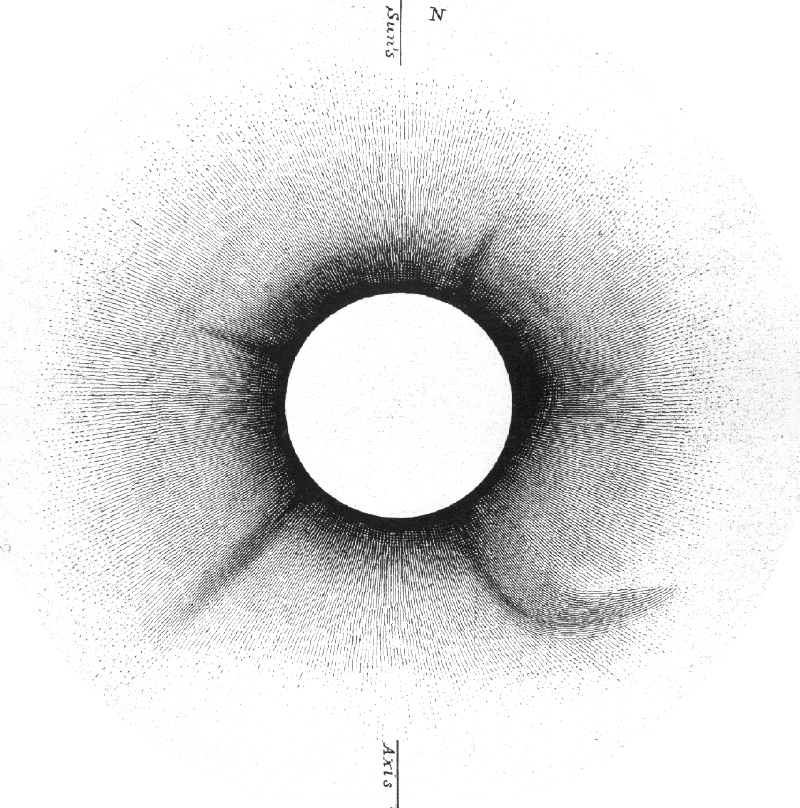
\includegraphics[height=3.6cm]{../images/oldcme3_inverted.png}
}

% Color scheme
\definecolor{mOrange}{HTML}{FF9400} % Math-Nat-Fakultät
\definecolor{mBlue}{HTML}{003247}
\definecolor{mBlueDark}{HTML}{0B1D26}
\definecolor{mGreen}{HTML}{00AE68}
\setbeamercolor{normal text}{fg=black, bg=white}
\setbeamercolor{palette primary}{bg=mBlueDark, fg=white}
\setbeamercolor{frametitle}{bg=mOrange, fg=white}
\setbeamercolor{alerted text}{fg=mOrange}
\setbeamercolor{example text}{fg=mGreen}
\setbeamercolor{progress bar}{fg=mBlue,bg=black!20}

\usepackage[absolute,overlay]{textpos}

\setbeamercolor{framesource}{fg=gray}
\setbeamerfont{framesource}{size=\tiny}

\usetikzlibrary{calc}
\usetikzlibrary{decorations.pathmorphing,decorations.markings,pgfplots.fillbetween,shapes.misc}
\tikzset{cross/.style={cross out, draw=black, fill=none, minimum size=2*(#1-\pgflinewidth), inner sep=0pt, outer 
        sep=0pt}, cross/.default={2pt}}
\definecolor{red}{HTML}{d62728}
\definecolor{orange}{HTML}{ff7f0e}
\definecolor{green}{HTML}{2ca02c}
\definecolor{blue}{HTML}{1f77b4}
\definecolor{purple}{HTML}{9467bd}
\definecolor{light-gray}{gray}{0.9}

% siunitx setup
\sisetup{detect-family=true, mode=text, range-units=single, separate-uncertainty=true, per-mode=symbol}
\DeclareSIUnit\AU{AU}
\DeclareSIUnit\astronomicalunit{AU}
\DeclareSIUnit\solarradius{\ensuremath{R_{\astrosun}}}

\makeatletter
\let\pgfimageWithoutPath\pgfimage 
\renewcommand{\pgfimage}[2][]{\pgfimageWithoutPath[#1]{plots/#2}}
\makeatother

\urlstyle{sf}

% blind footnote (footnote without number)
\newcommand\blfootnote[1]{%
	\begingroup
	\renewcommand\thefootnote{}\footnote{#1}%
	\addtocounter{footnote}{-1}%
	\endgroup
}

\newcommand{\maxt}{\ensuremath\text{max}}
\newcommand{\mint}{\ensuremath\text{min}}
\newcommand{\summary}{\textcolor{mOrange}{\faArrowCircleRight}\;}
\newcommand{\textarrow}{\,\small\faLongArrowAltRight\,}

\def\itemsymbol{\textbullet}
\let\svitem\item
\newenvironment{vfilleditems}{%
    \begin{itemize} %
        \let\olditem\item
        \renewcommand\item[1][\itemsymbol]{\vfill\svitem[##1]}}%
    {\end{itemize}\vfill}

\settowidth{\leftmargini}{\usebeamertemplate{itemize item}}
\addtolength{\leftmargini}{\labelsep}

\begin{document}
\maketitle

\begin{frame}{Contents}
    \tableofcontents
\end{frame}

\section{Introduction}

\begin{frame}{Coronal mass ejections}
    \begin{columns}
        \begin{column}{0.54\textwidth}
            \vbox to .8\textheight{%
            \begin{vfilleditems}
                \item \textbf{C}oronal \textbf{M}ass \textbf{E}jections: Magnetized plasma ejected from the Sun, propagating into interplanetary space (\textarrow \textbf{ICMEs})
                \item \textbf{Large variability:}
                    \begin{itemize}
                        \item frequency: every few days -- a few per day
                        \item speed: 10s to 1000s of \si{\kilo\meter\per\second}
                        \item angular extent: $\sim\SI{5}{\degree}$ -- \SI{120}{\degree}
                    \end{itemize}
                \item \textbf{Structure:} shock, sheath, magnetic ejecta
                \item One of the main drivers of \textbf{space weather} effects in the heliosphere
            \end{vfilleditems}
            }
        \end{column}
        \begin{column}{0.36\textwidth}
        	\centering
            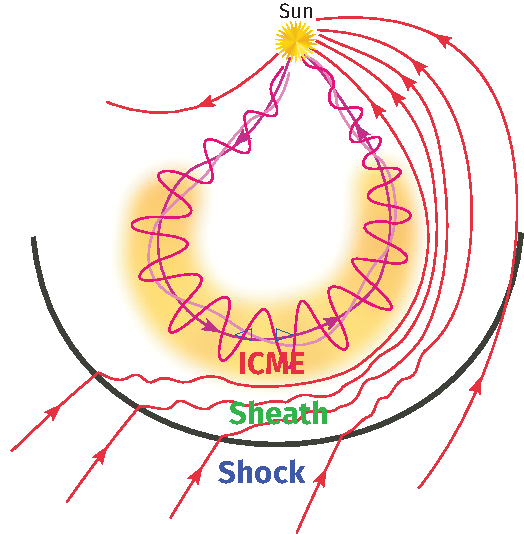
\includegraphics[width=\textwidth]{images/ZurbuchenRichardson-adapted.pdf}\\
            \scriptsize adapted from\\Zurbuchen and Richardson (2006)
        \end{column}
    \end{columns}
\end{frame}

\begin{frame}[standout]          
    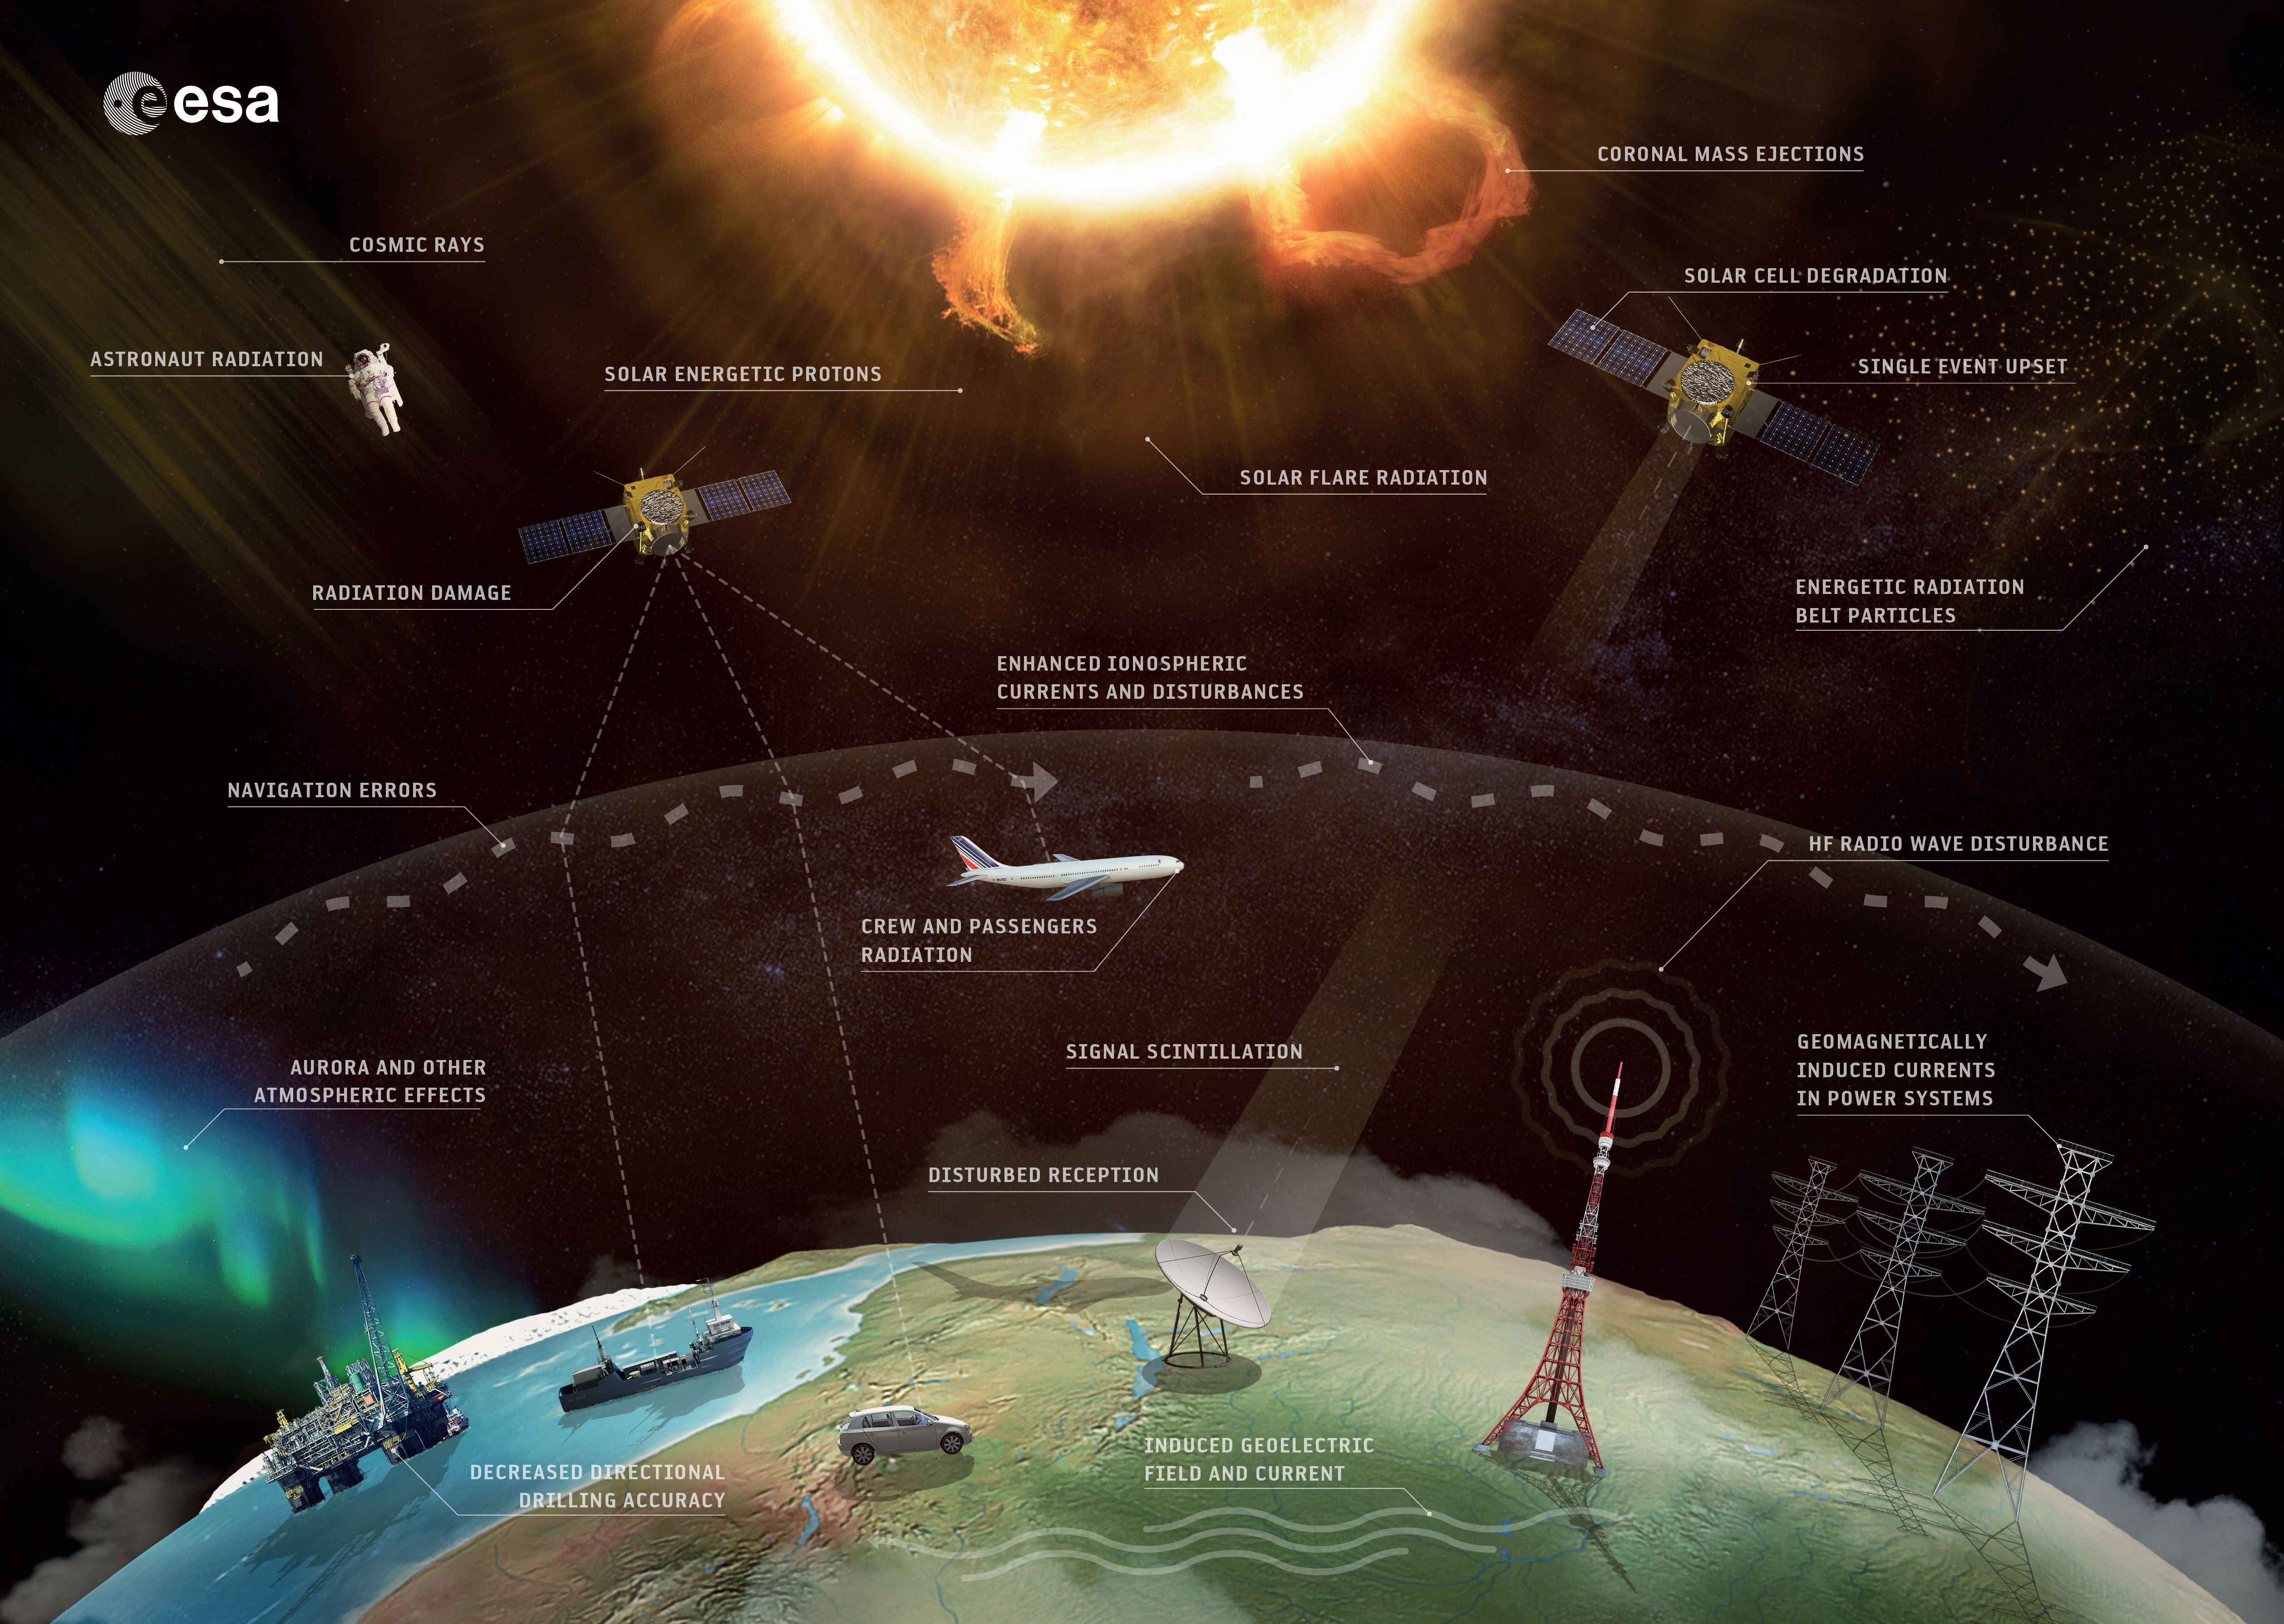
\includegraphics[height=\paperheight]{images/Space_weather_effects.jpg}
    \begin{tikzpicture}[remember picture,overlay]
        \node[xshift=-5cm,yshift=1.6cm] at (current page.south east){%
            \textbf{Space weather effects}};
    \end{tikzpicture}
\end{frame}

\begin{frame}{Observation of (I)CMEs}
    \begin{columns}[t]
        \begin{column}{0.45\textwidth}
            \textbf{Remote sensing:} CME
            
            \hskip-4mm
            \animategraphics[poster=19]{30}{plots/lightbulb_cme_anim/}{000}{048}
        \end{column}
        \begin{column}{0.45\textwidth}
            \textbf{In situ:} ICME

            %% Creator: Matplotlib, PGF backend
%%
%% To include the figure in your LaTeX document, write
%%   \input{<filename>.pgf}
%%
%% Make sure the required packages are loaded in your preamble
%%   \usepackage{pgf}
%%
%% and, on pdftex
%%   \usepackage[utf8]{inputenc}\DeclareUnicodeCharacter{2212}{-}
%%
%% or, on luatex and xetex
%%   \usepackage{unicode-math}
%%
%% Figures using additional raster images can only be included by \input if
%% they are in the same directory as the main LaTeX file. For loading figures
%% from other directories you can use the `import` package
%%   \usepackage{import}
%%
%% and then include the figures with
%%   \import{<path to file>}{<filename>.pgf}
%%
%% Matplotlib used the following preamble
%%   \usepackage{fontspec}
%%
\begingroup%
\makeatletter%
\begin{pgfpicture}%
\pgfpathrectangle{\pgfpointorigin}{\pgfqpoint{2.500000in}{2.500000in}}%
\pgfusepath{use as bounding box, clip}%
\begin{pgfscope}%
\pgfsetbuttcap%
\pgfsetmiterjoin%
\definecolor{currentfill}{rgb}{1.000000,1.000000,1.000000}%
\pgfsetfillcolor{currentfill}%
\pgfsetlinewidth{0.000000pt}%
\definecolor{currentstroke}{rgb}{1.000000,1.000000,1.000000}%
\pgfsetstrokecolor{currentstroke}%
\pgfsetdash{}{0pt}%
\pgfpathmoveto{\pgfqpoint{0.000000in}{0.000000in}}%
\pgfpathlineto{\pgfqpoint{2.500000in}{0.000000in}}%
\pgfpathlineto{\pgfqpoint{2.500000in}{2.500000in}}%
\pgfpathlineto{\pgfqpoint{0.000000in}{2.500000in}}%
\pgfpathclose%
\pgfusepath{fill}%
\end{pgfscope}%
\begin{pgfscope}%
\pgfsetbuttcap%
\pgfsetmiterjoin%
\definecolor{currentfill}{rgb}{1.000000,1.000000,1.000000}%
\pgfsetfillcolor{currentfill}%
\pgfsetlinewidth{0.000000pt}%
\definecolor{currentstroke}{rgb}{0.000000,0.000000,0.000000}%
\pgfsetstrokecolor{currentstroke}%
\pgfsetstrokeopacity{0.000000}%
\pgfsetdash{}{0pt}%
\pgfpathmoveto{\pgfqpoint{0.588735in}{1.707388in}}%
\pgfpathlineto{\pgfqpoint{1.879401in}{1.707388in}}%
\pgfpathlineto{\pgfqpoint{1.879401in}{2.347404in}}%
\pgfpathlineto{\pgfqpoint{0.588735in}{2.347404in}}%
\pgfpathclose%
\pgfusepath{fill}%
\end{pgfscope}%
\begin{pgfscope}%
\pgfsetbuttcap%
\pgfsetroundjoin%
\definecolor{currentfill}{rgb}{0.000000,0.000000,0.000000}%
\pgfsetfillcolor{currentfill}%
\pgfsetlinewidth{0.803000pt}%
\definecolor{currentstroke}{rgb}{0.000000,0.000000,0.000000}%
\pgfsetstrokecolor{currentstroke}%
\pgfsetdash{}{0pt}%
\pgfsys@defobject{currentmarker}{\pgfqpoint{0.000000in}{-0.048611in}}{\pgfqpoint{0.000000in}{0.000000in}}{%
\pgfpathmoveto{\pgfqpoint{0.000000in}{0.000000in}}%
\pgfpathlineto{\pgfqpoint{0.000000in}{-0.048611in}}%
\pgfusepath{stroke,fill}%
}%
\begin{pgfscope}%
\pgfsys@transformshift{1.134103in}{1.707388in}%
\pgfsys@useobject{currentmarker}{}%
\end{pgfscope}%
\end{pgfscope}%
\begin{pgfscope}%
\pgfsetbuttcap%
\pgfsetroundjoin%
\definecolor{currentfill}{rgb}{0.000000,0.000000,0.000000}%
\pgfsetfillcolor{currentfill}%
\pgfsetlinewidth{0.803000pt}%
\definecolor{currentstroke}{rgb}{0.000000,0.000000,0.000000}%
\pgfsetstrokecolor{currentstroke}%
\pgfsetdash{}{0pt}%
\pgfsys@defobject{currentmarker}{\pgfqpoint{0.000000in}{-0.048611in}}{\pgfqpoint{0.000000in}{0.000000in}}{%
\pgfpathmoveto{\pgfqpoint{0.000000in}{0.000000in}}%
\pgfpathlineto{\pgfqpoint{0.000000in}{-0.048611in}}%
\pgfusepath{stroke,fill}%
}%
\begin{pgfscope}%
\pgfsys@transformshift{1.821211in}{1.707388in}%
\pgfsys@useobject{currentmarker}{}%
\end{pgfscope}%
\end{pgfscope}%
\begin{pgfscope}%
\pgfsetbuttcap%
\pgfsetroundjoin%
\definecolor{currentfill}{rgb}{0.000000,0.000000,0.000000}%
\pgfsetfillcolor{currentfill}%
\pgfsetlinewidth{0.602250pt}%
\definecolor{currentstroke}{rgb}{0.000000,0.000000,0.000000}%
\pgfsetstrokecolor{currentstroke}%
\pgfsetdash{}{0pt}%
\pgfsys@defobject{currentmarker}{\pgfqpoint{0.000000in}{-0.027778in}}{\pgfqpoint{0.000000in}{0.000000in}}{%
\pgfpathmoveto{\pgfqpoint{0.000000in}{0.000000in}}%
\pgfpathlineto{\pgfqpoint{0.000000in}{-0.027778in}}%
\pgfusepath{stroke,fill}%
}%
\begin{pgfscope}%
\pgfsys@transformshift{0.618772in}{1.707388in}%
\pgfsys@useobject{currentmarker}{}%
\end{pgfscope}%
\end{pgfscope}%
\begin{pgfscope}%
\pgfsetbuttcap%
\pgfsetroundjoin%
\definecolor{currentfill}{rgb}{0.000000,0.000000,0.000000}%
\pgfsetfillcolor{currentfill}%
\pgfsetlinewidth{0.602250pt}%
\definecolor{currentstroke}{rgb}{0.000000,0.000000,0.000000}%
\pgfsetstrokecolor{currentstroke}%
\pgfsetdash{}{0pt}%
\pgfsys@defobject{currentmarker}{\pgfqpoint{0.000000in}{-0.027778in}}{\pgfqpoint{0.000000in}{0.000000in}}{%
\pgfpathmoveto{\pgfqpoint{0.000000in}{0.000000in}}%
\pgfpathlineto{\pgfqpoint{0.000000in}{-0.027778in}}%
\pgfusepath{stroke,fill}%
}%
\begin{pgfscope}%
\pgfsys@transformshift{0.790549in}{1.707388in}%
\pgfsys@useobject{currentmarker}{}%
\end{pgfscope}%
\end{pgfscope}%
\begin{pgfscope}%
\pgfsetbuttcap%
\pgfsetroundjoin%
\definecolor{currentfill}{rgb}{0.000000,0.000000,0.000000}%
\pgfsetfillcolor{currentfill}%
\pgfsetlinewidth{0.602250pt}%
\definecolor{currentstroke}{rgb}{0.000000,0.000000,0.000000}%
\pgfsetstrokecolor{currentstroke}%
\pgfsetdash{}{0pt}%
\pgfsys@defobject{currentmarker}{\pgfqpoint{0.000000in}{-0.027778in}}{\pgfqpoint{0.000000in}{0.000000in}}{%
\pgfpathmoveto{\pgfqpoint{0.000000in}{0.000000in}}%
\pgfpathlineto{\pgfqpoint{0.000000in}{-0.027778in}}%
\pgfusepath{stroke,fill}%
}%
\begin{pgfscope}%
\pgfsys@transformshift{0.962326in}{1.707388in}%
\pgfsys@useobject{currentmarker}{}%
\end{pgfscope}%
\end{pgfscope}%
\begin{pgfscope}%
\pgfsetbuttcap%
\pgfsetroundjoin%
\definecolor{currentfill}{rgb}{0.000000,0.000000,0.000000}%
\pgfsetfillcolor{currentfill}%
\pgfsetlinewidth{0.602250pt}%
\definecolor{currentstroke}{rgb}{0.000000,0.000000,0.000000}%
\pgfsetstrokecolor{currentstroke}%
\pgfsetdash{}{0pt}%
\pgfsys@defobject{currentmarker}{\pgfqpoint{0.000000in}{-0.027778in}}{\pgfqpoint{0.000000in}{0.000000in}}{%
\pgfpathmoveto{\pgfqpoint{0.000000in}{0.000000in}}%
\pgfpathlineto{\pgfqpoint{0.000000in}{-0.027778in}}%
\pgfusepath{stroke,fill}%
}%
\begin{pgfscope}%
\pgfsys@transformshift{1.305880in}{1.707388in}%
\pgfsys@useobject{currentmarker}{}%
\end{pgfscope}%
\end{pgfscope}%
\begin{pgfscope}%
\pgfsetbuttcap%
\pgfsetroundjoin%
\definecolor{currentfill}{rgb}{0.000000,0.000000,0.000000}%
\pgfsetfillcolor{currentfill}%
\pgfsetlinewidth{0.602250pt}%
\definecolor{currentstroke}{rgb}{0.000000,0.000000,0.000000}%
\pgfsetstrokecolor{currentstroke}%
\pgfsetdash{}{0pt}%
\pgfsys@defobject{currentmarker}{\pgfqpoint{0.000000in}{-0.027778in}}{\pgfqpoint{0.000000in}{0.000000in}}{%
\pgfpathmoveto{\pgfqpoint{0.000000in}{0.000000in}}%
\pgfpathlineto{\pgfqpoint{0.000000in}{-0.027778in}}%
\pgfusepath{stroke,fill}%
}%
\begin{pgfscope}%
\pgfsys@transformshift{1.477657in}{1.707388in}%
\pgfsys@useobject{currentmarker}{}%
\end{pgfscope}%
\end{pgfscope}%
\begin{pgfscope}%
\pgfsetbuttcap%
\pgfsetroundjoin%
\definecolor{currentfill}{rgb}{0.000000,0.000000,0.000000}%
\pgfsetfillcolor{currentfill}%
\pgfsetlinewidth{0.602250pt}%
\definecolor{currentstroke}{rgb}{0.000000,0.000000,0.000000}%
\pgfsetstrokecolor{currentstroke}%
\pgfsetdash{}{0pt}%
\pgfsys@defobject{currentmarker}{\pgfqpoint{0.000000in}{-0.027778in}}{\pgfqpoint{0.000000in}{0.000000in}}{%
\pgfpathmoveto{\pgfqpoint{0.000000in}{0.000000in}}%
\pgfpathlineto{\pgfqpoint{0.000000in}{-0.027778in}}%
\pgfusepath{stroke,fill}%
}%
\begin{pgfscope}%
\pgfsys@transformshift{1.649434in}{1.707388in}%
\pgfsys@useobject{currentmarker}{}%
\end{pgfscope}%
\end{pgfscope}%
\begin{pgfscope}%
\pgfsetbuttcap%
\pgfsetroundjoin%
\definecolor{currentfill}{rgb}{0.000000,0.000000,0.000000}%
\pgfsetfillcolor{currentfill}%
\pgfsetlinewidth{0.803000pt}%
\definecolor{currentstroke}{rgb}{0.000000,0.000000,0.000000}%
\pgfsetstrokecolor{currentstroke}%
\pgfsetdash{}{0pt}%
\pgfsys@defobject{currentmarker}{\pgfqpoint{-0.048611in}{0.000000in}}{\pgfqpoint{-0.000000in}{0.000000in}}{%
\pgfpathmoveto{\pgfqpoint{-0.000000in}{0.000000in}}%
\pgfpathlineto{\pgfqpoint{-0.048611in}{0.000000in}}%
\pgfusepath{stroke,fill}%
}%
\begin{pgfscope}%
\pgfsys@transformshift{0.588735in}{1.965968in}%
\pgfsys@useobject{currentmarker}{}%
\end{pgfscope}%
\end{pgfscope}%
\begin{pgfscope}%
\definecolor{textcolor}{rgb}{0.000000,0.000000,0.000000}%
\pgfsetstrokecolor{textcolor}%
\pgfsetfillcolor{textcolor}%
\pgftext[x=0.432484in, y=1.927412in, left, base]{\color{textcolor}\rmfamily\fontsize{8.000000}{9.600000}\selectfont \(\displaystyle {0}\)}%
\end{pgfscope}%
\begin{pgfscope}%
\pgfsetbuttcap%
\pgfsetroundjoin%
\definecolor{currentfill}{rgb}{0.000000,0.000000,0.000000}%
\pgfsetfillcolor{currentfill}%
\pgfsetlinewidth{0.803000pt}%
\definecolor{currentstroke}{rgb}{0.000000,0.000000,0.000000}%
\pgfsetstrokecolor{currentstroke}%
\pgfsetdash{}{0pt}%
\pgfsys@defobject{currentmarker}{\pgfqpoint{-0.048611in}{0.000000in}}{\pgfqpoint{-0.000000in}{0.000000in}}{%
\pgfpathmoveto{\pgfqpoint{-0.000000in}{0.000000in}}%
\pgfpathlineto{\pgfqpoint{-0.048611in}{0.000000in}}%
\pgfusepath{stroke,fill}%
}%
\begin{pgfscope}%
\pgfsys@transformshift{0.588735in}{2.320728in}%
\pgfsys@useobject{currentmarker}{}%
\end{pgfscope}%
\end{pgfscope}%
\begin{pgfscope}%
\definecolor{textcolor}{rgb}{0.000000,0.000000,0.000000}%
\pgfsetstrokecolor{textcolor}%
\pgfsetfillcolor{textcolor}%
\pgftext[x=0.373456in, y=2.282173in, left, base]{\color{textcolor}\rmfamily\fontsize{8.000000}{9.600000}\selectfont \(\displaystyle {25}\)}%
\end{pgfscope}%
\begin{pgfscope}%
\definecolor{textcolor}{rgb}{0.000000,0.000000,0.000000}%
\pgfsetstrokecolor{textcolor}%
\pgfsetfillcolor{textcolor}%
\pgftext[x=0.317900in,y=2.027396in,,bottom,rotate=90.000000]{\color{textcolor}\rmfamily\fontsize{9.000000}{10.800000}\selectfont B [nT]}%
\end{pgfscope}%
\begin{pgfscope}%
\pgfpathrectangle{\pgfqpoint{0.588735in}{1.707388in}}{\pgfqpoint{1.290666in}{0.640015in}}%
\pgfusepath{clip}%
\pgfsetrectcap%
\pgfsetroundjoin%
\pgfsetlinewidth{1.003750pt}%
\definecolor{currentstroke}{rgb}{0.121569,0.466667,0.705882}%
\pgfsetstrokecolor{currentstroke}%
\pgfsetdash{}{0pt}%
\pgfpathmoveto{\pgfqpoint{0.647402in}{2.056776in}}%
\pgfpathlineto{\pgfqpoint{0.647879in}{2.055835in}}%
\pgfpathlineto{\pgfqpoint{0.648356in}{2.057670in}}%
\pgfpathlineto{\pgfqpoint{0.648833in}{2.056871in}}%
\pgfpathlineto{\pgfqpoint{0.650742in}{2.056733in}}%
\pgfpathlineto{\pgfqpoint{0.651219in}{2.058613in}}%
\pgfpathlineto{\pgfqpoint{0.651696in}{2.056857in}}%
\pgfpathlineto{\pgfqpoint{0.652173in}{2.054952in}}%
\pgfpathlineto{\pgfqpoint{0.652650in}{2.058010in}}%
\pgfpathlineto{\pgfqpoint{0.653605in}{2.057794in}}%
\pgfpathlineto{\pgfqpoint{0.658853in}{2.061994in}}%
\pgfpathlineto{\pgfqpoint{0.662194in}{2.062093in}}%
\pgfpathlineto{\pgfqpoint{0.663625in}{2.063676in}}%
\pgfpathlineto{\pgfqpoint{0.667920in}{2.061033in}}%
\pgfpathlineto{\pgfqpoint{0.669351in}{2.062218in}}%
\pgfpathlineto{\pgfqpoint{0.670305in}{2.061607in}}%
\pgfpathlineto{\pgfqpoint{0.670782in}{2.059965in}}%
\pgfpathlineto{\pgfqpoint{0.671737in}{2.060454in}}%
\pgfpathlineto{\pgfqpoint{0.679371in}{2.062874in}}%
\pgfpathlineto{\pgfqpoint{0.682711in}{2.061969in}}%
\pgfpathlineto{\pgfqpoint{0.684620in}{2.062239in}}%
\pgfpathlineto{\pgfqpoint{0.685574in}{2.062746in}}%
\pgfpathlineto{\pgfqpoint{0.686052in}{2.061942in}}%
\pgfpathlineto{\pgfqpoint{0.691777in}{2.061852in}}%
\pgfpathlineto{\pgfqpoint{0.693209in}{2.062973in}}%
\pgfpathlineto{\pgfqpoint{0.693686in}{2.062396in}}%
\pgfpathlineto{\pgfqpoint{0.697980in}{2.062115in}}%
\pgfpathlineto{\pgfqpoint{0.698935in}{2.062828in}}%
\pgfpathlineto{\pgfqpoint{0.699412in}{2.062022in}}%
\pgfpathlineto{\pgfqpoint{0.702275in}{2.062320in}}%
\pgfpathlineto{\pgfqpoint{0.703706in}{2.062235in}}%
\pgfpathlineto{\pgfqpoint{0.704184in}{2.062895in}}%
\pgfpathlineto{\pgfqpoint{0.704661in}{2.062093in}}%
\pgfpathlineto{\pgfqpoint{0.705615in}{2.062842in}}%
\pgfpathlineto{\pgfqpoint{0.707047in}{2.063721in}}%
\pgfpathlineto{\pgfqpoint{0.707524in}{2.063158in}}%
\pgfpathlineto{\pgfqpoint{0.710387in}{2.061437in}}%
\pgfpathlineto{\pgfqpoint{0.713250in}{2.062097in}}%
\pgfpathlineto{\pgfqpoint{0.715158in}{2.061377in}}%
\pgfpathlineto{\pgfqpoint{0.716590in}{2.061805in}}%
\pgfpathlineto{\pgfqpoint{0.717544in}{2.061639in}}%
\pgfpathlineto{\pgfqpoint{0.718021in}{2.063080in}}%
\pgfpathlineto{\pgfqpoint{0.718498in}{2.061573in}}%
\pgfpathlineto{\pgfqpoint{0.720407in}{2.063106in}}%
\pgfpathlineto{\pgfqpoint{0.722793in}{2.062441in}}%
\pgfpathlineto{\pgfqpoint{0.727564in}{2.063225in}}%
\pgfpathlineto{\pgfqpoint{0.729950in}{2.063276in}}%
\pgfpathlineto{\pgfqpoint{0.731382in}{2.063211in}}%
\pgfpathlineto{\pgfqpoint{0.737107in}{2.062909in}}%
\pgfpathlineto{\pgfqpoint{0.737585in}{2.063593in}}%
\pgfpathlineto{\pgfqpoint{0.738062in}{2.063168in}}%
\pgfpathlineto{\pgfqpoint{0.740925in}{2.060901in}}%
\pgfpathlineto{\pgfqpoint{0.741402in}{2.061597in}}%
\pgfpathlineto{\pgfqpoint{0.741879in}{2.061107in}}%
\pgfpathlineto{\pgfqpoint{0.742833in}{2.059848in}}%
\pgfpathlineto{\pgfqpoint{0.744265in}{2.061536in}}%
\pgfpathlineto{\pgfqpoint{0.744742in}{2.060948in}}%
\pgfpathlineto{\pgfqpoint{0.745219in}{2.061469in}}%
\pgfpathlineto{\pgfqpoint{0.749514in}{2.062945in}}%
\pgfpathlineto{\pgfqpoint{0.751422in}{2.129824in}}%
\pgfpathlineto{\pgfqpoint{0.752377in}{2.112576in}}%
\pgfpathlineto{\pgfqpoint{0.752854in}{2.117261in}}%
\pgfpathlineto{\pgfqpoint{0.753331in}{2.114183in}}%
\pgfpathlineto{\pgfqpoint{0.753808in}{2.118504in}}%
\pgfpathlineto{\pgfqpoint{0.754762in}{2.117937in}}%
\pgfpathlineto{\pgfqpoint{0.755717in}{2.120955in}}%
\pgfpathlineto{\pgfqpoint{0.757148in}{2.135380in}}%
\pgfpathlineto{\pgfqpoint{0.759057in}{2.120480in}}%
\pgfpathlineto{\pgfqpoint{0.760011in}{2.131524in}}%
\pgfpathlineto{\pgfqpoint{0.760488in}{2.126859in}}%
\pgfpathlineto{\pgfqpoint{0.760965in}{2.125088in}}%
\pgfpathlineto{\pgfqpoint{0.761443in}{2.127721in}}%
\pgfpathlineto{\pgfqpoint{0.762874in}{2.120210in}}%
\pgfpathlineto{\pgfqpoint{0.763828in}{2.128600in}}%
\pgfpathlineto{\pgfqpoint{0.764306in}{2.127081in}}%
\pgfpathlineto{\pgfqpoint{0.764783in}{2.130424in}}%
\pgfpathlineto{\pgfqpoint{0.765260in}{2.126596in}}%
\pgfpathlineto{\pgfqpoint{0.766214in}{2.121717in}}%
\pgfpathlineto{\pgfqpoint{0.766691in}{2.122098in}}%
\pgfpathlineto{\pgfqpoint{0.769077in}{2.115403in}}%
\pgfpathlineto{\pgfqpoint{0.769554in}{2.118071in}}%
\pgfpathlineto{\pgfqpoint{0.770031in}{2.113988in}}%
\pgfpathlineto{\pgfqpoint{0.770509in}{2.115091in}}%
\pgfpathlineto{\pgfqpoint{0.771463in}{2.130474in}}%
\pgfpathlineto{\pgfqpoint{0.772417in}{2.129555in}}%
\pgfpathlineto{\pgfqpoint{0.773372in}{2.132421in}}%
\pgfpathlineto{\pgfqpoint{0.775757in}{2.144677in}}%
\pgfpathlineto{\pgfqpoint{0.778143in}{2.132730in}}%
\pgfpathlineto{\pgfqpoint{0.779097in}{2.135171in}}%
\pgfpathlineto{\pgfqpoint{0.780529in}{2.135678in}}%
\pgfpathlineto{\pgfqpoint{0.782438in}{2.138509in}}%
\pgfpathlineto{\pgfqpoint{0.782915in}{2.137200in}}%
\pgfpathlineto{\pgfqpoint{0.783392in}{2.138471in}}%
\pgfpathlineto{\pgfqpoint{0.785778in}{2.147406in}}%
\pgfpathlineto{\pgfqpoint{0.786255in}{2.144636in}}%
\pgfpathlineto{\pgfqpoint{0.787686in}{2.129810in}}%
\pgfpathlineto{\pgfqpoint{0.788163in}{2.121959in}}%
\pgfpathlineto{\pgfqpoint{0.788641in}{2.138566in}}%
\pgfpathlineto{\pgfqpoint{0.789595in}{2.137817in}}%
\pgfpathlineto{\pgfqpoint{0.790549in}{2.145161in}}%
\pgfpathlineto{\pgfqpoint{0.791026in}{2.141569in}}%
\pgfpathlineto{\pgfqpoint{0.792458in}{2.126592in}}%
\pgfpathlineto{\pgfqpoint{0.792935in}{2.152368in}}%
\pgfpathlineto{\pgfqpoint{0.793889in}{2.149379in}}%
\pgfpathlineto{\pgfqpoint{0.795321in}{2.153629in}}%
\pgfpathlineto{\pgfqpoint{0.796752in}{2.150765in}}%
\pgfpathlineto{\pgfqpoint{0.798661in}{2.147581in}}%
\pgfpathlineto{\pgfqpoint{0.801524in}{2.158205in}}%
\pgfpathlineto{\pgfqpoint{0.802478in}{2.102569in}}%
\pgfpathlineto{\pgfqpoint{0.803433in}{2.049840in}}%
\pgfpathlineto{\pgfqpoint{0.803910in}{2.081169in}}%
\pgfpathlineto{\pgfqpoint{0.804387in}{2.119271in}}%
\pgfpathlineto{\pgfqpoint{0.805341in}{2.115921in}}%
\pgfpathlineto{\pgfqpoint{0.805818in}{2.115396in}}%
\pgfpathlineto{\pgfqpoint{0.807727in}{2.139030in}}%
\pgfpathlineto{\pgfqpoint{0.808204in}{2.156081in}}%
\pgfpathlineto{\pgfqpoint{0.808681in}{2.139002in}}%
\pgfpathlineto{\pgfqpoint{0.810113in}{2.035940in}}%
\pgfpathlineto{\pgfqpoint{0.810590in}{2.048712in}}%
\pgfpathlineto{\pgfqpoint{0.811067in}{2.070852in}}%
\pgfpathlineto{\pgfqpoint{0.811544in}{2.064754in}}%
\pgfpathlineto{\pgfqpoint{0.812499in}{2.025677in}}%
\pgfpathlineto{\pgfqpoint{0.812976in}{2.049084in}}%
\pgfpathlineto{\pgfqpoint{0.813453in}{2.048017in}}%
\pgfpathlineto{\pgfqpoint{0.814407in}{2.021984in}}%
\pgfpathlineto{\pgfqpoint{0.814884in}{2.035054in}}%
\pgfpathlineto{\pgfqpoint{0.816793in}{2.052522in}}%
\pgfpathlineto{\pgfqpoint{0.817747in}{2.001988in}}%
\pgfpathlineto{\pgfqpoint{0.818224in}{2.006779in}}%
\pgfpathlineto{\pgfqpoint{0.820610in}{1.975482in}}%
\pgfpathlineto{\pgfqpoint{0.821087in}{1.982393in}}%
\pgfpathlineto{\pgfqpoint{0.822042in}{1.990907in}}%
\pgfpathlineto{\pgfqpoint{0.822519in}{1.986955in}}%
\pgfpathlineto{\pgfqpoint{0.822996in}{1.990127in}}%
\pgfpathlineto{\pgfqpoint{0.823473in}{1.978072in}}%
\pgfpathlineto{\pgfqpoint{0.823950in}{1.988878in}}%
\pgfpathlineto{\pgfqpoint{0.825382in}{2.015700in}}%
\pgfpathlineto{\pgfqpoint{0.826336in}{1.993866in}}%
\pgfpathlineto{\pgfqpoint{0.829676in}{2.076273in}}%
\pgfpathlineto{\pgfqpoint{0.830153in}{2.075957in}}%
\pgfpathlineto{\pgfqpoint{0.831108in}{2.050069in}}%
\pgfpathlineto{\pgfqpoint{0.832062in}{2.054810in}}%
\pgfpathlineto{\pgfqpoint{0.833493in}{2.093596in}}%
\pgfpathlineto{\pgfqpoint{0.833971in}{2.092599in}}%
\pgfpathlineto{\pgfqpoint{0.834448in}{2.092408in}}%
\pgfpathlineto{\pgfqpoint{0.834925in}{2.093696in}}%
\pgfpathlineto{\pgfqpoint{0.835402in}{2.093405in}}%
\pgfpathlineto{\pgfqpoint{0.835879in}{2.092564in}}%
\pgfpathlineto{\pgfqpoint{0.836356in}{2.093139in}}%
\pgfpathlineto{\pgfqpoint{0.838265in}{2.100794in}}%
\pgfpathlineto{\pgfqpoint{0.838742in}{2.096931in}}%
\pgfpathlineto{\pgfqpoint{0.839697in}{2.107386in}}%
\pgfpathlineto{\pgfqpoint{0.840174in}{2.102373in}}%
\pgfpathlineto{\pgfqpoint{0.841128in}{2.094746in}}%
\pgfpathlineto{\pgfqpoint{0.841605in}{2.086515in}}%
\pgfpathlineto{\pgfqpoint{0.843037in}{2.011409in}}%
\pgfpathlineto{\pgfqpoint{0.843514in}{2.100833in}}%
\pgfpathlineto{\pgfqpoint{0.844468in}{2.077987in}}%
\pgfpathlineto{\pgfqpoint{0.844945in}{2.074471in}}%
\pgfpathlineto{\pgfqpoint{0.845422in}{2.076745in}}%
\pgfpathlineto{\pgfqpoint{0.845900in}{2.088012in}}%
\pgfpathlineto{\pgfqpoint{0.846377in}{2.077168in}}%
\pgfpathlineto{\pgfqpoint{0.847331in}{2.047850in}}%
\pgfpathlineto{\pgfqpoint{0.847808in}{2.061022in}}%
\pgfpathlineto{\pgfqpoint{0.848285in}{2.070825in}}%
\pgfpathlineto{\pgfqpoint{0.848763in}{2.058929in}}%
\pgfpathlineto{\pgfqpoint{0.849240in}{2.068915in}}%
\pgfpathlineto{\pgfqpoint{0.850194in}{2.041730in}}%
\pgfpathlineto{\pgfqpoint{0.850671in}{2.051866in}}%
\pgfpathlineto{\pgfqpoint{0.851148in}{2.061281in}}%
\pgfpathlineto{\pgfqpoint{0.851626in}{2.046523in}}%
\pgfpathlineto{\pgfqpoint{0.852103in}{2.048892in}}%
\pgfpathlineto{\pgfqpoint{0.852580in}{2.052068in}}%
\pgfpathlineto{\pgfqpoint{0.854966in}{2.029789in}}%
\pgfpathlineto{\pgfqpoint{0.857351in}{2.067926in}}%
\pgfpathlineto{\pgfqpoint{0.857829in}{2.068375in}}%
\pgfpathlineto{\pgfqpoint{0.861169in}{2.011913in}}%
\pgfpathlineto{\pgfqpoint{0.862600in}{2.027579in}}%
\pgfpathlineto{\pgfqpoint{0.863077in}{2.024844in}}%
\pgfpathlineto{\pgfqpoint{0.863554in}{2.031177in}}%
\pgfpathlineto{\pgfqpoint{0.864032in}{2.023950in}}%
\pgfpathlineto{\pgfqpoint{0.864509in}{2.030995in}}%
\pgfpathlineto{\pgfqpoint{0.865463in}{2.033249in}}%
\pgfpathlineto{\pgfqpoint{0.865940in}{2.001135in}}%
\pgfpathlineto{\pgfqpoint{0.866895in}{2.002707in}}%
\pgfpathlineto{\pgfqpoint{0.867372in}{1.984145in}}%
\pgfpathlineto{\pgfqpoint{0.867849in}{1.998233in}}%
\pgfpathlineto{\pgfqpoint{0.869280in}{2.020520in}}%
\pgfpathlineto{\pgfqpoint{0.870712in}{2.022658in}}%
\pgfpathlineto{\pgfqpoint{0.871666in}{1.996637in}}%
\pgfpathlineto{\pgfqpoint{0.874052in}{2.062775in}}%
\pgfpathlineto{\pgfqpoint{0.875006in}{2.032998in}}%
\pgfpathlineto{\pgfqpoint{0.875961in}{2.034500in}}%
\pgfpathlineto{\pgfqpoint{0.876438in}{2.034177in}}%
\pgfpathlineto{\pgfqpoint{0.876915in}{2.035278in}}%
\pgfpathlineto{\pgfqpoint{0.878346in}{2.032357in}}%
\pgfpathlineto{\pgfqpoint{0.878824in}{2.031792in}}%
\pgfpathlineto{\pgfqpoint{0.879301in}{2.036629in}}%
\pgfpathlineto{\pgfqpoint{0.879778in}{2.026585in}}%
\pgfpathlineto{\pgfqpoint{0.880255in}{2.030406in}}%
\pgfpathlineto{\pgfqpoint{0.880732in}{2.033074in}}%
\pgfpathlineto{\pgfqpoint{0.883595in}{2.012331in}}%
\pgfpathlineto{\pgfqpoint{0.885027in}{2.016773in}}%
\pgfpathlineto{\pgfqpoint{0.885981in}{1.999050in}}%
\pgfpathlineto{\pgfqpoint{0.887412in}{2.053083in}}%
\pgfpathlineto{\pgfqpoint{0.887890in}{2.053735in}}%
\pgfpathlineto{\pgfqpoint{0.889798in}{2.046356in}}%
\pgfpathlineto{\pgfqpoint{0.890753in}{2.049411in}}%
\pgfpathlineto{\pgfqpoint{0.891230in}{2.048311in}}%
\pgfpathlineto{\pgfqpoint{0.891707in}{2.047577in}}%
\pgfpathlineto{\pgfqpoint{0.892661in}{2.054487in}}%
\pgfpathlineto{\pgfqpoint{0.893138in}{2.052848in}}%
\pgfpathlineto{\pgfqpoint{0.893615in}{2.053746in}}%
\pgfpathlineto{\pgfqpoint{0.895047in}{2.049698in}}%
\pgfpathlineto{\pgfqpoint{0.896001in}{2.055835in}}%
\pgfpathlineto{\pgfqpoint{0.896478in}{2.055300in}}%
\pgfpathlineto{\pgfqpoint{0.897433in}{2.053015in}}%
\pgfpathlineto{\pgfqpoint{0.899341in}{2.062597in}}%
\pgfpathlineto{\pgfqpoint{0.899819in}{2.062992in}}%
\pgfpathlineto{\pgfqpoint{0.902204in}{2.059025in}}%
\pgfpathlineto{\pgfqpoint{0.903159in}{2.060330in}}%
\pgfpathlineto{\pgfqpoint{0.906022in}{2.055953in}}%
\pgfpathlineto{\pgfqpoint{0.906976in}{2.057070in}}%
\pgfpathlineto{\pgfqpoint{0.907453in}{2.055523in}}%
\pgfpathlineto{\pgfqpoint{0.907930in}{2.054810in}}%
\pgfpathlineto{\pgfqpoint{0.908407in}{2.055506in}}%
\pgfpathlineto{\pgfqpoint{0.912702in}{2.057482in}}%
\pgfpathlineto{\pgfqpoint{0.913179in}{2.058234in}}%
\pgfpathlineto{\pgfqpoint{0.913656in}{2.054374in}}%
\pgfpathlineto{\pgfqpoint{0.914133in}{2.056566in}}%
\pgfpathlineto{\pgfqpoint{0.915088in}{2.054998in}}%
\pgfpathlineto{\pgfqpoint{0.916042in}{2.051192in}}%
\pgfpathlineto{\pgfqpoint{0.916519in}{2.054796in}}%
\pgfpathlineto{\pgfqpoint{0.917951in}{2.045828in}}%
\pgfpathlineto{\pgfqpoint{0.918428in}{2.046903in}}%
\pgfpathlineto{\pgfqpoint{0.919859in}{2.041989in}}%
\pgfpathlineto{\pgfqpoint{0.920336in}{2.052596in}}%
\pgfpathlineto{\pgfqpoint{0.921291in}{2.049326in}}%
\pgfpathlineto{\pgfqpoint{0.921768in}{2.048194in}}%
\pgfpathlineto{\pgfqpoint{0.922245in}{2.049201in}}%
\pgfpathlineto{\pgfqpoint{0.923676in}{2.055154in}}%
\pgfpathlineto{\pgfqpoint{0.924154in}{2.055247in}}%
\pgfpathlineto{\pgfqpoint{0.925108in}{2.053182in}}%
\pgfpathlineto{\pgfqpoint{0.925585in}{2.054434in}}%
\pgfpathlineto{\pgfqpoint{0.927494in}{2.060756in}}%
\pgfpathlineto{\pgfqpoint{0.927971in}{2.058642in}}%
\pgfpathlineto{\pgfqpoint{0.928448in}{2.042653in}}%
\pgfpathlineto{\pgfqpoint{0.928925in}{2.054477in}}%
\pgfpathlineto{\pgfqpoint{0.932742in}{2.057471in}}%
\pgfpathlineto{\pgfqpoint{0.934174in}{2.062358in}}%
\pgfpathlineto{\pgfqpoint{0.936560in}{2.057811in}}%
\pgfpathlineto{\pgfqpoint{0.937037in}{2.050546in}}%
\pgfpathlineto{\pgfqpoint{0.937991in}{2.052539in}}%
\pgfpathlineto{\pgfqpoint{0.938468in}{2.051837in}}%
\pgfpathlineto{\pgfqpoint{0.939900in}{2.039086in}}%
\pgfpathlineto{\pgfqpoint{0.940854in}{2.049365in}}%
\pgfpathlineto{\pgfqpoint{0.941331in}{2.049226in}}%
\pgfpathlineto{\pgfqpoint{0.943717in}{2.037856in}}%
\pgfpathlineto{\pgfqpoint{0.944194in}{2.041567in}}%
\pgfpathlineto{\pgfqpoint{0.944671in}{2.043291in}}%
\pgfpathlineto{\pgfqpoint{0.946580in}{2.059447in}}%
\pgfpathlineto{\pgfqpoint{0.947057in}{2.060660in}}%
\pgfpathlineto{\pgfqpoint{0.947534in}{2.059393in}}%
\pgfpathlineto{\pgfqpoint{0.948489in}{2.052753in}}%
\pgfpathlineto{\pgfqpoint{0.948966in}{2.055984in}}%
\pgfpathlineto{\pgfqpoint{0.949920in}{2.060557in}}%
\pgfpathlineto{\pgfqpoint{0.950874in}{2.049702in}}%
\pgfpathlineto{\pgfqpoint{0.951352in}{2.056606in}}%
\pgfpathlineto{\pgfqpoint{0.951829in}{2.053909in}}%
\pgfpathlineto{\pgfqpoint{0.952306in}{2.048162in}}%
\pgfpathlineto{\pgfqpoint{0.953260in}{2.071568in}}%
\pgfpathlineto{\pgfqpoint{0.954692in}{2.044483in}}%
\pgfpathlineto{\pgfqpoint{0.956123in}{2.053274in}}%
\pgfpathlineto{\pgfqpoint{0.956600in}{2.046402in}}%
\pgfpathlineto{\pgfqpoint{0.957078in}{2.056323in}}%
\pgfpathlineto{\pgfqpoint{0.957555in}{2.046491in}}%
\pgfpathlineto{\pgfqpoint{0.959463in}{2.016251in}}%
\pgfpathlineto{\pgfqpoint{0.961372in}{2.058223in}}%
\pgfpathlineto{\pgfqpoint{0.964712in}{2.081676in}}%
\pgfpathlineto{\pgfqpoint{0.966144in}{2.085164in}}%
\pgfpathlineto{\pgfqpoint{0.966621in}{2.082154in}}%
\pgfpathlineto{\pgfqpoint{0.967575in}{2.083056in}}%
\pgfpathlineto{\pgfqpoint{0.968529in}{2.083833in}}%
\pgfpathlineto{\pgfqpoint{0.969006in}{2.083425in}}%
\pgfpathlineto{\pgfqpoint{0.969484in}{2.081761in}}%
\pgfpathlineto{\pgfqpoint{0.969961in}{2.084007in}}%
\pgfpathlineto{\pgfqpoint{0.971392in}{2.083883in}}%
\pgfpathlineto{\pgfqpoint{0.972347in}{2.084817in}}%
\pgfpathlineto{\pgfqpoint{0.972824in}{2.080027in}}%
\pgfpathlineto{\pgfqpoint{0.973301in}{2.084511in}}%
\pgfpathlineto{\pgfqpoint{0.974255in}{2.085276in}}%
\pgfpathlineto{\pgfqpoint{0.974732in}{2.084663in}}%
\pgfpathlineto{\pgfqpoint{0.977595in}{2.098084in}}%
\pgfpathlineto{\pgfqpoint{0.978073in}{2.097442in}}%
\pgfpathlineto{\pgfqpoint{0.978550in}{2.098126in}}%
\pgfpathlineto{\pgfqpoint{0.979981in}{2.099462in}}%
\pgfpathlineto{\pgfqpoint{0.980458in}{2.096427in}}%
\pgfpathlineto{\pgfqpoint{0.980935in}{2.098080in}}%
\pgfpathlineto{\pgfqpoint{0.982367in}{2.103668in}}%
\pgfpathlineto{\pgfqpoint{0.982844in}{2.109429in}}%
\pgfpathlineto{\pgfqpoint{0.983321in}{2.107957in}}%
\pgfpathlineto{\pgfqpoint{0.984753in}{2.102898in}}%
\pgfpathlineto{\pgfqpoint{0.985707in}{2.105242in}}%
\pgfpathlineto{\pgfqpoint{0.988093in}{2.107130in}}%
\pgfpathlineto{\pgfqpoint{0.988570in}{2.106197in}}%
\pgfpathlineto{\pgfqpoint{0.990001in}{2.112164in}}%
\pgfpathlineto{\pgfqpoint{0.991910in}{2.106573in}}%
\pgfpathlineto{\pgfqpoint{0.992387in}{2.107457in}}%
\pgfpathlineto{\pgfqpoint{0.993819in}{2.121835in}}%
\pgfpathlineto{\pgfqpoint{0.994296in}{2.121001in}}%
\pgfpathlineto{\pgfqpoint{0.994773in}{2.124308in}}%
\pgfpathlineto{\pgfqpoint{0.995250in}{2.121949in}}%
\pgfpathlineto{\pgfqpoint{0.995727in}{2.119238in}}%
\pgfpathlineto{\pgfqpoint{0.996205in}{2.121168in}}%
\pgfpathlineto{\pgfqpoint{0.999545in}{2.124773in}}%
\pgfpathlineto{\pgfqpoint{1.000022in}{2.123332in}}%
\pgfpathlineto{\pgfqpoint{1.000499in}{2.124425in}}%
\pgfpathlineto{\pgfqpoint{1.001930in}{2.126465in}}%
\pgfpathlineto{\pgfqpoint{1.003839in}{2.128746in}}%
\pgfpathlineto{\pgfqpoint{1.004793in}{2.125586in}}%
\pgfpathlineto{\pgfqpoint{1.005271in}{2.127391in}}%
\pgfpathlineto{\pgfqpoint{1.007179in}{2.131275in}}%
\pgfpathlineto{\pgfqpoint{1.007656in}{2.129672in}}%
\pgfpathlineto{\pgfqpoint{1.008133in}{2.130442in}}%
\pgfpathlineto{\pgfqpoint{1.010996in}{2.131751in}}%
\pgfpathlineto{\pgfqpoint{1.012428in}{2.135666in}}%
\pgfpathlineto{\pgfqpoint{1.012905in}{2.135351in}}%
\pgfpathlineto{\pgfqpoint{1.014337in}{2.136111in}}%
\pgfpathlineto{\pgfqpoint{1.014814in}{2.134908in}}%
\pgfpathlineto{\pgfqpoint{1.015291in}{2.135969in}}%
\pgfpathlineto{\pgfqpoint{1.016722in}{2.137643in}}%
\pgfpathlineto{\pgfqpoint{1.017677in}{2.138417in}}%
\pgfpathlineto{\pgfqpoint{1.018631in}{2.136841in}}%
\pgfpathlineto{\pgfqpoint{1.019108in}{2.137257in}}%
\pgfpathlineto{\pgfqpoint{1.020062in}{2.138490in}}%
\pgfpathlineto{\pgfqpoint{1.021494in}{2.129345in}}%
\pgfpathlineto{\pgfqpoint{1.023403in}{2.138722in}}%
\pgfpathlineto{\pgfqpoint{1.025311in}{2.140049in}}%
\pgfpathlineto{\pgfqpoint{1.025788in}{2.139791in}}%
\pgfpathlineto{\pgfqpoint{1.026266in}{2.140896in}}%
\pgfpathlineto{\pgfqpoint{1.027220in}{2.137501in}}%
\pgfpathlineto{\pgfqpoint{1.028651in}{2.141088in}}%
\pgfpathlineto{\pgfqpoint{1.030560in}{2.138370in}}%
\pgfpathlineto{\pgfqpoint{1.032946in}{2.142237in}}%
\pgfpathlineto{\pgfqpoint{1.033423in}{2.142425in}}%
\pgfpathlineto{\pgfqpoint{1.034854in}{2.138963in}}%
\pgfpathlineto{\pgfqpoint{1.036286in}{2.139477in}}%
\pgfpathlineto{\pgfqpoint{1.037717in}{2.141162in}}%
\pgfpathlineto{\pgfqpoint{1.039149in}{2.143154in}}%
\pgfpathlineto{\pgfqpoint{1.039626in}{2.143564in}}%
\pgfpathlineto{\pgfqpoint{1.040580in}{2.131772in}}%
\pgfpathlineto{\pgfqpoint{1.042012in}{2.124794in}}%
\pgfpathlineto{\pgfqpoint{1.042489in}{2.122087in}}%
\pgfpathlineto{\pgfqpoint{1.042966in}{2.123543in}}%
\pgfpathlineto{\pgfqpoint{1.043443in}{2.124609in}}%
\pgfpathlineto{\pgfqpoint{1.045352in}{2.116829in}}%
\pgfpathlineto{\pgfqpoint{1.045829in}{2.118014in}}%
\pgfpathlineto{\pgfqpoint{1.047260in}{2.142450in}}%
\pgfpathlineto{\pgfqpoint{1.047738in}{2.138629in}}%
\pgfpathlineto{\pgfqpoint{1.048692in}{2.132383in}}%
\pgfpathlineto{\pgfqpoint{1.050601in}{2.143986in}}%
\pgfpathlineto{\pgfqpoint{1.051555in}{2.144242in}}%
\pgfpathlineto{\pgfqpoint{1.052986in}{2.134858in}}%
\pgfpathlineto{\pgfqpoint{1.053464in}{2.140886in}}%
\pgfpathlineto{\pgfqpoint{1.053941in}{2.140974in}}%
\pgfpathlineto{\pgfqpoint{1.054418in}{2.139904in}}%
\pgfpathlineto{\pgfqpoint{1.054895in}{2.140173in}}%
\pgfpathlineto{\pgfqpoint{1.055849in}{2.140453in}}%
\pgfpathlineto{\pgfqpoint{1.056326in}{2.138944in}}%
\pgfpathlineto{\pgfqpoint{1.057758in}{2.141638in}}%
\pgfpathlineto{\pgfqpoint{1.058712in}{2.139846in}}%
\pgfpathlineto{\pgfqpoint{1.060144in}{2.133258in}}%
\pgfpathlineto{\pgfqpoint{1.060621in}{2.133450in}}%
\pgfpathlineto{\pgfqpoint{1.062052in}{2.137265in}}%
\pgfpathlineto{\pgfqpoint{1.062530in}{2.136050in}}%
\pgfpathlineto{\pgfqpoint{1.063961in}{2.130491in}}%
\pgfpathlineto{\pgfqpoint{1.064438in}{2.130665in}}%
\pgfpathlineto{\pgfqpoint{1.067301in}{2.131548in}}%
\pgfpathlineto{\pgfqpoint{1.068255in}{2.136462in}}%
\pgfpathlineto{\pgfqpoint{1.068733in}{2.135366in}}%
\pgfpathlineto{\pgfqpoint{1.071118in}{2.146321in}}%
\pgfpathlineto{\pgfqpoint{1.071596in}{2.144374in}}%
\pgfpathlineto{\pgfqpoint{1.072073in}{2.142507in}}%
\pgfpathlineto{\pgfqpoint{1.072550in}{2.145835in}}%
\pgfpathlineto{\pgfqpoint{1.073027in}{2.144068in}}%
\pgfpathlineto{\pgfqpoint{1.073981in}{2.140616in}}%
\pgfpathlineto{\pgfqpoint{1.074459in}{2.142972in}}%
\pgfpathlineto{\pgfqpoint{1.074936in}{2.140432in}}%
\pgfpathlineto{\pgfqpoint{1.075890in}{2.146182in}}%
\pgfpathlineto{\pgfqpoint{1.076367in}{2.144685in}}%
\pgfpathlineto{\pgfqpoint{1.077799in}{2.141294in}}%
\pgfpathlineto{\pgfqpoint{1.079230in}{2.164203in}}%
\pgfpathlineto{\pgfqpoint{1.081616in}{2.172009in}}%
\pgfpathlineto{\pgfqpoint{1.083047in}{2.172239in}}%
\pgfpathlineto{\pgfqpoint{1.084479in}{2.173265in}}%
\pgfpathlineto{\pgfqpoint{1.084956in}{2.174983in}}%
\pgfpathlineto{\pgfqpoint{1.085433in}{2.174074in}}%
\pgfpathlineto{\pgfqpoint{1.087819in}{2.168515in}}%
\pgfpathlineto{\pgfqpoint{1.088296in}{2.169909in}}%
\pgfpathlineto{\pgfqpoint{1.088773in}{2.166015in}}%
\pgfpathlineto{\pgfqpoint{1.089250in}{2.167358in}}%
\pgfpathlineto{\pgfqpoint{1.090205in}{2.170746in}}%
\pgfpathlineto{\pgfqpoint{1.090682in}{2.169997in}}%
\pgfpathlineto{\pgfqpoint{1.091159in}{2.169710in}}%
\pgfpathlineto{\pgfqpoint{1.091636in}{2.171512in}}%
\pgfpathlineto{\pgfqpoint{1.092113in}{2.170781in}}%
\pgfpathlineto{\pgfqpoint{1.093545in}{2.169096in}}%
\pgfpathlineto{\pgfqpoint{1.095453in}{2.173928in}}%
\pgfpathlineto{\pgfqpoint{1.097362in}{2.174811in}}%
\pgfpathlineto{\pgfqpoint{1.098316in}{2.175603in}}%
\pgfpathlineto{\pgfqpoint{1.102611in}{2.179916in}}%
\pgfpathlineto{\pgfqpoint{1.104519in}{2.180197in}}%
\pgfpathlineto{\pgfqpoint{1.105951in}{2.181563in}}%
\pgfpathlineto{\pgfqpoint{1.107860in}{2.182684in}}%
\pgfpathlineto{\pgfqpoint{1.110245in}{2.181648in}}%
\pgfpathlineto{\pgfqpoint{1.113108in}{2.185919in}}%
\pgfpathlineto{\pgfqpoint{1.118834in}{2.187721in}}%
\pgfpathlineto{\pgfqpoint{1.120266in}{2.187679in}}%
\pgfpathlineto{\pgfqpoint{1.120743in}{2.189421in}}%
\pgfpathlineto{\pgfqpoint{1.121220in}{2.188663in}}%
\pgfpathlineto{\pgfqpoint{1.121697in}{2.185532in}}%
\pgfpathlineto{\pgfqpoint{1.122174in}{2.187650in}}%
\pgfpathlineto{\pgfqpoint{1.123606in}{2.189701in}}%
\pgfpathlineto{\pgfqpoint{1.127423in}{2.189626in}}%
\pgfpathlineto{\pgfqpoint{1.128377in}{2.190499in}}%
\pgfpathlineto{\pgfqpoint{1.128855in}{2.190219in}}%
\pgfpathlineto{\pgfqpoint{1.129809in}{2.188867in}}%
\pgfpathlineto{\pgfqpoint{1.132195in}{2.194334in}}%
\pgfpathlineto{\pgfqpoint{1.132672in}{2.193478in}}%
\pgfpathlineto{\pgfqpoint{1.133149in}{2.192667in}}%
\pgfpathlineto{\pgfqpoint{1.133626in}{2.193451in}}%
\pgfpathlineto{\pgfqpoint{1.135535in}{2.195806in}}%
\pgfpathlineto{\pgfqpoint{1.137443in}{2.194149in}}%
\pgfpathlineto{\pgfqpoint{1.137921in}{2.193947in}}%
\pgfpathlineto{\pgfqpoint{1.141738in}{2.203299in}}%
\pgfpathlineto{\pgfqpoint{1.142215in}{2.202924in}}%
\pgfpathlineto{\pgfqpoint{1.143169in}{2.201309in}}%
\pgfpathlineto{\pgfqpoint{1.143646in}{2.202348in}}%
\pgfpathlineto{\pgfqpoint{1.145078in}{2.203764in}}%
\pgfpathlineto{\pgfqpoint{1.145555in}{2.203270in}}%
\pgfpathlineto{\pgfqpoint{1.146032in}{2.203307in}}%
\pgfpathlineto{\pgfqpoint{1.147464in}{2.205527in}}%
\pgfpathlineto{\pgfqpoint{1.153190in}{2.208443in}}%
\pgfpathlineto{\pgfqpoint{1.154144in}{2.201287in}}%
\pgfpathlineto{\pgfqpoint{1.155098in}{2.201844in}}%
\pgfpathlineto{\pgfqpoint{1.156053in}{2.203270in}}%
\pgfpathlineto{\pgfqpoint{1.156530in}{2.200755in}}%
\pgfpathlineto{\pgfqpoint{1.157007in}{2.201007in}}%
\pgfpathlineto{\pgfqpoint{1.161779in}{2.213651in}}%
\pgfpathlineto{\pgfqpoint{1.163210in}{2.214683in}}%
\pgfpathlineto{\pgfqpoint{1.164164in}{2.217326in}}%
\pgfpathlineto{\pgfqpoint{1.164641in}{2.217014in}}%
\pgfpathlineto{\pgfqpoint{1.166073in}{2.219604in}}%
\pgfpathlineto{\pgfqpoint{1.168459in}{2.224336in}}%
\pgfpathlineto{\pgfqpoint{1.168936in}{2.224016in}}%
\pgfpathlineto{\pgfqpoint{1.169413in}{2.221721in}}%
\pgfpathlineto{\pgfqpoint{1.169890in}{2.222545in}}%
\pgfpathlineto{\pgfqpoint{1.171799in}{2.226674in}}%
\pgfpathlineto{\pgfqpoint{1.175139in}{2.230268in}}%
\pgfpathlineto{\pgfqpoint{1.176093in}{2.232105in}}%
\pgfpathlineto{\pgfqpoint{1.176570in}{2.231598in}}%
\pgfpathlineto{\pgfqpoint{1.178002in}{2.231456in}}%
\pgfpathlineto{\pgfqpoint{1.179433in}{2.233205in}}%
\pgfpathlineto{\pgfqpoint{1.181342in}{2.231875in}}%
\pgfpathlineto{\pgfqpoint{1.185636in}{2.235557in}}%
\pgfpathlineto{\pgfqpoint{1.186114in}{2.236342in}}%
\pgfpathlineto{\pgfqpoint{1.186591in}{2.234546in}}%
\pgfpathlineto{\pgfqpoint{1.187068in}{2.235195in}}%
\pgfpathlineto{\pgfqpoint{1.188977in}{2.239126in}}%
\pgfpathlineto{\pgfqpoint{1.189454in}{2.238324in}}%
\pgfpathlineto{\pgfqpoint{1.190885in}{2.239009in}}%
\pgfpathlineto{\pgfqpoint{1.192317in}{2.243096in}}%
\pgfpathlineto{\pgfqpoint{1.192794in}{2.242138in}}%
\pgfpathlineto{\pgfqpoint{1.194225in}{2.233876in}}%
\pgfpathlineto{\pgfqpoint{1.195657in}{2.247472in}}%
\pgfpathlineto{\pgfqpoint{1.196134in}{2.246023in}}%
\pgfpathlineto{\pgfqpoint{1.197565in}{2.247572in}}%
\pgfpathlineto{\pgfqpoint{1.198043in}{2.246927in}}%
\pgfpathlineto{\pgfqpoint{1.198520in}{2.248442in}}%
\pgfpathlineto{\pgfqpoint{1.198997in}{2.248027in}}%
\pgfpathlineto{\pgfqpoint{1.200428in}{2.240847in}}%
\pgfpathlineto{\pgfqpoint{1.200905in}{2.242525in}}%
\pgfpathlineto{\pgfqpoint{1.201860in}{2.245749in}}%
\pgfpathlineto{\pgfqpoint{1.202337in}{2.250290in}}%
\pgfpathlineto{\pgfqpoint{1.202814in}{2.248126in}}%
\pgfpathlineto{\pgfqpoint{1.203291in}{2.240155in}}%
\pgfpathlineto{\pgfqpoint{1.203768in}{2.240378in}}%
\pgfpathlineto{\pgfqpoint{1.204246in}{2.245001in}}%
\pgfpathlineto{\pgfqpoint{1.204723in}{2.243610in}}%
\pgfpathlineto{\pgfqpoint{1.205200in}{2.241678in}}%
\pgfpathlineto{\pgfqpoint{1.205677in}{2.243145in}}%
\pgfpathlineto{\pgfqpoint{1.207109in}{2.243499in}}%
\pgfpathlineto{\pgfqpoint{1.207586in}{2.245040in}}%
\pgfpathlineto{\pgfqpoint{1.208063in}{2.243238in}}%
\pgfpathlineto{\pgfqpoint{1.208540in}{2.243692in}}%
\pgfpathlineto{\pgfqpoint{1.209017in}{2.242610in}}%
\pgfpathlineto{\pgfqpoint{1.209494in}{2.243553in}}%
\pgfpathlineto{\pgfqpoint{1.211880in}{2.250737in}}%
\pgfpathlineto{\pgfqpoint{1.212357in}{2.250798in}}%
\pgfpathlineto{\pgfqpoint{1.217606in}{2.261966in}}%
\pgfpathlineto{\pgfqpoint{1.218083in}{2.262338in}}%
\pgfpathlineto{\pgfqpoint{1.218560in}{2.261639in}}%
\pgfpathlineto{\pgfqpoint{1.219038in}{2.260593in}}%
\pgfpathlineto{\pgfqpoint{1.219515in}{2.261412in}}%
\pgfpathlineto{\pgfqpoint{1.221423in}{2.267766in}}%
\pgfpathlineto{\pgfqpoint{1.221900in}{2.267645in}}%
\pgfpathlineto{\pgfqpoint{1.223332in}{2.264158in}}%
\pgfpathlineto{\pgfqpoint{1.225241in}{2.267865in}}%
\pgfpathlineto{\pgfqpoint{1.227149in}{2.265797in}}%
\pgfpathlineto{\pgfqpoint{1.229535in}{2.269575in}}%
\pgfpathlineto{\pgfqpoint{1.232875in}{2.273031in}}%
\pgfpathlineto{\pgfqpoint{1.234784in}{2.275202in}}%
\pgfpathlineto{\pgfqpoint{1.235738in}{2.274652in}}%
\pgfpathlineto{\pgfqpoint{1.236692in}{2.273084in}}%
\pgfpathlineto{\pgfqpoint{1.237170in}{2.272108in}}%
\pgfpathlineto{\pgfqpoint{1.237647in}{2.272916in}}%
\pgfpathlineto{\pgfqpoint{1.238601in}{2.275429in}}%
\pgfpathlineto{\pgfqpoint{1.239078in}{2.274467in}}%
\pgfpathlineto{\pgfqpoint{1.243373in}{2.274467in}}%
\pgfpathlineto{\pgfqpoint{1.244804in}{2.275280in}}%
\pgfpathlineto{\pgfqpoint{1.247667in}{2.273371in}}%
\pgfpathlineto{\pgfqpoint{1.249576in}{2.284003in}}%
\pgfpathlineto{\pgfqpoint{1.250053in}{2.281814in}}%
\pgfpathlineto{\pgfqpoint{1.250530in}{2.282630in}}%
\pgfpathlineto{\pgfqpoint{1.251484in}{2.285202in}}%
\pgfpathlineto{\pgfqpoint{1.252916in}{2.280914in}}%
\pgfpathlineto{\pgfqpoint{1.253393in}{2.282492in}}%
\pgfpathlineto{\pgfqpoint{1.254824in}{2.282792in}}%
\pgfpathlineto{\pgfqpoint{1.256256in}{2.279154in}}%
\pgfpathlineto{\pgfqpoint{1.257687in}{2.281800in}}%
\pgfpathlineto{\pgfqpoint{1.258165in}{2.280413in}}%
\pgfpathlineto{\pgfqpoint{1.260073in}{2.278788in}}%
\pgfpathlineto{\pgfqpoint{1.265322in}{2.283521in}}%
\pgfpathlineto{\pgfqpoint{1.265799in}{2.283386in}}%
\pgfpathlineto{\pgfqpoint{1.266276in}{2.278980in}}%
\pgfpathlineto{\pgfqpoint{1.266753in}{2.283084in}}%
\pgfpathlineto{\pgfqpoint{1.267708in}{2.283773in}}%
\pgfpathlineto{\pgfqpoint{1.269616in}{2.280598in}}%
\pgfpathlineto{\pgfqpoint{1.271048in}{2.283411in}}%
\pgfpathlineto{\pgfqpoint{1.273434in}{2.278469in}}%
\pgfpathlineto{\pgfqpoint{1.274388in}{2.280938in}}%
\pgfpathlineto{\pgfqpoint{1.275819in}{2.284727in}}%
\pgfpathlineto{\pgfqpoint{1.277251in}{2.286660in}}%
\pgfpathlineto{\pgfqpoint{1.278205in}{2.284103in}}%
\pgfpathlineto{\pgfqpoint{1.278682in}{2.291709in}}%
\pgfpathlineto{\pgfqpoint{1.279637in}{2.289490in}}%
\pgfpathlineto{\pgfqpoint{1.280114in}{2.288945in}}%
\pgfpathlineto{\pgfqpoint{1.281545in}{2.293440in}}%
\pgfpathlineto{\pgfqpoint{1.282977in}{2.287001in}}%
\pgfpathlineto{\pgfqpoint{1.283454in}{2.290214in}}%
\pgfpathlineto{\pgfqpoint{1.284885in}{2.293163in}}%
\pgfpathlineto{\pgfqpoint{1.285363in}{2.292726in}}%
\pgfpathlineto{\pgfqpoint{1.285840in}{2.292113in}}%
\pgfpathlineto{\pgfqpoint{1.286317in}{2.288374in}}%
\pgfpathlineto{\pgfqpoint{1.287271in}{2.289334in}}%
\pgfpathlineto{\pgfqpoint{1.287748in}{2.292294in}}%
\pgfpathlineto{\pgfqpoint{1.288225in}{2.287342in}}%
\pgfpathlineto{\pgfqpoint{1.288703in}{2.289527in}}%
\pgfpathlineto{\pgfqpoint{1.289657in}{2.290343in}}%
\pgfpathlineto{\pgfqpoint{1.291088in}{2.296221in}}%
\pgfpathlineto{\pgfqpoint{1.292520in}{2.293096in}}%
\pgfpathlineto{\pgfqpoint{1.294429in}{2.298527in}}%
\pgfpathlineto{\pgfqpoint{1.295860in}{2.294295in}}%
\pgfpathlineto{\pgfqpoint{1.298246in}{2.301135in}}%
\pgfpathlineto{\pgfqpoint{1.300154in}{2.301450in}}%
\pgfpathlineto{\pgfqpoint{1.300632in}{2.302451in}}%
\pgfpathlineto{\pgfqpoint{1.301109in}{2.301816in}}%
\pgfpathlineto{\pgfqpoint{1.302540in}{2.299220in}}%
\pgfpathlineto{\pgfqpoint{1.303017in}{2.299794in}}%
\pgfpathlineto{\pgfqpoint{1.304449in}{2.301959in}}%
\pgfpathlineto{\pgfqpoint{1.307312in}{2.300727in}}%
\pgfpathlineto{\pgfqpoint{1.309220in}{2.300493in}}%
\pgfpathlineto{\pgfqpoint{1.310652in}{2.303536in}}%
\pgfpathlineto{\pgfqpoint{1.311129in}{2.302582in}}%
\pgfpathlineto{\pgfqpoint{1.311606in}{2.302316in}}%
\pgfpathlineto{\pgfqpoint{1.313038in}{2.305576in}}%
\pgfpathlineto{\pgfqpoint{1.313515in}{2.304849in}}%
\pgfpathlineto{\pgfqpoint{1.316378in}{2.305793in}}%
\pgfpathlineto{\pgfqpoint{1.329261in}{2.307328in}}%
\pgfpathlineto{\pgfqpoint{1.330215in}{2.308336in}}%
\pgfpathlineto{\pgfqpoint{1.330693in}{2.308006in}}%
\pgfpathlineto{\pgfqpoint{1.331647in}{2.307974in}}%
\pgfpathlineto{\pgfqpoint{1.332601in}{2.306527in}}%
\pgfpathlineto{\pgfqpoint{1.333078in}{2.306803in}}%
\pgfpathlineto{\pgfqpoint{1.335941in}{2.309358in}}%
\pgfpathlineto{\pgfqpoint{1.338327in}{2.309103in}}%
\pgfpathlineto{\pgfqpoint{1.340236in}{2.309919in}}%
\pgfpathlineto{\pgfqpoint{1.345007in}{2.310710in}}%
\pgfpathlineto{\pgfqpoint{1.345962in}{2.311196in}}%
\pgfpathlineto{\pgfqpoint{1.346439in}{2.310487in}}%
\pgfpathlineto{\pgfqpoint{1.354073in}{2.311604in}}%
\pgfpathlineto{\pgfqpoint{1.355982in}{2.312209in}}%
\pgfpathlineto{\pgfqpoint{1.357413in}{2.311987in}}%
\pgfpathlineto{\pgfqpoint{1.368865in}{2.314332in}}%
\pgfpathlineto{\pgfqpoint{1.370297in}{2.314814in}}%
\pgfpathlineto{\pgfqpoint{1.371728in}{2.314867in}}%
\pgfpathlineto{\pgfqpoint{1.374591in}{2.315612in}}%
\pgfpathlineto{\pgfqpoint{1.377454in}{2.315389in}}%
\pgfpathlineto{\pgfqpoint{1.381271in}{2.315474in}}%
\pgfpathlineto{\pgfqpoint{1.383657in}{2.315052in}}%
\pgfpathlineto{\pgfqpoint{1.386520in}{2.314839in}}%
\pgfpathlineto{\pgfqpoint{1.389860in}{2.316155in}}%
\pgfpathlineto{\pgfqpoint{1.393678in}{2.316315in}}%
\pgfpathlineto{\pgfqpoint{1.395586in}{2.318266in}}%
\pgfpathlineto{\pgfqpoint{1.396063in}{2.317791in}}%
\pgfpathlineto{\pgfqpoint{1.397495in}{2.317198in}}%
\pgfpathlineto{\pgfqpoint{1.398449in}{2.317141in}}%
\pgfpathlineto{\pgfqpoint{1.400358in}{2.315857in}}%
\pgfpathlineto{\pgfqpoint{1.402744in}{2.314882in}}%
\pgfpathlineto{\pgfqpoint{1.406561in}{2.311540in}}%
\pgfpathlineto{\pgfqpoint{1.414195in}{2.303962in}}%
\pgfpathlineto{\pgfqpoint{1.416581in}{2.303409in}}%
\pgfpathlineto{\pgfqpoint{1.417535in}{2.303657in}}%
\pgfpathlineto{\pgfqpoint{1.419921in}{2.296182in}}%
\pgfpathlineto{\pgfqpoint{1.425647in}{2.287877in}}%
\pgfpathlineto{\pgfqpoint{1.427079in}{2.290925in}}%
\pgfpathlineto{\pgfqpoint{1.428987in}{2.290676in}}%
\pgfpathlineto{\pgfqpoint{1.430419in}{2.285630in}}%
\pgfpathlineto{\pgfqpoint{1.432327in}{2.288691in}}%
\pgfpathlineto{\pgfqpoint{1.433282in}{2.287671in}}%
\pgfpathlineto{\pgfqpoint{1.433759in}{2.288562in}}%
\pgfpathlineto{\pgfqpoint{1.436622in}{2.284386in}}%
\pgfpathlineto{\pgfqpoint{1.440439in}{2.277430in}}%
\pgfpathlineto{\pgfqpoint{1.440916in}{2.277717in}}%
\pgfpathlineto{\pgfqpoint{1.442825in}{2.278650in}}%
\pgfpathlineto{\pgfqpoint{1.444733in}{2.276745in}}%
\pgfpathlineto{\pgfqpoint{1.449982in}{2.271906in}}%
\pgfpathlineto{\pgfqpoint{1.453799in}{2.270803in}}%
\pgfpathlineto{\pgfqpoint{1.456185in}{2.266616in}}%
\pgfpathlineto{\pgfqpoint{1.457617in}{2.267489in}}%
\pgfpathlineto{\pgfqpoint{1.460003in}{2.264310in}}%
\pgfpathlineto{\pgfqpoint{1.461434in}{2.264885in}}%
\pgfpathlineto{\pgfqpoint{1.463343in}{2.260628in}}%
\pgfpathlineto{\pgfqpoint{1.465251in}{2.257006in}}%
\pgfpathlineto{\pgfqpoint{1.466206in}{2.255619in}}%
\pgfpathlineto{\pgfqpoint{1.466683in}{2.256876in}}%
\pgfpathlineto{\pgfqpoint{1.467160in}{2.256048in}}%
\pgfpathlineto{\pgfqpoint{1.472409in}{2.251450in}}%
\pgfpathlineto{\pgfqpoint{1.473840in}{2.252763in}}%
\pgfpathlineto{\pgfqpoint{1.474317in}{2.252122in}}%
\pgfpathlineto{\pgfqpoint{1.480043in}{2.245855in}}%
\pgfpathlineto{\pgfqpoint{1.481475in}{2.245884in}}%
\pgfpathlineto{\pgfqpoint{1.482906in}{2.243695in}}%
\pgfpathlineto{\pgfqpoint{1.483383in}{2.243979in}}%
\pgfpathlineto{\pgfqpoint{1.484338in}{2.243564in}}%
\pgfpathlineto{\pgfqpoint{1.487201in}{2.240698in}}%
\pgfpathlineto{\pgfqpoint{1.489586in}{2.232639in}}%
\pgfpathlineto{\pgfqpoint{1.491495in}{2.241531in}}%
\pgfpathlineto{\pgfqpoint{1.494358in}{2.236267in}}%
\pgfpathlineto{\pgfqpoint{1.495312in}{2.236825in}}%
\pgfpathlineto{\pgfqpoint{1.497698in}{2.236072in}}%
\pgfpathlineto{\pgfqpoint{1.498175in}{2.234394in}}%
\pgfpathlineto{\pgfqpoint{1.498652in}{2.234809in}}%
\pgfpathlineto{\pgfqpoint{1.499607in}{2.237278in}}%
\pgfpathlineto{\pgfqpoint{1.500084in}{2.236480in}}%
\pgfpathlineto{\pgfqpoint{1.501515in}{2.235068in}}%
\pgfpathlineto{\pgfqpoint{1.502947in}{2.233509in}}%
\pgfpathlineto{\pgfqpoint{1.509150in}{2.229877in}}%
\pgfpathlineto{\pgfqpoint{1.511058in}{2.223119in}}%
\pgfpathlineto{\pgfqpoint{1.512013in}{2.225482in}}%
\pgfpathlineto{\pgfqpoint{1.513444in}{2.221221in}}%
\pgfpathlineto{\pgfqpoint{1.513921in}{2.222034in}}%
\pgfpathlineto{\pgfqpoint{1.514399in}{2.221565in}}%
\pgfpathlineto{\pgfqpoint{1.519170in}{2.218057in}}%
\pgfpathlineto{\pgfqpoint{1.521079in}{2.219160in}}%
\pgfpathlineto{\pgfqpoint{1.522033in}{2.218533in}}%
\pgfpathlineto{\pgfqpoint{1.522510in}{2.219259in}}%
\pgfpathlineto{\pgfqpoint{1.522987in}{2.218667in}}%
\pgfpathlineto{\pgfqpoint{1.523465in}{2.216521in}}%
\pgfpathlineto{\pgfqpoint{1.523942in}{2.216637in}}%
\pgfpathlineto{\pgfqpoint{1.524896in}{2.217872in}}%
\pgfpathlineto{\pgfqpoint{1.525373in}{2.217425in}}%
\pgfpathlineto{\pgfqpoint{1.526328in}{2.217358in}}%
\pgfpathlineto{\pgfqpoint{1.530145in}{2.213104in}}%
\pgfpathlineto{\pgfqpoint{1.531576in}{2.212398in}}%
\pgfpathlineto{\pgfqpoint{1.532053in}{2.212327in}}%
\pgfpathlineto{\pgfqpoint{1.532531in}{2.209560in}}%
\pgfpathlineto{\pgfqpoint{1.533485in}{2.210227in}}%
\pgfpathlineto{\pgfqpoint{1.536348in}{2.209908in}}%
\pgfpathlineto{\pgfqpoint{1.537779in}{2.208890in}}%
\pgfpathlineto{\pgfqpoint{1.540165in}{2.209500in}}%
\pgfpathlineto{\pgfqpoint{1.542074in}{2.207095in}}%
\pgfpathlineto{\pgfqpoint{1.542551in}{2.207747in}}%
\pgfpathlineto{\pgfqpoint{1.543028in}{2.207091in}}%
\pgfpathlineto{\pgfqpoint{1.544460in}{2.206169in}}%
\pgfpathlineto{\pgfqpoint{1.547800in}{2.201929in}}%
\pgfpathlineto{\pgfqpoint{1.550185in}{2.199485in}}%
\pgfpathlineto{\pgfqpoint{1.551617in}{2.200904in}}%
\pgfpathlineto{\pgfqpoint{1.552094in}{2.199978in}}%
\pgfpathlineto{\pgfqpoint{1.554957in}{2.192730in}}%
\pgfpathlineto{\pgfqpoint{1.555434in}{2.193316in}}%
\pgfpathlineto{\pgfqpoint{1.556866in}{2.194934in}}%
\pgfpathlineto{\pgfqpoint{1.560206in}{2.192764in}}%
\pgfpathlineto{\pgfqpoint{1.560683in}{2.194416in}}%
\pgfpathlineto{\pgfqpoint{1.561637in}{2.193734in}}%
\pgfpathlineto{\pgfqpoint{1.563546in}{2.192330in}}%
\pgfpathlineto{\pgfqpoint{1.564023in}{2.189859in}}%
\pgfpathlineto{\pgfqpoint{1.564500in}{2.191180in}}%
\pgfpathlineto{\pgfqpoint{1.564977in}{2.192723in}}%
\pgfpathlineto{\pgfqpoint{1.565455in}{2.192071in}}%
\pgfpathlineto{\pgfqpoint{1.567840in}{2.186685in}}%
\pgfpathlineto{\pgfqpoint{1.569272in}{2.188551in}}%
\pgfpathlineto{\pgfqpoint{1.572135in}{2.183163in}}%
\pgfpathlineto{\pgfqpoint{1.574521in}{2.178920in}}%
\pgfpathlineto{\pgfqpoint{1.574998in}{2.178891in}}%
\pgfpathlineto{\pgfqpoint{1.576906in}{2.173389in}}%
\pgfpathlineto{\pgfqpoint{1.578338in}{2.173300in}}%
\pgfpathlineto{\pgfqpoint{1.580246in}{2.168883in}}%
\pgfpathlineto{\pgfqpoint{1.580724in}{2.168131in}}%
\pgfpathlineto{\pgfqpoint{1.581201in}{2.169127in}}%
\pgfpathlineto{\pgfqpoint{1.581678in}{2.169111in}}%
\pgfpathlineto{\pgfqpoint{1.583587in}{2.166468in}}%
\pgfpathlineto{\pgfqpoint{1.584064in}{2.166010in}}%
\pgfpathlineto{\pgfqpoint{1.585018in}{2.166918in}}%
\pgfpathlineto{\pgfqpoint{1.592175in}{2.156729in}}%
\pgfpathlineto{\pgfqpoint{1.594561in}{2.155282in}}%
\pgfpathlineto{\pgfqpoint{1.596947in}{2.151160in}}%
\pgfpathlineto{\pgfqpoint{1.597901in}{2.149968in}}%
\pgfpathlineto{\pgfqpoint{1.598378in}{2.150353in}}%
\pgfpathlineto{\pgfqpoint{1.599333in}{2.150219in}}%
\pgfpathlineto{\pgfqpoint{1.600287in}{2.149251in}}%
\pgfpathlineto{\pgfqpoint{1.600764in}{2.149567in}}%
\pgfpathlineto{\pgfqpoint{1.604582in}{2.146016in}}%
\pgfpathlineto{\pgfqpoint{1.608876in}{2.142078in}}%
\pgfpathlineto{\pgfqpoint{1.610785in}{2.141939in}}%
\pgfpathlineto{\pgfqpoint{1.612693in}{2.134624in}}%
\pgfpathlineto{\pgfqpoint{1.613170in}{2.134929in}}%
\pgfpathlineto{\pgfqpoint{1.614602in}{2.137516in}}%
\pgfpathlineto{\pgfqpoint{1.615556in}{2.136749in}}%
\pgfpathlineto{\pgfqpoint{1.616033in}{2.134752in}}%
\pgfpathlineto{\pgfqpoint{1.616511in}{2.134890in}}%
\pgfpathlineto{\pgfqpoint{1.617942in}{2.136575in}}%
\pgfpathlineto{\pgfqpoint{1.618419in}{2.136568in}}%
\pgfpathlineto{\pgfqpoint{1.620328in}{2.146001in}}%
\pgfpathlineto{\pgfqpoint{1.620805in}{2.144710in}}%
\pgfpathlineto{\pgfqpoint{1.621282in}{2.143428in}}%
\pgfpathlineto{\pgfqpoint{1.621759in}{2.143983in}}%
\pgfpathlineto{\pgfqpoint{1.622714in}{2.144781in}}%
\pgfpathlineto{\pgfqpoint{1.623191in}{2.143835in}}%
\pgfpathlineto{\pgfqpoint{1.624622in}{2.142433in}}%
\pgfpathlineto{\pgfqpoint{1.626531in}{2.132283in}}%
\pgfpathlineto{\pgfqpoint{1.628439in}{2.130555in}}%
\pgfpathlineto{\pgfqpoint{1.628917in}{2.131073in}}%
\pgfpathlineto{\pgfqpoint{1.630348in}{2.129874in}}%
\pgfpathlineto{\pgfqpoint{1.631302in}{2.133418in}}%
\pgfpathlineto{\pgfqpoint{1.632257in}{2.133017in}}%
\pgfpathlineto{\pgfqpoint{1.636074in}{2.131474in}}%
\pgfpathlineto{\pgfqpoint{1.636551in}{2.131991in}}%
\pgfpathlineto{\pgfqpoint{1.637028in}{2.131289in}}%
\pgfpathlineto{\pgfqpoint{1.640846in}{2.127501in}}%
\pgfpathlineto{\pgfqpoint{1.642754in}{2.119245in}}%
\pgfpathlineto{\pgfqpoint{1.644663in}{2.120650in}}%
\pgfpathlineto{\pgfqpoint{1.646571in}{2.120345in}}%
\pgfpathlineto{\pgfqpoint{1.648003in}{2.124186in}}%
\pgfpathlineto{\pgfqpoint{1.650389in}{2.121800in}}%
\pgfpathlineto{\pgfqpoint{1.651820in}{2.122024in}}%
\pgfpathlineto{\pgfqpoint{1.653729in}{2.119479in}}%
\pgfpathlineto{\pgfqpoint{1.656115in}{2.117855in}}%
\pgfpathlineto{\pgfqpoint{1.659455in}{2.112659in}}%
\pgfpathlineto{\pgfqpoint{1.660886in}{2.109099in}}%
\pgfpathlineto{\pgfqpoint{1.661363in}{2.109253in}}%
\pgfpathlineto{\pgfqpoint{1.662795in}{2.109383in}}%
\pgfpathlineto{\pgfqpoint{1.664704in}{2.109227in}}%
\pgfpathlineto{\pgfqpoint{1.665181in}{2.108411in}}%
\pgfpathlineto{\pgfqpoint{1.665658in}{2.109131in}}%
\pgfpathlineto{\pgfqpoint{1.668521in}{2.109929in}}%
\pgfpathlineto{\pgfqpoint{1.670907in}{2.108179in}}%
\pgfpathlineto{\pgfqpoint{1.673292in}{2.108028in}}%
\pgfpathlineto{\pgfqpoint{1.676155in}{2.101429in}}%
\pgfpathlineto{\pgfqpoint{1.677110in}{2.105803in}}%
\pgfpathlineto{\pgfqpoint{1.678541in}{2.097338in}}%
\pgfpathlineto{\pgfqpoint{1.679018in}{2.098889in}}%
\pgfpathlineto{\pgfqpoint{1.680450in}{2.092343in}}%
\pgfpathlineto{\pgfqpoint{1.681404in}{2.078611in}}%
\pgfpathlineto{\pgfqpoint{1.682358in}{2.085205in}}%
\pgfpathlineto{\pgfqpoint{1.683313in}{2.093841in}}%
\pgfpathlineto{\pgfqpoint{1.683790in}{2.092649in}}%
\pgfpathlineto{\pgfqpoint{1.685698in}{2.080725in}}%
\pgfpathlineto{\pgfqpoint{1.686653in}{2.083177in}}%
\pgfpathlineto{\pgfqpoint{1.688561in}{2.076827in}}%
\pgfpathlineto{\pgfqpoint{1.689039in}{2.084319in}}%
\pgfpathlineto{\pgfqpoint{1.689516in}{2.083269in}}%
\pgfpathlineto{\pgfqpoint{1.689993in}{2.080844in}}%
\pgfpathlineto{\pgfqpoint{1.690947in}{2.081580in}}%
\pgfpathlineto{\pgfqpoint{1.692856in}{2.088026in}}%
\pgfpathlineto{\pgfqpoint{1.694287in}{2.085983in}}%
\pgfpathlineto{\pgfqpoint{1.694764in}{2.088264in}}%
\pgfpathlineto{\pgfqpoint{1.695242in}{2.085799in}}%
\pgfpathlineto{\pgfqpoint{1.696673in}{2.081556in}}%
\pgfpathlineto{\pgfqpoint{1.698105in}{2.083993in}}%
\pgfpathlineto{\pgfqpoint{1.699059in}{2.081627in}}%
\pgfpathlineto{\pgfqpoint{1.700013in}{2.070026in}}%
\pgfpathlineto{\pgfqpoint{1.700490in}{2.072977in}}%
\pgfpathlineto{\pgfqpoint{1.700968in}{2.071814in}}%
\pgfpathlineto{\pgfqpoint{1.701445in}{2.073578in}}%
\pgfpathlineto{\pgfqpoint{1.702876in}{2.081932in}}%
\pgfpathlineto{\pgfqpoint{1.703353in}{2.079131in}}%
\pgfpathlineto{\pgfqpoint{1.704308in}{2.079537in}}%
\pgfpathlineto{\pgfqpoint{1.706693in}{2.067177in}}%
\pgfpathlineto{\pgfqpoint{1.707171in}{2.064042in}}%
\pgfpathlineto{\pgfqpoint{1.707648in}{2.066329in}}%
\pgfpathlineto{\pgfqpoint{1.708125in}{2.070012in}}%
\pgfpathlineto{\pgfqpoint{1.708602in}{2.069607in}}%
\pgfpathlineto{\pgfqpoint{1.709556in}{2.070189in}}%
\pgfpathlineto{\pgfqpoint{1.712897in}{2.061739in}}%
\pgfpathlineto{\pgfqpoint{1.713374in}{2.062221in}}%
\pgfpathlineto{\pgfqpoint{1.715759in}{2.080250in}}%
\pgfpathlineto{\pgfqpoint{1.717668in}{2.073052in}}%
\pgfpathlineto{\pgfqpoint{1.718622in}{2.068730in}}%
\pgfpathlineto{\pgfqpoint{1.720531in}{2.076274in}}%
\pgfpathlineto{\pgfqpoint{1.721485in}{2.074822in}}%
\pgfpathlineto{\pgfqpoint{1.721963in}{2.075901in}}%
\pgfpathlineto{\pgfqpoint{1.722440in}{2.075461in}}%
\pgfpathlineto{\pgfqpoint{1.723394in}{2.074223in}}%
\pgfpathlineto{\pgfqpoint{1.725303in}{2.060600in}}%
\pgfpathlineto{\pgfqpoint{1.725780in}{2.061072in}}%
\pgfpathlineto{\pgfqpoint{1.726734in}{2.061175in}}%
\pgfpathlineto{\pgfqpoint{1.729120in}{2.051632in}}%
\pgfpathlineto{\pgfqpoint{1.730551in}{2.048935in}}%
\pgfpathlineto{\pgfqpoint{1.731029in}{2.050369in}}%
\pgfpathlineto{\pgfqpoint{1.732460in}{2.058390in}}%
\pgfpathlineto{\pgfqpoint{1.732937in}{2.058280in}}%
\pgfpathlineto{\pgfqpoint{1.734846in}{2.058290in}}%
\pgfpathlineto{\pgfqpoint{1.737232in}{2.057762in}}%
\pgfpathlineto{\pgfqpoint{1.737709in}{2.057718in}}%
\pgfpathlineto{\pgfqpoint{1.739140in}{2.049372in}}%
\pgfpathlineto{\pgfqpoint{1.739617in}{2.050396in}}%
\pgfpathlineto{\pgfqpoint{1.740095in}{2.050954in}}%
\pgfpathlineto{\pgfqpoint{1.742003in}{2.057577in}}%
\pgfpathlineto{\pgfqpoint{1.744389in}{2.065233in}}%
\pgfpathlineto{\pgfqpoint{1.744866in}{2.063399in}}%
\pgfpathlineto{\pgfqpoint{1.745343in}{2.057988in}}%
\pgfpathlineto{\pgfqpoint{1.746298in}{2.058957in}}%
\pgfpathlineto{\pgfqpoint{1.747252in}{2.058882in}}%
\pgfpathlineto{\pgfqpoint{1.748206in}{2.056321in}}%
\pgfpathlineto{\pgfqpoint{1.749638in}{2.064399in}}%
\pgfpathlineto{\pgfqpoint{1.751069in}{2.057169in}}%
\pgfpathlineto{\pgfqpoint{1.751546in}{2.055775in}}%
\pgfpathlineto{\pgfqpoint{1.752024in}{2.056616in}}%
\pgfpathlineto{\pgfqpoint{1.752978in}{2.057335in}}%
\pgfpathlineto{\pgfqpoint{1.753455in}{2.056488in}}%
\pgfpathlineto{\pgfqpoint{1.754409in}{2.062721in}}%
\pgfpathlineto{\pgfqpoint{1.755841in}{2.054509in}}%
\pgfpathlineto{\pgfqpoint{1.756795in}{2.057836in}}%
\pgfpathlineto{\pgfqpoint{1.758704in}{2.071932in}}%
\pgfpathlineto{\pgfqpoint{1.759658in}{2.070363in}}%
\pgfpathlineto{\pgfqpoint{1.760135in}{2.075234in}}%
\pgfpathlineto{\pgfqpoint{1.760612in}{2.067614in}}%
\pgfpathlineto{\pgfqpoint{1.761090in}{2.075766in}}%
\pgfpathlineto{\pgfqpoint{1.761567in}{2.076802in}}%
\pgfpathlineto{\pgfqpoint{1.763952in}{2.042738in}}%
\pgfpathlineto{\pgfqpoint{1.765384in}{2.056949in}}%
\pgfpathlineto{\pgfqpoint{1.766338in}{2.053527in}}%
\pgfpathlineto{\pgfqpoint{1.766815in}{2.051103in}}%
\pgfpathlineto{\pgfqpoint{1.767293in}{2.052745in}}%
\pgfpathlineto{\pgfqpoint{1.767770in}{2.055289in}}%
\pgfpathlineto{\pgfqpoint{1.768247in}{2.050916in}}%
\pgfpathlineto{\pgfqpoint{1.768724in}{2.055059in}}%
\pgfpathlineto{\pgfqpoint{1.769201in}{2.061050in}}%
\pgfpathlineto{\pgfqpoint{1.769678in}{2.058138in}}%
\pgfpathlineto{\pgfqpoint{1.770156in}{2.057666in}}%
\pgfpathlineto{\pgfqpoint{1.771587in}{2.066950in}}%
\pgfpathlineto{\pgfqpoint{1.773018in}{2.061597in}}%
\pgfpathlineto{\pgfqpoint{1.773973in}{2.079188in}}%
\pgfpathlineto{\pgfqpoint{1.774450in}{2.074776in}}%
\pgfpathlineto{\pgfqpoint{1.777313in}{2.086980in}}%
\pgfpathlineto{\pgfqpoint{1.777790in}{2.095346in}}%
\pgfpathlineto{\pgfqpoint{1.778744in}{2.094228in}}%
\pgfpathlineto{\pgfqpoint{1.781607in}{2.088743in}}%
\pgfpathlineto{\pgfqpoint{1.783039in}{2.087140in}}%
\pgfpathlineto{\pgfqpoint{1.784470in}{2.089921in}}%
\pgfpathlineto{\pgfqpoint{1.788288in}{2.087845in}}%
\pgfpathlineto{\pgfqpoint{1.788765in}{2.085628in}}%
\pgfpathlineto{\pgfqpoint{1.789242in}{2.087844in}}%
\pgfpathlineto{\pgfqpoint{1.791151in}{2.096519in}}%
\pgfpathlineto{\pgfqpoint{1.792105in}{2.096335in}}%
\pgfpathlineto{\pgfqpoint{1.794968in}{2.092466in}}%
\pgfpathlineto{\pgfqpoint{1.795922in}{2.092312in}}%
\pgfpathlineto{\pgfqpoint{1.796876in}{2.085678in}}%
\pgfpathlineto{\pgfqpoint{1.797354in}{2.089094in}}%
\pgfpathlineto{\pgfqpoint{1.797831in}{2.090123in}}%
\pgfpathlineto{\pgfqpoint{1.799262in}{2.087313in}}%
\pgfpathlineto{\pgfqpoint{1.799739in}{2.087310in}}%
\pgfpathlineto{\pgfqpoint{1.801171in}{2.084504in}}%
\pgfpathlineto{\pgfqpoint{1.803079in}{2.083269in}}%
\pgfpathlineto{\pgfqpoint{1.804511in}{2.079141in}}%
\pgfpathlineto{\pgfqpoint{1.804988in}{2.079335in}}%
\pgfpathlineto{\pgfqpoint{1.805465in}{2.080144in}}%
\pgfpathlineto{\pgfqpoint{1.805942in}{2.075684in}}%
\pgfpathlineto{\pgfqpoint{1.806420in}{2.076549in}}%
\pgfpathlineto{\pgfqpoint{1.807374in}{2.077643in}}%
\pgfpathlineto{\pgfqpoint{1.807851in}{2.077011in}}%
\pgfpathlineto{\pgfqpoint{1.808328in}{2.072486in}}%
\pgfpathlineto{\pgfqpoint{1.810237in}{2.083649in}}%
\pgfpathlineto{\pgfqpoint{1.811668in}{2.079204in}}%
\pgfpathlineto{\pgfqpoint{1.812623in}{2.078231in}}%
\pgfpathlineto{\pgfqpoint{1.813100in}{2.079122in}}%
\pgfpathlineto{\pgfqpoint{1.813577in}{2.079079in}}%
\pgfpathlineto{\pgfqpoint{1.817871in}{2.061899in}}%
\pgfpathlineto{\pgfqpoint{1.818349in}{2.067390in}}%
\pgfpathlineto{\pgfqpoint{1.818826in}{2.064492in}}%
\pgfpathlineto{\pgfqpoint{1.820257in}{2.063523in}}%
\pgfpathlineto{\pgfqpoint{1.820734in}{2.060426in}}%
\pgfpathlineto{\pgfqpoint{1.820734in}{2.060426in}}%
\pgfusepath{stroke}%
\end{pgfscope}%
\begin{pgfscope}%
\pgfpathrectangle{\pgfqpoint{0.588735in}{1.707388in}}{\pgfqpoint{1.290666in}{0.640015in}}%
\pgfusepath{clip}%
\pgfsetrectcap%
\pgfsetroundjoin%
\pgfsetlinewidth{1.003750pt}%
\definecolor{currentstroke}{rgb}{1.000000,0.498039,0.054902}%
\pgfsetstrokecolor{currentstroke}%
\pgfsetdash{}{0pt}%
\pgfpathmoveto{\pgfqpoint{0.647402in}{1.939360in}}%
\pgfpathlineto{\pgfqpoint{0.647879in}{1.946276in}}%
\pgfpathlineto{\pgfqpoint{0.648356in}{1.939520in}}%
\pgfpathlineto{\pgfqpoint{0.648833in}{1.937413in}}%
\pgfpathlineto{\pgfqpoint{0.649310in}{1.938729in}}%
\pgfpathlineto{\pgfqpoint{0.649787in}{1.941399in}}%
\pgfpathlineto{\pgfqpoint{0.650742in}{1.924070in}}%
\pgfpathlineto{\pgfqpoint{0.652173in}{1.943291in}}%
\pgfpathlineto{\pgfqpoint{0.652650in}{1.941180in}}%
\pgfpathlineto{\pgfqpoint{0.653128in}{1.941386in}}%
\pgfpathlineto{\pgfqpoint{0.653605in}{1.942260in}}%
\pgfpathlineto{\pgfqpoint{0.654559in}{1.928572in}}%
\pgfpathlineto{\pgfqpoint{0.655036in}{1.932404in}}%
\pgfpathlineto{\pgfqpoint{0.656945in}{1.926029in}}%
\pgfpathlineto{\pgfqpoint{0.657422in}{1.929687in}}%
\pgfpathlineto{\pgfqpoint{0.658376in}{1.921225in}}%
\pgfpathlineto{\pgfqpoint{0.658853in}{1.924372in}}%
\pgfpathlineto{\pgfqpoint{0.659808in}{1.930775in}}%
\pgfpathlineto{\pgfqpoint{0.660285in}{1.930396in}}%
\pgfpathlineto{\pgfqpoint{0.661239in}{1.920511in}}%
\pgfpathlineto{\pgfqpoint{0.661716in}{1.920679in}}%
\pgfpathlineto{\pgfqpoint{0.662671in}{1.928664in}}%
\pgfpathlineto{\pgfqpoint{0.663148in}{1.928131in}}%
\pgfpathlineto{\pgfqpoint{0.664579in}{1.929331in}}%
\pgfpathlineto{\pgfqpoint{0.665534in}{1.934291in}}%
\pgfpathlineto{\pgfqpoint{0.666965in}{1.930799in}}%
\pgfpathlineto{\pgfqpoint{0.668874in}{1.940675in}}%
\pgfpathlineto{\pgfqpoint{0.670782in}{1.927450in}}%
\pgfpathlineto{\pgfqpoint{0.671737in}{1.928806in}}%
\pgfpathlineto{\pgfqpoint{0.673645in}{1.942787in}}%
\pgfpathlineto{\pgfqpoint{0.675077in}{1.938438in}}%
\pgfpathlineto{\pgfqpoint{0.676508in}{1.939890in}}%
\pgfpathlineto{\pgfqpoint{0.677463in}{1.931070in}}%
\pgfpathlineto{\pgfqpoint{0.677940in}{1.933280in}}%
\pgfpathlineto{\pgfqpoint{0.678417in}{1.933055in}}%
\pgfpathlineto{\pgfqpoint{0.679371in}{1.939084in}}%
\pgfpathlineto{\pgfqpoint{0.680803in}{1.929942in}}%
\pgfpathlineto{\pgfqpoint{0.682234in}{1.940179in}}%
\pgfpathlineto{\pgfqpoint{0.683189in}{1.928044in}}%
\pgfpathlineto{\pgfqpoint{0.683666in}{1.930410in}}%
\pgfpathlineto{\pgfqpoint{0.684143in}{1.933197in}}%
\pgfpathlineto{\pgfqpoint{0.684620in}{1.931648in}}%
\pgfpathlineto{\pgfqpoint{0.686529in}{1.915325in}}%
\pgfpathlineto{\pgfqpoint{0.687006in}{1.921679in}}%
\pgfpathlineto{\pgfqpoint{0.687960in}{1.920752in}}%
\pgfpathlineto{\pgfqpoint{0.688914in}{1.919270in}}%
\pgfpathlineto{\pgfqpoint{0.690346in}{1.923471in}}%
\pgfpathlineto{\pgfqpoint{0.690823in}{1.922772in}}%
\pgfpathlineto{\pgfqpoint{0.691777in}{1.927843in}}%
\pgfpathlineto{\pgfqpoint{0.694640in}{1.907595in}}%
\pgfpathlineto{\pgfqpoint{0.695595in}{1.916235in}}%
\pgfpathlineto{\pgfqpoint{0.696549in}{1.915343in}}%
\pgfpathlineto{\pgfqpoint{0.697026in}{1.915272in}}%
\pgfpathlineto{\pgfqpoint{0.698458in}{1.906907in}}%
\pgfpathlineto{\pgfqpoint{0.698935in}{1.909458in}}%
\pgfpathlineto{\pgfqpoint{0.699412in}{1.908842in}}%
\pgfpathlineto{\pgfqpoint{0.700366in}{1.900532in}}%
\pgfpathlineto{\pgfqpoint{0.700843in}{1.909759in}}%
\pgfpathlineto{\pgfqpoint{0.701321in}{1.907266in}}%
\pgfpathlineto{\pgfqpoint{0.701798in}{1.900500in}}%
\pgfpathlineto{\pgfqpoint{0.702275in}{1.900553in}}%
\pgfpathlineto{\pgfqpoint{0.704184in}{1.914105in}}%
\pgfpathlineto{\pgfqpoint{0.704661in}{1.911930in}}%
\pgfpathlineto{\pgfqpoint{0.705615in}{1.912111in}}%
\pgfpathlineto{\pgfqpoint{0.707047in}{1.919489in}}%
\pgfpathlineto{\pgfqpoint{0.707524in}{1.916936in}}%
\pgfpathlineto{\pgfqpoint{0.708001in}{1.928459in}}%
\pgfpathlineto{\pgfqpoint{0.708478in}{1.925943in}}%
\pgfpathlineto{\pgfqpoint{0.709432in}{1.916588in}}%
\pgfpathlineto{\pgfqpoint{0.709909in}{1.921019in}}%
\pgfpathlineto{\pgfqpoint{0.710864in}{1.921173in}}%
\pgfpathlineto{\pgfqpoint{0.711818in}{1.914495in}}%
\pgfpathlineto{\pgfqpoint{0.712295in}{1.917653in}}%
\pgfpathlineto{\pgfqpoint{0.712772in}{1.916925in}}%
\pgfpathlineto{\pgfqpoint{0.714204in}{1.927927in}}%
\pgfpathlineto{\pgfqpoint{0.714681in}{1.916538in}}%
\pgfpathlineto{\pgfqpoint{0.715158in}{1.922204in}}%
\pgfpathlineto{\pgfqpoint{0.715635in}{1.922580in}}%
\pgfpathlineto{\pgfqpoint{0.716590in}{1.916845in}}%
\pgfpathlineto{\pgfqpoint{0.717544in}{1.917209in}}%
\pgfpathlineto{\pgfqpoint{0.718021in}{1.918054in}}%
\pgfpathlineto{\pgfqpoint{0.718498in}{1.922294in}}%
\pgfpathlineto{\pgfqpoint{0.718975in}{1.914449in}}%
\pgfpathlineto{\pgfqpoint{0.719453in}{1.920721in}}%
\pgfpathlineto{\pgfqpoint{0.720407in}{1.918628in}}%
\pgfpathlineto{\pgfqpoint{0.720884in}{1.919682in}}%
\pgfpathlineto{\pgfqpoint{0.721838in}{1.929764in}}%
\pgfpathlineto{\pgfqpoint{0.722316in}{1.927355in}}%
\pgfpathlineto{\pgfqpoint{0.723270in}{1.924021in}}%
\pgfpathlineto{\pgfqpoint{0.723747in}{1.926894in}}%
\pgfpathlineto{\pgfqpoint{0.724224in}{1.923448in}}%
\pgfpathlineto{\pgfqpoint{0.724701in}{1.924868in}}%
\pgfpathlineto{\pgfqpoint{0.725179in}{1.920856in}}%
\pgfpathlineto{\pgfqpoint{0.725656in}{1.922751in}}%
\pgfpathlineto{\pgfqpoint{0.727087in}{1.928934in}}%
\pgfpathlineto{\pgfqpoint{0.727564in}{1.925599in}}%
\pgfpathlineto{\pgfqpoint{0.728041in}{1.925832in}}%
\pgfpathlineto{\pgfqpoint{0.728519in}{1.927497in}}%
\pgfpathlineto{\pgfqpoint{0.730427in}{1.922864in}}%
\pgfpathlineto{\pgfqpoint{0.731382in}{1.929484in}}%
\pgfpathlineto{\pgfqpoint{0.731859in}{1.927445in}}%
\pgfpathlineto{\pgfqpoint{0.732336in}{1.921821in}}%
\pgfpathlineto{\pgfqpoint{0.732813in}{1.924915in}}%
\pgfpathlineto{\pgfqpoint{0.734245in}{1.930938in}}%
\pgfpathlineto{\pgfqpoint{0.734722in}{1.924226in}}%
\pgfpathlineto{\pgfqpoint{0.735199in}{1.927103in}}%
\pgfpathlineto{\pgfqpoint{0.735676in}{1.929271in}}%
\pgfpathlineto{\pgfqpoint{0.736630in}{1.923130in}}%
\pgfpathlineto{\pgfqpoint{0.737107in}{1.924226in}}%
\pgfpathlineto{\pgfqpoint{0.738539in}{1.935121in}}%
\pgfpathlineto{\pgfqpoint{0.739970in}{1.923056in}}%
\pgfpathlineto{\pgfqpoint{0.740448in}{1.924358in}}%
\pgfpathlineto{\pgfqpoint{0.740925in}{1.925830in}}%
\pgfpathlineto{\pgfqpoint{0.741879in}{1.912157in}}%
\pgfpathlineto{\pgfqpoint{0.742356in}{1.916446in}}%
\pgfpathlineto{\pgfqpoint{0.742833in}{1.914474in}}%
\pgfpathlineto{\pgfqpoint{0.743311in}{1.917318in}}%
\pgfpathlineto{\pgfqpoint{0.743788in}{1.944231in}}%
\pgfpathlineto{\pgfqpoint{0.744265in}{1.932585in}}%
\pgfpathlineto{\pgfqpoint{0.745219in}{1.906235in}}%
\pgfpathlineto{\pgfqpoint{0.745696in}{1.910969in}}%
\pgfpathlineto{\pgfqpoint{0.747128in}{1.918647in}}%
\pgfpathlineto{\pgfqpoint{0.748082in}{1.902703in}}%
\pgfpathlineto{\pgfqpoint{0.748559in}{1.907116in}}%
\pgfpathlineto{\pgfqpoint{0.749514in}{1.912870in}}%
\pgfpathlineto{\pgfqpoint{0.750468in}{1.981786in}}%
\pgfpathlineto{\pgfqpoint{0.751422in}{1.946399in}}%
\pgfpathlineto{\pgfqpoint{0.751899in}{1.954686in}}%
\pgfpathlineto{\pgfqpoint{0.752377in}{1.946264in}}%
\pgfpathlineto{\pgfqpoint{0.754762in}{1.903057in}}%
\pgfpathlineto{\pgfqpoint{0.755717in}{1.940680in}}%
\pgfpathlineto{\pgfqpoint{0.756194in}{1.904956in}}%
\pgfpathlineto{\pgfqpoint{0.756671in}{1.934943in}}%
\pgfpathlineto{\pgfqpoint{0.757625in}{1.916400in}}%
\pgfpathlineto{\pgfqpoint{0.758102in}{1.927260in}}%
\pgfpathlineto{\pgfqpoint{0.758580in}{1.915667in}}%
\pgfpathlineto{\pgfqpoint{0.759057in}{1.924003in}}%
\pgfpathlineto{\pgfqpoint{0.759534in}{1.933432in}}%
\pgfpathlineto{\pgfqpoint{0.760011in}{1.931265in}}%
\pgfpathlineto{\pgfqpoint{0.760488in}{1.928159in}}%
\pgfpathlineto{\pgfqpoint{0.761920in}{1.874063in}}%
\pgfpathlineto{\pgfqpoint{0.762397in}{1.879614in}}%
\pgfpathlineto{\pgfqpoint{0.763828in}{1.933528in}}%
\pgfpathlineto{\pgfqpoint{0.764783in}{1.945973in}}%
\pgfpathlineto{\pgfqpoint{0.767168in}{1.878980in}}%
\pgfpathlineto{\pgfqpoint{0.767646in}{1.918607in}}%
\pgfpathlineto{\pgfqpoint{0.768600in}{1.917121in}}%
\pgfpathlineto{\pgfqpoint{0.769077in}{1.915230in}}%
\pgfpathlineto{\pgfqpoint{0.770509in}{1.952987in}}%
\pgfpathlineto{\pgfqpoint{0.770986in}{1.916691in}}%
\pgfpathlineto{\pgfqpoint{0.771463in}{1.932726in}}%
\pgfpathlineto{\pgfqpoint{0.773372in}{1.967656in}}%
\pgfpathlineto{\pgfqpoint{0.774326in}{1.969253in}}%
\pgfpathlineto{\pgfqpoint{0.775757in}{1.989443in}}%
\pgfpathlineto{\pgfqpoint{0.776234in}{1.984759in}}%
\pgfpathlineto{\pgfqpoint{0.776712in}{1.975773in}}%
\pgfpathlineto{\pgfqpoint{0.777189in}{1.979885in}}%
\pgfpathlineto{\pgfqpoint{0.777666in}{1.980527in}}%
\pgfpathlineto{\pgfqpoint{0.780052in}{1.859600in}}%
\pgfpathlineto{\pgfqpoint{0.780529in}{1.920352in}}%
\pgfpathlineto{\pgfqpoint{0.781483in}{1.905653in}}%
\pgfpathlineto{\pgfqpoint{0.783392in}{1.966029in}}%
\pgfpathlineto{\pgfqpoint{0.783869in}{1.981410in}}%
\pgfpathlineto{\pgfqpoint{0.784346in}{1.965372in}}%
\pgfpathlineto{\pgfqpoint{0.785300in}{1.962647in}}%
\pgfpathlineto{\pgfqpoint{0.786255in}{1.957095in}}%
\pgfpathlineto{\pgfqpoint{0.786732in}{1.934639in}}%
\pgfpathlineto{\pgfqpoint{0.787209in}{1.952028in}}%
\pgfpathlineto{\pgfqpoint{0.788163in}{1.967365in}}%
\pgfpathlineto{\pgfqpoint{0.788641in}{1.964878in}}%
\pgfpathlineto{\pgfqpoint{0.789118in}{1.960797in}}%
\pgfpathlineto{\pgfqpoint{0.789595in}{1.967674in}}%
\pgfpathlineto{\pgfqpoint{0.790549in}{1.965737in}}%
\pgfpathlineto{\pgfqpoint{0.791026in}{1.962619in}}%
\pgfpathlineto{\pgfqpoint{0.792458in}{1.979289in}}%
\pgfpathlineto{\pgfqpoint{0.793889in}{1.957315in}}%
\pgfpathlineto{\pgfqpoint{0.794844in}{1.964506in}}%
\pgfpathlineto{\pgfqpoint{0.795321in}{1.963796in}}%
\pgfpathlineto{\pgfqpoint{0.798661in}{1.951555in}}%
\pgfpathlineto{\pgfqpoint{0.800570in}{1.959274in}}%
\pgfpathlineto{\pgfqpoint{0.801524in}{1.965095in}}%
\pgfpathlineto{\pgfqpoint{0.802001in}{1.963495in}}%
\pgfpathlineto{\pgfqpoint{0.802955in}{1.964023in}}%
\pgfpathlineto{\pgfqpoint{0.803433in}{1.958134in}}%
\pgfpathlineto{\pgfqpoint{0.803910in}{1.951710in}}%
\pgfpathlineto{\pgfqpoint{0.804387in}{1.976237in}}%
\pgfpathlineto{\pgfqpoint{0.804864in}{1.965630in}}%
\pgfpathlineto{\pgfqpoint{0.806295in}{1.959166in}}%
\pgfpathlineto{\pgfqpoint{0.807250in}{1.965063in}}%
\pgfpathlineto{\pgfqpoint{0.808204in}{1.946607in}}%
\pgfpathlineto{\pgfqpoint{0.809158in}{1.919852in}}%
\pgfpathlineto{\pgfqpoint{0.809636in}{1.935533in}}%
\pgfpathlineto{\pgfqpoint{0.810113in}{1.942785in}}%
\pgfpathlineto{\pgfqpoint{0.810590in}{1.934234in}}%
\pgfpathlineto{\pgfqpoint{0.811544in}{1.929715in}}%
\pgfpathlineto{\pgfqpoint{0.813453in}{1.953661in}}%
\pgfpathlineto{\pgfqpoint{0.813930in}{1.954180in}}%
\pgfpathlineto{\pgfqpoint{0.814407in}{1.948073in}}%
\pgfpathlineto{\pgfqpoint{0.815839in}{1.921135in}}%
\pgfpathlineto{\pgfqpoint{0.816316in}{1.921381in}}%
\pgfpathlineto{\pgfqpoint{0.816793in}{1.956790in}}%
\pgfpathlineto{\pgfqpoint{0.817747in}{1.951337in}}%
\pgfpathlineto{\pgfqpoint{0.818702in}{1.950447in}}%
\pgfpathlineto{\pgfqpoint{0.821565in}{1.965972in}}%
\pgfpathlineto{\pgfqpoint{0.822042in}{1.965865in}}%
\pgfpathlineto{\pgfqpoint{0.823473in}{1.970206in}}%
\pgfpathlineto{\pgfqpoint{0.825382in}{1.951493in}}%
\pgfpathlineto{\pgfqpoint{0.825859in}{1.964946in}}%
\pgfpathlineto{\pgfqpoint{0.826813in}{1.961210in}}%
\pgfpathlineto{\pgfqpoint{0.828245in}{1.976954in}}%
\pgfpathlineto{\pgfqpoint{0.828722in}{1.970927in}}%
\pgfpathlineto{\pgfqpoint{0.830153in}{1.996438in}}%
\pgfpathlineto{\pgfqpoint{0.830631in}{1.995757in}}%
\pgfpathlineto{\pgfqpoint{0.831108in}{1.991662in}}%
\pgfpathlineto{\pgfqpoint{0.831585in}{1.995235in}}%
\pgfpathlineto{\pgfqpoint{0.833971in}{2.029267in}}%
\pgfpathlineto{\pgfqpoint{0.834448in}{2.028838in}}%
\pgfpathlineto{\pgfqpoint{0.834925in}{2.029872in}}%
\pgfpathlineto{\pgfqpoint{0.835879in}{2.016734in}}%
\pgfpathlineto{\pgfqpoint{0.837311in}{1.997637in}}%
\pgfpathlineto{\pgfqpoint{0.838265in}{2.019160in}}%
\pgfpathlineto{\pgfqpoint{0.839219in}{1.993713in}}%
\pgfpathlineto{\pgfqpoint{0.839697in}{1.999063in}}%
\pgfpathlineto{\pgfqpoint{0.841605in}{1.982098in}}%
\pgfpathlineto{\pgfqpoint{0.842560in}{1.897456in}}%
\pgfpathlineto{\pgfqpoint{0.843037in}{1.928994in}}%
\pgfpathlineto{\pgfqpoint{0.843991in}{1.970200in}}%
\pgfpathlineto{\pgfqpoint{0.844468in}{1.969851in}}%
\pgfpathlineto{\pgfqpoint{0.844945in}{1.970707in}}%
\pgfpathlineto{\pgfqpoint{0.846377in}{1.982277in}}%
\pgfpathlineto{\pgfqpoint{0.847808in}{1.969490in}}%
\pgfpathlineto{\pgfqpoint{0.849240in}{2.017021in}}%
\pgfpathlineto{\pgfqpoint{0.849717in}{2.011739in}}%
\pgfpathlineto{\pgfqpoint{0.850194in}{1.991780in}}%
\pgfpathlineto{\pgfqpoint{0.850671in}{2.004431in}}%
\pgfpathlineto{\pgfqpoint{0.851148in}{2.018891in}}%
\pgfpathlineto{\pgfqpoint{0.851626in}{2.006676in}}%
\pgfpathlineto{\pgfqpoint{0.853057in}{1.984021in}}%
\pgfpathlineto{\pgfqpoint{0.853534in}{1.984844in}}%
\pgfpathlineto{\pgfqpoint{0.854966in}{2.001575in}}%
\pgfpathlineto{\pgfqpoint{0.855443in}{2.027107in}}%
\pgfpathlineto{\pgfqpoint{0.855920in}{1.997177in}}%
\pgfpathlineto{\pgfqpoint{0.856397in}{1.973946in}}%
\pgfpathlineto{\pgfqpoint{0.856874in}{1.981449in}}%
\pgfpathlineto{\pgfqpoint{0.858306in}{1.997264in}}%
\pgfpathlineto{\pgfqpoint{0.861646in}{1.929697in}}%
\pgfpathlineto{\pgfqpoint{0.862123in}{1.931187in}}%
\pgfpathlineto{\pgfqpoint{0.862600in}{1.928977in}}%
\pgfpathlineto{\pgfqpoint{0.863077in}{1.917223in}}%
\pgfpathlineto{\pgfqpoint{0.863554in}{1.925629in}}%
\pgfpathlineto{\pgfqpoint{0.864032in}{1.928973in}}%
\pgfpathlineto{\pgfqpoint{0.864509in}{1.923520in}}%
\pgfpathlineto{\pgfqpoint{0.864986in}{1.929888in}}%
\pgfpathlineto{\pgfqpoint{0.865463in}{1.934909in}}%
\pgfpathlineto{\pgfqpoint{0.866895in}{1.960781in}}%
\pgfpathlineto{\pgfqpoint{0.867372in}{1.960419in}}%
\pgfpathlineto{\pgfqpoint{0.868803in}{1.921296in}}%
\pgfpathlineto{\pgfqpoint{0.869280in}{1.924607in}}%
\pgfpathlineto{\pgfqpoint{0.871666in}{1.966603in}}%
\pgfpathlineto{\pgfqpoint{0.874052in}{2.037441in}}%
\pgfpathlineto{\pgfqpoint{0.875483in}{1.955250in}}%
\pgfpathlineto{\pgfqpoint{0.875961in}{1.965059in}}%
\pgfpathlineto{\pgfqpoint{0.877869in}{2.010128in}}%
\pgfpathlineto{\pgfqpoint{0.879301in}{2.023268in}}%
\pgfpathlineto{\pgfqpoint{0.880255in}{2.001947in}}%
\pgfpathlineto{\pgfqpoint{0.880732in}{2.021116in}}%
\pgfpathlineto{\pgfqpoint{0.881209in}{2.017454in}}%
\pgfpathlineto{\pgfqpoint{0.882641in}{2.005426in}}%
\pgfpathlineto{\pgfqpoint{0.883118in}{2.010763in}}%
\pgfpathlineto{\pgfqpoint{0.883595in}{2.003764in}}%
\pgfpathlineto{\pgfqpoint{0.884549in}{2.005374in}}%
\pgfpathlineto{\pgfqpoint{0.885027in}{2.011373in}}%
\pgfpathlineto{\pgfqpoint{0.885981in}{1.979013in}}%
\pgfpathlineto{\pgfqpoint{0.886458in}{2.042865in}}%
\pgfpathlineto{\pgfqpoint{0.887412in}{2.036863in}}%
\pgfpathlineto{\pgfqpoint{0.888844in}{2.039467in}}%
\pgfpathlineto{\pgfqpoint{0.890275in}{2.042468in}}%
\pgfpathlineto{\pgfqpoint{0.890753in}{2.044047in}}%
\pgfpathlineto{\pgfqpoint{0.891230in}{2.042734in}}%
\pgfpathlineto{\pgfqpoint{0.891707in}{2.042582in}}%
\pgfpathlineto{\pgfqpoint{0.893615in}{2.052664in}}%
\pgfpathlineto{\pgfqpoint{0.895047in}{2.048350in}}%
\pgfpathlineto{\pgfqpoint{0.896478in}{2.054118in}}%
\pgfpathlineto{\pgfqpoint{0.896956in}{2.053778in}}%
\pgfpathlineto{\pgfqpoint{0.897433in}{2.052724in}}%
\pgfpathlineto{\pgfqpoint{0.899341in}{2.062008in}}%
\pgfpathlineto{\pgfqpoint{0.900773in}{2.058996in}}%
\pgfpathlineto{\pgfqpoint{0.902204in}{2.057599in}}%
\pgfpathlineto{\pgfqpoint{0.903159in}{2.058769in}}%
\pgfpathlineto{\pgfqpoint{0.905067in}{2.054395in}}%
\pgfpathlineto{\pgfqpoint{0.906022in}{2.053228in}}%
\pgfpathlineto{\pgfqpoint{0.906976in}{2.051589in}}%
\pgfpathlineto{\pgfqpoint{0.907453in}{2.052141in}}%
\pgfpathlineto{\pgfqpoint{0.908407in}{2.053916in}}%
\pgfpathlineto{\pgfqpoint{0.908885in}{2.053647in}}%
\pgfpathlineto{\pgfqpoint{0.909362in}{2.052671in}}%
\pgfpathlineto{\pgfqpoint{0.909839in}{2.053569in}}%
\pgfpathlineto{\pgfqpoint{0.910316in}{2.053764in}}%
\pgfpathlineto{\pgfqpoint{0.911747in}{2.052114in}}%
\pgfpathlineto{\pgfqpoint{0.913179in}{2.056483in}}%
\pgfpathlineto{\pgfqpoint{0.913656in}{2.052788in}}%
\pgfpathlineto{\pgfqpoint{0.914133in}{2.054817in}}%
\pgfpathlineto{\pgfqpoint{0.915088in}{2.052666in}}%
\pgfpathlineto{\pgfqpoint{0.916042in}{2.050184in}}%
\pgfpathlineto{\pgfqpoint{0.916519in}{2.052958in}}%
\pgfpathlineto{\pgfqpoint{0.917951in}{2.044746in}}%
\pgfpathlineto{\pgfqpoint{0.918428in}{2.046044in}}%
\pgfpathlineto{\pgfqpoint{0.919859in}{2.041223in}}%
\pgfpathlineto{\pgfqpoint{0.920336in}{2.051837in}}%
\pgfpathlineto{\pgfqpoint{0.921291in}{2.048875in}}%
\pgfpathlineto{\pgfqpoint{0.921768in}{2.047633in}}%
\pgfpathlineto{\pgfqpoint{0.922245in}{2.048595in}}%
\pgfpathlineto{\pgfqpoint{0.923676in}{2.054707in}}%
\pgfpathlineto{\pgfqpoint{0.924154in}{2.055115in}}%
\pgfpathlineto{\pgfqpoint{0.925108in}{2.053008in}}%
\pgfpathlineto{\pgfqpoint{0.925585in}{2.053955in}}%
\pgfpathlineto{\pgfqpoint{0.927494in}{2.059280in}}%
\pgfpathlineto{\pgfqpoint{0.927971in}{2.057542in}}%
\pgfpathlineto{\pgfqpoint{0.928448in}{2.041725in}}%
\pgfpathlineto{\pgfqpoint{0.928925in}{2.053916in}}%
\pgfpathlineto{\pgfqpoint{0.929879in}{2.055655in}}%
\pgfpathlineto{\pgfqpoint{0.930834in}{2.054129in}}%
\pgfpathlineto{\pgfqpoint{0.931311in}{2.054165in}}%
\pgfpathlineto{\pgfqpoint{0.934174in}{2.061639in}}%
\pgfpathlineto{\pgfqpoint{0.934651in}{2.061043in}}%
\pgfpathlineto{\pgfqpoint{0.936560in}{2.054289in}}%
\pgfpathlineto{\pgfqpoint{0.937514in}{2.047765in}}%
\pgfpathlineto{\pgfqpoint{0.937991in}{2.048140in}}%
\pgfpathlineto{\pgfqpoint{0.939423in}{2.035135in}}%
\pgfpathlineto{\pgfqpoint{0.939900in}{2.035718in}}%
\pgfpathlineto{\pgfqpoint{0.940854in}{2.044025in}}%
\pgfpathlineto{\pgfqpoint{0.941331in}{2.043529in}}%
\pgfpathlineto{\pgfqpoint{0.943717in}{2.031669in}}%
\pgfpathlineto{\pgfqpoint{0.944194in}{2.036277in}}%
\pgfpathlineto{\pgfqpoint{0.945149in}{2.045505in}}%
\pgfpathlineto{\pgfqpoint{0.947057in}{2.055516in}}%
\pgfpathlineto{\pgfqpoint{0.947534in}{2.055670in}}%
\pgfpathlineto{\pgfqpoint{0.948966in}{2.043664in}}%
\pgfpathlineto{\pgfqpoint{0.950397in}{2.044104in}}%
\pgfpathlineto{\pgfqpoint{0.950874in}{2.045090in}}%
\pgfpathlineto{\pgfqpoint{0.951352in}{2.051380in}}%
\pgfpathlineto{\pgfqpoint{0.951829in}{2.048417in}}%
\pgfpathlineto{\pgfqpoint{0.952306in}{2.042798in}}%
\pgfpathlineto{\pgfqpoint{0.953260in}{2.044100in}}%
\pgfpathlineto{\pgfqpoint{0.953737in}{2.011678in}}%
\pgfpathlineto{\pgfqpoint{0.954692in}{2.019309in}}%
\pgfpathlineto{\pgfqpoint{0.955646in}{2.029668in}}%
\pgfpathlineto{\pgfqpoint{0.956123in}{2.028072in}}%
\pgfpathlineto{\pgfqpoint{0.956600in}{2.020313in}}%
\pgfpathlineto{\pgfqpoint{0.957078in}{2.031021in}}%
\pgfpathlineto{\pgfqpoint{0.957555in}{2.022392in}}%
\pgfpathlineto{\pgfqpoint{0.962803in}{1.887703in}}%
\pgfpathlineto{\pgfqpoint{0.966144in}{1.873708in}}%
\pgfpathlineto{\pgfqpoint{0.967098in}{1.878931in}}%
\pgfpathlineto{\pgfqpoint{0.967575in}{1.878076in}}%
\pgfpathlineto{\pgfqpoint{0.968529in}{1.875101in}}%
\pgfpathlineto{\pgfqpoint{0.970438in}{1.880347in}}%
\pgfpathlineto{\pgfqpoint{0.971392in}{1.883074in}}%
\pgfpathlineto{\pgfqpoint{0.972347in}{1.878923in}}%
\pgfpathlineto{\pgfqpoint{0.972824in}{1.883145in}}%
\pgfpathlineto{\pgfqpoint{0.973301in}{1.879569in}}%
\pgfpathlineto{\pgfqpoint{0.974732in}{1.878824in}}%
\pgfpathlineto{\pgfqpoint{0.977118in}{1.865726in}}%
\pgfpathlineto{\pgfqpoint{0.978073in}{1.858276in}}%
\pgfpathlineto{\pgfqpoint{0.978550in}{1.860703in}}%
\pgfpathlineto{\pgfqpoint{0.979027in}{1.865478in}}%
\pgfpathlineto{\pgfqpoint{0.979981in}{1.865173in}}%
\pgfpathlineto{\pgfqpoint{0.980458in}{1.859773in}}%
\pgfpathlineto{\pgfqpoint{0.980935in}{1.860813in}}%
\pgfpathlineto{\pgfqpoint{0.982367in}{1.870097in}}%
\pgfpathlineto{\pgfqpoint{0.983798in}{1.859355in}}%
\pgfpathlineto{\pgfqpoint{0.985707in}{1.864780in}}%
\pgfpathlineto{\pgfqpoint{0.986184in}{1.864942in}}%
\pgfpathlineto{\pgfqpoint{0.986661in}{1.862959in}}%
\pgfpathlineto{\pgfqpoint{0.987139in}{1.865638in}}%
\pgfpathlineto{\pgfqpoint{0.987616in}{1.871748in}}%
\pgfpathlineto{\pgfqpoint{0.988093in}{1.868873in}}%
\pgfpathlineto{\pgfqpoint{0.988570in}{1.867252in}}%
\pgfpathlineto{\pgfqpoint{0.989524in}{1.875139in}}%
\pgfpathlineto{\pgfqpoint{0.990001in}{1.873645in}}%
\pgfpathlineto{\pgfqpoint{0.990479in}{1.870548in}}%
\pgfpathlineto{\pgfqpoint{0.990956in}{1.870973in}}%
\pgfpathlineto{\pgfqpoint{0.991433in}{1.871932in}}%
\pgfpathlineto{\pgfqpoint{0.991910in}{1.882719in}}%
\pgfpathlineto{\pgfqpoint{0.992387in}{1.876788in}}%
\pgfpathlineto{\pgfqpoint{0.993819in}{1.870874in}}%
\pgfpathlineto{\pgfqpoint{0.994296in}{1.869462in}}%
\pgfpathlineto{\pgfqpoint{0.994773in}{1.864112in}}%
\pgfpathlineto{\pgfqpoint{0.995727in}{1.865233in}}%
\pgfpathlineto{\pgfqpoint{0.996205in}{1.878083in}}%
\pgfpathlineto{\pgfqpoint{0.996682in}{1.873733in}}%
\pgfpathlineto{\pgfqpoint{0.997159in}{1.866327in}}%
\pgfpathlineto{\pgfqpoint{0.997636in}{1.870721in}}%
\pgfpathlineto{\pgfqpoint{0.998590in}{1.873943in}}%
\pgfpathlineto{\pgfqpoint{0.999067in}{1.873389in}}%
\pgfpathlineto{\pgfqpoint{1.000022in}{1.866202in}}%
\pgfpathlineto{\pgfqpoint{1.000499in}{1.868589in}}%
\pgfpathlineto{\pgfqpoint{1.001453in}{1.868483in}}%
\pgfpathlineto{\pgfqpoint{1.002408in}{1.875071in}}%
\pgfpathlineto{\pgfqpoint{1.002885in}{1.873332in}}%
\pgfpathlineto{\pgfqpoint{1.004316in}{1.865283in}}%
\pgfpathlineto{\pgfqpoint{1.005748in}{1.867117in}}%
\pgfpathlineto{\pgfqpoint{1.007179in}{1.863669in}}%
\pgfpathlineto{\pgfqpoint{1.007656in}{1.861891in}}%
\pgfpathlineto{\pgfqpoint{1.008133in}{1.865389in}}%
\pgfpathlineto{\pgfqpoint{1.009088in}{1.864243in}}%
\pgfpathlineto{\pgfqpoint{1.010042in}{1.859202in}}%
\pgfpathlineto{\pgfqpoint{1.010519in}{1.860840in}}%
\pgfpathlineto{\pgfqpoint{1.011951in}{1.861625in}}%
\pgfpathlineto{\pgfqpoint{1.012428in}{1.861375in}}%
\pgfpathlineto{\pgfqpoint{1.014814in}{1.868199in}}%
\pgfpathlineto{\pgfqpoint{1.016245in}{1.893024in}}%
\pgfpathlineto{\pgfqpoint{1.016722in}{1.889435in}}%
\pgfpathlineto{\pgfqpoint{1.018154in}{1.882324in}}%
\pgfpathlineto{\pgfqpoint{1.019108in}{1.885050in}}%
\pgfpathlineto{\pgfqpoint{1.020062in}{1.895649in}}%
\pgfpathlineto{\pgfqpoint{1.021494in}{1.875904in}}%
\pgfpathlineto{\pgfqpoint{1.021971in}{1.881520in}}%
\pgfpathlineto{\pgfqpoint{1.022448in}{1.880871in}}%
\pgfpathlineto{\pgfqpoint{1.023403in}{1.874634in}}%
\pgfpathlineto{\pgfqpoint{1.024834in}{1.884635in}}%
\pgfpathlineto{\pgfqpoint{1.026743in}{1.876710in}}%
\pgfpathlineto{\pgfqpoint{1.027697in}{1.873044in}}%
\pgfpathlineto{\pgfqpoint{1.028174in}{1.873992in}}%
\pgfpathlineto{\pgfqpoint{1.029606in}{1.871502in}}%
\pgfpathlineto{\pgfqpoint{1.030083in}{1.872339in}}%
\pgfpathlineto{\pgfqpoint{1.031514in}{1.874818in}}%
\pgfpathlineto{\pgfqpoint{1.031991in}{1.875010in}}%
\pgfpathlineto{\pgfqpoint{1.033900in}{1.885181in}}%
\pgfpathlineto{\pgfqpoint{1.034854in}{1.887218in}}%
\pgfpathlineto{\pgfqpoint{1.035332in}{1.886047in}}%
\pgfpathlineto{\pgfqpoint{1.036286in}{1.888853in}}%
\pgfpathlineto{\pgfqpoint{1.037240in}{1.881823in}}%
\pgfpathlineto{\pgfqpoint{1.037717in}{1.882656in}}%
\pgfpathlineto{\pgfqpoint{1.038194in}{1.883862in}}%
\pgfpathlineto{\pgfqpoint{1.038672in}{1.892787in}}%
\pgfpathlineto{\pgfqpoint{1.039149in}{1.889661in}}%
\pgfpathlineto{\pgfqpoint{1.039626in}{1.879966in}}%
\pgfpathlineto{\pgfqpoint{1.040103in}{1.886760in}}%
\pgfpathlineto{\pgfqpoint{1.042012in}{1.910596in}}%
\pgfpathlineto{\pgfqpoint{1.042489in}{1.909465in}}%
\pgfpathlineto{\pgfqpoint{1.044875in}{1.917758in}}%
\pgfpathlineto{\pgfqpoint{1.045352in}{1.917032in}}%
\pgfpathlineto{\pgfqpoint{1.047260in}{1.870870in}}%
\pgfpathlineto{\pgfqpoint{1.048215in}{1.874205in}}%
\pgfpathlineto{\pgfqpoint{1.048692in}{1.879354in}}%
\pgfpathlineto{\pgfqpoint{1.049169in}{1.878544in}}%
\pgfpathlineto{\pgfqpoint{1.050123in}{1.873577in}}%
\pgfpathlineto{\pgfqpoint{1.051078in}{1.880839in}}%
\pgfpathlineto{\pgfqpoint{1.051555in}{1.877707in}}%
\pgfpathlineto{\pgfqpoint{1.052032in}{1.877845in}}%
\pgfpathlineto{\pgfqpoint{1.052509in}{1.885158in}}%
\pgfpathlineto{\pgfqpoint{1.052986in}{1.883716in}}%
\pgfpathlineto{\pgfqpoint{1.053941in}{1.880215in}}%
\pgfpathlineto{\pgfqpoint{1.055849in}{1.896850in}}%
\pgfpathlineto{\pgfqpoint{1.056326in}{1.892319in}}%
\pgfpathlineto{\pgfqpoint{1.058712in}{1.880357in}}%
\pgfpathlineto{\pgfqpoint{1.061098in}{1.885440in}}%
\pgfpathlineto{\pgfqpoint{1.061575in}{1.885043in}}%
\pgfpathlineto{\pgfqpoint{1.062052in}{1.886179in}}%
\pgfpathlineto{\pgfqpoint{1.063007in}{1.882599in}}%
\pgfpathlineto{\pgfqpoint{1.064438in}{1.906048in}}%
\pgfpathlineto{\pgfqpoint{1.064915in}{1.908652in}}%
\pgfpathlineto{\pgfqpoint{1.067301in}{1.886132in}}%
\pgfpathlineto{\pgfqpoint{1.068733in}{1.923134in}}%
\pgfpathlineto{\pgfqpoint{1.069210in}{2.028856in}}%
\pgfpathlineto{\pgfqpoint{1.069687in}{1.988899in}}%
\pgfpathlineto{\pgfqpoint{1.071596in}{1.939081in}}%
\pgfpathlineto{\pgfqpoint{1.072550in}{1.925631in}}%
\pgfpathlineto{\pgfqpoint{1.073027in}{1.926146in}}%
\pgfpathlineto{\pgfqpoint{1.076367in}{1.910238in}}%
\pgfpathlineto{\pgfqpoint{1.077799in}{1.919207in}}%
\pgfpathlineto{\pgfqpoint{1.078753in}{1.904661in}}%
\pgfpathlineto{\pgfqpoint{1.079230in}{1.907333in}}%
\pgfpathlineto{\pgfqpoint{1.080184in}{1.906329in}}%
\pgfpathlineto{\pgfqpoint{1.084002in}{1.866798in}}%
\pgfpathlineto{\pgfqpoint{1.084479in}{1.868880in}}%
\pgfpathlineto{\pgfqpoint{1.084956in}{1.886350in}}%
\pgfpathlineto{\pgfqpoint{1.085433in}{1.881971in}}%
\pgfpathlineto{\pgfqpoint{1.086865in}{1.867505in}}%
\pgfpathlineto{\pgfqpoint{1.088773in}{1.851754in}}%
\pgfpathlineto{\pgfqpoint{1.089250in}{1.852611in}}%
\pgfpathlineto{\pgfqpoint{1.091159in}{1.839953in}}%
\pgfpathlineto{\pgfqpoint{1.092113in}{1.823496in}}%
\pgfpathlineto{\pgfqpoint{1.092591in}{1.823775in}}%
\pgfpathlineto{\pgfqpoint{1.093545in}{1.826220in}}%
\pgfpathlineto{\pgfqpoint{1.094022in}{1.821119in}}%
\pgfpathlineto{\pgfqpoint{1.094976in}{1.822070in}}%
\pgfpathlineto{\pgfqpoint{1.096408in}{1.826603in}}%
\pgfpathlineto{\pgfqpoint{1.096885in}{1.825763in}}%
\pgfpathlineto{\pgfqpoint{1.098316in}{1.819887in}}%
\pgfpathlineto{\pgfqpoint{1.101179in}{1.831127in}}%
\pgfpathlineto{\pgfqpoint{1.102134in}{1.829248in}}%
\pgfpathlineto{\pgfqpoint{1.103565in}{1.832925in}}%
\pgfpathlineto{\pgfqpoint{1.104042in}{1.832521in}}%
\pgfpathlineto{\pgfqpoint{1.107860in}{1.810242in}}%
\pgfpathlineto{\pgfqpoint{1.108337in}{1.810320in}}%
\pgfpathlineto{\pgfqpoint{1.108814in}{1.807932in}}%
\pgfpathlineto{\pgfqpoint{1.109768in}{1.812172in}}%
\pgfpathlineto{\pgfqpoint{1.110245in}{1.810288in}}%
\pgfpathlineto{\pgfqpoint{1.110723in}{1.804048in}}%
\pgfpathlineto{\pgfqpoint{1.111200in}{1.806080in}}%
\pgfpathlineto{\pgfqpoint{1.112154in}{1.819838in}}%
\pgfpathlineto{\pgfqpoint{1.112631in}{1.818011in}}%
\pgfpathlineto{\pgfqpoint{1.113108in}{1.820441in}}%
\pgfpathlineto{\pgfqpoint{1.114540in}{1.815088in}}%
\pgfpathlineto{\pgfqpoint{1.115017in}{1.815780in}}%
\pgfpathlineto{\pgfqpoint{1.115494in}{1.812801in}}%
\pgfpathlineto{\pgfqpoint{1.115971in}{1.816312in}}%
\pgfpathlineto{\pgfqpoint{1.116926in}{1.820863in}}%
\pgfpathlineto{\pgfqpoint{1.117403in}{1.817796in}}%
\pgfpathlineto{\pgfqpoint{1.117880in}{1.818905in}}%
\pgfpathlineto{\pgfqpoint{1.119311in}{1.821102in}}%
\pgfpathlineto{\pgfqpoint{1.120743in}{1.825206in}}%
\pgfpathlineto{\pgfqpoint{1.124560in}{1.804743in}}%
\pgfpathlineto{\pgfqpoint{1.125992in}{1.834809in}}%
\pgfpathlineto{\pgfqpoint{1.126469in}{1.831978in}}%
\pgfpathlineto{\pgfqpoint{1.126946in}{1.830212in}}%
\pgfpathlineto{\pgfqpoint{1.127900in}{1.845292in}}%
\pgfpathlineto{\pgfqpoint{1.128377in}{1.837416in}}%
\pgfpathlineto{\pgfqpoint{1.129332in}{1.829566in}}%
\pgfpathlineto{\pgfqpoint{1.130286in}{1.844508in}}%
\pgfpathlineto{\pgfqpoint{1.130763in}{1.838495in}}%
\pgfpathlineto{\pgfqpoint{1.132195in}{1.830243in}}%
\pgfpathlineto{\pgfqpoint{1.132672in}{1.834370in}}%
\pgfpathlineto{\pgfqpoint{1.134103in}{1.816269in}}%
\pgfpathlineto{\pgfqpoint{1.134580in}{1.820918in}}%
\pgfpathlineto{\pgfqpoint{1.136489in}{1.833689in}}%
\pgfpathlineto{\pgfqpoint{1.136966in}{1.827128in}}%
\pgfpathlineto{\pgfqpoint{1.138398in}{1.803861in}}%
\pgfpathlineto{\pgfqpoint{1.138875in}{1.806953in}}%
\pgfpathlineto{\pgfqpoint{1.139829in}{1.805594in}}%
\pgfpathlineto{\pgfqpoint{1.140306in}{1.807484in}}%
\pgfpathlineto{\pgfqpoint{1.141738in}{1.792880in}}%
\pgfpathlineto{\pgfqpoint{1.142215in}{1.793346in}}%
\pgfpathlineto{\pgfqpoint{1.142692in}{1.793625in}}%
\pgfpathlineto{\pgfqpoint{1.143169in}{1.786955in}}%
\pgfpathlineto{\pgfqpoint{1.143646in}{1.791989in}}%
\pgfpathlineto{\pgfqpoint{1.144124in}{1.791487in}}%
\pgfpathlineto{\pgfqpoint{1.144601in}{1.792557in}}%
\pgfpathlineto{\pgfqpoint{1.145078in}{1.793376in}}%
\pgfpathlineto{\pgfqpoint{1.145555in}{1.796449in}}%
\pgfpathlineto{\pgfqpoint{1.146032in}{1.795654in}}%
\pgfpathlineto{\pgfqpoint{1.147464in}{1.790652in}}%
\pgfpathlineto{\pgfqpoint{1.147941in}{1.791643in}}%
\pgfpathlineto{\pgfqpoint{1.148418in}{1.791287in}}%
\pgfpathlineto{\pgfqpoint{1.148895in}{1.790028in}}%
\pgfpathlineto{\pgfqpoint{1.149850in}{1.796586in}}%
\pgfpathlineto{\pgfqpoint{1.150327in}{1.793359in}}%
\pgfpathlineto{\pgfqpoint{1.151758in}{1.788431in}}%
\pgfpathlineto{\pgfqpoint{1.152235in}{1.784153in}}%
\pgfpathlineto{\pgfqpoint{1.152712in}{1.784348in}}%
\pgfpathlineto{\pgfqpoint{1.153190in}{1.787321in}}%
\pgfpathlineto{\pgfqpoint{1.155575in}{1.837170in}}%
\pgfpathlineto{\pgfqpoint{1.156053in}{1.839627in}}%
\pgfpathlineto{\pgfqpoint{1.157961in}{1.830382in}}%
\pgfpathlineto{\pgfqpoint{1.158438in}{1.840389in}}%
\pgfpathlineto{\pgfqpoint{1.158916in}{1.836122in}}%
\pgfpathlineto{\pgfqpoint{1.159393in}{1.836882in}}%
\pgfpathlineto{\pgfqpoint{1.161301in}{1.828363in}}%
\pgfpathlineto{\pgfqpoint{1.161779in}{1.827714in}}%
\pgfpathlineto{\pgfqpoint{1.162733in}{1.813520in}}%
\pgfpathlineto{\pgfqpoint{1.163687in}{1.834546in}}%
\pgfpathlineto{\pgfqpoint{1.164164in}{1.825280in}}%
\pgfpathlineto{\pgfqpoint{1.165596in}{1.817727in}}%
\pgfpathlineto{\pgfqpoint{1.166073in}{1.825422in}}%
\pgfpathlineto{\pgfqpoint{1.167027in}{1.824948in}}%
\pgfpathlineto{\pgfqpoint{1.168459in}{1.819302in}}%
\pgfpathlineto{\pgfqpoint{1.168936in}{1.819976in}}%
\pgfpathlineto{\pgfqpoint{1.171322in}{1.798755in}}%
\pgfpathlineto{\pgfqpoint{1.172276in}{1.801245in}}%
\pgfpathlineto{\pgfqpoint{1.174185in}{1.793710in}}%
\pgfpathlineto{\pgfqpoint{1.175139in}{1.796825in}}%
\pgfpathlineto{\pgfqpoint{1.175616in}{1.796339in}}%
\pgfpathlineto{\pgfqpoint{1.176570in}{1.793327in}}%
\pgfpathlineto{\pgfqpoint{1.178479in}{1.800124in}}%
\pgfpathlineto{\pgfqpoint{1.179911in}{1.795367in}}%
\pgfpathlineto{\pgfqpoint{1.180865in}{1.795083in}}%
\pgfpathlineto{\pgfqpoint{1.183251in}{1.786622in}}%
\pgfpathlineto{\pgfqpoint{1.183728in}{1.792202in}}%
\pgfpathlineto{\pgfqpoint{1.184205in}{1.790087in}}%
\pgfpathlineto{\pgfqpoint{1.184682in}{1.785384in}}%
\pgfpathlineto{\pgfqpoint{1.185159in}{1.787597in}}%
\pgfpathlineto{\pgfqpoint{1.186114in}{1.789003in}}%
\pgfpathlineto{\pgfqpoint{1.186591in}{1.793565in}}%
\pgfpathlineto{\pgfqpoint{1.187068in}{1.789169in}}%
\pgfpathlineto{\pgfqpoint{1.188499in}{1.773173in}}%
\pgfpathlineto{\pgfqpoint{1.188977in}{1.776958in}}%
\pgfpathlineto{\pgfqpoint{1.190408in}{1.780602in}}%
\pgfpathlineto{\pgfqpoint{1.190885in}{1.775528in}}%
\pgfpathlineto{\pgfqpoint{1.191362in}{1.780861in}}%
\pgfpathlineto{\pgfqpoint{1.191839in}{1.783815in}}%
\pgfpathlineto{\pgfqpoint{1.192317in}{1.782641in}}%
\pgfpathlineto{\pgfqpoint{1.192794in}{1.780793in}}%
\pgfpathlineto{\pgfqpoint{1.193271in}{1.782542in}}%
\pgfpathlineto{\pgfqpoint{1.194225in}{1.785554in}}%
\pgfpathlineto{\pgfqpoint{1.195657in}{1.774851in}}%
\pgfpathlineto{\pgfqpoint{1.197088in}{1.780804in}}%
\pgfpathlineto{\pgfqpoint{1.198520in}{1.773953in}}%
\pgfpathlineto{\pgfqpoint{1.198997in}{1.775117in}}%
\pgfpathlineto{\pgfqpoint{1.199474in}{1.775324in}}%
\pgfpathlineto{\pgfqpoint{1.200905in}{1.779622in}}%
\pgfpathlineto{\pgfqpoint{1.201383in}{1.778720in}}%
\pgfpathlineto{\pgfqpoint{1.201860in}{1.785802in}}%
\pgfpathlineto{\pgfqpoint{1.202337in}{1.778984in}}%
\pgfpathlineto{\pgfqpoint{1.202814in}{1.776813in}}%
\pgfpathlineto{\pgfqpoint{1.203291in}{1.780428in}}%
\pgfpathlineto{\pgfqpoint{1.203768in}{1.777377in}}%
\pgfpathlineto{\pgfqpoint{1.206154in}{1.760001in}}%
\pgfpathlineto{\pgfqpoint{1.206631in}{1.765861in}}%
\pgfpathlineto{\pgfqpoint{1.207586in}{1.763995in}}%
\pgfpathlineto{\pgfqpoint{1.209017in}{1.766937in}}%
\pgfpathlineto{\pgfqpoint{1.209494in}{1.768550in}}%
\pgfpathlineto{\pgfqpoint{1.209972in}{1.767032in}}%
\pgfpathlineto{\pgfqpoint{1.210926in}{1.759199in}}%
\pgfpathlineto{\pgfqpoint{1.211403in}{1.759437in}}%
\pgfpathlineto{\pgfqpoint{1.211880in}{1.760401in}}%
\pgfpathlineto{\pgfqpoint{1.212357in}{1.759075in}}%
\pgfpathlineto{\pgfqpoint{1.213312in}{1.748201in}}%
\pgfpathlineto{\pgfqpoint{1.213789in}{1.751462in}}%
\pgfpathlineto{\pgfqpoint{1.214266in}{1.753583in}}%
\pgfpathlineto{\pgfqpoint{1.216175in}{1.766120in}}%
\pgfpathlineto{\pgfqpoint{1.216652in}{1.765041in}}%
\pgfpathlineto{\pgfqpoint{1.217129in}{1.769317in}}%
\pgfpathlineto{\pgfqpoint{1.218083in}{1.768692in}}%
\pgfpathlineto{\pgfqpoint{1.218560in}{1.769823in}}%
\pgfpathlineto{\pgfqpoint{1.219992in}{1.764542in}}%
\pgfpathlineto{\pgfqpoint{1.222378in}{1.770769in}}%
\pgfpathlineto{\pgfqpoint{1.223809in}{1.768373in}}%
\pgfpathlineto{\pgfqpoint{1.225241in}{1.776497in}}%
\pgfpathlineto{\pgfqpoint{1.225718in}{1.770505in}}%
\pgfpathlineto{\pgfqpoint{1.226195in}{1.778498in}}%
\pgfpathlineto{\pgfqpoint{1.226672in}{1.781893in}}%
\pgfpathlineto{\pgfqpoint{1.228104in}{1.762463in}}%
\pgfpathlineto{\pgfqpoint{1.229058in}{1.765954in}}%
\pgfpathlineto{\pgfqpoint{1.230012in}{1.769014in}}%
\pgfpathlineto{\pgfqpoint{1.230489in}{1.767738in}}%
\pgfpathlineto{\pgfqpoint{1.231921in}{1.757785in}}%
\pgfpathlineto{\pgfqpoint{1.233829in}{1.781747in}}%
\pgfpathlineto{\pgfqpoint{1.234784in}{1.784362in}}%
\pgfpathlineto{\pgfqpoint{1.235738in}{1.780220in}}%
\pgfpathlineto{\pgfqpoint{1.236215in}{1.782503in}}%
\pgfpathlineto{\pgfqpoint{1.236692in}{1.782333in}}%
\pgfpathlineto{\pgfqpoint{1.241464in}{1.769127in}}%
\pgfpathlineto{\pgfqpoint{1.241941in}{1.769849in}}%
\pgfpathlineto{\pgfqpoint{1.242418in}{1.772201in}}%
\pgfpathlineto{\pgfqpoint{1.242895in}{1.769760in}}%
\pgfpathlineto{\pgfqpoint{1.243850in}{1.758571in}}%
\pgfpathlineto{\pgfqpoint{1.245281in}{1.772528in}}%
\pgfpathlineto{\pgfqpoint{1.245758in}{1.770420in}}%
\pgfpathlineto{\pgfqpoint{1.246236in}{1.770250in}}%
\pgfpathlineto{\pgfqpoint{1.247190in}{1.778484in}}%
\pgfpathlineto{\pgfqpoint{1.247667in}{1.777991in}}%
\pgfpathlineto{\pgfqpoint{1.248144in}{1.779633in}}%
\pgfpathlineto{\pgfqpoint{1.248621in}{1.776266in}}%
\pgfpathlineto{\pgfqpoint{1.249099in}{1.779770in}}%
\pgfpathlineto{\pgfqpoint{1.250530in}{1.779080in}}%
\pgfpathlineto{\pgfqpoint{1.251007in}{1.782722in}}%
\pgfpathlineto{\pgfqpoint{1.251961in}{1.776635in}}%
\pgfpathlineto{\pgfqpoint{1.252916in}{1.791118in}}%
\pgfpathlineto{\pgfqpoint{1.253393in}{1.785040in}}%
\pgfpathlineto{\pgfqpoint{1.254347in}{1.778537in}}%
\pgfpathlineto{\pgfqpoint{1.254824in}{1.786506in}}%
\pgfpathlineto{\pgfqpoint{1.255779in}{1.784635in}}%
\pgfpathlineto{\pgfqpoint{1.256733in}{1.786572in}}%
\pgfpathlineto{\pgfqpoint{1.257210in}{1.785770in}}%
\pgfpathlineto{\pgfqpoint{1.258165in}{1.781804in}}%
\pgfpathlineto{\pgfqpoint{1.258642in}{1.776932in}}%
\pgfpathlineto{\pgfqpoint{1.259596in}{1.778051in}}%
\pgfpathlineto{\pgfqpoint{1.261982in}{1.794334in}}%
\pgfpathlineto{\pgfqpoint{1.262936in}{1.804888in}}%
\pgfpathlineto{\pgfqpoint{1.263890in}{1.782510in}}%
\pgfpathlineto{\pgfqpoint{1.264368in}{1.790527in}}%
\pgfpathlineto{\pgfqpoint{1.267231in}{1.814105in}}%
\pgfpathlineto{\pgfqpoint{1.267708in}{1.815460in}}%
\pgfpathlineto{\pgfqpoint{1.268185in}{1.809088in}}%
\pgfpathlineto{\pgfqpoint{1.268662in}{1.816251in}}%
\pgfpathlineto{\pgfqpoint{1.269139in}{1.815843in}}%
\pgfpathlineto{\pgfqpoint{1.270093in}{1.826461in}}%
\pgfpathlineto{\pgfqpoint{1.271048in}{1.825064in}}%
\pgfpathlineto{\pgfqpoint{1.272956in}{1.812963in}}%
\pgfpathlineto{\pgfqpoint{1.273911in}{1.814863in}}%
\pgfpathlineto{\pgfqpoint{1.276297in}{1.828796in}}%
\pgfpathlineto{\pgfqpoint{1.276774in}{1.824301in}}%
\pgfpathlineto{\pgfqpoint{1.277251in}{1.825617in}}%
\pgfpathlineto{\pgfqpoint{1.277728in}{1.826556in}}%
\pgfpathlineto{\pgfqpoint{1.278205in}{1.831343in}}%
\pgfpathlineto{\pgfqpoint{1.278682in}{1.816918in}}%
\pgfpathlineto{\pgfqpoint{1.279159in}{1.821087in}}%
\pgfpathlineto{\pgfqpoint{1.280114in}{1.829424in}}%
\pgfpathlineto{\pgfqpoint{1.281545in}{1.818151in}}%
\pgfpathlineto{\pgfqpoint{1.282500in}{1.821534in}}%
\pgfpathlineto{\pgfqpoint{1.282977in}{1.820824in}}%
\pgfpathlineto{\pgfqpoint{1.283931in}{1.817990in}}%
\pgfpathlineto{\pgfqpoint{1.285363in}{1.828084in}}%
\pgfpathlineto{\pgfqpoint{1.285840in}{1.825826in}}%
\pgfpathlineto{\pgfqpoint{1.286317in}{1.826515in}}%
\pgfpathlineto{\pgfqpoint{1.286794in}{1.840077in}}%
\pgfpathlineto{\pgfqpoint{1.287748in}{1.835728in}}%
\pgfpathlineto{\pgfqpoint{1.288703in}{1.819785in}}%
\pgfpathlineto{\pgfqpoint{1.289657in}{1.822722in}}%
\pgfpathlineto{\pgfqpoint{1.290134in}{1.824319in}}%
\pgfpathlineto{\pgfqpoint{1.290611in}{1.822772in}}%
\pgfpathlineto{\pgfqpoint{1.291088in}{1.820856in}}%
\pgfpathlineto{\pgfqpoint{1.292043in}{1.842585in}}%
\pgfpathlineto{\pgfqpoint{1.292520in}{1.835756in}}%
\pgfpathlineto{\pgfqpoint{1.294429in}{1.795260in}}%
\pgfpathlineto{\pgfqpoint{1.295383in}{1.784007in}}%
\pgfpathlineto{\pgfqpoint{1.296814in}{1.763489in}}%
\pgfpathlineto{\pgfqpoint{1.297769in}{1.769132in}}%
\pgfpathlineto{\pgfqpoint{1.298723in}{1.770542in}}%
\pgfpathlineto{\pgfqpoint{1.299200in}{1.772165in}}%
\pgfpathlineto{\pgfqpoint{1.300154in}{1.760299in}}%
\pgfpathlineto{\pgfqpoint{1.301109in}{1.761625in}}%
\pgfpathlineto{\pgfqpoint{1.302540in}{1.774865in}}%
\pgfpathlineto{\pgfqpoint{1.303495in}{1.774163in}}%
\pgfpathlineto{\pgfqpoint{1.303972in}{1.772353in}}%
\pgfpathlineto{\pgfqpoint{1.304449in}{1.773578in}}%
\pgfpathlineto{\pgfqpoint{1.304926in}{1.776078in}}%
\pgfpathlineto{\pgfqpoint{1.305403in}{1.772740in}}%
\pgfpathlineto{\pgfqpoint{1.305880in}{1.770427in}}%
\pgfpathlineto{\pgfqpoint{1.306358in}{1.770840in}}%
\pgfpathlineto{\pgfqpoint{1.306835in}{1.771754in}}%
\pgfpathlineto{\pgfqpoint{1.308266in}{1.764577in}}%
\pgfpathlineto{\pgfqpoint{1.309698in}{1.766127in}}%
\pgfpathlineto{\pgfqpoint{1.310175in}{1.754289in}}%
\pgfpathlineto{\pgfqpoint{1.311129in}{1.757109in}}%
\pgfpathlineto{\pgfqpoint{1.311606in}{1.769200in}}%
\pgfpathlineto{\pgfqpoint{1.312561in}{1.766904in}}%
\pgfpathlineto{\pgfqpoint{1.313038in}{1.770363in}}%
\pgfpathlineto{\pgfqpoint{1.313515in}{1.767195in}}%
\pgfpathlineto{\pgfqpoint{1.313992in}{1.768110in}}%
\pgfpathlineto{\pgfqpoint{1.314946in}{1.777185in}}%
\pgfpathlineto{\pgfqpoint{1.315424in}{1.776447in}}%
\pgfpathlineto{\pgfqpoint{1.317332in}{1.774230in}}%
\pgfpathlineto{\pgfqpoint{1.317809in}{1.772543in}}%
\pgfpathlineto{\pgfqpoint{1.318286in}{1.774674in}}%
\pgfpathlineto{\pgfqpoint{1.319241in}{1.779104in}}%
\pgfpathlineto{\pgfqpoint{1.319718in}{1.777112in}}%
\pgfpathlineto{\pgfqpoint{1.320195in}{1.776710in}}%
\pgfpathlineto{\pgfqpoint{1.321149in}{1.779768in}}%
\pgfpathlineto{\pgfqpoint{1.321627in}{1.777320in}}%
\pgfpathlineto{\pgfqpoint{1.322104in}{1.777788in}}%
\pgfpathlineto{\pgfqpoint{1.323058in}{1.780946in}}%
\pgfpathlineto{\pgfqpoint{1.323535in}{1.782291in}}%
\pgfpathlineto{\pgfqpoint{1.324012in}{1.779967in}}%
\pgfpathlineto{\pgfqpoint{1.324490in}{1.782851in}}%
\pgfpathlineto{\pgfqpoint{1.327352in}{1.785394in}}%
\pgfpathlineto{\pgfqpoint{1.328784in}{1.787651in}}%
\pgfpathlineto{\pgfqpoint{1.329261in}{1.787348in}}%
\pgfpathlineto{\pgfqpoint{1.330215in}{1.783429in}}%
\pgfpathlineto{\pgfqpoint{1.331170in}{1.786279in}}%
\pgfpathlineto{\pgfqpoint{1.331647in}{1.784461in}}%
\pgfpathlineto{\pgfqpoint{1.333078in}{1.768820in}}%
\pgfpathlineto{\pgfqpoint{1.334033in}{1.808457in}}%
\pgfpathlineto{\pgfqpoint{1.334510in}{1.797016in}}%
\pgfpathlineto{\pgfqpoint{1.335464in}{1.805360in}}%
\pgfpathlineto{\pgfqpoint{1.336418in}{1.802749in}}%
\pgfpathlineto{\pgfqpoint{1.336896in}{1.802300in}}%
\pgfpathlineto{\pgfqpoint{1.337373in}{1.804033in}}%
\pgfpathlineto{\pgfqpoint{1.338327in}{1.795452in}}%
\pgfpathlineto{\pgfqpoint{1.338804in}{1.787589in}}%
\pgfpathlineto{\pgfqpoint{1.339281in}{1.791560in}}%
\pgfpathlineto{\pgfqpoint{1.339759in}{1.792841in}}%
\pgfpathlineto{\pgfqpoint{1.340713in}{1.792272in}}%
\pgfpathlineto{\pgfqpoint{1.341190in}{1.789442in}}%
\pgfpathlineto{\pgfqpoint{1.341667in}{1.793121in}}%
\pgfpathlineto{\pgfqpoint{1.342622in}{1.795943in}}%
\pgfpathlineto{\pgfqpoint{1.343576in}{1.794916in}}%
\pgfpathlineto{\pgfqpoint{1.344053in}{1.792287in}}%
\pgfpathlineto{\pgfqpoint{1.345007in}{1.801493in}}%
\pgfpathlineto{\pgfqpoint{1.345485in}{1.798684in}}%
\pgfpathlineto{\pgfqpoint{1.346439in}{1.794528in}}%
\pgfpathlineto{\pgfqpoint{1.346916in}{1.797243in}}%
\pgfpathlineto{\pgfqpoint{1.347870in}{1.794022in}}%
\pgfpathlineto{\pgfqpoint{1.349302in}{1.787367in}}%
\pgfpathlineto{\pgfqpoint{1.350256in}{1.789590in}}%
\pgfpathlineto{\pgfqpoint{1.350733in}{1.789091in}}%
\pgfpathlineto{\pgfqpoint{1.351688in}{1.787119in}}%
\pgfpathlineto{\pgfqpoint{1.352165in}{1.789642in}}%
\pgfpathlineto{\pgfqpoint{1.352642in}{1.784525in}}%
\pgfpathlineto{\pgfqpoint{1.353119in}{1.786154in}}%
\pgfpathlineto{\pgfqpoint{1.354073in}{1.789188in}}%
\pgfpathlineto{\pgfqpoint{1.355505in}{1.771630in}}%
\pgfpathlineto{\pgfqpoint{1.355982in}{1.779609in}}%
\pgfpathlineto{\pgfqpoint{1.356459in}{1.775160in}}%
\pgfpathlineto{\pgfqpoint{1.356936in}{1.770271in}}%
\pgfpathlineto{\pgfqpoint{1.357891in}{1.771076in}}%
\pgfpathlineto{\pgfqpoint{1.358368in}{1.770973in}}%
\pgfpathlineto{\pgfqpoint{1.359799in}{1.776128in}}%
\pgfpathlineto{\pgfqpoint{1.360276in}{1.776156in}}%
\pgfpathlineto{\pgfqpoint{1.362185in}{1.755275in}}%
\pgfpathlineto{\pgfqpoint{1.363139in}{1.741269in}}%
\pgfpathlineto{\pgfqpoint{1.364094in}{1.743323in}}%
\pgfpathlineto{\pgfqpoint{1.366479in}{1.760763in}}%
\pgfpathlineto{\pgfqpoint{1.367434in}{1.766668in}}%
\pgfpathlineto{\pgfqpoint{1.367911in}{1.761359in}}%
\pgfpathlineto{\pgfqpoint{1.368388in}{1.777622in}}%
\pgfpathlineto{\pgfqpoint{1.369342in}{1.776119in}}%
\pgfpathlineto{\pgfqpoint{1.369820in}{1.777614in}}%
\pgfpathlineto{\pgfqpoint{1.370297in}{1.773279in}}%
\pgfpathlineto{\pgfqpoint{1.371728in}{1.781886in}}%
\pgfpathlineto{\pgfqpoint{1.372683in}{1.787232in}}%
\pgfpathlineto{\pgfqpoint{1.374114in}{1.766014in}}%
\pgfpathlineto{\pgfqpoint{1.375068in}{1.771559in}}%
\pgfpathlineto{\pgfqpoint{1.375545in}{1.768011in}}%
\pgfpathlineto{\pgfqpoint{1.376023in}{1.763715in}}%
\pgfpathlineto{\pgfqpoint{1.376500in}{1.769129in}}%
\pgfpathlineto{\pgfqpoint{1.376977in}{1.767642in}}%
\pgfpathlineto{\pgfqpoint{1.377454in}{1.757790in}}%
\pgfpathlineto{\pgfqpoint{1.377931in}{1.764854in}}%
\pgfpathlineto{\pgfqpoint{1.378408in}{1.770555in}}%
\pgfpathlineto{\pgfqpoint{1.378886in}{1.770163in}}%
\pgfpathlineto{\pgfqpoint{1.379363in}{1.768153in}}%
\pgfpathlineto{\pgfqpoint{1.380794in}{1.802144in}}%
\pgfpathlineto{\pgfqpoint{1.382226in}{1.795927in}}%
\pgfpathlineto{\pgfqpoint{1.382703in}{1.796278in}}%
\pgfpathlineto{\pgfqpoint{1.384134in}{1.800287in}}%
\pgfpathlineto{\pgfqpoint{1.385566in}{1.802948in}}%
\pgfpathlineto{\pgfqpoint{1.386520in}{1.801486in}}%
\pgfpathlineto{\pgfqpoint{1.387952in}{1.791248in}}%
\pgfpathlineto{\pgfqpoint{1.388429in}{1.796359in}}%
\pgfpathlineto{\pgfqpoint{1.389860in}{1.803565in}}%
\pgfpathlineto{\pgfqpoint{1.393678in}{1.792678in}}%
\pgfpathlineto{\pgfqpoint{1.395109in}{1.794437in}}%
\pgfpathlineto{\pgfqpoint{1.395586in}{1.793412in}}%
\pgfpathlineto{\pgfqpoint{1.396540in}{1.771225in}}%
\pgfpathlineto{\pgfqpoint{1.397018in}{1.775947in}}%
\pgfpathlineto{\pgfqpoint{1.398926in}{1.783784in}}%
\pgfpathlineto{\pgfqpoint{1.400358in}{1.779782in}}%
\pgfpathlineto{\pgfqpoint{1.400835in}{1.781904in}}%
\pgfpathlineto{\pgfqpoint{1.401312in}{1.778381in}}%
\pgfpathlineto{\pgfqpoint{1.401789in}{1.780532in}}%
\pgfpathlineto{\pgfqpoint{1.402266in}{1.785213in}}%
\pgfpathlineto{\pgfqpoint{1.403221in}{1.783837in}}%
\pgfpathlineto{\pgfqpoint{1.404652in}{1.781538in}}%
\pgfpathlineto{\pgfqpoint{1.405129in}{1.782954in}}%
\pgfpathlineto{\pgfqpoint{1.405606in}{1.792532in}}%
\pgfpathlineto{\pgfqpoint{1.406084in}{1.780786in}}%
\pgfpathlineto{\pgfqpoint{1.406561in}{1.780626in}}%
\pgfpathlineto{\pgfqpoint{1.407038in}{1.785891in}}%
\pgfpathlineto{\pgfqpoint{1.407515in}{1.782192in}}%
\pgfpathlineto{\pgfqpoint{1.408469in}{1.781155in}}%
\pgfpathlineto{\pgfqpoint{1.408947in}{1.770090in}}%
\pgfpathlineto{\pgfqpoint{1.409424in}{1.774075in}}%
\pgfpathlineto{\pgfqpoint{1.409901in}{1.782971in}}%
\pgfpathlineto{\pgfqpoint{1.410855in}{1.781393in}}%
\pgfpathlineto{\pgfqpoint{1.411332in}{1.778644in}}%
\pgfpathlineto{\pgfqpoint{1.411810in}{1.781510in}}%
\pgfpathlineto{\pgfqpoint{1.413241in}{1.789188in}}%
\pgfpathlineto{\pgfqpoint{1.413718in}{1.788516in}}%
\pgfpathlineto{\pgfqpoint{1.415627in}{1.796066in}}%
\pgfpathlineto{\pgfqpoint{1.416104in}{1.790705in}}%
\pgfpathlineto{\pgfqpoint{1.416581in}{1.795796in}}%
\pgfpathlineto{\pgfqpoint{1.417058in}{1.798587in}}%
\pgfpathlineto{\pgfqpoint{1.417535in}{1.797921in}}%
\pgfpathlineto{\pgfqpoint{1.418490in}{1.789737in}}%
\pgfpathlineto{\pgfqpoint{1.419444in}{1.791539in}}%
\pgfpathlineto{\pgfqpoint{1.420398in}{1.796346in}}%
\pgfpathlineto{\pgfqpoint{1.420876in}{1.795810in}}%
\pgfpathlineto{\pgfqpoint{1.422307in}{1.791553in}}%
\pgfpathlineto{\pgfqpoint{1.422784in}{1.794982in}}%
\pgfpathlineto{\pgfqpoint{1.423261in}{1.809096in}}%
\pgfpathlineto{\pgfqpoint{1.424216in}{1.804541in}}%
\pgfpathlineto{\pgfqpoint{1.424693in}{1.811632in}}%
\pgfpathlineto{\pgfqpoint{1.425170in}{1.811001in}}%
\pgfpathlineto{\pgfqpoint{1.426601in}{1.791955in}}%
\pgfpathlineto{\pgfqpoint{1.427079in}{1.792000in}}%
\pgfpathlineto{\pgfqpoint{1.427556in}{1.789559in}}%
\pgfpathlineto{\pgfqpoint{1.428033in}{1.790240in}}%
\pgfpathlineto{\pgfqpoint{1.428510in}{1.791123in}}%
\pgfpathlineto{\pgfqpoint{1.428987in}{1.790340in}}%
\pgfpathlineto{\pgfqpoint{1.430419in}{1.804069in}}%
\pgfpathlineto{\pgfqpoint{1.430896in}{1.804051in}}%
\pgfpathlineto{\pgfqpoint{1.431373in}{1.814109in}}%
\pgfpathlineto{\pgfqpoint{1.431850in}{1.805069in}}%
\pgfpathlineto{\pgfqpoint{1.432805in}{1.793469in}}%
\pgfpathlineto{\pgfqpoint{1.434713in}{1.809713in}}%
\pgfpathlineto{\pgfqpoint{1.435667in}{1.825003in}}%
\pgfpathlineto{\pgfqpoint{1.436145in}{1.823467in}}%
\pgfpathlineto{\pgfqpoint{1.437576in}{1.804612in}}%
\pgfpathlineto{\pgfqpoint{1.439962in}{1.785300in}}%
\pgfpathlineto{\pgfqpoint{1.440439in}{1.778831in}}%
\pgfpathlineto{\pgfqpoint{1.440916in}{1.787353in}}%
\pgfpathlineto{\pgfqpoint{1.441393in}{1.801685in}}%
\pgfpathlineto{\pgfqpoint{1.441871in}{1.799443in}}%
\pgfpathlineto{\pgfqpoint{1.442348in}{1.792766in}}%
\pgfpathlineto{\pgfqpoint{1.442825in}{1.770012in}}%
\pgfpathlineto{\pgfqpoint{1.443302in}{1.773872in}}%
\pgfpathlineto{\pgfqpoint{1.445211in}{1.784366in}}%
\pgfpathlineto{\pgfqpoint{1.446165in}{1.785327in}}%
\pgfpathlineto{\pgfqpoint{1.449505in}{1.775338in}}%
\pgfpathlineto{\pgfqpoint{1.449982in}{1.776579in}}%
\pgfpathlineto{\pgfqpoint{1.451891in}{1.786611in}}%
\pgfpathlineto{\pgfqpoint{1.452368in}{1.786583in}}%
\pgfpathlineto{\pgfqpoint{1.453799in}{1.779676in}}%
\pgfpathlineto{\pgfqpoint{1.454277in}{1.782049in}}%
\pgfpathlineto{\pgfqpoint{1.454754in}{1.772850in}}%
\pgfpathlineto{\pgfqpoint{1.455231in}{1.776521in}}%
\pgfpathlineto{\pgfqpoint{1.455708in}{1.776327in}}%
\pgfpathlineto{\pgfqpoint{1.456662in}{1.765670in}}%
\pgfpathlineto{\pgfqpoint{1.457140in}{1.768153in}}%
\pgfpathlineto{\pgfqpoint{1.457617in}{1.771928in}}%
\pgfpathlineto{\pgfqpoint{1.459048in}{1.799869in}}%
\pgfpathlineto{\pgfqpoint{1.460003in}{1.803072in}}%
\pgfpathlineto{\pgfqpoint{1.460480in}{1.777387in}}%
\pgfpathlineto{\pgfqpoint{1.461434in}{1.780644in}}%
\pgfpathlineto{\pgfqpoint{1.461911in}{1.777277in}}%
\pgfpathlineto{\pgfqpoint{1.462388in}{1.780775in}}%
\pgfpathlineto{\pgfqpoint{1.464297in}{1.810841in}}%
\pgfpathlineto{\pgfqpoint{1.465728in}{1.809029in}}%
\pgfpathlineto{\pgfqpoint{1.466683in}{1.811183in}}%
\pgfpathlineto{\pgfqpoint{1.468114in}{1.835192in}}%
\pgfpathlineto{\pgfqpoint{1.469069in}{1.832915in}}%
\pgfpathlineto{\pgfqpoint{1.474317in}{1.818207in}}%
\pgfpathlineto{\pgfqpoint{1.474794in}{1.823538in}}%
\pgfpathlineto{\pgfqpoint{1.477180in}{1.788456in}}%
\pgfpathlineto{\pgfqpoint{1.479566in}{1.822988in}}%
\pgfpathlineto{\pgfqpoint{1.480043in}{1.819134in}}%
\pgfpathlineto{\pgfqpoint{1.480520in}{1.824741in}}%
\pgfpathlineto{\pgfqpoint{1.480998in}{1.824223in}}%
\pgfpathlineto{\pgfqpoint{1.481475in}{1.821864in}}%
\pgfpathlineto{\pgfqpoint{1.481952in}{1.828131in}}%
\pgfpathlineto{\pgfqpoint{1.482429in}{1.821438in}}%
\pgfpathlineto{\pgfqpoint{1.483383in}{1.821630in}}%
\pgfpathlineto{\pgfqpoint{1.483860in}{1.818326in}}%
\pgfpathlineto{\pgfqpoint{1.484338in}{1.817004in}}%
\pgfpathlineto{\pgfqpoint{1.484815in}{1.818941in}}%
\pgfpathlineto{\pgfqpoint{1.485292in}{1.819696in}}%
\pgfpathlineto{\pgfqpoint{1.487201in}{1.809774in}}%
\pgfpathlineto{\pgfqpoint{1.488632in}{1.813357in}}%
\pgfpathlineto{\pgfqpoint{1.489109in}{1.814275in}}%
\pgfpathlineto{\pgfqpoint{1.489586in}{1.813108in}}%
\pgfpathlineto{\pgfqpoint{1.490064in}{1.824744in}}%
\pgfpathlineto{\pgfqpoint{1.490541in}{1.823659in}}%
\pgfpathlineto{\pgfqpoint{1.492449in}{1.802544in}}%
\pgfpathlineto{\pgfqpoint{1.493404in}{1.804849in}}%
\pgfpathlineto{\pgfqpoint{1.493881in}{1.803966in}}%
\pgfpathlineto{\pgfqpoint{1.496267in}{1.789190in}}%
\pgfpathlineto{\pgfqpoint{1.497221in}{1.801964in}}%
\pgfpathlineto{\pgfqpoint{1.497698in}{1.799904in}}%
\pgfpathlineto{\pgfqpoint{1.498175in}{1.802164in}}%
\pgfpathlineto{\pgfqpoint{1.498652in}{1.794302in}}%
\pgfpathlineto{\pgfqpoint{1.499130in}{1.818652in}}%
\pgfpathlineto{\pgfqpoint{1.499607in}{1.808741in}}%
\pgfpathlineto{\pgfqpoint{1.500084in}{1.800348in}}%
\pgfpathlineto{\pgfqpoint{1.500561in}{1.804679in}}%
\pgfpathlineto{\pgfqpoint{1.501038in}{1.807077in}}%
\pgfpathlineto{\pgfqpoint{1.501515in}{1.806921in}}%
\pgfpathlineto{\pgfqpoint{1.501992in}{1.802391in}}%
\pgfpathlineto{\pgfqpoint{1.502470in}{1.809582in}}%
\pgfpathlineto{\pgfqpoint{1.502947in}{1.807915in}}%
\pgfpathlineto{\pgfqpoint{1.503424in}{1.806606in}}%
\pgfpathlineto{\pgfqpoint{1.504855in}{1.821230in}}%
\pgfpathlineto{\pgfqpoint{1.505333in}{1.808660in}}%
\pgfpathlineto{\pgfqpoint{1.505810in}{1.819455in}}%
\pgfpathlineto{\pgfqpoint{1.507718in}{1.801316in}}%
\pgfpathlineto{\pgfqpoint{1.508196in}{1.806886in}}%
\pgfpathlineto{\pgfqpoint{1.508673in}{1.807115in}}%
\pgfpathlineto{\pgfqpoint{1.511058in}{1.813981in}}%
\pgfpathlineto{\pgfqpoint{1.511536in}{1.813282in}}%
\pgfpathlineto{\pgfqpoint{1.512967in}{1.817255in}}%
\pgfpathlineto{\pgfqpoint{1.513444in}{1.817039in}}%
\pgfpathlineto{\pgfqpoint{1.513921in}{1.816276in}}%
\pgfpathlineto{\pgfqpoint{1.514399in}{1.821991in}}%
\pgfpathlineto{\pgfqpoint{1.514876in}{1.819082in}}%
\pgfpathlineto{\pgfqpoint{1.515353in}{1.815436in}}%
\pgfpathlineto{\pgfqpoint{1.517739in}{1.837807in}}%
\pgfpathlineto{\pgfqpoint{1.518216in}{1.826864in}}%
\pgfpathlineto{\pgfqpoint{1.519170in}{1.828196in}}%
\pgfpathlineto{\pgfqpoint{1.520602in}{1.830655in}}%
\pgfpathlineto{\pgfqpoint{1.521079in}{1.827352in}}%
\pgfpathlineto{\pgfqpoint{1.521556in}{1.829303in}}%
\pgfpathlineto{\pgfqpoint{1.522987in}{1.835032in}}%
\pgfpathlineto{\pgfqpoint{1.523465in}{1.842812in}}%
\pgfpathlineto{\pgfqpoint{1.524419in}{1.827927in}}%
\pgfpathlineto{\pgfqpoint{1.525373in}{1.839683in}}%
\pgfpathlineto{\pgfqpoint{1.525850in}{1.837606in}}%
\pgfpathlineto{\pgfqpoint{1.526328in}{1.842018in}}%
\pgfpathlineto{\pgfqpoint{1.526805in}{1.837895in}}%
\pgfpathlineto{\pgfqpoint{1.527282in}{1.836303in}}%
\pgfpathlineto{\pgfqpoint{1.527759in}{1.844095in}}%
\pgfpathlineto{\pgfqpoint{1.528713in}{1.841723in}}%
\pgfpathlineto{\pgfqpoint{1.529668in}{1.841938in}}%
\pgfpathlineto{\pgfqpoint{1.531576in}{1.834574in}}%
\pgfpathlineto{\pgfqpoint{1.533008in}{1.842170in}}%
\pgfpathlineto{\pgfqpoint{1.534439in}{1.831882in}}%
\pgfpathlineto{\pgfqpoint{1.534916in}{1.833454in}}%
\pgfpathlineto{\pgfqpoint{1.535394in}{1.836395in}}%
\pgfpathlineto{\pgfqpoint{1.535871in}{1.834465in}}%
\pgfpathlineto{\pgfqpoint{1.536825in}{1.828285in}}%
\pgfpathlineto{\pgfqpoint{1.537779in}{1.838747in}}%
\pgfpathlineto{\pgfqpoint{1.538257in}{1.837037in}}%
\pgfpathlineto{\pgfqpoint{1.539211in}{1.836324in}}%
\pgfpathlineto{\pgfqpoint{1.540165in}{1.839953in}}%
\pgfpathlineto{\pgfqpoint{1.540642in}{1.838747in}}%
\pgfpathlineto{\pgfqpoint{1.541119in}{1.839517in}}%
\pgfpathlineto{\pgfqpoint{1.542551in}{1.833230in}}%
\pgfpathlineto{\pgfqpoint{1.543505in}{1.834947in}}%
\pgfpathlineto{\pgfqpoint{1.544460in}{1.835767in}}%
\pgfpathlineto{\pgfqpoint{1.546368in}{1.839126in}}%
\pgfpathlineto{\pgfqpoint{1.547323in}{1.838059in}}%
\pgfpathlineto{\pgfqpoint{1.547800in}{1.837722in}}%
\pgfpathlineto{\pgfqpoint{1.549231in}{1.849634in}}%
\pgfpathlineto{\pgfqpoint{1.549708in}{1.848435in}}%
\pgfpathlineto{\pgfqpoint{1.551617in}{1.839134in}}%
\pgfpathlineto{\pgfqpoint{1.552571in}{1.842605in}}%
\pgfpathlineto{\pgfqpoint{1.553526in}{1.830413in}}%
\pgfpathlineto{\pgfqpoint{1.554003in}{1.831634in}}%
\pgfpathlineto{\pgfqpoint{1.555434in}{1.825816in}}%
\pgfpathlineto{\pgfqpoint{1.558774in}{1.836640in}}%
\pgfpathlineto{\pgfqpoint{1.559251in}{1.834852in}}%
\pgfpathlineto{\pgfqpoint{1.559729in}{1.836789in}}%
\pgfpathlineto{\pgfqpoint{1.560206in}{1.837279in}}%
\pgfpathlineto{\pgfqpoint{1.561160in}{1.832123in}}%
\pgfpathlineto{\pgfqpoint{1.561637in}{1.833003in}}%
\pgfpathlineto{\pgfqpoint{1.562592in}{1.833695in}}%
\pgfpathlineto{\pgfqpoint{1.563546in}{1.830864in}}%
\pgfpathlineto{\pgfqpoint{1.564023in}{1.834758in}}%
\pgfpathlineto{\pgfqpoint{1.564500in}{1.833809in}}%
\pgfpathlineto{\pgfqpoint{1.565455in}{1.830587in}}%
\pgfpathlineto{\pgfqpoint{1.566886in}{1.838161in}}%
\pgfpathlineto{\pgfqpoint{1.567363in}{1.836753in}}%
\pgfpathlineto{\pgfqpoint{1.568318in}{1.837289in}}%
\pgfpathlineto{\pgfqpoint{1.568795in}{1.837296in}}%
\pgfpathlineto{\pgfqpoint{1.570703in}{1.839502in}}%
\pgfpathlineto{\pgfqpoint{1.571180in}{1.840017in}}%
\pgfpathlineto{\pgfqpoint{1.574043in}{1.859667in}}%
\pgfpathlineto{\pgfqpoint{1.575952in}{1.843206in}}%
\pgfpathlineto{\pgfqpoint{1.576429in}{1.845246in}}%
\pgfpathlineto{\pgfqpoint{1.579292in}{1.853773in}}%
\pgfpathlineto{\pgfqpoint{1.581201in}{1.859662in}}%
\pgfpathlineto{\pgfqpoint{1.582155in}{1.853750in}}%
\pgfpathlineto{\pgfqpoint{1.582632in}{1.860980in}}%
\pgfpathlineto{\pgfqpoint{1.583587in}{1.859965in}}%
\pgfpathlineto{\pgfqpoint{1.584541in}{1.860167in}}%
\pgfpathlineto{\pgfqpoint{1.586450in}{1.863552in}}%
\pgfpathlineto{\pgfqpoint{1.587404in}{1.859277in}}%
\pgfpathlineto{\pgfqpoint{1.587881in}{1.865272in}}%
\pgfpathlineto{\pgfqpoint{1.588358in}{1.857950in}}%
\pgfpathlineto{\pgfqpoint{1.590267in}{1.873187in}}%
\pgfpathlineto{\pgfqpoint{1.591221in}{1.871793in}}%
\pgfpathlineto{\pgfqpoint{1.591698in}{1.872101in}}%
\pgfpathlineto{\pgfqpoint{1.593130in}{1.868859in}}%
\pgfpathlineto{\pgfqpoint{1.593607in}{1.879949in}}%
\pgfpathlineto{\pgfqpoint{1.594084in}{1.876085in}}%
\pgfpathlineto{\pgfqpoint{1.594561in}{1.875735in}}%
\pgfpathlineto{\pgfqpoint{1.595038in}{1.883887in}}%
\pgfpathlineto{\pgfqpoint{1.595993in}{1.883748in}}%
\pgfpathlineto{\pgfqpoint{1.596470in}{1.884235in}}%
\pgfpathlineto{\pgfqpoint{1.597901in}{1.878303in}}%
\pgfpathlineto{\pgfqpoint{1.598378in}{1.899107in}}%
\pgfpathlineto{\pgfqpoint{1.599333in}{1.894224in}}%
\pgfpathlineto{\pgfqpoint{1.600287in}{1.878053in}}%
\pgfpathlineto{\pgfqpoint{1.602196in}{1.902555in}}%
\pgfpathlineto{\pgfqpoint{1.603150in}{1.914953in}}%
\pgfpathlineto{\pgfqpoint{1.603627in}{1.911114in}}%
\pgfpathlineto{\pgfqpoint{1.605536in}{1.893022in}}%
\pgfpathlineto{\pgfqpoint{1.606013in}{1.895228in}}%
\pgfpathlineto{\pgfqpoint{1.607444in}{1.906265in}}%
\pgfpathlineto{\pgfqpoint{1.607922in}{1.904816in}}%
\pgfpathlineto{\pgfqpoint{1.608399in}{1.907315in}}%
\pgfpathlineto{\pgfqpoint{1.612216in}{1.875355in}}%
\pgfpathlineto{\pgfqpoint{1.615556in}{1.884524in}}%
\pgfpathlineto{\pgfqpoint{1.617465in}{1.893573in}}%
\pgfpathlineto{\pgfqpoint{1.618419in}{1.901415in}}%
\pgfpathlineto{\pgfqpoint{1.618896in}{1.900344in}}%
\pgfpathlineto{\pgfqpoint{1.619373in}{1.899017in}}%
\pgfpathlineto{\pgfqpoint{1.620328in}{1.890198in}}%
\pgfpathlineto{\pgfqpoint{1.620805in}{1.891390in}}%
\pgfpathlineto{\pgfqpoint{1.621282in}{1.891723in}}%
\pgfpathlineto{\pgfqpoint{1.621759in}{1.894959in}}%
\pgfpathlineto{\pgfqpoint{1.622236in}{1.892156in}}%
\pgfpathlineto{\pgfqpoint{1.624145in}{1.888438in}}%
\pgfpathlineto{\pgfqpoint{1.628917in}{1.915767in}}%
\pgfpathlineto{\pgfqpoint{1.629394in}{1.912878in}}%
\pgfpathlineto{\pgfqpoint{1.629871in}{1.917638in}}%
\pgfpathlineto{\pgfqpoint{1.630348in}{1.917170in}}%
\pgfpathlineto{\pgfqpoint{1.630825in}{1.911334in}}%
\pgfpathlineto{\pgfqpoint{1.631780in}{1.911618in}}%
\pgfpathlineto{\pgfqpoint{1.633688in}{1.911224in}}%
\pgfpathlineto{\pgfqpoint{1.634643in}{1.911386in}}%
\pgfpathlineto{\pgfqpoint{1.635120in}{1.909781in}}%
\pgfpathlineto{\pgfqpoint{1.635597in}{1.917986in}}%
\pgfpathlineto{\pgfqpoint{1.636074in}{1.916698in}}%
\pgfpathlineto{\pgfqpoint{1.636551in}{1.914102in}}%
\pgfpathlineto{\pgfqpoint{1.637505in}{1.914311in}}%
\pgfpathlineto{\pgfqpoint{1.638460in}{1.913378in}}%
\pgfpathlineto{\pgfqpoint{1.638937in}{1.914375in}}%
\pgfpathlineto{\pgfqpoint{1.640846in}{1.920707in}}%
\pgfpathlineto{\pgfqpoint{1.641800in}{1.923779in}}%
\pgfpathlineto{\pgfqpoint{1.642277in}{1.921769in}}%
\pgfpathlineto{\pgfqpoint{1.642754in}{1.923485in}}%
\pgfpathlineto{\pgfqpoint{1.643231in}{1.923286in}}%
\pgfpathlineto{\pgfqpoint{1.643709in}{1.925156in}}%
\pgfpathlineto{\pgfqpoint{1.644186in}{1.921897in}}%
\pgfpathlineto{\pgfqpoint{1.644663in}{1.923297in}}%
\pgfpathlineto{\pgfqpoint{1.646094in}{1.932043in}}%
\pgfpathlineto{\pgfqpoint{1.646571in}{1.929392in}}%
\pgfpathlineto{\pgfqpoint{1.647049in}{1.929920in}}%
\pgfpathlineto{\pgfqpoint{1.647526in}{1.931836in}}%
\pgfpathlineto{\pgfqpoint{1.648003in}{1.928741in}}%
\pgfpathlineto{\pgfqpoint{1.648957in}{1.929633in}}%
\pgfpathlineto{\pgfqpoint{1.649434in}{1.930651in}}%
\pgfpathlineto{\pgfqpoint{1.649912in}{1.929981in}}%
\pgfpathlineto{\pgfqpoint{1.650866in}{1.926344in}}%
\pgfpathlineto{\pgfqpoint{1.651343in}{1.930130in}}%
\pgfpathlineto{\pgfqpoint{1.651820in}{1.928453in}}%
\pgfpathlineto{\pgfqpoint{1.652297in}{1.928409in}}%
\pgfpathlineto{\pgfqpoint{1.653252in}{1.924659in}}%
\pgfpathlineto{\pgfqpoint{1.653729in}{1.926102in}}%
\pgfpathlineto{\pgfqpoint{1.655638in}{1.920681in}}%
\pgfpathlineto{\pgfqpoint{1.656592in}{1.921183in}}%
\pgfpathlineto{\pgfqpoint{1.659455in}{1.941480in}}%
\pgfpathlineto{\pgfqpoint{1.659932in}{1.946814in}}%
\pgfpathlineto{\pgfqpoint{1.660886in}{1.973513in}}%
\pgfpathlineto{\pgfqpoint{1.661363in}{1.971653in}}%
\pgfpathlineto{\pgfqpoint{1.661841in}{1.971527in}}%
\pgfpathlineto{\pgfqpoint{1.662795in}{1.941716in}}%
\pgfpathlineto{\pgfqpoint{1.663272in}{1.943556in}}%
\pgfpathlineto{\pgfqpoint{1.664704in}{1.960781in}}%
\pgfpathlineto{\pgfqpoint{1.665181in}{1.959104in}}%
\pgfpathlineto{\pgfqpoint{1.665658in}{1.959241in}}%
\pgfpathlineto{\pgfqpoint{1.669475in}{1.941801in}}%
\pgfpathlineto{\pgfqpoint{1.672815in}{1.968947in}}%
\pgfpathlineto{\pgfqpoint{1.673770in}{1.968178in}}%
\pgfpathlineto{\pgfqpoint{1.676155in}{1.946473in}}%
\pgfpathlineto{\pgfqpoint{1.677110in}{1.968281in}}%
\pgfpathlineto{\pgfqpoint{1.677587in}{1.966539in}}%
\pgfpathlineto{\pgfqpoint{1.679018in}{1.911806in}}%
\pgfpathlineto{\pgfqpoint{1.679495in}{1.917110in}}%
\pgfpathlineto{\pgfqpoint{1.680927in}{1.906283in}}%
\pgfpathlineto{\pgfqpoint{1.681881in}{1.906503in}}%
\pgfpathlineto{\pgfqpoint{1.682358in}{1.906122in}}%
\pgfpathlineto{\pgfqpoint{1.684267in}{1.925586in}}%
\pgfpathlineto{\pgfqpoint{1.684744in}{1.915861in}}%
\pgfpathlineto{\pgfqpoint{1.685221in}{1.927192in}}%
\pgfpathlineto{\pgfqpoint{1.687130in}{1.946129in}}%
\pgfpathlineto{\pgfqpoint{1.688084in}{1.930614in}}%
\pgfpathlineto{\pgfqpoint{1.689039in}{1.933298in}}%
\pgfpathlineto{\pgfqpoint{1.689516in}{1.932478in}}%
\pgfpathlineto{\pgfqpoint{1.690470in}{1.913676in}}%
\pgfpathlineto{\pgfqpoint{1.690947in}{1.916305in}}%
\pgfpathlineto{\pgfqpoint{1.693333in}{1.938537in}}%
\pgfpathlineto{\pgfqpoint{1.693810in}{1.938315in}}%
\pgfpathlineto{\pgfqpoint{1.694764in}{1.919316in}}%
\pgfpathlineto{\pgfqpoint{1.695242in}{1.925464in}}%
\pgfpathlineto{\pgfqpoint{1.697627in}{1.959946in}}%
\pgfpathlineto{\pgfqpoint{1.700490in}{1.976784in}}%
\pgfpathlineto{\pgfqpoint{1.700968in}{1.963264in}}%
\pgfpathlineto{\pgfqpoint{1.701445in}{1.968829in}}%
\pgfpathlineto{\pgfqpoint{1.703353in}{2.011136in}}%
\pgfpathlineto{\pgfqpoint{1.704308in}{2.020927in}}%
\pgfpathlineto{\pgfqpoint{1.705739in}{1.992195in}}%
\pgfpathlineto{\pgfqpoint{1.706216in}{2.001266in}}%
\pgfpathlineto{\pgfqpoint{1.708125in}{2.034841in}}%
\pgfpathlineto{\pgfqpoint{1.708602in}{2.036540in}}%
\pgfpathlineto{\pgfqpoint{1.709556in}{2.049322in}}%
\pgfpathlineto{\pgfqpoint{1.710511in}{2.040212in}}%
\pgfpathlineto{\pgfqpoint{1.710988in}{2.040671in}}%
\pgfpathlineto{\pgfqpoint{1.712419in}{2.039321in}}%
\pgfpathlineto{\pgfqpoint{1.712897in}{2.044313in}}%
\pgfpathlineto{\pgfqpoint{1.713851in}{2.042997in}}%
\pgfpathlineto{\pgfqpoint{1.714805in}{2.040973in}}%
\pgfpathlineto{\pgfqpoint{1.716237in}{2.047878in}}%
\pgfpathlineto{\pgfqpoint{1.716714in}{2.046219in}}%
\pgfpathlineto{\pgfqpoint{1.717191in}{2.041844in}}%
\pgfpathlineto{\pgfqpoint{1.717668in}{2.047268in}}%
\pgfpathlineto{\pgfqpoint{1.718622in}{2.044597in}}%
\pgfpathlineto{\pgfqpoint{1.721008in}{2.056598in}}%
\pgfpathlineto{\pgfqpoint{1.722440in}{2.056531in}}%
\pgfpathlineto{\pgfqpoint{1.723871in}{2.045533in}}%
\pgfpathlineto{\pgfqpoint{1.724348in}{2.033869in}}%
\pgfpathlineto{\pgfqpoint{1.725303in}{2.037186in}}%
\pgfpathlineto{\pgfqpoint{1.726734in}{2.038999in}}%
\pgfpathlineto{\pgfqpoint{1.728166in}{2.029739in}}%
\pgfpathlineto{\pgfqpoint{1.729120in}{2.030484in}}%
\pgfpathlineto{\pgfqpoint{1.730074in}{2.029351in}}%
\pgfpathlineto{\pgfqpoint{1.730551in}{2.030357in}}%
\pgfpathlineto{\pgfqpoint{1.731029in}{2.033007in}}%
\pgfpathlineto{\pgfqpoint{1.732937in}{2.016769in}}%
\pgfpathlineto{\pgfqpoint{1.733891in}{2.014135in}}%
\pgfpathlineto{\pgfqpoint{1.734369in}{2.015318in}}%
\pgfpathlineto{\pgfqpoint{1.734846in}{2.016840in}}%
\pgfpathlineto{\pgfqpoint{1.735323in}{2.011902in}}%
\pgfpathlineto{\pgfqpoint{1.735800in}{2.015899in}}%
\pgfpathlineto{\pgfqpoint{1.736754in}{2.021658in}}%
\pgfpathlineto{\pgfqpoint{1.737232in}{2.020625in}}%
\pgfpathlineto{\pgfqpoint{1.737709in}{2.021466in}}%
\pgfpathlineto{\pgfqpoint{1.739140in}{2.014343in}}%
\pgfpathlineto{\pgfqpoint{1.739617in}{2.017342in}}%
\pgfpathlineto{\pgfqpoint{1.740095in}{2.016510in}}%
\pgfpathlineto{\pgfqpoint{1.740572in}{2.012448in}}%
\pgfpathlineto{\pgfqpoint{1.742480in}{2.029789in}}%
\pgfpathlineto{\pgfqpoint{1.742957in}{2.029076in}}%
\pgfpathlineto{\pgfqpoint{1.743435in}{2.033311in}}%
\pgfpathlineto{\pgfqpoint{1.743912in}{2.032787in}}%
\pgfpathlineto{\pgfqpoint{1.744866in}{2.029512in}}%
\pgfpathlineto{\pgfqpoint{1.746298in}{2.013651in}}%
\pgfpathlineto{\pgfqpoint{1.747252in}{2.018439in}}%
\pgfpathlineto{\pgfqpoint{1.748206in}{2.013899in}}%
\pgfpathlineto{\pgfqpoint{1.748683in}{2.016482in}}%
\pgfpathlineto{\pgfqpoint{1.749638in}{2.026280in}}%
\pgfpathlineto{\pgfqpoint{1.750115in}{2.022860in}}%
\pgfpathlineto{\pgfqpoint{1.751546in}{2.017766in}}%
\pgfpathlineto{\pgfqpoint{1.753455in}{2.030835in}}%
\pgfpathlineto{\pgfqpoint{1.753932in}{2.031300in}}%
\pgfpathlineto{\pgfqpoint{1.754409in}{2.034954in}}%
\pgfpathlineto{\pgfqpoint{1.754886in}{2.028424in}}%
\pgfpathlineto{\pgfqpoint{1.755364in}{2.033759in}}%
\pgfpathlineto{\pgfqpoint{1.755841in}{2.031162in}}%
\pgfpathlineto{\pgfqpoint{1.756318in}{2.032716in}}%
\pgfpathlineto{\pgfqpoint{1.757272in}{2.038427in}}%
\pgfpathlineto{\pgfqpoint{1.758704in}{2.045893in}}%
\pgfpathlineto{\pgfqpoint{1.760612in}{2.033405in}}%
\pgfpathlineto{\pgfqpoint{1.761567in}{2.041908in}}%
\pgfpathlineto{\pgfqpoint{1.763952in}{2.009309in}}%
\pgfpathlineto{\pgfqpoint{1.765384in}{2.018298in}}%
\pgfpathlineto{\pgfqpoint{1.765861in}{2.017663in}}%
\pgfpathlineto{\pgfqpoint{1.767770in}{2.008713in}}%
\pgfpathlineto{\pgfqpoint{1.768247in}{2.009324in}}%
\pgfpathlineto{\pgfqpoint{1.769678in}{2.017277in}}%
\pgfpathlineto{\pgfqpoint{1.771110in}{2.014513in}}%
\pgfpathlineto{\pgfqpoint{1.772064in}{2.011192in}}%
\pgfpathlineto{\pgfqpoint{1.773018in}{2.002838in}}%
\pgfpathlineto{\pgfqpoint{1.773973in}{2.011699in}}%
\pgfpathlineto{\pgfqpoint{1.774450in}{1.997123in}}%
\pgfpathlineto{\pgfqpoint{1.774927in}{2.000035in}}%
\pgfpathlineto{\pgfqpoint{1.775881in}{2.007754in}}%
\pgfpathlineto{\pgfqpoint{1.776359in}{1.983251in}}%
\pgfpathlineto{\pgfqpoint{1.777313in}{1.989247in}}%
\pgfpathlineto{\pgfqpoint{1.777790in}{2.012559in}}%
\pgfpathlineto{\pgfqpoint{1.778744in}{2.008447in}}%
\pgfpathlineto{\pgfqpoint{1.779699in}{2.007167in}}%
\pgfpathlineto{\pgfqpoint{1.780176in}{2.011050in}}%
\pgfpathlineto{\pgfqpoint{1.780653in}{2.001277in}}%
\pgfpathlineto{\pgfqpoint{1.781607in}{2.003520in}}%
\pgfpathlineto{\pgfqpoint{1.782562in}{2.008557in}}%
\pgfpathlineto{\pgfqpoint{1.783516in}{2.007574in}}%
\pgfpathlineto{\pgfqpoint{1.783993in}{2.008642in}}%
\pgfpathlineto{\pgfqpoint{1.784947in}{1.998056in}}%
\pgfpathlineto{\pgfqpoint{1.785425in}{2.005351in}}%
\pgfpathlineto{\pgfqpoint{1.785902in}{2.012913in}}%
\pgfpathlineto{\pgfqpoint{1.786379in}{2.008564in}}%
\pgfpathlineto{\pgfqpoint{1.787333in}{2.005318in}}%
\pgfpathlineto{\pgfqpoint{1.787810in}{2.000205in}}%
\pgfpathlineto{\pgfqpoint{1.788288in}{2.005644in}}%
\pgfpathlineto{\pgfqpoint{1.789719in}{2.014541in}}%
\pgfpathlineto{\pgfqpoint{1.791628in}{2.014641in}}%
\pgfpathlineto{\pgfqpoint{1.792105in}{2.010589in}}%
\pgfpathlineto{\pgfqpoint{1.792582in}{2.014772in}}%
\pgfpathlineto{\pgfqpoint{1.793059in}{2.016840in}}%
\pgfpathlineto{\pgfqpoint{1.794491in}{1.993667in}}%
\pgfpathlineto{\pgfqpoint{1.795922in}{1.989552in}}%
\pgfpathlineto{\pgfqpoint{1.796876in}{1.994433in}}%
\pgfpathlineto{\pgfqpoint{1.798308in}{1.986749in}}%
\pgfpathlineto{\pgfqpoint{1.799739in}{1.998382in}}%
\pgfpathlineto{\pgfqpoint{1.800217in}{1.990634in}}%
\pgfpathlineto{\pgfqpoint{1.800694in}{2.005824in}}%
\pgfpathlineto{\pgfqpoint{1.801171in}{1.995327in}}%
\pgfpathlineto{\pgfqpoint{1.802125in}{1.984674in}}%
\pgfpathlineto{\pgfqpoint{1.804034in}{2.005523in}}%
\pgfpathlineto{\pgfqpoint{1.805465in}{2.003491in}}%
\pgfpathlineto{\pgfqpoint{1.807374in}{1.983748in}}%
\pgfpathlineto{\pgfqpoint{1.809283in}{1.992983in}}%
\pgfpathlineto{\pgfqpoint{1.809760in}{1.992227in}}%
\pgfpathlineto{\pgfqpoint{1.812145in}{1.981534in}}%
\pgfpathlineto{\pgfqpoint{1.812623in}{1.981541in}}%
\pgfpathlineto{\pgfqpoint{1.813100in}{1.984717in}}%
\pgfpathlineto{\pgfqpoint{1.813577in}{1.984607in}}%
\pgfpathlineto{\pgfqpoint{1.814531in}{1.973066in}}%
\pgfpathlineto{\pgfqpoint{1.815008in}{1.974315in}}%
\pgfpathlineto{\pgfqpoint{1.816917in}{1.953299in}}%
\pgfpathlineto{\pgfqpoint{1.817871in}{1.950642in}}%
\pgfpathlineto{\pgfqpoint{1.819303in}{1.962076in}}%
\pgfpathlineto{\pgfqpoint{1.820257in}{1.964034in}}%
\pgfpathlineto{\pgfqpoint{1.820734in}{1.959582in}}%
\pgfpathlineto{\pgfqpoint{1.820734in}{1.959582in}}%
\pgfusepath{stroke}%
\end{pgfscope}%
\begin{pgfscope}%
\pgfpathrectangle{\pgfqpoint{0.588735in}{1.707388in}}{\pgfqpoint{1.290666in}{0.640015in}}%
\pgfusepath{clip}%
\pgfsetrectcap%
\pgfsetroundjoin%
\pgfsetlinewidth{1.003750pt}%
\definecolor{currentstroke}{rgb}{0.172549,0.627451,0.172549}%
\pgfsetstrokecolor{currentstroke}%
\pgfsetdash{}{0pt}%
\pgfpathmoveto{\pgfqpoint{0.647402in}{2.027164in}}%
\pgfpathlineto{\pgfqpoint{0.649787in}{2.007214in}}%
\pgfpathlineto{\pgfqpoint{0.651219in}{2.019934in}}%
\pgfpathlineto{\pgfqpoint{0.651696in}{2.016438in}}%
\pgfpathlineto{\pgfqpoint{0.652173in}{2.016847in}}%
\pgfpathlineto{\pgfqpoint{0.654082in}{2.027132in}}%
\pgfpathlineto{\pgfqpoint{0.654559in}{2.031300in}}%
\pgfpathlineto{\pgfqpoint{0.655036in}{2.030413in}}%
\pgfpathlineto{\pgfqpoint{0.655991in}{2.027192in}}%
\pgfpathlineto{\pgfqpoint{0.656468in}{2.028036in}}%
\pgfpathlineto{\pgfqpoint{0.656945in}{2.030555in}}%
\pgfpathlineto{\pgfqpoint{0.657422in}{2.025208in}}%
\pgfpathlineto{\pgfqpoint{0.658376in}{2.034497in}}%
\pgfpathlineto{\pgfqpoint{0.658853in}{2.030509in}}%
\pgfpathlineto{\pgfqpoint{0.659331in}{2.031012in}}%
\pgfpathlineto{\pgfqpoint{0.659808in}{2.027579in}}%
\pgfpathlineto{\pgfqpoint{0.660285in}{2.029878in}}%
\pgfpathlineto{\pgfqpoint{0.661716in}{2.042553in}}%
\pgfpathlineto{\pgfqpoint{0.662671in}{2.029250in}}%
\pgfpathlineto{\pgfqpoint{0.663148in}{2.035912in}}%
\pgfpathlineto{\pgfqpoint{0.663625in}{2.035213in}}%
\pgfpathlineto{\pgfqpoint{0.664102in}{2.038012in}}%
\pgfpathlineto{\pgfqpoint{0.665057in}{2.009688in}}%
\pgfpathlineto{\pgfqpoint{0.666011in}{2.020547in}}%
\pgfpathlineto{\pgfqpoint{0.666488in}{2.020466in}}%
\pgfpathlineto{\pgfqpoint{0.667442in}{2.026816in}}%
\pgfpathlineto{\pgfqpoint{0.667920in}{2.019274in}}%
\pgfpathlineto{\pgfqpoint{0.668874in}{2.019778in}}%
\pgfpathlineto{\pgfqpoint{0.669351in}{2.025727in}}%
\pgfpathlineto{\pgfqpoint{0.669828in}{2.019178in}}%
\pgfpathlineto{\pgfqpoint{0.670305in}{2.018674in}}%
\pgfpathlineto{\pgfqpoint{0.670782in}{2.002276in}}%
\pgfpathlineto{\pgfqpoint{0.671260in}{2.008940in}}%
\pgfpathlineto{\pgfqpoint{0.672691in}{2.031461in}}%
\pgfpathlineto{\pgfqpoint{0.673645in}{1.980009in}}%
\pgfpathlineto{\pgfqpoint{0.674123in}{1.985355in}}%
\pgfpathlineto{\pgfqpoint{0.675554in}{2.004335in}}%
\pgfpathlineto{\pgfqpoint{0.676031in}{2.003491in}}%
\pgfpathlineto{\pgfqpoint{0.676508in}{1.999703in}}%
\pgfpathlineto{\pgfqpoint{0.678894in}{2.022683in}}%
\pgfpathlineto{\pgfqpoint{0.679371in}{2.022946in}}%
\pgfpathlineto{\pgfqpoint{0.680803in}{2.008610in}}%
\pgfpathlineto{\pgfqpoint{0.682234in}{2.029304in}}%
\pgfpathlineto{\pgfqpoint{0.683189in}{1.998215in}}%
\pgfpathlineto{\pgfqpoint{0.683666in}{2.008947in}}%
\pgfpathlineto{\pgfqpoint{0.684620in}{2.017677in}}%
\pgfpathlineto{\pgfqpoint{0.685097in}{2.015222in}}%
\pgfpathlineto{\pgfqpoint{0.686052in}{2.017275in}}%
\pgfpathlineto{\pgfqpoint{0.686529in}{2.024074in}}%
\pgfpathlineto{\pgfqpoint{0.687006in}{2.022186in}}%
\pgfpathlineto{\pgfqpoint{0.687483in}{2.014421in}}%
\pgfpathlineto{\pgfqpoint{0.687960in}{2.021627in}}%
\pgfpathlineto{\pgfqpoint{0.688914in}{2.027838in}}%
\pgfpathlineto{\pgfqpoint{0.689392in}{2.026092in}}%
\pgfpathlineto{\pgfqpoint{0.689869in}{2.015260in}}%
\pgfpathlineto{\pgfqpoint{0.691777in}{2.041617in}}%
\pgfpathlineto{\pgfqpoint{0.692255in}{2.045306in}}%
\pgfpathlineto{\pgfqpoint{0.693686in}{2.038272in}}%
\pgfpathlineto{\pgfqpoint{0.697503in}{2.031901in}}%
\pgfpathlineto{\pgfqpoint{0.697980in}{2.033745in}}%
\pgfpathlineto{\pgfqpoint{0.699412in}{2.026892in}}%
\pgfpathlineto{\pgfqpoint{0.699889in}{2.026827in}}%
\pgfpathlineto{\pgfqpoint{0.700366in}{2.021938in}}%
\pgfpathlineto{\pgfqpoint{0.700843in}{2.032194in}}%
\pgfpathlineto{\pgfqpoint{0.701321in}{2.030898in}}%
\pgfpathlineto{\pgfqpoint{0.701798in}{2.023535in}}%
\pgfpathlineto{\pgfqpoint{0.702275in}{2.024695in}}%
\pgfpathlineto{\pgfqpoint{0.703706in}{2.032443in}}%
\pgfpathlineto{\pgfqpoint{0.704184in}{2.030566in}}%
\pgfpathlineto{\pgfqpoint{0.704661in}{2.030555in}}%
\pgfpathlineto{\pgfqpoint{0.707047in}{2.046054in}}%
\pgfpathlineto{\pgfqpoint{0.707524in}{2.041258in}}%
\pgfpathlineto{\pgfqpoint{0.708001in}{2.053984in}}%
\pgfpathlineto{\pgfqpoint{0.708955in}{2.050060in}}%
\pgfpathlineto{\pgfqpoint{0.709432in}{2.047924in}}%
\pgfpathlineto{\pgfqpoint{0.710387in}{2.048737in}}%
\pgfpathlineto{\pgfqpoint{0.711818in}{2.046569in}}%
\pgfpathlineto{\pgfqpoint{0.712295in}{2.047633in}}%
\pgfpathlineto{\pgfqpoint{0.712772in}{2.048674in}}%
\pgfpathlineto{\pgfqpoint{0.713727in}{2.045441in}}%
\pgfpathlineto{\pgfqpoint{0.714204in}{2.036121in}}%
\pgfpathlineto{\pgfqpoint{0.714681in}{2.041962in}}%
\pgfpathlineto{\pgfqpoint{0.716113in}{2.046456in}}%
\pgfpathlineto{\pgfqpoint{0.716590in}{2.045524in}}%
\pgfpathlineto{\pgfqpoint{0.717067in}{2.046448in}}%
\pgfpathlineto{\pgfqpoint{0.717544in}{2.047211in}}%
\pgfpathlineto{\pgfqpoint{0.718021in}{2.050223in}}%
\pgfpathlineto{\pgfqpoint{0.718975in}{2.043674in}}%
\pgfpathlineto{\pgfqpoint{0.719453in}{2.049244in}}%
\pgfpathlineto{\pgfqpoint{0.720407in}{2.048991in}}%
\pgfpathlineto{\pgfqpoint{0.720884in}{2.048772in}}%
\pgfpathlineto{\pgfqpoint{0.721838in}{2.052745in}}%
\pgfpathlineto{\pgfqpoint{0.722316in}{2.051815in}}%
\pgfpathlineto{\pgfqpoint{0.724224in}{2.049861in}}%
\pgfpathlineto{\pgfqpoint{0.724701in}{2.051809in}}%
\pgfpathlineto{\pgfqpoint{0.725179in}{2.049400in}}%
\pgfpathlineto{\pgfqpoint{0.727087in}{2.055360in}}%
\pgfpathlineto{\pgfqpoint{0.728041in}{2.053664in}}%
\pgfpathlineto{\pgfqpoint{0.729473in}{2.050961in}}%
\pgfpathlineto{\pgfqpoint{0.730427in}{2.052469in}}%
\pgfpathlineto{\pgfqpoint{0.731382in}{2.055864in}}%
\pgfpathlineto{\pgfqpoint{0.731859in}{2.054639in}}%
\pgfpathlineto{\pgfqpoint{0.732336in}{2.051908in}}%
\pgfpathlineto{\pgfqpoint{0.732813in}{2.053934in}}%
\pgfpathlineto{\pgfqpoint{0.734245in}{2.054973in}}%
\pgfpathlineto{\pgfqpoint{0.734722in}{2.053831in}}%
\pgfpathlineto{\pgfqpoint{0.735199in}{2.054729in}}%
\pgfpathlineto{\pgfqpoint{0.735676in}{2.055126in}}%
\pgfpathlineto{\pgfqpoint{0.737585in}{2.051891in}}%
\pgfpathlineto{\pgfqpoint{0.739016in}{2.054104in}}%
\pgfpathlineto{\pgfqpoint{0.742833in}{2.040166in}}%
\pgfpathlineto{\pgfqpoint{0.743788in}{2.058276in}}%
\pgfpathlineto{\pgfqpoint{0.744265in}{2.051071in}}%
\pgfpathlineto{\pgfqpoint{0.745219in}{2.037710in}}%
\pgfpathlineto{\pgfqpoint{0.745696in}{2.043398in}}%
\pgfpathlineto{\pgfqpoint{0.747128in}{2.048887in}}%
\pgfpathlineto{\pgfqpoint{0.748082in}{2.034145in}}%
\pgfpathlineto{\pgfqpoint{0.748559in}{2.035575in}}%
\pgfpathlineto{\pgfqpoint{0.749514in}{2.039740in}}%
\pgfpathlineto{\pgfqpoint{0.751899in}{2.110742in}}%
\pgfpathlineto{\pgfqpoint{0.752377in}{2.108407in}}%
\pgfpathlineto{\pgfqpoint{0.752854in}{2.112848in}}%
\pgfpathlineto{\pgfqpoint{0.754285in}{2.100308in}}%
\pgfpathlineto{\pgfqpoint{0.754762in}{2.102664in}}%
\pgfpathlineto{\pgfqpoint{0.755240in}{2.113321in}}%
\pgfpathlineto{\pgfqpoint{0.755717in}{2.111817in}}%
\pgfpathlineto{\pgfqpoint{0.756194in}{2.106360in}}%
\pgfpathlineto{\pgfqpoint{0.757148in}{2.122797in}}%
\pgfpathlineto{\pgfqpoint{0.757625in}{2.116716in}}%
\pgfpathlineto{\pgfqpoint{0.758102in}{2.123187in}}%
\pgfpathlineto{\pgfqpoint{0.759057in}{2.103739in}}%
\pgfpathlineto{\pgfqpoint{0.759534in}{2.113771in}}%
\pgfpathlineto{\pgfqpoint{0.760011in}{2.119951in}}%
\pgfpathlineto{\pgfqpoint{0.760488in}{2.116589in}}%
\pgfpathlineto{\pgfqpoint{0.762874in}{2.081215in}}%
\pgfpathlineto{\pgfqpoint{0.763351in}{2.103508in}}%
\pgfpathlineto{\pgfqpoint{0.763828in}{2.093546in}}%
\pgfpathlineto{\pgfqpoint{0.764783in}{2.068827in}}%
\pgfpathlineto{\pgfqpoint{0.765737in}{2.097566in}}%
\pgfpathlineto{\pgfqpoint{0.766691in}{2.051880in}}%
\pgfpathlineto{\pgfqpoint{0.767168in}{2.058514in}}%
\pgfpathlineto{\pgfqpoint{0.768123in}{2.094679in}}%
\pgfpathlineto{\pgfqpoint{0.769077in}{2.037466in}}%
\pgfpathlineto{\pgfqpoint{0.769554in}{2.055860in}}%
\pgfpathlineto{\pgfqpoint{0.770986in}{2.108737in}}%
\pgfpathlineto{\pgfqpoint{0.771463in}{2.121189in}}%
\pgfpathlineto{\pgfqpoint{0.771940in}{2.111230in}}%
\pgfpathlineto{\pgfqpoint{0.772417in}{2.096693in}}%
\pgfpathlineto{\pgfqpoint{0.772894in}{2.113899in}}%
\pgfpathlineto{\pgfqpoint{0.773372in}{2.105701in}}%
\pgfpathlineto{\pgfqpoint{0.773849in}{2.125080in}}%
\pgfpathlineto{\pgfqpoint{0.774326in}{2.096296in}}%
\pgfpathlineto{\pgfqpoint{0.774803in}{2.133961in}}%
\pgfpathlineto{\pgfqpoint{0.775280in}{2.131527in}}%
\pgfpathlineto{\pgfqpoint{0.775757in}{2.120052in}}%
\pgfpathlineto{\pgfqpoint{0.776234in}{2.126720in}}%
\pgfpathlineto{\pgfqpoint{0.776712in}{2.133351in}}%
\pgfpathlineto{\pgfqpoint{0.777189in}{2.129243in}}%
\pgfpathlineto{\pgfqpoint{0.777666in}{2.126854in}}%
\pgfpathlineto{\pgfqpoint{0.778143in}{2.129260in}}%
\pgfpathlineto{\pgfqpoint{0.780052in}{2.092262in}}%
\pgfpathlineto{\pgfqpoint{0.780529in}{2.126951in}}%
\pgfpathlineto{\pgfqpoint{0.781483in}{2.125747in}}%
\pgfpathlineto{\pgfqpoint{0.781960in}{2.129874in}}%
\pgfpathlineto{\pgfqpoint{0.782438in}{2.127731in}}%
\pgfpathlineto{\pgfqpoint{0.783392in}{2.107602in}}%
\pgfpathlineto{\pgfqpoint{0.783869in}{2.109436in}}%
\pgfpathlineto{\pgfqpoint{0.785300in}{2.141829in}}%
\pgfpathlineto{\pgfqpoint{0.785778in}{2.131602in}}%
\pgfpathlineto{\pgfqpoint{0.786732in}{2.076067in}}%
\pgfpathlineto{\pgfqpoint{0.787209in}{2.124720in}}%
\pgfpathlineto{\pgfqpoint{0.788641in}{1.884458in}}%
\pgfpathlineto{\pgfqpoint{0.789118in}{1.886312in}}%
\pgfpathlineto{\pgfqpoint{0.789595in}{1.866329in}}%
\pgfpathlineto{\pgfqpoint{0.790072in}{1.872900in}}%
\pgfpathlineto{\pgfqpoint{0.791504in}{1.940130in}}%
\pgfpathlineto{\pgfqpoint{0.791981in}{1.966014in}}%
\pgfpathlineto{\pgfqpoint{0.792458in}{1.959798in}}%
\pgfpathlineto{\pgfqpoint{0.793889in}{1.869781in}}%
\pgfpathlineto{\pgfqpoint{0.795321in}{1.860600in}}%
\pgfpathlineto{\pgfqpoint{0.795798in}{1.859646in}}%
\pgfpathlineto{\pgfqpoint{0.796275in}{1.852994in}}%
\pgfpathlineto{\pgfqpoint{0.796752in}{1.859218in}}%
\pgfpathlineto{\pgfqpoint{0.798184in}{1.869632in}}%
\pgfpathlineto{\pgfqpoint{0.798661in}{1.868522in}}%
\pgfpathlineto{\pgfqpoint{0.799138in}{1.869490in}}%
\pgfpathlineto{\pgfqpoint{0.800570in}{1.873280in}}%
\pgfpathlineto{\pgfqpoint{0.801047in}{1.873169in}}%
\pgfpathlineto{\pgfqpoint{0.802001in}{1.906144in}}%
\pgfpathlineto{\pgfqpoint{0.802478in}{1.899850in}}%
\pgfpathlineto{\pgfqpoint{0.802955in}{1.867866in}}%
\pgfpathlineto{\pgfqpoint{0.803910in}{1.872924in}}%
\pgfpathlineto{\pgfqpoint{0.804387in}{1.924896in}}%
\pgfpathlineto{\pgfqpoint{0.804864in}{1.905254in}}%
\pgfpathlineto{\pgfqpoint{0.806295in}{1.881657in}}%
\pgfpathlineto{\pgfqpoint{0.807250in}{1.899897in}}%
\pgfpathlineto{\pgfqpoint{0.807727in}{1.891177in}}%
\pgfpathlineto{\pgfqpoint{0.809158in}{1.841847in}}%
\pgfpathlineto{\pgfqpoint{0.810113in}{1.900630in}}%
\pgfpathlineto{\pgfqpoint{0.810590in}{1.890854in}}%
\pgfpathlineto{\pgfqpoint{0.811067in}{1.867397in}}%
\pgfpathlineto{\pgfqpoint{0.811544in}{1.893816in}}%
\pgfpathlineto{\pgfqpoint{0.812499in}{1.925170in}}%
\pgfpathlineto{\pgfqpoint{0.812976in}{1.898730in}}%
\pgfpathlineto{\pgfqpoint{0.813930in}{1.907006in}}%
\pgfpathlineto{\pgfqpoint{0.814407in}{1.943366in}}%
\pgfpathlineto{\pgfqpoint{0.814884in}{1.941766in}}%
\pgfpathlineto{\pgfqpoint{0.816793in}{1.882567in}}%
\pgfpathlineto{\pgfqpoint{0.817747in}{1.933188in}}%
\pgfpathlineto{\pgfqpoint{0.818224in}{1.928466in}}%
\pgfpathlineto{\pgfqpoint{0.820610in}{1.961572in}}%
\pgfpathlineto{\pgfqpoint{0.822042in}{1.941918in}}%
\pgfpathlineto{\pgfqpoint{0.822519in}{1.946410in}}%
\pgfpathlineto{\pgfqpoint{0.822996in}{1.942862in}}%
\pgfpathlineto{\pgfqpoint{0.823473in}{1.956730in}}%
\pgfpathlineto{\pgfqpoint{0.823950in}{1.947853in}}%
\pgfpathlineto{\pgfqpoint{0.824427in}{1.944700in}}%
\pgfpathlineto{\pgfqpoint{0.825382in}{1.978039in}}%
\pgfpathlineto{\pgfqpoint{0.826336in}{1.974326in}}%
\pgfpathlineto{\pgfqpoint{0.826813in}{1.975741in}}%
\pgfpathlineto{\pgfqpoint{0.828722in}{2.066198in}}%
\pgfpathlineto{\pgfqpoint{0.832062in}{1.989336in}}%
\pgfpathlineto{\pgfqpoint{0.835402in}{2.067958in}}%
\pgfpathlineto{\pgfqpoint{0.839697in}{2.100149in}}%
\pgfpathlineto{\pgfqpoint{0.840174in}{2.093965in}}%
\pgfpathlineto{\pgfqpoint{0.841128in}{2.085430in}}%
\pgfpathlineto{\pgfqpoint{0.841605in}{2.069313in}}%
\pgfpathlineto{\pgfqpoint{0.843514in}{1.906879in}}%
\pgfpathlineto{\pgfqpoint{0.843991in}{1.972988in}}%
\pgfpathlineto{\pgfqpoint{0.844945in}{1.972307in}}%
\pgfpathlineto{\pgfqpoint{0.845422in}{1.972857in}}%
\pgfpathlineto{\pgfqpoint{0.845900in}{1.948684in}}%
\pgfpathlineto{\pgfqpoint{0.846377in}{1.978711in}}%
\pgfpathlineto{\pgfqpoint{0.847808in}{1.947226in}}%
\pgfpathlineto{\pgfqpoint{0.849240in}{2.048102in}}%
\pgfpathlineto{\pgfqpoint{0.849717in}{2.040485in}}%
\pgfpathlineto{\pgfqpoint{0.850671in}{1.952838in}}%
\pgfpathlineto{\pgfqpoint{0.851148in}{1.957893in}}%
\pgfpathlineto{\pgfqpoint{0.852580in}{1.926607in}}%
\pgfpathlineto{\pgfqpoint{0.853057in}{1.940655in}}%
\pgfpathlineto{\pgfqpoint{0.853534in}{1.952497in}}%
\pgfpathlineto{\pgfqpoint{0.854011in}{1.948617in}}%
\pgfpathlineto{\pgfqpoint{0.854488in}{1.934731in}}%
\pgfpathlineto{\pgfqpoint{0.855443in}{1.986540in}}%
\pgfpathlineto{\pgfqpoint{0.855920in}{1.953040in}}%
\pgfpathlineto{\pgfqpoint{0.857351in}{1.930555in}}%
\pgfpathlineto{\pgfqpoint{0.858306in}{1.925812in}}%
\pgfpathlineto{\pgfqpoint{0.859737in}{2.027048in}}%
\pgfpathlineto{\pgfqpoint{0.860692in}{1.924911in}}%
\pgfpathlineto{\pgfqpoint{0.861169in}{1.961249in}}%
\pgfpathlineto{\pgfqpoint{0.861646in}{1.977452in}}%
\pgfpathlineto{\pgfqpoint{0.862600in}{1.973297in}}%
\pgfpathlineto{\pgfqpoint{0.864986in}{2.014811in}}%
\pgfpathlineto{\pgfqpoint{0.865463in}{2.008733in}}%
\pgfpathlineto{\pgfqpoint{0.866895in}{1.957457in}}%
\pgfpathlineto{\pgfqpoint{0.868803in}{1.993348in}}%
\pgfpathlineto{\pgfqpoint{0.870235in}{2.008021in}}%
\pgfpathlineto{\pgfqpoint{0.870712in}{2.007187in}}%
\pgfpathlineto{\pgfqpoint{0.871666in}{1.990506in}}%
\pgfpathlineto{\pgfqpoint{0.872143in}{1.993210in}}%
\pgfpathlineto{\pgfqpoint{0.872620in}{1.986629in}}%
\pgfpathlineto{\pgfqpoint{0.874052in}{1.901415in}}%
\pgfpathlineto{\pgfqpoint{0.874529in}{1.905988in}}%
\pgfpathlineto{\pgfqpoint{0.875483in}{1.949602in}}%
\pgfpathlineto{\pgfqpoint{0.875961in}{1.928249in}}%
\pgfpathlineto{\pgfqpoint{0.876915in}{1.916670in}}%
\pgfpathlineto{\pgfqpoint{0.878346in}{1.944391in}}%
\pgfpathlineto{\pgfqpoint{0.880255in}{2.006623in}}%
\pgfpathlineto{\pgfqpoint{0.880732in}{1.997262in}}%
\pgfpathlineto{\pgfqpoint{0.881686in}{1.960433in}}%
\pgfpathlineto{\pgfqpoint{0.882164in}{1.965173in}}%
\pgfpathlineto{\pgfqpoint{0.883118in}{1.962658in}}%
\pgfpathlineto{\pgfqpoint{0.885504in}{1.972939in}}%
\pgfpathlineto{\pgfqpoint{0.885981in}{1.966682in}}%
\pgfpathlineto{\pgfqpoint{0.886458in}{1.976151in}}%
\pgfpathlineto{\pgfqpoint{0.886935in}{1.968007in}}%
\pgfpathlineto{\pgfqpoint{0.887412in}{1.961568in}}%
\pgfpathlineto{\pgfqpoint{0.887890in}{1.966901in}}%
\pgfpathlineto{\pgfqpoint{0.889798in}{1.985788in}}%
\pgfpathlineto{\pgfqpoint{0.890753in}{1.978040in}}%
\pgfpathlineto{\pgfqpoint{0.891707in}{1.991195in}}%
\pgfpathlineto{\pgfqpoint{0.892184in}{1.988748in}}%
\pgfpathlineto{\pgfqpoint{0.893615in}{1.979108in}}%
\pgfpathlineto{\pgfqpoint{0.895524in}{1.973400in}}%
\pgfpathlineto{\pgfqpoint{0.897433in}{1.969277in}}%
\pgfpathlineto{\pgfqpoint{0.897910in}{1.967774in}}%
\pgfpathlineto{\pgfqpoint{0.898387in}{1.970083in}}%
\pgfpathlineto{\pgfqpoint{0.899819in}{1.964269in}}%
\pgfpathlineto{\pgfqpoint{0.901250in}{1.961093in}}%
\pgfpathlineto{\pgfqpoint{0.903159in}{1.969249in}}%
\pgfpathlineto{\pgfqpoint{0.904590in}{1.964949in}}%
\pgfpathlineto{\pgfqpoint{0.905067in}{1.965528in}}%
\pgfpathlineto{\pgfqpoint{0.906022in}{1.965489in}}%
\pgfpathlineto{\pgfqpoint{0.906499in}{1.967181in}}%
\pgfpathlineto{\pgfqpoint{0.906976in}{1.966404in}}%
\pgfpathlineto{\pgfqpoint{0.908407in}{1.964861in}}%
\pgfpathlineto{\pgfqpoint{0.908885in}{1.966056in}}%
\pgfpathlineto{\pgfqpoint{0.910793in}{1.959564in}}%
\pgfpathlineto{\pgfqpoint{0.911270in}{1.958820in}}%
\pgfpathlineto{\pgfqpoint{0.911747in}{1.959642in}}%
\pgfpathlineto{\pgfqpoint{0.912225in}{1.954683in}}%
\pgfpathlineto{\pgfqpoint{0.912702in}{1.958212in}}%
\pgfpathlineto{\pgfqpoint{0.915088in}{1.945992in}}%
\pgfpathlineto{\pgfqpoint{0.915565in}{1.957897in}}%
\pgfpathlineto{\pgfqpoint{0.916042in}{1.957350in}}%
\pgfpathlineto{\pgfqpoint{0.916996in}{1.948428in}}%
\pgfpathlineto{\pgfqpoint{0.918905in}{1.964113in}}%
\pgfpathlineto{\pgfqpoint{0.919382in}{1.964478in}}%
\pgfpathlineto{\pgfqpoint{0.919859in}{1.963626in}}%
\pgfpathlineto{\pgfqpoint{0.920336in}{1.963353in}}%
\pgfpathlineto{\pgfqpoint{0.921768in}{1.967883in}}%
\pgfpathlineto{\pgfqpoint{0.923676in}{1.960043in}}%
\pgfpathlineto{\pgfqpoint{0.925108in}{1.963392in}}%
\pgfpathlineto{\pgfqpoint{0.925585in}{1.963885in}}%
\pgfpathlineto{\pgfqpoint{0.926062in}{1.961519in}}%
\pgfpathlineto{\pgfqpoint{0.927017in}{1.972736in}}%
\pgfpathlineto{\pgfqpoint{0.927494in}{1.965091in}}%
\pgfpathlineto{\pgfqpoint{0.927971in}{1.954544in}}%
\pgfpathlineto{\pgfqpoint{0.928448in}{1.956706in}}%
\pgfpathlineto{\pgfqpoint{0.931311in}{1.970696in}}%
\pgfpathlineto{\pgfqpoint{0.931788in}{1.964009in}}%
\pgfpathlineto{\pgfqpoint{0.932265in}{1.970206in}}%
\pgfpathlineto{\pgfqpoint{0.933697in}{1.978615in}}%
\pgfpathlineto{\pgfqpoint{0.935605in}{1.969279in}}%
\pgfpathlineto{\pgfqpoint{0.936560in}{1.989949in}}%
\pgfpathlineto{\pgfqpoint{0.937037in}{1.984426in}}%
\pgfpathlineto{\pgfqpoint{0.938468in}{1.996778in}}%
\pgfpathlineto{\pgfqpoint{0.938946in}{1.993550in}}%
\pgfpathlineto{\pgfqpoint{0.940377in}{1.987817in}}%
\pgfpathlineto{\pgfqpoint{0.941331in}{1.995774in}}%
\pgfpathlineto{\pgfqpoint{0.941808in}{1.995696in}}%
\pgfpathlineto{\pgfqpoint{0.942286in}{1.995388in}}%
\pgfpathlineto{\pgfqpoint{0.942763in}{1.993664in}}%
\pgfpathlineto{\pgfqpoint{0.943240in}{1.996867in}}%
\pgfpathlineto{\pgfqpoint{0.943717in}{1.994287in}}%
\pgfpathlineto{\pgfqpoint{0.944671in}{1.985174in}}%
\pgfpathlineto{\pgfqpoint{0.945149in}{1.987626in}}%
\pgfpathlineto{\pgfqpoint{0.945626in}{1.986955in}}%
\pgfpathlineto{\pgfqpoint{0.946103in}{1.995760in}}%
\pgfpathlineto{\pgfqpoint{0.946580in}{1.994721in}}%
\pgfpathlineto{\pgfqpoint{0.947057in}{1.980484in}}%
\pgfpathlineto{\pgfqpoint{0.947534in}{1.987168in}}%
\pgfpathlineto{\pgfqpoint{0.949443in}{2.012030in}}%
\pgfpathlineto{\pgfqpoint{0.949920in}{2.009926in}}%
\pgfpathlineto{\pgfqpoint{0.952306in}{1.982095in}}%
\pgfpathlineto{\pgfqpoint{0.953260in}{2.016457in}}%
\pgfpathlineto{\pgfqpoint{0.953737in}{1.966833in}}%
\pgfpathlineto{\pgfqpoint{0.954215in}{2.002969in}}%
\pgfpathlineto{\pgfqpoint{0.954692in}{2.000816in}}%
\pgfpathlineto{\pgfqpoint{0.955169in}{2.007900in}}%
\pgfpathlineto{\pgfqpoint{0.956123in}{2.006577in}}%
\pgfpathlineto{\pgfqpoint{0.956600in}{1.999421in}}%
\pgfpathlineto{\pgfqpoint{0.957078in}{2.016178in}}%
\pgfpathlineto{\pgfqpoint{0.957555in}{2.006971in}}%
\pgfpathlineto{\pgfqpoint{0.959463in}{1.965127in}}%
\pgfpathlineto{\pgfqpoint{0.960895in}{1.916670in}}%
\pgfpathlineto{\pgfqpoint{0.961849in}{1.896395in}}%
\pgfpathlineto{\pgfqpoint{0.962326in}{1.907570in}}%
\pgfpathlineto{\pgfqpoint{0.962803in}{1.914376in}}%
\pgfpathlineto{\pgfqpoint{0.963281in}{1.900131in}}%
\pgfpathlineto{\pgfqpoint{0.963758in}{1.906123in}}%
\pgfpathlineto{\pgfqpoint{0.964235in}{1.909500in}}%
\pgfpathlineto{\pgfqpoint{0.965189in}{1.930527in}}%
\pgfpathlineto{\pgfqpoint{0.966144in}{1.914009in}}%
\pgfpathlineto{\pgfqpoint{0.966621in}{1.914338in}}%
\pgfpathlineto{\pgfqpoint{0.968052in}{1.910621in}}%
\pgfpathlineto{\pgfqpoint{0.968529in}{1.912332in}}%
\pgfpathlineto{\pgfqpoint{0.970438in}{1.900540in}}%
\pgfpathlineto{\pgfqpoint{0.971392in}{1.895799in}}%
\pgfpathlineto{\pgfqpoint{0.972347in}{1.900365in}}%
\pgfpathlineto{\pgfqpoint{0.972824in}{1.898904in}}%
\pgfpathlineto{\pgfqpoint{0.973778in}{1.894859in}}%
\pgfpathlineto{\pgfqpoint{0.974255in}{1.900644in}}%
\pgfpathlineto{\pgfqpoint{0.975210in}{1.899468in}}%
\pgfpathlineto{\pgfqpoint{0.976641in}{1.882769in}}%
\pgfpathlineto{\pgfqpoint{0.977118in}{1.882826in}}%
\pgfpathlineto{\pgfqpoint{0.977595in}{1.884756in}}%
\pgfpathlineto{\pgfqpoint{0.978073in}{1.891501in}}%
\pgfpathlineto{\pgfqpoint{0.978550in}{1.888545in}}%
\pgfpathlineto{\pgfqpoint{0.979981in}{1.879628in}}%
\pgfpathlineto{\pgfqpoint{0.980458in}{1.890333in}}%
\pgfpathlineto{\pgfqpoint{0.980935in}{1.886398in}}%
\pgfpathlineto{\pgfqpoint{0.982367in}{1.867301in}}%
\pgfpathlineto{\pgfqpoint{0.982844in}{1.869501in}}%
\pgfpathlineto{\pgfqpoint{0.984753in}{1.874315in}}%
\pgfpathlineto{\pgfqpoint{0.985230in}{1.874436in}}%
\pgfpathlineto{\pgfqpoint{0.987616in}{1.863607in}}%
\pgfpathlineto{\pgfqpoint{0.988093in}{1.863825in}}%
\pgfpathlineto{\pgfqpoint{0.988570in}{1.867089in}}%
\pgfpathlineto{\pgfqpoint{0.989524in}{1.852316in}}%
\pgfpathlineto{\pgfqpoint{0.990001in}{1.852653in}}%
\pgfpathlineto{\pgfqpoint{0.991433in}{1.860329in}}%
\pgfpathlineto{\pgfqpoint{0.993342in}{1.842866in}}%
\pgfpathlineto{\pgfqpoint{0.993819in}{1.843117in}}%
\pgfpathlineto{\pgfqpoint{0.995727in}{1.850819in}}%
\pgfpathlineto{\pgfqpoint{0.996205in}{1.838371in}}%
\pgfpathlineto{\pgfqpoint{0.996682in}{1.840691in}}%
\pgfpathlineto{\pgfqpoint{0.997159in}{1.844677in}}%
\pgfpathlineto{\pgfqpoint{0.997636in}{1.843100in}}%
\pgfpathlineto{\pgfqpoint{0.999067in}{1.838608in}}%
\pgfpathlineto{\pgfqpoint{1.000022in}{1.844359in}}%
\pgfpathlineto{\pgfqpoint{1.000499in}{1.841074in}}%
\pgfpathlineto{\pgfqpoint{1.001453in}{1.841975in}}%
\pgfpathlineto{\pgfqpoint{1.002408in}{1.832308in}}%
\pgfpathlineto{\pgfqpoint{1.002885in}{1.833159in}}%
\pgfpathlineto{\pgfqpoint{1.004793in}{1.840964in}}%
\pgfpathlineto{\pgfqpoint{1.005271in}{1.840198in}}%
\pgfpathlineto{\pgfqpoint{1.006225in}{1.835646in}}%
\pgfpathlineto{\pgfqpoint{1.006702in}{1.836622in}}%
\pgfpathlineto{\pgfqpoint{1.007179in}{1.836593in}}%
\pgfpathlineto{\pgfqpoint{1.007656in}{1.840443in}}%
\pgfpathlineto{\pgfqpoint{1.008133in}{1.835866in}}%
\pgfpathlineto{\pgfqpoint{1.009088in}{1.836196in}}%
\pgfpathlineto{\pgfqpoint{1.009565in}{1.840180in}}%
\pgfpathlineto{\pgfqpoint{1.010042in}{1.839861in}}%
\pgfpathlineto{\pgfqpoint{1.013859in}{1.827856in}}%
\pgfpathlineto{\pgfqpoint{1.014337in}{1.828183in}}%
\pgfpathlineto{\pgfqpoint{1.014814in}{1.828877in}}%
\pgfpathlineto{\pgfqpoint{1.016245in}{1.811046in}}%
\pgfpathlineto{\pgfqpoint{1.018154in}{1.816765in}}%
\pgfpathlineto{\pgfqpoint{1.018631in}{1.816564in}}%
\pgfpathlineto{\pgfqpoint{1.019108in}{1.815386in}}%
\pgfpathlineto{\pgfqpoint{1.020062in}{1.808482in}}%
\pgfpathlineto{\pgfqpoint{1.021494in}{1.831432in}}%
\pgfpathlineto{\pgfqpoint{1.022448in}{1.819473in}}%
\pgfpathlineto{\pgfqpoint{1.023403in}{1.820310in}}%
\pgfpathlineto{\pgfqpoint{1.024834in}{1.811984in}}%
\pgfpathlineto{\pgfqpoint{1.026266in}{1.814346in}}%
\pgfpathlineto{\pgfqpoint{1.027220in}{1.822190in}}%
\pgfpathlineto{\pgfqpoint{1.027697in}{1.819220in}}%
\pgfpathlineto{\pgfqpoint{1.028174in}{1.817937in}}%
\pgfpathlineto{\pgfqpoint{1.028651in}{1.819146in}}%
\pgfpathlineto{\pgfqpoint{1.030560in}{1.827164in}}%
\pgfpathlineto{\pgfqpoint{1.031037in}{1.823332in}}%
\pgfpathlineto{\pgfqpoint{1.031514in}{1.828883in}}%
\pgfpathlineto{\pgfqpoint{1.031991in}{1.828707in}}%
\pgfpathlineto{\pgfqpoint{1.033423in}{1.815634in}}%
\pgfpathlineto{\pgfqpoint{1.033900in}{1.815829in}}%
\pgfpathlineto{\pgfqpoint{1.034377in}{1.814400in}}%
\pgfpathlineto{\pgfqpoint{1.035332in}{1.817408in}}%
\pgfpathlineto{\pgfqpoint{1.036286in}{1.814630in}}%
\pgfpathlineto{\pgfqpoint{1.037240in}{1.816817in}}%
\pgfpathlineto{\pgfqpoint{1.038672in}{1.808922in}}%
\pgfpathlineto{\pgfqpoint{1.039149in}{1.809617in}}%
\pgfpathlineto{\pgfqpoint{1.040103in}{1.815826in}}%
\pgfpathlineto{\pgfqpoint{1.042012in}{1.831009in}}%
\pgfpathlineto{\pgfqpoint{1.042489in}{1.833301in}}%
\pgfpathlineto{\pgfqpoint{1.042966in}{1.831135in}}%
\pgfpathlineto{\pgfqpoint{1.043443in}{1.830357in}}%
\pgfpathlineto{\pgfqpoint{1.044875in}{1.844431in}}%
\pgfpathlineto{\pgfqpoint{1.045829in}{1.843164in}}%
\pgfpathlineto{\pgfqpoint{1.047260in}{1.823393in}}%
\pgfpathlineto{\pgfqpoint{1.048215in}{1.828178in}}%
\pgfpathlineto{\pgfqpoint{1.048692in}{1.825960in}}%
\pgfpathlineto{\pgfqpoint{1.050601in}{1.813529in}}%
\pgfpathlineto{\pgfqpoint{1.051078in}{1.813073in}}%
\pgfpathlineto{\pgfqpoint{1.052986in}{1.821356in}}%
\pgfpathlineto{\pgfqpoint{1.053464in}{1.818664in}}%
\pgfpathlineto{\pgfqpoint{1.055372in}{1.810274in}}%
\pgfpathlineto{\pgfqpoint{1.056326in}{1.814310in}}%
\pgfpathlineto{\pgfqpoint{1.057281in}{1.810103in}}%
\pgfpathlineto{\pgfqpoint{1.057758in}{1.810508in}}%
\pgfpathlineto{\pgfqpoint{1.058235in}{1.810833in}}%
\pgfpathlineto{\pgfqpoint{1.060144in}{1.820227in}}%
\pgfpathlineto{\pgfqpoint{1.061575in}{1.816195in}}%
\pgfpathlineto{\pgfqpoint{1.062052in}{1.814759in}}%
\pgfpathlineto{\pgfqpoint{1.064438in}{1.828732in}}%
\pgfpathlineto{\pgfqpoint{1.064915in}{1.826327in}}%
\pgfpathlineto{\pgfqpoint{1.065870in}{1.825851in}}%
\pgfpathlineto{\pgfqpoint{1.068255in}{1.840709in}}%
\pgfpathlineto{\pgfqpoint{1.069210in}{1.905534in}}%
\pgfpathlineto{\pgfqpoint{1.069687in}{1.870542in}}%
\pgfpathlineto{\pgfqpoint{1.071596in}{1.829593in}}%
\pgfpathlineto{\pgfqpoint{1.072073in}{1.838108in}}%
\pgfpathlineto{\pgfqpoint{1.072550in}{1.835196in}}%
\pgfpathlineto{\pgfqpoint{1.073027in}{1.836856in}}%
\pgfpathlineto{\pgfqpoint{1.073504in}{1.837322in}}%
\pgfpathlineto{\pgfqpoint{1.074459in}{1.827944in}}%
\pgfpathlineto{\pgfqpoint{1.075413in}{1.834394in}}%
\pgfpathlineto{\pgfqpoint{1.078276in}{1.810299in}}%
\pgfpathlineto{\pgfqpoint{1.079230in}{1.828079in}}%
\pgfpathlineto{\pgfqpoint{1.081139in}{1.798563in}}%
\pgfpathlineto{\pgfqpoint{1.082093in}{1.817653in}}%
\pgfpathlineto{\pgfqpoint{1.083047in}{1.811841in}}%
\pgfpathlineto{\pgfqpoint{1.083525in}{1.813481in}}%
\pgfpathlineto{\pgfqpoint{1.084002in}{1.812644in}}%
\pgfpathlineto{\pgfqpoint{1.084956in}{1.804892in}}%
\pgfpathlineto{\pgfqpoint{1.085910in}{1.805896in}}%
\pgfpathlineto{\pgfqpoint{1.086387in}{1.807191in}}%
\pgfpathlineto{\pgfqpoint{1.086865in}{1.805483in}}%
\pgfpathlineto{\pgfqpoint{1.087342in}{1.804566in}}%
\pgfpathlineto{\pgfqpoint{1.088773in}{1.812966in}}%
\pgfpathlineto{\pgfqpoint{1.090205in}{1.806421in}}%
\pgfpathlineto{\pgfqpoint{1.092591in}{1.821987in}}%
\pgfpathlineto{\pgfqpoint{1.093068in}{1.819405in}}%
\pgfpathlineto{\pgfqpoint{1.093545in}{1.821246in}}%
\pgfpathlineto{\pgfqpoint{1.094022in}{1.820899in}}%
\pgfpathlineto{\pgfqpoint{1.094499in}{1.817110in}}%
\pgfpathlineto{\pgfqpoint{1.095453in}{1.817717in}}%
\pgfpathlineto{\pgfqpoint{1.095931in}{1.820352in}}%
\pgfpathlineto{\pgfqpoint{1.096408in}{1.817441in}}%
\pgfpathlineto{\pgfqpoint{1.098316in}{1.825123in}}%
\pgfpathlineto{\pgfqpoint{1.098794in}{1.832159in}}%
\pgfpathlineto{\pgfqpoint{1.099271in}{1.828143in}}%
\pgfpathlineto{\pgfqpoint{1.100702in}{1.810987in}}%
\pgfpathlineto{\pgfqpoint{1.101179in}{1.813218in}}%
\pgfpathlineto{\pgfqpoint{1.101657in}{1.814538in}}%
\pgfpathlineto{\pgfqpoint{1.102134in}{1.813695in}}%
\pgfpathlineto{\pgfqpoint{1.102611in}{1.811608in}}%
\pgfpathlineto{\pgfqpoint{1.103088in}{1.814045in}}%
\pgfpathlineto{\pgfqpoint{1.104042in}{1.823354in}}%
\pgfpathlineto{\pgfqpoint{1.104519in}{1.822509in}}%
\pgfpathlineto{\pgfqpoint{1.104997in}{1.822407in}}%
\pgfpathlineto{\pgfqpoint{1.105951in}{1.835652in}}%
\pgfpathlineto{\pgfqpoint{1.106428in}{1.835150in}}%
\pgfpathlineto{\pgfqpoint{1.107860in}{1.820918in}}%
\pgfpathlineto{\pgfqpoint{1.108337in}{1.823698in}}%
\pgfpathlineto{\pgfqpoint{1.110723in}{1.836430in}}%
\pgfpathlineto{\pgfqpoint{1.111200in}{1.835962in}}%
\pgfpathlineto{\pgfqpoint{1.112154in}{1.816322in}}%
\pgfpathlineto{\pgfqpoint{1.112631in}{1.817525in}}%
\pgfpathlineto{\pgfqpoint{1.114063in}{1.822577in}}%
\pgfpathlineto{\pgfqpoint{1.114540in}{1.820768in}}%
\pgfpathlineto{\pgfqpoint{1.116448in}{1.809695in}}%
\pgfpathlineto{\pgfqpoint{1.117403in}{1.823354in}}%
\pgfpathlineto{\pgfqpoint{1.118834in}{1.821555in}}%
\pgfpathlineto{\pgfqpoint{1.120743in}{1.809852in}}%
\pgfpathlineto{\pgfqpoint{1.121697in}{1.838821in}}%
\pgfpathlineto{\pgfqpoint{1.122652in}{1.824482in}}%
\pgfpathlineto{\pgfqpoint{1.124560in}{1.838360in}}%
\pgfpathlineto{\pgfqpoint{1.125992in}{1.799603in}}%
\pgfpathlineto{\pgfqpoint{1.126469in}{1.802050in}}%
\pgfpathlineto{\pgfqpoint{1.126946in}{1.804561in}}%
\pgfpathlineto{\pgfqpoint{1.127900in}{1.788733in}}%
\pgfpathlineto{\pgfqpoint{1.128377in}{1.795427in}}%
\pgfpathlineto{\pgfqpoint{1.129332in}{1.805133in}}%
\pgfpathlineto{\pgfqpoint{1.129809in}{1.799418in}}%
\pgfpathlineto{\pgfqpoint{1.130286in}{1.792802in}}%
\pgfpathlineto{\pgfqpoint{1.130763in}{1.798317in}}%
\pgfpathlineto{\pgfqpoint{1.131240in}{1.800791in}}%
\pgfpathlineto{\pgfqpoint{1.131718in}{1.793494in}}%
\pgfpathlineto{\pgfqpoint{1.132195in}{1.796037in}}%
\pgfpathlineto{\pgfqpoint{1.133149in}{1.819458in}}%
\pgfpathlineto{\pgfqpoint{1.134103in}{1.813059in}}%
\pgfpathlineto{\pgfqpoint{1.136489in}{1.798634in}}%
\pgfpathlineto{\pgfqpoint{1.137921in}{1.821296in}}%
\pgfpathlineto{\pgfqpoint{1.138398in}{1.845117in}}%
\pgfpathlineto{\pgfqpoint{1.139352in}{1.841759in}}%
\pgfpathlineto{\pgfqpoint{1.140306in}{1.832781in}}%
\pgfpathlineto{\pgfqpoint{1.142215in}{1.858574in}}%
\pgfpathlineto{\pgfqpoint{1.142692in}{1.856758in}}%
\pgfpathlineto{\pgfqpoint{1.143169in}{1.862832in}}%
\pgfpathlineto{\pgfqpoint{1.143646in}{1.855797in}}%
\pgfpathlineto{\pgfqpoint{1.145078in}{1.851245in}}%
\pgfpathlineto{\pgfqpoint{1.145555in}{1.851731in}}%
\pgfpathlineto{\pgfqpoint{1.146032in}{1.852908in}}%
\pgfpathlineto{\pgfqpoint{1.147464in}{1.859947in}}%
\pgfpathlineto{\pgfqpoint{1.148418in}{1.860018in}}%
\pgfpathlineto{\pgfqpoint{1.148895in}{1.861569in}}%
\pgfpathlineto{\pgfqpoint{1.149850in}{1.859000in}}%
\pgfpathlineto{\pgfqpoint{1.150804in}{1.862072in}}%
\pgfpathlineto{\pgfqpoint{1.151281in}{1.860501in}}%
\pgfpathlineto{\pgfqpoint{1.151758in}{1.859572in}}%
\pgfpathlineto{\pgfqpoint{1.153190in}{1.868295in}}%
\pgfpathlineto{\pgfqpoint{1.156053in}{1.802973in}}%
\pgfpathlineto{\pgfqpoint{1.156530in}{1.805751in}}%
\pgfpathlineto{\pgfqpoint{1.157007in}{1.804179in}}%
\pgfpathlineto{\pgfqpoint{1.157961in}{1.804725in}}%
\pgfpathlineto{\pgfqpoint{1.158438in}{1.803498in}}%
\pgfpathlineto{\pgfqpoint{1.158916in}{1.807982in}}%
\pgfpathlineto{\pgfqpoint{1.159393in}{1.807484in}}%
\pgfpathlineto{\pgfqpoint{1.159870in}{1.804236in}}%
\pgfpathlineto{\pgfqpoint{1.160824in}{1.814588in}}%
\pgfpathlineto{\pgfqpoint{1.161301in}{1.808416in}}%
\pgfpathlineto{\pgfqpoint{1.161779in}{1.804495in}}%
\pgfpathlineto{\pgfqpoint{1.162733in}{1.826100in}}%
\pgfpathlineto{\pgfqpoint{1.163687in}{1.788839in}}%
\pgfpathlineto{\pgfqpoint{1.164164in}{1.799081in}}%
\pgfpathlineto{\pgfqpoint{1.164641in}{1.799755in}}%
\pgfpathlineto{\pgfqpoint{1.165119in}{1.804395in}}%
\pgfpathlineto{\pgfqpoint{1.165596in}{1.800592in}}%
\pgfpathlineto{\pgfqpoint{1.167027in}{1.791203in}}%
\pgfpathlineto{\pgfqpoint{1.167982in}{1.798921in}}%
\pgfpathlineto{\pgfqpoint{1.168459in}{1.795104in}}%
\pgfpathlineto{\pgfqpoint{1.168936in}{1.795559in}}%
\pgfpathlineto{\pgfqpoint{1.170367in}{1.853455in}}%
\pgfpathlineto{\pgfqpoint{1.170845in}{1.848617in}}%
\pgfpathlineto{\pgfqpoint{1.171799in}{1.857280in}}%
\pgfpathlineto{\pgfqpoint{1.172753in}{1.842123in}}%
\pgfpathlineto{\pgfqpoint{1.173230in}{1.846034in}}%
\pgfpathlineto{\pgfqpoint{1.173707in}{1.848634in}}%
\pgfpathlineto{\pgfqpoint{1.174185in}{1.863537in}}%
\pgfpathlineto{\pgfqpoint{1.174662in}{1.845032in}}%
\pgfpathlineto{\pgfqpoint{1.175616in}{1.839719in}}%
\pgfpathlineto{\pgfqpoint{1.177525in}{1.854903in}}%
\pgfpathlineto{\pgfqpoint{1.178002in}{1.849610in}}%
\pgfpathlineto{\pgfqpoint{1.178479in}{1.849516in}}%
\pgfpathlineto{\pgfqpoint{1.179433in}{1.861381in}}%
\pgfpathlineto{\pgfqpoint{1.179911in}{1.858120in}}%
\pgfpathlineto{\pgfqpoint{1.180388in}{1.841773in}}%
\pgfpathlineto{\pgfqpoint{1.180865in}{1.850426in}}%
\pgfpathlineto{\pgfqpoint{1.183251in}{1.868462in}}%
\pgfpathlineto{\pgfqpoint{1.184205in}{1.865088in}}%
\pgfpathlineto{\pgfqpoint{1.186591in}{1.899489in}}%
\pgfpathlineto{\pgfqpoint{1.187545in}{1.893745in}}%
\pgfpathlineto{\pgfqpoint{1.188022in}{1.891416in}}%
\pgfpathlineto{\pgfqpoint{1.190408in}{1.913704in}}%
\pgfpathlineto{\pgfqpoint{1.190885in}{1.905974in}}%
\pgfpathlineto{\pgfqpoint{1.191362in}{1.914949in}}%
\pgfpathlineto{\pgfqpoint{1.193271in}{1.943930in}}%
\pgfpathlineto{\pgfqpoint{1.193748in}{1.944015in}}%
\pgfpathlineto{\pgfqpoint{1.194225in}{1.956424in}}%
\pgfpathlineto{\pgfqpoint{1.194702in}{1.948481in}}%
\pgfpathlineto{\pgfqpoint{1.195657in}{1.935274in}}%
\pgfpathlineto{\pgfqpoint{1.196134in}{1.939130in}}%
\pgfpathlineto{\pgfqpoint{1.197088in}{1.955428in}}%
\pgfpathlineto{\pgfqpoint{1.197565in}{1.951928in}}%
\pgfpathlineto{\pgfqpoint{1.198043in}{1.954055in}}%
\pgfpathlineto{\pgfqpoint{1.198520in}{1.950337in}}%
\pgfpathlineto{\pgfqpoint{1.198997in}{1.953895in}}%
\pgfpathlineto{\pgfqpoint{1.200428in}{1.974897in}}%
\pgfpathlineto{\pgfqpoint{1.200905in}{1.976617in}}%
\pgfpathlineto{\pgfqpoint{1.201383in}{1.974964in}}%
\pgfpathlineto{\pgfqpoint{1.202814in}{1.953125in}}%
\pgfpathlineto{\pgfqpoint{1.203768in}{1.955538in}}%
\pgfpathlineto{\pgfqpoint{1.207586in}{1.970696in}}%
\pgfpathlineto{\pgfqpoint{1.208063in}{1.966003in}}%
\pgfpathlineto{\pgfqpoint{1.208540in}{1.971062in}}%
\pgfpathlineto{\pgfqpoint{1.209017in}{1.968039in}}%
\pgfpathlineto{\pgfqpoint{1.211880in}{1.989353in}}%
\pgfpathlineto{\pgfqpoint{1.212357in}{1.986923in}}%
\pgfpathlineto{\pgfqpoint{1.213312in}{1.969380in}}%
\pgfpathlineto{\pgfqpoint{1.215220in}{1.993142in}}%
\pgfpathlineto{\pgfqpoint{1.218560in}{2.010998in}}%
\pgfpathlineto{\pgfqpoint{1.219515in}{2.009890in}}%
\pgfpathlineto{\pgfqpoint{1.219992in}{2.009713in}}%
\pgfpathlineto{\pgfqpoint{1.222855in}{2.038956in}}%
\pgfpathlineto{\pgfqpoint{1.223809in}{2.031988in}}%
\pgfpathlineto{\pgfqpoint{1.224286in}{2.039843in}}%
\pgfpathlineto{\pgfqpoint{1.225241in}{2.039048in}}%
\pgfpathlineto{\pgfqpoint{1.225718in}{2.033067in}}%
\pgfpathlineto{\pgfqpoint{1.226195in}{2.038528in}}%
\pgfpathlineto{\pgfqpoint{1.226672in}{2.044849in}}%
\pgfpathlineto{\pgfqpoint{1.227626in}{2.027004in}}%
\pgfpathlineto{\pgfqpoint{1.228104in}{2.037544in}}%
\pgfpathlineto{\pgfqpoint{1.228581in}{2.037647in}}%
\pgfpathlineto{\pgfqpoint{1.230012in}{2.051233in}}%
\pgfpathlineto{\pgfqpoint{1.230489in}{2.051997in}}%
\pgfpathlineto{\pgfqpoint{1.231444in}{2.045129in}}%
\pgfpathlineto{\pgfqpoint{1.233352in}{2.066883in}}%
\pgfpathlineto{\pgfqpoint{1.233829in}{2.063844in}}%
\pgfpathlineto{\pgfqpoint{1.234307in}{2.063697in}}%
\pgfpathlineto{\pgfqpoint{1.236215in}{2.068454in}}%
\pgfpathlineto{\pgfqpoint{1.237170in}{2.071370in}}%
\pgfpathlineto{\pgfqpoint{1.239555in}{2.079619in}}%
\pgfpathlineto{\pgfqpoint{1.240032in}{2.074567in}}%
\pgfpathlineto{\pgfqpoint{1.240987in}{2.074868in}}%
\pgfpathlineto{\pgfqpoint{1.241941in}{2.073641in}}%
\pgfpathlineto{\pgfqpoint{1.242418in}{2.074428in}}%
\pgfpathlineto{\pgfqpoint{1.242895in}{2.075603in}}%
\pgfpathlineto{\pgfqpoint{1.243850in}{2.065002in}}%
\pgfpathlineto{\pgfqpoint{1.245281in}{2.086075in}}%
\pgfpathlineto{\pgfqpoint{1.246236in}{2.078668in}}%
\pgfpathlineto{\pgfqpoint{1.248144in}{2.097413in}}%
\pgfpathlineto{\pgfqpoint{1.248621in}{2.097502in}}%
\pgfpathlineto{\pgfqpoint{1.251007in}{2.111386in}}%
\pgfpathlineto{\pgfqpoint{1.251961in}{2.106843in}}%
\pgfpathlineto{\pgfqpoint{1.252916in}{2.117890in}}%
\pgfpathlineto{\pgfqpoint{1.253393in}{2.115825in}}%
\pgfpathlineto{\pgfqpoint{1.254347in}{2.115627in}}%
\pgfpathlineto{\pgfqpoint{1.254824in}{2.121826in}}%
\pgfpathlineto{\pgfqpoint{1.255779in}{2.119813in}}%
\pgfpathlineto{\pgfqpoint{1.257687in}{2.122569in}}%
\pgfpathlineto{\pgfqpoint{1.258165in}{2.122211in}}%
\pgfpathlineto{\pgfqpoint{1.258642in}{2.119820in}}%
\pgfpathlineto{\pgfqpoint{1.259119in}{2.121228in}}%
\pgfpathlineto{\pgfqpoint{1.267708in}{2.158528in}}%
\pgfpathlineto{\pgfqpoint{1.269139in}{2.155757in}}%
\pgfpathlineto{\pgfqpoint{1.269616in}{2.156158in}}%
\pgfpathlineto{\pgfqpoint{1.270093in}{2.155022in}}%
\pgfpathlineto{\pgfqpoint{1.272002in}{2.164227in}}%
\pgfpathlineto{\pgfqpoint{1.273434in}{2.159003in}}%
\pgfpathlineto{\pgfqpoint{1.275819in}{2.170882in}}%
\pgfpathlineto{\pgfqpoint{1.276297in}{2.162721in}}%
\pgfpathlineto{\pgfqpoint{1.276774in}{2.169334in}}%
\pgfpathlineto{\pgfqpoint{1.278205in}{2.178824in}}%
\pgfpathlineto{\pgfqpoint{1.279637in}{2.162216in}}%
\pgfpathlineto{\pgfqpoint{1.285363in}{2.208572in}}%
\pgfpathlineto{\pgfqpoint{1.285840in}{2.208184in}}%
\pgfpathlineto{\pgfqpoint{1.286317in}{2.200443in}}%
\pgfpathlineto{\pgfqpoint{1.286794in}{2.211990in}}%
\pgfpathlineto{\pgfqpoint{1.287748in}{2.210415in}}%
\pgfpathlineto{\pgfqpoint{1.288703in}{2.197984in}}%
\pgfpathlineto{\pgfqpoint{1.289180in}{2.199811in}}%
\pgfpathlineto{\pgfqpoint{1.291566in}{2.213182in}}%
\pgfpathlineto{\pgfqpoint{1.292043in}{2.229704in}}%
\pgfpathlineto{\pgfqpoint{1.292520in}{2.222832in}}%
\pgfpathlineto{\pgfqpoint{1.295860in}{2.145015in}}%
\pgfpathlineto{\pgfqpoint{1.296337in}{2.146973in}}%
\pgfpathlineto{\pgfqpoint{1.296814in}{2.151219in}}%
\pgfpathlineto{\pgfqpoint{1.297292in}{2.150943in}}%
\pgfpathlineto{\pgfqpoint{1.298723in}{2.134441in}}%
\pgfpathlineto{\pgfqpoint{1.299677in}{2.140329in}}%
\pgfpathlineto{\pgfqpoint{1.301586in}{2.178132in}}%
\pgfpathlineto{\pgfqpoint{1.302540in}{2.169127in}}%
\pgfpathlineto{\pgfqpoint{1.303017in}{2.172640in}}%
\pgfpathlineto{\pgfqpoint{1.304926in}{2.184507in}}%
\pgfpathlineto{\pgfqpoint{1.306835in}{2.190456in}}%
\pgfpathlineto{\pgfqpoint{1.308266in}{2.186789in}}%
\pgfpathlineto{\pgfqpoint{1.309220in}{2.189406in}}%
\pgfpathlineto{\pgfqpoint{1.310175in}{2.187967in}}%
\pgfpathlineto{\pgfqpoint{1.313038in}{2.205466in}}%
\pgfpathlineto{\pgfqpoint{1.313515in}{2.200915in}}%
\pgfpathlineto{\pgfqpoint{1.313992in}{2.198435in}}%
\pgfpathlineto{\pgfqpoint{1.314946in}{2.208929in}}%
\pgfpathlineto{\pgfqpoint{1.315424in}{2.208507in}}%
\pgfpathlineto{\pgfqpoint{1.316855in}{2.211139in}}%
\pgfpathlineto{\pgfqpoint{1.317809in}{2.207200in}}%
\pgfpathlineto{\pgfqpoint{1.319718in}{2.213226in}}%
\pgfpathlineto{\pgfqpoint{1.320195in}{2.213111in}}%
\pgfpathlineto{\pgfqpoint{1.321627in}{2.214962in}}%
\pgfpathlineto{\pgfqpoint{1.322581in}{2.211586in}}%
\pgfpathlineto{\pgfqpoint{1.323535in}{2.216055in}}%
\pgfpathlineto{\pgfqpoint{1.324012in}{2.214204in}}%
\pgfpathlineto{\pgfqpoint{1.324967in}{2.218248in}}%
\pgfpathlineto{\pgfqpoint{1.325444in}{2.217143in}}%
\pgfpathlineto{\pgfqpoint{1.325921in}{2.215886in}}%
\pgfpathlineto{\pgfqpoint{1.326875in}{2.222956in}}%
\pgfpathlineto{\pgfqpoint{1.327352in}{2.222729in}}%
\pgfpathlineto{\pgfqpoint{1.329261in}{2.225856in}}%
\pgfpathlineto{\pgfqpoint{1.329738in}{2.225422in}}%
\pgfpathlineto{\pgfqpoint{1.331170in}{2.230217in}}%
\pgfpathlineto{\pgfqpoint{1.331647in}{2.229647in}}%
\pgfpathlineto{\pgfqpoint{1.333078in}{2.198544in}}%
\pgfpathlineto{\pgfqpoint{1.334033in}{2.252174in}}%
\pgfpathlineto{\pgfqpoint{1.334510in}{2.244235in}}%
\pgfpathlineto{\pgfqpoint{1.337373in}{2.248807in}}%
\pgfpathlineto{\pgfqpoint{1.338327in}{2.240463in}}%
\pgfpathlineto{\pgfqpoint{1.338804in}{2.230888in}}%
\pgfpathlineto{\pgfqpoint{1.339759in}{2.233216in}}%
\pgfpathlineto{\pgfqpoint{1.340713in}{2.234710in}}%
\pgfpathlineto{\pgfqpoint{1.342622in}{2.232085in}}%
\pgfpathlineto{\pgfqpoint{1.344053in}{2.229005in}}%
\pgfpathlineto{\pgfqpoint{1.345007in}{2.235238in}}%
\pgfpathlineto{\pgfqpoint{1.346439in}{2.227048in}}%
\pgfpathlineto{\pgfqpoint{1.346916in}{2.227607in}}%
\pgfpathlineto{\pgfqpoint{1.347393in}{2.228050in}}%
\pgfpathlineto{\pgfqpoint{1.347870in}{2.227213in}}%
\pgfpathlineto{\pgfqpoint{1.349302in}{2.222424in}}%
\pgfpathlineto{\pgfqpoint{1.350733in}{2.225035in}}%
\pgfpathlineto{\pgfqpoint{1.352165in}{2.221286in}}%
\pgfpathlineto{\pgfqpoint{1.352642in}{2.224013in}}%
\pgfpathlineto{\pgfqpoint{1.353119in}{2.222935in}}%
\pgfpathlineto{\pgfqpoint{1.354073in}{2.221707in}}%
\pgfpathlineto{\pgfqpoint{1.354551in}{2.222754in}}%
\pgfpathlineto{\pgfqpoint{1.355982in}{2.231863in}}%
\pgfpathlineto{\pgfqpoint{1.356459in}{2.228189in}}%
\pgfpathlineto{\pgfqpoint{1.356936in}{2.223282in}}%
\pgfpathlineto{\pgfqpoint{1.357413in}{2.226330in}}%
\pgfpathlineto{\pgfqpoint{1.359799in}{2.222232in}}%
\pgfpathlineto{\pgfqpoint{1.360754in}{2.221977in}}%
\pgfpathlineto{\pgfqpoint{1.361231in}{2.225862in}}%
\pgfpathlineto{\pgfqpoint{1.361708in}{2.223585in}}%
\pgfpathlineto{\pgfqpoint{1.362662in}{2.216861in}}%
\pgfpathlineto{\pgfqpoint{1.363139in}{2.209127in}}%
\pgfpathlineto{\pgfqpoint{1.363617in}{2.211400in}}%
\pgfpathlineto{\pgfqpoint{1.366957in}{2.225163in}}%
\pgfpathlineto{\pgfqpoint{1.367434in}{2.225108in}}%
\pgfpathlineto{\pgfqpoint{1.367911in}{2.223123in}}%
\pgfpathlineto{\pgfqpoint{1.368388in}{2.229118in}}%
\pgfpathlineto{\pgfqpoint{1.369342in}{2.228320in}}%
\pgfpathlineto{\pgfqpoint{1.371251in}{2.231111in}}%
\pgfpathlineto{\pgfqpoint{1.372683in}{2.240542in}}%
\pgfpathlineto{\pgfqpoint{1.374591in}{2.224187in}}%
\pgfpathlineto{\pgfqpoint{1.376023in}{2.223648in}}%
\pgfpathlineto{\pgfqpoint{1.376500in}{2.226351in}}%
\pgfpathlineto{\pgfqpoint{1.376977in}{2.225870in}}%
\pgfpathlineto{\pgfqpoint{1.377454in}{2.221001in}}%
\pgfpathlineto{\pgfqpoint{1.377931in}{2.225556in}}%
\pgfpathlineto{\pgfqpoint{1.378886in}{2.227582in}}%
\pgfpathlineto{\pgfqpoint{1.379363in}{2.226458in}}%
\pgfpathlineto{\pgfqpoint{1.379840in}{2.227671in}}%
\pgfpathlineto{\pgfqpoint{1.380794in}{2.228486in}}%
\pgfpathlineto{\pgfqpoint{1.382226in}{2.219199in}}%
\pgfpathlineto{\pgfqpoint{1.382703in}{2.222029in}}%
\pgfpathlineto{\pgfqpoint{1.383180in}{2.231116in}}%
\pgfpathlineto{\pgfqpoint{1.383657in}{2.228150in}}%
\pgfpathlineto{\pgfqpoint{1.385089in}{2.223996in}}%
\pgfpathlineto{\pgfqpoint{1.385566in}{2.217117in}}%
\pgfpathlineto{\pgfqpoint{1.386043in}{2.220678in}}%
\pgfpathlineto{\pgfqpoint{1.387474in}{2.221956in}}%
\pgfpathlineto{\pgfqpoint{1.388906in}{2.220764in}}%
\pgfpathlineto{\pgfqpoint{1.391292in}{2.232503in}}%
\pgfpathlineto{\pgfqpoint{1.392246in}{2.235950in}}%
\pgfpathlineto{\pgfqpoint{1.393678in}{2.229125in}}%
\pgfpathlineto{\pgfqpoint{1.397972in}{2.252132in}}%
\pgfpathlineto{\pgfqpoint{1.398449in}{2.251213in}}%
\pgfpathlineto{\pgfqpoint{1.398926in}{2.256087in}}%
\pgfpathlineto{\pgfqpoint{1.399403in}{2.252809in}}%
\pgfpathlineto{\pgfqpoint{1.400358in}{2.251951in}}%
\pgfpathlineto{\pgfqpoint{1.402266in}{2.260131in}}%
\pgfpathlineto{\pgfqpoint{1.402744in}{2.258858in}}%
\pgfpathlineto{\pgfqpoint{1.404175in}{2.258936in}}%
\pgfpathlineto{\pgfqpoint{1.404652in}{2.258439in}}%
\pgfpathlineto{\pgfqpoint{1.405606in}{2.260797in}}%
\pgfpathlineto{\pgfqpoint{1.406084in}{2.257038in}}%
\pgfpathlineto{\pgfqpoint{1.406561in}{2.257251in}}%
\pgfpathlineto{\pgfqpoint{1.407038in}{2.259369in}}%
\pgfpathlineto{\pgfqpoint{1.407515in}{2.256639in}}%
\pgfpathlineto{\pgfqpoint{1.408469in}{2.254047in}}%
\pgfpathlineto{\pgfqpoint{1.408947in}{2.243756in}}%
\pgfpathlineto{\pgfqpoint{1.409424in}{2.246489in}}%
\pgfpathlineto{\pgfqpoint{1.409901in}{2.251905in}}%
\pgfpathlineto{\pgfqpoint{1.410855in}{2.250294in}}%
\pgfpathlineto{\pgfqpoint{1.411332in}{2.249714in}}%
\pgfpathlineto{\pgfqpoint{1.411810in}{2.250510in}}%
\pgfpathlineto{\pgfqpoint{1.412287in}{2.253597in}}%
\pgfpathlineto{\pgfqpoint{1.412764in}{2.249616in}}%
\pgfpathlineto{\pgfqpoint{1.413718in}{2.247747in}}%
\pgfpathlineto{\pgfqpoint{1.414195in}{2.249155in}}%
\pgfpathlineto{\pgfqpoint{1.414672in}{2.248488in}}%
\pgfpathlineto{\pgfqpoint{1.417058in}{2.241711in}}%
\pgfpathlineto{\pgfqpoint{1.417535in}{2.223158in}}%
\pgfpathlineto{\pgfqpoint{1.418013in}{2.239648in}}%
\pgfpathlineto{\pgfqpoint{1.418967in}{2.248338in}}%
\pgfpathlineto{\pgfqpoint{1.419444in}{2.246991in}}%
\pgfpathlineto{\pgfqpoint{1.420398in}{2.248456in}}%
\pgfpathlineto{\pgfqpoint{1.420876in}{2.247856in}}%
\pgfpathlineto{\pgfqpoint{1.422307in}{2.242844in}}%
\pgfpathlineto{\pgfqpoint{1.422784in}{2.244781in}}%
\pgfpathlineto{\pgfqpoint{1.423261in}{2.250783in}}%
\pgfpathlineto{\pgfqpoint{1.423738in}{2.242961in}}%
\pgfpathlineto{\pgfqpoint{1.424693in}{2.246867in}}%
\pgfpathlineto{\pgfqpoint{1.425170in}{2.245884in}}%
\pgfpathlineto{\pgfqpoint{1.426124in}{2.239981in}}%
\pgfpathlineto{\pgfqpoint{1.426601in}{2.240212in}}%
\pgfpathlineto{\pgfqpoint{1.427079in}{2.240378in}}%
\pgfpathlineto{\pgfqpoint{1.428033in}{2.238676in}}%
\pgfpathlineto{\pgfqpoint{1.428510in}{2.238968in}}%
\pgfpathlineto{\pgfqpoint{1.428987in}{2.238048in}}%
\pgfpathlineto{\pgfqpoint{1.429464in}{2.239197in}}%
\pgfpathlineto{\pgfqpoint{1.430896in}{2.243153in}}%
\pgfpathlineto{\pgfqpoint{1.431373in}{2.248925in}}%
\pgfpathlineto{\pgfqpoint{1.431850in}{2.244525in}}%
\pgfpathlineto{\pgfqpoint{1.432805in}{2.237803in}}%
\pgfpathlineto{\pgfqpoint{1.433759in}{2.246253in}}%
\pgfpathlineto{\pgfqpoint{1.434713in}{2.245874in}}%
\pgfpathlineto{\pgfqpoint{1.435667in}{2.250968in}}%
\pgfpathlineto{\pgfqpoint{1.436145in}{2.249757in}}%
\pgfpathlineto{\pgfqpoint{1.438053in}{2.235013in}}%
\pgfpathlineto{\pgfqpoint{1.439008in}{2.231108in}}%
\pgfpathlineto{\pgfqpoint{1.440439in}{2.214410in}}%
\pgfpathlineto{\pgfqpoint{1.441393in}{2.231119in}}%
\pgfpathlineto{\pgfqpoint{1.441871in}{2.229555in}}%
\pgfpathlineto{\pgfqpoint{1.442348in}{2.224836in}}%
\pgfpathlineto{\pgfqpoint{1.442825in}{2.207932in}}%
\pgfpathlineto{\pgfqpoint{1.443302in}{2.209894in}}%
\pgfpathlineto{\pgfqpoint{1.444256in}{2.218124in}}%
\pgfpathlineto{\pgfqpoint{1.444733in}{2.217067in}}%
\pgfpathlineto{\pgfqpoint{1.446165in}{2.216982in}}%
\pgfpathlineto{\pgfqpoint{1.448074in}{2.211710in}}%
\pgfpathlineto{\pgfqpoint{1.449505in}{2.205398in}}%
\pgfpathlineto{\pgfqpoint{1.449982in}{2.206126in}}%
\pgfpathlineto{\pgfqpoint{1.451891in}{2.213913in}}%
\pgfpathlineto{\pgfqpoint{1.452368in}{2.213115in}}%
\pgfpathlineto{\pgfqpoint{1.453799in}{2.207109in}}%
\pgfpathlineto{\pgfqpoint{1.454277in}{2.207449in}}%
\pgfpathlineto{\pgfqpoint{1.456185in}{2.192422in}}%
\pgfpathlineto{\pgfqpoint{1.456662in}{2.190524in}}%
\pgfpathlineto{\pgfqpoint{1.457617in}{2.196690in}}%
\pgfpathlineto{\pgfqpoint{1.459048in}{2.212800in}}%
\pgfpathlineto{\pgfqpoint{1.460003in}{2.213605in}}%
\pgfpathlineto{\pgfqpoint{1.460480in}{2.198187in}}%
\pgfpathlineto{\pgfqpoint{1.461434in}{2.200454in}}%
\pgfpathlineto{\pgfqpoint{1.461911in}{2.196775in}}%
\pgfpathlineto{\pgfqpoint{1.462388in}{2.198410in}}%
\pgfpathlineto{\pgfqpoint{1.464297in}{2.210848in}}%
\pgfpathlineto{\pgfqpoint{1.465251in}{2.208461in}}%
\pgfpathlineto{\pgfqpoint{1.466683in}{2.210104in}}%
\pgfpathlineto{\pgfqpoint{1.469069in}{2.220483in}}%
\pgfpathlineto{\pgfqpoint{1.470023in}{2.218507in}}%
\pgfpathlineto{\pgfqpoint{1.471454in}{2.214598in}}%
\pgfpathlineto{\pgfqpoint{1.471931in}{2.214612in}}%
\pgfpathlineto{\pgfqpoint{1.473363in}{2.210866in}}%
\pgfpathlineto{\pgfqpoint{1.473840in}{2.211696in}}%
\pgfpathlineto{\pgfqpoint{1.474317in}{2.210757in}}%
\pgfpathlineto{\pgfqpoint{1.474794in}{2.213197in}}%
\pgfpathlineto{\pgfqpoint{1.477180in}{2.184833in}}%
\pgfpathlineto{\pgfqpoint{1.478612in}{2.206375in}}%
\pgfpathlineto{\pgfqpoint{1.480043in}{2.203875in}}%
\pgfpathlineto{\pgfqpoint{1.480520in}{2.207563in}}%
\pgfpathlineto{\pgfqpoint{1.480998in}{2.207063in}}%
\pgfpathlineto{\pgfqpoint{1.481475in}{2.205849in}}%
\pgfpathlineto{\pgfqpoint{1.481952in}{2.207782in}}%
\pgfpathlineto{\pgfqpoint{1.482906in}{2.200830in}}%
\pgfpathlineto{\pgfqpoint{1.483383in}{2.203107in}}%
\pgfpathlineto{\pgfqpoint{1.489586in}{2.184103in}}%
\pgfpathlineto{\pgfqpoint{1.491018in}{2.194593in}}%
\pgfpathlineto{\pgfqpoint{1.491495in}{2.195531in}}%
\pgfpathlineto{\pgfqpoint{1.496267in}{2.169760in}}%
\pgfpathlineto{\pgfqpoint{1.497221in}{2.181785in}}%
\pgfpathlineto{\pgfqpoint{1.497698in}{2.178423in}}%
\pgfpathlineto{\pgfqpoint{1.498175in}{2.177036in}}%
\pgfpathlineto{\pgfqpoint{1.498652in}{2.170671in}}%
\pgfpathlineto{\pgfqpoint{1.499130in}{2.193558in}}%
\pgfpathlineto{\pgfqpoint{1.499607in}{2.186845in}}%
\pgfpathlineto{\pgfqpoint{1.500084in}{2.179281in}}%
\pgfpathlineto{\pgfqpoint{1.500561in}{2.182315in}}%
\pgfpathlineto{\pgfqpoint{1.501038in}{2.183095in}}%
\pgfpathlineto{\pgfqpoint{1.501515in}{2.182049in}}%
\pgfpathlineto{\pgfqpoint{1.501992in}{2.176319in}}%
\pgfpathlineto{\pgfqpoint{1.502470in}{2.182787in}}%
\pgfpathlineto{\pgfqpoint{1.503424in}{2.179090in}}%
\pgfpathlineto{\pgfqpoint{1.503901in}{2.181318in}}%
\pgfpathlineto{\pgfqpoint{1.504855in}{2.186666in}}%
\pgfpathlineto{\pgfqpoint{1.505333in}{2.178121in}}%
\pgfpathlineto{\pgfqpoint{1.505810in}{2.186817in}}%
\pgfpathlineto{\pgfqpoint{1.507718in}{2.172665in}}%
\pgfpathlineto{\pgfqpoint{1.508196in}{2.176319in}}%
\pgfpathlineto{\pgfqpoint{1.509627in}{2.174780in}}%
\pgfpathlineto{\pgfqpoint{1.510581in}{2.171052in}}%
\pgfpathlineto{\pgfqpoint{1.511058in}{2.171800in}}%
\pgfpathlineto{\pgfqpoint{1.512013in}{2.174914in}}%
\pgfpathlineto{\pgfqpoint{1.513921in}{2.167624in}}%
\pgfpathlineto{\pgfqpoint{1.514399in}{2.171994in}}%
\pgfpathlineto{\pgfqpoint{1.514876in}{2.170104in}}%
\pgfpathlineto{\pgfqpoint{1.515353in}{2.167291in}}%
\pgfpathlineto{\pgfqpoint{1.517262in}{2.180491in}}%
\pgfpathlineto{\pgfqpoint{1.517739in}{2.181066in}}%
\pgfpathlineto{\pgfqpoint{1.518216in}{2.172495in}}%
\pgfpathlineto{\pgfqpoint{1.519170in}{2.175312in}}%
\pgfpathlineto{\pgfqpoint{1.519647in}{2.178437in}}%
\pgfpathlineto{\pgfqpoint{1.520602in}{2.177632in}}%
\pgfpathlineto{\pgfqpoint{1.521079in}{2.176358in}}%
\pgfpathlineto{\pgfqpoint{1.521556in}{2.177061in}}%
\pgfpathlineto{\pgfqpoint{1.522033in}{2.177665in}}%
\pgfpathlineto{\pgfqpoint{1.523465in}{2.182740in}}%
\pgfpathlineto{\pgfqpoint{1.524419in}{2.175858in}}%
\pgfpathlineto{\pgfqpoint{1.525373in}{2.182024in}}%
\pgfpathlineto{\pgfqpoint{1.525850in}{2.180758in}}%
\pgfpathlineto{\pgfqpoint{1.526328in}{2.183141in}}%
\pgfpathlineto{\pgfqpoint{1.526805in}{2.180353in}}%
\pgfpathlineto{\pgfqpoint{1.527282in}{2.179239in}}%
\pgfpathlineto{\pgfqpoint{1.527759in}{2.184822in}}%
\pgfpathlineto{\pgfqpoint{1.528236in}{2.183223in}}%
\pgfpathlineto{\pgfqpoint{1.531576in}{2.174013in}}%
\pgfpathlineto{\pgfqpoint{1.532053in}{2.176883in}}%
\pgfpathlineto{\pgfqpoint{1.532531in}{2.171736in}}%
\pgfpathlineto{\pgfqpoint{1.533485in}{2.173063in}}%
\pgfpathlineto{\pgfqpoint{1.534439in}{2.166836in}}%
\pgfpathlineto{\pgfqpoint{1.534916in}{2.169213in}}%
\pgfpathlineto{\pgfqpoint{1.535394in}{2.173077in}}%
\pgfpathlineto{\pgfqpoint{1.535871in}{2.171402in}}%
\pgfpathlineto{\pgfqpoint{1.536825in}{2.161341in}}%
\pgfpathlineto{\pgfqpoint{1.537302in}{2.167207in}}%
\pgfpathlineto{\pgfqpoint{1.537779in}{2.171044in}}%
\pgfpathlineto{\pgfqpoint{1.538734in}{2.170593in}}%
\pgfpathlineto{\pgfqpoint{1.539688in}{2.172484in}}%
\pgfpathlineto{\pgfqpoint{1.540165in}{2.171615in}}%
\pgfpathlineto{\pgfqpoint{1.542074in}{2.166283in}}%
\pgfpathlineto{\pgfqpoint{1.543982in}{2.167202in}}%
\pgfpathlineto{\pgfqpoint{1.545414in}{2.164740in}}%
\pgfpathlineto{\pgfqpoint{1.546368in}{2.166123in}}%
\pgfpathlineto{\pgfqpoint{1.548277in}{2.160018in}}%
\pgfpathlineto{\pgfqpoint{1.549231in}{2.165538in}}%
\pgfpathlineto{\pgfqpoint{1.549708in}{2.165013in}}%
\pgfpathlineto{\pgfqpoint{1.551140in}{2.161182in}}%
\pgfpathlineto{\pgfqpoint{1.552571in}{2.159955in}}%
\pgfpathlineto{\pgfqpoint{1.554480in}{2.141683in}}%
\pgfpathlineto{\pgfqpoint{1.554957in}{2.144075in}}%
\pgfpathlineto{\pgfqpoint{1.555434in}{2.140034in}}%
\pgfpathlineto{\pgfqpoint{1.555911in}{2.143217in}}%
\pgfpathlineto{\pgfqpoint{1.557820in}{2.146906in}}%
\pgfpathlineto{\pgfqpoint{1.559729in}{2.146565in}}%
\pgfpathlineto{\pgfqpoint{1.560206in}{2.146914in}}%
\pgfpathlineto{\pgfqpoint{1.562114in}{2.144795in}}%
\pgfpathlineto{\pgfqpoint{1.565932in}{2.140070in}}%
\pgfpathlineto{\pgfqpoint{1.566409in}{2.140868in}}%
\pgfpathlineto{\pgfqpoint{1.566886in}{2.139736in}}%
\pgfpathlineto{\pgfqpoint{1.567840in}{2.138036in}}%
\pgfpathlineto{\pgfqpoint{1.569272in}{2.140549in}}%
\pgfpathlineto{\pgfqpoint{1.571180in}{2.136717in}}%
\pgfpathlineto{\pgfqpoint{1.571658in}{2.138462in}}%
\pgfpathlineto{\pgfqpoint{1.572135in}{2.136249in}}%
\pgfpathlineto{\pgfqpoint{1.572612in}{2.135859in}}%
\pgfpathlineto{\pgfqpoint{1.574043in}{2.140247in}}%
\pgfpathlineto{\pgfqpoint{1.575475in}{2.129280in}}%
\pgfpathlineto{\pgfqpoint{1.576429in}{2.121647in}}%
\pgfpathlineto{\pgfqpoint{1.576906in}{2.122864in}}%
\pgfpathlineto{\pgfqpoint{1.577384in}{2.122748in}}%
\pgfpathlineto{\pgfqpoint{1.578338in}{2.125117in}}%
\pgfpathlineto{\pgfqpoint{1.578815in}{2.121126in}}%
\pgfpathlineto{\pgfqpoint{1.579292in}{2.121192in}}%
\pgfpathlineto{\pgfqpoint{1.580246in}{2.125787in}}%
\pgfpathlineto{\pgfqpoint{1.580724in}{2.122559in}}%
\pgfpathlineto{\pgfqpoint{1.581201in}{2.129384in}}%
\pgfpathlineto{\pgfqpoint{1.581678in}{2.128363in}}%
\pgfpathlineto{\pgfqpoint{1.582155in}{2.117305in}}%
\pgfpathlineto{\pgfqpoint{1.582632in}{2.127330in}}%
\pgfpathlineto{\pgfqpoint{1.583587in}{2.120590in}}%
\pgfpathlineto{\pgfqpoint{1.584064in}{2.121580in}}%
\pgfpathlineto{\pgfqpoint{1.585495in}{2.126106in}}%
\pgfpathlineto{\pgfqpoint{1.586450in}{2.124584in}}%
\pgfpathlineto{\pgfqpoint{1.587404in}{2.118823in}}%
\pgfpathlineto{\pgfqpoint{1.587881in}{2.120349in}}%
\pgfpathlineto{\pgfqpoint{1.588358in}{2.121495in}}%
\pgfpathlineto{\pgfqpoint{1.589790in}{2.117007in}}%
\pgfpathlineto{\pgfqpoint{1.590267in}{2.118131in}}%
\pgfpathlineto{\pgfqpoint{1.590744in}{2.116769in}}%
\pgfpathlineto{\pgfqpoint{1.591698in}{2.117727in}}%
\pgfpathlineto{\pgfqpoint{1.593130in}{2.113030in}}%
\pgfpathlineto{\pgfqpoint{1.593607in}{2.121505in}}%
\pgfpathlineto{\pgfqpoint{1.594084in}{2.117411in}}%
\pgfpathlineto{\pgfqpoint{1.594561in}{2.115416in}}%
\pgfpathlineto{\pgfqpoint{1.595038in}{2.120948in}}%
\pgfpathlineto{\pgfqpoint{1.595516in}{2.115091in}}%
\pgfpathlineto{\pgfqpoint{1.595993in}{2.116340in}}%
\pgfpathlineto{\pgfqpoint{1.597901in}{2.103487in}}%
\pgfpathlineto{\pgfqpoint{1.598856in}{2.119192in}}%
\pgfpathlineto{\pgfqpoint{1.599333in}{2.117894in}}%
\pgfpathlineto{\pgfqpoint{1.599810in}{2.116290in}}%
\pgfpathlineto{\pgfqpoint{1.600287in}{2.107612in}}%
\pgfpathlineto{\pgfqpoint{1.601719in}{2.121161in}}%
\pgfpathlineto{\pgfqpoint{1.603150in}{2.131399in}}%
\pgfpathlineto{\pgfqpoint{1.604104in}{2.128244in}}%
\pgfpathlineto{\pgfqpoint{1.605536in}{2.121874in}}%
\pgfpathlineto{\pgfqpoint{1.606013in}{2.123495in}}%
\pgfpathlineto{\pgfqpoint{1.608399in}{2.130910in}}%
\pgfpathlineto{\pgfqpoint{1.610785in}{2.119593in}}%
\pgfpathlineto{\pgfqpoint{1.612216in}{2.090666in}}%
\pgfpathlineto{\pgfqpoint{1.617465in}{2.111329in}}%
\pgfpathlineto{\pgfqpoint{1.617942in}{2.108485in}}%
\pgfpathlineto{\pgfqpoint{1.618419in}{2.101578in}}%
\pgfpathlineto{\pgfqpoint{1.618896in}{2.104931in}}%
\pgfpathlineto{\pgfqpoint{1.619373in}{2.106079in}}%
\pgfpathlineto{\pgfqpoint{1.619851in}{2.117095in}}%
\pgfpathlineto{\pgfqpoint{1.620805in}{2.114059in}}%
\pgfpathlineto{\pgfqpoint{1.621282in}{2.112834in}}%
\pgfpathlineto{\pgfqpoint{1.622714in}{2.115673in}}%
\pgfpathlineto{\pgfqpoint{1.624145in}{2.112384in}}%
\pgfpathlineto{\pgfqpoint{1.625577in}{2.116801in}}%
\pgfpathlineto{\pgfqpoint{1.627008in}{2.106647in}}%
\pgfpathlineto{\pgfqpoint{1.628917in}{2.113141in}}%
\pgfpathlineto{\pgfqpoint{1.630825in}{2.101628in}}%
\pgfpathlineto{\pgfqpoint{1.631302in}{2.112994in}}%
\pgfpathlineto{\pgfqpoint{1.632257in}{2.111671in}}%
\pgfpathlineto{\pgfqpoint{1.633211in}{2.111689in}}%
\pgfpathlineto{\pgfqpoint{1.634165in}{2.109663in}}%
\pgfpathlineto{\pgfqpoint{1.634643in}{2.110204in}}%
\pgfpathlineto{\pgfqpoint{1.637505in}{2.108145in}}%
\pgfpathlineto{\pgfqpoint{1.638460in}{2.105388in}}%
\pgfpathlineto{\pgfqpoint{1.638937in}{2.105963in}}%
\pgfpathlineto{\pgfqpoint{1.640368in}{2.105365in}}%
\pgfpathlineto{\pgfqpoint{1.642277in}{2.094490in}}%
\pgfpathlineto{\pgfqpoint{1.642754in}{2.094958in}}%
\pgfpathlineto{\pgfqpoint{1.644663in}{2.097215in}}%
\pgfpathlineto{\pgfqpoint{1.645617in}{2.092809in}}%
\pgfpathlineto{\pgfqpoint{1.646094in}{2.093662in}}%
\pgfpathlineto{\pgfqpoint{1.646571in}{2.093146in}}%
\pgfpathlineto{\pgfqpoint{1.648003in}{2.096884in}}%
\pgfpathlineto{\pgfqpoint{1.650866in}{2.086969in}}%
\pgfpathlineto{\pgfqpoint{1.651343in}{2.091308in}}%
\pgfpathlineto{\pgfqpoint{1.651820in}{2.087414in}}%
\pgfpathlineto{\pgfqpoint{1.652297in}{2.089034in}}%
\pgfpathlineto{\pgfqpoint{1.652775in}{2.087434in}}%
\pgfpathlineto{\pgfqpoint{1.653252in}{2.087604in}}%
\pgfpathlineto{\pgfqpoint{1.655638in}{2.099107in}}%
\pgfpathlineto{\pgfqpoint{1.657546in}{2.096245in}}%
\pgfpathlineto{\pgfqpoint{1.658500in}{2.088427in}}%
\pgfpathlineto{\pgfqpoint{1.658978in}{2.089378in}}%
\pgfpathlineto{\pgfqpoint{1.659455in}{2.087371in}}%
\pgfpathlineto{\pgfqpoint{1.660886in}{2.049116in}}%
\pgfpathlineto{\pgfqpoint{1.661841in}{2.056708in}}%
\pgfpathlineto{\pgfqpoint{1.663272in}{2.079552in}}%
\pgfpathlineto{\pgfqpoint{1.663749in}{2.076816in}}%
\pgfpathlineto{\pgfqpoint{1.666135in}{2.061093in}}%
\pgfpathlineto{\pgfqpoint{1.667089in}{2.083261in}}%
\pgfpathlineto{\pgfqpoint{1.668044in}{2.079601in}}%
\pgfpathlineto{\pgfqpoint{1.668521in}{2.080215in}}%
\pgfpathlineto{\pgfqpoint{1.670907in}{2.064984in}}%
\pgfpathlineto{\pgfqpoint{1.672815in}{2.050561in}}%
\pgfpathlineto{\pgfqpoint{1.673770in}{2.051099in}}%
\pgfpathlineto{\pgfqpoint{1.674247in}{2.054207in}}%
\pgfpathlineto{\pgfqpoint{1.674724in}{2.066067in}}%
\pgfpathlineto{\pgfqpoint{1.675678in}{2.063860in}}%
\pgfpathlineto{\pgfqpoint{1.676155in}{2.065155in}}%
\pgfpathlineto{\pgfqpoint{1.677587in}{2.043160in}}%
\pgfpathlineto{\pgfqpoint{1.678541in}{2.081619in}}%
\pgfpathlineto{\pgfqpoint{1.679018in}{2.048378in}}%
\pgfpathlineto{\pgfqpoint{1.679495in}{2.070647in}}%
\pgfpathlineto{\pgfqpoint{1.680450in}{2.079212in}}%
\pgfpathlineto{\pgfqpoint{1.681404in}{2.061636in}}%
\pgfpathlineto{\pgfqpoint{1.682358in}{2.066521in}}%
\pgfpathlineto{\pgfqpoint{1.683313in}{2.073886in}}%
\pgfpathlineto{\pgfqpoint{1.683790in}{2.069018in}}%
\pgfpathlineto{\pgfqpoint{1.684744in}{2.063665in}}%
\pgfpathlineto{\pgfqpoint{1.685221in}{2.065269in}}%
\pgfpathlineto{\pgfqpoint{1.685698in}{2.065137in}}%
\pgfpathlineto{\pgfqpoint{1.686653in}{2.071409in}}%
\pgfpathlineto{\pgfqpoint{1.687130in}{2.071023in}}%
\pgfpathlineto{\pgfqpoint{1.688084in}{2.061303in}}%
\pgfpathlineto{\pgfqpoint{1.688561in}{2.062771in}}%
\pgfpathlineto{\pgfqpoint{1.689039in}{2.071271in}}%
\pgfpathlineto{\pgfqpoint{1.689516in}{2.070491in}}%
\pgfpathlineto{\pgfqpoint{1.690470in}{2.064822in}}%
\pgfpathlineto{\pgfqpoint{1.690947in}{2.067103in}}%
\pgfpathlineto{\pgfqpoint{1.691902in}{2.075674in}}%
\pgfpathlineto{\pgfqpoint{1.692379in}{2.073478in}}%
\pgfpathlineto{\pgfqpoint{1.692856in}{2.075670in}}%
\pgfpathlineto{\pgfqpoint{1.693333in}{2.074496in}}%
\pgfpathlineto{\pgfqpoint{1.694287in}{2.072445in}}%
\pgfpathlineto{\pgfqpoint{1.695242in}{2.069118in}}%
\pgfpathlineto{\pgfqpoint{1.696196in}{2.071612in}}%
\pgfpathlineto{\pgfqpoint{1.698582in}{2.066035in}}%
\pgfpathlineto{\pgfqpoint{1.699059in}{2.066056in}}%
\pgfpathlineto{\pgfqpoint{1.700490in}{2.050401in}}%
\pgfpathlineto{\pgfqpoint{1.701445in}{2.057959in}}%
\pgfpathlineto{\pgfqpoint{1.702876in}{2.039314in}}%
\pgfpathlineto{\pgfqpoint{1.704308in}{2.025688in}}%
\pgfpathlineto{\pgfqpoint{1.704785in}{2.032641in}}%
\pgfpathlineto{\pgfqpoint{1.705739in}{2.055963in}}%
\pgfpathlineto{\pgfqpoint{1.706216in}{2.043025in}}%
\pgfpathlineto{\pgfqpoint{1.709079in}{1.941243in}}%
\pgfpathlineto{\pgfqpoint{1.709556in}{1.951468in}}%
\pgfpathlineto{\pgfqpoint{1.710034in}{1.945611in}}%
\pgfpathlineto{\pgfqpoint{1.710511in}{1.946498in}}%
\pgfpathlineto{\pgfqpoint{1.712419in}{1.952565in}}%
\pgfpathlineto{\pgfqpoint{1.712897in}{1.958428in}}%
\pgfpathlineto{\pgfqpoint{1.713374in}{1.957042in}}%
\pgfpathlineto{\pgfqpoint{1.714328in}{1.934592in}}%
\pgfpathlineto{\pgfqpoint{1.714805in}{1.938012in}}%
\pgfpathlineto{\pgfqpoint{1.715282in}{1.942546in}}%
\pgfpathlineto{\pgfqpoint{1.715759in}{1.961639in}}%
\pgfpathlineto{\pgfqpoint{1.716237in}{1.949074in}}%
\pgfpathlineto{\pgfqpoint{1.716714in}{1.951366in}}%
\pgfpathlineto{\pgfqpoint{1.717191in}{1.947868in}}%
\pgfpathlineto{\pgfqpoint{1.718145in}{1.954431in}}%
\pgfpathlineto{\pgfqpoint{1.718622in}{1.951271in}}%
\pgfpathlineto{\pgfqpoint{1.719100in}{1.955424in}}%
\pgfpathlineto{\pgfqpoint{1.720531in}{1.969832in}}%
\pgfpathlineto{\pgfqpoint{1.721008in}{1.966610in}}%
\pgfpathlineto{\pgfqpoint{1.721485in}{1.967394in}}%
\pgfpathlineto{\pgfqpoint{1.721963in}{1.966592in}}%
\pgfpathlineto{\pgfqpoint{1.722440in}{1.963437in}}%
\pgfpathlineto{\pgfqpoint{1.724348in}{1.904372in}}%
\pgfpathlineto{\pgfqpoint{1.724825in}{1.909720in}}%
\pgfpathlineto{\pgfqpoint{1.727211in}{1.926873in}}%
\pgfpathlineto{\pgfqpoint{1.728166in}{1.904830in}}%
\pgfpathlineto{\pgfqpoint{1.729120in}{1.913431in}}%
\pgfpathlineto{\pgfqpoint{1.729597in}{1.915549in}}%
\pgfpathlineto{\pgfqpoint{1.731029in}{1.924574in}}%
\pgfpathlineto{\pgfqpoint{1.732937in}{1.893547in}}%
\pgfpathlineto{\pgfqpoint{1.734369in}{1.894022in}}%
\pgfpathlineto{\pgfqpoint{1.734846in}{1.895462in}}%
\pgfpathlineto{\pgfqpoint{1.735323in}{1.892954in}}%
\pgfpathlineto{\pgfqpoint{1.735800in}{1.895380in}}%
\pgfpathlineto{\pgfqpoint{1.736754in}{1.900135in}}%
\pgfpathlineto{\pgfqpoint{1.737232in}{1.899297in}}%
\pgfpathlineto{\pgfqpoint{1.739617in}{1.905062in}}%
\pgfpathlineto{\pgfqpoint{1.740095in}{1.904001in}}%
\pgfpathlineto{\pgfqpoint{1.740572in}{1.897651in}}%
\pgfpathlineto{\pgfqpoint{1.741049in}{1.904417in}}%
\pgfpathlineto{\pgfqpoint{1.741526in}{1.904381in}}%
\pgfpathlineto{\pgfqpoint{1.742480in}{1.915166in}}%
\pgfpathlineto{\pgfqpoint{1.743435in}{1.914068in}}%
\pgfpathlineto{\pgfqpoint{1.744389in}{1.904814in}}%
\pgfpathlineto{\pgfqpoint{1.744866in}{1.904981in}}%
\pgfpathlineto{\pgfqpoint{1.745343in}{1.911055in}}%
\pgfpathlineto{\pgfqpoint{1.746298in}{1.899209in}}%
\pgfpathlineto{\pgfqpoint{1.747729in}{1.910458in}}%
\pgfpathlineto{\pgfqpoint{1.750115in}{1.914254in}}%
\pgfpathlineto{\pgfqpoint{1.751069in}{1.911604in}}%
\pgfpathlineto{\pgfqpoint{1.752501in}{1.920849in}}%
\pgfpathlineto{\pgfqpoint{1.752978in}{1.921301in}}%
\pgfpathlineto{\pgfqpoint{1.753455in}{1.920452in}}%
\pgfpathlineto{\pgfqpoint{1.754886in}{1.913037in}}%
\pgfpathlineto{\pgfqpoint{1.755841in}{1.917649in}}%
\pgfpathlineto{\pgfqpoint{1.756318in}{1.914605in}}%
\pgfpathlineto{\pgfqpoint{1.756795in}{1.921003in}}%
\pgfpathlineto{\pgfqpoint{1.757272in}{1.917596in}}%
\pgfpathlineto{\pgfqpoint{1.758227in}{1.915666in}}%
\pgfpathlineto{\pgfqpoint{1.759181in}{1.918731in}}%
\pgfpathlineto{\pgfqpoint{1.759658in}{1.910369in}}%
\pgfpathlineto{\pgfqpoint{1.760135in}{1.912438in}}%
\pgfpathlineto{\pgfqpoint{1.760612in}{1.917711in}}%
\pgfpathlineto{\pgfqpoint{1.761090in}{1.911161in}}%
\pgfpathlineto{\pgfqpoint{1.762044in}{1.904566in}}%
\pgfpathlineto{\pgfqpoint{1.762521in}{1.892688in}}%
\pgfpathlineto{\pgfqpoint{1.762998in}{1.893550in}}%
\pgfpathlineto{\pgfqpoint{1.763475in}{1.906322in}}%
\pgfpathlineto{\pgfqpoint{1.763952in}{1.904743in}}%
\pgfpathlineto{\pgfqpoint{1.765384in}{1.892543in}}%
\pgfpathlineto{\pgfqpoint{1.766338in}{1.893738in}}%
\pgfpathlineto{\pgfqpoint{1.766815in}{1.893809in}}%
\pgfpathlineto{\pgfqpoint{1.767770in}{1.888530in}}%
\pgfpathlineto{\pgfqpoint{1.768247in}{1.894944in}}%
\pgfpathlineto{\pgfqpoint{1.768724in}{1.892709in}}%
\pgfpathlineto{\pgfqpoint{1.769201in}{1.887118in}}%
\pgfpathlineto{\pgfqpoint{1.769678in}{1.890964in}}%
\pgfpathlineto{\pgfqpoint{1.770633in}{1.883291in}}%
\pgfpathlineto{\pgfqpoint{1.771587in}{1.877458in}}%
\pgfpathlineto{\pgfqpoint{1.772064in}{1.877840in}}%
\pgfpathlineto{\pgfqpoint{1.772541in}{1.881318in}}%
\pgfpathlineto{\pgfqpoint{1.773018in}{1.880882in}}%
\pgfpathlineto{\pgfqpoint{1.773973in}{1.869865in}}%
\pgfpathlineto{\pgfqpoint{1.774450in}{1.894118in}}%
\pgfpathlineto{\pgfqpoint{1.775404in}{1.889868in}}%
\pgfpathlineto{\pgfqpoint{1.775881in}{1.885063in}}%
\pgfpathlineto{\pgfqpoint{1.776359in}{1.921055in}}%
\pgfpathlineto{\pgfqpoint{1.776836in}{1.917301in}}%
\pgfpathlineto{\pgfqpoint{1.777313in}{1.908844in}}%
\pgfpathlineto{\pgfqpoint{1.778744in}{1.861274in}}%
\pgfpathlineto{\pgfqpoint{1.779222in}{1.863562in}}%
\pgfpathlineto{\pgfqpoint{1.779699in}{1.862675in}}%
\pgfpathlineto{\pgfqpoint{1.780176in}{1.861838in}}%
\pgfpathlineto{\pgfqpoint{1.782084in}{1.870587in}}%
\pgfpathlineto{\pgfqpoint{1.782562in}{1.869756in}}%
\pgfpathlineto{\pgfqpoint{1.783039in}{1.871473in}}%
\pgfpathlineto{\pgfqpoint{1.783516in}{1.870296in}}%
\pgfpathlineto{\pgfqpoint{1.784470in}{1.866610in}}%
\pgfpathlineto{\pgfqpoint{1.784947in}{1.864942in}}%
\pgfpathlineto{\pgfqpoint{1.785425in}{1.865660in}}%
\pgfpathlineto{\pgfqpoint{1.785902in}{1.868433in}}%
\pgfpathlineto{\pgfqpoint{1.786379in}{1.865801in}}%
\pgfpathlineto{\pgfqpoint{1.786856in}{1.865258in}}%
\pgfpathlineto{\pgfqpoint{1.787810in}{1.861462in}}%
\pgfpathlineto{\pgfqpoint{1.790196in}{1.891972in}}%
\pgfpathlineto{\pgfqpoint{1.792105in}{1.879548in}}%
\pgfpathlineto{\pgfqpoint{1.793059in}{1.882637in}}%
\pgfpathlineto{\pgfqpoint{1.794968in}{1.863924in}}%
\pgfpathlineto{\pgfqpoint{1.796876in}{1.858243in}}%
\pgfpathlineto{\pgfqpoint{1.797354in}{1.864893in}}%
\pgfpathlineto{\pgfqpoint{1.798308in}{1.849265in}}%
\pgfpathlineto{\pgfqpoint{1.798785in}{1.851536in}}%
\pgfpathlineto{\pgfqpoint{1.799262in}{1.852192in}}%
\pgfpathlineto{\pgfqpoint{1.799739in}{1.851522in}}%
\pgfpathlineto{\pgfqpoint{1.800217in}{1.851302in}}%
\pgfpathlineto{\pgfqpoint{1.800694in}{1.854979in}}%
\pgfpathlineto{\pgfqpoint{1.801171in}{1.852380in}}%
\pgfpathlineto{\pgfqpoint{1.802125in}{1.849794in}}%
\pgfpathlineto{\pgfqpoint{1.802602in}{1.851011in}}%
\pgfpathlineto{\pgfqpoint{1.803079in}{1.851930in}}%
\pgfpathlineto{\pgfqpoint{1.804511in}{1.861658in}}%
\pgfpathlineto{\pgfqpoint{1.804988in}{1.861487in}}%
\pgfpathlineto{\pgfqpoint{1.806897in}{1.891411in}}%
\pgfpathlineto{\pgfqpoint{1.809283in}{1.875812in}}%
\pgfpathlineto{\pgfqpoint{1.809760in}{1.875365in}}%
\pgfpathlineto{\pgfqpoint{1.810237in}{1.876464in}}%
\pgfpathlineto{\pgfqpoint{1.810714in}{1.882042in}}%
\pgfpathlineto{\pgfqpoint{1.811668in}{1.881662in}}%
\pgfpathlineto{\pgfqpoint{1.815486in}{1.890460in}}%
\pgfpathlineto{\pgfqpoint{1.817871in}{1.909296in}}%
\pgfpathlineto{\pgfqpoint{1.818826in}{1.899915in}}%
\pgfpathlineto{\pgfqpoint{1.819303in}{1.901050in}}%
\pgfpathlineto{\pgfqpoint{1.819780in}{1.902021in}}%
\pgfpathlineto{\pgfqpoint{1.820257in}{1.899680in}}%
\pgfpathlineto{\pgfqpoint{1.820734in}{1.910153in}}%
\pgfpathlineto{\pgfqpoint{1.820734in}{1.910153in}}%
\pgfusepath{stroke}%
\end{pgfscope}%
\begin{pgfscope}%
\pgfpathrectangle{\pgfqpoint{0.588735in}{1.707388in}}{\pgfqpoint{1.290666in}{0.640015in}}%
\pgfusepath{clip}%
\pgfsetrectcap%
\pgfsetroundjoin%
\pgfsetlinewidth{1.003750pt}%
\definecolor{currentstroke}{rgb}{0.839216,0.152941,0.156863}%
\pgfsetstrokecolor{currentstroke}%
\pgfsetdash{}{0pt}%
\pgfpathmoveto{\pgfqpoint{0.647402in}{2.025968in}}%
\pgfpathlineto{\pgfqpoint{0.648833in}{2.034660in}}%
\pgfpathlineto{\pgfqpoint{0.649787in}{2.042142in}}%
\pgfpathlineto{\pgfqpoint{0.650742in}{2.026096in}}%
\pgfpathlineto{\pgfqpoint{0.651696in}{2.037478in}}%
\pgfpathlineto{\pgfqpoint{0.652173in}{2.035288in}}%
\pgfpathlineto{\pgfqpoint{0.653128in}{2.030630in}}%
\pgfpathlineto{\pgfqpoint{0.653605in}{2.034186in}}%
\pgfpathlineto{\pgfqpoint{0.654559in}{2.021704in}}%
\pgfpathlineto{\pgfqpoint{0.655036in}{2.026507in}}%
\pgfpathlineto{\pgfqpoint{0.655991in}{2.030772in}}%
\pgfpathlineto{\pgfqpoint{0.656468in}{2.030193in}}%
\pgfpathlineto{\pgfqpoint{0.656945in}{2.024116in}}%
\pgfpathlineto{\pgfqpoint{0.657422in}{2.032284in}}%
\pgfpathlineto{\pgfqpoint{0.658376in}{2.016709in}}%
\pgfpathlineto{\pgfqpoint{0.658853in}{2.023325in}}%
\pgfpathlineto{\pgfqpoint{0.659808in}{2.030225in}}%
\pgfpathlineto{\pgfqpoint{0.661716in}{1.999606in}}%
\pgfpathlineto{\pgfqpoint{0.662671in}{2.029771in}}%
\pgfpathlineto{\pgfqpoint{0.663148in}{2.021991in}}%
\pgfpathlineto{\pgfqpoint{0.663625in}{2.023549in}}%
\pgfpathlineto{\pgfqpoint{0.664102in}{2.018362in}}%
\pgfpathlineto{\pgfqpoint{0.665534in}{2.044331in}}%
\pgfpathlineto{\pgfqpoint{0.666965in}{2.030870in}}%
\pgfpathlineto{\pgfqpoint{0.667442in}{2.032020in}}%
\pgfpathlineto{\pgfqpoint{0.668397in}{2.040102in}}%
\pgfpathlineto{\pgfqpoint{0.668874in}{2.039942in}}%
\pgfpathlineto{\pgfqpoint{0.669351in}{2.035110in}}%
\pgfpathlineto{\pgfqpoint{0.669828in}{2.039520in}}%
\pgfpathlineto{\pgfqpoint{0.670305in}{2.038041in}}%
\pgfpathlineto{\pgfqpoint{0.670782in}{2.042861in}}%
\pgfpathlineto{\pgfqpoint{0.671260in}{2.042213in}}%
\pgfpathlineto{\pgfqpoint{0.672691in}{2.024512in}}%
\pgfpathlineto{\pgfqpoint{0.673645in}{2.058131in}}%
\pgfpathlineto{\pgfqpoint{0.674123in}{2.056917in}}%
\pgfpathlineto{\pgfqpoint{0.675554in}{2.050567in}}%
\pgfpathlineto{\pgfqpoint{0.676031in}{2.051188in}}%
\pgfpathlineto{\pgfqpoint{0.676508in}{2.052756in}}%
\pgfpathlineto{\pgfqpoint{0.678894in}{2.039726in}}%
\pgfpathlineto{\pgfqpoint{0.679371in}{2.039155in}}%
\pgfpathlineto{\pgfqpoint{0.680326in}{2.045585in}}%
\pgfpathlineto{\pgfqpoint{0.680803in}{2.043976in}}%
\pgfpathlineto{\pgfqpoint{0.681757in}{2.040244in}}%
\pgfpathlineto{\pgfqpoint{0.682234in}{2.033968in}}%
\pgfpathlineto{\pgfqpoint{0.682711in}{2.040407in}}%
\pgfpathlineto{\pgfqpoint{0.683189in}{2.047154in}}%
\pgfpathlineto{\pgfqpoint{0.683666in}{2.044270in}}%
\pgfpathlineto{\pgfqpoint{0.684620in}{2.038988in}}%
\pgfpathlineto{\pgfqpoint{0.685097in}{2.039435in}}%
\pgfpathlineto{\pgfqpoint{0.685574in}{2.039233in}}%
\pgfpathlineto{\pgfqpoint{0.686052in}{2.036574in}}%
\pgfpathlineto{\pgfqpoint{0.686529in}{2.022389in}}%
\pgfpathlineto{\pgfqpoint{0.687006in}{2.028473in}}%
\pgfpathlineto{\pgfqpoint{0.687483in}{2.033308in}}%
\pgfpathlineto{\pgfqpoint{0.687960in}{2.027554in}}%
\pgfpathlineto{\pgfqpoint{0.688914in}{2.021292in}}%
\pgfpathlineto{\pgfqpoint{0.689392in}{2.023673in}}%
\pgfpathlineto{\pgfqpoint{0.689869in}{2.029630in}}%
\pgfpathlineto{\pgfqpoint{0.690346in}{2.022633in}}%
\pgfpathlineto{\pgfqpoint{0.691300in}{2.015311in}}%
\pgfpathlineto{\pgfqpoint{0.692255in}{1.999499in}}%
\pgfpathlineto{\pgfqpoint{0.692732in}{2.006747in}}%
\pgfpathlineto{\pgfqpoint{0.693686in}{2.010261in}}%
\pgfpathlineto{\pgfqpoint{0.694640in}{1.994710in}}%
\pgfpathlineto{\pgfqpoint{0.695118in}{1.996441in}}%
\pgfpathlineto{\pgfqpoint{0.696549in}{2.008894in}}%
\pgfpathlineto{\pgfqpoint{0.699412in}{2.013066in}}%
\pgfpathlineto{\pgfqpoint{0.700843in}{2.005786in}}%
\pgfpathlineto{\pgfqpoint{0.701321in}{2.007872in}}%
\pgfpathlineto{\pgfqpoint{0.701798in}{2.007510in}}%
\pgfpathlineto{\pgfqpoint{0.702275in}{2.005119in}}%
\pgfpathlineto{\pgfqpoint{0.702752in}{2.005349in}}%
\pgfpathlineto{\pgfqpoint{0.704184in}{2.015641in}}%
\pgfpathlineto{\pgfqpoint{0.704661in}{2.011157in}}%
\pgfpathlineto{\pgfqpoint{0.705138in}{2.003690in}}%
\pgfpathlineto{\pgfqpoint{0.706092in}{2.005506in}}%
\pgfpathlineto{\pgfqpoint{0.709432in}{1.963037in}}%
\pgfpathlineto{\pgfqpoint{0.710864in}{1.983214in}}%
\pgfpathlineto{\pgfqpoint{0.712772in}{1.971128in}}%
\pgfpathlineto{\pgfqpoint{0.714204in}{2.015967in}}%
\pgfpathlineto{\pgfqpoint{0.714681in}{1.996013in}}%
\pgfpathlineto{\pgfqpoint{0.715635in}{1.999592in}}%
\pgfpathlineto{\pgfqpoint{0.718021in}{1.964073in}}%
\pgfpathlineto{\pgfqpoint{0.718975in}{1.988108in}}%
\pgfpathlineto{\pgfqpoint{0.719453in}{1.978083in}}%
\pgfpathlineto{\pgfqpoint{0.721361in}{1.986817in}}%
\pgfpathlineto{\pgfqpoint{0.722316in}{1.987854in}}%
\pgfpathlineto{\pgfqpoint{0.722793in}{1.983851in}}%
\pgfpathlineto{\pgfqpoint{0.723270in}{1.985157in}}%
\pgfpathlineto{\pgfqpoint{0.723747in}{1.990265in}}%
\pgfpathlineto{\pgfqpoint{0.724224in}{1.988360in}}%
\pgfpathlineto{\pgfqpoint{0.725656in}{1.983447in}}%
\pgfpathlineto{\pgfqpoint{0.726133in}{1.984273in}}%
\pgfpathlineto{\pgfqpoint{0.727087in}{1.977174in}}%
\pgfpathlineto{\pgfqpoint{0.728041in}{1.975650in}}%
\pgfpathlineto{\pgfqpoint{0.728996in}{1.987225in}}%
\pgfpathlineto{\pgfqpoint{0.731382in}{1.968678in}}%
\pgfpathlineto{\pgfqpoint{0.731859in}{1.970007in}}%
\pgfpathlineto{\pgfqpoint{0.732813in}{1.966429in}}%
\pgfpathlineto{\pgfqpoint{0.733290in}{1.967983in}}%
\pgfpathlineto{\pgfqpoint{0.733767in}{1.972263in}}%
\pgfpathlineto{\pgfqpoint{0.734245in}{1.971484in}}%
\pgfpathlineto{\pgfqpoint{0.734722in}{1.960178in}}%
\pgfpathlineto{\pgfqpoint{0.735199in}{1.965006in}}%
\pgfpathlineto{\pgfqpoint{0.735676in}{1.964109in}}%
\pgfpathlineto{\pgfqpoint{0.736153in}{1.968557in}}%
\pgfpathlineto{\pgfqpoint{0.736630in}{1.961717in}}%
\pgfpathlineto{\pgfqpoint{0.737107in}{1.970611in}}%
\pgfpathlineto{\pgfqpoint{0.737585in}{1.993374in}}%
\pgfpathlineto{\pgfqpoint{0.738539in}{1.990716in}}%
\pgfpathlineto{\pgfqpoint{0.739970in}{1.953452in}}%
\pgfpathlineto{\pgfqpoint{0.740448in}{1.955115in}}%
\pgfpathlineto{\pgfqpoint{0.740925in}{1.947924in}}%
\pgfpathlineto{\pgfqpoint{0.741402in}{1.961848in}}%
\pgfpathlineto{\pgfqpoint{0.741879in}{1.957194in}}%
\pgfpathlineto{\pgfqpoint{0.742356in}{1.941681in}}%
\pgfpathlineto{\pgfqpoint{0.742833in}{1.955786in}}%
\pgfpathlineto{\pgfqpoint{0.743311in}{1.973436in}}%
\pgfpathlineto{\pgfqpoint{0.743788in}{1.957953in}}%
\pgfpathlineto{\pgfqpoint{0.744265in}{1.962707in}}%
\pgfpathlineto{\pgfqpoint{0.745219in}{1.948736in}}%
\pgfpathlineto{\pgfqpoint{0.746651in}{1.970441in}}%
\pgfpathlineto{\pgfqpoint{0.747128in}{1.962652in}}%
\pgfpathlineto{\pgfqpoint{0.747605in}{1.966670in}}%
\pgfpathlineto{\pgfqpoint{0.750468in}{2.050301in}}%
\pgfpathlineto{\pgfqpoint{0.751422in}{1.898538in}}%
\pgfpathlineto{\pgfqpoint{0.751899in}{1.921775in}}%
\pgfpathlineto{\pgfqpoint{0.752854in}{1.956947in}}%
\pgfpathlineto{\pgfqpoint{0.753331in}{1.948527in}}%
\pgfpathlineto{\pgfqpoint{0.753808in}{1.971917in}}%
\pgfpathlineto{\pgfqpoint{0.754762in}{1.968181in}}%
\pgfpathlineto{\pgfqpoint{0.756194in}{1.900738in}}%
\pgfpathlineto{\pgfqpoint{0.757148in}{1.923985in}}%
\pgfpathlineto{\pgfqpoint{0.759057in}{2.020331in}}%
\pgfpathlineto{\pgfqpoint{0.760011in}{1.986607in}}%
\pgfpathlineto{\pgfqpoint{0.760965in}{2.016294in}}%
\pgfpathlineto{\pgfqpoint{0.762397in}{1.938850in}}%
\pgfpathlineto{\pgfqpoint{0.764783in}{2.090581in}}%
\pgfpathlineto{\pgfqpoint{0.765737in}{2.030768in}}%
\pgfpathlineto{\pgfqpoint{0.766214in}{2.075475in}}%
\pgfpathlineto{\pgfqpoint{0.766691in}{2.074404in}}%
\pgfpathlineto{\pgfqpoint{0.768123in}{2.025416in}}%
\pgfpathlineto{\pgfqpoint{0.769077in}{2.082992in}}%
\pgfpathlineto{\pgfqpoint{0.769554in}{2.079682in}}%
\pgfpathlineto{\pgfqpoint{0.770509in}{1.936561in}}%
\pgfpathlineto{\pgfqpoint{0.770986in}{1.952568in}}%
\pgfpathlineto{\pgfqpoint{0.771463in}{1.943554in}}%
\pgfpathlineto{\pgfqpoint{0.772417in}{1.872641in}}%
\pgfpathlineto{\pgfqpoint{0.773372in}{1.876685in}}%
\pgfpathlineto{\pgfqpoint{0.773849in}{1.906689in}}%
\pgfpathlineto{\pgfqpoint{0.774326in}{1.853139in}}%
\pgfpathlineto{\pgfqpoint{0.774803in}{1.911664in}}%
\pgfpathlineto{\pgfqpoint{0.775757in}{1.879983in}}%
\pgfpathlineto{\pgfqpoint{0.776234in}{1.899496in}}%
\pgfpathlineto{\pgfqpoint{0.776712in}{1.910192in}}%
\pgfpathlineto{\pgfqpoint{0.777189in}{1.900408in}}%
\pgfpathlineto{\pgfqpoint{0.777666in}{1.903331in}}%
\pgfpathlineto{\pgfqpoint{0.778143in}{1.950968in}}%
\pgfpathlineto{\pgfqpoint{0.778620in}{1.921136in}}%
\pgfpathlineto{\pgfqpoint{0.779097in}{1.926845in}}%
\pgfpathlineto{\pgfqpoint{0.781006in}{1.976543in}}%
\pgfpathlineto{\pgfqpoint{0.781960in}{1.942567in}}%
\pgfpathlineto{\pgfqpoint{0.783392in}{1.870040in}}%
\pgfpathlineto{\pgfqpoint{0.783869in}{1.882049in}}%
\pgfpathlineto{\pgfqpoint{0.785778in}{2.033773in}}%
\pgfpathlineto{\pgfqpoint{0.786732in}{2.089105in}}%
\pgfpathlineto{\pgfqpoint{0.787209in}{2.026873in}}%
\pgfpathlineto{\pgfqpoint{0.788641in}{2.118014in}}%
\pgfpathlineto{\pgfqpoint{0.789118in}{2.118737in}}%
\pgfpathlineto{\pgfqpoint{0.789595in}{2.104895in}}%
\pgfpathlineto{\pgfqpoint{0.790072in}{2.114286in}}%
\pgfpathlineto{\pgfqpoint{0.791981in}{2.136008in}}%
\pgfpathlineto{\pgfqpoint{0.792458in}{2.125014in}}%
\pgfpathlineto{\pgfqpoint{0.792935in}{2.126863in}}%
\pgfpathlineto{\pgfqpoint{0.793412in}{2.130811in}}%
\pgfpathlineto{\pgfqpoint{0.794366in}{2.119792in}}%
\pgfpathlineto{\pgfqpoint{0.794844in}{2.121130in}}%
\pgfpathlineto{\pgfqpoint{0.795321in}{2.121182in}}%
\pgfpathlineto{\pgfqpoint{0.796275in}{2.113172in}}%
\pgfpathlineto{\pgfqpoint{0.796752in}{2.115998in}}%
\pgfpathlineto{\pgfqpoint{0.797229in}{2.121172in}}%
\pgfpathlineto{\pgfqpoint{0.798184in}{2.119969in}}%
\pgfpathlineto{\pgfqpoint{0.798661in}{2.118500in}}%
\pgfpathlineto{\pgfqpoint{0.801047in}{2.132368in}}%
\pgfpathlineto{\pgfqpoint{0.801524in}{2.139701in}}%
\pgfpathlineto{\pgfqpoint{0.802001in}{2.133954in}}%
\pgfpathlineto{\pgfqpoint{0.803433in}{1.989712in}}%
\pgfpathlineto{\pgfqpoint{0.803910in}{2.009972in}}%
\pgfpathlineto{\pgfqpoint{0.804387in}{2.112219in}}%
\pgfpathlineto{\pgfqpoint{0.805341in}{2.094632in}}%
\pgfpathlineto{\pgfqpoint{0.805818in}{2.091329in}}%
\pgfpathlineto{\pgfqpoint{0.806295in}{2.093785in}}%
\pgfpathlineto{\pgfqpoint{0.808204in}{2.122989in}}%
\pgfpathlineto{\pgfqpoint{0.810590in}{1.953849in}}%
\pgfpathlineto{\pgfqpoint{0.811067in}{1.958340in}}%
\pgfpathlineto{\pgfqpoint{0.811544in}{2.005910in}}%
\pgfpathlineto{\pgfqpoint{0.812499in}{2.002252in}}%
\pgfpathlineto{\pgfqpoint{0.814407in}{1.981403in}}%
\pgfpathlineto{\pgfqpoint{0.814884in}{2.013576in}}%
\pgfpathlineto{\pgfqpoint{0.815361in}{2.006279in}}%
\pgfpathlineto{\pgfqpoint{0.815839in}{1.999514in}}%
\pgfpathlineto{\pgfqpoint{0.816316in}{2.005931in}}%
\pgfpathlineto{\pgfqpoint{0.816793in}{1.961803in}}%
\pgfpathlineto{\pgfqpoint{0.817747in}{1.966923in}}%
\pgfpathlineto{\pgfqpoint{0.819179in}{1.964846in}}%
\pgfpathlineto{\pgfqpoint{0.819656in}{1.964355in}}%
\pgfpathlineto{\pgfqpoint{0.820133in}{1.959284in}}%
\pgfpathlineto{\pgfqpoint{0.820610in}{1.965659in}}%
\pgfpathlineto{\pgfqpoint{0.821565in}{1.959459in}}%
\pgfpathlineto{\pgfqpoint{0.822042in}{1.962143in}}%
\pgfpathlineto{\pgfqpoint{0.822996in}{1.959983in}}%
\pgfpathlineto{\pgfqpoint{0.823473in}{1.962529in}}%
\pgfpathlineto{\pgfqpoint{0.824427in}{1.954097in}}%
\pgfpathlineto{\pgfqpoint{0.825382in}{1.922081in}}%
\pgfpathlineto{\pgfqpoint{0.826336in}{1.941361in}}%
\pgfpathlineto{\pgfqpoint{0.826813in}{1.926500in}}%
\pgfpathlineto{\pgfqpoint{0.828245in}{1.998985in}}%
\pgfpathlineto{\pgfqpoint{0.828722in}{1.981868in}}%
\pgfpathlineto{\pgfqpoint{0.830153in}{2.045076in}}%
\pgfpathlineto{\pgfqpoint{0.831108in}{2.028226in}}%
\pgfpathlineto{\pgfqpoint{0.831585in}{2.033709in}}%
\pgfpathlineto{\pgfqpoint{0.833016in}{2.058248in}}%
\pgfpathlineto{\pgfqpoint{0.833493in}{2.056215in}}%
\pgfpathlineto{\pgfqpoint{0.835879in}{2.009458in}}%
\pgfpathlineto{\pgfqpoint{0.836356in}{2.014999in}}%
\pgfpathlineto{\pgfqpoint{0.836834in}{2.010369in}}%
\pgfpathlineto{\pgfqpoint{0.837311in}{2.011607in}}%
\pgfpathlineto{\pgfqpoint{0.840651in}{1.920132in}}%
\pgfpathlineto{\pgfqpoint{0.841128in}{1.924581in}}%
\pgfpathlineto{\pgfqpoint{0.841605in}{1.908589in}}%
\pgfpathlineto{\pgfqpoint{0.843037in}{1.972201in}}%
\pgfpathlineto{\pgfqpoint{0.843991in}{2.082538in}}%
\pgfpathlineto{\pgfqpoint{0.844468in}{2.077509in}}%
\pgfpathlineto{\pgfqpoint{0.844945in}{2.073737in}}%
\pgfpathlineto{\pgfqpoint{0.845422in}{2.075904in}}%
\pgfpathlineto{\pgfqpoint{0.845900in}{2.085994in}}%
\pgfpathlineto{\pgfqpoint{0.846377in}{2.073484in}}%
\pgfpathlineto{\pgfqpoint{0.847331in}{2.043738in}}%
\pgfpathlineto{\pgfqpoint{0.847808in}{2.049744in}}%
\pgfpathlineto{\pgfqpoint{0.848285in}{2.044687in}}%
\pgfpathlineto{\pgfqpoint{0.849717in}{1.991507in}}%
\pgfpathlineto{\pgfqpoint{0.851148in}{2.043195in}}%
\pgfpathlineto{\pgfqpoint{0.851626in}{2.032978in}}%
\pgfpathlineto{\pgfqpoint{0.853057in}{2.037817in}}%
\pgfpathlineto{\pgfqpoint{0.853534in}{2.038179in}}%
\pgfpathlineto{\pgfqpoint{0.855443in}{1.999748in}}%
\pgfpathlineto{\pgfqpoint{0.857351in}{2.058741in}}%
\pgfpathlineto{\pgfqpoint{0.857829in}{2.056001in}}%
\pgfpathlineto{\pgfqpoint{0.858306in}{2.041170in}}%
\pgfpathlineto{\pgfqpoint{0.859260in}{1.943827in}}%
\pgfpathlineto{\pgfqpoint{0.859737in}{1.945472in}}%
\pgfpathlineto{\pgfqpoint{0.860214in}{1.944838in}}%
\pgfpathlineto{\pgfqpoint{0.860692in}{1.948552in}}%
\pgfpathlineto{\pgfqpoint{0.862123in}{1.918107in}}%
\pgfpathlineto{\pgfqpoint{0.862600in}{1.918164in}}%
\pgfpathlineto{\pgfqpoint{0.863077in}{1.942202in}}%
\pgfpathlineto{\pgfqpoint{0.864032in}{1.940074in}}%
\pgfpathlineto{\pgfqpoint{0.864509in}{1.954044in}}%
\pgfpathlineto{\pgfqpoint{0.864986in}{1.951699in}}%
\pgfpathlineto{\pgfqpoint{0.865463in}{1.939044in}}%
\pgfpathlineto{\pgfqpoint{0.865940in}{1.986874in}}%
\pgfpathlineto{\pgfqpoint{0.866895in}{1.985639in}}%
\pgfpathlineto{\pgfqpoint{0.868326in}{1.946243in}}%
\pgfpathlineto{\pgfqpoint{0.870712in}{1.973794in}}%
\pgfpathlineto{\pgfqpoint{0.872143in}{1.935139in}}%
\pgfpathlineto{\pgfqpoint{0.873098in}{1.960594in}}%
\pgfpathlineto{\pgfqpoint{0.873575in}{1.936817in}}%
\pgfpathlineto{\pgfqpoint{0.874052in}{1.960962in}}%
\pgfpathlineto{\pgfqpoint{0.875006in}{2.000190in}}%
\pgfpathlineto{\pgfqpoint{0.875483in}{2.027852in}}%
\pgfpathlineto{\pgfqpoint{0.875961in}{2.022208in}}%
\pgfpathlineto{\pgfqpoint{0.877869in}{1.992685in}}%
\pgfpathlineto{\pgfqpoint{0.879301in}{2.005885in}}%
\pgfpathlineto{\pgfqpoint{0.880255in}{1.970913in}}%
\pgfpathlineto{\pgfqpoint{0.880732in}{1.981147in}}%
\pgfpathlineto{\pgfqpoint{0.881686in}{2.014854in}}%
\pgfpathlineto{\pgfqpoint{0.882164in}{1.994614in}}%
\pgfpathlineto{\pgfqpoint{0.883595in}{1.983007in}}%
\pgfpathlineto{\pgfqpoint{0.884072in}{1.993376in}}%
\pgfpathlineto{\pgfqpoint{0.884549in}{1.987485in}}%
\pgfpathlineto{\pgfqpoint{0.885027in}{1.986881in}}%
\pgfpathlineto{\pgfqpoint{0.885504in}{1.990723in}}%
\pgfpathlineto{\pgfqpoint{0.885981in}{1.985645in}}%
\pgfpathlineto{\pgfqpoint{0.886458in}{1.983043in}}%
\pgfpathlineto{\pgfqpoint{0.887412in}{2.016070in}}%
\pgfpathlineto{\pgfqpoint{0.887890in}{2.013960in}}%
\pgfpathlineto{\pgfqpoint{0.889798in}{1.985891in}}%
\pgfpathlineto{\pgfqpoint{0.890275in}{1.991789in}}%
\pgfpathlineto{\pgfqpoint{0.890753in}{1.991496in}}%
\pgfpathlineto{\pgfqpoint{0.892661in}{1.949975in}}%
\pgfpathlineto{\pgfqpoint{0.894093in}{1.964293in}}%
\pgfpathlineto{\pgfqpoint{0.896001in}{1.940013in}}%
\pgfpathlineto{\pgfqpoint{0.897433in}{1.960313in}}%
\pgfpathlineto{\pgfqpoint{0.897910in}{1.953764in}}%
\pgfpathlineto{\pgfqpoint{0.898864in}{1.955193in}}%
\pgfpathlineto{\pgfqpoint{0.899341in}{1.956730in}}%
\pgfpathlineto{\pgfqpoint{0.900296in}{1.946136in}}%
\pgfpathlineto{\pgfqpoint{0.900773in}{1.948364in}}%
\pgfpathlineto{\pgfqpoint{0.901250in}{1.948386in}}%
\pgfpathlineto{\pgfqpoint{0.902204in}{1.949968in}}%
\pgfpathlineto{\pgfqpoint{0.903636in}{1.945056in}}%
\pgfpathlineto{\pgfqpoint{0.904113in}{1.945331in}}%
\pgfpathlineto{\pgfqpoint{0.904590in}{1.948027in}}%
\pgfpathlineto{\pgfqpoint{0.905067in}{1.947360in}}%
\pgfpathlineto{\pgfqpoint{0.906976in}{1.934937in}}%
\pgfpathlineto{\pgfqpoint{0.908407in}{1.949283in}}%
\pgfpathlineto{\pgfqpoint{0.908885in}{1.947694in}}%
\pgfpathlineto{\pgfqpoint{0.909362in}{1.945756in}}%
\pgfpathlineto{\pgfqpoint{0.909839in}{1.948052in}}%
\pgfpathlineto{\pgfqpoint{0.910316in}{1.950628in}}%
\pgfpathlineto{\pgfqpoint{0.911270in}{1.943249in}}%
\pgfpathlineto{\pgfqpoint{0.911747in}{1.943430in}}%
\pgfpathlineto{\pgfqpoint{0.912225in}{1.953586in}}%
\pgfpathlineto{\pgfqpoint{0.913179in}{1.951072in}}%
\pgfpathlineto{\pgfqpoint{0.915088in}{1.963867in}}%
\pgfpathlineto{\pgfqpoint{0.915565in}{1.954945in}}%
\pgfpathlineto{\pgfqpoint{0.916519in}{1.955268in}}%
\pgfpathlineto{\pgfqpoint{0.916996in}{1.958981in}}%
\pgfpathlineto{\pgfqpoint{0.917473in}{1.956662in}}%
\pgfpathlineto{\pgfqpoint{0.918905in}{1.955164in}}%
\pgfpathlineto{\pgfqpoint{0.919859in}{1.955924in}}%
\pgfpathlineto{\pgfqpoint{0.920336in}{1.955112in}}%
\pgfpathlineto{\pgfqpoint{0.920813in}{1.958787in}}%
\pgfpathlineto{\pgfqpoint{0.921291in}{1.958078in}}%
\pgfpathlineto{\pgfqpoint{0.922722in}{1.955538in}}%
\pgfpathlineto{\pgfqpoint{0.923199in}{1.956531in}}%
\pgfpathlineto{\pgfqpoint{0.924154in}{1.962665in}}%
\pgfpathlineto{\pgfqpoint{0.924631in}{1.960410in}}%
\pgfpathlineto{\pgfqpoint{0.925108in}{1.961540in}}%
\pgfpathlineto{\pgfqpoint{0.927017in}{1.953867in}}%
\pgfpathlineto{\pgfqpoint{0.927494in}{1.953469in}}%
\pgfpathlineto{\pgfqpoint{0.928448in}{1.959464in}}%
\pgfpathlineto{\pgfqpoint{0.928925in}{1.958365in}}%
\pgfpathlineto{\pgfqpoint{0.929402in}{1.958205in}}%
\pgfpathlineto{\pgfqpoint{0.930834in}{1.962509in}}%
\pgfpathlineto{\pgfqpoint{0.931311in}{1.962321in}}%
\pgfpathlineto{\pgfqpoint{0.931788in}{1.961476in}}%
\pgfpathlineto{\pgfqpoint{0.935128in}{1.974127in}}%
\pgfpathlineto{\pgfqpoint{0.935605in}{1.970631in}}%
\pgfpathlineto{\pgfqpoint{0.936083in}{1.973602in}}%
\pgfpathlineto{\pgfqpoint{0.937037in}{1.972218in}}%
\pgfpathlineto{\pgfqpoint{0.938468in}{1.956513in}}%
\pgfpathlineto{\pgfqpoint{0.939423in}{1.958975in}}%
\pgfpathlineto{\pgfqpoint{0.940377in}{1.969522in}}%
\pgfpathlineto{\pgfqpoint{0.940854in}{1.961444in}}%
\pgfpathlineto{\pgfqpoint{0.941331in}{1.961888in}}%
\pgfpathlineto{\pgfqpoint{0.945626in}{1.987527in}}%
\pgfpathlineto{\pgfqpoint{0.946580in}{1.972204in}}%
\pgfpathlineto{\pgfqpoint{0.947057in}{1.992798in}}%
\pgfpathlineto{\pgfqpoint{0.947534in}{1.979467in}}%
\pgfpathlineto{\pgfqpoint{0.949443in}{1.953821in}}%
\pgfpathlineto{\pgfqpoint{0.949920in}{1.955704in}}%
\pgfpathlineto{\pgfqpoint{0.950874in}{1.972463in}}%
\pgfpathlineto{\pgfqpoint{0.951352in}{1.956625in}}%
\pgfpathlineto{\pgfqpoint{0.951829in}{1.968877in}}%
\pgfpathlineto{\pgfqpoint{0.952306in}{1.987345in}}%
\pgfpathlineto{\pgfqpoint{0.953737in}{1.896537in}}%
\pgfpathlineto{\pgfqpoint{0.954215in}{1.948464in}}%
\pgfpathlineto{\pgfqpoint{0.954692in}{1.924138in}}%
\pgfpathlineto{\pgfqpoint{0.955646in}{1.930467in}}%
\pgfpathlineto{\pgfqpoint{0.956600in}{1.919228in}}%
\pgfpathlineto{\pgfqpoint{0.957078in}{1.930345in}}%
\pgfpathlineto{\pgfqpoint{0.957555in}{1.926114in}}%
\pgfpathlineto{\pgfqpoint{0.958509in}{1.912526in}}%
\pgfpathlineto{\pgfqpoint{0.958986in}{1.914508in}}%
\pgfpathlineto{\pgfqpoint{0.959463in}{1.926032in}}%
\pgfpathlineto{\pgfqpoint{0.959940in}{1.989350in}}%
\pgfpathlineto{\pgfqpoint{0.960895in}{1.986331in}}%
\pgfpathlineto{\pgfqpoint{0.962803in}{1.927932in}}%
\pgfpathlineto{\pgfqpoint{0.963281in}{1.944235in}}%
\pgfpathlineto{\pgfqpoint{0.963758in}{1.932709in}}%
\pgfpathlineto{\pgfqpoint{0.965189in}{1.896427in}}%
\pgfpathlineto{\pgfqpoint{0.965666in}{1.907265in}}%
\pgfpathlineto{\pgfqpoint{0.966621in}{1.911448in}}%
\pgfpathlineto{\pgfqpoint{0.967098in}{1.910565in}}%
\pgfpathlineto{\pgfqpoint{0.971392in}{1.920260in}}%
\pgfpathlineto{\pgfqpoint{0.971869in}{1.918057in}}%
\pgfpathlineto{\pgfqpoint{0.972347in}{1.918799in}}%
\pgfpathlineto{\pgfqpoint{0.972824in}{1.925943in}}%
\pgfpathlineto{\pgfqpoint{0.973778in}{1.925748in}}%
\pgfpathlineto{\pgfqpoint{0.974255in}{1.917025in}}%
\pgfpathlineto{\pgfqpoint{0.974732in}{1.921083in}}%
\pgfpathlineto{\pgfqpoint{0.975210in}{1.920232in}}%
\pgfpathlineto{\pgfqpoint{0.976641in}{1.948371in}}%
\pgfpathlineto{\pgfqpoint{0.977118in}{1.946938in}}%
\pgfpathlineto{\pgfqpoint{0.977595in}{1.947910in}}%
\pgfpathlineto{\pgfqpoint{0.978073in}{1.958659in}}%
\pgfpathlineto{\pgfqpoint{0.978550in}{1.946917in}}%
\pgfpathlineto{\pgfqpoint{0.979027in}{1.944249in}}%
\pgfpathlineto{\pgfqpoint{0.980458in}{1.962668in}}%
\pgfpathlineto{\pgfqpoint{0.980935in}{1.960210in}}%
\pgfpathlineto{\pgfqpoint{0.981413in}{1.955616in}}%
\pgfpathlineto{\pgfqpoint{0.982844in}{1.970750in}}%
\pgfpathlineto{\pgfqpoint{0.983798in}{1.968839in}}%
\pgfpathlineto{\pgfqpoint{0.985230in}{1.973307in}}%
\pgfpathlineto{\pgfqpoint{0.988570in}{1.955523in}}%
\pgfpathlineto{\pgfqpoint{0.989047in}{1.968717in}}%
\pgfpathlineto{\pgfqpoint{0.990001in}{1.965155in}}%
\pgfpathlineto{\pgfqpoint{0.990479in}{1.965400in}}%
\pgfpathlineto{\pgfqpoint{0.992387in}{1.957467in}}%
\pgfpathlineto{\pgfqpoint{0.992864in}{1.957506in}}%
\pgfpathlineto{\pgfqpoint{0.993342in}{1.962514in}}%
\pgfpathlineto{\pgfqpoint{0.993819in}{1.954594in}}%
\pgfpathlineto{\pgfqpoint{0.994296in}{1.960976in}}%
\pgfpathlineto{\pgfqpoint{0.994773in}{1.962271in}}%
\pgfpathlineto{\pgfqpoint{0.995727in}{1.974425in}}%
\pgfpathlineto{\pgfqpoint{0.996682in}{1.960635in}}%
\pgfpathlineto{\pgfqpoint{0.997159in}{1.967486in}}%
\pgfpathlineto{\pgfqpoint{0.997636in}{1.965801in}}%
\pgfpathlineto{\pgfqpoint{0.999067in}{1.960656in}}%
\pgfpathlineto{\pgfqpoint{0.999545in}{1.961444in}}%
\pgfpathlineto{\pgfqpoint{1.000022in}{1.963633in}}%
\pgfpathlineto{\pgfqpoint{1.000499in}{1.962690in}}%
\pgfpathlineto{\pgfqpoint{1.001453in}{1.961735in}}%
\pgfpathlineto{\pgfqpoint{1.001930in}{1.963740in}}%
\pgfpathlineto{\pgfqpoint{1.002408in}{1.961515in}}%
\pgfpathlineto{\pgfqpoint{1.002885in}{1.959435in}}%
\pgfpathlineto{\pgfqpoint{1.003839in}{1.968586in}}%
\pgfpathlineto{\pgfqpoint{1.004316in}{1.968252in}}%
\pgfpathlineto{\pgfqpoint{1.004793in}{1.966138in}}%
\pgfpathlineto{\pgfqpoint{1.005271in}{1.971441in}}%
\pgfpathlineto{\pgfqpoint{1.005748in}{1.969622in}}%
\pgfpathlineto{\pgfqpoint{1.006225in}{1.967826in}}%
\pgfpathlineto{\pgfqpoint{1.007656in}{1.971796in}}%
\pgfpathlineto{\pgfqpoint{1.008133in}{1.967993in}}%
\pgfpathlineto{\pgfqpoint{1.008611in}{1.968754in}}%
\pgfpathlineto{\pgfqpoint{1.010996in}{1.977898in}}%
\pgfpathlineto{\pgfqpoint{1.011951in}{1.981339in}}%
\pgfpathlineto{\pgfqpoint{1.012428in}{1.979666in}}%
\pgfpathlineto{\pgfqpoint{1.012905in}{1.979927in}}%
\pgfpathlineto{\pgfqpoint{1.013859in}{1.976429in}}%
\pgfpathlineto{\pgfqpoint{1.014337in}{1.977689in}}%
\pgfpathlineto{\pgfqpoint{1.014814in}{1.978902in}}%
\pgfpathlineto{\pgfqpoint{1.016245in}{1.958849in}}%
\pgfpathlineto{\pgfqpoint{1.016722in}{1.959610in}}%
\pgfpathlineto{\pgfqpoint{1.017199in}{1.958954in}}%
\pgfpathlineto{\pgfqpoint{1.018154in}{1.978786in}}%
\pgfpathlineto{\pgfqpoint{1.018631in}{1.977057in}}%
\pgfpathlineto{\pgfqpoint{1.019585in}{1.970530in}}%
\pgfpathlineto{\pgfqpoint{1.020062in}{1.965584in}}%
\pgfpathlineto{\pgfqpoint{1.021971in}{2.003061in}}%
\pgfpathlineto{\pgfqpoint{1.024357in}{1.975972in}}%
\pgfpathlineto{\pgfqpoint{1.025788in}{1.969175in}}%
\pgfpathlineto{\pgfqpoint{1.026743in}{1.990439in}}%
\pgfpathlineto{\pgfqpoint{1.027220in}{1.982247in}}%
\pgfpathlineto{\pgfqpoint{1.027697in}{1.980943in}}%
\pgfpathlineto{\pgfqpoint{1.028174in}{1.982290in}}%
\pgfpathlineto{\pgfqpoint{1.030560in}{2.011487in}}%
\pgfpathlineto{\pgfqpoint{1.031037in}{2.004491in}}%
\pgfpathlineto{\pgfqpoint{1.031991in}{2.024638in}}%
\pgfpathlineto{\pgfqpoint{1.032946in}{2.001752in}}%
\pgfpathlineto{\pgfqpoint{1.033423in}{2.004040in}}%
\pgfpathlineto{\pgfqpoint{1.034377in}{1.997378in}}%
\pgfpathlineto{\pgfqpoint{1.035332in}{2.003998in}}%
\pgfpathlineto{\pgfqpoint{1.038194in}{1.981818in}}%
\pgfpathlineto{\pgfqpoint{1.039149in}{1.999320in}}%
\pgfpathlineto{\pgfqpoint{1.039626in}{1.986923in}}%
\pgfpathlineto{\pgfqpoint{1.040103in}{2.001951in}}%
\pgfpathlineto{\pgfqpoint{1.042012in}{2.028391in}}%
\pgfpathlineto{\pgfqpoint{1.042489in}{2.025684in}}%
\pgfpathlineto{\pgfqpoint{1.042966in}{2.026830in}}%
\pgfpathlineto{\pgfqpoint{1.043443in}{2.027625in}}%
\pgfpathlineto{\pgfqpoint{1.044875in}{2.042780in}}%
\pgfpathlineto{\pgfqpoint{1.049169in}{1.984145in}}%
\pgfpathlineto{\pgfqpoint{1.049646in}{2.012633in}}%
\pgfpathlineto{\pgfqpoint{1.050123in}{2.004136in}}%
\pgfpathlineto{\pgfqpoint{1.050601in}{1.998312in}}%
\pgfpathlineto{\pgfqpoint{1.051555in}{1.999251in}}%
\pgfpathlineto{\pgfqpoint{1.052509in}{2.004343in}}%
\pgfpathlineto{\pgfqpoint{1.052986in}{1.994558in}}%
\pgfpathlineto{\pgfqpoint{1.053464in}{2.008645in}}%
\pgfpathlineto{\pgfqpoint{1.053941in}{1.996108in}}%
\pgfpathlineto{\pgfqpoint{1.055849in}{1.916063in}}%
\pgfpathlineto{\pgfqpoint{1.059189in}{1.995072in}}%
\pgfpathlineto{\pgfqpoint{1.060621in}{1.973754in}}%
\pgfpathlineto{\pgfqpoint{1.061575in}{1.964243in}}%
\pgfpathlineto{\pgfqpoint{1.063007in}{1.947247in}}%
\pgfpathlineto{\pgfqpoint{1.064438in}{1.899911in}}%
\pgfpathlineto{\pgfqpoint{1.064915in}{1.899546in}}%
\pgfpathlineto{\pgfqpoint{1.065870in}{1.915677in}}%
\pgfpathlineto{\pgfqpoint{1.066347in}{1.906173in}}%
\pgfpathlineto{\pgfqpoint{1.066824in}{1.901217in}}%
\pgfpathlineto{\pgfqpoint{1.067301in}{1.910490in}}%
\pgfpathlineto{\pgfqpoint{1.069210in}{1.818760in}}%
\pgfpathlineto{\pgfqpoint{1.069687in}{1.820071in}}%
\pgfpathlineto{\pgfqpoint{1.070164in}{1.827040in}}%
\pgfpathlineto{\pgfqpoint{1.070641in}{1.854956in}}%
\pgfpathlineto{\pgfqpoint{1.071596in}{1.854885in}}%
\pgfpathlineto{\pgfqpoint{1.072550in}{1.849265in}}%
\pgfpathlineto{\pgfqpoint{1.073027in}{1.849982in}}%
\pgfpathlineto{\pgfqpoint{1.074459in}{1.865961in}}%
\pgfpathlineto{\pgfqpoint{1.074936in}{1.862672in}}%
\pgfpathlineto{\pgfqpoint{1.075413in}{1.859790in}}%
\pgfpathlineto{\pgfqpoint{1.075890in}{1.860426in}}%
\pgfpathlineto{\pgfqpoint{1.077799in}{1.889424in}}%
\pgfpathlineto{\pgfqpoint{1.078276in}{1.882950in}}%
\pgfpathlineto{\pgfqpoint{1.079230in}{1.836220in}}%
\pgfpathlineto{\pgfqpoint{1.079707in}{1.846921in}}%
\pgfpathlineto{\pgfqpoint{1.080184in}{1.849141in}}%
\pgfpathlineto{\pgfqpoint{1.081139in}{1.863342in}}%
\pgfpathlineto{\pgfqpoint{1.081616in}{1.858276in}}%
\pgfpathlineto{\pgfqpoint{1.082093in}{1.853083in}}%
\pgfpathlineto{\pgfqpoint{1.082570in}{1.855502in}}%
\pgfpathlineto{\pgfqpoint{1.084479in}{1.869891in}}%
\pgfpathlineto{\pgfqpoint{1.084956in}{1.859445in}}%
\pgfpathlineto{\pgfqpoint{1.085433in}{1.864112in}}%
\pgfpathlineto{\pgfqpoint{1.086865in}{1.886714in}}%
\pgfpathlineto{\pgfqpoint{1.087342in}{1.900216in}}%
\pgfpathlineto{\pgfqpoint{1.088296in}{1.897889in}}%
\pgfpathlineto{\pgfqpoint{1.090205in}{1.914258in}}%
\pgfpathlineto{\pgfqpoint{1.092591in}{1.939682in}}%
\pgfpathlineto{\pgfqpoint{1.093068in}{1.939541in}}%
\pgfpathlineto{\pgfqpoint{1.093545in}{1.938183in}}%
\pgfpathlineto{\pgfqpoint{1.094022in}{1.947421in}}%
\pgfpathlineto{\pgfqpoint{1.094499in}{1.946205in}}%
\pgfpathlineto{\pgfqpoint{1.095453in}{1.930076in}}%
\pgfpathlineto{\pgfqpoint{1.096885in}{1.921548in}}%
\pgfpathlineto{\pgfqpoint{1.097362in}{1.921743in}}%
\pgfpathlineto{\pgfqpoint{1.097839in}{1.926685in}}%
\pgfpathlineto{\pgfqpoint{1.098794in}{1.890751in}}%
\pgfpathlineto{\pgfqpoint{1.099271in}{1.896896in}}%
\pgfpathlineto{\pgfqpoint{1.100225in}{1.918765in}}%
\pgfpathlineto{\pgfqpoint{1.100702in}{1.912271in}}%
\pgfpathlineto{\pgfqpoint{1.104042in}{1.877580in}}%
\pgfpathlineto{\pgfqpoint{1.104997in}{1.888999in}}%
\pgfpathlineto{\pgfqpoint{1.105951in}{1.881416in}}%
\pgfpathlineto{\pgfqpoint{1.107860in}{1.925194in}}%
\pgfpathlineto{\pgfqpoint{1.108814in}{1.914158in}}%
\pgfpathlineto{\pgfqpoint{1.109291in}{1.905275in}}%
\pgfpathlineto{\pgfqpoint{1.110245in}{1.906339in}}%
\pgfpathlineto{\pgfqpoint{1.111677in}{1.900266in}}%
\pgfpathlineto{\pgfqpoint{1.112631in}{1.903157in}}%
\pgfpathlineto{\pgfqpoint{1.114063in}{1.891507in}}%
\pgfpathlineto{\pgfqpoint{1.114540in}{1.893823in}}%
\pgfpathlineto{\pgfqpoint{1.116448in}{1.912516in}}%
\pgfpathlineto{\pgfqpoint{1.118357in}{1.883134in}}%
\pgfpathlineto{\pgfqpoint{1.120266in}{1.892851in}}%
\pgfpathlineto{\pgfqpoint{1.120743in}{1.890262in}}%
\pgfpathlineto{\pgfqpoint{1.121697in}{1.869384in}}%
\pgfpathlineto{\pgfqpoint{1.122174in}{1.883816in}}%
\pgfpathlineto{\pgfqpoint{1.122652in}{1.885277in}}%
\pgfpathlineto{\pgfqpoint{1.124083in}{1.878998in}}%
\pgfpathlineto{\pgfqpoint{1.125514in}{1.887413in}}%
\pgfpathlineto{\pgfqpoint{1.125992in}{1.894189in}}%
\pgfpathlineto{\pgfqpoint{1.126946in}{1.892811in}}%
\pgfpathlineto{\pgfqpoint{1.127900in}{1.899993in}}%
\pgfpathlineto{\pgfqpoint{1.128377in}{1.896881in}}%
\pgfpathlineto{\pgfqpoint{1.128855in}{1.898341in}}%
\pgfpathlineto{\pgfqpoint{1.130286in}{1.892011in}}%
\pgfpathlineto{\pgfqpoint{1.130763in}{1.890640in}}%
\pgfpathlineto{\pgfqpoint{1.131240in}{1.885824in}}%
\pgfpathlineto{\pgfqpoint{1.131718in}{1.901479in}}%
\pgfpathlineto{\pgfqpoint{1.132195in}{1.896431in}}%
\pgfpathlineto{\pgfqpoint{1.133149in}{1.862629in}}%
\pgfpathlineto{\pgfqpoint{1.133626in}{1.867213in}}%
\pgfpathlineto{\pgfqpoint{1.134103in}{1.886569in}}%
\pgfpathlineto{\pgfqpoint{1.135058in}{1.882766in}}%
\pgfpathlineto{\pgfqpoint{1.135535in}{1.891415in}}%
\pgfpathlineto{\pgfqpoint{1.136012in}{1.888545in}}%
\pgfpathlineto{\pgfqpoint{1.141738in}{1.845122in}}%
\pgfpathlineto{\pgfqpoint{1.142215in}{1.844280in}}%
\pgfpathlineto{\pgfqpoint{1.143169in}{1.853427in}}%
\pgfpathlineto{\pgfqpoint{1.144124in}{1.851087in}}%
\pgfpathlineto{\pgfqpoint{1.147941in}{1.839767in}}%
\pgfpathlineto{\pgfqpoint{1.148418in}{1.840297in}}%
\pgfpathlineto{\pgfqpoint{1.148895in}{1.839573in}}%
\pgfpathlineto{\pgfqpoint{1.149850in}{1.832956in}}%
\pgfpathlineto{\pgfqpoint{1.150804in}{1.833454in}}%
\pgfpathlineto{\pgfqpoint{1.152235in}{1.842635in}}%
\pgfpathlineto{\pgfqpoint{1.152712in}{1.840152in}}%
\pgfpathlineto{\pgfqpoint{1.153667in}{1.834228in}}%
\pgfpathlineto{\pgfqpoint{1.154144in}{1.841184in}}%
\pgfpathlineto{\pgfqpoint{1.155098in}{1.840169in}}%
\pgfpathlineto{\pgfqpoint{1.156530in}{1.855694in}}%
\pgfpathlineto{\pgfqpoint{1.157484in}{1.854847in}}%
\pgfpathlineto{\pgfqpoint{1.157961in}{1.852806in}}%
\pgfpathlineto{\pgfqpoint{1.159393in}{1.830681in}}%
\pgfpathlineto{\pgfqpoint{1.159870in}{1.837541in}}%
\pgfpathlineto{\pgfqpoint{1.160347in}{1.833269in}}%
\pgfpathlineto{\pgfqpoint{1.160824in}{1.827426in}}%
\pgfpathlineto{\pgfqpoint{1.161301in}{1.834720in}}%
\pgfpathlineto{\pgfqpoint{1.161779in}{1.838988in}}%
\pgfpathlineto{\pgfqpoint{1.162256in}{1.835540in}}%
\pgfpathlineto{\pgfqpoint{1.162733in}{1.829200in}}%
\pgfpathlineto{\pgfqpoint{1.163687in}{1.848474in}}%
\pgfpathlineto{\pgfqpoint{1.164164in}{1.841730in}}%
\pgfpathlineto{\pgfqpoint{1.164641in}{1.843100in}}%
\pgfpathlineto{\pgfqpoint{1.165119in}{1.839162in}}%
\pgfpathlineto{\pgfqpoint{1.165596in}{1.846970in}}%
\pgfpathlineto{\pgfqpoint{1.166073in}{1.846087in}}%
\pgfpathlineto{\pgfqpoint{1.167982in}{1.834475in}}%
\pgfpathlineto{\pgfqpoint{1.168459in}{1.839510in}}%
\pgfpathlineto{\pgfqpoint{1.168936in}{1.839006in}}%
\pgfpathlineto{\pgfqpoint{1.170367in}{1.802664in}}%
\pgfpathlineto{\pgfqpoint{1.170845in}{1.805781in}}%
\pgfpathlineto{\pgfqpoint{1.171799in}{1.797495in}}%
\pgfpathlineto{\pgfqpoint{1.172753in}{1.808482in}}%
\pgfpathlineto{\pgfqpoint{1.173230in}{1.805683in}}%
\pgfpathlineto{\pgfqpoint{1.173707in}{1.804480in}}%
\pgfpathlineto{\pgfqpoint{1.174185in}{1.795551in}}%
\pgfpathlineto{\pgfqpoint{1.174662in}{1.805507in}}%
\pgfpathlineto{\pgfqpoint{1.175139in}{1.806002in}}%
\pgfpathlineto{\pgfqpoint{1.175616in}{1.805165in}}%
\pgfpathlineto{\pgfqpoint{1.176570in}{1.804523in}}%
\pgfpathlineto{\pgfqpoint{1.178479in}{1.793048in}}%
\pgfpathlineto{\pgfqpoint{1.179433in}{1.788683in}}%
\pgfpathlineto{\pgfqpoint{1.179911in}{1.791943in}}%
\pgfpathlineto{\pgfqpoint{1.180388in}{1.804651in}}%
\pgfpathlineto{\pgfqpoint{1.180865in}{1.797978in}}%
\pgfpathlineto{\pgfqpoint{1.182773in}{1.797272in}}%
\pgfpathlineto{\pgfqpoint{1.183728in}{1.789559in}}%
\pgfpathlineto{\pgfqpoint{1.184205in}{1.790919in}}%
\pgfpathlineto{\pgfqpoint{1.184682in}{1.791784in}}%
\pgfpathlineto{\pgfqpoint{1.185636in}{1.780992in}}%
\pgfpathlineto{\pgfqpoint{1.186591in}{1.771090in}}%
\pgfpathlineto{\pgfqpoint{1.187068in}{1.775294in}}%
\pgfpathlineto{\pgfqpoint{1.188022in}{1.789458in}}%
\pgfpathlineto{\pgfqpoint{1.188499in}{1.785863in}}%
\pgfpathlineto{\pgfqpoint{1.190408in}{1.773584in}}%
\pgfpathlineto{\pgfqpoint{1.190885in}{1.780013in}}%
\pgfpathlineto{\pgfqpoint{1.192317in}{1.761175in}}%
\pgfpathlineto{\pgfqpoint{1.192794in}{1.763516in}}%
\pgfpathlineto{\pgfqpoint{1.193748in}{1.768877in}}%
\pgfpathlineto{\pgfqpoint{1.194225in}{1.768213in}}%
\pgfpathlineto{\pgfqpoint{1.196611in}{1.756403in}}%
\pgfpathlineto{\pgfqpoint{1.197088in}{1.754754in}}%
\pgfpathlineto{\pgfqpoint{1.197565in}{1.756578in}}%
\pgfpathlineto{\pgfqpoint{1.199474in}{1.760992in}}%
\pgfpathlineto{\pgfqpoint{1.199951in}{1.764967in}}%
\pgfpathlineto{\pgfqpoint{1.200428in}{1.764559in}}%
\pgfpathlineto{\pgfqpoint{1.202337in}{1.751916in}}%
\pgfpathlineto{\pgfqpoint{1.202814in}{1.757102in}}%
\pgfpathlineto{\pgfqpoint{1.204723in}{1.775834in}}%
\pgfpathlineto{\pgfqpoint{1.205677in}{1.773116in}}%
\pgfpathlineto{\pgfqpoint{1.206154in}{1.780836in}}%
\pgfpathlineto{\pgfqpoint{1.206631in}{1.774446in}}%
\pgfpathlineto{\pgfqpoint{1.207109in}{1.774789in}}%
\pgfpathlineto{\pgfqpoint{1.208063in}{1.772903in}}%
\pgfpathlineto{\pgfqpoint{1.208540in}{1.775589in}}%
\pgfpathlineto{\pgfqpoint{1.209017in}{1.773872in}}%
\pgfpathlineto{\pgfqpoint{1.209972in}{1.769600in}}%
\pgfpathlineto{\pgfqpoint{1.210449in}{1.773655in}}%
\pgfpathlineto{\pgfqpoint{1.210926in}{1.772112in}}%
\pgfpathlineto{\pgfqpoint{1.211880in}{1.770331in}}%
\pgfpathlineto{\pgfqpoint{1.212357in}{1.771349in}}%
\pgfpathlineto{\pgfqpoint{1.213312in}{1.779512in}}%
\pgfpathlineto{\pgfqpoint{1.215220in}{1.758848in}}%
\pgfpathlineto{\pgfqpoint{1.215697in}{1.757776in}}%
\pgfpathlineto{\pgfqpoint{1.217606in}{1.748985in}}%
\pgfpathlineto{\pgfqpoint{1.218560in}{1.749370in}}%
\pgfpathlineto{\pgfqpoint{1.219038in}{1.753551in}}%
\pgfpathlineto{\pgfqpoint{1.219515in}{1.753136in}}%
\pgfpathlineto{\pgfqpoint{1.221423in}{1.745157in}}%
\pgfpathlineto{\pgfqpoint{1.221900in}{1.746200in}}%
\pgfpathlineto{\pgfqpoint{1.222378in}{1.748088in}}%
\pgfpathlineto{\pgfqpoint{1.222855in}{1.754800in}}%
\pgfpathlineto{\pgfqpoint{1.223332in}{1.752473in}}%
\pgfpathlineto{\pgfqpoint{1.225241in}{1.742607in}}%
\pgfpathlineto{\pgfqpoint{1.225718in}{1.746637in}}%
\pgfpathlineto{\pgfqpoint{1.226195in}{1.741149in}}%
\pgfpathlineto{\pgfqpoint{1.226672in}{1.742252in}}%
\pgfpathlineto{\pgfqpoint{1.227149in}{1.744079in}}%
\pgfpathlineto{\pgfqpoint{1.228104in}{1.754909in}}%
\pgfpathlineto{\pgfqpoint{1.228581in}{1.749560in}}%
\pgfpathlineto{\pgfqpoint{1.229535in}{1.750717in}}%
\pgfpathlineto{\pgfqpoint{1.230012in}{1.750704in}}%
\pgfpathlineto{\pgfqpoint{1.231444in}{1.755641in}}%
\pgfpathlineto{\pgfqpoint{1.231921in}{1.759081in}}%
\pgfpathlineto{\pgfqpoint{1.234307in}{1.737551in}}%
\pgfpathlineto{\pgfqpoint{1.234784in}{1.736480in}}%
\pgfpathlineto{\pgfqpoint{1.237170in}{1.745927in}}%
\pgfpathlineto{\pgfqpoint{1.237647in}{1.745775in}}%
\pgfpathlineto{\pgfqpoint{1.241464in}{1.754194in}}%
\pgfpathlineto{\pgfqpoint{1.241941in}{1.753274in}}%
\pgfpathlineto{\pgfqpoint{1.242418in}{1.752419in}}%
\pgfpathlineto{\pgfqpoint{1.243373in}{1.760509in}}%
\pgfpathlineto{\pgfqpoint{1.243850in}{1.759288in}}%
\pgfpathlineto{\pgfqpoint{1.244327in}{1.756826in}}%
\pgfpathlineto{\pgfqpoint{1.245281in}{1.757288in}}%
\pgfpathlineto{\pgfqpoint{1.246713in}{1.755822in}}%
\pgfpathlineto{\pgfqpoint{1.247190in}{1.759700in}}%
\pgfpathlineto{\pgfqpoint{1.247667in}{1.758326in}}%
\pgfpathlineto{\pgfqpoint{1.249576in}{1.750057in}}%
\pgfpathlineto{\pgfqpoint{1.250053in}{1.753913in}}%
\pgfpathlineto{\pgfqpoint{1.250530in}{1.753253in}}%
\pgfpathlineto{\pgfqpoint{1.251007in}{1.749128in}}%
\pgfpathlineto{\pgfqpoint{1.251484in}{1.752072in}}%
\pgfpathlineto{\pgfqpoint{1.252439in}{1.753281in}}%
\pgfpathlineto{\pgfqpoint{1.252916in}{1.752596in}}%
\pgfpathlineto{\pgfqpoint{1.256256in}{1.762580in}}%
\pgfpathlineto{\pgfqpoint{1.256733in}{1.761365in}}%
\pgfpathlineto{\pgfqpoint{1.257687in}{1.760515in}}%
\pgfpathlineto{\pgfqpoint{1.259119in}{1.770608in}}%
\pgfpathlineto{\pgfqpoint{1.259596in}{1.769696in}}%
\pgfpathlineto{\pgfqpoint{1.260073in}{1.768923in}}%
\pgfpathlineto{\pgfqpoint{1.260550in}{1.770504in}}%
\pgfpathlineto{\pgfqpoint{1.262459in}{1.759175in}}%
\pgfpathlineto{\pgfqpoint{1.262936in}{1.755917in}}%
\pgfpathlineto{\pgfqpoint{1.263890in}{1.770949in}}%
\pgfpathlineto{\pgfqpoint{1.264368in}{1.767864in}}%
\pgfpathlineto{\pgfqpoint{1.265799in}{1.764825in}}%
\pgfpathlineto{\pgfqpoint{1.266276in}{1.763333in}}%
\pgfpathlineto{\pgfqpoint{1.266753in}{1.765858in}}%
\pgfpathlineto{\pgfqpoint{1.267231in}{1.761650in}}%
\pgfpathlineto{\pgfqpoint{1.267708in}{1.762910in}}%
\pgfpathlineto{\pgfqpoint{1.268185in}{1.770509in}}%
\pgfpathlineto{\pgfqpoint{1.268662in}{1.764116in}}%
\pgfpathlineto{\pgfqpoint{1.269616in}{1.761583in}}%
\pgfpathlineto{\pgfqpoint{1.270093in}{1.754691in}}%
\pgfpathlineto{\pgfqpoint{1.270571in}{1.759685in}}%
\pgfpathlineto{\pgfqpoint{1.271048in}{1.759398in}}%
\pgfpathlineto{\pgfqpoint{1.272956in}{1.773865in}}%
\pgfpathlineto{\pgfqpoint{1.273911in}{1.773616in}}%
\pgfpathlineto{\pgfqpoint{1.274865in}{1.760072in}}%
\pgfpathlineto{\pgfqpoint{1.275342in}{1.765446in}}%
\pgfpathlineto{\pgfqpoint{1.275819in}{1.768877in}}%
\pgfpathlineto{\pgfqpoint{1.276297in}{1.754158in}}%
\pgfpathlineto{\pgfqpoint{1.276774in}{1.763463in}}%
\pgfpathlineto{\pgfqpoint{1.278205in}{1.771892in}}%
\pgfpathlineto{\pgfqpoint{1.279637in}{1.751952in}}%
\pgfpathlineto{\pgfqpoint{1.280114in}{1.753239in}}%
\pgfpathlineto{\pgfqpoint{1.282500in}{1.787803in}}%
\pgfpathlineto{\pgfqpoint{1.283931in}{1.796183in}}%
\pgfpathlineto{\pgfqpoint{1.284408in}{1.794842in}}%
\pgfpathlineto{\pgfqpoint{1.284885in}{1.795253in}}%
\pgfpathlineto{\pgfqpoint{1.285840in}{1.798744in}}%
\pgfpathlineto{\pgfqpoint{1.286317in}{1.794565in}}%
\pgfpathlineto{\pgfqpoint{1.287271in}{1.795138in}}%
\pgfpathlineto{\pgfqpoint{1.288225in}{1.791734in}}%
\pgfpathlineto{\pgfqpoint{1.290134in}{1.796665in}}%
\pgfpathlineto{\pgfqpoint{1.291566in}{1.801188in}}%
\pgfpathlineto{\pgfqpoint{1.292043in}{1.813314in}}%
\pgfpathlineto{\pgfqpoint{1.292520in}{1.811015in}}%
\pgfpathlineto{\pgfqpoint{1.293474in}{1.803019in}}%
\pgfpathlineto{\pgfqpoint{1.293951in}{1.767773in}}%
\pgfpathlineto{\pgfqpoint{1.294906in}{1.774969in}}%
\pgfpathlineto{\pgfqpoint{1.295860in}{1.764126in}}%
\pgfpathlineto{\pgfqpoint{1.296814in}{1.777400in}}%
\pgfpathlineto{\pgfqpoint{1.297292in}{1.772960in}}%
\pgfpathlineto{\pgfqpoint{1.298723in}{1.752189in}}%
\pgfpathlineto{\pgfqpoint{1.299200in}{1.753757in}}%
\pgfpathlineto{\pgfqpoint{1.301586in}{1.800454in}}%
\pgfpathlineto{\pgfqpoint{1.302063in}{1.788605in}}%
\pgfpathlineto{\pgfqpoint{1.302540in}{1.783644in}}%
\pgfpathlineto{\pgfqpoint{1.303017in}{1.789279in}}%
\pgfpathlineto{\pgfqpoint{1.306835in}{1.810476in}}%
\pgfpathlineto{\pgfqpoint{1.307312in}{1.810004in}}%
\pgfpathlineto{\pgfqpoint{1.309220in}{1.818029in}}%
\pgfpathlineto{\pgfqpoint{1.309698in}{1.814013in}}%
\pgfpathlineto{\pgfqpoint{1.311129in}{1.829459in}}%
\pgfpathlineto{\pgfqpoint{1.311606in}{1.815088in}}%
\pgfpathlineto{\pgfqpoint{1.312083in}{1.828231in}}%
\pgfpathlineto{\pgfqpoint{1.313992in}{1.817990in}}%
\pgfpathlineto{\pgfqpoint{1.315901in}{1.824494in}}%
\pgfpathlineto{\pgfqpoint{1.316378in}{1.824088in}}%
\pgfpathlineto{\pgfqpoint{1.316855in}{1.828654in}}%
\pgfpathlineto{\pgfqpoint{1.317332in}{1.823350in}}%
\pgfpathlineto{\pgfqpoint{1.318286in}{1.825716in}}%
\pgfpathlineto{\pgfqpoint{1.318764in}{1.823361in}}%
\pgfpathlineto{\pgfqpoint{1.319241in}{1.825010in}}%
\pgfpathlineto{\pgfqpoint{1.320195in}{1.830169in}}%
\pgfpathlineto{\pgfqpoint{1.320672in}{1.829658in}}%
\pgfpathlineto{\pgfqpoint{1.321149in}{1.827309in}}%
\pgfpathlineto{\pgfqpoint{1.321627in}{1.830794in}}%
\pgfpathlineto{\pgfqpoint{1.322104in}{1.826830in}}%
\pgfpathlineto{\pgfqpoint{1.322581in}{1.823907in}}%
\pgfpathlineto{\pgfqpoint{1.323535in}{1.824300in}}%
\pgfpathlineto{\pgfqpoint{1.324012in}{1.824113in}}%
\pgfpathlineto{\pgfqpoint{1.324967in}{1.826554in}}%
\pgfpathlineto{\pgfqpoint{1.325444in}{1.825463in}}%
\pgfpathlineto{\pgfqpoint{1.325921in}{1.822634in}}%
\pgfpathlineto{\pgfqpoint{1.327830in}{1.833826in}}%
\pgfpathlineto{\pgfqpoint{1.328307in}{1.836512in}}%
\pgfpathlineto{\pgfqpoint{1.328784in}{1.834653in}}%
\pgfpathlineto{\pgfqpoint{1.329738in}{1.837608in}}%
\pgfpathlineto{\pgfqpoint{1.331647in}{1.845913in}}%
\pgfpathlineto{\pgfqpoint{1.333078in}{1.813969in}}%
\pgfpathlineto{\pgfqpoint{1.334033in}{1.863222in}}%
\pgfpathlineto{\pgfqpoint{1.334510in}{1.858117in}}%
\pgfpathlineto{\pgfqpoint{1.336418in}{1.856790in}}%
\pgfpathlineto{\pgfqpoint{1.337373in}{1.858269in}}%
\pgfpathlineto{\pgfqpoint{1.338327in}{1.851178in}}%
\pgfpathlineto{\pgfqpoint{1.339281in}{1.838346in}}%
\pgfpathlineto{\pgfqpoint{1.339759in}{1.839190in}}%
\pgfpathlineto{\pgfqpoint{1.340713in}{1.840009in}}%
\pgfpathlineto{\pgfqpoint{1.341190in}{1.840230in}}%
\pgfpathlineto{\pgfqpoint{1.343099in}{1.828005in}}%
\pgfpathlineto{\pgfqpoint{1.345007in}{1.827171in}}%
\pgfpathlineto{\pgfqpoint{1.346916in}{1.818760in}}%
\pgfpathlineto{\pgfqpoint{1.347870in}{1.820927in}}%
\pgfpathlineto{\pgfqpoint{1.348825in}{1.817610in}}%
\pgfpathlineto{\pgfqpoint{1.349302in}{1.819309in}}%
\pgfpathlineto{\pgfqpoint{1.349779in}{1.822403in}}%
\pgfpathlineto{\pgfqpoint{1.350733in}{1.821569in}}%
\pgfpathlineto{\pgfqpoint{1.351688in}{1.822059in}}%
\pgfpathlineto{\pgfqpoint{1.352165in}{1.814844in}}%
\pgfpathlineto{\pgfqpoint{1.352642in}{1.826096in}}%
\pgfpathlineto{\pgfqpoint{1.353119in}{1.821974in}}%
\pgfpathlineto{\pgfqpoint{1.353596in}{1.820505in}}%
\pgfpathlineto{\pgfqpoint{1.354073in}{1.815190in}}%
\pgfpathlineto{\pgfqpoint{1.356459in}{1.846016in}}%
\pgfpathlineto{\pgfqpoint{1.356936in}{1.841904in}}%
\pgfpathlineto{\pgfqpoint{1.357413in}{1.844618in}}%
\pgfpathlineto{\pgfqpoint{1.357891in}{1.844947in}}%
\pgfpathlineto{\pgfqpoint{1.359799in}{1.830719in}}%
\pgfpathlineto{\pgfqpoint{1.360276in}{1.829502in}}%
\pgfpathlineto{\pgfqpoint{1.361231in}{1.868415in}}%
\pgfpathlineto{\pgfqpoint{1.361708in}{1.862108in}}%
\pgfpathlineto{\pgfqpoint{1.362185in}{1.866542in}}%
\pgfpathlineto{\pgfqpoint{1.362662in}{1.865684in}}%
\pgfpathlineto{\pgfqpoint{1.363617in}{1.862902in}}%
\pgfpathlineto{\pgfqpoint{1.364094in}{1.872839in}}%
\pgfpathlineto{\pgfqpoint{1.364571in}{1.868511in}}%
\pgfpathlineto{\pgfqpoint{1.365048in}{1.855587in}}%
\pgfpathlineto{\pgfqpoint{1.366002in}{1.858688in}}%
\pgfpathlineto{\pgfqpoint{1.366479in}{1.859128in}}%
\pgfpathlineto{\pgfqpoint{1.366957in}{1.857450in}}%
\pgfpathlineto{\pgfqpoint{1.369342in}{1.836295in}}%
\pgfpathlineto{\pgfqpoint{1.369820in}{1.834500in}}%
\pgfpathlineto{\pgfqpoint{1.370774in}{1.831886in}}%
\pgfpathlineto{\pgfqpoint{1.371251in}{1.845784in}}%
\pgfpathlineto{\pgfqpoint{1.371728in}{1.839091in}}%
\pgfpathlineto{\pgfqpoint{1.372205in}{1.840333in}}%
\pgfpathlineto{\pgfqpoint{1.372683in}{1.845853in}}%
\pgfpathlineto{\pgfqpoint{1.373160in}{1.844687in}}%
\pgfpathlineto{\pgfqpoint{1.375068in}{1.831953in}}%
\pgfpathlineto{\pgfqpoint{1.376023in}{1.844749in}}%
\pgfpathlineto{\pgfqpoint{1.376500in}{1.841078in}}%
\pgfpathlineto{\pgfqpoint{1.376977in}{1.842180in}}%
\pgfpathlineto{\pgfqpoint{1.377454in}{1.848999in}}%
\pgfpathlineto{\pgfqpoint{1.377931in}{1.846115in}}%
\pgfpathlineto{\pgfqpoint{1.378408in}{1.841216in}}%
\pgfpathlineto{\pgfqpoint{1.378886in}{1.842411in}}%
\pgfpathlineto{\pgfqpoint{1.379363in}{1.843231in}}%
\pgfpathlineto{\pgfqpoint{1.380794in}{1.802527in}}%
\pgfpathlineto{\pgfqpoint{1.381271in}{1.804463in}}%
\pgfpathlineto{\pgfqpoint{1.382226in}{1.793863in}}%
\pgfpathlineto{\pgfqpoint{1.382703in}{1.798766in}}%
\pgfpathlineto{\pgfqpoint{1.383180in}{1.809947in}}%
\pgfpathlineto{\pgfqpoint{1.383657in}{1.806847in}}%
\pgfpathlineto{\pgfqpoint{1.385089in}{1.799007in}}%
\pgfpathlineto{\pgfqpoint{1.385566in}{1.788261in}}%
\pgfpathlineto{\pgfqpoint{1.386043in}{1.794058in}}%
\pgfpathlineto{\pgfqpoint{1.386997in}{1.795888in}}%
\pgfpathlineto{\pgfqpoint{1.387952in}{1.803899in}}%
\pgfpathlineto{\pgfqpoint{1.388429in}{1.800242in}}%
\pgfpathlineto{\pgfqpoint{1.388906in}{1.792106in}}%
\pgfpathlineto{\pgfqpoint{1.389383in}{1.797619in}}%
\pgfpathlineto{\pgfqpoint{1.389860in}{1.797385in}}%
\pgfpathlineto{\pgfqpoint{1.391769in}{1.815744in}}%
\pgfpathlineto{\pgfqpoint{1.392246in}{1.819172in}}%
\pgfpathlineto{\pgfqpoint{1.393678in}{1.812871in}}%
\pgfpathlineto{\pgfqpoint{1.394632in}{1.822155in}}%
\pgfpathlineto{\pgfqpoint{1.398926in}{1.892947in}}%
\pgfpathlineto{\pgfqpoint{1.399403in}{1.889651in}}%
\pgfpathlineto{\pgfqpoint{1.399881in}{1.885934in}}%
\pgfpathlineto{\pgfqpoint{1.400358in}{1.888892in}}%
\pgfpathlineto{\pgfqpoint{1.405129in}{1.931098in}}%
\pgfpathlineto{\pgfqpoint{1.405606in}{1.909613in}}%
\pgfpathlineto{\pgfqpoint{1.406084in}{1.952802in}}%
\pgfpathlineto{\pgfqpoint{1.407038in}{1.945140in}}%
\pgfpathlineto{\pgfqpoint{1.407515in}{1.948584in}}%
\pgfpathlineto{\pgfqpoint{1.408947in}{1.930005in}}%
\pgfpathlineto{\pgfqpoint{1.409424in}{1.939767in}}%
\pgfpathlineto{\pgfqpoint{1.409901in}{1.935050in}}%
\pgfpathlineto{\pgfqpoint{1.410378in}{1.935529in}}%
\pgfpathlineto{\pgfqpoint{1.411332in}{1.953135in}}%
\pgfpathlineto{\pgfqpoint{1.412287in}{1.948772in}}%
\pgfpathlineto{\pgfqpoint{1.414672in}{1.900330in}}%
\pgfpathlineto{\pgfqpoint{1.415627in}{1.892546in}}%
\pgfpathlineto{\pgfqpoint{1.416104in}{1.899237in}}%
\pgfpathlineto{\pgfqpoint{1.417058in}{1.869302in}}%
\pgfpathlineto{\pgfqpoint{1.417535in}{1.826664in}}%
\pgfpathlineto{\pgfqpoint{1.418013in}{1.883049in}}%
\pgfpathlineto{\pgfqpoint{1.418967in}{1.965400in}}%
\pgfpathlineto{\pgfqpoint{1.419444in}{1.964673in}}%
\pgfpathlineto{\pgfqpoint{1.419921in}{1.957787in}}%
\pgfpathlineto{\pgfqpoint{1.420398in}{1.961203in}}%
\pgfpathlineto{\pgfqpoint{1.420876in}{1.965849in}}%
\pgfpathlineto{\pgfqpoint{1.421353in}{1.964109in}}%
\pgfpathlineto{\pgfqpoint{1.421830in}{1.962853in}}%
\pgfpathlineto{\pgfqpoint{1.422307in}{1.946083in}}%
\pgfpathlineto{\pgfqpoint{1.422784in}{1.957600in}}%
\pgfpathlineto{\pgfqpoint{1.423261in}{1.994217in}}%
\pgfpathlineto{\pgfqpoint{1.424216in}{1.988364in}}%
\pgfpathlineto{\pgfqpoint{1.425170in}{2.005924in}}%
\pgfpathlineto{\pgfqpoint{1.427079in}{1.970022in}}%
\pgfpathlineto{\pgfqpoint{1.427556in}{1.970175in}}%
\pgfpathlineto{\pgfqpoint{1.428987in}{1.942727in}}%
\pgfpathlineto{\pgfqpoint{1.429464in}{2.009915in}}%
\pgfpathlineto{\pgfqpoint{1.430419in}{1.992470in}}%
\pgfpathlineto{\pgfqpoint{1.431373in}{1.973552in}}%
\pgfpathlineto{\pgfqpoint{1.431850in}{1.974042in}}%
\pgfpathlineto{\pgfqpoint{1.432327in}{1.977935in}}%
\pgfpathlineto{\pgfqpoint{1.433282in}{1.960263in}}%
\pgfpathlineto{\pgfqpoint{1.435667in}{2.001018in}}%
\pgfpathlineto{\pgfqpoint{1.436145in}{2.001122in}}%
\pgfpathlineto{\pgfqpoint{1.438530in}{1.979644in}}%
\pgfpathlineto{\pgfqpoint{1.439485in}{1.965155in}}%
\pgfpathlineto{\pgfqpoint{1.440439in}{1.950798in}}%
\pgfpathlineto{\pgfqpoint{1.441393in}{1.972218in}}%
\pgfpathlineto{\pgfqpoint{1.441871in}{1.969846in}}%
\pgfpathlineto{\pgfqpoint{1.442348in}{1.962363in}}%
\pgfpathlineto{\pgfqpoint{1.442825in}{1.937367in}}%
\pgfpathlineto{\pgfqpoint{1.443302in}{1.941074in}}%
\pgfpathlineto{\pgfqpoint{1.444733in}{1.955225in}}%
\pgfpathlineto{\pgfqpoint{1.445211in}{1.956761in}}%
\pgfpathlineto{\pgfqpoint{1.445688in}{1.948821in}}%
\pgfpathlineto{\pgfqpoint{1.446165in}{1.953214in}}%
\pgfpathlineto{\pgfqpoint{1.448074in}{1.964673in}}%
\pgfpathlineto{\pgfqpoint{1.449505in}{1.974132in}}%
\pgfpathlineto{\pgfqpoint{1.449982in}{1.972978in}}%
\pgfpathlineto{\pgfqpoint{1.451414in}{1.965182in}}%
\pgfpathlineto{\pgfqpoint{1.451891in}{1.949262in}}%
\pgfpathlineto{\pgfqpoint{1.452368in}{1.954640in}}%
\pgfpathlineto{\pgfqpoint{1.453799in}{1.973762in}}%
\pgfpathlineto{\pgfqpoint{1.454277in}{1.971087in}}%
\pgfpathlineto{\pgfqpoint{1.455708in}{1.979888in}}%
\pgfpathlineto{\pgfqpoint{1.456185in}{1.983432in}}%
\pgfpathlineto{\pgfqpoint{1.457617in}{1.969483in}}%
\pgfpathlineto{\pgfqpoint{1.459525in}{2.000879in}}%
\pgfpathlineto{\pgfqpoint{1.460003in}{1.999120in}}%
\pgfpathlineto{\pgfqpoint{1.461434in}{1.969969in}}%
\pgfpathlineto{\pgfqpoint{1.461911in}{1.967000in}}%
\pgfpathlineto{\pgfqpoint{1.462388in}{1.970799in}}%
\pgfpathlineto{\pgfqpoint{1.463343in}{1.980218in}}%
\pgfpathlineto{\pgfqpoint{1.464297in}{1.998676in}}%
\pgfpathlineto{\pgfqpoint{1.464774in}{1.993346in}}%
\pgfpathlineto{\pgfqpoint{1.465728in}{1.989424in}}%
\pgfpathlineto{\pgfqpoint{1.466206in}{1.989783in}}%
\pgfpathlineto{\pgfqpoint{1.467637in}{2.009997in}}%
\pgfpathlineto{\pgfqpoint{1.468114in}{2.005981in}}%
\pgfpathlineto{\pgfqpoint{1.469546in}{1.984011in}}%
\pgfpathlineto{\pgfqpoint{1.470023in}{1.984561in}}%
\pgfpathlineto{\pgfqpoint{1.471454in}{1.985660in}}%
\pgfpathlineto{\pgfqpoint{1.472886in}{1.981055in}}%
\pgfpathlineto{\pgfqpoint{1.473363in}{1.981417in}}%
\pgfpathlineto{\pgfqpoint{1.473840in}{1.972765in}}%
\pgfpathlineto{\pgfqpoint{1.474794in}{1.972832in}}%
\pgfpathlineto{\pgfqpoint{1.476703in}{1.986842in}}%
\pgfpathlineto{\pgfqpoint{1.477657in}{1.970072in}}%
\pgfpathlineto{\pgfqpoint{1.478135in}{1.973049in}}%
\pgfpathlineto{\pgfqpoint{1.479089in}{1.982808in}}%
\pgfpathlineto{\pgfqpoint{1.479566in}{1.981754in}}%
\pgfpathlineto{\pgfqpoint{1.481475in}{1.967865in}}%
\pgfpathlineto{\pgfqpoint{1.482429in}{1.979846in}}%
\pgfpathlineto{\pgfqpoint{1.482906in}{1.978774in}}%
\pgfpathlineto{\pgfqpoint{1.483383in}{1.980428in}}%
\pgfpathlineto{\pgfqpoint{1.484338in}{1.975319in}}%
\pgfpathlineto{\pgfqpoint{1.484815in}{1.980942in}}%
\pgfpathlineto{\pgfqpoint{1.485292in}{1.977401in}}%
\pgfpathlineto{\pgfqpoint{1.486723in}{1.963012in}}%
\pgfpathlineto{\pgfqpoint{1.487678in}{1.977192in}}%
\pgfpathlineto{\pgfqpoint{1.488155in}{1.965599in}}%
\pgfpathlineto{\pgfqpoint{1.489109in}{1.967883in}}%
\pgfpathlineto{\pgfqpoint{1.490541in}{2.005683in}}%
\pgfpathlineto{\pgfqpoint{1.491018in}{1.985068in}}%
\pgfpathlineto{\pgfqpoint{1.491495in}{1.981260in}}%
\pgfpathlineto{\pgfqpoint{1.492449in}{1.946090in}}%
\pgfpathlineto{\pgfqpoint{1.492926in}{1.962019in}}%
\pgfpathlineto{\pgfqpoint{1.493404in}{1.961999in}}%
\pgfpathlineto{\pgfqpoint{1.493881in}{1.959859in}}%
\pgfpathlineto{\pgfqpoint{1.494358in}{1.963137in}}%
\pgfpathlineto{\pgfqpoint{1.496267in}{1.996523in}}%
\pgfpathlineto{\pgfqpoint{1.497221in}{1.973451in}}%
\pgfpathlineto{\pgfqpoint{1.497698in}{1.975869in}}%
\pgfpathlineto{\pgfqpoint{1.498652in}{1.991319in}}%
\pgfpathlineto{\pgfqpoint{1.499130in}{1.962373in}}%
\pgfpathlineto{\pgfqpoint{1.499607in}{1.973347in}}%
\pgfpathlineto{\pgfqpoint{1.501038in}{1.981336in}}%
\pgfpathlineto{\pgfqpoint{1.501992in}{1.990237in}}%
\pgfpathlineto{\pgfqpoint{1.502470in}{1.986678in}}%
\pgfpathlineto{\pgfqpoint{1.504378in}{1.993642in}}%
\pgfpathlineto{\pgfqpoint{1.504855in}{1.993696in}}%
\pgfpathlineto{\pgfqpoint{1.505333in}{1.988718in}}%
\pgfpathlineto{\pgfqpoint{1.505810in}{1.998315in}}%
\pgfpathlineto{\pgfqpoint{1.506287in}{1.996427in}}%
\pgfpathlineto{\pgfqpoint{1.508673in}{1.987532in}}%
\pgfpathlineto{\pgfqpoint{1.509150in}{1.988814in}}%
\pgfpathlineto{\pgfqpoint{1.510104in}{1.993504in}}%
\pgfpathlineto{\pgfqpoint{1.510581in}{1.992225in}}%
\pgfpathlineto{\pgfqpoint{1.511058in}{1.991524in}}%
\pgfpathlineto{\pgfqpoint{1.511536in}{1.992000in}}%
\pgfpathlineto{\pgfqpoint{1.512967in}{1.999141in}}%
\pgfpathlineto{\pgfqpoint{1.513444in}{1.997978in}}%
\pgfpathlineto{\pgfqpoint{1.513921in}{2.015222in}}%
\pgfpathlineto{\pgfqpoint{1.514399in}{2.011623in}}%
\pgfpathlineto{\pgfqpoint{1.516307in}{2.003331in}}%
\pgfpathlineto{\pgfqpoint{1.516784in}{2.004154in}}%
\pgfpathlineto{\pgfqpoint{1.519170in}{1.992614in}}%
\pgfpathlineto{\pgfqpoint{1.520125in}{1.983133in}}%
\pgfpathlineto{\pgfqpoint{1.520602in}{1.992174in}}%
\pgfpathlineto{\pgfqpoint{1.521556in}{1.990425in}}%
\pgfpathlineto{\pgfqpoint{1.522510in}{1.994292in}}%
\pgfpathlineto{\pgfqpoint{1.522987in}{1.992936in}}%
\pgfpathlineto{\pgfqpoint{1.524419in}{1.979126in}}%
\pgfpathlineto{\pgfqpoint{1.524896in}{1.994675in}}%
\pgfpathlineto{\pgfqpoint{1.525850in}{1.991728in}}%
\pgfpathlineto{\pgfqpoint{1.526328in}{1.990705in}}%
\pgfpathlineto{\pgfqpoint{1.529191in}{1.968522in}}%
\pgfpathlineto{\pgfqpoint{1.529668in}{1.969340in}}%
\pgfpathlineto{\pgfqpoint{1.530145in}{1.968674in}}%
\pgfpathlineto{\pgfqpoint{1.531576in}{1.961200in}}%
\pgfpathlineto{\pgfqpoint{1.532053in}{1.964800in}}%
\pgfpathlineto{\pgfqpoint{1.532531in}{1.941574in}}%
\pgfpathlineto{\pgfqpoint{1.534439in}{1.999255in}}%
\pgfpathlineto{\pgfqpoint{1.535394in}{1.980664in}}%
\pgfpathlineto{\pgfqpoint{1.535871in}{1.990833in}}%
\pgfpathlineto{\pgfqpoint{1.536825in}{2.008262in}}%
\pgfpathlineto{\pgfqpoint{1.537302in}{1.998998in}}%
\pgfpathlineto{\pgfqpoint{1.538734in}{1.989786in}}%
\pgfpathlineto{\pgfqpoint{1.539211in}{1.991439in}}%
\pgfpathlineto{\pgfqpoint{1.539688in}{1.991106in}}%
\pgfpathlineto{\pgfqpoint{1.540642in}{2.002958in}}%
\pgfpathlineto{\pgfqpoint{1.541119in}{2.002650in}}%
\pgfpathlineto{\pgfqpoint{1.541597in}{2.003051in}}%
\pgfpathlineto{\pgfqpoint{1.542551in}{1.990038in}}%
\pgfpathlineto{\pgfqpoint{1.543505in}{1.990510in}}%
\pgfpathlineto{\pgfqpoint{1.543982in}{1.990911in}}%
\pgfpathlineto{\pgfqpoint{1.544460in}{1.995150in}}%
\pgfpathlineto{\pgfqpoint{1.544937in}{1.991837in}}%
\pgfpathlineto{\pgfqpoint{1.546368in}{1.991773in}}%
\pgfpathlineto{\pgfqpoint{1.546845in}{1.992215in}}%
\pgfpathlineto{\pgfqpoint{1.547323in}{1.990932in}}%
\pgfpathlineto{\pgfqpoint{1.548277in}{2.009440in}}%
\pgfpathlineto{\pgfqpoint{1.549231in}{2.007425in}}%
\pgfpathlineto{\pgfqpoint{1.550663in}{2.002820in}}%
\pgfpathlineto{\pgfqpoint{1.551617in}{2.001103in}}%
\pgfpathlineto{\pgfqpoint{1.552094in}{2.000546in}}%
\pgfpathlineto{\pgfqpoint{1.552571in}{2.001127in}}%
\pgfpathlineto{\pgfqpoint{1.554480in}{2.007205in}}%
\pgfpathlineto{\pgfqpoint{1.554957in}{2.005587in}}%
\pgfpathlineto{\pgfqpoint{1.555434in}{2.007602in}}%
\pgfpathlineto{\pgfqpoint{1.555911in}{2.006268in}}%
\pgfpathlineto{\pgfqpoint{1.556389in}{2.005346in}}%
\pgfpathlineto{\pgfqpoint{1.558297in}{2.012574in}}%
\pgfpathlineto{\pgfqpoint{1.559251in}{2.011302in}}%
\pgfpathlineto{\pgfqpoint{1.559729in}{2.012739in}}%
\pgfpathlineto{\pgfqpoint{1.560206in}{2.012082in}}%
\pgfpathlineto{\pgfqpoint{1.560683in}{2.011214in}}%
\pgfpathlineto{\pgfqpoint{1.561160in}{2.011632in}}%
\pgfpathlineto{\pgfqpoint{1.562114in}{2.013453in}}%
\pgfpathlineto{\pgfqpoint{1.562592in}{2.013051in}}%
\pgfpathlineto{\pgfqpoint{1.563546in}{2.013729in}}%
\pgfpathlineto{\pgfqpoint{1.564023in}{2.016802in}}%
\pgfpathlineto{\pgfqpoint{1.564500in}{2.015680in}}%
\pgfpathlineto{\pgfqpoint{1.566886in}{2.012682in}}%
\pgfpathlineto{\pgfqpoint{1.569749in}{2.020733in}}%
\pgfpathlineto{\pgfqpoint{1.570703in}{2.019675in}}%
\pgfpathlineto{\pgfqpoint{1.572135in}{2.021512in}}%
\pgfpathlineto{\pgfqpoint{1.573089in}{2.021668in}}%
\pgfpathlineto{\pgfqpoint{1.574043in}{2.027001in}}%
\pgfpathlineto{\pgfqpoint{1.574521in}{2.026642in}}%
\pgfpathlineto{\pgfqpoint{1.574998in}{2.024173in}}%
\pgfpathlineto{\pgfqpoint{1.575952in}{2.032929in}}%
\pgfpathlineto{\pgfqpoint{1.576429in}{2.032265in}}%
\pgfpathlineto{\pgfqpoint{1.576906in}{2.029839in}}%
\pgfpathlineto{\pgfqpoint{1.577384in}{2.030922in}}%
\pgfpathlineto{\pgfqpoint{1.578338in}{2.030601in}}%
\pgfpathlineto{\pgfqpoint{1.579292in}{2.036976in}}%
\pgfpathlineto{\pgfqpoint{1.579769in}{2.033819in}}%
\pgfpathlineto{\pgfqpoint{1.580724in}{2.034138in}}%
\pgfpathlineto{\pgfqpoint{1.581678in}{2.020721in}}%
\pgfpathlineto{\pgfqpoint{1.582155in}{2.036781in}}%
\pgfpathlineto{\pgfqpoint{1.582632in}{2.022726in}}%
\pgfpathlineto{\pgfqpoint{1.583587in}{2.036980in}}%
\pgfpathlineto{\pgfqpoint{1.584064in}{2.033081in}}%
\pgfpathlineto{\pgfqpoint{1.585495in}{2.026759in}}%
\pgfpathlineto{\pgfqpoint{1.585972in}{2.027706in}}%
\pgfpathlineto{\pgfqpoint{1.586450in}{2.028065in}}%
\pgfpathlineto{\pgfqpoint{1.586927in}{2.024442in}}%
\pgfpathlineto{\pgfqpoint{1.587404in}{2.029324in}}%
\pgfpathlineto{\pgfqpoint{1.587881in}{2.031172in}}%
\pgfpathlineto{\pgfqpoint{1.588358in}{2.021158in}}%
\pgfpathlineto{\pgfqpoint{1.588835in}{2.033249in}}%
\pgfpathlineto{\pgfqpoint{1.589312in}{2.031641in}}%
\pgfpathlineto{\pgfqpoint{1.589790in}{2.041092in}}%
\pgfpathlineto{\pgfqpoint{1.590744in}{2.039587in}}%
\pgfpathlineto{\pgfqpoint{1.592175in}{2.032152in}}%
\pgfpathlineto{\pgfqpoint{1.592653in}{2.035165in}}%
\pgfpathlineto{\pgfqpoint{1.593607in}{2.034809in}}%
\pgfpathlineto{\pgfqpoint{1.594561in}{2.039133in}}%
\pgfpathlineto{\pgfqpoint{1.595038in}{2.032968in}}%
\pgfpathlineto{\pgfqpoint{1.595516in}{2.039775in}}%
\pgfpathlineto{\pgfqpoint{1.595993in}{2.037945in}}%
\pgfpathlineto{\pgfqpoint{1.596947in}{2.051014in}}%
\pgfpathlineto{\pgfqpoint{1.597424in}{2.048410in}}%
\pgfpathlineto{\pgfqpoint{1.597901in}{2.050723in}}%
\pgfpathlineto{\pgfqpoint{1.599810in}{2.035036in}}%
\pgfpathlineto{\pgfqpoint{1.600287in}{2.041967in}}%
\pgfpathlineto{\pgfqpoint{1.601719in}{2.029690in}}%
\pgfpathlineto{\pgfqpoint{1.602196in}{2.032010in}}%
\pgfpathlineto{\pgfqpoint{1.604582in}{2.017564in}}%
\pgfpathlineto{\pgfqpoint{1.605059in}{2.017234in}}%
\pgfpathlineto{\pgfqpoint{1.606967in}{2.010831in}}%
\pgfpathlineto{\pgfqpoint{1.608876in}{1.986199in}}%
\pgfpathlineto{\pgfqpoint{1.609353in}{1.999578in}}%
\pgfpathlineto{\pgfqpoint{1.609830in}{1.989301in}}%
\pgfpathlineto{\pgfqpoint{1.610307in}{1.982262in}}%
\pgfpathlineto{\pgfqpoint{1.612216in}{2.037140in}}%
\pgfpathlineto{\pgfqpoint{1.613170in}{2.033677in}}%
\pgfpathlineto{\pgfqpoint{1.614125in}{2.027997in}}%
\pgfpathlineto{\pgfqpoint{1.614602in}{2.028331in}}%
\pgfpathlineto{\pgfqpoint{1.615079in}{2.028820in}}%
\pgfpathlineto{\pgfqpoint{1.615556in}{2.031371in}}%
\pgfpathlineto{\pgfqpoint{1.617465in}{2.017148in}}%
\pgfpathlineto{\pgfqpoint{1.618419in}{2.046129in}}%
\pgfpathlineto{\pgfqpoint{1.619373in}{2.041607in}}%
\pgfpathlineto{\pgfqpoint{1.620328in}{2.027987in}}%
\pgfpathlineto{\pgfqpoint{1.620805in}{2.032620in}}%
\pgfpathlineto{\pgfqpoint{1.621759in}{2.031524in}}%
\pgfpathlineto{\pgfqpoint{1.622714in}{2.028466in}}%
\pgfpathlineto{\pgfqpoint{1.623191in}{2.028959in}}%
\pgfpathlineto{\pgfqpoint{1.623668in}{2.030300in}}%
\pgfpathlineto{\pgfqpoint{1.624145in}{2.029111in}}%
\pgfpathlineto{\pgfqpoint{1.624622in}{2.027167in}}%
\pgfpathlineto{\pgfqpoint{1.625577in}{2.002565in}}%
\pgfpathlineto{\pgfqpoint{1.627008in}{2.024517in}}%
\pgfpathlineto{\pgfqpoint{1.627962in}{2.025344in}}%
\pgfpathlineto{\pgfqpoint{1.628439in}{2.020452in}}%
\pgfpathlineto{\pgfqpoint{1.628917in}{2.021395in}}%
\pgfpathlineto{\pgfqpoint{1.629871in}{2.020515in}}%
\pgfpathlineto{\pgfqpoint{1.630348in}{2.034596in}}%
\pgfpathlineto{\pgfqpoint{1.630825in}{2.042681in}}%
\pgfpathlineto{\pgfqpoint{1.631302in}{2.024868in}}%
\pgfpathlineto{\pgfqpoint{1.632257in}{2.026653in}}%
\pgfpathlineto{\pgfqpoint{1.633211in}{2.024340in}}%
\pgfpathlineto{\pgfqpoint{1.633688in}{2.027994in}}%
\pgfpathlineto{\pgfqpoint{1.634165in}{2.027533in}}%
\pgfpathlineto{\pgfqpoint{1.635120in}{2.024929in}}%
\pgfpathlineto{\pgfqpoint{1.635597in}{2.032066in}}%
\pgfpathlineto{\pgfqpoint{1.636551in}{2.031059in}}%
\pgfpathlineto{\pgfqpoint{1.637028in}{2.030381in}}%
\pgfpathlineto{\pgfqpoint{1.638460in}{2.033542in}}%
\pgfpathlineto{\pgfqpoint{1.638937in}{2.032609in}}%
\pgfpathlineto{\pgfqpoint{1.640368in}{2.032246in}}%
\pgfpathlineto{\pgfqpoint{1.640846in}{2.039098in}}%
\pgfpathlineto{\pgfqpoint{1.641800in}{2.037200in}}%
\pgfpathlineto{\pgfqpoint{1.643231in}{2.037235in}}%
\pgfpathlineto{\pgfqpoint{1.643709in}{2.036888in}}%
\pgfpathlineto{\pgfqpoint{1.644186in}{2.034748in}}%
\pgfpathlineto{\pgfqpoint{1.644663in}{2.035756in}}%
\pgfpathlineto{\pgfqpoint{1.646094in}{2.046011in}}%
\pgfpathlineto{\pgfqpoint{1.646571in}{2.045409in}}%
\pgfpathlineto{\pgfqpoint{1.647526in}{2.049801in}}%
\pgfpathlineto{\pgfqpoint{1.648003in}{2.046631in}}%
\pgfpathlineto{\pgfqpoint{1.648480in}{2.048432in}}%
\pgfpathlineto{\pgfqpoint{1.649912in}{2.051758in}}%
\pgfpathlineto{\pgfqpoint{1.650866in}{2.055839in}}%
\pgfpathlineto{\pgfqpoint{1.651820in}{2.056450in}}%
\pgfpathlineto{\pgfqpoint{1.652297in}{2.052043in}}%
\pgfpathlineto{\pgfqpoint{1.652775in}{2.053093in}}%
\pgfpathlineto{\pgfqpoint{1.653252in}{2.051770in}}%
\pgfpathlineto{\pgfqpoint{1.655638in}{2.024697in}}%
\pgfpathlineto{\pgfqpoint{1.657069in}{2.026919in}}%
\pgfpathlineto{\pgfqpoint{1.657546in}{2.028457in}}%
\pgfpathlineto{\pgfqpoint{1.658500in}{2.045182in}}%
\pgfpathlineto{\pgfqpoint{1.658978in}{2.042230in}}%
\pgfpathlineto{\pgfqpoint{1.659455in}{2.044540in}}%
\pgfpathlineto{\pgfqpoint{1.660886in}{2.082056in}}%
\pgfpathlineto{\pgfqpoint{1.661841in}{2.075698in}}%
\pgfpathlineto{\pgfqpoint{1.663272in}{2.050821in}}%
\pgfpathlineto{\pgfqpoint{1.663749in}{2.054814in}}%
\pgfpathlineto{\pgfqpoint{1.666135in}{2.072793in}}%
\pgfpathlineto{\pgfqpoint{1.667089in}{2.047004in}}%
\pgfpathlineto{\pgfqpoint{1.668044in}{2.052217in}}%
\pgfpathlineto{\pgfqpoint{1.668521in}{2.051174in}}%
\pgfpathlineto{\pgfqpoint{1.668998in}{2.052477in}}%
\pgfpathlineto{\pgfqpoint{1.670429in}{2.060763in}}%
\pgfpathlineto{\pgfqpoint{1.672815in}{2.080825in}}%
\pgfpathlineto{\pgfqpoint{1.673770in}{2.078235in}}%
\pgfpathlineto{\pgfqpoint{1.676155in}{2.055889in}}%
\pgfpathlineto{\pgfqpoint{1.677110in}{2.081903in}}%
\pgfpathlineto{\pgfqpoint{1.677587in}{2.074886in}}%
\pgfpathlineto{\pgfqpoint{1.678064in}{2.055821in}}%
\pgfpathlineto{\pgfqpoint{1.678541in}{1.981657in}}%
\pgfpathlineto{\pgfqpoint{1.679495in}{1.998538in}}%
\pgfpathlineto{\pgfqpoint{1.680450in}{1.991231in}}%
\pgfpathlineto{\pgfqpoint{1.680927in}{1.972062in}}%
\pgfpathlineto{\pgfqpoint{1.681404in}{1.984138in}}%
\pgfpathlineto{\pgfqpoint{1.682358in}{1.988492in}}%
\pgfpathlineto{\pgfqpoint{1.684267in}{2.025988in}}%
\pgfpathlineto{\pgfqpoint{1.686653in}{2.010352in}}%
\pgfpathlineto{\pgfqpoint{1.687607in}{2.005945in}}%
\pgfpathlineto{\pgfqpoint{1.688084in}{2.011746in}}%
\pgfpathlineto{\pgfqpoint{1.688561in}{2.010533in}}%
\pgfpathlineto{\pgfqpoint{1.689516in}{2.007159in}}%
\pgfpathlineto{\pgfqpoint{1.690947in}{1.991180in}}%
\pgfpathlineto{\pgfqpoint{1.691424in}{1.994238in}}%
\pgfpathlineto{\pgfqpoint{1.693810in}{2.011065in}}%
\pgfpathlineto{\pgfqpoint{1.694287in}{2.008482in}}%
\pgfpathlineto{\pgfqpoint{1.694764in}{2.011473in}}%
\pgfpathlineto{\pgfqpoint{1.695719in}{2.007389in}}%
\pgfpathlineto{\pgfqpoint{1.696196in}{2.009749in}}%
\pgfpathlineto{\pgfqpoint{1.698105in}{2.027515in}}%
\pgfpathlineto{\pgfqpoint{1.698582in}{2.025773in}}%
\pgfpathlineto{\pgfqpoint{1.700013in}{2.023875in}}%
\pgfpathlineto{\pgfqpoint{1.700490in}{2.030325in}}%
\pgfpathlineto{\pgfqpoint{1.700968in}{2.019132in}}%
\pgfpathlineto{\pgfqpoint{1.701445in}{2.019702in}}%
\pgfpathlineto{\pgfqpoint{1.702876in}{2.044334in}}%
\pgfpathlineto{\pgfqpoint{1.703831in}{2.041720in}}%
\pgfpathlineto{\pgfqpoint{1.704308in}{2.045232in}}%
\pgfpathlineto{\pgfqpoint{1.704785in}{2.042486in}}%
\pgfpathlineto{\pgfqpoint{1.705739in}{2.017731in}}%
\pgfpathlineto{\pgfqpoint{1.706216in}{2.020370in}}%
\pgfpathlineto{\pgfqpoint{1.707648in}{2.034028in}}%
\pgfpathlineto{\pgfqpoint{1.708125in}{2.034592in}}%
\pgfpathlineto{\pgfqpoint{1.709079in}{2.022464in}}%
\pgfpathlineto{\pgfqpoint{1.709556in}{2.026695in}}%
\pgfpathlineto{\pgfqpoint{1.710034in}{2.024716in}}%
\pgfpathlineto{\pgfqpoint{1.710511in}{2.027394in}}%
\pgfpathlineto{\pgfqpoint{1.711465in}{2.025376in}}%
\pgfpathlineto{\pgfqpoint{1.711942in}{2.025972in}}%
\pgfpathlineto{\pgfqpoint{1.712419in}{2.026468in}}%
\pgfpathlineto{\pgfqpoint{1.712897in}{2.020165in}}%
\pgfpathlineto{\pgfqpoint{1.713374in}{2.023907in}}%
\pgfpathlineto{\pgfqpoint{1.715759in}{2.046246in}}%
\pgfpathlineto{\pgfqpoint{1.716237in}{2.041627in}}%
\pgfpathlineto{\pgfqpoint{1.717191in}{2.040290in}}%
\pgfpathlineto{\pgfqpoint{1.718622in}{2.030364in}}%
\pgfpathlineto{\pgfqpoint{1.720054in}{2.034912in}}%
\pgfpathlineto{\pgfqpoint{1.721485in}{2.025911in}}%
\pgfpathlineto{\pgfqpoint{1.721963in}{2.026394in}}%
\pgfpathlineto{\pgfqpoint{1.722440in}{2.027346in}}%
\pgfpathlineto{\pgfqpoint{1.722917in}{2.025603in}}%
\pgfpathlineto{\pgfqpoint{1.724348in}{1.989159in}}%
\pgfpathlineto{\pgfqpoint{1.725303in}{1.998825in}}%
\pgfpathlineto{\pgfqpoint{1.726257in}{2.002191in}}%
\pgfpathlineto{\pgfqpoint{1.727211in}{2.009539in}}%
\pgfpathlineto{\pgfqpoint{1.727688in}{2.003359in}}%
\pgfpathlineto{\pgfqpoint{1.728166in}{1.975182in}}%
\pgfpathlineto{\pgfqpoint{1.728643in}{1.976170in}}%
\pgfpathlineto{\pgfqpoint{1.730074in}{2.000512in}}%
\pgfpathlineto{\pgfqpoint{1.730551in}{1.995441in}}%
\pgfpathlineto{\pgfqpoint{1.731029in}{1.995952in}}%
\pgfpathlineto{\pgfqpoint{1.731983in}{1.988876in}}%
\pgfpathlineto{\pgfqpoint{1.732460in}{1.990971in}}%
\pgfpathlineto{\pgfqpoint{1.736277in}{1.998265in}}%
\pgfpathlineto{\pgfqpoint{1.739140in}{1.993852in}}%
\pgfpathlineto{\pgfqpoint{1.740095in}{1.993302in}}%
\pgfpathlineto{\pgfqpoint{1.743435in}{2.011320in}}%
\pgfpathlineto{\pgfqpoint{1.744866in}{2.007368in}}%
\pgfpathlineto{\pgfqpoint{1.749161in}{2.022531in}}%
\pgfpathlineto{\pgfqpoint{1.749638in}{2.021910in}}%
\pgfpathlineto{\pgfqpoint{1.751069in}{2.014565in}}%
\pgfpathlineto{\pgfqpoint{1.751546in}{2.020945in}}%
\pgfpathlineto{\pgfqpoint{1.752024in}{2.014314in}}%
\pgfpathlineto{\pgfqpoint{1.753455in}{2.009376in}}%
\pgfpathlineto{\pgfqpoint{1.753932in}{2.009486in}}%
\pgfpathlineto{\pgfqpoint{1.754409in}{2.010529in}}%
\pgfpathlineto{\pgfqpoint{1.756318in}{1.998733in}}%
\pgfpathlineto{\pgfqpoint{1.757272in}{2.014790in}}%
\pgfpathlineto{\pgfqpoint{1.758227in}{2.013999in}}%
\pgfpathlineto{\pgfqpoint{1.758704in}{2.015005in}}%
\pgfpathlineto{\pgfqpoint{1.759181in}{2.019302in}}%
\pgfpathlineto{\pgfqpoint{1.759658in}{2.010550in}}%
\pgfpathlineto{\pgfqpoint{1.760135in}{2.023882in}}%
\pgfpathlineto{\pgfqpoint{1.761090in}{2.022995in}}%
\pgfpathlineto{\pgfqpoint{1.761567in}{2.022804in}}%
\pgfpathlineto{\pgfqpoint{1.763952in}{1.952632in}}%
\pgfpathlineto{\pgfqpoint{1.764430in}{1.953593in}}%
\pgfpathlineto{\pgfqpoint{1.764907in}{1.958379in}}%
\pgfpathlineto{\pgfqpoint{1.765384in}{1.954228in}}%
\pgfpathlineto{\pgfqpoint{1.765861in}{1.953214in}}%
\pgfpathlineto{\pgfqpoint{1.767293in}{1.955775in}}%
\pgfpathlineto{\pgfqpoint{1.768247in}{1.950415in}}%
\pgfpathlineto{\pgfqpoint{1.768724in}{1.946619in}}%
\pgfpathlineto{\pgfqpoint{1.769201in}{1.948740in}}%
\pgfpathlineto{\pgfqpoint{1.770633in}{1.955119in}}%
\pgfpathlineto{\pgfqpoint{1.771110in}{1.950872in}}%
\pgfpathlineto{\pgfqpoint{1.771587in}{1.955999in}}%
\pgfpathlineto{\pgfqpoint{1.772064in}{1.957321in}}%
\pgfpathlineto{\pgfqpoint{1.772541in}{1.937076in}}%
\pgfpathlineto{\pgfqpoint{1.774450in}{2.039722in}}%
\pgfpathlineto{\pgfqpoint{1.774927in}{2.042174in}}%
\pgfpathlineto{\pgfqpoint{1.775404in}{2.038846in}}%
\pgfpathlineto{\pgfqpoint{1.775881in}{2.028405in}}%
\pgfpathlineto{\pgfqpoint{1.776836in}{2.072949in}}%
\pgfpathlineto{\pgfqpoint{1.777313in}{2.069380in}}%
\pgfpathlineto{\pgfqpoint{1.778744in}{2.026557in}}%
\pgfpathlineto{\pgfqpoint{1.779222in}{2.028260in}}%
\pgfpathlineto{\pgfqpoint{1.779699in}{2.026282in}}%
\pgfpathlineto{\pgfqpoint{1.780176in}{2.019082in}}%
\pgfpathlineto{\pgfqpoint{1.780653in}{2.028767in}}%
\pgfpathlineto{\pgfqpoint{1.781607in}{2.027890in}}%
\pgfpathlineto{\pgfqpoint{1.782084in}{2.031655in}}%
\pgfpathlineto{\pgfqpoint{1.782562in}{2.026497in}}%
\pgfpathlineto{\pgfqpoint{1.783039in}{2.029214in}}%
\pgfpathlineto{\pgfqpoint{1.783516in}{2.031442in}}%
\pgfpathlineto{\pgfqpoint{1.783993in}{2.030935in}}%
\pgfpathlineto{\pgfqpoint{1.786379in}{2.024134in}}%
\pgfpathlineto{\pgfqpoint{1.787810in}{2.020100in}}%
\pgfpathlineto{\pgfqpoint{1.790196in}{2.057890in}}%
\pgfpathlineto{\pgfqpoint{1.791151in}{2.054653in}}%
\pgfpathlineto{\pgfqpoint{1.793536in}{2.047491in}}%
\pgfpathlineto{\pgfqpoint{1.796876in}{2.009168in}}%
\pgfpathlineto{\pgfqpoint{1.797354in}{2.029622in}}%
\pgfpathlineto{\pgfqpoint{1.797831in}{2.014690in}}%
\pgfpathlineto{\pgfqpoint{1.798308in}{1.994934in}}%
\pgfpathlineto{\pgfqpoint{1.799262in}{1.996690in}}%
\pgfpathlineto{\pgfqpoint{1.800694in}{1.979458in}}%
\pgfpathlineto{\pgfqpoint{1.801171in}{1.982592in}}%
\pgfpathlineto{\pgfqpoint{1.801648in}{1.982421in}}%
\pgfpathlineto{\pgfqpoint{1.802125in}{1.979959in}}%
\pgfpathlineto{\pgfqpoint{1.804034in}{1.943653in}}%
\pgfpathlineto{\pgfqpoint{1.804988in}{1.946449in}}%
\pgfpathlineto{\pgfqpoint{1.806897in}{2.044646in}}%
\pgfpathlineto{\pgfqpoint{1.809283in}{2.029207in}}%
\pgfpathlineto{\pgfqpoint{1.809760in}{2.032890in}}%
\pgfpathlineto{\pgfqpoint{1.810714in}{2.040478in}}%
\pgfpathlineto{\pgfqpoint{1.811191in}{2.038108in}}%
\pgfpathlineto{\pgfqpoint{1.813100in}{2.041407in}}%
\pgfpathlineto{\pgfqpoint{1.814054in}{2.040240in}}%
\pgfpathlineto{\pgfqpoint{1.814531in}{2.041131in}}%
\pgfpathlineto{\pgfqpoint{1.815008in}{2.041574in}}%
\pgfpathlineto{\pgfqpoint{1.815963in}{2.045902in}}%
\pgfpathlineto{\pgfqpoint{1.816440in}{2.045664in}}%
\pgfpathlineto{\pgfqpoint{1.818826in}{2.038768in}}%
\pgfpathlineto{\pgfqpoint{1.819303in}{2.039924in}}%
\pgfpathlineto{\pgfqpoint{1.819780in}{2.040179in}}%
\pgfpathlineto{\pgfqpoint{1.820257in}{2.037360in}}%
\pgfpathlineto{\pgfqpoint{1.820734in}{2.041769in}}%
\pgfpathlineto{\pgfqpoint{1.820734in}{2.041769in}}%
\pgfusepath{stroke}%
\end{pgfscope}%
\begin{pgfscope}%
\pgfpathrectangle{\pgfqpoint{0.588735in}{1.707388in}}{\pgfqpoint{1.290666in}{0.640015in}}%
\pgfusepath{clip}%
\pgfsetrectcap%
\pgfsetroundjoin%
\pgfsetlinewidth{1.003750pt}%
\definecolor{currentstroke}{rgb}{0.000000,0.000000,0.000000}%
\pgfsetstrokecolor{currentstroke}%
\pgfsetdash{}{0pt}%
\pgfpathmoveto{\pgfqpoint{0.773849in}{1.707388in}}%
\pgfpathlineto{\pgfqpoint{0.773849in}{2.347404in}}%
\pgfusepath{stroke}%
\end{pgfscope}%
\begin{pgfscope}%
\pgfpathrectangle{\pgfqpoint{0.588735in}{1.707388in}}{\pgfqpoint{1.290666in}{0.640015in}}%
\pgfusepath{clip}%
\pgfsetrectcap%
\pgfsetroundjoin%
\pgfsetlinewidth{1.003750pt}%
\definecolor{currentstroke}{rgb}{0.000000,0.000000,0.000000}%
\pgfsetstrokecolor{currentstroke}%
\pgfsetdash{}{0pt}%
\pgfpathmoveto{\pgfqpoint{0.962326in}{1.707388in}}%
\pgfpathlineto{\pgfqpoint{0.962326in}{2.347404in}}%
\pgfusepath{stroke}%
\end{pgfscope}%
\begin{pgfscope}%
\pgfpathrectangle{\pgfqpoint{0.588735in}{1.707388in}}{\pgfqpoint{1.290666in}{0.640015in}}%
\pgfusepath{clip}%
\pgfsetrectcap%
\pgfsetroundjoin%
\pgfsetlinewidth{1.003750pt}%
\definecolor{currentstroke}{rgb}{0.000000,0.000000,0.000000}%
\pgfsetstrokecolor{currentstroke}%
\pgfsetdash{}{0pt}%
\pgfpathmoveto{\pgfqpoint{1.678064in}{1.707388in}}%
\pgfpathlineto{\pgfqpoint{1.678064in}{2.347404in}}%
\pgfusepath{stroke}%
\end{pgfscope}%
\begin{pgfscope}%
\pgfsetrectcap%
\pgfsetmiterjoin%
\pgfsetlinewidth{0.803000pt}%
\definecolor{currentstroke}{rgb}{0.000000,0.000000,0.000000}%
\pgfsetstrokecolor{currentstroke}%
\pgfsetdash{}{0pt}%
\pgfpathmoveto{\pgfqpoint{0.588735in}{1.707388in}}%
\pgfpathlineto{\pgfqpoint{0.588735in}{2.347404in}}%
\pgfusepath{stroke}%
\end{pgfscope}%
\begin{pgfscope}%
\pgfsetrectcap%
\pgfsetmiterjoin%
\pgfsetlinewidth{0.803000pt}%
\definecolor{currentstroke}{rgb}{0.000000,0.000000,0.000000}%
\pgfsetstrokecolor{currentstroke}%
\pgfsetdash{}{0pt}%
\pgfpathmoveto{\pgfqpoint{1.879401in}{1.707388in}}%
\pgfpathlineto{\pgfqpoint{1.879401in}{2.347404in}}%
\pgfusepath{stroke}%
\end{pgfscope}%
\begin{pgfscope}%
\pgfsetrectcap%
\pgfsetmiterjoin%
\pgfsetlinewidth{0.803000pt}%
\definecolor{currentstroke}{rgb}{0.000000,0.000000,0.000000}%
\pgfsetstrokecolor{currentstroke}%
\pgfsetdash{}{0pt}%
\pgfpathmoveto{\pgfqpoint{0.588735in}{1.707388in}}%
\pgfpathlineto{\pgfqpoint{1.879401in}{1.707388in}}%
\pgfusepath{stroke}%
\end{pgfscope}%
\begin{pgfscope}%
\pgfsetrectcap%
\pgfsetmiterjoin%
\pgfsetlinewidth{0.803000pt}%
\definecolor{currentstroke}{rgb}{0.000000,0.000000,0.000000}%
\pgfsetstrokecolor{currentstroke}%
\pgfsetdash{}{0pt}%
\pgfpathmoveto{\pgfqpoint{0.588735in}{2.347404in}}%
\pgfpathlineto{\pgfqpoint{1.879401in}{2.347404in}}%
\pgfusepath{stroke}%
\end{pgfscope}%
\begin{pgfscope}%
\pgfsetbuttcap%
\pgfsetmiterjoin%
\definecolor{currentfill}{rgb}{1.000000,1.000000,1.000000}%
\pgfsetfillcolor{currentfill}%
\pgfsetfillopacity{0.800000}%
\pgfsetlinewidth{1.003750pt}%
\definecolor{currentstroke}{rgb}{0.800000,0.800000,0.800000}%
\pgfsetstrokecolor{currentstroke}%
\pgfsetstrokeopacity{0.800000}%
\pgfsetdash{}{0pt}%
\pgfpathmoveto{\pgfqpoint{1.937734in}{1.807200in}}%
\pgfpathlineto{\pgfqpoint{2.348873in}{1.807200in}}%
\pgfpathquadraticcurveto{\pgfqpoint{2.365540in}{1.807200in}}{\pgfqpoint{2.365540in}{1.823867in}}%
\pgfpathlineto{\pgfqpoint{2.365540in}{2.289070in}}%
\pgfpathquadraticcurveto{\pgfqpoint{2.365540in}{2.305737in}}{\pgfqpoint{2.348873in}{2.305737in}}%
\pgfpathlineto{\pgfqpoint{1.937734in}{2.305737in}}%
\pgfpathquadraticcurveto{\pgfqpoint{1.921068in}{2.305737in}}{\pgfqpoint{1.921068in}{2.289070in}}%
\pgfpathlineto{\pgfqpoint{1.921068in}{1.823867in}}%
\pgfpathquadraticcurveto{\pgfqpoint{1.921068in}{1.807200in}}{\pgfqpoint{1.937734in}{1.807200in}}%
\pgfpathclose%
\pgfusepath{stroke,fill}%
\end{pgfscope}%
\begin{pgfscope}%
\pgfsetrectcap%
\pgfsetroundjoin%
\pgfsetlinewidth{1.003750pt}%
\definecolor{currentstroke}{rgb}{0.121569,0.466667,0.705882}%
\pgfsetstrokecolor{currentstroke}%
\pgfsetdash{}{0pt}%
\pgfpathmoveto{\pgfqpoint{1.954401in}{2.239070in}}%
\pgfpathlineto{\pgfqpoint{2.121068in}{2.239070in}}%
\pgfusepath{stroke}%
\end{pgfscope}%
\begin{pgfscope}%
\definecolor{textcolor}{rgb}{0.000000,0.000000,0.000000}%
\pgfsetstrokecolor{textcolor}%
\pgfsetfillcolor{textcolor}%
\pgftext[x=2.187734in,y=2.209904in,left,base]{\color{textcolor}\rmfamily\fontsize{6.000000}{7.200000}\selectfont \(\displaystyle |B|\)}%
\end{pgfscope}%
\begin{pgfscope}%
\pgfsetrectcap%
\pgfsetroundjoin%
\pgfsetlinewidth{1.003750pt}%
\definecolor{currentstroke}{rgb}{1.000000,0.498039,0.054902}%
\pgfsetstrokecolor{currentstroke}%
\pgfsetdash{}{0pt}%
\pgfpathmoveto{\pgfqpoint{1.954401in}{2.118237in}}%
\pgfpathlineto{\pgfqpoint{2.121068in}{2.118237in}}%
\pgfusepath{stroke}%
\end{pgfscope}%
\begin{pgfscope}%
\definecolor{textcolor}{rgb}{0.000000,0.000000,0.000000}%
\pgfsetstrokecolor{textcolor}%
\pgfsetfillcolor{textcolor}%
\pgftext[x=2.187734in,y=2.089070in,left,base]{\color{textcolor}\rmfamily\fontsize{6.000000}{7.200000}\selectfont \(\displaystyle x\)}%
\end{pgfscope}%
\begin{pgfscope}%
\pgfsetrectcap%
\pgfsetroundjoin%
\pgfsetlinewidth{1.003750pt}%
\definecolor{currentstroke}{rgb}{0.172549,0.627451,0.172549}%
\pgfsetstrokecolor{currentstroke}%
\pgfsetdash{}{0pt}%
\pgfpathmoveto{\pgfqpoint{1.954401in}{2.002071in}}%
\pgfpathlineto{\pgfqpoint{2.121068in}{2.002071in}}%
\pgfusepath{stroke}%
\end{pgfscope}%
\begin{pgfscope}%
\definecolor{textcolor}{rgb}{0.000000,0.000000,0.000000}%
\pgfsetstrokecolor{textcolor}%
\pgfsetfillcolor{textcolor}%
\pgftext[x=2.187734in,y=1.972904in,left,base]{\color{textcolor}\rmfamily\fontsize{6.000000}{7.200000}\selectfont \(\displaystyle y\)}%
\end{pgfscope}%
\begin{pgfscope}%
\pgfsetrectcap%
\pgfsetroundjoin%
\pgfsetlinewidth{1.003750pt}%
\definecolor{currentstroke}{rgb}{0.839216,0.152941,0.156863}%
\pgfsetstrokecolor{currentstroke}%
\pgfsetdash{}{0pt}%
\pgfpathmoveto{\pgfqpoint{1.954401in}{1.885867in}}%
\pgfpathlineto{\pgfqpoint{2.121068in}{1.885867in}}%
\pgfusepath{stroke}%
\end{pgfscope}%
\begin{pgfscope}%
\definecolor{textcolor}{rgb}{0.000000,0.000000,0.000000}%
\pgfsetstrokecolor{textcolor}%
\pgfsetfillcolor{textcolor}%
\pgftext[x=2.187734in,y=1.856700in,left,base]{\color{textcolor}\rmfamily\fontsize{6.000000}{7.200000}\selectfont \(\displaystyle z\)}%
\end{pgfscope}%
\begin{pgfscope}%
\pgfsetbuttcap%
\pgfsetmiterjoin%
\definecolor{currentfill}{rgb}{1.000000,1.000000,1.000000}%
\pgfsetfillcolor{currentfill}%
\pgfsetlinewidth{0.000000pt}%
\definecolor{currentstroke}{rgb}{0.000000,0.000000,0.000000}%
\pgfsetstrokecolor{currentstroke}%
\pgfsetstrokeopacity{0.000000}%
\pgfsetdash{}{0pt}%
\pgfpathmoveto{\pgfqpoint{0.588735in}{1.067373in}}%
\pgfpathlineto{\pgfqpoint{1.879401in}{1.067373in}}%
\pgfpathlineto{\pgfqpoint{1.879401in}{1.707388in}}%
\pgfpathlineto{\pgfqpoint{0.588735in}{1.707388in}}%
\pgfpathclose%
\pgfusepath{fill}%
\end{pgfscope}%
\begin{pgfscope}%
\pgfsetbuttcap%
\pgfsetroundjoin%
\definecolor{currentfill}{rgb}{0.000000,0.000000,0.000000}%
\pgfsetfillcolor{currentfill}%
\pgfsetlinewidth{0.803000pt}%
\definecolor{currentstroke}{rgb}{0.000000,0.000000,0.000000}%
\pgfsetstrokecolor{currentstroke}%
\pgfsetdash{}{0pt}%
\pgfsys@defobject{currentmarker}{\pgfqpoint{0.000000in}{-0.048611in}}{\pgfqpoint{0.000000in}{0.000000in}}{%
\pgfpathmoveto{\pgfqpoint{0.000000in}{0.000000in}}%
\pgfpathlineto{\pgfqpoint{0.000000in}{-0.048611in}}%
\pgfusepath{stroke,fill}%
}%
\begin{pgfscope}%
\pgfsys@transformshift{1.134103in}{1.067373in}%
\pgfsys@useobject{currentmarker}{}%
\end{pgfscope}%
\end{pgfscope}%
\begin{pgfscope}%
\pgfsetbuttcap%
\pgfsetroundjoin%
\definecolor{currentfill}{rgb}{0.000000,0.000000,0.000000}%
\pgfsetfillcolor{currentfill}%
\pgfsetlinewidth{0.803000pt}%
\definecolor{currentstroke}{rgb}{0.000000,0.000000,0.000000}%
\pgfsetstrokecolor{currentstroke}%
\pgfsetdash{}{0pt}%
\pgfsys@defobject{currentmarker}{\pgfqpoint{0.000000in}{-0.048611in}}{\pgfqpoint{0.000000in}{0.000000in}}{%
\pgfpathmoveto{\pgfqpoint{0.000000in}{0.000000in}}%
\pgfpathlineto{\pgfqpoint{0.000000in}{-0.048611in}}%
\pgfusepath{stroke,fill}%
}%
\begin{pgfscope}%
\pgfsys@transformshift{1.821211in}{1.067373in}%
\pgfsys@useobject{currentmarker}{}%
\end{pgfscope}%
\end{pgfscope}%
\begin{pgfscope}%
\pgfsetbuttcap%
\pgfsetroundjoin%
\definecolor{currentfill}{rgb}{0.000000,0.000000,0.000000}%
\pgfsetfillcolor{currentfill}%
\pgfsetlinewidth{0.602250pt}%
\definecolor{currentstroke}{rgb}{0.000000,0.000000,0.000000}%
\pgfsetstrokecolor{currentstroke}%
\pgfsetdash{}{0pt}%
\pgfsys@defobject{currentmarker}{\pgfqpoint{0.000000in}{-0.027778in}}{\pgfqpoint{0.000000in}{0.000000in}}{%
\pgfpathmoveto{\pgfqpoint{0.000000in}{0.000000in}}%
\pgfpathlineto{\pgfqpoint{0.000000in}{-0.027778in}}%
\pgfusepath{stroke,fill}%
}%
\begin{pgfscope}%
\pgfsys@transformshift{0.618772in}{1.067373in}%
\pgfsys@useobject{currentmarker}{}%
\end{pgfscope}%
\end{pgfscope}%
\begin{pgfscope}%
\pgfsetbuttcap%
\pgfsetroundjoin%
\definecolor{currentfill}{rgb}{0.000000,0.000000,0.000000}%
\pgfsetfillcolor{currentfill}%
\pgfsetlinewidth{0.602250pt}%
\definecolor{currentstroke}{rgb}{0.000000,0.000000,0.000000}%
\pgfsetstrokecolor{currentstroke}%
\pgfsetdash{}{0pt}%
\pgfsys@defobject{currentmarker}{\pgfqpoint{0.000000in}{-0.027778in}}{\pgfqpoint{0.000000in}{0.000000in}}{%
\pgfpathmoveto{\pgfqpoint{0.000000in}{0.000000in}}%
\pgfpathlineto{\pgfqpoint{0.000000in}{-0.027778in}}%
\pgfusepath{stroke,fill}%
}%
\begin{pgfscope}%
\pgfsys@transformshift{0.790549in}{1.067373in}%
\pgfsys@useobject{currentmarker}{}%
\end{pgfscope}%
\end{pgfscope}%
\begin{pgfscope}%
\pgfsetbuttcap%
\pgfsetroundjoin%
\definecolor{currentfill}{rgb}{0.000000,0.000000,0.000000}%
\pgfsetfillcolor{currentfill}%
\pgfsetlinewidth{0.602250pt}%
\definecolor{currentstroke}{rgb}{0.000000,0.000000,0.000000}%
\pgfsetstrokecolor{currentstroke}%
\pgfsetdash{}{0pt}%
\pgfsys@defobject{currentmarker}{\pgfqpoint{0.000000in}{-0.027778in}}{\pgfqpoint{0.000000in}{0.000000in}}{%
\pgfpathmoveto{\pgfqpoint{0.000000in}{0.000000in}}%
\pgfpathlineto{\pgfqpoint{0.000000in}{-0.027778in}}%
\pgfusepath{stroke,fill}%
}%
\begin{pgfscope}%
\pgfsys@transformshift{0.962326in}{1.067373in}%
\pgfsys@useobject{currentmarker}{}%
\end{pgfscope}%
\end{pgfscope}%
\begin{pgfscope}%
\pgfsetbuttcap%
\pgfsetroundjoin%
\definecolor{currentfill}{rgb}{0.000000,0.000000,0.000000}%
\pgfsetfillcolor{currentfill}%
\pgfsetlinewidth{0.602250pt}%
\definecolor{currentstroke}{rgb}{0.000000,0.000000,0.000000}%
\pgfsetstrokecolor{currentstroke}%
\pgfsetdash{}{0pt}%
\pgfsys@defobject{currentmarker}{\pgfqpoint{0.000000in}{-0.027778in}}{\pgfqpoint{0.000000in}{0.000000in}}{%
\pgfpathmoveto{\pgfqpoint{0.000000in}{0.000000in}}%
\pgfpathlineto{\pgfqpoint{0.000000in}{-0.027778in}}%
\pgfusepath{stroke,fill}%
}%
\begin{pgfscope}%
\pgfsys@transformshift{1.305880in}{1.067373in}%
\pgfsys@useobject{currentmarker}{}%
\end{pgfscope}%
\end{pgfscope}%
\begin{pgfscope}%
\pgfsetbuttcap%
\pgfsetroundjoin%
\definecolor{currentfill}{rgb}{0.000000,0.000000,0.000000}%
\pgfsetfillcolor{currentfill}%
\pgfsetlinewidth{0.602250pt}%
\definecolor{currentstroke}{rgb}{0.000000,0.000000,0.000000}%
\pgfsetstrokecolor{currentstroke}%
\pgfsetdash{}{0pt}%
\pgfsys@defobject{currentmarker}{\pgfqpoint{0.000000in}{-0.027778in}}{\pgfqpoint{0.000000in}{0.000000in}}{%
\pgfpathmoveto{\pgfqpoint{0.000000in}{0.000000in}}%
\pgfpathlineto{\pgfqpoint{0.000000in}{-0.027778in}}%
\pgfusepath{stroke,fill}%
}%
\begin{pgfscope}%
\pgfsys@transformshift{1.477657in}{1.067373in}%
\pgfsys@useobject{currentmarker}{}%
\end{pgfscope}%
\end{pgfscope}%
\begin{pgfscope}%
\pgfsetbuttcap%
\pgfsetroundjoin%
\definecolor{currentfill}{rgb}{0.000000,0.000000,0.000000}%
\pgfsetfillcolor{currentfill}%
\pgfsetlinewidth{0.602250pt}%
\definecolor{currentstroke}{rgb}{0.000000,0.000000,0.000000}%
\pgfsetstrokecolor{currentstroke}%
\pgfsetdash{}{0pt}%
\pgfsys@defobject{currentmarker}{\pgfqpoint{0.000000in}{-0.027778in}}{\pgfqpoint{0.000000in}{0.000000in}}{%
\pgfpathmoveto{\pgfqpoint{0.000000in}{0.000000in}}%
\pgfpathlineto{\pgfqpoint{0.000000in}{-0.027778in}}%
\pgfusepath{stroke,fill}%
}%
\begin{pgfscope}%
\pgfsys@transformshift{1.649434in}{1.067373in}%
\pgfsys@useobject{currentmarker}{}%
\end{pgfscope}%
\end{pgfscope}%
\begin{pgfscope}%
\pgfsetbuttcap%
\pgfsetroundjoin%
\definecolor{currentfill}{rgb}{0.000000,0.000000,0.000000}%
\pgfsetfillcolor{currentfill}%
\pgfsetlinewidth{0.803000pt}%
\definecolor{currentstroke}{rgb}{0.000000,0.000000,0.000000}%
\pgfsetstrokecolor{currentstroke}%
\pgfsetdash{}{0pt}%
\pgfsys@defobject{currentmarker}{\pgfqpoint{-0.048611in}{0.000000in}}{\pgfqpoint{-0.000000in}{0.000000in}}{%
\pgfpathmoveto{\pgfqpoint{-0.000000in}{0.000000in}}%
\pgfpathlineto{\pgfqpoint{-0.048611in}{0.000000in}}%
\pgfusepath{stroke,fill}%
}%
\begin{pgfscope}%
\pgfsys@transformshift{0.588735in}{1.286897in}%
\pgfsys@useobject{currentmarker}{}%
\end{pgfscope}%
\end{pgfscope}%
\begin{pgfscope}%
\definecolor{textcolor}{rgb}{0.000000,0.000000,0.000000}%
\pgfsetstrokecolor{textcolor}%
\pgfsetfillcolor{textcolor}%
\pgftext[x=0.314427in, y=1.248341in, left, base]{\color{textcolor}\rmfamily\fontsize{8.000000}{9.600000}\selectfont \(\displaystyle {400}\)}%
\end{pgfscope}%
\begin{pgfscope}%
\pgfsetbuttcap%
\pgfsetroundjoin%
\definecolor{currentfill}{rgb}{0.000000,0.000000,0.000000}%
\pgfsetfillcolor{currentfill}%
\pgfsetlinewidth{0.803000pt}%
\definecolor{currentstroke}{rgb}{0.000000,0.000000,0.000000}%
\pgfsetstrokecolor{currentstroke}%
\pgfsetdash{}{0pt}%
\pgfsys@defobject{currentmarker}{\pgfqpoint{-0.048611in}{0.000000in}}{\pgfqpoint{-0.000000in}{0.000000in}}{%
\pgfpathmoveto{\pgfqpoint{-0.000000in}{0.000000in}}%
\pgfpathlineto{\pgfqpoint{-0.048611in}{0.000000in}}%
\pgfusepath{stroke,fill}%
}%
\begin{pgfscope}%
\pgfsys@transformshift{0.588735in}{1.538925in}%
\pgfsys@useobject{currentmarker}{}%
\end{pgfscope}%
\end{pgfscope}%
\begin{pgfscope}%
\definecolor{textcolor}{rgb}{0.000000,0.000000,0.000000}%
\pgfsetstrokecolor{textcolor}%
\pgfsetfillcolor{textcolor}%
\pgftext[x=0.314427in, y=1.500370in, left, base]{\color{textcolor}\rmfamily\fontsize{8.000000}{9.600000}\selectfont \(\displaystyle {450}\)}%
\end{pgfscope}%
\begin{pgfscope}%
\definecolor{textcolor}{rgb}{0.000000,0.000000,0.000000}%
\pgfsetstrokecolor{textcolor}%
\pgfsetfillcolor{textcolor}%
\pgftext[x=0.258871in,y=1.387381in,,bottom,rotate=90.000000]{\color{textcolor}\rmfamily\fontsize{9.000000}{10.800000}\selectfont v [km/s]}%
\end{pgfscope}%
\begin{pgfscope}%
\pgfpathrectangle{\pgfqpoint{0.588735in}{1.067373in}}{\pgfqpoint{1.290666in}{0.640015in}}%
\pgfusepath{clip}%
\pgfsetrectcap%
\pgfsetroundjoin%
\pgfsetlinewidth{1.003750pt}%
\definecolor{currentstroke}{rgb}{0.121569,0.466667,0.705882}%
\pgfsetstrokecolor{currentstroke}%
\pgfsetdash{}{0pt}%
\pgfpathmoveto{\pgfqpoint{0.648356in}{1.199947in}}%
\pgfpathlineto{\pgfqpoint{0.648833in}{1.180491in}}%
\pgfpathlineto{\pgfqpoint{0.649787in}{1.220664in}}%
\pgfpathlineto{\pgfqpoint{0.650265in}{1.179281in}}%
\pgfpathlineto{\pgfqpoint{0.650742in}{1.211440in}}%
\pgfpathlineto{\pgfqpoint{0.652173in}{1.245262in}}%
\pgfpathlineto{\pgfqpoint{0.654082in}{1.173132in}}%
\pgfpathlineto{\pgfqpoint{0.654559in}{1.184271in}}%
\pgfpathlineto{\pgfqpoint{0.655036in}{1.202064in}}%
\pgfpathmoveto{\pgfqpoint{0.655991in}{1.194000in}}%
\pgfpathlineto{\pgfqpoint{0.656945in}{1.171518in}}%
\pgfpathlineto{\pgfqpoint{0.657422in}{1.205391in}}%
\pgfpathlineto{\pgfqpoint{0.657899in}{1.172980in}}%
\pgfpathlineto{\pgfqpoint{0.658376in}{1.158463in}}%
\pgfpathlineto{\pgfqpoint{0.658853in}{1.167637in}}%
\pgfpathlineto{\pgfqpoint{0.659808in}{1.201207in}}%
\pgfpathmoveto{\pgfqpoint{0.660762in}{1.168444in}}%
\pgfpathlineto{\pgfqpoint{0.661239in}{1.155389in}}%
\pgfpathlineto{\pgfqpoint{0.661716in}{1.170359in}}%
\pgfpathlineto{\pgfqpoint{0.662671in}{1.194705in}}%
\pgfpathmoveto{\pgfqpoint{0.663625in}{1.198838in}}%
\pgfpathlineto{\pgfqpoint{0.664102in}{1.198435in}}%
\pgfpathlineto{\pgfqpoint{0.664579in}{1.200451in}}%
\pgfpathlineto{\pgfqpoint{0.665057in}{1.185279in}}%
\pgfpathlineto{\pgfqpoint{0.665534in}{1.203526in}}%
\pgfpathlineto{\pgfqpoint{0.666011in}{1.212599in}}%
\pgfpathlineto{\pgfqpoint{0.666488in}{1.188858in}}%
\pgfpathlineto{\pgfqpoint{0.666965in}{1.204131in}}%
\pgfpathlineto{\pgfqpoint{0.668397in}{1.260283in}}%
\pgfpathlineto{\pgfqpoint{0.668874in}{1.255696in}}%
\pgfpathlineto{\pgfqpoint{0.670305in}{1.218396in}}%
\pgfpathmoveto{\pgfqpoint{0.671260in}{1.202468in}}%
\pgfpathlineto{\pgfqpoint{0.671737in}{1.231904in}}%
\pgfpathlineto{\pgfqpoint{0.672691in}{1.227771in}}%
\pgfpathlineto{\pgfqpoint{0.673168in}{1.226259in}}%
\pgfpathlineto{\pgfqpoint{0.674123in}{1.259224in}}%
\pgfpathlineto{\pgfqpoint{0.675554in}{1.219202in}}%
\pgfpathmoveto{\pgfqpoint{0.676508in}{1.237197in}}%
\pgfpathlineto{\pgfqpoint{0.677463in}{1.212902in}}%
\pgfpathlineto{\pgfqpoint{0.677940in}{1.235433in}}%
\pgfpathmoveto{\pgfqpoint{0.678894in}{1.242994in}}%
\pgfpathlineto{\pgfqpoint{0.680326in}{1.202921in}}%
\pgfpathlineto{\pgfqpoint{0.680803in}{1.200754in}}%
\pgfpathlineto{\pgfqpoint{0.681757in}{1.222126in}}%
\pgfpathlineto{\pgfqpoint{0.682234in}{1.248236in}}%
\pgfpathlineto{\pgfqpoint{0.682711in}{1.184019in}}%
\pgfpathlineto{\pgfqpoint{0.683666in}{1.194403in}}%
\pgfpathlineto{\pgfqpoint{0.684143in}{1.218345in}}%
\pgfpathlineto{\pgfqpoint{0.685097in}{1.180995in}}%
\pgfpathlineto{\pgfqpoint{0.685574in}{1.196268in}}%
\pgfpathmoveto{\pgfqpoint{0.686529in}{1.185279in}}%
\pgfpathlineto{\pgfqpoint{0.687006in}{1.215019in}}%
\pgfpathlineto{\pgfqpoint{0.687483in}{1.177265in}}%
\pgfpathlineto{\pgfqpoint{0.687960in}{1.161034in}}%
\pgfpathlineto{\pgfqpoint{0.688437in}{1.184221in}}%
\pgfpathlineto{\pgfqpoint{0.688914in}{1.181650in}}%
\pgfpathlineto{\pgfqpoint{0.689392in}{1.154683in}}%
\pgfpathlineto{\pgfqpoint{0.689869in}{1.176206in}}%
\pgfpathlineto{\pgfqpoint{0.690823in}{1.188657in}}%
\pgfpathlineto{\pgfqpoint{0.691300in}{1.204383in}}%
\pgfpathmoveto{\pgfqpoint{0.692255in}{1.182759in}}%
\pgfpathlineto{\pgfqpoint{0.692732in}{1.173081in}}%
\pgfpathlineto{\pgfqpoint{0.693209in}{1.177315in}}%
\pgfpathmoveto{\pgfqpoint{0.694163in}{1.167486in}}%
\pgfpathlineto{\pgfqpoint{0.694640in}{1.170914in}}%
\pgfpathlineto{\pgfqpoint{0.695595in}{1.172678in}}%
\pgfpathlineto{\pgfqpoint{0.696072in}{1.124339in}}%
\pgfpathlineto{\pgfqpoint{0.696549in}{1.164865in}}%
\pgfpathlineto{\pgfqpoint{0.697503in}{1.163857in}}%
\pgfpathlineto{\pgfqpoint{0.698458in}{1.147576in}}%
\pgfpathlineto{\pgfqpoint{0.698935in}{1.168746in}}%
\pgfpathlineto{\pgfqpoint{0.699412in}{1.142334in}}%
\pgfpathlineto{\pgfqpoint{0.700366in}{1.108713in}}%
\pgfpathlineto{\pgfqpoint{0.700843in}{1.150096in}}%
\pgfpathmoveto{\pgfqpoint{0.701798in}{1.157455in}}%
\pgfpathlineto{\pgfqpoint{0.702275in}{1.099892in}}%
\pgfpathlineto{\pgfqpoint{0.702752in}{1.114308in}}%
\pgfpathlineto{\pgfqpoint{0.703706in}{1.151508in}}%
\pgfpathlineto{\pgfqpoint{0.704661in}{1.141074in}}%
\pgfpathlineto{\pgfqpoint{0.705138in}{1.131093in}}%
\pgfpathlineto{\pgfqpoint{0.705615in}{1.157002in}}%
\pgfpathlineto{\pgfqpoint{0.706569in}{1.156094in}}%
\pgfpathlineto{\pgfqpoint{0.707047in}{1.163655in}}%
\pgfpathmoveto{\pgfqpoint{0.708001in}{1.203577in}}%
\pgfpathlineto{\pgfqpoint{0.708478in}{1.165167in}}%
\pgfpathmoveto{\pgfqpoint{0.709432in}{1.169351in}}%
\pgfpathlineto{\pgfqpoint{0.709909in}{1.154229in}}%
\pgfpathlineto{\pgfqpoint{0.710387in}{1.164109in}}%
\pgfpathlineto{\pgfqpoint{0.710864in}{1.173283in}}%
\pgfpathlineto{\pgfqpoint{0.712295in}{1.134773in}}%
\pgfpathlineto{\pgfqpoint{0.713250in}{1.188455in}}%
\pgfpathmoveto{\pgfqpoint{0.714204in}{1.217287in}}%
\pgfpathlineto{\pgfqpoint{0.714681in}{1.153776in}}%
\pgfpathlineto{\pgfqpoint{0.715635in}{1.160530in}}%
\pgfpathlineto{\pgfqpoint{0.716113in}{1.161085in}}%
\pgfpathmoveto{\pgfqpoint{0.717067in}{1.151810in}}%
\pgfpathlineto{\pgfqpoint{0.717544in}{1.150903in}}%
\pgfpathlineto{\pgfqpoint{0.718021in}{1.137142in}}%
\pgfpathlineto{\pgfqpoint{0.718498in}{1.164512in}}%
\pgfpathlineto{\pgfqpoint{0.718975in}{1.149794in}}%
\pgfpathmoveto{\pgfqpoint{0.719930in}{1.170662in}}%
\pgfpathlineto{\pgfqpoint{0.720407in}{1.170561in}}%
\pgfpathlineto{\pgfqpoint{0.720884in}{1.153020in}}%
\pgfpathlineto{\pgfqpoint{0.721838in}{1.209272in}}%
\pgfpathlineto{\pgfqpoint{0.722316in}{1.198435in}}%
\pgfpathlineto{\pgfqpoint{0.722793in}{1.191731in}}%
\pgfpathmoveto{\pgfqpoint{0.724701in}{1.185531in}}%
\pgfpathlineto{\pgfqpoint{0.725656in}{1.175299in}}%
\pgfpathlineto{\pgfqpoint{0.726610in}{1.202064in}}%
\pgfpathlineto{\pgfqpoint{0.727087in}{1.189362in}}%
\pgfpathlineto{\pgfqpoint{0.727564in}{1.178777in}}%
\pgfpathlineto{\pgfqpoint{0.728519in}{1.180944in}}%
\pgfpathlineto{\pgfqpoint{0.728996in}{1.179281in}}%
\pgfpathlineto{\pgfqpoint{0.730427in}{1.150600in}}%
\pgfpathlineto{\pgfqpoint{0.731382in}{1.188203in}}%
\pgfpathmoveto{\pgfqpoint{0.732336in}{1.162798in}}%
\pgfpathlineto{\pgfqpoint{0.733767in}{1.189160in}}%
\pgfpathlineto{\pgfqpoint{0.734722in}{1.160278in}}%
\pgfpathlineto{\pgfqpoint{0.735199in}{1.170359in}}%
\pgfpathlineto{\pgfqpoint{0.735676in}{1.186388in}}%
\pgfpathlineto{\pgfqpoint{0.736153in}{1.165319in}}%
\pgfpathlineto{\pgfqpoint{0.736630in}{1.144350in}}%
\pgfpathlineto{\pgfqpoint{0.738539in}{1.211944in}}%
\pgfpathmoveto{\pgfqpoint{0.739970in}{1.171267in}}%
\pgfpathlineto{\pgfqpoint{0.740925in}{1.193294in}}%
\pgfpathlineto{\pgfqpoint{0.741402in}{1.192336in}}%
\pgfpathlineto{\pgfqpoint{0.742356in}{1.200653in}}%
\pgfpathlineto{\pgfqpoint{0.743311in}{1.105034in}}%
\pgfpathlineto{\pgfqpoint{0.743788in}{1.271675in}}%
\pgfpathlineto{\pgfqpoint{0.744265in}{1.245816in}}%
\pgfpathlineto{\pgfqpoint{0.744742in}{1.134974in}}%
\pgfpathlineto{\pgfqpoint{0.745696in}{1.159724in}}%
\pgfpathlineto{\pgfqpoint{0.746173in}{1.134571in}}%
\pgfpathlineto{\pgfqpoint{0.746651in}{1.175853in}}%
\pgfpathmoveto{\pgfqpoint{0.747605in}{1.194756in}}%
\pgfpathlineto{\pgfqpoint{0.748559in}{1.147223in}}%
\pgfpathlineto{\pgfqpoint{0.749991in}{1.236139in}}%
\pgfpathlineto{\pgfqpoint{0.750468in}{1.579703in}}%
\pgfpathlineto{\pgfqpoint{0.751422in}{1.488923in}}%
\pgfpathlineto{\pgfqpoint{0.751899in}{1.488268in}}%
\pgfpathlineto{\pgfqpoint{0.752377in}{1.480152in}}%
\pgfpathlineto{\pgfqpoint{0.754285in}{1.396832in}}%
\pgfpathmoveto{\pgfqpoint{0.755717in}{1.483630in}}%
\pgfpathlineto{\pgfqpoint{0.756194in}{1.407820in}}%
\pgfpathlineto{\pgfqpoint{0.756671in}{1.429948in}}%
\pgfpathlineto{\pgfqpoint{0.757148in}{1.455756in}}%
\pgfpathlineto{\pgfqpoint{0.757625in}{1.428940in}}%
\pgfpathlineto{\pgfqpoint{0.758102in}{1.444717in}}%
\pgfpathlineto{\pgfqpoint{0.758580in}{1.414927in}}%
\pgfpathlineto{\pgfqpoint{0.759057in}{1.452026in}}%
\pgfpathlineto{\pgfqpoint{0.759534in}{1.462208in}}%
\pgfpathlineto{\pgfqpoint{0.761920in}{1.342041in}}%
\pgfpathmoveto{\pgfqpoint{0.762874in}{1.379946in}}%
\pgfpathlineto{\pgfqpoint{0.764306in}{1.454143in}}%
\pgfpathlineto{\pgfqpoint{0.764783in}{1.451724in}}%
\pgfpathlineto{\pgfqpoint{0.765260in}{1.422085in}}%
\pgfpathlineto{\pgfqpoint{0.765737in}{1.489578in}}%
\pgfpathlineto{\pgfqpoint{0.767168in}{1.318703in}}%
\pgfpathlineto{\pgfqpoint{0.767646in}{1.417750in}}%
\pgfpathlineto{\pgfqpoint{0.768123in}{1.402830in}}%
\pgfpathlineto{\pgfqpoint{0.768600in}{1.384886in}}%
\pgfpathlineto{\pgfqpoint{0.769077in}{1.434686in}}%
\pgfpathlineto{\pgfqpoint{0.769554in}{1.431460in}}%
\pgfpathmoveto{\pgfqpoint{0.771463in}{1.430301in}}%
\pgfpathlineto{\pgfqpoint{0.772417in}{1.507875in}}%
\pgfpathlineto{\pgfqpoint{0.772894in}{1.484840in}}%
\pgfpathlineto{\pgfqpoint{0.773372in}{1.531465in}}%
\pgfpathlineto{\pgfqpoint{0.774326in}{1.522241in}}%
\pgfpathlineto{\pgfqpoint{0.775757in}{1.589734in}}%
\pgfpathlineto{\pgfqpoint{0.776234in}{1.546284in}}%
\pgfpathlineto{\pgfqpoint{0.776712in}{1.555458in}}%
\pgfpathlineto{\pgfqpoint{0.777189in}{1.561860in}}%
\pgfpathmoveto{\pgfqpoint{0.778143in}{1.549813in}}%
\pgfpathlineto{\pgfqpoint{0.780052in}{1.321627in}}%
\pgfpathlineto{\pgfqpoint{0.781960in}{1.492451in}}%
\pgfpathlineto{\pgfqpoint{0.782915in}{1.506363in}}%
\pgfpathlineto{\pgfqpoint{0.783392in}{1.550468in}}%
\pgfpathlineto{\pgfqpoint{0.783869in}{1.518461in}}%
\pgfpathlineto{\pgfqpoint{0.784346in}{1.512966in}}%
\pgfpathlineto{\pgfqpoint{0.784823in}{1.557575in}}%
\pgfpathmoveto{\pgfqpoint{0.785778in}{1.512765in}}%
\pgfpathlineto{\pgfqpoint{0.786255in}{1.520124in}}%
\pgfpathmoveto{\pgfqpoint{0.787209in}{1.473700in}}%
\pgfpathlineto{\pgfqpoint{0.788163in}{1.523703in}}%
\pgfpathlineto{\pgfqpoint{0.788641in}{1.520880in}}%
\pgfpathlineto{\pgfqpoint{0.789118in}{1.519771in}}%
\pgfpathlineto{\pgfqpoint{0.789595in}{1.532977in}}%
\pgfpathlineto{\pgfqpoint{0.790072in}{1.526929in}}%
\pgfpathlineto{\pgfqpoint{0.791504in}{1.525669in}}%
\pgfpathlineto{\pgfqpoint{0.792458in}{1.536808in}}%
\pgfpathmoveto{\pgfqpoint{0.793412in}{1.523400in}}%
\pgfpathlineto{\pgfqpoint{0.794366in}{1.518410in}}%
\pgfpathlineto{\pgfqpoint{0.795321in}{1.533985in}}%
\pgfpathlineto{\pgfqpoint{0.795798in}{1.531868in}}%
\pgfpathlineto{\pgfqpoint{0.797707in}{1.540387in}}%
\pgfpathlineto{\pgfqpoint{0.798184in}{1.540236in}}%
\pgfpathlineto{\pgfqpoint{0.798661in}{1.546537in}}%
\pgfpathlineto{\pgfqpoint{0.799138in}{1.538169in}}%
\pgfpathlineto{\pgfqpoint{0.799615in}{1.545327in}}%
\pgfpathlineto{\pgfqpoint{0.800092in}{1.547141in}}%
\pgfpathmoveto{\pgfqpoint{0.801047in}{1.548401in}}%
\pgfpathlineto{\pgfqpoint{0.801524in}{1.549006in}}%
\pgfpathlineto{\pgfqpoint{0.802001in}{1.544470in}}%
\pgfpathmoveto{\pgfqpoint{0.802955in}{1.549158in}}%
\pgfpathlineto{\pgfqpoint{0.803433in}{1.549914in}}%
\pgfpathlineto{\pgfqpoint{0.803910in}{1.559944in}}%
\pgfpathlineto{\pgfqpoint{0.804387in}{1.538875in}}%
\pgfpathlineto{\pgfqpoint{0.804864in}{1.553089in}}%
\pgfpathlineto{\pgfqpoint{0.805341in}{1.552988in}}%
\pgfpathlineto{\pgfqpoint{0.806295in}{1.560247in}}%
\pgfpathlineto{\pgfqpoint{0.807727in}{1.534792in}}%
\pgfpathmoveto{\pgfqpoint{0.808681in}{1.554803in}}%
\pgfpathlineto{\pgfqpoint{0.809158in}{1.559188in}}%
\pgfpathlineto{\pgfqpoint{0.810590in}{1.603898in}}%
\pgfpathlineto{\pgfqpoint{0.812021in}{1.595077in}}%
\pgfpathlineto{\pgfqpoint{0.812499in}{1.601731in}}%
\pgfpathlineto{\pgfqpoint{0.812976in}{1.595732in}}%
\pgfpathlineto{\pgfqpoint{0.813453in}{1.586710in}}%
\pgfpathlineto{\pgfqpoint{0.813930in}{1.592809in}}%
\pgfpathlineto{\pgfqpoint{0.815361in}{1.619373in}}%
\pgfpathmoveto{\pgfqpoint{0.816316in}{1.610501in}}%
\pgfpathlineto{\pgfqpoint{0.817270in}{1.575923in}}%
\pgfpathlineto{\pgfqpoint{0.817747in}{1.583181in}}%
\pgfpathmoveto{\pgfqpoint{0.818702in}{1.583232in}}%
\pgfpathlineto{\pgfqpoint{0.819656in}{1.605763in}}%
\pgfpathlineto{\pgfqpoint{0.820133in}{1.599059in}}%
\pgfpathlineto{\pgfqpoint{0.820610in}{1.599160in}}%
\pgfpathlineto{\pgfqpoint{0.822996in}{1.571991in}}%
\pgfpathmoveto{\pgfqpoint{0.823950in}{1.569421in}}%
\pgfpathlineto{\pgfqpoint{0.824427in}{1.560448in}}%
\pgfpathlineto{\pgfqpoint{0.825382in}{1.585198in}}%
\pgfpathlineto{\pgfqpoint{0.825859in}{1.582728in}}%
\pgfpathlineto{\pgfqpoint{0.827768in}{1.596186in}}%
\pgfpathlineto{\pgfqpoint{0.828245in}{1.597446in}}%
\pgfpathlineto{\pgfqpoint{0.828722in}{1.614332in}}%
\pgfpathlineto{\pgfqpoint{0.829199in}{1.598958in}}%
\pgfpathlineto{\pgfqpoint{0.829676in}{1.588776in}}%
\pgfpathlineto{\pgfqpoint{0.830153in}{1.592809in}}%
\pgfpathlineto{\pgfqpoint{0.830631in}{1.594422in}}%
\pgfpathmoveto{\pgfqpoint{0.831585in}{1.591145in}}%
\pgfpathlineto{\pgfqpoint{0.832062in}{1.592103in}}%
\pgfpathlineto{\pgfqpoint{0.832539in}{1.584744in}}%
\pgfpathlineto{\pgfqpoint{0.833016in}{1.594271in}}%
\pgfpathlineto{\pgfqpoint{0.833493in}{1.595430in}}%
\pgfpathmoveto{\pgfqpoint{0.834448in}{1.589784in}}%
\pgfpathlineto{\pgfqpoint{0.835402in}{1.596841in}}%
\pgfpathlineto{\pgfqpoint{0.836834in}{1.580863in}}%
\pgfpathlineto{\pgfqpoint{0.837311in}{1.586659in}}%
\pgfpathlineto{\pgfqpoint{0.837788in}{1.588827in}}%
\pgfpathlineto{\pgfqpoint{0.838265in}{1.599210in}}%
\pgfpathmoveto{\pgfqpoint{0.839219in}{1.595027in}}%
\pgfpathlineto{\pgfqpoint{0.840174in}{1.605057in}}%
\pgfpathlineto{\pgfqpoint{0.841605in}{1.572546in}}%
\pgfpathlineto{\pgfqpoint{0.842560in}{1.589583in}}%
\pgfpathlineto{\pgfqpoint{0.843037in}{1.566598in}}%
\pgfpathlineto{\pgfqpoint{0.843514in}{1.582274in}}%
\pgfpathlineto{\pgfqpoint{0.844468in}{1.575772in}}%
\pgfpathlineto{\pgfqpoint{0.844945in}{1.586306in}}%
\pgfpathlineto{\pgfqpoint{0.845422in}{1.584240in}}%
\pgfpathlineto{\pgfqpoint{0.845900in}{1.582274in}}%
\pgfpathmoveto{\pgfqpoint{0.846854in}{1.587516in}}%
\pgfpathlineto{\pgfqpoint{0.847808in}{1.581367in}}%
\pgfpathlineto{\pgfqpoint{0.848285in}{1.586710in}}%
\pgfpathlineto{\pgfqpoint{0.848763in}{1.619221in}}%
\pgfpathlineto{\pgfqpoint{0.849240in}{1.614030in}}%
\pgfpathmoveto{\pgfqpoint{0.850194in}{1.601983in}}%
\pgfpathlineto{\pgfqpoint{0.851626in}{1.609796in}}%
\pgfpathlineto{\pgfqpoint{0.852103in}{1.600823in}}%
\pgfpathlineto{\pgfqpoint{0.853057in}{1.602436in}}%
\pgfpathlineto{\pgfqpoint{0.853534in}{1.611106in}}%
\pgfpathmoveto{\pgfqpoint{0.854488in}{1.619625in}}%
\pgfpathlineto{\pgfqpoint{0.854966in}{1.608384in}}%
\pgfpathlineto{\pgfqpoint{0.856397in}{1.678297in}}%
\pgfpathlineto{\pgfqpoint{0.856874in}{1.668115in}}%
\pgfpathlineto{\pgfqpoint{0.857829in}{1.642005in}}%
\pgfpathlineto{\pgfqpoint{0.859260in}{1.607779in}}%
\pgfpathlineto{\pgfqpoint{0.860214in}{1.599462in}}%
\pgfpathlineto{\pgfqpoint{0.860692in}{1.600672in}}%
\pgfpathlineto{\pgfqpoint{0.861169in}{1.605057in}}%
\pgfpathmoveto{\pgfqpoint{0.862123in}{1.593817in}}%
\pgfpathlineto{\pgfqpoint{0.863077in}{1.584341in}}%
\pgfpathlineto{\pgfqpoint{0.863554in}{1.590742in}}%
\pgfpathlineto{\pgfqpoint{0.864032in}{1.593414in}}%
\pgfpathlineto{\pgfqpoint{0.864509in}{1.588373in}}%
\pgfpathlineto{\pgfqpoint{0.864986in}{1.594976in}}%
\pgfpathmoveto{\pgfqpoint{0.865940in}{1.591498in}}%
\pgfpathlineto{\pgfqpoint{0.866417in}{1.580913in}}%
\pgfpathlineto{\pgfqpoint{0.866895in}{1.592053in}}%
\pgfpathlineto{\pgfqpoint{0.867849in}{1.604705in}}%
\pgfpathlineto{\pgfqpoint{0.868803in}{1.593767in}}%
\pgfpathmoveto{\pgfqpoint{0.869758in}{1.596136in}}%
\pgfpathlineto{\pgfqpoint{0.871666in}{1.574007in}}%
\pgfpathlineto{\pgfqpoint{0.872620in}{1.601983in}}%
\pgfpathlineto{\pgfqpoint{0.873098in}{1.598404in}}%
\pgfpathlineto{\pgfqpoint{0.873575in}{1.590742in}}%
\pgfpathlineto{\pgfqpoint{0.874529in}{1.591448in}}%
\pgfpathlineto{\pgfqpoint{0.875961in}{1.578393in}}%
\pgfpathlineto{\pgfqpoint{0.876438in}{1.585500in}}%
\pgfpathmoveto{\pgfqpoint{0.877392in}{1.581669in}}%
\pgfpathlineto{\pgfqpoint{0.879301in}{1.605259in}}%
\pgfpathlineto{\pgfqpoint{0.879778in}{1.601075in}}%
\pgfpathlineto{\pgfqpoint{0.880255in}{1.603696in}}%
\pgfpathlineto{\pgfqpoint{0.880732in}{1.614433in}}%
\pgfpathmoveto{\pgfqpoint{0.881686in}{1.600470in}}%
\pgfpathlineto{\pgfqpoint{0.884072in}{1.633789in}}%
\pgfpathmoveto{\pgfqpoint{0.890753in}{1.565237in}}%
\pgfpathlineto{\pgfqpoint{0.891707in}{1.561305in}}%
\pgfpathmoveto{\pgfqpoint{0.892661in}{1.561860in}}%
\pgfpathlineto{\pgfqpoint{0.893138in}{1.560801in}}%
\pgfpathlineto{\pgfqpoint{0.893615in}{1.568110in}}%
\pgfpathlineto{\pgfqpoint{0.894093in}{1.565136in}}%
\pgfpathlineto{\pgfqpoint{0.894570in}{1.563523in}}%
\pgfpathlineto{\pgfqpoint{0.895047in}{1.567253in}}%
\pgfpathlineto{\pgfqpoint{0.895524in}{1.558936in}}%
\pgfpathlineto{\pgfqpoint{0.896001in}{1.561154in}}%
\pgfpathlineto{\pgfqpoint{0.896478in}{1.563523in}}%
\pgfpathmoveto{\pgfqpoint{0.897433in}{1.559743in}}%
\pgfpathlineto{\pgfqpoint{0.897910in}{1.554450in}}%
\pgfpathlineto{\pgfqpoint{0.898387in}{1.564380in}}%
\pgfpathlineto{\pgfqpoint{0.898864in}{1.552283in}}%
\pgfpathlineto{\pgfqpoint{0.899341in}{1.561205in}}%
\pgfpathmoveto{\pgfqpoint{0.900296in}{1.559793in}}%
\pgfpathlineto{\pgfqpoint{0.901250in}{1.555660in}}%
\pgfpathlineto{\pgfqpoint{0.901727in}{1.557827in}}%
\pgfpathlineto{\pgfqpoint{0.902204in}{1.554702in}}%
\pgfpathlineto{\pgfqpoint{0.902681in}{1.557676in}}%
\pgfpathlineto{\pgfqpoint{0.903636in}{1.558684in}}%
\pgfpathlineto{\pgfqpoint{0.904113in}{1.562465in}}%
\pgfpathlineto{\pgfqpoint{0.904590in}{1.560398in}}%
\pgfpathlineto{\pgfqpoint{0.905067in}{1.560045in}}%
\pgfpathlineto{\pgfqpoint{0.906499in}{1.568211in}}%
\pgfpathlineto{\pgfqpoint{0.906976in}{1.564330in}}%
\pgfpathmoveto{\pgfqpoint{0.907930in}{1.567102in}}%
\pgfpathlineto{\pgfqpoint{0.908407in}{1.570681in}}%
\pgfpathlineto{\pgfqpoint{0.908885in}{1.567102in}}%
\pgfpathlineto{\pgfqpoint{0.911747in}{1.577536in}}%
\pgfpathlineto{\pgfqpoint{0.912225in}{1.574461in}}%
\pgfpathmoveto{\pgfqpoint{0.914133in}{1.583333in}}%
\pgfpathlineto{\pgfqpoint{0.914610in}{1.583635in}}%
\pgfpathmoveto{\pgfqpoint{0.915565in}{1.581619in}}%
\pgfpathlineto{\pgfqpoint{0.916519in}{1.576528in}}%
\pgfpathlineto{\pgfqpoint{0.917951in}{1.586559in}}%
\pgfpathlineto{\pgfqpoint{0.918905in}{1.586811in}}%
\pgfpathlineto{\pgfqpoint{0.919382in}{1.582879in}}%
\pgfpathlineto{\pgfqpoint{0.919859in}{1.588222in}}%
\pgfpathlineto{\pgfqpoint{0.920813in}{1.573957in}}%
\pgfpathlineto{\pgfqpoint{0.921291in}{1.588726in}}%
\pgfpathlineto{\pgfqpoint{0.922245in}{1.584744in}}%
\pgfpathmoveto{\pgfqpoint{0.923199in}{1.586962in}}%
\pgfpathlineto{\pgfqpoint{0.924154in}{1.577788in}}%
\pgfpathlineto{\pgfqpoint{0.924631in}{1.578645in}}%
\pgfpathlineto{\pgfqpoint{0.925108in}{1.576981in}}%
\pgfpathlineto{\pgfqpoint{0.925585in}{1.577990in}}%
\pgfpathlineto{\pgfqpoint{0.926062in}{1.578947in}}%
\pgfpathlineto{\pgfqpoint{0.926539in}{1.586861in}}%
\pgfpathlineto{\pgfqpoint{0.927017in}{1.584996in}}%
\pgfpathlineto{\pgfqpoint{0.927494in}{1.573907in}}%
\pgfpathlineto{\pgfqpoint{0.927971in}{1.582526in}}%
\pgfpathlineto{\pgfqpoint{0.928448in}{1.580157in}}%
\pgfpathlineto{\pgfqpoint{0.928925in}{1.580661in}}%
\pgfpathmoveto{\pgfqpoint{0.930834in}{1.581619in}}%
\pgfpathlineto{\pgfqpoint{0.931311in}{1.570681in}}%
\pgfpathlineto{\pgfqpoint{0.932265in}{1.573655in}}%
\pgfpathlineto{\pgfqpoint{0.932742in}{1.579250in}}%
\pgfpathlineto{\pgfqpoint{0.933220in}{1.573554in}}%
\pgfpathlineto{\pgfqpoint{0.933697in}{1.575469in}}%
\pgfpathlineto{\pgfqpoint{0.934174in}{1.571235in}}%
\pgfpathlineto{\pgfqpoint{0.934651in}{1.573655in}}%
\pgfpathlineto{\pgfqpoint{0.935128in}{1.573604in}}%
\pgfpathmoveto{\pgfqpoint{0.936083in}{1.569622in}}%
\pgfpathlineto{\pgfqpoint{0.937037in}{1.573453in}}%
\pgfpathlineto{\pgfqpoint{0.937514in}{1.584693in}}%
\pgfpathmoveto{\pgfqpoint{0.938468in}{1.577385in}}%
\pgfpathlineto{\pgfqpoint{0.938946in}{1.586055in}}%
\pgfpathlineto{\pgfqpoint{0.939900in}{1.583484in}}%
\pgfpathlineto{\pgfqpoint{0.941331in}{1.576427in}}%
\pgfpathlineto{\pgfqpoint{0.941808in}{1.577788in}}%
\pgfpathlineto{\pgfqpoint{0.944194in}{1.565993in}}%
\pgfpathlineto{\pgfqpoint{0.944671in}{1.574159in}}%
\pgfpathmoveto{\pgfqpoint{0.946103in}{1.551224in}}%
\pgfpathlineto{\pgfqpoint{0.946580in}{1.557626in}}%
\pgfpathlineto{\pgfqpoint{0.949443in}{1.494014in}}%
\pgfpathlineto{\pgfqpoint{0.949920in}{1.489024in}}%
\pgfpathlineto{\pgfqpoint{0.951352in}{1.524912in}}%
\pgfpathlineto{\pgfqpoint{0.951829in}{1.517755in}}%
\pgfpathlineto{\pgfqpoint{0.952306in}{1.528038in}}%
\pgfpathlineto{\pgfqpoint{0.952783in}{1.512714in}}%
\pgfpathmoveto{\pgfqpoint{0.953737in}{1.524257in}}%
\pgfpathlineto{\pgfqpoint{0.955169in}{1.557172in}}%
\pgfpathlineto{\pgfqpoint{0.956123in}{1.544167in}}%
\pgfpathlineto{\pgfqpoint{0.958032in}{1.578847in}}%
\pgfpathlineto{\pgfqpoint{0.958509in}{1.574108in}}%
\pgfpathlineto{\pgfqpoint{0.959463in}{1.595430in}}%
\pgfpathlineto{\pgfqpoint{0.959940in}{1.557222in}}%
\pgfpathlineto{\pgfqpoint{0.960418in}{1.562666in}}%
\pgfpathmoveto{\pgfqpoint{0.961849in}{1.525669in}}%
\pgfpathlineto{\pgfqpoint{0.962326in}{1.539228in}}%
\pgfpathlineto{\pgfqpoint{0.962803in}{1.526525in}}%
\pgfpathlineto{\pgfqpoint{0.964235in}{1.519368in}}%
\pgfpathlineto{\pgfqpoint{0.965189in}{1.527886in}}%
\pgfpathlineto{\pgfqpoint{0.967098in}{1.509740in}}%
\pgfpathlineto{\pgfqpoint{0.967575in}{1.513672in}}%
\pgfpathlineto{\pgfqpoint{0.968052in}{1.511303in}}%
\pgfpathmoveto{\pgfqpoint{0.969006in}{1.511757in}}%
\pgfpathlineto{\pgfqpoint{0.969961in}{1.518713in}}%
\pgfpathlineto{\pgfqpoint{0.970438in}{1.512109in}}%
\pgfpathlineto{\pgfqpoint{0.970915in}{1.522241in}}%
\pgfpathlineto{\pgfqpoint{0.971392in}{1.520628in}}%
\pgfpathlineto{\pgfqpoint{0.971869in}{1.515285in}}%
\pgfpathlineto{\pgfqpoint{0.972347in}{1.516142in}}%
\pgfpathlineto{\pgfqpoint{0.974255in}{1.537766in}}%
\pgfpathlineto{\pgfqpoint{0.975210in}{1.531566in}}%
\pgfpathlineto{\pgfqpoint{0.975687in}{1.535044in}}%
\pgfpathmoveto{\pgfqpoint{0.977595in}{1.524711in}}%
\pgfpathlineto{\pgfqpoint{0.978550in}{1.515940in}}%
\pgfpathlineto{\pgfqpoint{0.979981in}{1.524308in}}%
\pgfpathlineto{\pgfqpoint{0.980935in}{1.514378in}}%
\pgfpathlineto{\pgfqpoint{0.982844in}{1.545680in}}%
\pgfpathlineto{\pgfqpoint{0.983321in}{1.541697in}}%
\pgfpathmoveto{\pgfqpoint{0.984276in}{1.534842in}}%
\pgfpathlineto{\pgfqpoint{0.985230in}{1.520124in}}%
\pgfpathlineto{\pgfqpoint{0.985707in}{1.525366in}}%
\pgfpathlineto{\pgfqpoint{0.987139in}{1.546688in}}%
\pgfpathlineto{\pgfqpoint{0.987616in}{1.523451in}}%
\pgfpathlineto{\pgfqpoint{0.988093in}{1.526324in}}%
\pgfpathlineto{\pgfqpoint{0.989524in}{1.532221in}}%
\pgfpathlineto{\pgfqpoint{0.990001in}{1.525013in}}%
\pgfpathlineto{\pgfqpoint{0.990479in}{1.531768in}}%
\pgfpathlineto{\pgfqpoint{0.990956in}{1.530860in}}%
\pgfpathmoveto{\pgfqpoint{0.991910in}{1.520930in}}%
\pgfpathlineto{\pgfqpoint{0.992387in}{1.522644in}}%
\pgfpathmoveto{\pgfqpoint{0.993342in}{1.547948in}}%
\pgfpathlineto{\pgfqpoint{0.994773in}{1.587819in}}%
\pgfpathlineto{\pgfqpoint{0.995250in}{1.584290in}}%
\pgfpathlineto{\pgfqpoint{0.996682in}{1.598353in}}%
\pgfpathlineto{\pgfqpoint{0.997159in}{1.596136in}}%
\pgfpathlineto{\pgfqpoint{0.997636in}{1.585198in}}%
\pgfpathlineto{\pgfqpoint{0.998590in}{1.588323in}}%
\pgfpathmoveto{\pgfqpoint{0.999545in}{1.596136in}}%
\pgfpathlineto{\pgfqpoint{1.000499in}{1.583887in}}%
\pgfpathlineto{\pgfqpoint{1.000976in}{1.590389in}}%
\pgfpathlineto{\pgfqpoint{1.001930in}{1.589079in}}%
\pgfpathlineto{\pgfqpoint{1.002408in}{1.572445in}}%
\pgfpathlineto{\pgfqpoint{1.002885in}{1.578947in}}%
\pgfpathlineto{\pgfqpoint{1.003362in}{1.588625in}}%
\pgfpathlineto{\pgfqpoint{1.003839in}{1.586407in}}%
\pgfpathlineto{\pgfqpoint{1.005271in}{1.567556in}}%
\pgfpathlineto{\pgfqpoint{1.005748in}{1.585802in}}%
\pgfpathlineto{\pgfqpoint{1.006225in}{1.585752in}}%
\pgfpathmoveto{\pgfqpoint{1.007179in}{1.592809in}}%
\pgfpathlineto{\pgfqpoint{1.007656in}{1.584240in}}%
\pgfpathlineto{\pgfqpoint{1.008133in}{1.603243in}}%
\pgfpathmoveto{\pgfqpoint{1.009088in}{1.585198in}}%
\pgfpathlineto{\pgfqpoint{1.009565in}{1.571084in}}%
\pgfpathlineto{\pgfqpoint{1.010519in}{1.575268in}}%
\pgfpathlineto{\pgfqpoint{1.010996in}{1.567808in}}%
\pgfpathlineto{\pgfqpoint{1.012428in}{1.594019in}}%
\pgfpathlineto{\pgfqpoint{1.012905in}{1.588827in}}%
\pgfpathlineto{\pgfqpoint{1.013859in}{1.581518in}}%
\pgfpathmoveto{\pgfqpoint{1.014814in}{1.587668in}}%
\pgfpathlineto{\pgfqpoint{1.016722in}{1.558432in}}%
\pgfpathlineto{\pgfqpoint{1.017199in}{1.562918in}}%
\pgfpathlineto{\pgfqpoint{1.017677in}{1.570882in}}%
\pgfpathlineto{\pgfqpoint{1.018154in}{1.560448in}}%
\pgfpathlineto{\pgfqpoint{1.020062in}{1.550216in}}%
\pgfpathlineto{\pgfqpoint{1.021017in}{1.521787in}}%
\pgfpathlineto{\pgfqpoint{1.021494in}{1.530760in}}%
\pgfpathmoveto{\pgfqpoint{1.022448in}{1.552434in}}%
\pgfpathlineto{\pgfqpoint{1.023880in}{1.577838in}}%
\pgfpathmoveto{\pgfqpoint{1.024834in}{1.567656in}}%
\pgfpathlineto{\pgfqpoint{1.025311in}{1.568261in}}%
\pgfpathlineto{\pgfqpoint{1.025788in}{1.573806in}}%
\pgfpathlineto{\pgfqpoint{1.026743in}{1.534590in}}%
\pgfpathlineto{\pgfqpoint{1.027220in}{1.548653in}}%
\pgfpathlineto{\pgfqpoint{1.027697in}{1.561053in}}%
\pgfpathlineto{\pgfqpoint{1.028174in}{1.560348in}}%
\pgfpathlineto{\pgfqpoint{1.029128in}{1.550670in}}%
\pgfpathmoveto{\pgfqpoint{1.030083in}{1.559592in}}%
\pgfpathlineto{\pgfqpoint{1.031037in}{1.552938in}}%
\pgfpathlineto{\pgfqpoint{1.031514in}{1.558533in}}%
\pgfpathlineto{\pgfqpoint{1.031991in}{1.544419in}}%
\pgfpathlineto{\pgfqpoint{1.032469in}{1.557323in}}%
\pgfpathlineto{\pgfqpoint{1.032946in}{1.557071in}}%
\pgfpathlineto{\pgfqpoint{1.035809in}{1.536304in}}%
\pgfpathlineto{\pgfqpoint{1.036286in}{1.537211in}}%
\pgfpathlineto{\pgfqpoint{1.036763in}{1.548351in}}%
\pgfpathmoveto{\pgfqpoint{1.037717in}{1.547645in}}%
\pgfpathlineto{\pgfqpoint{1.038194in}{1.534338in}}%
\pgfpathlineto{\pgfqpoint{1.038672in}{1.538724in}}%
\pgfpathlineto{\pgfqpoint{1.039626in}{1.558684in}}%
\pgfpathmoveto{\pgfqpoint{1.040580in}{1.530457in}}%
\pgfpathlineto{\pgfqpoint{1.041057in}{1.546940in}}%
\pgfpathlineto{\pgfqpoint{1.042012in}{1.545024in}}%
\pgfpathlineto{\pgfqpoint{1.043443in}{1.560348in}}%
\pgfpathlineto{\pgfqpoint{1.043920in}{1.557172in}}%
\pgfpathlineto{\pgfqpoint{1.044398in}{1.558936in}}%
\pgfpathmoveto{\pgfqpoint{1.045352in}{1.543462in}}%
\pgfpathlineto{\pgfqpoint{1.045829in}{1.550266in}}%
\pgfpathlineto{\pgfqpoint{1.046783in}{1.531667in}}%
\pgfpathlineto{\pgfqpoint{1.048215in}{1.548906in}}%
\pgfpathlineto{\pgfqpoint{1.049169in}{1.537161in}}%
\pgfpathlineto{\pgfqpoint{1.049646in}{1.528995in}}%
\pgfpathlineto{\pgfqpoint{1.050123in}{1.538824in}}%
\pgfpathmoveto{\pgfqpoint{1.051078in}{1.533935in}}%
\pgfpathlineto{\pgfqpoint{1.052032in}{1.549611in}}%
\pgfpathmoveto{\pgfqpoint{1.052986in}{1.542000in}}%
\pgfpathlineto{\pgfqpoint{1.053941in}{1.549158in}}%
\pgfpathlineto{\pgfqpoint{1.054418in}{1.542706in}}%
\pgfpathlineto{\pgfqpoint{1.054895in}{1.556063in}}%
\pgfpathlineto{\pgfqpoint{1.055372in}{1.555609in}}%
\pgfpathmoveto{\pgfqpoint{1.056326in}{1.546587in}}%
\pgfpathlineto{\pgfqpoint{1.057758in}{1.551678in}}%
\pgfpathlineto{\pgfqpoint{1.059667in}{1.520174in}}%
\pgfpathmoveto{\pgfqpoint{1.060621in}{1.521031in}}%
\pgfpathlineto{\pgfqpoint{1.062052in}{1.515134in}}%
\pgfpathlineto{\pgfqpoint{1.063484in}{1.540639in}}%
\pgfpathlineto{\pgfqpoint{1.063961in}{1.528189in}}%
\pgfpathlineto{\pgfqpoint{1.064915in}{1.509186in}}%
\pgfpathlineto{\pgfqpoint{1.065392in}{1.513773in}}%
\pgfpathlineto{\pgfqpoint{1.065870in}{1.514831in}}%
\pgfpathlineto{\pgfqpoint{1.066347in}{1.522039in}}%
\pgfpathlineto{\pgfqpoint{1.066824in}{1.515940in}}%
\pgfpathlineto{\pgfqpoint{1.067301in}{1.517402in}}%
\pgfpathmoveto{\pgfqpoint{1.068255in}{1.505053in}}%
\pgfpathlineto{\pgfqpoint{1.068733in}{1.534994in}}%
\pgfpathlineto{\pgfqpoint{1.070164in}{1.374603in}}%
\pgfpathlineto{\pgfqpoint{1.070641in}{1.375712in}}%
\pgfpathlineto{\pgfqpoint{1.071118in}{1.370570in}}%
\pgfpathmoveto{\pgfqpoint{1.072073in}{1.419665in}}%
\pgfpathlineto{\pgfqpoint{1.072550in}{1.424454in}}%
\pgfpathlineto{\pgfqpoint{1.073027in}{1.418708in}}%
\pgfpathlineto{\pgfqpoint{1.073504in}{1.417296in}}%
\pgfpathlineto{\pgfqpoint{1.074936in}{1.394160in}}%
\pgfpathmoveto{\pgfqpoint{1.075890in}{1.412407in}}%
\pgfpathlineto{\pgfqpoint{1.076367in}{1.431813in}}%
\pgfpathlineto{\pgfqpoint{1.076844in}{1.422337in}}%
\pgfpathlineto{\pgfqpoint{1.077321in}{1.416792in}}%
\pgfpathlineto{\pgfqpoint{1.080184in}{1.472037in}}%
\pgfpathlineto{\pgfqpoint{1.080662in}{1.470122in}}%
\pgfpathlineto{\pgfqpoint{1.081139in}{1.466190in}}%
\pgfpathlineto{\pgfqpoint{1.081616in}{1.467500in}}%
\pgfpathlineto{\pgfqpoint{1.082093in}{1.435543in}}%
\pgfpathlineto{\pgfqpoint{1.082570in}{1.444011in}}%
\pgfpathmoveto{\pgfqpoint{1.083525in}{1.426067in}}%
\pgfpathlineto{\pgfqpoint{1.084002in}{1.422992in}}%
\pgfpathlineto{\pgfqpoint{1.084479in}{1.402175in}}%
\pgfpathlineto{\pgfqpoint{1.086387in}{1.484941in}}%
\pgfpathlineto{\pgfqpoint{1.086865in}{1.488419in}}%
\pgfpathmoveto{\pgfqpoint{1.087819in}{1.516495in}}%
\pgfpathlineto{\pgfqpoint{1.088296in}{1.516848in}}%
\pgfpathlineto{\pgfqpoint{1.088773in}{1.536455in}}%
\pgfpathlineto{\pgfqpoint{1.089250in}{1.515386in}}%
\pgfpathlineto{\pgfqpoint{1.090205in}{1.487764in}}%
\pgfpathmoveto{\pgfqpoint{1.091159in}{1.527987in}}%
\pgfpathlineto{\pgfqpoint{1.091636in}{1.503288in}}%
\pgfpathlineto{\pgfqpoint{1.092113in}{1.519317in}}%
\pgfpathlineto{\pgfqpoint{1.092591in}{1.521132in}}%
\pgfpathlineto{\pgfqpoint{1.093068in}{1.516747in}}%
\pgfpathlineto{\pgfqpoint{1.093545in}{1.536354in}}%
\pgfpathlineto{\pgfqpoint{1.094022in}{1.522947in}}%
\pgfpathlineto{\pgfqpoint{1.095453in}{1.476977in}}%
\pgfpathlineto{\pgfqpoint{1.095931in}{1.490233in}}%
\pgfpathlineto{\pgfqpoint{1.096885in}{1.490133in}}%
\pgfpathlineto{\pgfqpoint{1.097362in}{1.475465in}}%
\pgfpathlineto{\pgfqpoint{1.097839in}{1.489276in}}%
\pgfpathmoveto{\pgfqpoint{1.098794in}{1.489477in}}%
\pgfpathlineto{\pgfqpoint{1.100225in}{1.509388in}}%
\pgfpathmoveto{\pgfqpoint{1.101179in}{1.500667in}}%
\pgfpathlineto{\pgfqpoint{1.101657in}{1.500163in}}%
\pgfpathlineto{\pgfqpoint{1.102134in}{1.506615in}}%
\pgfpathlineto{\pgfqpoint{1.102611in}{1.499710in}}%
\pgfpathmoveto{\pgfqpoint{1.103565in}{1.499155in}}%
\pgfpathlineto{\pgfqpoint{1.104997in}{1.490838in}}%
\pgfpathlineto{\pgfqpoint{1.105474in}{1.493963in}}%
\pgfpathmoveto{\pgfqpoint{1.106428in}{1.467047in}}%
\pgfpathlineto{\pgfqpoint{1.107860in}{1.491242in}}%
\pgfpathlineto{\pgfqpoint{1.108814in}{1.493056in}}%
\pgfpathlineto{\pgfqpoint{1.109291in}{1.470878in}}%
\pgfpathlineto{\pgfqpoint{1.110723in}{1.484286in}}%
\pgfpathlineto{\pgfqpoint{1.111200in}{1.470122in}}%
\pgfpathlineto{\pgfqpoint{1.111677in}{1.488015in}}%
\pgfpathlineto{\pgfqpoint{1.112154in}{1.474557in}}%
\pgfpathlineto{\pgfqpoint{1.112631in}{1.489024in}}%
\pgfpathlineto{\pgfqpoint{1.113108in}{1.480757in}}%
\pgfpathmoveto{\pgfqpoint{1.114063in}{1.492250in}}%
\pgfpathlineto{\pgfqpoint{1.116448in}{1.471130in}}%
\pgfpathlineto{\pgfqpoint{1.116926in}{1.501625in}}%
\pgfpathlineto{\pgfqpoint{1.117403in}{1.480858in}}%
\pgfpathlineto{\pgfqpoint{1.117880in}{1.488923in}}%
\pgfpathlineto{\pgfqpoint{1.118357in}{1.482622in}}%
\pgfpathmoveto{\pgfqpoint{1.119311in}{1.500063in}}%
\pgfpathlineto{\pgfqpoint{1.119789in}{1.490838in}}%
\pgfpathlineto{\pgfqpoint{1.120266in}{1.495223in}}%
\pgfpathlineto{\pgfqpoint{1.120743in}{1.494064in}}%
\pgfpathmoveto{\pgfqpoint{1.121697in}{1.472239in}}%
\pgfpathlineto{\pgfqpoint{1.122174in}{1.467551in}}%
\pgfpathlineto{\pgfqpoint{1.122652in}{1.491342in}}%
\pgfpathlineto{\pgfqpoint{1.123129in}{1.481916in}}%
\pgfpathlineto{\pgfqpoint{1.123606in}{1.483277in}}%
\pgfpathlineto{\pgfqpoint{1.124083in}{1.475817in}}%
\pgfpathlineto{\pgfqpoint{1.124560in}{1.477330in}}%
\pgfpathlineto{\pgfqpoint{1.125514in}{1.511253in}}%
\pgfpathlineto{\pgfqpoint{1.126469in}{1.504297in}}%
\pgfpathlineto{\pgfqpoint{1.127423in}{1.460292in}}%
\pgfpathlineto{\pgfqpoint{1.127900in}{1.462258in}}%
\pgfpathlineto{\pgfqpoint{1.128377in}{1.473448in}}%
\pgfpathmoveto{\pgfqpoint{1.129332in}{1.467148in}}%
\pgfpathlineto{\pgfqpoint{1.131240in}{1.442096in}}%
\pgfpathlineto{\pgfqpoint{1.133149in}{1.460292in}}%
\pgfpathmoveto{\pgfqpoint{1.135058in}{1.462107in}}%
\pgfpathlineto{\pgfqpoint{1.135535in}{1.472995in}}%
\pgfpathlineto{\pgfqpoint{1.136012in}{1.453084in}}%
\pgfpathmoveto{\pgfqpoint{1.136966in}{1.446229in}}%
\pgfpathlineto{\pgfqpoint{1.138398in}{1.467803in}}%
\pgfpathlineto{\pgfqpoint{1.139352in}{1.480404in}}%
\pgfpathlineto{\pgfqpoint{1.140306in}{1.453891in}}%
\pgfpathlineto{\pgfqpoint{1.140784in}{1.455907in}}%
\pgfpathlineto{\pgfqpoint{1.141261in}{1.443306in}}%
\pgfpathlineto{\pgfqpoint{1.141738in}{1.443507in}}%
\pgfpathlineto{\pgfqpoint{1.143646in}{1.465686in}}%
\pgfpathmoveto{\pgfqpoint{1.144601in}{1.468257in}}%
\pgfpathlineto{\pgfqpoint{1.145078in}{1.471936in}}%
\pgfpathlineto{\pgfqpoint{1.145555in}{1.470424in}}%
\pgfpathlineto{\pgfqpoint{1.146032in}{1.462914in}}%
\pgfpathlineto{\pgfqpoint{1.146509in}{1.471533in}}%
\pgfpathlineto{\pgfqpoint{1.146987in}{1.467702in}}%
\pgfpathlineto{\pgfqpoint{1.147464in}{1.474003in}}%
\pgfpathlineto{\pgfqpoint{1.148895in}{1.458932in}}%
\pgfpathlineto{\pgfqpoint{1.149372in}{1.462964in}}%
\pgfpathlineto{\pgfqpoint{1.149850in}{1.437912in}}%
\pgfpathmoveto{\pgfqpoint{1.150804in}{1.455806in}}%
\pgfpathlineto{\pgfqpoint{1.151281in}{1.452177in}}%
\pgfpathmoveto{\pgfqpoint{1.152235in}{1.456462in}}%
\pgfpathlineto{\pgfqpoint{1.153190in}{1.460998in}}%
\pgfpathlineto{\pgfqpoint{1.153667in}{1.474406in}}%
\pgfpathlineto{\pgfqpoint{1.154144in}{1.467349in}}%
\pgfpathlineto{\pgfqpoint{1.154621in}{1.448800in}}%
\pgfpathlineto{\pgfqpoint{1.155575in}{1.453740in}}%
\pgfpathlineto{\pgfqpoint{1.156053in}{1.458327in}}%
\pgfpathlineto{\pgfqpoint{1.157961in}{1.431259in}}%
\pgfpathlineto{\pgfqpoint{1.158438in}{1.447086in}}%
\pgfpathlineto{\pgfqpoint{1.158916in}{1.445826in}}%
\pgfpathmoveto{\pgfqpoint{1.159870in}{1.435291in}}%
\pgfpathlineto{\pgfqpoint{1.160347in}{1.435190in}}%
\pgfpathlineto{\pgfqpoint{1.162733in}{1.407064in}}%
\pgfpathlineto{\pgfqpoint{1.163687in}{1.431259in}}%
\pgfpathlineto{\pgfqpoint{1.164164in}{1.406560in}}%
\pgfpathlineto{\pgfqpoint{1.164641in}{1.428234in}}%
\pgfpathlineto{\pgfqpoint{1.165119in}{1.442247in}}%
\pgfpathlineto{\pgfqpoint{1.165596in}{1.436904in}}%
\pgfpathmoveto{\pgfqpoint{1.167504in}{1.445624in}}%
\pgfpathlineto{\pgfqpoint{1.168936in}{1.428335in}}%
\pgfpathlineto{\pgfqpoint{1.169413in}{1.433225in}}%
\pgfpathlineto{\pgfqpoint{1.169890in}{1.427428in}}%
\pgfpathlineto{\pgfqpoint{1.170367in}{1.455806in}}%
\pgfpathlineto{\pgfqpoint{1.171322in}{1.449758in}}%
\pgfpathlineto{\pgfqpoint{1.171799in}{1.458478in}}%
\pgfpathlineto{\pgfqpoint{1.172276in}{1.455000in}}%
\pgfpathlineto{\pgfqpoint{1.173707in}{1.438618in}}%
\pgfpathlineto{\pgfqpoint{1.174185in}{1.463468in}}%
\pgfpathmoveto{\pgfqpoint{1.175139in}{1.446330in}}%
\pgfpathlineto{\pgfqpoint{1.175616in}{1.451320in}}%
\pgfpathlineto{\pgfqpoint{1.176093in}{1.441441in}}%
\pgfpathlineto{\pgfqpoint{1.177048in}{1.443457in}}%
\pgfpathlineto{\pgfqpoint{1.177525in}{1.446179in}}%
\pgfpathlineto{\pgfqpoint{1.178002in}{1.438467in}}%
\pgfpathlineto{\pgfqpoint{1.178479in}{1.453689in}}%
\pgfpathlineto{\pgfqpoint{1.178956in}{1.451320in}}%
\pgfpathlineto{\pgfqpoint{1.180865in}{1.434888in}}%
\pgfpathlineto{\pgfqpoint{1.181342in}{1.441541in}}%
\pgfpathmoveto{\pgfqpoint{1.182773in}{1.421077in}}%
\pgfpathlineto{\pgfqpoint{1.183251in}{1.414423in}}%
\pgfpathlineto{\pgfqpoint{1.184205in}{1.433628in}}%
\pgfpathlineto{\pgfqpoint{1.184682in}{1.414020in}}%
\pgfpathlineto{\pgfqpoint{1.185636in}{1.420069in}}%
\pgfpathlineto{\pgfqpoint{1.186114in}{1.432166in}}%
\pgfpathlineto{\pgfqpoint{1.186591in}{1.426521in}}%
\pgfpathlineto{\pgfqpoint{1.187068in}{1.427932in}}%
\pgfpathlineto{\pgfqpoint{1.187545in}{1.421530in}}%
\pgfpathlineto{\pgfqpoint{1.188499in}{1.421631in}}%
\pgfpathlineto{\pgfqpoint{1.188977in}{1.431309in}}%
\pgfpathlineto{\pgfqpoint{1.189454in}{1.426722in}}%
\pgfpathmoveto{\pgfqpoint{1.190408in}{1.428184in}}%
\pgfpathlineto{\pgfqpoint{1.190885in}{1.423547in}}%
\pgfpathlineto{\pgfqpoint{1.191362in}{1.427378in}}%
\pgfpathlineto{\pgfqpoint{1.191839in}{1.430452in}}%
\pgfpathlineto{\pgfqpoint{1.192317in}{1.442600in}}%
\pgfpathlineto{\pgfqpoint{1.193271in}{1.441794in}}%
\pgfpathlineto{\pgfqpoint{1.194225in}{1.441894in}}%
\pgfpathlineto{\pgfqpoint{1.194702in}{1.430604in}}%
\pgfpathlineto{\pgfqpoint{1.195657in}{1.445070in}}%
\pgfpathlineto{\pgfqpoint{1.196611in}{1.424958in}}%
\pgfpathlineto{\pgfqpoint{1.197088in}{1.436803in}}%
\pgfpathmoveto{\pgfqpoint{1.198520in}{1.429847in}}%
\pgfpathlineto{\pgfqpoint{1.199951in}{1.441239in}}%
\pgfpathlineto{\pgfqpoint{1.200428in}{1.433073in}}%
\pgfpathlineto{\pgfqpoint{1.201383in}{1.434636in}}%
\pgfpathlineto{\pgfqpoint{1.202337in}{1.432015in}}%
\pgfpathlineto{\pgfqpoint{1.202814in}{1.434888in}}%
\pgfpathlineto{\pgfqpoint{1.204246in}{1.422135in}}%
\pgfpathlineto{\pgfqpoint{1.204723in}{1.433073in}}%
\pgfpathmoveto{\pgfqpoint{1.205677in}{1.436199in}}%
\pgfpathlineto{\pgfqpoint{1.206631in}{1.421732in}}%
\pgfpathlineto{\pgfqpoint{1.207109in}{1.430654in}}%
\pgfpathlineto{\pgfqpoint{1.208063in}{1.428285in}}%
\pgfpathlineto{\pgfqpoint{1.208540in}{1.428789in}}%
\pgfpathmoveto{\pgfqpoint{1.209494in}{1.429696in}}%
\pgfpathlineto{\pgfqpoint{1.209972in}{1.432519in}}%
\pgfpathlineto{\pgfqpoint{1.210449in}{1.420724in}}%
\pgfpathlineto{\pgfqpoint{1.210926in}{1.424404in}}%
\pgfpathlineto{\pgfqpoint{1.211880in}{1.429091in}}%
\pgfpathlineto{\pgfqpoint{1.212357in}{1.425361in}}%
\pgfpathmoveto{\pgfqpoint{1.214266in}{1.434082in}}%
\pgfpathlineto{\pgfqpoint{1.214743in}{1.433729in}}%
\pgfpathlineto{\pgfqpoint{1.216652in}{1.447540in}}%
\pgfpathlineto{\pgfqpoint{1.218083in}{1.434031in}}%
\pgfpathlineto{\pgfqpoint{1.218560in}{1.440735in}}%
\pgfpathlineto{\pgfqpoint{1.219038in}{1.431914in}}%
\pgfpathlineto{\pgfqpoint{1.219992in}{1.442650in}}%
\pgfpathmoveto{\pgfqpoint{1.220946in}{1.447893in}}%
\pgfpathlineto{\pgfqpoint{1.221423in}{1.446280in}}%
\pgfpathlineto{\pgfqpoint{1.222855in}{1.456865in}}%
\pgfpathlineto{\pgfqpoint{1.223332in}{1.451673in}}%
\pgfpathlineto{\pgfqpoint{1.223809in}{1.454748in}}%
\pgfpathlineto{\pgfqpoint{1.224286in}{1.456361in}}%
\pgfpathlineto{\pgfqpoint{1.225241in}{1.453236in}}%
\pgfpathlineto{\pgfqpoint{1.225718in}{1.454395in}}%
\pgfpathlineto{\pgfqpoint{1.226195in}{1.460141in}}%
\pgfpathlineto{\pgfqpoint{1.226672in}{1.457823in}}%
\pgfpathlineto{\pgfqpoint{1.227626in}{1.436501in}}%
\pgfpathmoveto{\pgfqpoint{1.228581in}{1.439777in}}%
\pgfpathlineto{\pgfqpoint{1.229058in}{1.455050in}}%
\pgfpathmoveto{\pgfqpoint{1.230012in}{1.460192in}}%
\pgfpathlineto{\pgfqpoint{1.233829in}{1.431057in}}%
\pgfpathlineto{\pgfqpoint{1.234307in}{1.440130in}}%
\pgfpathlineto{\pgfqpoint{1.234784in}{1.434384in}}%
\pgfpathlineto{\pgfqpoint{1.235261in}{1.435846in}}%
\pgfpathmoveto{\pgfqpoint{1.236215in}{1.420825in}}%
\pgfpathlineto{\pgfqpoint{1.236692in}{1.428486in}}%
\pgfpathlineto{\pgfqpoint{1.237170in}{1.423748in}}%
\pgfpathlineto{\pgfqpoint{1.237647in}{1.423547in}}%
\pgfpathlineto{\pgfqpoint{1.239078in}{1.406913in}}%
\pgfpathlineto{\pgfqpoint{1.239555in}{1.409836in}}%
\pgfpathlineto{\pgfqpoint{1.240032in}{1.406510in}}%
\pgfpathlineto{\pgfqpoint{1.240510in}{1.407115in}}%
\pgfpathlineto{\pgfqpoint{1.240987in}{1.404997in}}%
\pgfpathlineto{\pgfqpoint{1.242418in}{1.414121in}}%
\pgfpathlineto{\pgfqpoint{1.242895in}{1.405401in}}%
\pgfpathmoveto{\pgfqpoint{1.243850in}{1.400562in}}%
\pgfpathlineto{\pgfqpoint{1.244327in}{1.402931in}}%
\pgfpathlineto{\pgfqpoint{1.244804in}{1.412861in}}%
\pgfpathmoveto{\pgfqpoint{1.245758in}{1.410189in}}%
\pgfpathlineto{\pgfqpoint{1.247190in}{1.422236in}}%
\pgfpathlineto{\pgfqpoint{1.247667in}{1.422841in}}%
\pgfpathlineto{\pgfqpoint{1.248144in}{1.426370in}}%
\pgfpathlineto{\pgfqpoint{1.249576in}{1.413818in}}%
\pgfpathlineto{\pgfqpoint{1.250053in}{1.418909in}}%
\pgfpathlineto{\pgfqpoint{1.250530in}{1.410290in}}%
\pgfpathmoveto{\pgfqpoint{1.251484in}{1.413869in}}%
\pgfpathlineto{\pgfqpoint{1.251961in}{1.407115in}}%
\pgfpathlineto{\pgfqpoint{1.252439in}{1.373091in}}%
\pgfpathlineto{\pgfqpoint{1.252916in}{1.397033in}}%
\pgfpathlineto{\pgfqpoint{1.253393in}{1.384936in}}%
\pgfpathlineto{\pgfqpoint{1.253870in}{1.386196in}}%
\pgfpathlineto{\pgfqpoint{1.254824in}{1.385944in}}%
\pgfpathlineto{\pgfqpoint{1.255779in}{1.399503in}}%
\pgfpathlineto{\pgfqpoint{1.256256in}{1.398949in}}%
\pgfpathlineto{\pgfqpoint{1.256733in}{1.388968in}}%
\pgfpathlineto{\pgfqpoint{1.257687in}{1.392194in}}%
\pgfpathlineto{\pgfqpoint{1.258165in}{1.401872in}}%
\pgfpathmoveto{\pgfqpoint{1.259119in}{1.390481in}}%
\pgfpathlineto{\pgfqpoint{1.259596in}{1.402124in}}%
\pgfpathlineto{\pgfqpoint{1.260073in}{1.389725in}}%
\pgfpathlineto{\pgfqpoint{1.260550in}{1.389624in}}%
\pgfpathmoveto{\pgfqpoint{1.261505in}{1.389977in}}%
\pgfpathlineto{\pgfqpoint{1.262936in}{1.361649in}}%
\pgfpathlineto{\pgfqpoint{1.263413in}{1.368605in}}%
\pgfpathlineto{\pgfqpoint{1.263890in}{1.382214in}}%
\pgfpathlineto{\pgfqpoint{1.264368in}{1.379089in}}%
\pgfpathlineto{\pgfqpoint{1.265799in}{1.371982in}}%
\pgfpathmoveto{\pgfqpoint{1.266753in}{1.367395in}}%
\pgfpathlineto{\pgfqpoint{1.267231in}{1.374300in}}%
\pgfpathlineto{\pgfqpoint{1.267708in}{1.360590in}}%
\pgfpathlineto{\pgfqpoint{1.268185in}{1.375661in}}%
\pgfpathlineto{\pgfqpoint{1.268662in}{1.370268in}}%
\pgfpathlineto{\pgfqpoint{1.270093in}{1.401267in}}%
\pgfpathlineto{\pgfqpoint{1.270571in}{1.384734in}}%
\pgfpathlineto{\pgfqpoint{1.271525in}{1.387305in}}%
\pgfpathlineto{\pgfqpoint{1.272956in}{1.401167in}}%
\pgfpathlineto{\pgfqpoint{1.273434in}{1.388515in}}%
\pgfpathmoveto{\pgfqpoint{1.274388in}{1.384281in}}%
\pgfpathlineto{\pgfqpoint{1.274865in}{1.403183in}}%
\pgfpathlineto{\pgfqpoint{1.275342in}{1.397033in}}%
\pgfpathlineto{\pgfqpoint{1.275819in}{1.385440in}}%
\pgfpathlineto{\pgfqpoint{1.276297in}{1.396882in}}%
\pgfpathmoveto{\pgfqpoint{1.277251in}{1.394866in}}%
\pgfpathlineto{\pgfqpoint{1.278205in}{1.404645in}}%
\pgfpathlineto{\pgfqpoint{1.278682in}{1.399907in}}%
\pgfpathlineto{\pgfqpoint{1.279159in}{1.397386in}}%
\pgfpathlineto{\pgfqpoint{1.280114in}{1.408425in}}%
\pgfpathlineto{\pgfqpoint{1.281068in}{1.395471in}}%
\pgfpathmoveto{\pgfqpoint{1.282022in}{1.404292in}}%
\pgfpathlineto{\pgfqpoint{1.283454in}{1.381206in}}%
\pgfpathlineto{\pgfqpoint{1.285363in}{1.409484in}}%
\pgfpathlineto{\pgfqpoint{1.286317in}{1.384533in}}%
\pgfpathlineto{\pgfqpoint{1.286794in}{1.416137in}}%
\pgfpathlineto{\pgfqpoint{1.287271in}{1.392295in}}%
\pgfpathlineto{\pgfqpoint{1.287748in}{1.404292in}}%
\pgfpathlineto{\pgfqpoint{1.288225in}{1.370772in}}%
\pgfpathlineto{\pgfqpoint{1.288703in}{1.378282in}}%
\pgfpathmoveto{\pgfqpoint{1.289657in}{1.373746in}}%
\pgfpathlineto{\pgfqpoint{1.290134in}{1.376821in}}%
\pgfpathlineto{\pgfqpoint{1.292043in}{1.414474in}}%
\pgfpathmoveto{\pgfqpoint{1.292997in}{1.381559in}}%
\pgfpathlineto{\pgfqpoint{1.293474in}{1.386146in}}%
\pgfpathlineto{\pgfqpoint{1.294429in}{1.420674in}}%
\pgfpathlineto{\pgfqpoint{1.294906in}{1.402981in}}%
\pgfpathlineto{\pgfqpoint{1.295383in}{1.408828in}}%
\pgfpathlineto{\pgfqpoint{1.295860in}{1.412609in}}%
\pgfpathlineto{\pgfqpoint{1.296337in}{1.411802in}}%
\pgfpathmoveto{\pgfqpoint{1.297292in}{1.403032in}}%
\pgfpathlineto{\pgfqpoint{1.297769in}{1.417397in}}%
\pgfpathlineto{\pgfqpoint{1.298246in}{1.399755in}}%
\pgfpathlineto{\pgfqpoint{1.298723in}{1.412458in}}%
\pgfpathlineto{\pgfqpoint{1.299200in}{1.403888in}}%
\pgfpathlineto{\pgfqpoint{1.300632in}{1.389321in}}%
\pgfpathlineto{\pgfqpoint{1.301109in}{1.390985in}}%
\pgfpathlineto{\pgfqpoint{1.301586in}{1.395320in}}%
\pgfpathlineto{\pgfqpoint{1.302540in}{1.350005in}}%
\pgfpathlineto{\pgfqpoint{1.303017in}{1.353433in}}%
\pgfpathlineto{\pgfqpoint{1.303972in}{1.365127in}}%
\pgfpathmoveto{\pgfqpoint{1.304926in}{1.377728in}}%
\pgfpathlineto{\pgfqpoint{1.305880in}{1.369915in}}%
\pgfpathlineto{\pgfqpoint{1.306835in}{1.380853in}}%
\pgfpathlineto{\pgfqpoint{1.307789in}{1.369966in}}%
\pgfpathmoveto{\pgfqpoint{1.308743in}{1.371931in}}%
\pgfpathlineto{\pgfqpoint{1.309220in}{1.365883in}}%
\pgfpathlineto{\pgfqpoint{1.309698in}{1.374452in}}%
\pgfpathlineto{\pgfqpoint{1.310175in}{1.348291in}}%
\pgfpathlineto{\pgfqpoint{1.310652in}{1.352979in}}%
\pgfpathlineto{\pgfqpoint{1.311129in}{1.366790in}}%
\pgfpathlineto{\pgfqpoint{1.311606in}{1.361245in}}%
\pgfpathmoveto{\pgfqpoint{1.312561in}{1.350963in}}%
\pgfpathlineto{\pgfqpoint{1.313515in}{1.375107in}}%
\pgfpathlineto{\pgfqpoint{1.313992in}{1.372284in}}%
\pgfpathlineto{\pgfqpoint{1.315424in}{1.357465in}}%
\pgfpathlineto{\pgfqpoint{1.316855in}{1.369310in}}%
\pgfpathlineto{\pgfqpoint{1.317332in}{1.367748in}}%
\pgfpathlineto{\pgfqpoint{1.317809in}{1.375561in}}%
\pgfpathlineto{\pgfqpoint{1.318286in}{1.370873in}}%
\pgfpathlineto{\pgfqpoint{1.318764in}{1.371528in}}%
\pgfpathlineto{\pgfqpoint{1.319241in}{1.363866in}}%
\pgfpathmoveto{\pgfqpoint{1.320195in}{1.371780in}}%
\pgfpathlineto{\pgfqpoint{1.320672in}{1.361447in}}%
\pgfpathlineto{\pgfqpoint{1.321627in}{1.364270in}}%
\pgfpathlineto{\pgfqpoint{1.322104in}{1.370016in}}%
\pgfpathlineto{\pgfqpoint{1.323535in}{1.358574in}}%
\pgfpathmoveto{\pgfqpoint{1.324490in}{1.365832in}}%
\pgfpathlineto{\pgfqpoint{1.326398in}{1.351366in}}%
\pgfpathlineto{\pgfqpoint{1.326875in}{1.356457in}}%
\pgfpathmoveto{\pgfqpoint{1.327830in}{1.362203in}}%
\pgfpathlineto{\pgfqpoint{1.328307in}{1.361850in}}%
\pgfpathlineto{\pgfqpoint{1.328784in}{1.354743in}}%
\pgfpathlineto{\pgfqpoint{1.329261in}{1.357414in}}%
\pgfpathlineto{\pgfqpoint{1.330215in}{1.370419in}}%
\pgfpathlineto{\pgfqpoint{1.330693in}{1.358977in}}%
\pgfpathlineto{\pgfqpoint{1.331647in}{1.361245in}}%
\pgfpathlineto{\pgfqpoint{1.333078in}{1.371679in}}%
\pgfpathlineto{\pgfqpoint{1.333556in}{1.351265in}}%
\pgfpathlineto{\pgfqpoint{1.334033in}{1.356911in}}%
\pgfpathlineto{\pgfqpoint{1.334510in}{1.374048in}}%
\pgfpathmoveto{\pgfqpoint{1.335464in}{1.381357in}}%
\pgfpathlineto{\pgfqpoint{1.335941in}{1.365479in}}%
\pgfpathlineto{\pgfqpoint{1.336896in}{1.370621in}}%
\pgfpathlineto{\pgfqpoint{1.337373in}{1.369663in}}%
\pgfpathlineto{\pgfqpoint{1.337850in}{1.370369in}}%
\pgfpathlineto{\pgfqpoint{1.338327in}{1.386549in}}%
\pgfpathlineto{\pgfqpoint{1.338804in}{1.368806in}}%
\pgfpathlineto{\pgfqpoint{1.339281in}{1.367143in}}%
\pgfpathmoveto{\pgfqpoint{1.340236in}{1.382265in}}%
\pgfpathlineto{\pgfqpoint{1.341667in}{1.377022in}}%
\pgfpathlineto{\pgfqpoint{1.342144in}{1.381660in}}%
\pgfpathmoveto{\pgfqpoint{1.343099in}{1.371831in}}%
\pgfpathlineto{\pgfqpoint{1.343576in}{1.373242in}}%
\pgfpathlineto{\pgfqpoint{1.344053in}{1.369411in}}%
\pgfpathlineto{\pgfqpoint{1.344530in}{1.371276in}}%
\pgfpathlineto{\pgfqpoint{1.345007in}{1.351063in}}%
\pgfpathlineto{\pgfqpoint{1.345485in}{1.364471in}}%
\pgfpathlineto{\pgfqpoint{1.346916in}{1.348896in}}%
\pgfpathlineto{\pgfqpoint{1.347393in}{1.356104in}}%
\pgfpathlineto{\pgfqpoint{1.348347in}{1.358322in}}%
\pgfpathlineto{\pgfqpoint{1.348825in}{1.357163in}}%
\pgfpathlineto{\pgfqpoint{1.349302in}{1.364824in}}%
\pgfpathlineto{\pgfqpoint{1.349779in}{1.352525in}}%
\pgfpathmoveto{\pgfqpoint{1.350733in}{1.355096in}}%
\pgfpathlineto{\pgfqpoint{1.351210in}{1.356810in}}%
\pgfpathlineto{\pgfqpoint{1.352642in}{1.375611in}}%
\pgfpathlineto{\pgfqpoint{1.353119in}{1.364320in}}%
\pgfpathlineto{\pgfqpoint{1.354073in}{1.365379in}}%
\pgfpathlineto{\pgfqpoint{1.354551in}{1.363564in}}%
\pgfpathlineto{\pgfqpoint{1.355028in}{1.363766in}}%
\pgfpathmoveto{\pgfqpoint{1.355982in}{1.357919in}}%
\pgfpathlineto{\pgfqpoint{1.356459in}{1.351416in}}%
\pgfpathlineto{\pgfqpoint{1.356936in}{1.355096in}}%
\pgfpathlineto{\pgfqpoint{1.357413in}{1.362001in}}%
\pgfpathmoveto{\pgfqpoint{1.358368in}{1.346124in}}%
\pgfpathlineto{\pgfqpoint{1.358845in}{1.354138in}}%
\pgfpathlineto{\pgfqpoint{1.359322in}{1.352122in}}%
\pgfpathlineto{\pgfqpoint{1.359799in}{1.348543in}}%
\pgfpathlineto{\pgfqpoint{1.360276in}{1.355398in}}%
\pgfpathlineto{\pgfqpoint{1.360754in}{1.354491in}}%
\pgfpathlineto{\pgfqpoint{1.361231in}{1.343150in}}%
\pgfpathlineto{\pgfqpoint{1.362662in}{1.384382in}}%
\pgfpathlineto{\pgfqpoint{1.363139in}{1.350963in}}%
\pgfpathlineto{\pgfqpoint{1.363617in}{1.351366in}}%
\pgfpathlineto{\pgfqpoint{1.364094in}{1.362052in}}%
\pgfpathlineto{\pgfqpoint{1.364571in}{1.348946in}}%
\pgfpathlineto{\pgfqpoint{1.365048in}{1.344259in}}%
\pgfpathmoveto{\pgfqpoint{1.366002in}{1.357163in}}%
\pgfpathlineto{\pgfqpoint{1.366479in}{1.345620in}}%
\pgfpathlineto{\pgfqpoint{1.366957in}{1.357868in}}%
\pgfpathlineto{\pgfqpoint{1.367434in}{1.357717in}}%
\pgfpathlineto{\pgfqpoint{1.367911in}{1.377073in}}%
\pgfpathlineto{\pgfqpoint{1.368865in}{1.372183in}}%
\pgfpathlineto{\pgfqpoint{1.369820in}{1.357364in}}%
\pgfpathlineto{\pgfqpoint{1.370297in}{1.363463in}}%
\pgfpathlineto{\pgfqpoint{1.370774in}{1.361649in}}%
\pgfpathmoveto{\pgfqpoint{1.371728in}{1.371730in}}%
\pgfpathlineto{\pgfqpoint{1.372205in}{1.365933in}}%
\pgfpathlineto{\pgfqpoint{1.372683in}{1.366336in}}%
\pgfpathmoveto{\pgfqpoint{1.373637in}{1.353936in}}%
\pgfpathlineto{\pgfqpoint{1.375068in}{1.346829in}}%
\pgfpathlineto{\pgfqpoint{1.376023in}{1.351971in}}%
\pgfpathlineto{\pgfqpoint{1.376977in}{1.336395in}}%
\pgfpathlineto{\pgfqpoint{1.377454in}{1.371831in}}%
\pgfpathlineto{\pgfqpoint{1.377931in}{1.350358in}}%
\pgfpathlineto{\pgfqpoint{1.378886in}{1.335942in}}%
\pgfpathlineto{\pgfqpoint{1.379363in}{1.340982in}}%
\pgfpathlineto{\pgfqpoint{1.379840in}{1.357062in}}%
\pgfpathlineto{\pgfqpoint{1.380317in}{1.353836in}}%
\pgfpathmoveto{\pgfqpoint{1.381271in}{1.358624in}}%
\pgfpathlineto{\pgfqpoint{1.381749in}{1.346628in}}%
\pgfpathlineto{\pgfqpoint{1.382226in}{1.357465in}}%
\pgfpathlineto{\pgfqpoint{1.382703in}{1.361901in}}%
\pgfpathlineto{\pgfqpoint{1.383657in}{1.351517in}}%
\pgfpathlineto{\pgfqpoint{1.384134in}{1.359028in}}%
\pgfpathlineto{\pgfqpoint{1.384612in}{1.350408in}}%
\pgfpathlineto{\pgfqpoint{1.385089in}{1.351315in}}%
\pgfpathlineto{\pgfqpoint{1.385566in}{1.350711in}}%
\pgfpathlineto{\pgfqpoint{1.386043in}{1.359683in}}%
\pgfpathlineto{\pgfqpoint{1.386520in}{1.348392in}}%
\pgfpathmoveto{\pgfqpoint{1.387474in}{1.345519in}}%
\pgfpathlineto{\pgfqpoint{1.387952in}{1.351719in}}%
\pgfpathmoveto{\pgfqpoint{1.388906in}{1.344158in}}%
\pgfpathlineto{\pgfqpoint{1.389383in}{1.353634in}}%
\pgfpathlineto{\pgfqpoint{1.389860in}{1.349098in}}%
\pgfpathlineto{\pgfqpoint{1.390337in}{1.347535in}}%
\pgfpathlineto{\pgfqpoint{1.390815in}{1.351971in}}%
\pgfpathlineto{\pgfqpoint{1.391292in}{1.351416in}}%
\pgfpathlineto{\pgfqpoint{1.391769in}{1.349148in}}%
\pgfpathlineto{\pgfqpoint{1.392246in}{1.350963in}}%
\pgfpathlineto{\pgfqpoint{1.392723in}{1.357919in}}%
\pgfpathlineto{\pgfqpoint{1.393200in}{1.351719in}}%
\pgfpathlineto{\pgfqpoint{1.393678in}{1.340881in}}%
\pgfpathlineto{\pgfqpoint{1.394155in}{1.341537in}}%
\pgfpathlineto{\pgfqpoint{1.394632in}{1.345065in}}%
\pgfpathlineto{\pgfqpoint{1.395109in}{1.335085in}}%
\pgfpathlineto{\pgfqpoint{1.395586in}{1.344813in}}%
\pgfpathmoveto{\pgfqpoint{1.396540in}{1.331758in}}%
\pgfpathlineto{\pgfqpoint{1.397018in}{1.350711in}}%
\pgfpathlineto{\pgfqpoint{1.397495in}{1.338210in}}%
\pgfpathlineto{\pgfqpoint{1.397972in}{1.336547in}}%
\pgfpathlineto{\pgfqpoint{1.398449in}{1.340478in}}%
\pgfpathlineto{\pgfqpoint{1.398926in}{1.339117in}}%
\pgfpathlineto{\pgfqpoint{1.399403in}{1.329036in}}%
\pgfpathlineto{\pgfqpoint{1.399881in}{1.342142in}}%
\pgfpathlineto{\pgfqpoint{1.400358in}{1.342948in}}%
\pgfpathlineto{\pgfqpoint{1.400835in}{1.336799in}}%
\pgfpathlineto{\pgfqpoint{1.401312in}{1.337202in}}%
\pgfpathlineto{\pgfqpoint{1.401789in}{1.345519in}}%
\pgfpathlineto{\pgfqpoint{1.402266in}{1.335589in}}%
\pgfpathmoveto{\pgfqpoint{1.404175in}{1.338613in}}%
\pgfpathlineto{\pgfqpoint{1.407038in}{1.310537in}}%
\pgfpathlineto{\pgfqpoint{1.407992in}{1.319106in}}%
\pgfpathlineto{\pgfqpoint{1.408469in}{1.296928in}}%
\pgfpathlineto{\pgfqpoint{1.408947in}{1.319711in}}%
\pgfpathlineto{\pgfqpoint{1.409424in}{1.308219in}}%
\pgfpathlineto{\pgfqpoint{1.409901in}{1.320064in}}%
\pgfpathlineto{\pgfqpoint{1.410378in}{1.312453in}}%
\pgfpathlineto{\pgfqpoint{1.410855in}{1.324348in}}%
\pgfpathmoveto{\pgfqpoint{1.411810in}{1.303632in}}%
\pgfpathlineto{\pgfqpoint{1.413241in}{1.319610in}}%
\pgfpathlineto{\pgfqpoint{1.413718in}{1.308118in}}%
\pgfpathlineto{\pgfqpoint{1.414195in}{1.319661in}}%
\pgfpathlineto{\pgfqpoint{1.414672in}{1.311243in}}%
\pgfpathlineto{\pgfqpoint{1.417535in}{1.332111in}}%
\pgfpathlineto{\pgfqpoint{1.418013in}{1.325659in}}%
\pgfpathmoveto{\pgfqpoint{1.419444in}{1.293097in}}%
\pgfpathlineto{\pgfqpoint{1.419921in}{1.295315in}}%
\pgfpathlineto{\pgfqpoint{1.420398in}{1.290829in}}%
\pgfpathlineto{\pgfqpoint{1.421830in}{1.300053in}}%
\pgfpathlineto{\pgfqpoint{1.422307in}{1.294105in}}%
\pgfpathlineto{\pgfqpoint{1.422784in}{1.303430in}}%
\pgfpathlineto{\pgfqpoint{1.423261in}{1.278580in}}%
\pgfpathlineto{\pgfqpoint{1.423738in}{1.299700in}}%
\pgfpathlineto{\pgfqpoint{1.424693in}{1.272985in}}%
\pgfpathlineto{\pgfqpoint{1.425170in}{1.284478in}}%
\pgfpathlineto{\pgfqpoint{1.425647in}{1.301011in}}%
\pgfpathlineto{\pgfqpoint{1.426124in}{1.293299in}}%
\pgfpathmoveto{\pgfqpoint{1.427079in}{1.299599in}}%
\pgfpathlineto{\pgfqpoint{1.427556in}{1.294710in}}%
\pgfpathlineto{\pgfqpoint{1.428987in}{1.309781in}}%
\pgfpathlineto{\pgfqpoint{1.429464in}{1.309076in}}%
\pgfpathlineto{\pgfqpoint{1.430419in}{1.286998in}}%
\pgfpathlineto{\pgfqpoint{1.430896in}{1.299398in}}%
\pgfpathlineto{\pgfqpoint{1.431373in}{1.299650in}}%
\pgfpathlineto{\pgfqpoint{1.431850in}{1.318249in}}%
\pgfpathlineto{\pgfqpoint{1.432805in}{1.316536in}}%
\pgfpathlineto{\pgfqpoint{1.433282in}{1.314167in}}%
\pgfpathlineto{\pgfqpoint{1.433759in}{1.320770in}}%
\pgfpathmoveto{\pgfqpoint{1.435190in}{1.313713in}}%
\pgfpathlineto{\pgfqpoint{1.436622in}{1.326516in}}%
\pgfpathlineto{\pgfqpoint{1.438053in}{1.316283in}}%
\pgfpathlineto{\pgfqpoint{1.438530in}{1.315578in}}%
\pgfpathlineto{\pgfqpoint{1.440439in}{1.290980in}}%
\pgfpathlineto{\pgfqpoint{1.440916in}{1.281655in}}%
\pgfpathlineto{\pgfqpoint{1.441393in}{1.286948in}}%
\pgfpathmoveto{\pgfqpoint{1.442348in}{1.280899in}}%
\pgfpathlineto{\pgfqpoint{1.443779in}{1.309932in}}%
\pgfpathlineto{\pgfqpoint{1.445211in}{1.297432in}}%
\pgfpathlineto{\pgfqpoint{1.445688in}{1.307664in}}%
\pgfpathlineto{\pgfqpoint{1.446642in}{1.306152in}}%
\pgfpathlineto{\pgfqpoint{1.447119in}{1.294760in}}%
\pgfpathlineto{\pgfqpoint{1.447596in}{1.307009in}}%
\pgfpathlineto{\pgfqpoint{1.448074in}{1.296978in}}%
\pgfpathlineto{\pgfqpoint{1.448551in}{1.308824in}}%
\pgfpathlineto{\pgfqpoint{1.449028in}{1.300255in}}%
\pgfpathmoveto{\pgfqpoint{1.450937in}{1.295970in}}%
\pgfpathlineto{\pgfqpoint{1.451891in}{1.282108in}}%
\pgfpathlineto{\pgfqpoint{1.452368in}{1.284578in}}%
\pgfpathlineto{\pgfqpoint{1.454277in}{1.304841in}}%
\pgfpathlineto{\pgfqpoint{1.456185in}{1.280697in}}%
\pgfpathlineto{\pgfqpoint{1.456662in}{1.279941in}}%
\pgfpathmoveto{\pgfqpoint{1.457617in}{1.283974in}}%
\pgfpathlineto{\pgfqpoint{1.458571in}{1.302876in}}%
\pgfpathlineto{\pgfqpoint{1.459048in}{1.296625in}}%
\pgfpathlineto{\pgfqpoint{1.459525in}{1.297936in}}%
\pgfpathlineto{\pgfqpoint{1.460003in}{1.295264in}}%
\pgfpathlineto{\pgfqpoint{1.461911in}{1.276413in}}%
\pgfpathlineto{\pgfqpoint{1.464297in}{1.295264in}}%
\pgfpathmoveto{\pgfqpoint{1.465251in}{1.285687in}}%
\pgfpathlineto{\pgfqpoint{1.465728in}{1.279840in}}%
\pgfpathmoveto{\pgfqpoint{1.466683in}{1.281605in}}%
\pgfpathlineto{\pgfqpoint{1.468114in}{1.267793in}}%
\pgfpathlineto{\pgfqpoint{1.470500in}{1.279840in}}%
\pgfpathlineto{\pgfqpoint{1.471931in}{1.264114in}}%
\pgfpathmoveto{\pgfqpoint{1.472886in}{1.264618in}}%
\pgfpathlineto{\pgfqpoint{1.474317in}{1.276967in}}%
\pgfpathlineto{\pgfqpoint{1.474794in}{1.267088in}}%
\pgfpathlineto{\pgfqpoint{1.475272in}{1.276312in}}%
\pgfpathlineto{\pgfqpoint{1.475749in}{1.278832in}}%
\pgfpathlineto{\pgfqpoint{1.477180in}{1.315427in}}%
\pgfpathlineto{\pgfqpoint{1.477657in}{1.301767in}}%
\pgfpathlineto{\pgfqpoint{1.478135in}{1.270616in}}%
\pgfpathlineto{\pgfqpoint{1.478612in}{1.272733in}}%
\pgfpathlineto{\pgfqpoint{1.479089in}{1.283117in}}%
\pgfpathlineto{\pgfqpoint{1.479566in}{1.280243in}}%
\pgfpathmoveto{\pgfqpoint{1.480520in}{1.283470in}}%
\pgfpathlineto{\pgfqpoint{1.480998in}{1.271876in}}%
\pgfpathlineto{\pgfqpoint{1.481475in}{1.275052in}}%
\pgfpathmoveto{\pgfqpoint{1.482429in}{1.255494in}}%
\pgfpathlineto{\pgfqpoint{1.482906in}{1.250202in}}%
\pgfpathlineto{\pgfqpoint{1.483860in}{1.273388in}}%
\pgfpathlineto{\pgfqpoint{1.484338in}{1.268045in}}%
\pgfpathlineto{\pgfqpoint{1.485292in}{1.252672in}}%
\pgfpathlineto{\pgfqpoint{1.485769in}{1.258922in}}%
\pgfpathlineto{\pgfqpoint{1.486723in}{1.262450in}}%
\pgfpathlineto{\pgfqpoint{1.487201in}{1.259476in}}%
\pgfpathmoveto{\pgfqpoint{1.488155in}{1.258670in}}%
\pgfpathlineto{\pgfqpoint{1.488632in}{1.253226in}}%
\pgfpathlineto{\pgfqpoint{1.489109in}{1.256049in}}%
\pgfpathlineto{\pgfqpoint{1.489586in}{1.258418in}}%
\pgfpathlineto{\pgfqpoint{1.490541in}{1.238558in}}%
\pgfpathlineto{\pgfqpoint{1.491018in}{1.240373in}}%
\pgfpathlineto{\pgfqpoint{1.491495in}{1.242086in}}%
\pgfpathlineto{\pgfqpoint{1.492449in}{1.251411in}}%
\pgfpathlineto{\pgfqpoint{1.492926in}{1.249849in}}%
\pgfpathlineto{\pgfqpoint{1.493404in}{1.248438in}}%
\pgfpathlineto{\pgfqpoint{1.494835in}{1.257007in}}%
\pgfpathmoveto{\pgfqpoint{1.495789in}{1.262904in}}%
\pgfpathlineto{\pgfqpoint{1.496267in}{1.262450in}}%
\pgfpathlineto{\pgfqpoint{1.497221in}{1.275253in}}%
\pgfpathmoveto{\pgfqpoint{1.498175in}{1.264063in}}%
\pgfpathlineto{\pgfqpoint{1.498652in}{1.272784in}}%
\pgfpathlineto{\pgfqpoint{1.499130in}{1.246068in}}%
\pgfpathlineto{\pgfqpoint{1.499607in}{1.258065in}}%
\pgfpathlineto{\pgfqpoint{1.500084in}{1.271775in}}%
\pgfpathlineto{\pgfqpoint{1.500561in}{1.264315in}}%
\pgfpathlineto{\pgfqpoint{1.501038in}{1.260182in}}%
\pgfpathlineto{\pgfqpoint{1.501992in}{1.281352in}}%
\pgfpathlineto{\pgfqpoint{1.502470in}{1.258166in}}%
\pgfpathmoveto{\pgfqpoint{1.503424in}{1.260132in}}%
\pgfpathlineto{\pgfqpoint{1.504378in}{1.244002in}}%
\pgfpathlineto{\pgfqpoint{1.505333in}{1.282562in}}%
\pgfpathlineto{\pgfqpoint{1.506287in}{1.273590in}}%
\pgfpathlineto{\pgfqpoint{1.506764in}{1.272632in}}%
\pgfpathlineto{\pgfqpoint{1.507718in}{1.275808in}}%
\pgfpathlineto{\pgfqpoint{1.508196in}{1.258620in}}%
\pgfpathlineto{\pgfqpoint{1.508673in}{1.270969in}}%
\pgfpathlineto{\pgfqpoint{1.509150in}{1.255948in}}%
\pgfpathlineto{\pgfqpoint{1.510104in}{1.263408in}}%
\pgfpathmoveto{\pgfqpoint{1.511058in}{1.259527in}}%
\pgfpathlineto{\pgfqpoint{1.511536in}{1.246875in}}%
\pgfpathlineto{\pgfqpoint{1.512013in}{1.257460in}}%
\pgfpathlineto{\pgfqpoint{1.512490in}{1.256200in}}%
\pgfpathlineto{\pgfqpoint{1.512967in}{1.249950in}}%
\pgfpathmoveto{\pgfqpoint{1.513921in}{1.238054in}}%
\pgfpathlineto{\pgfqpoint{1.514876in}{1.247530in}}%
\pgfpathlineto{\pgfqpoint{1.515353in}{1.246068in}}%
\pgfpathlineto{\pgfqpoint{1.517739in}{1.205845in}}%
\pgfpathmoveto{\pgfqpoint{1.518693in}{1.225150in}}%
\pgfpathlineto{\pgfqpoint{1.519170in}{1.216732in}}%
\pgfpathlineto{\pgfqpoint{1.519647in}{1.221168in}}%
\pgfpathlineto{\pgfqpoint{1.521079in}{1.230191in}}%
\pgfpathlineto{\pgfqpoint{1.521556in}{1.228376in}}%
\pgfpathlineto{\pgfqpoint{1.522987in}{1.240423in}}%
\pgfpathlineto{\pgfqpoint{1.523465in}{1.214767in}}%
\pgfpathlineto{\pgfqpoint{1.523942in}{1.237852in}}%
\pgfpathlineto{\pgfqpoint{1.525373in}{1.224041in}}%
\pgfpathmoveto{\pgfqpoint{1.526328in}{1.249294in}}%
\pgfpathlineto{\pgfqpoint{1.526805in}{1.245665in}}%
\pgfpathlineto{\pgfqpoint{1.527282in}{1.257561in}}%
\pgfpathlineto{\pgfqpoint{1.528236in}{1.234374in}}%
\pgfpathlineto{\pgfqpoint{1.528713in}{1.238810in}}%
\pgfpathmoveto{\pgfqpoint{1.529668in}{1.235080in}}%
\pgfpathlineto{\pgfqpoint{1.530145in}{1.232056in}}%
\pgfpathlineto{\pgfqpoint{1.531576in}{1.245161in}}%
\pgfpathlineto{\pgfqpoint{1.532053in}{1.229535in}}%
\pgfpathlineto{\pgfqpoint{1.532531in}{1.242893in}}%
\pgfpathlineto{\pgfqpoint{1.533008in}{1.235433in}}%
\pgfpathmoveto{\pgfqpoint{1.533962in}{1.234828in}}%
\pgfpathlineto{\pgfqpoint{1.535394in}{1.215019in}}%
\pgfpathlineto{\pgfqpoint{1.536825in}{1.228527in}}%
\pgfpathlineto{\pgfqpoint{1.538257in}{1.210230in}}%
\pgfpathlineto{\pgfqpoint{1.539688in}{1.234173in}}%
\pgfpathlineto{\pgfqpoint{1.540165in}{1.220311in}}%
\pgfpathlineto{\pgfqpoint{1.540642in}{1.223134in}}%
\pgfpathmoveto{\pgfqpoint{1.541597in}{1.212347in}}%
\pgfpathlineto{\pgfqpoint{1.542074in}{1.214464in}}%
\pgfpathlineto{\pgfqpoint{1.542551in}{1.213758in}}%
\pgfpathlineto{\pgfqpoint{1.543505in}{1.209373in}}%
\pgfpathlineto{\pgfqpoint{1.543982in}{1.228175in}}%
\pgfpathlineto{\pgfqpoint{1.544460in}{1.216934in}}%
\pgfpathmoveto{\pgfqpoint{1.545414in}{1.220967in}}%
\pgfpathlineto{\pgfqpoint{1.545891in}{1.221420in}}%
\pgfpathlineto{\pgfqpoint{1.546845in}{1.217438in}}%
\pgfpathlineto{\pgfqpoint{1.548277in}{1.235836in}}%
\pgfpathmoveto{\pgfqpoint{1.549231in}{1.236491in}}%
\pgfpathlineto{\pgfqpoint{1.549708in}{1.244355in}}%
\pgfpathlineto{\pgfqpoint{1.550185in}{1.240877in}}%
\pgfpathlineto{\pgfqpoint{1.552094in}{1.223688in}}%
\pgfpathlineto{\pgfqpoint{1.552571in}{1.236391in}}%
\pgfpathlineto{\pgfqpoint{1.554003in}{1.212801in}}%
\pgfpathlineto{\pgfqpoint{1.554480in}{1.233114in}}%
\pgfpathlineto{\pgfqpoint{1.554957in}{1.216279in}}%
\pgfpathlineto{\pgfqpoint{1.555434in}{1.223134in}}%
\pgfpathlineto{\pgfqpoint{1.555911in}{1.210835in}}%
\pgfpathmoveto{\pgfqpoint{1.556866in}{1.221168in}}%
\pgfpathlineto{\pgfqpoint{1.557343in}{1.207861in}}%
\pgfpathlineto{\pgfqpoint{1.558297in}{1.209071in}}%
\pgfpathlineto{\pgfqpoint{1.559729in}{1.222781in}}%
\pgfpathlineto{\pgfqpoint{1.560206in}{1.205290in}}%
\pgfpathmoveto{\pgfqpoint{1.561160in}{1.217438in}}%
\pgfpathlineto{\pgfqpoint{1.561637in}{1.208768in}}%
\pgfpathlineto{\pgfqpoint{1.562114in}{1.224697in}}%
\pgfpathlineto{\pgfqpoint{1.562592in}{1.202316in}}%
\pgfpathlineto{\pgfqpoint{1.563546in}{1.204736in}}%
\pgfpathmoveto{\pgfqpoint{1.564500in}{1.202921in}}%
\pgfpathlineto{\pgfqpoint{1.564977in}{1.202820in}}%
\pgfpathlineto{\pgfqpoint{1.565455in}{1.215472in}}%
\pgfpathlineto{\pgfqpoint{1.565932in}{1.205442in}}%
\pgfpathlineto{\pgfqpoint{1.566409in}{1.204988in}}%
\pgfpathlineto{\pgfqpoint{1.566886in}{1.191479in}}%
\pgfpathlineto{\pgfqpoint{1.567840in}{1.192689in}}%
\pgfpathlineto{\pgfqpoint{1.569272in}{1.213708in}}%
\pgfpathlineto{\pgfqpoint{1.570703in}{1.194756in}}%
\pgfpathlineto{\pgfqpoint{1.571180in}{1.201207in}}%
\pgfpathmoveto{\pgfqpoint{1.572135in}{1.202871in}}%
\pgfpathlineto{\pgfqpoint{1.572612in}{1.212952in}}%
\pgfpathlineto{\pgfqpoint{1.573089in}{1.200451in}}%
\pgfpathlineto{\pgfqpoint{1.574521in}{1.209676in}}%
\pgfpathlineto{\pgfqpoint{1.575952in}{1.191076in}}%
\pgfpathmoveto{\pgfqpoint{1.576906in}{1.191983in}}%
\pgfpathlineto{\pgfqpoint{1.577384in}{1.208668in}}%
\pgfpathlineto{\pgfqpoint{1.578338in}{1.207811in}}%
\pgfpathlineto{\pgfqpoint{1.578815in}{1.203980in}}%
\pgfpathmoveto{\pgfqpoint{1.579769in}{1.211037in}}%
\pgfpathlineto{\pgfqpoint{1.581201in}{1.199443in}}%
\pgfpathlineto{\pgfqpoint{1.581678in}{1.211994in}}%
\pgfpathlineto{\pgfqpoint{1.582155in}{1.196419in}}%
\pgfpathlineto{\pgfqpoint{1.583109in}{1.193042in}}%
\pgfpathlineto{\pgfqpoint{1.584541in}{1.207962in}}%
\pgfpathlineto{\pgfqpoint{1.585972in}{1.195965in}}%
\pgfpathlineto{\pgfqpoint{1.586450in}{1.207609in}}%
\pgfpathmoveto{\pgfqpoint{1.587404in}{1.194302in}}%
\pgfpathlineto{\pgfqpoint{1.588835in}{1.207559in}}%
\pgfpathlineto{\pgfqpoint{1.589790in}{1.209424in}}%
\pgfpathlineto{\pgfqpoint{1.590267in}{1.199494in}}%
\pgfpathlineto{\pgfqpoint{1.591221in}{1.197225in}}%
\pgfpathlineto{\pgfqpoint{1.591698in}{1.209373in}}%
\pgfpathmoveto{\pgfqpoint{1.592653in}{1.204887in}}%
\pgfpathlineto{\pgfqpoint{1.593607in}{1.206046in}}%
\pgfpathlineto{\pgfqpoint{1.594084in}{1.210785in}}%
\pgfpathmoveto{\pgfqpoint{1.595038in}{1.212549in}}%
\pgfpathlineto{\pgfqpoint{1.596470in}{1.233114in}}%
\pgfpathlineto{\pgfqpoint{1.596947in}{1.213103in}}%
\pgfpathlineto{\pgfqpoint{1.597901in}{1.213758in}}%
\pgfpathlineto{\pgfqpoint{1.598856in}{1.246321in}}%
\pgfpathlineto{\pgfqpoint{1.599333in}{1.235282in}}%
\pgfpathlineto{\pgfqpoint{1.600287in}{1.220362in}}%
\pgfpathlineto{\pgfqpoint{1.601241in}{1.238760in}}%
\pgfpathlineto{\pgfqpoint{1.601719in}{1.235080in}}%
\pgfpathmoveto{\pgfqpoint{1.602673in}{1.253629in}}%
\pgfpathlineto{\pgfqpoint{1.604104in}{1.218043in}}%
\pgfpathlineto{\pgfqpoint{1.605059in}{1.221219in}}%
\pgfpathlineto{\pgfqpoint{1.606013in}{1.208567in}}%
\pgfpathlineto{\pgfqpoint{1.607444in}{1.236895in}}%
\pgfpathmoveto{\pgfqpoint{1.608399in}{1.217640in}}%
\pgfpathlineto{\pgfqpoint{1.608876in}{1.233114in}}%
\pgfpathlineto{\pgfqpoint{1.609353in}{1.206097in}}%
\pgfpathmoveto{\pgfqpoint{1.610307in}{1.209172in}}%
\pgfpathlineto{\pgfqpoint{1.611739in}{1.188556in}}%
\pgfpathlineto{\pgfqpoint{1.613170in}{1.200552in}}%
\pgfpathlineto{\pgfqpoint{1.613648in}{1.194907in}}%
\pgfpathlineto{\pgfqpoint{1.614125in}{1.203677in}}%
\pgfpathlineto{\pgfqpoint{1.614602in}{1.189463in}}%
\pgfpathlineto{\pgfqpoint{1.615556in}{1.190370in}}%
\pgfpathlineto{\pgfqpoint{1.616033in}{1.198183in}}%
\pgfpathlineto{\pgfqpoint{1.616511in}{1.183162in}}%
\pgfpathlineto{\pgfqpoint{1.616988in}{1.194705in}}%
\pgfpathmoveto{\pgfqpoint{1.617942in}{1.191731in}}%
\pgfpathlineto{\pgfqpoint{1.618419in}{1.198435in}}%
\pgfpathlineto{\pgfqpoint{1.618896in}{1.189110in}}%
\pgfpathlineto{\pgfqpoint{1.619373in}{1.191933in}}%
\pgfpathlineto{\pgfqpoint{1.620328in}{1.217942in}}%
\pgfpathlineto{\pgfqpoint{1.620805in}{1.214363in}}%
\pgfpathlineto{\pgfqpoint{1.621282in}{1.215926in}}%
\pgfpathlineto{\pgfqpoint{1.621759in}{1.193899in}}%
\pgfpathlineto{\pgfqpoint{1.622236in}{1.222731in}}%
\pgfpathlineto{\pgfqpoint{1.622714in}{1.215775in}}%
\pgfpathlineto{\pgfqpoint{1.623191in}{1.229132in}}%
\pgfpathmoveto{\pgfqpoint{1.624145in}{1.234122in}}%
\pgfpathlineto{\pgfqpoint{1.624622in}{1.215019in}}%
\pgfpathmoveto{\pgfqpoint{1.625577in}{1.208617in}}%
\pgfpathlineto{\pgfqpoint{1.626531in}{1.220362in}}%
\pgfpathlineto{\pgfqpoint{1.627008in}{1.213910in}}%
\pgfpathlineto{\pgfqpoint{1.628917in}{1.185582in}}%
\pgfpathlineto{\pgfqpoint{1.629394in}{1.196268in}}%
\pgfpathlineto{\pgfqpoint{1.629871in}{1.179281in}}%
\pgfpathlineto{\pgfqpoint{1.630348in}{1.184926in}}%
\pgfpathlineto{\pgfqpoint{1.631302in}{1.200149in}}%
\pgfpathlineto{\pgfqpoint{1.631780in}{1.193344in}}%
\pgfpathlineto{\pgfqpoint{1.632257in}{1.197074in}}%
\pgfpathmoveto{\pgfqpoint{1.633211in}{1.189413in}}%
\pgfpathlineto{\pgfqpoint{1.635597in}{1.209121in}}%
\pgfpathlineto{\pgfqpoint{1.637505in}{1.186439in}}%
\pgfpathlineto{\pgfqpoint{1.637983in}{1.182104in}}%
\pgfpathlineto{\pgfqpoint{1.638460in}{1.189816in}}%
\pgfpathlineto{\pgfqpoint{1.638937in}{1.188102in}}%
\pgfpathmoveto{\pgfqpoint{1.640846in}{1.191983in}}%
\pgfpathlineto{\pgfqpoint{1.642277in}{1.180995in}}%
\pgfpathlineto{\pgfqpoint{1.642754in}{1.181398in}}%
\pgfpathlineto{\pgfqpoint{1.644663in}{1.162597in}}%
\pgfpathlineto{\pgfqpoint{1.645140in}{1.175702in}}%
\pgfpathlineto{\pgfqpoint{1.646094in}{1.174140in}}%
\pgfpathlineto{\pgfqpoint{1.647049in}{1.156296in}}%
\pgfpathlineto{\pgfqpoint{1.647526in}{1.164059in}}%
\pgfpathmoveto{\pgfqpoint{1.648480in}{1.164109in}}%
\pgfpathlineto{\pgfqpoint{1.649434in}{1.163806in}}%
\pgfpathlineto{\pgfqpoint{1.652775in}{1.183566in}}%
\pgfpathlineto{\pgfqpoint{1.653252in}{1.184574in}}%
\pgfpathlineto{\pgfqpoint{1.653729in}{1.178374in}}%
\pgfpathlineto{\pgfqpoint{1.654206in}{1.178928in}}%
\pgfpathlineto{\pgfqpoint{1.654683in}{1.193697in}}%
\pgfpathmoveto{\pgfqpoint{1.656115in}{1.186136in}}%
\pgfpathlineto{\pgfqpoint{1.656592in}{1.189765in}}%
\pgfpathlineto{\pgfqpoint{1.657069in}{1.185330in}}%
\pgfpathlineto{\pgfqpoint{1.657546in}{1.178878in}}%
\pgfpathlineto{\pgfqpoint{1.658500in}{1.198334in}}%
\pgfpathlineto{\pgfqpoint{1.658978in}{1.181852in}}%
\pgfpathlineto{\pgfqpoint{1.659455in}{1.182154in}}%
\pgfpathlineto{\pgfqpoint{1.659932in}{1.189211in}}%
\pgfpathlineto{\pgfqpoint{1.660409in}{1.157052in}}%
\pgfpathlineto{\pgfqpoint{1.661363in}{1.160480in}}%
\pgfpathlineto{\pgfqpoint{1.662795in}{1.126406in}}%
\pgfpathmoveto{\pgfqpoint{1.663749in}{1.146013in}}%
\pgfpathlineto{\pgfqpoint{1.665181in}{1.195663in}}%
\pgfpathlineto{\pgfqpoint{1.666135in}{1.169654in}}%
\pgfpathlineto{\pgfqpoint{1.668044in}{1.200199in}}%
\pgfpathlineto{\pgfqpoint{1.669475in}{1.217539in}}%
\pgfpathlineto{\pgfqpoint{1.669952in}{1.194352in}}%
\pgfpathlineto{\pgfqpoint{1.670429in}{1.194957in}}%
\pgfpathmoveto{\pgfqpoint{1.671861in}{1.160833in}}%
\pgfpathlineto{\pgfqpoint{1.673292in}{1.185027in}}%
\pgfpathlineto{\pgfqpoint{1.674247in}{1.182406in}}%
\pgfpathlineto{\pgfqpoint{1.674724in}{1.215220in}}%
\pgfpathlineto{\pgfqpoint{1.675201in}{1.187699in}}%
\pgfpathlineto{\pgfqpoint{1.676155in}{1.206601in}}%
\pgfpathlineto{\pgfqpoint{1.676632in}{1.157002in}}%
\pgfpathlineto{\pgfqpoint{1.677587in}{1.169654in}}%
\pgfpathlineto{\pgfqpoint{1.678064in}{1.223033in}}%
\pgfpathmoveto{\pgfqpoint{1.679018in}{1.297432in}}%
\pgfpathlineto{\pgfqpoint{1.680927in}{1.368100in}}%
\pgfpathlineto{\pgfqpoint{1.681881in}{1.360892in}}%
\pgfpathlineto{\pgfqpoint{1.682836in}{1.343200in}}%
\pgfpathlineto{\pgfqpoint{1.683790in}{1.365883in}}%
\pgfpathlineto{\pgfqpoint{1.685698in}{1.284931in}}%
\pgfpathmoveto{\pgfqpoint{1.687607in}{1.317544in}}%
\pgfpathlineto{\pgfqpoint{1.688561in}{1.303985in}}%
\pgfpathlineto{\pgfqpoint{1.690947in}{1.342444in}}%
\pgfpathlineto{\pgfqpoint{1.691424in}{1.331304in}}%
\pgfpathlineto{\pgfqpoint{1.691902in}{1.337504in}}%
\pgfpathlineto{\pgfqpoint{1.692379in}{1.347283in}}%
\pgfpathlineto{\pgfqpoint{1.692856in}{1.345015in}}%
\pgfpathlineto{\pgfqpoint{1.693333in}{1.307160in}}%
\pgfpathmoveto{\pgfqpoint{1.694287in}{1.306454in}}%
\pgfpathlineto{\pgfqpoint{1.695242in}{1.335186in}}%
\pgfpathlineto{\pgfqpoint{1.695719in}{1.335085in}}%
\pgfpathlineto{\pgfqpoint{1.696196in}{1.332313in}}%
\pgfpathlineto{\pgfqpoint{1.697150in}{1.308067in}}%
\pgfpathlineto{\pgfqpoint{1.698582in}{1.332665in}}%
\pgfpathlineto{\pgfqpoint{1.699059in}{1.337353in}}%
\pgfpathlineto{\pgfqpoint{1.699536in}{1.335085in}}%
\pgfpathlineto{\pgfqpoint{1.700490in}{1.311142in}}%
\pgfpathlineto{\pgfqpoint{1.700968in}{1.328582in}}%
\pgfpathmoveto{\pgfqpoint{1.701922in}{1.313612in}}%
\pgfpathlineto{\pgfqpoint{1.702399in}{1.274598in}}%
\pgfpathmoveto{\pgfqpoint{1.703353in}{1.284730in}}%
\pgfpathlineto{\pgfqpoint{1.703831in}{1.299902in}}%
\pgfpathlineto{\pgfqpoint{1.704785in}{1.299196in}}%
\pgfpathlineto{\pgfqpoint{1.706216in}{1.270213in}}%
\pgfpathlineto{\pgfqpoint{1.707171in}{1.200048in}}%
\pgfpathlineto{\pgfqpoint{1.707648in}{1.207256in}}%
\pgfpathlineto{\pgfqpoint{1.708125in}{1.216279in}}%
\pgfpathlineto{\pgfqpoint{1.708602in}{1.210633in}}%
\pgfpathmoveto{\pgfqpoint{1.709556in}{1.201611in}}%
\pgfpathlineto{\pgfqpoint{1.710511in}{1.235584in}}%
\pgfpathlineto{\pgfqpoint{1.710988in}{1.234576in}}%
\pgfpathlineto{\pgfqpoint{1.711465in}{1.224697in}}%
\pgfpathlineto{\pgfqpoint{1.711942in}{1.241078in}}%
\pgfpathlineto{\pgfqpoint{1.712897in}{1.238860in}}%
\pgfpathlineto{\pgfqpoint{1.713374in}{1.235887in}}%
\pgfpathlineto{\pgfqpoint{1.714805in}{1.255797in}}%
\pgfpathlineto{\pgfqpoint{1.715282in}{1.255394in}}%
\pgfpathlineto{\pgfqpoint{1.716237in}{1.246673in}}%
\pgfpathmoveto{\pgfqpoint{1.717191in}{1.257763in}}%
\pgfpathlineto{\pgfqpoint{1.718145in}{1.250303in}}%
\pgfpathmoveto{\pgfqpoint{1.719100in}{1.241633in}}%
\pgfpathlineto{\pgfqpoint{1.720531in}{1.260535in}}%
\pgfpathlineto{\pgfqpoint{1.721485in}{1.247077in}}%
\pgfpathlineto{\pgfqpoint{1.721963in}{1.250706in}}%
\pgfpathlineto{\pgfqpoint{1.722917in}{1.226108in}}%
\pgfpathlineto{\pgfqpoint{1.723871in}{1.182356in}}%
\pgfpathmoveto{\pgfqpoint{1.724825in}{1.179029in}}%
\pgfpathlineto{\pgfqpoint{1.726257in}{1.164815in}}%
\pgfpathlineto{\pgfqpoint{1.726734in}{1.165167in}}%
\pgfpathlineto{\pgfqpoint{1.727211in}{1.153524in}}%
\pgfpathlineto{\pgfqpoint{1.727688in}{1.165268in}}%
\pgfpathlineto{\pgfqpoint{1.728643in}{1.170863in}}%
\pgfpathlineto{\pgfqpoint{1.729597in}{1.170057in}}%
\pgfpathlineto{\pgfqpoint{1.730551in}{1.169250in}}%
\pgfpathlineto{\pgfqpoint{1.731506in}{1.198385in}}%
\pgfpathmoveto{\pgfqpoint{1.732460in}{1.196469in}}%
\pgfpathlineto{\pgfqpoint{1.732937in}{1.194907in}}%
\pgfpathlineto{\pgfqpoint{1.733414in}{1.197427in}}%
\pgfpathlineto{\pgfqpoint{1.733891in}{1.195360in}}%
\pgfpathmoveto{\pgfqpoint{1.734846in}{1.189765in}}%
\pgfpathlineto{\pgfqpoint{1.735800in}{1.191630in}}%
\pgfpathlineto{\pgfqpoint{1.736754in}{1.180894in}}%
\pgfpathlineto{\pgfqpoint{1.737232in}{1.187195in}}%
\pgfpathlineto{\pgfqpoint{1.738663in}{1.171367in}}%
\pgfpathlineto{\pgfqpoint{1.739140in}{1.170006in}}%
\pgfpathmoveto{\pgfqpoint{1.740095in}{1.168293in}}%
\pgfpathlineto{\pgfqpoint{1.741049in}{1.190572in}}%
\pgfpathlineto{\pgfqpoint{1.741526in}{1.178071in}}%
\pgfpathlineto{\pgfqpoint{1.742003in}{1.186993in}}%
\pgfpathlineto{\pgfqpoint{1.743435in}{1.168797in}}%
\pgfpathlineto{\pgfqpoint{1.743912in}{1.166125in}}%
\pgfpathlineto{\pgfqpoint{1.744389in}{1.166579in}}%
\pgfpathlineto{\pgfqpoint{1.744866in}{1.170964in}}%
\pgfpathlineto{\pgfqpoint{1.745343in}{1.200401in}}%
\pgfpathlineto{\pgfqpoint{1.745820in}{1.199695in}}%
\pgfpathlineto{\pgfqpoint{1.746775in}{1.159824in}}%
\pgfpathmoveto{\pgfqpoint{1.747729in}{1.153574in}}%
\pgfpathlineto{\pgfqpoint{1.748683in}{1.142586in}}%
\pgfpathlineto{\pgfqpoint{1.749161in}{1.146568in}}%
\pgfpathlineto{\pgfqpoint{1.749638in}{1.155641in}}%
\pgfpathmoveto{\pgfqpoint{1.750592in}{1.149139in}}%
\pgfpathlineto{\pgfqpoint{1.751069in}{1.153473in}}%
\pgfpathlineto{\pgfqpoint{1.751546in}{1.141880in}}%
\pgfpathlineto{\pgfqpoint{1.752024in}{1.147173in}}%
\pgfpathlineto{\pgfqpoint{1.753455in}{1.161286in}}%
\pgfpathlineto{\pgfqpoint{1.753932in}{1.160933in}}%
\pgfpathlineto{\pgfqpoint{1.754409in}{1.167738in}}%
\pgfpathmoveto{\pgfqpoint{1.755364in}{1.164563in}}%
\pgfpathlineto{\pgfqpoint{1.757272in}{1.131849in}}%
\pgfpathlineto{\pgfqpoint{1.757749in}{1.146467in}}%
\pgfpathlineto{\pgfqpoint{1.758704in}{1.143493in}}%
\pgfpathlineto{\pgfqpoint{1.759658in}{1.129531in}}%
\pgfpathlineto{\pgfqpoint{1.761567in}{1.167537in}}%
\pgfpathlineto{\pgfqpoint{1.762044in}{1.154129in}}%
\pgfpathmoveto{\pgfqpoint{1.762998in}{1.140469in}}%
\pgfpathlineto{\pgfqpoint{1.765384in}{1.098078in}}%
\pgfpathmoveto{\pgfqpoint{1.766338in}{1.120357in}}%
\pgfpathlineto{\pgfqpoint{1.767770in}{1.108965in}}%
\pgfpathlineto{\pgfqpoint{1.769201in}{1.121315in}}%
\pgfpathlineto{\pgfqpoint{1.769678in}{1.109469in}}%
\pgfpathmoveto{\pgfqpoint{1.770633in}{1.123079in}}%
\pgfpathlineto{\pgfqpoint{1.771110in}{1.116526in}}%
\pgfpathlineto{\pgfqpoint{1.771587in}{1.131648in}}%
\pgfpathlineto{\pgfqpoint{1.772064in}{1.115871in}}%
\pgfpathlineto{\pgfqpoint{1.773018in}{1.096465in}}%
\pgfpathlineto{\pgfqpoint{1.773496in}{1.100144in}}%
\pgfpathlineto{\pgfqpoint{1.773973in}{1.127061in}}%
\pgfpathlineto{\pgfqpoint{1.774450in}{1.117232in}}%
\pgfpathlineto{\pgfqpoint{1.774927in}{1.114409in}}%
\pgfpathlineto{\pgfqpoint{1.775404in}{1.117484in}}%
\pgfpathlineto{\pgfqpoint{1.776836in}{1.137243in}}%
\pgfpathlineto{\pgfqpoint{1.777313in}{1.131950in}}%
\pgfpathmoveto{\pgfqpoint{1.778267in}{1.133412in}}%
\pgfpathlineto{\pgfqpoint{1.780176in}{1.165722in}}%
\pgfpathlineto{\pgfqpoint{1.780653in}{1.174644in}}%
\pgfpathlineto{\pgfqpoint{1.781130in}{1.165722in}}%
\pgfpathmoveto{\pgfqpoint{1.782084in}{1.162546in}}%
\pgfpathlineto{\pgfqpoint{1.783039in}{1.160631in}}%
\pgfpathlineto{\pgfqpoint{1.784470in}{1.179483in}}%
\pgfpathlineto{\pgfqpoint{1.784947in}{1.161185in}}%
\pgfpathmoveto{\pgfqpoint{1.785902in}{1.177718in}}%
\pgfpathlineto{\pgfqpoint{1.787333in}{1.155036in}}%
\pgfpathlineto{\pgfqpoint{1.787810in}{1.158766in}}%
\pgfpathlineto{\pgfqpoint{1.788288in}{1.163000in}}%
\pgfpathlineto{\pgfqpoint{1.788765in}{1.178525in}}%
\pgfpathlineto{\pgfqpoint{1.789719in}{1.175652in}}%
\pgfpathlineto{\pgfqpoint{1.790196in}{1.173283in}}%
\pgfpathlineto{\pgfqpoint{1.792105in}{1.154935in}}%
\pgfpathlineto{\pgfqpoint{1.792582in}{1.179281in}}%
\pgfpathmoveto{\pgfqpoint{1.793536in}{1.163907in}}%
\pgfpathlineto{\pgfqpoint{1.794013in}{1.170057in}}%
\pgfpathlineto{\pgfqpoint{1.796876in}{1.135579in}}%
\pgfpathmoveto{\pgfqpoint{1.797831in}{1.128674in}}%
\pgfpathlineto{\pgfqpoint{1.798308in}{1.122978in}}%
\pgfpathlineto{\pgfqpoint{1.799739in}{1.152919in}}%
\pgfpathlineto{\pgfqpoint{1.800217in}{1.130085in}}%
\pgfpathmoveto{\pgfqpoint{1.801171in}{1.138553in}}%
\pgfpathlineto{\pgfqpoint{1.802125in}{1.118593in}}%
\pgfpathlineto{\pgfqpoint{1.803079in}{1.137444in}}%
\pgfpathlineto{\pgfqpoint{1.803557in}{1.131547in}}%
\pgfpathlineto{\pgfqpoint{1.804034in}{1.125700in}}%
\pgfpathlineto{\pgfqpoint{1.804511in}{1.130892in}}%
\pgfpathlineto{\pgfqpoint{1.805465in}{1.156851in}}%
\pgfpathlineto{\pgfqpoint{1.805942in}{1.129984in}}%
\pgfpathlineto{\pgfqpoint{1.806420in}{1.137646in}}%
\pgfpathlineto{\pgfqpoint{1.806897in}{1.143795in}}%
\pgfpathlineto{\pgfqpoint{1.807374in}{1.142082in}}%
\pgfpathlineto{\pgfqpoint{1.807851in}{1.141578in}}%
\pgfpathmoveto{\pgfqpoint{1.808805in}{1.121063in}}%
\pgfpathlineto{\pgfqpoint{1.809283in}{1.123936in}}%
\pgfpathlineto{\pgfqpoint{1.809760in}{1.100749in}}%
\pgfpathlineto{\pgfqpoint{1.810237in}{1.133563in}}%
\pgfpathlineto{\pgfqpoint{1.811191in}{1.132757in}}%
\pgfpathlineto{\pgfqpoint{1.811668in}{1.113350in}}%
\pgfpathlineto{\pgfqpoint{1.812145in}{1.133563in}}%
\pgfpathlineto{\pgfqpoint{1.812623in}{1.135731in}}%
\pgfpathmoveto{\pgfqpoint{1.813577in}{1.141326in}}%
\pgfpathlineto{\pgfqpoint{1.814054in}{1.147072in}}%
\pgfpathlineto{\pgfqpoint{1.815486in}{1.121113in}}%
\pgfpathmoveto{\pgfqpoint{1.816440in}{1.118441in}}%
\pgfpathlineto{\pgfqpoint{1.816917in}{1.122776in}}%
\pgfpathlineto{\pgfqpoint{1.817871in}{1.121970in}}%
\pgfpathlineto{\pgfqpoint{1.819303in}{1.113602in}}%
\pgfpathlineto{\pgfqpoint{1.819780in}{1.123785in}}%
\pgfpathlineto{\pgfqpoint{1.820257in}{1.123230in}}%
\pgfusepath{stroke}%
\end{pgfscope}%
\begin{pgfscope}%
\pgfpathrectangle{\pgfqpoint{0.588735in}{1.067373in}}{\pgfqpoint{1.290666in}{0.640015in}}%
\pgfusepath{clip}%
\pgfsetrectcap%
\pgfsetroundjoin%
\pgfsetlinewidth{1.003750pt}%
\definecolor{currentstroke}{rgb}{0.000000,0.000000,0.000000}%
\pgfsetstrokecolor{currentstroke}%
\pgfsetdash{}{0pt}%
\pgfpathmoveto{\pgfqpoint{0.773849in}{1.067373in}}%
\pgfpathlineto{\pgfqpoint{0.773849in}{1.707388in}}%
\pgfusepath{stroke}%
\end{pgfscope}%
\begin{pgfscope}%
\pgfpathrectangle{\pgfqpoint{0.588735in}{1.067373in}}{\pgfqpoint{1.290666in}{0.640015in}}%
\pgfusepath{clip}%
\pgfsetrectcap%
\pgfsetroundjoin%
\pgfsetlinewidth{1.003750pt}%
\definecolor{currentstroke}{rgb}{0.000000,0.000000,0.000000}%
\pgfsetstrokecolor{currentstroke}%
\pgfsetdash{}{0pt}%
\pgfpathmoveto{\pgfqpoint{0.962326in}{1.067373in}}%
\pgfpathlineto{\pgfqpoint{0.962326in}{1.707388in}}%
\pgfusepath{stroke}%
\end{pgfscope}%
\begin{pgfscope}%
\pgfpathrectangle{\pgfqpoint{0.588735in}{1.067373in}}{\pgfqpoint{1.290666in}{0.640015in}}%
\pgfusepath{clip}%
\pgfsetrectcap%
\pgfsetroundjoin%
\pgfsetlinewidth{1.003750pt}%
\definecolor{currentstroke}{rgb}{0.000000,0.000000,0.000000}%
\pgfsetstrokecolor{currentstroke}%
\pgfsetdash{}{0pt}%
\pgfpathmoveto{\pgfqpoint{1.678064in}{1.067373in}}%
\pgfpathlineto{\pgfqpoint{1.678064in}{1.707388in}}%
\pgfusepath{stroke}%
\end{pgfscope}%
\begin{pgfscope}%
\pgfsetrectcap%
\pgfsetmiterjoin%
\pgfsetlinewidth{0.803000pt}%
\definecolor{currentstroke}{rgb}{0.000000,0.000000,0.000000}%
\pgfsetstrokecolor{currentstroke}%
\pgfsetdash{}{0pt}%
\pgfpathmoveto{\pgfqpoint{0.588735in}{1.067373in}}%
\pgfpathlineto{\pgfqpoint{0.588735in}{1.707388in}}%
\pgfusepath{stroke}%
\end{pgfscope}%
\begin{pgfscope}%
\pgfsetrectcap%
\pgfsetmiterjoin%
\pgfsetlinewidth{0.803000pt}%
\definecolor{currentstroke}{rgb}{0.000000,0.000000,0.000000}%
\pgfsetstrokecolor{currentstroke}%
\pgfsetdash{}{0pt}%
\pgfpathmoveto{\pgfqpoint{1.879401in}{1.067373in}}%
\pgfpathlineto{\pgfqpoint{1.879401in}{1.707388in}}%
\pgfusepath{stroke}%
\end{pgfscope}%
\begin{pgfscope}%
\pgfsetrectcap%
\pgfsetmiterjoin%
\pgfsetlinewidth{0.803000pt}%
\definecolor{currentstroke}{rgb}{0.000000,0.000000,0.000000}%
\pgfsetstrokecolor{currentstroke}%
\pgfsetdash{}{0pt}%
\pgfpathmoveto{\pgfqpoint{0.588735in}{1.067373in}}%
\pgfpathlineto{\pgfqpoint{1.879401in}{1.067373in}}%
\pgfusepath{stroke}%
\end{pgfscope}%
\begin{pgfscope}%
\pgfsetrectcap%
\pgfsetmiterjoin%
\pgfsetlinewidth{0.803000pt}%
\definecolor{currentstroke}{rgb}{0.000000,0.000000,0.000000}%
\pgfsetstrokecolor{currentstroke}%
\pgfsetdash{}{0pt}%
\pgfpathmoveto{\pgfqpoint{0.588735in}{1.707388in}}%
\pgfpathlineto{\pgfqpoint{1.879401in}{1.707388in}}%
\pgfusepath{stroke}%
\end{pgfscope}%
\begin{pgfscope}%
\pgfsetbuttcap%
\pgfsetmiterjoin%
\definecolor{currentfill}{rgb}{1.000000,1.000000,1.000000}%
\pgfsetfillcolor{currentfill}%
\pgfsetlinewidth{0.000000pt}%
\definecolor{currentstroke}{rgb}{0.000000,0.000000,0.000000}%
\pgfsetstrokecolor{currentstroke}%
\pgfsetstrokeopacity{0.000000}%
\pgfsetdash{}{0pt}%
\pgfpathmoveto{\pgfqpoint{0.588735in}{0.427358in}}%
\pgfpathlineto{\pgfqpoint{1.879401in}{0.427358in}}%
\pgfpathlineto{\pgfqpoint{1.879401in}{1.067373in}}%
\pgfpathlineto{\pgfqpoint{0.588735in}{1.067373in}}%
\pgfpathclose%
\pgfusepath{fill}%
\end{pgfscope}%
\begin{pgfscope}%
\pgfsetbuttcap%
\pgfsetroundjoin%
\definecolor{currentfill}{rgb}{0.000000,0.000000,0.000000}%
\pgfsetfillcolor{currentfill}%
\pgfsetlinewidth{0.803000pt}%
\definecolor{currentstroke}{rgb}{0.000000,0.000000,0.000000}%
\pgfsetstrokecolor{currentstroke}%
\pgfsetdash{}{0pt}%
\pgfsys@defobject{currentmarker}{\pgfqpoint{0.000000in}{-0.048611in}}{\pgfqpoint{0.000000in}{0.000000in}}{%
\pgfpathmoveto{\pgfqpoint{0.000000in}{0.000000in}}%
\pgfpathlineto{\pgfqpoint{0.000000in}{-0.048611in}}%
\pgfusepath{stroke,fill}%
}%
\begin{pgfscope}%
\pgfsys@transformshift{1.134103in}{0.427358in}%
\pgfsys@useobject{currentmarker}{}%
\end{pgfscope}%
\end{pgfscope}%
\begin{pgfscope}%
\definecolor{textcolor}{rgb}{0.000000,0.000000,0.000000}%
\pgfsetstrokecolor{textcolor}%
\pgfsetfillcolor{textcolor}%
\pgftext[x=1.134103in,y=0.156524in,,base]{\color{textcolor}\rmfamily\fontsize{8.000000}{9.600000}\selectfont 04-17}%
\end{pgfscope}%
\begin{pgfscope}%
\pgfsetbuttcap%
\pgfsetroundjoin%
\definecolor{currentfill}{rgb}{0.000000,0.000000,0.000000}%
\pgfsetfillcolor{currentfill}%
\pgfsetlinewidth{0.803000pt}%
\definecolor{currentstroke}{rgb}{0.000000,0.000000,0.000000}%
\pgfsetstrokecolor{currentstroke}%
\pgfsetdash{}{0pt}%
\pgfsys@defobject{currentmarker}{\pgfqpoint{0.000000in}{-0.048611in}}{\pgfqpoint{0.000000in}{0.000000in}}{%
\pgfpathmoveto{\pgfqpoint{0.000000in}{0.000000in}}%
\pgfpathlineto{\pgfqpoint{0.000000in}{-0.048611in}}%
\pgfusepath{stroke,fill}%
}%
\begin{pgfscope}%
\pgfsys@transformshift{1.821211in}{0.427358in}%
\pgfsys@useobject{currentmarker}{}%
\end{pgfscope}%
\end{pgfscope}%
\begin{pgfscope}%
\definecolor{textcolor}{rgb}{0.000000,0.000000,0.000000}%
\pgfsetstrokecolor{textcolor}%
\pgfsetfillcolor{textcolor}%
\pgftext[x=1.821211in,y=0.156524in,,base]{\color{textcolor}\rmfamily\fontsize{8.000000}{9.600000}\selectfont 04-18}%
\end{pgfscope}%
\begin{pgfscope}%
\pgfsetbuttcap%
\pgfsetroundjoin%
\definecolor{currentfill}{rgb}{0.000000,0.000000,0.000000}%
\pgfsetfillcolor{currentfill}%
\pgfsetlinewidth{0.602250pt}%
\definecolor{currentstroke}{rgb}{0.000000,0.000000,0.000000}%
\pgfsetstrokecolor{currentstroke}%
\pgfsetdash{}{0pt}%
\pgfsys@defobject{currentmarker}{\pgfqpoint{0.000000in}{-0.027778in}}{\pgfqpoint{0.000000in}{0.000000in}}{%
\pgfpathmoveto{\pgfqpoint{0.000000in}{0.000000in}}%
\pgfpathlineto{\pgfqpoint{0.000000in}{-0.027778in}}%
\pgfusepath{stroke,fill}%
}%
\begin{pgfscope}%
\pgfsys@transformshift{0.618772in}{0.427358in}%
\pgfsys@useobject{currentmarker}{}%
\end{pgfscope}%
\end{pgfscope}%
\begin{pgfscope}%
\definecolor{textcolor}{rgb}{0.000000,0.000000,0.000000}%
\pgfsetstrokecolor{textcolor}%
\pgfsetfillcolor{textcolor}%
\pgftext[x=0.618772in,y=0.352358in,,top]{\color{textcolor}\rmfamily\fontsize{8.000000}{9.600000}\selectfont \liningnums{06}}%
\end{pgfscope}%
\begin{pgfscope}%
\pgfsetbuttcap%
\pgfsetroundjoin%
\definecolor{currentfill}{rgb}{0.000000,0.000000,0.000000}%
\pgfsetfillcolor{currentfill}%
\pgfsetlinewidth{0.602250pt}%
\definecolor{currentstroke}{rgb}{0.000000,0.000000,0.000000}%
\pgfsetstrokecolor{currentstroke}%
\pgfsetdash{}{0pt}%
\pgfsys@defobject{currentmarker}{\pgfqpoint{0.000000in}{-0.027778in}}{\pgfqpoint{0.000000in}{0.000000in}}{%
\pgfpathmoveto{\pgfqpoint{0.000000in}{0.000000in}}%
\pgfpathlineto{\pgfqpoint{0.000000in}{-0.027778in}}%
\pgfusepath{stroke,fill}%
}%
\begin{pgfscope}%
\pgfsys@transformshift{0.790549in}{0.427358in}%
\pgfsys@useobject{currentmarker}{}%
\end{pgfscope}%
\end{pgfscope}%
\begin{pgfscope}%
\definecolor{textcolor}{rgb}{0.000000,0.000000,0.000000}%
\pgfsetstrokecolor{textcolor}%
\pgfsetfillcolor{textcolor}%
\pgftext[x=0.790549in,y=0.352358in,,top]{\color{textcolor}\rmfamily\fontsize{8.000000}{9.600000}\selectfont \liningnums{12}}%
\end{pgfscope}%
\begin{pgfscope}%
\pgfsetbuttcap%
\pgfsetroundjoin%
\definecolor{currentfill}{rgb}{0.000000,0.000000,0.000000}%
\pgfsetfillcolor{currentfill}%
\pgfsetlinewidth{0.602250pt}%
\definecolor{currentstroke}{rgb}{0.000000,0.000000,0.000000}%
\pgfsetstrokecolor{currentstroke}%
\pgfsetdash{}{0pt}%
\pgfsys@defobject{currentmarker}{\pgfqpoint{0.000000in}{-0.027778in}}{\pgfqpoint{0.000000in}{0.000000in}}{%
\pgfpathmoveto{\pgfqpoint{0.000000in}{0.000000in}}%
\pgfpathlineto{\pgfqpoint{0.000000in}{-0.027778in}}%
\pgfusepath{stroke,fill}%
}%
\begin{pgfscope}%
\pgfsys@transformshift{0.962326in}{0.427358in}%
\pgfsys@useobject{currentmarker}{}%
\end{pgfscope}%
\end{pgfscope}%
\begin{pgfscope}%
\definecolor{textcolor}{rgb}{0.000000,0.000000,0.000000}%
\pgfsetstrokecolor{textcolor}%
\pgfsetfillcolor{textcolor}%
\pgftext[x=0.962326in,y=0.352358in,,top]{\color{textcolor}\rmfamily\fontsize{8.000000}{9.600000}\selectfont \liningnums{18}}%
\end{pgfscope}%
\begin{pgfscope}%
\pgfsetbuttcap%
\pgfsetroundjoin%
\definecolor{currentfill}{rgb}{0.000000,0.000000,0.000000}%
\pgfsetfillcolor{currentfill}%
\pgfsetlinewidth{0.602250pt}%
\definecolor{currentstroke}{rgb}{0.000000,0.000000,0.000000}%
\pgfsetstrokecolor{currentstroke}%
\pgfsetdash{}{0pt}%
\pgfsys@defobject{currentmarker}{\pgfqpoint{0.000000in}{-0.027778in}}{\pgfqpoint{0.000000in}{0.000000in}}{%
\pgfpathmoveto{\pgfqpoint{0.000000in}{0.000000in}}%
\pgfpathlineto{\pgfqpoint{0.000000in}{-0.027778in}}%
\pgfusepath{stroke,fill}%
}%
\begin{pgfscope}%
\pgfsys@transformshift{1.305880in}{0.427358in}%
\pgfsys@useobject{currentmarker}{}%
\end{pgfscope}%
\end{pgfscope}%
\begin{pgfscope}%
\definecolor{textcolor}{rgb}{0.000000,0.000000,0.000000}%
\pgfsetstrokecolor{textcolor}%
\pgfsetfillcolor{textcolor}%
\pgftext[x=1.305880in,y=0.352358in,,top]{\color{textcolor}\rmfamily\fontsize{8.000000}{9.600000}\selectfont \liningnums{06}}%
\end{pgfscope}%
\begin{pgfscope}%
\pgfsetbuttcap%
\pgfsetroundjoin%
\definecolor{currentfill}{rgb}{0.000000,0.000000,0.000000}%
\pgfsetfillcolor{currentfill}%
\pgfsetlinewidth{0.602250pt}%
\definecolor{currentstroke}{rgb}{0.000000,0.000000,0.000000}%
\pgfsetstrokecolor{currentstroke}%
\pgfsetdash{}{0pt}%
\pgfsys@defobject{currentmarker}{\pgfqpoint{0.000000in}{-0.027778in}}{\pgfqpoint{0.000000in}{0.000000in}}{%
\pgfpathmoveto{\pgfqpoint{0.000000in}{0.000000in}}%
\pgfpathlineto{\pgfqpoint{0.000000in}{-0.027778in}}%
\pgfusepath{stroke,fill}%
}%
\begin{pgfscope}%
\pgfsys@transformshift{1.477657in}{0.427358in}%
\pgfsys@useobject{currentmarker}{}%
\end{pgfscope}%
\end{pgfscope}%
\begin{pgfscope}%
\definecolor{textcolor}{rgb}{0.000000,0.000000,0.000000}%
\pgfsetstrokecolor{textcolor}%
\pgfsetfillcolor{textcolor}%
\pgftext[x=1.477657in,y=0.352358in,,top]{\color{textcolor}\rmfamily\fontsize{8.000000}{9.600000}\selectfont \liningnums{12}}%
\end{pgfscope}%
\begin{pgfscope}%
\pgfsetbuttcap%
\pgfsetroundjoin%
\definecolor{currentfill}{rgb}{0.000000,0.000000,0.000000}%
\pgfsetfillcolor{currentfill}%
\pgfsetlinewidth{0.602250pt}%
\definecolor{currentstroke}{rgb}{0.000000,0.000000,0.000000}%
\pgfsetstrokecolor{currentstroke}%
\pgfsetdash{}{0pt}%
\pgfsys@defobject{currentmarker}{\pgfqpoint{0.000000in}{-0.027778in}}{\pgfqpoint{0.000000in}{0.000000in}}{%
\pgfpathmoveto{\pgfqpoint{0.000000in}{0.000000in}}%
\pgfpathlineto{\pgfqpoint{0.000000in}{-0.027778in}}%
\pgfusepath{stroke,fill}%
}%
\begin{pgfscope}%
\pgfsys@transformshift{1.649434in}{0.427358in}%
\pgfsys@useobject{currentmarker}{}%
\end{pgfscope}%
\end{pgfscope}%
\begin{pgfscope}%
\definecolor{textcolor}{rgb}{0.000000,0.000000,0.000000}%
\pgfsetstrokecolor{textcolor}%
\pgfsetfillcolor{textcolor}%
\pgftext[x=1.649434in,y=0.352358in,,top]{\color{textcolor}\rmfamily\fontsize{8.000000}{9.600000}\selectfont \liningnums{18}}%
\end{pgfscope}%
\begin{pgfscope}%
\pgfsetbuttcap%
\pgfsetroundjoin%
\definecolor{currentfill}{rgb}{0.000000,0.000000,0.000000}%
\pgfsetfillcolor{currentfill}%
\pgfsetlinewidth{0.803000pt}%
\definecolor{currentstroke}{rgb}{0.000000,0.000000,0.000000}%
\pgfsetstrokecolor{currentstroke}%
\pgfsetdash{}{0pt}%
\pgfsys@defobject{currentmarker}{\pgfqpoint{-0.048611in}{0.000000in}}{\pgfqpoint{-0.000000in}{0.000000in}}{%
\pgfpathmoveto{\pgfqpoint{-0.000000in}{0.000000in}}%
\pgfpathlineto{\pgfqpoint{-0.048611in}{0.000000in}}%
\pgfusepath{stroke,fill}%
}%
\begin{pgfscope}%
\pgfsys@transformshift{0.588735in}{0.435945in}%
\pgfsys@useobject{currentmarker}{}%
\end{pgfscope}%
\end{pgfscope}%
\begin{pgfscope}%
\definecolor{textcolor}{rgb}{0.000000,0.000000,0.000000}%
\pgfsetstrokecolor{textcolor}%
\pgfsetfillcolor{textcolor}%
\pgftext[x=0.432484in, y=0.397390in, left, base]{\color{textcolor}\rmfamily\fontsize{8.000000}{9.600000}\selectfont \(\displaystyle {0}\)}%
\end{pgfscope}%
\begin{pgfscope}%
\pgfsetbuttcap%
\pgfsetroundjoin%
\definecolor{currentfill}{rgb}{0.000000,0.000000,0.000000}%
\pgfsetfillcolor{currentfill}%
\pgfsetlinewidth{0.803000pt}%
\definecolor{currentstroke}{rgb}{0.000000,0.000000,0.000000}%
\pgfsetstrokecolor{currentstroke}%
\pgfsetdash{}{0pt}%
\pgfsys@defobject{currentmarker}{\pgfqpoint{-0.048611in}{0.000000in}}{\pgfqpoint{-0.000000in}{0.000000in}}{%
\pgfpathmoveto{\pgfqpoint{-0.000000in}{0.000000in}}%
\pgfpathlineto{\pgfqpoint{-0.048611in}{0.000000in}}%
\pgfusepath{stroke,fill}%
}%
\begin{pgfscope}%
\pgfsys@transformshift{0.588735in}{0.857057in}%
\pgfsys@useobject{currentmarker}{}%
\end{pgfscope}%
\end{pgfscope}%
\begin{pgfscope}%
\definecolor{textcolor}{rgb}{0.000000,0.000000,0.000000}%
\pgfsetstrokecolor{textcolor}%
\pgfsetfillcolor{textcolor}%
\pgftext[x=0.373456in, y=0.818502in, left, base]{\color{textcolor}\rmfamily\fontsize{8.000000}{9.600000}\selectfont \(\displaystyle {50}\)}%
\end{pgfscope}%
\begin{pgfscope}%
\definecolor{textcolor}{rgb}{0.000000,0.000000,0.000000}%
\pgfsetstrokecolor{textcolor}%
\pgfsetfillcolor{textcolor}%
\pgftext[x=0.317900in,y=0.747365in,,bottom,rotate=90.000000]{\color{textcolor}\rmfamily\fontsize{9.000000}{10.800000}\selectfont n [cm\(\displaystyle ^{-3}\)]}%
\end{pgfscope}%
\begin{pgfscope}%
\pgfpathrectangle{\pgfqpoint{0.588735in}{0.427358in}}{\pgfqpoint{1.290666in}{0.640015in}}%
\pgfusepath{clip}%
\pgfsetrectcap%
\pgfsetroundjoin%
\pgfsetlinewidth{1.003750pt}%
\definecolor{currentstroke}{rgb}{0.121569,0.466667,0.705882}%
\pgfsetstrokecolor{currentstroke}%
\pgfsetdash{}{0pt}%
\pgfpathmoveto{\pgfqpoint{0.648356in}{0.468912in}}%
\pgfpathlineto{\pgfqpoint{0.648833in}{0.469910in}}%
\pgfpathlineto{\pgfqpoint{0.649310in}{0.467478in}}%
\pgfpathlineto{\pgfqpoint{0.649787in}{0.468374in}}%
\pgfpathlineto{\pgfqpoint{0.650265in}{0.470368in}}%
\pgfpathlineto{\pgfqpoint{0.650742in}{0.465191in}}%
\pgfpathlineto{\pgfqpoint{0.651219in}{0.466312in}}%
\pgfpathlineto{\pgfqpoint{0.651696in}{0.467116in}}%
\pgfpathlineto{\pgfqpoint{0.652173in}{0.460863in}}%
\pgfpathlineto{\pgfqpoint{0.652650in}{0.467640in}}%
\pgfpathlineto{\pgfqpoint{0.653605in}{0.463777in}}%
\pgfpathlineto{\pgfqpoint{0.654082in}{0.465880in}}%
\pgfpathlineto{\pgfqpoint{0.654559in}{0.466950in}}%
\pgfpathlineto{\pgfqpoint{0.655036in}{0.464353in}}%
\pgfpathmoveto{\pgfqpoint{0.655991in}{0.466888in}}%
\pgfpathlineto{\pgfqpoint{0.656945in}{0.464588in}}%
\pgfpathlineto{\pgfqpoint{0.657422in}{0.468484in}}%
\pgfpathlineto{\pgfqpoint{0.657899in}{0.463366in}}%
\pgfpathlineto{\pgfqpoint{0.659808in}{0.468925in}}%
\pgfpathmoveto{\pgfqpoint{0.660762in}{0.467930in}}%
\pgfpathlineto{\pgfqpoint{0.661716in}{0.470324in}}%
\pgfpathlineto{\pgfqpoint{0.662194in}{0.468684in}}%
\pgfpathlineto{\pgfqpoint{0.662671in}{0.466083in}}%
\pgfpathmoveto{\pgfqpoint{0.663625in}{0.463330in}}%
\pgfpathlineto{\pgfqpoint{0.665534in}{0.477530in}}%
\pgfpathlineto{\pgfqpoint{0.666011in}{0.464289in}}%
\pgfpathlineto{\pgfqpoint{0.666965in}{0.467182in}}%
\pgfpathlineto{\pgfqpoint{0.667442in}{0.474483in}}%
\pgfpathlineto{\pgfqpoint{0.667920in}{0.466185in}}%
\pgfpathlineto{\pgfqpoint{0.668397in}{0.469457in}}%
\pgfpathlineto{\pgfqpoint{0.668874in}{0.463790in}}%
\pgfpathlineto{\pgfqpoint{0.669351in}{0.468579in}}%
\pgfpathlineto{\pgfqpoint{0.670305in}{0.478119in}}%
\pgfpathmoveto{\pgfqpoint{0.671260in}{0.482051in}}%
\pgfpathlineto{\pgfqpoint{0.671737in}{0.469264in}}%
\pgfpathlineto{\pgfqpoint{0.672691in}{0.470208in}}%
\pgfpathlineto{\pgfqpoint{0.673168in}{0.481416in}}%
\pgfpathlineto{\pgfqpoint{0.673645in}{0.470236in}}%
\pgfpathlineto{\pgfqpoint{0.674123in}{0.462743in}}%
\pgfpathlineto{\pgfqpoint{0.675077in}{0.464668in}}%
\pgfpathlineto{\pgfqpoint{0.675554in}{0.466515in}}%
\pgfpathmoveto{\pgfqpoint{0.676508in}{0.468832in}}%
\pgfpathlineto{\pgfqpoint{0.676986in}{0.461808in}}%
\pgfpathlineto{\pgfqpoint{0.677463in}{0.467262in}}%
\pgfpathlineto{\pgfqpoint{0.677940in}{0.468262in}}%
\pgfpathmoveto{\pgfqpoint{0.678894in}{0.473461in}}%
\pgfpathlineto{\pgfqpoint{0.679371in}{0.472504in}}%
\pgfpathlineto{\pgfqpoint{0.680326in}{0.475482in}}%
\pgfpathlineto{\pgfqpoint{0.681757in}{0.465548in}}%
\pgfpathlineto{\pgfqpoint{0.682234in}{0.466782in}}%
\pgfpathlineto{\pgfqpoint{0.682711in}{0.466829in}}%
\pgfpathlineto{\pgfqpoint{0.683189in}{0.471060in}}%
\pgfpathlineto{\pgfqpoint{0.683666in}{0.463444in}}%
\pgfpathlineto{\pgfqpoint{0.684143in}{0.471453in}}%
\pgfpathlineto{\pgfqpoint{0.684620in}{0.466382in}}%
\pgfpathlineto{\pgfqpoint{0.685097in}{0.470649in}}%
\pgfpathlineto{\pgfqpoint{0.685574in}{0.477958in}}%
\pgfpathmoveto{\pgfqpoint{0.686529in}{0.465438in}}%
\pgfpathlineto{\pgfqpoint{0.687006in}{0.477223in}}%
\pgfpathlineto{\pgfqpoint{0.687483in}{0.466928in}}%
\pgfpathlineto{\pgfqpoint{0.687960in}{0.472657in}}%
\pgfpathlineto{\pgfqpoint{0.688437in}{0.467480in}}%
\pgfpathlineto{\pgfqpoint{0.689392in}{0.471750in}}%
\pgfpathlineto{\pgfqpoint{0.689869in}{0.467493in}}%
\pgfpathlineto{\pgfqpoint{0.690346in}{0.475261in}}%
\pgfpathlineto{\pgfqpoint{0.690823in}{0.472552in}}%
\pgfpathlineto{\pgfqpoint{0.691300in}{0.462271in}}%
\pgfpathmoveto{\pgfqpoint{0.692255in}{0.467807in}}%
\pgfpathlineto{\pgfqpoint{0.692732in}{0.466064in}}%
\pgfpathlineto{\pgfqpoint{0.693209in}{0.469142in}}%
\pgfpathmoveto{\pgfqpoint{0.694163in}{0.470359in}}%
\pgfpathlineto{\pgfqpoint{0.694640in}{0.468494in}}%
\pgfpathlineto{\pgfqpoint{0.695118in}{0.468955in}}%
\pgfpathlineto{\pgfqpoint{0.695595in}{0.473199in}}%
\pgfpathlineto{\pgfqpoint{0.696072in}{0.473045in}}%
\pgfpathlineto{\pgfqpoint{0.697026in}{0.469474in}}%
\pgfpathlineto{\pgfqpoint{0.697503in}{0.473398in}}%
\pgfpathlineto{\pgfqpoint{0.698458in}{0.474768in}}%
\pgfpathlineto{\pgfqpoint{0.698935in}{0.466800in}}%
\pgfpathlineto{\pgfqpoint{0.700843in}{0.476703in}}%
\pgfpathmoveto{\pgfqpoint{0.701798in}{0.469753in}}%
\pgfpathlineto{\pgfqpoint{0.702752in}{0.475338in}}%
\pgfpathlineto{\pgfqpoint{0.704184in}{0.468967in}}%
\pgfpathlineto{\pgfqpoint{0.706092in}{0.474503in}}%
\pgfpathlineto{\pgfqpoint{0.707047in}{0.468193in}}%
\pgfpathmoveto{\pgfqpoint{0.708001in}{0.469980in}}%
\pgfpathlineto{\pgfqpoint{0.708478in}{0.469979in}}%
\pgfpathmoveto{\pgfqpoint{0.709432in}{0.469493in}}%
\pgfpathlineto{\pgfqpoint{0.709909in}{0.473556in}}%
\pgfpathlineto{\pgfqpoint{0.710387in}{0.471938in}}%
\pgfpathlineto{\pgfqpoint{0.711341in}{0.469133in}}%
\pgfpathlineto{\pgfqpoint{0.711818in}{0.470267in}}%
\pgfpathlineto{\pgfqpoint{0.712295in}{0.470686in}}%
\pgfpathlineto{\pgfqpoint{0.713250in}{0.477774in}}%
\pgfpathmoveto{\pgfqpoint{0.714204in}{0.470883in}}%
\pgfpathlineto{\pgfqpoint{0.714681in}{0.467102in}}%
\pgfpathlineto{\pgfqpoint{0.715158in}{0.467956in}}%
\pgfpathlineto{\pgfqpoint{0.715635in}{0.479047in}}%
\pgfpathlineto{\pgfqpoint{0.716113in}{0.466469in}}%
\pgfpathmoveto{\pgfqpoint{0.717067in}{0.472205in}}%
\pgfpathlineto{\pgfqpoint{0.718021in}{0.471604in}}%
\pgfpathlineto{\pgfqpoint{0.718975in}{0.466558in}}%
\pgfpathmoveto{\pgfqpoint{0.719930in}{0.464092in}}%
\pgfpathlineto{\pgfqpoint{0.720407in}{0.472203in}}%
\pgfpathlineto{\pgfqpoint{0.720884in}{0.466744in}}%
\pgfpathlineto{\pgfqpoint{0.721361in}{0.466887in}}%
\pgfpathlineto{\pgfqpoint{0.721838in}{0.470438in}}%
\pgfpathlineto{\pgfqpoint{0.722316in}{0.465893in}}%
\pgfpathlineto{\pgfqpoint{0.722793in}{0.462373in}}%
\pgfpathmoveto{\pgfqpoint{0.724701in}{0.469825in}}%
\pgfpathlineto{\pgfqpoint{0.725179in}{0.473940in}}%
\pgfpathlineto{\pgfqpoint{0.725656in}{0.470941in}}%
\pgfpathlineto{\pgfqpoint{0.726133in}{0.471582in}}%
\pgfpathlineto{\pgfqpoint{0.726610in}{0.466270in}}%
\pgfpathlineto{\pgfqpoint{0.727087in}{0.470231in}}%
\pgfpathlineto{\pgfqpoint{0.728041in}{0.467232in}}%
\pgfpathlineto{\pgfqpoint{0.728519in}{0.471720in}}%
\pgfpathlineto{\pgfqpoint{0.729473in}{0.471192in}}%
\pgfpathlineto{\pgfqpoint{0.729950in}{0.470563in}}%
\pgfpathlineto{\pgfqpoint{0.731382in}{0.475776in}}%
\pgfpathmoveto{\pgfqpoint{0.732336in}{0.475330in}}%
\pgfpathlineto{\pgfqpoint{0.732813in}{0.465880in}}%
\pgfpathlineto{\pgfqpoint{0.733290in}{0.466072in}}%
\pgfpathlineto{\pgfqpoint{0.734245in}{0.473740in}}%
\pgfpathlineto{\pgfqpoint{0.735199in}{0.471529in}}%
\pgfpathlineto{\pgfqpoint{0.736153in}{0.477227in}}%
\pgfpathlineto{\pgfqpoint{0.738062in}{0.469799in}}%
\pgfpathlineto{\pgfqpoint{0.738539in}{0.470652in}}%
\pgfpathmoveto{\pgfqpoint{0.739970in}{0.466312in}}%
\pgfpathlineto{\pgfqpoint{0.740448in}{0.473356in}}%
\pgfpathlineto{\pgfqpoint{0.740925in}{0.467396in}}%
\pgfpathlineto{\pgfqpoint{0.741402in}{0.461945in}}%
\pgfpathlineto{\pgfqpoint{0.742833in}{0.485336in}}%
\pgfpathlineto{\pgfqpoint{0.744265in}{0.456449in}}%
\pgfpathlineto{\pgfqpoint{0.744742in}{0.472051in}}%
\pgfpathlineto{\pgfqpoint{0.745219in}{0.487770in}}%
\pgfpathlineto{\pgfqpoint{0.745696in}{0.485993in}}%
\pgfpathlineto{\pgfqpoint{0.746173in}{0.479327in}}%
\pgfpathlineto{\pgfqpoint{0.746651in}{0.489483in}}%
\pgfpathmoveto{\pgfqpoint{0.747605in}{0.465335in}}%
\pgfpathlineto{\pgfqpoint{0.751422in}{0.530925in}}%
\pgfpathlineto{\pgfqpoint{0.751899in}{0.514387in}}%
\pgfpathlineto{\pgfqpoint{0.752854in}{0.514561in}}%
\pgfpathlineto{\pgfqpoint{0.753331in}{0.511236in}}%
\pgfpathlineto{\pgfqpoint{0.753808in}{0.520734in}}%
\pgfpathlineto{\pgfqpoint{0.754285in}{0.511186in}}%
\pgfpathmoveto{\pgfqpoint{0.755717in}{0.509455in}}%
\pgfpathlineto{\pgfqpoint{0.756194in}{0.507183in}}%
\pgfpathlineto{\pgfqpoint{0.756671in}{0.531803in}}%
\pgfpathlineto{\pgfqpoint{0.757148in}{0.514895in}}%
\pgfpathlineto{\pgfqpoint{0.757625in}{0.518643in}}%
\pgfpathlineto{\pgfqpoint{0.758102in}{0.513746in}}%
\pgfpathlineto{\pgfqpoint{0.758580in}{0.512919in}}%
\pgfpathlineto{\pgfqpoint{0.759534in}{0.512451in}}%
\pgfpathlineto{\pgfqpoint{0.760488in}{0.523447in}}%
\pgfpathlineto{\pgfqpoint{0.760965in}{0.512738in}}%
\pgfpathlineto{\pgfqpoint{0.761920in}{0.515914in}}%
\pgfpathmoveto{\pgfqpoint{0.762874in}{0.521877in}}%
\pgfpathlineto{\pgfqpoint{0.763351in}{0.506801in}}%
\pgfpathlineto{\pgfqpoint{0.763828in}{0.512948in}}%
\pgfpathlineto{\pgfqpoint{0.764783in}{0.512699in}}%
\pgfpathlineto{\pgfqpoint{0.765737in}{0.500164in}}%
\pgfpathlineto{\pgfqpoint{0.766214in}{0.523944in}}%
\pgfpathlineto{\pgfqpoint{0.766691in}{0.511264in}}%
\pgfpathlineto{\pgfqpoint{0.767168in}{0.511722in}}%
\pgfpathlineto{\pgfqpoint{0.767646in}{0.499841in}}%
\pgfpathlineto{\pgfqpoint{0.768123in}{0.504485in}}%
\pgfpathlineto{\pgfqpoint{0.769077in}{0.529854in}}%
\pgfpathlineto{\pgfqpoint{0.769554in}{0.510144in}}%
\pgfpathmoveto{\pgfqpoint{0.771463in}{0.540560in}}%
\pgfpathlineto{\pgfqpoint{0.771940in}{0.578440in}}%
\pgfpathlineto{\pgfqpoint{0.772894in}{0.570229in}}%
\pgfpathlineto{\pgfqpoint{0.773372in}{0.568923in}}%
\pgfpathlineto{\pgfqpoint{0.773849in}{0.598041in}}%
\pgfpathlineto{\pgfqpoint{0.774803in}{0.535324in}}%
\pgfpathlineto{\pgfqpoint{0.775280in}{0.544597in}}%
\pgfpathlineto{\pgfqpoint{0.775757in}{0.551279in}}%
\pgfpathlineto{\pgfqpoint{0.776234in}{0.543058in}}%
\pgfpathlineto{\pgfqpoint{0.776712in}{0.543154in}}%
\pgfpathlineto{\pgfqpoint{0.777189in}{0.534128in}}%
\pgfpathmoveto{\pgfqpoint{0.778143in}{0.538164in}}%
\pgfpathlineto{\pgfqpoint{0.779097in}{0.569398in}}%
\pgfpathlineto{\pgfqpoint{0.779575in}{0.539712in}}%
\pgfpathlineto{\pgfqpoint{0.780052in}{0.556060in}}%
\pgfpathlineto{\pgfqpoint{0.780529in}{0.561176in}}%
\pgfpathlineto{\pgfqpoint{0.781006in}{0.553827in}}%
\pgfpathlineto{\pgfqpoint{0.781483in}{0.564854in}}%
\pgfpathlineto{\pgfqpoint{0.781960in}{0.561369in}}%
\pgfpathlineto{\pgfqpoint{0.782438in}{0.545855in}}%
\pgfpathlineto{\pgfqpoint{0.782915in}{0.563697in}}%
\pgfpathlineto{\pgfqpoint{0.783392in}{0.567419in}}%
\pgfpathlineto{\pgfqpoint{0.784346in}{0.531826in}}%
\pgfpathlineto{\pgfqpoint{0.784823in}{0.555222in}}%
\pgfpathmoveto{\pgfqpoint{0.785778in}{0.559827in}}%
\pgfpathlineto{\pgfqpoint{0.786255in}{0.557907in}}%
\pgfpathmoveto{\pgfqpoint{0.787209in}{0.580911in}}%
\pgfpathlineto{\pgfqpoint{0.788163in}{0.679800in}}%
\pgfpathlineto{\pgfqpoint{0.788641in}{0.629520in}}%
\pgfpathlineto{\pgfqpoint{0.790072in}{0.644593in}}%
\pgfpathlineto{\pgfqpoint{0.790549in}{0.624529in}}%
\pgfpathlineto{\pgfqpoint{0.791026in}{0.632755in}}%
\pgfpathlineto{\pgfqpoint{0.792458in}{0.678013in}}%
\pgfpathmoveto{\pgfqpoint{0.793412in}{0.629861in}}%
\pgfpathlineto{\pgfqpoint{0.795321in}{0.610740in}}%
\pgfpathlineto{\pgfqpoint{0.798184in}{0.640209in}}%
\pgfpathlineto{\pgfqpoint{0.798661in}{0.639625in}}%
\pgfpathlineto{\pgfqpoint{0.799138in}{0.640644in}}%
\pgfpathlineto{\pgfqpoint{0.799615in}{0.636603in}}%
\pgfpathlineto{\pgfqpoint{0.800092in}{0.643623in}}%
\pgfpathmoveto{\pgfqpoint{0.801047in}{0.626887in}}%
\pgfpathlineto{\pgfqpoint{0.802001in}{0.630759in}}%
\pgfpathmoveto{\pgfqpoint{0.802955in}{0.738859in}}%
\pgfpathlineto{\pgfqpoint{0.803433in}{0.775491in}}%
\pgfpathlineto{\pgfqpoint{0.804387in}{0.672774in}}%
\pgfpathlineto{\pgfqpoint{0.804864in}{0.689691in}}%
\pgfpathlineto{\pgfqpoint{0.807727in}{0.645429in}}%
\pgfpathmoveto{\pgfqpoint{0.808681in}{0.646655in}}%
\pgfpathlineto{\pgfqpoint{0.809158in}{0.651219in}}%
\pgfpathlineto{\pgfqpoint{0.810590in}{0.786397in}}%
\pgfpathlineto{\pgfqpoint{0.812021in}{0.780209in}}%
\pgfpathlineto{\pgfqpoint{0.812499in}{0.803162in}}%
\pgfpathlineto{\pgfqpoint{0.812976in}{0.774380in}}%
\pgfpathlineto{\pgfqpoint{0.813930in}{0.784261in}}%
\pgfpathlineto{\pgfqpoint{0.814407in}{0.751757in}}%
\pgfpathlineto{\pgfqpoint{0.815361in}{0.762199in}}%
\pgfpathmoveto{\pgfqpoint{0.816316in}{0.783065in}}%
\pgfpathlineto{\pgfqpoint{0.816793in}{0.769613in}}%
\pgfpathlineto{\pgfqpoint{0.817747in}{0.797063in}}%
\pgfpathmoveto{\pgfqpoint{0.818702in}{0.815729in}}%
\pgfpathlineto{\pgfqpoint{0.819179in}{0.808464in}}%
\pgfpathlineto{\pgfqpoint{0.819656in}{0.808763in}}%
\pgfpathlineto{\pgfqpoint{0.820133in}{0.819040in}}%
\pgfpathlineto{\pgfqpoint{0.820610in}{0.816361in}}%
\pgfpathlineto{\pgfqpoint{0.821087in}{0.805587in}}%
\pgfpathlineto{\pgfqpoint{0.821565in}{0.825124in}}%
\pgfpathlineto{\pgfqpoint{0.822042in}{0.817825in}}%
\pgfpathlineto{\pgfqpoint{0.822519in}{0.816269in}}%
\pgfpathlineto{\pgfqpoint{0.822996in}{0.828650in}}%
\pgfpathmoveto{\pgfqpoint{0.823950in}{0.832256in}}%
\pgfpathlineto{\pgfqpoint{0.825382in}{0.853977in}}%
\pgfpathlineto{\pgfqpoint{0.825859in}{0.854930in}}%
\pgfpathlineto{\pgfqpoint{0.826336in}{0.851073in}}%
\pgfpathlineto{\pgfqpoint{0.826813in}{0.865086in}}%
\pgfpathlineto{\pgfqpoint{0.829199in}{0.743010in}}%
\pgfpathlineto{\pgfqpoint{0.829676in}{0.760900in}}%
\pgfpathlineto{\pgfqpoint{0.830153in}{0.730366in}}%
\pgfpathlineto{\pgfqpoint{0.830631in}{0.760038in}}%
\pgfpathmoveto{\pgfqpoint{0.831585in}{0.799635in}}%
\pgfpathlineto{\pgfqpoint{0.833016in}{0.735629in}}%
\pgfpathlineto{\pgfqpoint{0.833493in}{0.790911in}}%
\pgfpathmoveto{\pgfqpoint{0.834448in}{0.792279in}}%
\pgfpathlineto{\pgfqpoint{0.835879in}{0.801053in}}%
\pgfpathlineto{\pgfqpoint{0.836356in}{0.793616in}}%
\pgfpathlineto{\pgfqpoint{0.836834in}{0.807071in}}%
\pgfpathlineto{\pgfqpoint{0.837311in}{0.785425in}}%
\pgfpathlineto{\pgfqpoint{0.838265in}{0.830428in}}%
\pgfpathmoveto{\pgfqpoint{0.839219in}{0.835011in}}%
\pgfpathlineto{\pgfqpoint{0.839697in}{0.812789in}}%
\pgfpathlineto{\pgfqpoint{0.840174in}{0.820053in}}%
\pgfpathlineto{\pgfqpoint{0.840651in}{0.832659in}}%
\pgfpathlineto{\pgfqpoint{0.841128in}{0.791329in}}%
\pgfpathlineto{\pgfqpoint{0.841605in}{0.828577in}}%
\pgfpathlineto{\pgfqpoint{0.842082in}{0.906232in}}%
\pgfpathlineto{\pgfqpoint{0.843037in}{0.889029in}}%
\pgfpathlineto{\pgfqpoint{0.843991in}{0.853594in}}%
\pgfpathlineto{\pgfqpoint{0.844468in}{0.871148in}}%
\pgfpathlineto{\pgfqpoint{0.844945in}{0.873238in}}%
\pgfpathlineto{\pgfqpoint{0.845422in}{0.867661in}}%
\pgfpathlineto{\pgfqpoint{0.845900in}{0.870898in}}%
\pgfpathmoveto{\pgfqpoint{0.846854in}{0.850399in}}%
\pgfpathlineto{\pgfqpoint{0.848763in}{0.901684in}}%
\pgfpathlineto{\pgfqpoint{0.849240in}{0.876051in}}%
\pgfpathmoveto{\pgfqpoint{0.850194in}{1.011797in}}%
\pgfpathlineto{\pgfqpoint{0.851148in}{0.873441in}}%
\pgfpathlineto{\pgfqpoint{0.851626in}{0.880636in}}%
\pgfpathlineto{\pgfqpoint{0.852103in}{0.890165in}}%
\pgfpathlineto{\pgfqpoint{0.852580in}{0.849340in}}%
\pgfpathlineto{\pgfqpoint{0.853534in}{0.860633in}}%
\pgfpathmoveto{\pgfqpoint{0.854488in}{0.831418in}}%
\pgfpathlineto{\pgfqpoint{0.855920in}{0.953051in}}%
\pgfpathlineto{\pgfqpoint{0.856874in}{0.938470in}}%
\pgfpathlineto{\pgfqpoint{0.857351in}{0.922633in}}%
\pgfpathlineto{\pgfqpoint{0.857829in}{0.923655in}}%
\pgfpathlineto{\pgfqpoint{0.858306in}{0.958069in}}%
\pgfpathlineto{\pgfqpoint{0.858783in}{0.846076in}}%
\pgfpathlineto{\pgfqpoint{0.859260in}{0.855840in}}%
\pgfpathlineto{\pgfqpoint{0.859737in}{0.904074in}}%
\pgfpathlineto{\pgfqpoint{0.860214in}{0.865434in}}%
\pgfpathlineto{\pgfqpoint{0.861169in}{0.891211in}}%
\pgfpathmoveto{\pgfqpoint{0.862123in}{0.870619in}}%
\pgfpathlineto{\pgfqpoint{0.862600in}{0.869815in}}%
\pgfpathlineto{\pgfqpoint{0.863554in}{0.885524in}}%
\pgfpathlineto{\pgfqpoint{0.864032in}{0.845189in}}%
\pgfpathlineto{\pgfqpoint{0.864509in}{0.970164in}}%
\pgfpathlineto{\pgfqpoint{0.864986in}{0.865115in}}%
\pgfpathmoveto{\pgfqpoint{0.865940in}{0.986755in}}%
\pgfpathlineto{\pgfqpoint{0.866417in}{1.025281in}}%
\pgfpathlineto{\pgfqpoint{0.866895in}{0.870285in}}%
\pgfpathlineto{\pgfqpoint{0.867372in}{1.014550in}}%
\pgfpathlineto{\pgfqpoint{0.867849in}{1.015299in}}%
\pgfpathlineto{\pgfqpoint{0.868803in}{0.892374in}}%
\pgfpathmoveto{\pgfqpoint{0.869758in}{0.994808in}}%
\pgfpathlineto{\pgfqpoint{0.870235in}{0.868741in}}%
\pgfpathlineto{\pgfqpoint{0.870712in}{1.013699in}}%
\pgfpathlineto{\pgfqpoint{0.871189in}{1.005964in}}%
\pgfpathlineto{\pgfqpoint{0.871666in}{1.015330in}}%
\pgfpathlineto{\pgfqpoint{0.872143in}{1.030012in}}%
\pgfpathlineto{\pgfqpoint{0.873575in}{0.883061in}}%
\pgfpathlineto{\pgfqpoint{0.874529in}{1.038281in}}%
\pgfpathlineto{\pgfqpoint{0.875006in}{1.013912in}}%
\pgfpathlineto{\pgfqpoint{0.875483in}{0.890095in}}%
\pgfpathlineto{\pgfqpoint{0.876438in}{0.911837in}}%
\pgfpathmoveto{\pgfqpoint{0.877392in}{0.902546in}}%
\pgfpathlineto{\pgfqpoint{0.878346in}{0.883096in}}%
\pgfpathlineto{\pgfqpoint{0.878824in}{1.003094in}}%
\pgfpathlineto{\pgfqpoint{0.879778in}{0.990577in}}%
\pgfpathlineto{\pgfqpoint{0.880732in}{0.970384in}}%
\pgfpathmoveto{\pgfqpoint{0.881686in}{0.964803in}}%
\pgfpathlineto{\pgfqpoint{0.882641in}{0.955505in}}%
\pgfpathlineto{\pgfqpoint{0.883595in}{0.955719in}}%
\pgfpathlineto{\pgfqpoint{0.884072in}{0.927522in}}%
\pgfpathmoveto{\pgfqpoint{0.890753in}{0.793909in}}%
\pgfpathlineto{\pgfqpoint{0.891230in}{0.796790in}}%
\pgfpathlineto{\pgfqpoint{0.891707in}{0.789273in}}%
\pgfpathmoveto{\pgfqpoint{0.892661in}{0.794041in}}%
\pgfpathlineto{\pgfqpoint{0.893138in}{0.780023in}}%
\pgfpathlineto{\pgfqpoint{0.893615in}{0.780586in}}%
\pgfpathlineto{\pgfqpoint{0.894093in}{0.808816in}}%
\pgfpathlineto{\pgfqpoint{0.895047in}{0.800330in}}%
\pgfpathlineto{\pgfqpoint{0.895524in}{0.814076in}}%
\pgfpathlineto{\pgfqpoint{0.896001in}{0.789597in}}%
\pgfpathlineto{\pgfqpoint{0.896478in}{0.801800in}}%
\pgfpathmoveto{\pgfqpoint{0.897433in}{0.788533in}}%
\pgfpathlineto{\pgfqpoint{0.898387in}{0.788384in}}%
\pgfpathlineto{\pgfqpoint{0.898864in}{0.803246in}}%
\pgfpathlineto{\pgfqpoint{0.899341in}{0.786815in}}%
\pgfpathmoveto{\pgfqpoint{0.900296in}{0.779050in}}%
\pgfpathlineto{\pgfqpoint{0.900773in}{0.793877in}}%
\pgfpathlineto{\pgfqpoint{0.901250in}{0.781103in}}%
\pgfpathlineto{\pgfqpoint{0.901727in}{0.763852in}}%
\pgfpathlineto{\pgfqpoint{0.902204in}{0.786155in}}%
\pgfpathlineto{\pgfqpoint{0.902681in}{0.765363in}}%
\pgfpathlineto{\pgfqpoint{0.903159in}{0.778166in}}%
\pgfpathlineto{\pgfqpoint{0.903636in}{0.768115in}}%
\pgfpathlineto{\pgfqpoint{0.904590in}{0.772593in}}%
\pgfpathlineto{\pgfqpoint{0.905067in}{0.761260in}}%
\pgfpathlineto{\pgfqpoint{0.905544in}{0.768738in}}%
\pgfpathlineto{\pgfqpoint{0.906499in}{0.768435in}}%
\pgfpathlineto{\pgfqpoint{0.906976in}{0.776945in}}%
\pgfpathmoveto{\pgfqpoint{0.907930in}{0.766004in}}%
\pgfpathlineto{\pgfqpoint{0.908407in}{0.757592in}}%
\pgfpathlineto{\pgfqpoint{0.908885in}{0.765104in}}%
\pgfpathlineto{\pgfqpoint{0.910793in}{0.750476in}}%
\pgfpathlineto{\pgfqpoint{0.911270in}{0.766377in}}%
\pgfpathlineto{\pgfqpoint{0.911747in}{0.754661in}}%
\pgfpathlineto{\pgfqpoint{0.912225in}{0.752997in}}%
\pgfpathmoveto{\pgfqpoint{0.914133in}{0.727613in}}%
\pgfpathlineto{\pgfqpoint{0.914610in}{0.736928in}}%
\pgfpathmoveto{\pgfqpoint{0.915565in}{0.744223in}}%
\pgfpathlineto{\pgfqpoint{0.916042in}{0.754684in}}%
\pgfpathlineto{\pgfqpoint{0.916519in}{0.742629in}}%
\pgfpathlineto{\pgfqpoint{0.917951in}{0.754428in}}%
\pgfpathlineto{\pgfqpoint{0.918428in}{0.741383in}}%
\pgfpathlineto{\pgfqpoint{0.918905in}{0.758943in}}%
\pgfpathlineto{\pgfqpoint{0.919382in}{0.750419in}}%
\pgfpathlineto{\pgfqpoint{0.920813in}{0.737948in}}%
\pgfpathlineto{\pgfqpoint{0.921768in}{0.755066in}}%
\pgfpathlineto{\pgfqpoint{0.922245in}{0.742920in}}%
\pgfpathmoveto{\pgfqpoint{0.923199in}{0.740369in}}%
\pgfpathlineto{\pgfqpoint{0.923676in}{0.743683in}}%
\pgfpathlineto{\pgfqpoint{0.924154in}{0.738707in}}%
\pgfpathlineto{\pgfqpoint{0.926062in}{0.754409in}}%
\pgfpathlineto{\pgfqpoint{0.927017in}{0.756279in}}%
\pgfpathlineto{\pgfqpoint{0.927494in}{0.740958in}}%
\pgfpathlineto{\pgfqpoint{0.927971in}{0.696123in}}%
\pgfpathlineto{\pgfqpoint{0.928448in}{0.762236in}}%
\pgfpathlineto{\pgfqpoint{0.928925in}{0.754990in}}%
\pgfpathmoveto{\pgfqpoint{0.930834in}{0.699634in}}%
\pgfpathlineto{\pgfqpoint{0.931311in}{0.744283in}}%
\pgfpathlineto{\pgfqpoint{0.931788in}{0.693941in}}%
\pgfpathlineto{\pgfqpoint{0.932265in}{0.699125in}}%
\pgfpathlineto{\pgfqpoint{0.933220in}{0.688902in}}%
\pgfpathlineto{\pgfqpoint{0.933697in}{0.701348in}}%
\pgfpathlineto{\pgfqpoint{0.934174in}{0.697303in}}%
\pgfpathlineto{\pgfqpoint{0.934651in}{0.691752in}}%
\pgfpathlineto{\pgfqpoint{0.935128in}{0.700341in}}%
\pgfpathlineto{\pgfqpoint{0.935605in}{0.696575in}}%
\pgfpathlineto{\pgfqpoint{0.936083in}{0.696622in}}%
\pgfpathlineto{\pgfqpoint{0.936560in}{0.698387in}}%
\pgfpathlineto{\pgfqpoint{0.937037in}{0.704588in}}%
\pgfpathlineto{\pgfqpoint{0.937514in}{0.699470in}}%
\pgfpathmoveto{\pgfqpoint{0.938468in}{0.706887in}}%
\pgfpathlineto{\pgfqpoint{0.939900in}{0.720812in}}%
\pgfpathlineto{\pgfqpoint{0.940377in}{0.718335in}}%
\pgfpathlineto{\pgfqpoint{0.941331in}{0.694063in}}%
\pgfpathlineto{\pgfqpoint{0.941808in}{0.706735in}}%
\pgfpathlineto{\pgfqpoint{0.942763in}{0.706004in}}%
\pgfpathlineto{\pgfqpoint{0.943240in}{0.713126in}}%
\pgfpathlineto{\pgfqpoint{0.944671in}{0.694486in}}%
\pgfpathmoveto{\pgfqpoint{0.946103in}{0.689782in}}%
\pgfpathlineto{\pgfqpoint{0.946580in}{0.691353in}}%
\pgfpathlineto{\pgfqpoint{0.948012in}{0.740782in}}%
\pgfpathlineto{\pgfqpoint{0.948489in}{0.757879in}}%
\pgfpathlineto{\pgfqpoint{0.948966in}{0.745519in}}%
\pgfpathlineto{\pgfqpoint{0.949920in}{0.735134in}}%
\pgfpathlineto{\pgfqpoint{0.950874in}{0.761827in}}%
\pgfpathlineto{\pgfqpoint{0.951352in}{0.750022in}}%
\pgfpathlineto{\pgfqpoint{0.951829in}{0.770705in}}%
\pgfpathlineto{\pgfqpoint{0.952306in}{0.753510in}}%
\pgfpathlineto{\pgfqpoint{0.952783in}{0.676702in}}%
\pgfpathmoveto{\pgfqpoint{0.953737in}{0.689072in}}%
\pgfpathlineto{\pgfqpoint{0.954215in}{0.718906in}}%
\pgfpathlineto{\pgfqpoint{0.955169in}{0.715843in}}%
\pgfpathlineto{\pgfqpoint{0.955646in}{0.712746in}}%
\pgfpathlineto{\pgfqpoint{0.956600in}{0.733848in}}%
\pgfpathlineto{\pgfqpoint{0.957078in}{0.714613in}}%
\pgfpathlineto{\pgfqpoint{0.958032in}{0.717257in}}%
\pgfpathlineto{\pgfqpoint{0.958509in}{0.714701in}}%
\pgfpathlineto{\pgfqpoint{0.958986in}{0.727032in}}%
\pgfpathlineto{\pgfqpoint{0.959463in}{0.722805in}}%
\pgfpathlineto{\pgfqpoint{0.959940in}{0.710306in}}%
\pgfpathlineto{\pgfqpoint{0.960418in}{0.714836in}}%
\pgfpathmoveto{\pgfqpoint{0.961849in}{0.734096in}}%
\pgfpathlineto{\pgfqpoint{0.962326in}{0.733183in}}%
\pgfpathlineto{\pgfqpoint{0.963758in}{0.714812in}}%
\pgfpathlineto{\pgfqpoint{0.964235in}{0.717283in}}%
\pgfpathlineto{\pgfqpoint{0.965666in}{0.681892in}}%
\pgfpathlineto{\pgfqpoint{0.966144in}{0.682656in}}%
\pgfpathlineto{\pgfqpoint{0.968052in}{0.704760in}}%
\pgfpathmoveto{\pgfqpoint{0.969006in}{0.693935in}}%
\pgfpathlineto{\pgfqpoint{0.969484in}{0.695707in}}%
\pgfpathlineto{\pgfqpoint{0.969961in}{0.685367in}}%
\pgfpathlineto{\pgfqpoint{0.970438in}{0.699187in}}%
\pgfpathlineto{\pgfqpoint{0.970915in}{0.693264in}}%
\pgfpathlineto{\pgfqpoint{0.971869in}{0.693199in}}%
\pgfpathlineto{\pgfqpoint{0.972347in}{0.687009in}}%
\pgfpathlineto{\pgfqpoint{0.973778in}{0.713093in}}%
\pgfpathlineto{\pgfqpoint{0.975687in}{0.683816in}}%
\pgfpathmoveto{\pgfqpoint{0.977595in}{0.681712in}}%
\pgfpathlineto{\pgfqpoint{0.978550in}{0.694712in}}%
\pgfpathlineto{\pgfqpoint{0.979027in}{0.677439in}}%
\pgfpathlineto{\pgfqpoint{0.979504in}{0.685618in}}%
\pgfpathlineto{\pgfqpoint{0.979981in}{0.687014in}}%
\pgfpathlineto{\pgfqpoint{0.980458in}{0.685944in}}%
\pgfpathlineto{\pgfqpoint{0.980935in}{0.680382in}}%
\pgfpathlineto{\pgfqpoint{0.981413in}{0.635428in}}%
\pgfpathlineto{\pgfqpoint{0.981890in}{0.670340in}}%
\pgfpathlineto{\pgfqpoint{0.982367in}{0.662357in}}%
\pgfpathlineto{\pgfqpoint{0.982844in}{0.604170in}}%
\pgfpathlineto{\pgfqpoint{0.983321in}{0.610924in}}%
\pgfpathmoveto{\pgfqpoint{0.984276in}{0.615990in}}%
\pgfpathlineto{\pgfqpoint{0.984753in}{0.625353in}}%
\pgfpathlineto{\pgfqpoint{0.985230in}{0.624300in}}%
\pgfpathlineto{\pgfqpoint{0.986184in}{0.608853in}}%
\pgfpathlineto{\pgfqpoint{0.986661in}{0.616736in}}%
\pgfpathlineto{\pgfqpoint{0.987139in}{0.594612in}}%
\pgfpathlineto{\pgfqpoint{0.987616in}{0.624154in}}%
\pgfpathlineto{\pgfqpoint{0.988570in}{0.619660in}}%
\pgfpathlineto{\pgfqpoint{0.990001in}{0.606966in}}%
\pgfpathlineto{\pgfqpoint{0.990479in}{0.624180in}}%
\pgfpathlineto{\pgfqpoint{0.990956in}{0.615296in}}%
\pgfpathmoveto{\pgfqpoint{0.991910in}{0.629450in}}%
\pgfpathlineto{\pgfqpoint{0.992387in}{0.622023in}}%
\pgfpathmoveto{\pgfqpoint{0.993342in}{0.583649in}}%
\pgfpathlineto{\pgfqpoint{0.994773in}{0.549882in}}%
\pgfpathlineto{\pgfqpoint{0.995727in}{0.569126in}}%
\pgfpathlineto{\pgfqpoint{0.996205in}{0.565980in}}%
\pgfpathlineto{\pgfqpoint{0.997159in}{0.561714in}}%
\pgfpathlineto{\pgfqpoint{0.997636in}{0.561884in}}%
\pgfpathlineto{\pgfqpoint{0.998113in}{0.569989in}}%
\pgfpathlineto{\pgfqpoint{0.998590in}{0.558827in}}%
\pgfpathmoveto{\pgfqpoint{0.999545in}{0.561544in}}%
\pgfpathlineto{\pgfqpoint{1.000976in}{0.557937in}}%
\pgfpathlineto{\pgfqpoint{1.001453in}{0.568148in}}%
\pgfpathlineto{\pgfqpoint{1.001930in}{0.551988in}}%
\pgfpathlineto{\pgfqpoint{1.002408in}{0.560331in}}%
\pgfpathlineto{\pgfqpoint{1.002885in}{0.560594in}}%
\pgfpathlineto{\pgfqpoint{1.003839in}{0.556732in}}%
\pgfpathlineto{\pgfqpoint{1.004793in}{0.574916in}}%
\pgfpathlineto{\pgfqpoint{1.005748in}{0.553578in}}%
\pgfpathlineto{\pgfqpoint{1.006225in}{0.558475in}}%
\pgfpathmoveto{\pgfqpoint{1.007179in}{0.547679in}}%
\pgfpathlineto{\pgfqpoint{1.008133in}{0.559222in}}%
\pgfpathmoveto{\pgfqpoint{1.009088in}{0.561036in}}%
\pgfpathlineto{\pgfqpoint{1.010042in}{0.562405in}}%
\pgfpathlineto{\pgfqpoint{1.010519in}{0.560079in}}%
\pgfpathlineto{\pgfqpoint{1.010996in}{0.564783in}}%
\pgfpathlineto{\pgfqpoint{1.011474in}{0.562300in}}%
\pgfpathlineto{\pgfqpoint{1.013382in}{0.548178in}}%
\pgfpathlineto{\pgfqpoint{1.013859in}{0.551321in}}%
\pgfpathmoveto{\pgfqpoint{1.014814in}{0.551661in}}%
\pgfpathlineto{\pgfqpoint{1.015291in}{0.556686in}}%
\pgfpathlineto{\pgfqpoint{1.015768in}{0.551221in}}%
\pgfpathlineto{\pgfqpoint{1.016245in}{0.553440in}}%
\pgfpathlineto{\pgfqpoint{1.016722in}{0.550811in}}%
\pgfpathlineto{\pgfqpoint{1.017199in}{0.550063in}}%
\pgfpathlineto{\pgfqpoint{1.017677in}{0.550917in}}%
\pgfpathlineto{\pgfqpoint{1.019585in}{0.563105in}}%
\pgfpathlineto{\pgfqpoint{1.020062in}{0.561363in}}%
\pgfpathlineto{\pgfqpoint{1.021017in}{0.612469in}}%
\pgfpathlineto{\pgfqpoint{1.021494in}{0.608164in}}%
\pgfpathmoveto{\pgfqpoint{1.022448in}{0.566229in}}%
\pgfpathlineto{\pgfqpoint{1.022925in}{0.553159in}}%
\pgfpathlineto{\pgfqpoint{1.023880in}{0.555122in}}%
\pgfpathmoveto{\pgfqpoint{1.024834in}{0.550462in}}%
\pgfpathlineto{\pgfqpoint{1.026266in}{0.570042in}}%
\pgfpathlineto{\pgfqpoint{1.027220in}{0.580345in}}%
\pgfpathlineto{\pgfqpoint{1.028174in}{0.553607in}}%
\pgfpathlineto{\pgfqpoint{1.028651in}{0.564778in}}%
\pgfpathlineto{\pgfqpoint{1.029128in}{0.571326in}}%
\pgfpathmoveto{\pgfqpoint{1.030083in}{0.573914in}}%
\pgfpathlineto{\pgfqpoint{1.030560in}{0.602920in}}%
\pgfpathlineto{\pgfqpoint{1.031037in}{0.567337in}}%
\pgfpathlineto{\pgfqpoint{1.031991in}{0.591050in}}%
\pgfpathlineto{\pgfqpoint{1.033423in}{0.548626in}}%
\pgfpathlineto{\pgfqpoint{1.034854in}{0.601395in}}%
\pgfpathlineto{\pgfqpoint{1.035332in}{0.579651in}}%
\pgfpathlineto{\pgfqpoint{1.036286in}{0.582693in}}%
\pgfpathlineto{\pgfqpoint{1.036763in}{0.575331in}}%
\pgfpathmoveto{\pgfqpoint{1.037717in}{0.577521in}}%
\pgfpathlineto{\pgfqpoint{1.038672in}{0.557434in}}%
\pgfpathlineto{\pgfqpoint{1.039626in}{0.560793in}}%
\pgfpathmoveto{\pgfqpoint{1.040580in}{0.620655in}}%
\pgfpathlineto{\pgfqpoint{1.041057in}{0.591021in}}%
\pgfpathlineto{\pgfqpoint{1.041535in}{0.598228in}}%
\pgfpathlineto{\pgfqpoint{1.042012in}{0.619869in}}%
\pgfpathlineto{\pgfqpoint{1.042489in}{0.615366in}}%
\pgfpathlineto{\pgfqpoint{1.043443in}{0.600657in}}%
\pgfpathlineto{\pgfqpoint{1.044398in}{0.612363in}}%
\pgfpathmoveto{\pgfqpoint{1.045352in}{0.615182in}}%
\pgfpathlineto{\pgfqpoint{1.045829in}{0.610575in}}%
\pgfpathlineto{\pgfqpoint{1.046306in}{0.623026in}}%
\pgfpathlineto{\pgfqpoint{1.046783in}{0.606682in}}%
\pgfpathlineto{\pgfqpoint{1.047260in}{0.570706in}}%
\pgfpathlineto{\pgfqpoint{1.047738in}{0.587148in}}%
\pgfpathlineto{\pgfqpoint{1.048215in}{0.594021in}}%
\pgfpathlineto{\pgfqpoint{1.048692in}{0.584866in}}%
\pgfpathlineto{\pgfqpoint{1.050123in}{0.570710in}}%
\pgfpathlineto{\pgfqpoint{1.050601in}{0.610118in}}%
\pgfpathlineto{\pgfqpoint{1.051078in}{0.546880in}}%
\pgfpathlineto{\pgfqpoint{1.052032in}{0.548250in}}%
\pgfpathmoveto{\pgfqpoint{1.052986in}{0.578141in}}%
\pgfpathlineto{\pgfqpoint{1.053941in}{0.552391in}}%
\pgfpathlineto{\pgfqpoint{1.054895in}{0.581269in}}%
\pgfpathlineto{\pgfqpoint{1.055372in}{0.546081in}}%
\pgfpathmoveto{\pgfqpoint{1.056326in}{0.568254in}}%
\pgfpathlineto{\pgfqpoint{1.056804in}{0.557398in}}%
\pgfpathlineto{\pgfqpoint{1.057281in}{0.562874in}}%
\pgfpathlineto{\pgfqpoint{1.059667in}{0.625817in}}%
\pgfpathmoveto{\pgfqpoint{1.060621in}{0.627890in}}%
\pgfpathlineto{\pgfqpoint{1.061098in}{0.634123in}}%
\pgfpathlineto{\pgfqpoint{1.061575in}{0.614454in}}%
\pgfpathlineto{\pgfqpoint{1.062052in}{0.623675in}}%
\pgfpathlineto{\pgfqpoint{1.062530in}{0.628899in}}%
\pgfpathlineto{\pgfqpoint{1.063007in}{0.626614in}}%
\pgfpathlineto{\pgfqpoint{1.063484in}{0.594326in}}%
\pgfpathlineto{\pgfqpoint{1.063961in}{0.615650in}}%
\pgfpathlineto{\pgfqpoint{1.065392in}{0.626806in}}%
\pgfpathlineto{\pgfqpoint{1.065870in}{0.626594in}}%
\pgfpathlineto{\pgfqpoint{1.066347in}{0.619079in}}%
\pgfpathlineto{\pgfqpoint{1.066824in}{0.626851in}}%
\pgfpathlineto{\pgfqpoint{1.067301in}{0.626530in}}%
\pgfpathmoveto{\pgfqpoint{1.068255in}{0.601568in}}%
\pgfpathlineto{\pgfqpoint{1.068733in}{0.610406in}}%
\pgfpathlineto{\pgfqpoint{1.070164in}{0.573368in}}%
\pgfpathlineto{\pgfqpoint{1.070641in}{0.577258in}}%
\pgfpathlineto{\pgfqpoint{1.071118in}{0.553998in}}%
\pgfpathmoveto{\pgfqpoint{1.072073in}{0.609438in}}%
\pgfpathlineto{\pgfqpoint{1.072550in}{0.595585in}}%
\pgfpathlineto{\pgfqpoint{1.073027in}{0.597601in}}%
\pgfpathlineto{\pgfqpoint{1.074459in}{0.615841in}}%
\pgfpathlineto{\pgfqpoint{1.074936in}{0.605881in}}%
\pgfpathmoveto{\pgfqpoint{1.075890in}{0.635605in}}%
\pgfpathlineto{\pgfqpoint{1.076367in}{0.620005in}}%
\pgfpathlineto{\pgfqpoint{1.076844in}{0.648071in}}%
\pgfpathlineto{\pgfqpoint{1.077799in}{0.646012in}}%
\pgfpathlineto{\pgfqpoint{1.078276in}{0.629443in}}%
\pgfpathlineto{\pgfqpoint{1.079707in}{0.517280in}}%
\pgfpathlineto{\pgfqpoint{1.080184in}{0.523895in}}%
\pgfpathlineto{\pgfqpoint{1.081616in}{0.469708in}}%
\pgfpathlineto{\pgfqpoint{1.082570in}{0.485809in}}%
\pgfpathmoveto{\pgfqpoint{1.083525in}{0.476060in}}%
\pgfpathlineto{\pgfqpoint{1.084002in}{0.483142in}}%
\pgfpathlineto{\pgfqpoint{1.084479in}{0.476503in}}%
\pgfpathlineto{\pgfqpoint{1.085433in}{0.470284in}}%
\pgfpathlineto{\pgfqpoint{1.086387in}{0.513939in}}%
\pgfpathlineto{\pgfqpoint{1.086865in}{0.499969in}}%
\pgfpathmoveto{\pgfqpoint{1.087819in}{0.540449in}}%
\pgfpathlineto{\pgfqpoint{1.088296in}{0.506543in}}%
\pgfpathlineto{\pgfqpoint{1.088773in}{0.545050in}}%
\pgfpathlineto{\pgfqpoint{1.089250in}{0.543471in}}%
\pgfpathlineto{\pgfqpoint{1.089728in}{0.527306in}}%
\pgfpathlineto{\pgfqpoint{1.090205in}{0.530018in}}%
\pgfpathmoveto{\pgfqpoint{1.091159in}{0.551589in}}%
\pgfpathlineto{\pgfqpoint{1.091636in}{0.520445in}}%
\pgfpathlineto{\pgfqpoint{1.092591in}{0.525064in}}%
\pgfpathlineto{\pgfqpoint{1.093068in}{0.537476in}}%
\pgfpathlineto{\pgfqpoint{1.093545in}{0.536439in}}%
\pgfpathlineto{\pgfqpoint{1.094022in}{0.506076in}}%
\pgfpathlineto{\pgfqpoint{1.094499in}{0.516563in}}%
\pgfpathlineto{\pgfqpoint{1.094976in}{0.519916in}}%
\pgfpathlineto{\pgfqpoint{1.095453in}{0.505592in}}%
\pgfpathlineto{\pgfqpoint{1.095931in}{0.522567in}}%
\pgfpathlineto{\pgfqpoint{1.096408in}{0.524487in}}%
\pgfpathlineto{\pgfqpoint{1.096885in}{0.522087in}}%
\pgfpathlineto{\pgfqpoint{1.097362in}{0.503109in}}%
\pgfpathlineto{\pgfqpoint{1.097839in}{0.532206in}}%
\pgfpathmoveto{\pgfqpoint{1.098794in}{0.516061in}}%
\pgfpathlineto{\pgfqpoint{1.099271in}{0.518583in}}%
\pgfpathlineto{\pgfqpoint{1.099748in}{0.527707in}}%
\pgfpathlineto{\pgfqpoint{1.100225in}{0.513790in}}%
\pgfpathmoveto{\pgfqpoint{1.101179in}{0.523244in}}%
\pgfpathlineto{\pgfqpoint{1.102134in}{0.510469in}}%
\pgfpathlineto{\pgfqpoint{1.102611in}{0.516885in}}%
\pgfpathmoveto{\pgfqpoint{1.103565in}{0.511111in}}%
\pgfpathlineto{\pgfqpoint{1.104042in}{0.518137in}}%
\pgfpathlineto{\pgfqpoint{1.104519in}{0.512777in}}%
\pgfpathlineto{\pgfqpoint{1.104997in}{0.493159in}}%
\pgfpathlineto{\pgfqpoint{1.105474in}{0.521228in}}%
\pgfpathmoveto{\pgfqpoint{1.106428in}{0.524786in}}%
\pgfpathlineto{\pgfqpoint{1.106905in}{0.518579in}}%
\pgfpathlineto{\pgfqpoint{1.107382in}{0.534678in}}%
\pgfpathlineto{\pgfqpoint{1.107860in}{0.519832in}}%
\pgfpathlineto{\pgfqpoint{1.108337in}{0.516016in}}%
\pgfpathlineto{\pgfqpoint{1.108814in}{0.518765in}}%
\pgfpathlineto{\pgfqpoint{1.109291in}{0.530877in}}%
\pgfpathlineto{\pgfqpoint{1.110245in}{0.530049in}}%
\pgfpathlineto{\pgfqpoint{1.113108in}{0.507796in}}%
\pgfpathmoveto{\pgfqpoint{1.114063in}{0.499613in}}%
\pgfpathlineto{\pgfqpoint{1.115494in}{0.534016in}}%
\pgfpathlineto{\pgfqpoint{1.115971in}{0.518489in}}%
\pgfpathlineto{\pgfqpoint{1.116448in}{0.522819in}}%
\pgfpathlineto{\pgfqpoint{1.116926in}{0.529972in}}%
\pgfpathlineto{\pgfqpoint{1.117403in}{0.524594in}}%
\pgfpathlineto{\pgfqpoint{1.117880in}{0.506108in}}%
\pgfpathlineto{\pgfqpoint{1.118357in}{0.520059in}}%
\pgfpathmoveto{\pgfqpoint{1.119311in}{0.520607in}}%
\pgfpathlineto{\pgfqpoint{1.119789in}{0.525619in}}%
\pgfpathlineto{\pgfqpoint{1.120266in}{0.520930in}}%
\pgfpathlineto{\pgfqpoint{1.120743in}{0.520138in}}%
\pgfpathmoveto{\pgfqpoint{1.121697in}{0.551520in}}%
\pgfpathlineto{\pgfqpoint{1.122174in}{0.564081in}}%
\pgfpathlineto{\pgfqpoint{1.123129in}{0.529689in}}%
\pgfpathlineto{\pgfqpoint{1.123606in}{0.532055in}}%
\pgfpathlineto{\pgfqpoint{1.124083in}{0.538405in}}%
\pgfpathlineto{\pgfqpoint{1.124560in}{0.528494in}}%
\pgfpathlineto{\pgfqpoint{1.125992in}{0.561749in}}%
\pgfpathlineto{\pgfqpoint{1.126469in}{0.557304in}}%
\pgfpathlineto{\pgfqpoint{1.127423in}{0.578109in}}%
\pgfpathlineto{\pgfqpoint{1.127900in}{0.577035in}}%
\pgfpathlineto{\pgfqpoint{1.128377in}{0.572445in}}%
\pgfpathmoveto{\pgfqpoint{1.129332in}{0.594805in}}%
\pgfpathlineto{\pgfqpoint{1.129809in}{0.588550in}}%
\pgfpathlineto{\pgfqpoint{1.130286in}{0.607249in}}%
\pgfpathlineto{\pgfqpoint{1.130763in}{0.592571in}}%
\pgfpathlineto{\pgfqpoint{1.131240in}{0.577329in}}%
\pgfpathlineto{\pgfqpoint{1.131718in}{0.583390in}}%
\pgfpathlineto{\pgfqpoint{1.132195in}{0.582794in}}%
\pgfpathlineto{\pgfqpoint{1.132672in}{0.608623in}}%
\pgfpathlineto{\pgfqpoint{1.133149in}{0.583601in}}%
\pgfpathlineto{\pgfqpoint{1.133626in}{0.592629in}}%
\pgfpathlineto{\pgfqpoint{1.134103in}{0.591589in}}%
\pgfpathmoveto{\pgfqpoint{1.135058in}{0.586630in}}%
\pgfpathlineto{\pgfqpoint{1.135535in}{0.578043in}}%
\pgfpathlineto{\pgfqpoint{1.136012in}{0.592293in}}%
\pgfpathmoveto{\pgfqpoint{1.136966in}{0.595603in}}%
\pgfpathlineto{\pgfqpoint{1.137443in}{0.588945in}}%
\pgfpathlineto{\pgfqpoint{1.138398in}{0.590925in}}%
\pgfpathlineto{\pgfqpoint{1.138875in}{0.603766in}}%
\pgfpathlineto{\pgfqpoint{1.140306in}{0.531571in}}%
\pgfpathlineto{\pgfqpoint{1.140784in}{0.529958in}}%
\pgfpathlineto{\pgfqpoint{1.141261in}{0.499620in}}%
\pgfpathlineto{\pgfqpoint{1.141738in}{0.516454in}}%
\pgfpathlineto{\pgfqpoint{1.142215in}{0.510400in}}%
\pgfpathlineto{\pgfqpoint{1.143169in}{0.532861in}}%
\pgfpathlineto{\pgfqpoint{1.143646in}{0.529353in}}%
\pgfpathmoveto{\pgfqpoint{1.144601in}{0.523727in}}%
\pgfpathlineto{\pgfqpoint{1.146032in}{0.533391in}}%
\pgfpathlineto{\pgfqpoint{1.146509in}{0.508930in}}%
\pgfpathlineto{\pgfqpoint{1.147464in}{0.511897in}}%
\pgfpathlineto{\pgfqpoint{1.147941in}{0.518790in}}%
\pgfpathlineto{\pgfqpoint{1.148418in}{0.511300in}}%
\pgfpathlineto{\pgfqpoint{1.148895in}{0.512856in}}%
\pgfpathlineto{\pgfqpoint{1.149372in}{0.510739in}}%
\pgfpathlineto{\pgfqpoint{1.149850in}{0.507736in}}%
\pgfpathmoveto{\pgfqpoint{1.150804in}{0.505568in}}%
\pgfpathlineto{\pgfqpoint{1.151281in}{0.495588in}}%
\pgfpathmoveto{\pgfqpoint{1.152235in}{0.513998in}}%
\pgfpathlineto{\pgfqpoint{1.152712in}{0.504178in}}%
\pgfpathlineto{\pgfqpoint{1.153667in}{0.504995in}}%
\pgfpathlineto{\pgfqpoint{1.155098in}{0.611960in}}%
\pgfpathlineto{\pgfqpoint{1.155575in}{0.611173in}}%
\pgfpathlineto{\pgfqpoint{1.156053in}{0.589675in}}%
\pgfpathlineto{\pgfqpoint{1.156530in}{0.613865in}}%
\pgfpathlineto{\pgfqpoint{1.157007in}{0.629240in}}%
\pgfpathlineto{\pgfqpoint{1.158438in}{0.568619in}}%
\pgfpathlineto{\pgfqpoint{1.158916in}{0.572051in}}%
\pgfpathmoveto{\pgfqpoint{1.159870in}{0.560589in}}%
\pgfpathlineto{\pgfqpoint{1.161301in}{0.589399in}}%
\pgfpathlineto{\pgfqpoint{1.161779in}{0.573377in}}%
\pgfpathlineto{\pgfqpoint{1.162256in}{0.593474in}}%
\pgfpathlineto{\pgfqpoint{1.162733in}{0.576849in}}%
\pgfpathlineto{\pgfqpoint{1.163210in}{0.584607in}}%
\pgfpathlineto{\pgfqpoint{1.163687in}{0.567897in}}%
\pgfpathlineto{\pgfqpoint{1.164164in}{0.606096in}}%
\pgfpathlineto{\pgfqpoint{1.164641in}{0.576899in}}%
\pgfpathlineto{\pgfqpoint{1.165119in}{0.571140in}}%
\pgfpathlineto{\pgfqpoint{1.165596in}{0.574489in}}%
\pgfpathmoveto{\pgfqpoint{1.167504in}{0.567797in}}%
\pgfpathlineto{\pgfqpoint{1.167982in}{0.551362in}}%
\pgfpathlineto{\pgfqpoint{1.168459in}{0.563435in}}%
\pgfpathlineto{\pgfqpoint{1.168936in}{0.564605in}}%
\pgfpathlineto{\pgfqpoint{1.169413in}{0.596865in}}%
\pgfpathlineto{\pgfqpoint{1.169890in}{0.586833in}}%
\pgfpathlineto{\pgfqpoint{1.170367in}{0.546897in}}%
\pgfpathlineto{\pgfqpoint{1.171322in}{0.559633in}}%
\pgfpathlineto{\pgfqpoint{1.172753in}{0.550728in}}%
\pgfpathlineto{\pgfqpoint{1.173707in}{0.574009in}}%
\pgfpathlineto{\pgfqpoint{1.174185in}{0.549563in}}%
\pgfpathmoveto{\pgfqpoint{1.175139in}{0.555267in}}%
\pgfpathlineto{\pgfqpoint{1.176093in}{0.541066in}}%
\pgfpathlineto{\pgfqpoint{1.177525in}{0.570487in}}%
\pgfpathlineto{\pgfqpoint{1.178956in}{0.554791in}}%
\pgfpathlineto{\pgfqpoint{1.179911in}{0.553945in}}%
\pgfpathlineto{\pgfqpoint{1.180388in}{0.582606in}}%
\pgfpathlineto{\pgfqpoint{1.180865in}{0.570897in}}%
\pgfpathlineto{\pgfqpoint{1.181342in}{0.579925in}}%
\pgfpathmoveto{\pgfqpoint{1.182773in}{0.583083in}}%
\pgfpathlineto{\pgfqpoint{1.183251in}{0.584471in}}%
\pgfpathlineto{\pgfqpoint{1.183728in}{0.571901in}}%
\pgfpathlineto{\pgfqpoint{1.184205in}{0.595245in}}%
\pgfpathlineto{\pgfqpoint{1.185159in}{0.587990in}}%
\pgfpathlineto{\pgfqpoint{1.185636in}{0.588642in}}%
\pgfpathlineto{\pgfqpoint{1.186114in}{0.578850in}}%
\pgfpathlineto{\pgfqpoint{1.186591in}{0.592724in}}%
\pgfpathlineto{\pgfqpoint{1.187545in}{0.592036in}}%
\pgfpathlineto{\pgfqpoint{1.189454in}{0.584509in}}%
\pgfpathmoveto{\pgfqpoint{1.190408in}{0.580377in}}%
\pgfpathlineto{\pgfqpoint{1.190885in}{0.576820in}}%
\pgfpathlineto{\pgfqpoint{1.191362in}{0.591321in}}%
\pgfpathlineto{\pgfqpoint{1.191839in}{0.588134in}}%
\pgfpathlineto{\pgfqpoint{1.192317in}{0.553356in}}%
\pgfpathlineto{\pgfqpoint{1.192794in}{0.570780in}}%
\pgfpathlineto{\pgfqpoint{1.194225in}{0.627006in}}%
\pgfpathlineto{\pgfqpoint{1.195657in}{0.557214in}}%
\pgfpathlineto{\pgfqpoint{1.196134in}{0.581225in}}%
\pgfpathlineto{\pgfqpoint{1.196611in}{0.567977in}}%
\pgfpathlineto{\pgfqpoint{1.197088in}{0.573250in}}%
\pgfpathmoveto{\pgfqpoint{1.198520in}{0.571051in}}%
\pgfpathlineto{\pgfqpoint{1.198997in}{0.574779in}}%
\pgfpathlineto{\pgfqpoint{1.199474in}{0.562605in}}%
\pgfpathlineto{\pgfqpoint{1.199951in}{0.618937in}}%
\pgfpathlineto{\pgfqpoint{1.200905in}{0.604220in}}%
\pgfpathlineto{\pgfqpoint{1.201383in}{0.613580in}}%
\pgfpathlineto{\pgfqpoint{1.202337in}{0.589869in}}%
\pgfpathlineto{\pgfqpoint{1.204246in}{0.629115in}}%
\pgfpathlineto{\pgfqpoint{1.204723in}{0.628014in}}%
\pgfpathmoveto{\pgfqpoint{1.205677in}{0.624943in}}%
\pgfpathlineto{\pgfqpoint{1.206154in}{0.629371in}}%
\pgfpathlineto{\pgfqpoint{1.207109in}{0.610901in}}%
\pgfpathlineto{\pgfqpoint{1.207586in}{0.615995in}}%
\pgfpathlineto{\pgfqpoint{1.208063in}{0.624709in}}%
\pgfpathlineto{\pgfqpoint{1.208540in}{0.619810in}}%
\pgfpathmoveto{\pgfqpoint{1.209494in}{0.632695in}}%
\pgfpathlineto{\pgfqpoint{1.211403in}{0.596103in}}%
\pgfpathlineto{\pgfqpoint{1.211880in}{0.613156in}}%
\pgfpathlineto{\pgfqpoint{1.212357in}{0.609678in}}%
\pgfpathmoveto{\pgfqpoint{1.214266in}{0.598061in}}%
\pgfpathlineto{\pgfqpoint{1.215220in}{0.582000in}}%
\pgfpathlineto{\pgfqpoint{1.215697in}{0.597918in}}%
\pgfpathlineto{\pgfqpoint{1.216175in}{0.589683in}}%
\pgfpathlineto{\pgfqpoint{1.217129in}{0.575568in}}%
\pgfpathlineto{\pgfqpoint{1.218083in}{0.572368in}}%
\pgfpathlineto{\pgfqpoint{1.219515in}{0.611758in}}%
\pgfpathlineto{\pgfqpoint{1.219992in}{0.572409in}}%
\pgfpathmoveto{\pgfqpoint{1.220946in}{0.571799in}}%
\pgfpathlineto{\pgfqpoint{1.222378in}{0.554870in}}%
\pgfpathlineto{\pgfqpoint{1.222855in}{0.590108in}}%
\pgfpathlineto{\pgfqpoint{1.223332in}{0.573435in}}%
\pgfpathlineto{\pgfqpoint{1.223809in}{0.574868in}}%
\pgfpathlineto{\pgfqpoint{1.225241in}{0.558693in}}%
\pgfpathlineto{\pgfqpoint{1.225718in}{0.584290in}}%
\pgfpathlineto{\pgfqpoint{1.226672in}{0.583754in}}%
\pgfpathlineto{\pgfqpoint{1.227149in}{0.582049in}}%
\pgfpathlineto{\pgfqpoint{1.227626in}{0.583944in}}%
\pgfpathmoveto{\pgfqpoint{1.228581in}{0.570445in}}%
\pgfpathlineto{\pgfqpoint{1.229058in}{0.585372in}}%
\pgfpathmoveto{\pgfqpoint{1.230012in}{0.563091in}}%
\pgfpathlineto{\pgfqpoint{1.231444in}{0.580625in}}%
\pgfpathlineto{\pgfqpoint{1.231921in}{0.579614in}}%
\pgfpathlineto{\pgfqpoint{1.232398in}{0.588611in}}%
\pgfpathlineto{\pgfqpoint{1.232875in}{0.567931in}}%
\pgfpathlineto{\pgfqpoint{1.233352in}{0.585661in}}%
\pgfpathlineto{\pgfqpoint{1.234784in}{0.577430in}}%
\pgfpathlineto{\pgfqpoint{1.235261in}{0.579850in}}%
\pgfpathmoveto{\pgfqpoint{1.236215in}{0.603422in}}%
\pgfpathlineto{\pgfqpoint{1.237170in}{0.596665in}}%
\pgfpathlineto{\pgfqpoint{1.238124in}{0.595633in}}%
\pgfpathlineto{\pgfqpoint{1.238601in}{0.605951in}}%
\pgfpathlineto{\pgfqpoint{1.239078in}{0.599849in}}%
\pgfpathlineto{\pgfqpoint{1.239555in}{0.611262in}}%
\pgfpathlineto{\pgfqpoint{1.240032in}{0.594199in}}%
\pgfpathlineto{\pgfqpoint{1.240510in}{0.611719in}}%
\pgfpathlineto{\pgfqpoint{1.240987in}{0.595430in}}%
\pgfpathlineto{\pgfqpoint{1.242418in}{0.618794in}}%
\pgfpathlineto{\pgfqpoint{1.242895in}{0.597547in}}%
\pgfpathmoveto{\pgfqpoint{1.243850in}{0.607141in}}%
\pgfpathlineto{\pgfqpoint{1.244804in}{0.597512in}}%
\pgfpathmoveto{\pgfqpoint{1.245758in}{0.604391in}}%
\pgfpathlineto{\pgfqpoint{1.246713in}{0.603956in}}%
\pgfpathlineto{\pgfqpoint{1.247190in}{0.611023in}}%
\pgfpathlineto{\pgfqpoint{1.249576in}{0.584686in}}%
\pgfpathlineto{\pgfqpoint{1.250053in}{0.591758in}}%
\pgfpathlineto{\pgfqpoint{1.250530in}{0.584708in}}%
\pgfpathmoveto{\pgfqpoint{1.251484in}{0.583994in}}%
\pgfpathlineto{\pgfqpoint{1.252439in}{0.606408in}}%
\pgfpathlineto{\pgfqpoint{1.252916in}{0.590878in}}%
\pgfpathlineto{\pgfqpoint{1.253393in}{0.611683in}}%
\pgfpathlineto{\pgfqpoint{1.253870in}{0.607866in}}%
\pgfpathlineto{\pgfqpoint{1.254347in}{0.600374in}}%
\pgfpathlineto{\pgfqpoint{1.254824in}{0.618070in}}%
\pgfpathlineto{\pgfqpoint{1.255302in}{0.609460in}}%
\pgfpathlineto{\pgfqpoint{1.256256in}{0.604450in}}%
\pgfpathlineto{\pgfqpoint{1.256733in}{0.610900in}}%
\pgfpathlineto{\pgfqpoint{1.257210in}{0.598532in}}%
\pgfpathlineto{\pgfqpoint{1.257687in}{0.602243in}}%
\pgfpathlineto{\pgfqpoint{1.258165in}{0.608591in}}%
\pgfpathmoveto{\pgfqpoint{1.259119in}{0.620669in}}%
\pgfpathlineto{\pgfqpoint{1.259596in}{0.609545in}}%
\pgfpathlineto{\pgfqpoint{1.260073in}{0.620127in}}%
\pgfpathlineto{\pgfqpoint{1.260550in}{0.619810in}}%
\pgfpathmoveto{\pgfqpoint{1.261505in}{0.619886in}}%
\pgfpathlineto{\pgfqpoint{1.261982in}{0.602357in}}%
\pgfpathlineto{\pgfqpoint{1.262459in}{0.625270in}}%
\pgfpathlineto{\pgfqpoint{1.262936in}{0.606896in}}%
\pgfpathlineto{\pgfqpoint{1.263413in}{0.605130in}}%
\pgfpathlineto{\pgfqpoint{1.263890in}{0.595546in}}%
\pgfpathlineto{\pgfqpoint{1.264368in}{0.615627in}}%
\pgfpathlineto{\pgfqpoint{1.265322in}{0.613838in}}%
\pgfpathlineto{\pgfqpoint{1.265799in}{0.615203in}}%
\pgfpathmoveto{\pgfqpoint{1.266753in}{0.633582in}}%
\pgfpathlineto{\pgfqpoint{1.267231in}{0.606920in}}%
\pgfpathlineto{\pgfqpoint{1.267708in}{0.627260in}}%
\pgfpathlineto{\pgfqpoint{1.268185in}{0.622010in}}%
\pgfpathlineto{\pgfqpoint{1.269139in}{0.649708in}}%
\pgfpathlineto{\pgfqpoint{1.269616in}{0.641538in}}%
\pgfpathlineto{\pgfqpoint{1.270571in}{0.640389in}}%
\pgfpathlineto{\pgfqpoint{1.271048in}{0.649411in}}%
\pgfpathlineto{\pgfqpoint{1.272002in}{0.643190in}}%
\pgfpathlineto{\pgfqpoint{1.272479in}{0.652387in}}%
\pgfpathlineto{\pgfqpoint{1.272956in}{0.642761in}}%
\pgfpathlineto{\pgfqpoint{1.273434in}{0.635429in}}%
\pgfpathmoveto{\pgfqpoint{1.274388in}{0.655140in}}%
\pgfpathlineto{\pgfqpoint{1.274865in}{0.656910in}}%
\pgfpathlineto{\pgfqpoint{1.275819in}{0.637136in}}%
\pgfpathlineto{\pgfqpoint{1.276297in}{0.646454in}}%
\pgfpathmoveto{\pgfqpoint{1.277251in}{0.640596in}}%
\pgfpathlineto{\pgfqpoint{1.277728in}{0.659796in}}%
\pgfpathlineto{\pgfqpoint{1.278205in}{0.648216in}}%
\pgfpathlineto{\pgfqpoint{1.278682in}{0.603736in}}%
\pgfpathlineto{\pgfqpoint{1.279637in}{0.615743in}}%
\pgfpathlineto{\pgfqpoint{1.281068in}{0.639830in}}%
\pgfpathmoveto{\pgfqpoint{1.282022in}{0.613084in}}%
\pgfpathlineto{\pgfqpoint{1.283454in}{0.649672in}}%
\pgfpathlineto{\pgfqpoint{1.285840in}{0.588256in}}%
\pgfpathlineto{\pgfqpoint{1.286317in}{0.680735in}}%
\pgfpathlineto{\pgfqpoint{1.286794in}{0.635184in}}%
\pgfpathlineto{\pgfqpoint{1.287271in}{0.627854in}}%
\pgfpathlineto{\pgfqpoint{1.287748in}{0.596027in}}%
\pgfpathlineto{\pgfqpoint{1.288225in}{0.651801in}}%
\pgfpathlineto{\pgfqpoint{1.288703in}{0.618114in}}%
\pgfpathmoveto{\pgfqpoint{1.289657in}{0.642302in}}%
\pgfpathlineto{\pgfqpoint{1.291088in}{0.529429in}}%
\pgfpathlineto{\pgfqpoint{1.291566in}{0.583011in}}%
\pgfpathlineto{\pgfqpoint{1.292043in}{0.569600in}}%
\pgfpathmoveto{\pgfqpoint{1.292997in}{0.604959in}}%
\pgfpathlineto{\pgfqpoint{1.293474in}{0.615144in}}%
\pgfpathlineto{\pgfqpoint{1.294429in}{0.564341in}}%
\pgfpathlineto{\pgfqpoint{1.294906in}{0.590333in}}%
\pgfpathlineto{\pgfqpoint{1.295383in}{0.602931in}}%
\pgfpathlineto{\pgfqpoint{1.296337in}{0.569754in}}%
\pgfpathmoveto{\pgfqpoint{1.297292in}{0.565580in}}%
\pgfpathlineto{\pgfqpoint{1.297769in}{0.564846in}}%
\pgfpathlineto{\pgfqpoint{1.299200in}{0.544859in}}%
\pgfpathlineto{\pgfqpoint{1.299677in}{0.551250in}}%
\pgfpathlineto{\pgfqpoint{1.300632in}{0.520561in}}%
\pgfpathlineto{\pgfqpoint{1.301109in}{0.564313in}}%
\pgfpathlineto{\pgfqpoint{1.302063in}{0.557455in}}%
\pgfpathlineto{\pgfqpoint{1.303017in}{0.566331in}}%
\pgfpathlineto{\pgfqpoint{1.303495in}{0.557476in}}%
\pgfpathlineto{\pgfqpoint{1.303972in}{0.564865in}}%
\pgfpathmoveto{\pgfqpoint{1.304926in}{0.565227in}}%
\pgfpathlineto{\pgfqpoint{1.305880in}{0.569636in}}%
\pgfpathlineto{\pgfqpoint{1.307789in}{0.589174in}}%
\pgfpathmoveto{\pgfqpoint{1.308743in}{0.586143in}}%
\pgfpathlineto{\pgfqpoint{1.309698in}{0.574680in}}%
\pgfpathlineto{\pgfqpoint{1.310175in}{0.549635in}}%
\pgfpathlineto{\pgfqpoint{1.310652in}{0.553508in}}%
\pgfpathlineto{\pgfqpoint{1.311129in}{0.561236in}}%
\pgfpathlineto{\pgfqpoint{1.311606in}{0.540051in}}%
\pgfpathmoveto{\pgfqpoint{1.312561in}{0.536318in}}%
\pgfpathlineto{\pgfqpoint{1.313038in}{0.538165in}}%
\pgfpathlineto{\pgfqpoint{1.314946in}{0.556265in}}%
\pgfpathlineto{\pgfqpoint{1.315424in}{0.544429in}}%
\pgfpathlineto{\pgfqpoint{1.315901in}{0.545774in}}%
\pgfpathlineto{\pgfqpoint{1.316855in}{0.559564in}}%
\pgfpathlineto{\pgfqpoint{1.317332in}{0.551364in}}%
\pgfpathlineto{\pgfqpoint{1.317809in}{0.547221in}}%
\pgfpathlineto{\pgfqpoint{1.318286in}{0.547967in}}%
\pgfpathlineto{\pgfqpoint{1.318764in}{0.553983in}}%
\pgfpathlineto{\pgfqpoint{1.319241in}{0.550448in}}%
\pgfpathmoveto{\pgfqpoint{1.320195in}{0.551971in}}%
\pgfpathlineto{\pgfqpoint{1.322104in}{0.547137in}}%
\pgfpathlineto{\pgfqpoint{1.322581in}{0.559699in}}%
\pgfpathlineto{\pgfqpoint{1.323058in}{0.547390in}}%
\pgfpathlineto{\pgfqpoint{1.323535in}{0.532644in}}%
\pgfpathmoveto{\pgfqpoint{1.324490in}{0.512745in}}%
\pgfpathlineto{\pgfqpoint{1.324967in}{0.538555in}}%
\pgfpathlineto{\pgfqpoint{1.325921in}{0.538227in}}%
\pgfpathlineto{\pgfqpoint{1.326398in}{0.537800in}}%
\pgfpathlineto{\pgfqpoint{1.326875in}{0.539690in}}%
\pgfpathmoveto{\pgfqpoint{1.327830in}{0.541247in}}%
\pgfpathlineto{\pgfqpoint{1.328307in}{0.537233in}}%
\pgfpathlineto{\pgfqpoint{1.328784in}{0.539752in}}%
\pgfpathlineto{\pgfqpoint{1.329261in}{0.543702in}}%
\pgfpathlineto{\pgfqpoint{1.330215in}{0.517945in}}%
\pgfpathlineto{\pgfqpoint{1.330693in}{0.520211in}}%
\pgfpathlineto{\pgfqpoint{1.331170in}{0.524573in}}%
\pgfpathlineto{\pgfqpoint{1.331647in}{0.522020in}}%
\pgfpathlineto{\pgfqpoint{1.332124in}{0.557392in}}%
\pgfpathlineto{\pgfqpoint{1.332601in}{0.548327in}}%
\pgfpathlineto{\pgfqpoint{1.334510in}{0.507577in}}%
\pgfpathmoveto{\pgfqpoint{1.335464in}{0.505491in}}%
\pgfpathlineto{\pgfqpoint{1.336896in}{0.515103in}}%
\pgfpathlineto{\pgfqpoint{1.337373in}{0.511195in}}%
\pgfpathlineto{\pgfqpoint{1.337850in}{0.515790in}}%
\pgfpathlineto{\pgfqpoint{1.338327in}{0.493446in}}%
\pgfpathlineto{\pgfqpoint{1.338804in}{0.519686in}}%
\pgfpathlineto{\pgfqpoint{1.339281in}{0.528503in}}%
\pgfpathmoveto{\pgfqpoint{1.340236in}{0.519723in}}%
\pgfpathlineto{\pgfqpoint{1.341190in}{0.523355in}}%
\pgfpathlineto{\pgfqpoint{1.341667in}{0.520449in}}%
\pgfpathlineto{\pgfqpoint{1.342144in}{0.520926in}}%
\pgfpathmoveto{\pgfqpoint{1.343099in}{0.523025in}}%
\pgfpathlineto{\pgfqpoint{1.343576in}{0.517443in}}%
\pgfpathlineto{\pgfqpoint{1.344053in}{0.519607in}}%
\pgfpathlineto{\pgfqpoint{1.344530in}{0.519355in}}%
\pgfpathlineto{\pgfqpoint{1.345007in}{0.527264in}}%
\pgfpathlineto{\pgfqpoint{1.345485in}{0.518420in}}%
\pgfpathlineto{\pgfqpoint{1.346916in}{0.520756in}}%
\pgfpathlineto{\pgfqpoint{1.347393in}{0.518371in}}%
\pgfpathlineto{\pgfqpoint{1.347870in}{0.522741in}}%
\pgfpathlineto{\pgfqpoint{1.348347in}{0.513572in}}%
\pgfpathlineto{\pgfqpoint{1.348825in}{0.518373in}}%
\pgfpathlineto{\pgfqpoint{1.349302in}{0.516943in}}%
\pgfpathlineto{\pgfqpoint{1.349779in}{0.519056in}}%
\pgfpathmoveto{\pgfqpoint{1.350733in}{0.518151in}}%
\pgfpathlineto{\pgfqpoint{1.351210in}{0.515014in}}%
\pgfpathlineto{\pgfqpoint{1.351688in}{0.519065in}}%
\pgfpathlineto{\pgfqpoint{1.353119in}{0.528702in}}%
\pgfpathlineto{\pgfqpoint{1.354551in}{0.509893in}}%
\pgfpathlineto{\pgfqpoint{1.355028in}{0.515149in}}%
\pgfpathmoveto{\pgfqpoint{1.355982in}{0.518145in}}%
\pgfpathlineto{\pgfqpoint{1.357413in}{0.505987in}}%
\pgfpathmoveto{\pgfqpoint{1.358368in}{0.510943in}}%
\pgfpathlineto{\pgfqpoint{1.358845in}{0.507369in}}%
\pgfpathlineto{\pgfqpoint{1.359322in}{0.514131in}}%
\pgfpathlineto{\pgfqpoint{1.360276in}{0.512687in}}%
\pgfpathlineto{\pgfqpoint{1.360754in}{0.508788in}}%
\pgfpathlineto{\pgfqpoint{1.361231in}{0.523247in}}%
\pgfpathlineto{\pgfqpoint{1.361708in}{0.514108in}}%
\pgfpathlineto{\pgfqpoint{1.364094in}{0.527547in}}%
\pgfpathlineto{\pgfqpoint{1.364571in}{0.521396in}}%
\pgfpathlineto{\pgfqpoint{1.365048in}{0.523006in}}%
\pgfpathmoveto{\pgfqpoint{1.366002in}{0.521801in}}%
\pgfpathlineto{\pgfqpoint{1.366479in}{0.522291in}}%
\pgfpathlineto{\pgfqpoint{1.366957in}{0.518141in}}%
\pgfpathlineto{\pgfqpoint{1.367434in}{0.521998in}}%
\pgfpathlineto{\pgfqpoint{1.367911in}{0.520242in}}%
\pgfpathlineto{\pgfqpoint{1.369342in}{0.506585in}}%
\pgfpathlineto{\pgfqpoint{1.369820in}{0.504203in}}%
\pgfpathlineto{\pgfqpoint{1.370774in}{0.511489in}}%
\pgfpathmoveto{\pgfqpoint{1.371728in}{0.499446in}}%
\pgfpathlineto{\pgfqpoint{1.372205in}{0.501982in}}%
\pgfpathlineto{\pgfqpoint{1.372683in}{0.496245in}}%
\pgfpathmoveto{\pgfqpoint{1.373637in}{0.502777in}}%
\pgfpathlineto{\pgfqpoint{1.374114in}{0.497943in}}%
\pgfpathlineto{\pgfqpoint{1.375068in}{0.496821in}}%
\pgfpathlineto{\pgfqpoint{1.375545in}{0.508590in}}%
\pgfpathlineto{\pgfqpoint{1.376977in}{0.497314in}}%
\pgfpathlineto{\pgfqpoint{1.377931in}{0.496883in}}%
\pgfpathlineto{\pgfqpoint{1.378408in}{0.503778in}}%
\pgfpathlineto{\pgfqpoint{1.378886in}{0.501531in}}%
\pgfpathlineto{\pgfqpoint{1.380317in}{0.513561in}}%
\pgfpathmoveto{\pgfqpoint{1.381271in}{0.507564in}}%
\pgfpathlineto{\pgfqpoint{1.381749in}{0.511871in}}%
\pgfpathlineto{\pgfqpoint{1.382226in}{0.507840in}}%
\pgfpathlineto{\pgfqpoint{1.382703in}{0.505686in}}%
\pgfpathlineto{\pgfqpoint{1.383657in}{0.518455in}}%
\pgfpathlineto{\pgfqpoint{1.384134in}{0.511360in}}%
\pgfpathlineto{\pgfqpoint{1.384612in}{0.518685in}}%
\pgfpathlineto{\pgfqpoint{1.386520in}{0.503977in}}%
\pgfpathmoveto{\pgfqpoint{1.387474in}{0.508206in}}%
\pgfpathlineto{\pgfqpoint{1.387952in}{0.497144in}}%
\pgfpathmoveto{\pgfqpoint{1.388906in}{0.504430in}}%
\pgfpathlineto{\pgfqpoint{1.389383in}{0.502505in}}%
\pgfpathlineto{\pgfqpoint{1.389860in}{0.510448in}}%
\pgfpathlineto{\pgfqpoint{1.390815in}{0.508765in}}%
\pgfpathlineto{\pgfqpoint{1.391292in}{0.501240in}}%
\pgfpathlineto{\pgfqpoint{1.392246in}{0.502317in}}%
\pgfpathlineto{\pgfqpoint{1.392723in}{0.501468in}}%
\pgfpathlineto{\pgfqpoint{1.393678in}{0.502399in}}%
\pgfpathlineto{\pgfqpoint{1.394155in}{0.494262in}}%
\pgfpathlineto{\pgfqpoint{1.394632in}{0.500978in}}%
\pgfpathlineto{\pgfqpoint{1.395109in}{0.498949in}}%
\pgfpathlineto{\pgfqpoint{1.395586in}{0.495598in}}%
\pgfpathmoveto{\pgfqpoint{1.396540in}{0.491675in}}%
\pgfpathlineto{\pgfqpoint{1.397972in}{0.507558in}}%
\pgfpathlineto{\pgfqpoint{1.398449in}{0.493414in}}%
\pgfpathlineto{\pgfqpoint{1.398926in}{0.509798in}}%
\pgfpathlineto{\pgfqpoint{1.399403in}{0.512395in}}%
\pgfpathlineto{\pgfqpoint{1.400358in}{0.499019in}}%
\pgfpathlineto{\pgfqpoint{1.401789in}{0.515958in}}%
\pgfpathlineto{\pgfqpoint{1.402266in}{0.505504in}}%
\pgfpathmoveto{\pgfqpoint{1.404175in}{0.518612in}}%
\pgfpathlineto{\pgfqpoint{1.404652in}{0.503640in}}%
\pgfpathlineto{\pgfqpoint{1.405606in}{0.506599in}}%
\pgfpathlineto{\pgfqpoint{1.406561in}{0.505469in}}%
\pgfpathlineto{\pgfqpoint{1.407038in}{0.519377in}}%
\pgfpathlineto{\pgfqpoint{1.407992in}{0.510069in}}%
\pgfpathlineto{\pgfqpoint{1.409901in}{0.539025in}}%
\pgfpathlineto{\pgfqpoint{1.410855in}{0.536733in}}%
\pgfpathmoveto{\pgfqpoint{1.411810in}{0.545487in}}%
\pgfpathlineto{\pgfqpoint{1.413718in}{0.523138in}}%
\pgfpathlineto{\pgfqpoint{1.415150in}{0.535985in}}%
\pgfpathlineto{\pgfqpoint{1.416581in}{0.529938in}}%
\pgfpathlineto{\pgfqpoint{1.417058in}{0.550034in}}%
\pgfpathlineto{\pgfqpoint{1.417535in}{0.509478in}}%
\pgfpathlineto{\pgfqpoint{1.418013in}{0.588143in}}%
\pgfpathmoveto{\pgfqpoint{1.419444in}{0.590600in}}%
\pgfpathlineto{\pgfqpoint{1.419921in}{0.588908in}}%
\pgfpathlineto{\pgfqpoint{1.420398in}{0.602358in}}%
\pgfpathlineto{\pgfqpoint{1.421353in}{0.600333in}}%
\pgfpathlineto{\pgfqpoint{1.421830in}{0.599949in}}%
\pgfpathlineto{\pgfqpoint{1.423261in}{0.610615in}}%
\pgfpathlineto{\pgfqpoint{1.424693in}{0.648321in}}%
\pgfpathlineto{\pgfqpoint{1.425170in}{0.638803in}}%
\pgfpathlineto{\pgfqpoint{1.425647in}{0.626766in}}%
\pgfpathlineto{\pgfqpoint{1.426124in}{0.583532in}}%
\pgfpathmoveto{\pgfqpoint{1.427079in}{0.592365in}}%
\pgfpathlineto{\pgfqpoint{1.428033in}{0.578511in}}%
\pgfpathlineto{\pgfqpoint{1.428510in}{0.592868in}}%
\pgfpathlineto{\pgfqpoint{1.428987in}{0.570235in}}%
\pgfpathlineto{\pgfqpoint{1.429464in}{0.585359in}}%
\pgfpathlineto{\pgfqpoint{1.430419in}{0.602327in}}%
\pgfpathlineto{\pgfqpoint{1.430896in}{0.590438in}}%
\pgfpathlineto{\pgfqpoint{1.431373in}{0.562010in}}%
\pgfpathlineto{\pgfqpoint{1.432327in}{0.566635in}}%
\pgfpathlineto{\pgfqpoint{1.433759in}{0.545801in}}%
\pgfpathmoveto{\pgfqpoint{1.435190in}{0.571527in}}%
\pgfpathlineto{\pgfqpoint{1.436145in}{0.529607in}}%
\pgfpathlineto{\pgfqpoint{1.437576in}{0.562412in}}%
\pgfpathlineto{\pgfqpoint{1.439485in}{0.586927in}}%
\pgfpathlineto{\pgfqpoint{1.440439in}{0.599161in}}%
\pgfpathlineto{\pgfqpoint{1.440916in}{0.589136in}}%
\pgfpathlineto{\pgfqpoint{1.441393in}{0.595545in}}%
\pgfpathmoveto{\pgfqpoint{1.442348in}{0.585631in}}%
\pgfpathlineto{\pgfqpoint{1.443302in}{0.563032in}}%
\pgfpathlineto{\pgfqpoint{1.443779in}{0.589630in}}%
\pgfpathlineto{\pgfqpoint{1.444256in}{0.580084in}}%
\pgfpathlineto{\pgfqpoint{1.444733in}{0.570720in}}%
\pgfpathlineto{\pgfqpoint{1.445211in}{0.576739in}}%
\pgfpathlineto{\pgfqpoint{1.446165in}{0.575005in}}%
\pgfpathlineto{\pgfqpoint{1.447119in}{0.596427in}}%
\pgfpathlineto{\pgfqpoint{1.447596in}{0.573002in}}%
\pgfpathlineto{\pgfqpoint{1.448551in}{0.578920in}}%
\pgfpathlineto{\pgfqpoint{1.449028in}{0.581958in}}%
\pgfpathmoveto{\pgfqpoint{1.450937in}{0.590097in}}%
\pgfpathlineto{\pgfqpoint{1.452368in}{0.553030in}}%
\pgfpathlineto{\pgfqpoint{1.454754in}{0.590765in}}%
\pgfpathlineto{\pgfqpoint{1.455231in}{0.588800in}}%
\pgfpathlineto{\pgfqpoint{1.455708in}{0.576302in}}%
\pgfpathlineto{\pgfqpoint{1.456185in}{0.579400in}}%
\pgfpathlineto{\pgfqpoint{1.456662in}{0.580940in}}%
\pgfpathmoveto{\pgfqpoint{1.457617in}{0.581006in}}%
\pgfpathlineto{\pgfqpoint{1.458094in}{0.591486in}}%
\pgfpathlineto{\pgfqpoint{1.458571in}{0.574948in}}%
\pgfpathlineto{\pgfqpoint{1.459048in}{0.578596in}}%
\pgfpathlineto{\pgfqpoint{1.460003in}{0.584484in}}%
\pgfpathlineto{\pgfqpoint{1.461434in}{0.539692in}}%
\pgfpathlineto{\pgfqpoint{1.462865in}{0.579401in}}%
\pgfpathlineto{\pgfqpoint{1.463343in}{0.571872in}}%
\pgfpathlineto{\pgfqpoint{1.463820in}{0.600241in}}%
\pgfpathlineto{\pgfqpoint{1.464297in}{0.596626in}}%
\pgfpathmoveto{\pgfqpoint{1.465251in}{0.605568in}}%
\pgfpathlineto{\pgfqpoint{1.465728in}{0.604182in}}%
\pgfpathmoveto{\pgfqpoint{1.466683in}{0.600966in}}%
\pgfpathlineto{\pgfqpoint{1.467637in}{0.590472in}}%
\pgfpathlineto{\pgfqpoint{1.469069in}{0.600194in}}%
\pgfpathlineto{\pgfqpoint{1.469546in}{0.596632in}}%
\pgfpathlineto{\pgfqpoint{1.470023in}{0.596765in}}%
\pgfpathlineto{\pgfqpoint{1.470500in}{0.600761in}}%
\pgfpathlineto{\pgfqpoint{1.471931in}{0.583029in}}%
\pgfpathmoveto{\pgfqpoint{1.472886in}{0.600018in}}%
\pgfpathlineto{\pgfqpoint{1.474317in}{0.567045in}}%
\pgfpathlineto{\pgfqpoint{1.475272in}{0.577358in}}%
\pgfpathlineto{\pgfqpoint{1.475749in}{0.575137in}}%
\pgfpathlineto{\pgfqpoint{1.476226in}{0.578352in}}%
\pgfpathlineto{\pgfqpoint{1.477180in}{0.595697in}}%
\pgfpathlineto{\pgfqpoint{1.477657in}{0.561578in}}%
\pgfpathlineto{\pgfqpoint{1.478135in}{0.582689in}}%
\pgfpathlineto{\pgfqpoint{1.479089in}{0.579666in}}%
\pgfpathlineto{\pgfqpoint{1.479566in}{0.598212in}}%
\pgfpathmoveto{\pgfqpoint{1.480520in}{0.590541in}}%
\pgfpathlineto{\pgfqpoint{1.480998in}{0.595712in}}%
\pgfpathlineto{\pgfqpoint{1.481475in}{0.573779in}}%
\pgfpathmoveto{\pgfqpoint{1.482429in}{0.598488in}}%
\pgfpathlineto{\pgfqpoint{1.482906in}{0.596182in}}%
\pgfpathlineto{\pgfqpoint{1.483383in}{0.604498in}}%
\pgfpathlineto{\pgfqpoint{1.483860in}{0.584573in}}%
\pgfpathlineto{\pgfqpoint{1.484338in}{0.588484in}}%
\pgfpathlineto{\pgfqpoint{1.485292in}{0.602383in}}%
\pgfpathlineto{\pgfqpoint{1.486723in}{0.599787in}}%
\pgfpathlineto{\pgfqpoint{1.487201in}{0.601569in}}%
\pgfpathmoveto{\pgfqpoint{1.488155in}{0.608418in}}%
\pgfpathlineto{\pgfqpoint{1.489586in}{0.644118in}}%
\pgfpathlineto{\pgfqpoint{1.491495in}{0.567944in}}%
\pgfpathlineto{\pgfqpoint{1.491972in}{0.568986in}}%
\pgfpathlineto{\pgfqpoint{1.492449in}{0.565546in}}%
\pgfpathlineto{\pgfqpoint{1.492926in}{0.572561in}}%
\pgfpathlineto{\pgfqpoint{1.493404in}{0.569648in}}%
\pgfpathlineto{\pgfqpoint{1.493881in}{0.569501in}}%
\pgfpathlineto{\pgfqpoint{1.494358in}{0.573619in}}%
\pgfpathlineto{\pgfqpoint{1.494835in}{0.568704in}}%
\pgfpathmoveto{\pgfqpoint{1.495789in}{0.574954in}}%
\pgfpathlineto{\pgfqpoint{1.497221in}{0.561328in}}%
\pgfpathmoveto{\pgfqpoint{1.498175in}{0.570396in}}%
\pgfpathlineto{\pgfqpoint{1.498652in}{0.582596in}}%
\pgfpathlineto{\pgfqpoint{1.500084in}{0.540549in}}%
\pgfpathlineto{\pgfqpoint{1.500561in}{0.539940in}}%
\pgfpathlineto{\pgfqpoint{1.501038in}{0.536259in}}%
\pgfpathlineto{\pgfqpoint{1.502470in}{0.549022in}}%
\pgfpathmoveto{\pgfqpoint{1.503424in}{0.540456in}}%
\pgfpathlineto{\pgfqpoint{1.503901in}{0.555783in}}%
\pgfpathlineto{\pgfqpoint{1.504378in}{0.537003in}}%
\pgfpathlineto{\pgfqpoint{1.504855in}{0.555720in}}%
\pgfpathlineto{\pgfqpoint{1.505333in}{0.555849in}}%
\pgfpathlineto{\pgfqpoint{1.507241in}{0.518871in}}%
\pgfpathlineto{\pgfqpoint{1.507718in}{0.544218in}}%
\pgfpathlineto{\pgfqpoint{1.508196in}{0.536018in}}%
\pgfpathlineto{\pgfqpoint{1.509150in}{0.528930in}}%
\pgfpathlineto{\pgfqpoint{1.510104in}{0.561437in}}%
\pgfpathmoveto{\pgfqpoint{1.511058in}{0.573569in}}%
\pgfpathlineto{\pgfqpoint{1.512490in}{0.550991in}}%
\pgfpathlineto{\pgfqpoint{1.512967in}{0.591784in}}%
\pgfpathmoveto{\pgfqpoint{1.513921in}{0.602165in}}%
\pgfpathlineto{\pgfqpoint{1.515830in}{0.547491in}}%
\pgfpathlineto{\pgfqpoint{1.516784in}{0.591707in}}%
\pgfpathlineto{\pgfqpoint{1.517262in}{0.575390in}}%
\pgfpathlineto{\pgfqpoint{1.517739in}{0.592895in}}%
\pgfpathmoveto{\pgfqpoint{1.518693in}{0.570099in}}%
\pgfpathlineto{\pgfqpoint{1.519647in}{0.579160in}}%
\pgfpathlineto{\pgfqpoint{1.521079in}{0.541456in}}%
\pgfpathlineto{\pgfqpoint{1.522033in}{0.569879in}}%
\pgfpathlineto{\pgfqpoint{1.522510in}{0.530009in}}%
\pgfpathlineto{\pgfqpoint{1.522987in}{0.553492in}}%
\pgfpathlineto{\pgfqpoint{1.523465in}{0.560589in}}%
\pgfpathlineto{\pgfqpoint{1.523942in}{0.551146in}}%
\pgfpathlineto{\pgfqpoint{1.524896in}{0.518883in}}%
\pgfpathlineto{\pgfqpoint{1.525373in}{0.531912in}}%
\pgfpathmoveto{\pgfqpoint{1.526328in}{0.520771in}}%
\pgfpathlineto{\pgfqpoint{1.527282in}{0.555199in}}%
\pgfpathlineto{\pgfqpoint{1.527759in}{0.505436in}}%
\pgfpathlineto{\pgfqpoint{1.528236in}{0.549822in}}%
\pgfpathlineto{\pgfqpoint{1.528713in}{0.544649in}}%
\pgfpathmoveto{\pgfqpoint{1.529668in}{0.562394in}}%
\pgfpathlineto{\pgfqpoint{1.530622in}{0.572081in}}%
\pgfpathlineto{\pgfqpoint{1.531576in}{0.572493in}}%
\pgfpathlineto{\pgfqpoint{1.532053in}{0.560750in}}%
\pgfpathlineto{\pgfqpoint{1.532531in}{0.594548in}}%
\pgfpathlineto{\pgfqpoint{1.533008in}{0.567210in}}%
\pgfpathmoveto{\pgfqpoint{1.533962in}{0.539888in}}%
\pgfpathlineto{\pgfqpoint{1.534916in}{0.548462in}}%
\pgfpathlineto{\pgfqpoint{1.535394in}{0.566432in}}%
\pgfpathlineto{\pgfqpoint{1.535871in}{0.556110in}}%
\pgfpathlineto{\pgfqpoint{1.536348in}{0.542502in}}%
\pgfpathlineto{\pgfqpoint{1.536825in}{0.554174in}}%
\pgfpathlineto{\pgfqpoint{1.537779in}{0.548123in}}%
\pgfpathlineto{\pgfqpoint{1.538734in}{0.548798in}}%
\pgfpathlineto{\pgfqpoint{1.539211in}{0.513460in}}%
\pgfpathlineto{\pgfqpoint{1.540642in}{0.536533in}}%
\pgfpathmoveto{\pgfqpoint{1.541597in}{0.534942in}}%
\pgfpathlineto{\pgfqpoint{1.543028in}{0.499114in}}%
\pgfpathlineto{\pgfqpoint{1.543505in}{0.531679in}}%
\pgfpathlineto{\pgfqpoint{1.543982in}{0.494975in}}%
\pgfpathlineto{\pgfqpoint{1.544460in}{0.517557in}}%
\pgfpathmoveto{\pgfqpoint{1.545414in}{0.545518in}}%
\pgfpathlineto{\pgfqpoint{1.545891in}{0.510425in}}%
\pgfpathlineto{\pgfqpoint{1.546845in}{0.515306in}}%
\pgfpathlineto{\pgfqpoint{1.547323in}{0.549541in}}%
\pgfpathlineto{\pgfqpoint{1.548277in}{0.548899in}}%
\pgfpathmoveto{\pgfqpoint{1.549231in}{0.522760in}}%
\pgfpathlineto{\pgfqpoint{1.549708in}{0.543835in}}%
\pgfpathlineto{\pgfqpoint{1.550185in}{0.505211in}}%
\pgfpathlineto{\pgfqpoint{1.551140in}{0.514895in}}%
\pgfpathlineto{\pgfqpoint{1.551617in}{0.519544in}}%
\pgfpathlineto{\pgfqpoint{1.552094in}{0.519176in}}%
\pgfpathlineto{\pgfqpoint{1.552571in}{0.509066in}}%
\pgfpathlineto{\pgfqpoint{1.554480in}{0.577879in}}%
\pgfpathlineto{\pgfqpoint{1.555911in}{0.557553in}}%
\pgfpathmoveto{\pgfqpoint{1.556866in}{0.529052in}}%
\pgfpathlineto{\pgfqpoint{1.557343in}{0.559045in}}%
\pgfpathlineto{\pgfqpoint{1.558297in}{0.550619in}}%
\pgfpathlineto{\pgfqpoint{1.558774in}{0.565498in}}%
\pgfpathlineto{\pgfqpoint{1.559251in}{0.545805in}}%
\pgfpathlineto{\pgfqpoint{1.560206in}{0.566770in}}%
\pgfpathmoveto{\pgfqpoint{1.561160in}{0.529311in}}%
\pgfpathlineto{\pgfqpoint{1.561637in}{0.548674in}}%
\pgfpathlineto{\pgfqpoint{1.562592in}{0.554141in}}%
\pgfpathlineto{\pgfqpoint{1.563069in}{0.513428in}}%
\pgfpathlineto{\pgfqpoint{1.563546in}{0.513178in}}%
\pgfpathmoveto{\pgfqpoint{1.564500in}{0.551307in}}%
\pgfpathlineto{\pgfqpoint{1.565932in}{0.510396in}}%
\pgfpathlineto{\pgfqpoint{1.566886in}{0.573240in}}%
\pgfpathlineto{\pgfqpoint{1.567840in}{0.569796in}}%
\pgfpathlineto{\pgfqpoint{1.569272in}{0.522501in}}%
\pgfpathlineto{\pgfqpoint{1.570226in}{0.521637in}}%
\pgfpathlineto{\pgfqpoint{1.570703in}{0.551060in}}%
\pgfpathlineto{\pgfqpoint{1.571180in}{0.548284in}}%
\pgfpathmoveto{\pgfqpoint{1.572135in}{0.555605in}}%
\pgfpathlineto{\pgfqpoint{1.572612in}{0.557606in}}%
\pgfpathlineto{\pgfqpoint{1.573089in}{0.573664in}}%
\pgfpathlineto{\pgfqpoint{1.573566in}{0.560400in}}%
\pgfpathlineto{\pgfqpoint{1.574521in}{0.570460in}}%
\pgfpathlineto{\pgfqpoint{1.574998in}{0.561480in}}%
\pgfpathlineto{\pgfqpoint{1.575952in}{0.584403in}}%
\pgfpathmoveto{\pgfqpoint{1.576906in}{0.591467in}}%
\pgfpathlineto{\pgfqpoint{1.577861in}{0.592888in}}%
\pgfpathlineto{\pgfqpoint{1.578338in}{0.579158in}}%
\pgfpathlineto{\pgfqpoint{1.578815in}{0.587672in}}%
\pgfpathmoveto{\pgfqpoint{1.579769in}{0.591781in}}%
\pgfpathlineto{\pgfqpoint{1.580246in}{0.595631in}}%
\pgfpathlineto{\pgfqpoint{1.580724in}{0.572105in}}%
\pgfpathlineto{\pgfqpoint{1.581201in}{0.596284in}}%
\pgfpathlineto{\pgfqpoint{1.581678in}{0.576766in}}%
\pgfpathlineto{\pgfqpoint{1.583109in}{0.588993in}}%
\pgfpathlineto{\pgfqpoint{1.584541in}{0.573346in}}%
\pgfpathlineto{\pgfqpoint{1.585495in}{0.571247in}}%
\pgfpathlineto{\pgfqpoint{1.585972in}{0.593669in}}%
\pgfpathlineto{\pgfqpoint{1.586450in}{0.576774in}}%
\pgfpathmoveto{\pgfqpoint{1.587404in}{0.577886in}}%
\pgfpathlineto{\pgfqpoint{1.587881in}{0.588507in}}%
\pgfpathlineto{\pgfqpoint{1.588358in}{0.573411in}}%
\pgfpathlineto{\pgfqpoint{1.588835in}{0.578616in}}%
\pgfpathlineto{\pgfqpoint{1.589312in}{0.590243in}}%
\pgfpathlineto{\pgfqpoint{1.589790in}{0.575853in}}%
\pgfpathlineto{\pgfqpoint{1.590267in}{0.589629in}}%
\pgfpathlineto{\pgfqpoint{1.590744in}{0.580368in}}%
\pgfpathlineto{\pgfqpoint{1.591221in}{0.585566in}}%
\pgfpathlineto{\pgfqpoint{1.591698in}{0.585843in}}%
\pgfpathmoveto{\pgfqpoint{1.592653in}{0.581818in}}%
\pgfpathlineto{\pgfqpoint{1.593130in}{0.576127in}}%
\pgfpathlineto{\pgfqpoint{1.593607in}{0.576650in}}%
\pgfpathlineto{\pgfqpoint{1.594084in}{0.584379in}}%
\pgfpathmoveto{\pgfqpoint{1.595038in}{0.587304in}}%
\pgfpathlineto{\pgfqpoint{1.595516in}{0.583943in}}%
\pgfpathlineto{\pgfqpoint{1.595993in}{0.589061in}}%
\pgfpathlineto{\pgfqpoint{1.596470in}{0.588898in}}%
\pgfpathlineto{\pgfqpoint{1.596947in}{0.617833in}}%
\pgfpathlineto{\pgfqpoint{1.597424in}{0.608575in}}%
\pgfpathlineto{\pgfqpoint{1.597901in}{0.600961in}}%
\pgfpathlineto{\pgfqpoint{1.598378in}{0.615760in}}%
\pgfpathlineto{\pgfqpoint{1.598856in}{0.585725in}}%
\pgfpathlineto{\pgfqpoint{1.599810in}{0.591928in}}%
\pgfpathlineto{\pgfqpoint{1.601241in}{0.602963in}}%
\pgfpathlineto{\pgfqpoint{1.601719in}{0.599472in}}%
\pgfpathmoveto{\pgfqpoint{1.602673in}{0.625551in}}%
\pgfpathlineto{\pgfqpoint{1.603150in}{0.587471in}}%
\pgfpathlineto{\pgfqpoint{1.604104in}{0.595781in}}%
\pgfpathlineto{\pgfqpoint{1.604582in}{0.603860in}}%
\pgfpathlineto{\pgfqpoint{1.605059in}{0.597665in}}%
\pgfpathlineto{\pgfqpoint{1.605536in}{0.584455in}}%
\pgfpathlineto{\pgfqpoint{1.606013in}{0.593555in}}%
\pgfpathlineto{\pgfqpoint{1.606490in}{0.596067in}}%
\pgfpathlineto{\pgfqpoint{1.606967in}{0.588324in}}%
\pgfpathlineto{\pgfqpoint{1.607444in}{0.600565in}}%
\pgfpathmoveto{\pgfqpoint{1.608399in}{0.591085in}}%
\pgfpathlineto{\pgfqpoint{1.608876in}{0.568438in}}%
\pgfpathlineto{\pgfqpoint{1.609353in}{0.588603in}}%
\pgfpathmoveto{\pgfqpoint{1.610307in}{0.583690in}}%
\pgfpathlineto{\pgfqpoint{1.610785in}{0.589241in}}%
\pgfpathlineto{\pgfqpoint{1.611262in}{0.585269in}}%
\pgfpathlineto{\pgfqpoint{1.612693in}{0.634045in}}%
\pgfpathlineto{\pgfqpoint{1.613648in}{0.601467in}}%
\pgfpathlineto{\pgfqpoint{1.615079in}{0.583420in}}%
\pgfpathlineto{\pgfqpoint{1.616033in}{0.603824in}}%
\pgfpathlineto{\pgfqpoint{1.616511in}{0.595815in}}%
\pgfpathlineto{\pgfqpoint{1.616988in}{0.592874in}}%
\pgfpathmoveto{\pgfqpoint{1.617942in}{0.585667in}}%
\pgfpathlineto{\pgfqpoint{1.618419in}{0.591141in}}%
\pgfpathlineto{\pgfqpoint{1.618896in}{0.588590in}}%
\pgfpathlineto{\pgfqpoint{1.620328in}{0.500370in}}%
\pgfpathlineto{\pgfqpoint{1.621282in}{0.514784in}}%
\pgfpathlineto{\pgfqpoint{1.621759in}{0.522844in}}%
\pgfpathlineto{\pgfqpoint{1.622236in}{0.505581in}}%
\pgfpathlineto{\pgfqpoint{1.623191in}{0.509835in}}%
\pgfpathmoveto{\pgfqpoint{1.624145in}{0.499611in}}%
\pgfpathlineto{\pgfqpoint{1.624622in}{0.505319in}}%
\pgfpathmoveto{\pgfqpoint{1.625577in}{0.541892in}}%
\pgfpathlineto{\pgfqpoint{1.626054in}{0.557215in}}%
\pgfpathlineto{\pgfqpoint{1.627008in}{0.552929in}}%
\pgfpathlineto{\pgfqpoint{1.627485in}{0.553238in}}%
\pgfpathlineto{\pgfqpoint{1.627962in}{0.539978in}}%
\pgfpathlineto{\pgfqpoint{1.628439in}{0.544303in}}%
\pgfpathlineto{\pgfqpoint{1.628917in}{0.549283in}}%
\pgfpathlineto{\pgfqpoint{1.629394in}{0.541457in}}%
\pgfpathlineto{\pgfqpoint{1.629871in}{0.565806in}}%
\pgfpathlineto{\pgfqpoint{1.631302in}{0.491247in}}%
\pgfpathlineto{\pgfqpoint{1.631780in}{0.493035in}}%
\pgfpathlineto{\pgfqpoint{1.632257in}{0.494854in}}%
\pgfpathmoveto{\pgfqpoint{1.633211in}{0.493697in}}%
\pgfpathlineto{\pgfqpoint{1.633688in}{0.490053in}}%
\pgfpathlineto{\pgfqpoint{1.634165in}{0.495970in}}%
\pgfpathlineto{\pgfqpoint{1.634643in}{0.490141in}}%
\pgfpathlineto{\pgfqpoint{1.635597in}{0.495025in}}%
\pgfpathlineto{\pgfqpoint{1.636074in}{0.498005in}}%
\pgfpathlineto{\pgfqpoint{1.636551in}{0.486988in}}%
\pgfpathlineto{\pgfqpoint{1.637505in}{0.488933in}}%
\pgfpathlineto{\pgfqpoint{1.638937in}{0.495860in}}%
\pgfpathmoveto{\pgfqpoint{1.640846in}{0.489581in}}%
\pgfpathlineto{\pgfqpoint{1.641323in}{0.510061in}}%
\pgfpathlineto{\pgfqpoint{1.641800in}{0.493441in}}%
\pgfpathlineto{\pgfqpoint{1.642754in}{0.490709in}}%
\pgfpathlineto{\pgfqpoint{1.643231in}{0.497466in}}%
\pgfpathlineto{\pgfqpoint{1.643709in}{0.493797in}}%
\pgfpathlineto{\pgfqpoint{1.644186in}{0.489982in}}%
\pgfpathlineto{\pgfqpoint{1.644663in}{0.499130in}}%
\pgfpathlineto{\pgfqpoint{1.645617in}{0.496162in}}%
\pgfpathlineto{\pgfqpoint{1.646094in}{0.497766in}}%
\pgfpathlineto{\pgfqpoint{1.647526in}{0.480683in}}%
\pgfpathmoveto{\pgfqpoint{1.648480in}{0.482184in}}%
\pgfpathlineto{\pgfqpoint{1.648957in}{0.479167in}}%
\pgfpathlineto{\pgfqpoint{1.649434in}{0.482374in}}%
\pgfpathlineto{\pgfqpoint{1.649912in}{0.479746in}}%
\pgfpathlineto{\pgfqpoint{1.650389in}{0.480878in}}%
\pgfpathlineto{\pgfqpoint{1.651820in}{0.475619in}}%
\pgfpathlineto{\pgfqpoint{1.652297in}{0.481881in}}%
\pgfpathlineto{\pgfqpoint{1.652775in}{0.477625in}}%
\pgfpathlineto{\pgfqpoint{1.654683in}{0.479320in}}%
\pgfpathmoveto{\pgfqpoint{1.656115in}{0.478870in}}%
\pgfpathlineto{\pgfqpoint{1.656592in}{0.478021in}}%
\pgfpathlineto{\pgfqpoint{1.657069in}{0.479464in}}%
\pgfpathlineto{\pgfqpoint{1.657546in}{0.478163in}}%
\pgfpathlineto{\pgfqpoint{1.658023in}{0.476355in}}%
\pgfpathlineto{\pgfqpoint{1.660886in}{0.488463in}}%
\pgfpathlineto{\pgfqpoint{1.661363in}{0.486860in}}%
\pgfpathlineto{\pgfqpoint{1.662318in}{0.491983in}}%
\pgfpathlineto{\pgfqpoint{1.662795in}{0.489742in}}%
\pgfpathmoveto{\pgfqpoint{1.663749in}{0.491193in}}%
\pgfpathlineto{\pgfqpoint{1.665181in}{0.467655in}}%
\pgfpathlineto{\pgfqpoint{1.665658in}{0.481094in}}%
\pgfpathlineto{\pgfqpoint{1.666135in}{0.471747in}}%
\pgfpathlineto{\pgfqpoint{1.666612in}{0.471390in}}%
\pgfpathlineto{\pgfqpoint{1.668998in}{0.490118in}}%
\pgfpathlineto{\pgfqpoint{1.669475in}{0.479614in}}%
\pgfpathlineto{\pgfqpoint{1.669952in}{0.486395in}}%
\pgfpathlineto{\pgfqpoint{1.670429in}{0.488661in}}%
\pgfpathmoveto{\pgfqpoint{1.671861in}{0.481690in}}%
\pgfpathlineto{\pgfqpoint{1.672338in}{0.486494in}}%
\pgfpathlineto{\pgfqpoint{1.672815in}{0.486176in}}%
\pgfpathlineto{\pgfqpoint{1.673292in}{0.481472in}}%
\pgfpathlineto{\pgfqpoint{1.673770in}{0.482647in}}%
\pgfpathlineto{\pgfqpoint{1.675201in}{0.490457in}}%
\pgfpathlineto{\pgfqpoint{1.675678in}{0.488476in}}%
\pgfpathlineto{\pgfqpoint{1.676155in}{0.493195in}}%
\pgfpathlineto{\pgfqpoint{1.676632in}{0.487667in}}%
\pgfpathlineto{\pgfqpoint{1.677110in}{0.482377in}}%
\pgfpathlineto{\pgfqpoint{1.678064in}{0.505283in}}%
\pgfpathmoveto{\pgfqpoint{1.679018in}{0.490814in}}%
\pgfpathlineto{\pgfqpoint{1.680450in}{0.505271in}}%
\pgfpathlineto{\pgfqpoint{1.680927in}{0.507847in}}%
\pgfpathlineto{\pgfqpoint{1.681404in}{0.537306in}}%
\pgfpathlineto{\pgfqpoint{1.681881in}{0.516297in}}%
\pgfpathlineto{\pgfqpoint{1.682358in}{0.518036in}}%
\pgfpathlineto{\pgfqpoint{1.682836in}{0.501286in}}%
\pgfpathlineto{\pgfqpoint{1.683790in}{0.501508in}}%
\pgfpathlineto{\pgfqpoint{1.684267in}{0.506631in}}%
\pgfpathlineto{\pgfqpoint{1.684744in}{0.491295in}}%
\pgfpathlineto{\pgfqpoint{1.685221in}{0.496462in}}%
\pgfpathlineto{\pgfqpoint{1.685698in}{0.496736in}}%
\pgfpathmoveto{\pgfqpoint{1.687607in}{0.512636in}}%
\pgfpathlineto{\pgfqpoint{1.688084in}{0.512367in}}%
\pgfpathlineto{\pgfqpoint{1.688561in}{0.515074in}}%
\pgfpathlineto{\pgfqpoint{1.689039in}{0.494321in}}%
\pgfpathlineto{\pgfqpoint{1.689516in}{0.495993in}}%
\pgfpathlineto{\pgfqpoint{1.690947in}{0.519622in}}%
\pgfpathlineto{\pgfqpoint{1.692856in}{0.503101in}}%
\pgfpathlineto{\pgfqpoint{1.693333in}{0.503753in}}%
\pgfpathmoveto{\pgfqpoint{1.694287in}{0.507323in}}%
\pgfpathlineto{\pgfqpoint{1.694764in}{0.505345in}}%
\pgfpathlineto{\pgfqpoint{1.695242in}{0.497944in}}%
\pgfpathlineto{\pgfqpoint{1.696673in}{0.520744in}}%
\pgfpathlineto{\pgfqpoint{1.697627in}{0.504306in}}%
\pgfpathlineto{\pgfqpoint{1.698105in}{0.508224in}}%
\pgfpathlineto{\pgfqpoint{1.698582in}{0.509263in}}%
\pgfpathlineto{\pgfqpoint{1.700968in}{0.540811in}}%
\pgfpathmoveto{\pgfqpoint{1.701922in}{0.532462in}}%
\pgfpathlineto{\pgfqpoint{1.702399in}{0.515895in}}%
\pgfpathmoveto{\pgfqpoint{1.703353in}{0.513018in}}%
\pgfpathlineto{\pgfqpoint{1.703831in}{0.515690in}}%
\pgfpathlineto{\pgfqpoint{1.704308in}{0.512770in}}%
\pgfpathlineto{\pgfqpoint{1.704785in}{0.510934in}}%
\pgfpathlineto{\pgfqpoint{1.707171in}{0.558331in}}%
\pgfpathlineto{\pgfqpoint{1.707648in}{0.553994in}}%
\pgfpathlineto{\pgfqpoint{1.708125in}{0.551826in}}%
\pgfpathlineto{\pgfqpoint{1.708602in}{0.563051in}}%
\pgfpathmoveto{\pgfqpoint{1.709556in}{0.567388in}}%
\pgfpathlineto{\pgfqpoint{1.710511in}{0.586522in}}%
\pgfpathlineto{\pgfqpoint{1.710988in}{0.578018in}}%
\pgfpathlineto{\pgfqpoint{1.712419in}{0.586916in}}%
\pgfpathlineto{\pgfqpoint{1.714805in}{0.557699in}}%
\pgfpathlineto{\pgfqpoint{1.715282in}{0.561075in}}%
\pgfpathlineto{\pgfqpoint{1.715759in}{0.528607in}}%
\pgfpathlineto{\pgfqpoint{1.716237in}{0.543157in}}%
\pgfpathmoveto{\pgfqpoint{1.717191in}{0.544612in}}%
\pgfpathlineto{\pgfqpoint{1.717668in}{0.559401in}}%
\pgfpathlineto{\pgfqpoint{1.718145in}{0.557466in}}%
\pgfpathmoveto{\pgfqpoint{1.719100in}{0.570761in}}%
\pgfpathlineto{\pgfqpoint{1.720054in}{0.544001in}}%
\pgfpathlineto{\pgfqpoint{1.720531in}{0.547475in}}%
\pgfpathlineto{\pgfqpoint{1.721008in}{0.549682in}}%
\pgfpathlineto{\pgfqpoint{1.721963in}{0.544551in}}%
\pgfpathlineto{\pgfqpoint{1.723394in}{0.556761in}}%
\pgfpathlineto{\pgfqpoint{1.723871in}{0.579583in}}%
\pgfpathmoveto{\pgfqpoint{1.724825in}{0.579378in}}%
\pgfpathlineto{\pgfqpoint{1.725303in}{0.588594in}}%
\pgfpathlineto{\pgfqpoint{1.725780in}{0.582517in}}%
\pgfpathlineto{\pgfqpoint{1.726257in}{0.583720in}}%
\pgfpathlineto{\pgfqpoint{1.726734in}{0.577335in}}%
\pgfpathlineto{\pgfqpoint{1.727211in}{0.593741in}}%
\pgfpathlineto{\pgfqpoint{1.727688in}{0.579222in}}%
\pgfpathlineto{\pgfqpoint{1.728166in}{0.572364in}}%
\pgfpathlineto{\pgfqpoint{1.728643in}{0.575052in}}%
\pgfpathlineto{\pgfqpoint{1.730074in}{0.589712in}}%
\pgfpathlineto{\pgfqpoint{1.731506in}{0.556117in}}%
\pgfpathmoveto{\pgfqpoint{1.732460in}{0.560244in}}%
\pgfpathlineto{\pgfqpoint{1.732937in}{0.561365in}}%
\pgfpathlineto{\pgfqpoint{1.733414in}{0.558940in}}%
\pgfpathlineto{\pgfqpoint{1.733891in}{0.560909in}}%
\pgfpathmoveto{\pgfqpoint{1.734846in}{0.561277in}}%
\pgfpathlineto{\pgfqpoint{1.735323in}{0.568679in}}%
\pgfpathlineto{\pgfqpoint{1.735800in}{0.563978in}}%
\pgfpathlineto{\pgfqpoint{1.736277in}{0.559542in}}%
\pgfpathlineto{\pgfqpoint{1.736754in}{0.561960in}}%
\pgfpathlineto{\pgfqpoint{1.737232in}{0.562360in}}%
\pgfpathlineto{\pgfqpoint{1.737709in}{0.557991in}}%
\pgfpathlineto{\pgfqpoint{1.738663in}{0.567738in}}%
\pgfpathlineto{\pgfqpoint{1.739140in}{0.563735in}}%
\pgfpathmoveto{\pgfqpoint{1.740095in}{0.568449in}}%
\pgfpathlineto{\pgfqpoint{1.740572in}{0.566147in}}%
\pgfpathlineto{\pgfqpoint{1.742480in}{0.578552in}}%
\pgfpathlineto{\pgfqpoint{1.742957in}{0.571518in}}%
\pgfpathlineto{\pgfqpoint{1.743435in}{0.579149in}}%
\pgfpathlineto{\pgfqpoint{1.743912in}{0.575792in}}%
\pgfpathlineto{\pgfqpoint{1.744389in}{0.562545in}}%
\pgfpathlineto{\pgfqpoint{1.744866in}{0.566488in}}%
\pgfpathlineto{\pgfqpoint{1.745820in}{0.595331in}}%
\pgfpathlineto{\pgfqpoint{1.746298in}{0.574710in}}%
\pgfpathlineto{\pgfqpoint{1.746775in}{0.578986in}}%
\pgfpathmoveto{\pgfqpoint{1.747729in}{0.571986in}}%
\pgfpathlineto{\pgfqpoint{1.748683in}{0.579769in}}%
\pgfpathlineto{\pgfqpoint{1.749161in}{0.578479in}}%
\pgfpathlineto{\pgfqpoint{1.749638in}{0.562396in}}%
\pgfpathmoveto{\pgfqpoint{1.750592in}{0.584863in}}%
\pgfpathlineto{\pgfqpoint{1.751069in}{0.566843in}}%
\pgfpathlineto{\pgfqpoint{1.751546in}{0.572638in}}%
\pgfpathlineto{\pgfqpoint{1.752024in}{0.587673in}}%
\pgfpathlineto{\pgfqpoint{1.752978in}{0.585111in}}%
\pgfpathlineto{\pgfqpoint{1.754409in}{0.571062in}}%
\pgfpathmoveto{\pgfqpoint{1.755364in}{0.570984in}}%
\pgfpathlineto{\pgfqpoint{1.755841in}{0.583397in}}%
\pgfpathlineto{\pgfqpoint{1.756795in}{0.581673in}}%
\pgfpathlineto{\pgfqpoint{1.757749in}{0.535024in}}%
\pgfpathlineto{\pgfqpoint{1.758227in}{0.540279in}}%
\pgfpathlineto{\pgfqpoint{1.758704in}{0.539722in}}%
\pgfpathlineto{\pgfqpoint{1.759181in}{0.540281in}}%
\pgfpathlineto{\pgfqpoint{1.759658in}{0.543745in}}%
\pgfpathlineto{\pgfqpoint{1.760612in}{0.549909in}}%
\pgfpathlineto{\pgfqpoint{1.761090in}{0.514889in}}%
\pgfpathlineto{\pgfqpoint{1.762044in}{0.540324in}}%
\pgfpathmoveto{\pgfqpoint{1.762998in}{0.549173in}}%
\pgfpathlineto{\pgfqpoint{1.763952in}{0.587970in}}%
\pgfpathlineto{\pgfqpoint{1.764907in}{0.579955in}}%
\pgfpathlineto{\pgfqpoint{1.765384in}{0.570299in}}%
\pgfpathmoveto{\pgfqpoint{1.766338in}{0.566064in}}%
\pgfpathlineto{\pgfqpoint{1.766815in}{0.580596in}}%
\pgfpathlineto{\pgfqpoint{1.767293in}{0.575312in}}%
\pgfpathlineto{\pgfqpoint{1.767770in}{0.571412in}}%
\pgfpathlineto{\pgfqpoint{1.768247in}{0.581245in}}%
\pgfpathlineto{\pgfqpoint{1.769201in}{0.561613in}}%
\pgfpathlineto{\pgfqpoint{1.769678in}{0.580623in}}%
\pgfpathmoveto{\pgfqpoint{1.770633in}{0.572073in}}%
\pgfpathlineto{\pgfqpoint{1.771110in}{0.550645in}}%
\pgfpathlineto{\pgfqpoint{1.771587in}{0.560631in}}%
\pgfpathlineto{\pgfqpoint{1.772064in}{0.561425in}}%
\pgfpathlineto{\pgfqpoint{1.772541in}{0.565950in}}%
\pgfpathlineto{\pgfqpoint{1.773018in}{0.565285in}}%
\pgfpathlineto{\pgfqpoint{1.773973in}{0.530663in}}%
\pgfpathlineto{\pgfqpoint{1.774450in}{0.532144in}}%
\pgfpathlineto{\pgfqpoint{1.775881in}{0.555762in}}%
\pgfpathlineto{\pgfqpoint{1.777313in}{0.523380in}}%
\pgfpathmoveto{\pgfqpoint{1.778267in}{0.521516in}}%
\pgfpathlineto{\pgfqpoint{1.779222in}{0.528775in}}%
\pgfpathlineto{\pgfqpoint{1.779699in}{0.520484in}}%
\pgfpathlineto{\pgfqpoint{1.780176in}{0.529743in}}%
\pgfpathlineto{\pgfqpoint{1.781130in}{0.530376in}}%
\pgfpathmoveto{\pgfqpoint{1.782084in}{0.529699in}}%
\pgfpathlineto{\pgfqpoint{1.782562in}{0.532162in}}%
\pgfpathlineto{\pgfqpoint{1.784947in}{0.519982in}}%
\pgfpathmoveto{\pgfqpoint{1.785902in}{0.521721in}}%
\pgfpathlineto{\pgfqpoint{1.786379in}{0.512275in}}%
\pgfpathlineto{\pgfqpoint{1.786856in}{0.526880in}}%
\pgfpathlineto{\pgfqpoint{1.787333in}{0.520363in}}%
\pgfpathlineto{\pgfqpoint{1.787810in}{0.513894in}}%
\pgfpathlineto{\pgfqpoint{1.788765in}{0.536170in}}%
\pgfpathlineto{\pgfqpoint{1.789242in}{0.528764in}}%
\pgfpathlineto{\pgfqpoint{1.790196in}{0.512235in}}%
\pgfpathlineto{\pgfqpoint{1.791151in}{0.494879in}}%
\pgfpathlineto{\pgfqpoint{1.791628in}{0.496140in}}%
\pgfpathlineto{\pgfqpoint{1.792105in}{0.496232in}}%
\pgfpathlineto{\pgfqpoint{1.792582in}{0.501298in}}%
\pgfpathmoveto{\pgfqpoint{1.793536in}{0.502382in}}%
\pgfpathlineto{\pgfqpoint{1.794013in}{0.515659in}}%
\pgfpathlineto{\pgfqpoint{1.794968in}{0.513568in}}%
\pgfpathlineto{\pgfqpoint{1.796399in}{0.529815in}}%
\pgfpathlineto{\pgfqpoint{1.796876in}{0.541240in}}%
\pgfpathmoveto{\pgfqpoint{1.797831in}{0.524649in}}%
\pgfpathlineto{\pgfqpoint{1.798308in}{0.533454in}}%
\pgfpathlineto{\pgfqpoint{1.798785in}{0.532051in}}%
\pgfpathlineto{\pgfqpoint{1.799262in}{0.519136in}}%
\pgfpathlineto{\pgfqpoint{1.799739in}{0.534146in}}%
\pgfpathlineto{\pgfqpoint{1.800217in}{0.527284in}}%
\pgfpathmoveto{\pgfqpoint{1.801171in}{0.530020in}}%
\pgfpathlineto{\pgfqpoint{1.801648in}{0.534085in}}%
\pgfpathlineto{\pgfqpoint{1.802602in}{0.519395in}}%
\pgfpathlineto{\pgfqpoint{1.803079in}{0.525020in}}%
\pgfpathlineto{\pgfqpoint{1.804988in}{0.564168in}}%
\pgfpathlineto{\pgfqpoint{1.805465in}{0.527775in}}%
\pgfpathlineto{\pgfqpoint{1.805942in}{0.547948in}}%
\pgfpathlineto{\pgfqpoint{1.806420in}{0.545759in}}%
\pgfpathlineto{\pgfqpoint{1.806897in}{0.527770in}}%
\pgfpathlineto{\pgfqpoint{1.807851in}{0.530882in}}%
\pgfpathmoveto{\pgfqpoint{1.808805in}{0.547864in}}%
\pgfpathlineto{\pgfqpoint{1.810237in}{0.517083in}}%
\pgfpathlineto{\pgfqpoint{1.811668in}{0.528355in}}%
\pgfpathlineto{\pgfqpoint{1.812145in}{0.525193in}}%
\pgfpathlineto{\pgfqpoint{1.812623in}{0.525581in}}%
\pgfpathmoveto{\pgfqpoint{1.813577in}{0.529142in}}%
\pgfpathlineto{\pgfqpoint{1.815008in}{0.523848in}}%
\pgfpathlineto{\pgfqpoint{1.815486in}{0.526447in}}%
\pgfpathmoveto{\pgfqpoint{1.816440in}{0.538121in}}%
\pgfpathlineto{\pgfqpoint{1.817394in}{0.550098in}}%
\pgfpathlineto{\pgfqpoint{1.818349in}{0.549276in}}%
\pgfpathlineto{\pgfqpoint{1.818826in}{0.539848in}}%
\pgfpathlineto{\pgfqpoint{1.819303in}{0.542593in}}%
\pgfpathlineto{\pgfqpoint{1.819780in}{0.550331in}}%
\pgfpathlineto{\pgfqpoint{1.820257in}{0.544982in}}%
\pgfpathlineto{\pgfqpoint{1.820734in}{0.546215in}}%
\pgfpathlineto{\pgfqpoint{1.820734in}{0.546215in}}%
\pgfusepath{stroke}%
\end{pgfscope}%
\begin{pgfscope}%
\pgfpathrectangle{\pgfqpoint{0.588735in}{0.427358in}}{\pgfqpoint{1.290666in}{0.640015in}}%
\pgfusepath{clip}%
\pgfsetrectcap%
\pgfsetroundjoin%
\pgfsetlinewidth{1.003750pt}%
\definecolor{currentstroke}{rgb}{0.000000,0.000000,0.000000}%
\pgfsetstrokecolor{currentstroke}%
\pgfsetdash{}{0pt}%
\pgfpathmoveto{\pgfqpoint{0.773849in}{0.427358in}}%
\pgfpathlineto{\pgfqpoint{0.773849in}{1.067373in}}%
\pgfusepath{stroke}%
\end{pgfscope}%
\begin{pgfscope}%
\pgfpathrectangle{\pgfqpoint{0.588735in}{0.427358in}}{\pgfqpoint{1.290666in}{0.640015in}}%
\pgfusepath{clip}%
\pgfsetrectcap%
\pgfsetroundjoin%
\pgfsetlinewidth{1.003750pt}%
\definecolor{currentstroke}{rgb}{0.000000,0.000000,0.000000}%
\pgfsetstrokecolor{currentstroke}%
\pgfsetdash{}{0pt}%
\pgfpathmoveto{\pgfqpoint{0.962326in}{0.427358in}}%
\pgfpathlineto{\pgfqpoint{0.962326in}{1.067373in}}%
\pgfusepath{stroke}%
\end{pgfscope}%
\begin{pgfscope}%
\pgfpathrectangle{\pgfqpoint{0.588735in}{0.427358in}}{\pgfqpoint{1.290666in}{0.640015in}}%
\pgfusepath{clip}%
\pgfsetrectcap%
\pgfsetroundjoin%
\pgfsetlinewidth{1.003750pt}%
\definecolor{currentstroke}{rgb}{0.000000,0.000000,0.000000}%
\pgfsetstrokecolor{currentstroke}%
\pgfsetdash{}{0pt}%
\pgfpathmoveto{\pgfqpoint{1.678064in}{0.427358in}}%
\pgfpathlineto{\pgfqpoint{1.678064in}{1.067373in}}%
\pgfusepath{stroke}%
\end{pgfscope}%
\begin{pgfscope}%
\pgfsetrectcap%
\pgfsetmiterjoin%
\pgfsetlinewidth{0.803000pt}%
\definecolor{currentstroke}{rgb}{0.000000,0.000000,0.000000}%
\pgfsetstrokecolor{currentstroke}%
\pgfsetdash{}{0pt}%
\pgfpathmoveto{\pgfqpoint{0.588735in}{0.427358in}}%
\pgfpathlineto{\pgfqpoint{0.588735in}{1.067373in}}%
\pgfusepath{stroke}%
\end{pgfscope}%
\begin{pgfscope}%
\pgfsetrectcap%
\pgfsetmiterjoin%
\pgfsetlinewidth{0.803000pt}%
\definecolor{currentstroke}{rgb}{0.000000,0.000000,0.000000}%
\pgfsetstrokecolor{currentstroke}%
\pgfsetdash{}{0pt}%
\pgfpathmoveto{\pgfqpoint{1.879401in}{0.427358in}}%
\pgfpathlineto{\pgfqpoint{1.879401in}{1.067373in}}%
\pgfusepath{stroke}%
\end{pgfscope}%
\begin{pgfscope}%
\pgfsetrectcap%
\pgfsetmiterjoin%
\pgfsetlinewidth{0.803000pt}%
\definecolor{currentstroke}{rgb}{0.000000,0.000000,0.000000}%
\pgfsetstrokecolor{currentstroke}%
\pgfsetdash{}{0pt}%
\pgfpathmoveto{\pgfqpoint{0.588735in}{0.427358in}}%
\pgfpathlineto{\pgfqpoint{1.879401in}{0.427358in}}%
\pgfusepath{stroke}%
\end{pgfscope}%
\begin{pgfscope}%
\pgfsetrectcap%
\pgfsetmiterjoin%
\pgfsetlinewidth{0.803000pt}%
\definecolor{currentstroke}{rgb}{0.000000,0.000000,0.000000}%
\pgfsetstrokecolor{currentstroke}%
\pgfsetdash{}{0pt}%
\pgfpathmoveto{\pgfqpoint{0.588735in}{1.067373in}}%
\pgfpathlineto{\pgfqpoint{1.879401in}{1.067373in}}%
\pgfusepath{stroke}%
\end{pgfscope}%
\begin{pgfscope}%
\pgfsetbuttcap%
\pgfsetroundjoin%
\definecolor{currentfill}{rgb}{0.000000,0.000000,0.000000}%
\pgfsetfillcolor{currentfill}%
\pgfsetlinewidth{0.803000pt}%
\definecolor{currentstroke}{rgb}{0.000000,0.000000,0.000000}%
\pgfsetstrokecolor{currentstroke}%
\pgfsetdash{}{0pt}%
\pgfsys@defobject{currentmarker}{\pgfqpoint{0.000000in}{0.000000in}}{\pgfqpoint{0.048611in}{0.000000in}}{%
\pgfpathmoveto{\pgfqpoint{0.000000in}{0.000000in}}%
\pgfpathlineto{\pgfqpoint{0.048611in}{0.000000in}}%
\pgfusepath{stroke,fill}%
}%
\begin{pgfscope}%
\pgfsys@transformshift{1.879401in}{1.071912in}%
\pgfsys@useobject{currentmarker}{}%
\end{pgfscope}%
\end{pgfscope}%
\begin{pgfscope}%
\definecolor{textcolor}{rgb}{0.000000,0.000000,0.000000}%
\pgfsetstrokecolor{textcolor}%
\pgfsetfillcolor{textcolor}%
\pgftext[x=1.976623in, y=1.033356in, left, base]{\color{textcolor}\rmfamily\fontsize{8.000000}{9.600000}\selectfont \(\displaystyle {0.0}\)}%
\end{pgfscope}%
\begin{pgfscope}%
\pgfsetbuttcap%
\pgfsetroundjoin%
\definecolor{currentfill}{rgb}{0.000000,0.000000,0.000000}%
\pgfsetfillcolor{currentfill}%
\pgfsetlinewidth{0.803000pt}%
\definecolor{currentstroke}{rgb}{0.000000,0.000000,0.000000}%
\pgfsetstrokecolor{currentstroke}%
\pgfsetdash{}{0pt}%
\pgfsys@defobject{currentmarker}{\pgfqpoint{0.000000in}{0.000000in}}{\pgfqpoint{0.048611in}{0.000000in}}{%
\pgfpathmoveto{\pgfqpoint{0.000000in}{0.000000in}}%
\pgfpathlineto{\pgfqpoint{0.048611in}{0.000000in}}%
\pgfusepath{stroke,fill}%
}%
\begin{pgfscope}%
\pgfsys@transformshift{1.879401in}{1.401562in}%
\pgfsys@useobject{currentmarker}{}%
\end{pgfscope}%
\end{pgfscope}%
\begin{pgfscope}%
\definecolor{textcolor}{rgb}{0.000000,0.000000,0.000000}%
\pgfsetstrokecolor{textcolor}%
\pgfsetfillcolor{textcolor}%
\pgftext[x=1.976623in, y=1.363006in, left, base]{\color{textcolor}\rmfamily\fontsize{8.000000}{9.600000}\selectfont \(\displaystyle {0.1}\)}%
\end{pgfscope}%
\begin{pgfscope}%
\definecolor{textcolor}{rgb}{0.000000,0.000000,0.000000}%
\pgfsetstrokecolor{textcolor}%
\pgfsetfillcolor{textcolor}%
\pgftext[x=2.183030in,y=1.387381in,,top,rotate=90.000000]{\color{textcolor}\rmfamily\fontsize{9.000000}{10.800000}\selectfont T [MK]}%
\end{pgfscope}%
\begin{pgfscope}%
\pgfpathrectangle{\pgfqpoint{0.588735in}{1.067373in}}{\pgfqpoint{1.290666in}{0.640015in}}%
\pgfusepath{clip}%
\pgfsetrectcap%
\pgfsetroundjoin%
\pgfsetlinewidth{1.003750pt}%
\definecolor{currentstroke}{rgb}{1.000000,0.498039,0.054902}%
\pgfsetstrokecolor{currentstroke}%
\pgfsetdash{}{0pt}%
\pgfpathmoveto{\pgfqpoint{0.648356in}{1.192775in}}%
\pgfpathlineto{\pgfqpoint{0.648833in}{1.201746in}}%
\pgfpathlineto{\pgfqpoint{0.649310in}{1.200229in}}%
\pgfpathlineto{\pgfqpoint{0.649787in}{1.182432in}}%
\pgfpathlineto{\pgfqpoint{0.650265in}{1.219945in}}%
\pgfpathlineto{\pgfqpoint{0.650742in}{1.204260in}}%
\pgfpathlineto{\pgfqpoint{0.651696in}{1.147020in}}%
\pgfpathlineto{\pgfqpoint{0.652173in}{1.210057in}}%
\pgfpathlineto{\pgfqpoint{0.653128in}{1.195422in}}%
\pgfpathlineto{\pgfqpoint{0.654559in}{1.125567in}}%
\pgfpathlineto{\pgfqpoint{0.655036in}{1.132087in}}%
\pgfpathmoveto{\pgfqpoint{0.655991in}{1.118980in}}%
\pgfpathlineto{\pgfqpoint{0.656945in}{1.118212in}}%
\pgfpathlineto{\pgfqpoint{0.657422in}{1.155841in}}%
\pgfpathlineto{\pgfqpoint{0.657899in}{1.119102in}}%
\pgfpathlineto{\pgfqpoint{0.658376in}{1.142773in}}%
\pgfpathlineto{\pgfqpoint{0.658853in}{1.132368in}}%
\pgfpathlineto{\pgfqpoint{0.659331in}{1.146194in}}%
\pgfpathlineto{\pgfqpoint{0.659808in}{1.141499in}}%
\pgfpathmoveto{\pgfqpoint{0.660762in}{1.165247in}}%
\pgfpathlineto{\pgfqpoint{0.661239in}{1.147639in}}%
\pgfpathlineto{\pgfqpoint{0.661716in}{1.149482in}}%
\pgfpathlineto{\pgfqpoint{0.662194in}{1.163101in}}%
\pgfpathlineto{\pgfqpoint{0.662671in}{1.149951in}}%
\pgfpathmoveto{\pgfqpoint{0.663625in}{1.181384in}}%
\pgfpathlineto{\pgfqpoint{0.664579in}{1.142653in}}%
\pgfpathlineto{\pgfqpoint{0.665057in}{1.150566in}}%
\pgfpathlineto{\pgfqpoint{0.666488in}{1.197222in}}%
\pgfpathlineto{\pgfqpoint{0.667442in}{1.198111in}}%
\pgfpathlineto{\pgfqpoint{0.668397in}{1.134970in}}%
\pgfpathlineto{\pgfqpoint{0.670305in}{1.174087in}}%
\pgfpathmoveto{\pgfqpoint{0.671260in}{1.185680in}}%
\pgfpathlineto{\pgfqpoint{0.672214in}{1.171349in}}%
\pgfpathlineto{\pgfqpoint{0.673168in}{1.202603in}}%
\pgfpathlineto{\pgfqpoint{0.674600in}{1.152984in}}%
\pgfpathlineto{\pgfqpoint{0.675077in}{1.176701in}}%
\pgfpathlineto{\pgfqpoint{0.675554in}{1.163972in}}%
\pgfpathmoveto{\pgfqpoint{0.676508in}{1.180864in}}%
\pgfpathlineto{\pgfqpoint{0.677463in}{1.159506in}}%
\pgfpathlineto{\pgfqpoint{0.677940in}{1.161491in}}%
\pgfpathmoveto{\pgfqpoint{0.678894in}{1.177907in}}%
\pgfpathlineto{\pgfqpoint{0.679848in}{1.166449in}}%
\pgfpathlineto{\pgfqpoint{0.680326in}{1.207343in}}%
\pgfpathlineto{\pgfqpoint{0.680803in}{1.160664in}}%
\pgfpathlineto{\pgfqpoint{0.681280in}{1.175100in}}%
\pgfpathlineto{\pgfqpoint{0.681757in}{1.174931in}}%
\pgfpathlineto{\pgfqpoint{0.682234in}{1.156097in}}%
\pgfpathlineto{\pgfqpoint{0.682711in}{1.158954in}}%
\pgfpathlineto{\pgfqpoint{0.683189in}{1.188167in}}%
\pgfpathlineto{\pgfqpoint{0.684143in}{1.182255in}}%
\pgfpathlineto{\pgfqpoint{0.684620in}{1.167892in}}%
\pgfpathlineto{\pgfqpoint{0.685574in}{1.170491in}}%
\pgfpathmoveto{\pgfqpoint{0.686529in}{1.186613in}}%
\pgfpathlineto{\pgfqpoint{0.687006in}{1.186856in}}%
\pgfpathlineto{\pgfqpoint{0.688437in}{1.216411in}}%
\pgfpathlineto{\pgfqpoint{0.689869in}{1.184931in}}%
\pgfpathlineto{\pgfqpoint{0.690346in}{1.185504in}}%
\pgfpathlineto{\pgfqpoint{0.690823in}{1.173365in}}%
\pgfpathlineto{\pgfqpoint{0.691300in}{1.190063in}}%
\pgfpathmoveto{\pgfqpoint{0.692255in}{1.176574in}}%
\pgfpathlineto{\pgfqpoint{0.692732in}{1.190351in}}%
\pgfpathlineto{\pgfqpoint{0.693209in}{1.180229in}}%
\pgfpathmoveto{\pgfqpoint{0.694163in}{1.198519in}}%
\pgfpathlineto{\pgfqpoint{0.695595in}{1.178765in}}%
\pgfpathlineto{\pgfqpoint{0.697026in}{1.198802in}}%
\pgfpathlineto{\pgfqpoint{0.697503in}{1.179663in}}%
\pgfpathlineto{\pgfqpoint{0.698458in}{1.184710in}}%
\pgfpathlineto{\pgfqpoint{0.698935in}{1.192949in}}%
\pgfpathlineto{\pgfqpoint{0.699412in}{1.179463in}}%
\pgfpathlineto{\pgfqpoint{0.699889in}{1.195912in}}%
\pgfpathlineto{\pgfqpoint{0.700366in}{1.207575in}}%
\pgfpathlineto{\pgfqpoint{0.700843in}{1.195858in}}%
\pgfpathmoveto{\pgfqpoint{0.701798in}{1.184797in}}%
\pgfpathlineto{\pgfqpoint{0.702275in}{1.186457in}}%
\pgfpathlineto{\pgfqpoint{0.702752in}{1.199123in}}%
\pgfpathlineto{\pgfqpoint{0.703229in}{1.191154in}}%
\pgfpathlineto{\pgfqpoint{0.703706in}{1.188642in}}%
\pgfpathlineto{\pgfqpoint{0.704184in}{1.193348in}}%
\pgfpathlineto{\pgfqpoint{0.705138in}{1.192797in}}%
\pgfpathlineto{\pgfqpoint{0.705615in}{1.189996in}}%
\pgfpathlineto{\pgfqpoint{0.706092in}{1.203325in}}%
\pgfpathlineto{\pgfqpoint{0.706569in}{1.189145in}}%
\pgfpathlineto{\pgfqpoint{0.707047in}{1.187117in}}%
\pgfpathmoveto{\pgfqpoint{0.708001in}{1.186129in}}%
\pgfpathlineto{\pgfqpoint{0.708478in}{1.198793in}}%
\pgfpathmoveto{\pgfqpoint{0.709432in}{1.175494in}}%
\pgfpathlineto{\pgfqpoint{0.709909in}{1.193623in}}%
\pgfpathlineto{\pgfqpoint{0.710864in}{1.189214in}}%
\pgfpathlineto{\pgfqpoint{0.711341in}{1.176771in}}%
\pgfpathlineto{\pgfqpoint{0.711818in}{1.196122in}}%
\pgfpathlineto{\pgfqpoint{0.712772in}{1.189765in}}%
\pgfpathlineto{\pgfqpoint{0.713250in}{1.200049in}}%
\pgfpathmoveto{\pgfqpoint{0.714204in}{1.180688in}}%
\pgfpathlineto{\pgfqpoint{0.714681in}{1.184126in}}%
\pgfpathlineto{\pgfqpoint{0.715158in}{1.167759in}}%
\pgfpathlineto{\pgfqpoint{0.715635in}{1.196498in}}%
\pgfpathlineto{\pgfqpoint{0.716113in}{1.177472in}}%
\pgfpathmoveto{\pgfqpoint{0.717067in}{1.188422in}}%
\pgfpathlineto{\pgfqpoint{0.717544in}{1.188629in}}%
\pgfpathlineto{\pgfqpoint{0.718021in}{1.179752in}}%
\pgfpathlineto{\pgfqpoint{0.718498in}{1.188702in}}%
\pgfpathlineto{\pgfqpoint{0.718975in}{1.197447in}}%
\pgfpathmoveto{\pgfqpoint{0.719930in}{1.218865in}}%
\pgfpathlineto{\pgfqpoint{0.721361in}{1.192938in}}%
\pgfpathlineto{\pgfqpoint{0.721838in}{1.191553in}}%
\pgfpathlineto{\pgfqpoint{0.722316in}{1.181221in}}%
\pgfpathlineto{\pgfqpoint{0.722793in}{1.211389in}}%
\pgfpathmoveto{\pgfqpoint{0.724701in}{1.190445in}}%
\pgfpathlineto{\pgfqpoint{0.726133in}{1.169002in}}%
\pgfpathlineto{\pgfqpoint{0.727087in}{1.187911in}}%
\pgfpathlineto{\pgfqpoint{0.727564in}{1.184272in}}%
\pgfpathlineto{\pgfqpoint{0.728041in}{1.178849in}}%
\pgfpathlineto{\pgfqpoint{0.729473in}{1.199368in}}%
\pgfpathlineto{\pgfqpoint{0.729950in}{1.176623in}}%
\pgfpathlineto{\pgfqpoint{0.730427in}{1.199778in}}%
\pgfpathlineto{\pgfqpoint{0.730904in}{1.182788in}}%
\pgfpathlineto{\pgfqpoint{0.731382in}{1.190128in}}%
\pgfpathmoveto{\pgfqpoint{0.732336in}{1.189629in}}%
\pgfpathlineto{\pgfqpoint{0.732813in}{1.187513in}}%
\pgfpathlineto{\pgfqpoint{0.733290in}{1.173940in}}%
\pgfpathlineto{\pgfqpoint{0.733767in}{1.183587in}}%
\pgfpathlineto{\pgfqpoint{0.734245in}{1.183045in}}%
\pgfpathlineto{\pgfqpoint{0.734722in}{1.185956in}}%
\pgfpathlineto{\pgfqpoint{0.735199in}{1.180735in}}%
\pgfpathlineto{\pgfqpoint{0.735676in}{1.186132in}}%
\pgfpathlineto{\pgfqpoint{0.736630in}{1.186871in}}%
\pgfpathlineto{\pgfqpoint{0.737107in}{1.180206in}}%
\pgfpathlineto{\pgfqpoint{0.738539in}{1.215121in}}%
\pgfpathmoveto{\pgfqpoint{0.739970in}{1.219224in}}%
\pgfpathlineto{\pgfqpoint{0.740448in}{1.191591in}}%
\pgfpathlineto{\pgfqpoint{0.740925in}{1.199989in}}%
\pgfpathlineto{\pgfqpoint{0.741879in}{1.240147in}}%
\pgfpathlineto{\pgfqpoint{0.742356in}{1.195831in}}%
\pgfpathlineto{\pgfqpoint{0.742833in}{1.234212in}}%
\pgfpathlineto{\pgfqpoint{0.743311in}{1.243376in}}%
\pgfpathlineto{\pgfqpoint{0.743788in}{1.185937in}}%
\pgfpathlineto{\pgfqpoint{0.744265in}{1.205639in}}%
\pgfpathlineto{\pgfqpoint{0.744742in}{1.242739in}}%
\pgfpathlineto{\pgfqpoint{0.745219in}{1.217264in}}%
\pgfpathlineto{\pgfqpoint{0.745696in}{1.207791in}}%
\pgfpathlineto{\pgfqpoint{0.746173in}{1.227634in}}%
\pgfpathlineto{\pgfqpoint{0.746651in}{1.224250in}}%
\pgfpathmoveto{\pgfqpoint{0.747605in}{1.242996in}}%
\pgfpathlineto{\pgfqpoint{0.748082in}{1.207933in}}%
\pgfpathlineto{\pgfqpoint{0.748559in}{1.226861in}}%
\pgfpathlineto{\pgfqpoint{0.749991in}{1.272189in}}%
\pgfpathlineto{\pgfqpoint{0.750945in}{1.505659in}}%
\pgfpathlineto{\pgfqpoint{0.751422in}{1.323661in}}%
\pgfpathlineto{\pgfqpoint{0.751899in}{1.556603in}}%
\pgfpathlineto{\pgfqpoint{0.753331in}{1.654982in}}%
\pgfpathlineto{\pgfqpoint{0.753808in}{1.539696in}}%
\pgfpathlineto{\pgfqpoint{0.754285in}{1.622687in}}%
\pgfpathmoveto{\pgfqpoint{0.755717in}{1.535810in}}%
\pgfpathlineto{\pgfqpoint{0.757148in}{1.314900in}}%
\pgfpathlineto{\pgfqpoint{0.758580in}{1.546868in}}%
\pgfpathlineto{\pgfqpoint{0.759057in}{1.602773in}}%
\pgfpathlineto{\pgfqpoint{0.759534in}{1.558719in}}%
\pgfpathlineto{\pgfqpoint{0.760965in}{1.494937in}}%
\pgfpathlineto{\pgfqpoint{0.761920in}{1.533412in}}%
\pgfpathmoveto{\pgfqpoint{0.762874in}{1.597589in}}%
\pgfpathlineto{\pgfqpoint{0.765737in}{1.423279in}}%
\pgfpathlineto{\pgfqpoint{0.767168in}{1.543628in}}%
\pgfpathlineto{\pgfqpoint{0.767646in}{1.438729in}}%
\pgfpathlineto{\pgfqpoint{0.768123in}{1.541834in}}%
\pgfpathlineto{\pgfqpoint{0.768600in}{1.566931in}}%
\pgfpathlineto{\pgfqpoint{0.769077in}{1.678297in}}%
\pgfpathlineto{\pgfqpoint{0.769554in}{1.612499in}}%
\pgfpathmoveto{\pgfqpoint{0.771463in}{1.657227in}}%
\pgfpathlineto{\pgfqpoint{0.772417in}{1.187441in}}%
\pgfpathlineto{\pgfqpoint{0.772894in}{1.241168in}}%
\pgfpathlineto{\pgfqpoint{0.773372in}{1.204248in}}%
\pgfpathlineto{\pgfqpoint{0.773849in}{1.213809in}}%
\pgfpathlineto{\pgfqpoint{0.774803in}{1.240700in}}%
\pgfpathlineto{\pgfqpoint{0.775280in}{1.202856in}}%
\pgfpathlineto{\pgfqpoint{0.775757in}{1.222948in}}%
\pgfpathlineto{\pgfqpoint{0.777189in}{1.207822in}}%
\pgfpathmoveto{\pgfqpoint{0.778143in}{1.273665in}}%
\pgfpathlineto{\pgfqpoint{0.778620in}{1.401674in}}%
\pgfpathlineto{\pgfqpoint{0.779097in}{1.311439in}}%
\pgfpathlineto{\pgfqpoint{0.780052in}{1.324309in}}%
\pgfpathlineto{\pgfqpoint{0.781006in}{1.269920in}}%
\pgfpathlineto{\pgfqpoint{0.781483in}{1.276110in}}%
\pgfpathlineto{\pgfqpoint{0.784823in}{1.206349in}}%
\pgfpathmoveto{\pgfqpoint{0.785778in}{1.208336in}}%
\pgfpathlineto{\pgfqpoint{0.786255in}{1.209895in}}%
\pgfpathmoveto{\pgfqpoint{0.787209in}{1.256252in}}%
\pgfpathlineto{\pgfqpoint{0.789118in}{1.161645in}}%
\pgfpathlineto{\pgfqpoint{0.789595in}{1.175386in}}%
\pgfpathlineto{\pgfqpoint{0.790072in}{1.153345in}}%
\pgfpathlineto{\pgfqpoint{0.791026in}{1.154832in}}%
\pgfpathlineto{\pgfqpoint{0.792458in}{1.208456in}}%
\pgfpathmoveto{\pgfqpoint{0.793412in}{1.165278in}}%
\pgfpathlineto{\pgfqpoint{0.793889in}{1.179813in}}%
\pgfpathlineto{\pgfqpoint{0.794844in}{1.176326in}}%
\pgfpathlineto{\pgfqpoint{0.796275in}{1.165822in}}%
\pgfpathlineto{\pgfqpoint{0.797707in}{1.186288in}}%
\pgfpathlineto{\pgfqpoint{0.798184in}{1.170535in}}%
\pgfpathlineto{\pgfqpoint{0.798661in}{1.189257in}}%
\pgfpathlineto{\pgfqpoint{0.799138in}{1.172593in}}%
\pgfpathlineto{\pgfqpoint{0.799615in}{1.186257in}}%
\pgfpathlineto{\pgfqpoint{0.800092in}{1.171562in}}%
\pgfpathmoveto{\pgfqpoint{0.801047in}{1.186259in}}%
\pgfpathlineto{\pgfqpoint{0.801524in}{1.173177in}}%
\pgfpathlineto{\pgfqpoint{0.802001in}{1.190008in}}%
\pgfpathmoveto{\pgfqpoint{0.802955in}{1.266110in}}%
\pgfpathlineto{\pgfqpoint{0.804387in}{1.236464in}}%
\pgfpathlineto{\pgfqpoint{0.806295in}{1.269820in}}%
\pgfpathlineto{\pgfqpoint{0.807727in}{1.165476in}}%
\pgfpathmoveto{\pgfqpoint{0.808681in}{1.189188in}}%
\pgfpathlineto{\pgfqpoint{0.809158in}{1.195451in}}%
\pgfpathlineto{\pgfqpoint{0.810113in}{1.379232in}}%
\pgfpathlineto{\pgfqpoint{0.810590in}{1.349102in}}%
\pgfpathlineto{\pgfqpoint{0.811067in}{1.294143in}}%
\pgfpathlineto{\pgfqpoint{0.811544in}{1.315337in}}%
\pgfpathlineto{\pgfqpoint{0.812499in}{1.355142in}}%
\pgfpathlineto{\pgfqpoint{0.812976in}{1.350241in}}%
\pgfpathlineto{\pgfqpoint{0.813453in}{1.338750in}}%
\pgfpathlineto{\pgfqpoint{0.814407in}{1.378997in}}%
\pgfpathlineto{\pgfqpoint{0.814884in}{1.356278in}}%
\pgfpathlineto{\pgfqpoint{0.815361in}{1.337269in}}%
\pgfpathmoveto{\pgfqpoint{0.816316in}{1.340704in}}%
\pgfpathlineto{\pgfqpoint{0.817270in}{1.375497in}}%
\pgfpathlineto{\pgfqpoint{0.817747in}{1.332501in}}%
\pgfpathmoveto{\pgfqpoint{0.818702in}{1.329268in}}%
\pgfpathlineto{\pgfqpoint{0.820133in}{1.323448in}}%
\pgfpathlineto{\pgfqpoint{0.821087in}{1.325871in}}%
\pgfpathlineto{\pgfqpoint{0.821565in}{1.319910in}}%
\pgfpathlineto{\pgfqpoint{0.822042in}{1.323072in}}%
\pgfpathlineto{\pgfqpoint{0.822519in}{1.335866in}}%
\pgfpathlineto{\pgfqpoint{0.822996in}{1.332815in}}%
\pgfpathmoveto{\pgfqpoint{0.823950in}{1.320304in}}%
\pgfpathlineto{\pgfqpoint{0.824427in}{1.321377in}}%
\pgfpathlineto{\pgfqpoint{0.824905in}{1.320634in}}%
\pgfpathlineto{\pgfqpoint{0.825382in}{1.300043in}}%
\pgfpathlineto{\pgfqpoint{0.825859in}{1.321555in}}%
\pgfpathlineto{\pgfqpoint{0.826336in}{1.336221in}}%
\pgfpathlineto{\pgfqpoint{0.826813in}{1.327745in}}%
\pgfpathlineto{\pgfqpoint{0.827290in}{1.319640in}}%
\pgfpathlineto{\pgfqpoint{0.827768in}{1.322102in}}%
\pgfpathlineto{\pgfqpoint{0.828722in}{1.352529in}}%
\pgfpathlineto{\pgfqpoint{0.829199in}{1.335595in}}%
\pgfpathlineto{\pgfqpoint{0.830153in}{1.382833in}}%
\pgfpathlineto{\pgfqpoint{0.830631in}{1.367834in}}%
\pgfpathmoveto{\pgfqpoint{0.831585in}{1.351929in}}%
\pgfpathlineto{\pgfqpoint{0.833016in}{1.375572in}}%
\pgfpathlineto{\pgfqpoint{0.833493in}{1.274006in}}%
\pgfpathmoveto{\pgfqpoint{0.834448in}{1.280663in}}%
\pgfpathlineto{\pgfqpoint{0.836356in}{1.302580in}}%
\pgfpathlineto{\pgfqpoint{0.836834in}{1.296279in}}%
\pgfpathlineto{\pgfqpoint{0.837311in}{1.299321in}}%
\pgfpathlineto{\pgfqpoint{0.837788in}{1.299385in}}%
\pgfpathlineto{\pgfqpoint{0.838265in}{1.301162in}}%
\pgfpathmoveto{\pgfqpoint{0.839219in}{1.271405in}}%
\pgfpathlineto{\pgfqpoint{0.839697in}{1.283586in}}%
\pgfpathlineto{\pgfqpoint{0.840174in}{1.279708in}}%
\pgfpathlineto{\pgfqpoint{0.840651in}{1.272192in}}%
\pgfpathlineto{\pgfqpoint{0.841128in}{1.274723in}}%
\pgfpathlineto{\pgfqpoint{0.842560in}{1.360377in}}%
\pgfpathlineto{\pgfqpoint{0.843037in}{1.336001in}}%
\pgfpathlineto{\pgfqpoint{0.843514in}{1.244355in}}%
\pgfpathlineto{\pgfqpoint{0.844468in}{1.254260in}}%
\pgfpathlineto{\pgfqpoint{0.844945in}{1.259793in}}%
\pgfpathlineto{\pgfqpoint{0.845900in}{1.244509in}}%
\pgfpathmoveto{\pgfqpoint{0.846854in}{1.259978in}}%
\pgfpathlineto{\pgfqpoint{0.847808in}{1.283281in}}%
\pgfpathlineto{\pgfqpoint{0.848285in}{1.274707in}}%
\pgfpathlineto{\pgfqpoint{0.848763in}{1.275806in}}%
\pgfpathlineto{\pgfqpoint{0.849240in}{1.260174in}}%
\pgfpathmoveto{\pgfqpoint{0.850194in}{1.272138in}}%
\pgfpathlineto{\pgfqpoint{0.851626in}{1.294885in}}%
\pgfpathlineto{\pgfqpoint{0.852580in}{1.273052in}}%
\pgfpathlineto{\pgfqpoint{0.853057in}{1.274597in}}%
\pgfpathlineto{\pgfqpoint{0.853534in}{1.278616in}}%
\pgfpathmoveto{\pgfqpoint{0.854488in}{1.267030in}}%
\pgfpathlineto{\pgfqpoint{0.854966in}{1.276727in}}%
\pgfpathlineto{\pgfqpoint{0.855443in}{1.265937in}}%
\pgfpathlineto{\pgfqpoint{0.855920in}{1.266298in}}%
\pgfpathlineto{\pgfqpoint{0.856397in}{1.273265in}}%
\pgfpathlineto{\pgfqpoint{0.857829in}{1.254721in}}%
\pgfpathlineto{\pgfqpoint{0.859260in}{1.266910in}}%
\pgfpathlineto{\pgfqpoint{0.859737in}{1.258802in}}%
\pgfpathlineto{\pgfqpoint{0.860214in}{1.264017in}}%
\pgfpathlineto{\pgfqpoint{0.860692in}{1.266114in}}%
\pgfpathlineto{\pgfqpoint{0.861169in}{1.274844in}}%
\pgfpathmoveto{\pgfqpoint{0.862123in}{1.262492in}}%
\pgfpathlineto{\pgfqpoint{0.862600in}{1.259039in}}%
\pgfpathlineto{\pgfqpoint{0.863077in}{1.259370in}}%
\pgfpathlineto{\pgfqpoint{0.864032in}{1.270242in}}%
\pgfpathlineto{\pgfqpoint{0.864509in}{1.249156in}}%
\pgfpathlineto{\pgfqpoint{0.864986in}{1.250360in}}%
\pgfpathmoveto{\pgfqpoint{0.865940in}{1.246457in}}%
\pgfpathlineto{\pgfqpoint{0.866895in}{1.269469in}}%
\pgfpathlineto{\pgfqpoint{0.867372in}{1.255561in}}%
\pgfpathlineto{\pgfqpoint{0.868326in}{1.244484in}}%
\pgfpathlineto{\pgfqpoint{0.868803in}{1.251114in}}%
\pgfpathmoveto{\pgfqpoint{0.869758in}{1.249007in}}%
\pgfpathlineto{\pgfqpoint{0.870235in}{1.253017in}}%
\pgfpathlineto{\pgfqpoint{0.870712in}{1.250406in}}%
\pgfpathlineto{\pgfqpoint{0.871189in}{1.249306in}}%
\pgfpathlineto{\pgfqpoint{0.872620in}{1.261207in}}%
\pgfpathlineto{\pgfqpoint{0.874052in}{1.243850in}}%
\pgfpathlineto{\pgfqpoint{0.875483in}{1.261373in}}%
\pgfpathlineto{\pgfqpoint{0.875961in}{1.248950in}}%
\pgfpathlineto{\pgfqpoint{0.876438in}{1.265468in}}%
\pgfpathmoveto{\pgfqpoint{0.877392in}{1.253216in}}%
\pgfpathlineto{\pgfqpoint{0.877869in}{1.257120in}}%
\pgfpathlineto{\pgfqpoint{0.878346in}{1.249376in}}%
\pgfpathlineto{\pgfqpoint{0.878824in}{1.256663in}}%
\pgfpathlineto{\pgfqpoint{0.879301in}{1.253730in}}%
\pgfpathlineto{\pgfqpoint{0.879778in}{1.256466in}}%
\pgfpathlineto{\pgfqpoint{0.880255in}{1.265228in}}%
\pgfpathlineto{\pgfqpoint{0.880732in}{1.254049in}}%
\pgfpathmoveto{\pgfqpoint{0.881686in}{1.256505in}}%
\pgfpathlineto{\pgfqpoint{0.882164in}{1.256819in}}%
\pgfpathlineto{\pgfqpoint{0.883595in}{1.266556in}}%
\pgfpathlineto{\pgfqpoint{0.884072in}{1.253903in}}%
\pgfpathmoveto{\pgfqpoint{0.890753in}{1.302742in}}%
\pgfpathlineto{\pgfqpoint{0.891230in}{1.300248in}}%
\pgfpathlineto{\pgfqpoint{0.891707in}{1.301712in}}%
\pgfpathmoveto{\pgfqpoint{0.892661in}{1.300783in}}%
\pgfpathlineto{\pgfqpoint{0.893615in}{1.313614in}}%
\pgfpathlineto{\pgfqpoint{0.894093in}{1.302626in}}%
\pgfpathlineto{\pgfqpoint{0.894570in}{1.302924in}}%
\pgfpathlineto{\pgfqpoint{0.895047in}{1.315278in}}%
\pgfpathlineto{\pgfqpoint{0.896001in}{1.288790in}}%
\pgfpathlineto{\pgfqpoint{0.896478in}{1.300556in}}%
\pgfpathmoveto{\pgfqpoint{0.897433in}{1.298312in}}%
\pgfpathlineto{\pgfqpoint{0.897910in}{1.301842in}}%
\pgfpathlineto{\pgfqpoint{0.898387in}{1.325875in}}%
\pgfpathlineto{\pgfqpoint{0.898864in}{1.301024in}}%
\pgfpathlineto{\pgfqpoint{0.899341in}{1.307796in}}%
\pgfpathmoveto{\pgfqpoint{0.900296in}{1.315599in}}%
\pgfpathlineto{\pgfqpoint{0.901250in}{1.292178in}}%
\pgfpathlineto{\pgfqpoint{0.902204in}{1.295285in}}%
\pgfpathlineto{\pgfqpoint{0.903636in}{1.306572in}}%
\pgfpathlineto{\pgfqpoint{0.904113in}{1.308150in}}%
\pgfpathlineto{\pgfqpoint{0.906022in}{1.285313in}}%
\pgfpathlineto{\pgfqpoint{0.906499in}{1.298814in}}%
\pgfpathlineto{\pgfqpoint{0.906976in}{1.276494in}}%
\pgfpathmoveto{\pgfqpoint{0.907930in}{1.290857in}}%
\pgfpathlineto{\pgfqpoint{0.908407in}{1.292749in}}%
\pgfpathlineto{\pgfqpoint{0.908885in}{1.292105in}}%
\pgfpathlineto{\pgfqpoint{0.910316in}{1.282136in}}%
\pgfpathlineto{\pgfqpoint{0.910793in}{1.282942in}}%
\pgfpathlineto{\pgfqpoint{0.911270in}{1.277653in}}%
\pgfpathlineto{\pgfqpoint{0.911747in}{1.289677in}}%
\pgfpathlineto{\pgfqpoint{0.912225in}{1.282621in}}%
\pgfpathmoveto{\pgfqpoint{0.914133in}{1.264787in}}%
\pgfpathlineto{\pgfqpoint{0.914610in}{1.269822in}}%
\pgfpathmoveto{\pgfqpoint{0.915565in}{1.262328in}}%
\pgfpathlineto{\pgfqpoint{0.916042in}{1.248350in}}%
\pgfpathlineto{\pgfqpoint{0.916519in}{1.261345in}}%
\pgfpathlineto{\pgfqpoint{0.916996in}{1.257957in}}%
\pgfpathlineto{\pgfqpoint{0.917473in}{1.245102in}}%
\pgfpathlineto{\pgfqpoint{0.918428in}{1.248622in}}%
\pgfpathlineto{\pgfqpoint{0.918905in}{1.247385in}}%
\pgfpathlineto{\pgfqpoint{0.919382in}{1.235331in}}%
\pgfpathlineto{\pgfqpoint{0.919859in}{1.244871in}}%
\pgfpathlineto{\pgfqpoint{0.920336in}{1.243689in}}%
\pgfpathlineto{\pgfqpoint{0.921768in}{1.235793in}}%
\pgfpathlineto{\pgfqpoint{0.922245in}{1.239621in}}%
\pgfpathmoveto{\pgfqpoint{0.923199in}{1.238513in}}%
\pgfpathlineto{\pgfqpoint{0.923676in}{1.240989in}}%
\pgfpathlineto{\pgfqpoint{0.924154in}{1.238059in}}%
\pgfpathlineto{\pgfqpoint{0.925108in}{1.237467in}}%
\pgfpathlineto{\pgfqpoint{0.925585in}{1.230284in}}%
\pgfpathlineto{\pgfqpoint{0.926062in}{1.231042in}}%
\pgfpathlineto{\pgfqpoint{0.926539in}{1.234363in}}%
\pgfpathlineto{\pgfqpoint{0.927017in}{1.230028in}}%
\pgfpathlineto{\pgfqpoint{0.927494in}{1.216247in}}%
\pgfpathlineto{\pgfqpoint{0.927971in}{1.231277in}}%
\pgfpathlineto{\pgfqpoint{0.928448in}{1.216662in}}%
\pgfpathlineto{\pgfqpoint{0.928925in}{1.223563in}}%
\pgfpathmoveto{\pgfqpoint{0.930834in}{1.231648in}}%
\pgfpathlineto{\pgfqpoint{0.931311in}{1.209735in}}%
\pgfpathlineto{\pgfqpoint{0.931788in}{1.227920in}}%
\pgfpathlineto{\pgfqpoint{0.932265in}{1.220125in}}%
\pgfpathlineto{\pgfqpoint{0.932742in}{1.235107in}}%
\pgfpathlineto{\pgfqpoint{0.933220in}{1.219530in}}%
\pgfpathlineto{\pgfqpoint{0.933697in}{1.233015in}}%
\pgfpathlineto{\pgfqpoint{0.934174in}{1.215067in}}%
\pgfpathlineto{\pgfqpoint{0.935128in}{1.215866in}}%
\pgfpathlineto{\pgfqpoint{0.935605in}{1.222668in}}%
\pgfpathlineto{\pgfqpoint{0.936083in}{1.215542in}}%
\pgfpathlineto{\pgfqpoint{0.936560in}{1.222518in}}%
\pgfpathlineto{\pgfqpoint{0.937514in}{1.215209in}}%
\pgfpathmoveto{\pgfqpoint{0.938468in}{1.215227in}}%
\pgfpathlineto{\pgfqpoint{0.938946in}{1.223592in}}%
\pgfpathlineto{\pgfqpoint{0.940377in}{1.209082in}}%
\pgfpathlineto{\pgfqpoint{0.940854in}{1.222502in}}%
\pgfpathlineto{\pgfqpoint{0.941331in}{1.210511in}}%
\pgfpathlineto{\pgfqpoint{0.941808in}{1.212284in}}%
\pgfpathlineto{\pgfqpoint{0.943240in}{1.195675in}}%
\pgfpathlineto{\pgfqpoint{0.944671in}{1.210156in}}%
\pgfpathmoveto{\pgfqpoint{0.946103in}{1.225648in}}%
\pgfpathlineto{\pgfqpoint{0.946580in}{1.231423in}}%
\pgfpathlineto{\pgfqpoint{0.947057in}{1.211822in}}%
\pgfpathlineto{\pgfqpoint{0.947534in}{1.217568in}}%
\pgfpathlineto{\pgfqpoint{0.948489in}{1.246510in}}%
\pgfpathlineto{\pgfqpoint{0.948966in}{1.228468in}}%
\pgfpathlineto{\pgfqpoint{0.949920in}{1.210393in}}%
\pgfpathlineto{\pgfqpoint{0.951352in}{1.260236in}}%
\pgfpathlineto{\pgfqpoint{0.952783in}{1.204469in}}%
\pgfpathmoveto{\pgfqpoint{0.953737in}{1.213559in}}%
\pgfpathlineto{\pgfqpoint{0.954215in}{1.208921in}}%
\pgfpathlineto{\pgfqpoint{0.954692in}{1.258738in}}%
\pgfpathlineto{\pgfqpoint{0.955646in}{1.242931in}}%
\pgfpathlineto{\pgfqpoint{0.957078in}{1.225660in}}%
\pgfpathlineto{\pgfqpoint{0.957555in}{1.230912in}}%
\pgfpathlineto{\pgfqpoint{0.958032in}{1.212234in}}%
\pgfpathlineto{\pgfqpoint{0.958509in}{1.215601in}}%
\pgfpathlineto{\pgfqpoint{0.959463in}{1.228150in}}%
\pgfpathlineto{\pgfqpoint{0.959940in}{1.204690in}}%
\pgfpathlineto{\pgfqpoint{0.960418in}{1.221494in}}%
\pgfpathmoveto{\pgfqpoint{0.961849in}{1.206225in}}%
\pgfpathlineto{\pgfqpoint{0.963281in}{1.240293in}}%
\pgfpathlineto{\pgfqpoint{0.964235in}{1.232311in}}%
\pgfpathlineto{\pgfqpoint{0.965666in}{1.205080in}}%
\pgfpathlineto{\pgfqpoint{0.968052in}{1.232204in}}%
\pgfpathmoveto{\pgfqpoint{0.969006in}{1.221492in}}%
\pgfpathlineto{\pgfqpoint{0.969961in}{1.207187in}}%
\pgfpathlineto{\pgfqpoint{0.970438in}{1.221706in}}%
\pgfpathlineto{\pgfqpoint{0.970915in}{1.203410in}}%
\pgfpathlineto{\pgfqpoint{0.971392in}{1.205868in}}%
\pgfpathlineto{\pgfqpoint{0.971869in}{1.199431in}}%
\pgfpathlineto{\pgfqpoint{0.973301in}{1.233198in}}%
\pgfpathlineto{\pgfqpoint{0.974732in}{1.216781in}}%
\pgfpathlineto{\pgfqpoint{0.975687in}{1.224794in}}%
\pgfpathmoveto{\pgfqpoint{0.977595in}{1.232105in}}%
\pgfpathlineto{\pgfqpoint{0.978550in}{1.236737in}}%
\pgfpathlineto{\pgfqpoint{0.979504in}{1.204841in}}%
\pgfpathlineto{\pgfqpoint{0.979981in}{1.208699in}}%
\pgfpathlineto{\pgfqpoint{0.980458in}{1.205486in}}%
\pgfpathlineto{\pgfqpoint{0.980935in}{1.210257in}}%
\pgfpathlineto{\pgfqpoint{0.981413in}{1.204997in}}%
\pgfpathlineto{\pgfqpoint{0.981890in}{1.205181in}}%
\pgfpathlineto{\pgfqpoint{0.982367in}{1.200981in}}%
\pgfpathlineto{\pgfqpoint{0.982844in}{1.224440in}}%
\pgfpathlineto{\pgfqpoint{0.983321in}{1.213090in}}%
\pgfpathmoveto{\pgfqpoint{0.984276in}{1.217195in}}%
\pgfpathlineto{\pgfqpoint{0.984753in}{1.210587in}}%
\pgfpathlineto{\pgfqpoint{0.985230in}{1.236660in}}%
\pgfpathlineto{\pgfqpoint{0.986184in}{1.233442in}}%
\pgfpathlineto{\pgfqpoint{0.988570in}{1.223316in}}%
\pgfpathlineto{\pgfqpoint{0.989047in}{1.229251in}}%
\pgfpathlineto{\pgfqpoint{0.989524in}{1.189354in}}%
\pgfpathlineto{\pgfqpoint{0.990001in}{1.201877in}}%
\pgfpathlineto{\pgfqpoint{0.990956in}{1.220707in}}%
\pgfpathmoveto{\pgfqpoint{0.991910in}{1.193788in}}%
\pgfpathlineto{\pgfqpoint{0.992387in}{1.209763in}}%
\pgfpathmoveto{\pgfqpoint{0.993342in}{1.201026in}}%
\pgfpathlineto{\pgfqpoint{0.995250in}{1.159982in}}%
\pgfpathlineto{\pgfqpoint{0.995727in}{1.197274in}}%
\pgfpathlineto{\pgfqpoint{0.996682in}{1.191190in}}%
\pgfpathlineto{\pgfqpoint{0.998113in}{1.171646in}}%
\pgfpathlineto{\pgfqpoint{0.998590in}{1.185181in}}%
\pgfpathmoveto{\pgfqpoint{0.999545in}{1.177316in}}%
\pgfpathlineto{\pgfqpoint{1.000976in}{1.191372in}}%
\pgfpathlineto{\pgfqpoint{1.002408in}{1.162117in}}%
\pgfpathlineto{\pgfqpoint{1.004316in}{1.197225in}}%
\pgfpathlineto{\pgfqpoint{1.004793in}{1.208838in}}%
\pgfpathlineto{\pgfqpoint{1.006225in}{1.168621in}}%
\pgfpathmoveto{\pgfqpoint{1.007179in}{1.178447in}}%
\pgfpathlineto{\pgfqpoint{1.007656in}{1.182931in}}%
\pgfpathlineto{\pgfqpoint{1.008133in}{1.180975in}}%
\pgfpathmoveto{\pgfqpoint{1.009088in}{1.177702in}}%
\pgfpathlineto{\pgfqpoint{1.010519in}{1.191709in}}%
\pgfpathlineto{\pgfqpoint{1.011474in}{1.194735in}}%
\pgfpathlineto{\pgfqpoint{1.011951in}{1.176450in}}%
\pgfpathlineto{\pgfqpoint{1.012428in}{1.180585in}}%
\pgfpathlineto{\pgfqpoint{1.013859in}{1.165040in}}%
\pgfpathmoveto{\pgfqpoint{1.014814in}{1.181533in}}%
\pgfpathlineto{\pgfqpoint{1.015291in}{1.159266in}}%
\pgfpathlineto{\pgfqpoint{1.016245in}{1.159673in}}%
\pgfpathlineto{\pgfqpoint{1.016722in}{1.179475in}}%
\pgfpathlineto{\pgfqpoint{1.017199in}{1.155272in}}%
\pgfpathlineto{\pgfqpoint{1.017677in}{1.175964in}}%
\pgfpathlineto{\pgfqpoint{1.018154in}{1.157634in}}%
\pgfpathlineto{\pgfqpoint{1.018631in}{1.183542in}}%
\pgfpathlineto{\pgfqpoint{1.019108in}{1.162418in}}%
\pgfpathlineto{\pgfqpoint{1.021494in}{1.203083in}}%
\pgfpathmoveto{\pgfqpoint{1.022448in}{1.179378in}}%
\pgfpathlineto{\pgfqpoint{1.022925in}{1.179404in}}%
\pgfpathlineto{\pgfqpoint{1.023403in}{1.169604in}}%
\pgfpathlineto{\pgfqpoint{1.023880in}{1.180307in}}%
\pgfpathmoveto{\pgfqpoint{1.024834in}{1.177751in}}%
\pgfpathlineto{\pgfqpoint{1.025311in}{1.165113in}}%
\pgfpathlineto{\pgfqpoint{1.025788in}{1.176273in}}%
\pgfpathlineto{\pgfqpoint{1.026743in}{1.197528in}}%
\pgfpathlineto{\pgfqpoint{1.027220in}{1.189517in}}%
\pgfpathlineto{\pgfqpoint{1.028174in}{1.162035in}}%
\pgfpathlineto{\pgfqpoint{1.028651in}{1.189188in}}%
\pgfpathlineto{\pgfqpoint{1.029128in}{1.179678in}}%
\pgfpathmoveto{\pgfqpoint{1.030083in}{1.195074in}}%
\pgfpathlineto{\pgfqpoint{1.031514in}{1.175596in}}%
\pgfpathlineto{\pgfqpoint{1.031991in}{1.192198in}}%
\pgfpathlineto{\pgfqpoint{1.032469in}{1.174763in}}%
\pgfpathlineto{\pgfqpoint{1.033423in}{1.174411in}}%
\pgfpathlineto{\pgfqpoint{1.033900in}{1.188739in}}%
\pgfpathlineto{\pgfqpoint{1.034377in}{1.174497in}}%
\pgfpathlineto{\pgfqpoint{1.035332in}{1.176495in}}%
\pgfpathlineto{\pgfqpoint{1.036286in}{1.174876in}}%
\pgfpathlineto{\pgfqpoint{1.036763in}{1.190698in}}%
\pgfpathmoveto{\pgfqpoint{1.037717in}{1.173253in}}%
\pgfpathlineto{\pgfqpoint{1.038672in}{1.172656in}}%
\pgfpathlineto{\pgfqpoint{1.039149in}{1.178325in}}%
\pgfpathlineto{\pgfqpoint{1.039626in}{1.166299in}}%
\pgfpathmoveto{\pgfqpoint{1.040580in}{1.188834in}}%
\pgfpathlineto{\pgfqpoint{1.041057in}{1.236206in}}%
\pgfpathlineto{\pgfqpoint{1.042012in}{1.235393in}}%
\pgfpathlineto{\pgfqpoint{1.042489in}{1.236544in}}%
\pgfpathlineto{\pgfqpoint{1.043920in}{1.249669in}}%
\pgfpathlineto{\pgfqpoint{1.044398in}{1.246111in}}%
\pgfpathmoveto{\pgfqpoint{1.045352in}{1.245637in}}%
\pgfpathlineto{\pgfqpoint{1.045829in}{1.245078in}}%
\pgfpathlineto{\pgfqpoint{1.046306in}{1.239282in}}%
\pgfpathlineto{\pgfqpoint{1.047738in}{1.167637in}}%
\pgfpathlineto{\pgfqpoint{1.048692in}{1.210412in}}%
\pgfpathlineto{\pgfqpoint{1.049169in}{1.195802in}}%
\pgfpathlineto{\pgfqpoint{1.050123in}{1.170265in}}%
\pgfpathlineto{\pgfqpoint{1.050601in}{1.179892in}}%
\pgfpathlineto{\pgfqpoint{1.051555in}{1.153170in}}%
\pgfpathlineto{\pgfqpoint{1.052032in}{1.183596in}}%
\pgfpathmoveto{\pgfqpoint{1.052986in}{1.179352in}}%
\pgfpathlineto{\pgfqpoint{1.053464in}{1.193007in}}%
\pgfpathlineto{\pgfqpoint{1.054895in}{1.168006in}}%
\pgfpathlineto{\pgfqpoint{1.055372in}{1.186247in}}%
\pgfpathmoveto{\pgfqpoint{1.056326in}{1.169069in}}%
\pgfpathlineto{\pgfqpoint{1.056804in}{1.186658in}}%
\pgfpathlineto{\pgfqpoint{1.057281in}{1.171198in}}%
\pgfpathlineto{\pgfqpoint{1.057758in}{1.178256in}}%
\pgfpathlineto{\pgfqpoint{1.058235in}{1.164166in}}%
\pgfpathlineto{\pgfqpoint{1.058712in}{1.179747in}}%
\pgfpathlineto{\pgfqpoint{1.059189in}{1.175280in}}%
\pgfpathlineto{\pgfqpoint{1.059667in}{1.183953in}}%
\pgfpathmoveto{\pgfqpoint{1.060621in}{1.174490in}}%
\pgfpathlineto{\pgfqpoint{1.061098in}{1.182942in}}%
\pgfpathlineto{\pgfqpoint{1.061575in}{1.167929in}}%
\pgfpathlineto{\pgfqpoint{1.062052in}{1.175799in}}%
\pgfpathlineto{\pgfqpoint{1.062530in}{1.174633in}}%
\pgfpathlineto{\pgfqpoint{1.063007in}{1.185334in}}%
\pgfpathlineto{\pgfqpoint{1.063484in}{1.166105in}}%
\pgfpathlineto{\pgfqpoint{1.063961in}{1.187759in}}%
\pgfpathlineto{\pgfqpoint{1.064915in}{1.172663in}}%
\pgfpathlineto{\pgfqpoint{1.065392in}{1.174810in}}%
\pgfpathlineto{\pgfqpoint{1.065870in}{1.181375in}}%
\pgfpathlineto{\pgfqpoint{1.066824in}{1.181723in}}%
\pgfpathlineto{\pgfqpoint{1.067301in}{1.172246in}}%
\pgfpathmoveto{\pgfqpoint{1.068255in}{1.180033in}}%
\pgfpathlineto{\pgfqpoint{1.069210in}{1.183065in}}%
\pgfpathlineto{\pgfqpoint{1.070641in}{1.139021in}}%
\pgfpathlineto{\pgfqpoint{1.071118in}{1.138107in}}%
\pgfpathmoveto{\pgfqpoint{1.072073in}{1.156924in}}%
\pgfpathlineto{\pgfqpoint{1.072550in}{1.141643in}}%
\pgfpathlineto{\pgfqpoint{1.073027in}{1.150771in}}%
\pgfpathlineto{\pgfqpoint{1.074936in}{1.163280in}}%
\pgfpathmoveto{\pgfqpoint{1.075890in}{1.160511in}}%
\pgfpathlineto{\pgfqpoint{1.076844in}{1.157720in}}%
\pgfpathlineto{\pgfqpoint{1.077321in}{1.175195in}}%
\pgfpathlineto{\pgfqpoint{1.078753in}{1.147967in}}%
\pgfpathlineto{\pgfqpoint{1.079230in}{1.160886in}}%
\pgfpathlineto{\pgfqpoint{1.080662in}{1.132212in}}%
\pgfpathlineto{\pgfqpoint{1.081139in}{1.142298in}}%
\pgfpathlineto{\pgfqpoint{1.081616in}{1.114673in}}%
\pgfpathlineto{\pgfqpoint{1.082093in}{1.147744in}}%
\pgfpathlineto{\pgfqpoint{1.082570in}{1.134379in}}%
\pgfpathmoveto{\pgfqpoint{1.083525in}{1.143850in}}%
\pgfpathlineto{\pgfqpoint{1.084002in}{1.142868in}}%
\pgfpathlineto{\pgfqpoint{1.084479in}{1.153556in}}%
\pgfpathlineto{\pgfqpoint{1.084956in}{1.123270in}}%
\pgfpathlineto{\pgfqpoint{1.085433in}{1.137023in}}%
\pgfpathlineto{\pgfqpoint{1.086865in}{1.154047in}}%
\pgfpathmoveto{\pgfqpoint{1.087819in}{1.155074in}}%
\pgfpathlineto{\pgfqpoint{1.088296in}{1.154763in}}%
\pgfpathlineto{\pgfqpoint{1.090205in}{1.136410in}}%
\pgfpathmoveto{\pgfqpoint{1.091159in}{1.143623in}}%
\pgfpathlineto{\pgfqpoint{1.091636in}{1.123949in}}%
\pgfpathlineto{\pgfqpoint{1.092113in}{1.135659in}}%
\pgfpathlineto{\pgfqpoint{1.093068in}{1.134379in}}%
\pgfpathlineto{\pgfqpoint{1.093545in}{1.163865in}}%
\pgfpathlineto{\pgfqpoint{1.094022in}{1.140226in}}%
\pgfpathlineto{\pgfqpoint{1.095453in}{1.172389in}}%
\pgfpathlineto{\pgfqpoint{1.096408in}{1.139586in}}%
\pgfpathlineto{\pgfqpoint{1.096885in}{1.145984in}}%
\pgfpathlineto{\pgfqpoint{1.097362in}{1.164650in}}%
\pgfpathlineto{\pgfqpoint{1.097839in}{1.148253in}}%
\pgfpathmoveto{\pgfqpoint{1.098794in}{1.117032in}}%
\pgfpathlineto{\pgfqpoint{1.099748in}{1.121603in}}%
\pgfpathlineto{\pgfqpoint{1.100225in}{1.120722in}}%
\pgfpathmoveto{\pgfqpoint{1.101179in}{1.112296in}}%
\pgfpathlineto{\pgfqpoint{1.101657in}{1.109990in}}%
\pgfpathlineto{\pgfqpoint{1.102134in}{1.110649in}}%
\pgfpathlineto{\pgfqpoint{1.102611in}{1.113546in}}%
\pgfpathmoveto{\pgfqpoint{1.103565in}{1.113429in}}%
\pgfpathlineto{\pgfqpoint{1.104519in}{1.119670in}}%
\pgfpathlineto{\pgfqpoint{1.105474in}{1.118539in}}%
\pgfpathmoveto{\pgfqpoint{1.106428in}{1.106373in}}%
\pgfpathlineto{\pgfqpoint{1.107860in}{1.127385in}}%
\pgfpathlineto{\pgfqpoint{1.108337in}{1.156599in}}%
\pgfpathlineto{\pgfqpoint{1.108814in}{1.121021in}}%
\pgfpathlineto{\pgfqpoint{1.109768in}{1.169300in}}%
\pgfpathlineto{\pgfqpoint{1.110723in}{1.150171in}}%
\pgfpathlineto{\pgfqpoint{1.111200in}{1.151474in}}%
\pgfpathlineto{\pgfqpoint{1.113108in}{1.104861in}}%
\pgfpathmoveto{\pgfqpoint{1.114063in}{1.105037in}}%
\pgfpathlineto{\pgfqpoint{1.114540in}{1.105475in}}%
\pgfpathlineto{\pgfqpoint{1.115017in}{1.104638in}}%
\pgfpathlineto{\pgfqpoint{1.115494in}{1.101508in}}%
\pgfpathlineto{\pgfqpoint{1.115971in}{1.104431in}}%
\pgfpathlineto{\pgfqpoint{1.116448in}{1.115936in}}%
\pgfpathlineto{\pgfqpoint{1.117403in}{1.113078in}}%
\pgfpathlineto{\pgfqpoint{1.117880in}{1.118898in}}%
\pgfpathlineto{\pgfqpoint{1.118357in}{1.110168in}}%
\pgfpathmoveto{\pgfqpoint{1.119311in}{1.119321in}}%
\pgfpathlineto{\pgfqpoint{1.120743in}{1.112691in}}%
\pgfpathmoveto{\pgfqpoint{1.121697in}{1.152489in}}%
\pgfpathlineto{\pgfqpoint{1.123129in}{1.120213in}}%
\pgfpathlineto{\pgfqpoint{1.124083in}{1.122511in}}%
\pgfpathlineto{\pgfqpoint{1.125514in}{1.133449in}}%
\pgfpathlineto{\pgfqpoint{1.125992in}{1.130222in}}%
\pgfpathlineto{\pgfqpoint{1.127423in}{1.150624in}}%
\pgfpathlineto{\pgfqpoint{1.127900in}{1.132789in}}%
\pgfpathlineto{\pgfqpoint{1.128377in}{1.150556in}}%
\pgfpathmoveto{\pgfqpoint{1.129332in}{1.144405in}}%
\pgfpathlineto{\pgfqpoint{1.129809in}{1.155377in}}%
\pgfpathlineto{\pgfqpoint{1.130763in}{1.153596in}}%
\pgfpathlineto{\pgfqpoint{1.131718in}{1.155207in}}%
\pgfpathlineto{\pgfqpoint{1.132195in}{1.139044in}}%
\pgfpathlineto{\pgfqpoint{1.133626in}{1.158389in}}%
\pgfpathlineto{\pgfqpoint{1.134103in}{1.142142in}}%
\pgfpathmoveto{\pgfqpoint{1.135058in}{1.152520in}}%
\pgfpathlineto{\pgfqpoint{1.135535in}{1.134830in}}%
\pgfpathlineto{\pgfqpoint{1.136012in}{1.157075in}}%
\pgfpathmoveto{\pgfqpoint{1.136966in}{1.142777in}}%
\pgfpathlineto{\pgfqpoint{1.137921in}{1.141138in}}%
\pgfpathlineto{\pgfqpoint{1.138398in}{1.158299in}}%
\pgfpathlineto{\pgfqpoint{1.139829in}{1.130683in}}%
\pgfpathlineto{\pgfqpoint{1.140306in}{1.138724in}}%
\pgfpathlineto{\pgfqpoint{1.140784in}{1.114972in}}%
\pgfpathlineto{\pgfqpoint{1.141261in}{1.130803in}}%
\pgfpathlineto{\pgfqpoint{1.141738in}{1.132510in}}%
\pgfpathlineto{\pgfqpoint{1.142692in}{1.115301in}}%
\pgfpathlineto{\pgfqpoint{1.143169in}{1.138379in}}%
\pgfpathlineto{\pgfqpoint{1.143646in}{1.114940in}}%
\pgfpathmoveto{\pgfqpoint{1.144601in}{1.126537in}}%
\pgfpathlineto{\pgfqpoint{1.145078in}{1.113924in}}%
\pgfpathlineto{\pgfqpoint{1.145555in}{1.132160in}}%
\pgfpathlineto{\pgfqpoint{1.146032in}{1.117317in}}%
\pgfpathlineto{\pgfqpoint{1.146509in}{1.120344in}}%
\pgfpathlineto{\pgfqpoint{1.146987in}{1.109371in}}%
\pgfpathlineto{\pgfqpoint{1.147941in}{1.111004in}}%
\pgfpathlineto{\pgfqpoint{1.148418in}{1.118926in}}%
\pgfpathlineto{\pgfqpoint{1.149850in}{1.105018in}}%
\pgfpathmoveto{\pgfqpoint{1.150804in}{1.099635in}}%
\pgfpathlineto{\pgfqpoint{1.151281in}{1.112103in}}%
\pgfpathmoveto{\pgfqpoint{1.152235in}{1.106975in}}%
\pgfpathlineto{\pgfqpoint{1.152712in}{1.115271in}}%
\pgfpathlineto{\pgfqpoint{1.153190in}{1.110202in}}%
\pgfpathlineto{\pgfqpoint{1.153667in}{1.110559in}}%
\pgfpathlineto{\pgfqpoint{1.154621in}{1.159770in}}%
\pgfpathlineto{\pgfqpoint{1.155098in}{1.159336in}}%
\pgfpathlineto{\pgfqpoint{1.155575in}{1.163687in}}%
\pgfpathlineto{\pgfqpoint{1.156053in}{1.146805in}}%
\pgfpathlineto{\pgfqpoint{1.157484in}{1.172084in}}%
\pgfpathlineto{\pgfqpoint{1.158916in}{1.130821in}}%
\pgfpathmoveto{\pgfqpoint{1.159870in}{1.139978in}}%
\pgfpathlineto{\pgfqpoint{1.160347in}{1.137720in}}%
\pgfpathlineto{\pgfqpoint{1.161779in}{1.146455in}}%
\pgfpathlineto{\pgfqpoint{1.162256in}{1.138767in}}%
\pgfpathlineto{\pgfqpoint{1.162733in}{1.146907in}}%
\pgfpathlineto{\pgfqpoint{1.163687in}{1.147472in}}%
\pgfpathlineto{\pgfqpoint{1.164164in}{1.125271in}}%
\pgfpathlineto{\pgfqpoint{1.164641in}{1.147498in}}%
\pgfpathlineto{\pgfqpoint{1.165119in}{1.134609in}}%
\pgfpathlineto{\pgfqpoint{1.165596in}{1.151544in}}%
\pgfpathmoveto{\pgfqpoint{1.167504in}{1.132609in}}%
\pgfpathlineto{\pgfqpoint{1.168459in}{1.132091in}}%
\pgfpathlineto{\pgfqpoint{1.168936in}{1.142885in}}%
\pgfpathlineto{\pgfqpoint{1.169413in}{1.142542in}}%
\pgfpathlineto{\pgfqpoint{1.169890in}{1.147438in}}%
\pgfpathlineto{\pgfqpoint{1.170367in}{1.124140in}}%
\pgfpathlineto{\pgfqpoint{1.171322in}{1.125866in}}%
\pgfpathlineto{\pgfqpoint{1.172276in}{1.124419in}}%
\pgfpathlineto{\pgfqpoint{1.172753in}{1.139449in}}%
\pgfpathlineto{\pgfqpoint{1.173707in}{1.140176in}}%
\pgfpathlineto{\pgfqpoint{1.174185in}{1.119330in}}%
\pgfpathmoveto{\pgfqpoint{1.175139in}{1.134461in}}%
\pgfpathlineto{\pgfqpoint{1.175616in}{1.124373in}}%
\pgfpathlineto{\pgfqpoint{1.177048in}{1.140996in}}%
\pgfpathlineto{\pgfqpoint{1.178479in}{1.129932in}}%
\pgfpathlineto{\pgfqpoint{1.178956in}{1.142393in}}%
\pgfpathlineto{\pgfqpoint{1.179911in}{1.139169in}}%
\pgfpathlineto{\pgfqpoint{1.180865in}{1.142035in}}%
\pgfpathlineto{\pgfqpoint{1.181342in}{1.128530in}}%
\pgfpathmoveto{\pgfqpoint{1.182773in}{1.146299in}}%
\pgfpathlineto{\pgfqpoint{1.184205in}{1.133340in}}%
\pgfpathlineto{\pgfqpoint{1.185636in}{1.143016in}}%
\pgfpathlineto{\pgfqpoint{1.186114in}{1.134722in}}%
\pgfpathlineto{\pgfqpoint{1.186591in}{1.148003in}}%
\pgfpathlineto{\pgfqpoint{1.187545in}{1.145557in}}%
\pgfpathlineto{\pgfqpoint{1.188022in}{1.134142in}}%
\pgfpathlineto{\pgfqpoint{1.188977in}{1.134713in}}%
\pgfpathlineto{\pgfqpoint{1.189454in}{1.143432in}}%
\pgfpathmoveto{\pgfqpoint{1.190408in}{1.141064in}}%
\pgfpathlineto{\pgfqpoint{1.190885in}{1.141834in}}%
\pgfpathlineto{\pgfqpoint{1.191362in}{1.131770in}}%
\pgfpathlineto{\pgfqpoint{1.191839in}{1.154012in}}%
\pgfpathlineto{\pgfqpoint{1.192317in}{1.128602in}}%
\pgfpathlineto{\pgfqpoint{1.193748in}{1.161967in}}%
\pgfpathlineto{\pgfqpoint{1.195180in}{1.137922in}}%
\pgfpathlineto{\pgfqpoint{1.195657in}{1.139238in}}%
\pgfpathlineto{\pgfqpoint{1.196134in}{1.129150in}}%
\pgfpathlineto{\pgfqpoint{1.196611in}{1.140213in}}%
\pgfpathlineto{\pgfqpoint{1.197088in}{1.130384in}}%
\pgfpathmoveto{\pgfqpoint{1.198520in}{1.141480in}}%
\pgfpathlineto{\pgfqpoint{1.198997in}{1.127843in}}%
\pgfpathlineto{\pgfqpoint{1.199474in}{1.141494in}}%
\pgfpathlineto{\pgfqpoint{1.199951in}{1.146259in}}%
\pgfpathlineto{\pgfqpoint{1.200428in}{1.167669in}}%
\pgfpathlineto{\pgfqpoint{1.200905in}{1.146182in}}%
\pgfpathlineto{\pgfqpoint{1.201383in}{1.161303in}}%
\pgfpathlineto{\pgfqpoint{1.202814in}{1.144829in}}%
\pgfpathlineto{\pgfqpoint{1.203291in}{1.169670in}}%
\pgfpathlineto{\pgfqpoint{1.204246in}{1.164567in}}%
\pgfpathlineto{\pgfqpoint{1.204723in}{1.159643in}}%
\pgfpathmoveto{\pgfqpoint{1.205677in}{1.166421in}}%
\pgfpathlineto{\pgfqpoint{1.206154in}{1.154635in}}%
\pgfpathlineto{\pgfqpoint{1.206631in}{1.167371in}}%
\pgfpathlineto{\pgfqpoint{1.207109in}{1.157548in}}%
\pgfpathlineto{\pgfqpoint{1.208540in}{1.169962in}}%
\pgfpathmoveto{\pgfqpoint{1.209494in}{1.166377in}}%
\pgfpathlineto{\pgfqpoint{1.210926in}{1.152235in}}%
\pgfpathlineto{\pgfqpoint{1.212357in}{1.161238in}}%
\pgfpathmoveto{\pgfqpoint{1.214266in}{1.153768in}}%
\pgfpathlineto{\pgfqpoint{1.214743in}{1.141307in}}%
\pgfpathlineto{\pgfqpoint{1.215697in}{1.141444in}}%
\pgfpathlineto{\pgfqpoint{1.216175in}{1.153956in}}%
\pgfpathlineto{\pgfqpoint{1.216652in}{1.137880in}}%
\pgfpathlineto{\pgfqpoint{1.217129in}{1.151179in}}%
\pgfpathlineto{\pgfqpoint{1.217606in}{1.137592in}}%
\pgfpathlineto{\pgfqpoint{1.218083in}{1.152966in}}%
\pgfpathlineto{\pgfqpoint{1.218560in}{1.141954in}}%
\pgfpathlineto{\pgfqpoint{1.219038in}{1.156166in}}%
\pgfpathlineto{\pgfqpoint{1.219992in}{1.151613in}}%
\pgfpathmoveto{\pgfqpoint{1.220946in}{1.136692in}}%
\pgfpathlineto{\pgfqpoint{1.221423in}{1.142214in}}%
\pgfpathlineto{\pgfqpoint{1.221900in}{1.132603in}}%
\pgfpathlineto{\pgfqpoint{1.222855in}{1.134586in}}%
\pgfpathlineto{\pgfqpoint{1.223332in}{1.150110in}}%
\pgfpathlineto{\pgfqpoint{1.223809in}{1.129420in}}%
\pgfpathlineto{\pgfqpoint{1.224763in}{1.131976in}}%
\pgfpathlineto{\pgfqpoint{1.226195in}{1.150387in}}%
\pgfpathlineto{\pgfqpoint{1.226672in}{1.145694in}}%
\pgfpathlineto{\pgfqpoint{1.227149in}{1.153228in}}%
\pgfpathlineto{\pgfqpoint{1.227626in}{1.135558in}}%
\pgfpathmoveto{\pgfqpoint{1.228581in}{1.142353in}}%
\pgfpathlineto{\pgfqpoint{1.229058in}{1.138136in}}%
\pgfpathmoveto{\pgfqpoint{1.230012in}{1.146244in}}%
\pgfpathlineto{\pgfqpoint{1.230489in}{1.131582in}}%
\pgfpathlineto{\pgfqpoint{1.230966in}{1.145700in}}%
\pgfpathlineto{\pgfqpoint{1.231444in}{1.138759in}}%
\pgfpathlineto{\pgfqpoint{1.231921in}{1.147268in}}%
\pgfpathlineto{\pgfqpoint{1.232398in}{1.141854in}}%
\pgfpathlineto{\pgfqpoint{1.232875in}{1.142465in}}%
\pgfpathlineto{\pgfqpoint{1.233352in}{1.144733in}}%
\pgfpathlineto{\pgfqpoint{1.233829in}{1.154210in}}%
\pgfpathlineto{\pgfqpoint{1.235261in}{1.138917in}}%
\pgfpathmoveto{\pgfqpoint{1.236215in}{1.154276in}}%
\pgfpathlineto{\pgfqpoint{1.236692in}{1.151765in}}%
\pgfpathlineto{\pgfqpoint{1.237170in}{1.159036in}}%
\pgfpathlineto{\pgfqpoint{1.237647in}{1.155269in}}%
\pgfpathlineto{\pgfqpoint{1.238124in}{1.155106in}}%
\pgfpathlineto{\pgfqpoint{1.240032in}{1.151304in}}%
\pgfpathlineto{\pgfqpoint{1.240510in}{1.155239in}}%
\pgfpathlineto{\pgfqpoint{1.240987in}{1.152837in}}%
\pgfpathlineto{\pgfqpoint{1.241464in}{1.151504in}}%
\pgfpathlineto{\pgfqpoint{1.241941in}{1.157300in}}%
\pgfpathlineto{\pgfqpoint{1.242418in}{1.156262in}}%
\pgfpathlineto{\pgfqpoint{1.242895in}{1.151949in}}%
\pgfpathmoveto{\pgfqpoint{1.243850in}{1.154081in}}%
\pgfpathlineto{\pgfqpoint{1.244804in}{1.152788in}}%
\pgfpathmoveto{\pgfqpoint{1.245758in}{1.156468in}}%
\pgfpathlineto{\pgfqpoint{1.246236in}{1.150937in}}%
\pgfpathlineto{\pgfqpoint{1.246713in}{1.161175in}}%
\pgfpathlineto{\pgfqpoint{1.247667in}{1.160973in}}%
\pgfpathlineto{\pgfqpoint{1.249576in}{1.148292in}}%
\pgfpathlineto{\pgfqpoint{1.250053in}{1.153803in}}%
\pgfpathlineto{\pgfqpoint{1.250530in}{1.151793in}}%
\pgfpathmoveto{\pgfqpoint{1.251484in}{1.151342in}}%
\pgfpathlineto{\pgfqpoint{1.251961in}{1.153282in}}%
\pgfpathlineto{\pgfqpoint{1.252439in}{1.147301in}}%
\pgfpathlineto{\pgfqpoint{1.252916in}{1.147625in}}%
\pgfpathlineto{\pgfqpoint{1.253393in}{1.157870in}}%
\pgfpathlineto{\pgfqpoint{1.254347in}{1.156692in}}%
\pgfpathlineto{\pgfqpoint{1.254824in}{1.155592in}}%
\pgfpathlineto{\pgfqpoint{1.255302in}{1.159086in}}%
\pgfpathlineto{\pgfqpoint{1.255779in}{1.154101in}}%
\pgfpathlineto{\pgfqpoint{1.256256in}{1.156228in}}%
\pgfpathlineto{\pgfqpoint{1.256733in}{1.156817in}}%
\pgfpathlineto{\pgfqpoint{1.257687in}{1.151951in}}%
\pgfpathlineto{\pgfqpoint{1.258165in}{1.156417in}}%
\pgfpathmoveto{\pgfqpoint{1.259119in}{1.160038in}}%
\pgfpathlineto{\pgfqpoint{1.260073in}{1.153675in}}%
\pgfpathlineto{\pgfqpoint{1.260550in}{1.160855in}}%
\pgfpathmoveto{\pgfqpoint{1.261505in}{1.148570in}}%
\pgfpathlineto{\pgfqpoint{1.262936in}{1.161321in}}%
\pgfpathlineto{\pgfqpoint{1.263413in}{1.148585in}}%
\pgfpathlineto{\pgfqpoint{1.264368in}{1.151068in}}%
\pgfpathlineto{\pgfqpoint{1.265799in}{1.162983in}}%
\pgfpathmoveto{\pgfqpoint{1.266753in}{1.160524in}}%
\pgfpathlineto{\pgfqpoint{1.267231in}{1.158552in}}%
\pgfpathlineto{\pgfqpoint{1.267708in}{1.159258in}}%
\pgfpathlineto{\pgfqpoint{1.269139in}{1.168856in}}%
\pgfpathlineto{\pgfqpoint{1.269616in}{1.158836in}}%
\pgfpathlineto{\pgfqpoint{1.271048in}{1.176355in}}%
\pgfpathlineto{\pgfqpoint{1.271525in}{1.169333in}}%
\pgfpathlineto{\pgfqpoint{1.272002in}{1.174988in}}%
\pgfpathlineto{\pgfqpoint{1.272479in}{1.176772in}}%
\pgfpathlineto{\pgfqpoint{1.273434in}{1.167191in}}%
\pgfpathmoveto{\pgfqpoint{1.274388in}{1.184426in}}%
\pgfpathlineto{\pgfqpoint{1.274865in}{1.188727in}}%
\pgfpathlineto{\pgfqpoint{1.275819in}{1.170375in}}%
\pgfpathlineto{\pgfqpoint{1.276297in}{1.177162in}}%
\pgfpathmoveto{\pgfqpoint{1.277251in}{1.173283in}}%
\pgfpathlineto{\pgfqpoint{1.278205in}{1.180037in}}%
\pgfpathlineto{\pgfqpoint{1.279159in}{1.172414in}}%
\pgfpathlineto{\pgfqpoint{1.279637in}{1.175009in}}%
\pgfpathlineto{\pgfqpoint{1.281068in}{1.181970in}}%
\pgfpathmoveto{\pgfqpoint{1.282022in}{1.171778in}}%
\pgfpathlineto{\pgfqpoint{1.283931in}{1.182976in}}%
\pgfpathlineto{\pgfqpoint{1.285363in}{1.166935in}}%
\pgfpathlineto{\pgfqpoint{1.285840in}{1.168811in}}%
\pgfpathlineto{\pgfqpoint{1.286317in}{1.187217in}}%
\pgfpathlineto{\pgfqpoint{1.286794in}{1.168234in}}%
\pgfpathlineto{\pgfqpoint{1.288703in}{1.187914in}}%
\pgfpathmoveto{\pgfqpoint{1.289657in}{1.181492in}}%
\pgfpathlineto{\pgfqpoint{1.291088in}{1.196463in}}%
\pgfpathlineto{\pgfqpoint{1.292043in}{1.173264in}}%
\pgfpathmoveto{\pgfqpoint{1.292997in}{1.182835in}}%
\pgfpathlineto{\pgfqpoint{1.293951in}{1.195258in}}%
\pgfpathlineto{\pgfqpoint{1.294429in}{1.156166in}}%
\pgfpathlineto{\pgfqpoint{1.294906in}{1.183189in}}%
\pgfpathlineto{\pgfqpoint{1.295860in}{1.185383in}}%
\pgfpathlineto{\pgfqpoint{1.296337in}{1.155645in}}%
\pgfpathmoveto{\pgfqpoint{1.297292in}{1.171333in}}%
\pgfpathlineto{\pgfqpoint{1.297769in}{1.152237in}}%
\pgfpathlineto{\pgfqpoint{1.298723in}{1.156500in}}%
\pgfpathlineto{\pgfqpoint{1.299200in}{1.151266in}}%
\pgfpathlineto{\pgfqpoint{1.300632in}{1.190059in}}%
\pgfpathlineto{\pgfqpoint{1.301109in}{1.177415in}}%
\pgfpathlineto{\pgfqpoint{1.302540in}{1.226424in}}%
\pgfpathlineto{\pgfqpoint{1.303495in}{1.209936in}}%
\pgfpathlineto{\pgfqpoint{1.303972in}{1.199371in}}%
\pgfpathmoveto{\pgfqpoint{1.304926in}{1.196274in}}%
\pgfpathlineto{\pgfqpoint{1.305880in}{1.193655in}}%
\pgfpathlineto{\pgfqpoint{1.306358in}{1.197318in}}%
\pgfpathlineto{\pgfqpoint{1.306835in}{1.195467in}}%
\pgfpathlineto{\pgfqpoint{1.307312in}{1.193671in}}%
\pgfpathlineto{\pgfqpoint{1.307789in}{1.195643in}}%
\pgfpathmoveto{\pgfqpoint{1.308743in}{1.187754in}}%
\pgfpathlineto{\pgfqpoint{1.309220in}{1.185569in}}%
\pgfpathlineto{\pgfqpoint{1.310652in}{1.211969in}}%
\pgfpathlineto{\pgfqpoint{1.311129in}{1.183671in}}%
\pgfpathlineto{\pgfqpoint{1.311606in}{1.198025in}}%
\pgfpathmoveto{\pgfqpoint{1.312561in}{1.190954in}}%
\pgfpathlineto{\pgfqpoint{1.313515in}{1.151691in}}%
\pgfpathlineto{\pgfqpoint{1.313992in}{1.163200in}}%
\pgfpathlineto{\pgfqpoint{1.314469in}{1.164848in}}%
\pgfpathlineto{\pgfqpoint{1.315901in}{1.179524in}}%
\pgfpathlineto{\pgfqpoint{1.317332in}{1.153021in}}%
\pgfpathlineto{\pgfqpoint{1.317809in}{1.154456in}}%
\pgfpathlineto{\pgfqpoint{1.318286in}{1.146280in}}%
\pgfpathlineto{\pgfqpoint{1.318764in}{1.160278in}}%
\pgfpathlineto{\pgfqpoint{1.319241in}{1.150642in}}%
\pgfpathmoveto{\pgfqpoint{1.320195in}{1.159348in}}%
\pgfpathlineto{\pgfqpoint{1.320672in}{1.143455in}}%
\pgfpathlineto{\pgfqpoint{1.321627in}{1.146919in}}%
\pgfpathlineto{\pgfqpoint{1.322581in}{1.144948in}}%
\pgfpathlineto{\pgfqpoint{1.323058in}{1.158127in}}%
\pgfpathlineto{\pgfqpoint{1.323535in}{1.147034in}}%
\pgfpathmoveto{\pgfqpoint{1.324490in}{1.147716in}}%
\pgfpathlineto{\pgfqpoint{1.324967in}{1.156278in}}%
\pgfpathlineto{\pgfqpoint{1.325921in}{1.154956in}}%
\pgfpathlineto{\pgfqpoint{1.326398in}{1.142773in}}%
\pgfpathlineto{\pgfqpoint{1.326875in}{1.154171in}}%
\pgfpathmoveto{\pgfqpoint{1.327830in}{1.142165in}}%
\pgfpathlineto{\pgfqpoint{1.328784in}{1.139874in}}%
\pgfpathlineto{\pgfqpoint{1.329261in}{1.160892in}}%
\pgfpathlineto{\pgfqpoint{1.330693in}{1.139646in}}%
\pgfpathlineto{\pgfqpoint{1.332124in}{1.167960in}}%
\pgfpathlineto{\pgfqpoint{1.333556in}{1.148768in}}%
\pgfpathlineto{\pgfqpoint{1.334033in}{1.153131in}}%
\pgfpathlineto{\pgfqpoint{1.334510in}{1.149452in}}%
\pgfpathmoveto{\pgfqpoint{1.335464in}{1.155773in}}%
\pgfpathlineto{\pgfqpoint{1.336418in}{1.156420in}}%
\pgfpathlineto{\pgfqpoint{1.336896in}{1.142444in}}%
\pgfpathlineto{\pgfqpoint{1.338327in}{1.170421in}}%
\pgfpathlineto{\pgfqpoint{1.338804in}{1.163790in}}%
\pgfpathlineto{\pgfqpoint{1.339281in}{1.187166in}}%
\pgfpathmoveto{\pgfqpoint{1.340236in}{1.144481in}}%
\pgfpathlineto{\pgfqpoint{1.340713in}{1.138445in}}%
\pgfpathlineto{\pgfqpoint{1.341190in}{1.147809in}}%
\pgfpathlineto{\pgfqpoint{1.341667in}{1.129064in}}%
\pgfpathlineto{\pgfqpoint{1.342144in}{1.135659in}}%
\pgfpathmoveto{\pgfqpoint{1.343099in}{1.133297in}}%
\pgfpathlineto{\pgfqpoint{1.344053in}{1.132041in}}%
\pgfpathlineto{\pgfqpoint{1.345007in}{1.145441in}}%
\pgfpathlineto{\pgfqpoint{1.345962in}{1.130322in}}%
\pgfpathlineto{\pgfqpoint{1.346916in}{1.145380in}}%
\pgfpathlineto{\pgfqpoint{1.347393in}{1.142601in}}%
\pgfpathlineto{\pgfqpoint{1.347870in}{1.141450in}}%
\pgfpathlineto{\pgfqpoint{1.348347in}{1.154769in}}%
\pgfpathlineto{\pgfqpoint{1.349302in}{1.154253in}}%
\pgfpathlineto{\pgfqpoint{1.349779in}{1.146904in}}%
\pgfpathmoveto{\pgfqpoint{1.350733in}{1.159313in}}%
\pgfpathlineto{\pgfqpoint{1.351210in}{1.133080in}}%
\pgfpathlineto{\pgfqpoint{1.352165in}{1.136641in}}%
\pgfpathlineto{\pgfqpoint{1.353119in}{1.135707in}}%
\pgfpathlineto{\pgfqpoint{1.353596in}{1.138187in}}%
\pgfpathlineto{\pgfqpoint{1.354073in}{1.130549in}}%
\pgfpathlineto{\pgfqpoint{1.355028in}{1.132222in}}%
\pgfpathmoveto{\pgfqpoint{1.355982in}{1.137592in}}%
\pgfpathlineto{\pgfqpoint{1.356459in}{1.141320in}}%
\pgfpathlineto{\pgfqpoint{1.356936in}{1.126252in}}%
\pgfpathlineto{\pgfqpoint{1.357413in}{1.153119in}}%
\pgfpathmoveto{\pgfqpoint{1.358368in}{1.150261in}}%
\pgfpathlineto{\pgfqpoint{1.358845in}{1.153933in}}%
\pgfpathlineto{\pgfqpoint{1.359322in}{1.141009in}}%
\pgfpathlineto{\pgfqpoint{1.359799in}{1.164710in}}%
\pgfpathlineto{\pgfqpoint{1.360276in}{1.140543in}}%
\pgfpathlineto{\pgfqpoint{1.360754in}{1.149958in}}%
\pgfpathlineto{\pgfqpoint{1.361231in}{1.184997in}}%
\pgfpathlineto{\pgfqpoint{1.361708in}{1.168985in}}%
\pgfpathlineto{\pgfqpoint{1.362185in}{1.159985in}}%
\pgfpathlineto{\pgfqpoint{1.362662in}{1.188256in}}%
\pgfpathlineto{\pgfqpoint{1.363617in}{1.183000in}}%
\pgfpathlineto{\pgfqpoint{1.364094in}{1.164990in}}%
\pgfpathlineto{\pgfqpoint{1.364571in}{1.178669in}}%
\pgfpathlineto{\pgfqpoint{1.365048in}{1.171791in}}%
\pgfpathmoveto{\pgfqpoint{1.366002in}{1.189426in}}%
\pgfpathlineto{\pgfqpoint{1.367434in}{1.155107in}}%
\pgfpathlineto{\pgfqpoint{1.367911in}{1.165983in}}%
\pgfpathlineto{\pgfqpoint{1.369342in}{1.127817in}}%
\pgfpathlineto{\pgfqpoint{1.370774in}{1.168641in}}%
\pgfpathmoveto{\pgfqpoint{1.371728in}{1.127018in}}%
\pgfpathlineto{\pgfqpoint{1.372205in}{1.120851in}}%
\pgfpathlineto{\pgfqpoint{1.372683in}{1.125782in}}%
\pgfpathmoveto{\pgfqpoint{1.373637in}{1.116274in}}%
\pgfpathlineto{\pgfqpoint{1.374114in}{1.114915in}}%
\pgfpathlineto{\pgfqpoint{1.375545in}{1.106778in}}%
\pgfpathlineto{\pgfqpoint{1.376977in}{1.114056in}}%
\pgfpathlineto{\pgfqpoint{1.377454in}{1.100851in}}%
\pgfpathlineto{\pgfqpoint{1.377931in}{1.106340in}}%
\pgfpathlineto{\pgfqpoint{1.379840in}{1.118470in}}%
\pgfpathlineto{\pgfqpoint{1.380317in}{1.114116in}}%
\pgfpathmoveto{\pgfqpoint{1.381271in}{1.119583in}}%
\pgfpathlineto{\pgfqpoint{1.381749in}{1.113093in}}%
\pgfpathlineto{\pgfqpoint{1.382703in}{1.110121in}}%
\pgfpathlineto{\pgfqpoint{1.383180in}{1.139564in}}%
\pgfpathlineto{\pgfqpoint{1.384612in}{1.115422in}}%
\pgfpathlineto{\pgfqpoint{1.385089in}{1.124985in}}%
\pgfpathlineto{\pgfqpoint{1.385566in}{1.112463in}}%
\pgfpathlineto{\pgfqpoint{1.386043in}{1.118212in}}%
\pgfpathlineto{\pgfqpoint{1.386520in}{1.107140in}}%
\pgfpathmoveto{\pgfqpoint{1.387474in}{1.105294in}}%
\pgfpathlineto{\pgfqpoint{1.387952in}{1.111581in}}%
\pgfpathmoveto{\pgfqpoint{1.388906in}{1.103556in}}%
\pgfpathlineto{\pgfqpoint{1.389383in}{1.109355in}}%
\pgfpathlineto{\pgfqpoint{1.389860in}{1.100947in}}%
\pgfpathlineto{\pgfqpoint{1.390815in}{1.102308in}}%
\pgfpathlineto{\pgfqpoint{1.392246in}{1.111451in}}%
\pgfpathlineto{\pgfqpoint{1.392723in}{1.098576in}}%
\pgfpathlineto{\pgfqpoint{1.393200in}{1.108836in}}%
\pgfpathlineto{\pgfqpoint{1.394632in}{1.100956in}}%
\pgfpathlineto{\pgfqpoint{1.395109in}{1.102762in}}%
\pgfpathlineto{\pgfqpoint{1.395586in}{1.098348in}}%
\pgfpathmoveto{\pgfqpoint{1.396540in}{1.099992in}}%
\pgfpathlineto{\pgfqpoint{1.398926in}{1.098886in}}%
\pgfpathlineto{\pgfqpoint{1.400358in}{1.102896in}}%
\pgfpathlineto{\pgfqpoint{1.400835in}{1.098496in}}%
\pgfpathlineto{\pgfqpoint{1.401789in}{1.098601in}}%
\pgfpathlineto{\pgfqpoint{1.402266in}{1.096927in}}%
\pgfpathmoveto{\pgfqpoint{1.404175in}{1.098143in}}%
\pgfpathlineto{\pgfqpoint{1.405129in}{1.098529in}}%
\pgfpathlineto{\pgfqpoint{1.405606in}{1.096465in}}%
\pgfpathlineto{\pgfqpoint{1.406084in}{1.106120in}}%
\pgfpathlineto{\pgfqpoint{1.406561in}{1.105835in}}%
\pgfpathlineto{\pgfqpoint{1.407038in}{1.102313in}}%
\pgfpathlineto{\pgfqpoint{1.409424in}{1.123330in}}%
\pgfpathlineto{\pgfqpoint{1.410855in}{1.117803in}}%
\pgfpathmoveto{\pgfqpoint{1.411810in}{1.126767in}}%
\pgfpathlineto{\pgfqpoint{1.412287in}{1.136696in}}%
\pgfpathlineto{\pgfqpoint{1.412764in}{1.124926in}}%
\pgfpathlineto{\pgfqpoint{1.413718in}{1.132586in}}%
\pgfpathlineto{\pgfqpoint{1.414672in}{1.126679in}}%
\pgfpathlineto{\pgfqpoint{1.415150in}{1.128623in}}%
\pgfpathlineto{\pgfqpoint{1.415627in}{1.129993in}}%
\pgfpathlineto{\pgfqpoint{1.416581in}{1.125528in}}%
\pgfpathlineto{\pgfqpoint{1.418013in}{1.143887in}}%
\pgfpathmoveto{\pgfqpoint{1.419444in}{1.147319in}}%
\pgfpathlineto{\pgfqpoint{1.419921in}{1.157323in}}%
\pgfpathlineto{\pgfqpoint{1.420876in}{1.155262in}}%
\pgfpathlineto{\pgfqpoint{1.421353in}{1.153543in}}%
\pgfpathlineto{\pgfqpoint{1.421830in}{1.158579in}}%
\pgfpathlineto{\pgfqpoint{1.422307in}{1.151935in}}%
\pgfpathlineto{\pgfqpoint{1.422784in}{1.155252in}}%
\pgfpathlineto{\pgfqpoint{1.423261in}{1.144190in}}%
\pgfpathlineto{\pgfqpoint{1.423738in}{1.172178in}}%
\pgfpathlineto{\pgfqpoint{1.424216in}{1.147043in}}%
\pgfpathlineto{\pgfqpoint{1.425647in}{1.164830in}}%
\pgfpathlineto{\pgfqpoint{1.426124in}{1.159261in}}%
\pgfpathmoveto{\pgfqpoint{1.427079in}{1.158445in}}%
\pgfpathlineto{\pgfqpoint{1.427556in}{1.152426in}}%
\pgfpathlineto{\pgfqpoint{1.428510in}{1.153074in}}%
\pgfpathlineto{\pgfqpoint{1.430896in}{1.171428in}}%
\pgfpathlineto{\pgfqpoint{1.432805in}{1.139158in}}%
\pgfpathlineto{\pgfqpoint{1.433282in}{1.149067in}}%
\pgfpathlineto{\pgfqpoint{1.433759in}{1.133292in}}%
\pgfpathmoveto{\pgfqpoint{1.435190in}{1.148727in}}%
\pgfpathlineto{\pgfqpoint{1.435667in}{1.142889in}}%
\pgfpathlineto{\pgfqpoint{1.436145in}{1.153819in}}%
\pgfpathlineto{\pgfqpoint{1.436622in}{1.141145in}}%
\pgfpathlineto{\pgfqpoint{1.438530in}{1.157004in}}%
\pgfpathlineto{\pgfqpoint{1.439485in}{1.159968in}}%
\pgfpathlineto{\pgfqpoint{1.439962in}{1.157876in}}%
\pgfpathlineto{\pgfqpoint{1.440439in}{1.168950in}}%
\pgfpathlineto{\pgfqpoint{1.440916in}{1.145847in}}%
\pgfpathlineto{\pgfqpoint{1.441393in}{1.149976in}}%
\pgfpathmoveto{\pgfqpoint{1.442348in}{1.136821in}}%
\pgfpathlineto{\pgfqpoint{1.442825in}{1.160178in}}%
\pgfpathlineto{\pgfqpoint{1.443302in}{1.136254in}}%
\pgfpathlineto{\pgfqpoint{1.444256in}{1.129454in}}%
\pgfpathlineto{\pgfqpoint{1.445688in}{1.136980in}}%
\pgfpathlineto{\pgfqpoint{1.446165in}{1.131079in}}%
\pgfpathlineto{\pgfqpoint{1.447119in}{1.131978in}}%
\pgfpathlineto{\pgfqpoint{1.447596in}{1.131854in}}%
\pgfpathlineto{\pgfqpoint{1.448074in}{1.128949in}}%
\pgfpathlineto{\pgfqpoint{1.448551in}{1.133299in}}%
\pgfpathlineto{\pgfqpoint{1.449028in}{1.131083in}}%
\pgfpathmoveto{\pgfqpoint{1.450937in}{1.129262in}}%
\pgfpathlineto{\pgfqpoint{1.452368in}{1.138056in}}%
\pgfpathlineto{\pgfqpoint{1.453322in}{1.139019in}}%
\pgfpathlineto{\pgfqpoint{1.453799in}{1.130305in}}%
\pgfpathlineto{\pgfqpoint{1.455231in}{1.141865in}}%
\pgfpathlineto{\pgfqpoint{1.455708in}{1.131284in}}%
\pgfpathlineto{\pgfqpoint{1.456185in}{1.145779in}}%
\pgfpathlineto{\pgfqpoint{1.456662in}{1.136292in}}%
\pgfpathmoveto{\pgfqpoint{1.457617in}{1.141089in}}%
\pgfpathlineto{\pgfqpoint{1.458571in}{1.139796in}}%
\pgfpathlineto{\pgfqpoint{1.460003in}{1.131227in}}%
\pgfpathlineto{\pgfqpoint{1.460480in}{1.131514in}}%
\pgfpathlineto{\pgfqpoint{1.460957in}{1.126778in}}%
\pgfpathlineto{\pgfqpoint{1.461434in}{1.135877in}}%
\pgfpathlineto{\pgfqpoint{1.461911in}{1.120732in}}%
\pgfpathlineto{\pgfqpoint{1.462388in}{1.136437in}}%
\pgfpathlineto{\pgfqpoint{1.462865in}{1.131253in}}%
\pgfpathlineto{\pgfqpoint{1.464297in}{1.145065in}}%
\pgfpathmoveto{\pgfqpoint{1.465251in}{1.137631in}}%
\pgfpathlineto{\pgfqpoint{1.465728in}{1.150015in}}%
\pgfpathmoveto{\pgfqpoint{1.466683in}{1.137113in}}%
\pgfpathlineto{\pgfqpoint{1.467160in}{1.150784in}}%
\pgfpathlineto{\pgfqpoint{1.467637in}{1.133710in}}%
\pgfpathlineto{\pgfqpoint{1.468114in}{1.146652in}}%
\pgfpathlineto{\pgfqpoint{1.468591in}{1.135891in}}%
\pgfpathlineto{\pgfqpoint{1.470023in}{1.156335in}}%
\pgfpathlineto{\pgfqpoint{1.471454in}{1.141784in}}%
\pgfpathlineto{\pgfqpoint{1.471931in}{1.145795in}}%
\pgfpathmoveto{\pgfqpoint{1.472886in}{1.139917in}}%
\pgfpathlineto{\pgfqpoint{1.473363in}{1.143955in}}%
\pgfpathlineto{\pgfqpoint{1.474794in}{1.131545in}}%
\pgfpathlineto{\pgfqpoint{1.475272in}{1.150985in}}%
\pgfpathlineto{\pgfqpoint{1.476226in}{1.150570in}}%
\pgfpathlineto{\pgfqpoint{1.477657in}{1.131520in}}%
\pgfpathlineto{\pgfqpoint{1.478135in}{1.151560in}}%
\pgfpathlineto{\pgfqpoint{1.479089in}{1.146341in}}%
\pgfpathlineto{\pgfqpoint{1.479566in}{1.141211in}}%
\pgfpathmoveto{\pgfqpoint{1.480520in}{1.148789in}}%
\pgfpathlineto{\pgfqpoint{1.480998in}{1.137774in}}%
\pgfpathlineto{\pgfqpoint{1.481475in}{1.144460in}}%
\pgfpathmoveto{\pgfqpoint{1.482429in}{1.133020in}}%
\pgfpathlineto{\pgfqpoint{1.482906in}{1.147042in}}%
\pgfpathlineto{\pgfqpoint{1.483383in}{1.134667in}}%
\pgfpathlineto{\pgfqpoint{1.483860in}{1.142093in}}%
\pgfpathlineto{\pgfqpoint{1.484338in}{1.130301in}}%
\pgfpathlineto{\pgfqpoint{1.485769in}{1.150572in}}%
\pgfpathlineto{\pgfqpoint{1.486246in}{1.133928in}}%
\pgfpathlineto{\pgfqpoint{1.486723in}{1.149451in}}%
\pgfpathlineto{\pgfqpoint{1.487201in}{1.140472in}}%
\pgfpathmoveto{\pgfqpoint{1.488155in}{1.151226in}}%
\pgfpathlineto{\pgfqpoint{1.488632in}{1.145982in}}%
\pgfpathlineto{\pgfqpoint{1.489109in}{1.160234in}}%
\pgfpathlineto{\pgfqpoint{1.489586in}{1.149080in}}%
\pgfpathlineto{\pgfqpoint{1.490064in}{1.151376in}}%
\pgfpathlineto{\pgfqpoint{1.492449in}{1.126358in}}%
\pgfpathlineto{\pgfqpoint{1.492926in}{1.142314in}}%
\pgfpathlineto{\pgfqpoint{1.493881in}{1.140940in}}%
\pgfpathlineto{\pgfqpoint{1.494358in}{1.128964in}}%
\pgfpathlineto{\pgfqpoint{1.494835in}{1.142040in}}%
\pgfpathmoveto{\pgfqpoint{1.495789in}{1.128243in}}%
\pgfpathlineto{\pgfqpoint{1.496267in}{1.139192in}}%
\pgfpathlineto{\pgfqpoint{1.496744in}{1.124815in}}%
\pgfpathlineto{\pgfqpoint{1.497221in}{1.137522in}}%
\pgfpathmoveto{\pgfqpoint{1.498175in}{1.139025in}}%
\pgfpathlineto{\pgfqpoint{1.499607in}{1.107241in}}%
\pgfpathlineto{\pgfqpoint{1.500084in}{1.122896in}}%
\pgfpathlineto{\pgfqpoint{1.500561in}{1.106084in}}%
\pgfpathlineto{\pgfqpoint{1.501992in}{1.118663in}}%
\pgfpathlineto{\pgfqpoint{1.502470in}{1.103187in}}%
\pgfpathmoveto{\pgfqpoint{1.503424in}{1.120537in}}%
\pgfpathlineto{\pgfqpoint{1.503901in}{1.105919in}}%
\pgfpathlineto{\pgfqpoint{1.504855in}{1.109948in}}%
\pgfpathlineto{\pgfqpoint{1.505333in}{1.119178in}}%
\pgfpathlineto{\pgfqpoint{1.506764in}{1.102240in}}%
\pgfpathlineto{\pgfqpoint{1.507241in}{1.121979in}}%
\pgfpathlineto{\pgfqpoint{1.507718in}{1.104606in}}%
\pgfpathlineto{\pgfqpoint{1.509150in}{1.114674in}}%
\pgfpathlineto{\pgfqpoint{1.509627in}{1.108375in}}%
\pgfpathlineto{\pgfqpoint{1.510104in}{1.118985in}}%
\pgfpathmoveto{\pgfqpoint{1.511058in}{1.113686in}}%
\pgfpathlineto{\pgfqpoint{1.511536in}{1.119737in}}%
\pgfpathlineto{\pgfqpoint{1.512013in}{1.108662in}}%
\pgfpathlineto{\pgfqpoint{1.512490in}{1.121086in}}%
\pgfpathlineto{\pgfqpoint{1.512967in}{1.124600in}}%
\pgfpathmoveto{\pgfqpoint{1.513921in}{1.127892in}}%
\pgfpathlineto{\pgfqpoint{1.515353in}{1.139136in}}%
\pgfpathlineto{\pgfqpoint{1.515830in}{1.113759in}}%
\pgfpathlineto{\pgfqpoint{1.516307in}{1.131421in}}%
\pgfpathlineto{\pgfqpoint{1.517739in}{1.125182in}}%
\pgfpathmoveto{\pgfqpoint{1.518693in}{1.125948in}}%
\pgfpathlineto{\pgfqpoint{1.519170in}{1.129769in}}%
\pgfpathlineto{\pgfqpoint{1.521079in}{1.117471in}}%
\pgfpathlineto{\pgfqpoint{1.521556in}{1.118413in}}%
\pgfpathlineto{\pgfqpoint{1.522987in}{1.109189in}}%
\pgfpathlineto{\pgfqpoint{1.524419in}{1.119274in}}%
\pgfpathlineto{\pgfqpoint{1.524896in}{1.111393in}}%
\pgfpathlineto{\pgfqpoint{1.525373in}{1.115155in}}%
\pgfpathmoveto{\pgfqpoint{1.526328in}{1.110463in}}%
\pgfpathlineto{\pgfqpoint{1.527759in}{1.114018in}}%
\pgfpathlineto{\pgfqpoint{1.528236in}{1.108803in}}%
\pgfpathlineto{\pgfqpoint{1.528713in}{1.116294in}}%
\pgfpathmoveto{\pgfqpoint{1.529668in}{1.113519in}}%
\pgfpathlineto{\pgfqpoint{1.530622in}{1.112826in}}%
\pgfpathlineto{\pgfqpoint{1.531099in}{1.120772in}}%
\pgfpathlineto{\pgfqpoint{1.531576in}{1.106523in}}%
\pgfpathlineto{\pgfqpoint{1.532531in}{1.107877in}}%
\pgfpathlineto{\pgfqpoint{1.533008in}{1.119439in}}%
\pgfpathmoveto{\pgfqpoint{1.533962in}{1.112799in}}%
\pgfpathlineto{\pgfqpoint{1.535871in}{1.097836in}}%
\pgfpathlineto{\pgfqpoint{1.536825in}{1.100825in}}%
\pgfpathlineto{\pgfqpoint{1.537302in}{1.104716in}}%
\pgfpathlineto{\pgfqpoint{1.537779in}{1.101238in}}%
\pgfpathlineto{\pgfqpoint{1.538257in}{1.101329in}}%
\pgfpathlineto{\pgfqpoint{1.538734in}{1.099602in}}%
\pgfpathlineto{\pgfqpoint{1.539211in}{1.102655in}}%
\pgfpathlineto{\pgfqpoint{1.539688in}{1.098212in}}%
\pgfpathlineto{\pgfqpoint{1.540642in}{1.099146in}}%
\pgfpathmoveto{\pgfqpoint{1.541597in}{1.099642in}}%
\pgfpathlineto{\pgfqpoint{1.542074in}{1.103290in}}%
\pgfpathlineto{\pgfqpoint{1.542551in}{1.102449in}}%
\pgfpathlineto{\pgfqpoint{1.543028in}{1.098834in}}%
\pgfpathlineto{\pgfqpoint{1.543982in}{1.099517in}}%
\pgfpathlineto{\pgfqpoint{1.544460in}{1.102257in}}%
\pgfpathmoveto{\pgfqpoint{1.545414in}{1.101550in}}%
\pgfpathlineto{\pgfqpoint{1.545891in}{1.105004in}}%
\pgfpathlineto{\pgfqpoint{1.546368in}{1.101019in}}%
\pgfpathlineto{\pgfqpoint{1.546845in}{1.104345in}}%
\pgfpathlineto{\pgfqpoint{1.547800in}{1.105212in}}%
\pgfpathlineto{\pgfqpoint{1.548277in}{1.098650in}}%
\pgfpathmoveto{\pgfqpoint{1.549231in}{1.107796in}}%
\pgfpathlineto{\pgfqpoint{1.549708in}{1.100650in}}%
\pgfpathlineto{\pgfqpoint{1.550185in}{1.112512in}}%
\pgfpathlineto{\pgfqpoint{1.550663in}{1.102253in}}%
\pgfpathlineto{\pgfqpoint{1.551140in}{1.106965in}}%
\pgfpathlineto{\pgfqpoint{1.551617in}{1.100183in}}%
\pgfpathlineto{\pgfqpoint{1.552571in}{1.101616in}}%
\pgfpathlineto{\pgfqpoint{1.554003in}{1.107569in}}%
\pgfpathlineto{\pgfqpoint{1.554480in}{1.104094in}}%
\pgfpathlineto{\pgfqpoint{1.554957in}{1.106740in}}%
\pgfpathlineto{\pgfqpoint{1.555911in}{1.105630in}}%
\pgfpathmoveto{\pgfqpoint{1.556866in}{1.105623in}}%
\pgfpathlineto{\pgfqpoint{1.558297in}{1.103416in}}%
\pgfpathlineto{\pgfqpoint{1.558774in}{1.105900in}}%
\pgfpathlineto{\pgfqpoint{1.559251in}{1.103842in}}%
\pgfpathlineto{\pgfqpoint{1.559729in}{1.102508in}}%
\pgfpathlineto{\pgfqpoint{1.560206in}{1.103617in}}%
\pgfpathmoveto{\pgfqpoint{1.561160in}{1.106757in}}%
\pgfpathlineto{\pgfqpoint{1.563546in}{1.099366in}}%
\pgfpathmoveto{\pgfqpoint{1.564500in}{1.105114in}}%
\pgfpathlineto{\pgfqpoint{1.564977in}{1.099836in}}%
\pgfpathlineto{\pgfqpoint{1.565932in}{1.100418in}}%
\pgfpathlineto{\pgfqpoint{1.566886in}{1.099191in}}%
\pgfpathlineto{\pgfqpoint{1.567363in}{1.104926in}}%
\pgfpathlineto{\pgfqpoint{1.567840in}{1.098205in}}%
\pgfpathlineto{\pgfqpoint{1.568795in}{1.100283in}}%
\pgfpathlineto{\pgfqpoint{1.569272in}{1.101937in}}%
\pgfpathlineto{\pgfqpoint{1.569749in}{1.099403in}}%
\pgfpathlineto{\pgfqpoint{1.570226in}{1.102721in}}%
\pgfpathlineto{\pgfqpoint{1.570703in}{1.099933in}}%
\pgfpathlineto{\pgfqpoint{1.571180in}{1.105720in}}%
\pgfpathmoveto{\pgfqpoint{1.572135in}{1.101274in}}%
\pgfpathlineto{\pgfqpoint{1.573566in}{1.106626in}}%
\pgfpathlineto{\pgfqpoint{1.574043in}{1.105795in}}%
\pgfpathlineto{\pgfqpoint{1.574521in}{1.108697in}}%
\pgfpathlineto{\pgfqpoint{1.574998in}{1.103652in}}%
\pgfpathlineto{\pgfqpoint{1.575952in}{1.104728in}}%
\pgfpathmoveto{\pgfqpoint{1.576906in}{1.105822in}}%
\pgfpathlineto{\pgfqpoint{1.577861in}{1.105320in}}%
\pgfpathlineto{\pgfqpoint{1.578338in}{1.108574in}}%
\pgfpathlineto{\pgfqpoint{1.578815in}{1.107062in}}%
\pgfpathmoveto{\pgfqpoint{1.579769in}{1.110852in}}%
\pgfpathlineto{\pgfqpoint{1.580246in}{1.105234in}}%
\pgfpathlineto{\pgfqpoint{1.581201in}{1.106228in}}%
\pgfpathlineto{\pgfqpoint{1.581678in}{1.110642in}}%
\pgfpathlineto{\pgfqpoint{1.582155in}{1.102356in}}%
\pgfpathlineto{\pgfqpoint{1.582632in}{1.110444in}}%
\pgfpathlineto{\pgfqpoint{1.584064in}{1.102400in}}%
\pgfpathlineto{\pgfqpoint{1.584541in}{1.108392in}}%
\pgfpathlineto{\pgfqpoint{1.585495in}{1.108249in}}%
\pgfpathlineto{\pgfqpoint{1.585972in}{1.103408in}}%
\pgfpathlineto{\pgfqpoint{1.586450in}{1.108108in}}%
\pgfpathmoveto{\pgfqpoint{1.587404in}{1.105475in}}%
\pgfpathlineto{\pgfqpoint{1.587881in}{1.108996in}}%
\pgfpathlineto{\pgfqpoint{1.588358in}{1.102381in}}%
\pgfpathlineto{\pgfqpoint{1.588835in}{1.106550in}}%
\pgfpathlineto{\pgfqpoint{1.590267in}{1.104281in}}%
\pgfpathlineto{\pgfqpoint{1.590744in}{1.106874in}}%
\pgfpathlineto{\pgfqpoint{1.591221in}{1.102893in}}%
\pgfpathlineto{\pgfqpoint{1.591698in}{1.106744in}}%
\pgfpathmoveto{\pgfqpoint{1.592653in}{1.105719in}}%
\pgfpathlineto{\pgfqpoint{1.594084in}{1.107835in}}%
\pgfpathmoveto{\pgfqpoint{1.595038in}{1.108167in}}%
\pgfpathlineto{\pgfqpoint{1.595516in}{1.106794in}}%
\pgfpathlineto{\pgfqpoint{1.595993in}{1.110444in}}%
\pgfpathlineto{\pgfqpoint{1.596470in}{1.105478in}}%
\pgfpathlineto{\pgfqpoint{1.596947in}{1.112294in}}%
\pgfpathlineto{\pgfqpoint{1.597424in}{1.108113in}}%
\pgfpathlineto{\pgfqpoint{1.598378in}{1.107630in}}%
\pgfpathlineto{\pgfqpoint{1.598856in}{1.113045in}}%
\pgfpathlineto{\pgfqpoint{1.599333in}{1.105240in}}%
\pgfpathlineto{\pgfqpoint{1.599810in}{1.110945in}}%
\pgfpathlineto{\pgfqpoint{1.600287in}{1.110001in}}%
\pgfpathlineto{\pgfqpoint{1.600764in}{1.112312in}}%
\pgfpathlineto{\pgfqpoint{1.601241in}{1.103300in}}%
\pgfpathlineto{\pgfqpoint{1.601719in}{1.115812in}}%
\pgfpathmoveto{\pgfqpoint{1.602673in}{1.108390in}}%
\pgfpathlineto{\pgfqpoint{1.603150in}{1.113557in}}%
\pgfpathlineto{\pgfqpoint{1.603627in}{1.103768in}}%
\pgfpathlineto{\pgfqpoint{1.604104in}{1.114348in}}%
\pgfpathlineto{\pgfqpoint{1.605536in}{1.107362in}}%
\pgfpathlineto{\pgfqpoint{1.606490in}{1.107106in}}%
\pgfpathlineto{\pgfqpoint{1.606967in}{1.113537in}}%
\pgfpathlineto{\pgfqpoint{1.607444in}{1.107003in}}%
\pgfpathmoveto{\pgfqpoint{1.608399in}{1.115030in}}%
\pgfpathlineto{\pgfqpoint{1.608876in}{1.102592in}}%
\pgfpathlineto{\pgfqpoint{1.609353in}{1.108753in}}%
\pgfpathmoveto{\pgfqpoint{1.610307in}{1.112104in}}%
\pgfpathlineto{\pgfqpoint{1.610785in}{1.107140in}}%
\pgfpathlineto{\pgfqpoint{1.612216in}{1.116399in}}%
\pgfpathlineto{\pgfqpoint{1.613170in}{1.116856in}}%
\pgfpathlineto{\pgfqpoint{1.613648in}{1.110505in}}%
\pgfpathlineto{\pgfqpoint{1.615079in}{1.116016in}}%
\pgfpathlineto{\pgfqpoint{1.615556in}{1.107802in}}%
\pgfpathlineto{\pgfqpoint{1.616988in}{1.132132in}}%
\pgfpathmoveto{\pgfqpoint{1.617942in}{1.123321in}}%
\pgfpathlineto{\pgfqpoint{1.618419in}{1.124535in}}%
\pgfpathlineto{\pgfqpoint{1.618896in}{1.115999in}}%
\pgfpathlineto{\pgfqpoint{1.619373in}{1.135830in}}%
\pgfpathlineto{\pgfqpoint{1.620328in}{1.129849in}}%
\pgfpathlineto{\pgfqpoint{1.620805in}{1.120362in}}%
\pgfpathlineto{\pgfqpoint{1.621759in}{1.150045in}}%
\pgfpathlineto{\pgfqpoint{1.623191in}{1.106084in}}%
\pgfpathmoveto{\pgfqpoint{1.624145in}{1.106557in}}%
\pgfpathlineto{\pgfqpoint{1.624622in}{1.110924in}}%
\pgfpathmoveto{\pgfqpoint{1.625577in}{1.124150in}}%
\pgfpathlineto{\pgfqpoint{1.626531in}{1.123878in}}%
\pgfpathlineto{\pgfqpoint{1.627008in}{1.140034in}}%
\pgfpathlineto{\pgfqpoint{1.627962in}{1.121860in}}%
\pgfpathlineto{\pgfqpoint{1.629394in}{1.131733in}}%
\pgfpathlineto{\pgfqpoint{1.629871in}{1.128268in}}%
\pgfpathlineto{\pgfqpoint{1.631302in}{1.170207in}}%
\pgfpathlineto{\pgfqpoint{1.631780in}{1.169569in}}%
\pgfpathlineto{\pgfqpoint{1.632257in}{1.166719in}}%
\pgfpathmoveto{\pgfqpoint{1.633211in}{1.166379in}}%
\pgfpathlineto{\pgfqpoint{1.634165in}{1.174445in}}%
\pgfpathlineto{\pgfqpoint{1.635597in}{1.163778in}}%
\pgfpathlineto{\pgfqpoint{1.636551in}{1.169674in}}%
\pgfpathlineto{\pgfqpoint{1.637028in}{1.163696in}}%
\pgfpathlineto{\pgfqpoint{1.637505in}{1.167578in}}%
\pgfpathlineto{\pgfqpoint{1.637983in}{1.173705in}}%
\pgfpathlineto{\pgfqpoint{1.638460in}{1.167388in}}%
\pgfpathlineto{\pgfqpoint{1.638937in}{1.163776in}}%
\pgfpathmoveto{\pgfqpoint{1.640846in}{1.164707in}}%
\pgfpathlineto{\pgfqpoint{1.641323in}{1.150981in}}%
\pgfpathlineto{\pgfqpoint{1.642277in}{1.182702in}}%
\pgfpathlineto{\pgfqpoint{1.642754in}{1.182564in}}%
\pgfpathlineto{\pgfqpoint{1.643231in}{1.174993in}}%
\pgfpathlineto{\pgfqpoint{1.643709in}{1.186778in}}%
\pgfpathlineto{\pgfqpoint{1.644186in}{1.186382in}}%
\pgfpathlineto{\pgfqpoint{1.644663in}{1.167149in}}%
\pgfpathlineto{\pgfqpoint{1.645140in}{1.169541in}}%
\pgfpathlineto{\pgfqpoint{1.645617in}{1.185841in}}%
\pgfpathlineto{\pgfqpoint{1.646094in}{1.159320in}}%
\pgfpathlineto{\pgfqpoint{1.647049in}{1.161675in}}%
\pgfpathlineto{\pgfqpoint{1.647526in}{1.165254in}}%
\pgfpathmoveto{\pgfqpoint{1.648480in}{1.156494in}}%
\pgfpathlineto{\pgfqpoint{1.649912in}{1.183958in}}%
\pgfpathlineto{\pgfqpoint{1.651343in}{1.173461in}}%
\pgfpathlineto{\pgfqpoint{1.651820in}{1.181896in}}%
\pgfpathlineto{\pgfqpoint{1.652297in}{1.176726in}}%
\pgfpathlineto{\pgfqpoint{1.653729in}{1.178903in}}%
\pgfpathlineto{\pgfqpoint{1.654206in}{1.160803in}}%
\pgfpathlineto{\pgfqpoint{1.654683in}{1.177017in}}%
\pgfpathmoveto{\pgfqpoint{1.656115in}{1.170802in}}%
\pgfpathlineto{\pgfqpoint{1.656592in}{1.180494in}}%
\pgfpathlineto{\pgfqpoint{1.657069in}{1.160541in}}%
\pgfpathlineto{\pgfqpoint{1.657546in}{1.178038in}}%
\pgfpathlineto{\pgfqpoint{1.658023in}{1.197983in}}%
\pgfpathlineto{\pgfqpoint{1.658500in}{1.179333in}}%
\pgfpathlineto{\pgfqpoint{1.658978in}{1.189101in}}%
\pgfpathlineto{\pgfqpoint{1.659455in}{1.182464in}}%
\pgfpathlineto{\pgfqpoint{1.659932in}{1.182592in}}%
\pgfpathlineto{\pgfqpoint{1.660886in}{1.159422in}}%
\pgfpathlineto{\pgfqpoint{1.661363in}{1.167183in}}%
\pgfpathlineto{\pgfqpoint{1.661841in}{1.163477in}}%
\pgfpathlineto{\pgfqpoint{1.662795in}{1.182905in}}%
\pgfpathmoveto{\pgfqpoint{1.663749in}{1.185615in}}%
\pgfpathlineto{\pgfqpoint{1.664226in}{1.199673in}}%
\pgfpathlineto{\pgfqpoint{1.665658in}{1.164959in}}%
\pgfpathlineto{\pgfqpoint{1.666612in}{1.199080in}}%
\pgfpathlineto{\pgfqpoint{1.667089in}{1.175013in}}%
\pgfpathlineto{\pgfqpoint{1.668044in}{1.161695in}}%
\pgfpathlineto{\pgfqpoint{1.668521in}{1.171917in}}%
\pgfpathlineto{\pgfqpoint{1.668998in}{1.168215in}}%
\pgfpathlineto{\pgfqpoint{1.669475in}{1.160889in}}%
\pgfpathlineto{\pgfqpoint{1.669952in}{1.165104in}}%
\pgfpathlineto{\pgfqpoint{1.670429in}{1.171422in}}%
\pgfpathmoveto{\pgfqpoint{1.671861in}{1.150158in}}%
\pgfpathlineto{\pgfqpoint{1.672338in}{1.170813in}}%
\pgfpathlineto{\pgfqpoint{1.672815in}{1.156220in}}%
\pgfpathlineto{\pgfqpoint{1.673292in}{1.162354in}}%
\pgfpathlineto{\pgfqpoint{1.673770in}{1.151915in}}%
\pgfpathlineto{\pgfqpoint{1.675201in}{1.184394in}}%
\pgfpathlineto{\pgfqpoint{1.675678in}{1.167397in}}%
\pgfpathlineto{\pgfqpoint{1.676155in}{1.196844in}}%
\pgfpathlineto{\pgfqpoint{1.676632in}{1.158264in}}%
\pgfpathlineto{\pgfqpoint{1.677110in}{1.154255in}}%
\pgfpathlineto{\pgfqpoint{1.677587in}{1.221429in}}%
\pgfpathlineto{\pgfqpoint{1.678064in}{1.205705in}}%
\pgfpathmoveto{\pgfqpoint{1.679018in}{1.250095in}}%
\pgfpathlineto{\pgfqpoint{1.679495in}{1.235548in}}%
\pgfpathlineto{\pgfqpoint{1.679973in}{1.323803in}}%
\pgfpathlineto{\pgfqpoint{1.680450in}{1.257291in}}%
\pgfpathlineto{\pgfqpoint{1.680927in}{1.223902in}}%
\pgfpathlineto{\pgfqpoint{1.681404in}{1.320663in}}%
\pgfpathlineto{\pgfqpoint{1.682358in}{1.293025in}}%
\pgfpathlineto{\pgfqpoint{1.683790in}{1.225607in}}%
\pgfpathlineto{\pgfqpoint{1.684744in}{1.228936in}}%
\pgfpathlineto{\pgfqpoint{1.685698in}{1.319738in}}%
\pgfpathmoveto{\pgfqpoint{1.687607in}{1.265540in}}%
\pgfpathlineto{\pgfqpoint{1.689039in}{1.295627in}}%
\pgfpathlineto{\pgfqpoint{1.689516in}{1.291039in}}%
\pgfpathlineto{\pgfqpoint{1.689993in}{1.298180in}}%
\pgfpathlineto{\pgfqpoint{1.690470in}{1.298055in}}%
\pgfpathlineto{\pgfqpoint{1.691424in}{1.303259in}}%
\pgfpathlineto{\pgfqpoint{1.691902in}{1.263967in}}%
\pgfpathlineto{\pgfqpoint{1.693333in}{1.297092in}}%
\pgfpathmoveto{\pgfqpoint{1.694287in}{1.262086in}}%
\pgfpathlineto{\pgfqpoint{1.695242in}{1.329975in}}%
\pgfpathlineto{\pgfqpoint{1.696673in}{1.260457in}}%
\pgfpathlineto{\pgfqpoint{1.697627in}{1.306634in}}%
\pgfpathlineto{\pgfqpoint{1.698582in}{1.251152in}}%
\pgfpathlineto{\pgfqpoint{1.699059in}{1.255835in}}%
\pgfpathlineto{\pgfqpoint{1.700013in}{1.302484in}}%
\pgfpathlineto{\pgfqpoint{1.700968in}{1.295272in}}%
\pgfpathmoveto{\pgfqpoint{1.701922in}{1.277427in}}%
\pgfpathlineto{\pgfqpoint{1.702399in}{1.282428in}}%
\pgfpathmoveto{\pgfqpoint{1.703353in}{1.296610in}}%
\pgfpathlineto{\pgfqpoint{1.704308in}{1.324043in}}%
\pgfpathlineto{\pgfqpoint{1.705739in}{1.254012in}}%
\pgfpathlineto{\pgfqpoint{1.706216in}{1.254973in}}%
\pgfpathlineto{\pgfqpoint{1.706693in}{1.245979in}}%
\pgfpathlineto{\pgfqpoint{1.707171in}{1.253146in}}%
\pgfpathlineto{\pgfqpoint{1.707648in}{1.288946in}}%
\pgfpathlineto{\pgfqpoint{1.708125in}{1.229584in}}%
\pgfpathlineto{\pgfqpoint{1.708602in}{1.287664in}}%
\pgfpathmoveto{\pgfqpoint{1.709556in}{1.315159in}}%
\pgfpathlineto{\pgfqpoint{1.710988in}{1.281844in}}%
\pgfpathlineto{\pgfqpoint{1.711942in}{1.289296in}}%
\pgfpathlineto{\pgfqpoint{1.712419in}{1.283624in}}%
\pgfpathlineto{\pgfqpoint{1.714805in}{1.336035in}}%
\pgfpathlineto{\pgfqpoint{1.715282in}{1.329027in}}%
\pgfpathlineto{\pgfqpoint{1.716237in}{1.287920in}}%
\pgfpathmoveto{\pgfqpoint{1.717191in}{1.282021in}}%
\pgfpathlineto{\pgfqpoint{1.717668in}{1.283577in}}%
\pgfpathlineto{\pgfqpoint{1.718145in}{1.277501in}}%
\pgfpathmoveto{\pgfqpoint{1.719100in}{1.307088in}}%
\pgfpathlineto{\pgfqpoint{1.721485in}{1.393092in}}%
\pgfpathlineto{\pgfqpoint{1.721963in}{1.348116in}}%
\pgfpathlineto{\pgfqpoint{1.722440in}{1.367166in}}%
\pgfpathlineto{\pgfqpoint{1.722917in}{1.365168in}}%
\pgfpathlineto{\pgfqpoint{1.723394in}{1.339105in}}%
\pgfpathlineto{\pgfqpoint{1.723871in}{1.245060in}}%
\pgfpathmoveto{\pgfqpoint{1.724825in}{1.234455in}}%
\pgfpathlineto{\pgfqpoint{1.725303in}{1.235826in}}%
\pgfpathlineto{\pgfqpoint{1.725780in}{1.243952in}}%
\pgfpathlineto{\pgfqpoint{1.726257in}{1.226049in}}%
\pgfpathlineto{\pgfqpoint{1.726734in}{1.242710in}}%
\pgfpathlineto{\pgfqpoint{1.727211in}{1.235609in}}%
\pgfpathlineto{\pgfqpoint{1.727688in}{1.242571in}}%
\pgfpathlineto{\pgfqpoint{1.728643in}{1.272804in}}%
\pgfpathlineto{\pgfqpoint{1.729120in}{1.262393in}}%
\pgfpathlineto{\pgfqpoint{1.730074in}{1.260358in}}%
\pgfpathlineto{\pgfqpoint{1.730551in}{1.274656in}}%
\pgfpathlineto{\pgfqpoint{1.731029in}{1.271870in}}%
\pgfpathlineto{\pgfqpoint{1.731506in}{1.259375in}}%
\pgfpathmoveto{\pgfqpoint{1.732460in}{1.276076in}}%
\pgfpathlineto{\pgfqpoint{1.732937in}{1.269831in}}%
\pgfpathlineto{\pgfqpoint{1.733414in}{1.270045in}}%
\pgfpathlineto{\pgfqpoint{1.733891in}{1.276625in}}%
\pgfpathmoveto{\pgfqpoint{1.734846in}{1.249499in}}%
\pgfpathlineto{\pgfqpoint{1.735323in}{1.279274in}}%
\pgfpathlineto{\pgfqpoint{1.736277in}{1.270296in}}%
\pgfpathlineto{\pgfqpoint{1.737232in}{1.278004in}}%
\pgfpathlineto{\pgfqpoint{1.737709in}{1.292932in}}%
\pgfpathlineto{\pgfqpoint{1.738186in}{1.268105in}}%
\pgfpathlineto{\pgfqpoint{1.738663in}{1.271906in}}%
\pgfpathlineto{\pgfqpoint{1.739140in}{1.285564in}}%
\pgfpathmoveto{\pgfqpoint{1.740095in}{1.255325in}}%
\pgfpathlineto{\pgfqpoint{1.740572in}{1.318358in}}%
\pgfpathlineto{\pgfqpoint{1.741049in}{1.255950in}}%
\pgfpathlineto{\pgfqpoint{1.741526in}{1.274859in}}%
\pgfpathlineto{\pgfqpoint{1.742957in}{1.211699in}}%
\pgfpathlineto{\pgfqpoint{1.744389in}{1.238290in}}%
\pgfpathlineto{\pgfqpoint{1.744866in}{1.219800in}}%
\pgfpathlineto{\pgfqpoint{1.745343in}{1.230927in}}%
\pgfpathlineto{\pgfqpoint{1.745820in}{1.229017in}}%
\pgfpathlineto{\pgfqpoint{1.746298in}{1.219959in}}%
\pgfpathlineto{\pgfqpoint{1.746775in}{1.233318in}}%
\pgfpathmoveto{\pgfqpoint{1.747729in}{1.238506in}}%
\pgfpathlineto{\pgfqpoint{1.748206in}{1.236565in}}%
\pgfpathlineto{\pgfqpoint{1.748683in}{1.246895in}}%
\pgfpathlineto{\pgfqpoint{1.749161in}{1.234352in}}%
\pgfpathlineto{\pgfqpoint{1.749638in}{1.227382in}}%
\pgfpathmoveto{\pgfqpoint{1.750592in}{1.236321in}}%
\pgfpathlineto{\pgfqpoint{1.751069in}{1.222753in}}%
\pgfpathlineto{\pgfqpoint{1.751546in}{1.227695in}}%
\pgfpathlineto{\pgfqpoint{1.752024in}{1.248092in}}%
\pgfpathlineto{\pgfqpoint{1.752501in}{1.245225in}}%
\pgfpathlineto{\pgfqpoint{1.752978in}{1.239257in}}%
\pgfpathlineto{\pgfqpoint{1.753455in}{1.214773in}}%
\pgfpathlineto{\pgfqpoint{1.753932in}{1.245794in}}%
\pgfpathlineto{\pgfqpoint{1.754409in}{1.224782in}}%
\pgfpathmoveto{\pgfqpoint{1.755364in}{1.228949in}}%
\pgfpathlineto{\pgfqpoint{1.755841in}{1.213709in}}%
\pgfpathlineto{\pgfqpoint{1.756318in}{1.227913in}}%
\pgfpathlineto{\pgfqpoint{1.756795in}{1.228169in}}%
\pgfpathlineto{\pgfqpoint{1.757272in}{1.240358in}}%
\pgfpathlineto{\pgfqpoint{1.758704in}{1.210933in}}%
\pgfpathlineto{\pgfqpoint{1.759181in}{1.247961in}}%
\pgfpathlineto{\pgfqpoint{1.759658in}{1.214220in}}%
\pgfpathlineto{\pgfqpoint{1.760612in}{1.222888in}}%
\pgfpathlineto{\pgfqpoint{1.761090in}{1.266948in}}%
\pgfpathlineto{\pgfqpoint{1.761567in}{1.265796in}}%
\pgfpathlineto{\pgfqpoint{1.762044in}{1.208441in}}%
\pgfpathmoveto{\pgfqpoint{1.762998in}{1.216157in}}%
\pgfpathlineto{\pgfqpoint{1.763475in}{1.235465in}}%
\pgfpathlineto{\pgfqpoint{1.763952in}{1.207464in}}%
\pgfpathlineto{\pgfqpoint{1.764907in}{1.212926in}}%
\pgfpathlineto{\pgfqpoint{1.765384in}{1.237638in}}%
\pgfpathmoveto{\pgfqpoint{1.766338in}{1.209630in}}%
\pgfpathlineto{\pgfqpoint{1.767770in}{1.226649in}}%
\pgfpathlineto{\pgfqpoint{1.768247in}{1.210603in}}%
\pgfpathlineto{\pgfqpoint{1.769201in}{1.212753in}}%
\pgfpathlineto{\pgfqpoint{1.769678in}{1.234633in}}%
\pgfpathmoveto{\pgfqpoint{1.770633in}{1.217909in}}%
\pgfpathlineto{\pgfqpoint{1.771110in}{1.238019in}}%
\pgfpathlineto{\pgfqpoint{1.771587in}{1.217867in}}%
\pgfpathlineto{\pgfqpoint{1.772541in}{1.245372in}}%
\pgfpathlineto{\pgfqpoint{1.773018in}{1.235450in}}%
\pgfpathlineto{\pgfqpoint{1.773496in}{1.300462in}}%
\pgfpathlineto{\pgfqpoint{1.773973in}{1.246948in}}%
\pgfpathlineto{\pgfqpoint{1.774927in}{1.220511in}}%
\pgfpathlineto{\pgfqpoint{1.775404in}{1.225007in}}%
\pgfpathlineto{\pgfqpoint{1.775881in}{1.233629in}}%
\pgfpathlineto{\pgfqpoint{1.776836in}{1.232849in}}%
\pgfpathlineto{\pgfqpoint{1.777313in}{1.224699in}}%
\pgfpathmoveto{\pgfqpoint{1.778267in}{1.215927in}}%
\pgfpathlineto{\pgfqpoint{1.779699in}{1.188033in}}%
\pgfpathlineto{\pgfqpoint{1.781130in}{1.225517in}}%
\pgfpathmoveto{\pgfqpoint{1.782084in}{1.185096in}}%
\pgfpathlineto{\pgfqpoint{1.782562in}{1.202472in}}%
\pgfpathlineto{\pgfqpoint{1.783516in}{1.198289in}}%
\pgfpathlineto{\pgfqpoint{1.783993in}{1.203105in}}%
\pgfpathlineto{\pgfqpoint{1.784470in}{1.178955in}}%
\pgfpathlineto{\pgfqpoint{1.784947in}{1.185014in}}%
\pgfpathmoveto{\pgfqpoint{1.785902in}{1.213091in}}%
\pgfpathlineto{\pgfqpoint{1.787333in}{1.173785in}}%
\pgfpathlineto{\pgfqpoint{1.787810in}{1.174104in}}%
\pgfpathlineto{\pgfqpoint{1.788288in}{1.185582in}}%
\pgfpathlineto{\pgfqpoint{1.788765in}{1.180151in}}%
\pgfpathlineto{\pgfqpoint{1.789719in}{1.180244in}}%
\pgfpathlineto{\pgfqpoint{1.790196in}{1.154042in}}%
\pgfpathlineto{\pgfqpoint{1.791151in}{1.178785in}}%
\pgfpathlineto{\pgfqpoint{1.791628in}{1.172543in}}%
\pgfpathlineto{\pgfqpoint{1.792582in}{1.190131in}}%
\pgfpathmoveto{\pgfqpoint{1.793536in}{1.188515in}}%
\pgfpathlineto{\pgfqpoint{1.794491in}{1.155796in}}%
\pgfpathlineto{\pgfqpoint{1.794968in}{1.168972in}}%
\pgfpathlineto{\pgfqpoint{1.795922in}{1.186221in}}%
\pgfpathlineto{\pgfqpoint{1.796399in}{1.164003in}}%
\pgfpathlineto{\pgfqpoint{1.796876in}{1.204795in}}%
\pgfpathmoveto{\pgfqpoint{1.797831in}{1.186036in}}%
\pgfpathlineto{\pgfqpoint{1.799262in}{1.200791in}}%
\pgfpathlineto{\pgfqpoint{1.799739in}{1.180421in}}%
\pgfpathlineto{\pgfqpoint{1.800217in}{1.188719in}}%
\pgfpathmoveto{\pgfqpoint{1.801171in}{1.191615in}}%
\pgfpathlineto{\pgfqpoint{1.802602in}{1.201486in}}%
\pgfpathlineto{\pgfqpoint{1.803079in}{1.185563in}}%
\pgfpathlineto{\pgfqpoint{1.803557in}{1.206636in}}%
\pgfpathlineto{\pgfqpoint{1.804034in}{1.215232in}}%
\pgfpathlineto{\pgfqpoint{1.804511in}{1.206799in}}%
\pgfpathlineto{\pgfqpoint{1.804988in}{1.165374in}}%
\pgfpathlineto{\pgfqpoint{1.805465in}{1.213943in}}%
\pgfpathlineto{\pgfqpoint{1.806420in}{1.215211in}}%
\pgfpathlineto{\pgfqpoint{1.806897in}{1.172173in}}%
\pgfpathlineto{\pgfqpoint{1.807374in}{1.190140in}}%
\pgfpathlineto{\pgfqpoint{1.807851in}{1.187446in}}%
\pgfpathmoveto{\pgfqpoint{1.808805in}{1.190283in}}%
\pgfpathlineto{\pgfqpoint{1.809760in}{1.215753in}}%
\pgfpathlineto{\pgfqpoint{1.811191in}{1.179825in}}%
\pgfpathlineto{\pgfqpoint{1.811668in}{1.200783in}}%
\pgfpathlineto{\pgfqpoint{1.812145in}{1.176306in}}%
\pgfpathlineto{\pgfqpoint{1.812623in}{1.198791in}}%
\pgfpathmoveto{\pgfqpoint{1.813577in}{1.181716in}}%
\pgfpathlineto{\pgfqpoint{1.814054in}{1.180065in}}%
\pgfpathlineto{\pgfqpoint{1.815008in}{1.185484in}}%
\pgfpathlineto{\pgfqpoint{1.815486in}{1.181910in}}%
\pgfpathmoveto{\pgfqpoint{1.816440in}{1.194831in}}%
\pgfpathlineto{\pgfqpoint{1.817394in}{1.181216in}}%
\pgfpathlineto{\pgfqpoint{1.817871in}{1.185048in}}%
\pgfpathlineto{\pgfqpoint{1.818349in}{1.202716in}}%
\pgfpathlineto{\pgfqpoint{1.818826in}{1.176489in}}%
\pgfpathlineto{\pgfqpoint{1.819780in}{1.179644in}}%
\pgfpathlineto{\pgfqpoint{1.820734in}{1.179963in}}%
\pgfpathlineto{\pgfqpoint{1.820734in}{1.179963in}}%
\pgfusepath{stroke}%
\end{pgfscope}%
\begin{pgfscope}%
\pgfsetrectcap%
\pgfsetmiterjoin%
\pgfsetlinewidth{0.803000pt}%
\definecolor{currentstroke}{rgb}{0.000000,0.000000,0.000000}%
\pgfsetstrokecolor{currentstroke}%
\pgfsetdash{}{0pt}%
\pgfpathmoveto{\pgfqpoint{0.588735in}{1.067373in}}%
\pgfpathlineto{\pgfqpoint{0.588735in}{1.707388in}}%
\pgfusepath{stroke}%
\end{pgfscope}%
\begin{pgfscope}%
\pgfsetrectcap%
\pgfsetmiterjoin%
\pgfsetlinewidth{0.803000pt}%
\definecolor{currentstroke}{rgb}{0.000000,0.000000,0.000000}%
\pgfsetstrokecolor{currentstroke}%
\pgfsetdash{}{0pt}%
\pgfpathmoveto{\pgfqpoint{1.879401in}{1.067373in}}%
\pgfpathlineto{\pgfqpoint{1.879401in}{1.707388in}}%
\pgfusepath{stroke}%
\end{pgfscope}%
\begin{pgfscope}%
\pgfsetrectcap%
\pgfsetmiterjoin%
\pgfsetlinewidth{0.803000pt}%
\definecolor{currentstroke}{rgb}{0.000000,0.000000,0.000000}%
\pgfsetstrokecolor{currentstroke}%
\pgfsetdash{}{0pt}%
\pgfpathmoveto{\pgfqpoint{0.588735in}{1.067373in}}%
\pgfpathlineto{\pgfqpoint{1.879401in}{1.067373in}}%
\pgfusepath{stroke}%
\end{pgfscope}%
\begin{pgfscope}%
\pgfsetrectcap%
\pgfsetmiterjoin%
\pgfsetlinewidth{0.803000pt}%
\definecolor{currentstroke}{rgb}{0.000000,0.000000,0.000000}%
\pgfsetstrokecolor{currentstroke}%
\pgfsetdash{}{0pt}%
\pgfpathmoveto{\pgfqpoint{0.588735in}{1.707388in}}%
\pgfpathlineto{\pgfqpoint{1.879401in}{1.707388in}}%
\pgfusepath{stroke}%
\end{pgfscope}%
\end{pgfpicture}%
\makeatother%
\endgroup%

        \end{column}
    \end{columns}
    \uncover<2->{\centering\summary Combination of \textbf{remote sensing and in situ} observations at \textbf{multiple\\ viewpoints} is key for the better understanding of ICME propagation.}
\end{frame}

\begin{frame}{Ideal constellations for multipoint (I)CME observations}
    \begin{columns}[t]
        \begin{column}{0.45\textwidth}
            \textbf{Remote sensing:} \uncover<2->{from the side}\\[0.2cm]
            \centering
            \begin{tikzpicture}
                \def\earthorbitradius{2.5}
                \def\sunradius{0.2}
                
                % CME
                \def\cmeangle{45}	
                \def\cmeheight{2}	
                \draw[name path=CMEin] (\cmeangle-30:\sunradius) % inner edge
                .. controls (\cmeangle-45:\sunradius*3*\cmeheight) and +(\cmeangle - 90:\sunradius*0.7*\cmeheight) ..
                (\cmeangle:\sunradius*3*\cmeheight)
                .. controls +(\cmeangle + 90:\sunradius*0.7*\cmeheight) and (\cmeangle+45:\sunradius*3*\cmeheight) ..
                (\cmeangle+30:\sunradius);
                
                \draw[name path=CMEout] (\cmeangle-40:\sunradius) % outer edge
                .. controls (\cmeangle-55:\sunradius*3*\cmeheight) and +(\cmeangle - 90:\sunradius*2*\cmeheight) ..
                (\cmeangle:\sunradius*4*\cmeheight)
                .. controls +(\cmeangle + 90:\sunradius*2*\cmeheight) and (\cmeangle+55:\sunradius*3*\cmeheight) ..
                (\cmeangle+40:\sunradius);
                
                \tikzfillbetween[of=CMEout and CMEin]{orange, opacity=0.1};
                
                % sun
                \draw[fill=yellow] (0, 0) circle (\sunradius);
                
                % Earth
                \draw[dashed] (0, 0) circle (\earthorbitradius);
                \draw[fill=blue] (45:\earthorbitradius) circle (0.1);
                
                % satellites
                \uncover<2->{
                    \node[rotate=90] at (135:\earthorbitradius) {\faSatellite};
                    \node[rotate=-90] at (-45:\earthorbitradius) {\faSatellite};
                    \draw (135:\earthorbitradius) -- ++(-9:3.5);
                    \draw (-45:\earthorbitradius) -- ++(99:3.5);
                }
                    
                \uncover<3->{
                \foreach \angle in {0,45,90,180,225,270,360} {
                    \node[rotate={\angle-45}] at (\angle:\earthorbitradius) {\faSatellite};
                }}
            \end{tikzpicture}
        \end{column}
        \begin{column}{0.45\textwidth}
            \textbf{In situ:} \uncover<4->{regular grid of observers}\\[0.2cm]
            \centering
            \begin{tikzpicture}
                \def\earthorbitradius{2.5}
                \def\sunradius{0.2}
                
                % CME
                \def\cmeangle{45}	
                \def\cmeheight{2}	
                \draw[name path=CMEin] (\cmeangle-30:\sunradius) % inner edge
                .. controls (\cmeangle-45:\sunradius*3*\cmeheight) and +(\cmeangle - 90:\sunradius*0.7*\cmeheight) ..
                (\cmeangle:\sunradius*3*\cmeheight)
                .. controls +(\cmeangle + 90:\sunradius*0.7*\cmeheight) and (\cmeangle+45:\sunradius*3*\cmeheight) ..
                (\cmeangle+30:\sunradius);
                
                \draw[name path=CMEout] (\cmeangle-40:\sunradius) % outer edge
                .. controls (\cmeangle-55:\sunradius*3*\cmeheight) and +(\cmeangle - 90:\sunradius*2*\cmeheight) ..
                (\cmeangle:\sunradius*4*\cmeheight)
                .. controls +(\cmeangle + 90:\sunradius*2*\cmeheight) and (\cmeangle+55:\sunradius*3*\cmeheight) ..
                (\cmeangle+40:\sunradius);
                
                \tikzfillbetween[of=CMEout and CMEin]{orange, opacity=0.1};
                
                % sun
                \draw[fill=yellow] (0, 0) circle (\sunradius);
                
                % Earth
                \draw[dashed] (0, 0) circle (\earthorbitradius);
                \draw[fill=blue] (45:\earthorbitradius) circle (0.1);
                
                % satellites
                \uncover<4->{
                    \node at (45:0.25*\earthorbitradius) {\faSatellite};
                    \node at (45:0.5*\earthorbitradius) {\faSatellite};
                    \node at (45:0.75*\earthorbitradius) {\faSatellite};
                }
                
                \uncover<5->{
                    \foreach \angle in {75,105,135,165,195,225,255,285,315,345,15} {
                        \node[rotate={\angle-45}] at (\angle:0.25*\earthorbitradius) {\faSatellite};
                        \node[rotate={\angle-45}] at (\angle:0.5*\earthorbitradius) {\faSatellite};
                        \node[rotate={\angle-45}] at (\angle:0.75*\earthorbitradius) {\faSatellite};
                        \node[rotate={\angle-45}] at (\angle:\earthorbitradius) {\faSatellite};
                }}
            \end{tikzpicture}
        \end{column}
    \end{columns}
    \centering
    \uncover<6->{\summary \textbf{Unrealistic.} So what can we do with existing spacecraft?}
    \begin{flushright}
        \footnotesize not to scale
    \end{flushright}
    
\end{frame}

\begin{frame}{Fleet of heliophysics missions}
    \vspace{1.5mm}
    \begin{columns}
        \begin{column}{0.45\textwidth}
            \textbf{Remote sensing}\\[0.2cm]
            \centering
            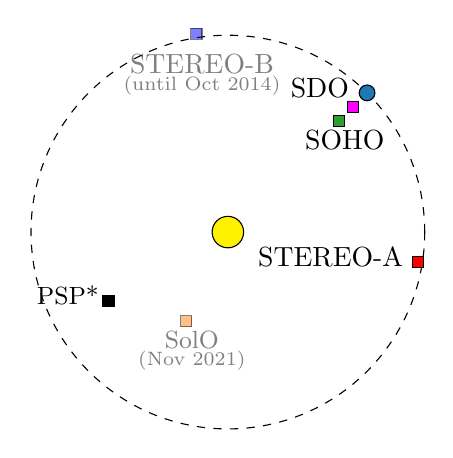
\begin{tikzpicture}
                \def\earthorbitradius{2.5}
                \def\sunradius{0.2}
                
                % sun
                \draw[fill=yellow] (0, 0) circle (\sunradius);
                
                % Earth
                \draw[dashed] (0, 0) circle (\earthorbitradius);
                \draw[fill=blue] (45:\earthorbitradius) circle (0.1);
                
                \draw[fill=Blue, opacity=0.5] ({45+54}:1.02*\earthorbitradius) +(-2pt,-2pt) rectangle +(2pt,2pt) node[below, align=center, yshift=-6pt] {STEREO-B\\[-2mm]\scriptsize (until Oct 2014)};
                \draw[fill=Red] ({45-54}:0.98*\earthorbitradius) +(-2pt,-2pt) rectangle +(2pt,2pt) node[left, xshift=-4pt] {STEREO-A};
                
                \draw[fill=Magenta] (45:0.9*\earthorbitradius) +(-2pt,-2pt) rectangle +(2pt,2pt) node[above left,yshift=-2pt] {SDO};
                \draw[fill=green] (45:0.8*\earthorbitradius) +(-2pt,-2pt) rectangle +(2pt,2pt) node[below,yshift=-2pt] {SOHO};
                
                \draw[fill=orange,opacity=0.5] (245:0.5*\earthorbitradius) +(-2pt,-2pt) rectangle +(2pt,2pt) node[below, yshift=-2pt, align=center] {\small SolO\\[-2mm]\scriptsize (Nov 2021)};
                \draw[fill=black] (210:0.7*\earthorbitradius) +(-2pt,-2pt) rectangle +(2pt,2pt) node[left, xshift=-2pt] {\small PSP*};
               
            \end{tikzpicture}
        \end{column}
        \begin{column}{0.45\textwidth}
            \textbf{In situ}\\[0.2cm]
            \centering
            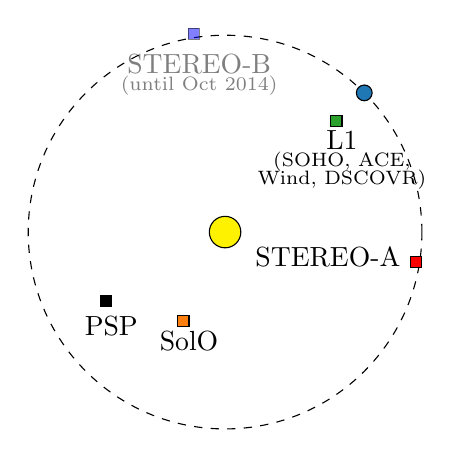
\begin{tikzpicture}
                \def\earthorbitradius{2.5}
                \def\sunradius{0.2}
                
                % sun
                \draw[fill=yellow] (0, 0) circle (\sunradius);
                
                % Earth
                \draw[dashed] (0, 0) circle (\earthorbitradius);
                \draw[fill=blue] (45:\earthorbitradius) circle (0.1);
                
                % satellites
                \draw[fill=Blue, opacity=0.5] ({45+54}:1.02*\earthorbitradius) +(-2pt,-2pt) rectangle +(2pt,2pt) node[below, align=center, yshift=-6pt] {STEREO-B\\[-2mm]\scriptsize (until Oct 2014)};
                \draw[fill=Red] ({45-54}:0.98*\earthorbitradius) +(-2pt,-2pt) rectangle +(2pt,2pt) node[left, xshift=-4pt] {STEREO-A};
                
                \draw[fill=green] (45:0.8*\earthorbitradius) +(-2pt,-2pt) rectangle +(2pt,2pt) node[below, yshift=-2pt, align=center] {L1\\[-2mm]\scriptsize (SOHO, ACE,\\[-2mm]\scriptsize Wind, DSCOVR)};                
                \draw[fill=orange] (245:0.5*\earthorbitradius) +(-2pt,-2pt) rectangle +(2pt,2pt) node[below, yshift=-2pt] {SolO};
                \draw[fill=black] (210:0.7*\earthorbitradius) +(-2pt,-2pt) rectangle +(2pt,2pt) node[below, yshift=-4pt] {PSP};
                
            \end{tikzpicture}
        \end{column}
    \end{columns}
    \vspace{2mm}
    \uncover<2->{\centering\summary Multispacecraft observations are \textbf{relatively rare}, especially in situ.}
    \begin{flushright}
        \footnotesize not to scale
    \end{flushright}
\end{frame}

\begin{frame}{Forbush decreases}
    \begin{columns}[T]
        \begin{column}{0.55\textwidth}
            \vbox to .9\textheight{%
            \vfill
            \begin{vfilleditems}
                \item \textbf{Short-term decrases} of GCR intensity, discovered 1937 by Scott E. Forbush
                \item Turbulent or closed \textbf{magnetic structures} act as a barrier for the GCRs:
                \begin{itemize}
                    \item ICME \textbf{shock/sheath} and \textbf{ejecta} (flux rope)
                    \item Stream interaction regions (\textbf{SIRs})
                \end{itemize}
                \item \textbf{Onset time} corresponds well to arrival of interplanetary structure
                \item FD amplitude is \textbf{energy-dependent} (lower energies modulated more easily)
            \end{vfilleditems}
            \vfill
            \uncover<2->{\summary FDs extend the available in situ observations with \textbf{additional viewpoints} at Earth, but also on many spacecraft (e.g. planetary missions)}
            \vfill
            }
        \end{column}
        \begin{column}{0.35\textwidth}
            \centering
            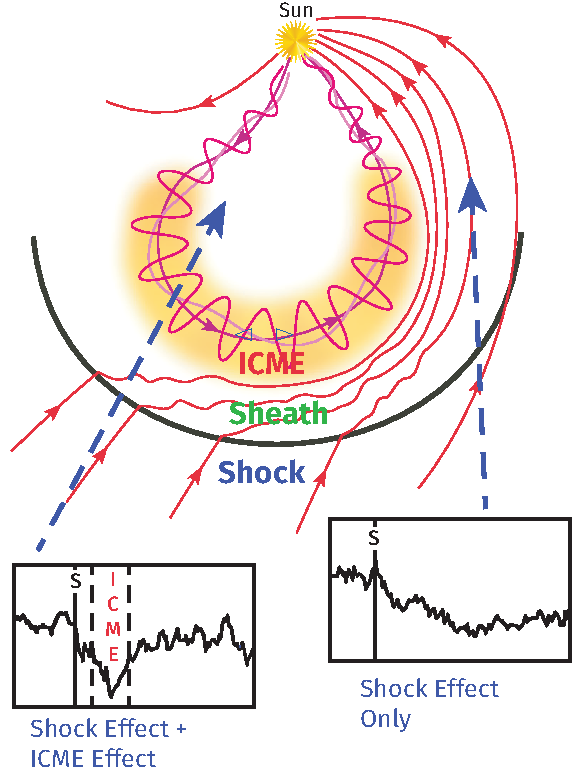
\includegraphics[width=\textwidth]{images/RichardsonCane-adapted.pdf}
            \scriptsize adapted from Richardson and Cane (2011)
        \end{column}
    \end{columns}
\end{frame}

\begin{frame}{FDs as additional in situ observations}
	\begin{columns}[t]
		\begin{column}{0.45\textwidth}
			\textbf{Remote sensing}\\[0.2cm]
            \centering
            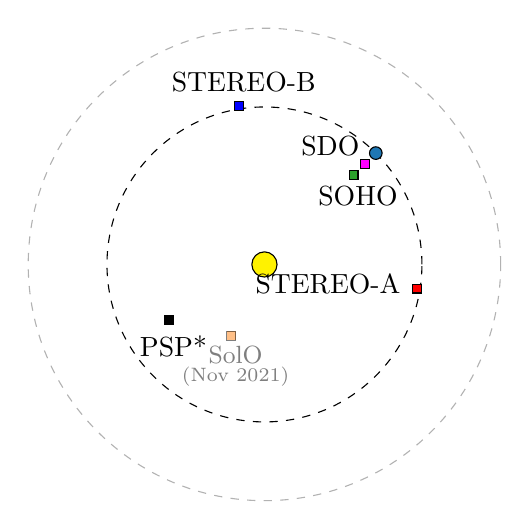
\begin{tikzpicture}[scale=0.8]
                \def\earthorbitradius{2.5}
                \def\sunradius{0.2}
                
                % sun
                \draw[fill=yellow] (0, 0) circle (\sunradius);
                
                % Earth
                \draw[dashed] (0, 0) circle (\earthorbitradius);
                \draw[fill=blue] (45:\earthorbitradius) circle (0.1);
                
                \draw[fill=Blue] ({45+54}:1.02*\earthorbitradius) +(-2pt,-2pt) rectangle +(2pt,2pt) node[above] {STEREO-B};
                \draw[fill=Red] ({45-54}:0.98*\earthorbitradius) +(-2pt,-2pt) rectangle +(2pt,2pt) node[left, xshift=-4pt] {STEREO-A};
                
                \draw[fill=Magenta] (45:0.9*\earthorbitradius) +(-2pt,-2pt) rectangle +(2pt,2pt) node[above left,yshift=-2pt] {SDO};
                \draw[fill=green] (45:0.8*\earthorbitradius) +(-2pt,-2pt) rectangle +(2pt,2pt) node[below,yshift=-2pt] {SOHO};
                
                \draw[fill=orange,opacity=0.5] (245:0.5*\earthorbitradius) +(-2pt,-2pt) rectangle +(2pt,2pt) node[below, yshift=-2pt, align=center] {\small SolO\\[-2mm]\scriptsize (Nov 2021)};
                \draw[fill=black] (210:0.7*\earthorbitradius) +(-2pt,-2pt) rectangle +(2pt,2pt) node[below, yshift=-4pt] {PSP*};
                
                \draw[dashed, opacity=0.3] (0, 0) circle (\earthorbitradius*1.5);
                
            \end{tikzpicture}
		\end{column}
		\begin{column}{0.45\textwidth}
			\textbf{In situ + FDs}\\[0.2cm]
			\centering
			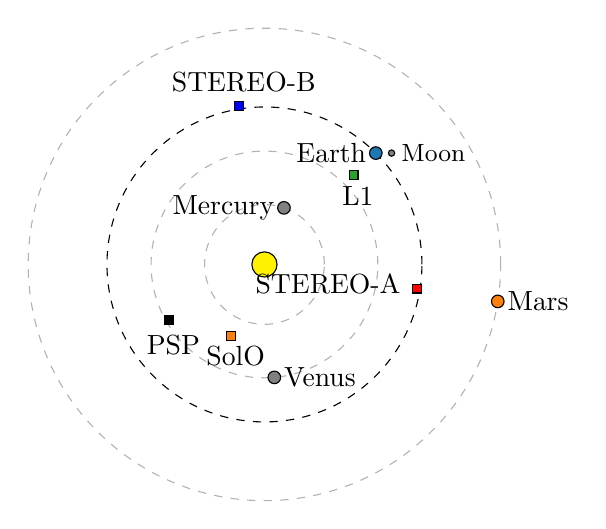
\begin{tikzpicture}[scale=0.8]
			\def\earthorbitradius{2.5}
			\def\sunradius{0.2}
			
			% sun
			\draw[fill=yellow] (0, 0) circle (\sunradius);
			
			% Earth
			\draw[dashed] (0, 0) circle (\earthorbitradius);
			\draw[fill=blue] (45:\earthorbitradius) circle (0.1) node[left] {Earth};
            
            % Moon
            \draw[fill=gray] (45:\earthorbitradius) ++ (0:\earthorbitradius*0.1) circle (0.05) node[right] {\small Moon};
			
			% Mars
			\draw[dashed, opacity=0.3] (0, 0) circle (\earthorbitradius*1.5);
			\draw[fill=orange] ({45-54}:\earthorbitradius*1.5) circle (0.1) node[right] {Mars};
			
			% Venus
			\draw[dashed, opacity=0.3] (0, 0) circle (\earthorbitradius*0.72);
			\draw[fill=gray] ({245+30}:\earthorbitradius*0.72) circle (0.1) node[right] {Venus};
			
			% Mercury
			\draw[dashed, opacity=0.3] (0, 0) circle (\earthorbitradius*0.38);
			\draw[fill=gray] ({45+26}:\earthorbitradius*0.38) circle (0.1) node[left] {Mercury};
			
			% satellites
			\draw[fill=Blue] ({45+54}:1.02*\earthorbitradius) +(-2pt,-2pt) rectangle +(2pt,2pt) node[above] {STEREO-B};
			\draw[fill=Red] ({45-54}:0.98*\earthorbitradius) +(-2pt,-2pt) rectangle +(2pt,2pt) node[left, xshift=-4pt] {STEREO-A};
			
			\draw[fill=green] (45:0.8*\earthorbitradius) +(-2pt,-2pt) rectangle +(2pt,2pt) node[below, yshift=-2pt, align=center] {L1};                
			\draw[fill=orange] (245:0.5*\earthorbitradius) +(-2pt,-2pt) rectangle +(2pt,2pt) node[below, yshift=-2pt] {SolO};
			\draw[fill=black] (210:0.7*\earthorbitradius) +(-2pt,-2pt) rectangle +(2pt,2pt) node[below, yshift=-4pt] {PSP};
			
			\end{tikzpicture}
			+ many others
		\end{column}
	\end{columns}
\end{frame}

\begin{frame}{Multipoint observations of FDs}
    \vskip0.2cm
    \begin{center}
        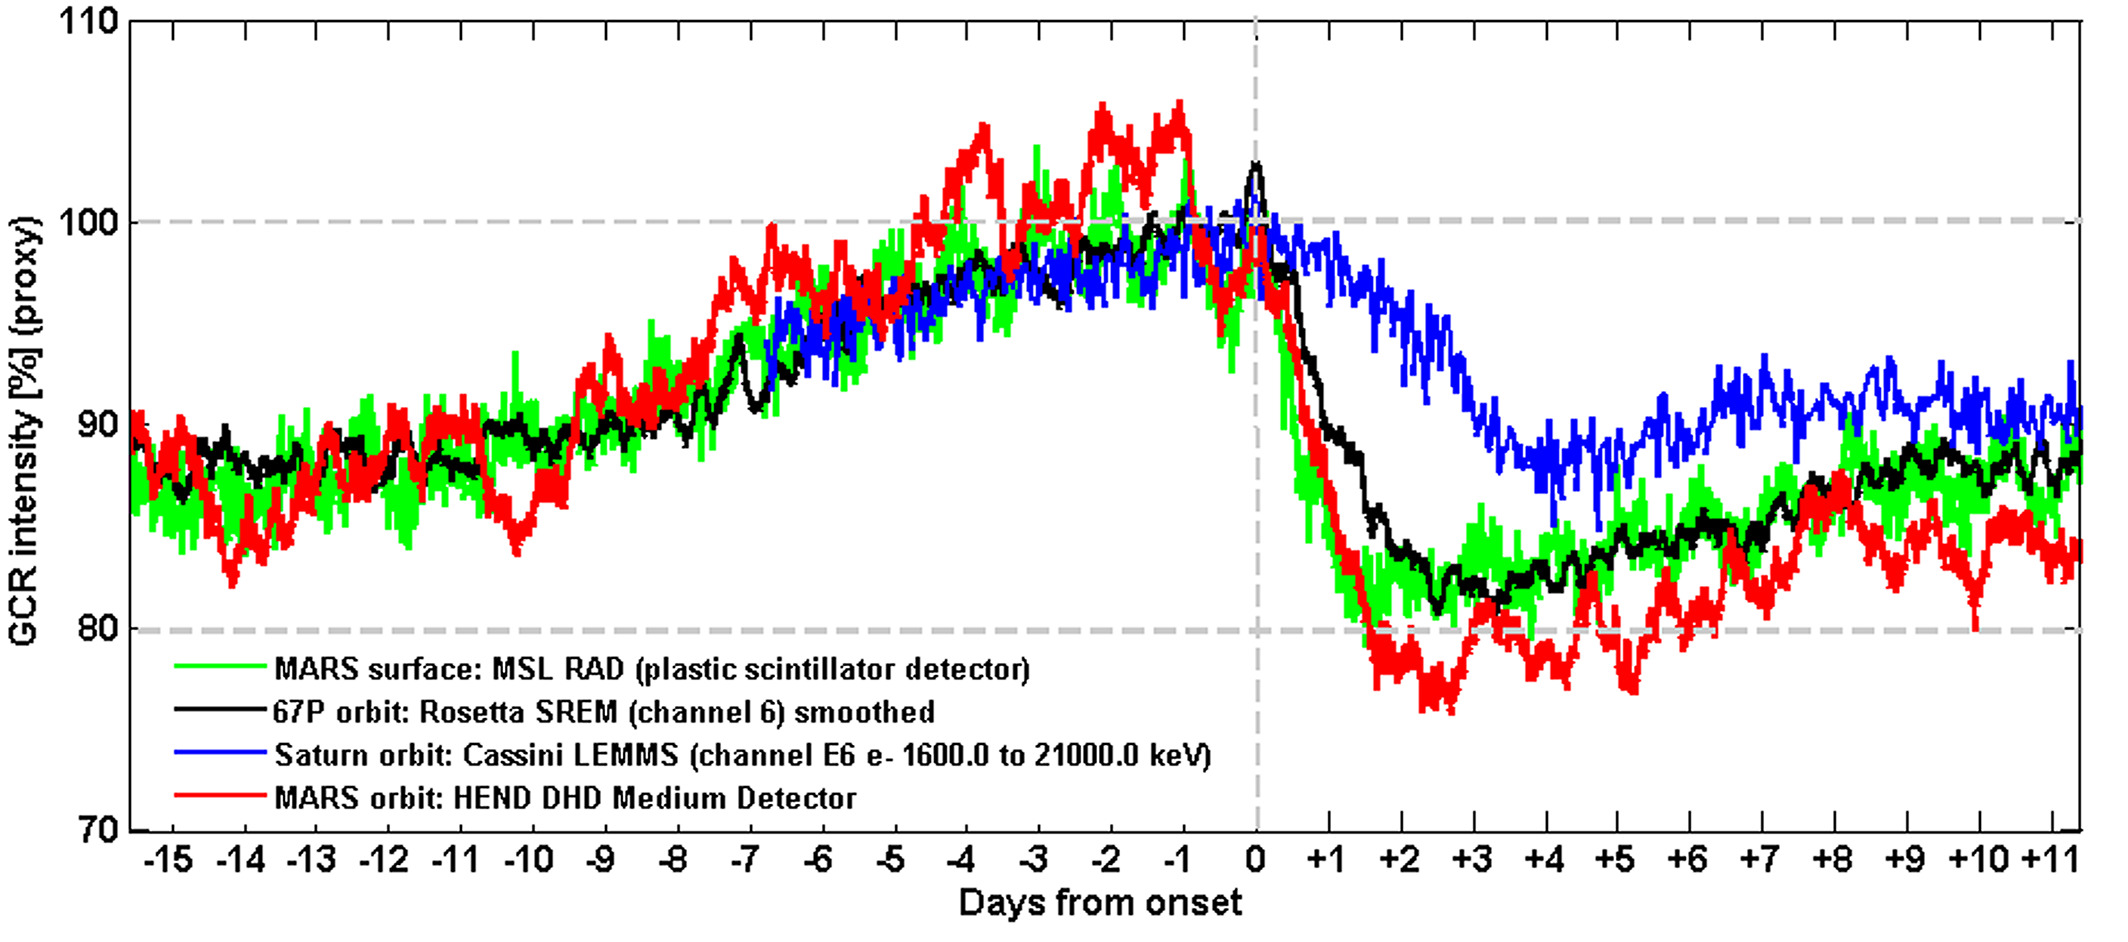
\includegraphics[width=0.8\linewidth]{images/witasse2017.png}\\
        \footnotesize Witasse et al. (2017)
    \end{center}
    \uncover<2->{
        \begin{quote}
            ``\textbf{More information on ICME properties} can probably be obtained [from] these data sets. For example, we suspect that the \textbf{evolution of the radial extension} of the ICME could be inferred from the Forbush decrease data.''
        \end{quote}
    }
\end{frame}

\section{Instrumentation}

\begin{frame}{Radiation Assessment Detector}
    \begin{columns}
        \begin{column}{0.50\textwidth}
            \begin{itemize}
                \item Onboard \textbf{Mars Science Laboratory} (\emph{Curiosity} rover)
                \item \textbf{Cruise phase:} 12/2011 -- 07/2012\\
                \textbf{Surface phase:} 08/2012 -- today
                \item Data products: \textcolor{green}{charged} and \textcolor{gray}{neutral} \textbf{particle spectra} + \textbf{dosimetry} (TID, LET)
            \end{itemize}            
            \uncover<2->{
            \centering
            %% Creator: Matplotlib, PGF backend
%%
%% To include the figure in your LaTeX document, write
%%   \input{<filename>.pgf}
%%
%% Make sure the required packages are loaded in your preamble
%%   \usepackage{pgf}
%%
%% and, on pdftex
%%   \usepackage[utf8]{inputenc}\DeclareUnicodeCharacter{2212}{-}
%%
%% or, on luatex and xetex
%%   \usepackage{unicode-math}
%%
%% Figures using additional raster images can only be included by \input if
%% they are in the same directory as the main LaTeX file. For loading figures
%% from other directories you can use the `import` package
%%   \usepackage{import}
%%
%% and then include the figures with
%%   \import{<path to file>}{<filename>.pgf}
%%
%% Matplotlib used the following preamble
%%   \usepackage{siunitx}
%%   \usepackage{fontspec}
%%
\begingroup%
\makeatletter%
\begin{pgfpicture}%
\pgfpathrectangle{\pgfpointorigin}{\pgfqpoint{2.700000in}{1.400000in}}%
\pgfusepath{use as bounding box, clip}%
\begin{pgfscope}%
\pgfsetbuttcap%
\pgfsetmiterjoin%
\definecolor{currentfill}{rgb}{1.000000,1.000000,1.000000}%
\pgfsetfillcolor{currentfill}%
\pgfsetlinewidth{0.000000pt}%
\definecolor{currentstroke}{rgb}{1.000000,1.000000,1.000000}%
\pgfsetstrokecolor{currentstroke}%
\pgfsetdash{}{0pt}%
\pgfpathmoveto{\pgfqpoint{0.000000in}{0.000000in}}%
\pgfpathlineto{\pgfqpoint{2.700000in}{0.000000in}}%
\pgfpathlineto{\pgfqpoint{2.700000in}{1.400000in}}%
\pgfpathlineto{\pgfqpoint{0.000000in}{1.400000in}}%
\pgfpathclose%
\pgfusepath{fill}%
\end{pgfscope}%
\begin{pgfscope}%
\pgfsetbuttcap%
\pgfsetmiterjoin%
\definecolor{currentfill}{rgb}{1.000000,1.000000,1.000000}%
\pgfsetfillcolor{currentfill}%
\pgfsetlinewidth{0.000000pt}%
\definecolor{currentstroke}{rgb}{0.000000,0.000000,0.000000}%
\pgfsetstrokecolor{currentstroke}%
\pgfsetstrokeopacity{0.000000}%
\pgfsetdash{}{0pt}%
\pgfpathmoveto{\pgfqpoint{0.520105in}{0.379698in}}%
\pgfpathlineto{\pgfqpoint{2.595000in}{0.379698in}}%
\pgfpathlineto{\pgfqpoint{2.595000in}{1.295000in}}%
\pgfpathlineto{\pgfqpoint{0.520105in}{1.295000in}}%
\pgfpathclose%
\pgfusepath{fill}%
\end{pgfscope}%
\begin{pgfscope}%
\pgfsetbuttcap%
\pgfsetroundjoin%
\definecolor{currentfill}{rgb}{0.000000,0.000000,0.000000}%
\pgfsetfillcolor{currentfill}%
\pgfsetlinewidth{0.803000pt}%
\definecolor{currentstroke}{rgb}{0.000000,0.000000,0.000000}%
\pgfsetstrokecolor{currentstroke}%
\pgfsetdash{}{0pt}%
\pgfsys@defobject{currentmarker}{\pgfqpoint{0.000000in}{-0.048611in}}{\pgfqpoint{0.000000in}{0.000000in}}{%
\pgfpathmoveto{\pgfqpoint{0.000000in}{0.000000in}}%
\pgfpathlineto{\pgfqpoint{0.000000in}{-0.048611in}}%
\pgfusepath{stroke,fill}%
}%
\begin{pgfscope}%
\pgfsys@transformshift{0.629000in}{0.379698in}%
\pgfsys@useobject{currentmarker}{}%
\end{pgfscope}%
\end{pgfscope}%
\begin{pgfscope}%
\definecolor{textcolor}{rgb}{0.000000,0.000000,0.000000}%
\pgfsetstrokecolor{textcolor}%
\pgfsetfillcolor{textcolor}%
\pgftext[x=0.440736in, y=0.120793in, left, base,rotate=30.000000]{\color{textcolor}\sffamily\fontsize{7.000000}{8.400000}\selectfont 2012}%
\end{pgfscope}%
\begin{pgfscope}%
\pgfsetbuttcap%
\pgfsetroundjoin%
\definecolor{currentfill}{rgb}{0.000000,0.000000,0.000000}%
\pgfsetfillcolor{currentfill}%
\pgfsetlinewidth{0.803000pt}%
\definecolor{currentstroke}{rgb}{0.000000,0.000000,0.000000}%
\pgfsetstrokecolor{currentstroke}%
\pgfsetdash{}{0pt}%
\pgfsys@defobject{currentmarker}{\pgfqpoint{0.000000in}{-0.048611in}}{\pgfqpoint{0.000000in}{0.000000in}}{%
\pgfpathmoveto{\pgfqpoint{0.000000in}{0.000000in}}%
\pgfpathlineto{\pgfqpoint{0.000000in}{-0.048611in}}%
\pgfusepath{stroke,fill}%
}%
\begin{pgfscope}%
\pgfsys@transformshift{0.851375in}{0.379698in}%
\pgfsys@useobject{currentmarker}{}%
\end{pgfscope}%
\end{pgfscope}%
\begin{pgfscope}%
\definecolor{textcolor}{rgb}{0.000000,0.000000,0.000000}%
\pgfsetstrokecolor{textcolor}%
\pgfsetfillcolor{textcolor}%
\pgftext[x=0.663110in, y=0.120793in, left, base,rotate=30.000000]{\color{textcolor}\sffamily\fontsize{7.000000}{8.400000}\selectfont 2013}%
\end{pgfscope}%
\begin{pgfscope}%
\pgfsetbuttcap%
\pgfsetroundjoin%
\definecolor{currentfill}{rgb}{0.000000,0.000000,0.000000}%
\pgfsetfillcolor{currentfill}%
\pgfsetlinewidth{0.803000pt}%
\definecolor{currentstroke}{rgb}{0.000000,0.000000,0.000000}%
\pgfsetstrokecolor{currentstroke}%
\pgfsetdash{}{0pt}%
\pgfsys@defobject{currentmarker}{\pgfqpoint{0.000000in}{-0.048611in}}{\pgfqpoint{0.000000in}{0.000000in}}{%
\pgfpathmoveto{\pgfqpoint{0.000000in}{0.000000in}}%
\pgfpathlineto{\pgfqpoint{0.000000in}{-0.048611in}}%
\pgfusepath{stroke,fill}%
}%
\begin{pgfscope}%
\pgfsys@transformshift{1.073142in}{0.379698in}%
\pgfsys@useobject{currentmarker}{}%
\end{pgfscope}%
\end{pgfscope}%
\begin{pgfscope}%
\definecolor{textcolor}{rgb}{0.000000,0.000000,0.000000}%
\pgfsetstrokecolor{textcolor}%
\pgfsetfillcolor{textcolor}%
\pgftext[x=0.884877in, y=0.120793in, left, base,rotate=30.000000]{\color{textcolor}\sffamily\fontsize{7.000000}{8.400000}\selectfont 2014}%
\end{pgfscope}%
\begin{pgfscope}%
\pgfsetbuttcap%
\pgfsetroundjoin%
\definecolor{currentfill}{rgb}{0.000000,0.000000,0.000000}%
\pgfsetfillcolor{currentfill}%
\pgfsetlinewidth{0.803000pt}%
\definecolor{currentstroke}{rgb}{0.000000,0.000000,0.000000}%
\pgfsetstrokecolor{currentstroke}%
\pgfsetdash{}{0pt}%
\pgfsys@defobject{currentmarker}{\pgfqpoint{0.000000in}{-0.048611in}}{\pgfqpoint{0.000000in}{0.000000in}}{%
\pgfpathmoveto{\pgfqpoint{0.000000in}{0.000000in}}%
\pgfpathlineto{\pgfqpoint{0.000000in}{-0.048611in}}%
\pgfusepath{stroke,fill}%
}%
\begin{pgfscope}%
\pgfsys@transformshift{1.294909in}{0.379698in}%
\pgfsys@useobject{currentmarker}{}%
\end{pgfscope}%
\end{pgfscope}%
\begin{pgfscope}%
\definecolor{textcolor}{rgb}{0.000000,0.000000,0.000000}%
\pgfsetstrokecolor{textcolor}%
\pgfsetfillcolor{textcolor}%
\pgftext[x=1.106644in, y=0.120793in, left, base,rotate=30.000000]{\color{textcolor}\sffamily\fontsize{7.000000}{8.400000}\selectfont 2015}%
\end{pgfscope}%
\begin{pgfscope}%
\pgfsetbuttcap%
\pgfsetroundjoin%
\definecolor{currentfill}{rgb}{0.000000,0.000000,0.000000}%
\pgfsetfillcolor{currentfill}%
\pgfsetlinewidth{0.803000pt}%
\definecolor{currentstroke}{rgb}{0.000000,0.000000,0.000000}%
\pgfsetstrokecolor{currentstroke}%
\pgfsetdash{}{0pt}%
\pgfsys@defobject{currentmarker}{\pgfqpoint{0.000000in}{-0.048611in}}{\pgfqpoint{0.000000in}{0.000000in}}{%
\pgfpathmoveto{\pgfqpoint{0.000000in}{0.000000in}}%
\pgfpathlineto{\pgfqpoint{0.000000in}{-0.048611in}}%
\pgfusepath{stroke,fill}%
}%
\begin{pgfscope}%
\pgfsys@transformshift{1.516676in}{0.379698in}%
\pgfsys@useobject{currentmarker}{}%
\end{pgfscope}%
\end{pgfscope}%
\begin{pgfscope}%
\definecolor{textcolor}{rgb}{0.000000,0.000000,0.000000}%
\pgfsetstrokecolor{textcolor}%
\pgfsetfillcolor{textcolor}%
\pgftext[x=1.328411in, y=0.120793in, left, base,rotate=30.000000]{\color{textcolor}\sffamily\fontsize{7.000000}{8.400000}\selectfont 2016}%
\end{pgfscope}%
\begin{pgfscope}%
\pgfsetbuttcap%
\pgfsetroundjoin%
\definecolor{currentfill}{rgb}{0.000000,0.000000,0.000000}%
\pgfsetfillcolor{currentfill}%
\pgfsetlinewidth{0.803000pt}%
\definecolor{currentstroke}{rgb}{0.000000,0.000000,0.000000}%
\pgfsetstrokecolor{currentstroke}%
\pgfsetdash{}{0pt}%
\pgfsys@defobject{currentmarker}{\pgfqpoint{0.000000in}{-0.048611in}}{\pgfqpoint{0.000000in}{0.000000in}}{%
\pgfpathmoveto{\pgfqpoint{0.000000in}{0.000000in}}%
\pgfpathlineto{\pgfqpoint{0.000000in}{-0.048611in}}%
\pgfusepath{stroke,fill}%
}%
\begin{pgfscope}%
\pgfsys@transformshift{1.739050in}{0.379698in}%
\pgfsys@useobject{currentmarker}{}%
\end{pgfscope}%
\end{pgfscope}%
\begin{pgfscope}%
\definecolor{textcolor}{rgb}{0.000000,0.000000,0.000000}%
\pgfsetstrokecolor{textcolor}%
\pgfsetfillcolor{textcolor}%
\pgftext[x=1.550786in, y=0.120793in, left, base,rotate=30.000000]{\color{textcolor}\sffamily\fontsize{7.000000}{8.400000}\selectfont 2017}%
\end{pgfscope}%
\begin{pgfscope}%
\pgfsetbuttcap%
\pgfsetroundjoin%
\definecolor{currentfill}{rgb}{0.000000,0.000000,0.000000}%
\pgfsetfillcolor{currentfill}%
\pgfsetlinewidth{0.803000pt}%
\definecolor{currentstroke}{rgb}{0.000000,0.000000,0.000000}%
\pgfsetstrokecolor{currentstroke}%
\pgfsetdash{}{0pt}%
\pgfsys@defobject{currentmarker}{\pgfqpoint{0.000000in}{-0.048611in}}{\pgfqpoint{0.000000in}{0.000000in}}{%
\pgfpathmoveto{\pgfqpoint{0.000000in}{0.000000in}}%
\pgfpathlineto{\pgfqpoint{0.000000in}{-0.048611in}}%
\pgfusepath{stroke,fill}%
}%
\begin{pgfscope}%
\pgfsys@transformshift{1.960817in}{0.379698in}%
\pgfsys@useobject{currentmarker}{}%
\end{pgfscope}%
\end{pgfscope}%
\begin{pgfscope}%
\definecolor{textcolor}{rgb}{0.000000,0.000000,0.000000}%
\pgfsetstrokecolor{textcolor}%
\pgfsetfillcolor{textcolor}%
\pgftext[x=1.772553in, y=0.120793in, left, base,rotate=30.000000]{\color{textcolor}\sffamily\fontsize{7.000000}{8.400000}\selectfont 2018}%
\end{pgfscope}%
\begin{pgfscope}%
\pgfsetbuttcap%
\pgfsetroundjoin%
\definecolor{currentfill}{rgb}{0.000000,0.000000,0.000000}%
\pgfsetfillcolor{currentfill}%
\pgfsetlinewidth{0.803000pt}%
\definecolor{currentstroke}{rgb}{0.000000,0.000000,0.000000}%
\pgfsetstrokecolor{currentstroke}%
\pgfsetdash{}{0pt}%
\pgfsys@defobject{currentmarker}{\pgfqpoint{0.000000in}{-0.048611in}}{\pgfqpoint{0.000000in}{0.000000in}}{%
\pgfpathmoveto{\pgfqpoint{0.000000in}{0.000000in}}%
\pgfpathlineto{\pgfqpoint{0.000000in}{-0.048611in}}%
\pgfusepath{stroke,fill}%
}%
\begin{pgfscope}%
\pgfsys@transformshift{2.182584in}{0.379698in}%
\pgfsys@useobject{currentmarker}{}%
\end{pgfscope}%
\end{pgfscope}%
\begin{pgfscope}%
\definecolor{textcolor}{rgb}{0.000000,0.000000,0.000000}%
\pgfsetstrokecolor{textcolor}%
\pgfsetfillcolor{textcolor}%
\pgftext[x=1.994320in, y=0.120793in, left, base,rotate=30.000000]{\color{textcolor}\sffamily\fontsize{7.000000}{8.400000}\selectfont 2019}%
\end{pgfscope}%
\begin{pgfscope}%
\pgfsetbuttcap%
\pgfsetroundjoin%
\definecolor{currentfill}{rgb}{0.000000,0.000000,0.000000}%
\pgfsetfillcolor{currentfill}%
\pgfsetlinewidth{0.803000pt}%
\definecolor{currentstroke}{rgb}{0.000000,0.000000,0.000000}%
\pgfsetstrokecolor{currentstroke}%
\pgfsetdash{}{0pt}%
\pgfsys@defobject{currentmarker}{\pgfqpoint{0.000000in}{-0.048611in}}{\pgfqpoint{0.000000in}{0.000000in}}{%
\pgfpathmoveto{\pgfqpoint{0.000000in}{0.000000in}}%
\pgfpathlineto{\pgfqpoint{0.000000in}{-0.048611in}}%
\pgfusepath{stroke,fill}%
}%
\begin{pgfscope}%
\pgfsys@transformshift{2.404351in}{0.379698in}%
\pgfsys@useobject{currentmarker}{}%
\end{pgfscope}%
\end{pgfscope}%
\begin{pgfscope}%
\definecolor{textcolor}{rgb}{0.000000,0.000000,0.000000}%
\pgfsetstrokecolor{textcolor}%
\pgfsetfillcolor{textcolor}%
\pgftext[x=2.216087in, y=0.120793in, left, base,rotate=30.000000]{\color{textcolor}\sffamily\fontsize{7.000000}{8.400000}\selectfont 2020}%
\end{pgfscope}%
\begin{pgfscope}%
\pgfsetbuttcap%
\pgfsetroundjoin%
\definecolor{currentfill}{rgb}{0.000000,0.000000,0.000000}%
\pgfsetfillcolor{currentfill}%
\pgfsetlinewidth{0.803000pt}%
\definecolor{currentstroke}{rgb}{0.000000,0.000000,0.000000}%
\pgfsetstrokecolor{currentstroke}%
\pgfsetdash{}{0pt}%
\pgfsys@defobject{currentmarker}{\pgfqpoint{-0.048611in}{0.000000in}}{\pgfqpoint{-0.000000in}{0.000000in}}{%
\pgfpathmoveto{\pgfqpoint{-0.000000in}{0.000000in}}%
\pgfpathlineto{\pgfqpoint{-0.048611in}{0.000000in}}%
\pgfusepath{stroke,fill}%
}%
\begin{pgfscope}%
\pgfsys@transformshift{0.520105in}{0.501738in}%
\pgfsys@useobject{currentmarker}{}%
\end{pgfscope}%
\end{pgfscope}%
\begin{pgfscope}%
\definecolor{textcolor}{rgb}{0.000000,0.000000,0.000000}%
\pgfsetstrokecolor{textcolor}%
\pgfsetfillcolor{textcolor}%
\pgftext[x=0.256794in, y=0.468002in, left, base]{\color{textcolor}\sffamily\fontsize{7.000000}{8.400000}\selectfont \(\displaystyle {200}\)}%
\end{pgfscope}%
\begin{pgfscope}%
\pgfsetbuttcap%
\pgfsetroundjoin%
\definecolor{currentfill}{rgb}{0.000000,0.000000,0.000000}%
\pgfsetfillcolor{currentfill}%
\pgfsetlinewidth{0.803000pt}%
\definecolor{currentstroke}{rgb}{0.000000,0.000000,0.000000}%
\pgfsetstrokecolor{currentstroke}%
\pgfsetdash{}{0pt}%
\pgfsys@defobject{currentmarker}{\pgfqpoint{-0.048611in}{0.000000in}}{\pgfqpoint{-0.000000in}{0.000000in}}{%
\pgfpathmoveto{\pgfqpoint{-0.000000in}{0.000000in}}%
\pgfpathlineto{\pgfqpoint{-0.048611in}{0.000000in}}%
\pgfusepath{stroke,fill}%
}%
\begin{pgfscope}%
\pgfsys@transformshift{0.520105in}{0.806839in}%
\pgfsys@useobject{currentmarker}{}%
\end{pgfscope}%
\end{pgfscope}%
\begin{pgfscope}%
\definecolor{textcolor}{rgb}{0.000000,0.000000,0.000000}%
\pgfsetstrokecolor{textcolor}%
\pgfsetfillcolor{textcolor}%
\pgftext[x=0.256794in, y=0.773103in, left, base]{\color{textcolor}\sffamily\fontsize{7.000000}{8.400000}\selectfont \(\displaystyle {250}\)}%
\end{pgfscope}%
\begin{pgfscope}%
\pgfsetbuttcap%
\pgfsetroundjoin%
\definecolor{currentfill}{rgb}{0.000000,0.000000,0.000000}%
\pgfsetfillcolor{currentfill}%
\pgfsetlinewidth{0.803000pt}%
\definecolor{currentstroke}{rgb}{0.000000,0.000000,0.000000}%
\pgfsetstrokecolor{currentstroke}%
\pgfsetdash{}{0pt}%
\pgfsys@defobject{currentmarker}{\pgfqpoint{-0.048611in}{0.000000in}}{\pgfqpoint{-0.000000in}{0.000000in}}{%
\pgfpathmoveto{\pgfqpoint{-0.000000in}{0.000000in}}%
\pgfpathlineto{\pgfqpoint{-0.048611in}{0.000000in}}%
\pgfusepath{stroke,fill}%
}%
\begin{pgfscope}%
\pgfsys@transformshift{0.520105in}{1.111940in}%
\pgfsys@useobject{currentmarker}{}%
\end{pgfscope}%
\end{pgfscope}%
\begin{pgfscope}%
\definecolor{textcolor}{rgb}{0.000000,0.000000,0.000000}%
\pgfsetstrokecolor{textcolor}%
\pgfsetfillcolor{textcolor}%
\pgftext[x=0.256794in, y=1.078203in, left, base]{\color{textcolor}\sffamily\fontsize{7.000000}{8.400000}\selectfont \(\displaystyle {300}\)}%
\end{pgfscope}%
\begin{pgfscope}%
\definecolor{textcolor}{rgb}{0.000000,0.000000,0.000000}%
\pgfsetstrokecolor{textcolor}%
\pgfsetfillcolor{textcolor}%
\pgftext[x=0.201238in,y=0.837349in,,bottom,rotate=90.000000]{\color{textcolor}\sffamily\fontsize{7.000000}{8.400000}\selectfont dose rate / \si{\micro\gray\per day}}%
\end{pgfscope}%
\begin{pgfscope}%
\pgfpathrectangle{\pgfqpoint{0.520105in}{0.379698in}}{\pgfqpoint{2.074895in}{0.915302in}}%
\pgfusepath{clip}%
\pgfsetrectcap%
\pgfsetroundjoin%
\pgfsetlinewidth{0.602250pt}%
\definecolor{currentstroke}{rgb}{0.121569,0.466667,0.705882}%
\pgfsetstrokecolor{currentstroke}%
\pgfsetdash{}{0pt}%
\pgfpathmoveto{\pgfqpoint{0.614418in}{0.445546in}}%
\pgfpathlineto{\pgfqpoint{0.615026in}{0.452116in}}%
\pgfpathlineto{\pgfqpoint{0.615634in}{0.471389in}}%
\pgfpathlineto{\pgfqpoint{0.616241in}{0.460879in}}%
\pgfpathlineto{\pgfqpoint{0.616849in}{0.459374in}}%
\pgfpathlineto{\pgfqpoint{0.618671in}{0.493693in}}%
\pgfpathlineto{\pgfqpoint{0.620494in}{0.502539in}}%
\pgfpathlineto{\pgfqpoint{0.622925in}{0.445569in}}%
\pgfpathmoveto{\pgfqpoint{0.624140in}{0.467306in}}%
\pgfpathlineto{\pgfqpoint{0.624747in}{0.458490in}}%
\pgfpathlineto{\pgfqpoint{0.625355in}{0.465038in}}%
\pgfpathlineto{\pgfqpoint{0.625962in}{0.464470in}}%
\pgfpathlineto{\pgfqpoint{0.626570in}{0.472012in}}%
\pgfpathlineto{\pgfqpoint{0.628393in}{0.424808in}}%
\pgfpathlineto{\pgfqpoint{0.629000in}{0.435010in}}%
\pgfpathlineto{\pgfqpoint{0.629608in}{0.435038in}}%
\pgfpathlineto{\pgfqpoint{0.631431in}{0.425865in}}%
\pgfpathlineto{\pgfqpoint{0.633253in}{0.483963in}}%
\pgfpathlineto{\pgfqpoint{0.633861in}{0.482856in}}%
\pgfpathlineto{\pgfqpoint{0.635076in}{0.471184in}}%
\pgfpathlineto{\pgfqpoint{0.635684in}{0.472806in}}%
\pgfpathlineto{\pgfqpoint{0.636291in}{0.476590in}}%
\pgfpathlineto{\pgfqpoint{0.636899in}{0.472561in}}%
\pgfpathlineto{\pgfqpoint{0.638114in}{0.482508in}}%
\pgfpathlineto{\pgfqpoint{0.638722in}{0.464922in}}%
\pgfpathlineto{\pgfqpoint{0.639329in}{0.471142in}}%
\pgfpathlineto{\pgfqpoint{0.640544in}{0.484369in}}%
\pgfpathlineto{\pgfqpoint{0.641760in}{0.466457in}}%
\pgfpathlineto{\pgfqpoint{0.642367in}{0.602884in}}%
\pgfpathlineto{\pgfqpoint{0.642975in}{0.494741in}}%
\pgfpathlineto{\pgfqpoint{0.643494in}{0.369698in}}%
\pgfpathmoveto{\pgfqpoint{0.644194in}{0.369698in}}%
\pgfpathlineto{\pgfqpoint{0.644657in}{1.305000in}}%
\pgfpathmoveto{\pgfqpoint{0.645860in}{1.305000in}}%
\pgfpathlineto{\pgfqpoint{0.646620in}{0.556341in}}%
\pgfpathlineto{\pgfqpoint{0.648443in}{0.429590in}}%
\pgfpathlineto{\pgfqpoint{0.649658in}{0.549458in}}%
\pgfpathmoveto{\pgfqpoint{0.658164in}{0.517087in}}%
\pgfpathlineto{\pgfqpoint{0.661810in}{0.561280in}}%
\pgfpathlineto{\pgfqpoint{0.662417in}{0.555725in}}%
\pgfpathlineto{\pgfqpoint{0.663025in}{0.556372in}}%
\pgfpathlineto{\pgfqpoint{0.664240in}{0.446958in}}%
\pgfpathlineto{\pgfqpoint{0.664848in}{0.474503in}}%
\pgfpathlineto{\pgfqpoint{0.667278in}{0.534220in}}%
\pgfpathlineto{\pgfqpoint{0.667886in}{0.514454in}}%
\pgfpathlineto{\pgfqpoint{0.668493in}{0.510926in}}%
\pgfpathlineto{\pgfqpoint{0.668618in}{1.305000in}}%
\pgfpathmoveto{\pgfqpoint{0.670878in}{1.305000in}}%
\pgfpathlineto{\pgfqpoint{0.671622in}{0.369698in}}%
\pgfpathmoveto{\pgfqpoint{0.672379in}{0.369698in}}%
\pgfpathlineto{\pgfqpoint{0.672746in}{0.470445in}}%
\pgfpathlineto{\pgfqpoint{0.673354in}{0.449109in}}%
\pgfpathlineto{\pgfqpoint{0.673827in}{0.369698in}}%
\pgfpathmoveto{\pgfqpoint{0.675451in}{0.369698in}}%
\pgfpathlineto{\pgfqpoint{0.679430in}{0.471409in}}%
\pgfpathlineto{\pgfqpoint{0.681860in}{0.500139in}}%
\pgfpathlineto{\pgfqpoint{0.683075in}{0.474353in}}%
\pgfpathlineto{\pgfqpoint{0.683683in}{0.474542in}}%
\pgfpathlineto{\pgfqpoint{0.684898in}{0.470440in}}%
\pgfpathlineto{\pgfqpoint{0.685505in}{0.470562in}}%
\pgfpathlineto{\pgfqpoint{0.686721in}{0.496754in}}%
\pgfpathlineto{\pgfqpoint{0.687936in}{0.432717in}}%
\pgfpathlineto{\pgfqpoint{0.688543in}{0.458492in}}%
\pgfpathlineto{\pgfqpoint{0.694012in}{0.538801in}}%
\pgfpathlineto{\pgfqpoint{0.695834in}{0.565128in}}%
\pgfpathlineto{\pgfqpoint{0.696442in}{0.555204in}}%
\pgfpathlineto{\pgfqpoint{0.699480in}{0.463952in}}%
\pgfpathlineto{\pgfqpoint{0.703125in}{0.548816in}}%
\pgfpathlineto{\pgfqpoint{0.703733in}{0.615551in}}%
\pgfpathlineto{\pgfqpoint{0.704340in}{0.587604in}}%
\pgfpathlineto{\pgfqpoint{0.704948in}{0.576116in}}%
\pgfpathlineto{\pgfqpoint{0.705556in}{0.587171in}}%
\pgfpathlineto{\pgfqpoint{0.706163in}{0.585401in}}%
\pgfpathlineto{\pgfqpoint{0.707378in}{0.585940in}}%
\pgfpathlineto{\pgfqpoint{0.707986in}{0.601625in}}%
\pgfpathlineto{\pgfqpoint{0.709809in}{0.574938in}}%
\pgfpathlineto{\pgfqpoint{0.711024in}{0.586657in}}%
\pgfpathlineto{\pgfqpoint{0.711631in}{0.565163in}}%
\pgfpathlineto{\pgfqpoint{0.711753in}{1.305000in}}%
\pgfpathmoveto{\pgfqpoint{0.712747in}{1.305000in}}%
\pgfpathlineto{\pgfqpoint{0.713454in}{0.609857in}}%
\pgfpathlineto{\pgfqpoint{0.715277in}{0.584210in}}%
\pgfpathlineto{\pgfqpoint{0.716492in}{0.570973in}}%
\pgfpathlineto{\pgfqpoint{0.717707in}{0.590463in}}%
\pgfpathlineto{\pgfqpoint{0.718315in}{0.584863in}}%
\pgfpathlineto{\pgfqpoint{0.720137in}{0.566655in}}%
\pgfpathmoveto{\pgfqpoint{0.721353in}{0.561011in}}%
\pgfpathlineto{\pgfqpoint{0.722568in}{0.520288in}}%
\pgfpathlineto{\pgfqpoint{0.723175in}{0.481706in}}%
\pgfpathlineto{\pgfqpoint{0.723783in}{0.488858in}}%
\pgfpathmoveto{\pgfqpoint{0.725606in}{0.499315in}}%
\pgfpathlineto{\pgfqpoint{0.726213in}{0.508117in}}%
\pgfpathlineto{\pgfqpoint{0.726821in}{0.493870in}}%
\pgfpathlineto{\pgfqpoint{0.727428in}{0.591226in}}%
\pgfpathlineto{\pgfqpoint{0.728036in}{0.548065in}}%
\pgfpathlineto{\pgfqpoint{0.731074in}{0.577532in}}%
\pgfpathlineto{\pgfqpoint{0.731682in}{0.562945in}}%
\pgfpathlineto{\pgfqpoint{0.732897in}{0.501593in}}%
\pgfpathlineto{\pgfqpoint{0.735327in}{0.540272in}}%
\pgfpathlineto{\pgfqpoint{0.735935in}{0.529897in}}%
\pgfpathlineto{\pgfqpoint{0.737757in}{0.542737in}}%
\pgfpathlineto{\pgfqpoint{0.738365in}{0.536079in}}%
\pgfpathlineto{\pgfqpoint{0.738972in}{0.537600in}}%
\pgfpathlineto{\pgfqpoint{0.739580in}{0.537787in}}%
\pgfpathlineto{\pgfqpoint{0.740795in}{0.550066in}}%
\pgfpathlineto{\pgfqpoint{0.741403in}{0.545340in}}%
\pgfpathlineto{\pgfqpoint{0.745656in}{0.483478in}}%
\pgfpathlineto{\pgfqpoint{0.746263in}{0.496166in}}%
\pgfpathlineto{\pgfqpoint{0.747479in}{0.522417in}}%
\pgfpathlineto{\pgfqpoint{0.747479in}{0.522417in}}%
\pgfusepath{stroke}%
\end{pgfscope}%
\begin{pgfscope}%
\pgfpathrectangle{\pgfqpoint{0.520105in}{0.379698in}}{\pgfqpoint{2.074895in}{0.915302in}}%
\pgfusepath{clip}%
\pgfsetrectcap%
\pgfsetroundjoin%
\pgfsetlinewidth{0.602250pt}%
\definecolor{currentstroke}{rgb}{1.000000,0.498039,0.054902}%
\pgfsetstrokecolor{currentstroke}%
\pgfsetdash{}{0pt}%
\pgfpathmoveto{\pgfqpoint{0.762061in}{0.550679in}}%
\pgfpathlineto{\pgfqpoint{0.763309in}{0.502504in}}%
\pgfpathmoveto{\pgfqpoint{0.767055in}{0.505146in}}%
\pgfpathlineto{\pgfqpoint{0.767679in}{0.514442in}}%
\pgfpathlineto{\pgfqpoint{0.768303in}{0.413615in}}%
\pgfpathlineto{\pgfqpoint{0.768928in}{0.436875in}}%
\pgfpathlineto{\pgfqpoint{0.770176in}{0.547795in}}%
\pgfpathlineto{\pgfqpoint{0.771425in}{0.561951in}}%
\pgfpathlineto{\pgfqpoint{0.772673in}{0.549091in}}%
\pgfpathlineto{\pgfqpoint{0.773922in}{0.513086in}}%
\pgfpathlineto{\pgfqpoint{0.774546in}{0.515928in}}%
\pgfpathlineto{\pgfqpoint{0.778916in}{0.591425in}}%
\pgfpathmoveto{\pgfqpoint{0.782662in}{0.545925in}}%
\pgfpathlineto{\pgfqpoint{0.783910in}{0.568755in}}%
\pgfpathlineto{\pgfqpoint{0.785783in}{0.544547in}}%
\pgfpathlineto{\pgfqpoint{0.788280in}{0.577037in}}%
\pgfpathlineto{\pgfqpoint{0.790153in}{0.593108in}}%
\pgfpathlineto{\pgfqpoint{0.791402in}{0.572049in}}%
\pgfpathlineto{\pgfqpoint{0.793275in}{0.468432in}}%
\pgfpathlineto{\pgfqpoint{0.793899in}{0.472850in}}%
\pgfpathlineto{\pgfqpoint{0.794523in}{0.479881in}}%
\pgfpathlineto{\pgfqpoint{0.795148in}{0.515301in}}%
\pgfpathlineto{\pgfqpoint{0.795772in}{0.513806in}}%
\pgfpathlineto{\pgfqpoint{0.796396in}{0.520930in}}%
\pgfpathlineto{\pgfqpoint{0.797645in}{0.502068in}}%
\pgfpathlineto{\pgfqpoint{0.798269in}{0.505880in}}%
\pgfpathlineto{\pgfqpoint{0.798893in}{0.521272in}}%
\pgfpathlineto{\pgfqpoint{0.800142in}{0.505146in}}%
\pgfpathlineto{\pgfqpoint{0.800766in}{0.522761in}}%
\pgfpathmoveto{\pgfqpoint{0.802015in}{0.513573in}}%
\pgfpathlineto{\pgfqpoint{0.802639in}{0.518986in}}%
\pgfpathlineto{\pgfqpoint{0.803887in}{0.500224in}}%
\pgfpathlineto{\pgfqpoint{0.806385in}{0.521419in}}%
\pgfpathlineto{\pgfqpoint{0.807009in}{0.520674in}}%
\pgfpathlineto{\pgfqpoint{0.807633in}{0.514565in}}%
\pgfpathlineto{\pgfqpoint{0.808257in}{0.515655in}}%
\pgfpathlineto{\pgfqpoint{0.810755in}{0.547605in}}%
\pgfpathlineto{\pgfqpoint{0.811379in}{0.546518in}}%
\pgfpathlineto{\pgfqpoint{0.812003in}{0.524742in}}%
\pgfpathlineto{\pgfqpoint{0.812627in}{0.527431in}}%
\pgfpathlineto{\pgfqpoint{0.813876in}{0.521441in}}%
\pgfpathlineto{\pgfqpoint{0.816373in}{0.539583in}}%
\pgfpathlineto{\pgfqpoint{0.816997in}{0.535086in}}%
\pgfpathlineto{\pgfqpoint{0.819495in}{0.580831in}}%
\pgfpathlineto{\pgfqpoint{0.820119in}{0.578386in}}%
\pgfpathlineto{\pgfqpoint{0.820743in}{0.582013in}}%
\pgfpathlineto{\pgfqpoint{0.821992in}{0.501563in}}%
\pgfpathlineto{\pgfqpoint{0.822616in}{0.511118in}}%
\pgfpathlineto{\pgfqpoint{0.823240in}{0.520866in}}%
\pgfpathlineto{\pgfqpoint{0.823864in}{0.518519in}}%
\pgfpathlineto{\pgfqpoint{0.824489in}{0.517742in}}%
\pgfpathlineto{\pgfqpoint{0.825113in}{0.533224in}}%
\pgfpathlineto{\pgfqpoint{0.825737in}{0.529076in}}%
\pgfpathlineto{\pgfqpoint{0.826362in}{0.481798in}}%
\pgfpathlineto{\pgfqpoint{0.826986in}{0.497727in}}%
\pgfpathlineto{\pgfqpoint{0.828859in}{0.534387in}}%
\pgfpathlineto{\pgfqpoint{0.829483in}{0.532052in}}%
\pgfpathlineto{\pgfqpoint{0.830107in}{0.536707in}}%
\pgfpathlineto{\pgfqpoint{0.831356in}{0.562265in}}%
\pgfpathlineto{\pgfqpoint{0.831980in}{0.555599in}}%
\pgfpathlineto{\pgfqpoint{0.832604in}{0.565417in}}%
\pgfpathlineto{\pgfqpoint{0.833853in}{0.551181in}}%
\pgfpathlineto{\pgfqpoint{0.835726in}{0.576428in}}%
\pgfpathlineto{\pgfqpoint{0.836974in}{0.555062in}}%
\pgfpathlineto{\pgfqpoint{0.837599in}{0.560117in}}%
\pgfpathlineto{\pgfqpoint{0.838223in}{0.570851in}}%
\pgfpathlineto{\pgfqpoint{0.838847in}{0.562457in}}%
\pgfpathlineto{\pgfqpoint{0.839472in}{0.554777in}}%
\pgfpathlineto{\pgfqpoint{0.840096in}{0.561480in}}%
\pgfpathlineto{\pgfqpoint{0.842593in}{0.521027in}}%
\pgfpathlineto{\pgfqpoint{0.845090in}{0.565370in}}%
\pgfpathlineto{\pgfqpoint{0.845714in}{0.560705in}}%
\pgfpathlineto{\pgfqpoint{0.846963in}{0.574664in}}%
\pgfpathlineto{\pgfqpoint{0.847587in}{0.570941in}}%
\pgfpathlineto{\pgfqpoint{0.848212in}{0.545234in}}%
\pgfpathlineto{\pgfqpoint{0.848836in}{0.547127in}}%
\pgfpathlineto{\pgfqpoint{0.851333in}{0.572989in}}%
\pgfpathlineto{\pgfqpoint{0.851957in}{0.561948in}}%
\pgfpathlineto{\pgfqpoint{0.852581in}{0.568951in}}%
\pgfpathlineto{\pgfqpoint{0.853830in}{0.582445in}}%
\pgfpathlineto{\pgfqpoint{0.854454in}{0.571895in}}%
\pgfpathlineto{\pgfqpoint{0.856951in}{0.599050in}}%
\pgfpathlineto{\pgfqpoint{0.858200in}{0.595390in}}%
\pgfpathlineto{\pgfqpoint{0.859449in}{0.577353in}}%
\pgfpathlineto{\pgfqpoint{0.860073in}{0.585265in}}%
\pgfpathlineto{\pgfqpoint{0.861321in}{0.570198in}}%
\pgfpathlineto{\pgfqpoint{0.864443in}{0.610183in}}%
\pgfpathlineto{\pgfqpoint{0.865067in}{0.591864in}}%
\pgfpathlineto{\pgfqpoint{0.865691in}{0.597193in}}%
\pgfpathlineto{\pgfqpoint{0.866940in}{0.586969in}}%
\pgfpathlineto{\pgfqpoint{0.867564in}{0.587184in}}%
\pgfpathlineto{\pgfqpoint{0.868813in}{0.586331in}}%
\pgfpathlineto{\pgfqpoint{0.870686in}{0.608813in}}%
\pgfpathlineto{\pgfqpoint{0.871310in}{0.599057in}}%
\pgfpathlineto{\pgfqpoint{0.871934in}{0.602575in}}%
\pgfpathlineto{\pgfqpoint{0.872559in}{0.603104in}}%
\pgfpathlineto{\pgfqpoint{0.873807in}{0.608948in}}%
\pgfpathlineto{\pgfqpoint{0.874431in}{0.607843in}}%
\pgfpathlineto{\pgfqpoint{0.876304in}{0.598008in}}%
\pgfpathlineto{\pgfqpoint{0.876928in}{0.597178in}}%
\pgfpathlineto{\pgfqpoint{0.877553in}{0.598004in}}%
\pgfpathlineto{\pgfqpoint{0.878177in}{0.598915in}}%
\pgfpathlineto{\pgfqpoint{0.880050in}{0.620387in}}%
\pgfpathlineto{\pgfqpoint{0.880674in}{0.616581in}}%
\pgfpathlineto{\pgfqpoint{0.881923in}{0.580564in}}%
\pgfpathlineto{\pgfqpoint{0.883796in}{0.608913in}}%
\pgfpathlineto{\pgfqpoint{0.884420in}{0.603642in}}%
\pgfpathlineto{\pgfqpoint{0.885044in}{0.608982in}}%
\pgfpathlineto{\pgfqpoint{0.885668in}{0.600404in}}%
\pgfpathlineto{\pgfqpoint{0.886293in}{0.606284in}}%
\pgfpathmoveto{\pgfqpoint{0.891287in}{0.576506in}}%
\pgfpathlineto{\pgfqpoint{0.891911in}{0.429393in}}%
\pgfpathlineto{\pgfqpoint{0.892536in}{0.466873in}}%
\pgfpathlineto{\pgfqpoint{0.894408in}{0.510835in}}%
\pgfpathlineto{\pgfqpoint{0.895033in}{0.508102in}}%
\pgfpathlineto{\pgfqpoint{0.895657in}{0.542362in}}%
\pgfpathmoveto{\pgfqpoint{0.900027in}{0.580607in}}%
\pgfpathlineto{\pgfqpoint{0.900651in}{0.583018in}}%
\pgfpathlineto{\pgfqpoint{0.901900in}{0.572157in}}%
\pgfpathlineto{\pgfqpoint{0.902524in}{0.585956in}}%
\pgfpathlineto{\pgfqpoint{0.903148in}{0.552750in}}%
\pgfpathlineto{\pgfqpoint{0.903773in}{0.553805in}}%
\pgfpathlineto{\pgfqpoint{0.904397in}{0.557533in}}%
\pgfpathlineto{\pgfqpoint{0.905021in}{0.554185in}}%
\pgfpathlineto{\pgfqpoint{0.905645in}{0.543579in}}%
\pgfpathlineto{\pgfqpoint{0.906270in}{0.550833in}}%
\pgfpathlineto{\pgfqpoint{0.906894in}{0.551239in}}%
\pgfpathlineto{\pgfqpoint{0.908143in}{0.543152in}}%
\pgfpathlineto{\pgfqpoint{0.910640in}{0.568580in}}%
\pgfpathlineto{\pgfqpoint{0.911264in}{0.557418in}}%
\pgfpathlineto{\pgfqpoint{0.912513in}{0.640406in}}%
\pgfpathlineto{\pgfqpoint{0.913761in}{0.561734in}}%
\pgfpathlineto{\pgfqpoint{0.916883in}{0.580047in}}%
\pgfpathlineto{\pgfqpoint{0.918131in}{0.555917in}}%
\pgfpathlineto{\pgfqpoint{0.918755in}{0.560092in}}%
\pgfpathlineto{\pgfqpoint{0.919380in}{0.562397in}}%
\pgfpathlineto{\pgfqpoint{0.920628in}{0.551287in}}%
\pgfpathlineto{\pgfqpoint{0.921253in}{0.552226in}}%
\pgfpathlineto{\pgfqpoint{0.921877in}{0.541602in}}%
\pgfpathlineto{\pgfqpoint{0.923750in}{0.457126in}}%
\pgfpathlineto{\pgfqpoint{0.924374in}{0.460356in}}%
\pgfpathlineto{\pgfqpoint{0.924998in}{0.458455in}}%
\pgfpathmoveto{\pgfqpoint{0.928120in}{0.525227in}}%
\pgfpathlineto{\pgfqpoint{0.928744in}{0.514168in}}%
\pgfpathlineto{\pgfqpoint{0.929368in}{0.515074in}}%
\pgfpathlineto{\pgfqpoint{0.931241in}{0.576040in}}%
\pgfpathlineto{\pgfqpoint{0.931865in}{0.567103in}}%
\pgfpathlineto{\pgfqpoint{0.933114in}{0.535677in}}%
\pgfpathlineto{\pgfqpoint{0.934362in}{0.543234in}}%
\pgfpathlineto{\pgfqpoint{0.934987in}{0.542647in}}%
\pgfpathlineto{\pgfqpoint{0.936235in}{0.508602in}}%
\pgfpathlineto{\pgfqpoint{0.936860in}{0.509130in}}%
\pgfpathlineto{\pgfqpoint{0.938108in}{0.548384in}}%
\pgfpathlineto{\pgfqpoint{0.938732in}{0.540293in}}%
\pgfpathlineto{\pgfqpoint{0.939357in}{0.500012in}}%
\pgfpathlineto{\pgfqpoint{0.939981in}{0.504472in}}%
\pgfpathlineto{\pgfqpoint{0.943727in}{0.475973in}}%
\pgfpathlineto{\pgfqpoint{0.944975in}{0.495516in}}%
\pgfpathlineto{\pgfqpoint{0.945600in}{0.494329in}}%
\pgfpathlineto{\pgfqpoint{0.946224in}{0.489310in}}%
\pgfpathlineto{\pgfqpoint{0.948721in}{0.531215in}}%
\pgfpathlineto{\pgfqpoint{0.949345in}{0.530713in}}%
\pgfpathlineto{\pgfqpoint{0.950594in}{0.535991in}}%
\pgfpathlineto{\pgfqpoint{0.951842in}{0.503406in}}%
\pgfpathlineto{\pgfqpoint{0.952467in}{0.504056in}}%
\pgfpathlineto{\pgfqpoint{0.954964in}{0.545242in}}%
\pgfpathlineto{\pgfqpoint{0.957461in}{0.502807in}}%
\pgfpathlineto{\pgfqpoint{0.959958in}{0.548305in}}%
\pgfpathlineto{\pgfqpoint{0.961831in}{0.509695in}}%
\pgfpathlineto{\pgfqpoint{0.963704in}{0.532233in}}%
\pgfpathlineto{\pgfqpoint{0.964952in}{0.524870in}}%
\pgfpathlineto{\pgfqpoint{0.966825in}{0.544796in}}%
\pgfpathlineto{\pgfqpoint{0.967449in}{0.541562in}}%
\pgfpathlineto{\pgfqpoint{0.968074in}{0.540625in}}%
\pgfpathlineto{\pgfqpoint{0.969947in}{0.553761in}}%
\pgfpathlineto{\pgfqpoint{0.970571in}{0.550849in}}%
\pgfpathlineto{\pgfqpoint{0.971195in}{0.551422in}}%
\pgfpathlineto{\pgfqpoint{0.971819in}{0.545275in}}%
\pgfpathlineto{\pgfqpoint{0.972444in}{0.550331in}}%
\pgfpathlineto{\pgfqpoint{0.973692in}{0.530403in}}%
\pgfpathlineto{\pgfqpoint{0.974317in}{0.531793in}}%
\pgfpathlineto{\pgfqpoint{0.976814in}{0.563460in}}%
\pgfpathlineto{\pgfqpoint{0.977438in}{0.489910in}}%
\pgfpathlineto{\pgfqpoint{0.978062in}{0.497986in}}%
\pgfpathlineto{\pgfqpoint{0.979311in}{0.511748in}}%
\pgfpathlineto{\pgfqpoint{0.981184in}{0.557674in}}%
\pgfpathlineto{\pgfqpoint{0.981808in}{0.557416in}}%
\pgfpathlineto{\pgfqpoint{0.982432in}{0.562533in}}%
\pgfpathlineto{\pgfqpoint{0.983056in}{0.561839in}}%
\pgfpathlineto{\pgfqpoint{0.983681in}{0.559681in}}%
\pgfpathlineto{\pgfqpoint{0.984929in}{0.544388in}}%
\pgfpathlineto{\pgfqpoint{0.986178in}{0.554438in}}%
\pgfpathlineto{\pgfqpoint{0.987426in}{0.546058in}}%
\pgfpathlineto{\pgfqpoint{0.988051in}{0.524467in}}%
\pgfpathlineto{\pgfqpoint{0.988675in}{0.529473in}}%
\pgfpathlineto{\pgfqpoint{0.989299in}{0.523442in}}%
\pgfpathlineto{\pgfqpoint{0.991796in}{0.551858in}}%
\pgfpathlineto{\pgfqpoint{0.992421in}{0.550928in}}%
\pgfpathlineto{\pgfqpoint{0.994294in}{0.518709in}}%
\pgfpathlineto{\pgfqpoint{0.995542in}{0.494182in}}%
\pgfpathlineto{\pgfqpoint{0.996166in}{0.500648in}}%
\pgfpathlineto{\pgfqpoint{0.998039in}{0.543560in}}%
\pgfpathlineto{\pgfqpoint{0.999288in}{0.552692in}}%
\pgfpathlineto{\pgfqpoint{1.000536in}{0.539304in}}%
\pgfpathlineto{\pgfqpoint{1.001161in}{0.541097in}}%
\pgfpathlineto{\pgfqpoint{1.001785in}{0.513903in}}%
\pgfpathlineto{\pgfqpoint{1.002409in}{0.517349in}}%
\pgfpathlineto{\pgfqpoint{1.003658in}{0.526751in}}%
\pgfpathlineto{\pgfqpoint{1.004906in}{0.518127in}}%
\pgfpathlineto{\pgfqpoint{1.007403in}{0.543517in}}%
\pgfpathlineto{\pgfqpoint{1.008028in}{0.527891in}}%
\pgfpathlineto{\pgfqpoint{1.008652in}{0.529490in}}%
\pgfpathlineto{\pgfqpoint{1.009901in}{0.546707in}}%
\pgfpathlineto{\pgfqpoint{1.010525in}{0.539420in}}%
\pgfpathlineto{\pgfqpoint{1.011149in}{0.544877in}}%
\pgfpathlineto{\pgfqpoint{1.011773in}{0.544791in}}%
\pgfpathlineto{\pgfqpoint{1.013022in}{0.565430in}}%
\pgfpathlineto{\pgfqpoint{1.014271in}{0.551448in}}%
\pgfpathlineto{\pgfqpoint{1.015519in}{0.571747in}}%
\pgfpathlineto{\pgfqpoint{1.016768in}{0.566252in}}%
\pgfpathlineto{\pgfqpoint{1.018641in}{0.572952in}}%
\pgfpathlineto{\pgfqpoint{1.020513in}{0.592307in}}%
\pgfpathlineto{\pgfqpoint{1.021138in}{0.580125in}}%
\pgfpathlineto{\pgfqpoint{1.021762in}{0.589437in}}%
\pgfpathlineto{\pgfqpoint{1.022386in}{0.579683in}}%
\pgfpathlineto{\pgfqpoint{1.023635in}{0.773839in}}%
\pgfpathlineto{\pgfqpoint{1.024883in}{0.580732in}}%
\pgfpathlineto{\pgfqpoint{1.025508in}{0.593332in}}%
\pgfpathlineto{\pgfqpoint{1.026132in}{0.583695in}}%
\pgfpathlineto{\pgfqpoint{1.028005in}{0.599377in}}%
\pgfpathlineto{\pgfqpoint{1.030502in}{0.591781in}}%
\pgfpathlineto{\pgfqpoint{1.031126in}{0.592705in}}%
\pgfpathlineto{\pgfqpoint{1.031750in}{0.565700in}}%
\pgfpathlineto{\pgfqpoint{1.032375in}{0.566874in}}%
\pgfpathlineto{\pgfqpoint{1.034248in}{0.575855in}}%
\pgfpathlineto{\pgfqpoint{1.034872in}{0.575889in}}%
\pgfpathlineto{\pgfqpoint{1.035496in}{0.573848in}}%
\pgfpathlineto{\pgfqpoint{1.036120in}{0.581611in}}%
\pgfpathlineto{\pgfqpoint{1.036745in}{0.571011in}}%
\pgfpathlineto{\pgfqpoint{1.038618in}{0.468302in}}%
\pgfpathmoveto{\pgfqpoint{1.044236in}{0.528971in}}%
\pgfpathlineto{\pgfqpoint{1.044860in}{0.521577in}}%
\pgfpathlineto{\pgfqpoint{1.046733in}{0.538765in}}%
\pgfpathmoveto{\pgfqpoint{1.049855in}{0.539346in}}%
\pgfpathlineto{\pgfqpoint{1.050479in}{0.538103in}}%
\pgfpathlineto{\pgfqpoint{1.051728in}{0.524167in}}%
\pgfpathlineto{\pgfqpoint{1.052352in}{0.525894in}}%
\pgfpathlineto{\pgfqpoint{1.052976in}{0.526506in}}%
\pgfpathlineto{\pgfqpoint{1.053600in}{0.522258in}}%
\pgfpathlineto{\pgfqpoint{1.056097in}{0.569867in}}%
\pgfpathlineto{\pgfqpoint{1.057970in}{0.521891in}}%
\pgfpathlineto{\pgfqpoint{1.059219in}{0.523769in}}%
\pgfpathlineto{\pgfqpoint{1.059843in}{0.532146in}}%
\pgfpathmoveto{\pgfqpoint{1.064213in}{0.510176in}}%
\pgfpathlineto{\pgfqpoint{1.064837in}{0.505252in}}%
\pgfpathlineto{\pgfqpoint{1.068583in}{0.532471in}}%
\pgfpathlineto{\pgfqpoint{1.069832in}{0.503472in}}%
\pgfpathlineto{\pgfqpoint{1.071705in}{0.531083in}}%
\pgfpathlineto{\pgfqpoint{1.072329in}{0.523719in}}%
\pgfpathlineto{\pgfqpoint{1.074202in}{0.537541in}}%
\pgfpathlineto{\pgfqpoint{1.074826in}{0.534493in}}%
\pgfpathlineto{\pgfqpoint{1.075450in}{0.541914in}}%
\pgfpathlineto{\pgfqpoint{1.076075in}{0.616375in}}%
\pgfpathlineto{\pgfqpoint{1.077323in}{0.529970in}}%
\pgfpathlineto{\pgfqpoint{1.077947in}{0.534590in}}%
\pgfpathlineto{\pgfqpoint{1.078572in}{0.539734in}}%
\pgfpathlineto{\pgfqpoint{1.080444in}{0.469310in}}%
\pgfpathlineto{\pgfqpoint{1.081693in}{0.498698in}}%
\pgfpathlineto{\pgfqpoint{1.082317in}{0.483070in}}%
\pgfpathlineto{\pgfqpoint{1.084190in}{0.530403in}}%
\pgfpathlineto{\pgfqpoint{1.085439in}{0.542752in}}%
\pgfpathlineto{\pgfqpoint{1.086063in}{0.535527in}}%
\pgfpathlineto{\pgfqpoint{1.088560in}{0.563698in}}%
\pgfpathlineto{\pgfqpoint{1.089184in}{0.564807in}}%
\pgfpathlineto{\pgfqpoint{1.091682in}{0.519858in}}%
\pgfpathlineto{\pgfqpoint{1.092306in}{0.522777in}}%
\pgfpathlineto{\pgfqpoint{1.093554in}{0.509622in}}%
\pgfpathlineto{\pgfqpoint{1.094803in}{0.516037in}}%
\pgfpathlineto{\pgfqpoint{1.096676in}{0.470069in}}%
\pgfpathlineto{\pgfqpoint{1.098549in}{0.520824in}}%
\pgfpathlineto{\pgfqpoint{1.099173in}{0.524935in}}%
\pgfpathlineto{\pgfqpoint{1.099797in}{0.541295in}}%
\pgfpathlineto{\pgfqpoint{1.100422in}{0.537214in}}%
\pgfpathlineto{\pgfqpoint{1.101670in}{0.516165in}}%
\pgfpathlineto{\pgfqpoint{1.102294in}{0.470318in}}%
\pgfpathlineto{\pgfqpoint{1.102919in}{0.477809in}}%
\pgfpathlineto{\pgfqpoint{1.104167in}{0.492895in}}%
\pgfpathlineto{\pgfqpoint{1.104792in}{0.492478in}}%
\pgfpathlineto{\pgfqpoint{1.105416in}{0.490528in}}%
\pgfpathlineto{\pgfqpoint{1.106040in}{0.468519in}}%
\pgfpathlineto{\pgfqpoint{1.107289in}{0.519059in}}%
\pgfpathlineto{\pgfqpoint{1.109786in}{0.450074in}}%
\pgfpathlineto{\pgfqpoint{1.114780in}{0.490154in}}%
\pgfpathlineto{\pgfqpoint{1.116653in}{0.518001in}}%
\pgfpathlineto{\pgfqpoint{1.117277in}{0.514998in}}%
\pgfpathlineto{\pgfqpoint{1.118526in}{0.534511in}}%
\pgfpathlineto{\pgfqpoint{1.119774in}{0.500781in}}%
\pgfpathlineto{\pgfqpoint{1.121647in}{0.533396in}}%
\pgfpathlineto{\pgfqpoint{1.122896in}{0.521797in}}%
\pgfpathlineto{\pgfqpoint{1.123520in}{0.524402in}}%
\pgfpathlineto{\pgfqpoint{1.124144in}{0.522308in}}%
\pgfpathlineto{\pgfqpoint{1.125393in}{0.521597in}}%
\pgfpathlineto{\pgfqpoint{1.127266in}{0.497885in}}%
\pgfpathlineto{\pgfqpoint{1.129763in}{0.536757in}}%
\pgfpathlineto{\pgfqpoint{1.131011in}{0.549848in}}%
\pgfpathlineto{\pgfqpoint{1.132260in}{0.496594in}}%
\pgfpathlineto{\pgfqpoint{1.132884in}{0.499805in}}%
\pgfpathlineto{\pgfqpoint{1.133508in}{0.499383in}}%
\pgfpathlineto{\pgfqpoint{1.135381in}{0.491161in}}%
\pgfpathlineto{\pgfqpoint{1.136006in}{0.492705in}}%
\pgfpathlineto{\pgfqpoint{1.137878in}{0.516422in}}%
\pgfpathlineto{\pgfqpoint{1.139127in}{0.534353in}}%
\pgfpathlineto{\pgfqpoint{1.140376in}{0.438883in}}%
\pgfpathlineto{\pgfqpoint{1.141000in}{0.439548in}}%
\pgfpathlineto{\pgfqpoint{1.142248in}{0.455075in}}%
\pgfpathlineto{\pgfqpoint{1.142873in}{0.449959in}}%
\pgfpathlineto{\pgfqpoint{1.143497in}{0.450383in}}%
\pgfpathlineto{\pgfqpoint{1.147867in}{0.521182in}}%
\pgfpathlineto{\pgfqpoint{1.149116in}{0.509948in}}%
\pgfpathlineto{\pgfqpoint{1.149740in}{0.488552in}}%
\pgfpathlineto{\pgfqpoint{1.150364in}{0.492635in}}%
\pgfpathlineto{\pgfqpoint{1.150988in}{0.500484in}}%
\pgfpathlineto{\pgfqpoint{1.151613in}{0.494841in}}%
\pgfpathlineto{\pgfqpoint{1.153486in}{0.522411in}}%
\pgfpathlineto{\pgfqpoint{1.155358in}{0.572821in}}%
\pgfpathlineto{\pgfqpoint{1.156607in}{0.551729in}}%
\pgfpathlineto{\pgfqpoint{1.158480in}{0.562975in}}%
\pgfpathlineto{\pgfqpoint{1.159104in}{0.556342in}}%
\pgfpathlineto{\pgfqpoint{1.160353in}{0.509523in}}%
\pgfpathlineto{\pgfqpoint{1.160977in}{0.510195in}}%
\pgfpathlineto{\pgfqpoint{1.162850in}{0.527314in}}%
\pgfpathlineto{\pgfqpoint{1.163474in}{0.525911in}}%
\pgfpathlineto{\pgfqpoint{1.164723in}{0.558090in}}%
\pgfpathlineto{\pgfqpoint{1.165347in}{0.550290in}}%
\pgfpathlineto{\pgfqpoint{1.167220in}{0.562456in}}%
\pgfpathlineto{\pgfqpoint{1.169093in}{0.578925in}}%
\pgfpathlineto{\pgfqpoint{1.169717in}{0.575598in}}%
\pgfpathlineto{\pgfqpoint{1.170341in}{0.554990in}}%
\pgfpathlineto{\pgfqpoint{1.170965in}{0.560398in}}%
\pgfpathlineto{\pgfqpoint{1.172838in}{0.573188in}}%
\pgfpathlineto{\pgfqpoint{1.173463in}{0.567297in}}%
\pgfpathlineto{\pgfqpoint{1.175335in}{0.467521in}}%
\pgfpathlineto{\pgfqpoint{1.175960in}{0.473441in}}%
\pgfpathlineto{\pgfqpoint{1.176584in}{0.471313in}}%
\pgfpathlineto{\pgfqpoint{1.177833in}{0.479206in}}%
\pgfpathlineto{\pgfqpoint{1.178457in}{0.474867in}}%
\pgfpathlineto{\pgfqpoint{1.179705in}{0.500007in}}%
\pgfpathlineto{\pgfqpoint{1.180330in}{0.485270in}}%
\pgfpathlineto{\pgfqpoint{1.181578in}{0.505181in}}%
\pgfpathlineto{\pgfqpoint{1.182203in}{0.504418in}}%
\pgfpathlineto{\pgfqpoint{1.183451in}{0.509098in}}%
\pgfpathlineto{\pgfqpoint{1.184075in}{0.512953in}}%
\pgfpathlineto{\pgfqpoint{1.184700in}{0.502380in}}%
\pgfpathlineto{\pgfqpoint{1.185948in}{0.523503in}}%
\pgfpathlineto{\pgfqpoint{1.186572in}{0.519311in}}%
\pgfpathlineto{\pgfqpoint{1.187821in}{0.527768in}}%
\pgfpathlineto{\pgfqpoint{1.188445in}{0.500192in}}%
\pgfpathlineto{\pgfqpoint{1.189070in}{0.502843in}}%
\pgfpathlineto{\pgfqpoint{1.190318in}{0.535034in}}%
\pgfpathlineto{\pgfqpoint{1.190942in}{0.525680in}}%
\pgfpathlineto{\pgfqpoint{1.192191in}{0.499361in}}%
\pgfpathlineto{\pgfqpoint{1.196561in}{0.573458in}}%
\pgfpathlineto{\pgfqpoint{1.197185in}{0.571802in}}%
\pgfpathlineto{\pgfqpoint{1.198434in}{0.552271in}}%
\pgfpathlineto{\pgfqpoint{1.199058in}{0.559555in}}%
\pgfpathlineto{\pgfqpoint{1.199682in}{0.558806in}}%
\pgfpathlineto{\pgfqpoint{1.200931in}{0.561660in}}%
\pgfpathlineto{\pgfqpoint{1.201555in}{0.576080in}}%
\pgfpathlineto{\pgfqpoint{1.202804in}{0.509525in}}%
\pgfpathlineto{\pgfqpoint{1.204052in}{0.538228in}}%
\pgfpathlineto{\pgfqpoint{1.204677in}{0.528714in}}%
\pgfpathlineto{\pgfqpoint{1.206550in}{0.506565in}}%
\pgfpathlineto{\pgfqpoint{1.208422in}{0.550441in}}%
\pgfpathlineto{\pgfqpoint{1.212792in}{0.588101in}}%
\pgfpathlineto{\pgfqpoint{1.213417in}{0.566449in}}%
\pgfpathlineto{\pgfqpoint{1.214041in}{0.568555in}}%
\pgfpathlineto{\pgfqpoint{1.216538in}{0.625071in}}%
\pgfpathlineto{\pgfqpoint{1.217162in}{0.624330in}}%
\pgfpathlineto{\pgfqpoint{1.219035in}{0.604513in}}%
\pgfpathlineto{\pgfqpoint{1.219659in}{0.602869in}}%
\pgfpathlineto{\pgfqpoint{1.220284in}{0.606985in}}%
\pgfpathlineto{\pgfqpoint{1.221532in}{1.122474in}}%
\pgfpathlineto{\pgfqpoint{1.224029in}{0.479275in}}%
\pgfpathlineto{\pgfqpoint{1.224654in}{0.482926in}}%
\pgfpathlineto{\pgfqpoint{1.225902in}{0.516183in}}%
\pgfpathlineto{\pgfqpoint{1.226527in}{0.598515in}}%
\pgfpathlineto{\pgfqpoint{1.227151in}{0.555599in}}%
\pgfpathlineto{\pgfqpoint{1.227775in}{0.531237in}}%
\pgfpathlineto{\pgfqpoint{1.228399in}{0.547503in}}%
\pgfpathlineto{\pgfqpoint{1.229024in}{0.552525in}}%
\pgfpathlineto{\pgfqpoint{1.230897in}{0.647886in}}%
\pgfpathlineto{\pgfqpoint{1.232145in}{0.618949in}}%
\pgfpathlineto{\pgfqpoint{1.232769in}{0.622449in}}%
\pgfpathlineto{\pgfqpoint{1.234642in}{0.569027in}}%
\pgfpathlineto{\pgfqpoint{1.235266in}{0.578685in}}%
\pgfpathlineto{\pgfqpoint{1.237764in}{0.548497in}}%
\pgfpathlineto{\pgfqpoint{1.239012in}{0.486923in}}%
\pgfpathlineto{\pgfqpoint{1.239636in}{0.489592in}}%
\pgfpathlineto{\pgfqpoint{1.240261in}{0.490598in}}%
\pgfpathlineto{\pgfqpoint{1.247752in}{0.671305in}}%
\pgfpathlineto{\pgfqpoint{1.248376in}{0.660823in}}%
\pgfpathlineto{\pgfqpoint{1.249001in}{0.606823in}}%
\pgfpathlineto{\pgfqpoint{1.250249in}{0.429083in}}%
\pgfpathlineto{\pgfqpoint{1.255244in}{0.506551in}}%
\pgfpathlineto{\pgfqpoint{1.256492in}{0.521339in}}%
\pgfpathlineto{\pgfqpoint{1.258989in}{0.574698in}}%
\pgfpathlineto{\pgfqpoint{1.260238in}{0.537294in}}%
\pgfpathlineto{\pgfqpoint{1.260862in}{0.547864in}}%
\pgfpathlineto{\pgfqpoint{1.262111in}{0.568549in}}%
\pgfpathlineto{\pgfqpoint{1.262735in}{0.525860in}}%
\pgfpathlineto{\pgfqpoint{1.263359in}{0.546406in}}%
\pgfpathlineto{\pgfqpoint{1.265856in}{0.670336in}}%
\pgfpathlineto{\pgfqpoint{1.266481in}{0.658910in}}%
\pgfpathlineto{\pgfqpoint{1.268353in}{0.594193in}}%
\pgfpathlineto{\pgfqpoint{1.268978in}{0.583859in}}%
\pgfpathlineto{\pgfqpoint{1.269602in}{0.584612in}}%
\pgfpathlineto{\pgfqpoint{1.270851in}{0.586171in}}%
\pgfpathlineto{\pgfqpoint{1.273348in}{0.526114in}}%
\pgfpathlineto{\pgfqpoint{1.274596in}{0.497921in}}%
\pgfpathlineto{\pgfqpoint{1.275221in}{0.484259in}}%
\pgfpathlineto{\pgfqpoint{1.275845in}{0.488562in}}%
\pgfpathlineto{\pgfqpoint{1.276469in}{0.487451in}}%
\pgfpathlineto{\pgfqpoint{1.279591in}{0.535907in}}%
\pgfpathlineto{\pgfqpoint{1.281463in}{0.611562in}}%
\pgfpathlineto{\pgfqpoint{1.282088in}{0.614774in}}%
\pgfpathlineto{\pgfqpoint{1.282712in}{0.608431in}}%
\pgfpathlineto{\pgfqpoint{1.284585in}{0.550881in}}%
\pgfpathlineto{\pgfqpoint{1.285209in}{0.560454in}}%
\pgfpathlineto{\pgfqpoint{1.285833in}{0.564120in}}%
\pgfpathlineto{\pgfqpoint{1.288330in}{0.459923in}}%
\pgfpathlineto{\pgfqpoint{1.289579in}{0.464219in}}%
\pgfpathlineto{\pgfqpoint{1.290203in}{0.462707in}}%
\pgfpathlineto{\pgfqpoint{1.290828in}{0.457412in}}%
\pgfpathlineto{\pgfqpoint{1.291452in}{0.458928in}}%
\pgfpathlineto{\pgfqpoint{1.293325in}{0.499561in}}%
\pgfpathlineto{\pgfqpoint{1.295198in}{0.508842in}}%
\pgfpathlineto{\pgfqpoint{1.297695in}{0.572665in}}%
\pgfpathlineto{\pgfqpoint{1.299568in}{0.590411in}}%
\pgfpathlineto{\pgfqpoint{1.300192in}{0.580645in}}%
\pgfpathlineto{\pgfqpoint{1.300816in}{0.588375in}}%
\pgfpathlineto{\pgfqpoint{1.301440in}{0.582742in}}%
\pgfpathlineto{\pgfqpoint{1.303313in}{0.510134in}}%
\pgfpathlineto{\pgfqpoint{1.303938in}{0.523154in}}%
\pgfpathlineto{\pgfqpoint{1.304562in}{0.526050in}}%
\pgfpathlineto{\pgfqpoint{1.307059in}{0.464697in}}%
\pgfpathmoveto{\pgfqpoint{1.310805in}{0.493247in}}%
\pgfpathlineto{\pgfqpoint{1.312053in}{0.480444in}}%
\pgfpathlineto{\pgfqpoint{1.313926in}{0.570430in}}%
\pgfpathlineto{\pgfqpoint{1.315799in}{0.597805in}}%
\pgfpathlineto{\pgfqpoint{1.317047in}{0.608857in}}%
\pgfpathlineto{\pgfqpoint{1.318920in}{0.566157in}}%
\pgfpathlineto{\pgfqpoint{1.320793in}{0.532889in}}%
\pgfpathlineto{\pgfqpoint{1.321417in}{0.531286in}}%
\pgfpathlineto{\pgfqpoint{1.322666in}{0.501613in}}%
\pgfpathlineto{\pgfqpoint{1.323290in}{0.502599in}}%
\pgfpathlineto{\pgfqpoint{1.323915in}{0.494509in}}%
\pgfpathlineto{\pgfqpoint{1.325787in}{0.530318in}}%
\pgfpathlineto{\pgfqpoint{1.326412in}{0.514349in}}%
\pgfpathlineto{\pgfqpoint{1.327660in}{0.512623in}}%
\pgfpathlineto{\pgfqpoint{1.328909in}{0.525458in}}%
\pgfpathlineto{\pgfqpoint{1.329533in}{0.524648in}}%
\pgfpathlineto{\pgfqpoint{1.330782in}{0.511293in}}%
\pgfpathlineto{\pgfqpoint{1.331406in}{0.519151in}}%
\pgfpathlineto{\pgfqpoint{1.332030in}{0.509464in}}%
\pgfpathlineto{\pgfqpoint{1.333279in}{0.387773in}}%
\pgfpathlineto{\pgfqpoint{1.333903in}{0.391750in}}%
\pgfpathlineto{\pgfqpoint{1.334552in}{0.369698in}}%
\pgfpathmoveto{\pgfqpoint{1.336752in}{0.369698in}}%
\pgfpathlineto{\pgfqpoint{1.339522in}{0.440617in}}%
\pgfpathlineto{\pgfqpoint{1.341394in}{0.489905in}}%
\pgfpathlineto{\pgfqpoint{1.342019in}{0.482677in}}%
\pgfpathlineto{\pgfqpoint{1.342643in}{0.479415in}}%
\pgfpathlineto{\pgfqpoint{1.343267in}{0.456456in}}%
\pgfpathlineto{\pgfqpoint{1.343892in}{0.465618in}}%
\pgfpathlineto{\pgfqpoint{1.346389in}{0.508857in}}%
\pgfpathlineto{\pgfqpoint{1.347013in}{0.510187in}}%
\pgfpathlineto{\pgfqpoint{1.348886in}{0.441705in}}%
\pgfpathlineto{\pgfqpoint{1.349510in}{0.451760in}}%
\pgfpathlineto{\pgfqpoint{1.350134in}{0.447155in}}%
\pgfpathlineto{\pgfqpoint{1.352007in}{0.420845in}}%
\pgfpathlineto{\pgfqpoint{1.354504in}{0.445315in}}%
\pgfpathlineto{\pgfqpoint{1.355129in}{0.444004in}}%
\pgfpathlineto{\pgfqpoint{1.357626in}{0.497004in}}%
\pgfpathlineto{\pgfqpoint{1.358250in}{0.503293in}}%
\pgfpathlineto{\pgfqpoint{1.358874in}{0.488586in}}%
\pgfpathlineto{\pgfqpoint{1.360123in}{0.516402in}}%
\pgfpathlineto{\pgfqpoint{1.360747in}{0.513475in}}%
\pgfpathlineto{\pgfqpoint{1.361372in}{0.507069in}}%
\pgfpathlineto{\pgfqpoint{1.362620in}{0.526315in}}%
\pgfpathlineto{\pgfqpoint{1.363869in}{0.450547in}}%
\pgfpathlineto{\pgfqpoint{1.364493in}{0.484690in}}%
\pgfpathlineto{\pgfqpoint{1.366366in}{0.448141in}}%
\pgfpathlineto{\pgfqpoint{1.367614in}{0.448268in}}%
\pgfpathlineto{\pgfqpoint{1.368239in}{0.458726in}}%
\pgfpathlineto{\pgfqpoint{1.368863in}{0.429833in}}%
\pgfpathlineto{\pgfqpoint{1.369487in}{0.434516in}}%
\pgfpathlineto{\pgfqpoint{1.370736in}{0.422694in}}%
\pgfpathlineto{\pgfqpoint{1.371360in}{0.410890in}}%
\pgfpathlineto{\pgfqpoint{1.374481in}{0.469652in}}%
\pgfpathlineto{\pgfqpoint{1.375106in}{0.470607in}}%
\pgfpathlineto{\pgfqpoint{1.376979in}{0.502827in}}%
\pgfpathlineto{\pgfqpoint{1.378227in}{0.549241in}}%
\pgfpathlineto{\pgfqpoint{1.378851in}{0.549220in}}%
\pgfpathlineto{\pgfqpoint{1.379476in}{0.539188in}}%
\pgfpathlineto{\pgfqpoint{1.380100in}{0.566096in}}%
\pgfpathlineto{\pgfqpoint{1.380724in}{0.563056in}}%
\pgfpathlineto{\pgfqpoint{1.381349in}{0.555809in}}%
\pgfpathlineto{\pgfqpoint{1.381973in}{0.562925in}}%
\pgfpathlineto{\pgfqpoint{1.382597in}{0.541458in}}%
\pgfpathlineto{\pgfqpoint{1.383221in}{0.545828in}}%
\pgfpathlineto{\pgfqpoint{1.383846in}{0.544264in}}%
\pgfpathlineto{\pgfqpoint{1.384470in}{0.539332in}}%
\pgfpathlineto{\pgfqpoint{1.388840in}{0.572261in}}%
\pgfpathlineto{\pgfqpoint{1.389464in}{0.573213in}}%
\pgfpathlineto{\pgfqpoint{1.392586in}{0.607772in}}%
\pgfpathlineto{\pgfqpoint{1.393210in}{0.618818in}}%
\pgfpathlineto{\pgfqpoint{1.395083in}{0.580652in}}%
\pgfpathlineto{\pgfqpoint{1.397580in}{0.597277in}}%
\pgfpathlineto{\pgfqpoint{1.398204in}{0.597749in}}%
\pgfpathlineto{\pgfqpoint{1.398828in}{0.600260in}}%
\pgfpathlineto{\pgfqpoint{1.399453in}{0.596347in}}%
\pgfpathlineto{\pgfqpoint{1.400077in}{0.534081in}}%
\pgfpathlineto{\pgfqpoint{1.400701in}{0.536979in}}%
\pgfpathlineto{\pgfqpoint{1.401326in}{0.535730in}}%
\pgfpathlineto{\pgfqpoint{1.401950in}{0.542073in}}%
\pgfpathlineto{\pgfqpoint{1.402574in}{0.539738in}}%
\pgfpathlineto{\pgfqpoint{1.403198in}{0.529087in}}%
\pgfpathlineto{\pgfqpoint{1.403823in}{0.533883in}}%
\pgfpathlineto{\pgfqpoint{1.404447in}{0.540800in}}%
\pgfpathlineto{\pgfqpoint{1.405071in}{0.501149in}}%
\pgfpathlineto{\pgfqpoint{1.405696in}{0.503068in}}%
\pgfpathlineto{\pgfqpoint{1.406320in}{0.503128in}}%
\pgfpathlineto{\pgfqpoint{1.408817in}{0.557002in}}%
\pgfpathlineto{\pgfqpoint{1.409441in}{0.545280in}}%
\pgfpathlineto{\pgfqpoint{1.410066in}{0.541191in}}%
\pgfpathlineto{\pgfqpoint{1.411314in}{0.559848in}}%
\pgfpathlineto{\pgfqpoint{1.411938in}{0.537935in}}%
\pgfpathlineto{\pgfqpoint{1.413187in}{0.558316in}}%
\pgfpathlineto{\pgfqpoint{1.413811in}{0.558452in}}%
\pgfpathlineto{\pgfqpoint{1.415684in}{0.564451in}}%
\pgfpathlineto{\pgfqpoint{1.417557in}{0.614660in}}%
\pgfpathlineto{\pgfqpoint{1.418181in}{0.625110in}}%
\pgfpathlineto{\pgfqpoint{1.418805in}{0.621896in}}%
\pgfpathlineto{\pgfqpoint{1.419430in}{0.625626in}}%
\pgfpathlineto{\pgfqpoint{1.420054in}{0.639722in}}%
\pgfpathlineto{\pgfqpoint{1.420678in}{0.620993in}}%
\pgfpathlineto{\pgfqpoint{1.421303in}{0.621812in}}%
\pgfpathlineto{\pgfqpoint{1.421927in}{0.623899in}}%
\pgfpathlineto{\pgfqpoint{1.423175in}{0.619560in}}%
\pgfpathlineto{\pgfqpoint{1.423800in}{0.621256in}}%
\pgfpathlineto{\pgfqpoint{1.424424in}{0.601339in}}%
\pgfpathlineto{\pgfqpoint{1.425048in}{0.609951in}}%
\pgfpathlineto{\pgfqpoint{1.425673in}{0.610478in}}%
\pgfpathlineto{\pgfqpoint{1.426297in}{0.612714in}}%
\pgfpathlineto{\pgfqpoint{1.428170in}{0.596810in}}%
\pgfpathlineto{\pgfqpoint{1.430043in}{0.600696in}}%
\pgfpathlineto{\pgfqpoint{1.432540in}{0.646418in}}%
\pgfpathlineto{\pgfqpoint{1.433164in}{0.645334in}}%
\pgfpathlineto{\pgfqpoint{1.433788in}{0.636293in}}%
\pgfpathlineto{\pgfqpoint{1.434413in}{0.639813in}}%
\pgfpathlineto{\pgfqpoint{1.435037in}{0.650872in}}%
\pgfpathlineto{\pgfqpoint{1.435661in}{0.647837in}}%
\pgfpathlineto{\pgfqpoint{1.436910in}{0.622232in}}%
\pgfpathlineto{\pgfqpoint{1.438783in}{0.594942in}}%
\pgfpathlineto{\pgfqpoint{1.440031in}{0.610830in}}%
\pgfpathlineto{\pgfqpoint{1.441904in}{0.575667in}}%
\pgfpathlineto{\pgfqpoint{1.442528in}{0.570757in}}%
\pgfpathlineto{\pgfqpoint{1.445025in}{0.633181in}}%
\pgfpathlineto{\pgfqpoint{1.446274in}{0.632713in}}%
\pgfpathlineto{\pgfqpoint{1.447522in}{0.639639in}}%
\pgfpathlineto{\pgfqpoint{1.449395in}{0.615600in}}%
\pgfpathlineto{\pgfqpoint{1.451892in}{0.637358in}}%
\pgfpathlineto{\pgfqpoint{1.453141in}{0.629734in}}%
\pgfpathlineto{\pgfqpoint{1.453765in}{0.611699in}}%
\pgfpathlineto{\pgfqpoint{1.454390in}{0.612963in}}%
\pgfpathlineto{\pgfqpoint{1.455638in}{0.612565in}}%
\pgfpathlineto{\pgfqpoint{1.456262in}{0.619980in}}%
\pgfpathlineto{\pgfqpoint{1.456887in}{0.616498in}}%
\pgfpathlineto{\pgfqpoint{1.458135in}{0.607832in}}%
\pgfpathlineto{\pgfqpoint{1.459384in}{0.613972in}}%
\pgfpathlineto{\pgfqpoint{1.461881in}{0.660230in}}%
\pgfpathlineto{\pgfqpoint{1.462505in}{0.657776in}}%
\pgfpathlineto{\pgfqpoint{1.463130in}{0.656272in}}%
\pgfpathmoveto{\pgfqpoint{1.465002in}{0.591467in}}%
\pgfpathlineto{\pgfqpoint{1.465627in}{0.608967in}}%
\pgfpathlineto{\pgfqpoint{1.466251in}{0.602462in}}%
\pgfpathlineto{\pgfqpoint{1.466875in}{0.597318in}}%
\pgfpathlineto{\pgfqpoint{1.467499in}{0.606250in}}%
\pgfpathlineto{\pgfqpoint{1.468124in}{0.599672in}}%
\pgfpathlineto{\pgfqpoint{1.469372in}{0.600275in}}%
\pgfpathlineto{\pgfqpoint{1.469997in}{0.611277in}}%
\pgfpathlineto{\pgfqpoint{1.470621in}{0.654119in}}%
\pgfpathlineto{\pgfqpoint{1.471245in}{0.652285in}}%
\pgfpathlineto{\pgfqpoint{1.472494in}{0.630611in}}%
\pgfpathlineto{\pgfqpoint{1.474367in}{0.634344in}}%
\pgfpathlineto{\pgfqpoint{1.476239in}{0.619532in}}%
\pgfpathlineto{\pgfqpoint{1.476864in}{0.626741in}}%
\pgfpathlineto{\pgfqpoint{1.477488in}{0.683770in}}%
\pgfpathlineto{\pgfqpoint{1.478112in}{0.661705in}}%
\pgfpathlineto{\pgfqpoint{1.478737in}{0.638955in}}%
\pgfpathlineto{\pgfqpoint{1.479361in}{0.641709in}}%
\pgfpathlineto{\pgfqpoint{1.479985in}{0.638662in}}%
\pgfpathlineto{\pgfqpoint{1.480609in}{0.648155in}}%
\pgfpathlineto{\pgfqpoint{1.481234in}{0.643821in}}%
\pgfpathlineto{\pgfqpoint{1.481858in}{0.643729in}}%
\pgfpathlineto{\pgfqpoint{1.483107in}{0.654923in}}%
\pgfpathlineto{\pgfqpoint{1.484355in}{0.616564in}}%
\pgfpathlineto{\pgfqpoint{1.486852in}{0.726064in}}%
\pgfpathlineto{\pgfqpoint{1.488101in}{0.708448in}}%
\pgfpathlineto{\pgfqpoint{1.490598in}{0.725446in}}%
\pgfpathlineto{\pgfqpoint{1.492471in}{0.648582in}}%
\pgfpathlineto{\pgfqpoint{1.493095in}{0.668464in}}%
\pgfpathlineto{\pgfqpoint{1.493719in}{0.657180in}}%
\pgfpathlineto{\pgfqpoint{1.494344in}{0.653299in}}%
\pgfpathlineto{\pgfqpoint{1.498089in}{0.716352in}}%
\pgfpathlineto{\pgfqpoint{1.498714in}{0.710205in}}%
\pgfpathlineto{\pgfqpoint{1.499338in}{0.712801in}}%
\pgfpathlineto{\pgfqpoint{1.503084in}{0.772278in}}%
\pgfpathlineto{\pgfqpoint{1.504332in}{0.794888in}}%
\pgfpathlineto{\pgfqpoint{1.504956in}{0.796957in}}%
\pgfpathlineto{\pgfqpoint{1.506205in}{0.763580in}}%
\pgfpathlineto{\pgfqpoint{1.507454in}{0.672958in}}%
\pgfpathlineto{\pgfqpoint{1.508078in}{0.687054in}}%
\pgfpathlineto{\pgfqpoint{1.509951in}{0.646305in}}%
\pgfpathlineto{\pgfqpoint{1.511199in}{0.650605in}}%
\pgfpathlineto{\pgfqpoint{1.511824in}{0.658255in}}%
\pgfpathlineto{\pgfqpoint{1.512448in}{0.654134in}}%
\pgfpathlineto{\pgfqpoint{1.513072in}{0.653489in}}%
\pgfpathlineto{\pgfqpoint{1.513696in}{0.650933in}}%
\pgfpathlineto{\pgfqpoint{1.515569in}{0.698380in}}%
\pgfpathlineto{\pgfqpoint{1.516818in}{0.703087in}}%
\pgfpathlineto{\pgfqpoint{1.519939in}{0.634275in}}%
\pgfpathlineto{\pgfqpoint{1.522436in}{0.748522in}}%
\pgfpathlineto{\pgfqpoint{1.523685in}{0.727997in}}%
\pgfpathlineto{\pgfqpoint{1.524933in}{0.742302in}}%
\pgfpathlineto{\pgfqpoint{1.525558in}{0.741679in}}%
\pgfpathlineto{\pgfqpoint{1.526182in}{0.733132in}}%
\pgfpathlineto{\pgfqpoint{1.526806in}{0.742708in}}%
\pgfpathlineto{\pgfqpoint{1.527431in}{0.741429in}}%
\pgfpathlineto{\pgfqpoint{1.528055in}{0.738504in}}%
\pgfpathlineto{\pgfqpoint{1.528679in}{0.728854in}}%
\pgfpathlineto{\pgfqpoint{1.529303in}{0.728925in}}%
\pgfpathlineto{\pgfqpoint{1.531176in}{0.768047in}}%
\pgfpathlineto{\pgfqpoint{1.531801in}{0.737015in}}%
\pgfpathlineto{\pgfqpoint{1.532425in}{0.738210in}}%
\pgfpathlineto{\pgfqpoint{1.533673in}{0.745237in}}%
\pgfpathlineto{\pgfqpoint{1.534922in}{0.760878in}}%
\pgfpathlineto{\pgfqpoint{1.536171in}{0.727101in}}%
\pgfpathlineto{\pgfqpoint{1.536795in}{0.777852in}}%
\pgfpathlineto{\pgfqpoint{1.537419in}{0.749034in}}%
\pgfpathlineto{\pgfqpoint{1.539292in}{0.781282in}}%
\pgfpathlineto{\pgfqpoint{1.539916in}{0.763301in}}%
\pgfpathlineto{\pgfqpoint{1.540541in}{0.767179in}}%
\pgfpathlineto{\pgfqpoint{1.541165in}{0.802725in}}%
\pgfpathlineto{\pgfqpoint{1.541789in}{0.800673in}}%
\pgfpathlineto{\pgfqpoint{1.542413in}{0.797037in}}%
\pgfpathlineto{\pgfqpoint{1.543038in}{0.797744in}}%
\pgfpathlineto{\pgfqpoint{1.543662in}{0.796635in}}%
\pgfpathlineto{\pgfqpoint{1.544286in}{0.785688in}}%
\pgfpathlineto{\pgfqpoint{1.544910in}{0.796840in}}%
\pgfpathlineto{\pgfqpoint{1.545535in}{0.791057in}}%
\pgfpathlineto{\pgfqpoint{1.546159in}{0.787418in}}%
\pgfpathlineto{\pgfqpoint{1.547408in}{0.806575in}}%
\pgfpathlineto{\pgfqpoint{1.548656in}{0.789699in}}%
\pgfpathlineto{\pgfqpoint{1.549280in}{0.792957in}}%
\pgfpathlineto{\pgfqpoint{1.551153in}{0.809264in}}%
\pgfpathlineto{\pgfqpoint{1.551778in}{0.809964in}}%
\pgfpathlineto{\pgfqpoint{1.552402in}{0.829008in}}%
\pgfpathlineto{\pgfqpoint{1.553026in}{0.828574in}}%
\pgfpathlineto{\pgfqpoint{1.556148in}{0.756006in}}%
\pgfpathlineto{\pgfqpoint{1.558020in}{0.809310in}}%
\pgfpathlineto{\pgfqpoint{1.558645in}{0.808550in}}%
\pgfpathlineto{\pgfqpoint{1.559893in}{0.753343in}}%
\pgfpathlineto{\pgfqpoint{1.561766in}{0.803860in}}%
\pgfpathlineto{\pgfqpoint{1.563015in}{0.773522in}}%
\pgfpathlineto{\pgfqpoint{1.563639in}{0.777091in}}%
\pgfpathlineto{\pgfqpoint{1.565512in}{0.758391in}}%
\pgfpathlineto{\pgfqpoint{1.566136in}{0.760868in}}%
\pgfpathlineto{\pgfqpoint{1.568633in}{0.809980in}}%
\pgfpathlineto{\pgfqpoint{1.570506in}{0.730369in}}%
\pgfpathlineto{\pgfqpoint{1.571755in}{0.759003in}}%
\pgfpathlineto{\pgfqpoint{1.572379in}{0.793391in}}%
\pgfpathlineto{\pgfqpoint{1.573003in}{0.787035in}}%
\pgfpathlineto{\pgfqpoint{1.576125in}{0.814828in}}%
\pgfpathlineto{\pgfqpoint{1.576749in}{0.826451in}}%
\pgfpathlineto{\pgfqpoint{1.577373in}{0.823132in}}%
\pgfpathlineto{\pgfqpoint{1.577997in}{0.823138in}}%
\pgfpathlineto{\pgfqpoint{1.578622in}{0.824521in}}%
\pgfpathlineto{\pgfqpoint{1.581743in}{0.740971in}}%
\pgfpathlineto{\pgfqpoint{1.582992in}{0.779265in}}%
\pgfpathlineto{\pgfqpoint{1.584240in}{0.820516in}}%
\pgfpathlineto{\pgfqpoint{1.584865in}{0.819462in}}%
\pgfpathlineto{\pgfqpoint{1.586737in}{0.761235in}}%
\pgfpathlineto{\pgfqpoint{1.587362in}{0.767244in}}%
\pgfpathlineto{\pgfqpoint{1.591107in}{0.810847in}}%
\pgfpathlineto{\pgfqpoint{1.591732in}{0.811020in}}%
\pgfpathlineto{\pgfqpoint{1.592356in}{0.781852in}}%
\pgfpathlineto{\pgfqpoint{1.592980in}{0.783796in}}%
\pgfpathlineto{\pgfqpoint{1.594853in}{0.812215in}}%
\pgfpathlineto{\pgfqpoint{1.596102in}{0.785040in}}%
\pgfpathlineto{\pgfqpoint{1.598599in}{0.834331in}}%
\pgfpathlineto{\pgfqpoint{1.599223in}{0.819714in}}%
\pgfpathlineto{\pgfqpoint{1.599847in}{0.824353in}}%
\pgfpathlineto{\pgfqpoint{1.600472in}{0.834543in}}%
\pgfpathlineto{\pgfqpoint{1.602969in}{0.747523in}}%
\pgfpathlineto{\pgfqpoint{1.603593in}{0.762774in}}%
\pgfpathlineto{\pgfqpoint{1.605466in}{0.799038in}}%
\pgfpathlineto{\pgfqpoint{1.606714in}{0.824470in}}%
\pgfpathlineto{\pgfqpoint{1.607339in}{0.824019in}}%
\pgfpathlineto{\pgfqpoint{1.607963in}{0.824870in}}%
\pgfpathlineto{\pgfqpoint{1.608587in}{0.812530in}}%
\pgfpathlineto{\pgfqpoint{1.609212in}{0.819324in}}%
\pgfpathlineto{\pgfqpoint{1.611709in}{0.888956in}}%
\pgfpathlineto{\pgfqpoint{1.612333in}{0.879805in}}%
\pgfpathlineto{\pgfqpoint{1.613582in}{0.855120in}}%
\pgfpathlineto{\pgfqpoint{1.615454in}{0.893153in}}%
\pgfpathlineto{\pgfqpoint{1.619824in}{0.759757in}}%
\pgfpathlineto{\pgfqpoint{1.622321in}{0.817320in}}%
\pgfpathlineto{\pgfqpoint{1.624194in}{0.797921in}}%
\pgfpathlineto{\pgfqpoint{1.626067in}{0.824356in}}%
\pgfpathlineto{\pgfqpoint{1.627940in}{0.857561in}}%
\pgfpathlineto{\pgfqpoint{1.628564in}{0.839482in}}%
\pgfpathlineto{\pgfqpoint{1.629189in}{0.850007in}}%
\pgfpathlineto{\pgfqpoint{1.631061in}{0.912667in}}%
\pgfpathlineto{\pgfqpoint{1.631686in}{0.894406in}}%
\pgfpathlineto{\pgfqpoint{1.633559in}{0.794232in}}%
\pgfpathlineto{\pgfqpoint{1.635431in}{0.769377in}}%
\pgfpathlineto{\pgfqpoint{1.636056in}{0.774429in}}%
\pgfpathlineto{\pgfqpoint{1.638553in}{0.812328in}}%
\pgfpathlineto{\pgfqpoint{1.639801in}{0.791492in}}%
\pgfpathlineto{\pgfqpoint{1.646044in}{0.868510in}}%
\pgfpathlineto{\pgfqpoint{1.646668in}{0.870506in}}%
\pgfpathlineto{\pgfqpoint{1.647293in}{0.860735in}}%
\pgfpathlineto{\pgfqpoint{1.647917in}{0.868304in}}%
\pgfpathlineto{\pgfqpoint{1.649790in}{0.794792in}}%
\pgfpathlineto{\pgfqpoint{1.651038in}{0.787871in}}%
\pgfpathlineto{\pgfqpoint{1.651663in}{0.788107in}}%
\pgfpathlineto{\pgfqpoint{1.652287in}{0.788996in}}%
\pgfpathlineto{\pgfqpoint{1.652911in}{0.780068in}}%
\pgfpathlineto{\pgfqpoint{1.654160in}{0.793889in}}%
\pgfpathlineto{\pgfqpoint{1.654784in}{0.775409in}}%
\pgfpathlineto{\pgfqpoint{1.655408in}{0.776532in}}%
\pgfpathlineto{\pgfqpoint{1.657281in}{0.818349in}}%
\pgfpathlineto{\pgfqpoint{1.658530in}{0.834781in}}%
\pgfpathlineto{\pgfqpoint{1.659154in}{0.829264in}}%
\pgfpathlineto{\pgfqpoint{1.659778in}{0.823093in}}%
\pgfpathlineto{\pgfqpoint{1.662276in}{0.883184in}}%
\pgfpathlineto{\pgfqpoint{1.662900in}{0.872414in}}%
\pgfpathlineto{\pgfqpoint{1.663524in}{0.864043in}}%
\pgfpathlineto{\pgfqpoint{1.666021in}{0.741267in}}%
\pgfpathlineto{\pgfqpoint{1.667270in}{0.749369in}}%
\pgfpathlineto{\pgfqpoint{1.668518in}{0.806620in}}%
\pgfpathlineto{\pgfqpoint{1.669143in}{0.790679in}}%
\pgfpathlineto{\pgfqpoint{1.669767in}{0.720989in}}%
\pgfpathlineto{\pgfqpoint{1.670391in}{0.727819in}}%
\pgfpathlineto{\pgfqpoint{1.671640in}{0.728661in}}%
\pgfpathlineto{\pgfqpoint{1.672264in}{0.723445in}}%
\pgfpathlineto{\pgfqpoint{1.672888in}{0.726044in}}%
\pgfpathlineto{\pgfqpoint{1.674761in}{0.740226in}}%
\pgfpathlineto{\pgfqpoint{1.675385in}{0.739000in}}%
\pgfpathlineto{\pgfqpoint{1.676010in}{0.739510in}}%
\pgfpathlineto{\pgfqpoint{1.676634in}{0.745077in}}%
\pgfpathlineto{\pgfqpoint{1.677258in}{0.763074in}}%
\pgfpathlineto{\pgfqpoint{1.678507in}{0.888204in}}%
\pgfpathlineto{\pgfqpoint{1.679131in}{0.881455in}}%
\pgfpathlineto{\pgfqpoint{1.681004in}{0.829837in}}%
\pgfpathlineto{\pgfqpoint{1.682253in}{0.849009in}}%
\pgfpathlineto{\pgfqpoint{1.682877in}{0.838037in}}%
\pgfpathlineto{\pgfqpoint{1.683501in}{0.841761in}}%
\pgfpathlineto{\pgfqpoint{1.685998in}{0.906221in}}%
\pgfpathlineto{\pgfqpoint{1.686623in}{0.907024in}}%
\pgfpathlineto{\pgfqpoint{1.687247in}{0.918318in}}%
\pgfpathlineto{\pgfqpoint{1.687871in}{0.918183in}}%
\pgfpathlineto{\pgfqpoint{1.689120in}{0.877543in}}%
\pgfpathlineto{\pgfqpoint{1.690993in}{0.907919in}}%
\pgfpathlineto{\pgfqpoint{1.691617in}{0.879337in}}%
\pgfpathlineto{\pgfqpoint{1.692241in}{0.889456in}}%
\pgfpathlineto{\pgfqpoint{1.694114in}{0.930699in}}%
\pgfpathlineto{\pgfqpoint{1.696611in}{0.868956in}}%
\pgfpathlineto{\pgfqpoint{1.697235in}{0.874423in}}%
\pgfpathlineto{\pgfqpoint{1.697860in}{0.873185in}}%
\pgfpathlineto{\pgfqpoint{1.698484in}{0.875363in}}%
\pgfpathlineto{\pgfqpoint{1.703478in}{0.940779in}}%
\pgfpathlineto{\pgfqpoint{1.704727in}{0.947809in}}%
\pgfpathlineto{\pgfqpoint{1.705351in}{0.971309in}}%
\pgfpathlineto{\pgfqpoint{1.705975in}{0.953064in}}%
\pgfpathlineto{\pgfqpoint{1.707224in}{0.920438in}}%
\pgfpathlineto{\pgfqpoint{1.707848in}{0.921568in}}%
\pgfpathlineto{\pgfqpoint{1.710970in}{0.958756in}}%
\pgfpathlineto{\pgfqpoint{1.711594in}{0.968449in}}%
\pgfpathlineto{\pgfqpoint{1.714091in}{0.881620in}}%
\pgfpathlineto{\pgfqpoint{1.714715in}{0.881164in}}%
\pgfpathlineto{\pgfqpoint{1.718461in}{0.935815in}}%
\pgfpathlineto{\pgfqpoint{1.719710in}{0.951235in}}%
\pgfpathlineto{\pgfqpoint{1.720334in}{0.949870in}}%
\pgfpathlineto{\pgfqpoint{1.720958in}{0.949740in}}%
\pgfpathlineto{\pgfqpoint{1.721582in}{0.962502in}}%
\pgfpathlineto{\pgfqpoint{1.723455in}{0.927202in}}%
\pgfpathlineto{\pgfqpoint{1.724079in}{0.928732in}}%
\pgfpathlineto{\pgfqpoint{1.725952in}{0.957274in}}%
\pgfpathlineto{\pgfqpoint{1.727201in}{0.977748in}}%
\pgfpathlineto{\pgfqpoint{1.727825in}{0.978802in}}%
\pgfpathlineto{\pgfqpoint{1.729074in}{0.912715in}}%
\pgfpathlineto{\pgfqpoint{1.729698in}{0.913453in}}%
\pgfpathlineto{\pgfqpoint{1.730322in}{0.909615in}}%
\pgfpathlineto{\pgfqpoint{1.730947in}{0.919515in}}%
\pgfpathlineto{\pgfqpoint{1.731571in}{0.916615in}}%
\pgfpathlineto{\pgfqpoint{1.732195in}{0.918129in}}%
\pgfpathlineto{\pgfqpoint{1.732819in}{0.910748in}}%
\pgfpathlineto{\pgfqpoint{1.733444in}{0.913001in}}%
\pgfpathlineto{\pgfqpoint{1.735317in}{0.951335in}}%
\pgfpathlineto{\pgfqpoint{1.735941in}{0.944174in}}%
\pgfpathlineto{\pgfqpoint{1.736565in}{0.939605in}}%
\pgfpathlineto{\pgfqpoint{1.737814in}{0.974688in}}%
\pgfpathlineto{\pgfqpoint{1.738438in}{0.973679in}}%
\pgfpathlineto{\pgfqpoint{1.739687in}{0.943448in}}%
\pgfpathlineto{\pgfqpoint{1.741559in}{0.959225in}}%
\pgfpathlineto{\pgfqpoint{1.742808in}{0.982012in}}%
\pgfpathlineto{\pgfqpoint{1.744057in}{0.921881in}}%
\pgfpathlineto{\pgfqpoint{1.744681in}{0.925912in}}%
\pgfpathlineto{\pgfqpoint{1.745305in}{0.936486in}}%
\pgfpathlineto{\pgfqpoint{1.745929in}{0.931831in}}%
\pgfpathlineto{\pgfqpoint{1.747178in}{0.921520in}}%
\pgfpathlineto{\pgfqpoint{1.750299in}{0.984740in}}%
\pgfpathlineto{\pgfqpoint{1.750924in}{0.973034in}}%
\pgfpathlineto{\pgfqpoint{1.752172in}{0.936972in}}%
\pgfpathlineto{\pgfqpoint{1.754045in}{0.990335in}}%
\pgfpathlineto{\pgfqpoint{1.755294in}{0.949885in}}%
\pgfpathlineto{\pgfqpoint{1.755918in}{0.951502in}}%
\pgfpathlineto{\pgfqpoint{1.757166in}{0.947141in}}%
\pgfpathlineto{\pgfqpoint{1.757791in}{0.950848in}}%
\pgfpathlineto{\pgfqpoint{1.758415in}{0.962427in}}%
\pgfpathlineto{\pgfqpoint{1.759039in}{0.959840in}}%
\pgfpathlineto{\pgfqpoint{1.760912in}{0.931728in}}%
\pgfpathlineto{\pgfqpoint{1.762785in}{0.961158in}}%
\pgfpathlineto{\pgfqpoint{1.763409in}{0.954093in}}%
\pgfpathlineto{\pgfqpoint{1.764034in}{0.955915in}}%
\pgfpathlineto{\pgfqpoint{1.764658in}{0.966291in}}%
\pgfpathlineto{\pgfqpoint{1.765282in}{0.958552in}}%
\pgfpathlineto{\pgfqpoint{1.765906in}{0.954528in}}%
\pgfpathlineto{\pgfqpoint{1.767779in}{1.006450in}}%
\pgfpathlineto{\pgfqpoint{1.769028in}{0.980895in}}%
\pgfpathlineto{\pgfqpoint{1.771525in}{0.996636in}}%
\pgfpathlineto{\pgfqpoint{1.772774in}{0.947932in}}%
\pgfpathlineto{\pgfqpoint{1.773398in}{0.948024in}}%
\pgfpathlineto{\pgfqpoint{1.775895in}{0.977630in}}%
\pgfpathlineto{\pgfqpoint{1.776519in}{0.944456in}}%
\pgfpathlineto{\pgfqpoint{1.777143in}{0.957768in}}%
\pgfpathlineto{\pgfqpoint{1.777768in}{0.964110in}}%
\pgfpathlineto{\pgfqpoint{1.779641in}{1.009870in}}%
\pgfpathlineto{\pgfqpoint{1.780265in}{0.999026in}}%
\pgfpathlineto{\pgfqpoint{1.780889in}{1.004793in}}%
\pgfpathlineto{\pgfqpoint{1.781513in}{1.008087in}}%
\pgfpathlineto{\pgfqpoint{1.782138in}{1.004826in}}%
\pgfpathlineto{\pgfqpoint{1.783386in}{1.014431in}}%
\pgfpathlineto{\pgfqpoint{1.784011in}{0.998952in}}%
\pgfpathlineto{\pgfqpoint{1.784635in}{1.000540in}}%
\pgfpathlineto{\pgfqpoint{1.786508in}{1.026311in}}%
\pgfpathlineto{\pgfqpoint{1.788381in}{0.976160in}}%
\pgfpathlineto{\pgfqpoint{1.789005in}{0.976219in}}%
\pgfpathlineto{\pgfqpoint{1.790253in}{0.940755in}}%
\pgfpathlineto{\pgfqpoint{1.790878in}{0.948834in}}%
\pgfpathlineto{\pgfqpoint{1.793999in}{0.987354in}}%
\pgfpathlineto{\pgfqpoint{1.798369in}{1.023159in}}%
\pgfpathlineto{\pgfqpoint{1.799618in}{1.001806in}}%
\pgfpathlineto{\pgfqpoint{1.801490in}{1.045693in}}%
\pgfpathlineto{\pgfqpoint{1.803363in}{0.918067in}}%
\pgfpathlineto{\pgfqpoint{1.803988in}{0.916720in}}%
\pgfpathlineto{\pgfqpoint{1.804612in}{0.938804in}}%
\pgfpathlineto{\pgfqpoint{1.805236in}{0.926071in}}%
\pgfpathlineto{\pgfqpoint{1.808358in}{0.962271in}}%
\pgfpathlineto{\pgfqpoint{1.809606in}{0.968278in}}%
\pgfpathlineto{\pgfqpoint{1.812103in}{1.012750in}}%
\pgfpathlineto{\pgfqpoint{1.814600in}{1.037047in}}%
\pgfpathlineto{\pgfqpoint{1.815225in}{1.035579in}}%
\pgfpathlineto{\pgfqpoint{1.816473in}{1.008151in}}%
\pgfpathlineto{\pgfqpoint{1.817098in}{1.014249in}}%
\pgfpathlineto{\pgfqpoint{1.817722in}{1.027080in}}%
\pgfpathlineto{\pgfqpoint{1.818346in}{1.017826in}}%
\pgfpathlineto{\pgfqpoint{1.819595in}{1.008707in}}%
\pgfpathlineto{\pgfqpoint{1.820843in}{1.014418in}}%
\pgfpathlineto{\pgfqpoint{1.822092in}{1.013831in}}%
\pgfpathlineto{\pgfqpoint{1.822716in}{1.011518in}}%
\pgfpathlineto{\pgfqpoint{1.824589in}{0.965829in}}%
\pgfpathlineto{\pgfqpoint{1.825213in}{0.969661in}}%
\pgfpathlineto{\pgfqpoint{1.828335in}{1.013748in}}%
\pgfpathlineto{\pgfqpoint{1.830207in}{1.021864in}}%
\pgfpathlineto{\pgfqpoint{1.832080in}{1.043421in}}%
\pgfpathlineto{\pgfqpoint{1.833329in}{1.038492in}}%
\pgfpathlineto{\pgfqpoint{1.834577in}{0.997717in}}%
\pgfpathlineto{\pgfqpoint{1.835202in}{1.002161in}}%
\pgfpathlineto{\pgfqpoint{1.837075in}{1.054252in}}%
\pgfpathlineto{\pgfqpoint{1.837699in}{1.050793in}}%
\pgfpathlineto{\pgfqpoint{1.838323in}{1.063811in}}%
\pgfpathlineto{\pgfqpoint{1.840820in}{0.994692in}}%
\pgfpathlineto{\pgfqpoint{1.841445in}{0.996998in}}%
\pgfpathlineto{\pgfqpoint{1.842069in}{0.993968in}}%
\pgfpathlineto{\pgfqpoint{1.843942in}{1.012385in}}%
\pgfpathlineto{\pgfqpoint{1.844566in}{1.011743in}}%
\pgfpathlineto{\pgfqpoint{1.846439in}{1.031128in}}%
\pgfpathlineto{\pgfqpoint{1.847063in}{1.031646in}}%
\pgfpathlineto{\pgfqpoint{1.847687in}{1.039219in}}%
\pgfpathlineto{\pgfqpoint{1.848312in}{1.023796in}}%
\pgfpathlineto{\pgfqpoint{1.848936in}{1.031590in}}%
\pgfpathlineto{\pgfqpoint{1.850809in}{1.052466in}}%
\pgfpathlineto{\pgfqpoint{1.852682in}{1.020999in}}%
\pgfpathlineto{\pgfqpoint{1.853930in}{1.031434in}}%
\pgfpathlineto{\pgfqpoint{1.855179in}{1.054958in}}%
\pgfpathlineto{\pgfqpoint{1.857676in}{0.961575in}}%
\pgfpathlineto{\pgfqpoint{1.858924in}{0.976183in}}%
\pgfpathlineto{\pgfqpoint{1.859549in}{0.975118in}}%
\pgfpathlineto{\pgfqpoint{1.861422in}{0.986966in}}%
\pgfpathlineto{\pgfqpoint{1.862670in}{0.962805in}}%
\pgfpathlineto{\pgfqpoint{1.863294in}{0.934746in}}%
\pgfpathlineto{\pgfqpoint{1.865167in}{0.741785in}}%
\pgfpathlineto{\pgfqpoint{1.868913in}{0.909431in}}%
\pgfpathlineto{\pgfqpoint{1.870786in}{0.938474in}}%
\pgfpathlineto{\pgfqpoint{1.871410in}{0.941847in}}%
\pgfpathlineto{\pgfqpoint{1.873907in}{0.861868in}}%
\pgfpathlineto{\pgfqpoint{1.874532in}{0.860345in}}%
\pgfpathlineto{\pgfqpoint{1.875780in}{0.896298in}}%
\pgfpathlineto{\pgfqpoint{1.876404in}{0.894559in}}%
\pgfpathlineto{\pgfqpoint{1.877653in}{0.909201in}}%
\pgfpathlineto{\pgfqpoint{1.882023in}{0.975263in}}%
\pgfpathlineto{\pgfqpoint{1.882647in}{0.974301in}}%
\pgfpathlineto{\pgfqpoint{1.883271in}{0.984373in}}%
\pgfpathlineto{\pgfqpoint{1.883896in}{0.980322in}}%
\pgfpathlineto{\pgfqpoint{1.885769in}{0.932201in}}%
\pgfpathlineto{\pgfqpoint{1.886393in}{0.941192in}}%
\pgfpathlineto{\pgfqpoint{1.889514in}{0.855297in}}%
\pgfpathlineto{\pgfqpoint{1.890139in}{0.863707in}}%
\pgfpathlineto{\pgfqpoint{1.892011in}{0.918047in}}%
\pgfpathlineto{\pgfqpoint{1.892189in}{1.305000in}}%
\pgfpathmoveto{\pgfqpoint{1.893420in}{1.305000in}}%
\pgfpathlineto{\pgfqpoint{1.894509in}{0.637926in}}%
\pgfpathlineto{\pgfqpoint{1.898254in}{0.816105in}}%
\pgfpathlineto{\pgfqpoint{1.898879in}{0.794929in}}%
\pgfpathlineto{\pgfqpoint{1.899503in}{0.794401in}}%
\pgfpathlineto{\pgfqpoint{1.900751in}{0.817107in}}%
\pgfpathlineto{\pgfqpoint{1.902624in}{0.870719in}}%
\pgfpathlineto{\pgfqpoint{1.903248in}{0.865998in}}%
\pgfpathlineto{\pgfqpoint{1.903873in}{0.867879in}}%
\pgfpathlineto{\pgfqpoint{1.905121in}{0.863829in}}%
\pgfpathlineto{\pgfqpoint{1.905746in}{0.867032in}}%
\pgfpathlineto{\pgfqpoint{1.907618in}{0.898219in}}%
\pgfpathlineto{\pgfqpoint{1.908867in}{0.884934in}}%
\pgfpathlineto{\pgfqpoint{1.910740in}{0.921309in}}%
\pgfpathlineto{\pgfqpoint{1.913237in}{0.888484in}}%
\pgfpathlineto{\pgfqpoint{1.915734in}{0.928580in}}%
\pgfpathlineto{\pgfqpoint{1.916358in}{0.913120in}}%
\pgfpathlineto{\pgfqpoint{1.916983in}{0.915383in}}%
\pgfpathlineto{\pgfqpoint{1.918856in}{0.947462in}}%
\pgfpathlineto{\pgfqpoint{1.919480in}{0.951865in}}%
\pgfpathlineto{\pgfqpoint{1.920728in}{0.933843in}}%
\pgfpathlineto{\pgfqpoint{1.923850in}{0.984325in}}%
\pgfpathlineto{\pgfqpoint{1.925098in}{0.960927in}}%
\pgfpathlineto{\pgfqpoint{1.925723in}{0.962853in}}%
\pgfpathlineto{\pgfqpoint{1.926347in}{0.967597in}}%
\pgfpathlineto{\pgfqpoint{1.926971in}{0.964207in}}%
\pgfpathlineto{\pgfqpoint{1.927595in}{0.967356in}}%
\pgfpathlineto{\pgfqpoint{1.930093in}{1.009716in}}%
\pgfpathlineto{\pgfqpoint{1.930717in}{0.996260in}}%
\pgfpathlineto{\pgfqpoint{1.931341in}{1.010633in}}%
\pgfpathlineto{\pgfqpoint{1.933214in}{0.970469in}}%
\pgfpathlineto{\pgfqpoint{1.933838in}{0.985091in}}%
\pgfpathlineto{\pgfqpoint{1.934463in}{0.982783in}}%
\pgfpathlineto{\pgfqpoint{1.935087in}{0.978284in}}%
\pgfpathlineto{\pgfqpoint{1.935711in}{0.978488in}}%
\pgfpathlineto{\pgfqpoint{1.936335in}{0.993991in}}%
\pgfpathlineto{\pgfqpoint{1.936960in}{0.989422in}}%
\pgfpathlineto{\pgfqpoint{1.940705in}{1.035880in}}%
\pgfpathlineto{\pgfqpoint{1.941954in}{1.051182in}}%
\pgfpathlineto{\pgfqpoint{1.942578in}{1.045235in}}%
\pgfpathlineto{\pgfqpoint{1.943203in}{1.049308in}}%
\pgfpathlineto{\pgfqpoint{1.943827in}{1.047954in}}%
\pgfpathlineto{\pgfqpoint{1.944451in}{1.062293in}}%
\pgfpathlineto{\pgfqpoint{1.945075in}{1.053733in}}%
\pgfpathlineto{\pgfqpoint{1.946948in}{1.084591in}}%
\pgfpathlineto{\pgfqpoint{1.947573in}{1.077997in}}%
\pgfpathlineto{\pgfqpoint{1.948821in}{1.000681in}}%
\pgfpathlineto{\pgfqpoint{1.950070in}{1.011960in}}%
\pgfpathlineto{\pgfqpoint{1.951318in}{1.032546in}}%
\pgfpathlineto{\pgfqpoint{1.951943in}{1.028740in}}%
\pgfpathlineto{\pgfqpoint{1.954440in}{1.053229in}}%
\pgfpathlineto{\pgfqpoint{1.955064in}{1.038271in}}%
\pgfpathlineto{\pgfqpoint{1.955688in}{1.039838in}}%
\pgfpathlineto{\pgfqpoint{1.956312in}{1.041077in}}%
\pgfpathlineto{\pgfqpoint{1.956937in}{1.040184in}}%
\pgfpathlineto{\pgfqpoint{1.957561in}{1.050104in}}%
\pgfpathlineto{\pgfqpoint{1.958185in}{1.048775in}}%
\pgfpathlineto{\pgfqpoint{1.958810in}{1.047686in}}%
\pgfpathlineto{\pgfqpoint{1.959434in}{1.050525in}}%
\pgfpathlineto{\pgfqpoint{1.960682in}{1.078169in}}%
\pgfpathlineto{\pgfqpoint{1.962555in}{1.005230in}}%
\pgfpathlineto{\pgfqpoint{1.963180in}{1.028142in}}%
\pgfpathlineto{\pgfqpoint{1.964428in}{0.997266in}}%
\pgfpathlineto{\pgfqpoint{1.965677in}{1.027063in}}%
\pgfpathlineto{\pgfqpoint{1.966925in}{1.006474in}}%
\pgfpathlineto{\pgfqpoint{1.967550in}{1.008830in}}%
\pgfpathlineto{\pgfqpoint{1.970671in}{1.062168in}}%
\pgfpathlineto{\pgfqpoint{1.971920in}{1.041316in}}%
\pgfpathlineto{\pgfqpoint{1.974417in}{1.092343in}}%
\pgfpathlineto{\pgfqpoint{1.975041in}{1.089717in}}%
\pgfpathlineto{\pgfqpoint{1.977538in}{1.126393in}}%
\pgfpathlineto{\pgfqpoint{1.978787in}{1.086188in}}%
\pgfpathlineto{\pgfqpoint{1.979411in}{1.089459in}}%
\pgfpathlineto{\pgfqpoint{1.980659in}{1.111008in}}%
\pgfpathlineto{\pgfqpoint{1.982532in}{1.063128in}}%
\pgfpathlineto{\pgfqpoint{1.985654in}{1.081437in}}%
\pgfpathlineto{\pgfqpoint{1.986278in}{1.075499in}}%
\pgfpathlineto{\pgfqpoint{1.986902in}{1.058895in}}%
\pgfpathlineto{\pgfqpoint{1.987527in}{1.065244in}}%
\pgfpathlineto{\pgfqpoint{1.988151in}{1.064802in}}%
\pgfpathlineto{\pgfqpoint{1.988775in}{1.047734in}}%
\pgfpathlineto{\pgfqpoint{1.990024in}{1.075762in}}%
\pgfpathlineto{\pgfqpoint{1.990648in}{1.069995in}}%
\pgfpathlineto{\pgfqpoint{1.993145in}{1.122692in}}%
\pgfpathlineto{\pgfqpoint{1.994394in}{1.077169in}}%
\pgfpathlineto{\pgfqpoint{1.995018in}{1.082365in}}%
\pgfpathlineto{\pgfqpoint{1.996267in}{1.108843in}}%
\pgfpathlineto{\pgfqpoint{1.996891in}{1.103753in}}%
\pgfpathlineto{\pgfqpoint{1.998764in}{1.065282in}}%
\pgfpathlineto{\pgfqpoint{1.999388in}{1.063818in}}%
\pgfpathlineto{\pgfqpoint{2.000012in}{1.053456in}}%
\pgfpathlineto{\pgfqpoint{2.001261in}{1.089104in}}%
\pgfpathlineto{\pgfqpoint{2.001885in}{1.084217in}}%
\pgfpathlineto{\pgfqpoint{2.002509in}{1.076528in}}%
\pgfpathlineto{\pgfqpoint{2.003134in}{1.088669in}}%
\pgfpathlineto{\pgfqpoint{2.003758in}{1.083003in}}%
\pgfpathlineto{\pgfqpoint{2.004382in}{1.070339in}}%
\pgfpathlineto{\pgfqpoint{2.005006in}{1.074451in}}%
\pgfpathlineto{\pgfqpoint{2.007504in}{1.098129in}}%
\pgfpathlineto{\pgfqpoint{2.009376in}{1.058005in}}%
\pgfpathlineto{\pgfqpoint{2.010001in}{1.070795in}}%
\pgfpathlineto{\pgfqpoint{2.010625in}{1.069914in}}%
\pgfpathlineto{\pgfqpoint{2.013122in}{1.132731in}}%
\pgfpathlineto{\pgfqpoint{2.013746in}{1.127498in}}%
\pgfpathlineto{\pgfqpoint{2.015619in}{1.049225in}}%
\pgfpathlineto{\pgfqpoint{2.016244in}{1.036978in}}%
\pgfpathlineto{\pgfqpoint{2.018741in}{1.073394in}}%
\pgfpathlineto{\pgfqpoint{2.019365in}{1.077937in}}%
\pgfpathlineto{\pgfqpoint{2.020614in}{1.091889in}}%
\pgfpathlineto{\pgfqpoint{2.021238in}{1.083576in}}%
\pgfpathlineto{\pgfqpoint{2.023735in}{1.115807in}}%
\pgfpathlineto{\pgfqpoint{2.025608in}{1.072230in}}%
\pgfpathlineto{\pgfqpoint{2.026232in}{1.080672in}}%
\pgfpathlineto{\pgfqpoint{2.028729in}{1.143179in}}%
\pgfpathlineto{\pgfqpoint{2.029354in}{1.140214in}}%
\pgfpathlineto{\pgfqpoint{2.031226in}{1.001448in}}%
\pgfpathlineto{\pgfqpoint{2.031851in}{0.996219in}}%
\pgfpathlineto{\pgfqpoint{2.033099in}{1.043659in}}%
\pgfpathlineto{\pgfqpoint{2.033723in}{1.042988in}}%
\pgfpathlineto{\pgfqpoint{2.034972in}{1.065706in}}%
\pgfpathlineto{\pgfqpoint{2.035596in}{1.089865in}}%
\pgfpathlineto{\pgfqpoint{2.036221in}{1.088314in}}%
\pgfpathlineto{\pgfqpoint{2.036845in}{1.082828in}}%
\pgfpathlineto{\pgfqpoint{2.037469in}{1.088160in}}%
\pgfpathlineto{\pgfqpoint{2.039966in}{1.016112in}}%
\pgfpathlineto{\pgfqpoint{2.040591in}{1.016115in}}%
\pgfpathlineto{\pgfqpoint{2.041215in}{1.017751in}}%
\pgfpathlineto{\pgfqpoint{2.042463in}{1.039471in}}%
\pgfpathlineto{\pgfqpoint{2.044961in}{1.091965in}}%
\pgfpathlineto{\pgfqpoint{2.048082in}{1.049741in}}%
\pgfpathlineto{\pgfqpoint{2.049331in}{1.012791in}}%
\pgfpathlineto{\pgfqpoint{2.053701in}{1.076258in}}%
\pgfpathlineto{\pgfqpoint{2.054325in}{1.067087in}}%
\pgfpathlineto{\pgfqpoint{2.055573in}{1.042812in}}%
\pgfpathlineto{\pgfqpoint{2.056198in}{1.051439in}}%
\pgfpathlineto{\pgfqpoint{2.060568in}{1.126761in}}%
\pgfpathlineto{\pgfqpoint{2.061192in}{1.127948in}}%
\pgfpathlineto{\pgfqpoint{2.061816in}{1.124166in}}%
\pgfpathlineto{\pgfqpoint{2.063065in}{1.093565in}}%
\pgfpathlineto{\pgfqpoint{2.063689in}{1.094671in}}%
\pgfpathlineto{\pgfqpoint{2.064313in}{1.085501in}}%
\pgfpathlineto{\pgfqpoint{2.065562in}{1.038806in}}%
\pgfpathlineto{\pgfqpoint{2.066810in}{1.053631in}}%
\pgfpathlineto{\pgfqpoint{2.067435in}{1.012942in}}%
\pgfpathlineto{\pgfqpoint{2.068059in}{1.025947in}}%
\pgfpathlineto{\pgfqpoint{2.068683in}{1.066922in}}%
\pgfpathlineto{\pgfqpoint{2.069308in}{1.045512in}}%
\pgfpathlineto{\pgfqpoint{2.069932in}{1.042459in}}%
\pgfpathlineto{\pgfqpoint{2.074926in}{1.134592in}}%
\pgfpathlineto{\pgfqpoint{2.076175in}{1.127077in}}%
\pgfpathlineto{\pgfqpoint{2.076799in}{1.137426in}}%
\pgfpathlineto{\pgfqpoint{2.077423in}{1.133831in}}%
\pgfpathlineto{\pgfqpoint{2.079296in}{1.103570in}}%
\pgfpathlineto{\pgfqpoint{2.079920in}{1.112343in}}%
\pgfpathlineto{\pgfqpoint{2.080545in}{1.120170in}}%
\pgfpathlineto{\pgfqpoint{2.081169in}{1.116586in}}%
\pgfpathlineto{\pgfqpoint{2.084290in}{1.066724in}}%
\pgfpathlineto{\pgfqpoint{2.085539in}{1.089092in}}%
\pgfpathlineto{\pgfqpoint{2.086163in}{1.083911in}}%
\pgfpathlineto{\pgfqpoint{2.088660in}{1.137849in}}%
\pgfpathlineto{\pgfqpoint{2.089285in}{1.140985in}}%
\pgfpathlineto{\pgfqpoint{2.090533in}{1.096903in}}%
\pgfpathlineto{\pgfqpoint{2.091157in}{1.097934in}}%
\pgfpathlineto{\pgfqpoint{2.091782in}{1.092927in}}%
\pgfpathlineto{\pgfqpoint{2.092406in}{1.102613in}}%
\pgfpathlineto{\pgfqpoint{2.093655in}{1.088851in}}%
\pgfpathlineto{\pgfqpoint{2.094279in}{1.089708in}}%
\pgfpathlineto{\pgfqpoint{2.094903in}{1.087464in}}%
\pgfpathlineto{\pgfqpoint{2.095527in}{1.093088in}}%
\pgfpathlineto{\pgfqpoint{2.096152in}{1.092815in}}%
\pgfpathlineto{\pgfqpoint{2.096776in}{1.076312in}}%
\pgfpathlineto{\pgfqpoint{2.097400in}{1.086582in}}%
\pgfpathlineto{\pgfqpoint{2.098025in}{1.104125in}}%
\pgfpathlineto{\pgfqpoint{2.098649in}{1.098665in}}%
\pgfpathlineto{\pgfqpoint{2.099897in}{1.074955in}}%
\pgfpathlineto{\pgfqpoint{2.101146in}{1.082889in}}%
\pgfpathlineto{\pgfqpoint{2.103019in}{1.054399in}}%
\pgfpathlineto{\pgfqpoint{2.104892in}{1.085329in}}%
\pgfpathlineto{\pgfqpoint{2.106140in}{1.053735in}}%
\pgfpathlineto{\pgfqpoint{2.106764in}{1.064981in}}%
\pgfpathlineto{\pgfqpoint{2.108637in}{1.125045in}}%
\pgfpathlineto{\pgfqpoint{2.109886in}{1.132976in}}%
\pgfpathlineto{\pgfqpoint{2.111134in}{1.131031in}}%
\pgfpathlineto{\pgfqpoint{2.113007in}{1.102360in}}%
\pgfpathlineto{\pgfqpoint{2.114256in}{1.126783in}}%
\pgfpathlineto{\pgfqpoint{2.115504in}{1.095701in}}%
\pgfpathlineto{\pgfqpoint{2.116129in}{1.107836in}}%
\pgfpathlineto{\pgfqpoint{2.117377in}{1.118791in}}%
\pgfpathlineto{\pgfqpoint{2.118002in}{1.136454in}}%
\pgfpathlineto{\pgfqpoint{2.119250in}{1.114605in}}%
\pgfpathmoveto{\pgfqpoint{2.137354in}{1.111554in}}%
\pgfpathlineto{\pgfqpoint{2.137979in}{1.109622in}}%
\pgfpathlineto{\pgfqpoint{2.138603in}{1.117525in}}%
\pgfpathlineto{\pgfqpoint{2.139227in}{1.105754in}}%
\pgfpathlineto{\pgfqpoint{2.141724in}{1.142018in}}%
\pgfpathlineto{\pgfqpoint{2.142349in}{1.133656in}}%
\pgfpathlineto{\pgfqpoint{2.142973in}{1.149681in}}%
\pgfpathlineto{\pgfqpoint{2.143597in}{1.147766in}}%
\pgfpathlineto{\pgfqpoint{2.144846in}{1.152588in}}%
\pgfpathlineto{\pgfqpoint{2.146094in}{1.164619in}}%
\pgfpathlineto{\pgfqpoint{2.146719in}{1.157873in}}%
\pgfpathlineto{\pgfqpoint{2.148591in}{1.109424in}}%
\pgfpathlineto{\pgfqpoint{2.150464in}{1.091387in}}%
\pgfpathlineto{\pgfqpoint{2.151713in}{1.071858in}}%
\pgfpathlineto{\pgfqpoint{2.152337in}{1.077796in}}%
\pgfpathlineto{\pgfqpoint{2.154210in}{1.107139in}}%
\pgfpathlineto{\pgfqpoint{2.159828in}{1.152623in}}%
\pgfpathlineto{\pgfqpoint{2.160453in}{1.147800in}}%
\pgfpathlineto{\pgfqpoint{2.161077in}{1.150487in}}%
\pgfpathlineto{\pgfqpoint{2.162950in}{1.172461in}}%
\pgfpathlineto{\pgfqpoint{2.164823in}{1.146472in}}%
\pgfpathlineto{\pgfqpoint{2.167320in}{1.108850in}}%
\pgfpathlineto{\pgfqpoint{2.167944in}{1.095632in}}%
\pgfpathlineto{\pgfqpoint{2.169817in}{1.133538in}}%
\pgfpathlineto{\pgfqpoint{2.170441in}{1.122601in}}%
\pgfpathlineto{\pgfqpoint{2.171066in}{1.130331in}}%
\pgfpathlineto{\pgfqpoint{2.171690in}{1.126549in}}%
\pgfpathlineto{\pgfqpoint{2.172314in}{1.132176in}}%
\pgfpathlineto{\pgfqpoint{2.172938in}{1.148777in}}%
\pgfpathlineto{\pgfqpoint{2.173563in}{1.145984in}}%
\pgfpathlineto{\pgfqpoint{2.174187in}{1.149356in}}%
\pgfpathlineto{\pgfqpoint{2.174811in}{1.160730in}}%
\pgfpathlineto{\pgfqpoint{2.175436in}{1.149314in}}%
\pgfpathlineto{\pgfqpoint{2.179181in}{1.194321in}}%
\pgfpathlineto{\pgfqpoint{2.181678in}{1.150009in}}%
\pgfpathlineto{\pgfqpoint{2.182303in}{1.161219in}}%
\pgfpathlineto{\pgfqpoint{2.182927in}{1.170957in}}%
\pgfpathlineto{\pgfqpoint{2.183551in}{1.170665in}}%
\pgfpathlineto{\pgfqpoint{2.185424in}{1.113151in}}%
\pgfpathlineto{\pgfqpoint{2.186048in}{1.125322in}}%
\pgfpathlineto{\pgfqpoint{2.187297in}{1.148077in}}%
\pgfpathlineto{\pgfqpoint{2.187921in}{1.143877in}}%
\pgfpathlineto{\pgfqpoint{2.193540in}{1.196942in}}%
\pgfpathlineto{\pgfqpoint{2.194788in}{1.152135in}}%
\pgfpathlineto{\pgfqpoint{2.195413in}{1.159981in}}%
\pgfpathlineto{\pgfqpoint{2.196037in}{1.159208in}}%
\pgfpathlineto{\pgfqpoint{2.196661in}{1.153252in}}%
\pgfpathlineto{\pgfqpoint{2.197285in}{1.156772in}}%
\pgfpathlineto{\pgfqpoint{2.199158in}{1.170737in}}%
\pgfpathlineto{\pgfqpoint{2.201031in}{1.150309in}}%
\pgfpathlineto{\pgfqpoint{2.201655in}{1.122400in}}%
\pgfpathlineto{\pgfqpoint{2.202280in}{1.123312in}}%
\pgfpathlineto{\pgfqpoint{2.202904in}{1.120143in}}%
\pgfpathlineto{\pgfqpoint{2.203528in}{1.104677in}}%
\pgfpathlineto{\pgfqpoint{2.204153in}{1.112419in}}%
\pgfpathlineto{\pgfqpoint{2.204777in}{1.120560in}}%
\pgfpathlineto{\pgfqpoint{2.206650in}{1.151397in}}%
\pgfpathlineto{\pgfqpoint{2.207898in}{1.167802in}}%
\pgfpathmoveto{\pgfqpoint{2.223505in}{1.131519in}}%
\pgfpathlineto{\pgfqpoint{2.225378in}{1.165361in}}%
\pgfpathlineto{\pgfqpoint{2.226002in}{1.164462in}}%
\pgfpathlineto{\pgfqpoint{2.227251in}{1.183792in}}%
\pgfpathlineto{\pgfqpoint{2.227875in}{1.175312in}}%
\pgfpathlineto{\pgfqpoint{2.229748in}{1.189976in}}%
\pgfpathlineto{\pgfqpoint{2.230372in}{1.188188in}}%
\pgfpathlineto{\pgfqpoint{2.230997in}{1.182681in}}%
\pgfpathlineto{\pgfqpoint{2.232245in}{1.160315in}}%
\pgfpathlineto{\pgfqpoint{2.232870in}{1.175172in}}%
\pgfpathlineto{\pgfqpoint{2.233494in}{1.167859in}}%
\pgfpathlineto{\pgfqpoint{2.234742in}{1.157700in}}%
\pgfpathlineto{\pgfqpoint{2.236615in}{1.174353in}}%
\pgfpathlineto{\pgfqpoint{2.237239in}{1.165039in}}%
\pgfpathlineto{\pgfqpoint{2.237864in}{1.168228in}}%
\pgfpathlineto{\pgfqpoint{2.239112in}{1.159364in}}%
\pgfpathlineto{\pgfqpoint{2.240361in}{1.144649in}}%
\pgfpathlineto{\pgfqpoint{2.241609in}{1.160394in}}%
\pgfpathlineto{\pgfqpoint{2.243482in}{1.133085in}}%
\pgfpathlineto{\pgfqpoint{2.244107in}{1.142817in}}%
\pgfpathlineto{\pgfqpoint{2.245355in}{1.129520in}}%
\pgfpathlineto{\pgfqpoint{2.247228in}{1.159196in}}%
\pgfpathlineto{\pgfqpoint{2.247852in}{1.163926in}}%
\pgfpathlineto{\pgfqpoint{2.248477in}{1.157399in}}%
\pgfpathlineto{\pgfqpoint{2.250349in}{1.185024in}}%
\pgfpathlineto{\pgfqpoint{2.250974in}{1.205396in}}%
\pgfpathlineto{\pgfqpoint{2.252847in}{1.149187in}}%
\pgfpathlineto{\pgfqpoint{2.253471in}{1.144823in}}%
\pgfpathlineto{\pgfqpoint{2.254095in}{1.145683in}}%
\pgfpathlineto{\pgfqpoint{2.256592in}{1.155290in}}%
\pgfpathlineto{\pgfqpoint{2.257217in}{1.138634in}}%
\pgfpathlineto{\pgfqpoint{2.257841in}{1.140177in}}%
\pgfpathlineto{\pgfqpoint{2.258465in}{1.139395in}}%
\pgfpathlineto{\pgfqpoint{2.259089in}{1.142182in}}%
\pgfpathlineto{\pgfqpoint{2.259714in}{1.134152in}}%
\pgfpathlineto{\pgfqpoint{2.260338in}{1.142331in}}%
\pgfpathlineto{\pgfqpoint{2.261586in}{1.086858in}}%
\pgfpathlineto{\pgfqpoint{2.264084in}{1.132518in}}%
\pgfpathlineto{\pgfqpoint{2.264708in}{1.135027in}}%
\pgfpathlineto{\pgfqpoint{2.265332in}{1.130844in}}%
\pgfpathlineto{\pgfqpoint{2.266581in}{1.145111in}}%
\pgfpathlineto{\pgfqpoint{2.269078in}{1.099836in}}%
\pgfpathlineto{\pgfqpoint{2.270951in}{1.129055in}}%
\pgfpathlineto{\pgfqpoint{2.273448in}{1.158717in}}%
\pgfpathlineto{\pgfqpoint{2.274072in}{1.158761in}}%
\pgfpathlineto{\pgfqpoint{2.274696in}{1.174447in}}%
\pgfpathlineto{\pgfqpoint{2.275321in}{1.165706in}}%
\pgfpathlineto{\pgfqpoint{2.275945in}{1.169605in}}%
\pgfpathlineto{\pgfqpoint{2.276569in}{1.191895in}}%
\pgfpathlineto{\pgfqpoint{2.278442in}{1.131072in}}%
\pgfpathlineto{\pgfqpoint{2.279691in}{1.154179in}}%
\pgfpathlineto{\pgfqpoint{2.280315in}{1.152911in}}%
\pgfpathlineto{\pgfqpoint{2.281564in}{1.139218in}}%
\pgfpathlineto{\pgfqpoint{2.282188in}{1.142580in}}%
\pgfpathlineto{\pgfqpoint{2.284061in}{1.176277in}}%
\pgfpathlineto{\pgfqpoint{2.285309in}{1.130009in}}%
\pgfpathlineto{\pgfqpoint{2.285934in}{1.133385in}}%
\pgfpathlineto{\pgfqpoint{2.287806in}{1.158764in}}%
\pgfpathlineto{\pgfqpoint{2.290303in}{1.179031in}}%
\pgfpathlineto{\pgfqpoint{2.290928in}{1.155378in}}%
\pgfpathlineto{\pgfqpoint{2.291552in}{1.163477in}}%
\pgfpathlineto{\pgfqpoint{2.292176in}{1.173202in}}%
\pgfpathlineto{\pgfqpoint{2.292801in}{1.171962in}}%
\pgfpathlineto{\pgfqpoint{2.294049in}{1.121633in}}%
\pgfpathlineto{\pgfqpoint{2.294673in}{1.139169in}}%
\pgfpathlineto{\pgfqpoint{2.295298in}{1.141537in}}%
\pgfpathlineto{\pgfqpoint{2.295922in}{1.158341in}}%
\pgfpathlineto{\pgfqpoint{2.296546in}{1.150557in}}%
\pgfpathlineto{\pgfqpoint{2.297171in}{1.145425in}}%
\pgfpathlineto{\pgfqpoint{2.300292in}{1.175335in}}%
\pgfpathlineto{\pgfqpoint{2.302789in}{1.129855in}}%
\pgfpathlineto{\pgfqpoint{2.303413in}{1.130266in}}%
\pgfpathlineto{\pgfqpoint{2.304662in}{1.138398in}}%
\pgfpathlineto{\pgfqpoint{2.305911in}{1.097714in}}%
\pgfpathlineto{\pgfqpoint{2.307159in}{1.133102in}}%
\pgfpathlineto{\pgfqpoint{2.308408in}{1.185341in}}%
\pgfpathlineto{\pgfqpoint{2.309656in}{1.139010in}}%
\pgfpathlineto{\pgfqpoint{2.310905in}{1.150291in}}%
\pgfpathlineto{\pgfqpoint{2.311529in}{1.140795in}}%
\pgfpathlineto{\pgfqpoint{2.312153in}{1.144099in}}%
\pgfpathlineto{\pgfqpoint{2.312778in}{1.146166in}}%
\pgfpathlineto{\pgfqpoint{2.313402in}{1.152284in}}%
\pgfpathlineto{\pgfqpoint{2.314026in}{1.144749in}}%
\pgfpathlineto{\pgfqpoint{2.314650in}{1.148261in}}%
\pgfpathlineto{\pgfqpoint{2.315275in}{1.158456in}}%
\pgfpathlineto{\pgfqpoint{2.315899in}{1.158415in}}%
\pgfpathlineto{\pgfqpoint{2.316523in}{1.154756in}}%
\pgfpathlineto{\pgfqpoint{2.318396in}{1.180344in}}%
\pgfpathlineto{\pgfqpoint{2.320269in}{1.189551in}}%
\pgfpathlineto{\pgfqpoint{2.321518in}{1.135579in}}%
\pgfpathlineto{\pgfqpoint{2.322142in}{1.153897in}}%
\pgfpathlineto{\pgfqpoint{2.323390in}{1.156657in}}%
\pgfpathlineto{\pgfqpoint{2.324015in}{1.125232in}}%
\pgfpathlineto{\pgfqpoint{2.324639in}{1.125845in}}%
\pgfpathmoveto{\pgfqpoint{2.339622in}{1.159325in}}%
\pgfpathlineto{\pgfqpoint{2.340246in}{1.166712in}}%
\pgfpathlineto{\pgfqpoint{2.340870in}{1.165949in}}%
\pgfpathlineto{\pgfqpoint{2.341495in}{1.151478in}}%
\pgfpathlineto{\pgfqpoint{2.342119in}{1.159025in}}%
\pgfpathlineto{\pgfqpoint{2.342743in}{1.159252in}}%
\pgfpathlineto{\pgfqpoint{2.343367in}{1.166116in}}%
\pgfpathlineto{\pgfqpoint{2.345240in}{1.129698in}}%
\pgfpathlineto{\pgfqpoint{2.347113in}{1.165471in}}%
\pgfpathlineto{\pgfqpoint{2.347737in}{1.165705in}}%
\pgfpathlineto{\pgfqpoint{2.348362in}{1.171706in}}%
\pgfpathlineto{\pgfqpoint{2.348986in}{1.169441in}}%
\pgfpathlineto{\pgfqpoint{2.349610in}{1.143880in}}%
\pgfpathlineto{\pgfqpoint{2.350235in}{1.152880in}}%
\pgfpathlineto{\pgfqpoint{2.351483in}{1.158040in}}%
\pgfpathlineto{\pgfqpoint{2.352107in}{1.179637in}}%
\pgfpathlineto{\pgfqpoint{2.352732in}{1.178777in}}%
\pgfpathlineto{\pgfqpoint{2.353356in}{1.178095in}}%
\pgfpathlineto{\pgfqpoint{2.354605in}{1.199062in}}%
\pgfpathlineto{\pgfqpoint{2.355229in}{1.192908in}}%
\pgfpathlineto{\pgfqpoint{2.357102in}{1.159677in}}%
\pgfpathlineto{\pgfqpoint{2.359599in}{1.152918in}}%
\pgfpathlineto{\pgfqpoint{2.360847in}{1.159703in}}%
\pgfpathlineto{\pgfqpoint{2.362720in}{1.171619in}}%
\pgfpathlineto{\pgfqpoint{2.363344in}{1.170853in}}%
\pgfpathlineto{\pgfqpoint{2.363969in}{1.175827in}}%
\pgfpathlineto{\pgfqpoint{2.366466in}{1.158719in}}%
\pgfpathlineto{\pgfqpoint{2.368339in}{1.178798in}}%
\pgfpathlineto{\pgfqpoint{2.370212in}{1.161505in}}%
\pgfpathlineto{\pgfqpoint{2.370836in}{1.168173in}}%
\pgfpathlineto{\pgfqpoint{2.373333in}{1.132418in}}%
\pgfpathlineto{\pgfqpoint{2.373957in}{1.129493in}}%
\pgfpathlineto{\pgfqpoint{2.374582in}{1.133162in}}%
\pgfpathlineto{\pgfqpoint{2.375206in}{1.115621in}}%
\pgfpathlineto{\pgfqpoint{2.376454in}{1.153107in}}%
\pgfpathlineto{\pgfqpoint{2.377079in}{1.148370in}}%
\pgfpathlineto{\pgfqpoint{2.377703in}{1.162497in}}%
\pgfpathlineto{\pgfqpoint{2.378327in}{1.161943in}}%
\pgfpathlineto{\pgfqpoint{2.378952in}{1.159185in}}%
\pgfpathlineto{\pgfqpoint{2.379576in}{1.164743in}}%
\pgfpathlineto{\pgfqpoint{2.380200in}{1.192692in}}%
\pgfpathlineto{\pgfqpoint{2.380824in}{1.184954in}}%
\pgfpathlineto{\pgfqpoint{2.382073in}{1.144449in}}%
\pgfpathlineto{\pgfqpoint{2.384570in}{1.185057in}}%
\pgfpathlineto{\pgfqpoint{2.385819in}{1.160832in}}%
\pgfpathlineto{\pgfqpoint{2.387067in}{1.176384in}}%
\pgfpathlineto{\pgfqpoint{2.387692in}{1.165614in}}%
\pgfpathlineto{\pgfqpoint{2.388316in}{1.166417in}}%
\pgfpathlineto{\pgfqpoint{2.389564in}{1.170071in}}%
\pgfpathlineto{\pgfqpoint{2.391437in}{1.202274in}}%
\pgfpathlineto{\pgfqpoint{2.393310in}{1.186703in}}%
\pgfpathlineto{\pgfqpoint{2.393934in}{1.187927in}}%
\pgfpathlineto{\pgfqpoint{2.394559in}{1.200159in}}%
\pgfpathlineto{\pgfqpoint{2.395183in}{1.200006in}}%
\pgfpathlineto{\pgfqpoint{2.397680in}{1.163609in}}%
\pgfpathlineto{\pgfqpoint{2.398304in}{1.175859in}}%
\pgfpathlineto{\pgfqpoint{2.398929in}{1.171804in}}%
\pgfpathlineto{\pgfqpoint{2.399553in}{1.173000in}}%
\pgfpathlineto{\pgfqpoint{2.402050in}{1.217548in}}%
\pgfpathlineto{\pgfqpoint{2.402674in}{1.221063in}}%
\pgfpathlineto{\pgfqpoint{2.405171in}{1.170370in}}%
\pgfpathlineto{\pgfqpoint{2.405796in}{1.178557in}}%
\pgfpathlineto{\pgfqpoint{2.406420in}{1.190875in}}%
\pgfpathlineto{\pgfqpoint{2.407669in}{1.163095in}}%
\pgfpathlineto{\pgfqpoint{2.408293in}{1.164388in}}%
\pgfpathlineto{\pgfqpoint{2.408917in}{1.159376in}}%
\pgfpathlineto{\pgfqpoint{2.409541in}{1.169072in}}%
\pgfpathlineto{\pgfqpoint{2.410166in}{1.167962in}}%
\pgfpathlineto{\pgfqpoint{2.410790in}{1.168371in}}%
\pgfpathlineto{\pgfqpoint{2.411414in}{1.219413in}}%
\pgfpathlineto{\pgfqpoint{2.412039in}{1.215690in}}%
\pgfpathlineto{\pgfqpoint{2.412663in}{1.212121in}}%
\pgfpathlineto{\pgfqpoint{2.413911in}{1.178735in}}%
\pgfpathlineto{\pgfqpoint{2.415784in}{1.182046in}}%
\pgfpathlineto{\pgfqpoint{2.417657in}{1.212036in}}%
\pgfpathlineto{\pgfqpoint{2.418906in}{1.199351in}}%
\pgfpathlineto{\pgfqpoint{2.419530in}{1.211910in}}%
\pgfpathlineto{\pgfqpoint{2.422027in}{1.107157in}}%
\pgfpathlineto{\pgfqpoint{2.423276in}{1.135035in}}%
\pgfpathlineto{\pgfqpoint{2.425148in}{1.110650in}}%
\pgfpathlineto{\pgfqpoint{2.427021in}{1.122334in}}%
\pgfpathlineto{\pgfqpoint{2.427646in}{1.115602in}}%
\pgfpathlineto{\pgfqpoint{2.428270in}{1.119470in}}%
\pgfpathlineto{\pgfqpoint{2.429518in}{1.110824in}}%
\pgfpathlineto{\pgfqpoint{2.430143in}{1.119415in}}%
\pgfpathlineto{\pgfqpoint{2.431391in}{1.104218in}}%
\pgfpathlineto{\pgfqpoint{2.432016in}{1.113349in}}%
\pgfpathlineto{\pgfqpoint{2.432640in}{1.093119in}}%
\pgfpathlineto{\pgfqpoint{2.433264in}{1.104507in}}%
\pgfpathlineto{\pgfqpoint{2.435137in}{1.128816in}}%
\pgfpathlineto{\pgfqpoint{2.435761in}{1.131838in}}%
\pgfpathlineto{\pgfqpoint{2.436386in}{1.129297in}}%
\pgfpathlineto{\pgfqpoint{2.437010in}{1.135692in}}%
\pgfpathlineto{\pgfqpoint{2.437634in}{1.131705in}}%
\pgfpathlineto{\pgfqpoint{2.438883in}{1.141025in}}%
\pgfpathlineto{\pgfqpoint{2.439507in}{1.138535in}}%
\pgfpathlineto{\pgfqpoint{2.440755in}{1.114552in}}%
\pgfpathlineto{\pgfqpoint{2.441380in}{1.120874in}}%
\pgfpathlineto{\pgfqpoint{2.444501in}{1.232623in}}%
\pgfpathlineto{\pgfqpoint{2.445125in}{1.229098in}}%
\pgfpathlineto{\pgfqpoint{2.446374in}{1.240347in}}%
\pgfpathlineto{\pgfqpoint{2.446998in}{1.217831in}}%
\pgfpathlineto{\pgfqpoint{2.447623in}{1.233799in}}%
\pgfpathlineto{\pgfqpoint{2.448871in}{1.250717in}}%
\pgfpathlineto{\pgfqpoint{2.450120in}{1.239052in}}%
\pgfpathlineto{\pgfqpoint{2.450744in}{1.241614in}}%
\pgfpathlineto{\pgfqpoint{2.451368in}{1.235560in}}%
\pgfpathlineto{\pgfqpoint{2.451993in}{1.235677in}}%
\pgfpathlineto{\pgfqpoint{2.454490in}{1.267463in}}%
\pgfpathlineto{\pgfqpoint{2.455738in}{1.258585in}}%
\pgfpathlineto{\pgfqpoint{2.456987in}{1.270022in}}%
\pgfpathlineto{\pgfqpoint{2.458860in}{1.255818in}}%
\pgfpathlineto{\pgfqpoint{2.461357in}{1.267467in}}%
\pgfpathlineto{\pgfqpoint{2.461981in}{1.264468in}}%
\pgfpathlineto{\pgfqpoint{2.463230in}{1.275851in}}%
\pgfpathlineto{\pgfqpoint{2.464478in}{1.228915in}}%
\pgfpathlineto{\pgfqpoint{2.465103in}{1.234461in}}%
\pgfpathlineto{\pgfqpoint{2.465727in}{1.228002in}}%
\pgfpathlineto{\pgfqpoint{2.466351in}{1.233727in}}%
\pgfpathlineto{\pgfqpoint{2.467600in}{1.224937in}}%
\pgfpathlineto{\pgfqpoint{2.468848in}{1.114388in}}%
\pgfpathlineto{\pgfqpoint{2.470097in}{1.126412in}}%
\pgfpathlineto{\pgfqpoint{2.472594in}{1.109119in}}%
\pgfpathlineto{\pgfqpoint{2.474467in}{1.183480in}}%
\pgfpathlineto{\pgfqpoint{2.477588in}{1.234566in}}%
\pgfpathlineto{\pgfqpoint{2.478212in}{1.187979in}}%
\pgfpathlineto{\pgfqpoint{2.478837in}{1.223328in}}%
\pgfpathlineto{\pgfqpoint{2.480085in}{1.210812in}}%
\pgfpathlineto{\pgfqpoint{2.480710in}{1.219196in}}%
\pgfpathlineto{\pgfqpoint{2.481334in}{1.218229in}}%
\pgfpathlineto{\pgfqpoint{2.481958in}{1.194932in}}%
\pgfpathlineto{\pgfqpoint{2.482582in}{1.203816in}}%
\pgfpathlineto{\pgfqpoint{2.483207in}{1.211939in}}%
\pgfpathlineto{\pgfqpoint{2.483831in}{1.207565in}}%
\pgfpathlineto{\pgfqpoint{2.485080in}{1.198050in}}%
\pgfpathlineto{\pgfqpoint{2.486328in}{1.222779in}}%
\pgfpathlineto{\pgfqpoint{2.486952in}{1.212553in}}%
\pgfpathlineto{\pgfqpoint{2.487577in}{1.213071in}}%
\pgfpathlineto{\pgfqpoint{2.488825in}{1.202014in}}%
\pgfpathlineto{\pgfqpoint{2.490074in}{1.207954in}}%
\pgfpathlineto{\pgfqpoint{2.490698in}{1.205096in}}%
\pgfpathlineto{\pgfqpoint{2.491322in}{1.188404in}}%
\pgfpathlineto{\pgfqpoint{2.491947in}{1.201775in}}%
\pgfpathlineto{\pgfqpoint{2.492571in}{1.199191in}}%
\pgfpathlineto{\pgfqpoint{2.493195in}{1.195164in}}%
\pgfpathlineto{\pgfqpoint{2.493819in}{1.213754in}}%
\pgfpathlineto{\pgfqpoint{2.494444in}{1.204129in}}%
\pgfpathlineto{\pgfqpoint{2.495692in}{1.194206in}}%
\pgfpathlineto{\pgfqpoint{2.496941in}{1.201267in}}%
\pgfpathlineto{\pgfqpoint{2.498189in}{1.169059in}}%
\pgfpathlineto{\pgfqpoint{2.499438in}{1.205644in}}%
\pgfpathlineto{\pgfqpoint{2.500062in}{1.201401in}}%
\pgfpathlineto{\pgfqpoint{2.500687in}{1.210533in}}%
\pgfpathlineto{\pgfqpoint{2.500687in}{1.210533in}}%
\pgfusepath{stroke}%
\end{pgfscope}%
\begin{pgfscope}%
\pgfsetrectcap%
\pgfsetmiterjoin%
\pgfsetlinewidth{0.803000pt}%
\definecolor{currentstroke}{rgb}{0.000000,0.000000,0.000000}%
\pgfsetstrokecolor{currentstroke}%
\pgfsetdash{}{0pt}%
\pgfpathmoveto{\pgfqpoint{0.520105in}{0.379698in}}%
\pgfpathlineto{\pgfqpoint{0.520105in}{1.295000in}}%
\pgfusepath{stroke}%
\end{pgfscope}%
\begin{pgfscope}%
\pgfsetrectcap%
\pgfsetmiterjoin%
\pgfsetlinewidth{0.803000pt}%
\definecolor{currentstroke}{rgb}{0.000000,0.000000,0.000000}%
\pgfsetstrokecolor{currentstroke}%
\pgfsetdash{}{0pt}%
\pgfpathmoveto{\pgfqpoint{2.595000in}{0.379698in}}%
\pgfpathlineto{\pgfqpoint{2.595000in}{1.295000in}}%
\pgfusepath{stroke}%
\end{pgfscope}%
\begin{pgfscope}%
\pgfsetrectcap%
\pgfsetmiterjoin%
\pgfsetlinewidth{0.803000pt}%
\definecolor{currentstroke}{rgb}{0.000000,0.000000,0.000000}%
\pgfsetstrokecolor{currentstroke}%
\pgfsetdash{}{0pt}%
\pgfpathmoveto{\pgfqpoint{0.520105in}{0.379698in}}%
\pgfpathlineto{\pgfqpoint{2.595000in}{0.379698in}}%
\pgfusepath{stroke}%
\end{pgfscope}%
\begin{pgfscope}%
\pgfsetrectcap%
\pgfsetmiterjoin%
\pgfsetlinewidth{0.803000pt}%
\definecolor{currentstroke}{rgb}{0.000000,0.000000,0.000000}%
\pgfsetstrokecolor{currentstroke}%
\pgfsetdash{}{0pt}%
\pgfpathmoveto{\pgfqpoint{0.520105in}{1.295000in}}%
\pgfpathlineto{\pgfqpoint{2.595000in}{1.295000in}}%
\pgfusepath{stroke}%
\end{pgfscope}%
\begin{pgfscope}%
\pgfsetbuttcap%
\pgfsetmiterjoin%
\definecolor{currentfill}{rgb}{1.000000,1.000000,1.000000}%
\pgfsetfillcolor{currentfill}%
\pgfsetfillopacity{0.800000}%
\pgfsetlinewidth{1.003750pt}%
\definecolor{currentstroke}{rgb}{0.800000,0.800000,0.800000}%
\pgfsetstrokecolor{currentstroke}%
\pgfsetstrokeopacity{0.800000}%
\pgfsetdash{}{0pt}%
\pgfpathmoveto{\pgfqpoint{1.570619in}{0.428309in}}%
\pgfpathlineto{\pgfqpoint{2.526944in}{0.428309in}}%
\pgfpathquadraticcurveto{\pgfqpoint{2.546389in}{0.428309in}}{\pgfqpoint{2.546389in}{0.447754in}}%
\pgfpathlineto{\pgfqpoint{2.546389in}{0.719392in}}%
\pgfpathquadraticcurveto{\pgfqpoint{2.546389in}{0.738836in}}{\pgfqpoint{2.526944in}{0.738836in}}%
\pgfpathlineto{\pgfqpoint{1.570619in}{0.738836in}}%
\pgfpathquadraticcurveto{\pgfqpoint{1.551175in}{0.738836in}}{\pgfqpoint{1.551175in}{0.719392in}}%
\pgfpathlineto{\pgfqpoint{1.551175in}{0.447754in}}%
\pgfpathquadraticcurveto{\pgfqpoint{1.551175in}{0.428309in}}{\pgfqpoint{1.570619in}{0.428309in}}%
\pgfpathclose%
\pgfusepath{stroke,fill}%
\end{pgfscope}%
\begin{pgfscope}%
\pgfsetrectcap%
\pgfsetroundjoin%
\pgfsetlinewidth{0.602250pt}%
\definecolor{currentstroke}{rgb}{0.121569,0.466667,0.705882}%
\pgfsetstrokecolor{currentstroke}%
\pgfsetdash{}{0pt}%
\pgfpathmoveto{\pgfqpoint{1.590064in}{0.661059in}}%
\pgfpathlineto{\pgfqpoint{1.784508in}{0.661059in}}%
\pgfusepath{stroke}%
\end{pgfscope}%
\begin{pgfscope}%
\definecolor{textcolor}{rgb}{0.000000,0.000000,0.000000}%
\pgfsetstrokecolor{textcolor}%
\pgfsetfillcolor{textcolor}%
\pgftext[x=1.862286in,y=0.627031in,left,base]{\color{textcolor}\sffamily\fontsize{7.000000}{8.400000}\selectfont cruise (\(\displaystyle \times 0.45\))}%
\end{pgfscope}%
\begin{pgfscope}%
\pgfsetrectcap%
\pgfsetroundjoin%
\pgfsetlinewidth{0.602250pt}%
\definecolor{currentstroke}{rgb}{1.000000,0.498039,0.054902}%
\pgfsetstrokecolor{currentstroke}%
\pgfsetdash{}{0pt}%
\pgfpathmoveto{\pgfqpoint{1.590064in}{0.520087in}}%
\pgfpathlineto{\pgfqpoint{1.784508in}{0.520087in}}%
\pgfusepath{stroke}%
\end{pgfscope}%
\begin{pgfscope}%
\definecolor{textcolor}{rgb}{0.000000,0.000000,0.000000}%
\pgfsetstrokecolor{textcolor}%
\pgfsetfillcolor{textcolor}%
\pgftext[x=1.862286in,y=0.486059in,left,base]{\color{textcolor}\sffamily\fontsize{7.000000}{8.400000}\selectfont surface}%
\end{pgfscope}%
\end{pgfpicture}%
\makeatother%
\endgroup%

            }            
        \end{column}
        \begin{column}{0.40\textwidth}
            %\documentclass{standalone}
%\usepackage{tikz}
%\usepackage{amsmath}

%\usetikzlibrary{calc}
%\usetikzlibrary{decorations.pathmorphing}

%\definecolor{light-gray}{gray}{0.9}

%\begin{document}
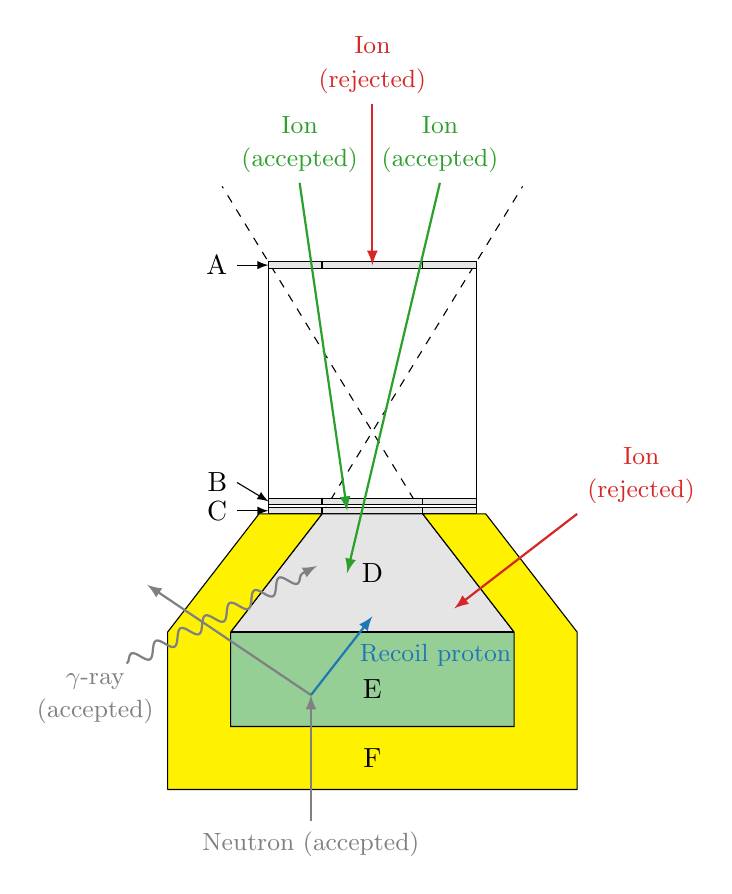
\begin{tikzpicture}[scale=0.8]
    \tikzset{%
        add/.style args={#1 and #2}{
            to path={%
                ($(\tikztostart)!-#1!(\tikztotarget)$)--($(\tikztotarget)!-#2!(\tikztostart)$)%
                \tikztonodes},add/.default={.2 and .2}}
    }  
    
    \def\bottomwidth{3.25}
    \def\midwidth{1.8}
    \def\topwidth{1.65}
    \def\bottomheight{2.5}
    \def\midheight{4.375}
    \def\Fthickness{1}
    \def\Sithickness{0.1}
    \def\BCdistance{0.15}
    \def\topheight{8.375}
    
    % FOV
    \draw[add=0 and 0.3, dashed] (\midwidth - \Fthickness, \midheight) to (-\topwidth, \topheight);
    \draw[add=0 and 0.3, dashed] (-\midwidth + \Fthickness, \midheight) to (\topwidth, \topheight);

    % A
    \draw[fill=light-gray] (-\topwidth, \topheight - \Sithickness) rectangle (\topwidth, \topheight);
    \draw (-\midwidth + \Fthickness, \topheight - \Sithickness) --  (-\midwidth + \Fthickness, \topheight);
    \draw (-\midwidth + \Fthickness, \topheight - \Sithickness) --  (-\midwidth + \Fthickness, \topheight);
    \draw (\midwidth - \Fthickness, \topheight - \Sithickness) --  (\midwidth - \Fthickness, \topheight);
    \draw (\midwidth - \Fthickness, \topheight - \Sithickness) --  (\midwidth - \Fthickness, \topheight);
    \draw[latex-] (-\topwidth, \topheight - \Sithickness / 2) -- (-\topwidth - 0.5, \topheight - \Sithickness / 2) node[left] {A};
    
    % B
    \draw[fill=light-gray] (-\topwidth, \midheight + \BCdistance) rectangle (\topwidth, \midheight + \BCdistance + \Sithickness);
    \draw (-\midwidth + \Fthickness, \midheight + \BCdistance) --  (-\midwidth + \Fthickness, \midheight + \BCdistance + \Sithickness);
    \draw (-\midwidth + \Fthickness, \midheight + \BCdistance) --  (-\midwidth + \Fthickness, \midheight + \BCdistance + \Sithickness);
    \draw (\midwidth - \Fthickness, \midheight + \BCdistance) --  (\midwidth - \Fthickness, \midheight + \BCdistance + \Sithickness);
    \draw (\midwidth - \Fthickness, \midheight + \BCdistance) --  (\midwidth - \Fthickness, \midheight + \BCdistance + \Sithickness);
    \draw[latex-] (-\topwidth, \midheight + \BCdistance + \Sithickness / 2) -- (-\topwidth - 0.5, \midheight + \BCdistance + \Sithickness / 2 + 0.3) node[left] {B};
    
    % C
    \draw[fill=light-gray] (-\topwidth, \midheight) rectangle (\topwidth, \midheight + \Sithickness);
    \draw (-\midwidth + \Fthickness, \midheight) --  (-\midwidth + \Fthickness, \midheight + \Sithickness);
    \draw (-\midwidth + \Fthickness, \midheight) --  (-\midwidth + \Fthickness, \midheight + \Sithickness);
    \draw (\midwidth - \Fthickness, \midheight) --  (\midwidth - \Fthickness, \midheight + \Sithickness);
    \draw (\midwidth - \Fthickness, \midheight) --  (\midwidth - \Fthickness, \midheight + \Sithickness);
    \draw[latex-] (-\topwidth, \midheight + \Sithickness / 2) -- (-\topwidth - 0.5, \midheight + \Sithickness / 2) node[left] {C};
    
    % border of ABC
    \draw (-\topwidth, \midheight) -- (-\topwidth, \topheight);
    \draw (\topwidth, \midheight) -- (\topwidth, \topheight);
    
    % D
    \draw[fill=light-gray] (\bottomwidth - \Fthickness, \bottomheight) --  (-\bottomwidth + \Fthickness, \bottomheight) -- (-\midwidth + \Fthickness, \midheight) -- (\midwidth - \Fthickness, \midheight) -- (\bottomwidth - \Fthickness, \bottomheight);   
    \node at (0, {\bottomheight + (\midheight - \bottomheight) / 2}) {D};   
    
    % E
    \draw[fill=green!50] (\bottomwidth - \Fthickness, \bottomheight) -- (\bottomwidth - \Fthickness, \Fthickness) --
    (-\bottomwidth + \Fthickness, \Fthickness) --  (-\bottomwidth + \Fthickness, \bottomheight) -- (\bottomwidth - \Fthickness, \bottomheight);  
    \node at (0, {\Fthickness + (\bottomheight - \Fthickness) * 0.4}) {E};   
    
    % F
    \draw[fill=yellow] (-\bottomwidth, 0) -- (\bottomwidth, 0) -- (\bottomwidth, \bottomheight) -- (\midwidth, \midheight) --
    (\midwidth - \Fthickness, \midheight) -- (\bottomwidth - \Fthickness, \bottomheight) -- (\bottomwidth - \Fthickness, \Fthickness) --
    (-\bottomwidth + \Fthickness, \Fthickness) --  (-\bottomwidth + \Fthickness, \bottomheight) -- (-\midwidth + \Fthickness, \midheight) --
    (-\midwidth, \midheight) -- (-\bottomwidth, \bottomheight) -- (-\bottomwidth, 0);     
    \node at (0, \Fthickness / 2) {F};
    
    % trajectories of ions
    \draw[thick, green, -latex] (-\topwidth*0.7, \topheight*1.15) node[above, align=center] {\small Ion\\ \small (accepted)}
     -- ({-(\midwidth - \Fthickness) * 0.5}, \midheight + \Sithickness / 2);
    \draw[thick, green, -latex] (\topwidth*0.65, \topheight*1.15) node[above, align=center] {\small Ion\\ \small (accepted)}
     -- ({-(\midwidth - \Fthickness) * 0.5}, {\bottomheight +  (\midheight - \bottomheight) / 2});
    \draw[thick, red, -latex] (0, \topheight*1.3) node[above, align=center] {\small Ion\\ \small (rejected)}
     -- (0, \topheight - \Sithickness / 2);
    \draw[thick, red, -latex] (\bottomwidth, \midheight) node[above right, align=center] {\small Ion\\ \small (rejected)}
    -- (\bottomwidth * 0.4, {\bottomheight + (\midheight - \bottomheight) * 0.2});
    
    % trajectory of neutron
    \draw[thick, gray, -latex] (-\bottomwidth*0.3, -0.5) node[below] {\small Neutron (accepted)}
    -- (-\bottomwidth*0.3, {\Fthickness + \bottomheight * 0.2});
    \draw[thick, gray, -latex]  (-\bottomwidth*0.3, {\Fthickness + \bottomheight * 0.2}) -- (-\bottomwidth * 1.1, \bottomheight * 1.3);
    \draw[thick, blue, -latex]  (-\bottomwidth*0.3, {\Fthickness + \bottomheight * 0.2}) -- (0, \bottomheight * 1.1) node[midway, right, xshift=1mm] {\small Recoil proton};
    
    % trajectory of gamma
    \draw[thick, gray, decorate, decoration=snake] (-\bottomwidth*1.2, \bottomheight * 0.8) node[below, align=center, xshift=-4mm] {\small $\gamma$-ray\\ \small (accepted)} -- (-\bottomwidth * 0.3, \bottomheight * 1.4);
    \draw[thick, gray, -latex] (-\bottomwidth * 0.3, \bottomheight * 1.4) -- ++ (\bottomwidth * 0.03, \bottomheight * 0.02);
    
\end{tikzpicture}
%\end{document}
        \end{column}
    \end{columns}
    \vskip-6mm
    \uncover<2->{\centering\summary Best statistics to observe FDs: \textbf{TID in E}}
\end{frame}

\begin{frame}{High Energy Telescope}
    \begin{columns}
        \begin{column}{0.45\textwidth}
            \vbox to .8\textheight{%
            \vfill
            \begin{vfilleditems}
                \item Part of Solar Orbiter's \textbf{EPD} suite 
                \item Operating since February 2020
                \item Nominal data products: \textbf{Charged particle spectra} above \SI{7}{\mega\electronvolt\per nuc} (ions) and \SI{600}{\kilo\electronvolt} (electrons)
            \end{vfilleditems}
            \vfill
            \uncover<2->{\summary Best statistics to observe FDs: \textbf{Single-detector counters}}
            \vfill
            }
        \end{column}
        \begin{column}{0.45\textwidth}
            \centering
            %\documentclass{standalone}
%\usepackage[dvipsnames]{xcolor}
%\usepackage{tikz}
%\usepackage{amsmath}
%\usepackage{siunitx}

%\usetikzlibrary{calc}
%\usetikzlibrary{decorations.pathmorphing}

%\definecolor{light-gray}{gray}{0.9}

%\begin{document}
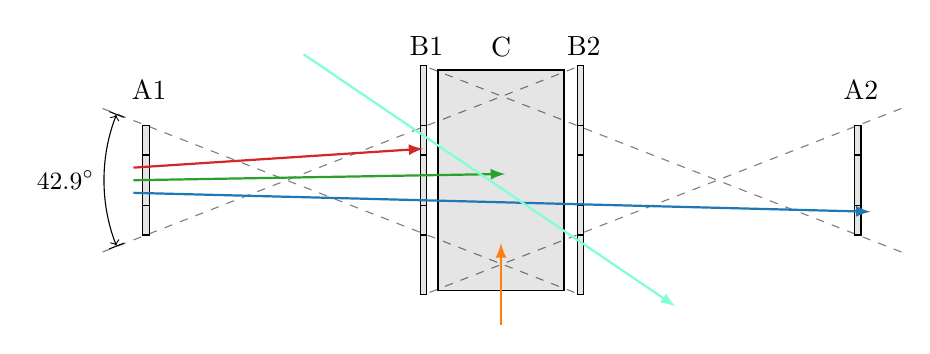
\begin{tikzpicture}[scale=0.8]
    \tikzset{%
        add/.style args={#1 and #2}{
            to path={%
                ($(\tikztostart)!-#1!(\tikztotarget)$)--($(\tikztotarget)!-#2!(\tikztostart)$)%
                \tikztonodes},add/.default={.2 and .2}}
    }   
    
    \def\Sithickness{0.05}
    
    % A1
    \draw[fill=light-gray] (-\Sithickness, -0.87) rectangle (\Sithickness, 0.87) node[above,yshift=2mm]{A1};
    \draw (-\Sithickness, -0.4) -- (\Sithickness, -0.4);
    \draw (-\Sithickness, 0.4) -- (\Sithickness, 0.4);
    
    % B1
    \draw[fill=light-gray] (4.4-\Sithickness, -1.82) rectangle (4.4+\Sithickness, 1.82) node[above]{B1};
    \draw (4.4-\Sithickness, -0.4) -- (4.4+\Sithickness, -0.4);
    \draw (4.4-\Sithickness, 0.4) -- (4.4+\Sithickness, 0.4);
    \draw (4.4-\Sithickness, -0.87) -- (4.4+\Sithickness, -0.87);
    \draw (4.4-\Sithickness, 0.87) -- (4.4+\Sithickness, 0.87);
    
    % C
    \draw[fill=light-gray] (4.635, -1.75) rectangle ++(2, 3.5);
    \node[above, yshift=0.5mm] at (5.635, 1.75) {C};
    
    % B2
    \draw[fill=light-gray] (6.9-\Sithickness, -1.82) rectangle (6.9+\Sithickness, 1.82) node[above]{B2};
    \draw (6.9-\Sithickness, -0.4) -- (6.9+\Sithickness, -0.4);
    \draw (6.9-\Sithickness, 0.4) -- (6.9+\Sithickness, 0.4);
    \draw (6.9-\Sithickness, -0.87) -- (6.9+\Sithickness, -0.87);
    \draw (6.9-\Sithickness, 0.87) -- (6.9+\Sithickness, 0.87);
    
    % A2
    \draw[fill=light-gray] (11.3-\Sithickness, -0.87) rectangle (11.3+\Sithickness, 0.87) node[above,yshift=2mm]{A2};
    \draw (11.3-\Sithickness, -0.4) -- (11.3+\Sithickness, -0.4);
    \draw (11.3-\Sithickness, 0.4) -- (11.3+\Sithickness, 0.4);
    
    % FOV
    \draw[add=0.1 and 0, dashed, opacity=0.5] (0, -0.87) to (6.9, 1.82);
    \draw[add=0.1 and 0, dashed, opacity=0.5] (0, 0.87) to (6.9, -1.82);
    \draw[add=0.1 and 0, dashed, opacity=0.5] (11.3, -0.87) to (4.4, 1.82);
    \draw[add=0.1 and 0, dashed, opacity=0.5] (11.3, 0.87) to (4.4, -1.82);
    
    \draw[|<->|] (0, 0.87) ++ (180-21.45:0.5) arc (180-21.45:180+21.45:2.4+0.48) node[midway, left] {\small\SI{42.9}{\degree}};
    

    \draw[thick, red, -latex] (-0.2, 0.2) -- (4.4, 0.5);
    \draw[thick, green, -latex] (-0.2, 0) -- (5.7, 0.1);
    \draw[thick, blue, -latex] (-0.2, -0.2) -- (11.5, -0.5);
    \draw[thick, Aquamarine, -latex] (2.5, 2) -- (8.4, -2);
    \draw[thick, orange, -latex] (5.635, -2.3) -- (5.635, -1);
\end{tikzpicture}
%\end{document}
            \footnotesize \textcolor{red}{stopping in B} \quad \textcolor{green}{stopping in C} \quad \textcolor{blue}{penetrating} \\ \uncover<2->{\textcolor{Aquamarine}{GCR channel} \quad \textcolor{orange}{C single counter}}\\
            \uncover<2->{%% Creator: Matplotlib, PGF backend
%%
%% To include the figure in your LaTeX document, write
%%   \input{<filename>.pgf}
%%
%% Make sure the required packages are loaded in your preamble
%%   \usepackage{pgf}
%%
%% and, on pdftex
%%   \usepackage[utf8]{inputenc}\DeclareUnicodeCharacter{2212}{-}
%%
%% or, on luatex and xetex
%%   \usepackage{unicode-math}
%%
%% Figures using additional raster images can only be included by \input if
%% they are in the same directory as the main LaTeX file. For loading figures
%% from other directories you can use the `import` package
%%   \usepackage{import}
%%
%% and then include the figures with
%%   \import{<path to file>}{<filename>.pgf}
%%
%% Matplotlib used the following preamble
%%   \usepackage{siunitx}
%%   \usepackage{fontspec}
%%
\begingroup%
\makeatletter%
\begin{pgfpicture}%
\pgfpathrectangle{\pgfpointorigin}{\pgfqpoint{2.400000in}{1.300000in}}%
\pgfusepath{use as bounding box, clip}%
\begin{pgfscope}%
\pgfsetbuttcap%
\pgfsetmiterjoin%
\definecolor{currentfill}{rgb}{1.000000,1.000000,1.000000}%
\pgfsetfillcolor{currentfill}%
\pgfsetlinewidth{0.000000pt}%
\definecolor{currentstroke}{rgb}{1.000000,1.000000,1.000000}%
\pgfsetstrokecolor{currentstroke}%
\pgfsetdash{}{0pt}%
\pgfpathmoveto{\pgfqpoint{0.000000in}{0.000000in}}%
\pgfpathlineto{\pgfqpoint{2.400000in}{0.000000in}}%
\pgfpathlineto{\pgfqpoint{2.400000in}{1.300000in}}%
\pgfpathlineto{\pgfqpoint{0.000000in}{1.300000in}}%
\pgfpathclose%
\pgfusepath{fill}%
\end{pgfscope}%
\begin{pgfscope}%
\pgfsetbuttcap%
\pgfsetmiterjoin%
\definecolor{currentfill}{rgb}{1.000000,1.000000,1.000000}%
\pgfsetfillcolor{currentfill}%
\pgfsetlinewidth{0.000000pt}%
\definecolor{currentstroke}{rgb}{0.000000,0.000000,0.000000}%
\pgfsetstrokecolor{currentstroke}%
\pgfsetstrokeopacity{0.000000}%
\pgfsetdash{}{0pt}%
\pgfpathmoveto{\pgfqpoint{0.535342in}{0.529520in}}%
\pgfpathlineto{\pgfqpoint{2.288685in}{0.529520in}}%
\pgfpathlineto{\pgfqpoint{2.288685in}{1.161368in}}%
\pgfpathlineto{\pgfqpoint{0.535342in}{1.161368in}}%
\pgfpathclose%
\pgfusepath{fill}%
\end{pgfscope}%
\begin{pgfscope}%
\pgfsetbuttcap%
\pgfsetroundjoin%
\definecolor{currentfill}{rgb}{0.000000,0.000000,0.000000}%
\pgfsetfillcolor{currentfill}%
\pgfsetlinewidth{0.803000pt}%
\definecolor{currentstroke}{rgb}{0.000000,0.000000,0.000000}%
\pgfsetstrokecolor{currentstroke}%
\pgfsetdash{}{0pt}%
\pgfsys@defobject{currentmarker}{\pgfqpoint{0.000000in}{-0.048611in}}{\pgfqpoint{0.000000in}{0.000000in}}{%
\pgfpathmoveto{\pgfqpoint{0.000000in}{0.000000in}}%
\pgfpathlineto{\pgfqpoint{0.000000in}{-0.048611in}}%
\pgfusepath{stroke,fill}%
}%
\begin{pgfscope}%
\pgfsys@transformshift{0.535342in}{0.529520in}%
\pgfsys@useobject{currentmarker}{}%
\end{pgfscope}%
\end{pgfscope}%
\begin{pgfscope}%
\pgfsetbuttcap%
\pgfsetroundjoin%
\definecolor{currentfill}{rgb}{0.000000,0.000000,0.000000}%
\pgfsetfillcolor{currentfill}%
\pgfsetlinewidth{0.803000pt}%
\definecolor{currentstroke}{rgb}{0.000000,0.000000,0.000000}%
\pgfsetstrokecolor{currentstroke}%
\pgfsetdash{}{0pt}%
\pgfsys@defobject{currentmarker}{\pgfqpoint{0.000000in}{-0.048611in}}{\pgfqpoint{0.000000in}{0.000000in}}{%
\pgfpathmoveto{\pgfqpoint{0.000000in}{0.000000in}}%
\pgfpathlineto{\pgfqpoint{0.000000in}{-0.048611in}}%
\pgfusepath{stroke,fill}%
}%
\begin{pgfscope}%
\pgfsys@transformshift{0.542329in}{0.529520in}%
\pgfsys@useobject{currentmarker}{}%
\end{pgfscope}%
\end{pgfscope}%
\begin{pgfscope}%
\definecolor{textcolor}{rgb}{0.000000,0.000000,0.000000}%
\pgfsetstrokecolor{textcolor}%
\pgfsetfillcolor{textcolor}%
\pgftext[x=0.542329in,y=0.432298in,,top]{\color{textcolor}\sffamily\fontsize{7.000000}{8.400000}\selectfont Mar}%
\end{pgfscope}%
\begin{pgfscope}%
\pgfsetbuttcap%
\pgfsetroundjoin%
\definecolor{currentfill}{rgb}{0.000000,0.000000,0.000000}%
\pgfsetfillcolor{currentfill}%
\pgfsetlinewidth{0.803000pt}%
\definecolor{currentstroke}{rgb}{0.000000,0.000000,0.000000}%
\pgfsetstrokecolor{currentstroke}%
\pgfsetdash{}{0pt}%
\pgfsys@defobject{currentmarker}{\pgfqpoint{0.000000in}{-0.048611in}}{\pgfqpoint{0.000000in}{0.000000in}}{%
\pgfpathmoveto{\pgfqpoint{0.000000in}{0.000000in}}%
\pgfpathlineto{\pgfqpoint{0.000000in}{-0.048611in}}%
\pgfusepath{stroke,fill}%
}%
\begin{pgfscope}%
\pgfsys@transformshift{0.710022in}{0.529520in}%
\pgfsys@useobject{currentmarker}{}%
\end{pgfscope}%
\end{pgfscope}%
\begin{pgfscope}%
\definecolor{textcolor}{rgb}{0.000000,0.000000,0.000000}%
\pgfsetstrokecolor{textcolor}%
\pgfsetfillcolor{textcolor}%
\pgftext[x=0.710022in,y=0.432298in,,top]{\color{textcolor}\sffamily\fontsize{7.000000}{8.400000}\selectfont Apr}%
\end{pgfscope}%
\begin{pgfscope}%
\pgfsetbuttcap%
\pgfsetroundjoin%
\definecolor{currentfill}{rgb}{0.000000,0.000000,0.000000}%
\pgfsetfillcolor{currentfill}%
\pgfsetlinewidth{0.803000pt}%
\definecolor{currentstroke}{rgb}{0.000000,0.000000,0.000000}%
\pgfsetstrokecolor{currentstroke}%
\pgfsetdash{}{0pt}%
\pgfsys@defobject{currentmarker}{\pgfqpoint{0.000000in}{-0.048611in}}{\pgfqpoint{0.000000in}{0.000000in}}{%
\pgfpathmoveto{\pgfqpoint{0.000000in}{0.000000in}}%
\pgfpathlineto{\pgfqpoint{0.000000in}{-0.048611in}}%
\pgfusepath{stroke,fill}%
}%
\begin{pgfscope}%
\pgfsys@transformshift{0.872306in}{0.529520in}%
\pgfsys@useobject{currentmarker}{}%
\end{pgfscope}%
\end{pgfscope}%
\begin{pgfscope}%
\definecolor{textcolor}{rgb}{0.000000,0.000000,0.000000}%
\pgfsetstrokecolor{textcolor}%
\pgfsetfillcolor{textcolor}%
\pgftext[x=0.872306in,y=0.432298in,,top]{\color{textcolor}\sffamily\fontsize{7.000000}{8.400000}\selectfont May}%
\end{pgfscope}%
\begin{pgfscope}%
\pgfsetbuttcap%
\pgfsetroundjoin%
\definecolor{currentfill}{rgb}{0.000000,0.000000,0.000000}%
\pgfsetfillcolor{currentfill}%
\pgfsetlinewidth{0.803000pt}%
\definecolor{currentstroke}{rgb}{0.000000,0.000000,0.000000}%
\pgfsetstrokecolor{currentstroke}%
\pgfsetdash{}{0pt}%
\pgfsys@defobject{currentmarker}{\pgfqpoint{0.000000in}{-0.048611in}}{\pgfqpoint{0.000000in}{0.000000in}}{%
\pgfpathmoveto{\pgfqpoint{0.000000in}{0.000000in}}%
\pgfpathlineto{\pgfqpoint{0.000000in}{-0.048611in}}%
\pgfusepath{stroke,fill}%
}%
\begin{pgfscope}%
\pgfsys@transformshift{1.040000in}{0.529520in}%
\pgfsys@useobject{currentmarker}{}%
\end{pgfscope}%
\end{pgfscope}%
\begin{pgfscope}%
\definecolor{textcolor}{rgb}{0.000000,0.000000,0.000000}%
\pgfsetstrokecolor{textcolor}%
\pgfsetfillcolor{textcolor}%
\pgftext[x=1.040000in,y=0.432298in,,top]{\color{textcolor}\sffamily\fontsize{7.000000}{8.400000}\selectfont Jun}%
\end{pgfscope}%
\begin{pgfscope}%
\pgfsetbuttcap%
\pgfsetroundjoin%
\definecolor{currentfill}{rgb}{0.000000,0.000000,0.000000}%
\pgfsetfillcolor{currentfill}%
\pgfsetlinewidth{0.803000pt}%
\definecolor{currentstroke}{rgb}{0.000000,0.000000,0.000000}%
\pgfsetstrokecolor{currentstroke}%
\pgfsetdash{}{0pt}%
\pgfsys@defobject{currentmarker}{\pgfqpoint{0.000000in}{-0.048611in}}{\pgfqpoint{0.000000in}{0.000000in}}{%
\pgfpathmoveto{\pgfqpoint{0.000000in}{0.000000in}}%
\pgfpathlineto{\pgfqpoint{0.000000in}{-0.048611in}}%
\pgfusepath{stroke,fill}%
}%
\begin{pgfscope}%
\pgfsys@transformshift{1.202284in}{0.529520in}%
\pgfsys@useobject{currentmarker}{}%
\end{pgfscope}%
\end{pgfscope}%
\begin{pgfscope}%
\definecolor{textcolor}{rgb}{0.000000,0.000000,0.000000}%
\pgfsetstrokecolor{textcolor}%
\pgfsetfillcolor{textcolor}%
\pgftext[x=1.202284in,y=0.432298in,,top]{\color{textcolor}\sffamily\fontsize{7.000000}{8.400000}\selectfont Jul}%
\end{pgfscope}%
\begin{pgfscope}%
\pgfsetbuttcap%
\pgfsetroundjoin%
\definecolor{currentfill}{rgb}{0.000000,0.000000,0.000000}%
\pgfsetfillcolor{currentfill}%
\pgfsetlinewidth{0.803000pt}%
\definecolor{currentstroke}{rgb}{0.000000,0.000000,0.000000}%
\pgfsetstrokecolor{currentstroke}%
\pgfsetdash{}{0pt}%
\pgfsys@defobject{currentmarker}{\pgfqpoint{0.000000in}{-0.048611in}}{\pgfqpoint{0.000000in}{0.000000in}}{%
\pgfpathmoveto{\pgfqpoint{0.000000in}{0.000000in}}%
\pgfpathlineto{\pgfqpoint{0.000000in}{-0.048611in}}%
\pgfusepath{stroke,fill}%
}%
\begin{pgfscope}%
\pgfsys@transformshift{1.369977in}{0.529520in}%
\pgfsys@useobject{currentmarker}{}%
\end{pgfscope}%
\end{pgfscope}%
\begin{pgfscope}%
\definecolor{textcolor}{rgb}{0.000000,0.000000,0.000000}%
\pgfsetstrokecolor{textcolor}%
\pgfsetfillcolor{textcolor}%
\pgftext[x=1.369977in,y=0.432298in,,top]{\color{textcolor}\sffamily\fontsize{7.000000}{8.400000}\selectfont Aug}%
\end{pgfscope}%
\begin{pgfscope}%
\pgfsetbuttcap%
\pgfsetroundjoin%
\definecolor{currentfill}{rgb}{0.000000,0.000000,0.000000}%
\pgfsetfillcolor{currentfill}%
\pgfsetlinewidth{0.803000pt}%
\definecolor{currentstroke}{rgb}{0.000000,0.000000,0.000000}%
\pgfsetstrokecolor{currentstroke}%
\pgfsetdash{}{0pt}%
\pgfsys@defobject{currentmarker}{\pgfqpoint{0.000000in}{-0.048611in}}{\pgfqpoint{0.000000in}{0.000000in}}{%
\pgfpathmoveto{\pgfqpoint{0.000000in}{0.000000in}}%
\pgfpathlineto{\pgfqpoint{0.000000in}{-0.048611in}}%
\pgfusepath{stroke,fill}%
}%
\begin{pgfscope}%
\pgfsys@transformshift{1.537670in}{0.529520in}%
\pgfsys@useobject{currentmarker}{}%
\end{pgfscope}%
\end{pgfscope}%
\begin{pgfscope}%
\definecolor{textcolor}{rgb}{0.000000,0.000000,0.000000}%
\pgfsetstrokecolor{textcolor}%
\pgfsetfillcolor{textcolor}%
\pgftext[x=1.537670in,y=0.432298in,,top]{\color{textcolor}\sffamily\fontsize{7.000000}{8.400000}\selectfont Sep}%
\end{pgfscope}%
\begin{pgfscope}%
\pgfsetbuttcap%
\pgfsetroundjoin%
\definecolor{currentfill}{rgb}{0.000000,0.000000,0.000000}%
\pgfsetfillcolor{currentfill}%
\pgfsetlinewidth{0.803000pt}%
\definecolor{currentstroke}{rgb}{0.000000,0.000000,0.000000}%
\pgfsetstrokecolor{currentstroke}%
\pgfsetdash{}{0pt}%
\pgfsys@defobject{currentmarker}{\pgfqpoint{0.000000in}{-0.048611in}}{\pgfqpoint{0.000000in}{0.000000in}}{%
\pgfpathmoveto{\pgfqpoint{0.000000in}{0.000000in}}%
\pgfpathlineto{\pgfqpoint{0.000000in}{-0.048611in}}%
\pgfusepath{stroke,fill}%
}%
\begin{pgfscope}%
\pgfsys@transformshift{1.699954in}{0.529520in}%
\pgfsys@useobject{currentmarker}{}%
\end{pgfscope}%
\end{pgfscope}%
\begin{pgfscope}%
\definecolor{textcolor}{rgb}{0.000000,0.000000,0.000000}%
\pgfsetstrokecolor{textcolor}%
\pgfsetfillcolor{textcolor}%
\pgftext[x=1.699954in,y=0.432298in,,top]{\color{textcolor}\sffamily\fontsize{7.000000}{8.400000}\selectfont Oct}%
\end{pgfscope}%
\begin{pgfscope}%
\pgfsetbuttcap%
\pgfsetroundjoin%
\definecolor{currentfill}{rgb}{0.000000,0.000000,0.000000}%
\pgfsetfillcolor{currentfill}%
\pgfsetlinewidth{0.803000pt}%
\definecolor{currentstroke}{rgb}{0.000000,0.000000,0.000000}%
\pgfsetstrokecolor{currentstroke}%
\pgfsetdash{}{0pt}%
\pgfsys@defobject{currentmarker}{\pgfqpoint{0.000000in}{-0.048611in}}{\pgfqpoint{0.000000in}{0.000000in}}{%
\pgfpathmoveto{\pgfqpoint{0.000000in}{0.000000in}}%
\pgfpathlineto{\pgfqpoint{0.000000in}{-0.048611in}}%
\pgfusepath{stroke,fill}%
}%
\begin{pgfscope}%
\pgfsys@transformshift{1.867648in}{0.529520in}%
\pgfsys@useobject{currentmarker}{}%
\end{pgfscope}%
\end{pgfscope}%
\begin{pgfscope}%
\definecolor{textcolor}{rgb}{0.000000,0.000000,0.000000}%
\pgfsetstrokecolor{textcolor}%
\pgfsetfillcolor{textcolor}%
\pgftext[x=1.867648in,y=0.432298in,,top]{\color{textcolor}\sffamily\fontsize{7.000000}{8.400000}\selectfont Nov}%
\end{pgfscope}%
\begin{pgfscope}%
\pgfsetbuttcap%
\pgfsetroundjoin%
\definecolor{currentfill}{rgb}{0.000000,0.000000,0.000000}%
\pgfsetfillcolor{currentfill}%
\pgfsetlinewidth{0.803000pt}%
\definecolor{currentstroke}{rgb}{0.000000,0.000000,0.000000}%
\pgfsetstrokecolor{currentstroke}%
\pgfsetdash{}{0pt}%
\pgfsys@defobject{currentmarker}{\pgfqpoint{0.000000in}{-0.048611in}}{\pgfqpoint{0.000000in}{0.000000in}}{%
\pgfpathmoveto{\pgfqpoint{0.000000in}{0.000000in}}%
\pgfpathlineto{\pgfqpoint{0.000000in}{-0.048611in}}%
\pgfusepath{stroke,fill}%
}%
\begin{pgfscope}%
\pgfsys@transformshift{2.029932in}{0.529520in}%
\pgfsys@useobject{currentmarker}{}%
\end{pgfscope}%
\end{pgfscope}%
\begin{pgfscope}%
\definecolor{textcolor}{rgb}{0.000000,0.000000,0.000000}%
\pgfsetstrokecolor{textcolor}%
\pgfsetfillcolor{textcolor}%
\pgftext[x=2.029932in,y=0.432298in,,top]{\color{textcolor}\sffamily\fontsize{7.000000}{8.400000}\selectfont Dec}%
\end{pgfscope}%
\begin{pgfscope}%
\pgfsetbuttcap%
\pgfsetroundjoin%
\definecolor{currentfill}{rgb}{0.000000,0.000000,0.000000}%
\pgfsetfillcolor{currentfill}%
\pgfsetlinewidth{0.803000pt}%
\definecolor{currentstroke}{rgb}{0.000000,0.000000,0.000000}%
\pgfsetstrokecolor{currentstroke}%
\pgfsetdash{}{0pt}%
\pgfsys@defobject{currentmarker}{\pgfqpoint{0.000000in}{-0.048611in}}{\pgfqpoint{0.000000in}{0.000000in}}{%
\pgfpathmoveto{\pgfqpoint{0.000000in}{0.000000in}}%
\pgfpathlineto{\pgfqpoint{0.000000in}{-0.048611in}}%
\pgfusepath{stroke,fill}%
}%
\begin{pgfscope}%
\pgfsys@transformshift{2.197625in}{0.529520in}%
\pgfsys@useobject{currentmarker}{}%
\end{pgfscope}%
\end{pgfscope}%
\begin{pgfscope}%
\definecolor{textcolor}{rgb}{0.000000,0.000000,0.000000}%
\pgfsetstrokecolor{textcolor}%
\pgfsetfillcolor{textcolor}%
\pgftext[x=2.121743in, y=0.364826in, left, base]{\color{textcolor}\sffamily\fontsize{7.000000}{8.400000}\selectfont Jan}%
\end{pgfscope}%
\begin{pgfscope}%
\definecolor{textcolor}{rgb}{0.000000,0.000000,0.000000}%
\pgfsetstrokecolor{textcolor}%
\pgfsetfillcolor{textcolor}%
\pgftext[x=2.094375in, y=0.264998in, left, base]{\color{textcolor}\sffamily\fontsize{7.000000}{8.400000}\selectfont 2021}%
\end{pgfscope}%
\begin{pgfscope}%
\pgfsetbuttcap%
\pgfsetroundjoin%
\definecolor{currentfill}{rgb}{0.000000,0.000000,0.000000}%
\pgfsetfillcolor{currentfill}%
\pgfsetlinewidth{0.803000pt}%
\definecolor{currentstroke}{rgb}{0.000000,0.000000,0.000000}%
\pgfsetstrokecolor{currentstroke}%
\pgfsetdash{}{0pt}%
\pgfsys@defobject{currentmarker}{\pgfqpoint{0.000000in}{-0.048611in}}{\pgfqpoint{0.000000in}{0.000000in}}{%
\pgfpathmoveto{\pgfqpoint{0.000000in}{0.000000in}}%
\pgfpathlineto{\pgfqpoint{0.000000in}{-0.048611in}}%
\pgfusepath{stroke,fill}%
}%
\begin{pgfscope}%
\pgfsys@transformshift{2.288685in}{0.529520in}%
\pgfsys@useobject{currentmarker}{}%
\end{pgfscope}%
\end{pgfscope}%
\begin{pgfscope}%
\pgfsetbuttcap%
\pgfsetroundjoin%
\definecolor{currentfill}{rgb}{0.000000,0.000000,0.000000}%
\pgfsetfillcolor{currentfill}%
\pgfsetlinewidth{0.602250pt}%
\definecolor{currentstroke}{rgb}{0.000000,0.000000,0.000000}%
\pgfsetstrokecolor{currentstroke}%
\pgfsetdash{}{0pt}%
\pgfsys@defobject{currentmarker}{\pgfqpoint{0.000000in}{-0.027778in}}{\pgfqpoint{0.000000in}{0.000000in}}{%
\pgfpathmoveto{\pgfqpoint{0.000000in}{0.000000in}}%
\pgfpathlineto{\pgfqpoint{0.000000in}{-0.027778in}}%
\pgfusepath{stroke,fill}%
}%
\begin{pgfscope}%
\pgfsys@transformshift{0.547738in}{0.529520in}%
\pgfsys@useobject{currentmarker}{}%
\end{pgfscope}%
\end{pgfscope}%
\begin{pgfscope}%
\pgfsetbuttcap%
\pgfsetroundjoin%
\definecolor{currentfill}{rgb}{0.000000,0.000000,0.000000}%
\pgfsetfillcolor{currentfill}%
\pgfsetlinewidth{0.602250pt}%
\definecolor{currentstroke}{rgb}{0.000000,0.000000,0.000000}%
\pgfsetstrokecolor{currentstroke}%
\pgfsetdash{}{0pt}%
\pgfsys@defobject{currentmarker}{\pgfqpoint{0.000000in}{-0.027778in}}{\pgfqpoint{0.000000in}{0.000000in}}{%
\pgfpathmoveto{\pgfqpoint{0.000000in}{0.000000in}}%
\pgfpathlineto{\pgfqpoint{0.000000in}{-0.027778in}}%
\pgfusepath{stroke,fill}%
}%
\begin{pgfscope}%
\pgfsys@transformshift{0.585605in}{0.529520in}%
\pgfsys@useobject{currentmarker}{}%
\end{pgfscope}%
\end{pgfscope}%
\begin{pgfscope}%
\pgfsetbuttcap%
\pgfsetroundjoin%
\definecolor{currentfill}{rgb}{0.000000,0.000000,0.000000}%
\pgfsetfillcolor{currentfill}%
\pgfsetlinewidth{0.602250pt}%
\definecolor{currentstroke}{rgb}{0.000000,0.000000,0.000000}%
\pgfsetstrokecolor{currentstroke}%
\pgfsetdash{}{0pt}%
\pgfsys@defobject{currentmarker}{\pgfqpoint{0.000000in}{-0.027778in}}{\pgfqpoint{0.000000in}{0.000000in}}{%
\pgfpathmoveto{\pgfqpoint{0.000000in}{0.000000in}}%
\pgfpathlineto{\pgfqpoint{0.000000in}{-0.027778in}}%
\pgfusepath{stroke,fill}%
}%
\begin{pgfscope}%
\pgfsys@transformshift{0.623471in}{0.529520in}%
\pgfsys@useobject{currentmarker}{}%
\end{pgfscope}%
\end{pgfscope}%
\begin{pgfscope}%
\pgfsetbuttcap%
\pgfsetroundjoin%
\definecolor{currentfill}{rgb}{0.000000,0.000000,0.000000}%
\pgfsetfillcolor{currentfill}%
\pgfsetlinewidth{0.602250pt}%
\definecolor{currentstroke}{rgb}{0.000000,0.000000,0.000000}%
\pgfsetstrokecolor{currentstroke}%
\pgfsetdash{}{0pt}%
\pgfsys@defobject{currentmarker}{\pgfqpoint{0.000000in}{-0.027778in}}{\pgfqpoint{0.000000in}{0.000000in}}{%
\pgfpathmoveto{\pgfqpoint{0.000000in}{0.000000in}}%
\pgfpathlineto{\pgfqpoint{0.000000in}{-0.027778in}}%
\pgfusepath{stroke,fill}%
}%
\begin{pgfscope}%
\pgfsys@transformshift{0.661337in}{0.529520in}%
\pgfsys@useobject{currentmarker}{}%
\end{pgfscope}%
\end{pgfscope}%
\begin{pgfscope}%
\pgfsetbuttcap%
\pgfsetroundjoin%
\definecolor{currentfill}{rgb}{0.000000,0.000000,0.000000}%
\pgfsetfillcolor{currentfill}%
\pgfsetlinewidth{0.602250pt}%
\definecolor{currentstroke}{rgb}{0.000000,0.000000,0.000000}%
\pgfsetstrokecolor{currentstroke}%
\pgfsetdash{}{0pt}%
\pgfsys@defobject{currentmarker}{\pgfqpoint{0.000000in}{-0.027778in}}{\pgfqpoint{0.000000in}{0.000000in}}{%
\pgfpathmoveto{\pgfqpoint{0.000000in}{0.000000in}}%
\pgfpathlineto{\pgfqpoint{0.000000in}{-0.027778in}}%
\pgfusepath{stroke,fill}%
}%
\begin{pgfscope}%
\pgfsys@transformshift{0.699203in}{0.529520in}%
\pgfsys@useobject{currentmarker}{}%
\end{pgfscope}%
\end{pgfscope}%
\begin{pgfscope}%
\pgfsetbuttcap%
\pgfsetroundjoin%
\definecolor{currentfill}{rgb}{0.000000,0.000000,0.000000}%
\pgfsetfillcolor{currentfill}%
\pgfsetlinewidth{0.602250pt}%
\definecolor{currentstroke}{rgb}{0.000000,0.000000,0.000000}%
\pgfsetstrokecolor{currentstroke}%
\pgfsetdash{}{0pt}%
\pgfsys@defobject{currentmarker}{\pgfqpoint{0.000000in}{-0.027778in}}{\pgfqpoint{0.000000in}{0.000000in}}{%
\pgfpathmoveto{\pgfqpoint{0.000000in}{0.000000in}}%
\pgfpathlineto{\pgfqpoint{0.000000in}{-0.027778in}}%
\pgfusepath{stroke,fill}%
}%
\begin{pgfscope}%
\pgfsys@transformshift{0.737070in}{0.529520in}%
\pgfsys@useobject{currentmarker}{}%
\end{pgfscope}%
\end{pgfscope}%
\begin{pgfscope}%
\pgfsetbuttcap%
\pgfsetroundjoin%
\definecolor{currentfill}{rgb}{0.000000,0.000000,0.000000}%
\pgfsetfillcolor{currentfill}%
\pgfsetlinewidth{0.602250pt}%
\definecolor{currentstroke}{rgb}{0.000000,0.000000,0.000000}%
\pgfsetstrokecolor{currentstroke}%
\pgfsetdash{}{0pt}%
\pgfsys@defobject{currentmarker}{\pgfqpoint{0.000000in}{-0.027778in}}{\pgfqpoint{0.000000in}{0.000000in}}{%
\pgfpathmoveto{\pgfqpoint{0.000000in}{0.000000in}}%
\pgfpathlineto{\pgfqpoint{0.000000in}{-0.027778in}}%
\pgfusepath{stroke,fill}%
}%
\begin{pgfscope}%
\pgfsys@transformshift{0.774936in}{0.529520in}%
\pgfsys@useobject{currentmarker}{}%
\end{pgfscope}%
\end{pgfscope}%
\begin{pgfscope}%
\pgfsetbuttcap%
\pgfsetroundjoin%
\definecolor{currentfill}{rgb}{0.000000,0.000000,0.000000}%
\pgfsetfillcolor{currentfill}%
\pgfsetlinewidth{0.602250pt}%
\definecolor{currentstroke}{rgb}{0.000000,0.000000,0.000000}%
\pgfsetstrokecolor{currentstroke}%
\pgfsetdash{}{0pt}%
\pgfsys@defobject{currentmarker}{\pgfqpoint{0.000000in}{-0.027778in}}{\pgfqpoint{0.000000in}{0.000000in}}{%
\pgfpathmoveto{\pgfqpoint{0.000000in}{0.000000in}}%
\pgfpathlineto{\pgfqpoint{0.000000in}{-0.027778in}}%
\pgfusepath{stroke,fill}%
}%
\begin{pgfscope}%
\pgfsys@transformshift{0.812802in}{0.529520in}%
\pgfsys@useobject{currentmarker}{}%
\end{pgfscope}%
\end{pgfscope}%
\begin{pgfscope}%
\pgfsetbuttcap%
\pgfsetroundjoin%
\definecolor{currentfill}{rgb}{0.000000,0.000000,0.000000}%
\pgfsetfillcolor{currentfill}%
\pgfsetlinewidth{0.602250pt}%
\definecolor{currentstroke}{rgb}{0.000000,0.000000,0.000000}%
\pgfsetstrokecolor{currentstroke}%
\pgfsetdash{}{0pt}%
\pgfsys@defobject{currentmarker}{\pgfqpoint{0.000000in}{-0.027778in}}{\pgfqpoint{0.000000in}{0.000000in}}{%
\pgfpathmoveto{\pgfqpoint{0.000000in}{0.000000in}}%
\pgfpathlineto{\pgfqpoint{0.000000in}{-0.027778in}}%
\pgfusepath{stroke,fill}%
}%
\begin{pgfscope}%
\pgfsys@transformshift{0.850668in}{0.529520in}%
\pgfsys@useobject{currentmarker}{}%
\end{pgfscope}%
\end{pgfscope}%
\begin{pgfscope}%
\pgfsetbuttcap%
\pgfsetroundjoin%
\definecolor{currentfill}{rgb}{0.000000,0.000000,0.000000}%
\pgfsetfillcolor{currentfill}%
\pgfsetlinewidth{0.602250pt}%
\definecolor{currentstroke}{rgb}{0.000000,0.000000,0.000000}%
\pgfsetstrokecolor{currentstroke}%
\pgfsetdash{}{0pt}%
\pgfsys@defobject{currentmarker}{\pgfqpoint{0.000000in}{-0.027778in}}{\pgfqpoint{0.000000in}{0.000000in}}{%
\pgfpathmoveto{\pgfqpoint{0.000000in}{0.000000in}}%
\pgfpathlineto{\pgfqpoint{0.000000in}{-0.027778in}}%
\pgfusepath{stroke,fill}%
}%
\begin{pgfscope}%
\pgfsys@transformshift{0.888535in}{0.529520in}%
\pgfsys@useobject{currentmarker}{}%
\end{pgfscope}%
\end{pgfscope}%
\begin{pgfscope}%
\pgfsetbuttcap%
\pgfsetroundjoin%
\definecolor{currentfill}{rgb}{0.000000,0.000000,0.000000}%
\pgfsetfillcolor{currentfill}%
\pgfsetlinewidth{0.602250pt}%
\definecolor{currentstroke}{rgb}{0.000000,0.000000,0.000000}%
\pgfsetstrokecolor{currentstroke}%
\pgfsetdash{}{0pt}%
\pgfsys@defobject{currentmarker}{\pgfqpoint{0.000000in}{-0.027778in}}{\pgfqpoint{0.000000in}{0.000000in}}{%
\pgfpathmoveto{\pgfqpoint{0.000000in}{0.000000in}}%
\pgfpathlineto{\pgfqpoint{0.000000in}{-0.027778in}}%
\pgfusepath{stroke,fill}%
}%
\begin{pgfscope}%
\pgfsys@transformshift{0.926401in}{0.529520in}%
\pgfsys@useobject{currentmarker}{}%
\end{pgfscope}%
\end{pgfscope}%
\begin{pgfscope}%
\pgfsetbuttcap%
\pgfsetroundjoin%
\definecolor{currentfill}{rgb}{0.000000,0.000000,0.000000}%
\pgfsetfillcolor{currentfill}%
\pgfsetlinewidth{0.602250pt}%
\definecolor{currentstroke}{rgb}{0.000000,0.000000,0.000000}%
\pgfsetstrokecolor{currentstroke}%
\pgfsetdash{}{0pt}%
\pgfsys@defobject{currentmarker}{\pgfqpoint{0.000000in}{-0.027778in}}{\pgfqpoint{0.000000in}{0.000000in}}{%
\pgfpathmoveto{\pgfqpoint{0.000000in}{0.000000in}}%
\pgfpathlineto{\pgfqpoint{0.000000in}{-0.027778in}}%
\pgfusepath{stroke,fill}%
}%
\begin{pgfscope}%
\pgfsys@transformshift{0.964267in}{0.529520in}%
\pgfsys@useobject{currentmarker}{}%
\end{pgfscope}%
\end{pgfscope}%
\begin{pgfscope}%
\pgfsetbuttcap%
\pgfsetroundjoin%
\definecolor{currentfill}{rgb}{0.000000,0.000000,0.000000}%
\pgfsetfillcolor{currentfill}%
\pgfsetlinewidth{0.602250pt}%
\definecolor{currentstroke}{rgb}{0.000000,0.000000,0.000000}%
\pgfsetstrokecolor{currentstroke}%
\pgfsetdash{}{0pt}%
\pgfsys@defobject{currentmarker}{\pgfqpoint{0.000000in}{-0.027778in}}{\pgfqpoint{0.000000in}{0.000000in}}{%
\pgfpathmoveto{\pgfqpoint{0.000000in}{0.000000in}}%
\pgfpathlineto{\pgfqpoint{0.000000in}{-0.027778in}}%
\pgfusepath{stroke,fill}%
}%
\begin{pgfscope}%
\pgfsys@transformshift{1.002133in}{0.529520in}%
\pgfsys@useobject{currentmarker}{}%
\end{pgfscope}%
\end{pgfscope}%
\begin{pgfscope}%
\pgfsetbuttcap%
\pgfsetroundjoin%
\definecolor{currentfill}{rgb}{0.000000,0.000000,0.000000}%
\pgfsetfillcolor{currentfill}%
\pgfsetlinewidth{0.602250pt}%
\definecolor{currentstroke}{rgb}{0.000000,0.000000,0.000000}%
\pgfsetstrokecolor{currentstroke}%
\pgfsetdash{}{0pt}%
\pgfsys@defobject{currentmarker}{\pgfqpoint{0.000000in}{-0.027778in}}{\pgfqpoint{0.000000in}{0.000000in}}{%
\pgfpathmoveto{\pgfqpoint{0.000000in}{0.000000in}}%
\pgfpathlineto{\pgfqpoint{0.000000in}{-0.027778in}}%
\pgfusepath{stroke,fill}%
}%
\begin{pgfscope}%
\pgfsys@transformshift{1.077866in}{0.529520in}%
\pgfsys@useobject{currentmarker}{}%
\end{pgfscope}%
\end{pgfscope}%
\begin{pgfscope}%
\pgfsetbuttcap%
\pgfsetroundjoin%
\definecolor{currentfill}{rgb}{0.000000,0.000000,0.000000}%
\pgfsetfillcolor{currentfill}%
\pgfsetlinewidth{0.602250pt}%
\definecolor{currentstroke}{rgb}{0.000000,0.000000,0.000000}%
\pgfsetstrokecolor{currentstroke}%
\pgfsetdash{}{0pt}%
\pgfsys@defobject{currentmarker}{\pgfqpoint{0.000000in}{-0.027778in}}{\pgfqpoint{0.000000in}{0.000000in}}{%
\pgfpathmoveto{\pgfqpoint{0.000000in}{0.000000in}}%
\pgfpathlineto{\pgfqpoint{0.000000in}{-0.027778in}}%
\pgfusepath{stroke,fill}%
}%
\begin{pgfscope}%
\pgfsys@transformshift{1.115732in}{0.529520in}%
\pgfsys@useobject{currentmarker}{}%
\end{pgfscope}%
\end{pgfscope}%
\begin{pgfscope}%
\pgfsetbuttcap%
\pgfsetroundjoin%
\definecolor{currentfill}{rgb}{0.000000,0.000000,0.000000}%
\pgfsetfillcolor{currentfill}%
\pgfsetlinewidth{0.602250pt}%
\definecolor{currentstroke}{rgb}{0.000000,0.000000,0.000000}%
\pgfsetstrokecolor{currentstroke}%
\pgfsetdash{}{0pt}%
\pgfsys@defobject{currentmarker}{\pgfqpoint{0.000000in}{-0.027778in}}{\pgfqpoint{0.000000in}{0.000000in}}{%
\pgfpathmoveto{\pgfqpoint{0.000000in}{0.000000in}}%
\pgfpathlineto{\pgfqpoint{0.000000in}{-0.027778in}}%
\pgfusepath{stroke,fill}%
}%
\begin{pgfscope}%
\pgfsys@transformshift{1.153598in}{0.529520in}%
\pgfsys@useobject{currentmarker}{}%
\end{pgfscope}%
\end{pgfscope}%
\begin{pgfscope}%
\pgfsetbuttcap%
\pgfsetroundjoin%
\definecolor{currentfill}{rgb}{0.000000,0.000000,0.000000}%
\pgfsetfillcolor{currentfill}%
\pgfsetlinewidth{0.602250pt}%
\definecolor{currentstroke}{rgb}{0.000000,0.000000,0.000000}%
\pgfsetstrokecolor{currentstroke}%
\pgfsetdash{}{0pt}%
\pgfsys@defobject{currentmarker}{\pgfqpoint{0.000000in}{-0.027778in}}{\pgfqpoint{0.000000in}{0.000000in}}{%
\pgfpathmoveto{\pgfqpoint{0.000000in}{0.000000in}}%
\pgfpathlineto{\pgfqpoint{0.000000in}{-0.027778in}}%
\pgfusepath{stroke,fill}%
}%
\begin{pgfscope}%
\pgfsys@transformshift{1.191465in}{0.529520in}%
\pgfsys@useobject{currentmarker}{}%
\end{pgfscope}%
\end{pgfscope}%
\begin{pgfscope}%
\pgfsetbuttcap%
\pgfsetroundjoin%
\definecolor{currentfill}{rgb}{0.000000,0.000000,0.000000}%
\pgfsetfillcolor{currentfill}%
\pgfsetlinewidth{0.602250pt}%
\definecolor{currentstroke}{rgb}{0.000000,0.000000,0.000000}%
\pgfsetstrokecolor{currentstroke}%
\pgfsetdash{}{0pt}%
\pgfsys@defobject{currentmarker}{\pgfqpoint{0.000000in}{-0.027778in}}{\pgfqpoint{0.000000in}{0.000000in}}{%
\pgfpathmoveto{\pgfqpoint{0.000000in}{0.000000in}}%
\pgfpathlineto{\pgfqpoint{0.000000in}{-0.027778in}}%
\pgfusepath{stroke,fill}%
}%
\begin{pgfscope}%
\pgfsys@transformshift{1.229331in}{0.529520in}%
\pgfsys@useobject{currentmarker}{}%
\end{pgfscope}%
\end{pgfscope}%
\begin{pgfscope}%
\pgfsetbuttcap%
\pgfsetroundjoin%
\definecolor{currentfill}{rgb}{0.000000,0.000000,0.000000}%
\pgfsetfillcolor{currentfill}%
\pgfsetlinewidth{0.602250pt}%
\definecolor{currentstroke}{rgb}{0.000000,0.000000,0.000000}%
\pgfsetstrokecolor{currentstroke}%
\pgfsetdash{}{0pt}%
\pgfsys@defobject{currentmarker}{\pgfqpoint{0.000000in}{-0.027778in}}{\pgfqpoint{0.000000in}{0.000000in}}{%
\pgfpathmoveto{\pgfqpoint{0.000000in}{0.000000in}}%
\pgfpathlineto{\pgfqpoint{0.000000in}{-0.027778in}}%
\pgfusepath{stroke,fill}%
}%
\begin{pgfscope}%
\pgfsys@transformshift{1.267197in}{0.529520in}%
\pgfsys@useobject{currentmarker}{}%
\end{pgfscope}%
\end{pgfscope}%
\begin{pgfscope}%
\pgfsetbuttcap%
\pgfsetroundjoin%
\definecolor{currentfill}{rgb}{0.000000,0.000000,0.000000}%
\pgfsetfillcolor{currentfill}%
\pgfsetlinewidth{0.602250pt}%
\definecolor{currentstroke}{rgb}{0.000000,0.000000,0.000000}%
\pgfsetstrokecolor{currentstroke}%
\pgfsetdash{}{0pt}%
\pgfsys@defobject{currentmarker}{\pgfqpoint{0.000000in}{-0.027778in}}{\pgfqpoint{0.000000in}{0.000000in}}{%
\pgfpathmoveto{\pgfqpoint{0.000000in}{0.000000in}}%
\pgfpathlineto{\pgfqpoint{0.000000in}{-0.027778in}}%
\pgfusepath{stroke,fill}%
}%
\begin{pgfscope}%
\pgfsys@transformshift{1.305063in}{0.529520in}%
\pgfsys@useobject{currentmarker}{}%
\end{pgfscope}%
\end{pgfscope}%
\begin{pgfscope}%
\pgfsetbuttcap%
\pgfsetroundjoin%
\definecolor{currentfill}{rgb}{0.000000,0.000000,0.000000}%
\pgfsetfillcolor{currentfill}%
\pgfsetlinewidth{0.602250pt}%
\definecolor{currentstroke}{rgb}{0.000000,0.000000,0.000000}%
\pgfsetstrokecolor{currentstroke}%
\pgfsetdash{}{0pt}%
\pgfsys@defobject{currentmarker}{\pgfqpoint{0.000000in}{-0.027778in}}{\pgfqpoint{0.000000in}{0.000000in}}{%
\pgfpathmoveto{\pgfqpoint{0.000000in}{0.000000in}}%
\pgfpathlineto{\pgfqpoint{0.000000in}{-0.027778in}}%
\pgfusepath{stroke,fill}%
}%
\begin{pgfscope}%
\pgfsys@transformshift{1.342930in}{0.529520in}%
\pgfsys@useobject{currentmarker}{}%
\end{pgfscope}%
\end{pgfscope}%
\begin{pgfscope}%
\pgfsetbuttcap%
\pgfsetroundjoin%
\definecolor{currentfill}{rgb}{0.000000,0.000000,0.000000}%
\pgfsetfillcolor{currentfill}%
\pgfsetlinewidth{0.602250pt}%
\definecolor{currentstroke}{rgb}{0.000000,0.000000,0.000000}%
\pgfsetstrokecolor{currentstroke}%
\pgfsetdash{}{0pt}%
\pgfsys@defobject{currentmarker}{\pgfqpoint{0.000000in}{-0.027778in}}{\pgfqpoint{0.000000in}{0.000000in}}{%
\pgfpathmoveto{\pgfqpoint{0.000000in}{0.000000in}}%
\pgfpathlineto{\pgfqpoint{0.000000in}{-0.027778in}}%
\pgfusepath{stroke,fill}%
}%
\begin{pgfscope}%
\pgfsys@transformshift{1.380796in}{0.529520in}%
\pgfsys@useobject{currentmarker}{}%
\end{pgfscope}%
\end{pgfscope}%
\begin{pgfscope}%
\pgfsetbuttcap%
\pgfsetroundjoin%
\definecolor{currentfill}{rgb}{0.000000,0.000000,0.000000}%
\pgfsetfillcolor{currentfill}%
\pgfsetlinewidth{0.602250pt}%
\definecolor{currentstroke}{rgb}{0.000000,0.000000,0.000000}%
\pgfsetstrokecolor{currentstroke}%
\pgfsetdash{}{0pt}%
\pgfsys@defobject{currentmarker}{\pgfqpoint{0.000000in}{-0.027778in}}{\pgfqpoint{0.000000in}{0.000000in}}{%
\pgfpathmoveto{\pgfqpoint{0.000000in}{0.000000in}}%
\pgfpathlineto{\pgfqpoint{0.000000in}{-0.027778in}}%
\pgfusepath{stroke,fill}%
}%
\begin{pgfscope}%
\pgfsys@transformshift{1.418662in}{0.529520in}%
\pgfsys@useobject{currentmarker}{}%
\end{pgfscope}%
\end{pgfscope}%
\begin{pgfscope}%
\pgfsetbuttcap%
\pgfsetroundjoin%
\definecolor{currentfill}{rgb}{0.000000,0.000000,0.000000}%
\pgfsetfillcolor{currentfill}%
\pgfsetlinewidth{0.602250pt}%
\definecolor{currentstroke}{rgb}{0.000000,0.000000,0.000000}%
\pgfsetstrokecolor{currentstroke}%
\pgfsetdash{}{0pt}%
\pgfsys@defobject{currentmarker}{\pgfqpoint{0.000000in}{-0.027778in}}{\pgfqpoint{0.000000in}{0.000000in}}{%
\pgfpathmoveto{\pgfqpoint{0.000000in}{0.000000in}}%
\pgfpathlineto{\pgfqpoint{0.000000in}{-0.027778in}}%
\pgfusepath{stroke,fill}%
}%
\begin{pgfscope}%
\pgfsys@transformshift{1.456528in}{0.529520in}%
\pgfsys@useobject{currentmarker}{}%
\end{pgfscope}%
\end{pgfscope}%
\begin{pgfscope}%
\pgfsetbuttcap%
\pgfsetroundjoin%
\definecolor{currentfill}{rgb}{0.000000,0.000000,0.000000}%
\pgfsetfillcolor{currentfill}%
\pgfsetlinewidth{0.602250pt}%
\definecolor{currentstroke}{rgb}{0.000000,0.000000,0.000000}%
\pgfsetstrokecolor{currentstroke}%
\pgfsetdash{}{0pt}%
\pgfsys@defobject{currentmarker}{\pgfqpoint{0.000000in}{-0.027778in}}{\pgfqpoint{0.000000in}{0.000000in}}{%
\pgfpathmoveto{\pgfqpoint{0.000000in}{0.000000in}}%
\pgfpathlineto{\pgfqpoint{0.000000in}{-0.027778in}}%
\pgfusepath{stroke,fill}%
}%
\begin{pgfscope}%
\pgfsys@transformshift{1.494395in}{0.529520in}%
\pgfsys@useobject{currentmarker}{}%
\end{pgfscope}%
\end{pgfscope}%
\begin{pgfscope}%
\pgfsetbuttcap%
\pgfsetroundjoin%
\definecolor{currentfill}{rgb}{0.000000,0.000000,0.000000}%
\pgfsetfillcolor{currentfill}%
\pgfsetlinewidth{0.602250pt}%
\definecolor{currentstroke}{rgb}{0.000000,0.000000,0.000000}%
\pgfsetstrokecolor{currentstroke}%
\pgfsetdash{}{0pt}%
\pgfsys@defobject{currentmarker}{\pgfqpoint{0.000000in}{-0.027778in}}{\pgfqpoint{0.000000in}{0.000000in}}{%
\pgfpathmoveto{\pgfqpoint{0.000000in}{0.000000in}}%
\pgfpathlineto{\pgfqpoint{0.000000in}{-0.027778in}}%
\pgfusepath{stroke,fill}%
}%
\begin{pgfscope}%
\pgfsys@transformshift{1.532261in}{0.529520in}%
\pgfsys@useobject{currentmarker}{}%
\end{pgfscope}%
\end{pgfscope}%
\begin{pgfscope}%
\pgfsetbuttcap%
\pgfsetroundjoin%
\definecolor{currentfill}{rgb}{0.000000,0.000000,0.000000}%
\pgfsetfillcolor{currentfill}%
\pgfsetlinewidth{0.602250pt}%
\definecolor{currentstroke}{rgb}{0.000000,0.000000,0.000000}%
\pgfsetstrokecolor{currentstroke}%
\pgfsetdash{}{0pt}%
\pgfsys@defobject{currentmarker}{\pgfqpoint{0.000000in}{-0.027778in}}{\pgfqpoint{0.000000in}{0.000000in}}{%
\pgfpathmoveto{\pgfqpoint{0.000000in}{0.000000in}}%
\pgfpathlineto{\pgfqpoint{0.000000in}{-0.027778in}}%
\pgfusepath{stroke,fill}%
}%
\begin{pgfscope}%
\pgfsys@transformshift{1.570127in}{0.529520in}%
\pgfsys@useobject{currentmarker}{}%
\end{pgfscope}%
\end{pgfscope}%
\begin{pgfscope}%
\pgfsetbuttcap%
\pgfsetroundjoin%
\definecolor{currentfill}{rgb}{0.000000,0.000000,0.000000}%
\pgfsetfillcolor{currentfill}%
\pgfsetlinewidth{0.602250pt}%
\definecolor{currentstroke}{rgb}{0.000000,0.000000,0.000000}%
\pgfsetstrokecolor{currentstroke}%
\pgfsetdash{}{0pt}%
\pgfsys@defobject{currentmarker}{\pgfqpoint{0.000000in}{-0.027778in}}{\pgfqpoint{0.000000in}{0.000000in}}{%
\pgfpathmoveto{\pgfqpoint{0.000000in}{0.000000in}}%
\pgfpathlineto{\pgfqpoint{0.000000in}{-0.027778in}}%
\pgfusepath{stroke,fill}%
}%
\begin{pgfscope}%
\pgfsys@transformshift{1.607994in}{0.529520in}%
\pgfsys@useobject{currentmarker}{}%
\end{pgfscope}%
\end{pgfscope}%
\begin{pgfscope}%
\pgfsetbuttcap%
\pgfsetroundjoin%
\definecolor{currentfill}{rgb}{0.000000,0.000000,0.000000}%
\pgfsetfillcolor{currentfill}%
\pgfsetlinewidth{0.602250pt}%
\definecolor{currentstroke}{rgb}{0.000000,0.000000,0.000000}%
\pgfsetstrokecolor{currentstroke}%
\pgfsetdash{}{0pt}%
\pgfsys@defobject{currentmarker}{\pgfqpoint{0.000000in}{-0.027778in}}{\pgfqpoint{0.000000in}{0.000000in}}{%
\pgfpathmoveto{\pgfqpoint{0.000000in}{0.000000in}}%
\pgfpathlineto{\pgfqpoint{0.000000in}{-0.027778in}}%
\pgfusepath{stroke,fill}%
}%
\begin{pgfscope}%
\pgfsys@transformshift{1.645860in}{0.529520in}%
\pgfsys@useobject{currentmarker}{}%
\end{pgfscope}%
\end{pgfscope}%
\begin{pgfscope}%
\pgfsetbuttcap%
\pgfsetroundjoin%
\definecolor{currentfill}{rgb}{0.000000,0.000000,0.000000}%
\pgfsetfillcolor{currentfill}%
\pgfsetlinewidth{0.602250pt}%
\definecolor{currentstroke}{rgb}{0.000000,0.000000,0.000000}%
\pgfsetstrokecolor{currentstroke}%
\pgfsetdash{}{0pt}%
\pgfsys@defobject{currentmarker}{\pgfqpoint{0.000000in}{-0.027778in}}{\pgfqpoint{0.000000in}{0.000000in}}{%
\pgfpathmoveto{\pgfqpoint{0.000000in}{0.000000in}}%
\pgfpathlineto{\pgfqpoint{0.000000in}{-0.027778in}}%
\pgfusepath{stroke,fill}%
}%
\begin{pgfscope}%
\pgfsys@transformshift{1.683726in}{0.529520in}%
\pgfsys@useobject{currentmarker}{}%
\end{pgfscope}%
\end{pgfscope}%
\begin{pgfscope}%
\pgfsetbuttcap%
\pgfsetroundjoin%
\definecolor{currentfill}{rgb}{0.000000,0.000000,0.000000}%
\pgfsetfillcolor{currentfill}%
\pgfsetlinewidth{0.602250pt}%
\definecolor{currentstroke}{rgb}{0.000000,0.000000,0.000000}%
\pgfsetstrokecolor{currentstroke}%
\pgfsetdash{}{0pt}%
\pgfsys@defobject{currentmarker}{\pgfqpoint{0.000000in}{-0.027778in}}{\pgfqpoint{0.000000in}{0.000000in}}{%
\pgfpathmoveto{\pgfqpoint{0.000000in}{0.000000in}}%
\pgfpathlineto{\pgfqpoint{0.000000in}{-0.027778in}}%
\pgfusepath{stroke,fill}%
}%
\begin{pgfscope}%
\pgfsys@transformshift{1.721592in}{0.529520in}%
\pgfsys@useobject{currentmarker}{}%
\end{pgfscope}%
\end{pgfscope}%
\begin{pgfscope}%
\pgfsetbuttcap%
\pgfsetroundjoin%
\definecolor{currentfill}{rgb}{0.000000,0.000000,0.000000}%
\pgfsetfillcolor{currentfill}%
\pgfsetlinewidth{0.602250pt}%
\definecolor{currentstroke}{rgb}{0.000000,0.000000,0.000000}%
\pgfsetstrokecolor{currentstroke}%
\pgfsetdash{}{0pt}%
\pgfsys@defobject{currentmarker}{\pgfqpoint{0.000000in}{-0.027778in}}{\pgfqpoint{0.000000in}{0.000000in}}{%
\pgfpathmoveto{\pgfqpoint{0.000000in}{0.000000in}}%
\pgfpathlineto{\pgfqpoint{0.000000in}{-0.027778in}}%
\pgfusepath{stroke,fill}%
}%
\begin{pgfscope}%
\pgfsys@transformshift{1.759459in}{0.529520in}%
\pgfsys@useobject{currentmarker}{}%
\end{pgfscope}%
\end{pgfscope}%
\begin{pgfscope}%
\pgfsetbuttcap%
\pgfsetroundjoin%
\definecolor{currentfill}{rgb}{0.000000,0.000000,0.000000}%
\pgfsetfillcolor{currentfill}%
\pgfsetlinewidth{0.602250pt}%
\definecolor{currentstroke}{rgb}{0.000000,0.000000,0.000000}%
\pgfsetstrokecolor{currentstroke}%
\pgfsetdash{}{0pt}%
\pgfsys@defobject{currentmarker}{\pgfqpoint{0.000000in}{-0.027778in}}{\pgfqpoint{0.000000in}{0.000000in}}{%
\pgfpathmoveto{\pgfqpoint{0.000000in}{0.000000in}}%
\pgfpathlineto{\pgfqpoint{0.000000in}{-0.027778in}}%
\pgfusepath{stroke,fill}%
}%
\begin{pgfscope}%
\pgfsys@transformshift{1.797325in}{0.529520in}%
\pgfsys@useobject{currentmarker}{}%
\end{pgfscope}%
\end{pgfscope}%
\begin{pgfscope}%
\pgfsetbuttcap%
\pgfsetroundjoin%
\definecolor{currentfill}{rgb}{0.000000,0.000000,0.000000}%
\pgfsetfillcolor{currentfill}%
\pgfsetlinewidth{0.602250pt}%
\definecolor{currentstroke}{rgb}{0.000000,0.000000,0.000000}%
\pgfsetstrokecolor{currentstroke}%
\pgfsetdash{}{0pt}%
\pgfsys@defobject{currentmarker}{\pgfqpoint{0.000000in}{-0.027778in}}{\pgfqpoint{0.000000in}{0.000000in}}{%
\pgfpathmoveto{\pgfqpoint{0.000000in}{0.000000in}}%
\pgfpathlineto{\pgfqpoint{0.000000in}{-0.027778in}}%
\pgfusepath{stroke,fill}%
}%
\begin{pgfscope}%
\pgfsys@transformshift{1.835191in}{0.529520in}%
\pgfsys@useobject{currentmarker}{}%
\end{pgfscope}%
\end{pgfscope}%
\begin{pgfscope}%
\pgfsetbuttcap%
\pgfsetroundjoin%
\definecolor{currentfill}{rgb}{0.000000,0.000000,0.000000}%
\pgfsetfillcolor{currentfill}%
\pgfsetlinewidth{0.602250pt}%
\definecolor{currentstroke}{rgb}{0.000000,0.000000,0.000000}%
\pgfsetstrokecolor{currentstroke}%
\pgfsetdash{}{0pt}%
\pgfsys@defobject{currentmarker}{\pgfqpoint{0.000000in}{-0.027778in}}{\pgfqpoint{0.000000in}{0.000000in}}{%
\pgfpathmoveto{\pgfqpoint{0.000000in}{0.000000in}}%
\pgfpathlineto{\pgfqpoint{0.000000in}{-0.027778in}}%
\pgfusepath{stroke,fill}%
}%
\begin{pgfscope}%
\pgfsys@transformshift{1.873057in}{0.529520in}%
\pgfsys@useobject{currentmarker}{}%
\end{pgfscope}%
\end{pgfscope}%
\begin{pgfscope}%
\pgfsetbuttcap%
\pgfsetroundjoin%
\definecolor{currentfill}{rgb}{0.000000,0.000000,0.000000}%
\pgfsetfillcolor{currentfill}%
\pgfsetlinewidth{0.602250pt}%
\definecolor{currentstroke}{rgb}{0.000000,0.000000,0.000000}%
\pgfsetstrokecolor{currentstroke}%
\pgfsetdash{}{0pt}%
\pgfsys@defobject{currentmarker}{\pgfqpoint{0.000000in}{-0.027778in}}{\pgfqpoint{0.000000in}{0.000000in}}{%
\pgfpathmoveto{\pgfqpoint{0.000000in}{0.000000in}}%
\pgfpathlineto{\pgfqpoint{0.000000in}{-0.027778in}}%
\pgfusepath{stroke,fill}%
}%
\begin{pgfscope}%
\pgfsys@transformshift{1.910924in}{0.529520in}%
\pgfsys@useobject{currentmarker}{}%
\end{pgfscope}%
\end{pgfscope}%
\begin{pgfscope}%
\pgfsetbuttcap%
\pgfsetroundjoin%
\definecolor{currentfill}{rgb}{0.000000,0.000000,0.000000}%
\pgfsetfillcolor{currentfill}%
\pgfsetlinewidth{0.602250pt}%
\definecolor{currentstroke}{rgb}{0.000000,0.000000,0.000000}%
\pgfsetstrokecolor{currentstroke}%
\pgfsetdash{}{0pt}%
\pgfsys@defobject{currentmarker}{\pgfqpoint{0.000000in}{-0.027778in}}{\pgfqpoint{0.000000in}{0.000000in}}{%
\pgfpathmoveto{\pgfqpoint{0.000000in}{0.000000in}}%
\pgfpathlineto{\pgfqpoint{0.000000in}{-0.027778in}}%
\pgfusepath{stroke,fill}%
}%
\begin{pgfscope}%
\pgfsys@transformshift{1.948790in}{0.529520in}%
\pgfsys@useobject{currentmarker}{}%
\end{pgfscope}%
\end{pgfscope}%
\begin{pgfscope}%
\pgfsetbuttcap%
\pgfsetroundjoin%
\definecolor{currentfill}{rgb}{0.000000,0.000000,0.000000}%
\pgfsetfillcolor{currentfill}%
\pgfsetlinewidth{0.602250pt}%
\definecolor{currentstroke}{rgb}{0.000000,0.000000,0.000000}%
\pgfsetstrokecolor{currentstroke}%
\pgfsetdash{}{0pt}%
\pgfsys@defobject{currentmarker}{\pgfqpoint{0.000000in}{-0.027778in}}{\pgfqpoint{0.000000in}{0.000000in}}{%
\pgfpathmoveto{\pgfqpoint{0.000000in}{0.000000in}}%
\pgfpathlineto{\pgfqpoint{0.000000in}{-0.027778in}}%
\pgfusepath{stroke,fill}%
}%
\begin{pgfscope}%
\pgfsys@transformshift{1.986656in}{0.529520in}%
\pgfsys@useobject{currentmarker}{}%
\end{pgfscope}%
\end{pgfscope}%
\begin{pgfscope}%
\pgfsetbuttcap%
\pgfsetroundjoin%
\definecolor{currentfill}{rgb}{0.000000,0.000000,0.000000}%
\pgfsetfillcolor{currentfill}%
\pgfsetlinewidth{0.602250pt}%
\definecolor{currentstroke}{rgb}{0.000000,0.000000,0.000000}%
\pgfsetstrokecolor{currentstroke}%
\pgfsetdash{}{0pt}%
\pgfsys@defobject{currentmarker}{\pgfqpoint{0.000000in}{-0.027778in}}{\pgfqpoint{0.000000in}{0.000000in}}{%
\pgfpathmoveto{\pgfqpoint{0.000000in}{0.000000in}}%
\pgfpathlineto{\pgfqpoint{0.000000in}{-0.027778in}}%
\pgfusepath{stroke,fill}%
}%
\begin{pgfscope}%
\pgfsys@transformshift{2.024522in}{0.529520in}%
\pgfsys@useobject{currentmarker}{}%
\end{pgfscope}%
\end{pgfscope}%
\begin{pgfscope}%
\pgfsetbuttcap%
\pgfsetroundjoin%
\definecolor{currentfill}{rgb}{0.000000,0.000000,0.000000}%
\pgfsetfillcolor{currentfill}%
\pgfsetlinewidth{0.602250pt}%
\definecolor{currentstroke}{rgb}{0.000000,0.000000,0.000000}%
\pgfsetstrokecolor{currentstroke}%
\pgfsetdash{}{0pt}%
\pgfsys@defobject{currentmarker}{\pgfqpoint{0.000000in}{-0.027778in}}{\pgfqpoint{0.000000in}{0.000000in}}{%
\pgfpathmoveto{\pgfqpoint{0.000000in}{0.000000in}}%
\pgfpathlineto{\pgfqpoint{0.000000in}{-0.027778in}}%
\pgfusepath{stroke,fill}%
}%
\begin{pgfscope}%
\pgfsys@transformshift{2.062389in}{0.529520in}%
\pgfsys@useobject{currentmarker}{}%
\end{pgfscope}%
\end{pgfscope}%
\begin{pgfscope}%
\pgfsetbuttcap%
\pgfsetroundjoin%
\definecolor{currentfill}{rgb}{0.000000,0.000000,0.000000}%
\pgfsetfillcolor{currentfill}%
\pgfsetlinewidth{0.602250pt}%
\definecolor{currentstroke}{rgb}{0.000000,0.000000,0.000000}%
\pgfsetstrokecolor{currentstroke}%
\pgfsetdash{}{0pt}%
\pgfsys@defobject{currentmarker}{\pgfqpoint{0.000000in}{-0.027778in}}{\pgfqpoint{0.000000in}{0.000000in}}{%
\pgfpathmoveto{\pgfqpoint{0.000000in}{0.000000in}}%
\pgfpathlineto{\pgfqpoint{0.000000in}{-0.027778in}}%
\pgfusepath{stroke,fill}%
}%
\begin{pgfscope}%
\pgfsys@transformshift{2.100255in}{0.529520in}%
\pgfsys@useobject{currentmarker}{}%
\end{pgfscope}%
\end{pgfscope}%
\begin{pgfscope}%
\pgfsetbuttcap%
\pgfsetroundjoin%
\definecolor{currentfill}{rgb}{0.000000,0.000000,0.000000}%
\pgfsetfillcolor{currentfill}%
\pgfsetlinewidth{0.602250pt}%
\definecolor{currentstroke}{rgb}{0.000000,0.000000,0.000000}%
\pgfsetstrokecolor{currentstroke}%
\pgfsetdash{}{0pt}%
\pgfsys@defobject{currentmarker}{\pgfqpoint{0.000000in}{-0.027778in}}{\pgfqpoint{0.000000in}{0.000000in}}{%
\pgfpathmoveto{\pgfqpoint{0.000000in}{0.000000in}}%
\pgfpathlineto{\pgfqpoint{0.000000in}{-0.027778in}}%
\pgfusepath{stroke,fill}%
}%
\begin{pgfscope}%
\pgfsys@transformshift{2.138121in}{0.529520in}%
\pgfsys@useobject{currentmarker}{}%
\end{pgfscope}%
\end{pgfscope}%
\begin{pgfscope}%
\pgfsetbuttcap%
\pgfsetroundjoin%
\definecolor{currentfill}{rgb}{0.000000,0.000000,0.000000}%
\pgfsetfillcolor{currentfill}%
\pgfsetlinewidth{0.602250pt}%
\definecolor{currentstroke}{rgb}{0.000000,0.000000,0.000000}%
\pgfsetstrokecolor{currentstroke}%
\pgfsetdash{}{0pt}%
\pgfsys@defobject{currentmarker}{\pgfqpoint{0.000000in}{-0.027778in}}{\pgfqpoint{0.000000in}{0.000000in}}{%
\pgfpathmoveto{\pgfqpoint{0.000000in}{0.000000in}}%
\pgfpathlineto{\pgfqpoint{0.000000in}{-0.027778in}}%
\pgfusepath{stroke,fill}%
}%
\begin{pgfscope}%
\pgfsys@transformshift{2.175987in}{0.529520in}%
\pgfsys@useobject{currentmarker}{}%
\end{pgfscope}%
\end{pgfscope}%
\begin{pgfscope}%
\pgfsetbuttcap%
\pgfsetroundjoin%
\definecolor{currentfill}{rgb}{0.000000,0.000000,0.000000}%
\pgfsetfillcolor{currentfill}%
\pgfsetlinewidth{0.602250pt}%
\definecolor{currentstroke}{rgb}{0.000000,0.000000,0.000000}%
\pgfsetstrokecolor{currentstroke}%
\pgfsetdash{}{0pt}%
\pgfsys@defobject{currentmarker}{\pgfqpoint{0.000000in}{-0.027778in}}{\pgfqpoint{0.000000in}{0.000000in}}{%
\pgfpathmoveto{\pgfqpoint{0.000000in}{0.000000in}}%
\pgfpathlineto{\pgfqpoint{0.000000in}{-0.027778in}}%
\pgfusepath{stroke,fill}%
}%
\begin{pgfscope}%
\pgfsys@transformshift{2.213854in}{0.529520in}%
\pgfsys@useobject{currentmarker}{}%
\end{pgfscope}%
\end{pgfscope}%
\begin{pgfscope}%
\pgfsetbuttcap%
\pgfsetroundjoin%
\definecolor{currentfill}{rgb}{0.000000,0.000000,0.000000}%
\pgfsetfillcolor{currentfill}%
\pgfsetlinewidth{0.602250pt}%
\definecolor{currentstroke}{rgb}{0.000000,0.000000,0.000000}%
\pgfsetstrokecolor{currentstroke}%
\pgfsetdash{}{0pt}%
\pgfsys@defobject{currentmarker}{\pgfqpoint{0.000000in}{-0.027778in}}{\pgfqpoint{0.000000in}{0.000000in}}{%
\pgfpathmoveto{\pgfqpoint{0.000000in}{0.000000in}}%
\pgfpathlineto{\pgfqpoint{0.000000in}{-0.027778in}}%
\pgfusepath{stroke,fill}%
}%
\begin{pgfscope}%
\pgfsys@transformshift{2.251720in}{0.529520in}%
\pgfsys@useobject{currentmarker}{}%
\end{pgfscope}%
\end{pgfscope}%
\begin{pgfscope}%
\definecolor{textcolor}{rgb}{0.000000,0.000000,0.000000}%
\pgfsetstrokecolor{textcolor}%
\pgfsetfillcolor{textcolor}%
\pgftext[x=1.412013in,y=0.190581in,,top]{\color{textcolor}\sffamily\fontsize{7.000000}{8.400000}\selectfont date}%
\end{pgfscope}%
\begin{pgfscope}%
\pgfsetbuttcap%
\pgfsetroundjoin%
\definecolor{currentfill}{rgb}{0.000000,0.000000,0.000000}%
\pgfsetfillcolor{currentfill}%
\pgfsetlinewidth{0.803000pt}%
\definecolor{currentstroke}{rgb}{0.000000,0.000000,0.000000}%
\pgfsetstrokecolor{currentstroke}%
\pgfsetdash{}{0pt}%
\pgfsys@defobject{currentmarker}{\pgfqpoint{-0.048611in}{0.000000in}}{\pgfqpoint{-0.000000in}{0.000000in}}{%
\pgfpathmoveto{\pgfqpoint{-0.000000in}{0.000000in}}%
\pgfpathlineto{\pgfqpoint{-0.048611in}{0.000000in}}%
\pgfusepath{stroke,fill}%
}%
\begin{pgfscope}%
\pgfsys@transformshift{0.535342in}{0.687482in}%
\pgfsys@useobject{currentmarker}{}%
\end{pgfscope}%
\end{pgfscope}%
\begin{pgfscope}%
\definecolor{textcolor}{rgb}{0.000000,0.000000,0.000000}%
\pgfsetstrokecolor{textcolor}%
\pgfsetfillcolor{textcolor}%
\pgftext[x=0.272031in, y=0.653746in, left, base]{\color{textcolor}\sffamily\fontsize{7.000000}{8.400000}\selectfont \(\displaystyle {260}\)}%
\end{pgfscope}%
\begin{pgfscope}%
\pgfsetbuttcap%
\pgfsetroundjoin%
\definecolor{currentfill}{rgb}{0.000000,0.000000,0.000000}%
\pgfsetfillcolor{currentfill}%
\pgfsetlinewidth{0.803000pt}%
\definecolor{currentstroke}{rgb}{0.000000,0.000000,0.000000}%
\pgfsetstrokecolor{currentstroke}%
\pgfsetdash{}{0pt}%
\pgfsys@defobject{currentmarker}{\pgfqpoint{-0.048611in}{0.000000in}}{\pgfqpoint{-0.000000in}{0.000000in}}{%
\pgfpathmoveto{\pgfqpoint{-0.000000in}{0.000000in}}%
\pgfpathlineto{\pgfqpoint{-0.048611in}{0.000000in}}%
\pgfusepath{stroke,fill}%
}%
\begin{pgfscope}%
\pgfsys@transformshift{0.535342in}{1.003406in}%
\pgfsys@useobject{currentmarker}{}%
\end{pgfscope}%
\end{pgfscope}%
\begin{pgfscope}%
\definecolor{textcolor}{rgb}{0.000000,0.000000,0.000000}%
\pgfsetstrokecolor{textcolor}%
\pgfsetfillcolor{textcolor}%
\pgftext[x=0.272031in, y=0.969670in, left, base]{\color{textcolor}\sffamily\fontsize{7.000000}{8.400000}\selectfont \(\displaystyle {280}\)}%
\end{pgfscope}%
\begin{pgfscope}%
\definecolor{textcolor}{rgb}{0.000000,0.000000,0.000000}%
\pgfsetstrokecolor{textcolor}%
\pgfsetfillcolor{textcolor}%
\pgftext[x=0.216475in,y=0.845444in,,bottom,rotate=90.000000]{\color{textcolor}\sffamily\fontsize{7.000000}{8.400000}\selectfont count rate / \si{\per\second}}%
\end{pgfscope}%
\begin{pgfscope}%
\pgfpathrectangle{\pgfqpoint{0.535342in}{0.529520in}}{\pgfqpoint{1.753343in}{0.631848in}}%
\pgfusepath{clip}%
\pgfsetrectcap%
\pgfsetroundjoin%
\pgfsetlinewidth{0.602250pt}%
\definecolor{currentstroke}{rgb}{0.121569,0.466667,0.705882}%
\pgfsetstrokecolor{currentstroke}%
\pgfsetdash{}{0pt}%
\pgfpathmoveto{\pgfqpoint{0.535567in}{0.833602in}}%
\pgfpathlineto{\pgfqpoint{0.536919in}{0.778367in}}%
\pgfpathlineto{\pgfqpoint{0.537821in}{0.780645in}}%
\pgfpathlineto{\pgfqpoint{0.538046in}{0.792277in}}%
\pgfpathlineto{\pgfqpoint{0.538272in}{0.771773in}}%
\pgfpathlineto{\pgfqpoint{0.538723in}{0.772268in}}%
\pgfpathlineto{\pgfqpoint{0.538948in}{0.780794in}}%
\pgfpathlineto{\pgfqpoint{0.539624in}{0.772435in}}%
\pgfpathlineto{\pgfqpoint{0.540976in}{0.737635in}}%
\pgfpathlineto{\pgfqpoint{0.541202in}{0.746187in}}%
\pgfpathlineto{\pgfqpoint{0.541427in}{0.746736in}}%
\pgfpathlineto{\pgfqpoint{0.541653in}{0.734028in}}%
\pgfpathlineto{\pgfqpoint{0.542329in}{0.755274in}}%
\pgfpathlineto{\pgfqpoint{0.542554in}{0.763659in}}%
\pgfpathlineto{\pgfqpoint{0.542780in}{0.743489in}}%
\pgfpathlineto{\pgfqpoint{0.543005in}{0.734805in}}%
\pgfpathlineto{\pgfqpoint{0.543230in}{0.755884in}}%
\pgfpathlineto{\pgfqpoint{0.543456in}{0.755397in}}%
\pgfpathlineto{\pgfqpoint{0.544132in}{0.762159in}}%
\pgfpathlineto{\pgfqpoint{0.544357in}{0.749136in}}%
\pgfpathlineto{\pgfqpoint{0.545034in}{0.771527in}}%
\pgfpathlineto{\pgfqpoint{0.545710in}{0.796441in}}%
\pgfpathlineto{\pgfqpoint{0.545935in}{0.783317in}}%
\pgfpathlineto{\pgfqpoint{0.546161in}{0.766393in}}%
\pgfpathlineto{\pgfqpoint{0.546837in}{0.775098in}}%
\pgfpathlineto{\pgfqpoint{0.547062in}{0.785963in}}%
\pgfpathlineto{\pgfqpoint{0.547513in}{0.763063in}}%
\pgfpathlineto{\pgfqpoint{0.547738in}{0.758390in}}%
\pgfpathlineto{\pgfqpoint{0.547964in}{0.769144in}}%
\pgfpathlineto{\pgfqpoint{0.548189in}{0.781145in}}%
\pgfpathlineto{\pgfqpoint{0.548865in}{0.758666in}}%
\pgfpathlineto{\pgfqpoint{0.549091in}{0.745002in}}%
\pgfpathlineto{\pgfqpoint{0.549767in}{0.763159in}}%
\pgfpathlineto{\pgfqpoint{0.549992in}{0.770522in}}%
\pgfpathlineto{\pgfqpoint{0.550443in}{0.768394in}}%
\pgfpathlineto{\pgfqpoint{0.550668in}{0.734366in}}%
\pgfpathlineto{\pgfqpoint{0.551570in}{0.741992in}}%
\pgfpathlineto{\pgfqpoint{0.552246in}{0.728465in}}%
\pgfpathlineto{\pgfqpoint{0.552697in}{0.738741in}}%
\pgfpathlineto{\pgfqpoint{0.552922in}{0.720856in}}%
\pgfpathlineto{\pgfqpoint{0.553824in}{0.733655in}}%
\pgfpathlineto{\pgfqpoint{0.554500in}{0.768710in}}%
\pgfpathlineto{\pgfqpoint{0.555853in}{0.765537in}}%
\pgfpathlineto{\pgfqpoint{0.556979in}{0.703586in}}%
\pgfpathlineto{\pgfqpoint{0.557430in}{0.720461in}}%
\pgfpathlineto{\pgfqpoint{0.558557in}{0.749223in}}%
\pgfpathlineto{\pgfqpoint{0.559008in}{0.745037in}}%
\pgfpathlineto{\pgfqpoint{0.559684in}{0.753287in}}%
\pgfpathlineto{\pgfqpoint{0.559459in}{0.743840in}}%
\pgfpathlineto{\pgfqpoint{0.559910in}{0.746652in}}%
\pgfpathlineto{\pgfqpoint{0.560135in}{0.735432in}}%
\pgfpathlineto{\pgfqpoint{0.560360in}{0.738798in}}%
\pgfpathlineto{\pgfqpoint{0.561037in}{0.843426in}}%
\pgfpathlineto{\pgfqpoint{0.561713in}{0.840267in}}%
\pgfpathlineto{\pgfqpoint{0.564192in}{0.787362in}}%
\pgfpathlineto{\pgfqpoint{0.565094in}{0.785989in}}%
\pgfpathlineto{\pgfqpoint{0.565995in}{0.818604in}}%
\pgfpathlineto{\pgfqpoint{0.566671in}{0.804668in}}%
\pgfpathlineto{\pgfqpoint{0.567122in}{0.817209in}}%
\pgfpathlineto{\pgfqpoint{0.567348in}{0.816827in}}%
\pgfpathlineto{\pgfqpoint{0.567573in}{0.810113in}}%
\pgfpathlineto{\pgfqpoint{0.567798in}{0.818621in}}%
\pgfpathlineto{\pgfqpoint{0.568249in}{0.813207in}}%
\pgfpathlineto{\pgfqpoint{0.568925in}{0.812584in}}%
\pgfpathlineto{\pgfqpoint{0.570278in}{0.870837in}}%
\pgfpathlineto{\pgfqpoint{0.572081in}{0.831377in}}%
\pgfpathlineto{\pgfqpoint{0.570954in}{0.879792in}}%
\pgfpathlineto{\pgfqpoint{0.572306in}{0.832404in}}%
\pgfpathlineto{\pgfqpoint{0.572532in}{0.844593in}}%
\pgfpathlineto{\pgfqpoint{0.573433in}{0.839148in}}%
\pgfpathlineto{\pgfqpoint{0.573884in}{0.826344in}}%
\pgfpathlineto{\pgfqpoint{0.574560in}{0.837371in}}%
\pgfpathlineto{\pgfqpoint{0.575687in}{0.858415in}}%
\pgfpathlineto{\pgfqpoint{0.576138in}{0.847691in}}%
\pgfpathlineto{\pgfqpoint{0.576589in}{0.863562in}}%
\pgfpathlineto{\pgfqpoint{0.576814in}{0.847331in}}%
\pgfpathlineto{\pgfqpoint{0.577490in}{0.855738in}}%
\pgfpathlineto{\pgfqpoint{0.578167in}{0.859446in}}%
\pgfpathlineto{\pgfqpoint{0.578843in}{0.849402in}}%
\pgfpathlineto{\pgfqpoint{0.579294in}{0.853496in}}%
\pgfpathlineto{\pgfqpoint{0.580195in}{0.832491in}}%
\pgfpathlineto{\pgfqpoint{0.581547in}{0.881600in}}%
\pgfpathlineto{\pgfqpoint{0.582449in}{0.889709in}}%
\pgfpathlineto{\pgfqpoint{0.582674in}{0.887116in}}%
\pgfpathlineto{\pgfqpoint{0.582900in}{0.875957in}}%
\pgfpathlineto{\pgfqpoint{0.583125in}{0.894009in}}%
\pgfpathlineto{\pgfqpoint{0.583801in}{0.880503in}}%
\pgfpathlineto{\pgfqpoint{0.584478in}{0.897831in}}%
\pgfpathlineto{\pgfqpoint{0.584928in}{0.882833in}}%
\pgfpathlineto{\pgfqpoint{0.586957in}{0.840205in}}%
\pgfpathlineto{\pgfqpoint{0.587182in}{0.859406in}}%
\pgfpathlineto{\pgfqpoint{0.587633in}{0.858919in}}%
\pgfpathlineto{\pgfqpoint{0.588985in}{0.900415in}}%
\pgfpathlineto{\pgfqpoint{0.589436in}{0.889121in}}%
\pgfpathlineto{\pgfqpoint{0.589887in}{0.905452in}}%
\pgfpathlineto{\pgfqpoint{0.592141in}{0.880117in}}%
\pgfpathlineto{\pgfqpoint{0.592817in}{0.894781in}}%
\pgfpathlineto{\pgfqpoint{0.593493in}{0.893259in}}%
\pgfpathlineto{\pgfqpoint{0.593719in}{0.878533in}}%
\pgfpathlineto{\pgfqpoint{0.594395in}{0.884751in}}%
\pgfpathlineto{\pgfqpoint{0.595747in}{0.902390in}}%
\pgfpathlineto{\pgfqpoint{0.596198in}{0.889476in}}%
\pgfpathlineto{\pgfqpoint{0.596424in}{0.902657in}}%
\pgfpathlineto{\pgfqpoint{0.597100in}{0.893158in}}%
\pgfpathlineto{\pgfqpoint{0.597550in}{0.906339in}}%
\pgfpathlineto{\pgfqpoint{0.598227in}{0.902907in}}%
\pgfpathlineto{\pgfqpoint{0.598677in}{0.903930in}}%
\pgfpathlineto{\pgfqpoint{0.598903in}{0.900885in}}%
\pgfpathlineto{\pgfqpoint{0.599354in}{0.905321in}}%
\pgfpathlineto{\pgfqpoint{0.600030in}{0.883079in}}%
\pgfpathlineto{\pgfqpoint{0.600255in}{0.905343in}}%
\pgfpathlineto{\pgfqpoint{0.600706in}{0.882899in}}%
\pgfpathlineto{\pgfqpoint{0.601157in}{0.889358in}}%
\pgfpathlineto{\pgfqpoint{0.602058in}{0.918765in}}%
\pgfpathlineto{\pgfqpoint{0.602509in}{0.907752in}}%
\pgfpathlineto{\pgfqpoint{0.603411in}{0.893645in}}%
\pgfpathlineto{\pgfqpoint{0.602960in}{0.911569in}}%
\pgfpathlineto{\pgfqpoint{0.603636in}{0.894645in}}%
\pgfpathlineto{\pgfqpoint{0.603862in}{0.902122in}}%
\pgfpathlineto{\pgfqpoint{0.604312in}{0.883921in}}%
\pgfpathlineto{\pgfqpoint{0.604538in}{0.892249in}}%
\pgfpathlineto{\pgfqpoint{0.604763in}{0.889849in}}%
\pgfpathlineto{\pgfqpoint{0.604988in}{0.897642in}}%
\pgfpathlineto{\pgfqpoint{0.605214in}{0.897357in}}%
\pgfpathlineto{\pgfqpoint{0.605439in}{0.894900in}}%
\pgfpathlineto{\pgfqpoint{0.606115in}{0.894667in}}%
\pgfpathlineto{\pgfqpoint{0.607017in}{0.922938in}}%
\pgfpathlineto{\pgfqpoint{0.607468in}{0.909156in}}%
\pgfpathlineto{\pgfqpoint{0.608144in}{0.909507in}}%
\pgfpathlineto{\pgfqpoint{0.608595in}{0.908528in}}%
\pgfpathlineto{\pgfqpoint{0.609271in}{0.926597in}}%
\pgfpathlineto{\pgfqpoint{0.609496in}{0.925794in}}%
\pgfpathlineto{\pgfqpoint{0.609722in}{0.916018in}}%
\pgfpathlineto{\pgfqpoint{0.610173in}{0.940024in}}%
\pgfpathlineto{\pgfqpoint{0.610398in}{0.930937in}}%
\pgfpathlineto{\pgfqpoint{0.611525in}{0.951525in}}%
\pgfpathlineto{\pgfqpoint{0.611750in}{0.939546in}}%
\pgfpathlineto{\pgfqpoint{0.612427in}{0.951762in}}%
\pgfpathlineto{\pgfqpoint{0.612652in}{0.951718in}}%
\pgfpathlineto{\pgfqpoint{0.612877in}{0.940652in}}%
\pgfpathlineto{\pgfqpoint{0.613328in}{0.961880in}}%
\pgfpathlineto{\pgfqpoint{0.613553in}{0.951077in}}%
\pgfpathlineto{\pgfqpoint{0.616709in}{0.983521in}}%
\pgfpathlineto{\pgfqpoint{0.614004in}{0.950151in}}%
\pgfpathlineto{\pgfqpoint{0.617385in}{0.982525in}}%
\pgfpathlineto{\pgfqpoint{0.618061in}{0.966636in}}%
\pgfpathlineto{\pgfqpoint{0.618287in}{0.993385in}}%
\pgfpathlineto{\pgfqpoint{0.619188in}{0.984350in}}%
\pgfpathlineto{\pgfqpoint{0.619639in}{0.997456in}}%
\pgfpathlineto{\pgfqpoint{0.620090in}{0.985021in}}%
\pgfpathlineto{\pgfqpoint{0.620315in}{0.984346in}}%
\pgfpathlineto{\pgfqpoint{0.620541in}{0.989414in}}%
\pgfpathlineto{\pgfqpoint{0.620766in}{0.964877in}}%
\pgfpathlineto{\pgfqpoint{0.621442in}{0.991752in}}%
\pgfpathlineto{\pgfqpoint{0.621668in}{0.985517in}}%
\pgfpathlineto{\pgfqpoint{0.621893in}{0.987097in}}%
\pgfpathlineto{\pgfqpoint{0.622569in}{0.943249in}}%
\pgfpathlineto{\pgfqpoint{0.623020in}{0.976439in}}%
\pgfpathlineto{\pgfqpoint{0.623245in}{0.976755in}}%
\pgfpathlineto{\pgfqpoint{0.623696in}{0.972591in}}%
\pgfpathlineto{\pgfqpoint{0.623922in}{0.982683in}}%
\pgfpathlineto{\pgfqpoint{0.624598in}{0.963964in}}%
\pgfpathlineto{\pgfqpoint{0.624823in}{0.956781in}}%
\pgfpathlineto{\pgfqpoint{0.625049in}{0.976066in}}%
\pgfpathlineto{\pgfqpoint{0.625499in}{0.964096in}}%
\pgfpathlineto{\pgfqpoint{0.625725in}{0.974003in}}%
\pgfpathlineto{\pgfqpoint{0.626401in}{0.966768in}}%
\pgfpathlineto{\pgfqpoint{0.627303in}{0.946259in}}%
\pgfpathlineto{\pgfqpoint{0.627979in}{0.954026in}}%
\pgfpathlineto{\pgfqpoint{0.628204in}{0.952095in}}%
\pgfpathlineto{\pgfqpoint{0.628430in}{0.953328in}}%
\pgfpathlineto{\pgfqpoint{0.628655in}{0.965123in}}%
\pgfpathlineto{\pgfqpoint{0.629106in}{0.953289in}}%
\pgfpathlineto{\pgfqpoint{0.629331in}{0.941898in}}%
\pgfpathlineto{\pgfqpoint{0.629556in}{0.964429in}}%
\pgfpathlineto{\pgfqpoint{0.630007in}{0.945605in}}%
\pgfpathlineto{\pgfqpoint{0.631134in}{0.969510in}}%
\pgfpathlineto{\pgfqpoint{0.631810in}{0.956873in}}%
\pgfpathlineto{\pgfqpoint{0.632261in}{0.959761in}}%
\pgfpathlineto{\pgfqpoint{0.632712in}{0.972893in}}%
\pgfpathlineto{\pgfqpoint{0.632937in}{0.958216in}}%
\pgfpathlineto{\pgfqpoint{0.633163in}{0.965561in}}%
\pgfpathlineto{\pgfqpoint{0.634741in}{0.928137in}}%
\pgfpathlineto{\pgfqpoint{0.635417in}{0.941323in}}%
\pgfpathlineto{\pgfqpoint{0.635868in}{0.931226in}}%
\pgfpathlineto{\pgfqpoint{0.636544in}{0.934149in}}%
\pgfpathlineto{\pgfqpoint{0.636769in}{0.916251in}}%
\pgfpathlineto{\pgfqpoint{0.636995in}{0.932236in}}%
\pgfpathlineto{\pgfqpoint{0.637671in}{0.917844in}}%
\pgfpathlineto{\pgfqpoint{0.638347in}{0.906971in}}%
\pgfpathlineto{\pgfqpoint{0.638798in}{0.911876in}}%
\pgfpathlineto{\pgfqpoint{0.639925in}{0.931297in}}%
\pgfpathlineto{\pgfqpoint{0.640150in}{0.918296in}}%
\pgfpathlineto{\pgfqpoint{0.641052in}{0.925579in}}%
\pgfpathlineto{\pgfqpoint{0.641277in}{0.934061in}}%
\pgfpathlineto{\pgfqpoint{0.641728in}{0.923473in}}%
\pgfpathlineto{\pgfqpoint{0.641953in}{0.924438in}}%
\pgfpathlineto{\pgfqpoint{0.642855in}{0.900595in}}%
\pgfpathlineto{\pgfqpoint{0.643080in}{0.913473in}}%
\pgfpathlineto{\pgfqpoint{0.643531in}{0.904373in}}%
\pgfpathlineto{\pgfqpoint{0.643982in}{0.907286in}}%
\pgfpathlineto{\pgfqpoint{0.644207in}{0.914899in}}%
\pgfpathlineto{\pgfqpoint{0.644433in}{0.906268in}}%
\pgfpathlineto{\pgfqpoint{0.644883in}{0.914206in}}%
\pgfpathlineto{\pgfqpoint{0.645559in}{0.899226in}}%
\pgfpathlineto{\pgfqpoint{0.646010in}{0.907054in}}%
\pgfpathlineto{\pgfqpoint{0.646236in}{0.904724in}}%
\pgfpathlineto{\pgfqpoint{0.646461in}{0.906940in}}%
\pgfpathlineto{\pgfqpoint{0.646686in}{0.912091in}}%
\pgfpathlineto{\pgfqpoint{0.647137in}{0.901867in}}%
\pgfpathlineto{\pgfqpoint{0.648039in}{0.877252in}}%
\pgfpathlineto{\pgfqpoint{0.648264in}{0.888309in}}%
\pgfpathlineto{\pgfqpoint{0.648490in}{0.889661in}}%
\pgfpathlineto{\pgfqpoint{0.648715in}{0.898362in}}%
\pgfpathlineto{\pgfqpoint{0.648940in}{0.865830in}}%
\pgfpathlineto{\pgfqpoint{0.649391in}{0.888344in}}%
\pgfpathlineto{\pgfqpoint{0.649617in}{0.886558in}}%
\pgfpathlineto{\pgfqpoint{0.650969in}{0.912811in}}%
\pgfpathlineto{\pgfqpoint{0.651194in}{0.908239in}}%
\pgfpathlineto{\pgfqpoint{0.651420in}{0.896097in}}%
\pgfpathlineto{\pgfqpoint{0.652321in}{0.900876in}}%
\pgfpathlineto{\pgfqpoint{0.652772in}{0.909077in}}%
\pgfpathlineto{\pgfqpoint{0.652998in}{0.907346in}}%
\pgfpathmoveto{\pgfqpoint{0.712952in}{0.893422in}}%
\pgfpathlineto{\pgfqpoint{0.713178in}{0.960256in}}%
\pgfpathlineto{\pgfqpoint{0.714079in}{0.937589in}}%
\pgfpathlineto{\pgfqpoint{0.715206in}{0.904597in}}%
\pgfpathlineto{\pgfqpoint{0.715657in}{0.909072in}}%
\pgfpathlineto{\pgfqpoint{0.715883in}{0.906984in}}%
\pgfpathlineto{\pgfqpoint{0.716108in}{0.916918in}}%
\pgfpathlineto{\pgfqpoint{0.717010in}{0.914671in}}%
\pgfpathlineto{\pgfqpoint{0.717460in}{0.915606in}}%
\pgfpathlineto{\pgfqpoint{0.720616in}{0.858489in}}%
\pgfpathlineto{\pgfqpoint{0.721067in}{0.874005in}}%
\pgfpathlineto{\pgfqpoint{0.721743in}{0.870911in}}%
\pgfpathlineto{\pgfqpoint{0.721968in}{0.861868in}}%
\pgfpathlineto{\pgfqpoint{0.722419in}{0.875176in}}%
\pgfpathlineto{\pgfqpoint{0.723095in}{0.887410in}}%
\pgfpathlineto{\pgfqpoint{0.723321in}{0.872408in}}%
\pgfpathlineto{\pgfqpoint{0.723546in}{0.881604in}}%
\pgfpathlineto{\pgfqpoint{0.724222in}{0.883017in}}%
\pgfpathlineto{\pgfqpoint{0.724448in}{0.874580in}}%
\pgfpathlineto{\pgfqpoint{0.724673in}{0.891161in}}%
\pgfpathlineto{\pgfqpoint{0.725124in}{0.865900in}}%
\pgfpathlineto{\pgfqpoint{0.725349in}{0.877103in}}%
\pgfpathlineto{\pgfqpoint{0.725574in}{0.874268in}}%
\pgfpathlineto{\pgfqpoint{0.725800in}{0.883737in}}%
\pgfpathlineto{\pgfqpoint{0.726025in}{0.889441in}}%
\pgfpathlineto{\pgfqpoint{0.726251in}{0.885404in}}%
\pgfpathlineto{\pgfqpoint{0.726476in}{0.871591in}}%
\pgfpathlineto{\pgfqpoint{0.727378in}{0.873693in}}%
\pgfpathlineto{\pgfqpoint{0.728054in}{0.897076in}}%
\pgfpathlineto{\pgfqpoint{0.728279in}{0.873360in}}%
\pgfpathlineto{\pgfqpoint{0.728730in}{0.850618in}}%
\pgfpathlineto{\pgfqpoint{0.729632in}{0.857291in}}%
\pgfpathlineto{\pgfqpoint{0.731209in}{0.890639in}}%
\pgfpathlineto{\pgfqpoint{0.732111in}{0.872285in}}%
\pgfpathlineto{\pgfqpoint{0.732336in}{0.886699in}}%
\pgfpathlineto{\pgfqpoint{0.732787in}{0.877379in}}%
\pgfpathlineto{\pgfqpoint{0.733689in}{0.901595in}}%
\pgfpathlineto{\pgfqpoint{0.734590in}{0.876809in}}%
\pgfpathlineto{\pgfqpoint{0.735266in}{0.877116in}}%
\pgfpathlineto{\pgfqpoint{0.736393in}{0.888485in}}%
\pgfpathlineto{\pgfqpoint{0.736844in}{0.876510in}}%
\pgfpathlineto{\pgfqpoint{0.737295in}{0.886922in}}%
\pgfpathlineto{\pgfqpoint{0.737746in}{0.880051in}}%
\pgfpathlineto{\pgfqpoint{0.738873in}{0.899695in}}%
\pgfpathlineto{\pgfqpoint{0.739549in}{0.886431in}}%
\pgfpathlineto{\pgfqpoint{0.740000in}{0.894755in}}%
\pgfpathlineto{\pgfqpoint{0.740225in}{0.889432in}}%
\pgfpathlineto{\pgfqpoint{0.740676in}{0.904724in}}%
\pgfpathlineto{\pgfqpoint{0.740901in}{0.906444in}}%
\pgfpathlineto{\pgfqpoint{0.741127in}{0.923192in}}%
\pgfpathlineto{\pgfqpoint{0.741803in}{0.904461in}}%
\pgfpathlineto{\pgfqpoint{0.743155in}{0.869222in}}%
\pgfpathlineto{\pgfqpoint{0.743831in}{0.895531in}}%
\pgfpathlineto{\pgfqpoint{0.744057in}{0.865448in}}%
\pgfpathlineto{\pgfqpoint{0.744282in}{0.874843in}}%
\pgfpathlineto{\pgfqpoint{0.745635in}{0.845585in}}%
\pgfpathlineto{\pgfqpoint{0.746536in}{0.843452in}}%
\pgfpathlineto{\pgfqpoint{0.746987in}{0.861135in}}%
\pgfpathlineto{\pgfqpoint{0.747438in}{0.842575in}}%
\pgfpathlineto{\pgfqpoint{0.748114in}{0.853439in}}%
\pgfpathlineto{\pgfqpoint{0.748565in}{0.861916in}}%
\pgfpathlineto{\pgfqpoint{0.749016in}{0.848761in}}%
\pgfpathlineto{\pgfqpoint{0.749241in}{0.840008in}}%
\pgfpathlineto{\pgfqpoint{0.749692in}{0.858985in}}%
\pgfpathlineto{\pgfqpoint{0.750142in}{0.850912in}}%
\pgfpathlineto{\pgfqpoint{0.750368in}{0.855879in}}%
\pgfpathlineto{\pgfqpoint{0.750593in}{0.842377in}}%
\pgfpathlineto{\pgfqpoint{0.751044in}{0.863333in}}%
\pgfpathlineto{\pgfqpoint{0.751269in}{0.869718in}}%
\pgfpathlineto{\pgfqpoint{0.751495in}{0.851631in}}%
\pgfpathlineto{\pgfqpoint{0.751720in}{0.862377in}}%
\pgfpathlineto{\pgfqpoint{0.751946in}{0.855348in}}%
\pgfpathlineto{\pgfqpoint{0.752171in}{0.871319in}}%
\pgfpathlineto{\pgfqpoint{0.752622in}{0.864843in}}%
\pgfpathlineto{\pgfqpoint{0.753523in}{0.897817in}}%
\pgfpathlineto{\pgfqpoint{0.754200in}{0.893829in}}%
\pgfpathlineto{\pgfqpoint{0.754425in}{0.901288in}}%
\pgfpathlineto{\pgfqpoint{0.754650in}{0.890551in}}%
\pgfpathlineto{\pgfqpoint{0.755101in}{0.897940in}}%
\pgfpathlineto{\pgfqpoint{0.755327in}{0.892530in}}%
\pgfpathlineto{\pgfqpoint{0.755552in}{0.905838in}}%
\pgfpathlineto{\pgfqpoint{0.756228in}{0.898563in}}%
\pgfpathlineto{\pgfqpoint{0.756904in}{0.931797in}}%
\pgfpathlineto{\pgfqpoint{0.757355in}{0.914623in}}%
\pgfpathlineto{\pgfqpoint{0.758257in}{0.919704in}}%
\pgfpathlineto{\pgfqpoint{0.759609in}{0.936264in}}%
\pgfpathlineto{\pgfqpoint{0.760060in}{0.934289in}}%
\pgfpathlineto{\pgfqpoint{0.760285in}{0.941419in}}%
\pgfpathlineto{\pgfqpoint{0.760961in}{0.932451in}}%
\pgfpathlineto{\pgfqpoint{0.761638in}{0.907243in}}%
\pgfpathlineto{\pgfqpoint{0.762539in}{0.911459in}}%
\pgfpathlineto{\pgfqpoint{0.762765in}{0.934548in}}%
\pgfpathlineto{\pgfqpoint{0.763441in}{0.909559in}}%
\pgfpathlineto{\pgfqpoint{0.763666in}{0.917519in}}%
\pgfpathlineto{\pgfqpoint{0.765019in}{0.887225in}}%
\pgfpathlineto{\pgfqpoint{0.765469in}{0.906067in}}%
\pgfpathlineto{\pgfqpoint{0.765920in}{0.896479in}}%
\pgfpathlineto{\pgfqpoint{0.767272in}{0.885347in}}%
\pgfpathlineto{\pgfqpoint{0.767498in}{0.886760in}}%
\pgfpathlineto{\pgfqpoint{0.768399in}{0.920209in}}%
\pgfpathlineto{\pgfqpoint{0.768850in}{0.903557in}}%
\pgfpathlineto{\pgfqpoint{0.770653in}{0.920665in}}%
\pgfpathlineto{\pgfqpoint{0.771104in}{0.921297in}}%
\pgfpathlineto{\pgfqpoint{0.772006in}{0.902969in}}%
\pgfpathlineto{\pgfqpoint{0.773358in}{0.929256in}}%
\pgfpathlineto{\pgfqpoint{0.773584in}{0.926970in}}%
\pgfpathlineto{\pgfqpoint{0.773809in}{0.911740in}}%
\pgfpathlineto{\pgfqpoint{0.774485in}{0.929493in}}%
\pgfpathlineto{\pgfqpoint{0.775161in}{0.921613in}}%
\pgfpathlineto{\pgfqpoint{0.776288in}{0.957786in}}%
\pgfpathlineto{\pgfqpoint{0.776739in}{0.952793in}}%
\pgfpathlineto{\pgfqpoint{0.776964in}{0.954368in}}%
\pgfpathlineto{\pgfqpoint{0.778317in}{1.008483in}}%
\pgfpathlineto{\pgfqpoint{0.779895in}{0.945246in}}%
\pgfpathlineto{\pgfqpoint{0.781247in}{0.976720in}}%
\pgfpathlineto{\pgfqpoint{0.781923in}{0.953679in}}%
\pgfpathlineto{\pgfqpoint{0.782148in}{0.981814in}}%
\pgfpathlineto{\pgfqpoint{0.782374in}{0.975579in}}%
\pgfpathlineto{\pgfqpoint{0.782599in}{0.977009in}}%
\pgfpathlineto{\pgfqpoint{0.783050in}{0.956246in}}%
\pgfpathlineto{\pgfqpoint{0.783726in}{0.968558in}}%
\pgfpathlineto{\pgfqpoint{0.783952in}{0.976781in}}%
\pgfpathlineto{\pgfqpoint{0.784402in}{0.962762in}}%
\pgfpathlineto{\pgfqpoint{0.784853in}{0.973100in}}%
\pgfpathlineto{\pgfqpoint{0.785755in}{0.974824in}}%
\pgfpathlineto{\pgfqpoint{0.785980in}{0.959366in}}%
\pgfpathlineto{\pgfqpoint{0.786431in}{0.976939in}}%
\pgfpathlineto{\pgfqpoint{0.787107in}{0.975425in}}%
\pgfpathlineto{\pgfqpoint{0.787333in}{0.962411in}}%
\pgfpathlineto{\pgfqpoint{0.787558in}{0.975781in}}%
\pgfpathlineto{\pgfqpoint{0.788009in}{0.970212in}}%
\pgfpathlineto{\pgfqpoint{0.789587in}{1.004244in}}%
\pgfpathlineto{\pgfqpoint{0.790488in}{0.985285in}}%
\pgfpathlineto{\pgfqpoint{0.790713in}{0.990511in}}%
\pgfpathlineto{\pgfqpoint{0.790939in}{0.999830in}}%
\pgfpathlineto{\pgfqpoint{0.791615in}{0.994468in}}%
\pgfpathlineto{\pgfqpoint{0.792967in}{0.965671in}}%
\pgfpathlineto{\pgfqpoint{0.793418in}{0.984174in}}%
\pgfpathlineto{\pgfqpoint{0.794320in}{0.975794in}}%
\pgfpathlineto{\pgfqpoint{0.796348in}{0.956588in}}%
\pgfpathlineto{\pgfqpoint{0.796574in}{0.960292in}}%
\pgfpathlineto{\pgfqpoint{0.796799in}{0.951634in}}%
\pgfpathlineto{\pgfqpoint{0.797250in}{0.957045in}}%
\pgfpathlineto{\pgfqpoint{0.798602in}{0.892982in}}%
\pgfpathlineto{\pgfqpoint{0.798828in}{0.898326in}}%
\pgfpathlineto{\pgfqpoint{0.799053in}{0.904184in}}%
\pgfpathlineto{\pgfqpoint{0.799278in}{0.872684in}}%
\pgfpathlineto{\pgfqpoint{0.800180in}{0.881806in}}%
\pgfpathlineto{\pgfqpoint{0.800631in}{0.868630in}}%
\pgfpathlineto{\pgfqpoint{0.800856in}{0.886014in}}%
\pgfpathlineto{\pgfqpoint{0.801082in}{0.879511in}}%
\pgfpathlineto{\pgfqpoint{0.803786in}{0.936584in}}%
\pgfpathlineto{\pgfqpoint{0.804463in}{0.932982in}}%
\pgfpathlineto{\pgfqpoint{0.804913in}{0.900937in}}%
\pgfpathlineto{\pgfqpoint{0.805590in}{0.918524in}}%
\pgfpathlineto{\pgfqpoint{0.805815in}{0.920876in}}%
\pgfpathlineto{\pgfqpoint{0.806040in}{0.911902in}}%
\pgfpathlineto{\pgfqpoint{0.806491in}{0.912433in}}%
\pgfpathlineto{\pgfqpoint{0.806942in}{0.894255in}}%
\pgfpathlineto{\pgfqpoint{0.808520in}{0.936536in}}%
\pgfpathlineto{\pgfqpoint{0.808970in}{0.919366in}}%
\pgfpathlineto{\pgfqpoint{0.809196in}{0.927646in}}%
\pgfpathlineto{\pgfqpoint{0.810774in}{0.794194in}}%
\pgfpathlineto{\pgfqpoint{0.812577in}{0.856651in}}%
\pgfpathlineto{\pgfqpoint{0.812802in}{0.847550in}}%
\pgfpathlineto{\pgfqpoint{0.813028in}{0.871942in}}%
\pgfpathlineto{\pgfqpoint{0.813478in}{0.852491in}}%
\pgfpathlineto{\pgfqpoint{0.813704in}{0.869520in}}%
\pgfpathlineto{\pgfqpoint{0.814154in}{0.846388in}}%
\pgfpathlineto{\pgfqpoint{0.814380in}{0.847647in}}%
\pgfpathlineto{\pgfqpoint{0.816183in}{0.791878in}}%
\pgfpathlineto{\pgfqpoint{0.817535in}{0.830368in}}%
\pgfpathlineto{\pgfqpoint{0.817986in}{0.805844in}}%
\pgfpathlineto{\pgfqpoint{0.818888in}{0.823817in}}%
\pgfpathlineto{\pgfqpoint{0.819564in}{0.837647in}}%
\pgfpathlineto{\pgfqpoint{0.820466in}{0.836081in}}%
\pgfpathlineto{\pgfqpoint{0.820691in}{0.831688in}}%
\pgfpathlineto{\pgfqpoint{0.820916in}{0.839306in}}%
\pgfpathlineto{\pgfqpoint{0.821142in}{0.854944in}}%
\pgfpathlineto{\pgfqpoint{0.822043in}{0.852917in}}%
\pgfpathlineto{\pgfqpoint{0.822494in}{0.861763in}}%
\pgfpathlineto{\pgfqpoint{0.822719in}{0.851916in}}%
\pgfpathlineto{\pgfqpoint{0.823396in}{0.856291in}}%
\pgfpathlineto{\pgfqpoint{0.823621in}{0.855229in}}%
\pgfpathlineto{\pgfqpoint{0.823846in}{0.846598in}}%
\pgfpathlineto{\pgfqpoint{0.824523in}{0.861609in}}%
\pgfpathlineto{\pgfqpoint{0.824748in}{0.863048in}}%
\pgfpathlineto{\pgfqpoint{0.824973in}{0.859003in}}%
\pgfpathlineto{\pgfqpoint{0.825199in}{0.855264in}}%
\pgfpathlineto{\pgfqpoint{0.825650in}{0.858674in}}%
\pgfpathlineto{\pgfqpoint{0.826551in}{0.883504in}}%
\pgfpathlineto{\pgfqpoint{0.826777in}{0.880165in}}%
\pgfpathlineto{\pgfqpoint{0.827227in}{0.870582in}}%
\pgfpathlineto{\pgfqpoint{0.828354in}{0.904092in}}%
\pgfpathlineto{\pgfqpoint{0.828580in}{0.896857in}}%
\pgfpathlineto{\pgfqpoint{0.828805in}{0.909761in}}%
\pgfpathlineto{\pgfqpoint{0.829031in}{0.908361in}}%
\pgfpathlineto{\pgfqpoint{0.829932in}{0.924145in}}%
\pgfpathlineto{\pgfqpoint{0.830383in}{0.919928in}}%
\pgfpathlineto{\pgfqpoint{0.831510in}{0.888524in}}%
\pgfpathlineto{\pgfqpoint{0.831735in}{0.891705in}}%
\pgfpathlineto{\pgfqpoint{0.831961in}{0.891613in}}%
\pgfpathlineto{\pgfqpoint{0.832186in}{0.886830in}}%
\pgfpathlineto{\pgfqpoint{0.832411in}{0.900099in}}%
\pgfpathlineto{\pgfqpoint{0.832637in}{0.898291in}}%
\pgfpathlineto{\pgfqpoint{0.832862in}{0.910683in}}%
\pgfpathlineto{\pgfqpoint{0.833313in}{0.895536in}}%
\pgfpathlineto{\pgfqpoint{0.833538in}{0.904290in}}%
\pgfpathlineto{\pgfqpoint{0.834215in}{0.892789in}}%
\pgfpathlineto{\pgfqpoint{0.834440in}{0.906532in}}%
\pgfpathlineto{\pgfqpoint{0.835792in}{0.946970in}}%
\pgfpathlineto{\pgfqpoint{0.836243in}{0.935755in}}%
\pgfpathlineto{\pgfqpoint{0.837596in}{0.901240in}}%
\pgfpathlineto{\pgfqpoint{0.837821in}{0.914526in}}%
\pgfpathlineto{\pgfqpoint{0.838046in}{0.926233in}}%
\pgfpathlineto{\pgfqpoint{0.838722in}{0.906918in}}%
\pgfpathlineto{\pgfqpoint{0.838948in}{0.919485in}}%
\pgfpathlineto{\pgfqpoint{0.839399in}{0.922354in}}%
\pgfpathlineto{\pgfqpoint{0.839624in}{0.914298in}}%
\pgfpathlineto{\pgfqpoint{0.840976in}{0.961125in}}%
\pgfpathlineto{\pgfqpoint{0.841202in}{0.938208in}}%
\pgfpathlineto{\pgfqpoint{0.841878in}{0.933355in}}%
\pgfpathlineto{\pgfqpoint{0.842103in}{0.942617in}}%
\pgfpathlineto{\pgfqpoint{0.842554in}{0.935724in}}%
\pgfpathlineto{\pgfqpoint{0.843230in}{0.937975in}}%
\pgfpathlineto{\pgfqpoint{0.843456in}{0.944311in}}%
\pgfpathlineto{\pgfqpoint{0.843681in}{0.936343in}}%
\pgfpathlineto{\pgfqpoint{0.843907in}{0.937979in}}%
\pgfpathlineto{\pgfqpoint{0.844357in}{0.925211in}}%
\pgfpathlineto{\pgfqpoint{0.844583in}{0.938760in}}%
\pgfpathlineto{\pgfqpoint{0.844808in}{0.936338in}}%
\pgfpathlineto{\pgfqpoint{0.845259in}{0.944153in}}%
\pgfpathlineto{\pgfqpoint{0.845710in}{0.939094in}}%
\pgfpathlineto{\pgfqpoint{0.846386in}{0.926786in}}%
\pgfpathlineto{\pgfqpoint{0.846611in}{0.939954in}}%
\pgfpathlineto{\pgfqpoint{0.847287in}{0.935022in}}%
\pgfpathlineto{\pgfqpoint{0.847964in}{0.958361in}}%
\pgfpathlineto{\pgfqpoint{0.848189in}{0.958194in}}%
\pgfpathlineto{\pgfqpoint{0.848414in}{0.956417in}}%
\pgfpathlineto{\pgfqpoint{0.848640in}{0.939673in}}%
\pgfpathlineto{\pgfqpoint{0.849091in}{0.968479in}}%
\pgfpathlineto{\pgfqpoint{0.849316in}{0.967145in}}%
\pgfpathlineto{\pgfqpoint{0.849541in}{0.975908in}}%
\pgfpathlineto{\pgfqpoint{0.849767in}{0.955842in}}%
\pgfpathlineto{\pgfqpoint{0.849992in}{0.940660in}}%
\pgfpathlineto{\pgfqpoint{0.850443in}{0.971182in}}%
\pgfpathlineto{\pgfqpoint{0.851795in}{0.996145in}}%
\pgfpathlineto{\pgfqpoint{0.852922in}{0.958089in}}%
\pgfpathlineto{\pgfqpoint{0.853148in}{0.964785in}}%
\pgfpathlineto{\pgfqpoint{0.854500in}{0.991568in}}%
\pgfpathlineto{\pgfqpoint{0.854725in}{0.987597in}}%
\pgfpathlineto{\pgfqpoint{0.854951in}{0.983832in}}%
\pgfpathlineto{\pgfqpoint{0.855402in}{0.991002in}}%
\pgfpathlineto{\pgfqpoint{0.855627in}{0.990603in}}%
\pgfpathlineto{\pgfqpoint{0.857205in}{0.969282in}}%
\pgfpathlineto{\pgfqpoint{0.857430in}{0.978352in}}%
\pgfpathlineto{\pgfqpoint{0.857881in}{0.987645in}}%
\pgfpathlineto{\pgfqpoint{0.858106in}{0.996074in}}%
\pgfpathlineto{\pgfqpoint{0.858557in}{0.977667in}}%
\pgfpathlineto{\pgfqpoint{0.860586in}{0.923535in}}%
\pgfpathlineto{\pgfqpoint{0.861487in}{0.930656in}}%
\pgfpathlineto{\pgfqpoint{0.861713in}{0.945510in}}%
\pgfpathmoveto{\pgfqpoint{0.862389in}{0.965917in}}%
\pgfpathlineto{\pgfqpoint{0.862840in}{0.984662in}}%
\pgfpathlineto{\pgfqpoint{0.863516in}{0.981257in}}%
\pgfpathlineto{\pgfqpoint{0.864868in}{0.933657in}}%
\pgfpathlineto{\pgfqpoint{0.865319in}{0.956790in}}%
\pgfpathlineto{\pgfqpoint{0.865995in}{0.955421in}}%
\pgfpathlineto{\pgfqpoint{0.867573in}{0.914632in}}%
\pgfpathlineto{\pgfqpoint{0.868024in}{0.930463in}}%
\pgfpathlineto{\pgfqpoint{0.868475in}{0.924390in}}%
\pgfpathlineto{\pgfqpoint{0.869602in}{0.900766in}}%
\pgfpathlineto{\pgfqpoint{0.869827in}{0.907330in}}%
\pgfpathlineto{\pgfqpoint{0.870954in}{0.895150in}}%
\pgfpathlineto{\pgfqpoint{0.871179in}{0.899116in}}%
\pgfpathlineto{\pgfqpoint{0.871405in}{0.888972in}}%
\pgfpathlineto{\pgfqpoint{0.872532in}{0.862048in}}%
\pgfpathlineto{\pgfqpoint{0.874335in}{0.815431in}}%
\pgfpathlineto{\pgfqpoint{0.875011in}{0.826594in}}%
\pgfpathlineto{\pgfqpoint{0.875687in}{0.868752in}}%
\pgfpathlineto{\pgfqpoint{0.876138in}{0.834001in}}%
\pgfpathlineto{\pgfqpoint{0.876589in}{0.840144in}}%
\pgfpathlineto{\pgfqpoint{0.876814in}{0.833755in}}%
\pgfpathlineto{\pgfqpoint{0.877040in}{0.838108in}}%
\pgfpathlineto{\pgfqpoint{0.877490in}{0.817783in}}%
\pgfpathlineto{\pgfqpoint{0.877941in}{0.824769in}}%
\pgfpathlineto{\pgfqpoint{0.878843in}{0.818345in}}%
\pgfpathlineto{\pgfqpoint{0.879068in}{0.841829in}}%
\pgfpathlineto{\pgfqpoint{0.879519in}{0.825050in}}%
\pgfpathlineto{\pgfqpoint{0.880195in}{0.836914in}}%
\pgfpathlineto{\pgfqpoint{0.880420in}{0.851096in}}%
\pgfpathlineto{\pgfqpoint{0.881097in}{0.838178in}}%
\pgfpathlineto{\pgfqpoint{0.882224in}{0.825717in}}%
\pgfpathlineto{\pgfqpoint{0.882449in}{0.835861in}}%
\pgfpathlineto{\pgfqpoint{0.882900in}{0.815818in}}%
\pgfpathlineto{\pgfqpoint{0.883125in}{0.820205in}}%
\pgfpathlineto{\pgfqpoint{0.883351in}{0.821153in}}%
\pgfpathlineto{\pgfqpoint{0.884703in}{0.799144in}}%
\pgfpathlineto{\pgfqpoint{0.886731in}{0.821469in}}%
\pgfpathlineto{\pgfqpoint{0.885379in}{0.796862in}}%
\pgfpathlineto{\pgfqpoint{0.886957in}{0.821294in}}%
\pgfpathlineto{\pgfqpoint{0.887408in}{0.809499in}}%
\pgfpathlineto{\pgfqpoint{0.887633in}{0.828455in}}%
\pgfpathlineto{\pgfqpoint{0.888084in}{0.822628in}}%
\pgfpathlineto{\pgfqpoint{0.888760in}{0.837862in}}%
\pgfpathlineto{\pgfqpoint{0.889887in}{0.824383in}}%
\pgfpathlineto{\pgfqpoint{0.890563in}{0.845128in}}%
\pgfpathlineto{\pgfqpoint{0.891465in}{0.839301in}}%
\pgfpathlineto{\pgfqpoint{0.891690in}{0.830736in}}%
\pgfpathlineto{\pgfqpoint{0.891916in}{0.844075in}}%
\pgfpathlineto{\pgfqpoint{0.892366in}{0.842425in}}%
\pgfpathlineto{\pgfqpoint{0.892817in}{0.864996in}}%
\pgfpathlineto{\pgfqpoint{0.893719in}{0.860258in}}%
\pgfpathlineto{\pgfqpoint{0.895071in}{0.881881in}}%
\pgfpathlineto{\pgfqpoint{0.896198in}{0.845304in}}%
\pgfpathlineto{\pgfqpoint{0.897100in}{0.872754in}}%
\pgfpathlineto{\pgfqpoint{0.897550in}{0.860363in}}%
\pgfpathlineto{\pgfqpoint{0.897776in}{0.845339in}}%
\pgfpathlineto{\pgfqpoint{0.898452in}{0.870332in}}%
\pgfpathlineto{\pgfqpoint{0.898677in}{0.858187in}}%
\pgfpathlineto{\pgfqpoint{0.899354in}{0.846287in}}%
\pgfpathlineto{\pgfqpoint{0.899128in}{0.865242in}}%
\pgfpathlineto{\pgfqpoint{0.899579in}{0.851798in}}%
\pgfpathlineto{\pgfqpoint{0.899804in}{0.866506in}}%
\pgfpathlineto{\pgfqpoint{0.900030in}{0.845725in}}%
\pgfpathlineto{\pgfqpoint{0.900481in}{0.862680in}}%
\pgfpathlineto{\pgfqpoint{0.900931in}{0.833509in}}%
\pgfpathlineto{\pgfqpoint{0.901608in}{0.857344in}}%
\pgfpathlineto{\pgfqpoint{0.902509in}{0.862609in}}%
\pgfpathlineto{\pgfqpoint{0.902734in}{0.892166in}}%
\pgfpathlineto{\pgfqpoint{0.903411in}{0.850324in}}%
\pgfpathlineto{\pgfqpoint{0.904538in}{0.878511in}}%
\pgfpathlineto{\pgfqpoint{0.906115in}{0.843830in}}%
\pgfpathlineto{\pgfqpoint{0.906792in}{0.864400in}}%
\pgfpathlineto{\pgfqpoint{0.907017in}{0.863452in}}%
\pgfpathlineto{\pgfqpoint{0.907919in}{0.842215in}}%
\pgfpathlineto{\pgfqpoint{0.908144in}{0.857906in}}%
\pgfpathlineto{\pgfqpoint{0.908369in}{0.844286in}}%
\pgfpathlineto{\pgfqpoint{0.908820in}{0.874404in}}%
\pgfpathlineto{\pgfqpoint{0.909046in}{0.858432in}}%
\pgfpathlineto{\pgfqpoint{0.909203in}{1.171368in}}%
\pgfpathmoveto{\pgfqpoint{0.909342in}{1.171368in}}%
\pgfpathlineto{\pgfqpoint{0.910173in}{0.863382in}}%
\pgfpathlineto{\pgfqpoint{0.910398in}{0.873070in}}%
\pgfpathlineto{\pgfqpoint{0.910623in}{0.870929in}}%
\pgfpathlineto{\pgfqpoint{0.910849in}{0.873351in}}%
\pgfpathlineto{\pgfqpoint{0.911074in}{0.871350in}}%
\pgfpathlineto{\pgfqpoint{0.911976in}{0.885953in}}%
\pgfpathlineto{\pgfqpoint{0.911525in}{0.864996in}}%
\pgfpathlineto{\pgfqpoint{0.912201in}{0.875492in}}%
\pgfpathlineto{\pgfqpoint{0.912426in}{0.875036in}}%
\pgfpathlineto{\pgfqpoint{0.913328in}{0.849306in}}%
\pgfpathlineto{\pgfqpoint{0.913779in}{0.856958in}}%
\pgfpathlineto{\pgfqpoint{0.914680in}{0.880758in}}%
\pgfpathlineto{\pgfqpoint{0.915582in}{0.878441in}}%
\pgfpathlineto{\pgfqpoint{0.916934in}{0.836985in}}%
\pgfpathlineto{\pgfqpoint{0.917160in}{0.849621in}}%
\pgfpathlineto{\pgfqpoint{0.917836in}{0.834422in}}%
\pgfpathlineto{\pgfqpoint{0.917611in}{0.854395in}}%
\pgfpathlineto{\pgfqpoint{0.918512in}{0.836634in}}%
\pgfpathlineto{\pgfqpoint{0.920090in}{0.855273in}}%
\pgfpathlineto{\pgfqpoint{0.920315in}{0.856256in}}%
\pgfpathlineto{\pgfqpoint{0.920541in}{0.865418in}}%
\pgfpathlineto{\pgfqpoint{0.920991in}{0.856186in}}%
\pgfpathlineto{\pgfqpoint{0.921217in}{0.862961in}}%
\pgfpathlineto{\pgfqpoint{0.922795in}{0.842215in}}%
\pgfpathlineto{\pgfqpoint{0.923020in}{0.856080in}}%
\pgfpathlineto{\pgfqpoint{0.923922in}{0.852044in}}%
\pgfpathlineto{\pgfqpoint{0.925274in}{0.819784in}}%
\pgfpathlineto{\pgfqpoint{0.924372in}{0.853062in}}%
\pgfpathlineto{\pgfqpoint{0.925499in}{0.826138in}}%
\pgfpathlineto{\pgfqpoint{0.926626in}{0.835791in}}%
\pgfpathlineto{\pgfqpoint{0.926401in}{0.823646in}}%
\pgfpathlineto{\pgfqpoint{0.926852in}{0.831614in}}%
\pgfpathlineto{\pgfqpoint{0.927077in}{0.832772in}}%
\pgfpathlineto{\pgfqpoint{0.927302in}{0.830034in}}%
\pgfpathlineto{\pgfqpoint{0.928655in}{0.864435in}}%
\pgfpathlineto{\pgfqpoint{0.929782in}{0.837581in}}%
\pgfpathlineto{\pgfqpoint{0.930007in}{0.849341in}}%
\pgfpathlineto{\pgfqpoint{0.930909in}{0.843514in}}%
\pgfpathlineto{\pgfqpoint{0.930683in}{0.852465in}}%
\pgfpathlineto{\pgfqpoint{0.931134in}{0.848393in}}%
\pgfpathlineto{\pgfqpoint{0.931585in}{0.857590in}}%
\pgfpathlineto{\pgfqpoint{0.931810in}{0.849621in}}%
\pgfpathmoveto{\pgfqpoint{0.932416in}{1.171368in}}%
\pgfpathlineto{\pgfqpoint{0.932937in}{0.868182in}}%
\pgfpathlineto{\pgfqpoint{0.933388in}{0.887532in}}%
\pgfpathlineto{\pgfqpoint{0.934064in}{0.866918in}}%
\pgfpathlineto{\pgfqpoint{0.934290in}{0.872807in}}%
\pgfpathlineto{\pgfqpoint{0.934515in}{0.888901in}}%
\pgfpathlineto{\pgfqpoint{0.935417in}{0.877717in}}%
\pgfpathlineto{\pgfqpoint{0.936318in}{0.863921in}}%
\pgfpathlineto{\pgfqpoint{0.936769in}{0.873250in}}%
\pgfpathlineto{\pgfqpoint{0.937220in}{0.882745in}}%
\pgfpathlineto{\pgfqpoint{0.937445in}{0.875725in}}%
\pgfpathlineto{\pgfqpoint{0.937671in}{0.862144in}}%
\pgfpathlineto{\pgfqpoint{0.938347in}{0.868796in}}%
\pgfpathlineto{\pgfqpoint{0.938798in}{0.878318in}}%
\pgfpathlineto{\pgfqpoint{0.939023in}{0.868502in}}%
\pgfpathlineto{\pgfqpoint{0.939248in}{0.871192in}}%
\pgfpathlineto{\pgfqpoint{0.939699in}{0.857717in}}%
\pgfpathlineto{\pgfqpoint{0.940601in}{0.864514in}}%
\pgfpathlineto{\pgfqpoint{0.941953in}{0.886865in}}%
\pgfpathlineto{\pgfqpoint{0.942179in}{0.865067in}}%
\pgfpathlineto{\pgfqpoint{0.943080in}{0.871192in}}%
\pgfpathlineto{\pgfqpoint{0.943305in}{0.873895in}}%
\pgfpathlineto{\pgfqpoint{0.944883in}{0.843606in}}%
\pgfpathlineto{\pgfqpoint{0.945109in}{0.851802in}}%
\pgfpathlineto{\pgfqpoint{0.945334in}{0.835352in}}%
\pgfpathlineto{\pgfqpoint{0.945785in}{0.838977in}}%
\pgfpathlineto{\pgfqpoint{0.946010in}{0.837450in}}%
\pgfpathlineto{\pgfqpoint{0.946912in}{0.861552in}}%
\pgfpathlineto{\pgfqpoint{0.947137in}{0.852623in}}%
\pgfpathlineto{\pgfqpoint{0.947813in}{0.860038in}}%
\pgfpathlineto{\pgfqpoint{0.948039in}{0.840973in}}%
\pgfpathlineto{\pgfqpoint{0.948715in}{0.870626in}}%
\pgfpathlineto{\pgfqpoint{0.949391in}{0.863426in}}%
\pgfpathlineto{\pgfqpoint{0.950518in}{0.843062in}}%
\pgfpathlineto{\pgfqpoint{0.950743in}{0.849385in}}%
\pgfpathlineto{\pgfqpoint{0.951194in}{0.856019in}}%
\pgfpathlineto{\pgfqpoint{0.951420in}{0.848801in}}%
\pgfpathlineto{\pgfqpoint{0.951870in}{0.835405in}}%
\pgfpathlineto{\pgfqpoint{0.952547in}{0.845405in}}%
\pgfpathlineto{\pgfqpoint{0.954124in}{0.879042in}}%
\pgfpathlineto{\pgfqpoint{0.954350in}{0.871745in}}%
\pgfpathlineto{\pgfqpoint{0.955702in}{0.829433in}}%
\pgfpathlineto{\pgfqpoint{0.956378in}{0.828450in}}%
\pgfpathlineto{\pgfqpoint{0.956829in}{0.848283in}}%
\pgfpathlineto{\pgfqpoint{0.957280in}{0.830583in}}%
\pgfpathlineto{\pgfqpoint{0.957731in}{0.849328in}}%
\pgfpathlineto{\pgfqpoint{0.957956in}{0.852180in}}%
\pgfpathlineto{\pgfqpoint{0.958182in}{0.845251in}}%
\pgfpathlineto{\pgfqpoint{0.958407in}{0.839617in}}%
\pgfpathlineto{\pgfqpoint{0.958632in}{0.848340in}}%
\pgfpathlineto{\pgfqpoint{0.958858in}{0.858410in}}%
\pgfpathlineto{\pgfqpoint{0.959759in}{0.850986in}}%
\pgfpathlineto{\pgfqpoint{0.960210in}{0.844475in}}%
\pgfpathlineto{\pgfqpoint{0.960435in}{0.849227in}}%
\pgfpathlineto{\pgfqpoint{0.961562in}{0.882056in}}%
\pgfpathlineto{\pgfqpoint{0.962013in}{0.872759in}}%
\pgfpathlineto{\pgfqpoint{0.962239in}{0.873728in}}%
\pgfpathlineto{\pgfqpoint{0.962464in}{0.853856in}}%
\pgfpathlineto{\pgfqpoint{0.963140in}{0.859735in}}%
\pgfpathlineto{\pgfqpoint{0.964042in}{0.912580in}}%
\pgfpathlineto{\pgfqpoint{0.964267in}{0.872794in}}%
\pgfpathlineto{\pgfqpoint{0.964493in}{0.877769in}}%
\pgfpathlineto{\pgfqpoint{0.964718in}{0.858845in}}%
\pgfpathlineto{\pgfqpoint{0.964943in}{0.852952in}}%
\pgfpathlineto{\pgfqpoint{0.965169in}{0.865650in}}%
\pgfpathlineto{\pgfqpoint{0.965845in}{0.863943in}}%
\pgfpathlineto{\pgfqpoint{0.966296in}{0.886901in}}%
\pgfpathlineto{\pgfqpoint{0.967423in}{0.870837in}}%
\pgfpathlineto{\pgfqpoint{0.968775in}{0.887695in}}%
\pgfpathlineto{\pgfqpoint{0.970353in}{0.858897in}}%
\pgfpathlineto{\pgfqpoint{0.971705in}{0.898607in}}%
\pgfpathlineto{\pgfqpoint{0.971931in}{0.890485in}}%
\pgfpathlineto{\pgfqpoint{0.973959in}{0.843035in}}%
\pgfpathlineto{\pgfqpoint{0.974185in}{0.863443in}}%
\pgfpathlineto{\pgfqpoint{0.974861in}{0.851772in}}%
\pgfpathlineto{\pgfqpoint{0.975086in}{0.839152in}}%
\pgfpathlineto{\pgfqpoint{0.975762in}{0.856559in}}%
\pgfpathlineto{\pgfqpoint{0.975988in}{0.854549in}}%
\pgfpathlineto{\pgfqpoint{0.976438in}{0.841693in}}%
\pgfpathlineto{\pgfqpoint{0.976889in}{0.845629in}}%
\pgfpathlineto{\pgfqpoint{0.977115in}{0.854839in}}%
\pgfpathlineto{\pgfqpoint{0.977565in}{0.836739in}}%
\pgfpathlineto{\pgfqpoint{0.978016in}{0.852838in}}%
\pgfpathlineto{\pgfqpoint{0.978467in}{0.848959in}}%
\pgfpathlineto{\pgfqpoint{0.978918in}{0.855163in}}%
\pgfpathlineto{\pgfqpoint{0.979143in}{0.853579in}}%
\pgfpathlineto{\pgfqpoint{0.979819in}{0.876352in}}%
\pgfpathlineto{\pgfqpoint{0.980496in}{0.870635in}}%
\pgfpathlineto{\pgfqpoint{0.980721in}{0.869595in}}%
\pgfpathlineto{\pgfqpoint{0.980946in}{0.871824in}}%
\pgfpathlineto{\pgfqpoint{0.981172in}{0.879020in}}%
\pgfpathlineto{\pgfqpoint{0.981623in}{0.861508in}}%
\pgfpathlineto{\pgfqpoint{0.981848in}{0.867607in}}%
\pgfpathlineto{\pgfqpoint{0.982073in}{0.858691in}}%
\pgfpathlineto{\pgfqpoint{0.982299in}{0.881837in}}%
\pgfpathlineto{\pgfqpoint{0.982524in}{0.895997in}}%
\pgfpathlineto{\pgfqpoint{0.983426in}{0.888577in}}%
\pgfpathlineto{\pgfqpoint{0.983651in}{0.895401in}}%
\pgfpathmoveto{\pgfqpoint{1.025800in}{0.751105in}}%
\pgfpathlineto{\pgfqpoint{1.026025in}{0.875058in}}%
\pgfpathlineto{\pgfqpoint{1.026927in}{0.822140in}}%
\pgfpathlineto{\pgfqpoint{1.027603in}{0.839047in}}%
\pgfpathlineto{\pgfqpoint{1.027828in}{0.817713in}}%
\pgfpathlineto{\pgfqpoint{1.028054in}{0.825308in}}%
\pgfpathlineto{\pgfqpoint{1.030308in}{0.861986in}}%
\pgfpathlineto{\pgfqpoint{1.030533in}{0.855918in}}%
\pgfpathlineto{\pgfqpoint{1.030758in}{0.846546in}}%
\pgfpathlineto{\pgfqpoint{1.031435in}{0.856199in}}%
\pgfpathlineto{\pgfqpoint{1.031660in}{0.855769in}}%
\pgfpathlineto{\pgfqpoint{1.032111in}{0.847809in}}%
\pgfpathlineto{\pgfqpoint{1.032336in}{0.862022in}}%
\pgfpathlineto{\pgfqpoint{1.032562in}{0.860367in}}%
\pgfpathlineto{\pgfqpoint{1.032787in}{0.866655in}}%
\pgfpathlineto{\pgfqpoint{1.033012in}{0.866440in}}%
\pgfpathlineto{\pgfqpoint{1.033238in}{0.861398in}}%
\pgfpathlineto{\pgfqpoint{1.033463in}{0.870850in}}%
\pgfpathlineto{\pgfqpoint{1.033914in}{0.867322in}}%
\pgfpathlineto{\pgfqpoint{1.035492in}{0.892877in}}%
\pgfpathlineto{\pgfqpoint{1.036393in}{0.899665in}}%
\pgfpathlineto{\pgfqpoint{1.036619in}{0.880095in}}%
\pgfpathlineto{\pgfqpoint{1.038422in}{0.912903in}}%
\pgfpathlineto{\pgfqpoint{1.038647in}{0.888757in}}%
\pgfpathlineto{\pgfqpoint{1.039549in}{0.910779in}}%
\pgfpathlineto{\pgfqpoint{1.039774in}{0.904193in}}%
\pgfpathlineto{\pgfqpoint{1.040000in}{0.921235in}}%
\pgfpathlineto{\pgfqpoint{1.040450in}{0.904636in}}%
\pgfpathlineto{\pgfqpoint{1.040676in}{0.913456in}}%
\pgfpathlineto{\pgfqpoint{1.041352in}{0.902433in}}%
\pgfpathlineto{\pgfqpoint{1.041577in}{0.910077in}}%
\pgfpathlineto{\pgfqpoint{1.042479in}{0.871837in}}%
\pgfpathlineto{\pgfqpoint{1.042704in}{0.875540in}}%
\pgfpathlineto{\pgfqpoint{1.044057in}{0.893465in}}%
\pgfpathlineto{\pgfqpoint{1.045409in}{0.868292in}}%
\pgfpathlineto{\pgfqpoint{1.045635in}{0.869332in}}%
\pgfpathlineto{\pgfqpoint{1.045860in}{0.865475in}}%
\pgfpathlineto{\pgfqpoint{1.046085in}{0.881745in}}%
\pgfpathlineto{\pgfqpoint{1.046761in}{0.860102in}}%
\pgfpathmoveto{\pgfqpoint{1.050593in}{0.870997in}}%
\pgfpathlineto{\pgfqpoint{1.050819in}{0.919765in}}%
\pgfpathlineto{\pgfqpoint{1.051495in}{0.885378in}}%
\pgfpathlineto{\pgfqpoint{1.052171in}{0.848851in}}%
\pgfpathmoveto{\pgfqpoint{1.053974in}{0.858341in}}%
\pgfpathlineto{\pgfqpoint{1.054200in}{0.888331in}}%
\pgfpathlineto{\pgfqpoint{1.054876in}{0.843865in}}%
\pgfpathlineto{\pgfqpoint{1.055326in}{0.857379in}}%
\pgfpathlineto{\pgfqpoint{1.056904in}{0.810925in}}%
\pgfpathlineto{\pgfqpoint{1.057355in}{0.826252in}}%
\pgfpathlineto{\pgfqpoint{1.057580in}{0.805234in}}%
\pgfpathlineto{\pgfqpoint{1.058257in}{0.825300in}}%
\pgfpathlineto{\pgfqpoint{1.059158in}{0.798051in}}%
\pgfpathlineto{\pgfqpoint{1.059609in}{0.804602in}}%
\pgfpathlineto{\pgfqpoint{1.059834in}{0.802110in}}%
\pgfpathlineto{\pgfqpoint{1.060060in}{0.814528in}}%
\pgfpathlineto{\pgfqpoint{1.060961in}{0.810289in}}%
\pgfpathlineto{\pgfqpoint{1.061412in}{0.805493in}}%
\pgfpathlineto{\pgfqpoint{1.061863in}{0.825168in}}%
\pgfpathlineto{\pgfqpoint{1.062314in}{0.801737in}}%
\pgfpathlineto{\pgfqpoint{1.062765in}{0.838590in}}%
\pgfpathlineto{\pgfqpoint{1.062990in}{0.823667in}}%
\pgfpathlineto{\pgfqpoint{1.063666in}{0.834971in}}%
\pgfpathlineto{\pgfqpoint{1.064117in}{0.833830in}}%
\pgfpathlineto{\pgfqpoint{1.065244in}{0.805796in}}%
\pgfpathlineto{\pgfqpoint{1.065695in}{0.803672in}}%
\pgfpathlineto{\pgfqpoint{1.066596in}{0.819666in}}%
\pgfpathlineto{\pgfqpoint{1.067047in}{0.799644in}}%
\pgfpathlineto{\pgfqpoint{1.067723in}{0.815958in}}%
\pgfpathlineto{\pgfqpoint{1.067949in}{0.825572in}}%
\pgfpathlineto{\pgfqpoint{1.068174in}{0.815589in}}%
\pgfpathlineto{\pgfqpoint{1.068399in}{0.817498in}}%
\pgfpathlineto{\pgfqpoint{1.068850in}{0.798266in}}%
\pgfpathlineto{\pgfqpoint{1.069752in}{0.802237in}}%
\pgfpathlineto{\pgfqpoint{1.070428in}{0.829446in}}%
\pgfpathlineto{\pgfqpoint{1.070879in}{0.814607in}}%
\pgfpathlineto{\pgfqpoint{1.071329in}{0.811575in}}%
\pgfpathlineto{\pgfqpoint{1.071780in}{0.791663in}}%
\pgfpathlineto{\pgfqpoint{1.072682in}{0.797060in}}%
\pgfpathlineto{\pgfqpoint{1.072907in}{0.801404in}}%
\pgfpathlineto{\pgfqpoint{1.073133in}{0.788543in}}%
\pgfpathlineto{\pgfqpoint{1.073583in}{0.794137in}}%
\pgfpathlineto{\pgfqpoint{1.074034in}{0.754691in}}%
\pgfpathlineto{\pgfqpoint{1.074710in}{0.758613in}}%
\pgfpathlineto{\pgfqpoint{1.075387in}{0.808130in}}%
\pgfpathlineto{\pgfqpoint{1.076514in}{0.790359in}}%
\pgfpathlineto{\pgfqpoint{1.076964in}{0.800263in}}%
\pgfpathlineto{\pgfqpoint{1.077190in}{0.788280in}}%
\pgfpathlineto{\pgfqpoint{1.077415in}{0.782334in}}%
\pgfpathlineto{\pgfqpoint{1.077641in}{0.791781in}}%
\pgfpathlineto{\pgfqpoint{1.077866in}{0.804958in}}%
\pgfpathlineto{\pgfqpoint{1.078091in}{0.787082in}}%
\pgfpathlineto{\pgfqpoint{1.078768in}{0.793418in}}%
\pgfpathlineto{\pgfqpoint{1.079218in}{0.791290in}}%
\pgfpathlineto{\pgfqpoint{1.079894in}{0.805568in}}%
\pgfpathlineto{\pgfqpoint{1.080120in}{0.802909in}}%
\pgfpathlineto{\pgfqpoint{1.080571in}{0.783694in}}%
\pgfpathlineto{\pgfqpoint{1.080796in}{0.811035in}}%
\pgfpathlineto{\pgfqpoint{1.082148in}{0.848560in}}%
\pgfpathlineto{\pgfqpoint{1.082599in}{0.870617in}}%
\pgfpathlineto{\pgfqpoint{1.083726in}{0.866515in}}%
\pgfpathlineto{\pgfqpoint{1.083952in}{0.849292in}}%
\pgfpathlineto{\pgfqpoint{1.084628in}{0.870626in}}%
\pgfpathlineto{\pgfqpoint{1.084853in}{0.868849in}}%
\pgfpathlineto{\pgfqpoint{1.085079in}{0.856366in}}%
\pgfpathlineto{\pgfqpoint{1.085980in}{0.857563in}}%
\pgfpathlineto{\pgfqpoint{1.086206in}{0.858770in}}%
\pgfpathlineto{\pgfqpoint{1.086431in}{0.855580in}}%
\pgfpathlineto{\pgfqpoint{1.086882in}{0.881161in}}%
\pgfpathlineto{\pgfqpoint{1.087783in}{0.875685in}}%
\pgfpathlineto{\pgfqpoint{1.088234in}{0.873869in}}%
\pgfpathlineto{\pgfqpoint{1.089361in}{0.895141in}}%
\pgfpathlineto{\pgfqpoint{1.089586in}{0.892829in}}%
\pgfpathlineto{\pgfqpoint{1.089812in}{0.896264in}}%
\pgfpathlineto{\pgfqpoint{1.090488in}{0.883614in}}%
\pgfpathlineto{\pgfqpoint{1.091390in}{0.922512in}}%
\pgfpathlineto{\pgfqpoint{1.091840in}{0.910073in}}%
\pgfpathlineto{\pgfqpoint{1.092066in}{0.919134in}}%
\pgfpathlineto{\pgfqpoint{1.092742in}{0.953705in}}%
\pgfpathlineto{\pgfqpoint{1.093418in}{0.949563in}}%
\pgfpathlineto{\pgfqpoint{1.094771in}{0.927291in}}%
\pgfpathlineto{\pgfqpoint{1.095672in}{0.919164in}}%
\pgfpathlineto{\pgfqpoint{1.096123in}{0.919493in}}%
\pgfpathlineto{\pgfqpoint{1.097024in}{0.979142in}}%
\pgfpathlineto{\pgfqpoint{1.098377in}{0.973385in}}%
\pgfpathlineto{\pgfqpoint{1.098602in}{0.973231in}}%
\pgfpathlineto{\pgfqpoint{1.098828in}{0.974297in}}%
\pgfpathlineto{\pgfqpoint{1.099053in}{0.970849in}}%
\pgfpathlineto{\pgfqpoint{1.099278in}{0.981945in}}%
\pgfpathlineto{\pgfqpoint{1.099504in}{0.981853in}}%
\pgfpathlineto{\pgfqpoint{1.099729in}{0.976053in}}%
\pgfpathlineto{\pgfqpoint{1.100180in}{0.985579in}}%
\pgfpathlineto{\pgfqpoint{1.100405in}{0.977711in}}%
\pgfpathlineto{\pgfqpoint{1.100631in}{0.996145in}}%
\pgfpathlineto{\pgfqpoint{1.101532in}{0.989295in}}%
\pgfpathlineto{\pgfqpoint{1.101983in}{0.994345in}}%
\pgfpathlineto{\pgfqpoint{1.102659in}{0.976619in}}%
\pgfpathlineto{\pgfqpoint{1.104012in}{1.006662in}}%
\pgfpathlineto{\pgfqpoint{1.104237in}{1.009304in}}%
\pgfpathlineto{\pgfqpoint{1.104462in}{1.005319in}}%
\pgfpathlineto{\pgfqpoint{1.104913in}{1.008079in}}%
\pgfpathlineto{\pgfqpoint{1.105815in}{0.988729in}}%
\pgfpathlineto{\pgfqpoint{1.106040in}{0.991888in}}%
\pgfpathlineto{\pgfqpoint{1.107618in}{1.039970in}}%
\pgfpathlineto{\pgfqpoint{1.107843in}{1.039953in}}%
\pgfpathlineto{\pgfqpoint{1.109421in}{0.993718in}}%
\pgfpathlineto{\pgfqpoint{1.109647in}{0.995258in}}%
\pgfpathlineto{\pgfqpoint{1.109872in}{0.996360in}}%
\pgfpathlineto{\pgfqpoint{1.112351in}{1.057175in}}%
\pgfpathlineto{\pgfqpoint{1.113253in}{1.041686in}}%
\pgfpathlineto{\pgfqpoint{1.113704in}{1.072445in}}%
\pgfpathlineto{\pgfqpoint{1.114154in}{1.049942in}}%
\pgfpathlineto{\pgfqpoint{1.114380in}{0.987237in}}%
\pgfpathlineto{\pgfqpoint{1.114831in}{1.051014in}}%
\pgfpathlineto{\pgfqpoint{1.115056in}{1.050040in}}%
\pgfpathlineto{\pgfqpoint{1.115281in}{1.075788in}}%
\pgfpathlineto{\pgfqpoint{1.116183in}{1.052598in}}%
\pgfpathlineto{\pgfqpoint{1.116408in}{1.053388in}}%
\pgfpathlineto{\pgfqpoint{1.118212in}{1.016960in}}%
\pgfpathlineto{\pgfqpoint{1.118437in}{1.016166in}}%
\pgfpathlineto{\pgfqpoint{1.118662in}{1.008207in}}%
\pgfpathlineto{\pgfqpoint{1.119113in}{1.029435in}}%
\pgfpathlineto{\pgfqpoint{1.119338in}{1.025982in}}%
\pgfpathlineto{\pgfqpoint{1.121142in}{0.949809in}}%
\pgfpathlineto{\pgfqpoint{1.121818in}{0.932157in}}%
\pgfpathlineto{\pgfqpoint{1.122269in}{0.941481in}}%
\pgfpathlineto{\pgfqpoint{1.123396in}{0.993376in}}%
\pgfpathlineto{\pgfqpoint{1.123621in}{0.985522in}}%
\pgfpathlineto{\pgfqpoint{1.124297in}{0.971191in}}%
\pgfpathlineto{\pgfqpoint{1.124748in}{0.973565in}}%
\pgfpathlineto{\pgfqpoint{1.125199in}{0.987154in}}%
\pgfpathlineto{\pgfqpoint{1.125650in}{0.967812in}}%
\pgfpathlineto{\pgfqpoint{1.126551in}{0.950687in}}%
\pgfpathlineto{\pgfqpoint{1.126777in}{0.959159in}}%
\pgfpathlineto{\pgfqpoint{1.127903in}{0.994139in}}%
\pgfpathlineto{\pgfqpoint{1.128129in}{0.975223in}}%
\pgfpathlineto{\pgfqpoint{1.129707in}{0.953604in}}%
\pgfpathlineto{\pgfqpoint{1.130157in}{0.959418in}}%
\pgfpathlineto{\pgfqpoint{1.131961in}{1.057235in}}%
\pgfpathlineto{\pgfqpoint{1.132411in}{1.010471in}}%
\pgfpathlineto{\pgfqpoint{1.134440in}{0.858603in}}%
\pgfpathlineto{\pgfqpoint{1.134891in}{0.874676in}}%
\pgfpathlineto{\pgfqpoint{1.135341in}{0.853689in}}%
\pgfpathlineto{\pgfqpoint{1.136018in}{0.866361in}}%
\pgfpathlineto{\pgfqpoint{1.136919in}{0.868568in}}%
\pgfpathlineto{\pgfqpoint{1.138722in}{0.819122in}}%
\pgfpathlineto{\pgfqpoint{1.139624in}{0.811649in}}%
\pgfpathlineto{\pgfqpoint{1.139173in}{0.838121in}}%
\pgfpathlineto{\pgfqpoint{1.139849in}{0.815796in}}%
\pgfpathlineto{\pgfqpoint{1.140751in}{0.811434in}}%
\pgfpathlineto{\pgfqpoint{1.140526in}{0.816700in}}%
\pgfpathlineto{\pgfqpoint{1.140976in}{0.813817in}}%
\pgfpathlineto{\pgfqpoint{1.141427in}{0.808244in}}%
\pgfpathlineto{\pgfqpoint{1.143230in}{0.832298in}}%
\pgfpathlineto{\pgfqpoint{1.143681in}{0.821991in}}%
\pgfpathlineto{\pgfqpoint{1.143906in}{0.836625in}}%
\pgfpathlineto{\pgfqpoint{1.144132in}{0.828516in}}%
\pgfpathlineto{\pgfqpoint{1.144583in}{0.823049in}}%
\pgfpathlineto{\pgfqpoint{1.145259in}{0.834453in}}%
\pgfpathlineto{\pgfqpoint{1.146611in}{0.815388in}}%
\pgfpathlineto{\pgfqpoint{1.147738in}{0.819784in}}%
\pgfpathlineto{\pgfqpoint{1.147964in}{0.825098in}}%
\pgfpathlineto{\pgfqpoint{1.148189in}{0.817055in}}%
\pgfpathlineto{\pgfqpoint{1.148414in}{0.809144in}}%
\pgfpathlineto{\pgfqpoint{1.148865in}{0.831320in}}%
\pgfpathlineto{\pgfqpoint{1.150443in}{0.795734in}}%
\pgfpathlineto{\pgfqpoint{1.150668in}{0.809710in}}%
\pgfpathlineto{\pgfqpoint{1.151344in}{0.807902in}}%
\pgfpathlineto{\pgfqpoint{1.151795in}{0.825506in}}%
\pgfpathlineto{\pgfqpoint{1.152471in}{0.808209in}}%
\pgfpathlineto{\pgfqpoint{1.152922in}{0.812290in}}%
\pgfpathlineto{\pgfqpoint{1.154951in}{0.846041in}}%
\pgfpathlineto{\pgfqpoint{1.155402in}{0.833400in}}%
\pgfpathlineto{\pgfqpoint{1.155852in}{0.829082in}}%
\pgfpathlineto{\pgfqpoint{1.156078in}{0.829209in}}%
\pgfpathlineto{\pgfqpoint{1.156979in}{0.885124in}}%
\pgfpathlineto{\pgfqpoint{1.157656in}{0.871828in}}%
\pgfpathlineto{\pgfqpoint{1.158783in}{0.846002in}}%
\pgfpathlineto{\pgfqpoint{1.159008in}{0.855479in}}%
\pgfpathlineto{\pgfqpoint{1.159233in}{0.863711in}}%
\pgfpathlineto{\pgfqpoint{1.159684in}{0.854216in}}%
\pgfpathlineto{\pgfqpoint{1.160135in}{0.859915in}}%
\pgfpathlineto{\pgfqpoint{1.161487in}{0.830043in}}%
\pgfpathlineto{\pgfqpoint{1.161938in}{0.842540in}}%
\pgfpathlineto{\pgfqpoint{1.162614in}{0.875554in}}%
\pgfpathlineto{\pgfqpoint{1.163290in}{0.856273in}}%
\pgfpathlineto{\pgfqpoint{1.165094in}{0.884031in}}%
\pgfpathlineto{\pgfqpoint{1.165319in}{0.890744in}}%
\pgfpathlineto{\pgfqpoint{1.165770in}{0.873803in}}%
\pgfpathlineto{\pgfqpoint{1.165995in}{0.871236in}}%
\pgfpathlineto{\pgfqpoint{1.166446in}{0.886264in}}%
\pgfpathlineto{\pgfqpoint{1.167122in}{0.884316in}}%
\pgfpathlineto{\pgfqpoint{1.167798in}{0.880551in}}%
\pgfpathlineto{\pgfqpoint{1.168024in}{0.893052in}}%
\pgfpathlineto{\pgfqpoint{1.168700in}{0.880042in}}%
\pgfpathlineto{\pgfqpoint{1.168925in}{0.883452in}}%
\pgfpathlineto{\pgfqpoint{1.169151in}{0.884184in}}%
\pgfpathlineto{\pgfqpoint{1.169827in}{0.874066in}}%
\pgfpathlineto{\pgfqpoint{1.170052in}{0.875077in}}%
\pgfpathlineto{\pgfqpoint{1.170278in}{0.910205in}}%
\pgfpathlineto{\pgfqpoint{1.170728in}{0.872715in}}%
\pgfpathlineto{\pgfqpoint{1.170954in}{0.877138in}}%
\pgfpathlineto{\pgfqpoint{1.171179in}{0.867677in}}%
\pgfpathlineto{\pgfqpoint{1.172081in}{0.875747in}}%
\pgfpathlineto{\pgfqpoint{1.172757in}{0.868788in}}%
\pgfpathlineto{\pgfqpoint{1.173433in}{0.887282in}}%
\pgfpathlineto{\pgfqpoint{1.173659in}{0.872649in}}%
\pgfpathlineto{\pgfqpoint{1.174109in}{0.887629in}}%
\pgfpathlineto{\pgfqpoint{1.174560in}{0.883478in}}%
\pgfpathlineto{\pgfqpoint{1.175236in}{0.871907in}}%
\pgfpathlineto{\pgfqpoint{1.175462in}{0.873496in}}%
\pgfpathlineto{\pgfqpoint{1.175912in}{0.863627in}}%
\pgfpathlineto{\pgfqpoint{1.176363in}{0.886514in}}%
\pgfpathlineto{\pgfqpoint{1.177716in}{0.843755in}}%
\pgfpathlineto{\pgfqpoint{1.177941in}{0.844295in}}%
\pgfpathlineto{\pgfqpoint{1.178392in}{0.835049in}}%
\pgfpathlineto{\pgfqpoint{1.179293in}{0.875571in}}%
\pgfpathlineto{\pgfqpoint{1.180420in}{0.836234in}}%
\pgfpathlineto{\pgfqpoint{1.180646in}{0.843579in}}%
\pgfpathlineto{\pgfqpoint{1.180871in}{0.850350in}}%
\pgfpathlineto{\pgfqpoint{1.181097in}{0.839565in}}%
\pgfpathlineto{\pgfqpoint{1.181547in}{0.849082in}}%
\pgfpathlineto{\pgfqpoint{1.182900in}{0.827902in}}%
\pgfpathlineto{\pgfqpoint{1.183576in}{0.852210in}}%
\pgfpathlineto{\pgfqpoint{1.184027in}{0.829455in}}%
\pgfpathlineto{\pgfqpoint{1.184252in}{0.839376in}}%
\pgfpathlineto{\pgfqpoint{1.184928in}{0.828139in}}%
\pgfpathlineto{\pgfqpoint{1.185154in}{0.831456in}}%
\pgfpathlineto{\pgfqpoint{1.186055in}{0.844619in}}%
\pgfpathlineto{\pgfqpoint{1.186281in}{0.840280in}}%
\pgfpathlineto{\pgfqpoint{1.186506in}{0.834365in}}%
\pgfpathlineto{\pgfqpoint{1.186731in}{0.850192in}}%
\pgfpathlineto{\pgfqpoint{1.186957in}{0.838139in}}%
\pgfpathlineto{\pgfqpoint{1.187182in}{0.860784in}}%
\pgfpathlineto{\pgfqpoint{1.188084in}{0.839771in}}%
\pgfpathlineto{\pgfqpoint{1.188535in}{0.846098in}}%
\pgfpathlineto{\pgfqpoint{1.188760in}{0.839367in}}%
\pgfpathlineto{\pgfqpoint{1.188985in}{0.840170in}}%
\pgfpathlineto{\pgfqpoint{1.189211in}{0.856791in}}%
\pgfpathlineto{\pgfqpoint{1.189436in}{0.838354in}}%
\pgfpathlineto{\pgfqpoint{1.190112in}{0.847318in}}%
\pgfpathlineto{\pgfqpoint{1.190563in}{0.837147in}}%
\pgfpathlineto{\pgfqpoint{1.191239in}{0.841118in}}%
\pgfpathlineto{\pgfqpoint{1.191915in}{0.871398in}}%
\pgfpathlineto{\pgfqpoint{1.192366in}{0.866787in}}%
\pgfpathlineto{\pgfqpoint{1.193042in}{0.868880in}}%
\pgfpathlineto{\pgfqpoint{1.193719in}{0.851543in}}%
\pgfpathlineto{\pgfqpoint{1.194620in}{0.864575in}}%
\pgfpathlineto{\pgfqpoint{1.195071in}{0.863957in}}%
\pgfpathlineto{\pgfqpoint{1.196198in}{0.848801in}}%
\pgfpathlineto{\pgfqpoint{1.196649in}{0.849867in}}%
\pgfpathlineto{\pgfqpoint{1.197776in}{0.876615in}}%
\pgfpathlineto{\pgfqpoint{1.197100in}{0.845159in}}%
\pgfpathlineto{\pgfqpoint{1.198001in}{0.873412in}}%
\pgfpathlineto{\pgfqpoint{1.198227in}{0.868735in}}%
\pgfpathlineto{\pgfqpoint{1.198452in}{0.882697in}}%
\pgfpathlineto{\pgfqpoint{1.198677in}{0.884856in}}%
\pgfpathlineto{\pgfqpoint{1.199804in}{0.922982in}}%
\pgfpathlineto{\pgfqpoint{1.200255in}{0.918976in}}%
\pgfpathlineto{\pgfqpoint{1.200480in}{0.904219in}}%
\pgfpathlineto{\pgfqpoint{1.200706in}{0.919533in}}%
\pgfpathlineto{\pgfqpoint{1.201382in}{0.905562in}}%
\pgfpathlineto{\pgfqpoint{1.201607in}{0.907695in}}%
\pgfpathlineto{\pgfqpoint{1.202058in}{0.912701in}}%
\pgfpathlineto{\pgfqpoint{1.202734in}{0.881411in}}%
\pgfpathlineto{\pgfqpoint{1.202960in}{0.913048in}}%
\pgfpathlineto{\pgfqpoint{1.203861in}{0.895518in}}%
\pgfpathlineto{\pgfqpoint{1.204087in}{0.879985in}}%
\pgfpathlineto{\pgfqpoint{1.204312in}{0.908383in}}%
\pgfpathlineto{\pgfqpoint{1.204538in}{0.901363in}}%
\pgfpathlineto{\pgfqpoint{1.205439in}{0.897980in}}%
\pgfpathlineto{\pgfqpoint{1.205890in}{0.918247in}}%
\pgfpathlineto{\pgfqpoint{1.206115in}{0.921292in}}%
\pgfpathlineto{\pgfqpoint{1.206566in}{0.903552in}}%
\pgfpathlineto{\pgfqpoint{1.207242in}{0.912877in}}%
\pgfpathlineto{\pgfqpoint{1.207468in}{0.906821in}}%
\pgfpathlineto{\pgfqpoint{1.207918in}{0.924285in}}%
\pgfpathlineto{\pgfqpoint{1.208144in}{0.917067in}}%
\pgfpathlineto{\pgfqpoint{1.208595in}{0.929138in}}%
\pgfpathlineto{\pgfqpoint{1.209271in}{0.926540in}}%
\pgfpathlineto{\pgfqpoint{1.210623in}{0.919476in}}%
\pgfpathlineto{\pgfqpoint{1.211750in}{0.937418in}}%
\pgfpathlineto{\pgfqpoint{1.211976in}{0.917352in}}%
\pgfpathlineto{\pgfqpoint{1.212652in}{0.919436in}}%
\pgfpathlineto{\pgfqpoint{1.213553in}{0.938708in}}%
\pgfpathlineto{\pgfqpoint{1.213328in}{0.918151in}}%
\pgfpathlineto{\pgfqpoint{1.213779in}{0.924566in}}%
\pgfpathlineto{\pgfqpoint{1.214680in}{0.898300in}}%
\pgfpathlineto{\pgfqpoint{1.214906in}{0.910441in}}%
\pgfpathlineto{\pgfqpoint{1.215131in}{0.915167in}}%
\pgfpathlineto{\pgfqpoint{1.215357in}{0.903100in}}%
\pgfpathlineto{\pgfqpoint{1.215582in}{0.912354in}}%
\pgfpathlineto{\pgfqpoint{1.216033in}{0.917001in}}%
\pgfpathlineto{\pgfqpoint{1.216934in}{0.888941in}}%
\pgfpathlineto{\pgfqpoint{1.217385in}{0.885883in}}%
\pgfpathlineto{\pgfqpoint{1.218287in}{0.909972in}}%
\pgfpathlineto{\pgfqpoint{1.218737in}{0.902640in}}%
\pgfpathlineto{\pgfqpoint{1.219188in}{0.911534in}}%
\pgfpathlineto{\pgfqpoint{1.219414in}{0.905983in}}%
\pgfpathlineto{\pgfqpoint{1.220315in}{0.925013in}}%
\pgfpathlineto{\pgfqpoint{1.220541in}{0.915878in}}%
\pgfpathlineto{\pgfqpoint{1.220766in}{0.907589in}}%
\pgfpathlineto{\pgfqpoint{1.221217in}{0.920283in}}%
\pgfpathlineto{\pgfqpoint{1.221442in}{0.913149in}}%
\pgfpathlineto{\pgfqpoint{1.221668in}{0.932205in}}%
\pgfpathlineto{\pgfqpoint{1.222569in}{0.931582in}}%
\pgfpathlineto{\pgfqpoint{1.223921in}{0.912793in}}%
\pgfpathlineto{\pgfqpoint{1.224147in}{0.916624in}}%
\pgfpathlineto{\pgfqpoint{1.224372in}{0.918133in}}%
\pgfpathlineto{\pgfqpoint{1.224598in}{0.912670in}}%
\pgfpathlineto{\pgfqpoint{1.224823in}{0.909178in}}%
\pgfpathlineto{\pgfqpoint{1.225048in}{0.917361in}}%
\pgfpathlineto{\pgfqpoint{1.225725in}{0.909937in}}%
\pgfpathlineto{\pgfqpoint{1.226401in}{0.914693in}}%
\pgfpathlineto{\pgfqpoint{1.227753in}{0.899981in}}%
\pgfpathlineto{\pgfqpoint{1.228204in}{0.896784in}}%
\pgfpathlineto{\pgfqpoint{1.228655in}{0.932015in}}%
\pgfpathlineto{\pgfqpoint{1.228880in}{0.863781in}}%
\pgfpathlineto{\pgfqpoint{1.229782in}{0.883070in}}%
\pgfpathlineto{\pgfqpoint{1.230233in}{0.876765in}}%
\pgfpathlineto{\pgfqpoint{1.230683in}{0.888564in}}%
\pgfpathlineto{\pgfqpoint{1.230909in}{0.889933in}}%
\pgfpathlineto{\pgfqpoint{1.232486in}{0.861653in}}%
\pgfpathlineto{\pgfqpoint{1.232712in}{0.866159in}}%
\pgfpathlineto{\pgfqpoint{1.233613in}{0.879867in}}%
\pgfpathlineto{\pgfqpoint{1.233839in}{0.871675in}}%
\pgfpathlineto{\pgfqpoint{1.234290in}{0.878397in}}%
\pgfpathlineto{\pgfqpoint{1.234740in}{0.867620in}}%
\pgfpathlineto{\pgfqpoint{1.236544in}{0.886966in}}%
\pgfpathlineto{\pgfqpoint{1.236769in}{0.885163in}}%
\pgfpathlineto{\pgfqpoint{1.236994in}{0.870108in}}%
\pgfpathlineto{\pgfqpoint{1.237671in}{0.886874in}}%
\pgfpathlineto{\pgfqpoint{1.237896in}{0.873298in}}%
\pgfpathlineto{\pgfqpoint{1.238121in}{0.884228in}}%
\pgfpathlineto{\pgfqpoint{1.239023in}{0.877107in}}%
\pgfpathlineto{\pgfqpoint{1.239248in}{0.882298in}}%
\pgfpathlineto{\pgfqpoint{1.239924in}{0.875492in}}%
\pgfpathlineto{\pgfqpoint{1.240150in}{0.879226in}}%
\pgfpathlineto{\pgfqpoint{1.240375in}{0.880907in}}%
\pgfpathlineto{\pgfqpoint{1.240601in}{0.874979in}}%
\pgfpathlineto{\pgfqpoint{1.241277in}{0.865896in}}%
\pgfpathlineto{\pgfqpoint{1.241502in}{0.877550in}}%
\pgfpathlineto{\pgfqpoint{1.241728in}{0.884531in}}%
\pgfpathlineto{\pgfqpoint{1.241953in}{0.866506in}}%
\pgfpathlineto{\pgfqpoint{1.242178in}{0.874465in}}%
\pgfpathlineto{\pgfqpoint{1.243080in}{0.862952in}}%
\pgfpathlineto{\pgfqpoint{1.242855in}{0.887361in}}%
\pgfpathlineto{\pgfqpoint{1.243305in}{0.872688in}}%
\pgfpathlineto{\pgfqpoint{1.243756in}{0.873254in}}%
\pgfpathlineto{\pgfqpoint{1.243982in}{0.847616in}}%
\pgfpathlineto{\pgfqpoint{1.244432in}{0.888107in}}%
\pgfpathlineto{\pgfqpoint{1.245109in}{0.877339in}}%
\pgfpathlineto{\pgfqpoint{1.245559in}{0.886993in}}%
\pgfpathlineto{\pgfqpoint{1.245785in}{0.867427in}}%
\pgfpathlineto{\pgfqpoint{1.246686in}{0.868265in}}%
\pgfpathlineto{\pgfqpoint{1.248264in}{0.898111in}}%
\pgfpathlineto{\pgfqpoint{1.248489in}{0.884149in}}%
\pgfpathlineto{\pgfqpoint{1.248715in}{0.880652in}}%
\pgfpathlineto{\pgfqpoint{1.248940in}{0.884097in}}%
\pgfpathlineto{\pgfqpoint{1.249842in}{0.900819in}}%
\pgfpathlineto{\pgfqpoint{1.250067in}{0.888147in}}%
\pgfpathlineto{\pgfqpoint{1.250293in}{0.887274in}}%
\pgfpathlineto{\pgfqpoint{1.251194in}{0.903811in}}%
\pgfpathlineto{\pgfqpoint{1.251420in}{0.897769in}}%
\pgfpathlineto{\pgfqpoint{1.251645in}{0.892363in}}%
\pgfpathlineto{\pgfqpoint{1.251870in}{0.906211in}}%
\pgfpathlineto{\pgfqpoint{1.252096in}{0.904338in}}%
\pgfpathlineto{\pgfqpoint{1.252997in}{0.913504in}}%
\pgfpathlineto{\pgfqpoint{1.255702in}{0.812167in}}%
\pgfpathlineto{\pgfqpoint{1.255927in}{0.809315in}}%
\pgfpathlineto{\pgfqpoint{1.256153in}{0.832579in}}%
\pgfpathlineto{\pgfqpoint{1.256604in}{0.788376in}}%
\pgfpathlineto{\pgfqpoint{1.256829in}{0.776836in}}%
\pgfpathlineto{\pgfqpoint{1.257054in}{0.790851in}}%
\pgfpathlineto{\pgfqpoint{1.257731in}{0.780653in}}%
\pgfpathlineto{\pgfqpoint{1.257956in}{0.781026in}}%
\pgfpathlineto{\pgfqpoint{1.258181in}{0.779320in}}%
\pgfpathlineto{\pgfqpoint{1.258407in}{0.779934in}}%
\pgfpathlineto{\pgfqpoint{1.259759in}{0.745871in}}%
\pgfpathlineto{\pgfqpoint{1.259985in}{0.749675in}}%
\pgfpathlineto{\pgfqpoint{1.260210in}{0.748921in}}%
\pgfpathlineto{\pgfqpoint{1.260661in}{0.753151in}}%
\pgfpathlineto{\pgfqpoint{1.260886in}{0.746494in}}%
\pgfpathlineto{\pgfqpoint{1.261112in}{0.742936in}}%
\pgfpathlineto{\pgfqpoint{1.261337in}{0.745494in}}%
\pgfpathlineto{\pgfqpoint{1.262464in}{0.769921in}}%
\pgfpathlineto{\pgfqpoint{1.261788in}{0.741755in}}%
\pgfpathlineto{\pgfqpoint{1.262689in}{0.758061in}}%
\pgfpathlineto{\pgfqpoint{1.263140in}{0.754116in}}%
\pgfpathlineto{\pgfqpoint{1.263591in}{0.747460in}}%
\pgfpathlineto{\pgfqpoint{1.264943in}{0.779995in}}%
\pgfpathlineto{\pgfqpoint{1.265169in}{0.760733in}}%
\pgfpathlineto{\pgfqpoint{1.265394in}{0.783277in}}%
\pgfpathlineto{\pgfqpoint{1.265845in}{0.777200in}}%
\pgfpathlineto{\pgfqpoint{1.266746in}{0.792869in}}%
\pgfpathlineto{\pgfqpoint{1.266521in}{0.774721in}}%
\pgfpathlineto{\pgfqpoint{1.266972in}{0.777845in}}%
\pgfpathlineto{\pgfqpoint{1.267197in}{0.774396in}}%
\pgfpathlineto{\pgfqpoint{1.267423in}{0.780373in}}%
\pgfpathlineto{\pgfqpoint{1.267648in}{0.779829in}}%
\pgfpathlineto{\pgfqpoint{1.268550in}{0.798345in}}%
\pgfpathlineto{\pgfqpoint{1.269000in}{0.768100in}}%
\pgfpathmoveto{\pgfqpoint{1.271930in}{0.665274in}}%
\pgfpathlineto{\pgfqpoint{1.272381in}{0.841035in}}%
\pgfpathlineto{\pgfqpoint{1.273508in}{0.827590in}}%
\pgfpathlineto{\pgfqpoint{1.273734in}{0.824475in}}%
\pgfpathlineto{\pgfqpoint{1.273959in}{0.839793in}}%
\pgfpathlineto{\pgfqpoint{1.274635in}{0.812851in}}%
\pgfpathlineto{\pgfqpoint{1.275537in}{0.787630in}}%
\pgfpathlineto{\pgfqpoint{1.275988in}{0.794642in}}%
\pgfpathlineto{\pgfqpoint{1.277115in}{0.825668in}}%
\pgfpathlineto{\pgfqpoint{1.278016in}{0.788315in}}%
\pgfpathlineto{\pgfqpoint{1.278467in}{0.805686in}}%
\pgfpathlineto{\pgfqpoint{1.278692in}{0.806858in}}%
\pgfpathlineto{\pgfqpoint{1.280270in}{0.836221in}}%
\pgfpathlineto{\pgfqpoint{1.280495in}{0.832904in}}%
\pgfpathlineto{\pgfqpoint{1.280946in}{0.818867in}}%
\pgfpathlineto{\pgfqpoint{1.281397in}{0.837941in}}%
\pgfpathlineto{\pgfqpoint{1.281622in}{0.826568in}}%
\pgfpathlineto{\pgfqpoint{1.282975in}{0.880207in}}%
\pgfpathlineto{\pgfqpoint{1.283426in}{0.841921in}}%
\pgfpathlineto{\pgfqpoint{1.284102in}{0.854435in}}%
\pgfpathlineto{\pgfqpoint{1.284327in}{0.849121in}}%
\pgfpathlineto{\pgfqpoint{1.284778in}{0.864597in}}%
\pgfpathlineto{\pgfqpoint{1.285229in}{0.863601in}}%
\pgfpathlineto{\pgfqpoint{1.285905in}{0.881267in}}%
\pgfpathlineto{\pgfqpoint{1.286130in}{0.870200in}}%
\pgfpathlineto{\pgfqpoint{1.286807in}{0.871398in}}%
\pgfpathlineto{\pgfqpoint{1.287708in}{0.915518in}}%
\pgfpathlineto{\pgfqpoint{1.288159in}{0.909125in}}%
\pgfpathlineto{\pgfqpoint{1.288384in}{0.908914in}}%
\pgfpathlineto{\pgfqpoint{1.288610in}{0.906154in}}%
\pgfpathlineto{\pgfqpoint{1.288835in}{0.912784in}}%
\pgfpathlineto{\pgfqpoint{1.290638in}{0.946294in}}%
\pgfpathlineto{\pgfqpoint{1.291314in}{0.939971in}}%
\pgfpathlineto{\pgfqpoint{1.291765in}{0.931064in}}%
\pgfpathlineto{\pgfqpoint{1.292216in}{0.942486in}}%
\pgfpathlineto{\pgfqpoint{1.292441in}{0.935860in}}%
\pgfpathlineto{\pgfqpoint{1.294019in}{0.974486in}}%
\pgfpathlineto{\pgfqpoint{1.294245in}{0.973661in}}%
\pgfpathlineto{\pgfqpoint{1.294470in}{0.963929in}}%
\pgfpathlineto{\pgfqpoint{1.295146in}{0.982297in}}%
\pgfpathlineto{\pgfqpoint{1.295372in}{0.973437in}}%
\pgfpathlineto{\pgfqpoint{1.295597in}{0.996320in}}%
\pgfpathlineto{\pgfqpoint{1.295822in}{0.988242in}}%
\pgfpathlineto{\pgfqpoint{1.296724in}{1.003639in}}%
\pgfpathlineto{\pgfqpoint{1.296273in}{0.983784in}}%
\pgfpathlineto{\pgfqpoint{1.296949in}{0.998409in}}%
\pgfpathlineto{\pgfqpoint{1.298527in}{0.974082in}}%
\pgfpathlineto{\pgfqpoint{1.298752in}{0.983214in}}%
\pgfpathlineto{\pgfqpoint{1.298978in}{0.989049in}}%
\pgfpathlineto{\pgfqpoint{1.299203in}{0.984319in}}%
\pgfpathlineto{\pgfqpoint{1.300330in}{0.969839in}}%
\pgfpathlineto{\pgfqpoint{1.300556in}{0.970770in}}%
\pgfpathlineto{\pgfqpoint{1.301457in}{0.983161in}}%
\pgfpathlineto{\pgfqpoint{1.301683in}{0.975149in}}%
\pgfpathlineto{\pgfqpoint{1.302359in}{0.967273in}}%
\pgfpathlineto{\pgfqpoint{1.302584in}{0.986680in}}%
\pgfpathlineto{\pgfqpoint{1.303486in}{0.978356in}}%
\pgfpathlineto{\pgfqpoint{1.303711in}{0.983446in}}%
\pgfpathlineto{\pgfqpoint{1.304162in}{0.970774in}}%
\pgfpathlineto{\pgfqpoint{1.304387in}{0.980726in}}%
\pgfpathlineto{\pgfqpoint{1.305289in}{0.957523in}}%
\pgfpathlineto{\pgfqpoint{1.305514in}{0.984227in}}%
\pgfpathlineto{\pgfqpoint{1.306416in}{0.968339in}}%
\pgfpathlineto{\pgfqpoint{1.306641in}{0.976812in}}%
\pgfpathlineto{\pgfqpoint{1.306867in}{0.963245in}}%
\pgfpathlineto{\pgfqpoint{1.307092in}{0.967259in}}%
\pgfpathlineto{\pgfqpoint{1.307543in}{0.949822in}}%
\pgfpathlineto{\pgfqpoint{1.308219in}{0.966579in}}%
\pgfpathlineto{\pgfqpoint{1.308444in}{0.965627in}}%
\pgfpathlineto{\pgfqpoint{1.309346in}{0.982630in}}%
\pgfpathlineto{\pgfqpoint{1.308895in}{0.963824in}}%
\pgfpathlineto{\pgfqpoint{1.309571in}{0.978027in}}%
\pgfpathlineto{\pgfqpoint{1.311375in}{0.946005in}}%
\pgfpathlineto{\pgfqpoint{1.311600in}{0.945509in}}%
\pgfpathlineto{\pgfqpoint{1.312051in}{0.944408in}}%
\pgfpathlineto{\pgfqpoint{1.312501in}{0.958361in}}%
\pgfpathlineto{\pgfqpoint{1.312727in}{0.944100in}}%
\pgfpathlineto{\pgfqpoint{1.312952in}{0.959414in}}%
\pgfpathlineto{\pgfqpoint{1.313628in}{0.950357in}}%
\pgfpathlineto{\pgfqpoint{1.313854in}{0.951520in}}%
\pgfpathlineto{\pgfqpoint{1.315657in}{0.893074in}}%
\pgfpathlineto{\pgfqpoint{1.316108in}{0.893118in}}%
\pgfpathlineto{\pgfqpoint{1.316333in}{0.900112in}}%
\pgfpathlineto{\pgfqpoint{1.316559in}{0.889647in}}%
\pgfpathlineto{\pgfqpoint{1.317686in}{0.871240in}}%
\pgfpathlineto{\pgfqpoint{1.318362in}{0.881052in}}%
\pgfpathlineto{\pgfqpoint{1.318587in}{0.873978in}}%
\pgfpathlineto{\pgfqpoint{1.319263in}{0.879389in}}%
\pgfpathlineto{\pgfqpoint{1.319489in}{0.856164in}}%
\pgfpathlineto{\pgfqpoint{1.320390in}{0.886830in}}%
\pgfpathlineto{\pgfqpoint{1.320841in}{0.880222in}}%
\pgfpathlineto{\pgfqpoint{1.321066in}{0.886510in}}%
\pgfpathlineto{\pgfqpoint{1.321517in}{0.878787in}}%
\pgfpathlineto{\pgfqpoint{1.321743in}{0.880810in}}%
\pgfpathlineto{\pgfqpoint{1.322193in}{0.875966in}}%
\pgfpathlineto{\pgfqpoint{1.323095in}{0.874465in}}%
\pgfpathlineto{\pgfqpoint{1.323546in}{0.888621in}}%
\pgfpathlineto{\pgfqpoint{1.323771in}{0.889603in}}%
\pgfpathlineto{\pgfqpoint{1.324898in}{0.858463in}}%
\pgfpathlineto{\pgfqpoint{1.325574in}{0.861951in}}%
\pgfpathlineto{\pgfqpoint{1.326927in}{0.884733in}}%
\pgfpathlineto{\pgfqpoint{1.327152in}{0.879744in}}%
\pgfpathlineto{\pgfqpoint{1.327378in}{0.877379in}}%
\pgfpathlineto{\pgfqpoint{1.327603in}{0.878292in}}%
\pgfpathlineto{\pgfqpoint{1.327828in}{0.886892in}}%
\pgfpathlineto{\pgfqpoint{1.328054in}{0.868384in}}%
\pgfpathlineto{\pgfqpoint{1.328279in}{0.878046in}}%
\pgfpathlineto{\pgfqpoint{1.328504in}{0.865650in}}%
\pgfpathlineto{\pgfqpoint{1.328730in}{0.879068in}}%
\pgfpathlineto{\pgfqpoint{1.329406in}{0.868252in}}%
\pgfpathlineto{\pgfqpoint{1.329857in}{0.896936in}}%
\pgfpathlineto{\pgfqpoint{1.330533in}{0.878428in}}%
\pgfpathlineto{\pgfqpoint{1.331435in}{0.860819in}}%
\pgfpathlineto{\pgfqpoint{1.331885in}{0.869507in}}%
\pgfpathlineto{\pgfqpoint{1.332111in}{0.871394in}}%
\pgfpathlineto{\pgfqpoint{1.332336in}{0.865637in}}%
\pgfpathlineto{\pgfqpoint{1.332562in}{0.867770in}}%
\pgfpathlineto{\pgfqpoint{1.332787in}{0.888234in}}%
\pgfpathlineto{\pgfqpoint{1.333012in}{0.859648in}}%
\pgfpathlineto{\pgfqpoint{1.333463in}{0.867818in}}%
\pgfpathlineto{\pgfqpoint{1.333689in}{0.866853in}}%
\pgfpathlineto{\pgfqpoint{1.334139in}{0.867673in}}%
\pgfpathlineto{\pgfqpoint{1.334365in}{0.883000in}}%
\pgfpathlineto{\pgfqpoint{1.335266in}{0.875036in}}%
\pgfpathlineto{\pgfqpoint{1.335492in}{0.879841in}}%
\pgfpathlineto{\pgfqpoint{1.335717in}{0.862789in}}%
\pgfpathlineto{\pgfqpoint{1.336393in}{0.855554in}}%
\pgfpathlineto{\pgfqpoint{1.337295in}{0.878037in}}%
\pgfpathlineto{\pgfqpoint{1.337520in}{0.873140in}}%
\pgfpathlineto{\pgfqpoint{1.338422in}{0.844369in}}%
\pgfpathlineto{\pgfqpoint{1.338873in}{0.860670in}}%
\pgfpathlineto{\pgfqpoint{1.339098in}{0.851657in}}%
\pgfpathlineto{\pgfqpoint{1.339549in}{0.868151in}}%
\pgfpathlineto{\pgfqpoint{1.340000in}{0.872447in}}%
\pgfpathlineto{\pgfqpoint{1.340225in}{0.858077in}}%
\pgfpathlineto{\pgfqpoint{1.340901in}{0.876014in}}%
\pgfpathlineto{\pgfqpoint{1.341127in}{0.862583in}}%
\pgfpathlineto{\pgfqpoint{1.341577in}{0.869266in}}%
\pgfpathlineto{\pgfqpoint{1.341803in}{0.856238in}}%
\pgfpathlineto{\pgfqpoint{1.342479in}{0.857296in}}%
\pgfpathlineto{\pgfqpoint{1.343606in}{0.883640in}}%
\pgfpathlineto{\pgfqpoint{1.343831in}{0.881319in}}%
\pgfpathlineto{\pgfqpoint{1.344282in}{0.868410in}}%
\pgfpathlineto{\pgfqpoint{1.344507in}{0.882807in}}%
\pgfpathlineto{\pgfqpoint{1.345409in}{0.890178in}}%
\pgfpathlineto{\pgfqpoint{1.345184in}{0.880468in}}%
\pgfpathlineto{\pgfqpoint{1.345634in}{0.887265in}}%
\pgfpathlineto{\pgfqpoint{1.346536in}{0.877098in}}%
\pgfpathlineto{\pgfqpoint{1.346311in}{0.899511in}}%
\pgfpathlineto{\pgfqpoint{1.346761in}{0.878651in}}%
\pgfpathlineto{\pgfqpoint{1.347663in}{0.896615in}}%
\pgfpathlineto{\pgfqpoint{1.348114in}{0.893272in}}%
\pgfpathlineto{\pgfqpoint{1.348339in}{0.881289in}}%
\pgfpathlineto{\pgfqpoint{1.348790in}{0.894211in}}%
\pgfpathlineto{\pgfqpoint{1.349241in}{0.885251in}}%
\pgfpathlineto{\pgfqpoint{1.349466in}{0.885159in}}%
\pgfpathlineto{\pgfqpoint{1.351044in}{0.905755in}}%
\pgfpathlineto{\pgfqpoint{1.349917in}{0.876295in}}%
\pgfpathlineto{\pgfqpoint{1.351269in}{0.900823in}}%
\pgfpathlineto{\pgfqpoint{1.351495in}{0.889204in}}%
\pgfpathlineto{\pgfqpoint{1.352171in}{0.890117in}}%
\pgfpathlineto{\pgfqpoint{1.352622in}{0.908721in}}%
\pgfpathlineto{\pgfqpoint{1.353298in}{0.894553in}}%
\pgfpathlineto{\pgfqpoint{1.355101in}{0.923583in}}%
\pgfpathlineto{\pgfqpoint{1.355326in}{0.918993in}}%
\pgfpathlineto{\pgfqpoint{1.356003in}{0.919550in}}%
\pgfpathlineto{\pgfqpoint{1.356904in}{0.904329in}}%
\pgfpathlineto{\pgfqpoint{1.357355in}{0.894843in}}%
\pgfpathlineto{\pgfqpoint{1.358257in}{0.923214in}}%
\pgfpathlineto{\pgfqpoint{1.360060in}{0.877199in}}%
\pgfpathlineto{\pgfqpoint{1.361863in}{0.917023in}}%
\pgfpathlineto{\pgfqpoint{1.363666in}{0.888985in}}%
\pgfpathlineto{\pgfqpoint{1.364793in}{0.910788in}}%
\pgfpathlineto{\pgfqpoint{1.365018in}{0.907716in}}%
\pgfpathlineto{\pgfqpoint{1.366371in}{0.924886in}}%
\pgfpathlineto{\pgfqpoint{1.365695in}{0.905079in}}%
\pgfpathlineto{\pgfqpoint{1.367047in}{0.919972in}}%
\pgfpathlineto{\pgfqpoint{1.367272in}{0.914838in}}%
\pgfpathlineto{\pgfqpoint{1.367498in}{0.929752in}}%
\pgfpathlineto{\pgfqpoint{1.367949in}{0.917234in}}%
\pgfpathlineto{\pgfqpoint{1.369301in}{0.936395in}}%
\pgfpathlineto{\pgfqpoint{1.368625in}{0.913333in}}%
\pgfpathlineto{\pgfqpoint{1.369526in}{0.926470in}}%
\pgfpathlineto{\pgfqpoint{1.369752in}{0.925360in}}%
\pgfpathlineto{\pgfqpoint{1.370202in}{0.927769in}}%
\pgfpathlineto{\pgfqpoint{1.371555in}{0.956786in}}%
\pgfpathlineto{\pgfqpoint{1.372456in}{0.941674in}}%
\pgfpathlineto{\pgfqpoint{1.372682in}{0.953903in}}%
\pgfpathlineto{\pgfqpoint{1.372907in}{0.953833in}}%
\pgfpathlineto{\pgfqpoint{1.373358in}{0.966794in}}%
\pgfpathlineto{\pgfqpoint{1.373809in}{0.965188in}}%
\pgfpathlineto{\pgfqpoint{1.374260in}{0.950077in}}%
\pgfpathlineto{\pgfqpoint{1.374485in}{0.977610in}}%
\pgfpathlineto{\pgfqpoint{1.374710in}{0.973990in}}%
\pgfpathlineto{\pgfqpoint{1.374936in}{0.978251in}}%
\pgfpathlineto{\pgfqpoint{1.376063in}{0.932574in}}%
\pgfpathlineto{\pgfqpoint{1.376288in}{0.943420in}}%
\pgfpathlineto{\pgfqpoint{1.376739in}{0.940950in}}%
\pgfpathlineto{\pgfqpoint{1.376964in}{0.947997in}}%
\pgfpathlineto{\pgfqpoint{1.377190in}{0.937488in}}%
\pgfpathlineto{\pgfqpoint{1.377640in}{0.939348in}}%
\pgfpathlineto{\pgfqpoint{1.378317in}{0.945693in}}%
\pgfpathlineto{\pgfqpoint{1.380120in}{0.979646in}}%
\pgfpathlineto{\pgfqpoint{1.380345in}{0.969752in}}%
\pgfpathlineto{\pgfqpoint{1.381021in}{0.949884in}}%
\pgfpathlineto{\pgfqpoint{1.381247in}{0.961617in}}%
\pgfpathlineto{\pgfqpoint{1.381472in}{0.972727in}}%
\pgfpathlineto{\pgfqpoint{1.382148in}{0.965956in}}%
\pgfpathlineto{\pgfqpoint{1.382374in}{0.953367in}}%
\pgfpathlineto{\pgfqpoint{1.382825in}{0.982279in}}%
\pgfpathlineto{\pgfqpoint{1.383050in}{0.966430in}}%
\pgfpathlineto{\pgfqpoint{1.383275in}{0.966785in}}%
\pgfpathlineto{\pgfqpoint{1.383501in}{0.965355in}}%
\pgfpathlineto{\pgfqpoint{1.383726in}{0.958830in}}%
\pgfpathlineto{\pgfqpoint{1.383952in}{0.977000in}}%
\pgfpathlineto{\pgfqpoint{1.384177in}{0.960085in}}%
\pgfpathlineto{\pgfqpoint{1.385078in}{1.021138in}}%
\pgfpathlineto{\pgfqpoint{1.385755in}{1.016947in}}%
\pgfpathlineto{\pgfqpoint{1.385980in}{0.999260in}}%
\pgfpathlineto{\pgfqpoint{1.386656in}{1.017228in}}%
\pgfpathlineto{\pgfqpoint{1.388234in}{1.043336in}}%
\pgfpathlineto{\pgfqpoint{1.388910in}{1.026894in}}%
\pgfpathlineto{\pgfqpoint{1.389361in}{1.039852in}}%
\pgfpathlineto{\pgfqpoint{1.389586in}{1.041506in}}%
\pgfpathlineto{\pgfqpoint{1.390037in}{1.053287in}}%
\pgfpathlineto{\pgfqpoint{1.390488in}{1.043485in}}%
\pgfpathlineto{\pgfqpoint{1.391164in}{1.032599in}}%
\pgfpathlineto{\pgfqpoint{1.391615in}{1.032616in}}%
\pgfpathlineto{\pgfqpoint{1.391840in}{1.053265in}}%
\pgfpathlineto{\pgfqpoint{1.392291in}{1.004161in}}%
\pgfpathlineto{\pgfqpoint{1.392516in}{1.005635in}}%
\pgfpathlineto{\pgfqpoint{1.394770in}{0.923131in}}%
\pgfpathlineto{\pgfqpoint{1.395897in}{0.931977in}}%
\pgfpathlineto{\pgfqpoint{1.396123in}{0.934258in}}%
\pgfpathlineto{\pgfqpoint{1.396348in}{0.921060in}}%
\pgfpathlineto{\pgfqpoint{1.397024in}{0.925347in}}%
\pgfpathlineto{\pgfqpoint{1.397250in}{0.937694in}}%
\pgfpathlineto{\pgfqpoint{1.397701in}{0.911279in}}%
\pgfpathlineto{\pgfqpoint{1.397926in}{0.925500in}}%
\pgfpathlineto{\pgfqpoint{1.399729in}{0.886914in}}%
\pgfpathlineto{\pgfqpoint{1.399955in}{0.885992in}}%
\pgfpathlineto{\pgfqpoint{1.400180in}{0.886558in}}%
\pgfpathlineto{\pgfqpoint{1.401081in}{0.895891in}}%
\pgfpathlineto{\pgfqpoint{1.400856in}{0.878309in}}%
\pgfpathlineto{\pgfqpoint{1.401307in}{0.891696in}}%
\pgfpathlineto{\pgfqpoint{1.401532in}{0.873891in}}%
\pgfpathlineto{\pgfqpoint{1.402208in}{0.894965in}}%
\pgfpathlineto{\pgfqpoint{1.402885in}{0.902548in}}%
\pgfpathlineto{\pgfqpoint{1.403110in}{0.900608in}}%
\pgfpathlineto{\pgfqpoint{1.403335in}{0.886510in}}%
\pgfpathlineto{\pgfqpoint{1.403786in}{0.902328in}}%
\pgfpathlineto{\pgfqpoint{1.404237in}{0.891245in}}%
\pgfpathlineto{\pgfqpoint{1.405139in}{0.903021in}}%
\pgfpathlineto{\pgfqpoint{1.404913in}{0.891056in}}%
\pgfpathlineto{\pgfqpoint{1.405364in}{0.892302in}}%
\pgfpathlineto{\pgfqpoint{1.405815in}{0.884970in}}%
\pgfpathlineto{\pgfqpoint{1.406040in}{0.887572in}}%
\pgfpathlineto{\pgfqpoint{1.406491in}{0.898849in}}%
\pgfpathlineto{\pgfqpoint{1.406942in}{0.895637in}}%
\pgfpathlineto{\pgfqpoint{1.408294in}{0.879753in}}%
\pgfpathlineto{\pgfqpoint{1.409421in}{0.907124in}}%
\pgfpathlineto{\pgfqpoint{1.409872in}{0.904864in}}%
\pgfpathlineto{\pgfqpoint{1.410773in}{0.883509in}}%
\pgfpathlineto{\pgfqpoint{1.410999in}{0.898787in}}%
\pgfpathlineto{\pgfqpoint{1.411450in}{0.893079in}}%
\pgfpathlineto{\pgfqpoint{1.412351in}{0.911253in}}%
\pgfpathlineto{\pgfqpoint{1.412577in}{0.911376in}}%
\pgfpathlineto{\pgfqpoint{1.412802in}{0.897080in}}%
\pgfpathlineto{\pgfqpoint{1.413704in}{0.907659in}}%
\pgfpathlineto{\pgfqpoint{1.413929in}{0.908844in}}%
\pgfpathlineto{\pgfqpoint{1.414154in}{0.896852in}}%
\pgfpathlineto{\pgfqpoint{1.414380in}{0.929581in}}%
\pgfpathlineto{\pgfqpoint{1.414605in}{0.917729in}}%
\pgfpathlineto{\pgfqpoint{1.414831in}{0.920437in}}%
\pgfpathlineto{\pgfqpoint{1.415056in}{0.901468in}}%
\pgfpathlineto{\pgfqpoint{1.415732in}{0.920884in}}%
\pgfpathlineto{\pgfqpoint{1.415958in}{0.916378in}}%
\pgfpathlineto{\pgfqpoint{1.416634in}{0.903140in}}%
\pgfpathlineto{\pgfqpoint{1.416408in}{0.921077in}}%
\pgfpathlineto{\pgfqpoint{1.417084in}{0.910648in}}%
\pgfpathlineto{\pgfqpoint{1.418662in}{0.946391in}}%
\pgfpathlineto{\pgfqpoint{1.419113in}{0.937567in}}%
\pgfpathlineto{\pgfqpoint{1.420015in}{0.913491in}}%
\pgfpathlineto{\pgfqpoint{1.420240in}{0.917126in}}%
\pgfpathmoveto{\pgfqpoint{1.423170in}{0.818036in}}%
\pgfpathlineto{\pgfqpoint{1.423621in}{1.001831in}}%
\pgfpathlineto{\pgfqpoint{1.424522in}{0.978027in}}%
\pgfpathlineto{\pgfqpoint{1.425649in}{0.927817in}}%
\pgfpathlineto{\pgfqpoint{1.425875in}{0.954276in}}%
\pgfpathlineto{\pgfqpoint{1.426100in}{0.962134in}}%
\pgfpathlineto{\pgfqpoint{1.427227in}{0.919647in}}%
\pgfpathlineto{\pgfqpoint{1.427453in}{0.934882in}}%
\pgfpathlineto{\pgfqpoint{1.427903in}{0.913649in}}%
\pgfpathlineto{\pgfqpoint{1.428129in}{0.918769in}}%
\pgfpathlineto{\pgfqpoint{1.428354in}{0.899625in}}%
\pgfpathlineto{\pgfqpoint{1.429256in}{0.910108in}}%
\pgfpathlineto{\pgfqpoint{1.431735in}{0.954359in}}%
\pgfpathlineto{\pgfqpoint{1.431961in}{0.941599in}}%
\pgfpathlineto{\pgfqpoint{1.432186in}{0.939695in}}%
\pgfpathlineto{\pgfqpoint{1.432411in}{0.949326in}}%
\pgfpathlineto{\pgfqpoint{1.432637in}{0.942486in}}%
\pgfpathlineto{\pgfqpoint{1.433764in}{0.913522in}}%
\pgfpathlineto{\pgfqpoint{1.433989in}{0.913579in}}%
\pgfpathlineto{\pgfqpoint{1.435116in}{0.927181in}}%
\pgfpathlineto{\pgfqpoint{1.435341in}{0.937220in}}%
\pgfpathlineto{\pgfqpoint{1.435567in}{0.924969in}}%
\pgfpathlineto{\pgfqpoint{1.436018in}{0.927203in}}%
\pgfpathlineto{\pgfqpoint{1.436694in}{0.929656in}}%
\pgfpathlineto{\pgfqpoint{1.438046in}{0.904246in}}%
\pgfpathlineto{\pgfqpoint{1.438272in}{0.924807in}}%
\pgfpathlineto{\pgfqpoint{1.439173in}{0.907927in}}%
\pgfpathlineto{\pgfqpoint{1.439399in}{0.916187in}}%
\pgfpathmoveto{\pgfqpoint{1.469827in}{0.884750in}}%
\pgfpathlineto{\pgfqpoint{1.470052in}{0.967128in}}%
\pgfpathlineto{\pgfqpoint{1.470954in}{0.928782in}}%
\pgfpathlineto{\pgfqpoint{1.471405in}{0.921981in}}%
\pgfpathlineto{\pgfqpoint{1.472081in}{0.926852in}}%
\pgfpathlineto{\pgfqpoint{1.472306in}{0.925075in}}%
\pgfpathlineto{\pgfqpoint{1.473658in}{0.860674in}}%
\pgfpathlineto{\pgfqpoint{1.474560in}{0.917159in}}%
\pgfpathlineto{\pgfqpoint{1.475236in}{0.911358in}}%
\pgfpathlineto{\pgfqpoint{1.476589in}{0.895584in}}%
\pgfpathlineto{\pgfqpoint{1.478392in}{0.930889in}}%
\pgfpathlineto{\pgfqpoint{1.478617in}{0.919581in}}%
\pgfpathlineto{\pgfqpoint{1.479068in}{0.947106in}}%
\pgfpathlineto{\pgfqpoint{1.481096in}{0.993503in}}%
\pgfpathlineto{\pgfqpoint{1.481322in}{0.985662in}}%
\pgfpathlineto{\pgfqpoint{1.481773in}{1.004038in}}%
\pgfpathlineto{\pgfqpoint{1.482223in}{1.011598in}}%
\pgfpathlineto{\pgfqpoint{1.482674in}{1.003099in}}%
\pgfpathlineto{\pgfqpoint{1.483125in}{0.980357in}}%
\pgfpathlineto{\pgfqpoint{1.483350in}{0.984517in}}%
\pgfpathlineto{\pgfqpoint{1.484477in}{0.931472in}}%
\pgfpathlineto{\pgfqpoint{1.484703in}{0.950050in}}%
\pgfpathlineto{\pgfqpoint{1.485379in}{0.904948in}}%
\pgfpathlineto{\pgfqpoint{1.486281in}{0.911604in}}%
\pgfpathlineto{\pgfqpoint{1.486506in}{0.914640in}}%
\pgfpathlineto{\pgfqpoint{1.486731in}{0.906448in}}%
\pgfpathlineto{\pgfqpoint{1.488535in}{0.877739in}}%
\pgfpathlineto{\pgfqpoint{1.489436in}{0.881754in}}%
\pgfpathlineto{\pgfqpoint{1.490338in}{0.903925in}}%
\pgfpathlineto{\pgfqpoint{1.490563in}{0.884211in}}%
\pgfpathlineto{\pgfqpoint{1.490788in}{0.865185in}}%
\pgfpathlineto{\pgfqpoint{1.491465in}{0.877831in}}%
\pgfpathlineto{\pgfqpoint{1.491915in}{0.868871in}}%
\pgfpathlineto{\pgfqpoint{1.492817in}{0.891661in}}%
\pgfpathlineto{\pgfqpoint{1.493493in}{0.879134in}}%
\pgfpathlineto{\pgfqpoint{1.493719in}{0.892298in}}%
\pgfpathlineto{\pgfqpoint{1.494169in}{0.882346in}}%
\pgfpathlineto{\pgfqpoint{1.494846in}{0.900727in}}%
\pgfpathlineto{\pgfqpoint{1.495071in}{0.891705in}}%
\pgfpathlineto{\pgfqpoint{1.495973in}{0.880047in}}%
\pgfpathlineto{\pgfqpoint{1.495522in}{0.897300in}}%
\pgfpathlineto{\pgfqpoint{1.496198in}{0.886637in}}%
\pgfpathlineto{\pgfqpoint{1.497099in}{0.901227in}}%
\pgfpathlineto{\pgfqpoint{1.496649in}{0.886304in}}%
\pgfpathlineto{\pgfqpoint{1.497325in}{0.891490in}}%
\pgfpathlineto{\pgfqpoint{1.497776in}{0.895628in}}%
\pgfpathlineto{\pgfqpoint{1.498001in}{0.885273in}}%
\pgfpathlineto{\pgfqpoint{1.498677in}{0.867669in}}%
\pgfpathlineto{\pgfqpoint{1.498452in}{0.889476in}}%
\pgfpathlineto{\pgfqpoint{1.498903in}{0.869920in}}%
\pgfpathlineto{\pgfqpoint{1.499128in}{0.885338in}}%
\pgfpathlineto{\pgfqpoint{1.500030in}{0.879709in}}%
\pgfpathlineto{\pgfqpoint{1.500706in}{0.864698in}}%
\pgfpathlineto{\pgfqpoint{1.501382in}{0.865154in}}%
\pgfpathlineto{\pgfqpoint{1.502509in}{0.889985in}}%
\pgfpathlineto{\pgfqpoint{1.502734in}{0.885510in}}%
\pgfpathlineto{\pgfqpoint{1.503411in}{0.887611in}}%
\pgfpathlineto{\pgfqpoint{1.504312in}{0.902210in}}%
\pgfpathlineto{\pgfqpoint{1.504538in}{0.899415in}}%
\pgfpathlineto{\pgfqpoint{1.504988in}{0.884623in}}%
\pgfpathlineto{\pgfqpoint{1.505664in}{0.890573in}}%
\pgfpathlineto{\pgfqpoint{1.507017in}{0.914702in}}%
\pgfpathlineto{\pgfqpoint{1.507242in}{0.908664in}}%
\pgfpathlineto{\pgfqpoint{1.507468in}{0.911231in}}%
\pgfpathlineto{\pgfqpoint{1.507693in}{0.908379in}}%
\pgfpathlineto{\pgfqpoint{1.508144in}{0.892126in}}%
\pgfpathlineto{\pgfqpoint{1.508369in}{0.909028in}}%
\pgfpathlineto{\pgfqpoint{1.508595in}{0.900692in}}%
\pgfpathlineto{\pgfqpoint{1.509271in}{0.919213in}}%
\pgfpathlineto{\pgfqpoint{1.509722in}{0.918335in}}%
\pgfpathlineto{\pgfqpoint{1.509947in}{0.892671in}}%
\pgfpathlineto{\pgfqpoint{1.510849in}{0.904978in}}%
\pgfpathlineto{\pgfqpoint{1.511299in}{0.912898in}}%
\pgfpathlineto{\pgfqpoint{1.511525in}{0.898792in}}%
\pgfpathlineto{\pgfqpoint{1.511750in}{0.899581in}}%
\pgfpathlineto{\pgfqpoint{1.513328in}{0.849582in}}%
\pgfpathlineto{\pgfqpoint{1.513553in}{0.870073in}}%
\pgfpathlineto{\pgfqpoint{1.514455in}{0.865036in}}%
\pgfpathlineto{\pgfqpoint{1.514680in}{0.865861in}}%
\pgfpathlineto{\pgfqpoint{1.514906in}{0.865519in}}%
\pgfpathlineto{\pgfqpoint{1.515131in}{0.857537in}}%
\pgfpathlineto{\pgfqpoint{1.515807in}{0.869722in}}%
\pgfpathlineto{\pgfqpoint{1.516033in}{0.862609in}}%
\pgfpathlineto{\pgfqpoint{1.516934in}{0.885312in}}%
\pgfpathlineto{\pgfqpoint{1.517160in}{0.884737in}}%
\pgfpathlineto{\pgfqpoint{1.518287in}{0.859797in}}%
\pgfpathlineto{\pgfqpoint{1.518963in}{0.855905in}}%
\pgfpathlineto{\pgfqpoint{1.519864in}{0.873829in}}%
\pgfpathlineto{\pgfqpoint{1.521217in}{0.880701in}}%
\pgfpathlineto{\pgfqpoint{1.521442in}{0.880227in}}%
\pgfpathlineto{\pgfqpoint{1.521667in}{0.871082in}}%
\pgfpathlineto{\pgfqpoint{1.522569in}{0.871218in}}%
\pgfpathlineto{\pgfqpoint{1.524372in}{0.912526in}}%
\pgfpathlineto{\pgfqpoint{1.525048in}{0.882438in}}%
\pgfpathlineto{\pgfqpoint{1.525499in}{0.885229in}}%
\pgfpathlineto{\pgfqpoint{1.525950in}{0.928050in}}%
\pgfpathlineto{\pgfqpoint{1.526852in}{0.906927in}}%
\pgfpathlineto{\pgfqpoint{1.527528in}{0.899581in}}%
\pgfpathlineto{\pgfqpoint{1.527753in}{0.909287in}}%
\pgfpathlineto{\pgfqpoint{1.527979in}{0.909994in}}%
\pgfpathlineto{\pgfqpoint{1.529105in}{0.880740in}}%
\pgfpathlineto{\pgfqpoint{1.529331in}{0.891547in}}%
\pgfpathlineto{\pgfqpoint{1.529556in}{0.891464in}}%
\pgfpathlineto{\pgfqpoint{1.530007in}{0.908067in}}%
\pgfpathlineto{\pgfqpoint{1.530458in}{0.889582in}}%
\pgfpathlineto{\pgfqpoint{1.530683in}{0.884329in}}%
\pgfpathlineto{\pgfqpoint{1.530909in}{0.918657in}}%
\pgfpathlineto{\pgfqpoint{1.531134in}{0.880135in}}%
\pgfpathlineto{\pgfqpoint{1.531810in}{0.898032in}}%
\pgfpathlineto{\pgfqpoint{1.532937in}{0.917953in}}%
\pgfpathlineto{\pgfqpoint{1.534064in}{0.917124in}}%
\pgfpathlineto{\pgfqpoint{1.535417in}{0.898875in}}%
\pgfpathlineto{\pgfqpoint{1.535867in}{0.896729in}}%
\pgfpathlineto{\pgfqpoint{1.536544in}{0.929230in}}%
\pgfpathlineto{\pgfqpoint{1.537670in}{0.889801in}}%
\pgfpathlineto{\pgfqpoint{1.537896in}{0.894540in}}%
\pgfpathlineto{\pgfqpoint{1.538572in}{0.919893in}}%
\pgfpathlineto{\pgfqpoint{1.539474in}{0.912433in}}%
\pgfpathlineto{\pgfqpoint{1.540150in}{0.937018in}}%
\pgfpathlineto{\pgfqpoint{1.540826in}{0.919805in}}%
\pgfpathlineto{\pgfqpoint{1.541502in}{0.920138in}}%
\pgfpathlineto{\pgfqpoint{1.541728in}{0.915382in}}%
\pgfpathlineto{\pgfqpoint{1.543531in}{0.960068in}}%
\pgfpathlineto{\pgfqpoint{1.543756in}{0.937194in}}%
\pgfpathlineto{\pgfqpoint{1.544658in}{0.940055in}}%
\pgfpathlineto{\pgfqpoint{1.546010in}{0.963166in}}%
\pgfpathlineto{\pgfqpoint{1.546686in}{0.941459in}}%
\pgfpathlineto{\pgfqpoint{1.546912in}{0.957167in}}%
\pgfpathlineto{\pgfqpoint{1.548264in}{0.978628in}}%
\pgfpathlineto{\pgfqpoint{1.548489in}{0.975425in}}%
\pgfpathlineto{\pgfqpoint{1.548715in}{0.973122in}}%
\pgfpathlineto{\pgfqpoint{1.549842in}{0.989725in}}%
\pgfpathlineto{\pgfqpoint{1.550293in}{0.960322in}}%
\pgfpathlineto{\pgfqpoint{1.551194in}{0.975153in}}%
\pgfpathlineto{\pgfqpoint{1.552096in}{0.964008in}}%
\pgfpathlineto{\pgfqpoint{1.551645in}{0.983451in}}%
\pgfpathlineto{\pgfqpoint{1.552321in}{0.972692in}}%
\pgfpathlineto{\pgfqpoint{1.552547in}{0.973740in}}%
\pgfpathlineto{\pgfqpoint{1.552772in}{0.955285in}}%
\pgfpathlineto{\pgfqpoint{1.553223in}{0.995701in}}%
\pgfpathlineto{\pgfqpoint{1.553448in}{0.997759in}}%
\pgfpathlineto{\pgfqpoint{1.554124in}{0.964407in}}%
\pgfpathlineto{\pgfqpoint{1.554575in}{0.972468in}}%
\pgfpathlineto{\pgfqpoint{1.554800in}{0.984223in}}%
\pgfpathlineto{\pgfqpoint{1.555702in}{0.978966in}}%
\pgfpathlineto{\pgfqpoint{1.555927in}{0.984214in}}%
\pgfpathlineto{\pgfqpoint{1.557280in}{0.946803in}}%
\pgfpathlineto{\pgfqpoint{1.557956in}{0.976171in}}%
\pgfpathlineto{\pgfqpoint{1.558632in}{0.973674in}}%
\pgfpathlineto{\pgfqpoint{1.559759in}{0.953925in}}%
\pgfpathlineto{\pgfqpoint{1.559308in}{0.978589in}}%
\pgfpathlineto{\pgfqpoint{1.559985in}{0.966728in}}%
\pgfpathlineto{\pgfqpoint{1.560435in}{0.962494in}}%
\pgfpathlineto{\pgfqpoint{1.560661in}{0.975302in}}%
\pgfpathlineto{\pgfqpoint{1.560886in}{0.961810in}}%
\pgfpathlineto{\pgfqpoint{1.561337in}{0.969045in}}%
\pgfpathlineto{\pgfqpoint{1.562464in}{0.931248in}}%
\pgfpathlineto{\pgfqpoint{1.562915in}{0.932218in}}%
\pgfpathlineto{\pgfqpoint{1.563140in}{0.935312in}}%
\pgfpathlineto{\pgfqpoint{1.564267in}{0.919401in}}%
\pgfpathlineto{\pgfqpoint{1.564943in}{0.941301in}}%
\pgfpathlineto{\pgfqpoint{1.565394in}{0.931169in}}%
\pgfpathlineto{\pgfqpoint{1.566296in}{0.919410in}}%
\pgfpathlineto{\pgfqpoint{1.566521in}{0.929331in}}%
\pgfpathlineto{\pgfqpoint{1.566746in}{0.929524in}}%
\pgfpathlineto{\pgfqpoint{1.566972in}{0.928976in}}%
\pgfpathlineto{\pgfqpoint{1.567197in}{0.950950in}}%
\pgfpathlineto{\pgfqpoint{1.567873in}{0.933061in}}%
\pgfpathlineto{\pgfqpoint{1.569000in}{0.890297in}}%
\pgfpathlineto{\pgfqpoint{1.569451in}{0.901464in}}%
\pgfpathlineto{\pgfqpoint{1.569902in}{0.903378in}}%
\pgfpathmoveto{\pgfqpoint{1.608219in}{0.850216in}}%
\pgfpathlineto{\pgfqpoint{1.608444in}{0.879226in}}%
\pgfpathlineto{\pgfqpoint{1.609120in}{0.860578in}}%
\pgfpathlineto{\pgfqpoint{1.610247in}{0.832439in}}%
\pgfpathlineto{\pgfqpoint{1.609797in}{0.863961in}}%
\pgfpathlineto{\pgfqpoint{1.610473in}{0.836673in}}%
\pgfpathlineto{\pgfqpoint{1.610698in}{0.848551in}}%
\pgfpathlineto{\pgfqpoint{1.611149in}{0.831618in}}%
\pgfpathlineto{\pgfqpoint{1.611374in}{0.843724in}}%
\pgfpathlineto{\pgfqpoint{1.611825in}{0.816125in}}%
\pgfpathlineto{\pgfqpoint{1.612276in}{0.829086in}}%
\pgfpathlineto{\pgfqpoint{1.614079in}{0.900305in}}%
\pgfpathlineto{\pgfqpoint{1.614755in}{0.885668in}}%
\pgfpathlineto{\pgfqpoint{1.614981in}{0.888568in}}%
\pgfpathlineto{\pgfqpoint{1.616333in}{0.929024in}}%
\pgfpathlineto{\pgfqpoint{1.616559in}{0.922797in}}%
\pgfpathlineto{\pgfqpoint{1.616784in}{0.938155in}}%
\pgfpathlineto{\pgfqpoint{1.617460in}{0.948883in}}%
\pgfpathlineto{\pgfqpoint{1.617235in}{0.937988in}}%
\pgfpathlineto{\pgfqpoint{1.617685in}{0.948014in}}%
\pgfpathlineto{\pgfqpoint{1.618362in}{0.917791in}}%
\pgfpathlineto{\pgfqpoint{1.618812in}{0.932938in}}%
\pgfpathlineto{\pgfqpoint{1.620165in}{0.954013in}}%
\pgfpathlineto{\pgfqpoint{1.620390in}{0.950888in}}%
\pgfpathlineto{\pgfqpoint{1.620616in}{0.957900in}}%
\pgfpathlineto{\pgfqpoint{1.621066in}{0.952200in}}%
\pgfpathlineto{\pgfqpoint{1.621517in}{0.951783in}}%
\pgfpathlineto{\pgfqpoint{1.623095in}{1.003147in}}%
\pgfpathlineto{\pgfqpoint{1.624222in}{0.986289in}}%
\pgfpathlineto{\pgfqpoint{1.624447in}{1.009133in}}%
\pgfpathlineto{\pgfqpoint{1.625124in}{0.979216in}}%
\pgfpathlineto{\pgfqpoint{1.627603in}{1.021050in}}%
\pgfpathlineto{\pgfqpoint{1.629181in}{0.891363in}}%
\pgfpathlineto{\pgfqpoint{1.629406in}{0.902473in}}%
\pgfpathlineto{\pgfqpoint{1.629631in}{0.901982in}}%
\pgfpathlineto{\pgfqpoint{1.631435in}{0.868946in}}%
\pgfpathlineto{\pgfqpoint{1.631660in}{0.866638in}}%
\pgfpathlineto{\pgfqpoint{1.631885in}{0.873246in}}%
\pgfpathlineto{\pgfqpoint{1.632111in}{0.869485in}}%
\pgfpathlineto{\pgfqpoint{1.632562in}{0.881183in}}%
\pgfpathlineto{\pgfqpoint{1.633238in}{0.875238in}}%
\pgfpathlineto{\pgfqpoint{1.634139in}{0.862824in}}%
\pgfpathlineto{\pgfqpoint{1.634365in}{0.879990in}}%
\pgfpathlineto{\pgfqpoint{1.634590in}{0.862403in}}%
\pgfpathlineto{\pgfqpoint{1.635041in}{0.873680in}}%
\pgfpathlineto{\pgfqpoint{1.635717in}{0.854931in}}%
\pgfpathlineto{\pgfqpoint{1.635942in}{0.878673in}}%
\pgfpathlineto{\pgfqpoint{1.636393in}{0.891043in}}%
\pgfpathlineto{\pgfqpoint{1.636844in}{0.870407in}}%
\pgfpathlineto{\pgfqpoint{1.637069in}{0.884031in}}%
\pgfpathlineto{\pgfqpoint{1.637520in}{0.892447in}}%
\pgfpathlineto{\pgfqpoint{1.637746in}{0.876317in}}%
\pgfpathlineto{\pgfqpoint{1.637971in}{0.883425in}}%
\pgfpathlineto{\pgfqpoint{1.638422in}{0.875207in}}%
\pgfpathlineto{\pgfqpoint{1.639323in}{0.877396in}}%
\pgfpathlineto{\pgfqpoint{1.640000in}{0.876045in}}%
\pgfpathlineto{\pgfqpoint{1.640901in}{0.894373in}}%
\pgfpathlineto{\pgfqpoint{1.641127in}{0.885773in}}%
\pgfpathlineto{\pgfqpoint{1.641577in}{0.903912in}}%
\pgfpathlineto{\pgfqpoint{1.641803in}{0.908866in}}%
\pgfpathlineto{\pgfqpoint{1.642028in}{0.896821in}}%
\pgfpathlineto{\pgfqpoint{1.642253in}{0.893465in}}%
\pgfpathlineto{\pgfqpoint{1.642479in}{0.902719in}}%
\pgfpathlineto{\pgfqpoint{1.642704in}{0.900297in}}%
\pgfpathlineto{\pgfqpoint{1.642930in}{0.903693in}}%
\pgfpathlineto{\pgfqpoint{1.643155in}{0.895474in}}%
\pgfpathlineto{\pgfqpoint{1.643380in}{0.900003in}}%
\pgfpathlineto{\pgfqpoint{1.644057in}{0.903781in}}%
\pgfpathlineto{\pgfqpoint{1.644733in}{0.884470in}}%
\pgfpathlineto{\pgfqpoint{1.644958in}{0.914404in}}%
\pgfpathlineto{\pgfqpoint{1.645860in}{0.894294in}}%
\pgfpathlineto{\pgfqpoint{1.646536in}{0.902297in}}%
\pgfpathlineto{\pgfqpoint{1.646761in}{0.901476in}}%
\pgfpathmoveto{\pgfqpoint{1.649691in}{0.774926in}}%
\pgfpathlineto{\pgfqpoint{1.650142in}{0.959023in}}%
\pgfpathlineto{\pgfqpoint{1.650818in}{0.926369in}}%
\pgfpathlineto{\pgfqpoint{1.651044in}{0.901824in}}%
\pgfpathlineto{\pgfqpoint{1.651945in}{0.916966in}}%
\pgfpathlineto{\pgfqpoint{1.652171in}{0.926773in}}%
\pgfpathlineto{\pgfqpoint{1.652622in}{0.916369in}}%
\pgfpathlineto{\pgfqpoint{1.652847in}{0.918800in}}%
\pgfpathlineto{\pgfqpoint{1.654650in}{0.852474in}}%
\pgfpathlineto{\pgfqpoint{1.654876in}{0.864154in}}%
\pgfpathlineto{\pgfqpoint{1.655101in}{0.867739in}}%
\pgfpathlineto{\pgfqpoint{1.655326in}{0.855593in}}%
\pgfpathlineto{\pgfqpoint{1.655552in}{0.866664in}}%
\pgfpathlineto{\pgfqpoint{1.656003in}{0.858046in}}%
\pgfpathlineto{\pgfqpoint{1.656228in}{0.868915in}}%
\pgfpathlineto{\pgfqpoint{1.656453in}{0.881302in}}%
\pgfpathlineto{\pgfqpoint{1.656904in}{0.855813in}}%
\pgfpathlineto{\pgfqpoint{1.657355in}{0.871091in}}%
\pgfpathlineto{\pgfqpoint{1.657580in}{0.861043in}}%
\pgfpathlineto{\pgfqpoint{1.658256in}{0.879301in}}%
\pgfpathlineto{\pgfqpoint{1.658482in}{0.878322in}}%
\pgfpathlineto{\pgfqpoint{1.659834in}{0.858187in}}%
\pgfpathlineto{\pgfqpoint{1.661187in}{0.884641in}}%
\pgfpathlineto{\pgfqpoint{1.661637in}{0.863834in}}%
\pgfpathlineto{\pgfqpoint{1.662314in}{0.882701in}}%
\pgfpathlineto{\pgfqpoint{1.662539in}{0.882144in}}%
\pgfpathlineto{\pgfqpoint{1.662764in}{0.888730in}}%
\pgfpathlineto{\pgfqpoint{1.663441in}{0.886931in}}%
\pgfpathlineto{\pgfqpoint{1.664793in}{0.857019in}}%
\pgfpathlineto{\pgfqpoint{1.665018in}{0.867818in}}%
\pgfpathlineto{\pgfqpoint{1.665244in}{0.875299in}}%
\pgfpathlineto{\pgfqpoint{1.665920in}{0.869972in}}%
\pgfpathlineto{\pgfqpoint{1.666821in}{0.858674in}}%
\pgfpathlineto{\pgfqpoint{1.666596in}{0.873886in}}%
\pgfpathlineto{\pgfqpoint{1.667047in}{0.866330in}}%
\pgfpathlineto{\pgfqpoint{1.667498in}{0.924545in}}%
\pgfpathlineto{\pgfqpoint{1.668174in}{0.890367in}}%
\pgfpathlineto{\pgfqpoint{1.668399in}{0.875264in}}%
\pgfpathlineto{\pgfqpoint{1.669075in}{0.888612in}}%
\pgfpathlineto{\pgfqpoint{1.670653in}{0.903719in}}%
\pgfpathlineto{\pgfqpoint{1.670879in}{0.891170in}}%
\pgfpathlineto{\pgfqpoint{1.671780in}{0.899849in}}%
\pgfpathlineto{\pgfqpoint{1.672456in}{0.903114in}}%
\pgfpathlineto{\pgfqpoint{1.673133in}{0.889924in}}%
\pgfpathlineto{\pgfqpoint{1.673809in}{0.888748in}}%
\pgfpathlineto{\pgfqpoint{1.674034in}{0.912719in}}%
\pgfpathlineto{\pgfqpoint{1.675386in}{0.864790in}}%
\pgfpathlineto{\pgfqpoint{1.675612in}{0.865271in}}%
\pgfpathlineto{\pgfqpoint{1.676063in}{0.847498in}}%
\pgfpathlineto{\pgfqpoint{1.676739in}{0.851030in}}%
\pgfpathlineto{\pgfqpoint{1.678091in}{0.877892in}}%
\pgfpathlineto{\pgfqpoint{1.679218in}{0.852939in}}%
\pgfpathlineto{\pgfqpoint{1.679444in}{0.865137in}}%
\pgfpathlineto{\pgfqpoint{1.679669in}{0.858261in}}%
\pgfpathlineto{\pgfqpoint{1.680120in}{0.876172in}}%
\pgfpathlineto{\pgfqpoint{1.680345in}{0.880635in}}%
\pgfpathlineto{\pgfqpoint{1.680571in}{0.863667in}}%
\pgfpathlineto{\pgfqpoint{1.681021in}{0.856488in}}%
\pgfpathlineto{\pgfqpoint{1.681923in}{0.872522in}}%
\pgfpathlineto{\pgfqpoint{1.682148in}{0.864470in}}%
\pgfpathlineto{\pgfqpoint{1.682599in}{0.876993in}}%
\pgfpathlineto{\pgfqpoint{1.682824in}{0.865993in}}%
\pgfpathlineto{\pgfqpoint{1.683501in}{0.863158in}}%
\pgfpathlineto{\pgfqpoint{1.684177in}{0.883447in}}%
\pgfpathlineto{\pgfqpoint{1.684402in}{0.878191in}}%
\pgfpathlineto{\pgfqpoint{1.684853in}{0.884290in}}%
\pgfpathlineto{\pgfqpoint{1.685078in}{0.893065in}}%
\pgfpathlineto{\pgfqpoint{1.685529in}{0.880788in}}%
\pgfpathlineto{\pgfqpoint{1.685980in}{0.886453in}}%
\pgfpathlineto{\pgfqpoint{1.686205in}{0.883316in}}%
\pgfpathlineto{\pgfqpoint{1.686431in}{0.893153in}}%
\pgfpathlineto{\pgfqpoint{1.688234in}{0.914158in}}%
\pgfpathlineto{\pgfqpoint{1.687107in}{0.892175in}}%
\pgfpathlineto{\pgfqpoint{1.688459in}{0.908954in}}%
\pgfpathlineto{\pgfqpoint{1.688685in}{0.894347in}}%
\pgfpathlineto{\pgfqpoint{1.689136in}{0.915615in}}%
\pgfpathlineto{\pgfqpoint{1.689361in}{0.907629in}}%
\pgfpathlineto{\pgfqpoint{1.689812in}{0.913618in}}%
\pgfpathlineto{\pgfqpoint{1.690037in}{0.912863in}}%
\pgfpathlineto{\pgfqpoint{1.690262in}{0.921700in}}%
\pgfpathlineto{\pgfqpoint{1.690939in}{0.913232in}}%
\pgfpathlineto{\pgfqpoint{1.691389in}{0.911696in}}%
\pgfpathlineto{\pgfqpoint{1.692066in}{0.922477in}}%
\pgfpathlineto{\pgfqpoint{1.691840in}{0.910218in}}%
\pgfpathlineto{\pgfqpoint{1.692291in}{0.911095in}}%
\pgfpathlineto{\pgfqpoint{1.692516in}{0.911367in}}%
\pgfpathlineto{\pgfqpoint{1.693643in}{0.931161in}}%
\pgfpathlineto{\pgfqpoint{1.693869in}{0.916663in}}%
\pgfpathlineto{\pgfqpoint{1.694320in}{0.926238in}}%
\pgfpathlineto{\pgfqpoint{1.694545in}{0.945224in}}%
\pgfpathlineto{\pgfqpoint{1.695221in}{0.914368in}}%
\pgfpathlineto{\pgfqpoint{1.696123in}{0.952332in}}%
\pgfpathlineto{\pgfqpoint{1.696574in}{0.944127in}}%
\pgfpathlineto{\pgfqpoint{1.697475in}{0.925334in}}%
\pgfpathlineto{\pgfqpoint{1.697700in}{0.941964in}}%
\pgfpathlineto{\pgfqpoint{1.697926in}{0.938519in}}%
\pgfpathlineto{\pgfqpoint{1.698151in}{0.959045in}}%
\pgfpathlineto{\pgfqpoint{1.698827in}{0.942257in}}%
\pgfpathlineto{\pgfqpoint{1.700405in}{0.874286in}}%
\pgfpathlineto{\pgfqpoint{1.700631in}{0.874689in}}%
\pgfpathlineto{\pgfqpoint{1.701532in}{0.873724in}}%
\pgfpathlineto{\pgfqpoint{1.701758in}{0.884540in}}%
\pgfpathlineto{\pgfqpoint{1.701983in}{0.865286in}}%
\pgfpathlineto{\pgfqpoint{1.702659in}{0.885852in}}%
\pgfpathlineto{\pgfqpoint{1.702885in}{0.883965in}}%
\pgfpathlineto{\pgfqpoint{1.703786in}{0.901780in}}%
\pgfpathlineto{\pgfqpoint{1.704012in}{0.889656in}}%
\pgfpathlineto{\pgfqpoint{1.704237in}{0.889125in}}%
\pgfpathlineto{\pgfqpoint{1.705139in}{0.908168in}}%
\pgfpathlineto{\pgfqpoint{1.705589in}{0.902346in}}%
\pgfpathlineto{\pgfqpoint{1.706265in}{0.892469in}}%
\pgfpathlineto{\pgfqpoint{1.706491in}{0.906975in}}%
\pgfpathlineto{\pgfqpoint{1.706716in}{0.923324in}}%
\pgfpathlineto{\pgfqpoint{1.707392in}{0.914931in}}%
\pgfpathmoveto{\pgfqpoint{1.707843in}{0.914740in}}%
\pgfpathlineto{\pgfqpoint{1.708745in}{0.897817in}}%
\pgfpathlineto{\pgfqpoint{1.709421in}{0.899788in}}%
\pgfpathlineto{\pgfqpoint{1.709646in}{0.896501in}}%
\pgfpathlineto{\pgfqpoint{1.709872in}{0.919142in}}%
\pgfpathlineto{\pgfqpoint{1.710773in}{0.900740in}}%
\pgfpathlineto{\pgfqpoint{1.710999in}{0.909651in}}%
\pgfpathlineto{\pgfqpoint{1.711450in}{0.890415in}}%
\pgfpathlineto{\pgfqpoint{1.711675in}{0.900095in}}%
\pgfpathlineto{\pgfqpoint{1.711900in}{0.898673in}}%
\pgfpathlineto{\pgfqpoint{1.712126in}{0.886427in}}%
\pgfpathlineto{\pgfqpoint{1.712802in}{0.908511in}}%
\pgfpathlineto{\pgfqpoint{1.713703in}{0.910152in}}%
\pgfpathlineto{\pgfqpoint{1.714154in}{0.891460in}}%
\pgfpathlineto{\pgfqpoint{1.714380in}{0.908822in}}%
\pgfpathlineto{\pgfqpoint{1.715281in}{0.894794in}}%
\pgfpathlineto{\pgfqpoint{1.716859in}{0.914382in}}%
\pgfpathlineto{\pgfqpoint{1.717535in}{0.884084in}}%
\pgfpathlineto{\pgfqpoint{1.718211in}{0.884448in}}%
\pgfpathlineto{\pgfqpoint{1.718662in}{0.863983in}}%
\pgfpathlineto{\pgfqpoint{1.719113in}{0.864751in}}%
\pgfpathlineto{\pgfqpoint{1.720465in}{0.918502in}}%
\pgfpathlineto{\pgfqpoint{1.720691in}{0.914627in}}%
\pgfpathlineto{\pgfqpoint{1.720916in}{0.917580in}}%
\pgfpathlineto{\pgfqpoint{1.721142in}{0.905075in}}%
\pgfpathlineto{\pgfqpoint{1.721818in}{0.925843in}}%
\pgfpathlineto{\pgfqpoint{1.722043in}{0.948343in}}%
\pgfpathlineto{\pgfqpoint{1.722945in}{0.933214in}}%
\pgfpathlineto{\pgfqpoint{1.723621in}{0.956079in}}%
\pgfpathlineto{\pgfqpoint{1.724072in}{0.949010in}}%
\pgfpathlineto{\pgfqpoint{1.726100in}{0.863614in}}%
\pgfpathlineto{\pgfqpoint{1.726326in}{0.883779in}}%
\pgfpathmoveto{\pgfqpoint{1.729256in}{0.700431in}}%
\pgfpathlineto{\pgfqpoint{1.729706in}{0.913004in}}%
\pgfpathlineto{\pgfqpoint{1.730608in}{0.886168in}}%
\pgfpathlineto{\pgfqpoint{1.731960in}{0.860648in}}%
\pgfpathlineto{\pgfqpoint{1.732862in}{0.881100in}}%
\pgfpathlineto{\pgfqpoint{1.733087in}{0.872658in}}%
\pgfpathlineto{\pgfqpoint{1.733764in}{0.861109in}}%
\pgfpathlineto{\pgfqpoint{1.734214in}{0.865102in}}%
\pgfpathlineto{\pgfqpoint{1.735341in}{0.879788in}}%
\pgfpathlineto{\pgfqpoint{1.735567in}{0.874601in}}%
\pgfpathlineto{\pgfqpoint{1.737821in}{0.915483in}}%
\pgfpathlineto{\pgfqpoint{1.738271in}{0.906053in}}%
\pgfpathlineto{\pgfqpoint{1.738497in}{0.895294in}}%
\pgfpathlineto{\pgfqpoint{1.738948in}{0.916303in}}%
\pgfpathlineto{\pgfqpoint{1.739173in}{0.899292in}}%
\pgfpathlineto{\pgfqpoint{1.740300in}{0.943258in}}%
\pgfpathlineto{\pgfqpoint{1.740525in}{0.938102in}}%
\pgfpathlineto{\pgfqpoint{1.741427in}{0.901394in}}%
\pgfpathlineto{\pgfqpoint{1.741878in}{0.921042in}}%
\pgfpathlineto{\pgfqpoint{1.743005in}{0.955109in}}%
\pgfpathlineto{\pgfqpoint{1.743456in}{0.954403in}}%
\pgfpathlineto{\pgfqpoint{1.744808in}{0.897703in}}%
\pgfpathlineto{\pgfqpoint{1.745935in}{0.925386in}}%
\pgfpathlineto{\pgfqpoint{1.746160in}{0.918611in}}%
\pgfpathlineto{\pgfqpoint{1.747062in}{0.878502in}}%
\pgfpathlineto{\pgfqpoint{1.746611in}{0.922714in}}%
\pgfpathlineto{\pgfqpoint{1.747513in}{0.888603in}}%
\pgfpathlineto{\pgfqpoint{1.748189in}{0.921744in}}%
\pgfpathlineto{\pgfqpoint{1.748640in}{0.905707in}}%
\pgfpathlineto{\pgfqpoint{1.749992in}{0.873048in}}%
\pgfpathlineto{\pgfqpoint{1.750217in}{0.886668in}}%
\pgfpathlineto{\pgfqpoint{1.750443in}{0.855611in}}%
\pgfpathlineto{\pgfqpoint{1.751119in}{0.814282in}}%
\pgfpathlineto{\pgfqpoint{1.752021in}{0.833970in}}%
\pgfpathlineto{\pgfqpoint{1.752246in}{0.836296in}}%
\pgfpathlineto{\pgfqpoint{1.752697in}{0.803532in}}%
\pgfpathlineto{\pgfqpoint{1.753373in}{0.826546in}}%
\pgfpathlineto{\pgfqpoint{1.754274in}{0.834795in}}%
\pgfpathlineto{\pgfqpoint{1.754500in}{0.821614in}}%
\pgfpathlineto{\pgfqpoint{1.755176in}{0.833817in}}%
\pgfpathlineto{\pgfqpoint{1.755852in}{0.833088in}}%
\pgfpathlineto{\pgfqpoint{1.756303in}{0.851894in}}%
\pgfpathlineto{\pgfqpoint{1.757430in}{0.832316in}}%
\pgfpathlineto{\pgfqpoint{1.757655in}{0.837129in}}%
\pgfpathlineto{\pgfqpoint{1.757881in}{0.836054in}}%
\pgfpathlineto{\pgfqpoint{1.758782in}{0.865887in}}%
\pgfpathlineto{\pgfqpoint{1.759008in}{0.849793in}}%
\pgfpathlineto{\pgfqpoint{1.759233in}{0.845756in}}%
\pgfpathlineto{\pgfqpoint{1.759459in}{0.856159in}}%
\pgfpathlineto{\pgfqpoint{1.759909in}{0.845804in}}%
\pgfpathlineto{\pgfqpoint{1.761262in}{0.880424in}}%
\pgfpathlineto{\pgfqpoint{1.761712in}{0.871433in}}%
\pgfpathlineto{\pgfqpoint{1.762839in}{0.850424in}}%
\pgfpathlineto{\pgfqpoint{1.762163in}{0.872035in}}%
\pgfpathlineto{\pgfqpoint{1.763065in}{0.865646in}}%
\pgfpathlineto{\pgfqpoint{1.765093in}{0.912596in}}%
\pgfpathlineto{\pgfqpoint{1.765544in}{0.885795in}}%
\pgfpathlineto{\pgfqpoint{1.765770in}{0.915834in}}%
\pgfpathlineto{\pgfqpoint{1.766897in}{0.887962in}}%
\pgfpathlineto{\pgfqpoint{1.768474in}{0.924338in}}%
\pgfpathlineto{\pgfqpoint{1.769601in}{0.906304in}}%
\pgfpathlineto{\pgfqpoint{1.770052in}{0.906536in}}%
\pgfpathlineto{\pgfqpoint{1.771179in}{0.933069in}}%
\pgfpathlineto{\pgfqpoint{1.771404in}{0.931529in}}%
\pgfpathlineto{\pgfqpoint{1.771855in}{0.915079in}}%
\pgfpathlineto{\pgfqpoint{1.772306in}{0.926926in}}%
\pgfpathlineto{\pgfqpoint{1.772982in}{0.923421in}}%
\pgfpathlineto{\pgfqpoint{1.773433in}{0.944408in}}%
\pgfpathlineto{\pgfqpoint{1.773884in}{0.901288in}}%
\pgfpathlineto{\pgfqpoint{1.774560in}{0.928230in}}%
\pgfpathlineto{\pgfqpoint{1.775011in}{0.929735in}}%
\pgfpathlineto{\pgfqpoint{1.775462in}{0.933302in}}%
\pgfpathlineto{\pgfqpoint{1.776363in}{0.910784in}}%
\pgfpathlineto{\pgfqpoint{1.776589in}{0.920889in}}%
\pgfpathlineto{\pgfqpoint{1.776814in}{0.905154in}}%
\pgfpathlineto{\pgfqpoint{1.777265in}{0.915873in}}%
\pgfpathlineto{\pgfqpoint{1.777941in}{0.906356in}}%
\pgfpathlineto{\pgfqpoint{1.778392in}{0.910898in}}%
\pgfpathlineto{\pgfqpoint{1.779068in}{0.929774in}}%
\pgfpathlineto{\pgfqpoint{1.779519in}{0.918664in}}%
\pgfpathlineto{\pgfqpoint{1.779744in}{0.918747in}}%
\pgfpathlineto{\pgfqpoint{1.780195in}{0.913798in}}%
\pgfpathlineto{\pgfqpoint{1.780420in}{0.920178in}}%
\pgfpathlineto{\pgfqpoint{1.781096in}{0.946250in}}%
\pgfpathlineto{\pgfqpoint{1.781998in}{0.945044in}}%
\pgfpathlineto{\pgfqpoint{1.782223in}{0.927738in}}%
\pgfpathlineto{\pgfqpoint{1.782900in}{0.943934in}}%
\pgfpathlineto{\pgfqpoint{1.783350in}{0.939546in}}%
\pgfpathlineto{\pgfqpoint{1.783576in}{0.947690in}}%
\pgfpathlineto{\pgfqpoint{1.783801in}{0.934237in}}%
\pgfpathlineto{\pgfqpoint{1.784252in}{0.948185in}}%
\pgfpathlineto{\pgfqpoint{1.784703in}{0.934767in}}%
\pgfpathlineto{\pgfqpoint{1.784928in}{0.944127in}}%
\pgfpathlineto{\pgfqpoint{1.785379in}{0.931850in}}%
\pgfpathlineto{\pgfqpoint{1.785830in}{0.940380in}}%
\pgfpathlineto{\pgfqpoint{1.786731in}{0.905141in}}%
\pgfpathlineto{\pgfqpoint{1.787182in}{0.916900in}}%
\pgfpathlineto{\pgfqpoint{1.787407in}{0.923684in}}%
\pgfpathlineto{\pgfqpoint{1.787633in}{0.912692in}}%
\pgfpathlineto{\pgfqpoint{1.788084in}{0.891240in}}%
\pgfpathlineto{\pgfqpoint{1.788534in}{0.911758in}}%
\pgfpathlineto{\pgfqpoint{1.788760in}{0.913298in}}%
\pgfpathlineto{\pgfqpoint{1.788985in}{0.911608in}}%
\pgfpathlineto{\pgfqpoint{1.789661in}{0.895527in}}%
\pgfpathlineto{\pgfqpoint{1.789436in}{0.912306in}}%
\pgfpathlineto{\pgfqpoint{1.790112in}{0.909875in}}%
\pgfpathlineto{\pgfqpoint{1.790563in}{0.913206in}}%
\pgfpathlineto{\pgfqpoint{1.791239in}{0.896971in}}%
\pgfpathlineto{\pgfqpoint{1.791915in}{0.924983in}}%
\pgfpathlineto{\pgfqpoint{1.792141in}{0.896760in}}%
\pgfpathlineto{\pgfqpoint{1.792592in}{0.913232in}}%
\pgfpathlineto{\pgfqpoint{1.793493in}{0.894171in}}%
\pgfpathlineto{\pgfqpoint{1.793719in}{0.909292in}}%
\pgfpathlineto{\pgfqpoint{1.793944in}{0.895786in}}%
\pgfpathlineto{\pgfqpoint{1.794395in}{0.917550in}}%
\pgfpathlineto{\pgfqpoint{1.794620in}{0.903710in}}%
\pgfpathlineto{\pgfqpoint{1.795522in}{0.928159in}}%
\pgfpathlineto{\pgfqpoint{1.795747in}{0.920963in}}%
\pgfpathlineto{\pgfqpoint{1.795972in}{0.911437in}}%
\pgfpathlineto{\pgfqpoint{1.796649in}{0.926369in}}%
\pgfpathlineto{\pgfqpoint{1.796874in}{0.919915in}}%
\pgfpathlineto{\pgfqpoint{1.797099in}{0.920761in}}%
\pgfpathlineto{\pgfqpoint{1.797550in}{0.927563in}}%
\pgfpathlineto{\pgfqpoint{1.798677in}{0.896685in}}%
\pgfpathlineto{\pgfqpoint{1.800255in}{0.922464in}}%
\pgfpathlineto{\pgfqpoint{1.800480in}{0.928392in}}%
\pgfpathlineto{\pgfqpoint{1.800931in}{0.917493in}}%
\pgfpathlineto{\pgfqpoint{1.801157in}{0.921771in}}%
\pgfpathlineto{\pgfqpoint{1.802509in}{0.895488in}}%
\pgfpathlineto{\pgfqpoint{1.802960in}{0.897344in}}%
\pgfpathlineto{\pgfqpoint{1.803185in}{0.928682in}}%
\pgfpathlineto{\pgfqpoint{1.804087in}{0.915575in}}%
\pgfpathlineto{\pgfqpoint{1.804537in}{0.916646in}}%
\pgfpathlineto{\pgfqpoint{1.805664in}{0.874193in}}%
\pgfpathlineto{\pgfqpoint{1.805890in}{0.887471in}}%
\pgfpathlineto{\pgfqpoint{1.806791in}{0.876966in}}%
\pgfpathlineto{\pgfqpoint{1.807017in}{0.872109in}}%
\pgfpathlineto{\pgfqpoint{1.807242in}{0.891394in}}%
\pgfpathlineto{\pgfqpoint{1.808144in}{0.887752in}}%
\pgfpathlineto{\pgfqpoint{1.808369in}{0.882627in}}%
\pgfpathlineto{\pgfqpoint{1.808820in}{0.889274in}}%
\pgfpathlineto{\pgfqpoint{1.809045in}{0.884132in}}%
\pgfpathlineto{\pgfqpoint{1.809496in}{0.875031in}}%
\pgfpathlineto{\pgfqpoint{1.809947in}{0.893772in}}%
\pgfpathlineto{\pgfqpoint{1.810398in}{0.880249in}}%
\pgfpathlineto{\pgfqpoint{1.810848in}{0.896615in}}%
\pgfpathlineto{\pgfqpoint{1.811074in}{0.885246in}}%
\pgfpathlineto{\pgfqpoint{1.812201in}{0.908199in}}%
\pgfpathlineto{\pgfqpoint{1.812652in}{0.906935in}}%
\pgfpathlineto{\pgfqpoint{1.812877in}{0.906756in}}%
\pgfpathlineto{\pgfqpoint{1.813328in}{0.892750in}}%
\pgfpathlineto{\pgfqpoint{1.813553in}{0.901376in}}%
\pgfpathlineto{\pgfqpoint{1.814004in}{0.921850in}}%
\pgfpathlineto{\pgfqpoint{1.814455in}{0.884865in}}%
\pgfpathlineto{\pgfqpoint{1.814680in}{0.885084in}}%
\pgfpathlineto{\pgfqpoint{1.814906in}{0.866036in}}%
\pgfpathlineto{\pgfqpoint{1.815807in}{0.874522in}}%
\pgfpathlineto{\pgfqpoint{1.817836in}{0.921218in}}%
\pgfpathlineto{\pgfqpoint{1.818286in}{0.872530in}}%
\pgfpathlineto{\pgfqpoint{1.818963in}{0.906137in}}%
\pgfpathlineto{\pgfqpoint{1.819188in}{0.905422in}}%
\pgfpathlineto{\pgfqpoint{1.819413in}{0.898686in}}%
\pgfpathlineto{\pgfqpoint{1.819864in}{0.901389in}}%
\pgfpathlineto{\pgfqpoint{1.820540in}{0.893553in}}%
\pgfpathlineto{\pgfqpoint{1.821893in}{0.961854in}}%
\pgfpathlineto{\pgfqpoint{1.822118in}{0.961024in}}%
\pgfpathlineto{\pgfqpoint{1.822344in}{0.954737in}}%
\pgfpathlineto{\pgfqpoint{1.822569in}{0.962205in}}%
\pgfpathlineto{\pgfqpoint{1.822794in}{0.959133in}}%
\pgfpathlineto{\pgfqpoint{1.823471in}{0.977860in}}%
\pgfpathlineto{\pgfqpoint{1.823921in}{0.965719in}}%
\pgfpathlineto{\pgfqpoint{1.824372in}{0.933104in}}%
\pgfpathlineto{\pgfqpoint{1.825274in}{0.941630in}}%
\pgfpathlineto{\pgfqpoint{1.825725in}{0.939221in}}%
\pgfpathlineto{\pgfqpoint{1.825950in}{0.922639in}}%
\pgfpathlineto{\pgfqpoint{1.826175in}{0.945632in}}%
\pgfpathlineto{\pgfqpoint{1.826626in}{0.930345in}}%
\pgfpathlineto{\pgfqpoint{1.827978in}{0.946088in}}%
\pgfpathlineto{\pgfqpoint{1.828429in}{0.932740in}}%
\pgfpathlineto{\pgfqpoint{1.828655in}{0.956755in}}%
\pgfpathlineto{\pgfqpoint{1.828880in}{0.951547in}}%
\pgfpathlineto{\pgfqpoint{1.830232in}{0.937918in}}%
\pgfpathlineto{\pgfqpoint{1.831585in}{0.958536in}}%
\pgfpathlineto{\pgfqpoint{1.832036in}{0.950766in}}%
\pgfpathlineto{\pgfqpoint{1.832486in}{0.959287in}}%
\pgfpathlineto{\pgfqpoint{1.832712in}{0.958457in}}%
\pgfpathlineto{\pgfqpoint{1.833388in}{0.953446in}}%
\pgfpathlineto{\pgfqpoint{1.834289in}{0.974153in}}%
\pgfpathlineto{\pgfqpoint{1.834515in}{0.958343in}}%
\pgfpathlineto{\pgfqpoint{1.834966in}{0.977628in}}%
\pgfpathlineto{\pgfqpoint{1.835416in}{0.968615in}}%
\pgfpathlineto{\pgfqpoint{1.835642in}{0.967685in}}%
\pgfpathlineto{\pgfqpoint{1.837445in}{1.007382in}}%
\pgfpathlineto{\pgfqpoint{1.838347in}{1.012612in}}%
\pgfpathlineto{\pgfqpoint{1.839023in}{0.980967in}}%
\pgfpathlineto{\pgfqpoint{1.839474in}{1.004701in}}%
\pgfpathlineto{\pgfqpoint{1.840601in}{0.995872in}}%
\pgfpathlineto{\pgfqpoint{1.840826in}{0.980462in}}%
\pgfpathlineto{\pgfqpoint{1.841051in}{1.000374in}}%
\pgfpathlineto{\pgfqpoint{1.841728in}{0.994416in}}%
\pgfpathlineto{\pgfqpoint{1.841953in}{0.994008in}}%
\pgfpathlineto{\pgfqpoint{1.842178in}{0.989089in}}%
\pgfpathlineto{\pgfqpoint{1.842404in}{0.994087in}}%
\pgfpathlineto{\pgfqpoint{1.842629in}{1.011186in}}%
\pgfpathlineto{\pgfqpoint{1.842854in}{0.988891in}}%
\pgfpathlineto{\pgfqpoint{1.843531in}{1.000546in}}%
\pgfpathlineto{\pgfqpoint{1.843981in}{1.016144in}}%
\pgfpathlineto{\pgfqpoint{1.844432in}{0.995987in}}%
\pgfpathlineto{\pgfqpoint{1.844658in}{0.992033in}}%
\pgfpathlineto{\pgfqpoint{1.844883in}{1.000234in}}%
\pgfpathlineto{\pgfqpoint{1.845108in}{1.005986in}}%
\pgfpathlineto{\pgfqpoint{1.845334in}{0.995096in}}%
\pgfpathlineto{\pgfqpoint{1.845559in}{0.986241in}}%
\pgfpathlineto{\pgfqpoint{1.845785in}{1.001427in}}%
\pgfpathlineto{\pgfqpoint{1.846010in}{1.000339in}}%
\pgfpathlineto{\pgfqpoint{1.846686in}{1.024507in}}%
\pgfpathlineto{\pgfqpoint{1.847588in}{1.021379in}}%
\pgfpathlineto{\pgfqpoint{1.847813in}{1.015657in}}%
\pgfpathlineto{\pgfqpoint{1.848039in}{1.062691in}}%
\pgfpathlineto{\pgfqpoint{1.848715in}{0.978198in}}%
\pgfpathlineto{\pgfqpoint{1.848940in}{0.986171in}}%
\pgfpathlineto{\pgfqpoint{1.849166in}{0.962235in}}%
\pgfpathlineto{\pgfqpoint{1.850292in}{0.914869in}}%
\pgfpathlineto{\pgfqpoint{1.850518in}{0.928449in}}%
\pgfpathlineto{\pgfqpoint{1.851870in}{0.892464in}}%
\pgfpathlineto{\pgfqpoint{1.853448in}{0.916527in}}%
\pgfpathlineto{\pgfqpoint{1.853673in}{0.915996in}}%
\pgfpathlineto{\pgfqpoint{1.854124in}{0.892820in}}%
\pgfpathlineto{\pgfqpoint{1.855026in}{0.893022in}}%
\pgfpathlineto{\pgfqpoint{1.855251in}{0.913078in}}%
\pgfpathlineto{\pgfqpoint{1.856153in}{0.911398in}}%
\pgfpathlineto{\pgfqpoint{1.856829in}{0.917629in}}%
\pgfpathlineto{\pgfqpoint{1.857280in}{0.896892in}}%
\pgfpathlineto{\pgfqpoint{1.857731in}{0.911731in}}%
\pgfpathlineto{\pgfqpoint{1.858407in}{0.910143in}}%
\pgfpathlineto{\pgfqpoint{1.858857in}{0.888204in}}%
\pgfpathlineto{\pgfqpoint{1.859534in}{0.899090in}}%
\pgfpathlineto{\pgfqpoint{1.860210in}{0.907523in}}%
\pgfpathlineto{\pgfqpoint{1.860435in}{0.906782in}}%
\pgfpathlineto{\pgfqpoint{1.861111in}{0.889590in}}%
\pgfpathlineto{\pgfqpoint{1.861562in}{0.896725in}}%
\pgfpathlineto{\pgfqpoint{1.862915in}{0.912811in}}%
\pgfpathlineto{\pgfqpoint{1.863365in}{0.911385in}}%
\pgfpathlineto{\pgfqpoint{1.863591in}{0.897243in}}%
\pgfpathlineto{\pgfqpoint{1.863816in}{0.920481in}}%
\pgfpathlineto{\pgfqpoint{1.864267in}{0.910884in}}%
\pgfpathlineto{\pgfqpoint{1.864718in}{0.927940in}}%
\pgfpathlineto{\pgfqpoint{1.865394in}{0.925127in}}%
\pgfpathlineto{\pgfqpoint{1.866746in}{0.905716in}}%
\pgfpathlineto{\pgfqpoint{1.867873in}{0.939800in}}%
\pgfpathlineto{\pgfqpoint{1.868099in}{0.933548in}}%
\pgfpathlineto{\pgfqpoint{1.868324in}{0.928401in}}%
\pgfpathlineto{\pgfqpoint{1.868549in}{0.937519in}}%
\pgfpathlineto{\pgfqpoint{1.868775in}{0.928822in}}%
\pgfpathlineto{\pgfqpoint{1.869000in}{0.941253in}}%
\pgfpathlineto{\pgfqpoint{1.869451in}{0.926571in}}%
\pgfpathlineto{\pgfqpoint{1.869902in}{0.933653in}}%
\pgfpathlineto{\pgfqpoint{1.870127in}{0.935531in}}%
\pgfpathlineto{\pgfqpoint{1.870353in}{0.946737in}}%
\pgfpathlineto{\pgfqpoint{1.870578in}{0.928115in}}%
\pgfpathlineto{\pgfqpoint{1.871254in}{0.943267in}}%
\pgfpathlineto{\pgfqpoint{1.871480in}{0.937611in}}%
\pgfpathlineto{\pgfqpoint{1.871705in}{0.950103in}}%
\pgfpathlineto{\pgfqpoint{1.871930in}{0.955553in}}%
\pgfpathlineto{\pgfqpoint{1.872381in}{0.944960in}}%
\pgfpathlineto{\pgfqpoint{1.872607in}{0.948655in}}%
\pgfpathlineto{\pgfqpoint{1.873508in}{0.937488in}}%
\pgfpathlineto{\pgfqpoint{1.873283in}{0.950362in}}%
\pgfpathlineto{\pgfqpoint{1.873734in}{0.943170in}}%
\pgfpathlineto{\pgfqpoint{1.873959in}{0.945816in}}%
\pgfpathmoveto{\pgfqpoint{1.877340in}{0.751174in}}%
\pgfpathlineto{\pgfqpoint{1.877791in}{0.998962in}}%
\pgfpathlineto{\pgfqpoint{1.878692in}{0.964320in}}%
\pgfpathlineto{\pgfqpoint{1.879368in}{0.964684in}}%
\pgfpathlineto{\pgfqpoint{1.880270in}{0.918664in}}%
\pgfpathlineto{\pgfqpoint{1.880721in}{0.938752in}}%
\pgfpathlineto{\pgfqpoint{1.880946in}{0.917909in}}%
\pgfpathlineto{\pgfqpoint{1.881397in}{0.869999in}}%
\pgfpathlineto{\pgfqpoint{1.882073in}{0.899981in}}%
\pgfpathlineto{\pgfqpoint{1.882524in}{0.901459in}}%
\pgfpathlineto{\pgfqpoint{1.884102in}{0.852873in}}%
\pgfpathlineto{\pgfqpoint{1.884327in}{0.865045in}}%
\pgfpathlineto{\pgfqpoint{1.884778in}{0.858656in}}%
\pgfpathlineto{\pgfqpoint{1.885679in}{0.818481in}}%
\pgfpathlineto{\pgfqpoint{1.886130in}{0.824589in}}%
\pgfpathlineto{\pgfqpoint{1.887483in}{0.800131in}}%
\pgfpathlineto{\pgfqpoint{1.887933in}{0.828169in}}%
\pgfpathlineto{\pgfqpoint{1.888159in}{0.821991in}}%
\pgfpathmoveto{\pgfqpoint{1.890187in}{0.633485in}}%
\pgfpathlineto{\pgfqpoint{1.890638in}{0.868884in}}%
\pgfpathlineto{\pgfqpoint{1.891540in}{0.839863in}}%
\pgfpathlineto{\pgfqpoint{1.892667in}{0.854865in}}%
\pgfpathlineto{\pgfqpoint{1.892216in}{0.836072in}}%
\pgfpathlineto{\pgfqpoint{1.892892in}{0.850903in}}%
\pgfpathlineto{\pgfqpoint{1.893568in}{0.845317in}}%
\pgfpathlineto{\pgfqpoint{1.893343in}{0.855440in}}%
\pgfpathlineto{\pgfqpoint{1.894019in}{0.848292in}}%
\pgfpathlineto{\pgfqpoint{1.895146in}{0.873702in}}%
\pgfpathlineto{\pgfqpoint{1.895597in}{0.866041in}}%
\pgfpathlineto{\pgfqpoint{1.895822in}{0.851706in}}%
\pgfpathlineto{\pgfqpoint{1.896048in}{0.866839in}}%
\pgfpathlineto{\pgfqpoint{1.896724in}{0.861631in}}%
\pgfpathlineto{\pgfqpoint{1.896949in}{0.858880in}}%
\pgfpathlineto{\pgfqpoint{1.897175in}{0.868972in}}%
\pgfpathlineto{\pgfqpoint{1.897851in}{0.884948in}}%
\pgfpathlineto{\pgfqpoint{1.898076in}{0.927003in}}%
\pgfpathlineto{\pgfqpoint{1.898978in}{0.898274in}}%
\pgfpathlineto{\pgfqpoint{1.899879in}{0.904127in}}%
\pgfpathlineto{\pgfqpoint{1.900781in}{0.923355in}}%
\pgfpathlineto{\pgfqpoint{1.901232in}{0.914597in}}%
\pgfpathlineto{\pgfqpoint{1.902584in}{0.869507in}}%
\pgfpathlineto{\pgfqpoint{1.903711in}{0.903776in}}%
\pgfpathlineto{\pgfqpoint{1.903936in}{0.893061in}}%
\pgfpathlineto{\pgfqpoint{1.905063in}{0.918739in}}%
\pgfpathlineto{\pgfqpoint{1.905514in}{0.907023in}}%
\pgfpathlineto{\pgfqpoint{1.905740in}{0.902096in}}%
\pgfpathlineto{\pgfqpoint{1.906190in}{0.914399in}}%
\pgfpathlineto{\pgfqpoint{1.907092in}{0.954091in}}%
\pgfpathlineto{\pgfqpoint{1.907993in}{0.940744in}}%
\pgfpathlineto{\pgfqpoint{1.909346in}{0.906448in}}%
\pgfpathlineto{\pgfqpoint{1.910247in}{0.946812in}}%
\pgfpathlineto{\pgfqpoint{1.910698in}{0.939669in}}%
\pgfpathlineto{\pgfqpoint{1.911149in}{0.925636in}}%
\pgfpathlineto{\pgfqpoint{1.911374in}{0.947475in}}%
\pgfpathlineto{\pgfqpoint{1.912276in}{0.934706in}}%
\pgfpathlineto{\pgfqpoint{1.913403in}{0.954583in}}%
\pgfpathlineto{\pgfqpoint{1.912952in}{0.930160in}}%
\pgfpathlineto{\pgfqpoint{1.913628in}{0.949870in}}%
\pgfpathlineto{\pgfqpoint{1.913854in}{0.943486in}}%
\pgfpathlineto{\pgfqpoint{1.914305in}{0.961994in}}%
\pgfpathlineto{\pgfqpoint{1.914530in}{0.947356in}}%
\pgfpathlineto{\pgfqpoint{1.915206in}{0.957997in}}%
\pgfpathlineto{\pgfqpoint{1.915657in}{0.950265in}}%
\pgfpathlineto{\pgfqpoint{1.915882in}{0.950827in}}%
\pgfpathlineto{\pgfqpoint{1.916558in}{0.940573in}}%
\pgfpathlineto{\pgfqpoint{1.917009in}{0.940845in}}%
\pgfpathlineto{\pgfqpoint{1.917460in}{0.958414in}}%
\pgfpathlineto{\pgfqpoint{1.918136in}{0.957847in}}%
\pgfpathlineto{\pgfqpoint{1.918362in}{0.988856in}}%
\pgfpathlineto{\pgfqpoint{1.919038in}{0.944974in}}%
\pgfpathlineto{\pgfqpoint{1.919263in}{0.933126in}}%
\pgfpathlineto{\pgfqpoint{1.919714in}{0.951665in}}%
\pgfpathlineto{\pgfqpoint{1.919939in}{0.945237in}}%
\pgfpathlineto{\pgfqpoint{1.922193in}{0.976632in}}%
\pgfpathlineto{\pgfqpoint{1.922869in}{0.965820in}}%
\pgfpathlineto{\pgfqpoint{1.922644in}{0.979839in}}%
\pgfpathlineto{\pgfqpoint{1.923320in}{0.975803in}}%
\pgfpathlineto{\pgfqpoint{1.923546in}{0.976154in}}%
\pgfpathlineto{\pgfqpoint{1.923771in}{0.969528in}}%
\pgfpathlineto{\pgfqpoint{1.923996in}{0.984034in}}%
\pgfpathlineto{\pgfqpoint{1.924222in}{0.989589in}}%
\pgfpathlineto{\pgfqpoint{1.924447in}{0.978102in}}%
\pgfpathlineto{\pgfqpoint{1.925349in}{0.968756in}}%
\pgfpathlineto{\pgfqpoint{1.925123in}{0.991125in}}%
\pgfpathlineto{\pgfqpoint{1.925574in}{0.972433in}}%
\pgfpathlineto{\pgfqpoint{1.927603in}{1.002248in}}%
\pgfpathlineto{\pgfqpoint{1.928279in}{0.991722in}}%
\pgfpathlineto{\pgfqpoint{1.928504in}{1.001901in}}%
\pgfpathlineto{\pgfqpoint{1.928730in}{1.002331in}}%
\pgfpathlineto{\pgfqpoint{1.930533in}{1.032585in}}%
\pgfpathlineto{\pgfqpoint{1.930984in}{1.024586in}}%
\pgfpathlineto{\pgfqpoint{1.931660in}{1.014051in}}%
\pgfpathlineto{\pgfqpoint{1.931885in}{1.027101in}}%
\pgfpathlineto{\pgfqpoint{1.932111in}{1.014832in}}%
\pgfpathlineto{\pgfqpoint{1.932336in}{1.015754in}}%
\pgfpathlineto{\pgfqpoint{1.933688in}{0.981656in}}%
\pgfpathlineto{\pgfqpoint{1.933914in}{0.994723in}}%
\pgfpathlineto{\pgfqpoint{1.934139in}{1.003257in}}%
\pgfpathlineto{\pgfqpoint{1.934590in}{0.989304in}}%
\pgfpathlineto{\pgfqpoint{1.935041in}{0.964965in}}%
\pgfpathlineto{\pgfqpoint{1.935492in}{0.981937in}}%
\pgfpathlineto{\pgfqpoint{1.935942in}{1.000085in}}%
\pgfpathlineto{\pgfqpoint{1.936619in}{0.997641in}}%
\pgfpathlineto{\pgfqpoint{1.937746in}{0.967821in}}%
\pgfpathlineto{\pgfqpoint{1.937971in}{0.979817in}}%
\pgfpathlineto{\pgfqpoint{1.938422in}{0.958817in}}%
\pgfpathlineto{\pgfqpoint{1.938647in}{0.968914in}}%
\pgfpathlineto{\pgfqpoint{1.938872in}{0.967900in}}%
\pgfpathlineto{\pgfqpoint{1.939549in}{0.951441in}}%
\pgfpathlineto{\pgfqpoint{1.939774in}{0.962521in}}%
\pgfpathlineto{\pgfqpoint{1.939999in}{0.971823in}}%
\pgfpathlineto{\pgfqpoint{1.940225in}{0.962033in}}%
\pgfpathlineto{\pgfqpoint{1.941803in}{0.904465in}}%
\pgfpathlineto{\pgfqpoint{1.942253in}{0.887690in}}%
\pgfpathlineto{\pgfqpoint{1.942704in}{0.895018in}}%
\pgfpathlineto{\pgfqpoint{1.942930in}{0.914316in}}%
\pgfpathlineto{\pgfqpoint{1.943606in}{0.888344in}}%
\pgfpathlineto{\pgfqpoint{1.943831in}{0.896694in}}%
\pgfpathlineto{\pgfqpoint{1.945409in}{0.923820in}}%
\pgfpathlineto{\pgfqpoint{1.945860in}{0.918471in}}%
\pgfpathlineto{\pgfqpoint{1.946085in}{0.939634in}}%
\pgfpathlineto{\pgfqpoint{1.946761in}{0.913386in}}%
\pgfpathlineto{\pgfqpoint{1.946987in}{0.925066in}}%
\pgfpathlineto{\pgfqpoint{1.947437in}{0.937778in}}%
\pgfpathlineto{\pgfqpoint{1.947663in}{0.923157in}}%
\pgfpathlineto{\pgfqpoint{1.947888in}{0.901661in}}%
\pgfpathlineto{\pgfqpoint{1.948564in}{0.931959in}}%
\pgfpathlineto{\pgfqpoint{1.949241in}{0.947523in}}%
\pgfpathlineto{\pgfqpoint{1.949015in}{0.930845in}}%
\pgfpathlineto{\pgfqpoint{1.949691in}{0.942784in}}%
\pgfpathlineto{\pgfqpoint{1.949917in}{0.931174in}}%
\pgfpathlineto{\pgfqpoint{1.950142in}{0.949919in}}%
\pgfpathlineto{\pgfqpoint{1.950593in}{0.948966in}}%
\pgfpathlineto{\pgfqpoint{1.951269in}{0.948027in}}%
\pgfpathlineto{\pgfqpoint{1.951495in}{0.945711in}}%
\pgfpathlineto{\pgfqpoint{1.951945in}{0.959686in}}%
\pgfpathlineto{\pgfqpoint{1.952171in}{0.934737in}}%
\pgfpathlineto{\pgfqpoint{1.952396in}{0.926575in}}%
\pgfpathlineto{\pgfqpoint{1.952847in}{0.949914in}}%
\pgfpathlineto{\pgfqpoint{1.953072in}{0.930717in}}%
\pgfpathlineto{\pgfqpoint{1.953749in}{0.952056in}}%
\pgfpathlineto{\pgfqpoint{1.954199in}{0.933034in}}%
\pgfpathlineto{\pgfqpoint{1.955326in}{0.950344in}}%
\pgfpathlineto{\pgfqpoint{1.955552in}{0.936286in}}%
\pgfpathlineto{\pgfqpoint{1.956002in}{0.951998in}}%
\pgfpathlineto{\pgfqpoint{1.956453in}{0.944605in}}%
\pgfpathlineto{\pgfqpoint{1.958031in}{0.920551in}}%
\pgfpathlineto{\pgfqpoint{1.958482in}{0.941007in}}%
\pgfpathlineto{\pgfqpoint{1.958933in}{0.923074in}}%
\pgfpathlineto{\pgfqpoint{1.959383in}{0.919607in}}%
\pgfpathlineto{\pgfqpoint{1.960510in}{0.936545in}}%
\pgfpathlineto{\pgfqpoint{1.961187in}{0.923473in}}%
\pgfpathlineto{\pgfqpoint{1.961863in}{0.926378in}}%
\pgfpathlineto{\pgfqpoint{1.964117in}{0.965294in}}%
\pgfpathlineto{\pgfqpoint{1.964342in}{0.965228in}}%
\pgfpathlineto{\pgfqpoint{1.967047in}{0.910064in}}%
\pgfpathlineto{\pgfqpoint{1.964793in}{0.969273in}}%
\pgfpathlineto{\pgfqpoint{1.967272in}{0.931097in}}%
\pgfpathmoveto{\pgfqpoint{1.968399in}{0.883021in}}%
\pgfpathlineto{\pgfqpoint{1.968625in}{0.973521in}}%
\pgfpathlineto{\pgfqpoint{1.969526in}{0.931788in}}%
\pgfpathlineto{\pgfqpoint{1.970428in}{0.939401in}}%
\pgfpathlineto{\pgfqpoint{1.970878in}{0.935268in}}%
\pgfpathlineto{\pgfqpoint{1.971104in}{0.935351in}}%
\pgfpathlineto{\pgfqpoint{1.971780in}{0.922052in}}%
\pgfpathlineto{\pgfqpoint{1.972005in}{0.940178in}}%
\pgfpathlineto{\pgfqpoint{1.972231in}{0.938975in}}%
\pgfpathlineto{\pgfqpoint{1.972682in}{0.947128in}}%
\pgfpathlineto{\pgfqpoint{1.972907in}{0.930353in}}%
\pgfpathlineto{\pgfqpoint{1.973358in}{0.945417in}}%
\pgfpathlineto{\pgfqpoint{1.973809in}{0.940788in}}%
\pgfpathlineto{\pgfqpoint{1.974034in}{0.949730in}}%
\pgfpathlineto{\pgfqpoint{1.974485in}{0.944969in}}%
\pgfpathlineto{\pgfqpoint{1.975386in}{0.967545in}}%
\pgfpathlineto{\pgfqpoint{1.975612in}{0.942029in}}%
\pgfpathlineto{\pgfqpoint{1.976513in}{0.964096in}}%
\pgfpathlineto{\pgfqpoint{1.976739in}{0.962946in}}%
\pgfpathlineto{\pgfqpoint{1.976964in}{0.963512in}}%
\pgfpathlineto{\pgfqpoint{1.977415in}{0.943591in}}%
\pgfpathlineto{\pgfqpoint{1.978091in}{0.947470in}}%
\pgfpathlineto{\pgfqpoint{1.978317in}{0.964385in}}%
\pgfpathlineto{\pgfqpoint{1.979218in}{0.964026in}}%
\pgfpathlineto{\pgfqpoint{1.979443in}{0.960985in}}%
\pgfpathlineto{\pgfqpoint{1.979669in}{0.964241in}}%
\pgfpathlineto{\pgfqpoint{1.980570in}{1.012704in}}%
\pgfpathlineto{\pgfqpoint{1.981472in}{1.004793in}}%
\pgfpathlineto{\pgfqpoint{1.981697in}{0.989738in}}%
\pgfpathlineto{\pgfqpoint{1.982374in}{1.016460in}}%
\pgfpathlineto{\pgfqpoint{1.982599in}{1.003025in}}%
\pgfpathlineto{\pgfqpoint{1.982824in}{1.010927in}}%
\pgfpathlineto{\pgfqpoint{1.983275in}{0.998553in}}%
\pgfpathlineto{\pgfqpoint{1.983501in}{0.994929in}}%
\pgfpathlineto{\pgfqpoint{1.983951in}{1.001072in}}%
\pgfpathlineto{\pgfqpoint{1.984402in}{1.024661in}}%
\pgfpathlineto{\pgfqpoint{1.985078in}{1.020830in}}%
\pgfpathlineto{\pgfqpoint{1.985755in}{0.984052in}}%
\pgfpathlineto{\pgfqpoint{1.986431in}{1.004078in}}%
\pgfpathlineto{\pgfqpoint{1.986656in}{1.003819in}}%
\pgfpathlineto{\pgfqpoint{1.987558in}{1.021963in}}%
\pgfpathlineto{\pgfqpoint{1.987783in}{1.011313in}}%
\pgfpathlineto{\pgfqpoint{1.988234in}{0.999071in}}%
\pgfpathlineto{\pgfqpoint{1.988459in}{1.012937in}}%
\pgfpathlineto{\pgfqpoint{1.988685in}{1.004793in}}%
\pgfpathlineto{\pgfqpoint{1.991164in}{1.098469in}}%
\pgfpathlineto{\pgfqpoint{1.992066in}{1.093598in}}%
\pgfpathlineto{\pgfqpoint{1.992291in}{1.084884in}}%
\pgfpathlineto{\pgfqpoint{1.992516in}{1.116784in}}%
\pgfpathlineto{\pgfqpoint{1.992742in}{1.122874in}}%
\pgfpathlineto{\pgfqpoint{1.993418in}{1.111409in}}%
\pgfpathlineto{\pgfqpoint{1.993643in}{1.110492in}}%
\pgfpathlineto{\pgfqpoint{1.993869in}{1.116617in}}%
\pgfpathlineto{\pgfqpoint{1.994094in}{1.092773in}}%
\pgfpathlineto{\pgfqpoint{1.994320in}{1.084314in}}%
\pgfpathlineto{\pgfqpoint{1.994545in}{1.111373in}}%
\pgfpathlineto{\pgfqpoint{1.994996in}{1.099869in}}%
\pgfpathlineto{\pgfqpoint{1.995672in}{1.128350in}}%
\pgfpathlineto{\pgfqpoint{1.996123in}{1.120601in}}%
\pgfpathlineto{\pgfqpoint{1.997024in}{1.076499in}}%
\pgfpathlineto{\pgfqpoint{1.997475in}{1.089364in}}%
\pgfpathlineto{\pgfqpoint{1.997700in}{1.089478in}}%
\pgfpathlineto{\pgfqpoint{1.998377in}{1.066762in}}%
\pgfpathlineto{\pgfqpoint{1.998827in}{1.072967in}}%
\pgfpathlineto{\pgfqpoint{1.999053in}{1.096696in}}%
\pgfpathlineto{\pgfqpoint{1.999954in}{1.085709in}}%
\pgfpathlineto{\pgfqpoint{2.000180in}{1.091527in}}%
\pgfpathlineto{\pgfqpoint{2.000405in}{1.076653in}}%
\pgfpathlineto{\pgfqpoint{2.000631in}{1.080926in}}%
\pgfpathlineto{\pgfqpoint{2.001532in}{1.063375in}}%
\pgfpathlineto{\pgfqpoint{2.001758in}{1.077113in}}%
\pgfpathlineto{\pgfqpoint{2.002208in}{1.095577in}}%
\pgfpathlineto{\pgfqpoint{2.003110in}{1.094551in}}%
\pgfpathlineto{\pgfqpoint{2.003561in}{1.085639in}}%
\pgfpathlineto{\pgfqpoint{2.003786in}{1.099026in}}%
\pgfpathlineto{\pgfqpoint{2.004011in}{1.102141in}}%
\pgfpathlineto{\pgfqpoint{2.008069in}{0.894268in}}%
\pgfpathlineto{\pgfqpoint{2.008294in}{0.897629in}}%
\pgfpathlineto{\pgfqpoint{2.009646in}{0.861271in}}%
\pgfpathlineto{\pgfqpoint{2.011224in}{0.895610in}}%
\pgfpathlineto{\pgfqpoint{2.012126in}{0.865997in}}%
\pgfpathlineto{\pgfqpoint{2.012802in}{0.869397in}}%
\pgfpathlineto{\pgfqpoint{2.013027in}{0.890964in}}%
\pgfpathlineto{\pgfqpoint{2.013929in}{0.879985in}}%
\pgfpathlineto{\pgfqpoint{2.014605in}{0.868858in}}%
\pgfpathlineto{\pgfqpoint{2.015056in}{0.871236in}}%
\pgfpathlineto{\pgfqpoint{2.016183in}{0.897475in}}%
\pgfpathlineto{\pgfqpoint{2.016408in}{0.883017in}}%
\pgfpathlineto{\pgfqpoint{2.016859in}{0.879735in}}%
\pgfpathlineto{\pgfqpoint{2.017084in}{0.883728in}}%
\pgfpathlineto{\pgfqpoint{2.018211in}{0.897611in}}%
\pgfpathlineto{\pgfqpoint{2.017761in}{0.883632in}}%
\pgfpathlineto{\pgfqpoint{2.018437in}{0.894930in}}%
\pgfpathlineto{\pgfqpoint{2.018887in}{0.896742in}}%
\pgfpathlineto{\pgfqpoint{2.019113in}{0.890516in}}%
\pgfpathlineto{\pgfqpoint{2.020014in}{0.905426in}}%
\pgfpathlineto{\pgfqpoint{2.020240in}{0.882973in}}%
\pgfpathlineto{\pgfqpoint{2.020691in}{0.909893in}}%
\pgfpathlineto{\pgfqpoint{2.021141in}{0.898708in}}%
\pgfpathlineto{\pgfqpoint{2.021367in}{0.896839in}}%
\pgfpathlineto{\pgfqpoint{2.021592in}{0.882039in}}%
\pgfpathlineto{\pgfqpoint{2.022043in}{0.917629in}}%
\pgfpathlineto{\pgfqpoint{2.022121in}{1.171368in}}%
\pgfpathmoveto{\pgfqpoint{2.030589in}{1.171368in}}%
\pgfpathlineto{\pgfqpoint{2.031735in}{0.969216in}}%
\pgfpathlineto{\pgfqpoint{2.031960in}{0.979791in}}%
\pgfpathlineto{\pgfqpoint{2.032186in}{0.956171in}}%
\pgfpathlineto{\pgfqpoint{2.033764in}{0.874259in}}%
\pgfpathlineto{\pgfqpoint{2.033989in}{0.874685in}}%
\pgfpathlineto{\pgfqpoint{2.034440in}{0.895882in}}%
\pgfpathlineto{\pgfqpoint{2.034890in}{0.871763in}}%
\pgfpathlineto{\pgfqpoint{2.035116in}{0.870420in}}%
\pgfpathlineto{\pgfqpoint{2.035341in}{0.879275in}}%
\pgfpathlineto{\pgfqpoint{2.035792in}{0.860547in}}%
\pgfpathlineto{\pgfqpoint{2.036919in}{0.837476in}}%
\pgfpathlineto{\pgfqpoint{2.037370in}{0.857603in}}%
\pgfpathlineto{\pgfqpoint{2.038046in}{0.841302in}}%
\pgfpathlineto{\pgfqpoint{2.038722in}{0.852566in}}%
\pgfpathlineto{\pgfqpoint{2.039398in}{0.850508in}}%
\pgfpathlineto{\pgfqpoint{2.039624in}{0.837055in}}%
\pgfpathlineto{\pgfqpoint{2.039849in}{0.862289in}}%
\pgfpathlineto{\pgfqpoint{2.040300in}{0.848046in}}%
\pgfpathlineto{\pgfqpoint{2.041202in}{0.872785in}}%
\pgfpathlineto{\pgfqpoint{2.041427in}{0.872315in}}%
\pgfpathlineto{\pgfqpoint{2.041652in}{0.854931in}}%
\pgfpathlineto{\pgfqpoint{2.042329in}{0.879213in}}%
\pgfpathlineto{\pgfqpoint{2.042554in}{0.860389in}}%
\pgfpathlineto{\pgfqpoint{2.043230in}{0.878915in}}%
\pgfpathlineto{\pgfqpoint{2.044357in}{0.849613in}}%
\pgfpathlineto{\pgfqpoint{2.044582in}{0.862280in}}%
\pgfpathlineto{\pgfqpoint{2.045033in}{0.857660in}}%
\pgfpathlineto{\pgfqpoint{2.045259in}{0.828582in}}%
\pgfpathlineto{\pgfqpoint{2.046160in}{0.854220in}}%
\pgfpathlineto{\pgfqpoint{2.047287in}{0.833049in}}%
\pgfpathlineto{\pgfqpoint{2.047513in}{0.838073in}}%
\pgfpathlineto{\pgfqpoint{2.047963in}{0.830758in}}%
\pgfpathlineto{\pgfqpoint{2.048414in}{0.845896in}}%
\pgfpathlineto{\pgfqpoint{2.048865in}{0.827323in}}%
\pgfpathlineto{\pgfqpoint{2.049090in}{0.853807in}}%
\pgfpathlineto{\pgfqpoint{2.049316in}{0.843610in}}%
\pgfpathlineto{\pgfqpoint{2.049767in}{0.850148in}}%
\pgfpathlineto{\pgfqpoint{2.049992in}{0.842088in}}%
\pgfpathlineto{\pgfqpoint{2.050217in}{0.850016in}}%
\pgfpathlineto{\pgfqpoint{2.050893in}{0.840267in}}%
\pgfpathlineto{\pgfqpoint{2.051344in}{0.848669in}}%
\pgfpathlineto{\pgfqpoint{2.051570in}{0.851135in}}%
\pgfpathlineto{\pgfqpoint{2.051795in}{0.847112in}}%
\pgfpathlineto{\pgfqpoint{2.052020in}{0.850784in}}%
\pgfpathlineto{\pgfqpoint{2.052471in}{0.835975in}}%
\pgfpathlineto{\pgfqpoint{2.052697in}{0.848419in}}%
\pgfpathlineto{\pgfqpoint{2.052922in}{0.864860in}}%
\pgfpathlineto{\pgfqpoint{2.053598in}{0.848283in}}%
\pgfpathlineto{\pgfqpoint{2.053824in}{0.854395in}}%
\pgfpathlineto{\pgfqpoint{2.054049in}{0.848937in}}%
\pgfpathlineto{\pgfqpoint{2.054274in}{0.865295in}}%
\pgfpathlineto{\pgfqpoint{2.054500in}{0.866286in}}%
\pgfpathlineto{\pgfqpoint{2.054951in}{0.870214in}}%
\pgfpathlineto{\pgfqpoint{2.055176in}{0.859801in}}%
\pgfpathlineto{\pgfqpoint{2.056528in}{0.901740in}}%
\pgfpathlineto{\pgfqpoint{2.057205in}{0.863048in}}%
\pgfpathlineto{\pgfqpoint{2.057881in}{0.870367in}}%
\pgfpathlineto{\pgfqpoint{2.059008in}{0.856673in}}%
\pgfpathlineto{\pgfqpoint{2.058557in}{0.870609in}}%
\pgfpathlineto{\pgfqpoint{2.059233in}{0.858230in}}%
\pgfpathlineto{\pgfqpoint{2.060360in}{0.877612in}}%
\pgfpathlineto{\pgfqpoint{2.060585in}{0.866607in}}%
\pgfpathlineto{\pgfqpoint{2.061262in}{0.848103in}}%
\pgfpathlineto{\pgfqpoint{2.061712in}{0.848643in}}%
\pgfpathlineto{\pgfqpoint{2.062389in}{0.845958in}}%
\pgfpathlineto{\pgfqpoint{2.063065in}{0.872416in}}%
\pgfpathlineto{\pgfqpoint{2.063516in}{0.864803in}}%
\pgfpathlineto{\pgfqpoint{2.063966in}{0.852860in}}%
\pgfpathlineto{\pgfqpoint{2.064192in}{0.867046in}}%
\pgfpathlineto{\pgfqpoint{2.064643in}{0.856409in}}%
\pgfpathlineto{\pgfqpoint{2.066671in}{0.886238in}}%
\pgfpathlineto{\pgfqpoint{2.067798in}{0.877313in}}%
\pgfpathlineto{\pgfqpoint{2.069150in}{0.932223in}}%
\pgfpathlineto{\pgfqpoint{2.069376in}{0.931441in}}%
\pgfpathlineto{\pgfqpoint{2.069601in}{0.942472in}}%
\pgfpathlineto{\pgfqpoint{2.069827in}{0.922473in}}%
\pgfpathlineto{\pgfqpoint{2.070277in}{0.932262in}}%
\pgfpathlineto{\pgfqpoint{2.070954in}{0.896764in}}%
\pgfpathlineto{\pgfqpoint{2.071630in}{0.899292in}}%
\pgfpathlineto{\pgfqpoint{2.072757in}{0.927431in}}%
\pgfpathlineto{\pgfqpoint{2.073884in}{0.908932in}}%
\pgfpathlineto{\pgfqpoint{2.074560in}{0.928405in}}%
\pgfpathlineto{\pgfqpoint{2.075011in}{0.919186in}}%
\pgfpathlineto{\pgfqpoint{2.075912in}{0.903570in}}%
\pgfpathlineto{\pgfqpoint{2.076138in}{0.907611in}}%
\pgfpathlineto{\pgfqpoint{2.077265in}{0.952736in}}%
\pgfpathlineto{\pgfqpoint{2.077490in}{0.942644in}}%
\pgfpathlineto{\pgfqpoint{2.078617in}{0.990015in}}%
\pgfpathlineto{\pgfqpoint{2.079068in}{0.974701in}}%
\pgfpathlineto{\pgfqpoint{2.079519in}{0.969146in}}%
\pgfpathlineto{\pgfqpoint{2.079744in}{1.002432in}}%
\pgfpathlineto{\pgfqpoint{2.080646in}{0.996289in}}%
\pgfpathlineto{\pgfqpoint{2.080871in}{0.978567in}}%
\pgfpathlineto{\pgfqpoint{2.081547in}{0.999119in}}%
\pgfpathlineto{\pgfqpoint{2.081773in}{0.981011in}}%
\pgfpathlineto{\pgfqpoint{2.082674in}{1.011603in}}%
\pgfpathlineto{\pgfqpoint{2.084093in}{1.171368in}}%
\pgfpathmoveto{\pgfqpoint{2.084662in}{1.171368in}}%
\pgfpathlineto{\pgfqpoint{2.086731in}{0.989708in}}%
\pgfpathlineto{\pgfqpoint{2.088985in}{0.919274in}}%
\pgfpathlineto{\pgfqpoint{2.089211in}{0.923069in}}%
\pgfpathlineto{\pgfqpoint{2.089436in}{0.930581in}}%
\pgfpathlineto{\pgfqpoint{2.089661in}{0.917014in}}%
\pgfpathlineto{\pgfqpoint{2.089887in}{0.925878in}}%
\pgfpathlineto{\pgfqpoint{2.091239in}{0.901644in}}%
\pgfpathlineto{\pgfqpoint{2.092366in}{0.923298in}}%
\pgfpathlineto{\pgfqpoint{2.092591in}{0.916637in}}%
\pgfpathlineto{\pgfqpoint{2.093718in}{0.901165in}}%
\pgfpathlineto{\pgfqpoint{2.094169in}{0.950884in}}%
\pgfpathlineto{\pgfqpoint{2.094845in}{0.929054in}}%
\pgfpathlineto{\pgfqpoint{2.095522in}{0.893351in}}%
\pgfpathlineto{\pgfqpoint{2.096874in}{0.791983in}}%
\pgfpathlineto{\pgfqpoint{2.097099in}{0.818547in}}%
\pgfpathlineto{\pgfqpoint{2.098903in}{0.857191in}}%
\pgfpathlineto{\pgfqpoint{2.099128in}{0.842671in}}%
\pgfpathlineto{\pgfqpoint{2.100029in}{0.849415in}}%
\pgfpathlineto{\pgfqpoint{2.100706in}{0.826827in}}%
\pgfpathlineto{\pgfqpoint{2.100931in}{0.825734in}}%
\pgfpathlineto{\pgfqpoint{2.101833in}{0.888419in}}%
\pgfpathlineto{\pgfqpoint{2.102283in}{0.863132in}}%
\pgfpathlineto{\pgfqpoint{2.102509in}{0.859828in}}%
\pgfpathlineto{\pgfqpoint{2.102960in}{0.807722in}}%
\pgfpathlineto{\pgfqpoint{2.103861in}{0.830679in}}%
\pgfpathlineto{\pgfqpoint{2.104087in}{0.834422in}}%
\pgfpathlineto{\pgfqpoint{2.104312in}{0.831767in}}%
\pgfpathlineto{\pgfqpoint{2.104537in}{0.869188in}}%
\pgfpathlineto{\pgfqpoint{2.105214in}{0.820087in}}%
\pgfpathlineto{\pgfqpoint{2.105439in}{0.819920in}}%
\pgfpathlineto{\pgfqpoint{2.105664in}{0.827252in}}%
\pgfpathlineto{\pgfqpoint{2.105890in}{0.803773in}}%
\pgfpathlineto{\pgfqpoint{2.106566in}{0.826037in}}%
\pgfpathlineto{\pgfqpoint{2.106791in}{0.826857in}}%
\pgfpathlineto{\pgfqpoint{2.108594in}{0.796994in}}%
\pgfpathlineto{\pgfqpoint{2.109045in}{0.790276in}}%
\pgfpathlineto{\pgfqpoint{2.109721in}{0.819407in}}%
\pgfpathlineto{\pgfqpoint{2.109947in}{0.803795in}}%
\pgfpathlineto{\pgfqpoint{2.110623in}{0.819723in}}%
\pgfpathlineto{\pgfqpoint{2.111074in}{0.811842in}}%
\pgfpathlineto{\pgfqpoint{2.111299in}{0.802408in}}%
\pgfpathlineto{\pgfqpoint{2.112201in}{0.803045in}}%
\pgfpathlineto{\pgfqpoint{2.112426in}{0.805585in}}%
\pgfpathlineto{\pgfqpoint{2.112652in}{0.797630in}}%
\pgfpathlineto{\pgfqpoint{2.113102in}{0.771316in}}%
\pgfpathlineto{\pgfqpoint{2.113779in}{0.783225in}}%
\pgfpathlineto{\pgfqpoint{2.114906in}{0.806902in}}%
\pgfpathlineto{\pgfqpoint{2.115582in}{0.781851in}}%
\pgfpathlineto{\pgfqpoint{2.116258in}{0.788806in}}%
\pgfpathlineto{\pgfqpoint{2.117159in}{0.813014in}}%
\pgfpathlineto{\pgfqpoint{2.117610in}{0.808411in}}%
\pgfpathlineto{\pgfqpoint{2.118737in}{0.790816in}}%
\pgfpathlineto{\pgfqpoint{2.118963in}{0.800052in}}%
\pgfpathlineto{\pgfqpoint{2.119413in}{0.823558in}}%
\pgfpathlineto{\pgfqpoint{2.120090in}{0.805923in}}%
\pgfpathlineto{\pgfqpoint{2.121667in}{0.754190in}}%
\pgfpathlineto{\pgfqpoint{2.122569in}{0.765270in}}%
\pgfpathlineto{\pgfqpoint{2.122794in}{0.759574in}}%
\pgfpathlineto{\pgfqpoint{2.123020in}{0.742023in}}%
\pgfpathlineto{\pgfqpoint{2.123921in}{0.748491in}}%
\pgfpathlineto{\pgfqpoint{2.124372in}{0.754142in}}%
\pgfpathlineto{\pgfqpoint{2.126401in}{0.705020in}}%
\pgfpathlineto{\pgfqpoint{2.126626in}{0.709193in}}%
\pgfpathlineto{\pgfqpoint{2.126851in}{0.695323in}}%
\pgfpathlineto{\pgfqpoint{2.127077in}{0.680655in}}%
\pgfpathlineto{\pgfqpoint{2.127302in}{0.707368in}}%
\pgfpathlineto{\pgfqpoint{2.127753in}{0.696407in}}%
\pgfpathlineto{\pgfqpoint{2.128429in}{0.706451in}}%
\pgfpathlineto{\pgfqpoint{2.129556in}{0.687228in}}%
\pgfpathlineto{\pgfqpoint{2.130232in}{0.683213in}}%
\pgfpathlineto{\pgfqpoint{2.130909in}{0.718320in}}%
\pgfpathlineto{\pgfqpoint{2.131359in}{0.724906in}}%
\pgfpathlineto{\pgfqpoint{2.132035in}{0.688048in}}%
\pgfpathlineto{\pgfqpoint{2.132261in}{0.706341in}}%
\pgfpathlineto{\pgfqpoint{2.132712in}{0.661576in}}%
\pgfpathlineto{\pgfqpoint{2.133613in}{0.602231in}}%
\pgfpathlineto{\pgfqpoint{2.134064in}{0.617812in}}%
\pgfpathlineto{\pgfqpoint{2.134515in}{0.626373in}}%
\pgfpathlineto{\pgfqpoint{2.136093in}{0.527633in}}%
\pgfpathlineto{\pgfqpoint{2.136318in}{0.535509in}}%
\pgfpathlineto{\pgfqpoint{2.136543in}{0.541552in}}%
\pgfpathlineto{\pgfqpoint{2.136769in}{0.530674in}}%
\pgfpathlineto{\pgfqpoint{2.136985in}{0.519520in}}%
\pgfpathmoveto{\pgfqpoint{2.137009in}{0.519520in}}%
\pgfpathlineto{\pgfqpoint{2.137220in}{0.526521in}}%
\pgfpathlineto{\pgfqpoint{2.137306in}{0.519520in}}%
\pgfpathmoveto{\pgfqpoint{2.138908in}{0.519520in}}%
\pgfpathlineto{\pgfqpoint{2.140150in}{0.572828in}}%
\pgfpathlineto{\pgfqpoint{2.140375in}{0.565610in}}%
\pgfpathlineto{\pgfqpoint{2.140826in}{0.571112in}}%
\pgfpathlineto{\pgfqpoint{2.142178in}{0.610318in}}%
\pgfpathlineto{\pgfqpoint{2.142629in}{0.601432in}}%
\pgfpathlineto{\pgfqpoint{2.142854in}{0.615131in}}%
\pgfpathlineto{\pgfqpoint{2.143080in}{0.615131in}}%
\pgfpathlineto{\pgfqpoint{2.143305in}{0.621937in}}%
\pgfpathlineto{\pgfqpoint{2.143531in}{0.612020in}}%
\pgfpathlineto{\pgfqpoint{2.143981in}{0.614583in}}%
\pgfpathlineto{\pgfqpoint{2.144207in}{0.612551in}}%
\pgfpathlineto{\pgfqpoint{2.144883in}{0.630190in}}%
\pgfpathlineto{\pgfqpoint{2.145334in}{0.615530in}}%
\pgfpathlineto{\pgfqpoint{2.145559in}{0.617255in}}%
\pgfpathlineto{\pgfqpoint{2.145785in}{0.612534in}}%
\pgfpathlineto{\pgfqpoint{2.146461in}{0.600041in}}%
\pgfpathlineto{\pgfqpoint{2.146686in}{0.608927in}}%
\pgfpathlineto{\pgfqpoint{2.147362in}{0.614082in}}%
\pgfpathlineto{\pgfqpoint{2.147588in}{0.606391in}}%
\pgfpathlineto{\pgfqpoint{2.147813in}{0.601516in}}%
\pgfpathlineto{\pgfqpoint{2.148038in}{0.610059in}}%
\pgfpathlineto{\pgfqpoint{2.149165in}{0.629120in}}%
\pgfpathlineto{\pgfqpoint{2.149391in}{0.613038in}}%
\pgfpathlineto{\pgfqpoint{2.150067in}{0.629830in}}%
\pgfpathlineto{\pgfqpoint{2.150292in}{0.626188in}}%
\pgfpathlineto{\pgfqpoint{2.150518in}{0.657439in}}%
\pgfpathlineto{\pgfqpoint{2.151419in}{0.635837in}}%
\pgfpathlineto{\pgfqpoint{2.151645in}{0.649620in}}%
\pgfpathlineto{\pgfqpoint{2.152321in}{0.623227in}}%
\pgfpathlineto{\pgfqpoint{2.152546in}{0.641954in}}%
\pgfpathlineto{\pgfqpoint{2.152772in}{0.643569in}}%
\pgfpathlineto{\pgfqpoint{2.152997in}{0.633442in}}%
\pgfpathlineto{\pgfqpoint{2.153223in}{0.641151in}}%
\pgfpathlineto{\pgfqpoint{2.154575in}{0.702247in}}%
\pgfpathlineto{\pgfqpoint{2.155251in}{0.654196in}}%
\pgfpathlineto{\pgfqpoint{2.155927in}{0.660782in}}%
\pgfpathlineto{\pgfqpoint{2.156829in}{0.660392in}}%
\pgfpathlineto{\pgfqpoint{2.157054in}{0.666868in}}%
\pgfpathlineto{\pgfqpoint{2.157280in}{0.664187in}}%
\pgfpathlineto{\pgfqpoint{2.157505in}{0.669374in}}%
\pgfpathlineto{\pgfqpoint{2.158181in}{0.687763in}}%
\pgfpathlineto{\pgfqpoint{2.158632in}{0.677671in}}%
\pgfpathlineto{\pgfqpoint{2.159534in}{0.653744in}}%
\pgfpathlineto{\pgfqpoint{2.160435in}{0.660242in}}%
\pgfpathlineto{\pgfqpoint{2.161562in}{0.689049in}}%
\pgfpathlineto{\pgfqpoint{2.162238in}{0.687912in}}%
\pgfpathlineto{\pgfqpoint{2.162689in}{0.661085in}}%
\pgfpathlineto{\pgfqpoint{2.163591in}{0.675714in}}%
\pgfpathlineto{\pgfqpoint{2.164041in}{0.677965in}}%
\pgfpathlineto{\pgfqpoint{2.165168in}{0.649080in}}%
\pgfpathlineto{\pgfqpoint{2.165394in}{0.662151in}}%
\pgfpathlineto{\pgfqpoint{2.165619in}{0.670124in}}%
\pgfpathlineto{\pgfqpoint{2.165845in}{0.655828in}}%
\pgfpathlineto{\pgfqpoint{2.166295in}{0.663095in}}%
\pgfpathlineto{\pgfqpoint{2.166746in}{0.652867in}}%
\pgfpathlineto{\pgfqpoint{2.167648in}{0.661063in}}%
\pgfpathlineto{\pgfqpoint{2.168775in}{0.680549in}}%
\pgfpathlineto{\pgfqpoint{2.169000in}{0.676210in}}%
\pgfpathlineto{\pgfqpoint{2.170353in}{0.649865in}}%
\pgfpathlineto{\pgfqpoint{2.170578in}{0.664393in}}%
\pgfpathlineto{\pgfqpoint{2.170803in}{0.636544in}}%
\pgfpathlineto{\pgfqpoint{2.171254in}{0.661927in}}%
\pgfpathlineto{\pgfqpoint{2.171930in}{0.645153in}}%
\pgfpathlineto{\pgfqpoint{2.172156in}{0.656171in}}%
\pgfpathlineto{\pgfqpoint{2.172381in}{0.668435in}}%
\pgfpathlineto{\pgfqpoint{2.172832in}{0.650221in}}%
\pgfpathlineto{\pgfqpoint{2.173283in}{0.549186in}}%
\pgfpathlineto{\pgfqpoint{2.173959in}{0.648584in}}%
\pgfpathlineto{\pgfqpoint{2.174184in}{0.636588in}}%
\pgfpathlineto{\pgfqpoint{2.174635in}{0.660453in}}%
\pgfpathlineto{\pgfqpoint{2.175086in}{0.645969in}}%
\pgfpathlineto{\pgfqpoint{2.175311in}{0.643437in}}%
\pgfpathlineto{\pgfqpoint{2.175987in}{0.641463in}}%
\pgfpathlineto{\pgfqpoint{2.176664in}{0.667575in}}%
\pgfpathlineto{\pgfqpoint{2.177114in}{0.681638in}}%
\pgfpathlineto{\pgfqpoint{2.178016in}{0.645855in}}%
\pgfpathlineto{\pgfqpoint{2.179594in}{0.691313in}}%
\pgfpathlineto{\pgfqpoint{2.179819in}{0.686205in}}%
\pgfpathlineto{\pgfqpoint{2.180044in}{0.664117in}}%
\pgfpathlineto{\pgfqpoint{2.180721in}{0.683976in}}%
\pgfpathlineto{\pgfqpoint{2.181397in}{0.689659in}}%
\pgfpathlineto{\pgfqpoint{2.181622in}{0.681102in}}%
\pgfpathlineto{\pgfqpoint{2.182524in}{0.655126in}}%
\pgfpathlineto{\pgfqpoint{2.182975in}{0.665521in}}%
\pgfpathlineto{\pgfqpoint{2.183200in}{0.677118in}}%
\pgfpathlineto{\pgfqpoint{2.183876in}{0.663274in}}%
\pgfpathlineto{\pgfqpoint{2.184102in}{0.667399in}}%
\pgfpathlineto{\pgfqpoint{2.184327in}{0.667570in}}%
\pgfpathlineto{\pgfqpoint{2.185905in}{0.726361in}}%
\pgfpathlineto{\pgfqpoint{2.186581in}{0.657456in}}%
\pgfpathlineto{\pgfqpoint{2.187032in}{0.672664in}}%
\pgfpathlineto{\pgfqpoint{2.187257in}{0.680220in}}%
\pgfpathlineto{\pgfqpoint{2.187933in}{0.668465in}}%
\pgfpathlineto{\pgfqpoint{2.188159in}{0.679211in}}%
\pgfpathlineto{\pgfqpoint{2.188384in}{0.676903in}}%
\pgfpathlineto{\pgfqpoint{2.188835in}{0.693362in}}%
\pgfpathlineto{\pgfqpoint{2.189511in}{0.680150in}}%
\pgfpathlineto{\pgfqpoint{2.190863in}{0.716832in}}%
\pgfpathlineto{\pgfqpoint{2.191314in}{0.712682in}}%
\pgfpathlineto{\pgfqpoint{2.192441in}{0.703840in}}%
\pgfpathlineto{\pgfqpoint{2.191765in}{0.718399in}}%
\pgfpathlineto{\pgfqpoint{2.192667in}{0.704231in}}%
\pgfpathlineto{\pgfqpoint{2.193117in}{0.722032in}}%
\pgfpathlineto{\pgfqpoint{2.194019in}{0.720694in}}%
\pgfpathlineto{\pgfqpoint{2.194470in}{0.720760in}}%
\pgfpathlineto{\pgfqpoint{2.195146in}{0.710637in}}%
\pgfpathlineto{\pgfqpoint{2.196724in}{0.737701in}}%
\pgfpathlineto{\pgfqpoint{2.196949in}{0.733866in}}%
\pgfpathlineto{\pgfqpoint{2.198076in}{0.721826in}}%
\pgfpathlineto{\pgfqpoint{2.198301in}{0.725937in}}%
\pgfpathlineto{\pgfqpoint{2.199428in}{0.753045in}}%
\pgfpathlineto{\pgfqpoint{2.199654in}{0.713151in}}%
\pgfpathlineto{\pgfqpoint{2.200555in}{0.728473in}}%
\pgfpathlineto{\pgfqpoint{2.200781in}{0.724524in}}%
\pgfpathlineto{\pgfqpoint{2.202359in}{0.779719in}}%
\pgfpathlineto{\pgfqpoint{2.203035in}{0.748644in}}%
\pgfpathlineto{\pgfqpoint{2.203486in}{0.767047in}}%
\pgfpathlineto{\pgfqpoint{2.203936in}{0.762813in}}%
\pgfpathlineto{\pgfqpoint{2.204612in}{0.781329in}}%
\pgfpathlineto{\pgfqpoint{2.205063in}{0.763014in}}%
\pgfpathlineto{\pgfqpoint{2.205514in}{0.788600in}}%
\pgfpathlineto{\pgfqpoint{2.205739in}{0.780171in}}%
\pgfpathlineto{\pgfqpoint{2.205965in}{0.785467in}}%
\pgfpathlineto{\pgfqpoint{2.206190in}{0.774559in}}%
\pgfpathlineto{\pgfqpoint{2.207317in}{0.723498in}}%
\pgfpathlineto{\pgfqpoint{2.207543in}{0.735674in}}%
\pgfpathlineto{\pgfqpoint{2.207768in}{0.735340in}}%
\pgfpathlineto{\pgfqpoint{2.209797in}{0.768898in}}%
\pgfpathlineto{\pgfqpoint{2.208219in}{0.733274in}}%
\pgfpathlineto{\pgfqpoint{2.210022in}{0.762422in}}%
\pgfpathlineto{\pgfqpoint{2.210473in}{0.758240in}}%
\pgfpathlineto{\pgfqpoint{2.211600in}{0.803659in}}%
\pgfpathlineto{\pgfqpoint{2.212050in}{0.797257in}}%
\pgfpathlineto{\pgfqpoint{2.212276in}{0.796818in}}%
\pgfpathlineto{\pgfqpoint{2.212952in}{0.819078in}}%
\pgfpathlineto{\pgfqpoint{2.213403in}{0.810956in}}%
\pgfpathlineto{\pgfqpoint{2.213628in}{0.806020in}}%
\pgfpathlineto{\pgfqpoint{2.214530in}{0.769219in}}%
\pgfpathlineto{\pgfqpoint{2.214755in}{0.778065in}}%
\pgfpathlineto{\pgfqpoint{2.214981in}{0.778907in}}%
\pgfpathlineto{\pgfqpoint{2.215431in}{0.767696in}}%
\pgfpathlineto{\pgfqpoint{2.215882in}{0.780702in}}%
\pgfpathlineto{\pgfqpoint{2.216108in}{0.774923in}}%
\pgfpathlineto{\pgfqpoint{2.216333in}{0.775371in}}%
\pgfpathlineto{\pgfqpoint{2.217460in}{0.798819in}}%
\pgfpathlineto{\pgfqpoint{2.217911in}{0.794668in}}%
\pgfpathlineto{\pgfqpoint{2.218136in}{0.787003in}}%
\pgfpathlineto{\pgfqpoint{2.218362in}{0.810199in}}%
\pgfpathlineto{\pgfqpoint{2.218587in}{0.793786in}}%
\pgfpathlineto{\pgfqpoint{2.218812in}{0.803159in}}%
\pgfpathlineto{\pgfqpoint{2.219489in}{0.792869in}}%
\pgfpathlineto{\pgfqpoint{2.219714in}{0.790969in}}%
\pgfpathlineto{\pgfqpoint{2.219939in}{0.806849in}}%
\pgfpathlineto{\pgfqpoint{2.220390in}{0.788565in}}%
\pgfpathlineto{\pgfqpoint{2.220615in}{0.770803in}}%
\pgfpathlineto{\pgfqpoint{2.221066in}{0.802992in}}%
\pgfpathlineto{\pgfqpoint{2.221517in}{0.787213in}}%
\pgfpathlineto{\pgfqpoint{2.221742in}{0.780180in}}%
\pgfpathlineto{\pgfqpoint{2.221968in}{0.787226in}}%
\pgfpathlineto{\pgfqpoint{2.223546in}{0.850051in}}%
\pgfpathlineto{\pgfqpoint{2.223771in}{0.842487in}}%
\pgfpathlineto{\pgfqpoint{2.224222in}{0.851135in}}%
\pgfpathlineto{\pgfqpoint{2.225123in}{0.815344in}}%
\pgfpathlineto{\pgfqpoint{2.226025in}{0.843092in}}%
\pgfpathlineto{\pgfqpoint{2.226250in}{0.821741in}}%
\pgfpathlineto{\pgfqpoint{2.226476in}{0.820267in}}%
\pgfpathlineto{\pgfqpoint{2.227828in}{0.858252in}}%
\pgfpathlineto{\pgfqpoint{2.228053in}{0.850556in}}%
\pgfpathlineto{\pgfqpoint{2.228504in}{0.851657in}}%
\pgfpathlineto{\pgfqpoint{2.228730in}{0.842706in}}%
\pgfpathlineto{\pgfqpoint{2.228955in}{0.856063in}}%
\pgfpathlineto{\pgfqpoint{2.229180in}{0.827858in}}%
\pgfpathlineto{\pgfqpoint{2.229631in}{0.833900in}}%
\pgfpathlineto{\pgfqpoint{2.229857in}{0.834953in}}%
\pgfpathlineto{\pgfqpoint{2.231209in}{0.808630in}}%
\pgfpathlineto{\pgfqpoint{2.231434in}{0.810815in}}%
\pgfpathlineto{\pgfqpoint{2.231660in}{0.805923in}}%
\pgfpathlineto{\pgfqpoint{2.231885in}{0.800157in}}%
\pgfpathlineto{\pgfqpoint{2.232336in}{0.814115in}}%
\pgfpathlineto{\pgfqpoint{2.232561in}{0.809117in}}%
\pgfpathlineto{\pgfqpoint{2.232787in}{0.808213in}}%
\pgfpathlineto{\pgfqpoint{2.234139in}{0.791206in}}%
\pgfpathlineto{\pgfqpoint{2.233463in}{0.813457in}}%
\pgfpathlineto{\pgfqpoint{2.234365in}{0.792294in}}%
\pgfpathlineto{\pgfqpoint{2.235492in}{0.776121in}}%
\pgfpathlineto{\pgfqpoint{2.236168in}{0.805221in}}%
\pgfpathlineto{\pgfqpoint{2.236844in}{0.792172in}}%
\pgfpathlineto{\pgfqpoint{2.237069in}{0.796204in}}%
\pgfpathlineto{\pgfqpoint{2.237295in}{0.781685in}}%
\pgfpathlineto{\pgfqpoint{2.237745in}{0.776955in}}%
\pgfpathlineto{\pgfqpoint{2.239323in}{0.802422in}}%
\pgfpathlineto{\pgfqpoint{2.239549in}{0.787165in}}%
\pgfpathlineto{\pgfqpoint{2.240225in}{0.800842in}}%
\pgfpathlineto{\pgfqpoint{2.240450in}{0.803571in}}%
\pgfpathlineto{\pgfqpoint{2.241352in}{0.781360in}}%
\pgfpathlineto{\pgfqpoint{2.241803in}{0.784967in}}%
\pgfpathlineto{\pgfqpoint{2.242028in}{0.783374in}}%
\pgfpathlineto{\pgfqpoint{2.242253in}{0.770601in}}%
\pgfpathlineto{\pgfqpoint{2.242704in}{0.785502in}}%
\pgfpathlineto{\pgfqpoint{2.242930in}{0.784348in}}%
\pgfpathlineto{\pgfqpoint{2.244282in}{0.818288in}}%
\pgfpathlineto{\pgfqpoint{2.244733in}{0.808507in}}%
\pgfpathlineto{\pgfqpoint{2.246085in}{0.842425in}}%
\pgfpathlineto{\pgfqpoint{2.246536in}{0.835317in}}%
\pgfpathlineto{\pgfqpoint{2.246761in}{0.821180in}}%
\pgfpathlineto{\pgfqpoint{2.247212in}{0.847656in}}%
\pgfpathlineto{\pgfqpoint{2.247663in}{0.833874in}}%
\pgfpathlineto{\pgfqpoint{2.248114in}{0.846511in}}%
\pgfpathlineto{\pgfqpoint{2.248339in}{0.818722in}}%
\pgfpathlineto{\pgfqpoint{2.249015in}{0.854874in}}%
\pgfpathlineto{\pgfqpoint{2.249241in}{0.883575in}}%
\pgfpathlineto{\pgfqpoint{2.249917in}{0.832061in}}%
\pgfpathlineto{\pgfqpoint{2.251495in}{0.852868in}}%
\pgfpathlineto{\pgfqpoint{2.251720in}{0.837279in}}%
\pgfpathlineto{\pgfqpoint{2.251945in}{0.857063in}}%
\pgfpathlineto{\pgfqpoint{2.252171in}{0.848797in}}%
\pgfpathlineto{\pgfqpoint{2.252396in}{0.875115in}}%
\pgfpathlineto{\pgfqpoint{2.253298in}{0.860850in}}%
\pgfpathlineto{\pgfqpoint{2.253523in}{0.859714in}}%
\pgfpathlineto{\pgfqpoint{2.253974in}{0.872947in}}%
\pgfpathlineto{\pgfqpoint{2.254875in}{0.872114in}}%
\pgfpathlineto{\pgfqpoint{2.256228in}{0.859652in}}%
\pgfpathlineto{\pgfqpoint{2.256453in}{0.869055in}}%
\pgfpathlineto{\pgfqpoint{2.256904in}{0.847932in}}%
\pgfpathlineto{\pgfqpoint{2.257129in}{0.850262in}}%
\pgfpathlineto{\pgfqpoint{2.257355in}{0.839608in}}%
\pgfpathlineto{\pgfqpoint{2.257580in}{0.868344in}}%
\pgfpathlineto{\pgfqpoint{2.257806in}{0.849099in}}%
\pgfpathlineto{\pgfqpoint{2.258031in}{0.864391in}}%
\pgfpathlineto{\pgfqpoint{2.258482in}{0.833281in}}%
\pgfpathlineto{\pgfqpoint{2.258707in}{0.847006in}}%
\pgfpathlineto{\pgfqpoint{2.262990in}{0.770676in}}%
\pgfpathlineto{\pgfqpoint{2.263215in}{0.770039in}}%
\pgfpathlineto{\pgfqpoint{2.264793in}{0.736990in}}%
\pgfpathlineto{\pgfqpoint{2.265018in}{0.736139in}}%
\pgfpathlineto{\pgfqpoint{2.265469in}{0.754980in}}%
\pgfpathlineto{\pgfqpoint{2.265694in}{0.721435in}}%
\pgfpathlineto{\pgfqpoint{2.265920in}{0.730101in}}%
\pgfpathlineto{\pgfqpoint{2.267047in}{0.745595in}}%
\pgfpathlineto{\pgfqpoint{2.267272in}{0.741080in}}%
\pgfpathlineto{\pgfqpoint{2.267498in}{0.729483in}}%
\pgfpathlineto{\pgfqpoint{2.267948in}{0.743848in}}%
\pgfpathlineto{\pgfqpoint{2.268399in}{0.736450in}}%
\pgfpathlineto{\pgfqpoint{2.268850in}{0.744103in}}%
\pgfpathlineto{\pgfqpoint{2.269751in}{0.718368in}}%
\pgfpathlineto{\pgfqpoint{2.270202in}{0.734458in}}%
\pgfpathlineto{\pgfqpoint{2.270878in}{0.731589in}}%
\pgfpathlineto{\pgfqpoint{2.271104in}{0.721396in}}%
\pgfpathlineto{\pgfqpoint{2.271555in}{0.737648in}}%
\pgfpathlineto{\pgfqpoint{2.272005in}{0.728399in}}%
\pgfpathlineto{\pgfqpoint{2.272456in}{0.743190in}}%
\pgfpathlineto{\pgfqpoint{2.272907in}{0.737767in}}%
\pgfpathlineto{\pgfqpoint{2.274034in}{0.698017in}}%
\pgfpathlineto{\pgfqpoint{2.274259in}{0.708566in}}%
\pgfpathlineto{\pgfqpoint{2.274485in}{0.719895in}}%
\pgfpathlineto{\pgfqpoint{2.274936in}{0.705652in}}%
\pgfpathlineto{\pgfqpoint{2.275161in}{0.709417in}}%
\pgfpathlineto{\pgfqpoint{2.275386in}{0.705095in}}%
\pgfpathlineto{\pgfqpoint{2.275612in}{0.717008in}}%
\pgfpathlineto{\pgfqpoint{2.276288in}{0.706271in}}%
\pgfpathlineto{\pgfqpoint{2.276513in}{0.717232in}}%
\pgfpathlineto{\pgfqpoint{2.277189in}{0.699084in}}%
\pgfpathlineto{\pgfqpoint{2.277415in}{0.708373in}}%
\pgfpathlineto{\pgfqpoint{2.277866in}{0.709619in}}%
\pgfpathlineto{\pgfqpoint{2.279218in}{0.676750in}}%
\pgfpathlineto{\pgfqpoint{2.280570in}{0.641708in}}%
\pgfpathlineto{\pgfqpoint{2.279894in}{0.682401in}}%
\pgfpathlineto{\pgfqpoint{2.281247in}{0.650848in}}%
\pgfpathlineto{\pgfqpoint{2.281697in}{0.676965in}}%
\pgfpathlineto{\pgfqpoint{2.282374in}{0.663345in}}%
\pgfpathlineto{\pgfqpoint{2.283726in}{0.655144in}}%
\pgfpathlineto{\pgfqpoint{2.286431in}{0.692919in}}%
\pgfpathlineto{\pgfqpoint{2.287107in}{0.696995in}}%
\pgfpathlineto{\pgfqpoint{2.287558in}{0.679685in}}%
\pgfpathlineto{\pgfqpoint{2.288008in}{0.701212in}}%
\pgfpathlineto{\pgfqpoint{2.288685in}{0.698711in}}%
\pgfusepath{stroke}%
\end{pgfscope}%
\begin{pgfscope}%
\pgfsetrectcap%
\pgfsetmiterjoin%
\pgfsetlinewidth{0.803000pt}%
\definecolor{currentstroke}{rgb}{0.000000,0.000000,0.000000}%
\pgfsetstrokecolor{currentstroke}%
\pgfsetdash{}{0pt}%
\pgfpathmoveto{\pgfqpoint{0.535342in}{0.529520in}}%
\pgfpathlineto{\pgfqpoint{0.535342in}{1.161368in}}%
\pgfusepath{stroke}%
\end{pgfscope}%
\begin{pgfscope}%
\pgfsetrectcap%
\pgfsetmiterjoin%
\pgfsetlinewidth{0.803000pt}%
\definecolor{currentstroke}{rgb}{0.000000,0.000000,0.000000}%
\pgfsetstrokecolor{currentstroke}%
\pgfsetdash{}{0pt}%
\pgfpathmoveto{\pgfqpoint{2.288685in}{0.529520in}}%
\pgfpathlineto{\pgfqpoint{2.288685in}{1.161368in}}%
\pgfusepath{stroke}%
\end{pgfscope}%
\begin{pgfscope}%
\pgfsetrectcap%
\pgfsetmiterjoin%
\pgfsetlinewidth{0.803000pt}%
\definecolor{currentstroke}{rgb}{0.000000,0.000000,0.000000}%
\pgfsetstrokecolor{currentstroke}%
\pgfsetdash{}{0pt}%
\pgfpathmoveto{\pgfqpoint{0.535342in}{0.529520in}}%
\pgfpathlineto{\pgfqpoint{2.288685in}{0.529520in}}%
\pgfusepath{stroke}%
\end{pgfscope}%
\begin{pgfscope}%
\pgfsetrectcap%
\pgfsetmiterjoin%
\pgfsetlinewidth{0.803000pt}%
\definecolor{currentstroke}{rgb}{0.000000,0.000000,0.000000}%
\pgfsetstrokecolor{currentstroke}%
\pgfsetdash{}{0pt}%
\pgfpathmoveto{\pgfqpoint{0.535342in}{1.161368in}}%
\pgfpathlineto{\pgfqpoint{2.288685in}{1.161368in}}%
\pgfusepath{stroke}%
\end{pgfscope}%
\end{pgfpicture}%
\makeatother%
\endgroup%
}
        \end{column}
    \end{columns}
\end{frame}

\begin{frame}{STEREO SECCHI}
    \begin{columns}
        \begin{column}{0.6\textwidth}
            \centering
            %% Creator: Matplotlib, PGF backend
%%
%% To include the figure in your LaTeX document, write
%%   \input{<filename>.pgf}
%%
%% Make sure the required packages are loaded in your preamble
%%   \usepackage{pgf}
%%
%% and, on pdftex
%%   \usepackage[utf8]{inputenc}\DeclareUnicodeCharacter{2212}{-}
%%
%% or, on luatex and xetex
%%   \usepackage{unicode-math}
%%
%% Figures using additional raster images can only be included by \input if
%% they are in the same directory as the main LaTeX file. For loading figures
%% from other directories you can use the `import` package
%%   \usepackage{import}
%%
%% and then include the figures with
%%   \import{<path to file>}{<filename>.pgf}
%%
%% Matplotlib used the following preamble
%%   \usepackage{fontspec}
%%
\begingroup%
\makeatletter%
\begin{pgfpicture}%
\pgfpathrectangle{\pgfpointorigin}{\pgfqpoint{5.200000in}{3.500000in}}%
\pgfusepath{use as bounding box, clip}%
\begin{pgfscope}%
\pgfsetbuttcap%
\pgfsetmiterjoin%
\definecolor{currentfill}{rgb}{1.000000,1.000000,1.000000}%
\pgfsetfillcolor{currentfill}%
\pgfsetlinewidth{0.000000pt}%
\definecolor{currentstroke}{rgb}{1.000000,1.000000,1.000000}%
\pgfsetstrokecolor{currentstroke}%
\pgfsetdash{}{0pt}%
\pgfpathmoveto{\pgfqpoint{0.000000in}{0.000000in}}%
\pgfpathlineto{\pgfqpoint{5.200000in}{0.000000in}}%
\pgfpathlineto{\pgfqpoint{5.200000in}{3.500000in}}%
\pgfpathlineto{\pgfqpoint{0.000000in}{3.500000in}}%
\pgfpathclose%
\pgfusepath{fill}%
\end{pgfscope}%
\begin{pgfscope}%
\pgfsetbuttcap%
\pgfsetmiterjoin%
\definecolor{currentfill}{rgb}{1.000000,1.000000,1.000000}%
\pgfsetfillcolor{currentfill}%
\pgfsetlinewidth{0.000000pt}%
\definecolor{currentstroke}{rgb}{0.000000,0.000000,0.000000}%
\pgfsetstrokecolor{currentstroke}%
\pgfsetstrokeopacity{0.000000}%
\pgfsetdash{}{0pt}%
\pgfpathmoveto{\pgfqpoint{0.582966in}{0.478438in}}%
\pgfpathlineto{\pgfqpoint{5.065000in}{0.478438in}}%
\pgfpathlineto{\pgfqpoint{5.065000in}{3.355531in}}%
\pgfpathlineto{\pgfqpoint{0.582966in}{3.355531in}}%
\pgfpathclose%
\pgfusepath{fill}%
\end{pgfscope}%
\begin{pgfscope}%
\pgfpathrectangle{\pgfqpoint{0.582966in}{0.478438in}}{\pgfqpoint{4.482034in}{2.877093in}}%
\pgfusepath{clip}%
\pgfsys@transformshift{1.710883in}{0.478438in}%
\pgftext[left,bottom]{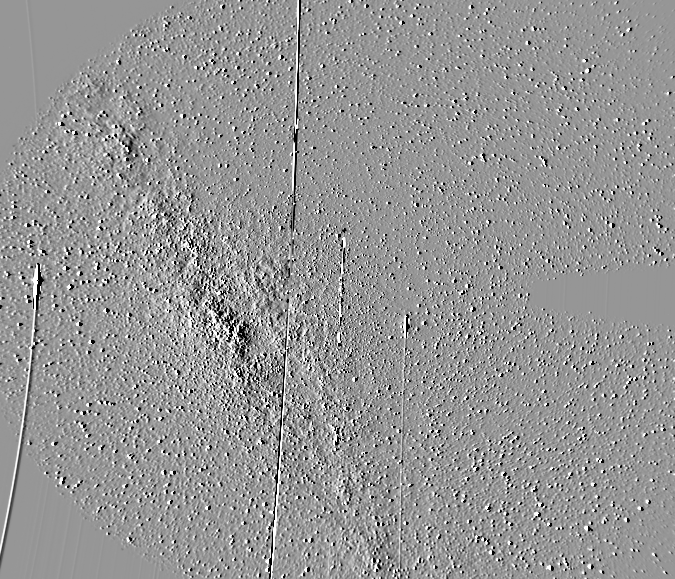
\includegraphics[interpolate=true,width=3.356667in,height=2.880000in]{plots/secchi_fov-img0.png}}%
\end{pgfscope}%
\begin{pgfscope}%
\pgfpathrectangle{\pgfqpoint{0.582966in}{0.478438in}}{\pgfqpoint{4.482034in}{2.877093in}}%
\pgfusepath{clip}%
\pgfsetbuttcap%
\pgfsetmiterjoin%
\pgfsetlinewidth{1.003750pt}%
\definecolor{currentstroke}{rgb}{0.000000,0.000000,0.000000}%
\pgfsetstrokecolor{currentstroke}%
\pgfsetdash{}{0pt}%
\pgfpathmoveto{\pgfqpoint{1.710883in}{0.478438in}}%
\pgfpathlineto{\pgfqpoint{5.065000in}{0.478438in}}%
\pgfpathlineto{\pgfqpoint{5.065000in}{3.355531in}}%
\pgfpathlineto{\pgfqpoint{1.710883in}{3.355531in}}%
\pgfpathclose%
\pgfusepath{stroke}%
\end{pgfscope}%
\begin{pgfscope}%
\definecolor{textcolor}{rgb}{0.000000,0.000000,0.000000}%
\pgfsetstrokecolor{textcolor}%
\pgfsetfillcolor{textcolor}%
\pgftext[x=1.809694in,y=0.577249in,left,base]{\color{textcolor}\rmfamily\fontsize{12.000000}{14.400000}\bfseries\selectfont HI2}%
\end{pgfscope}%
\begin{pgfscope}%
\pgfsetbuttcap%
\pgfsetroundjoin%
\definecolor{currentfill}{rgb}{0.000000,0.000000,0.000000}%
\pgfsetfillcolor{currentfill}%
\pgfsetlinewidth{0.803000pt}%
\definecolor{currentstroke}{rgb}{0.000000,0.000000,0.000000}%
\pgfsetstrokecolor{currentstroke}%
\pgfsetdash{}{0pt}%
\pgfsys@defobject{currentmarker}{\pgfqpoint{0.000000in}{-0.048611in}}{\pgfqpoint{0.000000in}{0.000000in}}{%
\pgfpathmoveto{\pgfqpoint{0.000000in}{0.000000in}}%
\pgfpathlineto{\pgfqpoint{0.000000in}{-0.048611in}}%
\pgfusepath{stroke,fill}%
}%
\begin{pgfscope}%
\pgfsys@transformshift{0.790447in}{0.478438in}%
\pgfsys@useobject{currentmarker}{}%
\end{pgfscope}%
\end{pgfscope}%
\begin{pgfscope}%
\definecolor{textcolor}{rgb}{0.000000,0.000000,0.000000}%
\pgfsetstrokecolor{textcolor}%
\pgfsetfillcolor{textcolor}%
\pgftext[x=0.790447in,y=0.381216in,,top]{\color{textcolor}\rmfamily\fontsize{9.000000}{10.800000}\selectfont 0}%
\end{pgfscope}%
\begin{pgfscope}%
\pgfsetbuttcap%
\pgfsetroundjoin%
\definecolor{currentfill}{rgb}{0.000000,0.000000,0.000000}%
\pgfsetfillcolor{currentfill}%
\pgfsetlinewidth{0.803000pt}%
\definecolor{currentstroke}{rgb}{0.000000,0.000000,0.000000}%
\pgfsetstrokecolor{currentstroke}%
\pgfsetdash{}{0pt}%
\pgfsys@defobject{currentmarker}{\pgfqpoint{0.000000in}{-0.048611in}}{\pgfqpoint{0.000000in}{0.000000in}}{%
\pgfpathmoveto{\pgfqpoint{0.000000in}{0.000000in}}%
\pgfpathlineto{\pgfqpoint{0.000000in}{-0.048611in}}%
\pgfusepath{stroke,fill}%
}%
\begin{pgfscope}%
\pgfsys@transformshift{1.284501in}{0.478438in}%
\pgfsys@useobject{currentmarker}{}%
\end{pgfscope}%
\end{pgfscope}%
\begin{pgfscope}%
\definecolor{textcolor}{rgb}{0.000000,0.000000,0.000000}%
\pgfsetstrokecolor{textcolor}%
\pgfsetfillcolor{textcolor}%
\pgftext[x=1.284501in,y=0.381216in,,top]{\color{textcolor}\rmfamily\fontsize{9.000000}{10.800000}\selectfont 10}%
\end{pgfscope}%
\begin{pgfscope}%
\pgfsetbuttcap%
\pgfsetroundjoin%
\definecolor{currentfill}{rgb}{0.000000,0.000000,0.000000}%
\pgfsetfillcolor{currentfill}%
\pgfsetlinewidth{0.803000pt}%
\definecolor{currentstroke}{rgb}{0.000000,0.000000,0.000000}%
\pgfsetstrokecolor{currentstroke}%
\pgfsetdash{}{0pt}%
\pgfsys@defobject{currentmarker}{\pgfqpoint{0.000000in}{-0.048611in}}{\pgfqpoint{0.000000in}{0.000000in}}{%
\pgfpathmoveto{\pgfqpoint{0.000000in}{0.000000in}}%
\pgfpathlineto{\pgfqpoint{0.000000in}{-0.048611in}}%
\pgfusepath{stroke,fill}%
}%
\begin{pgfscope}%
\pgfsys@transformshift{1.778554in}{0.478438in}%
\pgfsys@useobject{currentmarker}{}%
\end{pgfscope}%
\end{pgfscope}%
\begin{pgfscope}%
\definecolor{textcolor}{rgb}{0.000000,0.000000,0.000000}%
\pgfsetstrokecolor{textcolor}%
\pgfsetfillcolor{textcolor}%
\pgftext[x=1.778554in,y=0.381216in,,top]{\color{textcolor}\rmfamily\fontsize{9.000000}{10.800000}\selectfont 20}%
\end{pgfscope}%
\begin{pgfscope}%
\pgfsetbuttcap%
\pgfsetroundjoin%
\definecolor{currentfill}{rgb}{0.000000,0.000000,0.000000}%
\pgfsetfillcolor{currentfill}%
\pgfsetlinewidth{0.803000pt}%
\definecolor{currentstroke}{rgb}{0.000000,0.000000,0.000000}%
\pgfsetstrokecolor{currentstroke}%
\pgfsetdash{}{0pt}%
\pgfsys@defobject{currentmarker}{\pgfqpoint{0.000000in}{-0.048611in}}{\pgfqpoint{0.000000in}{0.000000in}}{%
\pgfpathmoveto{\pgfqpoint{0.000000in}{0.000000in}}%
\pgfpathlineto{\pgfqpoint{0.000000in}{-0.048611in}}%
\pgfusepath{stroke,fill}%
}%
\begin{pgfscope}%
\pgfsys@transformshift{2.272608in}{0.478438in}%
\pgfsys@useobject{currentmarker}{}%
\end{pgfscope}%
\end{pgfscope}%
\begin{pgfscope}%
\definecolor{textcolor}{rgb}{0.000000,0.000000,0.000000}%
\pgfsetstrokecolor{textcolor}%
\pgfsetfillcolor{textcolor}%
\pgftext[x=2.272608in,y=0.381216in,,top]{\color{textcolor}\rmfamily\fontsize{9.000000}{10.800000}\selectfont 30}%
\end{pgfscope}%
\begin{pgfscope}%
\pgfsetbuttcap%
\pgfsetroundjoin%
\definecolor{currentfill}{rgb}{0.000000,0.000000,0.000000}%
\pgfsetfillcolor{currentfill}%
\pgfsetlinewidth{0.803000pt}%
\definecolor{currentstroke}{rgb}{0.000000,0.000000,0.000000}%
\pgfsetstrokecolor{currentstroke}%
\pgfsetdash{}{0pt}%
\pgfsys@defobject{currentmarker}{\pgfqpoint{0.000000in}{-0.048611in}}{\pgfqpoint{0.000000in}{0.000000in}}{%
\pgfpathmoveto{\pgfqpoint{0.000000in}{0.000000in}}%
\pgfpathlineto{\pgfqpoint{0.000000in}{-0.048611in}}%
\pgfusepath{stroke,fill}%
}%
\begin{pgfscope}%
\pgfsys@transformshift{2.766662in}{0.478438in}%
\pgfsys@useobject{currentmarker}{}%
\end{pgfscope}%
\end{pgfscope}%
\begin{pgfscope}%
\definecolor{textcolor}{rgb}{0.000000,0.000000,0.000000}%
\pgfsetstrokecolor{textcolor}%
\pgfsetfillcolor{textcolor}%
\pgftext[x=2.766662in,y=0.381216in,,top]{\color{textcolor}\rmfamily\fontsize{9.000000}{10.800000}\selectfont 40}%
\end{pgfscope}%
\begin{pgfscope}%
\pgfsetbuttcap%
\pgfsetroundjoin%
\definecolor{currentfill}{rgb}{0.000000,0.000000,0.000000}%
\pgfsetfillcolor{currentfill}%
\pgfsetlinewidth{0.803000pt}%
\definecolor{currentstroke}{rgb}{0.000000,0.000000,0.000000}%
\pgfsetstrokecolor{currentstroke}%
\pgfsetdash{}{0pt}%
\pgfsys@defobject{currentmarker}{\pgfqpoint{0.000000in}{-0.048611in}}{\pgfqpoint{0.000000in}{0.000000in}}{%
\pgfpathmoveto{\pgfqpoint{0.000000in}{0.000000in}}%
\pgfpathlineto{\pgfqpoint{0.000000in}{-0.048611in}}%
\pgfusepath{stroke,fill}%
}%
\begin{pgfscope}%
\pgfsys@transformshift{3.260715in}{0.478438in}%
\pgfsys@useobject{currentmarker}{}%
\end{pgfscope}%
\end{pgfscope}%
\begin{pgfscope}%
\definecolor{textcolor}{rgb}{0.000000,0.000000,0.000000}%
\pgfsetstrokecolor{textcolor}%
\pgfsetfillcolor{textcolor}%
\pgftext[x=3.260715in,y=0.381216in,,top]{\color{textcolor}\rmfamily\fontsize{9.000000}{10.800000}\selectfont 50}%
\end{pgfscope}%
\begin{pgfscope}%
\pgfsetbuttcap%
\pgfsetroundjoin%
\definecolor{currentfill}{rgb}{0.000000,0.000000,0.000000}%
\pgfsetfillcolor{currentfill}%
\pgfsetlinewidth{0.803000pt}%
\definecolor{currentstroke}{rgb}{0.000000,0.000000,0.000000}%
\pgfsetstrokecolor{currentstroke}%
\pgfsetdash{}{0pt}%
\pgfsys@defobject{currentmarker}{\pgfqpoint{0.000000in}{-0.048611in}}{\pgfqpoint{0.000000in}{0.000000in}}{%
\pgfpathmoveto{\pgfqpoint{0.000000in}{0.000000in}}%
\pgfpathlineto{\pgfqpoint{0.000000in}{-0.048611in}}%
\pgfusepath{stroke,fill}%
}%
\begin{pgfscope}%
\pgfsys@transformshift{3.754769in}{0.478438in}%
\pgfsys@useobject{currentmarker}{}%
\end{pgfscope}%
\end{pgfscope}%
\begin{pgfscope}%
\definecolor{textcolor}{rgb}{0.000000,0.000000,0.000000}%
\pgfsetstrokecolor{textcolor}%
\pgfsetfillcolor{textcolor}%
\pgftext[x=3.754769in,y=0.381216in,,top]{\color{textcolor}\rmfamily\fontsize{9.000000}{10.800000}\selectfont 60}%
\end{pgfscope}%
\begin{pgfscope}%
\pgfsetbuttcap%
\pgfsetroundjoin%
\definecolor{currentfill}{rgb}{0.000000,0.000000,0.000000}%
\pgfsetfillcolor{currentfill}%
\pgfsetlinewidth{0.803000pt}%
\definecolor{currentstroke}{rgb}{0.000000,0.000000,0.000000}%
\pgfsetstrokecolor{currentstroke}%
\pgfsetdash{}{0pt}%
\pgfsys@defobject{currentmarker}{\pgfqpoint{0.000000in}{-0.048611in}}{\pgfqpoint{0.000000in}{0.000000in}}{%
\pgfpathmoveto{\pgfqpoint{0.000000in}{0.000000in}}%
\pgfpathlineto{\pgfqpoint{0.000000in}{-0.048611in}}%
\pgfusepath{stroke,fill}%
}%
\begin{pgfscope}%
\pgfsys@transformshift{4.248823in}{0.478438in}%
\pgfsys@useobject{currentmarker}{}%
\end{pgfscope}%
\end{pgfscope}%
\begin{pgfscope}%
\definecolor{textcolor}{rgb}{0.000000,0.000000,0.000000}%
\pgfsetstrokecolor{textcolor}%
\pgfsetfillcolor{textcolor}%
\pgftext[x=4.248823in,y=0.381216in,,top]{\color{textcolor}\rmfamily\fontsize{9.000000}{10.800000}\selectfont 70}%
\end{pgfscope}%
\begin{pgfscope}%
\pgfsetbuttcap%
\pgfsetroundjoin%
\definecolor{currentfill}{rgb}{0.000000,0.000000,0.000000}%
\pgfsetfillcolor{currentfill}%
\pgfsetlinewidth{0.803000pt}%
\definecolor{currentstroke}{rgb}{0.000000,0.000000,0.000000}%
\pgfsetstrokecolor{currentstroke}%
\pgfsetdash{}{0pt}%
\pgfsys@defobject{currentmarker}{\pgfqpoint{0.000000in}{-0.048611in}}{\pgfqpoint{0.000000in}{0.000000in}}{%
\pgfpathmoveto{\pgfqpoint{0.000000in}{0.000000in}}%
\pgfpathlineto{\pgfqpoint{0.000000in}{-0.048611in}}%
\pgfusepath{stroke,fill}%
}%
\begin{pgfscope}%
\pgfsys@transformshift{4.742876in}{0.478438in}%
\pgfsys@useobject{currentmarker}{}%
\end{pgfscope}%
\end{pgfscope}%
\begin{pgfscope}%
\definecolor{textcolor}{rgb}{0.000000,0.000000,0.000000}%
\pgfsetstrokecolor{textcolor}%
\pgfsetfillcolor{textcolor}%
\pgftext[x=4.742876in,y=0.381216in,,top]{\color{textcolor}\rmfamily\fontsize{9.000000}{10.800000}\selectfont 80}%
\end{pgfscope}%
\begin{pgfscope}%
\definecolor{textcolor}{rgb}{0.000000,0.000000,0.000000}%
\pgfsetstrokecolor{textcolor}%
\pgfsetfillcolor{textcolor}%
\pgftext[x=2.823983in,y=0.214660in,,top]{\color{textcolor}\rmfamily\fontsize{9.000000}{10.800000}\selectfont Helioprojective Longitude [°]}%
\end{pgfscope}%
\begin{pgfscope}%
\pgfsetbuttcap%
\pgfsetroundjoin%
\definecolor{currentfill}{rgb}{0.000000,0.000000,0.000000}%
\pgfsetfillcolor{currentfill}%
\pgfsetlinewidth{0.803000pt}%
\definecolor{currentstroke}{rgb}{0.000000,0.000000,0.000000}%
\pgfsetstrokecolor{currentstroke}%
\pgfsetdash{}{0pt}%
\pgfsys@defobject{currentmarker}{\pgfqpoint{-0.048611in}{0.000000in}}{\pgfqpoint{-0.000000in}{0.000000in}}{%
\pgfpathmoveto{\pgfqpoint{-0.000000in}{0.000000in}}%
\pgfpathlineto{\pgfqpoint{-0.048611in}{0.000000in}}%
\pgfusepath{stroke,fill}%
}%
\begin{pgfscope}%
\pgfsys@transformshift{0.582966in}{0.570008in}%
\pgfsys@useobject{currentmarker}{}%
\end{pgfscope}%
\end{pgfscope}%
\begin{pgfscope}%
\definecolor{textcolor}{rgb}{0.000000,0.000000,0.000000}%
\pgfsetstrokecolor{textcolor}%
\pgfsetfillcolor{textcolor}%
\pgftext[x=0.314369in, y=0.526633in, left, base]{\color{textcolor}\rmfamily\fontsize{9.000000}{10.800000}\selectfont -30}%
\end{pgfscope}%
\begin{pgfscope}%
\pgfsetbuttcap%
\pgfsetroundjoin%
\definecolor{currentfill}{rgb}{0.000000,0.000000,0.000000}%
\pgfsetfillcolor{currentfill}%
\pgfsetlinewidth{0.803000pt}%
\definecolor{currentstroke}{rgb}{0.000000,0.000000,0.000000}%
\pgfsetstrokecolor{currentstroke}%
\pgfsetdash{}{0pt}%
\pgfsys@defobject{currentmarker}{\pgfqpoint{-0.048611in}{0.000000in}}{\pgfqpoint{-0.000000in}{0.000000in}}{%
\pgfpathmoveto{\pgfqpoint{-0.000000in}{0.000000in}}%
\pgfpathlineto{\pgfqpoint{-0.048611in}{0.000000in}}%
\pgfusepath{stroke,fill}%
}%
\begin{pgfscope}%
\pgfsys@transformshift{0.582966in}{0.817035in}%
\pgfsys@useobject{currentmarker}{}%
\end{pgfscope}%
\end{pgfscope}%
\begin{pgfscope}%
\definecolor{textcolor}{rgb}{0.000000,0.000000,0.000000}%
\pgfsetstrokecolor{textcolor}%
\pgfsetfillcolor{textcolor}%
\pgftext[x=0.314369in, y=0.773660in, left, base]{\color{textcolor}\rmfamily\fontsize{9.000000}{10.800000}\selectfont -25}%
\end{pgfscope}%
\begin{pgfscope}%
\pgfsetbuttcap%
\pgfsetroundjoin%
\definecolor{currentfill}{rgb}{0.000000,0.000000,0.000000}%
\pgfsetfillcolor{currentfill}%
\pgfsetlinewidth{0.803000pt}%
\definecolor{currentstroke}{rgb}{0.000000,0.000000,0.000000}%
\pgfsetstrokecolor{currentstroke}%
\pgfsetdash{}{0pt}%
\pgfsys@defobject{currentmarker}{\pgfqpoint{-0.048611in}{0.000000in}}{\pgfqpoint{-0.000000in}{0.000000in}}{%
\pgfpathmoveto{\pgfqpoint{-0.000000in}{0.000000in}}%
\pgfpathlineto{\pgfqpoint{-0.048611in}{0.000000in}}%
\pgfusepath{stroke,fill}%
}%
\begin{pgfscope}%
\pgfsys@transformshift{0.582966in}{1.064061in}%
\pgfsys@useobject{currentmarker}{}%
\end{pgfscope}%
\end{pgfscope}%
\begin{pgfscope}%
\definecolor{textcolor}{rgb}{0.000000,0.000000,0.000000}%
\pgfsetstrokecolor{textcolor}%
\pgfsetfillcolor{textcolor}%
\pgftext[x=0.314369in, y=1.020686in, left, base]{\color{textcolor}\rmfamily\fontsize{9.000000}{10.800000}\selectfont -20}%
\end{pgfscope}%
\begin{pgfscope}%
\pgfsetbuttcap%
\pgfsetroundjoin%
\definecolor{currentfill}{rgb}{0.000000,0.000000,0.000000}%
\pgfsetfillcolor{currentfill}%
\pgfsetlinewidth{0.803000pt}%
\definecolor{currentstroke}{rgb}{0.000000,0.000000,0.000000}%
\pgfsetstrokecolor{currentstroke}%
\pgfsetdash{}{0pt}%
\pgfsys@defobject{currentmarker}{\pgfqpoint{-0.048611in}{0.000000in}}{\pgfqpoint{-0.000000in}{0.000000in}}{%
\pgfpathmoveto{\pgfqpoint{-0.000000in}{0.000000in}}%
\pgfpathlineto{\pgfqpoint{-0.048611in}{0.000000in}}%
\pgfusepath{stroke,fill}%
}%
\begin{pgfscope}%
\pgfsys@transformshift{0.582966in}{1.311088in}%
\pgfsys@useobject{currentmarker}{}%
\end{pgfscope}%
\end{pgfscope}%
\begin{pgfscope}%
\definecolor{textcolor}{rgb}{0.000000,0.000000,0.000000}%
\pgfsetstrokecolor{textcolor}%
\pgfsetfillcolor{textcolor}%
\pgftext[x=0.314369in, y=1.267713in, left, base]{\color{textcolor}\rmfamily\fontsize{9.000000}{10.800000}\selectfont -15}%
\end{pgfscope}%
\begin{pgfscope}%
\pgfsetbuttcap%
\pgfsetroundjoin%
\definecolor{currentfill}{rgb}{0.000000,0.000000,0.000000}%
\pgfsetfillcolor{currentfill}%
\pgfsetlinewidth{0.803000pt}%
\definecolor{currentstroke}{rgb}{0.000000,0.000000,0.000000}%
\pgfsetstrokecolor{currentstroke}%
\pgfsetdash{}{0pt}%
\pgfsys@defobject{currentmarker}{\pgfqpoint{-0.048611in}{0.000000in}}{\pgfqpoint{-0.000000in}{0.000000in}}{%
\pgfpathmoveto{\pgfqpoint{-0.000000in}{0.000000in}}%
\pgfpathlineto{\pgfqpoint{-0.048611in}{0.000000in}}%
\pgfusepath{stroke,fill}%
}%
\begin{pgfscope}%
\pgfsys@transformshift{0.582966in}{1.558115in}%
\pgfsys@useobject{currentmarker}{}%
\end{pgfscope}%
\end{pgfscope}%
\begin{pgfscope}%
\definecolor{textcolor}{rgb}{0.000000,0.000000,0.000000}%
\pgfsetstrokecolor{textcolor}%
\pgfsetfillcolor{textcolor}%
\pgftext[x=0.314369in, y=1.514740in, left, base]{\color{textcolor}\rmfamily\fontsize{9.000000}{10.800000}\selectfont -10}%
\end{pgfscope}%
\begin{pgfscope}%
\pgfsetbuttcap%
\pgfsetroundjoin%
\definecolor{currentfill}{rgb}{0.000000,0.000000,0.000000}%
\pgfsetfillcolor{currentfill}%
\pgfsetlinewidth{0.803000pt}%
\definecolor{currentstroke}{rgb}{0.000000,0.000000,0.000000}%
\pgfsetstrokecolor{currentstroke}%
\pgfsetdash{}{0pt}%
\pgfsys@defobject{currentmarker}{\pgfqpoint{-0.048611in}{0.000000in}}{\pgfqpoint{-0.000000in}{0.000000in}}{%
\pgfpathmoveto{\pgfqpoint{-0.000000in}{0.000000in}}%
\pgfpathlineto{\pgfqpoint{-0.048611in}{0.000000in}}%
\pgfusepath{stroke,fill}%
}%
\begin{pgfscope}%
\pgfsys@transformshift{0.582966in}{1.805142in}%
\pgfsys@useobject{currentmarker}{}%
\end{pgfscope}%
\end{pgfscope}%
\begin{pgfscope}%
\definecolor{textcolor}{rgb}{0.000000,0.000000,0.000000}%
\pgfsetstrokecolor{textcolor}%
\pgfsetfillcolor{textcolor}%
\pgftext[x=0.378619in, y=1.761767in, left, base]{\color{textcolor}\rmfamily\fontsize{9.000000}{10.800000}\selectfont -5}%
\end{pgfscope}%
\begin{pgfscope}%
\pgfsetbuttcap%
\pgfsetroundjoin%
\definecolor{currentfill}{rgb}{0.000000,0.000000,0.000000}%
\pgfsetfillcolor{currentfill}%
\pgfsetlinewidth{0.803000pt}%
\definecolor{currentstroke}{rgb}{0.000000,0.000000,0.000000}%
\pgfsetstrokecolor{currentstroke}%
\pgfsetdash{}{0pt}%
\pgfsys@defobject{currentmarker}{\pgfqpoint{-0.048611in}{0.000000in}}{\pgfqpoint{-0.000000in}{0.000000in}}{%
\pgfpathmoveto{\pgfqpoint{-0.000000in}{0.000000in}}%
\pgfpathlineto{\pgfqpoint{-0.048611in}{0.000000in}}%
\pgfusepath{stroke,fill}%
}%
\begin{pgfscope}%
\pgfsys@transformshift{0.582966in}{2.052169in}%
\pgfsys@useobject{currentmarker}{}%
\end{pgfscope}%
\end{pgfscope}%
\begin{pgfscope}%
\definecolor{textcolor}{rgb}{0.000000,0.000000,0.000000}%
\pgfsetstrokecolor{textcolor}%
\pgfsetfillcolor{textcolor}%
\pgftext[x=0.421494in, y=2.008794in, left, base]{\color{textcolor}\rmfamily\fontsize{9.000000}{10.800000}\selectfont 0}%
\end{pgfscope}%
\begin{pgfscope}%
\pgfsetbuttcap%
\pgfsetroundjoin%
\definecolor{currentfill}{rgb}{0.000000,0.000000,0.000000}%
\pgfsetfillcolor{currentfill}%
\pgfsetlinewidth{0.803000pt}%
\definecolor{currentstroke}{rgb}{0.000000,0.000000,0.000000}%
\pgfsetstrokecolor{currentstroke}%
\pgfsetdash{}{0pt}%
\pgfsys@defobject{currentmarker}{\pgfqpoint{-0.048611in}{0.000000in}}{\pgfqpoint{-0.000000in}{0.000000in}}{%
\pgfpathmoveto{\pgfqpoint{-0.000000in}{0.000000in}}%
\pgfpathlineto{\pgfqpoint{-0.048611in}{0.000000in}}%
\pgfusepath{stroke,fill}%
}%
\begin{pgfscope}%
\pgfsys@transformshift{0.582966in}{2.299196in}%
\pgfsys@useobject{currentmarker}{}%
\end{pgfscope}%
\end{pgfscope}%
\begin{pgfscope}%
\definecolor{textcolor}{rgb}{0.000000,0.000000,0.000000}%
\pgfsetstrokecolor{textcolor}%
\pgfsetfillcolor{textcolor}%
\pgftext[x=0.421494in, y=2.255821in, left, base]{\color{textcolor}\rmfamily\fontsize{9.000000}{10.800000}\selectfont 5}%
\end{pgfscope}%
\begin{pgfscope}%
\pgfsetbuttcap%
\pgfsetroundjoin%
\definecolor{currentfill}{rgb}{0.000000,0.000000,0.000000}%
\pgfsetfillcolor{currentfill}%
\pgfsetlinewidth{0.803000pt}%
\definecolor{currentstroke}{rgb}{0.000000,0.000000,0.000000}%
\pgfsetstrokecolor{currentstroke}%
\pgfsetdash{}{0pt}%
\pgfsys@defobject{currentmarker}{\pgfqpoint{-0.048611in}{0.000000in}}{\pgfqpoint{-0.000000in}{0.000000in}}{%
\pgfpathmoveto{\pgfqpoint{-0.000000in}{0.000000in}}%
\pgfpathlineto{\pgfqpoint{-0.048611in}{0.000000in}}%
\pgfusepath{stroke,fill}%
}%
\begin{pgfscope}%
\pgfsys@transformshift{0.582966in}{2.546222in}%
\pgfsys@useobject{currentmarker}{}%
\end{pgfscope}%
\end{pgfscope}%
\begin{pgfscope}%
\definecolor{textcolor}{rgb}{0.000000,0.000000,0.000000}%
\pgfsetstrokecolor{textcolor}%
\pgfsetfillcolor{textcolor}%
\pgftext[x=0.357244in, y=2.502847in, left, base]{\color{textcolor}\rmfamily\fontsize{9.000000}{10.800000}\selectfont 10}%
\end{pgfscope}%
\begin{pgfscope}%
\pgfsetbuttcap%
\pgfsetroundjoin%
\definecolor{currentfill}{rgb}{0.000000,0.000000,0.000000}%
\pgfsetfillcolor{currentfill}%
\pgfsetlinewidth{0.803000pt}%
\definecolor{currentstroke}{rgb}{0.000000,0.000000,0.000000}%
\pgfsetstrokecolor{currentstroke}%
\pgfsetdash{}{0pt}%
\pgfsys@defobject{currentmarker}{\pgfqpoint{-0.048611in}{0.000000in}}{\pgfqpoint{-0.000000in}{0.000000in}}{%
\pgfpathmoveto{\pgfqpoint{-0.000000in}{0.000000in}}%
\pgfpathlineto{\pgfqpoint{-0.048611in}{0.000000in}}%
\pgfusepath{stroke,fill}%
}%
\begin{pgfscope}%
\pgfsys@transformshift{0.582966in}{2.793249in}%
\pgfsys@useobject{currentmarker}{}%
\end{pgfscope}%
\end{pgfscope}%
\begin{pgfscope}%
\definecolor{textcolor}{rgb}{0.000000,0.000000,0.000000}%
\pgfsetstrokecolor{textcolor}%
\pgfsetfillcolor{textcolor}%
\pgftext[x=0.357244in, y=2.749874in, left, base]{\color{textcolor}\rmfamily\fontsize{9.000000}{10.800000}\selectfont 15}%
\end{pgfscope}%
\begin{pgfscope}%
\pgfsetbuttcap%
\pgfsetroundjoin%
\definecolor{currentfill}{rgb}{0.000000,0.000000,0.000000}%
\pgfsetfillcolor{currentfill}%
\pgfsetlinewidth{0.803000pt}%
\definecolor{currentstroke}{rgb}{0.000000,0.000000,0.000000}%
\pgfsetstrokecolor{currentstroke}%
\pgfsetdash{}{0pt}%
\pgfsys@defobject{currentmarker}{\pgfqpoint{-0.048611in}{0.000000in}}{\pgfqpoint{-0.000000in}{0.000000in}}{%
\pgfpathmoveto{\pgfqpoint{-0.000000in}{0.000000in}}%
\pgfpathlineto{\pgfqpoint{-0.048611in}{0.000000in}}%
\pgfusepath{stroke,fill}%
}%
\begin{pgfscope}%
\pgfsys@transformshift{0.582966in}{3.040276in}%
\pgfsys@useobject{currentmarker}{}%
\end{pgfscope}%
\end{pgfscope}%
\begin{pgfscope}%
\definecolor{textcolor}{rgb}{0.000000,0.000000,0.000000}%
\pgfsetstrokecolor{textcolor}%
\pgfsetfillcolor{textcolor}%
\pgftext[x=0.357244in, y=2.996901in, left, base]{\color{textcolor}\rmfamily\fontsize{9.000000}{10.800000}\selectfont 20}%
\end{pgfscope}%
\begin{pgfscope}%
\pgfsetbuttcap%
\pgfsetroundjoin%
\definecolor{currentfill}{rgb}{0.000000,0.000000,0.000000}%
\pgfsetfillcolor{currentfill}%
\pgfsetlinewidth{0.803000pt}%
\definecolor{currentstroke}{rgb}{0.000000,0.000000,0.000000}%
\pgfsetstrokecolor{currentstroke}%
\pgfsetdash{}{0pt}%
\pgfsys@defobject{currentmarker}{\pgfqpoint{-0.048611in}{0.000000in}}{\pgfqpoint{-0.000000in}{0.000000in}}{%
\pgfpathmoveto{\pgfqpoint{-0.000000in}{0.000000in}}%
\pgfpathlineto{\pgfqpoint{-0.048611in}{0.000000in}}%
\pgfusepath{stroke,fill}%
}%
\begin{pgfscope}%
\pgfsys@transformshift{0.582966in}{3.287303in}%
\pgfsys@useobject{currentmarker}{}%
\end{pgfscope}%
\end{pgfscope}%
\begin{pgfscope}%
\definecolor{textcolor}{rgb}{0.000000,0.000000,0.000000}%
\pgfsetstrokecolor{textcolor}%
\pgfsetfillcolor{textcolor}%
\pgftext[x=0.357244in, y=3.243928in, left, base]{\color{textcolor}\rmfamily\fontsize{9.000000}{10.800000}\selectfont 25}%
\end{pgfscope}%
\begin{pgfscope}%
\definecolor{textcolor}{rgb}{0.000000,0.000000,0.000000}%
\pgfsetstrokecolor{textcolor}%
\pgfsetfillcolor{textcolor}%
\pgftext[x=0.258813in,y=1.916985in,,bottom,rotate=90.000000]{\color{textcolor}\rmfamily\fontsize{9.000000}{10.800000}\selectfont Helioprojective Latitude [°]}%
\end{pgfscope}%
\begin{pgfscope}%
\pgfsetrectcap%
\pgfsetmiterjoin%
\pgfsetlinewidth{0.803000pt}%
\definecolor{currentstroke}{rgb}{0.000000,0.000000,0.000000}%
\pgfsetstrokecolor{currentstroke}%
\pgfsetdash{}{0pt}%
\pgfpathmoveto{\pgfqpoint{0.582966in}{0.478438in}}%
\pgfpathlineto{\pgfqpoint{0.582966in}{3.355531in}}%
\pgfusepath{stroke}%
\end{pgfscope}%
\begin{pgfscope}%
\pgfsetrectcap%
\pgfsetmiterjoin%
\pgfsetlinewidth{0.803000pt}%
\definecolor{currentstroke}{rgb}{0.000000,0.000000,0.000000}%
\pgfsetstrokecolor{currentstroke}%
\pgfsetdash{}{0pt}%
\pgfpathmoveto{\pgfqpoint{5.065000in}{0.478438in}}%
\pgfpathlineto{\pgfqpoint{5.065000in}{3.355531in}}%
\pgfusepath{stroke}%
\end{pgfscope}%
\begin{pgfscope}%
\pgfsetrectcap%
\pgfsetmiterjoin%
\pgfsetlinewidth{0.803000pt}%
\definecolor{currentstroke}{rgb}{0.000000,0.000000,0.000000}%
\pgfsetstrokecolor{currentstroke}%
\pgfsetdash{}{0pt}%
\pgfpathmoveto{\pgfqpoint{0.582966in}{0.478438in}}%
\pgfpathlineto{\pgfqpoint{5.065000in}{0.478438in}}%
\pgfusepath{stroke}%
\end{pgfscope}%
\begin{pgfscope}%
\pgfsetrectcap%
\pgfsetmiterjoin%
\pgfsetlinewidth{0.803000pt}%
\definecolor{currentstroke}{rgb}{0.000000,0.000000,0.000000}%
\pgfsetstrokecolor{currentstroke}%
\pgfsetdash{}{0pt}%
\pgfpathmoveto{\pgfqpoint{0.582966in}{3.355531in}}%
\pgfpathlineto{\pgfqpoint{5.065000in}{3.355531in}}%
\pgfusepath{stroke}%
\end{pgfscope}%
\begin{pgfscope}%
\pgfpathrectangle{\pgfqpoint{0.582966in}{0.478438in}}{\pgfqpoint{4.482034in}{2.877093in}}%
\pgfusepath{clip}%
\pgfsys@transformshift{0.944714in}{1.480627in}%
\pgftext[left,bottom]{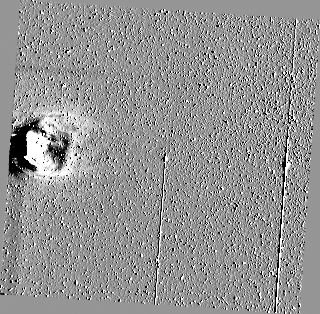
\includegraphics[interpolate=true,width=1.066667in,height=1.046667in]{plots/secchi_fov-img1.png}}%
\end{pgfscope}%
\begin{pgfscope}%
\pgfpathrectangle{\pgfqpoint{0.582966in}{0.478438in}}{\pgfqpoint{4.482034in}{2.877093in}}%
\pgfusepath{clip}%
\pgfsetbuttcap%
\pgfsetmiterjoin%
\pgfsetlinewidth{1.003750pt}%
\definecolor{currentstroke}{rgb}{0.000000,0.000000,0.000000}%
\pgfsetstrokecolor{currentstroke}%
\pgfsetdash{}{0pt}%
\pgfpathmoveto{\pgfqpoint{0.944714in}{1.480627in}}%
\pgfpathlineto{\pgfqpoint{2.009720in}{1.480627in}}%
\pgfpathlineto{\pgfqpoint{2.009720in}{2.527109in}}%
\pgfpathlineto{\pgfqpoint{0.944714in}{2.527109in}}%
\pgfpathclose%
\pgfusepath{stroke}%
\end{pgfscope}%
\begin{pgfscope}%
\definecolor{textcolor}{rgb}{0.000000,0.000000,0.000000}%
\pgfsetstrokecolor{textcolor}%
\pgfsetfillcolor{textcolor}%
\pgftext[x=1.043525in,y=1.579438in,left,base]{\color{textcolor}\rmfamily\fontsize{12.000000}{14.400000}\bfseries\selectfont HI1}%
\end{pgfscope}%
\begin{pgfscope}%
\pgfpathrectangle{\pgfqpoint{0.582966in}{0.478438in}}{\pgfqpoint{4.482034in}{2.877093in}}%
\pgfusepath{clip}%
\pgfsetbuttcap%
\pgfsetmiterjoin%
\pgfsetlinewidth{1.003750pt}%
\definecolor{currentstroke}{rgb}{0.000000,0.000000,0.000000}%
\pgfsetstrokecolor{currentstroke}%
\pgfsetdash{}{0pt}%
\pgfpathmoveto{\pgfqpoint{1.901498in}{1.915773in}}%
\pgfpathcurveto{\pgfqpoint{1.914601in}{1.915773in}}{\pgfqpoint{1.927168in}{1.920979in}}{\pgfqpoint{1.936433in}{1.930244in}}%
\pgfpathcurveto{\pgfqpoint{1.945698in}{1.939509in}}{\pgfqpoint{1.950904in}{1.952076in}}{\pgfqpoint{1.950904in}{1.965179in}}%
\pgfpathcurveto{\pgfqpoint{1.950904in}{1.978281in}}{\pgfqpoint{1.945698in}{1.990849in}}{\pgfqpoint{1.936433in}{2.000114in}}%
\pgfpathcurveto{\pgfqpoint{1.927168in}{2.009378in}}{\pgfqpoint{1.914601in}{2.014584in}}{\pgfqpoint{1.901498in}{2.014584in}}%
\pgfpathcurveto{\pgfqpoint{1.888396in}{2.014584in}}{\pgfqpoint{1.875828in}{2.009378in}}{\pgfqpoint{1.866563in}{2.000114in}}%
\pgfpathcurveto{\pgfqpoint{1.857299in}{1.990849in}}{\pgfqpoint{1.852093in}{1.978281in}}{\pgfqpoint{1.852093in}{1.965179in}}%
\pgfpathcurveto{\pgfqpoint{1.852093in}{1.952076in}}{\pgfqpoint{1.857299in}{1.939509in}}{\pgfqpoint{1.866563in}{1.930244in}}%
\pgfpathcurveto{\pgfqpoint{1.875828in}{1.920979in}}{\pgfqpoint{1.888396in}{1.915773in}}{\pgfqpoint{1.901498in}{1.915773in}}%
\pgfpathclose%
\pgfusepath{stroke}%
\end{pgfscope}%
\begin{pgfscope}%
\pgfpathrectangle{\pgfqpoint{0.582966in}{0.478438in}}{\pgfqpoint{4.482034in}{2.877093in}}%
\pgfusepath{clip}%
\pgfsetbuttcap%
\pgfsetmiterjoin%
\pgfsetlinewidth{1.003750pt}%
\definecolor{currentstroke}{rgb}{0.000000,0.000000,0.000000}%
\pgfsetstrokecolor{currentstroke}%
\pgfsetdash{}{0pt}%
\pgfpathmoveto{\pgfqpoint{1.498857in}{1.942865in}}%
\pgfpathcurveto{\pgfqpoint{1.511960in}{1.942865in}}{\pgfqpoint{1.524527in}{1.948071in}}{\pgfqpoint{1.533792in}{1.957336in}}%
\pgfpathcurveto{\pgfqpoint{1.543057in}{1.966601in}}{\pgfqpoint{1.548263in}{1.979168in}}{\pgfqpoint{1.548263in}{1.992271in}}%
\pgfpathcurveto{\pgfqpoint{1.548263in}{2.005373in}}{\pgfqpoint{1.543057in}{2.017941in}}{\pgfqpoint{1.533792in}{2.027206in}}%
\pgfpathcurveto{\pgfqpoint{1.524527in}{2.036470in}}{\pgfqpoint{1.511960in}{2.041676in}}{\pgfqpoint{1.498857in}{2.041676in}}%
\pgfpathcurveto{\pgfqpoint{1.485755in}{2.041676in}}{\pgfqpoint{1.473187in}{2.036470in}}{\pgfqpoint{1.463922in}{2.027206in}}%
\pgfpathcurveto{\pgfqpoint{1.454658in}{2.017941in}}{\pgfqpoint{1.449452in}{2.005373in}}{\pgfqpoint{1.449452in}{1.992271in}}%
\pgfpathcurveto{\pgfqpoint{1.449452in}{1.979168in}}{\pgfqpoint{1.454658in}{1.966601in}}{\pgfqpoint{1.463922in}{1.957336in}}%
\pgfpathcurveto{\pgfqpoint{1.473187in}{1.948071in}}{\pgfqpoint{1.485755in}{1.942865in}}{\pgfqpoint{1.498857in}{1.942865in}}%
\pgfpathclose%
\pgfusepath{stroke}%
\end{pgfscope}%
\begin{pgfscope}%
\pgfpathrectangle{\pgfqpoint{0.582966in}{0.478438in}}{\pgfqpoint{4.482034in}{2.877093in}}%
\pgfusepath{clip}%
\pgfsetbuttcap%
\pgfsetmiterjoin%
\pgfsetlinewidth{1.003750pt}%
\definecolor{currentstroke}{rgb}{0.000000,0.000000,0.000000}%
\pgfsetstrokecolor{currentstroke}%
\pgfsetdash{}{0pt}%
\pgfpathmoveto{\pgfqpoint{3.163965in}{2.033916in}}%
\pgfpathcurveto{\pgfqpoint{3.177068in}{2.033916in}}{\pgfqpoint{3.189635in}{2.039122in}}{\pgfqpoint{3.198900in}{2.048386in}}%
\pgfpathcurveto{\pgfqpoint{3.208165in}{2.057651in}}{\pgfqpoint{3.213371in}{2.070219in}}{\pgfqpoint{3.213371in}{2.083321in}}%
\pgfpathcurveto{\pgfqpoint{3.213371in}{2.096424in}}{\pgfqpoint{3.208165in}{2.108991in}}{\pgfqpoint{3.198900in}{2.118256in}}%
\pgfpathcurveto{\pgfqpoint{3.189635in}{2.127521in}}{\pgfqpoint{3.177068in}{2.132727in}}{\pgfqpoint{3.163965in}{2.132727in}}%
\pgfpathcurveto{\pgfqpoint{3.150863in}{2.132727in}}{\pgfqpoint{3.138295in}{2.127521in}}{\pgfqpoint{3.129030in}{2.118256in}}%
\pgfpathcurveto{\pgfqpoint{3.119766in}{2.108991in}}{\pgfqpoint{3.114560in}{2.096424in}}{\pgfqpoint{3.114560in}{2.083321in}}%
\pgfpathcurveto{\pgfqpoint{3.114560in}{2.070219in}}{\pgfqpoint{3.119766in}{2.057651in}}{\pgfqpoint{3.129030in}{2.048386in}}%
\pgfpathcurveto{\pgfqpoint{3.138295in}{2.039122in}}{\pgfqpoint{3.150863in}{2.033916in}}{\pgfqpoint{3.163965in}{2.033916in}}%
\pgfpathclose%
\pgfusepath{stroke}%
\end{pgfscope}%
\begin{pgfscope}%
\pgfpathrectangle{\pgfqpoint{0.582966in}{0.478438in}}{\pgfqpoint{4.482034in}{2.877093in}}%
\pgfusepath{clip}%
\pgfsetbuttcap%
\pgfsetmiterjoin%
\pgfsetlinewidth{1.003750pt}%
\definecolor{currentstroke}{rgb}{0.000000,0.000000,0.000000}%
\pgfsetstrokecolor{currentstroke}%
\pgfsetdash{}{0pt}%
\pgfpathmoveto{\pgfqpoint{3.416141in}{1.913435in}}%
\pgfpathcurveto{\pgfqpoint{3.429243in}{1.913435in}}{\pgfqpoint{3.441811in}{1.918640in}}{\pgfqpoint{3.451075in}{1.927905in}}%
\pgfpathcurveto{\pgfqpoint{3.460340in}{1.937170in}}{\pgfqpoint{3.465546in}{1.949738in}}{\pgfqpoint{3.465546in}{1.962840in}}%
\pgfpathcurveto{\pgfqpoint{3.465546in}{1.975943in}}{\pgfqpoint{3.460340in}{1.988510in}}{\pgfqpoint{3.451075in}{1.997775in}}%
\pgfpathcurveto{\pgfqpoint{3.441811in}{2.007040in}}{\pgfqpoint{3.429243in}{2.012245in}}{\pgfqpoint{3.416141in}{2.012245in}}%
\pgfpathcurveto{\pgfqpoint{3.403038in}{2.012245in}}{\pgfqpoint{3.390470in}{2.007040in}}{\pgfqpoint{3.381206in}{1.997775in}}%
\pgfpathcurveto{\pgfqpoint{3.371941in}{1.988510in}}{\pgfqpoint{3.366735in}{1.975943in}}{\pgfqpoint{3.366735in}{1.962840in}}%
\pgfpathcurveto{\pgfqpoint{3.366735in}{1.949738in}}{\pgfqpoint{3.371941in}{1.937170in}}{\pgfqpoint{3.381206in}{1.927905in}}%
\pgfpathcurveto{\pgfqpoint{3.390470in}{1.918640in}}{\pgfqpoint{3.403038in}{1.913435in}}{\pgfqpoint{3.416141in}{1.913435in}}%
\pgfpathclose%
\pgfusepath{stroke}%
\end{pgfscope}%
\begin{pgfscope}%
\pgfsetbuttcap%
\pgfsetmiterjoin%
\definecolor{currentfill}{rgb}{1.000000,1.000000,1.000000}%
\pgfsetfillcolor{currentfill}%
\pgfsetlinewidth{1.003750pt}%
\definecolor{currentstroke}{rgb}{0.000000,0.000000,0.000000}%
\pgfsetstrokecolor{currentstroke}%
\pgfsetdash{}{0pt}%
\pgfpathmoveto{\pgfqpoint{1.689276in}{1.715221in}}%
\pgfpathlineto{\pgfqpoint{2.113721in}{1.715221in}}%
\pgfpathlineto{\pgfqpoint{2.113721in}{1.869443in}}%
\pgfpathlineto{\pgfqpoint{1.689276in}{1.869443in}}%
\pgfpathclose%
\pgfusepath{stroke,fill}%
\end{pgfscope}%
\begin{pgfscope}%
\definecolor{textcolor}{rgb}{0.000000,0.000000,0.000000}%
\pgfsetstrokecolor{textcolor}%
\pgfsetfillcolor{textcolor}%
\pgftext[x=1.901498in,y=1.841665in,,top]{\color{textcolor}\rmfamily\fontsize{8.000000}{9.600000}\selectfont Jupiter}%
\end{pgfscope}%
\begin{pgfscope}%
\pgfsetbuttcap%
\pgfsetmiterjoin%
\definecolor{currentfill}{rgb}{1.000000,1.000000,1.000000}%
\pgfsetfillcolor{currentfill}%
\pgfsetlinewidth{1.003750pt}%
\definecolor{currentstroke}{rgb}{0.000000,0.000000,0.000000}%
\pgfsetstrokecolor{currentstroke}%
\pgfsetdash{}{0pt}%
\pgfpathmoveto{\pgfqpoint{1.297302in}{2.088006in}}%
\pgfpathlineto{\pgfqpoint{1.700413in}{2.088006in}}%
\pgfpathlineto{\pgfqpoint{1.700413in}{2.242228in}}%
\pgfpathlineto{\pgfqpoint{1.297302in}{2.242228in}}%
\pgfpathclose%
\pgfusepath{stroke,fill}%
\end{pgfscope}%
\begin{pgfscope}%
\definecolor{textcolor}{rgb}{0.000000,0.000000,0.000000}%
\pgfsetstrokecolor{textcolor}%
\pgfsetfillcolor{textcolor}%
\pgftext[x=1.498857in,y=2.115784in,,bottom]{\color{textcolor}\rmfamily\fontsize{8.000000}{9.600000}\selectfont Saturn}%
\end{pgfscope}%
\begin{pgfscope}%
\pgfsetbuttcap%
\pgfsetmiterjoin%
\definecolor{currentfill}{rgb}{1.000000,1.000000,1.000000}%
\pgfsetfillcolor{currentfill}%
\pgfsetlinewidth{1.003750pt}%
\definecolor{currentstroke}{rgb}{0.000000,0.000000,0.000000}%
\pgfsetstrokecolor{currentstroke}%
\pgfsetdash{}{0pt}%
\pgfpathmoveto{\pgfqpoint{2.983521in}{2.179057in}}%
\pgfpathlineto{\pgfqpoint{3.344410in}{2.179057in}}%
\pgfpathlineto{\pgfqpoint{3.344410in}{2.333279in}}%
\pgfpathlineto{\pgfqpoint{2.983521in}{2.333279in}}%
\pgfpathclose%
\pgfusepath{stroke,fill}%
\end{pgfscope}%
\begin{pgfscope}%
\definecolor{textcolor}{rgb}{0.000000,0.000000,0.000000}%
\pgfsetstrokecolor{textcolor}%
\pgfsetfillcolor{textcolor}%
\pgftext[x=3.163965in,y=2.206835in,,bottom]{\color{textcolor}\rmfamily\fontsize{8.000000}{9.600000}\selectfont Venus}%
\end{pgfscope}%
\begin{pgfscope}%
\pgfsetbuttcap%
\pgfsetmiterjoin%
\definecolor{currentfill}{rgb}{1.000000,1.000000,1.000000}%
\pgfsetfillcolor{currentfill}%
\pgfsetlinewidth{1.003750pt}%
\definecolor{currentstroke}{rgb}{0.000000,0.000000,0.000000}%
\pgfsetstrokecolor{currentstroke}%
\pgfsetdash{}{0pt}%
\pgfpathmoveto{\pgfqpoint{3.239974in}{1.712882in}}%
\pgfpathlineto{\pgfqpoint{3.592307in}{1.712882in}}%
\pgfpathlineto{\pgfqpoint{3.592307in}{1.867104in}}%
\pgfpathlineto{\pgfqpoint{3.239974in}{1.867104in}}%
\pgfpathclose%
\pgfusepath{stroke,fill}%
\end{pgfscope}%
\begin{pgfscope}%
\definecolor{textcolor}{rgb}{0.000000,0.000000,0.000000}%
\pgfsetstrokecolor{textcolor}%
\pgfsetfillcolor{textcolor}%
\pgftext[x=3.416141in,y=1.839327in,,top]{\color{textcolor}\rmfamily\fontsize{8.000000}{9.600000}\selectfont Earth}%
\end{pgfscope}%
\begin{pgfscope}%
\pgfpathrectangle{\pgfqpoint{0.582966in}{0.478438in}}{\pgfqpoint{4.482034in}{2.877093in}}%
\pgfusepath{clip}%
\pgfsys@transformshift{0.583333in}{1.846667in}%
\pgftext[left,bottom]{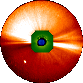
\includegraphics[interpolate=true,width=0.413333in,height=0.413333in]{plots/secchi_fov-img2.png}}%
\end{pgfscope}%
\end{pgfpicture}%
\makeatother%
\endgroup%

        \end{column}
        \begin{column}{0.3\textwidth}
            \textbf{S}un \textbf{E}arth \textbf{C}onnection \textbf{C}oronal and \textbf{H}eliospheric \textbf{I}nvestigation\\[0.5cm]
            \begin{tabular}{ll}
                \toprule
                Telescope & Field of view                   \\
                \midrule
                \textcolor{blue}{EUVI}      & \SIrange{0}{1.7}{\solarradius}  \\
                \textcolor{green}{COR1}      & \SIrange{1.4}{4}{\solarradius}  \\
                \textcolor{red}{COR2}      & \SIrange{2.5}{15}{\solarradius} \\
                HI1       & \SIrange{4}{24}{\degree}        \\
                HI2       & \SIrange{18.7}{88.7}{\degree}       \\
                \bottomrule
            \end{tabular}
        \end{column}
    \end{columns}
    \centering
    CMEs appear in white-light images (COR, HI) due to \textbf{Thomson scattering}.
\end{frame}

\begin{frame}{Time-elongation maps / J-maps}
    \vskip2mm
    \begin{columns}
        \begin{column}{0.4\textwidth}
            \centering
            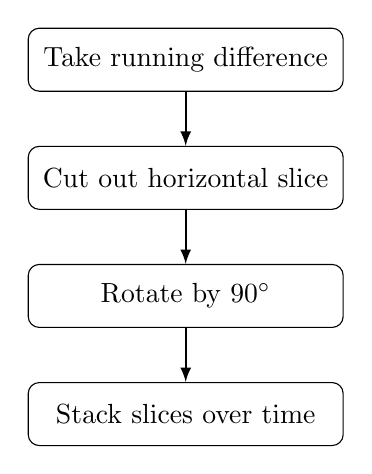
\begin{tikzpicture}[every node/.style={rectangle, rounded corners, draw=black, minimum width=4cm, minimum height=0.8cm}]
                \node (step1) at (0, 0) {Take running difference};
                \node (step2) at (0, -1.5) {Cut out horizontal slice};
                \node (step3) at (0, -3) {Rotate by \SI{90}{\degree}};
                \node (step4) at (0, -4.5) {Stack slices over time};
                \draw[thick, -latex] (step1) -- (step2);
                \draw[thick, -latex] (step2) -- (step3);
                \draw[thick, -latex] (step3) -- (step4);
            \end{tikzpicture}
        \end{column}
        \begin{column}{0.6\textwidth}
            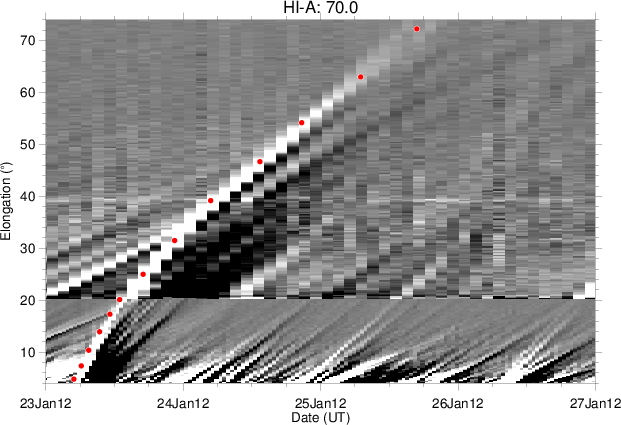
\includegraphics[width=\textwidth]{images/HCME_A__20120123_01.png}
            \small Source: HELCATS project
        \end{column}
    \end{columns}
    \summary ICMEs can now be tracked as bright features. How to convert elongation to distance?
\end{frame}

\begin{frame}{Geometric reconstruction}
    \begin{columns}[t]
        \begin{column}{0.32\textwidth}
            \begin{block}{COR: 3D reconstruction}
                \centering
                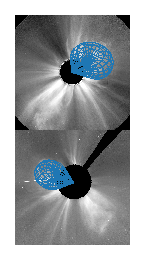
\includegraphics[height=0.65\textheight]{plots/gcs.pdf}\\[-1.5mm]
                {\footnotesize GCS, Thernisien 2012}\\
                {\scriptsize Python implementation:\\[-2mm] \tiny\url{https://github.com/johan12345/gcs_python}}
            \end{block} 
            
        \end{column}
        \begin{column}{0.32\textwidth}
            \begin{block}{HI: Single S/C fitting}     
                            \centering       
            \begin{tikzpicture}[scale=0.85]
                \coordinate (center) at (0,0);
                \def\earthorbitradius{4cm}
                
                \draw (center) -- node[below]{\small$d_0$} (\earthorbitradius,0) node {\large\reflectbox{\faVideo}};
                
                \draw (center) -- node[pos=0.5, right] {\small $r_\text{FP}$} ++ (45:1.5cm) node[cross] {};% node[below left] {ICME};
                
                \draw (center) ++ (0:0.7cm) arc (0:45:0.7cm);
                \node at (22.5:0.4cm) {\small$\phi$};
                
                \draw[dashed] (center) ++ (45:1.5cm) -- (\earthorbitradius,0);
                
                \draw (\earthorbitradius,0) ++ (180:1cm) arc (180:161:1cm);
                \draw (\earthorbitradius,0) ++(170.5:0.7cm) node {\footnotesize$\epsilon$};
                
                
                \draw[fill=yellow] (center) circle (0.2cm); % sun	
                
            \end{tikzpicture}\\
            {\footnotesize FP, Kahler and Webb, 2007}\\[2mm]
        
            \begin{tikzpicture}[scale=0.85]
                \coordinate (center) at (0,0);
                \def\earthorbitradius{4cm}
                
                \draw (center) -- node[below]{\small$d_0$} (\earthorbitradius,0) node {\large\reflectbox{\faVideo}};
                
                \draw[opacity=0.25] (center) ++ (30:1.8cm) circle (0.72cm);
                \draw[opacity=0.5] (center) ++ (30:1.6cm) circle (0.64cm);
                \draw(center) ++ (30:1.4cm) circle (0.56cm);
                \draw[opacity=0.5] (center) ++ (30:1.2cm) circle (0.48cm);
                \draw[opacity=0.25] (center) ++ (30:1cm) circle (0.4cm);
                
                
                \draw[dashed] (center) -- ++ (54:2.5cm);
                \draw (center) -- ++ (30:1.96cm) node[pos=0.7,below,xshift=0.2cm] {\small$r_\text{SSE}$};
                
                \draw (center) ++ (0:0.8cm) arc (0:30:0.8cm);
                \node at (15:0.6cm) {\small$\phi$};
                
                \draw (center) ++ (30:0.6cm) arc (30:54:0.6cm);
                \node at (42:0.5cm) {\footnotesize$\lambda$};
                
                \draw[dashed] (center) ++ (30:1.4cm) ++ (64:0.56cm) -- (\earthorbitradius,0);
                \draw (center) ++ (30:1.4cm) -- ++ (64:0.56cm) node[cross] {};
                \draw (center) ++ (30:1.4cm) ++ (64:0.56cm) ++ (-26:0.2cm) arc (-26:-116:0.2cm);
                \fill (center) ++ (30:1.4cm) ++ (64:0.56cm) ++ (-71:0.1cm) circle (0.5pt);
                
                \draw (\earthorbitradius,0) ++ (180:1cm) arc (180:155:1cm);
                \draw (\earthorbitradius,0) ++(170:0.7cm) node {\footnotesize$\epsilon$};
                
                
                \draw[fill=yellow] (center) circle (0.2cm); % sun	
                
            \end{tikzpicture}
            {\footnotesize SSE, Davies et al. 2012}\\[2mm]
            
            \small $\phi$ (and $\lambda$) determined by fitting, assuming $v = \text{const.}$
            \end{block} 
        \end{column}
        \begin{column}{0.32\textwidth}
            \begin{block}{HI: Stereoscopic fitting}     
            \centering
            \begin{tikzpicture}[scale=0.7]
                \coordinate (center) at (0,0);
                \def\earthorbitradius{4cm}
                
                \draw (center) -- node[above right]{\small$d_A$} (-50:\earthorbitradius) node 
                {\large\rotatebox{130}{\faVideo}} coordinate (STA);
                
                \draw (center) -- node[above left]{\small$d_B$} (-130:\earthorbitradius) node 
                {\large\rotatebox{50}{\faVideo}} coordinate (STB);
                
                \draw (center) -- node[pos=0.7,right]{\footnotesize$r$} (-85:0.5*\earthorbitradius) coordinate (ICME) node[cross] {};
                
                \draw (center) ++ (-50:1cm) arc (-50:-85:1cm) node[midway,above,xshift=-0.5mm] {\footnotesize$\phi_A$};
                \draw (center) ++ (-85:1cm) arc (-85:-130:1cm) node[midway,above,xshift=0.7mm] {\footnotesize$\phi_B$};
                
                \draw[dashed] (STA) -- (ICME) -- (STB);
                
                \draw[fill=yellow] (center) circle (0.2cm); % sun	
                
                \draw (STA) ++ (130:1cm) arc (130:155:1cm) node[midway,above left] {\footnotesize$\epsilon_A$};
                \draw (STB) ++ (50:1cm) arc (50:22:1cm) node[midway,above right] {\footnotesize$\epsilon_B$};
            \end{tikzpicture}
            {\footnotesize GT, Liu et al. 2010}
            
            \small $\phi$ calculated by triangulation
            \end{block}
        \end{column}
    \end{columns}
\end{frame}

\section{Statistical study of Forbush decreases at MSL/RAD}

\begin{frame}{Catalogs of Forbush decreases at Mars}
    \begin{columns}
    	\begin{column}{0.55\textwidth}
    		\begin{itemize}
                \item<1-> \textbf{von Forstner et al. 2018}: 15 ICMEs with in situ FDs at 1 AU (STEREO or Earth) and Mars
                    \begin{itemize}
                        \item 6 at STEREO-B, 4 at STEREO-A, 5 at Earth
                        \item Travel time from cross-correlation method
                    \end{itemize}
    			\item<2-> \textbf{von Forstner et al. 2019}: 45 ICMEs observed with STEREO-HI which caused a FD at Mars
    				\begin{itemize}
    					\item Excludes CME-CME interaction events
    					\item 19 events also seen in situ at Earth
    				\end{itemize}
    			\item<3-> \textbf{Papaioannou et al. 2019}: 424 FDs at Mars
    				\begin{itemize}
    					\item Semi-automatic identification
    					\item Not all associated with ICMEs
    				\end{itemize}
    		\end{itemize}
    	\end{column}
    	\begin{column}{0.35\textwidth}
            \centering
            \only<1>{
                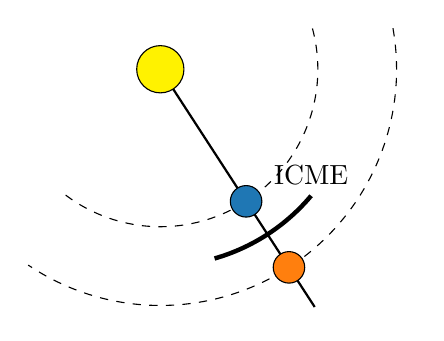
\begin{tikzpicture}[scale=1]
                    \coordinate (center) at (0,0); 
                    \def\earthorbitradius{2cm}
                    \def\marsorbitradius{3cm}
                    
                    \draw[thick] (center) -- (-57:\marsorbitradius*1.2);
                    
                    \draw[dashed] (center) ++ (15:\earthorbitradius) arc 
                    (15:-129:\earthorbitradius); %earth orbit
                    
                    \draw[fill=blue] (center) ++(-57:\earthorbitradius) circle (0.2cm);
                    
                    \draw[dashed] (center) ++ (10:\marsorbitradius) arc 
                    (10:-124:\marsorbitradius); %mars orbit
                    
                    \draw[fill=orange] (center) ++(-57:\marsorbitradius) circle (0.2cm); % mars
                    
                    \draw[fill=yellow] (center) circle (0.3cm); % sun	
                    
                    \draw[ultra thick] (center) ++ (-40:1.25*\earthorbitradius) node[above]{ICME} arc 
                    (-40:-74:1.25*\earthorbitradius); %ICME
                \end{tikzpicture}
            }
            \only<2>{
                \begin{tikzpicture}[scale=1]
                    \coordinate (center) at (0,0); 
                    \def\earthorbitradius{2cm}
                    \def\marsorbitradius{3cm}
                    
                    \draw[dashed] (center) ++ (15:\earthorbitradius) arc (15:-129:\earthorbitradius); % 
                    %earth orbit
                    
                    \draw[thick,green] (\earthorbitradius, 0) -- ++(-179.63:0.7*\earthorbitradius) 
                    arc 
                    (-179.63:-175.8:0.7*\earthorbitradius);
                    \draw[thick,green] (\earthorbitradius, 0) -- ++(-175.8:0.7*\earthorbitradius);
                    \draw[thick,blue] (\earthorbitradius, 0) -- ++(-176:0.8*\earthorbitradius) arc 
                    (-176:-156:0.8*\earthorbitradius);
                    \draw[thick,blue] (\earthorbitradius, 0) -- ++(-156:0.8*\earthorbitradius);
                    \draw[thick,red] (\earthorbitradius, 0) -- ++(-161.3:0.9*\earthorbitradius) arc 
                    (-161.3:-91.3:0.9*\earthorbitradius);
                    \draw[thick,red] (\earthorbitradius, 0) -- ++(-91.3:0.9*\earthorbitradius);
                    \draw (\earthorbitradius, 0) node {\rotatebox{-135}{\faVideo}} 
                    node[right,align=left,xshift=1mm]{\textcolor{green}{COR1/COR2}\\ \textcolor{blue}{HI1}\\ 
                        \textcolor{red}{HI2}};
                    
                    \draw[dashed] (center) ++ (10:\marsorbitradius) arc 
                    (10:-124:\marsorbitradius); %mars orbit
                    
                    \draw[fill=orange] (center) ++(-90:\marsorbitradius) circle (0.2cm); % mars
                    
                    \draw[fill=yellow] (center) circle (0.3cm); % sun
                    
                    \draw[ultra thick] (center) ++ (-70:1.25*\earthorbitradius) node[above]{ICME} arc 
                    (-70:-104:1.25*\earthorbitradius); %ICME	
                \end{tikzpicture}
            }
            \only<3>{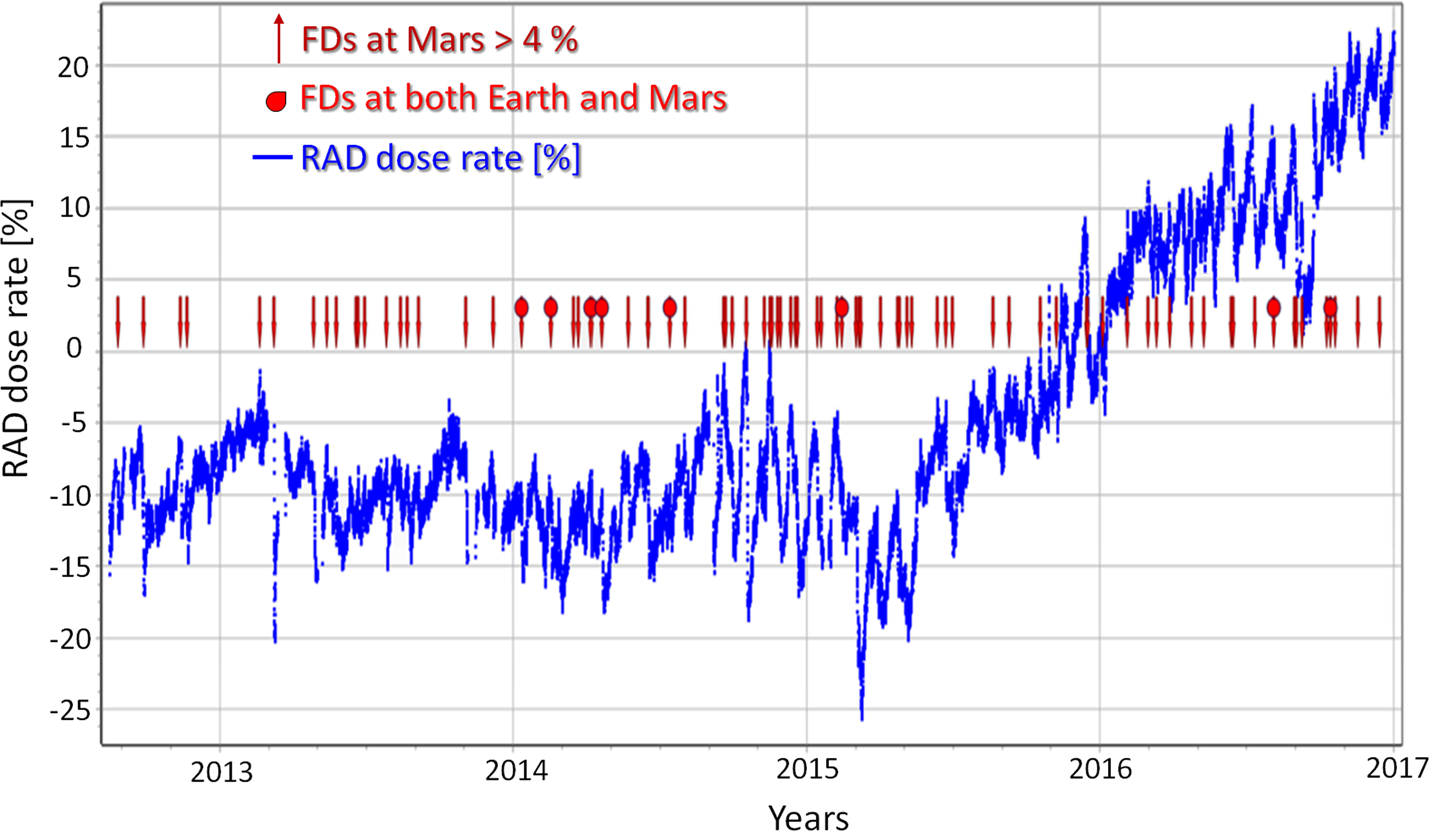
\includegraphics[trim=0 0 500 0, clip,width=\textwidth]{images/papaioannou_etal_fig2.png}}
            
    	\end{column}
    \end{columns}
\end{frame}

\begin{frame}{Deriving CME expansion from FD data (von Forstner et al. 2020)}
    \only<1>{\def\step{1}}%
    \only<2>{\def\step{2}}%
    \only<3>{\def\step{3}}%
    \only<4>{\def\step{4}}%
    \textbf{Cartoon visualization:}
    \centering%
    \pgfdeclarehorizontalshading{fdshading}{100bp}
{color(0bp)=(pgftransparent!0); color(35bp)=(pgftransparent!0);
	color(60bp)=(pgftransparent!100); color(100bp)=(pgftransparent!100)}%
\pgfdeclarefading{fdfading}{\pgfuseshading{fdshading}}%

\begin{animateinline}[autoplay]{30}%
\multiframe{61}{rAnim=0.0+0.01667}{
\begin{tikzpicture}[scale=1, fd/.style={very thick, path fading=fdfading}]
	\begin{scope} % FD
		\draw [<-,thick] (0,0.5) node (yaxis) [above] {$y/y_0$} -- (0, -3);
		\draw [<-,thick] (7,0) node (xaxis) [right] {$t$} -- (-0.2,0) node[left] {1};
	
        \ifthenelse{\step=0}{
            \def\xscale{0.66}
        }{\ifthenelse{\step=1}{
			\def\xscale{0.66}
		}{\ifthenelse{\step=2}{
			\def\xscale{0.66+\rAnim*0.34}
		}{
			\def\xscale{1}
		}}}
		\ifthenelse{\step=3}{
			\def\yscale{0.66+\rAnim*0.34}
		}{\ifthenelse{\step=4}{
            \def\yscale{1.00}
        }{
			\def\yscale{0.66}
		}}
		\begin{scope}[xscale=\xscale, yscale=\yscale]
		\ifthenelse{\step=0}{}{
            \draw[fd, green, yscale=0.66] (0, 0) -- (0.5, 0) .. controls (0.8, -1.8) and (1.3, -2) .. (2, -2) .. 
            controls (4, -2) and (4, 0) .. (6.8, 0);
        }
		\draw[fd, blue] (0, 0) -- (0.5, 0) .. controls (0.8, -1.8) and (1.3, -2) .. (2, -2) .. controls 
		(4, -2) and (4, 0) .. (6.8, 0);
		\ifthenelse{\step=0}{}{
            \draw[fd, red, yscale=1.33] (0, 0) -- (0.5, 0) .. controls (0.8, -1.8) and (1.3, -2) .. (2, -2) .. 
            controls (4, -2) and (4, 0) .. (6.8, 0);
        }
        
        
        \ifthenelse{\step=0}{
            \draw[green,|<->|,thick] (2, 0) -- node[right]{$\Delta y$} (2, -2);
            
            \draw[red, thick] (0.425, 0.45) -- node[right,yshift=-1mm]{$m_\maxt$} (0.65, -0.9); 
            
            %\draw[green,|<->|,thick] (0.5, -2.5) node[below, text=black]{$t_{\text{FD}}$} -- node[below]{$\Delta t$} (2, -2.5) node[below, text=black]{$t_\mint$};
        }{}
		\end{scope}
	\end{scope}
	
	\begin{scope}[xshift=8cm,yshift=-2.5cm] % correlation
		\draw [<-,thick] (0,3) node (yaxis) [above] {$\Delta y$} -- (0, -0.2);
		\draw [<-,thick] (3.5,0) node (xaxis) [right] {$m_\maxt$} -- (-0.2,0);
		\node[below left] at (0, 0) {0};
		
        \ifthenelse{\step=0}{
            \node at (26.565:4) [below right] {Earth};
        }{\ifthenelse{\step=1}{
			\node at (26.565:4) [below right] {Earth};
		}{
			\begin{scope}[opacity=0.4]
			\draw[thick, dashed] (0, 0) -- (26.565:4) node[below right] {Earth};
			\fill[green] (1, 0.5) circle (0.08cm);
			\fill[blue] (2, 1) circle (0.08cm);
			\fill[red] (3, 1.5) circle (0.08cm);
			\end{scope}		
		}}
	   
        \ifthenelse{\step=0}{
            \pgfmathsetmacro{\angle}{26.565}
		}{\ifthenelse{\step=1}{
			\pgfmathsetmacro{\angle}{26.565}
		}{\ifthenelse{\step=2}{
			\pgfmathsetmacro{\angle}{26.565+\rAnim*18.435}
		}{
			\pgfmathsetmacro{\angle}{45}
		}}}
        \ifthenelse{\step=0}{
            \pgfmathsetmacro{\distance}{1.118}
		}{\ifthenelse{\step=1}{
			\pgfmathsetmacro{\distance}{1.118}
		}{\ifthenelse{\step=2}{
			\pgfmathsetmacro{\distance}{1.118-\rAnim*0.411}
		}{\ifthenelse{\step=3}{
			\pgfmathsetmacro{\distance}{0.707+\rAnim*0.354}
        }{
            \pgfmathsetmacro{\distance}{1.061}
		}}}}
        \draw[thick, dashed] (0, 0) -- ++(\angle:4);
        \ifthenelse{\step=0}{}{
        \ifthenelse{\step=1}{}{
            \ifthenelse{\step=2}{\def\marstextalpha{max(0,\rAnim*3-2)}}{\def\marstextalpha{1}}
            \draw (0, 0) ++(\angle:4) node[below right,align=center,opacity=\marstextalpha] {Mars};
        }}
		\fill[blue] (\angle:2.0*\distance) circle (0.08cm);
        \ifthenelse{\step=0}{}{
            \fill[green] (\angle:\distance) circle (0.08cm);
    		\fill[red] (\angle:3.0*\distance) circle (0.08cm);
        }
	\end{scope}
\end{tikzpicture}}
\end{animateinline}\\
    \only<1>{3 FDs at Earth, observed at GCR energy $E_0$}%
    \only<2>{Same events at Mars, expanded ICME, same GCR energy $E_0$}%
    \only<3->{Same events at Mars, lower GCR energy $E_1$ + expanded ICME}\\[2mm]
    \uncover<4->{\textbf{Confirmed by analytical modeling} {\small (PDB, Wibberenz et al. 1998 \& ForbMod, Dumbović et al. 2018)}:
        \[
            \textbf{Sheath: }\frac{\Delta y_s}{m_{\text{max},s}} = \ldots = T_\text{sheath} \qquad
            \textbf{Ejecta: }\frac{\Delta y_e}{m_{\maxt,e}} = \ldots \approx 0.36 \cdot T_\text{ICME}
        \] 
    }

\end{frame}

\begin{frame}{Observations closer to the Sun}
\newcommand{\tikzAU}{8cm}
\newcommand{\tikzRe}{0.4cm}
\centering
\begin{tikzpicture}
\draw[fill=yellow] (0,0) circle (1cm) node[yshift=1.3cm]{Sun};
\draw[fill=gray] (0.38*\tikzAU,0) circle (0.38*\tikzRe) node[yshift=0.7cm]{Mercury};
\draw[fill=gray] (0.72*\tikzAU,0) circle (0.94*\tikzRe) node[yshift=0.7cm]{Venus};
\draw[fill=blue] (\tikzAU,0) circle (\tikzRe) node[yshift=0.7cm]{Earth};
\draw[fill=orange] (1.52*\tikzAU,0) circle (0.53*\tikzRe) node[yshift=0.7cm]{Mars};

\draw[decorate, decoration={brace,amplitude=10pt}] (0.72*\tikzAU,-0.6) -- (0.38*\tikzAU,-0.6) node[midway,below,yshift=-0.5cm,align=center]{$E\approx3$\\(Janvier+ 2019)};
\draw[decorate, decoration={brace,amplitude=10pt}] (\tikzAU,-0.6) -- (0.72*\tikzAU,-0.6) node[midway,below,yshift=-0.5cm,align=center]{$E\approx1.7$\\(Janvier+ 2019)};
\draw[decorate, decoration={brace,amplitude=10pt}] (1.52*\tikzAU,-0.6) -- (\tikzAU,-0.6) node[midway,below,yshift=-0.5cm,align=center]{$E \approx\ $\numrange{1.5}{1.9}\\(von Forstner+ 2020)};

\uncover<2>{
	\begin{axis}[at={(0, -4.25cm)}, axis x line=bottom, axis y line=left, x=\tikzAU, height=3cm, xmin=0, ymin=0, ymax=10, xmax=1.52, xlabel={Radial distance / \si{\AU}}, ylabel={$E/\Delta r$ / \si{\per\AU}}, ytick={0,5,10}]
	\addplot[only marks, mark=*] coordinates {(0.55,9.375) (0.86,6.07) (1.26,3.17)};
	\end{axis}
}
\end{tikzpicture}

\blfootnote{distances are to scale, sizes are not}
\end{frame}

\section{Case study of the first CME observed at Solar Orbiter}

\begin{frame}{Overview}
    \begin{columns}
        \begin{column}{0.4\textwidth}
            \begin{itemize}
                \item First CME at SolO, April 19 2020
                \item Also hit Earth and BepiColombo on April 20
                \item Ideal radial alignment ($\sim\SI{4}{\degree}$)
                \item Slow stealth CME, $v_\maxt \approx \SI{370}{\kilo\meter\per\second}$
            \end{itemize}
            \vspace{2mm}
            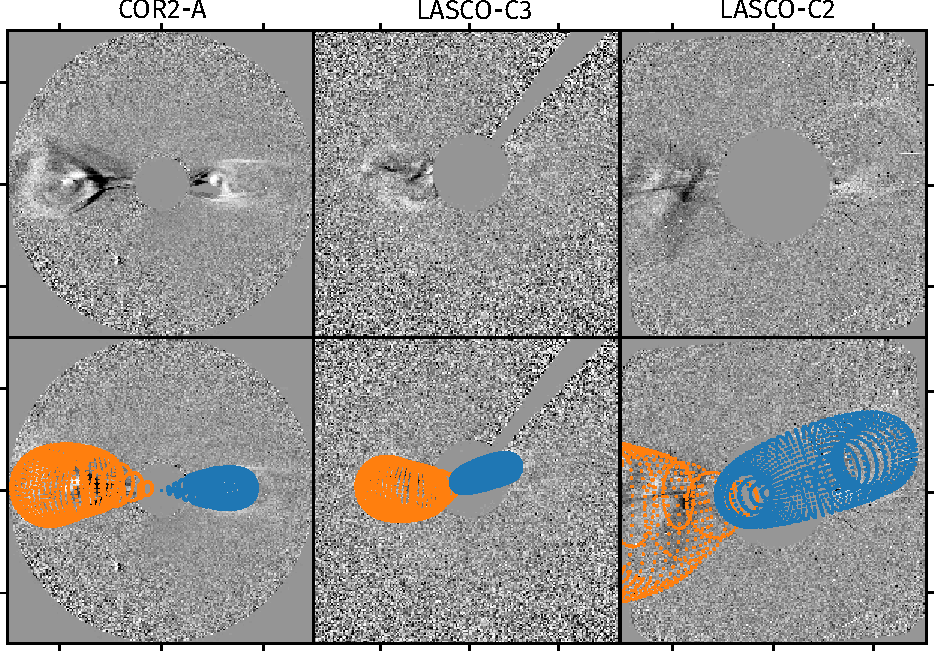
\includegraphics[width=\textwidth]{plots/gcs_reconstruction.pdf}
        \end{column}
        \begin{column}{0.5\textwidth}
            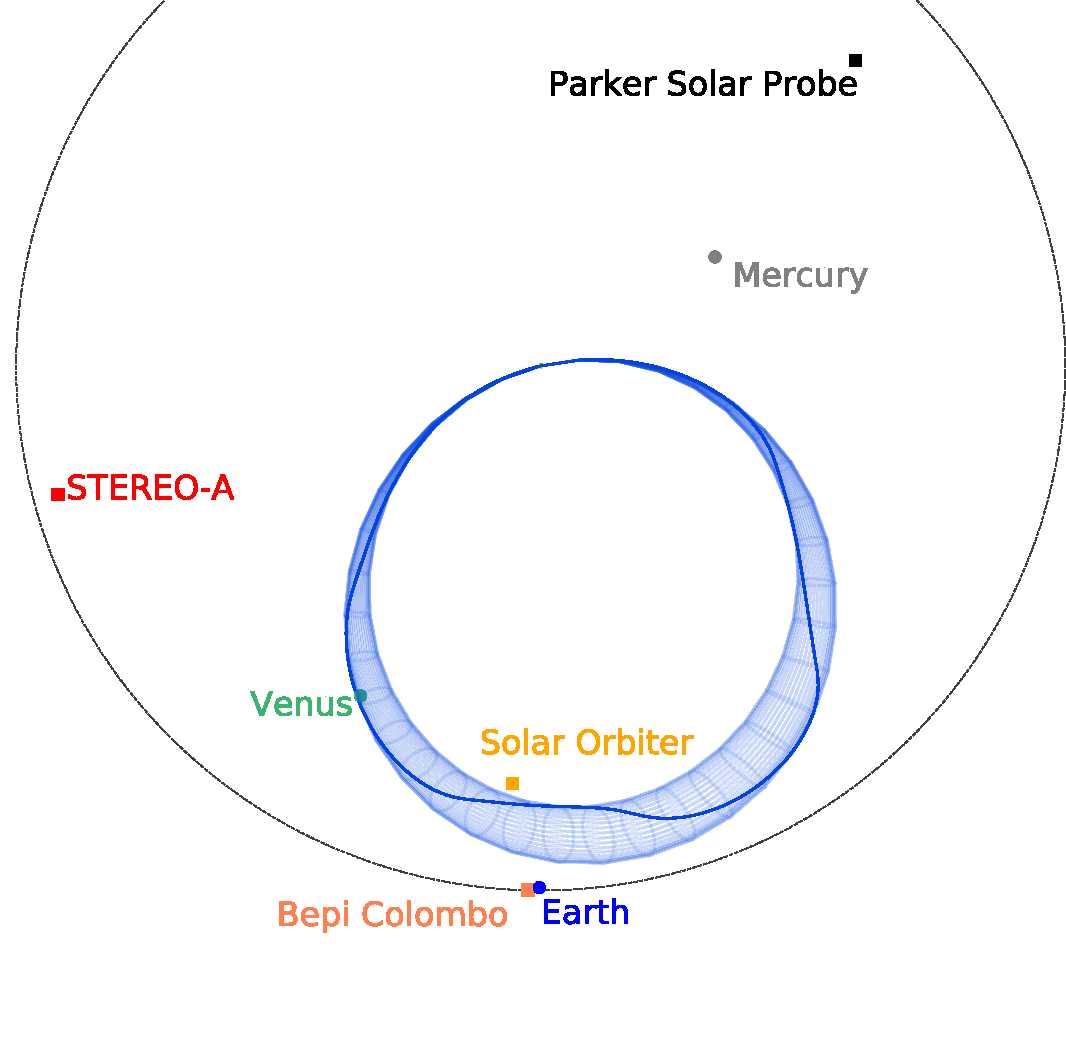
\includegraphics[width=\textwidth]{plots/3dcore_visual_davies_new_panela.pdf}
        \end{column}
    \end{columns}
\end{frame}

\begin{frame}{In situ data}
    \vskip3mm
    \begin{columns}
        \begin{column}{0.5\textwidth}
            \centering
            \textbf{Solar Orbiter}\\
            \scalebox{0.5}{
                %% Creator: Matplotlib, PGF backend
%%
%% To include the figure in your LaTeX document, write
%%   \input{<filename>.pgf}
%%
%% Make sure the required packages are loaded in your preamble
%%   \usepackage{pgf}
%%
%% and, on pdftex
%%   \usepackage[utf8]{inputenc}\DeclareUnicodeCharacter{2212}{-}
%%
%% or, on luatex and xetex
%%   \usepackage{unicode-math}
%%
%% Figures using additional raster images can only be included by \input if
%% they are in the same directory as the main LaTeX file. For loading figures
%% from other directories you can use the `import` package
%%   \usepackage{import}
%%
%% and then include the figures with
%%   \import{<path to file>}{<filename>.pgf}
%%
%% Matplotlib used the following preamble
%%   \usepackage{siunitx}
%%   \usepackage[sfdefault]{FiraSans}
%%   \usepackage[T1]{fontenc}
%%   \usepackage{fontspec}
%%
\begingroup%
\makeatletter%
\begin{pgfpicture}%
\pgfpathrectangle{\pgfpointorigin}{\pgfqpoint{6.000000in}{5.500000in}}%
\pgfusepath{use as bounding box, clip}%
\begin{pgfscope}%
\pgfsetbuttcap%
\pgfsetmiterjoin%
\definecolor{currentfill}{rgb}{1.000000,1.000000,1.000000}%
\pgfsetfillcolor{currentfill}%
\pgfsetlinewidth{0.000000pt}%
\definecolor{currentstroke}{rgb}{1.000000,1.000000,1.000000}%
\pgfsetstrokecolor{currentstroke}%
\pgfsetdash{}{0pt}%
\pgfpathmoveto{\pgfqpoint{0.000000in}{0.000000in}}%
\pgfpathlineto{\pgfqpoint{6.000000in}{0.000000in}}%
\pgfpathlineto{\pgfqpoint{6.000000in}{5.500000in}}%
\pgfpathlineto{\pgfqpoint{0.000000in}{5.500000in}}%
\pgfpathclose%
\pgfusepath{fill}%
\end{pgfscope}%
\begin{pgfscope}%
\definecolor{textcolor}{rgb}{0.000000,0.000000,0.000000}%
\pgfsetstrokecolor{textcolor}%
\pgfsetfillcolor{textcolor}%
\pgftext[x=2.289748in,y=5.232648in,,base]{\color{textcolor}\sffamily\fontsize{10.800000}{12.960000}\selectfont Shock}%
\end{pgfscope}%
\begin{pgfscope}%
\definecolor{textcolor}{rgb}{0.000000,0.000000,0.000000}%
\pgfsetstrokecolor{textcolor}%
\pgfsetfillcolor{textcolor}%
\pgftext[x=2.970334in,y=5.232648in,,base]{\color{textcolor}\sffamily\fontsize{10.800000}{12.960000}\selectfont CME}%
\end{pgfscope}%
\begin{pgfscope}%
\definecolor{textcolor}{rgb}{0.000000,0.000000,0.000000}%
\pgfsetstrokecolor{textcolor}%
\pgfsetfillcolor{textcolor}%
\pgftext[x=3.668916in,y=5.232648in,,base]{\color{textcolor}\sffamily\fontsize{10.800000}{12.960000}\selectfont F}%
\end{pgfscope}%
\begin{pgfscope}%
\definecolor{textcolor}{rgb}{0.000000,0.000000,0.000000}%
\pgfsetstrokecolor{textcolor}%
\pgfsetfillcolor{textcolor}%
\pgftext[x=3.889621in,y=5.232648in,,base]{\color{textcolor}\sffamily\fontsize{10.800000}{12.960000}\selectfont I}%
\end{pgfscope}%
\begin{pgfscope}%
\definecolor{textcolor}{rgb}{0.000000,0.000000,0.000000}%
\pgfsetstrokecolor{textcolor}%
\pgfsetfillcolor{textcolor}%
\pgftext[x=4.147268in,y=5.232648in,,base]{\color{textcolor}\sffamily\fontsize{10.800000}{12.960000}\selectfont R}%
\end{pgfscope}%
\begin{pgfscope}%
\pgfsetbuttcap%
\pgfsetmiterjoin%
\definecolor{currentfill}{rgb}{1.000000,1.000000,1.000000}%
\pgfsetfillcolor{currentfill}%
\pgfsetlinewidth{0.000000pt}%
\definecolor{currentstroke}{rgb}{0.000000,0.000000,0.000000}%
\pgfsetstrokecolor{currentstroke}%
\pgfsetstrokeopacity{0.000000}%
\pgfsetdash{}{0pt}%
\pgfpathmoveto{\pgfqpoint{0.636356in}{3.670005in}}%
\pgfpathlineto{\pgfqpoint{4.784755in}{3.670005in}}%
\pgfpathlineto{\pgfqpoint{4.784755in}{5.123626in}}%
\pgfpathlineto{\pgfqpoint{0.636356in}{5.123626in}}%
\pgfpathclose%
\pgfusepath{fill}%
\end{pgfscope}%
\begin{pgfscope}%
\pgfpathrectangle{\pgfqpoint{0.636356in}{3.670005in}}{\pgfqpoint{4.148398in}{1.453621in}}%
\pgfusepath{clip}%
\pgfsetbuttcap%
\pgfsetmiterjoin%
\definecolor{currentfill}{rgb}{0.737255,0.741176,0.133333}%
\pgfsetfillcolor{currentfill}%
\pgfsetfillopacity{0.100000}%
\pgfsetlinewidth{1.003750pt}%
\definecolor{currentstroke}{rgb}{0.737255,0.741176,0.133333}%
\pgfsetstrokecolor{currentstroke}%
\pgfsetstrokeopacity{0.100000}%
\pgfsetdash{}{0pt}%
\pgfpathmoveto{\pgfqpoint{2.509506in}{3.670005in}}%
\pgfpathlineto{\pgfqpoint{2.509506in}{5.123626in}}%
\pgfpathlineto{\pgfqpoint{3.431161in}{5.123626in}}%
\pgfpathlineto{\pgfqpoint{3.431161in}{3.670005in}}%
\pgfpathclose%
\pgfusepath{stroke,fill}%
\end{pgfscope}%
\begin{pgfscope}%
\pgfpathrectangle{\pgfqpoint{0.636356in}{3.670005in}}{\pgfqpoint{4.148398in}{1.453621in}}%
\pgfusepath{clip}%
\pgfsetbuttcap%
\pgfsetmiterjoin%
\definecolor{currentfill}{rgb}{0.090196,0.745098,0.811765}%
\pgfsetfillcolor{currentfill}%
\pgfsetfillopacity{0.100000}%
\pgfsetlinewidth{1.003750pt}%
\definecolor{currentstroke}{rgb}{0.090196,0.745098,0.811765}%
\pgfsetstrokecolor{currentstroke}%
\pgfsetstrokeopacity{0.100000}%
\pgfsetdash{}{0pt}%
\pgfpathmoveto{\pgfqpoint{3.668916in}{3.670005in}}%
\pgfpathlineto{\pgfqpoint{3.668916in}{5.123626in}}%
\pgfpathlineto{\pgfqpoint{4.147268in}{5.123626in}}%
\pgfpathlineto{\pgfqpoint{4.147268in}{3.670005in}}%
\pgfpathclose%
\pgfusepath{stroke,fill}%
\end{pgfscope}%
\begin{pgfscope}%
\pgfsetbuttcap%
\pgfsetroundjoin%
\definecolor{currentfill}{rgb}{0.000000,0.000000,0.000000}%
\pgfsetfillcolor{currentfill}%
\pgfsetlinewidth{0.803000pt}%
\definecolor{currentstroke}{rgb}{0.000000,0.000000,0.000000}%
\pgfsetstrokecolor{currentstroke}%
\pgfsetdash{}{0pt}%
\pgfsys@defobject{currentmarker}{\pgfqpoint{0.000000in}{-0.048611in}}{\pgfqpoint{0.000000in}{0.048611in}}{%
\pgfpathmoveto{\pgfqpoint{0.000000in}{-0.048611in}}%
\pgfpathlineto{\pgfqpoint{0.000000in}{0.048611in}}%
\pgfusepath{stroke,fill}%
}%
\begin{pgfscope}%
\pgfsys@transformshift{1.317889in}{3.670005in}%
\pgfsys@useobject{currentmarker}{}%
\end{pgfscope}%
\end{pgfscope}%
\begin{pgfscope}%
\pgfsetbuttcap%
\pgfsetroundjoin%
\definecolor{currentfill}{rgb}{0.000000,0.000000,0.000000}%
\pgfsetfillcolor{currentfill}%
\pgfsetlinewidth{0.803000pt}%
\definecolor{currentstroke}{rgb}{0.000000,0.000000,0.000000}%
\pgfsetstrokecolor{currentstroke}%
\pgfsetdash{}{0pt}%
\pgfsys@defobject{currentmarker}{\pgfqpoint{0.000000in}{-0.048611in}}{\pgfqpoint{0.000000in}{0.048611in}}{%
\pgfpathmoveto{\pgfqpoint{0.000000in}{-0.048611in}}%
\pgfpathlineto{\pgfqpoint{0.000000in}{0.048611in}}%
\pgfusepath{stroke,fill}%
}%
\begin{pgfscope}%
\pgfsys@transformshift{1.317889in}{5.123626in}%
\pgfsys@useobject{currentmarker}{}%
\end{pgfscope}%
\end{pgfscope}%
\begin{pgfscope}%
\pgfsetbuttcap%
\pgfsetroundjoin%
\definecolor{currentfill}{rgb}{0.000000,0.000000,0.000000}%
\pgfsetfillcolor{currentfill}%
\pgfsetlinewidth{0.803000pt}%
\definecolor{currentstroke}{rgb}{0.000000,0.000000,0.000000}%
\pgfsetstrokecolor{currentstroke}%
\pgfsetdash{}{0pt}%
\pgfsys@defobject{currentmarker}{\pgfqpoint{0.000000in}{-0.048611in}}{\pgfqpoint{0.000000in}{0.048611in}}{%
\pgfpathmoveto{\pgfqpoint{0.000000in}{-0.048611in}}%
\pgfpathlineto{\pgfqpoint{0.000000in}{0.048611in}}%
\pgfusepath{stroke,fill}%
}%
\begin{pgfscope}%
\pgfsys@transformshift{1.999895in}{3.670005in}%
\pgfsys@useobject{currentmarker}{}%
\end{pgfscope}%
\end{pgfscope}%
\begin{pgfscope}%
\pgfsetbuttcap%
\pgfsetroundjoin%
\definecolor{currentfill}{rgb}{0.000000,0.000000,0.000000}%
\pgfsetfillcolor{currentfill}%
\pgfsetlinewidth{0.803000pt}%
\definecolor{currentstroke}{rgb}{0.000000,0.000000,0.000000}%
\pgfsetstrokecolor{currentstroke}%
\pgfsetdash{}{0pt}%
\pgfsys@defobject{currentmarker}{\pgfqpoint{0.000000in}{-0.048611in}}{\pgfqpoint{0.000000in}{0.048611in}}{%
\pgfpathmoveto{\pgfqpoint{0.000000in}{-0.048611in}}%
\pgfpathlineto{\pgfqpoint{0.000000in}{0.048611in}}%
\pgfusepath{stroke,fill}%
}%
\begin{pgfscope}%
\pgfsys@transformshift{1.999895in}{5.123626in}%
\pgfsys@useobject{currentmarker}{}%
\end{pgfscope}%
\end{pgfscope}%
\begin{pgfscope}%
\pgfsetbuttcap%
\pgfsetroundjoin%
\definecolor{currentfill}{rgb}{0.000000,0.000000,0.000000}%
\pgfsetfillcolor{currentfill}%
\pgfsetlinewidth{0.803000pt}%
\definecolor{currentstroke}{rgb}{0.000000,0.000000,0.000000}%
\pgfsetstrokecolor{currentstroke}%
\pgfsetdash{}{0pt}%
\pgfsys@defobject{currentmarker}{\pgfqpoint{0.000000in}{-0.048611in}}{\pgfqpoint{0.000000in}{0.048611in}}{%
\pgfpathmoveto{\pgfqpoint{0.000000in}{-0.048611in}}%
\pgfpathlineto{\pgfqpoint{0.000000in}{0.048611in}}%
\pgfusepath{stroke,fill}%
}%
\begin{pgfscope}%
\pgfsys@transformshift{2.681902in}{3.670005in}%
\pgfsys@useobject{currentmarker}{}%
\end{pgfscope}%
\end{pgfscope}%
\begin{pgfscope}%
\pgfsetbuttcap%
\pgfsetroundjoin%
\definecolor{currentfill}{rgb}{0.000000,0.000000,0.000000}%
\pgfsetfillcolor{currentfill}%
\pgfsetlinewidth{0.803000pt}%
\definecolor{currentstroke}{rgb}{0.000000,0.000000,0.000000}%
\pgfsetstrokecolor{currentstroke}%
\pgfsetdash{}{0pt}%
\pgfsys@defobject{currentmarker}{\pgfqpoint{0.000000in}{-0.048611in}}{\pgfqpoint{0.000000in}{0.048611in}}{%
\pgfpathmoveto{\pgfqpoint{0.000000in}{-0.048611in}}%
\pgfpathlineto{\pgfqpoint{0.000000in}{0.048611in}}%
\pgfusepath{stroke,fill}%
}%
\begin{pgfscope}%
\pgfsys@transformshift{2.681902in}{5.123626in}%
\pgfsys@useobject{currentmarker}{}%
\end{pgfscope}%
\end{pgfscope}%
\begin{pgfscope}%
\pgfsetbuttcap%
\pgfsetroundjoin%
\definecolor{currentfill}{rgb}{0.000000,0.000000,0.000000}%
\pgfsetfillcolor{currentfill}%
\pgfsetlinewidth{0.803000pt}%
\definecolor{currentstroke}{rgb}{0.000000,0.000000,0.000000}%
\pgfsetstrokecolor{currentstroke}%
\pgfsetdash{}{0pt}%
\pgfsys@defobject{currentmarker}{\pgfqpoint{0.000000in}{-0.048611in}}{\pgfqpoint{0.000000in}{0.048611in}}{%
\pgfpathmoveto{\pgfqpoint{0.000000in}{-0.048611in}}%
\pgfpathlineto{\pgfqpoint{0.000000in}{0.048611in}}%
\pgfusepath{stroke,fill}%
}%
\begin{pgfscope}%
\pgfsys@transformshift{3.363908in}{3.670005in}%
\pgfsys@useobject{currentmarker}{}%
\end{pgfscope}%
\end{pgfscope}%
\begin{pgfscope}%
\pgfsetbuttcap%
\pgfsetroundjoin%
\definecolor{currentfill}{rgb}{0.000000,0.000000,0.000000}%
\pgfsetfillcolor{currentfill}%
\pgfsetlinewidth{0.803000pt}%
\definecolor{currentstroke}{rgb}{0.000000,0.000000,0.000000}%
\pgfsetstrokecolor{currentstroke}%
\pgfsetdash{}{0pt}%
\pgfsys@defobject{currentmarker}{\pgfqpoint{0.000000in}{-0.048611in}}{\pgfqpoint{0.000000in}{0.048611in}}{%
\pgfpathmoveto{\pgfqpoint{0.000000in}{-0.048611in}}%
\pgfpathlineto{\pgfqpoint{0.000000in}{0.048611in}}%
\pgfusepath{stroke,fill}%
}%
\begin{pgfscope}%
\pgfsys@transformshift{3.363908in}{5.123626in}%
\pgfsys@useobject{currentmarker}{}%
\end{pgfscope}%
\end{pgfscope}%
\begin{pgfscope}%
\pgfsetbuttcap%
\pgfsetroundjoin%
\definecolor{currentfill}{rgb}{0.000000,0.000000,0.000000}%
\pgfsetfillcolor{currentfill}%
\pgfsetlinewidth{0.803000pt}%
\definecolor{currentstroke}{rgb}{0.000000,0.000000,0.000000}%
\pgfsetstrokecolor{currentstroke}%
\pgfsetdash{}{0pt}%
\pgfsys@defobject{currentmarker}{\pgfqpoint{0.000000in}{-0.048611in}}{\pgfqpoint{0.000000in}{0.048611in}}{%
\pgfpathmoveto{\pgfqpoint{0.000000in}{-0.048611in}}%
\pgfpathlineto{\pgfqpoint{0.000000in}{0.048611in}}%
\pgfusepath{stroke,fill}%
}%
\begin{pgfscope}%
\pgfsys@transformshift{4.045914in}{3.670005in}%
\pgfsys@useobject{currentmarker}{}%
\end{pgfscope}%
\end{pgfscope}%
\begin{pgfscope}%
\pgfsetbuttcap%
\pgfsetroundjoin%
\definecolor{currentfill}{rgb}{0.000000,0.000000,0.000000}%
\pgfsetfillcolor{currentfill}%
\pgfsetlinewidth{0.803000pt}%
\definecolor{currentstroke}{rgb}{0.000000,0.000000,0.000000}%
\pgfsetstrokecolor{currentstroke}%
\pgfsetdash{}{0pt}%
\pgfsys@defobject{currentmarker}{\pgfqpoint{0.000000in}{-0.048611in}}{\pgfqpoint{0.000000in}{0.048611in}}{%
\pgfpathmoveto{\pgfqpoint{0.000000in}{-0.048611in}}%
\pgfpathlineto{\pgfqpoint{0.000000in}{0.048611in}}%
\pgfusepath{stroke,fill}%
}%
\begin{pgfscope}%
\pgfsys@transformshift{4.045914in}{5.123626in}%
\pgfsys@useobject{currentmarker}{}%
\end{pgfscope}%
\end{pgfscope}%
\begin{pgfscope}%
\pgfsetbuttcap%
\pgfsetroundjoin%
\definecolor{currentfill}{rgb}{0.000000,0.000000,0.000000}%
\pgfsetfillcolor{currentfill}%
\pgfsetlinewidth{0.803000pt}%
\definecolor{currentstroke}{rgb}{0.000000,0.000000,0.000000}%
\pgfsetstrokecolor{currentstroke}%
\pgfsetdash{}{0pt}%
\pgfsys@defobject{currentmarker}{\pgfqpoint{0.000000in}{-0.048611in}}{\pgfqpoint{0.000000in}{0.048611in}}{%
\pgfpathmoveto{\pgfqpoint{0.000000in}{-0.048611in}}%
\pgfpathlineto{\pgfqpoint{0.000000in}{0.048611in}}%
\pgfusepath{stroke,fill}%
}%
\begin{pgfscope}%
\pgfsys@transformshift{4.727921in}{3.670005in}%
\pgfsys@useobject{currentmarker}{}%
\end{pgfscope}%
\end{pgfscope}%
\begin{pgfscope}%
\pgfsetbuttcap%
\pgfsetroundjoin%
\definecolor{currentfill}{rgb}{0.000000,0.000000,0.000000}%
\pgfsetfillcolor{currentfill}%
\pgfsetlinewidth{0.803000pt}%
\definecolor{currentstroke}{rgb}{0.000000,0.000000,0.000000}%
\pgfsetstrokecolor{currentstroke}%
\pgfsetdash{}{0pt}%
\pgfsys@defobject{currentmarker}{\pgfqpoint{0.000000in}{-0.048611in}}{\pgfqpoint{0.000000in}{0.048611in}}{%
\pgfpathmoveto{\pgfqpoint{0.000000in}{-0.048611in}}%
\pgfpathlineto{\pgfqpoint{0.000000in}{0.048611in}}%
\pgfusepath{stroke,fill}%
}%
\begin{pgfscope}%
\pgfsys@transformshift{4.727921in}{5.123626in}%
\pgfsys@useobject{currentmarker}{}%
\end{pgfscope}%
\end{pgfscope}%
\begin{pgfscope}%
\pgfsetbuttcap%
\pgfsetroundjoin%
\definecolor{currentfill}{rgb}{0.000000,0.000000,0.000000}%
\pgfsetfillcolor{currentfill}%
\pgfsetlinewidth{0.803000pt}%
\definecolor{currentstroke}{rgb}{0.000000,0.000000,0.000000}%
\pgfsetstrokecolor{currentstroke}%
\pgfsetdash{}{0pt}%
\pgfsys@defobject{currentmarker}{\pgfqpoint{-0.048611in}{0.000000in}}{\pgfqpoint{-0.000000in}{0.000000in}}{%
\pgfpathmoveto{\pgfqpoint{-0.000000in}{0.000000in}}%
\pgfpathlineto{\pgfqpoint{-0.048611in}{0.000000in}}%
\pgfusepath{stroke,fill}%
}%
\begin{pgfscope}%
\pgfsys@transformshift{0.636356in}{3.758359in}%
\pgfsys@useobject{currentmarker}{}%
\end{pgfscope}%
\end{pgfscope}%
\begin{pgfscope}%
\definecolor{textcolor}{rgb}{0.000000,0.000000,0.000000}%
\pgfsetstrokecolor{textcolor}%
\pgfsetfillcolor{textcolor}%
\pgftext[x=0.310788in, y=3.711484in, left, base]{\color{textcolor}\sffamily\fontsize{9.000000}{10.800000}\selectfont \(\displaystyle {−20}\)}%
\end{pgfscope}%
\begin{pgfscope}%
\pgfsetbuttcap%
\pgfsetroundjoin%
\definecolor{currentfill}{rgb}{0.000000,0.000000,0.000000}%
\pgfsetfillcolor{currentfill}%
\pgfsetlinewidth{0.803000pt}%
\definecolor{currentstroke}{rgb}{0.000000,0.000000,0.000000}%
\pgfsetstrokecolor{currentstroke}%
\pgfsetdash{}{0pt}%
\pgfsys@defobject{currentmarker}{\pgfqpoint{-0.048611in}{0.000000in}}{\pgfqpoint{-0.000000in}{0.000000in}}{%
\pgfpathmoveto{\pgfqpoint{-0.000000in}{0.000000in}}%
\pgfpathlineto{\pgfqpoint{-0.048611in}{0.000000in}}%
\pgfusepath{stroke,fill}%
}%
\begin{pgfscope}%
\pgfsys@transformshift{0.636356in}{4.073721in}%
\pgfsys@useobject{currentmarker}{}%
\end{pgfscope}%
\end{pgfscope}%
\begin{pgfscope}%
\definecolor{textcolor}{rgb}{0.000000,0.000000,0.000000}%
\pgfsetstrokecolor{textcolor}%
\pgfsetfillcolor{textcolor}%
\pgftext[x=0.310788in, y=4.026846in, left, base]{\color{textcolor}\sffamily\fontsize{9.000000}{10.800000}\selectfont \(\displaystyle {−10}\)}%
\end{pgfscope}%
\begin{pgfscope}%
\pgfsetbuttcap%
\pgfsetroundjoin%
\definecolor{currentfill}{rgb}{0.000000,0.000000,0.000000}%
\pgfsetfillcolor{currentfill}%
\pgfsetlinewidth{0.803000pt}%
\definecolor{currentstroke}{rgb}{0.000000,0.000000,0.000000}%
\pgfsetstrokecolor{currentstroke}%
\pgfsetdash{}{0pt}%
\pgfsys@defobject{currentmarker}{\pgfqpoint{-0.048611in}{0.000000in}}{\pgfqpoint{-0.000000in}{0.000000in}}{%
\pgfpathmoveto{\pgfqpoint{-0.000000in}{0.000000in}}%
\pgfpathlineto{\pgfqpoint{-0.048611in}{0.000000in}}%
\pgfusepath{stroke,fill}%
}%
\begin{pgfscope}%
\pgfsys@transformshift{0.636356in}{4.389083in}%
\pgfsys@useobject{currentmarker}{}%
\end{pgfscope}%
\end{pgfscope}%
\begin{pgfscope}%
\definecolor{textcolor}{rgb}{0.000000,0.000000,0.000000}%
\pgfsetstrokecolor{textcolor}%
\pgfsetfillcolor{textcolor}%
\pgftext[x=0.474898in, y=4.342208in, left, base]{\color{textcolor}\sffamily\fontsize{9.000000}{10.800000}\selectfont \(\displaystyle {0}\)}%
\end{pgfscope}%
\begin{pgfscope}%
\pgfsetbuttcap%
\pgfsetroundjoin%
\definecolor{currentfill}{rgb}{0.000000,0.000000,0.000000}%
\pgfsetfillcolor{currentfill}%
\pgfsetlinewidth{0.803000pt}%
\definecolor{currentstroke}{rgb}{0.000000,0.000000,0.000000}%
\pgfsetstrokecolor{currentstroke}%
\pgfsetdash{}{0pt}%
\pgfsys@defobject{currentmarker}{\pgfqpoint{-0.048611in}{0.000000in}}{\pgfqpoint{-0.000000in}{0.000000in}}{%
\pgfpathmoveto{\pgfqpoint{-0.000000in}{0.000000in}}%
\pgfpathlineto{\pgfqpoint{-0.048611in}{0.000000in}}%
\pgfusepath{stroke,fill}%
}%
\begin{pgfscope}%
\pgfsys@transformshift{0.636356in}{4.704445in}%
\pgfsys@useobject{currentmarker}{}%
\end{pgfscope}%
\end{pgfscope}%
\begin{pgfscope}%
\definecolor{textcolor}{rgb}{0.000000,0.000000,0.000000}%
\pgfsetstrokecolor{textcolor}%
\pgfsetfillcolor{textcolor}%
\pgftext[x=0.410663in, y=4.657570in, left, base]{\color{textcolor}\sffamily\fontsize{9.000000}{10.800000}\selectfont \(\displaystyle {10}\)}%
\end{pgfscope}%
\begin{pgfscope}%
\pgfsetbuttcap%
\pgfsetroundjoin%
\definecolor{currentfill}{rgb}{0.000000,0.000000,0.000000}%
\pgfsetfillcolor{currentfill}%
\pgfsetlinewidth{0.803000pt}%
\definecolor{currentstroke}{rgb}{0.000000,0.000000,0.000000}%
\pgfsetstrokecolor{currentstroke}%
\pgfsetdash{}{0pt}%
\pgfsys@defobject{currentmarker}{\pgfqpoint{-0.048611in}{0.000000in}}{\pgfqpoint{-0.000000in}{0.000000in}}{%
\pgfpathmoveto{\pgfqpoint{-0.000000in}{0.000000in}}%
\pgfpathlineto{\pgfqpoint{-0.048611in}{0.000000in}}%
\pgfusepath{stroke,fill}%
}%
\begin{pgfscope}%
\pgfsys@transformshift{0.636356in}{5.019807in}%
\pgfsys@useobject{currentmarker}{}%
\end{pgfscope}%
\end{pgfscope}%
\begin{pgfscope}%
\definecolor{textcolor}{rgb}{0.000000,0.000000,0.000000}%
\pgfsetstrokecolor{textcolor}%
\pgfsetfillcolor{textcolor}%
\pgftext[x=0.410663in, y=4.972932in, left, base]{\color{textcolor}\sffamily\fontsize{9.000000}{10.800000}\selectfont \(\displaystyle {20}\)}%
\end{pgfscope}%
\begin{pgfscope}%
\definecolor{textcolor}{rgb}{0.000000,0.000000,0.000000}%
\pgfsetstrokecolor{textcolor}%
\pgfsetfillcolor{textcolor}%
\pgftext[x=0.255232in,y=4.396816in,,bottom,rotate=90.000000]{\color{textcolor}\sffamily\fontsize{9.000000}{10.800000}\selectfont B [nT]}%
\end{pgfscope}%
\begin{pgfscope}%
\pgfpathrectangle{\pgfqpoint{0.636356in}{3.670005in}}{\pgfqpoint{4.148398in}{1.453621in}}%
\pgfusepath{clip}%
\pgfsetrectcap%
\pgfsetroundjoin%
\pgfsetlinewidth{0.752812pt}%
\definecolor{currentstroke}{rgb}{0.121569,0.466667,0.705882}%
\pgfsetstrokecolor{currentstroke}%
\pgfsetdash{}{0pt}%
\pgfpathmoveto{\pgfqpoint{0.636356in}{4.486023in}}%
\pgfpathlineto{\pgfqpoint{0.637304in}{4.482765in}}%
\pgfpathlineto{\pgfqpoint{0.639198in}{4.489077in}}%
\pgfpathlineto{\pgfqpoint{0.640145in}{4.478101in}}%
\pgfpathlineto{\pgfqpoint{0.642040in}{4.485837in}}%
\pgfpathlineto{\pgfqpoint{0.642987in}{4.485548in}}%
\pgfpathlineto{\pgfqpoint{0.643934in}{4.481341in}}%
\pgfpathlineto{\pgfqpoint{0.644881in}{4.495107in}}%
\pgfpathlineto{\pgfqpoint{0.645829in}{4.492774in}}%
\pgfpathlineto{\pgfqpoint{0.646776in}{4.498088in}}%
\pgfpathlineto{\pgfqpoint{0.648670in}{4.496537in}}%
\pgfpathlineto{\pgfqpoint{0.649618in}{4.492258in}}%
\pgfpathlineto{\pgfqpoint{0.650565in}{4.497370in}}%
\pgfpathlineto{\pgfqpoint{0.651512in}{4.491584in}}%
\pgfpathlineto{\pgfqpoint{0.652459in}{4.501330in}}%
\pgfpathlineto{\pgfqpoint{0.653406in}{4.494926in}}%
\pgfpathlineto{\pgfqpoint{0.654354in}{4.476402in}}%
\pgfpathlineto{\pgfqpoint{0.656248in}{4.498953in}}%
\pgfpathlineto{\pgfqpoint{0.657195in}{4.499728in}}%
\pgfpathlineto{\pgfqpoint{0.658143in}{4.498169in}}%
\pgfpathlineto{\pgfqpoint{0.660037in}{4.484463in}}%
\pgfpathlineto{\pgfqpoint{0.660984in}{4.496226in}}%
\pgfpathlineto{\pgfqpoint{0.662879in}{4.480508in}}%
\pgfpathlineto{\pgfqpoint{0.663826in}{4.489926in}}%
\pgfpathlineto{\pgfqpoint{0.664773in}{4.476842in}}%
\pgfpathlineto{\pgfqpoint{0.666668in}{4.493465in}}%
\pgfpathlineto{\pgfqpoint{0.667615in}{4.490949in}}%
\pgfpathlineto{\pgfqpoint{0.668562in}{4.491912in}}%
\pgfpathlineto{\pgfqpoint{0.669509in}{4.490337in}}%
\pgfpathlineto{\pgfqpoint{0.670457in}{4.496800in}}%
\pgfpathlineto{\pgfqpoint{0.676140in}{4.486246in}}%
\pgfpathlineto{\pgfqpoint{0.677087in}{4.494281in}}%
\pgfpathlineto{\pgfqpoint{0.678035in}{4.493965in}}%
\pgfpathlineto{\pgfqpoint{0.678982in}{4.487763in}}%
\pgfpathlineto{\pgfqpoint{0.679929in}{4.495262in}}%
\pgfpathlineto{\pgfqpoint{0.681823in}{4.487898in}}%
\pgfpathlineto{\pgfqpoint{0.682771in}{4.507011in}}%
\pgfpathlineto{\pgfqpoint{0.683718in}{4.492482in}}%
\pgfpathlineto{\pgfqpoint{0.684665in}{4.510107in}}%
\pgfpathlineto{\pgfqpoint{0.685612in}{4.498267in}}%
\pgfpathlineto{\pgfqpoint{0.686560in}{4.499976in}}%
\pgfpathlineto{\pgfqpoint{0.687507in}{4.506173in}}%
\pgfpathlineto{\pgfqpoint{0.689401in}{4.502442in}}%
\pgfpathlineto{\pgfqpoint{0.690349in}{4.503776in}}%
\pgfpathlineto{\pgfqpoint{0.691296in}{4.501209in}}%
\pgfpathlineto{\pgfqpoint{0.693190in}{4.503561in}}%
\pgfpathlineto{\pgfqpoint{0.694137in}{4.502296in}}%
\pgfpathlineto{\pgfqpoint{0.696032in}{4.493749in}}%
\pgfpathlineto{\pgfqpoint{0.696979in}{4.497947in}}%
\pgfpathlineto{\pgfqpoint{0.697926in}{4.494058in}}%
\pgfpathlineto{\pgfqpoint{0.698874in}{4.495125in}}%
\pgfpathlineto{\pgfqpoint{0.699821in}{4.491905in}}%
\pgfpathlineto{\pgfqpoint{0.702663in}{4.494442in}}%
\pgfpathlineto{\pgfqpoint{0.703610in}{4.490769in}}%
\pgfpathlineto{\pgfqpoint{0.704557in}{4.493888in}}%
\pgfpathlineto{\pgfqpoint{0.705504in}{4.489774in}}%
\pgfpathlineto{\pgfqpoint{0.707399in}{4.499610in}}%
\pgfpathlineto{\pgfqpoint{0.710240in}{4.492546in}}%
\pgfpathlineto{\pgfqpoint{0.712135in}{4.503572in}}%
\pgfpathlineto{\pgfqpoint{0.713082in}{4.503889in}}%
\pgfpathlineto{\pgfqpoint{0.714977in}{4.502598in}}%
\pgfpathlineto{\pgfqpoint{0.716871in}{4.505178in}}%
\pgfpathlineto{\pgfqpoint{0.717818in}{4.503679in}}%
\pgfpathlineto{\pgfqpoint{0.718765in}{4.504722in}}%
\pgfpathlineto{\pgfqpoint{0.720660in}{4.501229in}}%
\pgfpathlineto{\pgfqpoint{0.721607in}{4.502356in}}%
\pgfpathlineto{\pgfqpoint{0.722554in}{4.508892in}}%
\pgfpathlineto{\pgfqpoint{0.724449in}{4.505879in}}%
\pgfpathlineto{\pgfqpoint{0.727291in}{4.498521in}}%
\pgfpathlineto{\pgfqpoint{0.728238in}{4.500396in}}%
\pgfpathlineto{\pgfqpoint{0.729185in}{4.500805in}}%
\pgfpathlineto{\pgfqpoint{0.730132in}{4.498473in}}%
\pgfpathlineto{\pgfqpoint{0.731079in}{4.490569in}}%
\pgfpathlineto{\pgfqpoint{0.732974in}{4.492875in}}%
\pgfpathlineto{\pgfqpoint{0.733921in}{4.491290in}}%
\pgfpathlineto{\pgfqpoint{0.734868in}{4.500196in}}%
\pgfpathlineto{\pgfqpoint{0.735816in}{4.499885in}}%
\pgfpathlineto{\pgfqpoint{0.736763in}{4.500133in}}%
\pgfpathlineto{\pgfqpoint{0.737710in}{4.492059in}}%
\pgfpathlineto{\pgfqpoint{0.738657in}{4.499864in}}%
\pgfpathlineto{\pgfqpoint{0.739605in}{4.499544in}}%
\pgfpathlineto{\pgfqpoint{0.741499in}{4.499822in}}%
\pgfpathlineto{\pgfqpoint{0.742446in}{4.495975in}}%
\pgfpathlineto{\pgfqpoint{0.743393in}{4.503582in}}%
\pgfpathlineto{\pgfqpoint{0.744341in}{4.495557in}}%
\pgfpathlineto{\pgfqpoint{0.745288in}{4.496219in}}%
\pgfpathlineto{\pgfqpoint{0.746235in}{4.498318in}}%
\pgfpathlineto{\pgfqpoint{0.748130in}{4.492728in}}%
\pgfpathlineto{\pgfqpoint{0.749077in}{4.490114in}}%
\pgfpathlineto{\pgfqpoint{0.752866in}{4.508345in}}%
\pgfpathlineto{\pgfqpoint{0.753813in}{4.507866in}}%
\pgfpathlineto{\pgfqpoint{0.754760in}{4.507265in}}%
\pgfpathlineto{\pgfqpoint{0.755707in}{4.508771in}}%
\pgfpathlineto{\pgfqpoint{0.756655in}{4.505696in}}%
\pgfpathlineto{\pgfqpoint{0.757602in}{4.496229in}}%
\pgfpathlineto{\pgfqpoint{0.759496in}{4.499571in}}%
\pgfpathlineto{\pgfqpoint{0.760444in}{4.498943in}}%
\pgfpathlineto{\pgfqpoint{0.761391in}{4.501605in}}%
\pgfpathlineto{\pgfqpoint{0.762338in}{4.490770in}}%
\pgfpathlineto{\pgfqpoint{0.763285in}{4.494682in}}%
\pgfpathlineto{\pgfqpoint{0.764233in}{4.494328in}}%
\pgfpathlineto{\pgfqpoint{0.765180in}{4.492429in}}%
\pgfpathlineto{\pgfqpoint{0.766127in}{4.493414in}}%
\pgfpathlineto{\pgfqpoint{0.767074in}{4.492566in}}%
\pgfpathlineto{\pgfqpoint{0.768021in}{4.493354in}}%
\pgfpathlineto{\pgfqpoint{0.772758in}{4.509618in}}%
\pgfpathlineto{\pgfqpoint{0.773705in}{4.509459in}}%
\pgfpathlineto{\pgfqpoint{0.775599in}{4.516059in}}%
\pgfpathlineto{\pgfqpoint{0.776547in}{4.512894in}}%
\pgfpathlineto{\pgfqpoint{0.777494in}{4.517706in}}%
\pgfpathlineto{\pgfqpoint{0.779388in}{4.507190in}}%
\pgfpathlineto{\pgfqpoint{0.780335in}{4.516328in}}%
\pgfpathlineto{\pgfqpoint{0.782230in}{4.506807in}}%
\pgfpathlineto{\pgfqpoint{0.783177in}{4.512997in}}%
\pgfpathlineto{\pgfqpoint{0.784124in}{4.512797in}}%
\pgfpathlineto{\pgfqpoint{0.785072in}{4.511125in}}%
\pgfpathlineto{\pgfqpoint{0.786966in}{4.516637in}}%
\pgfpathlineto{\pgfqpoint{0.790755in}{4.501194in}}%
\pgfpathlineto{\pgfqpoint{0.791702in}{4.506745in}}%
\pgfpathlineto{\pgfqpoint{0.792649in}{4.500506in}}%
\pgfpathlineto{\pgfqpoint{0.793597in}{4.509528in}}%
\pgfpathlineto{\pgfqpoint{0.796438in}{4.500387in}}%
\pgfpathlineto{\pgfqpoint{0.798333in}{4.503601in}}%
\pgfpathlineto{\pgfqpoint{0.801175in}{4.506074in}}%
\pgfpathlineto{\pgfqpoint{0.802122in}{4.501323in}}%
\pgfpathlineto{\pgfqpoint{0.804016in}{4.502490in}}%
\pgfpathlineto{\pgfqpoint{0.804963in}{4.500497in}}%
\pgfpathlineto{\pgfqpoint{0.807805in}{4.507235in}}%
\pgfpathlineto{\pgfqpoint{0.808752in}{4.504098in}}%
\pgfpathlineto{\pgfqpoint{0.809700in}{4.507598in}}%
\pgfpathlineto{\pgfqpoint{0.810647in}{4.505990in}}%
\pgfpathlineto{\pgfqpoint{0.812541in}{4.511436in}}%
\pgfpathlineto{\pgfqpoint{0.813489in}{4.503677in}}%
\pgfpathlineto{\pgfqpoint{0.814436in}{4.511275in}}%
\pgfpathlineto{\pgfqpoint{0.815383in}{4.506878in}}%
\pgfpathlineto{\pgfqpoint{0.816330in}{4.510416in}}%
\pgfpathlineto{\pgfqpoint{0.819172in}{4.502081in}}%
\pgfpathlineto{\pgfqpoint{0.821066in}{4.520881in}}%
\pgfpathlineto{\pgfqpoint{0.822014in}{4.512310in}}%
\pgfpathlineto{\pgfqpoint{0.822961in}{4.520062in}}%
\pgfpathlineto{\pgfqpoint{0.824855in}{4.516335in}}%
\pgfpathlineto{\pgfqpoint{0.825803in}{4.517969in}}%
\pgfpathlineto{\pgfqpoint{0.827697in}{4.510310in}}%
\pgfpathlineto{\pgfqpoint{0.828644in}{4.510145in}}%
\pgfpathlineto{\pgfqpoint{0.829591in}{4.505219in}}%
\pgfpathlineto{\pgfqpoint{0.830539in}{4.507818in}}%
\pgfpathlineto{\pgfqpoint{0.831486in}{4.502350in}}%
\pgfpathlineto{\pgfqpoint{0.832433in}{4.505464in}}%
\pgfpathlineto{\pgfqpoint{0.833380in}{4.504585in}}%
\pgfpathlineto{\pgfqpoint{0.835275in}{4.508908in}}%
\pgfpathlineto{\pgfqpoint{0.836222in}{4.508720in}}%
\pgfpathlineto{\pgfqpoint{0.838117in}{4.499444in}}%
\pgfpathlineto{\pgfqpoint{0.840011in}{4.505897in}}%
\pgfpathlineto{\pgfqpoint{0.840958in}{4.503227in}}%
\pgfpathlineto{\pgfqpoint{0.841905in}{4.505658in}}%
\pgfpathlineto{\pgfqpoint{0.843800in}{4.502775in}}%
\pgfpathlineto{\pgfqpoint{0.844747in}{4.502187in}}%
\pgfpathlineto{\pgfqpoint{0.846642in}{4.504547in}}%
\pgfpathlineto{\pgfqpoint{0.849483in}{4.503107in}}%
\pgfpathlineto{\pgfqpoint{0.850431in}{4.498362in}}%
\pgfpathlineto{\pgfqpoint{0.851378in}{4.500356in}}%
\pgfpathlineto{\pgfqpoint{0.853272in}{4.499923in}}%
\pgfpathlineto{\pgfqpoint{0.854219in}{4.505505in}}%
\pgfpathlineto{\pgfqpoint{0.855167in}{4.505098in}}%
\pgfpathlineto{\pgfqpoint{0.858008in}{4.500246in}}%
\pgfpathlineto{\pgfqpoint{0.859903in}{4.504281in}}%
\pgfpathlineto{\pgfqpoint{0.861797in}{4.499434in}}%
\pgfpathlineto{\pgfqpoint{0.862745in}{4.504979in}}%
\pgfpathlineto{\pgfqpoint{0.864639in}{4.501207in}}%
\pgfpathlineto{\pgfqpoint{0.865586in}{4.504161in}}%
\pgfpathlineto{\pgfqpoint{0.867481in}{4.502550in}}%
\pgfpathlineto{\pgfqpoint{0.869375in}{4.515458in}}%
\pgfpathlineto{\pgfqpoint{0.870322in}{4.512471in}}%
\pgfpathlineto{\pgfqpoint{0.871270in}{4.514119in}}%
\pgfpathlineto{\pgfqpoint{0.872217in}{4.512408in}}%
\pgfpathlineto{\pgfqpoint{0.873164in}{4.516830in}}%
\pgfpathlineto{\pgfqpoint{0.874111in}{4.511247in}}%
\pgfpathlineto{\pgfqpoint{0.876006in}{4.515353in}}%
\pgfpathlineto{\pgfqpoint{0.877900in}{4.508364in}}%
\pgfpathlineto{\pgfqpoint{0.879795in}{4.515058in}}%
\pgfpathlineto{\pgfqpoint{0.881689in}{4.512842in}}%
\pgfpathlineto{\pgfqpoint{0.883584in}{4.508152in}}%
\pgfpathlineto{\pgfqpoint{0.884531in}{4.510027in}}%
\pgfpathlineto{\pgfqpoint{0.885478in}{4.509309in}}%
\pgfpathlineto{\pgfqpoint{0.887373in}{4.515047in}}%
\pgfpathlineto{\pgfqpoint{0.888320in}{4.509698in}}%
\pgfpathlineto{\pgfqpoint{0.889267in}{4.514334in}}%
\pgfpathlineto{\pgfqpoint{0.890214in}{4.510343in}}%
\pgfpathlineto{\pgfqpoint{0.892109in}{4.513830in}}%
\pgfpathlineto{\pgfqpoint{0.893056in}{4.513195in}}%
\pgfpathlineto{\pgfqpoint{0.894003in}{4.516287in}}%
\pgfpathlineto{\pgfqpoint{0.895898in}{4.505353in}}%
\pgfpathlineto{\pgfqpoint{0.898739in}{4.515131in}}%
\pgfpathlineto{\pgfqpoint{0.899687in}{4.516885in}}%
\pgfpathlineto{\pgfqpoint{0.903475in}{4.511290in}}%
\pgfpathlineto{\pgfqpoint{0.904423in}{4.512991in}}%
\pgfpathlineto{\pgfqpoint{0.908212in}{4.504758in}}%
\pgfpathlineto{\pgfqpoint{0.909159in}{4.510900in}}%
\pgfpathlineto{\pgfqpoint{0.910106in}{4.509464in}}%
\pgfpathlineto{\pgfqpoint{0.912001in}{4.510533in}}%
\pgfpathlineto{\pgfqpoint{0.916737in}{4.506471in}}%
\pgfpathlineto{\pgfqpoint{0.918631in}{4.508520in}}%
\pgfpathlineto{\pgfqpoint{0.919578in}{4.506933in}}%
\pgfpathlineto{\pgfqpoint{0.920526in}{4.508783in}}%
\pgfpathlineto{\pgfqpoint{0.925262in}{4.468288in}}%
\pgfpathlineto{\pgfqpoint{0.926209in}{4.473442in}}%
\pgfpathlineto{\pgfqpoint{0.927156in}{4.471332in}}%
\pgfpathlineto{\pgfqpoint{0.928103in}{4.504981in}}%
\pgfpathlineto{\pgfqpoint{0.929051in}{4.502332in}}%
\pgfpathlineto{\pgfqpoint{0.929998in}{4.501149in}}%
\pgfpathlineto{\pgfqpoint{0.931892in}{4.491598in}}%
\pgfpathlineto{\pgfqpoint{0.934734in}{4.509593in}}%
\pgfpathlineto{\pgfqpoint{0.936629in}{4.508512in}}%
\pgfpathlineto{\pgfqpoint{0.938523in}{4.511810in}}%
\pgfpathlineto{\pgfqpoint{0.940417in}{4.503717in}}%
\pgfpathlineto{\pgfqpoint{0.941365in}{4.476490in}}%
\pgfpathlineto{\pgfqpoint{0.942312in}{4.501497in}}%
\pgfpathlineto{\pgfqpoint{0.947048in}{4.469607in}}%
\pgfpathlineto{\pgfqpoint{0.947995in}{4.469019in}}%
\pgfpathlineto{\pgfqpoint{0.949890in}{4.470957in}}%
\pgfpathlineto{\pgfqpoint{0.950837in}{4.470379in}}%
\pgfpathlineto{\pgfqpoint{0.952731in}{4.471882in}}%
\pgfpathlineto{\pgfqpoint{0.954626in}{4.469044in}}%
\pgfpathlineto{\pgfqpoint{0.956520in}{4.471021in}}%
\pgfpathlineto{\pgfqpoint{0.957468in}{4.470614in}}%
\pgfpathlineto{\pgfqpoint{0.958415in}{4.467920in}}%
\pgfpathlineto{\pgfqpoint{0.960309in}{4.469573in}}%
\pgfpathlineto{\pgfqpoint{0.964098in}{4.463197in}}%
\pgfpathlineto{\pgfqpoint{0.965993in}{4.461223in}}%
\pgfpathlineto{\pgfqpoint{0.969782in}{4.466934in}}%
\pgfpathlineto{\pgfqpoint{0.970729in}{4.472761in}}%
\pgfpathlineto{\pgfqpoint{0.971676in}{4.462211in}}%
\pgfpathlineto{\pgfqpoint{0.973571in}{4.468165in}}%
\pgfpathlineto{\pgfqpoint{0.974518in}{4.470737in}}%
\pgfpathlineto{\pgfqpoint{0.975465in}{4.468186in}}%
\pgfpathlineto{\pgfqpoint{0.977360in}{4.481599in}}%
\pgfpathlineto{\pgfqpoint{0.978307in}{4.472677in}}%
\pgfpathlineto{\pgfqpoint{0.980201in}{4.477811in}}%
\pgfpathlineto{\pgfqpoint{0.981148in}{4.472038in}}%
\pgfpathlineto{\pgfqpoint{0.982096in}{4.483149in}}%
\pgfpathlineto{\pgfqpoint{0.983043in}{4.478485in}}%
\pgfpathlineto{\pgfqpoint{0.984937in}{4.487106in}}%
\pgfpathlineto{\pgfqpoint{0.985885in}{4.484828in}}%
\pgfpathlineto{\pgfqpoint{0.986832in}{4.481939in}}%
\pgfpathlineto{\pgfqpoint{0.988726in}{4.498418in}}%
\pgfpathlineto{\pgfqpoint{0.990621in}{4.514123in}}%
\pgfpathlineto{\pgfqpoint{0.992515in}{4.509999in}}%
\pgfpathlineto{\pgfqpoint{0.993462in}{4.510430in}}%
\pgfpathlineto{\pgfqpoint{0.994410in}{4.505582in}}%
\pgfpathlineto{\pgfqpoint{0.995357in}{4.486536in}}%
\pgfpathlineto{\pgfqpoint{0.996304in}{4.486959in}}%
\pgfpathlineto{\pgfqpoint{0.997251in}{4.492619in}}%
\pgfpathlineto{\pgfqpoint{0.998199in}{4.476359in}}%
\pgfpathlineto{\pgfqpoint{0.999146in}{4.490493in}}%
\pgfpathlineto{\pgfqpoint{1.000093in}{4.490373in}}%
\pgfpathlineto{\pgfqpoint{1.002935in}{4.474743in}}%
\pgfpathlineto{\pgfqpoint{1.004829in}{4.515472in}}%
\pgfpathlineto{\pgfqpoint{1.005776in}{4.518810in}}%
\pgfpathlineto{\pgfqpoint{1.006724in}{4.518276in}}%
\pgfpathlineto{\pgfqpoint{1.008618in}{4.516110in}}%
\pgfpathlineto{\pgfqpoint{1.009565in}{4.517378in}}%
\pgfpathlineto{\pgfqpoint{1.011460in}{4.516147in}}%
\pgfpathlineto{\pgfqpoint{1.012407in}{4.511271in}}%
\pgfpathlineto{\pgfqpoint{1.013354in}{4.512563in}}%
\pgfpathlineto{\pgfqpoint{1.014302in}{4.519182in}}%
\pgfpathlineto{\pgfqpoint{1.015249in}{4.513474in}}%
\pgfpathlineto{\pgfqpoint{1.017143in}{4.517023in}}%
\pgfpathlineto{\pgfqpoint{1.018090in}{4.516035in}}%
\pgfpathlineto{\pgfqpoint{1.019038in}{4.516720in}}%
\pgfpathlineto{\pgfqpoint{1.019985in}{4.513830in}}%
\pgfpathlineto{\pgfqpoint{1.020932in}{4.514262in}}%
\pgfpathlineto{\pgfqpoint{1.022827in}{4.509134in}}%
\pgfpathlineto{\pgfqpoint{1.023774in}{4.511832in}}%
\pgfpathlineto{\pgfqpoint{1.024721in}{4.510640in}}%
\pgfpathlineto{\pgfqpoint{1.027563in}{4.516931in}}%
\pgfpathlineto{\pgfqpoint{1.028510in}{4.515069in}}%
\pgfpathlineto{\pgfqpoint{1.029457in}{4.516445in}}%
\pgfpathlineto{\pgfqpoint{1.035141in}{4.507139in}}%
\pgfpathlineto{\pgfqpoint{1.036088in}{4.508451in}}%
\pgfpathlineto{\pgfqpoint{1.037035in}{4.496536in}}%
\pgfpathlineto{\pgfqpoint{1.037982in}{4.499284in}}%
\pgfpathlineto{\pgfqpoint{1.038930in}{4.518184in}}%
\pgfpathlineto{\pgfqpoint{1.039877in}{4.516127in}}%
\pgfpathlineto{\pgfqpoint{1.041771in}{4.508469in}}%
\pgfpathlineto{\pgfqpoint{1.042718in}{4.514909in}}%
\pgfpathlineto{\pgfqpoint{1.044613in}{4.507330in}}%
\pgfpathlineto{\pgfqpoint{1.045560in}{4.523534in}}%
\pgfpathlineto{\pgfqpoint{1.046507in}{4.504267in}}%
\pgfpathlineto{\pgfqpoint{1.047455in}{4.513800in}}%
\pgfpathlineto{\pgfqpoint{1.049349in}{4.500838in}}%
\pgfpathlineto{\pgfqpoint{1.050296in}{4.526694in}}%
\pgfpathlineto{\pgfqpoint{1.051244in}{4.525222in}}%
\pgfpathlineto{\pgfqpoint{1.052191in}{4.530377in}}%
\pgfpathlineto{\pgfqpoint{1.055032in}{4.519650in}}%
\pgfpathlineto{\pgfqpoint{1.055980in}{4.520778in}}%
\pgfpathlineto{\pgfqpoint{1.056927in}{4.527871in}}%
\pgfpathlineto{\pgfqpoint{1.057874in}{4.525297in}}%
\pgfpathlineto{\pgfqpoint{1.060716in}{4.532756in}}%
\pgfpathlineto{\pgfqpoint{1.062610in}{4.534416in}}%
\pgfpathlineto{\pgfqpoint{1.063558in}{4.532031in}}%
\pgfpathlineto{\pgfqpoint{1.065452in}{4.536084in}}%
\pgfpathlineto{\pgfqpoint{1.066399in}{4.537561in}}%
\pgfpathlineto{\pgfqpoint{1.067346in}{4.542688in}}%
\pgfpathlineto{\pgfqpoint{1.069241in}{4.534142in}}%
\pgfpathlineto{\pgfqpoint{1.070188in}{4.534796in}}%
\pgfpathlineto{\pgfqpoint{1.071135in}{4.533187in}}%
\pgfpathlineto{\pgfqpoint{1.073030in}{4.535463in}}%
\pgfpathlineto{\pgfqpoint{1.073977in}{4.527574in}}%
\pgfpathlineto{\pgfqpoint{1.074924in}{4.528736in}}%
\pgfpathlineto{\pgfqpoint{1.076819in}{4.523887in}}%
\pgfpathlineto{\pgfqpoint{1.080608in}{4.528134in}}%
\pgfpathlineto{\pgfqpoint{1.081555in}{4.525601in}}%
\pgfpathlineto{\pgfqpoint{1.082502in}{4.528821in}}%
\pgfpathlineto{\pgfqpoint{1.083449in}{4.527739in}}%
\pgfpathlineto{\pgfqpoint{1.086291in}{4.528652in}}%
\pgfpathlineto{\pgfqpoint{1.087238in}{4.528981in}}%
\pgfpathlineto{\pgfqpoint{1.090080in}{4.533262in}}%
\pgfpathlineto{\pgfqpoint{1.091974in}{4.525971in}}%
\pgfpathlineto{\pgfqpoint{1.093869in}{4.530212in}}%
\pgfpathlineto{\pgfqpoint{1.094816in}{4.531759in}}%
\pgfpathlineto{\pgfqpoint{1.096711in}{4.529239in}}%
\pgfpathlineto{\pgfqpoint{1.097658in}{4.531596in}}%
\pgfpathlineto{\pgfqpoint{1.098605in}{4.529036in}}%
\pgfpathlineto{\pgfqpoint{1.099552in}{4.529784in}}%
\pgfpathlineto{\pgfqpoint{1.100500in}{4.527813in}}%
\pgfpathlineto{\pgfqpoint{1.102394in}{4.538123in}}%
\pgfpathlineto{\pgfqpoint{1.103341in}{4.536333in}}%
\pgfpathlineto{\pgfqpoint{1.104288in}{4.530533in}}%
\pgfpathlineto{\pgfqpoint{1.105236in}{4.530897in}}%
\pgfpathlineto{\pgfqpoint{1.106183in}{4.534158in}}%
\pgfpathlineto{\pgfqpoint{1.107130in}{4.532875in}}%
\pgfpathlineto{\pgfqpoint{1.109972in}{4.535546in}}%
\pgfpathlineto{\pgfqpoint{1.111866in}{4.544749in}}%
\pgfpathlineto{\pgfqpoint{1.113761in}{4.538625in}}%
\pgfpathlineto{\pgfqpoint{1.115655in}{4.541072in}}%
\pgfpathlineto{\pgfqpoint{1.116602in}{4.538953in}}%
\pgfpathlineto{\pgfqpoint{1.117550in}{4.541990in}}%
\pgfpathlineto{\pgfqpoint{1.118497in}{4.538693in}}%
\pgfpathlineto{\pgfqpoint{1.120391in}{4.540260in}}%
\pgfpathlineto{\pgfqpoint{1.121339in}{4.531952in}}%
\pgfpathlineto{\pgfqpoint{1.122286in}{4.533989in}}%
\pgfpathlineto{\pgfqpoint{1.123233in}{4.532546in}}%
\pgfpathlineto{\pgfqpoint{1.124180in}{4.541124in}}%
\pgfpathlineto{\pgfqpoint{1.125128in}{4.537426in}}%
\pgfpathlineto{\pgfqpoint{1.127969in}{4.540275in}}%
\pgfpathlineto{\pgfqpoint{1.130811in}{4.546693in}}%
\pgfpathlineto{\pgfqpoint{1.131758in}{4.532716in}}%
\pgfpathlineto{\pgfqpoint{1.133653in}{4.544884in}}%
\pgfpathlineto{\pgfqpoint{1.135547in}{4.542655in}}%
\pgfpathlineto{\pgfqpoint{1.137442in}{4.545499in}}%
\pgfpathlineto{\pgfqpoint{1.138389in}{4.543538in}}%
\pgfpathlineto{\pgfqpoint{1.139336in}{4.545179in}}%
\pgfpathlineto{\pgfqpoint{1.140283in}{4.544170in}}%
\pgfpathlineto{\pgfqpoint{1.141230in}{4.540835in}}%
\pgfpathlineto{\pgfqpoint{1.144072in}{4.546664in}}%
\pgfpathlineto{\pgfqpoint{1.145019in}{4.537138in}}%
\pgfpathlineto{\pgfqpoint{1.145967in}{4.543353in}}%
\pgfpathlineto{\pgfqpoint{1.146914in}{4.542652in}}%
\pgfpathlineto{\pgfqpoint{1.148808in}{4.546942in}}%
\pgfpathlineto{\pgfqpoint{1.150703in}{4.541722in}}%
\pgfpathlineto{\pgfqpoint{1.151650in}{4.544790in}}%
\pgfpathlineto{\pgfqpoint{1.152597in}{4.541916in}}%
\pgfpathlineto{\pgfqpoint{1.153544in}{4.543493in}}%
\pgfpathlineto{\pgfqpoint{1.155439in}{4.537319in}}%
\pgfpathlineto{\pgfqpoint{1.156386in}{4.535443in}}%
\pgfpathlineto{\pgfqpoint{1.157333in}{4.541872in}}%
\pgfpathlineto{\pgfqpoint{1.158281in}{4.536912in}}%
\pgfpathlineto{\pgfqpoint{1.159228in}{4.537545in}}%
\pgfpathlineto{\pgfqpoint{1.160175in}{4.533848in}}%
\pgfpathlineto{\pgfqpoint{1.163964in}{4.546485in}}%
\pgfpathlineto{\pgfqpoint{1.164911in}{4.546406in}}%
\pgfpathlineto{\pgfqpoint{1.166806in}{4.544421in}}%
\pgfpathlineto{\pgfqpoint{1.167753in}{4.543655in}}%
\pgfpathlineto{\pgfqpoint{1.168700in}{4.547241in}}%
\pgfpathlineto{\pgfqpoint{1.170595in}{4.543378in}}%
\pgfpathlineto{\pgfqpoint{1.174384in}{4.546284in}}%
\pgfpathlineto{\pgfqpoint{1.177225in}{4.545251in}}%
\pgfpathlineto{\pgfqpoint{1.178172in}{4.544381in}}%
\pgfpathlineto{\pgfqpoint{1.180067in}{4.544574in}}%
\pgfpathlineto{\pgfqpoint{1.181014in}{4.543356in}}%
\pgfpathlineto{\pgfqpoint{1.182909in}{4.547035in}}%
\pgfpathlineto{\pgfqpoint{1.184803in}{4.544210in}}%
\pgfpathlineto{\pgfqpoint{1.186698in}{4.546281in}}%
\pgfpathlineto{\pgfqpoint{1.187645in}{4.544996in}}%
\pgfpathlineto{\pgfqpoint{1.188592in}{4.546109in}}%
\pgfpathlineto{\pgfqpoint{1.189539in}{4.545381in}}%
\pgfpathlineto{\pgfqpoint{1.191434in}{4.546259in}}%
\pgfpathlineto{\pgfqpoint{1.194275in}{4.544615in}}%
\pgfpathlineto{\pgfqpoint{1.195223in}{4.544899in}}%
\pgfpathlineto{\pgfqpoint{1.197117in}{4.549435in}}%
\pgfpathlineto{\pgfqpoint{1.199012in}{4.544840in}}%
\pgfpathlineto{\pgfqpoint{1.200906in}{4.549012in}}%
\pgfpathlineto{\pgfqpoint{1.201853in}{4.547533in}}%
\pgfpathlineto{\pgfqpoint{1.202800in}{4.549015in}}%
\pgfpathlineto{\pgfqpoint{1.204695in}{4.548218in}}%
\pgfpathlineto{\pgfqpoint{1.206589in}{4.547683in}}%
\pgfpathlineto{\pgfqpoint{1.207537in}{4.545321in}}%
\pgfpathlineto{\pgfqpoint{1.208484in}{4.550825in}}%
\pgfpathlineto{\pgfqpoint{1.210378in}{4.549567in}}%
\pgfpathlineto{\pgfqpoint{1.214167in}{4.549851in}}%
\pgfpathlineto{\pgfqpoint{1.215114in}{4.549352in}}%
\pgfpathlineto{\pgfqpoint{1.217009in}{4.550987in}}%
\pgfpathlineto{\pgfqpoint{1.224587in}{4.543322in}}%
\pgfpathlineto{\pgfqpoint{1.226481in}{4.545534in}}%
\pgfpathlineto{\pgfqpoint{1.227428in}{4.543166in}}%
\pgfpathlineto{\pgfqpoint{1.228376in}{4.544846in}}%
\pgfpathlineto{\pgfqpoint{1.230270in}{4.550769in}}%
\pgfpathlineto{\pgfqpoint{1.231217in}{4.550894in}}%
\pgfpathlineto{\pgfqpoint{1.235006in}{4.544068in}}%
\pgfpathlineto{\pgfqpoint{1.236901in}{4.543271in}}%
\pgfpathlineto{\pgfqpoint{1.238795in}{4.543337in}}%
\pgfpathlineto{\pgfqpoint{1.239742in}{4.539003in}}%
\pgfpathlineto{\pgfqpoint{1.240690in}{4.544915in}}%
\pgfpathlineto{\pgfqpoint{1.241637in}{4.544299in}}%
\pgfpathlineto{\pgfqpoint{1.244479in}{4.547147in}}%
\pgfpathlineto{\pgfqpoint{1.245426in}{4.543721in}}%
\pgfpathlineto{\pgfqpoint{1.247320in}{4.545326in}}%
\pgfpathlineto{\pgfqpoint{1.248268in}{4.545589in}}%
\pgfpathlineto{\pgfqpoint{1.249215in}{4.536731in}}%
\pgfpathlineto{\pgfqpoint{1.250162in}{4.538216in}}%
\pgfpathlineto{\pgfqpoint{1.252057in}{4.540224in}}%
\pgfpathlineto{\pgfqpoint{1.253951in}{4.536713in}}%
\pgfpathlineto{\pgfqpoint{1.254898in}{4.536921in}}%
\pgfpathlineto{\pgfqpoint{1.255845in}{4.528340in}}%
\pgfpathlineto{\pgfqpoint{1.258687in}{4.541199in}}%
\pgfpathlineto{\pgfqpoint{1.260582in}{4.537778in}}%
\pgfpathlineto{\pgfqpoint{1.261529in}{4.539423in}}%
\pgfpathlineto{\pgfqpoint{1.262476in}{4.537112in}}%
\pgfpathlineto{\pgfqpoint{1.264371in}{4.539658in}}%
\pgfpathlineto{\pgfqpoint{1.265318in}{4.542198in}}%
\pgfpathlineto{\pgfqpoint{1.266265in}{4.541721in}}%
\pgfpathlineto{\pgfqpoint{1.267212in}{4.542952in}}%
\pgfpathlineto{\pgfqpoint{1.268159in}{4.537603in}}%
\pgfpathlineto{\pgfqpoint{1.270054in}{4.541066in}}%
\pgfpathlineto{\pgfqpoint{1.271001in}{4.538251in}}%
\pgfpathlineto{\pgfqpoint{1.272896in}{4.541959in}}%
\pgfpathlineto{\pgfqpoint{1.273843in}{4.541334in}}%
\pgfpathlineto{\pgfqpoint{1.274790in}{4.538697in}}%
\pgfpathlineto{\pgfqpoint{1.275737in}{4.539427in}}%
\pgfpathlineto{\pgfqpoint{1.276685in}{4.537136in}}%
\pgfpathlineto{\pgfqpoint{1.278579in}{4.538611in}}%
\pgfpathlineto{\pgfqpoint{1.279526in}{4.536075in}}%
\pgfpathlineto{\pgfqpoint{1.280473in}{4.536493in}}%
\pgfpathlineto{\pgfqpoint{1.281421in}{4.536626in}}%
\pgfpathlineto{\pgfqpoint{1.283315in}{4.527981in}}%
\pgfpathlineto{\pgfqpoint{1.284262in}{4.533032in}}%
\pgfpathlineto{\pgfqpoint{1.285210in}{4.530586in}}%
\pgfpathlineto{\pgfqpoint{1.286157in}{4.533192in}}%
\pgfpathlineto{\pgfqpoint{1.287104in}{4.532457in}}%
\pgfpathlineto{\pgfqpoint{1.288051in}{4.537950in}}%
\pgfpathlineto{\pgfqpoint{1.289946in}{4.534337in}}%
\pgfpathlineto{\pgfqpoint{1.290893in}{4.535093in}}%
\pgfpathlineto{\pgfqpoint{1.292787in}{4.532533in}}%
\pgfpathlineto{\pgfqpoint{1.294682in}{4.534053in}}%
\pgfpathlineto{\pgfqpoint{1.295629in}{4.534262in}}%
\pgfpathlineto{\pgfqpoint{1.297524in}{4.533653in}}%
\pgfpathlineto{\pgfqpoint{1.299418in}{4.535978in}}%
\pgfpathlineto{\pgfqpoint{1.301313in}{4.535595in}}%
\pgfpathlineto{\pgfqpoint{1.303207in}{4.537052in}}%
\pgfpathlineto{\pgfqpoint{1.305101in}{4.536232in}}%
\pgfpathlineto{\pgfqpoint{1.306996in}{4.533751in}}%
\pgfpathlineto{\pgfqpoint{1.309838in}{4.533301in}}%
\pgfpathlineto{\pgfqpoint{1.311732in}{4.530421in}}%
\pgfpathlineto{\pgfqpoint{1.312679in}{4.530648in}}%
\pgfpathlineto{\pgfqpoint{1.313627in}{4.528336in}}%
\pgfpathlineto{\pgfqpoint{1.315521in}{4.529968in}}%
\pgfpathlineto{\pgfqpoint{1.317415in}{4.525606in}}%
\pgfpathlineto{\pgfqpoint{1.318363in}{4.526255in}}%
\pgfpathlineto{\pgfqpoint{1.319310in}{4.528471in}}%
\pgfpathlineto{\pgfqpoint{1.320257in}{4.519462in}}%
\pgfpathlineto{\pgfqpoint{1.323099in}{4.523021in}}%
\pgfpathlineto{\pgfqpoint{1.324046in}{4.523653in}}%
\pgfpathlineto{\pgfqpoint{1.325941in}{4.525792in}}%
\pgfpathlineto{\pgfqpoint{1.326888in}{4.523394in}}%
\pgfpathlineto{\pgfqpoint{1.327835in}{4.526557in}}%
\pgfpathlineto{\pgfqpoint{1.328782in}{4.526110in}}%
\pgfpathlineto{\pgfqpoint{1.330677in}{4.513543in}}%
\pgfpathlineto{\pgfqpoint{1.331624in}{4.501920in}}%
\pgfpathlineto{\pgfqpoint{1.334466in}{4.519310in}}%
\pgfpathlineto{\pgfqpoint{1.335413in}{4.514354in}}%
\pgfpathlineto{\pgfqpoint{1.336360in}{4.515593in}}%
\pgfpathlineto{\pgfqpoint{1.337307in}{4.521461in}}%
\pgfpathlineto{\pgfqpoint{1.339202in}{4.517624in}}%
\pgfpathlineto{\pgfqpoint{1.340149in}{4.517979in}}%
\pgfpathlineto{\pgfqpoint{1.341096in}{4.515340in}}%
\pgfpathlineto{\pgfqpoint{1.342043in}{4.505601in}}%
\pgfpathlineto{\pgfqpoint{1.342991in}{4.507794in}}%
\pgfpathlineto{\pgfqpoint{1.343938in}{4.520255in}}%
\pgfpathlineto{\pgfqpoint{1.346780in}{4.511112in}}%
\pgfpathlineto{\pgfqpoint{1.347727in}{4.512671in}}%
\pgfpathlineto{\pgfqpoint{1.348674in}{4.507399in}}%
\pgfpathlineto{\pgfqpoint{1.349621in}{4.509996in}}%
\pgfpathlineto{\pgfqpoint{1.350569in}{4.505236in}}%
\pgfpathlineto{\pgfqpoint{1.352463in}{4.511034in}}%
\pgfpathlineto{\pgfqpoint{1.353410in}{4.509356in}}%
\pgfpathlineto{\pgfqpoint{1.355305in}{4.478738in}}%
\pgfpathlineto{\pgfqpoint{1.356252in}{4.496354in}}%
\pgfpathlineto{\pgfqpoint{1.358146in}{4.480004in}}%
\pgfpathlineto{\pgfqpoint{1.359094in}{4.475028in}}%
\pgfpathlineto{\pgfqpoint{1.360988in}{4.491715in}}%
\pgfpathlineto{\pgfqpoint{1.361935in}{4.489036in}}%
\pgfpathlineto{\pgfqpoint{1.363830in}{4.480258in}}%
\pgfpathlineto{\pgfqpoint{1.365724in}{4.503143in}}%
\pgfpathlineto{\pgfqpoint{1.366671in}{4.502852in}}%
\pgfpathlineto{\pgfqpoint{1.367619in}{4.500660in}}%
\pgfpathlineto{\pgfqpoint{1.369513in}{4.507408in}}%
\pgfpathlineto{\pgfqpoint{1.370460in}{4.498356in}}%
\pgfpathlineto{\pgfqpoint{1.371408in}{4.510286in}}%
\pgfpathlineto{\pgfqpoint{1.372355in}{4.502084in}}%
\pgfpathlineto{\pgfqpoint{1.374249in}{4.518037in}}%
\pgfpathlineto{\pgfqpoint{1.376144in}{4.521835in}}%
\pgfpathlineto{\pgfqpoint{1.377091in}{4.521326in}}%
\pgfpathlineto{\pgfqpoint{1.378038in}{4.518812in}}%
\pgfpathlineto{\pgfqpoint{1.378985in}{4.504992in}}%
\pgfpathlineto{\pgfqpoint{1.379933in}{4.505848in}}%
\pgfpathlineto{\pgfqpoint{1.380880in}{4.502452in}}%
\pgfpathlineto{\pgfqpoint{1.382774in}{4.518998in}}%
\pgfpathlineto{\pgfqpoint{1.384669in}{4.514946in}}%
\pgfpathlineto{\pgfqpoint{1.386563in}{4.501824in}}%
\pgfpathlineto{\pgfqpoint{1.387511in}{4.512781in}}%
\pgfpathlineto{\pgfqpoint{1.388458in}{4.509767in}}%
\pgfpathlineto{\pgfqpoint{1.390352in}{4.517330in}}%
\pgfpathlineto{\pgfqpoint{1.391299in}{4.514472in}}%
\pgfpathlineto{\pgfqpoint{1.393194in}{4.520410in}}%
\pgfpathlineto{\pgfqpoint{1.395088in}{4.530021in}}%
\pgfpathlineto{\pgfqpoint{1.396983in}{4.520834in}}%
\pgfpathlineto{\pgfqpoint{1.397930in}{4.521867in}}%
\pgfpathlineto{\pgfqpoint{1.398877in}{4.520181in}}%
\pgfpathlineto{\pgfqpoint{1.399825in}{4.523920in}}%
\pgfpathlineto{\pgfqpoint{1.400772in}{4.523228in}}%
\pgfpathlineto{\pgfqpoint{1.404561in}{4.504564in}}%
\pgfpathlineto{\pgfqpoint{1.405508in}{4.471921in}}%
\pgfpathlineto{\pgfqpoint{1.406455in}{4.472036in}}%
\pgfpathlineto{\pgfqpoint{1.407402in}{4.487985in}}%
\pgfpathlineto{\pgfqpoint{1.408350in}{4.476947in}}%
\pgfpathlineto{\pgfqpoint{1.410244in}{4.481627in}}%
\pgfpathlineto{\pgfqpoint{1.411191in}{4.478639in}}%
\pgfpathlineto{\pgfqpoint{1.412139in}{4.493680in}}%
\pgfpathlineto{\pgfqpoint{1.413086in}{4.477223in}}%
\pgfpathlineto{\pgfqpoint{1.414980in}{4.483790in}}%
\pgfpathlineto{\pgfqpoint{1.415927in}{4.485180in}}%
\pgfpathlineto{\pgfqpoint{1.416875in}{4.479186in}}%
\pgfpathlineto{\pgfqpoint{1.417822in}{4.488314in}}%
\pgfpathlineto{\pgfqpoint{1.418769in}{4.487638in}}%
\pgfpathlineto{\pgfqpoint{1.419716in}{4.490657in}}%
\pgfpathlineto{\pgfqpoint{1.420664in}{4.483698in}}%
\pgfpathlineto{\pgfqpoint{1.421611in}{4.492567in}}%
\pgfpathlineto{\pgfqpoint{1.423505in}{4.476354in}}%
\pgfpathlineto{\pgfqpoint{1.424453in}{4.490619in}}%
\pgfpathlineto{\pgfqpoint{1.427294in}{4.481965in}}%
\pgfpathlineto{\pgfqpoint{1.428241in}{4.484071in}}%
\pgfpathlineto{\pgfqpoint{1.429189in}{4.479212in}}%
\pgfpathlineto{\pgfqpoint{1.432030in}{4.499748in}}%
\pgfpathlineto{\pgfqpoint{1.432978in}{4.499216in}}%
\pgfpathlineto{\pgfqpoint{1.436767in}{4.527510in}}%
\pgfpathlineto{\pgfqpoint{1.437714in}{4.526768in}}%
\pgfpathlineto{\pgfqpoint{1.439608in}{4.508387in}}%
\pgfpathlineto{\pgfqpoint{1.440555in}{4.505257in}}%
\pgfpathlineto{\pgfqpoint{1.442450in}{4.511630in}}%
\pgfpathlineto{\pgfqpoint{1.443397in}{4.514545in}}%
\pgfpathlineto{\pgfqpoint{1.444344in}{4.510449in}}%
\pgfpathlineto{\pgfqpoint{1.446239in}{4.521422in}}%
\pgfpathlineto{\pgfqpoint{1.447186in}{4.518907in}}%
\pgfpathlineto{\pgfqpoint{1.448133in}{4.522578in}}%
\pgfpathlineto{\pgfqpoint{1.450975in}{4.512620in}}%
\pgfpathlineto{\pgfqpoint{1.452869in}{4.517426in}}%
\pgfpathlineto{\pgfqpoint{1.454764in}{4.522122in}}%
\pgfpathlineto{\pgfqpoint{1.456658in}{4.493814in}}%
\pgfpathlineto{\pgfqpoint{1.457606in}{4.495480in}}%
\pgfpathlineto{\pgfqpoint{1.458553in}{4.499779in}}%
\pgfpathlineto{\pgfqpoint{1.460447in}{4.497872in}}%
\pgfpathlineto{\pgfqpoint{1.461395in}{4.499872in}}%
\pgfpathlineto{\pgfqpoint{1.463289in}{4.486891in}}%
\pgfpathlineto{\pgfqpoint{1.464236in}{4.496426in}}%
\pgfpathlineto{\pgfqpoint{1.465183in}{4.495116in}}%
\pgfpathlineto{\pgfqpoint{1.468025in}{4.510062in}}%
\pgfpathlineto{\pgfqpoint{1.468972in}{4.507818in}}%
\pgfpathlineto{\pgfqpoint{1.470867in}{4.513098in}}%
\pgfpathlineto{\pgfqpoint{1.471814in}{4.510953in}}%
\pgfpathlineto{\pgfqpoint{1.473709in}{4.514089in}}%
\pgfpathlineto{\pgfqpoint{1.475603in}{4.505233in}}%
\pgfpathlineto{\pgfqpoint{1.477497in}{4.510973in}}%
\pgfpathlineto{\pgfqpoint{1.478445in}{4.508217in}}%
\pgfpathlineto{\pgfqpoint{1.480339in}{4.514473in}}%
\pgfpathlineto{\pgfqpoint{1.482234in}{4.500655in}}%
\pgfpathlineto{\pgfqpoint{1.483181in}{4.502134in}}%
\pgfpathlineto{\pgfqpoint{1.484128in}{4.502396in}}%
\pgfpathlineto{\pgfqpoint{1.485075in}{4.497907in}}%
\pgfpathlineto{\pgfqpoint{1.486023in}{4.500109in}}%
\pgfpathlineto{\pgfqpoint{1.486970in}{4.497418in}}%
\pgfpathlineto{\pgfqpoint{1.487917in}{4.499882in}}%
\pgfpathlineto{\pgfqpoint{1.488864in}{4.497023in}}%
\pgfpathlineto{\pgfqpoint{1.493600in}{4.504730in}}%
\pgfpathlineto{\pgfqpoint{1.494548in}{4.506236in}}%
\pgfpathlineto{\pgfqpoint{1.497389in}{4.498801in}}%
\pgfpathlineto{\pgfqpoint{1.500231in}{4.512285in}}%
\pgfpathlineto{\pgfqpoint{1.501178in}{4.509993in}}%
\pgfpathlineto{\pgfqpoint{1.502125in}{4.516680in}}%
\pgfpathlineto{\pgfqpoint{1.504020in}{4.510969in}}%
\pgfpathlineto{\pgfqpoint{1.504967in}{4.511924in}}%
\pgfpathlineto{\pgfqpoint{1.506862in}{4.507371in}}%
\pgfpathlineto{\pgfqpoint{1.510651in}{4.519061in}}%
\pgfpathlineto{\pgfqpoint{1.514439in}{4.523528in}}%
\pgfpathlineto{\pgfqpoint{1.516334in}{4.521619in}}%
\pgfpathlineto{\pgfqpoint{1.518228in}{4.525589in}}%
\pgfpathlineto{\pgfqpoint{1.519176in}{4.523277in}}%
\pgfpathlineto{\pgfqpoint{1.521070in}{4.528181in}}%
\pgfpathlineto{\pgfqpoint{1.522017in}{4.527637in}}%
\pgfpathlineto{\pgfqpoint{1.522965in}{4.519155in}}%
\pgfpathlineto{\pgfqpoint{1.524859in}{4.524146in}}%
\pgfpathlineto{\pgfqpoint{1.525806in}{4.522711in}}%
\pgfpathlineto{\pgfqpoint{1.526753in}{4.529500in}}%
\pgfpathlineto{\pgfqpoint{1.527701in}{4.528418in}}%
\pgfpathlineto{\pgfqpoint{1.529595in}{4.523136in}}%
\pgfpathlineto{\pgfqpoint{1.530542in}{4.520907in}}%
\pgfpathlineto{\pgfqpoint{1.534331in}{4.537330in}}%
\pgfpathlineto{\pgfqpoint{1.536226in}{4.559229in}}%
\pgfpathlineto{\pgfqpoint{1.540015in}{4.571482in}}%
\pgfpathlineto{\pgfqpoint{1.540962in}{4.571423in}}%
\pgfpathlineto{\pgfqpoint{1.541909in}{4.572897in}}%
\pgfpathlineto{\pgfqpoint{1.542856in}{4.570699in}}%
\pgfpathlineto{\pgfqpoint{1.544751in}{4.576753in}}%
\pgfpathlineto{\pgfqpoint{1.545698in}{4.570339in}}%
\pgfpathlineto{\pgfqpoint{1.546645in}{4.573092in}}%
\pgfpathlineto{\pgfqpoint{1.548540in}{4.569123in}}%
\pgfpathlineto{\pgfqpoint{1.550434in}{4.576607in}}%
\pgfpathlineto{\pgfqpoint{1.551382in}{4.577145in}}%
\pgfpathlineto{\pgfqpoint{1.553276in}{4.580581in}}%
\pgfpathlineto{\pgfqpoint{1.555170in}{4.577430in}}%
\pgfpathlineto{\pgfqpoint{1.556118in}{4.574470in}}%
\pgfpathlineto{\pgfqpoint{1.557065in}{4.576718in}}%
\pgfpathlineto{\pgfqpoint{1.558012in}{4.575690in}}%
\pgfpathlineto{\pgfqpoint{1.558959in}{4.572502in}}%
\pgfpathlineto{\pgfqpoint{1.559907in}{4.576529in}}%
\pgfpathlineto{\pgfqpoint{1.562748in}{4.570029in}}%
\pgfpathlineto{\pgfqpoint{1.564643in}{4.577557in}}%
\pgfpathlineto{\pgfqpoint{1.565590in}{4.572397in}}%
\pgfpathlineto{\pgfqpoint{1.566537in}{4.572927in}}%
\pgfpathlineto{\pgfqpoint{1.568432in}{4.574384in}}%
\pgfpathlineto{\pgfqpoint{1.570326in}{4.566746in}}%
\pgfpathlineto{\pgfqpoint{1.571273in}{4.565247in}}%
\pgfpathlineto{\pgfqpoint{1.573168in}{4.577307in}}%
\pgfpathlineto{\pgfqpoint{1.575062in}{4.564407in}}%
\pgfpathlineto{\pgfqpoint{1.576957in}{4.561734in}}%
\pgfpathlineto{\pgfqpoint{1.577904in}{4.566311in}}%
\pgfpathlineto{\pgfqpoint{1.578851in}{4.565442in}}%
\pgfpathlineto{\pgfqpoint{1.579798in}{4.566210in}}%
\pgfpathlineto{\pgfqpoint{1.581693in}{4.568906in}}%
\pgfpathlineto{\pgfqpoint{1.582640in}{4.567832in}}%
\pgfpathlineto{\pgfqpoint{1.584535in}{4.562494in}}%
\pgfpathlineto{\pgfqpoint{1.586429in}{4.561959in}}%
\pgfpathlineto{\pgfqpoint{1.588324in}{4.565642in}}%
\pgfpathlineto{\pgfqpoint{1.590218in}{4.566037in}}%
\pgfpathlineto{\pgfqpoint{1.591165in}{4.563495in}}%
\pgfpathlineto{\pgfqpoint{1.592112in}{4.566736in}}%
\pgfpathlineto{\pgfqpoint{1.593060in}{4.557911in}}%
\pgfpathlineto{\pgfqpoint{1.594007in}{4.561720in}}%
\pgfpathlineto{\pgfqpoint{1.594954in}{4.571637in}}%
\pgfpathlineto{\pgfqpoint{1.595901in}{4.559892in}}%
\pgfpathlineto{\pgfqpoint{1.596849in}{4.563897in}}%
\pgfpathlineto{\pgfqpoint{1.597796in}{4.558910in}}%
\pgfpathlineto{\pgfqpoint{1.598743in}{4.559108in}}%
\pgfpathlineto{\pgfqpoint{1.600638in}{4.558317in}}%
\pgfpathlineto{\pgfqpoint{1.601585in}{4.559969in}}%
\pgfpathlineto{\pgfqpoint{1.603479in}{4.555185in}}%
\pgfpathlineto{\pgfqpoint{1.604426in}{4.553843in}}%
\pgfpathlineto{\pgfqpoint{1.605374in}{4.555400in}}%
\pgfpathlineto{\pgfqpoint{1.606321in}{4.551904in}}%
\pgfpathlineto{\pgfqpoint{1.608215in}{4.558166in}}%
\pgfpathlineto{\pgfqpoint{1.609163in}{4.556867in}}%
\pgfpathlineto{\pgfqpoint{1.610110in}{4.551962in}}%
\pgfpathlineto{\pgfqpoint{1.611057in}{4.552189in}}%
\pgfpathlineto{\pgfqpoint{1.612004in}{4.553445in}}%
\pgfpathlineto{\pgfqpoint{1.612952in}{4.551582in}}%
\pgfpathlineto{\pgfqpoint{1.613899in}{4.559812in}}%
\pgfpathlineto{\pgfqpoint{1.615793in}{4.553513in}}%
\pgfpathlineto{\pgfqpoint{1.616740in}{4.557809in}}%
\pgfpathlineto{\pgfqpoint{1.617688in}{4.570272in}}%
\pgfpathlineto{\pgfqpoint{1.618635in}{4.569453in}}%
\pgfpathlineto{\pgfqpoint{1.619582in}{4.570485in}}%
\pgfpathlineto{\pgfqpoint{1.621477in}{4.553580in}}%
\pgfpathlineto{\pgfqpoint{1.622424in}{4.552179in}}%
\pgfpathlineto{\pgfqpoint{1.624318in}{4.554112in}}%
\pgfpathlineto{\pgfqpoint{1.625266in}{4.553355in}}%
\pgfpathlineto{\pgfqpoint{1.626213in}{4.555662in}}%
\pgfpathlineto{\pgfqpoint{1.628107in}{4.550059in}}%
\pgfpathlineto{\pgfqpoint{1.630002in}{4.549664in}}%
\pgfpathlineto{\pgfqpoint{1.633791in}{4.553472in}}%
\pgfpathlineto{\pgfqpoint{1.635685in}{4.546179in}}%
\pgfpathlineto{\pgfqpoint{1.636632in}{4.546758in}}%
\pgfpathlineto{\pgfqpoint{1.637580in}{4.549106in}}%
\pgfpathlineto{\pgfqpoint{1.639474in}{4.539116in}}%
\pgfpathlineto{\pgfqpoint{1.640421in}{4.547345in}}%
\pgfpathlineto{\pgfqpoint{1.641368in}{4.544993in}}%
\pgfpathlineto{\pgfqpoint{1.642316in}{4.545754in}}%
\pgfpathlineto{\pgfqpoint{1.644210in}{4.541146in}}%
\pgfpathlineto{\pgfqpoint{1.645157in}{4.541244in}}%
\pgfpathlineto{\pgfqpoint{1.648946in}{4.534638in}}%
\pgfpathlineto{\pgfqpoint{1.649894in}{4.538386in}}%
\pgfpathlineto{\pgfqpoint{1.650841in}{4.535861in}}%
\pgfpathlineto{\pgfqpoint{1.655577in}{4.544904in}}%
\pgfpathlineto{\pgfqpoint{1.657471in}{4.539042in}}%
\pgfpathlineto{\pgfqpoint{1.658419in}{4.540558in}}%
\pgfpathlineto{\pgfqpoint{1.659366in}{4.537858in}}%
\pgfpathlineto{\pgfqpoint{1.660313in}{4.538850in}}%
\pgfpathlineto{\pgfqpoint{1.662208in}{4.534394in}}%
\pgfpathlineto{\pgfqpoint{1.663155in}{4.536158in}}%
\pgfpathlineto{\pgfqpoint{1.665049in}{4.531148in}}%
\pgfpathlineto{\pgfqpoint{1.666944in}{4.512378in}}%
\pgfpathlineto{\pgfqpoint{1.667891in}{4.515225in}}%
\pgfpathlineto{\pgfqpoint{1.668838in}{4.511822in}}%
\pgfpathlineto{\pgfqpoint{1.670733in}{4.531935in}}%
\pgfpathlineto{\pgfqpoint{1.671680in}{4.532579in}}%
\pgfpathlineto{\pgfqpoint{1.676416in}{4.523894in}}%
\pgfpathlineto{\pgfqpoint{1.677363in}{4.528877in}}%
\pgfpathlineto{\pgfqpoint{1.678310in}{4.526311in}}%
\pgfpathlineto{\pgfqpoint{1.679258in}{4.529876in}}%
\pgfpathlineto{\pgfqpoint{1.680205in}{4.527596in}}%
\pgfpathlineto{\pgfqpoint{1.682099in}{4.530359in}}%
\pgfpathlineto{\pgfqpoint{1.683047in}{4.533247in}}%
\pgfpathlineto{\pgfqpoint{1.683994in}{4.524696in}}%
\pgfpathlineto{\pgfqpoint{1.684941in}{4.524893in}}%
\pgfpathlineto{\pgfqpoint{1.685888in}{4.522660in}}%
\pgfpathlineto{\pgfqpoint{1.687783in}{4.524396in}}%
\pgfpathlineto{\pgfqpoint{1.688730in}{4.527401in}}%
\pgfpathlineto{\pgfqpoint{1.689677in}{4.527041in}}%
\pgfpathlineto{\pgfqpoint{1.691572in}{4.520904in}}%
\pgfpathlineto{\pgfqpoint{1.693466in}{4.524875in}}%
\pgfpathlineto{\pgfqpoint{1.694413in}{4.516226in}}%
\pgfpathlineto{\pgfqpoint{1.696308in}{4.518390in}}%
\pgfpathlineto{\pgfqpoint{1.697255in}{4.516087in}}%
\pgfpathlineto{\pgfqpoint{1.699150in}{4.520201in}}%
\pgfpathlineto{\pgfqpoint{1.700097in}{4.519204in}}%
\pgfpathlineto{\pgfqpoint{1.703886in}{4.523379in}}%
\pgfpathlineto{\pgfqpoint{1.704833in}{4.527258in}}%
\pgfpathlineto{\pgfqpoint{1.706727in}{4.518321in}}%
\pgfpathlineto{\pgfqpoint{1.707675in}{4.521027in}}%
\pgfpathlineto{\pgfqpoint{1.708622in}{4.518718in}}%
\pgfpathlineto{\pgfqpoint{1.710516in}{4.522917in}}%
\pgfpathlineto{\pgfqpoint{1.711464in}{4.523642in}}%
\pgfpathlineto{\pgfqpoint{1.713358in}{4.522176in}}%
\pgfpathlineto{\pgfqpoint{1.714305in}{4.522711in}}%
\pgfpathlineto{\pgfqpoint{1.715252in}{4.516534in}}%
\pgfpathlineto{\pgfqpoint{1.716200in}{4.518643in}}%
\pgfpathlineto{\pgfqpoint{1.718094in}{4.515448in}}%
\pgfpathlineto{\pgfqpoint{1.719041in}{4.521502in}}%
\pgfpathlineto{\pgfqpoint{1.719989in}{4.519108in}}%
\pgfpathlineto{\pgfqpoint{1.721883in}{4.522053in}}%
\pgfpathlineto{\pgfqpoint{1.722830in}{4.519055in}}%
\pgfpathlineto{\pgfqpoint{1.723778in}{4.508965in}}%
\pgfpathlineto{\pgfqpoint{1.725672in}{4.524231in}}%
\pgfpathlineto{\pgfqpoint{1.726619in}{4.523091in}}%
\pgfpathlineto{\pgfqpoint{1.727566in}{4.524318in}}%
\pgfpathlineto{\pgfqpoint{1.728514in}{4.527383in}}%
\pgfpathlineto{\pgfqpoint{1.729461in}{4.486030in}}%
\pgfpathlineto{\pgfqpoint{1.731355in}{4.502068in}}%
\pgfpathlineto{\pgfqpoint{1.732303in}{4.482324in}}%
\pgfpathlineto{\pgfqpoint{1.735144in}{4.508656in}}%
\pgfpathlineto{\pgfqpoint{1.736092in}{4.511002in}}%
\pgfpathlineto{\pgfqpoint{1.737986in}{4.530570in}}%
\pgfpathlineto{\pgfqpoint{1.738933in}{4.518876in}}%
\pgfpathlineto{\pgfqpoint{1.739880in}{4.533356in}}%
\pgfpathlineto{\pgfqpoint{1.740828in}{4.512994in}}%
\pgfpathlineto{\pgfqpoint{1.742722in}{4.528254in}}%
\pgfpathlineto{\pgfqpoint{1.744617in}{4.524843in}}%
\pgfpathlineto{\pgfqpoint{1.746511in}{4.537697in}}%
\pgfpathlineto{\pgfqpoint{1.747458in}{4.539441in}}%
\pgfpathlineto{\pgfqpoint{1.748406in}{4.535034in}}%
\pgfpathlineto{\pgfqpoint{1.749353in}{4.550923in}}%
\pgfpathlineto{\pgfqpoint{1.754089in}{4.530272in}}%
\pgfpathlineto{\pgfqpoint{1.755983in}{4.509950in}}%
\pgfpathlineto{\pgfqpoint{1.756931in}{4.508353in}}%
\pgfpathlineto{\pgfqpoint{1.758825in}{4.533717in}}%
\pgfpathlineto{\pgfqpoint{1.759772in}{4.532578in}}%
\pgfpathlineto{\pgfqpoint{1.763561in}{4.540611in}}%
\pgfpathlineto{\pgfqpoint{1.765456in}{4.539579in}}%
\pgfpathlineto{\pgfqpoint{1.767350in}{4.533800in}}%
\pgfpathlineto{\pgfqpoint{1.769245in}{4.538663in}}%
\pgfpathlineto{\pgfqpoint{1.771139in}{4.539574in}}%
\pgfpathlineto{\pgfqpoint{1.772086in}{4.537575in}}%
\pgfpathlineto{\pgfqpoint{1.773034in}{4.540654in}}%
\pgfpathlineto{\pgfqpoint{1.773981in}{4.539995in}}%
\pgfpathlineto{\pgfqpoint{1.775875in}{4.542341in}}%
\pgfpathlineto{\pgfqpoint{1.777770in}{4.538859in}}%
\pgfpathlineto{\pgfqpoint{1.778717in}{4.535192in}}%
\pgfpathlineto{\pgfqpoint{1.779664in}{4.539667in}}%
\pgfpathlineto{\pgfqpoint{1.781559in}{4.537648in}}%
\pgfpathlineto{\pgfqpoint{1.783453in}{4.543176in}}%
\pgfpathlineto{\pgfqpoint{1.784400in}{4.541991in}}%
\pgfpathlineto{\pgfqpoint{1.786295in}{4.542867in}}%
\pgfpathlineto{\pgfqpoint{1.789136in}{4.537597in}}%
\pgfpathlineto{\pgfqpoint{1.790084in}{4.536578in}}%
\pgfpathlineto{\pgfqpoint{1.791031in}{4.537412in}}%
\pgfpathlineto{\pgfqpoint{1.792925in}{4.544409in}}%
\pgfpathlineto{\pgfqpoint{1.794820in}{4.542963in}}%
\pgfpathlineto{\pgfqpoint{1.796714in}{4.544634in}}%
\pgfpathlineto{\pgfqpoint{1.797662in}{4.543355in}}%
\pgfpathlineto{\pgfqpoint{1.799556in}{4.548028in}}%
\pgfpathlineto{\pgfqpoint{1.802398in}{4.541265in}}%
\pgfpathlineto{\pgfqpoint{1.804292in}{4.539766in}}%
\pgfpathlineto{\pgfqpoint{1.805239in}{4.539862in}}%
\pgfpathlineto{\pgfqpoint{1.806187in}{4.544968in}}%
\pgfpathlineto{\pgfqpoint{1.807134in}{4.537265in}}%
\pgfpathlineto{\pgfqpoint{1.808081in}{4.538452in}}%
\pgfpathlineto{\pgfqpoint{1.809028in}{4.539178in}}%
\pgfpathlineto{\pgfqpoint{1.810923in}{4.549905in}}%
\pgfpathlineto{\pgfqpoint{1.811870in}{4.550292in}}%
\pgfpathlineto{\pgfqpoint{1.813764in}{4.547815in}}%
\pgfpathlineto{\pgfqpoint{1.815659in}{4.549315in}}%
\pgfpathlineto{\pgfqpoint{1.816606in}{4.544612in}}%
\pgfpathlineto{\pgfqpoint{1.818501in}{4.549930in}}%
\pgfpathlineto{\pgfqpoint{1.820395in}{4.543399in}}%
\pgfpathlineto{\pgfqpoint{1.823237in}{4.550120in}}%
\pgfpathlineto{\pgfqpoint{1.824184in}{4.543000in}}%
\pgfpathlineto{\pgfqpoint{1.826079in}{4.549935in}}%
\pgfpathlineto{\pgfqpoint{1.828920in}{4.540273in}}%
\pgfpathlineto{\pgfqpoint{1.829867in}{4.539357in}}%
\pgfpathlineto{\pgfqpoint{1.830815in}{4.540070in}}%
\pgfpathlineto{\pgfqpoint{1.831762in}{4.538881in}}%
\pgfpathlineto{\pgfqpoint{1.833656in}{4.543436in}}%
\pgfpathlineto{\pgfqpoint{1.834604in}{4.543720in}}%
\pgfpathlineto{\pgfqpoint{1.836498in}{4.539478in}}%
\pgfpathlineto{\pgfqpoint{1.837445in}{4.542519in}}%
\pgfpathlineto{\pgfqpoint{1.838393in}{4.540468in}}%
\pgfpathlineto{\pgfqpoint{1.839340in}{4.542091in}}%
\pgfpathlineto{\pgfqpoint{1.840287in}{4.539936in}}%
\pgfpathlineto{\pgfqpoint{1.841234in}{4.543683in}}%
\pgfpathlineto{\pgfqpoint{1.843129in}{4.539118in}}%
\pgfpathlineto{\pgfqpoint{1.844076in}{4.543259in}}%
\pgfpathlineto{\pgfqpoint{1.845023in}{4.538943in}}%
\pgfpathlineto{\pgfqpoint{1.845970in}{4.541168in}}%
\pgfpathlineto{\pgfqpoint{1.847865in}{4.535518in}}%
\pgfpathlineto{\pgfqpoint{1.848812in}{4.535482in}}%
\pgfpathlineto{\pgfqpoint{1.849759in}{4.534095in}}%
\pgfpathlineto{\pgfqpoint{1.850707in}{4.537125in}}%
\pgfpathlineto{\pgfqpoint{1.851654in}{4.536073in}}%
\pgfpathlineto{\pgfqpoint{1.853548in}{4.530745in}}%
\pgfpathlineto{\pgfqpoint{1.854495in}{4.533636in}}%
\pgfpathlineto{\pgfqpoint{1.856390in}{4.521713in}}%
\pgfpathlineto{\pgfqpoint{1.857337in}{4.525421in}}%
\pgfpathlineto{\pgfqpoint{1.858284in}{4.524031in}}%
\pgfpathlineto{\pgfqpoint{1.859232in}{4.520252in}}%
\pgfpathlineto{\pgfqpoint{1.860179in}{4.523656in}}%
\pgfpathlineto{\pgfqpoint{1.861126in}{4.522959in}}%
\pgfpathlineto{\pgfqpoint{1.862073in}{4.515043in}}%
\pgfpathlineto{\pgfqpoint{1.863021in}{4.519172in}}%
\pgfpathlineto{\pgfqpoint{1.864915in}{4.531337in}}%
\pgfpathlineto{\pgfqpoint{1.866809in}{4.526989in}}%
\pgfpathlineto{\pgfqpoint{1.867757in}{4.527510in}}%
\pgfpathlineto{\pgfqpoint{1.868704in}{4.531599in}}%
\pgfpathlineto{\pgfqpoint{1.871546in}{4.516538in}}%
\pgfpathlineto{\pgfqpoint{1.872493in}{4.519486in}}%
\pgfpathlineto{\pgfqpoint{1.873440in}{4.513442in}}%
\pgfpathlineto{\pgfqpoint{1.875335in}{4.526033in}}%
\pgfpathlineto{\pgfqpoint{1.876282in}{4.512371in}}%
\pgfpathlineto{\pgfqpoint{1.877229in}{4.514137in}}%
\pgfpathlineto{\pgfqpoint{1.880071in}{4.522683in}}%
\pgfpathlineto{\pgfqpoint{1.882912in}{4.533574in}}%
\pgfpathlineto{\pgfqpoint{1.884807in}{4.537983in}}%
\pgfpathlineto{\pgfqpoint{1.885754in}{4.533115in}}%
\pgfpathlineto{\pgfqpoint{1.886701in}{4.535419in}}%
\pgfpathlineto{\pgfqpoint{1.891437in}{4.520685in}}%
\pgfpathlineto{\pgfqpoint{1.892385in}{4.523357in}}%
\pgfpathlineto{\pgfqpoint{1.894279in}{4.532044in}}%
\pgfpathlineto{\pgfqpoint{1.896174in}{4.532435in}}%
\pgfpathlineto{\pgfqpoint{1.897121in}{4.530903in}}%
\pgfpathlineto{\pgfqpoint{1.898068in}{4.534458in}}%
\pgfpathlineto{\pgfqpoint{1.899963in}{4.530414in}}%
\pgfpathlineto{\pgfqpoint{1.900910in}{4.530401in}}%
\pgfpathlineto{\pgfqpoint{1.901857in}{4.525865in}}%
\pgfpathlineto{\pgfqpoint{1.905646in}{4.530431in}}%
\pgfpathlineto{\pgfqpoint{1.906593in}{4.529850in}}%
\pgfpathlineto{\pgfqpoint{1.907540in}{4.527221in}}%
\pgfpathlineto{\pgfqpoint{1.910382in}{4.529464in}}%
\pgfpathlineto{\pgfqpoint{1.911329in}{4.527835in}}%
\pgfpathlineto{\pgfqpoint{1.912277in}{4.529906in}}%
\pgfpathlineto{\pgfqpoint{1.913224in}{4.535272in}}%
\pgfpathlineto{\pgfqpoint{1.915118in}{4.530589in}}%
\pgfpathlineto{\pgfqpoint{1.916065in}{4.534919in}}%
\pgfpathlineto{\pgfqpoint{1.917960in}{4.532834in}}%
\pgfpathlineto{\pgfqpoint{1.921749in}{4.533642in}}%
\pgfpathlineto{\pgfqpoint{1.922696in}{4.533746in}}%
\pgfpathlineto{\pgfqpoint{1.923643in}{4.536515in}}%
\pgfpathlineto{\pgfqpoint{1.924591in}{4.528912in}}%
\pgfpathlineto{\pgfqpoint{1.926485in}{4.531164in}}%
\pgfpathlineto{\pgfqpoint{1.927432in}{4.529402in}}%
\pgfpathlineto{\pgfqpoint{1.928379in}{4.530636in}}%
\pgfpathlineto{\pgfqpoint{1.929327in}{4.527715in}}%
\pgfpathlineto{\pgfqpoint{1.930274in}{4.529296in}}%
\pgfpathlineto{\pgfqpoint{1.931221in}{4.528075in}}%
\pgfpathlineto{\pgfqpoint{1.932168in}{4.529272in}}%
\pgfpathlineto{\pgfqpoint{1.934063in}{4.525868in}}%
\pgfpathlineto{\pgfqpoint{1.935957in}{4.526080in}}%
\pgfpathlineto{\pgfqpoint{1.937852in}{4.522357in}}%
\pgfpathlineto{\pgfqpoint{1.938799in}{4.524254in}}%
\pgfpathlineto{\pgfqpoint{1.941641in}{4.518670in}}%
\pgfpathlineto{\pgfqpoint{1.942588in}{4.518904in}}%
\pgfpathlineto{\pgfqpoint{1.945430in}{4.513820in}}%
\pgfpathlineto{\pgfqpoint{1.946377in}{4.512965in}}%
\pgfpathlineto{\pgfqpoint{1.947324in}{4.514139in}}%
\pgfpathlineto{\pgfqpoint{1.948271in}{4.521016in}}%
\pgfpathlineto{\pgfqpoint{1.950166in}{4.515999in}}%
\pgfpathlineto{\pgfqpoint{1.951113in}{4.520482in}}%
\pgfpathlineto{\pgfqpoint{1.953955in}{4.486733in}}%
\pgfpathlineto{\pgfqpoint{1.955849in}{4.512692in}}%
\pgfpathlineto{\pgfqpoint{1.956796in}{4.511981in}}%
\pgfpathlineto{\pgfqpoint{1.957744in}{4.512846in}}%
\pgfpathlineto{\pgfqpoint{1.958691in}{4.511457in}}%
\pgfpathlineto{\pgfqpoint{1.959638in}{4.512264in}}%
\pgfpathlineto{\pgfqpoint{1.960585in}{4.504704in}}%
\pgfpathlineto{\pgfqpoint{1.961533in}{4.470163in}}%
\pgfpathlineto{\pgfqpoint{1.962480in}{4.475973in}}%
\pgfpathlineto{\pgfqpoint{1.965321in}{4.467239in}}%
\pgfpathlineto{\pgfqpoint{1.966269in}{4.471834in}}%
\pgfpathlineto{\pgfqpoint{1.967216in}{4.453050in}}%
\pgfpathlineto{\pgfqpoint{1.968163in}{4.468695in}}%
\pgfpathlineto{\pgfqpoint{1.969110in}{4.458112in}}%
\pgfpathlineto{\pgfqpoint{1.970058in}{4.458658in}}%
\pgfpathlineto{\pgfqpoint{1.971005in}{4.460038in}}%
\pgfpathlineto{\pgfqpoint{1.971952in}{4.454389in}}%
\pgfpathlineto{\pgfqpoint{1.972899in}{4.431534in}}%
\pgfpathlineto{\pgfqpoint{1.974794in}{4.445117in}}%
\pgfpathlineto{\pgfqpoint{1.976688in}{4.459106in}}%
\pgfpathlineto{\pgfqpoint{1.977635in}{4.457050in}}%
\pgfpathlineto{\pgfqpoint{1.979530in}{4.506412in}}%
\pgfpathlineto{\pgfqpoint{1.981424in}{4.527855in}}%
\pgfpathlineto{\pgfqpoint{1.983319in}{4.534365in}}%
\pgfpathlineto{\pgfqpoint{1.985213in}{4.530735in}}%
\pgfpathlineto{\pgfqpoint{1.986161in}{4.535901in}}%
\pgfpathlineto{\pgfqpoint{1.987108in}{4.534948in}}%
\pgfpathlineto{\pgfqpoint{1.988055in}{4.537204in}}%
\pgfpathlineto{\pgfqpoint{1.989002in}{4.534592in}}%
\pgfpathlineto{\pgfqpoint{1.990897in}{4.517273in}}%
\pgfpathlineto{\pgfqpoint{1.991844in}{4.514480in}}%
\pgfpathlineto{\pgfqpoint{1.993738in}{4.525428in}}%
\pgfpathlineto{\pgfqpoint{1.994686in}{4.522756in}}%
\pgfpathlineto{\pgfqpoint{1.995633in}{4.526953in}}%
\pgfpathlineto{\pgfqpoint{1.996580in}{4.525324in}}%
\pgfpathlineto{\pgfqpoint{1.997527in}{4.526149in}}%
\pgfpathlineto{\pgfqpoint{1.999422in}{4.530139in}}%
\pgfpathlineto{\pgfqpoint{2.000369in}{4.531110in}}%
\pgfpathlineto{\pgfqpoint{2.004158in}{4.526690in}}%
\pgfpathlineto{\pgfqpoint{2.007000in}{4.531520in}}%
\pgfpathlineto{\pgfqpoint{2.007947in}{4.531095in}}%
\pgfpathlineto{\pgfqpoint{2.008894in}{4.532857in}}%
\pgfpathlineto{\pgfqpoint{2.009841in}{4.532129in}}%
\pgfpathlineto{\pgfqpoint{2.011736in}{4.533073in}}%
\pgfpathlineto{\pgfqpoint{2.013630in}{4.537690in}}%
\pgfpathlineto{\pgfqpoint{2.015525in}{4.533455in}}%
\pgfpathlineto{\pgfqpoint{2.016472in}{4.533515in}}%
\pgfpathlineto{\pgfqpoint{2.018366in}{4.529687in}}%
\pgfpathlineto{\pgfqpoint{2.022155in}{4.534659in}}%
\pgfpathlineto{\pgfqpoint{2.023103in}{4.533694in}}%
\pgfpathlineto{\pgfqpoint{2.025944in}{4.536646in}}%
\pgfpathlineto{\pgfqpoint{2.028786in}{4.545529in}}%
\pgfpathlineto{\pgfqpoint{2.031628in}{4.546127in}}%
\pgfpathlineto{\pgfqpoint{2.033522in}{4.543059in}}%
\pgfpathlineto{\pgfqpoint{2.034469in}{4.546930in}}%
\pgfpathlineto{\pgfqpoint{2.036364in}{4.542413in}}%
\pgfpathlineto{\pgfqpoint{2.039205in}{4.541429in}}%
\pgfpathlineto{\pgfqpoint{2.040153in}{4.536024in}}%
\pgfpathlineto{\pgfqpoint{2.041100in}{4.537752in}}%
\pgfpathlineto{\pgfqpoint{2.042994in}{4.532229in}}%
\pgfpathlineto{\pgfqpoint{2.043942in}{4.534409in}}%
\pgfpathlineto{\pgfqpoint{2.044889in}{4.532504in}}%
\pgfpathlineto{\pgfqpoint{2.045836in}{4.526056in}}%
\pgfpathlineto{\pgfqpoint{2.046783in}{4.529588in}}%
\pgfpathlineto{\pgfqpoint{2.048678in}{4.525085in}}%
\pgfpathlineto{\pgfqpoint{2.049625in}{4.530754in}}%
\pgfpathlineto{\pgfqpoint{2.051519in}{4.528101in}}%
\pgfpathlineto{\pgfqpoint{2.052467in}{4.533964in}}%
\pgfpathlineto{\pgfqpoint{2.054361in}{4.528104in}}%
\pgfpathlineto{\pgfqpoint{2.055308in}{4.518440in}}%
\pgfpathlineto{\pgfqpoint{2.057203in}{4.522260in}}%
\pgfpathlineto{\pgfqpoint{2.058150in}{4.521431in}}%
\pgfpathlineto{\pgfqpoint{2.060045in}{4.524227in}}%
\pgfpathlineto{\pgfqpoint{2.060992in}{4.525220in}}%
\pgfpathlineto{\pgfqpoint{2.062886in}{4.523236in}}%
\pgfpathlineto{\pgfqpoint{2.063833in}{4.523764in}}%
\pgfpathlineto{\pgfqpoint{2.066675in}{4.534330in}}%
\pgfpathlineto{\pgfqpoint{2.067622in}{4.529991in}}%
\pgfpathlineto{\pgfqpoint{2.069517in}{4.515367in}}%
\pgfpathlineto{\pgfqpoint{2.071411in}{4.518097in}}%
\pgfpathlineto{\pgfqpoint{2.072359in}{4.523049in}}%
\pgfpathlineto{\pgfqpoint{2.073306in}{4.512039in}}%
\pgfpathlineto{\pgfqpoint{2.074253in}{4.522395in}}%
\pgfpathlineto{\pgfqpoint{2.076147in}{4.515820in}}%
\pgfpathlineto{\pgfqpoint{2.078042in}{4.524439in}}%
\pgfpathlineto{\pgfqpoint{2.079936in}{4.526103in}}%
\pgfpathlineto{\pgfqpoint{2.080884in}{4.524144in}}%
\pgfpathlineto{\pgfqpoint{2.083725in}{4.507487in}}%
\pgfpathlineto{\pgfqpoint{2.084673in}{4.509281in}}%
\pgfpathlineto{\pgfqpoint{2.085620in}{4.523806in}}%
\pgfpathlineto{\pgfqpoint{2.086567in}{4.522410in}}%
\pgfpathlineto{\pgfqpoint{2.088461in}{4.515238in}}%
\pgfpathlineto{\pgfqpoint{2.090356in}{4.521418in}}%
\pgfpathlineto{\pgfqpoint{2.092250in}{4.521590in}}%
\pgfpathlineto{\pgfqpoint{2.093198in}{4.523902in}}%
\pgfpathlineto{\pgfqpoint{2.095092in}{4.519944in}}%
\pgfpathlineto{\pgfqpoint{2.096987in}{4.521708in}}%
\pgfpathlineto{\pgfqpoint{2.097934in}{4.521860in}}%
\pgfpathlineto{\pgfqpoint{2.099828in}{4.527442in}}%
\pgfpathlineto{\pgfqpoint{2.102670in}{4.521010in}}%
\pgfpathlineto{\pgfqpoint{2.103617in}{4.522079in}}%
\pgfpathlineto{\pgfqpoint{2.105512in}{4.515697in}}%
\pgfpathlineto{\pgfqpoint{2.106459in}{4.514769in}}%
\pgfpathlineto{\pgfqpoint{2.110248in}{4.526503in}}%
\pgfpathlineto{\pgfqpoint{2.111195in}{4.520997in}}%
\pgfpathlineto{\pgfqpoint{2.112142in}{4.521899in}}%
\pgfpathlineto{\pgfqpoint{2.113090in}{4.522239in}}%
\pgfpathlineto{\pgfqpoint{2.115931in}{4.519060in}}%
\pgfpathlineto{\pgfqpoint{2.116878in}{4.516907in}}%
\pgfpathlineto{\pgfqpoint{2.117826in}{4.521653in}}%
\pgfpathlineto{\pgfqpoint{2.118773in}{4.521442in}}%
\pgfpathlineto{\pgfqpoint{2.120667in}{4.520912in}}%
\pgfpathlineto{\pgfqpoint{2.121615in}{4.523475in}}%
\pgfpathlineto{\pgfqpoint{2.122562in}{4.521348in}}%
\pgfpathlineto{\pgfqpoint{2.123509in}{4.523160in}}%
\pgfpathlineto{\pgfqpoint{2.126351in}{4.519488in}}%
\pgfpathlineto{\pgfqpoint{2.127298in}{4.519414in}}%
\pgfpathlineto{\pgfqpoint{2.129192in}{4.528996in}}%
\pgfpathlineto{\pgfqpoint{2.131087in}{4.521889in}}%
\pgfpathlineto{\pgfqpoint{2.132981in}{4.524524in}}%
\pgfpathlineto{\pgfqpoint{2.133929in}{4.523347in}}%
\pgfpathlineto{\pgfqpoint{2.134876in}{4.518458in}}%
\pgfpathlineto{\pgfqpoint{2.135823in}{4.525298in}}%
\pgfpathlineto{\pgfqpoint{2.137718in}{4.512857in}}%
\pgfpathlineto{\pgfqpoint{2.139612in}{4.515936in}}%
\pgfpathlineto{\pgfqpoint{2.140559in}{4.514690in}}%
\pgfpathlineto{\pgfqpoint{2.142454in}{4.519374in}}%
\pgfpathlineto{\pgfqpoint{2.144348in}{4.517852in}}%
\pgfpathlineto{\pgfqpoint{2.145295in}{4.522499in}}%
\pgfpathlineto{\pgfqpoint{2.146243in}{4.516768in}}%
\pgfpathlineto{\pgfqpoint{2.147190in}{4.521950in}}%
\pgfpathlineto{\pgfqpoint{2.150032in}{4.511593in}}%
\pgfpathlineto{\pgfqpoint{2.154768in}{4.519002in}}%
\pgfpathlineto{\pgfqpoint{2.155715in}{4.515602in}}%
\pgfpathlineto{\pgfqpoint{2.156662in}{4.520818in}}%
\pgfpathlineto{\pgfqpoint{2.157609in}{4.520371in}}%
\pgfpathlineto{\pgfqpoint{2.158557in}{4.517819in}}%
\pgfpathlineto{\pgfqpoint{2.159504in}{4.526329in}}%
\pgfpathlineto{\pgfqpoint{2.161398in}{4.518429in}}%
\pgfpathlineto{\pgfqpoint{2.162346in}{4.519161in}}%
\pgfpathlineto{\pgfqpoint{2.164240in}{4.513804in}}%
\pgfpathlineto{\pgfqpoint{2.165187in}{4.515516in}}%
\pgfpathlineto{\pgfqpoint{2.166134in}{4.510916in}}%
\pgfpathlineto{\pgfqpoint{2.167082in}{4.532986in}}%
\pgfpathlineto{\pgfqpoint{2.168029in}{4.531037in}}%
\pgfpathlineto{\pgfqpoint{2.168976in}{4.531876in}}%
\pgfpathlineto{\pgfqpoint{2.169923in}{4.524156in}}%
\pgfpathlineto{\pgfqpoint{2.170871in}{4.524555in}}%
\pgfpathlineto{\pgfqpoint{2.171818in}{4.522651in}}%
\pgfpathlineto{\pgfqpoint{2.172765in}{4.527461in}}%
\pgfpathlineto{\pgfqpoint{2.174660in}{4.525475in}}%
\pgfpathlineto{\pgfqpoint{2.175607in}{4.526543in}}%
\pgfpathlineto{\pgfqpoint{2.176554in}{4.525385in}}%
\pgfpathlineto{\pgfqpoint{2.179396in}{4.527404in}}%
\pgfpathlineto{\pgfqpoint{2.180343in}{4.532081in}}%
\pgfpathlineto{\pgfqpoint{2.181290in}{4.525609in}}%
\pgfpathlineto{\pgfqpoint{2.184132in}{4.533468in}}%
\pgfpathlineto{\pgfqpoint{2.186974in}{4.536272in}}%
\pgfpathlineto{\pgfqpoint{2.187921in}{4.539586in}}%
\pgfpathlineto{\pgfqpoint{2.188868in}{4.537213in}}%
\pgfpathlineto{\pgfqpoint{2.191710in}{4.539448in}}%
\pgfpathlineto{\pgfqpoint{2.194551in}{4.527313in}}%
\pgfpathlineto{\pgfqpoint{2.195499in}{4.525063in}}%
\pgfpathlineto{\pgfqpoint{2.198340in}{4.529279in}}%
\pgfpathlineto{\pgfqpoint{2.201182in}{4.526043in}}%
\pgfpathlineto{\pgfqpoint{2.203076in}{4.529088in}}%
\pgfpathlineto{\pgfqpoint{2.206865in}{4.529006in}}%
\pgfpathlineto{\pgfqpoint{2.207813in}{4.526244in}}%
\pgfpathlineto{\pgfqpoint{2.208760in}{4.505579in}}%
\pgfpathlineto{\pgfqpoint{2.209707in}{4.509374in}}%
\pgfpathlineto{\pgfqpoint{2.210654in}{4.482771in}}%
\pgfpathlineto{\pgfqpoint{2.211602in}{4.485382in}}%
\pgfpathlineto{\pgfqpoint{2.214443in}{4.474538in}}%
\pgfpathlineto{\pgfqpoint{2.215390in}{4.472915in}}%
\pgfpathlineto{\pgfqpoint{2.216338in}{4.477977in}}%
\pgfpathlineto{\pgfqpoint{2.217285in}{4.477440in}}%
\pgfpathlineto{\pgfqpoint{2.219179in}{4.473278in}}%
\pgfpathlineto{\pgfqpoint{2.220127in}{4.478157in}}%
\pgfpathlineto{\pgfqpoint{2.221074in}{4.471503in}}%
\pgfpathlineto{\pgfqpoint{2.222021in}{4.473825in}}%
\pgfpathlineto{\pgfqpoint{2.222968in}{4.470557in}}%
\pgfpathlineto{\pgfqpoint{2.224863in}{4.476437in}}%
\pgfpathlineto{\pgfqpoint{2.225810in}{4.476108in}}%
\pgfpathlineto{\pgfqpoint{2.227704in}{4.475406in}}%
\pgfpathlineto{\pgfqpoint{2.229599in}{4.471054in}}%
\pgfpathlineto{\pgfqpoint{2.230546in}{4.471784in}}%
\pgfpathlineto{\pgfqpoint{2.231493in}{4.474370in}}%
\pgfpathlineto{\pgfqpoint{2.232441in}{4.471942in}}%
\pgfpathlineto{\pgfqpoint{2.233388in}{4.474468in}}%
\pgfpathlineto{\pgfqpoint{2.234335in}{4.471307in}}%
\pgfpathlineto{\pgfqpoint{2.236230in}{4.478096in}}%
\pgfpathlineto{\pgfqpoint{2.240966in}{4.469080in}}%
\pgfpathlineto{\pgfqpoint{2.241913in}{4.471923in}}%
\pgfpathlineto{\pgfqpoint{2.244755in}{4.454904in}}%
\pgfpathlineto{\pgfqpoint{2.247596in}{4.460190in}}%
\pgfpathlineto{\pgfqpoint{2.248544in}{4.458859in}}%
\pgfpathlineto{\pgfqpoint{2.250438in}{4.460240in}}%
\pgfpathlineto{\pgfqpoint{2.253280in}{4.454711in}}%
\pgfpathlineto{\pgfqpoint{2.255174in}{4.458880in}}%
\pgfpathlineto{\pgfqpoint{2.257069in}{4.468407in}}%
\pgfpathlineto{\pgfqpoint{2.258963in}{4.464944in}}%
\pgfpathlineto{\pgfqpoint{2.259910in}{4.465323in}}%
\pgfpathlineto{\pgfqpoint{2.260858in}{4.458890in}}%
\pgfpathlineto{\pgfqpoint{2.261805in}{4.461581in}}%
\pgfpathlineto{\pgfqpoint{2.263699in}{4.455711in}}%
\pgfpathlineto{\pgfqpoint{2.264646in}{4.458078in}}%
\pgfpathlineto{\pgfqpoint{2.266541in}{4.455793in}}%
\pgfpathlineto{\pgfqpoint{2.267488in}{4.456251in}}%
\pgfpathlineto{\pgfqpoint{2.269383in}{4.455353in}}%
\pgfpathlineto{\pgfqpoint{2.270330in}{4.456455in}}%
\pgfpathlineto{\pgfqpoint{2.271277in}{4.468351in}}%
\pgfpathlineto{\pgfqpoint{2.272224in}{4.466999in}}%
\pgfpathlineto{\pgfqpoint{2.273172in}{4.467171in}}%
\pgfpathlineto{\pgfqpoint{2.274119in}{4.465066in}}%
\pgfpathlineto{\pgfqpoint{2.275066in}{4.468051in}}%
\pgfpathlineto{\pgfqpoint{2.276013in}{4.463643in}}%
\pgfpathlineto{\pgfqpoint{2.276960in}{4.467683in}}%
\pgfpathlineto{\pgfqpoint{2.278855in}{4.481933in}}%
\pgfpathlineto{\pgfqpoint{2.279802in}{4.483753in}}%
\pgfpathlineto{\pgfqpoint{2.282644in}{4.477947in}}%
\pgfpathlineto{\pgfqpoint{2.283591in}{4.478742in}}%
\pgfpathlineto{\pgfqpoint{2.284538in}{4.481431in}}%
\pgfpathlineto{\pgfqpoint{2.285486in}{4.478367in}}%
\pgfpathlineto{\pgfqpoint{2.286433in}{4.481593in}}%
\pgfpathlineto{\pgfqpoint{2.287380in}{4.478498in}}%
\pgfpathlineto{\pgfqpoint{2.289274in}{4.485991in}}%
\pgfpathlineto{\pgfqpoint{2.291169in}{4.579024in}}%
\pgfpathlineto{\pgfqpoint{2.292116in}{4.583371in}}%
\pgfpathlineto{\pgfqpoint{2.293063in}{4.596387in}}%
\pgfpathlineto{\pgfqpoint{2.294011in}{4.585397in}}%
\pgfpathlineto{\pgfqpoint{2.294958in}{4.587048in}}%
\pgfpathlineto{\pgfqpoint{2.297800in}{4.638597in}}%
\pgfpathlineto{\pgfqpoint{2.298747in}{4.625394in}}%
\pgfpathlineto{\pgfqpoint{2.300641in}{4.635976in}}%
\pgfpathlineto{\pgfqpoint{2.302536in}{4.612940in}}%
\pgfpathlineto{\pgfqpoint{2.303483in}{4.614766in}}%
\pgfpathlineto{\pgfqpoint{2.304430in}{4.602745in}}%
\pgfpathlineto{\pgfqpoint{2.306325in}{4.610908in}}%
\pgfpathlineto{\pgfqpoint{2.307272in}{4.614246in}}%
\pgfpathlineto{\pgfqpoint{2.308219in}{4.611888in}}%
\pgfpathlineto{\pgfqpoint{2.311061in}{4.596511in}}%
\pgfpathlineto{\pgfqpoint{2.312008in}{4.596867in}}%
\pgfpathlineto{\pgfqpoint{2.312955in}{4.578522in}}%
\pgfpathlineto{\pgfqpoint{2.315797in}{4.622541in}}%
\pgfpathlineto{\pgfqpoint{2.317691in}{4.597047in}}%
\pgfpathlineto{\pgfqpoint{2.318639in}{4.607397in}}%
\pgfpathlineto{\pgfqpoint{2.319586in}{4.602370in}}%
\pgfpathlineto{\pgfqpoint{2.321480in}{4.614482in}}%
\pgfpathlineto{\pgfqpoint{2.322428in}{4.603385in}}%
\pgfpathlineto{\pgfqpoint{2.323375in}{4.609887in}}%
\pgfpathlineto{\pgfqpoint{2.326216in}{4.588140in}}%
\pgfpathlineto{\pgfqpoint{2.327164in}{4.588718in}}%
\pgfpathlineto{\pgfqpoint{2.328111in}{4.590264in}}%
\pgfpathlineto{\pgfqpoint{2.329058in}{4.601264in}}%
\pgfpathlineto{\pgfqpoint{2.331900in}{4.592708in}}%
\pgfpathlineto{\pgfqpoint{2.333794in}{4.613555in}}%
\pgfpathlineto{\pgfqpoint{2.334742in}{4.612999in}}%
\pgfpathlineto{\pgfqpoint{2.335689in}{4.619635in}}%
\pgfpathlineto{\pgfqpoint{2.336636in}{4.613057in}}%
\pgfpathlineto{\pgfqpoint{2.338530in}{4.620545in}}%
\pgfpathlineto{\pgfqpoint{2.339478in}{4.610652in}}%
\pgfpathlineto{\pgfqpoint{2.340425in}{4.619577in}}%
\pgfpathlineto{\pgfqpoint{2.344214in}{4.584621in}}%
\pgfpathlineto{\pgfqpoint{2.345161in}{4.587826in}}%
\pgfpathlineto{\pgfqpoint{2.346108in}{4.575039in}}%
\pgfpathlineto{\pgfqpoint{2.348003in}{4.595585in}}%
\pgfpathlineto{\pgfqpoint{2.348950in}{4.593173in}}%
\pgfpathlineto{\pgfqpoint{2.349897in}{4.584752in}}%
\pgfpathlineto{\pgfqpoint{2.351792in}{4.596331in}}%
\pgfpathlineto{\pgfqpoint{2.352739in}{4.588903in}}%
\pgfpathlineto{\pgfqpoint{2.353686in}{4.614184in}}%
\pgfpathlineto{\pgfqpoint{2.354633in}{4.612884in}}%
\pgfpathlineto{\pgfqpoint{2.355581in}{4.614940in}}%
\pgfpathlineto{\pgfqpoint{2.357475in}{4.578960in}}%
\pgfpathlineto{\pgfqpoint{2.358422in}{4.581451in}}%
\pgfpathlineto{\pgfqpoint{2.359370in}{4.579462in}}%
\pgfpathlineto{\pgfqpoint{2.361264in}{4.600892in}}%
\pgfpathlineto{\pgfqpoint{2.362211in}{4.588131in}}%
\pgfpathlineto{\pgfqpoint{2.363158in}{4.594705in}}%
\pgfpathlineto{\pgfqpoint{2.364106in}{4.614529in}}%
\pgfpathlineto{\pgfqpoint{2.365053in}{4.609418in}}%
\pgfpathlineto{\pgfqpoint{2.366947in}{4.582441in}}%
\pgfpathlineto{\pgfqpoint{2.368842in}{4.614912in}}%
\pgfpathlineto{\pgfqpoint{2.369789in}{4.602627in}}%
\pgfpathlineto{\pgfqpoint{2.372631in}{4.631356in}}%
\pgfpathlineto{\pgfqpoint{2.373578in}{4.632023in}}%
\pgfpathlineto{\pgfqpoint{2.374525in}{4.645536in}}%
\pgfpathlineto{\pgfqpoint{2.378314in}{4.607124in}}%
\pgfpathlineto{\pgfqpoint{2.380209in}{4.630267in}}%
\pgfpathlineto{\pgfqpoint{2.382103in}{4.612331in}}%
\pgfpathlineto{\pgfqpoint{2.383050in}{4.628849in}}%
\pgfpathlineto{\pgfqpoint{2.384945in}{4.615400in}}%
\pgfpathlineto{\pgfqpoint{2.385892in}{4.551692in}}%
\pgfpathlineto{\pgfqpoint{2.386839in}{4.568222in}}%
\pgfpathlineto{\pgfqpoint{2.388734in}{4.560469in}}%
\pgfpathlineto{\pgfqpoint{2.389681in}{4.594343in}}%
\pgfpathlineto{\pgfqpoint{2.390628in}{4.590653in}}%
\pgfpathlineto{\pgfqpoint{2.391575in}{4.566849in}}%
\pgfpathlineto{\pgfqpoint{2.393470in}{4.586760in}}%
\pgfpathlineto{\pgfqpoint{2.395364in}{4.558977in}}%
\pgfpathlineto{\pgfqpoint{2.397259in}{4.606638in}}%
\pgfpathlineto{\pgfqpoint{2.398206in}{4.603143in}}%
\pgfpathlineto{\pgfqpoint{2.399153in}{4.582234in}}%
\pgfpathlineto{\pgfqpoint{2.400101in}{4.628553in}}%
\pgfpathlineto{\pgfqpoint{2.401048in}{4.626089in}}%
\pgfpathlineto{\pgfqpoint{2.401995in}{4.617568in}}%
\pgfpathlineto{\pgfqpoint{2.402942in}{4.749356in}}%
\pgfpathlineto{\pgfqpoint{2.403889in}{4.742113in}}%
\pgfpathlineto{\pgfqpoint{2.404837in}{4.776713in}}%
\pgfpathlineto{\pgfqpoint{2.405784in}{4.721946in}}%
\pgfpathlineto{\pgfqpoint{2.406731in}{4.723290in}}%
\pgfpathlineto{\pgfqpoint{2.407678in}{4.737165in}}%
\pgfpathlineto{\pgfqpoint{2.409573in}{4.772229in}}%
\pgfpathlineto{\pgfqpoint{2.410520in}{4.776435in}}%
\pgfpathlineto{\pgfqpoint{2.412415in}{4.768490in}}%
\pgfpathlineto{\pgfqpoint{2.415256in}{4.800487in}}%
\pgfpathlineto{\pgfqpoint{2.416203in}{4.782550in}}%
\pgfpathlineto{\pgfqpoint{2.417151in}{4.792634in}}%
\pgfpathlineto{\pgfqpoint{2.418098in}{4.776818in}}%
\pgfpathlineto{\pgfqpoint{2.419045in}{4.780012in}}%
\pgfpathlineto{\pgfqpoint{2.420940in}{4.830220in}}%
\pgfpathlineto{\pgfqpoint{2.422834in}{4.787304in}}%
\pgfpathlineto{\pgfqpoint{2.423781in}{4.796613in}}%
\pgfpathlineto{\pgfqpoint{2.424729in}{4.790236in}}%
\pgfpathlineto{\pgfqpoint{2.425676in}{4.790536in}}%
\pgfpathlineto{\pgfqpoint{2.426623in}{4.806255in}}%
\pgfpathlineto{\pgfqpoint{2.427570in}{4.797065in}}%
\pgfpathlineto{\pgfqpoint{2.428517in}{4.798628in}}%
\pgfpathlineto{\pgfqpoint{2.429465in}{4.805424in}}%
\pgfpathlineto{\pgfqpoint{2.430412in}{4.801513in}}%
\pgfpathlineto{\pgfqpoint{2.431359in}{4.791420in}}%
\pgfpathlineto{\pgfqpoint{2.432306in}{4.797790in}}%
\pgfpathlineto{\pgfqpoint{2.433254in}{4.818044in}}%
\pgfpathlineto{\pgfqpoint{2.434201in}{4.815098in}}%
\pgfpathlineto{\pgfqpoint{2.435148in}{4.814546in}}%
\pgfpathlineto{\pgfqpoint{2.436095in}{4.819714in}}%
\pgfpathlineto{\pgfqpoint{2.437043in}{4.816618in}}%
\pgfpathlineto{\pgfqpoint{2.439884in}{4.832238in}}%
\pgfpathlineto{\pgfqpoint{2.441779in}{4.828234in}}%
\pgfpathlineto{\pgfqpoint{2.442726in}{4.826216in}}%
\pgfpathlineto{\pgfqpoint{2.443673in}{4.835267in}}%
\pgfpathlineto{\pgfqpoint{2.445568in}{4.812173in}}%
\pgfpathlineto{\pgfqpoint{2.448409in}{4.840962in}}%
\pgfpathlineto{\pgfqpoint{2.449357in}{4.834663in}}%
\pgfpathlineto{\pgfqpoint{2.450304in}{4.794590in}}%
\pgfpathlineto{\pgfqpoint{2.451251in}{4.795566in}}%
\pgfpathlineto{\pgfqpoint{2.452198in}{4.806170in}}%
\pgfpathlineto{\pgfqpoint{2.454093in}{4.796886in}}%
\pgfpathlineto{\pgfqpoint{2.455040in}{4.808328in}}%
\pgfpathlineto{\pgfqpoint{2.455987in}{4.801877in}}%
\pgfpathlineto{\pgfqpoint{2.456934in}{4.820018in}}%
\pgfpathlineto{\pgfqpoint{2.457882in}{4.804443in}}%
\pgfpathlineto{\pgfqpoint{2.458829in}{4.804916in}}%
\pgfpathlineto{\pgfqpoint{2.462618in}{4.826380in}}%
\pgfpathlineto{\pgfqpoint{2.463565in}{4.824134in}}%
\pgfpathlineto{\pgfqpoint{2.465459in}{4.833484in}}%
\pgfpathlineto{\pgfqpoint{2.467354in}{4.825401in}}%
\pgfpathlineto{\pgfqpoint{2.469248in}{4.822905in}}%
\pgfpathlineto{\pgfqpoint{2.470196in}{4.793994in}}%
\pgfpathlineto{\pgfqpoint{2.473985in}{4.843785in}}%
\pgfpathlineto{\pgfqpoint{2.475879in}{4.840300in}}%
\pgfpathlineto{\pgfqpoint{2.476826in}{4.797823in}}%
\pgfpathlineto{\pgfqpoint{2.477773in}{4.807459in}}%
\pgfpathlineto{\pgfqpoint{2.478721in}{4.788051in}}%
\pgfpathlineto{\pgfqpoint{2.479668in}{4.804181in}}%
\pgfpathlineto{\pgfqpoint{2.481562in}{4.782786in}}%
\pgfpathlineto{\pgfqpoint{2.482510in}{4.784391in}}%
\pgfpathlineto{\pgfqpoint{2.484404in}{4.804971in}}%
\pgfpathlineto{\pgfqpoint{2.485351in}{4.804513in}}%
\pgfpathlineto{\pgfqpoint{2.486299in}{4.788867in}}%
\pgfpathlineto{\pgfqpoint{2.489140in}{4.828494in}}%
\pgfpathlineto{\pgfqpoint{2.490087in}{4.836874in}}%
\pgfpathlineto{\pgfqpoint{2.491035in}{4.823918in}}%
\pgfpathlineto{\pgfqpoint{2.491982in}{4.827718in}}%
\pgfpathlineto{\pgfqpoint{2.492929in}{4.857494in}}%
\pgfpathlineto{\pgfqpoint{2.493876in}{4.856695in}}%
\pgfpathlineto{\pgfqpoint{2.494824in}{4.860576in}}%
\pgfpathlineto{\pgfqpoint{2.495771in}{4.856236in}}%
\pgfpathlineto{\pgfqpoint{2.496718in}{4.861976in}}%
\pgfpathlineto{\pgfqpoint{2.500507in}{4.823722in}}%
\pgfpathlineto{\pgfqpoint{2.502401in}{4.826558in}}%
\pgfpathlineto{\pgfqpoint{2.503349in}{4.826220in}}%
\pgfpathlineto{\pgfqpoint{2.504296in}{4.832967in}}%
\pgfpathlineto{\pgfqpoint{2.506190in}{4.791705in}}%
\pgfpathlineto{\pgfqpoint{2.507138in}{4.769356in}}%
\pgfpathlineto{\pgfqpoint{2.508085in}{4.786665in}}%
\pgfpathlineto{\pgfqpoint{2.509032in}{4.785025in}}%
\pgfpathlineto{\pgfqpoint{2.509979in}{4.640554in}}%
\pgfpathlineto{\pgfqpoint{2.510927in}{4.823941in}}%
\pgfpathlineto{\pgfqpoint{2.511874in}{4.805309in}}%
\pgfpathlineto{\pgfqpoint{2.512821in}{4.779842in}}%
\pgfpathlineto{\pgfqpoint{2.514715in}{4.885351in}}%
\pgfpathlineto{\pgfqpoint{2.515663in}{4.889779in}}%
\pgfpathlineto{\pgfqpoint{2.516610in}{4.878153in}}%
\pgfpathlineto{\pgfqpoint{2.517557in}{4.879828in}}%
\pgfpathlineto{\pgfqpoint{2.520399in}{4.931422in}}%
\pgfpathlineto{\pgfqpoint{2.521346in}{4.929557in}}%
\pgfpathlineto{\pgfqpoint{2.522293in}{4.909364in}}%
\pgfpathlineto{\pgfqpoint{2.523241in}{4.980331in}}%
\pgfpathlineto{\pgfqpoint{2.525135in}{4.949445in}}%
\pgfpathlineto{\pgfqpoint{2.526082in}{4.964383in}}%
\pgfpathlineto{\pgfqpoint{2.527029in}{4.963788in}}%
\pgfpathlineto{\pgfqpoint{2.527977in}{4.960601in}}%
\pgfpathlineto{\pgfqpoint{2.528924in}{4.968944in}}%
\pgfpathlineto{\pgfqpoint{2.529871in}{4.955521in}}%
\pgfpathlineto{\pgfqpoint{2.530818in}{4.961755in}}%
\pgfpathlineto{\pgfqpoint{2.531766in}{4.948811in}}%
\pgfpathlineto{\pgfqpoint{2.532713in}{4.963481in}}%
\pgfpathlineto{\pgfqpoint{2.533660in}{4.946072in}}%
\pgfpathlineto{\pgfqpoint{2.534607in}{4.963551in}}%
\pgfpathlineto{\pgfqpoint{2.535555in}{4.950836in}}%
\pgfpathlineto{\pgfqpoint{2.538396in}{4.966403in}}%
\pgfpathlineto{\pgfqpoint{2.541238in}{4.920470in}}%
\pgfpathlineto{\pgfqpoint{2.545974in}{4.976165in}}%
\pgfpathlineto{\pgfqpoint{2.546921in}{4.973322in}}%
\pgfpathlineto{\pgfqpoint{2.548816in}{4.978413in}}%
\pgfpathlineto{\pgfqpoint{2.549763in}{4.977214in}}%
\pgfpathlineto{\pgfqpoint{2.551657in}{4.994152in}}%
\pgfpathlineto{\pgfqpoint{2.552605in}{4.993858in}}%
\pgfpathlineto{\pgfqpoint{2.554499in}{4.982347in}}%
\pgfpathlineto{\pgfqpoint{2.555446in}{4.983296in}}%
\pgfpathlineto{\pgfqpoint{2.557341in}{4.991068in}}%
\pgfpathlineto{\pgfqpoint{2.558288in}{4.987744in}}%
\pgfpathlineto{\pgfqpoint{2.559235in}{4.988654in}}%
\pgfpathlineto{\pgfqpoint{2.560183in}{4.987525in}}%
\pgfpathlineto{\pgfqpoint{2.561130in}{4.988745in}}%
\pgfpathlineto{\pgfqpoint{2.562077in}{4.987163in}}%
\pgfpathlineto{\pgfqpoint{2.563971in}{5.001105in}}%
\pgfpathlineto{\pgfqpoint{2.564919in}{5.004448in}}%
\pgfpathlineto{\pgfqpoint{2.565866in}{5.002089in}}%
\pgfpathlineto{\pgfqpoint{2.567760in}{4.996179in}}%
\pgfpathlineto{\pgfqpoint{2.570602in}{4.992150in}}%
\pgfpathlineto{\pgfqpoint{2.571549in}{4.980472in}}%
\pgfpathlineto{\pgfqpoint{2.572497in}{4.982191in}}%
\pgfpathlineto{\pgfqpoint{2.574391in}{4.989276in}}%
\pgfpathlineto{\pgfqpoint{2.575338in}{4.989329in}}%
\pgfpathlineto{\pgfqpoint{2.577233in}{4.994968in}}%
\pgfpathlineto{\pgfqpoint{2.578180in}{4.993500in}}%
\pgfpathlineto{\pgfqpoint{2.579127in}{4.988831in}}%
\pgfpathlineto{\pgfqpoint{2.580074in}{5.000741in}}%
\pgfpathlineto{\pgfqpoint{2.581022in}{4.995989in}}%
\pgfpathlineto{\pgfqpoint{2.582916in}{4.997990in}}%
\pgfpathlineto{\pgfqpoint{2.584811in}{4.993040in}}%
\pgfpathlineto{\pgfqpoint{2.585758in}{4.997339in}}%
\pgfpathlineto{\pgfqpoint{2.586705in}{4.996865in}}%
\pgfpathlineto{\pgfqpoint{2.590494in}{4.990227in}}%
\pgfpathlineto{\pgfqpoint{2.591441in}{4.991522in}}%
\pgfpathlineto{\pgfqpoint{2.592388in}{4.999489in}}%
\pgfpathlineto{\pgfqpoint{2.593336in}{4.998040in}}%
\pgfpathlineto{\pgfqpoint{2.594283in}{5.002078in}}%
\pgfpathlineto{\pgfqpoint{2.595230in}{4.999538in}}%
\pgfpathlineto{\pgfqpoint{2.596177in}{5.000821in}}%
\pgfpathlineto{\pgfqpoint{2.597125in}{4.999821in}}%
\pgfpathlineto{\pgfqpoint{2.598072in}{5.001157in}}%
\pgfpathlineto{\pgfqpoint{2.599019in}{4.993982in}}%
\pgfpathlineto{\pgfqpoint{2.599966in}{4.994903in}}%
\pgfpathlineto{\pgfqpoint{2.600913in}{4.992820in}}%
\pgfpathlineto{\pgfqpoint{2.602808in}{4.993520in}}%
\pgfpathlineto{\pgfqpoint{2.603755in}{5.001874in}}%
\pgfpathlineto{\pgfqpoint{2.604702in}{5.000781in}}%
\pgfpathlineto{\pgfqpoint{2.605650in}{5.001554in}}%
\pgfpathlineto{\pgfqpoint{2.606597in}{5.004057in}}%
\pgfpathlineto{\pgfqpoint{2.608491in}{4.997277in}}%
\pgfpathlineto{\pgfqpoint{2.609439in}{5.001158in}}%
\pgfpathlineto{\pgfqpoint{2.610386in}{4.999385in}}%
\pgfpathlineto{\pgfqpoint{2.611333in}{5.001530in}}%
\pgfpathlineto{\pgfqpoint{2.613227in}{4.996739in}}%
\pgfpathlineto{\pgfqpoint{2.614175in}{4.997099in}}%
\pgfpathlineto{\pgfqpoint{2.616069in}{5.007852in}}%
\pgfpathlineto{\pgfqpoint{2.617016in}{5.006947in}}%
\pgfpathlineto{\pgfqpoint{2.618911in}{5.007220in}}%
\pgfpathlineto{\pgfqpoint{2.620805in}{5.006152in}}%
\pgfpathlineto{\pgfqpoint{2.622700in}{5.002856in}}%
\pgfpathlineto{\pgfqpoint{2.626489in}{5.002911in}}%
\pgfpathlineto{\pgfqpoint{2.628383in}{5.002005in}}%
\pgfpathlineto{\pgfqpoint{2.629330in}{5.000168in}}%
\pgfpathlineto{\pgfqpoint{2.630278in}{5.006197in}}%
\pgfpathlineto{\pgfqpoint{2.631225in}{5.000155in}}%
\pgfpathlineto{\pgfqpoint{2.632172in}{5.000315in}}%
\pgfpathlineto{\pgfqpoint{2.633119in}{5.001104in}}%
\pgfpathlineto{\pgfqpoint{2.637855in}{4.993632in}}%
\pgfpathlineto{\pgfqpoint{2.640697in}{4.999959in}}%
\pgfpathlineto{\pgfqpoint{2.641644in}{4.999605in}}%
\pgfpathlineto{\pgfqpoint{2.642592in}{5.002734in}}%
\pgfpathlineto{\pgfqpoint{2.643539in}{5.001779in}}%
\pgfpathlineto{\pgfqpoint{2.645433in}{5.006413in}}%
\pgfpathlineto{\pgfqpoint{2.647328in}{5.002850in}}%
\pgfpathlineto{\pgfqpoint{2.648275in}{5.007906in}}%
\pgfpathlineto{\pgfqpoint{2.649222in}{5.006304in}}%
\pgfpathlineto{\pgfqpoint{2.650169in}{5.008287in}}%
\pgfpathlineto{\pgfqpoint{2.652064in}{5.006612in}}%
\pgfpathlineto{\pgfqpoint{2.653958in}{4.997608in}}%
\pgfpathlineto{\pgfqpoint{2.654906in}{5.003960in}}%
\pgfpathlineto{\pgfqpoint{2.657747in}{4.997479in}}%
\pgfpathlineto{\pgfqpoint{2.658695in}{4.996226in}}%
\pgfpathlineto{\pgfqpoint{2.660589in}{5.003504in}}%
\pgfpathlineto{\pgfqpoint{2.662483in}{4.991462in}}%
\pgfpathlineto{\pgfqpoint{2.664378in}{4.993818in}}%
\pgfpathlineto{\pgfqpoint{2.665325in}{4.994629in}}%
\pgfpathlineto{\pgfqpoint{2.666272in}{4.989921in}}%
\pgfpathlineto{\pgfqpoint{2.668167in}{4.993635in}}%
\pgfpathlineto{\pgfqpoint{2.670061in}{4.992093in}}%
\pgfpathlineto{\pgfqpoint{2.671009in}{4.994661in}}%
\pgfpathlineto{\pgfqpoint{2.672903in}{4.987840in}}%
\pgfpathlineto{\pgfqpoint{2.675745in}{5.000943in}}%
\pgfpathlineto{\pgfqpoint{2.677639in}{4.992266in}}%
\pgfpathlineto{\pgfqpoint{2.678586in}{4.994718in}}%
\pgfpathlineto{\pgfqpoint{2.680481in}{4.990973in}}%
\pgfpathlineto{\pgfqpoint{2.681428in}{4.992005in}}%
\pgfpathlineto{\pgfqpoint{2.682375in}{4.991708in}}%
\pgfpathlineto{\pgfqpoint{2.683323in}{4.977708in}}%
\pgfpathlineto{\pgfqpoint{2.684270in}{4.984738in}}%
\pgfpathlineto{\pgfqpoint{2.685217in}{4.976951in}}%
\pgfpathlineto{\pgfqpoint{2.688059in}{5.000728in}}%
\pgfpathlineto{\pgfqpoint{2.690900in}{4.983991in}}%
\pgfpathlineto{\pgfqpoint{2.691848in}{4.987291in}}%
\pgfpathlineto{\pgfqpoint{2.692795in}{4.986192in}}%
\pgfpathlineto{\pgfqpoint{2.694689in}{5.000888in}}%
\pgfpathlineto{\pgfqpoint{2.695637in}{4.997211in}}%
\pgfpathlineto{\pgfqpoint{2.696584in}{5.004892in}}%
\pgfpathlineto{\pgfqpoint{2.697531in}{5.003580in}}%
\pgfpathlineto{\pgfqpoint{2.698478in}{5.004811in}}%
\pgfpathlineto{\pgfqpoint{2.699426in}{5.002816in}}%
\pgfpathlineto{\pgfqpoint{2.701320in}{5.005510in}}%
\pgfpathlineto{\pgfqpoint{2.703214in}{4.994927in}}%
\pgfpathlineto{\pgfqpoint{2.704162in}{4.996646in}}%
\pgfpathlineto{\pgfqpoint{2.705109in}{4.990343in}}%
\pgfpathlineto{\pgfqpoint{2.707003in}{4.997843in}}%
\pgfpathlineto{\pgfqpoint{2.707951in}{4.997292in}}%
\pgfpathlineto{\pgfqpoint{2.708898in}{4.998163in}}%
\pgfpathlineto{\pgfqpoint{2.709845in}{4.995331in}}%
\pgfpathlineto{\pgfqpoint{2.711740in}{5.001459in}}%
\pgfpathlineto{\pgfqpoint{2.714581in}{4.998655in}}%
\pgfpathlineto{\pgfqpoint{2.715528in}{5.003451in}}%
\pgfpathlineto{\pgfqpoint{2.716476in}{4.998530in}}%
\pgfpathlineto{\pgfqpoint{2.717423in}{4.999180in}}%
\pgfpathlineto{\pgfqpoint{2.719317in}{5.005344in}}%
\pgfpathlineto{\pgfqpoint{2.720265in}{5.003255in}}%
\pgfpathlineto{\pgfqpoint{2.722159in}{5.009063in}}%
\pgfpathlineto{\pgfqpoint{2.724054in}{5.001536in}}%
\pgfpathlineto{\pgfqpoint{2.725948in}{4.999998in}}%
\pgfpathlineto{\pgfqpoint{2.726895in}{5.005167in}}%
\pgfpathlineto{\pgfqpoint{2.728790in}{4.997736in}}%
\pgfpathlineto{\pgfqpoint{2.729737in}{4.998679in}}%
\pgfpathlineto{\pgfqpoint{2.731631in}{4.995773in}}%
\pgfpathlineto{\pgfqpoint{2.732579in}{4.993455in}}%
\pgfpathlineto{\pgfqpoint{2.733526in}{4.996110in}}%
\pgfpathlineto{\pgfqpoint{2.734473in}{4.994050in}}%
\pgfpathlineto{\pgfqpoint{2.735420in}{4.999858in}}%
\pgfpathlineto{\pgfqpoint{2.738262in}{4.990509in}}%
\pgfpathlineto{\pgfqpoint{2.742051in}{4.993628in}}%
\pgfpathlineto{\pgfqpoint{2.742998in}{4.996523in}}%
\pgfpathlineto{\pgfqpoint{2.746787in}{4.990913in}}%
\pgfpathlineto{\pgfqpoint{2.747734in}{4.991779in}}%
\pgfpathlineto{\pgfqpoint{2.748682in}{4.991501in}}%
\pgfpathlineto{\pgfqpoint{2.751523in}{4.982963in}}%
\pgfpathlineto{\pgfqpoint{2.752470in}{4.957534in}}%
\pgfpathlineto{\pgfqpoint{2.754365in}{4.990792in}}%
\pgfpathlineto{\pgfqpoint{2.758154in}{5.000395in}}%
\pgfpathlineto{\pgfqpoint{2.759101in}{5.000973in}}%
\pgfpathlineto{\pgfqpoint{2.760048in}{4.999169in}}%
\pgfpathlineto{\pgfqpoint{2.760996in}{5.003792in}}%
\pgfpathlineto{\pgfqpoint{2.761943in}{4.998507in}}%
\pgfpathlineto{\pgfqpoint{2.763837in}{5.002897in}}%
\pgfpathlineto{\pgfqpoint{2.764784in}{5.003808in}}%
\pgfpathlineto{\pgfqpoint{2.765732in}{5.006448in}}%
\pgfpathlineto{\pgfqpoint{2.769521in}{4.998170in}}%
\pgfpathlineto{\pgfqpoint{2.770468in}{4.995204in}}%
\pgfpathlineto{\pgfqpoint{2.772362in}{5.002250in}}%
\pgfpathlineto{\pgfqpoint{2.775204in}{5.004060in}}%
\pgfpathlineto{\pgfqpoint{2.776151in}{5.002965in}}%
\pgfpathlineto{\pgfqpoint{2.778046in}{5.008689in}}%
\pgfpathlineto{\pgfqpoint{2.779940in}{5.003165in}}%
\pgfpathlineto{\pgfqpoint{2.780887in}{5.004214in}}%
\pgfpathlineto{\pgfqpoint{2.782782in}{5.009627in}}%
\pgfpathlineto{\pgfqpoint{2.786571in}{5.010897in}}%
\pgfpathlineto{\pgfqpoint{2.787518in}{5.003271in}}%
\pgfpathlineto{\pgfqpoint{2.788465in}{5.007844in}}%
\pgfpathlineto{\pgfqpoint{2.790360in}{4.998884in}}%
\pgfpathlineto{\pgfqpoint{2.791307in}{4.999654in}}%
\pgfpathlineto{\pgfqpoint{2.793201in}{4.963203in}}%
\pgfpathlineto{\pgfqpoint{2.795096in}{4.963668in}}%
\pgfpathlineto{\pgfqpoint{2.796043in}{4.963933in}}%
\pgfpathlineto{\pgfqpoint{2.796990in}{4.955212in}}%
\pgfpathlineto{\pgfqpoint{2.798885in}{4.969288in}}%
\pgfpathlineto{\pgfqpoint{2.800779in}{4.977715in}}%
\pgfpathlineto{\pgfqpoint{2.803621in}{4.975894in}}%
\pgfpathlineto{\pgfqpoint{2.805515in}{4.966185in}}%
\pgfpathlineto{\pgfqpoint{2.806463in}{4.990259in}}%
\pgfpathlineto{\pgfqpoint{2.808357in}{4.975774in}}%
\pgfpathlineto{\pgfqpoint{2.809304in}{4.973791in}}%
\pgfpathlineto{\pgfqpoint{2.811199in}{4.986614in}}%
\pgfpathlineto{\pgfqpoint{2.812146in}{4.991365in}}%
\pgfpathlineto{\pgfqpoint{2.813093in}{4.986865in}}%
\pgfpathlineto{\pgfqpoint{2.814040in}{4.988710in}}%
\pgfpathlineto{\pgfqpoint{2.816882in}{4.998846in}}%
\pgfpathlineto{\pgfqpoint{2.819724in}{4.993215in}}%
\pgfpathlineto{\pgfqpoint{2.824460in}{5.005864in}}%
\pgfpathlineto{\pgfqpoint{2.826354in}{5.003647in}}%
\pgfpathlineto{\pgfqpoint{2.828249in}{5.005546in}}%
\pgfpathlineto{\pgfqpoint{2.829196in}{5.004933in}}%
\pgfpathlineto{\pgfqpoint{2.830143in}{5.007732in}}%
\pgfpathlineto{\pgfqpoint{2.831091in}{5.007276in}}%
\pgfpathlineto{\pgfqpoint{2.835827in}{5.000059in}}%
\pgfpathlineto{\pgfqpoint{2.836774in}{5.003773in}}%
\pgfpathlineto{\pgfqpoint{2.837721in}{5.001268in}}%
\pgfpathlineto{\pgfqpoint{2.838668in}{5.009756in}}%
\pgfpathlineto{\pgfqpoint{2.839616in}{5.009579in}}%
\pgfpathlineto{\pgfqpoint{2.841510in}{5.010425in}}%
\pgfpathlineto{\pgfqpoint{2.842457in}{5.010259in}}%
\pgfpathlineto{\pgfqpoint{2.843405in}{5.008646in}}%
\pgfpathlineto{\pgfqpoint{2.845299in}{5.011648in}}%
\pgfpathlineto{\pgfqpoint{2.846246in}{5.006597in}}%
\pgfpathlineto{\pgfqpoint{2.847194in}{5.007120in}}%
\pgfpathlineto{\pgfqpoint{2.848141in}{5.008887in}}%
\pgfpathlineto{\pgfqpoint{2.851930in}{4.999855in}}%
\pgfpathlineto{\pgfqpoint{2.853824in}{5.012578in}}%
\pgfpathlineto{\pgfqpoint{2.854771in}{5.007367in}}%
\pgfpathlineto{\pgfqpoint{2.856666in}{5.026638in}}%
\pgfpathlineto{\pgfqpoint{2.858560in}{5.057552in}}%
\pgfpathlineto{\pgfqpoint{2.860455in}{5.047105in}}%
\pgfpathlineto{\pgfqpoint{2.862349in}{5.029188in}}%
\pgfpathlineto{\pgfqpoint{2.863296in}{5.030147in}}%
\pgfpathlineto{\pgfqpoint{2.865191in}{5.044139in}}%
\pgfpathlineto{\pgfqpoint{2.868033in}{5.047432in}}%
\pgfpathlineto{\pgfqpoint{2.868980in}{5.046179in}}%
\pgfpathlineto{\pgfqpoint{2.869927in}{5.039967in}}%
\pgfpathlineto{\pgfqpoint{2.870874in}{5.042693in}}%
\pgfpathlineto{\pgfqpoint{2.871822in}{5.039155in}}%
\pgfpathlineto{\pgfqpoint{2.874663in}{5.050236in}}%
\pgfpathlineto{\pgfqpoint{2.875610in}{5.049263in}}%
\pgfpathlineto{\pgfqpoint{2.876558in}{5.048449in}}%
\pgfpathlineto{\pgfqpoint{2.877505in}{5.044452in}}%
\pgfpathlineto{\pgfqpoint{2.878452in}{5.047486in}}%
\pgfpathlineto{\pgfqpoint{2.879399in}{5.046587in}}%
\pgfpathlineto{\pgfqpoint{2.880347in}{5.043953in}}%
\pgfpathlineto{\pgfqpoint{2.882241in}{5.047470in}}%
\pgfpathlineto{\pgfqpoint{2.884136in}{5.043690in}}%
\pgfpathlineto{\pgfqpoint{2.886030in}{5.036331in}}%
\pgfpathlineto{\pgfqpoint{2.887924in}{5.039053in}}%
\pgfpathlineto{\pgfqpoint{2.888872in}{5.043027in}}%
\pgfpathlineto{\pgfqpoint{2.890766in}{5.039115in}}%
\pgfpathlineto{\pgfqpoint{2.894555in}{5.034871in}}%
\pgfpathlineto{\pgfqpoint{2.897397in}{5.032039in}}%
\pgfpathlineto{\pgfqpoint{2.898344in}{5.035074in}}%
\pgfpathlineto{\pgfqpoint{2.899291in}{5.032872in}}%
\pgfpathlineto{\pgfqpoint{2.900238in}{5.026086in}}%
\pgfpathlineto{\pgfqpoint{2.901186in}{5.029450in}}%
\pgfpathlineto{\pgfqpoint{2.904027in}{5.027597in}}%
\pgfpathlineto{\pgfqpoint{2.904975in}{5.023073in}}%
\pgfpathlineto{\pgfqpoint{2.905922in}{5.026062in}}%
\pgfpathlineto{\pgfqpoint{2.906869in}{5.020942in}}%
\pgfpathlineto{\pgfqpoint{2.909711in}{5.024581in}}%
\pgfpathlineto{\pgfqpoint{2.910658in}{5.023049in}}%
\pgfpathlineto{\pgfqpoint{2.911605in}{5.030630in}}%
\pgfpathlineto{\pgfqpoint{2.913500in}{5.021804in}}%
\pgfpathlineto{\pgfqpoint{2.914447in}{5.021425in}}%
\pgfpathlineto{\pgfqpoint{2.917289in}{5.015696in}}%
\pgfpathlineto{\pgfqpoint{2.918236in}{5.015600in}}%
\pgfpathlineto{\pgfqpoint{2.919183in}{5.018963in}}%
\pgfpathlineto{\pgfqpoint{2.920130in}{5.017875in}}%
\pgfpathlineto{\pgfqpoint{2.921078in}{5.022668in}}%
\pgfpathlineto{\pgfqpoint{2.922025in}{5.019765in}}%
\pgfpathlineto{\pgfqpoint{2.922972in}{5.026023in}}%
\pgfpathlineto{\pgfqpoint{2.923919in}{5.025157in}}%
\pgfpathlineto{\pgfqpoint{2.924866in}{5.022835in}}%
\pgfpathlineto{\pgfqpoint{2.925814in}{5.005617in}}%
\pgfpathlineto{\pgfqpoint{2.926761in}{5.006170in}}%
\pgfpathlineto{\pgfqpoint{2.927708in}{5.010009in}}%
\pgfpathlineto{\pgfqpoint{2.929603in}{5.000910in}}%
\pgfpathlineto{\pgfqpoint{2.932444in}{5.007409in}}%
\pgfpathlineto{\pgfqpoint{2.933392in}{5.005731in}}%
\pgfpathlineto{\pgfqpoint{2.935286in}{5.008143in}}%
\pgfpathlineto{\pgfqpoint{2.936233in}{5.001213in}}%
\pgfpathlineto{\pgfqpoint{2.938128in}{5.014497in}}%
\pgfpathlineto{\pgfqpoint{2.939075in}{5.010935in}}%
\pgfpathlineto{\pgfqpoint{2.940022in}{5.012037in}}%
\pgfpathlineto{\pgfqpoint{2.940969in}{5.015438in}}%
\pgfpathlineto{\pgfqpoint{2.942864in}{5.005240in}}%
\pgfpathlineto{\pgfqpoint{2.943811in}{5.003660in}}%
\pgfpathlineto{\pgfqpoint{2.945706in}{5.008121in}}%
\pgfpathlineto{\pgfqpoint{2.946653in}{5.002298in}}%
\pgfpathlineto{\pgfqpoint{2.948547in}{5.021225in}}%
\pgfpathlineto{\pgfqpoint{2.950442in}{5.013777in}}%
\pgfpathlineto{\pgfqpoint{2.951389in}{5.013818in}}%
\pgfpathlineto{\pgfqpoint{2.953283in}{5.019813in}}%
\pgfpathlineto{\pgfqpoint{2.954231in}{5.020928in}}%
\pgfpathlineto{\pgfqpoint{2.955178in}{5.025573in}}%
\pgfpathlineto{\pgfqpoint{2.956125in}{5.021988in}}%
\pgfpathlineto{\pgfqpoint{2.957072in}{5.023184in}}%
\pgfpathlineto{\pgfqpoint{2.958967in}{5.010843in}}%
\pgfpathlineto{\pgfqpoint{2.959914in}{5.009916in}}%
\pgfpathlineto{\pgfqpoint{2.961808in}{5.019149in}}%
\pgfpathlineto{\pgfqpoint{2.963703in}{5.020050in}}%
\pgfpathlineto{\pgfqpoint{2.965597in}{5.022128in}}%
\pgfpathlineto{\pgfqpoint{2.966545in}{5.029363in}}%
\pgfpathlineto{\pgfqpoint{2.967492in}{5.028705in}}%
\pgfpathlineto{\pgfqpoint{2.973175in}{5.025845in}}%
\pgfpathlineto{\pgfqpoint{2.974123in}{5.028576in}}%
\pgfpathlineto{\pgfqpoint{2.975070in}{5.024773in}}%
\pgfpathlineto{\pgfqpoint{2.976017in}{5.028415in}}%
\pgfpathlineto{\pgfqpoint{2.976964in}{5.025216in}}%
\pgfpathlineto{\pgfqpoint{2.977911in}{5.027480in}}%
\pgfpathlineto{\pgfqpoint{2.978859in}{5.023172in}}%
\pgfpathlineto{\pgfqpoint{2.979806in}{5.025371in}}%
\pgfpathlineto{\pgfqpoint{2.980753in}{5.018200in}}%
\pgfpathlineto{\pgfqpoint{2.983595in}{5.022692in}}%
\pgfpathlineto{\pgfqpoint{2.984542in}{5.021208in}}%
\pgfpathlineto{\pgfqpoint{2.985489in}{5.027795in}}%
\pgfpathlineto{\pgfqpoint{2.988331in}{5.021574in}}%
\pgfpathlineto{\pgfqpoint{2.989278in}{5.024971in}}%
\pgfpathlineto{\pgfqpoint{2.990225in}{5.020024in}}%
\pgfpathlineto{\pgfqpoint{2.991173in}{5.021047in}}%
\pgfpathlineto{\pgfqpoint{2.994014in}{5.031514in}}%
\pgfpathlineto{\pgfqpoint{2.994962in}{5.026566in}}%
\pgfpathlineto{\pgfqpoint{2.996856in}{5.031026in}}%
\pgfpathlineto{\pgfqpoint{2.997803in}{5.029548in}}%
\pgfpathlineto{\pgfqpoint{2.998751in}{5.030610in}}%
\pgfpathlineto{\pgfqpoint{2.999698in}{5.029345in}}%
\pgfpathlineto{\pgfqpoint{3.000645in}{5.033393in}}%
\pgfpathlineto{\pgfqpoint{3.001592in}{5.032874in}}%
\pgfpathlineto{\pgfqpoint{3.003487in}{5.034060in}}%
\pgfpathlineto{\pgfqpoint{3.004434in}{5.031934in}}%
\pgfpathlineto{\pgfqpoint{3.005381in}{5.033802in}}%
\pgfpathlineto{\pgfqpoint{3.006328in}{5.031092in}}%
\pgfpathlineto{\pgfqpoint{3.007276in}{5.033858in}}%
\pgfpathlineto{\pgfqpoint{3.009170in}{5.031480in}}%
\pgfpathlineto{\pgfqpoint{3.010117in}{5.031439in}}%
\pgfpathlineto{\pgfqpoint{3.013906in}{5.025524in}}%
\pgfpathlineto{\pgfqpoint{3.014853in}{5.028395in}}%
\pgfpathlineto{\pgfqpoint{3.015801in}{5.020838in}}%
\pgfpathlineto{\pgfqpoint{3.016748in}{5.032660in}}%
\pgfpathlineto{\pgfqpoint{3.017695in}{5.032366in}}%
\pgfpathlineto{\pgfqpoint{3.018642in}{5.032473in}}%
\pgfpathlineto{\pgfqpoint{3.019590in}{5.034241in}}%
\pgfpathlineto{\pgfqpoint{3.020537in}{5.030495in}}%
\pgfpathlineto{\pgfqpoint{3.021484in}{5.033779in}}%
\pgfpathlineto{\pgfqpoint{3.022431in}{5.043014in}}%
\pgfpathlineto{\pgfqpoint{3.023379in}{5.037011in}}%
\pgfpathlineto{\pgfqpoint{3.024326in}{5.039140in}}%
\pgfpathlineto{\pgfqpoint{3.026220in}{5.035715in}}%
\pgfpathlineto{\pgfqpoint{3.028115in}{5.021426in}}%
\pgfpathlineto{\pgfqpoint{3.029062in}{5.022262in}}%
\pgfpathlineto{\pgfqpoint{3.030956in}{5.032655in}}%
\pgfpathlineto{\pgfqpoint{3.031904in}{5.031073in}}%
\pgfpathlineto{\pgfqpoint{3.033798in}{5.019934in}}%
\pgfpathlineto{\pgfqpoint{3.037587in}{5.043670in}}%
\pgfpathlineto{\pgfqpoint{3.038534in}{5.042438in}}%
\pgfpathlineto{\pgfqpoint{3.039481in}{5.032369in}}%
\pgfpathlineto{\pgfqpoint{3.043270in}{5.046921in}}%
\pgfpathlineto{\pgfqpoint{3.044218in}{5.044407in}}%
\pgfpathlineto{\pgfqpoint{3.046112in}{5.046019in}}%
\pgfpathlineto{\pgfqpoint{3.047059in}{5.044699in}}%
\pgfpathlineto{\pgfqpoint{3.048954in}{5.047231in}}%
\pgfpathlineto{\pgfqpoint{3.050848in}{5.044568in}}%
\pgfpathlineto{\pgfqpoint{3.052743in}{5.046829in}}%
\pgfpathlineto{\pgfqpoint{3.055584in}{5.044213in}}%
\pgfpathlineto{\pgfqpoint{3.056532in}{5.039463in}}%
\pgfpathlineto{\pgfqpoint{3.057479in}{5.039876in}}%
\pgfpathlineto{\pgfqpoint{3.058426in}{5.038392in}}%
\pgfpathlineto{\pgfqpoint{3.060321in}{5.045145in}}%
\pgfpathlineto{\pgfqpoint{3.062215in}{5.043138in}}%
\pgfpathlineto{\pgfqpoint{3.063162in}{5.043913in}}%
\pgfpathlineto{\pgfqpoint{3.065057in}{5.042406in}}%
\pgfpathlineto{\pgfqpoint{3.066004in}{5.046300in}}%
\pgfpathlineto{\pgfqpoint{3.068846in}{5.042993in}}%
\pgfpathlineto{\pgfqpoint{3.069793in}{5.047331in}}%
\pgfpathlineto{\pgfqpoint{3.072635in}{5.044413in}}%
\pgfpathlineto{\pgfqpoint{3.074529in}{5.047013in}}%
\pgfpathlineto{\pgfqpoint{3.075476in}{5.046308in}}%
\pgfpathlineto{\pgfqpoint{3.077371in}{5.042289in}}%
\pgfpathlineto{\pgfqpoint{3.079265in}{5.042859in}}%
\pgfpathlineto{\pgfqpoint{3.080212in}{5.040400in}}%
\pgfpathlineto{\pgfqpoint{3.081160in}{5.042561in}}%
\pgfpathlineto{\pgfqpoint{3.082107in}{5.037156in}}%
\pgfpathlineto{\pgfqpoint{3.084949in}{5.047925in}}%
\pgfpathlineto{\pgfqpoint{3.085896in}{5.046375in}}%
\pgfpathlineto{\pgfqpoint{3.086843in}{5.047734in}}%
\pgfpathlineto{\pgfqpoint{3.088737in}{5.042582in}}%
\pgfpathlineto{\pgfqpoint{3.090632in}{5.045378in}}%
\pgfpathlineto{\pgfqpoint{3.095368in}{5.036301in}}%
\pgfpathlineto{\pgfqpoint{3.096315in}{5.037733in}}%
\pgfpathlineto{\pgfqpoint{3.098210in}{5.046931in}}%
\pgfpathlineto{\pgfqpoint{3.099157in}{5.046069in}}%
\pgfpathlineto{\pgfqpoint{3.100104in}{5.047580in}}%
\pgfpathlineto{\pgfqpoint{3.101999in}{5.032523in}}%
\pgfpathlineto{\pgfqpoint{3.103893in}{5.031950in}}%
\pgfpathlineto{\pgfqpoint{3.104840in}{5.033371in}}%
\pgfpathlineto{\pgfqpoint{3.105788in}{5.043529in}}%
\pgfpathlineto{\pgfqpoint{3.106735in}{5.032385in}}%
\pgfpathlineto{\pgfqpoint{3.107682in}{5.033491in}}%
\pgfpathlineto{\pgfqpoint{3.109577in}{5.028421in}}%
\pgfpathlineto{\pgfqpoint{3.110524in}{5.029293in}}%
\pgfpathlineto{\pgfqpoint{3.112418in}{5.018030in}}%
\pgfpathlineto{\pgfqpoint{3.113365in}{5.019522in}}%
\pgfpathlineto{\pgfqpoint{3.114313in}{5.015986in}}%
\pgfpathlineto{\pgfqpoint{3.115260in}{5.020120in}}%
\pgfpathlineto{\pgfqpoint{3.116207in}{5.004269in}}%
\pgfpathlineto{\pgfqpoint{3.118102in}{5.012020in}}%
\pgfpathlineto{\pgfqpoint{3.119049in}{5.011104in}}%
\pgfpathlineto{\pgfqpoint{3.120943in}{5.017789in}}%
\pgfpathlineto{\pgfqpoint{3.122838in}{5.019553in}}%
\pgfpathlineto{\pgfqpoint{3.126627in}{5.011132in}}%
\pgfpathlineto{\pgfqpoint{3.127574in}{5.010746in}}%
\pgfpathlineto{\pgfqpoint{3.128521in}{5.012357in}}%
\pgfpathlineto{\pgfqpoint{3.129468in}{5.016422in}}%
\pgfpathlineto{\pgfqpoint{3.132310in}{5.001978in}}%
\pgfpathlineto{\pgfqpoint{3.134205in}{5.015574in}}%
\pgfpathlineto{\pgfqpoint{3.136099in}{5.011578in}}%
\pgfpathlineto{\pgfqpoint{3.137993in}{5.007813in}}%
\pgfpathlineto{\pgfqpoint{3.138941in}{5.002044in}}%
\pgfpathlineto{\pgfqpoint{3.140835in}{5.009787in}}%
\pgfpathlineto{\pgfqpoint{3.141782in}{5.012812in}}%
\pgfpathlineto{\pgfqpoint{3.142730in}{5.009505in}}%
\pgfpathlineto{\pgfqpoint{3.143677in}{5.014231in}}%
\pgfpathlineto{\pgfqpoint{3.146519in}{5.010605in}}%
\pgfpathlineto{\pgfqpoint{3.148413in}{5.013279in}}%
\pgfpathlineto{\pgfqpoint{3.150307in}{5.010421in}}%
\pgfpathlineto{\pgfqpoint{3.151255in}{5.010642in}}%
\pgfpathlineto{\pgfqpoint{3.152202in}{5.018111in}}%
\pgfpathlineto{\pgfqpoint{3.153149in}{5.015205in}}%
\pgfpathlineto{\pgfqpoint{3.154096in}{5.016216in}}%
\pgfpathlineto{\pgfqpoint{3.155044in}{5.014681in}}%
\pgfpathlineto{\pgfqpoint{3.155991in}{5.007023in}}%
\pgfpathlineto{\pgfqpoint{3.156938in}{5.011794in}}%
\pgfpathlineto{\pgfqpoint{3.157885in}{5.010457in}}%
\pgfpathlineto{\pgfqpoint{3.158833in}{5.011783in}}%
\pgfpathlineto{\pgfqpoint{3.160727in}{5.005328in}}%
\pgfpathlineto{\pgfqpoint{3.163569in}{5.011545in}}%
\pgfpathlineto{\pgfqpoint{3.164516in}{5.013689in}}%
\pgfpathlineto{\pgfqpoint{3.165463in}{5.010818in}}%
\pgfpathlineto{\pgfqpoint{3.167358in}{5.027389in}}%
\pgfpathlineto{\pgfqpoint{3.170199in}{5.033045in}}%
\pgfpathlineto{\pgfqpoint{3.171147in}{5.032539in}}%
\pgfpathlineto{\pgfqpoint{3.172094in}{5.033571in}}%
\pgfpathlineto{\pgfqpoint{3.173988in}{5.032371in}}%
\pgfpathlineto{\pgfqpoint{3.174935in}{5.032531in}}%
\pgfpathlineto{\pgfqpoint{3.175883in}{5.028517in}}%
\pgfpathlineto{\pgfqpoint{3.177777in}{5.031986in}}%
\pgfpathlineto{\pgfqpoint{3.178724in}{5.030171in}}%
\pgfpathlineto{\pgfqpoint{3.180619in}{5.027666in}}%
\pgfpathlineto{\pgfqpoint{3.181566in}{5.031427in}}%
\pgfpathlineto{\pgfqpoint{3.184408in}{5.028989in}}%
\pgfpathlineto{\pgfqpoint{3.185355in}{5.024756in}}%
\pgfpathlineto{\pgfqpoint{3.186302in}{5.030290in}}%
\pgfpathlineto{\pgfqpoint{3.187249in}{5.027286in}}%
\pgfpathlineto{\pgfqpoint{3.188197in}{5.028167in}}%
\pgfpathlineto{\pgfqpoint{3.191986in}{5.037406in}}%
\pgfpathlineto{\pgfqpoint{3.193880in}{5.036852in}}%
\pgfpathlineto{\pgfqpoint{3.196722in}{5.038994in}}%
\pgfpathlineto{\pgfqpoint{3.200511in}{5.029626in}}%
\pgfpathlineto{\pgfqpoint{3.201458in}{5.029451in}}%
\pgfpathlineto{\pgfqpoint{3.202405in}{5.031423in}}%
\pgfpathlineto{\pgfqpoint{3.204300in}{5.027482in}}%
\pgfpathlineto{\pgfqpoint{3.205247in}{5.029567in}}%
\pgfpathlineto{\pgfqpoint{3.207141in}{5.024444in}}%
\pgfpathlineto{\pgfqpoint{3.208089in}{5.027835in}}%
\pgfpathlineto{\pgfqpoint{3.212825in}{5.021044in}}%
\pgfpathlineto{\pgfqpoint{3.214719in}{5.022974in}}%
\pgfpathlineto{\pgfqpoint{3.215666in}{5.022203in}}%
\pgfpathlineto{\pgfqpoint{3.216614in}{5.019436in}}%
\pgfpathlineto{\pgfqpoint{3.217561in}{5.020208in}}%
\pgfpathlineto{\pgfqpoint{3.220403in}{5.017335in}}%
\pgfpathlineto{\pgfqpoint{3.222297in}{5.019502in}}%
\pgfpathlineto{\pgfqpoint{3.223244in}{5.016846in}}%
\pgfpathlineto{\pgfqpoint{3.224191in}{5.018319in}}%
\pgfpathlineto{\pgfqpoint{3.225139in}{5.016113in}}%
\pgfpathlineto{\pgfqpoint{3.227033in}{5.020166in}}%
\pgfpathlineto{\pgfqpoint{3.227980in}{5.020140in}}%
\pgfpathlineto{\pgfqpoint{3.228928in}{5.017010in}}%
\pgfpathlineto{\pgfqpoint{3.230822in}{5.017386in}}%
\pgfpathlineto{\pgfqpoint{3.231769in}{5.016752in}}%
\pgfpathlineto{\pgfqpoint{3.233664in}{5.009046in}}%
\pgfpathlineto{\pgfqpoint{3.234611in}{5.007875in}}%
\pgfpathlineto{\pgfqpoint{3.235558in}{5.003420in}}%
\pgfpathlineto{\pgfqpoint{3.237453in}{5.006467in}}%
\pgfpathlineto{\pgfqpoint{3.239347in}{4.986011in}}%
\pgfpathlineto{\pgfqpoint{3.240294in}{4.987930in}}%
\pgfpathlineto{\pgfqpoint{3.243136in}{4.983479in}}%
\pgfpathlineto{\pgfqpoint{3.245031in}{4.995662in}}%
\pgfpathlineto{\pgfqpoint{3.245978in}{4.990155in}}%
\pgfpathlineto{\pgfqpoint{3.246925in}{4.993972in}}%
\pgfpathlineto{\pgfqpoint{3.247872in}{4.993192in}}%
\pgfpathlineto{\pgfqpoint{3.248819in}{4.989491in}}%
\pgfpathlineto{\pgfqpoint{3.251661in}{4.994359in}}%
\pgfpathlineto{\pgfqpoint{3.252608in}{4.995813in}}%
\pgfpathlineto{\pgfqpoint{3.253556in}{4.993224in}}%
\pgfpathlineto{\pgfqpoint{3.255450in}{5.002407in}}%
\pgfpathlineto{\pgfqpoint{3.257345in}{5.003203in}}%
\pgfpathlineto{\pgfqpoint{3.258292in}{5.001886in}}%
\pgfpathlineto{\pgfqpoint{3.260186in}{4.989652in}}%
\pgfpathlineto{\pgfqpoint{3.261133in}{4.988612in}}%
\pgfpathlineto{\pgfqpoint{3.263975in}{4.990884in}}%
\pgfpathlineto{\pgfqpoint{3.266817in}{4.987287in}}%
\pgfpathlineto{\pgfqpoint{3.267764in}{4.988956in}}%
\pgfpathlineto{\pgfqpoint{3.268711in}{4.986096in}}%
\pgfpathlineto{\pgfqpoint{3.269659in}{4.989204in}}%
\pgfpathlineto{\pgfqpoint{3.270606in}{4.987861in}}%
\pgfpathlineto{\pgfqpoint{3.271553in}{4.990568in}}%
\pgfpathlineto{\pgfqpoint{3.272500in}{4.989554in}}%
\pgfpathlineto{\pgfqpoint{3.273448in}{4.986490in}}%
\pgfpathlineto{\pgfqpoint{3.274395in}{4.993871in}}%
\pgfpathlineto{\pgfqpoint{3.276289in}{4.992223in}}%
\pgfpathlineto{\pgfqpoint{3.277236in}{4.991660in}}%
\pgfpathlineto{\pgfqpoint{3.278184in}{4.986207in}}%
\pgfpathlineto{\pgfqpoint{3.279131in}{4.990225in}}%
\pgfpathlineto{\pgfqpoint{3.280078in}{4.989591in}}%
\pgfpathlineto{\pgfqpoint{3.281973in}{4.992710in}}%
\pgfpathlineto{\pgfqpoint{3.282920in}{4.991797in}}%
\pgfpathlineto{\pgfqpoint{3.284814in}{4.982791in}}%
\pgfpathlineto{\pgfqpoint{3.285762in}{4.978824in}}%
\pgfpathlineto{\pgfqpoint{3.287656in}{4.982921in}}%
\pgfpathlineto{\pgfqpoint{3.288603in}{4.981694in}}%
\pgfpathlineto{\pgfqpoint{3.289550in}{4.979371in}}%
\pgfpathlineto{\pgfqpoint{3.292392in}{4.990192in}}%
\pgfpathlineto{\pgfqpoint{3.293339in}{4.985397in}}%
\pgfpathlineto{\pgfqpoint{3.294287in}{4.988947in}}%
\pgfpathlineto{\pgfqpoint{3.296181in}{4.984278in}}%
\pgfpathlineto{\pgfqpoint{3.298076in}{4.995744in}}%
\pgfpathlineto{\pgfqpoint{3.299023in}{4.991976in}}%
\pgfpathlineto{\pgfqpoint{3.300917in}{4.995393in}}%
\pgfpathlineto{\pgfqpoint{3.301864in}{4.996984in}}%
\pgfpathlineto{\pgfqpoint{3.302812in}{4.974263in}}%
\pgfpathlineto{\pgfqpoint{3.303759in}{4.975525in}}%
\pgfpathlineto{\pgfqpoint{3.304706in}{4.971094in}}%
\pgfpathlineto{\pgfqpoint{3.306601in}{4.992271in}}%
\pgfpathlineto{\pgfqpoint{3.307548in}{4.992398in}}%
\pgfpathlineto{\pgfqpoint{3.308495in}{4.971215in}}%
\pgfpathlineto{\pgfqpoint{3.310390in}{4.976564in}}%
\pgfpathlineto{\pgfqpoint{3.311337in}{4.975291in}}%
\pgfpathlineto{\pgfqpoint{3.312284in}{4.976161in}}%
\pgfpathlineto{\pgfqpoint{3.313231in}{4.993417in}}%
\pgfpathlineto{\pgfqpoint{3.314178in}{4.991920in}}%
\pgfpathlineto{\pgfqpoint{3.316073in}{4.986204in}}%
\pgfpathlineto{\pgfqpoint{3.317020in}{4.991116in}}%
\pgfpathlineto{\pgfqpoint{3.318915in}{4.987077in}}%
\pgfpathlineto{\pgfqpoint{3.319862in}{4.986658in}}%
\pgfpathlineto{\pgfqpoint{3.321756in}{4.980584in}}%
\pgfpathlineto{\pgfqpoint{3.322704in}{4.982060in}}%
\pgfpathlineto{\pgfqpoint{3.323651in}{4.979747in}}%
\pgfpathlineto{\pgfqpoint{3.325545in}{4.982571in}}%
\pgfpathlineto{\pgfqpoint{3.327440in}{4.994286in}}%
\pgfpathlineto{\pgfqpoint{3.328387in}{4.993490in}}%
\pgfpathlineto{\pgfqpoint{3.330281in}{4.997533in}}%
\pgfpathlineto{\pgfqpoint{3.331229in}{4.994144in}}%
\pgfpathlineto{\pgfqpoint{3.333123in}{4.995549in}}%
\pgfpathlineto{\pgfqpoint{3.334070in}{4.995380in}}%
\pgfpathlineto{\pgfqpoint{3.335018in}{4.992842in}}%
\pgfpathlineto{\pgfqpoint{3.336912in}{4.997620in}}%
\pgfpathlineto{\pgfqpoint{3.337859in}{4.998115in}}%
\pgfpathlineto{\pgfqpoint{3.338806in}{4.996999in}}%
\pgfpathlineto{\pgfqpoint{3.340701in}{4.998451in}}%
\pgfpathlineto{\pgfqpoint{3.342595in}{4.993627in}}%
\pgfpathlineto{\pgfqpoint{3.344490in}{4.994676in}}%
\pgfpathlineto{\pgfqpoint{3.345437in}{4.993936in}}%
\pgfpathlineto{\pgfqpoint{3.347332in}{4.999245in}}%
\pgfpathlineto{\pgfqpoint{3.349226in}{5.003272in}}%
\pgfpathlineto{\pgfqpoint{3.350173in}{5.000486in}}%
\pgfpathlineto{\pgfqpoint{3.351120in}{5.003619in}}%
\pgfpathlineto{\pgfqpoint{3.353962in}{5.000664in}}%
\pgfpathlineto{\pgfqpoint{3.354909in}{5.001033in}}%
\pgfpathlineto{\pgfqpoint{3.357751in}{4.990953in}}%
\pgfpathlineto{\pgfqpoint{3.359646in}{4.995924in}}%
\pgfpathlineto{\pgfqpoint{3.360593in}{4.992013in}}%
\pgfpathlineto{\pgfqpoint{3.364382in}{5.005232in}}%
\pgfpathlineto{\pgfqpoint{3.367223in}{4.993864in}}%
\pgfpathlineto{\pgfqpoint{3.370065in}{4.994899in}}%
\pgfpathlineto{\pgfqpoint{3.371012in}{4.995002in}}%
\pgfpathlineto{\pgfqpoint{3.373854in}{4.985010in}}%
\pgfpathlineto{\pgfqpoint{3.374801in}{4.990699in}}%
\pgfpathlineto{\pgfqpoint{3.376696in}{4.985188in}}%
\pgfpathlineto{\pgfqpoint{3.379537in}{4.988415in}}%
\pgfpathlineto{\pgfqpoint{3.381432in}{4.977823in}}%
\pgfpathlineto{\pgfqpoint{3.383326in}{4.966440in}}%
\pgfpathlineto{\pgfqpoint{3.384274in}{4.963933in}}%
\pgfpathlineto{\pgfqpoint{3.385221in}{4.967617in}}%
\pgfpathlineto{\pgfqpoint{3.386168in}{4.962956in}}%
\pgfpathlineto{\pgfqpoint{3.387115in}{4.964181in}}%
\pgfpathlineto{\pgfqpoint{3.389010in}{4.962185in}}%
\pgfpathlineto{\pgfqpoint{3.389957in}{4.960994in}}%
\pgfpathlineto{\pgfqpoint{3.390904in}{4.964075in}}%
\pgfpathlineto{\pgfqpoint{3.391851in}{4.956974in}}%
\pgfpathlineto{\pgfqpoint{3.392799in}{4.959610in}}%
\pgfpathlineto{\pgfqpoint{3.393746in}{4.955187in}}%
\pgfpathlineto{\pgfqpoint{3.395640in}{4.960769in}}%
\pgfpathlineto{\pgfqpoint{3.398482in}{4.979505in}}%
\pgfpathlineto{\pgfqpoint{3.399429in}{4.981794in}}%
\pgfpathlineto{\pgfqpoint{3.403218in}{4.961798in}}%
\pgfpathlineto{\pgfqpoint{3.404165in}{4.961880in}}%
\pgfpathlineto{\pgfqpoint{3.405113in}{4.981590in}}%
\pgfpathlineto{\pgfqpoint{3.407954in}{4.968870in}}%
\pgfpathlineto{\pgfqpoint{3.409849in}{4.986883in}}%
\pgfpathlineto{\pgfqpoint{3.410796in}{4.997870in}}%
\pgfpathlineto{\pgfqpoint{3.411743in}{4.996551in}}%
\pgfpathlineto{\pgfqpoint{3.413638in}{4.985565in}}%
\pgfpathlineto{\pgfqpoint{3.414585in}{4.991920in}}%
\pgfpathlineto{\pgfqpoint{3.417427in}{4.984424in}}%
\pgfpathlineto{\pgfqpoint{3.418374in}{4.982550in}}%
\pgfpathlineto{\pgfqpoint{3.419321in}{4.991477in}}%
\pgfpathlineto{\pgfqpoint{3.421216in}{4.983428in}}%
\pgfpathlineto{\pgfqpoint{3.423110in}{4.987451in}}%
\pgfpathlineto{\pgfqpoint{3.424057in}{4.984444in}}%
\pgfpathlineto{\pgfqpoint{3.425004in}{4.987167in}}%
\pgfpathlineto{\pgfqpoint{3.426899in}{4.983548in}}%
\pgfpathlineto{\pgfqpoint{3.427846in}{4.973154in}}%
\pgfpathlineto{\pgfqpoint{3.428793in}{4.977414in}}%
\pgfpathlineto{\pgfqpoint{3.429741in}{4.973417in}}%
\pgfpathlineto{\pgfqpoint{3.430688in}{4.976215in}}%
\pgfpathlineto{\pgfqpoint{3.431635in}{4.972184in}}%
\pgfpathlineto{\pgfqpoint{3.432582in}{4.929271in}}%
\pgfpathlineto{\pgfqpoint{3.433530in}{4.940483in}}%
\pgfpathlineto{\pgfqpoint{3.434477in}{4.937825in}}%
\pgfpathlineto{\pgfqpoint{3.435424in}{4.939529in}}%
\pgfpathlineto{\pgfqpoint{3.436371in}{4.948675in}}%
\pgfpathlineto{\pgfqpoint{3.438266in}{4.932406in}}%
\pgfpathlineto{\pgfqpoint{3.439213in}{4.927622in}}%
\pgfpathlineto{\pgfqpoint{3.440160in}{4.938166in}}%
\pgfpathlineto{\pgfqpoint{3.442055in}{4.909982in}}%
\pgfpathlineto{\pgfqpoint{3.443002in}{4.877778in}}%
\pgfpathlineto{\pgfqpoint{3.445844in}{4.903610in}}%
\pgfpathlineto{\pgfqpoint{3.446791in}{4.894274in}}%
\pgfpathlineto{\pgfqpoint{3.447738in}{4.899062in}}%
\pgfpathlineto{\pgfqpoint{3.448685in}{4.891008in}}%
\pgfpathlineto{\pgfqpoint{3.449632in}{4.850516in}}%
\pgfpathlineto{\pgfqpoint{3.453421in}{4.896581in}}%
\pgfpathlineto{\pgfqpoint{3.456263in}{4.880548in}}%
\pgfpathlineto{\pgfqpoint{3.457210in}{4.881941in}}%
\pgfpathlineto{\pgfqpoint{3.458158in}{4.885836in}}%
\pgfpathlineto{\pgfqpoint{3.459105in}{4.841522in}}%
\pgfpathlineto{\pgfqpoint{3.460052in}{4.845698in}}%
\pgfpathlineto{\pgfqpoint{3.460999in}{4.874273in}}%
\pgfpathlineto{\pgfqpoint{3.461946in}{4.858621in}}%
\pgfpathlineto{\pgfqpoint{3.466683in}{4.877534in}}%
\pgfpathlineto{\pgfqpoint{3.467630in}{4.877265in}}%
\pgfpathlineto{\pgfqpoint{3.469524in}{4.873884in}}%
\pgfpathlineto{\pgfqpoint{3.472366in}{4.851135in}}%
\pgfpathlineto{\pgfqpoint{3.473313in}{4.860513in}}%
\pgfpathlineto{\pgfqpoint{3.474260in}{4.859837in}}%
\pgfpathlineto{\pgfqpoint{3.475208in}{4.865699in}}%
\pgfpathlineto{\pgfqpoint{3.478049in}{4.858082in}}%
\pgfpathlineto{\pgfqpoint{3.478997in}{4.863742in}}%
\pgfpathlineto{\pgfqpoint{3.480891in}{4.887567in}}%
\pgfpathlineto{\pgfqpoint{3.481838in}{4.887068in}}%
\pgfpathlineto{\pgfqpoint{3.485627in}{4.900706in}}%
\pgfpathlineto{\pgfqpoint{3.487522in}{4.889216in}}%
\pgfpathlineto{\pgfqpoint{3.488469in}{4.888640in}}%
\pgfpathlineto{\pgfqpoint{3.489416in}{4.884201in}}%
\pgfpathlineto{\pgfqpoint{3.490363in}{4.886286in}}%
\pgfpathlineto{\pgfqpoint{3.492258in}{4.878268in}}%
\pgfpathlineto{\pgfqpoint{3.493205in}{4.886050in}}%
\pgfpathlineto{\pgfqpoint{3.494152in}{4.881542in}}%
\pgfpathlineto{\pgfqpoint{3.495100in}{4.883268in}}%
\pgfpathlineto{\pgfqpoint{3.496047in}{4.881984in}}%
\pgfpathlineto{\pgfqpoint{3.496994in}{4.883099in}}%
\pgfpathlineto{\pgfqpoint{3.497941in}{4.874707in}}%
\pgfpathlineto{\pgfqpoint{3.498888in}{4.874967in}}%
\pgfpathlineto{\pgfqpoint{3.500783in}{4.883122in}}%
\pgfpathlineto{\pgfqpoint{3.502677in}{4.876627in}}%
\pgfpathlineto{\pgfqpoint{3.503625in}{4.879294in}}%
\pgfpathlineto{\pgfqpoint{3.504572in}{4.876407in}}%
\pgfpathlineto{\pgfqpoint{3.506466in}{4.885476in}}%
\pgfpathlineto{\pgfqpoint{3.507414in}{4.884642in}}%
\pgfpathlineto{\pgfqpoint{3.509308in}{4.893692in}}%
\pgfpathlineto{\pgfqpoint{3.510255in}{4.894251in}}%
\pgfpathlineto{\pgfqpoint{3.512150in}{4.898296in}}%
\pgfpathlineto{\pgfqpoint{3.514044in}{4.901001in}}%
\pgfpathlineto{\pgfqpoint{3.515939in}{4.908807in}}%
\pgfpathlineto{\pgfqpoint{3.516886in}{4.907887in}}%
\pgfpathlineto{\pgfqpoint{3.517833in}{4.911174in}}%
\pgfpathlineto{\pgfqpoint{3.518780in}{4.910325in}}%
\pgfpathlineto{\pgfqpoint{3.519728in}{4.913462in}}%
\pgfpathlineto{\pgfqpoint{3.521622in}{4.904881in}}%
\pgfpathlineto{\pgfqpoint{3.522569in}{4.909173in}}%
\pgfpathlineto{\pgfqpoint{3.523516in}{4.907757in}}%
\pgfpathlineto{\pgfqpoint{3.525411in}{4.925370in}}%
\pgfpathlineto{\pgfqpoint{3.526358in}{4.926112in}}%
\pgfpathlineto{\pgfqpoint{3.531094in}{4.912757in}}%
\pgfpathlineto{\pgfqpoint{3.532042in}{4.904392in}}%
\pgfpathlineto{\pgfqpoint{3.532989in}{4.905895in}}%
\pgfpathlineto{\pgfqpoint{3.533936in}{4.903562in}}%
\pgfpathlineto{\pgfqpoint{3.534883in}{4.906954in}}%
\pgfpathlineto{\pgfqpoint{3.536778in}{4.896492in}}%
\pgfpathlineto{\pgfqpoint{3.537725in}{4.899666in}}%
\pgfpathlineto{\pgfqpoint{3.538672in}{4.898649in}}%
\pgfpathlineto{\pgfqpoint{3.539619in}{4.902210in}}%
\pgfpathlineto{\pgfqpoint{3.540567in}{4.910683in}}%
\pgfpathlineto{\pgfqpoint{3.542461in}{4.892075in}}%
\pgfpathlineto{\pgfqpoint{3.543408in}{4.892262in}}%
\pgfpathlineto{\pgfqpoint{3.545303in}{4.898274in}}%
\pgfpathlineto{\pgfqpoint{3.546250in}{4.899274in}}%
\pgfpathlineto{\pgfqpoint{3.548144in}{4.895111in}}%
\pgfpathlineto{\pgfqpoint{3.549092in}{4.896581in}}%
\pgfpathlineto{\pgfqpoint{3.551933in}{4.890512in}}%
\pgfpathlineto{\pgfqpoint{3.552881in}{4.890987in}}%
\pgfpathlineto{\pgfqpoint{3.554775in}{4.884138in}}%
\pgfpathlineto{\pgfqpoint{3.556670in}{4.889198in}}%
\pgfpathlineto{\pgfqpoint{3.557617in}{4.888368in}}%
\pgfpathlineto{\pgfqpoint{3.558564in}{4.889642in}}%
\pgfpathlineto{\pgfqpoint{3.561406in}{4.881222in}}%
\pgfpathlineto{\pgfqpoint{3.562353in}{4.884136in}}%
\pgfpathlineto{\pgfqpoint{3.563300in}{4.868742in}}%
\pgfpathlineto{\pgfqpoint{3.564247in}{4.870374in}}%
\pgfpathlineto{\pgfqpoint{3.565195in}{4.873518in}}%
\pgfpathlineto{\pgfqpoint{3.566142in}{4.880615in}}%
\pgfpathlineto{\pgfqpoint{3.568036in}{4.878517in}}%
\pgfpathlineto{\pgfqpoint{3.568984in}{4.878414in}}%
\pgfpathlineto{\pgfqpoint{3.569931in}{4.885497in}}%
\pgfpathlineto{\pgfqpoint{3.573720in}{4.866429in}}%
\pgfpathlineto{\pgfqpoint{3.576561in}{4.840226in}}%
\pgfpathlineto{\pgfqpoint{3.579403in}{4.860646in}}%
\pgfpathlineto{\pgfqpoint{3.580350in}{4.858393in}}%
\pgfpathlineto{\pgfqpoint{3.581298in}{4.849383in}}%
\pgfpathlineto{\pgfqpoint{3.583192in}{4.866145in}}%
\pgfpathlineto{\pgfqpoint{3.584139in}{4.862765in}}%
\pgfpathlineto{\pgfqpoint{3.585087in}{4.861823in}}%
\pgfpathlineto{\pgfqpoint{3.587928in}{4.849614in}}%
\pgfpathlineto{\pgfqpoint{3.589823in}{4.868751in}}%
\pgfpathlineto{\pgfqpoint{3.590770in}{4.857529in}}%
\pgfpathlineto{\pgfqpoint{3.591717in}{4.867279in}}%
\pgfpathlineto{\pgfqpoint{3.592664in}{4.866285in}}%
\pgfpathlineto{\pgfqpoint{3.593612in}{4.837518in}}%
\pgfpathlineto{\pgfqpoint{3.594559in}{4.847433in}}%
\pgfpathlineto{\pgfqpoint{3.595506in}{4.839529in}}%
\pgfpathlineto{\pgfqpoint{3.596453in}{4.845149in}}%
\pgfpathlineto{\pgfqpoint{3.598348in}{4.862508in}}%
\pgfpathlineto{\pgfqpoint{3.599295in}{4.865280in}}%
\pgfpathlineto{\pgfqpoint{3.600242in}{4.854086in}}%
\pgfpathlineto{\pgfqpoint{3.601189in}{4.829574in}}%
\pgfpathlineto{\pgfqpoint{3.602137in}{4.851003in}}%
\pgfpathlineto{\pgfqpoint{3.603084in}{4.850220in}}%
\pgfpathlineto{\pgfqpoint{3.604978in}{4.857729in}}%
\pgfpathlineto{\pgfqpoint{3.606873in}{4.955853in}}%
\pgfpathlineto{\pgfqpoint{3.608767in}{4.924361in}}%
\pgfpathlineto{\pgfqpoint{3.610662in}{4.931891in}}%
\pgfpathlineto{\pgfqpoint{3.611609in}{4.919933in}}%
\pgfpathlineto{\pgfqpoint{3.618240in}{5.009547in}}%
\pgfpathlineto{\pgfqpoint{3.620134in}{4.976620in}}%
\pgfpathlineto{\pgfqpoint{3.621081in}{4.977629in}}%
\pgfpathlineto{\pgfqpoint{3.622029in}{4.982454in}}%
\pgfpathlineto{\pgfqpoint{3.623923in}{4.977931in}}%
\pgfpathlineto{\pgfqpoint{3.624870in}{4.972006in}}%
\pgfpathlineto{\pgfqpoint{3.625817in}{4.942065in}}%
\pgfpathlineto{\pgfqpoint{3.626765in}{4.948890in}}%
\pgfpathlineto{\pgfqpoint{3.627712in}{4.946093in}}%
\pgfpathlineto{\pgfqpoint{3.630554in}{4.993022in}}%
\pgfpathlineto{\pgfqpoint{3.631501in}{4.992659in}}%
\pgfpathlineto{\pgfqpoint{3.632448in}{5.001930in}}%
\pgfpathlineto{\pgfqpoint{3.634343in}{4.997151in}}%
\pgfpathlineto{\pgfqpoint{3.635290in}{4.998926in}}%
\pgfpathlineto{\pgfqpoint{3.637184in}{4.996080in}}%
\pgfpathlineto{\pgfqpoint{3.638131in}{5.000310in}}%
\pgfpathlineto{\pgfqpoint{3.640026in}{4.988543in}}%
\pgfpathlineto{\pgfqpoint{3.640973in}{4.990676in}}%
\pgfpathlineto{\pgfqpoint{3.641920in}{4.986405in}}%
\pgfpathlineto{\pgfqpoint{3.644762in}{5.000570in}}%
\pgfpathlineto{\pgfqpoint{3.646657in}{5.000244in}}%
\pgfpathlineto{\pgfqpoint{3.648551in}{5.004149in}}%
\pgfpathlineto{\pgfqpoint{3.652340in}{4.972869in}}%
\pgfpathlineto{\pgfqpoint{3.653287in}{4.967386in}}%
\pgfpathlineto{\pgfqpoint{3.655182in}{4.974300in}}%
\pgfpathlineto{\pgfqpoint{3.656129in}{4.972515in}}%
\pgfpathlineto{\pgfqpoint{3.657076in}{4.965998in}}%
\pgfpathlineto{\pgfqpoint{3.658023in}{4.969374in}}%
\pgfpathlineto{\pgfqpoint{3.658971in}{4.964327in}}%
\pgfpathlineto{\pgfqpoint{3.659918in}{4.971338in}}%
\pgfpathlineto{\pgfqpoint{3.660865in}{4.992097in}}%
\pgfpathlineto{\pgfqpoint{3.661812in}{4.985368in}}%
\pgfpathlineto{\pgfqpoint{3.663707in}{4.993032in}}%
\pgfpathlineto{\pgfqpoint{3.664654in}{4.992555in}}%
\pgfpathlineto{\pgfqpoint{3.666548in}{4.989005in}}%
\pgfpathlineto{\pgfqpoint{3.668443in}{4.991700in}}%
\pgfpathlineto{\pgfqpoint{3.670337in}{4.928888in}}%
\pgfpathlineto{\pgfqpoint{3.671285in}{4.917043in}}%
\pgfpathlineto{\pgfqpoint{3.673179in}{4.924842in}}%
\pgfpathlineto{\pgfqpoint{3.674126in}{4.926932in}}%
\pgfpathlineto{\pgfqpoint{3.676021in}{4.959761in}}%
\pgfpathlineto{\pgfqpoint{3.676968in}{4.958554in}}%
\pgfpathlineto{\pgfqpoint{3.678862in}{4.963931in}}%
\pgfpathlineto{\pgfqpoint{3.679810in}{4.941576in}}%
\pgfpathlineto{\pgfqpoint{3.680757in}{4.947674in}}%
\pgfpathlineto{\pgfqpoint{3.682651in}{4.941452in}}%
\pgfpathlineto{\pgfqpoint{3.684546in}{4.949050in}}%
\pgfpathlineto{\pgfqpoint{3.686440in}{4.937481in}}%
\pgfpathlineto{\pgfqpoint{3.688335in}{4.931147in}}%
\pgfpathlineto{\pgfqpoint{3.689282in}{4.930573in}}%
\pgfpathlineto{\pgfqpoint{3.690229in}{4.923933in}}%
\pgfpathlineto{\pgfqpoint{3.692124in}{4.929851in}}%
\pgfpathlineto{\pgfqpoint{3.693071in}{4.929068in}}%
\pgfpathlineto{\pgfqpoint{3.694965in}{4.912541in}}%
\pgfpathlineto{\pgfqpoint{3.696860in}{4.919716in}}%
\pgfpathlineto{\pgfqpoint{3.697807in}{4.914233in}}%
\pgfpathlineto{\pgfqpoint{3.700649in}{4.920909in}}%
\pgfpathlineto{\pgfqpoint{3.701596in}{4.920324in}}%
\pgfpathlineto{\pgfqpoint{3.703490in}{4.904977in}}%
\pgfpathlineto{\pgfqpoint{3.704438in}{4.903948in}}%
\pgfpathlineto{\pgfqpoint{3.705385in}{4.922719in}}%
\pgfpathlineto{\pgfqpoint{3.706332in}{4.910480in}}%
\pgfpathlineto{\pgfqpoint{3.707279in}{4.915204in}}%
\pgfpathlineto{\pgfqpoint{3.708227in}{4.902858in}}%
\pgfpathlineto{\pgfqpoint{3.709174in}{4.904905in}}%
\pgfpathlineto{\pgfqpoint{3.710121in}{4.912231in}}%
\pgfpathlineto{\pgfqpoint{3.711068in}{4.910770in}}%
\pgfpathlineto{\pgfqpoint{3.712015in}{4.898896in}}%
\pgfpathlineto{\pgfqpoint{3.712963in}{4.902156in}}%
\pgfpathlineto{\pgfqpoint{3.713910in}{4.898969in}}%
\pgfpathlineto{\pgfqpoint{3.714857in}{4.907898in}}%
\pgfpathlineto{\pgfqpoint{3.716752in}{4.896225in}}%
\pgfpathlineto{\pgfqpoint{3.717699in}{4.894154in}}%
\pgfpathlineto{\pgfqpoint{3.719593in}{4.866515in}}%
\pgfpathlineto{\pgfqpoint{3.721488in}{4.907719in}}%
\pgfpathlineto{\pgfqpoint{3.723382in}{4.877382in}}%
\pgfpathlineto{\pgfqpoint{3.724329in}{4.901611in}}%
\pgfpathlineto{\pgfqpoint{3.725277in}{4.868286in}}%
\pgfpathlineto{\pgfqpoint{3.726224in}{4.889672in}}%
\pgfpathlineto{\pgfqpoint{3.727171in}{4.887842in}}%
\pgfpathlineto{\pgfqpoint{3.728118in}{4.881882in}}%
\pgfpathlineto{\pgfqpoint{3.730960in}{4.894566in}}%
\pgfpathlineto{\pgfqpoint{3.731907in}{4.903257in}}%
\pgfpathlineto{\pgfqpoint{3.734749in}{4.875389in}}%
\pgfpathlineto{\pgfqpoint{3.735696in}{4.878850in}}%
\pgfpathlineto{\pgfqpoint{3.736643in}{4.875081in}}%
\pgfpathlineto{\pgfqpoint{3.737591in}{4.875949in}}%
\pgfpathlineto{\pgfqpoint{3.739485in}{4.883505in}}%
\pgfpathlineto{\pgfqpoint{3.740432in}{4.882626in}}%
\pgfpathlineto{\pgfqpoint{3.741380in}{4.893188in}}%
\pgfpathlineto{\pgfqpoint{3.742327in}{4.881131in}}%
\pgfpathlineto{\pgfqpoint{3.743274in}{4.894847in}}%
\pgfpathlineto{\pgfqpoint{3.745169in}{4.882735in}}%
\pgfpathlineto{\pgfqpoint{3.747063in}{4.892083in}}%
\pgfpathlineto{\pgfqpoint{3.748957in}{4.881057in}}%
\pgfpathlineto{\pgfqpoint{3.749905in}{4.883607in}}%
\pgfpathlineto{\pgfqpoint{3.750852in}{4.878322in}}%
\pgfpathlineto{\pgfqpoint{3.751799in}{4.879099in}}%
\pgfpathlineto{\pgfqpoint{3.752746in}{4.881342in}}%
\pgfpathlineto{\pgfqpoint{3.754641in}{4.870692in}}%
\pgfpathlineto{\pgfqpoint{3.755588in}{4.873323in}}%
\pgfpathlineto{\pgfqpoint{3.756535in}{4.871374in}}%
\pgfpathlineto{\pgfqpoint{3.757483in}{4.851181in}}%
\pgfpathlineto{\pgfqpoint{3.758430in}{4.866531in}}%
\pgfpathlineto{\pgfqpoint{3.759377in}{4.861969in}}%
\pgfpathlineto{\pgfqpoint{3.761271in}{4.874967in}}%
\pgfpathlineto{\pgfqpoint{3.762219in}{4.872784in}}%
\pgfpathlineto{\pgfqpoint{3.763166in}{4.875785in}}%
\pgfpathlineto{\pgfqpoint{3.765060in}{4.848286in}}%
\pgfpathlineto{\pgfqpoint{3.766008in}{4.840784in}}%
\pgfpathlineto{\pgfqpoint{3.766955in}{4.778398in}}%
\pgfpathlineto{\pgfqpoint{3.767902in}{4.789100in}}%
\pgfpathlineto{\pgfqpoint{3.768849in}{4.775911in}}%
\pgfpathlineto{\pgfqpoint{3.769797in}{4.779310in}}%
\pgfpathlineto{\pgfqpoint{3.770744in}{4.812936in}}%
\pgfpathlineto{\pgfqpoint{3.771691in}{4.781993in}}%
\pgfpathlineto{\pgfqpoint{3.773585in}{4.807447in}}%
\pgfpathlineto{\pgfqpoint{3.777374in}{4.789655in}}%
\pgfpathlineto{\pgfqpoint{3.778322in}{4.793695in}}%
\pgfpathlineto{\pgfqpoint{3.779269in}{4.786952in}}%
\pgfpathlineto{\pgfqpoint{3.781163in}{4.805847in}}%
\pgfpathlineto{\pgfqpoint{3.782111in}{4.804335in}}%
\pgfpathlineto{\pgfqpoint{3.785899in}{4.813839in}}%
\pgfpathlineto{\pgfqpoint{3.786847in}{4.791470in}}%
\pgfpathlineto{\pgfqpoint{3.787794in}{4.810034in}}%
\pgfpathlineto{\pgfqpoint{3.788741in}{4.806962in}}%
\pgfpathlineto{\pgfqpoint{3.789688in}{4.808500in}}%
\pgfpathlineto{\pgfqpoint{3.790636in}{4.803003in}}%
\pgfpathlineto{\pgfqpoint{3.791583in}{4.804743in}}%
\pgfpathlineto{\pgfqpoint{3.792530in}{4.797556in}}%
\pgfpathlineto{\pgfqpoint{3.794425in}{4.810210in}}%
\pgfpathlineto{\pgfqpoint{3.795372in}{4.795320in}}%
\pgfpathlineto{\pgfqpoint{3.796319in}{4.796056in}}%
\pgfpathlineto{\pgfqpoint{3.797266in}{4.795540in}}%
\pgfpathlineto{\pgfqpoint{3.798213in}{4.802020in}}%
\pgfpathlineto{\pgfqpoint{3.799161in}{4.801548in}}%
\pgfpathlineto{\pgfqpoint{3.800108in}{4.799498in}}%
\pgfpathlineto{\pgfqpoint{3.801055in}{4.813634in}}%
\pgfpathlineto{\pgfqpoint{3.802002in}{4.802503in}}%
\pgfpathlineto{\pgfqpoint{3.802950in}{4.805502in}}%
\pgfpathlineto{\pgfqpoint{3.803897in}{4.792272in}}%
\pgfpathlineto{\pgfqpoint{3.804844in}{4.801946in}}%
\pgfpathlineto{\pgfqpoint{3.807686in}{4.797796in}}%
\pgfpathlineto{\pgfqpoint{3.808633in}{4.798142in}}%
\pgfpathlineto{\pgfqpoint{3.810527in}{4.793351in}}%
\pgfpathlineto{\pgfqpoint{3.813369in}{4.809282in}}%
\pgfpathlineto{\pgfqpoint{3.814316in}{4.798253in}}%
\pgfpathlineto{\pgfqpoint{3.815264in}{4.801740in}}%
\pgfpathlineto{\pgfqpoint{3.816211in}{4.798926in}}%
\pgfpathlineto{\pgfqpoint{3.818105in}{4.802485in}}%
\pgfpathlineto{\pgfqpoint{3.819053in}{4.791286in}}%
\pgfpathlineto{\pgfqpoint{3.820000in}{4.793692in}}%
\pgfpathlineto{\pgfqpoint{3.821894in}{4.792656in}}%
\pgfpathlineto{\pgfqpoint{3.823789in}{4.776399in}}%
\pgfpathlineto{\pgfqpoint{3.827578in}{4.803637in}}%
\pgfpathlineto{\pgfqpoint{3.828525in}{4.789275in}}%
\pgfpathlineto{\pgfqpoint{3.829472in}{4.789489in}}%
\pgfpathlineto{\pgfqpoint{3.830419in}{4.795055in}}%
\pgfpathlineto{\pgfqpoint{3.831367in}{4.779131in}}%
\pgfpathlineto{\pgfqpoint{3.832314in}{4.779660in}}%
\pgfpathlineto{\pgfqpoint{3.834208in}{4.837854in}}%
\pgfpathlineto{\pgfqpoint{3.835155in}{4.840189in}}%
\pgfpathlineto{\pgfqpoint{3.836103in}{4.827711in}}%
\pgfpathlineto{\pgfqpoint{3.837050in}{4.834580in}}%
\pgfpathlineto{\pgfqpoint{3.837997in}{4.819892in}}%
\pgfpathlineto{\pgfqpoint{3.838944in}{4.826528in}}%
\pgfpathlineto{\pgfqpoint{3.839892in}{4.823045in}}%
\pgfpathlineto{\pgfqpoint{3.841786in}{4.842064in}}%
\pgfpathlineto{\pgfqpoint{3.842733in}{4.832795in}}%
\pgfpathlineto{\pgfqpoint{3.844628in}{4.803948in}}%
\pgfpathlineto{\pgfqpoint{3.846522in}{4.820960in}}%
\pgfpathlineto{\pgfqpoint{3.847470in}{4.815902in}}%
\pgfpathlineto{\pgfqpoint{3.849364in}{4.789009in}}%
\pgfpathlineto{\pgfqpoint{3.850311in}{4.788122in}}%
\pgfpathlineto{\pgfqpoint{3.851258in}{4.800845in}}%
\pgfpathlineto{\pgfqpoint{3.853153in}{4.773362in}}%
\pgfpathlineto{\pgfqpoint{3.854100in}{4.774616in}}%
\pgfpathlineto{\pgfqpoint{3.855995in}{4.812229in}}%
\pgfpathlineto{\pgfqpoint{3.857889in}{4.838195in}}%
\pgfpathlineto{\pgfqpoint{3.858836in}{4.830279in}}%
\pgfpathlineto{\pgfqpoint{3.859784in}{4.836842in}}%
\pgfpathlineto{\pgfqpoint{3.860731in}{4.828962in}}%
\pgfpathlineto{\pgfqpoint{3.861678in}{4.830334in}}%
\pgfpathlineto{\pgfqpoint{3.863572in}{4.837812in}}%
\pgfpathlineto{\pgfqpoint{3.864520in}{4.835987in}}%
\pgfpathlineto{\pgfqpoint{3.865467in}{4.826612in}}%
\pgfpathlineto{\pgfqpoint{3.866414in}{4.830892in}}%
\pgfpathlineto{\pgfqpoint{3.867361in}{4.822276in}}%
\pgfpathlineto{\pgfqpoint{3.869256in}{4.828050in}}%
\pgfpathlineto{\pgfqpoint{3.871150in}{4.823831in}}%
\pgfpathlineto{\pgfqpoint{3.872098in}{4.826758in}}%
\pgfpathlineto{\pgfqpoint{3.873045in}{4.822937in}}%
\pgfpathlineto{\pgfqpoint{3.874939in}{4.827129in}}%
\pgfpathlineto{\pgfqpoint{3.875886in}{4.837606in}}%
\pgfpathlineto{\pgfqpoint{3.877781in}{4.825404in}}%
\pgfpathlineto{\pgfqpoint{3.878728in}{4.833154in}}%
\pgfpathlineto{\pgfqpoint{3.879675in}{4.820985in}}%
\pgfpathlineto{\pgfqpoint{3.880623in}{4.822953in}}%
\pgfpathlineto{\pgfqpoint{3.881570in}{4.820647in}}%
\pgfpathlineto{\pgfqpoint{3.882517in}{4.822543in}}%
\pgfpathlineto{\pgfqpoint{3.883464in}{4.812256in}}%
\pgfpathlineto{\pgfqpoint{3.884412in}{4.813342in}}%
\pgfpathlineto{\pgfqpoint{3.887253in}{4.841714in}}%
\pgfpathlineto{\pgfqpoint{3.888200in}{4.823377in}}%
\pgfpathlineto{\pgfqpoint{3.891042in}{4.688175in}}%
\pgfpathlineto{\pgfqpoint{3.892937in}{4.659606in}}%
\pgfpathlineto{\pgfqpoint{3.893884in}{4.783452in}}%
\pgfpathlineto{\pgfqpoint{3.894831in}{4.783195in}}%
\pgfpathlineto{\pgfqpoint{3.895778in}{4.776620in}}%
\pgfpathlineto{\pgfqpoint{3.896726in}{4.777962in}}%
\pgfpathlineto{\pgfqpoint{3.897673in}{4.771268in}}%
\pgfpathlineto{\pgfqpoint{3.898620in}{4.776499in}}%
\pgfpathlineto{\pgfqpoint{3.899567in}{4.774736in}}%
\pgfpathlineto{\pgfqpoint{3.903356in}{4.783144in}}%
\pgfpathlineto{\pgfqpoint{3.905251in}{4.808307in}}%
\pgfpathlineto{\pgfqpoint{3.906198in}{4.806337in}}%
\pgfpathlineto{\pgfqpoint{3.907145in}{4.795410in}}%
\pgfpathlineto{\pgfqpoint{3.908092in}{4.800500in}}%
\pgfpathlineto{\pgfqpoint{3.909040in}{4.796218in}}%
\pgfpathlineto{\pgfqpoint{3.909987in}{4.798058in}}%
\pgfpathlineto{\pgfqpoint{3.911881in}{4.788437in}}%
\pgfpathlineto{\pgfqpoint{3.912828in}{4.806011in}}%
\pgfpathlineto{\pgfqpoint{3.913776in}{4.782699in}}%
\pgfpathlineto{\pgfqpoint{3.915670in}{4.819597in}}%
\pgfpathlineto{\pgfqpoint{3.916617in}{4.814247in}}%
\pgfpathlineto{\pgfqpoint{3.919459in}{4.837520in}}%
\pgfpathlineto{\pgfqpoint{3.920406in}{4.831343in}}%
\pgfpathlineto{\pgfqpoint{3.921354in}{4.816011in}}%
\pgfpathlineto{\pgfqpoint{3.922301in}{4.816565in}}%
\pgfpathlineto{\pgfqpoint{3.923248in}{4.824484in}}%
\pgfpathlineto{\pgfqpoint{3.924195in}{4.819432in}}%
\pgfpathlineto{\pgfqpoint{3.925142in}{4.830151in}}%
\pgfpathlineto{\pgfqpoint{3.927037in}{4.797590in}}%
\pgfpathlineto{\pgfqpoint{3.928931in}{4.844216in}}%
\pgfpathlineto{\pgfqpoint{3.929879in}{4.836997in}}%
\pgfpathlineto{\pgfqpoint{3.930826in}{4.839428in}}%
\pgfpathlineto{\pgfqpoint{3.935562in}{4.810669in}}%
\pgfpathlineto{\pgfqpoint{3.936509in}{4.793807in}}%
\pgfpathlineto{\pgfqpoint{3.937456in}{4.797905in}}%
\pgfpathlineto{\pgfqpoint{3.939351in}{4.790855in}}%
\pgfpathlineto{\pgfqpoint{3.940298in}{4.792919in}}%
\pgfpathlineto{\pgfqpoint{3.942193in}{4.808455in}}%
\pgfpathlineto{\pgfqpoint{3.943140in}{4.783844in}}%
\pgfpathlineto{\pgfqpoint{3.944087in}{4.793824in}}%
\pgfpathlineto{\pgfqpoint{3.945034in}{4.791852in}}%
\pgfpathlineto{\pgfqpoint{3.945982in}{4.784694in}}%
\pgfpathlineto{\pgfqpoint{3.947876in}{4.820505in}}%
\pgfpathlineto{\pgfqpoint{3.950718in}{4.848199in}}%
\pgfpathlineto{\pgfqpoint{3.951665in}{4.841232in}}%
\pgfpathlineto{\pgfqpoint{3.952612in}{4.846462in}}%
\pgfpathlineto{\pgfqpoint{3.953559in}{4.860892in}}%
\pgfpathlineto{\pgfqpoint{3.955454in}{4.856300in}}%
\pgfpathlineto{\pgfqpoint{3.956401in}{4.859127in}}%
\pgfpathlineto{\pgfqpoint{3.959243in}{4.828784in}}%
\pgfpathlineto{\pgfqpoint{3.960190in}{4.841513in}}%
\pgfpathlineto{\pgfqpoint{3.961137in}{4.837456in}}%
\pgfpathlineto{\pgfqpoint{3.962084in}{4.848029in}}%
\pgfpathlineto{\pgfqpoint{3.963032in}{4.834820in}}%
\pgfpathlineto{\pgfqpoint{3.963979in}{4.849471in}}%
\pgfpathlineto{\pgfqpoint{3.964926in}{4.846504in}}%
\pgfpathlineto{\pgfqpoint{3.965873in}{4.838649in}}%
\pgfpathlineto{\pgfqpoint{3.967768in}{4.845502in}}%
\pgfpathlineto{\pgfqpoint{3.968715in}{4.847151in}}%
\pgfpathlineto{\pgfqpoint{3.969662in}{4.845481in}}%
\pgfpathlineto{\pgfqpoint{3.970610in}{4.854533in}}%
\pgfpathlineto{\pgfqpoint{3.973451in}{4.839582in}}%
\pgfpathlineto{\pgfqpoint{3.975346in}{4.852022in}}%
\pgfpathlineto{\pgfqpoint{3.976293in}{4.847869in}}%
\pgfpathlineto{\pgfqpoint{3.977240in}{4.844605in}}%
\pgfpathlineto{\pgfqpoint{3.978187in}{4.832896in}}%
\pgfpathlineto{\pgfqpoint{3.979135in}{4.834147in}}%
\pgfpathlineto{\pgfqpoint{3.980082in}{4.838598in}}%
\pgfpathlineto{\pgfqpoint{3.982924in}{4.831524in}}%
\pgfpathlineto{\pgfqpoint{3.983871in}{4.833360in}}%
\pgfpathlineto{\pgfqpoint{3.985765in}{4.831451in}}%
\pgfpathlineto{\pgfqpoint{3.987660in}{4.828112in}}%
\pgfpathlineto{\pgfqpoint{3.988607in}{4.827643in}}%
\pgfpathlineto{\pgfqpoint{3.989554in}{4.804926in}}%
\pgfpathlineto{\pgfqpoint{3.991449in}{4.838896in}}%
\pgfpathlineto{\pgfqpoint{3.992396in}{4.843607in}}%
\pgfpathlineto{\pgfqpoint{3.994290in}{4.838752in}}%
\pgfpathlineto{\pgfqpoint{3.995238in}{4.818330in}}%
\pgfpathlineto{\pgfqpoint{3.996185in}{4.818725in}}%
\pgfpathlineto{\pgfqpoint{3.997132in}{4.816712in}}%
\pgfpathlineto{\pgfqpoint{3.998079in}{4.809953in}}%
\pgfpathlineto{\pgfqpoint{3.999026in}{4.787826in}}%
\pgfpathlineto{\pgfqpoint{3.999974in}{4.798083in}}%
\pgfpathlineto{\pgfqpoint{4.001868in}{4.716306in}}%
\pgfpathlineto{\pgfqpoint{4.002815in}{4.751272in}}%
\pgfpathlineto{\pgfqpoint{4.003763in}{4.735672in}}%
\pgfpathlineto{\pgfqpoint{4.005657in}{4.747142in}}%
\pgfpathlineto{\pgfqpoint{4.006604in}{4.740316in}}%
\pgfpathlineto{\pgfqpoint{4.008499in}{4.706390in}}%
\pgfpathlineto{\pgfqpoint{4.010393in}{4.719620in}}%
\pgfpathlineto{\pgfqpoint{4.011340in}{4.718368in}}%
\pgfpathlineto{\pgfqpoint{4.012288in}{4.750834in}}%
\pgfpathlineto{\pgfqpoint{4.013235in}{4.733953in}}%
\pgfpathlineto{\pgfqpoint{4.015129in}{4.768996in}}%
\pgfpathlineto{\pgfqpoint{4.016077in}{4.758067in}}%
\pgfpathlineto{\pgfqpoint{4.017971in}{4.740954in}}%
\pgfpathlineto{\pgfqpoint{4.019866in}{4.766312in}}%
\pgfpathlineto{\pgfqpoint{4.021760in}{4.757896in}}%
\pgfpathlineto{\pgfqpoint{4.023654in}{4.770838in}}%
\pgfpathlineto{\pgfqpoint{4.025549in}{4.747697in}}%
\pgfpathlineto{\pgfqpoint{4.026496in}{4.749245in}}%
\pgfpathlineto{\pgfqpoint{4.028391in}{4.744884in}}%
\pgfpathlineto{\pgfqpoint{4.029338in}{4.748506in}}%
\pgfpathlineto{\pgfqpoint{4.031232in}{4.764189in}}%
\pgfpathlineto{\pgfqpoint{4.033127in}{4.752558in}}%
\pgfpathlineto{\pgfqpoint{4.034074in}{4.763347in}}%
\pgfpathlineto{\pgfqpoint{4.035021in}{4.789383in}}%
\pgfpathlineto{\pgfqpoint{4.035968in}{4.774067in}}%
\pgfpathlineto{\pgfqpoint{4.036916in}{4.774649in}}%
\pgfpathlineto{\pgfqpoint{4.040705in}{4.756484in}}%
\pgfpathlineto{\pgfqpoint{4.041652in}{4.757917in}}%
\pgfpathlineto{\pgfqpoint{4.043546in}{4.766529in}}%
\pgfpathlineto{\pgfqpoint{4.045441in}{4.765309in}}%
\pgfpathlineto{\pgfqpoint{4.048282in}{4.745018in}}%
\pgfpathlineto{\pgfqpoint{4.049230in}{4.742372in}}%
\pgfpathlineto{\pgfqpoint{4.050177in}{4.753778in}}%
\pgfpathlineto{\pgfqpoint{4.051124in}{4.752362in}}%
\pgfpathlineto{\pgfqpoint{4.054913in}{4.709344in}}%
\pgfpathlineto{\pgfqpoint{4.055860in}{4.745610in}}%
\pgfpathlineto{\pgfqpoint{4.056808in}{4.743332in}}%
\pgfpathlineto{\pgfqpoint{4.057755in}{4.727406in}}%
\pgfpathlineto{\pgfqpoint{4.058702in}{4.730989in}}%
\pgfpathlineto{\pgfqpoint{4.060596in}{4.710153in}}%
\pgfpathlineto{\pgfqpoint{4.061544in}{4.718533in}}%
\pgfpathlineto{\pgfqpoint{4.065333in}{4.703898in}}%
\pgfpathlineto{\pgfqpoint{4.067227in}{4.709767in}}%
\pgfpathlineto{\pgfqpoint{4.069122in}{4.701168in}}%
\pgfpathlineto{\pgfqpoint{4.070069in}{4.703990in}}%
\pgfpathlineto{\pgfqpoint{4.071016in}{4.699906in}}%
\pgfpathlineto{\pgfqpoint{4.071963in}{4.700163in}}%
\pgfpathlineto{\pgfqpoint{4.072910in}{4.700304in}}%
\pgfpathlineto{\pgfqpoint{4.073858in}{4.697334in}}%
\pgfpathlineto{\pgfqpoint{4.074805in}{4.698487in}}%
\pgfpathlineto{\pgfqpoint{4.075752in}{4.697760in}}%
\pgfpathlineto{\pgfqpoint{4.076699in}{4.685922in}}%
\pgfpathlineto{\pgfqpoint{4.078594in}{4.696836in}}%
\pgfpathlineto{\pgfqpoint{4.079541in}{4.692274in}}%
\pgfpathlineto{\pgfqpoint{4.080488in}{4.697485in}}%
\pgfpathlineto{\pgfqpoint{4.081436in}{4.692473in}}%
\pgfpathlineto{\pgfqpoint{4.082383in}{4.694914in}}%
\pgfpathlineto{\pgfqpoint{4.083330in}{4.694277in}}%
\pgfpathlineto{\pgfqpoint{4.085224in}{4.718141in}}%
\pgfpathlineto{\pgfqpoint{4.086172in}{4.715264in}}%
\pgfpathlineto{\pgfqpoint{4.088066in}{4.691623in}}%
\pgfpathlineto{\pgfqpoint{4.089013in}{4.698164in}}%
\pgfpathlineto{\pgfqpoint{4.090908in}{4.689085in}}%
\pgfpathlineto{\pgfqpoint{4.091855in}{4.668947in}}%
\pgfpathlineto{\pgfqpoint{4.092802in}{4.697111in}}%
\pgfpathlineto{\pgfqpoint{4.093750in}{4.693267in}}%
\pgfpathlineto{\pgfqpoint{4.095644in}{4.701805in}}%
\pgfpathlineto{\pgfqpoint{4.096591in}{4.696695in}}%
\pgfpathlineto{\pgfqpoint{4.097538in}{4.698276in}}%
\pgfpathlineto{\pgfqpoint{4.099433in}{4.693826in}}%
\pgfpathlineto{\pgfqpoint{4.101327in}{4.682511in}}%
\pgfpathlineto{\pgfqpoint{4.105116in}{4.673094in}}%
\pgfpathlineto{\pgfqpoint{4.106064in}{4.676537in}}%
\pgfpathlineto{\pgfqpoint{4.107958in}{4.665200in}}%
\pgfpathlineto{\pgfqpoint{4.108905in}{4.672806in}}%
\pgfpathlineto{\pgfqpoint{4.110800in}{4.727056in}}%
\pgfpathlineto{\pgfqpoint{4.111747in}{4.742158in}}%
\pgfpathlineto{\pgfqpoint{4.112694in}{4.735166in}}%
\pgfpathlineto{\pgfqpoint{4.113641in}{4.738257in}}%
\pgfpathlineto{\pgfqpoint{4.114589in}{4.735733in}}%
\pgfpathlineto{\pgfqpoint{4.115536in}{4.712986in}}%
\pgfpathlineto{\pgfqpoint{4.117430in}{4.732397in}}%
\pgfpathlineto{\pgfqpoint{4.119325in}{4.721640in}}%
\pgfpathlineto{\pgfqpoint{4.121219in}{4.654044in}}%
\pgfpathlineto{\pgfqpoint{4.122166in}{4.668349in}}%
\pgfpathlineto{\pgfqpoint{4.123114in}{4.681161in}}%
\pgfpathlineto{\pgfqpoint{4.124061in}{4.679472in}}%
\pgfpathlineto{\pgfqpoint{4.125008in}{4.674647in}}%
\pgfpathlineto{\pgfqpoint{4.125955in}{4.630004in}}%
\pgfpathlineto{\pgfqpoint{4.126903in}{4.639335in}}%
\pgfpathlineto{\pgfqpoint{4.127850in}{4.631824in}}%
\pgfpathlineto{\pgfqpoint{4.128797in}{4.635133in}}%
\pgfpathlineto{\pgfqpoint{4.129744in}{4.599290in}}%
\pgfpathlineto{\pgfqpoint{4.131639in}{4.652207in}}%
\pgfpathlineto{\pgfqpoint{4.132586in}{4.642069in}}%
\pgfpathlineto{\pgfqpoint{4.134481in}{4.671194in}}%
\pgfpathlineto{\pgfqpoint{4.136375in}{4.679965in}}%
\pgfpathlineto{\pgfqpoint{4.138269in}{4.686531in}}%
\pgfpathlineto{\pgfqpoint{4.140164in}{4.669954in}}%
\pgfpathlineto{\pgfqpoint{4.141111in}{4.671805in}}%
\pgfpathlineto{\pgfqpoint{4.146795in}{4.610213in}}%
\pgfpathlineto{\pgfqpoint{4.148689in}{4.527056in}}%
\pgfpathlineto{\pgfqpoint{4.149636in}{4.546877in}}%
\pgfpathlineto{\pgfqpoint{4.150583in}{4.558707in}}%
\pgfpathlineto{\pgfqpoint{4.151531in}{4.554008in}}%
\pgfpathlineto{\pgfqpoint{4.152478in}{4.594690in}}%
\pgfpathlineto{\pgfqpoint{4.157214in}{4.515657in}}%
\pgfpathlineto{\pgfqpoint{4.158161in}{4.534064in}}%
\pgfpathlineto{\pgfqpoint{4.159109in}{4.515661in}}%
\pgfpathlineto{\pgfqpoint{4.161003in}{4.623353in}}%
\pgfpathlineto{\pgfqpoint{4.162897in}{4.625550in}}%
\pgfpathlineto{\pgfqpoint{4.163845in}{4.599520in}}%
\pgfpathlineto{\pgfqpoint{4.164792in}{4.629714in}}%
\pgfpathlineto{\pgfqpoint{4.167634in}{4.587871in}}%
\pgfpathlineto{\pgfqpoint{4.168581in}{4.618091in}}%
\pgfpathlineto{\pgfqpoint{4.169528in}{4.602830in}}%
\pgfpathlineto{\pgfqpoint{4.170475in}{4.606234in}}%
\pgfpathlineto{\pgfqpoint{4.171423in}{4.602674in}}%
\pgfpathlineto{\pgfqpoint{4.172370in}{4.606902in}}%
\pgfpathlineto{\pgfqpoint{4.173317in}{4.595461in}}%
\pgfpathlineto{\pgfqpoint{4.174264in}{4.599610in}}%
\pgfpathlineto{\pgfqpoint{4.175211in}{4.591751in}}%
\pgfpathlineto{\pgfqpoint{4.177106in}{4.596495in}}%
\pgfpathlineto{\pgfqpoint{4.178053in}{4.591241in}}%
\pgfpathlineto{\pgfqpoint{4.179000in}{4.575167in}}%
\pgfpathlineto{\pgfqpoint{4.179948in}{4.603084in}}%
\pgfpathlineto{\pgfqpoint{4.180895in}{4.582899in}}%
\pgfpathlineto{\pgfqpoint{4.182789in}{4.598806in}}%
\pgfpathlineto{\pgfqpoint{4.184684in}{4.599669in}}%
\pgfpathlineto{\pgfqpoint{4.185631in}{4.621353in}}%
\pgfpathlineto{\pgfqpoint{4.186578in}{4.610309in}}%
\pgfpathlineto{\pgfqpoint{4.187525in}{4.617394in}}%
\pgfpathlineto{\pgfqpoint{4.188473in}{4.607403in}}%
\pgfpathlineto{\pgfqpoint{4.189420in}{4.612115in}}%
\pgfpathlineto{\pgfqpoint{4.191314in}{4.563726in}}%
\pgfpathlineto{\pgfqpoint{4.193209in}{4.601448in}}%
\pgfpathlineto{\pgfqpoint{4.194156in}{4.608514in}}%
\pgfpathlineto{\pgfqpoint{4.197945in}{4.593249in}}%
\pgfpathlineto{\pgfqpoint{4.198892in}{4.553269in}}%
\pgfpathlineto{\pgfqpoint{4.200787in}{4.604187in}}%
\pgfpathlineto{\pgfqpoint{4.201734in}{4.607071in}}%
\pgfpathlineto{\pgfqpoint{4.202681in}{4.639459in}}%
\pgfpathlineto{\pgfqpoint{4.203628in}{4.630805in}}%
\pgfpathlineto{\pgfqpoint{4.204576in}{4.636324in}}%
\pgfpathlineto{\pgfqpoint{4.205523in}{4.625081in}}%
\pgfpathlineto{\pgfqpoint{4.206470in}{4.641772in}}%
\pgfpathlineto{\pgfqpoint{4.209312in}{4.595200in}}%
\pgfpathlineto{\pgfqpoint{4.210259in}{4.614933in}}%
\pgfpathlineto{\pgfqpoint{4.211206in}{4.595463in}}%
\pgfpathlineto{\pgfqpoint{4.212153in}{4.596425in}}%
\pgfpathlineto{\pgfqpoint{4.214048in}{4.604521in}}%
\pgfpathlineto{\pgfqpoint{4.214995in}{4.595711in}}%
\pgfpathlineto{\pgfqpoint{4.215942in}{4.573835in}}%
\pgfpathlineto{\pgfqpoint{4.217837in}{4.580716in}}%
\pgfpathlineto{\pgfqpoint{4.218784in}{4.583096in}}%
\pgfpathlineto{\pgfqpoint{4.219731in}{4.569868in}}%
\pgfpathlineto{\pgfqpoint{4.221626in}{4.534563in}}%
\pgfpathlineto{\pgfqpoint{4.222573in}{4.536727in}}%
\pgfpathlineto{\pgfqpoint{4.223520in}{4.518588in}}%
\pgfpathlineto{\pgfqpoint{4.225415in}{4.549725in}}%
\pgfpathlineto{\pgfqpoint{4.226362in}{4.523414in}}%
\pgfpathlineto{\pgfqpoint{4.229204in}{4.576034in}}%
\pgfpathlineto{\pgfqpoint{4.230151in}{4.534236in}}%
\pgfpathlineto{\pgfqpoint{4.232045in}{4.571896in}}%
\pgfpathlineto{\pgfqpoint{4.233940in}{4.594875in}}%
\pgfpathlineto{\pgfqpoint{4.234887in}{4.571090in}}%
\pgfpathlineto{\pgfqpoint{4.235834in}{4.588552in}}%
\pgfpathlineto{\pgfqpoint{4.236781in}{4.576828in}}%
\pgfpathlineto{\pgfqpoint{4.237729in}{4.603349in}}%
\pgfpathlineto{\pgfqpoint{4.238676in}{4.595011in}}%
\pgfpathlineto{\pgfqpoint{4.240570in}{4.600006in}}%
\pgfpathlineto{\pgfqpoint{4.242465in}{4.586212in}}%
\pgfpathlineto{\pgfqpoint{4.243412in}{4.583406in}}%
\pgfpathlineto{\pgfqpoint{4.246254in}{4.617189in}}%
\pgfpathlineto{\pgfqpoint{4.247201in}{4.615863in}}%
\pgfpathlineto{\pgfqpoint{4.248148in}{4.623598in}}%
\pgfpathlineto{\pgfqpoint{4.250043in}{4.615677in}}%
\pgfpathlineto{\pgfqpoint{4.251937in}{4.622669in}}%
\pgfpathlineto{\pgfqpoint{4.252884in}{4.621606in}}%
\pgfpathlineto{\pgfqpoint{4.255726in}{4.598254in}}%
\pgfpathlineto{\pgfqpoint{4.256673in}{4.573979in}}%
\pgfpathlineto{\pgfqpoint{4.257621in}{4.580072in}}%
\pgfpathlineto{\pgfqpoint{4.258568in}{4.568102in}}%
\pgfpathlineto{\pgfqpoint{4.259515in}{4.582487in}}%
\pgfpathlineto{\pgfqpoint{4.261409in}{4.557900in}}%
\pgfpathlineto{\pgfqpoint{4.262357in}{4.564377in}}%
\pgfpathlineto{\pgfqpoint{4.263304in}{4.535955in}}%
\pgfpathlineto{\pgfqpoint{4.264251in}{4.558508in}}%
\pgfpathlineto{\pgfqpoint{4.266146in}{4.532697in}}%
\pgfpathlineto{\pgfqpoint{4.267093in}{4.549937in}}%
\pgfpathlineto{\pgfqpoint{4.268040in}{4.505992in}}%
\pgfpathlineto{\pgfqpoint{4.269935in}{4.585179in}}%
\pgfpathlineto{\pgfqpoint{4.270882in}{4.564293in}}%
\pgfpathlineto{\pgfqpoint{4.271829in}{4.564591in}}%
\pgfpathlineto{\pgfqpoint{4.272776in}{4.592940in}}%
\pgfpathlineto{\pgfqpoint{4.274671in}{4.507621in}}%
\pgfpathlineto{\pgfqpoint{4.275618in}{4.508898in}}%
\pgfpathlineto{\pgfqpoint{4.276565in}{4.577978in}}%
\pgfpathlineto{\pgfqpoint{4.277512in}{4.555845in}}%
\pgfpathlineto{\pgfqpoint{4.279407in}{4.597643in}}%
\pgfpathlineto{\pgfqpoint{4.280354in}{4.595751in}}%
\pgfpathlineto{\pgfqpoint{4.281301in}{4.599386in}}%
\pgfpathlineto{\pgfqpoint{4.283196in}{4.502222in}}%
\pgfpathlineto{\pgfqpoint{4.284143in}{4.620921in}}%
\pgfpathlineto{\pgfqpoint{4.285090in}{4.588673in}}%
\pgfpathlineto{\pgfqpoint{4.286985in}{4.633666in}}%
\pgfpathlineto{\pgfqpoint{4.287932in}{4.630824in}}%
\pgfpathlineto{\pgfqpoint{4.288879in}{4.633551in}}%
\pgfpathlineto{\pgfqpoint{4.290774in}{4.616316in}}%
\pgfpathlineto{\pgfqpoint{4.291721in}{4.619397in}}%
\pgfpathlineto{\pgfqpoint{4.293615in}{4.625602in}}%
\pgfpathlineto{\pgfqpoint{4.294563in}{4.612162in}}%
\pgfpathlineto{\pgfqpoint{4.295510in}{4.570313in}}%
\pgfpathlineto{\pgfqpoint{4.296457in}{4.586547in}}%
\pgfpathlineto{\pgfqpoint{4.298351in}{4.520279in}}%
\pgfpathlineto{\pgfqpoint{4.301193in}{4.572464in}}%
\pgfpathlineto{\pgfqpoint{4.302140in}{4.549310in}}%
\pgfpathlineto{\pgfqpoint{4.303088in}{4.563413in}}%
\pgfpathlineto{\pgfqpoint{4.304035in}{4.555845in}}%
\pgfpathlineto{\pgfqpoint{4.304982in}{4.564719in}}%
\pgfpathlineto{\pgfqpoint{4.305929in}{4.683971in}}%
\pgfpathlineto{\pgfqpoint{4.306877in}{4.668476in}}%
\pgfpathlineto{\pgfqpoint{4.308771in}{4.682346in}}%
\pgfpathlineto{\pgfqpoint{4.310665in}{4.638691in}}%
\pgfpathlineto{\pgfqpoint{4.311613in}{4.638875in}}%
\pgfpathlineto{\pgfqpoint{4.312560in}{4.621504in}}%
\pgfpathlineto{\pgfqpoint{4.313507in}{4.635055in}}%
\pgfpathlineto{\pgfqpoint{4.314454in}{4.619233in}}%
\pgfpathlineto{\pgfqpoint{4.315402in}{4.544409in}}%
\pgfpathlineto{\pgfqpoint{4.316349in}{4.569676in}}%
\pgfpathlineto{\pgfqpoint{4.318243in}{4.562333in}}%
\pgfpathlineto{\pgfqpoint{4.319191in}{4.583032in}}%
\pgfpathlineto{\pgfqpoint{4.321085in}{4.524972in}}%
\pgfpathlineto{\pgfqpoint{4.322032in}{4.525009in}}%
\pgfpathlineto{\pgfqpoint{4.323927in}{4.566135in}}%
\pgfpathlineto{\pgfqpoint{4.325821in}{4.562740in}}%
\pgfpathlineto{\pgfqpoint{4.327716in}{4.566880in}}%
\pgfpathlineto{\pgfqpoint{4.328663in}{4.561339in}}%
\pgfpathlineto{\pgfqpoint{4.330557in}{4.586234in}}%
\pgfpathlineto{\pgfqpoint{4.331505in}{4.588669in}}%
\pgfpathlineto{\pgfqpoint{4.332452in}{4.570243in}}%
\pgfpathlineto{\pgfqpoint{4.333399in}{4.588266in}}%
\pgfpathlineto{\pgfqpoint{4.335293in}{4.584226in}}%
\pgfpathlineto{\pgfqpoint{4.336241in}{4.584217in}}%
\pgfpathlineto{\pgfqpoint{4.337188in}{4.582735in}}%
\pgfpathlineto{\pgfqpoint{4.339082in}{4.593151in}}%
\pgfpathlineto{\pgfqpoint{4.341924in}{4.579325in}}%
\pgfpathlineto{\pgfqpoint{4.342871in}{4.574092in}}%
\pgfpathlineto{\pgfqpoint{4.344766in}{4.544836in}}%
\pgfpathlineto{\pgfqpoint{4.346660in}{4.587770in}}%
\pgfpathlineto{\pgfqpoint{4.349502in}{4.636333in}}%
\pgfpathlineto{\pgfqpoint{4.350449in}{4.635104in}}%
\pgfpathlineto{\pgfqpoint{4.352344in}{4.621576in}}%
\pgfpathlineto{\pgfqpoint{4.353291in}{4.627178in}}%
\pgfpathlineto{\pgfqpoint{4.354238in}{4.617050in}}%
\pgfpathlineto{\pgfqpoint{4.355185in}{4.622151in}}%
\pgfpathlineto{\pgfqpoint{4.356133in}{4.612888in}}%
\pgfpathlineto{\pgfqpoint{4.357080in}{4.617975in}}%
\pgfpathlineto{\pgfqpoint{4.358027in}{4.611451in}}%
\pgfpathlineto{\pgfqpoint{4.359921in}{4.628560in}}%
\pgfpathlineto{\pgfqpoint{4.361816in}{4.632476in}}%
\pgfpathlineto{\pgfqpoint{4.362763in}{4.624991in}}%
\pgfpathlineto{\pgfqpoint{4.364658in}{4.644821in}}%
\pgfpathlineto{\pgfqpoint{4.366552in}{4.631538in}}%
\pgfpathlineto{\pgfqpoint{4.367499in}{4.648727in}}%
\pgfpathlineto{\pgfqpoint{4.369394in}{4.612581in}}%
\pgfpathlineto{\pgfqpoint{4.370341in}{4.622644in}}%
\pgfpathlineto{\pgfqpoint{4.371288in}{4.618981in}}%
\pgfpathlineto{\pgfqpoint{4.372235in}{4.627902in}}%
\pgfpathlineto{\pgfqpoint{4.373183in}{4.625219in}}%
\pgfpathlineto{\pgfqpoint{4.374130in}{4.626788in}}%
\pgfpathlineto{\pgfqpoint{4.376024in}{4.611641in}}%
\pgfpathlineto{\pgfqpoint{4.377919in}{4.619672in}}%
\pgfpathlineto{\pgfqpoint{4.378866in}{4.647573in}}%
\pgfpathlineto{\pgfqpoint{4.379813in}{4.645276in}}%
\pgfpathlineto{\pgfqpoint{4.380761in}{4.647896in}}%
\pgfpathlineto{\pgfqpoint{4.381708in}{4.631276in}}%
\pgfpathlineto{\pgfqpoint{4.382655in}{4.643271in}}%
\pgfpathlineto{\pgfqpoint{4.383602in}{4.613809in}}%
\pgfpathlineto{\pgfqpoint{4.384549in}{4.617658in}}%
\pgfpathlineto{\pgfqpoint{4.385497in}{4.619580in}}%
\pgfpathlineto{\pgfqpoint{4.386444in}{4.609347in}}%
\pgfpathlineto{\pgfqpoint{4.387391in}{4.627369in}}%
\pgfpathlineto{\pgfqpoint{4.389286in}{4.618282in}}%
\pgfpathlineto{\pgfqpoint{4.390233in}{4.642892in}}%
\pgfpathlineto{\pgfqpoint{4.391180in}{4.620286in}}%
\pgfpathlineto{\pgfqpoint{4.392127in}{4.641391in}}%
\pgfpathlineto{\pgfqpoint{4.393075in}{4.635877in}}%
\pgfpathlineto{\pgfqpoint{4.394969in}{4.663978in}}%
\pgfpathlineto{\pgfqpoint{4.395916in}{4.660326in}}%
\pgfpathlineto{\pgfqpoint{4.396863in}{4.644865in}}%
\pgfpathlineto{\pgfqpoint{4.397811in}{4.654950in}}%
\pgfpathlineto{\pgfqpoint{4.398758in}{4.648765in}}%
\pgfpathlineto{\pgfqpoint{4.399705in}{4.656466in}}%
\pgfpathlineto{\pgfqpoint{4.400652in}{4.635756in}}%
\pgfpathlineto{\pgfqpoint{4.401600in}{4.650738in}}%
\pgfpathlineto{\pgfqpoint{4.402547in}{4.644696in}}%
\pgfpathlineto{\pgfqpoint{4.403494in}{4.628260in}}%
\pgfpathlineto{\pgfqpoint{4.404441in}{4.661056in}}%
\pgfpathlineto{\pgfqpoint{4.406336in}{4.564977in}}%
\pgfpathlineto{\pgfqpoint{4.408230in}{4.637453in}}%
\pgfpathlineto{\pgfqpoint{4.409177in}{4.625592in}}%
\pgfpathlineto{\pgfqpoint{4.411072in}{4.654736in}}%
\pgfpathlineto{\pgfqpoint{4.412966in}{4.610841in}}%
\pgfpathlineto{\pgfqpoint{4.413914in}{4.605798in}}%
\pgfpathlineto{\pgfqpoint{4.414861in}{4.609300in}}%
\pgfpathlineto{\pgfqpoint{4.415808in}{4.630352in}}%
\pgfpathlineto{\pgfqpoint{4.416755in}{4.619750in}}%
\pgfpathlineto{\pgfqpoint{4.417703in}{4.583968in}}%
\pgfpathlineto{\pgfqpoint{4.418650in}{4.660632in}}%
\pgfpathlineto{\pgfqpoint{4.419597in}{4.648975in}}%
\pgfpathlineto{\pgfqpoint{4.420544in}{4.654563in}}%
\pgfpathlineto{\pgfqpoint{4.421492in}{4.625806in}}%
\pgfpathlineto{\pgfqpoint{4.422439in}{4.634610in}}%
\pgfpathlineto{\pgfqpoint{4.423386in}{4.573585in}}%
\pgfpathlineto{\pgfqpoint{4.425280in}{4.632843in}}%
\pgfpathlineto{\pgfqpoint{4.426228in}{4.628951in}}%
\pgfpathlineto{\pgfqpoint{4.428122in}{4.632695in}}%
\pgfpathlineto{\pgfqpoint{4.429069in}{4.630028in}}%
\pgfpathlineto{\pgfqpoint{4.430017in}{4.653040in}}%
\pgfpathlineto{\pgfqpoint{4.431911in}{4.614118in}}%
\pgfpathlineto{\pgfqpoint{4.432858in}{4.637429in}}%
\pgfpathlineto{\pgfqpoint{4.433806in}{4.633732in}}%
\pgfpathlineto{\pgfqpoint{4.436647in}{4.614541in}}%
\pgfpathlineto{\pgfqpoint{4.437594in}{4.622107in}}%
\pgfpathlineto{\pgfqpoint{4.439489in}{4.612185in}}%
\pgfpathlineto{\pgfqpoint{4.441383in}{4.532538in}}%
\pgfpathlineto{\pgfqpoint{4.443278in}{4.589264in}}%
\pgfpathlineto{\pgfqpoint{4.445172in}{4.599702in}}%
\pgfpathlineto{\pgfqpoint{4.446120in}{4.591603in}}%
\pgfpathlineto{\pgfqpoint{4.447067in}{4.594401in}}%
\pgfpathlineto{\pgfqpoint{4.448014in}{4.580615in}}%
\pgfpathlineto{\pgfqpoint{4.448961in}{4.597270in}}%
\pgfpathlineto{\pgfqpoint{4.449908in}{4.583089in}}%
\pgfpathlineto{\pgfqpoint{4.451803in}{4.623640in}}%
\pgfpathlineto{\pgfqpoint{4.452750in}{4.622011in}}%
\pgfpathlineto{\pgfqpoint{4.454645in}{4.644528in}}%
\pgfpathlineto{\pgfqpoint{4.455592in}{4.646849in}}%
\pgfpathlineto{\pgfqpoint{4.456539in}{4.654786in}}%
\pgfpathlineto{\pgfqpoint{4.457486in}{4.653178in}}%
\pgfpathlineto{\pgfqpoint{4.458434in}{4.611924in}}%
\pgfpathlineto{\pgfqpoint{4.459381in}{4.630046in}}%
\pgfpathlineto{\pgfqpoint{4.460328in}{4.588416in}}%
\pgfpathlineto{\pgfqpoint{4.461275in}{4.649240in}}%
\pgfpathlineto{\pgfqpoint{4.464117in}{4.600423in}}%
\pgfpathlineto{\pgfqpoint{4.465064in}{4.631655in}}%
\pgfpathlineto{\pgfqpoint{4.466959in}{4.621572in}}%
\pgfpathlineto{\pgfqpoint{4.467906in}{4.639254in}}%
\pgfpathlineto{\pgfqpoint{4.468853in}{4.625814in}}%
\pgfpathlineto{\pgfqpoint{4.469800in}{4.635568in}}%
\pgfpathlineto{\pgfqpoint{4.471695in}{4.593482in}}%
\pgfpathlineto{\pgfqpoint{4.472642in}{4.582259in}}%
\pgfpathlineto{\pgfqpoint{4.473589in}{4.644130in}}%
\pgfpathlineto{\pgfqpoint{4.474536in}{4.640280in}}%
\pgfpathlineto{\pgfqpoint{4.475484in}{4.687878in}}%
\pgfpathlineto{\pgfqpoint{4.476431in}{4.667206in}}%
\pgfpathlineto{\pgfqpoint{4.479273in}{4.423916in}}%
\pgfpathlineto{\pgfqpoint{4.480220in}{4.513514in}}%
\pgfpathlineto{\pgfqpoint{4.482114in}{4.462174in}}%
\pgfpathlineto{\pgfqpoint{4.483062in}{4.762410in}}%
\pgfpathlineto{\pgfqpoint{4.484009in}{4.739945in}}%
\pgfpathlineto{\pgfqpoint{4.484956in}{4.737526in}}%
\pgfpathlineto{\pgfqpoint{4.488745in}{4.716263in}}%
\pgfpathlineto{\pgfqpoint{4.490639in}{4.740383in}}%
\pgfpathlineto{\pgfqpoint{4.491587in}{4.740624in}}%
\pgfpathlineto{\pgfqpoint{4.492534in}{4.736961in}}%
\pgfpathlineto{\pgfqpoint{4.493481in}{4.744483in}}%
\pgfpathlineto{\pgfqpoint{4.494428in}{4.742603in}}%
\pgfpathlineto{\pgfqpoint{4.497270in}{4.713624in}}%
\pgfpathlineto{\pgfqpoint{4.498217in}{4.718437in}}%
\pgfpathlineto{\pgfqpoint{4.499164in}{4.722702in}}%
\pgfpathlineto{\pgfqpoint{4.500112in}{4.715923in}}%
\pgfpathlineto{\pgfqpoint{4.502006in}{4.683905in}}%
\pgfpathlineto{\pgfqpoint{4.503901in}{4.717094in}}%
\pgfpathlineto{\pgfqpoint{4.504848in}{4.701913in}}%
\pgfpathlineto{\pgfqpoint{4.506742in}{4.732016in}}%
\pgfpathlineto{\pgfqpoint{4.508637in}{4.713615in}}%
\pgfpathlineto{\pgfqpoint{4.509584in}{4.711283in}}%
\pgfpathlineto{\pgfqpoint{4.510531in}{4.738712in}}%
\pgfpathlineto{\pgfqpoint{4.512426in}{4.706344in}}%
\pgfpathlineto{\pgfqpoint{4.518109in}{4.773162in}}%
\pgfpathlineto{\pgfqpoint{4.519056in}{4.767585in}}%
\pgfpathlineto{\pgfqpoint{4.520004in}{4.775999in}}%
\pgfpathlineto{\pgfqpoint{4.520951in}{4.774164in}}%
\pgfpathlineto{\pgfqpoint{4.522845in}{4.763974in}}%
\pgfpathlineto{\pgfqpoint{4.524740in}{4.779083in}}%
\pgfpathlineto{\pgfqpoint{4.525687in}{4.806306in}}%
\pgfpathlineto{\pgfqpoint{4.528529in}{4.775536in}}%
\pgfpathlineto{\pgfqpoint{4.529476in}{4.778586in}}%
\pgfpathlineto{\pgfqpoint{4.530423in}{4.797317in}}%
\pgfpathlineto{\pgfqpoint{4.531370in}{4.781176in}}%
\pgfpathlineto{\pgfqpoint{4.532318in}{4.784208in}}%
\pgfpathlineto{\pgfqpoint{4.534212in}{4.770554in}}%
\pgfpathlineto{\pgfqpoint{4.535159in}{4.797991in}}%
\pgfpathlineto{\pgfqpoint{4.536106in}{4.785330in}}%
\pgfpathlineto{\pgfqpoint{4.537054in}{4.786520in}}%
\pgfpathlineto{\pgfqpoint{4.538001in}{4.805678in}}%
\pgfpathlineto{\pgfqpoint{4.538948in}{4.804087in}}%
\pgfpathlineto{\pgfqpoint{4.540843in}{4.783194in}}%
\pgfpathlineto{\pgfqpoint{4.541790in}{4.785461in}}%
\pgfpathlineto{\pgfqpoint{4.542737in}{4.791404in}}%
\pgfpathlineto{\pgfqpoint{4.543684in}{4.781340in}}%
\pgfpathlineto{\pgfqpoint{4.544632in}{4.787473in}}%
\pgfpathlineto{\pgfqpoint{4.545579in}{4.780003in}}%
\pgfpathlineto{\pgfqpoint{4.546526in}{4.782158in}}%
\pgfpathlineto{\pgfqpoint{4.547473in}{4.767835in}}%
\pgfpathlineto{\pgfqpoint{4.548420in}{4.774800in}}%
\pgfpathlineto{\pgfqpoint{4.549368in}{4.774035in}}%
\pgfpathlineto{\pgfqpoint{4.550315in}{4.779611in}}%
\pgfpathlineto{\pgfqpoint{4.552209in}{4.762160in}}%
\pgfpathlineto{\pgfqpoint{4.553157in}{4.768604in}}%
\pgfpathlineto{\pgfqpoint{4.555051in}{4.759622in}}%
\pgfpathlineto{\pgfqpoint{4.555998in}{4.774091in}}%
\pgfpathlineto{\pgfqpoint{4.556946in}{4.773585in}}%
\pgfpathlineto{\pgfqpoint{4.557893in}{4.758586in}}%
\pgfpathlineto{\pgfqpoint{4.559787in}{4.788770in}}%
\pgfpathlineto{\pgfqpoint{4.561682in}{4.789741in}}%
\pgfpathlineto{\pgfqpoint{4.563576in}{4.795400in}}%
\pgfpathlineto{\pgfqpoint{4.564523in}{4.770820in}}%
\pgfpathlineto{\pgfqpoint{4.565471in}{4.775696in}}%
\pgfpathlineto{\pgfqpoint{4.566418in}{4.774039in}}%
\pgfpathlineto{\pgfqpoint{4.569260in}{4.757713in}}%
\pgfpathlineto{\pgfqpoint{4.570207in}{4.782377in}}%
\pgfpathlineto{\pgfqpoint{4.571154in}{4.781786in}}%
\pgfpathlineto{\pgfqpoint{4.573048in}{4.781143in}}%
\pgfpathlineto{\pgfqpoint{4.573996in}{4.766148in}}%
\pgfpathlineto{\pgfqpoint{4.574943in}{4.789661in}}%
\pgfpathlineto{\pgfqpoint{4.576837in}{4.778214in}}%
\pgfpathlineto{\pgfqpoint{4.579679in}{4.765314in}}%
\pgfpathlineto{\pgfqpoint{4.580626in}{4.776163in}}%
\pgfpathlineto{\pgfqpoint{4.581574in}{4.775456in}}%
\pgfpathlineto{\pgfqpoint{4.582521in}{4.770973in}}%
\pgfpathlineto{\pgfqpoint{4.583468in}{4.771463in}}%
\pgfpathlineto{\pgfqpoint{4.586310in}{4.761048in}}%
\pgfpathlineto{\pgfqpoint{4.588204in}{4.724737in}}%
\pgfpathlineto{\pgfqpoint{4.589151in}{4.715172in}}%
\pgfpathlineto{\pgfqpoint{4.590099in}{4.726693in}}%
\pgfpathlineto{\pgfqpoint{4.591993in}{4.763068in}}%
\pgfpathlineto{\pgfqpoint{4.592940in}{4.770783in}}%
\pgfpathlineto{\pgfqpoint{4.595782in}{4.717461in}}%
\pgfpathlineto{\pgfqpoint{4.596729in}{4.722430in}}%
\pgfpathlineto{\pgfqpoint{4.598624in}{4.707241in}}%
\pgfpathlineto{\pgfqpoint{4.599571in}{4.708360in}}%
\pgfpathlineto{\pgfqpoint{4.602413in}{4.659503in}}%
\pgfpathlineto{\pgfqpoint{4.603360in}{4.694433in}}%
\pgfpathlineto{\pgfqpoint{4.604307in}{4.681298in}}%
\pgfpathlineto{\pgfqpoint{4.605254in}{4.698379in}}%
\pgfpathlineto{\pgfqpoint{4.607149in}{4.683440in}}%
\pgfpathlineto{\pgfqpoint{4.608096in}{4.673045in}}%
\pgfpathlineto{\pgfqpoint{4.609043in}{4.686903in}}%
\pgfpathlineto{\pgfqpoint{4.609990in}{4.683358in}}%
\pgfpathlineto{\pgfqpoint{4.610938in}{4.685722in}}%
\pgfpathlineto{\pgfqpoint{4.611885in}{4.670150in}}%
\pgfpathlineto{\pgfqpoint{4.612832in}{4.690835in}}%
\pgfpathlineto{\pgfqpoint{4.613779in}{4.679242in}}%
\pgfpathlineto{\pgfqpoint{4.614727in}{4.682547in}}%
\pgfpathlineto{\pgfqpoint{4.616621in}{4.665836in}}%
\pgfpathlineto{\pgfqpoint{4.618516in}{4.612802in}}%
\pgfpathlineto{\pgfqpoint{4.620410in}{4.595764in}}%
\pgfpathlineto{\pgfqpoint{4.622304in}{4.636968in}}%
\pgfpathlineto{\pgfqpoint{4.624199in}{4.642766in}}%
\pgfpathlineto{\pgfqpoint{4.626093in}{4.627042in}}%
\pgfpathlineto{\pgfqpoint{4.627988in}{4.645931in}}%
\pgfpathlineto{\pgfqpoint{4.628935in}{4.651152in}}%
\pgfpathlineto{\pgfqpoint{4.629882in}{4.664247in}}%
\pgfpathlineto{\pgfqpoint{4.630830in}{4.662538in}}%
\pgfpathlineto{\pgfqpoint{4.632724in}{4.648060in}}%
\pgfpathlineto{\pgfqpoint{4.633671in}{4.651484in}}%
\pgfpathlineto{\pgfqpoint{4.634618in}{4.650553in}}%
\pgfpathlineto{\pgfqpoint{4.636513in}{4.636240in}}%
\pgfpathlineto{\pgfqpoint{4.637460in}{4.642294in}}%
\pgfpathlineto{\pgfqpoint{4.638407in}{4.645335in}}%
\pgfpathlineto{\pgfqpoint{4.640302in}{4.628148in}}%
\pgfpathlineto{\pgfqpoint{4.641249in}{4.638125in}}%
\pgfpathlineto{\pgfqpoint{4.642196in}{4.665486in}}%
\pgfpathlineto{\pgfqpoint{4.644091in}{4.631723in}}%
\pgfpathlineto{\pgfqpoint{4.645038in}{4.633955in}}%
\pgfpathlineto{\pgfqpoint{4.646932in}{4.627658in}}%
\pgfpathlineto{\pgfqpoint{4.648827in}{4.634236in}}%
\pgfpathlineto{\pgfqpoint{4.649774in}{4.633986in}}%
\pgfpathlineto{\pgfqpoint{4.650721in}{4.645326in}}%
\pgfpathlineto{\pgfqpoint{4.651669in}{4.642880in}}%
\pgfpathlineto{\pgfqpoint{4.653563in}{4.644867in}}%
\pgfpathlineto{\pgfqpoint{4.654510in}{4.635930in}}%
\pgfpathlineto{\pgfqpoint{4.655458in}{4.638488in}}%
\pgfpathlineto{\pgfqpoint{4.657352in}{4.626071in}}%
\pgfpathlineto{\pgfqpoint{4.658299in}{4.628959in}}%
\pgfpathlineto{\pgfqpoint{4.659246in}{4.626746in}}%
\pgfpathlineto{\pgfqpoint{4.660194in}{4.628187in}}%
\pgfpathlineto{\pgfqpoint{4.661141in}{4.608748in}}%
\pgfpathlineto{\pgfqpoint{4.663035in}{4.626774in}}%
\pgfpathlineto{\pgfqpoint{4.663983in}{4.618634in}}%
\pgfpathlineto{\pgfqpoint{4.665877in}{4.629150in}}%
\pgfpathlineto{\pgfqpoint{4.667772in}{4.620947in}}%
\pgfpathlineto{\pgfqpoint{4.669666in}{4.622520in}}%
\pgfpathlineto{\pgfqpoint{4.673455in}{4.611701in}}%
\pgfpathlineto{\pgfqpoint{4.674402in}{4.611680in}}%
\pgfpathlineto{\pgfqpoint{4.675349in}{4.622415in}}%
\pgfpathlineto{\pgfqpoint{4.676297in}{4.621884in}}%
\pgfpathlineto{\pgfqpoint{4.679138in}{4.642800in}}%
\pgfpathlineto{\pgfqpoint{4.681980in}{4.614728in}}%
\pgfpathlineto{\pgfqpoint{4.682927in}{4.623293in}}%
\pgfpathlineto{\pgfqpoint{4.683874in}{4.619500in}}%
\pgfpathlineto{\pgfqpoint{4.684822in}{4.620349in}}%
\pgfpathlineto{\pgfqpoint{4.685769in}{4.618313in}}%
\pgfpathlineto{\pgfqpoint{4.686716in}{4.619905in}}%
\pgfpathlineto{\pgfqpoint{4.687663in}{4.624269in}}%
\pgfpathlineto{\pgfqpoint{4.688611in}{4.621406in}}%
\pgfpathlineto{\pgfqpoint{4.689558in}{4.625143in}}%
\pgfpathlineto{\pgfqpoint{4.692400in}{4.622052in}}%
\pgfpathlineto{\pgfqpoint{4.694294in}{4.625542in}}%
\pgfpathlineto{\pgfqpoint{4.695241in}{4.618931in}}%
\pgfpathlineto{\pgfqpoint{4.696188in}{4.619589in}}%
\pgfpathlineto{\pgfqpoint{4.699030in}{4.616106in}}%
\pgfpathlineto{\pgfqpoint{4.700925in}{4.582659in}}%
\pgfpathlineto{\pgfqpoint{4.701872in}{4.608129in}}%
\pgfpathlineto{\pgfqpoint{4.702819in}{4.601402in}}%
\pgfpathlineto{\pgfqpoint{4.703766in}{4.552027in}}%
\pgfpathlineto{\pgfqpoint{4.704714in}{4.609035in}}%
\pgfpathlineto{\pgfqpoint{4.706608in}{4.572925in}}%
\pgfpathlineto{\pgfqpoint{4.707555in}{4.576193in}}%
\pgfpathlineto{\pgfqpoint{4.708503in}{4.569932in}}%
\pgfpathlineto{\pgfqpoint{4.710397in}{4.631539in}}%
\pgfpathlineto{\pgfqpoint{4.711344in}{4.621791in}}%
\pgfpathlineto{\pgfqpoint{4.712291in}{4.633865in}}%
\pgfpathlineto{\pgfqpoint{4.713239in}{4.621015in}}%
\pgfpathlineto{\pgfqpoint{4.715133in}{4.627230in}}%
\pgfpathlineto{\pgfqpoint{4.717028in}{4.615453in}}%
\pgfpathlineto{\pgfqpoint{4.718922in}{4.626637in}}%
\pgfpathlineto{\pgfqpoint{4.719869in}{4.631549in}}%
\pgfpathlineto{\pgfqpoint{4.722711in}{4.579042in}}%
\pgfpathlineto{\pgfqpoint{4.723658in}{4.580186in}}%
\pgfpathlineto{\pgfqpoint{4.726500in}{4.600972in}}%
\pgfpathlineto{\pgfqpoint{4.727447in}{4.602891in}}%
\pgfpathlineto{\pgfqpoint{4.727447in}{4.602891in}}%
\pgfusepath{stroke}%
\end{pgfscope}%
\begin{pgfscope}%
\pgfpathrectangle{\pgfqpoint{0.636356in}{3.670005in}}{\pgfqpoint{4.148398in}{1.453621in}}%
\pgfusepath{clip}%
\pgfsetrectcap%
\pgfsetroundjoin%
\pgfsetlinewidth{0.752812pt}%
\definecolor{currentstroke}{rgb}{1.000000,0.498039,0.054902}%
\pgfsetstrokecolor{currentstroke}%
\pgfsetdash{}{0pt}%
\pgfpathmoveto{\pgfqpoint{0.636356in}{4.341283in}}%
\pgfpathlineto{\pgfqpoint{0.639198in}{4.375182in}}%
\pgfpathlineto{\pgfqpoint{0.640145in}{4.349000in}}%
\pgfpathlineto{\pgfqpoint{0.641092in}{4.350203in}}%
\pgfpathlineto{\pgfqpoint{0.642040in}{4.396697in}}%
\pgfpathlineto{\pgfqpoint{0.643934in}{4.354567in}}%
\pgfpathlineto{\pgfqpoint{0.645829in}{4.387382in}}%
\pgfpathlineto{\pgfqpoint{0.646776in}{4.381574in}}%
\pgfpathlineto{\pgfqpoint{0.648670in}{4.373126in}}%
\pgfpathlineto{\pgfqpoint{0.649618in}{4.415090in}}%
\pgfpathlineto{\pgfqpoint{0.650565in}{4.375641in}}%
\pgfpathlineto{\pgfqpoint{0.651512in}{4.377643in}}%
\pgfpathlineto{\pgfqpoint{0.652459in}{4.371197in}}%
\pgfpathlineto{\pgfqpoint{0.653406in}{4.340903in}}%
\pgfpathlineto{\pgfqpoint{0.654354in}{4.342813in}}%
\pgfpathlineto{\pgfqpoint{0.655301in}{4.336654in}}%
\pgfpathlineto{\pgfqpoint{0.656248in}{4.344341in}}%
\pgfpathlineto{\pgfqpoint{0.657195in}{4.337335in}}%
\pgfpathlineto{\pgfqpoint{0.658143in}{4.381525in}}%
\pgfpathlineto{\pgfqpoint{0.660037in}{4.363761in}}%
\pgfpathlineto{\pgfqpoint{0.660984in}{4.362679in}}%
\pgfpathlineto{\pgfqpoint{0.661932in}{4.378260in}}%
\pgfpathlineto{\pgfqpoint{0.662879in}{4.361614in}}%
\pgfpathlineto{\pgfqpoint{0.663826in}{4.367269in}}%
\pgfpathlineto{\pgfqpoint{0.664773in}{4.380059in}}%
\pgfpathlineto{\pgfqpoint{0.666668in}{4.335667in}}%
\pgfpathlineto{\pgfqpoint{0.667615in}{4.348338in}}%
\pgfpathlineto{\pgfqpoint{0.670457in}{4.300165in}}%
\pgfpathlineto{\pgfqpoint{0.671404in}{4.319017in}}%
\pgfpathlineto{\pgfqpoint{0.672351in}{4.314528in}}%
\pgfpathlineto{\pgfqpoint{0.673298in}{4.317641in}}%
\pgfpathlineto{\pgfqpoint{0.674246in}{4.330741in}}%
\pgfpathlineto{\pgfqpoint{0.675193in}{4.322724in}}%
\pgfpathlineto{\pgfqpoint{0.677087in}{4.343483in}}%
\pgfpathlineto{\pgfqpoint{0.678982in}{4.358163in}}%
\pgfpathlineto{\pgfqpoint{0.680876in}{4.309222in}}%
\pgfpathlineto{\pgfqpoint{0.681823in}{4.314059in}}%
\pgfpathlineto{\pgfqpoint{0.682771in}{4.301803in}}%
\pgfpathlineto{\pgfqpoint{0.683718in}{4.306205in}}%
\pgfpathlineto{\pgfqpoint{0.684665in}{4.298421in}}%
\pgfpathlineto{\pgfqpoint{0.685612in}{4.307173in}}%
\pgfpathlineto{\pgfqpoint{0.686560in}{4.302851in}}%
\pgfpathlineto{\pgfqpoint{0.687507in}{4.293321in}}%
\pgfpathlineto{\pgfqpoint{0.689401in}{4.308869in}}%
\pgfpathlineto{\pgfqpoint{0.690349in}{4.308400in}}%
\pgfpathlineto{\pgfqpoint{0.692243in}{4.287064in}}%
\pgfpathlineto{\pgfqpoint{0.693190in}{4.291458in}}%
\pgfpathlineto{\pgfqpoint{0.694137in}{4.291845in}}%
\pgfpathlineto{\pgfqpoint{0.697926in}{4.320896in}}%
\pgfpathlineto{\pgfqpoint{0.698874in}{4.319036in}}%
\pgfpathlineto{\pgfqpoint{0.699821in}{4.317521in}}%
\pgfpathlineto{\pgfqpoint{0.701715in}{4.304759in}}%
\pgfpathlineto{\pgfqpoint{0.704557in}{4.344952in}}%
\pgfpathlineto{\pgfqpoint{0.706451in}{4.303680in}}%
\pgfpathlineto{\pgfqpoint{0.708346in}{4.297015in}}%
\pgfpathlineto{\pgfqpoint{0.709293in}{4.299186in}}%
\pgfpathlineto{\pgfqpoint{0.710240in}{4.304937in}}%
\pgfpathlineto{\pgfqpoint{0.713082in}{4.283930in}}%
\pgfpathlineto{\pgfqpoint{0.714029in}{4.281016in}}%
\pgfpathlineto{\pgfqpoint{0.714977in}{4.286042in}}%
\pgfpathlineto{\pgfqpoint{0.716871in}{4.278615in}}%
\pgfpathlineto{\pgfqpoint{0.718765in}{4.283089in}}%
\pgfpathlineto{\pgfqpoint{0.720660in}{4.297599in}}%
\pgfpathlineto{\pgfqpoint{0.721607in}{4.301566in}}%
\pgfpathlineto{\pgfqpoint{0.722554in}{4.297918in}}%
\pgfpathlineto{\pgfqpoint{0.723502in}{4.308372in}}%
\pgfpathlineto{\pgfqpoint{0.724449in}{4.307114in}}%
\pgfpathlineto{\pgfqpoint{0.725396in}{4.316873in}}%
\pgfpathlineto{\pgfqpoint{0.726343in}{4.302984in}}%
\pgfpathlineto{\pgfqpoint{0.727291in}{4.307681in}}%
\pgfpathlineto{\pgfqpoint{0.729185in}{4.375608in}}%
\pgfpathlineto{\pgfqpoint{0.732974in}{4.332992in}}%
\pgfpathlineto{\pgfqpoint{0.733921in}{4.348236in}}%
\pgfpathlineto{\pgfqpoint{0.734868in}{4.334164in}}%
\pgfpathlineto{\pgfqpoint{0.737710in}{4.362859in}}%
\pgfpathlineto{\pgfqpoint{0.739605in}{4.325061in}}%
\pgfpathlineto{\pgfqpoint{0.740552in}{4.324093in}}%
\pgfpathlineto{\pgfqpoint{0.742446in}{4.330439in}}%
\pgfpathlineto{\pgfqpoint{0.743393in}{4.324371in}}%
\pgfpathlineto{\pgfqpoint{0.744341in}{4.331404in}}%
\pgfpathlineto{\pgfqpoint{0.745288in}{4.328048in}}%
\pgfpathlineto{\pgfqpoint{0.746235in}{4.329903in}}%
\pgfpathlineto{\pgfqpoint{0.747182in}{4.325314in}}%
\pgfpathlineto{\pgfqpoint{0.749077in}{4.330202in}}%
\pgfpathlineto{\pgfqpoint{0.750024in}{4.326615in}}%
\pgfpathlineto{\pgfqpoint{0.751919in}{4.311640in}}%
\pgfpathlineto{\pgfqpoint{0.753813in}{4.303687in}}%
\pgfpathlineto{\pgfqpoint{0.755707in}{4.306851in}}%
\pgfpathlineto{\pgfqpoint{0.756655in}{4.305422in}}%
\pgfpathlineto{\pgfqpoint{0.757602in}{4.307884in}}%
\pgfpathlineto{\pgfqpoint{0.758549in}{4.324295in}}%
\pgfpathlineto{\pgfqpoint{0.760444in}{4.319703in}}%
\pgfpathlineto{\pgfqpoint{0.761391in}{4.321214in}}%
\pgfpathlineto{\pgfqpoint{0.762338in}{4.308875in}}%
\pgfpathlineto{\pgfqpoint{0.763285in}{4.312623in}}%
\pgfpathlineto{\pgfqpoint{0.764233in}{4.300501in}}%
\pgfpathlineto{\pgfqpoint{0.767074in}{4.320950in}}%
\pgfpathlineto{\pgfqpoint{0.768969in}{4.311852in}}%
\pgfpathlineto{\pgfqpoint{0.770863in}{4.327402in}}%
\pgfpathlineto{\pgfqpoint{0.772758in}{4.315418in}}%
\pgfpathlineto{\pgfqpoint{0.773705in}{4.327333in}}%
\pgfpathlineto{\pgfqpoint{0.774652in}{4.316573in}}%
\pgfpathlineto{\pgfqpoint{0.776547in}{4.343365in}}%
\pgfpathlineto{\pgfqpoint{0.778441in}{4.327452in}}%
\pgfpathlineto{\pgfqpoint{0.779388in}{4.330097in}}%
\pgfpathlineto{\pgfqpoint{0.780335in}{4.320827in}}%
\pgfpathlineto{\pgfqpoint{0.782230in}{4.336438in}}%
\pgfpathlineto{\pgfqpoint{0.783177in}{4.323337in}}%
\pgfpathlineto{\pgfqpoint{0.784124in}{4.327766in}}%
\pgfpathlineto{\pgfqpoint{0.786019in}{4.316974in}}%
\pgfpathlineto{\pgfqpoint{0.786966in}{4.324458in}}%
\pgfpathlineto{\pgfqpoint{0.787913in}{4.310188in}}%
\pgfpathlineto{\pgfqpoint{0.788861in}{4.310663in}}%
\pgfpathlineto{\pgfqpoint{0.789808in}{4.320731in}}%
\pgfpathlineto{\pgfqpoint{0.790755in}{4.319265in}}%
\pgfpathlineto{\pgfqpoint{0.791702in}{4.316207in}}%
\pgfpathlineto{\pgfqpoint{0.792649in}{4.316613in}}%
\pgfpathlineto{\pgfqpoint{0.793597in}{4.300008in}}%
\pgfpathlineto{\pgfqpoint{0.794544in}{4.302442in}}%
\pgfpathlineto{\pgfqpoint{0.796438in}{4.308690in}}%
\pgfpathlineto{\pgfqpoint{0.800227in}{4.285950in}}%
\pgfpathlineto{\pgfqpoint{0.801175in}{4.305544in}}%
\pgfpathlineto{\pgfqpoint{0.802122in}{4.303596in}}%
\pgfpathlineto{\pgfqpoint{0.804016in}{4.293244in}}%
\pgfpathlineto{\pgfqpoint{0.804963in}{4.299696in}}%
\pgfpathlineto{\pgfqpoint{0.805911in}{4.298507in}}%
\pgfpathlineto{\pgfqpoint{0.806858in}{4.290736in}}%
\pgfpathlineto{\pgfqpoint{0.809700in}{4.300216in}}%
\pgfpathlineto{\pgfqpoint{0.810647in}{4.301282in}}%
\pgfpathlineto{\pgfqpoint{0.811594in}{4.297097in}}%
\pgfpathlineto{\pgfqpoint{0.812541in}{4.286058in}}%
\pgfpathlineto{\pgfqpoint{0.813489in}{4.343095in}}%
\pgfpathlineto{\pgfqpoint{0.814436in}{4.304210in}}%
\pgfpathlineto{\pgfqpoint{0.815383in}{4.312181in}}%
\pgfpathlineto{\pgfqpoint{0.816330in}{4.301892in}}%
\pgfpathlineto{\pgfqpoint{0.818225in}{4.310388in}}%
\pgfpathlineto{\pgfqpoint{0.819172in}{4.296782in}}%
\pgfpathlineto{\pgfqpoint{0.821066in}{4.264944in}}%
\pgfpathlineto{\pgfqpoint{0.822014in}{4.271270in}}%
\pgfpathlineto{\pgfqpoint{0.822961in}{4.264195in}}%
\pgfpathlineto{\pgfqpoint{0.824855in}{4.270038in}}%
\pgfpathlineto{\pgfqpoint{0.825803in}{4.268177in}}%
\pgfpathlineto{\pgfqpoint{0.826750in}{4.289635in}}%
\pgfpathlineto{\pgfqpoint{0.827697in}{4.287125in}}%
\pgfpathlineto{\pgfqpoint{0.829591in}{4.281318in}}%
\pgfpathlineto{\pgfqpoint{0.831486in}{4.289839in}}%
\pgfpathlineto{\pgfqpoint{0.833380in}{4.300019in}}%
\pgfpathlineto{\pgfqpoint{0.834328in}{4.290985in}}%
\pgfpathlineto{\pgfqpoint{0.838117in}{4.308404in}}%
\pgfpathlineto{\pgfqpoint{0.839064in}{4.298718in}}%
\pgfpathlineto{\pgfqpoint{0.841905in}{4.310723in}}%
\pgfpathlineto{\pgfqpoint{0.842853in}{4.306307in}}%
\pgfpathlineto{\pgfqpoint{0.843800in}{4.316518in}}%
\pgfpathlineto{\pgfqpoint{0.844747in}{4.308354in}}%
\pgfpathlineto{\pgfqpoint{0.845694in}{4.314065in}}%
\pgfpathlineto{\pgfqpoint{0.846642in}{4.309524in}}%
\pgfpathlineto{\pgfqpoint{0.847589in}{4.316248in}}%
\pgfpathlineto{\pgfqpoint{0.848536in}{4.313737in}}%
\pgfpathlineto{\pgfqpoint{0.851378in}{4.323261in}}%
\pgfpathlineto{\pgfqpoint{0.853272in}{4.314920in}}%
\pgfpathlineto{\pgfqpoint{0.854219in}{4.315213in}}%
\pgfpathlineto{\pgfqpoint{0.855167in}{4.296363in}}%
\pgfpathlineto{\pgfqpoint{0.856114in}{4.318068in}}%
\pgfpathlineto{\pgfqpoint{0.857061in}{4.286175in}}%
\pgfpathlineto{\pgfqpoint{0.858008in}{4.288172in}}%
\pgfpathlineto{\pgfqpoint{0.858956in}{4.285061in}}%
\pgfpathlineto{\pgfqpoint{0.859903in}{4.277644in}}%
\pgfpathlineto{\pgfqpoint{0.863692in}{4.295386in}}%
\pgfpathlineto{\pgfqpoint{0.865586in}{4.288607in}}%
\pgfpathlineto{\pgfqpoint{0.867481in}{4.300135in}}%
\pgfpathlineto{\pgfqpoint{0.869375in}{4.276579in}}%
\pgfpathlineto{\pgfqpoint{0.872217in}{4.286202in}}%
\pgfpathlineto{\pgfqpoint{0.873164in}{4.283667in}}%
\pgfpathlineto{\pgfqpoint{0.874111in}{4.285806in}}%
\pgfpathlineto{\pgfqpoint{0.875059in}{4.284141in}}%
\pgfpathlineto{\pgfqpoint{0.876006in}{4.284850in}}%
\pgfpathlineto{\pgfqpoint{0.877900in}{4.289455in}}%
\pgfpathlineto{\pgfqpoint{0.878847in}{4.282813in}}%
\pgfpathlineto{\pgfqpoint{0.879795in}{4.289425in}}%
\pgfpathlineto{\pgfqpoint{0.880742in}{4.287374in}}%
\pgfpathlineto{\pgfqpoint{0.881689in}{4.291540in}}%
\pgfpathlineto{\pgfqpoint{0.882636in}{4.316403in}}%
\pgfpathlineto{\pgfqpoint{0.883584in}{4.309937in}}%
\pgfpathlineto{\pgfqpoint{0.884531in}{4.310284in}}%
\pgfpathlineto{\pgfqpoint{0.886425in}{4.317528in}}%
\pgfpathlineto{\pgfqpoint{0.887373in}{4.311921in}}%
\pgfpathlineto{\pgfqpoint{0.888320in}{4.314066in}}%
\pgfpathlineto{\pgfqpoint{0.889267in}{4.303326in}}%
\pgfpathlineto{\pgfqpoint{0.890214in}{4.312167in}}%
\pgfpathlineto{\pgfqpoint{0.891161in}{4.299922in}}%
\pgfpathlineto{\pgfqpoint{0.892109in}{4.305813in}}%
\pgfpathlineto{\pgfqpoint{0.894003in}{4.298916in}}%
\pgfpathlineto{\pgfqpoint{0.894950in}{4.300478in}}%
\pgfpathlineto{\pgfqpoint{0.895898in}{4.309090in}}%
\pgfpathlineto{\pgfqpoint{0.897792in}{4.299477in}}%
\pgfpathlineto{\pgfqpoint{0.898739in}{4.299647in}}%
\pgfpathlineto{\pgfqpoint{0.900634in}{4.290370in}}%
\pgfpathlineto{\pgfqpoint{0.902528in}{4.288287in}}%
\pgfpathlineto{\pgfqpoint{0.904423in}{4.299981in}}%
\pgfpathlineto{\pgfqpoint{0.906317in}{4.298310in}}%
\pgfpathlineto{\pgfqpoint{0.907264in}{4.288389in}}%
\pgfpathlineto{\pgfqpoint{0.908212in}{4.311682in}}%
\pgfpathlineto{\pgfqpoint{0.910106in}{4.298976in}}%
\pgfpathlineto{\pgfqpoint{0.911053in}{4.303542in}}%
\pgfpathlineto{\pgfqpoint{0.912948in}{4.299751in}}%
\pgfpathlineto{\pgfqpoint{0.913895in}{4.303170in}}%
\pgfpathlineto{\pgfqpoint{0.914842in}{4.299237in}}%
\pgfpathlineto{\pgfqpoint{0.917684in}{4.308076in}}%
\pgfpathlineto{\pgfqpoint{0.918631in}{4.299988in}}%
\pgfpathlineto{\pgfqpoint{0.919578in}{4.301491in}}%
\pgfpathlineto{\pgfqpoint{0.920526in}{4.299643in}}%
\pgfpathlineto{\pgfqpoint{0.923367in}{4.324575in}}%
\pgfpathlineto{\pgfqpoint{0.924315in}{4.322999in}}%
\pgfpathlineto{\pgfqpoint{0.926209in}{4.336930in}}%
\pgfpathlineto{\pgfqpoint{0.927156in}{4.330325in}}%
\pgfpathlineto{\pgfqpoint{0.928103in}{4.292352in}}%
\pgfpathlineto{\pgfqpoint{0.929051in}{4.292737in}}%
\pgfpathlineto{\pgfqpoint{0.929998in}{4.291025in}}%
\pgfpathlineto{\pgfqpoint{0.931892in}{4.295327in}}%
\pgfpathlineto{\pgfqpoint{0.934734in}{4.280655in}}%
\pgfpathlineto{\pgfqpoint{0.935681in}{4.284051in}}%
\pgfpathlineto{\pgfqpoint{0.938523in}{4.279333in}}%
\pgfpathlineto{\pgfqpoint{0.939470in}{4.280560in}}%
\pgfpathlineto{\pgfqpoint{0.940417in}{4.287004in}}%
\pgfpathlineto{\pgfqpoint{0.941365in}{4.305131in}}%
\pgfpathlineto{\pgfqpoint{0.942312in}{4.286362in}}%
\pgfpathlineto{\pgfqpoint{0.945154in}{4.300959in}}%
\pgfpathlineto{\pgfqpoint{0.947048in}{4.312582in}}%
\pgfpathlineto{\pgfqpoint{0.947995in}{4.310604in}}%
\pgfpathlineto{\pgfqpoint{0.948943in}{4.313515in}}%
\pgfpathlineto{\pgfqpoint{0.950837in}{4.309516in}}%
\pgfpathlineto{\pgfqpoint{0.952731in}{4.308816in}}%
\pgfpathlineto{\pgfqpoint{0.954626in}{4.309641in}}%
\pgfpathlineto{\pgfqpoint{0.957468in}{4.307646in}}%
\pgfpathlineto{\pgfqpoint{0.958415in}{4.311505in}}%
\pgfpathlineto{\pgfqpoint{0.960309in}{4.310172in}}%
\pgfpathlineto{\pgfqpoint{0.961257in}{4.311975in}}%
\pgfpathlineto{\pgfqpoint{0.962204in}{4.317104in}}%
\pgfpathlineto{\pgfqpoint{0.963151in}{4.315170in}}%
\pgfpathlineto{\pgfqpoint{0.965046in}{4.317539in}}%
\pgfpathlineto{\pgfqpoint{0.966940in}{4.322865in}}%
\pgfpathlineto{\pgfqpoint{0.967887in}{4.322641in}}%
\pgfpathlineto{\pgfqpoint{0.968834in}{4.324382in}}%
\pgfpathlineto{\pgfqpoint{0.969782in}{4.322801in}}%
\pgfpathlineto{\pgfqpoint{0.970729in}{4.315540in}}%
\pgfpathlineto{\pgfqpoint{0.971676in}{4.326910in}}%
\pgfpathlineto{\pgfqpoint{0.972623in}{4.319030in}}%
\pgfpathlineto{\pgfqpoint{0.973571in}{4.322640in}}%
\pgfpathlineto{\pgfqpoint{0.974518in}{4.320211in}}%
\pgfpathlineto{\pgfqpoint{0.975465in}{4.324082in}}%
\pgfpathlineto{\pgfqpoint{0.977360in}{4.313094in}}%
\pgfpathlineto{\pgfqpoint{0.979254in}{4.313873in}}%
\pgfpathlineto{\pgfqpoint{0.980201in}{4.314387in}}%
\pgfpathlineto{\pgfqpoint{0.981148in}{4.326829in}}%
\pgfpathlineto{\pgfqpoint{0.982096in}{4.317108in}}%
\pgfpathlineto{\pgfqpoint{0.983990in}{4.321638in}}%
\pgfpathlineto{\pgfqpoint{0.984937in}{4.315435in}}%
\pgfpathlineto{\pgfqpoint{0.985885in}{4.315761in}}%
\pgfpathlineto{\pgfqpoint{0.986832in}{4.316603in}}%
\pgfpathlineto{\pgfqpoint{0.988726in}{4.304588in}}%
\pgfpathlineto{\pgfqpoint{0.991568in}{4.288225in}}%
\pgfpathlineto{\pgfqpoint{0.992515in}{4.288621in}}%
\pgfpathlineto{\pgfqpoint{0.993462in}{4.285429in}}%
\pgfpathlineto{\pgfqpoint{0.994410in}{4.289117in}}%
\pgfpathlineto{\pgfqpoint{0.995357in}{4.322477in}}%
\pgfpathlineto{\pgfqpoint{0.996304in}{4.320769in}}%
\pgfpathlineto{\pgfqpoint{0.999146in}{4.337496in}}%
\pgfpathlineto{\pgfqpoint{1.001040in}{4.331093in}}%
\pgfpathlineto{\pgfqpoint{1.001988in}{4.332043in}}%
\pgfpathlineto{\pgfqpoint{1.002935in}{4.325765in}}%
\pgfpathlineto{\pgfqpoint{1.004829in}{4.302276in}}%
\pgfpathlineto{\pgfqpoint{1.005776in}{4.301118in}}%
\pgfpathlineto{\pgfqpoint{1.006724in}{4.304622in}}%
\pgfpathlineto{\pgfqpoint{1.008618in}{4.296370in}}%
\pgfpathlineto{\pgfqpoint{1.010513in}{4.293360in}}%
\pgfpathlineto{\pgfqpoint{1.011460in}{4.294086in}}%
\pgfpathlineto{\pgfqpoint{1.012407in}{4.299727in}}%
\pgfpathlineto{\pgfqpoint{1.013354in}{4.299046in}}%
\pgfpathlineto{\pgfqpoint{1.014302in}{4.292618in}}%
\pgfpathlineto{\pgfqpoint{1.015249in}{4.298001in}}%
\pgfpathlineto{\pgfqpoint{1.017143in}{4.292538in}}%
\pgfpathlineto{\pgfqpoint{1.018090in}{4.293186in}}%
\pgfpathlineto{\pgfqpoint{1.019985in}{4.289889in}}%
\pgfpathlineto{\pgfqpoint{1.020932in}{4.289406in}}%
\pgfpathlineto{\pgfqpoint{1.022827in}{4.293842in}}%
\pgfpathlineto{\pgfqpoint{1.023774in}{4.290758in}}%
\pgfpathlineto{\pgfqpoint{1.024721in}{4.293877in}}%
\pgfpathlineto{\pgfqpoint{1.026616in}{4.285504in}}%
\pgfpathlineto{\pgfqpoint{1.027563in}{4.291661in}}%
\pgfpathlineto{\pgfqpoint{1.028510in}{4.290359in}}%
\pgfpathlineto{\pgfqpoint{1.029457in}{4.281022in}}%
\pgfpathlineto{\pgfqpoint{1.030404in}{4.281805in}}%
\pgfpathlineto{\pgfqpoint{1.031352in}{4.274780in}}%
\pgfpathlineto{\pgfqpoint{1.032299in}{4.284564in}}%
\pgfpathlineto{\pgfqpoint{1.034193in}{4.277025in}}%
\pgfpathlineto{\pgfqpoint{1.035141in}{4.279943in}}%
\pgfpathlineto{\pgfqpoint{1.036088in}{4.278445in}}%
\pgfpathlineto{\pgfqpoint{1.037982in}{4.294568in}}%
\pgfpathlineto{\pgfqpoint{1.039877in}{4.281568in}}%
\pgfpathlineto{\pgfqpoint{1.041771in}{4.294411in}}%
\pgfpathlineto{\pgfqpoint{1.042718in}{4.291967in}}%
\pgfpathlineto{\pgfqpoint{1.043666in}{4.282628in}}%
\pgfpathlineto{\pgfqpoint{1.044613in}{4.307737in}}%
\pgfpathlineto{\pgfqpoint{1.045560in}{4.286434in}}%
\pgfpathlineto{\pgfqpoint{1.046507in}{4.305927in}}%
\pgfpathlineto{\pgfqpoint{1.048402in}{4.292058in}}%
\pgfpathlineto{\pgfqpoint{1.049349in}{4.297551in}}%
\pgfpathlineto{\pgfqpoint{1.050296in}{4.287276in}}%
\pgfpathlineto{\pgfqpoint{1.051244in}{4.289644in}}%
\pgfpathlineto{\pgfqpoint{1.054085in}{4.262962in}}%
\pgfpathlineto{\pgfqpoint{1.055980in}{4.276359in}}%
\pgfpathlineto{\pgfqpoint{1.056927in}{4.267107in}}%
\pgfpathlineto{\pgfqpoint{1.057874in}{4.267349in}}%
\pgfpathlineto{\pgfqpoint{1.058821in}{4.267357in}}%
\pgfpathlineto{\pgfqpoint{1.059769in}{4.254665in}}%
\pgfpathlineto{\pgfqpoint{1.060716in}{4.259667in}}%
\pgfpathlineto{\pgfqpoint{1.061663in}{4.256679in}}%
\pgfpathlineto{\pgfqpoint{1.063558in}{4.259011in}}%
\pgfpathlineto{\pgfqpoint{1.067346in}{4.249964in}}%
\pgfpathlineto{\pgfqpoint{1.069241in}{4.268053in}}%
\pgfpathlineto{\pgfqpoint{1.070188in}{4.253802in}}%
\pgfpathlineto{\pgfqpoint{1.071135in}{4.254357in}}%
\pgfpathlineto{\pgfqpoint{1.073030in}{4.251181in}}%
\pgfpathlineto{\pgfqpoint{1.074924in}{4.257049in}}%
\pgfpathlineto{\pgfqpoint{1.075872in}{4.257893in}}%
\pgfpathlineto{\pgfqpoint{1.076819in}{4.264150in}}%
\pgfpathlineto{\pgfqpoint{1.078713in}{4.254700in}}%
\pgfpathlineto{\pgfqpoint{1.079660in}{4.258225in}}%
\pgfpathlineto{\pgfqpoint{1.082502in}{4.253243in}}%
\pgfpathlineto{\pgfqpoint{1.083449in}{4.256144in}}%
\pgfpathlineto{\pgfqpoint{1.084397in}{4.253467in}}%
\pgfpathlineto{\pgfqpoint{1.086291in}{4.259070in}}%
\pgfpathlineto{\pgfqpoint{1.088186in}{4.257263in}}%
\pgfpathlineto{\pgfqpoint{1.091974in}{4.280594in}}%
\pgfpathlineto{\pgfqpoint{1.092922in}{4.270680in}}%
\pgfpathlineto{\pgfqpoint{1.093869in}{4.278044in}}%
\pgfpathlineto{\pgfqpoint{1.095763in}{4.270310in}}%
\pgfpathlineto{\pgfqpoint{1.096711in}{4.272590in}}%
\pgfpathlineto{\pgfqpoint{1.097658in}{4.278273in}}%
\pgfpathlineto{\pgfqpoint{1.098605in}{4.269506in}}%
\pgfpathlineto{\pgfqpoint{1.099552in}{4.272504in}}%
\pgfpathlineto{\pgfqpoint{1.100500in}{4.286947in}}%
\pgfpathlineto{\pgfqpoint{1.101447in}{4.264623in}}%
\pgfpathlineto{\pgfqpoint{1.102394in}{4.289426in}}%
\pgfpathlineto{\pgfqpoint{1.103341in}{4.286313in}}%
\pgfpathlineto{\pgfqpoint{1.104288in}{4.284215in}}%
\pgfpathlineto{\pgfqpoint{1.106183in}{4.273984in}}%
\pgfpathlineto{\pgfqpoint{1.107130in}{4.285998in}}%
\pgfpathlineto{\pgfqpoint{1.108077in}{4.271875in}}%
\pgfpathlineto{\pgfqpoint{1.109025in}{4.291440in}}%
\pgfpathlineto{\pgfqpoint{1.110919in}{4.271495in}}%
\pgfpathlineto{\pgfqpoint{1.111866in}{4.271099in}}%
\pgfpathlineto{\pgfqpoint{1.112814in}{4.278979in}}%
\pgfpathlineto{\pgfqpoint{1.114708in}{4.265205in}}%
\pgfpathlineto{\pgfqpoint{1.118497in}{4.290739in}}%
\pgfpathlineto{\pgfqpoint{1.120391in}{4.317293in}}%
\pgfpathlineto{\pgfqpoint{1.122286in}{4.248570in}}%
\pgfpathlineto{\pgfqpoint{1.123233in}{4.258622in}}%
\pgfpathlineto{\pgfqpoint{1.124180in}{4.248478in}}%
\pgfpathlineto{\pgfqpoint{1.125128in}{4.249590in}}%
\pgfpathlineto{\pgfqpoint{1.126075in}{4.255376in}}%
\pgfpathlineto{\pgfqpoint{1.127969in}{4.250603in}}%
\pgfpathlineto{\pgfqpoint{1.129864in}{4.251139in}}%
\pgfpathlineto{\pgfqpoint{1.130811in}{4.246699in}}%
\pgfpathlineto{\pgfqpoint{1.131758in}{4.269167in}}%
\pgfpathlineto{\pgfqpoint{1.133653in}{4.253208in}}%
\pgfpathlineto{\pgfqpoint{1.134600in}{4.255543in}}%
\pgfpathlineto{\pgfqpoint{1.137442in}{4.247325in}}%
\pgfpathlineto{\pgfqpoint{1.140283in}{4.247676in}}%
\pgfpathlineto{\pgfqpoint{1.141230in}{4.247777in}}%
\pgfpathlineto{\pgfqpoint{1.142178in}{4.245562in}}%
\pgfpathlineto{\pgfqpoint{1.143125in}{4.246165in}}%
\pgfpathlineto{\pgfqpoint{1.144072in}{4.248806in}}%
\pgfpathlineto{\pgfqpoint{1.145967in}{4.264646in}}%
\pgfpathlineto{\pgfqpoint{1.146914in}{4.266250in}}%
\pgfpathlineto{\pgfqpoint{1.148808in}{4.256242in}}%
\pgfpathlineto{\pgfqpoint{1.149756in}{4.258860in}}%
\pgfpathlineto{\pgfqpoint{1.151650in}{4.251595in}}%
\pgfpathlineto{\pgfqpoint{1.152597in}{4.262587in}}%
\pgfpathlineto{\pgfqpoint{1.153544in}{4.252462in}}%
\pgfpathlineto{\pgfqpoint{1.155439in}{4.270951in}}%
\pgfpathlineto{\pgfqpoint{1.157333in}{4.249300in}}%
\pgfpathlineto{\pgfqpoint{1.158281in}{4.254936in}}%
\pgfpathlineto{\pgfqpoint{1.159228in}{4.249931in}}%
\pgfpathlineto{\pgfqpoint{1.160175in}{4.266445in}}%
\pgfpathlineto{\pgfqpoint{1.162070in}{4.250179in}}%
\pgfpathlineto{\pgfqpoint{1.163017in}{4.251647in}}%
\pgfpathlineto{\pgfqpoint{1.163964in}{4.248867in}}%
\pgfpathlineto{\pgfqpoint{1.165858in}{4.251764in}}%
\pgfpathlineto{\pgfqpoint{1.166806in}{4.248608in}}%
\pgfpathlineto{\pgfqpoint{1.167753in}{4.250274in}}%
\pgfpathlineto{\pgfqpoint{1.168700in}{4.249646in}}%
\pgfpathlineto{\pgfqpoint{1.169647in}{4.250896in}}%
\pgfpathlineto{\pgfqpoint{1.170595in}{4.254001in}}%
\pgfpathlineto{\pgfqpoint{1.171542in}{4.252661in}}%
\pgfpathlineto{\pgfqpoint{1.173436in}{4.246128in}}%
\pgfpathlineto{\pgfqpoint{1.175331in}{4.254955in}}%
\pgfpathlineto{\pgfqpoint{1.176278in}{4.249704in}}%
\pgfpathlineto{\pgfqpoint{1.177225in}{4.251528in}}%
\pgfpathlineto{\pgfqpoint{1.178172in}{4.250989in}}%
\pgfpathlineto{\pgfqpoint{1.180067in}{4.245135in}}%
\pgfpathlineto{\pgfqpoint{1.181014in}{4.245515in}}%
\pgfpathlineto{\pgfqpoint{1.183856in}{4.252963in}}%
\pgfpathlineto{\pgfqpoint{1.188592in}{4.238728in}}%
\pgfpathlineto{\pgfqpoint{1.190486in}{4.241408in}}%
\pgfpathlineto{\pgfqpoint{1.191434in}{4.237860in}}%
\pgfpathlineto{\pgfqpoint{1.192381in}{4.244729in}}%
\pgfpathlineto{\pgfqpoint{1.197117in}{4.234999in}}%
\pgfpathlineto{\pgfqpoint{1.199012in}{4.236081in}}%
\pgfpathlineto{\pgfqpoint{1.200906in}{4.232415in}}%
\pgfpathlineto{\pgfqpoint{1.202800in}{4.236651in}}%
\pgfpathlineto{\pgfqpoint{1.203748in}{4.234701in}}%
\pgfpathlineto{\pgfqpoint{1.204695in}{4.235327in}}%
\pgfpathlineto{\pgfqpoint{1.205642in}{4.234116in}}%
\pgfpathlineto{\pgfqpoint{1.207537in}{4.236318in}}%
\pgfpathlineto{\pgfqpoint{1.208484in}{4.230695in}}%
\pgfpathlineto{\pgfqpoint{1.211326in}{4.232429in}}%
\pgfpathlineto{\pgfqpoint{1.212273in}{4.230800in}}%
\pgfpathlineto{\pgfqpoint{1.214167in}{4.233125in}}%
\pgfpathlineto{\pgfqpoint{1.216062in}{4.232948in}}%
\pgfpathlineto{\pgfqpoint{1.217956in}{4.233399in}}%
\pgfpathlineto{\pgfqpoint{1.218903in}{4.236292in}}%
\pgfpathlineto{\pgfqpoint{1.219851in}{4.245000in}}%
\pgfpathlineto{\pgfqpoint{1.221745in}{4.242169in}}%
\pgfpathlineto{\pgfqpoint{1.222692in}{4.245209in}}%
\pgfpathlineto{\pgfqpoint{1.223640in}{4.244891in}}%
\pgfpathlineto{\pgfqpoint{1.225534in}{4.239211in}}%
\pgfpathlineto{\pgfqpoint{1.226481in}{4.237726in}}%
\pgfpathlineto{\pgfqpoint{1.228376in}{4.240723in}}%
\pgfpathlineto{\pgfqpoint{1.229323in}{4.234778in}}%
\pgfpathlineto{\pgfqpoint{1.230270in}{4.235752in}}%
\pgfpathlineto{\pgfqpoint{1.231217in}{4.232900in}}%
\pgfpathlineto{\pgfqpoint{1.235006in}{4.243179in}}%
\pgfpathlineto{\pgfqpoint{1.235954in}{4.248379in}}%
\pgfpathlineto{\pgfqpoint{1.237848in}{4.247106in}}%
\pgfpathlineto{\pgfqpoint{1.239742in}{4.248045in}}%
\pgfpathlineto{\pgfqpoint{1.240690in}{4.241146in}}%
\pgfpathlineto{\pgfqpoint{1.241637in}{4.241967in}}%
\pgfpathlineto{\pgfqpoint{1.242584in}{4.241766in}}%
\pgfpathlineto{\pgfqpoint{1.243531in}{4.236647in}}%
\pgfpathlineto{\pgfqpoint{1.244479in}{4.237832in}}%
\pgfpathlineto{\pgfqpoint{1.246373in}{4.241888in}}%
\pgfpathlineto{\pgfqpoint{1.248268in}{4.245845in}}%
\pgfpathlineto{\pgfqpoint{1.251109in}{4.263148in}}%
\pgfpathlineto{\pgfqpoint{1.252057in}{4.254635in}}%
\pgfpathlineto{\pgfqpoint{1.253004in}{4.259873in}}%
\pgfpathlineto{\pgfqpoint{1.253951in}{4.258090in}}%
\pgfpathlineto{\pgfqpoint{1.254898in}{4.258833in}}%
\pgfpathlineto{\pgfqpoint{1.255845in}{4.276680in}}%
\pgfpathlineto{\pgfqpoint{1.256793in}{4.268271in}}%
\pgfpathlineto{\pgfqpoint{1.258687in}{4.246689in}}%
\pgfpathlineto{\pgfqpoint{1.260582in}{4.251153in}}%
\pgfpathlineto{\pgfqpoint{1.261529in}{4.255949in}}%
\pgfpathlineto{\pgfqpoint{1.263423in}{4.254109in}}%
\pgfpathlineto{\pgfqpoint{1.264371in}{4.255779in}}%
\pgfpathlineto{\pgfqpoint{1.266265in}{4.249768in}}%
\pgfpathlineto{\pgfqpoint{1.267212in}{4.248113in}}%
\pgfpathlineto{\pgfqpoint{1.268159in}{4.253936in}}%
\pgfpathlineto{\pgfqpoint{1.269107in}{4.249840in}}%
\pgfpathlineto{\pgfqpoint{1.271001in}{4.254757in}}%
\pgfpathlineto{\pgfqpoint{1.271948in}{4.254317in}}%
\pgfpathlineto{\pgfqpoint{1.272896in}{4.253950in}}%
\pgfpathlineto{\pgfqpoint{1.273843in}{4.256715in}}%
\pgfpathlineto{\pgfqpoint{1.275737in}{4.250961in}}%
\pgfpathlineto{\pgfqpoint{1.276685in}{4.257116in}}%
\pgfpathlineto{\pgfqpoint{1.277632in}{4.251808in}}%
\pgfpathlineto{\pgfqpoint{1.278579in}{4.253839in}}%
\pgfpathlineto{\pgfqpoint{1.279526in}{4.264331in}}%
\pgfpathlineto{\pgfqpoint{1.280473in}{4.264149in}}%
\pgfpathlineto{\pgfqpoint{1.282368in}{4.275025in}}%
\pgfpathlineto{\pgfqpoint{1.284262in}{4.269050in}}%
\pgfpathlineto{\pgfqpoint{1.285210in}{4.268933in}}%
\pgfpathlineto{\pgfqpoint{1.286157in}{4.274510in}}%
\pgfpathlineto{\pgfqpoint{1.288051in}{4.261434in}}%
\pgfpathlineto{\pgfqpoint{1.288999in}{4.267402in}}%
\pgfpathlineto{\pgfqpoint{1.289946in}{4.265498in}}%
\pgfpathlineto{\pgfqpoint{1.290893in}{4.270890in}}%
\pgfpathlineto{\pgfqpoint{1.294682in}{4.258663in}}%
\pgfpathlineto{\pgfqpoint{1.295629in}{4.259299in}}%
\pgfpathlineto{\pgfqpoint{1.297524in}{4.262195in}}%
\pgfpathlineto{\pgfqpoint{1.299418in}{4.261111in}}%
\pgfpathlineto{\pgfqpoint{1.300365in}{4.263925in}}%
\pgfpathlineto{\pgfqpoint{1.301313in}{4.262952in}}%
\pgfpathlineto{\pgfqpoint{1.302260in}{4.266593in}}%
\pgfpathlineto{\pgfqpoint{1.304154in}{4.265733in}}%
\pgfpathlineto{\pgfqpoint{1.305101in}{4.256185in}}%
\pgfpathlineto{\pgfqpoint{1.307943in}{4.267509in}}%
\pgfpathlineto{\pgfqpoint{1.309838in}{4.285089in}}%
\pgfpathlineto{\pgfqpoint{1.311732in}{4.289608in}}%
\pgfpathlineto{\pgfqpoint{1.312679in}{4.276703in}}%
\pgfpathlineto{\pgfqpoint{1.313627in}{4.280843in}}%
\pgfpathlineto{\pgfqpoint{1.314574in}{4.293985in}}%
\pgfpathlineto{\pgfqpoint{1.315521in}{4.289877in}}%
\pgfpathlineto{\pgfqpoint{1.319310in}{4.300209in}}%
\pgfpathlineto{\pgfqpoint{1.320257in}{4.308844in}}%
\pgfpathlineto{\pgfqpoint{1.321204in}{4.304789in}}%
\pgfpathlineto{\pgfqpoint{1.323099in}{4.306932in}}%
\pgfpathlineto{\pgfqpoint{1.325941in}{4.292769in}}%
\pgfpathlineto{\pgfqpoint{1.326888in}{4.302078in}}%
\pgfpathlineto{\pgfqpoint{1.327835in}{4.301219in}}%
\pgfpathlineto{\pgfqpoint{1.331624in}{4.329279in}}%
\pgfpathlineto{\pgfqpoint{1.333518in}{4.305831in}}%
\pgfpathlineto{\pgfqpoint{1.335413in}{4.308652in}}%
\pgfpathlineto{\pgfqpoint{1.336360in}{4.310218in}}%
\pgfpathlineto{\pgfqpoint{1.339202in}{4.298871in}}%
\pgfpathlineto{\pgfqpoint{1.340149in}{4.308223in}}%
\pgfpathlineto{\pgfqpoint{1.341096in}{4.303859in}}%
\pgfpathlineto{\pgfqpoint{1.342043in}{4.321267in}}%
\pgfpathlineto{\pgfqpoint{1.342991in}{4.321012in}}%
\pgfpathlineto{\pgfqpoint{1.343938in}{4.302672in}}%
\pgfpathlineto{\pgfqpoint{1.344885in}{4.303847in}}%
\pgfpathlineto{\pgfqpoint{1.346780in}{4.312198in}}%
\pgfpathlineto{\pgfqpoint{1.347727in}{4.312415in}}%
\pgfpathlineto{\pgfqpoint{1.348674in}{4.318039in}}%
\pgfpathlineto{\pgfqpoint{1.349621in}{4.313773in}}%
\pgfpathlineto{\pgfqpoint{1.350569in}{4.318697in}}%
\pgfpathlineto{\pgfqpoint{1.352463in}{4.316740in}}%
\pgfpathlineto{\pgfqpoint{1.353410in}{4.324001in}}%
\pgfpathlineto{\pgfqpoint{1.355305in}{4.354611in}}%
\pgfpathlineto{\pgfqpoint{1.356252in}{4.325562in}}%
\pgfpathlineto{\pgfqpoint{1.358146in}{4.377454in}}%
\pgfpathlineto{\pgfqpoint{1.360041in}{4.375326in}}%
\pgfpathlineto{\pgfqpoint{1.360988in}{4.378548in}}%
\pgfpathlineto{\pgfqpoint{1.361935in}{4.375235in}}%
\pgfpathlineto{\pgfqpoint{1.363830in}{4.386298in}}%
\pgfpathlineto{\pgfqpoint{1.364777in}{4.365211in}}%
\pgfpathlineto{\pgfqpoint{1.366671in}{4.378406in}}%
\pgfpathlineto{\pgfqpoint{1.367619in}{4.377284in}}%
\pgfpathlineto{\pgfqpoint{1.369513in}{4.364839in}}%
\pgfpathlineto{\pgfqpoint{1.370460in}{4.369603in}}%
\pgfpathlineto{\pgfqpoint{1.371408in}{4.347483in}}%
\pgfpathlineto{\pgfqpoint{1.372355in}{4.393598in}}%
\pgfpathlineto{\pgfqpoint{1.373302in}{4.386111in}}%
\pgfpathlineto{\pgfqpoint{1.374249in}{4.368600in}}%
\pgfpathlineto{\pgfqpoint{1.376144in}{4.391601in}}%
\pgfpathlineto{\pgfqpoint{1.377091in}{4.390940in}}%
\pgfpathlineto{\pgfqpoint{1.378038in}{4.374304in}}%
\pgfpathlineto{\pgfqpoint{1.378985in}{4.399662in}}%
\pgfpathlineto{\pgfqpoint{1.381827in}{4.384163in}}%
\pgfpathlineto{\pgfqpoint{1.382774in}{4.388633in}}%
\pgfpathlineto{\pgfqpoint{1.383722in}{4.387981in}}%
\pgfpathlineto{\pgfqpoint{1.384669in}{4.391020in}}%
\pgfpathlineto{\pgfqpoint{1.387511in}{4.409787in}}%
\pgfpathlineto{\pgfqpoint{1.389405in}{4.409950in}}%
\pgfpathlineto{\pgfqpoint{1.391299in}{4.399109in}}%
\pgfpathlineto{\pgfqpoint{1.392247in}{4.386945in}}%
\pgfpathlineto{\pgfqpoint{1.394141in}{4.403034in}}%
\pgfpathlineto{\pgfqpoint{1.395088in}{4.398989in}}%
\pgfpathlineto{\pgfqpoint{1.396036in}{4.411715in}}%
\pgfpathlineto{\pgfqpoint{1.396983in}{4.407359in}}%
\pgfpathlineto{\pgfqpoint{1.397930in}{4.391719in}}%
\pgfpathlineto{\pgfqpoint{1.398877in}{4.435808in}}%
\pgfpathlineto{\pgfqpoint{1.399825in}{4.432203in}}%
\pgfpathlineto{\pgfqpoint{1.400772in}{4.429864in}}%
\pgfpathlineto{\pgfqpoint{1.401719in}{4.418067in}}%
\pgfpathlineto{\pgfqpoint{1.403613in}{4.383091in}}%
\pgfpathlineto{\pgfqpoint{1.407402in}{4.439551in}}%
\pgfpathlineto{\pgfqpoint{1.408350in}{4.439153in}}%
\pgfpathlineto{\pgfqpoint{1.409297in}{4.443913in}}%
\pgfpathlineto{\pgfqpoint{1.411191in}{4.433783in}}%
\pgfpathlineto{\pgfqpoint{1.412139in}{4.443649in}}%
\pgfpathlineto{\pgfqpoint{1.413086in}{4.440432in}}%
\pgfpathlineto{\pgfqpoint{1.414980in}{4.443733in}}%
\pgfpathlineto{\pgfqpoint{1.415927in}{4.445019in}}%
\pgfpathlineto{\pgfqpoint{1.416875in}{4.431331in}}%
\pgfpathlineto{\pgfqpoint{1.417822in}{4.435647in}}%
\pgfpathlineto{\pgfqpoint{1.418769in}{4.426737in}}%
\pgfpathlineto{\pgfqpoint{1.419716in}{4.432217in}}%
\pgfpathlineto{\pgfqpoint{1.421611in}{4.427285in}}%
\pgfpathlineto{\pgfqpoint{1.422558in}{4.428876in}}%
\pgfpathlineto{\pgfqpoint{1.423505in}{4.419717in}}%
\pgfpathlineto{\pgfqpoint{1.425400in}{4.441117in}}%
\pgfpathlineto{\pgfqpoint{1.426347in}{4.434003in}}%
\pgfpathlineto{\pgfqpoint{1.427294in}{4.435591in}}%
\pgfpathlineto{\pgfqpoint{1.429189in}{4.428688in}}%
\pgfpathlineto{\pgfqpoint{1.430136in}{4.430546in}}%
\pgfpathlineto{\pgfqpoint{1.432030in}{4.434305in}}%
\pgfpathlineto{\pgfqpoint{1.432978in}{4.432085in}}%
\pgfpathlineto{\pgfqpoint{1.433925in}{4.435294in}}%
\pgfpathlineto{\pgfqpoint{1.434872in}{4.426201in}}%
\pgfpathlineto{\pgfqpoint{1.437714in}{4.442594in}}%
\pgfpathlineto{\pgfqpoint{1.438661in}{4.433496in}}%
\pgfpathlineto{\pgfqpoint{1.439608in}{4.444259in}}%
\pgfpathlineto{\pgfqpoint{1.441503in}{4.436185in}}%
\pgfpathlineto{\pgfqpoint{1.443397in}{4.436105in}}%
\pgfpathlineto{\pgfqpoint{1.444344in}{4.433521in}}%
\pgfpathlineto{\pgfqpoint{1.445292in}{4.441379in}}%
\pgfpathlineto{\pgfqpoint{1.446239in}{4.438652in}}%
\pgfpathlineto{\pgfqpoint{1.447186in}{4.432443in}}%
\pgfpathlineto{\pgfqpoint{1.448133in}{4.437142in}}%
\pgfpathlineto{\pgfqpoint{1.450028in}{4.430235in}}%
\pgfpathlineto{\pgfqpoint{1.451922in}{4.440407in}}%
\pgfpathlineto{\pgfqpoint{1.452869in}{4.442611in}}%
\pgfpathlineto{\pgfqpoint{1.453817in}{4.434018in}}%
\pgfpathlineto{\pgfqpoint{1.454764in}{4.438055in}}%
\pgfpathlineto{\pgfqpoint{1.455711in}{4.432972in}}%
\pgfpathlineto{\pgfqpoint{1.456658in}{4.416495in}}%
\pgfpathlineto{\pgfqpoint{1.458553in}{4.435272in}}%
\pgfpathlineto{\pgfqpoint{1.459500in}{4.432478in}}%
\pgfpathlineto{\pgfqpoint{1.460447in}{4.434351in}}%
\pgfpathlineto{\pgfqpoint{1.464236in}{4.411442in}}%
\pgfpathlineto{\pgfqpoint{1.465183in}{4.430408in}}%
\pgfpathlineto{\pgfqpoint{1.466131in}{4.426630in}}%
\pgfpathlineto{\pgfqpoint{1.467078in}{4.428755in}}%
\pgfpathlineto{\pgfqpoint{1.468025in}{4.427181in}}%
\pgfpathlineto{\pgfqpoint{1.468972in}{4.417453in}}%
\pgfpathlineto{\pgfqpoint{1.469920in}{4.418347in}}%
\pgfpathlineto{\pgfqpoint{1.472761in}{4.424300in}}%
\pgfpathlineto{\pgfqpoint{1.478445in}{4.418923in}}%
\pgfpathlineto{\pgfqpoint{1.479392in}{4.422470in}}%
\pgfpathlineto{\pgfqpoint{1.481286in}{4.418656in}}%
\pgfpathlineto{\pgfqpoint{1.482234in}{4.444187in}}%
\pgfpathlineto{\pgfqpoint{1.483181in}{4.439889in}}%
\pgfpathlineto{\pgfqpoint{1.484128in}{4.440674in}}%
\pgfpathlineto{\pgfqpoint{1.485075in}{4.430400in}}%
\pgfpathlineto{\pgfqpoint{1.486970in}{4.458495in}}%
\pgfpathlineto{\pgfqpoint{1.488864in}{4.441846in}}%
\pgfpathlineto{\pgfqpoint{1.491706in}{4.451120in}}%
\pgfpathlineto{\pgfqpoint{1.492653in}{4.436324in}}%
\pgfpathlineto{\pgfqpoint{1.494548in}{4.450377in}}%
\pgfpathlineto{\pgfqpoint{1.495495in}{4.451380in}}%
\pgfpathlineto{\pgfqpoint{1.496442in}{4.459213in}}%
\pgfpathlineto{\pgfqpoint{1.497389in}{4.456802in}}%
\pgfpathlineto{\pgfqpoint{1.499284in}{4.465762in}}%
\pgfpathlineto{\pgfqpoint{1.500231in}{4.464548in}}%
\pgfpathlineto{\pgfqpoint{1.504020in}{4.486888in}}%
\pgfpathlineto{\pgfqpoint{1.505914in}{4.433796in}}%
\pgfpathlineto{\pgfqpoint{1.507809in}{4.450963in}}%
\pgfpathlineto{\pgfqpoint{1.509703in}{4.447401in}}%
\pgfpathlineto{\pgfqpoint{1.513492in}{4.464407in}}%
\pgfpathlineto{\pgfqpoint{1.516334in}{4.456911in}}%
\pgfpathlineto{\pgfqpoint{1.518228in}{4.461768in}}%
\pgfpathlineto{\pgfqpoint{1.519176in}{4.457783in}}%
\pgfpathlineto{\pgfqpoint{1.520123in}{4.458386in}}%
\pgfpathlineto{\pgfqpoint{1.522017in}{4.463526in}}%
\pgfpathlineto{\pgfqpoint{1.523912in}{4.473985in}}%
\pgfpathlineto{\pgfqpoint{1.524859in}{4.473107in}}%
\pgfpathlineto{\pgfqpoint{1.527701in}{4.467443in}}%
\pgfpathlineto{\pgfqpoint{1.529595in}{4.479113in}}%
\pgfpathlineto{\pgfqpoint{1.530542in}{4.474959in}}%
\pgfpathlineto{\pgfqpoint{1.532437in}{4.480155in}}%
\pgfpathlineto{\pgfqpoint{1.536226in}{4.521586in}}%
\pgfpathlineto{\pgfqpoint{1.539068in}{4.450535in}}%
\pgfpathlineto{\pgfqpoint{1.540015in}{4.465141in}}%
\pgfpathlineto{\pgfqpoint{1.540962in}{4.516663in}}%
\pgfpathlineto{\pgfqpoint{1.541909in}{4.515019in}}%
\pgfpathlineto{\pgfqpoint{1.542856in}{4.491835in}}%
\pgfpathlineto{\pgfqpoint{1.543804in}{4.493496in}}%
\pgfpathlineto{\pgfqpoint{1.544751in}{4.508788in}}%
\pgfpathlineto{\pgfqpoint{1.546645in}{4.484233in}}%
\pgfpathlineto{\pgfqpoint{1.547593in}{4.473848in}}%
\pgfpathlineto{\pgfqpoint{1.548540in}{4.479064in}}%
\pgfpathlineto{\pgfqpoint{1.549487in}{4.515794in}}%
\pgfpathlineto{\pgfqpoint{1.550434in}{4.513926in}}%
\pgfpathlineto{\pgfqpoint{1.551382in}{4.504645in}}%
\pgfpathlineto{\pgfqpoint{1.552329in}{4.511868in}}%
\pgfpathlineto{\pgfqpoint{1.553276in}{4.510438in}}%
\pgfpathlineto{\pgfqpoint{1.554223in}{4.512593in}}%
\pgfpathlineto{\pgfqpoint{1.555170in}{4.506675in}}%
\pgfpathlineto{\pgfqpoint{1.556118in}{4.509777in}}%
\pgfpathlineto{\pgfqpoint{1.557065in}{4.503179in}}%
\pgfpathlineto{\pgfqpoint{1.559907in}{4.509587in}}%
\pgfpathlineto{\pgfqpoint{1.560854in}{4.494218in}}%
\pgfpathlineto{\pgfqpoint{1.561801in}{4.508896in}}%
\pgfpathlineto{\pgfqpoint{1.562748in}{4.487268in}}%
\pgfpathlineto{\pgfqpoint{1.564643in}{4.515962in}}%
\pgfpathlineto{\pgfqpoint{1.565590in}{4.511696in}}%
\pgfpathlineto{\pgfqpoint{1.566537in}{4.525668in}}%
\pgfpathlineto{\pgfqpoint{1.568432in}{4.520899in}}%
\pgfpathlineto{\pgfqpoint{1.569379in}{4.459539in}}%
\pgfpathlineto{\pgfqpoint{1.570326in}{4.465571in}}%
\pgfpathlineto{\pgfqpoint{1.572221in}{4.470417in}}%
\pgfpathlineto{\pgfqpoint{1.576957in}{4.456151in}}%
\pgfpathlineto{\pgfqpoint{1.580746in}{4.476648in}}%
\pgfpathlineto{\pgfqpoint{1.583587in}{4.469638in}}%
\pgfpathlineto{\pgfqpoint{1.584535in}{4.469168in}}%
\pgfpathlineto{\pgfqpoint{1.585482in}{4.480975in}}%
\pgfpathlineto{\pgfqpoint{1.586429in}{4.478559in}}%
\pgfpathlineto{\pgfqpoint{1.588324in}{4.457297in}}%
\pgfpathlineto{\pgfqpoint{1.589271in}{4.453226in}}%
\pgfpathlineto{\pgfqpoint{1.590218in}{4.455834in}}%
\pgfpathlineto{\pgfqpoint{1.591165in}{4.449465in}}%
\pgfpathlineto{\pgfqpoint{1.592112in}{4.452775in}}%
\pgfpathlineto{\pgfqpoint{1.593060in}{4.451978in}}%
\pgfpathlineto{\pgfqpoint{1.594007in}{4.446896in}}%
\pgfpathlineto{\pgfqpoint{1.594954in}{4.464394in}}%
\pgfpathlineto{\pgfqpoint{1.595901in}{4.446202in}}%
\pgfpathlineto{\pgfqpoint{1.596849in}{4.464499in}}%
\pgfpathlineto{\pgfqpoint{1.597796in}{4.451342in}}%
\pgfpathlineto{\pgfqpoint{1.598743in}{4.454596in}}%
\pgfpathlineto{\pgfqpoint{1.599690in}{4.441075in}}%
\pgfpathlineto{\pgfqpoint{1.600638in}{4.441197in}}%
\pgfpathlineto{\pgfqpoint{1.602532in}{4.448754in}}%
\pgfpathlineto{\pgfqpoint{1.603479in}{4.437819in}}%
\pgfpathlineto{\pgfqpoint{1.606321in}{4.459266in}}%
\pgfpathlineto{\pgfqpoint{1.607268in}{4.457353in}}%
\pgfpathlineto{\pgfqpoint{1.608215in}{4.459279in}}%
\pgfpathlineto{\pgfqpoint{1.609163in}{4.457034in}}%
\pgfpathlineto{\pgfqpoint{1.610110in}{4.438090in}}%
\pgfpathlineto{\pgfqpoint{1.611057in}{4.439858in}}%
\pgfpathlineto{\pgfqpoint{1.612004in}{4.443978in}}%
\pgfpathlineto{\pgfqpoint{1.612952in}{4.435065in}}%
\pgfpathlineto{\pgfqpoint{1.613899in}{4.444610in}}%
\pgfpathlineto{\pgfqpoint{1.614846in}{4.425554in}}%
\pgfpathlineto{\pgfqpoint{1.617688in}{4.441426in}}%
\pgfpathlineto{\pgfqpoint{1.618635in}{4.441041in}}%
\pgfpathlineto{\pgfqpoint{1.619582in}{4.442999in}}%
\pgfpathlineto{\pgfqpoint{1.620529in}{4.437705in}}%
\pgfpathlineto{\pgfqpoint{1.622424in}{4.440396in}}%
\pgfpathlineto{\pgfqpoint{1.623371in}{4.439485in}}%
\pgfpathlineto{\pgfqpoint{1.624318in}{4.440959in}}%
\pgfpathlineto{\pgfqpoint{1.625266in}{4.435790in}}%
\pgfpathlineto{\pgfqpoint{1.626213in}{4.438241in}}%
\pgfpathlineto{\pgfqpoint{1.627160in}{4.446518in}}%
\pgfpathlineto{\pgfqpoint{1.628107in}{4.439017in}}%
\pgfpathlineto{\pgfqpoint{1.629054in}{4.446510in}}%
\pgfpathlineto{\pgfqpoint{1.630002in}{4.441833in}}%
\pgfpathlineto{\pgfqpoint{1.630949in}{4.431027in}}%
\pgfpathlineto{\pgfqpoint{1.633791in}{4.440780in}}%
\pgfpathlineto{\pgfqpoint{1.634738in}{4.439250in}}%
\pgfpathlineto{\pgfqpoint{1.635685in}{4.440635in}}%
\pgfpathlineto{\pgfqpoint{1.636632in}{4.444971in}}%
\pgfpathlineto{\pgfqpoint{1.637580in}{4.458655in}}%
\pgfpathlineto{\pgfqpoint{1.638527in}{4.396676in}}%
\pgfpathlineto{\pgfqpoint{1.642316in}{4.461956in}}%
\pgfpathlineto{\pgfqpoint{1.644210in}{4.454318in}}%
\pgfpathlineto{\pgfqpoint{1.645157in}{4.454596in}}%
\pgfpathlineto{\pgfqpoint{1.646105in}{4.450201in}}%
\pgfpathlineto{\pgfqpoint{1.648946in}{4.423037in}}%
\pgfpathlineto{\pgfqpoint{1.651788in}{4.438903in}}%
\pgfpathlineto{\pgfqpoint{1.652735in}{4.426037in}}%
\pgfpathlineto{\pgfqpoint{1.653682in}{4.435467in}}%
\pgfpathlineto{\pgfqpoint{1.654630in}{4.428415in}}%
\pgfpathlineto{\pgfqpoint{1.655577in}{4.431927in}}%
\pgfpathlineto{\pgfqpoint{1.656524in}{4.416950in}}%
\pgfpathlineto{\pgfqpoint{1.657471in}{4.441546in}}%
\pgfpathlineto{\pgfqpoint{1.658419in}{4.431691in}}%
\pgfpathlineto{\pgfqpoint{1.659366in}{4.435031in}}%
\pgfpathlineto{\pgfqpoint{1.660313in}{4.449455in}}%
\pgfpathlineto{\pgfqpoint{1.662208in}{4.443576in}}%
\pgfpathlineto{\pgfqpoint{1.663155in}{4.457601in}}%
\pgfpathlineto{\pgfqpoint{1.665996in}{4.439022in}}%
\pgfpathlineto{\pgfqpoint{1.666944in}{4.441762in}}%
\pgfpathlineto{\pgfqpoint{1.667891in}{4.436060in}}%
\pgfpathlineto{\pgfqpoint{1.668838in}{4.437304in}}%
\pgfpathlineto{\pgfqpoint{1.669785in}{4.444844in}}%
\pgfpathlineto{\pgfqpoint{1.671680in}{4.436628in}}%
\pgfpathlineto{\pgfqpoint{1.674522in}{4.463821in}}%
\pgfpathlineto{\pgfqpoint{1.675469in}{4.455358in}}%
\pgfpathlineto{\pgfqpoint{1.677363in}{4.462876in}}%
\pgfpathlineto{\pgfqpoint{1.678310in}{4.459655in}}%
\pgfpathlineto{\pgfqpoint{1.680205in}{4.475764in}}%
\pgfpathlineto{\pgfqpoint{1.681152in}{4.453450in}}%
\pgfpathlineto{\pgfqpoint{1.682099in}{4.458667in}}%
\pgfpathlineto{\pgfqpoint{1.683047in}{4.479197in}}%
\pgfpathlineto{\pgfqpoint{1.684941in}{4.377708in}}%
\pgfpathlineto{\pgfqpoint{1.685888in}{4.374261in}}%
\pgfpathlineto{\pgfqpoint{1.686836in}{4.375428in}}%
\pgfpathlineto{\pgfqpoint{1.688730in}{4.366548in}}%
\pgfpathlineto{\pgfqpoint{1.689677in}{4.368526in}}%
\pgfpathlineto{\pgfqpoint{1.691572in}{4.417445in}}%
\pgfpathlineto{\pgfqpoint{1.694413in}{4.378636in}}%
\pgfpathlineto{\pgfqpoint{1.695361in}{4.379864in}}%
\pgfpathlineto{\pgfqpoint{1.696308in}{4.376725in}}%
\pgfpathlineto{\pgfqpoint{1.697255in}{4.367037in}}%
\pgfpathlineto{\pgfqpoint{1.699150in}{4.380358in}}%
\pgfpathlineto{\pgfqpoint{1.700097in}{4.375930in}}%
\pgfpathlineto{\pgfqpoint{1.701044in}{4.382331in}}%
\pgfpathlineto{\pgfqpoint{1.701991in}{4.365148in}}%
\pgfpathlineto{\pgfqpoint{1.702938in}{4.367166in}}%
\pgfpathlineto{\pgfqpoint{1.703886in}{4.375401in}}%
\pgfpathlineto{\pgfqpoint{1.704833in}{4.371193in}}%
\pgfpathlineto{\pgfqpoint{1.705780in}{4.371698in}}%
\pgfpathlineto{\pgfqpoint{1.706727in}{4.373040in}}%
\pgfpathlineto{\pgfqpoint{1.710516in}{4.361256in}}%
\pgfpathlineto{\pgfqpoint{1.711464in}{4.354109in}}%
\pgfpathlineto{\pgfqpoint{1.713358in}{4.377799in}}%
\pgfpathlineto{\pgfqpoint{1.715252in}{4.362809in}}%
\pgfpathlineto{\pgfqpoint{1.716200in}{4.359486in}}%
\pgfpathlineto{\pgfqpoint{1.717147in}{4.374245in}}%
\pgfpathlineto{\pgfqpoint{1.718094in}{4.360773in}}%
\pgfpathlineto{\pgfqpoint{1.719041in}{4.360957in}}%
\pgfpathlineto{\pgfqpoint{1.720936in}{4.362159in}}%
\pgfpathlineto{\pgfqpoint{1.721883in}{4.360106in}}%
\pgfpathlineto{\pgfqpoint{1.722830in}{4.360721in}}%
\pgfpathlineto{\pgfqpoint{1.723778in}{4.359652in}}%
\pgfpathlineto{\pgfqpoint{1.725672in}{4.347120in}}%
\pgfpathlineto{\pgfqpoint{1.726619in}{4.352461in}}%
\pgfpathlineto{\pgfqpoint{1.727566in}{4.347068in}}%
\pgfpathlineto{\pgfqpoint{1.728514in}{4.356820in}}%
\pgfpathlineto{\pgfqpoint{1.729461in}{4.417955in}}%
\pgfpathlineto{\pgfqpoint{1.730408in}{4.410574in}}%
\pgfpathlineto{\pgfqpoint{1.731355in}{4.381314in}}%
\pgfpathlineto{\pgfqpoint{1.732303in}{4.457382in}}%
\pgfpathlineto{\pgfqpoint{1.733250in}{4.447628in}}%
\pgfpathlineto{\pgfqpoint{1.735144in}{4.421633in}}%
\pgfpathlineto{\pgfqpoint{1.736092in}{4.410330in}}%
\pgfpathlineto{\pgfqpoint{1.738933in}{4.460865in}}%
\pgfpathlineto{\pgfqpoint{1.741775in}{4.476557in}}%
\pgfpathlineto{\pgfqpoint{1.744617in}{4.493833in}}%
\pgfpathlineto{\pgfqpoint{1.746511in}{4.470615in}}%
\pgfpathlineto{\pgfqpoint{1.747458in}{4.492090in}}%
\pgfpathlineto{\pgfqpoint{1.750300in}{4.476395in}}%
\pgfpathlineto{\pgfqpoint{1.751247in}{4.477220in}}%
\pgfpathlineto{\pgfqpoint{1.752194in}{4.458913in}}%
\pgfpathlineto{\pgfqpoint{1.753142in}{4.463260in}}%
\pgfpathlineto{\pgfqpoint{1.755983in}{4.426292in}}%
\pgfpathlineto{\pgfqpoint{1.756931in}{4.429884in}}%
\pgfpathlineto{\pgfqpoint{1.757878in}{4.481144in}}%
\pgfpathlineto{\pgfqpoint{1.758825in}{4.471447in}}%
\pgfpathlineto{\pgfqpoint{1.760720in}{4.476764in}}%
\pgfpathlineto{\pgfqpoint{1.763561in}{4.455095in}}%
\pgfpathlineto{\pgfqpoint{1.764508in}{4.478213in}}%
\pgfpathlineto{\pgfqpoint{1.766403in}{4.459353in}}%
\pgfpathlineto{\pgfqpoint{1.768297in}{4.478550in}}%
\pgfpathlineto{\pgfqpoint{1.769245in}{4.468608in}}%
\pgfpathlineto{\pgfqpoint{1.770192in}{4.471197in}}%
\pgfpathlineto{\pgfqpoint{1.771139in}{4.468620in}}%
\pgfpathlineto{\pgfqpoint{1.772086in}{4.471803in}}%
\pgfpathlineto{\pgfqpoint{1.773034in}{4.468246in}}%
\pgfpathlineto{\pgfqpoint{1.773981in}{4.471244in}}%
\pgfpathlineto{\pgfqpoint{1.774928in}{4.466339in}}%
\pgfpathlineto{\pgfqpoint{1.775875in}{4.474076in}}%
\pgfpathlineto{\pgfqpoint{1.776822in}{4.472275in}}%
\pgfpathlineto{\pgfqpoint{1.777770in}{4.474543in}}%
\pgfpathlineto{\pgfqpoint{1.778717in}{4.484485in}}%
\pgfpathlineto{\pgfqpoint{1.780611in}{4.476948in}}%
\pgfpathlineto{\pgfqpoint{1.781559in}{4.477488in}}%
\pgfpathlineto{\pgfqpoint{1.782506in}{4.454925in}}%
\pgfpathlineto{\pgfqpoint{1.784400in}{4.465161in}}%
\pgfpathlineto{\pgfqpoint{1.788189in}{4.475562in}}%
\pgfpathlineto{\pgfqpoint{1.789136in}{4.474836in}}%
\pgfpathlineto{\pgfqpoint{1.790084in}{4.476036in}}%
\pgfpathlineto{\pgfqpoint{1.791031in}{4.469187in}}%
\pgfpathlineto{\pgfqpoint{1.791978in}{4.474735in}}%
\pgfpathlineto{\pgfqpoint{1.792925in}{4.467571in}}%
\pgfpathlineto{\pgfqpoint{1.794820in}{4.475220in}}%
\pgfpathlineto{\pgfqpoint{1.796714in}{4.476850in}}%
\pgfpathlineto{\pgfqpoint{1.798609in}{4.474057in}}%
\pgfpathlineto{\pgfqpoint{1.800503in}{4.465816in}}%
\pgfpathlineto{\pgfqpoint{1.801450in}{4.469084in}}%
\pgfpathlineto{\pgfqpoint{1.802398in}{4.478804in}}%
\pgfpathlineto{\pgfqpoint{1.803345in}{4.468140in}}%
\pgfpathlineto{\pgfqpoint{1.805239in}{4.473629in}}%
\pgfpathlineto{\pgfqpoint{1.806187in}{4.490012in}}%
\pgfpathlineto{\pgfqpoint{1.807134in}{4.481561in}}%
\pgfpathlineto{\pgfqpoint{1.810923in}{4.498512in}}%
\pgfpathlineto{\pgfqpoint{1.812817in}{4.503187in}}%
\pgfpathlineto{\pgfqpoint{1.813764in}{4.502526in}}%
\pgfpathlineto{\pgfqpoint{1.815659in}{4.509872in}}%
\pgfpathlineto{\pgfqpoint{1.816606in}{4.509836in}}%
\pgfpathlineto{\pgfqpoint{1.817553in}{4.519792in}}%
\pgfpathlineto{\pgfqpoint{1.820395in}{4.471492in}}%
\pgfpathlineto{\pgfqpoint{1.821342in}{4.473368in}}%
\pgfpathlineto{\pgfqpoint{1.823237in}{4.480330in}}%
\pgfpathlineto{\pgfqpoint{1.824184in}{4.479147in}}%
\pgfpathlineto{\pgfqpoint{1.826079in}{4.484539in}}%
\pgfpathlineto{\pgfqpoint{1.827026in}{4.476370in}}%
\pgfpathlineto{\pgfqpoint{1.828920in}{4.478022in}}%
\pgfpathlineto{\pgfqpoint{1.829867in}{4.468977in}}%
\pgfpathlineto{\pgfqpoint{1.831762in}{4.477839in}}%
\pgfpathlineto{\pgfqpoint{1.832709in}{4.478118in}}%
\pgfpathlineto{\pgfqpoint{1.834604in}{4.493278in}}%
\pgfpathlineto{\pgfqpoint{1.835551in}{4.486187in}}%
\pgfpathlineto{\pgfqpoint{1.837445in}{4.490423in}}%
\pgfpathlineto{\pgfqpoint{1.838393in}{4.485524in}}%
\pgfpathlineto{\pgfqpoint{1.839340in}{4.488137in}}%
\pgfpathlineto{\pgfqpoint{1.840287in}{4.485485in}}%
\pgfpathlineto{\pgfqpoint{1.841234in}{4.487835in}}%
\pgfpathlineto{\pgfqpoint{1.843129in}{4.479625in}}%
\pgfpathlineto{\pgfqpoint{1.844076in}{4.485428in}}%
\pgfpathlineto{\pgfqpoint{1.845023in}{4.482307in}}%
\pgfpathlineto{\pgfqpoint{1.845970in}{4.483311in}}%
\pgfpathlineto{\pgfqpoint{1.846918in}{4.469556in}}%
\pgfpathlineto{\pgfqpoint{1.848812in}{4.484499in}}%
\pgfpathlineto{\pgfqpoint{1.850707in}{4.474574in}}%
\pgfpathlineto{\pgfqpoint{1.851654in}{4.477927in}}%
\pgfpathlineto{\pgfqpoint{1.852601in}{4.461300in}}%
\pgfpathlineto{\pgfqpoint{1.853548in}{4.462542in}}%
\pgfpathlineto{\pgfqpoint{1.854495in}{4.453647in}}%
\pgfpathlineto{\pgfqpoint{1.857337in}{4.471547in}}%
\pgfpathlineto{\pgfqpoint{1.858284in}{4.471076in}}%
\pgfpathlineto{\pgfqpoint{1.860179in}{4.458134in}}%
\pgfpathlineto{\pgfqpoint{1.861126in}{4.455008in}}%
\pgfpathlineto{\pgfqpoint{1.862073in}{4.461077in}}%
\pgfpathlineto{\pgfqpoint{1.863968in}{4.443141in}}%
\pgfpathlineto{\pgfqpoint{1.865862in}{4.453035in}}%
\pgfpathlineto{\pgfqpoint{1.866809in}{4.452246in}}%
\pgfpathlineto{\pgfqpoint{1.868704in}{4.457830in}}%
\pgfpathlineto{\pgfqpoint{1.871546in}{4.445372in}}%
\pgfpathlineto{\pgfqpoint{1.872493in}{4.444602in}}%
\pgfpathlineto{\pgfqpoint{1.873440in}{4.438198in}}%
\pgfpathlineto{\pgfqpoint{1.875335in}{4.468907in}}%
\pgfpathlineto{\pgfqpoint{1.876282in}{4.463520in}}%
\pgfpathlineto{\pgfqpoint{1.880071in}{4.480353in}}%
\pgfpathlineto{\pgfqpoint{1.881018in}{4.482966in}}%
\pgfpathlineto{\pgfqpoint{1.881965in}{4.476605in}}%
\pgfpathlineto{\pgfqpoint{1.882912in}{4.478784in}}%
\pgfpathlineto{\pgfqpoint{1.884807in}{4.486864in}}%
\pgfpathlineto{\pgfqpoint{1.885754in}{4.484605in}}%
\pgfpathlineto{\pgfqpoint{1.887649in}{4.493681in}}%
\pgfpathlineto{\pgfqpoint{1.888596in}{4.484812in}}%
\pgfpathlineto{\pgfqpoint{1.889543in}{4.485458in}}%
\pgfpathlineto{\pgfqpoint{1.890490in}{4.496579in}}%
\pgfpathlineto{\pgfqpoint{1.892385in}{4.487540in}}%
\pgfpathlineto{\pgfqpoint{1.894279in}{4.493351in}}%
\pgfpathlineto{\pgfqpoint{1.895226in}{4.490066in}}%
\pgfpathlineto{\pgfqpoint{1.896174in}{4.482158in}}%
\pgfpathlineto{\pgfqpoint{1.897121in}{4.494126in}}%
\pgfpathlineto{\pgfqpoint{1.898068in}{4.482024in}}%
\pgfpathlineto{\pgfqpoint{1.899015in}{4.482399in}}%
\pgfpathlineto{\pgfqpoint{1.902804in}{4.474754in}}%
\pgfpathlineto{\pgfqpoint{1.905646in}{4.479614in}}%
\pgfpathlineto{\pgfqpoint{1.906593in}{4.476023in}}%
\pgfpathlineto{\pgfqpoint{1.911329in}{4.482932in}}%
\pgfpathlineto{\pgfqpoint{1.912277in}{4.472198in}}%
\pgfpathlineto{\pgfqpoint{1.914171in}{4.479885in}}%
\pgfpathlineto{\pgfqpoint{1.915118in}{4.470976in}}%
\pgfpathlineto{\pgfqpoint{1.917013in}{4.474851in}}%
\pgfpathlineto{\pgfqpoint{1.919854in}{4.465719in}}%
\pgfpathlineto{\pgfqpoint{1.920802in}{4.469066in}}%
\pgfpathlineto{\pgfqpoint{1.921749in}{4.486874in}}%
\pgfpathlineto{\pgfqpoint{1.923643in}{4.462207in}}%
\pgfpathlineto{\pgfqpoint{1.924591in}{4.486615in}}%
\pgfpathlineto{\pgfqpoint{1.927432in}{4.464561in}}%
\pgfpathlineto{\pgfqpoint{1.929327in}{4.473171in}}%
\pgfpathlineto{\pgfqpoint{1.930274in}{4.465641in}}%
\pgfpathlineto{\pgfqpoint{1.932168in}{4.480779in}}%
\pgfpathlineto{\pgfqpoint{1.934063in}{4.470691in}}%
\pgfpathlineto{\pgfqpoint{1.935010in}{4.467331in}}%
\pgfpathlineto{\pgfqpoint{1.935957in}{4.470536in}}%
\pgfpathlineto{\pgfqpoint{1.936905in}{4.463874in}}%
\pgfpathlineto{\pgfqpoint{1.937852in}{4.470974in}}%
\pgfpathlineto{\pgfqpoint{1.938799in}{4.456636in}}%
\pgfpathlineto{\pgfqpoint{1.939746in}{4.459685in}}%
\pgfpathlineto{\pgfqpoint{1.941641in}{4.443280in}}%
\pgfpathlineto{\pgfqpoint{1.942588in}{4.416113in}}%
\pgfpathlineto{\pgfqpoint{1.943535in}{4.437787in}}%
\pgfpathlineto{\pgfqpoint{1.944482in}{4.433725in}}%
\pgfpathlineto{\pgfqpoint{1.945430in}{4.438791in}}%
\pgfpathlineto{\pgfqpoint{1.946377in}{4.435393in}}%
\pgfpathlineto{\pgfqpoint{1.947324in}{4.437321in}}%
\pgfpathlineto{\pgfqpoint{1.949219in}{4.444148in}}%
\pgfpathlineto{\pgfqpoint{1.950166in}{4.443476in}}%
\pgfpathlineto{\pgfqpoint{1.951113in}{4.449855in}}%
\pgfpathlineto{\pgfqpoint{1.953955in}{4.434280in}}%
\pgfpathlineto{\pgfqpoint{1.955849in}{4.444981in}}%
\pgfpathlineto{\pgfqpoint{1.956796in}{4.440946in}}%
\pgfpathlineto{\pgfqpoint{1.959638in}{4.449116in}}%
\pgfpathlineto{\pgfqpoint{1.961533in}{4.428724in}}%
\pgfpathlineto{\pgfqpoint{1.962480in}{4.433364in}}%
\pgfpathlineto{\pgfqpoint{1.964374in}{4.431425in}}%
\pgfpathlineto{\pgfqpoint{1.965321in}{4.423770in}}%
\pgfpathlineto{\pgfqpoint{1.966269in}{4.434726in}}%
\pgfpathlineto{\pgfqpoint{1.967216in}{4.426132in}}%
\pgfpathlineto{\pgfqpoint{1.968163in}{4.435976in}}%
\pgfpathlineto{\pgfqpoint{1.969110in}{4.417720in}}%
\pgfpathlineto{\pgfqpoint{1.970058in}{4.425086in}}%
\pgfpathlineto{\pgfqpoint{1.971952in}{4.422798in}}%
\pgfpathlineto{\pgfqpoint{1.972899in}{4.406923in}}%
\pgfpathlineto{\pgfqpoint{1.973847in}{4.407460in}}%
\pgfpathlineto{\pgfqpoint{1.974794in}{4.406618in}}%
\pgfpathlineto{\pgfqpoint{1.975741in}{4.413558in}}%
\pgfpathlineto{\pgfqpoint{1.977635in}{4.400769in}}%
\pgfpathlineto{\pgfqpoint{1.979530in}{4.438970in}}%
\pgfpathlineto{\pgfqpoint{1.981424in}{4.454272in}}%
\pgfpathlineto{\pgfqpoint{1.982372in}{4.451803in}}%
\pgfpathlineto{\pgfqpoint{1.983319in}{4.454964in}}%
\pgfpathlineto{\pgfqpoint{1.985213in}{4.449762in}}%
\pgfpathlineto{\pgfqpoint{1.987108in}{4.459229in}}%
\pgfpathlineto{\pgfqpoint{1.989002in}{4.441411in}}%
\pgfpathlineto{\pgfqpoint{1.989949in}{4.435935in}}%
\pgfpathlineto{\pgfqpoint{1.990897in}{4.461833in}}%
\pgfpathlineto{\pgfqpoint{1.993738in}{4.430383in}}%
\pgfpathlineto{\pgfqpoint{1.994686in}{4.435306in}}%
\pgfpathlineto{\pgfqpoint{1.995633in}{4.453261in}}%
\pgfpathlineto{\pgfqpoint{2.000369in}{4.417645in}}%
\pgfpathlineto{\pgfqpoint{2.001316in}{4.418600in}}%
\pgfpathlineto{\pgfqpoint{2.002263in}{4.422534in}}%
\pgfpathlineto{\pgfqpoint{2.004158in}{4.416368in}}%
\pgfpathlineto{\pgfqpoint{2.005105in}{4.425904in}}%
\pgfpathlineto{\pgfqpoint{2.006052in}{4.412516in}}%
\pgfpathlineto{\pgfqpoint{2.007000in}{4.445044in}}%
\pgfpathlineto{\pgfqpoint{2.007947in}{4.403533in}}%
\pgfpathlineto{\pgfqpoint{2.008894in}{4.405958in}}%
\pgfpathlineto{\pgfqpoint{2.009841in}{4.410765in}}%
\pgfpathlineto{\pgfqpoint{2.012683in}{4.379608in}}%
\pgfpathlineto{\pgfqpoint{2.013630in}{4.372504in}}%
\pgfpathlineto{\pgfqpoint{2.014577in}{4.377843in}}%
\pgfpathlineto{\pgfqpoint{2.015525in}{4.421560in}}%
\pgfpathlineto{\pgfqpoint{2.017419in}{4.403376in}}%
\pgfpathlineto{\pgfqpoint{2.019314in}{4.415375in}}%
\pgfpathlineto{\pgfqpoint{2.020261in}{4.406052in}}%
\pgfpathlineto{\pgfqpoint{2.021208in}{4.414698in}}%
\pgfpathlineto{\pgfqpoint{2.024997in}{4.403419in}}%
\pgfpathlineto{\pgfqpoint{2.025944in}{4.405965in}}%
\pgfpathlineto{\pgfqpoint{2.026891in}{4.404620in}}%
\pgfpathlineto{\pgfqpoint{2.027839in}{4.400271in}}%
\pgfpathlineto{\pgfqpoint{2.029733in}{4.408734in}}%
\pgfpathlineto{\pgfqpoint{2.030680in}{4.412805in}}%
\pgfpathlineto{\pgfqpoint{2.032575in}{4.401492in}}%
\pgfpathlineto{\pgfqpoint{2.035417in}{4.411152in}}%
\pgfpathlineto{\pgfqpoint{2.036364in}{4.412091in}}%
\pgfpathlineto{\pgfqpoint{2.039205in}{4.403715in}}%
\pgfpathlineto{\pgfqpoint{2.040153in}{4.414177in}}%
\pgfpathlineto{\pgfqpoint{2.041100in}{4.407984in}}%
\pgfpathlineto{\pgfqpoint{2.042047in}{4.410910in}}%
\pgfpathlineto{\pgfqpoint{2.042994in}{4.429408in}}%
\pgfpathlineto{\pgfqpoint{2.044889in}{4.410322in}}%
\pgfpathlineto{\pgfqpoint{2.046783in}{4.426824in}}%
\pgfpathlineto{\pgfqpoint{2.047731in}{4.420852in}}%
\pgfpathlineto{\pgfqpoint{2.048678in}{4.366484in}}%
\pgfpathlineto{\pgfqpoint{2.050572in}{4.391058in}}%
\pgfpathlineto{\pgfqpoint{2.052467in}{4.375333in}}%
\pgfpathlineto{\pgfqpoint{2.054361in}{4.392905in}}%
\pgfpathlineto{\pgfqpoint{2.055308in}{4.389022in}}%
\pgfpathlineto{\pgfqpoint{2.056256in}{4.391952in}}%
\pgfpathlineto{\pgfqpoint{2.057203in}{4.407836in}}%
\pgfpathlineto{\pgfqpoint{2.058150in}{4.400779in}}%
\pgfpathlineto{\pgfqpoint{2.059097in}{4.407458in}}%
\pgfpathlineto{\pgfqpoint{2.060992in}{4.402114in}}%
\pgfpathlineto{\pgfqpoint{2.062886in}{4.391714in}}%
\pgfpathlineto{\pgfqpoint{2.063833in}{4.410093in}}%
\pgfpathlineto{\pgfqpoint{2.064781in}{4.470744in}}%
\pgfpathlineto{\pgfqpoint{2.065728in}{4.452803in}}%
\pgfpathlineto{\pgfqpoint{2.066675in}{4.455884in}}%
\pgfpathlineto{\pgfqpoint{2.067622in}{4.452566in}}%
\pgfpathlineto{\pgfqpoint{2.069517in}{4.437117in}}%
\pgfpathlineto{\pgfqpoint{2.070464in}{4.440412in}}%
\pgfpathlineto{\pgfqpoint{2.072359in}{4.428417in}}%
\pgfpathlineto{\pgfqpoint{2.073306in}{4.448157in}}%
\pgfpathlineto{\pgfqpoint{2.074253in}{4.447786in}}%
\pgfpathlineto{\pgfqpoint{2.076147in}{4.440882in}}%
\pgfpathlineto{\pgfqpoint{2.077095in}{4.448984in}}%
\pgfpathlineto{\pgfqpoint{2.078042in}{4.435057in}}%
\pgfpathlineto{\pgfqpoint{2.078989in}{4.437431in}}%
\pgfpathlineto{\pgfqpoint{2.079936in}{4.447825in}}%
\pgfpathlineto{\pgfqpoint{2.080884in}{4.428587in}}%
\pgfpathlineto{\pgfqpoint{2.081831in}{4.456357in}}%
\pgfpathlineto{\pgfqpoint{2.082778in}{4.430318in}}%
\pgfpathlineto{\pgfqpoint{2.083725in}{4.436547in}}%
\pgfpathlineto{\pgfqpoint{2.084673in}{4.433402in}}%
\pgfpathlineto{\pgfqpoint{2.085620in}{4.437360in}}%
\pgfpathlineto{\pgfqpoint{2.086567in}{4.448456in}}%
\pgfpathlineto{\pgfqpoint{2.087514in}{4.447696in}}%
\pgfpathlineto{\pgfqpoint{2.088461in}{4.438515in}}%
\pgfpathlineto{\pgfqpoint{2.089409in}{4.443629in}}%
\pgfpathlineto{\pgfqpoint{2.091303in}{4.440846in}}%
\pgfpathlineto{\pgfqpoint{2.093198in}{4.432589in}}%
\pgfpathlineto{\pgfqpoint{2.096039in}{4.449148in}}%
\pgfpathlineto{\pgfqpoint{2.096987in}{4.447976in}}%
\pgfpathlineto{\pgfqpoint{2.100775in}{4.426086in}}%
\pgfpathlineto{\pgfqpoint{2.101723in}{4.428498in}}%
\pgfpathlineto{\pgfqpoint{2.105512in}{4.453113in}}%
\pgfpathlineto{\pgfqpoint{2.107406in}{4.445847in}}%
\pgfpathlineto{\pgfqpoint{2.109301in}{4.454630in}}%
\pgfpathlineto{\pgfqpoint{2.110248in}{4.435781in}}%
\pgfpathlineto{\pgfqpoint{2.112142in}{4.448853in}}%
\pgfpathlineto{\pgfqpoint{2.113090in}{4.444826in}}%
\pgfpathlineto{\pgfqpoint{2.115931in}{4.454111in}}%
\pgfpathlineto{\pgfqpoint{2.116878in}{4.452295in}}%
\pgfpathlineto{\pgfqpoint{2.118773in}{4.487979in}}%
\pgfpathlineto{\pgfqpoint{2.119720in}{4.488673in}}%
\pgfpathlineto{\pgfqpoint{2.120667in}{4.487364in}}%
\pgfpathlineto{\pgfqpoint{2.121615in}{4.495031in}}%
\pgfpathlineto{\pgfqpoint{2.122562in}{4.486748in}}%
\pgfpathlineto{\pgfqpoint{2.123509in}{4.488103in}}%
\pgfpathlineto{\pgfqpoint{2.124456in}{4.489264in}}%
\pgfpathlineto{\pgfqpoint{2.126351in}{4.448415in}}%
\pgfpathlineto{\pgfqpoint{2.127298in}{4.456533in}}%
\pgfpathlineto{\pgfqpoint{2.128245in}{4.453864in}}%
\pgfpathlineto{\pgfqpoint{2.130140in}{4.445794in}}%
\pgfpathlineto{\pgfqpoint{2.132034in}{4.443262in}}%
\pgfpathlineto{\pgfqpoint{2.132981in}{4.447888in}}%
\pgfpathlineto{\pgfqpoint{2.133929in}{4.444645in}}%
\pgfpathlineto{\pgfqpoint{2.134876in}{4.436555in}}%
\pgfpathlineto{\pgfqpoint{2.135823in}{4.446771in}}%
\pgfpathlineto{\pgfqpoint{2.136770in}{4.438318in}}%
\pgfpathlineto{\pgfqpoint{2.137718in}{4.440163in}}%
\pgfpathlineto{\pgfqpoint{2.138665in}{4.438585in}}%
\pgfpathlineto{\pgfqpoint{2.139612in}{4.441584in}}%
\pgfpathlineto{\pgfqpoint{2.140559in}{4.437550in}}%
\pgfpathlineto{\pgfqpoint{2.141506in}{4.442485in}}%
\pgfpathlineto{\pgfqpoint{2.142454in}{4.440570in}}%
\pgfpathlineto{\pgfqpoint{2.143401in}{4.444133in}}%
\pgfpathlineto{\pgfqpoint{2.144348in}{4.443832in}}%
\pgfpathlineto{\pgfqpoint{2.145295in}{4.446790in}}%
\pgfpathlineto{\pgfqpoint{2.146243in}{4.444729in}}%
\pgfpathlineto{\pgfqpoint{2.148137in}{4.467263in}}%
\pgfpathlineto{\pgfqpoint{2.149084in}{4.464880in}}%
\pgfpathlineto{\pgfqpoint{2.150032in}{4.456650in}}%
\pgfpathlineto{\pgfqpoint{2.150979in}{4.459440in}}%
\pgfpathlineto{\pgfqpoint{2.152873in}{4.450342in}}%
\pgfpathlineto{\pgfqpoint{2.153820in}{4.433807in}}%
\pgfpathlineto{\pgfqpoint{2.157609in}{4.472255in}}%
\pgfpathlineto{\pgfqpoint{2.158557in}{4.455862in}}%
\pgfpathlineto{\pgfqpoint{2.159504in}{4.457321in}}%
\pgfpathlineto{\pgfqpoint{2.161398in}{4.454432in}}%
\pgfpathlineto{\pgfqpoint{2.163293in}{4.447255in}}%
\pgfpathlineto{\pgfqpoint{2.164240in}{4.444352in}}%
\pgfpathlineto{\pgfqpoint{2.167082in}{4.466034in}}%
\pgfpathlineto{\pgfqpoint{2.168029in}{4.468065in}}%
\pgfpathlineto{\pgfqpoint{2.168976in}{4.465367in}}%
\pgfpathlineto{\pgfqpoint{2.170871in}{4.416954in}}%
\pgfpathlineto{\pgfqpoint{2.171818in}{4.420125in}}%
\pgfpathlineto{\pgfqpoint{2.173712in}{4.430674in}}%
\pgfpathlineto{\pgfqpoint{2.175607in}{4.423539in}}%
\pgfpathlineto{\pgfqpoint{2.176554in}{4.424918in}}%
\pgfpathlineto{\pgfqpoint{2.178448in}{4.430654in}}%
\pgfpathlineto{\pgfqpoint{2.179396in}{4.431128in}}%
\pgfpathlineto{\pgfqpoint{2.180343in}{4.437397in}}%
\pgfpathlineto{\pgfqpoint{2.181290in}{4.431617in}}%
\pgfpathlineto{\pgfqpoint{2.183185in}{4.439798in}}%
\pgfpathlineto{\pgfqpoint{2.186026in}{4.434112in}}%
\pgfpathlineto{\pgfqpoint{2.186974in}{4.445067in}}%
\pgfpathlineto{\pgfqpoint{2.187921in}{4.437349in}}%
\pgfpathlineto{\pgfqpoint{2.188868in}{4.448875in}}%
\pgfpathlineto{\pgfqpoint{2.190762in}{4.439283in}}%
\pgfpathlineto{\pgfqpoint{2.193604in}{4.455019in}}%
\pgfpathlineto{\pgfqpoint{2.194551in}{4.448015in}}%
\pgfpathlineto{\pgfqpoint{2.195499in}{4.449522in}}%
\pgfpathlineto{\pgfqpoint{2.196446in}{4.444501in}}%
\pgfpathlineto{\pgfqpoint{2.198340in}{4.454820in}}%
\pgfpathlineto{\pgfqpoint{2.199288in}{4.453801in}}%
\pgfpathlineto{\pgfqpoint{2.201182in}{4.466560in}}%
\pgfpathlineto{\pgfqpoint{2.202129in}{4.468621in}}%
\pgfpathlineto{\pgfqpoint{2.204971in}{4.465235in}}%
\pgfpathlineto{\pgfqpoint{2.205918in}{4.450065in}}%
\pgfpathlineto{\pgfqpoint{2.207813in}{4.466011in}}%
\pgfpathlineto{\pgfqpoint{2.208760in}{4.448242in}}%
\pgfpathlineto{\pgfqpoint{2.209707in}{4.487406in}}%
\pgfpathlineto{\pgfqpoint{2.211602in}{4.476316in}}%
\pgfpathlineto{\pgfqpoint{2.213496in}{4.475780in}}%
\pgfpathlineto{\pgfqpoint{2.215390in}{4.444241in}}%
\pgfpathlineto{\pgfqpoint{2.217285in}{4.473135in}}%
\pgfpathlineto{\pgfqpoint{2.218232in}{4.463032in}}%
\pgfpathlineto{\pgfqpoint{2.219179in}{4.465879in}}%
\pgfpathlineto{\pgfqpoint{2.220127in}{4.472722in}}%
\pgfpathlineto{\pgfqpoint{2.221074in}{4.460440in}}%
\pgfpathlineto{\pgfqpoint{2.222021in}{4.462843in}}%
\pgfpathlineto{\pgfqpoint{2.222968in}{4.455071in}}%
\pgfpathlineto{\pgfqpoint{2.223916in}{4.464187in}}%
\pgfpathlineto{\pgfqpoint{2.224863in}{4.462704in}}%
\pgfpathlineto{\pgfqpoint{2.225810in}{4.468155in}}%
\pgfpathlineto{\pgfqpoint{2.226757in}{4.464246in}}%
\pgfpathlineto{\pgfqpoint{2.227704in}{4.465278in}}%
\pgfpathlineto{\pgfqpoint{2.229599in}{4.455002in}}%
\pgfpathlineto{\pgfqpoint{2.230546in}{4.454188in}}%
\pgfpathlineto{\pgfqpoint{2.231493in}{4.458287in}}%
\pgfpathlineto{\pgfqpoint{2.232441in}{4.449463in}}%
\pgfpathlineto{\pgfqpoint{2.233388in}{4.464017in}}%
\pgfpathlineto{\pgfqpoint{2.234335in}{4.461190in}}%
\pgfpathlineto{\pgfqpoint{2.236230in}{4.467052in}}%
\pgfpathlineto{\pgfqpoint{2.237177in}{4.467051in}}%
\pgfpathlineto{\pgfqpoint{2.238124in}{4.465477in}}%
\pgfpathlineto{\pgfqpoint{2.239071in}{4.461200in}}%
\pgfpathlineto{\pgfqpoint{2.240966in}{4.463623in}}%
\pgfpathlineto{\pgfqpoint{2.241913in}{4.461644in}}%
\pgfpathlineto{\pgfqpoint{2.243807in}{4.452371in}}%
\pgfpathlineto{\pgfqpoint{2.245702in}{4.451249in}}%
\pgfpathlineto{\pgfqpoint{2.246649in}{4.453661in}}%
\pgfpathlineto{\pgfqpoint{2.248544in}{4.450487in}}%
\pgfpathlineto{\pgfqpoint{2.249491in}{4.453832in}}%
\pgfpathlineto{\pgfqpoint{2.250438in}{4.453520in}}%
\pgfpathlineto{\pgfqpoint{2.253280in}{4.445853in}}%
\pgfpathlineto{\pgfqpoint{2.255174in}{4.449635in}}%
\pgfpathlineto{\pgfqpoint{2.256121in}{4.450431in}}%
\pgfpathlineto{\pgfqpoint{2.257069in}{4.456719in}}%
\pgfpathlineto{\pgfqpoint{2.259910in}{4.454052in}}%
\pgfpathlineto{\pgfqpoint{2.261805in}{4.448114in}}%
\pgfpathlineto{\pgfqpoint{2.262752in}{4.447989in}}%
\pgfpathlineto{\pgfqpoint{2.263699in}{4.441449in}}%
\pgfpathlineto{\pgfqpoint{2.264646in}{4.449328in}}%
\pgfpathlineto{\pgfqpoint{2.265594in}{4.446712in}}%
\pgfpathlineto{\pgfqpoint{2.267488in}{4.451117in}}%
\pgfpathlineto{\pgfqpoint{2.269383in}{4.446897in}}%
\pgfpathlineto{\pgfqpoint{2.270330in}{4.447451in}}%
\pgfpathlineto{\pgfqpoint{2.273172in}{4.460499in}}%
\pgfpathlineto{\pgfqpoint{2.274119in}{4.454652in}}%
\pgfpathlineto{\pgfqpoint{2.275066in}{4.458576in}}%
\pgfpathlineto{\pgfqpoint{2.276013in}{4.452896in}}%
\pgfpathlineto{\pgfqpoint{2.276960in}{4.457052in}}%
\pgfpathlineto{\pgfqpoint{2.278855in}{4.474301in}}%
\pgfpathlineto{\pgfqpoint{2.280749in}{4.473470in}}%
\pgfpathlineto{\pgfqpoint{2.282644in}{4.467431in}}%
\pgfpathlineto{\pgfqpoint{2.283591in}{4.468761in}}%
\pgfpathlineto{\pgfqpoint{2.284538in}{4.462946in}}%
\pgfpathlineto{\pgfqpoint{2.285486in}{4.463981in}}%
\pgfpathlineto{\pgfqpoint{2.286433in}{4.462914in}}%
\pgfpathlineto{\pgfqpoint{2.287380in}{4.454523in}}%
\pgfpathlineto{\pgfqpoint{2.288327in}{4.457302in}}%
\pgfpathlineto{\pgfqpoint{2.290222in}{4.512381in}}%
\pgfpathlineto{\pgfqpoint{2.291169in}{4.485887in}}%
\pgfpathlineto{\pgfqpoint{2.292116in}{4.499808in}}%
\pgfpathlineto{\pgfqpoint{2.294011in}{4.484101in}}%
\pgfpathlineto{\pgfqpoint{2.294958in}{4.497722in}}%
\pgfpathlineto{\pgfqpoint{2.295905in}{4.496106in}}%
\pgfpathlineto{\pgfqpoint{2.296852in}{4.485100in}}%
\pgfpathlineto{\pgfqpoint{2.297800in}{4.513102in}}%
\pgfpathlineto{\pgfqpoint{2.299694in}{4.486992in}}%
\pgfpathlineto{\pgfqpoint{2.300641in}{4.501075in}}%
\pgfpathlineto{\pgfqpoint{2.301588in}{4.497957in}}%
\pgfpathlineto{\pgfqpoint{2.302536in}{4.478838in}}%
\pgfpathlineto{\pgfqpoint{2.303483in}{4.493490in}}%
\pgfpathlineto{\pgfqpoint{2.304430in}{4.488241in}}%
\pgfpathlineto{\pgfqpoint{2.305377in}{4.489340in}}%
\pgfpathlineto{\pgfqpoint{2.306325in}{4.493302in}}%
\pgfpathlineto{\pgfqpoint{2.308219in}{4.463627in}}%
\pgfpathlineto{\pgfqpoint{2.310114in}{4.487904in}}%
\pgfpathlineto{\pgfqpoint{2.311061in}{4.481667in}}%
\pgfpathlineto{\pgfqpoint{2.312008in}{4.490615in}}%
\pgfpathlineto{\pgfqpoint{2.312955in}{4.483961in}}%
\pgfpathlineto{\pgfqpoint{2.315797in}{4.489449in}}%
\pgfpathlineto{\pgfqpoint{2.317691in}{4.480092in}}%
\pgfpathlineto{\pgfqpoint{2.318639in}{4.480222in}}%
\pgfpathlineto{\pgfqpoint{2.319586in}{4.487546in}}%
\pgfpathlineto{\pgfqpoint{2.320533in}{4.486391in}}%
\pgfpathlineto{\pgfqpoint{2.321480in}{4.491097in}}%
\pgfpathlineto{\pgfqpoint{2.322428in}{4.490273in}}%
\pgfpathlineto{\pgfqpoint{2.323375in}{4.492988in}}%
\pgfpathlineto{\pgfqpoint{2.324322in}{4.492379in}}%
\pgfpathlineto{\pgfqpoint{2.325269in}{4.502511in}}%
\pgfpathlineto{\pgfqpoint{2.326216in}{4.482446in}}%
\pgfpathlineto{\pgfqpoint{2.327164in}{4.485288in}}%
\pgfpathlineto{\pgfqpoint{2.328111in}{4.482651in}}%
\pgfpathlineto{\pgfqpoint{2.329058in}{4.486667in}}%
\pgfpathlineto{\pgfqpoint{2.330953in}{4.503649in}}%
\pgfpathlineto{\pgfqpoint{2.331900in}{4.496489in}}%
\pgfpathlineto{\pgfqpoint{2.332847in}{4.502678in}}%
\pgfpathlineto{\pgfqpoint{2.334742in}{4.481058in}}%
\pgfpathlineto{\pgfqpoint{2.335689in}{4.498448in}}%
\pgfpathlineto{\pgfqpoint{2.336636in}{4.496182in}}%
\pgfpathlineto{\pgfqpoint{2.337583in}{4.498791in}}%
\pgfpathlineto{\pgfqpoint{2.338530in}{4.498311in}}%
\pgfpathlineto{\pgfqpoint{2.339478in}{4.495795in}}%
\pgfpathlineto{\pgfqpoint{2.340425in}{4.497048in}}%
\pgfpathlineto{\pgfqpoint{2.341372in}{4.493791in}}%
\pgfpathlineto{\pgfqpoint{2.342319in}{4.500420in}}%
\pgfpathlineto{\pgfqpoint{2.344214in}{4.484059in}}%
\pgfpathlineto{\pgfqpoint{2.345161in}{4.486219in}}%
\pgfpathlineto{\pgfqpoint{2.346108in}{4.476394in}}%
\pgfpathlineto{\pgfqpoint{2.348003in}{4.494343in}}%
\pgfpathlineto{\pgfqpoint{2.348950in}{4.484440in}}%
\pgfpathlineto{\pgfqpoint{2.349897in}{4.485858in}}%
\pgfpathlineto{\pgfqpoint{2.350844in}{4.486429in}}%
\pgfpathlineto{\pgfqpoint{2.351792in}{4.480655in}}%
\pgfpathlineto{\pgfqpoint{2.352739in}{4.465507in}}%
\pgfpathlineto{\pgfqpoint{2.353686in}{4.497011in}}%
\pgfpathlineto{\pgfqpoint{2.354633in}{4.493374in}}%
\pgfpathlineto{\pgfqpoint{2.356528in}{4.500843in}}%
\pgfpathlineto{\pgfqpoint{2.358422in}{4.479374in}}%
\pgfpathlineto{\pgfqpoint{2.359370in}{4.494154in}}%
\pgfpathlineto{\pgfqpoint{2.361264in}{4.488446in}}%
\pgfpathlineto{\pgfqpoint{2.362211in}{4.451798in}}%
\pgfpathlineto{\pgfqpoint{2.363158in}{4.462764in}}%
\pgfpathlineto{\pgfqpoint{2.365053in}{4.380458in}}%
\pgfpathlineto{\pgfqpoint{2.366000in}{4.387516in}}%
\pgfpathlineto{\pgfqpoint{2.367895in}{4.431443in}}%
\pgfpathlineto{\pgfqpoint{2.369789in}{4.420670in}}%
\pgfpathlineto{\pgfqpoint{2.370736in}{4.431331in}}%
\pgfpathlineto{\pgfqpoint{2.371684in}{4.422492in}}%
\pgfpathlineto{\pgfqpoint{2.372631in}{4.435693in}}%
\pgfpathlineto{\pgfqpoint{2.373578in}{4.407128in}}%
\pgfpathlineto{\pgfqpoint{2.374525in}{4.423867in}}%
\pgfpathlineto{\pgfqpoint{2.375472in}{4.420670in}}%
\pgfpathlineto{\pgfqpoint{2.376420in}{4.422740in}}%
\pgfpathlineto{\pgfqpoint{2.377367in}{4.411991in}}%
\pgfpathlineto{\pgfqpoint{2.379261in}{4.478906in}}%
\pgfpathlineto{\pgfqpoint{2.380209in}{4.425186in}}%
\pgfpathlineto{\pgfqpoint{2.381156in}{4.425910in}}%
\pgfpathlineto{\pgfqpoint{2.382103in}{4.429167in}}%
\pgfpathlineto{\pgfqpoint{2.383050in}{4.446736in}}%
\pgfpathlineto{\pgfqpoint{2.383998in}{4.351939in}}%
\pgfpathlineto{\pgfqpoint{2.385892in}{4.414897in}}%
\pgfpathlineto{\pgfqpoint{2.387786in}{4.493176in}}%
\pgfpathlineto{\pgfqpoint{2.388734in}{4.467258in}}%
\pgfpathlineto{\pgfqpoint{2.390628in}{4.514793in}}%
\pgfpathlineto{\pgfqpoint{2.392523in}{4.455183in}}%
\pgfpathlineto{\pgfqpoint{2.394417in}{4.478895in}}%
\pgfpathlineto{\pgfqpoint{2.395364in}{4.456050in}}%
\pgfpathlineto{\pgfqpoint{2.396312in}{4.488469in}}%
\pgfpathlineto{\pgfqpoint{2.397259in}{4.413030in}}%
\pgfpathlineto{\pgfqpoint{2.399153in}{4.445314in}}%
\pgfpathlineto{\pgfqpoint{2.400101in}{4.430822in}}%
\pgfpathlineto{\pgfqpoint{2.401048in}{4.440295in}}%
\pgfpathlineto{\pgfqpoint{2.401995in}{4.439588in}}%
\pgfpathlineto{\pgfqpoint{2.402942in}{4.500192in}}%
\pgfpathlineto{\pgfqpoint{2.404837in}{4.455231in}}%
\pgfpathlineto{\pgfqpoint{2.406731in}{4.432915in}}%
\pgfpathlineto{\pgfqpoint{2.407678in}{4.439884in}}%
\pgfpathlineto{\pgfqpoint{2.408626in}{4.378022in}}%
\pgfpathlineto{\pgfqpoint{2.410520in}{4.451155in}}%
\pgfpathlineto{\pgfqpoint{2.411467in}{4.430509in}}%
\pgfpathlineto{\pgfqpoint{2.412415in}{4.430696in}}%
\pgfpathlineto{\pgfqpoint{2.413362in}{4.450573in}}%
\pgfpathlineto{\pgfqpoint{2.414309in}{4.409225in}}%
\pgfpathlineto{\pgfqpoint{2.419045in}{4.469429in}}%
\pgfpathlineto{\pgfqpoint{2.420940in}{4.456209in}}%
\pgfpathlineto{\pgfqpoint{2.421887in}{4.458332in}}%
\pgfpathlineto{\pgfqpoint{2.422834in}{4.444589in}}%
\pgfpathlineto{\pgfqpoint{2.425676in}{4.487017in}}%
\pgfpathlineto{\pgfqpoint{2.426623in}{4.494016in}}%
\pgfpathlineto{\pgfqpoint{2.428517in}{4.408868in}}%
\pgfpathlineto{\pgfqpoint{2.429465in}{4.443240in}}%
\pgfpathlineto{\pgfqpoint{2.430412in}{4.431032in}}%
\pgfpathlineto{\pgfqpoint{2.432306in}{4.464679in}}%
\pgfpathlineto{\pgfqpoint{2.436095in}{4.488075in}}%
\pgfpathlineto{\pgfqpoint{2.437990in}{4.487083in}}%
\pgfpathlineto{\pgfqpoint{2.439884in}{4.496753in}}%
\pgfpathlineto{\pgfqpoint{2.440831in}{4.491116in}}%
\pgfpathlineto{\pgfqpoint{2.441779in}{4.496691in}}%
\pgfpathlineto{\pgfqpoint{2.442726in}{4.482175in}}%
\pgfpathlineto{\pgfqpoint{2.444620in}{4.511244in}}%
\pgfpathlineto{\pgfqpoint{2.446515in}{4.503863in}}%
\pgfpathlineto{\pgfqpoint{2.448409in}{4.516174in}}%
\pgfpathlineto{\pgfqpoint{2.450304in}{4.494432in}}%
\pgfpathlineto{\pgfqpoint{2.452198in}{4.516554in}}%
\pgfpathlineto{\pgfqpoint{2.453145in}{4.470570in}}%
\pgfpathlineto{\pgfqpoint{2.454093in}{4.524723in}}%
\pgfpathlineto{\pgfqpoint{2.455987in}{4.477078in}}%
\pgfpathlineto{\pgfqpoint{2.456934in}{4.493354in}}%
\pgfpathlineto{\pgfqpoint{2.457882in}{4.476717in}}%
\pgfpathlineto{\pgfqpoint{2.460723in}{4.498723in}}%
\pgfpathlineto{\pgfqpoint{2.461671in}{4.499598in}}%
\pgfpathlineto{\pgfqpoint{2.462618in}{4.489062in}}%
\pgfpathlineto{\pgfqpoint{2.464512in}{4.515879in}}%
\pgfpathlineto{\pgfqpoint{2.465459in}{4.519910in}}%
\pgfpathlineto{\pgfqpoint{2.467354in}{4.580625in}}%
\pgfpathlineto{\pgfqpoint{2.469248in}{4.562253in}}%
\pgfpathlineto{\pgfqpoint{2.470196in}{4.509852in}}%
\pgfpathlineto{\pgfqpoint{2.471143in}{4.513508in}}%
\pgfpathlineto{\pgfqpoint{2.472090in}{4.557370in}}%
\pgfpathlineto{\pgfqpoint{2.473037in}{4.557163in}}%
\pgfpathlineto{\pgfqpoint{2.473985in}{4.542842in}}%
\pgfpathlineto{\pgfqpoint{2.474932in}{4.546927in}}%
\pgfpathlineto{\pgfqpoint{2.475879in}{4.544583in}}%
\pgfpathlineto{\pgfqpoint{2.476826in}{4.532105in}}%
\pgfpathlineto{\pgfqpoint{2.477773in}{4.539755in}}%
\pgfpathlineto{\pgfqpoint{2.478721in}{4.515682in}}%
\pgfpathlineto{\pgfqpoint{2.479668in}{4.540967in}}%
\pgfpathlineto{\pgfqpoint{2.480615in}{4.537514in}}%
\pgfpathlineto{\pgfqpoint{2.481562in}{4.536344in}}%
\pgfpathlineto{\pgfqpoint{2.482510in}{4.512468in}}%
\pgfpathlineto{\pgfqpoint{2.483457in}{4.547217in}}%
\pgfpathlineto{\pgfqpoint{2.484404in}{4.504209in}}%
\pgfpathlineto{\pgfqpoint{2.485351in}{4.505593in}}%
\pgfpathlineto{\pgfqpoint{2.486299in}{4.499043in}}%
\pgfpathlineto{\pgfqpoint{2.488193in}{4.509373in}}%
\pgfpathlineto{\pgfqpoint{2.489140in}{4.469528in}}%
\pgfpathlineto{\pgfqpoint{2.491035in}{4.556632in}}%
\pgfpathlineto{\pgfqpoint{2.491982in}{4.455580in}}%
\pgfpathlineto{\pgfqpoint{2.492929in}{4.478279in}}%
\pgfpathlineto{\pgfqpoint{2.493876in}{4.470637in}}%
\pgfpathlineto{\pgfqpoint{2.494824in}{4.475218in}}%
\pgfpathlineto{\pgfqpoint{2.495771in}{4.495401in}}%
\pgfpathlineto{\pgfqpoint{2.497665in}{4.468934in}}%
\pgfpathlineto{\pgfqpoint{2.499560in}{4.497385in}}%
\pgfpathlineto{\pgfqpoint{2.500507in}{4.469568in}}%
\pgfpathlineto{\pgfqpoint{2.501454in}{4.472125in}}%
\pgfpathlineto{\pgfqpoint{2.502401in}{4.471169in}}%
\pgfpathlineto{\pgfqpoint{2.503349in}{4.463422in}}%
\pgfpathlineto{\pgfqpoint{2.504296in}{4.470495in}}%
\pgfpathlineto{\pgfqpoint{2.505243in}{4.469074in}}%
\pgfpathlineto{\pgfqpoint{2.509032in}{4.364010in}}%
\pgfpathlineto{\pgfqpoint{2.509979in}{4.217193in}}%
\pgfpathlineto{\pgfqpoint{2.510927in}{4.260903in}}%
\pgfpathlineto{\pgfqpoint{2.511874in}{4.223836in}}%
\pgfpathlineto{\pgfqpoint{2.512821in}{4.311255in}}%
\pgfpathlineto{\pgfqpoint{2.513768in}{4.284365in}}%
\pgfpathlineto{\pgfqpoint{2.516610in}{4.326205in}}%
\pgfpathlineto{\pgfqpoint{2.517557in}{4.329501in}}%
\pgfpathlineto{\pgfqpoint{2.518504in}{4.328724in}}%
\pgfpathlineto{\pgfqpoint{2.519452in}{4.314836in}}%
\pgfpathlineto{\pgfqpoint{2.520399in}{4.316984in}}%
\pgfpathlineto{\pgfqpoint{2.521346in}{4.353131in}}%
\pgfpathlineto{\pgfqpoint{2.523241in}{4.344542in}}%
\pgfpathlineto{\pgfqpoint{2.524188in}{4.341803in}}%
\pgfpathlineto{\pgfqpoint{2.525135in}{4.353627in}}%
\pgfpathlineto{\pgfqpoint{2.526082in}{4.341501in}}%
\pgfpathlineto{\pgfqpoint{2.527977in}{4.351099in}}%
\pgfpathlineto{\pgfqpoint{2.528924in}{4.337064in}}%
\pgfpathlineto{\pgfqpoint{2.529871in}{4.370885in}}%
\pgfpathlineto{\pgfqpoint{2.532713in}{4.342053in}}%
\pgfpathlineto{\pgfqpoint{2.533660in}{4.352516in}}%
\pgfpathlineto{\pgfqpoint{2.534607in}{4.350701in}}%
\pgfpathlineto{\pgfqpoint{2.535555in}{4.354607in}}%
\pgfpathlineto{\pgfqpoint{2.536502in}{4.369831in}}%
\pgfpathlineto{\pgfqpoint{2.537449in}{4.369694in}}%
\pgfpathlineto{\pgfqpoint{2.538396in}{4.356956in}}%
\pgfpathlineto{\pgfqpoint{2.539343in}{4.363291in}}%
\pgfpathlineto{\pgfqpoint{2.540291in}{4.358309in}}%
\pgfpathlineto{\pgfqpoint{2.541238in}{4.375879in}}%
\pgfpathlineto{\pgfqpoint{2.542185in}{4.364759in}}%
\pgfpathlineto{\pgfqpoint{2.543132in}{4.333421in}}%
\pgfpathlineto{\pgfqpoint{2.545027in}{4.363928in}}%
\pgfpathlineto{\pgfqpoint{2.545974in}{4.356556in}}%
\pgfpathlineto{\pgfqpoint{2.547869in}{4.381137in}}%
\pgfpathlineto{\pgfqpoint{2.548816in}{4.323378in}}%
\pgfpathlineto{\pgfqpoint{2.550710in}{4.430137in}}%
\pgfpathlineto{\pgfqpoint{2.553552in}{4.341768in}}%
\pgfpathlineto{\pgfqpoint{2.555446in}{4.349944in}}%
\pgfpathlineto{\pgfqpoint{2.556394in}{4.385360in}}%
\pgfpathlineto{\pgfqpoint{2.557341in}{4.367346in}}%
\pgfpathlineto{\pgfqpoint{2.560183in}{4.407824in}}%
\pgfpathlineto{\pgfqpoint{2.563024in}{4.377092in}}%
\pgfpathlineto{\pgfqpoint{2.563971in}{4.382038in}}%
\pgfpathlineto{\pgfqpoint{2.565866in}{4.365368in}}%
\pgfpathlineto{\pgfqpoint{2.566813in}{4.375566in}}%
\pgfpathlineto{\pgfqpoint{2.567760in}{4.373043in}}%
\pgfpathlineto{\pgfqpoint{2.568708in}{4.376521in}}%
\pgfpathlineto{\pgfqpoint{2.569655in}{4.387673in}}%
\pgfpathlineto{\pgfqpoint{2.571549in}{4.468205in}}%
\pgfpathlineto{\pgfqpoint{2.572497in}{4.419455in}}%
\pgfpathlineto{\pgfqpoint{2.573444in}{4.419726in}}%
\pgfpathlineto{\pgfqpoint{2.574391in}{4.446887in}}%
\pgfpathlineto{\pgfqpoint{2.576285in}{4.410950in}}%
\pgfpathlineto{\pgfqpoint{2.577233in}{4.426408in}}%
\pgfpathlineto{\pgfqpoint{2.578180in}{4.417961in}}%
\pgfpathlineto{\pgfqpoint{2.579127in}{4.425278in}}%
\pgfpathlineto{\pgfqpoint{2.581022in}{4.456437in}}%
\pgfpathlineto{\pgfqpoint{2.581969in}{4.460397in}}%
\pgfpathlineto{\pgfqpoint{2.584811in}{4.493269in}}%
\pgfpathlineto{\pgfqpoint{2.585758in}{4.464971in}}%
\pgfpathlineto{\pgfqpoint{2.586705in}{4.475495in}}%
\pgfpathlineto{\pgfqpoint{2.587652in}{4.465896in}}%
\pgfpathlineto{\pgfqpoint{2.588599in}{4.470096in}}%
\pgfpathlineto{\pgfqpoint{2.589547in}{4.433768in}}%
\pgfpathlineto{\pgfqpoint{2.590494in}{4.488396in}}%
\pgfpathlineto{\pgfqpoint{2.591441in}{4.380101in}}%
\pgfpathlineto{\pgfqpoint{2.593336in}{4.434574in}}%
\pgfpathlineto{\pgfqpoint{2.594283in}{4.410057in}}%
\pgfpathlineto{\pgfqpoint{2.596177in}{4.428689in}}%
\pgfpathlineto{\pgfqpoint{2.599966in}{4.405904in}}%
\pgfpathlineto{\pgfqpoint{2.600913in}{4.377102in}}%
\pgfpathlineto{\pgfqpoint{2.601861in}{4.391683in}}%
\pgfpathlineto{\pgfqpoint{2.602808in}{4.380332in}}%
\pgfpathlineto{\pgfqpoint{2.604702in}{4.389778in}}%
\pgfpathlineto{\pgfqpoint{2.606597in}{4.408407in}}%
\pgfpathlineto{\pgfqpoint{2.607544in}{4.409748in}}%
\pgfpathlineto{\pgfqpoint{2.608491in}{4.423052in}}%
\pgfpathlineto{\pgfqpoint{2.609439in}{4.452374in}}%
\pgfpathlineto{\pgfqpoint{2.610386in}{4.412987in}}%
\pgfpathlineto{\pgfqpoint{2.611333in}{4.473348in}}%
\pgfpathlineto{\pgfqpoint{2.612280in}{4.429994in}}%
\pgfpathlineto{\pgfqpoint{2.614175in}{4.509402in}}%
\pgfpathlineto{\pgfqpoint{2.616069in}{4.386877in}}%
\pgfpathlineto{\pgfqpoint{2.618911in}{4.412029in}}%
\pgfpathlineto{\pgfqpoint{2.622700in}{4.395505in}}%
\pgfpathlineto{\pgfqpoint{2.623647in}{4.371251in}}%
\pgfpathlineto{\pgfqpoint{2.625541in}{4.393833in}}%
\pgfpathlineto{\pgfqpoint{2.626489in}{4.387531in}}%
\pgfpathlineto{\pgfqpoint{2.627436in}{4.391640in}}%
\pgfpathlineto{\pgfqpoint{2.628383in}{4.377671in}}%
\pgfpathlineto{\pgfqpoint{2.630278in}{4.392303in}}%
\pgfpathlineto{\pgfqpoint{2.631225in}{4.420997in}}%
\pgfpathlineto{\pgfqpoint{2.632172in}{4.359236in}}%
\pgfpathlineto{\pgfqpoint{2.633119in}{4.362954in}}%
\pgfpathlineto{\pgfqpoint{2.635014in}{4.349377in}}%
\pgfpathlineto{\pgfqpoint{2.639750in}{4.381316in}}%
\pgfpathlineto{\pgfqpoint{2.640697in}{4.376235in}}%
\pgfpathlineto{\pgfqpoint{2.641644in}{4.378142in}}%
\pgfpathlineto{\pgfqpoint{2.642592in}{4.369525in}}%
\pgfpathlineto{\pgfqpoint{2.644486in}{4.404529in}}%
\pgfpathlineto{\pgfqpoint{2.645433in}{4.385523in}}%
\pgfpathlineto{\pgfqpoint{2.647328in}{4.398461in}}%
\pgfpathlineto{\pgfqpoint{2.648275in}{4.397848in}}%
\pgfpathlineto{\pgfqpoint{2.649222in}{4.408377in}}%
\pgfpathlineto{\pgfqpoint{2.650169in}{4.404773in}}%
\pgfpathlineto{\pgfqpoint{2.652064in}{4.420920in}}%
\pgfpathlineto{\pgfqpoint{2.654906in}{4.376551in}}%
\pgfpathlineto{\pgfqpoint{2.656800in}{4.390866in}}%
\pgfpathlineto{\pgfqpoint{2.657747in}{4.367983in}}%
\pgfpathlineto{\pgfqpoint{2.660589in}{4.384674in}}%
\pgfpathlineto{\pgfqpoint{2.661536in}{4.411593in}}%
\pgfpathlineto{\pgfqpoint{2.662483in}{4.398893in}}%
\pgfpathlineto{\pgfqpoint{2.663431in}{4.399405in}}%
\pgfpathlineto{\pgfqpoint{2.664378in}{4.401875in}}%
\pgfpathlineto{\pgfqpoint{2.665325in}{4.462775in}}%
\pgfpathlineto{\pgfqpoint{2.666272in}{4.424736in}}%
\pgfpathlineto{\pgfqpoint{2.667220in}{4.428316in}}%
\pgfpathlineto{\pgfqpoint{2.668167in}{4.430927in}}%
\pgfpathlineto{\pgfqpoint{2.670061in}{4.410655in}}%
\pgfpathlineto{\pgfqpoint{2.671009in}{4.425142in}}%
\pgfpathlineto{\pgfqpoint{2.671956in}{4.420297in}}%
\pgfpathlineto{\pgfqpoint{2.672903in}{4.384309in}}%
\pgfpathlineto{\pgfqpoint{2.675745in}{4.462865in}}%
\pgfpathlineto{\pgfqpoint{2.676692in}{4.471261in}}%
\pgfpathlineto{\pgfqpoint{2.678586in}{4.412261in}}%
\pgfpathlineto{\pgfqpoint{2.679534in}{4.445448in}}%
\pgfpathlineto{\pgfqpoint{2.680481in}{4.412806in}}%
\pgfpathlineto{\pgfqpoint{2.682375in}{4.441768in}}%
\pgfpathlineto{\pgfqpoint{2.683323in}{4.391264in}}%
\pgfpathlineto{\pgfqpoint{2.684270in}{4.411703in}}%
\pgfpathlineto{\pgfqpoint{2.685217in}{4.409058in}}%
\pgfpathlineto{\pgfqpoint{2.687112in}{4.375171in}}%
\pgfpathlineto{\pgfqpoint{2.688059in}{4.372986in}}%
\pgfpathlineto{\pgfqpoint{2.689006in}{4.399662in}}%
\pgfpathlineto{\pgfqpoint{2.691848in}{4.283328in}}%
\pgfpathlineto{\pgfqpoint{2.692795in}{4.303459in}}%
\pgfpathlineto{\pgfqpoint{2.693742in}{4.361985in}}%
\pgfpathlineto{\pgfqpoint{2.694689in}{4.335127in}}%
\pgfpathlineto{\pgfqpoint{2.696584in}{4.410184in}}%
\pgfpathlineto{\pgfqpoint{2.697531in}{4.395130in}}%
\pgfpathlineto{\pgfqpoint{2.698478in}{4.406509in}}%
\pgfpathlineto{\pgfqpoint{2.699426in}{4.401662in}}%
\pgfpathlineto{\pgfqpoint{2.700373in}{4.383309in}}%
\pgfpathlineto{\pgfqpoint{2.701320in}{4.398816in}}%
\pgfpathlineto{\pgfqpoint{2.702267in}{4.375532in}}%
\pgfpathlineto{\pgfqpoint{2.703214in}{4.385887in}}%
\pgfpathlineto{\pgfqpoint{2.704162in}{4.369383in}}%
\pgfpathlineto{\pgfqpoint{2.705109in}{4.380618in}}%
\pgfpathlineto{\pgfqpoint{2.706056in}{4.367799in}}%
\pgfpathlineto{\pgfqpoint{2.707951in}{4.383843in}}%
\pgfpathlineto{\pgfqpoint{2.708898in}{4.372072in}}%
\pgfpathlineto{\pgfqpoint{2.709845in}{4.342464in}}%
\pgfpathlineto{\pgfqpoint{2.711740in}{4.366046in}}%
\pgfpathlineto{\pgfqpoint{2.712687in}{4.346062in}}%
\pgfpathlineto{\pgfqpoint{2.713634in}{4.350045in}}%
\pgfpathlineto{\pgfqpoint{2.714581in}{4.359144in}}%
\pgfpathlineto{\pgfqpoint{2.717423in}{4.341305in}}%
\pgfpathlineto{\pgfqpoint{2.718370in}{4.338118in}}%
\pgfpathlineto{\pgfqpoint{2.720265in}{4.346431in}}%
\pgfpathlineto{\pgfqpoint{2.721212in}{4.343178in}}%
\pgfpathlineto{\pgfqpoint{2.722159in}{4.341484in}}%
\pgfpathlineto{\pgfqpoint{2.724054in}{4.331564in}}%
\pgfpathlineto{\pgfqpoint{2.725001in}{4.332782in}}%
\pgfpathlineto{\pgfqpoint{2.725948in}{4.341606in}}%
\pgfpathlineto{\pgfqpoint{2.726895in}{4.340544in}}%
\pgfpathlineto{\pgfqpoint{2.728790in}{4.330326in}}%
\pgfpathlineto{\pgfqpoint{2.730684in}{4.343805in}}%
\pgfpathlineto{\pgfqpoint{2.731631in}{4.330364in}}%
\pgfpathlineto{\pgfqpoint{2.734473in}{4.359360in}}%
\pgfpathlineto{\pgfqpoint{2.735420in}{4.345512in}}%
\pgfpathlineto{\pgfqpoint{2.736368in}{4.346864in}}%
\pgfpathlineto{\pgfqpoint{2.737315in}{4.352080in}}%
\pgfpathlineto{\pgfqpoint{2.738262in}{4.330715in}}%
\pgfpathlineto{\pgfqpoint{2.740156in}{4.364323in}}%
\pgfpathlineto{\pgfqpoint{2.743945in}{4.332010in}}%
\pgfpathlineto{\pgfqpoint{2.744893in}{4.341783in}}%
\pgfpathlineto{\pgfqpoint{2.745840in}{4.335052in}}%
\pgfpathlineto{\pgfqpoint{2.746787in}{4.337686in}}%
\pgfpathlineto{\pgfqpoint{2.747734in}{4.335966in}}%
\pgfpathlineto{\pgfqpoint{2.748682in}{4.330395in}}%
\pgfpathlineto{\pgfqpoint{2.749629in}{4.337477in}}%
\pgfpathlineto{\pgfqpoint{2.750576in}{4.367521in}}%
\pgfpathlineto{\pgfqpoint{2.751523in}{4.338885in}}%
\pgfpathlineto{\pgfqpoint{2.752470in}{4.462796in}}%
\pgfpathlineto{\pgfqpoint{2.753418in}{4.392042in}}%
\pgfpathlineto{\pgfqpoint{2.754365in}{4.412215in}}%
\pgfpathlineto{\pgfqpoint{2.755312in}{4.389248in}}%
\pgfpathlineto{\pgfqpoint{2.758154in}{4.418535in}}%
\pgfpathlineto{\pgfqpoint{2.759101in}{4.411382in}}%
\pgfpathlineto{\pgfqpoint{2.760048in}{4.424314in}}%
\pgfpathlineto{\pgfqpoint{2.762890in}{4.412692in}}%
\pgfpathlineto{\pgfqpoint{2.764784in}{4.431608in}}%
\pgfpathlineto{\pgfqpoint{2.765732in}{4.420745in}}%
\pgfpathlineto{\pgfqpoint{2.767626in}{4.438052in}}%
\pgfpathlineto{\pgfqpoint{2.771415in}{4.371436in}}%
\pgfpathlineto{\pgfqpoint{2.772362in}{4.396166in}}%
\pgfpathlineto{\pgfqpoint{2.773310in}{4.388376in}}%
\pgfpathlineto{\pgfqpoint{2.774257in}{4.390855in}}%
\pgfpathlineto{\pgfqpoint{2.776151in}{4.419235in}}%
\pgfpathlineto{\pgfqpoint{2.777098in}{4.401005in}}%
\pgfpathlineto{\pgfqpoint{2.778046in}{4.409513in}}%
\pgfpathlineto{\pgfqpoint{2.778993in}{4.406927in}}%
\pgfpathlineto{\pgfqpoint{2.781835in}{4.408973in}}%
\pgfpathlineto{\pgfqpoint{2.782782in}{4.407120in}}%
\pgfpathlineto{\pgfqpoint{2.784676in}{4.377906in}}%
\pgfpathlineto{\pgfqpoint{2.785624in}{4.363429in}}%
\pgfpathlineto{\pgfqpoint{2.787518in}{4.403996in}}%
\pgfpathlineto{\pgfqpoint{2.788465in}{4.377305in}}%
\pgfpathlineto{\pgfqpoint{2.789412in}{4.408185in}}%
\pgfpathlineto{\pgfqpoint{2.790360in}{4.407836in}}%
\pgfpathlineto{\pgfqpoint{2.791307in}{4.405915in}}%
\pgfpathlineto{\pgfqpoint{2.792254in}{4.415292in}}%
\pgfpathlineto{\pgfqpoint{2.793201in}{4.399622in}}%
\pgfpathlineto{\pgfqpoint{2.794149in}{4.401880in}}%
\pgfpathlineto{\pgfqpoint{2.795096in}{4.389615in}}%
\pgfpathlineto{\pgfqpoint{2.796043in}{4.395152in}}%
\pgfpathlineto{\pgfqpoint{2.796990in}{4.390100in}}%
\pgfpathlineto{\pgfqpoint{2.797938in}{4.392440in}}%
\pgfpathlineto{\pgfqpoint{2.798885in}{4.387507in}}%
\pgfpathlineto{\pgfqpoint{2.799832in}{4.396932in}}%
\pgfpathlineto{\pgfqpoint{2.800779in}{4.394371in}}%
\pgfpathlineto{\pgfqpoint{2.802674in}{4.418065in}}%
\pgfpathlineto{\pgfqpoint{2.803621in}{4.374635in}}%
\pgfpathlineto{\pgfqpoint{2.804568in}{4.387408in}}%
\pgfpathlineto{\pgfqpoint{2.805515in}{4.384542in}}%
\pgfpathlineto{\pgfqpoint{2.809304in}{4.470462in}}%
\pgfpathlineto{\pgfqpoint{2.811199in}{4.425201in}}%
\pgfpathlineto{\pgfqpoint{2.812146in}{4.429022in}}%
\pgfpathlineto{\pgfqpoint{2.813093in}{4.408554in}}%
\pgfpathlineto{\pgfqpoint{2.814040in}{4.419059in}}%
\pgfpathlineto{\pgfqpoint{2.815935in}{4.382702in}}%
\pgfpathlineto{\pgfqpoint{2.816882in}{4.425659in}}%
\pgfpathlineto{\pgfqpoint{2.817829in}{4.419574in}}%
\pgfpathlineto{\pgfqpoint{2.818777in}{4.377778in}}%
\pgfpathlineto{\pgfqpoint{2.819724in}{4.380018in}}%
\pgfpathlineto{\pgfqpoint{2.820671in}{4.391374in}}%
\pgfpathlineto{\pgfqpoint{2.822566in}{4.376808in}}%
\pgfpathlineto{\pgfqpoint{2.823513in}{4.386661in}}%
\pgfpathlineto{\pgfqpoint{2.824460in}{4.382889in}}%
\pgfpathlineto{\pgfqpoint{2.825407in}{4.391998in}}%
\pgfpathlineto{\pgfqpoint{2.826354in}{4.448012in}}%
\pgfpathlineto{\pgfqpoint{2.827302in}{4.380813in}}%
\pgfpathlineto{\pgfqpoint{2.828249in}{4.381929in}}%
\pgfpathlineto{\pgfqpoint{2.829196in}{4.374828in}}%
\pgfpathlineto{\pgfqpoint{2.830143in}{4.378233in}}%
\pgfpathlineto{\pgfqpoint{2.831091in}{4.353656in}}%
\pgfpathlineto{\pgfqpoint{2.832038in}{4.390728in}}%
\pgfpathlineto{\pgfqpoint{2.832985in}{4.378297in}}%
\pgfpathlineto{\pgfqpoint{2.834880in}{4.459711in}}%
\pgfpathlineto{\pgfqpoint{2.837721in}{4.336736in}}%
\pgfpathlineto{\pgfqpoint{2.839616in}{4.436673in}}%
\pgfpathlineto{\pgfqpoint{2.840563in}{4.326195in}}%
\pgfpathlineto{\pgfqpoint{2.841510in}{4.363433in}}%
\pgfpathlineto{\pgfqpoint{2.842457in}{4.444475in}}%
\pgfpathlineto{\pgfqpoint{2.843405in}{4.405169in}}%
\pgfpathlineto{\pgfqpoint{2.844352in}{4.414262in}}%
\pgfpathlineto{\pgfqpoint{2.845299in}{4.400602in}}%
\pgfpathlineto{\pgfqpoint{2.846246in}{4.401936in}}%
\pgfpathlineto{\pgfqpoint{2.847194in}{4.414187in}}%
\pgfpathlineto{\pgfqpoint{2.850982in}{4.362914in}}%
\pgfpathlineto{\pgfqpoint{2.852877in}{4.415210in}}%
\pgfpathlineto{\pgfqpoint{2.853824in}{4.412779in}}%
\pgfpathlineto{\pgfqpoint{2.855719in}{4.182679in}}%
\pgfpathlineto{\pgfqpoint{2.857613in}{4.186860in}}%
\pgfpathlineto{\pgfqpoint{2.858560in}{4.113765in}}%
\pgfpathlineto{\pgfqpoint{2.859508in}{4.147819in}}%
\pgfpathlineto{\pgfqpoint{2.860455in}{4.146046in}}%
\pgfpathlineto{\pgfqpoint{2.861402in}{4.156136in}}%
\pgfpathlineto{\pgfqpoint{2.862349in}{4.021564in}}%
\pgfpathlineto{\pgfqpoint{2.863296in}{4.157470in}}%
\pgfpathlineto{\pgfqpoint{2.864244in}{4.459973in}}%
\pgfpathlineto{\pgfqpoint{2.865191in}{4.360793in}}%
\pgfpathlineto{\pgfqpoint{2.867085in}{4.379514in}}%
\pgfpathlineto{\pgfqpoint{2.868033in}{4.361925in}}%
\pgfpathlineto{\pgfqpoint{2.868980in}{4.390195in}}%
\pgfpathlineto{\pgfqpoint{2.869927in}{4.355663in}}%
\pgfpathlineto{\pgfqpoint{2.870874in}{4.369911in}}%
\pgfpathlineto{\pgfqpoint{2.871822in}{4.354569in}}%
\pgfpathlineto{\pgfqpoint{2.875610in}{4.397047in}}%
\pgfpathlineto{\pgfqpoint{2.876558in}{4.375715in}}%
\pgfpathlineto{\pgfqpoint{2.877505in}{4.409474in}}%
\pgfpathlineto{\pgfqpoint{2.878452in}{4.358926in}}%
\pgfpathlineto{\pgfqpoint{2.879399in}{4.409487in}}%
\pgfpathlineto{\pgfqpoint{2.880347in}{4.322161in}}%
\pgfpathlineto{\pgfqpoint{2.881294in}{4.337267in}}%
\pgfpathlineto{\pgfqpoint{2.882241in}{4.332352in}}%
\pgfpathlineto{\pgfqpoint{2.884136in}{4.239942in}}%
\pgfpathlineto{\pgfqpoint{2.887924in}{4.166028in}}%
\pgfpathlineto{\pgfqpoint{2.888872in}{4.174375in}}%
\pgfpathlineto{\pgfqpoint{2.889819in}{4.173668in}}%
\pgfpathlineto{\pgfqpoint{2.890766in}{4.184604in}}%
\pgfpathlineto{\pgfqpoint{2.891713in}{4.184521in}}%
\pgfpathlineto{\pgfqpoint{2.893608in}{4.305970in}}%
\pgfpathlineto{\pgfqpoint{2.894555in}{4.312736in}}%
\pgfpathlineto{\pgfqpoint{2.895502in}{4.297633in}}%
\pgfpathlineto{\pgfqpoint{2.896450in}{4.300778in}}%
\pgfpathlineto{\pgfqpoint{2.898344in}{4.331245in}}%
\pgfpathlineto{\pgfqpoint{2.899291in}{4.327767in}}%
\pgfpathlineto{\pgfqpoint{2.900238in}{4.296647in}}%
\pgfpathlineto{\pgfqpoint{2.902133in}{4.439482in}}%
\pgfpathlineto{\pgfqpoint{2.903080in}{4.434564in}}%
\pgfpathlineto{\pgfqpoint{2.904975in}{4.286251in}}%
\pgfpathlineto{\pgfqpoint{2.906869in}{4.363260in}}%
\pgfpathlineto{\pgfqpoint{2.908764in}{4.300318in}}%
\pgfpathlineto{\pgfqpoint{2.909711in}{4.294747in}}%
\pgfpathlineto{\pgfqpoint{2.910658in}{4.303570in}}%
\pgfpathlineto{\pgfqpoint{2.911605in}{4.291215in}}%
\pgfpathlineto{\pgfqpoint{2.913500in}{4.209863in}}%
\pgfpathlineto{\pgfqpoint{2.915394in}{4.253892in}}%
\pgfpathlineto{\pgfqpoint{2.917289in}{4.229492in}}%
\pgfpathlineto{\pgfqpoint{2.918236in}{4.226430in}}%
\pgfpathlineto{\pgfqpoint{2.919183in}{4.212027in}}%
\pgfpathlineto{\pgfqpoint{2.922025in}{4.295813in}}%
\pgfpathlineto{\pgfqpoint{2.923919in}{4.330501in}}%
\pgfpathlineto{\pgfqpoint{2.926761in}{4.149086in}}%
\pgfpathlineto{\pgfqpoint{2.927708in}{4.125083in}}%
\pgfpathlineto{\pgfqpoint{2.929603in}{4.168291in}}%
\pgfpathlineto{\pgfqpoint{2.931497in}{4.145857in}}%
\pgfpathlineto{\pgfqpoint{2.932444in}{4.155663in}}%
\pgfpathlineto{\pgfqpoint{2.934339in}{4.147659in}}%
\pgfpathlineto{\pgfqpoint{2.935286in}{4.141607in}}%
\pgfpathlineto{\pgfqpoint{2.936233in}{4.123349in}}%
\pgfpathlineto{\pgfqpoint{2.937180in}{4.300501in}}%
\pgfpathlineto{\pgfqpoint{2.939075in}{4.171363in}}%
\pgfpathlineto{\pgfqpoint{2.940022in}{4.192278in}}%
\pgfpathlineto{\pgfqpoint{2.940969in}{4.299180in}}%
\pgfpathlineto{\pgfqpoint{2.943811in}{4.178849in}}%
\pgfpathlineto{\pgfqpoint{2.944758in}{4.218637in}}%
\pgfpathlineto{\pgfqpoint{2.945706in}{4.192914in}}%
\pgfpathlineto{\pgfqpoint{2.946653in}{4.214948in}}%
\pgfpathlineto{\pgfqpoint{2.947600in}{4.204338in}}%
\pgfpathlineto{\pgfqpoint{2.948547in}{4.211516in}}%
\pgfpathlineto{\pgfqpoint{2.949494in}{4.234057in}}%
\pgfpathlineto{\pgfqpoint{2.950442in}{4.207505in}}%
\pgfpathlineto{\pgfqpoint{2.951389in}{4.208152in}}%
\pgfpathlineto{\pgfqpoint{2.952336in}{4.199279in}}%
\pgfpathlineto{\pgfqpoint{2.954231in}{4.126036in}}%
\pgfpathlineto{\pgfqpoint{2.955178in}{4.176431in}}%
\pgfpathlineto{\pgfqpoint{2.956125in}{4.157707in}}%
\pgfpathlineto{\pgfqpoint{2.957072in}{4.162229in}}%
\pgfpathlineto{\pgfqpoint{2.958020in}{4.271845in}}%
\pgfpathlineto{\pgfqpoint{2.958967in}{4.247394in}}%
\pgfpathlineto{\pgfqpoint{2.959914in}{4.270234in}}%
\pgfpathlineto{\pgfqpoint{2.960861in}{4.265626in}}%
\pgfpathlineto{\pgfqpoint{2.961808in}{4.282524in}}%
\pgfpathlineto{\pgfqpoint{2.962756in}{4.231403in}}%
\pgfpathlineto{\pgfqpoint{2.963703in}{4.287856in}}%
\pgfpathlineto{\pgfqpoint{2.964650in}{4.280462in}}%
\pgfpathlineto{\pgfqpoint{2.965597in}{4.258987in}}%
\pgfpathlineto{\pgfqpoint{2.966545in}{4.320316in}}%
\pgfpathlineto{\pgfqpoint{2.967492in}{4.310828in}}%
\pgfpathlineto{\pgfqpoint{2.968439in}{4.322209in}}%
\pgfpathlineto{\pgfqpoint{2.969386in}{4.321853in}}%
\pgfpathlineto{\pgfqpoint{2.970334in}{4.316830in}}%
\pgfpathlineto{\pgfqpoint{2.973175in}{4.242668in}}%
\pgfpathlineto{\pgfqpoint{2.974123in}{4.238503in}}%
\pgfpathlineto{\pgfqpoint{2.976017in}{4.282410in}}%
\pgfpathlineto{\pgfqpoint{2.976964in}{4.270167in}}%
\pgfpathlineto{\pgfqpoint{2.977911in}{4.280259in}}%
\pgfpathlineto{\pgfqpoint{2.979806in}{4.269778in}}%
\pgfpathlineto{\pgfqpoint{2.981700in}{4.212799in}}%
\pgfpathlineto{\pgfqpoint{2.983595in}{4.246475in}}%
\pgfpathlineto{\pgfqpoint{2.984542in}{4.238930in}}%
\pgfpathlineto{\pgfqpoint{2.985489in}{4.262814in}}%
\pgfpathlineto{\pgfqpoint{2.986437in}{4.260016in}}%
\pgfpathlineto{\pgfqpoint{2.987384in}{4.249137in}}%
\pgfpathlineto{\pgfqpoint{2.988331in}{4.275075in}}%
\pgfpathlineto{\pgfqpoint{2.989278in}{4.254930in}}%
\pgfpathlineto{\pgfqpoint{2.991173in}{4.281638in}}%
\pgfpathlineto{\pgfqpoint{2.992120in}{4.255310in}}%
\pgfpathlineto{\pgfqpoint{2.993067in}{4.179841in}}%
\pgfpathlineto{\pgfqpoint{2.994014in}{4.279330in}}%
\pgfpathlineto{\pgfqpoint{2.994962in}{4.268461in}}%
\pgfpathlineto{\pgfqpoint{2.995909in}{4.259054in}}%
\pgfpathlineto{\pgfqpoint{2.996856in}{4.230490in}}%
\pgfpathlineto{\pgfqpoint{2.997803in}{4.252262in}}%
\pgfpathlineto{\pgfqpoint{2.998751in}{4.249579in}}%
\pgfpathlineto{\pgfqpoint{2.999698in}{4.258058in}}%
\pgfpathlineto{\pgfqpoint{3.002539in}{4.309328in}}%
\pgfpathlineto{\pgfqpoint{3.003487in}{4.304108in}}%
\pgfpathlineto{\pgfqpoint{3.004434in}{4.317020in}}%
\pgfpathlineto{\pgfqpoint{3.005381in}{4.296060in}}%
\pgfpathlineto{\pgfqpoint{3.006328in}{4.243914in}}%
\pgfpathlineto{\pgfqpoint{3.008223in}{4.290516in}}%
\pgfpathlineto{\pgfqpoint{3.009170in}{4.263317in}}%
\pgfpathlineto{\pgfqpoint{3.010117in}{4.281886in}}%
\pgfpathlineto{\pgfqpoint{3.011065in}{4.242470in}}%
\pgfpathlineto{\pgfqpoint{3.012012in}{4.155872in}}%
\pgfpathlineto{\pgfqpoint{3.012959in}{4.214223in}}%
\pgfpathlineto{\pgfqpoint{3.013906in}{4.176260in}}%
\pgfpathlineto{\pgfqpoint{3.014853in}{4.194146in}}%
\pgfpathlineto{\pgfqpoint{3.015801in}{4.166603in}}%
\pgfpathlineto{\pgfqpoint{3.016748in}{4.250024in}}%
\pgfpathlineto{\pgfqpoint{3.018642in}{4.213778in}}%
\pgfpathlineto{\pgfqpoint{3.022431in}{4.309799in}}%
\pgfpathlineto{\pgfqpoint{3.026220in}{4.362063in}}%
\pgfpathlineto{\pgfqpoint{3.027167in}{4.282899in}}%
\pgfpathlineto{\pgfqpoint{3.029062in}{4.362329in}}%
\pgfpathlineto{\pgfqpoint{3.030009in}{4.361802in}}%
\pgfpathlineto{\pgfqpoint{3.030956in}{4.354338in}}%
\pgfpathlineto{\pgfqpoint{3.031904in}{4.315940in}}%
\pgfpathlineto{\pgfqpoint{3.033798in}{4.369332in}}%
\pgfpathlineto{\pgfqpoint{3.034745in}{4.296592in}}%
\pgfpathlineto{\pgfqpoint{3.035693in}{4.337647in}}%
\pgfpathlineto{\pgfqpoint{3.036640in}{4.318121in}}%
\pgfpathlineto{\pgfqpoint{3.038534in}{4.358006in}}%
\pgfpathlineto{\pgfqpoint{3.039481in}{4.275234in}}%
\pgfpathlineto{\pgfqpoint{3.041376in}{4.309588in}}%
\pgfpathlineto{\pgfqpoint{3.042323in}{4.308320in}}%
\pgfpathlineto{\pgfqpoint{3.043270in}{4.312260in}}%
\pgfpathlineto{\pgfqpoint{3.045165in}{4.289564in}}%
\pgfpathlineto{\pgfqpoint{3.046112in}{4.299242in}}%
\pgfpathlineto{\pgfqpoint{3.047059in}{4.290775in}}%
\pgfpathlineto{\pgfqpoint{3.048007in}{4.292693in}}%
\pgfpathlineto{\pgfqpoint{3.049901in}{4.283795in}}%
\pgfpathlineto{\pgfqpoint{3.052743in}{4.299184in}}%
\pgfpathlineto{\pgfqpoint{3.053690in}{4.283693in}}%
\pgfpathlineto{\pgfqpoint{3.054637in}{4.306479in}}%
\pgfpathlineto{\pgfqpoint{3.056532in}{4.290267in}}%
\pgfpathlineto{\pgfqpoint{3.057479in}{4.323927in}}%
\pgfpathlineto{\pgfqpoint{3.058426in}{4.291710in}}%
\pgfpathlineto{\pgfqpoint{3.060321in}{4.324676in}}%
\pgfpathlineto{\pgfqpoint{3.062215in}{4.312837in}}%
\pgfpathlineto{\pgfqpoint{3.063162in}{4.314558in}}%
\pgfpathlineto{\pgfqpoint{3.065057in}{4.339231in}}%
\pgfpathlineto{\pgfqpoint{3.066004in}{4.300444in}}%
\pgfpathlineto{\pgfqpoint{3.066951in}{4.302148in}}%
\pgfpathlineto{\pgfqpoint{3.068846in}{4.321439in}}%
\pgfpathlineto{\pgfqpoint{3.070740in}{4.384254in}}%
\pgfpathlineto{\pgfqpoint{3.071687in}{4.385541in}}%
\pgfpathlineto{\pgfqpoint{3.072635in}{4.391468in}}%
\pgfpathlineto{\pgfqpoint{3.073582in}{4.387409in}}%
\pgfpathlineto{\pgfqpoint{3.075476in}{4.403868in}}%
\pgfpathlineto{\pgfqpoint{3.076423in}{4.401282in}}%
\pgfpathlineto{\pgfqpoint{3.077371in}{4.410484in}}%
\pgfpathlineto{\pgfqpoint{3.078318in}{4.365543in}}%
\pgfpathlineto{\pgfqpoint{3.079265in}{4.402069in}}%
\pgfpathlineto{\pgfqpoint{3.080212in}{4.377562in}}%
\pgfpathlineto{\pgfqpoint{3.081160in}{4.388957in}}%
\pgfpathlineto{\pgfqpoint{3.082107in}{4.242321in}}%
\pgfpathlineto{\pgfqpoint{3.084001in}{4.393725in}}%
\pgfpathlineto{\pgfqpoint{3.084949in}{4.269334in}}%
\pgfpathlineto{\pgfqpoint{3.085896in}{4.275808in}}%
\pgfpathlineto{\pgfqpoint{3.086843in}{4.304714in}}%
\pgfpathlineto{\pgfqpoint{3.087790in}{4.283616in}}%
\pgfpathlineto{\pgfqpoint{3.089685in}{4.301032in}}%
\pgfpathlineto{\pgfqpoint{3.090632in}{4.290522in}}%
\pgfpathlineto{\pgfqpoint{3.091579in}{4.311238in}}%
\pgfpathlineto{\pgfqpoint{3.094421in}{4.277229in}}%
\pgfpathlineto{\pgfqpoint{3.095368in}{4.303952in}}%
\pgfpathlineto{\pgfqpoint{3.096315in}{4.274198in}}%
\pgfpathlineto{\pgfqpoint{3.098210in}{4.296622in}}%
\pgfpathlineto{\pgfqpoint{3.099157in}{4.288594in}}%
\pgfpathlineto{\pgfqpoint{3.101051in}{4.292377in}}%
\pgfpathlineto{\pgfqpoint{3.101999in}{4.264432in}}%
\pgfpathlineto{\pgfqpoint{3.102946in}{4.282938in}}%
\pgfpathlineto{\pgfqpoint{3.103893in}{4.281332in}}%
\pgfpathlineto{\pgfqpoint{3.104840in}{4.270440in}}%
\pgfpathlineto{\pgfqpoint{3.105788in}{4.226200in}}%
\pgfpathlineto{\pgfqpoint{3.107682in}{4.287355in}}%
\pgfpathlineto{\pgfqpoint{3.108629in}{4.279942in}}%
\pgfpathlineto{\pgfqpoint{3.110524in}{4.199434in}}%
\pgfpathlineto{\pgfqpoint{3.112418in}{4.259159in}}%
\pgfpathlineto{\pgfqpoint{3.113365in}{4.268180in}}%
\pgfpathlineto{\pgfqpoint{3.115260in}{4.311103in}}%
\pgfpathlineto{\pgfqpoint{3.117154in}{4.302230in}}%
\pgfpathlineto{\pgfqpoint{3.118102in}{4.274309in}}%
\pgfpathlineto{\pgfqpoint{3.119049in}{4.301087in}}%
\pgfpathlineto{\pgfqpoint{3.119996in}{4.270381in}}%
\pgfpathlineto{\pgfqpoint{3.121891in}{4.299597in}}%
\pgfpathlineto{\pgfqpoint{3.122838in}{4.276488in}}%
\pgfpathlineto{\pgfqpoint{3.124732in}{4.297742in}}%
\pgfpathlineto{\pgfqpoint{3.125679in}{4.274915in}}%
\pgfpathlineto{\pgfqpoint{3.127574in}{4.288923in}}%
\pgfpathlineto{\pgfqpoint{3.128521in}{4.240079in}}%
\pgfpathlineto{\pgfqpoint{3.129468in}{4.243816in}}%
\pgfpathlineto{\pgfqpoint{3.130416in}{4.241877in}}%
\pgfpathlineto{\pgfqpoint{3.131363in}{4.233849in}}%
\pgfpathlineto{\pgfqpoint{3.132310in}{4.186997in}}%
\pgfpathlineto{\pgfqpoint{3.133257in}{4.285530in}}%
\pgfpathlineto{\pgfqpoint{3.134205in}{4.282635in}}%
\pgfpathlineto{\pgfqpoint{3.136099in}{4.243822in}}%
\pgfpathlineto{\pgfqpoint{3.137046in}{4.260630in}}%
\pgfpathlineto{\pgfqpoint{3.137993in}{4.301090in}}%
\pgfpathlineto{\pgfqpoint{3.138941in}{4.250653in}}%
\pgfpathlineto{\pgfqpoint{3.139888in}{4.265264in}}%
\pgfpathlineto{\pgfqpoint{3.141782in}{4.256688in}}%
\pgfpathlineto{\pgfqpoint{3.142730in}{4.261482in}}%
\pgfpathlineto{\pgfqpoint{3.144624in}{4.231395in}}%
\pgfpathlineto{\pgfqpoint{3.145571in}{4.239373in}}%
\pgfpathlineto{\pgfqpoint{3.146519in}{4.233903in}}%
\pgfpathlineto{\pgfqpoint{3.147466in}{4.236092in}}%
\pgfpathlineto{\pgfqpoint{3.148413in}{4.255286in}}%
\pgfpathlineto{\pgfqpoint{3.149360in}{4.233503in}}%
\pgfpathlineto{\pgfqpoint{3.150307in}{4.234412in}}%
\pgfpathlineto{\pgfqpoint{3.152202in}{4.238240in}}%
\pgfpathlineto{\pgfqpoint{3.153149in}{4.257013in}}%
\pgfpathlineto{\pgfqpoint{3.155044in}{4.244250in}}%
\pgfpathlineto{\pgfqpoint{3.155991in}{4.259195in}}%
\pgfpathlineto{\pgfqpoint{3.156938in}{4.245591in}}%
\pgfpathlineto{\pgfqpoint{3.158833in}{4.267579in}}%
\pgfpathlineto{\pgfqpoint{3.159780in}{4.267256in}}%
\pgfpathlineto{\pgfqpoint{3.161674in}{4.232724in}}%
\pgfpathlineto{\pgfqpoint{3.163569in}{4.271654in}}%
\pgfpathlineto{\pgfqpoint{3.166410in}{4.231954in}}%
\pgfpathlineto{\pgfqpoint{3.168305in}{4.235617in}}%
\pgfpathlineto{\pgfqpoint{3.170199in}{4.204424in}}%
\pgfpathlineto{\pgfqpoint{3.171147in}{4.211406in}}%
\pgfpathlineto{\pgfqpoint{3.172094in}{4.196882in}}%
\pgfpathlineto{\pgfqpoint{3.173041in}{4.200916in}}%
\pgfpathlineto{\pgfqpoint{3.173988in}{4.196517in}}%
\pgfpathlineto{\pgfqpoint{3.176830in}{4.236368in}}%
\pgfpathlineto{\pgfqpoint{3.178724in}{4.232946in}}%
\pgfpathlineto{\pgfqpoint{3.179672in}{4.234539in}}%
\pgfpathlineto{\pgfqpoint{3.183461in}{4.205095in}}%
\pgfpathlineto{\pgfqpoint{3.184408in}{4.214497in}}%
\pgfpathlineto{\pgfqpoint{3.185355in}{4.255186in}}%
\pgfpathlineto{\pgfqpoint{3.186302in}{4.206234in}}%
\pgfpathlineto{\pgfqpoint{3.188197in}{4.232028in}}%
\pgfpathlineto{\pgfqpoint{3.189144in}{4.216527in}}%
\pgfpathlineto{\pgfqpoint{3.190091in}{4.219220in}}%
\pgfpathlineto{\pgfqpoint{3.191038in}{4.213160in}}%
\pgfpathlineto{\pgfqpoint{3.193880in}{4.240569in}}%
\pgfpathlineto{\pgfqpoint{3.195775in}{4.211709in}}%
\pgfpathlineto{\pgfqpoint{3.196722in}{4.227812in}}%
\pgfpathlineto{\pgfqpoint{3.197669in}{4.218146in}}%
\pgfpathlineto{\pgfqpoint{3.198616in}{4.229617in}}%
\pgfpathlineto{\pgfqpoint{3.199563in}{4.224307in}}%
\pgfpathlineto{\pgfqpoint{3.203352in}{4.256970in}}%
\pgfpathlineto{\pgfqpoint{3.204300in}{4.225747in}}%
\pgfpathlineto{\pgfqpoint{3.205247in}{4.254979in}}%
\pgfpathlineto{\pgfqpoint{3.208089in}{4.222160in}}%
\pgfpathlineto{\pgfqpoint{3.209036in}{4.225732in}}%
\pgfpathlineto{\pgfqpoint{3.209983in}{4.206685in}}%
\pgfpathlineto{\pgfqpoint{3.210930in}{4.211072in}}%
\pgfpathlineto{\pgfqpoint{3.212825in}{4.230026in}}%
\pgfpathlineto{\pgfqpoint{3.213772in}{4.206367in}}%
\pgfpathlineto{\pgfqpoint{3.214719in}{4.213514in}}%
\pgfpathlineto{\pgfqpoint{3.215666in}{4.208067in}}%
\pgfpathlineto{\pgfqpoint{3.216614in}{4.221654in}}%
\pgfpathlineto{\pgfqpoint{3.217561in}{4.217285in}}%
\pgfpathlineto{\pgfqpoint{3.218508in}{4.218946in}}%
\pgfpathlineto{\pgfqpoint{3.219455in}{4.213519in}}%
\pgfpathlineto{\pgfqpoint{3.221350in}{4.223135in}}%
\pgfpathlineto{\pgfqpoint{3.222297in}{4.222572in}}%
\pgfpathlineto{\pgfqpoint{3.223244in}{4.214235in}}%
\pgfpathlineto{\pgfqpoint{3.225139in}{4.232387in}}%
\pgfpathlineto{\pgfqpoint{3.227033in}{4.231183in}}%
\pgfpathlineto{\pgfqpoint{3.228928in}{4.225452in}}%
\pgfpathlineto{\pgfqpoint{3.229875in}{4.229408in}}%
\pgfpathlineto{\pgfqpoint{3.230822in}{4.225431in}}%
\pgfpathlineto{\pgfqpoint{3.231769in}{4.228906in}}%
\pgfpathlineto{\pgfqpoint{3.232717in}{4.223335in}}%
\pgfpathlineto{\pgfqpoint{3.233664in}{4.229449in}}%
\pgfpathlineto{\pgfqpoint{3.235558in}{4.226782in}}%
\pgfpathlineto{\pgfqpoint{3.236505in}{4.231483in}}%
\pgfpathlineto{\pgfqpoint{3.237453in}{4.225703in}}%
\pgfpathlineto{\pgfqpoint{3.239347in}{4.233688in}}%
\pgfpathlineto{\pgfqpoint{3.241242in}{4.218571in}}%
\pgfpathlineto{\pgfqpoint{3.242189in}{4.232963in}}%
\pgfpathlineto{\pgfqpoint{3.243136in}{4.210325in}}%
\pgfpathlineto{\pgfqpoint{3.244083in}{4.223626in}}%
\pgfpathlineto{\pgfqpoint{3.245978in}{4.216393in}}%
\pgfpathlineto{\pgfqpoint{3.246925in}{4.219970in}}%
\pgfpathlineto{\pgfqpoint{3.249767in}{4.213247in}}%
\pgfpathlineto{\pgfqpoint{3.250714in}{4.217659in}}%
\pgfpathlineto{\pgfqpoint{3.251661in}{4.217103in}}%
\pgfpathlineto{\pgfqpoint{3.253556in}{4.219609in}}%
\pgfpathlineto{\pgfqpoint{3.254503in}{4.215993in}}%
\pgfpathlineto{\pgfqpoint{3.255450in}{4.216684in}}%
\pgfpathlineto{\pgfqpoint{3.257345in}{4.213078in}}%
\pgfpathlineto{\pgfqpoint{3.258292in}{4.231141in}}%
\pgfpathlineto{\pgfqpoint{3.259239in}{4.228363in}}%
\pgfpathlineto{\pgfqpoint{3.260186in}{4.240556in}}%
\pgfpathlineto{\pgfqpoint{3.261133in}{4.234626in}}%
\pgfpathlineto{\pgfqpoint{3.262081in}{4.219632in}}%
\pgfpathlineto{\pgfqpoint{3.263028in}{4.224821in}}%
\pgfpathlineto{\pgfqpoint{3.263975in}{4.220087in}}%
\pgfpathlineto{\pgfqpoint{3.264922in}{4.232244in}}%
\pgfpathlineto{\pgfqpoint{3.265870in}{4.212278in}}%
\pgfpathlineto{\pgfqpoint{3.266817in}{4.217268in}}%
\pgfpathlineto{\pgfqpoint{3.267764in}{4.206392in}}%
\pgfpathlineto{\pgfqpoint{3.268711in}{4.213897in}}%
\pgfpathlineto{\pgfqpoint{3.269659in}{4.210160in}}%
\pgfpathlineto{\pgfqpoint{3.270606in}{4.233252in}}%
\pgfpathlineto{\pgfqpoint{3.272500in}{4.215643in}}%
\pgfpathlineto{\pgfqpoint{3.276289in}{4.276788in}}%
\pgfpathlineto{\pgfqpoint{3.278184in}{4.224173in}}%
\pgfpathlineto{\pgfqpoint{3.279131in}{4.228268in}}%
\pgfpathlineto{\pgfqpoint{3.280078in}{4.204475in}}%
\pgfpathlineto{\pgfqpoint{3.281025in}{4.260634in}}%
\pgfpathlineto{\pgfqpoint{3.284814in}{4.147728in}}%
\pgfpathlineto{\pgfqpoint{3.285762in}{4.202175in}}%
\pgfpathlineto{\pgfqpoint{3.286709in}{4.201258in}}%
\pgfpathlineto{\pgfqpoint{3.288603in}{4.154569in}}%
\pgfpathlineto{\pgfqpoint{3.289550in}{4.219718in}}%
\pgfpathlineto{\pgfqpoint{3.291445in}{4.141504in}}%
\pgfpathlineto{\pgfqpoint{3.292392in}{4.199050in}}%
\pgfpathlineto{\pgfqpoint{3.293339in}{4.195758in}}%
\pgfpathlineto{\pgfqpoint{3.296181in}{4.154019in}}%
\pgfpathlineto{\pgfqpoint{3.297128in}{4.141579in}}%
\pgfpathlineto{\pgfqpoint{3.299023in}{4.153787in}}%
\pgfpathlineto{\pgfqpoint{3.299970in}{4.146298in}}%
\pgfpathlineto{\pgfqpoint{3.300917in}{4.153216in}}%
\pgfpathlineto{\pgfqpoint{3.301864in}{4.146330in}}%
\pgfpathlineto{\pgfqpoint{3.303759in}{4.192917in}}%
\pgfpathlineto{\pgfqpoint{3.304706in}{4.193373in}}%
\pgfpathlineto{\pgfqpoint{3.307548in}{4.108036in}}%
\pgfpathlineto{\pgfqpoint{3.308495in}{4.209097in}}%
\pgfpathlineto{\pgfqpoint{3.310390in}{4.166989in}}%
\pgfpathlineto{\pgfqpoint{3.311337in}{4.149010in}}%
\pgfpathlineto{\pgfqpoint{3.312284in}{4.181803in}}%
\pgfpathlineto{\pgfqpoint{3.313231in}{4.175568in}}%
\pgfpathlineto{\pgfqpoint{3.314178in}{4.198984in}}%
\pgfpathlineto{\pgfqpoint{3.317020in}{4.168792in}}%
\pgfpathlineto{\pgfqpoint{3.317967in}{4.172103in}}%
\pgfpathlineto{\pgfqpoint{3.318915in}{4.181731in}}%
\pgfpathlineto{\pgfqpoint{3.321756in}{4.159232in}}%
\pgfpathlineto{\pgfqpoint{3.322704in}{4.189537in}}%
\pgfpathlineto{\pgfqpoint{3.323651in}{4.181502in}}%
\pgfpathlineto{\pgfqpoint{3.324598in}{4.181782in}}%
\pgfpathlineto{\pgfqpoint{3.325545in}{4.186641in}}%
\pgfpathlineto{\pgfqpoint{3.326492in}{4.164103in}}%
\pgfpathlineto{\pgfqpoint{3.328387in}{4.172257in}}%
\pgfpathlineto{\pgfqpoint{3.329334in}{4.155999in}}%
\pgfpathlineto{\pgfqpoint{3.331229in}{4.161806in}}%
\pgfpathlineto{\pgfqpoint{3.332176in}{4.139956in}}%
\pgfpathlineto{\pgfqpoint{3.333123in}{4.152190in}}%
\pgfpathlineto{\pgfqpoint{3.334070in}{4.126637in}}%
\pgfpathlineto{\pgfqpoint{3.335018in}{4.160733in}}%
\pgfpathlineto{\pgfqpoint{3.335965in}{4.110932in}}%
\pgfpathlineto{\pgfqpoint{3.336912in}{4.129528in}}%
\pgfpathlineto{\pgfqpoint{3.337859in}{4.117396in}}%
\pgfpathlineto{\pgfqpoint{3.338806in}{4.119133in}}%
\pgfpathlineto{\pgfqpoint{3.339754in}{4.110097in}}%
\pgfpathlineto{\pgfqpoint{3.340701in}{4.113738in}}%
\pgfpathlineto{\pgfqpoint{3.343543in}{4.101862in}}%
\pgfpathlineto{\pgfqpoint{3.344490in}{4.103325in}}%
\pgfpathlineto{\pgfqpoint{3.345437in}{4.102045in}}%
\pgfpathlineto{\pgfqpoint{3.346384in}{4.098404in}}%
\pgfpathlineto{\pgfqpoint{3.348279in}{4.086346in}}%
\pgfpathlineto{\pgfqpoint{3.349226in}{4.081730in}}%
\pgfpathlineto{\pgfqpoint{3.350173in}{4.085573in}}%
\pgfpathlineto{\pgfqpoint{3.351120in}{4.080509in}}%
\pgfpathlineto{\pgfqpoint{3.352068in}{4.083700in}}%
\pgfpathlineto{\pgfqpoint{3.353962in}{4.095555in}}%
\pgfpathlineto{\pgfqpoint{3.354909in}{4.091748in}}%
\pgfpathlineto{\pgfqpoint{3.355857in}{4.112177in}}%
\pgfpathlineto{\pgfqpoint{3.356804in}{4.108699in}}%
\pgfpathlineto{\pgfqpoint{3.358698in}{4.104436in}}%
\pgfpathlineto{\pgfqpoint{3.359646in}{4.114972in}}%
\pgfpathlineto{\pgfqpoint{3.365329in}{4.079255in}}%
\pgfpathlineto{\pgfqpoint{3.366276in}{4.080154in}}%
\pgfpathlineto{\pgfqpoint{3.369118in}{4.092252in}}%
\pgfpathlineto{\pgfqpoint{3.371012in}{4.087169in}}%
\pgfpathlineto{\pgfqpoint{3.372907in}{4.096244in}}%
\pgfpathlineto{\pgfqpoint{3.374801in}{4.092981in}}%
\pgfpathlineto{\pgfqpoint{3.375748in}{4.095777in}}%
\pgfpathlineto{\pgfqpoint{3.376696in}{4.090302in}}%
\pgfpathlineto{\pgfqpoint{3.377643in}{4.094743in}}%
\pgfpathlineto{\pgfqpoint{3.379537in}{4.086330in}}%
\pgfpathlineto{\pgfqpoint{3.380485in}{4.087280in}}%
\pgfpathlineto{\pgfqpoint{3.382379in}{4.135785in}}%
\pgfpathlineto{\pgfqpoint{3.383326in}{4.106831in}}%
\pgfpathlineto{\pgfqpoint{3.384274in}{4.113903in}}%
\pgfpathlineto{\pgfqpoint{3.385221in}{4.111866in}}%
\pgfpathlineto{\pgfqpoint{3.386168in}{4.133503in}}%
\pgfpathlineto{\pgfqpoint{3.387115in}{4.131014in}}%
\pgfpathlineto{\pgfqpoint{3.388062in}{4.151253in}}%
\pgfpathlineto{\pgfqpoint{3.389010in}{4.149105in}}%
\pgfpathlineto{\pgfqpoint{3.389957in}{4.162924in}}%
\pgfpathlineto{\pgfqpoint{3.391851in}{4.143145in}}%
\pgfpathlineto{\pgfqpoint{3.392799in}{4.184794in}}%
\pgfpathlineto{\pgfqpoint{3.395640in}{4.139065in}}%
\pgfpathlineto{\pgfqpoint{3.396588in}{4.153841in}}%
\pgfpathlineto{\pgfqpoint{3.398482in}{4.080526in}}%
\pgfpathlineto{\pgfqpoint{3.401324in}{4.110524in}}%
\pgfpathlineto{\pgfqpoint{3.402271in}{4.131348in}}%
\pgfpathlineto{\pgfqpoint{3.403218in}{4.119929in}}%
\pgfpathlineto{\pgfqpoint{3.404165in}{4.129819in}}%
\pgfpathlineto{\pgfqpoint{3.406060in}{4.108624in}}%
\pgfpathlineto{\pgfqpoint{3.407007in}{4.116808in}}%
\pgfpathlineto{\pgfqpoint{3.407954in}{4.110400in}}%
\pgfpathlineto{\pgfqpoint{3.408902in}{4.087513in}}%
\pgfpathlineto{\pgfqpoint{3.409849in}{4.094078in}}%
\pgfpathlineto{\pgfqpoint{3.410796in}{4.081587in}}%
\pgfpathlineto{\pgfqpoint{3.412690in}{4.110091in}}%
\pgfpathlineto{\pgfqpoint{3.413638in}{4.102662in}}%
\pgfpathlineto{\pgfqpoint{3.414585in}{4.105142in}}%
\pgfpathlineto{\pgfqpoint{3.415532in}{4.101254in}}%
\pgfpathlineto{\pgfqpoint{3.416479in}{4.104863in}}%
\pgfpathlineto{\pgfqpoint{3.417427in}{4.096403in}}%
\pgfpathlineto{\pgfqpoint{3.418374in}{4.099333in}}%
\pgfpathlineto{\pgfqpoint{3.420268in}{4.077354in}}%
\pgfpathlineto{\pgfqpoint{3.421216in}{4.078369in}}%
\pgfpathlineto{\pgfqpoint{3.423110in}{4.073811in}}%
\pgfpathlineto{\pgfqpoint{3.425952in}{4.051027in}}%
\pgfpathlineto{\pgfqpoint{3.427846in}{4.064955in}}%
\pgfpathlineto{\pgfqpoint{3.430688in}{4.052733in}}%
\pgfpathlineto{\pgfqpoint{3.431635in}{4.027725in}}%
\pgfpathlineto{\pgfqpoint{3.433530in}{4.107799in}}%
\pgfpathlineto{\pgfqpoint{3.434477in}{4.100521in}}%
\pgfpathlineto{\pgfqpoint{3.435424in}{4.109881in}}%
\pgfpathlineto{\pgfqpoint{3.437318in}{4.106580in}}%
\pgfpathlineto{\pgfqpoint{3.438266in}{4.115964in}}%
\pgfpathlineto{\pgfqpoint{3.439213in}{4.109790in}}%
\pgfpathlineto{\pgfqpoint{3.441107in}{4.132295in}}%
\pgfpathlineto{\pgfqpoint{3.442055in}{4.120147in}}%
\pgfpathlineto{\pgfqpoint{3.443002in}{4.124408in}}%
\pgfpathlineto{\pgfqpoint{3.444896in}{4.169090in}}%
\pgfpathlineto{\pgfqpoint{3.446791in}{4.100084in}}%
\pgfpathlineto{\pgfqpoint{3.447738in}{4.134322in}}%
\pgfpathlineto{\pgfqpoint{3.448685in}{4.128219in}}%
\pgfpathlineto{\pgfqpoint{3.449632in}{4.177610in}}%
\pgfpathlineto{\pgfqpoint{3.452474in}{4.144313in}}%
\pgfpathlineto{\pgfqpoint{3.453421in}{4.149195in}}%
\pgfpathlineto{\pgfqpoint{3.454369in}{4.138518in}}%
\pgfpathlineto{\pgfqpoint{3.455316in}{4.105039in}}%
\pgfpathlineto{\pgfqpoint{3.456263in}{4.143886in}}%
\pgfpathlineto{\pgfqpoint{3.457210in}{4.136752in}}%
\pgfpathlineto{\pgfqpoint{3.459105in}{4.202021in}}%
\pgfpathlineto{\pgfqpoint{3.460052in}{4.147594in}}%
\pgfpathlineto{\pgfqpoint{3.460999in}{4.163053in}}%
\pgfpathlineto{\pgfqpoint{3.463841in}{4.135425in}}%
\pgfpathlineto{\pgfqpoint{3.464788in}{4.145981in}}%
\pgfpathlineto{\pgfqpoint{3.466683in}{4.133693in}}%
\pgfpathlineto{\pgfqpoint{3.468577in}{4.153146in}}%
\pgfpathlineto{\pgfqpoint{3.470472in}{4.145670in}}%
\pgfpathlineto{\pgfqpoint{3.471419in}{4.143225in}}%
\pgfpathlineto{\pgfqpoint{3.473313in}{4.172187in}}%
\pgfpathlineto{\pgfqpoint{3.475208in}{4.158574in}}%
\pgfpathlineto{\pgfqpoint{3.476155in}{4.161594in}}%
\pgfpathlineto{\pgfqpoint{3.477102in}{4.158575in}}%
\pgfpathlineto{\pgfqpoint{3.478049in}{4.161118in}}%
\pgfpathlineto{\pgfqpoint{3.478997in}{4.153636in}}%
\pgfpathlineto{\pgfqpoint{3.479944in}{4.157362in}}%
\pgfpathlineto{\pgfqpoint{3.484680in}{4.120429in}}%
\pgfpathlineto{\pgfqpoint{3.485627in}{4.134255in}}%
\pgfpathlineto{\pgfqpoint{3.487522in}{4.127071in}}%
\pgfpathlineto{\pgfqpoint{3.488469in}{4.119330in}}%
\pgfpathlineto{\pgfqpoint{3.489416in}{4.127217in}}%
\pgfpathlineto{\pgfqpoint{3.490363in}{4.167162in}}%
\pgfpathlineto{\pgfqpoint{3.492258in}{4.147779in}}%
\pgfpathlineto{\pgfqpoint{3.493205in}{4.145806in}}%
\pgfpathlineto{\pgfqpoint{3.494152in}{4.155874in}}%
\pgfpathlineto{\pgfqpoint{3.495100in}{4.134413in}}%
\pgfpathlineto{\pgfqpoint{3.496994in}{4.165373in}}%
\pgfpathlineto{\pgfqpoint{3.497941in}{4.092705in}}%
\pgfpathlineto{\pgfqpoint{3.498888in}{4.098325in}}%
\pgfpathlineto{\pgfqpoint{3.499836in}{4.122267in}}%
\pgfpathlineto{\pgfqpoint{3.500783in}{4.103447in}}%
\pgfpathlineto{\pgfqpoint{3.501730in}{4.115080in}}%
\pgfpathlineto{\pgfqpoint{3.502677in}{4.114448in}}%
\pgfpathlineto{\pgfqpoint{3.503625in}{4.112027in}}%
\pgfpathlineto{\pgfqpoint{3.504572in}{4.131848in}}%
\pgfpathlineto{\pgfqpoint{3.505519in}{4.131266in}}%
\pgfpathlineto{\pgfqpoint{3.506466in}{4.133508in}}%
\pgfpathlineto{\pgfqpoint{3.507414in}{4.122886in}}%
\pgfpathlineto{\pgfqpoint{3.509308in}{4.080218in}}%
\pgfpathlineto{\pgfqpoint{3.510255in}{4.085272in}}%
\pgfpathlineto{\pgfqpoint{3.511202in}{4.075386in}}%
\pgfpathlineto{\pgfqpoint{3.512150in}{4.086182in}}%
\pgfpathlineto{\pgfqpoint{3.513097in}{4.085496in}}%
\pgfpathlineto{\pgfqpoint{3.514044in}{4.080382in}}%
\pgfpathlineto{\pgfqpoint{3.514991in}{4.115560in}}%
\pgfpathlineto{\pgfqpoint{3.515939in}{4.112791in}}%
\pgfpathlineto{\pgfqpoint{3.517833in}{4.097485in}}%
\pgfpathlineto{\pgfqpoint{3.518780in}{4.106032in}}%
\pgfpathlineto{\pgfqpoint{3.519728in}{4.078470in}}%
\pgfpathlineto{\pgfqpoint{3.520675in}{4.088615in}}%
\pgfpathlineto{\pgfqpoint{3.522569in}{4.079675in}}%
\pgfpathlineto{\pgfqpoint{3.523516in}{4.081951in}}%
\pgfpathlineto{\pgfqpoint{3.524464in}{4.046907in}}%
\pgfpathlineto{\pgfqpoint{3.525411in}{4.049899in}}%
\pgfpathlineto{\pgfqpoint{3.526358in}{4.050985in}}%
\pgfpathlineto{\pgfqpoint{3.528253in}{4.072803in}}%
\pgfpathlineto{\pgfqpoint{3.529200in}{4.065105in}}%
\pgfpathlineto{\pgfqpoint{3.530147in}{4.041535in}}%
\pgfpathlineto{\pgfqpoint{3.531094in}{4.042888in}}%
\pgfpathlineto{\pgfqpoint{3.532042in}{4.062816in}}%
\pgfpathlineto{\pgfqpoint{3.532989in}{4.054260in}}%
\pgfpathlineto{\pgfqpoint{3.533936in}{4.057824in}}%
\pgfpathlineto{\pgfqpoint{3.534883in}{4.077683in}}%
\pgfpathlineto{\pgfqpoint{3.535830in}{4.068104in}}%
\pgfpathlineto{\pgfqpoint{3.536778in}{4.081319in}}%
\pgfpathlineto{\pgfqpoint{3.537725in}{4.061211in}}%
\pgfpathlineto{\pgfqpoint{3.538672in}{4.066648in}}%
\pgfpathlineto{\pgfqpoint{3.539619in}{4.085016in}}%
\pgfpathlineto{\pgfqpoint{3.540567in}{4.054442in}}%
\pgfpathlineto{\pgfqpoint{3.543408in}{4.238550in}}%
\pgfpathlineto{\pgfqpoint{3.545303in}{4.109863in}}%
\pgfpathlineto{\pgfqpoint{3.546250in}{4.118799in}}%
\pgfpathlineto{\pgfqpoint{3.547197in}{4.103422in}}%
\pgfpathlineto{\pgfqpoint{3.549092in}{4.136948in}}%
\pgfpathlineto{\pgfqpoint{3.550039in}{4.130325in}}%
\pgfpathlineto{\pgfqpoint{3.550986in}{4.138279in}}%
\pgfpathlineto{\pgfqpoint{3.552881in}{4.118193in}}%
\pgfpathlineto{\pgfqpoint{3.553828in}{4.109894in}}%
\pgfpathlineto{\pgfqpoint{3.554775in}{4.111963in}}%
\pgfpathlineto{\pgfqpoint{3.555722in}{4.117187in}}%
\pgfpathlineto{\pgfqpoint{3.556670in}{4.113356in}}%
\pgfpathlineto{\pgfqpoint{3.560459in}{4.133079in}}%
\pgfpathlineto{\pgfqpoint{3.561406in}{4.149593in}}%
\pgfpathlineto{\pgfqpoint{3.563300in}{4.113263in}}%
\pgfpathlineto{\pgfqpoint{3.565195in}{4.079986in}}%
\pgfpathlineto{\pgfqpoint{3.566142in}{4.076610in}}%
\pgfpathlineto{\pgfqpoint{3.567089in}{4.085795in}}%
\pgfpathlineto{\pgfqpoint{3.568984in}{4.062463in}}%
\pgfpathlineto{\pgfqpoint{3.569931in}{4.059099in}}%
\pgfpathlineto{\pgfqpoint{3.576561in}{4.156086in}}%
\pgfpathlineto{\pgfqpoint{3.577509in}{4.152254in}}%
\pgfpathlineto{\pgfqpoint{3.578456in}{4.161996in}}%
\pgfpathlineto{\pgfqpoint{3.579403in}{4.158766in}}%
\pgfpathlineto{\pgfqpoint{3.582245in}{4.218727in}}%
\pgfpathlineto{\pgfqpoint{3.584139in}{4.172419in}}%
\pgfpathlineto{\pgfqpoint{3.585087in}{4.190653in}}%
\pgfpathlineto{\pgfqpoint{3.586034in}{4.187202in}}%
\pgfpathlineto{\pgfqpoint{3.586981in}{4.157402in}}%
\pgfpathlineto{\pgfqpoint{3.587928in}{4.175122in}}%
\pgfpathlineto{\pgfqpoint{3.588875in}{4.254068in}}%
\pgfpathlineto{\pgfqpoint{3.589823in}{4.251545in}}%
\pgfpathlineto{\pgfqpoint{3.590770in}{4.252633in}}%
\pgfpathlineto{\pgfqpoint{3.591717in}{4.170085in}}%
\pgfpathlineto{\pgfqpoint{3.592664in}{4.182044in}}%
\pgfpathlineto{\pgfqpoint{3.593612in}{4.115016in}}%
\pgfpathlineto{\pgfqpoint{3.594559in}{4.119583in}}%
\pgfpathlineto{\pgfqpoint{3.596453in}{4.128980in}}%
\pgfpathlineto{\pgfqpoint{3.598348in}{4.105364in}}%
\pgfpathlineto{\pgfqpoint{3.601189in}{4.139600in}}%
\pgfpathlineto{\pgfqpoint{3.604031in}{4.104457in}}%
\pgfpathlineto{\pgfqpoint{3.604978in}{4.106890in}}%
\pgfpathlineto{\pgfqpoint{3.606873in}{4.044381in}}%
\pgfpathlineto{\pgfqpoint{3.608767in}{4.072252in}}%
\pgfpathlineto{\pgfqpoint{3.609715in}{4.075912in}}%
\pgfpathlineto{\pgfqpoint{3.610662in}{4.071645in}}%
\pgfpathlineto{\pgfqpoint{3.611609in}{4.080985in}}%
\pgfpathlineto{\pgfqpoint{3.613503in}{4.056583in}}%
\pgfpathlineto{\pgfqpoint{3.614451in}{4.062770in}}%
\pgfpathlineto{\pgfqpoint{3.615398in}{4.083476in}}%
\pgfpathlineto{\pgfqpoint{3.616345in}{4.033693in}}%
\pgfpathlineto{\pgfqpoint{3.617292in}{4.043916in}}%
\pgfpathlineto{\pgfqpoint{3.618240in}{4.033337in}}%
\pgfpathlineto{\pgfqpoint{3.620134in}{4.066243in}}%
\pgfpathlineto{\pgfqpoint{3.621081in}{4.064275in}}%
\pgfpathlineto{\pgfqpoint{3.623923in}{4.031378in}}%
\pgfpathlineto{\pgfqpoint{3.626765in}{4.153611in}}%
\pgfpathlineto{\pgfqpoint{3.627712in}{4.148046in}}%
\pgfpathlineto{\pgfqpoint{3.631501in}{3.994191in}}%
\pgfpathlineto{\pgfqpoint{3.632448in}{3.994699in}}%
\pgfpathlineto{\pgfqpoint{3.633395in}{4.020282in}}%
\pgfpathlineto{\pgfqpoint{3.636237in}{3.999828in}}%
\pgfpathlineto{\pgfqpoint{3.637184in}{4.006572in}}%
\pgfpathlineto{\pgfqpoint{3.638131in}{4.003300in}}%
\pgfpathlineto{\pgfqpoint{3.639079in}{4.024716in}}%
\pgfpathlineto{\pgfqpoint{3.640026in}{4.020991in}}%
\pgfpathlineto{\pgfqpoint{3.640973in}{4.009605in}}%
\pgfpathlineto{\pgfqpoint{3.641920in}{4.040770in}}%
\pgfpathlineto{\pgfqpoint{3.642868in}{4.021917in}}%
\pgfpathlineto{\pgfqpoint{3.643815in}{4.036823in}}%
\pgfpathlineto{\pgfqpoint{3.644762in}{4.022498in}}%
\pgfpathlineto{\pgfqpoint{3.645709in}{4.026145in}}%
\pgfpathlineto{\pgfqpoint{3.647604in}{4.001317in}}%
\pgfpathlineto{\pgfqpoint{3.648551in}{4.004969in}}%
\pgfpathlineto{\pgfqpoint{3.649498in}{4.024796in}}%
\pgfpathlineto{\pgfqpoint{3.650445in}{4.018663in}}%
\pgfpathlineto{\pgfqpoint{3.651393in}{4.005182in}}%
\pgfpathlineto{\pgfqpoint{3.652340in}{4.006311in}}%
\pgfpathlineto{\pgfqpoint{3.653287in}{4.008317in}}%
\pgfpathlineto{\pgfqpoint{3.654234in}{4.035483in}}%
\pgfpathlineto{\pgfqpoint{3.655182in}{4.033757in}}%
\pgfpathlineto{\pgfqpoint{3.658023in}{4.022051in}}%
\pgfpathlineto{\pgfqpoint{3.658971in}{4.007912in}}%
\pgfpathlineto{\pgfqpoint{3.659918in}{4.013370in}}%
\pgfpathlineto{\pgfqpoint{3.660865in}{3.989227in}}%
\pgfpathlineto{\pgfqpoint{3.661812in}{4.012667in}}%
\pgfpathlineto{\pgfqpoint{3.663707in}{3.991008in}}%
\pgfpathlineto{\pgfqpoint{3.665601in}{3.999650in}}%
\pgfpathlineto{\pgfqpoint{3.666548in}{3.977439in}}%
\pgfpathlineto{\pgfqpoint{3.668443in}{3.988554in}}%
\pgfpathlineto{\pgfqpoint{3.672232in}{4.152396in}}%
\pgfpathlineto{\pgfqpoint{3.674126in}{4.021144in}}%
\pgfpathlineto{\pgfqpoint{3.675073in}{4.107511in}}%
\pgfpathlineto{\pgfqpoint{3.676021in}{4.065165in}}%
\pgfpathlineto{\pgfqpoint{3.676968in}{4.088158in}}%
\pgfpathlineto{\pgfqpoint{3.677915in}{4.069948in}}%
\pgfpathlineto{\pgfqpoint{3.679810in}{4.096691in}}%
\pgfpathlineto{\pgfqpoint{3.680757in}{4.100739in}}%
\pgfpathlineto{\pgfqpoint{3.682651in}{4.041839in}}%
\pgfpathlineto{\pgfqpoint{3.683599in}{4.082383in}}%
\pgfpathlineto{\pgfqpoint{3.684546in}{4.072999in}}%
\pgfpathlineto{\pgfqpoint{3.685493in}{4.090177in}}%
\pgfpathlineto{\pgfqpoint{3.686440in}{4.085982in}}%
\pgfpathlineto{\pgfqpoint{3.687387in}{4.090850in}}%
\pgfpathlineto{\pgfqpoint{3.688335in}{4.083518in}}%
\pgfpathlineto{\pgfqpoint{3.690229in}{4.118923in}}%
\pgfpathlineto{\pgfqpoint{3.691176in}{4.129035in}}%
\pgfpathlineto{\pgfqpoint{3.692124in}{4.102326in}}%
\pgfpathlineto{\pgfqpoint{3.693071in}{4.112536in}}%
\pgfpathlineto{\pgfqpoint{3.694965in}{4.096561in}}%
\pgfpathlineto{\pgfqpoint{3.695913in}{4.099283in}}%
\pgfpathlineto{\pgfqpoint{3.696860in}{4.095375in}}%
\pgfpathlineto{\pgfqpoint{3.697807in}{4.104983in}}%
\pgfpathlineto{\pgfqpoint{3.699701in}{4.148684in}}%
\pgfpathlineto{\pgfqpoint{3.701596in}{4.129157in}}%
\pgfpathlineto{\pgfqpoint{3.702543in}{4.157996in}}%
\pgfpathlineto{\pgfqpoint{3.703490in}{4.139205in}}%
\pgfpathlineto{\pgfqpoint{3.705385in}{4.219202in}}%
\pgfpathlineto{\pgfqpoint{3.706332in}{4.079057in}}%
\pgfpathlineto{\pgfqpoint{3.707279in}{4.089273in}}%
\pgfpathlineto{\pgfqpoint{3.709174in}{4.132181in}}%
\pgfpathlineto{\pgfqpoint{3.710121in}{4.149474in}}%
\pgfpathlineto{\pgfqpoint{3.711068in}{4.149308in}}%
\pgfpathlineto{\pgfqpoint{3.712015in}{4.135772in}}%
\pgfpathlineto{\pgfqpoint{3.712963in}{4.153977in}}%
\pgfpathlineto{\pgfqpoint{3.713910in}{4.212115in}}%
\pgfpathlineto{\pgfqpoint{3.715804in}{4.103414in}}%
\pgfpathlineto{\pgfqpoint{3.716752in}{4.104584in}}%
\pgfpathlineto{\pgfqpoint{3.718646in}{4.160641in}}%
\pgfpathlineto{\pgfqpoint{3.719593in}{4.147376in}}%
\pgfpathlineto{\pgfqpoint{3.721488in}{4.093049in}}%
\pgfpathlineto{\pgfqpoint{3.723382in}{4.112324in}}%
\pgfpathlineto{\pgfqpoint{3.724329in}{4.083059in}}%
\pgfpathlineto{\pgfqpoint{3.725277in}{4.100763in}}%
\pgfpathlineto{\pgfqpoint{3.727171in}{4.074639in}}%
\pgfpathlineto{\pgfqpoint{3.728118in}{4.118959in}}%
\pgfpathlineto{\pgfqpoint{3.730013in}{4.047140in}}%
\pgfpathlineto{\pgfqpoint{3.731907in}{4.131171in}}%
\pgfpathlineto{\pgfqpoint{3.732855in}{4.127280in}}%
\pgfpathlineto{\pgfqpoint{3.733802in}{4.114140in}}%
\pgfpathlineto{\pgfqpoint{3.735696in}{4.056880in}}%
\pgfpathlineto{\pgfqpoint{3.736643in}{4.058430in}}%
\pgfpathlineto{\pgfqpoint{3.738538in}{4.094645in}}%
\pgfpathlineto{\pgfqpoint{3.741380in}{4.026278in}}%
\pgfpathlineto{\pgfqpoint{3.742327in}{4.011769in}}%
\pgfpathlineto{\pgfqpoint{3.745169in}{4.037368in}}%
\pgfpathlineto{\pgfqpoint{3.746116in}{4.029519in}}%
\pgfpathlineto{\pgfqpoint{3.747063in}{3.985829in}}%
\pgfpathlineto{\pgfqpoint{3.748010in}{3.992894in}}%
\pgfpathlineto{\pgfqpoint{3.748957in}{4.220851in}}%
\pgfpathlineto{\pgfqpoint{3.749905in}{4.183165in}}%
\pgfpathlineto{\pgfqpoint{3.752746in}{4.143720in}}%
\pgfpathlineto{\pgfqpoint{3.753694in}{4.149147in}}%
\pgfpathlineto{\pgfqpoint{3.754641in}{4.144756in}}%
\pgfpathlineto{\pgfqpoint{3.755588in}{4.165372in}}%
\pgfpathlineto{\pgfqpoint{3.756535in}{4.159447in}}%
\pgfpathlineto{\pgfqpoint{3.757483in}{4.116910in}}%
\pgfpathlineto{\pgfqpoint{3.758430in}{4.143004in}}%
\pgfpathlineto{\pgfqpoint{3.759377in}{4.121443in}}%
\pgfpathlineto{\pgfqpoint{3.760324in}{4.153486in}}%
\pgfpathlineto{\pgfqpoint{3.761271in}{4.134975in}}%
\pgfpathlineto{\pgfqpoint{3.764113in}{4.170612in}}%
\pgfpathlineto{\pgfqpoint{3.765060in}{4.173013in}}%
\pgfpathlineto{\pgfqpoint{3.766008in}{4.210918in}}%
\pgfpathlineto{\pgfqpoint{3.766955in}{4.194237in}}%
\pgfpathlineto{\pgfqpoint{3.768849in}{4.207402in}}%
\pgfpathlineto{\pgfqpoint{3.769797in}{4.193491in}}%
\pgfpathlineto{\pgfqpoint{3.770744in}{4.237545in}}%
\pgfpathlineto{\pgfqpoint{3.771691in}{4.214757in}}%
\pgfpathlineto{\pgfqpoint{3.772638in}{4.218842in}}%
\pgfpathlineto{\pgfqpoint{3.774533in}{4.173537in}}%
\pgfpathlineto{\pgfqpoint{3.775480in}{4.194949in}}%
\pgfpathlineto{\pgfqpoint{3.777374in}{4.247736in}}%
\pgfpathlineto{\pgfqpoint{3.778322in}{4.267810in}}%
\pgfpathlineto{\pgfqpoint{3.779269in}{4.181027in}}%
\pgfpathlineto{\pgfqpoint{3.780216in}{4.201203in}}%
\pgfpathlineto{\pgfqpoint{3.781163in}{4.259904in}}%
\pgfpathlineto{\pgfqpoint{3.783058in}{4.232496in}}%
\pgfpathlineto{\pgfqpoint{3.784952in}{4.235067in}}%
\pgfpathlineto{\pgfqpoint{3.785899in}{4.242340in}}%
\pgfpathlineto{\pgfqpoint{3.786847in}{4.274874in}}%
\pgfpathlineto{\pgfqpoint{3.788741in}{4.223813in}}%
\pgfpathlineto{\pgfqpoint{3.789688in}{4.242841in}}%
\pgfpathlineto{\pgfqpoint{3.793477in}{4.197250in}}%
\pgfpathlineto{\pgfqpoint{3.794425in}{4.173819in}}%
\pgfpathlineto{\pgfqpoint{3.796319in}{4.229557in}}%
\pgfpathlineto{\pgfqpoint{3.798213in}{4.189126in}}%
\pgfpathlineto{\pgfqpoint{3.799161in}{4.230572in}}%
\pgfpathlineto{\pgfqpoint{3.800108in}{4.227304in}}%
\pgfpathlineto{\pgfqpoint{3.801055in}{4.214292in}}%
\pgfpathlineto{\pgfqpoint{3.802002in}{4.225732in}}%
\pgfpathlineto{\pgfqpoint{3.802950in}{4.303609in}}%
\pgfpathlineto{\pgfqpoint{3.803897in}{4.303271in}}%
\pgfpathlineto{\pgfqpoint{3.804844in}{4.252875in}}%
\pgfpathlineto{\pgfqpoint{3.805791in}{4.287382in}}%
\pgfpathlineto{\pgfqpoint{3.806739in}{4.280088in}}%
\pgfpathlineto{\pgfqpoint{3.807686in}{4.303411in}}%
\pgfpathlineto{\pgfqpoint{3.808633in}{4.278600in}}%
\pgfpathlineto{\pgfqpoint{3.809580in}{4.306058in}}%
\pgfpathlineto{\pgfqpoint{3.810527in}{4.279352in}}%
\pgfpathlineto{\pgfqpoint{3.811475in}{4.335718in}}%
\pgfpathlineto{\pgfqpoint{3.813369in}{4.282923in}}%
\pgfpathlineto{\pgfqpoint{3.815264in}{4.265032in}}%
\pgfpathlineto{\pgfqpoint{3.816211in}{4.271719in}}%
\pgfpathlineto{\pgfqpoint{3.818105in}{4.253288in}}%
\pgfpathlineto{\pgfqpoint{3.819053in}{4.332736in}}%
\pgfpathlineto{\pgfqpoint{3.820947in}{4.296155in}}%
\pgfpathlineto{\pgfqpoint{3.824736in}{4.243789in}}%
\pgfpathlineto{\pgfqpoint{3.825683in}{4.277794in}}%
\pgfpathlineto{\pgfqpoint{3.826630in}{4.257746in}}%
\pgfpathlineto{\pgfqpoint{3.828525in}{4.284606in}}%
\pgfpathlineto{\pgfqpoint{3.830419in}{4.241315in}}%
\pgfpathlineto{\pgfqpoint{3.831367in}{4.275753in}}%
\pgfpathlineto{\pgfqpoint{3.836103in}{4.100826in}}%
\pgfpathlineto{\pgfqpoint{3.837997in}{4.138911in}}%
\pgfpathlineto{\pgfqpoint{3.839892in}{4.110499in}}%
\pgfpathlineto{\pgfqpoint{3.840839in}{4.114053in}}%
\pgfpathlineto{\pgfqpoint{3.842733in}{4.141258in}}%
\pgfpathlineto{\pgfqpoint{3.843681in}{4.118397in}}%
\pgfpathlineto{\pgfqpoint{3.844628in}{4.136531in}}%
\pgfpathlineto{\pgfqpoint{3.846522in}{4.115692in}}%
\pgfpathlineto{\pgfqpoint{3.847470in}{4.107206in}}%
\pgfpathlineto{\pgfqpoint{3.848417in}{4.151979in}}%
\pgfpathlineto{\pgfqpoint{3.849364in}{4.141418in}}%
\pgfpathlineto{\pgfqpoint{3.851258in}{4.170183in}}%
\pgfpathlineto{\pgfqpoint{3.852206in}{4.165717in}}%
\pgfpathlineto{\pgfqpoint{3.853153in}{4.167262in}}%
\pgfpathlineto{\pgfqpoint{3.859784in}{4.103391in}}%
\pgfpathlineto{\pgfqpoint{3.861678in}{4.116652in}}%
\pgfpathlineto{\pgfqpoint{3.863572in}{4.126237in}}%
\pgfpathlineto{\pgfqpoint{3.864520in}{4.167417in}}%
\pgfpathlineto{\pgfqpoint{3.865467in}{4.160755in}}%
\pgfpathlineto{\pgfqpoint{3.866414in}{4.166254in}}%
\pgfpathlineto{\pgfqpoint{3.869256in}{4.099921in}}%
\pgfpathlineto{\pgfqpoint{3.870203in}{4.155203in}}%
\pgfpathlineto{\pgfqpoint{3.871150in}{4.131695in}}%
\pgfpathlineto{\pgfqpoint{3.873045in}{4.162316in}}%
\pgfpathlineto{\pgfqpoint{3.874939in}{4.141520in}}%
\pgfpathlineto{\pgfqpoint{3.875886in}{4.144914in}}%
\pgfpathlineto{\pgfqpoint{3.876834in}{4.140898in}}%
\pgfpathlineto{\pgfqpoint{3.877781in}{4.145435in}}%
\pgfpathlineto{\pgfqpoint{3.878728in}{4.136276in}}%
\pgfpathlineto{\pgfqpoint{3.880623in}{4.151655in}}%
\pgfpathlineto{\pgfqpoint{3.882517in}{4.135886in}}%
\pgfpathlineto{\pgfqpoint{3.883464in}{4.146676in}}%
\pgfpathlineto{\pgfqpoint{3.884412in}{4.144776in}}%
\pgfpathlineto{\pgfqpoint{3.885359in}{4.146067in}}%
\pgfpathlineto{\pgfqpoint{3.887253in}{4.112939in}}%
\pgfpathlineto{\pgfqpoint{3.888200in}{4.122162in}}%
\pgfpathlineto{\pgfqpoint{3.889148in}{4.179823in}}%
\pgfpathlineto{\pgfqpoint{3.890095in}{4.507625in}}%
\pgfpathlineto{\pgfqpoint{3.891042in}{4.507438in}}%
\pgfpathlineto{\pgfqpoint{3.891989in}{4.338476in}}%
\pgfpathlineto{\pgfqpoint{3.892937in}{4.374893in}}%
\pgfpathlineto{\pgfqpoint{3.893884in}{4.201670in}}%
\pgfpathlineto{\pgfqpoint{3.894831in}{4.226791in}}%
\pgfpathlineto{\pgfqpoint{3.895778in}{4.226766in}}%
\pgfpathlineto{\pgfqpoint{3.896726in}{4.232146in}}%
\pgfpathlineto{\pgfqpoint{3.897673in}{4.230117in}}%
\pgfpathlineto{\pgfqpoint{3.901462in}{4.285323in}}%
\pgfpathlineto{\pgfqpoint{3.902409in}{4.232048in}}%
\pgfpathlineto{\pgfqpoint{3.903356in}{4.249524in}}%
\pgfpathlineto{\pgfqpoint{3.904303in}{4.297792in}}%
\pgfpathlineto{\pgfqpoint{3.907145in}{4.263734in}}%
\pgfpathlineto{\pgfqpoint{3.909987in}{4.327084in}}%
\pgfpathlineto{\pgfqpoint{3.910934in}{4.271351in}}%
\pgfpathlineto{\pgfqpoint{3.911881in}{4.292461in}}%
\pgfpathlineto{\pgfqpoint{3.912828in}{4.273808in}}%
\pgfpathlineto{\pgfqpoint{3.913776in}{4.279887in}}%
\pgfpathlineto{\pgfqpoint{3.914723in}{4.188508in}}%
\pgfpathlineto{\pgfqpoint{3.916617in}{4.245273in}}%
\pgfpathlineto{\pgfqpoint{3.917565in}{4.245120in}}%
\pgfpathlineto{\pgfqpoint{3.918512in}{4.246440in}}%
\pgfpathlineto{\pgfqpoint{3.919459in}{4.278996in}}%
\pgfpathlineto{\pgfqpoint{3.921354in}{4.218463in}}%
\pgfpathlineto{\pgfqpoint{3.922301in}{4.212261in}}%
\pgfpathlineto{\pgfqpoint{3.923248in}{4.253109in}}%
\pgfpathlineto{\pgfqpoint{3.925142in}{4.193835in}}%
\pgfpathlineto{\pgfqpoint{3.926090in}{4.258918in}}%
\pgfpathlineto{\pgfqpoint{3.927037in}{4.252891in}}%
\pgfpathlineto{\pgfqpoint{3.928931in}{4.210124in}}%
\pgfpathlineto{\pgfqpoint{3.931773in}{4.256091in}}%
\pgfpathlineto{\pgfqpoint{3.932720in}{4.256010in}}%
\pgfpathlineto{\pgfqpoint{3.933668in}{4.290014in}}%
\pgfpathlineto{\pgfqpoint{3.935562in}{4.258399in}}%
\pgfpathlineto{\pgfqpoint{3.936509in}{4.271284in}}%
\pgfpathlineto{\pgfqpoint{3.937456in}{4.227764in}}%
\pgfpathlineto{\pgfqpoint{3.938404in}{4.236191in}}%
\pgfpathlineto{\pgfqpoint{3.940298in}{4.222574in}}%
\pgfpathlineto{\pgfqpoint{3.941245in}{4.214629in}}%
\pgfpathlineto{\pgfqpoint{3.942193in}{4.229616in}}%
\pgfpathlineto{\pgfqpoint{3.944087in}{4.219581in}}%
\pgfpathlineto{\pgfqpoint{3.945034in}{4.227051in}}%
\pgfpathlineto{\pgfqpoint{3.945982in}{4.255574in}}%
\pgfpathlineto{\pgfqpoint{3.946929in}{4.239517in}}%
\pgfpathlineto{\pgfqpoint{3.947876in}{4.241819in}}%
\pgfpathlineto{\pgfqpoint{3.948823in}{4.294580in}}%
\pgfpathlineto{\pgfqpoint{3.950718in}{4.063745in}}%
\pgfpathlineto{\pgfqpoint{3.951665in}{4.081758in}}%
\pgfpathlineto{\pgfqpoint{3.952612in}{4.049266in}}%
\pgfpathlineto{\pgfqpoint{3.954507in}{4.109933in}}%
\pgfpathlineto{\pgfqpoint{3.955454in}{4.125978in}}%
\pgfpathlineto{\pgfqpoint{3.957348in}{4.098590in}}%
\pgfpathlineto{\pgfqpoint{3.958296in}{4.109106in}}%
\pgfpathlineto{\pgfqpoint{3.961137in}{4.200552in}}%
\pgfpathlineto{\pgfqpoint{3.963032in}{4.147619in}}%
\pgfpathlineto{\pgfqpoint{3.963979in}{4.214476in}}%
\pgfpathlineto{\pgfqpoint{3.964926in}{4.097981in}}%
\pgfpathlineto{\pgfqpoint{3.965873in}{4.109799in}}%
\pgfpathlineto{\pgfqpoint{3.968715in}{4.059329in}}%
\pgfpathlineto{\pgfqpoint{3.970610in}{4.076450in}}%
\pgfpathlineto{\pgfqpoint{3.972504in}{4.061724in}}%
\pgfpathlineto{\pgfqpoint{3.976293in}{4.173222in}}%
\pgfpathlineto{\pgfqpoint{3.979135in}{4.084333in}}%
\pgfpathlineto{\pgfqpoint{3.980082in}{4.073876in}}%
\pgfpathlineto{\pgfqpoint{3.982924in}{4.106994in}}%
\pgfpathlineto{\pgfqpoint{3.983871in}{4.104420in}}%
\pgfpathlineto{\pgfqpoint{3.984818in}{4.084535in}}%
\pgfpathlineto{\pgfqpoint{3.986712in}{4.141112in}}%
\pgfpathlineto{\pgfqpoint{3.987660in}{4.114012in}}%
\pgfpathlineto{\pgfqpoint{3.989554in}{4.163518in}}%
\pgfpathlineto{\pgfqpoint{3.990501in}{4.092316in}}%
\pgfpathlineto{\pgfqpoint{3.991449in}{4.119923in}}%
\pgfpathlineto{\pgfqpoint{3.993343in}{4.079944in}}%
\pgfpathlineto{\pgfqpoint{3.995238in}{4.118324in}}%
\pgfpathlineto{\pgfqpoint{3.997132in}{4.138169in}}%
\pgfpathlineto{\pgfqpoint{3.998079in}{4.131439in}}%
\pgfpathlineto{\pgfqpoint{3.999974in}{4.211766in}}%
\pgfpathlineto{\pgfqpoint{4.000921in}{4.175571in}}%
\pgfpathlineto{\pgfqpoint{4.001868in}{4.178740in}}%
\pgfpathlineto{\pgfqpoint{4.002815in}{4.234176in}}%
\pgfpathlineto{\pgfqpoint{4.003763in}{4.183797in}}%
\pgfpathlineto{\pgfqpoint{4.004710in}{4.239548in}}%
\pgfpathlineto{\pgfqpoint{4.006604in}{4.565798in}}%
\pgfpathlineto{\pgfqpoint{4.007552in}{4.417534in}}%
\pgfpathlineto{\pgfqpoint{4.009446in}{4.574745in}}%
\pgfpathlineto{\pgfqpoint{4.010393in}{4.408604in}}%
\pgfpathlineto{\pgfqpoint{4.011340in}{4.429137in}}%
\pgfpathlineto{\pgfqpoint{4.012288in}{4.435956in}}%
\pgfpathlineto{\pgfqpoint{4.013235in}{4.414349in}}%
\pgfpathlineto{\pgfqpoint{4.014182in}{4.315494in}}%
\pgfpathlineto{\pgfqpoint{4.015129in}{4.341781in}}%
\pgfpathlineto{\pgfqpoint{4.016077in}{4.232879in}}%
\pgfpathlineto{\pgfqpoint{4.017971in}{4.379847in}}%
\pgfpathlineto{\pgfqpoint{4.018918in}{4.360261in}}%
\pgfpathlineto{\pgfqpoint{4.019866in}{4.403781in}}%
\pgfpathlineto{\pgfqpoint{4.020813in}{4.376979in}}%
\pgfpathlineto{\pgfqpoint{4.022707in}{4.442592in}}%
\pgfpathlineto{\pgfqpoint{4.023654in}{4.420409in}}%
\pgfpathlineto{\pgfqpoint{4.024602in}{4.448175in}}%
\pgfpathlineto{\pgfqpoint{4.025549in}{4.430298in}}%
\pgfpathlineto{\pgfqpoint{4.026496in}{4.468408in}}%
\pgfpathlineto{\pgfqpoint{4.027443in}{4.433467in}}%
\pgfpathlineto{\pgfqpoint{4.028391in}{4.459630in}}%
\pgfpathlineto{\pgfqpoint{4.029338in}{4.450754in}}%
\pgfpathlineto{\pgfqpoint{4.030285in}{4.456972in}}%
\pgfpathlineto{\pgfqpoint{4.031232in}{4.453716in}}%
\pgfpathlineto{\pgfqpoint{4.032180in}{4.405659in}}%
\pgfpathlineto{\pgfqpoint{4.033127in}{4.422065in}}%
\pgfpathlineto{\pgfqpoint{4.034074in}{4.420491in}}%
\pgfpathlineto{\pgfqpoint{4.035968in}{4.399284in}}%
\pgfpathlineto{\pgfqpoint{4.037863in}{4.421336in}}%
\pgfpathlineto{\pgfqpoint{4.041652in}{4.340137in}}%
\pgfpathlineto{\pgfqpoint{4.042599in}{4.339014in}}%
\pgfpathlineto{\pgfqpoint{4.043546in}{4.309781in}}%
\pgfpathlineto{\pgfqpoint{4.044494in}{4.313096in}}%
\pgfpathlineto{\pgfqpoint{4.046388in}{4.287533in}}%
\pgfpathlineto{\pgfqpoint{4.047335in}{4.299171in}}%
\pgfpathlineto{\pgfqpoint{4.048282in}{4.254997in}}%
\pgfpathlineto{\pgfqpoint{4.049230in}{4.260699in}}%
\pgfpathlineto{\pgfqpoint{4.051124in}{4.227835in}}%
\pgfpathlineto{\pgfqpoint{4.052071in}{4.256010in}}%
\pgfpathlineto{\pgfqpoint{4.053966in}{4.151428in}}%
\pgfpathlineto{\pgfqpoint{4.055860in}{4.131043in}}%
\pgfpathlineto{\pgfqpoint{4.056808in}{4.169693in}}%
\pgfpathlineto{\pgfqpoint{4.057755in}{4.131368in}}%
\pgfpathlineto{\pgfqpoint{4.059649in}{4.168945in}}%
\pgfpathlineto{\pgfqpoint{4.060596in}{4.150559in}}%
\pgfpathlineto{\pgfqpoint{4.061544in}{4.179031in}}%
\pgfpathlineto{\pgfqpoint{4.063438in}{4.167604in}}%
\pgfpathlineto{\pgfqpoint{4.066280in}{4.207980in}}%
\pgfpathlineto{\pgfqpoint{4.068174in}{4.182479in}}%
\pgfpathlineto{\pgfqpoint{4.069122in}{4.195963in}}%
\pgfpathlineto{\pgfqpoint{4.070069in}{4.195539in}}%
\pgfpathlineto{\pgfqpoint{4.071016in}{4.192303in}}%
\pgfpathlineto{\pgfqpoint{4.072910in}{4.167155in}}%
\pgfpathlineto{\pgfqpoint{4.073858in}{4.170705in}}%
\pgfpathlineto{\pgfqpoint{4.074805in}{4.187271in}}%
\pgfpathlineto{\pgfqpoint{4.075752in}{4.154622in}}%
\pgfpathlineto{\pgfqpoint{4.077647in}{4.165137in}}%
\pgfpathlineto{\pgfqpoint{4.078594in}{4.163132in}}%
\pgfpathlineto{\pgfqpoint{4.079541in}{4.167324in}}%
\pgfpathlineto{\pgfqpoint{4.080488in}{4.159878in}}%
\pgfpathlineto{\pgfqpoint{4.082383in}{4.176747in}}%
\pgfpathlineto{\pgfqpoint{4.083330in}{4.167942in}}%
\pgfpathlineto{\pgfqpoint{4.084277in}{4.192509in}}%
\pgfpathlineto{\pgfqpoint{4.086172in}{4.160180in}}%
\pgfpathlineto{\pgfqpoint{4.089013in}{4.140308in}}%
\pgfpathlineto{\pgfqpoint{4.089961in}{4.123953in}}%
\pgfpathlineto{\pgfqpoint{4.090908in}{4.143452in}}%
\pgfpathlineto{\pgfqpoint{4.091855in}{4.265503in}}%
\pgfpathlineto{\pgfqpoint{4.093750in}{4.190917in}}%
\pgfpathlineto{\pgfqpoint{4.094697in}{4.190949in}}%
\pgfpathlineto{\pgfqpoint{4.095644in}{4.181996in}}%
\pgfpathlineto{\pgfqpoint{4.096591in}{4.190064in}}%
\pgfpathlineto{\pgfqpoint{4.097538in}{4.183825in}}%
\pgfpathlineto{\pgfqpoint{4.098486in}{4.187841in}}%
\pgfpathlineto{\pgfqpoint{4.099433in}{4.161417in}}%
\pgfpathlineto{\pgfqpoint{4.102275in}{4.213584in}}%
\pgfpathlineto{\pgfqpoint{4.103222in}{4.214584in}}%
\pgfpathlineto{\pgfqpoint{4.104169in}{4.220398in}}%
\pgfpathlineto{\pgfqpoint{4.106064in}{4.184013in}}%
\pgfpathlineto{\pgfqpoint{4.107958in}{4.218937in}}%
\pgfpathlineto{\pgfqpoint{4.109852in}{4.166556in}}%
\pgfpathlineto{\pgfqpoint{4.110800in}{4.165350in}}%
\pgfpathlineto{\pgfqpoint{4.113641in}{4.152879in}}%
\pgfpathlineto{\pgfqpoint{4.115536in}{4.170096in}}%
\pgfpathlineto{\pgfqpoint{4.117430in}{4.155680in}}%
\pgfpathlineto{\pgfqpoint{4.118378in}{4.200088in}}%
\pgfpathlineto{\pgfqpoint{4.119325in}{4.177094in}}%
\pgfpathlineto{\pgfqpoint{4.122166in}{4.233027in}}%
\pgfpathlineto{\pgfqpoint{4.125008in}{4.197229in}}%
\pgfpathlineto{\pgfqpoint{4.125955in}{4.238449in}}%
\pgfpathlineto{\pgfqpoint{4.126903in}{4.237473in}}%
\pgfpathlineto{\pgfqpoint{4.127850in}{4.222951in}}%
\pgfpathlineto{\pgfqpoint{4.128797in}{4.248293in}}%
\pgfpathlineto{\pgfqpoint{4.129744in}{4.226409in}}%
\pgfpathlineto{\pgfqpoint{4.130692in}{4.240203in}}%
\pgfpathlineto{\pgfqpoint{4.131639in}{4.236481in}}%
\pgfpathlineto{\pgfqpoint{4.132586in}{4.257841in}}%
\pgfpathlineto{\pgfqpoint{4.133533in}{4.245349in}}%
\pgfpathlineto{\pgfqpoint{4.134481in}{4.200054in}}%
\pgfpathlineto{\pgfqpoint{4.136375in}{4.234199in}}%
\pgfpathlineto{\pgfqpoint{4.137322in}{4.244667in}}%
\pgfpathlineto{\pgfqpoint{4.139217in}{4.343984in}}%
\pgfpathlineto{\pgfqpoint{4.140164in}{4.345937in}}%
\pgfpathlineto{\pgfqpoint{4.142058in}{4.286419in}}%
\pgfpathlineto{\pgfqpoint{4.143006in}{4.307570in}}%
\pgfpathlineto{\pgfqpoint{4.143953in}{4.304971in}}%
\pgfpathlineto{\pgfqpoint{4.144900in}{4.283208in}}%
\pgfpathlineto{\pgfqpoint{4.145847in}{4.179794in}}%
\pgfpathlineto{\pgfqpoint{4.146795in}{4.327834in}}%
\pgfpathlineto{\pgfqpoint{4.147742in}{4.302983in}}%
\pgfpathlineto{\pgfqpoint{4.148689in}{4.377123in}}%
\pgfpathlineto{\pgfqpoint{4.149636in}{4.367723in}}%
\pgfpathlineto{\pgfqpoint{4.150583in}{4.352359in}}%
\pgfpathlineto{\pgfqpoint{4.151531in}{4.364300in}}%
\pgfpathlineto{\pgfqpoint{4.152478in}{4.352100in}}%
\pgfpathlineto{\pgfqpoint{4.154372in}{4.373846in}}%
\pgfpathlineto{\pgfqpoint{4.155320in}{4.356645in}}%
\pgfpathlineto{\pgfqpoint{4.156267in}{4.310858in}}%
\pgfpathlineto{\pgfqpoint{4.157214in}{4.314434in}}%
\pgfpathlineto{\pgfqpoint{4.158161in}{4.311074in}}%
\pgfpathlineto{\pgfqpoint{4.159109in}{4.328927in}}%
\pgfpathlineto{\pgfqpoint{4.160056in}{4.446344in}}%
\pgfpathlineto{\pgfqpoint{4.161003in}{4.445124in}}%
\pgfpathlineto{\pgfqpoint{4.161950in}{4.455838in}}%
\pgfpathlineto{\pgfqpoint{4.163845in}{4.522387in}}%
\pgfpathlineto{\pgfqpoint{4.164792in}{4.506932in}}%
\pgfpathlineto{\pgfqpoint{4.166686in}{4.571451in}}%
\pgfpathlineto{\pgfqpoint{4.167634in}{4.533331in}}%
\pgfpathlineto{\pgfqpoint{4.168581in}{4.538783in}}%
\pgfpathlineto{\pgfqpoint{4.171423in}{4.503087in}}%
\pgfpathlineto{\pgfqpoint{4.172370in}{4.500732in}}%
\pgfpathlineto{\pgfqpoint{4.176159in}{4.585516in}}%
\pgfpathlineto{\pgfqpoint{4.177106in}{4.585255in}}%
\pgfpathlineto{\pgfqpoint{4.179000in}{4.566089in}}%
\pgfpathlineto{\pgfqpoint{4.179948in}{4.564840in}}%
\pgfpathlineto{\pgfqpoint{4.180895in}{4.540601in}}%
\pgfpathlineto{\pgfqpoint{4.181842in}{4.575406in}}%
\pgfpathlineto{\pgfqpoint{4.182789in}{4.570865in}}%
\pgfpathlineto{\pgfqpoint{4.184684in}{4.583958in}}%
\pgfpathlineto{\pgfqpoint{4.185631in}{4.581161in}}%
\pgfpathlineto{\pgfqpoint{4.186578in}{4.568836in}}%
\pgfpathlineto{\pgfqpoint{4.187525in}{4.477842in}}%
\pgfpathlineto{\pgfqpoint{4.189420in}{4.552957in}}%
\pgfpathlineto{\pgfqpoint{4.191314in}{4.336776in}}%
\pgfpathlineto{\pgfqpoint{4.192262in}{4.338872in}}%
\pgfpathlineto{\pgfqpoint{4.193209in}{4.333891in}}%
\pgfpathlineto{\pgfqpoint{4.194156in}{4.336521in}}%
\pgfpathlineto{\pgfqpoint{4.195103in}{4.299861in}}%
\pgfpathlineto{\pgfqpoint{4.196051in}{4.324543in}}%
\pgfpathlineto{\pgfqpoint{4.197945in}{4.266669in}}%
\pgfpathlineto{\pgfqpoint{4.198892in}{4.399537in}}%
\pgfpathlineto{\pgfqpoint{4.200787in}{4.348011in}}%
\pgfpathlineto{\pgfqpoint{4.201734in}{4.356810in}}%
\pgfpathlineto{\pgfqpoint{4.202681in}{4.341072in}}%
\pgfpathlineto{\pgfqpoint{4.203628in}{4.354251in}}%
\pgfpathlineto{\pgfqpoint{4.204576in}{4.351137in}}%
\pgfpathlineto{\pgfqpoint{4.207417in}{4.383252in}}%
\pgfpathlineto{\pgfqpoint{4.208365in}{4.381504in}}%
\pgfpathlineto{\pgfqpoint{4.209312in}{4.370879in}}%
\pgfpathlineto{\pgfqpoint{4.212153in}{4.400364in}}%
\pgfpathlineto{\pgfqpoint{4.214048in}{4.386161in}}%
\pgfpathlineto{\pgfqpoint{4.215942in}{4.397130in}}%
\pgfpathlineto{\pgfqpoint{4.216890in}{4.396720in}}%
\pgfpathlineto{\pgfqpoint{4.218784in}{4.360160in}}%
\pgfpathlineto{\pgfqpoint{4.219731in}{4.422382in}}%
\pgfpathlineto{\pgfqpoint{4.221626in}{4.368189in}}%
\pgfpathlineto{\pgfqpoint{4.222573in}{4.416940in}}%
\pgfpathlineto{\pgfqpoint{4.223520in}{4.358763in}}%
\pgfpathlineto{\pgfqpoint{4.224467in}{4.508219in}}%
\pgfpathlineto{\pgfqpoint{4.225415in}{4.466087in}}%
\pgfpathlineto{\pgfqpoint{4.226362in}{4.497214in}}%
\pgfpathlineto{\pgfqpoint{4.227309in}{4.438747in}}%
\pgfpathlineto{\pgfqpoint{4.228256in}{4.518703in}}%
\pgfpathlineto{\pgfqpoint{4.229204in}{4.510488in}}%
\pgfpathlineto{\pgfqpoint{4.230151in}{4.500851in}}%
\pgfpathlineto{\pgfqpoint{4.231098in}{4.510418in}}%
\pgfpathlineto{\pgfqpoint{4.232045in}{4.489667in}}%
\pgfpathlineto{\pgfqpoint{4.232993in}{4.503126in}}%
\pgfpathlineto{\pgfqpoint{4.233940in}{4.534865in}}%
\pgfpathlineto{\pgfqpoint{4.234887in}{4.497100in}}%
\pgfpathlineto{\pgfqpoint{4.235834in}{4.500007in}}%
\pgfpathlineto{\pgfqpoint{4.236781in}{4.485807in}}%
\pgfpathlineto{\pgfqpoint{4.237729in}{4.448541in}}%
\pgfpathlineto{\pgfqpoint{4.239623in}{4.472599in}}%
\pgfpathlineto{\pgfqpoint{4.240570in}{4.449624in}}%
\pgfpathlineto{\pgfqpoint{4.242465in}{4.479204in}}%
\pgfpathlineto{\pgfqpoint{4.243412in}{4.481959in}}%
\pgfpathlineto{\pgfqpoint{4.244359in}{4.491156in}}%
\pgfpathlineto{\pgfqpoint{4.245307in}{4.466265in}}%
\pgfpathlineto{\pgfqpoint{4.247201in}{4.522798in}}%
\pgfpathlineto{\pgfqpoint{4.248148in}{4.519941in}}%
\pgfpathlineto{\pgfqpoint{4.249095in}{4.493121in}}%
\pgfpathlineto{\pgfqpoint{4.250043in}{4.530145in}}%
\pgfpathlineto{\pgfqpoint{4.250990in}{4.528579in}}%
\pgfpathlineto{\pgfqpoint{4.251937in}{4.529066in}}%
\pgfpathlineto{\pgfqpoint{4.252884in}{4.532307in}}%
\pgfpathlineto{\pgfqpoint{4.253832in}{4.541271in}}%
\pgfpathlineto{\pgfqpoint{4.255726in}{4.516591in}}%
\pgfpathlineto{\pgfqpoint{4.256673in}{4.507388in}}%
\pgfpathlineto{\pgfqpoint{4.257621in}{4.509635in}}%
\pgfpathlineto{\pgfqpoint{4.258568in}{4.491346in}}%
\pgfpathlineto{\pgfqpoint{4.259515in}{4.498497in}}%
\pgfpathlineto{\pgfqpoint{4.261409in}{4.478464in}}%
\pgfpathlineto{\pgfqpoint{4.262357in}{4.493275in}}%
\pgfpathlineto{\pgfqpoint{4.263304in}{4.451452in}}%
\pgfpathlineto{\pgfqpoint{4.264251in}{4.471688in}}%
\pgfpathlineto{\pgfqpoint{4.265198in}{4.464041in}}%
\pgfpathlineto{\pgfqpoint{4.266146in}{4.417522in}}%
\pgfpathlineto{\pgfqpoint{4.267093in}{4.446243in}}%
\pgfpathlineto{\pgfqpoint{4.268040in}{4.413835in}}%
\pgfpathlineto{\pgfqpoint{4.269935in}{4.468932in}}%
\pgfpathlineto{\pgfqpoint{4.271829in}{4.390422in}}%
\pgfpathlineto{\pgfqpoint{4.273723in}{4.448102in}}%
\pgfpathlineto{\pgfqpoint{4.274671in}{4.445835in}}%
\pgfpathlineto{\pgfqpoint{4.276565in}{4.394285in}}%
\pgfpathlineto{\pgfqpoint{4.277512in}{4.407252in}}%
\pgfpathlineto{\pgfqpoint{4.278460in}{4.394475in}}%
\pgfpathlineto{\pgfqpoint{4.279407in}{4.405477in}}%
\pgfpathlineto{\pgfqpoint{4.280354in}{4.439928in}}%
\pgfpathlineto{\pgfqpoint{4.284143in}{4.375566in}}%
\pgfpathlineto{\pgfqpoint{4.285090in}{4.382588in}}%
\pgfpathlineto{\pgfqpoint{4.286037in}{4.385248in}}%
\pgfpathlineto{\pgfqpoint{4.286985in}{4.366370in}}%
\pgfpathlineto{\pgfqpoint{4.289826in}{4.408330in}}%
\pgfpathlineto{\pgfqpoint{4.290774in}{4.382705in}}%
\pgfpathlineto{\pgfqpoint{4.291721in}{4.392785in}}%
\pgfpathlineto{\pgfqpoint{4.293615in}{4.383380in}}%
\pgfpathlineto{\pgfqpoint{4.294563in}{4.384207in}}%
\pgfpathlineto{\pgfqpoint{4.295510in}{4.400117in}}%
\pgfpathlineto{\pgfqpoint{4.296457in}{4.447691in}}%
\pgfpathlineto{\pgfqpoint{4.297404in}{4.442963in}}%
\pgfpathlineto{\pgfqpoint{4.299299in}{4.437825in}}%
\pgfpathlineto{\pgfqpoint{4.300246in}{4.439515in}}%
\pgfpathlineto{\pgfqpoint{4.301193in}{4.447260in}}%
\pgfpathlineto{\pgfqpoint{4.302140in}{4.436538in}}%
\pgfpathlineto{\pgfqpoint{4.303088in}{4.472383in}}%
\pgfpathlineto{\pgfqpoint{4.304035in}{4.458910in}}%
\pgfpathlineto{\pgfqpoint{4.304982in}{4.481778in}}%
\pgfpathlineto{\pgfqpoint{4.306877in}{4.390958in}}%
\pgfpathlineto{\pgfqpoint{4.307824in}{4.375063in}}%
\pgfpathlineto{\pgfqpoint{4.310665in}{4.411715in}}%
\pgfpathlineto{\pgfqpoint{4.312560in}{4.418482in}}%
\pgfpathlineto{\pgfqpoint{4.313507in}{4.414716in}}%
\pgfpathlineto{\pgfqpoint{4.314454in}{4.446041in}}%
\pgfpathlineto{\pgfqpoint{4.315402in}{4.440495in}}%
\pgfpathlineto{\pgfqpoint{4.316349in}{4.457174in}}%
\pgfpathlineto{\pgfqpoint{4.317296in}{4.500137in}}%
\pgfpathlineto{\pgfqpoint{4.319191in}{4.376638in}}%
\pgfpathlineto{\pgfqpoint{4.320138in}{4.455610in}}%
\pgfpathlineto{\pgfqpoint{4.322032in}{4.286868in}}%
\pgfpathlineto{\pgfqpoint{4.322979in}{4.241236in}}%
\pgfpathlineto{\pgfqpoint{4.324874in}{4.262730in}}%
\pgfpathlineto{\pgfqpoint{4.325821in}{4.249887in}}%
\pgfpathlineto{\pgfqpoint{4.326768in}{4.276775in}}%
\pgfpathlineto{\pgfqpoint{4.329610in}{4.222743in}}%
\pgfpathlineto{\pgfqpoint{4.330557in}{4.222593in}}%
\pgfpathlineto{\pgfqpoint{4.331505in}{4.224900in}}%
\pgfpathlineto{\pgfqpoint{4.332452in}{4.222914in}}%
\pgfpathlineto{\pgfqpoint{4.334346in}{4.209040in}}%
\pgfpathlineto{\pgfqpoint{4.335293in}{4.215799in}}%
\pgfpathlineto{\pgfqpoint{4.336241in}{4.208105in}}%
\pgfpathlineto{\pgfqpoint{4.337188in}{4.213816in}}%
\pgfpathlineto{\pgfqpoint{4.338135in}{4.202038in}}%
\pgfpathlineto{\pgfqpoint{4.340030in}{4.223801in}}%
\pgfpathlineto{\pgfqpoint{4.340977in}{4.222497in}}%
\pgfpathlineto{\pgfqpoint{4.341924in}{4.229848in}}%
\pgfpathlineto{\pgfqpoint{4.342871in}{4.246338in}}%
\pgfpathlineto{\pgfqpoint{4.343819in}{4.241026in}}%
\pgfpathlineto{\pgfqpoint{4.344766in}{4.257724in}}%
\pgfpathlineto{\pgfqpoint{4.346660in}{4.196572in}}%
\pgfpathlineto{\pgfqpoint{4.347607in}{4.352837in}}%
\pgfpathlineto{\pgfqpoint{4.348555in}{4.350036in}}%
\pgfpathlineto{\pgfqpoint{4.351396in}{4.284442in}}%
\pgfpathlineto{\pgfqpoint{4.352344in}{4.289999in}}%
\pgfpathlineto{\pgfqpoint{4.353291in}{4.308785in}}%
\pgfpathlineto{\pgfqpoint{4.355185in}{4.278499in}}%
\pgfpathlineto{\pgfqpoint{4.356133in}{4.281701in}}%
\pgfpathlineto{\pgfqpoint{4.357080in}{4.316020in}}%
\pgfpathlineto{\pgfqpoint{4.358027in}{4.266201in}}%
\pgfpathlineto{\pgfqpoint{4.358974in}{4.296595in}}%
\pgfpathlineto{\pgfqpoint{4.362763in}{4.254246in}}%
\pgfpathlineto{\pgfqpoint{4.363710in}{4.283097in}}%
\pgfpathlineto{\pgfqpoint{4.364658in}{4.270324in}}%
\pgfpathlineto{\pgfqpoint{4.366552in}{4.274932in}}%
\pgfpathlineto{\pgfqpoint{4.367499in}{4.257373in}}%
\pgfpathlineto{\pgfqpoint{4.369394in}{4.264085in}}%
\pgfpathlineto{\pgfqpoint{4.371288in}{4.287606in}}%
\pgfpathlineto{\pgfqpoint{4.372235in}{4.258909in}}%
\pgfpathlineto{\pgfqpoint{4.373183in}{4.273983in}}%
\pgfpathlineto{\pgfqpoint{4.374130in}{4.263314in}}%
\pgfpathlineto{\pgfqpoint{4.375077in}{4.222344in}}%
\pgfpathlineto{\pgfqpoint{4.376972in}{4.249718in}}%
\pgfpathlineto{\pgfqpoint{4.377919in}{4.234798in}}%
\pgfpathlineto{\pgfqpoint{4.379813in}{4.157006in}}%
\pgfpathlineto{\pgfqpoint{4.380761in}{4.157225in}}%
\pgfpathlineto{\pgfqpoint{4.381708in}{4.191494in}}%
\pgfpathlineto{\pgfqpoint{4.382655in}{4.174261in}}%
\pgfpathlineto{\pgfqpoint{4.383602in}{4.203252in}}%
\pgfpathlineto{\pgfqpoint{4.384549in}{4.203155in}}%
\pgfpathlineto{\pgfqpoint{4.385497in}{4.188068in}}%
\pgfpathlineto{\pgfqpoint{4.386444in}{4.403223in}}%
\pgfpathlineto{\pgfqpoint{4.388338in}{4.321192in}}%
\pgfpathlineto{\pgfqpoint{4.389286in}{4.341175in}}%
\pgfpathlineto{\pgfqpoint{4.391180in}{4.271857in}}%
\pgfpathlineto{\pgfqpoint{4.392127in}{4.297430in}}%
\pgfpathlineto{\pgfqpoint{4.393075in}{4.292848in}}%
\pgfpathlineto{\pgfqpoint{4.394022in}{4.279594in}}%
\pgfpathlineto{\pgfqpoint{4.395916in}{4.242167in}}%
\pgfpathlineto{\pgfqpoint{4.396863in}{4.241465in}}%
\pgfpathlineto{\pgfqpoint{4.397811in}{4.221689in}}%
\pgfpathlineto{\pgfqpoint{4.398758in}{4.255880in}}%
\pgfpathlineto{\pgfqpoint{4.400652in}{4.215711in}}%
\pgfpathlineto{\pgfqpoint{4.401600in}{4.224364in}}%
\pgfpathlineto{\pgfqpoint{4.404441in}{4.318465in}}%
\pgfpathlineto{\pgfqpoint{4.405389in}{4.346346in}}%
\pgfpathlineto{\pgfqpoint{4.406336in}{4.430757in}}%
\pgfpathlineto{\pgfqpoint{4.407283in}{4.420166in}}%
\pgfpathlineto{\pgfqpoint{4.409177in}{4.482432in}}%
\pgfpathlineto{\pgfqpoint{4.412019in}{4.581833in}}%
\pgfpathlineto{\pgfqpoint{4.413914in}{4.534900in}}%
\pgfpathlineto{\pgfqpoint{4.414861in}{4.545027in}}%
\pgfpathlineto{\pgfqpoint{4.415808in}{4.478950in}}%
\pgfpathlineto{\pgfqpoint{4.416755in}{4.519532in}}%
\pgfpathlineto{\pgfqpoint{4.417703in}{4.509916in}}%
\pgfpathlineto{\pgfqpoint{4.419597in}{4.569312in}}%
\pgfpathlineto{\pgfqpoint{4.420544in}{4.586044in}}%
\pgfpathlineto{\pgfqpoint{4.421492in}{4.556504in}}%
\pgfpathlineto{\pgfqpoint{4.423386in}{4.409141in}}%
\pgfpathlineto{\pgfqpoint{4.424333in}{4.466108in}}%
\pgfpathlineto{\pgfqpoint{4.425280in}{4.455311in}}%
\pgfpathlineto{\pgfqpoint{4.427175in}{4.478615in}}%
\pgfpathlineto{\pgfqpoint{4.428122in}{4.552211in}}%
\pgfpathlineto{\pgfqpoint{4.430017in}{4.473645in}}%
\pgfpathlineto{\pgfqpoint{4.430964in}{4.519163in}}%
\pgfpathlineto{\pgfqpoint{4.431911in}{4.497458in}}%
\pgfpathlineto{\pgfqpoint{4.433806in}{4.506843in}}%
\pgfpathlineto{\pgfqpoint{4.434753in}{4.477002in}}%
\pgfpathlineto{\pgfqpoint{4.436647in}{4.490150in}}%
\pgfpathlineto{\pgfqpoint{4.437594in}{4.289384in}}%
\pgfpathlineto{\pgfqpoint{4.439489in}{4.430374in}}%
\pgfpathlineto{\pgfqpoint{4.440436in}{4.439047in}}%
\pgfpathlineto{\pgfqpoint{4.441383in}{4.429069in}}%
\pgfpathlineto{\pgfqpoint{4.443278in}{4.464246in}}%
\pgfpathlineto{\pgfqpoint{4.444225in}{4.421976in}}%
\pgfpathlineto{\pgfqpoint{4.446120in}{4.439931in}}%
\pgfpathlineto{\pgfqpoint{4.447067in}{4.293726in}}%
\pgfpathlineto{\pgfqpoint{4.448961in}{4.373021in}}%
\pgfpathlineto{\pgfqpoint{4.449908in}{4.357074in}}%
\pgfpathlineto{\pgfqpoint{4.450856in}{4.301573in}}%
\pgfpathlineto{\pgfqpoint{4.451803in}{4.356836in}}%
\pgfpathlineto{\pgfqpoint{4.453697in}{4.191024in}}%
\pgfpathlineto{\pgfqpoint{4.455592in}{4.169755in}}%
\pgfpathlineto{\pgfqpoint{4.456539in}{4.170567in}}%
\pgfpathlineto{\pgfqpoint{4.457486in}{4.165373in}}%
\pgfpathlineto{\pgfqpoint{4.458434in}{4.199139in}}%
\pgfpathlineto{\pgfqpoint{4.459381in}{4.191580in}}%
\pgfpathlineto{\pgfqpoint{4.460328in}{4.237360in}}%
\pgfpathlineto{\pgfqpoint{4.461275in}{4.181784in}}%
\pgfpathlineto{\pgfqpoint{4.464117in}{4.252926in}}%
\pgfpathlineto{\pgfqpoint{4.465064in}{4.228901in}}%
\pgfpathlineto{\pgfqpoint{4.466011in}{4.310271in}}%
\pgfpathlineto{\pgfqpoint{4.466959in}{4.270988in}}%
\pgfpathlineto{\pgfqpoint{4.467906in}{4.303104in}}%
\pgfpathlineto{\pgfqpoint{4.469800in}{4.234225in}}%
\pgfpathlineto{\pgfqpoint{4.470748in}{4.235405in}}%
\pgfpathlineto{\pgfqpoint{4.471695in}{4.230232in}}%
\pgfpathlineto{\pgfqpoint{4.473589in}{4.211491in}}%
\pgfpathlineto{\pgfqpoint{4.474536in}{4.278529in}}%
\pgfpathlineto{\pgfqpoint{4.476431in}{4.221603in}}%
\pgfpathlineto{\pgfqpoint{4.477378in}{4.286978in}}%
\pgfpathlineto{\pgfqpoint{4.478325in}{4.256850in}}%
\pgfpathlineto{\pgfqpoint{4.479273in}{4.359885in}}%
\pgfpathlineto{\pgfqpoint{4.480220in}{4.292340in}}%
\pgfpathlineto{\pgfqpoint{4.482114in}{4.375666in}}%
\pgfpathlineto{\pgfqpoint{4.483062in}{4.321443in}}%
\pgfpathlineto{\pgfqpoint{4.486850in}{4.369704in}}%
\pgfpathlineto{\pgfqpoint{4.487798in}{4.351380in}}%
\pgfpathlineto{\pgfqpoint{4.489692in}{4.410760in}}%
\pgfpathlineto{\pgfqpoint{4.491587in}{4.415600in}}%
\pgfpathlineto{\pgfqpoint{4.493481in}{4.453880in}}%
\pgfpathlineto{\pgfqpoint{4.494428in}{4.446134in}}%
\pgfpathlineto{\pgfqpoint{4.495376in}{4.478895in}}%
\pgfpathlineto{\pgfqpoint{4.496323in}{4.405950in}}%
\pgfpathlineto{\pgfqpoint{4.497270in}{4.458088in}}%
\pgfpathlineto{\pgfqpoint{4.498217in}{4.454140in}}%
\pgfpathlineto{\pgfqpoint{4.499164in}{4.438186in}}%
\pgfpathlineto{\pgfqpoint{4.501059in}{4.461193in}}%
\pgfpathlineto{\pgfqpoint{4.502006in}{4.453556in}}%
\pgfpathlineto{\pgfqpoint{4.502953in}{4.518919in}}%
\pgfpathlineto{\pgfqpoint{4.503901in}{4.359736in}}%
\pgfpathlineto{\pgfqpoint{4.505795in}{4.618750in}}%
\pgfpathlineto{\pgfqpoint{4.508637in}{4.607348in}}%
\pgfpathlineto{\pgfqpoint{4.509584in}{4.613835in}}%
\pgfpathlineto{\pgfqpoint{4.510531in}{4.648233in}}%
\pgfpathlineto{\pgfqpoint{4.511478in}{4.646596in}}%
\pgfpathlineto{\pgfqpoint{4.512426in}{4.626924in}}%
\pgfpathlineto{\pgfqpoint{4.515267in}{4.673649in}}%
\pgfpathlineto{\pgfqpoint{4.516215in}{4.665828in}}%
\pgfpathlineto{\pgfqpoint{4.517162in}{4.669609in}}%
\pgfpathlineto{\pgfqpoint{4.518109in}{4.687381in}}%
\pgfpathlineto{\pgfqpoint{4.519056in}{4.680929in}}%
\pgfpathlineto{\pgfqpoint{4.520004in}{4.688403in}}%
\pgfpathlineto{\pgfqpoint{4.520951in}{4.714677in}}%
\pgfpathlineto{\pgfqpoint{4.521898in}{4.696899in}}%
\pgfpathlineto{\pgfqpoint{4.522845in}{4.704319in}}%
\pgfpathlineto{\pgfqpoint{4.523792in}{4.694812in}}%
\pgfpathlineto{\pgfqpoint{4.524740in}{4.698472in}}%
\pgfpathlineto{\pgfqpoint{4.525687in}{4.714669in}}%
\pgfpathlineto{\pgfqpoint{4.529476in}{4.692466in}}%
\pgfpathlineto{\pgfqpoint{4.530423in}{4.695377in}}%
\pgfpathlineto{\pgfqpoint{4.531370in}{4.682113in}}%
\pgfpathlineto{\pgfqpoint{4.532318in}{4.686505in}}%
\pgfpathlineto{\pgfqpoint{4.534212in}{4.677857in}}%
\pgfpathlineto{\pgfqpoint{4.535159in}{4.693419in}}%
\pgfpathlineto{\pgfqpoint{4.537054in}{4.668179in}}%
\pgfpathlineto{\pgfqpoint{4.538001in}{4.673438in}}%
\pgfpathlineto{\pgfqpoint{4.538948in}{4.679915in}}%
\pgfpathlineto{\pgfqpoint{4.540843in}{4.670493in}}%
\pgfpathlineto{\pgfqpoint{4.542737in}{4.642757in}}%
\pgfpathlineto{\pgfqpoint{4.544632in}{4.612298in}}%
\pgfpathlineto{\pgfqpoint{4.545579in}{4.679351in}}%
\pgfpathlineto{\pgfqpoint{4.546526in}{4.677669in}}%
\pgfpathlineto{\pgfqpoint{4.547473in}{4.654196in}}%
\pgfpathlineto{\pgfqpoint{4.548420in}{4.669463in}}%
\pgfpathlineto{\pgfqpoint{4.549368in}{4.656667in}}%
\pgfpathlineto{\pgfqpoint{4.550315in}{4.663630in}}%
\pgfpathlineto{\pgfqpoint{4.552209in}{4.653882in}}%
\pgfpathlineto{\pgfqpoint{4.554104in}{4.668477in}}%
\pgfpathlineto{\pgfqpoint{4.555051in}{4.667451in}}%
\pgfpathlineto{\pgfqpoint{4.555998in}{4.695845in}}%
\pgfpathlineto{\pgfqpoint{4.556946in}{4.691940in}}%
\pgfpathlineto{\pgfqpoint{4.557893in}{4.678750in}}%
\pgfpathlineto{\pgfqpoint{4.560734in}{4.711282in}}%
\pgfpathlineto{\pgfqpoint{4.561682in}{4.689022in}}%
\pgfpathlineto{\pgfqpoint{4.562629in}{4.693684in}}%
\pgfpathlineto{\pgfqpoint{4.563576in}{4.707051in}}%
\pgfpathlineto{\pgfqpoint{4.564523in}{4.684480in}}%
\pgfpathlineto{\pgfqpoint{4.565471in}{4.697363in}}%
\pgfpathlineto{\pgfqpoint{4.566418in}{4.697014in}}%
\pgfpathlineto{\pgfqpoint{4.567365in}{4.695759in}}%
\pgfpathlineto{\pgfqpoint{4.569260in}{4.699807in}}%
\pgfpathlineto{\pgfqpoint{4.571154in}{4.621228in}}%
\pgfpathlineto{\pgfqpoint{4.572101in}{4.624627in}}%
\pgfpathlineto{\pgfqpoint{4.574943in}{4.659544in}}%
\pgfpathlineto{\pgfqpoint{4.575890in}{4.627076in}}%
\pgfpathlineto{\pgfqpoint{4.576837in}{4.650257in}}%
\pgfpathlineto{\pgfqpoint{4.577785in}{4.610820in}}%
\pgfpathlineto{\pgfqpoint{4.579679in}{4.624652in}}%
\pgfpathlineto{\pgfqpoint{4.580626in}{4.603958in}}%
\pgfpathlineto{\pgfqpoint{4.582521in}{4.631795in}}%
\pgfpathlineto{\pgfqpoint{4.586310in}{4.600094in}}%
\pgfpathlineto{\pgfqpoint{4.587257in}{4.601322in}}%
\pgfpathlineto{\pgfqpoint{4.588204in}{4.616801in}}%
\pgfpathlineto{\pgfqpoint{4.589151in}{4.588815in}}%
\pgfpathlineto{\pgfqpoint{4.590099in}{4.599838in}}%
\pgfpathlineto{\pgfqpoint{4.593888in}{4.572117in}}%
\pgfpathlineto{\pgfqpoint{4.594835in}{4.626695in}}%
\pgfpathlineto{\pgfqpoint{4.595782in}{4.569935in}}%
\pgfpathlineto{\pgfqpoint{4.596729in}{4.591988in}}%
\pgfpathlineto{\pgfqpoint{4.598624in}{4.555287in}}%
\pgfpathlineto{\pgfqpoint{4.599571in}{4.554405in}}%
\pgfpathlineto{\pgfqpoint{4.600518in}{4.540608in}}%
\pgfpathlineto{\pgfqpoint{4.601465in}{4.560896in}}%
\pgfpathlineto{\pgfqpoint{4.602413in}{4.511428in}}%
\pgfpathlineto{\pgfqpoint{4.603360in}{4.520347in}}%
\pgfpathlineto{\pgfqpoint{4.606202in}{4.471657in}}%
\pgfpathlineto{\pgfqpoint{4.607149in}{4.477924in}}%
\pgfpathlineto{\pgfqpoint{4.608096in}{4.443693in}}%
\pgfpathlineto{\pgfqpoint{4.609043in}{4.461427in}}%
\pgfpathlineto{\pgfqpoint{4.609990in}{4.456897in}}%
\pgfpathlineto{\pgfqpoint{4.610938in}{4.469906in}}%
\pgfpathlineto{\pgfqpoint{4.611885in}{4.445658in}}%
\pgfpathlineto{\pgfqpoint{4.613779in}{4.490177in}}%
\pgfpathlineto{\pgfqpoint{4.615674in}{4.476599in}}%
\pgfpathlineto{\pgfqpoint{4.616621in}{4.478733in}}%
\pgfpathlineto{\pgfqpoint{4.617568in}{4.497137in}}%
\pgfpathlineto{\pgfqpoint{4.618516in}{4.487017in}}%
\pgfpathlineto{\pgfqpoint{4.619463in}{4.496118in}}%
\pgfpathlineto{\pgfqpoint{4.620410in}{4.488062in}}%
\pgfpathlineto{\pgfqpoint{4.621357in}{4.463427in}}%
\pgfpathlineto{\pgfqpoint{4.622304in}{4.474235in}}%
\pgfpathlineto{\pgfqpoint{4.623252in}{4.500864in}}%
\pgfpathlineto{\pgfqpoint{4.624199in}{4.494567in}}%
\pgfpathlineto{\pgfqpoint{4.625146in}{4.519694in}}%
\pgfpathlineto{\pgfqpoint{4.626093in}{4.501763in}}%
\pgfpathlineto{\pgfqpoint{4.627988in}{4.510962in}}%
\pgfpathlineto{\pgfqpoint{4.628935in}{4.506019in}}%
\pgfpathlineto{\pgfqpoint{4.629882in}{4.519863in}}%
\pgfpathlineto{\pgfqpoint{4.630830in}{4.512228in}}%
\pgfpathlineto{\pgfqpoint{4.633671in}{4.350031in}}%
\pgfpathlineto{\pgfqpoint{4.634618in}{4.368765in}}%
\pgfpathlineto{\pgfqpoint{4.635566in}{4.362509in}}%
\pgfpathlineto{\pgfqpoint{4.636513in}{4.398891in}}%
\pgfpathlineto{\pgfqpoint{4.637460in}{4.397431in}}%
\pgfpathlineto{\pgfqpoint{4.638407in}{4.426149in}}%
\pgfpathlineto{\pgfqpoint{4.641249in}{4.393348in}}%
\pgfpathlineto{\pgfqpoint{4.642196in}{4.399235in}}%
\pgfpathlineto{\pgfqpoint{4.645038in}{4.218834in}}%
\pgfpathlineto{\pgfqpoint{4.646932in}{4.169534in}}%
\pgfpathlineto{\pgfqpoint{4.648827in}{4.154495in}}%
\pgfpathlineto{\pgfqpoint{4.649774in}{4.160013in}}%
\pgfpathlineto{\pgfqpoint{4.650721in}{4.155301in}}%
\pgfpathlineto{\pgfqpoint{4.655458in}{4.197282in}}%
\pgfpathlineto{\pgfqpoint{4.656405in}{4.205348in}}%
\pgfpathlineto{\pgfqpoint{4.658299in}{4.271800in}}%
\pgfpathlineto{\pgfqpoint{4.659246in}{4.276862in}}%
\pgfpathlineto{\pgfqpoint{4.660194in}{4.264196in}}%
\pgfpathlineto{\pgfqpoint{4.661141in}{4.294067in}}%
\pgfpathlineto{\pgfqpoint{4.662088in}{4.289892in}}%
\pgfpathlineto{\pgfqpoint{4.663035in}{4.248338in}}%
\pgfpathlineto{\pgfqpoint{4.663983in}{4.270510in}}%
\pgfpathlineto{\pgfqpoint{4.664930in}{4.258858in}}%
\pgfpathlineto{\pgfqpoint{4.665877in}{4.281313in}}%
\pgfpathlineto{\pgfqpoint{4.666824in}{4.271137in}}%
\pgfpathlineto{\pgfqpoint{4.668719in}{4.231904in}}%
\pgfpathlineto{\pgfqpoint{4.669666in}{4.219376in}}%
\pgfpathlineto{\pgfqpoint{4.670613in}{4.246433in}}%
\pgfpathlineto{\pgfqpoint{4.671560in}{4.229139in}}%
\pgfpathlineto{\pgfqpoint{4.672508in}{4.238773in}}%
\pgfpathlineto{\pgfqpoint{4.673455in}{4.228267in}}%
\pgfpathlineto{\pgfqpoint{4.674402in}{4.375076in}}%
\pgfpathlineto{\pgfqpoint{4.675349in}{4.343104in}}%
\pgfpathlineto{\pgfqpoint{4.676297in}{4.360541in}}%
\pgfpathlineto{\pgfqpoint{4.679138in}{4.506121in}}%
\pgfpathlineto{\pgfqpoint{4.680086in}{4.477410in}}%
\pgfpathlineto{\pgfqpoint{4.682927in}{4.202775in}}%
\pgfpathlineto{\pgfqpoint{4.683874in}{4.206694in}}%
\pgfpathlineto{\pgfqpoint{4.684822in}{4.198704in}}%
\pgfpathlineto{\pgfqpoint{4.686716in}{4.202160in}}%
\pgfpathlineto{\pgfqpoint{4.687663in}{4.187554in}}%
\pgfpathlineto{\pgfqpoint{4.688611in}{4.198905in}}%
\pgfpathlineto{\pgfqpoint{4.690505in}{4.183304in}}%
\pgfpathlineto{\pgfqpoint{4.691452in}{4.183154in}}%
\pgfpathlineto{\pgfqpoint{4.692400in}{4.197947in}}%
\pgfpathlineto{\pgfqpoint{4.693347in}{4.182163in}}%
\pgfpathlineto{\pgfqpoint{4.695241in}{4.197458in}}%
\pgfpathlineto{\pgfqpoint{4.697136in}{4.188587in}}%
\pgfpathlineto{\pgfqpoint{4.698083in}{4.212823in}}%
\pgfpathlineto{\pgfqpoint{4.699030in}{4.200857in}}%
\pgfpathlineto{\pgfqpoint{4.699977in}{4.329980in}}%
\pgfpathlineto{\pgfqpoint{4.701872in}{4.239208in}}%
\pgfpathlineto{\pgfqpoint{4.702819in}{4.258224in}}%
\pgfpathlineto{\pgfqpoint{4.703766in}{4.319998in}}%
\pgfpathlineto{\pgfqpoint{4.704714in}{4.237112in}}%
\pgfpathlineto{\pgfqpoint{4.706608in}{4.255746in}}%
\pgfpathlineto{\pgfqpoint{4.708503in}{4.223934in}}%
\pgfpathlineto{\pgfqpoint{4.710397in}{4.196069in}}%
\pgfpathlineto{\pgfqpoint{4.713239in}{4.279301in}}%
\pgfpathlineto{\pgfqpoint{4.714186in}{4.265413in}}%
\pgfpathlineto{\pgfqpoint{4.715133in}{4.266613in}}%
\pgfpathlineto{\pgfqpoint{4.716080in}{4.254270in}}%
\pgfpathlineto{\pgfqpoint{4.717975in}{4.263746in}}%
\pgfpathlineto{\pgfqpoint{4.719869in}{4.235957in}}%
\pgfpathlineto{\pgfqpoint{4.720817in}{4.247218in}}%
\pgfpathlineto{\pgfqpoint{4.721764in}{4.240702in}}%
\pgfpathlineto{\pgfqpoint{4.722711in}{4.218234in}}%
\pgfpathlineto{\pgfqpoint{4.724605in}{4.256868in}}%
\pgfpathlineto{\pgfqpoint{4.725553in}{4.260490in}}%
\pgfpathlineto{\pgfqpoint{4.726500in}{4.257144in}}%
\pgfpathlineto{\pgfqpoint{4.727447in}{4.258411in}}%
\pgfpathlineto{\pgfqpoint{4.727447in}{4.258411in}}%
\pgfusepath{stroke}%
\end{pgfscope}%
\begin{pgfscope}%
\pgfpathrectangle{\pgfqpoint{0.636356in}{3.670005in}}{\pgfqpoint{4.148398in}{1.453621in}}%
\pgfusepath{clip}%
\pgfsetrectcap%
\pgfsetroundjoin%
\pgfsetlinewidth{0.752812pt}%
\definecolor{currentstroke}{rgb}{0.172549,0.627451,0.172549}%
\pgfsetstrokecolor{currentstroke}%
\pgfsetdash{}{0pt}%
\pgfpathmoveto{\pgfqpoint{0.636356in}{4.471725in}}%
\pgfpathlineto{\pgfqpoint{0.637304in}{4.470964in}}%
\pgfpathlineto{\pgfqpoint{0.638251in}{4.472398in}}%
\pgfpathlineto{\pgfqpoint{0.639198in}{4.446807in}}%
\pgfpathlineto{\pgfqpoint{0.641092in}{4.470430in}}%
\pgfpathlineto{\pgfqpoint{0.642987in}{4.431807in}}%
\pgfpathlineto{\pgfqpoint{0.644881in}{4.473635in}}%
\pgfpathlineto{\pgfqpoint{0.645829in}{4.450855in}}%
\pgfpathlineto{\pgfqpoint{0.646776in}{4.493580in}}%
\pgfpathlineto{\pgfqpoint{0.648670in}{4.460222in}}%
\pgfpathlineto{\pgfqpoint{0.649618in}{4.486089in}}%
\pgfpathlineto{\pgfqpoint{0.651512in}{4.433150in}}%
\pgfpathlineto{\pgfqpoint{0.652459in}{4.418076in}}%
\pgfpathlineto{\pgfqpoint{0.653406in}{4.474867in}}%
\pgfpathlineto{\pgfqpoint{0.654354in}{4.460084in}}%
\pgfpathlineto{\pgfqpoint{0.656248in}{4.474649in}}%
\pgfpathlineto{\pgfqpoint{0.657195in}{4.482284in}}%
\pgfpathlineto{\pgfqpoint{0.658143in}{4.439969in}}%
\pgfpathlineto{\pgfqpoint{0.659090in}{4.453691in}}%
\pgfpathlineto{\pgfqpoint{0.660037in}{4.441807in}}%
\pgfpathlineto{\pgfqpoint{0.660984in}{4.453929in}}%
\pgfpathlineto{\pgfqpoint{0.661932in}{4.438891in}}%
\pgfpathlineto{\pgfqpoint{0.663826in}{4.471199in}}%
\pgfpathlineto{\pgfqpoint{0.665720in}{4.445003in}}%
\pgfpathlineto{\pgfqpoint{0.666668in}{4.450197in}}%
\pgfpathlineto{\pgfqpoint{0.667615in}{4.462812in}}%
\pgfpathlineto{\pgfqpoint{0.668562in}{4.460982in}}%
\pgfpathlineto{\pgfqpoint{0.670457in}{4.429513in}}%
\pgfpathlineto{\pgfqpoint{0.671404in}{4.444363in}}%
\pgfpathlineto{\pgfqpoint{0.672351in}{4.415318in}}%
\pgfpathlineto{\pgfqpoint{0.673298in}{4.443091in}}%
\pgfpathlineto{\pgfqpoint{0.676140in}{4.406671in}}%
\pgfpathlineto{\pgfqpoint{0.678035in}{4.382126in}}%
\pgfpathlineto{\pgfqpoint{0.678982in}{4.339688in}}%
\pgfpathlineto{\pgfqpoint{0.680876in}{4.442694in}}%
\pgfpathlineto{\pgfqpoint{0.682771in}{4.458077in}}%
\pgfpathlineto{\pgfqpoint{0.683718in}{4.431218in}}%
\pgfpathlineto{\pgfqpoint{0.685612in}{4.456733in}}%
\pgfpathlineto{\pgfqpoint{0.686560in}{4.442961in}}%
\pgfpathlineto{\pgfqpoint{0.687507in}{4.444755in}}%
\pgfpathlineto{\pgfqpoint{0.688454in}{4.457299in}}%
\pgfpathlineto{\pgfqpoint{0.691296in}{4.434514in}}%
\pgfpathlineto{\pgfqpoint{0.694137in}{4.447049in}}%
\pgfpathlineto{\pgfqpoint{0.696032in}{4.453827in}}%
\pgfpathlineto{\pgfqpoint{0.697926in}{4.467896in}}%
\pgfpathlineto{\pgfqpoint{0.698874in}{4.466052in}}%
\pgfpathlineto{\pgfqpoint{0.700768in}{4.452528in}}%
\pgfpathlineto{\pgfqpoint{0.701715in}{4.420595in}}%
\pgfpathlineto{\pgfqpoint{0.704557in}{4.450646in}}%
\pgfpathlineto{\pgfqpoint{0.705504in}{4.435931in}}%
\pgfpathlineto{\pgfqpoint{0.706451in}{4.449958in}}%
\pgfpathlineto{\pgfqpoint{0.707399in}{4.446407in}}%
\pgfpathlineto{\pgfqpoint{0.709293in}{4.424746in}}%
\pgfpathlineto{\pgfqpoint{0.710240in}{4.435324in}}%
\pgfpathlineto{\pgfqpoint{0.711188in}{4.432693in}}%
\pgfpathlineto{\pgfqpoint{0.712135in}{4.442828in}}%
\pgfpathlineto{\pgfqpoint{0.714029in}{4.423302in}}%
\pgfpathlineto{\pgfqpoint{0.714977in}{4.436645in}}%
\pgfpathlineto{\pgfqpoint{0.716871in}{4.422302in}}%
\pgfpathlineto{\pgfqpoint{0.717818in}{4.420694in}}%
\pgfpathlineto{\pgfqpoint{0.718765in}{4.412062in}}%
\pgfpathlineto{\pgfqpoint{0.719713in}{4.444910in}}%
\pgfpathlineto{\pgfqpoint{0.720660in}{4.435933in}}%
\pgfpathlineto{\pgfqpoint{0.721607in}{4.460063in}}%
\pgfpathlineto{\pgfqpoint{0.722554in}{4.407289in}}%
\pgfpathlineto{\pgfqpoint{0.723502in}{4.414788in}}%
\pgfpathlineto{\pgfqpoint{0.724449in}{4.404964in}}%
\pgfpathlineto{\pgfqpoint{0.725396in}{4.412387in}}%
\pgfpathlineto{\pgfqpoint{0.726343in}{4.375953in}}%
\pgfpathlineto{\pgfqpoint{0.727291in}{4.398426in}}%
\pgfpathlineto{\pgfqpoint{0.729185in}{4.498666in}}%
\pgfpathlineto{\pgfqpoint{0.730132in}{4.492995in}}%
\pgfpathlineto{\pgfqpoint{0.732974in}{4.455421in}}%
\pgfpathlineto{\pgfqpoint{0.734868in}{4.476272in}}%
\pgfpathlineto{\pgfqpoint{0.735816in}{4.476848in}}%
\pgfpathlineto{\pgfqpoint{0.736763in}{4.479327in}}%
\pgfpathlineto{\pgfqpoint{0.737710in}{4.485791in}}%
\pgfpathlineto{\pgfqpoint{0.740552in}{4.451564in}}%
\pgfpathlineto{\pgfqpoint{0.741499in}{4.461328in}}%
\pgfpathlineto{\pgfqpoint{0.742446in}{4.450406in}}%
\pgfpathlineto{\pgfqpoint{0.743393in}{4.455907in}}%
\pgfpathlineto{\pgfqpoint{0.744341in}{4.451913in}}%
\pgfpathlineto{\pgfqpoint{0.745288in}{4.419837in}}%
\pgfpathlineto{\pgfqpoint{0.746235in}{4.461292in}}%
\pgfpathlineto{\pgfqpoint{0.748130in}{4.447561in}}%
\pgfpathlineto{\pgfqpoint{0.749077in}{4.441313in}}%
\pgfpathlineto{\pgfqpoint{0.750024in}{4.448283in}}%
\pgfpathlineto{\pgfqpoint{0.751919in}{4.477188in}}%
\pgfpathlineto{\pgfqpoint{0.753813in}{4.470491in}}%
\pgfpathlineto{\pgfqpoint{0.754760in}{4.470946in}}%
\pgfpathlineto{\pgfqpoint{0.755707in}{4.471904in}}%
\pgfpathlineto{\pgfqpoint{0.757602in}{4.450373in}}%
\pgfpathlineto{\pgfqpoint{0.758549in}{4.475137in}}%
\pgfpathlineto{\pgfqpoint{0.759496in}{4.473007in}}%
\pgfpathlineto{\pgfqpoint{0.760444in}{4.469730in}}%
\pgfpathlineto{\pgfqpoint{0.761391in}{4.475577in}}%
\pgfpathlineto{\pgfqpoint{0.762338in}{4.414200in}}%
\pgfpathlineto{\pgfqpoint{0.763285in}{4.424831in}}%
\pgfpathlineto{\pgfqpoint{0.764233in}{4.399491in}}%
\pgfpathlineto{\pgfqpoint{0.767074in}{4.416311in}}%
\pgfpathlineto{\pgfqpoint{0.768021in}{4.416682in}}%
\pgfpathlineto{\pgfqpoint{0.768969in}{4.408217in}}%
\pgfpathlineto{\pgfqpoint{0.770863in}{4.383129in}}%
\pgfpathlineto{\pgfqpoint{0.771810in}{4.385582in}}%
\pgfpathlineto{\pgfqpoint{0.774652in}{4.405322in}}%
\pgfpathlineto{\pgfqpoint{0.776547in}{4.364460in}}%
\pgfpathlineto{\pgfqpoint{0.777494in}{4.373122in}}%
\pgfpathlineto{\pgfqpoint{0.778441in}{4.362230in}}%
\pgfpathlineto{\pgfqpoint{0.780335in}{4.371584in}}%
\pgfpathlineto{\pgfqpoint{0.782230in}{4.354066in}}%
\pgfpathlineto{\pgfqpoint{0.783177in}{4.351898in}}%
\pgfpathlineto{\pgfqpoint{0.784124in}{4.379921in}}%
\pgfpathlineto{\pgfqpoint{0.785072in}{4.373291in}}%
\pgfpathlineto{\pgfqpoint{0.786966in}{4.389214in}}%
\pgfpathlineto{\pgfqpoint{0.787913in}{4.410057in}}%
\pgfpathlineto{\pgfqpoint{0.788861in}{4.366763in}}%
\pgfpathlineto{\pgfqpoint{0.790755in}{4.419302in}}%
\pgfpathlineto{\pgfqpoint{0.791702in}{4.361405in}}%
\pgfpathlineto{\pgfqpoint{0.793597in}{4.388254in}}%
\pgfpathlineto{\pgfqpoint{0.794544in}{4.369017in}}%
\pgfpathlineto{\pgfqpoint{0.795491in}{4.372190in}}%
\pgfpathlineto{\pgfqpoint{0.796438in}{4.390066in}}%
\pgfpathlineto{\pgfqpoint{0.797386in}{4.382973in}}%
\pgfpathlineto{\pgfqpoint{0.798333in}{4.387304in}}%
\pgfpathlineto{\pgfqpoint{0.799280in}{4.387065in}}%
\pgfpathlineto{\pgfqpoint{0.800227in}{4.380021in}}%
\pgfpathlineto{\pgfqpoint{0.801175in}{4.361498in}}%
\pgfpathlineto{\pgfqpoint{0.802122in}{4.377220in}}%
\pgfpathlineto{\pgfqpoint{0.803069in}{4.373037in}}%
\pgfpathlineto{\pgfqpoint{0.804016in}{4.389836in}}%
\pgfpathlineto{\pgfqpoint{0.804963in}{4.371047in}}%
\pgfpathlineto{\pgfqpoint{0.806858in}{4.389513in}}%
\pgfpathlineto{\pgfqpoint{0.809700in}{4.390696in}}%
\pgfpathlineto{\pgfqpoint{0.814436in}{4.416622in}}%
\pgfpathlineto{\pgfqpoint{0.815383in}{4.416676in}}%
\pgfpathlineto{\pgfqpoint{0.816330in}{4.412601in}}%
\pgfpathlineto{\pgfqpoint{0.818225in}{4.421950in}}%
\pgfpathlineto{\pgfqpoint{0.820119in}{4.383904in}}%
\pgfpathlineto{\pgfqpoint{0.821066in}{4.377886in}}%
\pgfpathlineto{\pgfqpoint{0.822014in}{4.396003in}}%
\pgfpathlineto{\pgfqpoint{0.822961in}{4.394979in}}%
\pgfpathlineto{\pgfqpoint{0.823908in}{4.395790in}}%
\pgfpathlineto{\pgfqpoint{0.824855in}{4.399507in}}%
\pgfpathlineto{\pgfqpoint{0.825803in}{4.398359in}}%
\pgfpathlineto{\pgfqpoint{0.827697in}{4.428688in}}%
\pgfpathlineto{\pgfqpoint{0.828644in}{4.420596in}}%
\pgfpathlineto{\pgfqpoint{0.829591in}{4.387807in}}%
\pgfpathlineto{\pgfqpoint{0.830539in}{4.422197in}}%
\pgfpathlineto{\pgfqpoint{0.831486in}{4.410498in}}%
\pgfpathlineto{\pgfqpoint{0.833380in}{4.429296in}}%
\pgfpathlineto{\pgfqpoint{0.834328in}{4.418805in}}%
\pgfpathlineto{\pgfqpoint{0.838117in}{4.438100in}}%
\pgfpathlineto{\pgfqpoint{0.839064in}{4.437383in}}%
\pgfpathlineto{\pgfqpoint{0.843800in}{4.462766in}}%
\pgfpathlineto{\pgfqpoint{0.845694in}{4.449496in}}%
\pgfpathlineto{\pgfqpoint{0.846642in}{4.461714in}}%
\pgfpathlineto{\pgfqpoint{0.847589in}{4.460639in}}%
\pgfpathlineto{\pgfqpoint{0.848536in}{4.461833in}}%
\pgfpathlineto{\pgfqpoint{0.849483in}{4.456520in}}%
\pgfpathlineto{\pgfqpoint{0.850431in}{4.457400in}}%
\pgfpathlineto{\pgfqpoint{0.851378in}{4.459908in}}%
\pgfpathlineto{\pgfqpoint{0.853272in}{4.452113in}}%
\pgfpathlineto{\pgfqpoint{0.855167in}{4.443396in}}%
\pgfpathlineto{\pgfqpoint{0.856114in}{4.454462in}}%
\pgfpathlineto{\pgfqpoint{0.858008in}{4.426816in}}%
\pgfpathlineto{\pgfqpoint{0.858956in}{4.428211in}}%
\pgfpathlineto{\pgfqpoint{0.859903in}{4.408524in}}%
\pgfpathlineto{\pgfqpoint{0.862745in}{4.438367in}}%
\pgfpathlineto{\pgfqpoint{0.863692in}{4.449559in}}%
\pgfpathlineto{\pgfqpoint{0.864639in}{4.437437in}}%
\pgfpathlineto{\pgfqpoint{0.866533in}{4.458056in}}%
\pgfpathlineto{\pgfqpoint{0.867481in}{4.453978in}}%
\pgfpathlineto{\pgfqpoint{0.868428in}{4.452556in}}%
\pgfpathlineto{\pgfqpoint{0.869375in}{4.445524in}}%
\pgfpathlineto{\pgfqpoint{0.870322in}{4.446636in}}%
\pgfpathlineto{\pgfqpoint{0.873164in}{4.461235in}}%
\pgfpathlineto{\pgfqpoint{0.874111in}{4.452633in}}%
\pgfpathlineto{\pgfqpoint{0.875059in}{4.459099in}}%
\pgfpathlineto{\pgfqpoint{0.876006in}{4.458613in}}%
\pgfpathlineto{\pgfqpoint{0.876953in}{4.459578in}}%
\pgfpathlineto{\pgfqpoint{0.878847in}{4.450783in}}%
\pgfpathlineto{\pgfqpoint{0.879795in}{4.465845in}}%
\pgfpathlineto{\pgfqpoint{0.880742in}{4.461653in}}%
\pgfpathlineto{\pgfqpoint{0.882636in}{4.469392in}}%
\pgfpathlineto{\pgfqpoint{0.883584in}{4.463647in}}%
\pgfpathlineto{\pgfqpoint{0.884531in}{4.465808in}}%
\pgfpathlineto{\pgfqpoint{0.885478in}{4.463946in}}%
\pgfpathlineto{\pgfqpoint{0.886425in}{4.467446in}}%
\pgfpathlineto{\pgfqpoint{0.887373in}{4.466620in}}%
\pgfpathlineto{\pgfqpoint{0.888320in}{4.463380in}}%
\pgfpathlineto{\pgfqpoint{0.889267in}{4.465586in}}%
\pgfpathlineto{\pgfqpoint{0.890214in}{4.463940in}}%
\pgfpathlineto{\pgfqpoint{0.891161in}{4.452852in}}%
\pgfpathlineto{\pgfqpoint{0.894003in}{4.466717in}}%
\pgfpathlineto{\pgfqpoint{0.894950in}{4.457126in}}%
\pgfpathlineto{\pgfqpoint{0.898739in}{4.477831in}}%
\pgfpathlineto{\pgfqpoint{0.902528in}{4.455703in}}%
\pgfpathlineto{\pgfqpoint{0.904423in}{4.473686in}}%
\pgfpathlineto{\pgfqpoint{0.906317in}{4.467976in}}%
\pgfpathlineto{\pgfqpoint{0.907264in}{4.451305in}}%
\pgfpathlineto{\pgfqpoint{0.909159in}{4.470589in}}%
\pgfpathlineto{\pgfqpoint{0.910106in}{4.464152in}}%
\pgfpathlineto{\pgfqpoint{0.911053in}{4.470699in}}%
\pgfpathlineto{\pgfqpoint{0.912948in}{4.461586in}}%
\pgfpathlineto{\pgfqpoint{0.913895in}{4.463032in}}%
\pgfpathlineto{\pgfqpoint{0.914842in}{4.467884in}}%
\pgfpathlineto{\pgfqpoint{0.915789in}{4.461445in}}%
\pgfpathlineto{\pgfqpoint{0.916737in}{4.463634in}}%
\pgfpathlineto{\pgfqpoint{0.917684in}{4.472039in}}%
\pgfpathlineto{\pgfqpoint{0.918631in}{4.459371in}}%
\pgfpathlineto{\pgfqpoint{0.919578in}{4.460654in}}%
\pgfpathlineto{\pgfqpoint{0.920526in}{4.462048in}}%
\pgfpathlineto{\pgfqpoint{0.923367in}{4.439708in}}%
\pgfpathlineto{\pgfqpoint{0.924315in}{4.443183in}}%
\pgfpathlineto{\pgfqpoint{0.925262in}{4.431249in}}%
\pgfpathlineto{\pgfqpoint{0.926209in}{4.438407in}}%
\pgfpathlineto{\pgfqpoint{0.927156in}{4.433738in}}%
\pgfpathlineto{\pgfqpoint{0.928103in}{4.450697in}}%
\pgfpathlineto{\pgfqpoint{0.929051in}{4.448595in}}%
\pgfpathlineto{\pgfqpoint{0.931892in}{4.430544in}}%
\pgfpathlineto{\pgfqpoint{0.932840in}{4.434448in}}%
\pgfpathlineto{\pgfqpoint{0.933787in}{4.445678in}}%
\pgfpathlineto{\pgfqpoint{0.935681in}{4.431529in}}%
\pgfpathlineto{\pgfqpoint{0.936629in}{4.431501in}}%
\pgfpathlineto{\pgfqpoint{0.938523in}{4.436833in}}%
\pgfpathlineto{\pgfqpoint{0.939470in}{4.434269in}}%
\pgfpathlineto{\pgfqpoint{0.940417in}{4.439909in}}%
\pgfpathlineto{\pgfqpoint{0.941365in}{4.410876in}}%
\pgfpathlineto{\pgfqpoint{0.942312in}{4.434524in}}%
\pgfpathlineto{\pgfqpoint{0.943259in}{4.431428in}}%
\pgfpathlineto{\pgfqpoint{0.945154in}{4.425856in}}%
\pgfpathlineto{\pgfqpoint{0.946101in}{4.400361in}}%
\pgfpathlineto{\pgfqpoint{0.947048in}{4.411134in}}%
\pgfpathlineto{\pgfqpoint{0.947995in}{4.400653in}}%
\pgfpathlineto{\pgfqpoint{0.948943in}{4.416531in}}%
\pgfpathlineto{\pgfqpoint{0.950837in}{4.403785in}}%
\pgfpathlineto{\pgfqpoint{0.952731in}{4.409122in}}%
\pgfpathlineto{\pgfqpoint{0.954626in}{4.397163in}}%
\pgfpathlineto{\pgfqpoint{0.955573in}{4.397865in}}%
\pgfpathlineto{\pgfqpoint{0.956520in}{4.396219in}}%
\pgfpathlineto{\pgfqpoint{0.957468in}{4.392050in}}%
\pgfpathlineto{\pgfqpoint{0.959362in}{4.400578in}}%
\pgfpathlineto{\pgfqpoint{0.961257in}{4.402355in}}%
\pgfpathlineto{\pgfqpoint{0.962204in}{4.398733in}}%
\pgfpathlineto{\pgfqpoint{0.963151in}{4.399289in}}%
\pgfpathlineto{\pgfqpoint{0.964098in}{4.399725in}}%
\pgfpathlineto{\pgfqpoint{0.965046in}{4.395269in}}%
\pgfpathlineto{\pgfqpoint{0.966940in}{4.418483in}}%
\pgfpathlineto{\pgfqpoint{0.968834in}{4.418824in}}%
\pgfpathlineto{\pgfqpoint{0.970729in}{4.425322in}}%
\pgfpathlineto{\pgfqpoint{0.972623in}{4.417120in}}%
\pgfpathlineto{\pgfqpoint{0.973571in}{4.423403in}}%
\pgfpathlineto{\pgfqpoint{0.974518in}{4.423066in}}%
\pgfpathlineto{\pgfqpoint{0.975465in}{4.423890in}}%
\pgfpathlineto{\pgfqpoint{0.977360in}{4.434095in}}%
\pgfpathlineto{\pgfqpoint{0.979254in}{4.427923in}}%
\pgfpathlineto{\pgfqpoint{0.984937in}{4.450517in}}%
\pgfpathlineto{\pgfqpoint{0.986832in}{4.444818in}}%
\pgfpathlineto{\pgfqpoint{0.990621in}{4.464961in}}%
\pgfpathlineto{\pgfqpoint{0.994410in}{4.442125in}}%
\pgfpathlineto{\pgfqpoint{0.995357in}{4.458537in}}%
\pgfpathlineto{\pgfqpoint{0.996304in}{4.456283in}}%
\pgfpathlineto{\pgfqpoint{0.997251in}{4.471851in}}%
\pgfpathlineto{\pgfqpoint{0.998199in}{4.456646in}}%
\pgfpathlineto{\pgfqpoint{0.999146in}{4.474800in}}%
\pgfpathlineto{\pgfqpoint{1.000093in}{4.472253in}}%
\pgfpathlineto{\pgfqpoint{1.002935in}{4.445486in}}%
\pgfpathlineto{\pgfqpoint{1.004829in}{4.479376in}}%
\pgfpathlineto{\pgfqpoint{1.006724in}{4.484664in}}%
\pgfpathlineto{\pgfqpoint{1.009565in}{4.475105in}}%
\pgfpathlineto{\pgfqpoint{1.011460in}{4.473447in}}%
\pgfpathlineto{\pgfqpoint{1.012407in}{4.472388in}}%
\pgfpathlineto{\pgfqpoint{1.014302in}{4.476293in}}%
\pgfpathlineto{\pgfqpoint{1.015249in}{4.473478in}}%
\pgfpathlineto{\pgfqpoint{1.016196in}{4.474125in}}%
\pgfpathlineto{\pgfqpoint{1.019038in}{4.469880in}}%
\pgfpathlineto{\pgfqpoint{1.020932in}{4.464624in}}%
\pgfpathlineto{\pgfqpoint{1.021879in}{4.467302in}}%
\pgfpathlineto{\pgfqpoint{1.023774in}{4.460933in}}%
\pgfpathlineto{\pgfqpoint{1.025668in}{4.465105in}}%
\pgfpathlineto{\pgfqpoint{1.026616in}{4.460458in}}%
\pgfpathlineto{\pgfqpoint{1.027563in}{4.471632in}}%
\pgfpathlineto{\pgfqpoint{1.028510in}{4.466865in}}%
\pgfpathlineto{\pgfqpoint{1.031352in}{4.439094in}}%
\pgfpathlineto{\pgfqpoint{1.032299in}{4.455290in}}%
\pgfpathlineto{\pgfqpoint{1.034193in}{4.399218in}}%
\pgfpathlineto{\pgfqpoint{1.035141in}{4.405854in}}%
\pgfpathlineto{\pgfqpoint{1.036088in}{4.427667in}}%
\pgfpathlineto{\pgfqpoint{1.038930in}{4.366765in}}%
\pgfpathlineto{\pgfqpoint{1.040824in}{4.378847in}}%
\pgfpathlineto{\pgfqpoint{1.041771in}{4.347678in}}%
\pgfpathlineto{\pgfqpoint{1.042718in}{4.377114in}}%
\pgfpathlineto{\pgfqpoint{1.043666in}{4.363252in}}%
\pgfpathlineto{\pgfqpoint{1.044613in}{4.366090in}}%
\pgfpathlineto{\pgfqpoint{1.045560in}{4.317610in}}%
\pgfpathlineto{\pgfqpoint{1.046507in}{4.329606in}}%
\pgfpathlineto{\pgfqpoint{1.047455in}{4.324801in}}%
\pgfpathlineto{\pgfqpoint{1.048402in}{4.325141in}}%
\pgfpathlineto{\pgfqpoint{1.049349in}{4.331099in}}%
\pgfpathlineto{\pgfqpoint{1.050296in}{4.310749in}}%
\pgfpathlineto{\pgfqpoint{1.053138in}{4.337949in}}%
\pgfpathlineto{\pgfqpoint{1.055032in}{4.374050in}}%
\pgfpathlineto{\pgfqpoint{1.055980in}{4.365333in}}%
\pgfpathlineto{\pgfqpoint{1.056927in}{4.434832in}}%
\pgfpathlineto{\pgfqpoint{1.057874in}{4.431121in}}%
\pgfpathlineto{\pgfqpoint{1.058821in}{4.432044in}}%
\pgfpathlineto{\pgfqpoint{1.059769in}{4.416594in}}%
\pgfpathlineto{\pgfqpoint{1.060716in}{4.428852in}}%
\pgfpathlineto{\pgfqpoint{1.064505in}{4.409314in}}%
\pgfpathlineto{\pgfqpoint{1.065452in}{4.399401in}}%
\pgfpathlineto{\pgfqpoint{1.066399in}{4.401339in}}%
\pgfpathlineto{\pgfqpoint{1.067346in}{4.416323in}}%
\pgfpathlineto{\pgfqpoint{1.068294in}{4.388699in}}%
\pgfpathlineto{\pgfqpoint{1.069241in}{4.449788in}}%
\pgfpathlineto{\pgfqpoint{1.071135in}{4.413402in}}%
\pgfpathlineto{\pgfqpoint{1.072083in}{4.421455in}}%
\pgfpathlineto{\pgfqpoint{1.073030in}{4.405959in}}%
\pgfpathlineto{\pgfqpoint{1.073977in}{4.426613in}}%
\pgfpathlineto{\pgfqpoint{1.075872in}{4.420019in}}%
\pgfpathlineto{\pgfqpoint{1.076819in}{4.433715in}}%
\pgfpathlineto{\pgfqpoint{1.077766in}{4.433442in}}%
\pgfpathlineto{\pgfqpoint{1.078713in}{4.407468in}}%
\pgfpathlineto{\pgfqpoint{1.079660in}{4.414348in}}%
\pgfpathlineto{\pgfqpoint{1.080608in}{4.409119in}}%
\pgfpathlineto{\pgfqpoint{1.081555in}{4.387712in}}%
\pgfpathlineto{\pgfqpoint{1.083449in}{4.405029in}}%
\pgfpathlineto{\pgfqpoint{1.085344in}{4.383925in}}%
\pgfpathlineto{\pgfqpoint{1.086291in}{4.373418in}}%
\pgfpathlineto{\pgfqpoint{1.088186in}{4.342333in}}%
\pgfpathlineto{\pgfqpoint{1.090080in}{4.323214in}}%
\pgfpathlineto{\pgfqpoint{1.091027in}{4.319272in}}%
\pgfpathlineto{\pgfqpoint{1.091974in}{4.308444in}}%
\pgfpathlineto{\pgfqpoint{1.092922in}{4.319672in}}%
\pgfpathlineto{\pgfqpoint{1.093869in}{4.304822in}}%
\pgfpathlineto{\pgfqpoint{1.095763in}{4.315189in}}%
\pgfpathlineto{\pgfqpoint{1.096711in}{4.312685in}}%
\pgfpathlineto{\pgfqpoint{1.097658in}{4.301393in}}%
\pgfpathlineto{\pgfqpoint{1.098605in}{4.316643in}}%
\pgfpathlineto{\pgfqpoint{1.099552in}{4.310312in}}%
\pgfpathlineto{\pgfqpoint{1.100500in}{4.295203in}}%
\pgfpathlineto{\pgfqpoint{1.102394in}{4.426397in}}%
\pgfpathlineto{\pgfqpoint{1.103341in}{4.418117in}}%
\pgfpathlineto{\pgfqpoint{1.104288in}{4.386392in}}%
\pgfpathlineto{\pgfqpoint{1.105236in}{4.407417in}}%
\pgfpathlineto{\pgfqpoint{1.106183in}{4.398918in}}%
\pgfpathlineto{\pgfqpoint{1.107130in}{4.411111in}}%
\pgfpathlineto{\pgfqpoint{1.110919in}{4.369845in}}%
\pgfpathlineto{\pgfqpoint{1.111866in}{4.367812in}}%
\pgfpathlineto{\pgfqpoint{1.112814in}{4.370605in}}%
\pgfpathlineto{\pgfqpoint{1.113761in}{4.363753in}}%
\pgfpathlineto{\pgfqpoint{1.114708in}{4.374975in}}%
\pgfpathlineto{\pgfqpoint{1.115655in}{4.367511in}}%
\pgfpathlineto{\pgfqpoint{1.116602in}{4.331759in}}%
\pgfpathlineto{\pgfqpoint{1.117550in}{4.339344in}}%
\pgfpathlineto{\pgfqpoint{1.118497in}{4.321019in}}%
\pgfpathlineto{\pgfqpoint{1.119444in}{4.339627in}}%
\pgfpathlineto{\pgfqpoint{1.120391in}{4.319637in}}%
\pgfpathlineto{\pgfqpoint{1.121339in}{4.371078in}}%
\pgfpathlineto{\pgfqpoint{1.122286in}{4.370378in}}%
\pgfpathlineto{\pgfqpoint{1.123233in}{4.352742in}}%
\pgfpathlineto{\pgfqpoint{1.125128in}{4.361151in}}%
\pgfpathlineto{\pgfqpoint{1.127022in}{4.343566in}}%
\pgfpathlineto{\pgfqpoint{1.127969in}{4.342248in}}%
\pgfpathlineto{\pgfqpoint{1.128916in}{4.338372in}}%
\pgfpathlineto{\pgfqpoint{1.131758in}{4.310603in}}%
\pgfpathlineto{\pgfqpoint{1.132705in}{4.316546in}}%
\pgfpathlineto{\pgfqpoint{1.133653in}{4.387729in}}%
\pgfpathlineto{\pgfqpoint{1.134600in}{4.362676in}}%
\pgfpathlineto{\pgfqpoint{1.135547in}{4.362738in}}%
\pgfpathlineto{\pgfqpoint{1.137442in}{4.362015in}}%
\pgfpathlineto{\pgfqpoint{1.139336in}{4.354291in}}%
\pgfpathlineto{\pgfqpoint{1.140283in}{4.350173in}}%
\pgfpathlineto{\pgfqpoint{1.141230in}{4.362806in}}%
\pgfpathlineto{\pgfqpoint{1.142178in}{4.362361in}}%
\pgfpathlineto{\pgfqpoint{1.143125in}{4.353076in}}%
\pgfpathlineto{\pgfqpoint{1.144072in}{4.362508in}}%
\pgfpathlineto{\pgfqpoint{1.145967in}{4.314671in}}%
\pgfpathlineto{\pgfqpoint{1.146914in}{4.311214in}}%
\pgfpathlineto{\pgfqpoint{1.148808in}{4.326324in}}%
\pgfpathlineto{\pgfqpoint{1.149756in}{4.314221in}}%
\pgfpathlineto{\pgfqpoint{1.150703in}{4.361871in}}%
\pgfpathlineto{\pgfqpoint{1.151650in}{4.351536in}}%
\pgfpathlineto{\pgfqpoint{1.152597in}{4.324455in}}%
\pgfpathlineto{\pgfqpoint{1.153544in}{4.354130in}}%
\pgfpathlineto{\pgfqpoint{1.154492in}{4.324951in}}%
\pgfpathlineto{\pgfqpoint{1.155439in}{4.326655in}}%
\pgfpathlineto{\pgfqpoint{1.157333in}{4.362417in}}%
\pgfpathlineto{\pgfqpoint{1.158281in}{4.354423in}}%
\pgfpathlineto{\pgfqpoint{1.159228in}{4.365849in}}%
\pgfpathlineto{\pgfqpoint{1.160175in}{4.333443in}}%
\pgfpathlineto{\pgfqpoint{1.163017in}{4.431302in}}%
\pgfpathlineto{\pgfqpoint{1.163964in}{4.430558in}}%
\pgfpathlineto{\pgfqpoint{1.164911in}{4.435113in}}%
\pgfpathlineto{\pgfqpoint{1.165858in}{4.433399in}}%
\pgfpathlineto{\pgfqpoint{1.166806in}{4.422563in}}%
\pgfpathlineto{\pgfqpoint{1.167753in}{4.423811in}}%
\pgfpathlineto{\pgfqpoint{1.169647in}{4.416591in}}%
\pgfpathlineto{\pgfqpoint{1.170595in}{4.427527in}}%
\pgfpathlineto{\pgfqpoint{1.172489in}{4.418560in}}%
\pgfpathlineto{\pgfqpoint{1.173436in}{4.420305in}}%
\pgfpathlineto{\pgfqpoint{1.175331in}{4.434572in}}%
\pgfpathlineto{\pgfqpoint{1.177225in}{4.424936in}}%
\pgfpathlineto{\pgfqpoint{1.179120in}{4.425217in}}%
\pgfpathlineto{\pgfqpoint{1.181014in}{4.418862in}}%
\pgfpathlineto{\pgfqpoint{1.182909in}{4.436839in}}%
\pgfpathlineto{\pgfqpoint{1.183856in}{4.433041in}}%
\pgfpathlineto{\pgfqpoint{1.185750in}{4.437683in}}%
\pgfpathlineto{\pgfqpoint{1.187645in}{4.411184in}}%
\pgfpathlineto{\pgfqpoint{1.188592in}{4.413980in}}%
\pgfpathlineto{\pgfqpoint{1.189539in}{4.404751in}}%
\pgfpathlineto{\pgfqpoint{1.192381in}{4.430912in}}%
\pgfpathlineto{\pgfqpoint{1.196170in}{4.406853in}}%
\pgfpathlineto{\pgfqpoint{1.197117in}{4.408998in}}%
\pgfpathlineto{\pgfqpoint{1.199012in}{4.403702in}}%
\pgfpathlineto{\pgfqpoint{1.199959in}{4.411968in}}%
\pgfpathlineto{\pgfqpoint{1.200906in}{4.410348in}}%
\pgfpathlineto{\pgfqpoint{1.201853in}{4.413500in}}%
\pgfpathlineto{\pgfqpoint{1.202800in}{4.395980in}}%
\pgfpathlineto{\pgfqpoint{1.203748in}{4.410822in}}%
\pgfpathlineto{\pgfqpoint{1.204695in}{4.407376in}}%
\pgfpathlineto{\pgfqpoint{1.205642in}{4.399186in}}%
\pgfpathlineto{\pgfqpoint{1.206589in}{4.403866in}}%
\pgfpathlineto{\pgfqpoint{1.207537in}{4.400538in}}%
\pgfpathlineto{\pgfqpoint{1.208484in}{4.401770in}}%
\pgfpathlineto{\pgfqpoint{1.209431in}{4.409632in}}%
\pgfpathlineto{\pgfqpoint{1.210378in}{4.406419in}}%
\pgfpathlineto{\pgfqpoint{1.211326in}{4.409029in}}%
\pgfpathlineto{\pgfqpoint{1.212273in}{4.407031in}}%
\pgfpathlineto{\pgfqpoint{1.213220in}{4.409496in}}%
\pgfpathlineto{\pgfqpoint{1.214167in}{4.407696in}}%
\pgfpathlineto{\pgfqpoint{1.215114in}{4.411534in}}%
\pgfpathlineto{\pgfqpoint{1.216062in}{4.410529in}}%
\pgfpathlineto{\pgfqpoint{1.217009in}{4.413325in}}%
\pgfpathlineto{\pgfqpoint{1.217956in}{4.407864in}}%
\pgfpathlineto{\pgfqpoint{1.218903in}{4.408441in}}%
\pgfpathlineto{\pgfqpoint{1.219851in}{4.380628in}}%
\pgfpathlineto{\pgfqpoint{1.221745in}{4.394197in}}%
\pgfpathlineto{\pgfqpoint{1.222692in}{4.383628in}}%
\pgfpathlineto{\pgfqpoint{1.223640in}{4.388177in}}%
\pgfpathlineto{\pgfqpoint{1.225534in}{4.416191in}}%
\pgfpathlineto{\pgfqpoint{1.226481in}{4.409926in}}%
\pgfpathlineto{\pgfqpoint{1.227428in}{4.412126in}}%
\pgfpathlineto{\pgfqpoint{1.228376in}{4.425558in}}%
\pgfpathlineto{\pgfqpoint{1.230270in}{4.411934in}}%
\pgfpathlineto{\pgfqpoint{1.236901in}{4.447157in}}%
\pgfpathlineto{\pgfqpoint{1.237848in}{4.442946in}}%
\pgfpathlineto{\pgfqpoint{1.238795in}{4.444550in}}%
\pgfpathlineto{\pgfqpoint{1.240690in}{4.437959in}}%
\pgfpathlineto{\pgfqpoint{1.242584in}{4.439846in}}%
\pgfpathlineto{\pgfqpoint{1.243531in}{4.424769in}}%
\pgfpathlineto{\pgfqpoint{1.245426in}{4.434916in}}%
\pgfpathlineto{\pgfqpoint{1.248268in}{4.446196in}}%
\pgfpathlineto{\pgfqpoint{1.249215in}{4.439705in}}%
\pgfpathlineto{\pgfqpoint{1.253004in}{4.452842in}}%
\pgfpathlineto{\pgfqpoint{1.254898in}{4.447115in}}%
\pgfpathlineto{\pgfqpoint{1.255845in}{4.453546in}}%
\pgfpathlineto{\pgfqpoint{1.256793in}{4.453367in}}%
\pgfpathlineto{\pgfqpoint{1.257740in}{4.438996in}}%
\pgfpathlineto{\pgfqpoint{1.259634in}{4.442164in}}%
\pgfpathlineto{\pgfqpoint{1.260582in}{4.444325in}}%
\pgfpathlineto{\pgfqpoint{1.261529in}{4.455689in}}%
\pgfpathlineto{\pgfqpoint{1.263423in}{4.449419in}}%
\pgfpathlineto{\pgfqpoint{1.265318in}{4.454060in}}%
\pgfpathlineto{\pgfqpoint{1.266265in}{4.445798in}}%
\pgfpathlineto{\pgfqpoint{1.268159in}{4.449603in}}%
\pgfpathlineto{\pgfqpoint{1.269107in}{4.447832in}}%
\pgfpathlineto{\pgfqpoint{1.270054in}{4.452107in}}%
\pgfpathlineto{\pgfqpoint{1.271001in}{4.450484in}}%
\pgfpathlineto{\pgfqpoint{1.271948in}{4.453886in}}%
\pgfpathlineto{\pgfqpoint{1.272896in}{4.450946in}}%
\pgfpathlineto{\pgfqpoint{1.274790in}{4.452585in}}%
\pgfpathlineto{\pgfqpoint{1.275737in}{4.448385in}}%
\pgfpathlineto{\pgfqpoint{1.276685in}{4.453745in}}%
\pgfpathlineto{\pgfqpoint{1.277632in}{4.446516in}}%
\pgfpathlineto{\pgfqpoint{1.278579in}{4.447818in}}%
\pgfpathlineto{\pgfqpoint{1.280473in}{4.461099in}}%
\pgfpathlineto{\pgfqpoint{1.281421in}{4.459923in}}%
\pgfpathlineto{\pgfqpoint{1.283315in}{4.455683in}}%
\pgfpathlineto{\pgfqpoint{1.284262in}{4.468523in}}%
\pgfpathlineto{\pgfqpoint{1.285210in}{4.463807in}}%
\pgfpathlineto{\pgfqpoint{1.286157in}{4.476119in}}%
\pgfpathlineto{\pgfqpoint{1.288051in}{4.464352in}}%
\pgfpathlineto{\pgfqpoint{1.288999in}{4.467939in}}%
\pgfpathlineto{\pgfqpoint{1.289946in}{4.463412in}}%
\pgfpathlineto{\pgfqpoint{1.290893in}{4.472868in}}%
\pgfpathlineto{\pgfqpoint{1.293735in}{4.450415in}}%
\pgfpathlineto{\pgfqpoint{1.294682in}{4.446049in}}%
\pgfpathlineto{\pgfqpoint{1.295629in}{4.451185in}}%
\pgfpathlineto{\pgfqpoint{1.296576in}{4.448348in}}%
\pgfpathlineto{\pgfqpoint{1.297524in}{4.451114in}}%
\pgfpathlineto{\pgfqpoint{1.301313in}{4.446854in}}%
\pgfpathlineto{\pgfqpoint{1.303207in}{4.460471in}}%
\pgfpathlineto{\pgfqpoint{1.304154in}{4.457127in}}%
\pgfpathlineto{\pgfqpoint{1.306049in}{4.438729in}}%
\pgfpathlineto{\pgfqpoint{1.306996in}{4.438803in}}%
\pgfpathlineto{\pgfqpoint{1.307943in}{4.431680in}}%
\pgfpathlineto{\pgfqpoint{1.308890in}{4.460677in}}%
\pgfpathlineto{\pgfqpoint{1.309838in}{4.457885in}}%
\pgfpathlineto{\pgfqpoint{1.311732in}{4.474359in}}%
\pgfpathlineto{\pgfqpoint{1.312679in}{4.471373in}}%
\pgfpathlineto{\pgfqpoint{1.313627in}{4.472576in}}%
\pgfpathlineto{\pgfqpoint{1.314574in}{4.468217in}}%
\pgfpathlineto{\pgfqpoint{1.315521in}{4.475925in}}%
\pgfpathlineto{\pgfqpoint{1.316468in}{4.474295in}}%
\pgfpathlineto{\pgfqpoint{1.317415in}{4.460193in}}%
\pgfpathlineto{\pgfqpoint{1.318363in}{4.462772in}}%
\pgfpathlineto{\pgfqpoint{1.319310in}{4.459324in}}%
\pgfpathlineto{\pgfqpoint{1.320257in}{4.465942in}}%
\pgfpathlineto{\pgfqpoint{1.321204in}{4.462364in}}%
\pgfpathlineto{\pgfqpoint{1.322152in}{4.462699in}}%
\pgfpathlineto{\pgfqpoint{1.324046in}{4.470837in}}%
\pgfpathlineto{\pgfqpoint{1.325941in}{4.463019in}}%
\pgfpathlineto{\pgfqpoint{1.327835in}{4.475605in}}%
\pgfpathlineto{\pgfqpoint{1.328782in}{4.451088in}}%
\pgfpathlineto{\pgfqpoint{1.330677in}{4.485753in}}%
\pgfpathlineto{\pgfqpoint{1.331624in}{4.475004in}}%
\pgfpathlineto{\pgfqpoint{1.334466in}{4.490189in}}%
\pgfpathlineto{\pgfqpoint{1.335413in}{4.485122in}}%
\pgfpathlineto{\pgfqpoint{1.337307in}{4.490585in}}%
\pgfpathlineto{\pgfqpoint{1.338255in}{4.487271in}}%
\pgfpathlineto{\pgfqpoint{1.339202in}{4.478317in}}%
\pgfpathlineto{\pgfqpoint{1.340149in}{4.489394in}}%
\pgfpathlineto{\pgfqpoint{1.342043in}{4.481327in}}%
\pgfpathlineto{\pgfqpoint{1.343938in}{4.487560in}}%
\pgfpathlineto{\pgfqpoint{1.344885in}{4.481390in}}%
\pgfpathlineto{\pgfqpoint{1.345832in}{4.485733in}}%
\pgfpathlineto{\pgfqpoint{1.346780in}{4.483732in}}%
\pgfpathlineto{\pgfqpoint{1.347727in}{4.486009in}}%
\pgfpathlineto{\pgfqpoint{1.350569in}{4.481441in}}%
\pgfpathlineto{\pgfqpoint{1.352463in}{4.487179in}}%
\pgfpathlineto{\pgfqpoint{1.353410in}{4.484429in}}%
\pgfpathlineto{\pgfqpoint{1.355305in}{4.453242in}}%
\pgfpathlineto{\pgfqpoint{1.356252in}{4.474943in}}%
\pgfpathlineto{\pgfqpoint{1.357199in}{4.473478in}}%
\pgfpathlineto{\pgfqpoint{1.359094in}{4.469897in}}%
\pgfpathlineto{\pgfqpoint{1.360988in}{4.484937in}}%
\pgfpathlineto{\pgfqpoint{1.362883in}{4.476740in}}%
\pgfpathlineto{\pgfqpoint{1.363830in}{4.476433in}}%
\pgfpathlineto{\pgfqpoint{1.365724in}{4.500253in}}%
\pgfpathlineto{\pgfqpoint{1.366671in}{4.501779in}}%
\pgfpathlineto{\pgfqpoint{1.367619in}{4.498323in}}%
\pgfpathlineto{\pgfqpoint{1.369513in}{4.504674in}}%
\pgfpathlineto{\pgfqpoint{1.370460in}{4.496496in}}%
\pgfpathlineto{\pgfqpoint{1.376144in}{4.521741in}}%
\pgfpathlineto{\pgfqpoint{1.377091in}{4.521312in}}%
\pgfpathlineto{\pgfqpoint{1.378038in}{4.517899in}}%
\pgfpathlineto{\pgfqpoint{1.378985in}{4.500795in}}%
\pgfpathlineto{\pgfqpoint{1.379933in}{4.503206in}}%
\pgfpathlineto{\pgfqpoint{1.380880in}{4.501619in}}%
\pgfpathlineto{\pgfqpoint{1.382774in}{4.517298in}}%
\pgfpathlineto{\pgfqpoint{1.386563in}{4.492164in}}%
\pgfpathlineto{\pgfqpoint{1.387511in}{4.501443in}}%
\pgfpathlineto{\pgfqpoint{1.388458in}{4.497719in}}%
\pgfpathlineto{\pgfqpoint{1.392247in}{4.506260in}}%
\pgfpathlineto{\pgfqpoint{1.394141in}{4.516648in}}%
\pgfpathlineto{\pgfqpoint{1.395088in}{4.521444in}}%
\pgfpathlineto{\pgfqpoint{1.396036in}{4.491486in}}%
\pgfpathlineto{\pgfqpoint{1.396983in}{4.491528in}}%
\pgfpathlineto{\pgfqpoint{1.398877in}{4.483035in}}%
\pgfpathlineto{\pgfqpoint{1.400772in}{4.489203in}}%
\pgfpathlineto{\pgfqpoint{1.401719in}{4.483416in}}%
\pgfpathlineto{\pgfqpoint{1.403613in}{4.494381in}}%
\pgfpathlineto{\pgfqpoint{1.404561in}{4.477919in}}%
\pgfpathlineto{\pgfqpoint{1.406455in}{4.423923in}}%
\pgfpathlineto{\pgfqpoint{1.407402in}{4.410937in}}%
\pgfpathlineto{\pgfqpoint{1.408350in}{4.375603in}}%
\pgfpathlineto{\pgfqpoint{1.409297in}{4.377900in}}%
\pgfpathlineto{\pgfqpoint{1.411191in}{4.403472in}}%
\pgfpathlineto{\pgfqpoint{1.412139in}{4.406424in}}%
\pgfpathlineto{\pgfqpoint{1.413086in}{4.381824in}}%
\pgfpathlineto{\pgfqpoint{1.414033in}{4.384395in}}%
\pgfpathlineto{\pgfqpoint{1.415927in}{4.383130in}}%
\pgfpathlineto{\pgfqpoint{1.418769in}{4.406493in}}%
\pgfpathlineto{\pgfqpoint{1.420664in}{4.399526in}}%
\pgfpathlineto{\pgfqpoint{1.421611in}{4.400546in}}%
\pgfpathlineto{\pgfqpoint{1.422558in}{4.398644in}}%
\pgfpathlineto{\pgfqpoint{1.423505in}{4.382957in}}%
\pgfpathlineto{\pgfqpoint{1.425400in}{4.404098in}}%
\pgfpathlineto{\pgfqpoint{1.427294in}{4.392586in}}%
\pgfpathlineto{\pgfqpoint{1.431083in}{4.407982in}}%
\pgfpathlineto{\pgfqpoint{1.432030in}{4.407597in}}%
\pgfpathlineto{\pgfqpoint{1.432978in}{4.403578in}}%
\pgfpathlineto{\pgfqpoint{1.433925in}{4.389354in}}%
\pgfpathlineto{\pgfqpoint{1.435819in}{4.428253in}}%
\pgfpathlineto{\pgfqpoint{1.436767in}{4.427845in}}%
\pgfpathlineto{\pgfqpoint{1.438661in}{4.419372in}}%
\pgfpathlineto{\pgfqpoint{1.439608in}{4.420625in}}%
\pgfpathlineto{\pgfqpoint{1.442450in}{4.409116in}}%
\pgfpathlineto{\pgfqpoint{1.443397in}{4.398046in}}%
\pgfpathlineto{\pgfqpoint{1.447186in}{4.411580in}}%
\pgfpathlineto{\pgfqpoint{1.448133in}{4.407777in}}%
\pgfpathlineto{\pgfqpoint{1.449081in}{4.411310in}}%
\pgfpathlineto{\pgfqpoint{1.450028in}{4.404496in}}%
\pgfpathlineto{\pgfqpoint{1.450975in}{4.420735in}}%
\pgfpathlineto{\pgfqpoint{1.451922in}{4.417890in}}%
\pgfpathlineto{\pgfqpoint{1.452869in}{4.408990in}}%
\pgfpathlineto{\pgfqpoint{1.453817in}{4.412261in}}%
\pgfpathlineto{\pgfqpoint{1.454764in}{4.404863in}}%
\pgfpathlineto{\pgfqpoint{1.455711in}{4.410309in}}%
\pgfpathlineto{\pgfqpoint{1.456658in}{4.391062in}}%
\pgfpathlineto{\pgfqpoint{1.458553in}{4.411305in}}%
\pgfpathlineto{\pgfqpoint{1.461395in}{4.412231in}}%
\pgfpathlineto{\pgfqpoint{1.462342in}{4.417253in}}%
\pgfpathlineto{\pgfqpoint{1.464236in}{4.394787in}}%
\pgfpathlineto{\pgfqpoint{1.465183in}{4.403359in}}%
\pgfpathlineto{\pgfqpoint{1.466131in}{4.401919in}}%
\pgfpathlineto{\pgfqpoint{1.467078in}{4.407214in}}%
\pgfpathlineto{\pgfqpoint{1.468025in}{4.404433in}}%
\pgfpathlineto{\pgfqpoint{1.468972in}{4.393956in}}%
\pgfpathlineto{\pgfqpoint{1.469920in}{4.394838in}}%
\pgfpathlineto{\pgfqpoint{1.470867in}{4.401083in}}%
\pgfpathlineto{\pgfqpoint{1.471814in}{4.396691in}}%
\pgfpathlineto{\pgfqpoint{1.472761in}{4.402536in}}%
\pgfpathlineto{\pgfqpoint{1.474656in}{4.385577in}}%
\pgfpathlineto{\pgfqpoint{1.475603in}{4.390650in}}%
\pgfpathlineto{\pgfqpoint{1.477497in}{4.401962in}}%
\pgfpathlineto{\pgfqpoint{1.478445in}{4.402004in}}%
\pgfpathlineto{\pgfqpoint{1.479392in}{4.404577in}}%
\pgfpathlineto{\pgfqpoint{1.480339in}{4.411728in}}%
\pgfpathlineto{\pgfqpoint{1.481286in}{4.405723in}}%
\pgfpathlineto{\pgfqpoint{1.482234in}{4.382416in}}%
\pgfpathlineto{\pgfqpoint{1.484128in}{4.398778in}}%
\pgfpathlineto{\pgfqpoint{1.485075in}{4.364920in}}%
\pgfpathlineto{\pgfqpoint{1.486970in}{4.390609in}}%
\pgfpathlineto{\pgfqpoint{1.487917in}{4.384240in}}%
\pgfpathlineto{\pgfqpoint{1.488864in}{4.378315in}}%
\pgfpathlineto{\pgfqpoint{1.490759in}{4.389834in}}%
\pgfpathlineto{\pgfqpoint{1.491706in}{4.387332in}}%
\pgfpathlineto{\pgfqpoint{1.492653in}{4.391782in}}%
\pgfpathlineto{\pgfqpoint{1.493600in}{4.406076in}}%
\pgfpathlineto{\pgfqpoint{1.494548in}{4.404426in}}%
\pgfpathlineto{\pgfqpoint{1.496442in}{4.410274in}}%
\pgfpathlineto{\pgfqpoint{1.498337in}{4.413845in}}%
\pgfpathlineto{\pgfqpoint{1.500231in}{4.406845in}}%
\pgfpathlineto{\pgfqpoint{1.502125in}{4.400870in}}%
\pgfpathlineto{\pgfqpoint{1.504020in}{4.384330in}}%
\pgfpathlineto{\pgfqpoint{1.505914in}{4.411816in}}%
\pgfpathlineto{\pgfqpoint{1.507809in}{4.395550in}}%
\pgfpathlineto{\pgfqpoint{1.509703in}{4.419176in}}%
\pgfpathlineto{\pgfqpoint{1.510651in}{4.405370in}}%
\pgfpathlineto{\pgfqpoint{1.511598in}{4.420817in}}%
\pgfpathlineto{\pgfqpoint{1.512545in}{4.409939in}}%
\pgfpathlineto{\pgfqpoint{1.513492in}{4.411031in}}%
\pgfpathlineto{\pgfqpoint{1.515387in}{4.409850in}}%
\pgfpathlineto{\pgfqpoint{1.517281in}{4.416734in}}%
\pgfpathlineto{\pgfqpoint{1.518228in}{4.419577in}}%
\pgfpathlineto{\pgfqpoint{1.520123in}{4.404606in}}%
\pgfpathlineto{\pgfqpoint{1.521070in}{4.403700in}}%
\pgfpathlineto{\pgfqpoint{1.524859in}{4.424049in}}%
\pgfpathlineto{\pgfqpoint{1.529595in}{4.399130in}}%
\pgfpathlineto{\pgfqpoint{1.530542in}{4.404151in}}%
\pgfpathlineto{\pgfqpoint{1.533384in}{4.363183in}}%
\pgfpathlineto{\pgfqpoint{1.536226in}{4.321991in}}%
\pgfpathlineto{\pgfqpoint{1.538120in}{4.228589in}}%
\pgfpathlineto{\pgfqpoint{1.539068in}{4.218378in}}%
\pgfpathlineto{\pgfqpoint{1.540015in}{4.223299in}}%
\pgfpathlineto{\pgfqpoint{1.541909in}{4.266077in}}%
\pgfpathlineto{\pgfqpoint{1.543804in}{4.236379in}}%
\pgfpathlineto{\pgfqpoint{1.544751in}{4.245920in}}%
\pgfpathlineto{\pgfqpoint{1.547593in}{4.229043in}}%
\pgfpathlineto{\pgfqpoint{1.548540in}{4.233480in}}%
\pgfpathlineto{\pgfqpoint{1.549487in}{4.255309in}}%
\pgfpathlineto{\pgfqpoint{1.550434in}{4.252313in}}%
\pgfpathlineto{\pgfqpoint{1.551382in}{4.243923in}}%
\pgfpathlineto{\pgfqpoint{1.552329in}{4.246617in}}%
\pgfpathlineto{\pgfqpoint{1.553276in}{4.244372in}}%
\pgfpathlineto{\pgfqpoint{1.554223in}{4.248336in}}%
\pgfpathlineto{\pgfqpoint{1.555170in}{4.244307in}}%
\pgfpathlineto{\pgfqpoint{1.556118in}{4.249178in}}%
\pgfpathlineto{\pgfqpoint{1.557065in}{4.243074in}}%
\pgfpathlineto{\pgfqpoint{1.558012in}{4.244705in}}%
\pgfpathlineto{\pgfqpoint{1.558959in}{4.248726in}}%
\pgfpathlineto{\pgfqpoint{1.559907in}{4.245992in}}%
\pgfpathlineto{\pgfqpoint{1.560854in}{4.238870in}}%
\pgfpathlineto{\pgfqpoint{1.561801in}{4.248755in}}%
\pgfpathlineto{\pgfqpoint{1.562748in}{4.237806in}}%
\pgfpathlineto{\pgfqpoint{1.565590in}{4.253277in}}%
\pgfpathlineto{\pgfqpoint{1.566537in}{4.266033in}}%
\pgfpathlineto{\pgfqpoint{1.567484in}{4.259331in}}%
\pgfpathlineto{\pgfqpoint{1.568432in}{4.260846in}}%
\pgfpathlineto{\pgfqpoint{1.569379in}{4.226746in}}%
\pgfpathlineto{\pgfqpoint{1.570326in}{4.229334in}}%
\pgfpathlineto{\pgfqpoint{1.571273in}{4.233310in}}%
\pgfpathlineto{\pgfqpoint{1.573168in}{4.218379in}}%
\pgfpathlineto{\pgfqpoint{1.575062in}{4.229408in}}%
\pgfpathlineto{\pgfqpoint{1.576010in}{4.228769in}}%
\pgfpathlineto{\pgfqpoint{1.576957in}{4.231400in}}%
\pgfpathlineto{\pgfqpoint{1.577904in}{4.228315in}}%
\pgfpathlineto{\pgfqpoint{1.578851in}{4.236615in}}%
\pgfpathlineto{\pgfqpoint{1.580746in}{4.232363in}}%
\pgfpathlineto{\pgfqpoint{1.581693in}{4.230558in}}%
\pgfpathlineto{\pgfqpoint{1.582640in}{4.231664in}}%
\pgfpathlineto{\pgfqpoint{1.585482in}{4.243405in}}%
\pgfpathlineto{\pgfqpoint{1.586429in}{4.241306in}}%
\pgfpathlineto{\pgfqpoint{1.588324in}{4.229353in}}%
\pgfpathlineto{\pgfqpoint{1.590218in}{4.226613in}}%
\pgfpathlineto{\pgfqpoint{1.591165in}{4.226340in}}%
\pgfpathlineto{\pgfqpoint{1.592112in}{4.223966in}}%
\pgfpathlineto{\pgfqpoint{1.593060in}{4.232962in}}%
\pgfpathlineto{\pgfqpoint{1.594954in}{4.223281in}}%
\pgfpathlineto{\pgfqpoint{1.596849in}{4.232664in}}%
\pgfpathlineto{\pgfqpoint{1.597796in}{4.231465in}}%
\pgfpathlineto{\pgfqpoint{1.598743in}{4.232497in}}%
\pgfpathlineto{\pgfqpoint{1.600638in}{4.228768in}}%
\pgfpathlineto{\pgfqpoint{1.601585in}{4.229713in}}%
\pgfpathlineto{\pgfqpoint{1.602532in}{4.233783in}}%
\pgfpathlineto{\pgfqpoint{1.603479in}{4.230301in}}%
\pgfpathlineto{\pgfqpoint{1.606321in}{4.243932in}}%
\pgfpathlineto{\pgfqpoint{1.608215in}{4.236402in}}%
\pgfpathlineto{\pgfqpoint{1.609163in}{4.236117in}}%
\pgfpathlineto{\pgfqpoint{1.611057in}{4.234209in}}%
\pgfpathlineto{\pgfqpoint{1.612952in}{4.233430in}}%
\pgfpathlineto{\pgfqpoint{1.614846in}{4.226340in}}%
\pgfpathlineto{\pgfqpoint{1.615793in}{4.230288in}}%
\pgfpathlineto{\pgfqpoint{1.616740in}{4.227162in}}%
\pgfpathlineto{\pgfqpoint{1.617688in}{4.215620in}}%
\pgfpathlineto{\pgfqpoint{1.618635in}{4.216470in}}%
\pgfpathlineto{\pgfqpoint{1.619582in}{4.216068in}}%
\pgfpathlineto{\pgfqpoint{1.621477in}{4.232541in}}%
\pgfpathlineto{\pgfqpoint{1.622424in}{4.234283in}}%
\pgfpathlineto{\pgfqpoint{1.624318in}{4.232571in}}%
\pgfpathlineto{\pgfqpoint{1.626213in}{4.230128in}}%
\pgfpathlineto{\pgfqpoint{1.627160in}{4.236882in}}%
\pgfpathlineto{\pgfqpoint{1.628107in}{4.236524in}}%
\pgfpathlineto{\pgfqpoint{1.629054in}{4.239421in}}%
\pgfpathlineto{\pgfqpoint{1.630002in}{4.237843in}}%
\pgfpathlineto{\pgfqpoint{1.630949in}{4.233564in}}%
\pgfpathlineto{\pgfqpoint{1.631896in}{4.235503in}}%
\pgfpathlineto{\pgfqpoint{1.632843in}{4.233587in}}%
\pgfpathlineto{\pgfqpoint{1.633791in}{4.234365in}}%
\pgfpathlineto{\pgfqpoint{1.635685in}{4.241251in}}%
\pgfpathlineto{\pgfqpoint{1.636632in}{4.241805in}}%
\pgfpathlineto{\pgfqpoint{1.638527in}{4.246458in}}%
\pgfpathlineto{\pgfqpoint{1.639474in}{4.248202in}}%
\pgfpathlineto{\pgfqpoint{1.640421in}{4.242011in}}%
\pgfpathlineto{\pgfqpoint{1.642316in}{4.251829in}}%
\pgfpathlineto{\pgfqpoint{1.644210in}{4.253249in}}%
\pgfpathlineto{\pgfqpoint{1.647052in}{4.250383in}}%
\pgfpathlineto{\pgfqpoint{1.647999in}{4.251361in}}%
\pgfpathlineto{\pgfqpoint{1.648946in}{4.254350in}}%
\pgfpathlineto{\pgfqpoint{1.649894in}{4.250802in}}%
\pgfpathlineto{\pgfqpoint{1.651788in}{4.252630in}}%
\pgfpathlineto{\pgfqpoint{1.652735in}{4.242770in}}%
\pgfpathlineto{\pgfqpoint{1.653682in}{4.246306in}}%
\pgfpathlineto{\pgfqpoint{1.654630in}{4.241495in}}%
\pgfpathlineto{\pgfqpoint{1.655577in}{4.242038in}}%
\pgfpathlineto{\pgfqpoint{1.656524in}{4.244231in}}%
\pgfpathlineto{\pgfqpoint{1.657471in}{4.249517in}}%
\pgfpathlineto{\pgfqpoint{1.658419in}{4.245085in}}%
\pgfpathlineto{\pgfqpoint{1.660313in}{4.252919in}}%
\pgfpathlineto{\pgfqpoint{1.661260in}{4.252682in}}%
\pgfpathlineto{\pgfqpoint{1.665049in}{4.260585in}}%
\pgfpathlineto{\pgfqpoint{1.666944in}{4.277986in}}%
\pgfpathlineto{\pgfqpoint{1.667891in}{4.272015in}}%
\pgfpathlineto{\pgfqpoint{1.668838in}{4.276219in}}%
\pgfpathlineto{\pgfqpoint{1.670733in}{4.255536in}}%
\pgfpathlineto{\pgfqpoint{1.671680in}{4.253799in}}%
\pgfpathlineto{\pgfqpoint{1.676416in}{4.282359in}}%
\pgfpathlineto{\pgfqpoint{1.678310in}{4.276653in}}%
\pgfpathlineto{\pgfqpoint{1.679258in}{4.279041in}}%
\pgfpathlineto{\pgfqpoint{1.681152in}{4.289565in}}%
\pgfpathlineto{\pgfqpoint{1.682099in}{4.284283in}}%
\pgfpathlineto{\pgfqpoint{1.683047in}{4.292421in}}%
\pgfpathlineto{\pgfqpoint{1.684941in}{4.253891in}}%
\pgfpathlineto{\pgfqpoint{1.686836in}{4.256588in}}%
\pgfpathlineto{\pgfqpoint{1.687783in}{4.257646in}}%
\pgfpathlineto{\pgfqpoint{1.688730in}{4.255135in}}%
\pgfpathlineto{\pgfqpoint{1.689677in}{4.255626in}}%
\pgfpathlineto{\pgfqpoint{1.690624in}{4.257204in}}%
\pgfpathlineto{\pgfqpoint{1.691572in}{4.262128in}}%
\pgfpathlineto{\pgfqpoint{1.692519in}{4.257477in}}%
\pgfpathlineto{\pgfqpoint{1.693466in}{4.257699in}}%
\pgfpathlineto{\pgfqpoint{1.694413in}{4.267242in}}%
\pgfpathlineto{\pgfqpoint{1.695361in}{4.265090in}}%
\pgfpathlineto{\pgfqpoint{1.697255in}{4.268408in}}%
\pgfpathlineto{\pgfqpoint{1.699150in}{4.266056in}}%
\pgfpathlineto{\pgfqpoint{1.700097in}{4.267395in}}%
\pgfpathlineto{\pgfqpoint{1.701044in}{4.266743in}}%
\pgfpathlineto{\pgfqpoint{1.701991in}{4.264641in}}%
\pgfpathlineto{\pgfqpoint{1.702938in}{4.265237in}}%
\pgfpathlineto{\pgfqpoint{1.703886in}{4.264946in}}%
\pgfpathlineto{\pgfqpoint{1.704833in}{4.263454in}}%
\pgfpathlineto{\pgfqpoint{1.706727in}{4.270893in}}%
\pgfpathlineto{\pgfqpoint{1.707675in}{4.269876in}}%
\pgfpathlineto{\pgfqpoint{1.708622in}{4.273009in}}%
\pgfpathlineto{\pgfqpoint{1.709569in}{4.271313in}}%
\pgfpathlineto{\pgfqpoint{1.712411in}{4.273523in}}%
\pgfpathlineto{\pgfqpoint{1.714305in}{4.279276in}}%
\pgfpathlineto{\pgfqpoint{1.716200in}{4.288663in}}%
\pgfpathlineto{\pgfqpoint{1.717147in}{4.277097in}}%
\pgfpathlineto{\pgfqpoint{1.718094in}{4.291014in}}%
\pgfpathlineto{\pgfqpoint{1.719041in}{4.277851in}}%
\pgfpathlineto{\pgfqpoint{1.719989in}{4.287350in}}%
\pgfpathlineto{\pgfqpoint{1.721883in}{4.283348in}}%
\pgfpathlineto{\pgfqpoint{1.722830in}{4.286110in}}%
\pgfpathlineto{\pgfqpoint{1.723778in}{4.285312in}}%
\pgfpathlineto{\pgfqpoint{1.725672in}{4.294247in}}%
\pgfpathlineto{\pgfqpoint{1.726619in}{4.291909in}}%
\pgfpathlineto{\pgfqpoint{1.727566in}{4.294828in}}%
\pgfpathlineto{\pgfqpoint{1.728514in}{4.285738in}}%
\pgfpathlineto{\pgfqpoint{1.729461in}{4.365693in}}%
\pgfpathlineto{\pgfqpoint{1.731355in}{4.281101in}}%
\pgfpathlineto{\pgfqpoint{1.732303in}{4.335977in}}%
\pgfpathlineto{\pgfqpoint{1.734197in}{4.283818in}}%
\pgfpathlineto{\pgfqpoint{1.735144in}{4.280025in}}%
\pgfpathlineto{\pgfqpoint{1.736092in}{4.284528in}}%
\pgfpathlineto{\pgfqpoint{1.737986in}{4.264426in}}%
\pgfpathlineto{\pgfqpoint{1.740828in}{4.300802in}}%
\pgfpathlineto{\pgfqpoint{1.741775in}{4.295115in}}%
\pgfpathlineto{\pgfqpoint{1.742722in}{4.299517in}}%
\pgfpathlineto{\pgfqpoint{1.745564in}{4.371533in}}%
\pgfpathlineto{\pgfqpoint{1.746511in}{4.281793in}}%
\pgfpathlineto{\pgfqpoint{1.748406in}{4.438525in}}%
\pgfpathlineto{\pgfqpoint{1.750300in}{4.470018in}}%
\pgfpathlineto{\pgfqpoint{1.751247in}{4.459508in}}%
\pgfpathlineto{\pgfqpoint{1.752194in}{4.471123in}}%
\pgfpathlineto{\pgfqpoint{1.753142in}{4.464044in}}%
\pgfpathlineto{\pgfqpoint{1.754089in}{4.479622in}}%
\pgfpathlineto{\pgfqpoint{1.755036in}{4.477540in}}%
\pgfpathlineto{\pgfqpoint{1.756931in}{4.486493in}}%
\pgfpathlineto{\pgfqpoint{1.757878in}{4.423450in}}%
\pgfpathlineto{\pgfqpoint{1.758825in}{4.428913in}}%
\pgfpathlineto{\pgfqpoint{1.759772in}{4.415656in}}%
\pgfpathlineto{\pgfqpoint{1.762614in}{4.479223in}}%
\pgfpathlineto{\pgfqpoint{1.763561in}{4.498234in}}%
\pgfpathlineto{\pgfqpoint{1.765456in}{4.466726in}}%
\pgfpathlineto{\pgfqpoint{1.766403in}{4.466837in}}%
\pgfpathlineto{\pgfqpoint{1.768297in}{4.449542in}}%
\pgfpathlineto{\pgfqpoint{1.769245in}{4.456982in}}%
\pgfpathlineto{\pgfqpoint{1.770192in}{4.455713in}}%
\pgfpathlineto{\pgfqpoint{1.771139in}{4.454436in}}%
\pgfpathlineto{\pgfqpoint{1.772086in}{4.449054in}}%
\pgfpathlineto{\pgfqpoint{1.773981in}{4.454923in}}%
\pgfpathlineto{\pgfqpoint{1.774928in}{4.455392in}}%
\pgfpathlineto{\pgfqpoint{1.775875in}{4.459071in}}%
\pgfpathlineto{\pgfqpoint{1.777770in}{4.452205in}}%
\pgfpathlineto{\pgfqpoint{1.778717in}{4.426105in}}%
\pgfpathlineto{\pgfqpoint{1.779664in}{4.460105in}}%
\pgfpathlineto{\pgfqpoint{1.780611in}{4.458437in}}%
\pgfpathlineto{\pgfqpoint{1.781559in}{4.469166in}}%
\pgfpathlineto{\pgfqpoint{1.782506in}{4.442578in}}%
\pgfpathlineto{\pgfqpoint{1.784400in}{4.456510in}}%
\pgfpathlineto{\pgfqpoint{1.791031in}{4.477324in}}%
\pgfpathlineto{\pgfqpoint{1.792925in}{4.471115in}}%
\pgfpathlineto{\pgfqpoint{1.793873in}{4.475047in}}%
\pgfpathlineto{\pgfqpoint{1.794820in}{4.471766in}}%
\pgfpathlineto{\pgfqpoint{1.795767in}{4.480498in}}%
\pgfpathlineto{\pgfqpoint{1.796714in}{4.477551in}}%
\pgfpathlineto{\pgfqpoint{1.797662in}{4.478252in}}%
\pgfpathlineto{\pgfqpoint{1.800503in}{4.492172in}}%
\pgfpathlineto{\pgfqpoint{1.801450in}{4.486979in}}%
\pgfpathlineto{\pgfqpoint{1.802398in}{4.450596in}}%
\pgfpathlineto{\pgfqpoint{1.803345in}{4.456044in}}%
\pgfpathlineto{\pgfqpoint{1.804292in}{4.441851in}}%
\pgfpathlineto{\pgfqpoint{1.805239in}{4.442301in}}%
\pgfpathlineto{\pgfqpoint{1.806187in}{4.445361in}}%
\pgfpathlineto{\pgfqpoint{1.808081in}{4.434680in}}%
\pgfpathlineto{\pgfqpoint{1.810923in}{4.444202in}}%
\pgfpathlineto{\pgfqpoint{1.811870in}{4.443382in}}%
\pgfpathlineto{\pgfqpoint{1.814712in}{4.437509in}}%
\pgfpathlineto{\pgfqpoint{1.815659in}{4.442747in}}%
\pgfpathlineto{\pgfqpoint{1.816606in}{4.430732in}}%
\pgfpathlineto{\pgfqpoint{1.817553in}{4.436267in}}%
\pgfpathlineto{\pgfqpoint{1.818501in}{4.465905in}}%
\pgfpathlineto{\pgfqpoint{1.819448in}{4.465810in}}%
\pgfpathlineto{\pgfqpoint{1.821342in}{4.488692in}}%
\pgfpathlineto{\pgfqpoint{1.822290in}{4.483986in}}%
\pgfpathlineto{\pgfqpoint{1.823237in}{4.489110in}}%
\pgfpathlineto{\pgfqpoint{1.824184in}{4.480084in}}%
\pgfpathlineto{\pgfqpoint{1.825131in}{4.489712in}}%
\pgfpathlineto{\pgfqpoint{1.826079in}{4.486976in}}%
\pgfpathlineto{\pgfqpoint{1.827026in}{4.488917in}}%
\pgfpathlineto{\pgfqpoint{1.828920in}{4.480709in}}%
\pgfpathlineto{\pgfqpoint{1.829867in}{4.488841in}}%
\pgfpathlineto{\pgfqpoint{1.831762in}{4.483204in}}%
\pgfpathlineto{\pgfqpoint{1.832709in}{4.487293in}}%
\pgfpathlineto{\pgfqpoint{1.834604in}{4.480729in}}%
\pgfpathlineto{\pgfqpoint{1.835551in}{4.480892in}}%
\pgfpathlineto{\pgfqpoint{1.836498in}{4.479260in}}%
\pgfpathlineto{\pgfqpoint{1.839340in}{4.484166in}}%
\pgfpathlineto{\pgfqpoint{1.840287in}{4.484572in}}%
\pgfpathlineto{\pgfqpoint{1.841234in}{4.481781in}}%
\pgfpathlineto{\pgfqpoint{1.842181in}{4.492730in}}%
\pgfpathlineto{\pgfqpoint{1.843129in}{4.488652in}}%
\pgfpathlineto{\pgfqpoint{1.844076in}{4.492032in}}%
\pgfpathlineto{\pgfqpoint{1.845023in}{4.491478in}}%
\pgfpathlineto{\pgfqpoint{1.845970in}{4.493650in}}%
\pgfpathlineto{\pgfqpoint{1.846918in}{4.503317in}}%
\pgfpathlineto{\pgfqpoint{1.848812in}{4.482242in}}%
\pgfpathlineto{\pgfqpoint{1.850707in}{4.492322in}}%
\pgfpathlineto{\pgfqpoint{1.851654in}{4.491483in}}%
\pgfpathlineto{\pgfqpoint{1.853548in}{4.495080in}}%
\pgfpathlineto{\pgfqpoint{1.854495in}{4.508040in}}%
\pgfpathlineto{\pgfqpoint{1.856390in}{4.481027in}}%
\pgfpathlineto{\pgfqpoint{1.857337in}{4.476867in}}%
\pgfpathlineto{\pgfqpoint{1.860179in}{4.500059in}}%
\pgfpathlineto{\pgfqpoint{1.861126in}{4.498955in}}%
\pgfpathlineto{\pgfqpoint{1.862073in}{4.481589in}}%
\pgfpathlineto{\pgfqpoint{1.863968in}{4.510093in}}%
\pgfpathlineto{\pgfqpoint{1.864915in}{4.509605in}}%
\pgfpathlineto{\pgfqpoint{1.867757in}{4.506659in}}%
\pgfpathlineto{\pgfqpoint{1.868704in}{4.508229in}}%
\pgfpathlineto{\pgfqpoint{1.870598in}{4.501552in}}%
\pgfpathlineto{\pgfqpoint{1.871546in}{4.500639in}}%
\pgfpathlineto{\pgfqpoint{1.872493in}{4.504156in}}%
\pgfpathlineto{\pgfqpoint{1.873440in}{4.501224in}}%
\pgfpathlineto{\pgfqpoint{1.874387in}{4.490924in}}%
\pgfpathlineto{\pgfqpoint{1.875335in}{4.495788in}}%
\pgfpathlineto{\pgfqpoint{1.877229in}{4.481009in}}%
\pgfpathlineto{\pgfqpoint{1.879123in}{4.485915in}}%
\pgfpathlineto{\pgfqpoint{1.880071in}{4.482081in}}%
\pgfpathlineto{\pgfqpoint{1.882912in}{4.497527in}}%
\pgfpathlineto{\pgfqpoint{1.883860in}{4.491885in}}%
\pgfpathlineto{\pgfqpoint{1.884807in}{4.492069in}}%
\pgfpathlineto{\pgfqpoint{1.886701in}{4.486031in}}%
\pgfpathlineto{\pgfqpoint{1.887649in}{4.479753in}}%
\pgfpathlineto{\pgfqpoint{1.888596in}{4.483241in}}%
\pgfpathlineto{\pgfqpoint{1.890490in}{4.471037in}}%
\pgfpathlineto{\pgfqpoint{1.892385in}{4.475263in}}%
\pgfpathlineto{\pgfqpoint{1.894279in}{4.482815in}}%
\pgfpathlineto{\pgfqpoint{1.895226in}{4.482703in}}%
\pgfpathlineto{\pgfqpoint{1.896174in}{4.489070in}}%
\pgfpathlineto{\pgfqpoint{1.897121in}{4.468690in}}%
\pgfpathlineto{\pgfqpoint{1.898068in}{4.487940in}}%
\pgfpathlineto{\pgfqpoint{1.899015in}{4.486405in}}%
\pgfpathlineto{\pgfqpoint{1.899963in}{4.482738in}}%
\pgfpathlineto{\pgfqpoint{1.900910in}{4.491278in}}%
\pgfpathlineto{\pgfqpoint{1.901857in}{4.487444in}}%
\pgfpathlineto{\pgfqpoint{1.902804in}{4.492712in}}%
\pgfpathlineto{\pgfqpoint{1.903751in}{4.490445in}}%
\pgfpathlineto{\pgfqpoint{1.904699in}{4.493053in}}%
\pgfpathlineto{\pgfqpoint{1.905646in}{4.492116in}}%
\pgfpathlineto{\pgfqpoint{1.906593in}{4.494210in}}%
\pgfpathlineto{\pgfqpoint{1.907540in}{4.488093in}}%
\pgfpathlineto{\pgfqpoint{1.908488in}{4.488870in}}%
\pgfpathlineto{\pgfqpoint{1.910382in}{4.490227in}}%
\pgfpathlineto{\pgfqpoint{1.911329in}{4.486651in}}%
\pgfpathlineto{\pgfqpoint{1.913224in}{4.504483in}}%
\pgfpathlineto{\pgfqpoint{1.914171in}{4.495497in}}%
\pgfpathlineto{\pgfqpoint{1.916065in}{4.505963in}}%
\pgfpathlineto{\pgfqpoint{1.917013in}{4.502746in}}%
\pgfpathlineto{\pgfqpoint{1.919854in}{4.510612in}}%
\pgfpathlineto{\pgfqpoint{1.920802in}{4.510532in}}%
\pgfpathlineto{\pgfqpoint{1.922696in}{4.481806in}}%
\pgfpathlineto{\pgfqpoint{1.923643in}{4.491915in}}%
\pgfpathlineto{\pgfqpoint{1.924591in}{4.480730in}}%
\pgfpathlineto{\pgfqpoint{1.927432in}{4.502674in}}%
\pgfpathlineto{\pgfqpoint{1.928379in}{4.500840in}}%
\pgfpathlineto{\pgfqpoint{1.929327in}{4.492381in}}%
\pgfpathlineto{\pgfqpoint{1.930274in}{4.499782in}}%
\pgfpathlineto{\pgfqpoint{1.932168in}{4.484318in}}%
\pgfpathlineto{\pgfqpoint{1.934063in}{4.496220in}}%
\pgfpathlineto{\pgfqpoint{1.935010in}{4.500009in}}%
\pgfpathlineto{\pgfqpoint{1.936905in}{4.499281in}}%
\pgfpathlineto{\pgfqpoint{1.937852in}{4.491681in}}%
\pgfpathlineto{\pgfqpoint{1.938799in}{4.505651in}}%
\pgfpathlineto{\pgfqpoint{1.940693in}{4.501412in}}%
\pgfpathlineto{\pgfqpoint{1.941641in}{4.505835in}}%
\pgfpathlineto{\pgfqpoint{1.942588in}{4.515972in}}%
\pgfpathlineto{\pgfqpoint{1.943535in}{4.506385in}}%
\pgfpathlineto{\pgfqpoint{1.944482in}{4.508144in}}%
\pgfpathlineto{\pgfqpoint{1.945430in}{4.503369in}}%
\pgfpathlineto{\pgfqpoint{1.946377in}{4.503963in}}%
\pgfpathlineto{\pgfqpoint{1.947324in}{4.503724in}}%
\pgfpathlineto{\pgfqpoint{1.948271in}{4.509325in}}%
\pgfpathlineto{\pgfqpoint{1.950166in}{4.502911in}}%
\pgfpathlineto{\pgfqpoint{1.951113in}{4.505532in}}%
\pgfpathlineto{\pgfqpoint{1.952060in}{4.498649in}}%
\pgfpathlineto{\pgfqpoint{1.953955in}{4.475550in}}%
\pgfpathlineto{\pgfqpoint{1.955849in}{4.498824in}}%
\pgfpathlineto{\pgfqpoint{1.957744in}{4.500036in}}%
\pgfpathlineto{\pgfqpoint{1.960585in}{4.491639in}}%
\pgfpathlineto{\pgfqpoint{1.961533in}{4.423630in}}%
\pgfpathlineto{\pgfqpoint{1.962480in}{4.444600in}}%
\pgfpathlineto{\pgfqpoint{1.963427in}{4.421279in}}%
\pgfpathlineto{\pgfqpoint{1.965321in}{4.441281in}}%
\pgfpathlineto{\pgfqpoint{1.967216in}{4.419629in}}%
\pgfpathlineto{\pgfqpoint{1.968163in}{4.425885in}}%
\pgfpathlineto{\pgfqpoint{1.969110in}{4.441897in}}%
\pgfpathlineto{\pgfqpoint{1.972899in}{4.416269in}}%
\pgfpathlineto{\pgfqpoint{1.973847in}{4.419725in}}%
\pgfpathlineto{\pgfqpoint{1.976688in}{4.448769in}}%
\pgfpathlineto{\pgfqpoint{1.977635in}{4.447911in}}%
\pgfpathlineto{\pgfqpoint{1.979530in}{4.495096in}}%
\pgfpathlineto{\pgfqpoint{1.981424in}{4.511400in}}%
\pgfpathlineto{\pgfqpoint{1.982372in}{4.511122in}}%
\pgfpathlineto{\pgfqpoint{1.984266in}{4.513236in}}%
\pgfpathlineto{\pgfqpoint{1.985213in}{4.512025in}}%
\pgfpathlineto{\pgfqpoint{1.986161in}{4.516472in}}%
\pgfpathlineto{\pgfqpoint{1.987108in}{4.515721in}}%
\pgfpathlineto{\pgfqpoint{1.988055in}{4.518869in}}%
\pgfpathlineto{\pgfqpoint{1.989002in}{4.517277in}}%
\pgfpathlineto{\pgfqpoint{1.990897in}{4.489611in}}%
\pgfpathlineto{\pgfqpoint{1.992791in}{4.508974in}}%
\pgfpathlineto{\pgfqpoint{1.993738in}{4.518721in}}%
\pgfpathlineto{\pgfqpoint{1.995633in}{4.505565in}}%
\pgfpathlineto{\pgfqpoint{1.999422in}{4.525515in}}%
\pgfpathlineto{\pgfqpoint{2.000369in}{4.524282in}}%
\pgfpathlineto{\pgfqpoint{2.001316in}{4.526964in}}%
\pgfpathlineto{\pgfqpoint{2.002263in}{4.526524in}}%
\pgfpathlineto{\pgfqpoint{2.005105in}{4.523333in}}%
\pgfpathlineto{\pgfqpoint{2.006052in}{4.528635in}}%
\pgfpathlineto{\pgfqpoint{2.007000in}{4.519824in}}%
\pgfpathlineto{\pgfqpoint{2.008894in}{4.531860in}}%
\pgfpathlineto{\pgfqpoint{2.009841in}{4.530225in}}%
\pgfpathlineto{\pgfqpoint{2.012683in}{4.535820in}}%
\pgfpathlineto{\pgfqpoint{2.013630in}{4.535982in}}%
\pgfpathlineto{\pgfqpoint{2.015525in}{4.529650in}}%
\pgfpathlineto{\pgfqpoint{2.016472in}{4.532270in}}%
\pgfpathlineto{\pgfqpoint{2.018366in}{4.527236in}}%
\pgfpathlineto{\pgfqpoint{2.019314in}{4.528711in}}%
\pgfpathlineto{\pgfqpoint{2.021208in}{4.531006in}}%
\pgfpathlineto{\pgfqpoint{2.029733in}{4.543712in}}%
\pgfpathlineto{\pgfqpoint{2.030680in}{4.541389in}}%
\pgfpathlineto{\pgfqpoint{2.031628in}{4.543066in}}%
\pgfpathlineto{\pgfqpoint{2.033522in}{4.540945in}}%
\pgfpathlineto{\pgfqpoint{2.034469in}{4.543671in}}%
\pgfpathlineto{\pgfqpoint{2.035417in}{4.539639in}}%
\pgfpathlineto{\pgfqpoint{2.036364in}{4.525292in}}%
\pgfpathlineto{\pgfqpoint{2.037311in}{4.526508in}}%
\pgfpathlineto{\pgfqpoint{2.039205in}{4.519535in}}%
\pgfpathlineto{\pgfqpoint{2.040153in}{4.522056in}}%
\pgfpathlineto{\pgfqpoint{2.042047in}{4.509782in}}%
\pgfpathlineto{\pgfqpoint{2.042994in}{4.489390in}}%
\pgfpathlineto{\pgfqpoint{2.043942in}{4.491639in}}%
\pgfpathlineto{\pgfqpoint{2.044889in}{4.499880in}}%
\pgfpathlineto{\pgfqpoint{2.045836in}{4.465838in}}%
\pgfpathlineto{\pgfqpoint{2.046783in}{4.469364in}}%
\pgfpathlineto{\pgfqpoint{2.047731in}{4.470386in}}%
\pgfpathlineto{\pgfqpoint{2.049625in}{4.518230in}}%
\pgfpathlineto{\pgfqpoint{2.050572in}{4.511572in}}%
\pgfpathlineto{\pgfqpoint{2.052467in}{4.526956in}}%
\pgfpathlineto{\pgfqpoint{2.054361in}{4.518602in}}%
\pgfpathlineto{\pgfqpoint{2.055308in}{4.509370in}}%
\pgfpathlineto{\pgfqpoint{2.056256in}{4.517728in}}%
\pgfpathlineto{\pgfqpoint{2.057203in}{4.510544in}}%
\pgfpathlineto{\pgfqpoint{2.058150in}{4.513162in}}%
\pgfpathlineto{\pgfqpoint{2.059097in}{4.509262in}}%
\pgfpathlineto{\pgfqpoint{2.060045in}{4.510158in}}%
\pgfpathlineto{\pgfqpoint{2.060992in}{4.514173in}}%
\pgfpathlineto{\pgfqpoint{2.062886in}{4.497884in}}%
\pgfpathlineto{\pgfqpoint{2.063833in}{4.506126in}}%
\pgfpathlineto{\pgfqpoint{2.064781in}{4.499518in}}%
\pgfpathlineto{\pgfqpoint{2.066675in}{4.517590in}}%
\pgfpathlineto{\pgfqpoint{2.067622in}{4.514727in}}%
\pgfpathlineto{\pgfqpoint{2.069517in}{4.504288in}}%
\pgfpathlineto{\pgfqpoint{2.070464in}{4.504353in}}%
\pgfpathlineto{\pgfqpoint{2.072359in}{4.511572in}}%
\pgfpathlineto{\pgfqpoint{2.073306in}{4.496377in}}%
\pgfpathlineto{\pgfqpoint{2.074253in}{4.506674in}}%
\pgfpathlineto{\pgfqpoint{2.075200in}{4.506229in}}%
\pgfpathlineto{\pgfqpoint{2.076147in}{4.501637in}}%
\pgfpathlineto{\pgfqpoint{2.078989in}{4.514320in}}%
\pgfpathlineto{\pgfqpoint{2.079936in}{4.509595in}}%
\pgfpathlineto{\pgfqpoint{2.080884in}{4.515654in}}%
\pgfpathlineto{\pgfqpoint{2.081831in}{4.496887in}}%
\pgfpathlineto{\pgfqpoint{2.082778in}{4.500928in}}%
\pgfpathlineto{\pgfqpoint{2.083725in}{4.497451in}}%
\pgfpathlineto{\pgfqpoint{2.084673in}{4.500197in}}%
\pgfpathlineto{\pgfqpoint{2.085620in}{4.514848in}}%
\pgfpathlineto{\pgfqpoint{2.087514in}{4.505310in}}%
\pgfpathlineto{\pgfqpoint{2.088461in}{4.504166in}}%
\pgfpathlineto{\pgfqpoint{2.090356in}{4.509821in}}%
\pgfpathlineto{\pgfqpoint{2.091303in}{4.509193in}}%
\pgfpathlineto{\pgfqpoint{2.093198in}{4.516078in}}%
\pgfpathlineto{\pgfqpoint{2.096039in}{4.507029in}}%
\pgfpathlineto{\pgfqpoint{2.097934in}{4.510167in}}%
\pgfpathlineto{\pgfqpoint{2.099828in}{4.519274in}}%
\pgfpathlineto{\pgfqpoint{2.100775in}{4.518683in}}%
\pgfpathlineto{\pgfqpoint{2.103617in}{4.510901in}}%
\pgfpathlineto{\pgfqpoint{2.105512in}{4.498284in}}%
\pgfpathlineto{\pgfqpoint{2.108353in}{4.505975in}}%
\pgfpathlineto{\pgfqpoint{2.109301in}{4.503593in}}%
\pgfpathlineto{\pgfqpoint{2.110248in}{4.515127in}}%
\pgfpathlineto{\pgfqpoint{2.112142in}{4.507573in}}%
\pgfpathlineto{\pgfqpoint{2.113090in}{4.509658in}}%
\pgfpathlineto{\pgfqpoint{2.116878in}{4.500184in}}%
\pgfpathlineto{\pgfqpoint{2.119720in}{4.474949in}}%
\pgfpathlineto{\pgfqpoint{2.120667in}{4.476769in}}%
\pgfpathlineto{\pgfqpoint{2.121615in}{4.470772in}}%
\pgfpathlineto{\pgfqpoint{2.123509in}{4.479472in}}%
\pgfpathlineto{\pgfqpoint{2.124456in}{4.474238in}}%
\pgfpathlineto{\pgfqpoint{2.126351in}{4.505096in}}%
\pgfpathlineto{\pgfqpoint{2.127298in}{4.499864in}}%
\pgfpathlineto{\pgfqpoint{2.129192in}{4.515207in}}%
\pgfpathlineto{\pgfqpoint{2.131087in}{4.509627in}}%
\pgfpathlineto{\pgfqpoint{2.132034in}{4.513220in}}%
\pgfpathlineto{\pgfqpoint{2.134876in}{4.509142in}}%
\pgfpathlineto{\pgfqpoint{2.135823in}{4.512086in}}%
\pgfpathlineto{\pgfqpoint{2.137718in}{4.501802in}}%
\pgfpathlineto{\pgfqpoint{2.138665in}{4.505430in}}%
\pgfpathlineto{\pgfqpoint{2.140559in}{4.504912in}}%
\pgfpathlineto{\pgfqpoint{2.142454in}{4.508688in}}%
\pgfpathlineto{\pgfqpoint{2.144348in}{4.505233in}}%
\pgfpathlineto{\pgfqpoint{2.145295in}{4.508977in}}%
\pgfpathlineto{\pgfqpoint{2.149084in}{4.488431in}}%
\pgfpathlineto{\pgfqpoint{2.152873in}{4.500026in}}%
\pgfpathlineto{\pgfqpoint{2.153820in}{4.511232in}}%
\pgfpathlineto{\pgfqpoint{2.157609in}{4.490368in}}%
\pgfpathlineto{\pgfqpoint{2.159504in}{4.504367in}}%
\pgfpathlineto{\pgfqpoint{2.161398in}{4.497675in}}%
\pgfpathlineto{\pgfqpoint{2.163293in}{4.502131in}}%
\pgfpathlineto{\pgfqpoint{2.164240in}{4.500860in}}%
\pgfpathlineto{\pgfqpoint{2.166134in}{4.489360in}}%
\pgfpathlineto{\pgfqpoint{2.167082in}{4.509997in}}%
\pgfpathlineto{\pgfqpoint{2.168029in}{4.506121in}}%
\pgfpathlineto{\pgfqpoint{2.168976in}{4.508693in}}%
\pgfpathlineto{\pgfqpoint{2.170871in}{4.521283in}}%
\pgfpathlineto{\pgfqpoint{2.171818in}{4.518984in}}%
\pgfpathlineto{\pgfqpoint{2.172765in}{4.521439in}}%
\pgfpathlineto{\pgfqpoint{2.173712in}{4.518676in}}%
\pgfpathlineto{\pgfqpoint{2.175607in}{4.521488in}}%
\pgfpathlineto{\pgfqpoint{2.177501in}{4.519214in}}%
\pgfpathlineto{\pgfqpoint{2.178448in}{4.519195in}}%
\pgfpathlineto{\pgfqpoint{2.180343in}{4.523257in}}%
\pgfpathlineto{\pgfqpoint{2.181290in}{4.518345in}}%
\pgfpathlineto{\pgfqpoint{2.185079in}{4.526946in}}%
\pgfpathlineto{\pgfqpoint{2.186026in}{4.526918in}}%
\pgfpathlineto{\pgfqpoint{2.186974in}{4.525164in}}%
\pgfpathlineto{\pgfqpoint{2.187921in}{4.531589in}}%
\pgfpathlineto{\pgfqpoint{2.188868in}{4.524559in}}%
\pgfpathlineto{\pgfqpoint{2.190762in}{4.529291in}}%
\pgfpathlineto{\pgfqpoint{2.191710in}{4.527425in}}%
\pgfpathlineto{\pgfqpoint{2.193604in}{4.511628in}}%
\pgfpathlineto{\pgfqpoint{2.194551in}{4.513809in}}%
\pgfpathlineto{\pgfqpoint{2.195499in}{4.510872in}}%
\pgfpathlineto{\pgfqpoint{2.196446in}{4.515481in}}%
\pgfpathlineto{\pgfqpoint{2.198340in}{4.512740in}}%
\pgfpathlineto{\pgfqpoint{2.199288in}{4.512056in}}%
\pgfpathlineto{\pgfqpoint{2.201182in}{4.501635in}}%
\pgfpathlineto{\pgfqpoint{2.204971in}{4.506331in}}%
\pgfpathlineto{\pgfqpoint{2.205918in}{4.514633in}}%
\pgfpathlineto{\pgfqpoint{2.208760in}{4.489075in}}%
\pgfpathlineto{\pgfqpoint{2.211602in}{4.354778in}}%
\pgfpathlineto{\pgfqpoint{2.212549in}{4.378516in}}%
\pgfpathlineto{\pgfqpoint{2.213496in}{4.387987in}}%
\pgfpathlineto{\pgfqpoint{2.215390in}{4.450714in}}%
\pgfpathlineto{\pgfqpoint{2.217285in}{4.397102in}}%
\pgfpathlineto{\pgfqpoint{2.218232in}{4.430072in}}%
\pgfpathlineto{\pgfqpoint{2.220127in}{4.403215in}}%
\pgfpathlineto{\pgfqpoint{2.222021in}{4.430146in}}%
\pgfpathlineto{\pgfqpoint{2.222968in}{4.435745in}}%
\pgfpathlineto{\pgfqpoint{2.223916in}{4.426223in}}%
\pgfpathlineto{\pgfqpoint{2.224863in}{4.435389in}}%
\pgfpathlineto{\pgfqpoint{2.225810in}{4.424616in}}%
\pgfpathlineto{\pgfqpoint{2.226757in}{4.430124in}}%
\pgfpathlineto{\pgfqpoint{2.227704in}{4.428477in}}%
\pgfpathlineto{\pgfqpoint{2.228652in}{4.435541in}}%
\pgfpathlineto{\pgfqpoint{2.229599in}{4.435086in}}%
\pgfpathlineto{\pgfqpoint{2.230546in}{4.437688in}}%
\pgfpathlineto{\pgfqpoint{2.231493in}{4.434334in}}%
\pgfpathlineto{\pgfqpoint{2.232441in}{4.440235in}}%
\pgfpathlineto{\pgfqpoint{2.234335in}{4.422693in}}%
\pgfpathlineto{\pgfqpoint{2.236230in}{4.427534in}}%
\pgfpathlineto{\pgfqpoint{2.237177in}{4.424201in}}%
\pgfpathlineto{\pgfqpoint{2.238124in}{4.425714in}}%
\pgfpathlineto{\pgfqpoint{2.240966in}{4.407761in}}%
\pgfpathlineto{\pgfqpoint{2.241913in}{4.422131in}}%
\pgfpathlineto{\pgfqpoint{2.242860in}{4.418822in}}%
\pgfpathlineto{\pgfqpoint{2.245702in}{4.380813in}}%
\pgfpathlineto{\pgfqpoint{2.248544in}{4.405017in}}%
\pgfpathlineto{\pgfqpoint{2.249491in}{4.401670in}}%
\pgfpathlineto{\pgfqpoint{2.251385in}{4.396355in}}%
\pgfpathlineto{\pgfqpoint{2.252332in}{4.405383in}}%
\pgfpathlineto{\pgfqpoint{2.254227in}{4.402999in}}%
\pgfpathlineto{\pgfqpoint{2.255174in}{4.405299in}}%
\pgfpathlineto{\pgfqpoint{2.256121in}{4.372325in}}%
\pgfpathlineto{\pgfqpoint{2.257069in}{4.376165in}}%
\pgfpathlineto{\pgfqpoint{2.258963in}{4.387678in}}%
\pgfpathlineto{\pgfqpoint{2.259910in}{4.381454in}}%
\pgfpathlineto{\pgfqpoint{2.260858in}{4.390278in}}%
\pgfpathlineto{\pgfqpoint{2.262752in}{4.387582in}}%
\pgfpathlineto{\pgfqpoint{2.265594in}{4.411553in}}%
\pgfpathlineto{\pgfqpoint{2.267488in}{4.403114in}}%
\pgfpathlineto{\pgfqpoint{2.268435in}{4.404911in}}%
\pgfpathlineto{\pgfqpoint{2.271277in}{4.427641in}}%
\pgfpathlineto{\pgfqpoint{2.273172in}{4.415528in}}%
\pgfpathlineto{\pgfqpoint{2.274119in}{4.419009in}}%
\pgfpathlineto{\pgfqpoint{2.275066in}{4.404517in}}%
\pgfpathlineto{\pgfqpoint{2.276013in}{4.415757in}}%
\pgfpathlineto{\pgfqpoint{2.276960in}{4.405606in}}%
\pgfpathlineto{\pgfqpoint{2.277908in}{4.418059in}}%
\pgfpathlineto{\pgfqpoint{2.278855in}{4.414944in}}%
\pgfpathlineto{\pgfqpoint{2.279802in}{4.420918in}}%
\pgfpathlineto{\pgfqpoint{2.280749in}{4.420556in}}%
\pgfpathlineto{\pgfqpoint{2.283591in}{4.425559in}}%
\pgfpathlineto{\pgfqpoint{2.284538in}{4.435715in}}%
\pgfpathlineto{\pgfqpoint{2.285486in}{4.430371in}}%
\pgfpathlineto{\pgfqpoint{2.286433in}{4.444576in}}%
\pgfpathlineto{\pgfqpoint{2.288327in}{4.421469in}}%
\pgfpathlineto{\pgfqpoint{2.289274in}{4.424954in}}%
\pgfpathlineto{\pgfqpoint{2.291169in}{4.524060in}}%
\pgfpathlineto{\pgfqpoint{2.293063in}{4.538364in}}%
\pgfpathlineto{\pgfqpoint{2.294011in}{4.530352in}}%
\pgfpathlineto{\pgfqpoint{2.297800in}{4.581899in}}%
\pgfpathlineto{\pgfqpoint{2.298747in}{4.579027in}}%
\pgfpathlineto{\pgfqpoint{2.299694in}{4.588545in}}%
\pgfpathlineto{\pgfqpoint{2.300641in}{4.586362in}}%
\pgfpathlineto{\pgfqpoint{2.302536in}{4.573968in}}%
\pgfpathlineto{\pgfqpoint{2.303483in}{4.568639in}}%
\pgfpathlineto{\pgfqpoint{2.304430in}{4.548335in}}%
\pgfpathlineto{\pgfqpoint{2.305377in}{4.557705in}}%
\pgfpathlineto{\pgfqpoint{2.306325in}{4.544011in}}%
\pgfpathlineto{\pgfqpoint{2.307272in}{4.544958in}}%
\pgfpathlineto{\pgfqpoint{2.308219in}{4.538190in}}%
\pgfpathlineto{\pgfqpoint{2.311061in}{4.571503in}}%
\pgfpathlineto{\pgfqpoint{2.312008in}{4.537738in}}%
\pgfpathlineto{\pgfqpoint{2.312955in}{4.543524in}}%
\pgfpathlineto{\pgfqpoint{2.315797in}{4.598514in}}%
\pgfpathlineto{\pgfqpoint{2.316744in}{4.589466in}}%
\pgfpathlineto{\pgfqpoint{2.319586in}{4.483378in}}%
\pgfpathlineto{\pgfqpoint{2.320533in}{4.497961in}}%
\pgfpathlineto{\pgfqpoint{2.321480in}{4.490699in}}%
\pgfpathlineto{\pgfqpoint{2.323375in}{4.502356in}}%
\pgfpathlineto{\pgfqpoint{2.325269in}{4.473669in}}%
\pgfpathlineto{\pgfqpoint{2.327164in}{4.505031in}}%
\pgfpathlineto{\pgfqpoint{2.330953in}{4.518595in}}%
\pgfpathlineto{\pgfqpoint{2.331900in}{4.510978in}}%
\pgfpathlineto{\pgfqpoint{2.332847in}{4.526209in}}%
\pgfpathlineto{\pgfqpoint{2.333794in}{4.516225in}}%
\pgfpathlineto{\pgfqpoint{2.334742in}{4.522768in}}%
\pgfpathlineto{\pgfqpoint{2.336636in}{4.498894in}}%
\pgfpathlineto{\pgfqpoint{2.338530in}{4.513569in}}%
\pgfpathlineto{\pgfqpoint{2.341372in}{4.462837in}}%
\pgfpathlineto{\pgfqpoint{2.343267in}{4.506797in}}%
\pgfpathlineto{\pgfqpoint{2.344214in}{4.468543in}}%
\pgfpathlineto{\pgfqpoint{2.345161in}{4.473563in}}%
\pgfpathlineto{\pgfqpoint{2.346108in}{4.464798in}}%
\pgfpathlineto{\pgfqpoint{2.347056in}{4.501989in}}%
\pgfpathlineto{\pgfqpoint{2.348003in}{4.498855in}}%
\pgfpathlineto{\pgfqpoint{2.348950in}{4.525405in}}%
\pgfpathlineto{\pgfqpoint{2.349897in}{4.456708in}}%
\pgfpathlineto{\pgfqpoint{2.352739in}{4.538670in}}%
\pgfpathlineto{\pgfqpoint{2.354633in}{4.501500in}}%
\pgfpathlineto{\pgfqpoint{2.355581in}{4.517709in}}%
\pgfpathlineto{\pgfqpoint{2.357475in}{4.465700in}}%
\pgfpathlineto{\pgfqpoint{2.358422in}{4.510730in}}%
\pgfpathlineto{\pgfqpoint{2.359370in}{4.438654in}}%
\pgfpathlineto{\pgfqpoint{2.360317in}{4.472329in}}%
\pgfpathlineto{\pgfqpoint{2.361264in}{4.452768in}}%
\pgfpathlineto{\pgfqpoint{2.362211in}{4.460251in}}%
\pgfpathlineto{\pgfqpoint{2.364106in}{4.587082in}}%
\pgfpathlineto{\pgfqpoint{2.365053in}{4.590471in}}%
\pgfpathlineto{\pgfqpoint{2.366947in}{4.570671in}}%
\pgfpathlineto{\pgfqpoint{2.368842in}{4.587654in}}%
\pgfpathlineto{\pgfqpoint{2.369789in}{4.583811in}}%
\pgfpathlineto{\pgfqpoint{2.372631in}{4.606837in}}%
\pgfpathlineto{\pgfqpoint{2.374525in}{4.628302in}}%
\pgfpathlineto{\pgfqpoint{2.379261in}{4.543225in}}%
\pgfpathlineto{\pgfqpoint{2.380209in}{4.598445in}}%
\pgfpathlineto{\pgfqpoint{2.382103in}{4.576717in}}%
\pgfpathlineto{\pgfqpoint{2.383998in}{4.610584in}}%
\pgfpathlineto{\pgfqpoint{2.384945in}{4.601038in}}%
\pgfpathlineto{\pgfqpoint{2.385892in}{4.545420in}}%
\pgfpathlineto{\pgfqpoint{2.386839in}{4.545897in}}%
\pgfpathlineto{\pgfqpoint{2.387786in}{4.523986in}}%
\pgfpathlineto{\pgfqpoint{2.388734in}{4.539508in}}%
\pgfpathlineto{\pgfqpoint{2.391575in}{4.508255in}}%
\pgfpathlineto{\pgfqpoint{2.393470in}{4.554227in}}%
\pgfpathlineto{\pgfqpoint{2.394417in}{4.537719in}}%
\pgfpathlineto{\pgfqpoint{2.395364in}{4.544931in}}%
\pgfpathlineto{\pgfqpoint{2.396312in}{4.530207in}}%
\pgfpathlineto{\pgfqpoint{2.397259in}{4.599523in}}%
\pgfpathlineto{\pgfqpoint{2.398206in}{4.590589in}}%
\pgfpathlineto{\pgfqpoint{2.399153in}{4.559229in}}%
\pgfpathlineto{\pgfqpoint{2.400101in}{4.618755in}}%
\pgfpathlineto{\pgfqpoint{2.401048in}{4.430941in}}%
\pgfpathlineto{\pgfqpoint{2.401995in}{4.435804in}}%
\pgfpathlineto{\pgfqpoint{2.402942in}{4.705040in}}%
\pgfpathlineto{\pgfqpoint{2.403889in}{4.703913in}}%
\pgfpathlineto{\pgfqpoint{2.404837in}{4.732069in}}%
\pgfpathlineto{\pgfqpoint{2.405784in}{4.694962in}}%
\pgfpathlineto{\pgfqpoint{2.406731in}{4.598345in}}%
\pgfpathlineto{\pgfqpoint{2.408626in}{4.761890in}}%
\pgfpathlineto{\pgfqpoint{2.409573in}{4.679159in}}%
\pgfpathlineto{\pgfqpoint{2.410520in}{4.679426in}}%
\pgfpathlineto{\pgfqpoint{2.412415in}{4.712508in}}%
\pgfpathlineto{\pgfqpoint{2.413362in}{4.725391in}}%
\pgfpathlineto{\pgfqpoint{2.414309in}{4.716542in}}%
\pgfpathlineto{\pgfqpoint{2.415256in}{4.740758in}}%
\pgfpathlineto{\pgfqpoint{2.416203in}{4.738032in}}%
\pgfpathlineto{\pgfqpoint{2.417151in}{4.760029in}}%
\pgfpathlineto{\pgfqpoint{2.419045in}{4.739256in}}%
\pgfpathlineto{\pgfqpoint{2.420940in}{4.787667in}}%
\pgfpathlineto{\pgfqpoint{2.422834in}{4.769911in}}%
\pgfpathlineto{\pgfqpoint{2.423781in}{4.780007in}}%
\pgfpathlineto{\pgfqpoint{2.424729in}{4.773965in}}%
\pgfpathlineto{\pgfqpoint{2.425676in}{4.774147in}}%
\pgfpathlineto{\pgfqpoint{2.426623in}{4.789781in}}%
\pgfpathlineto{\pgfqpoint{2.427570in}{4.781362in}}%
\pgfpathlineto{\pgfqpoint{2.430412in}{4.795255in}}%
\pgfpathlineto{\pgfqpoint{2.431359in}{4.783258in}}%
\pgfpathlineto{\pgfqpoint{2.432306in}{4.789782in}}%
\pgfpathlineto{\pgfqpoint{2.433254in}{4.809280in}}%
\pgfpathlineto{\pgfqpoint{2.435148in}{4.803389in}}%
\pgfpathlineto{\pgfqpoint{2.436095in}{4.808180in}}%
\pgfpathlineto{\pgfqpoint{2.437043in}{4.804962in}}%
\pgfpathlineto{\pgfqpoint{2.437990in}{4.813603in}}%
\pgfpathlineto{\pgfqpoint{2.438937in}{4.812493in}}%
\pgfpathlineto{\pgfqpoint{2.439884in}{4.818749in}}%
\pgfpathlineto{\pgfqpoint{2.441779in}{4.814436in}}%
\pgfpathlineto{\pgfqpoint{2.443673in}{4.818046in}}%
\pgfpathlineto{\pgfqpoint{2.445568in}{4.788755in}}%
\pgfpathlineto{\pgfqpoint{2.446515in}{4.807607in}}%
\pgfpathlineto{\pgfqpoint{2.447462in}{4.795815in}}%
\pgfpathlineto{\pgfqpoint{2.449357in}{4.814897in}}%
\pgfpathlineto{\pgfqpoint{2.451251in}{4.778206in}}%
\pgfpathlineto{\pgfqpoint{2.452198in}{4.781398in}}%
\pgfpathlineto{\pgfqpoint{2.453145in}{4.790481in}}%
\pgfpathlineto{\pgfqpoint{2.454093in}{4.764959in}}%
\pgfpathlineto{\pgfqpoint{2.455987in}{4.785901in}}%
\pgfpathlineto{\pgfqpoint{2.456934in}{4.796960in}}%
\pgfpathlineto{\pgfqpoint{2.458829in}{4.763789in}}%
\pgfpathlineto{\pgfqpoint{2.459776in}{4.758784in}}%
\pgfpathlineto{\pgfqpoint{2.461671in}{4.767204in}}%
\pgfpathlineto{\pgfqpoint{2.462618in}{4.755447in}}%
\pgfpathlineto{\pgfqpoint{2.463565in}{4.765100in}}%
\pgfpathlineto{\pgfqpoint{2.465459in}{4.791630in}}%
\pgfpathlineto{\pgfqpoint{2.467354in}{4.771208in}}%
\pgfpathlineto{\pgfqpoint{2.469248in}{4.776189in}}%
\pgfpathlineto{\pgfqpoint{2.470196in}{4.749668in}}%
\pgfpathlineto{\pgfqpoint{2.473037in}{4.791173in}}%
\pgfpathlineto{\pgfqpoint{2.474932in}{4.804269in}}%
\pgfpathlineto{\pgfqpoint{2.475879in}{4.793460in}}%
\pgfpathlineto{\pgfqpoint{2.476826in}{4.748450in}}%
\pgfpathlineto{\pgfqpoint{2.477773in}{4.749103in}}%
\pgfpathlineto{\pgfqpoint{2.478721in}{4.735948in}}%
\pgfpathlineto{\pgfqpoint{2.479668in}{4.740072in}}%
\pgfpathlineto{\pgfqpoint{2.481562in}{4.718386in}}%
\pgfpathlineto{\pgfqpoint{2.482510in}{4.733413in}}%
\pgfpathlineto{\pgfqpoint{2.483457in}{4.716525in}}%
\pgfpathlineto{\pgfqpoint{2.484404in}{4.745738in}}%
\pgfpathlineto{\pgfqpoint{2.485351in}{4.745589in}}%
\pgfpathlineto{\pgfqpoint{2.486299in}{4.732798in}}%
\pgfpathlineto{\pgfqpoint{2.488193in}{4.742265in}}%
\pgfpathlineto{\pgfqpoint{2.489140in}{4.775421in}}%
\pgfpathlineto{\pgfqpoint{2.490087in}{4.760549in}}%
\pgfpathlineto{\pgfqpoint{2.491035in}{4.715654in}}%
\pgfpathlineto{\pgfqpoint{2.492929in}{4.797244in}}%
\pgfpathlineto{\pgfqpoint{2.495771in}{4.780314in}}%
\pgfpathlineto{\pgfqpoint{2.496718in}{4.780308in}}%
\pgfpathlineto{\pgfqpoint{2.499560in}{4.762325in}}%
\pgfpathlineto{\pgfqpoint{2.500507in}{4.762663in}}%
\pgfpathlineto{\pgfqpoint{2.502401in}{4.721745in}}%
\pgfpathlineto{\pgfqpoint{2.503349in}{4.705019in}}%
\pgfpathlineto{\pgfqpoint{2.504296in}{4.726822in}}%
\pgfpathlineto{\pgfqpoint{2.505243in}{4.700344in}}%
\pgfpathlineto{\pgfqpoint{2.507138in}{4.597116in}}%
\pgfpathlineto{\pgfqpoint{2.509032in}{4.511506in}}%
\pgfpathlineto{\pgfqpoint{2.510927in}{4.091260in}}%
\pgfpathlineto{\pgfqpoint{2.511874in}{4.167466in}}%
\pgfpathlineto{\pgfqpoint{2.512821in}{4.363090in}}%
\pgfpathlineto{\pgfqpoint{2.513768in}{4.335929in}}%
\pgfpathlineto{\pgfqpoint{2.515663in}{4.373712in}}%
\pgfpathlineto{\pgfqpoint{2.516610in}{4.380788in}}%
\pgfpathlineto{\pgfqpoint{2.517557in}{4.409280in}}%
\pgfpathlineto{\pgfqpoint{2.518504in}{4.405900in}}%
\pgfpathlineto{\pgfqpoint{2.520399in}{4.396416in}}%
\pgfpathlineto{\pgfqpoint{2.521346in}{4.433214in}}%
\pgfpathlineto{\pgfqpoint{2.523241in}{4.551131in}}%
\pgfpathlineto{\pgfqpoint{2.524188in}{4.554795in}}%
\pgfpathlineto{\pgfqpoint{2.525135in}{4.484632in}}%
\pgfpathlineto{\pgfqpoint{2.526082in}{4.492406in}}%
\pgfpathlineto{\pgfqpoint{2.527029in}{4.536084in}}%
\pgfpathlineto{\pgfqpoint{2.531766in}{4.378804in}}%
\pgfpathlineto{\pgfqpoint{2.532713in}{4.423013in}}%
\pgfpathlineto{\pgfqpoint{2.533660in}{4.362804in}}%
\pgfpathlineto{\pgfqpoint{2.534607in}{4.379010in}}%
\pgfpathlineto{\pgfqpoint{2.535555in}{4.375708in}}%
\pgfpathlineto{\pgfqpoint{2.536502in}{4.401103in}}%
\pgfpathlineto{\pgfqpoint{2.538396in}{4.297940in}}%
\pgfpathlineto{\pgfqpoint{2.539343in}{4.201676in}}%
\pgfpathlineto{\pgfqpoint{2.540291in}{4.418637in}}%
\pgfpathlineto{\pgfqpoint{2.542185in}{4.227579in}}%
\pgfpathlineto{\pgfqpoint{2.544080in}{4.176236in}}%
\pgfpathlineto{\pgfqpoint{2.545974in}{4.299478in}}%
\pgfpathlineto{\pgfqpoint{2.548816in}{4.384054in}}%
\pgfpathlineto{\pgfqpoint{2.550710in}{4.222919in}}%
\pgfpathlineto{\pgfqpoint{2.553552in}{4.418755in}}%
\pgfpathlineto{\pgfqpoint{2.554499in}{4.405156in}}%
\pgfpathlineto{\pgfqpoint{2.556394in}{4.470897in}}%
\pgfpathlineto{\pgfqpoint{2.557341in}{4.467401in}}%
\pgfpathlineto{\pgfqpoint{2.558288in}{4.469728in}}%
\pgfpathlineto{\pgfqpoint{2.559235in}{4.511064in}}%
\pgfpathlineto{\pgfqpoint{2.560183in}{4.461698in}}%
\pgfpathlineto{\pgfqpoint{2.563024in}{4.529174in}}%
\pgfpathlineto{\pgfqpoint{2.563971in}{4.506495in}}%
\pgfpathlineto{\pgfqpoint{2.564919in}{4.516773in}}%
\pgfpathlineto{\pgfqpoint{2.565866in}{4.565443in}}%
\pgfpathlineto{\pgfqpoint{2.566813in}{4.534251in}}%
\pgfpathlineto{\pgfqpoint{2.567760in}{4.541572in}}%
\pgfpathlineto{\pgfqpoint{2.568708in}{4.531507in}}%
\pgfpathlineto{\pgfqpoint{2.569655in}{4.544923in}}%
\pgfpathlineto{\pgfqpoint{2.571549in}{4.454415in}}%
\pgfpathlineto{\pgfqpoint{2.573444in}{4.515766in}}%
\pgfpathlineto{\pgfqpoint{2.576285in}{4.411323in}}%
\pgfpathlineto{\pgfqpoint{2.577233in}{4.456848in}}%
\pgfpathlineto{\pgfqpoint{2.578180in}{4.446311in}}%
\pgfpathlineto{\pgfqpoint{2.579127in}{4.473602in}}%
\pgfpathlineto{\pgfqpoint{2.580074in}{4.625124in}}%
\pgfpathlineto{\pgfqpoint{2.581022in}{4.566380in}}%
\pgfpathlineto{\pgfqpoint{2.582916in}{4.605998in}}%
\pgfpathlineto{\pgfqpoint{2.584811in}{4.562985in}}%
\pgfpathlineto{\pgfqpoint{2.585758in}{4.596136in}}%
\pgfpathlineto{\pgfqpoint{2.586705in}{4.590001in}}%
\pgfpathlineto{\pgfqpoint{2.587652in}{4.599840in}}%
\pgfpathlineto{\pgfqpoint{2.588599in}{4.578493in}}%
\pgfpathlineto{\pgfqpoint{2.590494in}{4.628988in}}%
\pgfpathlineto{\pgfqpoint{2.591441in}{4.596732in}}%
\pgfpathlineto{\pgfqpoint{2.593336in}{4.646643in}}%
\pgfpathlineto{\pgfqpoint{2.595230in}{4.613019in}}%
\pgfpathlineto{\pgfqpoint{2.596177in}{4.613701in}}%
\pgfpathlineto{\pgfqpoint{2.597125in}{4.597644in}}%
\pgfpathlineto{\pgfqpoint{2.598072in}{4.603875in}}%
\pgfpathlineto{\pgfqpoint{2.599019in}{4.598839in}}%
\pgfpathlineto{\pgfqpoint{2.600913in}{4.613981in}}%
\pgfpathlineto{\pgfqpoint{2.601861in}{4.612265in}}%
\pgfpathlineto{\pgfqpoint{2.602808in}{4.619540in}}%
\pgfpathlineto{\pgfqpoint{2.603755in}{4.708993in}}%
\pgfpathlineto{\pgfqpoint{2.604702in}{4.680907in}}%
\pgfpathlineto{\pgfqpoint{2.607544in}{4.724367in}}%
\pgfpathlineto{\pgfqpoint{2.608491in}{4.712081in}}%
\pgfpathlineto{\pgfqpoint{2.609439in}{4.753671in}}%
\pgfpathlineto{\pgfqpoint{2.610386in}{4.742377in}}%
\pgfpathlineto{\pgfqpoint{2.611333in}{4.763957in}}%
\pgfpathlineto{\pgfqpoint{2.612280in}{4.739854in}}%
\pgfpathlineto{\pgfqpoint{2.613227in}{4.745710in}}%
\pgfpathlineto{\pgfqpoint{2.614175in}{4.788258in}}%
\pgfpathlineto{\pgfqpoint{2.616069in}{4.696902in}}%
\pgfpathlineto{\pgfqpoint{2.617016in}{4.700011in}}%
\pgfpathlineto{\pgfqpoint{2.617964in}{4.708291in}}%
\pgfpathlineto{\pgfqpoint{2.618911in}{4.696738in}}%
\pgfpathlineto{\pgfqpoint{2.619858in}{4.716269in}}%
\pgfpathlineto{\pgfqpoint{2.622700in}{4.683012in}}%
\pgfpathlineto{\pgfqpoint{2.625541in}{4.735745in}}%
\pgfpathlineto{\pgfqpoint{2.628383in}{4.693969in}}%
\pgfpathlineto{\pgfqpoint{2.630278in}{4.721168in}}%
\pgfpathlineto{\pgfqpoint{2.631225in}{4.720953in}}%
\pgfpathlineto{\pgfqpoint{2.632172in}{4.841030in}}%
\pgfpathlineto{\pgfqpoint{2.633119in}{4.829225in}}%
\pgfpathlineto{\pgfqpoint{2.635961in}{4.682652in}}%
\pgfpathlineto{\pgfqpoint{2.639750in}{4.781227in}}%
\pgfpathlineto{\pgfqpoint{2.642592in}{4.721480in}}%
\pgfpathlineto{\pgfqpoint{2.643539in}{4.728856in}}%
\pgfpathlineto{\pgfqpoint{2.646381in}{4.654791in}}%
\pgfpathlineto{\pgfqpoint{2.648275in}{4.642386in}}%
\pgfpathlineto{\pgfqpoint{2.649222in}{4.660306in}}%
\pgfpathlineto{\pgfqpoint{2.650169in}{4.654188in}}%
\pgfpathlineto{\pgfqpoint{2.651117in}{4.630457in}}%
\pgfpathlineto{\pgfqpoint{2.652064in}{4.635823in}}%
\pgfpathlineto{\pgfqpoint{2.653011in}{4.704332in}}%
\pgfpathlineto{\pgfqpoint{2.653958in}{4.699347in}}%
\pgfpathlineto{\pgfqpoint{2.655853in}{4.678975in}}%
\pgfpathlineto{\pgfqpoint{2.656800in}{4.699741in}}%
\pgfpathlineto{\pgfqpoint{2.657747in}{4.686063in}}%
\pgfpathlineto{\pgfqpoint{2.658695in}{4.689053in}}%
\pgfpathlineto{\pgfqpoint{2.659642in}{4.670594in}}%
\pgfpathlineto{\pgfqpoint{2.660589in}{4.598349in}}%
\pgfpathlineto{\pgfqpoint{2.661536in}{4.647093in}}%
\pgfpathlineto{\pgfqpoint{2.662483in}{4.621082in}}%
\pgfpathlineto{\pgfqpoint{2.664378in}{4.676560in}}%
\pgfpathlineto{\pgfqpoint{2.665325in}{4.668084in}}%
\pgfpathlineto{\pgfqpoint{2.666272in}{4.666984in}}%
\pgfpathlineto{\pgfqpoint{2.668167in}{4.679723in}}%
\pgfpathlineto{\pgfqpoint{2.669114in}{4.648045in}}%
\pgfpathlineto{\pgfqpoint{2.671009in}{4.532845in}}%
\pgfpathlineto{\pgfqpoint{2.672903in}{4.524585in}}%
\pgfpathlineto{\pgfqpoint{2.674797in}{4.608674in}}%
\pgfpathlineto{\pgfqpoint{2.675745in}{4.535657in}}%
\pgfpathlineto{\pgfqpoint{2.676692in}{4.543948in}}%
\pgfpathlineto{\pgfqpoint{2.677639in}{4.609907in}}%
\pgfpathlineto{\pgfqpoint{2.678586in}{4.607271in}}%
\pgfpathlineto{\pgfqpoint{2.679534in}{4.652783in}}%
\pgfpathlineto{\pgfqpoint{2.681428in}{4.600402in}}%
\pgfpathlineto{\pgfqpoint{2.682375in}{4.621952in}}%
\pgfpathlineto{\pgfqpoint{2.683323in}{4.510559in}}%
\pgfpathlineto{\pgfqpoint{2.684270in}{4.530646in}}%
\pgfpathlineto{\pgfqpoint{2.685217in}{4.471892in}}%
\pgfpathlineto{\pgfqpoint{2.687112in}{4.336100in}}%
\pgfpathlineto{\pgfqpoint{2.688059in}{4.334503in}}%
\pgfpathlineto{\pgfqpoint{2.689006in}{4.328631in}}%
\pgfpathlineto{\pgfqpoint{2.690900in}{4.340901in}}%
\pgfpathlineto{\pgfqpoint{2.692795in}{4.315215in}}%
\pgfpathlineto{\pgfqpoint{2.693742in}{4.352025in}}%
\pgfpathlineto{\pgfqpoint{2.694689in}{4.279722in}}%
\pgfpathlineto{\pgfqpoint{2.695637in}{4.296292in}}%
\pgfpathlineto{\pgfqpoint{2.696584in}{4.270345in}}%
\pgfpathlineto{\pgfqpoint{2.697531in}{4.274744in}}%
\pgfpathlineto{\pgfqpoint{2.698478in}{4.286410in}}%
\pgfpathlineto{\pgfqpoint{2.700373in}{4.264546in}}%
\pgfpathlineto{\pgfqpoint{2.701320in}{4.260775in}}%
\pgfpathlineto{\pgfqpoint{2.703214in}{4.280602in}}%
\pgfpathlineto{\pgfqpoint{2.704162in}{4.282392in}}%
\pgfpathlineto{\pgfqpoint{2.705109in}{4.288482in}}%
\pgfpathlineto{\pgfqpoint{2.707003in}{4.252818in}}%
\pgfpathlineto{\pgfqpoint{2.708898in}{4.277508in}}%
\pgfpathlineto{\pgfqpoint{2.709845in}{4.249927in}}%
\pgfpathlineto{\pgfqpoint{2.711740in}{4.272290in}}%
\pgfpathlineto{\pgfqpoint{2.713634in}{4.265716in}}%
\pgfpathlineto{\pgfqpoint{2.718370in}{4.136915in}}%
\pgfpathlineto{\pgfqpoint{2.719317in}{4.128375in}}%
\pgfpathlineto{\pgfqpoint{2.720265in}{4.130645in}}%
\pgfpathlineto{\pgfqpoint{2.721212in}{4.107012in}}%
\pgfpathlineto{\pgfqpoint{2.722159in}{4.107179in}}%
\pgfpathlineto{\pgfqpoint{2.724054in}{4.148612in}}%
\pgfpathlineto{\pgfqpoint{2.725001in}{4.138543in}}%
\pgfpathlineto{\pgfqpoint{2.725948in}{4.110251in}}%
\pgfpathlineto{\pgfqpoint{2.727842in}{4.121310in}}%
\pgfpathlineto{\pgfqpoint{2.729737in}{4.118632in}}%
\pgfpathlineto{\pgfqpoint{2.730684in}{4.135335in}}%
\pgfpathlineto{\pgfqpoint{2.731631in}{4.129167in}}%
\pgfpathlineto{\pgfqpoint{2.734473in}{4.185357in}}%
\pgfpathlineto{\pgfqpoint{2.737315in}{4.160655in}}%
\pgfpathlineto{\pgfqpoint{2.738262in}{4.182316in}}%
\pgfpathlineto{\pgfqpoint{2.740156in}{4.154062in}}%
\pgfpathlineto{\pgfqpoint{2.741104in}{4.152937in}}%
\pgfpathlineto{\pgfqpoint{2.742051in}{4.167141in}}%
\pgfpathlineto{\pgfqpoint{2.743945in}{4.133247in}}%
\pgfpathlineto{\pgfqpoint{2.744893in}{4.132849in}}%
\pgfpathlineto{\pgfqpoint{2.746787in}{4.116186in}}%
\pgfpathlineto{\pgfqpoint{2.747734in}{4.122834in}}%
\pgfpathlineto{\pgfqpoint{2.751523in}{4.049228in}}%
\pgfpathlineto{\pgfqpoint{2.752470in}{4.311914in}}%
\pgfpathlineto{\pgfqpoint{2.754365in}{4.116638in}}%
\pgfpathlineto{\pgfqpoint{2.755312in}{4.123743in}}%
\pgfpathlineto{\pgfqpoint{2.758154in}{4.109741in}}%
\pgfpathlineto{\pgfqpoint{2.759101in}{4.111790in}}%
\pgfpathlineto{\pgfqpoint{2.760048in}{4.091734in}}%
\pgfpathlineto{\pgfqpoint{2.760996in}{4.103211in}}%
\pgfpathlineto{\pgfqpoint{2.761943in}{4.080481in}}%
\pgfpathlineto{\pgfqpoint{2.763837in}{4.126514in}}%
\pgfpathlineto{\pgfqpoint{2.764784in}{4.116238in}}%
\pgfpathlineto{\pgfqpoint{2.766679in}{4.160524in}}%
\pgfpathlineto{\pgfqpoint{2.767626in}{4.104740in}}%
\pgfpathlineto{\pgfqpoint{2.768573in}{4.107420in}}%
\pgfpathlineto{\pgfqpoint{2.769521in}{4.190750in}}%
\pgfpathlineto{\pgfqpoint{2.770468in}{4.187642in}}%
\pgfpathlineto{\pgfqpoint{2.772362in}{4.259101in}}%
\pgfpathlineto{\pgfqpoint{2.774257in}{4.211024in}}%
\pgfpathlineto{\pgfqpoint{2.775204in}{4.218306in}}%
\pgfpathlineto{\pgfqpoint{2.776151in}{4.235473in}}%
\pgfpathlineto{\pgfqpoint{2.777098in}{4.230583in}}%
\pgfpathlineto{\pgfqpoint{2.778993in}{4.246213in}}%
\pgfpathlineto{\pgfqpoint{2.779940in}{4.238849in}}%
\pgfpathlineto{\pgfqpoint{2.781835in}{4.241687in}}%
\pgfpathlineto{\pgfqpoint{2.782782in}{4.233076in}}%
\pgfpathlineto{\pgfqpoint{2.785624in}{4.188158in}}%
\pgfpathlineto{\pgfqpoint{2.786571in}{4.185480in}}%
\pgfpathlineto{\pgfqpoint{2.787518in}{4.194226in}}%
\pgfpathlineto{\pgfqpoint{2.788465in}{4.141673in}}%
\pgfpathlineto{\pgfqpoint{2.790360in}{4.171554in}}%
\pgfpathlineto{\pgfqpoint{2.791307in}{4.145207in}}%
\pgfpathlineto{\pgfqpoint{2.793201in}{4.037691in}}%
\pgfpathlineto{\pgfqpoint{2.794149in}{4.003187in}}%
\pgfpathlineto{\pgfqpoint{2.795096in}{4.011926in}}%
\pgfpathlineto{\pgfqpoint{2.796043in}{4.048593in}}%
\pgfpathlineto{\pgfqpoint{2.800779in}{3.997337in}}%
\pgfpathlineto{\pgfqpoint{2.801726in}{4.003083in}}%
\pgfpathlineto{\pgfqpoint{2.803621in}{3.998777in}}%
\pgfpathlineto{\pgfqpoint{2.804568in}{4.014003in}}%
\pgfpathlineto{\pgfqpoint{2.806463in}{3.945422in}}%
\pgfpathlineto{\pgfqpoint{2.807410in}{3.894729in}}%
\pgfpathlineto{\pgfqpoint{2.809304in}{4.043391in}}%
\pgfpathlineto{\pgfqpoint{2.810252in}{4.052287in}}%
\pgfpathlineto{\pgfqpoint{2.811199in}{4.036839in}}%
\pgfpathlineto{\pgfqpoint{2.812146in}{4.047403in}}%
\pgfpathlineto{\pgfqpoint{2.815935in}{3.951580in}}%
\pgfpathlineto{\pgfqpoint{2.817829in}{3.955199in}}%
\pgfpathlineto{\pgfqpoint{2.818777in}{3.913321in}}%
\pgfpathlineto{\pgfqpoint{2.819724in}{3.916121in}}%
\pgfpathlineto{\pgfqpoint{2.820671in}{3.914511in}}%
\pgfpathlineto{\pgfqpoint{2.822566in}{3.889911in}}%
\pgfpathlineto{\pgfqpoint{2.823513in}{3.897058in}}%
\pgfpathlineto{\pgfqpoint{2.824460in}{3.895786in}}%
\pgfpathlineto{\pgfqpoint{2.826354in}{3.880477in}}%
\pgfpathlineto{\pgfqpoint{2.827302in}{3.882250in}}%
\pgfpathlineto{\pgfqpoint{2.828249in}{3.886449in}}%
\pgfpathlineto{\pgfqpoint{2.832038in}{3.828126in}}%
\pgfpathlineto{\pgfqpoint{2.832985in}{3.832910in}}%
\pgfpathlineto{\pgfqpoint{2.833932in}{3.917388in}}%
\pgfpathlineto{\pgfqpoint{2.834880in}{3.844927in}}%
\pgfpathlineto{\pgfqpoint{2.836774in}{3.910775in}}%
\pgfpathlineto{\pgfqpoint{2.837721in}{3.909502in}}%
\pgfpathlineto{\pgfqpoint{2.838668in}{3.876299in}}%
\pgfpathlineto{\pgfqpoint{2.840563in}{3.899932in}}%
\pgfpathlineto{\pgfqpoint{2.841510in}{3.879188in}}%
\pgfpathlineto{\pgfqpoint{2.842457in}{3.908636in}}%
\pgfpathlineto{\pgfqpoint{2.843405in}{3.890625in}}%
\pgfpathlineto{\pgfqpoint{2.845299in}{3.916595in}}%
\pgfpathlineto{\pgfqpoint{2.846246in}{3.871978in}}%
\pgfpathlineto{\pgfqpoint{2.847194in}{3.890217in}}%
\pgfpathlineto{\pgfqpoint{2.850982in}{3.840469in}}%
\pgfpathlineto{\pgfqpoint{2.851930in}{3.874784in}}%
\pgfpathlineto{\pgfqpoint{2.853824in}{3.816082in}}%
\pgfpathlineto{\pgfqpoint{2.856666in}{3.894982in}}%
\pgfpathlineto{\pgfqpoint{2.857613in}{3.906297in}}%
\pgfpathlineto{\pgfqpoint{2.859508in}{3.785652in}}%
\pgfpathlineto{\pgfqpoint{2.860455in}{3.785399in}}%
\pgfpathlineto{\pgfqpoint{2.861402in}{3.812671in}}%
\pgfpathlineto{\pgfqpoint{2.862349in}{3.881649in}}%
\pgfpathlineto{\pgfqpoint{2.864244in}{3.800228in}}%
\pgfpathlineto{\pgfqpoint{2.866138in}{3.773567in}}%
\pgfpathlineto{\pgfqpoint{2.867085in}{3.765118in}}%
\pgfpathlineto{\pgfqpoint{2.868980in}{3.780779in}}%
\pgfpathlineto{\pgfqpoint{2.869927in}{3.781683in}}%
\pgfpathlineto{\pgfqpoint{2.870874in}{3.773866in}}%
\pgfpathlineto{\pgfqpoint{2.872769in}{3.781818in}}%
\pgfpathlineto{\pgfqpoint{2.874663in}{3.772834in}}%
\pgfpathlineto{\pgfqpoint{2.875610in}{3.787843in}}%
\pgfpathlineto{\pgfqpoint{2.876558in}{3.781092in}}%
\pgfpathlineto{\pgfqpoint{2.877505in}{3.788863in}}%
\pgfpathlineto{\pgfqpoint{2.878452in}{3.768639in}}%
\pgfpathlineto{\pgfqpoint{2.879399in}{3.793022in}}%
\pgfpathlineto{\pgfqpoint{2.881294in}{3.762351in}}%
\pgfpathlineto{\pgfqpoint{2.883188in}{3.755448in}}%
\pgfpathlineto{\pgfqpoint{2.884136in}{3.756032in}}%
\pgfpathlineto{\pgfqpoint{2.886977in}{3.781355in}}%
\pgfpathlineto{\pgfqpoint{2.887924in}{3.786015in}}%
\pgfpathlineto{\pgfqpoint{2.888872in}{3.775908in}}%
\pgfpathlineto{\pgfqpoint{2.889819in}{3.778230in}}%
\pgfpathlineto{\pgfqpoint{2.890766in}{3.775676in}}%
\pgfpathlineto{\pgfqpoint{2.891713in}{3.777301in}}%
\pgfpathlineto{\pgfqpoint{2.892661in}{3.752897in}}%
\pgfpathlineto{\pgfqpoint{2.893608in}{3.755195in}}%
\pgfpathlineto{\pgfqpoint{2.894555in}{3.755393in}}%
\pgfpathlineto{\pgfqpoint{2.895502in}{3.757660in}}%
\pgfpathlineto{\pgfqpoint{2.896450in}{3.756019in}}%
\pgfpathlineto{\pgfqpoint{2.897397in}{3.756828in}}%
\pgfpathlineto{\pgfqpoint{2.898344in}{3.751580in}}%
\pgfpathlineto{\pgfqpoint{2.903080in}{3.767591in}}%
\pgfpathlineto{\pgfqpoint{2.904027in}{3.760447in}}%
\pgfpathlineto{\pgfqpoint{2.905922in}{3.767675in}}%
\pgfpathlineto{\pgfqpoint{2.906869in}{3.769598in}}%
\pgfpathlineto{\pgfqpoint{2.907816in}{3.763523in}}%
\pgfpathlineto{\pgfqpoint{2.908764in}{3.765016in}}%
\pgfpathlineto{\pgfqpoint{2.910658in}{3.763673in}}%
\pgfpathlineto{\pgfqpoint{2.911605in}{3.757556in}}%
\pgfpathlineto{\pgfqpoint{2.913500in}{3.782637in}}%
\pgfpathlineto{\pgfqpoint{2.915394in}{3.775856in}}%
\pgfpathlineto{\pgfqpoint{2.917289in}{3.783295in}}%
\pgfpathlineto{\pgfqpoint{2.919183in}{3.784606in}}%
\pgfpathlineto{\pgfqpoint{2.921078in}{3.768019in}}%
\pgfpathlineto{\pgfqpoint{2.922025in}{3.771086in}}%
\pgfpathlineto{\pgfqpoint{2.922972in}{3.762280in}}%
\pgfpathlineto{\pgfqpoint{2.923919in}{3.763351in}}%
\pgfpathlineto{\pgfqpoint{2.924866in}{3.774010in}}%
\pgfpathlineto{\pgfqpoint{2.926761in}{3.830759in}}%
\pgfpathlineto{\pgfqpoint{2.927708in}{3.845116in}}%
\pgfpathlineto{\pgfqpoint{2.929603in}{3.821241in}}%
\pgfpathlineto{\pgfqpoint{2.930550in}{3.826824in}}%
\pgfpathlineto{\pgfqpoint{2.931497in}{3.824864in}}%
\pgfpathlineto{\pgfqpoint{2.932444in}{3.820042in}}%
\pgfpathlineto{\pgfqpoint{2.933392in}{3.824200in}}%
\pgfpathlineto{\pgfqpoint{2.934339in}{3.822753in}}%
\pgfpathlineto{\pgfqpoint{2.935286in}{3.825112in}}%
\pgfpathlineto{\pgfqpoint{2.936233in}{3.840153in}}%
\pgfpathlineto{\pgfqpoint{2.937180in}{3.770665in}}%
\pgfpathlineto{\pgfqpoint{2.939075in}{3.806999in}}%
\pgfpathlineto{\pgfqpoint{2.940022in}{3.798438in}}%
\pgfpathlineto{\pgfqpoint{2.940969in}{3.769584in}}%
\pgfpathlineto{\pgfqpoint{2.943811in}{3.811666in}}%
\pgfpathlineto{\pgfqpoint{2.944758in}{3.796629in}}%
\pgfpathlineto{\pgfqpoint{2.945706in}{3.802196in}}%
\pgfpathlineto{\pgfqpoint{2.946653in}{3.801294in}}%
\pgfpathlineto{\pgfqpoint{2.949494in}{3.782821in}}%
\pgfpathlineto{\pgfqpoint{2.950442in}{3.821130in}}%
\pgfpathlineto{\pgfqpoint{2.952336in}{3.792009in}}%
\pgfpathlineto{\pgfqpoint{2.954231in}{3.816815in}}%
\pgfpathlineto{\pgfqpoint{2.955178in}{3.789731in}}%
\pgfpathlineto{\pgfqpoint{2.956125in}{3.800126in}}%
\pgfpathlineto{\pgfqpoint{2.957072in}{3.797301in}}%
\pgfpathlineto{\pgfqpoint{2.958020in}{3.778074in}}%
\pgfpathlineto{\pgfqpoint{2.958967in}{3.785088in}}%
\pgfpathlineto{\pgfqpoint{2.960861in}{3.773320in}}%
\pgfpathlineto{\pgfqpoint{2.961808in}{3.774364in}}%
\pgfpathlineto{\pgfqpoint{2.962756in}{3.798423in}}%
\pgfpathlineto{\pgfqpoint{2.963703in}{3.778132in}}%
\pgfpathlineto{\pgfqpoint{2.964650in}{3.778822in}}%
\pgfpathlineto{\pgfqpoint{2.965597in}{3.785122in}}%
\pgfpathlineto{\pgfqpoint{2.966545in}{3.752520in}}%
\pgfpathlineto{\pgfqpoint{2.967492in}{3.754277in}}%
\pgfpathlineto{\pgfqpoint{2.968439in}{3.753412in}}%
\pgfpathlineto{\pgfqpoint{2.970334in}{3.755999in}}%
\pgfpathlineto{\pgfqpoint{2.972228in}{3.758920in}}%
\pgfpathlineto{\pgfqpoint{2.973175in}{3.769395in}}%
\pgfpathlineto{\pgfqpoint{2.974123in}{3.767637in}}%
\pgfpathlineto{\pgfqpoint{2.976017in}{3.758841in}}%
\pgfpathlineto{\pgfqpoint{2.977911in}{3.767229in}}%
\pgfpathlineto{\pgfqpoint{2.979806in}{3.768633in}}%
\pgfpathlineto{\pgfqpoint{2.980753in}{3.797533in}}%
\pgfpathlineto{\pgfqpoint{2.986437in}{3.771856in}}%
\pgfpathlineto{\pgfqpoint{2.987384in}{3.771648in}}%
\pgfpathlineto{\pgfqpoint{2.988331in}{3.776415in}}%
\pgfpathlineto{\pgfqpoint{2.989278in}{3.774947in}}%
\pgfpathlineto{\pgfqpoint{2.991173in}{3.799014in}}%
\pgfpathlineto{\pgfqpoint{2.992120in}{3.767817in}}%
\pgfpathlineto{\pgfqpoint{2.993067in}{3.796174in}}%
\pgfpathlineto{\pgfqpoint{2.994014in}{3.766151in}}%
\pgfpathlineto{\pgfqpoint{2.994962in}{3.767480in}}%
\pgfpathlineto{\pgfqpoint{2.995909in}{3.763333in}}%
\pgfpathlineto{\pgfqpoint{2.996856in}{3.767381in}}%
\pgfpathlineto{\pgfqpoint{2.998751in}{3.762996in}}%
\pgfpathlineto{\pgfqpoint{2.999698in}{3.765296in}}%
\pgfpathlineto{\pgfqpoint{3.000645in}{3.754109in}}%
\pgfpathlineto{\pgfqpoint{3.001592in}{3.758121in}}%
\pgfpathlineto{\pgfqpoint{3.004434in}{3.750544in}}%
\pgfpathlineto{\pgfqpoint{3.005381in}{3.751146in}}%
\pgfpathlineto{\pgfqpoint{3.006328in}{3.768307in}}%
\pgfpathlineto{\pgfqpoint{3.007276in}{3.757055in}}%
\pgfpathlineto{\pgfqpoint{3.008223in}{3.758245in}}%
\pgfpathlineto{\pgfqpoint{3.009170in}{3.760452in}}%
\pgfpathlineto{\pgfqpoint{3.010117in}{3.755752in}}%
\pgfpathlineto{\pgfqpoint{3.011065in}{3.765790in}}%
\pgfpathlineto{\pgfqpoint{3.012012in}{3.795047in}}%
\pgfpathlineto{\pgfqpoint{3.012959in}{3.775927in}}%
\pgfpathlineto{\pgfqpoint{3.013906in}{3.789709in}}%
\pgfpathlineto{\pgfqpoint{3.014853in}{3.782638in}}%
\pgfpathlineto{\pgfqpoint{3.015801in}{3.826722in}}%
\pgfpathlineto{\pgfqpoint{3.016748in}{3.761198in}}%
\pgfpathlineto{\pgfqpoint{3.017695in}{3.767217in}}%
\pgfpathlineto{\pgfqpoint{3.018642in}{3.770382in}}%
\pgfpathlineto{\pgfqpoint{3.022431in}{3.740247in}}%
\pgfpathlineto{\pgfqpoint{3.023379in}{3.744883in}}%
\pgfpathlineto{\pgfqpoint{3.024326in}{3.742337in}}%
\pgfpathlineto{\pgfqpoint{3.026220in}{3.743272in}}%
\pgfpathlineto{\pgfqpoint{3.027167in}{3.773254in}}%
\pgfpathlineto{\pgfqpoint{3.030009in}{3.750106in}}%
\pgfpathlineto{\pgfqpoint{3.030956in}{3.746610in}}%
\pgfpathlineto{\pgfqpoint{3.034745in}{3.767389in}}%
\pgfpathlineto{\pgfqpoint{3.036640in}{3.741364in}}%
\pgfpathlineto{\pgfqpoint{3.037587in}{3.744924in}}%
\pgfpathlineto{\pgfqpoint{3.038534in}{3.739431in}}%
\pgfpathlineto{\pgfqpoint{3.039481in}{3.755952in}}%
\pgfpathlineto{\pgfqpoint{3.042323in}{3.739871in}}%
\pgfpathlineto{\pgfqpoint{3.043270in}{3.736079in}}%
\pgfpathlineto{\pgfqpoint{3.044218in}{3.740941in}}%
\pgfpathlineto{\pgfqpoint{3.045165in}{3.740230in}}%
\pgfpathlineto{\pgfqpoint{3.046112in}{3.738577in}}%
\pgfpathlineto{\pgfqpoint{3.047059in}{3.741373in}}%
\pgfpathlineto{\pgfqpoint{3.048007in}{3.739612in}}%
\pgfpathlineto{\pgfqpoint{3.048954in}{3.740268in}}%
\pgfpathlineto{\pgfqpoint{3.049901in}{3.744610in}}%
\pgfpathlineto{\pgfqpoint{3.052743in}{3.739448in}}%
\pgfpathlineto{\pgfqpoint{3.053690in}{3.743270in}}%
\pgfpathlineto{\pgfqpoint{3.054637in}{3.740931in}}%
\pgfpathlineto{\pgfqpoint{3.055584in}{3.742827in}}%
\pgfpathlineto{\pgfqpoint{3.056532in}{3.748608in}}%
\pgfpathlineto{\pgfqpoint{3.057479in}{3.743873in}}%
\pgfpathlineto{\pgfqpoint{3.058426in}{3.747774in}}%
\pgfpathlineto{\pgfqpoint{3.060321in}{3.738491in}}%
\pgfpathlineto{\pgfqpoint{3.063162in}{3.744859in}}%
\pgfpathlineto{\pgfqpoint{3.064109in}{3.742796in}}%
\pgfpathlineto{\pgfqpoint{3.066951in}{3.748960in}}%
\pgfpathlineto{\pgfqpoint{3.067898in}{3.747534in}}%
\pgfpathlineto{\pgfqpoint{3.068846in}{3.749869in}}%
\pgfpathlineto{\pgfqpoint{3.071687in}{3.764807in}}%
\pgfpathlineto{\pgfqpoint{3.073582in}{3.762106in}}%
\pgfpathlineto{\pgfqpoint{3.075476in}{3.772043in}}%
\pgfpathlineto{\pgfqpoint{3.076423in}{3.768039in}}%
\pgfpathlineto{\pgfqpoint{3.077371in}{3.776373in}}%
\pgfpathlineto{\pgfqpoint{3.078318in}{3.767731in}}%
\pgfpathlineto{\pgfqpoint{3.079265in}{3.774211in}}%
\pgfpathlineto{\pgfqpoint{3.082107in}{3.764316in}}%
\pgfpathlineto{\pgfqpoint{3.084001in}{3.768230in}}%
\pgfpathlineto{\pgfqpoint{3.085896in}{3.753977in}}%
\pgfpathlineto{\pgfqpoint{3.088737in}{3.768153in}}%
\pgfpathlineto{\pgfqpoint{3.089685in}{3.762319in}}%
\pgfpathlineto{\pgfqpoint{3.091579in}{3.768260in}}%
\pgfpathlineto{\pgfqpoint{3.092526in}{3.771156in}}%
\pgfpathlineto{\pgfqpoint{3.093474in}{3.768804in}}%
\pgfpathlineto{\pgfqpoint{3.094421in}{3.772815in}}%
\pgfpathlineto{\pgfqpoint{3.095368in}{3.765697in}}%
\pgfpathlineto{\pgfqpoint{3.096315in}{3.769263in}}%
\pgfpathlineto{\pgfqpoint{3.098210in}{3.765385in}}%
\pgfpathlineto{\pgfqpoint{3.100104in}{3.766210in}}%
\pgfpathlineto{\pgfqpoint{3.101999in}{3.780517in}}%
\pgfpathlineto{\pgfqpoint{3.103893in}{3.772453in}}%
\pgfpathlineto{\pgfqpoint{3.104840in}{3.772070in}}%
\pgfpathlineto{\pgfqpoint{3.105788in}{3.782864in}}%
\pgfpathlineto{\pgfqpoint{3.107682in}{3.764073in}}%
\pgfpathlineto{\pgfqpoint{3.110524in}{3.795817in}}%
\pgfpathlineto{\pgfqpoint{3.111471in}{3.828435in}}%
\pgfpathlineto{\pgfqpoint{3.113365in}{3.791521in}}%
\pgfpathlineto{\pgfqpoint{3.114313in}{3.791910in}}%
\pgfpathlineto{\pgfqpoint{3.115260in}{3.785299in}}%
\pgfpathlineto{\pgfqpoint{3.116207in}{3.792751in}}%
\pgfpathlineto{\pgfqpoint{3.117154in}{3.847725in}}%
\pgfpathlineto{\pgfqpoint{3.120943in}{3.791007in}}%
\pgfpathlineto{\pgfqpoint{3.121891in}{3.796440in}}%
\pgfpathlineto{\pgfqpoint{3.123785in}{3.790924in}}%
\pgfpathlineto{\pgfqpoint{3.124732in}{3.779939in}}%
\pgfpathlineto{\pgfqpoint{3.125679in}{3.796632in}}%
\pgfpathlineto{\pgfqpoint{3.126627in}{3.794720in}}%
\pgfpathlineto{\pgfqpoint{3.127574in}{3.794201in}}%
\pgfpathlineto{\pgfqpoint{3.128521in}{3.821214in}}%
\pgfpathlineto{\pgfqpoint{3.129468in}{3.802217in}}%
\pgfpathlineto{\pgfqpoint{3.132310in}{3.861562in}}%
\pgfpathlineto{\pgfqpoint{3.133257in}{3.778863in}}%
\pgfpathlineto{\pgfqpoint{3.134205in}{3.780865in}}%
\pgfpathlineto{\pgfqpoint{3.136099in}{3.814202in}}%
\pgfpathlineto{\pgfqpoint{3.137993in}{3.791965in}}%
\pgfpathlineto{\pgfqpoint{3.138941in}{3.841167in}}%
\pgfpathlineto{\pgfqpoint{3.140835in}{3.828137in}}%
\pgfpathlineto{\pgfqpoint{3.141782in}{3.827180in}}%
\pgfpathlineto{\pgfqpoint{3.142730in}{3.834259in}}%
\pgfpathlineto{\pgfqpoint{3.143677in}{3.816851in}}%
\pgfpathlineto{\pgfqpoint{3.144624in}{3.825364in}}%
\pgfpathlineto{\pgfqpoint{3.145571in}{3.824316in}}%
\pgfpathlineto{\pgfqpoint{3.146519in}{3.827793in}}%
\pgfpathlineto{\pgfqpoint{3.149360in}{3.824058in}}%
\pgfpathlineto{\pgfqpoint{3.150307in}{3.824290in}}%
\pgfpathlineto{\pgfqpoint{3.151255in}{3.842568in}}%
\pgfpathlineto{\pgfqpoint{3.152202in}{3.807171in}}%
\pgfpathlineto{\pgfqpoint{3.153149in}{3.833391in}}%
\pgfpathlineto{\pgfqpoint{3.154096in}{3.832522in}}%
\pgfpathlineto{\pgfqpoint{3.155991in}{3.857692in}}%
\pgfpathlineto{\pgfqpoint{3.156938in}{3.829157in}}%
\pgfpathlineto{\pgfqpoint{3.157885in}{3.832101in}}%
\pgfpathlineto{\pgfqpoint{3.158833in}{3.831705in}}%
\pgfpathlineto{\pgfqpoint{3.159780in}{3.824208in}}%
\pgfpathlineto{\pgfqpoint{3.162621in}{3.830887in}}%
\pgfpathlineto{\pgfqpoint{3.163569in}{3.836666in}}%
\pgfpathlineto{\pgfqpoint{3.164516in}{3.858665in}}%
\pgfpathlineto{\pgfqpoint{3.165463in}{3.842302in}}%
\pgfpathlineto{\pgfqpoint{3.167358in}{3.794861in}}%
\pgfpathlineto{\pgfqpoint{3.170199in}{3.823024in}}%
\pgfpathlineto{\pgfqpoint{3.171147in}{3.812276in}}%
\pgfpathlineto{\pgfqpoint{3.172094in}{3.820953in}}%
\pgfpathlineto{\pgfqpoint{3.173041in}{3.815452in}}%
\pgfpathlineto{\pgfqpoint{3.173988in}{3.819791in}}%
\pgfpathlineto{\pgfqpoint{3.174935in}{3.809663in}}%
\pgfpathlineto{\pgfqpoint{3.175883in}{3.818417in}}%
\pgfpathlineto{\pgfqpoint{3.177777in}{3.805655in}}%
\pgfpathlineto{\pgfqpoint{3.180619in}{3.820560in}}%
\pgfpathlineto{\pgfqpoint{3.181566in}{3.817681in}}%
\pgfpathlineto{\pgfqpoint{3.182513in}{3.821826in}}%
\pgfpathlineto{\pgfqpoint{3.184408in}{3.819629in}}%
\pgfpathlineto{\pgfqpoint{3.185355in}{3.823234in}}%
\pgfpathlineto{\pgfqpoint{3.188197in}{3.811480in}}%
\pgfpathlineto{\pgfqpoint{3.189144in}{3.819835in}}%
\pgfpathlineto{\pgfqpoint{3.190091in}{3.819401in}}%
\pgfpathlineto{\pgfqpoint{3.191038in}{3.821581in}}%
\pgfpathlineto{\pgfqpoint{3.192933in}{3.787497in}}%
\pgfpathlineto{\pgfqpoint{3.195775in}{3.794169in}}%
\pgfpathlineto{\pgfqpoint{3.196722in}{3.790805in}}%
\pgfpathlineto{\pgfqpoint{3.197669in}{3.810097in}}%
\pgfpathlineto{\pgfqpoint{3.198616in}{3.791116in}}%
\pgfpathlineto{\pgfqpoint{3.200511in}{3.822099in}}%
\pgfpathlineto{\pgfqpoint{3.202405in}{3.797633in}}%
\pgfpathlineto{\pgfqpoint{3.203352in}{3.796839in}}%
\pgfpathlineto{\pgfqpoint{3.204300in}{3.807391in}}%
\pgfpathlineto{\pgfqpoint{3.205247in}{3.789429in}}%
\pgfpathlineto{\pgfqpoint{3.206194in}{3.810848in}}%
\pgfpathlineto{\pgfqpoint{3.207141in}{3.808436in}}%
\pgfpathlineto{\pgfqpoint{3.208089in}{3.800992in}}%
\pgfpathlineto{\pgfqpoint{3.209036in}{3.802972in}}%
\pgfpathlineto{\pgfqpoint{3.210930in}{3.818110in}}%
\pgfpathlineto{\pgfqpoint{3.211877in}{3.809085in}}%
\pgfpathlineto{\pgfqpoint{3.212825in}{3.822767in}}%
\pgfpathlineto{\pgfqpoint{3.214719in}{3.800396in}}%
\pgfpathlineto{\pgfqpoint{3.216614in}{3.809395in}}%
\pgfpathlineto{\pgfqpoint{3.217561in}{3.811257in}}%
\pgfpathlineto{\pgfqpoint{3.218508in}{3.809991in}}%
\pgfpathlineto{\pgfqpoint{3.220403in}{3.812556in}}%
\pgfpathlineto{\pgfqpoint{3.221350in}{3.811106in}}%
\pgfpathlineto{\pgfqpoint{3.223244in}{3.813726in}}%
\pgfpathlineto{\pgfqpoint{3.224191in}{3.813262in}}%
\pgfpathlineto{\pgfqpoint{3.225139in}{3.814865in}}%
\pgfpathlineto{\pgfqpoint{3.226086in}{3.811295in}}%
\pgfpathlineto{\pgfqpoint{3.227033in}{3.811606in}}%
\pgfpathlineto{\pgfqpoint{3.227980in}{3.811748in}}%
\pgfpathlineto{\pgfqpoint{3.228928in}{3.815808in}}%
\pgfpathlineto{\pgfqpoint{3.231769in}{3.809020in}}%
\pgfpathlineto{\pgfqpoint{3.232717in}{3.811764in}}%
\pgfpathlineto{\pgfqpoint{3.233664in}{3.810517in}}%
\pgfpathlineto{\pgfqpoint{3.234611in}{3.811400in}}%
\pgfpathlineto{\pgfqpoint{3.235558in}{3.814498in}}%
\pgfpathlineto{\pgfqpoint{3.236505in}{3.814027in}}%
\pgfpathlineto{\pgfqpoint{3.237453in}{3.814042in}}%
\pgfpathlineto{\pgfqpoint{3.241242in}{3.846846in}}%
\pgfpathlineto{\pgfqpoint{3.242189in}{3.846876in}}%
\pgfpathlineto{\pgfqpoint{3.243136in}{3.852992in}}%
\pgfpathlineto{\pgfqpoint{3.245031in}{3.838208in}}%
\pgfpathlineto{\pgfqpoint{3.245978in}{3.844869in}}%
\pgfpathlineto{\pgfqpoint{3.246925in}{3.837025in}}%
\pgfpathlineto{\pgfqpoint{3.248819in}{3.842780in}}%
\pgfpathlineto{\pgfqpoint{3.251661in}{3.831896in}}%
\pgfpathlineto{\pgfqpoint{3.252608in}{3.828453in}}%
\pgfpathlineto{\pgfqpoint{3.253556in}{3.832841in}}%
\pgfpathlineto{\pgfqpoint{3.256397in}{3.822601in}}%
\pgfpathlineto{\pgfqpoint{3.257345in}{3.821975in}}%
\pgfpathlineto{\pgfqpoint{3.262081in}{3.836987in}}%
\pgfpathlineto{\pgfqpoint{3.263028in}{3.840696in}}%
\pgfpathlineto{\pgfqpoint{3.263975in}{3.840183in}}%
\pgfpathlineto{\pgfqpoint{3.264922in}{3.838766in}}%
\pgfpathlineto{\pgfqpoint{3.270606in}{3.847132in}}%
\pgfpathlineto{\pgfqpoint{3.271553in}{3.845494in}}%
\pgfpathlineto{\pgfqpoint{3.272500in}{3.836149in}}%
\pgfpathlineto{\pgfqpoint{3.273448in}{3.839869in}}%
\pgfpathlineto{\pgfqpoint{3.275342in}{3.831239in}}%
\pgfpathlineto{\pgfqpoint{3.276289in}{3.825110in}}%
\pgfpathlineto{\pgfqpoint{3.278184in}{3.839617in}}%
\pgfpathlineto{\pgfqpoint{3.279131in}{3.833998in}}%
\pgfpathlineto{\pgfqpoint{3.280078in}{3.845181in}}%
\pgfpathlineto{\pgfqpoint{3.281025in}{3.825764in}}%
\pgfpathlineto{\pgfqpoint{3.281973in}{3.831420in}}%
\pgfpathlineto{\pgfqpoint{3.282920in}{3.830491in}}%
\pgfpathlineto{\pgfqpoint{3.284814in}{3.874883in}}%
\pgfpathlineto{\pgfqpoint{3.285762in}{3.844715in}}%
\pgfpathlineto{\pgfqpoint{3.286709in}{3.847780in}}%
\pgfpathlineto{\pgfqpoint{3.288603in}{3.865566in}}%
\pgfpathlineto{\pgfqpoint{3.289550in}{3.849175in}}%
\pgfpathlineto{\pgfqpoint{3.290498in}{3.863076in}}%
\pgfpathlineto{\pgfqpoint{3.292392in}{3.845450in}}%
\pgfpathlineto{\pgfqpoint{3.295234in}{3.855564in}}%
\pgfpathlineto{\pgfqpoint{3.296181in}{3.858425in}}%
\pgfpathlineto{\pgfqpoint{3.298076in}{3.848255in}}%
\pgfpathlineto{\pgfqpoint{3.299970in}{3.856966in}}%
\pgfpathlineto{\pgfqpoint{3.300917in}{3.856504in}}%
\pgfpathlineto{\pgfqpoint{3.301864in}{3.856883in}}%
\pgfpathlineto{\pgfqpoint{3.302812in}{3.851974in}}%
\pgfpathlineto{\pgfqpoint{3.303759in}{3.859809in}}%
\pgfpathlineto{\pgfqpoint{3.304706in}{3.887110in}}%
\pgfpathlineto{\pgfqpoint{3.305653in}{3.863409in}}%
\pgfpathlineto{\pgfqpoint{3.307548in}{3.895446in}}%
\pgfpathlineto{\pgfqpoint{3.308495in}{3.850627in}}%
\pgfpathlineto{\pgfqpoint{3.311337in}{3.896413in}}%
\pgfpathlineto{\pgfqpoint{3.313231in}{3.839953in}}%
\pgfpathlineto{\pgfqpoint{3.314178in}{3.831337in}}%
\pgfpathlineto{\pgfqpoint{3.317020in}{3.857527in}}%
\pgfpathlineto{\pgfqpoint{3.318915in}{3.856197in}}%
\pgfpathlineto{\pgfqpoint{3.319862in}{3.855232in}}%
\pgfpathlineto{\pgfqpoint{3.321756in}{3.866746in}}%
\pgfpathlineto{\pgfqpoint{3.322704in}{3.851110in}}%
\pgfpathlineto{\pgfqpoint{3.323651in}{3.858088in}}%
\pgfpathlineto{\pgfqpoint{3.324598in}{3.856259in}}%
\pgfpathlineto{\pgfqpoint{3.327440in}{3.842331in}}%
\pgfpathlineto{\pgfqpoint{3.328387in}{3.844573in}}%
\pgfpathlineto{\pgfqpoint{3.329334in}{3.854060in}}%
\pgfpathlineto{\pgfqpoint{3.331229in}{3.847926in}}%
\pgfpathlineto{\pgfqpoint{3.332176in}{3.864058in}}%
\pgfpathlineto{\pgfqpoint{3.333123in}{3.855797in}}%
\pgfpathlineto{\pgfqpoint{3.334070in}{3.874361in}}%
\pgfpathlineto{\pgfqpoint{3.335018in}{3.855858in}}%
\pgfpathlineto{\pgfqpoint{3.335965in}{3.893469in}}%
\pgfpathlineto{\pgfqpoint{3.336912in}{3.881396in}}%
\pgfpathlineto{\pgfqpoint{3.337859in}{3.888464in}}%
\pgfpathlineto{\pgfqpoint{3.338806in}{3.887920in}}%
\pgfpathlineto{\pgfqpoint{3.339754in}{3.893193in}}%
\pgfpathlineto{\pgfqpoint{3.340701in}{3.891489in}}%
\pgfpathlineto{\pgfqpoint{3.343543in}{3.909344in}}%
\pgfpathlineto{\pgfqpoint{3.345437in}{3.912072in}}%
\pgfpathlineto{\pgfqpoint{3.346384in}{3.907046in}}%
\pgfpathlineto{\pgfqpoint{3.347332in}{3.916322in}}%
\pgfpathlineto{\pgfqpoint{3.348279in}{3.915818in}}%
\pgfpathlineto{\pgfqpoint{3.349226in}{3.918820in}}%
\pgfpathlineto{\pgfqpoint{3.350173in}{3.917022in}}%
\pgfpathlineto{\pgfqpoint{3.351120in}{3.918723in}}%
\pgfpathlineto{\pgfqpoint{3.352068in}{3.917680in}}%
\pgfpathlineto{\pgfqpoint{3.353962in}{3.909282in}}%
\pgfpathlineto{\pgfqpoint{3.354909in}{3.912162in}}%
\pgfpathlineto{\pgfqpoint{3.355857in}{3.888306in}}%
\pgfpathlineto{\pgfqpoint{3.357751in}{3.916027in}}%
\pgfpathlineto{\pgfqpoint{3.358698in}{3.910375in}}%
\pgfpathlineto{\pgfqpoint{3.359646in}{3.903673in}}%
\pgfpathlineto{\pgfqpoint{3.360593in}{3.919492in}}%
\pgfpathlineto{\pgfqpoint{3.361540in}{3.917245in}}%
\pgfpathlineto{\pgfqpoint{3.362487in}{3.917988in}}%
\pgfpathlineto{\pgfqpoint{3.363434in}{3.914371in}}%
\pgfpathlineto{\pgfqpoint{3.364382in}{3.905655in}}%
\pgfpathlineto{\pgfqpoint{3.367223in}{3.930347in}}%
\pgfpathlineto{\pgfqpoint{3.368171in}{3.929601in}}%
\pgfpathlineto{\pgfqpoint{3.370065in}{3.932852in}}%
\pgfpathlineto{\pgfqpoint{3.371012in}{3.931816in}}%
\pgfpathlineto{\pgfqpoint{3.371960in}{3.932009in}}%
\pgfpathlineto{\pgfqpoint{3.373854in}{3.941926in}}%
\pgfpathlineto{\pgfqpoint{3.374801in}{3.935020in}}%
\pgfpathlineto{\pgfqpoint{3.376696in}{3.950552in}}%
\pgfpathlineto{\pgfqpoint{3.377643in}{3.947605in}}%
\pgfpathlineto{\pgfqpoint{3.378590in}{3.948463in}}%
\pgfpathlineto{\pgfqpoint{3.379537in}{3.940986in}}%
\pgfpathlineto{\pgfqpoint{3.381432in}{3.959782in}}%
\pgfpathlineto{\pgfqpoint{3.382379in}{3.953815in}}%
\pgfpathlineto{\pgfqpoint{3.384274in}{3.969678in}}%
\pgfpathlineto{\pgfqpoint{3.385221in}{3.968036in}}%
\pgfpathlineto{\pgfqpoint{3.387115in}{3.970234in}}%
\pgfpathlineto{\pgfqpoint{3.388062in}{3.957404in}}%
\pgfpathlineto{\pgfqpoint{3.389010in}{3.960957in}}%
\pgfpathlineto{\pgfqpoint{3.389957in}{3.957985in}}%
\pgfpathlineto{\pgfqpoint{3.390904in}{3.962767in}}%
\pgfpathlineto{\pgfqpoint{3.391851in}{3.975091in}}%
\pgfpathlineto{\pgfqpoint{3.392799in}{3.939004in}}%
\pgfpathlineto{\pgfqpoint{3.395640in}{3.986132in}}%
\pgfpathlineto{\pgfqpoint{3.396588in}{3.939680in}}%
\pgfpathlineto{\pgfqpoint{3.398482in}{4.058005in}}%
\pgfpathlineto{\pgfqpoint{3.400376in}{4.034132in}}%
\pgfpathlineto{\pgfqpoint{3.401324in}{4.056195in}}%
\pgfpathlineto{\pgfqpoint{3.402271in}{4.036712in}}%
\pgfpathlineto{\pgfqpoint{3.404165in}{4.078091in}}%
\pgfpathlineto{\pgfqpoint{3.405113in}{4.003898in}}%
\pgfpathlineto{\pgfqpoint{3.407954in}{4.056991in}}%
\pgfpathlineto{\pgfqpoint{3.409849in}{4.038497in}}%
\pgfpathlineto{\pgfqpoint{3.411743in}{4.197948in}}%
\pgfpathlineto{\pgfqpoint{3.412690in}{4.138144in}}%
\pgfpathlineto{\pgfqpoint{3.413638in}{4.139400in}}%
\pgfpathlineto{\pgfqpoint{3.416479in}{4.131242in}}%
\pgfpathlineto{\pgfqpoint{3.417427in}{4.147518in}}%
\pgfpathlineto{\pgfqpoint{3.419321in}{4.139484in}}%
\pgfpathlineto{\pgfqpoint{3.421216in}{4.179103in}}%
\pgfpathlineto{\pgfqpoint{3.422163in}{4.171091in}}%
\pgfpathlineto{\pgfqpoint{3.423110in}{4.181656in}}%
\pgfpathlineto{\pgfqpoint{3.425004in}{4.173340in}}%
\pgfpathlineto{\pgfqpoint{3.425952in}{4.191465in}}%
\pgfpathlineto{\pgfqpoint{3.427846in}{4.141305in}}%
\pgfpathlineto{\pgfqpoint{3.429741in}{4.179717in}}%
\pgfpathlineto{\pgfqpoint{3.430688in}{4.182684in}}%
\pgfpathlineto{\pgfqpoint{3.431635in}{4.204354in}}%
\pgfpathlineto{\pgfqpoint{3.434477in}{3.995847in}}%
\pgfpathlineto{\pgfqpoint{3.436371in}{3.971800in}}%
\pgfpathlineto{\pgfqpoint{3.438266in}{4.055272in}}%
\pgfpathlineto{\pgfqpoint{3.439213in}{4.056367in}}%
\pgfpathlineto{\pgfqpoint{3.441107in}{4.159612in}}%
\pgfpathlineto{\pgfqpoint{3.443002in}{4.052982in}}%
\pgfpathlineto{\pgfqpoint{3.443949in}{4.049847in}}%
\pgfpathlineto{\pgfqpoint{3.444896in}{4.060053in}}%
\pgfpathlineto{\pgfqpoint{3.446791in}{4.034684in}}%
\pgfpathlineto{\pgfqpoint{3.449632in}{4.093130in}}%
\pgfpathlineto{\pgfqpoint{3.450580in}{4.103666in}}%
\pgfpathlineto{\pgfqpoint{3.452474in}{4.038463in}}%
\pgfpathlineto{\pgfqpoint{3.453421in}{4.031595in}}%
\pgfpathlineto{\pgfqpoint{3.455316in}{4.001211in}}%
\pgfpathlineto{\pgfqpoint{3.456263in}{3.992417in}}%
\pgfpathlineto{\pgfqpoint{3.457210in}{4.041664in}}%
\pgfpathlineto{\pgfqpoint{3.458158in}{4.018084in}}%
\pgfpathlineto{\pgfqpoint{3.459105in}{4.118231in}}%
\pgfpathlineto{\pgfqpoint{3.460052in}{4.090066in}}%
\pgfpathlineto{\pgfqpoint{3.461946in}{4.227217in}}%
\pgfpathlineto{\pgfqpoint{3.466683in}{4.107069in}}%
\pgfpathlineto{\pgfqpoint{3.468577in}{4.132087in}}%
\pgfpathlineto{\pgfqpoint{3.469524in}{4.146800in}}%
\pgfpathlineto{\pgfqpoint{3.471419in}{4.099990in}}%
\pgfpathlineto{\pgfqpoint{3.472366in}{4.103589in}}%
\pgfpathlineto{\pgfqpoint{3.473313in}{4.102460in}}%
\pgfpathlineto{\pgfqpoint{3.476155in}{4.089267in}}%
\pgfpathlineto{\pgfqpoint{3.477102in}{4.092473in}}%
\pgfpathlineto{\pgfqpoint{3.478997in}{4.126510in}}%
\pgfpathlineto{\pgfqpoint{3.480891in}{4.089070in}}%
\pgfpathlineto{\pgfqpoint{3.482786in}{4.107191in}}%
\pgfpathlineto{\pgfqpoint{3.483733in}{4.092697in}}%
\pgfpathlineto{\pgfqpoint{3.484680in}{4.110797in}}%
\pgfpathlineto{\pgfqpoint{3.485627in}{4.088221in}}%
\pgfpathlineto{\pgfqpoint{3.486574in}{4.115469in}}%
\pgfpathlineto{\pgfqpoint{3.487522in}{4.110842in}}%
\pgfpathlineto{\pgfqpoint{3.489416in}{4.096645in}}%
\pgfpathlineto{\pgfqpoint{3.491311in}{4.099634in}}%
\pgfpathlineto{\pgfqpoint{3.492258in}{4.096698in}}%
\pgfpathlineto{\pgfqpoint{3.493205in}{4.117866in}}%
\pgfpathlineto{\pgfqpoint{3.496047in}{4.059739in}}%
\pgfpathlineto{\pgfqpoint{3.496994in}{4.068357in}}%
\pgfpathlineto{\pgfqpoint{3.498888in}{4.160379in}}%
\pgfpathlineto{\pgfqpoint{3.499836in}{4.095484in}}%
\pgfpathlineto{\pgfqpoint{3.501730in}{4.153553in}}%
\pgfpathlineto{\pgfqpoint{3.504572in}{4.102224in}}%
\pgfpathlineto{\pgfqpoint{3.507414in}{4.115047in}}%
\pgfpathlineto{\pgfqpoint{3.508361in}{4.147601in}}%
\pgfpathlineto{\pgfqpoint{3.509308in}{4.139902in}}%
\pgfpathlineto{\pgfqpoint{3.511202in}{4.156634in}}%
\pgfpathlineto{\pgfqpoint{3.512150in}{4.148729in}}%
\pgfpathlineto{\pgfqpoint{3.514044in}{4.165778in}}%
\pgfpathlineto{\pgfqpoint{3.514991in}{4.084344in}}%
\pgfpathlineto{\pgfqpoint{3.516886in}{4.118044in}}%
\pgfpathlineto{\pgfqpoint{3.517833in}{4.113934in}}%
\pgfpathlineto{\pgfqpoint{3.518780in}{4.152360in}}%
\pgfpathlineto{\pgfqpoint{3.519728in}{4.128325in}}%
\pgfpathlineto{\pgfqpoint{3.521622in}{4.145167in}}%
\pgfpathlineto{\pgfqpoint{3.522569in}{4.144791in}}%
\pgfpathlineto{\pgfqpoint{3.523516in}{4.138384in}}%
\pgfpathlineto{\pgfqpoint{3.524464in}{4.175034in}}%
\pgfpathlineto{\pgfqpoint{3.525411in}{4.150227in}}%
\pgfpathlineto{\pgfqpoint{3.526358in}{4.160434in}}%
\pgfpathlineto{\pgfqpoint{3.527305in}{4.127145in}}%
\pgfpathlineto{\pgfqpoint{3.528253in}{4.134022in}}%
\pgfpathlineto{\pgfqpoint{3.531094in}{4.179550in}}%
\pgfpathlineto{\pgfqpoint{3.532042in}{4.185165in}}%
\pgfpathlineto{\pgfqpoint{3.532989in}{4.197591in}}%
\pgfpathlineto{\pgfqpoint{3.533936in}{4.196010in}}%
\pgfpathlineto{\pgfqpoint{3.534883in}{4.177397in}}%
\pgfpathlineto{\pgfqpoint{3.535830in}{4.207323in}}%
\pgfpathlineto{\pgfqpoint{3.536778in}{4.183334in}}%
\pgfpathlineto{\pgfqpoint{3.537725in}{4.271260in}}%
\pgfpathlineto{\pgfqpoint{3.538672in}{4.193602in}}%
\pgfpathlineto{\pgfqpoint{3.540567in}{4.229829in}}%
\pgfpathlineto{\pgfqpoint{3.543408in}{4.011342in}}%
\pgfpathlineto{\pgfqpoint{3.546250in}{4.169310in}}%
\pgfpathlineto{\pgfqpoint{3.547197in}{4.183589in}}%
\pgfpathlineto{\pgfqpoint{3.550039in}{4.138777in}}%
\pgfpathlineto{\pgfqpoint{3.551933in}{4.180439in}}%
\pgfpathlineto{\pgfqpoint{3.552881in}{4.178252in}}%
\pgfpathlineto{\pgfqpoint{3.554775in}{4.189525in}}%
\pgfpathlineto{\pgfqpoint{3.555722in}{4.168100in}}%
\pgfpathlineto{\pgfqpoint{3.557617in}{4.190174in}}%
\pgfpathlineto{\pgfqpoint{3.559511in}{4.159672in}}%
\pgfpathlineto{\pgfqpoint{3.560459in}{4.162285in}}%
\pgfpathlineto{\pgfqpoint{3.561406in}{4.143291in}}%
\pgfpathlineto{\pgfqpoint{3.562353in}{4.150979in}}%
\pgfpathlineto{\pgfqpoint{3.565195in}{4.330379in}}%
\pgfpathlineto{\pgfqpoint{3.567089in}{4.277746in}}%
\pgfpathlineto{\pgfqpoint{3.568036in}{4.319227in}}%
\pgfpathlineto{\pgfqpoint{3.569931in}{4.292359in}}%
\pgfpathlineto{\pgfqpoint{3.570878in}{4.295487in}}%
\pgfpathlineto{\pgfqpoint{3.574667in}{4.229078in}}%
\pgfpathlineto{\pgfqpoint{3.576561in}{4.211478in}}%
\pgfpathlineto{\pgfqpoint{3.577509in}{4.210790in}}%
\pgfpathlineto{\pgfqpoint{3.578456in}{4.291525in}}%
\pgfpathlineto{\pgfqpoint{3.580350in}{4.152890in}}%
\pgfpathlineto{\pgfqpoint{3.581298in}{4.149640in}}%
\pgfpathlineto{\pgfqpoint{3.582245in}{4.131786in}}%
\pgfpathlineto{\pgfqpoint{3.584139in}{4.181014in}}%
\pgfpathlineto{\pgfqpoint{3.585087in}{4.139252in}}%
\pgfpathlineto{\pgfqpoint{3.586034in}{4.186288in}}%
\pgfpathlineto{\pgfqpoint{3.588875in}{4.143483in}}%
\pgfpathlineto{\pgfqpoint{3.589823in}{4.100046in}}%
\pgfpathlineto{\pgfqpoint{3.591717in}{4.155711in}}%
\pgfpathlineto{\pgfqpoint{3.592664in}{4.146214in}}%
\pgfpathlineto{\pgfqpoint{3.594559in}{4.240096in}}%
\pgfpathlineto{\pgfqpoint{3.597401in}{4.269696in}}%
\pgfpathlineto{\pgfqpoint{3.598348in}{4.267032in}}%
\pgfpathlineto{\pgfqpoint{3.601189in}{4.232981in}}%
\pgfpathlineto{\pgfqpoint{3.602137in}{4.234484in}}%
\pgfpathlineto{\pgfqpoint{3.604031in}{4.343514in}}%
\pgfpathlineto{\pgfqpoint{3.604978in}{4.341251in}}%
\pgfpathlineto{\pgfqpoint{3.605926in}{4.240983in}}%
\pgfpathlineto{\pgfqpoint{3.606873in}{4.244184in}}%
\pgfpathlineto{\pgfqpoint{3.607820in}{4.244049in}}%
\pgfpathlineto{\pgfqpoint{3.608767in}{4.237311in}}%
\pgfpathlineto{\pgfqpoint{3.612556in}{4.315544in}}%
\pgfpathlineto{\pgfqpoint{3.613503in}{4.301614in}}%
\pgfpathlineto{\pgfqpoint{3.615398in}{4.215815in}}%
\pgfpathlineto{\pgfqpoint{3.616345in}{4.265153in}}%
\pgfpathlineto{\pgfqpoint{3.617292in}{4.238105in}}%
\pgfpathlineto{\pgfqpoint{3.618240in}{4.310610in}}%
\pgfpathlineto{\pgfqpoint{3.620134in}{4.170255in}}%
\pgfpathlineto{\pgfqpoint{3.621081in}{4.175876in}}%
\pgfpathlineto{\pgfqpoint{3.623923in}{4.254447in}}%
\pgfpathlineto{\pgfqpoint{3.624870in}{4.196835in}}%
\pgfpathlineto{\pgfqpoint{3.625817in}{4.202470in}}%
\pgfpathlineto{\pgfqpoint{3.626765in}{4.194504in}}%
\pgfpathlineto{\pgfqpoint{3.628659in}{4.260521in}}%
\pgfpathlineto{\pgfqpoint{3.629606in}{4.226652in}}%
\pgfpathlineto{\pgfqpoint{3.631501in}{4.341639in}}%
\pgfpathlineto{\pgfqpoint{3.634343in}{4.370320in}}%
\pgfpathlineto{\pgfqpoint{3.635290in}{4.365187in}}%
\pgfpathlineto{\pgfqpoint{3.636237in}{4.345157in}}%
\pgfpathlineto{\pgfqpoint{3.637184in}{4.369781in}}%
\pgfpathlineto{\pgfqpoint{3.638131in}{4.349160in}}%
\pgfpathlineto{\pgfqpoint{3.640973in}{4.408785in}}%
\pgfpathlineto{\pgfqpoint{3.641920in}{4.361654in}}%
\pgfpathlineto{\pgfqpoint{3.642868in}{4.398050in}}%
\pgfpathlineto{\pgfqpoint{3.644762in}{4.382312in}}%
\pgfpathlineto{\pgfqpoint{3.647604in}{4.440571in}}%
\pgfpathlineto{\pgfqpoint{3.649498in}{4.408426in}}%
\pgfpathlineto{\pgfqpoint{3.651393in}{4.477019in}}%
\pgfpathlineto{\pgfqpoint{3.652340in}{4.539907in}}%
\pgfpathlineto{\pgfqpoint{3.655182in}{4.503122in}}%
\pgfpathlineto{\pgfqpoint{3.656129in}{4.492164in}}%
\pgfpathlineto{\pgfqpoint{3.657076in}{4.553440in}}%
\pgfpathlineto{\pgfqpoint{3.658023in}{4.525843in}}%
\pgfpathlineto{\pgfqpoint{3.658971in}{4.532568in}}%
\pgfpathlineto{\pgfqpoint{3.659918in}{4.527976in}}%
\pgfpathlineto{\pgfqpoint{3.660865in}{4.471390in}}%
\pgfpathlineto{\pgfqpoint{3.661812in}{4.542053in}}%
\pgfpathlineto{\pgfqpoint{3.663707in}{4.502090in}}%
\pgfpathlineto{\pgfqpoint{3.664654in}{4.496993in}}%
\pgfpathlineto{\pgfqpoint{3.667496in}{4.378023in}}%
\pgfpathlineto{\pgfqpoint{3.668443in}{4.423688in}}%
\pgfpathlineto{\pgfqpoint{3.670337in}{4.635581in}}%
\pgfpathlineto{\pgfqpoint{3.672232in}{4.782263in}}%
\pgfpathlineto{\pgfqpoint{3.674126in}{4.542953in}}%
\pgfpathlineto{\pgfqpoint{3.675073in}{4.764133in}}%
\pgfpathlineto{\pgfqpoint{3.676021in}{4.694182in}}%
\pgfpathlineto{\pgfqpoint{3.676968in}{4.740049in}}%
\pgfpathlineto{\pgfqpoint{3.677915in}{4.705677in}}%
\pgfpathlineto{\pgfqpoint{3.678862in}{4.767464in}}%
\pgfpathlineto{\pgfqpoint{3.682651in}{4.574604in}}%
\pgfpathlineto{\pgfqpoint{3.683599in}{4.605058in}}%
\pgfpathlineto{\pgfqpoint{3.685493in}{4.507154in}}%
\pgfpathlineto{\pgfqpoint{3.686440in}{4.513745in}}%
\pgfpathlineto{\pgfqpoint{3.688335in}{4.654527in}}%
\pgfpathlineto{\pgfqpoint{3.690229in}{4.430780in}}%
\pgfpathlineto{\pgfqpoint{3.692124in}{4.558002in}}%
\pgfpathlineto{\pgfqpoint{3.694018in}{4.593150in}}%
\pgfpathlineto{\pgfqpoint{3.694965in}{4.723790in}}%
\pgfpathlineto{\pgfqpoint{3.697807in}{4.483895in}}%
\pgfpathlineto{\pgfqpoint{3.699701in}{4.469799in}}%
\pgfpathlineto{\pgfqpoint{3.700649in}{4.499260in}}%
\pgfpathlineto{\pgfqpoint{3.701596in}{4.434527in}}%
\pgfpathlineto{\pgfqpoint{3.702543in}{4.439692in}}%
\pgfpathlineto{\pgfqpoint{3.703490in}{4.454726in}}%
\pgfpathlineto{\pgfqpoint{3.707279in}{4.638474in}}%
\pgfpathlineto{\pgfqpoint{3.708227in}{4.673913in}}%
\pgfpathlineto{\pgfqpoint{3.709174in}{4.660227in}}%
\pgfpathlineto{\pgfqpoint{3.710121in}{4.705351in}}%
\pgfpathlineto{\pgfqpoint{3.712015in}{4.689517in}}%
\pgfpathlineto{\pgfqpoint{3.712963in}{4.706339in}}%
\pgfpathlineto{\pgfqpoint{3.713910in}{4.767926in}}%
\pgfpathlineto{\pgfqpoint{3.715804in}{4.656977in}}%
\pgfpathlineto{\pgfqpoint{3.716752in}{4.673050in}}%
\pgfpathlineto{\pgfqpoint{3.717699in}{4.718569in}}%
\pgfpathlineto{\pgfqpoint{3.718646in}{4.718332in}}%
\pgfpathlineto{\pgfqpoint{3.721488in}{4.568861in}}%
\pgfpathlineto{\pgfqpoint{3.722435in}{4.574518in}}%
\pgfpathlineto{\pgfqpoint{3.723382in}{4.625448in}}%
\pgfpathlineto{\pgfqpoint{3.725277in}{4.546829in}}%
\pgfpathlineto{\pgfqpoint{3.726224in}{4.526859in}}%
\pgfpathlineto{\pgfqpoint{3.727171in}{4.530655in}}%
\pgfpathlineto{\pgfqpoint{3.730013in}{4.361914in}}%
\pgfpathlineto{\pgfqpoint{3.731907in}{4.632427in}}%
\pgfpathlineto{\pgfqpoint{3.732855in}{4.615266in}}%
\pgfpathlineto{\pgfqpoint{3.733802in}{4.585154in}}%
\pgfpathlineto{\pgfqpoint{3.734749in}{4.465766in}}%
\pgfpathlineto{\pgfqpoint{3.735696in}{4.473366in}}%
\pgfpathlineto{\pgfqpoint{3.737591in}{4.480914in}}%
\pgfpathlineto{\pgfqpoint{3.738538in}{4.471432in}}%
\pgfpathlineto{\pgfqpoint{3.740432in}{4.435956in}}%
\pgfpathlineto{\pgfqpoint{3.742327in}{4.485166in}}%
\pgfpathlineto{\pgfqpoint{3.743274in}{4.425635in}}%
\pgfpathlineto{\pgfqpoint{3.744221in}{4.498826in}}%
\pgfpathlineto{\pgfqpoint{3.745169in}{4.453312in}}%
\pgfpathlineto{\pgfqpoint{3.746116in}{4.503801in}}%
\pgfpathlineto{\pgfqpoint{3.747063in}{4.445690in}}%
\pgfpathlineto{\pgfqpoint{3.748010in}{4.456209in}}%
\pgfpathlineto{\pgfqpoint{3.748957in}{4.702919in}}%
\pgfpathlineto{\pgfqpoint{3.749905in}{4.674364in}}%
\pgfpathlineto{\pgfqpoint{3.750852in}{4.677942in}}%
\pgfpathlineto{\pgfqpoint{3.751799in}{4.691904in}}%
\pgfpathlineto{\pgfqpoint{3.752746in}{4.629369in}}%
\pgfpathlineto{\pgfqpoint{3.753694in}{4.657163in}}%
\pgfpathlineto{\pgfqpoint{3.754641in}{4.605838in}}%
\pgfpathlineto{\pgfqpoint{3.755588in}{4.663995in}}%
\pgfpathlineto{\pgfqpoint{3.757483in}{4.625514in}}%
\pgfpathlineto{\pgfqpoint{3.759377in}{4.673496in}}%
\pgfpathlineto{\pgfqpoint{3.760324in}{4.748262in}}%
\pgfpathlineto{\pgfqpoint{3.761271in}{4.722229in}}%
\pgfpathlineto{\pgfqpoint{3.762219in}{4.725721in}}%
\pgfpathlineto{\pgfqpoint{3.763166in}{4.752027in}}%
\pgfpathlineto{\pgfqpoint{3.764113in}{4.745759in}}%
\pgfpathlineto{\pgfqpoint{3.766008in}{4.762550in}}%
\pgfpathlineto{\pgfqpoint{3.766955in}{4.645456in}}%
\pgfpathlineto{\pgfqpoint{3.768849in}{4.723841in}}%
\pgfpathlineto{\pgfqpoint{3.769797in}{4.649609in}}%
\pgfpathlineto{\pgfqpoint{3.770744in}{4.697550in}}%
\pgfpathlineto{\pgfqpoint{3.771691in}{4.641287in}}%
\pgfpathlineto{\pgfqpoint{3.772638in}{4.653381in}}%
\pgfpathlineto{\pgfqpoint{3.773585in}{4.649451in}}%
\pgfpathlineto{\pgfqpoint{3.774533in}{4.638320in}}%
\pgfpathlineto{\pgfqpoint{3.775480in}{4.592211in}}%
\pgfpathlineto{\pgfqpoint{3.776427in}{4.700812in}}%
\pgfpathlineto{\pgfqpoint{3.777374in}{4.626562in}}%
\pgfpathlineto{\pgfqpoint{3.778322in}{4.696811in}}%
\pgfpathlineto{\pgfqpoint{3.779269in}{4.627494in}}%
\pgfpathlineto{\pgfqpoint{3.780216in}{4.632226in}}%
\pgfpathlineto{\pgfqpoint{3.781163in}{4.662153in}}%
\pgfpathlineto{\pgfqpoint{3.783058in}{4.473685in}}%
\pgfpathlineto{\pgfqpoint{3.784005in}{4.467731in}}%
\pgfpathlineto{\pgfqpoint{3.786847in}{4.543612in}}%
\pgfpathlineto{\pgfqpoint{3.788741in}{4.485477in}}%
\pgfpathlineto{\pgfqpoint{3.789688in}{4.486163in}}%
\pgfpathlineto{\pgfqpoint{3.790636in}{4.489930in}}%
\pgfpathlineto{\pgfqpoint{3.791583in}{4.457172in}}%
\pgfpathlineto{\pgfqpoint{3.793477in}{4.730503in}}%
\pgfpathlineto{\pgfqpoint{3.794425in}{4.726143in}}%
\pgfpathlineto{\pgfqpoint{3.795372in}{4.738854in}}%
\pgfpathlineto{\pgfqpoint{3.796319in}{4.687295in}}%
\pgfpathlineto{\pgfqpoint{3.798213in}{4.716602in}}%
\pgfpathlineto{\pgfqpoint{3.800108in}{4.627399in}}%
\pgfpathlineto{\pgfqpoint{3.802002in}{4.759199in}}%
\pgfpathlineto{\pgfqpoint{3.802950in}{4.783978in}}%
\pgfpathlineto{\pgfqpoint{3.803897in}{4.760656in}}%
\pgfpathlineto{\pgfqpoint{3.805791in}{4.785881in}}%
\pgfpathlineto{\pgfqpoint{3.806739in}{4.783015in}}%
\pgfpathlineto{\pgfqpoint{3.807686in}{4.757943in}}%
\pgfpathlineto{\pgfqpoint{3.808633in}{4.759231in}}%
\pgfpathlineto{\pgfqpoint{3.809580in}{4.756528in}}%
\pgfpathlineto{\pgfqpoint{3.811475in}{4.762126in}}%
\pgfpathlineto{\pgfqpoint{3.812422in}{4.760536in}}%
\pgfpathlineto{\pgfqpoint{3.813369in}{4.772325in}}%
\pgfpathlineto{\pgfqpoint{3.815264in}{4.753690in}}%
\pgfpathlineto{\pgfqpoint{3.816211in}{4.756777in}}%
\pgfpathlineto{\pgfqpoint{3.818105in}{4.736195in}}%
\pgfpathlineto{\pgfqpoint{3.819053in}{4.780668in}}%
\pgfpathlineto{\pgfqpoint{3.821894in}{4.747262in}}%
\pgfpathlineto{\pgfqpoint{3.822841in}{4.745420in}}%
\pgfpathlineto{\pgfqpoint{3.823789in}{4.746343in}}%
\pgfpathlineto{\pgfqpoint{3.825683in}{4.752714in}}%
\pgfpathlineto{\pgfqpoint{3.826630in}{4.750900in}}%
\pgfpathlineto{\pgfqpoint{3.827578in}{4.760223in}}%
\pgfpathlineto{\pgfqpoint{3.830419in}{4.725455in}}%
\pgfpathlineto{\pgfqpoint{3.831367in}{4.733454in}}%
\pgfpathlineto{\pgfqpoint{3.834208in}{4.563815in}}%
\pgfpathlineto{\pgfqpoint{3.835155in}{4.591147in}}%
\pgfpathlineto{\pgfqpoint{3.836103in}{4.606688in}}%
\pgfpathlineto{\pgfqpoint{3.837050in}{4.602598in}}%
\pgfpathlineto{\pgfqpoint{3.839892in}{4.557275in}}%
\pgfpathlineto{\pgfqpoint{3.842733in}{4.600220in}}%
\pgfpathlineto{\pgfqpoint{3.843681in}{4.549821in}}%
\pgfpathlineto{\pgfqpoint{3.844628in}{4.553747in}}%
\pgfpathlineto{\pgfqpoint{3.845575in}{4.557143in}}%
\pgfpathlineto{\pgfqpoint{3.847470in}{4.619947in}}%
\pgfpathlineto{\pgfqpoint{3.848417in}{4.487152in}}%
\pgfpathlineto{\pgfqpoint{3.851258in}{4.668770in}}%
\pgfpathlineto{\pgfqpoint{3.853153in}{4.507387in}}%
\pgfpathlineto{\pgfqpoint{3.854100in}{4.467396in}}%
\pgfpathlineto{\pgfqpoint{3.855995in}{4.575329in}}%
\pgfpathlineto{\pgfqpoint{3.856942in}{4.574185in}}%
\pgfpathlineto{\pgfqpoint{3.857889in}{4.580806in}}%
\pgfpathlineto{\pgfqpoint{3.858836in}{4.555305in}}%
\pgfpathlineto{\pgfqpoint{3.861678in}{4.598053in}}%
\pgfpathlineto{\pgfqpoint{3.863572in}{4.619813in}}%
\pgfpathlineto{\pgfqpoint{3.864520in}{4.707033in}}%
\pgfpathlineto{\pgfqpoint{3.867361in}{4.625722in}}%
\pgfpathlineto{\pgfqpoint{3.868309in}{4.635185in}}%
\pgfpathlineto{\pgfqpoint{3.869256in}{4.558741in}}%
\pgfpathlineto{\pgfqpoint{3.870203in}{4.570342in}}%
\pgfpathlineto{\pgfqpoint{3.871150in}{4.571141in}}%
\pgfpathlineto{\pgfqpoint{3.873045in}{4.494245in}}%
\pgfpathlineto{\pgfqpoint{3.874939in}{4.574700in}}%
\pgfpathlineto{\pgfqpoint{3.875886in}{4.567066in}}%
\pgfpathlineto{\pgfqpoint{3.877781in}{4.532698in}}%
\pgfpathlineto{\pgfqpoint{3.878728in}{4.548129in}}%
\pgfpathlineto{\pgfqpoint{3.881570in}{4.504898in}}%
\pgfpathlineto{\pgfqpoint{3.882517in}{4.503964in}}%
\pgfpathlineto{\pgfqpoint{3.884412in}{4.525887in}}%
\pgfpathlineto{\pgfqpoint{3.885359in}{4.528853in}}%
\pgfpathlineto{\pgfqpoint{3.887253in}{4.562059in}}%
\pgfpathlineto{\pgfqpoint{3.888200in}{4.560307in}}%
\pgfpathlineto{\pgfqpoint{3.889148in}{4.497071in}}%
\pgfpathlineto{\pgfqpoint{3.890095in}{4.641090in}}%
\pgfpathlineto{\pgfqpoint{3.891042in}{4.623243in}}%
\pgfpathlineto{\pgfqpoint{3.891989in}{4.616032in}}%
\pgfpathlineto{\pgfqpoint{3.892937in}{4.556027in}}%
\pgfpathlineto{\pgfqpoint{3.893884in}{4.722868in}}%
\pgfpathlineto{\pgfqpoint{3.894831in}{4.696547in}}%
\pgfpathlineto{\pgfqpoint{3.895778in}{4.710830in}}%
\pgfpathlineto{\pgfqpoint{3.896726in}{4.702606in}}%
\pgfpathlineto{\pgfqpoint{3.897673in}{4.683632in}}%
\pgfpathlineto{\pgfqpoint{3.898620in}{4.699405in}}%
\pgfpathlineto{\pgfqpoint{3.899567in}{4.698823in}}%
\pgfpathlineto{\pgfqpoint{3.900514in}{4.702639in}}%
\pgfpathlineto{\pgfqpoint{3.901462in}{4.689631in}}%
\pgfpathlineto{\pgfqpoint{3.903356in}{4.698599in}}%
\pgfpathlineto{\pgfqpoint{3.904303in}{4.684049in}}%
\pgfpathlineto{\pgfqpoint{3.905251in}{4.624786in}}%
\pgfpathlineto{\pgfqpoint{3.907145in}{4.678918in}}%
\pgfpathlineto{\pgfqpoint{3.909987in}{4.622287in}}%
\pgfpathlineto{\pgfqpoint{3.911881in}{4.684451in}}%
\pgfpathlineto{\pgfqpoint{3.913776in}{4.619767in}}%
\pgfpathlineto{\pgfqpoint{3.914723in}{4.678275in}}%
\pgfpathlineto{\pgfqpoint{3.915670in}{4.674841in}}%
\pgfpathlineto{\pgfqpoint{3.916617in}{4.683503in}}%
\pgfpathlineto{\pgfqpoint{3.917565in}{4.714706in}}%
\pgfpathlineto{\pgfqpoint{3.918512in}{4.699846in}}%
\pgfpathlineto{\pgfqpoint{3.919459in}{4.730233in}}%
\pgfpathlineto{\pgfqpoint{3.920406in}{4.728142in}}%
\pgfpathlineto{\pgfqpoint{3.921354in}{4.743332in}}%
\pgfpathlineto{\pgfqpoint{3.922301in}{4.722774in}}%
\pgfpathlineto{\pgfqpoint{3.923248in}{4.731028in}}%
\pgfpathlineto{\pgfqpoint{3.924195in}{4.749396in}}%
\pgfpathlineto{\pgfqpoint{3.925142in}{4.632226in}}%
\pgfpathlineto{\pgfqpoint{3.926090in}{4.759191in}}%
\pgfpathlineto{\pgfqpoint{3.927037in}{4.670442in}}%
\pgfpathlineto{\pgfqpoint{3.928931in}{4.804544in}}%
\pgfpathlineto{\pgfqpoint{3.929879in}{4.798798in}}%
\pgfpathlineto{\pgfqpoint{3.930826in}{4.799981in}}%
\pgfpathlineto{\pgfqpoint{3.932720in}{4.797702in}}%
\pgfpathlineto{\pgfqpoint{3.934615in}{4.769103in}}%
\pgfpathlineto{\pgfqpoint{3.935562in}{4.770377in}}%
\pgfpathlineto{\pgfqpoint{3.936509in}{4.746301in}}%
\pgfpathlineto{\pgfqpoint{3.937456in}{4.751741in}}%
\pgfpathlineto{\pgfqpoint{3.939351in}{4.719771in}}%
\pgfpathlineto{\pgfqpoint{3.940298in}{4.722014in}}%
\pgfpathlineto{\pgfqpoint{3.941245in}{4.725076in}}%
\pgfpathlineto{\pgfqpoint{3.942193in}{4.742447in}}%
\pgfpathlineto{\pgfqpoint{3.943140in}{4.718087in}}%
\pgfpathlineto{\pgfqpoint{3.945034in}{4.729567in}}%
\pgfpathlineto{\pgfqpoint{3.946929in}{4.702789in}}%
\pgfpathlineto{\pgfqpoint{3.947876in}{4.757382in}}%
\pgfpathlineto{\pgfqpoint{3.949770in}{4.699567in}}%
\pgfpathlineto{\pgfqpoint{3.951665in}{4.720597in}}%
\pgfpathlineto{\pgfqpoint{3.952612in}{4.692119in}}%
\pgfpathlineto{\pgfqpoint{3.954507in}{4.762244in}}%
\pgfpathlineto{\pgfqpoint{3.955454in}{4.770443in}}%
\pgfpathlineto{\pgfqpoint{3.959243in}{4.731776in}}%
\pgfpathlineto{\pgfqpoint{3.960190in}{4.757836in}}%
\pgfpathlineto{\pgfqpoint{3.961137in}{4.744047in}}%
\pgfpathlineto{\pgfqpoint{3.962084in}{4.787242in}}%
\pgfpathlineto{\pgfqpoint{3.963032in}{4.755679in}}%
\pgfpathlineto{\pgfqpoint{3.963979in}{4.772518in}}%
\pgfpathlineto{\pgfqpoint{3.965873in}{4.739340in}}%
\pgfpathlineto{\pgfqpoint{3.968715in}{4.691315in}}%
\pgfpathlineto{\pgfqpoint{3.970610in}{4.727715in}}%
\pgfpathlineto{\pgfqpoint{3.971557in}{4.718808in}}%
\pgfpathlineto{\pgfqpoint{3.972504in}{4.704451in}}%
\pgfpathlineto{\pgfqpoint{3.973451in}{4.724248in}}%
\pgfpathlineto{\pgfqpoint{3.974398in}{4.715882in}}%
\pgfpathlineto{\pgfqpoint{3.976293in}{4.793827in}}%
\pgfpathlineto{\pgfqpoint{3.978187in}{4.698071in}}%
\pgfpathlineto{\pgfqpoint{3.980082in}{4.699329in}}%
\pgfpathlineto{\pgfqpoint{3.981029in}{4.702600in}}%
\pgfpathlineto{\pgfqpoint{3.981976in}{4.702079in}}%
\pgfpathlineto{\pgfqpoint{3.982924in}{4.715262in}}%
\pgfpathlineto{\pgfqpoint{3.983871in}{4.712996in}}%
\pgfpathlineto{\pgfqpoint{3.984818in}{4.690942in}}%
\pgfpathlineto{\pgfqpoint{3.985765in}{4.718342in}}%
\pgfpathlineto{\pgfqpoint{3.987660in}{4.680215in}}%
\pgfpathlineto{\pgfqpoint{3.988607in}{4.739795in}}%
\pgfpathlineto{\pgfqpoint{3.989554in}{4.568416in}}%
\pgfpathlineto{\pgfqpoint{3.990501in}{4.584211in}}%
\pgfpathlineto{\pgfqpoint{3.991449in}{4.665791in}}%
\pgfpathlineto{\pgfqpoint{3.993343in}{4.604647in}}%
\pgfpathlineto{\pgfqpoint{3.994290in}{4.619255in}}%
\pgfpathlineto{\pgfqpoint{3.995238in}{4.543476in}}%
\pgfpathlineto{\pgfqpoint{3.998079in}{4.569509in}}%
\pgfpathlineto{\pgfqpoint{3.999974in}{4.757546in}}%
\pgfpathlineto{\pgfqpoint{4.001868in}{4.524976in}}%
\pgfpathlineto{\pgfqpoint{4.002815in}{4.708745in}}%
\pgfpathlineto{\pgfqpoint{4.003763in}{4.659106in}}%
\pgfpathlineto{\pgfqpoint{4.004710in}{4.710346in}}%
\pgfpathlineto{\pgfqpoint{4.005657in}{4.657130in}}%
\pgfpathlineto{\pgfqpoint{4.006604in}{4.507203in}}%
\pgfpathlineto{\pgfqpoint{4.007552in}{4.660745in}}%
\pgfpathlineto{\pgfqpoint{4.008499in}{4.566388in}}%
\pgfpathlineto{\pgfqpoint{4.012288in}{4.637081in}}%
\pgfpathlineto{\pgfqpoint{4.013235in}{4.637018in}}%
\pgfpathlineto{\pgfqpoint{4.015129in}{4.710113in}}%
\pgfpathlineto{\pgfqpoint{4.016077in}{4.678359in}}%
\pgfpathlineto{\pgfqpoint{4.017024in}{4.695536in}}%
\pgfpathlineto{\pgfqpoint{4.017971in}{4.656244in}}%
\pgfpathlineto{\pgfqpoint{4.018918in}{4.693316in}}%
\pgfpathlineto{\pgfqpoint{4.019866in}{4.624911in}}%
\pgfpathlineto{\pgfqpoint{4.020813in}{4.645024in}}%
\pgfpathlineto{\pgfqpoint{4.021760in}{4.574410in}}%
\pgfpathlineto{\pgfqpoint{4.022707in}{4.581551in}}%
\pgfpathlineto{\pgfqpoint{4.024602in}{4.636303in}}%
\pgfpathlineto{\pgfqpoint{4.025549in}{4.631766in}}%
\pgfpathlineto{\pgfqpoint{4.026496in}{4.667246in}}%
\pgfpathlineto{\pgfqpoint{4.027443in}{4.650617in}}%
\pgfpathlineto{\pgfqpoint{4.030285in}{4.674801in}}%
\pgfpathlineto{\pgfqpoint{4.032180in}{4.680515in}}%
\pgfpathlineto{\pgfqpoint{4.033127in}{4.680550in}}%
\pgfpathlineto{\pgfqpoint{4.035021in}{4.739168in}}%
\pgfpathlineto{\pgfqpoint{4.035968in}{4.738685in}}%
\pgfpathlineto{\pgfqpoint{4.036916in}{4.735496in}}%
\pgfpathlineto{\pgfqpoint{4.037863in}{4.749368in}}%
\pgfpathlineto{\pgfqpoint{4.038810in}{4.736171in}}%
\pgfpathlineto{\pgfqpoint{4.039757in}{4.749017in}}%
\pgfpathlineto{\pgfqpoint{4.040705in}{4.737205in}}%
\pgfpathlineto{\pgfqpoint{4.041652in}{4.739069in}}%
\pgfpathlineto{\pgfqpoint{4.043546in}{4.751755in}}%
\pgfpathlineto{\pgfqpoint{4.044494in}{4.749017in}}%
\pgfpathlineto{\pgfqpoint{4.045441in}{4.749811in}}%
\pgfpathlineto{\pgfqpoint{4.046388in}{4.735942in}}%
\pgfpathlineto{\pgfqpoint{4.047335in}{4.741573in}}%
\pgfpathlineto{\pgfqpoint{4.049230in}{4.717732in}}%
\pgfpathlineto{\pgfqpoint{4.050177in}{4.717898in}}%
\pgfpathlineto{\pgfqpoint{4.051124in}{4.708519in}}%
\pgfpathlineto{\pgfqpoint{4.052071in}{4.715343in}}%
\pgfpathlineto{\pgfqpoint{4.054913in}{4.348587in}}%
\pgfpathlineto{\pgfqpoint{4.056808in}{4.566848in}}%
\pgfpathlineto{\pgfqpoint{4.057755in}{4.439434in}}%
\pgfpathlineto{\pgfqpoint{4.059649in}{4.537679in}}%
\pgfpathlineto{\pgfqpoint{4.060596in}{4.483228in}}%
\pgfpathlineto{\pgfqpoint{4.061544in}{4.518301in}}%
\pgfpathlineto{\pgfqpoint{4.064385in}{4.490234in}}%
\pgfpathlineto{\pgfqpoint{4.067227in}{4.524323in}}%
\pgfpathlineto{\pgfqpoint{4.068174in}{4.521875in}}%
\pgfpathlineto{\pgfqpoint{4.070069in}{4.501843in}}%
\pgfpathlineto{\pgfqpoint{4.071016in}{4.519922in}}%
\pgfpathlineto{\pgfqpoint{4.071963in}{4.488207in}}%
\pgfpathlineto{\pgfqpoint{4.072910in}{4.489828in}}%
\pgfpathlineto{\pgfqpoint{4.073858in}{4.503745in}}%
\pgfpathlineto{\pgfqpoint{4.074805in}{4.474578in}}%
\pgfpathlineto{\pgfqpoint{4.077647in}{4.521682in}}%
\pgfpathlineto{\pgfqpoint{4.078594in}{4.527251in}}%
\pgfpathlineto{\pgfqpoint{4.079541in}{4.526365in}}%
\pgfpathlineto{\pgfqpoint{4.080488in}{4.489873in}}%
\pgfpathlineto{\pgfqpoint{4.082383in}{4.497382in}}%
\pgfpathlineto{\pgfqpoint{4.083330in}{4.482114in}}%
\pgfpathlineto{\pgfqpoint{4.084277in}{4.504783in}}%
\pgfpathlineto{\pgfqpoint{4.085224in}{4.504108in}}%
\pgfpathlineto{\pgfqpoint{4.086172in}{4.461558in}}%
\pgfpathlineto{\pgfqpoint{4.087119in}{4.482944in}}%
\pgfpathlineto{\pgfqpoint{4.088066in}{4.434974in}}%
\pgfpathlineto{\pgfqpoint{4.089013in}{4.490340in}}%
\pgfpathlineto{\pgfqpoint{4.089961in}{4.488310in}}%
\pgfpathlineto{\pgfqpoint{4.090908in}{4.518284in}}%
\pgfpathlineto{\pgfqpoint{4.091855in}{4.423078in}}%
\pgfpathlineto{\pgfqpoint{4.093750in}{4.479989in}}%
\pgfpathlineto{\pgfqpoint{4.094697in}{4.467228in}}%
\pgfpathlineto{\pgfqpoint{4.095644in}{4.482621in}}%
\pgfpathlineto{\pgfqpoint{4.096591in}{4.479559in}}%
\pgfpathlineto{\pgfqpoint{4.098486in}{4.483621in}}%
\pgfpathlineto{\pgfqpoint{4.099433in}{4.476779in}}%
\pgfpathlineto{\pgfqpoint{4.100380in}{4.479641in}}%
\pgfpathlineto{\pgfqpoint{4.102275in}{4.505400in}}%
\pgfpathlineto{\pgfqpoint{4.103222in}{4.492935in}}%
\pgfpathlineto{\pgfqpoint{4.104169in}{4.495362in}}%
\pgfpathlineto{\pgfqpoint{4.105116in}{4.484884in}}%
\pgfpathlineto{\pgfqpoint{4.106064in}{4.504720in}}%
\pgfpathlineto{\pgfqpoint{4.107011in}{4.498296in}}%
\pgfpathlineto{\pgfqpoint{4.107958in}{4.522712in}}%
\pgfpathlineto{\pgfqpoint{4.108905in}{4.480135in}}%
\pgfpathlineto{\pgfqpoint{4.110800in}{4.566252in}}%
\pgfpathlineto{\pgfqpoint{4.112694in}{4.533571in}}%
\pgfpathlineto{\pgfqpoint{4.113641in}{4.535834in}}%
\pgfpathlineto{\pgfqpoint{4.114589in}{4.528537in}}%
\pgfpathlineto{\pgfqpoint{4.115536in}{4.502895in}}%
\pgfpathlineto{\pgfqpoint{4.116483in}{4.442916in}}%
\pgfpathlineto{\pgfqpoint{4.117430in}{4.446194in}}%
\pgfpathlineto{\pgfqpoint{4.118378in}{4.548499in}}%
\pgfpathlineto{\pgfqpoint{4.119325in}{4.542015in}}%
\pgfpathlineto{\pgfqpoint{4.120272in}{4.580307in}}%
\pgfpathlineto{\pgfqpoint{4.122166in}{4.518387in}}%
\pgfpathlineto{\pgfqpoint{4.123114in}{4.522833in}}%
\pgfpathlineto{\pgfqpoint{4.124061in}{4.533145in}}%
\pgfpathlineto{\pgfqpoint{4.125008in}{4.518831in}}%
\pgfpathlineto{\pgfqpoint{4.126903in}{4.451345in}}%
\pgfpathlineto{\pgfqpoint{4.128797in}{4.516267in}}%
\pgfpathlineto{\pgfqpoint{4.129744in}{4.475931in}}%
\pgfpathlineto{\pgfqpoint{4.130692in}{4.479607in}}%
\pgfpathlineto{\pgfqpoint{4.132586in}{4.487306in}}%
\pgfpathlineto{\pgfqpoint{4.133533in}{4.544741in}}%
\pgfpathlineto{\pgfqpoint{4.134481in}{4.533225in}}%
\pgfpathlineto{\pgfqpoint{4.136375in}{4.586234in}}%
\pgfpathlineto{\pgfqpoint{4.137322in}{4.563932in}}%
\pgfpathlineto{\pgfqpoint{4.138269in}{4.672575in}}%
\pgfpathlineto{\pgfqpoint{4.139217in}{4.668670in}}%
\pgfpathlineto{\pgfqpoint{4.141111in}{4.661664in}}%
\pgfpathlineto{\pgfqpoint{4.142058in}{4.640156in}}%
\pgfpathlineto{\pgfqpoint{4.143006in}{4.649907in}}%
\pgfpathlineto{\pgfqpoint{4.144900in}{4.596914in}}%
\pgfpathlineto{\pgfqpoint{4.145847in}{4.481123in}}%
\pgfpathlineto{\pgfqpoint{4.146795in}{4.601561in}}%
\pgfpathlineto{\pgfqpoint{4.148689in}{4.522571in}}%
\pgfpathlineto{\pgfqpoint{4.150583in}{4.553417in}}%
\pgfpathlineto{\pgfqpoint{4.151531in}{4.550818in}}%
\pgfpathlineto{\pgfqpoint{4.152478in}{4.589819in}}%
\pgfpathlineto{\pgfqpoint{4.153425in}{4.479585in}}%
\pgfpathlineto{\pgfqpoint{4.155320in}{4.541597in}}%
\pgfpathlineto{\pgfqpoint{4.156267in}{4.490054in}}%
\pgfpathlineto{\pgfqpoint{4.157214in}{4.491160in}}%
\pgfpathlineto{\pgfqpoint{4.158161in}{4.511140in}}%
\pgfpathlineto{\pgfqpoint{4.159109in}{4.500303in}}%
\pgfpathlineto{\pgfqpoint{4.161003in}{4.608971in}}%
\pgfpathlineto{\pgfqpoint{4.161950in}{4.612339in}}%
\pgfpathlineto{\pgfqpoint{4.163845in}{4.538227in}}%
\pgfpathlineto{\pgfqpoint{4.164792in}{4.594669in}}%
\pgfpathlineto{\pgfqpoint{4.166686in}{4.502982in}}%
\pgfpathlineto{\pgfqpoint{4.167634in}{4.509405in}}%
\pgfpathlineto{\pgfqpoint{4.168581in}{4.539722in}}%
\pgfpathlineto{\pgfqpoint{4.169528in}{4.532525in}}%
\pgfpathlineto{\pgfqpoint{4.170475in}{4.553594in}}%
\pgfpathlineto{\pgfqpoint{4.171423in}{4.528333in}}%
\pgfpathlineto{\pgfqpoint{4.172370in}{4.545611in}}%
\pgfpathlineto{\pgfqpoint{4.173317in}{4.522842in}}%
\pgfpathlineto{\pgfqpoint{4.175211in}{4.428709in}}%
\pgfpathlineto{\pgfqpoint{4.177106in}{4.442429in}}%
\pgfpathlineto{\pgfqpoint{4.178053in}{4.439055in}}%
\pgfpathlineto{\pgfqpoint{4.179000in}{4.439502in}}%
\pgfpathlineto{\pgfqpoint{4.179948in}{4.475708in}}%
\pgfpathlineto{\pgfqpoint{4.180895in}{4.438065in}}%
\pgfpathlineto{\pgfqpoint{4.182789in}{4.473262in}}%
\pgfpathlineto{\pgfqpoint{4.183737in}{4.436205in}}%
\pgfpathlineto{\pgfqpoint{4.184684in}{4.342088in}}%
\pgfpathlineto{\pgfqpoint{4.185631in}{4.470928in}}%
\pgfpathlineto{\pgfqpoint{4.186578in}{4.412765in}}%
\pgfpathlineto{\pgfqpoint{4.187525in}{4.578838in}}%
\pgfpathlineto{\pgfqpoint{4.188473in}{4.496183in}}%
\pgfpathlineto{\pgfqpoint{4.189420in}{4.496933in}}%
\pgfpathlineto{\pgfqpoint{4.190367in}{4.591151in}}%
\pgfpathlineto{\pgfqpoint{4.191314in}{4.555466in}}%
\pgfpathlineto{\pgfqpoint{4.193209in}{4.594150in}}%
\pgfpathlineto{\pgfqpoint{4.194156in}{4.601142in}}%
\pgfpathlineto{\pgfqpoint{4.198892in}{4.539563in}}%
\pgfpathlineto{\pgfqpoint{4.200787in}{4.596849in}}%
\pgfpathlineto{\pgfqpoint{4.201734in}{4.599942in}}%
\pgfpathlineto{\pgfqpoint{4.202681in}{4.629415in}}%
\pgfpathlineto{\pgfqpoint{4.203628in}{4.625609in}}%
\pgfpathlineto{\pgfqpoint{4.204576in}{4.630131in}}%
\pgfpathlineto{\pgfqpoint{4.205523in}{4.617759in}}%
\pgfpathlineto{\pgfqpoint{4.206470in}{4.637530in}}%
\pgfpathlineto{\pgfqpoint{4.209312in}{4.577727in}}%
\pgfpathlineto{\pgfqpoint{4.211206in}{4.585878in}}%
\pgfpathlineto{\pgfqpoint{4.212153in}{4.584993in}}%
\pgfpathlineto{\pgfqpoint{4.213101in}{4.577413in}}%
\pgfpathlineto{\pgfqpoint{4.214048in}{4.586923in}}%
\pgfpathlineto{\pgfqpoint{4.215942in}{4.573151in}}%
\pgfpathlineto{\pgfqpoint{4.216890in}{4.577467in}}%
\pgfpathlineto{\pgfqpoint{4.217837in}{4.551546in}}%
\pgfpathlineto{\pgfqpoint{4.218784in}{4.572192in}}%
\pgfpathlineto{\pgfqpoint{4.220679in}{4.477235in}}%
\pgfpathlineto{\pgfqpoint{4.221626in}{4.490224in}}%
\pgfpathlineto{\pgfqpoint{4.223520in}{4.426242in}}%
\pgfpathlineto{\pgfqpoint{4.225415in}{4.466087in}}%
\pgfpathlineto{\pgfqpoint{4.226362in}{4.440279in}}%
\pgfpathlineto{\pgfqpoint{4.227309in}{4.525998in}}%
\pgfpathlineto{\pgfqpoint{4.228256in}{4.496312in}}%
\pgfpathlineto{\pgfqpoint{4.229204in}{4.530464in}}%
\pgfpathlineto{\pgfqpoint{4.230151in}{4.475741in}}%
\pgfpathlineto{\pgfqpoint{4.232045in}{4.527331in}}%
\pgfpathlineto{\pgfqpoint{4.232993in}{4.527039in}}%
\pgfpathlineto{\pgfqpoint{4.235834in}{4.553625in}}%
\pgfpathlineto{\pgfqpoint{4.236781in}{4.548800in}}%
\pgfpathlineto{\pgfqpoint{4.237729in}{4.581904in}}%
\pgfpathlineto{\pgfqpoint{4.238676in}{4.579616in}}%
\pgfpathlineto{\pgfqpoint{4.239623in}{4.578233in}}%
\pgfpathlineto{\pgfqpoint{4.240570in}{4.583976in}}%
\pgfpathlineto{\pgfqpoint{4.242465in}{4.556277in}}%
\pgfpathlineto{\pgfqpoint{4.243412in}{4.556228in}}%
\pgfpathlineto{\pgfqpoint{4.245307in}{4.588769in}}%
\pgfpathlineto{\pgfqpoint{4.247201in}{4.560340in}}%
\pgfpathlineto{\pgfqpoint{4.248148in}{4.565786in}}%
\pgfpathlineto{\pgfqpoint{4.249095in}{4.583975in}}%
\pgfpathlineto{\pgfqpoint{4.250043in}{4.560988in}}%
\pgfpathlineto{\pgfqpoint{4.250990in}{4.561324in}}%
\pgfpathlineto{\pgfqpoint{4.251937in}{4.560023in}}%
\pgfpathlineto{\pgfqpoint{4.252884in}{4.560985in}}%
\pgfpathlineto{\pgfqpoint{4.256673in}{4.503337in}}%
\pgfpathlineto{\pgfqpoint{4.257621in}{4.475826in}}%
\pgfpathlineto{\pgfqpoint{4.258568in}{4.497942in}}%
\pgfpathlineto{\pgfqpoint{4.259515in}{4.494471in}}%
\pgfpathlineto{\pgfqpoint{4.260462in}{4.504078in}}%
\pgfpathlineto{\pgfqpoint{4.262357in}{4.479695in}}%
\pgfpathlineto{\pgfqpoint{4.264251in}{4.506264in}}%
\pgfpathlineto{\pgfqpoint{4.265198in}{4.502622in}}%
\pgfpathlineto{\pgfqpoint{4.266146in}{4.466407in}}%
\pgfpathlineto{\pgfqpoint{4.267093in}{4.519268in}}%
\pgfpathlineto{\pgfqpoint{4.268040in}{4.458831in}}%
\pgfpathlineto{\pgfqpoint{4.269935in}{4.565574in}}%
\pgfpathlineto{\pgfqpoint{4.270882in}{4.561132in}}%
\pgfpathlineto{\pgfqpoint{4.271829in}{4.563015in}}%
\pgfpathlineto{\pgfqpoint{4.272776in}{4.578943in}}%
\pgfpathlineto{\pgfqpoint{4.275618in}{4.460718in}}%
\pgfpathlineto{\pgfqpoint{4.276565in}{4.234157in}}%
\pgfpathlineto{\pgfqpoint{4.277512in}{4.235559in}}%
\pgfpathlineto{\pgfqpoint{4.279407in}{4.183896in}}%
\pgfpathlineto{\pgfqpoint{4.281301in}{4.191973in}}%
\pgfpathlineto{\pgfqpoint{4.282249in}{4.357337in}}%
\pgfpathlineto{\pgfqpoint{4.286037in}{4.149209in}}%
\pgfpathlineto{\pgfqpoint{4.288879in}{4.144784in}}%
\pgfpathlineto{\pgfqpoint{4.291721in}{4.175947in}}%
\pgfpathlineto{\pgfqpoint{4.293615in}{4.156464in}}%
\pgfpathlineto{\pgfqpoint{4.294563in}{4.169521in}}%
\pgfpathlineto{\pgfqpoint{4.298351in}{4.356840in}}%
\pgfpathlineto{\pgfqpoint{4.301193in}{4.301683in}}%
\pgfpathlineto{\pgfqpoint{4.302140in}{4.304096in}}%
\pgfpathlineto{\pgfqpoint{4.303088in}{4.329951in}}%
\pgfpathlineto{\pgfqpoint{4.304035in}{4.284820in}}%
\pgfpathlineto{\pgfqpoint{4.304982in}{4.286480in}}%
\pgfpathlineto{\pgfqpoint{4.305929in}{4.096553in}}%
\pgfpathlineto{\pgfqpoint{4.306877in}{4.113169in}}%
\pgfpathlineto{\pgfqpoint{4.308771in}{4.096695in}}%
\pgfpathlineto{\pgfqpoint{4.310665in}{4.140985in}}%
\pgfpathlineto{\pgfqpoint{4.311613in}{4.141476in}}%
\pgfpathlineto{\pgfqpoint{4.312560in}{4.160670in}}%
\pgfpathlineto{\pgfqpoint{4.313507in}{4.147662in}}%
\pgfpathlineto{\pgfqpoint{4.314454in}{4.172702in}}%
\pgfpathlineto{\pgfqpoint{4.315402in}{4.283154in}}%
\pgfpathlineto{\pgfqpoint{4.316349in}{4.273417in}}%
\pgfpathlineto{\pgfqpoint{4.317296in}{4.265033in}}%
\pgfpathlineto{\pgfqpoint{4.318243in}{4.276952in}}%
\pgfpathlineto{\pgfqpoint{4.319191in}{4.198082in}}%
\pgfpathlineto{\pgfqpoint{4.320138in}{4.285915in}}%
\pgfpathlineto{\pgfqpoint{4.321085in}{4.273292in}}%
\pgfpathlineto{\pgfqpoint{4.324874in}{4.376964in}}%
\pgfpathlineto{\pgfqpoint{4.325821in}{4.367703in}}%
\pgfpathlineto{\pgfqpoint{4.326768in}{4.254698in}}%
\pgfpathlineto{\pgfqpoint{4.327716in}{4.271697in}}%
\pgfpathlineto{\pgfqpoint{4.329610in}{4.285919in}}%
\pgfpathlineto{\pgfqpoint{4.330557in}{4.285396in}}%
\pgfpathlineto{\pgfqpoint{4.331505in}{4.275870in}}%
\pgfpathlineto{\pgfqpoint{4.333399in}{4.337354in}}%
\pgfpathlineto{\pgfqpoint{4.334346in}{4.331272in}}%
\pgfpathlineto{\pgfqpoint{4.336241in}{4.345776in}}%
\pgfpathlineto{\pgfqpoint{4.337188in}{4.332108in}}%
\pgfpathlineto{\pgfqpoint{4.338135in}{4.398650in}}%
\pgfpathlineto{\pgfqpoint{4.339082in}{4.391533in}}%
\pgfpathlineto{\pgfqpoint{4.340977in}{4.421344in}}%
\pgfpathlineto{\pgfqpoint{4.341924in}{4.423530in}}%
\pgfpathlineto{\pgfqpoint{4.342871in}{4.271520in}}%
\pgfpathlineto{\pgfqpoint{4.343819in}{4.320113in}}%
\pgfpathlineto{\pgfqpoint{4.344766in}{4.308992in}}%
\pgfpathlineto{\pgfqpoint{4.346660in}{4.367440in}}%
\pgfpathlineto{\pgfqpoint{4.348555in}{4.593423in}}%
\pgfpathlineto{\pgfqpoint{4.349502in}{4.590844in}}%
\pgfpathlineto{\pgfqpoint{4.350449in}{4.583858in}}%
\pgfpathlineto{\pgfqpoint{4.352344in}{4.554776in}}%
\pgfpathlineto{\pgfqpoint{4.353291in}{4.580315in}}%
\pgfpathlineto{\pgfqpoint{4.355185in}{4.541808in}}%
\pgfpathlineto{\pgfqpoint{4.356133in}{4.512994in}}%
\pgfpathlineto{\pgfqpoint{4.357080in}{4.592561in}}%
\pgfpathlineto{\pgfqpoint{4.358027in}{4.474089in}}%
\pgfpathlineto{\pgfqpoint{4.358974in}{4.589228in}}%
\pgfpathlineto{\pgfqpoint{4.359921in}{4.581616in}}%
\pgfpathlineto{\pgfqpoint{4.360869in}{4.577774in}}%
\pgfpathlineto{\pgfqpoint{4.361816in}{4.547819in}}%
\pgfpathlineto{\pgfqpoint{4.362763in}{4.298928in}}%
\pgfpathlineto{\pgfqpoint{4.363710in}{4.549012in}}%
\pgfpathlineto{\pgfqpoint{4.364658in}{4.547218in}}%
\pgfpathlineto{\pgfqpoint{4.365605in}{4.490926in}}%
\pgfpathlineto{\pgfqpoint{4.367499in}{4.525952in}}%
\pgfpathlineto{\pgfqpoint{4.368447in}{4.522940in}}%
\pgfpathlineto{\pgfqpoint{4.370341in}{4.583160in}}%
\pgfpathlineto{\pgfqpoint{4.371288in}{4.558184in}}%
\pgfpathlineto{\pgfqpoint{4.372235in}{4.568677in}}%
\pgfpathlineto{\pgfqpoint{4.373183in}{4.493172in}}%
\pgfpathlineto{\pgfqpoint{4.374130in}{4.523853in}}%
\pgfpathlineto{\pgfqpoint{4.376024in}{4.464076in}}%
\pgfpathlineto{\pgfqpoint{4.376972in}{4.511744in}}%
\pgfpathlineto{\pgfqpoint{4.379813in}{4.426081in}}%
\pgfpathlineto{\pgfqpoint{4.380761in}{4.458004in}}%
\pgfpathlineto{\pgfqpoint{4.381708in}{4.413893in}}%
\pgfpathlineto{\pgfqpoint{4.382655in}{4.439699in}}%
\pgfpathlineto{\pgfqpoint{4.385497in}{4.373024in}}%
\pgfpathlineto{\pgfqpoint{4.387391in}{4.547315in}}%
\pgfpathlineto{\pgfqpoint{4.389286in}{4.534680in}}%
\pgfpathlineto{\pgfqpoint{4.390233in}{4.533694in}}%
\pgfpathlineto{\pgfqpoint{4.391180in}{4.521112in}}%
\pgfpathlineto{\pgfqpoint{4.392127in}{4.525504in}}%
\pgfpathlineto{\pgfqpoint{4.393075in}{4.512793in}}%
\pgfpathlineto{\pgfqpoint{4.394022in}{4.521570in}}%
\pgfpathlineto{\pgfqpoint{4.396863in}{4.461638in}}%
\pgfpathlineto{\pgfqpoint{4.397811in}{4.456262in}}%
\pgfpathlineto{\pgfqpoint{4.398758in}{4.462781in}}%
\pgfpathlineto{\pgfqpoint{4.399705in}{4.442262in}}%
\pgfpathlineto{\pgfqpoint{4.400652in}{4.358369in}}%
\pgfpathlineto{\pgfqpoint{4.402547in}{4.474838in}}%
\pgfpathlineto{\pgfqpoint{4.403494in}{4.442601in}}%
\pgfpathlineto{\pgfqpoint{4.405389in}{4.584673in}}%
\pgfpathlineto{\pgfqpoint{4.407283in}{4.173873in}}%
\pgfpathlineto{\pgfqpoint{4.410125in}{4.278391in}}%
\pgfpathlineto{\pgfqpoint{4.411072in}{4.287009in}}%
\pgfpathlineto{\pgfqpoint{4.412966in}{4.429289in}}%
\pgfpathlineto{\pgfqpoint{4.413914in}{4.429068in}}%
\pgfpathlineto{\pgfqpoint{4.414861in}{4.372251in}}%
\pgfpathlineto{\pgfqpoint{4.416755in}{4.488124in}}%
\pgfpathlineto{\pgfqpoint{4.417703in}{4.474377in}}%
\pgfpathlineto{\pgfqpoint{4.422439in}{4.588532in}}%
\pgfpathlineto{\pgfqpoint{4.423386in}{4.563878in}}%
\pgfpathlineto{\pgfqpoint{4.425280in}{4.622942in}}%
\pgfpathlineto{\pgfqpoint{4.426228in}{4.600053in}}%
\pgfpathlineto{\pgfqpoint{4.427175in}{4.603490in}}%
\pgfpathlineto{\pgfqpoint{4.428122in}{4.505459in}}%
\pgfpathlineto{\pgfqpoint{4.430017in}{4.635868in}}%
\pgfpathlineto{\pgfqpoint{4.431911in}{4.578880in}}%
\pgfpathlineto{\pgfqpoint{4.432858in}{4.606779in}}%
\pgfpathlineto{\pgfqpoint{4.433806in}{4.602195in}}%
\pgfpathlineto{\pgfqpoint{4.434753in}{4.609963in}}%
\pgfpathlineto{\pgfqpoint{4.435700in}{4.606301in}}%
\pgfpathlineto{\pgfqpoint{4.437594in}{4.570145in}}%
\pgfpathlineto{\pgfqpoint{4.438542in}{4.598128in}}%
\pgfpathlineto{\pgfqpoint{4.439489in}{4.594284in}}%
\pgfpathlineto{\pgfqpoint{4.441383in}{4.520857in}}%
\pgfpathlineto{\pgfqpoint{4.443278in}{4.573402in}}%
\pgfpathlineto{\pgfqpoint{4.444225in}{4.595663in}}%
\pgfpathlineto{\pgfqpoint{4.445172in}{4.591658in}}%
\pgfpathlineto{\pgfqpoint{4.446120in}{4.580961in}}%
\pgfpathlineto{\pgfqpoint{4.447067in}{4.552766in}}%
\pgfpathlineto{\pgfqpoint{4.448961in}{4.587089in}}%
\pgfpathlineto{\pgfqpoint{4.449908in}{4.560644in}}%
\pgfpathlineto{\pgfqpoint{4.451803in}{4.597844in}}%
\pgfpathlineto{\pgfqpoint{4.452750in}{4.498799in}}%
\pgfpathlineto{\pgfqpoint{4.453697in}{4.505061in}}%
\pgfpathlineto{\pgfqpoint{4.454645in}{4.473384in}}%
\pgfpathlineto{\pgfqpoint{4.455592in}{4.477307in}}%
\pgfpathlineto{\pgfqpoint{4.457486in}{4.501347in}}%
\pgfpathlineto{\pgfqpoint{4.458434in}{4.473151in}}%
\pgfpathlineto{\pgfqpoint{4.461275in}{4.534744in}}%
\pgfpathlineto{\pgfqpoint{4.462222in}{4.522170in}}%
\pgfpathlineto{\pgfqpoint{4.463170in}{4.556091in}}%
\pgfpathlineto{\pgfqpoint{4.464117in}{4.534897in}}%
\pgfpathlineto{\pgfqpoint{4.465064in}{4.545758in}}%
\pgfpathlineto{\pgfqpoint{4.466011in}{4.612536in}}%
\pgfpathlineto{\pgfqpoint{4.466959in}{4.582487in}}%
\pgfpathlineto{\pgfqpoint{4.467906in}{4.586002in}}%
\pgfpathlineto{\pgfqpoint{4.468853in}{4.563693in}}%
\pgfpathlineto{\pgfqpoint{4.469800in}{4.571311in}}%
\pgfpathlineto{\pgfqpoint{4.472642in}{4.447292in}}%
\pgfpathlineto{\pgfqpoint{4.474536in}{4.614462in}}%
\pgfpathlineto{\pgfqpoint{4.475484in}{4.649721in}}%
\pgfpathlineto{\pgfqpoint{4.477378in}{4.572015in}}%
\pgfpathlineto{\pgfqpoint{4.479273in}{4.407898in}}%
\pgfpathlineto{\pgfqpoint{4.480220in}{4.464313in}}%
\pgfpathlineto{\pgfqpoint{4.481167in}{4.454815in}}%
\pgfpathlineto{\pgfqpoint{4.482114in}{4.456605in}}%
\pgfpathlineto{\pgfqpoint{4.483062in}{4.750335in}}%
\pgfpathlineto{\pgfqpoint{4.484009in}{4.734674in}}%
\pgfpathlineto{\pgfqpoint{4.484956in}{4.732046in}}%
\pgfpathlineto{\pgfqpoint{4.487798in}{4.708190in}}%
\pgfpathlineto{\pgfqpoint{4.488745in}{4.714400in}}%
\pgfpathlineto{\pgfqpoint{4.490639in}{4.739322in}}%
\pgfpathlineto{\pgfqpoint{4.491587in}{4.739619in}}%
\pgfpathlineto{\pgfqpoint{4.492534in}{4.731958in}}%
\pgfpathlineto{\pgfqpoint{4.493481in}{4.738526in}}%
\pgfpathlineto{\pgfqpoint{4.494428in}{4.737488in}}%
\pgfpathlineto{\pgfqpoint{4.497270in}{4.706104in}}%
\pgfpathlineto{\pgfqpoint{4.499164in}{4.719069in}}%
\pgfpathlineto{\pgfqpoint{4.500112in}{4.709515in}}%
\pgfpathlineto{\pgfqpoint{4.502953in}{4.669265in}}%
\pgfpathlineto{\pgfqpoint{4.503901in}{4.699570in}}%
\pgfpathlineto{\pgfqpoint{4.505795in}{4.323925in}}%
\pgfpathlineto{\pgfqpoint{4.506742in}{4.289751in}}%
\pgfpathlineto{\pgfqpoint{4.507690in}{4.370167in}}%
\pgfpathlineto{\pgfqpoint{4.508637in}{4.311991in}}%
\pgfpathlineto{\pgfqpoint{4.509584in}{4.322106in}}%
\pgfpathlineto{\pgfqpoint{4.510531in}{4.345347in}}%
\pgfpathlineto{\pgfqpoint{4.511478in}{4.307459in}}%
\pgfpathlineto{\pgfqpoint{4.512426in}{4.308127in}}%
\pgfpathlineto{\pgfqpoint{4.513373in}{4.332880in}}%
\pgfpathlineto{\pgfqpoint{4.514320in}{4.325639in}}%
\pgfpathlineto{\pgfqpoint{4.515267in}{4.308374in}}%
\pgfpathlineto{\pgfqpoint{4.516215in}{4.311502in}}%
\pgfpathlineto{\pgfqpoint{4.517162in}{4.300372in}}%
\pgfpathlineto{\pgfqpoint{4.520951in}{4.387050in}}%
\pgfpathlineto{\pgfqpoint{4.523792in}{4.389944in}}%
\pgfpathlineto{\pgfqpoint{4.524740in}{4.368165in}}%
\pgfpathlineto{\pgfqpoint{4.526634in}{4.508250in}}%
\pgfpathlineto{\pgfqpoint{4.528529in}{4.482393in}}%
\pgfpathlineto{\pgfqpoint{4.529476in}{4.533503in}}%
\pgfpathlineto{\pgfqpoint{4.530423in}{4.516916in}}%
\pgfpathlineto{\pgfqpoint{4.531370in}{4.553249in}}%
\pgfpathlineto{\pgfqpoint{4.532318in}{4.552454in}}%
\pgfpathlineto{\pgfqpoint{4.534212in}{4.575234in}}%
\pgfpathlineto{\pgfqpoint{4.535159in}{4.574421in}}%
\pgfpathlineto{\pgfqpoint{4.538001in}{4.649169in}}%
\pgfpathlineto{\pgfqpoint{4.540843in}{4.612181in}}%
\pgfpathlineto{\pgfqpoint{4.542737in}{4.656150in}}%
\pgfpathlineto{\pgfqpoint{4.543684in}{4.651141in}}%
\pgfpathlineto{\pgfqpoint{4.544632in}{4.669463in}}%
\pgfpathlineto{\pgfqpoint{4.545579in}{4.566855in}}%
\pgfpathlineto{\pgfqpoint{4.546526in}{4.599642in}}%
\pgfpathlineto{\pgfqpoint{4.547473in}{4.589204in}}%
\pgfpathlineto{\pgfqpoint{4.550315in}{4.620347in}}%
\pgfpathlineto{\pgfqpoint{4.552209in}{4.599559in}}%
\pgfpathlineto{\pgfqpoint{4.553157in}{4.599713in}}%
\pgfpathlineto{\pgfqpoint{4.556946in}{4.548143in}}%
\pgfpathlineto{\pgfqpoint{4.557893in}{4.561983in}}%
\pgfpathlineto{\pgfqpoint{4.558840in}{4.558959in}}%
\pgfpathlineto{\pgfqpoint{4.559787in}{4.577926in}}%
\pgfpathlineto{\pgfqpoint{4.560734in}{4.561377in}}%
\pgfpathlineto{\pgfqpoint{4.562629in}{4.610260in}}%
\pgfpathlineto{\pgfqpoint{4.563576in}{4.619810in}}%
\pgfpathlineto{\pgfqpoint{4.564523in}{4.548042in}}%
\pgfpathlineto{\pgfqpoint{4.565471in}{4.553699in}}%
\pgfpathlineto{\pgfqpoint{4.566418in}{4.550354in}}%
\pgfpathlineto{\pgfqpoint{4.567365in}{4.565289in}}%
\pgfpathlineto{\pgfqpoint{4.569260in}{4.514792in}}%
\pgfpathlineto{\pgfqpoint{4.571154in}{4.696568in}}%
\pgfpathlineto{\pgfqpoint{4.572101in}{4.695083in}}%
\pgfpathlineto{\pgfqpoint{4.573996in}{4.639014in}}%
\pgfpathlineto{\pgfqpoint{4.575890in}{4.687401in}}%
\pgfpathlineto{\pgfqpoint{4.576837in}{4.668696in}}%
\pgfpathlineto{\pgfqpoint{4.577785in}{4.686524in}}%
\pgfpathlineto{\pgfqpoint{4.579679in}{4.663022in}}%
\pgfpathlineto{\pgfqpoint{4.580626in}{4.695613in}}%
\pgfpathlineto{\pgfqpoint{4.582521in}{4.676818in}}%
\pgfpathlineto{\pgfqpoint{4.583468in}{4.685082in}}%
\pgfpathlineto{\pgfqpoint{4.585362in}{4.681481in}}%
\pgfpathlineto{\pgfqpoint{4.586310in}{4.688801in}}%
\pgfpathlineto{\pgfqpoint{4.588204in}{4.613836in}}%
\pgfpathlineto{\pgfqpoint{4.591046in}{4.679587in}}%
\pgfpathlineto{\pgfqpoint{4.592940in}{4.716856in}}%
\pgfpathlineto{\pgfqpoint{4.593888in}{4.689150in}}%
\pgfpathlineto{\pgfqpoint{4.594835in}{4.623874in}}%
\pgfpathlineto{\pgfqpoint{4.595782in}{4.662414in}}%
\pgfpathlineto{\pgfqpoint{4.596729in}{4.653439in}}%
\pgfpathlineto{\pgfqpoint{4.598624in}{4.659497in}}%
\pgfpathlineto{\pgfqpoint{4.599571in}{4.659853in}}%
\pgfpathlineto{\pgfqpoint{4.602413in}{4.627757in}}%
\pgfpathlineto{\pgfqpoint{4.603360in}{4.663327in}}%
\pgfpathlineto{\pgfqpoint{4.604307in}{4.657862in}}%
\pgfpathlineto{\pgfqpoint{4.605254in}{4.669127in}}%
\pgfpathlineto{\pgfqpoint{4.606202in}{4.668795in}}%
\pgfpathlineto{\pgfqpoint{4.608096in}{4.667669in}}%
\pgfpathlineto{\pgfqpoint{4.609043in}{4.677946in}}%
\pgfpathlineto{\pgfqpoint{4.610938in}{4.674385in}}%
\pgfpathlineto{\pgfqpoint{4.611885in}{4.664397in}}%
\pgfpathlineto{\pgfqpoint{4.612832in}{4.675806in}}%
\pgfpathlineto{\pgfqpoint{4.614727in}{4.617840in}}%
\pgfpathlineto{\pgfqpoint{4.615674in}{4.612867in}}%
\pgfpathlineto{\pgfqpoint{4.619463in}{4.519410in}}%
\pgfpathlineto{\pgfqpoint{4.621357in}{4.575862in}}%
\pgfpathlineto{\pgfqpoint{4.622304in}{4.621825in}}%
\pgfpathlineto{\pgfqpoint{4.623252in}{4.612628in}}%
\pgfpathlineto{\pgfqpoint{4.624199in}{4.619705in}}%
\pgfpathlineto{\pgfqpoint{4.625146in}{4.577847in}}%
\pgfpathlineto{\pgfqpoint{4.627988in}{4.613997in}}%
\pgfpathlineto{\pgfqpoint{4.628935in}{4.608550in}}%
\pgfpathlineto{\pgfqpoint{4.631777in}{4.641849in}}%
\pgfpathlineto{\pgfqpoint{4.632724in}{4.638821in}}%
\pgfpathlineto{\pgfqpoint{4.634618in}{4.648455in}}%
\pgfpathlineto{\pgfqpoint{4.636513in}{4.620954in}}%
\pgfpathlineto{\pgfqpoint{4.638407in}{4.638493in}}%
\pgfpathlineto{\pgfqpoint{4.639355in}{4.635980in}}%
\pgfpathlineto{\pgfqpoint{4.640302in}{4.626292in}}%
\pgfpathlineto{\pgfqpoint{4.641249in}{4.636224in}}%
\pgfpathlineto{\pgfqpoint{4.642196in}{4.663525in}}%
\pgfpathlineto{\pgfqpoint{4.646932in}{4.435478in}}%
\pgfpathlineto{\pgfqpoint{4.648827in}{4.407017in}}%
\pgfpathlineto{\pgfqpoint{4.650721in}{4.436707in}}%
\pgfpathlineto{\pgfqpoint{4.652616in}{4.475174in}}%
\pgfpathlineto{\pgfqpoint{4.653563in}{4.470297in}}%
\pgfpathlineto{\pgfqpoint{4.654510in}{4.479212in}}%
\pgfpathlineto{\pgfqpoint{4.657352in}{4.561103in}}%
\pgfpathlineto{\pgfqpoint{4.659246in}{4.577407in}}%
\pgfpathlineto{\pgfqpoint{4.660194in}{4.561578in}}%
\pgfpathlineto{\pgfqpoint{4.661141in}{4.586573in}}%
\pgfpathlineto{\pgfqpoint{4.662088in}{4.585223in}}%
\pgfpathlineto{\pgfqpoint{4.663035in}{4.543717in}}%
\pgfpathlineto{\pgfqpoint{4.663983in}{4.571391in}}%
\pgfpathlineto{\pgfqpoint{4.664930in}{4.553942in}}%
\pgfpathlineto{\pgfqpoint{4.665877in}{4.577050in}}%
\pgfpathlineto{\pgfqpoint{4.667772in}{4.530060in}}%
\pgfpathlineto{\pgfqpoint{4.668719in}{4.495430in}}%
\pgfpathlineto{\pgfqpoint{4.669666in}{4.508888in}}%
\pgfpathlineto{\pgfqpoint{4.670613in}{4.543027in}}%
\pgfpathlineto{\pgfqpoint{4.671560in}{4.525771in}}%
\pgfpathlineto{\pgfqpoint{4.672508in}{4.532173in}}%
\pgfpathlineto{\pgfqpoint{4.673455in}{4.493591in}}%
\pgfpathlineto{\pgfqpoint{4.674402in}{4.610758in}}%
\pgfpathlineto{\pgfqpoint{4.675349in}{4.601644in}}%
\pgfpathlineto{\pgfqpoint{4.678191in}{4.629855in}}%
\pgfpathlineto{\pgfqpoint{4.680086in}{4.605845in}}%
\pgfpathlineto{\pgfqpoint{4.681033in}{4.607561in}}%
\pgfpathlineto{\pgfqpoint{4.682927in}{4.467355in}}%
\pgfpathlineto{\pgfqpoint{4.684822in}{4.457247in}}%
\pgfpathlineto{\pgfqpoint{4.686716in}{4.426630in}}%
\pgfpathlineto{\pgfqpoint{4.687663in}{4.473621in}}%
\pgfpathlineto{\pgfqpoint{4.688611in}{4.445291in}}%
\pgfpathlineto{\pgfqpoint{4.690505in}{4.470661in}}%
\pgfpathlineto{\pgfqpoint{4.692400in}{4.392692in}}%
\pgfpathlineto{\pgfqpoint{4.693347in}{4.393589in}}%
\pgfpathlineto{\pgfqpoint{4.695241in}{4.474633in}}%
\pgfpathlineto{\pgfqpoint{4.697136in}{4.452603in}}%
\pgfpathlineto{\pgfqpoint{4.698083in}{4.520120in}}%
\pgfpathlineto{\pgfqpoint{4.699030in}{4.497212in}}%
\pgfpathlineto{\pgfqpoint{4.699977in}{4.589554in}}%
\pgfpathlineto{\pgfqpoint{4.700925in}{4.541055in}}%
\pgfpathlineto{\pgfqpoint{4.701872in}{4.548598in}}%
\pgfpathlineto{\pgfqpoint{4.702819in}{4.550589in}}%
\pgfpathlineto{\pgfqpoint{4.703766in}{4.523217in}}%
\pgfpathlineto{\pgfqpoint{4.704714in}{4.542182in}}%
\pgfpathlineto{\pgfqpoint{4.708503in}{4.426937in}}%
\pgfpathlineto{\pgfqpoint{4.710397in}{4.405974in}}%
\pgfpathlineto{\pgfqpoint{4.713239in}{4.246956in}}%
\pgfpathlineto{\pgfqpoint{4.714186in}{4.271437in}}%
\pgfpathlineto{\pgfqpoint{4.715133in}{4.266884in}}%
\pgfpathlineto{\pgfqpoint{4.717028in}{4.302766in}}%
\pgfpathlineto{\pgfqpoint{4.717975in}{4.263981in}}%
\pgfpathlineto{\pgfqpoint{4.718922in}{4.269987in}}%
\pgfpathlineto{\pgfqpoint{4.719869in}{4.264431in}}%
\pgfpathlineto{\pgfqpoint{4.720817in}{4.279365in}}%
\pgfpathlineto{\pgfqpoint{4.721764in}{4.516032in}}%
\pgfpathlineto{\pgfqpoint{4.722711in}{4.463837in}}%
\pgfpathlineto{\pgfqpoint{4.725553in}{4.546687in}}%
\pgfpathlineto{\pgfqpoint{4.726500in}{4.547568in}}%
\pgfpathlineto{\pgfqpoint{4.727447in}{4.554192in}}%
\pgfpathlineto{\pgfqpoint{4.727447in}{4.554192in}}%
\pgfusepath{stroke}%
\end{pgfscope}%
\begin{pgfscope}%
\pgfpathrectangle{\pgfqpoint{0.636356in}{3.670005in}}{\pgfqpoint{4.148398in}{1.453621in}}%
\pgfusepath{clip}%
\pgfsetrectcap%
\pgfsetroundjoin%
\pgfsetlinewidth{0.752812pt}%
\definecolor{currentstroke}{rgb}{0.839216,0.152941,0.156863}%
\pgfsetstrokecolor{currentstroke}%
\pgfsetdash{}{0pt}%
\pgfpathmoveto{\pgfqpoint{0.636356in}{4.405898in}}%
\pgfpathlineto{\pgfqpoint{0.639198in}{4.308626in}}%
\pgfpathlineto{\pgfqpoint{0.640145in}{4.384691in}}%
\pgfpathlineto{\pgfqpoint{0.641092in}{4.362412in}}%
\pgfpathlineto{\pgfqpoint{0.642987in}{4.303080in}}%
\pgfpathlineto{\pgfqpoint{0.643934in}{4.328621in}}%
\pgfpathlineto{\pgfqpoint{0.644881in}{4.328311in}}%
\pgfpathlineto{\pgfqpoint{0.645829in}{4.305817in}}%
\pgfpathlineto{\pgfqpoint{0.646776in}{4.358983in}}%
\pgfpathlineto{\pgfqpoint{0.648670in}{4.310147in}}%
\pgfpathlineto{\pgfqpoint{0.649618in}{4.365448in}}%
\pgfpathlineto{\pgfqpoint{0.650565in}{4.295282in}}%
\pgfpathlineto{\pgfqpoint{0.651512in}{4.297248in}}%
\pgfpathlineto{\pgfqpoint{0.652459in}{4.282131in}}%
\pgfpathlineto{\pgfqpoint{0.654354in}{4.368048in}}%
\pgfpathlineto{\pgfqpoint{0.656248in}{4.336663in}}%
\pgfpathlineto{\pgfqpoint{0.657195in}{4.359452in}}%
\pgfpathlineto{\pgfqpoint{0.658143in}{4.292890in}}%
\pgfpathlineto{\pgfqpoint{0.660037in}{4.313743in}}%
\pgfpathlineto{\pgfqpoint{0.661932in}{4.304525in}}%
\pgfpathlineto{\pgfqpoint{0.663826in}{4.334765in}}%
\pgfpathlineto{\pgfqpoint{0.665720in}{4.322273in}}%
\pgfpathlineto{\pgfqpoint{0.666668in}{4.323452in}}%
\pgfpathlineto{\pgfqpoint{0.668562in}{4.343604in}}%
\pgfpathlineto{\pgfqpoint{0.669509in}{4.339281in}}%
\pgfpathlineto{\pgfqpoint{0.670457in}{4.343677in}}%
\pgfpathlineto{\pgfqpoint{0.672351in}{4.320984in}}%
\pgfpathlineto{\pgfqpoint{0.673298in}{4.335650in}}%
\pgfpathlineto{\pgfqpoint{0.674246in}{4.316875in}}%
\pgfpathlineto{\pgfqpoint{0.675193in}{4.320541in}}%
\pgfpathlineto{\pgfqpoint{0.678035in}{4.291950in}}%
\pgfpathlineto{\pgfqpoint{0.681823in}{4.363307in}}%
\pgfpathlineto{\pgfqpoint{0.684665in}{4.334072in}}%
\pgfpathlineto{\pgfqpoint{0.685612in}{4.363878in}}%
\pgfpathlineto{\pgfqpoint{0.686560in}{4.344828in}}%
\pgfpathlineto{\pgfqpoint{0.688454in}{4.351544in}}%
\pgfpathlineto{\pgfqpoint{0.690349in}{4.322395in}}%
\pgfpathlineto{\pgfqpoint{0.691296in}{4.335852in}}%
\pgfpathlineto{\pgfqpoint{0.693190in}{4.411326in}}%
\pgfpathlineto{\pgfqpoint{0.695085in}{4.383224in}}%
\pgfpathlineto{\pgfqpoint{0.696032in}{4.391057in}}%
\pgfpathlineto{\pgfqpoint{0.696979in}{4.379943in}}%
\pgfpathlineto{\pgfqpoint{0.698874in}{4.409431in}}%
\pgfpathlineto{\pgfqpoint{0.704557in}{4.461515in}}%
\pgfpathlineto{\pgfqpoint{0.706451in}{4.391379in}}%
\pgfpathlineto{\pgfqpoint{0.707399in}{4.409946in}}%
\pgfpathlineto{\pgfqpoint{0.708346in}{4.432700in}}%
\pgfpathlineto{\pgfqpoint{0.709293in}{4.425093in}}%
\pgfpathlineto{\pgfqpoint{0.711188in}{4.427953in}}%
\pgfpathlineto{\pgfqpoint{0.712135in}{4.407567in}}%
\pgfpathlineto{\pgfqpoint{0.713082in}{4.418376in}}%
\pgfpathlineto{\pgfqpoint{0.715924in}{4.371477in}}%
\pgfpathlineto{\pgfqpoint{0.716871in}{4.376004in}}%
\pgfpathlineto{\pgfqpoint{0.717818in}{4.368178in}}%
\pgfpathlineto{\pgfqpoint{0.718765in}{4.348965in}}%
\pgfpathlineto{\pgfqpoint{0.719713in}{4.353141in}}%
\pgfpathlineto{\pgfqpoint{0.720660in}{4.344223in}}%
\pgfpathlineto{\pgfqpoint{0.721607in}{4.377533in}}%
\pgfpathlineto{\pgfqpoint{0.723502in}{4.308212in}}%
\pgfpathlineto{\pgfqpoint{0.724449in}{4.307413in}}%
\pgfpathlineto{\pgfqpoint{0.725396in}{4.302536in}}%
\pgfpathlineto{\pgfqpoint{0.729185in}{4.372001in}}%
\pgfpathlineto{\pgfqpoint{0.730132in}{4.368141in}}%
\pgfpathlineto{\pgfqpoint{0.732974in}{4.332287in}}%
\pgfpathlineto{\pgfqpoint{0.733921in}{4.348121in}}%
\pgfpathlineto{\pgfqpoint{0.734868in}{4.347513in}}%
\pgfpathlineto{\pgfqpoint{0.735816in}{4.341356in}}%
\pgfpathlineto{\pgfqpoint{0.736763in}{4.346016in}}%
\pgfpathlineto{\pgfqpoint{0.737710in}{4.365335in}}%
\pgfpathlineto{\pgfqpoint{0.740552in}{4.323853in}}%
\pgfpathlineto{\pgfqpoint{0.741499in}{4.332944in}}%
\pgfpathlineto{\pgfqpoint{0.743393in}{4.322324in}}%
\pgfpathlineto{\pgfqpoint{0.744341in}{4.325349in}}%
\pgfpathlineto{\pgfqpoint{0.745288in}{4.306579in}}%
\pgfpathlineto{\pgfqpoint{0.746235in}{4.332375in}}%
\pgfpathlineto{\pgfqpoint{0.747182in}{4.330834in}}%
\pgfpathlineto{\pgfqpoint{0.748130in}{4.330164in}}%
\pgfpathlineto{\pgfqpoint{0.749077in}{4.325741in}}%
\pgfpathlineto{\pgfqpoint{0.750024in}{4.327843in}}%
\pgfpathlineto{\pgfqpoint{0.750971in}{4.395102in}}%
\pgfpathlineto{\pgfqpoint{0.751919in}{4.385529in}}%
\pgfpathlineto{\pgfqpoint{0.753813in}{4.375316in}}%
\pgfpathlineto{\pgfqpoint{0.754760in}{4.371677in}}%
\pgfpathlineto{\pgfqpoint{0.756655in}{4.358319in}}%
\pgfpathlineto{\pgfqpoint{0.757602in}{4.355462in}}%
\pgfpathlineto{\pgfqpoint{0.758549in}{4.370651in}}%
\pgfpathlineto{\pgfqpoint{0.759496in}{4.368537in}}%
\pgfpathlineto{\pgfqpoint{0.760444in}{4.361670in}}%
\pgfpathlineto{\pgfqpoint{0.761391in}{4.365128in}}%
\pgfpathlineto{\pgfqpoint{0.763285in}{4.325624in}}%
\pgfpathlineto{\pgfqpoint{0.764233in}{4.333215in}}%
\pgfpathlineto{\pgfqpoint{0.767074in}{4.316109in}}%
\pgfpathlineto{\pgfqpoint{0.768021in}{4.322814in}}%
\pgfpathlineto{\pgfqpoint{0.769916in}{4.302855in}}%
\pgfpathlineto{\pgfqpoint{0.770863in}{4.291153in}}%
\pgfpathlineto{\pgfqpoint{0.771810in}{4.292528in}}%
\pgfpathlineto{\pgfqpoint{0.772758in}{4.293735in}}%
\pgfpathlineto{\pgfqpoint{0.773705in}{4.286425in}}%
\pgfpathlineto{\pgfqpoint{0.774652in}{4.289179in}}%
\pgfpathlineto{\pgfqpoint{0.776547in}{4.276688in}}%
\pgfpathlineto{\pgfqpoint{0.777494in}{4.275815in}}%
\pgfpathlineto{\pgfqpoint{0.779388in}{4.289375in}}%
\pgfpathlineto{\pgfqpoint{0.780335in}{4.283130in}}%
\pgfpathlineto{\pgfqpoint{0.781283in}{4.290883in}}%
\pgfpathlineto{\pgfqpoint{0.782230in}{4.289780in}}%
\pgfpathlineto{\pgfqpoint{0.783177in}{4.290853in}}%
\pgfpathlineto{\pgfqpoint{0.784124in}{4.282026in}}%
\pgfpathlineto{\pgfqpoint{0.785072in}{4.289930in}}%
\pgfpathlineto{\pgfqpoint{0.786019in}{4.287644in}}%
\pgfpathlineto{\pgfqpoint{0.786966in}{4.279113in}}%
\pgfpathlineto{\pgfqpoint{0.788861in}{4.298912in}}%
\pgfpathlineto{\pgfqpoint{0.789808in}{4.290383in}}%
\pgfpathlineto{\pgfqpoint{0.790755in}{4.306736in}}%
\pgfpathlineto{\pgfqpoint{0.791702in}{4.300951in}}%
\pgfpathlineto{\pgfqpoint{0.794544in}{4.314065in}}%
\pgfpathlineto{\pgfqpoint{0.795491in}{4.312790in}}%
\pgfpathlineto{\pgfqpoint{0.796438in}{4.312113in}}%
\pgfpathlineto{\pgfqpoint{0.799280in}{4.328102in}}%
\pgfpathlineto{\pgfqpoint{0.800227in}{4.335507in}}%
\pgfpathlineto{\pgfqpoint{0.801175in}{4.311966in}}%
\pgfpathlineto{\pgfqpoint{0.802122in}{4.317328in}}%
\pgfpathlineto{\pgfqpoint{0.803069in}{4.329397in}}%
\pgfpathlineto{\pgfqpoint{0.804016in}{4.328459in}}%
\pgfpathlineto{\pgfqpoint{0.805911in}{4.321155in}}%
\pgfpathlineto{\pgfqpoint{0.806858in}{4.328047in}}%
\pgfpathlineto{\pgfqpoint{0.807805in}{4.316510in}}%
\pgfpathlineto{\pgfqpoint{0.808752in}{4.321744in}}%
\pgfpathlineto{\pgfqpoint{0.809700in}{4.310689in}}%
\pgfpathlineto{\pgfqpoint{0.810647in}{4.312310in}}%
\pgfpathlineto{\pgfqpoint{0.811594in}{4.311898in}}%
\pgfpathlineto{\pgfqpoint{0.812541in}{4.325443in}}%
\pgfpathlineto{\pgfqpoint{0.813489in}{4.286776in}}%
\pgfpathlineto{\pgfqpoint{0.814436in}{4.305602in}}%
\pgfpathlineto{\pgfqpoint{0.815383in}{4.304229in}}%
\pgfpathlineto{\pgfqpoint{0.816330in}{4.308051in}}%
\pgfpathlineto{\pgfqpoint{0.817277in}{4.306387in}}%
\pgfpathlineto{\pgfqpoint{0.818225in}{4.307912in}}%
\pgfpathlineto{\pgfqpoint{0.820119in}{4.351520in}}%
\pgfpathlineto{\pgfqpoint{0.821066in}{4.346248in}}%
\pgfpathlineto{\pgfqpoint{0.822014in}{4.353630in}}%
\pgfpathlineto{\pgfqpoint{0.824855in}{4.345352in}}%
\pgfpathlineto{\pgfqpoint{0.825803in}{4.345410in}}%
\pgfpathlineto{\pgfqpoint{0.826750in}{4.328674in}}%
\pgfpathlineto{\pgfqpoint{0.829591in}{4.345811in}}%
\pgfpathlineto{\pgfqpoint{0.830539in}{4.333079in}}%
\pgfpathlineto{\pgfqpoint{0.831486in}{4.338870in}}%
\pgfpathlineto{\pgfqpoint{0.833380in}{4.327513in}}%
\pgfpathlineto{\pgfqpoint{0.834328in}{4.330609in}}%
\pgfpathlineto{\pgfqpoint{0.835275in}{4.322892in}}%
\pgfpathlineto{\pgfqpoint{0.836222in}{4.325057in}}%
\pgfpathlineto{\pgfqpoint{0.837169in}{4.324330in}}%
\pgfpathlineto{\pgfqpoint{0.839064in}{4.334817in}}%
\pgfpathlineto{\pgfqpoint{0.840011in}{4.328742in}}%
\pgfpathlineto{\pgfqpoint{0.840958in}{4.334973in}}%
\pgfpathlineto{\pgfqpoint{0.841905in}{4.324539in}}%
\pgfpathlineto{\pgfqpoint{0.843800in}{4.341852in}}%
\pgfpathlineto{\pgfqpoint{0.844747in}{4.340680in}}%
\pgfpathlineto{\pgfqpoint{0.845694in}{4.326633in}}%
\pgfpathlineto{\pgfqpoint{0.846642in}{4.347525in}}%
\pgfpathlineto{\pgfqpoint{0.847589in}{4.336357in}}%
\pgfpathlineto{\pgfqpoint{0.848536in}{4.342961in}}%
\pgfpathlineto{\pgfqpoint{0.849483in}{4.331454in}}%
\pgfpathlineto{\pgfqpoint{0.850431in}{4.338643in}}%
\pgfpathlineto{\pgfqpoint{0.851378in}{4.334011in}}%
\pgfpathlineto{\pgfqpoint{0.852325in}{4.337575in}}%
\pgfpathlineto{\pgfqpoint{0.853272in}{4.336049in}}%
\pgfpathlineto{\pgfqpoint{0.854219in}{4.317959in}}%
\pgfpathlineto{\pgfqpoint{0.855167in}{4.345350in}}%
\pgfpathlineto{\pgfqpoint{0.856114in}{4.327601in}}%
\pgfpathlineto{\pgfqpoint{0.857061in}{4.364496in}}%
\pgfpathlineto{\pgfqpoint{0.858008in}{4.361693in}}%
\pgfpathlineto{\pgfqpoint{0.858956in}{4.369682in}}%
\pgfpathlineto{\pgfqpoint{0.859903in}{4.367317in}}%
\pgfpathlineto{\pgfqpoint{0.860850in}{4.374601in}}%
\pgfpathlineto{\pgfqpoint{0.861797in}{4.363532in}}%
\pgfpathlineto{\pgfqpoint{0.863692in}{4.378977in}}%
\pgfpathlineto{\pgfqpoint{0.864639in}{4.362677in}}%
\pgfpathlineto{\pgfqpoint{0.866533in}{4.398571in}}%
\pgfpathlineto{\pgfqpoint{0.867481in}{4.361667in}}%
\pgfpathlineto{\pgfqpoint{0.869375in}{4.377783in}}%
\pgfpathlineto{\pgfqpoint{0.870322in}{4.385620in}}%
\pgfpathlineto{\pgfqpoint{0.872217in}{4.376357in}}%
\pgfpathlineto{\pgfqpoint{0.874111in}{4.403883in}}%
\pgfpathlineto{\pgfqpoint{0.875059in}{4.394489in}}%
\pgfpathlineto{\pgfqpoint{0.876006in}{4.404737in}}%
\pgfpathlineto{\pgfqpoint{0.876953in}{4.399123in}}%
\pgfpathlineto{\pgfqpoint{0.877900in}{4.407803in}}%
\pgfpathlineto{\pgfqpoint{0.879795in}{4.395823in}}%
\pgfpathlineto{\pgfqpoint{0.880742in}{4.395407in}}%
\pgfpathlineto{\pgfqpoint{0.881689in}{4.389781in}}%
\pgfpathlineto{\pgfqpoint{0.882636in}{4.338373in}}%
\pgfpathlineto{\pgfqpoint{0.883584in}{4.340570in}}%
\pgfpathlineto{\pgfqpoint{0.884531in}{4.338771in}}%
\pgfpathlineto{\pgfqpoint{0.886425in}{4.326049in}}%
\pgfpathlineto{\pgfqpoint{0.887373in}{4.326625in}}%
\pgfpathlineto{\pgfqpoint{0.889267in}{4.339276in}}%
\pgfpathlineto{\pgfqpoint{0.891161in}{4.332409in}}%
\pgfpathlineto{\pgfqpoint{0.892109in}{4.328306in}}%
\pgfpathlineto{\pgfqpoint{0.894003in}{4.344101in}}%
\pgfpathlineto{\pgfqpoint{0.894950in}{4.336113in}}%
\pgfpathlineto{\pgfqpoint{0.899687in}{4.387129in}}%
\pgfpathlineto{\pgfqpoint{0.900634in}{4.368642in}}%
\pgfpathlineto{\pgfqpoint{0.901581in}{4.371508in}}%
\pgfpathlineto{\pgfqpoint{0.902528in}{4.368783in}}%
\pgfpathlineto{\pgfqpoint{0.904423in}{4.405095in}}%
\pgfpathlineto{\pgfqpoint{0.907264in}{4.385155in}}%
\pgfpathlineto{\pgfqpoint{0.908212in}{4.427036in}}%
\pgfpathlineto{\pgfqpoint{0.910106in}{4.416227in}}%
\pgfpathlineto{\pgfqpoint{0.912001in}{4.417288in}}%
\pgfpathlineto{\pgfqpoint{0.913895in}{4.427202in}}%
\pgfpathlineto{\pgfqpoint{0.914842in}{4.395694in}}%
\pgfpathlineto{\pgfqpoint{0.915789in}{4.425260in}}%
\pgfpathlineto{\pgfqpoint{0.917684in}{4.415711in}}%
\pgfpathlineto{\pgfqpoint{0.918631in}{4.426324in}}%
\pgfpathlineto{\pgfqpoint{0.920526in}{4.420780in}}%
\pgfpathlineto{\pgfqpoint{0.922420in}{4.428284in}}%
\pgfpathlineto{\pgfqpoint{0.923367in}{4.414176in}}%
\pgfpathlineto{\pgfqpoint{0.926209in}{4.433397in}}%
\pgfpathlineto{\pgfqpoint{0.927156in}{4.425390in}}%
\pgfpathlineto{\pgfqpoint{0.929998in}{4.381151in}}%
\pgfpathlineto{\pgfqpoint{0.931892in}{4.388870in}}%
\pgfpathlineto{\pgfqpoint{0.932840in}{4.376176in}}%
\pgfpathlineto{\pgfqpoint{0.933787in}{4.383470in}}%
\pgfpathlineto{\pgfqpoint{0.935681in}{4.351670in}}%
\pgfpathlineto{\pgfqpoint{0.937576in}{4.360446in}}%
\pgfpathlineto{\pgfqpoint{0.938523in}{4.361944in}}%
\pgfpathlineto{\pgfqpoint{0.939470in}{4.384028in}}%
\pgfpathlineto{\pgfqpoint{0.940417in}{4.377356in}}%
\pgfpathlineto{\pgfqpoint{0.941365in}{4.399906in}}%
\pgfpathlineto{\pgfqpoint{0.942312in}{4.393588in}}%
\pgfpathlineto{\pgfqpoint{0.944206in}{4.396795in}}%
\pgfpathlineto{\pgfqpoint{0.946101in}{4.373355in}}%
\pgfpathlineto{\pgfqpoint{0.947048in}{4.377024in}}%
\pgfpathlineto{\pgfqpoint{0.948943in}{4.379574in}}%
\pgfpathlineto{\pgfqpoint{0.949890in}{4.374401in}}%
\pgfpathlineto{\pgfqpoint{0.951784in}{4.384993in}}%
\pgfpathlineto{\pgfqpoint{0.952731in}{4.385727in}}%
\pgfpathlineto{\pgfqpoint{0.953679in}{4.384111in}}%
\pgfpathlineto{\pgfqpoint{0.954626in}{4.384926in}}%
\pgfpathlineto{\pgfqpoint{0.956520in}{4.384519in}}%
\pgfpathlineto{\pgfqpoint{0.957468in}{4.386565in}}%
\pgfpathlineto{\pgfqpoint{0.958415in}{4.398249in}}%
\pgfpathlineto{\pgfqpoint{0.959362in}{4.392942in}}%
\pgfpathlineto{\pgfqpoint{0.960309in}{4.397285in}}%
\pgfpathlineto{\pgfqpoint{0.961257in}{4.395032in}}%
\pgfpathlineto{\pgfqpoint{0.962204in}{4.406202in}}%
\pgfpathlineto{\pgfqpoint{0.963151in}{4.397622in}}%
\pgfpathlineto{\pgfqpoint{0.965993in}{4.404452in}}%
\pgfpathlineto{\pgfqpoint{0.966940in}{4.402826in}}%
\pgfpathlineto{\pgfqpoint{0.967887in}{4.404413in}}%
\pgfpathlineto{\pgfqpoint{0.968834in}{4.417174in}}%
\pgfpathlineto{\pgfqpoint{0.969782in}{4.414011in}}%
\pgfpathlineto{\pgfqpoint{0.970729in}{4.405818in}}%
\pgfpathlineto{\pgfqpoint{0.975465in}{4.417728in}}%
\pgfpathlineto{\pgfqpoint{0.976412in}{4.414976in}}%
\pgfpathlineto{\pgfqpoint{0.977360in}{4.416627in}}%
\pgfpathlineto{\pgfqpoint{0.978307in}{4.407730in}}%
\pgfpathlineto{\pgfqpoint{0.979254in}{4.410843in}}%
\pgfpathlineto{\pgfqpoint{0.980201in}{4.410009in}}%
\pgfpathlineto{\pgfqpoint{0.981148in}{4.419573in}}%
\pgfpathlineto{\pgfqpoint{0.982096in}{4.418150in}}%
\pgfpathlineto{\pgfqpoint{0.983990in}{4.413569in}}%
\pgfpathlineto{\pgfqpoint{0.984937in}{4.409341in}}%
\pgfpathlineto{\pgfqpoint{0.985885in}{4.410600in}}%
\pgfpathlineto{\pgfqpoint{0.987779in}{4.399781in}}%
\pgfpathlineto{\pgfqpoint{0.988726in}{4.380076in}}%
\pgfpathlineto{\pgfqpoint{0.990621in}{4.391731in}}%
\pgfpathlineto{\pgfqpoint{0.994410in}{4.361418in}}%
\pgfpathlineto{\pgfqpoint{0.996304in}{4.409009in}}%
\pgfpathlineto{\pgfqpoint{0.997251in}{4.405747in}}%
\pgfpathlineto{\pgfqpoint{0.998199in}{4.406464in}}%
\pgfpathlineto{\pgfqpoint{0.999146in}{4.405680in}}%
\pgfpathlineto{\pgfqpoint{1.000093in}{4.398707in}}%
\pgfpathlineto{\pgfqpoint{1.001040in}{4.403009in}}%
\pgfpathlineto{\pgfqpoint{1.001988in}{4.398509in}}%
\pgfpathlineto{\pgfqpoint{1.002935in}{4.376958in}}%
\pgfpathlineto{\pgfqpoint{1.004829in}{4.405985in}}%
\pgfpathlineto{\pgfqpoint{1.005776in}{4.401836in}}%
\pgfpathlineto{\pgfqpoint{1.006724in}{4.409604in}}%
\pgfpathlineto{\pgfqpoint{1.008618in}{4.391965in}}%
\pgfpathlineto{\pgfqpoint{1.009565in}{4.390007in}}%
\pgfpathlineto{\pgfqpoint{1.010513in}{4.384181in}}%
\pgfpathlineto{\pgfqpoint{1.011460in}{4.387212in}}%
\pgfpathlineto{\pgfqpoint{1.012407in}{4.386716in}}%
\pgfpathlineto{\pgfqpoint{1.013354in}{4.386750in}}%
\pgfpathlineto{\pgfqpoint{1.015249in}{4.396470in}}%
\pgfpathlineto{\pgfqpoint{1.016196in}{4.390174in}}%
\pgfpathlineto{\pgfqpoint{1.017143in}{4.398211in}}%
\pgfpathlineto{\pgfqpoint{1.018090in}{4.392742in}}%
\pgfpathlineto{\pgfqpoint{1.019038in}{4.396217in}}%
\pgfpathlineto{\pgfqpoint{1.019985in}{4.392410in}}%
\pgfpathlineto{\pgfqpoint{1.020932in}{4.383828in}}%
\pgfpathlineto{\pgfqpoint{1.021879in}{4.386302in}}%
\pgfpathlineto{\pgfqpoint{1.023774in}{4.373691in}}%
\pgfpathlineto{\pgfqpoint{1.024721in}{4.389447in}}%
\pgfpathlineto{\pgfqpoint{1.026616in}{4.383698in}}%
\pgfpathlineto{\pgfqpoint{1.027563in}{4.395393in}}%
\pgfpathlineto{\pgfqpoint{1.029457in}{4.367375in}}%
\pgfpathlineto{\pgfqpoint{1.030404in}{4.376073in}}%
\pgfpathlineto{\pgfqpoint{1.031352in}{4.373276in}}%
\pgfpathlineto{\pgfqpoint{1.032299in}{4.374061in}}%
\pgfpathlineto{\pgfqpoint{1.034193in}{4.348269in}}%
\pgfpathlineto{\pgfqpoint{1.035141in}{4.347319in}}%
\pgfpathlineto{\pgfqpoint{1.036088in}{4.366300in}}%
\pgfpathlineto{\pgfqpoint{1.038930in}{4.319239in}}%
\pgfpathlineto{\pgfqpoint{1.039877in}{4.323232in}}%
\pgfpathlineto{\pgfqpoint{1.041771in}{4.329287in}}%
\pgfpathlineto{\pgfqpoint{1.042718in}{4.309982in}}%
\pgfpathlineto{\pgfqpoint{1.043666in}{4.334220in}}%
\pgfpathlineto{\pgfqpoint{1.044613in}{4.306402in}}%
\pgfpathlineto{\pgfqpoint{1.045560in}{4.339773in}}%
\pgfpathlineto{\pgfqpoint{1.046507in}{4.336029in}}%
\pgfpathlineto{\pgfqpoint{1.047455in}{4.337693in}}%
\pgfpathlineto{\pgfqpoint{1.049349in}{4.416447in}}%
\pgfpathlineto{\pgfqpoint{1.051244in}{4.325934in}}%
\pgfpathlineto{\pgfqpoint{1.052191in}{4.326747in}}%
\pgfpathlineto{\pgfqpoint{1.055032in}{4.340565in}}%
\pgfpathlineto{\pgfqpoint{1.055980in}{4.325265in}}%
\pgfpathlineto{\pgfqpoint{1.057874in}{4.344724in}}%
\pgfpathlineto{\pgfqpoint{1.058821in}{4.336597in}}%
\pgfpathlineto{\pgfqpoint{1.059769in}{4.357254in}}%
\pgfpathlineto{\pgfqpoint{1.060716in}{4.341003in}}%
\pgfpathlineto{\pgfqpoint{1.061663in}{4.342215in}}%
\pgfpathlineto{\pgfqpoint{1.064505in}{4.329759in}}%
\pgfpathlineto{\pgfqpoint{1.065452in}{4.332739in}}%
\pgfpathlineto{\pgfqpoint{1.067346in}{4.329938in}}%
\pgfpathlineto{\pgfqpoint{1.068294in}{4.315551in}}%
\pgfpathlineto{\pgfqpoint{1.070188in}{4.350247in}}%
\pgfpathlineto{\pgfqpoint{1.072083in}{4.344076in}}%
\pgfpathlineto{\pgfqpoint{1.073030in}{4.342982in}}%
\pgfpathlineto{\pgfqpoint{1.073977in}{4.380154in}}%
\pgfpathlineto{\pgfqpoint{1.074924in}{4.356310in}}%
\pgfpathlineto{\pgfqpoint{1.077766in}{4.378515in}}%
\pgfpathlineto{\pgfqpoint{1.079660in}{4.353110in}}%
\pgfpathlineto{\pgfqpoint{1.080608in}{4.354392in}}%
\pgfpathlineto{\pgfqpoint{1.081555in}{4.370596in}}%
\pgfpathlineto{\pgfqpoint{1.083449in}{4.353049in}}%
\pgfpathlineto{\pgfqpoint{1.084397in}{4.356983in}}%
\pgfpathlineto{\pgfqpoint{1.086291in}{4.340806in}}%
\pgfpathlineto{\pgfqpoint{1.087238in}{4.379856in}}%
\pgfpathlineto{\pgfqpoint{1.088186in}{4.365343in}}%
\pgfpathlineto{\pgfqpoint{1.089133in}{4.372575in}}%
\pgfpathlineto{\pgfqpoint{1.091027in}{4.355712in}}%
\pgfpathlineto{\pgfqpoint{1.091974in}{4.367505in}}%
\pgfpathlineto{\pgfqpoint{1.092922in}{4.357726in}}%
\pgfpathlineto{\pgfqpoint{1.093869in}{4.367005in}}%
\pgfpathlineto{\pgfqpoint{1.094816in}{4.363660in}}%
\pgfpathlineto{\pgfqpoint{1.095763in}{4.365364in}}%
\pgfpathlineto{\pgfqpoint{1.096711in}{4.373711in}}%
\pgfpathlineto{\pgfqpoint{1.097658in}{4.370608in}}%
\pgfpathlineto{\pgfqpoint{1.099552in}{4.390056in}}%
\pgfpathlineto{\pgfqpoint{1.100500in}{4.388303in}}%
\pgfpathlineto{\pgfqpoint{1.102394in}{4.284734in}}%
\pgfpathlineto{\pgfqpoint{1.104288in}{4.294196in}}%
\pgfpathlineto{\pgfqpoint{1.105236in}{4.302702in}}%
\pgfpathlineto{\pgfqpoint{1.106183in}{4.301321in}}%
\pgfpathlineto{\pgfqpoint{1.107130in}{4.291287in}}%
\pgfpathlineto{\pgfqpoint{1.108077in}{4.304702in}}%
\pgfpathlineto{\pgfqpoint{1.109025in}{4.279281in}}%
\pgfpathlineto{\pgfqpoint{1.109972in}{4.293363in}}%
\pgfpathlineto{\pgfqpoint{1.111866in}{4.289791in}}%
\pgfpathlineto{\pgfqpoint{1.112814in}{4.289421in}}%
\pgfpathlineto{\pgfqpoint{1.114708in}{4.303449in}}%
\pgfpathlineto{\pgfqpoint{1.115655in}{4.295643in}}%
\pgfpathlineto{\pgfqpoint{1.116602in}{4.305473in}}%
\pgfpathlineto{\pgfqpoint{1.117550in}{4.284911in}}%
\pgfpathlineto{\pgfqpoint{1.118497in}{4.299201in}}%
\pgfpathlineto{\pgfqpoint{1.119444in}{4.268750in}}%
\pgfpathlineto{\pgfqpoint{1.120391in}{4.275603in}}%
\pgfpathlineto{\pgfqpoint{1.122286in}{4.359019in}}%
\pgfpathlineto{\pgfqpoint{1.124180in}{4.340008in}}%
\pgfpathlineto{\pgfqpoint{1.125128in}{4.347048in}}%
\pgfpathlineto{\pgfqpoint{1.126075in}{4.337460in}}%
\pgfpathlineto{\pgfqpoint{1.127969in}{4.350502in}}%
\pgfpathlineto{\pgfqpoint{1.128916in}{4.343845in}}%
\pgfpathlineto{\pgfqpoint{1.131758in}{4.379538in}}%
\pgfpathlineto{\pgfqpoint{1.132705in}{4.359296in}}%
\pgfpathlineto{\pgfqpoint{1.133653in}{4.312861in}}%
\pgfpathlineto{\pgfqpoint{1.134600in}{4.317730in}}%
\pgfpathlineto{\pgfqpoint{1.136494in}{4.326897in}}%
\pgfpathlineto{\pgfqpoint{1.137442in}{4.328769in}}%
\pgfpathlineto{\pgfqpoint{1.138389in}{4.337101in}}%
\pgfpathlineto{\pgfqpoint{1.139336in}{4.332452in}}%
\pgfpathlineto{\pgfqpoint{1.141230in}{4.340396in}}%
\pgfpathlineto{\pgfqpoint{1.142178in}{4.339667in}}%
\pgfpathlineto{\pgfqpoint{1.143125in}{4.341164in}}%
\pgfpathlineto{\pgfqpoint{1.144072in}{4.322392in}}%
\pgfpathlineto{\pgfqpoint{1.145019in}{4.340114in}}%
\pgfpathlineto{\pgfqpoint{1.145967in}{4.336384in}}%
\pgfpathlineto{\pgfqpoint{1.146914in}{4.339772in}}%
\pgfpathlineto{\pgfqpoint{1.147861in}{4.338838in}}%
\pgfpathlineto{\pgfqpoint{1.148808in}{4.331343in}}%
\pgfpathlineto{\pgfqpoint{1.149756in}{4.346494in}}%
\pgfpathlineto{\pgfqpoint{1.150703in}{4.320597in}}%
\pgfpathlineto{\pgfqpoint{1.152597in}{4.332694in}}%
\pgfpathlineto{\pgfqpoint{1.153544in}{4.326193in}}%
\pgfpathlineto{\pgfqpoint{1.154492in}{4.330687in}}%
\pgfpathlineto{\pgfqpoint{1.155439in}{4.324886in}}%
\pgfpathlineto{\pgfqpoint{1.156386in}{4.333875in}}%
\pgfpathlineto{\pgfqpoint{1.157333in}{4.333461in}}%
\pgfpathlineto{\pgfqpoint{1.159228in}{4.342851in}}%
\pgfpathlineto{\pgfqpoint{1.161122in}{4.333514in}}%
\pgfpathlineto{\pgfqpoint{1.162070in}{4.335187in}}%
\pgfpathlineto{\pgfqpoint{1.163017in}{4.325611in}}%
\pgfpathlineto{\pgfqpoint{1.164911in}{4.332490in}}%
\pgfpathlineto{\pgfqpoint{1.167753in}{4.330619in}}%
\pgfpathlineto{\pgfqpoint{1.169647in}{4.321631in}}%
\pgfpathlineto{\pgfqpoint{1.170595in}{4.325195in}}%
\pgfpathlineto{\pgfqpoint{1.171542in}{4.323550in}}%
\pgfpathlineto{\pgfqpoint{1.173436in}{4.330881in}}%
\pgfpathlineto{\pgfqpoint{1.175331in}{4.320919in}}%
\pgfpathlineto{\pgfqpoint{1.176278in}{4.327446in}}%
\pgfpathlineto{\pgfqpoint{1.177225in}{4.324418in}}%
\pgfpathlineto{\pgfqpoint{1.179120in}{4.333495in}}%
\pgfpathlineto{\pgfqpoint{1.181014in}{4.341109in}}%
\pgfpathlineto{\pgfqpoint{1.183856in}{4.329245in}}%
\pgfpathlineto{\pgfqpoint{1.184803in}{4.341199in}}%
\pgfpathlineto{\pgfqpoint{1.185750in}{4.337231in}}%
\pgfpathlineto{\pgfqpoint{1.186698in}{4.349563in}}%
\pgfpathlineto{\pgfqpoint{1.187645in}{4.346611in}}%
\pgfpathlineto{\pgfqpoint{1.188592in}{4.351263in}}%
\pgfpathlineto{\pgfqpoint{1.190486in}{4.343851in}}%
\pgfpathlineto{\pgfqpoint{1.191434in}{4.355662in}}%
\pgfpathlineto{\pgfqpoint{1.192381in}{4.345754in}}%
\pgfpathlineto{\pgfqpoint{1.195223in}{4.359528in}}%
\pgfpathlineto{\pgfqpoint{1.197117in}{4.349408in}}%
\pgfpathlineto{\pgfqpoint{1.199959in}{4.368125in}}%
\pgfpathlineto{\pgfqpoint{1.200906in}{4.364995in}}%
\pgfpathlineto{\pgfqpoint{1.201853in}{4.367314in}}%
\pgfpathlineto{\pgfqpoint{1.202800in}{4.341177in}}%
\pgfpathlineto{\pgfqpoint{1.203748in}{4.358040in}}%
\pgfpathlineto{\pgfqpoint{1.204695in}{4.352363in}}%
\pgfpathlineto{\pgfqpoint{1.205642in}{4.354095in}}%
\pgfpathlineto{\pgfqpoint{1.206589in}{4.350665in}}%
\pgfpathlineto{\pgfqpoint{1.208484in}{4.358878in}}%
\pgfpathlineto{\pgfqpoint{1.209431in}{4.364259in}}%
\pgfpathlineto{\pgfqpoint{1.210378in}{4.356762in}}%
\pgfpathlineto{\pgfqpoint{1.212273in}{4.362436in}}%
\pgfpathlineto{\pgfqpoint{1.213220in}{4.353572in}}%
\pgfpathlineto{\pgfqpoint{1.214167in}{4.354776in}}%
\pgfpathlineto{\pgfqpoint{1.215114in}{4.357124in}}%
\pgfpathlineto{\pgfqpoint{1.217009in}{4.354123in}}%
\pgfpathlineto{\pgfqpoint{1.217956in}{4.353735in}}%
\pgfpathlineto{\pgfqpoint{1.218903in}{4.345323in}}%
\pgfpathlineto{\pgfqpoint{1.219851in}{4.320663in}}%
\pgfpathlineto{\pgfqpoint{1.221745in}{4.331551in}}%
\pgfpathlineto{\pgfqpoint{1.222692in}{4.328566in}}%
\pgfpathlineto{\pgfqpoint{1.223640in}{4.330996in}}%
\pgfpathlineto{\pgfqpoint{1.225534in}{4.361402in}}%
\pgfpathlineto{\pgfqpoint{1.227428in}{4.355318in}}%
\pgfpathlineto{\pgfqpoint{1.228376in}{4.358739in}}%
\pgfpathlineto{\pgfqpoint{1.229323in}{4.354028in}}%
\pgfpathlineto{\pgfqpoint{1.230270in}{4.343151in}}%
\pgfpathlineto{\pgfqpoint{1.233112in}{4.374200in}}%
\pgfpathlineto{\pgfqpoint{1.235954in}{4.358703in}}%
\pgfpathlineto{\pgfqpoint{1.236901in}{4.378314in}}%
\pgfpathlineto{\pgfqpoint{1.237848in}{4.358477in}}%
\pgfpathlineto{\pgfqpoint{1.239742in}{4.376948in}}%
\pgfpathlineto{\pgfqpoint{1.242584in}{4.394692in}}%
\pgfpathlineto{\pgfqpoint{1.243531in}{4.392804in}}%
\pgfpathlineto{\pgfqpoint{1.246373in}{4.407447in}}%
\pgfpathlineto{\pgfqpoint{1.247320in}{4.408346in}}%
\pgfpathlineto{\pgfqpoint{1.248268in}{4.415821in}}%
\pgfpathlineto{\pgfqpoint{1.249215in}{4.399096in}}%
\pgfpathlineto{\pgfqpoint{1.250162in}{4.402279in}}%
\pgfpathlineto{\pgfqpoint{1.251109in}{4.438417in}}%
\pgfpathlineto{\pgfqpoint{1.252057in}{4.417742in}}%
\pgfpathlineto{\pgfqpoint{1.253004in}{4.425273in}}%
\pgfpathlineto{\pgfqpoint{1.253951in}{4.423666in}}%
\pgfpathlineto{\pgfqpoint{1.254898in}{4.428109in}}%
\pgfpathlineto{\pgfqpoint{1.255845in}{4.440098in}}%
\pgfpathlineto{\pgfqpoint{1.256793in}{4.437396in}}%
\pgfpathlineto{\pgfqpoint{1.258687in}{4.384691in}}%
\pgfpathlineto{\pgfqpoint{1.260582in}{4.394894in}}%
\pgfpathlineto{\pgfqpoint{1.261529in}{4.410079in}}%
\pgfpathlineto{\pgfqpoint{1.262476in}{4.398101in}}%
\pgfpathlineto{\pgfqpoint{1.264371in}{4.415946in}}%
\pgfpathlineto{\pgfqpoint{1.265318in}{4.405858in}}%
\pgfpathlineto{\pgfqpoint{1.266265in}{4.415024in}}%
\pgfpathlineto{\pgfqpoint{1.268159in}{4.400516in}}%
\pgfpathlineto{\pgfqpoint{1.269107in}{4.393766in}}%
\pgfpathlineto{\pgfqpoint{1.271948in}{4.419287in}}%
\pgfpathlineto{\pgfqpoint{1.273843in}{4.428960in}}%
\pgfpathlineto{\pgfqpoint{1.275737in}{4.392030in}}%
\pgfpathlineto{\pgfqpoint{1.276685in}{4.407059in}}%
\pgfpathlineto{\pgfqpoint{1.277632in}{4.402227in}}%
\pgfpathlineto{\pgfqpoint{1.279526in}{4.424999in}}%
\pgfpathlineto{\pgfqpoint{1.280473in}{4.419654in}}%
\pgfpathlineto{\pgfqpoint{1.282368in}{4.441787in}}%
\pgfpathlineto{\pgfqpoint{1.284262in}{4.387447in}}%
\pgfpathlineto{\pgfqpoint{1.285210in}{4.390923in}}%
\pgfpathlineto{\pgfqpoint{1.286157in}{4.381022in}}%
\pgfpathlineto{\pgfqpoint{1.288051in}{4.403271in}}%
\pgfpathlineto{\pgfqpoint{1.290893in}{4.407232in}}%
\pgfpathlineto{\pgfqpoint{1.292787in}{4.422516in}}%
\pgfpathlineto{\pgfqpoint{1.295629in}{4.408479in}}%
\pgfpathlineto{\pgfqpoint{1.296576in}{4.421026in}}%
\pgfpathlineto{\pgfqpoint{1.297524in}{4.419941in}}%
\pgfpathlineto{\pgfqpoint{1.300365in}{4.434852in}}%
\pgfpathlineto{\pgfqpoint{1.302260in}{4.439102in}}%
\pgfpathlineto{\pgfqpoint{1.303207in}{4.427882in}}%
\pgfpathlineto{\pgfqpoint{1.304154in}{4.433736in}}%
\pgfpathlineto{\pgfqpoint{1.305101in}{4.414477in}}%
\pgfpathlineto{\pgfqpoint{1.307943in}{4.454270in}}%
\pgfpathlineto{\pgfqpoint{1.308890in}{4.450886in}}%
\pgfpathlineto{\pgfqpoint{1.309838in}{4.461541in}}%
\pgfpathlineto{\pgfqpoint{1.312679in}{4.414379in}}%
\pgfpathlineto{\pgfqpoint{1.313627in}{4.415623in}}%
\pgfpathlineto{\pgfqpoint{1.314574in}{4.454569in}}%
\pgfpathlineto{\pgfqpoint{1.316468in}{4.437765in}}%
\pgfpathlineto{\pgfqpoint{1.318363in}{4.460192in}}%
\pgfpathlineto{\pgfqpoint{1.319310in}{4.470303in}}%
\pgfpathlineto{\pgfqpoint{1.320257in}{4.457296in}}%
\pgfpathlineto{\pgfqpoint{1.322152in}{4.462539in}}%
\pgfpathlineto{\pgfqpoint{1.323099in}{4.458214in}}%
\pgfpathlineto{\pgfqpoint{1.324046in}{4.447234in}}%
\pgfpathlineto{\pgfqpoint{1.324993in}{4.449010in}}%
\pgfpathlineto{\pgfqpoint{1.326888in}{4.454716in}}%
\pgfpathlineto{\pgfqpoint{1.327835in}{4.449853in}}%
\pgfpathlineto{\pgfqpoint{1.328782in}{4.479832in}}%
\pgfpathlineto{\pgfqpoint{1.329729in}{4.459655in}}%
\pgfpathlineto{\pgfqpoint{1.330677in}{4.405805in}}%
\pgfpathlineto{\pgfqpoint{1.331624in}{4.431192in}}%
\pgfpathlineto{\pgfqpoint{1.333518in}{4.374274in}}%
\pgfpathlineto{\pgfqpoint{1.334466in}{4.404512in}}%
\pgfpathlineto{\pgfqpoint{1.335413in}{4.389043in}}%
\pgfpathlineto{\pgfqpoint{1.336360in}{4.393081in}}%
\pgfpathlineto{\pgfqpoint{1.337307in}{4.390546in}}%
\pgfpathlineto{\pgfqpoint{1.339202in}{4.368547in}}%
\pgfpathlineto{\pgfqpoint{1.341096in}{4.398049in}}%
\pgfpathlineto{\pgfqpoint{1.342043in}{4.410728in}}%
\pgfpathlineto{\pgfqpoint{1.342991in}{4.406324in}}%
\pgfpathlineto{\pgfqpoint{1.343938in}{4.395524in}}%
\pgfpathlineto{\pgfqpoint{1.344885in}{4.401649in}}%
\pgfpathlineto{\pgfqpoint{1.346780in}{4.393679in}}%
\pgfpathlineto{\pgfqpoint{1.347727in}{4.390134in}}%
\pgfpathlineto{\pgfqpoint{1.349621in}{4.394852in}}%
\pgfpathlineto{\pgfqpoint{1.351516in}{4.391554in}}%
\pgfpathlineto{\pgfqpoint{1.352463in}{4.393060in}}%
\pgfpathlineto{\pgfqpoint{1.354357in}{4.437176in}}%
\pgfpathlineto{\pgfqpoint{1.355305in}{4.441364in}}%
\pgfpathlineto{\pgfqpoint{1.356252in}{4.399092in}}%
\pgfpathlineto{\pgfqpoint{1.357199in}{4.406655in}}%
\pgfpathlineto{\pgfqpoint{1.358146in}{4.428037in}}%
\pgfpathlineto{\pgfqpoint{1.359094in}{4.415446in}}%
\pgfpathlineto{\pgfqpoint{1.360041in}{4.427968in}}%
\pgfpathlineto{\pgfqpoint{1.360988in}{4.424217in}}%
\pgfpathlineto{\pgfqpoint{1.361935in}{4.427965in}}%
\pgfpathlineto{\pgfqpoint{1.363830in}{4.415066in}}%
\pgfpathlineto{\pgfqpoint{1.364777in}{4.426260in}}%
\pgfpathlineto{\pgfqpoint{1.366671in}{4.400446in}}%
\pgfpathlineto{\pgfqpoint{1.367619in}{4.408496in}}%
\pgfpathlineto{\pgfqpoint{1.369513in}{4.396273in}}%
\pgfpathlineto{\pgfqpoint{1.370460in}{4.393938in}}%
\pgfpathlineto{\pgfqpoint{1.371408in}{4.407235in}}%
\pgfpathlineto{\pgfqpoint{1.373302in}{4.381711in}}%
\pgfpathlineto{\pgfqpoint{1.374249in}{4.394832in}}%
\pgfpathlineto{\pgfqpoint{1.375197in}{4.386385in}}%
\pgfpathlineto{\pgfqpoint{1.376144in}{4.393397in}}%
\pgfpathlineto{\pgfqpoint{1.377091in}{4.389489in}}%
\pgfpathlineto{\pgfqpoint{1.378038in}{4.393284in}}%
\pgfpathlineto{\pgfqpoint{1.378985in}{4.360041in}}%
\pgfpathlineto{\pgfqpoint{1.379933in}{4.365133in}}%
\pgfpathlineto{\pgfqpoint{1.381827in}{4.391150in}}%
\pgfpathlineto{\pgfqpoint{1.383722in}{4.354280in}}%
\pgfpathlineto{\pgfqpoint{1.386563in}{4.345293in}}%
\pgfpathlineto{\pgfqpoint{1.390352in}{4.332716in}}%
\pgfpathlineto{\pgfqpoint{1.391299in}{4.341355in}}%
\pgfpathlineto{\pgfqpoint{1.392247in}{4.338565in}}%
\pgfpathlineto{\pgfqpoint{1.393194in}{4.357830in}}%
\pgfpathlineto{\pgfqpoint{1.394141in}{4.333333in}}%
\pgfpathlineto{\pgfqpoint{1.395088in}{4.341691in}}%
\pgfpathlineto{\pgfqpoint{1.396036in}{4.301577in}}%
\pgfpathlineto{\pgfqpoint{1.396983in}{4.308280in}}%
\pgfpathlineto{\pgfqpoint{1.397930in}{4.296099in}}%
\pgfpathlineto{\pgfqpoint{1.398877in}{4.310493in}}%
\pgfpathlineto{\pgfqpoint{1.399825in}{4.309235in}}%
\pgfpathlineto{\pgfqpoint{1.400772in}{4.309661in}}%
\pgfpathlineto{\pgfqpoint{1.401719in}{4.304218in}}%
\pgfpathlineto{\pgfqpoint{1.403613in}{4.323583in}}%
\pgfpathlineto{\pgfqpoint{1.404561in}{4.315652in}}%
\pgfpathlineto{\pgfqpoint{1.405508in}{4.323474in}}%
\pgfpathlineto{\pgfqpoint{1.406455in}{4.320777in}}%
\pgfpathlineto{\pgfqpoint{1.407402in}{4.306883in}}%
\pgfpathlineto{\pgfqpoint{1.409297in}{4.318265in}}%
\pgfpathlineto{\pgfqpoint{1.410244in}{4.311431in}}%
\pgfpathlineto{\pgfqpoint{1.411191in}{4.312826in}}%
\pgfpathlineto{\pgfqpoint{1.412139in}{4.301548in}}%
\pgfpathlineto{\pgfqpoint{1.413086in}{4.317815in}}%
\pgfpathlineto{\pgfqpoint{1.414980in}{4.311908in}}%
\pgfpathlineto{\pgfqpoint{1.416875in}{4.309526in}}%
\pgfpathlineto{\pgfqpoint{1.418769in}{4.299685in}}%
\pgfpathlineto{\pgfqpoint{1.419716in}{4.297794in}}%
\pgfpathlineto{\pgfqpoint{1.420664in}{4.303425in}}%
\pgfpathlineto{\pgfqpoint{1.421611in}{4.293595in}}%
\pgfpathlineto{\pgfqpoint{1.423505in}{4.307595in}}%
\pgfpathlineto{\pgfqpoint{1.424453in}{4.299465in}}%
\pgfpathlineto{\pgfqpoint{1.426347in}{4.308205in}}%
\pgfpathlineto{\pgfqpoint{1.427294in}{4.308760in}}%
\pgfpathlineto{\pgfqpoint{1.428241in}{4.305188in}}%
\pgfpathlineto{\pgfqpoint{1.429189in}{4.308511in}}%
\pgfpathlineto{\pgfqpoint{1.432030in}{4.289791in}}%
\pgfpathlineto{\pgfqpoint{1.432978in}{4.288735in}}%
\pgfpathlineto{\pgfqpoint{1.436767in}{4.266771in}}%
\pgfpathlineto{\pgfqpoint{1.437714in}{4.266946in}}%
\pgfpathlineto{\pgfqpoint{1.439608in}{4.288118in}}%
\pgfpathlineto{\pgfqpoint{1.440555in}{4.288322in}}%
\pgfpathlineto{\pgfqpoint{1.443397in}{4.273113in}}%
\pgfpathlineto{\pgfqpoint{1.444344in}{4.276843in}}%
\pgfpathlineto{\pgfqpoint{1.446239in}{4.267752in}}%
\pgfpathlineto{\pgfqpoint{1.447186in}{4.268800in}}%
\pgfpathlineto{\pgfqpoint{1.448133in}{4.265951in}}%
\pgfpathlineto{\pgfqpoint{1.449081in}{4.269843in}}%
\pgfpathlineto{\pgfqpoint{1.450028in}{4.267934in}}%
\pgfpathlineto{\pgfqpoint{1.450975in}{4.279788in}}%
\pgfpathlineto{\pgfqpoint{1.454764in}{4.266396in}}%
\pgfpathlineto{\pgfqpoint{1.457606in}{4.291243in}}%
\pgfpathlineto{\pgfqpoint{1.458553in}{4.290969in}}%
\pgfpathlineto{\pgfqpoint{1.460447in}{4.292505in}}%
\pgfpathlineto{\pgfqpoint{1.461395in}{4.288455in}}%
\pgfpathlineto{\pgfqpoint{1.462342in}{4.301186in}}%
\pgfpathlineto{\pgfqpoint{1.463289in}{4.297566in}}%
\pgfpathlineto{\pgfqpoint{1.464236in}{4.284251in}}%
\pgfpathlineto{\pgfqpoint{1.465183in}{4.292484in}}%
\pgfpathlineto{\pgfqpoint{1.468025in}{4.275291in}}%
\pgfpathlineto{\pgfqpoint{1.468972in}{4.273891in}}%
\pgfpathlineto{\pgfqpoint{1.469920in}{4.269144in}}%
\pgfpathlineto{\pgfqpoint{1.470867in}{4.269975in}}%
\pgfpathlineto{\pgfqpoint{1.472761in}{4.271711in}}%
\pgfpathlineto{\pgfqpoint{1.473709in}{4.269194in}}%
\pgfpathlineto{\pgfqpoint{1.475603in}{4.277532in}}%
\pgfpathlineto{\pgfqpoint{1.476550in}{4.272030in}}%
\pgfpathlineto{\pgfqpoint{1.477497in}{4.272201in}}%
\pgfpathlineto{\pgfqpoint{1.478445in}{4.274473in}}%
\pgfpathlineto{\pgfqpoint{1.480339in}{4.269884in}}%
\pgfpathlineto{\pgfqpoint{1.481286in}{4.274432in}}%
\pgfpathlineto{\pgfqpoint{1.482234in}{4.292299in}}%
\pgfpathlineto{\pgfqpoint{1.483181in}{4.288240in}}%
\pgfpathlineto{\pgfqpoint{1.484128in}{4.288663in}}%
\pgfpathlineto{\pgfqpoint{1.486023in}{4.291618in}}%
\pgfpathlineto{\pgfqpoint{1.486970in}{4.305920in}}%
\pgfpathlineto{\pgfqpoint{1.487917in}{4.295179in}}%
\pgfpathlineto{\pgfqpoint{1.488864in}{4.295536in}}%
\pgfpathlineto{\pgfqpoint{1.490759in}{4.294704in}}%
\pgfpathlineto{\pgfqpoint{1.491706in}{4.296574in}}%
\pgfpathlineto{\pgfqpoint{1.492653in}{4.285742in}}%
\pgfpathlineto{\pgfqpoint{1.493600in}{4.292056in}}%
\pgfpathlineto{\pgfqpoint{1.494548in}{4.290430in}}%
\pgfpathlineto{\pgfqpoint{1.497389in}{4.305958in}}%
\pgfpathlineto{\pgfqpoint{1.498337in}{4.303536in}}%
\pgfpathlineto{\pgfqpoint{1.500231in}{4.293332in}}%
\pgfpathlineto{\pgfqpoint{1.503073in}{4.312524in}}%
\pgfpathlineto{\pgfqpoint{1.504020in}{4.316504in}}%
\pgfpathlineto{\pgfqpoint{1.505914in}{4.281484in}}%
\pgfpathlineto{\pgfqpoint{1.506862in}{4.284684in}}%
\pgfpathlineto{\pgfqpoint{1.507809in}{4.283980in}}%
\pgfpathlineto{\pgfqpoint{1.508756in}{4.277737in}}%
\pgfpathlineto{\pgfqpoint{1.509703in}{4.279771in}}%
\pgfpathlineto{\pgfqpoint{1.510651in}{4.276745in}}%
\pgfpathlineto{\pgfqpoint{1.511598in}{4.279462in}}%
\pgfpathlineto{\pgfqpoint{1.512545in}{4.279030in}}%
\pgfpathlineto{\pgfqpoint{1.513492in}{4.281104in}}%
\pgfpathlineto{\pgfqpoint{1.515387in}{4.277404in}}%
\pgfpathlineto{\pgfqpoint{1.516334in}{4.278498in}}%
\pgfpathlineto{\pgfqpoint{1.517281in}{4.277023in}}%
\pgfpathlineto{\pgfqpoint{1.518228in}{4.277634in}}%
\pgfpathlineto{\pgfqpoint{1.521070in}{4.270521in}}%
\pgfpathlineto{\pgfqpoint{1.522017in}{4.273947in}}%
\pgfpathlineto{\pgfqpoint{1.523912in}{4.291397in}}%
\pgfpathlineto{\pgfqpoint{1.525806in}{4.288645in}}%
\pgfpathlineto{\pgfqpoint{1.527701in}{4.276567in}}%
\pgfpathlineto{\pgfqpoint{1.528648in}{4.290395in}}%
\pgfpathlineto{\pgfqpoint{1.529595in}{4.290272in}}%
\pgfpathlineto{\pgfqpoint{1.530542in}{4.290211in}}%
\pgfpathlineto{\pgfqpoint{1.532437in}{4.283221in}}%
\pgfpathlineto{\pgfqpoint{1.534331in}{4.303171in}}%
\pgfpathlineto{\pgfqpoint{1.535279in}{4.298520in}}%
\pgfpathlineto{\pgfqpoint{1.536226in}{4.306070in}}%
\pgfpathlineto{\pgfqpoint{1.538120in}{4.407666in}}%
\pgfpathlineto{\pgfqpoint{1.539068in}{4.395483in}}%
\pgfpathlineto{\pgfqpoint{1.540015in}{4.389495in}}%
\pgfpathlineto{\pgfqpoint{1.541909in}{4.336195in}}%
\pgfpathlineto{\pgfqpoint{1.542856in}{4.376065in}}%
\pgfpathlineto{\pgfqpoint{1.543804in}{4.372296in}}%
\pgfpathlineto{\pgfqpoint{1.544751in}{4.369213in}}%
\pgfpathlineto{\pgfqpoint{1.547593in}{4.407126in}}%
\pgfpathlineto{\pgfqpoint{1.548540in}{4.399352in}}%
\pgfpathlineto{\pgfqpoint{1.550434in}{4.359532in}}%
\pgfpathlineto{\pgfqpoint{1.551382in}{4.358403in}}%
\pgfpathlineto{\pgfqpoint{1.552329in}{4.359868in}}%
\pgfpathlineto{\pgfqpoint{1.554223in}{4.355963in}}%
\pgfpathlineto{\pgfqpoint{1.556118in}{4.373998in}}%
\pgfpathlineto{\pgfqpoint{1.557065in}{4.359585in}}%
\pgfpathlineto{\pgfqpoint{1.558012in}{4.372616in}}%
\pgfpathlineto{\pgfqpoint{1.558959in}{4.371300in}}%
\pgfpathlineto{\pgfqpoint{1.559907in}{4.377264in}}%
\pgfpathlineto{\pgfqpoint{1.560854in}{4.369162in}}%
\pgfpathlineto{\pgfqpoint{1.561801in}{4.375816in}}%
\pgfpathlineto{\pgfqpoint{1.562748in}{4.403786in}}%
\pgfpathlineto{\pgfqpoint{1.564643in}{4.378693in}}%
\pgfpathlineto{\pgfqpoint{1.565590in}{4.400344in}}%
\pgfpathlineto{\pgfqpoint{1.567484in}{4.383806in}}%
\pgfpathlineto{\pgfqpoint{1.568432in}{4.411801in}}%
\pgfpathlineto{\pgfqpoint{1.569379in}{4.370622in}}%
\pgfpathlineto{\pgfqpoint{1.570326in}{4.375163in}}%
\pgfpathlineto{\pgfqpoint{1.572221in}{4.371549in}}%
\pgfpathlineto{\pgfqpoint{1.575062in}{4.380335in}}%
\pgfpathlineto{\pgfqpoint{1.576957in}{4.367958in}}%
\pgfpathlineto{\pgfqpoint{1.577904in}{4.378291in}}%
\pgfpathlineto{\pgfqpoint{1.578851in}{4.357009in}}%
\pgfpathlineto{\pgfqpoint{1.580746in}{4.376745in}}%
\pgfpathlineto{\pgfqpoint{1.581693in}{4.379305in}}%
\pgfpathlineto{\pgfqpoint{1.582640in}{4.373481in}}%
\pgfpathlineto{\pgfqpoint{1.585482in}{4.381279in}}%
\pgfpathlineto{\pgfqpoint{1.586429in}{4.382614in}}%
\pgfpathlineto{\pgfqpoint{1.588324in}{4.357364in}}%
\pgfpathlineto{\pgfqpoint{1.593060in}{4.375936in}}%
\pgfpathlineto{\pgfqpoint{1.594007in}{4.366490in}}%
\pgfpathlineto{\pgfqpoint{1.594954in}{4.376288in}}%
\pgfpathlineto{\pgfqpoint{1.596849in}{4.368949in}}%
\pgfpathlineto{\pgfqpoint{1.598743in}{4.379234in}}%
\pgfpathlineto{\pgfqpoint{1.599690in}{4.370842in}}%
\pgfpathlineto{\pgfqpoint{1.600638in}{4.374152in}}%
\pgfpathlineto{\pgfqpoint{1.601585in}{4.371050in}}%
\pgfpathlineto{\pgfqpoint{1.603479in}{4.387395in}}%
\pgfpathlineto{\pgfqpoint{1.605374in}{4.390971in}}%
\pgfpathlineto{\pgfqpoint{1.606321in}{4.366365in}}%
\pgfpathlineto{\pgfqpoint{1.607268in}{4.376861in}}%
\pgfpathlineto{\pgfqpoint{1.608215in}{4.370382in}}%
\pgfpathlineto{\pgfqpoint{1.610110in}{4.383717in}}%
\pgfpathlineto{\pgfqpoint{1.612952in}{4.381114in}}%
\pgfpathlineto{\pgfqpoint{1.614846in}{4.395885in}}%
\pgfpathlineto{\pgfqpoint{1.615793in}{4.386327in}}%
\pgfpathlineto{\pgfqpoint{1.616740in}{4.389966in}}%
\pgfpathlineto{\pgfqpoint{1.617688in}{4.388807in}}%
\pgfpathlineto{\pgfqpoint{1.619582in}{4.397173in}}%
\pgfpathlineto{\pgfqpoint{1.621477in}{4.392935in}}%
\pgfpathlineto{\pgfqpoint{1.622424in}{4.391081in}}%
\pgfpathlineto{\pgfqpoint{1.625266in}{4.400226in}}%
\pgfpathlineto{\pgfqpoint{1.627160in}{4.391499in}}%
\pgfpathlineto{\pgfqpoint{1.628107in}{4.401143in}}%
\pgfpathlineto{\pgfqpoint{1.629054in}{4.400541in}}%
\pgfpathlineto{\pgfqpoint{1.630002in}{4.400483in}}%
\pgfpathlineto{\pgfqpoint{1.631896in}{4.404311in}}%
\pgfpathlineto{\pgfqpoint{1.632843in}{4.395448in}}%
\pgfpathlineto{\pgfqpoint{1.633791in}{4.409408in}}%
\pgfpathlineto{\pgfqpoint{1.636632in}{4.395923in}}%
\pgfpathlineto{\pgfqpoint{1.637580in}{4.375806in}}%
\pgfpathlineto{\pgfqpoint{1.638527in}{4.440440in}}%
\pgfpathlineto{\pgfqpoint{1.639474in}{4.434637in}}%
\pgfpathlineto{\pgfqpoint{1.640421in}{4.404802in}}%
\pgfpathlineto{\pgfqpoint{1.641368in}{4.424050in}}%
\pgfpathlineto{\pgfqpoint{1.642316in}{4.408998in}}%
\pgfpathlineto{\pgfqpoint{1.643263in}{4.417161in}}%
\pgfpathlineto{\pgfqpoint{1.645157in}{4.400726in}}%
\pgfpathlineto{\pgfqpoint{1.646105in}{4.404990in}}%
\pgfpathlineto{\pgfqpoint{1.647052in}{4.418359in}}%
\pgfpathlineto{\pgfqpoint{1.647999in}{4.410926in}}%
\pgfpathlineto{\pgfqpoint{1.648946in}{4.432447in}}%
\pgfpathlineto{\pgfqpoint{1.652735in}{4.406380in}}%
\pgfpathlineto{\pgfqpoint{1.653682in}{4.414558in}}%
\pgfpathlineto{\pgfqpoint{1.654630in}{4.407084in}}%
\pgfpathlineto{\pgfqpoint{1.656524in}{4.428162in}}%
\pgfpathlineto{\pgfqpoint{1.657471in}{4.405102in}}%
\pgfpathlineto{\pgfqpoint{1.658419in}{4.408918in}}%
\pgfpathlineto{\pgfqpoint{1.659366in}{4.409173in}}%
\pgfpathlineto{\pgfqpoint{1.661260in}{4.401892in}}%
\pgfpathlineto{\pgfqpoint{1.662208in}{4.404550in}}%
\pgfpathlineto{\pgfqpoint{1.663155in}{4.383876in}}%
\pgfpathlineto{\pgfqpoint{1.664102in}{4.398031in}}%
\pgfpathlineto{\pgfqpoint{1.666944in}{4.379931in}}%
\pgfpathlineto{\pgfqpoint{1.667891in}{4.389120in}}%
\pgfpathlineto{\pgfqpoint{1.668838in}{4.388015in}}%
\pgfpathlineto{\pgfqpoint{1.669785in}{4.387655in}}%
\pgfpathlineto{\pgfqpoint{1.677363in}{4.436956in}}%
\pgfpathlineto{\pgfqpoint{1.680205in}{4.412886in}}%
\pgfpathlineto{\pgfqpoint{1.681152in}{4.462119in}}%
\pgfpathlineto{\pgfqpoint{1.683047in}{4.446695in}}%
\pgfpathlineto{\pgfqpoint{1.683994in}{4.376265in}}%
\pgfpathlineto{\pgfqpoint{1.684941in}{4.382919in}}%
\pgfpathlineto{\pgfqpoint{1.687783in}{4.413497in}}%
\pgfpathlineto{\pgfqpoint{1.689677in}{4.417351in}}%
\pgfpathlineto{\pgfqpoint{1.690624in}{4.404617in}}%
\pgfpathlineto{\pgfqpoint{1.694413in}{4.423879in}}%
\pgfpathlineto{\pgfqpoint{1.695361in}{4.425248in}}%
\pgfpathlineto{\pgfqpoint{1.696308in}{4.431660in}}%
\pgfpathlineto{\pgfqpoint{1.697255in}{4.421966in}}%
\pgfpathlineto{\pgfqpoint{1.699150in}{4.433578in}}%
\pgfpathlineto{\pgfqpoint{1.700097in}{4.433246in}}%
\pgfpathlineto{\pgfqpoint{1.701044in}{4.435924in}}%
\pgfpathlineto{\pgfqpoint{1.701991in}{4.424717in}}%
\pgfpathlineto{\pgfqpoint{1.704833in}{4.443761in}}%
\pgfpathlineto{\pgfqpoint{1.705780in}{4.446156in}}%
\pgfpathlineto{\pgfqpoint{1.706727in}{4.438843in}}%
\pgfpathlineto{\pgfqpoint{1.709569in}{4.448031in}}%
\pgfpathlineto{\pgfqpoint{1.710516in}{4.447739in}}%
\pgfpathlineto{\pgfqpoint{1.712411in}{4.451304in}}%
\pgfpathlineto{\pgfqpoint{1.714305in}{4.461982in}}%
\pgfpathlineto{\pgfqpoint{1.715252in}{4.461210in}}%
\pgfpathlineto{\pgfqpoint{1.716200in}{4.465409in}}%
\pgfpathlineto{\pgfqpoint{1.717147in}{4.449971in}}%
\pgfpathlineto{\pgfqpoint{1.718094in}{4.463575in}}%
\pgfpathlineto{\pgfqpoint{1.719041in}{4.455197in}}%
\pgfpathlineto{\pgfqpoint{1.720936in}{4.465831in}}%
\pgfpathlineto{\pgfqpoint{1.722830in}{4.463141in}}%
\pgfpathlineto{\pgfqpoint{1.723778in}{4.441399in}}%
\pgfpathlineto{\pgfqpoint{1.725672in}{4.475744in}}%
\pgfpathlineto{\pgfqpoint{1.726619in}{4.473784in}}%
\pgfpathlineto{\pgfqpoint{1.727566in}{4.476485in}}%
\pgfpathlineto{\pgfqpoint{1.728514in}{4.475138in}}%
\pgfpathlineto{\pgfqpoint{1.729461in}{4.299540in}}%
\pgfpathlineto{\pgfqpoint{1.732303in}{4.423851in}}%
\pgfpathlineto{\pgfqpoint{1.736092in}{4.330086in}}%
\pgfpathlineto{\pgfqpoint{1.737986in}{4.386031in}}%
\pgfpathlineto{\pgfqpoint{1.738933in}{4.382705in}}%
\pgfpathlineto{\pgfqpoint{1.739880in}{4.339100in}}%
\pgfpathlineto{\pgfqpoint{1.740828in}{4.379005in}}%
\pgfpathlineto{\pgfqpoint{1.743669in}{4.323047in}}%
\pgfpathlineto{\pgfqpoint{1.745564in}{4.274092in}}%
\pgfpathlineto{\pgfqpoint{1.746511in}{4.326414in}}%
\pgfpathlineto{\pgfqpoint{1.747458in}{4.279558in}}%
\pgfpathlineto{\pgfqpoint{1.748406in}{4.289504in}}%
\pgfpathlineto{\pgfqpoint{1.749353in}{4.276334in}}%
\pgfpathlineto{\pgfqpoint{1.750300in}{4.285856in}}%
\pgfpathlineto{\pgfqpoint{1.751247in}{4.285559in}}%
\pgfpathlineto{\pgfqpoint{1.752194in}{4.285626in}}%
\pgfpathlineto{\pgfqpoint{1.753142in}{4.284265in}}%
\pgfpathlineto{\pgfqpoint{1.756931in}{4.333659in}}%
\pgfpathlineto{\pgfqpoint{1.758825in}{4.277063in}}%
\pgfpathlineto{\pgfqpoint{1.759772in}{4.276982in}}%
\pgfpathlineto{\pgfqpoint{1.761667in}{4.295072in}}%
\pgfpathlineto{\pgfqpoint{1.762614in}{4.295639in}}%
\pgfpathlineto{\pgfqpoint{1.763561in}{4.307295in}}%
\pgfpathlineto{\pgfqpoint{1.766403in}{4.287023in}}%
\pgfpathlineto{\pgfqpoint{1.767350in}{4.292439in}}%
\pgfpathlineto{\pgfqpoint{1.770192in}{4.281529in}}%
\pgfpathlineto{\pgfqpoint{1.771139in}{4.279309in}}%
\pgfpathlineto{\pgfqpoint{1.772086in}{4.281330in}}%
\pgfpathlineto{\pgfqpoint{1.773034in}{4.276745in}}%
\pgfpathlineto{\pgfqpoint{1.773981in}{4.280968in}}%
\pgfpathlineto{\pgfqpoint{1.774928in}{4.274777in}}%
\pgfpathlineto{\pgfqpoint{1.775875in}{4.282472in}}%
\pgfpathlineto{\pgfqpoint{1.776822in}{4.281508in}}%
\pgfpathlineto{\pgfqpoint{1.778717in}{4.284798in}}%
\pgfpathlineto{\pgfqpoint{1.781559in}{4.300524in}}%
\pgfpathlineto{\pgfqpoint{1.782506in}{4.264569in}}%
\pgfpathlineto{\pgfqpoint{1.784400in}{4.274862in}}%
\pgfpathlineto{\pgfqpoint{1.785348in}{4.276591in}}%
\pgfpathlineto{\pgfqpoint{1.790084in}{4.304955in}}%
\pgfpathlineto{\pgfqpoint{1.791978in}{4.291985in}}%
\pgfpathlineto{\pgfqpoint{1.792925in}{4.283082in}}%
\pgfpathlineto{\pgfqpoint{1.793873in}{4.293867in}}%
\pgfpathlineto{\pgfqpoint{1.794820in}{4.292011in}}%
\pgfpathlineto{\pgfqpoint{1.795767in}{4.297922in}}%
\pgfpathlineto{\pgfqpoint{1.796714in}{4.295989in}}%
\pgfpathlineto{\pgfqpoint{1.797662in}{4.297851in}}%
\pgfpathlineto{\pgfqpoint{1.799556in}{4.291822in}}%
\pgfpathlineto{\pgfqpoint{1.800503in}{4.302043in}}%
\pgfpathlineto{\pgfqpoint{1.801450in}{4.301920in}}%
\pgfpathlineto{\pgfqpoint{1.803345in}{4.279724in}}%
\pgfpathlineto{\pgfqpoint{1.804292in}{4.275673in}}%
\pgfpathlineto{\pgfqpoint{1.805239in}{4.276148in}}%
\pgfpathlineto{\pgfqpoint{1.806187in}{4.284459in}}%
\pgfpathlineto{\pgfqpoint{1.807134in}{4.283023in}}%
\pgfpathlineto{\pgfqpoint{1.809028in}{4.286802in}}%
\pgfpathlineto{\pgfqpoint{1.810923in}{4.284916in}}%
\pgfpathlineto{\pgfqpoint{1.811870in}{4.286429in}}%
\pgfpathlineto{\pgfqpoint{1.812817in}{4.291989in}}%
\pgfpathlineto{\pgfqpoint{1.813764in}{4.290869in}}%
\pgfpathlineto{\pgfqpoint{1.815659in}{4.298506in}}%
\pgfpathlineto{\pgfqpoint{1.816606in}{4.300351in}}%
\pgfpathlineto{\pgfqpoint{1.817553in}{4.311366in}}%
\pgfpathlineto{\pgfqpoint{1.820395in}{4.297560in}}%
\pgfpathlineto{\pgfqpoint{1.821342in}{4.301342in}}%
\pgfpathlineto{\pgfqpoint{1.822290in}{4.297464in}}%
\pgfpathlineto{\pgfqpoint{1.825131in}{4.307022in}}%
\pgfpathlineto{\pgfqpoint{1.826079in}{4.304358in}}%
\pgfpathlineto{\pgfqpoint{1.827973in}{4.307772in}}%
\pgfpathlineto{\pgfqpoint{1.828920in}{4.308133in}}%
\pgfpathlineto{\pgfqpoint{1.831762in}{4.313564in}}%
\pgfpathlineto{\pgfqpoint{1.832709in}{4.311193in}}%
\pgfpathlineto{\pgfqpoint{1.834604in}{4.320839in}}%
\pgfpathlineto{\pgfqpoint{1.835551in}{4.319353in}}%
\pgfpathlineto{\pgfqpoint{1.837445in}{4.320165in}}%
\pgfpathlineto{\pgfqpoint{1.838393in}{4.319423in}}%
\pgfpathlineto{\pgfqpoint{1.840287in}{4.323164in}}%
\pgfpathlineto{\pgfqpoint{1.841234in}{4.314544in}}%
\pgfpathlineto{\pgfqpoint{1.842181in}{4.329435in}}%
\pgfpathlineto{\pgfqpoint{1.843129in}{4.322759in}}%
\pgfpathlineto{\pgfqpoint{1.846918in}{4.339979in}}%
\pgfpathlineto{\pgfqpoint{1.847865in}{4.337751in}}%
\pgfpathlineto{\pgfqpoint{1.848812in}{4.328670in}}%
\pgfpathlineto{\pgfqpoint{1.849759in}{4.330517in}}%
\pgfpathlineto{\pgfqpoint{1.850707in}{4.326238in}}%
\pgfpathlineto{\pgfqpoint{1.851654in}{4.332276in}}%
\pgfpathlineto{\pgfqpoint{1.852601in}{4.327231in}}%
\pgfpathlineto{\pgfqpoint{1.853548in}{4.330461in}}%
\pgfpathlineto{\pgfqpoint{1.854495in}{4.338328in}}%
\pgfpathlineto{\pgfqpoint{1.855443in}{4.330644in}}%
\pgfpathlineto{\pgfqpoint{1.856390in}{4.330875in}}%
\pgfpathlineto{\pgfqpoint{1.857337in}{4.325194in}}%
\pgfpathlineto{\pgfqpoint{1.860179in}{4.357048in}}%
\pgfpathlineto{\pgfqpoint{1.862073in}{4.342983in}}%
\pgfpathlineto{\pgfqpoint{1.863021in}{4.344577in}}%
\pgfpathlineto{\pgfqpoint{1.863968in}{4.345109in}}%
\pgfpathlineto{\pgfqpoint{1.864915in}{4.347884in}}%
\pgfpathlineto{\pgfqpoint{1.866809in}{4.365673in}}%
\pgfpathlineto{\pgfqpoint{1.869651in}{4.349541in}}%
\pgfpathlineto{\pgfqpoint{1.871546in}{4.363953in}}%
\pgfpathlineto{\pgfqpoint{1.872493in}{4.362988in}}%
\pgfpathlineto{\pgfqpoint{1.873440in}{4.367234in}}%
\pgfpathlineto{\pgfqpoint{1.875335in}{4.357500in}}%
\pgfpathlineto{\pgfqpoint{1.876282in}{4.360190in}}%
\pgfpathlineto{\pgfqpoint{1.877229in}{4.359828in}}%
\pgfpathlineto{\pgfqpoint{1.878176in}{4.361053in}}%
\pgfpathlineto{\pgfqpoint{1.880071in}{4.359586in}}%
\pgfpathlineto{\pgfqpoint{1.881018in}{4.361870in}}%
\pgfpathlineto{\pgfqpoint{1.881965in}{4.370942in}}%
\pgfpathlineto{\pgfqpoint{1.884807in}{4.344317in}}%
\pgfpathlineto{\pgfqpoint{1.888596in}{4.365492in}}%
\pgfpathlineto{\pgfqpoint{1.889543in}{4.364577in}}%
\pgfpathlineto{\pgfqpoint{1.890490in}{4.371683in}}%
\pgfpathlineto{\pgfqpoint{1.891437in}{4.370758in}}%
\pgfpathlineto{\pgfqpoint{1.893332in}{4.356702in}}%
\pgfpathlineto{\pgfqpoint{1.894279in}{4.361146in}}%
\pgfpathlineto{\pgfqpoint{1.897121in}{4.336724in}}%
\pgfpathlineto{\pgfqpoint{1.898068in}{4.336899in}}%
\pgfpathlineto{\pgfqpoint{1.899015in}{4.345177in}}%
\pgfpathlineto{\pgfqpoint{1.899963in}{4.336262in}}%
\pgfpathlineto{\pgfqpoint{1.901857in}{4.351324in}}%
\pgfpathlineto{\pgfqpoint{1.902804in}{4.357209in}}%
\pgfpathlineto{\pgfqpoint{1.903751in}{4.352951in}}%
\pgfpathlineto{\pgfqpoint{1.904699in}{4.359597in}}%
\pgfpathlineto{\pgfqpoint{1.907540in}{4.350343in}}%
\pgfpathlineto{\pgfqpoint{1.908488in}{4.349966in}}%
\pgfpathlineto{\pgfqpoint{1.909435in}{4.348110in}}%
\pgfpathlineto{\pgfqpoint{1.912277in}{4.367450in}}%
\pgfpathlineto{\pgfqpoint{1.914171in}{4.360863in}}%
\pgfpathlineto{\pgfqpoint{1.916065in}{4.368224in}}%
\pgfpathlineto{\pgfqpoint{1.917013in}{4.369340in}}%
\pgfpathlineto{\pgfqpoint{1.918907in}{4.377574in}}%
\pgfpathlineto{\pgfqpoint{1.919854in}{4.388809in}}%
\pgfpathlineto{\pgfqpoint{1.920802in}{4.378751in}}%
\pgfpathlineto{\pgfqpoint{1.923643in}{4.312830in}}%
\pgfpathlineto{\pgfqpoint{1.924591in}{4.348578in}}%
\pgfpathlineto{\pgfqpoint{1.925538in}{4.343449in}}%
\pgfpathlineto{\pgfqpoint{1.926485in}{4.336666in}}%
\pgfpathlineto{\pgfqpoint{1.927432in}{4.356076in}}%
\pgfpathlineto{\pgfqpoint{1.929327in}{4.350644in}}%
\pgfpathlineto{\pgfqpoint{1.930274in}{4.349788in}}%
\pgfpathlineto{\pgfqpoint{1.932168in}{4.342446in}}%
\pgfpathlineto{\pgfqpoint{1.934063in}{4.365170in}}%
\pgfpathlineto{\pgfqpoint{1.935010in}{4.367030in}}%
\pgfpathlineto{\pgfqpoint{1.935957in}{4.382074in}}%
\pgfpathlineto{\pgfqpoint{1.937852in}{4.366073in}}%
\pgfpathlineto{\pgfqpoint{1.939746in}{4.393610in}}%
\pgfpathlineto{\pgfqpoint{1.940693in}{4.366144in}}%
\pgfpathlineto{\pgfqpoint{1.941641in}{4.374098in}}%
\pgfpathlineto{\pgfqpoint{1.942588in}{4.393764in}}%
\pgfpathlineto{\pgfqpoint{1.943535in}{4.378553in}}%
\pgfpathlineto{\pgfqpoint{1.944482in}{4.384233in}}%
\pgfpathlineto{\pgfqpoint{1.945430in}{4.383883in}}%
\pgfpathlineto{\pgfqpoint{1.946377in}{4.386897in}}%
\pgfpathlineto{\pgfqpoint{1.947324in}{4.402101in}}%
\pgfpathlineto{\pgfqpoint{1.950166in}{4.375218in}}%
\pgfpathlineto{\pgfqpoint{1.952060in}{4.392629in}}%
\pgfpathlineto{\pgfqpoint{1.953007in}{4.382342in}}%
\pgfpathlineto{\pgfqpoint{1.953955in}{4.393125in}}%
\pgfpathlineto{\pgfqpoint{1.954902in}{4.369413in}}%
\pgfpathlineto{\pgfqpoint{1.956796in}{4.378956in}}%
\pgfpathlineto{\pgfqpoint{1.957744in}{4.379755in}}%
\pgfpathlineto{\pgfqpoint{1.959638in}{4.386421in}}%
\pgfpathlineto{\pgfqpoint{1.960585in}{4.378826in}}%
\pgfpathlineto{\pgfqpoint{1.961533in}{4.450801in}}%
\pgfpathlineto{\pgfqpoint{1.962480in}{4.439153in}}%
\pgfpathlineto{\pgfqpoint{1.963427in}{4.454653in}}%
\pgfpathlineto{\pgfqpoint{1.965321in}{4.435779in}}%
\pgfpathlineto{\pgfqpoint{1.966269in}{4.441828in}}%
\pgfpathlineto{\pgfqpoint{1.967216in}{4.431345in}}%
\pgfpathlineto{\pgfqpoint{1.968163in}{4.441853in}}%
\pgfpathlineto{\pgfqpoint{1.969110in}{4.423077in}}%
\pgfpathlineto{\pgfqpoint{1.970058in}{4.425667in}}%
\pgfpathlineto{\pgfqpoint{1.971005in}{4.433804in}}%
\pgfpathlineto{\pgfqpoint{1.971952in}{4.430856in}}%
\pgfpathlineto{\pgfqpoint{1.972899in}{4.416374in}}%
\pgfpathlineto{\pgfqpoint{1.973847in}{4.420457in}}%
\pgfpathlineto{\pgfqpoint{1.974794in}{4.417432in}}%
\pgfpathlineto{\pgfqpoint{1.975741in}{4.433638in}}%
\pgfpathlineto{\pgfqpoint{1.977635in}{4.421057in}}%
\pgfpathlineto{\pgfqpoint{1.978583in}{4.422072in}}%
\pgfpathlineto{\pgfqpoint{1.980477in}{4.360311in}}%
\pgfpathlineto{\pgfqpoint{1.981424in}{4.382257in}}%
\pgfpathlineto{\pgfqpoint{1.982372in}{4.343628in}}%
\pgfpathlineto{\pgfqpoint{1.984266in}{4.359043in}}%
\pgfpathlineto{\pgfqpoint{1.985213in}{4.353466in}}%
\pgfpathlineto{\pgfqpoint{1.987108in}{4.371218in}}%
\pgfpathlineto{\pgfqpoint{1.988055in}{4.342190in}}%
\pgfpathlineto{\pgfqpoint{1.989002in}{4.344351in}}%
\pgfpathlineto{\pgfqpoint{1.990897in}{4.356920in}}%
\pgfpathlineto{\pgfqpoint{1.992791in}{4.352434in}}%
\pgfpathlineto{\pgfqpoint{1.994686in}{4.384674in}}%
\pgfpathlineto{\pgfqpoint{1.995633in}{4.352735in}}%
\pgfpathlineto{\pgfqpoint{1.996580in}{4.378502in}}%
\pgfpathlineto{\pgfqpoint{1.997527in}{4.370693in}}%
\pgfpathlineto{\pgfqpoint{1.998475in}{4.391918in}}%
\pgfpathlineto{\pgfqpoint{2.000369in}{4.356263in}}%
\pgfpathlineto{\pgfqpoint{2.002263in}{4.391648in}}%
\pgfpathlineto{\pgfqpoint{2.003211in}{4.377760in}}%
\pgfpathlineto{\pgfqpoint{2.004158in}{4.385706in}}%
\pgfpathlineto{\pgfqpoint{2.005105in}{4.381960in}}%
\pgfpathlineto{\pgfqpoint{2.006052in}{4.389325in}}%
\pgfpathlineto{\pgfqpoint{2.007000in}{4.381121in}}%
\pgfpathlineto{\pgfqpoint{2.007947in}{4.391783in}}%
\pgfpathlineto{\pgfqpoint{2.008894in}{4.390136in}}%
\pgfpathlineto{\pgfqpoint{2.010789in}{4.398974in}}%
\pgfpathlineto{\pgfqpoint{2.012683in}{4.408128in}}%
\pgfpathlineto{\pgfqpoint{2.013630in}{4.404248in}}%
\pgfpathlineto{\pgfqpoint{2.014577in}{4.405256in}}%
\pgfpathlineto{\pgfqpoint{2.015525in}{4.383647in}}%
\pgfpathlineto{\pgfqpoint{2.018366in}{4.392752in}}%
\pgfpathlineto{\pgfqpoint{2.019314in}{4.390724in}}%
\pgfpathlineto{\pgfqpoint{2.021208in}{4.373577in}}%
\pgfpathlineto{\pgfqpoint{2.022155in}{4.376445in}}%
\pgfpathlineto{\pgfqpoint{2.024050in}{4.395146in}}%
\pgfpathlineto{\pgfqpoint{2.024997in}{4.379544in}}%
\pgfpathlineto{\pgfqpoint{2.025944in}{4.382157in}}%
\pgfpathlineto{\pgfqpoint{2.030680in}{4.362954in}}%
\pgfpathlineto{\pgfqpoint{2.031628in}{4.364540in}}%
\pgfpathlineto{\pgfqpoint{2.032575in}{4.370659in}}%
\pgfpathlineto{\pgfqpoint{2.033522in}{4.369693in}}%
\pgfpathlineto{\pgfqpoint{2.034469in}{4.366100in}}%
\pgfpathlineto{\pgfqpoint{2.035417in}{4.370068in}}%
\pgfpathlineto{\pgfqpoint{2.036364in}{4.322541in}}%
\pgfpathlineto{\pgfqpoint{2.037311in}{4.324794in}}%
\pgfpathlineto{\pgfqpoint{2.039205in}{4.311770in}}%
\pgfpathlineto{\pgfqpoint{2.040153in}{4.331811in}}%
\pgfpathlineto{\pgfqpoint{2.042994in}{4.295258in}}%
\pgfpathlineto{\pgfqpoint{2.043942in}{4.289231in}}%
\pgfpathlineto{\pgfqpoint{2.044889in}{4.300525in}}%
\pgfpathlineto{\pgfqpoint{2.045836in}{4.279543in}}%
\pgfpathlineto{\pgfqpoint{2.046783in}{4.280124in}}%
\pgfpathlineto{\pgfqpoint{2.047731in}{4.282341in}}%
\pgfpathlineto{\pgfqpoint{2.049625in}{4.331031in}}%
\pgfpathlineto{\pgfqpoint{2.050572in}{4.322855in}}%
\pgfpathlineto{\pgfqpoint{2.052467in}{4.346746in}}%
\pgfpathlineto{\pgfqpoint{2.054361in}{4.338713in}}%
\pgfpathlineto{\pgfqpoint{2.055308in}{4.341501in}}%
\pgfpathlineto{\pgfqpoint{2.056256in}{4.354150in}}%
\pgfpathlineto{\pgfqpoint{2.057203in}{4.337785in}}%
\pgfpathlineto{\pgfqpoint{2.058150in}{4.344546in}}%
\pgfpathlineto{\pgfqpoint{2.059097in}{4.330084in}}%
\pgfpathlineto{\pgfqpoint{2.060045in}{4.331198in}}%
\pgfpathlineto{\pgfqpoint{2.060992in}{4.336969in}}%
\pgfpathlineto{\pgfqpoint{2.062886in}{4.310646in}}%
\pgfpathlineto{\pgfqpoint{2.063833in}{4.325850in}}%
\pgfpathlineto{\pgfqpoint{2.064781in}{4.385480in}}%
\pgfpathlineto{\pgfqpoint{2.065728in}{4.379058in}}%
\pgfpathlineto{\pgfqpoint{2.066675in}{4.378118in}}%
\pgfpathlineto{\pgfqpoint{2.067622in}{4.382872in}}%
\pgfpathlineto{\pgfqpoint{2.069517in}{4.369891in}}%
\pgfpathlineto{\pgfqpoint{2.070464in}{4.368947in}}%
\pgfpathlineto{\pgfqpoint{2.072359in}{4.351716in}}%
\pgfpathlineto{\pgfqpoint{2.073306in}{4.399880in}}%
\pgfpathlineto{\pgfqpoint{2.075200in}{4.362527in}}%
\pgfpathlineto{\pgfqpoint{2.076147in}{4.362422in}}%
\pgfpathlineto{\pgfqpoint{2.077095in}{4.364388in}}%
\pgfpathlineto{\pgfqpoint{2.078042in}{4.359313in}}%
\pgfpathlineto{\pgfqpoint{2.078989in}{4.362421in}}%
\pgfpathlineto{\pgfqpoint{2.079936in}{4.360786in}}%
\pgfpathlineto{\pgfqpoint{2.081831in}{4.366487in}}%
\pgfpathlineto{\pgfqpoint{2.083725in}{4.384283in}}%
\pgfpathlineto{\pgfqpoint{2.084673in}{4.400800in}}%
\pgfpathlineto{\pgfqpoint{2.087514in}{4.375103in}}%
\pgfpathlineto{\pgfqpoint{2.088461in}{4.373998in}}%
\pgfpathlineto{\pgfqpoint{2.090356in}{4.379403in}}%
\pgfpathlineto{\pgfqpoint{2.091303in}{4.370100in}}%
\pgfpathlineto{\pgfqpoint{2.092250in}{4.377664in}}%
\pgfpathlineto{\pgfqpoint{2.093198in}{4.376613in}}%
\pgfpathlineto{\pgfqpoint{2.097934in}{4.390007in}}%
\pgfpathlineto{\pgfqpoint{2.098881in}{4.399528in}}%
\pgfpathlineto{\pgfqpoint{2.099828in}{4.383523in}}%
\pgfpathlineto{\pgfqpoint{2.100775in}{4.387446in}}%
\pgfpathlineto{\pgfqpoint{2.102670in}{4.404171in}}%
\pgfpathlineto{\pgfqpoint{2.103617in}{4.399481in}}%
\pgfpathlineto{\pgfqpoint{2.104564in}{4.383294in}}%
\pgfpathlineto{\pgfqpoint{2.105512in}{4.391629in}}%
\pgfpathlineto{\pgfqpoint{2.106459in}{4.391188in}}%
\pgfpathlineto{\pgfqpoint{2.107406in}{4.394502in}}%
\pgfpathlineto{\pgfqpoint{2.108353in}{4.386582in}}%
\pgfpathlineto{\pgfqpoint{2.109301in}{4.388399in}}%
\pgfpathlineto{\pgfqpoint{2.110248in}{4.417657in}}%
\pgfpathlineto{\pgfqpoint{2.111195in}{4.394163in}}%
\pgfpathlineto{\pgfqpoint{2.112142in}{4.394356in}}%
\pgfpathlineto{\pgfqpoint{2.113090in}{4.398308in}}%
\pgfpathlineto{\pgfqpoint{2.114037in}{4.395346in}}%
\pgfpathlineto{\pgfqpoint{2.114984in}{4.383151in}}%
\pgfpathlineto{\pgfqpoint{2.115931in}{4.396192in}}%
\pgfpathlineto{\pgfqpoint{2.117826in}{4.378513in}}%
\pgfpathlineto{\pgfqpoint{2.118773in}{4.390288in}}%
\pgfpathlineto{\pgfqpoint{2.119720in}{4.388927in}}%
\pgfpathlineto{\pgfqpoint{2.121615in}{4.376306in}}%
\pgfpathlineto{\pgfqpoint{2.122562in}{4.389164in}}%
\pgfpathlineto{\pgfqpoint{2.123509in}{4.387841in}}%
\pgfpathlineto{\pgfqpoint{2.124456in}{4.377581in}}%
\pgfpathlineto{\pgfqpoint{2.125404in}{4.378938in}}%
\pgfpathlineto{\pgfqpoint{2.126351in}{4.383959in}}%
\pgfpathlineto{\pgfqpoint{2.127298in}{4.376268in}}%
\pgfpathlineto{\pgfqpoint{2.128245in}{4.382079in}}%
\pgfpathlineto{\pgfqpoint{2.129192in}{4.373564in}}%
\pgfpathlineto{\pgfqpoint{2.130140in}{4.375698in}}%
\pgfpathlineto{\pgfqpoint{2.131087in}{4.387008in}}%
\pgfpathlineto{\pgfqpoint{2.132034in}{4.384356in}}%
\pgfpathlineto{\pgfqpoint{2.132981in}{4.388230in}}%
\pgfpathlineto{\pgfqpoint{2.134876in}{4.380701in}}%
\pgfpathlineto{\pgfqpoint{2.135823in}{4.379243in}}%
\pgfpathlineto{\pgfqpoint{2.136770in}{4.400992in}}%
\pgfpathlineto{\pgfqpoint{2.137718in}{4.386779in}}%
\pgfpathlineto{\pgfqpoint{2.138665in}{4.388523in}}%
\pgfpathlineto{\pgfqpoint{2.139612in}{4.388554in}}%
\pgfpathlineto{\pgfqpoint{2.140559in}{4.385688in}}%
\pgfpathlineto{\pgfqpoint{2.141506in}{4.391234in}}%
\pgfpathlineto{\pgfqpoint{2.142454in}{4.384661in}}%
\pgfpathlineto{\pgfqpoint{2.143401in}{4.391261in}}%
\pgfpathlineto{\pgfqpoint{2.146243in}{4.369247in}}%
\pgfpathlineto{\pgfqpoint{2.147190in}{4.392119in}}%
\pgfpathlineto{\pgfqpoint{2.148137in}{4.388638in}}%
\pgfpathlineto{\pgfqpoint{2.149084in}{4.388614in}}%
\pgfpathlineto{\pgfqpoint{2.150032in}{4.380922in}}%
\pgfpathlineto{\pgfqpoint{2.150979in}{4.387477in}}%
\pgfpathlineto{\pgfqpoint{2.151926in}{4.386533in}}%
\pgfpathlineto{\pgfqpoint{2.152873in}{4.390725in}}%
\pgfpathlineto{\pgfqpoint{2.153820in}{4.380925in}}%
\pgfpathlineto{\pgfqpoint{2.154768in}{4.381987in}}%
\pgfpathlineto{\pgfqpoint{2.156662in}{4.395822in}}%
\pgfpathlineto{\pgfqpoint{2.157609in}{4.381308in}}%
\pgfpathlineto{\pgfqpoint{2.159504in}{4.418910in}}%
\pgfpathlineto{\pgfqpoint{2.160451in}{4.409887in}}%
\pgfpathlineto{\pgfqpoint{2.161398in}{4.414922in}}%
\pgfpathlineto{\pgfqpoint{2.162346in}{4.409375in}}%
\pgfpathlineto{\pgfqpoint{2.164240in}{4.391627in}}%
\pgfpathlineto{\pgfqpoint{2.166134in}{4.407246in}}%
\pgfpathlineto{\pgfqpoint{2.167082in}{4.401980in}}%
\pgfpathlineto{\pgfqpoint{2.168976in}{4.405325in}}%
\pgfpathlineto{\pgfqpoint{2.169923in}{4.394166in}}%
\pgfpathlineto{\pgfqpoint{2.170871in}{4.399039in}}%
\pgfpathlineto{\pgfqpoint{2.171818in}{4.390707in}}%
\pgfpathlineto{\pgfqpoint{2.173712in}{4.405236in}}%
\pgfpathlineto{\pgfqpoint{2.176554in}{4.402975in}}%
\pgfpathlineto{\pgfqpoint{2.179396in}{4.396187in}}%
\pgfpathlineto{\pgfqpoint{2.181290in}{4.400115in}}%
\pgfpathlineto{\pgfqpoint{2.182237in}{4.398131in}}%
\pgfpathlineto{\pgfqpoint{2.183185in}{4.400947in}}%
\pgfpathlineto{\pgfqpoint{2.184132in}{4.393462in}}%
\pgfpathlineto{\pgfqpoint{2.186026in}{4.396753in}}%
\pgfpathlineto{\pgfqpoint{2.187921in}{4.392766in}}%
\pgfpathlineto{\pgfqpoint{2.189815in}{4.392188in}}%
\pgfpathlineto{\pgfqpoint{2.190762in}{4.390679in}}%
\pgfpathlineto{\pgfqpoint{2.192657in}{4.403627in}}%
\pgfpathlineto{\pgfqpoint{2.193604in}{4.407161in}}%
\pgfpathlineto{\pgfqpoint{2.195499in}{4.386811in}}%
\pgfpathlineto{\pgfqpoint{2.197393in}{4.398325in}}%
\pgfpathlineto{\pgfqpoint{2.199288in}{4.395297in}}%
\pgfpathlineto{\pgfqpoint{2.202129in}{4.402383in}}%
\pgfpathlineto{\pgfqpoint{2.203076in}{4.402715in}}%
\pgfpathlineto{\pgfqpoint{2.204024in}{4.405773in}}%
\pgfpathlineto{\pgfqpoint{2.205918in}{4.397054in}}%
\pgfpathlineto{\pgfqpoint{2.206865in}{4.402525in}}%
\pgfpathlineto{\pgfqpoint{2.208760in}{4.380532in}}%
\pgfpathlineto{\pgfqpoint{2.209707in}{4.417010in}}%
\pgfpathlineto{\pgfqpoint{2.210654in}{4.409932in}}%
\pgfpathlineto{\pgfqpoint{2.211602in}{4.411153in}}%
\pgfpathlineto{\pgfqpoint{2.213496in}{4.419567in}}%
\pgfpathlineto{\pgfqpoint{2.215390in}{4.402759in}}%
\pgfpathlineto{\pgfqpoint{2.217285in}{4.415121in}}%
\pgfpathlineto{\pgfqpoint{2.219179in}{4.404479in}}%
\pgfpathlineto{\pgfqpoint{2.220127in}{4.416266in}}%
\pgfpathlineto{\pgfqpoint{2.222021in}{4.396473in}}%
\pgfpathlineto{\pgfqpoint{2.223916in}{4.399266in}}%
\pgfpathlineto{\pgfqpoint{2.225810in}{4.396723in}}%
\pgfpathlineto{\pgfqpoint{2.232441in}{4.413648in}}%
\pgfpathlineto{\pgfqpoint{2.234335in}{4.409861in}}%
\pgfpathlineto{\pgfqpoint{2.237177in}{4.406483in}}%
\pgfpathlineto{\pgfqpoint{2.239071in}{4.412572in}}%
\pgfpathlineto{\pgfqpoint{2.240018in}{4.410571in}}%
\pgfpathlineto{\pgfqpoint{2.241913in}{4.411562in}}%
\pgfpathlineto{\pgfqpoint{2.243807in}{4.410164in}}%
\pgfpathlineto{\pgfqpoint{2.244755in}{4.411261in}}%
\pgfpathlineto{\pgfqpoint{2.247596in}{4.421993in}}%
\pgfpathlineto{\pgfqpoint{2.249491in}{4.414989in}}%
\pgfpathlineto{\pgfqpoint{2.251385in}{4.418505in}}%
\pgfpathlineto{\pgfqpoint{2.253280in}{4.418959in}}%
\pgfpathlineto{\pgfqpoint{2.254227in}{4.417349in}}%
\pgfpathlineto{\pgfqpoint{2.255174in}{4.419777in}}%
\pgfpathlineto{\pgfqpoint{2.256121in}{4.430666in}}%
\pgfpathlineto{\pgfqpoint{2.258016in}{4.425162in}}%
\pgfpathlineto{\pgfqpoint{2.259910in}{4.428241in}}%
\pgfpathlineto{\pgfqpoint{2.260858in}{4.424824in}}%
\pgfpathlineto{\pgfqpoint{2.261805in}{4.431166in}}%
\pgfpathlineto{\pgfqpoint{2.262752in}{4.427309in}}%
\pgfpathlineto{\pgfqpoint{2.263699in}{4.429546in}}%
\pgfpathlineto{\pgfqpoint{2.265594in}{4.416691in}}%
\pgfpathlineto{\pgfqpoint{2.266541in}{4.414983in}}%
\pgfpathlineto{\pgfqpoint{2.267488in}{4.410682in}}%
\pgfpathlineto{\pgfqpoint{2.268435in}{4.412531in}}%
\pgfpathlineto{\pgfqpoint{2.269383in}{4.410432in}}%
\pgfpathlineto{\pgfqpoint{2.270330in}{4.412112in}}%
\pgfpathlineto{\pgfqpoint{2.271277in}{4.419450in}}%
\pgfpathlineto{\pgfqpoint{2.273172in}{4.406351in}}%
\pgfpathlineto{\pgfqpoint{2.275066in}{4.423265in}}%
\pgfpathlineto{\pgfqpoint{2.276013in}{4.416933in}}%
\pgfpathlineto{\pgfqpoint{2.276960in}{4.424934in}}%
\pgfpathlineto{\pgfqpoint{2.278855in}{4.415355in}}%
\pgfpathlineto{\pgfqpoint{2.279802in}{4.418738in}}%
\pgfpathlineto{\pgfqpoint{2.280749in}{4.411362in}}%
\pgfpathlineto{\pgfqpoint{2.282644in}{4.414596in}}%
\pgfpathlineto{\pgfqpoint{2.283591in}{4.408049in}}%
\pgfpathlineto{\pgfqpoint{2.284538in}{4.419047in}}%
\pgfpathlineto{\pgfqpoint{2.285486in}{4.414721in}}%
\pgfpathlineto{\pgfqpoint{2.286433in}{4.394334in}}%
\pgfpathlineto{\pgfqpoint{2.288327in}{4.443330in}}%
\pgfpathlineto{\pgfqpoint{2.289274in}{4.382392in}}%
\pgfpathlineto{\pgfqpoint{2.291169in}{4.481212in}}%
\pgfpathlineto{\pgfqpoint{2.292116in}{4.465757in}}%
\pgfpathlineto{\pgfqpoint{2.293063in}{4.489212in}}%
\pgfpathlineto{\pgfqpoint{2.294011in}{4.486827in}}%
\pgfpathlineto{\pgfqpoint{2.294958in}{4.443513in}}%
\pgfpathlineto{\pgfqpoint{2.296852in}{4.505084in}}%
\pgfpathlineto{\pgfqpoint{2.297800in}{4.487564in}}%
\pgfpathlineto{\pgfqpoint{2.298747in}{4.473705in}}%
\pgfpathlineto{\pgfqpoint{2.300641in}{4.486523in}}%
\pgfpathlineto{\pgfqpoint{2.302536in}{4.477817in}}%
\pgfpathlineto{\pgfqpoint{2.303483in}{4.477354in}}%
\pgfpathlineto{\pgfqpoint{2.308219in}{4.536909in}}%
\pgfpathlineto{\pgfqpoint{2.311061in}{4.423400in}}%
\pgfpathlineto{\pgfqpoint{2.312008in}{4.492847in}}%
\pgfpathlineto{\pgfqpoint{2.314850in}{4.354673in}}%
\pgfpathlineto{\pgfqpoint{2.315797in}{4.365260in}}%
\pgfpathlineto{\pgfqpoint{2.320533in}{4.553348in}}%
\pgfpathlineto{\pgfqpoint{2.321480in}{4.562496in}}%
\pgfpathlineto{\pgfqpoint{2.322428in}{4.540542in}}%
\pgfpathlineto{\pgfqpoint{2.323375in}{4.547600in}}%
\pgfpathlineto{\pgfqpoint{2.325269in}{4.540051in}}%
\pgfpathlineto{\pgfqpoint{2.327164in}{4.520060in}}%
\pgfpathlineto{\pgfqpoint{2.328111in}{4.520641in}}%
\pgfpathlineto{\pgfqpoint{2.329058in}{4.531143in}}%
\pgfpathlineto{\pgfqpoint{2.330953in}{4.507719in}}%
\pgfpathlineto{\pgfqpoint{2.331900in}{4.511837in}}%
\pgfpathlineto{\pgfqpoint{2.335689in}{4.553015in}}%
\pgfpathlineto{\pgfqpoint{2.336636in}{4.552288in}}%
\pgfpathlineto{\pgfqpoint{2.337583in}{4.547069in}}%
\pgfpathlineto{\pgfqpoint{2.339478in}{4.550587in}}%
\pgfpathlineto{\pgfqpoint{2.340425in}{4.570327in}}%
\pgfpathlineto{\pgfqpoint{2.341372in}{4.568448in}}%
\pgfpathlineto{\pgfqpoint{2.343267in}{4.524095in}}%
\pgfpathlineto{\pgfqpoint{2.345161in}{4.540498in}}%
\pgfpathlineto{\pgfqpoint{2.346108in}{4.534767in}}%
\pgfpathlineto{\pgfqpoint{2.347056in}{4.514573in}}%
\pgfpathlineto{\pgfqpoint{2.348003in}{4.528775in}}%
\pgfpathlineto{\pgfqpoint{2.348950in}{4.507303in}}%
\pgfpathlineto{\pgfqpoint{2.349897in}{4.545122in}}%
\pgfpathlineto{\pgfqpoint{2.351792in}{4.524895in}}%
\pgfpathlineto{\pgfqpoint{2.352739in}{4.497301in}}%
\pgfpathlineto{\pgfqpoint{2.354633in}{4.552095in}}%
\pgfpathlineto{\pgfqpoint{2.356528in}{4.526000in}}%
\pgfpathlineto{\pgfqpoint{2.357475in}{4.530772in}}%
\pgfpathlineto{\pgfqpoint{2.358422in}{4.507638in}}%
\pgfpathlineto{\pgfqpoint{2.360317in}{4.547885in}}%
\pgfpathlineto{\pgfqpoint{2.361264in}{4.564964in}}%
\pgfpathlineto{\pgfqpoint{2.362211in}{4.564075in}}%
\pgfpathlineto{\pgfqpoint{2.364106in}{4.281285in}}%
\pgfpathlineto{\pgfqpoint{2.365053in}{4.300113in}}%
\pgfpathlineto{\pgfqpoint{2.366947in}{4.328340in}}%
\pgfpathlineto{\pgfqpoint{2.368842in}{4.286965in}}%
\pgfpathlineto{\pgfqpoint{2.369789in}{4.307327in}}%
\pgfpathlineto{\pgfqpoint{2.370736in}{4.294858in}}%
\pgfpathlineto{\pgfqpoint{2.371684in}{4.319621in}}%
\pgfpathlineto{\pgfqpoint{2.372631in}{4.293652in}}%
\pgfpathlineto{\pgfqpoint{2.373578in}{4.326879in}}%
\pgfpathlineto{\pgfqpoint{2.375472in}{4.293889in}}%
\pgfpathlineto{\pgfqpoint{2.376420in}{4.297411in}}%
\pgfpathlineto{\pgfqpoint{2.379261in}{4.247821in}}%
\pgfpathlineto{\pgfqpoint{2.380209in}{4.274918in}}%
\pgfpathlineto{\pgfqpoint{2.381156in}{4.269737in}}%
\pgfpathlineto{\pgfqpoint{2.383050in}{4.280199in}}%
\pgfpathlineto{\pgfqpoint{2.383998in}{4.327954in}}%
\pgfpathlineto{\pgfqpoint{2.384945in}{4.311690in}}%
\pgfpathlineto{\pgfqpoint{2.385892in}{4.352557in}}%
\pgfpathlineto{\pgfqpoint{2.386839in}{4.325859in}}%
\pgfpathlineto{\pgfqpoint{2.387786in}{4.415393in}}%
\pgfpathlineto{\pgfqpoint{2.389681in}{4.306254in}}%
\pgfpathlineto{\pgfqpoint{2.390628in}{4.315343in}}%
\pgfpathlineto{\pgfqpoint{2.391575in}{4.284116in}}%
\pgfpathlineto{\pgfqpoint{2.393470in}{4.318583in}}%
\pgfpathlineto{\pgfqpoint{2.394417in}{4.386304in}}%
\pgfpathlineto{\pgfqpoint{2.395364in}{4.379554in}}%
\pgfpathlineto{\pgfqpoint{2.396312in}{4.277959in}}%
\pgfpathlineto{\pgfqpoint{2.397259in}{4.339363in}}%
\pgfpathlineto{\pgfqpoint{2.398206in}{4.332961in}}%
\pgfpathlineto{\pgfqpoint{2.399153in}{4.317003in}}%
\pgfpathlineto{\pgfqpoint{2.400101in}{4.335657in}}%
\pgfpathlineto{\pgfqpoint{2.401048in}{4.161494in}}%
\pgfpathlineto{\pgfqpoint{2.401995in}{4.171204in}}%
\pgfpathlineto{\pgfqpoint{2.402942in}{4.256331in}}%
\pgfpathlineto{\pgfqpoint{2.403889in}{4.247110in}}%
\pgfpathlineto{\pgfqpoint{2.404837in}{4.221031in}}%
\pgfpathlineto{\pgfqpoint{2.405784in}{4.268328in}}%
\pgfpathlineto{\pgfqpoint{2.406731in}{4.132213in}}%
\pgfpathlineto{\pgfqpoint{2.407678in}{4.176088in}}%
\pgfpathlineto{\pgfqpoint{2.408626in}{4.315372in}}%
\pgfpathlineto{\pgfqpoint{2.410520in}{4.140307in}}%
\pgfpathlineto{\pgfqpoint{2.412415in}{4.195138in}}%
\pgfpathlineto{\pgfqpoint{2.413362in}{4.192675in}}%
\pgfpathlineto{\pgfqpoint{2.414309in}{4.173001in}}%
\pgfpathlineto{\pgfqpoint{2.415256in}{4.177882in}}%
\pgfpathlineto{\pgfqpoint{2.418098in}{4.242884in}}%
\pgfpathlineto{\pgfqpoint{2.420940in}{4.212373in}}%
\pgfpathlineto{\pgfqpoint{2.423781in}{4.302493in}}%
\pgfpathlineto{\pgfqpoint{2.426623in}{4.339454in}}%
\pgfpathlineto{\pgfqpoint{2.427570in}{4.287945in}}%
\pgfpathlineto{\pgfqpoint{2.428517in}{4.291219in}}%
\pgfpathlineto{\pgfqpoint{2.432306in}{4.361384in}}%
\pgfpathlineto{\pgfqpoint{2.433254in}{4.361963in}}%
\pgfpathlineto{\pgfqpoint{2.436095in}{4.390501in}}%
\pgfpathlineto{\pgfqpoint{2.437043in}{4.376647in}}%
\pgfpathlineto{\pgfqpoint{2.438937in}{4.404944in}}%
\pgfpathlineto{\pgfqpoint{2.439884in}{4.402535in}}%
\pgfpathlineto{\pgfqpoint{2.441779in}{4.370403in}}%
\pgfpathlineto{\pgfqpoint{2.444620in}{4.424621in}}%
\pgfpathlineto{\pgfqpoint{2.445568in}{4.464691in}}%
\pgfpathlineto{\pgfqpoint{2.446515in}{4.446420in}}%
\pgfpathlineto{\pgfqpoint{2.447462in}{4.537258in}}%
\pgfpathlineto{\pgfqpoint{2.449357in}{4.451201in}}%
\pgfpathlineto{\pgfqpoint{2.451251in}{4.389309in}}%
\pgfpathlineto{\pgfqpoint{2.452198in}{4.450738in}}%
\pgfpathlineto{\pgfqpoint{2.453145in}{4.442990in}}%
\pgfpathlineto{\pgfqpoint{2.455040in}{4.479702in}}%
\pgfpathlineto{\pgfqpoint{2.455987in}{4.461130in}}%
\pgfpathlineto{\pgfqpoint{2.462618in}{4.605902in}}%
\pgfpathlineto{\pgfqpoint{2.465459in}{4.524479in}}%
\pgfpathlineto{\pgfqpoint{2.467354in}{4.476635in}}%
\pgfpathlineto{\pgfqpoint{2.468301in}{4.478772in}}%
\pgfpathlineto{\pgfqpoint{2.469248in}{4.480531in}}%
\pgfpathlineto{\pgfqpoint{2.470196in}{4.528174in}}%
\pgfpathlineto{\pgfqpoint{2.472090in}{4.508117in}}%
\pgfpathlineto{\pgfqpoint{2.473037in}{4.512069in}}%
\pgfpathlineto{\pgfqpoint{2.473985in}{4.508502in}}%
\pgfpathlineto{\pgfqpoint{2.474932in}{4.481310in}}%
\pgfpathlineto{\pgfqpoint{2.476826in}{4.521251in}}%
\pgfpathlineto{\pgfqpoint{2.478721in}{4.540190in}}%
\pgfpathlineto{\pgfqpoint{2.479668in}{4.550467in}}%
\pgfpathlineto{\pgfqpoint{2.480615in}{4.538222in}}%
\pgfpathlineto{\pgfqpoint{2.481562in}{4.546803in}}%
\pgfpathlineto{\pgfqpoint{2.482510in}{4.539021in}}%
\pgfpathlineto{\pgfqpoint{2.483457in}{4.589521in}}%
\pgfpathlineto{\pgfqpoint{2.485351in}{4.567719in}}%
\pgfpathlineto{\pgfqpoint{2.486299in}{4.561118in}}%
\pgfpathlineto{\pgfqpoint{2.488193in}{4.615745in}}%
\pgfpathlineto{\pgfqpoint{2.489140in}{4.582353in}}%
\pgfpathlineto{\pgfqpoint{2.491035in}{4.622237in}}%
\pgfpathlineto{\pgfqpoint{2.491982in}{4.571235in}}%
\pgfpathlineto{\pgfqpoint{2.494824in}{4.627406in}}%
\pgfpathlineto{\pgfqpoint{2.495771in}{4.621177in}}%
\pgfpathlineto{\pgfqpoint{2.496718in}{4.640156in}}%
\pgfpathlineto{\pgfqpoint{2.498613in}{4.623041in}}%
\pgfpathlineto{\pgfqpoint{2.500507in}{4.596138in}}%
\pgfpathlineto{\pgfqpoint{2.502401in}{4.661081in}}%
\pgfpathlineto{\pgfqpoint{2.503349in}{4.681909in}}%
\pgfpathlineto{\pgfqpoint{2.504296in}{4.665377in}}%
\pgfpathlineto{\pgfqpoint{2.505243in}{4.674619in}}%
\pgfpathlineto{\pgfqpoint{2.506190in}{4.723855in}}%
\pgfpathlineto{\pgfqpoint{2.507138in}{4.705646in}}%
\pgfpathlineto{\pgfqpoint{2.509032in}{4.764787in}}%
\pgfpathlineto{\pgfqpoint{2.512821in}{4.007037in}}%
\pgfpathlineto{\pgfqpoint{2.514715in}{3.900068in}}%
\pgfpathlineto{\pgfqpoint{2.515663in}{3.894229in}}%
\pgfpathlineto{\pgfqpoint{2.516610in}{3.904144in}}%
\pgfpathlineto{\pgfqpoint{2.517557in}{3.902388in}}%
\pgfpathlineto{\pgfqpoint{2.521346in}{3.851615in}}%
\pgfpathlineto{\pgfqpoint{2.522293in}{3.895293in}}%
\pgfpathlineto{\pgfqpoint{2.523241in}{3.822223in}}%
\pgfpathlineto{\pgfqpoint{2.524188in}{3.838599in}}%
\pgfpathlineto{\pgfqpoint{2.525135in}{3.838068in}}%
\pgfpathlineto{\pgfqpoint{2.526082in}{3.825141in}}%
\pgfpathlineto{\pgfqpoint{2.527029in}{3.834900in}}%
\pgfpathlineto{\pgfqpoint{2.530818in}{3.817654in}}%
\pgfpathlineto{\pgfqpoint{2.531766in}{3.830288in}}%
\pgfpathlineto{\pgfqpoint{2.532713in}{3.817621in}}%
\pgfpathlineto{\pgfqpoint{2.533660in}{3.833918in}}%
\pgfpathlineto{\pgfqpoint{2.534607in}{3.815988in}}%
\pgfpathlineto{\pgfqpoint{2.535555in}{3.828549in}}%
\pgfpathlineto{\pgfqpoint{2.536502in}{3.820175in}}%
\pgfpathlineto{\pgfqpoint{2.537449in}{3.821639in}}%
\pgfpathlineto{\pgfqpoint{2.538396in}{3.819910in}}%
\pgfpathlineto{\pgfqpoint{2.539343in}{3.860342in}}%
\pgfpathlineto{\pgfqpoint{2.540291in}{3.855501in}}%
\pgfpathlineto{\pgfqpoint{2.541238in}{3.873549in}}%
\pgfpathlineto{\pgfqpoint{2.542185in}{3.872641in}}%
\pgfpathlineto{\pgfqpoint{2.544080in}{3.881794in}}%
\pgfpathlineto{\pgfqpoint{2.545974in}{3.809793in}}%
\pgfpathlineto{\pgfqpoint{2.546921in}{3.807899in}}%
\pgfpathlineto{\pgfqpoint{2.547869in}{3.802783in}}%
\pgfpathlineto{\pgfqpoint{2.548816in}{3.803450in}}%
\pgfpathlineto{\pgfqpoint{2.549763in}{3.805268in}}%
\pgfpathlineto{\pgfqpoint{2.550710in}{3.811219in}}%
\pgfpathlineto{\pgfqpoint{2.552605in}{3.786160in}}%
\pgfpathlineto{\pgfqpoint{2.555446in}{3.798197in}}%
\pgfpathlineto{\pgfqpoint{2.556394in}{3.797057in}}%
\pgfpathlineto{\pgfqpoint{2.557341in}{3.792611in}}%
\pgfpathlineto{\pgfqpoint{2.559235in}{3.802137in}}%
\pgfpathlineto{\pgfqpoint{2.560183in}{3.795360in}}%
\pgfpathlineto{\pgfqpoint{2.562077in}{3.801136in}}%
\pgfpathlineto{\pgfqpoint{2.564919in}{3.787452in}}%
\pgfpathlineto{\pgfqpoint{2.565866in}{3.802473in}}%
\pgfpathlineto{\pgfqpoint{2.566813in}{3.799314in}}%
\pgfpathlineto{\pgfqpoint{2.567760in}{3.801670in}}%
\pgfpathlineto{\pgfqpoint{2.568708in}{3.800226in}}%
\pgfpathlineto{\pgfqpoint{2.569655in}{3.804066in}}%
\pgfpathlineto{\pgfqpoint{2.570602in}{3.799774in}}%
\pgfpathlineto{\pgfqpoint{2.571549in}{3.806665in}}%
\pgfpathlineto{\pgfqpoint{2.572497in}{3.805700in}}%
\pgfpathlineto{\pgfqpoint{2.573444in}{3.804017in}}%
\pgfpathlineto{\pgfqpoint{2.576285in}{3.784898in}}%
\pgfpathlineto{\pgfqpoint{2.579127in}{3.796425in}}%
\pgfpathlineto{\pgfqpoint{2.580074in}{3.828187in}}%
\pgfpathlineto{\pgfqpoint{2.581022in}{3.812573in}}%
\pgfpathlineto{\pgfqpoint{2.582916in}{3.826216in}}%
\pgfpathlineto{\pgfqpoint{2.583863in}{3.824867in}}%
\pgfpathlineto{\pgfqpoint{2.584811in}{3.820166in}}%
\pgfpathlineto{\pgfqpoint{2.587652in}{3.826051in}}%
\pgfpathlineto{\pgfqpoint{2.588599in}{3.820638in}}%
\pgfpathlineto{\pgfqpoint{2.589547in}{3.823852in}}%
\pgfpathlineto{\pgfqpoint{2.590494in}{3.846906in}}%
\pgfpathlineto{\pgfqpoint{2.591441in}{3.823634in}}%
\pgfpathlineto{\pgfqpoint{2.593336in}{3.839154in}}%
\pgfpathlineto{\pgfqpoint{2.595230in}{3.822047in}}%
\pgfpathlineto{\pgfqpoint{2.596177in}{3.821456in}}%
\pgfpathlineto{\pgfqpoint{2.597125in}{3.816031in}}%
\pgfpathlineto{\pgfqpoint{2.598072in}{3.816954in}}%
\pgfpathlineto{\pgfqpoint{2.600913in}{3.828927in}}%
\pgfpathlineto{\pgfqpoint{2.601861in}{3.826956in}}%
\pgfpathlineto{\pgfqpoint{2.602808in}{3.830373in}}%
\pgfpathlineto{\pgfqpoint{2.603755in}{3.866459in}}%
\pgfpathlineto{\pgfqpoint{2.604702in}{3.851485in}}%
\pgfpathlineto{\pgfqpoint{2.607544in}{3.880789in}}%
\pgfpathlineto{\pgfqpoint{2.608491in}{3.874868in}}%
\pgfpathlineto{\pgfqpoint{2.609439in}{3.901533in}}%
\pgfpathlineto{\pgfqpoint{2.610386in}{3.892012in}}%
\pgfpathlineto{\pgfqpoint{2.611333in}{3.912155in}}%
\pgfpathlineto{\pgfqpoint{2.612280in}{3.893677in}}%
\pgfpathlineto{\pgfqpoint{2.613227in}{3.903122in}}%
\pgfpathlineto{\pgfqpoint{2.614175in}{3.946515in}}%
\pgfpathlineto{\pgfqpoint{2.616069in}{3.852318in}}%
\pgfpathlineto{\pgfqpoint{2.617016in}{3.855188in}}%
\pgfpathlineto{\pgfqpoint{2.617964in}{3.859129in}}%
\pgfpathlineto{\pgfqpoint{2.618911in}{3.853439in}}%
\pgfpathlineto{\pgfqpoint{2.619858in}{3.865875in}}%
\pgfpathlineto{\pgfqpoint{2.622700in}{3.850306in}}%
\pgfpathlineto{\pgfqpoint{2.625541in}{3.882432in}}%
\pgfpathlineto{\pgfqpoint{2.628383in}{3.857494in}}%
\pgfpathlineto{\pgfqpoint{2.631225in}{3.876978in}}%
\pgfpathlineto{\pgfqpoint{2.632172in}{3.978648in}}%
\pgfpathlineto{\pgfqpoint{2.633119in}{3.964629in}}%
\pgfpathlineto{\pgfqpoint{2.635961in}{3.860965in}}%
\pgfpathlineto{\pgfqpoint{2.638803in}{3.908047in}}%
\pgfpathlineto{\pgfqpoint{2.639750in}{3.923750in}}%
\pgfpathlineto{\pgfqpoint{2.642592in}{3.873626in}}%
\pgfpathlineto{\pgfqpoint{2.643539in}{3.879239in}}%
\pgfpathlineto{\pgfqpoint{2.646381in}{3.833369in}}%
\pgfpathlineto{\pgfqpoint{2.647328in}{3.831899in}}%
\pgfpathlineto{\pgfqpoint{2.648275in}{3.824546in}}%
\pgfpathlineto{\pgfqpoint{2.649222in}{3.834983in}}%
\pgfpathlineto{\pgfqpoint{2.651117in}{3.820491in}}%
\pgfpathlineto{\pgfqpoint{2.652064in}{3.823887in}}%
\pgfpathlineto{\pgfqpoint{2.653958in}{3.865624in}}%
\pgfpathlineto{\pgfqpoint{2.654906in}{3.849154in}}%
\pgfpathlineto{\pgfqpoint{2.655853in}{3.850479in}}%
\pgfpathlineto{\pgfqpoint{2.656800in}{3.864280in}}%
\pgfpathlineto{\pgfqpoint{2.657747in}{3.858515in}}%
\pgfpathlineto{\pgfqpoint{2.658695in}{3.861390in}}%
\pgfpathlineto{\pgfqpoint{2.659642in}{3.846379in}}%
\pgfpathlineto{\pgfqpoint{2.660589in}{3.811414in}}%
\pgfpathlineto{\pgfqpoint{2.661536in}{3.842724in}}%
\pgfpathlineto{\pgfqpoint{2.662483in}{3.833260in}}%
\pgfpathlineto{\pgfqpoint{2.666272in}{3.857571in}}%
\pgfpathlineto{\pgfqpoint{2.668167in}{3.860632in}}%
\pgfpathlineto{\pgfqpoint{2.669114in}{3.845490in}}%
\pgfpathlineto{\pgfqpoint{2.671009in}{3.801924in}}%
\pgfpathlineto{\pgfqpoint{2.673850in}{3.814020in}}%
\pgfpathlineto{\pgfqpoint{2.674797in}{3.824507in}}%
\pgfpathlineto{\pgfqpoint{2.675745in}{3.799639in}}%
\pgfpathlineto{\pgfqpoint{2.676692in}{3.805846in}}%
\pgfpathlineto{\pgfqpoint{2.677639in}{3.829169in}}%
\pgfpathlineto{\pgfqpoint{2.678586in}{3.824593in}}%
\pgfpathlineto{\pgfqpoint{2.679534in}{3.848342in}}%
\pgfpathlineto{\pgfqpoint{2.681428in}{3.826452in}}%
\pgfpathlineto{\pgfqpoint{2.682375in}{3.835773in}}%
\pgfpathlineto{\pgfqpoint{2.684270in}{3.810937in}}%
\pgfpathlineto{\pgfqpoint{2.685217in}{3.807420in}}%
\pgfpathlineto{\pgfqpoint{2.687112in}{3.786216in}}%
\pgfpathlineto{\pgfqpoint{2.688059in}{3.780092in}}%
\pgfpathlineto{\pgfqpoint{2.691848in}{3.803709in}}%
\pgfpathlineto{\pgfqpoint{2.692795in}{3.802781in}}%
\pgfpathlineto{\pgfqpoint{2.693742in}{3.787054in}}%
\pgfpathlineto{\pgfqpoint{2.694689in}{3.789556in}}%
\pgfpathlineto{\pgfqpoint{2.698478in}{3.782226in}}%
\pgfpathlineto{\pgfqpoint{2.699426in}{3.787826in}}%
\pgfpathlineto{\pgfqpoint{2.701320in}{3.786237in}}%
\pgfpathlineto{\pgfqpoint{2.706056in}{3.797656in}}%
\pgfpathlineto{\pgfqpoint{2.707003in}{3.795937in}}%
\pgfpathlineto{\pgfqpoint{2.708898in}{3.790552in}}%
\pgfpathlineto{\pgfqpoint{2.709845in}{3.800867in}}%
\pgfpathlineto{\pgfqpoint{2.711740in}{3.788390in}}%
\pgfpathlineto{\pgfqpoint{2.714581in}{3.799858in}}%
\pgfpathlineto{\pgfqpoint{2.715528in}{3.795168in}}%
\pgfpathlineto{\pgfqpoint{2.718370in}{3.833135in}}%
\pgfpathlineto{\pgfqpoint{2.720265in}{3.833569in}}%
\pgfpathlineto{\pgfqpoint{2.721212in}{3.841530in}}%
\pgfpathlineto{\pgfqpoint{2.722159in}{3.838957in}}%
\pgfpathlineto{\pgfqpoint{2.724054in}{3.828759in}}%
\pgfpathlineto{\pgfqpoint{2.725948in}{3.847589in}}%
\pgfpathlineto{\pgfqpoint{2.726895in}{3.837451in}}%
\pgfpathlineto{\pgfqpoint{2.728790in}{3.846999in}}%
\pgfpathlineto{\pgfqpoint{2.729737in}{3.845272in}}%
\pgfpathlineto{\pgfqpoint{2.730684in}{3.840014in}}%
\pgfpathlineto{\pgfqpoint{2.731631in}{3.844044in}}%
\pgfpathlineto{\pgfqpoint{2.735420in}{3.818757in}}%
\pgfpathlineto{\pgfqpoint{2.737315in}{3.830218in}}%
\pgfpathlineto{\pgfqpoint{2.738262in}{3.827342in}}%
\pgfpathlineto{\pgfqpoint{2.740156in}{3.835494in}}%
\pgfpathlineto{\pgfqpoint{2.741104in}{3.834100in}}%
\pgfpathlineto{\pgfqpoint{2.742051in}{3.827817in}}%
\pgfpathlineto{\pgfqpoint{2.743945in}{3.842506in}}%
\pgfpathlineto{\pgfqpoint{2.744893in}{3.844028in}}%
\pgfpathlineto{\pgfqpoint{2.746787in}{3.855151in}}%
\pgfpathlineto{\pgfqpoint{2.747734in}{3.851002in}}%
\pgfpathlineto{\pgfqpoint{2.750576in}{3.874261in}}%
\pgfpathlineto{\pgfqpoint{2.751523in}{3.904654in}}%
\pgfpathlineto{\pgfqpoint{2.752470in}{3.830740in}}%
\pgfpathlineto{\pgfqpoint{2.754365in}{3.853087in}}%
\pgfpathlineto{\pgfqpoint{2.756259in}{3.841654in}}%
\pgfpathlineto{\pgfqpoint{2.757207in}{3.842590in}}%
\pgfpathlineto{\pgfqpoint{2.758154in}{3.846126in}}%
\pgfpathlineto{\pgfqpoint{2.759101in}{3.844087in}}%
\pgfpathlineto{\pgfqpoint{2.760048in}{3.857532in}}%
\pgfpathlineto{\pgfqpoint{2.760996in}{3.845737in}}%
\pgfpathlineto{\pgfqpoint{2.761943in}{3.864126in}}%
\pgfpathlineto{\pgfqpoint{2.763837in}{3.835323in}}%
\pgfpathlineto{\pgfqpoint{2.764784in}{3.839871in}}%
\pgfpathlineto{\pgfqpoint{2.766679in}{3.818767in}}%
\pgfpathlineto{\pgfqpoint{2.767626in}{3.847984in}}%
\pgfpathlineto{\pgfqpoint{2.768573in}{3.847734in}}%
\pgfpathlineto{\pgfqpoint{2.769521in}{3.813214in}}%
\pgfpathlineto{\pgfqpoint{2.770468in}{3.817553in}}%
\pgfpathlineto{\pgfqpoint{2.772362in}{3.789894in}}%
\pgfpathlineto{\pgfqpoint{2.774257in}{3.801749in}}%
\pgfpathlineto{\pgfqpoint{2.778046in}{3.787098in}}%
\pgfpathlineto{\pgfqpoint{2.779940in}{3.793951in}}%
\pgfpathlineto{\pgfqpoint{2.780887in}{3.792118in}}%
\pgfpathlineto{\pgfqpoint{2.781835in}{3.787607in}}%
\pgfpathlineto{\pgfqpoint{2.782782in}{3.788741in}}%
\pgfpathlineto{\pgfqpoint{2.785624in}{3.800114in}}%
\pgfpathlineto{\pgfqpoint{2.786571in}{3.801592in}}%
\pgfpathlineto{\pgfqpoint{2.787518in}{3.806816in}}%
\pgfpathlineto{\pgfqpoint{2.788465in}{3.822061in}}%
\pgfpathlineto{\pgfqpoint{2.789412in}{3.818875in}}%
\pgfpathlineto{\pgfqpoint{2.790360in}{3.819709in}}%
\pgfpathlineto{\pgfqpoint{2.791307in}{3.829586in}}%
\pgfpathlineto{\pgfqpoint{2.793201in}{3.935182in}}%
\pgfpathlineto{\pgfqpoint{2.794149in}{3.962886in}}%
\pgfpathlineto{\pgfqpoint{2.795096in}{3.955609in}}%
\pgfpathlineto{\pgfqpoint{2.796043in}{3.925962in}}%
\pgfpathlineto{\pgfqpoint{2.797938in}{3.951533in}}%
\pgfpathlineto{\pgfqpoint{2.798885in}{3.957167in}}%
\pgfpathlineto{\pgfqpoint{2.799832in}{3.941531in}}%
\pgfpathlineto{\pgfqpoint{2.800779in}{3.949773in}}%
\pgfpathlineto{\pgfqpoint{2.801726in}{3.947048in}}%
\pgfpathlineto{\pgfqpoint{2.803621in}{3.951135in}}%
\pgfpathlineto{\pgfqpoint{2.804568in}{3.946144in}}%
\pgfpathlineto{\pgfqpoint{2.806463in}{3.983603in}}%
\pgfpathlineto{\pgfqpoint{2.807410in}{4.070744in}}%
\pgfpathlineto{\pgfqpoint{2.809304in}{3.924586in}}%
\pgfpathlineto{\pgfqpoint{2.810252in}{3.901325in}}%
\pgfpathlineto{\pgfqpoint{2.811199in}{3.907770in}}%
\pgfpathlineto{\pgfqpoint{2.812146in}{3.894712in}}%
\pgfpathlineto{\pgfqpoint{2.815935in}{3.967234in}}%
\pgfpathlineto{\pgfqpoint{2.817829in}{3.964981in}}%
\pgfpathlineto{\pgfqpoint{2.819724in}{4.013318in}}%
\pgfpathlineto{\pgfqpoint{2.820671in}{4.011022in}}%
\pgfpathlineto{\pgfqpoint{2.822566in}{4.039290in}}%
\pgfpathlineto{\pgfqpoint{2.824460in}{4.018896in}}%
\pgfpathlineto{\pgfqpoint{2.826354in}{4.049179in}}%
\pgfpathlineto{\pgfqpoint{2.828249in}{4.032246in}}%
\pgfpathlineto{\pgfqpoint{2.832038in}{4.133497in}}%
\pgfpathlineto{\pgfqpoint{2.832985in}{4.129490in}}%
\pgfpathlineto{\pgfqpoint{2.833932in}{4.002173in}}%
\pgfpathlineto{\pgfqpoint{2.834880in}{4.115649in}}%
\pgfpathlineto{\pgfqpoint{2.836774in}{4.004393in}}%
\pgfpathlineto{\pgfqpoint{2.837721in}{4.012212in}}%
\pgfpathlineto{\pgfqpoint{2.838668in}{4.040450in}}%
\pgfpathlineto{\pgfqpoint{2.840563in}{4.010970in}}%
\pgfpathlineto{\pgfqpoint{2.841510in}{4.034944in}}%
\pgfpathlineto{\pgfqpoint{2.842457in}{3.999261in}}%
\pgfpathlineto{\pgfqpoint{2.843405in}{4.021471in}}%
\pgfpathlineto{\pgfqpoint{2.845299in}{3.983855in}}%
\pgfpathlineto{\pgfqpoint{2.846246in}{4.051799in}}%
\pgfpathlineto{\pgfqpoint{2.847194in}{4.025117in}}%
\pgfpathlineto{\pgfqpoint{2.848141in}{4.046165in}}%
\pgfpathlineto{\pgfqpoint{2.850035in}{4.098853in}}%
\pgfpathlineto{\pgfqpoint{2.850982in}{4.112823in}}%
\pgfpathlineto{\pgfqpoint{2.851930in}{4.059689in}}%
\pgfpathlineto{\pgfqpoint{2.852877in}{4.152124in}}%
\pgfpathlineto{\pgfqpoint{2.853824in}{4.144434in}}%
\pgfpathlineto{\pgfqpoint{2.855719in}{4.112734in}}%
\pgfpathlineto{\pgfqpoint{2.857613in}{3.990371in}}%
\pgfpathlineto{\pgfqpoint{2.858560in}{4.282506in}}%
\pgfpathlineto{\pgfqpoint{2.859508in}{4.252330in}}%
\pgfpathlineto{\pgfqpoint{2.860455in}{4.291664in}}%
\pgfpathlineto{\pgfqpoint{2.861402in}{4.227579in}}%
\pgfpathlineto{\pgfqpoint{2.863296in}{4.273757in}}%
\pgfpathlineto{\pgfqpoint{2.864244in}{4.114747in}}%
\pgfpathlineto{\pgfqpoint{2.866138in}{4.161860in}}%
\pgfpathlineto{\pgfqpoint{2.867085in}{4.180583in}}%
\pgfpathlineto{\pgfqpoint{2.868980in}{4.140609in}}%
\pgfpathlineto{\pgfqpoint{2.870874in}{4.169208in}}%
\pgfpathlineto{\pgfqpoint{2.872769in}{4.149767in}}%
\pgfpathlineto{\pgfqpoint{2.873716in}{4.161731in}}%
\pgfpathlineto{\pgfqpoint{2.874663in}{4.149591in}}%
\pgfpathlineto{\pgfqpoint{2.875610in}{4.116534in}}%
\pgfpathlineto{\pgfqpoint{2.876558in}{4.134268in}}%
\pgfpathlineto{\pgfqpoint{2.877505in}{4.126733in}}%
\pgfpathlineto{\pgfqpoint{2.878452in}{4.170833in}}%
\pgfpathlineto{\pgfqpoint{2.879399in}{4.112306in}}%
\pgfpathlineto{\pgfqpoint{2.881294in}{4.198067in}}%
\pgfpathlineto{\pgfqpoint{2.882241in}{4.212302in}}%
\pgfpathlineto{\pgfqpoint{2.884136in}{4.314837in}}%
\pgfpathlineto{\pgfqpoint{2.885083in}{4.283969in}}%
\pgfpathlineto{\pgfqpoint{2.886030in}{4.288962in}}%
\pgfpathlineto{\pgfqpoint{2.886977in}{4.303722in}}%
\pgfpathlineto{\pgfqpoint{2.887924in}{4.294134in}}%
\pgfpathlineto{\pgfqpoint{2.889819in}{4.329696in}}%
\pgfpathlineto{\pgfqpoint{2.892661in}{4.300894in}}%
\pgfpathlineto{\pgfqpoint{2.893608in}{4.286487in}}%
\pgfpathlineto{\pgfqpoint{2.895502in}{4.294000in}}%
\pgfpathlineto{\pgfqpoint{2.896450in}{4.319196in}}%
\pgfpathlineto{\pgfqpoint{2.897397in}{4.289714in}}%
\pgfpathlineto{\pgfqpoint{2.898344in}{4.302204in}}%
\pgfpathlineto{\pgfqpoint{2.899291in}{4.293389in}}%
\pgfpathlineto{\pgfqpoint{2.900238in}{4.322009in}}%
\pgfpathlineto{\pgfqpoint{2.902133in}{4.263416in}}%
\pgfpathlineto{\pgfqpoint{2.903080in}{4.248407in}}%
\pgfpathlineto{\pgfqpoint{2.904975in}{4.337952in}}%
\pgfpathlineto{\pgfqpoint{2.906869in}{4.267360in}}%
\pgfpathlineto{\pgfqpoint{2.908764in}{4.323608in}}%
\pgfpathlineto{\pgfqpoint{2.909711in}{4.323017in}}%
\pgfpathlineto{\pgfqpoint{2.911605in}{4.332718in}}%
\pgfpathlineto{\pgfqpoint{2.912552in}{4.460088in}}%
\pgfpathlineto{\pgfqpoint{2.915394in}{4.344514in}}%
\pgfpathlineto{\pgfqpoint{2.917289in}{4.403044in}}%
\pgfpathlineto{\pgfqpoint{2.918236in}{4.373284in}}%
\pgfpathlineto{\pgfqpoint{2.919183in}{4.386696in}}%
\pgfpathlineto{\pgfqpoint{2.920130in}{4.376593in}}%
\pgfpathlineto{\pgfqpoint{2.922025in}{4.304583in}}%
\pgfpathlineto{\pgfqpoint{2.923919in}{4.291016in}}%
\pgfpathlineto{\pgfqpoint{2.926761in}{4.496185in}}%
\pgfpathlineto{\pgfqpoint{2.927708in}{4.530334in}}%
\pgfpathlineto{\pgfqpoint{2.929603in}{4.445100in}}%
\pgfpathlineto{\pgfqpoint{2.930550in}{4.446621in}}%
\pgfpathlineto{\pgfqpoint{2.933392in}{4.463094in}}%
\pgfpathlineto{\pgfqpoint{2.934339in}{4.444132in}}%
\pgfpathlineto{\pgfqpoint{2.935286in}{4.451748in}}%
\pgfpathlineto{\pgfqpoint{2.936233in}{4.441647in}}%
\pgfpathlineto{\pgfqpoint{2.938128in}{4.395208in}}%
\pgfpathlineto{\pgfqpoint{2.940022in}{4.410927in}}%
\pgfpathlineto{\pgfqpoint{2.940969in}{4.410480in}}%
\pgfpathlineto{\pgfqpoint{2.941917in}{4.408192in}}%
\pgfpathlineto{\pgfqpoint{2.942864in}{4.408842in}}%
\pgfpathlineto{\pgfqpoint{2.943811in}{4.398863in}}%
\pgfpathlineto{\pgfqpoint{2.944758in}{4.419844in}}%
\pgfpathlineto{\pgfqpoint{2.945706in}{4.406084in}}%
\pgfpathlineto{\pgfqpoint{2.948547in}{4.337372in}}%
\pgfpathlineto{\pgfqpoint{2.949494in}{4.345692in}}%
\pgfpathlineto{\pgfqpoint{2.950442in}{4.202804in}}%
\pgfpathlineto{\pgfqpoint{2.952336in}{4.317175in}}%
\pgfpathlineto{\pgfqpoint{2.953283in}{4.295053in}}%
\pgfpathlineto{\pgfqpoint{2.956125in}{4.401866in}}%
\pgfpathlineto{\pgfqpoint{2.957072in}{4.409422in}}%
\pgfpathlineto{\pgfqpoint{2.958020in}{4.450952in}}%
\pgfpathlineto{\pgfqpoint{2.959914in}{4.412517in}}%
\pgfpathlineto{\pgfqpoint{2.962756in}{4.234993in}}%
\pgfpathlineto{\pgfqpoint{2.963703in}{4.268212in}}%
\pgfpathlineto{\pgfqpoint{2.965597in}{4.251058in}}%
\pgfpathlineto{\pgfqpoint{2.967492in}{4.385507in}}%
\pgfpathlineto{\pgfqpoint{2.969386in}{4.401760in}}%
\pgfpathlineto{\pgfqpoint{2.970334in}{4.429362in}}%
\pgfpathlineto{\pgfqpoint{2.971281in}{4.387401in}}%
\pgfpathlineto{\pgfqpoint{2.972228in}{4.401746in}}%
\pgfpathlineto{\pgfqpoint{2.974123in}{4.380104in}}%
\pgfpathlineto{\pgfqpoint{2.975070in}{4.359646in}}%
\pgfpathlineto{\pgfqpoint{2.976017in}{4.401738in}}%
\pgfpathlineto{\pgfqpoint{2.976964in}{4.372249in}}%
\pgfpathlineto{\pgfqpoint{2.977911in}{4.294190in}}%
\pgfpathlineto{\pgfqpoint{2.978859in}{4.326922in}}%
\pgfpathlineto{\pgfqpoint{2.979806in}{4.313789in}}%
\pgfpathlineto{\pgfqpoint{2.980753in}{4.251429in}}%
\pgfpathlineto{\pgfqpoint{2.981700in}{4.287456in}}%
\pgfpathlineto{\pgfqpoint{2.982648in}{4.283254in}}%
\pgfpathlineto{\pgfqpoint{2.983595in}{4.293218in}}%
\pgfpathlineto{\pgfqpoint{2.984542in}{4.319242in}}%
\pgfpathlineto{\pgfqpoint{2.985489in}{4.273298in}}%
\pgfpathlineto{\pgfqpoint{2.987384in}{4.324859in}}%
\pgfpathlineto{\pgfqpoint{2.988331in}{4.280989in}}%
\pgfpathlineto{\pgfqpoint{2.989278in}{4.293211in}}%
\pgfpathlineto{\pgfqpoint{2.991173in}{4.189955in}}%
\pgfpathlineto{\pgfqpoint{2.993067in}{4.489643in}}%
\pgfpathlineto{\pgfqpoint{2.994014in}{4.501452in}}%
\pgfpathlineto{\pgfqpoint{2.996856in}{4.409674in}}%
\pgfpathlineto{\pgfqpoint{2.998751in}{4.399542in}}%
\pgfpathlineto{\pgfqpoint{2.999698in}{4.449553in}}%
\pgfpathlineto{\pgfqpoint{3.002539in}{4.307942in}}%
\pgfpathlineto{\pgfqpoint{3.003487in}{4.322706in}}%
\pgfpathlineto{\pgfqpoint{3.005381in}{4.382431in}}%
\pgfpathlineto{\pgfqpoint{3.006328in}{4.313337in}}%
\pgfpathlineto{\pgfqpoint{3.008223in}{4.458702in}}%
\pgfpathlineto{\pgfqpoint{3.009170in}{4.348108in}}%
\pgfpathlineto{\pgfqpoint{3.010117in}{4.384523in}}%
\pgfpathlineto{\pgfqpoint{3.011065in}{4.370142in}}%
\pgfpathlineto{\pgfqpoint{3.012012in}{4.410495in}}%
\pgfpathlineto{\pgfqpoint{3.012959in}{4.395542in}}%
\pgfpathlineto{\pgfqpoint{3.014853in}{4.443334in}}%
\pgfpathlineto{\pgfqpoint{3.015801in}{4.571747in}}%
\pgfpathlineto{\pgfqpoint{3.016748in}{4.413842in}}%
\pgfpathlineto{\pgfqpoint{3.017695in}{4.438420in}}%
\pgfpathlineto{\pgfqpoint{3.018642in}{4.409740in}}%
\pgfpathlineto{\pgfqpoint{3.019590in}{4.425743in}}%
\pgfpathlineto{\pgfqpoint{3.020537in}{4.370100in}}%
\pgfpathlineto{\pgfqpoint{3.021484in}{4.390805in}}%
\pgfpathlineto{\pgfqpoint{3.022431in}{4.370336in}}%
\pgfpathlineto{\pgfqpoint{3.023379in}{4.374399in}}%
\pgfpathlineto{\pgfqpoint{3.024326in}{4.412386in}}%
\pgfpathlineto{\pgfqpoint{3.025273in}{4.352256in}}%
\pgfpathlineto{\pgfqpoint{3.026220in}{4.370930in}}%
\pgfpathlineto{\pgfqpoint{3.027167in}{4.488978in}}%
\pgfpathlineto{\pgfqpoint{3.030009in}{4.396515in}}%
\pgfpathlineto{\pgfqpoint{3.030956in}{4.403371in}}%
\pgfpathlineto{\pgfqpoint{3.031904in}{4.360426in}}%
\pgfpathlineto{\pgfqpoint{3.034745in}{4.492239in}}%
\pgfpathlineto{\pgfqpoint{3.035693in}{4.285472in}}%
\pgfpathlineto{\pgfqpoint{3.036640in}{4.341221in}}%
\pgfpathlineto{\pgfqpoint{3.037587in}{4.281082in}}%
\pgfpathlineto{\pgfqpoint{3.039481in}{4.388916in}}%
\pgfpathlineto{\pgfqpoint{3.040429in}{4.380082in}}%
\pgfpathlineto{\pgfqpoint{3.041376in}{4.381259in}}%
\pgfpathlineto{\pgfqpoint{3.042323in}{4.350223in}}%
\pgfpathlineto{\pgfqpoint{3.044218in}{4.392564in}}%
\pgfpathlineto{\pgfqpoint{3.045165in}{4.378907in}}%
\pgfpathlineto{\pgfqpoint{3.047059in}{4.414356in}}%
\pgfpathlineto{\pgfqpoint{3.048954in}{4.425066in}}%
\pgfpathlineto{\pgfqpoint{3.049901in}{4.443116in}}%
\pgfpathlineto{\pgfqpoint{3.050848in}{4.433574in}}%
\pgfpathlineto{\pgfqpoint{3.051795in}{4.434705in}}%
\pgfpathlineto{\pgfqpoint{3.054637in}{4.450226in}}%
\pgfpathlineto{\pgfqpoint{3.055584in}{4.436158in}}%
\pgfpathlineto{\pgfqpoint{3.056532in}{4.444036in}}%
\pgfpathlineto{\pgfqpoint{3.057479in}{4.443753in}}%
\pgfpathlineto{\pgfqpoint{3.058426in}{4.418109in}}%
\pgfpathlineto{\pgfqpoint{3.060321in}{4.443833in}}%
\pgfpathlineto{\pgfqpoint{3.061268in}{4.438244in}}%
\pgfpathlineto{\pgfqpoint{3.063162in}{4.479762in}}%
\pgfpathlineto{\pgfqpoint{3.064109in}{4.473675in}}%
\pgfpathlineto{\pgfqpoint{3.066951in}{4.503837in}}%
\pgfpathlineto{\pgfqpoint{3.067898in}{4.503840in}}%
\pgfpathlineto{\pgfqpoint{3.068846in}{4.509194in}}%
\pgfpathlineto{\pgfqpoint{3.070740in}{4.583422in}}%
\pgfpathlineto{\pgfqpoint{3.071687in}{4.587118in}}%
\pgfpathlineto{\pgfqpoint{3.072635in}{4.582849in}}%
\pgfpathlineto{\pgfqpoint{3.073582in}{4.584262in}}%
\pgfpathlineto{\pgfqpoint{3.075476in}{4.614887in}}%
\pgfpathlineto{\pgfqpoint{3.076423in}{4.596438in}}%
\pgfpathlineto{\pgfqpoint{3.077371in}{4.614486in}}%
\pgfpathlineto{\pgfqpoint{3.078318in}{4.591730in}}%
\pgfpathlineto{\pgfqpoint{3.079265in}{4.610862in}}%
\pgfpathlineto{\pgfqpoint{3.080212in}{4.590269in}}%
\pgfpathlineto{\pgfqpoint{3.081160in}{4.597080in}}%
\pgfpathlineto{\pgfqpoint{3.082107in}{4.479223in}}%
\pgfpathlineto{\pgfqpoint{3.084001in}{4.598243in}}%
\pgfpathlineto{\pgfqpoint{3.085896in}{4.514944in}}%
\pgfpathlineto{\pgfqpoint{3.087790in}{4.563536in}}%
\pgfpathlineto{\pgfqpoint{3.088737in}{4.567040in}}%
\pgfpathlineto{\pgfqpoint{3.089685in}{4.563463in}}%
\pgfpathlineto{\pgfqpoint{3.090632in}{4.564059in}}%
\pgfpathlineto{\pgfqpoint{3.091579in}{4.580120in}}%
\pgfpathlineto{\pgfqpoint{3.092526in}{4.578851in}}%
\pgfpathlineto{\pgfqpoint{3.095368in}{4.540850in}}%
\pgfpathlineto{\pgfqpoint{3.096315in}{4.541957in}}%
\pgfpathlineto{\pgfqpoint{3.098210in}{4.576738in}}%
\pgfpathlineto{\pgfqpoint{3.099157in}{4.571621in}}%
\pgfpathlineto{\pgfqpoint{3.100104in}{4.579551in}}%
\pgfpathlineto{\pgfqpoint{3.101999in}{4.556785in}}%
\pgfpathlineto{\pgfqpoint{3.103893in}{4.535484in}}%
\pgfpathlineto{\pgfqpoint{3.104840in}{4.531652in}}%
\pgfpathlineto{\pgfqpoint{3.105788in}{4.574196in}}%
\pgfpathlineto{\pgfqpoint{3.107682in}{4.508560in}}%
\pgfpathlineto{\pgfqpoint{3.108629in}{4.528543in}}%
\pgfpathlineto{\pgfqpoint{3.109577in}{4.463029in}}%
\pgfpathlineto{\pgfqpoint{3.111471in}{4.644098in}}%
\pgfpathlineto{\pgfqpoint{3.113365in}{4.549566in}}%
\pgfpathlineto{\pgfqpoint{3.114313in}{4.559264in}}%
\pgfpathlineto{\pgfqpoint{3.115260in}{4.555128in}}%
\pgfpathlineto{\pgfqpoint{3.116207in}{4.514877in}}%
\pgfpathlineto{\pgfqpoint{3.117154in}{4.681054in}}%
\pgfpathlineto{\pgfqpoint{3.119996in}{4.541163in}}%
\pgfpathlineto{\pgfqpoint{3.120943in}{4.550745in}}%
\pgfpathlineto{\pgfqpoint{3.121891in}{4.582472in}}%
\pgfpathlineto{\pgfqpoint{3.124732in}{4.504920in}}%
\pgfpathlineto{\pgfqpoint{3.125679in}{4.548490in}}%
\pgfpathlineto{\pgfqpoint{3.126627in}{4.538877in}}%
\pgfpathlineto{\pgfqpoint{3.127574in}{4.539242in}}%
\pgfpathlineto{\pgfqpoint{3.128521in}{4.598349in}}%
\pgfpathlineto{\pgfqpoint{3.129468in}{4.556533in}}%
\pgfpathlineto{\pgfqpoint{3.130416in}{4.598960in}}%
\pgfpathlineto{\pgfqpoint{3.131363in}{4.586901in}}%
\pgfpathlineto{\pgfqpoint{3.132310in}{4.626829in}}%
\pgfpathlineto{\pgfqpoint{3.133257in}{4.480454in}}%
\pgfpathlineto{\pgfqpoint{3.134205in}{4.495057in}}%
\pgfpathlineto{\pgfqpoint{3.136099in}{4.578582in}}%
\pgfpathlineto{\pgfqpoint{3.137046in}{4.512491in}}%
\pgfpathlineto{\pgfqpoint{3.137993in}{4.525222in}}%
\pgfpathlineto{\pgfqpoint{3.139888in}{4.632188in}}%
\pgfpathlineto{\pgfqpoint{3.140835in}{4.621193in}}%
\pgfpathlineto{\pgfqpoint{3.141782in}{4.625246in}}%
\pgfpathlineto{\pgfqpoint{3.142730in}{4.635682in}}%
\pgfpathlineto{\pgfqpoint{3.143677in}{4.599849in}}%
\pgfpathlineto{\pgfqpoint{3.144624in}{4.603984in}}%
\pgfpathlineto{\pgfqpoint{3.145571in}{4.603363in}}%
\pgfpathlineto{\pgfqpoint{3.147466in}{4.607132in}}%
\pgfpathlineto{\pgfqpoint{3.148413in}{4.619419in}}%
\pgfpathlineto{\pgfqpoint{3.150307in}{4.596798in}}%
\pgfpathlineto{\pgfqpoint{3.151255in}{4.643880in}}%
\pgfpathlineto{\pgfqpoint{3.152202in}{4.574284in}}%
\pgfpathlineto{\pgfqpoint{3.153149in}{4.645581in}}%
\pgfpathlineto{\pgfqpoint{3.154096in}{4.640651in}}%
\pgfpathlineto{\pgfqpoint{3.155991in}{4.676488in}}%
\pgfpathlineto{\pgfqpoint{3.156938in}{4.620732in}}%
\pgfpathlineto{\pgfqpoint{3.158833in}{4.638724in}}%
\pgfpathlineto{\pgfqpoint{3.160727in}{4.599432in}}%
\pgfpathlineto{\pgfqpoint{3.161674in}{4.599076in}}%
\pgfpathlineto{\pgfqpoint{3.164516in}{4.688124in}}%
\pgfpathlineto{\pgfqpoint{3.167358in}{4.564555in}}%
\pgfpathlineto{\pgfqpoint{3.169252in}{4.614143in}}%
\pgfpathlineto{\pgfqpoint{3.170199in}{4.634368in}}%
\pgfpathlineto{\pgfqpoint{3.171147in}{4.612151in}}%
\pgfpathlineto{\pgfqpoint{3.172094in}{4.624988in}}%
\pgfpathlineto{\pgfqpoint{3.173041in}{4.611049in}}%
\pgfpathlineto{\pgfqpoint{3.173988in}{4.618525in}}%
\pgfpathlineto{\pgfqpoint{3.174935in}{4.610647in}}%
\pgfpathlineto{\pgfqpoint{3.175883in}{4.622124in}}%
\pgfpathlineto{\pgfqpoint{3.176830in}{4.619063in}}%
\pgfpathlineto{\pgfqpoint{3.177777in}{4.610212in}}%
\pgfpathlineto{\pgfqpoint{3.180619in}{4.630766in}}%
\pgfpathlineto{\pgfqpoint{3.183461in}{4.620254in}}%
\pgfpathlineto{\pgfqpoint{3.184408in}{4.623009in}}%
\pgfpathlineto{\pgfqpoint{3.185355in}{4.645922in}}%
\pgfpathlineto{\pgfqpoint{3.187249in}{4.608589in}}%
\pgfpathlineto{\pgfqpoint{3.188197in}{4.612993in}}%
\pgfpathlineto{\pgfqpoint{3.189144in}{4.629616in}}%
\pgfpathlineto{\pgfqpoint{3.190091in}{4.628843in}}%
\pgfpathlineto{\pgfqpoint{3.191038in}{4.638252in}}%
\pgfpathlineto{\pgfqpoint{3.192933in}{4.572402in}}%
\pgfpathlineto{\pgfqpoint{3.193880in}{4.589101in}}%
\pgfpathlineto{\pgfqpoint{3.195775in}{4.578518in}}%
\pgfpathlineto{\pgfqpoint{3.196722in}{4.585140in}}%
\pgfpathlineto{\pgfqpoint{3.197669in}{4.622013in}}%
\pgfpathlineto{\pgfqpoint{3.198616in}{4.576682in}}%
\pgfpathlineto{\pgfqpoint{3.200511in}{4.642640in}}%
\pgfpathlineto{\pgfqpoint{3.202405in}{4.590798in}}%
\pgfpathlineto{\pgfqpoint{3.203352in}{4.589357in}}%
\pgfpathlineto{\pgfqpoint{3.204300in}{4.595256in}}%
\pgfpathlineto{\pgfqpoint{3.205247in}{4.569778in}}%
\pgfpathlineto{\pgfqpoint{3.206194in}{4.606043in}}%
\pgfpathlineto{\pgfqpoint{3.207141in}{4.596064in}}%
\pgfpathlineto{\pgfqpoint{3.208089in}{4.574255in}}%
\pgfpathlineto{\pgfqpoint{3.209036in}{4.577485in}}%
\pgfpathlineto{\pgfqpoint{3.209983in}{4.598468in}}%
\pgfpathlineto{\pgfqpoint{3.210930in}{4.596399in}}%
\pgfpathlineto{\pgfqpoint{3.211877in}{4.578179in}}%
\pgfpathlineto{\pgfqpoint{3.212825in}{4.620084in}}%
\pgfpathlineto{\pgfqpoint{3.214719in}{4.545417in}}%
\pgfpathlineto{\pgfqpoint{3.216614in}{4.571492in}}%
\pgfpathlineto{\pgfqpoint{3.217561in}{4.575953in}}%
\pgfpathlineto{\pgfqpoint{3.219455in}{4.570028in}}%
\pgfpathlineto{\pgfqpoint{3.221350in}{4.573260in}}%
\pgfpathlineto{\pgfqpoint{3.222297in}{4.582279in}}%
\pgfpathlineto{\pgfqpoint{3.223244in}{4.569300in}}%
\pgfpathlineto{\pgfqpoint{3.226086in}{4.586570in}}%
\pgfpathlineto{\pgfqpoint{3.227033in}{4.588715in}}%
\pgfpathlineto{\pgfqpoint{3.230822in}{4.577214in}}%
\pgfpathlineto{\pgfqpoint{3.235558in}{4.533722in}}%
\pgfpathlineto{\pgfqpoint{3.242189in}{4.575968in}}%
\pgfpathlineto{\pgfqpoint{3.243136in}{4.573360in}}%
\pgfpathlineto{\pgfqpoint{3.244083in}{4.565630in}}%
\pgfpathlineto{\pgfqpoint{3.245031in}{4.577079in}}%
\pgfpathlineto{\pgfqpoint{3.245978in}{4.576953in}}%
\pgfpathlineto{\pgfqpoint{3.246925in}{4.569425in}}%
\pgfpathlineto{\pgfqpoint{3.247872in}{4.571293in}}%
\pgfpathlineto{\pgfqpoint{3.248819in}{4.566812in}}%
\pgfpathlineto{\pgfqpoint{3.250714in}{4.555771in}}%
\pgfpathlineto{\pgfqpoint{3.252608in}{4.546728in}}%
\pgfpathlineto{\pgfqpoint{3.254503in}{4.554028in}}%
\pgfpathlineto{\pgfqpoint{3.256397in}{4.549039in}}%
\pgfpathlineto{\pgfqpoint{3.257345in}{4.545780in}}%
\pgfpathlineto{\pgfqpoint{3.258292in}{4.571815in}}%
\pgfpathlineto{\pgfqpoint{3.259239in}{4.565145in}}%
\pgfpathlineto{\pgfqpoint{3.260186in}{4.571393in}}%
\pgfpathlineto{\pgfqpoint{3.262081in}{4.553889in}}%
\pgfpathlineto{\pgfqpoint{3.263028in}{4.573276in}}%
\pgfpathlineto{\pgfqpoint{3.263975in}{4.568839in}}%
\pgfpathlineto{\pgfqpoint{3.264922in}{4.571815in}}%
\pgfpathlineto{\pgfqpoint{3.265870in}{4.552403in}}%
\pgfpathlineto{\pgfqpoint{3.266817in}{4.552784in}}%
\pgfpathlineto{\pgfqpoint{3.270606in}{4.590429in}}%
\pgfpathlineto{\pgfqpoint{3.271553in}{4.583687in}}%
\pgfpathlineto{\pgfqpoint{3.272500in}{4.546395in}}%
\pgfpathlineto{\pgfqpoint{3.274395in}{4.581378in}}%
\pgfpathlineto{\pgfqpoint{3.275342in}{4.578040in}}%
\pgfpathlineto{\pgfqpoint{3.279131in}{4.554583in}}%
\pgfpathlineto{\pgfqpoint{3.280078in}{4.564296in}}%
\pgfpathlineto{\pgfqpoint{3.282920in}{4.543631in}}%
\pgfpathlineto{\pgfqpoint{3.283867in}{4.569457in}}%
\pgfpathlineto{\pgfqpoint{3.284814in}{4.561809in}}%
\pgfpathlineto{\pgfqpoint{3.285762in}{4.517624in}}%
\pgfpathlineto{\pgfqpoint{3.286709in}{4.535706in}}%
\pgfpathlineto{\pgfqpoint{3.287656in}{4.532969in}}%
\pgfpathlineto{\pgfqpoint{3.288603in}{4.537812in}}%
\pgfpathlineto{\pgfqpoint{3.290498in}{4.578852in}}%
\pgfpathlineto{\pgfqpoint{3.291445in}{4.499336in}}%
\pgfpathlineto{\pgfqpoint{3.292392in}{4.561364in}}%
\pgfpathlineto{\pgfqpoint{3.293339in}{4.555977in}}%
\pgfpathlineto{\pgfqpoint{3.296181in}{4.521006in}}%
\pgfpathlineto{\pgfqpoint{3.297128in}{4.513810in}}%
\pgfpathlineto{\pgfqpoint{3.299023in}{4.530446in}}%
\pgfpathlineto{\pgfqpoint{3.300917in}{4.557422in}}%
\pgfpathlineto{\pgfqpoint{3.301864in}{4.554542in}}%
\pgfpathlineto{\pgfqpoint{3.302812in}{4.506735in}}%
\pgfpathlineto{\pgfqpoint{3.304706in}{4.609211in}}%
\pgfpathlineto{\pgfqpoint{3.305653in}{4.542895in}}%
\pgfpathlineto{\pgfqpoint{3.306601in}{4.557647in}}%
\pgfpathlineto{\pgfqpoint{3.307548in}{4.592363in}}%
\pgfpathlineto{\pgfqpoint{3.308495in}{4.517719in}}%
\pgfpathlineto{\pgfqpoint{3.311337in}{4.597121in}}%
\pgfpathlineto{\pgfqpoint{3.312284in}{4.496995in}}%
\pgfpathlineto{\pgfqpoint{3.313231in}{4.523566in}}%
\pgfpathlineto{\pgfqpoint{3.314178in}{4.516335in}}%
\pgfpathlineto{\pgfqpoint{3.317020in}{4.566179in}}%
\pgfpathlineto{\pgfqpoint{3.317967in}{4.556254in}}%
\pgfpathlineto{\pgfqpoint{3.318915in}{4.564108in}}%
\pgfpathlineto{\pgfqpoint{3.320809in}{4.540324in}}%
\pgfpathlineto{\pgfqpoint{3.321756in}{4.544663in}}%
\pgfpathlineto{\pgfqpoint{3.322704in}{4.538709in}}%
\pgfpathlineto{\pgfqpoint{3.324598in}{4.543808in}}%
\pgfpathlineto{\pgfqpoint{3.325545in}{4.537700in}}%
\pgfpathlineto{\pgfqpoint{3.326492in}{4.542513in}}%
\pgfpathlineto{\pgfqpoint{3.327440in}{4.531522in}}%
\pgfpathlineto{\pgfqpoint{3.328387in}{4.536737in}}%
\pgfpathlineto{\pgfqpoint{3.329334in}{4.558951in}}%
\pgfpathlineto{\pgfqpoint{3.330281in}{4.555007in}}%
\pgfpathlineto{\pgfqpoint{3.331229in}{4.536027in}}%
\pgfpathlineto{\pgfqpoint{3.332176in}{4.561464in}}%
\pgfpathlineto{\pgfqpoint{3.333123in}{4.554275in}}%
\pgfpathlineto{\pgfqpoint{3.334070in}{4.572872in}}%
\pgfpathlineto{\pgfqpoint{3.335018in}{4.556567in}}%
\pgfpathlineto{\pgfqpoint{3.335965in}{4.601807in}}%
\pgfpathlineto{\pgfqpoint{3.336912in}{4.601689in}}%
\pgfpathlineto{\pgfqpoint{3.337859in}{4.604688in}}%
\pgfpathlineto{\pgfqpoint{3.338806in}{4.602447in}}%
\pgfpathlineto{\pgfqpoint{3.341648in}{4.610435in}}%
\pgfpathlineto{\pgfqpoint{3.342595in}{4.612202in}}%
\pgfpathlineto{\pgfqpoint{3.344490in}{4.626994in}}%
\pgfpathlineto{\pgfqpoint{3.345437in}{4.625549in}}%
\pgfpathlineto{\pgfqpoint{3.346384in}{4.621778in}}%
\pgfpathlineto{\pgfqpoint{3.349226in}{4.637306in}}%
\pgfpathlineto{\pgfqpoint{3.350173in}{4.631679in}}%
\pgfpathlineto{\pgfqpoint{3.351120in}{4.636464in}}%
\pgfpathlineto{\pgfqpoint{3.353015in}{4.631933in}}%
\pgfpathlineto{\pgfqpoint{3.353962in}{4.629213in}}%
\pgfpathlineto{\pgfqpoint{3.354909in}{4.631198in}}%
\pgfpathlineto{\pgfqpoint{3.355857in}{4.598353in}}%
\pgfpathlineto{\pgfqpoint{3.357751in}{4.629240in}}%
\pgfpathlineto{\pgfqpoint{3.358698in}{4.629871in}}%
\pgfpathlineto{\pgfqpoint{3.359646in}{4.628865in}}%
\pgfpathlineto{\pgfqpoint{3.360593in}{4.642794in}}%
\pgfpathlineto{\pgfqpoint{3.361540in}{4.640306in}}%
\pgfpathlineto{\pgfqpoint{3.362487in}{4.643745in}}%
\pgfpathlineto{\pgfqpoint{3.364382in}{4.619821in}}%
\pgfpathlineto{\pgfqpoint{3.365329in}{4.619047in}}%
\pgfpathlineto{\pgfqpoint{3.369118in}{4.651463in}}%
\pgfpathlineto{\pgfqpoint{3.371012in}{4.647719in}}%
\pgfpathlineto{\pgfqpoint{3.371960in}{4.650226in}}%
\pgfpathlineto{\pgfqpoint{3.372907in}{4.657075in}}%
\pgfpathlineto{\pgfqpoint{3.373854in}{4.648831in}}%
\pgfpathlineto{\pgfqpoint{3.374801in}{4.650027in}}%
\pgfpathlineto{\pgfqpoint{3.375748in}{4.662689in}}%
\pgfpathlineto{\pgfqpoint{3.376696in}{4.660673in}}%
\pgfpathlineto{\pgfqpoint{3.378590in}{4.667525in}}%
\pgfpathlineto{\pgfqpoint{3.379537in}{4.647440in}}%
\pgfpathlineto{\pgfqpoint{3.381432in}{4.679369in}}%
\pgfpathlineto{\pgfqpoint{3.382379in}{4.673568in}}%
\pgfpathlineto{\pgfqpoint{3.383326in}{4.660035in}}%
\pgfpathlineto{\pgfqpoint{3.386168in}{4.686298in}}%
\pgfpathlineto{\pgfqpoint{3.387115in}{4.686914in}}%
\pgfpathlineto{\pgfqpoint{3.388062in}{4.681126in}}%
\pgfpathlineto{\pgfqpoint{3.390904in}{4.691180in}}%
\pgfpathlineto{\pgfqpoint{3.391851in}{4.690123in}}%
\pgfpathlineto{\pgfqpoint{3.392799in}{4.674031in}}%
\pgfpathlineto{\pgfqpoint{3.394693in}{4.718794in}}%
\pgfpathlineto{\pgfqpoint{3.395640in}{4.708372in}}%
\pgfpathlineto{\pgfqpoint{3.396588in}{4.672339in}}%
\pgfpathlineto{\pgfqpoint{3.398482in}{4.768263in}}%
\pgfpathlineto{\pgfqpoint{3.400376in}{4.758465in}}%
\pgfpathlineto{\pgfqpoint{3.401324in}{4.781701in}}%
\pgfpathlineto{\pgfqpoint{3.402271in}{4.761273in}}%
\pgfpathlineto{\pgfqpoint{3.404165in}{4.794252in}}%
\pgfpathlineto{\pgfqpoint{3.405113in}{4.748089in}}%
\pgfpathlineto{\pgfqpoint{3.408902in}{4.776117in}}%
\pgfpathlineto{\pgfqpoint{3.409849in}{4.773044in}}%
\pgfpathlineto{\pgfqpoint{3.411743in}{4.882962in}}%
\pgfpathlineto{\pgfqpoint{3.413638in}{4.848879in}}%
\pgfpathlineto{\pgfqpoint{3.414585in}{4.856741in}}%
\pgfpathlineto{\pgfqpoint{3.416479in}{4.845318in}}%
\pgfpathlineto{\pgfqpoint{3.417427in}{4.847793in}}%
\pgfpathlineto{\pgfqpoint{3.418374in}{4.844321in}}%
\pgfpathlineto{\pgfqpoint{3.421216in}{4.850181in}}%
\pgfpathlineto{\pgfqpoint{3.422163in}{4.848223in}}%
\pgfpathlineto{\pgfqpoint{3.423110in}{4.853433in}}%
\pgfpathlineto{\pgfqpoint{3.425004in}{4.835136in}}%
\pgfpathlineto{\pgfqpoint{3.425952in}{4.839397in}}%
\pgfpathlineto{\pgfqpoint{3.426899in}{4.831313in}}%
\pgfpathlineto{\pgfqpoint{3.427846in}{4.807038in}}%
\pgfpathlineto{\pgfqpoint{3.428793in}{4.822037in}}%
\pgfpathlineto{\pgfqpoint{3.429741in}{4.820459in}}%
\pgfpathlineto{\pgfqpoint{3.430688in}{4.823814in}}%
\pgfpathlineto{\pgfqpoint{3.431635in}{4.807774in}}%
\pgfpathlineto{\pgfqpoint{3.434477in}{4.640509in}}%
\pgfpathlineto{\pgfqpoint{3.436371in}{4.632735in}}%
\pgfpathlineto{\pgfqpoint{3.438266in}{4.719500in}}%
\pgfpathlineto{\pgfqpoint{3.439213in}{4.707390in}}%
\pgfpathlineto{\pgfqpoint{3.441107in}{4.803825in}}%
\pgfpathlineto{\pgfqpoint{3.443002in}{4.625316in}}%
\pgfpathlineto{\pgfqpoint{3.444896in}{4.697964in}}%
\pgfpathlineto{\pgfqpoint{3.446791in}{4.603787in}}%
\pgfpathlineto{\pgfqpoint{3.447738in}{4.685531in}}%
\pgfpathlineto{\pgfqpoint{3.448685in}{4.682824in}}%
\pgfpathlineto{\pgfqpoint{3.449632in}{4.673003in}}%
\pgfpathlineto{\pgfqpoint{3.450580in}{4.696080in}}%
\pgfpathlineto{\pgfqpoint{3.452474in}{4.655858in}}%
\pgfpathlineto{\pgfqpoint{3.453421in}{4.657802in}}%
\pgfpathlineto{\pgfqpoint{3.455316in}{4.491199in}}%
\pgfpathlineto{\pgfqpoint{3.459105in}{4.699482in}}%
\pgfpathlineto{\pgfqpoint{3.460052in}{4.635597in}}%
\pgfpathlineto{\pgfqpoint{3.460999in}{4.758849in}}%
\pgfpathlineto{\pgfqpoint{3.461946in}{4.758459in}}%
\pgfpathlineto{\pgfqpoint{3.462894in}{4.746101in}}%
\pgfpathlineto{\pgfqpoint{3.464788in}{4.705273in}}%
\pgfpathlineto{\pgfqpoint{3.466683in}{4.695396in}}%
\pgfpathlineto{\pgfqpoint{3.468577in}{4.726936in}}%
\pgfpathlineto{\pgfqpoint{3.469524in}{4.732638in}}%
\pgfpathlineto{\pgfqpoint{3.472366in}{4.671661in}}%
\pgfpathlineto{\pgfqpoint{3.473313in}{4.694123in}}%
\pgfpathlineto{\pgfqpoint{3.474260in}{4.685125in}}%
\pgfpathlineto{\pgfqpoint{3.475208in}{4.688014in}}%
\pgfpathlineto{\pgfqpoint{3.476155in}{4.678168in}}%
\pgfpathlineto{\pgfqpoint{3.477102in}{4.678627in}}%
\pgfpathlineto{\pgfqpoint{3.479944in}{4.712478in}}%
\pgfpathlineto{\pgfqpoint{3.480891in}{4.707244in}}%
\pgfpathlineto{\pgfqpoint{3.482786in}{4.717292in}}%
\pgfpathlineto{\pgfqpoint{3.483733in}{4.714515in}}%
\pgfpathlineto{\pgfqpoint{3.484680in}{4.721799in}}%
\pgfpathlineto{\pgfqpoint{3.485627in}{4.715123in}}%
\pgfpathlineto{\pgfqpoint{3.486574in}{4.723796in}}%
\pgfpathlineto{\pgfqpoint{3.489416in}{4.690824in}}%
\pgfpathlineto{\pgfqpoint{3.490363in}{4.725094in}}%
\pgfpathlineto{\pgfqpoint{3.492258in}{4.698251in}}%
\pgfpathlineto{\pgfqpoint{3.493205in}{4.727068in}}%
\pgfpathlineto{\pgfqpoint{3.496047in}{4.678110in}}%
\pgfpathlineto{\pgfqpoint{3.498888in}{4.704101in}}%
\pgfpathlineto{\pgfqpoint{3.499836in}{4.675893in}}%
\pgfpathlineto{\pgfqpoint{3.501730in}{4.717327in}}%
\pgfpathlineto{\pgfqpoint{3.503625in}{4.695598in}}%
\pgfpathlineto{\pgfqpoint{3.504572in}{4.687455in}}%
\pgfpathlineto{\pgfqpoint{3.506466in}{4.709190in}}%
\pgfpathlineto{\pgfqpoint{3.507414in}{4.704712in}}%
\pgfpathlineto{\pgfqpoint{3.508361in}{4.709624in}}%
\pgfpathlineto{\pgfqpoint{3.509308in}{4.700757in}}%
\pgfpathlineto{\pgfqpoint{3.513097in}{4.729500in}}%
\pgfpathlineto{\pgfqpoint{3.514044in}{4.730987in}}%
\pgfpathlineto{\pgfqpoint{3.514991in}{4.708963in}}%
\pgfpathlineto{\pgfqpoint{3.516886in}{4.722535in}}%
\pgfpathlineto{\pgfqpoint{3.517833in}{4.723512in}}%
\pgfpathlineto{\pgfqpoint{3.518780in}{4.757237in}}%
\pgfpathlineto{\pgfqpoint{3.519728in}{4.721495in}}%
\pgfpathlineto{\pgfqpoint{3.520675in}{4.733792in}}%
\pgfpathlineto{\pgfqpoint{3.521622in}{4.726339in}}%
\pgfpathlineto{\pgfqpoint{3.522569in}{4.728319in}}%
\pgfpathlineto{\pgfqpoint{3.523516in}{4.723511in}}%
\pgfpathlineto{\pgfqpoint{3.524464in}{4.732215in}}%
\pgfpathlineto{\pgfqpoint{3.525411in}{4.728943in}}%
\pgfpathlineto{\pgfqpoint{3.526358in}{4.738095in}}%
\pgfpathlineto{\pgfqpoint{3.527305in}{4.730953in}}%
\pgfpathlineto{\pgfqpoint{3.529200in}{4.739733in}}%
\pgfpathlineto{\pgfqpoint{3.531094in}{4.721467in}}%
\pgfpathlineto{\pgfqpoint{3.532989in}{4.733057in}}%
\pgfpathlineto{\pgfqpoint{3.533936in}{4.732126in}}%
\pgfpathlineto{\pgfqpoint{3.535830in}{4.745033in}}%
\pgfpathlineto{\pgfqpoint{3.536778in}{4.736088in}}%
\pgfpathlineto{\pgfqpoint{3.537725in}{4.762329in}}%
\pgfpathlineto{\pgfqpoint{3.538672in}{4.731837in}}%
\pgfpathlineto{\pgfqpoint{3.539619in}{4.761849in}}%
\pgfpathlineto{\pgfqpoint{3.540567in}{4.756124in}}%
\pgfpathlineto{\pgfqpoint{3.542461in}{4.729770in}}%
\pgfpathlineto{\pgfqpoint{3.543408in}{4.685462in}}%
\pgfpathlineto{\pgfqpoint{3.545303in}{4.752305in}}%
\pgfpathlineto{\pgfqpoint{3.546250in}{4.761831in}}%
\pgfpathlineto{\pgfqpoint{3.548144in}{4.752655in}}%
\pgfpathlineto{\pgfqpoint{3.549092in}{4.762741in}}%
\pgfpathlineto{\pgfqpoint{3.550039in}{4.742029in}}%
\pgfpathlineto{\pgfqpoint{3.550986in}{4.761528in}}%
\pgfpathlineto{\pgfqpoint{3.551933in}{4.758517in}}%
\pgfpathlineto{\pgfqpoint{3.555722in}{4.744507in}}%
\pgfpathlineto{\pgfqpoint{3.556670in}{4.747688in}}%
\pgfpathlineto{\pgfqpoint{3.557617in}{4.757671in}}%
\pgfpathlineto{\pgfqpoint{3.560459in}{4.745708in}}%
\pgfpathlineto{\pgfqpoint{3.561406in}{4.741831in}}%
\pgfpathlineto{\pgfqpoint{3.562353in}{4.742512in}}%
\pgfpathlineto{\pgfqpoint{3.565195in}{4.757444in}}%
\pgfpathlineto{\pgfqpoint{3.566142in}{4.760409in}}%
\pgfpathlineto{\pgfqpoint{3.567089in}{4.757046in}}%
\pgfpathlineto{\pgfqpoint{3.568984in}{4.742320in}}%
\pgfpathlineto{\pgfqpoint{3.571825in}{4.758037in}}%
\pgfpathlineto{\pgfqpoint{3.572773in}{4.755656in}}%
\pgfpathlineto{\pgfqpoint{3.573720in}{4.756821in}}%
\pgfpathlineto{\pgfqpoint{3.575614in}{4.737980in}}%
\pgfpathlineto{\pgfqpoint{3.576561in}{4.732155in}}%
\pgfpathlineto{\pgfqpoint{3.577509in}{4.738835in}}%
\pgfpathlineto{\pgfqpoint{3.578456in}{4.774428in}}%
\pgfpathlineto{\pgfqpoint{3.580350in}{4.733522in}}%
\pgfpathlineto{\pgfqpoint{3.581298in}{4.732050in}}%
\pgfpathlineto{\pgfqpoint{3.582245in}{4.738009in}}%
\pgfpathlineto{\pgfqpoint{3.584139in}{4.755332in}}%
\pgfpathlineto{\pgfqpoint{3.585087in}{4.737927in}}%
\pgfpathlineto{\pgfqpoint{3.586034in}{4.759316in}}%
\pgfpathlineto{\pgfqpoint{3.586981in}{4.725075in}}%
\pgfpathlineto{\pgfqpoint{3.587928in}{4.731094in}}%
\pgfpathlineto{\pgfqpoint{3.588875in}{4.774203in}}%
\pgfpathlineto{\pgfqpoint{3.589823in}{4.746325in}}%
\pgfpathlineto{\pgfqpoint{3.590770in}{4.752200in}}%
\pgfpathlineto{\pgfqpoint{3.592664in}{4.743866in}}%
\pgfpathlineto{\pgfqpoint{3.593612in}{4.711230in}}%
\pgfpathlineto{\pgfqpoint{3.594559in}{4.728578in}}%
\pgfpathlineto{\pgfqpoint{3.595506in}{4.726627in}}%
\pgfpathlineto{\pgfqpoint{3.597401in}{4.753997in}}%
\pgfpathlineto{\pgfqpoint{3.598348in}{4.747883in}}%
\pgfpathlineto{\pgfqpoint{3.599295in}{4.755926in}}%
\pgfpathlineto{\pgfqpoint{3.601189in}{4.716837in}}%
\pgfpathlineto{\pgfqpoint{3.604031in}{4.758043in}}%
\pgfpathlineto{\pgfqpoint{3.604978in}{4.760173in}}%
\pgfpathlineto{\pgfqpoint{3.606873in}{4.815009in}}%
\pgfpathlineto{\pgfqpoint{3.608767in}{4.792947in}}%
\pgfpathlineto{\pgfqpoint{3.610662in}{4.813020in}}%
\pgfpathlineto{\pgfqpoint{3.611609in}{4.808841in}}%
\pgfpathlineto{\pgfqpoint{3.615398in}{4.869716in}}%
\pgfpathlineto{\pgfqpoint{3.616345in}{4.867494in}}%
\pgfpathlineto{\pgfqpoint{3.617292in}{4.871095in}}%
\pgfpathlineto{\pgfqpoint{3.618240in}{4.891340in}}%
\pgfpathlineto{\pgfqpoint{3.619187in}{4.871670in}}%
\pgfpathlineto{\pgfqpoint{3.620134in}{4.828501in}}%
\pgfpathlineto{\pgfqpoint{3.621081in}{4.831156in}}%
\pgfpathlineto{\pgfqpoint{3.622029in}{4.842079in}}%
\pgfpathlineto{\pgfqpoint{3.622976in}{4.840410in}}%
\pgfpathlineto{\pgfqpoint{3.625817in}{4.831917in}}%
\pgfpathlineto{\pgfqpoint{3.627712in}{4.872588in}}%
\pgfpathlineto{\pgfqpoint{3.628659in}{4.869611in}}%
\pgfpathlineto{\pgfqpoint{3.629606in}{4.827930in}}%
\pgfpathlineto{\pgfqpoint{3.630554in}{4.849808in}}%
\pgfpathlineto{\pgfqpoint{3.631501in}{4.843079in}}%
\pgfpathlineto{\pgfqpoint{3.633395in}{4.873663in}}%
\pgfpathlineto{\pgfqpoint{3.636237in}{4.855248in}}%
\pgfpathlineto{\pgfqpoint{3.639079in}{4.865635in}}%
\pgfpathlineto{\pgfqpoint{3.640973in}{4.855476in}}%
\pgfpathlineto{\pgfqpoint{3.641920in}{4.873561in}}%
\pgfpathlineto{\pgfqpoint{3.642868in}{4.869476in}}%
\pgfpathlineto{\pgfqpoint{3.643815in}{4.885026in}}%
\pgfpathlineto{\pgfqpoint{3.644762in}{4.878457in}}%
\pgfpathlineto{\pgfqpoint{3.645709in}{4.879892in}}%
\pgfpathlineto{\pgfqpoint{3.647604in}{4.862932in}}%
\pgfpathlineto{\pgfqpoint{3.649498in}{4.871807in}}%
\pgfpathlineto{\pgfqpoint{3.652340in}{4.803261in}}%
\pgfpathlineto{\pgfqpoint{3.653287in}{4.803500in}}%
\pgfpathlineto{\pgfqpoint{3.655182in}{4.839879in}}%
\pgfpathlineto{\pgfqpoint{3.656129in}{4.837813in}}%
\pgfpathlineto{\pgfqpoint{3.657076in}{4.805268in}}%
\pgfpathlineto{\pgfqpoint{3.658023in}{4.817243in}}%
\pgfpathlineto{\pgfqpoint{3.658971in}{4.795316in}}%
\pgfpathlineto{\pgfqpoint{3.660865in}{4.832891in}}%
\pgfpathlineto{\pgfqpoint{3.661812in}{4.825507in}}%
\pgfpathlineto{\pgfqpoint{3.662759in}{4.830318in}}%
\pgfpathlineto{\pgfqpoint{3.663707in}{4.828992in}}%
\pgfpathlineto{\pgfqpoint{3.665601in}{4.840321in}}%
\pgfpathlineto{\pgfqpoint{3.666548in}{4.825474in}}%
\pgfpathlineto{\pgfqpoint{3.668443in}{4.837999in}}%
\pgfpathlineto{\pgfqpoint{3.671285in}{4.682657in}}%
\pgfpathlineto{\pgfqpoint{3.672232in}{4.663087in}}%
\pgfpathlineto{\pgfqpoint{3.674126in}{4.749951in}}%
\pgfpathlineto{\pgfqpoint{3.675073in}{4.689162in}}%
\pgfpathlineto{\pgfqpoint{3.676021in}{4.746386in}}%
\pgfpathlineto{\pgfqpoint{3.676968in}{4.721594in}}%
\pgfpathlineto{\pgfqpoint{3.677915in}{4.745323in}}%
\pgfpathlineto{\pgfqpoint{3.678862in}{4.700930in}}%
\pgfpathlineto{\pgfqpoint{3.679810in}{4.716007in}}%
\pgfpathlineto{\pgfqpoint{3.681704in}{4.792780in}}%
\pgfpathlineto{\pgfqpoint{3.682651in}{4.776529in}}%
\pgfpathlineto{\pgfqpoint{3.685493in}{4.834708in}}%
\pgfpathlineto{\pgfqpoint{3.686440in}{4.828775in}}%
\pgfpathlineto{\pgfqpoint{3.687387in}{4.809601in}}%
\pgfpathlineto{\pgfqpoint{3.688335in}{4.749642in}}%
\pgfpathlineto{\pgfqpoint{3.690229in}{4.848800in}}%
\pgfpathlineto{\pgfqpoint{3.691176in}{4.841588in}}%
\pgfpathlineto{\pgfqpoint{3.694018in}{4.786148in}}%
\pgfpathlineto{\pgfqpoint{3.694965in}{4.665508in}}%
\pgfpathlineto{\pgfqpoint{3.696860in}{4.805083in}}%
\pgfpathlineto{\pgfqpoint{3.699701in}{4.855475in}}%
\pgfpathlineto{\pgfqpoint{3.700649in}{4.840835in}}%
\pgfpathlineto{\pgfqpoint{3.702543in}{4.853025in}}%
\pgfpathlineto{\pgfqpoint{3.703490in}{4.835624in}}%
\pgfpathlineto{\pgfqpoint{3.704438in}{4.844455in}}%
\pgfpathlineto{\pgfqpoint{3.705385in}{4.870379in}}%
\pgfpathlineto{\pgfqpoint{3.707279in}{4.742242in}}%
\pgfpathlineto{\pgfqpoint{3.708227in}{4.729601in}}%
\pgfpathlineto{\pgfqpoint{3.709174in}{4.744828in}}%
\pgfpathlineto{\pgfqpoint{3.710121in}{4.730031in}}%
\pgfpathlineto{\pgfqpoint{3.711068in}{4.736920in}}%
\pgfpathlineto{\pgfqpoint{3.713910in}{4.680877in}}%
\pgfpathlineto{\pgfqpoint{3.714857in}{4.719475in}}%
\pgfpathlineto{\pgfqpoint{3.715804in}{4.715451in}}%
\pgfpathlineto{\pgfqpoint{3.718646in}{4.653500in}}%
\pgfpathlineto{\pgfqpoint{3.720541in}{4.708956in}}%
\pgfpathlineto{\pgfqpoint{3.721488in}{4.775123in}}%
\pgfpathlineto{\pgfqpoint{3.723382in}{4.714616in}}%
\pgfpathlineto{\pgfqpoint{3.724329in}{4.763539in}}%
\pgfpathlineto{\pgfqpoint{3.725277in}{4.737828in}}%
\pgfpathlineto{\pgfqpoint{3.726224in}{4.760311in}}%
\pgfpathlineto{\pgfqpoint{3.727171in}{4.749420in}}%
\pgfpathlineto{\pgfqpoint{3.728118in}{4.791700in}}%
\pgfpathlineto{\pgfqpoint{3.729066in}{4.748506in}}%
\pgfpathlineto{\pgfqpoint{3.730013in}{4.756712in}}%
\pgfpathlineto{\pgfqpoint{3.730960in}{4.781936in}}%
\pgfpathlineto{\pgfqpoint{3.732855in}{4.755157in}}%
\pgfpathlineto{\pgfqpoint{3.733802in}{4.760163in}}%
\pgfpathlineto{\pgfqpoint{3.735696in}{4.738953in}}%
\pgfpathlineto{\pgfqpoint{3.736643in}{4.734062in}}%
\pgfpathlineto{\pgfqpoint{3.738538in}{4.774748in}}%
\pgfpathlineto{\pgfqpoint{3.742327in}{4.689936in}}%
\pgfpathlineto{\pgfqpoint{3.743274in}{4.736607in}}%
\pgfpathlineto{\pgfqpoint{3.744221in}{4.727209in}}%
\pgfpathlineto{\pgfqpoint{3.745169in}{4.729470in}}%
\pgfpathlineto{\pgfqpoint{3.746116in}{4.719423in}}%
\pgfpathlineto{\pgfqpoint{3.748010in}{4.683619in}}%
\pgfpathlineto{\pgfqpoint{3.749905in}{4.736597in}}%
\pgfpathlineto{\pgfqpoint{3.751799in}{4.705628in}}%
\pgfpathlineto{\pgfqpoint{3.752746in}{4.741757in}}%
\pgfpathlineto{\pgfqpoint{3.753694in}{4.715956in}}%
\pgfpathlineto{\pgfqpoint{3.754641in}{4.743016in}}%
\pgfpathlineto{\pgfqpoint{3.755588in}{4.719030in}}%
\pgfpathlineto{\pgfqpoint{3.756535in}{4.723340in}}%
\pgfpathlineto{\pgfqpoint{3.757483in}{4.678145in}}%
\pgfpathlineto{\pgfqpoint{3.758430in}{4.702866in}}%
\pgfpathlineto{\pgfqpoint{3.760324in}{4.598397in}}%
\pgfpathlineto{\pgfqpoint{3.762219in}{4.641937in}}%
\pgfpathlineto{\pgfqpoint{3.765060in}{4.553300in}}%
\pgfpathlineto{\pgfqpoint{3.766008in}{4.570226in}}%
\pgfpathlineto{\pgfqpoint{3.766955in}{4.607884in}}%
\pgfpathlineto{\pgfqpoint{3.768849in}{4.456645in}}%
\pgfpathlineto{\pgfqpoint{3.770744in}{4.637146in}}%
\pgfpathlineto{\pgfqpoint{3.771691in}{4.634810in}}%
\pgfpathlineto{\pgfqpoint{3.772638in}{4.648927in}}%
\pgfpathlineto{\pgfqpoint{3.773585in}{4.646427in}}%
\pgfpathlineto{\pgfqpoint{3.774533in}{4.639893in}}%
\pgfpathlineto{\pgfqpoint{3.775480in}{4.684097in}}%
\pgfpathlineto{\pgfqpoint{3.776427in}{4.604167in}}%
\pgfpathlineto{\pgfqpoint{3.777374in}{4.679053in}}%
\pgfpathlineto{\pgfqpoint{3.778322in}{4.622122in}}%
\pgfpathlineto{\pgfqpoint{3.779269in}{4.630272in}}%
\pgfpathlineto{\pgfqpoint{3.784005in}{4.770076in}}%
\pgfpathlineto{\pgfqpoint{3.785899in}{4.769446in}}%
\pgfpathlineto{\pgfqpoint{3.786847in}{4.742626in}}%
\pgfpathlineto{\pgfqpoint{3.787794in}{4.766328in}}%
\pgfpathlineto{\pgfqpoint{3.788741in}{4.760589in}}%
\pgfpathlineto{\pgfqpoint{3.789688in}{4.770002in}}%
\pgfpathlineto{\pgfqpoint{3.790636in}{4.758832in}}%
\pgfpathlineto{\pgfqpoint{3.791583in}{4.765215in}}%
\pgfpathlineto{\pgfqpoint{3.792530in}{4.695921in}}%
\pgfpathlineto{\pgfqpoint{3.794425in}{4.520990in}}%
\pgfpathlineto{\pgfqpoint{3.795372in}{4.467142in}}%
\pgfpathlineto{\pgfqpoint{3.796319in}{4.615463in}}%
\pgfpathlineto{\pgfqpoint{3.798213in}{4.541613in}}%
\pgfpathlineto{\pgfqpoint{3.800108in}{4.681442in}}%
\pgfpathlineto{\pgfqpoint{3.802002in}{4.474213in}}%
\pgfpathlineto{\pgfqpoint{3.803897in}{4.519971in}}%
\pgfpathlineto{\pgfqpoint{3.806739in}{4.375288in}}%
\pgfpathlineto{\pgfqpoint{3.807686in}{4.542866in}}%
\pgfpathlineto{\pgfqpoint{3.808633in}{4.523670in}}%
\pgfpathlineto{\pgfqpoint{3.809580in}{4.538791in}}%
\pgfpathlineto{\pgfqpoint{3.810527in}{4.507472in}}%
\pgfpathlineto{\pgfqpoint{3.811475in}{4.552512in}}%
\pgfpathlineto{\pgfqpoint{3.814316in}{4.515296in}}%
\pgfpathlineto{\pgfqpoint{3.815264in}{4.537271in}}%
\pgfpathlineto{\pgfqpoint{3.816211in}{4.526914in}}%
\pgfpathlineto{\pgfqpoint{3.818105in}{4.567898in}}%
\pgfpathlineto{\pgfqpoint{3.819053in}{4.461567in}}%
\pgfpathlineto{\pgfqpoint{3.821894in}{4.542785in}}%
\pgfpathlineto{\pgfqpoint{3.823789in}{4.484888in}}%
\pgfpathlineto{\pgfqpoint{3.824736in}{4.464206in}}%
\pgfpathlineto{\pgfqpoint{3.826630in}{4.520777in}}%
\pgfpathlineto{\pgfqpoint{3.828525in}{4.538324in}}%
\pgfpathlineto{\pgfqpoint{3.829472in}{4.522135in}}%
\pgfpathlineto{\pgfqpoint{3.830419in}{4.561801in}}%
\pgfpathlineto{\pgfqpoint{3.831367in}{4.532967in}}%
\pgfpathlineto{\pgfqpoint{3.832314in}{4.580858in}}%
\pgfpathlineto{\pgfqpoint{3.834208in}{4.710405in}}%
\pgfpathlineto{\pgfqpoint{3.835155in}{4.702064in}}%
\pgfpathlineto{\pgfqpoint{3.836103in}{4.637981in}}%
\pgfpathlineto{\pgfqpoint{3.837997in}{4.684369in}}%
\pgfpathlineto{\pgfqpoint{3.838944in}{4.686086in}}%
\pgfpathlineto{\pgfqpoint{3.839892in}{4.676181in}}%
\pgfpathlineto{\pgfqpoint{3.841786in}{4.690899in}}%
\pgfpathlineto{\pgfqpoint{3.842733in}{4.690553in}}%
\pgfpathlineto{\pgfqpoint{3.843681in}{4.666483in}}%
\pgfpathlineto{\pgfqpoint{3.844628in}{4.674067in}}%
\pgfpathlineto{\pgfqpoint{3.845575in}{4.670095in}}%
\pgfpathlineto{\pgfqpoint{3.846522in}{4.660261in}}%
\pgfpathlineto{\pgfqpoint{3.847470in}{4.611392in}}%
\pgfpathlineto{\pgfqpoint{3.848417in}{4.702925in}}%
\pgfpathlineto{\pgfqpoint{3.851258in}{4.597424in}}%
\pgfpathlineto{\pgfqpoint{3.852206in}{4.698780in}}%
\pgfpathlineto{\pgfqpoint{3.853153in}{4.679720in}}%
\pgfpathlineto{\pgfqpoint{3.854100in}{4.686564in}}%
\pgfpathlineto{\pgfqpoint{3.855995in}{4.663720in}}%
\pgfpathlineto{\pgfqpoint{3.856942in}{4.686516in}}%
\pgfpathlineto{\pgfqpoint{3.857889in}{4.679456in}}%
\pgfpathlineto{\pgfqpoint{3.858836in}{4.684583in}}%
\pgfpathlineto{\pgfqpoint{3.861678in}{4.666238in}}%
\pgfpathlineto{\pgfqpoint{3.862625in}{4.675266in}}%
\pgfpathlineto{\pgfqpoint{3.863572in}{4.670212in}}%
\pgfpathlineto{\pgfqpoint{3.864520in}{4.611557in}}%
\pgfpathlineto{\pgfqpoint{3.867361in}{4.661410in}}%
\pgfpathlineto{\pgfqpoint{3.868309in}{4.641774in}}%
\pgfpathlineto{\pgfqpoint{3.870203in}{4.708783in}}%
\pgfpathlineto{\pgfqpoint{3.871150in}{4.688435in}}%
\pgfpathlineto{\pgfqpoint{3.873045in}{4.743691in}}%
\pgfpathlineto{\pgfqpoint{3.873992in}{4.731059in}}%
\pgfpathlineto{\pgfqpoint{3.874939in}{4.699153in}}%
\pgfpathlineto{\pgfqpoint{3.875886in}{4.720559in}}%
\pgfpathlineto{\pgfqpoint{3.876834in}{4.719464in}}%
\pgfpathlineto{\pgfqpoint{3.877781in}{4.721328in}}%
\pgfpathlineto{\pgfqpoint{3.879675in}{4.717044in}}%
\pgfpathlineto{\pgfqpoint{3.880623in}{4.729538in}}%
\pgfpathlineto{\pgfqpoint{3.884412in}{4.707822in}}%
\pgfpathlineto{\pgfqpoint{3.885359in}{4.725366in}}%
\pgfpathlineto{\pgfqpoint{3.887253in}{4.703246in}}%
\pgfpathlineto{\pgfqpoint{3.889148in}{4.663339in}}%
\pgfpathlineto{\pgfqpoint{3.891042in}{4.245495in}}%
\pgfpathlineto{\pgfqpoint{3.891989in}{4.244856in}}%
\pgfpathlineto{\pgfqpoint{3.892937in}{4.176691in}}%
\pgfpathlineto{\pgfqpoint{3.893884in}{4.294265in}}%
\pgfpathlineto{\pgfqpoint{3.894831in}{4.203473in}}%
\pgfpathlineto{\pgfqpoint{3.895778in}{4.246548in}}%
\pgfpathlineto{\pgfqpoint{3.897673in}{4.204595in}}%
\pgfpathlineto{\pgfqpoint{3.898620in}{4.210655in}}%
\pgfpathlineto{\pgfqpoint{3.900514in}{4.204126in}}%
\pgfpathlineto{\pgfqpoint{3.901462in}{4.164567in}}%
\pgfpathlineto{\pgfqpoint{3.902409in}{4.204058in}}%
\pgfpathlineto{\pgfqpoint{3.903356in}{4.189066in}}%
\pgfpathlineto{\pgfqpoint{3.905251in}{4.059496in}}%
\pgfpathlineto{\pgfqpoint{3.907145in}{4.133379in}}%
\pgfpathlineto{\pgfqpoint{3.909987in}{4.058883in}}%
\pgfpathlineto{\pgfqpoint{3.911881in}{4.138273in}}%
\pgfpathlineto{\pgfqpoint{3.913776in}{4.089426in}}%
\pgfpathlineto{\pgfqpoint{3.914723in}{4.163973in}}%
\pgfpathlineto{\pgfqpoint{3.915670in}{4.112906in}}%
\pgfpathlineto{\pgfqpoint{3.916617in}{4.118159in}}%
\pgfpathlineto{\pgfqpoint{3.917565in}{4.137027in}}%
\pgfpathlineto{\pgfqpoint{3.918512in}{4.107428in}}%
\pgfpathlineto{\pgfqpoint{3.919459in}{4.119653in}}%
\pgfpathlineto{\pgfqpoint{3.921354in}{4.222760in}}%
\pgfpathlineto{\pgfqpoint{3.922301in}{4.188772in}}%
\pgfpathlineto{\pgfqpoint{3.923248in}{4.156364in}}%
\pgfpathlineto{\pgfqpoint{3.924195in}{4.219752in}}%
\pgfpathlineto{\pgfqpoint{3.925142in}{4.077153in}}%
\pgfpathlineto{\pgfqpoint{3.926090in}{4.216789in}}%
\pgfpathlineto{\pgfqpoint{3.927037in}{4.126089in}}%
\pgfpathlineto{\pgfqpoint{3.927984in}{4.346350in}}%
\pgfpathlineto{\pgfqpoint{3.928931in}{4.338970in}}%
\pgfpathlineto{\pgfqpoint{3.929879in}{4.320110in}}%
\pgfpathlineto{\pgfqpoint{3.931773in}{4.272927in}}%
\pgfpathlineto{\pgfqpoint{3.932720in}{4.295186in}}%
\pgfpathlineto{\pgfqpoint{3.933668in}{4.240369in}}%
\pgfpathlineto{\pgfqpoint{3.934615in}{4.244189in}}%
\pgfpathlineto{\pgfqpoint{3.935562in}{4.265505in}}%
\pgfpathlineto{\pgfqpoint{3.936509in}{4.239686in}}%
\pgfpathlineto{\pgfqpoint{3.937456in}{4.291153in}}%
\pgfpathlineto{\pgfqpoint{3.939351in}{4.231775in}}%
\pgfpathlineto{\pgfqpoint{3.940298in}{4.232510in}}%
\pgfpathlineto{\pgfqpoint{3.942193in}{4.229154in}}%
\pgfpathlineto{\pgfqpoint{3.943140in}{4.245071in}}%
\pgfpathlineto{\pgfqpoint{3.944087in}{4.236639in}}%
\pgfpathlineto{\pgfqpoint{3.945034in}{4.247523in}}%
\pgfpathlineto{\pgfqpoint{3.946929in}{4.151825in}}%
\pgfpathlineto{\pgfqpoint{3.947876in}{4.219396in}}%
\pgfpathlineto{\pgfqpoint{3.948823in}{4.114941in}}%
\pgfpathlineto{\pgfqpoint{3.950718in}{4.367838in}}%
\pgfpathlineto{\pgfqpoint{3.951665in}{4.398443in}}%
\pgfpathlineto{\pgfqpoint{3.953559in}{4.274612in}}%
\pgfpathlineto{\pgfqpoint{3.954507in}{4.357493in}}%
\pgfpathlineto{\pgfqpoint{3.956401in}{4.311596in}}%
\pgfpathlineto{\pgfqpoint{3.958296in}{4.427552in}}%
\pgfpathlineto{\pgfqpoint{3.960190in}{4.225119in}}%
\pgfpathlineto{\pgfqpoint{3.961137in}{4.190350in}}%
\pgfpathlineto{\pgfqpoint{3.962084in}{4.313299in}}%
\pgfpathlineto{\pgfqpoint{3.963032in}{4.311727in}}%
\pgfpathlineto{\pgfqpoint{3.963979in}{4.203485in}}%
\pgfpathlineto{\pgfqpoint{3.964926in}{4.427067in}}%
\pgfpathlineto{\pgfqpoint{3.965873in}{4.426896in}}%
\pgfpathlineto{\pgfqpoint{3.967768in}{4.486910in}}%
\pgfpathlineto{\pgfqpoint{3.968715in}{4.487798in}}%
\pgfpathlineto{\pgfqpoint{3.972504in}{4.408055in}}%
\pgfpathlineto{\pgfqpoint{3.973451in}{4.416376in}}%
\pgfpathlineto{\pgfqpoint{3.974398in}{4.482690in}}%
\pgfpathlineto{\pgfqpoint{3.975346in}{4.360852in}}%
\pgfpathlineto{\pgfqpoint{3.976293in}{4.380684in}}%
\pgfpathlineto{\pgfqpoint{3.977240in}{4.394578in}}%
\pgfpathlineto{\pgfqpoint{3.978187in}{4.486208in}}%
\pgfpathlineto{\pgfqpoint{3.979135in}{4.462845in}}%
\pgfpathlineto{\pgfqpoint{3.981029in}{4.478199in}}%
\pgfpathlineto{\pgfqpoint{3.981976in}{4.471629in}}%
\pgfpathlineto{\pgfqpoint{3.985765in}{4.527422in}}%
\pgfpathlineto{\pgfqpoint{3.986712in}{4.584855in}}%
\pgfpathlineto{\pgfqpoint{3.987660in}{4.568873in}}%
\pgfpathlineto{\pgfqpoint{3.988607in}{4.501225in}}%
\pgfpathlineto{\pgfqpoint{3.989554in}{4.688891in}}%
\pgfpathlineto{\pgfqpoint{3.991449in}{4.619990in}}%
\pgfpathlineto{\pgfqpoint{3.992396in}{4.617974in}}%
\pgfpathlineto{\pgfqpoint{3.996185in}{4.692071in}}%
\pgfpathlineto{\pgfqpoint{3.997132in}{4.687065in}}%
\pgfpathlineto{\pgfqpoint{3.998079in}{4.668721in}}%
\pgfpathlineto{\pgfqpoint{3.999974in}{4.397676in}}%
\pgfpathlineto{\pgfqpoint{4.001868in}{4.599709in}}%
\pgfpathlineto{\pgfqpoint{4.002815in}{4.459797in}}%
\pgfpathlineto{\pgfqpoint{4.003763in}{4.460281in}}%
\pgfpathlineto{\pgfqpoint{4.004710in}{4.391917in}}%
\pgfpathlineto{\pgfqpoint{4.006604in}{4.109470in}}%
\pgfpathlineto{\pgfqpoint{4.007552in}{4.197894in}}%
\pgfpathlineto{\pgfqpoint{4.008499in}{4.170407in}}%
\pgfpathlineto{\pgfqpoint{4.009446in}{4.202193in}}%
\pgfpathlineto{\pgfqpoint{4.010393in}{4.136083in}}%
\pgfpathlineto{\pgfqpoint{4.011340in}{4.157975in}}%
\pgfpathlineto{\pgfqpoint{4.012288in}{4.129924in}}%
\pgfpathlineto{\pgfqpoint{4.013235in}{4.150702in}}%
\pgfpathlineto{\pgfqpoint{4.014182in}{4.247719in}}%
\pgfpathlineto{\pgfqpoint{4.015129in}{4.191509in}}%
\pgfpathlineto{\pgfqpoint{4.016077in}{4.221547in}}%
\pgfpathlineto{\pgfqpoint{4.017024in}{4.211350in}}%
\pgfpathlineto{\pgfqpoint{4.017971in}{4.160277in}}%
\pgfpathlineto{\pgfqpoint{4.018918in}{4.185633in}}%
\pgfpathlineto{\pgfqpoint{4.019866in}{4.095024in}}%
\pgfpathlineto{\pgfqpoint{4.020813in}{4.118265in}}%
\pgfpathlineto{\pgfqpoint{4.021760in}{4.071721in}}%
\pgfpathlineto{\pgfqpoint{4.022707in}{4.072970in}}%
\pgfpathlineto{\pgfqpoint{4.025549in}{4.128296in}}%
\pgfpathlineto{\pgfqpoint{4.026496in}{4.174491in}}%
\pgfpathlineto{\pgfqpoint{4.027443in}{4.148004in}}%
\pgfpathlineto{\pgfqpoint{4.028391in}{4.174123in}}%
\pgfpathlineto{\pgfqpoint{4.030285in}{4.159017in}}%
\pgfpathlineto{\pgfqpoint{4.031232in}{4.160291in}}%
\pgfpathlineto{\pgfqpoint{4.034074in}{4.200876in}}%
\pgfpathlineto{\pgfqpoint{4.035021in}{4.196234in}}%
\pgfpathlineto{\pgfqpoint{4.035968in}{4.228190in}}%
\pgfpathlineto{\pgfqpoint{4.036916in}{4.220711in}}%
\pgfpathlineto{\pgfqpoint{4.037863in}{4.270371in}}%
\pgfpathlineto{\pgfqpoint{4.038810in}{4.255978in}}%
\pgfpathlineto{\pgfqpoint{4.039757in}{4.303168in}}%
\pgfpathlineto{\pgfqpoint{4.040705in}{4.273016in}}%
\pgfpathlineto{\pgfqpoint{4.042599in}{4.284611in}}%
\pgfpathlineto{\pgfqpoint{4.043546in}{4.320923in}}%
\pgfpathlineto{\pgfqpoint{4.044494in}{4.306343in}}%
\pgfpathlineto{\pgfqpoint{4.045441in}{4.326070in}}%
\pgfpathlineto{\pgfqpoint{4.046388in}{4.320446in}}%
\pgfpathlineto{\pgfqpoint{4.047335in}{4.339303in}}%
\pgfpathlineto{\pgfqpoint{4.049230in}{4.406997in}}%
\pgfpathlineto{\pgfqpoint{4.051124in}{4.451784in}}%
\pgfpathlineto{\pgfqpoint{4.052071in}{4.413990in}}%
\pgfpathlineto{\pgfqpoint{4.053019in}{4.585231in}}%
\pgfpathlineto{\pgfqpoint{4.053966in}{4.576872in}}%
\pgfpathlineto{\pgfqpoint{4.054913in}{4.577613in}}%
\pgfpathlineto{\pgfqpoint{4.055860in}{4.609921in}}%
\pgfpathlineto{\pgfqpoint{4.060596in}{4.582290in}}%
\pgfpathlineto{\pgfqpoint{4.061544in}{4.607527in}}%
\pgfpathlineto{\pgfqpoint{4.062491in}{4.603710in}}%
\pgfpathlineto{\pgfqpoint{4.063438in}{4.601738in}}%
\pgfpathlineto{\pgfqpoint{4.066280in}{4.620543in}}%
\pgfpathlineto{\pgfqpoint{4.068174in}{4.584933in}}%
\pgfpathlineto{\pgfqpoint{4.070069in}{4.610425in}}%
\pgfpathlineto{\pgfqpoint{4.071016in}{4.590999in}}%
\pgfpathlineto{\pgfqpoint{4.071963in}{4.592843in}}%
\pgfpathlineto{\pgfqpoint{4.073858in}{4.573967in}}%
\pgfpathlineto{\pgfqpoint{4.074805in}{4.607472in}}%
\pgfpathlineto{\pgfqpoint{4.076699in}{4.535370in}}%
\pgfpathlineto{\pgfqpoint{4.077647in}{4.552209in}}%
\pgfpathlineto{\pgfqpoint{4.079541in}{4.543683in}}%
\pgfpathlineto{\pgfqpoint{4.080488in}{4.569134in}}%
\pgfpathlineto{\pgfqpoint{4.081436in}{4.567534in}}%
\pgfpathlineto{\pgfqpoint{4.082383in}{4.580700in}}%
\pgfpathlineto{\pgfqpoint{4.083330in}{4.577723in}}%
\pgfpathlineto{\pgfqpoint{4.084277in}{4.609768in}}%
\pgfpathlineto{\pgfqpoint{4.085224in}{4.597336in}}%
\pgfpathlineto{\pgfqpoint{4.086172in}{4.609865in}}%
\pgfpathlineto{\pgfqpoint{4.089961in}{4.502525in}}%
\pgfpathlineto{\pgfqpoint{4.090908in}{4.502985in}}%
\pgfpathlineto{\pgfqpoint{4.091855in}{4.637872in}}%
\pgfpathlineto{\pgfqpoint{4.092802in}{4.623239in}}%
\pgfpathlineto{\pgfqpoint{4.093750in}{4.601201in}}%
\pgfpathlineto{\pgfqpoint{4.094697in}{4.615786in}}%
\pgfpathlineto{\pgfqpoint{4.095644in}{4.603933in}}%
\pgfpathlineto{\pgfqpoint{4.096591in}{4.605488in}}%
\pgfpathlineto{\pgfqpoint{4.098486in}{4.600078in}}%
\pgfpathlineto{\pgfqpoint{4.099433in}{4.571691in}}%
\pgfpathlineto{\pgfqpoint{4.103222in}{4.598465in}}%
\pgfpathlineto{\pgfqpoint{4.104169in}{4.593512in}}%
\pgfpathlineto{\pgfqpoint{4.105116in}{4.582408in}}%
\pgfpathlineto{\pgfqpoint{4.106064in}{4.554020in}}%
\pgfpathlineto{\pgfqpoint{4.107011in}{4.562885in}}%
\pgfpathlineto{\pgfqpoint{4.107958in}{4.560647in}}%
\pgfpathlineto{\pgfqpoint{4.108905in}{4.563458in}}%
\pgfpathlineto{\pgfqpoint{4.109852in}{4.574896in}}%
\pgfpathlineto{\pgfqpoint{4.110800in}{4.570136in}}%
\pgfpathlineto{\pgfqpoint{4.111747in}{4.612300in}}%
\pgfpathlineto{\pgfqpoint{4.112694in}{4.599582in}}%
\pgfpathlineto{\pgfqpoint{4.113641in}{4.600256in}}%
\pgfpathlineto{\pgfqpoint{4.114589in}{4.608635in}}%
\pgfpathlineto{\pgfqpoint{4.115536in}{4.598856in}}%
\pgfpathlineto{\pgfqpoint{4.117430in}{4.634287in}}%
\pgfpathlineto{\pgfqpoint{4.118378in}{4.622231in}}%
\pgfpathlineto{\pgfqpoint{4.121219in}{4.520164in}}%
\pgfpathlineto{\pgfqpoint{4.123114in}{4.584788in}}%
\pgfpathlineto{\pgfqpoint{4.125008in}{4.556128in}}%
\pgfpathlineto{\pgfqpoint{4.125955in}{4.557104in}}%
\pgfpathlineto{\pgfqpoint{4.126903in}{4.578197in}}%
\pgfpathlineto{\pgfqpoint{4.129744in}{4.489987in}}%
\pgfpathlineto{\pgfqpoint{4.131639in}{4.579564in}}%
\pgfpathlineto{\pgfqpoint{4.132586in}{4.581773in}}%
\pgfpathlineto{\pgfqpoint{4.133533in}{4.570041in}}%
\pgfpathlineto{\pgfqpoint{4.134481in}{4.540996in}}%
\pgfpathlineto{\pgfqpoint{4.135428in}{4.562464in}}%
\pgfpathlineto{\pgfqpoint{4.136375in}{4.536578in}}%
\pgfpathlineto{\pgfqpoint{4.137322in}{4.574895in}}%
\pgfpathlineto{\pgfqpoint{4.139217in}{4.340920in}}%
\pgfpathlineto{\pgfqpoint{4.141111in}{4.356171in}}%
\pgfpathlineto{\pgfqpoint{4.142058in}{4.404888in}}%
\pgfpathlineto{\pgfqpoint{4.143953in}{4.374778in}}%
\pgfpathlineto{\pgfqpoint{4.145847in}{4.423960in}}%
\pgfpathlineto{\pgfqpoint{4.146795in}{4.389576in}}%
\pgfpathlineto{\pgfqpoint{4.147742in}{4.300117in}}%
\pgfpathlineto{\pgfqpoint{4.148689in}{4.421862in}}%
\pgfpathlineto{\pgfqpoint{4.149636in}{4.398802in}}%
\pgfpathlineto{\pgfqpoint{4.151531in}{4.409760in}}%
\pgfpathlineto{\pgfqpoint{4.152478in}{4.364348in}}%
\pgfpathlineto{\pgfqpoint{4.153425in}{4.227838in}}%
\pgfpathlineto{\pgfqpoint{4.155320in}{4.391753in}}%
\pgfpathlineto{\pgfqpoint{4.156267in}{4.368936in}}%
\pgfpathlineto{\pgfqpoint{4.158161in}{4.395091in}}%
\pgfpathlineto{\pgfqpoint{4.159109in}{4.394851in}}%
\pgfpathlineto{\pgfqpoint{4.161003in}{4.330848in}}%
\pgfpathlineto{\pgfqpoint{4.161950in}{4.353104in}}%
\pgfpathlineto{\pgfqpoint{4.163845in}{4.323738in}}%
\pgfpathlineto{\pgfqpoint{4.164792in}{4.347260in}}%
\pgfpathlineto{\pgfqpoint{4.165739in}{4.333792in}}%
\pgfpathlineto{\pgfqpoint{4.166686in}{4.343423in}}%
\pgfpathlineto{\pgfqpoint{4.169528in}{4.299116in}}%
\pgfpathlineto{\pgfqpoint{4.170475in}{4.314053in}}%
\pgfpathlineto{\pgfqpoint{4.171423in}{4.274045in}}%
\pgfpathlineto{\pgfqpoint{4.173317in}{4.306004in}}%
\pgfpathlineto{\pgfqpoint{4.175211in}{4.275163in}}%
\pgfpathlineto{\pgfqpoint{4.176159in}{4.364726in}}%
\pgfpathlineto{\pgfqpoint{4.178053in}{4.318300in}}%
\pgfpathlineto{\pgfqpoint{4.179000in}{4.361617in}}%
\pgfpathlineto{\pgfqpoint{4.180895in}{4.278595in}}%
\pgfpathlineto{\pgfqpoint{4.182789in}{4.327011in}}%
\pgfpathlineto{\pgfqpoint{4.183737in}{4.323560in}}%
\pgfpathlineto{\pgfqpoint{4.184684in}{4.324574in}}%
\pgfpathlineto{\pgfqpoint{4.186578in}{4.262320in}}%
\pgfpathlineto{\pgfqpoint{4.187525in}{4.298303in}}%
\pgfpathlineto{\pgfqpoint{4.188473in}{4.278783in}}%
\pgfpathlineto{\pgfqpoint{4.189420in}{4.282986in}}%
\pgfpathlineto{\pgfqpoint{4.191314in}{4.398070in}}%
\pgfpathlineto{\pgfqpoint{4.192262in}{4.381756in}}%
\pgfpathlineto{\pgfqpoint{4.193209in}{4.389272in}}%
\pgfpathlineto{\pgfqpoint{4.194156in}{4.368635in}}%
\pgfpathlineto{\pgfqpoint{4.195103in}{4.379400in}}%
\pgfpathlineto{\pgfqpoint{4.196998in}{4.442734in}}%
\pgfpathlineto{\pgfqpoint{4.197945in}{4.426027in}}%
\pgfpathlineto{\pgfqpoint{4.198892in}{4.324251in}}%
\pgfpathlineto{\pgfqpoint{4.199839in}{4.354726in}}%
\pgfpathlineto{\pgfqpoint{4.200787in}{4.351450in}}%
\pgfpathlineto{\pgfqpoint{4.202681in}{4.337863in}}%
\pgfpathlineto{\pgfqpoint{4.203628in}{4.353424in}}%
\pgfpathlineto{\pgfqpoint{4.204576in}{4.349284in}}%
\pgfpathlineto{\pgfqpoint{4.205523in}{4.338799in}}%
\pgfpathlineto{\pgfqpoint{4.206470in}{4.349789in}}%
\pgfpathlineto{\pgfqpoint{4.210259in}{4.275531in}}%
\pgfpathlineto{\pgfqpoint{4.211206in}{4.326989in}}%
\pgfpathlineto{\pgfqpoint{4.212153in}{4.322129in}}%
\pgfpathlineto{\pgfqpoint{4.213101in}{4.296560in}}%
\pgfpathlineto{\pgfqpoint{4.214995in}{4.304839in}}%
\pgfpathlineto{\pgfqpoint{4.215942in}{4.375387in}}%
\pgfpathlineto{\pgfqpoint{4.216890in}{4.358154in}}%
\pgfpathlineto{\pgfqpoint{4.217837in}{4.290438in}}%
\pgfpathlineto{\pgfqpoint{4.218784in}{4.331851in}}%
\pgfpathlineto{\pgfqpoint{4.219731in}{4.246512in}}%
\pgfpathlineto{\pgfqpoint{4.221626in}{4.286622in}}%
\pgfpathlineto{\pgfqpoint{4.222573in}{4.263579in}}%
\pgfpathlineto{\pgfqpoint{4.223520in}{4.268786in}}%
\pgfpathlineto{\pgfqpoint{4.224467in}{4.335265in}}%
\pgfpathlineto{\pgfqpoint{4.225415in}{4.270987in}}%
\pgfpathlineto{\pgfqpoint{4.228256in}{4.415058in}}%
\pgfpathlineto{\pgfqpoint{4.229204in}{4.404022in}}%
\pgfpathlineto{\pgfqpoint{4.231098in}{4.346173in}}%
\pgfpathlineto{\pgfqpoint{4.232993in}{4.321039in}}%
\pgfpathlineto{\pgfqpoint{4.234887in}{4.409236in}}%
\pgfpathlineto{\pgfqpoint{4.237729in}{4.317011in}}%
\pgfpathlineto{\pgfqpoint{4.239623in}{4.366306in}}%
\pgfpathlineto{\pgfqpoint{4.240570in}{4.335790in}}%
\pgfpathlineto{\pgfqpoint{4.241518in}{4.346892in}}%
\pgfpathlineto{\pgfqpoint{4.242465in}{4.336317in}}%
\pgfpathlineto{\pgfqpoint{4.245307in}{4.409761in}}%
\pgfpathlineto{\pgfqpoint{4.246254in}{4.317605in}}%
\pgfpathlineto{\pgfqpoint{4.247201in}{4.324119in}}%
\pgfpathlineto{\pgfqpoint{4.248148in}{4.307539in}}%
\pgfpathlineto{\pgfqpoint{4.250043in}{4.345554in}}%
\pgfpathlineto{\pgfqpoint{4.251937in}{4.313275in}}%
\pgfpathlineto{\pgfqpoint{4.253832in}{4.345980in}}%
\pgfpathlineto{\pgfqpoint{4.255726in}{4.310172in}}%
\pgfpathlineto{\pgfqpoint{4.256673in}{4.304606in}}%
\pgfpathlineto{\pgfqpoint{4.257621in}{4.269001in}}%
\pgfpathlineto{\pgfqpoint{4.258568in}{4.290393in}}%
\pgfpathlineto{\pgfqpoint{4.259515in}{4.269388in}}%
\pgfpathlineto{\pgfqpoint{4.260462in}{4.286422in}}%
\pgfpathlineto{\pgfqpoint{4.261409in}{4.278509in}}%
\pgfpathlineto{\pgfqpoint{4.262357in}{4.281096in}}%
\pgfpathlineto{\pgfqpoint{4.263304in}{4.317693in}}%
\pgfpathlineto{\pgfqpoint{4.264251in}{4.298808in}}%
\pgfpathlineto{\pgfqpoint{4.265198in}{4.303045in}}%
\pgfpathlineto{\pgfqpoint{4.266146in}{4.271452in}}%
\pgfpathlineto{\pgfqpoint{4.267093in}{4.313860in}}%
\pgfpathlineto{\pgfqpoint{4.268040in}{4.298583in}}%
\pgfpathlineto{\pgfqpoint{4.270882in}{4.359374in}}%
\pgfpathlineto{\pgfqpoint{4.271829in}{4.365659in}}%
\pgfpathlineto{\pgfqpoint{4.273723in}{4.447986in}}%
\pgfpathlineto{\pgfqpoint{4.276565in}{4.497027in}}%
\pgfpathlineto{\pgfqpoint{4.277512in}{4.451609in}}%
\pgfpathlineto{\pgfqpoint{4.278460in}{4.479279in}}%
\pgfpathlineto{\pgfqpoint{4.282249in}{4.279240in}}%
\pgfpathlineto{\pgfqpoint{4.284143in}{4.437561in}}%
\pgfpathlineto{\pgfqpoint{4.285090in}{4.429937in}}%
\pgfpathlineto{\pgfqpoint{4.290774in}{4.360536in}}%
\pgfpathlineto{\pgfqpoint{4.291721in}{4.301885in}}%
\pgfpathlineto{\pgfqpoint{4.293615in}{4.346690in}}%
\pgfpathlineto{\pgfqpoint{4.294563in}{4.349931in}}%
\pgfpathlineto{\pgfqpoint{4.297404in}{4.255980in}}%
\pgfpathlineto{\pgfqpoint{4.298351in}{4.272670in}}%
\pgfpathlineto{\pgfqpoint{4.300246in}{4.265586in}}%
\pgfpathlineto{\pgfqpoint{4.301193in}{4.238734in}}%
\pgfpathlineto{\pgfqpoint{4.302140in}{4.261813in}}%
\pgfpathlineto{\pgfqpoint{4.303088in}{4.247821in}}%
\pgfpathlineto{\pgfqpoint{4.304982in}{4.280787in}}%
\pgfpathlineto{\pgfqpoint{4.306877in}{4.432994in}}%
\pgfpathlineto{\pgfqpoint{4.307824in}{4.444982in}}%
\pgfpathlineto{\pgfqpoint{4.309718in}{4.402468in}}%
\pgfpathlineto{\pgfqpoint{4.311613in}{4.404154in}}%
\pgfpathlineto{\pgfqpoint{4.313507in}{4.428589in}}%
\pgfpathlineto{\pgfqpoint{4.315402in}{4.287782in}}%
\pgfpathlineto{\pgfqpoint{4.316349in}{4.268259in}}%
\pgfpathlineto{\pgfqpoint{4.317296in}{4.332793in}}%
\pgfpathlineto{\pgfqpoint{4.318243in}{4.257604in}}%
\pgfpathlineto{\pgfqpoint{4.319191in}{4.357784in}}%
\pgfpathlineto{\pgfqpoint{4.320138in}{4.312350in}}%
\pgfpathlineto{\pgfqpoint{4.321085in}{4.411221in}}%
\pgfpathlineto{\pgfqpoint{4.322032in}{4.394783in}}%
\pgfpathlineto{\pgfqpoint{4.323927in}{4.503932in}}%
\pgfpathlineto{\pgfqpoint{4.324874in}{4.508388in}}%
\pgfpathlineto{\pgfqpoint{4.325821in}{4.490690in}}%
\pgfpathlineto{\pgfqpoint{4.326768in}{4.385914in}}%
\pgfpathlineto{\pgfqpoint{4.327716in}{4.401897in}}%
\pgfpathlineto{\pgfqpoint{4.328663in}{4.402276in}}%
\pgfpathlineto{\pgfqpoint{4.329610in}{4.394555in}}%
\pgfpathlineto{\pgfqpoint{4.330557in}{4.409042in}}%
\pgfpathlineto{\pgfqpoint{4.331505in}{4.396898in}}%
\pgfpathlineto{\pgfqpoint{4.333399in}{4.466492in}}%
\pgfpathlineto{\pgfqpoint{4.334346in}{4.440660in}}%
\pgfpathlineto{\pgfqpoint{4.335293in}{4.465087in}}%
\pgfpathlineto{\pgfqpoint{4.336241in}{4.447806in}}%
\pgfpathlineto{\pgfqpoint{4.337188in}{4.448549in}}%
\pgfpathlineto{\pgfqpoint{4.339082in}{4.500505in}}%
\pgfpathlineto{\pgfqpoint{4.340030in}{4.493327in}}%
\pgfpathlineto{\pgfqpoint{4.340977in}{4.482790in}}%
\pgfpathlineto{\pgfqpoint{4.341924in}{4.487314in}}%
\pgfpathlineto{\pgfqpoint{4.342871in}{4.394649in}}%
\pgfpathlineto{\pgfqpoint{4.343819in}{4.401583in}}%
\pgfpathlineto{\pgfqpoint{4.346660in}{4.433212in}}%
\pgfpathlineto{\pgfqpoint{4.347607in}{4.507383in}}%
\pgfpathlineto{\pgfqpoint{4.348555in}{4.496401in}}%
\pgfpathlineto{\pgfqpoint{4.350449in}{4.514672in}}%
\pgfpathlineto{\pgfqpoint{4.351396in}{4.523584in}}%
\pgfpathlineto{\pgfqpoint{4.352344in}{4.518625in}}%
\pgfpathlineto{\pgfqpoint{4.353291in}{4.506009in}}%
\pgfpathlineto{\pgfqpoint{4.356133in}{4.541411in}}%
\pgfpathlineto{\pgfqpoint{4.357080in}{4.464249in}}%
\pgfpathlineto{\pgfqpoint{4.358027in}{4.553770in}}%
\pgfpathlineto{\pgfqpoint{4.358974in}{4.464684in}}%
\pgfpathlineto{\pgfqpoint{4.362763in}{4.560382in}}%
\pgfpathlineto{\pgfqpoint{4.363710in}{4.544933in}}%
\pgfpathlineto{\pgfqpoint{4.364658in}{4.551230in}}%
\pgfpathlineto{\pgfqpoint{4.365605in}{4.583886in}}%
\pgfpathlineto{\pgfqpoint{4.368447in}{4.547240in}}%
\pgfpathlineto{\pgfqpoint{4.369394in}{4.433950in}}%
\pgfpathlineto{\pgfqpoint{4.371288in}{4.507236in}}%
\pgfpathlineto{\pgfqpoint{4.372235in}{4.477599in}}%
\pgfpathlineto{\pgfqpoint{4.373183in}{4.567065in}}%
\pgfpathlineto{\pgfqpoint{4.375077in}{4.507648in}}%
\pgfpathlineto{\pgfqpoint{4.376024in}{4.545456in}}%
\pgfpathlineto{\pgfqpoint{4.378866in}{4.504987in}}%
\pgfpathlineto{\pgfqpoint{4.380761in}{4.481147in}}%
\pgfpathlineto{\pgfqpoint{4.381708in}{4.526925in}}%
\pgfpathlineto{\pgfqpoint{4.383602in}{4.511601in}}%
\pgfpathlineto{\pgfqpoint{4.384549in}{4.521825in}}%
\pgfpathlineto{\pgfqpoint{4.385497in}{4.500725in}}%
\pgfpathlineto{\pgfqpoint{4.386444in}{4.570867in}}%
\pgfpathlineto{\pgfqpoint{4.387391in}{4.557118in}}%
\pgfpathlineto{\pgfqpoint{4.388338in}{4.558431in}}%
\pgfpathlineto{\pgfqpoint{4.389286in}{4.559490in}}%
\pgfpathlineto{\pgfqpoint{4.390233in}{4.576405in}}%
\pgfpathlineto{\pgfqpoint{4.391180in}{4.538351in}}%
\pgfpathlineto{\pgfqpoint{4.392127in}{4.580521in}}%
\pgfpathlineto{\pgfqpoint{4.393075in}{4.579719in}}%
\pgfpathlineto{\pgfqpoint{4.394969in}{4.600150in}}%
\pgfpathlineto{\pgfqpoint{4.396863in}{4.584963in}}%
\pgfpathlineto{\pgfqpoint{4.397811in}{4.584406in}}%
\pgfpathlineto{\pgfqpoint{4.398758in}{4.599464in}}%
\pgfpathlineto{\pgfqpoint{4.399705in}{4.593012in}}%
\pgfpathlineto{\pgfqpoint{4.400652in}{4.561844in}}%
\pgfpathlineto{\pgfqpoint{4.401600in}{4.589684in}}%
\pgfpathlineto{\pgfqpoint{4.404441in}{4.574632in}}%
\pgfpathlineto{\pgfqpoint{4.405389in}{4.520182in}}%
\pgfpathlineto{\pgfqpoint{4.406336in}{4.235066in}}%
\pgfpathlineto{\pgfqpoint{4.407283in}{4.280348in}}%
\pgfpathlineto{\pgfqpoint{4.409177in}{4.207899in}}%
\pgfpathlineto{\pgfqpoint{4.410125in}{4.206187in}}%
\pgfpathlineto{\pgfqpoint{4.411072in}{4.207035in}}%
\pgfpathlineto{\pgfqpoint{4.412019in}{4.257465in}}%
\pgfpathlineto{\pgfqpoint{4.413914in}{4.233829in}}%
\pgfpathlineto{\pgfqpoint{4.414861in}{4.234508in}}%
\pgfpathlineto{\pgfqpoint{4.415808in}{4.185469in}}%
\pgfpathlineto{\pgfqpoint{4.417703in}{4.262179in}}%
\pgfpathlineto{\pgfqpoint{4.418650in}{4.201074in}}%
\pgfpathlineto{\pgfqpoint{4.421492in}{4.310343in}}%
\pgfpathlineto{\pgfqpoint{4.422439in}{4.289234in}}%
\pgfpathlineto{\pgfqpoint{4.423386in}{4.444628in}}%
\pgfpathlineto{\pgfqpoint{4.428122in}{4.250547in}}%
\pgfpathlineto{\pgfqpoint{4.429069in}{4.352491in}}%
\pgfpathlineto{\pgfqpoint{4.430017in}{4.348836in}}%
\pgfpathlineto{\pgfqpoint{4.430964in}{4.321911in}}%
\pgfpathlineto{\pgfqpoint{4.435700in}{4.378296in}}%
\pgfpathlineto{\pgfqpoint{4.436647in}{4.380408in}}%
\pgfpathlineto{\pgfqpoint{4.437594in}{4.496679in}}%
\pgfpathlineto{\pgfqpoint{4.443278in}{4.367880in}}%
\pgfpathlineto{\pgfqpoint{4.444225in}{4.380246in}}%
\pgfpathlineto{\pgfqpoint{4.447067in}{4.468269in}}%
\pgfpathlineto{\pgfqpoint{4.448961in}{4.451352in}}%
\pgfpathlineto{\pgfqpoint{4.450856in}{4.503663in}}%
\pgfpathlineto{\pgfqpoint{4.451803in}{4.491042in}}%
\pgfpathlineto{\pgfqpoint{4.452750in}{4.504353in}}%
\pgfpathlineto{\pgfqpoint{4.453697in}{4.500940in}}%
\pgfpathlineto{\pgfqpoint{4.454645in}{4.502671in}}%
\pgfpathlineto{\pgfqpoint{4.455592in}{4.491820in}}%
\pgfpathlineto{\pgfqpoint{4.456539in}{4.499490in}}%
\pgfpathlineto{\pgfqpoint{4.458434in}{4.469778in}}%
\pgfpathlineto{\pgfqpoint{4.459381in}{4.474821in}}%
\pgfpathlineto{\pgfqpoint{4.460328in}{4.443339in}}%
\pgfpathlineto{\pgfqpoint{4.461275in}{4.448169in}}%
\pgfpathlineto{\pgfqpoint{4.462222in}{4.492942in}}%
\pgfpathlineto{\pgfqpoint{4.463170in}{4.457541in}}%
\pgfpathlineto{\pgfqpoint{4.464117in}{4.458828in}}%
\pgfpathlineto{\pgfqpoint{4.465064in}{4.482013in}}%
\pgfpathlineto{\pgfqpoint{4.466011in}{4.387751in}}%
\pgfpathlineto{\pgfqpoint{4.467906in}{4.517208in}}%
\pgfpathlineto{\pgfqpoint{4.468853in}{4.491357in}}%
\pgfpathlineto{\pgfqpoint{4.469800in}{4.448806in}}%
\pgfpathlineto{\pgfqpoint{4.470748in}{4.458067in}}%
\pgfpathlineto{\pgfqpoint{4.471695in}{4.448162in}}%
\pgfpathlineto{\pgfqpoint{4.473589in}{4.456169in}}%
\pgfpathlineto{\pgfqpoint{4.474536in}{4.380022in}}%
\pgfpathlineto{\pgfqpoint{4.475484in}{4.448477in}}%
\pgfpathlineto{\pgfqpoint{4.476431in}{4.381497in}}%
\pgfpathlineto{\pgfqpoint{4.477378in}{4.453745in}}%
\pgfpathlineto{\pgfqpoint{4.478325in}{4.368420in}}%
\pgfpathlineto{\pgfqpoint{4.480220in}{4.410626in}}%
\pgfpathlineto{\pgfqpoint{4.481167in}{4.455074in}}%
\pgfpathlineto{\pgfqpoint{4.482114in}{4.364526in}}%
\pgfpathlineto{\pgfqpoint{4.483062in}{4.454617in}}%
\pgfpathlineto{\pgfqpoint{4.484009in}{4.407590in}}%
\pgfpathlineto{\pgfqpoint{4.485903in}{4.434524in}}%
\pgfpathlineto{\pgfqpoint{4.486850in}{4.444797in}}%
\pgfpathlineto{\pgfqpoint{4.487798in}{4.472999in}}%
\pgfpathlineto{\pgfqpoint{4.489692in}{4.399349in}}%
\pgfpathlineto{\pgfqpoint{4.490639in}{4.398063in}}%
\pgfpathlineto{\pgfqpoint{4.491587in}{4.387668in}}%
\pgfpathlineto{\pgfqpoint{4.492534in}{4.389067in}}%
\pgfpathlineto{\pgfqpoint{4.493481in}{4.388941in}}%
\pgfpathlineto{\pgfqpoint{4.495376in}{4.359659in}}%
\pgfpathlineto{\pgfqpoint{4.496323in}{4.429809in}}%
\pgfpathlineto{\pgfqpoint{4.498217in}{4.395926in}}%
\pgfpathlineto{\pgfqpoint{4.499164in}{4.388765in}}%
\pgfpathlineto{\pgfqpoint{4.500112in}{4.397376in}}%
\pgfpathlineto{\pgfqpoint{4.501059in}{4.385518in}}%
\pgfpathlineto{\pgfqpoint{4.502006in}{4.394215in}}%
\pgfpathlineto{\pgfqpoint{4.502953in}{4.360020in}}%
\pgfpathlineto{\pgfqpoint{4.503901in}{4.490709in}}%
\pgfpathlineto{\pgfqpoint{4.505795in}{4.149816in}}%
\pgfpathlineto{\pgfqpoint{4.507690in}{4.154420in}}%
\pgfpathlineto{\pgfqpoint{4.509584in}{4.168146in}}%
\pgfpathlineto{\pgfqpoint{4.510531in}{4.158499in}}%
\pgfpathlineto{\pgfqpoint{4.511478in}{4.196183in}}%
\pgfpathlineto{\pgfqpoint{4.512426in}{4.195352in}}%
\pgfpathlineto{\pgfqpoint{4.514320in}{4.184107in}}%
\pgfpathlineto{\pgfqpoint{4.515267in}{4.203015in}}%
\pgfpathlineto{\pgfqpoint{4.518109in}{4.155783in}}%
\pgfpathlineto{\pgfqpoint{4.520004in}{4.146524in}}%
\pgfpathlineto{\pgfqpoint{4.520951in}{4.183483in}}%
\pgfpathlineto{\pgfqpoint{4.521898in}{4.166650in}}%
\pgfpathlineto{\pgfqpoint{4.522845in}{4.186180in}}%
\pgfpathlineto{\pgfqpoint{4.524740in}{4.152566in}}%
\pgfpathlineto{\pgfqpoint{4.525687in}{4.136890in}}%
\pgfpathlineto{\pgfqpoint{4.527581in}{4.177781in}}%
\pgfpathlineto{\pgfqpoint{4.528529in}{4.173617in}}%
\pgfpathlineto{\pgfqpoint{4.529476in}{4.192071in}}%
\pgfpathlineto{\pgfqpoint{4.530423in}{4.151390in}}%
\pgfpathlineto{\pgfqpoint{4.531370in}{4.186796in}}%
\pgfpathlineto{\pgfqpoint{4.532318in}{4.186663in}}%
\pgfpathlineto{\pgfqpoint{4.534212in}{4.223320in}}%
\pgfpathlineto{\pgfqpoint{4.535159in}{4.188496in}}%
\pgfpathlineto{\pgfqpoint{4.537054in}{4.232300in}}%
\pgfpathlineto{\pgfqpoint{4.538001in}{4.230814in}}%
\pgfpathlineto{\pgfqpoint{4.538948in}{4.222945in}}%
\pgfpathlineto{\pgfqpoint{4.539895in}{4.230407in}}%
\pgfpathlineto{\pgfqpoint{4.540843in}{4.226727in}}%
\pgfpathlineto{\pgfqpoint{4.541790in}{4.235852in}}%
\pgfpathlineto{\pgfqpoint{4.545579in}{4.196833in}}%
\pgfpathlineto{\pgfqpoint{4.546526in}{4.225099in}}%
\pgfpathlineto{\pgfqpoint{4.547473in}{4.207095in}}%
\pgfpathlineto{\pgfqpoint{4.549368in}{4.232816in}}%
\pgfpathlineto{\pgfqpoint{4.550315in}{4.235288in}}%
\pgfpathlineto{\pgfqpoint{4.552209in}{4.231706in}}%
\pgfpathlineto{\pgfqpoint{4.553157in}{4.230887in}}%
\pgfpathlineto{\pgfqpoint{4.555051in}{4.240519in}}%
\pgfpathlineto{\pgfqpoint{4.556946in}{4.213528in}}%
\pgfpathlineto{\pgfqpoint{4.557893in}{4.238315in}}%
\pgfpathlineto{\pgfqpoint{4.558840in}{4.197773in}}%
\pgfpathlineto{\pgfqpoint{4.559787in}{4.236014in}}%
\pgfpathlineto{\pgfqpoint{4.560734in}{4.226809in}}%
\pgfpathlineto{\pgfqpoint{4.562629in}{4.236472in}}%
\pgfpathlineto{\pgfqpoint{4.563576in}{4.285374in}}%
\pgfpathlineto{\pgfqpoint{4.564523in}{4.206886in}}%
\pgfpathlineto{\pgfqpoint{4.567365in}{4.258667in}}%
\pgfpathlineto{\pgfqpoint{4.568312in}{4.233358in}}%
\pgfpathlineto{\pgfqpoint{4.569260in}{4.235669in}}%
\pgfpathlineto{\pgfqpoint{4.570207in}{4.249683in}}%
\pgfpathlineto{\pgfqpoint{4.572101in}{4.323236in}}%
\pgfpathlineto{\pgfqpoint{4.573996in}{4.286345in}}%
\pgfpathlineto{\pgfqpoint{4.574943in}{4.288392in}}%
\pgfpathlineto{\pgfqpoint{4.575890in}{4.281558in}}%
\pgfpathlineto{\pgfqpoint{4.576837in}{4.318178in}}%
\pgfpathlineto{\pgfqpoint{4.577785in}{4.293599in}}%
\pgfpathlineto{\pgfqpoint{4.578732in}{4.308268in}}%
\pgfpathlineto{\pgfqpoint{4.579679in}{4.284134in}}%
\pgfpathlineto{\pgfqpoint{4.580626in}{4.290600in}}%
\pgfpathlineto{\pgfqpoint{4.582521in}{4.324745in}}%
\pgfpathlineto{\pgfqpoint{4.583468in}{4.321488in}}%
\pgfpathlineto{\pgfqpoint{4.584415in}{4.332759in}}%
\pgfpathlineto{\pgfqpoint{4.585362in}{4.323448in}}%
\pgfpathlineto{\pgfqpoint{4.586310in}{4.325829in}}%
\pgfpathlineto{\pgfqpoint{4.587257in}{4.255042in}}%
\pgfpathlineto{\pgfqpoint{4.589151in}{4.296756in}}%
\pgfpathlineto{\pgfqpoint{4.590099in}{4.299289in}}%
\pgfpathlineto{\pgfqpoint{4.591046in}{4.289955in}}%
\pgfpathlineto{\pgfqpoint{4.592940in}{4.355614in}}%
\pgfpathlineto{\pgfqpoint{4.593888in}{4.354351in}}%
\pgfpathlineto{\pgfqpoint{4.594835in}{4.335740in}}%
\pgfpathlineto{\pgfqpoint{4.597676in}{4.403164in}}%
\pgfpathlineto{\pgfqpoint{4.599571in}{4.425007in}}%
\pgfpathlineto{\pgfqpoint{4.600518in}{4.421286in}}%
\pgfpathlineto{\pgfqpoint{4.601465in}{4.391813in}}%
\pgfpathlineto{\pgfqpoint{4.602413in}{4.423630in}}%
\pgfpathlineto{\pgfqpoint{4.603360in}{4.417339in}}%
\pgfpathlineto{\pgfqpoint{4.604307in}{4.388825in}}%
\pgfpathlineto{\pgfqpoint{4.605254in}{4.463986in}}%
\pgfpathlineto{\pgfqpoint{4.608096in}{4.395570in}}%
\pgfpathlineto{\pgfqpoint{4.609043in}{4.384412in}}%
\pgfpathlineto{\pgfqpoint{4.610938in}{4.397149in}}%
\pgfpathlineto{\pgfqpoint{4.611885in}{4.389355in}}%
\pgfpathlineto{\pgfqpoint{4.612832in}{4.413854in}}%
\pgfpathlineto{\pgfqpoint{4.614727in}{4.547372in}}%
\pgfpathlineto{\pgfqpoint{4.615674in}{4.533792in}}%
\pgfpathlineto{\pgfqpoint{4.616621in}{4.561263in}}%
\pgfpathlineto{\pgfqpoint{4.617568in}{4.506709in}}%
\pgfpathlineto{\pgfqpoint{4.618516in}{4.510929in}}%
\pgfpathlineto{\pgfqpoint{4.619463in}{4.516421in}}%
\pgfpathlineto{\pgfqpoint{4.620410in}{4.487390in}}%
\pgfpathlineto{\pgfqpoint{4.621357in}{4.514607in}}%
\pgfpathlineto{\pgfqpoint{4.623252in}{4.370440in}}%
\pgfpathlineto{\pgfqpoint{4.624199in}{4.382606in}}%
\pgfpathlineto{\pgfqpoint{4.625146in}{4.455098in}}%
\pgfpathlineto{\pgfqpoint{4.627988in}{4.366064in}}%
\pgfpathlineto{\pgfqpoint{4.628935in}{4.306375in}}%
\pgfpathlineto{\pgfqpoint{4.629882in}{4.313317in}}%
\pgfpathlineto{\pgfqpoint{4.630830in}{4.323472in}}%
\pgfpathlineto{\pgfqpoint{4.632724in}{4.448157in}}%
\pgfpathlineto{\pgfqpoint{4.633671in}{4.443453in}}%
\pgfpathlineto{\pgfqpoint{4.634618in}{4.415152in}}%
\pgfpathlineto{\pgfqpoint{4.635566in}{4.475369in}}%
\pgfpathlineto{\pgfqpoint{4.636513in}{4.474091in}}%
\pgfpathlineto{\pgfqpoint{4.639355in}{4.400918in}}%
\pgfpathlineto{\pgfqpoint{4.641249in}{4.419498in}}%
\pgfpathlineto{\pgfqpoint{4.642196in}{4.420343in}}%
\pgfpathlineto{\pgfqpoint{4.643144in}{4.498877in}}%
\pgfpathlineto{\pgfqpoint{4.644091in}{4.477582in}}%
\pgfpathlineto{\pgfqpoint{4.645985in}{4.490153in}}%
\pgfpathlineto{\pgfqpoint{4.647880in}{4.453955in}}%
\pgfpathlineto{\pgfqpoint{4.648827in}{4.457979in}}%
\pgfpathlineto{\pgfqpoint{4.650721in}{4.482560in}}%
\pgfpathlineto{\pgfqpoint{4.651669in}{4.468865in}}%
\pgfpathlineto{\pgfqpoint{4.652616in}{4.493464in}}%
\pgfpathlineto{\pgfqpoint{4.653563in}{4.491859in}}%
\pgfpathlineto{\pgfqpoint{4.655458in}{4.485789in}}%
\pgfpathlineto{\pgfqpoint{4.656405in}{4.476184in}}%
\pgfpathlineto{\pgfqpoint{4.657352in}{4.489396in}}%
\pgfpathlineto{\pgfqpoint{4.659246in}{4.480868in}}%
\pgfpathlineto{\pgfqpoint{4.660194in}{4.497799in}}%
\pgfpathlineto{\pgfqpoint{4.661141in}{4.403988in}}%
\pgfpathlineto{\pgfqpoint{4.663035in}{4.502114in}}%
\pgfpathlineto{\pgfqpoint{4.663983in}{4.462552in}}%
\pgfpathlineto{\pgfqpoint{4.664930in}{4.495186in}}%
\pgfpathlineto{\pgfqpoint{4.665877in}{4.492456in}}%
\pgfpathlineto{\pgfqpoint{4.666824in}{4.496252in}}%
\pgfpathlineto{\pgfqpoint{4.667772in}{4.485311in}}%
\pgfpathlineto{\pgfqpoint{4.668719in}{4.525114in}}%
\pgfpathlineto{\pgfqpoint{4.670613in}{4.483205in}}%
\pgfpathlineto{\pgfqpoint{4.671560in}{4.480718in}}%
\pgfpathlineto{\pgfqpoint{4.672508in}{4.470401in}}%
\pgfpathlineto{\pgfqpoint{4.673455in}{4.502110in}}%
\pgfpathlineto{\pgfqpoint{4.674402in}{4.403686in}}%
\pgfpathlineto{\pgfqpoint{4.675349in}{4.473628in}}%
\pgfpathlineto{\pgfqpoint{4.677244in}{4.398004in}}%
\pgfpathlineto{\pgfqpoint{4.678191in}{4.410230in}}%
\pgfpathlineto{\pgfqpoint{4.680086in}{4.321681in}}%
\pgfpathlineto{\pgfqpoint{4.681980in}{4.496979in}}%
\pgfpathlineto{\pgfqpoint{4.683874in}{4.510004in}}%
\pgfpathlineto{\pgfqpoint{4.684822in}{4.501303in}}%
\pgfpathlineto{\pgfqpoint{4.686716in}{4.519194in}}%
\pgfpathlineto{\pgfqpoint{4.687663in}{4.475984in}}%
\pgfpathlineto{\pgfqpoint{4.688611in}{4.510106in}}%
\pgfpathlineto{\pgfqpoint{4.690505in}{4.468307in}}%
\pgfpathlineto{\pgfqpoint{4.692400in}{4.522230in}}%
\pgfpathlineto{\pgfqpoint{4.695241in}{4.482843in}}%
\pgfpathlineto{\pgfqpoint{4.696188in}{4.482864in}}%
\pgfpathlineto{\pgfqpoint{4.697136in}{4.480516in}}%
\pgfpathlineto{\pgfqpoint{4.700925in}{4.372345in}}%
\pgfpathlineto{\pgfqpoint{4.701872in}{4.380502in}}%
\pgfpathlineto{\pgfqpoint{4.703766in}{4.450616in}}%
\pgfpathlineto{\pgfqpoint{4.704714in}{4.432029in}}%
\pgfpathlineto{\pgfqpoint{4.705661in}{4.444037in}}%
\pgfpathlineto{\pgfqpoint{4.706608in}{4.417418in}}%
\pgfpathlineto{\pgfqpoint{4.707555in}{4.469775in}}%
\pgfpathlineto{\pgfqpoint{4.708503in}{4.452322in}}%
\pgfpathlineto{\pgfqpoint{4.710397in}{4.534840in}}%
\pgfpathlineto{\pgfqpoint{4.712291in}{4.557462in}}%
\pgfpathlineto{\pgfqpoint{4.713239in}{4.535849in}}%
\pgfpathlineto{\pgfqpoint{4.714186in}{4.552879in}}%
\pgfpathlineto{\pgfqpoint{4.715133in}{4.552736in}}%
\pgfpathlineto{\pgfqpoint{4.716080in}{4.548731in}}%
\pgfpathlineto{\pgfqpoint{4.717028in}{4.552426in}}%
\pgfpathlineto{\pgfqpoint{4.719869in}{4.529809in}}%
\pgfpathlineto{\pgfqpoint{4.720817in}{4.508882in}}%
\pgfpathlineto{\pgfqpoint{4.723658in}{4.328431in}}%
\pgfpathlineto{\pgfqpoint{4.724605in}{4.339616in}}%
\pgfpathlineto{\pgfqpoint{4.725553in}{4.334775in}}%
\pgfpathlineto{\pgfqpoint{4.727447in}{4.351970in}}%
\pgfpathlineto{\pgfqpoint{4.727447in}{4.351970in}}%
\pgfusepath{stroke}%
\end{pgfscope}%
\begin{pgfscope}%
\pgfpathrectangle{\pgfqpoint{0.636356in}{3.670005in}}{\pgfqpoint{4.148398in}{1.453621in}}%
\pgfusepath{clip}%
\pgfsetrectcap%
\pgfsetroundjoin%
\pgfsetlinewidth{1.505625pt}%
\definecolor{currentstroke}{rgb}{0.000000,0.000000,0.000000}%
\pgfsetstrokecolor{currentstroke}%
\pgfsetdash{}{0pt}%
\pgfpathmoveto{\pgfqpoint{2.289748in}{3.670005in}}%
\pgfpathlineto{\pgfqpoint{2.289748in}{5.123626in}}%
\pgfusepath{stroke}%
\end{pgfscope}%
\begin{pgfscope}%
\pgfpathrectangle{\pgfqpoint{0.636356in}{3.670005in}}{\pgfqpoint{4.148398in}{1.453621in}}%
\pgfusepath{clip}%
\pgfsetrectcap%
\pgfsetroundjoin%
\pgfsetlinewidth{1.505625pt}%
\definecolor{currentstroke}{rgb}{0.000000,0.000000,0.000000}%
\pgfsetstrokecolor{currentstroke}%
\pgfsetdash{}{0pt}%
\pgfpathmoveto{\pgfqpoint{2.509506in}{3.670005in}}%
\pgfpathlineto{\pgfqpoint{2.509506in}{5.123626in}}%
\pgfusepath{stroke}%
\end{pgfscope}%
\begin{pgfscope}%
\pgfpathrectangle{\pgfqpoint{0.636356in}{3.670005in}}{\pgfqpoint{4.148398in}{1.453621in}}%
\pgfusepath{clip}%
\pgfsetrectcap%
\pgfsetroundjoin%
\pgfsetlinewidth{1.505625pt}%
\definecolor{currentstroke}{rgb}{0.000000,0.000000,0.000000}%
\pgfsetstrokecolor{currentstroke}%
\pgfsetdash{}{0pt}%
\pgfpathmoveto{\pgfqpoint{3.431161in}{3.670005in}}%
\pgfpathlineto{\pgfqpoint{3.431161in}{5.123626in}}%
\pgfusepath{stroke}%
\end{pgfscope}%
\begin{pgfscope}%
\pgfpathrectangle{\pgfqpoint{0.636356in}{3.670005in}}{\pgfqpoint{4.148398in}{1.453621in}}%
\pgfusepath{clip}%
\pgfsetrectcap%
\pgfsetroundjoin%
\pgfsetlinewidth{1.505625pt}%
\definecolor{currentstroke}{rgb}{0.000000,0.000000,0.000000}%
\pgfsetstrokecolor{currentstroke}%
\pgfsetdash{}{0pt}%
\pgfpathmoveto{\pgfqpoint{3.668916in}{3.670005in}}%
\pgfpathlineto{\pgfqpoint{3.668916in}{5.123626in}}%
\pgfusepath{stroke}%
\end{pgfscope}%
\begin{pgfscope}%
\pgfpathrectangle{\pgfqpoint{0.636356in}{3.670005in}}{\pgfqpoint{4.148398in}{1.453621in}}%
\pgfusepath{clip}%
\pgfsetrectcap%
\pgfsetroundjoin%
\pgfsetlinewidth{1.505625pt}%
\definecolor{currentstroke}{rgb}{0.000000,0.000000,0.000000}%
\pgfsetstrokecolor{currentstroke}%
\pgfsetdash{}{0pt}%
\pgfpathmoveto{\pgfqpoint{3.889621in}{3.670005in}}%
\pgfpathlineto{\pgfqpoint{3.889621in}{5.123626in}}%
\pgfusepath{stroke}%
\end{pgfscope}%
\begin{pgfscope}%
\pgfpathrectangle{\pgfqpoint{0.636356in}{3.670005in}}{\pgfqpoint{4.148398in}{1.453621in}}%
\pgfusepath{clip}%
\pgfsetrectcap%
\pgfsetroundjoin%
\pgfsetlinewidth{1.505625pt}%
\definecolor{currentstroke}{rgb}{0.000000,0.000000,0.000000}%
\pgfsetstrokecolor{currentstroke}%
\pgfsetdash{}{0pt}%
\pgfpathmoveto{\pgfqpoint{4.147268in}{3.670005in}}%
\pgfpathlineto{\pgfqpoint{4.147268in}{5.123626in}}%
\pgfusepath{stroke}%
\end{pgfscope}%
\begin{pgfscope}%
\pgfsetrectcap%
\pgfsetmiterjoin%
\pgfsetlinewidth{0.803000pt}%
\definecolor{currentstroke}{rgb}{0.000000,0.000000,0.000000}%
\pgfsetstrokecolor{currentstroke}%
\pgfsetdash{}{0pt}%
\pgfpathmoveto{\pgfqpoint{0.636356in}{3.670005in}}%
\pgfpathlineto{\pgfqpoint{0.636356in}{5.123626in}}%
\pgfusepath{stroke}%
\end{pgfscope}%
\begin{pgfscope}%
\pgfsetrectcap%
\pgfsetmiterjoin%
\pgfsetlinewidth{0.803000pt}%
\definecolor{currentstroke}{rgb}{0.000000,0.000000,0.000000}%
\pgfsetstrokecolor{currentstroke}%
\pgfsetdash{}{0pt}%
\pgfpathmoveto{\pgfqpoint{4.784755in}{3.670005in}}%
\pgfpathlineto{\pgfqpoint{4.784755in}{5.123626in}}%
\pgfusepath{stroke}%
\end{pgfscope}%
\begin{pgfscope}%
\pgfsetrectcap%
\pgfsetmiterjoin%
\pgfsetlinewidth{0.803000pt}%
\definecolor{currentstroke}{rgb}{0.000000,0.000000,0.000000}%
\pgfsetstrokecolor{currentstroke}%
\pgfsetdash{}{0pt}%
\pgfpathmoveto{\pgfqpoint{0.636356in}{3.670005in}}%
\pgfpathlineto{\pgfqpoint{4.784755in}{3.670005in}}%
\pgfusepath{stroke}%
\end{pgfscope}%
\begin{pgfscope}%
\pgfsetrectcap%
\pgfsetmiterjoin%
\pgfsetlinewidth{0.803000pt}%
\definecolor{currentstroke}{rgb}{0.000000,0.000000,0.000000}%
\pgfsetstrokecolor{currentstroke}%
\pgfsetdash{}{0pt}%
\pgfpathmoveto{\pgfqpoint{0.636356in}{5.123626in}}%
\pgfpathlineto{\pgfqpoint{4.784755in}{5.123626in}}%
\pgfusepath{stroke}%
\end{pgfscope}%
\begin{pgfscope}%
\pgfsetbuttcap%
\pgfsetmiterjoin%
\definecolor{currentfill}{rgb}{1.000000,1.000000,1.000000}%
\pgfsetfillcolor{currentfill}%
\pgfsetlinewidth{1.003750pt}%
\definecolor{currentstroke}{rgb}{0.000000,0.000000,0.000000}%
\pgfsetstrokecolor{currentstroke}%
\pgfsetdash{}{0pt}%
\pgfpathmoveto{\pgfqpoint{0.598856in}{4.965751in}}%
\pgfpathlineto{\pgfqpoint{1.217856in}{4.965751in}}%
\pgfpathlineto{\pgfqpoint{1.217856in}{5.161126in}}%
\pgfpathlineto{\pgfqpoint{0.598856in}{5.161126in}}%
\pgfpathclose%
\pgfusepath{stroke,fill}%
\end{pgfscope}%
\begin{pgfscope}%
\definecolor{textcolor}{rgb}{0.000000,0.000000,0.000000}%
\pgfsetstrokecolor{textcolor}%
\pgfsetfillcolor{textcolor}%
\pgftext[x=0.636356in,y=5.123626in,left,top]{\color{textcolor}\sffamily\fontsize{9.000000}{10.800000}\selectfont SolO MAG}%
\end{pgfscope}%
\begin{pgfscope}%
\pgfsetbuttcap%
\pgfsetmiterjoin%
\definecolor{currentfill}{rgb}{1.000000,1.000000,1.000000}%
\pgfsetfillcolor{currentfill}%
\pgfsetfillopacity{0.800000}%
\pgfsetlinewidth{1.003750pt}%
\definecolor{currentstroke}{rgb}{0.800000,0.800000,0.800000}%
\pgfsetstrokecolor{currentstroke}%
\pgfsetstrokeopacity{0.800000}%
\pgfsetdash{}{0pt}%
\pgfpathmoveto{\pgfqpoint{4.872255in}{4.287501in}}%
\pgfpathlineto{\pgfqpoint{5.465996in}{4.287501in}}%
\pgfpathquadraticcurveto{\pgfqpoint{5.490996in}{4.287501in}}{\pgfqpoint{5.490996in}{4.312501in}}%
\pgfpathlineto{\pgfqpoint{5.490996in}{5.036126in}}%
\pgfpathquadraticcurveto{\pgfqpoint{5.490996in}{5.061126in}}{\pgfqpoint{5.465996in}{5.061126in}}%
\pgfpathlineto{\pgfqpoint{4.872255in}{5.061126in}}%
\pgfpathquadraticcurveto{\pgfqpoint{4.847255in}{5.061126in}}{\pgfqpoint{4.847255in}{5.036126in}}%
\pgfpathlineto{\pgfqpoint{4.847255in}{4.312501in}}%
\pgfpathquadraticcurveto{\pgfqpoint{4.847255in}{4.287501in}}{\pgfqpoint{4.872255in}{4.287501in}}%
\pgfpathclose%
\pgfusepath{stroke,fill}%
\end{pgfscope}%
\begin{pgfscope}%
\pgfsetrectcap%
\pgfsetroundjoin%
\pgfsetlinewidth{0.752812pt}%
\definecolor{currentstroke}{rgb}{0.121569,0.466667,0.705882}%
\pgfsetstrokecolor{currentstroke}%
\pgfsetdash{}{0pt}%
\pgfpathmoveto{\pgfqpoint{4.897255in}{4.961126in}}%
\pgfpathlineto{\pgfqpoint{5.147255in}{4.961126in}}%
\pgfusepath{stroke}%
\end{pgfscope}%
\begin{pgfscope}%
\definecolor{textcolor}{rgb}{0.000000,0.000000,0.000000}%
\pgfsetstrokecolor{textcolor}%
\pgfsetfillcolor{textcolor}%
\pgftext[x=5.247255in,y=4.917376in,left,base]{\color{textcolor}\sffamily\fontsize{9.000000}{10.800000}\selectfont \(\displaystyle |B|\)}%
\end{pgfscope}%
\begin{pgfscope}%
\pgfsetrectcap%
\pgfsetroundjoin%
\pgfsetlinewidth{0.752812pt}%
\definecolor{currentstroke}{rgb}{1.000000,0.498039,0.054902}%
\pgfsetstrokecolor{currentstroke}%
\pgfsetdash{}{0pt}%
\pgfpathmoveto{\pgfqpoint{4.897255in}{4.773626in}}%
\pgfpathlineto{\pgfqpoint{5.147255in}{4.773626in}}%
\pgfusepath{stroke}%
\end{pgfscope}%
\begin{pgfscope}%
\definecolor{textcolor}{rgb}{0.000000,0.000000,0.000000}%
\pgfsetstrokecolor{textcolor}%
\pgfsetfillcolor{textcolor}%
\pgftext[x=5.247255in,y=4.729876in,left,base]{\color{textcolor}\sffamily\fontsize{9.000000}{10.800000}\selectfont \(\displaystyle B_R\)}%
\end{pgfscope}%
\begin{pgfscope}%
\pgfsetrectcap%
\pgfsetroundjoin%
\pgfsetlinewidth{0.752812pt}%
\definecolor{currentstroke}{rgb}{0.172549,0.627451,0.172549}%
\pgfsetstrokecolor{currentstroke}%
\pgfsetdash{}{0pt}%
\pgfpathmoveto{\pgfqpoint{4.897255in}{4.590751in}}%
\pgfpathlineto{\pgfqpoint{5.147255in}{4.590751in}}%
\pgfusepath{stroke}%
\end{pgfscope}%
\begin{pgfscope}%
\definecolor{textcolor}{rgb}{0.000000,0.000000,0.000000}%
\pgfsetstrokecolor{textcolor}%
\pgfsetfillcolor{textcolor}%
\pgftext[x=5.247255in,y=4.547001in,left,base]{\color{textcolor}\sffamily\fontsize{9.000000}{10.800000}\selectfont \(\displaystyle B_T\)}%
\end{pgfscope}%
\begin{pgfscope}%
\pgfsetrectcap%
\pgfsetroundjoin%
\pgfsetlinewidth{0.752812pt}%
\definecolor{currentstroke}{rgb}{0.839216,0.152941,0.156863}%
\pgfsetstrokecolor{currentstroke}%
\pgfsetdash{}{0pt}%
\pgfpathmoveto{\pgfqpoint{4.897255in}{4.407876in}}%
\pgfpathlineto{\pgfqpoint{5.147255in}{4.407876in}}%
\pgfusepath{stroke}%
\end{pgfscope}%
\begin{pgfscope}%
\definecolor{textcolor}{rgb}{0.000000,0.000000,0.000000}%
\pgfsetstrokecolor{textcolor}%
\pgfsetfillcolor{textcolor}%
\pgftext[x=5.247255in,y=4.364126in,left,base]{\color{textcolor}\sffamily\fontsize{9.000000}{10.800000}\selectfont \(\displaystyle B_N\)}%
\end{pgfscope}%
\begin{pgfscope}%
\pgfsetbuttcap%
\pgfsetmiterjoin%
\definecolor{currentfill}{rgb}{1.000000,1.000000,1.000000}%
\pgfsetfillcolor{currentfill}%
\pgfsetlinewidth{0.000000pt}%
\definecolor{currentstroke}{rgb}{0.000000,0.000000,0.000000}%
\pgfsetstrokecolor{currentstroke}%
\pgfsetstrokeopacity{0.000000}%
\pgfsetdash{}{0pt}%
\pgfpathmoveto{\pgfqpoint{0.636356in}{2.216385in}}%
\pgfpathlineto{\pgfqpoint{4.784755in}{2.216385in}}%
\pgfpathlineto{\pgfqpoint{4.784755in}{3.670005in}}%
\pgfpathlineto{\pgfqpoint{0.636356in}{3.670005in}}%
\pgfpathclose%
\pgfusepath{fill}%
\end{pgfscope}%
\begin{pgfscope}%
\pgfpathrectangle{\pgfqpoint{0.636356in}{2.216385in}}{\pgfqpoint{4.148398in}{1.453621in}}%
\pgfusepath{clip}%
\pgfsetbuttcap%
\pgfsetmiterjoin%
\definecolor{currentfill}{rgb}{0.737255,0.741176,0.133333}%
\pgfsetfillcolor{currentfill}%
\pgfsetfillopacity{0.100000}%
\pgfsetlinewidth{1.003750pt}%
\definecolor{currentstroke}{rgb}{0.737255,0.741176,0.133333}%
\pgfsetstrokecolor{currentstroke}%
\pgfsetstrokeopacity{0.100000}%
\pgfsetdash{}{0pt}%
\pgfpathmoveto{\pgfqpoint{2.509506in}{2.216385in}}%
\pgfpathlineto{\pgfqpoint{2.509506in}{3.670005in}}%
\pgfpathlineto{\pgfqpoint{3.431161in}{3.670005in}}%
\pgfpathlineto{\pgfqpoint{3.431161in}{2.216385in}}%
\pgfpathclose%
\pgfusepath{stroke,fill}%
\end{pgfscope}%
\begin{pgfscope}%
\pgfpathrectangle{\pgfqpoint{0.636356in}{2.216385in}}{\pgfqpoint{4.148398in}{1.453621in}}%
\pgfusepath{clip}%
\pgfsetbuttcap%
\pgfsetmiterjoin%
\definecolor{currentfill}{rgb}{0.090196,0.745098,0.811765}%
\pgfsetfillcolor{currentfill}%
\pgfsetfillopacity{0.100000}%
\pgfsetlinewidth{1.003750pt}%
\definecolor{currentstroke}{rgb}{0.090196,0.745098,0.811765}%
\pgfsetstrokecolor{currentstroke}%
\pgfsetstrokeopacity{0.100000}%
\pgfsetdash{}{0pt}%
\pgfpathmoveto{\pgfqpoint{3.668916in}{2.216385in}}%
\pgfpathlineto{\pgfqpoint{3.668916in}{3.670005in}}%
\pgfpathlineto{\pgfqpoint{4.147268in}{3.670005in}}%
\pgfpathlineto{\pgfqpoint{4.147268in}{2.216385in}}%
\pgfpathclose%
\pgfusepath{stroke,fill}%
\end{pgfscope}%
\begin{pgfscope}%
\pgfsetbuttcap%
\pgfsetroundjoin%
\definecolor{currentfill}{rgb}{0.000000,0.000000,0.000000}%
\pgfsetfillcolor{currentfill}%
\pgfsetlinewidth{0.803000pt}%
\definecolor{currentstroke}{rgb}{0.000000,0.000000,0.000000}%
\pgfsetstrokecolor{currentstroke}%
\pgfsetdash{}{0pt}%
\pgfsys@defobject{currentmarker}{\pgfqpoint{0.000000in}{-0.048611in}}{\pgfqpoint{0.000000in}{0.048611in}}{%
\pgfpathmoveto{\pgfqpoint{0.000000in}{-0.048611in}}%
\pgfpathlineto{\pgfqpoint{0.000000in}{0.048611in}}%
\pgfusepath{stroke,fill}%
}%
\begin{pgfscope}%
\pgfsys@transformshift{1.317889in}{2.216385in}%
\pgfsys@useobject{currentmarker}{}%
\end{pgfscope}%
\end{pgfscope}%
\begin{pgfscope}%
\pgfsetbuttcap%
\pgfsetroundjoin%
\definecolor{currentfill}{rgb}{0.000000,0.000000,0.000000}%
\pgfsetfillcolor{currentfill}%
\pgfsetlinewidth{0.803000pt}%
\definecolor{currentstroke}{rgb}{0.000000,0.000000,0.000000}%
\pgfsetstrokecolor{currentstroke}%
\pgfsetdash{}{0pt}%
\pgfsys@defobject{currentmarker}{\pgfqpoint{0.000000in}{-0.048611in}}{\pgfqpoint{0.000000in}{0.048611in}}{%
\pgfpathmoveto{\pgfqpoint{0.000000in}{-0.048611in}}%
\pgfpathlineto{\pgfqpoint{0.000000in}{0.048611in}}%
\pgfusepath{stroke,fill}%
}%
\begin{pgfscope}%
\pgfsys@transformshift{1.317889in}{3.670005in}%
\pgfsys@useobject{currentmarker}{}%
\end{pgfscope}%
\end{pgfscope}%
\begin{pgfscope}%
\pgfsetbuttcap%
\pgfsetroundjoin%
\definecolor{currentfill}{rgb}{0.000000,0.000000,0.000000}%
\pgfsetfillcolor{currentfill}%
\pgfsetlinewidth{0.803000pt}%
\definecolor{currentstroke}{rgb}{0.000000,0.000000,0.000000}%
\pgfsetstrokecolor{currentstroke}%
\pgfsetdash{}{0pt}%
\pgfsys@defobject{currentmarker}{\pgfqpoint{0.000000in}{-0.048611in}}{\pgfqpoint{0.000000in}{0.048611in}}{%
\pgfpathmoveto{\pgfqpoint{0.000000in}{-0.048611in}}%
\pgfpathlineto{\pgfqpoint{0.000000in}{0.048611in}}%
\pgfusepath{stroke,fill}%
}%
\begin{pgfscope}%
\pgfsys@transformshift{1.999895in}{2.216385in}%
\pgfsys@useobject{currentmarker}{}%
\end{pgfscope}%
\end{pgfscope}%
\begin{pgfscope}%
\pgfsetbuttcap%
\pgfsetroundjoin%
\definecolor{currentfill}{rgb}{0.000000,0.000000,0.000000}%
\pgfsetfillcolor{currentfill}%
\pgfsetlinewidth{0.803000pt}%
\definecolor{currentstroke}{rgb}{0.000000,0.000000,0.000000}%
\pgfsetstrokecolor{currentstroke}%
\pgfsetdash{}{0pt}%
\pgfsys@defobject{currentmarker}{\pgfqpoint{0.000000in}{-0.048611in}}{\pgfqpoint{0.000000in}{0.048611in}}{%
\pgfpathmoveto{\pgfqpoint{0.000000in}{-0.048611in}}%
\pgfpathlineto{\pgfqpoint{0.000000in}{0.048611in}}%
\pgfusepath{stroke,fill}%
}%
\begin{pgfscope}%
\pgfsys@transformshift{1.999895in}{3.670005in}%
\pgfsys@useobject{currentmarker}{}%
\end{pgfscope}%
\end{pgfscope}%
\begin{pgfscope}%
\pgfsetbuttcap%
\pgfsetroundjoin%
\definecolor{currentfill}{rgb}{0.000000,0.000000,0.000000}%
\pgfsetfillcolor{currentfill}%
\pgfsetlinewidth{0.803000pt}%
\definecolor{currentstroke}{rgb}{0.000000,0.000000,0.000000}%
\pgfsetstrokecolor{currentstroke}%
\pgfsetdash{}{0pt}%
\pgfsys@defobject{currentmarker}{\pgfqpoint{0.000000in}{-0.048611in}}{\pgfqpoint{0.000000in}{0.048611in}}{%
\pgfpathmoveto{\pgfqpoint{0.000000in}{-0.048611in}}%
\pgfpathlineto{\pgfqpoint{0.000000in}{0.048611in}}%
\pgfusepath{stroke,fill}%
}%
\begin{pgfscope}%
\pgfsys@transformshift{2.681902in}{2.216385in}%
\pgfsys@useobject{currentmarker}{}%
\end{pgfscope}%
\end{pgfscope}%
\begin{pgfscope}%
\pgfsetbuttcap%
\pgfsetroundjoin%
\definecolor{currentfill}{rgb}{0.000000,0.000000,0.000000}%
\pgfsetfillcolor{currentfill}%
\pgfsetlinewidth{0.803000pt}%
\definecolor{currentstroke}{rgb}{0.000000,0.000000,0.000000}%
\pgfsetstrokecolor{currentstroke}%
\pgfsetdash{}{0pt}%
\pgfsys@defobject{currentmarker}{\pgfqpoint{0.000000in}{-0.048611in}}{\pgfqpoint{0.000000in}{0.048611in}}{%
\pgfpathmoveto{\pgfqpoint{0.000000in}{-0.048611in}}%
\pgfpathlineto{\pgfqpoint{0.000000in}{0.048611in}}%
\pgfusepath{stroke,fill}%
}%
\begin{pgfscope}%
\pgfsys@transformshift{2.681902in}{3.670005in}%
\pgfsys@useobject{currentmarker}{}%
\end{pgfscope}%
\end{pgfscope}%
\begin{pgfscope}%
\pgfsetbuttcap%
\pgfsetroundjoin%
\definecolor{currentfill}{rgb}{0.000000,0.000000,0.000000}%
\pgfsetfillcolor{currentfill}%
\pgfsetlinewidth{0.803000pt}%
\definecolor{currentstroke}{rgb}{0.000000,0.000000,0.000000}%
\pgfsetstrokecolor{currentstroke}%
\pgfsetdash{}{0pt}%
\pgfsys@defobject{currentmarker}{\pgfqpoint{0.000000in}{-0.048611in}}{\pgfqpoint{0.000000in}{0.048611in}}{%
\pgfpathmoveto{\pgfqpoint{0.000000in}{-0.048611in}}%
\pgfpathlineto{\pgfqpoint{0.000000in}{0.048611in}}%
\pgfusepath{stroke,fill}%
}%
\begin{pgfscope}%
\pgfsys@transformshift{3.363908in}{2.216385in}%
\pgfsys@useobject{currentmarker}{}%
\end{pgfscope}%
\end{pgfscope}%
\begin{pgfscope}%
\pgfsetbuttcap%
\pgfsetroundjoin%
\definecolor{currentfill}{rgb}{0.000000,0.000000,0.000000}%
\pgfsetfillcolor{currentfill}%
\pgfsetlinewidth{0.803000pt}%
\definecolor{currentstroke}{rgb}{0.000000,0.000000,0.000000}%
\pgfsetstrokecolor{currentstroke}%
\pgfsetdash{}{0pt}%
\pgfsys@defobject{currentmarker}{\pgfqpoint{0.000000in}{-0.048611in}}{\pgfqpoint{0.000000in}{0.048611in}}{%
\pgfpathmoveto{\pgfqpoint{0.000000in}{-0.048611in}}%
\pgfpathlineto{\pgfqpoint{0.000000in}{0.048611in}}%
\pgfusepath{stroke,fill}%
}%
\begin{pgfscope}%
\pgfsys@transformshift{3.363908in}{3.670005in}%
\pgfsys@useobject{currentmarker}{}%
\end{pgfscope}%
\end{pgfscope}%
\begin{pgfscope}%
\pgfsetbuttcap%
\pgfsetroundjoin%
\definecolor{currentfill}{rgb}{0.000000,0.000000,0.000000}%
\pgfsetfillcolor{currentfill}%
\pgfsetlinewidth{0.803000pt}%
\definecolor{currentstroke}{rgb}{0.000000,0.000000,0.000000}%
\pgfsetstrokecolor{currentstroke}%
\pgfsetdash{}{0pt}%
\pgfsys@defobject{currentmarker}{\pgfqpoint{0.000000in}{-0.048611in}}{\pgfqpoint{0.000000in}{0.048611in}}{%
\pgfpathmoveto{\pgfqpoint{0.000000in}{-0.048611in}}%
\pgfpathlineto{\pgfqpoint{0.000000in}{0.048611in}}%
\pgfusepath{stroke,fill}%
}%
\begin{pgfscope}%
\pgfsys@transformshift{4.045914in}{2.216385in}%
\pgfsys@useobject{currentmarker}{}%
\end{pgfscope}%
\end{pgfscope}%
\begin{pgfscope}%
\pgfsetbuttcap%
\pgfsetroundjoin%
\definecolor{currentfill}{rgb}{0.000000,0.000000,0.000000}%
\pgfsetfillcolor{currentfill}%
\pgfsetlinewidth{0.803000pt}%
\definecolor{currentstroke}{rgb}{0.000000,0.000000,0.000000}%
\pgfsetstrokecolor{currentstroke}%
\pgfsetdash{}{0pt}%
\pgfsys@defobject{currentmarker}{\pgfqpoint{0.000000in}{-0.048611in}}{\pgfqpoint{0.000000in}{0.048611in}}{%
\pgfpathmoveto{\pgfqpoint{0.000000in}{-0.048611in}}%
\pgfpathlineto{\pgfqpoint{0.000000in}{0.048611in}}%
\pgfusepath{stroke,fill}%
}%
\begin{pgfscope}%
\pgfsys@transformshift{4.045914in}{3.670005in}%
\pgfsys@useobject{currentmarker}{}%
\end{pgfscope}%
\end{pgfscope}%
\begin{pgfscope}%
\pgfsetbuttcap%
\pgfsetroundjoin%
\definecolor{currentfill}{rgb}{0.000000,0.000000,0.000000}%
\pgfsetfillcolor{currentfill}%
\pgfsetlinewidth{0.803000pt}%
\definecolor{currentstroke}{rgb}{0.000000,0.000000,0.000000}%
\pgfsetstrokecolor{currentstroke}%
\pgfsetdash{}{0pt}%
\pgfsys@defobject{currentmarker}{\pgfqpoint{0.000000in}{-0.048611in}}{\pgfqpoint{0.000000in}{0.048611in}}{%
\pgfpathmoveto{\pgfqpoint{0.000000in}{-0.048611in}}%
\pgfpathlineto{\pgfqpoint{0.000000in}{0.048611in}}%
\pgfusepath{stroke,fill}%
}%
\begin{pgfscope}%
\pgfsys@transformshift{4.727921in}{2.216385in}%
\pgfsys@useobject{currentmarker}{}%
\end{pgfscope}%
\end{pgfscope}%
\begin{pgfscope}%
\pgfsetbuttcap%
\pgfsetroundjoin%
\definecolor{currentfill}{rgb}{0.000000,0.000000,0.000000}%
\pgfsetfillcolor{currentfill}%
\pgfsetlinewidth{0.803000pt}%
\definecolor{currentstroke}{rgb}{0.000000,0.000000,0.000000}%
\pgfsetstrokecolor{currentstroke}%
\pgfsetdash{}{0pt}%
\pgfsys@defobject{currentmarker}{\pgfqpoint{0.000000in}{-0.048611in}}{\pgfqpoint{0.000000in}{0.048611in}}{%
\pgfpathmoveto{\pgfqpoint{0.000000in}{-0.048611in}}%
\pgfpathlineto{\pgfqpoint{0.000000in}{0.048611in}}%
\pgfusepath{stroke,fill}%
}%
\begin{pgfscope}%
\pgfsys@transformshift{4.727921in}{3.670005in}%
\pgfsys@useobject{currentmarker}{}%
\end{pgfscope}%
\end{pgfscope}%
\begin{pgfscope}%
\pgfsetbuttcap%
\pgfsetroundjoin%
\definecolor{currentfill}{rgb}{0.000000,0.000000,0.000000}%
\pgfsetfillcolor{currentfill}%
\pgfsetlinewidth{0.803000pt}%
\definecolor{currentstroke}{rgb}{0.000000,0.000000,0.000000}%
\pgfsetstrokecolor{currentstroke}%
\pgfsetdash{}{0pt}%
\pgfsys@defobject{currentmarker}{\pgfqpoint{-0.048611in}{0.000000in}}{\pgfqpoint{-0.000000in}{0.000000in}}{%
\pgfpathmoveto{\pgfqpoint{-0.000000in}{0.000000in}}%
\pgfpathlineto{\pgfqpoint{-0.048611in}{0.000000in}}%
\pgfusepath{stroke,fill}%
}%
\begin{pgfscope}%
\pgfsys@transformshift{0.636356in}{2.387399in}%
\pgfsys@useobject{currentmarker}{}%
\end{pgfscope}%
\end{pgfscope}%
\begin{pgfscope}%
\definecolor{textcolor}{rgb}{0.000000,0.000000,0.000000}%
\pgfsetstrokecolor{textcolor}%
\pgfsetfillcolor{textcolor}%
\pgftext[x=0.346427in, y=2.340524in, left, base]{\color{textcolor}\sffamily\fontsize{9.000000}{10.800000}\selectfont \(\displaystyle {265}\)}%
\end{pgfscope}%
\begin{pgfscope}%
\pgfsetbuttcap%
\pgfsetroundjoin%
\definecolor{currentfill}{rgb}{0.000000,0.000000,0.000000}%
\pgfsetfillcolor{currentfill}%
\pgfsetlinewidth{0.803000pt}%
\definecolor{currentstroke}{rgb}{0.000000,0.000000,0.000000}%
\pgfsetstrokecolor{currentstroke}%
\pgfsetdash{}{0pt}%
\pgfsys@defobject{currentmarker}{\pgfqpoint{-0.048611in}{0.000000in}}{\pgfqpoint{-0.000000in}{0.000000in}}{%
\pgfpathmoveto{\pgfqpoint{-0.000000in}{0.000000in}}%
\pgfpathlineto{\pgfqpoint{-0.048611in}{0.000000in}}%
\pgfusepath{stroke,fill}%
}%
\begin{pgfscope}%
\pgfsys@transformshift{0.636356in}{2.814934in}%
\pgfsys@useobject{currentmarker}{}%
\end{pgfscope}%
\end{pgfscope}%
\begin{pgfscope}%
\definecolor{textcolor}{rgb}{0.000000,0.000000,0.000000}%
\pgfsetstrokecolor{textcolor}%
\pgfsetfillcolor{textcolor}%
\pgftext[x=0.346427in, y=2.768059in, left, base]{\color{textcolor}\sffamily\fontsize{9.000000}{10.800000}\selectfont \(\displaystyle {270}\)}%
\end{pgfscope}%
\begin{pgfscope}%
\pgfsetbuttcap%
\pgfsetroundjoin%
\definecolor{currentfill}{rgb}{0.000000,0.000000,0.000000}%
\pgfsetfillcolor{currentfill}%
\pgfsetlinewidth{0.803000pt}%
\definecolor{currentstroke}{rgb}{0.000000,0.000000,0.000000}%
\pgfsetstrokecolor{currentstroke}%
\pgfsetdash{}{0pt}%
\pgfsys@defobject{currentmarker}{\pgfqpoint{-0.048611in}{0.000000in}}{\pgfqpoint{-0.000000in}{0.000000in}}{%
\pgfpathmoveto{\pgfqpoint{-0.000000in}{0.000000in}}%
\pgfpathlineto{\pgfqpoint{-0.048611in}{0.000000in}}%
\pgfusepath{stroke,fill}%
}%
\begin{pgfscope}%
\pgfsys@transformshift{0.636356in}{3.242470in}%
\pgfsys@useobject{currentmarker}{}%
\end{pgfscope}%
\end{pgfscope}%
\begin{pgfscope}%
\definecolor{textcolor}{rgb}{0.000000,0.000000,0.000000}%
\pgfsetstrokecolor{textcolor}%
\pgfsetfillcolor{textcolor}%
\pgftext[x=0.346427in, y=3.195595in, left, base]{\color{textcolor}\sffamily\fontsize{9.000000}{10.800000}\selectfont \(\displaystyle {275}\)}%
\end{pgfscope}%
\begin{pgfscope}%
\pgfsetbuttcap%
\pgfsetroundjoin%
\definecolor{currentfill}{rgb}{0.000000,0.000000,0.000000}%
\pgfsetfillcolor{currentfill}%
\pgfsetlinewidth{0.803000pt}%
\definecolor{currentstroke}{rgb}{0.000000,0.000000,0.000000}%
\pgfsetstrokecolor{currentstroke}%
\pgfsetdash{}{0pt}%
\pgfsys@defobject{currentmarker}{\pgfqpoint{-0.048611in}{0.000000in}}{\pgfqpoint{-0.000000in}{0.000000in}}{%
\pgfpathmoveto{\pgfqpoint{-0.000000in}{0.000000in}}%
\pgfpathlineto{\pgfqpoint{-0.048611in}{0.000000in}}%
\pgfusepath{stroke,fill}%
}%
\begin{pgfscope}%
\pgfsys@transformshift{0.636356in}{3.670005in}%
\pgfsys@useobject{currentmarker}{}%
\end{pgfscope}%
\end{pgfscope}%
\begin{pgfscope}%
\definecolor{textcolor}{rgb}{0.000000,0.000000,0.000000}%
\pgfsetstrokecolor{textcolor}%
\pgfsetfillcolor{textcolor}%
\pgftext[x=0.290871in,y=2.943195in,,bottom,rotate=90.000000]{\color{textcolor}\sffamily\fontsize{9.000000}{10.800000}\selectfont count rate [s\(\displaystyle ^{-1}\)]}%
\end{pgfscope}%
\begin{pgfscope}%
\pgfpathrectangle{\pgfqpoint{0.636356in}{2.216385in}}{\pgfqpoint{4.148398in}{1.453621in}}%
\pgfusepath{clip}%
\pgfsetrectcap%
\pgfsetroundjoin%
\pgfsetlinewidth{1.505625pt}%
\definecolor{currentstroke}{rgb}{0.501961,0.501961,0.501961}%
\pgfsetstrokecolor{currentstroke}%
\pgfsetstrokeopacity{0.500000}%
\pgfsetdash{}{0pt}%
\pgfpathmoveto{\pgfqpoint{0.626356in}{3.072701in}}%
\pgfpathlineto{\pgfqpoint{0.631147in}{3.094970in}}%
\pgfpathlineto{\pgfqpoint{0.640619in}{3.076871in}}%
\pgfpathlineto{\pgfqpoint{0.650091in}{3.091407in}}%
\pgfpathlineto{\pgfqpoint{0.659563in}{3.168079in}}%
\pgfpathlineto{\pgfqpoint{0.669036in}{3.007753in}}%
\pgfpathlineto{\pgfqpoint{0.678508in}{3.224656in}}%
\pgfpathlineto{\pgfqpoint{0.687980in}{2.988086in}}%
\pgfpathlineto{\pgfqpoint{0.697453in}{3.132736in}}%
\pgfpathlineto{\pgfqpoint{0.706925in}{3.001197in}}%
\pgfpathlineto{\pgfqpoint{0.716397in}{3.168791in}}%
\pgfpathlineto{\pgfqpoint{0.725870in}{3.116775in}}%
\pgfpathlineto{\pgfqpoint{0.735342in}{3.179052in}}%
\pgfpathlineto{\pgfqpoint{0.744814in}{3.087560in}}%
\pgfpathlineto{\pgfqpoint{0.754287in}{3.054782in}}%
\pgfpathlineto{\pgfqpoint{0.763759in}{3.002908in}}%
\pgfpathlineto{\pgfqpoint{0.773231in}{3.107939in}}%
\pgfpathlineto{\pgfqpoint{0.782704in}{3.127463in}}%
\pgfpathlineto{\pgfqpoint{0.792176in}{3.086990in}}%
\pgfpathlineto{\pgfqpoint{0.801648in}{3.165799in}}%
\pgfpathlineto{\pgfqpoint{0.811120in}{3.275248in}}%
\pgfpathlineto{\pgfqpoint{0.820593in}{2.976828in}}%
\pgfpathlineto{\pgfqpoint{0.830065in}{3.100671in}}%
\pgfpathlineto{\pgfqpoint{0.839537in}{2.977825in}}%
\pgfpathlineto{\pgfqpoint{0.849010in}{3.166084in}}%
\pgfpathlineto{\pgfqpoint{0.858482in}{3.107939in}}%
\pgfpathlineto{\pgfqpoint{0.867954in}{3.121905in}}%
\pgfpathlineto{\pgfqpoint{0.877427in}{3.083854in}}%
\pgfpathlineto{\pgfqpoint{0.886899in}{3.080719in}}%
\pgfpathlineto{\pgfqpoint{0.896371in}{3.139861in}}%
\pgfpathlineto{\pgfqpoint{0.905844in}{3.254868in}}%
\pgfpathlineto{\pgfqpoint{0.915316in}{3.129031in}}%
\pgfpathlineto{\pgfqpoint{0.924788in}{3.149980in}}%
\pgfpathlineto{\pgfqpoint{0.934260in}{3.222518in}}%
\pgfpathlineto{\pgfqpoint{0.943733in}{3.134303in}}%
\pgfpathlineto{\pgfqpoint{0.953205in}{3.140859in}}%
\pgfpathlineto{\pgfqpoint{0.962677in}{3.091550in}}%
\pgfpathlineto{\pgfqpoint{0.972150in}{3.352062in}}%
\pgfpathlineto{\pgfqpoint{0.981622in}{3.183755in}}%
\pgfpathlineto{\pgfqpoint{0.991094in}{3.149410in}}%
\pgfpathlineto{\pgfqpoint{1.000567in}{3.154255in}}%
\pgfpathlineto{\pgfqpoint{1.010039in}{3.156250in}}%
\pgfpathlineto{\pgfqpoint{1.019511in}{3.075446in}}%
\pgfpathlineto{\pgfqpoint{1.028984in}{3.117487in}}%
\pgfpathlineto{\pgfqpoint{1.038456in}{3.257006in}}%
\pgfpathlineto{\pgfqpoint{1.047928in}{3.131881in}}%
\pgfpathlineto{\pgfqpoint{1.057401in}{3.236912in}}%
\pgfpathlineto{\pgfqpoint{1.066873in}{3.108936in}}%
\pgfpathlineto{\pgfqpoint{1.076345in}{3.309165in}}%
\pgfpathlineto{\pgfqpoint{1.085817in}{3.212685in}}%
\pgfpathlineto{\pgfqpoint{1.095290in}{3.242755in}}%
\pgfpathlineto{\pgfqpoint{1.104762in}{3.373011in}}%
\pgfpathlineto{\pgfqpoint{1.114234in}{3.384269in}}%
\pgfpathlineto{\pgfqpoint{1.123707in}{3.176914in}}%
\pgfpathlineto{\pgfqpoint{1.133179in}{3.335388in}}%
\pgfpathlineto{\pgfqpoint{1.142651in}{3.337383in}}%
\pgfpathlineto{\pgfqpoint{1.152124in}{3.224371in}}%
\pgfpathlineto{\pgfqpoint{1.161596in}{3.278668in}}%
\pgfpathlineto{\pgfqpoint{1.171068in}{3.260711in}}%
\pgfpathlineto{\pgfqpoint{1.180541in}{3.270402in}}%
\pgfpathlineto{\pgfqpoint{1.190013in}{3.296197in}}%
\pgfpathlineto{\pgfqpoint{1.199485in}{3.219953in}}%
\pgfpathlineto{\pgfqpoint{1.208957in}{3.325127in}}%
\pgfpathlineto{\pgfqpoint{1.218430in}{3.225226in}}%
\pgfpathlineto{\pgfqpoint{1.227902in}{3.175347in}}%
\pgfpathlineto{\pgfqpoint{1.237374in}{3.313583in}}%
\pgfpathlineto{\pgfqpoint{1.246847in}{3.341943in}}%
\pgfpathlineto{\pgfqpoint{1.256319in}{3.338665in}}%
\pgfpathlineto{\pgfqpoint{1.265791in}{3.351634in}}%
\pgfpathlineto{\pgfqpoint{1.275264in}{3.184753in}}%
\pgfpathlineto{\pgfqpoint{1.284736in}{3.307028in}}%
\pgfpathlineto{\pgfqpoint{1.294208in}{3.476759in}}%
\pgfpathlineto{\pgfqpoint{1.303681in}{3.185608in}}%
\pgfpathlineto{\pgfqpoint{1.313153in}{3.226936in}}%
\pgfpathlineto{\pgfqpoint{1.322625in}{3.140859in}}%
\pgfpathlineto{\pgfqpoint{1.332098in}{3.147700in}}%
\pgfpathlineto{\pgfqpoint{1.341570in}{3.139291in}}%
\pgfpathlineto{\pgfqpoint{1.351042in}{3.104518in}}%
\pgfpathlineto{\pgfqpoint{1.360514in}{3.138294in}}%
\pgfpathlineto{\pgfqpoint{1.369987in}{3.027705in}}%
\pgfpathlineto{\pgfqpoint{1.379459in}{3.110789in}}%
\pgfpathlineto{\pgfqpoint{1.388931in}{3.150407in}}%
\pgfpathlineto{\pgfqpoint{1.398404in}{3.040958in}}%
\pgfpathlineto{\pgfqpoint{1.407876in}{3.128175in}}%
\pgfpathlineto{\pgfqpoint{1.417348in}{3.100671in}}%
\pgfpathlineto{\pgfqpoint{1.426821in}{3.160953in}}%
\pgfpathlineto{\pgfqpoint{1.436293in}{3.182757in}}%
\pgfpathlineto{\pgfqpoint{1.445765in}{3.238622in}}%
\pgfpathlineto{\pgfqpoint{1.455238in}{3.182330in}}%
\pgfpathlineto{\pgfqpoint{1.464710in}{3.057917in}}%
\pgfpathlineto{\pgfqpoint{1.474182in}{3.061765in}}%
\pgfpathlineto{\pgfqpoint{1.483654in}{3.057775in}}%
\pgfpathlineto{\pgfqpoint{1.493127in}{3.227364in}}%
\pgfpathlineto{\pgfqpoint{1.512071in}{3.083854in}}%
\pgfpathlineto{\pgfqpoint{1.521544in}{3.240047in}}%
\pgfpathlineto{\pgfqpoint{1.531016in}{3.053784in}}%
\pgfpathlineto{\pgfqpoint{1.540488in}{3.042668in}}%
\pgfpathlineto{\pgfqpoint{1.549961in}{3.234774in}}%
\pgfpathlineto{\pgfqpoint{1.559433in}{3.372298in}}%
\pgfpathlineto{\pgfqpoint{1.568905in}{3.076871in}}%
\pgfpathlineto{\pgfqpoint{1.578378in}{3.092262in}}%
\pgfpathlineto{\pgfqpoint{1.587850in}{3.295199in}}%
\pgfpathlineto{\pgfqpoint{1.597322in}{3.191736in}}%
\pgfpathlineto{\pgfqpoint{1.606795in}{3.212115in}}%
\pgfpathlineto{\pgfqpoint{1.616267in}{3.300615in}}%
\pgfpathlineto{\pgfqpoint{1.625739in}{3.092120in}}%
\pgfpathlineto{\pgfqpoint{1.635211in}{3.181902in}}%
\pgfpathlineto{\pgfqpoint{1.644684in}{3.183613in}}%
\pgfpathlineto{\pgfqpoint{1.654156in}{3.369163in}}%
\pgfpathlineto{\pgfqpoint{1.663628in}{3.162806in}}%
\pgfpathlineto{\pgfqpoint{1.673101in}{3.206842in}}%
\pgfpathlineto{\pgfqpoint{1.682573in}{3.179337in}}%
\pgfpathlineto{\pgfqpoint{1.692045in}{3.185323in}}%
\pgfpathlineto{\pgfqpoint{1.701518in}{3.129743in}}%
\pgfpathlineto{\pgfqpoint{1.710990in}{3.184040in}}%
\pgfpathlineto{\pgfqpoint{1.720462in}{3.172782in}}%
\pgfpathlineto{\pgfqpoint{1.729935in}{3.164658in}}%
\pgfpathlineto{\pgfqpoint{1.739407in}{3.147415in}}%
\pgfpathlineto{\pgfqpoint{1.748879in}{3.228361in}}%
\pgfpathlineto{\pgfqpoint{1.758351in}{3.120765in}}%
\pgfpathlineto{\pgfqpoint{1.767824in}{3.095825in}}%
\pgfpathlineto{\pgfqpoint{1.777296in}{3.204989in}}%
\pgfpathlineto{\pgfqpoint{1.786768in}{3.076444in}}%
\pgfpathlineto{\pgfqpoint{1.796241in}{3.284226in}}%
\pgfpathlineto{\pgfqpoint{1.805713in}{3.130883in}}%
\pgfpathlineto{\pgfqpoint{1.824658in}{3.202567in}}%
\pgfpathlineto{\pgfqpoint{1.834130in}{3.157105in}}%
\pgfpathlineto{\pgfqpoint{1.843602in}{3.144849in}}%
\pgfpathlineto{\pgfqpoint{1.853075in}{3.164801in}}%
\pgfpathlineto{\pgfqpoint{1.862547in}{3.206699in}}%
\pgfpathlineto{\pgfqpoint{1.872019in}{3.111217in}}%
\pgfpathlineto{\pgfqpoint{1.881492in}{3.168506in}}%
\pgfpathlineto{\pgfqpoint{1.890964in}{3.023002in}}%
\pgfpathlineto{\pgfqpoint{1.900436in}{3.113497in}}%
\pgfpathlineto{\pgfqpoint{1.909908in}{3.081289in}}%
\pgfpathlineto{\pgfqpoint{1.919381in}{3.056777in}}%
\pgfpathlineto{\pgfqpoint{1.928853in}{3.068891in}}%
\pgfpathlineto{\pgfqpoint{1.938325in}{3.131453in}}%
\pgfpathlineto{\pgfqpoint{1.947798in}{3.147130in}}%
\pgfpathlineto{\pgfqpoint{1.957270in}{3.176772in}}%
\pgfpathlineto{\pgfqpoint{1.966742in}{3.094115in}}%
\pgfpathlineto{\pgfqpoint{1.976215in}{3.184610in}}%
\pgfpathlineto{\pgfqpoint{1.985687in}{3.155965in}}%
\pgfpathlineto{\pgfqpoint{1.995159in}{3.330542in}}%
\pgfpathlineto{\pgfqpoint{2.004632in}{3.208837in}}%
\pgfpathlineto{\pgfqpoint{2.014104in}{3.242042in}}%
\pgfpathlineto{\pgfqpoint{2.023576in}{3.253871in}}%
\pgfpathlineto{\pgfqpoint{2.033048in}{3.143994in}}%
\pgfpathlineto{\pgfqpoint{2.042521in}{3.148982in}}%
\pgfpathlineto{\pgfqpoint{2.051993in}{3.105089in}}%
\pgfpathlineto{\pgfqpoint{2.061465in}{3.294487in}}%
\pgfpathlineto{\pgfqpoint{2.070938in}{3.242897in}}%
\pgfpathlineto{\pgfqpoint{2.080410in}{3.289641in}}%
\pgfpathlineto{\pgfqpoint{2.089882in}{3.097820in}}%
\pgfpathlineto{\pgfqpoint{2.099355in}{3.356764in}}%
\pgfpathlineto{\pgfqpoint{2.108827in}{3.218243in}}%
\pgfpathlineto{\pgfqpoint{2.118299in}{3.151547in}}%
\pgfpathlineto{\pgfqpoint{2.137244in}{3.276103in}}%
\pgfpathlineto{\pgfqpoint{2.146716in}{3.193161in}}%
\pgfpathlineto{\pgfqpoint{2.165661in}{3.241045in}}%
\pgfpathlineto{\pgfqpoint{2.175133in}{3.275675in}}%
\pgfpathlineto{\pgfqpoint{2.184605in}{3.162663in}}%
\pgfpathlineto{\pgfqpoint{2.194078in}{3.218955in}}%
\pgfpathlineto{\pgfqpoint{2.203550in}{3.240332in}}%
\pgfpathlineto{\pgfqpoint{2.213022in}{3.253728in}}%
\pgfpathlineto{\pgfqpoint{2.222495in}{3.277528in}}%
\pgfpathlineto{\pgfqpoint{2.231967in}{3.271827in}}%
\pgfpathlineto{\pgfqpoint{2.241439in}{3.175347in}}%
\pgfpathlineto{\pgfqpoint{2.250912in}{3.295484in}}%
\pgfpathlineto{\pgfqpoint{2.260384in}{3.311446in}}%
\pgfpathlineto{\pgfqpoint{2.269856in}{3.162663in}}%
\pgfpathlineto{\pgfqpoint{2.279329in}{3.071741in}}%
\pgfpathlineto{\pgfqpoint{2.288801in}{3.286079in}}%
\pgfpathlineto{\pgfqpoint{2.298273in}{3.328690in}}%
\pgfpathlineto{\pgfqpoint{2.307745in}{3.381989in}}%
\pgfpathlineto{\pgfqpoint{2.317218in}{3.164231in}}%
\pgfpathlineto{\pgfqpoint{2.326690in}{3.337668in}}%
\pgfpathlineto{\pgfqpoint{2.336162in}{3.349496in}}%
\pgfpathlineto{\pgfqpoint{2.345635in}{3.364318in}}%
\pgfpathlineto{\pgfqpoint{2.355107in}{3.296482in}}%
\pgfpathlineto{\pgfqpoint{2.364579in}{3.194443in}}%
\pgfpathlineto{\pgfqpoint{2.374052in}{3.335815in}}%
\pgfpathlineto{\pgfqpoint{2.383524in}{3.276958in}}%
\pgfpathlineto{\pgfqpoint{2.392996in}{3.186178in}}%
\pgfpathlineto{\pgfqpoint{2.402469in}{3.208267in}}%
\pgfpathlineto{\pgfqpoint{2.411941in}{3.250308in}}%
\pgfpathlineto{\pgfqpoint{2.421413in}{3.137439in}}%
\pgfpathlineto{\pgfqpoint{2.430886in}{3.246460in}}%
\pgfpathlineto{\pgfqpoint{2.440358in}{3.315151in}}%
\pgfpathlineto{\pgfqpoint{2.449830in}{3.132878in}}%
\pgfpathlineto{\pgfqpoint{2.459302in}{3.145277in}}%
\pgfpathlineto{\pgfqpoint{2.468775in}{3.223231in}}%
\pgfpathlineto{\pgfqpoint{2.478247in}{3.193873in}}%
\pgfpathlineto{\pgfqpoint{2.487719in}{3.402368in}}%
\pgfpathlineto{\pgfqpoint{2.497192in}{3.327407in}}%
\pgfpathlineto{\pgfqpoint{2.506664in}{3.267267in}}%
\pgfpathlineto{\pgfqpoint{2.516136in}{3.036825in}}%
\pgfpathlineto{\pgfqpoint{2.525609in}{2.961152in}}%
\pgfpathlineto{\pgfqpoint{2.535081in}{2.993644in}}%
\pgfpathlineto{\pgfqpoint{2.544553in}{2.895169in}}%
\pgfpathlineto{\pgfqpoint{2.554026in}{2.829186in}}%
\pgfpathlineto{\pgfqpoint{2.563498in}{2.897164in}}%
\pgfpathlineto{\pgfqpoint{2.572970in}{2.800113in}}%
\pgfpathlineto{\pgfqpoint{2.582442in}{2.986091in}}%
\pgfpathlineto{\pgfqpoint{2.591915in}{2.883055in}}%
\pgfpathlineto{\pgfqpoint{2.601387in}{2.946758in}}%
\pgfpathlineto{\pgfqpoint{2.610859in}{3.038250in}}%
\pgfpathlineto{\pgfqpoint{2.620332in}{3.005330in}}%
\pgfpathlineto{\pgfqpoint{2.629804in}{2.852700in}}%
\pgfpathlineto{\pgfqpoint{2.639276in}{2.913695in}}%
\pgfpathlineto{\pgfqpoint{2.648749in}{2.791135in}}%
\pgfpathlineto{\pgfqpoint{2.658221in}{2.774461in}}%
\pgfpathlineto{\pgfqpoint{2.667693in}{2.744249in}}%
\pgfpathlineto{\pgfqpoint{2.677166in}{2.805529in}}%
\pgfpathlineto{\pgfqpoint{2.686638in}{2.831751in}}%
\pgfpathlineto{\pgfqpoint{2.696110in}{2.753369in}}%
\pgfpathlineto{\pgfqpoint{2.705583in}{2.698360in}}%
\pgfpathlineto{\pgfqpoint{2.715055in}{2.664727in}}%
\pgfpathlineto{\pgfqpoint{2.724527in}{2.733560in}}%
\pgfpathlineto{\pgfqpoint{2.733999in}{2.754652in}}%
\pgfpathlineto{\pgfqpoint{2.743472in}{2.597746in}}%
\pgfpathlineto{\pgfqpoint{2.752944in}{2.664584in}}%
\pgfpathlineto{\pgfqpoint{2.762416in}{2.576797in}}%
\pgfpathlineto{\pgfqpoint{2.771889in}{2.830753in}}%
\pgfpathlineto{\pgfqpoint{2.781361in}{2.690094in}}%
\pgfpathlineto{\pgfqpoint{2.790833in}{2.698360in}}%
\pgfpathlineto{\pgfqpoint{2.800306in}{2.673848in}}%
\pgfpathlineto{\pgfqpoint{2.809778in}{2.588911in}}%
\pgfpathlineto{\pgfqpoint{2.819250in}{2.768048in}}%
\pgfpathlineto{\pgfqpoint{2.828723in}{2.566394in}}%
\pgfpathlineto{\pgfqpoint{2.838195in}{2.765910in}}%
\pgfpathlineto{\pgfqpoint{2.847667in}{2.677696in}}%
\pgfpathlineto{\pgfqpoint{2.857139in}{2.608435in}}%
\pgfpathlineto{\pgfqpoint{2.866612in}{2.504829in}}%
\pgfpathlineto{\pgfqpoint{2.876084in}{2.585918in}}%
\pgfpathlineto{\pgfqpoint{2.885556in}{2.522358in}}%
\pgfpathlineto{\pgfqpoint{2.895029in}{2.514805in}}%
\pgfpathlineto{\pgfqpoint{2.904501in}{2.488725in}}%
\pgfpathlineto{\pgfqpoint{2.913973in}{2.707053in}}%
\pgfpathlineto{\pgfqpoint{2.923446in}{2.469486in}}%
\pgfpathlineto{\pgfqpoint{2.932918in}{2.578365in}}%
\pgfpathlineto{\pgfqpoint{2.942390in}{2.664299in}}%
\pgfpathlineto{\pgfqpoint{2.951863in}{2.671568in}}%
\pgfpathlineto{\pgfqpoint{2.961335in}{2.565824in}}%
\pgfpathlineto{\pgfqpoint{2.970807in}{2.575657in}}%
\pgfpathlineto{\pgfqpoint{2.980280in}{2.689524in}}%
\pgfpathlineto{\pgfqpoint{2.989752in}{2.602307in}}%
\pgfpathlineto{\pgfqpoint{2.999224in}{2.727147in}}%
\pgfpathlineto{\pgfqpoint{3.008696in}{2.660879in}}%
\pgfpathlineto{\pgfqpoint{3.018169in}{2.547155in}}%
\pgfpathlineto{\pgfqpoint{3.027641in}{2.503546in}}%
\pgfpathlineto{\pgfqpoint{3.037113in}{2.631949in}}%
\pgfpathlineto{\pgfqpoint{3.046586in}{2.597461in}}%
\pgfpathlineto{\pgfqpoint{3.056058in}{2.639075in}}%
\pgfpathlineto{\pgfqpoint{3.065530in}{2.653184in}}%
\pgfpathlineto{\pgfqpoint{3.075003in}{2.563829in}}%
\pgfpathlineto{\pgfqpoint{3.084475in}{2.618696in}}%
\pgfpathlineto{\pgfqpoint{3.093947in}{2.709333in}}%
\pgfpathlineto{\pgfqpoint{3.103420in}{2.608007in}}%
\pgfpathlineto{\pgfqpoint{3.112892in}{2.560836in}}%
\pgfpathlineto{\pgfqpoint{3.122364in}{2.749237in}}%
\pgfpathlineto{\pgfqpoint{3.131836in}{2.693799in}}%
\pgfpathlineto{\pgfqpoint{3.141309in}{2.672850in}}%
\pgfpathlineto{\pgfqpoint{3.150781in}{2.693942in}}%
\pgfpathlineto{\pgfqpoint{3.160253in}{2.723727in}}%
\pgfpathlineto{\pgfqpoint{3.169726in}{2.845860in}}%
\pgfpathlineto{\pgfqpoint{3.179198in}{2.869516in}}%
\pgfpathlineto{\pgfqpoint{3.188670in}{2.709333in}}%
\pgfpathlineto{\pgfqpoint{3.207615in}{3.048369in}}%
\pgfpathlineto{\pgfqpoint{3.217087in}{3.013026in}}%
\pgfpathlineto{\pgfqpoint{3.226560in}{2.796265in}}%
\pgfpathlineto{\pgfqpoint{3.236032in}{2.646628in}}%
\pgfpathlineto{\pgfqpoint{3.245504in}{2.749094in}}%
\pgfpathlineto{\pgfqpoint{3.254976in}{2.797120in}}%
\pgfpathlineto{\pgfqpoint{3.264449in}{2.670998in}}%
\pgfpathlineto{\pgfqpoint{3.273921in}{2.712183in}}%
\pgfpathlineto{\pgfqpoint{3.283393in}{2.766053in}}%
\pgfpathlineto{\pgfqpoint{3.292866in}{2.742681in}}%
\pgfpathlineto{\pgfqpoint{3.302338in}{2.712326in}}%
\pgfpathlineto{\pgfqpoint{3.311810in}{2.826763in}}%
\pgfpathlineto{\pgfqpoint{3.321283in}{2.738263in}}%
\pgfpathlineto{\pgfqpoint{3.330755in}{2.959299in}}%
\pgfpathlineto{\pgfqpoint{3.340227in}{2.901439in}}%
\pgfpathlineto{\pgfqpoint{3.349700in}{2.943338in}}%
\pgfpathlineto{\pgfqpoint{3.368644in}{2.829328in}}%
\pgfpathlineto{\pgfqpoint{3.378117in}{2.805671in}}%
\pgfpathlineto{\pgfqpoint{3.387589in}{2.694797in}}%
\pgfpathlineto{\pgfqpoint{3.397061in}{2.811514in}}%
\pgfpathlineto{\pgfqpoint{3.406533in}{2.860823in}}%
\pgfpathlineto{\pgfqpoint{3.416006in}{2.955879in}}%
\pgfpathlineto{\pgfqpoint{3.425478in}{2.943338in}}%
\pgfpathlineto{\pgfqpoint{3.434950in}{3.049366in}}%
\pgfpathlineto{\pgfqpoint{3.444423in}{3.017586in}}%
\pgfpathlineto{\pgfqpoint{3.453895in}{2.880205in}}%
\pgfpathlineto{\pgfqpoint{3.463367in}{2.864671in}}%
\pgfpathlineto{\pgfqpoint{3.472840in}{2.995069in}}%
\pgfpathlineto{\pgfqpoint{3.482312in}{3.045091in}}%
\pgfpathlineto{\pgfqpoint{3.491784in}{2.975973in}}%
\pgfpathlineto{\pgfqpoint{3.501257in}{2.987374in}}%
\pgfpathlineto{\pgfqpoint{3.520201in}{2.858116in}}%
\pgfpathlineto{\pgfqpoint{3.529673in}{2.802821in}}%
\pgfpathlineto{\pgfqpoint{3.539146in}{2.948326in}}%
\pgfpathlineto{\pgfqpoint{3.548618in}{2.807666in}}%
\pgfpathlineto{\pgfqpoint{3.558090in}{2.858686in}}%
\pgfpathlineto{\pgfqpoint{3.567563in}{2.889611in}}%
\pgfpathlineto{\pgfqpoint{3.586507in}{2.778309in}}%
\pgfpathlineto{\pgfqpoint{3.595980in}{2.827333in}}%
\pgfpathlineto{\pgfqpoint{3.605452in}{2.977398in}}%
\pgfpathlineto{\pgfqpoint{3.614924in}{2.906997in}}%
\pgfpathlineto{\pgfqpoint{3.624397in}{3.043096in}}%
\pgfpathlineto{\pgfqpoint{3.633869in}{2.997492in}}%
\pgfpathlineto{\pgfqpoint{3.643341in}{2.919253in}}%
\pgfpathlineto{\pgfqpoint{3.652814in}{3.025852in}}%
\pgfpathlineto{\pgfqpoint{3.662286in}{2.905857in}}%
\pgfpathlineto{\pgfqpoint{3.671758in}{2.931082in}}%
\pgfpathlineto{\pgfqpoint{3.681230in}{2.931224in}}%
\pgfpathlineto{\pgfqpoint{3.690703in}{2.919111in}}%
\pgfpathlineto{\pgfqpoint{3.700175in}{2.862676in}}%
\pgfpathlineto{\pgfqpoint{3.719120in}{2.983811in}}%
\pgfpathlineto{\pgfqpoint{3.728592in}{2.830326in}}%
\pgfpathlineto{\pgfqpoint{3.738064in}{2.790850in}}%
\pgfpathlineto{\pgfqpoint{3.747537in}{2.704060in}}%
\pgfpathlineto{\pgfqpoint{3.757009in}{2.686816in}}%
\pgfpathlineto{\pgfqpoint{3.766481in}{2.828188in}}%
\pgfpathlineto{\pgfqpoint{3.775954in}{2.868519in}}%
\pgfpathlineto{\pgfqpoint{3.785426in}{2.809376in}}%
\pgfpathlineto{\pgfqpoint{3.794898in}{2.881487in}}%
\pgfpathlineto{\pgfqpoint{3.804370in}{2.751944in}}%
\pgfpathlineto{\pgfqpoint{3.813843in}{2.821633in}}%
\pgfpathlineto{\pgfqpoint{3.823315in}{2.791277in}}%
\pgfpathlineto{\pgfqpoint{3.832787in}{2.818782in}}%
\pgfpathlineto{\pgfqpoint{3.842260in}{2.910275in}}%
\pgfpathlineto{\pgfqpoint{3.851732in}{2.676270in}}%
\pgfpathlineto{\pgfqpoint{3.861204in}{2.637507in}}%
\pgfpathlineto{\pgfqpoint{3.870677in}{2.669002in}}%
\pgfpathlineto{\pgfqpoint{3.880149in}{2.526776in}}%
\pgfpathlineto{\pgfqpoint{3.889621in}{2.681543in}}%
\pgfpathlineto{\pgfqpoint{3.899094in}{2.721162in}}%
\pgfpathlineto{\pgfqpoint{3.908566in}{2.729000in}}%
\pgfpathlineto{\pgfqpoint{3.918038in}{2.762775in}}%
\pgfpathlineto{\pgfqpoint{3.927511in}{2.734700in}}%
\pgfpathlineto{\pgfqpoint{3.936983in}{2.692374in}}%
\pgfpathlineto{\pgfqpoint{3.946455in}{2.547155in}}%
\pgfpathlineto{\pgfqpoint{3.955927in}{2.737836in}}%
\pgfpathlineto{\pgfqpoint{3.965400in}{2.766195in}}%
\pgfpathlineto{\pgfqpoint{3.974872in}{2.770898in}}%
\pgfpathlineto{\pgfqpoint{3.984344in}{2.737408in}}%
\pgfpathlineto{\pgfqpoint{3.993817in}{2.579077in}}%
\pgfpathlineto{\pgfqpoint{4.003289in}{2.890181in}}%
\pgfpathlineto{\pgfqpoint{4.012761in}{2.692944in}}%
\pgfpathlineto{\pgfqpoint{4.022234in}{2.627389in}}%
\pgfpathlineto{\pgfqpoint{4.031706in}{2.650191in}}%
\pgfpathlineto{\pgfqpoint{4.041178in}{2.593899in}}%
\pgfpathlineto{\pgfqpoint{4.050651in}{2.632377in}}%
\pgfpathlineto{\pgfqpoint{4.069595in}{2.517797in}}%
\pgfpathlineto{\pgfqpoint{4.079067in}{2.571382in}}%
\pgfpathlineto{\pgfqpoint{4.088540in}{2.647768in}}%
\pgfpathlineto{\pgfqpoint{4.098012in}{2.567961in}}%
\pgfpathlineto{\pgfqpoint{4.107484in}{2.628101in}}%
\pgfpathlineto{\pgfqpoint{4.116957in}{2.557131in}}%
\pgfpathlineto{\pgfqpoint{4.126429in}{2.634514in}}%
\pgfpathlineto{\pgfqpoint{4.135901in}{2.560123in}}%
\pgfpathlineto{\pgfqpoint{4.145374in}{2.407778in}}%
\pgfpathlineto{\pgfqpoint{4.154846in}{2.641498in}}%
\pgfpathlineto{\pgfqpoint{4.164318in}{2.583495in}}%
\pgfpathlineto{\pgfqpoint{4.173791in}{2.643778in}}%
\pgfpathlineto{\pgfqpoint{4.183263in}{2.615560in}}%
\pgfpathlineto{\pgfqpoint{4.192735in}{2.629669in}}%
\pgfpathlineto{\pgfqpoint{4.202208in}{2.576370in}}%
\pgfpathlineto{\pgfqpoint{4.211680in}{2.598887in}}%
\pgfpathlineto{\pgfqpoint{4.221152in}{2.371010in}}%
\pgfpathlineto{\pgfqpoint{4.230624in}{2.631664in}}%
\pgfpathlineto{\pgfqpoint{4.240097in}{2.550005in}}%
\pgfpathlineto{\pgfqpoint{4.249569in}{2.485162in}}%
\pgfpathlineto{\pgfqpoint{4.259041in}{2.524638in}}%
\pgfpathlineto{\pgfqpoint{4.268514in}{2.587343in}}%
\pgfpathlineto{\pgfqpoint{4.277986in}{2.576655in}}%
\pgfpathlineto{\pgfqpoint{4.287458in}{2.688811in}}%
\pgfpathlineto{\pgfqpoint{4.296931in}{2.646913in}}%
\pgfpathlineto{\pgfqpoint{4.315875in}{2.553140in}}%
\pgfpathlineto{\pgfqpoint{4.325348in}{2.653184in}}%
\pgfpathlineto{\pgfqpoint{4.334820in}{2.567249in}}%
\pgfpathlineto{\pgfqpoint{4.344292in}{2.617271in}}%
\pgfpathlineto{\pgfqpoint{4.353764in}{2.531051in}}%
\pgfpathlineto{\pgfqpoint{4.363237in}{2.549577in}}%
\pgfpathlineto{\pgfqpoint{4.372709in}{2.671425in}}%
\pgfpathlineto{\pgfqpoint{4.382181in}{2.537891in}}%
\pgfpathlineto{\pgfqpoint{4.391654in}{2.763203in}}%
\pgfpathlineto{\pgfqpoint{4.401126in}{2.477609in}}%
\pgfpathlineto{\pgfqpoint{4.410598in}{2.577795in}}%
\pgfpathlineto{\pgfqpoint{4.420071in}{2.587201in}}%
\pgfpathlineto{\pgfqpoint{4.429543in}{2.489010in}}%
\pgfpathlineto{\pgfqpoint{4.439015in}{2.546442in}}%
\pgfpathlineto{\pgfqpoint{4.448488in}{2.745816in}}%
\pgfpathlineto{\pgfqpoint{4.457960in}{2.776884in}}%
\pgfpathlineto{\pgfqpoint{4.467432in}{2.626106in}}%
\pgfpathlineto{\pgfqpoint{4.476905in}{2.566679in}}%
\pgfpathlineto{\pgfqpoint{4.486377in}{2.673848in}}%
\pgfpathlineto{\pgfqpoint{4.495849in}{2.656889in}}%
\pgfpathlineto{\pgfqpoint{4.505321in}{2.617983in}}%
\pgfpathlineto{\pgfqpoint{4.514794in}{2.568246in}}%
\pgfpathlineto{\pgfqpoint{4.524266in}{2.686674in}}%
\pgfpathlineto{\pgfqpoint{4.533738in}{2.737978in}}%
\pgfpathlineto{\pgfqpoint{4.543211in}{2.586203in}}%
\pgfpathlineto{\pgfqpoint{4.552683in}{2.719594in}}%
\pgfpathlineto{\pgfqpoint{4.562155in}{2.785862in}}%
\pgfpathlineto{\pgfqpoint{4.571628in}{2.609290in}}%
\pgfpathlineto{\pgfqpoint{4.581100in}{2.585918in}}%
\pgfpathlineto{\pgfqpoint{4.590572in}{2.755507in}}%
\pgfpathlineto{\pgfqpoint{4.600045in}{2.840587in}}%
\pgfpathlineto{\pgfqpoint{4.609517in}{2.822773in}}%
\pgfpathlineto{\pgfqpoint{4.618989in}{2.769758in}}%
\pgfpathlineto{\pgfqpoint{4.628461in}{2.708193in}}%
\pgfpathlineto{\pgfqpoint{4.637934in}{2.784864in}}%
\pgfpathlineto{\pgfqpoint{4.647406in}{2.643350in}}%
\pgfpathlineto{\pgfqpoint{4.656878in}{2.715746in}}%
\pgfpathlineto{\pgfqpoint{4.666351in}{2.646913in}}%
\pgfpathlineto{\pgfqpoint{4.675823in}{2.751374in}}%
\pgfpathlineto{\pgfqpoint{4.685295in}{2.679548in}}%
\pgfpathlineto{\pgfqpoint{4.694768in}{2.412909in}}%
\pgfpathlineto{\pgfqpoint{4.704240in}{2.544875in}}%
\pgfpathlineto{\pgfqpoint{4.713712in}{2.571097in}}%
\pgfpathlineto{\pgfqpoint{4.723185in}{2.643635in}}%
\pgfpathlineto{\pgfqpoint{4.732657in}{2.755507in}}%
\pgfpathlineto{\pgfqpoint{4.742129in}{2.615845in}}%
\pgfpathlineto{\pgfqpoint{4.751602in}{2.678978in}}%
\pgfpathlineto{\pgfqpoint{4.761074in}{2.727575in}}%
\pgfpathlineto{\pgfqpoint{4.770546in}{2.655179in}}%
\pgfpathlineto{\pgfqpoint{4.780018in}{2.699642in}}%
\pgfpathlineto{\pgfqpoint{4.789491in}{2.753369in}}%
\pgfpathlineto{\pgfqpoint{4.794755in}{2.761130in}}%
\pgfpathlineto{\pgfqpoint{4.794755in}{2.761130in}}%
\pgfusepath{stroke}%
\end{pgfscope}%
\begin{pgfscope}%
\pgfpathrectangle{\pgfqpoint{0.636356in}{2.216385in}}{\pgfqpoint{4.148398in}{1.453621in}}%
\pgfusepath{clip}%
\pgfsetrectcap%
\pgfsetroundjoin%
\pgfsetlinewidth{1.505625pt}%
\definecolor{currentstroke}{rgb}{0.121569,0.466667,0.705882}%
\pgfsetstrokecolor{currentstroke}%
\pgfsetdash{}{0pt}%
\pgfpathmoveto{\pgfqpoint{0.626356in}{3.068695in}}%
\pgfpathlineto{\pgfqpoint{0.631147in}{3.080810in}}%
\pgfpathlineto{\pgfqpoint{0.640619in}{3.081367in}}%
\pgfpathlineto{\pgfqpoint{0.650091in}{3.097082in}}%
\pgfpathlineto{\pgfqpoint{0.669036in}{3.091407in}}%
\pgfpathlineto{\pgfqpoint{0.678508in}{3.097393in}}%
\pgfpathlineto{\pgfqpoint{0.687980in}{3.105037in}}%
\pgfpathlineto{\pgfqpoint{0.697453in}{3.106008in}}%
\pgfpathlineto{\pgfqpoint{0.706925in}{3.102679in}}%
\pgfpathlineto{\pgfqpoint{0.716397in}{3.087663in}}%
\pgfpathlineto{\pgfqpoint{0.725870in}{3.096771in}}%
\pgfpathlineto{\pgfqpoint{0.735342in}{3.087935in}}%
\pgfpathlineto{\pgfqpoint{0.744814in}{3.096926in}}%
\pgfpathlineto{\pgfqpoint{0.754287in}{3.099932in}}%
\pgfpathlineto{\pgfqpoint{0.763759in}{3.124846in}}%
\pgfpathlineto{\pgfqpoint{0.773231in}{3.107395in}}%
\pgfpathlineto{\pgfqpoint{0.782704in}{3.105931in}}%
\pgfpathlineto{\pgfqpoint{0.792176in}{3.087637in}}%
\pgfpathlineto{\pgfqpoint{0.801648in}{3.094776in}}%
\pgfpathlineto{\pgfqpoint{0.811120in}{3.099608in}}%
\pgfpathlineto{\pgfqpoint{0.820593in}{3.110426in}}%
\pgfpathlineto{\pgfqpoint{0.830065in}{3.108237in}}%
\pgfpathlineto{\pgfqpoint{0.839537in}{3.103987in}}%
\pgfpathlineto{\pgfqpoint{0.849010in}{3.108794in}}%
\pgfpathlineto{\pgfqpoint{0.858482in}{3.116891in}}%
\pgfpathlineto{\pgfqpoint{0.867954in}{3.103599in}}%
\pgfpathlineto{\pgfqpoint{0.877427in}{3.119340in}}%
\pgfpathlineto{\pgfqpoint{0.886899in}{3.130417in}}%
\pgfpathlineto{\pgfqpoint{0.896371in}{3.144642in}}%
\pgfpathlineto{\pgfqpoint{0.915316in}{3.140859in}}%
\pgfpathlineto{\pgfqpoint{0.924788in}{3.161782in}}%
\pgfpathlineto{\pgfqpoint{0.934260in}{3.170864in}}%
\pgfpathlineto{\pgfqpoint{0.943733in}{3.177109in}}%
\pgfpathlineto{\pgfqpoint{0.953205in}{3.178417in}}%
\pgfpathlineto{\pgfqpoint{0.962677in}{3.169452in}}%
\pgfpathlineto{\pgfqpoint{0.972150in}{3.164581in}}%
\pgfpathlineto{\pgfqpoint{0.981622in}{3.161627in}}%
\pgfpathlineto{\pgfqpoint{0.991094in}{3.164762in}}%
\pgfpathlineto{\pgfqpoint{1.000567in}{3.164542in}}%
\pgfpathlineto{\pgfqpoint{1.010039in}{3.173274in}}%
\pgfpathlineto{\pgfqpoint{1.019511in}{3.174855in}}%
\pgfpathlineto{\pgfqpoint{1.028984in}{3.170955in}}%
\pgfpathlineto{\pgfqpoint{1.038456in}{3.173585in}}%
\pgfpathlineto{\pgfqpoint{1.047928in}{3.182071in}}%
\pgfpathlineto{\pgfqpoint{1.066873in}{3.222687in}}%
\pgfpathlineto{\pgfqpoint{1.076345in}{3.231911in}}%
\pgfpathlineto{\pgfqpoint{1.085817in}{3.251720in}}%
\pgfpathlineto{\pgfqpoint{1.104762in}{3.267435in}}%
\pgfpathlineto{\pgfqpoint{1.114234in}{3.271231in}}%
\pgfpathlineto{\pgfqpoint{1.123707in}{3.285029in}}%
\pgfpathlineto{\pgfqpoint{1.133179in}{3.281505in}}%
\pgfpathlineto{\pgfqpoint{1.142651in}{3.289097in}}%
\pgfpathlineto{\pgfqpoint{1.152124in}{3.287024in}}%
\pgfpathlineto{\pgfqpoint{1.161596in}{3.282671in}}%
\pgfpathlineto{\pgfqpoint{1.171068in}{3.268213in}}%
\pgfpathlineto{\pgfqpoint{1.180541in}{3.268070in}}%
\pgfpathlineto{\pgfqpoint{1.190013in}{3.266088in}}%
\pgfpathlineto{\pgfqpoint{1.199485in}{3.266503in}}%
\pgfpathlineto{\pgfqpoint{1.208957in}{3.276893in}}%
\pgfpathlineto{\pgfqpoint{1.218430in}{3.283526in}}%
\pgfpathlineto{\pgfqpoint{1.227902in}{3.276621in}}%
\pgfpathlineto{\pgfqpoint{1.237374in}{3.279951in}}%
\pgfpathlineto{\pgfqpoint{1.246847in}{3.296365in}}%
\pgfpathlineto{\pgfqpoint{1.256319in}{3.293243in}}%
\pgfpathlineto{\pgfqpoint{1.275264in}{3.276647in}}%
\pgfpathlineto{\pgfqpoint{1.284736in}{3.274133in}}%
\pgfpathlineto{\pgfqpoint{1.294208in}{3.258289in}}%
\pgfpathlineto{\pgfqpoint{1.303681in}{3.236705in}}%
\pgfpathlineto{\pgfqpoint{1.313153in}{3.218489in}}%
\pgfpathlineto{\pgfqpoint{1.322625in}{3.189041in}}%
\pgfpathlineto{\pgfqpoint{1.332098in}{3.182317in}}%
\pgfpathlineto{\pgfqpoint{1.341570in}{3.168079in}}%
\pgfpathlineto{\pgfqpoint{1.351042in}{3.128460in}}%
\pgfpathlineto{\pgfqpoint{1.360514in}{3.123239in}}%
\pgfpathlineto{\pgfqpoint{1.369987in}{3.111761in}}%
\pgfpathlineto{\pgfqpoint{1.379459in}{3.113587in}}%
\pgfpathlineto{\pgfqpoint{1.388931in}{3.116775in}}%
\pgfpathlineto{\pgfqpoint{1.398404in}{3.125805in}}%
\pgfpathlineto{\pgfqpoint{1.407876in}{3.132878in}}%
\pgfpathlineto{\pgfqpoint{1.417348in}{3.125571in}}%
\pgfpathlineto{\pgfqpoint{1.426821in}{3.128668in}}%
\pgfpathlineto{\pgfqpoint{1.436293in}{3.123848in}}%
\pgfpathlineto{\pgfqpoint{1.445765in}{3.130844in}}%
\pgfpathlineto{\pgfqpoint{1.455238in}{3.141416in}}%
\pgfpathlineto{\pgfqpoint{1.464710in}{3.137387in}}%
\pgfpathlineto{\pgfqpoint{1.474182in}{3.150057in}}%
\pgfpathlineto{\pgfqpoint{1.483654in}{3.140315in}}%
\pgfpathlineto{\pgfqpoint{1.493127in}{3.127579in}}%
\pgfpathlineto{\pgfqpoint{1.502599in}{3.127230in}}%
\pgfpathlineto{\pgfqpoint{1.512071in}{3.144500in}}%
\pgfpathlineto{\pgfqpoint{1.531016in}{3.148995in}}%
\pgfpathlineto{\pgfqpoint{1.540488in}{3.170579in}}%
\pgfpathlineto{\pgfqpoint{1.549961in}{3.167340in}}%
\pgfpathlineto{\pgfqpoint{1.559433in}{3.172328in}}%
\pgfpathlineto{\pgfqpoint{1.568905in}{3.192034in}}%
\pgfpathlineto{\pgfqpoint{1.578378in}{3.178586in}}%
\pgfpathlineto{\pgfqpoint{1.606795in}{3.215263in}}%
\pgfpathlineto{\pgfqpoint{1.616267in}{3.196218in}}%
\pgfpathlineto{\pgfqpoint{1.625739in}{3.208034in}}%
\pgfpathlineto{\pgfqpoint{1.635211in}{3.215950in}}%
\pgfpathlineto{\pgfqpoint{1.644684in}{3.205961in}}%
\pgfpathlineto{\pgfqpoint{1.654156in}{3.200325in}}%
\pgfpathlineto{\pgfqpoint{1.663628in}{3.197773in}}%
\pgfpathlineto{\pgfqpoint{1.673101in}{3.186152in}}%
\pgfpathlineto{\pgfqpoint{1.682573in}{3.192746in}}%
\pgfpathlineto{\pgfqpoint{1.692045in}{3.189611in}}%
\pgfpathlineto{\pgfqpoint{1.701518in}{3.193679in}}%
\pgfpathlineto{\pgfqpoint{1.710990in}{3.171097in}}%
\pgfpathlineto{\pgfqpoint{1.720462in}{3.165008in}}%
\pgfpathlineto{\pgfqpoint{1.729935in}{3.164840in}}%
\pgfpathlineto{\pgfqpoint{1.739407in}{3.155486in}}%
\pgfpathlineto{\pgfqpoint{1.748879in}{3.164477in}}%
\pgfpathlineto{\pgfqpoint{1.758351in}{3.164581in}}%
\pgfpathlineto{\pgfqpoint{1.767824in}{3.162961in}}%
\pgfpathlineto{\pgfqpoint{1.777296in}{3.165669in}}%
\pgfpathlineto{\pgfqpoint{1.796241in}{3.164749in}}%
\pgfpathlineto{\pgfqpoint{1.805713in}{3.158971in}}%
\pgfpathlineto{\pgfqpoint{1.815185in}{3.166783in}}%
\pgfpathlineto{\pgfqpoint{1.824658in}{3.168182in}}%
\pgfpathlineto{\pgfqpoint{1.834130in}{3.164866in}}%
\pgfpathlineto{\pgfqpoint{1.843602in}{3.160007in}}%
\pgfpathlineto{\pgfqpoint{1.853075in}{3.144487in}}%
\pgfpathlineto{\pgfqpoint{1.862547in}{3.139978in}}%
\pgfpathlineto{\pgfqpoint{1.872019in}{3.130028in}}%
\pgfpathlineto{\pgfqpoint{1.881492in}{3.117876in}}%
\pgfpathlineto{\pgfqpoint{1.890964in}{3.115544in}}%
\pgfpathlineto{\pgfqpoint{1.909908in}{3.116839in}}%
\pgfpathlineto{\pgfqpoint{1.919381in}{3.106604in}}%
\pgfpathlineto{\pgfqpoint{1.928853in}{3.113276in}}%
\pgfpathlineto{\pgfqpoint{1.938325in}{3.112136in}}%
\pgfpathlineto{\pgfqpoint{1.947798in}{3.140095in}}%
\pgfpathlineto{\pgfqpoint{1.957270in}{3.148762in}}%
\pgfpathlineto{\pgfqpoint{1.966742in}{3.163376in}}%
\pgfpathlineto{\pgfqpoint{1.976215in}{3.181293in}}%
\pgfpathlineto{\pgfqpoint{1.985687in}{3.188121in}}%
\pgfpathlineto{\pgfqpoint{1.995159in}{3.189715in}}%
\pgfpathlineto{\pgfqpoint{2.004632in}{3.185893in}}%
\pgfpathlineto{\pgfqpoint{2.014104in}{3.196594in}}%
\pgfpathlineto{\pgfqpoint{2.023576in}{3.210120in}}%
\pgfpathlineto{\pgfqpoint{2.033048in}{3.219668in}}%
\pgfpathlineto{\pgfqpoint{2.042521in}{3.214382in}}%
\pgfpathlineto{\pgfqpoint{2.051993in}{3.216766in}}%
\pgfpathlineto{\pgfqpoint{2.061465in}{3.217621in}}%
\pgfpathlineto{\pgfqpoint{2.070938in}{3.209394in}}%
\pgfpathlineto{\pgfqpoint{2.080410in}{3.205844in}}%
\pgfpathlineto{\pgfqpoint{2.089882in}{3.217854in}}%
\pgfpathlineto{\pgfqpoint{2.099355in}{3.221870in}}%
\pgfpathlineto{\pgfqpoint{2.108827in}{3.232067in}}%
\pgfpathlineto{\pgfqpoint{2.118299in}{3.227208in}}%
\pgfpathlineto{\pgfqpoint{2.127772in}{3.230188in}}%
\pgfpathlineto{\pgfqpoint{2.137244in}{3.218645in}}%
\pgfpathlineto{\pgfqpoint{2.146716in}{3.229657in}}%
\pgfpathlineto{\pgfqpoint{2.156189in}{3.219072in}}%
\pgfpathlineto{\pgfqpoint{2.165661in}{3.222298in}}%
\pgfpathlineto{\pgfqpoint{2.175133in}{3.233751in}}%
\pgfpathlineto{\pgfqpoint{2.184605in}{3.238933in}}%
\pgfpathlineto{\pgfqpoint{2.194078in}{3.229773in}}%
\pgfpathlineto{\pgfqpoint{2.213022in}{3.247639in}}%
\pgfpathlineto{\pgfqpoint{2.222495in}{3.240514in}}%
\pgfpathlineto{\pgfqpoint{2.231967in}{3.221974in}}%
\pgfpathlineto{\pgfqpoint{2.260384in}{3.256047in}}%
\pgfpathlineto{\pgfqpoint{2.269856in}{3.247911in}}%
\pgfpathlineto{\pgfqpoint{2.279329in}{3.253379in}}%
\pgfpathlineto{\pgfqpoint{2.288801in}{3.260439in}}%
\pgfpathlineto{\pgfqpoint{2.298273in}{3.277619in}}%
\pgfpathlineto{\pgfqpoint{2.307745in}{3.277709in}}%
\pgfpathlineto{\pgfqpoint{2.317218in}{3.267073in}}%
\pgfpathlineto{\pgfqpoint{2.326690in}{3.282814in}}%
\pgfpathlineto{\pgfqpoint{2.336162in}{3.301470in}}%
\pgfpathlineto{\pgfqpoint{2.345635in}{3.292388in}}%
\pgfpathlineto{\pgfqpoint{2.364579in}{3.269469in}}%
\pgfpathlineto{\pgfqpoint{2.374052in}{3.267034in}}%
\pgfpathlineto{\pgfqpoint{2.383524in}{3.258742in}}%
\pgfpathlineto{\pgfqpoint{2.392996in}{3.255620in}}%
\pgfpathlineto{\pgfqpoint{2.402469in}{3.234580in}}%
\pgfpathlineto{\pgfqpoint{2.411941in}{3.220834in}}%
\pgfpathlineto{\pgfqpoint{2.421413in}{3.223451in}}%
\pgfpathlineto{\pgfqpoint{2.430886in}{3.210547in}}%
\pgfpathlineto{\pgfqpoint{2.449830in}{3.234787in}}%
\pgfpathlineto{\pgfqpoint{2.459302in}{3.240151in}}%
\pgfpathlineto{\pgfqpoint{2.468775in}{3.220743in}}%
\pgfpathlineto{\pgfqpoint{2.478247in}{3.204717in}}%
\pgfpathlineto{\pgfqpoint{2.487719in}{3.181734in}}%
\pgfpathlineto{\pgfqpoint{2.497192in}{3.143554in}}%
\pgfpathlineto{\pgfqpoint{2.506664in}{3.115945in}}%
\pgfpathlineto{\pgfqpoint{2.516136in}{3.093390in}}%
\pgfpathlineto{\pgfqpoint{2.525609in}{3.054924in}}%
\pgfpathlineto{\pgfqpoint{2.535081in}{3.036035in}}%
\pgfpathlineto{\pgfqpoint{2.544553in}{2.988825in}}%
\pgfpathlineto{\pgfqpoint{2.554026in}{2.954220in}}%
\pgfpathlineto{\pgfqpoint{2.563498in}{2.933401in}}%
\pgfpathlineto{\pgfqpoint{2.572970in}{2.930537in}}%
\pgfpathlineto{\pgfqpoint{2.582442in}{2.920678in}}%
\pgfpathlineto{\pgfqpoint{2.591915in}{2.913410in}}%
\pgfpathlineto{\pgfqpoint{2.601387in}{2.903953in}}%
\pgfpathlineto{\pgfqpoint{2.610859in}{2.898978in}}%
\pgfpathlineto{\pgfqpoint{2.620332in}{2.885076in}}%
\pgfpathlineto{\pgfqpoint{2.629804in}{2.885569in}}%
\pgfpathlineto{\pgfqpoint{2.639276in}{2.871538in}}%
\pgfpathlineto{\pgfqpoint{2.648749in}{2.859748in}}%
\pgfpathlineto{\pgfqpoint{2.658221in}{2.837166in}}%
\pgfpathlineto{\pgfqpoint{2.667693in}{2.803210in}}%
\pgfpathlineto{\pgfqpoint{2.677166in}{2.778503in}}%
\pgfpathlineto{\pgfqpoint{2.686638in}{2.769590in}}%
\pgfpathlineto{\pgfqpoint{2.696110in}{2.740867in}}%
\pgfpathlineto{\pgfqpoint{2.705583in}{2.729363in}}%
\pgfpathlineto{\pgfqpoint{2.715055in}{2.711393in}}%
\pgfpathlineto{\pgfqpoint{2.724527in}{2.719257in}}%
\pgfpathlineto{\pgfqpoint{2.752944in}{2.689407in}}%
\pgfpathlineto{\pgfqpoint{2.762416in}{2.679458in}}%
\pgfpathlineto{\pgfqpoint{2.771889in}{2.688850in}}%
\pgfpathlineto{\pgfqpoint{2.781361in}{2.673653in}}%
\pgfpathlineto{\pgfqpoint{2.790833in}{2.674677in}}%
\pgfpathlineto{\pgfqpoint{2.800306in}{2.681945in}}%
\pgfpathlineto{\pgfqpoint{2.809778in}{2.676841in}}%
\pgfpathlineto{\pgfqpoint{2.819250in}{2.670298in}}%
\pgfpathlineto{\pgfqpoint{2.828723in}{2.648040in}}%
\pgfpathlineto{\pgfqpoint{2.847667in}{2.616105in}}%
\pgfpathlineto{\pgfqpoint{2.857139in}{2.599275in}}%
\pgfpathlineto{\pgfqpoint{2.866612in}{2.610015in}}%
\pgfpathlineto{\pgfqpoint{2.876084in}{2.582873in}}%
\pgfpathlineto{\pgfqpoint{2.885556in}{2.583962in}}%
\pgfpathlineto{\pgfqpoint{2.895029in}{2.574724in}}%
\pgfpathlineto{\pgfqpoint{2.904501in}{2.574167in}}%
\pgfpathlineto{\pgfqpoint{2.913973in}{2.570293in}}%
\pgfpathlineto{\pgfqpoint{2.923446in}{2.576732in}}%
\pgfpathlineto{\pgfqpoint{2.932918in}{2.586151in}}%
\pgfpathlineto{\pgfqpoint{2.942390in}{2.593419in}}%
\pgfpathlineto{\pgfqpoint{2.951863in}{2.612723in}}%
\pgfpathlineto{\pgfqpoint{2.961335in}{2.628374in}}%
\pgfpathlineto{\pgfqpoint{2.970807in}{2.613837in}}%
\pgfpathlineto{\pgfqpoint{2.980280in}{2.616934in}}%
\pgfpathlineto{\pgfqpoint{2.989752in}{2.621805in}}%
\pgfpathlineto{\pgfqpoint{2.999224in}{2.615729in}}%
\pgfpathlineto{\pgfqpoint{3.008696in}{2.612775in}}%
\pgfpathlineto{\pgfqpoint{3.018169in}{2.620717in}}%
\pgfpathlineto{\pgfqpoint{3.027641in}{2.619641in}}%
\pgfpathlineto{\pgfqpoint{3.037113in}{2.613202in}}%
\pgfpathlineto{\pgfqpoint{3.046586in}{2.622932in}}%
\pgfpathlineto{\pgfqpoint{3.056058in}{2.612101in}}%
\pgfpathlineto{\pgfqpoint{3.065530in}{2.603006in}}%
\pgfpathlineto{\pgfqpoint{3.084475in}{2.638673in}}%
\pgfpathlineto{\pgfqpoint{3.093947in}{2.642392in}}%
\pgfpathlineto{\pgfqpoint{3.112892in}{2.658858in}}%
\pgfpathlineto{\pgfqpoint{3.122364in}{2.676374in}}%
\pgfpathlineto{\pgfqpoint{3.131836in}{2.704164in}}%
\pgfpathlineto{\pgfqpoint{3.141309in}{2.712404in}}%
\pgfpathlineto{\pgfqpoint{3.150781in}{2.728598in}}%
\pgfpathlineto{\pgfqpoint{3.169726in}{2.809739in}}%
\pgfpathlineto{\pgfqpoint{3.179198in}{2.814015in}}%
\pgfpathlineto{\pgfqpoint{3.188670in}{2.809726in}}%
\pgfpathlineto{\pgfqpoint{3.198143in}{2.816658in}}%
\pgfpathlineto{\pgfqpoint{3.207615in}{2.826037in}}%
\pgfpathlineto{\pgfqpoint{3.217087in}{2.821244in}}%
\pgfpathlineto{\pgfqpoint{3.226560in}{2.809091in}}%
\pgfpathlineto{\pgfqpoint{3.236032in}{2.799686in}}%
\pgfpathlineto{\pgfqpoint{3.245504in}{2.802717in}}%
\pgfpathlineto{\pgfqpoint{3.254976in}{2.786795in}}%
\pgfpathlineto{\pgfqpoint{3.264449in}{2.766649in}}%
\pgfpathlineto{\pgfqpoint{3.273921in}{2.741670in}}%
\pgfpathlineto{\pgfqpoint{3.283393in}{2.756492in}}%
\pgfpathlineto{\pgfqpoint{3.292866in}{2.779656in}}%
\pgfpathlineto{\pgfqpoint{3.302338in}{2.797315in}}%
\pgfpathlineto{\pgfqpoint{3.311810in}{2.805257in}}%
\pgfpathlineto{\pgfqpoint{3.321283in}{2.819650in}}%
\pgfpathlineto{\pgfqpoint{3.330755in}{2.828149in}}%
\pgfpathlineto{\pgfqpoint{3.340227in}{2.821671in}}%
\pgfpathlineto{\pgfqpoint{3.349700in}{2.827929in}}%
\pgfpathlineto{\pgfqpoint{3.368644in}{2.853166in}}%
\pgfpathlineto{\pgfqpoint{3.378117in}{2.871810in}}%
\pgfpathlineto{\pgfqpoint{3.387589in}{2.879998in}}%
\pgfpathlineto{\pgfqpoint{3.397061in}{2.890556in}}%
\pgfpathlineto{\pgfqpoint{3.406533in}{2.884817in}}%
\pgfpathlineto{\pgfqpoint{3.416006in}{2.883016in}}%
\pgfpathlineto{\pgfqpoint{3.425478in}{2.898084in}}%
\pgfpathlineto{\pgfqpoint{3.434950in}{2.919849in}}%
\pgfpathlineto{\pgfqpoint{3.444423in}{2.945411in}}%
\pgfpathlineto{\pgfqpoint{3.453895in}{2.961398in}}%
\pgfpathlineto{\pgfqpoint{3.463367in}{2.966774in}}%
\pgfpathlineto{\pgfqpoint{3.472840in}{2.957887in}}%
\pgfpathlineto{\pgfqpoint{3.482312in}{2.945113in}}%
\pgfpathlineto{\pgfqpoint{3.491784in}{2.935927in}}%
\pgfpathlineto{\pgfqpoint{3.501257in}{2.916843in}}%
\pgfpathlineto{\pgfqpoint{3.510729in}{2.914887in}}%
\pgfpathlineto{\pgfqpoint{3.520201in}{2.917154in}}%
\pgfpathlineto{\pgfqpoint{3.529673in}{2.902683in}}%
\pgfpathlineto{\pgfqpoint{3.539146in}{2.878430in}}%
\pgfpathlineto{\pgfqpoint{3.548618in}{2.864917in}}%
\pgfpathlineto{\pgfqpoint{3.567563in}{2.862831in}}%
\pgfpathlineto{\pgfqpoint{3.586507in}{2.897345in}}%
\pgfpathlineto{\pgfqpoint{3.595980in}{2.894702in}}%
\pgfpathlineto{\pgfqpoint{3.605452in}{2.914537in}}%
\pgfpathlineto{\pgfqpoint{3.624397in}{2.922596in}}%
\pgfpathlineto{\pgfqpoint{3.633869in}{2.931263in}}%
\pgfpathlineto{\pgfqpoint{3.643341in}{2.944063in}}%
\pgfpathlineto{\pgfqpoint{3.652814in}{2.947276in}}%
\pgfpathlineto{\pgfqpoint{3.662286in}{2.942457in}}%
\pgfpathlineto{\pgfqpoint{3.671758in}{2.949440in}}%
\pgfpathlineto{\pgfqpoint{3.700175in}{2.891748in}}%
\pgfpathlineto{\pgfqpoint{3.709647in}{2.860927in}}%
\pgfpathlineto{\pgfqpoint{3.728592in}{2.848179in}}%
\pgfpathlineto{\pgfqpoint{3.738064in}{2.837102in}}%
\pgfpathlineto{\pgfqpoint{3.747537in}{2.833681in}}%
\pgfpathlineto{\pgfqpoint{3.766481in}{2.814274in}}%
\pgfpathlineto{\pgfqpoint{3.775954in}{2.796771in}}%
\pgfpathlineto{\pgfqpoint{3.785426in}{2.795721in}}%
\pgfpathlineto{\pgfqpoint{3.794898in}{2.806578in}}%
\pgfpathlineto{\pgfqpoint{3.804370in}{2.804052in}}%
\pgfpathlineto{\pgfqpoint{3.813843in}{2.799569in}}%
\pgfpathlineto{\pgfqpoint{3.823315in}{2.785098in}}%
\pgfpathlineto{\pgfqpoint{3.832787in}{2.754030in}}%
\pgfpathlineto{\pgfqpoint{3.842260in}{2.742409in}}%
\pgfpathlineto{\pgfqpoint{3.851732in}{2.727834in}}%
\pgfpathlineto{\pgfqpoint{3.861204in}{2.725748in}}%
\pgfpathlineto{\pgfqpoint{3.880149in}{2.715254in}}%
\pgfpathlineto{\pgfqpoint{3.889621in}{2.703762in}}%
\pgfpathlineto{\pgfqpoint{3.899094in}{2.670751in}}%
\pgfpathlineto{\pgfqpoint{3.908566in}{2.676348in}}%
\pgfpathlineto{\pgfqpoint{3.918038in}{2.688047in}}%
\pgfpathlineto{\pgfqpoint{3.927511in}{2.697310in}}%
\pgfpathlineto{\pgfqpoint{3.936983in}{2.716459in}}%
\pgfpathlineto{\pgfqpoint{3.946455in}{2.707144in}}%
\pgfpathlineto{\pgfqpoint{3.955927in}{2.722509in}}%
\pgfpathlineto{\pgfqpoint{3.965400in}{2.719231in}}%
\pgfpathlineto{\pgfqpoint{3.974872in}{2.706923in}}%
\pgfpathlineto{\pgfqpoint{3.993817in}{2.690288in}}%
\pgfpathlineto{\pgfqpoint{4.003289in}{2.698036in}}%
\pgfpathlineto{\pgfqpoint{4.012761in}{2.683435in}}%
\pgfpathlineto{\pgfqpoint{4.022234in}{2.660853in}}%
\pgfpathlineto{\pgfqpoint{4.031706in}{2.642715in}}%
\pgfpathlineto{\pgfqpoint{4.041178in}{2.634566in}}%
\pgfpathlineto{\pgfqpoint{4.050651in}{2.633556in}}%
\pgfpathlineto{\pgfqpoint{4.060123in}{2.609730in}}%
\pgfpathlineto{\pgfqpoint{4.069595in}{2.597384in}}%
\pgfpathlineto{\pgfqpoint{4.079067in}{2.598031in}}%
\pgfpathlineto{\pgfqpoint{4.088540in}{2.589844in}}%
\pgfpathlineto{\pgfqpoint{4.098012in}{2.572923in}}%
\pgfpathlineto{\pgfqpoint{4.116957in}{2.574323in}}%
\pgfpathlineto{\pgfqpoint{4.126429in}{2.585775in}}%
\pgfpathlineto{\pgfqpoint{4.135901in}{2.589792in}}%
\pgfpathlineto{\pgfqpoint{4.145374in}{2.588146in}}%
\pgfpathlineto{\pgfqpoint{4.154846in}{2.588911in}}%
\pgfpathlineto{\pgfqpoint{4.164318in}{2.586255in}}%
\pgfpathlineto{\pgfqpoint{4.173791in}{2.569335in}}%
\pgfpathlineto{\pgfqpoint{4.192735in}{2.568156in}}%
\pgfpathlineto{\pgfqpoint{4.202208in}{2.575191in}}%
\pgfpathlineto{\pgfqpoint{4.211680in}{2.564567in}}%
\pgfpathlineto{\pgfqpoint{4.221152in}{2.564917in}}%
\pgfpathlineto{\pgfqpoint{4.230624in}{2.558815in}}%
\pgfpathlineto{\pgfqpoint{4.240097in}{2.565474in}}%
\pgfpathlineto{\pgfqpoint{4.259041in}{2.569011in}}%
\pgfpathlineto{\pgfqpoint{4.268514in}{2.564852in}}%
\pgfpathlineto{\pgfqpoint{4.277986in}{2.590504in}}%
\pgfpathlineto{\pgfqpoint{4.287458in}{2.584648in}}%
\pgfpathlineto{\pgfqpoint{4.296931in}{2.590763in}}%
\pgfpathlineto{\pgfqpoint{4.306403in}{2.594935in}}%
\pgfpathlineto{\pgfqpoint{4.315875in}{2.597202in}}%
\pgfpathlineto{\pgfqpoint{4.325348in}{2.604846in}}%
\pgfpathlineto{\pgfqpoint{4.334820in}{2.601322in}}%
\pgfpathlineto{\pgfqpoint{4.344292in}{2.608085in}}%
\pgfpathlineto{\pgfqpoint{4.353764in}{2.592694in}}%
\pgfpathlineto{\pgfqpoint{4.363237in}{2.590854in}}%
\pgfpathlineto{\pgfqpoint{4.372709in}{2.593950in}}%
\pgfpathlineto{\pgfqpoint{4.382181in}{2.579026in}}%
\pgfpathlineto{\pgfqpoint{4.391654in}{2.577134in}}%
\pgfpathlineto{\pgfqpoint{4.401126in}{2.588820in}}%
\pgfpathlineto{\pgfqpoint{4.410598in}{2.611168in}}%
\pgfpathlineto{\pgfqpoint{4.420071in}{2.618126in}}%
\pgfpathlineto{\pgfqpoint{4.429543in}{2.608603in}}%
\pgfpathlineto{\pgfqpoint{4.439015in}{2.620963in}}%
\pgfpathlineto{\pgfqpoint{4.448488in}{2.611298in}}%
\pgfpathlineto{\pgfqpoint{4.457960in}{2.624059in}}%
\pgfpathlineto{\pgfqpoint{4.467432in}{2.623191in}}%
\pgfpathlineto{\pgfqpoint{4.476905in}{2.632234in}}%
\pgfpathlineto{\pgfqpoint{4.486377in}{2.654868in}}%
\pgfpathlineto{\pgfqpoint{4.495849in}{2.658482in}}%
\pgfpathlineto{\pgfqpoint{4.505321in}{2.656099in}}%
\pgfpathlineto{\pgfqpoint{4.514794in}{2.656915in}}%
\pgfpathlineto{\pgfqpoint{4.524266in}{2.655386in}}%
\pgfpathlineto{\pgfqpoint{4.533738in}{2.657135in}}%
\pgfpathlineto{\pgfqpoint{4.543211in}{2.664559in}}%
\pgfpathlineto{\pgfqpoint{4.562155in}{2.699876in}}%
\pgfpathlineto{\pgfqpoint{4.571628in}{2.718195in}}%
\pgfpathlineto{\pgfqpoint{4.581100in}{2.720151in}}%
\pgfpathlineto{\pgfqpoint{4.600045in}{2.729609in}}%
\pgfpathlineto{\pgfqpoint{4.609517in}{2.729259in}}%
\pgfpathlineto{\pgfqpoint{4.618989in}{2.716627in}}%
\pgfpathlineto{\pgfqpoint{4.628461in}{2.729544in}}%
\pgfpathlineto{\pgfqpoint{4.637934in}{2.738056in}}%
\pgfpathlineto{\pgfqpoint{4.647406in}{2.706910in}}%
\pgfpathlineto{\pgfqpoint{4.656878in}{2.680028in}}%
\pgfpathlineto{\pgfqpoint{4.666351in}{2.657148in}}%
\pgfpathlineto{\pgfqpoint{4.675823in}{2.645682in}}%
\pgfpathlineto{\pgfqpoint{4.685295in}{2.649984in}}%
\pgfpathlineto{\pgfqpoint{4.694768in}{2.634618in}}%
\pgfpathlineto{\pgfqpoint{4.704240in}{2.637857in}}%
\pgfpathlineto{\pgfqpoint{4.723185in}{2.639684in}}%
\pgfpathlineto{\pgfqpoint{4.732657in}{2.634981in}}%
\pgfpathlineto{\pgfqpoint{4.742129in}{2.641692in}}%
\pgfpathlineto{\pgfqpoint{4.751602in}{2.673913in}}%
\pgfpathlineto{\pgfqpoint{4.761074in}{2.681880in}}%
\pgfpathlineto{\pgfqpoint{4.770546in}{2.673653in}}%
\pgfpathlineto{\pgfqpoint{4.780018in}{2.678823in}}%
\pgfpathlineto{\pgfqpoint{4.789491in}{2.666178in}}%
\pgfpathlineto{\pgfqpoint{4.794755in}{2.668122in}}%
\pgfpathlineto{\pgfqpoint{4.794755in}{2.668122in}}%
\pgfusepath{stroke}%
\end{pgfscope}%
\begin{pgfscope}%
\pgfpathrectangle{\pgfqpoint{0.636356in}{2.216385in}}{\pgfqpoint{4.148398in}{1.453621in}}%
\pgfusepath{clip}%
\pgfsetrectcap%
\pgfsetroundjoin%
\pgfsetlinewidth{1.505625pt}%
\definecolor{currentstroke}{rgb}{0.000000,0.000000,0.000000}%
\pgfsetstrokecolor{currentstroke}%
\pgfsetdash{}{0pt}%
\pgfpathmoveto{\pgfqpoint{2.289748in}{2.216385in}}%
\pgfpathlineto{\pgfqpoint{2.289748in}{3.670005in}}%
\pgfusepath{stroke}%
\end{pgfscope}%
\begin{pgfscope}%
\pgfpathrectangle{\pgfqpoint{0.636356in}{2.216385in}}{\pgfqpoint{4.148398in}{1.453621in}}%
\pgfusepath{clip}%
\pgfsetrectcap%
\pgfsetroundjoin%
\pgfsetlinewidth{1.505625pt}%
\definecolor{currentstroke}{rgb}{0.000000,0.000000,0.000000}%
\pgfsetstrokecolor{currentstroke}%
\pgfsetdash{}{0pt}%
\pgfpathmoveto{\pgfqpoint{2.509506in}{2.216385in}}%
\pgfpathlineto{\pgfqpoint{2.509506in}{3.670005in}}%
\pgfusepath{stroke}%
\end{pgfscope}%
\begin{pgfscope}%
\pgfpathrectangle{\pgfqpoint{0.636356in}{2.216385in}}{\pgfqpoint{4.148398in}{1.453621in}}%
\pgfusepath{clip}%
\pgfsetrectcap%
\pgfsetroundjoin%
\pgfsetlinewidth{1.505625pt}%
\definecolor{currentstroke}{rgb}{0.000000,0.000000,0.000000}%
\pgfsetstrokecolor{currentstroke}%
\pgfsetdash{}{0pt}%
\pgfpathmoveto{\pgfqpoint{3.431161in}{2.216385in}}%
\pgfpathlineto{\pgfqpoint{3.431161in}{3.670005in}}%
\pgfusepath{stroke}%
\end{pgfscope}%
\begin{pgfscope}%
\pgfpathrectangle{\pgfqpoint{0.636356in}{2.216385in}}{\pgfqpoint{4.148398in}{1.453621in}}%
\pgfusepath{clip}%
\pgfsetrectcap%
\pgfsetroundjoin%
\pgfsetlinewidth{1.505625pt}%
\definecolor{currentstroke}{rgb}{0.000000,0.000000,0.000000}%
\pgfsetstrokecolor{currentstroke}%
\pgfsetdash{}{0pt}%
\pgfpathmoveto{\pgfqpoint{3.668916in}{2.216385in}}%
\pgfpathlineto{\pgfqpoint{3.668916in}{3.670005in}}%
\pgfusepath{stroke}%
\end{pgfscope}%
\begin{pgfscope}%
\pgfpathrectangle{\pgfqpoint{0.636356in}{2.216385in}}{\pgfqpoint{4.148398in}{1.453621in}}%
\pgfusepath{clip}%
\pgfsetrectcap%
\pgfsetroundjoin%
\pgfsetlinewidth{1.505625pt}%
\definecolor{currentstroke}{rgb}{0.000000,0.000000,0.000000}%
\pgfsetstrokecolor{currentstroke}%
\pgfsetdash{}{0pt}%
\pgfpathmoveto{\pgfqpoint{3.889621in}{2.216385in}}%
\pgfpathlineto{\pgfqpoint{3.889621in}{3.670005in}}%
\pgfusepath{stroke}%
\end{pgfscope}%
\begin{pgfscope}%
\pgfpathrectangle{\pgfqpoint{0.636356in}{2.216385in}}{\pgfqpoint{4.148398in}{1.453621in}}%
\pgfusepath{clip}%
\pgfsetrectcap%
\pgfsetroundjoin%
\pgfsetlinewidth{1.505625pt}%
\definecolor{currentstroke}{rgb}{0.000000,0.000000,0.000000}%
\pgfsetstrokecolor{currentstroke}%
\pgfsetdash{}{0pt}%
\pgfpathmoveto{\pgfqpoint{4.147268in}{2.216385in}}%
\pgfpathlineto{\pgfqpoint{4.147268in}{3.670005in}}%
\pgfusepath{stroke}%
\end{pgfscope}%
\begin{pgfscope}%
\pgfsetrectcap%
\pgfsetmiterjoin%
\pgfsetlinewidth{0.803000pt}%
\definecolor{currentstroke}{rgb}{0.000000,0.000000,0.000000}%
\pgfsetstrokecolor{currentstroke}%
\pgfsetdash{}{0pt}%
\pgfpathmoveto{\pgfqpoint{0.636356in}{2.216385in}}%
\pgfpathlineto{\pgfqpoint{0.636356in}{3.670005in}}%
\pgfusepath{stroke}%
\end{pgfscope}%
\begin{pgfscope}%
\pgfsetrectcap%
\pgfsetmiterjoin%
\pgfsetlinewidth{0.803000pt}%
\definecolor{currentstroke}{rgb}{0.000000,0.000000,0.000000}%
\pgfsetstrokecolor{currentstroke}%
\pgfsetdash{}{0pt}%
\pgfpathmoveto{\pgfqpoint{4.784755in}{2.216385in}}%
\pgfpathlineto{\pgfqpoint{4.784755in}{3.670005in}}%
\pgfusepath{stroke}%
\end{pgfscope}%
\begin{pgfscope}%
\pgfsetrectcap%
\pgfsetmiterjoin%
\pgfsetlinewidth{0.803000pt}%
\definecolor{currentstroke}{rgb}{0.000000,0.000000,0.000000}%
\pgfsetstrokecolor{currentstroke}%
\pgfsetdash{}{0pt}%
\pgfpathmoveto{\pgfqpoint{0.636356in}{2.216385in}}%
\pgfpathlineto{\pgfqpoint{4.784755in}{2.216385in}}%
\pgfusepath{stroke}%
\end{pgfscope}%
\begin{pgfscope}%
\pgfsetrectcap%
\pgfsetmiterjoin%
\pgfsetlinewidth{0.803000pt}%
\definecolor{currentstroke}{rgb}{0.000000,0.000000,0.000000}%
\pgfsetstrokecolor{currentstroke}%
\pgfsetdash{}{0pt}%
\pgfpathmoveto{\pgfqpoint{0.636356in}{3.670005in}}%
\pgfpathlineto{\pgfqpoint{4.784755in}{3.670005in}}%
\pgfusepath{stroke}%
\end{pgfscope}%
\begin{pgfscope}%
\pgfsetbuttcap%
\pgfsetmiterjoin%
\definecolor{currentfill}{rgb}{1.000000,1.000000,1.000000}%
\pgfsetfillcolor{currentfill}%
\pgfsetlinewidth{1.003750pt}%
\definecolor{currentstroke}{rgb}{0.000000,0.000000,0.000000}%
\pgfsetstrokecolor{currentstroke}%
\pgfsetdash{}{0pt}%
\pgfpathmoveto{\pgfqpoint{0.598856in}{3.508756in}}%
\pgfpathlineto{\pgfqpoint{1.839356in}{3.508756in}}%
\pgfpathlineto{\pgfqpoint{1.839356in}{3.707505in}}%
\pgfpathlineto{\pgfqpoint{0.598856in}{3.707505in}}%
\pgfpathclose%
\pgfusepath{stroke,fill}%
\end{pgfscope}%
\begin{pgfscope}%
\definecolor{textcolor}{rgb}{0.000000,0.000000,0.000000}%
\pgfsetstrokecolor{textcolor}%
\pgfsetfillcolor{textcolor}%
\pgftext[x=0.636356in,y=3.670005in,left,top]{\color{textcolor}\sffamily\fontsize{9.000000}{10.800000}\selectfont SolO HET (C counter)}%
\end{pgfscope}%
\begin{pgfscope}%
\pgfsetbuttcap%
\pgfsetmiterjoin%
\definecolor{currentfill}{rgb}{1.000000,1.000000,1.000000}%
\pgfsetfillcolor{currentfill}%
\pgfsetfillopacity{0.800000}%
\pgfsetlinewidth{1.003750pt}%
\definecolor{currentstroke}{rgb}{0.800000,0.800000,0.800000}%
\pgfsetstrokecolor{currentstroke}%
\pgfsetstrokeopacity{0.800000}%
\pgfsetdash{}{0pt}%
\pgfpathmoveto{\pgfqpoint{4.872255in}{3.204256in}}%
\pgfpathlineto{\pgfqpoint{5.842130in}{3.204256in}}%
\pgfpathquadraticcurveto{\pgfqpoint{5.867130in}{3.204256in}}{\pgfqpoint{5.867130in}{3.229256in}}%
\pgfpathlineto{\pgfqpoint{5.867130in}{3.582505in}}%
\pgfpathquadraticcurveto{\pgfqpoint{5.867130in}{3.607505in}}{\pgfqpoint{5.842130in}{3.607505in}}%
\pgfpathlineto{\pgfqpoint{4.872255in}{3.607505in}}%
\pgfpathquadraticcurveto{\pgfqpoint{4.847255in}{3.607505in}}{\pgfqpoint{4.847255in}{3.582505in}}%
\pgfpathlineto{\pgfqpoint{4.847255in}{3.229256in}}%
\pgfpathquadraticcurveto{\pgfqpoint{4.847255in}{3.204256in}}{\pgfqpoint{4.872255in}{3.204256in}}%
\pgfpathclose%
\pgfusepath{stroke,fill}%
\end{pgfscope}%
\begin{pgfscope}%
\pgfsetrectcap%
\pgfsetroundjoin%
\pgfsetlinewidth{1.505625pt}%
\definecolor{currentstroke}{rgb}{0.501961,0.501961,0.501961}%
\pgfsetstrokecolor{currentstroke}%
\pgfsetstrokeopacity{0.500000}%
\pgfsetdash{}{0pt}%
\pgfpathmoveto{\pgfqpoint{4.897255in}{3.507505in}}%
\pgfpathlineto{\pgfqpoint{5.147255in}{3.507505in}}%
\pgfusepath{stroke}%
\end{pgfscope}%
\begin{pgfscope}%
\definecolor{textcolor}{rgb}{0.000000,0.000000,0.000000}%
\pgfsetstrokecolor{textcolor}%
\pgfsetfillcolor{textcolor}%
\pgftext[x=5.247255in,y=3.463755in,left,base]{\color{textcolor}\sffamily\fontsize{9.000000}{10.800000}\selectfont data}%
\end{pgfscope}%
\begin{pgfscope}%
\pgfsetrectcap%
\pgfsetroundjoin%
\pgfsetlinewidth{1.505625pt}%
\definecolor{currentstroke}{rgb}{0.121569,0.466667,0.705882}%
\pgfsetstrokecolor{currentstroke}%
\pgfsetdash{}{0pt}%
\pgfpathmoveto{\pgfqpoint{4.897255in}{3.324631in}}%
\pgfpathlineto{\pgfqpoint{5.147255in}{3.324631in}}%
\pgfusepath{stroke}%
\end{pgfscope}%
\begin{pgfscope}%
\definecolor{textcolor}{rgb}{0.000000,0.000000,0.000000}%
\pgfsetstrokecolor{textcolor}%
\pgfsetfillcolor{textcolor}%
\pgftext[x=5.247255in,y=3.280881in,left,base]{\color{textcolor}\sffamily\fontsize{9.000000}{10.800000}\selectfont smoothed}%
\end{pgfscope}%
\begin{pgfscope}%
\pgfsetbuttcap%
\pgfsetmiterjoin%
\definecolor{currentfill}{rgb}{1.000000,1.000000,1.000000}%
\pgfsetfillcolor{currentfill}%
\pgfsetlinewidth{0.000000pt}%
\definecolor{currentstroke}{rgb}{0.000000,0.000000,0.000000}%
\pgfsetstrokecolor{currentstroke}%
\pgfsetstrokeopacity{0.000000}%
\pgfsetdash{}{0pt}%
\pgfpathmoveto{\pgfqpoint{0.636356in}{0.762764in}}%
\pgfpathlineto{\pgfqpoint{4.784755in}{0.762764in}}%
\pgfpathlineto{\pgfqpoint{4.784755in}{2.216385in}}%
\pgfpathlineto{\pgfqpoint{0.636356in}{2.216385in}}%
\pgfpathclose%
\pgfusepath{fill}%
\end{pgfscope}%
\begin{pgfscope}%
\pgfpathrectangle{\pgfqpoint{0.636356in}{0.762764in}}{\pgfqpoint{4.148398in}{1.453621in}}%
\pgfusepath{clip}%
\pgfsetbuttcap%
\pgfsetmiterjoin%
\definecolor{currentfill}{rgb}{0.737255,0.741176,0.133333}%
\pgfsetfillcolor{currentfill}%
\pgfsetfillopacity{0.100000}%
\pgfsetlinewidth{1.003750pt}%
\definecolor{currentstroke}{rgb}{0.737255,0.741176,0.133333}%
\pgfsetstrokecolor{currentstroke}%
\pgfsetstrokeopacity{0.100000}%
\pgfsetdash{}{0pt}%
\pgfpathmoveto{\pgfqpoint{2.509506in}{0.762764in}}%
\pgfpathlineto{\pgfqpoint{2.509506in}{2.216385in}}%
\pgfpathlineto{\pgfqpoint{3.431161in}{2.216385in}}%
\pgfpathlineto{\pgfqpoint{3.431161in}{0.762764in}}%
\pgfpathclose%
\pgfusepath{stroke,fill}%
\end{pgfscope}%
\begin{pgfscope}%
\pgfpathrectangle{\pgfqpoint{0.636356in}{0.762764in}}{\pgfqpoint{4.148398in}{1.453621in}}%
\pgfusepath{clip}%
\pgfsetbuttcap%
\pgfsetmiterjoin%
\definecolor{currentfill}{rgb}{0.090196,0.745098,0.811765}%
\pgfsetfillcolor{currentfill}%
\pgfsetfillopacity{0.100000}%
\pgfsetlinewidth{1.003750pt}%
\definecolor{currentstroke}{rgb}{0.090196,0.745098,0.811765}%
\pgfsetstrokecolor{currentstroke}%
\pgfsetstrokeopacity{0.100000}%
\pgfsetdash{}{0pt}%
\pgfpathmoveto{\pgfqpoint{3.668916in}{0.762764in}}%
\pgfpathlineto{\pgfqpoint{3.668916in}{2.216385in}}%
\pgfpathlineto{\pgfqpoint{4.147268in}{2.216385in}}%
\pgfpathlineto{\pgfqpoint{4.147268in}{0.762764in}}%
\pgfpathclose%
\pgfusepath{stroke,fill}%
\end{pgfscope}%
\begin{pgfscope}%
\pgfsetbuttcap%
\pgfsetroundjoin%
\definecolor{currentfill}{rgb}{0.000000,0.000000,0.000000}%
\pgfsetfillcolor{currentfill}%
\pgfsetlinewidth{0.803000pt}%
\definecolor{currentstroke}{rgb}{0.000000,0.000000,0.000000}%
\pgfsetstrokecolor{currentstroke}%
\pgfsetdash{}{0pt}%
\pgfsys@defobject{currentmarker}{\pgfqpoint{0.000000in}{-0.048611in}}{\pgfqpoint{0.000000in}{0.048611in}}{%
\pgfpathmoveto{\pgfqpoint{0.000000in}{-0.048611in}}%
\pgfpathlineto{\pgfqpoint{0.000000in}{0.048611in}}%
\pgfusepath{stroke,fill}%
}%
\begin{pgfscope}%
\pgfsys@transformshift{1.317889in}{0.762764in}%
\pgfsys@useobject{currentmarker}{}%
\end{pgfscope}%
\end{pgfscope}%
\begin{pgfscope}%
\pgfsetbuttcap%
\pgfsetroundjoin%
\definecolor{currentfill}{rgb}{0.000000,0.000000,0.000000}%
\pgfsetfillcolor{currentfill}%
\pgfsetlinewidth{0.803000pt}%
\definecolor{currentstroke}{rgb}{0.000000,0.000000,0.000000}%
\pgfsetstrokecolor{currentstroke}%
\pgfsetdash{}{0pt}%
\pgfsys@defobject{currentmarker}{\pgfqpoint{0.000000in}{-0.048611in}}{\pgfqpoint{0.000000in}{0.048611in}}{%
\pgfpathmoveto{\pgfqpoint{0.000000in}{-0.048611in}}%
\pgfpathlineto{\pgfqpoint{0.000000in}{0.048611in}}%
\pgfusepath{stroke,fill}%
}%
\begin{pgfscope}%
\pgfsys@transformshift{1.317889in}{2.216385in}%
\pgfsys@useobject{currentmarker}{}%
\end{pgfscope}%
\end{pgfscope}%
\begin{pgfscope}%
\definecolor{textcolor}{rgb}{0.000000,0.000000,0.000000}%
\pgfsetstrokecolor{textcolor}%
\pgfsetfillcolor{textcolor}%
\pgftext[x=0.913999in, y=0.358852in, left, base,rotate=30.000000]{\color{textcolor}\sffamily\fontsize{9.000000}{10.800000}\selectfont 04-18 12}%
\end{pgfscope}%
\begin{pgfscope}%
\pgfsetbuttcap%
\pgfsetroundjoin%
\definecolor{currentfill}{rgb}{0.000000,0.000000,0.000000}%
\pgfsetfillcolor{currentfill}%
\pgfsetlinewidth{0.803000pt}%
\definecolor{currentstroke}{rgb}{0.000000,0.000000,0.000000}%
\pgfsetstrokecolor{currentstroke}%
\pgfsetdash{}{0pt}%
\pgfsys@defobject{currentmarker}{\pgfqpoint{0.000000in}{-0.048611in}}{\pgfqpoint{0.000000in}{0.048611in}}{%
\pgfpathmoveto{\pgfqpoint{0.000000in}{-0.048611in}}%
\pgfpathlineto{\pgfqpoint{0.000000in}{0.048611in}}%
\pgfusepath{stroke,fill}%
}%
\begin{pgfscope}%
\pgfsys@transformshift{1.999895in}{0.762764in}%
\pgfsys@useobject{currentmarker}{}%
\end{pgfscope}%
\end{pgfscope}%
\begin{pgfscope}%
\pgfsetbuttcap%
\pgfsetroundjoin%
\definecolor{currentfill}{rgb}{0.000000,0.000000,0.000000}%
\pgfsetfillcolor{currentfill}%
\pgfsetlinewidth{0.803000pt}%
\definecolor{currentstroke}{rgb}{0.000000,0.000000,0.000000}%
\pgfsetstrokecolor{currentstroke}%
\pgfsetdash{}{0pt}%
\pgfsys@defobject{currentmarker}{\pgfqpoint{0.000000in}{-0.048611in}}{\pgfqpoint{0.000000in}{0.048611in}}{%
\pgfpathmoveto{\pgfqpoint{0.000000in}{-0.048611in}}%
\pgfpathlineto{\pgfqpoint{0.000000in}{0.048611in}}%
\pgfusepath{stroke,fill}%
}%
\begin{pgfscope}%
\pgfsys@transformshift{1.999895in}{2.216385in}%
\pgfsys@useobject{currentmarker}{}%
\end{pgfscope}%
\end{pgfscope}%
\begin{pgfscope}%
\definecolor{textcolor}{rgb}{0.000000,0.000000,0.000000}%
\pgfsetstrokecolor{textcolor}%
\pgfsetfillcolor{textcolor}%
\pgftext[x=1.567102in, y=0.342165in, left, base,rotate=30.000000]{\color{textcolor}\sffamily\fontsize{9.000000}{10.800000}\selectfont 04-19 00}%
\end{pgfscope}%
\begin{pgfscope}%
\pgfsetbuttcap%
\pgfsetroundjoin%
\definecolor{currentfill}{rgb}{0.000000,0.000000,0.000000}%
\pgfsetfillcolor{currentfill}%
\pgfsetlinewidth{0.803000pt}%
\definecolor{currentstroke}{rgb}{0.000000,0.000000,0.000000}%
\pgfsetstrokecolor{currentstroke}%
\pgfsetdash{}{0pt}%
\pgfsys@defobject{currentmarker}{\pgfqpoint{0.000000in}{-0.048611in}}{\pgfqpoint{0.000000in}{0.048611in}}{%
\pgfpathmoveto{\pgfqpoint{0.000000in}{-0.048611in}}%
\pgfpathlineto{\pgfqpoint{0.000000in}{0.048611in}}%
\pgfusepath{stroke,fill}%
}%
\begin{pgfscope}%
\pgfsys@transformshift{2.681902in}{0.762764in}%
\pgfsys@useobject{currentmarker}{}%
\end{pgfscope}%
\end{pgfscope}%
\begin{pgfscope}%
\pgfsetbuttcap%
\pgfsetroundjoin%
\definecolor{currentfill}{rgb}{0.000000,0.000000,0.000000}%
\pgfsetfillcolor{currentfill}%
\pgfsetlinewidth{0.803000pt}%
\definecolor{currentstroke}{rgb}{0.000000,0.000000,0.000000}%
\pgfsetstrokecolor{currentstroke}%
\pgfsetdash{}{0pt}%
\pgfsys@defobject{currentmarker}{\pgfqpoint{0.000000in}{-0.048611in}}{\pgfqpoint{0.000000in}{0.048611in}}{%
\pgfpathmoveto{\pgfqpoint{0.000000in}{-0.048611in}}%
\pgfpathlineto{\pgfqpoint{0.000000in}{0.048611in}}%
\pgfusepath{stroke,fill}%
}%
\begin{pgfscope}%
\pgfsys@transformshift{2.681902in}{2.216385in}%
\pgfsys@useobject{currentmarker}{}%
\end{pgfscope}%
\end{pgfscope}%
\begin{pgfscope}%
\definecolor{textcolor}{rgb}{0.000000,0.000000,0.000000}%
\pgfsetstrokecolor{textcolor}%
\pgfsetfillcolor{textcolor}%
\pgftext[x=2.280827in, y=0.360477in, left, base,rotate=30.000000]{\color{textcolor}\sffamily\fontsize{9.000000}{10.800000}\selectfont 04-19 12}%
\end{pgfscope}%
\begin{pgfscope}%
\pgfsetbuttcap%
\pgfsetroundjoin%
\definecolor{currentfill}{rgb}{0.000000,0.000000,0.000000}%
\pgfsetfillcolor{currentfill}%
\pgfsetlinewidth{0.803000pt}%
\definecolor{currentstroke}{rgb}{0.000000,0.000000,0.000000}%
\pgfsetstrokecolor{currentstroke}%
\pgfsetdash{}{0pt}%
\pgfsys@defobject{currentmarker}{\pgfqpoint{0.000000in}{-0.048611in}}{\pgfqpoint{0.000000in}{0.048611in}}{%
\pgfpathmoveto{\pgfqpoint{0.000000in}{-0.048611in}}%
\pgfpathlineto{\pgfqpoint{0.000000in}{0.048611in}}%
\pgfusepath{stroke,fill}%
}%
\begin{pgfscope}%
\pgfsys@transformshift{3.363908in}{0.762764in}%
\pgfsys@useobject{currentmarker}{}%
\end{pgfscope}%
\end{pgfscope}%
\begin{pgfscope}%
\pgfsetbuttcap%
\pgfsetroundjoin%
\definecolor{currentfill}{rgb}{0.000000,0.000000,0.000000}%
\pgfsetfillcolor{currentfill}%
\pgfsetlinewidth{0.803000pt}%
\definecolor{currentstroke}{rgb}{0.000000,0.000000,0.000000}%
\pgfsetstrokecolor{currentstroke}%
\pgfsetdash{}{0pt}%
\pgfsys@defobject{currentmarker}{\pgfqpoint{0.000000in}{-0.048611in}}{\pgfqpoint{0.000000in}{0.048611in}}{%
\pgfpathmoveto{\pgfqpoint{0.000000in}{-0.048611in}}%
\pgfpathlineto{\pgfqpoint{0.000000in}{0.048611in}}%
\pgfusepath{stroke,fill}%
}%
\begin{pgfscope}%
\pgfsys@transformshift{3.363908in}{2.216385in}%
\pgfsys@useobject{currentmarker}{}%
\end{pgfscope}%
\end{pgfscope}%
\begin{pgfscope}%
\definecolor{textcolor}{rgb}{0.000000,0.000000,0.000000}%
\pgfsetstrokecolor{textcolor}%
\pgfsetfillcolor{textcolor}%
\pgftext[x=2.914877in, y=0.332790in, left, base,rotate=30.000000]{\color{textcolor}\sffamily\fontsize{9.000000}{10.800000}\selectfont 04-20 00}%
\end{pgfscope}%
\begin{pgfscope}%
\pgfsetbuttcap%
\pgfsetroundjoin%
\definecolor{currentfill}{rgb}{0.000000,0.000000,0.000000}%
\pgfsetfillcolor{currentfill}%
\pgfsetlinewidth{0.803000pt}%
\definecolor{currentstroke}{rgb}{0.000000,0.000000,0.000000}%
\pgfsetstrokecolor{currentstroke}%
\pgfsetdash{}{0pt}%
\pgfsys@defobject{currentmarker}{\pgfqpoint{0.000000in}{-0.048611in}}{\pgfqpoint{0.000000in}{0.048611in}}{%
\pgfpathmoveto{\pgfqpoint{0.000000in}{-0.048611in}}%
\pgfpathlineto{\pgfqpoint{0.000000in}{0.048611in}}%
\pgfusepath{stroke,fill}%
}%
\begin{pgfscope}%
\pgfsys@transformshift{4.045914in}{0.762764in}%
\pgfsys@useobject{currentmarker}{}%
\end{pgfscope}%
\end{pgfscope}%
\begin{pgfscope}%
\pgfsetbuttcap%
\pgfsetroundjoin%
\definecolor{currentfill}{rgb}{0.000000,0.000000,0.000000}%
\pgfsetfillcolor{currentfill}%
\pgfsetlinewidth{0.803000pt}%
\definecolor{currentstroke}{rgb}{0.000000,0.000000,0.000000}%
\pgfsetstrokecolor{currentstroke}%
\pgfsetdash{}{0pt}%
\pgfsys@defobject{currentmarker}{\pgfqpoint{0.000000in}{-0.048611in}}{\pgfqpoint{0.000000in}{0.048611in}}{%
\pgfpathmoveto{\pgfqpoint{0.000000in}{-0.048611in}}%
\pgfpathlineto{\pgfqpoint{0.000000in}{0.048611in}}%
\pgfusepath{stroke,fill}%
}%
\begin{pgfscope}%
\pgfsys@transformshift{4.045914in}{2.216385in}%
\pgfsys@useobject{currentmarker}{}%
\end{pgfscope}%
\end{pgfscope}%
\begin{pgfscope}%
\definecolor{textcolor}{rgb}{0.000000,0.000000,0.000000}%
\pgfsetstrokecolor{textcolor}%
\pgfsetfillcolor{textcolor}%
\pgftext[x=3.628601in, y=0.351102in, left, base,rotate=30.000000]{\color{textcolor}\sffamily\fontsize{9.000000}{10.800000}\selectfont 04-20 12}%
\end{pgfscope}%
\begin{pgfscope}%
\pgfsetbuttcap%
\pgfsetroundjoin%
\definecolor{currentfill}{rgb}{0.000000,0.000000,0.000000}%
\pgfsetfillcolor{currentfill}%
\pgfsetlinewidth{0.803000pt}%
\definecolor{currentstroke}{rgb}{0.000000,0.000000,0.000000}%
\pgfsetstrokecolor{currentstroke}%
\pgfsetdash{}{0pt}%
\pgfsys@defobject{currentmarker}{\pgfqpoint{0.000000in}{-0.048611in}}{\pgfqpoint{0.000000in}{0.048611in}}{%
\pgfpathmoveto{\pgfqpoint{0.000000in}{-0.048611in}}%
\pgfpathlineto{\pgfqpoint{0.000000in}{0.048611in}}%
\pgfusepath{stroke,fill}%
}%
\begin{pgfscope}%
\pgfsys@transformshift{4.727921in}{0.762764in}%
\pgfsys@useobject{currentmarker}{}%
\end{pgfscope}%
\end{pgfscope}%
\begin{pgfscope}%
\pgfsetbuttcap%
\pgfsetroundjoin%
\definecolor{currentfill}{rgb}{0.000000,0.000000,0.000000}%
\pgfsetfillcolor{currentfill}%
\pgfsetlinewidth{0.803000pt}%
\definecolor{currentstroke}{rgb}{0.000000,0.000000,0.000000}%
\pgfsetstrokecolor{currentstroke}%
\pgfsetdash{}{0pt}%
\pgfsys@defobject{currentmarker}{\pgfqpoint{0.000000in}{-0.048611in}}{\pgfqpoint{0.000000in}{0.048611in}}{%
\pgfpathmoveto{\pgfqpoint{0.000000in}{-0.048611in}}%
\pgfpathlineto{\pgfqpoint{0.000000in}{0.048611in}}%
\pgfusepath{stroke,fill}%
}%
\begin{pgfscope}%
\pgfsys@transformshift{4.727921in}{2.216385in}%
\pgfsys@useobject{currentmarker}{}%
\end{pgfscope}%
\end{pgfscope}%
\begin{pgfscope}%
\definecolor{textcolor}{rgb}{0.000000,0.000000,0.000000}%
\pgfsetstrokecolor{textcolor}%
\pgfsetfillcolor{textcolor}%
\pgftext[x=4.302272in, y=0.346290in, left, base,rotate=30.000000]{\color{textcolor}\sffamily\fontsize{9.000000}{10.800000}\selectfont 04-21 00}%
\end{pgfscope}%
\begin{pgfscope}%
\definecolor{textcolor}{rgb}{0.000000,0.000000,0.000000}%
\pgfsetstrokecolor{textcolor}%
\pgfsetfillcolor{textcolor}%
\pgftext[x=2.710555in,y=0.254176in,,top]{\color{textcolor}\sffamily\fontsize{9.000000}{10.800000}\selectfont date}%
\end{pgfscope}%
\begin{pgfscope}%
\pgfsetbuttcap%
\pgfsetroundjoin%
\definecolor{currentfill}{rgb}{0.000000,0.000000,0.000000}%
\pgfsetfillcolor{currentfill}%
\pgfsetlinewidth{0.803000pt}%
\definecolor{currentstroke}{rgb}{0.000000,0.000000,0.000000}%
\pgfsetstrokecolor{currentstroke}%
\pgfsetdash{}{0pt}%
\pgfsys@defobject{currentmarker}{\pgfqpoint{-0.048611in}{0.000000in}}{\pgfqpoint{-0.000000in}{0.000000in}}{%
\pgfpathmoveto{\pgfqpoint{-0.000000in}{0.000000in}}%
\pgfpathlineto{\pgfqpoint{-0.048611in}{0.000000in}}%
\pgfusepath{stroke,fill}%
}%
\begin{pgfscope}%
\pgfsys@transformshift{0.636356in}{0.762764in}%
\pgfsys@useobject{currentmarker}{}%
\end{pgfscope}%
\end{pgfscope}%
\begin{pgfscope}%
\definecolor{textcolor}{rgb}{0.000000,0.000000,0.000000}%
\pgfsetstrokecolor{textcolor}%
\pgfsetfillcolor{textcolor}%
\pgftext[x=0.310741in, y=0.715889in, left, base]{\color{textcolor}\sffamily\fontsize{9.000000}{10.800000}\selectfont \(\displaystyle {0.58}\)}%
\end{pgfscope}%
\begin{pgfscope}%
\pgfsetbuttcap%
\pgfsetroundjoin%
\definecolor{currentfill}{rgb}{0.000000,0.000000,0.000000}%
\pgfsetfillcolor{currentfill}%
\pgfsetlinewidth{0.803000pt}%
\definecolor{currentstroke}{rgb}{0.000000,0.000000,0.000000}%
\pgfsetstrokecolor{currentstroke}%
\pgfsetdash{}{0pt}%
\pgfsys@defobject{currentmarker}{\pgfqpoint{-0.048611in}{0.000000in}}{\pgfqpoint{-0.000000in}{0.000000in}}{%
\pgfpathmoveto{\pgfqpoint{-0.000000in}{0.000000in}}%
\pgfpathlineto{\pgfqpoint{-0.048611in}{0.000000in}}%
\pgfusepath{stroke,fill}%
}%
\begin{pgfscope}%
\pgfsys@transformshift{0.636356in}{1.344212in}%
\pgfsys@useobject{currentmarker}{}%
\end{pgfscope}%
\end{pgfscope}%
\begin{pgfscope}%
\definecolor{textcolor}{rgb}{0.000000,0.000000,0.000000}%
\pgfsetstrokecolor{textcolor}%
\pgfsetfillcolor{textcolor}%
\pgftext[x=0.310741in, y=1.297337in, left, base]{\color{textcolor}\sffamily\fontsize{9.000000}{10.800000}\selectfont \(\displaystyle {0.60}\)}%
\end{pgfscope}%
\begin{pgfscope}%
\pgfsetbuttcap%
\pgfsetroundjoin%
\definecolor{currentfill}{rgb}{0.000000,0.000000,0.000000}%
\pgfsetfillcolor{currentfill}%
\pgfsetlinewidth{0.803000pt}%
\definecolor{currentstroke}{rgb}{0.000000,0.000000,0.000000}%
\pgfsetstrokecolor{currentstroke}%
\pgfsetdash{}{0pt}%
\pgfsys@defobject{currentmarker}{\pgfqpoint{-0.048611in}{0.000000in}}{\pgfqpoint{-0.000000in}{0.000000in}}{%
\pgfpathmoveto{\pgfqpoint{-0.000000in}{0.000000in}}%
\pgfpathlineto{\pgfqpoint{-0.048611in}{0.000000in}}%
\pgfusepath{stroke,fill}%
}%
\begin{pgfscope}%
\pgfsys@transformshift{0.636356in}{1.925661in}%
\pgfsys@useobject{currentmarker}{}%
\end{pgfscope}%
\end{pgfscope}%
\begin{pgfscope}%
\definecolor{textcolor}{rgb}{0.000000,0.000000,0.000000}%
\pgfsetstrokecolor{textcolor}%
\pgfsetfillcolor{textcolor}%
\pgftext[x=0.310741in, y=1.878786in, left, base]{\color{textcolor}\sffamily\fontsize{9.000000}{10.800000}\selectfont \(\displaystyle {0.62}\)}%
\end{pgfscope}%
\begin{pgfscope}%
\definecolor{textcolor}{rgb}{0.000000,0.000000,0.000000}%
\pgfsetstrokecolor{textcolor}%
\pgfsetfillcolor{textcolor}%
\pgftext[x=0.255185in,y=1.489575in,,bottom,rotate=90.000000]{\color{textcolor}\sffamily\fontsize{9.000000}{10.800000}\selectfont count rate [s\(\displaystyle ^{-1}\)]}%
\end{pgfscope}%
\begin{pgfscope}%
\pgfpathrectangle{\pgfqpoint{0.636356in}{0.762764in}}{\pgfqpoint{4.148398in}{1.453621in}}%
\pgfusepath{clip}%
\pgfsetrectcap%
\pgfsetroundjoin%
\pgfsetlinewidth{1.505625pt}%
\definecolor{currentstroke}{rgb}{0.501961,0.501961,0.501961}%
\pgfsetstrokecolor{currentstroke}%
\pgfsetstrokeopacity{0.500000}%
\pgfsetdash{}{0pt}%
\pgfpathmoveto{\pgfqpoint{0.626356in}{1.174301in}}%
\pgfpathlineto{\pgfqpoint{0.664300in}{1.400742in}}%
\pgfpathlineto{\pgfqpoint{0.721134in}{1.675315in}}%
\pgfpathlineto{\pgfqpoint{0.764709in}{2.226385in}}%
\pgfpathmoveto{\pgfqpoint{0.825166in}{2.226385in}}%
\pgfpathlineto{\pgfqpoint{0.834801in}{2.192158in}}%
\pgfpathlineto{\pgfqpoint{0.891635in}{1.780299in}}%
\pgfpathlineto{\pgfqpoint{0.948469in}{1.231153in}}%
\pgfpathlineto{\pgfqpoint{1.005303in}{2.167931in}}%
\pgfpathlineto{\pgfqpoint{1.062137in}{1.941812in}}%
\pgfpathlineto{\pgfqpoint{1.118971in}{2.006417in}}%
\pgfpathlineto{\pgfqpoint{1.175804in}{1.586483in}}%
\pgfpathlineto{\pgfqpoint{1.232638in}{1.481499in}}%
\pgfpathlineto{\pgfqpoint{1.289472in}{1.917585in}}%
\pgfpathlineto{\pgfqpoint{1.346306in}{1.376515in}}%
\pgfpathlineto{\pgfqpoint{1.403140in}{1.239229in}}%
\pgfpathlineto{\pgfqpoint{1.459974in}{2.022569in}}%
\pgfpathlineto{\pgfqpoint{1.516808in}{1.764147in}}%
\pgfpathlineto{\pgfqpoint{1.573641in}{1.731845in}}%
\pgfpathlineto{\pgfqpoint{1.630475in}{1.812601in}}%
\pgfpathlineto{\pgfqpoint{1.687309in}{2.038720in}}%
\pgfpathlineto{\pgfqpoint{1.744143in}{1.610710in}}%
\pgfpathlineto{\pgfqpoint{1.800977in}{1.457272in}}%
\pgfpathlineto{\pgfqpoint{1.857811in}{1.473423in}}%
\pgfpathlineto{\pgfqpoint{1.914645in}{0.964656in}}%
\pgfpathlineto{\pgfqpoint{1.971478in}{1.756072in}}%
\pgfpathlineto{\pgfqpoint{2.028312in}{1.651088in}}%
\pgfpathlineto{\pgfqpoint{2.085146in}{0.851597in}}%
\pgfpathlineto{\pgfqpoint{2.141980in}{1.360364in}}%
\pgfpathlineto{\pgfqpoint{2.198814in}{1.828753in}}%
\pgfpathlineto{\pgfqpoint{2.222529in}{2.226385in}}%
\pgfpathmoveto{\pgfqpoint{2.274994in}{2.226385in}}%
\pgfpathlineto{\pgfqpoint{2.312482in}{1.150396in}}%
\pgfpathlineto{\pgfqpoint{2.369315in}{1.360364in}}%
\pgfpathlineto{\pgfqpoint{2.416198in}{2.226385in}}%
\pgfpathmoveto{\pgfqpoint{2.439486in}{2.226385in}}%
\pgfpathlineto{\pgfqpoint{2.482983in}{1.626861in}}%
\pgfpathlineto{\pgfqpoint{2.539817in}{1.497650in}}%
\pgfpathlineto{\pgfqpoint{2.596651in}{1.424969in}}%
\pgfpathlineto{\pgfqpoint{2.653485in}{1.497650in}}%
\pgfpathlineto{\pgfqpoint{2.710319in}{0.900051in}}%
\pgfpathlineto{\pgfqpoint{2.767153in}{1.360364in}}%
\pgfpathlineto{\pgfqpoint{2.823986in}{0.827370in}}%
\pgfpathlineto{\pgfqpoint{2.853156in}{0.752764in}}%
\pgfpathmoveto{\pgfqpoint{2.884075in}{0.752764in}}%
\pgfpathlineto{\pgfqpoint{2.937654in}{1.917585in}}%
\pgfpathlineto{\pgfqpoint{2.994488in}{1.182699in}}%
\pgfpathlineto{\pgfqpoint{3.051322in}{1.206926in}}%
\pgfpathlineto{\pgfqpoint{3.108156in}{1.069640in}}%
\pgfpathlineto{\pgfqpoint{3.164990in}{1.037337in}}%
\pgfpathlineto{\pgfqpoint{3.221823in}{1.699542in}}%
\pgfpathlineto{\pgfqpoint{3.278657in}{1.247304in}}%
\pgfpathlineto{\pgfqpoint{3.335491in}{1.521877in}}%
\pgfpathlineto{\pgfqpoint{3.392325in}{1.538029in}}%
\pgfpathlineto{\pgfqpoint{3.449159in}{1.328061in}}%
\pgfpathlineto{\pgfqpoint{3.505993in}{1.263456in}}%
\pgfpathlineto{\pgfqpoint{3.562827in}{1.400742in}}%
\pgfpathlineto{\pgfqpoint{3.619660in}{1.578407in}}%
\pgfpathlineto{\pgfqpoint{3.676494in}{1.295758in}}%
\pgfpathlineto{\pgfqpoint{3.733328in}{1.384591in}}%
\pgfpathlineto{\pgfqpoint{3.790162in}{1.311910in}}%
\pgfpathlineto{\pgfqpoint{3.846996in}{1.271531in}}%
\pgfpathlineto{\pgfqpoint{3.903830in}{1.747996in}}%
\pgfpathlineto{\pgfqpoint{3.960664in}{1.376515in}}%
\pgfpathlineto{\pgfqpoint{4.005005in}{0.752764in}}%
\pgfpathmoveto{\pgfqpoint{4.075984in}{0.752764in}}%
\pgfpathlineto{\pgfqpoint{4.131165in}{1.497650in}}%
\pgfpathlineto{\pgfqpoint{4.187999in}{1.457272in}}%
\pgfpathlineto{\pgfqpoint{4.224726in}{0.752764in}}%
\pgfpathmoveto{\pgfqpoint{4.290841in}{0.752764in}}%
\pgfpathlineto{\pgfqpoint{4.301667in}{0.843521in}}%
\pgfpathlineto{\pgfqpoint{4.358501in}{0.980807in}}%
\pgfpathlineto{\pgfqpoint{4.415335in}{1.295758in}}%
\pgfpathlineto{\pgfqpoint{4.467683in}{0.752764in}}%
\pgfpathmoveto{\pgfqpoint{4.474411in}{0.752764in}}%
\pgfpathlineto{\pgfqpoint{4.529002in}{1.885282in}}%
\pgfpathlineto{\pgfqpoint{4.585836in}{1.974115in}}%
\pgfpathlineto{\pgfqpoint{4.642670in}{1.134245in}}%
\pgfpathlineto{\pgfqpoint{4.699504in}{1.513802in}}%
\pgfpathlineto{\pgfqpoint{4.751503in}{0.752764in}}%
\pgfusepath{stroke}%
\end{pgfscope}%
\begin{pgfscope}%
\pgfpathrectangle{\pgfqpoint{0.636356in}{0.762764in}}{\pgfqpoint{4.148398in}{1.453621in}}%
\pgfusepath{clip}%
\pgfsetrectcap%
\pgfsetroundjoin%
\pgfsetlinewidth{1.505625pt}%
\definecolor{currentstroke}{rgb}{0.121569,0.466667,0.705882}%
\pgfsetstrokecolor{currentstroke}%
\pgfsetdash{}{0pt}%
\pgfpathmoveto{\pgfqpoint{0.626356in}{1.623034in}}%
\pgfpathlineto{\pgfqpoint{0.664300in}{1.664009in}}%
\pgfpathlineto{\pgfqpoint{0.721134in}{1.592943in}}%
\pgfpathlineto{\pgfqpoint{0.777967in}{1.701157in}}%
\pgfpathlineto{\pgfqpoint{0.834801in}{1.793220in}}%
\pgfpathlineto{\pgfqpoint{0.891635in}{1.785144in}}%
\pgfpathlineto{\pgfqpoint{0.948469in}{1.837636in}}%
\pgfpathlineto{\pgfqpoint{1.005303in}{1.845712in}}%
\pgfpathlineto{\pgfqpoint{1.062137in}{1.869939in}}%
\pgfpathlineto{\pgfqpoint{1.118971in}{1.768185in}}%
\pgfpathlineto{\pgfqpoint{1.175804in}{1.672892in}}%
\pgfpathlineto{\pgfqpoint{1.232638in}{1.697119in}}%
\pgfpathlineto{\pgfqpoint{1.289472in}{1.750419in}}%
\pgfpathlineto{\pgfqpoint{1.346306in}{1.706810in}}%
\pgfpathlineto{\pgfqpoint{1.403140in}{1.693889in}}%
\pgfpathlineto{\pgfqpoint{1.459974in}{1.697119in}}%
\pgfpathlineto{\pgfqpoint{1.516808in}{1.699542in}}%
\pgfpathlineto{\pgfqpoint{1.573641in}{1.697119in}}%
\pgfpathlineto{\pgfqpoint{1.630475in}{1.652703in}}%
\pgfpathlineto{\pgfqpoint{1.687309in}{1.611517in}}%
\pgfpathlineto{\pgfqpoint{1.744143in}{1.663201in}}%
\pgfpathlineto{\pgfqpoint{1.800977in}{1.626053in}}%
\pgfpathlineto{\pgfqpoint{1.857811in}{1.534798in}}%
\pgfpathlineto{\pgfqpoint{1.914645in}{1.497650in}}%
\pgfpathlineto{\pgfqpoint{1.971478in}{1.499265in}}%
\pgfpathlineto{\pgfqpoint{2.028312in}{1.573561in}}%
\pgfpathlineto{\pgfqpoint{2.085146in}{1.527530in}}%
\pgfpathlineto{\pgfqpoint{2.141980in}{1.517839in}}%
\pgfpathlineto{\pgfqpoint{2.198814in}{1.611517in}}%
\pgfpathlineto{\pgfqpoint{2.255648in}{1.677738in}}%
\pgfpathlineto{\pgfqpoint{2.312482in}{1.651895in}}%
\pgfpathlineto{\pgfqpoint{2.369315in}{1.629284in}}%
\pgfpathlineto{\pgfqpoint{2.426149in}{1.693889in}}%
\pgfpathlineto{\pgfqpoint{2.482983in}{1.647858in}}%
\pgfpathlineto{\pgfqpoint{2.539817in}{1.601019in}}%
\pgfpathlineto{\pgfqpoint{2.596651in}{1.405588in}}%
\pgfpathlineto{\pgfqpoint{2.653485in}{1.358749in}}%
\pgfpathlineto{\pgfqpoint{2.710319in}{1.414471in}}%
\pgfpathlineto{\pgfqpoint{2.767153in}{1.291721in}}%
\pgfpathlineto{\pgfqpoint{2.823986in}{1.249727in}}%
\pgfpathlineto{\pgfqpoint{2.880820in}{1.206926in}}%
\pgfpathlineto{\pgfqpoint{2.937654in}{1.168163in}}%
\pgfpathlineto{\pgfqpoint{2.994488in}{1.188352in}}%
\pgfpathlineto{\pgfqpoint{3.051322in}{1.223077in}}%
\pgfpathlineto{\pgfqpoint{3.108156in}{1.239229in}}%
\pgfpathlineto{\pgfqpoint{3.164990in}{1.310295in}}%
\pgfpathlineto{\pgfqpoint{3.221823in}{1.374900in}}%
\pgfpathlineto{\pgfqpoint{3.278657in}{1.309487in}}%
\pgfpathlineto{\pgfqpoint{3.335491in}{1.331291in}}%
\pgfpathlineto{\pgfqpoint{3.392325in}{1.368439in}}%
\pgfpathlineto{\pgfqpoint{3.449159in}{1.391051in}}%
\pgfpathlineto{\pgfqpoint{3.505993in}{1.425777in}}%
\pgfpathlineto{\pgfqpoint{3.562827in}{1.387014in}}%
\pgfpathlineto{\pgfqpoint{3.619660in}{1.389436in}}%
\pgfpathlineto{\pgfqpoint{3.676494in}{1.412048in}}%
\pgfpathlineto{\pgfqpoint{3.733328in}{1.395897in}}%
\pgfpathlineto{\pgfqpoint{3.790162in}{1.320793in}}%
\pgfpathlineto{\pgfqpoint{3.846996in}{1.267494in}}%
\pgfpathlineto{\pgfqpoint{3.903830in}{1.277184in}}%
\pgfpathlineto{\pgfqpoint{3.960664in}{1.265071in}}%
\pgfpathlineto{\pgfqpoint{4.017497in}{1.172201in}}%
\pgfpathlineto{\pgfqpoint{4.074331in}{1.118094in}}%
\pgfpathlineto{\pgfqpoint{4.131165in}{1.084983in}}%
\pgfpathlineto{\pgfqpoint{4.187999in}{1.087406in}}%
\pgfpathlineto{\pgfqpoint{4.244833in}{0.983230in}}%
\pgfpathlineto{\pgfqpoint{4.301667in}{1.034107in}}%
\pgfpathlineto{\pgfqpoint{4.358501in}{1.173816in}}%
\pgfpathlineto{\pgfqpoint{4.415335in}{1.214194in}}%
\pgfpathlineto{\pgfqpoint{4.472168in}{1.215809in}}%
\pgfpathlineto{\pgfqpoint{4.529002in}{1.138283in}}%
\pgfpathlineto{\pgfqpoint{4.585836in}{1.157664in}}%
\pgfpathlineto{\pgfqpoint{4.642670in}{1.173008in}}%
\pgfpathlineto{\pgfqpoint{4.699504in}{1.181084in}}%
\pgfpathlineto{\pgfqpoint{4.756338in}{1.164125in}}%
\pgfpathlineto{\pgfqpoint{4.794755in}{1.188689in}}%
\pgfusepath{stroke}%
\end{pgfscope}%
\begin{pgfscope}%
\pgfpathrectangle{\pgfqpoint{0.636356in}{0.762764in}}{\pgfqpoint{4.148398in}{1.453621in}}%
\pgfusepath{clip}%
\pgfsetrectcap%
\pgfsetroundjoin%
\pgfsetlinewidth{1.505625pt}%
\definecolor{currentstroke}{rgb}{0.000000,0.000000,0.000000}%
\pgfsetstrokecolor{currentstroke}%
\pgfsetdash{}{0pt}%
\pgfpathmoveto{\pgfqpoint{2.289748in}{0.762764in}}%
\pgfpathlineto{\pgfqpoint{2.289748in}{2.216385in}}%
\pgfusepath{stroke}%
\end{pgfscope}%
\begin{pgfscope}%
\pgfpathrectangle{\pgfqpoint{0.636356in}{0.762764in}}{\pgfqpoint{4.148398in}{1.453621in}}%
\pgfusepath{clip}%
\pgfsetrectcap%
\pgfsetroundjoin%
\pgfsetlinewidth{1.505625pt}%
\definecolor{currentstroke}{rgb}{0.000000,0.000000,0.000000}%
\pgfsetstrokecolor{currentstroke}%
\pgfsetdash{}{0pt}%
\pgfpathmoveto{\pgfqpoint{2.509506in}{0.762764in}}%
\pgfpathlineto{\pgfqpoint{2.509506in}{2.216385in}}%
\pgfusepath{stroke}%
\end{pgfscope}%
\begin{pgfscope}%
\pgfpathrectangle{\pgfqpoint{0.636356in}{0.762764in}}{\pgfqpoint{4.148398in}{1.453621in}}%
\pgfusepath{clip}%
\pgfsetrectcap%
\pgfsetroundjoin%
\pgfsetlinewidth{1.505625pt}%
\definecolor{currentstroke}{rgb}{0.000000,0.000000,0.000000}%
\pgfsetstrokecolor{currentstroke}%
\pgfsetdash{}{0pt}%
\pgfpathmoveto{\pgfqpoint{3.431161in}{0.762764in}}%
\pgfpathlineto{\pgfqpoint{3.431161in}{2.216385in}}%
\pgfusepath{stroke}%
\end{pgfscope}%
\begin{pgfscope}%
\pgfpathrectangle{\pgfqpoint{0.636356in}{0.762764in}}{\pgfqpoint{4.148398in}{1.453621in}}%
\pgfusepath{clip}%
\pgfsetrectcap%
\pgfsetroundjoin%
\pgfsetlinewidth{1.505625pt}%
\definecolor{currentstroke}{rgb}{0.000000,0.000000,0.000000}%
\pgfsetstrokecolor{currentstroke}%
\pgfsetdash{}{0pt}%
\pgfpathmoveto{\pgfqpoint{3.668916in}{0.762764in}}%
\pgfpathlineto{\pgfqpoint{3.668916in}{2.216385in}}%
\pgfusepath{stroke}%
\end{pgfscope}%
\begin{pgfscope}%
\pgfpathrectangle{\pgfqpoint{0.636356in}{0.762764in}}{\pgfqpoint{4.148398in}{1.453621in}}%
\pgfusepath{clip}%
\pgfsetrectcap%
\pgfsetroundjoin%
\pgfsetlinewidth{1.505625pt}%
\definecolor{currentstroke}{rgb}{0.000000,0.000000,0.000000}%
\pgfsetstrokecolor{currentstroke}%
\pgfsetdash{}{0pt}%
\pgfpathmoveto{\pgfqpoint{3.889621in}{0.762764in}}%
\pgfpathlineto{\pgfqpoint{3.889621in}{2.216385in}}%
\pgfusepath{stroke}%
\end{pgfscope}%
\begin{pgfscope}%
\pgfpathrectangle{\pgfqpoint{0.636356in}{0.762764in}}{\pgfqpoint{4.148398in}{1.453621in}}%
\pgfusepath{clip}%
\pgfsetrectcap%
\pgfsetroundjoin%
\pgfsetlinewidth{1.505625pt}%
\definecolor{currentstroke}{rgb}{0.000000,0.000000,0.000000}%
\pgfsetstrokecolor{currentstroke}%
\pgfsetdash{}{0pt}%
\pgfpathmoveto{\pgfqpoint{4.147268in}{0.762764in}}%
\pgfpathlineto{\pgfqpoint{4.147268in}{2.216385in}}%
\pgfusepath{stroke}%
\end{pgfscope}%
\begin{pgfscope}%
\pgfsetrectcap%
\pgfsetmiterjoin%
\pgfsetlinewidth{0.803000pt}%
\definecolor{currentstroke}{rgb}{0.000000,0.000000,0.000000}%
\pgfsetstrokecolor{currentstroke}%
\pgfsetdash{}{0pt}%
\pgfpathmoveto{\pgfqpoint{0.636356in}{0.762764in}}%
\pgfpathlineto{\pgfqpoint{0.636356in}{2.216385in}}%
\pgfusepath{stroke}%
\end{pgfscope}%
\begin{pgfscope}%
\pgfsetrectcap%
\pgfsetmiterjoin%
\pgfsetlinewidth{0.803000pt}%
\definecolor{currentstroke}{rgb}{0.000000,0.000000,0.000000}%
\pgfsetstrokecolor{currentstroke}%
\pgfsetdash{}{0pt}%
\pgfpathmoveto{\pgfqpoint{4.784755in}{0.762764in}}%
\pgfpathlineto{\pgfqpoint{4.784755in}{2.216385in}}%
\pgfusepath{stroke}%
\end{pgfscope}%
\begin{pgfscope}%
\pgfsetrectcap%
\pgfsetmiterjoin%
\pgfsetlinewidth{0.803000pt}%
\definecolor{currentstroke}{rgb}{0.000000,0.000000,0.000000}%
\pgfsetstrokecolor{currentstroke}%
\pgfsetdash{}{0pt}%
\pgfpathmoveto{\pgfqpoint{0.636356in}{0.762764in}}%
\pgfpathlineto{\pgfqpoint{4.784755in}{0.762764in}}%
\pgfusepath{stroke}%
\end{pgfscope}%
\begin{pgfscope}%
\pgfsetrectcap%
\pgfsetmiterjoin%
\pgfsetlinewidth{0.803000pt}%
\definecolor{currentstroke}{rgb}{0.000000,0.000000,0.000000}%
\pgfsetstrokecolor{currentstroke}%
\pgfsetdash{}{0pt}%
\pgfpathmoveto{\pgfqpoint{0.636356in}{2.216385in}}%
\pgfpathlineto{\pgfqpoint{4.784755in}{2.216385in}}%
\pgfusepath{stroke}%
\end{pgfscope}%
\begin{pgfscope}%
\pgfsetbuttcap%
\pgfsetmiterjoin%
\definecolor{currentfill}{rgb}{1.000000,1.000000,1.000000}%
\pgfsetfillcolor{currentfill}%
\pgfsetlinewidth{1.003750pt}%
\definecolor{currentstroke}{rgb}{0.000000,0.000000,0.000000}%
\pgfsetstrokecolor{currentstroke}%
\pgfsetdash{}{0pt}%
\pgfpathmoveto{\pgfqpoint{0.598856in}{2.055135in}}%
\pgfpathlineto{\pgfqpoint{1.526481in}{2.055135in}}%
\pgfpathlineto{\pgfqpoint{1.526481in}{2.253885in}}%
\pgfpathlineto{\pgfqpoint{0.598856in}{2.253885in}}%
\pgfpathclose%
\pgfusepath{stroke,fill}%
\end{pgfscope}%
\begin{pgfscope}%
\definecolor{textcolor}{rgb}{0.000000,0.000000,0.000000}%
\pgfsetstrokecolor{textcolor}%
\pgfsetfillcolor{textcolor}%
\pgftext[x=0.636356in,y=2.216385in,left,top]{\color{textcolor}\sffamily\fontsize{9.000000}{10.800000}\selectfont SolO HET (GCR)}%
\end{pgfscope}%
\begin{pgfscope}%
\pgfsetbuttcap%
\pgfsetmiterjoin%
\definecolor{currentfill}{rgb}{1.000000,1.000000,1.000000}%
\pgfsetfillcolor{currentfill}%
\pgfsetfillopacity{0.800000}%
\pgfsetlinewidth{1.003750pt}%
\definecolor{currentstroke}{rgb}{0.800000,0.800000,0.800000}%
\pgfsetstrokecolor{currentstroke}%
\pgfsetstrokeopacity{0.800000}%
\pgfsetdash{}{0pt}%
\pgfpathmoveto{\pgfqpoint{4.872255in}{1.750635in}}%
\pgfpathlineto{\pgfqpoint{5.842130in}{1.750635in}}%
\pgfpathquadraticcurveto{\pgfqpoint{5.867130in}{1.750635in}}{\pgfqpoint{5.867130in}{1.775635in}}%
\pgfpathlineto{\pgfqpoint{5.867130in}{2.128885in}}%
\pgfpathquadraticcurveto{\pgfqpoint{5.867130in}{2.153885in}}{\pgfqpoint{5.842130in}{2.153885in}}%
\pgfpathlineto{\pgfqpoint{4.872255in}{2.153885in}}%
\pgfpathquadraticcurveto{\pgfqpoint{4.847255in}{2.153885in}}{\pgfqpoint{4.847255in}{2.128885in}}%
\pgfpathlineto{\pgfqpoint{4.847255in}{1.775635in}}%
\pgfpathquadraticcurveto{\pgfqpoint{4.847255in}{1.750635in}}{\pgfqpoint{4.872255in}{1.750635in}}%
\pgfpathclose%
\pgfusepath{stroke,fill}%
\end{pgfscope}%
\begin{pgfscope}%
\pgfsetrectcap%
\pgfsetroundjoin%
\pgfsetlinewidth{1.505625pt}%
\definecolor{currentstroke}{rgb}{0.501961,0.501961,0.501961}%
\pgfsetstrokecolor{currentstroke}%
\pgfsetstrokeopacity{0.500000}%
\pgfsetdash{}{0pt}%
\pgfpathmoveto{\pgfqpoint{4.897255in}{2.053885in}}%
\pgfpathlineto{\pgfqpoint{5.147255in}{2.053885in}}%
\pgfusepath{stroke}%
\end{pgfscope}%
\begin{pgfscope}%
\definecolor{textcolor}{rgb}{0.000000,0.000000,0.000000}%
\pgfsetstrokecolor{textcolor}%
\pgfsetfillcolor{textcolor}%
\pgftext[x=5.247255in,y=2.010135in,left,base]{\color{textcolor}\sffamily\fontsize{9.000000}{10.800000}\selectfont data}%
\end{pgfscope}%
\begin{pgfscope}%
\pgfsetrectcap%
\pgfsetroundjoin%
\pgfsetlinewidth{1.505625pt}%
\definecolor{currentstroke}{rgb}{0.121569,0.466667,0.705882}%
\pgfsetstrokecolor{currentstroke}%
\pgfsetdash{}{0pt}%
\pgfpathmoveto{\pgfqpoint{4.897255in}{1.871010in}}%
\pgfpathlineto{\pgfqpoint{5.147255in}{1.871010in}}%
\pgfusepath{stroke}%
\end{pgfscope}%
\begin{pgfscope}%
\definecolor{textcolor}{rgb}{0.000000,0.000000,0.000000}%
\pgfsetstrokecolor{textcolor}%
\pgfsetfillcolor{textcolor}%
\pgftext[x=5.247255in,y=1.827260in,left,base]{\color{textcolor}\sffamily\fontsize{9.000000}{10.800000}\selectfont smoothed}%
\end{pgfscope}%
\end{pgfpicture}%
\makeatother%
\endgroup%

            }
        \end{column}
        \begin{column}{0.5\textwidth}
            \centering
            \textbf{Earth}\\
            \scalebox{0.5}{
                %% Creator: Matplotlib, PGF backend
%%
%% To include the figure in your LaTeX document, write
%%   \input{<filename>.pgf}
%%
%% Make sure the required packages are loaded in your preamble
%%   \usepackage{pgf}
%%
%% and, on pdftex
%%   \usepackage[utf8]{inputenc}\DeclareUnicodeCharacter{2212}{-}
%%
%% or, on luatex and xetex
%%   \usepackage{unicode-math}
%%
%% Figures using additional raster images can only be included by \input if
%% they are in the same directory as the main LaTeX file. For loading figures
%% from other directories you can use the `import` package
%%   \usepackage{import}
%%
%% and then include the figures with
%%   \import{<path to file>}{<filename>.pgf}
%%
%% Matplotlib used the following preamble
%%   \usepackage{siunitx}
%%   \usepackage[sfdefault]{FiraSans}
%%   \usepackage[T1]{fontenc}
%%   \usepackage{fontspec}
%%
\begingroup%
\makeatletter%
\begin{pgfpicture}%
\pgfpathrectangle{\pgfpointorigin}{\pgfqpoint{6.000000in}{5.500000in}}%
\pgfusepath{use as bounding box, clip}%
\begin{pgfscope}%
\pgfsetbuttcap%
\pgfsetmiterjoin%
\definecolor{currentfill}{rgb}{1.000000,1.000000,1.000000}%
\pgfsetfillcolor{currentfill}%
\pgfsetlinewidth{0.000000pt}%
\definecolor{currentstroke}{rgb}{1.000000,1.000000,1.000000}%
\pgfsetstrokecolor{currentstroke}%
\pgfsetdash{}{0pt}%
\pgfpathmoveto{\pgfqpoint{0.000000in}{0.000000in}}%
\pgfpathlineto{\pgfqpoint{6.000000in}{0.000000in}}%
\pgfpathlineto{\pgfqpoint{6.000000in}{5.500000in}}%
\pgfpathlineto{\pgfqpoint{0.000000in}{5.500000in}}%
\pgfpathclose%
\pgfusepath{fill}%
\end{pgfscope}%
\begin{pgfscope}%
\definecolor{textcolor}{rgb}{0.000000,0.000000,0.000000}%
\pgfsetstrokecolor{textcolor}%
\pgfsetfillcolor{textcolor}%
\pgftext[x=1.653243in,y=5.230583in,,base]{\color{textcolor}\sffamily\fontsize{10.800000}{12.960000}\selectfont Shock}%
\end{pgfscope}%
\begin{pgfscope}%
\definecolor{textcolor}{rgb}{0.000000,0.000000,0.000000}%
\pgfsetstrokecolor{textcolor}%
\pgfsetfillcolor{textcolor}%
\pgftext[x=2.209306in,y=5.230583in,,base]{\color{textcolor}\sffamily\fontsize{10.800000}{12.960000}\selectfont CME}%
\end{pgfscope}%
\begin{pgfscope}%
\definecolor{textcolor}{rgb}{0.000000,0.000000,0.000000}%
\pgfsetstrokecolor{textcolor}%
\pgfsetfillcolor{textcolor}%
\pgftext[x=2.667595in,y=5.230583in,,base]{\color{textcolor}\sffamily\fontsize{10.800000}{12.960000}\selectfont F}%
\end{pgfscope}%
\begin{pgfscope}%
\definecolor{textcolor}{rgb}{0.000000,0.000000,0.000000}%
\pgfsetstrokecolor{textcolor}%
\pgfsetfillcolor{textcolor}%
\pgftext[x=2.914530in,y=5.230583in,,base]{\color{textcolor}\sffamily\fontsize{10.800000}{12.960000}\selectfont I}%
\end{pgfscope}%
\begin{pgfscope}%
\definecolor{textcolor}{rgb}{0.000000,0.000000,0.000000}%
\pgfsetstrokecolor{textcolor}%
\pgfsetfillcolor{textcolor}%
\pgftext[x=3.216612in,y=5.230583in,,base]{\color{textcolor}\sffamily\fontsize{10.800000}{12.960000}\selectfont R}%
\end{pgfscope}%
\begin{pgfscope}%
\pgfsetbuttcap%
\pgfsetmiterjoin%
\definecolor{currentfill}{rgb}{1.000000,1.000000,1.000000}%
\pgfsetfillcolor{currentfill}%
\pgfsetlinewidth{0.000000pt}%
\definecolor{currentstroke}{rgb}{0.000000,0.000000,0.000000}%
\pgfsetstrokecolor{currentstroke}%
\pgfsetstrokeopacity{0.000000}%
\pgfsetdash{}{0pt}%
\pgfpathmoveto{\pgfqpoint{0.636356in}{4.157308in}}%
\pgfpathlineto{\pgfqpoint{4.606923in}{4.157308in}}%
\pgfpathlineto{\pgfqpoint{4.606923in}{5.155704in}}%
\pgfpathlineto{\pgfqpoint{0.636356in}{5.155704in}}%
\pgfpathclose%
\pgfusepath{fill}%
\end{pgfscope}%
\begin{pgfscope}%
\pgfpathrectangle{\pgfqpoint{0.636356in}{4.157308in}}{\pgfqpoint{3.970566in}{0.998395in}}%
\pgfusepath{clip}%
\pgfsetbuttcap%
\pgfsetmiterjoin%
\definecolor{currentfill}{rgb}{0.737255,0.741176,0.133333}%
\pgfsetfillcolor{currentfill}%
\pgfsetfillopacity{0.100000}%
\pgfsetlinewidth{1.003750pt}%
\definecolor{currentstroke}{rgb}{0.737255,0.741176,0.133333}%
\pgfsetstrokecolor{currentstroke}%
\pgfsetstrokeopacity{0.100000}%
\pgfsetdash{}{0pt}%
\pgfpathmoveto{\pgfqpoint{1.887310in}{4.157308in}}%
\pgfpathlineto{\pgfqpoint{1.887310in}{5.155704in}}%
\pgfpathlineto{\pgfqpoint{2.531302in}{5.155704in}}%
\pgfpathlineto{\pgfqpoint{2.531302in}{4.157308in}}%
\pgfpathclose%
\pgfusepath{stroke,fill}%
\end{pgfscope}%
\begin{pgfscope}%
\pgfpathrectangle{\pgfqpoint{0.636356in}{4.157308in}}{\pgfqpoint{3.970566in}{0.998395in}}%
\pgfusepath{clip}%
\pgfsetbuttcap%
\pgfsetmiterjoin%
\definecolor{currentfill}{rgb}{0.090196,0.745098,0.811765}%
\pgfsetfillcolor{currentfill}%
\pgfsetfillopacity{0.100000}%
\pgfsetlinewidth{1.003750pt}%
\definecolor{currentstroke}{rgb}{0.090196,0.745098,0.811765}%
\pgfsetstrokecolor{currentstroke}%
\pgfsetstrokeopacity{0.100000}%
\pgfsetdash{}{0pt}%
\pgfpathmoveto{\pgfqpoint{2.667595in}{4.157308in}}%
\pgfpathlineto{\pgfqpoint{2.667595in}{5.155704in}}%
\pgfpathlineto{\pgfqpoint{3.216612in}{5.155704in}}%
\pgfpathlineto{\pgfqpoint{3.216612in}{4.157308in}}%
\pgfpathclose%
\pgfusepath{stroke,fill}%
\end{pgfscope}%
\begin{pgfscope}%
\pgfsetbuttcap%
\pgfsetroundjoin%
\definecolor{currentfill}{rgb}{0.000000,0.000000,0.000000}%
\pgfsetfillcolor{currentfill}%
\pgfsetlinewidth{0.803000pt}%
\definecolor{currentstroke}{rgb}{0.000000,0.000000,0.000000}%
\pgfsetstrokecolor{currentstroke}%
\pgfsetdash{}{0pt}%
\pgfsys@defobject{currentmarker}{\pgfqpoint{0.000000in}{-0.048611in}}{\pgfqpoint{0.000000in}{0.048611in}}{%
\pgfpathmoveto{\pgfqpoint{0.000000in}{-0.048611in}}%
\pgfpathlineto{\pgfqpoint{0.000000in}{0.048611in}}%
\pgfusepath{stroke,fill}%
}%
\begin{pgfscope}%
\pgfsys@transformshift{0.673121in}{4.157308in}%
\pgfsys@useobject{currentmarker}{}%
\end{pgfscope}%
\end{pgfscope}%
\begin{pgfscope}%
\pgfsetbuttcap%
\pgfsetroundjoin%
\definecolor{currentfill}{rgb}{0.000000,0.000000,0.000000}%
\pgfsetfillcolor{currentfill}%
\pgfsetlinewidth{0.803000pt}%
\definecolor{currentstroke}{rgb}{0.000000,0.000000,0.000000}%
\pgfsetstrokecolor{currentstroke}%
\pgfsetdash{}{0pt}%
\pgfsys@defobject{currentmarker}{\pgfqpoint{0.000000in}{-0.048611in}}{\pgfqpoint{0.000000in}{0.048611in}}{%
\pgfpathmoveto{\pgfqpoint{0.000000in}{-0.048611in}}%
\pgfpathlineto{\pgfqpoint{0.000000in}{0.048611in}}%
\pgfusepath{stroke,fill}%
}%
\begin{pgfscope}%
\pgfsys@transformshift{0.673121in}{5.155704in}%
\pgfsys@useobject{currentmarker}{}%
\end{pgfscope}%
\end{pgfscope}%
\begin{pgfscope}%
\pgfsetbuttcap%
\pgfsetroundjoin%
\definecolor{currentfill}{rgb}{0.000000,0.000000,0.000000}%
\pgfsetfillcolor{currentfill}%
\pgfsetlinewidth{0.803000pt}%
\definecolor{currentstroke}{rgb}{0.000000,0.000000,0.000000}%
\pgfsetstrokecolor{currentstroke}%
\pgfsetdash{}{0pt}%
\pgfsys@defobject{currentmarker}{\pgfqpoint{0.000000in}{-0.048611in}}{\pgfqpoint{0.000000in}{0.048611in}}{%
\pgfpathmoveto{\pgfqpoint{0.000000in}{-0.048611in}}%
\pgfpathlineto{\pgfqpoint{0.000000in}{0.048611in}}%
\pgfusepath{stroke,fill}%
}%
\begin{pgfscope}%
\pgfsys@transformshift{1.114295in}{4.157308in}%
\pgfsys@useobject{currentmarker}{}%
\end{pgfscope}%
\end{pgfscope}%
\begin{pgfscope}%
\pgfsetbuttcap%
\pgfsetroundjoin%
\definecolor{currentfill}{rgb}{0.000000,0.000000,0.000000}%
\pgfsetfillcolor{currentfill}%
\pgfsetlinewidth{0.803000pt}%
\definecolor{currentstroke}{rgb}{0.000000,0.000000,0.000000}%
\pgfsetstrokecolor{currentstroke}%
\pgfsetdash{}{0pt}%
\pgfsys@defobject{currentmarker}{\pgfqpoint{0.000000in}{-0.048611in}}{\pgfqpoint{0.000000in}{0.048611in}}{%
\pgfpathmoveto{\pgfqpoint{0.000000in}{-0.048611in}}%
\pgfpathlineto{\pgfqpoint{0.000000in}{0.048611in}}%
\pgfusepath{stroke,fill}%
}%
\begin{pgfscope}%
\pgfsys@transformshift{1.114295in}{5.155704in}%
\pgfsys@useobject{currentmarker}{}%
\end{pgfscope}%
\end{pgfscope}%
\begin{pgfscope}%
\pgfsetbuttcap%
\pgfsetroundjoin%
\definecolor{currentfill}{rgb}{0.000000,0.000000,0.000000}%
\pgfsetfillcolor{currentfill}%
\pgfsetlinewidth{0.803000pt}%
\definecolor{currentstroke}{rgb}{0.000000,0.000000,0.000000}%
\pgfsetstrokecolor{currentstroke}%
\pgfsetdash{}{0pt}%
\pgfsys@defobject{currentmarker}{\pgfqpoint{0.000000in}{-0.048611in}}{\pgfqpoint{0.000000in}{0.048611in}}{%
\pgfpathmoveto{\pgfqpoint{0.000000in}{-0.048611in}}%
\pgfpathlineto{\pgfqpoint{0.000000in}{0.048611in}}%
\pgfusepath{stroke,fill}%
}%
\begin{pgfscope}%
\pgfsys@transformshift{1.555469in}{4.157308in}%
\pgfsys@useobject{currentmarker}{}%
\end{pgfscope}%
\end{pgfscope}%
\begin{pgfscope}%
\pgfsetbuttcap%
\pgfsetroundjoin%
\definecolor{currentfill}{rgb}{0.000000,0.000000,0.000000}%
\pgfsetfillcolor{currentfill}%
\pgfsetlinewidth{0.803000pt}%
\definecolor{currentstroke}{rgb}{0.000000,0.000000,0.000000}%
\pgfsetstrokecolor{currentstroke}%
\pgfsetdash{}{0pt}%
\pgfsys@defobject{currentmarker}{\pgfqpoint{0.000000in}{-0.048611in}}{\pgfqpoint{0.000000in}{0.048611in}}{%
\pgfpathmoveto{\pgfqpoint{0.000000in}{-0.048611in}}%
\pgfpathlineto{\pgfqpoint{0.000000in}{0.048611in}}%
\pgfusepath{stroke,fill}%
}%
\begin{pgfscope}%
\pgfsys@transformshift{1.555469in}{5.155704in}%
\pgfsys@useobject{currentmarker}{}%
\end{pgfscope}%
\end{pgfscope}%
\begin{pgfscope}%
\pgfsetbuttcap%
\pgfsetroundjoin%
\definecolor{currentfill}{rgb}{0.000000,0.000000,0.000000}%
\pgfsetfillcolor{currentfill}%
\pgfsetlinewidth{0.803000pt}%
\definecolor{currentstroke}{rgb}{0.000000,0.000000,0.000000}%
\pgfsetstrokecolor{currentstroke}%
\pgfsetdash{}{0pt}%
\pgfsys@defobject{currentmarker}{\pgfqpoint{0.000000in}{-0.048611in}}{\pgfqpoint{0.000000in}{0.048611in}}{%
\pgfpathmoveto{\pgfqpoint{0.000000in}{-0.048611in}}%
\pgfpathlineto{\pgfqpoint{0.000000in}{0.048611in}}%
\pgfusepath{stroke,fill}%
}%
\begin{pgfscope}%
\pgfsys@transformshift{1.996643in}{4.157308in}%
\pgfsys@useobject{currentmarker}{}%
\end{pgfscope}%
\end{pgfscope}%
\begin{pgfscope}%
\pgfsetbuttcap%
\pgfsetroundjoin%
\definecolor{currentfill}{rgb}{0.000000,0.000000,0.000000}%
\pgfsetfillcolor{currentfill}%
\pgfsetlinewidth{0.803000pt}%
\definecolor{currentstroke}{rgb}{0.000000,0.000000,0.000000}%
\pgfsetstrokecolor{currentstroke}%
\pgfsetdash{}{0pt}%
\pgfsys@defobject{currentmarker}{\pgfqpoint{0.000000in}{-0.048611in}}{\pgfqpoint{0.000000in}{0.048611in}}{%
\pgfpathmoveto{\pgfqpoint{0.000000in}{-0.048611in}}%
\pgfpathlineto{\pgfqpoint{0.000000in}{0.048611in}}%
\pgfusepath{stroke,fill}%
}%
\begin{pgfscope}%
\pgfsys@transformshift{1.996643in}{5.155704in}%
\pgfsys@useobject{currentmarker}{}%
\end{pgfscope}%
\end{pgfscope}%
\begin{pgfscope}%
\pgfsetbuttcap%
\pgfsetroundjoin%
\definecolor{currentfill}{rgb}{0.000000,0.000000,0.000000}%
\pgfsetfillcolor{currentfill}%
\pgfsetlinewidth{0.803000pt}%
\definecolor{currentstroke}{rgb}{0.000000,0.000000,0.000000}%
\pgfsetstrokecolor{currentstroke}%
\pgfsetdash{}{0pt}%
\pgfsys@defobject{currentmarker}{\pgfqpoint{0.000000in}{-0.048611in}}{\pgfqpoint{0.000000in}{0.048611in}}{%
\pgfpathmoveto{\pgfqpoint{0.000000in}{-0.048611in}}%
\pgfpathlineto{\pgfqpoint{0.000000in}{0.048611in}}%
\pgfusepath{stroke,fill}%
}%
\begin{pgfscope}%
\pgfsys@transformshift{2.437817in}{4.157308in}%
\pgfsys@useobject{currentmarker}{}%
\end{pgfscope}%
\end{pgfscope}%
\begin{pgfscope}%
\pgfsetbuttcap%
\pgfsetroundjoin%
\definecolor{currentfill}{rgb}{0.000000,0.000000,0.000000}%
\pgfsetfillcolor{currentfill}%
\pgfsetlinewidth{0.803000pt}%
\definecolor{currentstroke}{rgb}{0.000000,0.000000,0.000000}%
\pgfsetstrokecolor{currentstroke}%
\pgfsetdash{}{0pt}%
\pgfsys@defobject{currentmarker}{\pgfqpoint{0.000000in}{-0.048611in}}{\pgfqpoint{0.000000in}{0.048611in}}{%
\pgfpathmoveto{\pgfqpoint{0.000000in}{-0.048611in}}%
\pgfpathlineto{\pgfqpoint{0.000000in}{0.048611in}}%
\pgfusepath{stroke,fill}%
}%
\begin{pgfscope}%
\pgfsys@transformshift{2.437817in}{5.155704in}%
\pgfsys@useobject{currentmarker}{}%
\end{pgfscope}%
\end{pgfscope}%
\begin{pgfscope}%
\pgfsetbuttcap%
\pgfsetroundjoin%
\definecolor{currentfill}{rgb}{0.000000,0.000000,0.000000}%
\pgfsetfillcolor{currentfill}%
\pgfsetlinewidth{0.803000pt}%
\definecolor{currentstroke}{rgb}{0.000000,0.000000,0.000000}%
\pgfsetstrokecolor{currentstroke}%
\pgfsetdash{}{0pt}%
\pgfsys@defobject{currentmarker}{\pgfqpoint{0.000000in}{-0.048611in}}{\pgfqpoint{0.000000in}{0.048611in}}{%
\pgfpathmoveto{\pgfqpoint{0.000000in}{-0.048611in}}%
\pgfpathlineto{\pgfqpoint{0.000000in}{0.048611in}}%
\pgfusepath{stroke,fill}%
}%
\begin{pgfscope}%
\pgfsys@transformshift{2.878991in}{4.157308in}%
\pgfsys@useobject{currentmarker}{}%
\end{pgfscope}%
\end{pgfscope}%
\begin{pgfscope}%
\pgfsetbuttcap%
\pgfsetroundjoin%
\definecolor{currentfill}{rgb}{0.000000,0.000000,0.000000}%
\pgfsetfillcolor{currentfill}%
\pgfsetlinewidth{0.803000pt}%
\definecolor{currentstroke}{rgb}{0.000000,0.000000,0.000000}%
\pgfsetstrokecolor{currentstroke}%
\pgfsetdash{}{0pt}%
\pgfsys@defobject{currentmarker}{\pgfqpoint{0.000000in}{-0.048611in}}{\pgfqpoint{0.000000in}{0.048611in}}{%
\pgfpathmoveto{\pgfqpoint{0.000000in}{-0.048611in}}%
\pgfpathlineto{\pgfqpoint{0.000000in}{0.048611in}}%
\pgfusepath{stroke,fill}%
}%
\begin{pgfscope}%
\pgfsys@transformshift{2.878991in}{5.155704in}%
\pgfsys@useobject{currentmarker}{}%
\end{pgfscope}%
\end{pgfscope}%
\begin{pgfscope}%
\pgfsetbuttcap%
\pgfsetroundjoin%
\definecolor{currentfill}{rgb}{0.000000,0.000000,0.000000}%
\pgfsetfillcolor{currentfill}%
\pgfsetlinewidth{0.803000pt}%
\definecolor{currentstroke}{rgb}{0.000000,0.000000,0.000000}%
\pgfsetstrokecolor{currentstroke}%
\pgfsetdash{}{0pt}%
\pgfsys@defobject{currentmarker}{\pgfqpoint{0.000000in}{-0.048611in}}{\pgfqpoint{0.000000in}{0.048611in}}{%
\pgfpathmoveto{\pgfqpoint{0.000000in}{-0.048611in}}%
\pgfpathlineto{\pgfqpoint{0.000000in}{0.048611in}}%
\pgfusepath{stroke,fill}%
}%
\begin{pgfscope}%
\pgfsys@transformshift{3.320165in}{4.157308in}%
\pgfsys@useobject{currentmarker}{}%
\end{pgfscope}%
\end{pgfscope}%
\begin{pgfscope}%
\pgfsetbuttcap%
\pgfsetroundjoin%
\definecolor{currentfill}{rgb}{0.000000,0.000000,0.000000}%
\pgfsetfillcolor{currentfill}%
\pgfsetlinewidth{0.803000pt}%
\definecolor{currentstroke}{rgb}{0.000000,0.000000,0.000000}%
\pgfsetstrokecolor{currentstroke}%
\pgfsetdash{}{0pt}%
\pgfsys@defobject{currentmarker}{\pgfqpoint{0.000000in}{-0.048611in}}{\pgfqpoint{0.000000in}{0.048611in}}{%
\pgfpathmoveto{\pgfqpoint{0.000000in}{-0.048611in}}%
\pgfpathlineto{\pgfqpoint{0.000000in}{0.048611in}}%
\pgfusepath{stroke,fill}%
}%
\begin{pgfscope}%
\pgfsys@transformshift{3.320165in}{5.155704in}%
\pgfsys@useobject{currentmarker}{}%
\end{pgfscope}%
\end{pgfscope}%
\begin{pgfscope}%
\pgfsetbuttcap%
\pgfsetroundjoin%
\definecolor{currentfill}{rgb}{0.000000,0.000000,0.000000}%
\pgfsetfillcolor{currentfill}%
\pgfsetlinewidth{0.803000pt}%
\definecolor{currentstroke}{rgb}{0.000000,0.000000,0.000000}%
\pgfsetstrokecolor{currentstroke}%
\pgfsetdash{}{0pt}%
\pgfsys@defobject{currentmarker}{\pgfqpoint{0.000000in}{-0.048611in}}{\pgfqpoint{0.000000in}{0.048611in}}{%
\pgfpathmoveto{\pgfqpoint{0.000000in}{-0.048611in}}%
\pgfpathlineto{\pgfqpoint{0.000000in}{0.048611in}}%
\pgfusepath{stroke,fill}%
}%
\begin{pgfscope}%
\pgfsys@transformshift{3.761339in}{4.157308in}%
\pgfsys@useobject{currentmarker}{}%
\end{pgfscope}%
\end{pgfscope}%
\begin{pgfscope}%
\pgfsetbuttcap%
\pgfsetroundjoin%
\definecolor{currentfill}{rgb}{0.000000,0.000000,0.000000}%
\pgfsetfillcolor{currentfill}%
\pgfsetlinewidth{0.803000pt}%
\definecolor{currentstroke}{rgb}{0.000000,0.000000,0.000000}%
\pgfsetstrokecolor{currentstroke}%
\pgfsetdash{}{0pt}%
\pgfsys@defobject{currentmarker}{\pgfqpoint{0.000000in}{-0.048611in}}{\pgfqpoint{0.000000in}{0.048611in}}{%
\pgfpathmoveto{\pgfqpoint{0.000000in}{-0.048611in}}%
\pgfpathlineto{\pgfqpoint{0.000000in}{0.048611in}}%
\pgfusepath{stroke,fill}%
}%
\begin{pgfscope}%
\pgfsys@transformshift{3.761339in}{5.155704in}%
\pgfsys@useobject{currentmarker}{}%
\end{pgfscope}%
\end{pgfscope}%
\begin{pgfscope}%
\pgfsetbuttcap%
\pgfsetroundjoin%
\definecolor{currentfill}{rgb}{0.000000,0.000000,0.000000}%
\pgfsetfillcolor{currentfill}%
\pgfsetlinewidth{0.803000pt}%
\definecolor{currentstroke}{rgb}{0.000000,0.000000,0.000000}%
\pgfsetstrokecolor{currentstroke}%
\pgfsetdash{}{0pt}%
\pgfsys@defobject{currentmarker}{\pgfqpoint{0.000000in}{-0.048611in}}{\pgfqpoint{0.000000in}{0.048611in}}{%
\pgfpathmoveto{\pgfqpoint{0.000000in}{-0.048611in}}%
\pgfpathlineto{\pgfqpoint{0.000000in}{0.048611in}}%
\pgfusepath{stroke,fill}%
}%
\begin{pgfscope}%
\pgfsys@transformshift{4.202513in}{4.157308in}%
\pgfsys@useobject{currentmarker}{}%
\end{pgfscope}%
\end{pgfscope}%
\begin{pgfscope}%
\pgfsetbuttcap%
\pgfsetroundjoin%
\definecolor{currentfill}{rgb}{0.000000,0.000000,0.000000}%
\pgfsetfillcolor{currentfill}%
\pgfsetlinewidth{0.803000pt}%
\definecolor{currentstroke}{rgb}{0.000000,0.000000,0.000000}%
\pgfsetstrokecolor{currentstroke}%
\pgfsetdash{}{0pt}%
\pgfsys@defobject{currentmarker}{\pgfqpoint{0.000000in}{-0.048611in}}{\pgfqpoint{0.000000in}{0.048611in}}{%
\pgfpathmoveto{\pgfqpoint{0.000000in}{-0.048611in}}%
\pgfpathlineto{\pgfqpoint{0.000000in}{0.048611in}}%
\pgfusepath{stroke,fill}%
}%
\begin{pgfscope}%
\pgfsys@transformshift{4.202513in}{5.155704in}%
\pgfsys@useobject{currentmarker}{}%
\end{pgfscope}%
\end{pgfscope}%
\begin{pgfscope}%
\pgfsetbuttcap%
\pgfsetroundjoin%
\definecolor{currentfill}{rgb}{0.000000,0.000000,0.000000}%
\pgfsetfillcolor{currentfill}%
\pgfsetlinewidth{0.803000pt}%
\definecolor{currentstroke}{rgb}{0.000000,0.000000,0.000000}%
\pgfsetstrokecolor{currentstroke}%
\pgfsetdash{}{0pt}%
\pgfsys@defobject{currentmarker}{\pgfqpoint{-0.048611in}{0.000000in}}{\pgfqpoint{-0.000000in}{0.000000in}}{%
\pgfpathmoveto{\pgfqpoint{-0.000000in}{0.000000in}}%
\pgfpathlineto{\pgfqpoint{-0.048611in}{0.000000in}}%
\pgfusepath{stroke,fill}%
}%
\begin{pgfscope}%
\pgfsys@transformshift{0.636356in}{4.369127in}%
\pgfsys@useobject{currentmarker}{}%
\end{pgfscope}%
\end{pgfscope}%
\begin{pgfscope}%
\definecolor{textcolor}{rgb}{0.000000,0.000000,0.000000}%
\pgfsetstrokecolor{textcolor}%
\pgfsetfillcolor{textcolor}%
\pgftext[x=0.310788in, y=4.322252in, left, base]{\color{textcolor}\sffamily\fontsize{9.000000}{10.800000}\selectfont \(\displaystyle {−10}\)}%
\end{pgfscope}%
\begin{pgfscope}%
\pgfsetbuttcap%
\pgfsetroundjoin%
\definecolor{currentfill}{rgb}{0.000000,0.000000,0.000000}%
\pgfsetfillcolor{currentfill}%
\pgfsetlinewidth{0.803000pt}%
\definecolor{currentstroke}{rgb}{0.000000,0.000000,0.000000}%
\pgfsetstrokecolor{currentstroke}%
\pgfsetdash{}{0pt}%
\pgfsys@defobject{currentmarker}{\pgfqpoint{-0.048611in}{0.000000in}}{\pgfqpoint{-0.000000in}{0.000000in}}{%
\pgfpathmoveto{\pgfqpoint{-0.000000in}{0.000000in}}%
\pgfpathlineto{\pgfqpoint{-0.048611in}{0.000000in}}%
\pgfusepath{stroke,fill}%
}%
\begin{pgfscope}%
\pgfsys@transformshift{0.636356in}{4.651702in}%
\pgfsys@useobject{currentmarker}{}%
\end{pgfscope}%
\end{pgfscope}%
\begin{pgfscope}%
\definecolor{textcolor}{rgb}{0.000000,0.000000,0.000000}%
\pgfsetstrokecolor{textcolor}%
\pgfsetfillcolor{textcolor}%
\pgftext[x=0.474898in, y=4.604827in, left, base]{\color{textcolor}\sffamily\fontsize{9.000000}{10.800000}\selectfont \(\displaystyle {0}\)}%
\end{pgfscope}%
\begin{pgfscope}%
\pgfsetbuttcap%
\pgfsetroundjoin%
\definecolor{currentfill}{rgb}{0.000000,0.000000,0.000000}%
\pgfsetfillcolor{currentfill}%
\pgfsetlinewidth{0.803000pt}%
\definecolor{currentstroke}{rgb}{0.000000,0.000000,0.000000}%
\pgfsetstrokecolor{currentstroke}%
\pgfsetdash{}{0pt}%
\pgfsys@defobject{currentmarker}{\pgfqpoint{-0.048611in}{0.000000in}}{\pgfqpoint{-0.000000in}{0.000000in}}{%
\pgfpathmoveto{\pgfqpoint{-0.000000in}{0.000000in}}%
\pgfpathlineto{\pgfqpoint{-0.048611in}{0.000000in}}%
\pgfusepath{stroke,fill}%
}%
\begin{pgfscope}%
\pgfsys@transformshift{0.636356in}{4.934278in}%
\pgfsys@useobject{currentmarker}{}%
\end{pgfscope}%
\end{pgfscope}%
\begin{pgfscope}%
\definecolor{textcolor}{rgb}{0.000000,0.000000,0.000000}%
\pgfsetstrokecolor{textcolor}%
\pgfsetfillcolor{textcolor}%
\pgftext[x=0.410663in, y=4.887403in, left, base]{\color{textcolor}\sffamily\fontsize{9.000000}{10.800000}\selectfont \(\displaystyle {10}\)}%
\end{pgfscope}%
\begin{pgfscope}%
\definecolor{textcolor}{rgb}{0.000000,0.000000,0.000000}%
\pgfsetstrokecolor{textcolor}%
\pgfsetfillcolor{textcolor}%
\pgftext[x=0.255232in,y=4.656506in,,bottom,rotate=90.000000]{\color{textcolor}\sffamily\fontsize{9.000000}{10.800000}\selectfont B [nT]}%
\end{pgfscope}%
\begin{pgfscope}%
\pgfpathrectangle{\pgfqpoint{0.636356in}{4.157308in}}{\pgfqpoint{3.970566in}{0.998395in}}%
\pgfusepath{clip}%
\pgfsetrectcap%
\pgfsetroundjoin%
\pgfsetlinewidth{0.752812pt}%
\definecolor{currentstroke}{rgb}{0.121569,0.466667,0.705882}%
\pgfsetstrokecolor{currentstroke}%
\pgfsetdash{}{0pt}%
\pgfpathmoveto{\pgfqpoint{0.635388in}{4.749473in}}%
\pgfpathlineto{\pgfqpoint{0.637415in}{4.747778in}}%
\pgfpathlineto{\pgfqpoint{0.638444in}{4.747778in}}%
\pgfpathlineto{\pgfqpoint{0.640456in}{4.744104in}}%
\pgfpathlineto{\pgfqpoint{0.641454in}{4.746365in}}%
\pgfpathlineto{\pgfqpoint{0.644463in}{4.744104in}}%
\pgfpathlineto{\pgfqpoint{0.645540in}{4.736757in}}%
\pgfpathlineto{\pgfqpoint{0.646554in}{4.737323in}}%
\pgfpathlineto{\pgfqpoint{0.648510in}{4.727432in}}%
\pgfpathlineto{\pgfqpoint{0.649524in}{4.729410in}}%
\pgfpathlineto{\pgfqpoint{0.650538in}{4.729410in}}%
\pgfpathlineto{\pgfqpoint{0.652574in}{4.731954in}}%
\pgfpathlineto{\pgfqpoint{0.653475in}{4.735344in}}%
\pgfpathlineto{\pgfqpoint{0.654592in}{4.734779in}}%
\pgfpathlineto{\pgfqpoint{0.656595in}{4.726585in}}%
\pgfpathlineto{\pgfqpoint{0.657609in}{4.726867in}}%
\pgfpathlineto{\pgfqpoint{0.659620in}{4.732236in}}%
\pgfpathlineto{\pgfqpoint{0.660634in}{4.732801in}}%
\pgfpathlineto{\pgfqpoint{0.661648in}{4.731954in}}%
\pgfpathlineto{\pgfqpoint{0.662677in}{4.744104in}}%
\pgfpathlineto{\pgfqpoint{0.664752in}{4.735627in}}%
\pgfpathlineto{\pgfqpoint{0.665734in}{4.735627in}}%
\pgfpathlineto{\pgfqpoint{0.667770in}{4.747495in}}%
\pgfpathlineto{\pgfqpoint{0.668775in}{4.737888in}}%
\pgfpathlineto{\pgfqpoint{0.670820in}{4.750321in}}%
\pgfpathlineto{\pgfqpoint{0.671833in}{4.751169in}}%
\pgfpathlineto{\pgfqpoint{0.673780in}{4.749756in}}%
\pgfpathlineto{\pgfqpoint{0.674906in}{4.750038in}}%
\pgfpathlineto{\pgfqpoint{0.675856in}{4.747778in}}%
\pgfpathlineto{\pgfqpoint{0.676853in}{4.737040in}}%
\pgfpathlineto{\pgfqpoint{0.679911in}{4.746930in}}%
\pgfpathlineto{\pgfqpoint{0.680907in}{4.741279in}}%
\pgfpathlineto{\pgfqpoint{0.681937in}{4.744387in}}%
\pgfpathlineto{\pgfqpoint{0.683853in}{4.746082in}}%
\pgfpathlineto{\pgfqpoint{0.685009in}{4.740996in}}%
\pgfpathlineto{\pgfqpoint{0.685976in}{4.741561in}}%
\pgfpathlineto{\pgfqpoint{0.691028in}{4.734497in}}%
\pgfpathlineto{\pgfqpoint{0.692026in}{4.728280in}}%
\pgfpathlineto{\pgfqpoint{0.693024in}{4.728845in}}%
\pgfpathlineto{\pgfqpoint{0.693958in}{4.729128in}}%
\pgfpathlineto{\pgfqpoint{0.696080in}{4.725172in}}%
\pgfpathlineto{\pgfqpoint{0.698108in}{4.728845in}}%
\pgfpathlineto{\pgfqpoint{0.700135in}{4.731671in}}%
\pgfpathlineto{\pgfqpoint{0.702131in}{4.729128in}}%
\pgfpathlineto{\pgfqpoint{0.703144in}{4.725454in}}%
\pgfpathlineto{\pgfqpoint{0.704079in}{4.730258in}}%
\pgfpathlineto{\pgfqpoint{0.706185in}{4.726302in}}%
\pgfpathlineto{\pgfqpoint{0.707199in}{4.724041in}}%
\pgfpathlineto{\pgfqpoint{0.709180in}{4.726867in}}%
\pgfpathlineto{\pgfqpoint{0.710194in}{4.725737in}}%
\pgfpathlineto{\pgfqpoint{0.711206in}{4.727150in}}%
\pgfpathlineto{\pgfqpoint{0.712221in}{4.724324in}}%
\pgfpathlineto{\pgfqpoint{0.714184in}{4.724889in}}%
\pgfpathlineto{\pgfqpoint{0.716322in}{4.725454in}}%
\pgfpathlineto{\pgfqpoint{0.720393in}{4.719803in}}%
\pgfpathlineto{\pgfqpoint{0.722405in}{4.719520in}}%
\pgfpathlineto{\pgfqpoint{0.723465in}{4.723194in}}%
\pgfpathlineto{\pgfqpoint{0.725382in}{4.734214in}}%
\pgfpathlineto{\pgfqpoint{0.726474in}{4.733366in}}%
\pgfpathlineto{\pgfqpoint{0.731574in}{4.740148in}}%
\pgfpathlineto{\pgfqpoint{0.734600in}{4.736475in}}%
\pgfpathlineto{\pgfqpoint{0.736659in}{4.737888in}}%
\pgfpathlineto{\pgfqpoint{0.737625in}{4.736757in}}%
\pgfpathlineto{\pgfqpoint{0.738623in}{4.744104in}}%
\pgfpathlineto{\pgfqpoint{0.741641in}{4.737040in}}%
\pgfpathlineto{\pgfqpoint{0.743691in}{4.737605in}}%
\pgfpathlineto{\pgfqpoint{0.745607in}{4.735344in}}%
\pgfpathlineto{\pgfqpoint{0.746732in}{4.735062in}}%
\pgfpathlineto{\pgfqpoint{0.747723in}{4.738735in}}%
\pgfpathlineto{\pgfqpoint{0.748728in}{4.734497in}}%
\pgfpathlineto{\pgfqpoint{0.750755in}{4.739018in}}%
\pgfpathlineto{\pgfqpoint{0.752782in}{4.733649in}}%
\pgfpathlineto{\pgfqpoint{0.753796in}{4.732801in}}%
\pgfpathlineto{\pgfqpoint{0.755776in}{4.744669in}}%
\pgfpathlineto{\pgfqpoint{0.756900in}{4.742974in}}%
\pgfpathlineto{\pgfqpoint{0.757882in}{4.739583in}}%
\pgfpathlineto{\pgfqpoint{0.758896in}{4.742974in}}%
\pgfpathlineto{\pgfqpoint{0.759909in}{4.739301in}}%
\pgfpathlineto{\pgfqpoint{0.762950in}{4.744952in}}%
\pgfpathlineto{\pgfqpoint{0.767014in}{4.744952in}}%
\pgfpathlineto{\pgfqpoint{0.767987in}{4.746082in}}%
\pgfpathlineto{\pgfqpoint{0.769001in}{4.749191in}}%
\pgfpathlineto{\pgfqpoint{0.770014in}{4.747778in}}%
\pgfpathlineto{\pgfqpoint{0.771028in}{4.748908in}}%
\pgfpathlineto{\pgfqpoint{0.772026in}{4.748060in}}%
\pgfpathlineto{\pgfqpoint{0.773024in}{4.749473in}}%
\pgfpathlineto{\pgfqpoint{0.774037in}{4.748060in}}%
\pgfpathlineto{\pgfqpoint{0.777110in}{4.752582in}}%
\pgfpathlineto{\pgfqpoint{0.778092in}{4.753147in}}%
\pgfpathlineto{\pgfqpoint{0.781133in}{4.747213in}}%
\pgfpathlineto{\pgfqpoint{0.782147in}{4.749756in}}%
\pgfpathlineto{\pgfqpoint{0.784174in}{4.747495in}}%
\pgfpathlineto{\pgfqpoint{0.786122in}{4.749191in}}%
\pgfpathlineto{\pgfqpoint{0.789242in}{4.748908in}}%
\pgfpathlineto{\pgfqpoint{0.792251in}{4.747495in}}%
\pgfpathlineto{\pgfqpoint{0.793265in}{4.749756in}}%
\pgfpathlineto{\pgfqpoint{0.795292in}{4.746365in}}%
\pgfpathlineto{\pgfqpoint{0.796243in}{4.747778in}}%
\pgfpathlineto{\pgfqpoint{0.797320in}{4.748626in}}%
\pgfpathlineto{\pgfqpoint{0.800329in}{4.747213in}}%
\pgfpathlineto{\pgfqpoint{0.802356in}{4.746647in}}%
\pgfpathlineto{\pgfqpoint{0.803386in}{4.742126in}}%
\pgfpathlineto{\pgfqpoint{0.804399in}{4.730823in}}%
\pgfpathlineto{\pgfqpoint{0.805397in}{4.731388in}}%
\pgfpathlineto{\pgfqpoint{0.806348in}{4.732519in}}%
\pgfpathlineto{\pgfqpoint{0.809499in}{4.729693in}}%
\pgfpathlineto{\pgfqpoint{0.810497in}{4.720085in}}%
\pgfpathlineto{\pgfqpoint{0.812524in}{4.731388in}}%
\pgfpathlineto{\pgfqpoint{0.813538in}{4.729410in}}%
\pgfpathlineto{\pgfqpoint{0.815565in}{4.731954in}}%
\pgfpathlineto{\pgfqpoint{0.816500in}{4.729693in}}%
\pgfpathlineto{\pgfqpoint{0.817624in}{4.729976in}}%
\pgfpathlineto{\pgfqpoint{0.818606in}{4.733366in}}%
\pgfpathlineto{\pgfqpoint{0.819588in}{4.731954in}}%
\pgfpathlineto{\pgfqpoint{0.820602in}{4.734214in}}%
\pgfpathlineto{\pgfqpoint{0.821616in}{4.730258in}}%
\pgfpathlineto{\pgfqpoint{0.822645in}{4.731388in}}%
\pgfpathlineto{\pgfqpoint{0.824625in}{4.729410in}}%
\pgfpathlineto{\pgfqpoint{0.826589in}{4.731671in}}%
\pgfpathlineto{\pgfqpoint{0.827715in}{4.713586in}}%
\pgfpathlineto{\pgfqpoint{0.828680in}{4.742691in}}%
\pgfpathlineto{\pgfqpoint{0.829693in}{4.742126in}}%
\pgfpathlineto{\pgfqpoint{0.831720in}{4.743257in}}%
\pgfpathlineto{\pgfqpoint{0.832750in}{4.746082in}}%
\pgfpathlineto{\pgfqpoint{0.834793in}{4.735910in}}%
\pgfpathlineto{\pgfqpoint{0.835791in}{4.737323in}}%
\pgfpathlineto{\pgfqpoint{0.837771in}{4.745517in}}%
\pgfpathlineto{\pgfqpoint{0.839846in}{4.740713in}}%
\pgfpathlineto{\pgfqpoint{0.841873in}{4.743539in}}%
\pgfpathlineto{\pgfqpoint{0.843900in}{4.749191in}}%
\pgfpathlineto{\pgfqpoint{0.844882in}{4.748626in}}%
\pgfpathlineto{\pgfqpoint{0.845880in}{4.745800in}}%
\pgfpathlineto{\pgfqpoint{0.846830in}{4.748343in}}%
\pgfpathlineto{\pgfqpoint{0.847876in}{4.747495in}}%
\pgfpathlineto{\pgfqpoint{0.849950in}{4.743539in}}%
\pgfpathlineto{\pgfqpoint{0.853973in}{4.740431in}}%
\pgfpathlineto{\pgfqpoint{0.856032in}{4.748060in}}%
\pgfpathlineto{\pgfqpoint{0.857980in}{4.745235in}}%
\pgfpathlineto{\pgfqpoint{0.860039in}{4.744387in}}%
\pgfpathlineto{\pgfqpoint{0.862098in}{4.746647in}}%
\pgfpathlineto{\pgfqpoint{0.863112in}{4.747213in}}%
\pgfpathlineto{\pgfqpoint{0.865123in}{4.741279in}}%
\pgfpathlineto{\pgfqpoint{0.866137in}{4.743539in}}%
\pgfpathlineto{\pgfqpoint{0.867087in}{4.742126in}}%
\pgfpathlineto{\pgfqpoint{0.871237in}{4.743822in}}%
\pgfpathlineto{\pgfqpoint{0.872251in}{4.746365in}}%
\pgfpathlineto{\pgfqpoint{0.873249in}{4.745800in}}%
\pgfpathlineto{\pgfqpoint{0.874278in}{4.743539in}}%
\pgfpathlineto{\pgfqpoint{0.876305in}{4.746930in}}%
\pgfpathlineto{\pgfqpoint{0.880344in}{4.736192in}}%
\pgfpathlineto{\pgfqpoint{0.881358in}{4.720368in}}%
\pgfpathlineto{\pgfqpoint{0.883385in}{4.734214in}}%
\pgfpathlineto{\pgfqpoint{0.884415in}{4.731671in}}%
\pgfpathlineto{\pgfqpoint{0.885412in}{4.732236in}}%
\pgfpathlineto{\pgfqpoint{0.887376in}{4.737323in}}%
\pgfpathlineto{\pgfqpoint{0.888406in}{4.738453in}}%
\pgfpathlineto{\pgfqpoint{0.890465in}{4.738453in}}%
\pgfpathlineto{\pgfqpoint{0.891478in}{4.740713in}}%
\pgfpathlineto{\pgfqpoint{0.892492in}{4.733932in}}%
\pgfpathlineto{\pgfqpoint{0.893506in}{4.737323in}}%
\pgfpathlineto{\pgfqpoint{0.895533in}{4.726867in}}%
\pgfpathlineto{\pgfqpoint{0.898542in}{4.732801in}}%
\pgfpathlineto{\pgfqpoint{0.899556in}{4.732236in}}%
\pgfpathlineto{\pgfqpoint{0.900570in}{4.733649in}}%
\pgfpathlineto{\pgfqpoint{0.901583in}{4.729976in}}%
\pgfpathlineto{\pgfqpoint{0.903674in}{4.730258in}}%
\pgfpathlineto{\pgfqpoint{0.906715in}{4.717542in}}%
\pgfpathlineto{\pgfqpoint{0.909756in}{4.732519in}}%
\pgfpathlineto{\pgfqpoint{0.912797in}{4.713021in}}%
\pgfpathlineto{\pgfqpoint{0.915775in}{4.717825in}}%
\pgfpathlineto{\pgfqpoint{0.916788in}{4.717825in}}%
\pgfpathlineto{\pgfqpoint{0.918847in}{4.733932in}}%
\pgfpathlineto{\pgfqpoint{0.922918in}{4.730823in}}%
\pgfpathlineto{\pgfqpoint{0.923947in}{4.732519in}}%
\pgfpathlineto{\pgfqpoint{0.924961in}{4.731671in}}%
\pgfpathlineto{\pgfqpoint{0.930029in}{4.747778in}}%
\pgfpathlineto{\pgfqpoint{0.933054in}{4.742126in}}%
\pgfpathlineto{\pgfqpoint{0.935097in}{4.744669in}}%
\pgfpathlineto{\pgfqpoint{0.938043in}{4.743539in}}%
\pgfpathlineto{\pgfqpoint{0.939168in}{4.745517in}}%
\pgfpathlineto{\pgfqpoint{0.940150in}{4.744952in}}%
\pgfpathlineto{\pgfqpoint{0.943238in}{4.718673in}}%
\pgfpathlineto{\pgfqpoint{0.945202in}{4.732236in}}%
\pgfpathlineto{\pgfqpoint{0.947198in}{4.731106in}}%
\pgfpathlineto{\pgfqpoint{0.948196in}{4.733366in}}%
\pgfpathlineto{\pgfqpoint{0.949257in}{4.740431in}}%
\pgfpathlineto{\pgfqpoint{0.951284in}{4.731671in}}%
\pgfpathlineto{\pgfqpoint{0.952298in}{4.731388in}}%
\pgfpathlineto{\pgfqpoint{0.953312in}{4.738735in}}%
\pgfpathlineto{\pgfqpoint{0.954325in}{4.734214in}}%
\pgfpathlineto{\pgfqpoint{0.956353in}{4.736757in}}%
\pgfpathlineto{\pgfqpoint{0.958332in}{4.738453in}}%
\pgfpathlineto{\pgfqpoint{0.960407in}{4.730541in}}%
\pgfpathlineto{\pgfqpoint{0.963480in}{4.734214in}}%
\pgfpathlineto{\pgfqpoint{0.969594in}{4.739018in}}%
\pgfpathlineto{\pgfqpoint{0.973648in}{4.716695in}}%
\pgfpathlineto{\pgfqpoint{0.975707in}{4.735062in}}%
\pgfpathlineto{\pgfqpoint{0.977734in}{4.737323in}}%
\pgfpathlineto{\pgfqpoint{0.978621in}{4.737040in}}%
\pgfpathlineto{\pgfqpoint{0.980712in}{4.737605in}}%
\pgfpathlineto{\pgfqpoint{0.981742in}{4.735910in}}%
\pgfpathlineto{\pgfqpoint{0.982755in}{4.742126in}}%
\pgfpathlineto{\pgfqpoint{0.983737in}{4.740431in}}%
\pgfpathlineto{\pgfqpoint{0.985780in}{4.742126in}}%
\pgfpathlineto{\pgfqpoint{0.986826in}{4.740713in}}%
\pgfpathlineto{\pgfqpoint{0.987792in}{4.746647in}}%
\pgfpathlineto{\pgfqpoint{0.988726in}{4.745235in}}%
\pgfpathlineto{\pgfqpoint{0.989835in}{4.729410in}}%
\pgfpathlineto{\pgfqpoint{0.990803in}{4.735344in}}%
\pgfpathlineto{\pgfqpoint{0.991815in}{4.734779in}}%
\pgfpathlineto{\pgfqpoint{0.992828in}{4.732801in}}%
\pgfpathlineto{\pgfqpoint{0.993858in}{4.734779in}}%
\pgfpathlineto{\pgfqpoint{0.994857in}{4.740431in}}%
\pgfpathlineto{\pgfqpoint{0.995871in}{4.733932in}}%
\pgfpathlineto{\pgfqpoint{0.996899in}{4.739018in}}%
\pgfpathlineto{\pgfqpoint{0.997913in}{4.735627in}}%
\pgfpathlineto{\pgfqpoint{0.998831in}{4.726302in}}%
\pgfpathlineto{\pgfqpoint{1.000939in}{4.726302in}}%
\pgfpathlineto{\pgfqpoint{1.004010in}{4.735062in}}%
\pgfpathlineto{\pgfqpoint{1.006038in}{4.730823in}}%
\pgfpathlineto{\pgfqpoint{1.008066in}{4.730258in}}%
\pgfpathlineto{\pgfqpoint{1.010124in}{4.729128in}}%
\pgfpathlineto{\pgfqpoint{1.013133in}{4.732519in}}%
\pgfpathlineto{\pgfqpoint{1.016174in}{4.734214in}}%
\pgfpathlineto{\pgfqpoint{1.019136in}{4.728280in}}%
\pgfpathlineto{\pgfqpoint{1.020261in}{4.722911in}}%
\pgfpathlineto{\pgfqpoint{1.021243in}{4.729128in}}%
\pgfpathlineto{\pgfqpoint{1.022256in}{4.723476in}}%
\pgfpathlineto{\pgfqpoint{1.024284in}{4.736192in}}%
\pgfpathlineto{\pgfqpoint{1.025297in}{4.733649in}}%
\pgfpathlineto{\pgfqpoint{1.026311in}{4.725454in}}%
\pgfpathlineto{\pgfqpoint{1.027325in}{4.727432in}}%
\pgfpathlineto{\pgfqpoint{1.028338in}{4.726585in}}%
\pgfpathlineto{\pgfqpoint{1.029273in}{4.721781in}}%
\pgfpathlineto{\pgfqpoint{1.031379in}{4.733084in}}%
\pgfpathlineto{\pgfqpoint{1.032393in}{4.732236in}}%
\pgfpathlineto{\pgfqpoint{1.033408in}{4.734779in}}%
\pgfpathlineto{\pgfqpoint{1.036448in}{4.730823in}}%
\pgfpathlineto{\pgfqpoint{1.038460in}{4.735910in}}%
\pgfpathlineto{\pgfqpoint{1.039409in}{4.735344in}}%
\pgfpathlineto{\pgfqpoint{1.041533in}{4.733649in}}%
\pgfpathlineto{\pgfqpoint{1.042561in}{4.732801in}}%
\pgfpathlineto{\pgfqpoint{1.043575in}{4.728280in}}%
\pgfpathlineto{\pgfqpoint{1.044574in}{4.729976in}}%
\pgfpathlineto{\pgfqpoint{1.046601in}{4.735910in}}%
\pgfpathlineto{\pgfqpoint{1.047615in}{4.736757in}}%
\pgfpathlineto{\pgfqpoint{1.050655in}{4.733932in}}%
\pgfpathlineto{\pgfqpoint{1.052650in}{4.735062in}}%
\pgfpathlineto{\pgfqpoint{1.053665in}{4.733649in}}%
\pgfpathlineto{\pgfqpoint{1.054679in}{4.735910in}}%
\pgfpathlineto{\pgfqpoint{1.056673in}{4.733649in}}%
\pgfpathlineto{\pgfqpoint{1.059650in}{4.742126in}}%
\pgfpathlineto{\pgfqpoint{1.060768in}{4.742409in}}%
\pgfpathlineto{\pgfqpoint{1.062764in}{4.739583in}}%
\pgfpathlineto{\pgfqpoint{1.064784in}{4.740431in}}%
\pgfpathlineto{\pgfqpoint{1.066826in}{4.745517in}}%
\pgfpathlineto{\pgfqpoint{1.067825in}{4.747213in}}%
\pgfpathlineto{\pgfqpoint{1.069787in}{4.742409in}}%
\pgfpathlineto{\pgfqpoint{1.071887in}{4.745517in}}%
\pgfpathlineto{\pgfqpoint{1.073930in}{4.741279in}}%
\pgfpathlineto{\pgfqpoint{1.076939in}{4.732236in}}%
\pgfpathlineto{\pgfqpoint{1.078958in}{4.736757in}}%
\pgfpathlineto{\pgfqpoint{1.081010in}{4.737888in}}%
\pgfpathlineto{\pgfqpoint{1.086023in}{4.748908in}}%
\pgfpathlineto{\pgfqpoint{1.089997in}{4.745517in}}%
\pgfpathlineto{\pgfqpoint{1.092105in}{4.742974in}}%
\pgfpathlineto{\pgfqpoint{1.094178in}{4.746365in}}%
\pgfpathlineto{\pgfqpoint{1.095178in}{4.744669in}}%
\pgfpathlineto{\pgfqpoint{1.096191in}{4.745800in}}%
\pgfpathlineto{\pgfqpoint{1.097205in}{4.745235in}}%
\pgfpathlineto{\pgfqpoint{1.098218in}{4.741561in}}%
\pgfpathlineto{\pgfqpoint{1.101306in}{4.742974in}}%
\pgfpathlineto{\pgfqpoint{1.103301in}{4.740431in}}%
\pgfpathlineto{\pgfqpoint{1.108338in}{4.738170in}}%
\pgfpathlineto{\pgfqpoint{1.109320in}{4.740713in}}%
\pgfpathlineto{\pgfqpoint{1.111379in}{4.736475in}}%
\pgfpathlineto{\pgfqpoint{1.113375in}{4.742691in}}%
\pgfpathlineto{\pgfqpoint{1.114388in}{4.737323in}}%
\pgfpathlineto{\pgfqpoint{1.115402in}{4.737605in}}%
\pgfpathlineto{\pgfqpoint{1.116352in}{4.741844in}}%
\pgfpathlineto{\pgfqpoint{1.118443in}{4.741279in}}%
\pgfpathlineto{\pgfqpoint{1.121516in}{4.743822in}}%
\pgfpathlineto{\pgfqpoint{1.128580in}{4.742974in}}%
\pgfpathlineto{\pgfqpoint{1.131557in}{4.741844in}}%
\pgfpathlineto{\pgfqpoint{1.133616in}{4.746365in}}%
\pgfpathlineto{\pgfqpoint{1.136657in}{4.743257in}}%
\pgfpathlineto{\pgfqpoint{1.138685in}{4.741844in}}%
\pgfpathlineto{\pgfqpoint{1.139698in}{4.739583in}}%
\pgfpathlineto{\pgfqpoint{1.142739in}{4.741561in}}%
\pgfpathlineto{\pgfqpoint{1.144752in}{4.739018in}}%
\pgfpathlineto{\pgfqpoint{1.145812in}{4.740431in}}%
\pgfpathlineto{\pgfqpoint{1.147839in}{4.736192in}}%
\pgfpathlineto{\pgfqpoint{1.149803in}{4.739018in}}%
\pgfpathlineto{\pgfqpoint{1.154935in}{4.737605in}}%
\pgfpathlineto{\pgfqpoint{1.156962in}{4.735344in}}%
\pgfpathlineto{\pgfqpoint{1.157976in}{4.736757in}}%
\pgfpathlineto{\pgfqpoint{1.158975in}{4.741844in}}%
\pgfpathlineto{\pgfqpoint{1.160922in}{4.738453in}}%
\pgfpathlineto{\pgfqpoint{1.164057in}{4.730823in}}%
\pgfpathlineto{\pgfqpoint{1.165071in}{4.733366in}}%
\pgfpathlineto{\pgfqpoint{1.169080in}{4.724607in}}%
\pgfpathlineto{\pgfqpoint{1.172167in}{4.722911in}}%
\pgfpathlineto{\pgfqpoint{1.174108in}{4.728280in}}%
\pgfpathlineto{\pgfqpoint{1.175130in}{4.727150in}}%
\pgfpathlineto{\pgfqpoint{1.176135in}{4.731106in}}%
\pgfpathlineto{\pgfqpoint{1.177156in}{4.727998in}}%
\pgfpathlineto{\pgfqpoint{1.178170in}{4.719238in}}%
\pgfpathlineto{\pgfqpoint{1.180213in}{4.735627in}}%
\pgfpathlineto{\pgfqpoint{1.182257in}{4.740431in}}%
\pgfpathlineto{\pgfqpoint{1.183238in}{4.739018in}}%
\pgfpathlineto{\pgfqpoint{1.184331in}{4.734779in}}%
\pgfpathlineto{\pgfqpoint{1.185344in}{4.735910in}}%
\pgfpathlineto{\pgfqpoint{1.186342in}{4.731388in}}%
\pgfpathlineto{\pgfqpoint{1.187340in}{4.716695in}}%
\pgfpathlineto{\pgfqpoint{1.188339in}{4.721498in}}%
\pgfpathlineto{\pgfqpoint{1.190350in}{4.681373in}}%
\pgfpathlineto{\pgfqpoint{1.192377in}{4.697197in}}%
\pgfpathlineto{\pgfqpoint{1.193454in}{4.694371in}}%
\pgfpathlineto{\pgfqpoint{1.194404in}{4.685611in}}%
\pgfpathlineto{\pgfqpoint{1.196402in}{4.703413in}}%
\pgfpathlineto{\pgfqpoint{1.199473in}{4.690415in}}%
\pgfpathlineto{\pgfqpoint{1.200486in}{4.692393in}}%
\pgfpathlineto{\pgfqpoint{1.201423in}{4.701718in}}%
\pgfpathlineto{\pgfqpoint{1.202482in}{4.693806in}}%
\pgfpathlineto{\pgfqpoint{1.203559in}{4.729693in}}%
\pgfpathlineto{\pgfqpoint{1.204509in}{4.723476in}}%
\pgfpathlineto{\pgfqpoint{1.206520in}{4.731671in}}%
\pgfpathlineto{\pgfqpoint{1.208532in}{4.723759in}}%
\pgfpathlineto{\pgfqpoint{1.210559in}{4.741279in}}%
\pgfpathlineto{\pgfqpoint{1.212618in}{4.728845in}}%
\pgfpathlineto{\pgfqpoint{1.213632in}{4.726867in}}%
\pgfpathlineto{\pgfqpoint{1.214639in}{4.732519in}}%
\pgfpathlineto{\pgfqpoint{1.216675in}{4.724041in}}%
\pgfpathlineto{\pgfqpoint{1.217718in}{4.729976in}}%
\pgfpathlineto{\pgfqpoint{1.218700in}{4.719238in}}%
\pgfpathlineto{\pgfqpoint{1.219682in}{4.721781in}}%
\pgfpathlineto{\pgfqpoint{1.221694in}{4.714999in}}%
\pgfpathlineto{\pgfqpoint{1.222787in}{4.713869in}}%
\pgfpathlineto{\pgfqpoint{1.223769in}{4.714716in}}%
\pgfpathlineto{\pgfqpoint{1.226793in}{4.731106in}}%
\pgfpathlineto{\pgfqpoint{1.228869in}{4.729128in}}%
\pgfpathlineto{\pgfqpoint{1.229787in}{4.732519in}}%
\pgfpathlineto{\pgfqpoint{1.230801in}{4.732236in}}%
\pgfpathlineto{\pgfqpoint{1.231800in}{4.731106in}}%
\pgfpathlineto{\pgfqpoint{1.232875in}{4.731954in}}%
\pgfpathlineto{\pgfqpoint{1.233842in}{4.731106in}}%
\pgfpathlineto{\pgfqpoint{1.234855in}{4.728563in}}%
\pgfpathlineto{\pgfqpoint{1.235869in}{4.729410in}}%
\pgfpathlineto{\pgfqpoint{1.236883in}{4.726867in}}%
\pgfpathlineto{\pgfqpoint{1.238910in}{4.735062in}}%
\pgfpathlineto{\pgfqpoint{1.240937in}{4.733649in}}%
\pgfpathlineto{\pgfqpoint{1.246069in}{4.752864in}}%
\pgfpathlineto{\pgfqpoint{1.250124in}{4.753712in}}%
\pgfpathlineto{\pgfqpoint{1.252056in}{4.751734in}}%
\pgfpathlineto{\pgfqpoint{1.253133in}{4.754560in}}%
\pgfpathlineto{\pgfqpoint{1.254178in}{4.752864in}}%
\pgfpathlineto{\pgfqpoint{1.256206in}{4.755407in}}%
\pgfpathlineto{\pgfqpoint{1.257188in}{4.755690in}}%
\pgfpathlineto{\pgfqpoint{1.258201in}{4.753994in}}%
\pgfpathlineto{\pgfqpoint{1.261242in}{4.755972in}}%
\pgfpathlineto{\pgfqpoint{1.264269in}{4.753147in}}%
\pgfpathlineto{\pgfqpoint{1.266310in}{4.755972in}}%
\pgfpathlineto{\pgfqpoint{1.267324in}{4.756255in}}%
\pgfpathlineto{\pgfqpoint{1.268338in}{4.754842in}}%
\pgfpathlineto{\pgfqpoint{1.271364in}{4.756820in}}%
\pgfpathlineto{\pgfqpoint{1.274406in}{4.755690in}}%
\pgfpathlineto{\pgfqpoint{1.275419in}{4.756820in}}%
\pgfpathlineto{\pgfqpoint{1.276447in}{4.754560in}}%
\pgfpathlineto{\pgfqpoint{1.277447in}{4.758233in}}%
\pgfpathlineto{\pgfqpoint{1.278459in}{4.757103in}}%
\pgfpathlineto{\pgfqpoint{1.279474in}{4.752864in}}%
\pgfpathlineto{\pgfqpoint{1.280487in}{4.753147in}}%
\pgfpathlineto{\pgfqpoint{1.282434in}{4.754842in}}%
\pgfpathlineto{\pgfqpoint{1.283560in}{4.747213in}}%
\pgfpathlineto{\pgfqpoint{1.285539in}{4.757951in}}%
\pgfpathlineto{\pgfqpoint{1.287552in}{4.755125in}}%
\pgfpathlineto{\pgfqpoint{1.292539in}{4.756538in}}%
\pgfpathlineto{\pgfqpoint{1.293665in}{4.753994in}}%
\pgfpathlineto{\pgfqpoint{1.294647in}{4.757951in}}%
\pgfpathlineto{\pgfqpoint{1.295661in}{4.756538in}}%
\pgfpathlineto{\pgfqpoint{1.298700in}{4.760776in}}%
\pgfpathlineto{\pgfqpoint{1.299714in}{4.761341in}}%
\pgfpathlineto{\pgfqpoint{1.301773in}{4.758516in}}%
\pgfpathlineto{\pgfqpoint{1.303832in}{4.751169in}}%
\pgfpathlineto{\pgfqpoint{1.304814in}{4.757668in}}%
\pgfpathlineto{\pgfqpoint{1.306841in}{4.752016in}}%
\pgfpathlineto{\pgfqpoint{1.307855in}{4.759363in}}%
\pgfpathlineto{\pgfqpoint{1.313969in}{4.754842in}}%
\pgfpathlineto{\pgfqpoint{1.314951in}{4.755125in}}%
\pgfpathlineto{\pgfqpoint{1.315964in}{4.752864in}}%
\pgfpathlineto{\pgfqpoint{1.319005in}{4.755407in}}%
\pgfpathlineto{\pgfqpoint{1.320019in}{4.755125in}}%
\pgfpathlineto{\pgfqpoint{1.320985in}{4.757385in}}%
\pgfpathlineto{\pgfqpoint{1.324075in}{4.752582in}}%
\pgfpathlineto{\pgfqpoint{1.325025in}{4.754560in}}%
\pgfpathlineto{\pgfqpoint{1.329094in}{4.751169in}}%
\pgfpathlineto{\pgfqpoint{1.330108in}{4.750886in}}%
\pgfpathlineto{\pgfqpoint{1.332135in}{4.753994in}}%
\pgfpathlineto{\pgfqpoint{1.335162in}{4.752582in}}%
\pgfpathlineto{\pgfqpoint{1.336175in}{4.752864in}}%
\pgfpathlineto{\pgfqpoint{1.339248in}{4.750038in}}%
\pgfpathlineto{\pgfqpoint{1.343239in}{4.750886in}}%
\pgfpathlineto{\pgfqpoint{1.346343in}{4.752016in}}%
\pgfpathlineto{\pgfqpoint{1.348370in}{4.751734in}}%
\pgfpathlineto{\pgfqpoint{1.350365in}{4.752864in}}%
\pgfpathlineto{\pgfqpoint{1.355435in}{4.748626in}}%
\pgfpathlineto{\pgfqpoint{1.357462in}{4.748343in}}%
\pgfpathlineto{\pgfqpoint{1.359489in}{4.751169in}}%
\pgfpathlineto{\pgfqpoint{1.360503in}{4.750321in}}%
\pgfpathlineto{\pgfqpoint{1.363481in}{4.752582in}}%
\pgfpathlineto{\pgfqpoint{1.365570in}{4.749756in}}%
\pgfpathlineto{\pgfqpoint{1.367630in}{4.751734in}}%
\pgfpathlineto{\pgfqpoint{1.368612in}{4.749473in}}%
\pgfpathlineto{\pgfqpoint{1.370640in}{4.750604in}}%
\pgfpathlineto{\pgfqpoint{1.376720in}{4.744952in}}%
\pgfpathlineto{\pgfqpoint{1.377686in}{4.745800in}}%
\pgfpathlineto{\pgfqpoint{1.378748in}{4.744952in}}%
\pgfpathlineto{\pgfqpoint{1.382818in}{4.748626in}}%
\pgfpathlineto{\pgfqpoint{1.384782in}{4.746930in}}%
\pgfpathlineto{\pgfqpoint{1.385796in}{4.746365in}}%
\pgfpathlineto{\pgfqpoint{1.387823in}{4.748343in}}%
\pgfpathlineto{\pgfqpoint{1.391878in}{4.747495in}}%
\pgfpathlineto{\pgfqpoint{1.395933in}{4.744669in}}%
\pgfpathlineto{\pgfqpoint{1.397991in}{4.745800in}}%
\pgfpathlineto{\pgfqpoint{1.399987in}{4.746647in}}%
\pgfpathlineto{\pgfqpoint{1.405055in}{4.742409in}}%
\pgfpathlineto{\pgfqpoint{1.408096in}{4.744104in}}%
\pgfpathlineto{\pgfqpoint{1.409110in}{4.743257in}}%
\pgfpathlineto{\pgfqpoint{1.410155in}{4.738453in}}%
\pgfpathlineto{\pgfqpoint{1.412104in}{4.717825in}}%
\pgfpathlineto{\pgfqpoint{1.413117in}{4.723476in}}%
\pgfpathlineto{\pgfqpoint{1.414083in}{4.716412in}}%
\pgfpathlineto{\pgfqpoint{1.415176in}{4.718673in}}%
\pgfpathlineto{\pgfqpoint{1.416158in}{4.717825in}}%
\pgfpathlineto{\pgfqpoint{1.417172in}{4.719520in}}%
\pgfpathlineto{\pgfqpoint{1.418186in}{4.718390in}}%
\pgfpathlineto{\pgfqpoint{1.419199in}{4.722063in}}%
\pgfpathlineto{\pgfqpoint{1.420197in}{4.738453in}}%
\pgfpathlineto{\pgfqpoint{1.421242in}{4.733084in}}%
\pgfpathlineto{\pgfqpoint{1.423270in}{4.743257in}}%
\pgfpathlineto{\pgfqpoint{1.425290in}{4.740431in}}%
\pgfpathlineto{\pgfqpoint{1.426336in}{4.734214in}}%
\pgfpathlineto{\pgfqpoint{1.427324in}{4.735910in}}%
\pgfpathlineto{\pgfqpoint{1.429352in}{4.726585in}}%
\pgfpathlineto{\pgfqpoint{1.431442in}{4.726019in}}%
\pgfpathlineto{\pgfqpoint{1.432456in}{4.725172in}}%
\pgfpathlineto{\pgfqpoint{1.434372in}{4.722063in}}%
\pgfpathlineto{\pgfqpoint{1.435465in}{4.722629in}}%
\pgfpathlineto{\pgfqpoint{1.436511in}{4.724607in}}%
\pgfpathlineto{\pgfqpoint{1.437493in}{4.723476in}}%
\pgfpathlineto{\pgfqpoint{1.438475in}{4.720651in}}%
\pgfpathlineto{\pgfqpoint{1.439520in}{4.727150in}}%
\pgfpathlineto{\pgfqpoint{1.441547in}{4.723194in}}%
\pgfpathlineto{\pgfqpoint{1.443575in}{4.722911in}}%
\pgfpathlineto{\pgfqpoint{1.446569in}{4.733932in}}%
\pgfpathlineto{\pgfqpoint{1.447598in}{4.732236in}}%
\pgfpathlineto{\pgfqpoint{1.448596in}{4.733649in}}%
\pgfpathlineto{\pgfqpoint{1.449563in}{4.731954in}}%
\pgfpathlineto{\pgfqpoint{1.450624in}{4.735062in}}%
\pgfpathlineto{\pgfqpoint{1.451652in}{4.725172in}}%
\pgfpathlineto{\pgfqpoint{1.452666in}{4.726585in}}%
\pgfpathlineto{\pgfqpoint{1.456673in}{4.708782in}}%
\pgfpathlineto{\pgfqpoint{1.457687in}{4.709913in}}%
\pgfpathlineto{\pgfqpoint{1.458700in}{4.708782in}}%
\pgfpathlineto{\pgfqpoint{1.460728in}{4.709348in}}%
\pgfpathlineto{\pgfqpoint{1.461741in}{4.709348in}}%
\pgfpathlineto{\pgfqpoint{1.464719in}{4.707087in}}%
\pgfpathlineto{\pgfqpoint{1.466778in}{4.707935in}}%
\pgfpathlineto{\pgfqpoint{1.471830in}{4.718673in}}%
\pgfpathlineto{\pgfqpoint{1.473858in}{4.717825in}}%
\pgfpathlineto{\pgfqpoint{1.475932in}{4.713021in}}%
\pgfpathlineto{\pgfqpoint{1.476899in}{4.714434in}}%
\pgfpathlineto{\pgfqpoint{1.477944in}{4.718107in}}%
\pgfpathlineto{\pgfqpoint{1.480969in}{4.711326in}}%
\pgfpathlineto{\pgfqpoint{1.481967in}{4.712173in}}%
\pgfpathlineto{\pgfqpoint{1.483028in}{4.713304in}}%
\pgfpathlineto{\pgfqpoint{1.484992in}{4.712738in}}%
\pgfpathlineto{\pgfqpoint{1.488096in}{4.711608in}}%
\pgfpathlineto{\pgfqpoint{1.490108in}{4.709348in}}%
\pgfpathlineto{\pgfqpoint{1.494178in}{4.709348in}}%
\pgfpathlineto{\pgfqpoint{1.497219in}{4.708500in}}%
\pgfpathlineto{\pgfqpoint{1.502288in}{4.708217in}}%
\pgfpathlineto{\pgfqpoint{1.506326in}{4.712738in}}%
\pgfpathlineto{\pgfqpoint{1.509344in}{4.707935in}}%
\pgfpathlineto{\pgfqpoint{1.510349in}{4.681090in}}%
\pgfpathlineto{\pgfqpoint{1.511379in}{4.686459in}}%
\pgfpathlineto{\pgfqpoint{1.512440in}{4.685329in}}%
\pgfpathlineto{\pgfqpoint{1.514436in}{4.706804in}}%
\pgfpathlineto{\pgfqpoint{1.516463in}{4.703131in}}%
\pgfpathlineto{\pgfqpoint{1.519504in}{4.722346in}}%
\pgfpathlineto{\pgfqpoint{1.521579in}{4.720085in}}%
\pgfpathlineto{\pgfqpoint{1.523606in}{4.716977in}}%
\pgfpathlineto{\pgfqpoint{1.525523in}{4.719803in}}%
\pgfpathlineto{\pgfqpoint{1.526695in}{4.720933in}}%
\pgfpathlineto{\pgfqpoint{1.530702in}{4.714716in}}%
\pgfpathlineto{\pgfqpoint{1.532697in}{4.714151in}}%
\pgfpathlineto{\pgfqpoint{1.535627in}{4.718673in}}%
\pgfpathlineto{\pgfqpoint{1.542834in}{4.717260in}}%
\pgfpathlineto{\pgfqpoint{1.546920in}{4.718390in}}%
\pgfpathlineto{\pgfqpoint{1.550943in}{4.718955in}}%
\pgfpathlineto{\pgfqpoint{1.558039in}{4.717542in}}%
\pgfpathlineto{\pgfqpoint{1.559053in}{4.719238in}}%
\pgfpathlineto{\pgfqpoint{1.561112in}{4.718673in}}%
\pgfpathlineto{\pgfqpoint{1.565166in}{4.720651in}}%
\pgfpathlineto{\pgfqpoint{1.566069in}{4.718955in}}%
\pgfpathlineto{\pgfqpoint{1.571216in}{4.720368in}}%
\pgfpathlineto{\pgfqpoint{1.573244in}{4.716977in}}%
\pgfpathlineto{\pgfqpoint{1.575271in}{4.717260in}}%
\pgfpathlineto{\pgfqpoint{1.576174in}{4.718673in}}%
\pgfpathlineto{\pgfqpoint{1.578312in}{4.716695in}}%
\pgfpathlineto{\pgfqpoint{1.580339in}{4.717260in}}%
\pgfpathlineto{\pgfqpoint{1.582367in}{4.718955in}}%
\pgfpathlineto{\pgfqpoint{1.583380in}{4.718955in}}%
\pgfpathlineto{\pgfqpoint{1.585425in}{4.722346in}}%
\pgfpathlineto{\pgfqpoint{1.587484in}{4.722346in}}%
\pgfpathlineto{\pgfqpoint{1.589494in}{4.727432in}}%
\pgfpathlineto{\pgfqpoint{1.593533in}{4.723194in}}%
\pgfpathlineto{\pgfqpoint{1.595560in}{4.725454in}}%
\pgfpathlineto{\pgfqpoint{1.598633in}{4.724889in}}%
\pgfpathlineto{\pgfqpoint{1.600630in}{4.725172in}}%
\pgfpathlineto{\pgfqpoint{1.602657in}{4.723194in}}%
\pgfpathlineto{\pgfqpoint{1.604685in}{4.725737in}}%
\pgfpathlineto{\pgfqpoint{1.606679in}{4.726302in}}%
\pgfpathlineto{\pgfqpoint{1.607582in}{4.726585in}}%
\pgfpathlineto{\pgfqpoint{1.610735in}{4.724607in}}%
\pgfpathlineto{\pgfqpoint{1.613790in}{4.724607in}}%
\pgfpathlineto{\pgfqpoint{1.614804in}{4.729410in}}%
\pgfpathlineto{\pgfqpoint{1.615818in}{4.728845in}}%
\pgfpathlineto{\pgfqpoint{1.618890in}{4.731106in}}%
\pgfpathlineto{\pgfqpoint{1.620886in}{4.729976in}}%
\pgfpathlineto{\pgfqpoint{1.622913in}{4.726585in}}%
\pgfpathlineto{\pgfqpoint{1.624956in}{4.727998in}}%
\pgfpathlineto{\pgfqpoint{1.625970in}{4.724607in}}%
\pgfpathlineto{\pgfqpoint{1.629043in}{4.730258in}}%
\pgfpathlineto{\pgfqpoint{1.631022in}{4.728845in}}%
\pgfpathlineto{\pgfqpoint{1.632036in}{4.727150in}}%
\pgfpathlineto{\pgfqpoint{1.633066in}{4.728563in}}%
\pgfpathlineto{\pgfqpoint{1.635045in}{4.727998in}}%
\pgfpathlineto{\pgfqpoint{1.640129in}{4.732519in}}%
\pgfpathlineto{\pgfqpoint{1.641143in}{4.731671in}}%
\pgfpathlineto{\pgfqpoint{1.647195in}{4.737323in}}%
\pgfpathlineto{\pgfqpoint{1.649238in}{4.736192in}}%
\pgfpathlineto{\pgfqpoint{1.651264in}{4.735344in}}%
\pgfpathlineto{\pgfqpoint{1.652262in}{4.737605in}}%
\pgfpathlineto{\pgfqpoint{1.653363in}{4.734497in}}%
\pgfpathlineto{\pgfqpoint{1.655311in}{4.833398in}}%
\pgfpathlineto{\pgfqpoint{1.656324in}{4.824638in}}%
\pgfpathlineto{\pgfqpoint{1.658313in}{4.831420in}}%
\pgfpathlineto{\pgfqpoint{1.659397in}{4.829725in}}%
\pgfpathlineto{\pgfqpoint{1.660379in}{4.837637in}}%
\pgfpathlineto{\pgfqpoint{1.661393in}{4.831420in}}%
\pgfpathlineto{\pgfqpoint{1.663388in}{4.841028in}}%
\pgfpathlineto{\pgfqpoint{1.665416in}{4.841310in}}%
\pgfpathlineto{\pgfqpoint{1.666429in}{4.846679in}}%
\pgfpathlineto{\pgfqpoint{1.667411in}{4.845266in}}%
\pgfpathlineto{\pgfqpoint{1.668377in}{4.850353in}}%
\pgfpathlineto{\pgfqpoint{1.669470in}{4.850070in}}%
\pgfpathlineto{\pgfqpoint{1.671466in}{4.848375in}}%
\pgfpathlineto{\pgfqpoint{1.673493in}{4.836506in}}%
\pgfpathlineto{\pgfqpoint{1.674500in}{4.837637in}}%
\pgfpathlineto{\pgfqpoint{1.675514in}{4.836224in}}%
\pgfpathlineto{\pgfqpoint{1.676567in}{4.827464in}}%
\pgfpathlineto{\pgfqpoint{1.678553in}{4.836224in}}%
\pgfpathlineto{\pgfqpoint{1.679678in}{4.832550in}}%
\pgfpathlineto{\pgfqpoint{1.681658in}{4.869568in}}%
\pgfpathlineto{\pgfqpoint{1.682672in}{4.868155in}}%
\pgfpathlineto{\pgfqpoint{1.683685in}{4.873524in}}%
\pgfpathlineto{\pgfqpoint{1.685712in}{4.868155in}}%
\pgfpathlineto{\pgfqpoint{1.686726in}{4.874372in}}%
\pgfpathlineto{\pgfqpoint{1.689799in}{4.868155in}}%
\pgfpathlineto{\pgfqpoint{1.691810in}{4.875219in}}%
\pgfpathlineto{\pgfqpoint{1.692808in}{4.872394in}}%
\pgfpathlineto{\pgfqpoint{1.693822in}{4.883414in}}%
\pgfpathlineto{\pgfqpoint{1.696831in}{4.875219in}}%
\pgfpathlineto{\pgfqpoint{1.698811in}{4.862786in}}%
\pgfpathlineto{\pgfqpoint{1.699840in}{4.861938in}}%
\pgfpathlineto{\pgfqpoint{1.700885in}{4.866742in}}%
\pgfpathlineto{\pgfqpoint{1.701899in}{4.866459in}}%
\pgfpathlineto{\pgfqpoint{1.702913in}{4.868437in}}%
\pgfpathlineto{\pgfqpoint{1.703926in}{4.861091in}}%
\pgfpathlineto{\pgfqpoint{1.705970in}{4.872111in}}%
\pgfpathlineto{\pgfqpoint{1.706983in}{4.871828in}}%
\pgfpathlineto{\pgfqpoint{1.707997in}{4.856287in}}%
\pgfpathlineto{\pgfqpoint{1.709993in}{4.863069in}}%
\pgfpathlineto{\pgfqpoint{1.712036in}{4.865612in}}%
\pgfpathlineto{\pgfqpoint{1.714063in}{4.870981in}}%
\pgfpathlineto{\pgfqpoint{1.715108in}{4.861656in}}%
\pgfpathlineto{\pgfqpoint{1.719116in}{4.880588in}}%
\pgfpathlineto{\pgfqpoint{1.720145in}{4.879740in}}%
\pgfpathlineto{\pgfqpoint{1.722204in}{4.872676in}}%
\pgfpathlineto{\pgfqpoint{1.724231in}{4.868720in}}%
\pgfpathlineto{\pgfqpoint{1.726227in}{4.878610in}}%
\pgfpathlineto{\pgfqpoint{1.727241in}{4.885392in}}%
\pgfpathlineto{\pgfqpoint{1.732277in}{4.872111in}}%
\pgfpathlineto{\pgfqpoint{1.733307in}{4.870133in}}%
\pgfpathlineto{\pgfqpoint{1.734305in}{4.860808in}}%
\pgfpathlineto{\pgfqpoint{1.737345in}{4.792707in}}%
\pgfpathlineto{\pgfqpoint{1.738391in}{4.789882in}}%
\pgfpathlineto{\pgfqpoint{1.739309in}{4.735910in}}%
\pgfpathlineto{\pgfqpoint{1.741400in}{4.818139in}}%
\pgfpathlineto{\pgfqpoint{1.744441in}{4.786208in}}%
\pgfpathlineto{\pgfqpoint{1.745455in}{4.789034in}}%
\pgfpathlineto{\pgfqpoint{1.747482in}{4.796946in}}%
\pgfpathlineto{\pgfqpoint{1.748496in}{4.819835in}}%
\pgfpathlineto{\pgfqpoint{1.753532in}{4.792990in}}%
\pgfpathlineto{\pgfqpoint{1.754546in}{4.793555in}}%
\pgfpathlineto{\pgfqpoint{1.756541in}{4.810227in}}%
\pgfpathlineto{\pgfqpoint{1.757618in}{4.809097in}}%
\pgfpathlineto{\pgfqpoint{1.758632in}{4.810227in}}%
\pgfpathlineto{\pgfqpoint{1.759566in}{4.808531in}}%
\pgfpathlineto{\pgfqpoint{1.760612in}{4.811075in}}%
\pgfpathlineto{\pgfqpoint{1.763668in}{4.796946in}}%
\pgfpathlineto{\pgfqpoint{1.764682in}{4.799207in}}%
\pgfpathlineto{\pgfqpoint{1.766709in}{4.812488in}}%
\pgfpathlineto{\pgfqpoint{1.769734in}{4.800337in}}%
\pgfpathlineto{\pgfqpoint{1.771809in}{4.796663in}}%
\pgfpathlineto{\pgfqpoint{1.772823in}{4.791294in}}%
\pgfpathlineto{\pgfqpoint{1.773868in}{4.793555in}}%
\pgfpathlineto{\pgfqpoint{1.775864in}{4.813053in}}%
\pgfpathlineto{\pgfqpoint{1.776877in}{4.815031in}}%
\pgfpathlineto{\pgfqpoint{1.778905in}{4.803445in}}%
\pgfpathlineto{\pgfqpoint{1.779880in}{4.812205in}}%
\pgfpathlineto{\pgfqpoint{1.780964in}{4.803445in}}%
\pgfpathlineto{\pgfqpoint{1.782896in}{4.891326in}}%
\pgfpathlineto{\pgfqpoint{1.783910in}{4.884262in}}%
\pgfpathlineto{\pgfqpoint{1.786032in}{4.849505in}}%
\pgfpathlineto{\pgfqpoint{1.786951in}{4.849222in}}%
\pgfpathlineto{\pgfqpoint{1.788028in}{4.875502in}}%
\pgfpathlineto{\pgfqpoint{1.789977in}{4.856004in}}%
\pgfpathlineto{\pgfqpoint{1.792082in}{4.882849in}}%
\pgfpathlineto{\pgfqpoint{1.794094in}{4.896130in}}%
\pgfpathlineto{\pgfqpoint{1.796073in}{4.889913in}}%
\pgfpathlineto{\pgfqpoint{1.800114in}{4.905172in}}%
\pgfpathlineto{\pgfqpoint{1.801157in}{4.905172in}}%
\pgfpathlineto{\pgfqpoint{1.802124in}{4.897260in}}%
\pgfpathlineto{\pgfqpoint{1.803137in}{4.899521in}}%
\pgfpathlineto{\pgfqpoint{1.804151in}{4.894152in}}%
\pgfpathlineto{\pgfqpoint{1.806226in}{4.872676in}}%
\pgfpathlineto{\pgfqpoint{1.807239in}{4.865612in}}%
\pgfpathlineto{\pgfqpoint{1.809251in}{4.893587in}}%
\pgfpathlineto{\pgfqpoint{1.810282in}{4.880871in}}%
\pgfpathlineto{\pgfqpoint{1.813337in}{4.796098in}}%
\pgfpathlineto{\pgfqpoint{1.814414in}{4.797794in}}%
\pgfpathlineto{\pgfqpoint{1.816396in}{4.851483in}}%
\pgfpathlineto{\pgfqpoint{1.818374in}{4.817291in}}%
\pgfpathlineto{\pgfqpoint{1.820387in}{4.831420in}}%
\pgfpathlineto{\pgfqpoint{1.822398in}{4.854026in}}%
\pgfpathlineto{\pgfqpoint{1.824425in}{4.913084in}}%
\pgfpathlineto{\pgfqpoint{1.825446in}{4.915628in}}%
\pgfpathlineto{\pgfqpoint{1.826476in}{4.913650in}}%
\pgfpathlineto{\pgfqpoint{1.828503in}{4.897260in}}%
\pgfpathlineto{\pgfqpoint{1.829501in}{4.893022in}}%
\pgfpathlineto{\pgfqpoint{1.830507in}{4.895282in}}%
\pgfpathlineto{\pgfqpoint{1.833555in}{4.916193in}}%
\pgfpathlineto{\pgfqpoint{1.835608in}{4.894434in}}%
\pgfpathlineto{\pgfqpoint{1.837603in}{4.892739in}}%
\pgfpathlineto{\pgfqpoint{1.838617in}{4.891891in}}%
\pgfpathlineto{\pgfqpoint{1.839645in}{4.892739in}}%
\pgfpathlineto{\pgfqpoint{1.841642in}{4.891891in}}%
\pgfpathlineto{\pgfqpoint{1.842640in}{4.898956in}}%
\pgfpathlineto{\pgfqpoint{1.844667in}{4.922692in}}%
\pgfpathlineto{\pgfqpoint{1.845681in}{4.909128in}}%
\pgfpathlineto{\pgfqpoint{1.846694in}{4.919584in}}%
\pgfpathlineto{\pgfqpoint{1.850733in}{4.859112in}}%
\pgfpathlineto{\pgfqpoint{1.853804in}{4.959709in}}%
\pgfpathlineto{\pgfqpoint{1.855817in}{4.880306in}}%
\pgfpathlineto{\pgfqpoint{1.856831in}{4.914497in}}%
\pgfpathlineto{\pgfqpoint{1.860933in}{4.769536in}}%
\pgfpathlineto{\pgfqpoint{1.862944in}{4.723759in}}%
\pgfpathlineto{\pgfqpoint{1.863950in}{4.736192in}}%
\pgfpathlineto{\pgfqpoint{1.865002in}{4.777731in}}%
\pgfpathlineto{\pgfqpoint{1.868028in}{4.749191in}}%
\pgfpathlineto{\pgfqpoint{1.869026in}{4.738170in}}%
\pgfpathlineto{\pgfqpoint{1.871084in}{4.809944in}}%
\pgfpathlineto{\pgfqpoint{1.872035in}{4.809097in}}%
\pgfpathlineto{\pgfqpoint{1.875139in}{4.739866in}}%
\pgfpathlineto{\pgfqpoint{1.876089in}{4.754842in}}%
\pgfpathlineto{\pgfqpoint{1.878150in}{4.911954in}}%
\pgfpathlineto{\pgfqpoint{1.879132in}{4.933147in}}%
\pgfpathlineto{\pgfqpoint{1.881173in}{4.858830in}}%
\pgfpathlineto{\pgfqpoint{1.882202in}{4.948689in}}%
\pgfpathlineto{\pgfqpoint{1.883184in}{4.943603in}}%
\pgfpathlineto{\pgfqpoint{1.885275in}{4.897825in}}%
\pgfpathlineto{\pgfqpoint{1.886241in}{4.899521in}}%
\pgfpathlineto{\pgfqpoint{1.888364in}{5.078674in}}%
\pgfpathlineto{\pgfqpoint{1.891310in}{5.073870in}}%
\pgfpathlineto{\pgfqpoint{1.893337in}{5.074152in}}%
\pgfpathlineto{\pgfqpoint{1.894398in}{5.075283in}}%
\pgfpathlineto{\pgfqpoint{1.896362in}{5.078391in}}%
\pgfpathlineto{\pgfqpoint{1.897392in}{5.078391in}}%
\pgfpathlineto{\pgfqpoint{1.901478in}{5.073587in}}%
\pgfpathlineto{\pgfqpoint{1.905517in}{5.072174in}}%
\pgfpathlineto{\pgfqpoint{1.912614in}{5.065393in}}%
\pgfpathlineto{\pgfqpoint{1.914608in}{5.069349in}}%
\pgfpathlineto{\pgfqpoint{1.916651in}{5.066523in}}%
\pgfpathlineto{\pgfqpoint{1.917657in}{5.064262in}}%
\pgfpathlineto{\pgfqpoint{1.919708in}{5.066240in}}%
\pgfpathlineto{\pgfqpoint{1.920769in}{5.056350in}}%
\pgfpathlineto{\pgfqpoint{1.925766in}{5.069349in}}%
\pgfpathlineto{\pgfqpoint{1.926772in}{5.069066in}}%
\pgfpathlineto{\pgfqpoint{1.927810in}{5.067088in}}%
\pgfpathlineto{\pgfqpoint{1.930826in}{5.069631in}}%
\pgfpathlineto{\pgfqpoint{1.932885in}{5.065958in}}%
\pgfpathlineto{\pgfqpoint{1.935958in}{5.068501in}}%
\pgfpathlineto{\pgfqpoint{1.937930in}{5.067653in}}%
\pgfpathlineto{\pgfqpoint{1.938968in}{5.063980in}}%
\pgfpathlineto{\pgfqpoint{1.943972in}{5.076696in}}%
\pgfpathlineto{\pgfqpoint{1.947015in}{5.078674in}}%
\pgfpathlineto{\pgfqpoint{1.951069in}{5.080369in}}%
\pgfpathlineto{\pgfqpoint{1.952065in}{5.082912in}}%
\pgfpathlineto{\pgfqpoint{1.954108in}{5.080934in}}%
\pgfpathlineto{\pgfqpoint{1.956160in}{5.079239in}}%
\pgfpathlineto{\pgfqpoint{1.959192in}{5.084042in}}%
\pgfpathlineto{\pgfqpoint{1.960127in}{5.083195in}}%
\pgfpathlineto{\pgfqpoint{1.961283in}{5.084325in}}%
\pgfpathlineto{\pgfqpoint{1.965322in}{5.093085in}}%
\pgfpathlineto{\pgfqpoint{1.968331in}{5.093085in}}%
\pgfpathlineto{\pgfqpoint{1.969361in}{5.093085in}}%
\pgfpathlineto{\pgfqpoint{1.971388in}{5.095346in}}%
\pgfpathlineto{\pgfqpoint{1.973400in}{5.094215in}}%
\pgfpathlineto{\pgfqpoint{1.975395in}{5.097041in}}%
\pgfpathlineto{\pgfqpoint{1.978436in}{5.098171in}}%
\pgfpathlineto{\pgfqpoint{1.980527in}{5.092802in}}%
\pgfpathlineto{\pgfqpoint{1.982491in}{5.097606in}}%
\pgfpathlineto{\pgfqpoint{1.985532in}{5.095911in}}%
\pgfpathlineto{\pgfqpoint{1.986545in}{5.095911in}}%
\pgfpathlineto{\pgfqpoint{1.988589in}{5.099302in}}%
\pgfpathlineto{\pgfqpoint{1.989571in}{5.099302in}}%
\pgfpathlineto{\pgfqpoint{1.990616in}{5.101845in}}%
\pgfpathlineto{\pgfqpoint{1.996691in}{5.077826in}}%
\pgfpathlineto{\pgfqpoint{1.998709in}{5.050133in}}%
\pgfpathlineto{\pgfqpoint{2.000768in}{5.047873in}}%
\pgfpathlineto{\pgfqpoint{2.002734in}{5.061154in}}%
\pgfpathlineto{\pgfqpoint{2.003786in}{5.061154in}}%
\pgfpathlineto{\pgfqpoint{2.005783in}{5.063414in}}%
\pgfpathlineto{\pgfqpoint{2.007778in}{5.055785in}}%
\pgfpathlineto{\pgfqpoint{2.008783in}{5.064827in}}%
\pgfpathlineto{\pgfqpoint{2.009805in}{5.057763in}}%
\pgfpathlineto{\pgfqpoint{2.010819in}{5.059741in}}%
\pgfpathlineto{\pgfqpoint{2.012853in}{5.053524in}}%
\pgfpathlineto{\pgfqpoint{2.014873in}{5.041939in}}%
\pgfpathlineto{\pgfqpoint{2.016901in}{5.065675in}}%
\pgfpathlineto{\pgfqpoint{2.017914in}{5.071609in}}%
\pgfpathlineto{\pgfqpoint{2.019966in}{5.056633in}}%
\pgfpathlineto{\pgfqpoint{2.020980in}{5.053807in}}%
\pgfpathlineto{\pgfqpoint{2.022975in}{5.062849in}}%
\pgfpathlineto{\pgfqpoint{2.025034in}{5.057198in}}%
\pgfpathlineto{\pgfqpoint{2.026023in}{5.038265in}}%
\pgfpathlineto{\pgfqpoint{2.027037in}{5.050133in}}%
\pgfpathlineto{\pgfqpoint{2.029089in}{5.046743in}}%
\pgfpathlineto{\pgfqpoint{2.032162in}{5.090542in}}%
\pgfpathlineto{\pgfqpoint{2.033136in}{5.087716in}}%
\pgfpathlineto{\pgfqpoint{2.036200in}{5.079239in}}%
\pgfpathlineto{\pgfqpoint{2.037205in}{5.077543in}}%
\pgfpathlineto{\pgfqpoint{2.039169in}{5.085738in}}%
\pgfpathlineto{\pgfqpoint{2.040208in}{5.089411in}}%
\pgfpathlineto{\pgfqpoint{2.041301in}{5.086303in}}%
\pgfpathlineto{\pgfqpoint{2.042251in}{5.089694in}}%
\pgfpathlineto{\pgfqpoint{2.043217in}{5.087716in}}%
\pgfpathlineto{\pgfqpoint{2.045251in}{5.091389in}}%
\pgfpathlineto{\pgfqpoint{2.046305in}{5.089694in}}%
\pgfpathlineto{\pgfqpoint{2.049346in}{5.093933in}}%
\pgfpathlineto{\pgfqpoint{2.051397in}{5.088846in}}%
\pgfpathlineto{\pgfqpoint{2.056465in}{5.092520in}}%
\pgfpathlineto{\pgfqpoint{2.065588in}{5.104388in}}%
\pgfpathlineto{\pgfqpoint{2.067520in}{5.103258in}}%
\pgfpathlineto{\pgfqpoint{2.069563in}{5.097606in}}%
\pgfpathlineto{\pgfqpoint{2.070602in}{5.100149in}}%
\pgfpathlineto{\pgfqpoint{2.072620in}{5.099019in}}%
\pgfpathlineto{\pgfqpoint{2.074663in}{5.096758in}}%
\pgfpathlineto{\pgfqpoint{2.078695in}{5.100714in}}%
\pgfpathlineto{\pgfqpoint{2.079788in}{5.097041in}}%
\pgfpathlineto{\pgfqpoint{2.083732in}{5.103540in}}%
\pgfpathlineto{\pgfqpoint{2.085806in}{5.100714in}}%
\pgfpathlineto{\pgfqpoint{2.086795in}{5.100149in}}%
\pgfpathlineto{\pgfqpoint{2.088800in}{5.095628in}}%
\pgfpathlineto{\pgfqpoint{2.089869in}{5.095628in}}%
\pgfpathlineto{\pgfqpoint{2.091816in}{5.104388in}}%
\pgfpathlineto{\pgfqpoint{2.093834in}{5.103823in}}%
\pgfpathlineto{\pgfqpoint{2.095871in}{5.096476in}}%
\pgfpathlineto{\pgfqpoint{2.096980in}{5.098454in}}%
\pgfpathlineto{\pgfqpoint{2.103031in}{5.098736in}}%
\pgfpathlineto{\pgfqpoint{2.106102in}{5.103823in}}%
\pgfpathlineto{\pgfqpoint{2.109144in}{5.101562in}}%
\pgfpathlineto{\pgfqpoint{2.111171in}{5.102127in}}%
\pgfpathlineto{\pgfqpoint{2.112184in}{5.099019in}}%
\pgfpathlineto{\pgfqpoint{2.115194in}{5.101562in}}%
\pgfpathlineto{\pgfqpoint{2.117246in}{5.102410in}}%
\pgfpathlineto{\pgfqpoint{2.119273in}{5.100432in}}%
\pgfpathlineto{\pgfqpoint{2.120287in}{5.100714in}}%
\pgfpathlineto{\pgfqpoint{2.121300in}{5.099019in}}%
\pgfpathlineto{\pgfqpoint{2.123328in}{5.101845in}}%
\pgfpathlineto{\pgfqpoint{2.125355in}{5.100714in}}%
\pgfpathlineto{\pgfqpoint{2.128364in}{5.101845in}}%
\pgfpathlineto{\pgfqpoint{2.130392in}{5.099867in}}%
\pgfpathlineto{\pgfqpoint{2.132419in}{5.099867in}}%
\pgfpathlineto{\pgfqpoint{2.134375in}{5.097889in}}%
\pgfpathlineto{\pgfqpoint{2.137471in}{5.102692in}}%
\pgfpathlineto{\pgfqpoint{2.139515in}{5.107214in}}%
\pgfpathlineto{\pgfqpoint{2.140512in}{5.107496in}}%
\pgfpathlineto{\pgfqpoint{2.141526in}{5.105801in}}%
\pgfpathlineto{\pgfqpoint{2.143601in}{5.108061in}}%
\pgfpathlineto{\pgfqpoint{2.144519in}{5.106366in}}%
\pgfpathlineto{\pgfqpoint{2.145675in}{5.100714in}}%
\pgfpathlineto{\pgfqpoint{2.146649in}{5.110322in}}%
\pgfpathlineto{\pgfqpoint{2.147663in}{5.106931in}}%
\pgfpathlineto{\pgfqpoint{2.149627in}{5.096193in}}%
\pgfpathlineto{\pgfqpoint{2.152731in}{5.093367in}}%
\pgfpathlineto{\pgfqpoint{2.155772in}{5.095346in}}%
\pgfpathlineto{\pgfqpoint{2.157759in}{5.097041in}}%
\pgfpathlineto{\pgfqpoint{2.162836in}{5.095346in}}%
\pgfpathlineto{\pgfqpoint{2.166891in}{5.096476in}}%
\pgfpathlineto{\pgfqpoint{2.168918in}{5.093367in}}%
\pgfpathlineto{\pgfqpoint{2.171959in}{5.092802in}}%
\pgfpathlineto{\pgfqpoint{2.173987in}{5.092520in}}%
\pgfpathlineto{\pgfqpoint{2.176046in}{5.093367in}}%
\pgfpathlineto{\pgfqpoint{2.184099in}{5.092520in}}%
\pgfpathlineto{\pgfqpoint{2.185057in}{5.091672in}}%
\pgfpathlineto{\pgfqpoint{2.187141in}{5.087716in}}%
\pgfpathlineto{\pgfqpoint{2.191186in}{5.087433in}}%
\pgfpathlineto{\pgfqpoint{2.192200in}{5.087716in}}%
\pgfpathlineto{\pgfqpoint{2.193191in}{5.089411in}}%
\pgfpathlineto{\pgfqpoint{2.195162in}{5.095911in}}%
\pgfpathlineto{\pgfqpoint{2.205291in}{5.095063in}}%
\pgfpathlineto{\pgfqpoint{2.208380in}{5.093085in}}%
\pgfpathlineto{\pgfqpoint{2.210423in}{5.088564in}}%
\pgfpathlineto{\pgfqpoint{2.216537in}{5.086021in}}%
\pgfpathlineto{\pgfqpoint{2.219530in}{5.085173in}}%
\pgfpathlineto{\pgfqpoint{2.220544in}{5.084042in}}%
\pgfpathlineto{\pgfqpoint{2.225549in}{5.087999in}}%
\pgfpathlineto{\pgfqpoint{2.226657in}{5.086586in}}%
\pgfpathlineto{\pgfqpoint{2.231694in}{5.088564in}}%
\pgfpathlineto{\pgfqpoint{2.232708in}{5.087999in}}%
\pgfpathlineto{\pgfqpoint{2.233713in}{5.083760in}}%
\pgfpathlineto{\pgfqpoint{2.236826in}{5.090259in}}%
\pgfpathlineto{\pgfqpoint{2.238821in}{5.089411in}}%
\pgfpathlineto{\pgfqpoint{2.239835in}{5.085455in}}%
\pgfpathlineto{\pgfqpoint{2.240849in}{5.086868in}}%
\pgfpathlineto{\pgfqpoint{2.243890in}{5.082912in}}%
\pgfpathlineto{\pgfqpoint{2.245901in}{5.087716in}}%
\pgfpathlineto{\pgfqpoint{2.247976in}{5.086021in}}%
\pgfpathlineto{\pgfqpoint{2.251017in}{5.088281in}}%
\pgfpathlineto{\pgfqpoint{2.258081in}{5.084890in}}%
\pgfpathlineto{\pgfqpoint{2.261122in}{5.085455in}}%
\pgfpathlineto{\pgfqpoint{2.262127in}{5.083760in}}%
\pgfpathlineto{\pgfqpoint{2.266127in}{5.085173in}}%
\pgfpathlineto{\pgfqpoint{2.268217in}{5.084325in}}%
\pgfpathlineto{\pgfqpoint{2.272272in}{5.084608in}}%
\pgfpathlineto{\pgfqpoint{2.281379in}{5.091107in}}%
\pgfpathlineto{\pgfqpoint{2.288459in}{5.091389in}}%
\pgfpathlineto{\pgfqpoint{2.290477in}{5.091955in}}%
\pgfpathlineto{\pgfqpoint{2.299664in}{5.091107in}}%
\pgfpathlineto{\pgfqpoint{2.301675in}{5.091389in}}%
\pgfpathlineto{\pgfqpoint{2.302689in}{5.091955in}}%
\pgfpathlineto{\pgfqpoint{2.304669in}{5.088564in}}%
\pgfpathlineto{\pgfqpoint{2.306641in}{5.088846in}}%
\pgfpathlineto{\pgfqpoint{2.310750in}{5.084890in}}%
\pgfpathlineto{\pgfqpoint{2.316778in}{5.084042in}}%
\pgfpathlineto{\pgfqpoint{2.318860in}{5.084325in}}%
\pgfpathlineto{\pgfqpoint{2.319873in}{5.084042in}}%
\pgfpathlineto{\pgfqpoint{2.321901in}{5.087151in}}%
\pgfpathlineto{\pgfqpoint{2.323928in}{5.086021in}}%
\pgfpathlineto{\pgfqpoint{2.324942in}{5.085738in}}%
\pgfpathlineto{\pgfqpoint{2.325955in}{5.087716in}}%
\pgfpathlineto{\pgfqpoint{2.326914in}{5.086303in}}%
\pgfpathlineto{\pgfqpoint{2.328014in}{5.086868in}}%
\pgfpathlineto{\pgfqpoint{2.328996in}{5.085738in}}%
\pgfpathlineto{\pgfqpoint{2.331087in}{5.088564in}}%
\pgfpathlineto{\pgfqpoint{2.337083in}{5.087433in}}%
\pgfpathlineto{\pgfqpoint{2.339212in}{5.089129in}}%
\pgfpathlineto{\pgfqpoint{2.342253in}{5.088564in}}%
\pgfpathlineto{\pgfqpoint{2.346308in}{5.084608in}}%
\pgfpathlineto{\pgfqpoint{2.348319in}{5.078956in}}%
\pgfpathlineto{\pgfqpoint{2.349285in}{5.082064in}}%
\pgfpathlineto{\pgfqpoint{2.350362in}{5.078956in}}%
\pgfpathlineto{\pgfqpoint{2.352405in}{5.070479in}}%
\pgfpathlineto{\pgfqpoint{2.354369in}{5.067653in}}%
\pgfpathlineto{\pgfqpoint{2.356381in}{5.070196in}}%
\pgfpathlineto{\pgfqpoint{2.358408in}{5.071044in}}%
\pgfpathlineto{\pgfqpoint{2.359453in}{5.069631in}}%
\pgfpathlineto{\pgfqpoint{2.360467in}{5.066240in}}%
\pgfpathlineto{\pgfqpoint{2.361490in}{5.066805in}}%
\pgfpathlineto{\pgfqpoint{2.363517in}{5.060306in}}%
\pgfpathlineto{\pgfqpoint{2.364531in}{5.061719in}}%
\pgfpathlineto{\pgfqpoint{2.366533in}{5.061154in}}%
\pgfpathlineto{\pgfqpoint{2.367461in}{5.061436in}}%
\pgfpathlineto{\pgfqpoint{2.368544in}{5.065393in}}%
\pgfpathlineto{\pgfqpoint{2.369574in}{5.063697in}}%
\pgfpathlineto{\pgfqpoint{2.370588in}{5.064827in}}%
\pgfpathlineto{\pgfqpoint{2.371617in}{5.063697in}}%
\pgfpathlineto{\pgfqpoint{2.373653in}{5.068783in}}%
\pgfpathlineto{\pgfqpoint{2.375672in}{5.067371in}}%
\pgfpathlineto{\pgfqpoint{2.379726in}{5.060589in}}%
\pgfpathlineto{\pgfqpoint{2.380749in}{5.061719in}}%
\pgfpathlineto{\pgfqpoint{2.383781in}{5.060589in}}%
\pgfpathlineto{\pgfqpoint{2.386774in}{5.055785in}}%
\pgfpathlineto{\pgfqpoint{2.387693in}{5.057198in}}%
\pgfpathlineto{\pgfqpoint{2.392809in}{5.049286in}}%
\pgfpathlineto{\pgfqpoint{2.395850in}{5.055502in}}%
\pgfpathlineto{\pgfqpoint{2.397829in}{5.059458in}}%
\pgfpathlineto{\pgfqpoint{2.400950in}{5.055220in}}%
\pgfpathlineto{\pgfqpoint{2.401963in}{5.055220in}}%
\pgfpathlineto{\pgfqpoint{2.402977in}{5.052111in}}%
\pgfpathlineto{\pgfqpoint{2.405020in}{5.055220in}}%
\pgfpathlineto{\pgfqpoint{2.409090in}{5.055220in}}%
\pgfpathlineto{\pgfqpoint{2.412100in}{5.054655in}}%
\pgfpathlineto{\pgfqpoint{2.414127in}{5.052959in}}%
\pgfpathlineto{\pgfqpoint{2.417160in}{5.054937in}}%
\pgfpathlineto{\pgfqpoint{2.419227in}{5.050133in}}%
\pgfpathlineto{\pgfqpoint{2.422205in}{5.052959in}}%
\pgfpathlineto{\pgfqpoint{2.424225in}{5.049003in}}%
\pgfpathlineto{\pgfqpoint{2.425245in}{5.052959in}}%
\pgfpathlineto{\pgfqpoint{2.426259in}{5.050981in}}%
\pgfpathlineto{\pgfqpoint{2.427257in}{5.052677in}}%
\pgfpathlineto{\pgfqpoint{2.433406in}{5.047025in}}%
\pgfpathlineto{\pgfqpoint{2.435374in}{5.048438in}}%
\pgfpathlineto{\pgfqpoint{2.437401in}{5.046743in}}%
\pgfpathlineto{\pgfqpoint{2.438367in}{5.047590in}}%
\pgfpathlineto{\pgfqpoint{2.439500in}{5.050416in}}%
\pgfpathlineto{\pgfqpoint{2.440483in}{5.049851in}}%
\pgfpathlineto{\pgfqpoint{2.444498in}{5.041939in}}%
\pgfpathlineto{\pgfqpoint{2.449661in}{5.037983in}}%
\pgfpathlineto{\pgfqpoint{2.451656in}{5.030071in}}%
\pgfpathlineto{\pgfqpoint{2.452670in}{5.029505in}}%
\pgfpathlineto{\pgfqpoint{2.454618in}{5.035722in}}%
\pgfpathlineto{\pgfqpoint{2.456662in}{5.036570in}}%
\pgfpathlineto{\pgfqpoint{2.459735in}{5.035440in}}%
\pgfpathlineto{\pgfqpoint{2.461706in}{5.026962in}}%
\pgfpathlineto{\pgfqpoint{2.462719in}{5.026115in}}%
\pgfpathlineto{\pgfqpoint{2.467788in}{5.060024in}}%
\pgfpathlineto{\pgfqpoint{2.468754in}{5.059458in}}%
\pgfpathlineto{\pgfqpoint{2.470829in}{5.050699in}}%
\pgfpathlineto{\pgfqpoint{2.472856in}{5.050133in}}%
\pgfpathlineto{\pgfqpoint{2.474884in}{5.057480in}}%
\pgfpathlineto{\pgfqpoint{2.475866in}{5.057480in}}%
\pgfpathlineto{\pgfqpoint{2.476943in}{5.059176in}}%
\pgfpathlineto{\pgfqpoint{2.477893in}{5.055220in}}%
\pgfpathlineto{\pgfqpoint{2.481948in}{5.053242in}}%
\pgfpathlineto{\pgfqpoint{2.483991in}{5.056633in}}%
\pgfpathlineto{\pgfqpoint{2.489059in}{5.053242in}}%
\pgfpathlineto{\pgfqpoint{2.490018in}{5.054655in}}%
\pgfpathlineto{\pgfqpoint{2.491102in}{5.051546in}}%
\pgfpathlineto{\pgfqpoint{2.492116in}{5.054372in}}%
\pgfpathlineto{\pgfqpoint{2.493129in}{5.052677in}}%
\pgfpathlineto{\pgfqpoint{2.496170in}{5.042786in}}%
\pgfpathlineto{\pgfqpoint{2.506307in}{5.032896in}}%
\pgfpathlineto{\pgfqpoint{2.507321in}{5.033744in}}%
\pgfpathlineto{\pgfqpoint{2.510314in}{5.027527in}}%
\pgfpathlineto{\pgfqpoint{2.511407in}{5.031483in}}%
\pgfpathlineto{\pgfqpoint{2.516412in}{5.020463in}}%
\pgfpathlineto{\pgfqpoint{2.517417in}{5.023571in}}%
\pgfpathlineto{\pgfqpoint{2.518439in}{5.022724in}}%
\pgfpathlineto{\pgfqpoint{2.522494in}{5.013116in}}%
\pgfpathlineto{\pgfqpoint{2.523507in}{5.015094in}}%
\pgfpathlineto{\pgfqpoint{2.525559in}{5.012268in}}%
\pgfpathlineto{\pgfqpoint{2.530596in}{5.015659in}}%
\pgfpathlineto{\pgfqpoint{2.531696in}{5.019615in}}%
\pgfpathlineto{\pgfqpoint{2.533739in}{5.034027in}}%
\pgfpathlineto{\pgfqpoint{2.534753in}{5.034027in}}%
\pgfpathlineto{\pgfqpoint{2.536717in}{5.034592in}}%
\pgfpathlineto{\pgfqpoint{2.539821in}{5.035440in}}%
\pgfpathlineto{\pgfqpoint{2.541785in}{5.034874in}}%
\pgfpathlineto{\pgfqpoint{2.544794in}{5.037135in}}%
\pgfpathlineto{\pgfqpoint{2.549862in}{5.042221in}}%
\pgfpathlineto{\pgfqpoint{2.551937in}{5.043634in}}%
\pgfpathlineto{\pgfqpoint{2.552919in}{5.051264in}}%
\pgfpathlineto{\pgfqpoint{2.553933in}{5.050416in}}%
\pgfpathlineto{\pgfqpoint{2.554947in}{5.047873in}}%
\pgfpathlineto{\pgfqpoint{2.555969in}{5.049851in}}%
\pgfpathlineto{\pgfqpoint{2.557996in}{5.042786in}}%
\pgfpathlineto{\pgfqpoint{2.559010in}{5.042504in}}%
\pgfpathlineto{\pgfqpoint{2.564078in}{5.047873in}}%
\pgfpathlineto{\pgfqpoint{2.565092in}{5.047308in}}%
\pgfpathlineto{\pgfqpoint{2.567119in}{5.049003in}}%
\pgfpathlineto{\pgfqpoint{2.571110in}{5.048438in}}%
\pgfpathlineto{\pgfqpoint{2.572219in}{5.045895in}}%
\pgfpathlineto{\pgfqpoint{2.573201in}{5.046460in}}%
\pgfpathlineto{\pgfqpoint{2.574215in}{5.044199in}}%
\pgfpathlineto{\pgfqpoint{2.575228in}{5.036852in}}%
\pgfpathlineto{\pgfqpoint{2.576242in}{5.038830in}}%
\pgfpathlineto{\pgfqpoint{2.580296in}{5.069631in}}%
\pgfpathlineto{\pgfqpoint{2.581247in}{5.070761in}}%
\pgfpathlineto{\pgfqpoint{2.583337in}{5.044765in}}%
\pgfpathlineto{\pgfqpoint{2.585365in}{5.039113in}}%
\pgfpathlineto{\pgfqpoint{2.587392in}{5.049286in}}%
\pgfpathlineto{\pgfqpoint{2.588406in}{5.046743in}}%
\pgfpathlineto{\pgfqpoint{2.589419in}{5.048438in}}%
\pgfpathlineto{\pgfqpoint{2.591383in}{5.043917in}}%
\pgfpathlineto{\pgfqpoint{2.594519in}{5.029505in}}%
\pgfpathlineto{\pgfqpoint{2.595533in}{5.025832in}}%
\pgfpathlineto{\pgfqpoint{2.601552in}{5.039113in}}%
\pgfpathlineto{\pgfqpoint{2.602652in}{5.038548in}}%
\pgfpathlineto{\pgfqpoint{2.604647in}{5.041656in}}%
\pgfpathlineto{\pgfqpoint{2.607688in}{5.028940in}}%
\pgfpathlineto{\pgfqpoint{2.608710in}{5.025549in}}%
\pgfpathlineto{\pgfqpoint{2.610738in}{5.029223in}}%
\pgfpathlineto{\pgfqpoint{2.613778in}{5.017920in}}%
\pgfpathlineto{\pgfqpoint{2.614760in}{5.021311in}}%
\pgfpathlineto{\pgfqpoint{2.616788in}{5.013964in}}%
\pgfpathlineto{\pgfqpoint{2.617817in}{5.016224in}}%
\pgfpathlineto{\pgfqpoint{2.619829in}{4.995879in}}%
\pgfpathlineto{\pgfqpoint{2.620842in}{4.998140in}}%
\pgfpathlineto{\pgfqpoint{2.622901in}{5.002943in}}%
\pgfpathlineto{\pgfqpoint{2.623883in}{5.008312in}}%
\pgfpathlineto{\pgfqpoint{2.624897in}{5.006334in}}%
\pgfpathlineto{\pgfqpoint{2.626925in}{5.008595in}}%
\pgfpathlineto{\pgfqpoint{2.628952in}{5.011421in}}%
\pgfpathlineto{\pgfqpoint{2.630979in}{5.011421in}}%
\pgfpathlineto{\pgfqpoint{2.635066in}{4.987684in}}%
\pgfpathlineto{\pgfqpoint{2.636079in}{4.988249in}}%
\pgfpathlineto{\pgfqpoint{2.640134in}{4.997574in}}%
\pgfpathlineto{\pgfqpoint{2.642121in}{4.980337in}}%
\pgfpathlineto{\pgfqpoint{2.645170in}{4.964513in}}%
\pgfpathlineto{\pgfqpoint{2.648211in}{4.993901in}}%
\pgfpathlineto{\pgfqpoint{2.651252in}{4.981750in}}%
\pgfpathlineto{\pgfqpoint{2.652203in}{4.987402in}}%
\pgfpathlineto{\pgfqpoint{2.655307in}{4.976099in}}%
\pgfpathlineto{\pgfqpoint{2.656321in}{4.980902in}}%
\pgfpathlineto{\pgfqpoint{2.657334in}{5.006052in}}%
\pgfpathlineto{\pgfqpoint{2.659362in}{4.992488in}}%
\pgfpathlineto{\pgfqpoint{2.660375in}{5.000118in}}%
\pgfpathlineto{\pgfqpoint{2.661389in}{4.999552in}}%
\pgfpathlineto{\pgfqpoint{2.662362in}{5.002096in}}%
\pgfpathlineto{\pgfqpoint{2.663448in}{5.000400in}}%
\pgfpathlineto{\pgfqpoint{2.664428in}{4.991075in}}%
\pgfpathlineto{\pgfqpoint{2.665443in}{4.955471in}}%
\pgfpathlineto{\pgfqpoint{2.667471in}{4.987967in}}%
\pgfpathlineto{\pgfqpoint{2.668485in}{4.987402in}}%
\pgfpathlineto{\pgfqpoint{2.671494in}{4.977229in}}%
\pgfpathlineto{\pgfqpoint{2.672444in}{4.980620in}}%
\pgfpathlineto{\pgfqpoint{2.676562in}{4.948971in}}%
\pgfpathlineto{\pgfqpoint{2.677576in}{4.949819in}}%
\pgfpathlineto{\pgfqpoint{2.679603in}{4.956884in}}%
\pgfpathlineto{\pgfqpoint{2.682581in}{4.961687in}}%
\pgfpathlineto{\pgfqpoint{2.683689in}{4.960557in}}%
\pgfpathlineto{\pgfqpoint{2.684671in}{4.954623in}}%
\pgfpathlineto{\pgfqpoint{2.685685in}{4.964231in}}%
\pgfpathlineto{\pgfqpoint{2.687712in}{4.947841in}}%
\pgfpathlineto{\pgfqpoint{2.688756in}{4.953775in}}%
\pgfpathlineto{\pgfqpoint{2.689740in}{4.976664in}}%
\pgfpathlineto{\pgfqpoint{2.692717in}{4.956884in}}%
\pgfpathlineto{\pgfqpoint{2.694808in}{4.948406in}}%
\pgfpathlineto{\pgfqpoint{2.695822in}{4.944168in}}%
\pgfpathlineto{\pgfqpoint{2.697849in}{4.964513in}}%
\pgfpathlineto{\pgfqpoint{2.698862in}{4.961687in}}%
\pgfpathlineto{\pgfqpoint{2.699876in}{4.951515in}}%
\pgfpathlineto{\pgfqpoint{2.700890in}{4.952080in}}%
\pgfpathlineto{\pgfqpoint{2.701904in}{4.951232in}}%
\pgfpathlineto{\pgfqpoint{2.702868in}{4.952645in}}%
\pgfpathlineto{\pgfqpoint{2.704959in}{4.940494in}}%
\pgfpathlineto{\pgfqpoint{2.705958in}{4.953210in}}%
\pgfpathlineto{\pgfqpoint{2.707002in}{4.947559in}}%
\pgfpathlineto{\pgfqpoint{2.707985in}{4.967056in}}%
\pgfpathlineto{\pgfqpoint{2.708999in}{4.966209in}}%
\pgfpathlineto{\pgfqpoint{2.710013in}{4.961687in}}%
\pgfpathlineto{\pgfqpoint{2.711026in}{4.947559in}}%
\pgfpathlineto{\pgfqpoint{2.712040in}{4.948689in}}%
\pgfpathlineto{\pgfqpoint{2.713004in}{4.940777in}}%
\pgfpathlineto{\pgfqpoint{2.714129in}{4.941907in}}%
\pgfpathlineto{\pgfqpoint{2.715111in}{4.940494in}}%
\pgfpathlineto{\pgfqpoint{2.716149in}{4.877762in}}%
\pgfpathlineto{\pgfqpoint{2.716982in}{4.903477in}}%
\pgfpathlineto{\pgfqpoint{2.719136in}{4.894152in}}%
\pgfpathlineto{\pgfqpoint{2.721225in}{4.870698in}}%
\pgfpathlineto{\pgfqpoint{2.722177in}{4.868720in}}%
\pgfpathlineto{\pgfqpoint{2.723175in}{4.887370in}}%
\pgfpathlineto{\pgfqpoint{2.724141in}{4.941059in}}%
\pgfpathlineto{\pgfqpoint{2.728290in}{4.932017in}}%
\pgfpathlineto{\pgfqpoint{2.729304in}{4.933712in}}%
\pgfpathlineto{\pgfqpoint{2.731331in}{4.903759in}}%
\pgfpathlineto{\pgfqpoint{2.733309in}{4.923822in}}%
\pgfpathlineto{\pgfqpoint{2.734404in}{4.920149in}}%
\pgfpathlineto{\pgfqpoint{2.735386in}{4.924670in}}%
\pgfpathlineto{\pgfqpoint{2.736400in}{4.921844in}}%
\pgfpathlineto{\pgfqpoint{2.738457in}{4.935408in}}%
\pgfpathlineto{\pgfqpoint{2.739440in}{4.926365in}}%
\pgfpathlineto{\pgfqpoint{2.740454in}{4.931169in}}%
\pgfpathlineto{\pgfqpoint{2.741468in}{4.928626in}}%
\pgfpathlineto{\pgfqpoint{2.743455in}{4.937668in}}%
\pgfpathlineto{\pgfqpoint{2.744509in}{4.936256in}}%
\pgfpathlineto{\pgfqpoint{2.745491in}{4.957166in}}%
\pgfpathlineto{\pgfqpoint{2.747517in}{4.940494in}}%
\pgfpathlineto{\pgfqpoint{2.748532in}{4.909976in}}%
\pgfpathlineto{\pgfqpoint{2.749545in}{4.910259in}}%
\pgfpathlineto{\pgfqpoint{2.750589in}{4.912519in}}%
\pgfpathlineto{\pgfqpoint{2.753551in}{4.938234in}}%
\pgfpathlineto{\pgfqpoint{2.754580in}{4.930039in}}%
\pgfpathlineto{\pgfqpoint{2.756641in}{4.943885in}}%
\pgfpathlineto{\pgfqpoint{2.758668in}{4.937386in}}%
\pgfpathlineto{\pgfqpoint{2.759682in}{4.939929in}}%
\pgfpathlineto{\pgfqpoint{2.761709in}{4.972990in}}%
\pgfpathlineto{\pgfqpoint{2.762754in}{4.975534in}}%
\pgfpathlineto{\pgfqpoint{2.763727in}{4.971577in}}%
\pgfpathlineto{\pgfqpoint{2.764750in}{4.977229in}}%
\pgfpathlineto{\pgfqpoint{2.767823in}{4.975251in}}%
\pgfpathlineto{\pgfqpoint{2.768836in}{4.973556in}}%
\pgfpathlineto{\pgfqpoint{2.770894in}{4.948689in}}%
\pgfpathlineto{\pgfqpoint{2.771878in}{4.949254in}}%
\pgfpathlineto{\pgfqpoint{2.772921in}{4.940494in}}%
\pgfpathlineto{\pgfqpoint{2.773833in}{4.944733in}}%
\pgfpathlineto{\pgfqpoint{2.775900in}{4.937386in}}%
\pgfpathlineto{\pgfqpoint{2.776914in}{4.935973in}}%
\pgfpathlineto{\pgfqpoint{2.778941in}{4.928626in}}%
\pgfpathlineto{\pgfqpoint{2.779955in}{4.925518in}}%
\pgfpathlineto{\pgfqpoint{2.782996in}{4.936538in}}%
\pgfpathlineto{\pgfqpoint{2.783970in}{4.934278in}}%
\pgfpathlineto{\pgfqpoint{2.785055in}{4.936538in}}%
\pgfpathlineto{\pgfqpoint{2.790091in}{4.915345in}}%
\pgfpathlineto{\pgfqpoint{2.791105in}{4.918171in}}%
\pgfpathlineto{\pgfqpoint{2.793132in}{4.910824in}}%
\pgfpathlineto{\pgfqpoint{2.797185in}{4.927496in}}%
\pgfpathlineto{\pgfqpoint{2.798199in}{4.923822in}}%
\pgfpathlineto{\pgfqpoint{2.799214in}{4.932017in}}%
\pgfpathlineto{\pgfqpoint{2.800228in}{4.931169in}}%
\pgfpathlineto{\pgfqpoint{2.802256in}{4.918736in}}%
\pgfpathlineto{\pgfqpoint{2.804234in}{4.943603in}}%
\pgfpathlineto{\pgfqpoint{2.807323in}{4.954340in}}%
\pgfpathlineto{\pgfqpoint{2.808306in}{4.962535in}}%
\pgfpathlineto{\pgfqpoint{2.810333in}{4.957449in}}%
\pgfpathlineto{\pgfqpoint{2.812360in}{4.954906in}}%
\pgfpathlineto{\pgfqpoint{2.813374in}{4.945863in}}%
\pgfpathlineto{\pgfqpoint{2.814324in}{4.948124in}}%
\pgfpathlineto{\pgfqpoint{2.815433in}{4.955471in}}%
\pgfpathlineto{\pgfqpoint{2.816445in}{4.953775in}}%
\pgfpathlineto{\pgfqpoint{2.817428in}{4.954906in}}%
\pgfpathlineto{\pgfqpoint{2.818442in}{4.948124in}}%
\pgfpathlineto{\pgfqpoint{2.819456in}{4.957166in}}%
\pgfpathlineto{\pgfqpoint{2.820469in}{4.952645in}}%
\pgfpathlineto{\pgfqpoint{2.821483in}{4.965643in}}%
\pgfpathlineto{\pgfqpoint{2.822497in}{4.964513in}}%
\pgfpathlineto{\pgfqpoint{2.823510in}{4.963948in}}%
\pgfpathlineto{\pgfqpoint{2.824483in}{4.965926in}}%
\pgfpathlineto{\pgfqpoint{2.825569in}{4.964796in}}%
\pgfpathlineto{\pgfqpoint{2.827597in}{4.958579in}}%
\pgfpathlineto{\pgfqpoint{2.828610in}{4.960274in}}%
\pgfpathlineto{\pgfqpoint{2.831652in}{4.929474in}}%
\pgfpathlineto{\pgfqpoint{2.833679in}{4.928909in}}%
\pgfpathlineto{\pgfqpoint{2.836720in}{4.937668in}}%
\pgfpathlineto{\pgfqpoint{2.837702in}{4.920431in}}%
\pgfpathlineto{\pgfqpoint{2.838715in}{4.921279in}}%
\pgfpathlineto{\pgfqpoint{2.839729in}{4.924670in}}%
\pgfpathlineto{\pgfqpoint{2.842770in}{4.892174in}}%
\pgfpathlineto{\pgfqpoint{2.843784in}{4.888783in}}%
\pgfpathlineto{\pgfqpoint{2.844748in}{4.889631in}}%
\pgfpathlineto{\pgfqpoint{2.845843in}{4.883414in}}%
\pgfpathlineto{\pgfqpoint{2.847838in}{4.895000in}}%
\pgfpathlineto{\pgfqpoint{2.848852in}{4.888218in}}%
\pgfpathlineto{\pgfqpoint{2.849866in}{4.896412in}}%
\pgfpathlineto{\pgfqpoint{2.850879in}{4.894434in}}%
\pgfpathlineto{\pgfqpoint{2.851893in}{4.895282in}}%
\pgfpathlineto{\pgfqpoint{2.854894in}{4.923540in}}%
\pgfpathlineto{\pgfqpoint{2.856961in}{4.886805in}}%
\pgfpathlineto{\pgfqpoint{2.859019in}{4.912519in}}%
\pgfpathlineto{\pgfqpoint{2.860050in}{4.909128in}}%
\pgfpathlineto{\pgfqpoint{2.862069in}{4.912237in}}%
\pgfpathlineto{\pgfqpoint{2.863019in}{4.905737in}}%
\pgfpathlineto{\pgfqpoint{2.864096in}{4.909128in}}%
\pgfpathlineto{\pgfqpoint{2.865007in}{4.907150in}}%
\pgfpathlineto{\pgfqpoint{2.866051in}{4.916193in}}%
\pgfpathlineto{\pgfqpoint{2.867065in}{4.912237in}}%
\pgfpathlineto{\pgfqpoint{2.868078in}{4.913367in}}%
\pgfpathlineto{\pgfqpoint{2.870137in}{4.933995in}}%
\pgfpathlineto{\pgfqpoint{2.872103in}{4.936256in}}%
\pgfpathlineto{\pgfqpoint{2.873116in}{4.937103in}}%
\pgfpathlineto{\pgfqpoint{2.874130in}{4.936256in}}%
\pgfpathlineto{\pgfqpoint{2.876187in}{4.941907in}}%
\pgfpathlineto{\pgfqpoint{2.877201in}{4.940777in}}%
\pgfpathlineto{\pgfqpoint{2.879229in}{4.945581in}}%
\pgfpathlineto{\pgfqpoint{2.881255in}{4.944168in}}%
\pgfpathlineto{\pgfqpoint{2.885231in}{4.946993in}}%
\pgfpathlineto{\pgfqpoint{2.886261in}{4.946711in}}%
\pgfpathlineto{\pgfqpoint{2.888319in}{4.940777in}}%
\pgfpathlineto{\pgfqpoint{2.890347in}{4.944168in}}%
\pgfpathlineto{\pgfqpoint{2.891360in}{4.943037in}}%
\pgfpathlineto{\pgfqpoint{2.893389in}{4.946146in}}%
\pgfpathlineto{\pgfqpoint{2.894401in}{4.956601in}}%
\pgfpathlineto{\pgfqpoint{2.895368in}{4.941624in}}%
\pgfpathlineto{\pgfqpoint{2.897444in}{4.889631in}}%
\pgfpathlineto{\pgfqpoint{2.898458in}{4.898956in}}%
\pgfpathlineto{\pgfqpoint{2.899440in}{4.896412in}}%
\pgfpathlineto{\pgfqpoint{2.901443in}{4.904042in}}%
\pgfpathlineto{\pgfqpoint{2.902481in}{4.904042in}}%
\pgfpathlineto{\pgfqpoint{2.903470in}{4.907433in}}%
\pgfpathlineto{\pgfqpoint{2.905450in}{4.878893in}}%
\pgfpathlineto{\pgfqpoint{2.906535in}{4.878610in}}%
\pgfpathlineto{\pgfqpoint{2.907549in}{4.885675in}}%
\pgfpathlineto{\pgfqpoint{2.908626in}{4.883414in}}%
\pgfpathlineto{\pgfqpoint{2.909552in}{4.875502in}}%
\pgfpathlineto{\pgfqpoint{2.910558in}{4.880871in}}%
\pgfpathlineto{\pgfqpoint{2.911667in}{4.878045in}}%
\pgfpathlineto{\pgfqpoint{2.912585in}{4.871263in}}%
\pgfpathlineto{\pgfqpoint{2.913695in}{4.848092in}}%
\pgfpathlineto{\pgfqpoint{2.914748in}{4.888218in}}%
\pgfpathlineto{\pgfqpoint{2.915657in}{4.864481in}}%
\pgfpathlineto{\pgfqpoint{2.916609in}{4.876067in}}%
\pgfpathlineto{\pgfqpoint{2.917716in}{4.865612in}}%
\pgfpathlineto{\pgfqpoint{2.919680in}{4.895847in}}%
\pgfpathlineto{\pgfqpoint{2.920773in}{4.887653in}}%
\pgfpathlineto{\pgfqpoint{2.923829in}{4.915062in}}%
\pgfpathlineto{\pgfqpoint{2.926807in}{4.944733in}}%
\pgfpathlineto{\pgfqpoint{2.928787in}{4.932300in}}%
\pgfpathlineto{\pgfqpoint{2.931875in}{4.964513in}}%
\pgfpathlineto{\pgfqpoint{2.933839in}{4.973556in}}%
\pgfpathlineto{\pgfqpoint{2.934901in}{4.968752in}}%
\pgfpathlineto{\pgfqpoint{2.936880in}{4.979490in}}%
\pgfpathlineto{\pgfqpoint{2.938939in}{4.982033in}}%
\pgfpathlineto{\pgfqpoint{2.939937in}{4.979772in}}%
\pgfpathlineto{\pgfqpoint{2.942994in}{4.960274in}}%
\pgfpathlineto{\pgfqpoint{2.943976in}{4.960840in}}%
\pgfpathlineto{\pgfqpoint{2.945021in}{4.949819in}}%
\pgfpathlineto{\pgfqpoint{2.947049in}{4.953210in}}%
\pgfpathlineto{\pgfqpoint{2.948015in}{4.946146in}}%
\pgfpathlineto{\pgfqpoint{2.949013in}{4.948689in}}%
\pgfpathlineto{\pgfqpoint{2.951040in}{4.918736in}}%
\pgfpathlineto{\pgfqpoint{2.953130in}{4.934843in}}%
\pgfpathlineto{\pgfqpoint{2.954137in}{4.926083in}}%
\pgfpathlineto{\pgfqpoint{2.956171in}{4.933995in}}%
\pgfpathlineto{\pgfqpoint{2.957122in}{4.917606in}}%
\pgfpathlineto{\pgfqpoint{2.959103in}{4.949537in}}%
\pgfpathlineto{\pgfqpoint{2.961145in}{4.938516in}}%
\pgfpathlineto{\pgfqpoint{2.963196in}{4.928626in}}%
\pgfpathlineto{\pgfqpoint{2.964217in}{4.930604in}}%
\pgfpathlineto{\pgfqpoint{2.965231in}{4.925518in}}%
\pgfpathlineto{\pgfqpoint{2.967385in}{4.894152in}}%
\pgfpathlineto{\pgfqpoint{2.969286in}{4.874937in}}%
\pgfpathlineto{\pgfqpoint{2.971345in}{4.908563in}}%
\pgfpathlineto{\pgfqpoint{2.972327in}{4.903477in}}%
\pgfpathlineto{\pgfqpoint{2.974418in}{4.815031in}}%
\pgfpathlineto{\pgfqpoint{2.977395in}{4.864764in}}%
\pgfpathlineto{\pgfqpoint{2.978442in}{4.902912in}}%
\pgfpathlineto{\pgfqpoint{2.979454in}{4.893022in}}%
\pgfpathlineto{\pgfqpoint{2.980468in}{4.893587in}}%
\pgfpathlineto{\pgfqpoint{2.981483in}{4.906585in}}%
\pgfpathlineto{\pgfqpoint{2.983508in}{4.878893in}}%
\pgfpathlineto{\pgfqpoint{2.985568in}{4.859112in}}%
\pgfpathlineto{\pgfqpoint{2.986645in}{4.859395in}}%
\pgfpathlineto{\pgfqpoint{2.987627in}{4.864199in}}%
\pgfpathlineto{\pgfqpoint{2.988577in}{4.875784in}}%
\pgfpathlineto{\pgfqpoint{2.989590in}{4.874089in}}%
\pgfpathlineto{\pgfqpoint{2.991555in}{4.874937in}}%
\pgfpathlineto{\pgfqpoint{2.993645in}{4.893304in}}%
\pgfpathlineto{\pgfqpoint{2.995697in}{4.909411in}}%
\pgfpathlineto{\pgfqpoint{2.999664in}{4.885109in}}%
\pgfpathlineto{\pgfqpoint{3.000678in}{4.902912in}}%
\pgfpathlineto{\pgfqpoint{3.001691in}{4.897543in}}%
\pgfpathlineto{\pgfqpoint{3.004795in}{4.916475in}}%
\pgfpathlineto{\pgfqpoint{3.006854in}{4.925518in}}%
\pgfpathlineto{\pgfqpoint{3.011859in}{4.868720in}}%
\pgfpathlineto{\pgfqpoint{3.012872in}{4.889631in}}%
\pgfpathlineto{\pgfqpoint{3.014933in}{4.946711in}}%
\pgfpathlineto{\pgfqpoint{3.017054in}{4.904325in}}%
\pgfpathlineto{\pgfqpoint{3.018986in}{4.875219in}}%
\pgfpathlineto{\pgfqpoint{3.020950in}{4.751169in}}%
\pgfpathlineto{\pgfqpoint{3.022027in}{4.825203in}}%
\pgfpathlineto{\pgfqpoint{3.023009in}{4.769536in}}%
\pgfpathlineto{\pgfqpoint{3.025036in}{4.956601in}}%
\pgfpathlineto{\pgfqpoint{3.027095in}{4.962818in}}%
\pgfpathlineto{\pgfqpoint{3.029061in}{4.959427in}}%
\pgfpathlineto{\pgfqpoint{3.031118in}{4.959709in}}%
\pgfpathlineto{\pgfqpoint{3.033114in}{4.955188in}}%
\pgfpathlineto{\pgfqpoint{3.034128in}{4.946146in}}%
\pgfpathlineto{\pgfqpoint{3.036155in}{4.968752in}}%
\pgfpathlineto{\pgfqpoint{3.037232in}{4.972990in}}%
\pgfpathlineto{\pgfqpoint{3.039179in}{4.911389in}}%
\pgfpathlineto{\pgfqpoint{3.040218in}{4.919301in}}%
\pgfpathlineto{\pgfqpoint{3.041224in}{4.919866in}}%
\pgfpathlineto{\pgfqpoint{3.042254in}{4.916475in}}%
\pgfpathlineto{\pgfqpoint{3.046291in}{4.957731in}}%
\pgfpathlineto{\pgfqpoint{3.047322in}{4.959992in}}%
\pgfpathlineto{\pgfqpoint{3.048320in}{4.939929in}}%
\pgfpathlineto{\pgfqpoint{3.049302in}{4.943037in}}%
\pgfpathlineto{\pgfqpoint{3.050282in}{4.917888in}}%
\pgfpathlineto{\pgfqpoint{3.051327in}{4.918171in}}%
\pgfpathlineto{\pgfqpoint{3.054339in}{4.943037in}}%
\pgfpathlineto{\pgfqpoint{3.057427in}{4.871828in}}%
\pgfpathlineto{\pgfqpoint{3.058423in}{4.957166in}}%
\pgfpathlineto{\pgfqpoint{3.059405in}{4.946993in}}%
\pgfpathlineto{\pgfqpoint{3.061464in}{4.934560in}}%
\pgfpathlineto{\pgfqpoint{3.063524in}{4.930321in}}%
\pgfpathlineto{\pgfqpoint{3.065550in}{4.883979in}}%
\pgfpathlineto{\pgfqpoint{3.067595in}{4.880306in}}%
\pgfpathlineto{\pgfqpoint{3.068473in}{4.893587in}}%
\pgfpathlineto{\pgfqpoint{3.069669in}{4.943885in}}%
\pgfpathlineto{\pgfqpoint{3.072614in}{4.915910in}}%
\pgfpathlineto{\pgfqpoint{3.075625in}{4.897543in}}%
\pgfpathlineto{\pgfqpoint{3.076638in}{4.904325in}}%
\pgfpathlineto{\pgfqpoint{3.077650in}{4.904042in}}%
\pgfpathlineto{\pgfqpoint{3.079615in}{4.891891in}}%
\pgfpathlineto{\pgfqpoint{3.080692in}{4.906585in}}%
\pgfpathlineto{\pgfqpoint{3.082735in}{4.882284in}}%
\pgfpathlineto{\pgfqpoint{3.083702in}{4.880871in}}%
\pgfpathlineto{\pgfqpoint{3.084748in}{4.895565in}}%
\pgfpathlineto{\pgfqpoint{3.085792in}{4.886805in}}%
\pgfpathlineto{\pgfqpoint{3.086744in}{4.895847in}}%
\pgfpathlineto{\pgfqpoint{3.088785in}{4.887653in}}%
\pgfpathlineto{\pgfqpoint{3.089816in}{4.887653in}}%
\pgfpathlineto{\pgfqpoint{3.090844in}{4.889348in}}%
\pgfpathlineto{\pgfqpoint{3.091812in}{4.911954in}}%
\pgfpathlineto{\pgfqpoint{3.093846in}{4.902347in}}%
\pgfpathlineto{\pgfqpoint{3.094915in}{4.900086in}}%
\pgfpathlineto{\pgfqpoint{3.095833in}{4.901216in}}%
\pgfpathlineto{\pgfqpoint{3.097876in}{4.922975in}}%
\pgfpathlineto{\pgfqpoint{3.100935in}{4.864199in}}%
\pgfpathlineto{\pgfqpoint{3.102986in}{4.868437in}}%
\pgfpathlineto{\pgfqpoint{3.104032in}{4.859960in}}%
\pgfpathlineto{\pgfqpoint{3.108030in}{4.856287in}}%
\pgfpathlineto{\pgfqpoint{3.109013in}{4.860525in}}%
\pgfpathlineto{\pgfqpoint{3.110026in}{4.859960in}}%
\pgfpathlineto{\pgfqpoint{3.111039in}{4.843571in}}%
\pgfpathlineto{\pgfqpoint{3.113067in}{4.857700in}}%
\pgfpathlineto{\pgfqpoint{3.114112in}{4.853178in}}%
\pgfpathlineto{\pgfqpoint{3.116171in}{4.821247in}}%
\pgfpathlineto{\pgfqpoint{3.118070in}{4.847809in}}%
\pgfpathlineto{\pgfqpoint{3.119172in}{4.830290in}}%
\pgfpathlineto{\pgfqpoint{3.120224in}{4.834246in}}%
\pgfpathlineto{\pgfqpoint{3.122220in}{4.822095in}}%
\pgfpathlineto{\pgfqpoint{3.123170in}{4.820682in}}%
\pgfpathlineto{\pgfqpoint{3.124216in}{4.836224in}}%
\pgfpathlineto{\pgfqpoint{3.125198in}{4.830290in}}%
\pgfpathlineto{\pgfqpoint{3.127352in}{4.844419in}}%
\pgfpathlineto{\pgfqpoint{3.128333in}{4.830290in}}%
\pgfpathlineto{\pgfqpoint{3.131312in}{4.873524in}}%
\pgfpathlineto{\pgfqpoint{3.132326in}{4.873806in}}%
\pgfpathlineto{\pgfqpoint{3.133292in}{4.879458in}}%
\pgfpathlineto{\pgfqpoint{3.134345in}{4.877762in}}%
\pgfpathlineto{\pgfqpoint{3.136347in}{4.884544in}}%
\pgfpathlineto{\pgfqpoint{3.142493in}{4.856004in}}%
\pgfpathlineto{\pgfqpoint{3.144457in}{4.861938in}}%
\pgfpathlineto{\pgfqpoint{3.145534in}{4.859678in}}%
\pgfpathlineto{\pgfqpoint{3.146548in}{4.847527in}}%
\pgfpathlineto{\pgfqpoint{3.150539in}{4.717542in}}%
\pgfpathlineto{\pgfqpoint{3.155639in}{4.866177in}}%
\pgfpathlineto{\pgfqpoint{3.156716in}{4.872111in}}%
\pgfpathlineto{\pgfqpoint{3.159813in}{4.848092in}}%
\pgfpathlineto{\pgfqpoint{3.160723in}{4.861938in}}%
\pgfpathlineto{\pgfqpoint{3.161784in}{4.850635in}}%
\pgfpathlineto{\pgfqpoint{3.164763in}{4.865894in}}%
\pgfpathlineto{\pgfqpoint{3.165759in}{4.857134in}}%
\pgfpathlineto{\pgfqpoint{3.168848in}{4.768123in}}%
\pgfpathlineto{\pgfqpoint{3.169798in}{4.776883in}}%
\pgfpathlineto{\pgfqpoint{3.170812in}{4.806836in}}%
\pgfpathlineto{\pgfqpoint{3.171826in}{4.792990in}}%
\pgfpathlineto{\pgfqpoint{3.172840in}{4.796663in}}%
\pgfpathlineto{\pgfqpoint{3.173877in}{4.823508in}}%
\pgfpathlineto{\pgfqpoint{3.174867in}{4.814466in}}%
\pgfpathlineto{\pgfqpoint{3.175944in}{4.822943in}}%
\pgfpathlineto{\pgfqpoint{3.178003in}{4.817291in}}%
\pgfpathlineto{\pgfqpoint{3.178953in}{4.816444in}}%
\pgfpathlineto{\pgfqpoint{3.179935in}{4.813618in}}%
\pgfpathlineto{\pgfqpoint{3.180948in}{4.816444in}}%
\pgfpathlineto{\pgfqpoint{3.182025in}{4.808531in}}%
\pgfpathlineto{\pgfqpoint{3.182976in}{4.817291in}}%
\pgfpathlineto{\pgfqpoint{3.184023in}{4.798641in}}%
\pgfpathlineto{\pgfqpoint{3.185036in}{4.803445in}}%
\pgfpathlineto{\pgfqpoint{3.186072in}{4.801185in}}%
\pgfpathlineto{\pgfqpoint{3.187078in}{4.804293in}}%
\pgfpathlineto{\pgfqpoint{3.189121in}{4.791860in}}%
\pgfpathlineto{\pgfqpoint{3.192099in}{4.808531in}}%
\pgfpathlineto{\pgfqpoint{3.194189in}{4.800902in}}%
\pgfpathlineto{\pgfqpoint{3.196217in}{4.785360in}}%
\pgfpathlineto{\pgfqpoint{3.198244in}{4.791860in}}%
\pgfpathlineto{\pgfqpoint{3.200201in}{4.796663in}}%
\pgfpathlineto{\pgfqpoint{3.201214in}{4.797511in}}%
\pgfpathlineto{\pgfqpoint{3.204262in}{4.773210in}}%
\pgfpathlineto{\pgfqpoint{3.205276in}{4.769254in}}%
\pgfpathlineto{\pgfqpoint{3.207319in}{4.794403in}}%
\pgfpathlineto{\pgfqpoint{3.209331in}{4.777448in}}%
\pgfpathlineto{\pgfqpoint{3.211374in}{4.760211in}}%
\pgfpathlineto{\pgfqpoint{3.212403in}{4.764167in}}%
\pgfpathlineto{\pgfqpoint{3.213417in}{4.751734in}}%
\pgfpathlineto{\pgfqpoint{3.216490in}{4.776600in}}%
\pgfpathlineto{\pgfqpoint{3.217503in}{4.772644in}}%
\pgfpathlineto{\pgfqpoint{3.219499in}{4.775188in}}%
\pgfpathlineto{\pgfqpoint{3.221494in}{4.773775in}}%
\pgfpathlineto{\pgfqpoint{3.222533in}{4.773492in}}%
\pgfpathlineto{\pgfqpoint{3.224528in}{4.769819in}}%
\pgfpathlineto{\pgfqpoint{3.225542in}{4.770384in}}%
\pgfpathlineto{\pgfqpoint{3.227513in}{4.768406in}}%
\pgfpathlineto{\pgfqpoint{3.229628in}{4.763602in}}%
\pgfpathlineto{\pgfqpoint{3.230570in}{4.759646in}}%
\pgfpathlineto{\pgfqpoint{3.231592in}{4.762189in}}%
\pgfpathlineto{\pgfqpoint{3.233626in}{4.749756in}}%
\pgfpathlineto{\pgfqpoint{3.234640in}{4.750321in}}%
\pgfpathlineto{\pgfqpoint{3.236730in}{4.752864in}}%
\pgfpathlineto{\pgfqpoint{3.237706in}{4.765015in}}%
\pgfpathlineto{\pgfqpoint{3.238839in}{4.764732in}}%
\pgfpathlineto{\pgfqpoint{3.239740in}{4.765863in}}%
\pgfpathlineto{\pgfqpoint{3.241736in}{4.743822in}}%
\pgfpathlineto{\pgfqpoint{3.244777in}{4.752864in}}%
\pgfpathlineto{\pgfqpoint{3.245854in}{4.760776in}}%
\pgfpathlineto{\pgfqpoint{3.246868in}{4.757951in}}%
\pgfpathlineto{\pgfqpoint{3.248990in}{4.760494in}}%
\pgfpathlineto{\pgfqpoint{3.250852in}{4.756255in}}%
\pgfpathlineto{\pgfqpoint{3.251841in}{4.740148in}}%
\pgfpathlineto{\pgfqpoint{3.252949in}{4.744952in}}%
\pgfpathlineto{\pgfqpoint{3.253900in}{4.741844in}}%
\pgfpathlineto{\pgfqpoint{3.255959in}{4.750604in}}%
\pgfpathlineto{\pgfqpoint{3.256911in}{4.751169in}}%
\pgfpathlineto{\pgfqpoint{3.259982in}{4.772927in}}%
\pgfpathlineto{\pgfqpoint{3.260956in}{4.761059in}}%
\pgfpathlineto{\pgfqpoint{3.261978in}{4.775470in}}%
\pgfpathlineto{\pgfqpoint{3.263997in}{4.761624in}}%
\pgfpathlineto{\pgfqpoint{3.265020in}{4.772362in}}%
\pgfpathlineto{\pgfqpoint{3.266025in}{4.763602in}}%
\pgfpathlineto{\pgfqpoint{3.267014in}{4.728845in}}%
\pgfpathlineto{\pgfqpoint{3.269262in}{4.761624in}}%
\pgfpathlineto{\pgfqpoint{3.271172in}{4.740148in}}%
\pgfpathlineto{\pgfqpoint{3.277190in}{4.778579in}}%
\pgfpathlineto{\pgfqpoint{3.278235in}{4.778296in}}%
\pgfpathlineto{\pgfqpoint{3.279376in}{4.779709in}}%
\pgfpathlineto{\pgfqpoint{3.281300in}{4.763602in}}%
\pgfpathlineto{\pgfqpoint{3.282313in}{4.766993in}}%
\pgfpathlineto{\pgfqpoint{3.284254in}{4.763037in}}%
\pgfpathlineto{\pgfqpoint{3.285259in}{4.755690in}}%
\pgfpathlineto{\pgfqpoint{3.286338in}{4.773775in}}%
\pgfpathlineto{\pgfqpoint{3.287350in}{4.770666in}}%
\pgfpathlineto{\pgfqpoint{3.288395in}{4.773775in}}%
\pgfpathlineto{\pgfqpoint{3.290391in}{4.768406in}}%
\pgfpathlineto{\pgfqpoint{3.292355in}{4.764450in}}%
\pgfpathlineto{\pgfqpoint{3.293416in}{4.766993in}}%
\pgfpathlineto{\pgfqpoint{3.294454in}{4.764167in}}%
\pgfpathlineto{\pgfqpoint{3.295404in}{4.766993in}}%
\pgfpathlineto{\pgfqpoint{3.296434in}{4.764732in}}%
\pgfpathlineto{\pgfqpoint{3.297463in}{4.768123in}}%
\pgfpathlineto{\pgfqpoint{3.298461in}{4.766993in}}%
\pgfpathlineto{\pgfqpoint{3.300552in}{4.768123in}}%
\pgfpathlineto{\pgfqpoint{3.302531in}{4.777166in}}%
\pgfpathlineto{\pgfqpoint{3.304550in}{4.773210in}}%
\pgfpathlineto{\pgfqpoint{3.305564in}{4.769254in}}%
\pgfpathlineto{\pgfqpoint{3.306618in}{4.776035in}}%
\pgfpathlineto{\pgfqpoint{3.308670in}{4.770384in}}%
\pgfpathlineto{\pgfqpoint{3.309779in}{4.771514in}}%
\pgfpathlineto{\pgfqpoint{3.310761in}{4.759929in}}%
\pgfpathlineto{\pgfqpoint{3.311743in}{4.760776in}}%
\pgfpathlineto{\pgfqpoint{3.313768in}{4.756538in}}%
\pgfpathlineto{\pgfqpoint{3.314782in}{4.759081in}}%
\pgfpathlineto{\pgfqpoint{3.315795in}{4.755690in}}%
\pgfpathlineto{\pgfqpoint{3.316809in}{4.757103in}}%
\pgfpathlineto{\pgfqpoint{3.317823in}{4.754560in}}%
\pgfpathlineto{\pgfqpoint{3.318837in}{4.757103in}}%
\pgfpathlineto{\pgfqpoint{3.320864in}{4.748908in}}%
\pgfpathlineto{\pgfqpoint{3.321878in}{4.749756in}}%
\pgfpathlineto{\pgfqpoint{3.322955in}{4.737888in}}%
\pgfpathlineto{\pgfqpoint{3.323889in}{4.739866in}}%
\pgfpathlineto{\pgfqpoint{3.324903in}{4.739583in}}%
\pgfpathlineto{\pgfqpoint{3.325885in}{4.735910in}}%
\pgfpathlineto{\pgfqpoint{3.327928in}{4.752016in}}%
\pgfpathlineto{\pgfqpoint{3.328942in}{4.746082in}}%
\pgfpathlineto{\pgfqpoint{3.330969in}{4.773210in}}%
\pgfpathlineto{\pgfqpoint{3.331943in}{4.777731in}}%
\pgfpathlineto{\pgfqpoint{3.334034in}{4.772079in}}%
\pgfpathlineto{\pgfqpoint{3.335017in}{4.770949in}}%
\pgfpathlineto{\pgfqpoint{3.335982in}{4.766993in}}%
\pgfpathlineto{\pgfqpoint{3.338953in}{4.773492in}}%
\pgfpathlineto{\pgfqpoint{3.340172in}{4.774340in}}%
\pgfpathlineto{\pgfqpoint{3.341105in}{4.771232in}}%
\pgfpathlineto{\pgfqpoint{3.343164in}{4.775470in}}%
\pgfpathlineto{\pgfqpoint{3.345096in}{4.774340in}}%
\pgfpathlineto{\pgfqpoint{3.346142in}{4.774340in}}%
\pgfpathlineto{\pgfqpoint{3.347187in}{4.775470in}}%
\pgfpathlineto{\pgfqpoint{3.349230in}{4.772927in}}%
\pgfpathlineto{\pgfqpoint{3.350355in}{4.772362in}}%
\pgfpathlineto{\pgfqpoint{3.352239in}{4.778013in}}%
\pgfpathlineto{\pgfqpoint{3.353253in}{4.776883in}}%
\pgfpathlineto{\pgfqpoint{3.357260in}{4.782252in}}%
\pgfpathlineto{\pgfqpoint{3.358274in}{4.780839in}}%
\pgfpathlineto{\pgfqpoint{3.363351in}{4.787056in}}%
\pgfpathlineto{\pgfqpoint{3.364356in}{4.789599in}}%
\pgfpathlineto{\pgfqpoint{3.365363in}{4.788186in}}%
\pgfpathlineto{\pgfqpoint{3.367492in}{4.784513in}}%
\pgfpathlineto{\pgfqpoint{3.368410in}{4.792707in}}%
\pgfpathlineto{\pgfqpoint{3.370438in}{4.785078in}}%
\pgfpathlineto{\pgfqpoint{3.374572in}{4.790164in}}%
\pgfpathlineto{\pgfqpoint{3.375569in}{4.794403in}}%
\pgfpathlineto{\pgfqpoint{3.376615in}{4.789882in}}%
\pgfpathlineto{\pgfqpoint{3.378612in}{4.792707in}}%
\pgfpathlineto{\pgfqpoint{3.379625in}{4.792990in}}%
\pgfpathlineto{\pgfqpoint{3.381653in}{4.797228in}}%
\pgfpathlineto{\pgfqpoint{3.383712in}{4.794685in}}%
\pgfpathlineto{\pgfqpoint{3.384694in}{4.791294in}}%
\pgfpathlineto{\pgfqpoint{3.385708in}{4.792990in}}%
\pgfpathlineto{\pgfqpoint{3.387735in}{4.788186in}}%
\pgfpathlineto{\pgfqpoint{3.388749in}{4.789599in}}%
\pgfpathlineto{\pgfqpoint{3.389762in}{4.781969in}}%
\pgfpathlineto{\pgfqpoint{3.391710in}{4.781404in}}%
\pgfpathlineto{\pgfqpoint{3.392882in}{4.787621in}}%
\pgfpathlineto{\pgfqpoint{3.393769in}{4.802032in}}%
\pgfpathlineto{\pgfqpoint{3.394751in}{4.798924in}}%
\pgfpathlineto{\pgfqpoint{3.395779in}{4.778861in}}%
\pgfpathlineto{\pgfqpoint{3.398820in}{4.762472in}}%
\pgfpathlineto{\pgfqpoint{3.399842in}{4.763037in}}%
\pgfpathlineto{\pgfqpoint{3.401862in}{4.765015in}}%
\pgfpathlineto{\pgfqpoint{3.404918in}{4.746365in}}%
\pgfpathlineto{\pgfqpoint{3.405916in}{4.742691in}}%
\pgfpathlineto{\pgfqpoint{3.409971in}{4.756820in}}%
\pgfpathlineto{\pgfqpoint{3.411016in}{4.754842in}}%
\pgfpathlineto{\pgfqpoint{3.412030in}{4.761624in}}%
\pgfpathlineto{\pgfqpoint{3.414066in}{4.786491in}}%
\pgfpathlineto{\pgfqpoint{3.416053in}{4.779709in}}%
\pgfpathlineto{\pgfqpoint{3.418089in}{4.779709in}}%
\pgfpathlineto{\pgfqpoint{3.419110in}{4.774622in}}%
\pgfpathlineto{\pgfqpoint{3.422135in}{4.786491in}}%
\pgfpathlineto{\pgfqpoint{3.423339in}{4.786491in}}%
\pgfpathlineto{\pgfqpoint{3.424194in}{4.785078in}}%
\pgfpathlineto{\pgfqpoint{3.426135in}{4.751734in}}%
\pgfpathlineto{\pgfqpoint{3.427180in}{4.768688in}}%
\pgfpathlineto{\pgfqpoint{3.428194in}{4.766993in}}%
\pgfpathlineto{\pgfqpoint{3.429246in}{4.756538in}}%
\pgfpathlineto{\pgfqpoint{3.430244in}{4.757951in}}%
\pgfpathlineto{\pgfqpoint{3.431258in}{4.757385in}}%
\pgfpathlineto{\pgfqpoint{3.432239in}{4.752864in}}%
\pgfpathlineto{\pgfqpoint{3.433443in}{4.756538in}}%
\pgfpathlineto{\pgfqpoint{3.435281in}{4.753147in}}%
\pgfpathlineto{\pgfqpoint{3.436310in}{4.740996in}}%
\pgfpathlineto{\pgfqpoint{3.437308in}{4.755972in}}%
\pgfpathlineto{\pgfqpoint{3.438330in}{4.755690in}}%
\pgfpathlineto{\pgfqpoint{3.439335in}{4.756820in}}%
\pgfpathlineto{\pgfqpoint{3.441371in}{4.754560in}}%
\pgfpathlineto{\pgfqpoint{3.444444in}{4.758516in}}%
\pgfpathlineto{\pgfqpoint{3.445426in}{4.754842in}}%
\pgfpathlineto{\pgfqpoint{3.448454in}{4.770101in}}%
\pgfpathlineto{\pgfqpoint{3.449449in}{4.768406in}}%
\pgfpathlineto{\pgfqpoint{3.451467in}{4.761624in}}%
\pgfpathlineto{\pgfqpoint{3.453685in}{4.751169in}}%
\pgfpathlineto{\pgfqpoint{3.454526in}{4.751169in}}%
\pgfpathlineto{\pgfqpoint{3.455490in}{4.756538in}}%
\pgfpathlineto{\pgfqpoint{3.456513in}{4.744952in}}%
\pgfpathlineto{\pgfqpoint{3.458531in}{4.753994in}}%
\pgfpathlineto{\pgfqpoint{3.459624in}{4.762754in}}%
\pgfpathlineto{\pgfqpoint{3.461621in}{4.744669in}}%
\pgfpathlineto{\pgfqpoint{3.462713in}{4.747213in}}%
\pgfpathlineto{\pgfqpoint{3.463821in}{4.757103in}}%
\pgfpathlineto{\pgfqpoint{3.464676in}{4.749473in}}%
\pgfpathlineto{\pgfqpoint{3.466681in}{4.751451in}}%
\pgfpathlineto{\pgfqpoint{3.467703in}{4.750604in}}%
\pgfpathlineto{\pgfqpoint{3.468685in}{4.752016in}}%
\pgfpathlineto{\pgfqpoint{3.472803in}{4.742409in}}%
\pgfpathlineto{\pgfqpoint{3.473958in}{4.730541in}}%
\pgfpathlineto{\pgfqpoint{3.475795in}{4.739866in}}%
\pgfpathlineto{\pgfqpoint{3.477840in}{4.743257in}}%
\pgfpathlineto{\pgfqpoint{3.478853in}{4.738735in}}%
\pgfpathlineto{\pgfqpoint{3.479881in}{4.740996in}}%
\pgfpathlineto{\pgfqpoint{3.480895in}{4.740431in}}%
\pgfpathlineto{\pgfqpoint{3.481894in}{4.741279in}}%
\pgfpathlineto{\pgfqpoint{3.484094in}{4.748343in}}%
\pgfpathlineto{\pgfqpoint{3.486994in}{4.750604in}}%
\pgfpathlineto{\pgfqpoint{3.487927in}{4.748626in}}%
\pgfpathlineto{\pgfqpoint{3.489053in}{4.751451in}}%
\pgfpathlineto{\pgfqpoint{3.489979in}{4.748060in}}%
\pgfpathlineto{\pgfqpoint{3.490968in}{4.751451in}}%
\pgfpathlineto{\pgfqpoint{3.494199in}{4.780557in}}%
\pgfpathlineto{\pgfqpoint{3.495086in}{4.775188in}}%
\pgfpathlineto{\pgfqpoint{3.497145in}{4.778013in}}%
\pgfpathlineto{\pgfqpoint{3.498088in}{4.778296in}}%
\pgfpathlineto{\pgfqpoint{3.499077in}{4.776318in}}%
\pgfpathlineto{\pgfqpoint{3.504336in}{4.798359in}}%
\pgfpathlineto{\pgfqpoint{3.505254in}{4.796946in}}%
\pgfpathlineto{\pgfqpoint{3.507283in}{4.791294in}}%
\pgfpathlineto{\pgfqpoint{3.509341in}{4.796098in}}%
\pgfpathlineto{\pgfqpoint{3.510291in}{4.807401in}}%
\pgfpathlineto{\pgfqpoint{3.512382in}{4.797511in}}%
\pgfpathlineto{\pgfqpoint{3.513395in}{4.781969in}}%
\pgfpathlineto{\pgfqpoint{3.514472in}{4.784230in}}%
\pgfpathlineto{\pgfqpoint{3.515424in}{4.781969in}}%
\pgfpathlineto{\pgfqpoint{3.519477in}{4.751734in}}%
\pgfpathlineto{\pgfqpoint{3.520491in}{4.754277in}}%
\pgfpathlineto{\pgfqpoint{3.521473in}{4.750321in}}%
\pgfpathlineto{\pgfqpoint{3.522392in}{4.751734in}}%
\pgfpathlineto{\pgfqpoint{3.524593in}{4.737888in}}%
\pgfpathlineto{\pgfqpoint{3.526557in}{4.767275in}}%
\pgfpathlineto{\pgfqpoint{3.528537in}{4.764167in}}%
\pgfpathlineto{\pgfqpoint{3.529550in}{4.755690in}}%
\pgfpathlineto{\pgfqpoint{3.530627in}{4.757951in}}%
\pgfpathlineto{\pgfqpoint{3.531609in}{4.754277in}}%
\pgfpathlineto{\pgfqpoint{3.532623in}{4.755125in}}%
\pgfpathlineto{\pgfqpoint{3.534730in}{4.753712in}}%
\pgfpathlineto{\pgfqpoint{3.535632in}{4.743257in}}%
\pgfpathlineto{\pgfqpoint{3.536725in}{4.758516in}}%
\pgfpathlineto{\pgfqpoint{3.537596in}{4.758233in}}%
\pgfpathlineto{\pgfqpoint{3.540764in}{4.763037in}}%
\pgfpathlineto{\pgfqpoint{3.542823in}{4.757103in}}%
\pgfpathlineto{\pgfqpoint{3.543837in}{4.761059in}}%
\pgfpathlineto{\pgfqpoint{3.546846in}{4.756255in}}%
\pgfpathlineto{\pgfqpoint{3.547860in}{4.748626in}}%
\pgfpathlineto{\pgfqpoint{3.549887in}{4.752582in}}%
\pgfpathlineto{\pgfqpoint{3.550869in}{4.757951in}}%
\pgfpathlineto{\pgfqpoint{3.554987in}{4.732236in}}%
\pgfpathlineto{\pgfqpoint{3.555937in}{4.731954in}}%
\pgfpathlineto{\pgfqpoint{3.557933in}{4.737040in}}%
\pgfpathlineto{\pgfqpoint{3.558946in}{4.725454in}}%
\pgfpathlineto{\pgfqpoint{3.560942in}{4.743257in}}%
\pgfpathlineto{\pgfqpoint{3.562019in}{4.741844in}}%
\pgfpathlineto{\pgfqpoint{3.563049in}{4.729976in}}%
\pgfpathlineto{\pgfqpoint{3.565139in}{4.734214in}}%
\pgfpathlineto{\pgfqpoint{3.566992in}{4.730541in}}%
\pgfpathlineto{\pgfqpoint{3.568038in}{4.731954in}}%
\pgfpathlineto{\pgfqpoint{3.569146in}{4.742409in}}%
\pgfpathlineto{\pgfqpoint{3.571174in}{4.737605in}}%
\pgfpathlineto{\pgfqpoint{3.572156in}{4.738735in}}%
\pgfpathlineto{\pgfqpoint{3.573171in}{4.742409in}}%
\pgfpathlineto{\pgfqpoint{3.574151in}{4.731671in}}%
\pgfpathlineto{\pgfqpoint{3.576210in}{4.746365in}}%
\pgfpathlineto{\pgfqpoint{3.577224in}{4.753994in}}%
\pgfpathlineto{\pgfqpoint{3.578239in}{4.752016in}}%
\pgfpathlineto{\pgfqpoint{3.579253in}{4.755972in}}%
\pgfpathlineto{\pgfqpoint{3.581279in}{4.750038in}}%
\pgfpathlineto{\pgfqpoint{3.582324in}{4.744104in}}%
\pgfpathlineto{\pgfqpoint{3.584321in}{4.748908in}}%
\pgfpathlineto{\pgfqpoint{3.588344in}{4.749473in}}%
\pgfpathlineto{\pgfqpoint{3.590369in}{4.747213in}}%
\pgfpathlineto{\pgfqpoint{3.591415in}{4.747778in}}%
\pgfpathlineto{\pgfqpoint{3.595503in}{4.754277in}}%
\pgfpathlineto{\pgfqpoint{3.600508in}{4.752299in}}%
\pgfpathlineto{\pgfqpoint{3.601521in}{4.750321in}}%
\pgfpathlineto{\pgfqpoint{3.603579in}{4.760494in}}%
\pgfpathlineto{\pgfqpoint{3.605671in}{4.749191in}}%
\pgfpathlineto{\pgfqpoint{3.607634in}{4.762189in}}%
\pgfpathlineto{\pgfqpoint{3.609662in}{4.752299in}}%
\pgfpathlineto{\pgfqpoint{3.610675in}{4.750321in}}%
\pgfpathlineto{\pgfqpoint{3.611690in}{4.757668in}}%
\pgfpathlineto{\pgfqpoint{3.612703in}{4.757103in}}%
\pgfpathlineto{\pgfqpoint{3.613717in}{4.754842in}}%
\pgfpathlineto{\pgfqpoint{3.616758in}{4.762472in}}%
\pgfpathlineto{\pgfqpoint{3.617740in}{4.762472in}}%
\pgfpathlineto{\pgfqpoint{3.619767in}{4.753429in}}%
\pgfpathlineto{\pgfqpoint{3.620781in}{4.755125in}}%
\pgfpathlineto{\pgfqpoint{3.621794in}{4.754560in}}%
\pgfpathlineto{\pgfqpoint{3.622909in}{4.738170in}}%
\pgfpathlineto{\pgfqpoint{3.623742in}{4.746082in}}%
\pgfpathlineto{\pgfqpoint{3.625950in}{4.724041in}}%
\pgfpathlineto{\pgfqpoint{3.627828in}{4.735910in}}%
\pgfpathlineto{\pgfqpoint{3.628826in}{4.735344in}}%
\pgfpathlineto{\pgfqpoint{3.629840in}{4.736475in}}%
\pgfpathlineto{\pgfqpoint{3.632881in}{4.735062in}}%
\pgfpathlineto{\pgfqpoint{3.633895in}{4.736192in}}%
\pgfpathlineto{\pgfqpoint{3.636936in}{4.729976in}}%
\pgfpathlineto{\pgfqpoint{3.637949in}{4.732801in}}%
\pgfpathlineto{\pgfqpoint{3.639977in}{4.731954in}}%
\pgfpathlineto{\pgfqpoint{3.641006in}{4.734497in}}%
\pgfpathlineto{\pgfqpoint{3.641972in}{4.733649in}}%
\pgfpathlineto{\pgfqpoint{3.642986in}{4.735627in}}%
\pgfpathlineto{\pgfqpoint{3.645013in}{4.735344in}}%
\pgfpathlineto{\pgfqpoint{3.646184in}{4.731388in}}%
\pgfpathlineto{\pgfqpoint{3.648054in}{4.721781in}}%
\pgfpathlineto{\pgfqpoint{3.650081in}{4.722346in}}%
\pgfpathlineto{\pgfqpoint{3.651111in}{4.723194in}}%
\pgfpathlineto{\pgfqpoint{3.653122in}{4.720085in}}%
\pgfpathlineto{\pgfqpoint{3.655150in}{4.720651in}}%
\pgfpathlineto{\pgfqpoint{3.658191in}{4.731388in}}%
\pgfpathlineto{\pgfqpoint{3.660210in}{4.728563in}}%
\pgfpathlineto{\pgfqpoint{3.661232in}{4.729976in}}%
\pgfpathlineto{\pgfqpoint{3.663305in}{4.727715in}}%
\pgfpathlineto{\pgfqpoint{3.666473in}{4.727715in}}%
\pgfpathlineto{\pgfqpoint{3.669355in}{4.729976in}}%
\pgfpathlineto{\pgfqpoint{3.672444in}{4.726585in}}%
\pgfpathlineto{\pgfqpoint{3.673411in}{4.732519in}}%
\pgfpathlineto{\pgfqpoint{3.674496in}{4.724607in}}%
\pgfpathlineto{\pgfqpoint{3.675407in}{4.731954in}}%
\pgfpathlineto{\pgfqpoint{3.676609in}{4.731954in}}%
\pgfpathlineto{\pgfqpoint{3.678503in}{4.729128in}}%
\pgfpathlineto{\pgfqpoint{3.679508in}{4.732236in}}%
\pgfpathlineto{\pgfqpoint{3.683594in}{4.727150in}}%
\pgfpathlineto{\pgfqpoint{3.684593in}{4.729693in}}%
\pgfpathlineto{\pgfqpoint{3.686746in}{4.728563in}}%
\pgfpathlineto{\pgfqpoint{3.689629in}{4.738735in}}%
\pgfpathlineto{\pgfqpoint{3.693778in}{4.739018in}}%
\pgfpathlineto{\pgfqpoint{3.695821in}{4.750321in}}%
\pgfpathlineto{\pgfqpoint{3.696868in}{4.748343in}}%
\pgfpathlineto{\pgfqpoint{3.698878in}{4.740431in}}%
\pgfpathlineto{\pgfqpoint{3.699828in}{4.742409in}}%
\pgfpathlineto{\pgfqpoint{3.700810in}{4.741844in}}%
\pgfpathlineto{\pgfqpoint{3.702933in}{4.749191in}}%
\pgfpathlineto{\pgfqpoint{3.703946in}{4.747778in}}%
\pgfpathlineto{\pgfqpoint{3.704961in}{4.743257in}}%
\pgfpathlineto{\pgfqpoint{3.705878in}{4.743822in}}%
\pgfpathlineto{\pgfqpoint{3.707050in}{4.744952in}}%
\pgfpathlineto{\pgfqpoint{3.708919in}{4.748626in}}%
\pgfpathlineto{\pgfqpoint{3.713069in}{4.747778in}}%
\pgfpathlineto{\pgfqpoint{3.714083in}{4.748343in}}%
\pgfpathlineto{\pgfqpoint{3.718074in}{4.744387in}}%
\pgfpathlineto{\pgfqpoint{3.721099in}{4.748343in}}%
\pgfpathlineto{\pgfqpoint{3.722113in}{4.745517in}}%
\pgfpathlineto{\pgfqpoint{3.724141in}{4.748343in}}%
\pgfpathlineto{\pgfqpoint{3.725155in}{4.747495in}}%
\pgfpathlineto{\pgfqpoint{3.728196in}{4.759081in}}%
\pgfpathlineto{\pgfqpoint{3.729178in}{4.758233in}}%
\pgfpathlineto{\pgfqpoint{3.731237in}{4.755407in}}%
\pgfpathlineto{\pgfqpoint{3.734310in}{4.758233in}}%
\pgfpathlineto{\pgfqpoint{3.735292in}{4.759081in}}%
\pgfpathlineto{\pgfqpoint{3.736305in}{4.756255in}}%
\pgfpathlineto{\pgfqpoint{3.737414in}{4.761341in}}%
\pgfpathlineto{\pgfqpoint{3.738364in}{4.760494in}}%
\pgfpathlineto{\pgfqpoint{3.739377in}{4.756820in}}%
\pgfpathlineto{\pgfqpoint{3.741374in}{4.762189in}}%
\pgfpathlineto{\pgfqpoint{3.743401in}{4.762754in}}%
\pgfpathlineto{\pgfqpoint{3.744383in}{4.763319in}}%
\pgfpathlineto{\pgfqpoint{3.745397in}{4.759081in}}%
\pgfpathlineto{\pgfqpoint{3.747519in}{4.765863in}}%
\pgfpathlineto{\pgfqpoint{3.748501in}{4.769536in}}%
\pgfpathlineto{\pgfqpoint{3.749451in}{4.767841in}}%
\pgfpathlineto{\pgfqpoint{3.751447in}{4.770384in}}%
\pgfpathlineto{\pgfqpoint{3.753474in}{4.769254in}}%
\pgfpathlineto{\pgfqpoint{3.755531in}{4.771232in}}%
\pgfpathlineto{\pgfqpoint{3.756522in}{4.767841in}}%
\pgfpathlineto{\pgfqpoint{3.757624in}{4.758516in}}%
\pgfpathlineto{\pgfqpoint{3.760633in}{4.771797in}}%
\pgfpathlineto{\pgfqpoint{3.761647in}{4.770384in}}%
\pgfpathlineto{\pgfqpoint{3.762660in}{4.771232in}}%
\pgfpathlineto{\pgfqpoint{3.763674in}{4.770384in}}%
\pgfpathlineto{\pgfqpoint{3.765701in}{4.770666in}}%
\pgfpathlineto{\pgfqpoint{3.766715in}{4.771232in}}%
\pgfpathlineto{\pgfqpoint{3.767823in}{4.768971in}}%
\pgfpathlineto{\pgfqpoint{3.768711in}{4.769536in}}%
\pgfpathlineto{\pgfqpoint{3.769756in}{4.768971in}}%
\pgfpathlineto{\pgfqpoint{3.772797in}{4.772362in}}%
\pgfpathlineto{\pgfqpoint{3.773811in}{4.770666in}}%
\pgfpathlineto{\pgfqpoint{3.775838in}{4.771232in}}%
\pgfpathlineto{\pgfqpoint{3.777929in}{4.767841in}}%
\pgfpathlineto{\pgfqpoint{3.779861in}{4.768123in}}%
\pgfpathlineto{\pgfqpoint{3.781888in}{4.764732in}}%
\pgfpathlineto{\pgfqpoint{3.783915in}{4.768971in}}%
\pgfpathlineto{\pgfqpoint{3.784897in}{4.768406in}}%
\pgfpathlineto{\pgfqpoint{3.786988in}{4.769819in}}%
\pgfpathlineto{\pgfqpoint{3.789966in}{4.770101in}}%
\pgfpathlineto{\pgfqpoint{3.790979in}{4.769254in}}%
\pgfpathlineto{\pgfqpoint{3.792024in}{4.772644in}}%
\pgfpathlineto{\pgfqpoint{3.795041in}{4.771514in}}%
\pgfpathlineto{\pgfqpoint{3.799152in}{4.774057in}}%
\pgfpathlineto{\pgfqpoint{3.804252in}{4.776883in}}%
\pgfpathlineto{\pgfqpoint{3.805202in}{4.775753in}}%
\pgfpathlineto{\pgfqpoint{3.807259in}{4.777448in}}%
\pgfpathlineto{\pgfqpoint{3.808305in}{4.773775in}}%
\pgfpathlineto{\pgfqpoint{3.810239in}{4.763885in}}%
\pgfpathlineto{\pgfqpoint{3.812233in}{4.767841in}}%
\pgfpathlineto{\pgfqpoint{3.813341in}{4.767275in}}%
\pgfpathlineto{\pgfqpoint{3.815274in}{4.769819in}}%
\pgfpathlineto{\pgfqpoint{3.816376in}{4.770101in}}%
\pgfpathlineto{\pgfqpoint{3.817239in}{4.767558in}}%
\pgfpathlineto{\pgfqpoint{3.818450in}{4.760494in}}%
\pgfpathlineto{\pgfqpoint{3.819385in}{4.761907in}}%
\pgfpathlineto{\pgfqpoint{3.822338in}{4.755407in}}%
\pgfpathlineto{\pgfqpoint{3.823360in}{4.758516in}}%
\pgfpathlineto{\pgfqpoint{3.825444in}{4.755972in}}%
\pgfpathlineto{\pgfqpoint{3.826426in}{4.755972in}}%
\pgfpathlineto{\pgfqpoint{3.829513in}{4.739866in}}%
\pgfpathlineto{\pgfqpoint{3.830503in}{4.741279in}}%
\pgfpathlineto{\pgfqpoint{3.832506in}{4.754277in}}%
\pgfpathlineto{\pgfqpoint{3.833544in}{4.752582in}}%
\pgfpathlineto{\pgfqpoint{3.834533in}{4.750604in}}%
\pgfpathlineto{\pgfqpoint{3.835610in}{4.756820in}}%
\pgfpathlineto{\pgfqpoint{3.836529in}{4.753994in}}%
\pgfpathlineto{\pgfqpoint{3.838700in}{4.755407in}}%
\pgfpathlineto{\pgfqpoint{3.841694in}{4.745800in}}%
\pgfpathlineto{\pgfqpoint{3.844735in}{4.746082in}}%
\pgfpathlineto{\pgfqpoint{3.847679in}{4.754560in}}%
\pgfpathlineto{\pgfqpoint{3.849708in}{4.758798in}}%
\pgfpathlineto{\pgfqpoint{3.850753in}{4.753994in}}%
\pgfpathlineto{\pgfqpoint{3.851767in}{4.755407in}}%
\pgfpathlineto{\pgfqpoint{3.852842in}{4.754560in}}%
\pgfpathlineto{\pgfqpoint{3.853856in}{4.750321in}}%
\pgfpathlineto{\pgfqpoint{3.854839in}{4.750886in}}%
\pgfpathlineto{\pgfqpoint{3.855821in}{4.750604in}}%
\pgfpathlineto{\pgfqpoint{3.858972in}{4.743257in}}%
\pgfpathlineto{\pgfqpoint{3.860921in}{4.742974in}}%
\pgfpathlineto{\pgfqpoint{3.861935in}{4.742974in}}%
\pgfpathlineto{\pgfqpoint{3.863962in}{4.746082in}}%
\pgfpathlineto{\pgfqpoint{3.869094in}{4.743539in}}%
\pgfpathlineto{\pgfqpoint{3.870044in}{4.739301in}}%
\pgfpathlineto{\pgfqpoint{3.871026in}{4.740713in}}%
\pgfpathlineto{\pgfqpoint{3.873020in}{4.734497in}}%
\pgfpathlineto{\pgfqpoint{3.874051in}{4.733932in}}%
\pgfpathlineto{\pgfqpoint{3.876094in}{4.738735in}}%
\pgfpathlineto{\pgfqpoint{3.877077in}{4.739018in}}%
\pgfpathlineto{\pgfqpoint{3.882145in}{4.749473in}}%
\pgfpathlineto{\pgfqpoint{3.885186in}{4.743257in}}%
\pgfpathlineto{\pgfqpoint{3.889335in}{4.738453in}}%
\pgfpathlineto{\pgfqpoint{3.890317in}{4.738735in}}%
\pgfpathlineto{\pgfqpoint{3.891299in}{4.740431in}}%
\pgfpathlineto{\pgfqpoint{3.893326in}{4.738170in}}%
\pgfpathlineto{\pgfqpoint{3.894341in}{4.729410in}}%
\pgfpathlineto{\pgfqpoint{3.897411in}{4.739301in}}%
\pgfpathlineto{\pgfqpoint{3.898409in}{4.739866in}}%
\pgfpathlineto{\pgfqpoint{3.900453in}{4.735627in}}%
\pgfpathlineto{\pgfqpoint{3.901435in}{4.735062in}}%
\pgfpathlineto{\pgfqpoint{3.903414in}{4.742126in}}%
\pgfpathlineto{\pgfqpoint{3.905441in}{4.734779in}}%
\pgfpathlineto{\pgfqpoint{3.906455in}{4.736192in}}%
\pgfpathlineto{\pgfqpoint{3.907468in}{4.736192in}}%
\pgfpathlineto{\pgfqpoint{3.908466in}{4.733649in}}%
\pgfpathlineto{\pgfqpoint{3.909638in}{4.739583in}}%
\pgfpathlineto{\pgfqpoint{3.910573in}{4.736757in}}%
\pgfpathlineto{\pgfqpoint{3.911523in}{4.739866in}}%
\pgfpathlineto{\pgfqpoint{3.912537in}{4.739301in}}%
\pgfpathlineto{\pgfqpoint{3.915593in}{4.732801in}}%
\pgfpathlineto{\pgfqpoint{3.916607in}{4.731671in}}%
\pgfpathlineto{\pgfqpoint{3.920693in}{4.691828in}}%
\pgfpathlineto{\pgfqpoint{3.925763in}{4.735062in}}%
\pgfpathlineto{\pgfqpoint{3.926776in}{4.736757in}}%
\pgfpathlineto{\pgfqpoint{3.927790in}{4.736192in}}%
\pgfpathlineto{\pgfqpoint{3.929881in}{4.737605in}}%
\pgfpathlineto{\pgfqpoint{3.931845in}{4.737323in}}%
\pgfpathlineto{\pgfqpoint{3.937895in}{4.737888in}}%
\pgfpathlineto{\pgfqpoint{3.939986in}{4.732519in}}%
\pgfpathlineto{\pgfqpoint{3.940935in}{4.735062in}}%
\pgfpathlineto{\pgfqpoint{3.941948in}{4.734214in}}%
\pgfpathlineto{\pgfqpoint{3.943977in}{4.730541in}}%
\pgfpathlineto{\pgfqpoint{3.947048in}{4.733366in}}%
\pgfpathlineto{\pgfqpoint{3.950122in}{4.729976in}}%
\pgfpathlineto{\pgfqpoint{3.951104in}{4.719520in}}%
\pgfpathlineto{\pgfqpoint{3.952132in}{4.668657in}}%
\pgfpathlineto{\pgfqpoint{3.953051in}{4.670635in}}%
\pgfpathlineto{\pgfqpoint{3.955157in}{4.690415in}}%
\pgfpathlineto{\pgfqpoint{3.956171in}{4.683633in}}%
\pgfpathlineto{\pgfqpoint{3.958120in}{4.713869in}}%
\pgfpathlineto{\pgfqpoint{3.960259in}{4.694088in}}%
\pgfpathlineto{\pgfqpoint{3.961176in}{4.694936in}}%
\pgfpathlineto{\pgfqpoint{3.962221in}{4.694371in}}%
\pgfpathlineto{\pgfqpoint{3.965246in}{4.713586in}}%
\pgfpathlineto{\pgfqpoint{3.967257in}{4.723759in}}%
\pgfpathlineto{\pgfqpoint{3.968303in}{4.724041in}}%
\pgfpathlineto{\pgfqpoint{3.969316in}{4.727150in}}%
\pgfpathlineto{\pgfqpoint{3.972326in}{4.725737in}}%
\pgfpathlineto{\pgfqpoint{3.974353in}{4.726302in}}%
\pgfpathlineto{\pgfqpoint{3.976380in}{4.721781in}}%
\pgfpathlineto{\pgfqpoint{3.977395in}{4.723759in}}%
\pgfpathlineto{\pgfqpoint{3.980500in}{4.719238in}}%
\pgfpathlineto{\pgfqpoint{3.981457in}{4.720368in}}%
\pgfpathlineto{\pgfqpoint{3.982439in}{4.721781in}}%
\pgfpathlineto{\pgfqpoint{3.984466in}{4.718390in}}%
\pgfpathlineto{\pgfqpoint{3.986494in}{4.721216in}}%
\pgfpathlineto{\pgfqpoint{3.987507in}{4.720085in}}%
\pgfpathlineto{\pgfqpoint{3.988481in}{4.713586in}}%
\pgfpathlineto{\pgfqpoint{3.989494in}{4.720933in}}%
\pgfpathlineto{\pgfqpoint{3.990596in}{4.718955in}}%
\pgfpathlineto{\pgfqpoint{3.992536in}{4.723194in}}%
\pgfpathlineto{\pgfqpoint{3.993549in}{4.723476in}}%
\pgfpathlineto{\pgfqpoint{3.995576in}{4.720933in}}%
\pgfpathlineto{\pgfqpoint{3.997612in}{4.720933in}}%
\pgfpathlineto{\pgfqpoint{3.998626in}{4.720933in}}%
\pgfpathlineto{\pgfqpoint{4.001698in}{4.709065in}}%
\pgfpathlineto{\pgfqpoint{4.003687in}{4.714716in}}%
\pgfpathlineto{\pgfqpoint{4.004803in}{4.720933in}}%
\pgfpathlineto{\pgfqpoint{4.005753in}{4.720085in}}%
\pgfpathlineto{\pgfqpoint{4.006767in}{4.724324in}}%
\pgfpathlineto{\pgfqpoint{4.007780in}{4.720085in}}%
\pgfpathlineto{\pgfqpoint{4.009808in}{4.721781in}}%
\pgfpathlineto{\pgfqpoint{4.010900in}{4.720368in}}%
\pgfpathlineto{\pgfqpoint{4.011867in}{4.723476in}}%
\pgfpathlineto{\pgfqpoint{4.013863in}{4.718955in}}%
\pgfpathlineto{\pgfqpoint{4.015874in}{4.729128in}}%
\pgfpathlineto{\pgfqpoint{4.016887in}{4.729410in}}%
\pgfpathlineto{\pgfqpoint{4.018915in}{4.726302in}}%
\pgfpathlineto{\pgfqpoint{4.019904in}{4.721781in}}%
\pgfpathlineto{\pgfqpoint{4.021037in}{4.729976in}}%
\pgfpathlineto{\pgfqpoint{4.024053in}{4.713021in}}%
\pgfpathlineto{\pgfqpoint{4.024972in}{4.722346in}}%
\pgfpathlineto{\pgfqpoint{4.025956in}{4.718955in}}%
\pgfpathlineto{\pgfqpoint{4.028006in}{4.725172in}}%
\pgfpathlineto{\pgfqpoint{4.029035in}{4.719520in}}%
\pgfpathlineto{\pgfqpoint{4.032093in}{4.722063in}}%
\pgfpathlineto{\pgfqpoint{4.034073in}{4.720085in}}%
\pgfpathlineto{\pgfqpoint{4.035156in}{4.722063in}}%
\pgfpathlineto{\pgfqpoint{4.038158in}{4.718673in}}%
\pgfpathlineto{\pgfqpoint{4.039163in}{4.719238in}}%
\pgfpathlineto{\pgfqpoint{4.040147in}{4.723194in}}%
\pgfpathlineto{\pgfqpoint{4.041278in}{4.721498in}}%
\pgfpathlineto{\pgfqpoint{4.042238in}{4.725737in}}%
\pgfpathlineto{\pgfqpoint{4.043220in}{4.721781in}}%
\pgfpathlineto{\pgfqpoint{4.045277in}{4.728845in}}%
\pgfpathlineto{\pgfqpoint{4.046275in}{4.727150in}}%
\pgfpathlineto{\pgfqpoint{4.047297in}{4.727998in}}%
\pgfpathlineto{\pgfqpoint{4.048311in}{4.726585in}}%
\pgfpathlineto{\pgfqpoint{4.051431in}{4.730258in}}%
\pgfpathlineto{\pgfqpoint{4.052397in}{4.728845in}}%
\pgfpathlineto{\pgfqpoint{4.054369in}{4.730258in}}%
\pgfpathlineto{\pgfqpoint{4.056396in}{4.732236in}}%
\pgfpathlineto{\pgfqpoint{4.061520in}{4.732801in}}%
\pgfpathlineto{\pgfqpoint{4.063461in}{4.731671in}}%
\pgfpathlineto{\pgfqpoint{4.065487in}{4.733084in}}%
\pgfpathlineto{\pgfqpoint{4.066462in}{4.729128in}}%
\pgfpathlineto{\pgfqpoint{4.067547in}{4.729976in}}%
\pgfpathlineto{\pgfqpoint{4.069542in}{4.733649in}}%
\pgfpathlineto{\pgfqpoint{4.075641in}{4.728280in}}%
\pgfpathlineto{\pgfqpoint{4.077618in}{4.733366in}}%
\pgfpathlineto{\pgfqpoint{4.079630in}{4.727150in}}%
\pgfpathlineto{\pgfqpoint{4.080662in}{4.728845in}}%
\pgfpathlineto{\pgfqpoint{4.082719in}{4.730541in}}%
\pgfpathlineto{\pgfqpoint{4.088738in}{4.732519in}}%
\pgfpathlineto{\pgfqpoint{4.091889in}{4.724041in}}%
\pgfpathlineto{\pgfqpoint{4.092855in}{4.726019in}}%
\pgfpathlineto{\pgfqpoint{4.093837in}{4.723759in}}%
\pgfpathlineto{\pgfqpoint{4.095896in}{4.726585in}}%
\pgfpathlineto{\pgfqpoint{4.097925in}{4.724607in}}%
\pgfpathlineto{\pgfqpoint{4.098959in}{4.726302in}}%
\pgfpathlineto{\pgfqpoint{4.100998in}{4.724041in}}%
\pgfpathlineto{\pgfqpoint{4.106066in}{4.722063in}}%
\pgfpathlineto{\pgfqpoint{4.107062in}{4.722063in}}%
\pgfpathlineto{\pgfqpoint{4.108084in}{4.725454in}}%
\pgfpathlineto{\pgfqpoint{4.110119in}{4.720933in}}%
\pgfpathlineto{\pgfqpoint{4.111062in}{4.722629in}}%
\pgfpathlineto{\pgfqpoint{4.115140in}{4.717260in}}%
\pgfpathlineto{\pgfqpoint{4.116146in}{4.718390in}}%
\pgfpathlineto{\pgfqpoint{4.117184in}{4.717260in}}%
\pgfpathlineto{\pgfqpoint{4.118167in}{4.718107in}}%
\pgfpathlineto{\pgfqpoint{4.120240in}{4.716412in}}%
\pgfpathlineto{\pgfqpoint{4.121208in}{4.716129in}}%
\pgfpathlineto{\pgfqpoint{4.123264in}{4.722063in}}%
\pgfpathlineto{\pgfqpoint{4.126258in}{4.723759in}}%
\pgfpathlineto{\pgfqpoint{4.128333in}{4.731388in}}%
\pgfpathlineto{\pgfqpoint{4.129347in}{4.730823in}}%
\pgfpathlineto{\pgfqpoint{4.130346in}{4.734497in}}%
\pgfpathlineto{\pgfqpoint{4.131374in}{4.733649in}}%
\pgfpathlineto{\pgfqpoint{4.134447in}{4.735627in}}%
\pgfpathlineto{\pgfqpoint{4.135429in}{4.734779in}}%
\pgfpathlineto{\pgfqpoint{4.136460in}{4.735910in}}%
\pgfpathlineto{\pgfqpoint{4.141510in}{4.733366in}}%
\pgfpathlineto{\pgfqpoint{4.143601in}{4.734214in}}%
\pgfpathlineto{\pgfqpoint{4.146579in}{4.735062in}}%
\pgfpathlineto{\pgfqpoint{4.148599in}{4.736757in}}%
\pgfpathlineto{\pgfqpoint{4.149613in}{4.734779in}}%
\pgfpathlineto{\pgfqpoint{4.150594in}{4.736192in}}%
\pgfpathlineto{\pgfqpoint{4.151601in}{4.730541in}}%
\pgfpathlineto{\pgfqpoint{4.153667in}{4.734497in}}%
\pgfpathlineto{\pgfqpoint{4.154626in}{4.731954in}}%
\pgfpathlineto{\pgfqpoint{4.157690in}{4.734214in}}%
\pgfpathlineto{\pgfqpoint{4.161768in}{4.734214in}}%
\pgfpathlineto{\pgfqpoint{4.162797in}{4.734214in}}%
\pgfpathlineto{\pgfqpoint{4.164793in}{4.730823in}}%
\pgfpathlineto{\pgfqpoint{4.169847in}{4.731671in}}%
\pgfpathlineto{\pgfqpoint{4.170827in}{4.731954in}}%
\pgfpathlineto{\pgfqpoint{4.172902in}{4.730823in}}%
\pgfpathlineto{\pgfqpoint{4.177954in}{4.731388in}}%
\pgfpathlineto{\pgfqpoint{4.181977in}{4.731388in}}%
\pgfpathlineto{\pgfqpoint{4.191084in}{4.730541in}}%
\pgfpathlineto{\pgfqpoint{4.192161in}{4.730258in}}%
\pgfpathlineto{\pgfqpoint{4.194173in}{4.731106in}}%
\pgfpathlineto{\pgfqpoint{4.198180in}{4.730823in}}%
\pgfpathlineto{\pgfqpoint{4.200223in}{4.730541in}}%
\pgfpathlineto{\pgfqpoint{4.203343in}{4.729128in}}%
\pgfpathlineto{\pgfqpoint{4.204302in}{4.727998in}}%
\pgfpathlineto{\pgfqpoint{4.206314in}{4.729976in}}%
\pgfpathlineto{\pgfqpoint{4.208285in}{4.728280in}}%
\pgfpathlineto{\pgfqpoint{4.209298in}{4.728845in}}%
\pgfpathlineto{\pgfqpoint{4.210312in}{4.727998in}}%
\pgfpathlineto{\pgfqpoint{4.211342in}{4.725454in}}%
\pgfpathlineto{\pgfqpoint{4.215444in}{4.726867in}}%
\pgfpathlineto{\pgfqpoint{4.218421in}{4.725737in}}%
\pgfpathlineto{\pgfqpoint{4.220528in}{4.727998in}}%
\pgfpathlineto{\pgfqpoint{4.221525in}{4.727150in}}%
\pgfpathlineto{\pgfqpoint{4.224519in}{4.732801in}}%
\pgfpathlineto{\pgfqpoint{4.226580in}{4.728563in}}%
\pgfpathlineto{\pgfqpoint{4.227593in}{4.734779in}}%
\pgfpathlineto{\pgfqpoint{4.230634in}{4.731954in}}%
\pgfpathlineto{\pgfqpoint{4.231632in}{4.732519in}}%
\pgfpathlineto{\pgfqpoint{4.233721in}{4.728845in}}%
\pgfpathlineto{\pgfqpoint{4.236667in}{4.732236in}}%
\pgfpathlineto{\pgfqpoint{4.238696in}{4.733649in}}%
\pgfpathlineto{\pgfqpoint{4.239708in}{4.733649in}}%
\pgfpathlineto{\pgfqpoint{4.240721in}{4.729410in}}%
\pgfpathlineto{\pgfqpoint{4.245821in}{4.734779in}}%
\pgfpathlineto{\pgfqpoint{4.246803in}{4.728845in}}%
\pgfpathlineto{\pgfqpoint{4.247817in}{4.729410in}}%
\pgfpathlineto{\pgfqpoint{4.253930in}{4.739583in}}%
\pgfpathlineto{\pgfqpoint{4.255989in}{4.739018in}}%
\pgfpathlineto{\pgfqpoint{4.257985in}{4.736757in}}%
\pgfpathlineto{\pgfqpoint{4.260005in}{4.735627in}}%
\pgfpathlineto{\pgfqpoint{4.261028in}{4.733649in}}%
\pgfpathlineto{\pgfqpoint{4.263055in}{4.734497in}}%
\pgfpathlineto{\pgfqpoint{4.265128in}{4.731954in}}%
\pgfpathlineto{\pgfqpoint{4.266126in}{4.733366in}}%
\pgfpathlineto{\pgfqpoint{4.268122in}{4.730541in}}%
\pgfpathlineto{\pgfqpoint{4.270149in}{4.734497in}}%
\pgfpathlineto{\pgfqpoint{4.273158in}{4.734779in}}%
\pgfpathlineto{\pgfqpoint{4.275242in}{4.734779in}}%
\pgfpathlineto{\pgfqpoint{4.277213in}{4.736192in}}%
\pgfpathlineto{\pgfqpoint{4.279242in}{4.734214in}}%
\pgfpathlineto{\pgfqpoint{4.281270in}{4.734214in}}%
\pgfpathlineto{\pgfqpoint{4.286335in}{4.738453in}}%
\pgfpathlineto{\pgfqpoint{4.288356in}{4.739583in}}%
\pgfpathlineto{\pgfqpoint{4.290422in}{4.737605in}}%
\pgfpathlineto{\pgfqpoint{4.293472in}{4.740713in}}%
\pgfpathlineto{\pgfqpoint{4.295546in}{4.736475in}}%
\pgfpathlineto{\pgfqpoint{4.297550in}{4.737888in}}%
\pgfpathlineto{\pgfqpoint{4.301542in}{4.740148in}}%
\pgfpathlineto{\pgfqpoint{4.303585in}{4.736757in}}%
\pgfpathlineto{\pgfqpoint{4.304599in}{4.737888in}}%
\pgfpathlineto{\pgfqpoint{4.305627in}{4.737605in}}%
\pgfpathlineto{\pgfqpoint{4.306626in}{4.739301in}}%
\pgfpathlineto{\pgfqpoint{4.309636in}{4.737888in}}%
\pgfpathlineto{\pgfqpoint{4.312627in}{4.737040in}}%
\pgfpathlineto{\pgfqpoint{4.314727in}{4.750886in}}%
\pgfpathlineto{\pgfqpoint{4.315779in}{4.750604in}}%
\pgfpathlineto{\pgfqpoint{4.317761in}{4.749473in}}%
\pgfpathlineto{\pgfqpoint{4.320776in}{4.750604in}}%
\pgfpathlineto{\pgfqpoint{4.324854in}{4.748626in}}%
\pgfpathlineto{\pgfqpoint{4.326850in}{4.750038in}}%
\pgfpathlineto{\pgfqpoint{4.330944in}{4.748343in}}%
\pgfpathlineto{\pgfqpoint{4.336987in}{4.749473in}}%
\pgfpathlineto{\pgfqpoint{4.339047in}{4.749473in}}%
\pgfpathlineto{\pgfqpoint{4.342031in}{4.750321in}}%
\pgfpathlineto{\pgfqpoint{4.343077in}{4.749756in}}%
\pgfpathlineto{\pgfqpoint{4.345095in}{4.750321in}}%
\pgfpathlineto{\pgfqpoint{4.348113in}{4.750038in}}%
\pgfpathlineto{\pgfqpoint{4.351180in}{4.752299in}}%
\pgfpathlineto{\pgfqpoint{4.354220in}{4.752016in}}%
\pgfpathlineto{\pgfqpoint{4.356317in}{4.750321in}}%
\pgfpathlineto{\pgfqpoint{4.358273in}{4.750886in}}%
\pgfpathlineto{\pgfqpoint{4.363280in}{4.750038in}}%
\pgfpathlineto{\pgfqpoint{4.364324in}{4.750886in}}%
\pgfpathlineto{\pgfqpoint{4.365346in}{4.749756in}}%
\pgfpathlineto{\pgfqpoint{4.367430in}{4.750038in}}%
\pgfpathlineto{\pgfqpoint{4.368412in}{4.749191in}}%
\pgfpathlineto{\pgfqpoint{4.369425in}{4.744669in}}%
\pgfpathlineto{\pgfqpoint{4.370439in}{4.746082in}}%
\pgfpathlineto{\pgfqpoint{4.372371in}{4.734497in}}%
\pgfpathlineto{\pgfqpoint{4.375491in}{4.739301in}}%
\pgfpathlineto{\pgfqpoint{4.376575in}{4.737605in}}%
\pgfpathlineto{\pgfqpoint{4.378523in}{4.739866in}}%
\pgfpathlineto{\pgfqpoint{4.379538in}{4.738170in}}%
\pgfpathlineto{\pgfqpoint{4.381556in}{4.739866in}}%
\pgfpathlineto{\pgfqpoint{4.382619in}{4.738453in}}%
\pgfpathlineto{\pgfqpoint{4.383631in}{4.739866in}}%
\pgfpathlineto{\pgfqpoint{4.384692in}{4.731388in}}%
\pgfpathlineto{\pgfqpoint{4.386735in}{4.733932in}}%
\pgfpathlineto{\pgfqpoint{4.387765in}{4.731388in}}%
\pgfpathlineto{\pgfqpoint{4.388683in}{4.731954in}}%
\pgfpathlineto{\pgfqpoint{4.389697in}{4.733649in}}%
\pgfpathlineto{\pgfqpoint{4.393753in}{4.748060in}}%
\pgfpathlineto{\pgfqpoint{4.394767in}{4.747778in}}%
\pgfpathlineto{\pgfqpoint{4.395795in}{4.743822in}}%
\pgfpathlineto{\pgfqpoint{4.397822in}{4.750038in}}%
\pgfpathlineto{\pgfqpoint{4.398789in}{4.749473in}}%
\pgfpathlineto{\pgfqpoint{4.399770in}{4.749473in}}%
\pgfpathlineto{\pgfqpoint{4.402812in}{4.751734in}}%
\pgfpathlineto{\pgfqpoint{4.404856in}{4.750038in}}%
\pgfpathlineto{\pgfqpoint{4.405869in}{4.750886in}}%
\pgfpathlineto{\pgfqpoint{4.407913in}{4.749191in}}%
\pgfpathlineto{\pgfqpoint{4.410929in}{4.751734in}}%
\pgfpathlineto{\pgfqpoint{4.413978in}{4.751169in}}%
\pgfpathlineto{\pgfqpoint{4.417065in}{4.755125in}}%
\pgfpathlineto{\pgfqpoint{4.436232in}{4.754560in}}%
\pgfpathlineto{\pgfqpoint{4.439288in}{4.752299in}}%
\pgfpathlineto{\pgfqpoint{4.442314in}{4.754842in}}%
\pgfpathlineto{\pgfqpoint{4.445323in}{4.754277in}}%
\pgfpathlineto{\pgfqpoint{4.447429in}{4.752299in}}%
\pgfpathlineto{\pgfqpoint{4.452387in}{4.753147in}}%
\pgfpathlineto{\pgfqpoint{4.453400in}{4.752582in}}%
\pgfpathlineto{\pgfqpoint{4.455443in}{4.753994in}}%
\pgfpathlineto{\pgfqpoint{4.456457in}{4.754277in}}%
\pgfpathlineto{\pgfqpoint{4.460496in}{4.750886in}}%
\pgfpathlineto{\pgfqpoint{4.462539in}{4.756255in}}%
\pgfpathlineto{\pgfqpoint{4.466593in}{4.753994in}}%
\pgfpathlineto{\pgfqpoint{4.470632in}{4.754277in}}%
\pgfpathlineto{\pgfqpoint{4.475669in}{4.757668in}}%
\pgfpathlineto{\pgfqpoint{4.479692in}{4.756538in}}%
\pgfpathlineto{\pgfqpoint{4.481717in}{4.753429in}}%
\pgfpathlineto{\pgfqpoint{4.482733in}{4.752864in}}%
\pgfpathlineto{\pgfqpoint{4.484758in}{4.755690in}}%
\pgfpathlineto{\pgfqpoint{4.490872in}{4.754277in}}%
\pgfpathlineto{\pgfqpoint{4.491887in}{4.752582in}}%
\pgfpathlineto{\pgfqpoint{4.492899in}{4.748626in}}%
\pgfpathlineto{\pgfqpoint{4.494928in}{4.751451in}}%
\pgfpathlineto{\pgfqpoint{4.495940in}{4.754842in}}%
\pgfpathlineto{\pgfqpoint{4.498047in}{4.750604in}}%
\pgfpathlineto{\pgfqpoint{4.500012in}{4.752299in}}%
\pgfpathlineto{\pgfqpoint{4.501026in}{4.752864in}}%
\pgfpathlineto{\pgfqpoint{4.502040in}{4.752016in}}%
\pgfpathlineto{\pgfqpoint{4.504067in}{4.754560in}}%
\pgfpathlineto{\pgfqpoint{4.508136in}{4.756255in}}%
\pgfpathlineto{\pgfqpoint{4.510117in}{4.752582in}}%
\pgfpathlineto{\pgfqpoint{4.512144in}{4.755690in}}%
\pgfpathlineto{\pgfqpoint{4.516199in}{4.754842in}}%
\pgfpathlineto{\pgfqpoint{4.520268in}{4.752582in}}%
\pgfpathlineto{\pgfqpoint{4.522264in}{4.742126in}}%
\pgfpathlineto{\pgfqpoint{4.523294in}{4.744387in}}%
\pgfpathlineto{\pgfqpoint{4.524340in}{4.748908in}}%
\pgfpathlineto{\pgfqpoint{4.526378in}{4.743822in}}%
\pgfpathlineto{\pgfqpoint{4.527368in}{4.744952in}}%
\pgfpathlineto{\pgfqpoint{4.529440in}{4.759929in}}%
\pgfpathlineto{\pgfqpoint{4.530429in}{4.758798in}}%
\pgfpathlineto{\pgfqpoint{4.531426in}{4.759646in}}%
\pgfpathlineto{\pgfqpoint{4.533470in}{4.768971in}}%
\pgfpathlineto{\pgfqpoint{4.540525in}{4.780274in}}%
\pgfpathlineto{\pgfqpoint{4.541515in}{4.778861in}}%
\pgfpathlineto{\pgfqpoint{4.542568in}{4.772927in}}%
\pgfpathlineto{\pgfqpoint{4.543582in}{4.777731in}}%
\pgfpathlineto{\pgfqpoint{4.546559in}{4.774622in}}%
\pgfpathlineto{\pgfqpoint{4.547573in}{4.775470in}}%
\pgfpathlineto{\pgfqpoint{4.549665in}{4.772079in}}%
\pgfpathlineto{\pgfqpoint{4.551597in}{4.776318in}}%
\pgfpathlineto{\pgfqpoint{4.553688in}{4.765015in}}%
\pgfpathlineto{\pgfqpoint{4.554694in}{4.769536in}}%
\pgfpathlineto{\pgfqpoint{4.555715in}{4.762472in}}%
\pgfpathlineto{\pgfqpoint{4.556729in}{4.763319in}}%
\pgfpathlineto{\pgfqpoint{4.558779in}{4.770949in}}%
\pgfpathlineto{\pgfqpoint{4.560743in}{4.770384in}}%
\pgfpathlineto{\pgfqpoint{4.562770in}{4.767558in}}%
\pgfpathlineto{\pgfqpoint{4.564837in}{4.763885in}}%
\pgfpathlineto{\pgfqpoint{4.566793in}{4.774905in}}%
\pgfpathlineto{\pgfqpoint{4.568845in}{4.788469in}}%
\pgfpathlineto{\pgfqpoint{4.569834in}{4.788469in}}%
\pgfpathlineto{\pgfqpoint{4.571855in}{4.786208in}}%
\pgfpathlineto{\pgfqpoint{4.575908in}{4.787621in}}%
\pgfpathlineto{\pgfqpoint{4.576937in}{4.786491in}}%
\pgfpathlineto{\pgfqpoint{4.577967in}{4.788469in}}%
\pgfpathlineto{\pgfqpoint{4.579021in}{4.785643in}}%
\pgfpathlineto{\pgfqpoint{4.580003in}{4.786208in}}%
\pgfpathlineto{\pgfqpoint{4.581016in}{4.788186in}}%
\pgfpathlineto{\pgfqpoint{4.583044in}{4.787056in}}%
\pgfpathlineto{\pgfqpoint{4.585062in}{4.787338in}}%
\pgfpathlineto{\pgfqpoint{4.586084in}{4.788469in}}%
\pgfpathlineto{\pgfqpoint{4.588080in}{4.787056in}}%
\pgfpathlineto{\pgfqpoint{4.589125in}{4.785360in}}%
\pgfpathlineto{\pgfqpoint{4.591098in}{4.787621in}}%
\pgfpathlineto{\pgfqpoint{4.595144in}{4.784795in}}%
\pgfpathlineto{\pgfqpoint{4.596158in}{4.778861in}}%
\pgfpathlineto{\pgfqpoint{4.597171in}{4.785078in}}%
\pgfpathlineto{\pgfqpoint{4.598208in}{4.783665in}}%
\pgfpathlineto{\pgfqpoint{4.600244in}{4.774622in}}%
\pgfpathlineto{\pgfqpoint{4.604292in}{4.778013in}}%
\pgfpathlineto{\pgfqpoint{4.606285in}{4.781969in}}%
\pgfpathlineto{\pgfqpoint{4.607308in}{4.778013in}}%
\pgfpathlineto{\pgfqpoint{4.607308in}{4.778013in}}%
\pgfusepath{stroke}%
\end{pgfscope}%
\begin{pgfscope}%
\pgfpathrectangle{\pgfqpoint{0.636356in}{4.157308in}}{\pgfqpoint{3.970566in}{0.998395in}}%
\pgfusepath{clip}%
\pgfsetrectcap%
\pgfsetroundjoin%
\pgfsetlinewidth{0.752812pt}%
\definecolor{currentstroke}{rgb}{1.000000,0.498039,0.054902}%
\pgfsetstrokecolor{currentstroke}%
\pgfsetdash{}{0pt}%
\pgfpathmoveto{\pgfqpoint{0.635388in}{4.599426in}}%
\pgfpathlineto{\pgfqpoint{0.636401in}{4.599143in}}%
\pgfpathlineto{\pgfqpoint{0.640456in}{4.603099in}}%
\pgfpathlineto{\pgfqpoint{0.641454in}{4.602534in}}%
\pgfpathlineto{\pgfqpoint{0.646554in}{4.612989in}}%
\pgfpathlineto{\pgfqpoint{0.650538in}{4.641529in}}%
\pgfpathlineto{\pgfqpoint{0.652574in}{4.631639in}}%
\pgfpathlineto{\pgfqpoint{0.653475in}{4.637573in}}%
\pgfpathlineto{\pgfqpoint{0.654592in}{4.634748in}}%
\pgfpathlineto{\pgfqpoint{0.660634in}{4.661310in}}%
\pgfpathlineto{\pgfqpoint{0.661648in}{4.655093in}}%
\pgfpathlineto{\pgfqpoint{0.664752in}{4.663853in}}%
\pgfpathlineto{\pgfqpoint{0.665734in}{4.656789in}}%
\pgfpathlineto{\pgfqpoint{0.668775in}{4.667244in}}%
\pgfpathlineto{\pgfqpoint{0.670820in}{4.676569in}}%
\pgfpathlineto{\pgfqpoint{0.673780in}{4.667526in}}%
\pgfpathlineto{\pgfqpoint{0.674906in}{4.670635in}}%
\pgfpathlineto{\pgfqpoint{0.677875in}{4.661310in}}%
\pgfpathlineto{\pgfqpoint{0.678889in}{4.656506in}}%
\pgfpathlineto{\pgfqpoint{0.679911in}{4.660745in}}%
\pgfpathlineto{\pgfqpoint{0.681937in}{4.681655in}}%
\pgfpathlineto{\pgfqpoint{0.685009in}{4.671765in}}%
\pgfpathlineto{\pgfqpoint{0.685976in}{4.673460in}}%
\pgfpathlineto{\pgfqpoint{0.686989in}{4.673178in}}%
\pgfpathlineto{\pgfqpoint{0.690030in}{4.663288in}}%
\pgfpathlineto{\pgfqpoint{0.692026in}{4.647746in}}%
\pgfpathlineto{\pgfqpoint{0.693958in}{4.624292in}}%
\pgfpathlineto{\pgfqpoint{0.695098in}{4.625988in}}%
\pgfpathlineto{\pgfqpoint{0.697094in}{4.635878in}}%
\pgfpathlineto{\pgfqpoint{0.698108in}{4.641247in}}%
\pgfpathlineto{\pgfqpoint{0.699121in}{4.632487in}}%
\pgfpathlineto{\pgfqpoint{0.701117in}{4.634748in}}%
\pgfpathlineto{\pgfqpoint{0.702131in}{4.622597in}}%
\pgfpathlineto{\pgfqpoint{0.704079in}{4.583319in}}%
\pgfpathlineto{\pgfqpoint{0.705203in}{4.586427in}}%
\pgfpathlineto{\pgfqpoint{0.707199in}{4.595470in}}%
\pgfpathlineto{\pgfqpoint{0.708181in}{4.590948in}}%
\pgfpathlineto{\pgfqpoint{0.709180in}{4.593209in}}%
\pgfpathlineto{\pgfqpoint{0.711206in}{4.584167in}}%
\pgfpathlineto{\pgfqpoint{0.716322in}{4.597730in}}%
\pgfpathlineto{\pgfqpoint{0.717336in}{4.588970in}}%
\pgfpathlineto{\pgfqpoint{0.718349in}{4.592644in}}%
\pgfpathlineto{\pgfqpoint{0.723465in}{4.633335in}}%
\pgfpathlineto{\pgfqpoint{0.725382in}{4.666961in}}%
\pgfpathlineto{\pgfqpoint{0.726474in}{4.669787in}}%
\pgfpathlineto{\pgfqpoint{0.728533in}{4.659614in}}%
\pgfpathlineto{\pgfqpoint{0.729531in}{4.663005in}}%
\pgfpathlineto{\pgfqpoint{0.731574in}{4.674591in}}%
\pgfpathlineto{\pgfqpoint{0.733586in}{4.671765in}}%
\pgfpathlineto{\pgfqpoint{0.734600in}{4.672895in}}%
\pgfpathlineto{\pgfqpoint{0.735518in}{4.669504in}}%
\pgfpathlineto{\pgfqpoint{0.739613in}{4.672330in}}%
\pgfpathlineto{\pgfqpoint{0.742646in}{4.657636in}}%
\pgfpathlineto{\pgfqpoint{0.743691in}{4.661310in}}%
\pgfpathlineto{\pgfqpoint{0.745607in}{4.635878in}}%
\pgfpathlineto{\pgfqpoint{0.746732in}{4.635595in}}%
\pgfpathlineto{\pgfqpoint{0.747723in}{4.637573in}}%
\pgfpathlineto{\pgfqpoint{0.749741in}{4.628531in}}%
\pgfpathlineto{\pgfqpoint{0.750755in}{4.632204in}}%
\pgfpathlineto{\pgfqpoint{0.751768in}{4.631922in}}%
\pgfpathlineto{\pgfqpoint{0.752782in}{4.631357in}}%
\pgfpathlineto{\pgfqpoint{0.755776in}{4.624292in}}%
\pgfpathlineto{\pgfqpoint{0.756900in}{4.625705in}}%
\pgfpathlineto{\pgfqpoint{0.758896in}{4.625705in}}%
\pgfpathlineto{\pgfqpoint{0.759909in}{4.630792in}}%
\pgfpathlineto{\pgfqpoint{0.760923in}{4.605925in}}%
\pgfpathlineto{\pgfqpoint{0.761937in}{4.643507in}}%
\pgfpathlineto{\pgfqpoint{0.762950in}{4.642942in}}%
\pgfpathlineto{\pgfqpoint{0.763964in}{4.642660in}}%
\pgfpathlineto{\pgfqpoint{0.765928in}{4.637008in}}%
\pgfpathlineto{\pgfqpoint{0.767014in}{4.646898in}}%
\pgfpathlineto{\pgfqpoint{0.770014in}{4.611011in}}%
\pgfpathlineto{\pgfqpoint{0.771028in}{4.606208in}}%
\pgfpathlineto{\pgfqpoint{0.772026in}{4.634182in}}%
\pgfpathlineto{\pgfqpoint{0.773024in}{4.627401in}}%
\pgfpathlineto{\pgfqpoint{0.774037in}{4.642377in}}%
\pgfpathlineto{\pgfqpoint{0.775985in}{4.623727in}}%
\pgfpathlineto{\pgfqpoint{0.777110in}{4.624010in}}%
\pgfpathlineto{\pgfqpoint{0.778092in}{4.620901in}}%
\pgfpathlineto{\pgfqpoint{0.779106in}{4.627401in}}%
\pgfpathlineto{\pgfqpoint{0.781133in}{4.615250in}}%
\pgfpathlineto{\pgfqpoint{0.782147in}{4.621467in}}%
\pgfpathlineto{\pgfqpoint{0.785188in}{4.619489in}}%
\pgfpathlineto{\pgfqpoint{0.789242in}{4.630226in}}%
\pgfpathlineto{\pgfqpoint{0.791269in}{4.621749in}}%
\pgfpathlineto{\pgfqpoint{0.792251in}{4.623162in}}%
\pgfpathlineto{\pgfqpoint{0.793265in}{4.624575in}}%
\pgfpathlineto{\pgfqpoint{0.794279in}{4.629096in}}%
\pgfpathlineto{\pgfqpoint{0.795292in}{4.642095in}}%
\pgfpathlineto{\pgfqpoint{0.796243in}{4.638139in}}%
\pgfpathlineto{\pgfqpoint{0.797320in}{4.639551in}}%
\pgfpathlineto{\pgfqpoint{0.798302in}{4.643790in}}%
\pgfpathlineto{\pgfqpoint{0.800329in}{4.641247in}}%
\pgfpathlineto{\pgfqpoint{0.803386in}{4.651420in}}%
\pgfpathlineto{\pgfqpoint{0.804399in}{4.653115in}}%
\pgfpathlineto{\pgfqpoint{0.805397in}{4.648029in}}%
\pgfpathlineto{\pgfqpoint{0.806348in}{4.648876in}}%
\pgfpathlineto{\pgfqpoint{0.807393in}{4.647746in}}%
\pgfpathlineto{\pgfqpoint{0.809499in}{4.644355in}}%
\pgfpathlineto{\pgfqpoint{0.810497in}{4.643790in}}%
\pgfpathlineto{\pgfqpoint{0.812524in}{4.632204in}}%
\pgfpathlineto{\pgfqpoint{0.813538in}{4.635313in}}%
\pgfpathlineto{\pgfqpoint{0.816500in}{4.617511in}}%
\pgfpathlineto{\pgfqpoint{0.817624in}{4.619206in}}%
\pgfpathlineto{\pgfqpoint{0.818606in}{4.621467in}}%
\pgfpathlineto{\pgfqpoint{0.820602in}{4.635313in}}%
\pgfpathlineto{\pgfqpoint{0.821616in}{4.635313in}}%
\pgfpathlineto{\pgfqpoint{0.822645in}{4.645203in}}%
\pgfpathlineto{\pgfqpoint{0.823643in}{4.644355in}}%
\pgfpathlineto{\pgfqpoint{0.825639in}{4.644638in}}%
\pgfpathlineto{\pgfqpoint{0.826589in}{4.641812in}}%
\pgfpathlineto{\pgfqpoint{0.828680in}{4.644638in}}%
\pgfpathlineto{\pgfqpoint{0.830707in}{4.642377in}}%
\pgfpathlineto{\pgfqpoint{0.832750in}{4.646616in}}%
\pgfpathlineto{\pgfqpoint{0.834793in}{4.654528in}}%
\pgfpathlineto{\pgfqpoint{0.835791in}{4.646898in}}%
\pgfpathlineto{\pgfqpoint{0.836725in}{4.648594in}}%
\pgfpathlineto{\pgfqpoint{0.837771in}{4.648029in}}%
\pgfpathlineto{\pgfqpoint{0.839846in}{4.631922in}}%
\pgfpathlineto{\pgfqpoint{0.840843in}{4.630226in}}%
\pgfpathlineto{\pgfqpoint{0.844882in}{4.645768in}}%
\pgfpathlineto{\pgfqpoint{0.845880in}{4.642660in}}%
\pgfpathlineto{\pgfqpoint{0.847876in}{4.645486in}}%
\pgfpathlineto{\pgfqpoint{0.848937in}{4.636443in}}%
\pgfpathlineto{\pgfqpoint{0.850948in}{4.639834in}}%
\pgfpathlineto{\pgfqpoint{0.851946in}{4.637008in}}%
\pgfpathlineto{\pgfqpoint{0.854939in}{4.650007in}}%
\pgfpathlineto{\pgfqpoint{0.856032in}{4.650289in}}%
\pgfpathlineto{\pgfqpoint{0.857980in}{4.639551in}}%
\pgfpathlineto{\pgfqpoint{0.859026in}{4.646616in}}%
\pgfpathlineto{\pgfqpoint{0.861085in}{4.638139in}}%
\pgfpathlineto{\pgfqpoint{0.863112in}{4.642660in}}%
\pgfpathlineto{\pgfqpoint{0.865123in}{4.697197in}}%
\pgfpathlineto{\pgfqpoint{0.867087in}{4.658201in}}%
\pgfpathlineto{\pgfqpoint{0.868164in}{4.660462in}}%
\pgfpathlineto{\pgfqpoint{0.869210in}{4.659897in}}%
\pgfpathlineto{\pgfqpoint{0.870223in}{4.661875in}}%
\pgfpathlineto{\pgfqpoint{0.872251in}{4.659614in}}%
\pgfpathlineto{\pgfqpoint{0.873249in}{4.658484in}}%
\pgfpathlineto{\pgfqpoint{0.876305in}{4.661027in}}%
\pgfpathlineto{\pgfqpoint{0.877240in}{4.655941in}}%
\pgfpathlineto{\pgfqpoint{0.878348in}{4.661875in}}%
\pgfpathlineto{\pgfqpoint{0.879330in}{4.661027in}}%
\pgfpathlineto{\pgfqpoint{0.880344in}{4.662440in}}%
\pgfpathlineto{\pgfqpoint{0.885412in}{4.621467in}}%
\pgfpathlineto{\pgfqpoint{0.888406in}{4.646333in}}%
\pgfpathlineto{\pgfqpoint{0.889451in}{4.645768in}}%
\pgfpathlineto{\pgfqpoint{0.890465in}{4.650572in}}%
\pgfpathlineto{\pgfqpoint{0.892492in}{4.662723in}}%
\pgfpathlineto{\pgfqpoint{0.895533in}{4.622314in}}%
\pgfpathlineto{\pgfqpoint{0.897465in}{4.635878in}}%
\pgfpathlineto{\pgfqpoint{0.898542in}{4.635595in}}%
\pgfpathlineto{\pgfqpoint{0.900570in}{4.644073in}}%
\pgfpathlineto{\pgfqpoint{0.901583in}{4.629379in}}%
\pgfpathlineto{\pgfqpoint{0.903674in}{4.639834in}}%
\pgfpathlineto{\pgfqpoint{0.904688in}{4.635878in}}%
\pgfpathlineto{\pgfqpoint{0.905701in}{4.624010in}}%
\pgfpathlineto{\pgfqpoint{0.908711in}{4.631922in}}%
\pgfpathlineto{\pgfqpoint{0.910706in}{4.643225in}}%
\pgfpathlineto{\pgfqpoint{0.911783in}{4.642095in}}%
\pgfpathlineto{\pgfqpoint{0.912797in}{4.642660in}}%
\pgfpathlineto{\pgfqpoint{0.913811in}{4.641812in}}%
\pgfpathlineto{\pgfqpoint{0.915775in}{4.631922in}}%
\pgfpathlineto{\pgfqpoint{0.916788in}{4.627683in}}%
\pgfpathlineto{\pgfqpoint{0.917770in}{4.629096in}}%
\pgfpathlineto{\pgfqpoint{0.919893in}{4.618358in}}%
\pgfpathlineto{\pgfqpoint{0.920890in}{4.611859in}}%
\pgfpathlineto{\pgfqpoint{0.921904in}{4.614120in}}%
\pgfpathlineto{\pgfqpoint{0.925960in}{4.587275in}}%
\pgfpathlineto{\pgfqpoint{0.927923in}{4.604230in}}%
\pgfpathlineto{\pgfqpoint{0.928968in}{4.609033in}}%
\pgfpathlineto{\pgfqpoint{0.930029in}{4.608468in}}%
\pgfpathlineto{\pgfqpoint{0.932056in}{4.625705in}}%
\pgfpathlineto{\pgfqpoint{0.939168in}{4.605925in}}%
\pgfpathlineto{\pgfqpoint{0.940150in}{4.606490in}}%
\pgfpathlineto{\pgfqpoint{0.941148in}{4.593774in}}%
\pgfpathlineto{\pgfqpoint{0.944157in}{4.614685in}}%
\pgfpathlineto{\pgfqpoint{0.945202in}{4.610729in}}%
\pgfpathlineto{\pgfqpoint{0.947198in}{4.628531in}}%
\pgfpathlineto{\pgfqpoint{0.948196in}{4.635313in}}%
\pgfpathlineto{\pgfqpoint{0.950271in}{4.654528in}}%
\pgfpathlineto{\pgfqpoint{0.951284in}{4.653398in}}%
\pgfpathlineto{\pgfqpoint{0.952298in}{4.657354in}}%
\pgfpathlineto{\pgfqpoint{0.954325in}{4.670635in}}%
\pgfpathlineto{\pgfqpoint{0.956353in}{4.670917in}}%
\pgfpathlineto{\pgfqpoint{0.958332in}{4.662440in}}%
\pgfpathlineto{\pgfqpoint{0.960407in}{4.656789in}}%
\pgfpathlineto{\pgfqpoint{0.962403in}{4.670352in}}%
\pgfpathlineto{\pgfqpoint{0.963480in}{4.669787in}}%
\pgfpathlineto{\pgfqpoint{0.964557in}{4.670635in}}%
\pgfpathlineto{\pgfqpoint{0.967598in}{4.662723in}}%
\pgfpathlineto{\pgfqpoint{0.968501in}{4.663005in}}%
\pgfpathlineto{\pgfqpoint{0.972634in}{4.635030in}}%
\pgfpathlineto{\pgfqpoint{0.974662in}{4.648311in}}%
\pgfpathlineto{\pgfqpoint{0.976721in}{4.662723in}}%
\pgfpathlineto{\pgfqpoint{0.977734in}{4.663005in}}%
\pgfpathlineto{\pgfqpoint{0.979793in}{4.656223in}}%
\pgfpathlineto{\pgfqpoint{0.980712in}{4.660462in}}%
\pgfpathlineto{\pgfqpoint{0.982755in}{4.611011in}}%
\pgfpathlineto{\pgfqpoint{0.983737in}{4.622597in}}%
\pgfpathlineto{\pgfqpoint{0.984751in}{4.618641in}}%
\pgfpathlineto{\pgfqpoint{0.986826in}{4.636443in}}%
\pgfpathlineto{\pgfqpoint{0.989835in}{4.596883in}}%
\pgfpathlineto{\pgfqpoint{0.991815in}{4.588123in}}%
\pgfpathlineto{\pgfqpoint{0.992828in}{4.587840in}}%
\pgfpathlineto{\pgfqpoint{0.993858in}{4.589536in}}%
\pgfpathlineto{\pgfqpoint{0.994857in}{4.585580in}}%
\pgfpathlineto{\pgfqpoint{0.995871in}{4.588688in}}%
\pgfpathlineto{\pgfqpoint{0.996899in}{4.585014in}}%
\pgfpathlineto{\pgfqpoint{0.997913in}{4.588688in}}%
\pgfpathlineto{\pgfqpoint{0.998831in}{4.598861in}}%
\pgfpathlineto{\pgfqpoint{0.999955in}{4.595752in}}%
\pgfpathlineto{\pgfqpoint{1.001983in}{4.576255in}}%
\pgfpathlineto{\pgfqpoint{1.004010in}{4.569755in}}%
\pgfpathlineto{\pgfqpoint{1.006038in}{4.573994in}}%
\pgfpathlineto{\pgfqpoint{1.007051in}{4.573146in}}%
\pgfpathlineto{\pgfqpoint{1.011106in}{4.576820in}}%
\pgfpathlineto{\pgfqpoint{1.012120in}{4.574842in}}%
\pgfpathlineto{\pgfqpoint{1.015161in}{4.575972in}}%
\pgfpathlineto{\pgfqpoint{1.016174in}{4.575124in}}%
\pgfpathlineto{\pgfqpoint{1.017188in}{4.578233in}}%
\pgfpathlineto{\pgfqpoint{1.019136in}{4.588688in}}%
\pgfpathlineto{\pgfqpoint{1.020261in}{4.586145in}}%
\pgfpathlineto{\pgfqpoint{1.021243in}{4.577385in}}%
\pgfpathlineto{\pgfqpoint{1.022256in}{4.612142in}}%
\pgfpathlineto{\pgfqpoint{1.024284in}{4.581906in}}%
\pgfpathlineto{\pgfqpoint{1.025297in}{4.585014in}}%
\pgfpathlineto{\pgfqpoint{1.026311in}{4.594905in}}%
\pgfpathlineto{\pgfqpoint{1.028338in}{4.581906in}}%
\pgfpathlineto{\pgfqpoint{1.029273in}{4.588970in}}%
\pgfpathlineto{\pgfqpoint{1.030397in}{4.583319in}}%
\pgfpathlineto{\pgfqpoint{1.033408in}{4.588123in}}%
\pgfpathlineto{\pgfqpoint{1.036448in}{4.595470in}}%
\pgfpathlineto{\pgfqpoint{1.037447in}{4.608468in}}%
\pgfpathlineto{\pgfqpoint{1.038460in}{4.607055in}}%
\pgfpathlineto{\pgfqpoint{1.039409in}{4.602534in}}%
\pgfpathlineto{\pgfqpoint{1.040551in}{4.603099in}}%
\pgfpathlineto{\pgfqpoint{1.041533in}{4.601121in}}%
\pgfpathlineto{\pgfqpoint{1.042561in}{4.605925in}}%
\pgfpathlineto{\pgfqpoint{1.043575in}{4.617228in}}%
\pgfpathlineto{\pgfqpoint{1.044574in}{4.613837in}}%
\pgfpathlineto{\pgfqpoint{1.045587in}{4.598578in}}%
\pgfpathlineto{\pgfqpoint{1.046601in}{4.599708in}}%
\pgfpathlineto{\pgfqpoint{1.047615in}{4.599143in}}%
\pgfpathlineto{\pgfqpoint{1.048628in}{4.606773in}}%
\pgfpathlineto{\pgfqpoint{1.050655in}{4.592079in}}%
\pgfpathlineto{\pgfqpoint{1.051637in}{4.594905in}}%
\pgfpathlineto{\pgfqpoint{1.053665in}{4.586710in}}%
\pgfpathlineto{\pgfqpoint{1.056673in}{4.575124in}}%
\pgfpathlineto{\pgfqpoint{1.058718in}{4.604795in}}%
\pgfpathlineto{\pgfqpoint{1.059650in}{4.599143in}}%
\pgfpathlineto{\pgfqpoint{1.061750in}{4.603382in}}%
\pgfpathlineto{\pgfqpoint{1.062764in}{4.601686in}}%
\pgfpathlineto{\pgfqpoint{1.064784in}{4.607620in}}%
\pgfpathlineto{\pgfqpoint{1.065798in}{4.604512in}}%
\pgfpathlineto{\pgfqpoint{1.067825in}{4.590101in}}%
\pgfpathlineto{\pgfqpoint{1.068862in}{4.601121in}}%
\pgfpathlineto{\pgfqpoint{1.069787in}{4.600556in}}%
\pgfpathlineto{\pgfqpoint{1.070905in}{4.592361in}}%
\pgfpathlineto{\pgfqpoint{1.071887in}{4.594339in}}%
\pgfpathlineto{\pgfqpoint{1.074944in}{4.610446in}}%
\pgfpathlineto{\pgfqpoint{1.076939in}{4.616098in}}%
\pgfpathlineto{\pgfqpoint{1.077953in}{4.614967in}}%
\pgfpathlineto{\pgfqpoint{1.078958in}{4.607620in}}%
\pgfpathlineto{\pgfqpoint{1.081010in}{4.609881in}}%
\pgfpathlineto{\pgfqpoint{1.082982in}{4.610446in}}%
\pgfpathlineto{\pgfqpoint{1.083996in}{4.612707in}}%
\pgfpathlineto{\pgfqpoint{1.086023in}{4.600273in}}%
\pgfpathlineto{\pgfqpoint{1.088065in}{4.635878in}}%
\pgfpathlineto{\pgfqpoint{1.089997in}{4.621184in}}%
\pgfpathlineto{\pgfqpoint{1.092105in}{4.619206in}}%
\pgfpathlineto{\pgfqpoint{1.093150in}{4.621467in}}%
\pgfpathlineto{\pgfqpoint{1.094178in}{4.627683in}}%
\pgfpathlineto{\pgfqpoint{1.097205in}{4.619771in}}%
\pgfpathlineto{\pgfqpoint{1.098218in}{4.624010in}}%
\pgfpathlineto{\pgfqpoint{1.101306in}{4.618923in}}%
\pgfpathlineto{\pgfqpoint{1.107324in}{4.659614in}}%
\pgfpathlineto{\pgfqpoint{1.108338in}{4.644355in}}%
\pgfpathlineto{\pgfqpoint{1.111379in}{4.658201in}}%
\pgfpathlineto{\pgfqpoint{1.113375in}{4.607055in}}%
\pgfpathlineto{\pgfqpoint{1.114388in}{4.627401in}}%
\pgfpathlineto{\pgfqpoint{1.115402in}{4.626836in}}%
\pgfpathlineto{\pgfqpoint{1.117429in}{4.620901in}}%
\pgfpathlineto{\pgfqpoint{1.118443in}{4.622032in}}%
\pgfpathlineto{\pgfqpoint{1.119457in}{4.625140in}}%
\pgfpathlineto{\pgfqpoint{1.120375in}{4.619489in}}%
\pgfpathlineto{\pgfqpoint{1.121516in}{4.622032in}}%
\pgfpathlineto{\pgfqpoint{1.127566in}{4.613837in}}%
\pgfpathlineto{\pgfqpoint{1.129562in}{4.618923in}}%
\pgfpathlineto{\pgfqpoint{1.131557in}{4.629379in}}%
\pgfpathlineto{\pgfqpoint{1.132603in}{4.612707in}}%
\pgfpathlineto{\pgfqpoint{1.133616in}{4.614120in}}%
\pgfpathlineto{\pgfqpoint{1.134630in}{4.614967in}}%
\pgfpathlineto{\pgfqpoint{1.135644in}{4.620901in}}%
\pgfpathlineto{\pgfqpoint{1.136657in}{4.614120in}}%
\pgfpathlineto{\pgfqpoint{1.139698in}{4.623162in}}%
\pgfpathlineto{\pgfqpoint{1.140617in}{4.622032in}}%
\pgfpathlineto{\pgfqpoint{1.142739in}{4.625988in}}%
\pgfpathlineto{\pgfqpoint{1.145812in}{4.619206in}}%
\pgfpathlineto{\pgfqpoint{1.147839in}{4.620619in}}%
\pgfpathlineto{\pgfqpoint{1.149803in}{4.634748in}}%
\pgfpathlineto{\pgfqpoint{1.150785in}{4.634465in}}%
\pgfpathlineto{\pgfqpoint{1.151862in}{4.629944in}}%
\pgfpathlineto{\pgfqpoint{1.152844in}{4.616098in}}%
\pgfpathlineto{\pgfqpoint{1.153921in}{4.618641in}}%
\pgfpathlineto{\pgfqpoint{1.157976in}{4.608468in}}%
\pgfpathlineto{\pgfqpoint{1.159989in}{4.601686in}}%
\pgfpathlineto{\pgfqpoint{1.162062in}{4.604230in}}%
\pgfpathlineto{\pgfqpoint{1.163044in}{4.599991in}}%
\pgfpathlineto{\pgfqpoint{1.164057in}{4.601404in}}%
\pgfpathlineto{\pgfqpoint{1.166039in}{4.609598in}}%
\pgfpathlineto{\pgfqpoint{1.167067in}{4.612424in}}%
\pgfpathlineto{\pgfqpoint{1.168081in}{4.609316in}}%
\pgfpathlineto{\pgfqpoint{1.169080in}{4.610729in}}%
\pgfpathlineto{\pgfqpoint{1.170108in}{4.618076in}}%
\pgfpathlineto{\pgfqpoint{1.171027in}{4.614685in}}%
\pgfpathlineto{\pgfqpoint{1.172167in}{4.614967in}}%
\pgfpathlineto{\pgfqpoint{1.173102in}{4.595752in}}%
\pgfpathlineto{\pgfqpoint{1.174108in}{4.601969in}}%
\pgfpathlineto{\pgfqpoint{1.175130in}{4.601404in}}%
\pgfpathlineto{\pgfqpoint{1.176135in}{4.598295in}}%
\pgfpathlineto{\pgfqpoint{1.177156in}{4.599991in}}%
\pgfpathlineto{\pgfqpoint{1.178170in}{4.608751in}}%
\pgfpathlineto{\pgfqpoint{1.180213in}{4.642942in}}%
\pgfpathlineto{\pgfqpoint{1.181131in}{4.644073in}}%
\pgfpathlineto{\pgfqpoint{1.183238in}{4.633900in}}%
\pgfpathlineto{\pgfqpoint{1.184331in}{4.665266in}}%
\pgfpathlineto{\pgfqpoint{1.186342in}{4.654810in}}%
\pgfpathlineto{\pgfqpoint{1.187340in}{4.634748in}}%
\pgfpathlineto{\pgfqpoint{1.188339in}{4.635313in}}%
\pgfpathlineto{\pgfqpoint{1.189368in}{4.630792in}}%
\pgfpathlineto{\pgfqpoint{1.190350in}{4.638986in}}%
\pgfpathlineto{\pgfqpoint{1.192377in}{4.627118in}}%
\pgfpathlineto{\pgfqpoint{1.193454in}{4.644638in}}%
\pgfpathlineto{\pgfqpoint{1.195451in}{4.618641in}}%
\pgfpathlineto{\pgfqpoint{1.196402in}{4.616663in}}%
\pgfpathlineto{\pgfqpoint{1.198459in}{4.628531in}}%
\pgfpathlineto{\pgfqpoint{1.199473in}{4.630226in}}%
\pgfpathlineto{\pgfqpoint{1.200486in}{4.626270in}}%
\pgfpathlineto{\pgfqpoint{1.201423in}{4.616663in}}%
\pgfpathlineto{\pgfqpoint{1.203559in}{4.668374in}}%
\pgfpathlineto{\pgfqpoint{1.204509in}{4.664418in}}%
\pgfpathlineto{\pgfqpoint{1.205524in}{4.671765in}}%
\pgfpathlineto{\pgfqpoint{1.206520in}{4.666961in}}%
\pgfpathlineto{\pgfqpoint{1.207518in}{4.669222in}}%
\pgfpathlineto{\pgfqpoint{1.208532in}{4.663570in}}%
\pgfpathlineto{\pgfqpoint{1.209577in}{4.666679in}}%
\pgfpathlineto{\pgfqpoint{1.212618in}{4.640964in}}%
\pgfpathlineto{\pgfqpoint{1.214639in}{4.680525in}}%
\pgfpathlineto{\pgfqpoint{1.215644in}{4.677417in}}%
\pgfpathlineto{\pgfqpoint{1.216675in}{4.670352in}}%
\pgfpathlineto{\pgfqpoint{1.217718in}{4.679677in}}%
\pgfpathlineto{\pgfqpoint{1.219682in}{4.643790in}}%
\pgfpathlineto{\pgfqpoint{1.220696in}{4.655658in}}%
\pgfpathlineto{\pgfqpoint{1.222787in}{4.686459in}}%
\pgfpathlineto{\pgfqpoint{1.223769in}{4.705109in}}%
\pgfpathlineto{\pgfqpoint{1.226793in}{4.663853in}}%
\pgfpathlineto{\pgfqpoint{1.227855in}{4.655941in}}%
\pgfpathlineto{\pgfqpoint{1.229787in}{4.676851in}}%
\pgfpathlineto{\pgfqpoint{1.230801in}{4.678264in}}%
\pgfpathlineto{\pgfqpoint{1.232875in}{4.683916in}}%
\pgfpathlineto{\pgfqpoint{1.237897in}{4.671765in}}%
\pgfpathlineto{\pgfqpoint{1.238910in}{4.676286in}}%
\pgfpathlineto{\pgfqpoint{1.240937in}{4.672895in}}%
\pgfpathlineto{\pgfqpoint{1.243987in}{4.648029in}}%
\pgfpathlineto{\pgfqpoint{1.244992in}{4.644638in}}%
\pgfpathlineto{\pgfqpoint{1.248096in}{4.649159in}}%
\pgfpathlineto{\pgfqpoint{1.252056in}{4.658484in}}%
\pgfpathlineto{\pgfqpoint{1.254178in}{4.656789in}}%
\pgfpathlineto{\pgfqpoint{1.256206in}{4.659897in}}%
\pgfpathlineto{\pgfqpoint{1.257188in}{4.658767in}}%
\pgfpathlineto{\pgfqpoint{1.259215in}{4.661027in}}%
\pgfpathlineto{\pgfqpoint{1.262161in}{4.654528in}}%
\pgfpathlineto{\pgfqpoint{1.263287in}{4.645768in}}%
\pgfpathlineto{\pgfqpoint{1.265283in}{4.650854in}}%
\pgfpathlineto{\pgfqpoint{1.267324in}{4.654810in}}%
\pgfpathlineto{\pgfqpoint{1.269352in}{4.651137in}}%
\pgfpathlineto{\pgfqpoint{1.270365in}{4.652832in}}%
\pgfpathlineto{\pgfqpoint{1.271364in}{4.643507in}}%
\pgfpathlineto{\pgfqpoint{1.273424in}{4.644073in}}%
\pgfpathlineto{\pgfqpoint{1.274406in}{4.641812in}}%
\pgfpathlineto{\pgfqpoint{1.275419in}{4.646898in}}%
\pgfpathlineto{\pgfqpoint{1.276447in}{4.642942in}}%
\pgfpathlineto{\pgfqpoint{1.277447in}{4.621749in}}%
\pgfpathlineto{\pgfqpoint{1.278459in}{4.622314in}}%
\pgfpathlineto{\pgfqpoint{1.280487in}{4.627683in}}%
\pgfpathlineto{\pgfqpoint{1.281501in}{4.629096in}}%
\pgfpathlineto{\pgfqpoint{1.283560in}{4.636161in}}%
\pgfpathlineto{\pgfqpoint{1.285539in}{4.657636in}}%
\pgfpathlineto{\pgfqpoint{1.289579in}{4.631074in}}%
\pgfpathlineto{\pgfqpoint{1.290593in}{4.635313in}}%
\pgfpathlineto{\pgfqpoint{1.292539in}{4.631357in}}%
\pgfpathlineto{\pgfqpoint{1.294647in}{4.635878in}}%
\pgfpathlineto{\pgfqpoint{1.295661in}{4.634182in}}%
\pgfpathlineto{\pgfqpoint{1.297686in}{4.623162in}}%
\pgfpathlineto{\pgfqpoint{1.301773in}{4.627683in}}%
\pgfpathlineto{\pgfqpoint{1.302707in}{4.630792in}}%
\pgfpathlineto{\pgfqpoint{1.304814in}{4.623445in}}%
\pgfpathlineto{\pgfqpoint{1.306841in}{4.631639in}}%
\pgfpathlineto{\pgfqpoint{1.307855in}{4.627118in}}%
\pgfpathlineto{\pgfqpoint{1.308869in}{4.628814in}}%
\pgfpathlineto{\pgfqpoint{1.310896in}{4.625705in}}%
\pgfpathlineto{\pgfqpoint{1.311910in}{4.626836in}}%
\pgfpathlineto{\pgfqpoint{1.313969in}{4.627118in}}%
\pgfpathlineto{\pgfqpoint{1.314951in}{4.631357in}}%
\pgfpathlineto{\pgfqpoint{1.315964in}{4.627683in}}%
\pgfpathlineto{\pgfqpoint{1.317991in}{4.629944in}}%
\pgfpathlineto{\pgfqpoint{1.319005in}{4.631639in}}%
\pgfpathlineto{\pgfqpoint{1.320019in}{4.630226in}}%
\pgfpathlineto{\pgfqpoint{1.321998in}{4.624858in}}%
\pgfpathlineto{\pgfqpoint{1.324075in}{4.627966in}}%
\pgfpathlineto{\pgfqpoint{1.325025in}{4.620901in}}%
\pgfpathlineto{\pgfqpoint{1.326039in}{4.621184in}}%
\pgfpathlineto{\pgfqpoint{1.327082in}{4.628531in}}%
\pgfpathlineto{\pgfqpoint{1.329094in}{4.625705in}}%
\pgfpathlineto{\pgfqpoint{1.331121in}{4.626836in}}%
\pgfpathlineto{\pgfqpoint{1.334180in}{4.624292in}}%
\pgfpathlineto{\pgfqpoint{1.335162in}{4.624292in}}%
\pgfpathlineto{\pgfqpoint{1.341275in}{4.617511in}}%
\pgfpathlineto{\pgfqpoint{1.342289in}{4.618076in}}%
\pgfpathlineto{\pgfqpoint{1.344348in}{4.614120in}}%
\pgfpathlineto{\pgfqpoint{1.346343in}{4.616945in}}%
\pgfpathlineto{\pgfqpoint{1.348370in}{4.609881in}}%
\pgfpathlineto{\pgfqpoint{1.349415in}{4.611011in}}%
\pgfpathlineto{\pgfqpoint{1.352394in}{4.617228in}}%
\pgfpathlineto{\pgfqpoint{1.354453in}{4.625988in}}%
\pgfpathlineto{\pgfqpoint{1.355435in}{4.625423in}}%
\pgfpathlineto{\pgfqpoint{1.356449in}{4.628248in}}%
\pgfpathlineto{\pgfqpoint{1.357462in}{4.626836in}}%
\pgfpathlineto{\pgfqpoint{1.360503in}{4.617228in}}%
\pgfpathlineto{\pgfqpoint{1.361517in}{4.613837in}}%
\pgfpathlineto{\pgfqpoint{1.363481in}{4.617793in}}%
\pgfpathlineto{\pgfqpoint{1.365570in}{4.613554in}}%
\pgfpathlineto{\pgfqpoint{1.366584in}{4.614402in}}%
\pgfpathlineto{\pgfqpoint{1.368612in}{4.621749in}}%
\pgfpathlineto{\pgfqpoint{1.370640in}{4.625423in}}%
\pgfpathlineto{\pgfqpoint{1.371653in}{4.619771in}}%
\pgfpathlineto{\pgfqpoint{1.372667in}{4.620054in}}%
\pgfpathlineto{\pgfqpoint{1.374726in}{4.622597in}}%
\pgfpathlineto{\pgfqpoint{1.376720in}{4.617793in}}%
\pgfpathlineto{\pgfqpoint{1.378748in}{4.603099in}}%
\pgfpathlineto{\pgfqpoint{1.379746in}{4.603099in}}%
\pgfpathlineto{\pgfqpoint{1.381798in}{4.600273in}}%
\pgfpathlineto{\pgfqpoint{1.384782in}{4.603099in}}%
\pgfpathlineto{\pgfqpoint{1.385796in}{4.603382in}}%
\pgfpathlineto{\pgfqpoint{1.388837in}{4.599991in}}%
\pgfpathlineto{\pgfqpoint{1.390896in}{4.603664in}}%
\pgfpathlineto{\pgfqpoint{1.392891in}{4.600556in}}%
\pgfpathlineto{\pgfqpoint{1.394919in}{4.600273in}}%
\pgfpathlineto{\pgfqpoint{1.395933in}{4.598578in}}%
\pgfpathlineto{\pgfqpoint{1.397991in}{4.601121in}}%
\pgfpathlineto{\pgfqpoint{1.399987in}{4.601121in}}%
\pgfpathlineto{\pgfqpoint{1.403963in}{4.603947in}}%
\pgfpathlineto{\pgfqpoint{1.406069in}{4.604512in}}%
\pgfpathlineto{\pgfqpoint{1.408096in}{4.598013in}}%
\pgfpathlineto{\pgfqpoint{1.409110in}{4.588123in}}%
\pgfpathlineto{\pgfqpoint{1.411169in}{4.614967in}}%
\pgfpathlineto{\pgfqpoint{1.412104in}{4.616098in}}%
\pgfpathlineto{\pgfqpoint{1.414083in}{4.609598in}}%
\pgfpathlineto{\pgfqpoint{1.415176in}{4.608468in}}%
\pgfpathlineto{\pgfqpoint{1.416158in}{4.612142in}}%
\pgfpathlineto{\pgfqpoint{1.417172in}{4.609598in}}%
\pgfpathlineto{\pgfqpoint{1.418186in}{4.610729in}}%
\pgfpathlineto{\pgfqpoint{1.419199in}{4.610164in}}%
\pgfpathlineto{\pgfqpoint{1.421242in}{4.595470in}}%
\pgfpathlineto{\pgfqpoint{1.423270in}{4.591231in}}%
\pgfpathlineto{\pgfqpoint{1.425290in}{4.591514in}}%
\pgfpathlineto{\pgfqpoint{1.426336in}{4.594339in}}%
\pgfpathlineto{\pgfqpoint{1.427324in}{4.593774in}}%
\pgfpathlineto{\pgfqpoint{1.428338in}{4.596317in}}%
\pgfpathlineto{\pgfqpoint{1.429352in}{4.604512in}}%
\pgfpathlineto{\pgfqpoint{1.433470in}{4.602534in}}%
\pgfpathlineto{\pgfqpoint{1.434372in}{4.603947in}}%
\pgfpathlineto{\pgfqpoint{1.435465in}{4.600273in}}%
\pgfpathlineto{\pgfqpoint{1.436511in}{4.601969in}}%
\pgfpathlineto{\pgfqpoint{1.438475in}{4.622032in}}%
\pgfpathlineto{\pgfqpoint{1.440565in}{4.611576in}}%
\pgfpathlineto{\pgfqpoint{1.442561in}{4.614967in}}%
\pgfpathlineto{\pgfqpoint{1.444461in}{4.612142in}}%
\pgfpathlineto{\pgfqpoint{1.446569in}{4.604512in}}%
\pgfpathlineto{\pgfqpoint{1.447598in}{4.607055in}}%
\pgfpathlineto{\pgfqpoint{1.448596in}{4.605360in}}%
\pgfpathlineto{\pgfqpoint{1.449563in}{4.607338in}}%
\pgfpathlineto{\pgfqpoint{1.452666in}{4.598578in}}%
\pgfpathlineto{\pgfqpoint{1.456673in}{4.611576in}}%
\pgfpathlineto{\pgfqpoint{1.457687in}{4.610729in}}%
\pgfpathlineto{\pgfqpoint{1.458700in}{4.612707in}}%
\pgfpathlineto{\pgfqpoint{1.459714in}{4.612142in}}%
\pgfpathlineto{\pgfqpoint{1.462755in}{4.617793in}}%
\pgfpathlineto{\pgfqpoint{1.464719in}{4.617793in}}%
\pgfpathlineto{\pgfqpoint{1.466778in}{4.614402in}}%
\pgfpathlineto{\pgfqpoint{1.467792in}{4.611859in}}%
\pgfpathlineto{\pgfqpoint{1.468805in}{4.612989in}}%
\pgfpathlineto{\pgfqpoint{1.469803in}{4.611011in}}%
\pgfpathlineto{\pgfqpoint{1.470864in}{4.611576in}}%
\pgfpathlineto{\pgfqpoint{1.472916in}{4.604512in}}%
\pgfpathlineto{\pgfqpoint{1.473858in}{4.605642in}}%
\pgfpathlineto{\pgfqpoint{1.474824in}{4.606208in}}%
\pgfpathlineto{\pgfqpoint{1.476899in}{4.603664in}}%
\pgfpathlineto{\pgfqpoint{1.478989in}{4.595752in}}%
\pgfpathlineto{\pgfqpoint{1.479940in}{4.599143in}}%
\pgfpathlineto{\pgfqpoint{1.480969in}{4.615533in}}%
\pgfpathlineto{\pgfqpoint{1.483028in}{4.598578in}}%
\pgfpathlineto{\pgfqpoint{1.484034in}{4.600839in}}%
\pgfpathlineto{\pgfqpoint{1.486093in}{4.599708in}}%
\pgfpathlineto{\pgfqpoint{1.488096in}{4.604230in}}%
\pgfpathlineto{\pgfqpoint{1.490108in}{4.612424in}}%
\pgfpathlineto{\pgfqpoint{1.491122in}{4.611294in}}%
\pgfpathlineto{\pgfqpoint{1.492151in}{4.599991in}}%
\pgfpathlineto{\pgfqpoint{1.496237in}{4.603382in}}%
\pgfpathlineto{\pgfqpoint{1.498233in}{4.604230in}}%
\pgfpathlineto{\pgfqpoint{1.499239in}{4.607903in}}%
\pgfpathlineto{\pgfqpoint{1.500245in}{4.607620in}}%
\pgfpathlineto{\pgfqpoint{1.502288in}{4.607055in}}%
\pgfpathlineto{\pgfqpoint{1.504283in}{4.608468in}}%
\pgfpathlineto{\pgfqpoint{1.506326in}{4.605360in}}%
\pgfpathlineto{\pgfqpoint{1.508322in}{4.608186in}}%
\pgfpathlineto{\pgfqpoint{1.509344in}{4.616380in}}%
\pgfpathlineto{\pgfqpoint{1.511379in}{4.669787in}}%
\pgfpathlineto{\pgfqpoint{1.512440in}{4.656789in}}%
\pgfpathlineto{\pgfqpoint{1.513406in}{4.661592in}}%
\pgfpathlineto{\pgfqpoint{1.515354in}{4.680242in}}%
\pgfpathlineto{\pgfqpoint{1.520502in}{4.693806in}}%
\pgfpathlineto{\pgfqpoint{1.521579in}{4.692676in}}%
\pgfpathlineto{\pgfqpoint{1.524620in}{4.686176in}}%
\pgfpathlineto{\pgfqpoint{1.526695in}{4.686459in}}%
\pgfpathlineto{\pgfqpoint{1.530702in}{4.675721in}}%
\pgfpathlineto{\pgfqpoint{1.532697in}{4.678547in}}%
\pgfpathlineto{\pgfqpoint{1.533711in}{4.678547in}}%
\pgfpathlineto{\pgfqpoint{1.534741in}{4.696066in}}%
\pgfpathlineto{\pgfqpoint{1.535627in}{4.692676in}}%
\pgfpathlineto{\pgfqpoint{1.537767in}{4.687589in}}%
\pgfpathlineto{\pgfqpoint{1.539809in}{4.677982in}}%
\pgfpathlineto{\pgfqpoint{1.541820in}{4.676569in}}%
\pgfpathlineto{\pgfqpoint{1.543849in}{4.677982in}}%
\pgfpathlineto{\pgfqpoint{1.544861in}{4.677982in}}%
\pgfpathlineto{\pgfqpoint{1.545764in}{4.676851in}}%
\pgfpathlineto{\pgfqpoint{1.548916in}{4.677417in}}%
\pgfpathlineto{\pgfqpoint{1.549930in}{4.675721in}}%
\pgfpathlineto{\pgfqpoint{1.550943in}{4.676286in}}%
\pgfpathlineto{\pgfqpoint{1.552971in}{4.670070in}}%
\pgfpathlineto{\pgfqpoint{1.555901in}{4.672330in}}%
\pgfpathlineto{\pgfqpoint{1.558039in}{4.670070in}}%
\pgfpathlineto{\pgfqpoint{1.560098in}{4.671482in}}%
\pgfpathlineto{\pgfqpoint{1.563139in}{4.671200in}}%
\pgfpathlineto{\pgfqpoint{1.565166in}{4.674591in}}%
\pgfpathlineto{\pgfqpoint{1.567225in}{4.667809in}}%
\pgfpathlineto{\pgfqpoint{1.569189in}{4.670635in}}%
\pgfpathlineto{\pgfqpoint{1.570203in}{4.671765in}}%
\pgfpathlineto{\pgfqpoint{1.571216in}{4.668092in}}%
\pgfpathlineto{\pgfqpoint{1.572230in}{4.668657in}}%
\pgfpathlineto{\pgfqpoint{1.573244in}{4.674308in}}%
\pgfpathlineto{\pgfqpoint{1.575271in}{4.668092in}}%
\pgfpathlineto{\pgfqpoint{1.576174in}{4.672048in}}%
\pgfpathlineto{\pgfqpoint{1.578312in}{4.669787in}}%
\pgfpathlineto{\pgfqpoint{1.580339in}{4.674026in}}%
\pgfpathlineto{\pgfqpoint{1.581353in}{4.674308in}}%
\pgfpathlineto{\pgfqpoint{1.582367in}{4.676569in}}%
\pgfpathlineto{\pgfqpoint{1.583380in}{4.675438in}}%
\pgfpathlineto{\pgfqpoint{1.585425in}{4.677982in}}%
\pgfpathlineto{\pgfqpoint{1.586328in}{4.676569in}}%
\pgfpathlineto{\pgfqpoint{1.587484in}{4.676286in}}%
\pgfpathlineto{\pgfqpoint{1.595560in}{4.694936in}}%
\pgfpathlineto{\pgfqpoint{1.596464in}{4.689285in}}%
\pgfpathlineto{\pgfqpoint{1.599615in}{4.696914in}}%
\pgfpathlineto{\pgfqpoint{1.603671in}{4.681938in}}%
\pgfpathlineto{\pgfqpoint{1.609720in}{4.687024in}}%
\pgfpathlineto{\pgfqpoint{1.614804in}{4.682785in}}%
\pgfpathlineto{\pgfqpoint{1.616831in}{4.686176in}}%
\pgfpathlineto{\pgfqpoint{1.618890in}{4.688437in}}%
\pgfpathlineto{\pgfqpoint{1.619872in}{4.689002in}}%
\pgfpathlineto{\pgfqpoint{1.620886in}{4.687872in}}%
\pgfpathlineto{\pgfqpoint{1.622913in}{4.688154in}}%
\pgfpathlineto{\pgfqpoint{1.626984in}{4.684763in}}%
\pgfpathlineto{\pgfqpoint{1.629043in}{4.689567in}}%
\pgfpathlineto{\pgfqpoint{1.631022in}{4.692393in}}%
\pgfpathlineto{\pgfqpoint{1.633066in}{4.692110in}}%
\pgfpathlineto{\pgfqpoint{1.637991in}{4.693806in}}%
\pgfpathlineto{\pgfqpoint{1.640129in}{4.699457in}}%
\pgfpathlineto{\pgfqpoint{1.642141in}{4.697762in}}%
\pgfpathlineto{\pgfqpoint{1.645168in}{4.693523in}}%
\pgfpathlineto{\pgfqpoint{1.646196in}{4.688720in}}%
\pgfpathlineto{\pgfqpoint{1.647195in}{4.693806in}}%
\pgfpathlineto{\pgfqpoint{1.649238in}{4.686742in}}%
\pgfpathlineto{\pgfqpoint{1.650234in}{4.694088in}}%
\pgfpathlineto{\pgfqpoint{1.652262in}{4.685611in}}%
\pgfpathlineto{\pgfqpoint{1.653363in}{4.688720in}}%
\pgfpathlineto{\pgfqpoint{1.654361in}{4.717542in}}%
\pgfpathlineto{\pgfqpoint{1.655311in}{4.714151in}}%
\pgfpathlineto{\pgfqpoint{1.656324in}{4.709348in}}%
\pgfpathlineto{\pgfqpoint{1.658313in}{4.714151in}}%
\pgfpathlineto{\pgfqpoint{1.660379in}{4.704826in}}%
\pgfpathlineto{\pgfqpoint{1.661393in}{4.710195in}}%
\pgfpathlineto{\pgfqpoint{1.662375in}{4.705957in}}%
\pgfpathlineto{\pgfqpoint{1.664402in}{4.711043in}}%
\pgfpathlineto{\pgfqpoint{1.666429in}{4.700588in}}%
\pgfpathlineto{\pgfqpoint{1.667411in}{4.700870in}}%
\pgfpathlineto{\pgfqpoint{1.668377in}{4.687589in}}%
\pgfpathlineto{\pgfqpoint{1.669470in}{4.690698in}}%
\pgfpathlineto{\pgfqpoint{1.671466in}{4.677982in}}%
\pgfpathlineto{\pgfqpoint{1.672480in}{4.677982in}}%
\pgfpathlineto{\pgfqpoint{1.674500in}{4.650289in}}%
\pgfpathlineto{\pgfqpoint{1.679678in}{4.687589in}}%
\pgfpathlineto{\pgfqpoint{1.680660in}{4.679677in}}%
\pgfpathlineto{\pgfqpoint{1.682672in}{4.681655in}}%
\pgfpathlineto{\pgfqpoint{1.685712in}{4.665831in}}%
\pgfpathlineto{\pgfqpoint{1.688706in}{4.660179in}}%
\pgfpathlineto{\pgfqpoint{1.690780in}{4.673178in}}%
\pgfpathlineto{\pgfqpoint{1.692808in}{4.651985in}}%
\pgfpathlineto{\pgfqpoint{1.693822in}{4.663288in}}%
\pgfpathlineto{\pgfqpoint{1.694851in}{4.661875in}}%
\pgfpathlineto{\pgfqpoint{1.695865in}{4.663853in}}%
\pgfpathlineto{\pgfqpoint{1.697845in}{4.655658in}}%
\pgfpathlineto{\pgfqpoint{1.698811in}{4.664701in}}%
\pgfpathlineto{\pgfqpoint{1.699840in}{4.661592in}}%
\pgfpathlineto{\pgfqpoint{1.700885in}{4.645768in}}%
\pgfpathlineto{\pgfqpoint{1.702913in}{4.648311in}}%
\pgfpathlineto{\pgfqpoint{1.703926in}{4.646616in}}%
\pgfpathlineto{\pgfqpoint{1.705970in}{4.666114in}}%
\pgfpathlineto{\pgfqpoint{1.708947in}{4.662723in}}%
\pgfpathlineto{\pgfqpoint{1.709993in}{4.665266in}}%
\pgfpathlineto{\pgfqpoint{1.711038in}{4.660179in}}%
\pgfpathlineto{\pgfqpoint{1.713050in}{4.662157in}}%
\pgfpathlineto{\pgfqpoint{1.714063in}{4.663005in}}%
\pgfpathlineto{\pgfqpoint{1.716122in}{4.657919in}}%
\pgfpathlineto{\pgfqpoint{1.717136in}{4.659614in}}%
\pgfpathlineto{\pgfqpoint{1.718165in}{4.666396in}}%
\pgfpathlineto{\pgfqpoint{1.719116in}{4.665548in}}%
\pgfpathlineto{\pgfqpoint{1.720145in}{4.666961in}}%
\pgfpathlineto{\pgfqpoint{1.721190in}{4.662157in}}%
\pgfpathlineto{\pgfqpoint{1.722204in}{4.670635in}}%
\pgfpathlineto{\pgfqpoint{1.723218in}{4.666961in}}%
\pgfpathlineto{\pgfqpoint{1.724231in}{4.668939in}}%
\pgfpathlineto{\pgfqpoint{1.725245in}{4.662723in}}%
\pgfpathlineto{\pgfqpoint{1.727241in}{4.676286in}}%
\pgfpathlineto{\pgfqpoint{1.728254in}{4.671200in}}%
\pgfpathlineto{\pgfqpoint{1.729205in}{4.673743in}}%
\pgfpathlineto{\pgfqpoint{1.730313in}{4.673178in}}%
\pgfpathlineto{\pgfqpoint{1.731264in}{4.642660in}}%
\pgfpathlineto{\pgfqpoint{1.733307in}{4.677417in}}%
\pgfpathlineto{\pgfqpoint{1.734305in}{4.650007in}}%
\pgfpathlineto{\pgfqpoint{1.736332in}{4.696349in}}%
\pgfpathlineto{\pgfqpoint{1.738391in}{4.658201in}}%
\pgfpathlineto{\pgfqpoint{1.739309in}{4.625988in}}%
\pgfpathlineto{\pgfqpoint{1.741400in}{4.677982in}}%
\pgfpathlineto{\pgfqpoint{1.742414in}{4.691545in}}%
\pgfpathlineto{\pgfqpoint{1.743427in}{4.654810in}}%
\pgfpathlineto{\pgfqpoint{1.744441in}{4.688154in}}%
\pgfpathlineto{\pgfqpoint{1.745455in}{4.671765in}}%
\pgfpathlineto{\pgfqpoint{1.747482in}{4.694654in}}%
\pgfpathlineto{\pgfqpoint{1.751505in}{4.679395in}}%
\pgfpathlineto{\pgfqpoint{1.752519in}{4.684763in}}%
\pgfpathlineto{\pgfqpoint{1.754546in}{4.672613in}}%
\pgfpathlineto{\pgfqpoint{1.756541in}{4.718390in}}%
\pgfpathlineto{\pgfqpoint{1.758632in}{4.699175in}}%
\pgfpathlineto{\pgfqpoint{1.760612in}{4.694936in}}%
\pgfpathlineto{\pgfqpoint{1.762670in}{4.692676in}}%
\pgfpathlineto{\pgfqpoint{1.764682in}{4.692676in}}%
\pgfpathlineto{\pgfqpoint{1.766709in}{4.696632in}}%
\pgfpathlineto{\pgfqpoint{1.770764in}{4.695219in}}%
\pgfpathlineto{\pgfqpoint{1.772823in}{4.686742in}}%
\pgfpathlineto{\pgfqpoint{1.773868in}{4.687589in}}%
\pgfpathlineto{\pgfqpoint{1.774850in}{4.696632in}}%
\pgfpathlineto{\pgfqpoint{1.776877in}{4.688720in}}%
\pgfpathlineto{\pgfqpoint{1.777891in}{4.692110in}}%
\pgfpathlineto{\pgfqpoint{1.778905in}{4.703413in}}%
\pgfpathlineto{\pgfqpoint{1.779880in}{4.697479in}}%
\pgfpathlineto{\pgfqpoint{1.780964in}{4.682785in}}%
\pgfpathlineto{\pgfqpoint{1.781819in}{4.704544in}}%
\pgfpathlineto{\pgfqpoint{1.783910in}{4.699175in}}%
\pgfpathlineto{\pgfqpoint{1.784955in}{4.697762in}}%
\pgfpathlineto{\pgfqpoint{1.786032in}{4.700588in}}%
\pgfpathlineto{\pgfqpoint{1.786951in}{4.707935in}}%
\pgfpathlineto{\pgfqpoint{1.788028in}{4.704826in}}%
\pgfpathlineto{\pgfqpoint{1.789041in}{4.705674in}}%
\pgfpathlineto{\pgfqpoint{1.793001in}{4.733649in}}%
\pgfpathlineto{\pgfqpoint{1.795060in}{4.707652in}}%
\pgfpathlineto{\pgfqpoint{1.796073in}{4.712173in}}%
\pgfpathlineto{\pgfqpoint{1.797087in}{4.708782in}}%
\pgfpathlineto{\pgfqpoint{1.800114in}{4.723476in}}%
\pgfpathlineto{\pgfqpoint{1.801157in}{4.711043in}}%
\pgfpathlineto{\pgfqpoint{1.802124in}{4.716695in}}%
\pgfpathlineto{\pgfqpoint{1.803137in}{4.716129in}}%
\pgfpathlineto{\pgfqpoint{1.804151in}{4.718107in}}%
\pgfpathlineto{\pgfqpoint{1.807239in}{4.713304in}}%
\pgfpathlineto{\pgfqpoint{1.809251in}{4.721216in}}%
\pgfpathlineto{\pgfqpoint{1.810282in}{4.720651in}}%
\pgfpathlineto{\pgfqpoint{1.811310in}{4.700870in}}%
\pgfpathlineto{\pgfqpoint{1.812387in}{4.714999in}}%
\pgfpathlineto{\pgfqpoint{1.814414in}{4.676569in}}%
\pgfpathlineto{\pgfqpoint{1.815428in}{4.674026in}}%
\pgfpathlineto{\pgfqpoint{1.816396in}{4.570603in}}%
\pgfpathlineto{\pgfqpoint{1.817362in}{4.589253in}}%
\pgfpathlineto{\pgfqpoint{1.818374in}{4.571451in}}%
\pgfpathlineto{\pgfqpoint{1.819387in}{4.594622in}}%
\pgfpathlineto{\pgfqpoint{1.820387in}{4.588688in}}%
\pgfpathlineto{\pgfqpoint{1.821446in}{4.568908in}}%
\pgfpathlineto{\pgfqpoint{1.823410in}{4.588123in}}%
\pgfpathlineto{\pgfqpoint{1.825446in}{4.556474in}}%
\pgfpathlineto{\pgfqpoint{1.826476in}{4.560995in}}%
\pgfpathlineto{\pgfqpoint{1.827489in}{4.551953in}}%
\pgfpathlineto{\pgfqpoint{1.828503in}{4.554214in}}%
\pgfpathlineto{\pgfqpoint{1.829501in}{4.569190in}}%
\pgfpathlineto{\pgfqpoint{1.831567in}{4.559865in}}%
\pgfpathlineto{\pgfqpoint{1.832551in}{4.560430in}}%
\pgfpathlineto{\pgfqpoint{1.834578in}{4.544889in}}%
\pgfpathlineto{\pgfqpoint{1.836621in}{4.525391in}}%
\pgfpathlineto{\pgfqpoint{1.844667in}{4.577950in}}%
\pgfpathlineto{\pgfqpoint{1.845681in}{4.575689in}}%
\pgfpathlineto{\pgfqpoint{1.847708in}{4.606208in}}%
\pgfpathlineto{\pgfqpoint{1.848722in}{4.597448in}}%
\pgfpathlineto{\pgfqpoint{1.849735in}{4.573429in}}%
\pgfpathlineto{\pgfqpoint{1.852776in}{4.677417in}}%
\pgfpathlineto{\pgfqpoint{1.853804in}{4.670635in}}%
\pgfpathlineto{\pgfqpoint{1.854770in}{4.654528in}}%
\pgfpathlineto{\pgfqpoint{1.855817in}{4.667526in}}%
\pgfpathlineto{\pgfqpoint{1.857813in}{4.649442in}}%
\pgfpathlineto{\pgfqpoint{1.858826in}{4.650854in}}%
\pgfpathlineto{\pgfqpoint{1.860933in}{4.629096in}}%
\pgfpathlineto{\pgfqpoint{1.861954in}{4.589536in}}%
\pgfpathlineto{\pgfqpoint{1.865002in}{4.657636in}}%
\pgfpathlineto{\pgfqpoint{1.867030in}{4.731388in}}%
\pgfpathlineto{\pgfqpoint{1.869026in}{4.665831in}}%
\pgfpathlineto{\pgfqpoint{1.871084in}{4.650854in}}%
\pgfpathlineto{\pgfqpoint{1.874094in}{4.677134in}}%
\pgfpathlineto{\pgfqpoint{1.875139in}{4.650854in}}%
\pgfpathlineto{\pgfqpoint{1.876089in}{4.719238in}}%
\pgfpathlineto{\pgfqpoint{1.877088in}{4.640117in}}%
\pgfpathlineto{\pgfqpoint{1.878150in}{4.676851in}}%
\pgfpathlineto{\pgfqpoint{1.879132in}{4.761341in}}%
\pgfpathlineto{\pgfqpoint{1.881173in}{4.536977in}}%
\pgfpathlineto{\pgfqpoint{1.882202in}{4.532173in}}%
\pgfpathlineto{\pgfqpoint{1.883184in}{4.511827in}}%
\pgfpathlineto{\pgfqpoint{1.886241in}{4.581058in}}%
\pgfpathlineto{\pgfqpoint{1.888364in}{4.644073in}}%
\pgfpathlineto{\pgfqpoint{1.889268in}{4.654810in}}%
\pgfpathlineto{\pgfqpoint{1.890281in}{4.651702in}}%
\pgfpathlineto{\pgfqpoint{1.891310in}{4.617511in}}%
\pgfpathlineto{\pgfqpoint{1.892324in}{4.627966in}}%
\pgfpathlineto{\pgfqpoint{1.893337in}{4.625140in}}%
\pgfpathlineto{\pgfqpoint{1.895349in}{4.609033in}}%
\pgfpathlineto{\pgfqpoint{1.896362in}{4.611576in}}%
\pgfpathlineto{\pgfqpoint{1.897392in}{4.629944in}}%
\pgfpathlineto{\pgfqpoint{1.898423in}{4.616663in}}%
\pgfpathlineto{\pgfqpoint{1.899435in}{4.576255in}}%
\pgfpathlineto{\pgfqpoint{1.900449in}{4.583601in}}%
\pgfpathlineto{\pgfqpoint{1.901478in}{4.600556in}}%
\pgfpathlineto{\pgfqpoint{1.902508in}{4.594622in}}%
\pgfpathlineto{\pgfqpoint{1.903490in}{4.616380in}}%
\pgfpathlineto{\pgfqpoint{1.904473in}{4.615250in}}%
\pgfpathlineto{\pgfqpoint{1.905517in}{4.614402in}}%
\pgfpathlineto{\pgfqpoint{1.910554in}{4.667526in}}%
\pgfpathlineto{\pgfqpoint{1.911583in}{4.662157in}}%
\pgfpathlineto{\pgfqpoint{1.912614in}{4.660179in}}%
\pgfpathlineto{\pgfqpoint{1.914608in}{4.664701in}}%
\pgfpathlineto{\pgfqpoint{1.915638in}{4.663853in}}%
\pgfpathlineto{\pgfqpoint{1.916651in}{4.663005in}}%
\pgfpathlineto{\pgfqpoint{1.918671in}{4.686459in}}%
\pgfpathlineto{\pgfqpoint{1.921719in}{4.639269in}}%
\pgfpathlineto{\pgfqpoint{1.925766in}{4.614685in}}%
\pgfpathlineto{\pgfqpoint{1.926772in}{4.614120in}}%
\pgfpathlineto{\pgfqpoint{1.927810in}{4.621749in}}%
\pgfpathlineto{\pgfqpoint{1.929821in}{4.654245in}}%
\pgfpathlineto{\pgfqpoint{1.930826in}{4.656223in}}%
\pgfpathlineto{\pgfqpoint{1.931841in}{4.648876in}}%
\pgfpathlineto{\pgfqpoint{1.932885in}{4.627118in}}%
\pgfpathlineto{\pgfqpoint{1.933867in}{4.631922in}}%
\pgfpathlineto{\pgfqpoint{1.934881in}{4.628814in}}%
\pgfpathlineto{\pgfqpoint{1.937930in}{4.652832in}}%
\pgfpathlineto{\pgfqpoint{1.941962in}{4.566364in}}%
\pgfpathlineto{\pgfqpoint{1.942992in}{4.574277in}}%
\pgfpathlineto{\pgfqpoint{1.943972in}{4.590948in}}%
\pgfpathlineto{\pgfqpoint{1.945003in}{4.590666in}}%
\pgfpathlineto{\pgfqpoint{1.946001in}{4.597730in}}%
\pgfpathlineto{\pgfqpoint{1.948060in}{4.593492in}}%
\pgfpathlineto{\pgfqpoint{1.949056in}{4.578798in}}%
\pgfpathlineto{\pgfqpoint{1.951069in}{4.592361in}}%
\pgfpathlineto{\pgfqpoint{1.952065in}{4.589253in}}%
\pgfpathlineto{\pgfqpoint{1.954108in}{4.595752in}}%
\pgfpathlineto{\pgfqpoint{1.957134in}{4.673743in}}%
\pgfpathlineto{\pgfqpoint{1.958179in}{4.672330in}}%
\pgfpathlineto{\pgfqpoint{1.959192in}{4.677982in}}%
\pgfpathlineto{\pgfqpoint{1.960127in}{4.634748in}}%
\pgfpathlineto{\pgfqpoint{1.961283in}{4.657354in}}%
\pgfpathlineto{\pgfqpoint{1.963295in}{4.603947in}}%
\pgfpathlineto{\pgfqpoint{1.964292in}{4.595470in}}%
\pgfpathlineto{\pgfqpoint{1.966304in}{4.611011in}}%
\pgfpathlineto{\pgfqpoint{1.967318in}{4.609033in}}%
\pgfpathlineto{\pgfqpoint{1.968331in}{4.612424in}}%
\pgfpathlineto{\pgfqpoint{1.970343in}{4.631922in}}%
\pgfpathlineto{\pgfqpoint{1.972354in}{4.621467in}}%
\pgfpathlineto{\pgfqpoint{1.975395in}{4.646616in}}%
\pgfpathlineto{\pgfqpoint{1.976441in}{4.642095in}}%
\pgfpathlineto{\pgfqpoint{1.978436in}{4.654245in}}%
\pgfpathlineto{\pgfqpoint{1.979450in}{4.616945in}}%
\pgfpathlineto{\pgfqpoint{1.981477in}{4.651985in}}%
\pgfpathlineto{\pgfqpoint{1.982491in}{4.644638in}}%
\pgfpathlineto{\pgfqpoint{1.984518in}{4.659897in}}%
\pgfpathlineto{\pgfqpoint{1.985532in}{4.631639in}}%
\pgfpathlineto{\pgfqpoint{1.987559in}{4.646616in}}%
\pgfpathlineto{\pgfqpoint{1.989571in}{4.652550in}}%
\pgfpathlineto{\pgfqpoint{1.990616in}{4.642942in}}%
\pgfpathlineto{\pgfqpoint{1.992627in}{4.651985in}}%
\pgfpathlineto{\pgfqpoint{1.993609in}{4.626836in}}%
\pgfpathlineto{\pgfqpoint{1.994663in}{4.632770in}}%
\pgfpathlineto{\pgfqpoint{1.995677in}{4.649442in}}%
\pgfpathlineto{\pgfqpoint{1.996691in}{4.637856in}}%
\pgfpathlineto{\pgfqpoint{1.998709in}{4.573711in}}%
\pgfpathlineto{\pgfqpoint{2.000768in}{4.601969in}}%
\pgfpathlineto{\pgfqpoint{2.002734in}{4.579363in}}%
\pgfpathlineto{\pgfqpoint{2.003786in}{4.586992in}}%
\pgfpathlineto{\pgfqpoint{2.004768in}{4.583884in}}%
\pgfpathlineto{\pgfqpoint{2.008783in}{4.543193in}}%
\pgfpathlineto{\pgfqpoint{2.010819in}{4.588123in}}%
\pgfpathlineto{\pgfqpoint{2.012853in}{4.594057in}}%
\pgfpathlineto{\pgfqpoint{2.013891in}{4.593774in}}%
\pgfpathlineto{\pgfqpoint{2.015888in}{4.580776in}}%
\pgfpathlineto{\pgfqpoint{2.017914in}{4.594339in}}%
\pgfpathlineto{\pgfqpoint{2.018953in}{4.594905in}}%
\pgfpathlineto{\pgfqpoint{2.019966in}{4.597165in}}%
\pgfpathlineto{\pgfqpoint{2.020980in}{4.594339in}}%
\pgfpathlineto{\pgfqpoint{2.021993in}{4.600839in}}%
\pgfpathlineto{\pgfqpoint{2.024027in}{4.579928in}}%
\pgfpathlineto{\pgfqpoint{2.026023in}{4.589536in}}%
\pgfpathlineto{\pgfqpoint{2.027037in}{4.584449in}}%
\pgfpathlineto{\pgfqpoint{2.028067in}{4.586427in}}%
\pgfpathlineto{\pgfqpoint{2.029089in}{4.617228in}}%
\pgfpathlineto{\pgfqpoint{2.030093in}{4.615250in}}%
\pgfpathlineto{\pgfqpoint{2.031132in}{4.617511in}}%
\pgfpathlineto{\pgfqpoint{2.032162in}{4.633052in}}%
\pgfpathlineto{\pgfqpoint{2.034126in}{4.623162in}}%
\pgfpathlineto{\pgfqpoint{2.035178in}{4.625988in}}%
\pgfpathlineto{\pgfqpoint{2.036200in}{4.635878in}}%
\pgfpathlineto{\pgfqpoint{2.039169in}{4.588970in}}%
\pgfpathlineto{\pgfqpoint{2.041301in}{4.602251in}}%
\pgfpathlineto{\pgfqpoint{2.042251in}{4.603099in}}%
\pgfpathlineto{\pgfqpoint{2.044294in}{4.584167in}}%
\pgfpathlineto{\pgfqpoint{2.045251in}{4.578798in}}%
\pgfpathlineto{\pgfqpoint{2.046305in}{4.599426in}}%
\pgfpathlineto{\pgfqpoint{2.047295in}{4.591796in}}%
\pgfpathlineto{\pgfqpoint{2.048333in}{4.620054in}}%
\pgfpathlineto{\pgfqpoint{2.049346in}{4.614685in}}%
\pgfpathlineto{\pgfqpoint{2.050383in}{4.646616in}}%
\pgfpathlineto{\pgfqpoint{2.052410in}{4.637573in}}%
\pgfpathlineto{\pgfqpoint{2.053417in}{4.635313in}}%
\pgfpathlineto{\pgfqpoint{2.054438in}{4.622597in}}%
\pgfpathlineto{\pgfqpoint{2.056465in}{4.578515in}}%
\pgfpathlineto{\pgfqpoint{2.059531in}{4.607620in}}%
\pgfpathlineto{\pgfqpoint{2.060544in}{4.607903in}}%
\pgfpathlineto{\pgfqpoint{2.061558in}{4.620336in}}%
\pgfpathlineto{\pgfqpoint{2.063506in}{4.602251in}}%
\pgfpathlineto{\pgfqpoint{2.066618in}{4.634748in}}%
\pgfpathlineto{\pgfqpoint{2.068550in}{4.597165in}}%
\pgfpathlineto{\pgfqpoint{2.069563in}{4.579363in}}%
\pgfpathlineto{\pgfqpoint{2.070602in}{4.591231in}}%
\pgfpathlineto{\pgfqpoint{2.072620in}{4.585580in}}%
\pgfpathlineto{\pgfqpoint{2.074663in}{4.576820in}}%
\pgfpathlineto{\pgfqpoint{2.077673in}{4.572298in}}%
\pgfpathlineto{\pgfqpoint{2.078695in}{4.590101in}}%
\pgfpathlineto{\pgfqpoint{2.080713in}{4.551388in}}%
\pgfpathlineto{\pgfqpoint{2.081704in}{4.572864in}}%
\pgfpathlineto{\pgfqpoint{2.082805in}{4.572016in}}%
\pgfpathlineto{\pgfqpoint{2.083732in}{4.574277in}}%
\pgfpathlineto{\pgfqpoint{2.085806in}{4.566364in}}%
\pgfpathlineto{\pgfqpoint{2.086795in}{4.572864in}}%
\pgfpathlineto{\pgfqpoint{2.088800in}{4.529912in}}%
\pgfpathlineto{\pgfqpoint{2.089869in}{4.533586in}}%
\pgfpathlineto{\pgfqpoint{2.090905in}{4.561843in}}%
\pgfpathlineto{\pgfqpoint{2.092914in}{4.540933in}}%
\pgfpathlineto{\pgfqpoint{2.094905in}{4.532738in}}%
\pgfpathlineto{\pgfqpoint{2.095871in}{4.526804in}}%
\pgfpathlineto{\pgfqpoint{2.096980in}{4.541215in}}%
\pgfpathlineto{\pgfqpoint{2.097898in}{4.524543in}}%
\pgfpathlineto{\pgfqpoint{2.098975in}{4.529630in}}%
\pgfpathlineto{\pgfqpoint{2.101003in}{4.518609in}}%
\pgfpathlineto{\pgfqpoint{2.102017in}{4.522565in}}%
\pgfpathlineto{\pgfqpoint{2.107125in}{4.492612in}}%
\pgfpathlineto{\pgfqpoint{2.110158in}{4.526521in}}%
\pgfpathlineto{\pgfqpoint{2.112184in}{4.530760in}}%
\pgfpathlineto{\pgfqpoint{2.114141in}{4.481027in}}%
\pgfpathlineto{\pgfqpoint{2.115194in}{4.473962in}}%
\pgfpathlineto{\pgfqpoint{2.117246in}{4.494025in}}%
\pgfpathlineto{\pgfqpoint{2.118266in}{4.487526in}}%
\pgfpathlineto{\pgfqpoint{2.119273in}{4.488939in}}%
\pgfpathlineto{\pgfqpoint{2.122314in}{4.483005in}}%
\pgfpathlineto{\pgfqpoint{2.123328in}{4.483852in}}%
\pgfpathlineto{\pgfqpoint{2.124269in}{4.483005in}}%
\pgfpathlineto{\pgfqpoint{2.125355in}{4.486678in}}%
\pgfpathlineto{\pgfqpoint{2.126337in}{4.483287in}}%
\pgfpathlineto{\pgfqpoint{2.128364in}{4.488939in}}%
\pgfpathlineto{\pgfqpoint{2.133432in}{4.534151in}}%
\pgfpathlineto{\pgfqpoint{2.134375in}{4.531890in}}%
\pgfpathlineto{\pgfqpoint{2.136472in}{4.510980in}}%
\pgfpathlineto{\pgfqpoint{2.138501in}{4.516914in}}%
\pgfpathlineto{\pgfqpoint{2.142540in}{4.489221in}}%
\pgfpathlineto{\pgfqpoint{2.144519in}{4.484135in}}%
\pgfpathlineto{\pgfqpoint{2.147663in}{4.592079in}}%
\pgfpathlineto{\pgfqpoint{2.148629in}{4.607055in}}%
\pgfpathlineto{\pgfqpoint{2.149627in}{4.598861in}}%
\pgfpathlineto{\pgfqpoint{2.152731in}{4.558170in}}%
\pgfpathlineto{\pgfqpoint{2.153752in}{4.560148in}}%
\pgfpathlineto{\pgfqpoint{2.155772in}{4.549692in}}%
\pgfpathlineto{\pgfqpoint{2.156754in}{4.547432in}}%
\pgfpathlineto{\pgfqpoint{2.157759in}{4.549975in}}%
\pgfpathlineto{\pgfqpoint{2.165909in}{4.535281in}}%
\pgfpathlineto{\pgfqpoint{2.168918in}{4.527369in}}%
\pgfpathlineto{\pgfqpoint{2.169932in}{4.526239in}}%
\pgfpathlineto{\pgfqpoint{2.171959in}{4.532173in}}%
\pgfpathlineto{\pgfqpoint{2.172973in}{4.534999in}}%
\pgfpathlineto{\pgfqpoint{2.176046in}{4.530477in}}%
\pgfpathlineto{\pgfqpoint{2.177028in}{4.526521in}}%
\pgfpathlineto{\pgfqpoint{2.178032in}{4.532738in}}%
\pgfpathlineto{\pgfqpoint{2.180045in}{4.531890in}}%
\pgfpathlineto{\pgfqpoint{2.181058in}{4.532173in}}%
\pgfpathlineto{\pgfqpoint{2.182071in}{4.528782in}}%
\pgfpathlineto{\pgfqpoint{2.184099in}{4.531042in}}%
\pgfpathlineto{\pgfqpoint{2.186158in}{4.544041in}}%
\pgfpathlineto{\pgfqpoint{2.188154in}{4.537259in}}%
\pgfpathlineto{\pgfqpoint{2.189143in}{4.545171in}}%
\pgfpathlineto{\pgfqpoint{2.190173in}{4.542628in}}%
\pgfpathlineto{\pgfqpoint{2.192200in}{4.512958in}}%
\pgfpathlineto{\pgfqpoint{2.194205in}{4.553366in}}%
\pgfpathlineto{\pgfqpoint{2.197245in}{4.535846in}}%
\pgfpathlineto{\pgfqpoint{2.201300in}{4.532738in}}%
\pgfpathlineto{\pgfqpoint{2.202314in}{4.537824in}}%
\pgfpathlineto{\pgfqpoint{2.204325in}{4.516349in}}%
\pgfpathlineto{\pgfqpoint{2.205291in}{4.524261in}}%
\pgfpathlineto{\pgfqpoint{2.206384in}{4.523978in}}%
\pgfpathlineto{\pgfqpoint{2.208380in}{4.498829in}}%
\pgfpathlineto{\pgfqpoint{2.209409in}{4.551670in}}%
\pgfpathlineto{\pgfqpoint{2.211421in}{4.541780in}}%
\pgfpathlineto{\pgfqpoint{2.212450in}{4.546019in}}%
\pgfpathlineto{\pgfqpoint{2.213464in}{4.534716in}}%
\pgfpathlineto{\pgfqpoint{2.214478in}{4.536129in}}%
\pgfpathlineto{\pgfqpoint{2.220544in}{4.508719in}}%
\pgfpathlineto{\pgfqpoint{2.222634in}{4.549410in}}%
\pgfpathlineto{\pgfqpoint{2.224598in}{4.505328in}}%
\pgfpathlineto{\pgfqpoint{2.226657in}{4.511262in}}%
\pgfpathlineto{\pgfqpoint{2.230680in}{4.538955in}}%
\pgfpathlineto{\pgfqpoint{2.231694in}{4.538389in}}%
\pgfpathlineto{\pgfqpoint{2.232708in}{4.539802in}}%
\pgfpathlineto{\pgfqpoint{2.233713in}{4.509002in}}%
\pgfpathlineto{\pgfqpoint{2.234767in}{4.521435in}}%
\pgfpathlineto{\pgfqpoint{2.237808in}{4.516349in}}%
\pgfpathlineto{\pgfqpoint{2.238821in}{4.516066in}}%
\pgfpathlineto{\pgfqpoint{2.239835in}{4.530760in}}%
\pgfpathlineto{\pgfqpoint{2.240849in}{4.524261in}}%
\pgfpathlineto{\pgfqpoint{2.241862in}{4.531325in}}%
\pgfpathlineto{\pgfqpoint{2.242876in}{4.527369in}}%
\pgfpathlineto{\pgfqpoint{2.244903in}{4.536411in}}%
\pgfpathlineto{\pgfqpoint{2.246994in}{4.538107in}}%
\pgfpathlineto{\pgfqpoint{2.247976in}{4.538107in}}%
\pgfpathlineto{\pgfqpoint{2.250003in}{4.536411in}}%
\pgfpathlineto{\pgfqpoint{2.251017in}{4.537542in}}%
\pgfpathlineto{\pgfqpoint{2.253044in}{4.533586in}}%
\pgfpathlineto{\pgfqpoint{2.254050in}{4.531890in}}%
\pgfpathlineto{\pgfqpoint{2.258081in}{4.574277in}}%
\pgfpathlineto{\pgfqpoint{2.259094in}{4.571451in}}%
\pgfpathlineto{\pgfqpoint{2.260108in}{4.575407in}}%
\pgfpathlineto{\pgfqpoint{2.261122in}{4.566647in}}%
\pgfpathlineto{\pgfqpoint{2.262127in}{4.570320in}}%
\pgfpathlineto{\pgfqpoint{2.264163in}{4.561843in}}%
\pgfpathlineto{\pgfqpoint{2.265176in}{4.568342in}}%
\pgfpathlineto{\pgfqpoint{2.266127in}{4.566364in}}%
\pgfpathlineto{\pgfqpoint{2.267235in}{4.572298in}}%
\pgfpathlineto{\pgfqpoint{2.270245in}{4.558452in}}%
\pgfpathlineto{\pgfqpoint{2.271258in}{4.560148in}}%
\pgfpathlineto{\pgfqpoint{2.273286in}{4.536977in}}%
\pgfpathlineto{\pgfqpoint{2.274299in}{4.536411in}}%
\pgfpathlineto{\pgfqpoint{2.275313in}{4.538672in}}%
\pgfpathlineto{\pgfqpoint{2.277363in}{4.505611in}}%
\pgfpathlineto{\pgfqpoint{2.278345in}{4.516914in}}%
\pgfpathlineto{\pgfqpoint{2.279359in}{4.514653in}}%
\pgfpathlineto{\pgfqpoint{2.280372in}{4.503068in}}%
\pgfpathlineto{\pgfqpoint{2.281379in}{4.512393in}}%
\pgfpathlineto{\pgfqpoint{2.282431in}{4.510980in}}%
\pgfpathlineto{\pgfqpoint{2.283413in}{4.497133in}}%
\pgfpathlineto{\pgfqpoint{2.284459in}{4.497981in}}%
\pgfpathlineto{\pgfqpoint{2.285409in}{4.498546in}}%
\pgfpathlineto{\pgfqpoint{2.286384in}{4.501937in}}%
\pgfpathlineto{\pgfqpoint{2.287477in}{4.501372in}}%
\pgfpathlineto{\pgfqpoint{2.288459in}{4.509567in}}%
\pgfpathlineto{\pgfqpoint{2.289464in}{4.497416in}}%
\pgfpathlineto{\pgfqpoint{2.291491in}{4.505328in}}%
\pgfpathlineto{\pgfqpoint{2.293502in}{4.478483in}}%
\pgfpathlineto{\pgfqpoint{2.294595in}{4.483852in}}%
\pgfpathlineto{\pgfqpoint{2.295546in}{4.480744in}}%
\pgfpathlineto{\pgfqpoint{2.297605in}{4.492047in}}%
\pgfpathlineto{\pgfqpoint{2.298580in}{4.490352in}}%
\pgfpathlineto{\pgfqpoint{2.301675in}{4.472267in}}%
\pgfpathlineto{\pgfqpoint{2.302689in}{4.483005in}}%
\pgfpathlineto{\pgfqpoint{2.304669in}{4.516914in}}%
\pgfpathlineto{\pgfqpoint{2.305682in}{4.516349in}}%
\pgfpathlineto{\pgfqpoint{2.306641in}{4.510980in}}%
\pgfpathlineto{\pgfqpoint{2.307741in}{4.517196in}}%
\pgfpathlineto{\pgfqpoint{2.308723in}{4.516914in}}%
\pgfpathlineto{\pgfqpoint{2.309737in}{4.516631in}}%
\pgfpathlineto{\pgfqpoint{2.312771in}{4.499394in}}%
\pgfpathlineto{\pgfqpoint{2.315819in}{4.523413in}}%
\pgfpathlineto{\pgfqpoint{2.316778in}{4.527652in}}%
\pgfpathlineto{\pgfqpoint{2.318860in}{4.514088in}}%
\pgfpathlineto{\pgfqpoint{2.319873in}{4.514371in}}%
\pgfpathlineto{\pgfqpoint{2.322914in}{4.505046in}}%
\pgfpathlineto{\pgfqpoint{2.323928in}{4.505328in}}%
\pgfpathlineto{\pgfqpoint{2.325955in}{4.519457in}}%
\pgfpathlineto{\pgfqpoint{2.328014in}{4.513523in}}%
\pgfpathlineto{\pgfqpoint{2.328996in}{4.522565in}}%
\pgfpathlineto{\pgfqpoint{2.330003in}{4.521435in}}%
\pgfpathlineto{\pgfqpoint{2.332022in}{4.523696in}}%
\pgfpathlineto{\pgfqpoint{2.334080in}{4.516349in}}%
\pgfpathlineto{\pgfqpoint{2.335135in}{4.517479in}}%
\pgfpathlineto{\pgfqpoint{2.336139in}{4.516349in}}%
\pgfpathlineto{\pgfqpoint{2.339212in}{4.501655in}}%
\pgfpathlineto{\pgfqpoint{2.341239in}{4.511545in}}%
\pgfpathlineto{\pgfqpoint{2.342253in}{4.507306in}}%
\pgfpathlineto{\pgfqpoint{2.343267in}{4.512110in}}%
\pgfpathlineto{\pgfqpoint{2.344280in}{4.511827in}}%
\pgfpathlineto{\pgfqpoint{2.345262in}{4.503633in}}%
\pgfpathlineto{\pgfqpoint{2.346308in}{4.509284in}}%
\pgfpathlineto{\pgfqpoint{2.347219in}{4.507589in}}%
\pgfpathlineto{\pgfqpoint{2.349285in}{4.513805in}}%
\pgfpathlineto{\pgfqpoint{2.350362in}{4.511262in}}%
\pgfpathlineto{\pgfqpoint{2.353419in}{4.512958in}}%
\pgfpathlineto{\pgfqpoint{2.354369in}{4.512393in}}%
\pgfpathlineto{\pgfqpoint{2.355383in}{4.506741in}}%
\pgfpathlineto{\pgfqpoint{2.356381in}{4.508154in}}%
\pgfpathlineto{\pgfqpoint{2.358408in}{4.505893in}}%
\pgfpathlineto{\pgfqpoint{2.359453in}{4.504480in}}%
\pgfpathlineto{\pgfqpoint{2.361490in}{4.507871in}}%
\pgfpathlineto{\pgfqpoint{2.367461in}{4.520022in}}%
\pgfpathlineto{\pgfqpoint{2.369574in}{4.519174in}}%
\pgfpathlineto{\pgfqpoint{2.370588in}{4.521152in}}%
\pgfpathlineto{\pgfqpoint{2.372615in}{4.515501in}}%
\pgfpathlineto{\pgfqpoint{2.373653in}{4.523978in}}%
\pgfpathlineto{\pgfqpoint{2.374667in}{4.512958in}}%
\pgfpathlineto{\pgfqpoint{2.375672in}{4.513240in}}%
\pgfpathlineto{\pgfqpoint{2.376701in}{4.516914in}}%
\pgfpathlineto{\pgfqpoint{2.377597in}{4.507306in}}%
\pgfpathlineto{\pgfqpoint{2.378681in}{4.508154in}}%
\pgfpathlineto{\pgfqpoint{2.379726in}{4.514371in}}%
\pgfpathlineto{\pgfqpoint{2.380749in}{4.495438in}}%
\pgfpathlineto{\pgfqpoint{2.381754in}{4.502785in}}%
\pgfpathlineto{\pgfqpoint{2.383781in}{4.492330in}}%
\pgfpathlineto{\pgfqpoint{2.385761in}{4.516914in}}%
\pgfpathlineto{\pgfqpoint{2.386774in}{4.516066in}}%
\pgfpathlineto{\pgfqpoint{2.387693in}{4.510414in}}%
\pgfpathlineto{\pgfqpoint{2.388786in}{4.513523in}}%
\pgfpathlineto{\pgfqpoint{2.390781in}{4.500524in}}%
\pgfpathlineto{\pgfqpoint{2.391795in}{4.492612in}}%
\pgfpathlineto{\pgfqpoint{2.392809in}{4.494873in}}%
\pgfpathlineto{\pgfqpoint{2.393822in}{4.502502in}}%
\pgfpathlineto{\pgfqpoint{2.395850in}{4.487526in}}%
\pgfpathlineto{\pgfqpoint{2.396863in}{4.487243in}}%
\pgfpathlineto{\pgfqpoint{2.397829in}{4.481027in}}%
\pgfpathlineto{\pgfqpoint{2.398922in}{4.481874in}}%
\pgfpathlineto{\pgfqpoint{2.399904in}{4.484418in}}%
\pgfpathlineto{\pgfqpoint{2.401963in}{4.479614in}}%
\pgfpathlineto{\pgfqpoint{2.402977in}{4.480461in}}%
\pgfpathlineto{\pgfqpoint{2.406034in}{4.469441in}}%
\pgfpathlineto{\pgfqpoint{2.407031in}{4.469724in}}%
\pgfpathlineto{\pgfqpoint{2.408006in}{4.467746in}}%
\pgfpathlineto{\pgfqpoint{2.410072in}{4.473397in}}%
\pgfpathlineto{\pgfqpoint{2.412100in}{4.459551in}}%
\pgfpathlineto{\pgfqpoint{2.414127in}{4.465768in}}%
\pgfpathlineto{\pgfqpoint{2.415141in}{4.463507in}}%
\pgfpathlineto{\pgfqpoint{2.416154in}{4.467463in}}%
\pgfpathlineto{\pgfqpoint{2.417160in}{4.488091in}}%
\pgfpathlineto{\pgfqpoint{2.419227in}{4.448813in}}%
\pgfpathlineto{\pgfqpoint{2.420209in}{4.449378in}}%
\pgfpathlineto{\pgfqpoint{2.422205in}{4.448813in}}%
\pgfpathlineto{\pgfqpoint{2.424225in}{4.460964in}}%
\pgfpathlineto{\pgfqpoint{2.425245in}{4.458703in}}%
\pgfpathlineto{\pgfqpoint{2.426259in}{4.460399in}}%
\pgfpathlineto{\pgfqpoint{2.428231in}{4.491482in}}%
\pgfpathlineto{\pgfqpoint{2.429323in}{4.480179in}}%
\pgfpathlineto{\pgfqpoint{2.430369in}{4.484983in}}%
\pgfpathlineto{\pgfqpoint{2.431351in}{4.503068in}}%
\pgfpathlineto{\pgfqpoint{2.435374in}{4.472549in}}%
\pgfpathlineto{\pgfqpoint{2.437401in}{4.483005in}}%
\pgfpathlineto{\pgfqpoint{2.439500in}{4.449378in}}%
\pgfpathlineto{\pgfqpoint{2.441489in}{4.469724in}}%
\pgfpathlineto{\pgfqpoint{2.442564in}{4.467180in}}%
\pgfpathlineto{\pgfqpoint{2.443516in}{4.453334in}}%
\pgfpathlineto{\pgfqpoint{2.445575in}{4.483005in}}%
\pgfpathlineto{\pgfqpoint{2.446589in}{4.473115in}}%
\pgfpathlineto{\pgfqpoint{2.447602in}{4.473962in}}%
\pgfpathlineto{\pgfqpoint{2.452670in}{4.490352in}}%
\pgfpathlineto{\pgfqpoint{2.456662in}{4.471702in}}%
\pgfpathlineto{\pgfqpoint{2.457676in}{4.472832in}}%
\pgfpathlineto{\pgfqpoint{2.458618in}{4.470571in}}%
\pgfpathlineto{\pgfqpoint{2.459735in}{4.485548in}}%
\pgfpathlineto{\pgfqpoint{2.461706in}{4.546302in}}%
\pgfpathlineto{\pgfqpoint{2.462719in}{4.539520in}}%
\pgfpathlineto{\pgfqpoint{2.464747in}{4.452487in}}%
\pgfpathlineto{\pgfqpoint{2.465761in}{4.460399in}}%
\pgfpathlineto{\pgfqpoint{2.466774in}{4.492047in}}%
\pgfpathlineto{\pgfqpoint{2.472856in}{4.464637in}}%
\pgfpathlineto{\pgfqpoint{2.473870in}{4.465768in}}%
\pgfpathlineto{\pgfqpoint{2.477893in}{4.453334in}}%
\pgfpathlineto{\pgfqpoint{2.480966in}{4.451074in}}%
\pgfpathlineto{\pgfqpoint{2.483025in}{4.461529in}}%
\pgfpathlineto{\pgfqpoint{2.483991in}{4.451356in}}%
\pgfpathlineto{\pgfqpoint{2.484981in}{4.468876in}}%
\pgfpathlineto{\pgfqpoint{2.487032in}{4.449943in}}%
\pgfpathlineto{\pgfqpoint{2.489059in}{4.449943in}}%
\pgfpathlineto{\pgfqpoint{2.495157in}{4.464355in}}%
\pgfpathlineto{\pgfqpoint{2.496170in}{4.460116in}}%
\pgfpathlineto{\pgfqpoint{2.498198in}{4.464637in}}%
\pgfpathlineto{\pgfqpoint{2.499211in}{4.463790in}}%
\pgfpathlineto{\pgfqpoint{2.501270in}{4.467180in}}%
\pgfpathlineto{\pgfqpoint{2.503266in}{4.464355in}}%
\pgfpathlineto{\pgfqpoint{2.504280in}{4.464637in}}%
\pgfpathlineto{\pgfqpoint{2.506307in}{4.472267in}}%
\pgfpathlineto{\pgfqpoint{2.507321in}{4.470006in}}%
\pgfpathlineto{\pgfqpoint{2.508334in}{4.466615in}}%
\pgfpathlineto{\pgfqpoint{2.509348in}{4.489504in}}%
\pgfpathlineto{\pgfqpoint{2.511407in}{4.471419in}}%
\pgfpathlineto{\pgfqpoint{2.512421in}{4.473680in}}%
\pgfpathlineto{\pgfqpoint{2.516412in}{4.495721in}}%
\pgfpathlineto{\pgfqpoint{2.517417in}{4.489786in}}%
\pgfpathlineto{\pgfqpoint{2.518439in}{4.472832in}}%
\pgfpathlineto{\pgfqpoint{2.520427in}{4.480179in}}%
\pgfpathlineto{\pgfqpoint{2.521512in}{4.480179in}}%
\pgfpathlineto{\pgfqpoint{2.522494in}{4.494308in}}%
\pgfpathlineto{\pgfqpoint{2.524537in}{4.471419in}}%
\pgfpathlineto{\pgfqpoint{2.525559in}{4.475093in}}%
\pgfpathlineto{\pgfqpoint{2.526573in}{4.467180in}}%
\pgfpathlineto{\pgfqpoint{2.527586in}{4.469158in}}%
\pgfpathlineto{\pgfqpoint{2.530596in}{4.468311in}}%
\pgfpathlineto{\pgfqpoint{2.531696in}{4.464920in}}%
\pgfpathlineto{\pgfqpoint{2.532662in}{4.484135in}}%
\pgfpathlineto{\pgfqpoint{2.533739in}{4.468311in}}%
\pgfpathlineto{\pgfqpoint{2.534753in}{4.469441in}}%
\pgfpathlineto{\pgfqpoint{2.536717in}{4.476223in}}%
\pgfpathlineto{\pgfqpoint{2.537794in}{4.477918in}}%
\pgfpathlineto{\pgfqpoint{2.538807in}{4.476223in}}%
\pgfpathlineto{\pgfqpoint{2.539821in}{4.479049in}}%
\pgfpathlineto{\pgfqpoint{2.542830in}{4.466615in}}%
\pgfpathlineto{\pgfqpoint{2.543844in}{4.464637in}}%
\pgfpathlineto{\pgfqpoint{2.544794in}{4.455030in}}%
\pgfpathlineto{\pgfqpoint{2.546821in}{4.468028in}}%
\pgfpathlineto{\pgfqpoint{2.547835in}{4.466898in}}%
\pgfpathlineto{\pgfqpoint{2.550837in}{4.446270in}}%
\pgfpathlineto{\pgfqpoint{2.551937in}{4.446835in}}%
\pgfpathlineto{\pgfqpoint{2.552919in}{4.464637in}}%
\pgfpathlineto{\pgfqpoint{2.553933in}{4.459551in}}%
\pgfpathlineto{\pgfqpoint{2.554947in}{4.460681in}}%
\pgfpathlineto{\pgfqpoint{2.555969in}{4.456443in}}%
\pgfpathlineto{\pgfqpoint{2.556982in}{4.458421in}}%
\pgfpathlineto{\pgfqpoint{2.557996in}{4.466050in}}%
\pgfpathlineto{\pgfqpoint{2.560023in}{4.457290in}}%
\pgfpathlineto{\pgfqpoint{2.562082in}{4.444009in}}%
\pgfpathlineto{\pgfqpoint{2.563064in}{4.455030in}}%
\pgfpathlineto{\pgfqpoint{2.565092in}{4.453899in}}%
\pgfpathlineto{\pgfqpoint{2.566105in}{4.454182in}}%
\pgfpathlineto{\pgfqpoint{2.567119in}{4.449943in}}%
\pgfpathlineto{\pgfqpoint{2.568133in}{4.451921in}}%
\pgfpathlineto{\pgfqpoint{2.570160in}{4.445987in}}%
\pgfpathlineto{\pgfqpoint{2.571110in}{4.447118in}}%
\pgfpathlineto{\pgfqpoint{2.573201in}{4.444574in}}%
\pgfpathlineto{\pgfqpoint{2.574215in}{4.448813in}}%
\pgfpathlineto{\pgfqpoint{2.576242in}{4.436945in}}%
\pgfpathlineto{\pgfqpoint{2.577256in}{4.444009in}}%
\pgfpathlineto{\pgfqpoint{2.579283in}{4.428750in}}%
\pgfpathlineto{\pgfqpoint{2.580296in}{4.432706in}}%
\pgfpathlineto{\pgfqpoint{2.581247in}{4.421121in}}%
\pgfpathlineto{\pgfqpoint{2.582355in}{4.433271in}}%
\pgfpathlineto{\pgfqpoint{2.583337in}{4.421686in}}%
\pgfpathlineto{\pgfqpoint{2.584351in}{4.427620in}}%
\pgfpathlineto{\pgfqpoint{2.585365in}{4.415469in}}%
\pgfpathlineto{\pgfqpoint{2.588406in}{4.425359in}}%
\pgfpathlineto{\pgfqpoint{2.590433in}{4.420556in}}%
\pgfpathlineto{\pgfqpoint{2.591383in}{4.425077in}}%
\pgfpathlineto{\pgfqpoint{2.592483in}{4.419708in}}%
\pgfpathlineto{\pgfqpoint{2.593474in}{4.423099in}}%
\pgfpathlineto{\pgfqpoint{2.594519in}{4.422251in}}%
\pgfpathlineto{\pgfqpoint{2.595533in}{4.425924in}}%
\pgfpathlineto{\pgfqpoint{2.596538in}{4.452204in}}%
\pgfpathlineto{\pgfqpoint{2.598574in}{4.429315in}}%
\pgfpathlineto{\pgfqpoint{2.599578in}{4.424512in}}%
\pgfpathlineto{\pgfqpoint{2.600593in}{4.426207in}}%
\pgfpathlineto{\pgfqpoint{2.601552in}{4.431859in}}%
\pgfpathlineto{\pgfqpoint{2.602652in}{4.431293in}}%
\pgfpathlineto{\pgfqpoint{2.603642in}{4.433271in}}%
\pgfpathlineto{\pgfqpoint{2.604647in}{4.430728in}}%
\pgfpathlineto{\pgfqpoint{2.606675in}{4.439488in}}%
\pgfpathlineto{\pgfqpoint{2.610738in}{4.424794in}}%
\pgfpathlineto{\pgfqpoint{2.612796in}{4.453334in}}%
\pgfpathlineto{\pgfqpoint{2.613778in}{4.445422in}}%
\pgfpathlineto{\pgfqpoint{2.615774in}{4.464355in}}%
\pgfpathlineto{\pgfqpoint{2.616788in}{4.466615in}}%
\pgfpathlineto{\pgfqpoint{2.617817in}{4.448248in}}%
\pgfpathlineto{\pgfqpoint{2.619829in}{4.473962in}}%
\pgfpathlineto{\pgfqpoint{2.621793in}{4.461812in}}%
\pgfpathlineto{\pgfqpoint{2.622901in}{4.460116in}}%
\pgfpathlineto{\pgfqpoint{2.624897in}{4.450791in}}%
\pgfpathlineto{\pgfqpoint{2.625911in}{4.454182in}}%
\pgfpathlineto{\pgfqpoint{2.627938in}{4.449096in}}%
\pgfpathlineto{\pgfqpoint{2.629966in}{4.463224in}}%
\pgfpathlineto{\pgfqpoint{2.633070in}{4.457573in}}%
\pgfpathlineto{\pgfqpoint{2.634052in}{4.471419in}}%
\pgfpathlineto{\pgfqpoint{2.635066in}{4.445987in}}%
\pgfpathlineto{\pgfqpoint{2.637093in}{4.497699in}}%
\pgfpathlineto{\pgfqpoint{2.638138in}{4.479896in}}%
\pgfpathlineto{\pgfqpoint{2.639120in}{4.523413in}}%
\pgfpathlineto{\pgfqpoint{2.641148in}{4.470854in}}%
\pgfpathlineto{\pgfqpoint{2.642121in}{4.454465in}}%
\pgfpathlineto{\pgfqpoint{2.644157in}{4.504763in}}%
\pgfpathlineto{\pgfqpoint{2.646184in}{4.488374in}}%
\pgfpathlineto{\pgfqpoint{2.648211in}{4.473680in}}%
\pgfpathlineto{\pgfqpoint{2.649225in}{4.490069in}}%
\pgfpathlineto{\pgfqpoint{2.650239in}{4.484983in}}%
\pgfpathlineto{\pgfqpoint{2.651252in}{4.529630in}}%
\pgfpathlineto{\pgfqpoint{2.654293in}{4.480179in}}%
\pgfpathlineto{\pgfqpoint{2.656321in}{4.503633in}}%
\pgfpathlineto{\pgfqpoint{2.659362in}{4.532738in}}%
\pgfpathlineto{\pgfqpoint{2.662362in}{4.514088in}}%
\pgfpathlineto{\pgfqpoint{2.663448in}{4.509849in}}%
\pgfpathlineto{\pgfqpoint{2.664428in}{4.514371in}}%
\pgfpathlineto{\pgfqpoint{2.665443in}{4.541498in}}%
\pgfpathlineto{\pgfqpoint{2.667471in}{4.466333in}}%
\pgfpathlineto{\pgfqpoint{2.669498in}{4.450508in}}%
\pgfpathlineto{\pgfqpoint{2.671494in}{4.467746in}}%
\pgfpathlineto{\pgfqpoint{2.672444in}{4.462942in}}%
\pgfpathlineto{\pgfqpoint{2.673553in}{4.468593in}}%
\pgfpathlineto{\pgfqpoint{2.674535in}{4.460964in}}%
\pgfpathlineto{\pgfqpoint{2.676562in}{4.473680in}}%
\pgfpathlineto{\pgfqpoint{2.678588in}{4.480179in}}%
\pgfpathlineto{\pgfqpoint{2.679603in}{4.477353in}}%
\pgfpathlineto{\pgfqpoint{2.684671in}{4.507589in}}%
\pgfpathlineto{\pgfqpoint{2.685685in}{4.519174in}}%
\pgfpathlineto{\pgfqpoint{2.686699in}{4.511827in}}%
\pgfpathlineto{\pgfqpoint{2.687712in}{4.516914in}}%
\pgfpathlineto{\pgfqpoint{2.688756in}{4.502785in}}%
\pgfpathlineto{\pgfqpoint{2.689740in}{4.462094in}}%
\pgfpathlineto{\pgfqpoint{2.690753in}{4.465202in}}%
\pgfpathlineto{\pgfqpoint{2.691767in}{4.478766in}}%
\pgfpathlineto{\pgfqpoint{2.692717in}{4.469158in}}%
\pgfpathlineto{\pgfqpoint{2.695822in}{4.519174in}}%
\pgfpathlineto{\pgfqpoint{2.698862in}{4.508154in}}%
\pgfpathlineto{\pgfqpoint{2.700890in}{4.516631in}}%
\pgfpathlineto{\pgfqpoint{2.701904in}{4.520022in}}%
\pgfpathlineto{\pgfqpoint{2.703899in}{4.515783in}}%
\pgfpathlineto{\pgfqpoint{2.704959in}{4.549975in}}%
\pgfpathlineto{\pgfqpoint{2.705958in}{4.501937in}}%
\pgfpathlineto{\pgfqpoint{2.707002in}{4.522848in}}%
\pgfpathlineto{\pgfqpoint{2.707985in}{4.493460in}}%
\pgfpathlineto{\pgfqpoint{2.710013in}{4.510980in}}%
\pgfpathlineto{\pgfqpoint{2.711026in}{4.512675in}}%
\pgfpathlineto{\pgfqpoint{2.712040in}{4.518609in}}%
\pgfpathlineto{\pgfqpoint{2.714129in}{4.579363in}}%
\pgfpathlineto{\pgfqpoint{2.715111in}{4.577385in}}%
\pgfpathlineto{\pgfqpoint{2.716149in}{4.583884in}}%
\pgfpathlineto{\pgfqpoint{2.718122in}{4.520587in}}%
\pgfpathlineto{\pgfqpoint{2.719136in}{4.525391in}}%
\pgfpathlineto{\pgfqpoint{2.722177in}{4.623727in}}%
\pgfpathlineto{\pgfqpoint{2.724141in}{4.459833in}}%
\pgfpathlineto{\pgfqpoint{2.725249in}{4.461246in}}%
\pgfpathlineto{\pgfqpoint{2.726263in}{4.468593in}}%
\pgfpathlineto{\pgfqpoint{2.727277in}{4.468311in}}%
\pgfpathlineto{\pgfqpoint{2.728290in}{4.466333in}}%
\pgfpathlineto{\pgfqpoint{2.729304in}{4.474245in}}%
\pgfpathlineto{\pgfqpoint{2.730318in}{4.529630in}}%
\pgfpathlineto{\pgfqpoint{2.731331in}{4.527652in}}%
\pgfpathlineto{\pgfqpoint{2.733309in}{4.545454in}}%
\pgfpathlineto{\pgfqpoint{2.734404in}{4.534999in}}%
\pgfpathlineto{\pgfqpoint{2.735386in}{4.546867in}}%
\pgfpathlineto{\pgfqpoint{2.736400in}{4.542911in}}%
\pgfpathlineto{\pgfqpoint{2.738457in}{4.559017in}}%
\pgfpathlineto{\pgfqpoint{2.741468in}{4.521717in}}%
\pgfpathlineto{\pgfqpoint{2.744509in}{4.538107in}}%
\pgfpathlineto{\pgfqpoint{2.745491in}{4.534433in}}%
\pgfpathlineto{\pgfqpoint{2.746504in}{4.544041in}}%
\pgfpathlineto{\pgfqpoint{2.747517in}{4.524261in}}%
\pgfpathlineto{\pgfqpoint{2.748532in}{4.561561in}}%
\pgfpathlineto{\pgfqpoint{2.749545in}{4.551953in}}%
\pgfpathlineto{\pgfqpoint{2.750589in}{4.590101in}}%
\pgfpathlineto{\pgfqpoint{2.756641in}{4.525674in}}%
\pgfpathlineto{\pgfqpoint{2.758668in}{4.565234in}}%
\pgfpathlineto{\pgfqpoint{2.759682in}{4.560713in}}%
\pgfpathlineto{\pgfqpoint{2.760695in}{4.562126in}}%
\pgfpathlineto{\pgfqpoint{2.762754in}{4.551953in}}%
\pgfpathlineto{\pgfqpoint{2.763727in}{4.554779in}}%
\pgfpathlineto{\pgfqpoint{2.766809in}{4.538389in}}%
\pgfpathlineto{\pgfqpoint{2.767823in}{4.540933in}}%
\pgfpathlineto{\pgfqpoint{2.768836in}{4.531042in}}%
\pgfpathlineto{\pgfqpoint{2.770894in}{4.572016in}}%
\pgfpathlineto{\pgfqpoint{2.771878in}{4.581623in}}%
\pgfpathlineto{\pgfqpoint{2.772921in}{4.576537in}}%
\pgfpathlineto{\pgfqpoint{2.773833in}{4.542063in}}%
\pgfpathlineto{\pgfqpoint{2.776914in}{4.562408in}}%
\pgfpathlineto{\pgfqpoint{2.777928in}{4.544324in}}%
\pgfpathlineto{\pgfqpoint{2.779955in}{4.558735in}}%
\pgfpathlineto{\pgfqpoint{2.780968in}{4.548280in}}%
\pgfpathlineto{\pgfqpoint{2.781982in}{4.558452in}}%
\pgfpathlineto{\pgfqpoint{2.783970in}{4.546019in}}%
\pgfpathlineto{\pgfqpoint{2.785055in}{4.544041in}}%
\pgfpathlineto{\pgfqpoint{2.786037in}{4.557887in}}%
\pgfpathlineto{\pgfqpoint{2.788064in}{4.529347in}}%
\pgfpathlineto{\pgfqpoint{2.789108in}{4.533586in}}%
\pgfpathlineto{\pgfqpoint{2.792119in}{4.512110in}}%
\pgfpathlineto{\pgfqpoint{2.793132in}{4.529064in}}%
\pgfpathlineto{\pgfqpoint{2.794097in}{4.521152in}}%
\pgfpathlineto{\pgfqpoint{2.795192in}{4.556192in}}%
\pgfpathlineto{\pgfqpoint{2.797185in}{4.542911in}}%
\pgfpathlineto{\pgfqpoint{2.798199in}{4.557322in}}%
\pgfpathlineto{\pgfqpoint{2.800228in}{4.528217in}}%
\pgfpathlineto{\pgfqpoint{2.801242in}{4.514088in}}%
\pgfpathlineto{\pgfqpoint{2.803269in}{4.555061in}}%
\pgfpathlineto{\pgfqpoint{2.805327in}{4.598578in}}%
\pgfpathlineto{\pgfqpoint{2.807323in}{4.644638in}}%
\pgfpathlineto{\pgfqpoint{2.810333in}{4.583601in}}%
\pgfpathlineto{\pgfqpoint{2.812360in}{4.619771in}}%
\pgfpathlineto{\pgfqpoint{2.813374in}{4.612707in}}%
\pgfpathlineto{\pgfqpoint{2.815433in}{4.546584in}}%
\pgfpathlineto{\pgfqpoint{2.818442in}{4.577102in}}%
\pgfpathlineto{\pgfqpoint{2.820469in}{4.562691in}}%
\pgfpathlineto{\pgfqpoint{2.823510in}{4.604230in}}%
\pgfpathlineto{\pgfqpoint{2.824483in}{4.603099in}}%
\pgfpathlineto{\pgfqpoint{2.825569in}{4.599143in}}%
\pgfpathlineto{\pgfqpoint{2.828610in}{4.616380in}}%
\pgfpathlineto{\pgfqpoint{2.829624in}{4.600556in}}%
\pgfpathlineto{\pgfqpoint{2.831652in}{4.608186in}}%
\pgfpathlineto{\pgfqpoint{2.833679in}{4.615250in}}%
\pgfpathlineto{\pgfqpoint{2.837702in}{4.666114in}}%
\pgfpathlineto{\pgfqpoint{2.838715in}{4.678547in}}%
\pgfpathlineto{\pgfqpoint{2.839729in}{4.748343in}}%
\pgfpathlineto{\pgfqpoint{2.841756in}{4.722629in}}%
\pgfpathlineto{\pgfqpoint{2.842770in}{4.785360in}}%
\pgfpathlineto{\pgfqpoint{2.844748in}{4.772079in}}%
\pgfpathlineto{\pgfqpoint{2.845843in}{4.769819in}}%
\pgfpathlineto{\pgfqpoint{2.846825in}{4.747213in}}%
\pgfpathlineto{\pgfqpoint{2.847838in}{4.749473in}}%
\pgfpathlineto{\pgfqpoint{2.848852in}{4.753147in}}%
\pgfpathlineto{\pgfqpoint{2.850879in}{4.739866in}}%
\pgfpathlineto{\pgfqpoint{2.853920in}{4.772362in}}%
\pgfpathlineto{\pgfqpoint{2.854894in}{4.844419in}}%
\pgfpathlineto{\pgfqpoint{2.855916in}{4.811075in}}%
\pgfpathlineto{\pgfqpoint{2.856961in}{4.811922in}}%
\pgfpathlineto{\pgfqpoint{2.858005in}{4.833681in}}%
\pgfpathlineto{\pgfqpoint{2.859019in}{4.809662in}}%
\pgfpathlineto{\pgfqpoint{2.860050in}{4.873241in}}%
\pgfpathlineto{\pgfqpoint{2.861046in}{4.869285in}}%
\pgfpathlineto{\pgfqpoint{2.862069in}{4.875219in}}%
\pgfpathlineto{\pgfqpoint{2.864096in}{4.860808in}}%
\pgfpathlineto{\pgfqpoint{2.865007in}{4.863351in}}%
\pgfpathlineto{\pgfqpoint{2.866051in}{4.851766in}}%
\pgfpathlineto{\pgfqpoint{2.868078in}{4.818987in}}%
\pgfpathlineto{\pgfqpoint{2.869124in}{4.841310in}}%
\pgfpathlineto{\pgfqpoint{2.870137in}{4.836506in}}%
\pgfpathlineto{\pgfqpoint{2.871120in}{4.839897in}}%
\pgfpathlineto{\pgfqpoint{2.874130in}{4.775470in}}%
\pgfpathlineto{\pgfqpoint{2.876187in}{4.785925in}}%
\pgfpathlineto{\pgfqpoint{2.877201in}{4.753712in}}%
\pgfpathlineto{\pgfqpoint{2.879229in}{4.785925in}}%
\pgfpathlineto{\pgfqpoint{2.880242in}{4.781969in}}%
\pgfpathlineto{\pgfqpoint{2.881255in}{4.768406in}}%
\pgfpathlineto{\pgfqpoint{2.882238in}{4.739018in}}%
\pgfpathlineto{\pgfqpoint{2.883252in}{4.739301in}}%
\pgfpathlineto{\pgfqpoint{2.885231in}{4.740431in}}%
\pgfpathlineto{\pgfqpoint{2.887306in}{4.709630in}}%
\pgfpathlineto{\pgfqpoint{2.888319in}{4.706239in}}%
\pgfpathlineto{\pgfqpoint{2.889333in}{4.698892in}}%
\pgfpathlineto{\pgfqpoint{2.890347in}{4.707370in}}%
\pgfpathlineto{\pgfqpoint{2.891360in}{4.706239in}}%
\pgfpathlineto{\pgfqpoint{2.893389in}{4.690132in}}%
\pgfpathlineto{\pgfqpoint{2.894401in}{4.704826in}}%
\pgfpathlineto{\pgfqpoint{2.895368in}{4.679677in}}%
\pgfpathlineto{\pgfqpoint{2.897444in}{4.444574in}}%
\pgfpathlineto{\pgfqpoint{2.898458in}{4.456443in}}%
\pgfpathlineto{\pgfqpoint{2.901443in}{4.596317in}}%
\pgfpathlineto{\pgfqpoint{2.902481in}{4.573994in}}%
\pgfpathlineto{\pgfqpoint{2.903470in}{4.565234in}}%
\pgfpathlineto{\pgfqpoint{2.904508in}{4.593209in}}%
\pgfpathlineto{\pgfqpoint{2.906535in}{4.475093in}}%
\pgfpathlineto{\pgfqpoint{2.907549in}{4.473397in}}%
\pgfpathlineto{\pgfqpoint{2.909552in}{4.523696in}}%
\pgfpathlineto{\pgfqpoint{2.910558in}{4.524826in}}%
\pgfpathlineto{\pgfqpoint{2.911667in}{4.518327in}}%
\pgfpathlineto{\pgfqpoint{2.912585in}{4.484418in}}%
\pgfpathlineto{\pgfqpoint{2.913695in}{4.505893in}}%
\pgfpathlineto{\pgfqpoint{2.914748in}{4.499959in}}%
\pgfpathlineto{\pgfqpoint{2.915657in}{4.511262in}}%
\pgfpathlineto{\pgfqpoint{2.916609in}{4.508436in}}%
\pgfpathlineto{\pgfqpoint{2.917716in}{4.527086in}}%
\pgfpathlineto{\pgfqpoint{2.920773in}{4.495721in}}%
\pgfpathlineto{\pgfqpoint{2.922816in}{4.456725in}}%
\pgfpathlineto{\pgfqpoint{2.923829in}{4.454747in}}%
\pgfpathlineto{\pgfqpoint{2.924813in}{4.463224in}}%
\pgfpathlineto{\pgfqpoint{2.925841in}{4.461529in}}%
\pgfpathlineto{\pgfqpoint{2.927829in}{4.501655in}}%
\pgfpathlineto{\pgfqpoint{2.930893in}{4.448813in}}%
\pgfpathlineto{\pgfqpoint{2.931875in}{4.444857in}}%
\pgfpathlineto{\pgfqpoint{2.933839in}{4.433837in}}%
\pgfpathlineto{\pgfqpoint{2.934901in}{4.440053in}}%
\pgfpathlineto{\pgfqpoint{2.935914in}{4.431293in}}%
\pgfpathlineto{\pgfqpoint{2.937926in}{4.438640in}}%
\pgfpathlineto{\pgfqpoint{2.939937in}{4.429033in}}%
\pgfpathlineto{\pgfqpoint{2.941885in}{4.494873in}}%
\pgfpathlineto{\pgfqpoint{2.946051in}{4.408405in}}%
\pgfpathlineto{\pgfqpoint{2.947049in}{4.409535in}}%
\pgfpathlineto{\pgfqpoint{2.949013in}{4.474527in}}%
\pgfpathlineto{\pgfqpoint{2.952117in}{4.450226in}}%
\pgfpathlineto{\pgfqpoint{2.954137in}{4.467746in}}%
\pgfpathlineto{\pgfqpoint{2.955063in}{4.461529in}}%
\pgfpathlineto{\pgfqpoint{2.956171in}{4.437510in}}%
\pgfpathlineto{\pgfqpoint{2.957122in}{4.442314in}}%
\pgfpathlineto{\pgfqpoint{2.959103in}{4.435532in}}%
\pgfpathlineto{\pgfqpoint{2.961145in}{4.447118in}}%
\pgfpathlineto{\pgfqpoint{2.963196in}{4.475093in}}%
\pgfpathlineto{\pgfqpoint{2.964217in}{4.476505in}}%
\pgfpathlineto{\pgfqpoint{2.966308in}{4.506458in}}%
\pgfpathlineto{\pgfqpoint{2.967385in}{4.492330in}}%
\pgfpathlineto{\pgfqpoint{2.968272in}{4.506458in}}%
\pgfpathlineto{\pgfqpoint{2.971345in}{4.482722in}}%
\pgfpathlineto{\pgfqpoint{2.972327in}{4.486678in}}%
\pgfpathlineto{\pgfqpoint{2.973365in}{4.525674in}}%
\pgfpathlineto{\pgfqpoint{2.975431in}{4.629661in}}%
\pgfpathlineto{\pgfqpoint{2.976508in}{4.669504in}}%
\pgfpathlineto{\pgfqpoint{2.978442in}{4.515783in}}%
\pgfpathlineto{\pgfqpoint{2.979454in}{4.512393in}}%
\pgfpathlineto{\pgfqpoint{2.980468in}{4.514088in}}%
\pgfpathlineto{\pgfqpoint{2.981483in}{4.532738in}}%
\pgfpathlineto{\pgfqpoint{2.982495in}{4.480744in}}%
\pgfpathlineto{\pgfqpoint{2.987627in}{4.594905in}}%
\pgfpathlineto{\pgfqpoint{2.989590in}{4.560430in}}%
\pgfpathlineto{\pgfqpoint{2.990574in}{4.553366in}}%
\pgfpathlineto{\pgfqpoint{2.991555in}{4.553649in}}%
\pgfpathlineto{\pgfqpoint{2.993645in}{4.503068in}}%
\pgfpathlineto{\pgfqpoint{2.995697in}{4.473680in}}%
\pgfpathlineto{\pgfqpoint{2.999664in}{4.597448in}}%
\pgfpathlineto{\pgfqpoint{3.000678in}{4.553649in}}%
\pgfpathlineto{\pgfqpoint{3.001691in}{4.554779in}}%
\pgfpathlineto{\pgfqpoint{3.002705in}{4.545454in}}%
\pgfpathlineto{\pgfqpoint{3.004795in}{4.554496in}}%
\pgfpathlineto{\pgfqpoint{3.005809in}{4.550823in}}%
\pgfpathlineto{\pgfqpoint{3.006854in}{4.553931in}}%
\pgfpathlineto{\pgfqpoint{3.007804in}{4.545454in}}%
\pgfpathlineto{\pgfqpoint{3.008852in}{4.546584in}}%
\pgfpathlineto{\pgfqpoint{3.010909in}{4.610729in}}%
\pgfpathlineto{\pgfqpoint{3.012872in}{4.775188in}}%
\pgfpathlineto{\pgfqpoint{3.013918in}{4.756255in}}%
\pgfpathlineto{\pgfqpoint{3.014933in}{4.788186in}}%
\pgfpathlineto{\pgfqpoint{3.015947in}{4.784795in}}%
\pgfpathlineto{\pgfqpoint{3.018006in}{4.754842in}}%
\pgfpathlineto{\pgfqpoint{3.018986in}{4.757951in}}%
\pgfpathlineto{\pgfqpoint{3.020950in}{4.679112in}}%
\pgfpathlineto{\pgfqpoint{3.022027in}{4.703413in}}%
\pgfpathlineto{\pgfqpoint{3.023009in}{4.659897in}}%
\pgfpathlineto{\pgfqpoint{3.025036in}{4.546302in}}%
\pgfpathlineto{\pgfqpoint{3.027095in}{4.514088in}}%
\pgfpathlineto{\pgfqpoint{3.028109in}{4.529630in}}%
\pgfpathlineto{\pgfqpoint{3.029061in}{4.523130in}}%
\pgfpathlineto{\pgfqpoint{3.031118in}{4.499959in}}%
\pgfpathlineto{\pgfqpoint{3.032100in}{4.497981in}}%
\pgfpathlineto{\pgfqpoint{3.033114in}{4.487808in}}%
\pgfpathlineto{\pgfqpoint{3.035141in}{4.524543in}}%
\pgfpathlineto{\pgfqpoint{3.036155in}{4.522283in}}%
\pgfpathlineto{\pgfqpoint{3.037232in}{4.536977in}}%
\pgfpathlineto{\pgfqpoint{3.038245in}{4.582754in}}%
\pgfpathlineto{\pgfqpoint{3.039179in}{4.579080in}}%
\pgfpathlineto{\pgfqpoint{3.041224in}{4.492895in}}%
\pgfpathlineto{\pgfqpoint{3.042254in}{4.503350in}}%
\pgfpathlineto{\pgfqpoint{3.043218in}{4.534151in}}%
\pgfpathlineto{\pgfqpoint{3.044297in}{4.530477in}}%
\pgfpathlineto{\pgfqpoint{3.047322in}{4.459833in}}%
\pgfpathlineto{\pgfqpoint{3.049302in}{4.501089in}}%
\pgfpathlineto{\pgfqpoint{3.050282in}{4.508154in}}%
\pgfpathlineto{\pgfqpoint{3.052311in}{4.472832in}}%
\pgfpathlineto{\pgfqpoint{3.054339in}{4.499111in}}%
\pgfpathlineto{\pgfqpoint{3.055350in}{4.509567in}}%
\pgfpathlineto{\pgfqpoint{3.056348in}{4.507871in}}%
\pgfpathlineto{\pgfqpoint{3.058423in}{4.563539in}}%
\pgfpathlineto{\pgfqpoint{3.060300in}{4.523978in}}%
\pgfpathlineto{\pgfqpoint{3.062487in}{4.610729in}}%
\pgfpathlineto{\pgfqpoint{3.063524in}{4.609316in}}%
\pgfpathlineto{\pgfqpoint{3.064473in}{4.599708in}}%
\pgfpathlineto{\pgfqpoint{3.065550in}{4.574842in}}%
\pgfpathlineto{\pgfqpoint{3.066500in}{4.576820in}}%
\pgfpathlineto{\pgfqpoint{3.067595in}{4.583036in}}%
\pgfpathlineto{\pgfqpoint{3.069669in}{4.697479in}}%
\pgfpathlineto{\pgfqpoint{3.070650in}{4.694088in}}%
\pgfpathlineto{\pgfqpoint{3.076638in}{4.614402in}}%
\pgfpathlineto{\pgfqpoint{3.077650in}{4.610446in}}%
\pgfpathlineto{\pgfqpoint{3.078728in}{4.654245in}}%
\pgfpathlineto{\pgfqpoint{3.082735in}{4.536129in}}%
\pgfpathlineto{\pgfqpoint{3.083702in}{4.540933in}}%
\pgfpathlineto{\pgfqpoint{3.086744in}{4.495438in}}%
\pgfpathlineto{\pgfqpoint{3.087803in}{4.500242in}}%
\pgfpathlineto{\pgfqpoint{3.089816in}{4.497699in}}%
\pgfpathlineto{\pgfqpoint{3.090844in}{4.488939in}}%
\pgfpathlineto{\pgfqpoint{3.091812in}{4.464355in}}%
\pgfpathlineto{\pgfqpoint{3.096879in}{4.575972in}}%
\pgfpathlineto{\pgfqpoint{3.097876in}{4.554496in}}%
\pgfpathlineto{\pgfqpoint{3.098874in}{4.559865in}}%
\pgfpathlineto{\pgfqpoint{3.099856in}{4.575972in}}%
\pgfpathlineto{\pgfqpoint{3.100935in}{4.551670in}}%
\pgfpathlineto{\pgfqpoint{3.102986in}{4.490634in}}%
\pgfpathlineto{\pgfqpoint{3.104032in}{4.483570in}}%
\pgfpathlineto{\pgfqpoint{3.108030in}{4.502785in}}%
\pgfpathlineto{\pgfqpoint{3.110026in}{4.494025in}}%
\pgfpathlineto{\pgfqpoint{3.112147in}{4.511545in}}%
\pgfpathlineto{\pgfqpoint{3.114112in}{4.493743in}}%
\pgfpathlineto{\pgfqpoint{3.115196in}{4.504480in}}%
\pgfpathlineto{\pgfqpoint{3.116171in}{4.546867in}}%
\pgfpathlineto{\pgfqpoint{3.118070in}{4.653115in}}%
\pgfpathlineto{\pgfqpoint{3.119172in}{4.622597in}}%
\pgfpathlineto{\pgfqpoint{3.121192in}{4.681090in}}%
\pgfpathlineto{\pgfqpoint{3.123170in}{4.711891in}}%
\pgfpathlineto{\pgfqpoint{3.124216in}{4.718673in}}%
\pgfpathlineto{\pgfqpoint{3.125198in}{4.689567in}}%
\pgfpathlineto{\pgfqpoint{3.126307in}{4.700023in}}%
\pgfpathlineto{\pgfqpoint{3.128333in}{4.788186in}}%
\pgfpathlineto{\pgfqpoint{3.130329in}{4.714716in}}%
\pgfpathlineto{\pgfqpoint{3.132326in}{4.732801in}}%
\pgfpathlineto{\pgfqpoint{3.133292in}{4.688437in}}%
\pgfpathlineto{\pgfqpoint{3.134345in}{4.705674in}}%
\pgfpathlineto{\pgfqpoint{3.136347in}{4.696632in}}%
\pgfpathlineto{\pgfqpoint{3.137465in}{4.722063in}}%
\pgfpathlineto{\pgfqpoint{3.138392in}{4.686176in}}%
\pgfpathlineto{\pgfqpoint{3.140402in}{4.712456in}}%
\pgfpathlineto{\pgfqpoint{3.142493in}{4.685894in}}%
\pgfpathlineto{\pgfqpoint{3.143507in}{4.691828in}}%
\pgfpathlineto{\pgfqpoint{3.146548in}{4.672330in}}%
\pgfpathlineto{\pgfqpoint{3.150539in}{4.608751in}}%
\pgfpathlineto{\pgfqpoint{3.151568in}{4.606208in}}%
\pgfpathlineto{\pgfqpoint{3.153611in}{4.570886in}}%
\pgfpathlineto{\pgfqpoint{3.155639in}{4.534716in}}%
\pgfpathlineto{\pgfqpoint{3.156716in}{4.529064in}}%
\pgfpathlineto{\pgfqpoint{3.157738in}{4.535564in}}%
\pgfpathlineto{\pgfqpoint{3.158711in}{4.524543in}}%
\pgfpathlineto{\pgfqpoint{3.159813in}{4.538955in}}%
\pgfpathlineto{\pgfqpoint{3.160723in}{4.535564in}}%
\pgfpathlineto{\pgfqpoint{3.161784in}{4.547149in}}%
\pgfpathlineto{\pgfqpoint{3.162798in}{4.546867in}}%
\pgfpathlineto{\pgfqpoint{3.163748in}{4.549975in}}%
\pgfpathlineto{\pgfqpoint{3.165759in}{4.527086in}}%
\pgfpathlineto{\pgfqpoint{3.166916in}{4.633052in}}%
\pgfpathlineto{\pgfqpoint{3.167866in}{4.551388in}}%
\pgfpathlineto{\pgfqpoint{3.168848in}{4.568060in}}%
\pgfpathlineto{\pgfqpoint{3.170812in}{4.542911in}}%
\pgfpathlineto{\pgfqpoint{3.171826in}{4.560713in}}%
\pgfpathlineto{\pgfqpoint{3.172840in}{4.557605in}}%
\pgfpathlineto{\pgfqpoint{3.173877in}{4.541780in}}%
\pgfpathlineto{\pgfqpoint{3.174867in}{4.562408in}}%
\pgfpathlineto{\pgfqpoint{3.176894in}{4.512675in}}%
\pgfpathlineto{\pgfqpoint{3.178003in}{4.510697in}}%
\pgfpathlineto{\pgfqpoint{3.180948in}{4.496851in}}%
\pgfpathlineto{\pgfqpoint{3.182025in}{4.503915in}}%
\pgfpathlineto{\pgfqpoint{3.182976in}{4.497699in}}%
\pgfpathlineto{\pgfqpoint{3.184023in}{4.513805in}}%
\pgfpathlineto{\pgfqpoint{3.186072in}{4.507589in}}%
\pgfpathlineto{\pgfqpoint{3.187078in}{4.506741in}}%
\pgfpathlineto{\pgfqpoint{3.189121in}{4.533303in}}%
\pgfpathlineto{\pgfqpoint{3.191085in}{4.528217in}}%
\pgfpathlineto{\pgfqpoint{3.193112in}{4.567777in}}%
\pgfpathlineto{\pgfqpoint{3.195173in}{4.542911in}}%
\pgfpathlineto{\pgfqpoint{3.196217in}{4.549410in}}%
\pgfpathlineto{\pgfqpoint{3.197230in}{4.543476in}}%
\pgfpathlineto{\pgfqpoint{3.198244in}{4.550540in}}%
\pgfpathlineto{\pgfqpoint{3.200201in}{4.598295in}}%
\pgfpathlineto{\pgfqpoint{3.201214in}{4.607620in}}%
\pgfpathlineto{\pgfqpoint{3.202229in}{4.601969in}}%
\pgfpathlineto{\pgfqpoint{3.203280in}{4.547714in}}%
\pgfpathlineto{\pgfqpoint{3.205276in}{4.564669in}}%
\pgfpathlineto{\pgfqpoint{3.207319in}{4.570886in}}%
\pgfpathlineto{\pgfqpoint{3.208380in}{4.623727in}}%
\pgfpathlineto{\pgfqpoint{3.210281in}{4.577385in}}%
\pgfpathlineto{\pgfqpoint{3.213417in}{4.601404in}}%
\pgfpathlineto{\pgfqpoint{3.214415in}{4.573429in}}%
\pgfpathlineto{\pgfqpoint{3.215444in}{4.582754in}}%
\pgfpathlineto{\pgfqpoint{3.217503in}{4.542063in}}%
\pgfpathlineto{\pgfqpoint{3.218589in}{4.541215in}}%
\pgfpathlineto{\pgfqpoint{3.220474in}{4.530477in}}%
\pgfpathlineto{\pgfqpoint{3.222533in}{4.530195in}}%
\pgfpathlineto{\pgfqpoint{3.224528in}{4.533586in}}%
\pgfpathlineto{\pgfqpoint{3.225542in}{4.534151in}}%
\pgfpathlineto{\pgfqpoint{3.229628in}{4.541498in}}%
\pgfpathlineto{\pgfqpoint{3.230570in}{4.547997in}}%
\pgfpathlineto{\pgfqpoint{3.231592in}{4.543476in}}%
\pgfpathlineto{\pgfqpoint{3.233626in}{4.559583in}}%
\pgfpathlineto{\pgfqpoint{3.235717in}{4.557322in}}%
\pgfpathlineto{\pgfqpoint{3.236730in}{4.560148in}}%
\pgfpathlineto{\pgfqpoint{3.237706in}{4.571733in}}%
\pgfpathlineto{\pgfqpoint{3.239740in}{4.548562in}}%
\pgfpathlineto{\pgfqpoint{3.241736in}{4.578515in}}%
\pgfpathlineto{\pgfqpoint{3.242750in}{4.568060in}}%
\pgfpathlineto{\pgfqpoint{3.243827in}{4.570320in}}%
\pgfpathlineto{\pgfqpoint{3.245854in}{4.558735in}}%
\pgfpathlineto{\pgfqpoint{3.247818in}{4.555627in}}%
\pgfpathlineto{\pgfqpoint{3.250852in}{4.573994in}}%
\pgfpathlineto{\pgfqpoint{3.252949in}{4.640964in}}%
\pgfpathlineto{\pgfqpoint{3.253900in}{4.632204in}}%
\pgfpathlineto{\pgfqpoint{3.255959in}{4.655658in}}%
\pgfpathlineto{\pgfqpoint{3.256911in}{4.661027in}}%
\pgfpathlineto{\pgfqpoint{3.259095in}{4.642660in}}%
\pgfpathlineto{\pgfqpoint{3.260956in}{4.585580in}}%
\pgfpathlineto{\pgfqpoint{3.262959in}{4.570603in}}%
\pgfpathlineto{\pgfqpoint{3.265020in}{4.572864in}}%
\pgfpathlineto{\pgfqpoint{3.266025in}{4.581623in}}%
\pgfpathlineto{\pgfqpoint{3.267014in}{4.612989in}}%
\pgfpathlineto{\pgfqpoint{3.269262in}{4.697197in}}%
\pgfpathlineto{\pgfqpoint{3.270127in}{4.680807in}}%
\pgfpathlineto{\pgfqpoint{3.271172in}{4.705109in}}%
\pgfpathlineto{\pgfqpoint{3.274141in}{4.636443in}}%
\pgfpathlineto{\pgfqpoint{3.276176in}{4.658767in}}%
\pgfpathlineto{\pgfqpoint{3.277190in}{4.652832in}}%
\pgfpathlineto{\pgfqpoint{3.279376in}{4.669787in}}%
\pgfpathlineto{\pgfqpoint{3.281300in}{4.687872in}}%
\pgfpathlineto{\pgfqpoint{3.282313in}{4.678264in}}%
\pgfpathlineto{\pgfqpoint{3.283359in}{4.726585in}}%
\pgfpathlineto{\pgfqpoint{3.285259in}{4.614402in}}%
\pgfpathlineto{\pgfqpoint{3.287350in}{4.575689in}}%
\pgfpathlineto{\pgfqpoint{3.288395in}{4.564669in}}%
\pgfpathlineto{\pgfqpoint{3.293416in}{4.641529in}}%
\pgfpathlineto{\pgfqpoint{3.294454in}{4.668374in}}%
\pgfpathlineto{\pgfqpoint{3.296434in}{4.629096in}}%
\pgfpathlineto{\pgfqpoint{3.297463in}{4.638421in}}%
\pgfpathlineto{\pgfqpoint{3.298461in}{4.633052in}}%
\pgfpathlineto{\pgfqpoint{3.299624in}{4.619771in}}%
\pgfpathlineto{\pgfqpoint{3.302531in}{4.641247in}}%
\pgfpathlineto{\pgfqpoint{3.303537in}{4.628248in}}%
\pgfpathlineto{\pgfqpoint{3.304550in}{4.630226in}}%
\pgfpathlineto{\pgfqpoint{3.305564in}{4.611576in}}%
\pgfpathlineto{\pgfqpoint{3.306618in}{4.657636in}}%
\pgfpathlineto{\pgfqpoint{3.308670in}{4.563256in}}%
\pgfpathlineto{\pgfqpoint{3.310761in}{4.601121in}}%
\pgfpathlineto{\pgfqpoint{3.311743in}{4.584449in}}%
\pgfpathlineto{\pgfqpoint{3.312754in}{4.589818in}}%
\pgfpathlineto{\pgfqpoint{3.316809in}{4.550258in}}%
\pgfpathlineto{\pgfqpoint{3.317823in}{4.553083in}}%
\pgfpathlineto{\pgfqpoint{3.318837in}{4.552518in}}%
\pgfpathlineto{\pgfqpoint{3.320864in}{4.582189in}}%
\pgfpathlineto{\pgfqpoint{3.321878in}{4.567495in}}%
\pgfpathlineto{\pgfqpoint{3.323889in}{4.624858in}}%
\pgfpathlineto{\pgfqpoint{3.324903in}{4.644355in}}%
\pgfpathlineto{\pgfqpoint{3.327928in}{4.567495in}}%
\pgfpathlineto{\pgfqpoint{3.328942in}{4.578515in}}%
\pgfpathlineto{\pgfqpoint{3.330969in}{4.620336in}}%
\pgfpathlineto{\pgfqpoint{3.331943in}{4.623445in}}%
\pgfpathlineto{\pgfqpoint{3.332901in}{4.585014in}}%
\pgfpathlineto{\pgfqpoint{3.334034in}{4.601686in}}%
\pgfpathlineto{\pgfqpoint{3.335017in}{4.592361in}}%
\pgfpathlineto{\pgfqpoint{3.335982in}{4.595752in}}%
\pgfpathlineto{\pgfqpoint{3.338001in}{4.609598in}}%
\pgfpathlineto{\pgfqpoint{3.338953in}{4.561561in}}%
\pgfpathlineto{\pgfqpoint{3.340172in}{4.567495in}}%
\pgfpathlineto{\pgfqpoint{3.341105in}{4.549975in}}%
\pgfpathlineto{\pgfqpoint{3.342119in}{4.550258in}}%
\pgfpathlineto{\pgfqpoint{3.344083in}{4.584449in}}%
\pgfpathlineto{\pgfqpoint{3.345096in}{4.592926in}}%
\pgfpathlineto{\pgfqpoint{3.346142in}{4.613837in}}%
\pgfpathlineto{\pgfqpoint{3.347187in}{4.671482in}}%
\pgfpathlineto{\pgfqpoint{3.348216in}{4.671200in}}%
\pgfpathlineto{\pgfqpoint{3.349230in}{4.670635in}}%
\pgfpathlineto{\pgfqpoint{3.350355in}{4.663288in}}%
\pgfpathlineto{\pgfqpoint{3.352239in}{4.671765in}}%
\pgfpathlineto{\pgfqpoint{3.353253in}{4.661027in}}%
\pgfpathlineto{\pgfqpoint{3.354267in}{4.662157in}}%
\pgfpathlineto{\pgfqpoint{3.356278in}{4.670635in}}%
\pgfpathlineto{\pgfqpoint{3.358274in}{4.657354in}}%
\pgfpathlineto{\pgfqpoint{3.359303in}{4.661027in}}%
\pgfpathlineto{\pgfqpoint{3.360460in}{4.660179in}}%
\pgfpathlineto{\pgfqpoint{3.364356in}{4.666396in}}%
\pgfpathlineto{\pgfqpoint{3.366351in}{4.605642in}}%
\pgfpathlineto{\pgfqpoint{3.369425in}{4.650289in}}%
\pgfpathlineto{\pgfqpoint{3.371451in}{4.637856in}}%
\pgfpathlineto{\pgfqpoint{3.372608in}{4.628814in}}%
\pgfpathlineto{\pgfqpoint{3.374572in}{4.600273in}}%
\pgfpathlineto{\pgfqpoint{3.375569in}{4.589253in}}%
\pgfpathlineto{\pgfqpoint{3.376615in}{4.611859in}}%
\pgfpathlineto{\pgfqpoint{3.378612in}{4.590101in}}%
\pgfpathlineto{\pgfqpoint{3.379625in}{4.586145in}}%
\pgfpathlineto{\pgfqpoint{3.381653in}{4.562973in}}%
\pgfpathlineto{\pgfqpoint{3.384694in}{4.570038in}}%
\pgfpathlineto{\pgfqpoint{3.385708in}{4.560148in}}%
\pgfpathlineto{\pgfqpoint{3.386721in}{4.565517in}}%
\pgfpathlineto{\pgfqpoint{3.387735in}{4.563539in}}%
\pgfpathlineto{\pgfqpoint{3.388749in}{4.564386in}}%
\pgfpathlineto{\pgfqpoint{3.389762in}{4.576537in}}%
\pgfpathlineto{\pgfqpoint{3.391710in}{4.636443in}}%
\pgfpathlineto{\pgfqpoint{3.394751in}{4.674308in}}%
\pgfpathlineto{\pgfqpoint{3.395779in}{4.716129in}}%
\pgfpathlineto{\pgfqpoint{3.399842in}{4.724041in}}%
\pgfpathlineto{\pgfqpoint{3.401862in}{4.726867in}}%
\pgfpathlineto{\pgfqpoint{3.403034in}{4.713586in}}%
\pgfpathlineto{\pgfqpoint{3.404918in}{4.725737in}}%
\pgfpathlineto{\pgfqpoint{3.405916in}{4.719238in}}%
\pgfpathlineto{\pgfqpoint{3.407912in}{4.734214in}}%
\pgfpathlineto{\pgfqpoint{3.408957in}{4.733649in}}%
\pgfpathlineto{\pgfqpoint{3.411016in}{4.736475in}}%
\pgfpathlineto{\pgfqpoint{3.412030in}{4.739018in}}%
\pgfpathlineto{\pgfqpoint{3.414066in}{4.764167in}}%
\pgfpathlineto{\pgfqpoint{3.415039in}{4.760494in}}%
\pgfpathlineto{\pgfqpoint{3.417067in}{4.763602in}}%
\pgfpathlineto{\pgfqpoint{3.419110in}{4.760494in}}%
\pgfpathlineto{\pgfqpoint{3.420107in}{4.765015in}}%
\pgfpathlineto{\pgfqpoint{3.422135in}{4.774905in}}%
\pgfpathlineto{\pgfqpoint{3.423339in}{4.772644in}}%
\pgfpathlineto{\pgfqpoint{3.424194in}{4.773775in}}%
\pgfpathlineto{\pgfqpoint{3.426135in}{4.716129in}}%
\pgfpathlineto{\pgfqpoint{3.428194in}{4.737040in}}%
\pgfpathlineto{\pgfqpoint{3.429246in}{4.722629in}}%
\pgfpathlineto{\pgfqpoint{3.431258in}{4.726585in}}%
\pgfpathlineto{\pgfqpoint{3.432239in}{4.721216in}}%
\pgfpathlineto{\pgfqpoint{3.433443in}{4.736475in}}%
\pgfpathlineto{\pgfqpoint{3.434299in}{4.733649in}}%
\pgfpathlineto{\pgfqpoint{3.435281in}{4.738170in}}%
\pgfpathlineto{\pgfqpoint{3.436310in}{4.728563in}}%
\pgfpathlineto{\pgfqpoint{3.439335in}{4.741844in}}%
\pgfpathlineto{\pgfqpoint{3.440349in}{4.740148in}}%
\pgfpathlineto{\pgfqpoint{3.441371in}{4.741279in}}%
\pgfpathlineto{\pgfqpoint{3.443580in}{4.744669in}}%
\pgfpathlineto{\pgfqpoint{3.445426in}{4.731106in}}%
\pgfpathlineto{\pgfqpoint{3.448454in}{4.753712in}}%
\pgfpathlineto{\pgfqpoint{3.450462in}{4.743257in}}%
\pgfpathlineto{\pgfqpoint{3.451467in}{4.725454in}}%
\pgfpathlineto{\pgfqpoint{3.452521in}{4.726019in}}%
\pgfpathlineto{\pgfqpoint{3.453685in}{4.722063in}}%
\pgfpathlineto{\pgfqpoint{3.454526in}{4.726867in}}%
\pgfpathlineto{\pgfqpoint{3.456513in}{4.673178in}}%
\pgfpathlineto{\pgfqpoint{3.459624in}{4.752864in}}%
\pgfpathlineto{\pgfqpoint{3.460599in}{4.733366in}}%
\pgfpathlineto{\pgfqpoint{3.461621in}{4.684198in}}%
\pgfpathlineto{\pgfqpoint{3.463821in}{4.734497in}}%
\pgfpathlineto{\pgfqpoint{3.464676in}{4.735627in}}%
\pgfpathlineto{\pgfqpoint{3.466681in}{4.730541in}}%
\pgfpathlineto{\pgfqpoint{3.467703in}{4.732519in}}%
\pgfpathlineto{\pgfqpoint{3.468685in}{4.737888in}}%
\pgfpathlineto{\pgfqpoint{3.470759in}{4.721216in}}%
\pgfpathlineto{\pgfqpoint{3.471772in}{4.729128in}}%
\pgfpathlineto{\pgfqpoint{3.473958in}{4.714999in}}%
\pgfpathlineto{\pgfqpoint{3.474845in}{4.712738in}}%
\pgfpathlineto{\pgfqpoint{3.475795in}{4.716129in}}%
\pgfpathlineto{\pgfqpoint{3.476826in}{4.706522in}}%
\pgfpathlineto{\pgfqpoint{3.477840in}{4.708217in}}%
\pgfpathlineto{\pgfqpoint{3.479881in}{4.704826in}}%
\pgfpathlineto{\pgfqpoint{3.481894in}{4.720933in}}%
\pgfpathlineto{\pgfqpoint{3.484094in}{4.703696in}}%
\pgfpathlineto{\pgfqpoint{3.484981in}{4.704261in}}%
\pgfpathlineto{\pgfqpoint{3.485908in}{4.704544in}}%
\pgfpathlineto{\pgfqpoint{3.486994in}{4.698610in}}%
\pgfpathlineto{\pgfqpoint{3.487927in}{4.675156in}}%
\pgfpathlineto{\pgfqpoint{3.489053in}{4.694936in}}%
\pgfpathlineto{\pgfqpoint{3.490968in}{4.644638in}}%
\pgfpathlineto{\pgfqpoint{3.494199in}{4.641247in}}%
\pgfpathlineto{\pgfqpoint{3.495086in}{4.632204in}}%
\pgfpathlineto{\pgfqpoint{3.497145in}{4.663288in}}%
\pgfpathlineto{\pgfqpoint{3.498088in}{4.664983in}}%
\pgfpathlineto{\pgfqpoint{3.501136in}{4.626553in}}%
\pgfpathlineto{\pgfqpoint{3.502245in}{4.629944in}}%
\pgfpathlineto{\pgfqpoint{3.503228in}{4.621467in}}%
\pgfpathlineto{\pgfqpoint{3.506300in}{4.542911in}}%
\pgfpathlineto{\pgfqpoint{3.507283in}{4.551105in}}%
\pgfpathlineto{\pgfqpoint{3.510291in}{4.607620in}}%
\pgfpathlineto{\pgfqpoint{3.512382in}{4.621467in}}%
\pgfpathlineto{\pgfqpoint{3.514472in}{4.567777in}}%
\pgfpathlineto{\pgfqpoint{3.515424in}{4.572298in}}%
\pgfpathlineto{\pgfqpoint{3.516436in}{4.587558in}}%
\pgfpathlineto{\pgfqpoint{3.517449in}{4.584167in}}%
\pgfpathlineto{\pgfqpoint{3.518425in}{4.573994in}}%
\pgfpathlineto{\pgfqpoint{3.519477in}{4.581906in}}%
\pgfpathlineto{\pgfqpoint{3.521473in}{4.614685in}}%
\pgfpathlineto{\pgfqpoint{3.522392in}{4.613272in}}%
\pgfpathlineto{\pgfqpoint{3.523500in}{4.633900in}}%
\pgfpathlineto{\pgfqpoint{3.524593in}{4.614967in}}%
\pgfpathlineto{\pgfqpoint{3.525559in}{4.566364in}}%
\pgfpathlineto{\pgfqpoint{3.527587in}{4.584167in}}%
\pgfpathlineto{\pgfqpoint{3.528537in}{4.583884in}}%
\pgfpathlineto{\pgfqpoint{3.530627in}{4.580493in}}%
\pgfpathlineto{\pgfqpoint{3.534730in}{4.614402in}}%
\pgfpathlineto{\pgfqpoint{3.537596in}{4.566930in}}%
\pgfpathlineto{\pgfqpoint{3.538705in}{4.574559in}}%
\pgfpathlineto{\pgfqpoint{3.539782in}{4.573711in}}%
\pgfpathlineto{\pgfqpoint{3.540764in}{4.571451in}}%
\pgfpathlineto{\pgfqpoint{3.542823in}{4.583884in}}%
\pgfpathlineto{\pgfqpoint{3.545801in}{4.573711in}}%
\pgfpathlineto{\pgfqpoint{3.548873in}{4.560430in}}%
\pgfpathlineto{\pgfqpoint{3.550869in}{4.554779in}}%
\pgfpathlineto{\pgfqpoint{3.552896in}{4.569190in}}%
\pgfpathlineto{\pgfqpoint{3.554987in}{4.582754in}}%
\pgfpathlineto{\pgfqpoint{3.555937in}{4.587275in}}%
\pgfpathlineto{\pgfqpoint{3.556919in}{4.586427in}}%
\pgfpathlineto{\pgfqpoint{3.557933in}{4.588405in}}%
\pgfpathlineto{\pgfqpoint{3.558946in}{4.600839in}}%
\pgfpathlineto{\pgfqpoint{3.559992in}{4.597730in}}%
\pgfpathlineto{\pgfqpoint{3.560942in}{4.588688in}}%
\pgfpathlineto{\pgfqpoint{3.562019in}{4.591514in}}%
\pgfpathlineto{\pgfqpoint{3.563951in}{4.619206in}}%
\pgfpathlineto{\pgfqpoint{3.565139in}{4.608751in}}%
\pgfpathlineto{\pgfqpoint{3.566992in}{4.616663in}}%
\pgfpathlineto{\pgfqpoint{3.569146in}{4.580493in}}%
\pgfpathlineto{\pgfqpoint{3.572156in}{4.592644in}}%
\pgfpathlineto{\pgfqpoint{3.573171in}{4.611859in}}%
\pgfpathlineto{\pgfqpoint{3.576210in}{4.569190in}}%
\pgfpathlineto{\pgfqpoint{3.578239in}{4.572298in}}%
\pgfpathlineto{\pgfqpoint{3.579253in}{4.566930in}}%
\pgfpathlineto{\pgfqpoint{3.580265in}{4.567777in}}%
\pgfpathlineto{\pgfqpoint{3.581279in}{4.572581in}}%
\pgfpathlineto{\pgfqpoint{3.582324in}{4.596035in}}%
\pgfpathlineto{\pgfqpoint{3.584321in}{4.576537in}}%
\pgfpathlineto{\pgfqpoint{3.586348in}{4.579363in}}%
\pgfpathlineto{\pgfqpoint{3.587330in}{4.573146in}}%
\pgfpathlineto{\pgfqpoint{3.589356in}{4.585297in}}%
\pgfpathlineto{\pgfqpoint{3.590369in}{4.589253in}}%
\pgfpathlineto{\pgfqpoint{3.591415in}{4.586992in}}%
\pgfpathlineto{\pgfqpoint{3.592428in}{4.612707in}}%
\pgfpathlineto{\pgfqpoint{3.593442in}{4.607055in}}%
\pgfpathlineto{\pgfqpoint{3.595503in}{4.575972in}}%
\pgfpathlineto{\pgfqpoint{3.596485in}{4.579080in}}%
\pgfpathlineto{\pgfqpoint{3.597467in}{4.577667in}}%
\pgfpathlineto{\pgfqpoint{3.598479in}{4.580776in}}%
\pgfpathlineto{\pgfqpoint{3.599493in}{4.572864in}}%
\pgfpathlineto{\pgfqpoint{3.601521in}{4.584732in}}%
\pgfpathlineto{\pgfqpoint{3.603579in}{4.568342in}}%
\pgfpathlineto{\pgfqpoint{3.605671in}{4.577102in}}%
\pgfpathlineto{\pgfqpoint{3.606652in}{4.567495in}}%
\pgfpathlineto{\pgfqpoint{3.608647in}{4.573994in}}%
\pgfpathlineto{\pgfqpoint{3.609662in}{4.571451in}}%
\pgfpathlineto{\pgfqpoint{3.612703in}{4.595470in}}%
\pgfpathlineto{\pgfqpoint{3.613717in}{4.582471in}}%
\pgfpathlineto{\pgfqpoint{3.614699in}{4.585862in}}%
\pgfpathlineto{\pgfqpoint{3.615790in}{4.595187in}}%
\pgfpathlineto{\pgfqpoint{3.616758in}{4.591231in}}%
\pgfpathlineto{\pgfqpoint{3.617740in}{4.595187in}}%
\pgfpathlineto{\pgfqpoint{3.618753in}{4.612707in}}%
\pgfpathlineto{\pgfqpoint{3.620781in}{4.606773in}}%
\pgfpathlineto{\pgfqpoint{3.622909in}{4.614120in}}%
\pgfpathlineto{\pgfqpoint{3.624738in}{4.602534in}}%
\pgfpathlineto{\pgfqpoint{3.627828in}{4.625988in}}%
\pgfpathlineto{\pgfqpoint{3.628826in}{4.621749in}}%
\pgfpathlineto{\pgfqpoint{3.630854in}{4.646616in}}%
\pgfpathlineto{\pgfqpoint{3.631867in}{4.644073in}}%
\pgfpathlineto{\pgfqpoint{3.632881in}{4.647464in}}%
\pgfpathlineto{\pgfqpoint{3.633895in}{4.661310in}}%
\pgfpathlineto{\pgfqpoint{3.636079in}{4.641247in}}%
\pgfpathlineto{\pgfqpoint{3.636936in}{4.632487in}}%
\pgfpathlineto{\pgfqpoint{3.637949in}{4.600839in}}%
\pgfpathlineto{\pgfqpoint{3.639977in}{4.629096in}}%
\pgfpathlineto{\pgfqpoint{3.641006in}{4.650572in}}%
\pgfpathlineto{\pgfqpoint{3.641972in}{4.648029in}}%
\pgfpathlineto{\pgfqpoint{3.642986in}{4.642095in}}%
\pgfpathlineto{\pgfqpoint{3.645013in}{4.639551in}}%
\pgfpathlineto{\pgfqpoint{3.647104in}{4.625705in}}%
\pgfpathlineto{\pgfqpoint{3.649068in}{4.615533in}}%
\pgfpathlineto{\pgfqpoint{3.650081in}{4.616098in}}%
\pgfpathlineto{\pgfqpoint{3.651111in}{4.619206in}}%
\pgfpathlineto{\pgfqpoint{3.652109in}{4.628814in}}%
\pgfpathlineto{\pgfqpoint{3.654166in}{4.605360in}}%
\pgfpathlineto{\pgfqpoint{3.655150in}{4.603382in}}%
\pgfpathlineto{\pgfqpoint{3.656306in}{4.603947in}}%
\pgfpathlineto{\pgfqpoint{3.660210in}{4.593492in}}%
\pgfpathlineto{\pgfqpoint{3.661232in}{4.592079in}}%
\pgfpathlineto{\pgfqpoint{3.664320in}{4.594622in}}%
\pgfpathlineto{\pgfqpoint{3.665332in}{4.595752in}}%
\pgfpathlineto{\pgfqpoint{3.666473in}{4.601686in}}%
\pgfpathlineto{\pgfqpoint{3.668341in}{4.596035in}}%
\pgfpathlineto{\pgfqpoint{3.669355in}{4.594339in}}%
\pgfpathlineto{\pgfqpoint{3.672444in}{4.585580in}}%
\pgfpathlineto{\pgfqpoint{3.673411in}{4.588405in}}%
\pgfpathlineto{\pgfqpoint{3.674496in}{4.595470in}}%
\pgfpathlineto{\pgfqpoint{3.675407in}{4.590383in}}%
\pgfpathlineto{\pgfqpoint{3.676609in}{4.593492in}}%
\pgfpathlineto{\pgfqpoint{3.677496in}{4.599991in}}%
\pgfpathlineto{\pgfqpoint{3.679508in}{4.588970in}}%
\pgfpathlineto{\pgfqpoint{3.681551in}{4.599143in}}%
\pgfpathlineto{\pgfqpoint{3.682605in}{4.594339in}}%
\pgfpathlineto{\pgfqpoint{3.684593in}{4.598861in}}%
\pgfpathlineto{\pgfqpoint{3.685607in}{4.594057in}}%
\pgfpathlineto{\pgfqpoint{3.686746in}{4.594622in}}%
\pgfpathlineto{\pgfqpoint{3.688616in}{4.580776in}}%
\pgfpathlineto{\pgfqpoint{3.689629in}{4.585580in}}%
\pgfpathlineto{\pgfqpoint{3.691656in}{4.581058in}}%
\pgfpathlineto{\pgfqpoint{3.692764in}{4.584732in}}%
\pgfpathlineto{\pgfqpoint{3.695821in}{4.564952in}}%
\pgfpathlineto{\pgfqpoint{3.696868in}{4.563821in}}%
\pgfpathlineto{\pgfqpoint{3.697880in}{4.574559in}}%
\pgfpathlineto{\pgfqpoint{3.698878in}{4.573994in}}%
\pgfpathlineto{\pgfqpoint{3.699828in}{4.575407in}}%
\pgfpathlineto{\pgfqpoint{3.700810in}{4.573711in}}%
\pgfpathlineto{\pgfqpoint{3.702933in}{4.568060in}}%
\pgfpathlineto{\pgfqpoint{3.704961in}{4.572581in}}%
\pgfpathlineto{\pgfqpoint{3.705878in}{4.567495in}}%
\pgfpathlineto{\pgfqpoint{3.707050in}{4.571733in}}%
\pgfpathlineto{\pgfqpoint{3.707906in}{4.570886in}}%
\pgfpathlineto{\pgfqpoint{3.708919in}{4.570603in}}%
\pgfpathlineto{\pgfqpoint{3.710900in}{4.572581in}}%
\pgfpathlineto{\pgfqpoint{3.712040in}{4.573711in}}%
\pgfpathlineto{\pgfqpoint{3.713069in}{4.572016in}}%
\pgfpathlineto{\pgfqpoint{3.715065in}{4.579080in}}%
\pgfpathlineto{\pgfqpoint{3.715983in}{4.571733in}}%
\pgfpathlineto{\pgfqpoint{3.717140in}{4.571451in}}%
\pgfpathlineto{\pgfqpoint{3.718074in}{4.572864in}}%
\pgfpathlineto{\pgfqpoint{3.721099in}{4.570603in}}%
\pgfpathlineto{\pgfqpoint{3.723126in}{4.572016in}}%
\pgfpathlineto{\pgfqpoint{3.724141in}{4.569473in}}%
\pgfpathlineto{\pgfqpoint{3.725155in}{4.577950in}}%
\pgfpathlineto{\pgfqpoint{3.726215in}{4.573711in}}%
\pgfpathlineto{\pgfqpoint{3.728196in}{4.561843in}}%
\pgfpathlineto{\pgfqpoint{3.729178in}{4.562126in}}%
\pgfpathlineto{\pgfqpoint{3.731237in}{4.565799in}}%
\pgfpathlineto{\pgfqpoint{3.732251in}{4.562973in}}%
\pgfpathlineto{\pgfqpoint{3.734310in}{4.564104in}}%
\pgfpathlineto{\pgfqpoint{3.735292in}{4.560430in}}%
\pgfpathlineto{\pgfqpoint{3.736305in}{4.572298in}}%
\pgfpathlineto{\pgfqpoint{3.738364in}{4.563539in}}%
\pgfpathlineto{\pgfqpoint{3.739377in}{4.568342in}}%
\pgfpathlineto{\pgfqpoint{3.740421in}{4.564104in}}%
\pgfpathlineto{\pgfqpoint{3.742387in}{4.554779in}}%
\pgfpathlineto{\pgfqpoint{3.744383in}{4.553931in}}%
\pgfpathlineto{\pgfqpoint{3.745397in}{4.557322in}}%
\pgfpathlineto{\pgfqpoint{3.748501in}{4.545171in}}%
\pgfpathlineto{\pgfqpoint{3.750433in}{4.543476in}}%
\pgfpathlineto{\pgfqpoint{3.752490in}{4.558452in}}%
\pgfpathlineto{\pgfqpoint{3.754488in}{4.552518in}}%
\pgfpathlineto{\pgfqpoint{3.757624in}{4.562408in}}%
\pgfpathlineto{\pgfqpoint{3.759619in}{4.557039in}}%
\pgfpathlineto{\pgfqpoint{3.760633in}{4.548280in}}%
\pgfpathlineto{\pgfqpoint{3.761647in}{4.549127in}}%
\pgfpathlineto{\pgfqpoint{3.762660in}{4.547432in}}%
\pgfpathlineto{\pgfqpoint{3.763674in}{4.547997in}}%
\pgfpathlineto{\pgfqpoint{3.764688in}{4.551388in}}%
\pgfpathlineto{\pgfqpoint{3.765701in}{4.544889in}}%
\pgfpathlineto{\pgfqpoint{3.766715in}{4.553649in}}%
\pgfpathlineto{\pgfqpoint{3.767823in}{4.578233in}}%
\pgfpathlineto{\pgfqpoint{3.768711in}{4.562126in}}%
\pgfpathlineto{\pgfqpoint{3.769756in}{4.564952in}}%
\pgfpathlineto{\pgfqpoint{3.771783in}{4.545171in}}%
\pgfpathlineto{\pgfqpoint{3.772797in}{4.545171in}}%
\pgfpathlineto{\pgfqpoint{3.774793in}{4.547432in}}%
\pgfpathlineto{\pgfqpoint{3.776820in}{4.554214in}}%
\pgfpathlineto{\pgfqpoint{3.778847in}{4.550540in}}%
\pgfpathlineto{\pgfqpoint{3.780873in}{4.567495in}}%
\pgfpathlineto{\pgfqpoint{3.782870in}{4.562408in}}%
\pgfpathlineto{\pgfqpoint{3.784897in}{4.567495in}}%
\pgfpathlineto{\pgfqpoint{3.785911in}{4.538389in}}%
\pgfpathlineto{\pgfqpoint{3.786988in}{4.540933in}}%
\pgfpathlineto{\pgfqpoint{3.789015in}{4.569473in}}%
\pgfpathlineto{\pgfqpoint{3.790979in}{4.551953in}}%
\pgfpathlineto{\pgfqpoint{3.793068in}{4.593492in}}%
\pgfpathlineto{\pgfqpoint{3.795041in}{4.558452in}}%
\pgfpathlineto{\pgfqpoint{3.797093in}{4.568342in}}%
\pgfpathlineto{\pgfqpoint{3.800166in}{4.556757in}}%
\pgfpathlineto{\pgfqpoint{3.801177in}{4.557322in}}%
\pgfpathlineto{\pgfqpoint{3.803158in}{4.534151in}}%
\pgfpathlineto{\pgfqpoint{3.806246in}{4.562973in}}%
\pgfpathlineto{\pgfqpoint{3.807259in}{4.563539in}}%
\pgfpathlineto{\pgfqpoint{3.808305in}{4.567212in}}%
\pgfpathlineto{\pgfqpoint{3.809288in}{4.565517in}}%
\pgfpathlineto{\pgfqpoint{3.811282in}{4.574277in}}%
\pgfpathlineto{\pgfqpoint{3.812233in}{4.573711in}}%
\pgfpathlineto{\pgfqpoint{3.813341in}{4.614685in}}%
\pgfpathlineto{\pgfqpoint{3.814253in}{4.608468in}}%
\pgfpathlineto{\pgfqpoint{3.815274in}{4.585297in}}%
\pgfpathlineto{\pgfqpoint{3.816376in}{4.591231in}}%
\pgfpathlineto{\pgfqpoint{3.818450in}{4.572016in}}%
\pgfpathlineto{\pgfqpoint{3.821373in}{4.608468in}}%
\pgfpathlineto{\pgfqpoint{3.822338in}{4.579928in}}%
\pgfpathlineto{\pgfqpoint{3.823360in}{4.607620in}}%
\pgfpathlineto{\pgfqpoint{3.824430in}{4.603947in}}%
\pgfpathlineto{\pgfqpoint{3.827487in}{4.646898in}}%
\pgfpathlineto{\pgfqpoint{3.828626in}{4.642377in}}%
\pgfpathlineto{\pgfqpoint{3.829513in}{4.664418in}}%
\pgfpathlineto{\pgfqpoint{3.831462in}{4.625988in}}%
\pgfpathlineto{\pgfqpoint{3.833544in}{4.592926in}}%
\pgfpathlineto{\pgfqpoint{3.834533in}{4.588123in}}%
\pgfpathlineto{\pgfqpoint{3.835610in}{4.606490in}}%
\pgfpathlineto{\pgfqpoint{3.836529in}{4.577667in}}%
\pgfpathlineto{\pgfqpoint{3.838700in}{4.609033in}}%
\pgfpathlineto{\pgfqpoint{3.840553in}{4.598295in}}%
\pgfpathlineto{\pgfqpoint{3.841694in}{4.637008in}}%
\pgfpathlineto{\pgfqpoint{3.843665in}{4.577950in}}%
\pgfpathlineto{\pgfqpoint{3.844735in}{4.637008in}}%
\pgfpathlineto{\pgfqpoint{3.845653in}{4.628814in}}%
\pgfpathlineto{\pgfqpoint{3.846697in}{4.629096in}}%
\pgfpathlineto{\pgfqpoint{3.848835in}{4.581906in}}%
\pgfpathlineto{\pgfqpoint{3.850753in}{4.570886in}}%
\pgfpathlineto{\pgfqpoint{3.853856in}{4.591796in}}%
\pgfpathlineto{\pgfqpoint{3.854839in}{4.588688in}}%
\pgfpathlineto{\pgfqpoint{3.855821in}{4.572864in}}%
\pgfpathlineto{\pgfqpoint{3.857958in}{4.634182in}}%
\pgfpathlineto{\pgfqpoint{3.859874in}{4.579928in}}%
\pgfpathlineto{\pgfqpoint{3.860921in}{4.579080in}}%
\pgfpathlineto{\pgfqpoint{3.861935in}{4.581623in}}%
\pgfpathlineto{\pgfqpoint{3.863962in}{4.568060in}}%
\pgfpathlineto{\pgfqpoint{3.864976in}{4.573994in}}%
\pgfpathlineto{\pgfqpoint{3.867003in}{4.569473in}}%
\pgfpathlineto{\pgfqpoint{3.868017in}{4.572016in}}%
\pgfpathlineto{\pgfqpoint{3.869094in}{4.565517in}}%
\pgfpathlineto{\pgfqpoint{3.873020in}{4.595187in}}%
\pgfpathlineto{\pgfqpoint{3.874051in}{4.594339in}}%
\pgfpathlineto{\pgfqpoint{3.874961in}{4.566082in}}%
\pgfpathlineto{\pgfqpoint{3.876094in}{4.566930in}}%
\pgfpathlineto{\pgfqpoint{3.878090in}{4.563821in}}%
\pgfpathlineto{\pgfqpoint{3.879166in}{4.565234in}}%
\pgfpathlineto{\pgfqpoint{3.881131in}{4.558170in}}%
\pgfpathlineto{\pgfqpoint{3.882145in}{4.559017in}}%
\pgfpathlineto{\pgfqpoint{3.883158in}{4.561561in}}%
\pgfpathlineto{\pgfqpoint{3.884140in}{4.560713in}}%
\pgfpathlineto{\pgfqpoint{3.885186in}{4.562973in}}%
\pgfpathlineto{\pgfqpoint{3.887213in}{4.581058in}}%
\pgfpathlineto{\pgfqpoint{3.890317in}{4.570886in}}%
\pgfpathlineto{\pgfqpoint{3.892313in}{4.575689in}}%
\pgfpathlineto{\pgfqpoint{3.893326in}{4.576255in}}%
\pgfpathlineto{\pgfqpoint{3.894341in}{4.585297in}}%
\pgfpathlineto{\pgfqpoint{3.896367in}{4.577950in}}%
\pgfpathlineto{\pgfqpoint{3.897411in}{4.577667in}}%
\pgfpathlineto{\pgfqpoint{3.899471in}{4.572864in}}%
\pgfpathlineto{\pgfqpoint{3.900453in}{4.570038in}}%
\pgfpathlineto{\pgfqpoint{3.901435in}{4.572864in}}%
\pgfpathlineto{\pgfqpoint{3.903414in}{4.620619in}}%
\pgfpathlineto{\pgfqpoint{3.904427in}{4.624010in}}%
\pgfpathlineto{\pgfqpoint{3.907468in}{4.614967in}}%
\pgfpathlineto{\pgfqpoint{3.908466in}{4.620901in}}%
\pgfpathlineto{\pgfqpoint{3.909638in}{4.675156in}}%
\pgfpathlineto{\pgfqpoint{3.910573in}{4.674591in}}%
\pgfpathlineto{\pgfqpoint{3.911523in}{4.676851in}}%
\pgfpathlineto{\pgfqpoint{3.913566in}{4.657919in}}%
\pgfpathlineto{\pgfqpoint{3.914580in}{4.663853in}}%
\pgfpathlineto{\pgfqpoint{3.915593in}{4.673743in}}%
\pgfpathlineto{\pgfqpoint{3.919759in}{4.652550in}}%
\pgfpathlineto{\pgfqpoint{3.921738in}{4.659897in}}%
\pgfpathlineto{\pgfqpoint{3.922705in}{4.635595in}}%
\pgfpathlineto{\pgfqpoint{3.924750in}{4.577385in}}%
\pgfpathlineto{\pgfqpoint{3.926776in}{4.569755in}}%
\pgfpathlineto{\pgfqpoint{3.928804in}{4.570038in}}%
\pgfpathlineto{\pgfqpoint{3.930863in}{4.570038in}}%
\pgfpathlineto{\pgfqpoint{3.932858in}{4.571733in}}%
\pgfpathlineto{\pgfqpoint{3.933840in}{4.570038in}}%
\pgfpathlineto{\pgfqpoint{3.937895in}{4.573146in}}%
\pgfpathlineto{\pgfqpoint{3.939986in}{4.580493in}}%
\pgfpathlineto{\pgfqpoint{3.940935in}{4.576537in}}%
\pgfpathlineto{\pgfqpoint{3.941948in}{4.577950in}}%
\pgfpathlineto{\pgfqpoint{3.943977in}{4.586992in}}%
\pgfpathlineto{\pgfqpoint{3.946004in}{4.583884in}}%
\pgfpathlineto{\pgfqpoint{3.947048in}{4.585862in}}%
\pgfpathlineto{\pgfqpoint{3.949045in}{4.595752in}}%
\pgfpathlineto{\pgfqpoint{3.950122in}{4.588123in}}%
\pgfpathlineto{\pgfqpoint{3.951104in}{4.598861in}}%
\pgfpathlineto{\pgfqpoint{3.952132in}{4.637573in}}%
\pgfpathlineto{\pgfqpoint{3.953051in}{4.636161in}}%
\pgfpathlineto{\pgfqpoint{3.954048in}{4.620054in}}%
\pgfpathlineto{\pgfqpoint{3.955157in}{4.625423in}}%
\pgfpathlineto{\pgfqpoint{3.958120in}{4.693241in}}%
\pgfpathlineto{\pgfqpoint{3.959132in}{4.687589in}}%
\pgfpathlineto{\pgfqpoint{3.960259in}{4.652550in}}%
\pgfpathlineto{\pgfqpoint{3.961176in}{4.655093in}}%
\pgfpathlineto{\pgfqpoint{3.963204in}{4.617511in}}%
\pgfpathlineto{\pgfqpoint{3.964185in}{4.612142in}}%
\pgfpathlineto{\pgfqpoint{3.965246in}{4.624292in}}%
\pgfpathlineto{\pgfqpoint{3.966244in}{4.620054in}}%
\pgfpathlineto{\pgfqpoint{3.967257in}{4.605642in}}%
\pgfpathlineto{\pgfqpoint{3.969316in}{4.640399in}}%
\pgfpathlineto{\pgfqpoint{3.971312in}{4.624010in}}%
\pgfpathlineto{\pgfqpoint{3.973339in}{4.606490in}}%
\pgfpathlineto{\pgfqpoint{3.974353in}{4.609598in}}%
\pgfpathlineto{\pgfqpoint{3.975366in}{4.618076in}}%
\pgfpathlineto{\pgfqpoint{3.976380in}{4.611859in}}%
\pgfpathlineto{\pgfqpoint{3.978409in}{4.591514in}}%
\pgfpathlineto{\pgfqpoint{3.979423in}{4.596883in}}%
\pgfpathlineto{\pgfqpoint{3.982439in}{4.581906in}}%
\pgfpathlineto{\pgfqpoint{3.984466in}{4.586992in}}%
\pgfpathlineto{\pgfqpoint{3.986494in}{4.593209in}}%
\pgfpathlineto{\pgfqpoint{3.987507in}{4.592079in}}%
\pgfpathlineto{\pgfqpoint{3.988481in}{4.595187in}}%
\pgfpathlineto{\pgfqpoint{3.991553in}{4.586710in}}%
\pgfpathlineto{\pgfqpoint{3.993549in}{4.583601in}}%
\pgfpathlineto{\pgfqpoint{3.994563in}{4.586992in}}%
\pgfpathlineto{\pgfqpoint{3.996599in}{4.582189in}}%
\pgfpathlineto{\pgfqpoint{3.998626in}{4.583319in}}%
\pgfpathlineto{\pgfqpoint{4.000741in}{4.608186in}}%
\pgfpathlineto{\pgfqpoint{4.003687in}{4.593492in}}%
\pgfpathlineto{\pgfqpoint{4.004803in}{4.587840in}}%
\pgfpathlineto{\pgfqpoint{4.005753in}{4.590948in}}%
\pgfpathlineto{\pgfqpoint{4.006767in}{4.590383in}}%
\pgfpathlineto{\pgfqpoint{4.007780in}{4.592644in}}%
\pgfpathlineto{\pgfqpoint{4.008787in}{4.590101in}}%
\pgfpathlineto{\pgfqpoint{4.009808in}{4.592079in}}%
\pgfpathlineto{\pgfqpoint{4.011867in}{4.588688in}}%
\pgfpathlineto{\pgfqpoint{4.012849in}{4.593492in}}%
\pgfpathlineto{\pgfqpoint{4.013863in}{4.592926in}}%
\pgfpathlineto{\pgfqpoint{4.015874in}{4.581341in}}%
\pgfpathlineto{\pgfqpoint{4.018915in}{4.582471in}}%
\pgfpathlineto{\pgfqpoint{4.019904in}{4.586427in}}%
\pgfpathlineto{\pgfqpoint{4.021037in}{4.577102in}}%
\pgfpathlineto{\pgfqpoint{4.022938in}{4.585580in}}%
\pgfpathlineto{\pgfqpoint{4.024053in}{4.601404in}}%
\pgfpathlineto{\pgfqpoint{4.025956in}{4.587275in}}%
\pgfpathlineto{\pgfqpoint{4.026968in}{4.589253in}}%
\pgfpathlineto{\pgfqpoint{4.028006in}{4.585580in}}%
\pgfpathlineto{\pgfqpoint{4.030073in}{4.606208in}}%
\pgfpathlineto{\pgfqpoint{4.032093in}{4.590666in}}%
\pgfpathlineto{\pgfqpoint{4.034073in}{4.593209in}}%
\pgfpathlineto{\pgfqpoint{4.035156in}{4.627683in}}%
\pgfpathlineto{\pgfqpoint{4.036122in}{4.591796in}}%
\pgfpathlineto{\pgfqpoint{4.038158in}{4.598861in}}%
\pgfpathlineto{\pgfqpoint{4.039163in}{4.597448in}}%
\pgfpathlineto{\pgfqpoint{4.040147in}{4.588688in}}%
\pgfpathlineto{\pgfqpoint{4.042238in}{4.598295in}}%
\pgfpathlineto{\pgfqpoint{4.043220in}{4.593774in}}%
\pgfpathlineto{\pgfqpoint{4.044263in}{4.603947in}}%
\pgfpathlineto{\pgfqpoint{4.046275in}{4.591796in}}%
\pgfpathlineto{\pgfqpoint{4.049325in}{4.592079in}}%
\pgfpathlineto{\pgfqpoint{4.051431in}{4.585297in}}%
\pgfpathlineto{\pgfqpoint{4.053379in}{4.590101in}}%
\pgfpathlineto{\pgfqpoint{4.054369in}{4.588688in}}%
\pgfpathlineto{\pgfqpoint{4.055382in}{4.591796in}}%
\pgfpathlineto{\pgfqpoint{4.057393in}{4.589818in}}%
\pgfpathlineto{\pgfqpoint{4.058432in}{4.598578in}}%
\pgfpathlineto{\pgfqpoint{4.059405in}{4.596035in}}%
\pgfpathlineto{\pgfqpoint{4.060420in}{4.601121in}}%
\pgfpathlineto{\pgfqpoint{4.061520in}{4.592644in}}%
\pgfpathlineto{\pgfqpoint{4.062486in}{4.594905in}}%
\pgfpathlineto{\pgfqpoint{4.063461in}{4.613554in}}%
\pgfpathlineto{\pgfqpoint{4.066462in}{4.583601in}}%
\pgfpathlineto{\pgfqpoint{4.067547in}{4.585297in}}%
\pgfpathlineto{\pgfqpoint{4.069542in}{4.595187in}}%
\pgfpathlineto{\pgfqpoint{4.070557in}{4.598295in}}%
\pgfpathlineto{\pgfqpoint{4.071648in}{4.585862in}}%
\pgfpathlineto{\pgfqpoint{4.072550in}{4.592079in}}%
\pgfpathlineto{\pgfqpoint{4.073691in}{4.635030in}}%
\pgfpathlineto{\pgfqpoint{4.078632in}{4.592079in}}%
\pgfpathlineto{\pgfqpoint{4.079630in}{4.592079in}}%
\pgfpathlineto{\pgfqpoint{4.080662in}{4.598295in}}%
\pgfpathlineto{\pgfqpoint{4.082719in}{4.593209in}}%
\pgfpathlineto{\pgfqpoint{4.083701in}{4.593492in}}%
\pgfpathlineto{\pgfqpoint{4.085714in}{4.584167in}}%
\pgfpathlineto{\pgfqpoint{4.086718in}{4.585014in}}%
\pgfpathlineto{\pgfqpoint{4.088738in}{4.582471in}}%
\pgfpathlineto{\pgfqpoint{4.089782in}{4.587558in}}%
\pgfpathlineto{\pgfqpoint{4.090859in}{4.604512in}}%
\pgfpathlineto{\pgfqpoint{4.091889in}{4.601404in}}%
\pgfpathlineto{\pgfqpoint{4.093837in}{4.611859in}}%
\pgfpathlineto{\pgfqpoint{4.094819in}{4.602817in}}%
\pgfpathlineto{\pgfqpoint{4.095896in}{4.609316in}}%
\pgfpathlineto{\pgfqpoint{4.098959in}{4.578233in}}%
\pgfpathlineto{\pgfqpoint{4.102035in}{4.581341in}}%
\pgfpathlineto{\pgfqpoint{4.103048in}{4.581906in}}%
\pgfpathlineto{\pgfqpoint{4.105043in}{4.581341in}}%
\pgfpathlineto{\pgfqpoint{4.107062in}{4.585862in}}%
\pgfpathlineto{\pgfqpoint{4.108084in}{4.580211in}}%
\pgfpathlineto{\pgfqpoint{4.110119in}{4.603664in}}%
\pgfpathlineto{\pgfqpoint{4.111062in}{4.592644in}}%
\pgfpathlineto{\pgfqpoint{4.112194in}{4.592644in}}%
\pgfpathlineto{\pgfqpoint{4.113160in}{4.607055in}}%
\pgfpathlineto{\pgfqpoint{4.115140in}{4.595752in}}%
\pgfpathlineto{\pgfqpoint{4.116146in}{4.597448in}}%
\pgfpathlineto{\pgfqpoint{4.117184in}{4.602534in}}%
\pgfpathlineto{\pgfqpoint{4.119210in}{4.601121in}}%
\pgfpathlineto{\pgfqpoint{4.120240in}{4.600556in}}%
\pgfpathlineto{\pgfqpoint{4.122316in}{4.655376in}}%
\pgfpathlineto{\pgfqpoint{4.125229in}{4.602251in}}%
\pgfpathlineto{\pgfqpoint{4.126258in}{4.605360in}}%
\pgfpathlineto{\pgfqpoint{4.128333in}{4.591796in}}%
\pgfpathlineto{\pgfqpoint{4.131374in}{4.583884in}}%
\pgfpathlineto{\pgfqpoint{4.137487in}{4.581623in}}%
\pgfpathlineto{\pgfqpoint{4.139515in}{4.583036in}}%
\pgfpathlineto{\pgfqpoint{4.140466in}{4.582754in}}%
\pgfpathlineto{\pgfqpoint{4.141510in}{4.580493in}}%
\pgfpathlineto{\pgfqpoint{4.145565in}{4.582189in}}%
\pgfpathlineto{\pgfqpoint{4.146579in}{4.581341in}}%
\pgfpathlineto{\pgfqpoint{4.147592in}{4.582189in}}%
\pgfpathlineto{\pgfqpoint{4.149613in}{4.578515in}}%
\pgfpathlineto{\pgfqpoint{4.150594in}{4.578233in}}%
\pgfpathlineto{\pgfqpoint{4.151601in}{4.584449in}}%
\pgfpathlineto{\pgfqpoint{4.153667in}{4.575972in}}%
\pgfpathlineto{\pgfqpoint{4.156677in}{4.575407in}}%
\pgfpathlineto{\pgfqpoint{4.160731in}{4.581058in}}%
\pgfpathlineto{\pgfqpoint{4.161768in}{4.578515in}}%
\pgfpathlineto{\pgfqpoint{4.162797in}{4.579928in}}%
\pgfpathlineto{\pgfqpoint{4.164793in}{4.587558in}}%
\pgfpathlineto{\pgfqpoint{4.169847in}{4.579080in}}%
\pgfpathlineto{\pgfqpoint{4.170827in}{4.579928in}}%
\pgfpathlineto{\pgfqpoint{4.171849in}{4.585862in}}%
\pgfpathlineto{\pgfqpoint{4.174883in}{4.581341in}}%
\pgfpathlineto{\pgfqpoint{4.176911in}{4.583036in}}%
\pgfpathlineto{\pgfqpoint{4.179950in}{4.586710in}}%
\pgfpathlineto{\pgfqpoint{4.183039in}{4.583601in}}%
\pgfpathlineto{\pgfqpoint{4.185018in}{4.582471in}}%
\pgfpathlineto{\pgfqpoint{4.186064in}{4.584449in}}%
\pgfpathlineto{\pgfqpoint{4.189106in}{4.583601in}}%
\pgfpathlineto{\pgfqpoint{4.190134in}{4.586992in}}%
\pgfpathlineto{\pgfqpoint{4.191084in}{4.586145in}}%
\pgfpathlineto{\pgfqpoint{4.193216in}{4.592361in}}%
\pgfpathlineto{\pgfqpoint{4.196186in}{4.580211in}}%
\pgfpathlineto{\pgfqpoint{4.198180in}{4.597730in}}%
\pgfpathlineto{\pgfqpoint{4.199194in}{4.599143in}}%
\pgfpathlineto{\pgfqpoint{4.200223in}{4.594057in}}%
\pgfpathlineto{\pgfqpoint{4.202243in}{4.600839in}}%
\pgfpathlineto{\pgfqpoint{4.203343in}{4.605360in}}%
\pgfpathlineto{\pgfqpoint{4.204302in}{4.619489in}}%
\pgfpathlineto{\pgfqpoint{4.205284in}{4.619206in}}%
\pgfpathlineto{\pgfqpoint{4.207271in}{4.613554in}}%
\pgfpathlineto{\pgfqpoint{4.209298in}{4.605925in}}%
\pgfpathlineto{\pgfqpoint{4.210312in}{4.605642in}}%
\pgfpathlineto{\pgfqpoint{4.212339in}{4.602251in}}%
\pgfpathlineto{\pgfqpoint{4.216410in}{4.596600in}}%
\pgfpathlineto{\pgfqpoint{4.217408in}{4.599143in}}%
\pgfpathlineto{\pgfqpoint{4.219450in}{4.597165in}}%
\pgfpathlineto{\pgfqpoint{4.220528in}{4.598295in}}%
\pgfpathlineto{\pgfqpoint{4.221525in}{4.597448in}}%
\pgfpathlineto{\pgfqpoint{4.222525in}{4.594905in}}%
\pgfpathlineto{\pgfqpoint{4.224519in}{4.586145in}}%
\pgfpathlineto{\pgfqpoint{4.226580in}{4.586427in}}%
\pgfpathlineto{\pgfqpoint{4.228607in}{4.581906in}}%
\pgfpathlineto{\pgfqpoint{4.231632in}{4.576820in}}%
\pgfpathlineto{\pgfqpoint{4.233721in}{4.596600in}}%
\pgfpathlineto{\pgfqpoint{4.235671in}{4.583036in}}%
\pgfpathlineto{\pgfqpoint{4.237682in}{4.581341in}}%
\pgfpathlineto{\pgfqpoint{4.238696in}{4.582471in}}%
\pgfpathlineto{\pgfqpoint{4.239708in}{4.579928in}}%
\pgfpathlineto{\pgfqpoint{4.240721in}{4.583601in}}%
\pgfpathlineto{\pgfqpoint{4.242749in}{4.579645in}}%
\pgfpathlineto{\pgfqpoint{4.245821in}{4.577102in}}%
\pgfpathlineto{\pgfqpoint{4.247817in}{4.587275in}}%
\pgfpathlineto{\pgfqpoint{4.251903in}{4.572864in}}%
\pgfpathlineto{\pgfqpoint{4.252917in}{4.573711in}}%
\pgfpathlineto{\pgfqpoint{4.255007in}{4.571168in}}%
\pgfpathlineto{\pgfqpoint{4.255989in}{4.570603in}}%
\pgfpathlineto{\pgfqpoint{4.257985in}{4.575124in}}%
\pgfpathlineto{\pgfqpoint{4.261028in}{4.573994in}}%
\pgfpathlineto{\pgfqpoint{4.262040in}{4.574842in}}%
\pgfpathlineto{\pgfqpoint{4.263055in}{4.573994in}}%
\pgfpathlineto{\pgfqpoint{4.265128in}{4.576255in}}%
\pgfpathlineto{\pgfqpoint{4.266126in}{4.574277in}}%
\pgfpathlineto{\pgfqpoint{4.268122in}{4.576820in}}%
\pgfpathlineto{\pgfqpoint{4.271125in}{4.573711in}}%
\pgfpathlineto{\pgfqpoint{4.272145in}{4.574842in}}%
\pgfpathlineto{\pgfqpoint{4.275242in}{4.572016in}}%
\pgfpathlineto{\pgfqpoint{4.277213in}{4.568342in}}%
\pgfpathlineto{\pgfqpoint{4.279242in}{4.570886in}}%
\pgfpathlineto{\pgfqpoint{4.281270in}{4.572581in}}%
\pgfpathlineto{\pgfqpoint{4.282281in}{4.571451in}}%
\pgfpathlineto{\pgfqpoint{4.284325in}{4.566647in}}%
\pgfpathlineto{\pgfqpoint{4.288356in}{4.565517in}}%
\pgfpathlineto{\pgfqpoint{4.290422in}{4.567777in}}%
\pgfpathlineto{\pgfqpoint{4.293472in}{4.564952in}}%
\pgfpathlineto{\pgfqpoint{4.294478in}{4.566930in}}%
\pgfpathlineto{\pgfqpoint{4.295546in}{4.575407in}}%
\pgfpathlineto{\pgfqpoint{4.296553in}{4.595470in}}%
\pgfpathlineto{\pgfqpoint{4.299547in}{4.575124in}}%
\pgfpathlineto{\pgfqpoint{4.300544in}{4.576537in}}%
\pgfpathlineto{\pgfqpoint{4.301542in}{4.572864in}}%
\pgfpathlineto{\pgfqpoint{4.302554in}{4.573994in}}%
\pgfpathlineto{\pgfqpoint{4.303585in}{4.578798in}}%
\pgfpathlineto{\pgfqpoint{4.305627in}{4.573711in}}%
\pgfpathlineto{\pgfqpoint{4.306626in}{4.582754in}}%
\pgfpathlineto{\pgfqpoint{4.307608in}{4.582189in}}%
\pgfpathlineto{\pgfqpoint{4.308622in}{4.581341in}}%
\pgfpathlineto{\pgfqpoint{4.310649in}{4.590383in}}%
\pgfpathlineto{\pgfqpoint{4.312627in}{4.571733in}}%
\pgfpathlineto{\pgfqpoint{4.315779in}{4.558735in}}%
\pgfpathlineto{\pgfqpoint{4.316722in}{4.559583in}}%
\pgfpathlineto{\pgfqpoint{4.319788in}{4.556757in}}%
\pgfpathlineto{\pgfqpoint{4.320776in}{4.558735in}}%
\pgfpathlineto{\pgfqpoint{4.322813in}{4.557887in}}%
\pgfpathlineto{\pgfqpoint{4.325893in}{4.558452in}}%
\pgfpathlineto{\pgfqpoint{4.327832in}{4.558735in}}%
\pgfpathlineto{\pgfqpoint{4.329859in}{4.560148in}}%
\pgfpathlineto{\pgfqpoint{4.331855in}{4.560995in}}%
\pgfpathlineto{\pgfqpoint{4.332908in}{4.559865in}}%
\pgfpathlineto{\pgfqpoint{4.333868in}{4.557039in}}%
\pgfpathlineto{\pgfqpoint{4.336038in}{4.556474in}}%
\pgfpathlineto{\pgfqpoint{4.343077in}{4.555627in}}%
\pgfpathlineto{\pgfqpoint{4.345095in}{4.554496in}}%
\pgfpathlineto{\pgfqpoint{4.348113in}{4.556757in}}%
\pgfpathlineto{\pgfqpoint{4.350164in}{4.554779in}}%
\pgfpathlineto{\pgfqpoint{4.352200in}{4.553366in}}%
\pgfpathlineto{\pgfqpoint{4.355233in}{4.557605in}}%
\pgfpathlineto{\pgfqpoint{4.358273in}{4.555909in}}%
\pgfpathlineto{\pgfqpoint{4.368412in}{4.561843in}}%
\pgfpathlineto{\pgfqpoint{4.373440in}{4.590666in}}%
\pgfpathlineto{\pgfqpoint{4.374460in}{4.587558in}}%
\pgfpathlineto{\pgfqpoint{4.376575in}{4.572298in}}%
\pgfpathlineto{\pgfqpoint{4.377541in}{4.569473in}}%
\pgfpathlineto{\pgfqpoint{4.378523in}{4.570038in}}%
\pgfpathlineto{\pgfqpoint{4.379538in}{4.572016in}}%
\pgfpathlineto{\pgfqpoint{4.381556in}{4.570320in}}%
\pgfpathlineto{\pgfqpoint{4.382619in}{4.571733in}}%
\pgfpathlineto{\pgfqpoint{4.383631in}{4.570038in}}%
\pgfpathlineto{\pgfqpoint{4.384692in}{4.578515in}}%
\pgfpathlineto{\pgfqpoint{4.386735in}{4.575689in}}%
\pgfpathlineto{\pgfqpoint{4.387765in}{4.576820in}}%
\pgfpathlineto{\pgfqpoint{4.391710in}{4.568908in}}%
\pgfpathlineto{\pgfqpoint{4.393753in}{4.558735in}}%
\pgfpathlineto{\pgfqpoint{4.394767in}{4.559865in}}%
\pgfpathlineto{\pgfqpoint{4.395795in}{4.562973in}}%
\pgfpathlineto{\pgfqpoint{4.398789in}{4.556192in}}%
\pgfpathlineto{\pgfqpoint{4.399770in}{4.555909in}}%
\pgfpathlineto{\pgfqpoint{4.402812in}{4.553083in}}%
\pgfpathlineto{\pgfqpoint{4.404856in}{4.555061in}}%
\pgfpathlineto{\pgfqpoint{4.405869in}{4.554214in}}%
\pgfpathlineto{\pgfqpoint{4.407913in}{4.555061in}}%
\pgfpathlineto{\pgfqpoint{4.410929in}{4.553083in}}%
\pgfpathlineto{\pgfqpoint{4.412981in}{4.554214in}}%
\pgfpathlineto{\pgfqpoint{4.417065in}{4.548845in}}%
\pgfpathlineto{\pgfqpoint{4.418024in}{4.549692in}}%
\pgfpathlineto{\pgfqpoint{4.421027in}{4.549975in}}%
\pgfpathlineto{\pgfqpoint{4.423054in}{4.549692in}}%
\pgfpathlineto{\pgfqpoint{4.425080in}{4.548845in}}%
\pgfpathlineto{\pgfqpoint{4.428122in}{4.549410in}}%
\pgfpathlineto{\pgfqpoint{4.430148in}{4.548845in}}%
\pgfpathlineto{\pgfqpoint{4.432145in}{4.549410in}}%
\pgfpathlineto{\pgfqpoint{4.435218in}{4.549410in}}%
\pgfpathlineto{\pgfqpoint{4.438291in}{4.549975in}}%
\pgfpathlineto{\pgfqpoint{4.439288in}{4.551953in}}%
\pgfpathlineto{\pgfqpoint{4.443327in}{4.549127in}}%
\pgfpathlineto{\pgfqpoint{4.444309in}{4.548845in}}%
\pgfpathlineto{\pgfqpoint{4.447429in}{4.551670in}}%
\pgfpathlineto{\pgfqpoint{4.451373in}{4.550540in}}%
\pgfpathlineto{\pgfqpoint{4.454414in}{4.549975in}}%
\pgfpathlineto{\pgfqpoint{4.456457in}{4.549410in}}%
\pgfpathlineto{\pgfqpoint{4.457548in}{4.550258in}}%
\pgfpathlineto{\pgfqpoint{4.459496in}{4.552518in}}%
\pgfpathlineto{\pgfqpoint{4.460496in}{4.552801in}}%
\pgfpathlineto{\pgfqpoint{4.462539in}{4.547432in}}%
\pgfpathlineto{\pgfqpoint{4.466593in}{4.549975in}}%
\pgfpathlineto{\pgfqpoint{4.474655in}{4.547149in}}%
\pgfpathlineto{\pgfqpoint{4.476651in}{4.546584in}}%
\pgfpathlineto{\pgfqpoint{4.479692in}{4.547714in}}%
\pgfpathlineto{\pgfqpoint{4.480705in}{4.554214in}}%
\pgfpathlineto{\pgfqpoint{4.484758in}{4.548562in}}%
\pgfpathlineto{\pgfqpoint{4.485804in}{4.548845in}}%
\pgfpathlineto{\pgfqpoint{4.486817in}{4.550823in}}%
\pgfpathlineto{\pgfqpoint{4.487912in}{4.549692in}}%
\pgfpathlineto{\pgfqpoint{4.490872in}{4.553366in}}%
\pgfpathlineto{\pgfqpoint{4.493914in}{4.557039in}}%
\pgfpathlineto{\pgfqpoint{4.495940in}{4.549975in}}%
\pgfpathlineto{\pgfqpoint{4.498047in}{4.555344in}}%
\pgfpathlineto{\pgfqpoint{4.498981in}{4.554496in}}%
\pgfpathlineto{\pgfqpoint{4.500012in}{4.554496in}}%
\pgfpathlineto{\pgfqpoint{4.501026in}{4.552801in}}%
\pgfpathlineto{\pgfqpoint{4.502040in}{4.553931in}}%
\pgfpathlineto{\pgfqpoint{4.506094in}{4.550540in}}%
\pgfpathlineto{\pgfqpoint{4.507083in}{4.551105in}}%
\pgfpathlineto{\pgfqpoint{4.508136in}{4.549975in}}%
\pgfpathlineto{\pgfqpoint{4.510117in}{4.553366in}}%
\pgfpathlineto{\pgfqpoint{4.511138in}{4.549410in}}%
\pgfpathlineto{\pgfqpoint{4.517213in}{4.555344in}}%
\pgfpathlineto{\pgfqpoint{4.519263in}{4.552801in}}%
\pgfpathlineto{\pgfqpoint{4.520268in}{4.554214in}}%
\pgfpathlineto{\pgfqpoint{4.522264in}{4.566930in}}%
\pgfpathlineto{\pgfqpoint{4.523294in}{4.563539in}}%
\pgfpathlineto{\pgfqpoint{4.524340in}{4.562408in}}%
\pgfpathlineto{\pgfqpoint{4.526378in}{4.567212in}}%
\pgfpathlineto{\pgfqpoint{4.527368in}{4.564386in}}%
\pgfpathlineto{\pgfqpoint{4.529440in}{4.545736in}}%
\pgfpathlineto{\pgfqpoint{4.530429in}{4.547149in}}%
\pgfpathlineto{\pgfqpoint{4.531426in}{4.546584in}}%
\pgfpathlineto{\pgfqpoint{4.534483in}{4.536129in}}%
\pgfpathlineto{\pgfqpoint{4.536479in}{4.533303in}}%
\pgfpathlineto{\pgfqpoint{4.538561in}{4.529347in}}%
\pgfpathlineto{\pgfqpoint{4.540525in}{4.525391in}}%
\pgfpathlineto{\pgfqpoint{4.541515in}{4.527086in}}%
\pgfpathlineto{\pgfqpoint{4.542568in}{4.531890in}}%
\pgfpathlineto{\pgfqpoint{4.543582in}{4.527086in}}%
\pgfpathlineto{\pgfqpoint{4.544532in}{4.527934in}}%
\pgfpathlineto{\pgfqpoint{4.547573in}{4.528782in}}%
\pgfpathlineto{\pgfqpoint{4.549665in}{4.532173in}}%
\pgfpathlineto{\pgfqpoint{4.551597in}{4.528217in}}%
\pgfpathlineto{\pgfqpoint{4.553688in}{4.540085in}}%
\pgfpathlineto{\pgfqpoint{4.554694in}{4.535281in}}%
\pgfpathlineto{\pgfqpoint{4.555715in}{4.542063in}}%
\pgfpathlineto{\pgfqpoint{4.556729in}{4.541215in}}%
\pgfpathlineto{\pgfqpoint{4.558779in}{4.532738in}}%
\pgfpathlineto{\pgfqpoint{4.560743in}{4.534433in}}%
\pgfpathlineto{\pgfqpoint{4.562770in}{4.537259in}}%
\pgfpathlineto{\pgfqpoint{4.564837in}{4.541780in}}%
\pgfpathlineto{\pgfqpoint{4.565692in}{4.539520in}}%
\pgfpathlineto{\pgfqpoint{4.569834in}{4.516066in}}%
\pgfpathlineto{\pgfqpoint{4.571855in}{4.518327in}}%
\pgfpathlineto{\pgfqpoint{4.575908in}{4.516631in}}%
\pgfpathlineto{\pgfqpoint{4.576937in}{4.518327in}}%
\pgfpathlineto{\pgfqpoint{4.577967in}{4.515218in}}%
\pgfpathlineto{\pgfqpoint{4.579021in}{4.518044in}}%
\pgfpathlineto{\pgfqpoint{4.580003in}{4.517479in}}%
\pgfpathlineto{\pgfqpoint{4.581016in}{4.515501in}}%
\pgfpathlineto{\pgfqpoint{4.583044in}{4.516349in}}%
\pgfpathlineto{\pgfqpoint{4.585062in}{4.516349in}}%
\pgfpathlineto{\pgfqpoint{4.586084in}{4.515218in}}%
\pgfpathlineto{\pgfqpoint{4.590092in}{4.517196in}}%
\pgfpathlineto{\pgfqpoint{4.592126in}{4.516349in}}%
\pgfpathlineto{\pgfqpoint{4.594122in}{4.517479in}}%
\pgfpathlineto{\pgfqpoint{4.595144in}{4.519457in}}%
\pgfpathlineto{\pgfqpoint{4.596158in}{4.527652in}}%
\pgfpathlineto{\pgfqpoint{4.597171in}{4.518892in}}%
\pgfpathlineto{\pgfqpoint{4.598208in}{4.520022in}}%
\pgfpathlineto{\pgfqpoint{4.600244in}{4.533586in}}%
\pgfpathlineto{\pgfqpoint{4.602256in}{4.536977in}}%
\pgfpathlineto{\pgfqpoint{4.603270in}{4.536694in}}%
\pgfpathlineto{\pgfqpoint{4.604292in}{4.534999in}}%
\pgfpathlineto{\pgfqpoint{4.606285in}{4.527652in}}%
\pgfpathlineto{\pgfqpoint{4.607308in}{4.532738in}}%
\pgfpathlineto{\pgfqpoint{4.607308in}{4.532738in}}%
\pgfusepath{stroke}%
\end{pgfscope}%
\begin{pgfscope}%
\pgfpathrectangle{\pgfqpoint{0.636356in}{4.157308in}}{\pgfqpoint{3.970566in}{0.998395in}}%
\pgfusepath{clip}%
\pgfsetrectcap%
\pgfsetroundjoin%
\pgfsetlinewidth{0.752812pt}%
\definecolor{currentstroke}{rgb}{0.172549,0.627451,0.172549}%
\pgfsetstrokecolor{currentstroke}%
\pgfsetdash{}{0pt}%
\pgfpathmoveto{\pgfqpoint{0.635388in}{4.681373in}}%
\pgfpathlineto{\pgfqpoint{0.638444in}{4.676004in}}%
\pgfpathlineto{\pgfqpoint{0.639426in}{4.676569in}}%
\pgfpathlineto{\pgfqpoint{0.641454in}{4.674308in}}%
\pgfpathlineto{\pgfqpoint{0.642467in}{4.673460in}}%
\pgfpathlineto{\pgfqpoint{0.644463in}{4.676569in}}%
\pgfpathlineto{\pgfqpoint{0.645540in}{4.677134in}}%
\pgfpathlineto{\pgfqpoint{0.646554in}{4.672895in}}%
\pgfpathlineto{\pgfqpoint{0.647551in}{4.654810in}}%
\pgfpathlineto{\pgfqpoint{0.648510in}{4.656223in}}%
\pgfpathlineto{\pgfqpoint{0.649524in}{4.653680in}}%
\pgfpathlineto{\pgfqpoint{0.650538in}{4.655376in}}%
\pgfpathlineto{\pgfqpoint{0.651552in}{4.642377in}}%
\pgfpathlineto{\pgfqpoint{0.655574in}{4.660462in}}%
\pgfpathlineto{\pgfqpoint{0.656595in}{4.670635in}}%
\pgfpathlineto{\pgfqpoint{0.657609in}{4.668939in}}%
\pgfpathlineto{\pgfqpoint{0.662677in}{4.645203in}}%
\pgfpathlineto{\pgfqpoint{0.664752in}{4.640399in}}%
\pgfpathlineto{\pgfqpoint{0.665734in}{4.647181in}}%
\pgfpathlineto{\pgfqpoint{0.667770in}{4.629379in}}%
\pgfpathlineto{\pgfqpoint{0.668775in}{4.633335in}}%
\pgfpathlineto{\pgfqpoint{0.669806in}{4.627683in}}%
\pgfpathlineto{\pgfqpoint{0.670820in}{4.627966in}}%
\pgfpathlineto{\pgfqpoint{0.672847in}{4.627683in}}%
\pgfpathlineto{\pgfqpoint{0.673780in}{4.628248in}}%
\pgfpathlineto{\pgfqpoint{0.675856in}{4.633900in}}%
\pgfpathlineto{\pgfqpoint{0.676853in}{4.653398in}}%
\pgfpathlineto{\pgfqpoint{0.677875in}{4.651985in}}%
\pgfpathlineto{\pgfqpoint{0.679911in}{4.661310in}}%
\pgfpathlineto{\pgfqpoint{0.680907in}{4.646051in}}%
\pgfpathlineto{\pgfqpoint{0.681937in}{4.662723in}}%
\pgfpathlineto{\pgfqpoint{0.683853in}{4.588970in}}%
\pgfpathlineto{\pgfqpoint{0.688985in}{4.598013in}}%
\pgfpathlineto{\pgfqpoint{0.690030in}{4.595470in}}%
\pgfpathlineto{\pgfqpoint{0.693024in}{4.630509in}}%
\pgfpathlineto{\pgfqpoint{0.695098in}{4.653680in}}%
\pgfpathlineto{\pgfqpoint{0.696080in}{4.650289in}}%
\pgfpathlineto{\pgfqpoint{0.698108in}{4.635313in}}%
\pgfpathlineto{\pgfqpoint{0.700135in}{4.631074in}}%
\pgfpathlineto{\pgfqpoint{0.701117in}{4.631922in}}%
\pgfpathlineto{\pgfqpoint{0.702131in}{4.642660in}}%
\pgfpathlineto{\pgfqpoint{0.704079in}{4.685046in}}%
\pgfpathlineto{\pgfqpoint{0.705203in}{4.678264in}}%
\pgfpathlineto{\pgfqpoint{0.706185in}{4.681090in}}%
\pgfpathlineto{\pgfqpoint{0.707199in}{4.680525in}}%
\pgfpathlineto{\pgfqpoint{0.708181in}{4.681373in}}%
\pgfpathlineto{\pgfqpoint{0.709180in}{4.678264in}}%
\pgfpathlineto{\pgfqpoint{0.710194in}{4.681373in}}%
\pgfpathlineto{\pgfqpoint{0.711206in}{4.676004in}}%
\pgfpathlineto{\pgfqpoint{0.712221in}{4.676851in}}%
\pgfpathlineto{\pgfqpoint{0.714184in}{4.644355in}}%
\pgfpathlineto{\pgfqpoint{0.716322in}{4.646616in}}%
\pgfpathlineto{\pgfqpoint{0.717336in}{4.660745in}}%
\pgfpathlineto{\pgfqpoint{0.721390in}{4.631922in}}%
\pgfpathlineto{\pgfqpoint{0.722405in}{4.649159in}}%
\pgfpathlineto{\pgfqpoint{0.724368in}{4.583601in}}%
\pgfpathlineto{\pgfqpoint{0.725382in}{4.584449in}}%
\pgfpathlineto{\pgfqpoint{0.726474in}{4.590101in}}%
\pgfpathlineto{\pgfqpoint{0.729531in}{4.577385in}}%
\pgfpathlineto{\pgfqpoint{0.731574in}{4.582754in}}%
\pgfpathlineto{\pgfqpoint{0.732588in}{4.579080in}}%
\pgfpathlineto{\pgfqpoint{0.733586in}{4.583884in}}%
\pgfpathlineto{\pgfqpoint{0.734600in}{4.581341in}}%
\pgfpathlineto{\pgfqpoint{0.735518in}{4.583601in}}%
\pgfpathlineto{\pgfqpoint{0.736659in}{4.582754in}}%
\pgfpathlineto{\pgfqpoint{0.738623in}{4.586145in}}%
\pgfpathlineto{\pgfqpoint{0.741641in}{4.619489in}}%
\pgfpathlineto{\pgfqpoint{0.743691in}{4.601686in}}%
\pgfpathlineto{\pgfqpoint{0.745607in}{4.587275in}}%
\pgfpathlineto{\pgfqpoint{0.746732in}{4.588405in}}%
\pgfpathlineto{\pgfqpoint{0.747723in}{4.587275in}}%
\pgfpathlineto{\pgfqpoint{0.748728in}{4.595187in}}%
\pgfpathlineto{\pgfqpoint{0.750755in}{4.585014in}}%
\pgfpathlineto{\pgfqpoint{0.751768in}{4.592079in}}%
\pgfpathlineto{\pgfqpoint{0.752782in}{4.591231in}}%
\pgfpathlineto{\pgfqpoint{0.754809in}{4.607338in}}%
\pgfpathlineto{\pgfqpoint{0.755776in}{4.642942in}}%
\pgfpathlineto{\pgfqpoint{0.757882in}{4.639834in}}%
\pgfpathlineto{\pgfqpoint{0.759909in}{4.624010in}}%
\pgfpathlineto{\pgfqpoint{0.760923in}{4.656223in}}%
\pgfpathlineto{\pgfqpoint{0.762950in}{4.584167in}}%
\pgfpathlineto{\pgfqpoint{0.763964in}{4.584167in}}%
\pgfpathlineto{\pgfqpoint{0.764978in}{4.587840in}}%
\pgfpathlineto{\pgfqpoint{0.765928in}{4.586992in}}%
\pgfpathlineto{\pgfqpoint{0.767987in}{4.596035in}}%
\pgfpathlineto{\pgfqpoint{0.771028in}{4.621749in}}%
\pgfpathlineto{\pgfqpoint{0.773024in}{4.593774in}}%
\pgfpathlineto{\pgfqpoint{0.774037in}{4.595752in}}%
\pgfpathlineto{\pgfqpoint{0.775985in}{4.607620in}}%
\pgfpathlineto{\pgfqpoint{0.779106in}{4.585014in}}%
\pgfpathlineto{\pgfqpoint{0.780119in}{4.586992in}}%
\pgfpathlineto{\pgfqpoint{0.782147in}{4.583036in}}%
\pgfpathlineto{\pgfqpoint{0.783160in}{4.584449in}}%
\pgfpathlineto{\pgfqpoint{0.789242in}{4.579080in}}%
\pgfpathlineto{\pgfqpoint{0.790256in}{4.578233in}}%
\pgfpathlineto{\pgfqpoint{0.791269in}{4.582471in}}%
\pgfpathlineto{\pgfqpoint{0.794279in}{4.575689in}}%
\pgfpathlineto{\pgfqpoint{0.796243in}{4.565234in}}%
\pgfpathlineto{\pgfqpoint{0.797320in}{4.564669in}}%
\pgfpathlineto{\pgfqpoint{0.798302in}{4.562691in}}%
\pgfpathlineto{\pgfqpoint{0.799315in}{4.565517in}}%
\pgfpathlineto{\pgfqpoint{0.802356in}{4.557322in}}%
\pgfpathlineto{\pgfqpoint{0.803386in}{4.562408in}}%
\pgfpathlineto{\pgfqpoint{0.805397in}{4.574277in}}%
\pgfpathlineto{\pgfqpoint{0.806348in}{4.573146in}}%
\pgfpathlineto{\pgfqpoint{0.807393in}{4.582754in}}%
\pgfpathlineto{\pgfqpoint{0.809499in}{4.579080in}}%
\pgfpathlineto{\pgfqpoint{0.811511in}{4.596035in}}%
\pgfpathlineto{\pgfqpoint{0.812524in}{4.585862in}}%
\pgfpathlineto{\pgfqpoint{0.813538in}{4.586427in}}%
\pgfpathlineto{\pgfqpoint{0.815565in}{4.588405in}}%
\pgfpathlineto{\pgfqpoint{0.818606in}{4.577950in}}%
\pgfpathlineto{\pgfqpoint{0.819588in}{4.577667in}}%
\pgfpathlineto{\pgfqpoint{0.820602in}{4.573994in}}%
\pgfpathlineto{\pgfqpoint{0.821616in}{4.579080in}}%
\pgfpathlineto{\pgfqpoint{0.822645in}{4.572864in}}%
\pgfpathlineto{\pgfqpoint{0.824625in}{4.574559in}}%
\pgfpathlineto{\pgfqpoint{0.826589in}{4.572581in}}%
\pgfpathlineto{\pgfqpoint{0.827715in}{4.590948in}}%
\pgfpathlineto{\pgfqpoint{0.829693in}{4.583319in}}%
\pgfpathlineto{\pgfqpoint{0.830707in}{4.585862in}}%
\pgfpathlineto{\pgfqpoint{0.832750in}{4.579080in}}%
\pgfpathlineto{\pgfqpoint{0.834793in}{4.658484in}}%
\pgfpathlineto{\pgfqpoint{0.837771in}{4.601969in}}%
\pgfpathlineto{\pgfqpoint{0.838832in}{4.598013in}}%
\pgfpathlineto{\pgfqpoint{0.840843in}{4.579928in}}%
\pgfpathlineto{\pgfqpoint{0.841873in}{4.583884in}}%
\pgfpathlineto{\pgfqpoint{0.842871in}{4.595470in}}%
\pgfpathlineto{\pgfqpoint{0.843900in}{4.594905in}}%
\pgfpathlineto{\pgfqpoint{0.845880in}{4.592361in}}%
\pgfpathlineto{\pgfqpoint{0.847876in}{4.602817in}}%
\pgfpathlineto{\pgfqpoint{0.849950in}{4.566082in}}%
\pgfpathlineto{\pgfqpoint{0.850948in}{4.566364in}}%
\pgfpathlineto{\pgfqpoint{0.852960in}{4.570603in}}%
\pgfpathlineto{\pgfqpoint{0.853973in}{4.570320in}}%
\pgfpathlineto{\pgfqpoint{0.854939in}{4.561843in}}%
\pgfpathlineto{\pgfqpoint{0.856032in}{4.563821in}}%
\pgfpathlineto{\pgfqpoint{0.857980in}{4.575689in}}%
\pgfpathlineto{\pgfqpoint{0.863112in}{4.561843in}}%
\pgfpathlineto{\pgfqpoint{0.865123in}{4.591514in}}%
\pgfpathlineto{\pgfqpoint{0.867087in}{4.563821in}}%
\pgfpathlineto{\pgfqpoint{0.869210in}{4.562126in}}%
\pgfpathlineto{\pgfqpoint{0.871237in}{4.560995in}}%
\pgfpathlineto{\pgfqpoint{0.872251in}{4.558170in}}%
\pgfpathlineto{\pgfqpoint{0.873249in}{4.558735in}}%
\pgfpathlineto{\pgfqpoint{0.874278in}{4.560713in}}%
\pgfpathlineto{\pgfqpoint{0.876305in}{4.558452in}}%
\pgfpathlineto{\pgfqpoint{0.879330in}{4.562408in}}%
\pgfpathlineto{\pgfqpoint{0.881358in}{4.585580in}}%
\pgfpathlineto{\pgfqpoint{0.882371in}{4.579080in}}%
\pgfpathlineto{\pgfqpoint{0.883385in}{4.572581in}}%
\pgfpathlineto{\pgfqpoint{0.885412in}{4.611011in}}%
\pgfpathlineto{\pgfqpoint{0.886442in}{4.611859in}}%
\pgfpathlineto{\pgfqpoint{0.887376in}{4.623162in}}%
\pgfpathlineto{\pgfqpoint{0.888406in}{4.622032in}}%
\pgfpathlineto{\pgfqpoint{0.890465in}{4.623727in}}%
\pgfpathlineto{\pgfqpoint{0.892492in}{4.631074in}}%
\pgfpathlineto{\pgfqpoint{0.895533in}{4.595187in}}%
\pgfpathlineto{\pgfqpoint{0.897465in}{4.608751in}}%
\pgfpathlineto{\pgfqpoint{0.898542in}{4.599991in}}%
\pgfpathlineto{\pgfqpoint{0.899556in}{4.602817in}}%
\pgfpathlineto{\pgfqpoint{0.900570in}{4.609316in}}%
\pgfpathlineto{\pgfqpoint{0.902660in}{4.607620in}}%
\pgfpathlineto{\pgfqpoint{0.903674in}{4.603099in}}%
\pgfpathlineto{\pgfqpoint{0.905701in}{4.621184in}}%
\pgfpathlineto{\pgfqpoint{0.908711in}{4.601404in}}%
\pgfpathlineto{\pgfqpoint{0.909756in}{4.580776in}}%
\pgfpathlineto{\pgfqpoint{0.912797in}{4.613837in}}%
\pgfpathlineto{\pgfqpoint{0.913811in}{4.602534in}}%
\pgfpathlineto{\pgfqpoint{0.915775in}{4.618641in}}%
\pgfpathlineto{\pgfqpoint{0.916788in}{4.621467in}}%
\pgfpathlineto{\pgfqpoint{0.917770in}{4.598013in}}%
\pgfpathlineto{\pgfqpoint{0.918847in}{4.609033in}}%
\pgfpathlineto{\pgfqpoint{0.920890in}{4.583036in}}%
\pgfpathlineto{\pgfqpoint{0.921904in}{4.582471in}}%
\pgfpathlineto{\pgfqpoint{0.923947in}{4.607903in}}%
\pgfpathlineto{\pgfqpoint{0.924961in}{4.642942in}}%
\pgfpathlineto{\pgfqpoint{0.925960in}{4.642095in}}%
\pgfpathlineto{\pgfqpoint{0.927923in}{4.575972in}}%
\pgfpathlineto{\pgfqpoint{0.928968in}{4.572298in}}%
\pgfpathlineto{\pgfqpoint{0.930029in}{4.574842in}}%
\pgfpathlineto{\pgfqpoint{0.932056in}{4.565799in}}%
\pgfpathlineto{\pgfqpoint{0.934068in}{4.569473in}}%
\pgfpathlineto{\pgfqpoint{0.935097in}{4.568625in}}%
\pgfpathlineto{\pgfqpoint{0.938043in}{4.575972in}}%
\pgfpathlineto{\pgfqpoint{0.939168in}{4.576820in}}%
\pgfpathlineto{\pgfqpoint{0.940150in}{4.579363in}}%
\pgfpathlineto{\pgfqpoint{0.942177in}{4.639269in}}%
\pgfpathlineto{\pgfqpoint{0.944157in}{4.598861in}}%
\pgfpathlineto{\pgfqpoint{0.947198in}{4.576255in}}%
\pgfpathlineto{\pgfqpoint{0.949257in}{4.573146in}}%
\pgfpathlineto{\pgfqpoint{0.951284in}{4.579363in}}%
\pgfpathlineto{\pgfqpoint{0.952298in}{4.579363in}}%
\pgfpathlineto{\pgfqpoint{0.953312in}{4.571168in}}%
\pgfpathlineto{\pgfqpoint{0.954325in}{4.575124in}}%
\pgfpathlineto{\pgfqpoint{0.959425in}{4.571451in}}%
\pgfpathlineto{\pgfqpoint{0.961421in}{4.575689in}}%
\pgfpathlineto{\pgfqpoint{0.964557in}{4.570603in}}%
\pgfpathlineto{\pgfqpoint{0.965476in}{4.568060in}}%
\pgfpathlineto{\pgfqpoint{0.966553in}{4.569190in}}%
\pgfpathlineto{\pgfqpoint{0.967598in}{4.568625in}}%
\pgfpathlineto{\pgfqpoint{0.968501in}{4.569473in}}%
\pgfpathlineto{\pgfqpoint{0.969594in}{4.567212in}}%
\pgfpathlineto{\pgfqpoint{0.970639in}{4.573429in}}%
\pgfpathlineto{\pgfqpoint{0.972634in}{4.588970in}}%
\pgfpathlineto{\pgfqpoint{0.973648in}{4.594339in}}%
\pgfpathlineto{\pgfqpoint{0.974662in}{4.574842in}}%
\pgfpathlineto{\pgfqpoint{0.977734in}{4.603099in}}%
\pgfpathlineto{\pgfqpoint{0.979793in}{4.576537in}}%
\pgfpathlineto{\pgfqpoint{0.981742in}{4.584449in}}%
\pgfpathlineto{\pgfqpoint{0.983737in}{4.577667in}}%
\pgfpathlineto{\pgfqpoint{0.985780in}{4.575972in}}%
\pgfpathlineto{\pgfqpoint{0.986826in}{4.585297in}}%
\pgfpathlineto{\pgfqpoint{0.987792in}{4.578233in}}%
\pgfpathlineto{\pgfqpoint{0.988726in}{4.580493in}}%
\pgfpathlineto{\pgfqpoint{0.990803in}{4.672048in}}%
\pgfpathlineto{\pgfqpoint{0.991815in}{4.669787in}}%
\pgfpathlineto{\pgfqpoint{0.992828in}{4.668374in}}%
\pgfpathlineto{\pgfqpoint{0.994857in}{4.683916in}}%
\pgfpathlineto{\pgfqpoint{0.997913in}{4.671482in}}%
\pgfpathlineto{\pgfqpoint{0.998831in}{4.669787in}}%
\pgfpathlineto{\pgfqpoint{0.999955in}{4.664983in}}%
\pgfpathlineto{\pgfqpoint{1.000939in}{4.626553in}}%
\pgfpathlineto{\pgfqpoint{1.002997in}{4.649442in}}%
\pgfpathlineto{\pgfqpoint{1.004010in}{4.650572in}}%
\pgfpathlineto{\pgfqpoint{1.005024in}{4.649442in}}%
\pgfpathlineto{\pgfqpoint{1.007051in}{4.650289in}}%
\pgfpathlineto{\pgfqpoint{1.010124in}{4.664701in}}%
\pgfpathlineto{\pgfqpoint{1.012120in}{4.673460in}}%
\pgfpathlineto{\pgfqpoint{1.014147in}{4.684198in}}%
\pgfpathlineto{\pgfqpoint{1.015161in}{4.683916in}}%
\pgfpathlineto{\pgfqpoint{1.016174in}{4.682503in}}%
\pgfpathlineto{\pgfqpoint{1.017188in}{4.683633in}}%
\pgfpathlineto{\pgfqpoint{1.018202in}{4.692676in}}%
\pgfpathlineto{\pgfqpoint{1.019136in}{4.692393in}}%
\pgfpathlineto{\pgfqpoint{1.021243in}{4.670352in}}%
\pgfpathlineto{\pgfqpoint{1.022256in}{4.707370in}}%
\pgfpathlineto{\pgfqpoint{1.024284in}{4.698327in}}%
\pgfpathlineto{\pgfqpoint{1.025297in}{4.698327in}}%
\pgfpathlineto{\pgfqpoint{1.028338in}{4.678264in}}%
\pgfpathlineto{\pgfqpoint{1.029273in}{4.682503in}}%
\pgfpathlineto{\pgfqpoint{1.030397in}{4.685611in}}%
\pgfpathlineto{\pgfqpoint{1.032393in}{4.698892in}}%
\pgfpathlineto{\pgfqpoint{1.033408in}{4.705109in}}%
\pgfpathlineto{\pgfqpoint{1.034420in}{4.704826in}}%
\pgfpathlineto{\pgfqpoint{1.035434in}{4.704826in}}%
\pgfpathlineto{\pgfqpoint{1.036448in}{4.705957in}}%
\pgfpathlineto{\pgfqpoint{1.038460in}{4.716977in}}%
\pgfpathlineto{\pgfqpoint{1.043575in}{4.698045in}}%
\pgfpathlineto{\pgfqpoint{1.046601in}{4.714151in}}%
\pgfpathlineto{\pgfqpoint{1.047615in}{4.712173in}}%
\pgfpathlineto{\pgfqpoint{1.048628in}{4.716129in}}%
\pgfpathlineto{\pgfqpoint{1.050655in}{4.698327in}}%
\pgfpathlineto{\pgfqpoint{1.051637in}{4.700870in}}%
\pgfpathlineto{\pgfqpoint{1.052650in}{4.696066in}}%
\pgfpathlineto{\pgfqpoint{1.053665in}{4.696632in}}%
\pgfpathlineto{\pgfqpoint{1.055691in}{4.689002in}}%
\pgfpathlineto{\pgfqpoint{1.056673in}{4.677982in}}%
\pgfpathlineto{\pgfqpoint{1.058718in}{4.721216in}}%
\pgfpathlineto{\pgfqpoint{1.059650in}{4.721498in}}%
\pgfpathlineto{\pgfqpoint{1.061750in}{4.691828in}}%
\pgfpathlineto{\pgfqpoint{1.062764in}{4.696914in}}%
\pgfpathlineto{\pgfqpoint{1.064784in}{4.694654in}}%
\pgfpathlineto{\pgfqpoint{1.065798in}{4.725737in}}%
\pgfpathlineto{\pgfqpoint{1.067825in}{4.709913in}}%
\pgfpathlineto{\pgfqpoint{1.069787in}{4.695501in}}%
\pgfpathlineto{\pgfqpoint{1.071887in}{4.684481in}}%
\pgfpathlineto{\pgfqpoint{1.072916in}{4.690132in}}%
\pgfpathlineto{\pgfqpoint{1.074944in}{4.673178in}}%
\pgfpathlineto{\pgfqpoint{1.077953in}{4.642095in}}%
\pgfpathlineto{\pgfqpoint{1.078958in}{4.652267in}}%
\pgfpathlineto{\pgfqpoint{1.081010in}{4.682785in}}%
\pgfpathlineto{\pgfqpoint{1.083996in}{4.700023in}}%
\pgfpathlineto{\pgfqpoint{1.085009in}{4.695784in}}%
\pgfpathlineto{\pgfqpoint{1.086023in}{4.703413in}}%
\pgfpathlineto{\pgfqpoint{1.088065in}{4.737888in}}%
\pgfpathlineto{\pgfqpoint{1.092105in}{4.734214in}}%
\pgfpathlineto{\pgfqpoint{1.094178in}{4.742974in}}%
\pgfpathlineto{\pgfqpoint{1.096191in}{4.733932in}}%
\pgfpathlineto{\pgfqpoint{1.098218in}{4.733084in}}%
\pgfpathlineto{\pgfqpoint{1.102273in}{4.735062in}}%
\pgfpathlineto{\pgfqpoint{1.104220in}{4.734779in}}%
\pgfpathlineto{\pgfqpoint{1.107324in}{4.736475in}}%
\pgfpathlineto{\pgfqpoint{1.108338in}{4.737323in}}%
\pgfpathlineto{\pgfqpoint{1.109320in}{4.740148in}}%
\pgfpathlineto{\pgfqpoint{1.111379in}{4.735910in}}%
\pgfpathlineto{\pgfqpoint{1.113375in}{4.727432in}}%
\pgfpathlineto{\pgfqpoint{1.114388in}{4.733366in}}%
\pgfpathlineto{\pgfqpoint{1.115402in}{4.731954in}}%
\pgfpathlineto{\pgfqpoint{1.118443in}{4.712173in}}%
\pgfpathlineto{\pgfqpoint{1.119457in}{4.707935in}}%
\pgfpathlineto{\pgfqpoint{1.120375in}{4.717542in}}%
\pgfpathlineto{\pgfqpoint{1.122434in}{4.706522in}}%
\pgfpathlineto{\pgfqpoint{1.123511in}{4.709348in}}%
\pgfpathlineto{\pgfqpoint{1.126552in}{4.706522in}}%
\pgfpathlineto{\pgfqpoint{1.127566in}{4.706522in}}%
\pgfpathlineto{\pgfqpoint{1.128580in}{4.705391in}}%
\pgfpathlineto{\pgfqpoint{1.130480in}{4.701153in}}%
\pgfpathlineto{\pgfqpoint{1.131557in}{4.700588in}}%
\pgfpathlineto{\pgfqpoint{1.132603in}{4.711043in}}%
\pgfpathlineto{\pgfqpoint{1.134630in}{4.706522in}}%
\pgfpathlineto{\pgfqpoint{1.135644in}{4.701435in}}%
\pgfpathlineto{\pgfqpoint{1.136657in}{4.706522in}}%
\pgfpathlineto{\pgfqpoint{1.138685in}{4.703131in}}%
\pgfpathlineto{\pgfqpoint{1.140617in}{4.713021in}}%
\pgfpathlineto{\pgfqpoint{1.141757in}{4.712173in}}%
\pgfpathlineto{\pgfqpoint{1.142739in}{4.698045in}}%
\pgfpathlineto{\pgfqpoint{1.143753in}{4.699457in}}%
\pgfpathlineto{\pgfqpoint{1.144752in}{4.722911in}}%
\pgfpathlineto{\pgfqpoint{1.146826in}{4.718107in}}%
\pgfpathlineto{\pgfqpoint{1.147839in}{4.710478in}}%
\pgfpathlineto{\pgfqpoint{1.148853in}{4.666114in}}%
\pgfpathlineto{\pgfqpoint{1.151862in}{4.693806in}}%
\pgfpathlineto{\pgfqpoint{1.152844in}{4.689285in}}%
\pgfpathlineto{\pgfqpoint{1.154935in}{4.691828in}}%
\pgfpathlineto{\pgfqpoint{1.156962in}{4.692958in}}%
\pgfpathlineto{\pgfqpoint{1.158975in}{4.699457in}}%
\pgfpathlineto{\pgfqpoint{1.159989in}{4.698327in}}%
\pgfpathlineto{\pgfqpoint{1.160922in}{4.689567in}}%
\pgfpathlineto{\pgfqpoint{1.163044in}{4.697197in}}%
\pgfpathlineto{\pgfqpoint{1.164057in}{4.690415in}}%
\pgfpathlineto{\pgfqpoint{1.165071in}{4.713586in}}%
\pgfpathlineto{\pgfqpoint{1.166039in}{4.711043in}}%
\pgfpathlineto{\pgfqpoint{1.167067in}{4.708500in}}%
\pgfpathlineto{\pgfqpoint{1.168081in}{4.684198in}}%
\pgfpathlineto{\pgfqpoint{1.169080in}{4.690980in}}%
\pgfpathlineto{\pgfqpoint{1.170108in}{4.687589in}}%
\pgfpathlineto{\pgfqpoint{1.172167in}{4.664701in}}%
\pgfpathlineto{\pgfqpoint{1.173102in}{4.670352in}}%
\pgfpathlineto{\pgfqpoint{1.174108in}{4.666961in}}%
\pgfpathlineto{\pgfqpoint{1.175130in}{4.670070in}}%
\pgfpathlineto{\pgfqpoint{1.176135in}{4.628248in}}%
\pgfpathlineto{\pgfqpoint{1.177156in}{4.639834in}}%
\pgfpathlineto{\pgfqpoint{1.180213in}{4.734779in}}%
\pgfpathlineto{\pgfqpoint{1.182257in}{4.738453in}}%
\pgfpathlineto{\pgfqpoint{1.184331in}{4.728845in}}%
\pgfpathlineto{\pgfqpoint{1.185344in}{4.731671in}}%
\pgfpathlineto{\pgfqpoint{1.186342in}{4.724324in}}%
\pgfpathlineto{\pgfqpoint{1.187340in}{4.675156in}}%
\pgfpathlineto{\pgfqpoint{1.188339in}{4.719238in}}%
\pgfpathlineto{\pgfqpoint{1.190350in}{4.646898in}}%
\pgfpathlineto{\pgfqpoint{1.193454in}{4.691263in}}%
\pgfpathlineto{\pgfqpoint{1.195451in}{4.630509in}}%
\pgfpathlineto{\pgfqpoint{1.198459in}{4.620619in}}%
\pgfpathlineto{\pgfqpoint{1.199473in}{4.622879in}}%
\pgfpathlineto{\pgfqpoint{1.200486in}{4.622314in}}%
\pgfpathlineto{\pgfqpoint{1.201423in}{4.620336in}}%
\pgfpathlineto{\pgfqpoint{1.203559in}{4.727432in}}%
\pgfpathlineto{\pgfqpoint{1.205524in}{4.719803in}}%
\pgfpathlineto{\pgfqpoint{1.206520in}{4.726019in}}%
\pgfpathlineto{\pgfqpoint{1.208532in}{4.714716in}}%
\pgfpathlineto{\pgfqpoint{1.209577in}{4.725737in}}%
\pgfpathlineto{\pgfqpoint{1.210559in}{4.725172in}}%
\pgfpathlineto{\pgfqpoint{1.211557in}{4.720368in}}%
\pgfpathlineto{\pgfqpoint{1.212618in}{4.722629in}}%
\pgfpathlineto{\pgfqpoint{1.213632in}{4.714434in}}%
\pgfpathlineto{\pgfqpoint{1.216675in}{4.650289in}}%
\pgfpathlineto{\pgfqpoint{1.217718in}{4.649442in}}%
\pgfpathlineto{\pgfqpoint{1.218700in}{4.627118in}}%
\pgfpathlineto{\pgfqpoint{1.219682in}{4.673743in}}%
\pgfpathlineto{\pgfqpoint{1.220696in}{4.668939in}}%
\pgfpathlineto{\pgfqpoint{1.221694in}{4.620336in}}%
\pgfpathlineto{\pgfqpoint{1.225780in}{4.724324in}}%
\pgfpathlineto{\pgfqpoint{1.226793in}{4.723476in}}%
\pgfpathlineto{\pgfqpoint{1.227855in}{4.702001in}}%
\pgfpathlineto{\pgfqpoint{1.229787in}{4.711891in}}%
\pgfpathlineto{\pgfqpoint{1.233842in}{4.701718in}}%
\pgfpathlineto{\pgfqpoint{1.235869in}{4.702283in}}%
\pgfpathlineto{\pgfqpoint{1.236883in}{4.693241in}}%
\pgfpathlineto{\pgfqpoint{1.238910in}{4.704544in}}%
\pgfpathlineto{\pgfqpoint{1.240937in}{4.694654in}}%
\pgfpathlineto{\pgfqpoint{1.244992in}{4.740148in}}%
\pgfpathlineto{\pgfqpoint{1.249110in}{4.745517in}}%
\pgfpathlineto{\pgfqpoint{1.250124in}{4.746365in}}%
\pgfpathlineto{\pgfqpoint{1.252056in}{4.746082in}}%
\pgfpathlineto{\pgfqpoint{1.254178in}{4.748908in}}%
\pgfpathlineto{\pgfqpoint{1.255192in}{4.746930in}}%
\pgfpathlineto{\pgfqpoint{1.257188in}{4.749756in}}%
\pgfpathlineto{\pgfqpoint{1.258201in}{4.745800in}}%
\pgfpathlineto{\pgfqpoint{1.259215in}{4.747213in}}%
\pgfpathlineto{\pgfqpoint{1.260229in}{4.744952in}}%
\pgfpathlineto{\pgfqpoint{1.263287in}{4.750886in}}%
\pgfpathlineto{\pgfqpoint{1.264269in}{4.746365in}}%
\pgfpathlineto{\pgfqpoint{1.266310in}{4.751451in}}%
\pgfpathlineto{\pgfqpoint{1.267324in}{4.751451in}}%
\pgfpathlineto{\pgfqpoint{1.269352in}{4.748343in}}%
\pgfpathlineto{\pgfqpoint{1.270365in}{4.747495in}}%
\pgfpathlineto{\pgfqpoint{1.271364in}{4.752582in}}%
\pgfpathlineto{\pgfqpoint{1.275419in}{4.752299in}}%
\pgfpathlineto{\pgfqpoint{1.276447in}{4.750038in}}%
\pgfpathlineto{\pgfqpoint{1.277447in}{4.752582in}}%
\pgfpathlineto{\pgfqpoint{1.280487in}{4.744952in}}%
\pgfpathlineto{\pgfqpoint{1.282434in}{4.747778in}}%
\pgfpathlineto{\pgfqpoint{1.283560in}{4.741279in}}%
\pgfpathlineto{\pgfqpoint{1.285539in}{4.756255in}}%
\pgfpathlineto{\pgfqpoint{1.286538in}{4.753712in}}%
\pgfpathlineto{\pgfqpoint{1.288565in}{4.746365in}}%
\pgfpathlineto{\pgfqpoint{1.290593in}{4.748908in}}%
\pgfpathlineto{\pgfqpoint{1.291606in}{4.746647in}}%
\pgfpathlineto{\pgfqpoint{1.292539in}{4.751169in}}%
\pgfpathlineto{\pgfqpoint{1.294647in}{4.747495in}}%
\pgfpathlineto{\pgfqpoint{1.295661in}{4.748626in}}%
\pgfpathlineto{\pgfqpoint{1.297686in}{4.754560in}}%
\pgfpathlineto{\pgfqpoint{1.299714in}{4.757103in}}%
\pgfpathlineto{\pgfqpoint{1.301773in}{4.755407in}}%
\pgfpathlineto{\pgfqpoint{1.303832in}{4.747778in}}%
\pgfpathlineto{\pgfqpoint{1.304814in}{4.753712in}}%
\pgfpathlineto{\pgfqpoint{1.305827in}{4.748908in}}%
\pgfpathlineto{\pgfqpoint{1.306841in}{4.750038in}}%
\pgfpathlineto{\pgfqpoint{1.307855in}{4.756255in}}%
\pgfpathlineto{\pgfqpoint{1.308869in}{4.755690in}}%
\pgfpathlineto{\pgfqpoint{1.312844in}{4.750038in}}%
\pgfpathlineto{\pgfqpoint{1.315964in}{4.749473in}}%
\pgfpathlineto{\pgfqpoint{1.316978in}{4.751451in}}%
\pgfpathlineto{\pgfqpoint{1.320019in}{4.747495in}}%
\pgfpathlineto{\pgfqpoint{1.320985in}{4.750321in}}%
\pgfpathlineto{\pgfqpoint{1.324075in}{4.745800in}}%
\pgfpathlineto{\pgfqpoint{1.325025in}{4.747495in}}%
\pgfpathlineto{\pgfqpoint{1.330108in}{4.744669in}}%
\pgfpathlineto{\pgfqpoint{1.333085in}{4.746930in}}%
\pgfpathlineto{\pgfqpoint{1.334180in}{4.745800in}}%
\pgfpathlineto{\pgfqpoint{1.336175in}{4.746365in}}%
\pgfpathlineto{\pgfqpoint{1.338203in}{4.743539in}}%
\pgfpathlineto{\pgfqpoint{1.341275in}{4.742409in}}%
\pgfpathlineto{\pgfqpoint{1.346343in}{4.745517in}}%
\pgfpathlineto{\pgfqpoint{1.348370in}{4.742409in}}%
\pgfpathlineto{\pgfqpoint{1.351412in}{4.744669in}}%
\pgfpathlineto{\pgfqpoint{1.353344in}{4.745235in}}%
\pgfpathlineto{\pgfqpoint{1.357462in}{4.743822in}}%
\pgfpathlineto{\pgfqpoint{1.359489in}{4.745517in}}%
\pgfpathlineto{\pgfqpoint{1.361517in}{4.743539in}}%
\pgfpathlineto{\pgfqpoint{1.362530in}{4.746647in}}%
\pgfpathlineto{\pgfqpoint{1.363481in}{4.746082in}}%
\pgfpathlineto{\pgfqpoint{1.365570in}{4.741844in}}%
\pgfpathlineto{\pgfqpoint{1.367630in}{4.746647in}}%
\pgfpathlineto{\pgfqpoint{1.368612in}{4.744104in}}%
\pgfpathlineto{\pgfqpoint{1.370640in}{4.746647in}}%
\pgfpathlineto{\pgfqpoint{1.372667in}{4.742974in}}%
\pgfpathlineto{\pgfqpoint{1.376720in}{4.738170in}}%
\pgfpathlineto{\pgfqpoint{1.378748in}{4.731106in}}%
\pgfpathlineto{\pgfqpoint{1.379746in}{4.732519in}}%
\pgfpathlineto{\pgfqpoint{1.380759in}{4.731388in}}%
\pgfpathlineto{\pgfqpoint{1.382818in}{4.734779in}}%
\pgfpathlineto{\pgfqpoint{1.383705in}{4.733932in}}%
\pgfpathlineto{\pgfqpoint{1.384782in}{4.733366in}}%
\pgfpathlineto{\pgfqpoint{1.385796in}{4.730258in}}%
\pgfpathlineto{\pgfqpoint{1.387823in}{4.733649in}}%
\pgfpathlineto{\pgfqpoint{1.393810in}{4.731388in}}%
\pgfpathlineto{\pgfqpoint{1.395933in}{4.727715in}}%
\pgfpathlineto{\pgfqpoint{1.397991in}{4.730823in}}%
\pgfpathlineto{\pgfqpoint{1.398989in}{4.731388in}}%
\pgfpathlineto{\pgfqpoint{1.402030in}{4.728563in}}%
\pgfpathlineto{\pgfqpoint{1.403963in}{4.725454in}}%
\pgfpathlineto{\pgfqpoint{1.407083in}{4.727432in}}%
\pgfpathlineto{\pgfqpoint{1.408096in}{4.726302in}}%
\pgfpathlineto{\pgfqpoint{1.409110in}{4.716412in}}%
\pgfpathlineto{\pgfqpoint{1.410155in}{4.722063in}}%
\pgfpathlineto{\pgfqpoint{1.412104in}{4.704826in}}%
\pgfpathlineto{\pgfqpoint{1.413117in}{4.707652in}}%
\pgfpathlineto{\pgfqpoint{1.414083in}{4.699457in}}%
\pgfpathlineto{\pgfqpoint{1.416158in}{4.703131in}}%
\pgfpathlineto{\pgfqpoint{1.418186in}{4.701153in}}%
\pgfpathlineto{\pgfqpoint{1.419199in}{4.704826in}}%
\pgfpathlineto{\pgfqpoint{1.420197in}{4.718107in}}%
\pgfpathlineto{\pgfqpoint{1.421242in}{4.710195in}}%
\pgfpathlineto{\pgfqpoint{1.423270in}{4.719520in}}%
\pgfpathlineto{\pgfqpoint{1.428338in}{4.704826in}}%
\pgfpathlineto{\pgfqpoint{1.429352in}{4.707370in}}%
\pgfpathlineto{\pgfqpoint{1.430429in}{4.708217in}}%
\pgfpathlineto{\pgfqpoint{1.433470in}{4.700870in}}%
\pgfpathlineto{\pgfqpoint{1.434372in}{4.702001in}}%
\pgfpathlineto{\pgfqpoint{1.435465in}{4.698892in}}%
\pgfpathlineto{\pgfqpoint{1.439520in}{4.717260in}}%
\pgfpathlineto{\pgfqpoint{1.440565in}{4.711891in}}%
\pgfpathlineto{\pgfqpoint{1.441547in}{4.712456in}}%
\pgfpathlineto{\pgfqpoint{1.442561in}{4.713304in}}%
\pgfpathlineto{\pgfqpoint{1.443575in}{4.711891in}}%
\pgfpathlineto{\pgfqpoint{1.446569in}{4.718955in}}%
\pgfpathlineto{\pgfqpoint{1.449563in}{4.718673in}}%
\pgfpathlineto{\pgfqpoint{1.450624in}{4.719238in}}%
\pgfpathlineto{\pgfqpoint{1.452666in}{4.689567in}}%
\pgfpathlineto{\pgfqpoint{1.453679in}{4.687307in}}%
\pgfpathlineto{\pgfqpoint{1.454560in}{4.688154in}}%
\pgfpathlineto{\pgfqpoint{1.455675in}{4.684198in}}%
\pgfpathlineto{\pgfqpoint{1.456673in}{4.685894in}}%
\pgfpathlineto{\pgfqpoint{1.457687in}{4.684763in}}%
\pgfpathlineto{\pgfqpoint{1.461741in}{4.694371in}}%
\pgfpathlineto{\pgfqpoint{1.462755in}{4.693241in}}%
\pgfpathlineto{\pgfqpoint{1.464719in}{4.693806in}}%
\pgfpathlineto{\pgfqpoint{1.465827in}{4.693806in}}%
\pgfpathlineto{\pgfqpoint{1.467792in}{4.692110in}}%
\pgfpathlineto{\pgfqpoint{1.468805in}{4.694088in}}%
\pgfpathlineto{\pgfqpoint{1.469803in}{4.699740in}}%
\pgfpathlineto{\pgfqpoint{1.473858in}{4.694654in}}%
\pgfpathlineto{\pgfqpoint{1.475932in}{4.679395in}}%
\pgfpathlineto{\pgfqpoint{1.476899in}{4.679677in}}%
\pgfpathlineto{\pgfqpoint{1.478989in}{4.651702in}}%
\pgfpathlineto{\pgfqpoint{1.479940in}{4.664701in}}%
\pgfpathlineto{\pgfqpoint{1.480969in}{4.694371in}}%
\pgfpathlineto{\pgfqpoint{1.483028in}{4.668092in}}%
\pgfpathlineto{\pgfqpoint{1.487083in}{4.674308in}}%
\pgfpathlineto{\pgfqpoint{1.488096in}{4.677134in}}%
\pgfpathlineto{\pgfqpoint{1.490108in}{4.685894in}}%
\pgfpathlineto{\pgfqpoint{1.491122in}{4.683916in}}%
\pgfpathlineto{\pgfqpoint{1.492151in}{4.662157in}}%
\pgfpathlineto{\pgfqpoint{1.495129in}{4.671765in}}%
\pgfpathlineto{\pgfqpoint{1.497219in}{4.673743in}}%
\pgfpathlineto{\pgfqpoint{1.498233in}{4.674026in}}%
\pgfpathlineto{\pgfqpoint{1.499239in}{4.680525in}}%
\pgfpathlineto{\pgfqpoint{1.501258in}{4.680242in}}%
\pgfpathlineto{\pgfqpoint{1.502288in}{4.681655in}}%
\pgfpathlineto{\pgfqpoint{1.504283in}{4.678547in}}%
\pgfpathlineto{\pgfqpoint{1.506326in}{4.690415in}}%
\pgfpathlineto{\pgfqpoint{1.508322in}{4.690132in}}%
\pgfpathlineto{\pgfqpoint{1.509344in}{4.683916in}}%
\pgfpathlineto{\pgfqpoint{1.512440in}{4.629944in}}%
\pgfpathlineto{\pgfqpoint{1.513406in}{4.630226in}}%
\pgfpathlineto{\pgfqpoint{1.514436in}{4.614685in}}%
\pgfpathlineto{\pgfqpoint{1.515354in}{4.618076in}}%
\pgfpathlineto{\pgfqpoint{1.516463in}{4.616098in}}%
\pgfpathlineto{\pgfqpoint{1.519504in}{4.599991in}}%
\pgfpathlineto{\pgfqpoint{1.520502in}{4.599426in}}%
\pgfpathlineto{\pgfqpoint{1.522593in}{4.601969in}}%
\pgfpathlineto{\pgfqpoint{1.526695in}{4.596317in}}%
\pgfpathlineto{\pgfqpoint{1.530702in}{4.597730in}}%
\pgfpathlineto{\pgfqpoint{1.531715in}{4.598013in}}%
\pgfpathlineto{\pgfqpoint{1.532697in}{4.600273in}}%
\pgfpathlineto{\pgfqpoint{1.533711in}{4.598861in}}%
\pgfpathlineto{\pgfqpoint{1.534741in}{4.605360in}}%
\pgfpathlineto{\pgfqpoint{1.536784in}{4.603099in}}%
\pgfpathlineto{\pgfqpoint{1.538779in}{4.599143in}}%
\pgfpathlineto{\pgfqpoint{1.540807in}{4.594622in}}%
\pgfpathlineto{\pgfqpoint{1.542834in}{4.599143in}}%
\pgfpathlineto{\pgfqpoint{1.546920in}{4.595752in}}%
\pgfpathlineto{\pgfqpoint{1.549930in}{4.595470in}}%
\pgfpathlineto{\pgfqpoint{1.550943in}{4.595470in}}%
\pgfpathlineto{\pgfqpoint{1.552971in}{4.594057in}}%
\pgfpathlineto{\pgfqpoint{1.555901in}{4.594057in}}%
\pgfpathlineto{\pgfqpoint{1.558039in}{4.593492in}}%
\pgfpathlineto{\pgfqpoint{1.559053in}{4.595470in}}%
\pgfpathlineto{\pgfqpoint{1.563139in}{4.592079in}}%
\pgfpathlineto{\pgfqpoint{1.564153in}{4.592926in}}%
\pgfpathlineto{\pgfqpoint{1.567225in}{4.590101in}}%
\pgfpathlineto{\pgfqpoint{1.569189in}{4.590383in}}%
\pgfpathlineto{\pgfqpoint{1.571216in}{4.587275in}}%
\pgfpathlineto{\pgfqpoint{1.573244in}{4.593492in}}%
\pgfpathlineto{\pgfqpoint{1.574257in}{4.592361in}}%
\pgfpathlineto{\pgfqpoint{1.576174in}{4.589818in}}%
\pgfpathlineto{\pgfqpoint{1.578312in}{4.590948in}}%
\pgfpathlineto{\pgfqpoint{1.580339in}{4.592361in}}%
\pgfpathlineto{\pgfqpoint{1.581353in}{4.590666in}}%
\pgfpathlineto{\pgfqpoint{1.583380in}{4.594905in}}%
\pgfpathlineto{\pgfqpoint{1.585425in}{4.590948in}}%
\pgfpathlineto{\pgfqpoint{1.587484in}{4.592361in}}%
\pgfpathlineto{\pgfqpoint{1.589494in}{4.589253in}}%
\pgfpathlineto{\pgfqpoint{1.590508in}{4.592361in}}%
\pgfpathlineto{\pgfqpoint{1.591521in}{4.591796in}}%
\pgfpathlineto{\pgfqpoint{1.593533in}{4.599143in}}%
\pgfpathlineto{\pgfqpoint{1.594548in}{4.599708in}}%
\pgfpathlineto{\pgfqpoint{1.595560in}{4.602534in}}%
\pgfpathlineto{\pgfqpoint{1.596464in}{4.598861in}}%
\pgfpathlineto{\pgfqpoint{1.598633in}{4.604230in}}%
\pgfpathlineto{\pgfqpoint{1.601658in}{4.592079in}}%
\pgfpathlineto{\pgfqpoint{1.604685in}{4.588123in}}%
\pgfpathlineto{\pgfqpoint{1.605667in}{4.589818in}}%
\pgfpathlineto{\pgfqpoint{1.606679in}{4.589253in}}%
\pgfpathlineto{\pgfqpoint{1.609720in}{4.598013in}}%
\pgfpathlineto{\pgfqpoint{1.610735in}{4.597448in}}%
\pgfpathlineto{\pgfqpoint{1.612762in}{4.593209in}}%
\pgfpathlineto{\pgfqpoint{1.613790in}{4.594622in}}%
\pgfpathlineto{\pgfqpoint{1.614804in}{4.587275in}}%
\pgfpathlineto{\pgfqpoint{1.615818in}{4.592079in}}%
\pgfpathlineto{\pgfqpoint{1.617734in}{4.591514in}}%
\pgfpathlineto{\pgfqpoint{1.620886in}{4.594057in}}%
\pgfpathlineto{\pgfqpoint{1.622913in}{4.598013in}}%
\pgfpathlineto{\pgfqpoint{1.624956in}{4.594339in}}%
\pgfpathlineto{\pgfqpoint{1.625970in}{4.598295in}}%
\pgfpathlineto{\pgfqpoint{1.627886in}{4.592644in}}%
\pgfpathlineto{\pgfqpoint{1.630025in}{4.591796in}}%
\pgfpathlineto{\pgfqpoint{1.635045in}{4.598013in}}%
\pgfpathlineto{\pgfqpoint{1.637073in}{4.595470in}}%
\pgfpathlineto{\pgfqpoint{1.641143in}{4.598013in}}%
\pgfpathlineto{\pgfqpoint{1.643139in}{4.593774in}}%
\pgfpathlineto{\pgfqpoint{1.644138in}{4.596317in}}%
\pgfpathlineto{\pgfqpoint{1.646196in}{4.588688in}}%
\pgfpathlineto{\pgfqpoint{1.647195in}{4.588688in}}%
\pgfpathlineto{\pgfqpoint{1.648112in}{4.583884in}}%
\pgfpathlineto{\pgfqpoint{1.649238in}{4.584167in}}%
\pgfpathlineto{\pgfqpoint{1.650234in}{4.592361in}}%
\pgfpathlineto{\pgfqpoint{1.652262in}{4.580211in}}%
\pgfpathlineto{\pgfqpoint{1.653363in}{4.592644in}}%
\pgfpathlineto{\pgfqpoint{1.655311in}{4.513240in}}%
\pgfpathlineto{\pgfqpoint{1.657338in}{4.518327in}}%
\pgfpathlineto{\pgfqpoint{1.660379in}{4.491199in}}%
\pgfpathlineto{\pgfqpoint{1.661393in}{4.504198in}}%
\pgfpathlineto{\pgfqpoint{1.663388in}{4.485265in}}%
\pgfpathlineto{\pgfqpoint{1.664402in}{4.489504in}}%
\pgfpathlineto{\pgfqpoint{1.665416in}{4.484418in}}%
\pgfpathlineto{\pgfqpoint{1.668377in}{4.461246in}}%
\pgfpathlineto{\pgfqpoint{1.669470in}{4.461812in}}%
\pgfpathlineto{\pgfqpoint{1.671466in}{4.458986in}}%
\pgfpathlineto{\pgfqpoint{1.673493in}{4.468028in}}%
\pgfpathlineto{\pgfqpoint{1.675514in}{4.469724in}}%
\pgfpathlineto{\pgfqpoint{1.676567in}{4.478766in}}%
\pgfpathlineto{\pgfqpoint{1.678553in}{4.469724in}}%
\pgfpathlineto{\pgfqpoint{1.680660in}{4.855722in}}%
\pgfpathlineto{\pgfqpoint{1.682672in}{4.859112in}}%
\pgfpathlineto{\pgfqpoint{1.683685in}{4.867590in}}%
\pgfpathlineto{\pgfqpoint{1.685712in}{4.865047in}}%
\pgfpathlineto{\pgfqpoint{1.686726in}{4.871828in}}%
\pgfpathlineto{\pgfqpoint{1.688706in}{4.868720in}}%
\pgfpathlineto{\pgfqpoint{1.689799in}{4.864764in}}%
\pgfpathlineto{\pgfqpoint{1.691810in}{4.872959in}}%
\pgfpathlineto{\pgfqpoint{1.692808in}{4.872111in}}%
\pgfpathlineto{\pgfqpoint{1.693822in}{4.881719in}}%
\pgfpathlineto{\pgfqpoint{1.696831in}{4.874654in}}%
\pgfpathlineto{\pgfqpoint{1.698811in}{4.862221in}}%
\pgfpathlineto{\pgfqpoint{1.699840in}{4.861373in}}%
\pgfpathlineto{\pgfqpoint{1.700885in}{4.866459in}}%
\pgfpathlineto{\pgfqpoint{1.701899in}{4.865612in}}%
\pgfpathlineto{\pgfqpoint{1.702913in}{4.868155in}}%
\pgfpathlineto{\pgfqpoint{1.703926in}{4.859960in}}%
\pgfpathlineto{\pgfqpoint{1.705970in}{4.871546in}}%
\pgfpathlineto{\pgfqpoint{1.706983in}{4.871546in}}%
\pgfpathlineto{\pgfqpoint{1.707997in}{4.855722in}}%
\pgfpathlineto{\pgfqpoint{1.709993in}{4.862503in}}%
\pgfpathlineto{\pgfqpoint{1.714063in}{4.870133in}}%
\pgfpathlineto{\pgfqpoint{1.715108in}{4.861373in}}%
\pgfpathlineto{\pgfqpoint{1.719116in}{4.880306in}}%
\pgfpathlineto{\pgfqpoint{1.720145in}{4.879175in}}%
\pgfpathlineto{\pgfqpoint{1.723218in}{4.869568in}}%
\pgfpathlineto{\pgfqpoint{1.724231in}{4.867590in}}%
\pgfpathlineto{\pgfqpoint{1.726227in}{4.877480in}}%
\pgfpathlineto{\pgfqpoint{1.727241in}{4.883979in}}%
\pgfpathlineto{\pgfqpoint{1.733307in}{4.866742in}}%
\pgfpathlineto{\pgfqpoint{1.734305in}{4.859678in}}%
\pgfpathlineto{\pgfqpoint{1.737345in}{4.783665in}}%
\pgfpathlineto{\pgfqpoint{1.738391in}{4.761059in}}%
\pgfpathlineto{\pgfqpoint{1.740418in}{4.490634in}}%
\pgfpathlineto{\pgfqpoint{1.741400in}{4.488656in}}%
\pgfpathlineto{\pgfqpoint{1.745455in}{4.536694in}}%
\pgfpathlineto{\pgfqpoint{1.748496in}{4.490352in}}%
\pgfpathlineto{\pgfqpoint{1.753532in}{4.513523in}}%
\pgfpathlineto{\pgfqpoint{1.754546in}{4.512958in}}%
\pgfpathlineto{\pgfqpoint{1.758632in}{4.500807in}}%
\pgfpathlineto{\pgfqpoint{1.759566in}{4.501372in}}%
\pgfpathlineto{\pgfqpoint{1.760612in}{4.499111in}}%
\pgfpathlineto{\pgfqpoint{1.763668in}{4.517479in}}%
\pgfpathlineto{\pgfqpoint{1.764682in}{4.515501in}}%
\pgfpathlineto{\pgfqpoint{1.766709in}{4.500524in}}%
\pgfpathlineto{\pgfqpoint{1.769734in}{4.510980in}}%
\pgfpathlineto{\pgfqpoint{1.772823in}{4.516914in}}%
\pgfpathlineto{\pgfqpoint{1.773868in}{4.529630in}}%
\pgfpathlineto{\pgfqpoint{1.774850in}{4.525674in}}%
\pgfpathlineto{\pgfqpoint{1.776877in}{4.504198in}}%
\pgfpathlineto{\pgfqpoint{1.778905in}{4.523696in}}%
\pgfpathlineto{\pgfqpoint{1.779880in}{4.574842in}}%
\pgfpathlineto{\pgfqpoint{1.780964in}{4.552801in}}%
\pgfpathlineto{\pgfqpoint{1.782896in}{4.479614in}}%
\pgfpathlineto{\pgfqpoint{1.783910in}{4.476223in}}%
\pgfpathlineto{\pgfqpoint{1.786951in}{4.503915in}}%
\pgfpathlineto{\pgfqpoint{1.788028in}{4.459833in}}%
\pgfpathlineto{\pgfqpoint{1.789041in}{4.467463in}}%
\pgfpathlineto{\pgfqpoint{1.789977in}{4.499394in}}%
\pgfpathlineto{\pgfqpoint{1.791005in}{4.466050in}}%
\pgfpathlineto{\pgfqpoint{1.792082in}{4.477918in}}%
\pgfpathlineto{\pgfqpoint{1.793001in}{4.476223in}}%
\pgfpathlineto{\pgfqpoint{1.795060in}{4.424512in}}%
\pgfpathlineto{\pgfqpoint{1.796073in}{4.433271in}}%
\pgfpathlineto{\pgfqpoint{1.797087in}{4.432706in}}%
\pgfpathlineto{\pgfqpoint{1.799114in}{4.447118in}}%
\pgfpathlineto{\pgfqpoint{1.802124in}{4.483570in}}%
\pgfpathlineto{\pgfqpoint{1.804151in}{4.509002in}}%
\pgfpathlineto{\pgfqpoint{1.805196in}{4.517196in}}%
\pgfpathlineto{\pgfqpoint{1.807239in}{4.501089in}}%
\pgfpathlineto{\pgfqpoint{1.808332in}{4.498829in}}%
\pgfpathlineto{\pgfqpoint{1.810282in}{4.519174in}}%
\pgfpathlineto{\pgfqpoint{1.811310in}{4.503633in}}%
\pgfpathlineto{\pgfqpoint{1.812387in}{4.534999in}}%
\pgfpathlineto{\pgfqpoint{1.814414in}{4.646898in}}%
\pgfpathlineto{\pgfqpoint{1.815428in}{4.626836in}}%
\pgfpathlineto{\pgfqpoint{1.816396in}{4.833681in}}%
\pgfpathlineto{\pgfqpoint{1.817362in}{4.819835in}}%
\pgfpathlineto{\pgfqpoint{1.818374in}{4.792142in}}%
\pgfpathlineto{\pgfqpoint{1.819387in}{4.820965in}}%
\pgfpathlineto{\pgfqpoint{1.820387in}{4.818422in}}%
\pgfpathlineto{\pgfqpoint{1.821446in}{4.818422in}}%
\pgfpathlineto{\pgfqpoint{1.822398in}{4.828029in}}%
\pgfpathlineto{\pgfqpoint{1.826476in}{4.896412in}}%
\pgfpathlineto{\pgfqpoint{1.828503in}{4.876350in}}%
\pgfpathlineto{\pgfqpoint{1.829501in}{4.865329in}}%
\pgfpathlineto{\pgfqpoint{1.831567in}{4.877197in}}%
\pgfpathlineto{\pgfqpoint{1.832551in}{4.872959in}}%
\pgfpathlineto{\pgfqpoint{1.833555in}{4.889065in}}%
\pgfpathlineto{\pgfqpoint{1.835608in}{4.864764in}}%
\pgfpathlineto{\pgfqpoint{1.836621in}{4.852331in}}%
\pgfpathlineto{\pgfqpoint{1.837603in}{4.854591in}}%
\pgfpathlineto{\pgfqpoint{1.838617in}{4.850635in}}%
\pgfpathlineto{\pgfqpoint{1.839645in}{4.855439in}}%
\pgfpathlineto{\pgfqpoint{1.840659in}{4.850635in}}%
\pgfpathlineto{\pgfqpoint{1.841642in}{4.856852in}}%
\pgfpathlineto{\pgfqpoint{1.842640in}{4.847527in}}%
\pgfpathlineto{\pgfqpoint{1.843653in}{4.848657in}}%
\pgfpathlineto{\pgfqpoint{1.844667in}{4.839615in}}%
\pgfpathlineto{\pgfqpoint{1.845681in}{4.849222in}}%
\pgfpathlineto{\pgfqpoint{1.847708in}{4.794120in}}%
\pgfpathlineto{\pgfqpoint{1.848722in}{4.805423in}}%
\pgfpathlineto{\pgfqpoint{1.849735in}{4.782252in}}%
\pgfpathlineto{\pgfqpoint{1.850733in}{4.851200in}}%
\pgfpathlineto{\pgfqpoint{1.852776in}{4.632204in}}%
\pgfpathlineto{\pgfqpoint{1.853804in}{4.708217in}}%
\pgfpathlineto{\pgfqpoint{1.856831in}{4.573429in}}%
\pgfpathlineto{\pgfqpoint{1.857813in}{4.615815in}}%
\pgfpathlineto{\pgfqpoint{1.858826in}{4.735344in}}%
\pgfpathlineto{\pgfqpoint{1.861954in}{4.594905in}}%
\pgfpathlineto{\pgfqpoint{1.862944in}{4.616663in}}%
\pgfpathlineto{\pgfqpoint{1.865002in}{4.578798in}}%
\pgfpathlineto{\pgfqpoint{1.867030in}{4.683916in}}%
\pgfpathlineto{\pgfqpoint{1.869026in}{4.624858in}}%
\pgfpathlineto{\pgfqpoint{1.871084in}{4.670917in}}%
\pgfpathlineto{\pgfqpoint{1.872035in}{4.682220in}}%
\pgfpathlineto{\pgfqpoint{1.873073in}{4.635595in}}%
\pgfpathlineto{\pgfqpoint{1.875139in}{4.658201in}}%
\pgfpathlineto{\pgfqpoint{1.876089in}{4.577102in}}%
\pgfpathlineto{\pgfqpoint{1.877088in}{4.683068in}}%
\pgfpathlineto{\pgfqpoint{1.878150in}{4.666961in}}%
\pgfpathlineto{\pgfqpoint{1.879132in}{4.545454in}}%
\pgfpathlineto{\pgfqpoint{1.881173in}{4.783947in}}%
\pgfpathlineto{\pgfqpoint{1.882202in}{4.764167in}}%
\pgfpathlineto{\pgfqpoint{1.885275in}{4.854026in}}%
\pgfpathlineto{\pgfqpoint{1.888364in}{4.682503in}}%
\pgfpathlineto{\pgfqpoint{1.889268in}{4.679960in}}%
\pgfpathlineto{\pgfqpoint{1.891310in}{4.798359in}}%
\pgfpathlineto{\pgfqpoint{1.892324in}{4.729128in}}%
\pgfpathlineto{\pgfqpoint{1.896362in}{4.811357in}}%
\pgfpathlineto{\pgfqpoint{1.900449in}{4.748626in}}%
\pgfpathlineto{\pgfqpoint{1.901478in}{4.753994in}}%
\pgfpathlineto{\pgfqpoint{1.902508in}{4.728845in}}%
\pgfpathlineto{\pgfqpoint{1.903490in}{4.742974in}}%
\pgfpathlineto{\pgfqpoint{1.905517in}{4.740431in}}%
\pgfpathlineto{\pgfqpoint{1.906531in}{4.728280in}}%
\pgfpathlineto{\pgfqpoint{1.907544in}{4.742691in}}%
\pgfpathlineto{\pgfqpoint{1.908526in}{4.740996in}}%
\pgfpathlineto{\pgfqpoint{1.909540in}{4.749191in}}%
\pgfpathlineto{\pgfqpoint{1.911583in}{4.698327in}}%
\pgfpathlineto{\pgfqpoint{1.912614in}{4.701435in}}%
\pgfpathlineto{\pgfqpoint{1.913579in}{4.695501in}}%
\pgfpathlineto{\pgfqpoint{1.914608in}{4.711608in}}%
\pgfpathlineto{\pgfqpoint{1.915638in}{4.683916in}}%
\pgfpathlineto{\pgfqpoint{1.916651in}{4.700870in}}%
\pgfpathlineto{\pgfqpoint{1.918671in}{4.532738in}}%
\pgfpathlineto{\pgfqpoint{1.919708in}{4.572581in}}%
\pgfpathlineto{\pgfqpoint{1.922773in}{4.845266in}}%
\pgfpathlineto{\pgfqpoint{1.925766in}{4.852613in}}%
\pgfpathlineto{\pgfqpoint{1.926772in}{4.851766in}}%
\pgfpathlineto{\pgfqpoint{1.927810in}{4.857417in}}%
\pgfpathlineto{\pgfqpoint{1.929821in}{4.880871in}}%
\pgfpathlineto{\pgfqpoint{1.931841in}{4.884544in}}%
\pgfpathlineto{\pgfqpoint{1.933867in}{4.898673in}}%
\pgfpathlineto{\pgfqpoint{1.934881in}{4.897825in}}%
\pgfpathlineto{\pgfqpoint{1.935958in}{4.895282in}}%
\pgfpathlineto{\pgfqpoint{1.936987in}{4.898956in}}%
\pgfpathlineto{\pgfqpoint{1.937930in}{4.884827in}}%
\pgfpathlineto{\pgfqpoint{1.941962in}{4.631357in}}%
\pgfpathlineto{\pgfqpoint{1.942992in}{4.641812in}}%
\pgfpathlineto{\pgfqpoint{1.943972in}{4.677417in}}%
\pgfpathlineto{\pgfqpoint{1.946001in}{4.649724in}}%
\pgfpathlineto{\pgfqpoint{1.947015in}{4.642942in}}%
\pgfpathlineto{\pgfqpoint{1.950054in}{4.707652in}}%
\pgfpathlineto{\pgfqpoint{1.952065in}{4.638704in}}%
\pgfpathlineto{\pgfqpoint{1.953126in}{4.665548in}}%
\pgfpathlineto{\pgfqpoint{1.954108in}{4.656223in}}%
\pgfpathlineto{\pgfqpoint{1.955170in}{4.662440in}}%
\pgfpathlineto{\pgfqpoint{1.957134in}{4.701435in}}%
\pgfpathlineto{\pgfqpoint{1.960127in}{4.653115in}}%
\pgfpathlineto{\pgfqpoint{1.961283in}{4.661310in}}%
\pgfpathlineto{\pgfqpoint{1.963295in}{4.598295in}}%
\pgfpathlineto{\pgfqpoint{1.964292in}{4.598295in}}%
\pgfpathlineto{\pgfqpoint{1.965322in}{4.590383in}}%
\pgfpathlineto{\pgfqpoint{1.967318in}{4.593774in}}%
\pgfpathlineto{\pgfqpoint{1.968331in}{4.586710in}}%
\pgfpathlineto{\pgfqpoint{1.969361in}{4.596883in}}%
\pgfpathlineto{\pgfqpoint{1.970343in}{4.564386in}}%
\pgfpathlineto{\pgfqpoint{1.971388in}{4.565234in}}%
\pgfpathlineto{\pgfqpoint{1.972354in}{4.542345in}}%
\pgfpathlineto{\pgfqpoint{1.973400in}{4.545454in}}%
\pgfpathlineto{\pgfqpoint{1.976441in}{4.513805in}}%
\pgfpathlineto{\pgfqpoint{1.977391in}{4.510414in}}%
\pgfpathlineto{\pgfqpoint{1.978436in}{4.520022in}}%
\pgfpathlineto{\pgfqpoint{1.979450in}{4.593492in}}%
\pgfpathlineto{\pgfqpoint{1.982491in}{4.488374in}}%
\pgfpathlineto{\pgfqpoint{1.983536in}{4.491765in}}%
\pgfpathlineto{\pgfqpoint{1.984518in}{4.509567in}}%
\pgfpathlineto{\pgfqpoint{1.985532in}{4.481027in}}%
\pgfpathlineto{\pgfqpoint{1.987559in}{4.493460in}}%
\pgfpathlineto{\pgfqpoint{1.988589in}{4.488939in}}%
\pgfpathlineto{\pgfqpoint{1.989571in}{4.476505in}}%
\pgfpathlineto{\pgfqpoint{1.990616in}{4.484418in}}%
\pgfpathlineto{\pgfqpoint{1.991614in}{4.467746in}}%
\pgfpathlineto{\pgfqpoint{1.992627in}{4.480461in}}%
\pgfpathlineto{\pgfqpoint{1.993609in}{4.437227in}}%
\pgfpathlineto{\pgfqpoint{1.995677in}{4.702001in}}%
\pgfpathlineto{\pgfqpoint{1.996691in}{4.702001in}}%
\pgfpathlineto{\pgfqpoint{1.998709in}{4.368279in}}%
\pgfpathlineto{\pgfqpoint{1.999691in}{4.375626in}}%
\pgfpathlineto{\pgfqpoint{2.001719in}{4.459833in}}%
\pgfpathlineto{\pgfqpoint{2.003786in}{4.518327in}}%
\pgfpathlineto{\pgfqpoint{2.004768in}{4.486396in}}%
\pgfpathlineto{\pgfqpoint{2.006755in}{4.513240in}}%
\pgfpathlineto{\pgfqpoint{2.008783in}{4.552518in}}%
\pgfpathlineto{\pgfqpoint{2.010819in}{4.482440in}}%
\pgfpathlineto{\pgfqpoint{2.012853in}{4.494308in}}%
\pgfpathlineto{\pgfqpoint{2.015888in}{4.461812in}}%
\pgfpathlineto{\pgfqpoint{2.016901in}{4.457855in}}%
\pgfpathlineto{\pgfqpoint{2.017914in}{4.445140in}}%
\pgfpathlineto{\pgfqpoint{2.019966in}{4.338043in}}%
\pgfpathlineto{\pgfqpoint{2.021993in}{4.316003in}}%
\pgfpathlineto{\pgfqpoint{2.024027in}{4.327588in}}%
\pgfpathlineto{\pgfqpoint{2.026023in}{4.322219in}}%
\pgfpathlineto{\pgfqpoint{2.027037in}{4.321654in}}%
\pgfpathlineto{\pgfqpoint{2.028067in}{4.322502in}}%
\pgfpathlineto{\pgfqpoint{2.032162in}{4.226709in}}%
\pgfpathlineto{\pgfqpoint{2.033136in}{4.233491in}}%
\pgfpathlineto{\pgfqpoint{2.035178in}{4.235186in}}%
\pgfpathlineto{\pgfqpoint{2.036200in}{4.232360in}}%
\pgfpathlineto{\pgfqpoint{2.039169in}{4.266269in}}%
\pgfpathlineto{\pgfqpoint{2.041301in}{4.243381in}}%
\pgfpathlineto{\pgfqpoint{2.042251in}{4.245359in}}%
\pgfpathlineto{\pgfqpoint{2.044294in}{4.253271in}}%
\pgfpathlineto{\pgfqpoint{2.045251in}{4.252988in}}%
\pgfpathlineto{\pgfqpoint{2.046305in}{4.250445in}}%
\pgfpathlineto{\pgfqpoint{2.047295in}{4.252988in}}%
\pgfpathlineto{\pgfqpoint{2.048333in}{4.242250in}}%
\pgfpathlineto{\pgfqpoint{2.049346in}{4.246207in}}%
\pgfpathlineto{\pgfqpoint{2.051397in}{4.234056in}}%
\pgfpathlineto{\pgfqpoint{2.053417in}{4.232360in}}%
\pgfpathlineto{\pgfqpoint{2.054438in}{4.238012in}}%
\pgfpathlineto{\pgfqpoint{2.056465in}{4.259205in}}%
\pgfpathlineto{\pgfqpoint{2.059531in}{4.232078in}}%
\pgfpathlineto{\pgfqpoint{2.060544in}{4.227839in}}%
\pgfpathlineto{\pgfqpoint{2.061558in}{4.212863in}}%
\pgfpathlineto{\pgfqpoint{2.063506in}{4.222188in}}%
\pgfpathlineto{\pgfqpoint{2.065588in}{4.212863in}}%
\pgfpathlineto{\pgfqpoint{2.066618in}{4.212863in}}%
\pgfpathlineto{\pgfqpoint{2.069563in}{4.258075in}}%
\pgfpathlineto{\pgfqpoint{2.070602in}{4.247337in}}%
\pgfpathlineto{\pgfqpoint{2.071615in}{4.250163in}}%
\pgfpathlineto{\pgfqpoint{2.074663in}{4.239707in}}%
\pgfpathlineto{\pgfqpoint{2.076668in}{4.241120in}}%
\pgfpathlineto{\pgfqpoint{2.078695in}{4.232643in}}%
\pgfpathlineto{\pgfqpoint{2.079788in}{4.234338in}}%
\pgfpathlineto{\pgfqpoint{2.080713in}{4.232360in}}%
\pgfpathlineto{\pgfqpoint{2.081704in}{4.234338in}}%
\pgfpathlineto{\pgfqpoint{2.083732in}{4.230382in}}%
\pgfpathlineto{\pgfqpoint{2.084809in}{4.230382in}}%
\pgfpathlineto{\pgfqpoint{2.085806in}{4.228969in}}%
\pgfpathlineto{\pgfqpoint{2.086795in}{4.233773in}}%
\pgfpathlineto{\pgfqpoint{2.087881in}{4.226144in}}%
\pgfpathlineto{\pgfqpoint{2.088800in}{4.226426in}}%
\pgfpathlineto{\pgfqpoint{2.089869in}{4.224731in}}%
\pgfpathlineto{\pgfqpoint{2.090905in}{4.214558in}}%
\pgfpathlineto{\pgfqpoint{2.091816in}{4.217666in}}%
\pgfpathlineto{\pgfqpoint{2.092914in}{4.216254in}}%
\pgfpathlineto{\pgfqpoint{2.094905in}{4.223035in}}%
\pgfpathlineto{\pgfqpoint{2.095871in}{4.229817in}}%
\pgfpathlineto{\pgfqpoint{2.096980in}{4.224448in}}%
\pgfpathlineto{\pgfqpoint{2.097898in}{4.226709in}}%
\pgfpathlineto{\pgfqpoint{2.098975in}{4.224448in}}%
\pgfpathlineto{\pgfqpoint{2.103031in}{4.227839in}}%
\pgfpathlineto{\pgfqpoint{2.105057in}{4.224448in}}%
\pgfpathlineto{\pgfqpoint{2.106102in}{4.225013in}}%
\pgfpathlineto{\pgfqpoint{2.107125in}{4.230100in}}%
\pgfpathlineto{\pgfqpoint{2.110158in}{4.220492in}}%
\pgfpathlineto{\pgfqpoint{2.111171in}{4.220775in}}%
\pgfpathlineto{\pgfqpoint{2.112184in}{4.224448in}}%
\pgfpathlineto{\pgfqpoint{2.114141in}{4.236599in}}%
\pgfpathlineto{\pgfqpoint{2.115194in}{4.238577in}}%
\pgfpathlineto{\pgfqpoint{2.117246in}{4.230382in}}%
\pgfpathlineto{\pgfqpoint{2.118266in}{4.234056in}}%
\pgfpathlineto{\pgfqpoint{2.119273in}{4.233773in}}%
\pgfpathlineto{\pgfqpoint{2.120287in}{4.234338in}}%
\pgfpathlineto{\pgfqpoint{2.121300in}{4.237447in}}%
\pgfpathlineto{\pgfqpoint{2.123328in}{4.234056in}}%
\pgfpathlineto{\pgfqpoint{2.124269in}{4.235186in}}%
\pgfpathlineto{\pgfqpoint{2.130392in}{4.228687in}}%
\pgfpathlineto{\pgfqpoint{2.133432in}{4.221622in}}%
\pgfpathlineto{\pgfqpoint{2.135427in}{4.224731in}}%
\pgfpathlineto{\pgfqpoint{2.136472in}{4.226144in}}%
\pgfpathlineto{\pgfqpoint{2.138501in}{4.217949in}}%
\pgfpathlineto{\pgfqpoint{2.144519in}{4.229252in}}%
\pgfpathlineto{\pgfqpoint{2.147663in}{4.202690in}}%
\pgfpathlineto{\pgfqpoint{2.150704in}{4.215688in}}%
\pgfpathlineto{\pgfqpoint{2.154648in}{4.221340in}}%
\pgfpathlineto{\pgfqpoint{2.157759in}{4.218232in}}%
\pgfpathlineto{\pgfqpoint{2.161823in}{4.222188in}}%
\pgfpathlineto{\pgfqpoint{2.164784in}{4.222753in}}%
\pgfpathlineto{\pgfqpoint{2.165909in}{4.224731in}}%
\pgfpathlineto{\pgfqpoint{2.166891in}{4.223883in}}%
\pgfpathlineto{\pgfqpoint{2.168918in}{4.228969in}}%
\pgfpathlineto{\pgfqpoint{2.171959in}{4.229535in}}%
\pgfpathlineto{\pgfqpoint{2.174921in}{4.229535in}}%
\pgfpathlineto{\pgfqpoint{2.177028in}{4.231513in}}%
\pgfpathlineto{\pgfqpoint{2.178032in}{4.230100in}}%
\pgfpathlineto{\pgfqpoint{2.180045in}{4.234056in}}%
\pgfpathlineto{\pgfqpoint{2.183085in}{4.228687in}}%
\pgfpathlineto{\pgfqpoint{2.184099in}{4.229817in}}%
\pgfpathlineto{\pgfqpoint{2.185057in}{4.228404in}}%
\pgfpathlineto{\pgfqpoint{2.187141in}{4.236882in}}%
\pgfpathlineto{\pgfqpoint{2.189143in}{4.236034in}}%
\pgfpathlineto{\pgfqpoint{2.190173in}{4.238012in}}%
\pgfpathlineto{\pgfqpoint{2.192200in}{4.249032in}}%
\pgfpathlineto{\pgfqpoint{2.194205in}{4.228122in}}%
\pgfpathlineto{\pgfqpoint{2.195162in}{4.231795in}}%
\pgfpathlineto{\pgfqpoint{2.197245in}{4.235469in}}%
\pgfpathlineto{\pgfqpoint{2.199273in}{4.236316in}}%
\pgfpathlineto{\pgfqpoint{2.201300in}{4.240272in}}%
\pgfpathlineto{\pgfqpoint{2.202314in}{4.239707in}}%
\pgfpathlineto{\pgfqpoint{2.204325in}{4.247619in}}%
\pgfpathlineto{\pgfqpoint{2.206384in}{4.253553in}}%
\pgfpathlineto{\pgfqpoint{2.208380in}{4.266269in}}%
\pgfpathlineto{\pgfqpoint{2.209409in}{4.245076in}}%
\pgfpathlineto{\pgfqpoint{2.210423in}{4.248467in}}%
\pgfpathlineto{\pgfqpoint{2.211421in}{4.247902in}}%
\pgfpathlineto{\pgfqpoint{2.212450in}{4.245641in}}%
\pgfpathlineto{\pgfqpoint{2.213464in}{4.257227in}}%
\pgfpathlineto{\pgfqpoint{2.214478in}{4.256379in}}%
\pgfpathlineto{\pgfqpoint{2.220544in}{4.281811in}}%
\pgfpathlineto{\pgfqpoint{2.222634in}{4.244511in}}%
\pgfpathlineto{\pgfqpoint{2.224598in}{4.290288in}}%
\pgfpathlineto{\pgfqpoint{2.226657in}{4.277572in}}%
\pgfpathlineto{\pgfqpoint{2.231694in}{4.252141in}}%
\pgfpathlineto{\pgfqpoint{2.232708in}{4.249880in}}%
\pgfpathlineto{\pgfqpoint{2.234767in}{4.279268in}}%
\pgfpathlineto{\pgfqpoint{2.235717in}{4.275312in}}%
\pgfpathlineto{\pgfqpoint{2.236826in}{4.276159in}}%
\pgfpathlineto{\pgfqpoint{2.237808in}{4.278985in}}%
\pgfpathlineto{\pgfqpoint{2.238821in}{4.272769in}}%
\pgfpathlineto{\pgfqpoint{2.239835in}{4.273334in}}%
\pgfpathlineto{\pgfqpoint{2.240849in}{4.270508in}}%
\pgfpathlineto{\pgfqpoint{2.241862in}{4.271921in}}%
\pgfpathlineto{\pgfqpoint{2.242876in}{4.268813in}}%
\pgfpathlineto{\pgfqpoint{2.243890in}{4.270225in}}%
\pgfpathlineto{\pgfqpoint{2.244903in}{4.268813in}}%
\pgfpathlineto{\pgfqpoint{2.245901in}{4.263726in}}%
\pgfpathlineto{\pgfqpoint{2.246994in}{4.274181in}}%
\pgfpathlineto{\pgfqpoint{2.247976in}{4.273051in}}%
\pgfpathlineto{\pgfqpoint{2.248990in}{4.271356in}}%
\pgfpathlineto{\pgfqpoint{2.251017in}{4.263444in}}%
\pgfpathlineto{\pgfqpoint{2.253044in}{4.266269in}}%
\pgfpathlineto{\pgfqpoint{2.254050in}{4.268530in}}%
\pgfpathlineto{\pgfqpoint{2.256038in}{4.263726in}}%
\pgfpathlineto{\pgfqpoint{2.260108in}{4.256379in}}%
\pgfpathlineto{\pgfqpoint{2.264163in}{4.261748in}}%
\pgfpathlineto{\pgfqpoint{2.265176in}{4.261183in}}%
\pgfpathlineto{\pgfqpoint{2.266127in}{4.263161in}}%
\pgfpathlineto{\pgfqpoint{2.267235in}{4.262313in}}%
\pgfpathlineto{\pgfqpoint{2.268217in}{4.263161in}}%
\pgfpathlineto{\pgfqpoint{2.270245in}{4.260618in}}%
\pgfpathlineto{\pgfqpoint{2.271258in}{4.260335in}}%
\pgfpathlineto{\pgfqpoint{2.272272in}{4.269943in}}%
\pgfpathlineto{\pgfqpoint{2.273286in}{4.269095in}}%
\pgfpathlineto{\pgfqpoint{2.275313in}{4.265139in}}%
\pgfpathlineto{\pgfqpoint{2.276263in}{4.267965in}}%
\pgfpathlineto{\pgfqpoint{2.277363in}{4.267400in}}%
\pgfpathlineto{\pgfqpoint{2.278345in}{4.261183in}}%
\pgfpathlineto{\pgfqpoint{2.279359in}{4.262596in}}%
\pgfpathlineto{\pgfqpoint{2.280372in}{4.266552in}}%
\pgfpathlineto{\pgfqpoint{2.281379in}{4.262878in}}%
\pgfpathlineto{\pgfqpoint{2.282431in}{4.264291in}}%
\pgfpathlineto{\pgfqpoint{2.283413in}{4.275029in}}%
\pgfpathlineto{\pgfqpoint{2.284459in}{4.268247in}}%
\pgfpathlineto{\pgfqpoint{2.285409in}{4.269943in}}%
\pgfpathlineto{\pgfqpoint{2.286384in}{4.268247in}}%
\pgfpathlineto{\pgfqpoint{2.287477in}{4.270791in}}%
\pgfpathlineto{\pgfqpoint{2.288459in}{4.264856in}}%
\pgfpathlineto{\pgfqpoint{2.289464in}{4.269095in}}%
\pgfpathlineto{\pgfqpoint{2.291491in}{4.261466in}}%
\pgfpathlineto{\pgfqpoint{2.293502in}{4.274747in}}%
\pgfpathlineto{\pgfqpoint{2.296496in}{4.265139in}}%
\pgfpathlineto{\pgfqpoint{2.297605in}{4.265139in}}%
\pgfpathlineto{\pgfqpoint{2.298580in}{4.262596in}}%
\pgfpathlineto{\pgfqpoint{2.300598in}{4.272203in}}%
\pgfpathlineto{\pgfqpoint{2.301675in}{4.272486in}}%
\pgfpathlineto{\pgfqpoint{2.302689in}{4.268530in}}%
\pgfpathlineto{\pgfqpoint{2.307741in}{4.280116in}}%
\pgfpathlineto{\pgfqpoint{2.310750in}{4.279550in}}%
\pgfpathlineto{\pgfqpoint{2.312771in}{4.287180in}}%
\pgfpathlineto{\pgfqpoint{2.317878in}{4.277572in}}%
\pgfpathlineto{\pgfqpoint{2.318860in}{4.281246in}}%
\pgfpathlineto{\pgfqpoint{2.319873in}{4.290853in}}%
\pgfpathlineto{\pgfqpoint{2.320887in}{4.260335in}}%
\pgfpathlineto{\pgfqpoint{2.322914in}{4.271638in}}%
\pgfpathlineto{\pgfqpoint{2.323928in}{4.268247in}}%
\pgfpathlineto{\pgfqpoint{2.324942in}{4.275312in}}%
\pgfpathlineto{\pgfqpoint{2.328014in}{4.265987in}}%
\pgfpathlineto{\pgfqpoint{2.328996in}{4.267117in}}%
\pgfpathlineto{\pgfqpoint{2.330003in}{4.276725in}}%
\pgfpathlineto{\pgfqpoint{2.331087in}{4.274747in}}%
\pgfpathlineto{\pgfqpoint{2.332022in}{4.269095in}}%
\pgfpathlineto{\pgfqpoint{2.333036in}{4.270508in}}%
\pgfpathlineto{\pgfqpoint{2.334080in}{4.274181in}}%
\pgfpathlineto{\pgfqpoint{2.336139in}{4.272769in}}%
\pgfpathlineto{\pgfqpoint{2.338176in}{4.283224in}}%
\pgfpathlineto{\pgfqpoint{2.340226in}{4.277855in}}%
\pgfpathlineto{\pgfqpoint{2.343267in}{4.271638in}}%
\pgfpathlineto{\pgfqpoint{2.345262in}{4.284072in}}%
\pgfpathlineto{\pgfqpoint{2.346308in}{4.283789in}}%
\pgfpathlineto{\pgfqpoint{2.347219in}{4.289158in}}%
\pgfpathlineto{\pgfqpoint{2.348319in}{4.287463in}}%
\pgfpathlineto{\pgfqpoint{2.349285in}{4.281246in}}%
\pgfpathlineto{\pgfqpoint{2.351385in}{4.303569in}}%
\pgfpathlineto{\pgfqpoint{2.353419in}{4.295657in}}%
\pgfpathlineto{\pgfqpoint{2.354369in}{4.297070in}}%
\pgfpathlineto{\pgfqpoint{2.356381in}{4.301591in}}%
\pgfpathlineto{\pgfqpoint{2.359453in}{4.306678in}}%
\pgfpathlineto{\pgfqpoint{2.363517in}{4.319111in}}%
\pgfpathlineto{\pgfqpoint{2.366533in}{4.310634in}}%
\pgfpathlineto{\pgfqpoint{2.368544in}{4.304982in}}%
\pgfpathlineto{\pgfqpoint{2.369574in}{4.305547in}}%
\pgfpathlineto{\pgfqpoint{2.370588in}{4.302439in}}%
\pgfpathlineto{\pgfqpoint{2.371617in}{4.307525in}}%
\pgfpathlineto{\pgfqpoint{2.373653in}{4.304417in}}%
\pgfpathlineto{\pgfqpoint{2.375672in}{4.305830in}}%
\pgfpathlineto{\pgfqpoint{2.376701in}{4.305265in}}%
\pgfpathlineto{\pgfqpoint{2.378681in}{4.309786in}}%
\pgfpathlineto{\pgfqpoint{2.381754in}{4.325893in}}%
\pgfpathlineto{\pgfqpoint{2.383781in}{4.334935in}}%
\pgfpathlineto{\pgfqpoint{2.385761in}{4.326175in}}%
\pgfpathlineto{\pgfqpoint{2.387693in}{4.332392in}}%
\pgfpathlineto{\pgfqpoint{2.389768in}{4.355846in}}%
\pgfpathlineto{\pgfqpoint{2.390781in}{4.354715in}}%
\pgfpathlineto{\pgfqpoint{2.392809in}{4.373083in}}%
\pgfpathlineto{\pgfqpoint{2.393822in}{4.355846in}}%
\pgfpathlineto{\pgfqpoint{2.395850in}{4.369127in}}%
\pgfpathlineto{\pgfqpoint{2.396863in}{4.366866in}}%
\pgfpathlineto{\pgfqpoint{2.401963in}{4.397102in}}%
\pgfpathlineto{\pgfqpoint{2.402977in}{4.412078in}}%
\pgfpathlineto{\pgfqpoint{2.405020in}{4.405296in}}%
\pgfpathlineto{\pgfqpoint{2.408006in}{4.410383in}}%
\pgfpathlineto{\pgfqpoint{2.410072in}{4.408122in}}%
\pgfpathlineto{\pgfqpoint{2.413113in}{4.425077in}}%
\pgfpathlineto{\pgfqpoint{2.415141in}{4.427055in}}%
\pgfpathlineto{\pgfqpoint{2.416154in}{4.425359in}}%
\pgfpathlineto{\pgfqpoint{2.417160in}{4.439771in}}%
\pgfpathlineto{\pgfqpoint{2.418134in}{4.425359in}}%
\pgfpathlineto{\pgfqpoint{2.422205in}{4.442314in}}%
\pgfpathlineto{\pgfqpoint{2.423211in}{4.477636in}}%
\pgfpathlineto{\pgfqpoint{2.424225in}{4.475940in}}%
\pgfpathlineto{\pgfqpoint{2.426259in}{4.467746in}}%
\pgfpathlineto{\pgfqpoint{2.427257in}{4.468876in}}%
\pgfpathlineto{\pgfqpoint{2.428231in}{4.464072in}}%
\pgfpathlineto{\pgfqpoint{2.429323in}{4.467463in}}%
\pgfpathlineto{\pgfqpoint{2.431351in}{4.451356in}}%
\pgfpathlineto{\pgfqpoint{2.433406in}{4.457573in}}%
\pgfpathlineto{\pgfqpoint{2.435374in}{4.476223in}}%
\pgfpathlineto{\pgfqpoint{2.436387in}{4.477636in}}%
\pgfpathlineto{\pgfqpoint{2.437401in}{4.486678in}}%
\pgfpathlineto{\pgfqpoint{2.438367in}{4.484700in}}%
\pgfpathlineto{\pgfqpoint{2.440483in}{4.472267in}}%
\pgfpathlineto{\pgfqpoint{2.442564in}{4.467463in}}%
\pgfpathlineto{\pgfqpoint{2.443516in}{4.520870in}}%
\pgfpathlineto{\pgfqpoint{2.445575in}{4.424229in}}%
\pgfpathlineto{\pgfqpoint{2.450650in}{4.472832in}}%
\pgfpathlineto{\pgfqpoint{2.452670in}{4.406992in}}%
\pgfpathlineto{\pgfqpoint{2.454618in}{4.451074in}}%
\pgfpathlineto{\pgfqpoint{2.462719in}{4.482722in}}%
\pgfpathlineto{\pgfqpoint{2.464747in}{4.466898in}}%
\pgfpathlineto{\pgfqpoint{2.465761in}{4.466050in}}%
\pgfpathlineto{\pgfqpoint{2.467788in}{4.475940in}}%
\pgfpathlineto{\pgfqpoint{2.468754in}{4.473962in}}%
\pgfpathlineto{\pgfqpoint{2.470829in}{4.466050in}}%
\pgfpathlineto{\pgfqpoint{2.471843in}{4.469158in}}%
\pgfpathlineto{\pgfqpoint{2.473870in}{4.465202in}}%
\pgfpathlineto{\pgfqpoint{2.474884in}{4.467746in}}%
\pgfpathlineto{\pgfqpoint{2.475866in}{4.466898in}}%
\pgfpathlineto{\pgfqpoint{2.476943in}{4.483005in}}%
\pgfpathlineto{\pgfqpoint{2.477893in}{4.458138in}}%
\pgfpathlineto{\pgfqpoint{2.480966in}{4.481592in}}%
\pgfpathlineto{\pgfqpoint{2.481948in}{4.481309in}}%
\pgfpathlineto{\pgfqpoint{2.483025in}{4.466050in}}%
\pgfpathlineto{\pgfqpoint{2.484981in}{4.503915in}}%
\pgfpathlineto{\pgfqpoint{2.487032in}{4.492895in}}%
\pgfpathlineto{\pgfqpoint{2.489059in}{4.484983in}}%
\pgfpathlineto{\pgfqpoint{2.491102in}{4.472267in}}%
\pgfpathlineto{\pgfqpoint{2.493129in}{4.474245in}}%
\pgfpathlineto{\pgfqpoint{2.495157in}{4.490069in}}%
\pgfpathlineto{\pgfqpoint{2.496170in}{4.473397in}}%
\pgfpathlineto{\pgfqpoint{2.497184in}{4.488374in}}%
\pgfpathlineto{\pgfqpoint{2.499211in}{4.458421in}}%
\pgfpathlineto{\pgfqpoint{2.502252in}{4.486678in}}%
\pgfpathlineto{\pgfqpoint{2.504280in}{4.470289in}}%
\pgfpathlineto{\pgfqpoint{2.505293in}{4.473680in}}%
\pgfpathlineto{\pgfqpoint{2.506307in}{4.484418in}}%
\pgfpathlineto{\pgfqpoint{2.507321in}{4.447118in}}%
\pgfpathlineto{\pgfqpoint{2.508334in}{4.454182in}}%
\pgfpathlineto{\pgfqpoint{2.509348in}{4.426490in}}%
\pgfpathlineto{\pgfqpoint{2.513434in}{4.456443in}}%
\pgfpathlineto{\pgfqpoint{2.515398in}{4.483852in}}%
\pgfpathlineto{\pgfqpoint{2.517417in}{4.490917in}}%
\pgfpathlineto{\pgfqpoint{2.518439in}{4.481592in}}%
\pgfpathlineto{\pgfqpoint{2.520427in}{4.494873in}}%
\pgfpathlineto{\pgfqpoint{2.522494in}{4.472549in}}%
\pgfpathlineto{\pgfqpoint{2.525559in}{4.542345in}}%
\pgfpathlineto{\pgfqpoint{2.526573in}{4.533021in}}%
\pgfpathlineto{\pgfqpoint{2.527586in}{4.544041in}}%
\pgfpathlineto{\pgfqpoint{2.530596in}{4.510414in}}%
\pgfpathlineto{\pgfqpoint{2.531696in}{4.516914in}}%
\pgfpathlineto{\pgfqpoint{2.533739in}{4.429880in}}%
\pgfpathlineto{\pgfqpoint{2.534753in}{4.422251in}}%
\pgfpathlineto{\pgfqpoint{2.535766in}{4.405014in}}%
\pgfpathlineto{\pgfqpoint{2.536717in}{4.405862in}}%
\pgfpathlineto{\pgfqpoint{2.537794in}{4.402471in}}%
\pgfpathlineto{\pgfqpoint{2.538807in}{4.403318in}}%
\pgfpathlineto{\pgfqpoint{2.539821in}{4.399645in}}%
\pgfpathlineto{\pgfqpoint{2.540732in}{4.402471in}}%
\pgfpathlineto{\pgfqpoint{2.542830in}{4.413209in}}%
\pgfpathlineto{\pgfqpoint{2.543844in}{4.415187in}}%
\pgfpathlineto{\pgfqpoint{2.544794in}{4.428468in}}%
\pgfpathlineto{\pgfqpoint{2.545871in}{4.418860in}}%
\pgfpathlineto{\pgfqpoint{2.546821in}{4.424229in}}%
\pgfpathlineto{\pgfqpoint{2.548865in}{4.419708in}}%
\pgfpathlineto{\pgfqpoint{2.550837in}{4.399080in}}%
\pgfpathlineto{\pgfqpoint{2.551937in}{4.394276in}}%
\pgfpathlineto{\pgfqpoint{2.552919in}{4.431293in}}%
\pgfpathlineto{\pgfqpoint{2.557996in}{4.360932in}}%
\pgfpathlineto{\pgfqpoint{2.560974in}{4.403884in}}%
\pgfpathlineto{\pgfqpoint{2.563064in}{4.397384in}}%
\pgfpathlineto{\pgfqpoint{2.567119in}{4.451356in}}%
\pgfpathlineto{\pgfqpoint{2.568133in}{4.451639in}}%
\pgfpathlineto{\pgfqpoint{2.569146in}{4.470289in}}%
\pgfpathlineto{\pgfqpoint{2.570160in}{4.460116in}}%
\pgfpathlineto{\pgfqpoint{2.573201in}{4.509849in}}%
\pgfpathlineto{\pgfqpoint{2.574215in}{4.533303in}}%
\pgfpathlineto{\pgfqpoint{2.575228in}{4.532738in}}%
\pgfpathlineto{\pgfqpoint{2.577256in}{4.554779in}}%
\pgfpathlineto{\pgfqpoint{2.579283in}{4.509284in}}%
\pgfpathlineto{\pgfqpoint{2.581247in}{4.471419in}}%
\pgfpathlineto{\pgfqpoint{2.582355in}{4.519739in}}%
\pgfpathlineto{\pgfqpoint{2.585365in}{4.710195in}}%
\pgfpathlineto{\pgfqpoint{2.587392in}{4.680525in}}%
\pgfpathlineto{\pgfqpoint{2.588406in}{4.688154in}}%
\pgfpathlineto{\pgfqpoint{2.589419in}{4.678829in}}%
\pgfpathlineto{\pgfqpoint{2.590433in}{4.702566in}}%
\pgfpathlineto{\pgfqpoint{2.591383in}{4.698327in}}%
\pgfpathlineto{\pgfqpoint{2.593474in}{4.669504in}}%
\pgfpathlineto{\pgfqpoint{2.597560in}{4.716129in}}%
\pgfpathlineto{\pgfqpoint{2.598574in}{4.707087in}}%
\pgfpathlineto{\pgfqpoint{2.600593in}{4.678264in}}%
\pgfpathlineto{\pgfqpoint{2.601552in}{4.683068in}}%
\pgfpathlineto{\pgfqpoint{2.603642in}{4.705674in}}%
\pgfpathlineto{\pgfqpoint{2.605660in}{4.670917in}}%
\pgfpathlineto{\pgfqpoint{2.606675in}{4.673460in}}%
\pgfpathlineto{\pgfqpoint{2.610738in}{4.729128in}}%
\pgfpathlineto{\pgfqpoint{2.611688in}{4.723194in}}%
\pgfpathlineto{\pgfqpoint{2.613778in}{4.702848in}}%
\pgfpathlineto{\pgfqpoint{2.615774in}{4.722629in}}%
\pgfpathlineto{\pgfqpoint{2.616788in}{4.723476in}}%
\pgfpathlineto{\pgfqpoint{2.617817in}{4.712738in}}%
\pgfpathlineto{\pgfqpoint{2.618815in}{4.723194in}}%
\pgfpathlineto{\pgfqpoint{2.619829in}{4.748343in}}%
\pgfpathlineto{\pgfqpoint{2.620842in}{4.672895in}}%
\pgfpathlineto{\pgfqpoint{2.623883in}{4.702566in}}%
\pgfpathlineto{\pgfqpoint{2.624897in}{4.685329in}}%
\pgfpathlineto{\pgfqpoint{2.627938in}{4.695219in}}%
\pgfpathlineto{\pgfqpoint{2.629966in}{4.744104in}}%
\pgfpathlineto{\pgfqpoint{2.630979in}{4.755125in}}%
\pgfpathlineto{\pgfqpoint{2.634052in}{4.715847in}}%
\pgfpathlineto{\pgfqpoint{2.639120in}{4.878893in}}%
\pgfpathlineto{\pgfqpoint{2.642121in}{4.746647in}}%
\pgfpathlineto{\pgfqpoint{2.643207in}{4.813618in}}%
\pgfpathlineto{\pgfqpoint{2.644157in}{4.812205in}}%
\pgfpathlineto{\pgfqpoint{2.646184in}{4.795250in}}%
\pgfpathlineto{\pgfqpoint{2.647198in}{4.742126in}}%
\pgfpathlineto{\pgfqpoint{2.648211in}{4.586710in}}%
\pgfpathlineto{\pgfqpoint{2.652203in}{4.640682in}}%
\pgfpathlineto{\pgfqpoint{2.653311in}{4.642660in}}%
\pgfpathlineto{\pgfqpoint{2.657334in}{4.919866in}}%
\pgfpathlineto{\pgfqpoint{2.658348in}{4.905172in}}%
\pgfpathlineto{\pgfqpoint{2.660375in}{4.928909in}}%
\pgfpathlineto{\pgfqpoint{2.661389in}{4.927213in}}%
\pgfpathlineto{\pgfqpoint{2.662362in}{4.919866in}}%
\pgfpathlineto{\pgfqpoint{2.663448in}{4.903194in}}%
\pgfpathlineto{\pgfqpoint{2.664428in}{4.915062in}}%
\pgfpathlineto{\pgfqpoint{2.666457in}{4.821247in}}%
\pgfpathlineto{\pgfqpoint{2.667471in}{4.726019in}}%
\pgfpathlineto{\pgfqpoint{2.672444in}{4.819269in}}%
\pgfpathlineto{\pgfqpoint{2.674535in}{4.776318in}}%
\pgfpathlineto{\pgfqpoint{2.675548in}{4.782817in}}%
\pgfpathlineto{\pgfqpoint{2.677576in}{4.773492in}}%
\pgfpathlineto{\pgfqpoint{2.679603in}{4.785643in}}%
\pgfpathlineto{\pgfqpoint{2.685685in}{4.880023in}}%
\pgfpathlineto{\pgfqpoint{2.686699in}{4.838767in}}%
\pgfpathlineto{\pgfqpoint{2.687712in}{4.844419in}}%
\pgfpathlineto{\pgfqpoint{2.689740in}{4.755407in}}%
\pgfpathlineto{\pgfqpoint{2.690753in}{4.773492in}}%
\pgfpathlineto{\pgfqpoint{2.691767in}{4.791577in}}%
\pgfpathlineto{\pgfqpoint{2.692717in}{4.758516in}}%
\pgfpathlineto{\pgfqpoint{2.694808in}{4.838484in}}%
\pgfpathlineto{\pgfqpoint{2.696835in}{4.847527in}}%
\pgfpathlineto{\pgfqpoint{2.698862in}{4.864481in}}%
\pgfpathlineto{\pgfqpoint{2.699876in}{4.843288in}}%
\pgfpathlineto{\pgfqpoint{2.700890in}{4.857700in}}%
\pgfpathlineto{\pgfqpoint{2.701904in}{4.856287in}}%
\pgfpathlineto{\pgfqpoint{2.702868in}{4.857982in}}%
\pgfpathlineto{\pgfqpoint{2.703899in}{4.856569in}}%
\pgfpathlineto{\pgfqpoint{2.704959in}{4.868720in}}%
\pgfpathlineto{\pgfqpoint{2.705958in}{4.824073in}}%
\pgfpathlineto{\pgfqpoint{2.707002in}{4.863069in}}%
\pgfpathlineto{\pgfqpoint{2.707985in}{4.823791in}}%
\pgfpathlineto{\pgfqpoint{2.710013in}{4.840463in}}%
\pgfpathlineto{\pgfqpoint{2.711026in}{4.830007in}}%
\pgfpathlineto{\pgfqpoint{2.714129in}{4.931452in}}%
\pgfpathlineto{\pgfqpoint{2.715111in}{4.930039in}}%
\pgfpathlineto{\pgfqpoint{2.716982in}{4.747495in}}%
\pgfpathlineto{\pgfqpoint{2.718122in}{4.765863in}}%
\pgfpathlineto{\pgfqpoint{2.719136in}{4.760211in}}%
\pgfpathlineto{\pgfqpoint{2.722177in}{4.865612in}}%
\pgfpathlineto{\pgfqpoint{2.724141in}{4.672895in}}%
\pgfpathlineto{\pgfqpoint{2.725249in}{4.675438in}}%
\pgfpathlineto{\pgfqpoint{2.727277in}{4.692958in}}%
\pgfpathlineto{\pgfqpoint{2.728290in}{4.685894in}}%
\pgfpathlineto{\pgfqpoint{2.733309in}{4.831985in}}%
\pgfpathlineto{\pgfqpoint{2.734404in}{4.810227in}}%
\pgfpathlineto{\pgfqpoint{2.737413in}{4.787903in}}%
\pgfpathlineto{\pgfqpoint{2.738457in}{4.791294in}}%
\pgfpathlineto{\pgfqpoint{2.740454in}{4.823508in}}%
\pgfpathlineto{\pgfqpoint{2.741468in}{4.753147in}}%
\pgfpathlineto{\pgfqpoint{2.742481in}{4.763319in}}%
\pgfpathlineto{\pgfqpoint{2.743455in}{4.789316in}}%
\pgfpathlineto{\pgfqpoint{2.745491in}{4.733366in}}%
\pgfpathlineto{\pgfqpoint{2.746504in}{4.739018in}}%
\pgfpathlineto{\pgfqpoint{2.751603in}{4.893587in}}%
\pgfpathlineto{\pgfqpoint{2.752616in}{4.892456in}}%
\pgfpathlineto{\pgfqpoint{2.753551in}{4.900934in}}%
\pgfpathlineto{\pgfqpoint{2.755627in}{4.871263in}}%
\pgfpathlineto{\pgfqpoint{2.757654in}{4.824921in}}%
\pgfpathlineto{\pgfqpoint{2.761709in}{4.932300in}}%
\pgfpathlineto{\pgfqpoint{2.762754in}{4.930321in}}%
\pgfpathlineto{\pgfqpoint{2.763727in}{4.924387in}}%
\pgfpathlineto{\pgfqpoint{2.764750in}{4.939364in}}%
\pgfpathlineto{\pgfqpoint{2.766809in}{4.930039in}}%
\pgfpathlineto{\pgfqpoint{2.767823in}{4.941624in}}%
\pgfpathlineto{\pgfqpoint{2.768836in}{4.935125in}}%
\pgfpathlineto{\pgfqpoint{2.769850in}{4.919584in}}%
\pgfpathlineto{\pgfqpoint{2.770894in}{4.922409in}}%
\pgfpathlineto{\pgfqpoint{2.772921in}{4.771797in}}%
\pgfpathlineto{\pgfqpoint{2.773833in}{4.793555in}}%
\pgfpathlineto{\pgfqpoint{2.775900in}{4.780274in}}%
\pgfpathlineto{\pgfqpoint{2.776914in}{4.783947in}}%
\pgfpathlineto{\pgfqpoint{2.777928in}{4.761341in}}%
\pgfpathlineto{\pgfqpoint{2.778941in}{4.770384in}}%
\pgfpathlineto{\pgfqpoint{2.780968in}{4.821247in}}%
\pgfpathlineto{\pgfqpoint{2.781982in}{4.822378in}}%
\pgfpathlineto{\pgfqpoint{2.783970in}{4.807119in}}%
\pgfpathlineto{\pgfqpoint{2.786037in}{4.827181in}}%
\pgfpathlineto{\pgfqpoint{2.787050in}{4.855439in}}%
\pgfpathlineto{\pgfqpoint{2.790091in}{4.822660in}}%
\pgfpathlineto{\pgfqpoint{2.794097in}{4.850070in}}%
\pgfpathlineto{\pgfqpoint{2.796172in}{4.870133in}}%
\pgfpathlineto{\pgfqpoint{2.798199in}{4.895565in}}%
\pgfpathlineto{\pgfqpoint{2.800228in}{4.805706in}}%
\pgfpathlineto{\pgfqpoint{2.804234in}{4.936256in}}%
\pgfpathlineto{\pgfqpoint{2.808306in}{4.954340in}}%
\pgfpathlineto{\pgfqpoint{2.810333in}{4.945015in}}%
\pgfpathlineto{\pgfqpoint{2.811347in}{4.949254in}}%
\pgfpathlineto{\pgfqpoint{2.812360in}{4.948971in}}%
\pgfpathlineto{\pgfqpoint{2.813374in}{4.941059in}}%
\pgfpathlineto{\pgfqpoint{2.815433in}{4.896695in}}%
\pgfpathlineto{\pgfqpoint{2.817428in}{4.926083in}}%
\pgfpathlineto{\pgfqpoint{2.818442in}{4.926931in}}%
\pgfpathlineto{\pgfqpoint{2.819456in}{4.932017in}}%
\pgfpathlineto{\pgfqpoint{2.820469in}{4.918736in}}%
\pgfpathlineto{\pgfqpoint{2.822497in}{4.955753in}}%
\pgfpathlineto{\pgfqpoint{2.824483in}{4.961970in}}%
\pgfpathlineto{\pgfqpoint{2.827597in}{4.955188in}}%
\pgfpathlineto{\pgfqpoint{2.828610in}{4.958014in}}%
\pgfpathlineto{\pgfqpoint{2.830638in}{4.925518in}}%
\pgfpathlineto{\pgfqpoint{2.831652in}{4.922127in}}%
\pgfpathlineto{\pgfqpoint{2.835675in}{4.925518in}}%
\pgfpathlineto{\pgfqpoint{2.836720in}{4.923540in}}%
\pgfpathlineto{\pgfqpoint{2.838715in}{4.907433in}}%
\pgfpathlineto{\pgfqpoint{2.839729in}{4.859678in}}%
\pgfpathlineto{\pgfqpoint{2.840743in}{4.861938in}}%
\pgfpathlineto{\pgfqpoint{2.841756in}{4.864199in}}%
\pgfpathlineto{\pgfqpoint{2.842770in}{4.784513in}}%
\pgfpathlineto{\pgfqpoint{2.844748in}{4.803728in}}%
\pgfpathlineto{\pgfqpoint{2.845843in}{4.807119in}}%
\pgfpathlineto{\pgfqpoint{2.847838in}{4.835094in}}%
\pgfpathlineto{\pgfqpoint{2.848852in}{4.829725in}}%
\pgfpathlineto{\pgfqpoint{2.849866in}{4.850353in}}%
\pgfpathlineto{\pgfqpoint{2.851893in}{4.837354in}}%
\pgfpathlineto{\pgfqpoint{2.852907in}{4.842441in}}%
\pgfpathlineto{\pgfqpoint{2.853920in}{4.836789in}}%
\pgfpathlineto{\pgfqpoint{2.854894in}{4.766145in}}%
\pgfpathlineto{\pgfqpoint{2.855916in}{4.793838in}}%
\pgfpathlineto{\pgfqpoint{2.858005in}{4.774057in}}%
\pgfpathlineto{\pgfqpoint{2.859019in}{4.791012in}}%
\pgfpathlineto{\pgfqpoint{2.860050in}{4.685894in}}%
\pgfpathlineto{\pgfqpoint{2.862069in}{4.734779in}}%
\pgfpathlineto{\pgfqpoint{2.863019in}{4.738735in}}%
\pgfpathlineto{\pgfqpoint{2.864096in}{4.749473in}}%
\pgfpathlineto{\pgfqpoint{2.865007in}{4.735344in}}%
\pgfpathlineto{\pgfqpoint{2.867065in}{4.773492in}}%
\pgfpathlineto{\pgfqpoint{2.868078in}{4.786773in}}%
\pgfpathlineto{\pgfqpoint{2.869124in}{4.773775in}}%
\pgfpathlineto{\pgfqpoint{2.873116in}{4.866742in}}%
\pgfpathlineto{\pgfqpoint{2.874130in}{4.864199in}}%
\pgfpathlineto{\pgfqpoint{2.875094in}{4.867025in}}%
\pgfpathlineto{\pgfqpoint{2.876187in}{4.861373in}}%
\pgfpathlineto{\pgfqpoint{2.877201in}{4.884544in}}%
\pgfpathlineto{\pgfqpoint{2.879229in}{4.865894in}}%
\pgfpathlineto{\pgfqpoint{2.881255in}{4.875502in}}%
\pgfpathlineto{\pgfqpoint{2.882238in}{4.889631in}}%
\pgfpathlineto{\pgfqpoint{2.883252in}{4.887935in}}%
\pgfpathlineto{\pgfqpoint{2.886261in}{4.900368in}}%
\pgfpathlineto{\pgfqpoint{2.887306in}{4.900086in}}%
\pgfpathlineto{\pgfqpoint{2.889333in}{4.912802in}}%
\pgfpathlineto{\pgfqpoint{2.890347in}{4.903759in}}%
\pgfpathlineto{\pgfqpoint{2.894401in}{4.922409in}}%
\pgfpathlineto{\pgfqpoint{2.895368in}{4.903759in}}%
\pgfpathlineto{\pgfqpoint{2.897444in}{4.726302in}}%
\pgfpathlineto{\pgfqpoint{2.900453in}{4.877762in}}%
\pgfpathlineto{\pgfqpoint{2.901443in}{4.892456in}}%
\pgfpathlineto{\pgfqpoint{2.902481in}{4.888500in}}%
\pgfpathlineto{\pgfqpoint{2.903470in}{4.889065in}}%
\pgfpathlineto{\pgfqpoint{2.905450in}{4.836789in}}%
\pgfpathlineto{\pgfqpoint{2.906535in}{4.792707in}}%
\pgfpathlineto{\pgfqpoint{2.907549in}{4.798924in}}%
\pgfpathlineto{\pgfqpoint{2.908626in}{4.836789in}}%
\pgfpathlineto{\pgfqpoint{2.909552in}{4.828594in}}%
\pgfpathlineto{\pgfqpoint{2.910558in}{4.838484in}}%
\pgfpathlineto{\pgfqpoint{2.911667in}{4.824356in}}%
\pgfpathlineto{\pgfqpoint{2.913695in}{4.587558in}}%
\pgfpathlineto{\pgfqpoint{2.914748in}{4.797228in}}%
\pgfpathlineto{\pgfqpoint{2.915657in}{4.627683in}}%
\pgfpathlineto{\pgfqpoint{2.916609in}{4.628814in}}%
\pgfpathlineto{\pgfqpoint{2.919680in}{4.515501in}}%
\pgfpathlineto{\pgfqpoint{2.920773in}{4.524261in}}%
\pgfpathlineto{\pgfqpoint{2.922816in}{4.556474in}}%
\pgfpathlineto{\pgfqpoint{2.923829in}{4.545171in}}%
\pgfpathlineto{\pgfqpoint{2.924813in}{4.499677in}}%
\pgfpathlineto{\pgfqpoint{2.925841in}{4.513240in}}%
\pgfpathlineto{\pgfqpoint{2.926807in}{4.510980in}}%
\pgfpathlineto{\pgfqpoint{2.927829in}{4.504763in}}%
\pgfpathlineto{\pgfqpoint{2.929864in}{4.524543in}}%
\pgfpathlineto{\pgfqpoint{2.930893in}{4.510980in}}%
\pgfpathlineto{\pgfqpoint{2.932905in}{4.523696in}}%
\pgfpathlineto{\pgfqpoint{2.933839in}{4.514371in}}%
\pgfpathlineto{\pgfqpoint{2.934901in}{4.519457in}}%
\pgfpathlineto{\pgfqpoint{2.935914in}{4.531042in}}%
\pgfpathlineto{\pgfqpoint{2.936880in}{4.529064in}}%
\pgfpathlineto{\pgfqpoint{2.937926in}{4.535281in}}%
\pgfpathlineto{\pgfqpoint{2.938939in}{4.531890in}}%
\pgfpathlineto{\pgfqpoint{2.942994in}{4.560713in}}%
\pgfpathlineto{\pgfqpoint{2.943976in}{4.556192in}}%
\pgfpathlineto{\pgfqpoint{2.948015in}{4.617511in}}%
\pgfpathlineto{\pgfqpoint{2.949013in}{4.561278in}}%
\pgfpathlineto{\pgfqpoint{2.951040in}{4.645203in}}%
\pgfpathlineto{\pgfqpoint{2.952117in}{4.632770in}}%
\pgfpathlineto{\pgfqpoint{2.953130in}{4.601121in}}%
\pgfpathlineto{\pgfqpoint{2.955063in}{4.640399in}}%
\pgfpathlineto{\pgfqpoint{2.957122in}{4.776600in}}%
\pgfpathlineto{\pgfqpoint{2.959103in}{4.805141in}}%
\pgfpathlineto{\pgfqpoint{2.961145in}{4.739018in}}%
\pgfpathlineto{\pgfqpoint{2.962119in}{4.693241in}}%
\pgfpathlineto{\pgfqpoint{2.963196in}{4.693806in}}%
\pgfpathlineto{\pgfqpoint{2.965231in}{4.679677in}}%
\pgfpathlineto{\pgfqpoint{2.966308in}{4.740713in}}%
\pgfpathlineto{\pgfqpoint{2.967385in}{4.725172in}}%
\pgfpathlineto{\pgfqpoint{2.968272in}{4.742409in}}%
\pgfpathlineto{\pgfqpoint{2.969286in}{4.726302in}}%
\pgfpathlineto{\pgfqpoint{2.973365in}{4.805706in}}%
\pgfpathlineto{\pgfqpoint{2.974418in}{4.793838in}}%
\pgfpathlineto{\pgfqpoint{2.976508in}{4.836224in}}%
\pgfpathlineto{\pgfqpoint{2.977395in}{4.824073in}}%
\pgfpathlineto{\pgfqpoint{2.978442in}{4.837072in}}%
\pgfpathlineto{\pgfqpoint{2.979454in}{4.826334in}}%
\pgfpathlineto{\pgfqpoint{2.980468in}{4.831138in}}%
\pgfpathlineto{\pgfqpoint{2.981483in}{4.860525in}}%
\pgfpathlineto{\pgfqpoint{2.982495in}{4.797511in}}%
\pgfpathlineto{\pgfqpoint{2.983508in}{4.804858in}}%
\pgfpathlineto{\pgfqpoint{2.984522in}{4.804010in}}%
\pgfpathlineto{\pgfqpoint{2.988577in}{4.854309in}}%
\pgfpathlineto{\pgfqpoint{2.989590in}{4.852331in}}%
\pgfpathlineto{\pgfqpoint{2.991555in}{4.850353in}}%
\pgfpathlineto{\pgfqpoint{2.993645in}{4.826616in}}%
\pgfpathlineto{\pgfqpoint{2.994651in}{4.780274in}}%
\pgfpathlineto{\pgfqpoint{2.996718in}{4.848092in}}%
\pgfpathlineto{\pgfqpoint{2.997701in}{4.839897in}}%
\pgfpathlineto{\pgfqpoint{2.998738in}{4.859112in}}%
\pgfpathlineto{\pgfqpoint{2.999664in}{4.858265in}}%
\pgfpathlineto{\pgfqpoint{3.001691in}{4.874372in}}%
\pgfpathlineto{\pgfqpoint{3.002705in}{4.875502in}}%
\pgfpathlineto{\pgfqpoint{3.003718in}{4.881719in}}%
\pgfpathlineto{\pgfqpoint{3.005809in}{4.899521in}}%
\pgfpathlineto{\pgfqpoint{3.006854in}{4.903194in}}%
\pgfpathlineto{\pgfqpoint{3.007804in}{4.888783in}}%
\pgfpathlineto{\pgfqpoint{3.008852in}{4.892739in}}%
\pgfpathlineto{\pgfqpoint{3.010909in}{4.843853in}}%
\pgfpathlineto{\pgfqpoint{3.013918in}{4.388624in}}%
\pgfpathlineto{\pgfqpoint{3.014933in}{4.395971in}}%
\pgfpathlineto{\pgfqpoint{3.018986in}{4.487243in}}%
\pgfpathlineto{\pgfqpoint{3.020950in}{4.609316in}}%
\pgfpathlineto{\pgfqpoint{3.022027in}{4.567495in}}%
\pgfpathlineto{\pgfqpoint{3.026050in}{4.934843in}}%
\pgfpathlineto{\pgfqpoint{3.027095in}{4.927213in}}%
\pgfpathlineto{\pgfqpoint{3.028109in}{4.932300in}}%
\pgfpathlineto{\pgfqpoint{3.029061in}{4.927778in}}%
\pgfpathlineto{\pgfqpoint{3.031118in}{4.910541in}}%
\pgfpathlineto{\pgfqpoint{3.032100in}{4.911954in}}%
\pgfpathlineto{\pgfqpoint{3.033114in}{4.898390in}}%
\pgfpathlineto{\pgfqpoint{3.037232in}{4.951232in}}%
\pgfpathlineto{\pgfqpoint{3.038245in}{4.937951in}}%
\pgfpathlineto{\pgfqpoint{3.040218in}{4.879458in}}%
\pgfpathlineto{\pgfqpoint{3.042254in}{4.843006in}}%
\pgfpathlineto{\pgfqpoint{3.044297in}{4.913932in}}%
\pgfpathlineto{\pgfqpoint{3.045247in}{4.896978in}}%
\pgfpathlineto{\pgfqpoint{3.046291in}{4.900086in}}%
\pgfpathlineto{\pgfqpoint{3.048320in}{4.887653in}}%
\pgfpathlineto{\pgfqpoint{3.049302in}{4.896130in}}%
\pgfpathlineto{\pgfqpoint{3.051327in}{4.852331in}}%
\pgfpathlineto{\pgfqpoint{3.052311in}{4.848940in}}%
\pgfpathlineto{\pgfqpoint{3.054339in}{4.894434in}}%
\pgfpathlineto{\pgfqpoint{3.055350in}{4.848092in}}%
\pgfpathlineto{\pgfqpoint{3.056348in}{4.851200in}}%
\pgfpathlineto{\pgfqpoint{3.057427in}{4.835659in}}%
\pgfpathlineto{\pgfqpoint{3.058423in}{4.900934in}}%
\pgfpathlineto{\pgfqpoint{3.061464in}{4.838484in}}%
\pgfpathlineto{\pgfqpoint{3.062487in}{4.851483in}}%
\pgfpathlineto{\pgfqpoint{3.063524in}{4.847244in}}%
\pgfpathlineto{\pgfqpoint{3.065550in}{4.576255in}}%
\pgfpathlineto{\pgfqpoint{3.066500in}{4.607338in}}%
\pgfpathlineto{\pgfqpoint{3.068473in}{4.794403in}}%
\pgfpathlineto{\pgfqpoint{3.069669in}{4.915910in}}%
\pgfpathlineto{\pgfqpoint{3.070650in}{4.906303in}}%
\pgfpathlineto{\pgfqpoint{3.071570in}{4.903759in}}%
\pgfpathlineto{\pgfqpoint{3.073597in}{4.879175in}}%
\pgfpathlineto{\pgfqpoint{3.074641in}{4.887087in}}%
\pgfpathlineto{\pgfqpoint{3.075625in}{4.882566in}}%
\pgfpathlineto{\pgfqpoint{3.076638in}{4.900086in}}%
\pgfpathlineto{\pgfqpoint{3.077650in}{4.896978in}}%
\pgfpathlineto{\pgfqpoint{3.078728in}{4.832550in}}%
\pgfpathlineto{\pgfqpoint{3.080692in}{4.887653in}}%
\pgfpathlineto{\pgfqpoint{3.083702in}{4.840180in}}%
\pgfpathlineto{\pgfqpoint{3.084748in}{4.848375in}}%
\pgfpathlineto{\pgfqpoint{3.086744in}{4.827181in}}%
\pgfpathlineto{\pgfqpoint{3.087803in}{4.827464in}}%
\pgfpathlineto{\pgfqpoint{3.088785in}{4.817574in}}%
\pgfpathlineto{\pgfqpoint{3.089816in}{4.820400in}}%
\pgfpathlineto{\pgfqpoint{3.090844in}{4.807119in}}%
\pgfpathlineto{\pgfqpoint{3.091812in}{4.812205in}}%
\pgfpathlineto{\pgfqpoint{3.094915in}{4.883131in}}%
\pgfpathlineto{\pgfqpoint{3.095833in}{4.885109in}}%
\pgfpathlineto{\pgfqpoint{3.097876in}{4.904890in}}%
\pgfpathlineto{\pgfqpoint{3.099856in}{4.868437in}}%
\pgfpathlineto{\pgfqpoint{3.102986in}{4.787621in}}%
\pgfpathlineto{\pgfqpoint{3.104032in}{4.770949in}}%
\pgfpathlineto{\pgfqpoint{3.108030in}{4.791012in}}%
\pgfpathlineto{\pgfqpoint{3.111039in}{4.777448in}}%
\pgfpathlineto{\pgfqpoint{3.113067in}{4.788469in}}%
\pgfpathlineto{\pgfqpoint{3.115196in}{4.753994in}}%
\pgfpathlineto{\pgfqpoint{3.116171in}{4.764732in}}%
\pgfpathlineto{\pgfqpoint{3.118070in}{4.844984in}}%
\pgfpathlineto{\pgfqpoint{3.119172in}{4.811075in}}%
\pgfpathlineto{\pgfqpoint{3.120224in}{4.825203in}}%
\pgfpathlineto{\pgfqpoint{3.123170in}{4.795816in}}%
\pgfpathlineto{\pgfqpoint{3.125198in}{4.812770in}}%
\pgfpathlineto{\pgfqpoint{3.126307in}{4.819835in}}%
\pgfpathlineto{\pgfqpoint{3.127352in}{4.800337in}}%
\pgfpathlineto{\pgfqpoint{3.128333in}{4.755407in}}%
\pgfpathlineto{\pgfqpoint{3.130329in}{4.849222in}}%
\pgfpathlineto{\pgfqpoint{3.131312in}{4.846679in}}%
\pgfpathlineto{\pgfqpoint{3.132326in}{4.847809in}}%
\pgfpathlineto{\pgfqpoint{3.133292in}{4.871828in}}%
\pgfpathlineto{\pgfqpoint{3.134345in}{4.860525in}}%
\pgfpathlineto{\pgfqpoint{3.136347in}{4.870698in}}%
\pgfpathlineto{\pgfqpoint{3.137465in}{4.850918in}}%
\pgfpathlineto{\pgfqpoint{3.139452in}{4.858547in}}%
\pgfpathlineto{\pgfqpoint{3.141402in}{4.848092in}}%
\pgfpathlineto{\pgfqpoint{3.142493in}{4.846679in}}%
\pgfpathlineto{\pgfqpoint{3.143507in}{4.849505in}}%
\pgfpathlineto{\pgfqpoint{3.144457in}{4.847809in}}%
\pgfpathlineto{\pgfqpoint{3.145534in}{4.851200in}}%
\pgfpathlineto{\pgfqpoint{3.146548in}{4.836224in}}%
\pgfpathlineto{\pgfqpoint{3.150539in}{4.691545in}}%
\pgfpathlineto{\pgfqpoint{3.155639in}{4.830855in}}%
\pgfpathlineto{\pgfqpoint{3.156716in}{4.833398in}}%
\pgfpathlineto{\pgfqpoint{3.159813in}{4.803728in}}%
\pgfpathlineto{\pgfqpoint{3.160723in}{4.818704in}}%
\pgfpathlineto{\pgfqpoint{3.161784in}{4.812205in}}%
\pgfpathlineto{\pgfqpoint{3.163748in}{4.829160in}}%
\pgfpathlineto{\pgfqpoint{3.164763in}{4.822378in}}%
\pgfpathlineto{\pgfqpoint{3.165759in}{4.797511in}}%
\pgfpathlineto{\pgfqpoint{3.166916in}{4.635030in}}%
\pgfpathlineto{\pgfqpoint{3.167866in}{4.656223in}}%
\pgfpathlineto{\pgfqpoint{3.169798in}{4.637008in}}%
\pgfpathlineto{\pgfqpoint{3.170812in}{4.641529in}}%
\pgfpathlineto{\pgfqpoint{3.172840in}{4.599143in}}%
\pgfpathlineto{\pgfqpoint{3.174867in}{4.572581in}}%
\pgfpathlineto{\pgfqpoint{3.175944in}{4.633617in}}%
\pgfpathlineto{\pgfqpoint{3.176894in}{4.623162in}}%
\pgfpathlineto{\pgfqpoint{3.178003in}{4.623727in}}%
\pgfpathlineto{\pgfqpoint{3.179935in}{4.610164in}}%
\pgfpathlineto{\pgfqpoint{3.180948in}{4.614685in}}%
\pgfpathlineto{\pgfqpoint{3.182025in}{4.609881in}}%
\pgfpathlineto{\pgfqpoint{3.182976in}{4.599708in}}%
\pgfpathlineto{\pgfqpoint{3.184023in}{4.625705in}}%
\pgfpathlineto{\pgfqpoint{3.185036in}{4.606208in}}%
\pgfpathlineto{\pgfqpoint{3.187078in}{4.614967in}}%
\pgfpathlineto{\pgfqpoint{3.189121in}{4.650289in}}%
\pgfpathlineto{\pgfqpoint{3.191085in}{4.604230in}}%
\pgfpathlineto{\pgfqpoint{3.193112in}{4.652832in}}%
\pgfpathlineto{\pgfqpoint{3.195173in}{4.610729in}}%
\pgfpathlineto{\pgfqpoint{3.196217in}{4.605360in}}%
\pgfpathlineto{\pgfqpoint{3.197230in}{4.612989in}}%
\pgfpathlineto{\pgfqpoint{3.198244in}{4.573711in}}%
\pgfpathlineto{\pgfqpoint{3.200201in}{4.655941in}}%
\pgfpathlineto{\pgfqpoint{3.201214in}{4.665266in}}%
\pgfpathlineto{\pgfqpoint{3.202229in}{4.660462in}}%
\pgfpathlineto{\pgfqpoint{3.203280in}{4.581623in}}%
\pgfpathlineto{\pgfqpoint{3.205276in}{4.625423in}}%
\pgfpathlineto{\pgfqpoint{3.206290in}{4.615250in}}%
\pgfpathlineto{\pgfqpoint{3.208380in}{4.699175in}}%
\pgfpathlineto{\pgfqpoint{3.211374in}{4.591514in}}%
\pgfpathlineto{\pgfqpoint{3.213417in}{4.703979in}}%
\pgfpathlineto{\pgfqpoint{3.214415in}{4.659614in}}%
\pgfpathlineto{\pgfqpoint{3.215444in}{4.729693in}}%
\pgfpathlineto{\pgfqpoint{3.217503in}{4.669222in}}%
\pgfpathlineto{\pgfqpoint{3.218589in}{4.683068in}}%
\pgfpathlineto{\pgfqpoint{3.220474in}{4.657636in}}%
\pgfpathlineto{\pgfqpoint{3.221494in}{4.658201in}}%
\pgfpathlineto{\pgfqpoint{3.223515in}{4.647181in}}%
\pgfpathlineto{\pgfqpoint{3.224528in}{4.646898in}}%
\pgfpathlineto{\pgfqpoint{3.226531in}{4.640682in}}%
\pgfpathlineto{\pgfqpoint{3.227513in}{4.642095in}}%
\pgfpathlineto{\pgfqpoint{3.228694in}{4.647746in}}%
\pgfpathlineto{\pgfqpoint{3.230570in}{4.670352in}}%
\pgfpathlineto{\pgfqpoint{3.231592in}{4.665266in}}%
\pgfpathlineto{\pgfqpoint{3.235717in}{4.620054in}}%
\pgfpathlineto{\pgfqpoint{3.236730in}{4.609881in}}%
\pgfpathlineto{\pgfqpoint{3.237706in}{4.689850in}}%
\pgfpathlineto{\pgfqpoint{3.241736in}{4.597730in}}%
\pgfpathlineto{\pgfqpoint{3.242750in}{4.609033in}}%
\pgfpathlineto{\pgfqpoint{3.243827in}{4.599426in}}%
\pgfpathlineto{\pgfqpoint{3.244777in}{4.612989in}}%
\pgfpathlineto{\pgfqpoint{3.245854in}{4.598013in}}%
\pgfpathlineto{\pgfqpoint{3.247818in}{4.618923in}}%
\pgfpathlineto{\pgfqpoint{3.250852in}{4.644073in}}%
\pgfpathlineto{\pgfqpoint{3.252949in}{4.689002in}}%
\pgfpathlineto{\pgfqpoint{3.253900in}{4.679677in}}%
\pgfpathlineto{\pgfqpoint{3.254850in}{4.684481in}}%
\pgfpathlineto{\pgfqpoint{3.255959in}{4.668092in}}%
\pgfpathlineto{\pgfqpoint{3.256911in}{4.672330in}}%
\pgfpathlineto{\pgfqpoint{3.257915in}{4.689002in}}%
\pgfpathlineto{\pgfqpoint{3.259095in}{4.665831in}}%
\pgfpathlineto{\pgfqpoint{3.260956in}{4.569755in}}%
\pgfpathlineto{\pgfqpoint{3.261978in}{4.562973in}}%
\pgfpathlineto{\pgfqpoint{3.263997in}{4.581906in}}%
\pgfpathlineto{\pgfqpoint{3.265020in}{4.573146in}}%
\pgfpathlineto{\pgfqpoint{3.267014in}{4.602534in}}%
\pgfpathlineto{\pgfqpoint{3.269262in}{4.737323in}}%
\pgfpathlineto{\pgfqpoint{3.270127in}{4.733649in}}%
\pgfpathlineto{\pgfqpoint{3.271172in}{4.704261in}}%
\pgfpathlineto{\pgfqpoint{3.274141in}{4.759646in}}%
\pgfpathlineto{\pgfqpoint{3.276176in}{4.776318in}}%
\pgfpathlineto{\pgfqpoint{3.277190in}{4.778296in}}%
\pgfpathlineto{\pgfqpoint{3.278235in}{4.776318in}}%
\pgfpathlineto{\pgfqpoint{3.279376in}{4.777166in}}%
\pgfpathlineto{\pgfqpoint{3.281300in}{4.752582in}}%
\pgfpathlineto{\pgfqpoint{3.282313in}{4.755407in}}%
\pgfpathlineto{\pgfqpoint{3.283359in}{4.733366in}}%
\pgfpathlineto{\pgfqpoint{3.284254in}{4.739583in}}%
\pgfpathlineto{\pgfqpoint{3.285259in}{4.722911in}}%
\pgfpathlineto{\pgfqpoint{3.286338in}{4.746082in}}%
\pgfpathlineto{\pgfqpoint{3.288395in}{4.734497in}}%
\pgfpathlineto{\pgfqpoint{3.291460in}{4.749756in}}%
\pgfpathlineto{\pgfqpoint{3.293416in}{4.757951in}}%
\pgfpathlineto{\pgfqpoint{3.294454in}{4.734779in}}%
\pgfpathlineto{\pgfqpoint{3.296434in}{4.746082in}}%
\pgfpathlineto{\pgfqpoint{3.297463in}{4.748343in}}%
\pgfpathlineto{\pgfqpoint{3.298461in}{4.746930in}}%
\pgfpathlineto{\pgfqpoint{3.299624in}{4.750604in}}%
\pgfpathlineto{\pgfqpoint{3.300552in}{4.747213in}}%
\pgfpathlineto{\pgfqpoint{3.302531in}{4.759081in}}%
\pgfpathlineto{\pgfqpoint{3.304550in}{4.753712in}}%
\pgfpathlineto{\pgfqpoint{3.305564in}{4.760776in}}%
\pgfpathlineto{\pgfqpoint{3.307593in}{4.748626in}}%
\pgfpathlineto{\pgfqpoint{3.308670in}{4.704261in}}%
\pgfpathlineto{\pgfqpoint{3.309779in}{4.738170in}}%
\pgfpathlineto{\pgfqpoint{3.311743in}{4.699457in}}%
\pgfpathlineto{\pgfqpoint{3.312754in}{4.729128in}}%
\pgfpathlineto{\pgfqpoint{3.314782in}{4.691263in}}%
\pgfpathlineto{\pgfqpoint{3.315795in}{4.694936in}}%
\pgfpathlineto{\pgfqpoint{3.318837in}{4.619489in}}%
\pgfpathlineto{\pgfqpoint{3.320864in}{4.586145in}}%
\pgfpathlineto{\pgfqpoint{3.321878in}{4.624292in}}%
\pgfpathlineto{\pgfqpoint{3.323889in}{4.573429in}}%
\pgfpathlineto{\pgfqpoint{3.324903in}{4.565799in}}%
\pgfpathlineto{\pgfqpoint{3.327928in}{4.610729in}}%
\pgfpathlineto{\pgfqpoint{3.330050in}{4.760211in}}%
\pgfpathlineto{\pgfqpoint{3.330969in}{4.759081in}}%
\pgfpathlineto{\pgfqpoint{3.331943in}{4.756820in}}%
\pgfpathlineto{\pgfqpoint{3.332901in}{4.723759in}}%
\pgfpathlineto{\pgfqpoint{3.334034in}{4.741561in}}%
\pgfpathlineto{\pgfqpoint{3.335982in}{4.716129in}}%
\pgfpathlineto{\pgfqpoint{3.338001in}{4.754560in}}%
\pgfpathlineto{\pgfqpoint{3.338953in}{4.725454in}}%
\pgfpathlineto{\pgfqpoint{3.340172in}{4.737323in}}%
\pgfpathlineto{\pgfqpoint{3.341105in}{4.713586in}}%
\pgfpathlineto{\pgfqpoint{3.342119in}{4.716977in}}%
\pgfpathlineto{\pgfqpoint{3.344083in}{4.753994in}}%
\pgfpathlineto{\pgfqpoint{3.346142in}{4.761624in}}%
\pgfpathlineto{\pgfqpoint{3.347187in}{4.762472in}}%
\pgfpathlineto{\pgfqpoint{3.349230in}{4.765297in}}%
\pgfpathlineto{\pgfqpoint{3.350355in}{4.763037in}}%
\pgfpathlineto{\pgfqpoint{3.351226in}{4.771797in}}%
\pgfpathlineto{\pgfqpoint{3.352239in}{4.771232in}}%
\pgfpathlineto{\pgfqpoint{3.353253in}{4.769254in}}%
\pgfpathlineto{\pgfqpoint{3.355249in}{4.774057in}}%
\pgfpathlineto{\pgfqpoint{3.356278in}{4.770949in}}%
\pgfpathlineto{\pgfqpoint{3.358274in}{4.777731in}}%
\pgfpathlineto{\pgfqpoint{3.359303in}{4.777731in}}%
\pgfpathlineto{\pgfqpoint{3.360460in}{4.776035in}}%
\pgfpathlineto{\pgfqpoint{3.363351in}{4.783382in}}%
\pgfpathlineto{\pgfqpoint{3.364356in}{4.779144in}}%
\pgfpathlineto{\pgfqpoint{3.366351in}{4.757385in}}%
\pgfpathlineto{\pgfqpoint{3.368410in}{4.788751in}}%
\pgfpathlineto{\pgfqpoint{3.372608in}{4.781687in}}%
\pgfpathlineto{\pgfqpoint{3.374572in}{4.772362in}}%
\pgfpathlineto{\pgfqpoint{3.375569in}{4.771514in}}%
\pgfpathlineto{\pgfqpoint{3.376615in}{4.777166in}}%
\pgfpathlineto{\pgfqpoint{3.379625in}{4.753147in}}%
\pgfpathlineto{\pgfqpoint{3.381653in}{4.709065in}}%
\pgfpathlineto{\pgfqpoint{3.383712in}{4.683633in}}%
\pgfpathlineto{\pgfqpoint{3.384694in}{4.687872in}}%
\pgfpathlineto{\pgfqpoint{3.385708in}{4.658201in}}%
\pgfpathlineto{\pgfqpoint{3.387735in}{4.666961in}}%
\pgfpathlineto{\pgfqpoint{3.388749in}{4.661875in}}%
\pgfpathlineto{\pgfqpoint{3.391710in}{4.779144in}}%
\pgfpathlineto{\pgfqpoint{3.392882in}{4.784513in}}%
\pgfpathlineto{\pgfqpoint{3.393769in}{4.797228in}}%
\pgfpathlineto{\pgfqpoint{3.394751in}{4.788469in}}%
\pgfpathlineto{\pgfqpoint{3.395779in}{4.724041in}}%
\pgfpathlineto{\pgfqpoint{3.398820in}{4.699740in}}%
\pgfpathlineto{\pgfqpoint{3.399842in}{4.700588in}}%
\pgfpathlineto{\pgfqpoint{3.401862in}{4.671765in}}%
\pgfpathlineto{\pgfqpoint{3.403034in}{4.701435in}}%
\pgfpathlineto{\pgfqpoint{3.404918in}{4.654245in}}%
\pgfpathlineto{\pgfqpoint{3.405916in}{4.666679in}}%
\pgfpathlineto{\pgfqpoint{3.407912in}{4.634748in}}%
\pgfpathlineto{\pgfqpoint{3.408957in}{4.644073in}}%
\pgfpathlineto{\pgfqpoint{3.411016in}{4.633052in}}%
\pgfpathlineto{\pgfqpoint{3.412030in}{4.637856in}}%
\pgfpathlineto{\pgfqpoint{3.413202in}{4.631357in}}%
\pgfpathlineto{\pgfqpoint{3.414066in}{4.632487in}}%
\pgfpathlineto{\pgfqpoint{3.415039in}{4.637008in}}%
\pgfpathlineto{\pgfqpoint{3.418089in}{4.631639in}}%
\pgfpathlineto{\pgfqpoint{3.421121in}{4.680525in}}%
\pgfpathlineto{\pgfqpoint{3.424194in}{4.657636in}}%
\pgfpathlineto{\pgfqpoint{3.426135in}{4.615250in}}%
\pgfpathlineto{\pgfqpoint{3.427180in}{4.613272in}}%
\pgfpathlineto{\pgfqpoint{3.428194in}{4.616945in}}%
\pgfpathlineto{\pgfqpoint{3.429246in}{4.616098in}}%
\pgfpathlineto{\pgfqpoint{3.430244in}{4.617793in}}%
\pgfpathlineto{\pgfqpoint{3.431258in}{4.626553in}}%
\pgfpathlineto{\pgfqpoint{3.432239in}{4.649442in}}%
\pgfpathlineto{\pgfqpoint{3.433443in}{4.638421in}}%
\pgfpathlineto{\pgfqpoint{3.434299in}{4.648876in}}%
\pgfpathlineto{\pgfqpoint{3.437308in}{4.639551in}}%
\pgfpathlineto{\pgfqpoint{3.439335in}{4.656223in}}%
\pgfpathlineto{\pgfqpoint{3.441371in}{4.660179in}}%
\pgfpathlineto{\pgfqpoint{3.442376in}{4.657636in}}%
\pgfpathlineto{\pgfqpoint{3.445426in}{4.672330in}}%
\pgfpathlineto{\pgfqpoint{3.446408in}{4.671200in}}%
\pgfpathlineto{\pgfqpoint{3.447493in}{4.678264in}}%
\pgfpathlineto{\pgfqpoint{3.449449in}{4.652550in}}%
\pgfpathlineto{\pgfqpoint{3.451467in}{4.647181in}}%
\pgfpathlineto{\pgfqpoint{3.452521in}{4.648594in}}%
\pgfpathlineto{\pgfqpoint{3.454526in}{4.655376in}}%
\pgfpathlineto{\pgfqpoint{3.456513in}{4.623445in}}%
\pgfpathlineto{\pgfqpoint{3.457621in}{4.644355in}}%
\pgfpathlineto{\pgfqpoint{3.459624in}{4.633617in}}%
\pgfpathlineto{\pgfqpoint{3.460599in}{4.649724in}}%
\pgfpathlineto{\pgfqpoint{3.461621in}{4.644920in}}%
\pgfpathlineto{\pgfqpoint{3.464676in}{4.674591in}}%
\pgfpathlineto{\pgfqpoint{3.465651in}{4.672895in}}%
\pgfpathlineto{\pgfqpoint{3.466681in}{4.677134in}}%
\pgfpathlineto{\pgfqpoint{3.468685in}{4.650289in}}%
\pgfpathlineto{\pgfqpoint{3.469699in}{4.655941in}}%
\pgfpathlineto{\pgfqpoint{3.470759in}{4.654810in}}%
\pgfpathlineto{\pgfqpoint{3.472803in}{4.646333in}}%
\pgfpathlineto{\pgfqpoint{3.473958in}{4.631074in}}%
\pgfpathlineto{\pgfqpoint{3.474845in}{4.646898in}}%
\pgfpathlineto{\pgfqpoint{3.475795in}{4.642942in}}%
\pgfpathlineto{\pgfqpoint{3.477840in}{4.668092in}}%
\pgfpathlineto{\pgfqpoint{3.478853in}{4.663005in}}%
\pgfpathlineto{\pgfqpoint{3.479881in}{4.650572in}}%
\pgfpathlineto{\pgfqpoint{3.480895in}{4.655658in}}%
\pgfpathlineto{\pgfqpoint{3.482859in}{4.641529in}}%
\pgfpathlineto{\pgfqpoint{3.485908in}{4.655658in}}%
\pgfpathlineto{\pgfqpoint{3.486994in}{4.666679in}}%
\pgfpathlineto{\pgfqpoint{3.487927in}{4.691828in}}%
\pgfpathlineto{\pgfqpoint{3.489053in}{4.688437in}}%
\pgfpathlineto{\pgfqpoint{3.489979in}{4.729693in}}%
\pgfpathlineto{\pgfqpoint{3.490968in}{4.666679in}}%
\pgfpathlineto{\pgfqpoint{3.495086in}{4.609033in}}%
\pgfpathlineto{\pgfqpoint{3.496132in}{4.634465in}}%
\pgfpathlineto{\pgfqpoint{3.497145in}{4.617793in}}%
\pgfpathlineto{\pgfqpoint{3.499077in}{4.653963in}}%
\pgfpathlineto{\pgfqpoint{3.502245in}{4.618358in}}%
\pgfpathlineto{\pgfqpoint{3.504336in}{4.641529in}}%
\pgfpathlineto{\pgfqpoint{3.505254in}{4.702848in}}%
\pgfpathlineto{\pgfqpoint{3.507283in}{4.656506in}}%
\pgfpathlineto{\pgfqpoint{3.508297in}{4.673178in}}%
\pgfpathlineto{\pgfqpoint{3.509341in}{4.661310in}}%
\pgfpathlineto{\pgfqpoint{3.512382in}{4.701718in}}%
\pgfpathlineto{\pgfqpoint{3.514472in}{4.686459in}}%
\pgfpathlineto{\pgfqpoint{3.517449in}{4.717260in}}%
\pgfpathlineto{\pgfqpoint{3.519477in}{4.703413in}}%
\pgfpathlineto{\pgfqpoint{3.520491in}{4.714716in}}%
\pgfpathlineto{\pgfqpoint{3.521473in}{4.698045in}}%
\pgfpathlineto{\pgfqpoint{3.522392in}{4.722629in}}%
\pgfpathlineto{\pgfqpoint{3.526557in}{4.571168in}}%
\pgfpathlineto{\pgfqpoint{3.527587in}{4.568342in}}%
\pgfpathlineto{\pgfqpoint{3.528537in}{4.569473in}}%
\pgfpathlineto{\pgfqpoint{3.529550in}{4.580776in}}%
\pgfpathlineto{\pgfqpoint{3.530627in}{4.577950in}}%
\pgfpathlineto{\pgfqpoint{3.534730in}{4.557039in}}%
\pgfpathlineto{\pgfqpoint{3.535632in}{4.578798in}}%
\pgfpathlineto{\pgfqpoint{3.536725in}{4.569473in}}%
\pgfpathlineto{\pgfqpoint{3.537596in}{4.594057in}}%
\pgfpathlineto{\pgfqpoint{3.539782in}{4.581623in}}%
\pgfpathlineto{\pgfqpoint{3.541809in}{4.585862in}}%
\pgfpathlineto{\pgfqpoint{3.542823in}{4.587275in}}%
\pgfpathlineto{\pgfqpoint{3.544898in}{4.577385in}}%
\pgfpathlineto{\pgfqpoint{3.545801in}{4.579928in}}%
\pgfpathlineto{\pgfqpoint{3.547860in}{4.609598in}}%
\pgfpathlineto{\pgfqpoint{3.548873in}{4.625705in}}%
\pgfpathlineto{\pgfqpoint{3.550869in}{4.612707in}}%
\pgfpathlineto{\pgfqpoint{3.552896in}{4.625705in}}%
\pgfpathlineto{\pgfqpoint{3.553910in}{4.615815in}}%
\pgfpathlineto{\pgfqpoint{3.554987in}{4.617793in}}%
\pgfpathlineto{\pgfqpoint{3.556919in}{4.612424in}}%
\pgfpathlineto{\pgfqpoint{3.558946in}{4.608186in}}%
\pgfpathlineto{\pgfqpoint{3.560942in}{4.585580in}}%
\pgfpathlineto{\pgfqpoint{3.563049in}{4.584167in}}%
\pgfpathlineto{\pgfqpoint{3.563951in}{4.579928in}}%
\pgfpathlineto{\pgfqpoint{3.565139in}{4.582754in}}%
\pgfpathlineto{\pgfqpoint{3.568038in}{4.605642in}}%
\pgfpathlineto{\pgfqpoint{3.569146in}{4.597730in}}%
\pgfpathlineto{\pgfqpoint{3.571174in}{4.605925in}}%
\pgfpathlineto{\pgfqpoint{3.572156in}{4.605077in}}%
\pgfpathlineto{\pgfqpoint{3.573171in}{4.605360in}}%
\pgfpathlineto{\pgfqpoint{3.580265in}{4.665548in}}%
\pgfpathlineto{\pgfqpoint{3.581279in}{4.675721in}}%
\pgfpathlineto{\pgfqpoint{3.582324in}{4.637008in}}%
\pgfpathlineto{\pgfqpoint{3.584321in}{4.671765in}}%
\pgfpathlineto{\pgfqpoint{3.587330in}{4.677699in}}%
\pgfpathlineto{\pgfqpoint{3.589356in}{4.693523in}}%
\pgfpathlineto{\pgfqpoint{3.591415in}{4.693806in}}%
\pgfpathlineto{\pgfqpoint{3.593442in}{4.717542in}}%
\pgfpathlineto{\pgfqpoint{3.597467in}{4.628814in}}%
\pgfpathlineto{\pgfqpoint{3.598479in}{4.624575in}}%
\pgfpathlineto{\pgfqpoint{3.600508in}{4.629096in}}%
\pgfpathlineto{\pgfqpoint{3.601521in}{4.628248in}}%
\pgfpathlineto{\pgfqpoint{3.604594in}{4.618923in}}%
\pgfpathlineto{\pgfqpoint{3.605671in}{4.622597in}}%
\pgfpathlineto{\pgfqpoint{3.607634in}{4.618641in}}%
\pgfpathlineto{\pgfqpoint{3.609662in}{4.629944in}}%
\pgfpathlineto{\pgfqpoint{3.610675in}{4.624010in}}%
\pgfpathlineto{\pgfqpoint{3.612703in}{4.594622in}}%
\pgfpathlineto{\pgfqpoint{3.613717in}{4.624575in}}%
\pgfpathlineto{\pgfqpoint{3.616758in}{4.595752in}}%
\pgfpathlineto{\pgfqpoint{3.618753in}{4.597730in}}%
\pgfpathlineto{\pgfqpoint{3.619767in}{4.605925in}}%
\pgfpathlineto{\pgfqpoint{3.620781in}{4.605642in}}%
\pgfpathlineto{\pgfqpoint{3.621794in}{4.595752in}}%
\pgfpathlineto{\pgfqpoint{3.623742in}{4.726019in}}%
\pgfpathlineto{\pgfqpoint{3.625950in}{4.703696in}}%
\pgfpathlineto{\pgfqpoint{3.627828in}{4.729128in}}%
\pgfpathlineto{\pgfqpoint{3.628826in}{4.727715in}}%
\pgfpathlineto{\pgfqpoint{3.630854in}{4.728845in}}%
\pgfpathlineto{\pgfqpoint{3.632881in}{4.728845in}}%
\pgfpathlineto{\pgfqpoint{3.633895in}{4.725737in}}%
\pgfpathlineto{\pgfqpoint{3.634908in}{4.727150in}}%
\pgfpathlineto{\pgfqpoint{3.636079in}{4.725737in}}%
\pgfpathlineto{\pgfqpoint{3.637949in}{4.713869in}}%
\pgfpathlineto{\pgfqpoint{3.638963in}{4.716977in}}%
\pgfpathlineto{\pgfqpoint{3.639977in}{4.723759in}}%
\pgfpathlineto{\pgfqpoint{3.641972in}{4.716695in}}%
\pgfpathlineto{\pgfqpoint{3.642986in}{4.722911in}}%
\pgfpathlineto{\pgfqpoint{3.645013in}{4.727432in}}%
\pgfpathlineto{\pgfqpoint{3.646184in}{4.724607in}}%
\pgfpathlineto{\pgfqpoint{3.648054in}{4.712173in}}%
\pgfpathlineto{\pgfqpoint{3.649068in}{4.710478in}}%
\pgfpathlineto{\pgfqpoint{3.652109in}{4.712173in}}%
\pgfpathlineto{\pgfqpoint{3.655150in}{4.699740in}}%
\pgfpathlineto{\pgfqpoint{3.657177in}{4.706239in}}%
\pgfpathlineto{\pgfqpoint{3.660210in}{4.700023in}}%
\pgfpathlineto{\pgfqpoint{3.661232in}{4.701153in}}%
\pgfpathlineto{\pgfqpoint{3.663305in}{4.694088in}}%
\pgfpathlineto{\pgfqpoint{3.664320in}{4.694654in}}%
\pgfpathlineto{\pgfqpoint{3.665332in}{4.697197in}}%
\pgfpathlineto{\pgfqpoint{3.666473in}{4.707370in}}%
\pgfpathlineto{\pgfqpoint{3.668341in}{4.702001in}}%
\pgfpathlineto{\pgfqpoint{3.669355in}{4.703979in}}%
\pgfpathlineto{\pgfqpoint{3.671382in}{4.688437in}}%
\pgfpathlineto{\pgfqpoint{3.672444in}{4.657071in}}%
\pgfpathlineto{\pgfqpoint{3.673411in}{4.698327in}}%
\pgfpathlineto{\pgfqpoint{3.674496in}{4.686742in}}%
\pgfpathlineto{\pgfqpoint{3.675407in}{4.697762in}}%
\pgfpathlineto{\pgfqpoint{3.676609in}{4.698045in}}%
\pgfpathlineto{\pgfqpoint{3.677496in}{4.700870in}}%
\pgfpathlineto{\pgfqpoint{3.678503in}{4.675721in}}%
\pgfpathlineto{\pgfqpoint{3.679508in}{4.692676in}}%
\pgfpathlineto{\pgfqpoint{3.681551in}{4.674026in}}%
\pgfpathlineto{\pgfqpoint{3.683594in}{4.681655in}}%
\pgfpathlineto{\pgfqpoint{3.686746in}{4.695501in}}%
\pgfpathlineto{\pgfqpoint{3.688616in}{4.647464in}}%
\pgfpathlineto{\pgfqpoint{3.689629in}{4.640117in}}%
\pgfpathlineto{\pgfqpoint{3.690642in}{4.642095in}}%
\pgfpathlineto{\pgfqpoint{3.692764in}{4.640117in}}%
\pgfpathlineto{\pgfqpoint{3.693778in}{4.655376in}}%
\pgfpathlineto{\pgfqpoint{3.694823in}{4.637856in}}%
\pgfpathlineto{\pgfqpoint{3.696868in}{4.661310in}}%
\pgfpathlineto{\pgfqpoint{3.699828in}{4.692110in}}%
\pgfpathlineto{\pgfqpoint{3.702933in}{4.671200in}}%
\pgfpathlineto{\pgfqpoint{3.707906in}{4.692110in}}%
\pgfpathlineto{\pgfqpoint{3.708919in}{4.690698in}}%
\pgfpathlineto{\pgfqpoint{3.709933in}{4.684198in}}%
\pgfpathlineto{\pgfqpoint{3.710900in}{4.684763in}}%
\pgfpathlineto{\pgfqpoint{3.713069in}{4.687872in}}%
\pgfpathlineto{\pgfqpoint{3.714083in}{4.685046in}}%
\pgfpathlineto{\pgfqpoint{3.720087in}{4.696914in}}%
\pgfpathlineto{\pgfqpoint{3.721099in}{4.703696in}}%
\pgfpathlineto{\pgfqpoint{3.722113in}{4.700588in}}%
\pgfpathlineto{\pgfqpoint{3.723126in}{4.704261in}}%
\pgfpathlineto{\pgfqpoint{3.724141in}{4.699175in}}%
\pgfpathlineto{\pgfqpoint{3.725155in}{4.676286in}}%
\pgfpathlineto{\pgfqpoint{3.728196in}{4.702283in}}%
\pgfpathlineto{\pgfqpoint{3.729178in}{4.702283in}}%
\pgfpathlineto{\pgfqpoint{3.730223in}{4.691263in}}%
\pgfpathlineto{\pgfqpoint{3.731237in}{4.698327in}}%
\pgfpathlineto{\pgfqpoint{3.732251in}{4.695219in}}%
\pgfpathlineto{\pgfqpoint{3.734310in}{4.709630in}}%
\pgfpathlineto{\pgfqpoint{3.735292in}{4.700588in}}%
\pgfpathlineto{\pgfqpoint{3.736305in}{4.719238in}}%
\pgfpathlineto{\pgfqpoint{3.738364in}{4.712456in}}%
\pgfpathlineto{\pgfqpoint{3.739377in}{4.713021in}}%
\pgfpathlineto{\pgfqpoint{3.740421in}{4.711608in}}%
\pgfpathlineto{\pgfqpoint{3.742387in}{4.702848in}}%
\pgfpathlineto{\pgfqpoint{3.743401in}{4.702566in}}%
\pgfpathlineto{\pgfqpoint{3.744383in}{4.695784in}}%
\pgfpathlineto{\pgfqpoint{3.745397in}{4.699457in}}%
\pgfpathlineto{\pgfqpoint{3.746410in}{4.694654in}}%
\pgfpathlineto{\pgfqpoint{3.748501in}{4.697479in}}%
\pgfpathlineto{\pgfqpoint{3.749451in}{4.690132in}}%
\pgfpathlineto{\pgfqpoint{3.750433in}{4.696914in}}%
\pgfpathlineto{\pgfqpoint{3.752490in}{4.722063in}}%
\pgfpathlineto{\pgfqpoint{3.754488in}{4.714999in}}%
\pgfpathlineto{\pgfqpoint{3.755531in}{4.720933in}}%
\pgfpathlineto{\pgfqpoint{3.757624in}{4.632770in}}%
\pgfpathlineto{\pgfqpoint{3.758638in}{4.643790in}}%
\pgfpathlineto{\pgfqpoint{3.759619in}{4.679677in}}%
\pgfpathlineto{\pgfqpoint{3.760633in}{4.677699in}}%
\pgfpathlineto{\pgfqpoint{3.763674in}{4.703979in}}%
\pgfpathlineto{\pgfqpoint{3.764688in}{4.709630in}}%
\pgfpathlineto{\pgfqpoint{3.765701in}{4.682220in}}%
\pgfpathlineto{\pgfqpoint{3.767823in}{4.721216in}}%
\pgfpathlineto{\pgfqpoint{3.769756in}{4.716412in}}%
\pgfpathlineto{\pgfqpoint{3.770770in}{4.717260in}}%
\pgfpathlineto{\pgfqpoint{3.771783in}{4.701718in}}%
\pgfpathlineto{\pgfqpoint{3.772797in}{4.706804in}}%
\pgfpathlineto{\pgfqpoint{3.773811in}{4.706239in}}%
\pgfpathlineto{\pgfqpoint{3.775838in}{4.717542in}}%
\pgfpathlineto{\pgfqpoint{3.776820in}{4.714151in}}%
\pgfpathlineto{\pgfqpoint{3.778847in}{4.708217in}}%
\pgfpathlineto{\pgfqpoint{3.780873in}{4.723759in}}%
\pgfpathlineto{\pgfqpoint{3.782870in}{4.721216in}}%
\pgfpathlineto{\pgfqpoint{3.783915in}{4.727150in}}%
\pgfpathlineto{\pgfqpoint{3.784897in}{4.724889in}}%
\pgfpathlineto{\pgfqpoint{3.785911in}{4.684198in}}%
\pgfpathlineto{\pgfqpoint{3.786988in}{4.689567in}}%
\pgfpathlineto{\pgfqpoint{3.789015in}{4.738170in}}%
\pgfpathlineto{\pgfqpoint{3.789966in}{4.722911in}}%
\pgfpathlineto{\pgfqpoint{3.790979in}{4.703413in}}%
\pgfpathlineto{\pgfqpoint{3.793068in}{4.756538in}}%
\pgfpathlineto{\pgfqpoint{3.795041in}{4.726019in}}%
\pgfpathlineto{\pgfqpoint{3.797093in}{4.737040in}}%
\pgfpathlineto{\pgfqpoint{3.798216in}{4.736475in}}%
\pgfpathlineto{\pgfqpoint{3.799152in}{4.733649in}}%
\pgfpathlineto{\pgfqpoint{3.800166in}{4.724324in}}%
\pgfpathlineto{\pgfqpoint{3.801177in}{4.729693in}}%
\pgfpathlineto{\pgfqpoint{3.802159in}{4.720085in}}%
\pgfpathlineto{\pgfqpoint{3.803158in}{4.692958in}}%
\pgfpathlineto{\pgfqpoint{3.805202in}{4.726302in}}%
\pgfpathlineto{\pgfqpoint{3.806246in}{4.728280in}}%
\pgfpathlineto{\pgfqpoint{3.807259in}{4.739018in}}%
\pgfpathlineto{\pgfqpoint{3.810239in}{4.716695in}}%
\pgfpathlineto{\pgfqpoint{3.812233in}{4.717542in}}%
\pgfpathlineto{\pgfqpoint{3.813341in}{4.724889in}}%
\pgfpathlineto{\pgfqpoint{3.815274in}{4.719520in}}%
\pgfpathlineto{\pgfqpoint{3.816376in}{4.729693in}}%
\pgfpathlineto{\pgfqpoint{3.817239in}{4.723759in}}%
\pgfpathlineto{\pgfqpoint{3.819385in}{4.702283in}}%
\pgfpathlineto{\pgfqpoint{3.820359in}{4.711608in}}%
\pgfpathlineto{\pgfqpoint{3.821373in}{4.703131in}}%
\pgfpathlineto{\pgfqpoint{3.822338in}{4.661310in}}%
\pgfpathlineto{\pgfqpoint{3.824430in}{4.704261in}}%
\pgfpathlineto{\pgfqpoint{3.827487in}{4.657919in}}%
\pgfpathlineto{\pgfqpoint{3.828626in}{4.682503in}}%
\pgfpathlineto{\pgfqpoint{3.829513in}{4.599143in}}%
\pgfpathlineto{\pgfqpoint{3.832506in}{4.707370in}}%
\pgfpathlineto{\pgfqpoint{3.833544in}{4.703131in}}%
\pgfpathlineto{\pgfqpoint{3.834533in}{4.681938in}}%
\pgfpathlineto{\pgfqpoint{3.835610in}{4.726867in}}%
\pgfpathlineto{\pgfqpoint{3.837631in}{4.677134in}}%
\pgfpathlineto{\pgfqpoint{3.838700in}{4.674026in}}%
\pgfpathlineto{\pgfqpoint{3.839649in}{4.683068in}}%
\pgfpathlineto{\pgfqpoint{3.840553in}{4.729410in}}%
\pgfpathlineto{\pgfqpoint{3.841694in}{4.693806in}}%
\pgfpathlineto{\pgfqpoint{3.842579in}{4.711326in}}%
\pgfpathlineto{\pgfqpoint{3.843665in}{4.702848in}}%
\pgfpathlineto{\pgfqpoint{3.844735in}{4.674308in}}%
\pgfpathlineto{\pgfqpoint{3.846697in}{4.729410in}}%
\pgfpathlineto{\pgfqpoint{3.847679in}{4.726585in}}%
\pgfpathlineto{\pgfqpoint{3.848835in}{4.729976in}}%
\pgfpathlineto{\pgfqpoint{3.849708in}{4.726302in}}%
\pgfpathlineto{\pgfqpoint{3.850753in}{4.711891in}}%
\pgfpathlineto{\pgfqpoint{3.852842in}{4.726867in}}%
\pgfpathlineto{\pgfqpoint{3.853856in}{4.727998in}}%
\pgfpathlineto{\pgfqpoint{3.855821in}{4.709630in}}%
\pgfpathlineto{\pgfqpoint{3.856897in}{4.721781in}}%
\pgfpathlineto{\pgfqpoint{3.857958in}{4.718107in}}%
\pgfpathlineto{\pgfqpoint{3.858972in}{4.719803in}}%
\pgfpathlineto{\pgfqpoint{3.860921in}{4.700305in}}%
\pgfpathlineto{\pgfqpoint{3.861935in}{4.704826in}}%
\pgfpathlineto{\pgfqpoint{3.863962in}{4.691828in}}%
\pgfpathlineto{\pgfqpoint{3.864976in}{4.698610in}}%
\pgfpathlineto{\pgfqpoint{3.867003in}{4.690415in}}%
\pgfpathlineto{\pgfqpoint{3.868017in}{4.696349in}}%
\pgfpathlineto{\pgfqpoint{3.869094in}{4.673460in}}%
\pgfpathlineto{\pgfqpoint{3.870044in}{4.686742in}}%
\pgfpathlineto{\pgfqpoint{3.872063in}{4.654810in}}%
\pgfpathlineto{\pgfqpoint{3.873020in}{4.673460in}}%
\pgfpathlineto{\pgfqpoint{3.874961in}{4.653680in}}%
\pgfpathlineto{\pgfqpoint{3.876094in}{4.667809in}}%
\pgfpathlineto{\pgfqpoint{3.877077in}{4.662157in}}%
\pgfpathlineto{\pgfqpoint{3.878090in}{4.665831in}}%
\pgfpathlineto{\pgfqpoint{3.879166in}{4.684198in}}%
\pgfpathlineto{\pgfqpoint{3.881131in}{4.680242in}}%
\pgfpathlineto{\pgfqpoint{3.882145in}{4.682220in}}%
\pgfpathlineto{\pgfqpoint{3.883158in}{4.680525in}}%
\pgfpathlineto{\pgfqpoint{3.885186in}{4.671200in}}%
\pgfpathlineto{\pgfqpoint{3.887213in}{4.703413in}}%
\pgfpathlineto{\pgfqpoint{3.888258in}{4.695219in}}%
\pgfpathlineto{\pgfqpoint{3.889335in}{4.670352in}}%
\pgfpathlineto{\pgfqpoint{3.890317in}{4.676851in}}%
\pgfpathlineto{\pgfqpoint{3.891299in}{4.693523in}}%
\pgfpathlineto{\pgfqpoint{3.893326in}{4.683351in}}%
\pgfpathlineto{\pgfqpoint{3.894341in}{4.638704in}}%
\pgfpathlineto{\pgfqpoint{3.896367in}{4.686742in}}%
\pgfpathlineto{\pgfqpoint{3.897411in}{4.696349in}}%
\pgfpathlineto{\pgfqpoint{3.898409in}{4.694371in}}%
\pgfpathlineto{\pgfqpoint{3.900453in}{4.668092in}}%
\pgfpathlineto{\pgfqpoint{3.901435in}{4.676004in}}%
\pgfpathlineto{\pgfqpoint{3.903414in}{4.731388in}}%
\pgfpathlineto{\pgfqpoint{3.905441in}{4.722629in}}%
\pgfpathlineto{\pgfqpoint{3.906455in}{4.724324in}}%
\pgfpathlineto{\pgfqpoint{3.909638in}{4.722629in}}%
\pgfpathlineto{\pgfqpoint{3.910573in}{4.718955in}}%
\pgfpathlineto{\pgfqpoint{3.911523in}{4.719803in}}%
\pgfpathlineto{\pgfqpoint{3.913566in}{4.724041in}}%
\pgfpathlineto{\pgfqpoint{3.915593in}{4.714434in}}%
\pgfpathlineto{\pgfqpoint{3.916607in}{4.714151in}}%
\pgfpathlineto{\pgfqpoint{3.920693in}{4.681655in}}%
\pgfpathlineto{\pgfqpoint{3.922705in}{4.704544in}}%
\pgfpathlineto{\pgfqpoint{3.924750in}{4.648311in}}%
\pgfpathlineto{\pgfqpoint{3.925763in}{4.644638in}}%
\pgfpathlineto{\pgfqpoint{3.926776in}{4.645203in}}%
\pgfpathlineto{\pgfqpoint{3.929881in}{4.638704in}}%
\pgfpathlineto{\pgfqpoint{3.930863in}{4.639269in}}%
\pgfpathlineto{\pgfqpoint{3.932858in}{4.633052in}}%
\pgfpathlineto{\pgfqpoint{3.933840in}{4.636726in}}%
\pgfpathlineto{\pgfqpoint{3.935868in}{4.632487in}}%
\pgfpathlineto{\pgfqpoint{3.937895in}{4.628248in}}%
\pgfpathlineto{\pgfqpoint{3.938907in}{4.633335in}}%
\pgfpathlineto{\pgfqpoint{3.939986in}{4.631357in}}%
\pgfpathlineto{\pgfqpoint{3.940935in}{4.633335in}}%
\pgfpathlineto{\pgfqpoint{3.941948in}{4.632770in}}%
\pgfpathlineto{\pgfqpoint{3.943977in}{4.627966in}}%
\pgfpathlineto{\pgfqpoint{3.944982in}{4.628531in}}%
\pgfpathlineto{\pgfqpoint{3.946004in}{4.627683in}}%
\pgfpathlineto{\pgfqpoint{3.949045in}{4.612424in}}%
\pgfpathlineto{\pgfqpoint{3.950122in}{4.622597in}}%
\pgfpathlineto{\pgfqpoint{3.951104in}{4.620054in}}%
\pgfpathlineto{\pgfqpoint{3.953051in}{4.655941in}}%
\pgfpathlineto{\pgfqpoint{3.955157in}{4.640682in}}%
\pgfpathlineto{\pgfqpoint{3.958120in}{4.687024in}}%
\pgfpathlineto{\pgfqpoint{3.959132in}{4.672330in}}%
\pgfpathlineto{\pgfqpoint{3.961176in}{4.677417in}}%
\pgfpathlineto{\pgfqpoint{3.962221in}{4.655093in}}%
\pgfpathlineto{\pgfqpoint{3.963204in}{4.656789in}}%
\pgfpathlineto{\pgfqpoint{3.964185in}{4.655093in}}%
\pgfpathlineto{\pgfqpoint{3.966244in}{4.688154in}}%
\pgfpathlineto{\pgfqpoint{3.967257in}{4.669787in}}%
\pgfpathlineto{\pgfqpoint{3.969316in}{4.708782in}}%
\pgfpathlineto{\pgfqpoint{3.971312in}{4.697762in}}%
\pgfpathlineto{\pgfqpoint{3.973339in}{4.681373in}}%
\pgfpathlineto{\pgfqpoint{3.975366in}{4.688154in}}%
\pgfpathlineto{\pgfqpoint{3.976380in}{4.689850in}}%
\pgfpathlineto{\pgfqpoint{3.977395in}{4.679960in}}%
\pgfpathlineto{\pgfqpoint{3.978409in}{4.681938in}}%
\pgfpathlineto{\pgfqpoint{3.979423in}{4.691545in}}%
\pgfpathlineto{\pgfqpoint{3.984466in}{4.635878in}}%
\pgfpathlineto{\pgfqpoint{3.985473in}{4.633052in}}%
\pgfpathlineto{\pgfqpoint{3.987507in}{4.619206in}}%
\pgfpathlineto{\pgfqpoint{3.989494in}{4.666961in}}%
\pgfpathlineto{\pgfqpoint{3.990596in}{4.655941in}}%
\pgfpathlineto{\pgfqpoint{3.991553in}{4.674591in}}%
\pgfpathlineto{\pgfqpoint{3.994563in}{4.655093in}}%
\pgfpathlineto{\pgfqpoint{3.995576in}{4.655658in}}%
\pgfpathlineto{\pgfqpoint{3.996599in}{4.650289in}}%
\pgfpathlineto{\pgfqpoint{3.997612in}{4.651985in}}%
\pgfpathlineto{\pgfqpoint{3.998626in}{4.660179in}}%
\pgfpathlineto{\pgfqpoint{4.000741in}{4.615250in}}%
\pgfpathlineto{\pgfqpoint{4.003687in}{4.635878in}}%
\pgfpathlineto{\pgfqpoint{4.006767in}{4.616945in}}%
\pgfpathlineto{\pgfqpoint{4.008787in}{4.623162in}}%
\pgfpathlineto{\pgfqpoint{4.009808in}{4.618358in}}%
\pgfpathlineto{\pgfqpoint{4.010900in}{4.623445in}}%
\pgfpathlineto{\pgfqpoint{4.012849in}{4.617793in}}%
\pgfpathlineto{\pgfqpoint{4.013863in}{4.618923in}}%
\pgfpathlineto{\pgfqpoint{4.015874in}{4.623445in}}%
\pgfpathlineto{\pgfqpoint{4.016887in}{4.622597in}}%
\pgfpathlineto{\pgfqpoint{4.018915in}{4.628814in}}%
\pgfpathlineto{\pgfqpoint{4.019904in}{4.635878in}}%
\pgfpathlineto{\pgfqpoint{4.021037in}{4.634182in}}%
\pgfpathlineto{\pgfqpoint{4.021971in}{4.635313in}}%
\pgfpathlineto{\pgfqpoint{4.024053in}{4.682220in}}%
\pgfpathlineto{\pgfqpoint{4.025956in}{4.662157in}}%
\pgfpathlineto{\pgfqpoint{4.026968in}{4.673743in}}%
\pgfpathlineto{\pgfqpoint{4.028006in}{4.663288in}}%
\pgfpathlineto{\pgfqpoint{4.029035in}{4.691828in}}%
\pgfpathlineto{\pgfqpoint{4.030073in}{4.685611in}}%
\pgfpathlineto{\pgfqpoint{4.031135in}{4.648311in}}%
\pgfpathlineto{\pgfqpoint{4.034073in}{4.679112in}}%
\pgfpathlineto{\pgfqpoint{4.035156in}{4.657354in}}%
\pgfpathlineto{\pgfqpoint{4.037144in}{4.692393in}}%
\pgfpathlineto{\pgfqpoint{4.038158in}{4.692676in}}%
\pgfpathlineto{\pgfqpoint{4.039163in}{4.684481in}}%
\pgfpathlineto{\pgfqpoint{4.041278in}{4.618076in}}%
\pgfpathlineto{\pgfqpoint{4.042238in}{4.622032in}}%
\pgfpathlineto{\pgfqpoint{4.044263in}{4.658201in}}%
\pgfpathlineto{\pgfqpoint{4.045277in}{4.620901in}}%
\pgfpathlineto{\pgfqpoint{4.046275in}{4.629944in}}%
\pgfpathlineto{\pgfqpoint{4.047297in}{4.624575in}}%
\pgfpathlineto{\pgfqpoint{4.048311in}{4.630792in}}%
\pgfpathlineto{\pgfqpoint{4.049325in}{4.629096in}}%
\pgfpathlineto{\pgfqpoint{4.050313in}{4.632204in}}%
\pgfpathlineto{\pgfqpoint{4.053379in}{4.647746in}}%
\pgfpathlineto{\pgfqpoint{4.055382in}{4.610446in}}%
\pgfpathlineto{\pgfqpoint{4.056396in}{4.619206in}}%
\pgfpathlineto{\pgfqpoint{4.057393in}{4.612707in}}%
\pgfpathlineto{\pgfqpoint{4.058432in}{4.591796in}}%
\pgfpathlineto{\pgfqpoint{4.059405in}{4.594057in}}%
\pgfpathlineto{\pgfqpoint{4.060420in}{4.596035in}}%
\pgfpathlineto{\pgfqpoint{4.062486in}{4.602817in}}%
\pgfpathlineto{\pgfqpoint{4.063461in}{4.593492in}}%
\pgfpathlineto{\pgfqpoint{4.064473in}{4.597165in}}%
\pgfpathlineto{\pgfqpoint{4.066462in}{4.619771in}}%
\pgfpathlineto{\pgfqpoint{4.069542in}{4.604512in}}%
\pgfpathlineto{\pgfqpoint{4.070557in}{4.604230in}}%
\pgfpathlineto{\pgfqpoint{4.071648in}{4.611576in}}%
\pgfpathlineto{\pgfqpoint{4.072550in}{4.610164in}}%
\pgfpathlineto{\pgfqpoint{4.074641in}{4.596600in}}%
\pgfpathlineto{\pgfqpoint{4.075641in}{4.597730in}}%
\pgfpathlineto{\pgfqpoint{4.076605in}{4.620054in}}%
\pgfpathlineto{\pgfqpoint{4.077618in}{4.618641in}}%
\pgfpathlineto{\pgfqpoint{4.078632in}{4.621749in}}%
\pgfpathlineto{\pgfqpoint{4.079630in}{4.618358in}}%
\pgfpathlineto{\pgfqpoint{4.080662in}{4.620054in}}%
\pgfpathlineto{\pgfqpoint{4.081754in}{4.609033in}}%
\pgfpathlineto{\pgfqpoint{4.082719in}{4.609598in}}%
\pgfpathlineto{\pgfqpoint{4.083701in}{4.610729in}}%
\pgfpathlineto{\pgfqpoint{4.084683in}{4.621749in}}%
\pgfpathlineto{\pgfqpoint{4.086718in}{4.665548in}}%
\pgfpathlineto{\pgfqpoint{4.088738in}{4.665831in}}%
\pgfpathlineto{\pgfqpoint{4.089782in}{4.675438in}}%
\pgfpathlineto{\pgfqpoint{4.090859in}{4.697762in}}%
\pgfpathlineto{\pgfqpoint{4.091889in}{4.688437in}}%
\pgfpathlineto{\pgfqpoint{4.092855in}{4.697197in}}%
\pgfpathlineto{\pgfqpoint{4.093837in}{4.696632in}}%
\pgfpathlineto{\pgfqpoint{4.094819in}{4.690980in}}%
\pgfpathlineto{\pgfqpoint{4.095896in}{4.698045in}}%
\pgfpathlineto{\pgfqpoint{4.097925in}{4.662440in}}%
\pgfpathlineto{\pgfqpoint{4.098959in}{4.663570in}}%
\pgfpathlineto{\pgfqpoint{4.099984in}{4.661875in}}%
\pgfpathlineto{\pgfqpoint{4.102035in}{4.664135in}}%
\pgfpathlineto{\pgfqpoint{4.103048in}{4.660179in}}%
\pgfpathlineto{\pgfqpoint{4.104030in}{4.648029in}}%
\pgfpathlineto{\pgfqpoint{4.105043in}{4.650007in}}%
\pgfpathlineto{\pgfqpoint{4.107062in}{4.674308in}}%
\pgfpathlineto{\pgfqpoint{4.108084in}{4.649442in}}%
\pgfpathlineto{\pgfqpoint{4.110119in}{4.694654in}}%
\pgfpathlineto{\pgfqpoint{4.111062in}{4.678829in}}%
\pgfpathlineto{\pgfqpoint{4.113160in}{4.628248in}}%
\pgfpathlineto{\pgfqpoint{4.115140in}{4.642095in}}%
\pgfpathlineto{\pgfqpoint{4.116146in}{4.618358in}}%
\pgfpathlineto{\pgfqpoint{4.118167in}{4.687589in}}%
\pgfpathlineto{\pgfqpoint{4.120240in}{4.647464in}}%
\pgfpathlineto{\pgfqpoint{4.121208in}{4.655093in}}%
\pgfpathlineto{\pgfqpoint{4.122316in}{4.717825in}}%
\pgfpathlineto{\pgfqpoint{4.126258in}{4.609598in}}%
\pgfpathlineto{\pgfqpoint{4.127256in}{4.618923in}}%
\pgfpathlineto{\pgfqpoint{4.128333in}{4.609881in}}%
\pgfpathlineto{\pgfqpoint{4.130346in}{4.625705in}}%
\pgfpathlineto{\pgfqpoint{4.133362in}{4.633617in}}%
\pgfpathlineto{\pgfqpoint{4.134447in}{4.628248in}}%
\pgfpathlineto{\pgfqpoint{4.136460in}{4.630226in}}%
\pgfpathlineto{\pgfqpoint{4.137487in}{4.625423in}}%
\pgfpathlineto{\pgfqpoint{4.142587in}{4.637856in}}%
\pgfpathlineto{\pgfqpoint{4.143601in}{4.634748in}}%
\pgfpathlineto{\pgfqpoint{4.145565in}{4.637008in}}%
\pgfpathlineto{\pgfqpoint{4.147592in}{4.632487in}}%
\pgfpathlineto{\pgfqpoint{4.148599in}{4.634465in}}%
\pgfpathlineto{\pgfqpoint{4.149613in}{4.642095in}}%
\pgfpathlineto{\pgfqpoint{4.150594in}{4.638704in}}%
\pgfpathlineto{\pgfqpoint{4.152660in}{4.648876in}}%
\pgfpathlineto{\pgfqpoint{4.153667in}{4.648594in}}%
\pgfpathlineto{\pgfqpoint{4.154626in}{4.653963in}}%
\pgfpathlineto{\pgfqpoint{4.156677in}{4.651420in}}%
\pgfpathlineto{\pgfqpoint{4.157690in}{4.650289in}}%
\pgfpathlineto{\pgfqpoint{4.160731in}{4.654245in}}%
\pgfpathlineto{\pgfqpoint{4.162797in}{4.645486in}}%
\pgfpathlineto{\pgfqpoint{4.164793in}{4.645486in}}%
\pgfpathlineto{\pgfqpoint{4.165736in}{4.644355in}}%
\pgfpathlineto{\pgfqpoint{4.166806in}{4.646333in}}%
\pgfpathlineto{\pgfqpoint{4.167819in}{4.645203in}}%
\pgfpathlineto{\pgfqpoint{4.168833in}{4.648594in}}%
\pgfpathlineto{\pgfqpoint{4.169847in}{4.647464in}}%
\pgfpathlineto{\pgfqpoint{4.170827in}{4.648876in}}%
\pgfpathlineto{\pgfqpoint{4.171849in}{4.645486in}}%
\pgfpathlineto{\pgfqpoint{4.175895in}{4.656223in}}%
\pgfpathlineto{\pgfqpoint{4.178938in}{4.655093in}}%
\pgfpathlineto{\pgfqpoint{4.183039in}{4.642377in}}%
\pgfpathlineto{\pgfqpoint{4.185018in}{4.651137in}}%
\pgfpathlineto{\pgfqpoint{4.187093in}{4.651985in}}%
\pgfpathlineto{\pgfqpoint{4.189106in}{4.648594in}}%
\pgfpathlineto{\pgfqpoint{4.191084in}{4.650572in}}%
\pgfpathlineto{\pgfqpoint{4.192161in}{4.650572in}}%
\pgfpathlineto{\pgfqpoint{4.193216in}{4.651985in}}%
\pgfpathlineto{\pgfqpoint{4.194173in}{4.650007in}}%
\pgfpathlineto{\pgfqpoint{4.196186in}{4.659614in}}%
\pgfpathlineto{\pgfqpoint{4.198180in}{4.648594in}}%
\pgfpathlineto{\pgfqpoint{4.199194in}{4.651985in}}%
\pgfpathlineto{\pgfqpoint{4.200223in}{4.662723in}}%
\pgfpathlineto{\pgfqpoint{4.201221in}{4.662157in}}%
\pgfpathlineto{\pgfqpoint{4.202243in}{4.663005in}}%
\pgfpathlineto{\pgfqpoint{4.205284in}{4.679677in}}%
\pgfpathlineto{\pgfqpoint{4.206314in}{4.677699in}}%
\pgfpathlineto{\pgfqpoint{4.208285in}{4.657071in}}%
\pgfpathlineto{\pgfqpoint{4.209298in}{4.658767in}}%
\pgfpathlineto{\pgfqpoint{4.210312in}{4.656789in}}%
\pgfpathlineto{\pgfqpoint{4.212339in}{4.659332in}}%
\pgfpathlineto{\pgfqpoint{4.213457in}{4.659049in}}%
\pgfpathlineto{\pgfqpoint{4.215444in}{4.664418in}}%
\pgfpathlineto{\pgfqpoint{4.217408in}{4.664135in}}%
\pgfpathlineto{\pgfqpoint{4.218421in}{4.663288in}}%
\pgfpathlineto{\pgfqpoint{4.219450in}{4.664418in}}%
\pgfpathlineto{\pgfqpoint{4.220528in}{4.660179in}}%
\pgfpathlineto{\pgfqpoint{4.221525in}{4.661027in}}%
\pgfpathlineto{\pgfqpoint{4.222525in}{4.659332in}}%
\pgfpathlineto{\pgfqpoint{4.223585in}{4.651985in}}%
\pgfpathlineto{\pgfqpoint{4.224519in}{4.652832in}}%
\pgfpathlineto{\pgfqpoint{4.226580in}{4.647464in}}%
\pgfpathlineto{\pgfqpoint{4.227593in}{4.647464in}}%
\pgfpathlineto{\pgfqpoint{4.228607in}{4.649442in}}%
\pgfpathlineto{\pgfqpoint{4.229596in}{4.654528in}}%
\pgfpathlineto{\pgfqpoint{4.230634in}{4.652550in}}%
\pgfpathlineto{\pgfqpoint{4.231632in}{4.658767in}}%
\pgfpathlineto{\pgfqpoint{4.233721in}{4.646616in}}%
\pgfpathlineto{\pgfqpoint{4.235671in}{4.664983in}}%
\pgfpathlineto{\pgfqpoint{4.236667in}{4.663005in}}%
\pgfpathlineto{\pgfqpoint{4.239708in}{4.670070in}}%
\pgfpathlineto{\pgfqpoint{4.240721in}{4.669504in}}%
\pgfpathlineto{\pgfqpoint{4.242749in}{4.666114in}}%
\pgfpathlineto{\pgfqpoint{4.245821in}{4.668657in}}%
\pgfpathlineto{\pgfqpoint{4.247817in}{4.678829in}}%
\pgfpathlineto{\pgfqpoint{4.250890in}{4.672048in}}%
\pgfpathlineto{\pgfqpoint{4.252917in}{4.674026in}}%
\pgfpathlineto{\pgfqpoint{4.253930in}{4.671200in}}%
\pgfpathlineto{\pgfqpoint{4.255007in}{4.672048in}}%
\pgfpathlineto{\pgfqpoint{4.255989in}{4.668374in}}%
\pgfpathlineto{\pgfqpoint{4.256971in}{4.673743in}}%
\pgfpathlineto{\pgfqpoint{4.260005in}{4.664418in}}%
\pgfpathlineto{\pgfqpoint{4.261028in}{4.657919in}}%
\pgfpathlineto{\pgfqpoint{4.262040in}{4.671482in}}%
\pgfpathlineto{\pgfqpoint{4.264067in}{4.667809in}}%
\pgfpathlineto{\pgfqpoint{4.265128in}{4.671200in}}%
\pgfpathlineto{\pgfqpoint{4.266126in}{4.670070in}}%
\pgfpathlineto{\pgfqpoint{4.267108in}{4.670917in}}%
\pgfpathlineto{\pgfqpoint{4.271125in}{4.664135in}}%
\pgfpathlineto{\pgfqpoint{4.272145in}{4.666396in}}%
\pgfpathlineto{\pgfqpoint{4.275242in}{4.663853in}}%
\pgfpathlineto{\pgfqpoint{4.277213in}{4.655941in}}%
\pgfpathlineto{\pgfqpoint{4.278228in}{4.656223in}}%
\pgfpathlineto{\pgfqpoint{4.280216in}{4.659897in}}%
\pgfpathlineto{\pgfqpoint{4.282281in}{4.659614in}}%
\pgfpathlineto{\pgfqpoint{4.284325in}{4.648311in}}%
\pgfpathlineto{\pgfqpoint{4.286335in}{4.646898in}}%
\pgfpathlineto{\pgfqpoint{4.288356in}{4.641247in}}%
\pgfpathlineto{\pgfqpoint{4.291429in}{4.637291in}}%
\pgfpathlineto{\pgfqpoint{4.293472in}{4.635878in}}%
\pgfpathlineto{\pgfqpoint{4.294478in}{4.639834in}}%
\pgfpathlineto{\pgfqpoint{4.296553in}{4.665266in}}%
\pgfpathlineto{\pgfqpoint{4.297550in}{4.650289in}}%
\pgfpathlineto{\pgfqpoint{4.298563in}{4.658201in}}%
\pgfpathlineto{\pgfqpoint{4.299547in}{4.649159in}}%
\pgfpathlineto{\pgfqpoint{4.300544in}{4.656223in}}%
\pgfpathlineto{\pgfqpoint{4.302554in}{4.650572in}}%
\pgfpathlineto{\pgfqpoint{4.303585in}{4.651420in}}%
\pgfpathlineto{\pgfqpoint{4.305627in}{4.648876in}}%
\pgfpathlineto{\pgfqpoint{4.306626in}{4.662157in}}%
\pgfpathlineto{\pgfqpoint{4.308622in}{4.657919in}}%
\pgfpathlineto{\pgfqpoint{4.310649in}{4.662440in}}%
\pgfpathlineto{\pgfqpoint{4.313657in}{4.642377in}}%
\pgfpathlineto{\pgfqpoint{4.314727in}{4.647464in}}%
\pgfpathlineto{\pgfqpoint{4.317761in}{4.644920in}}%
\pgfpathlineto{\pgfqpoint{4.318703in}{4.640399in}}%
\pgfpathlineto{\pgfqpoint{4.320776in}{4.644920in}}%
\pgfpathlineto{\pgfqpoint{4.321728in}{4.643790in}}%
\pgfpathlineto{\pgfqpoint{4.322813in}{4.642660in}}%
\pgfpathlineto{\pgfqpoint{4.323849in}{4.643225in}}%
\pgfpathlineto{\pgfqpoint{4.326850in}{4.640964in}}%
\pgfpathlineto{\pgfqpoint{4.327832in}{4.640964in}}%
\pgfpathlineto{\pgfqpoint{4.328846in}{4.642660in}}%
\pgfpathlineto{\pgfqpoint{4.331855in}{4.634465in}}%
\pgfpathlineto{\pgfqpoint{4.332908in}{4.637573in}}%
\pgfpathlineto{\pgfqpoint{4.333868in}{4.646898in}}%
\pgfpathlineto{\pgfqpoint{4.334999in}{4.646333in}}%
\pgfpathlineto{\pgfqpoint{4.336038in}{4.649159in}}%
\pgfpathlineto{\pgfqpoint{4.336987in}{4.648594in}}%
\pgfpathlineto{\pgfqpoint{4.338034in}{4.646898in}}%
\pgfpathlineto{\pgfqpoint{4.340061in}{4.647746in}}%
\pgfpathlineto{\pgfqpoint{4.341049in}{4.645768in}}%
\pgfpathlineto{\pgfqpoint{4.346213in}{4.653680in}}%
\pgfpathlineto{\pgfqpoint{4.348113in}{4.646051in}}%
\pgfpathlineto{\pgfqpoint{4.349153in}{4.651420in}}%
\pgfpathlineto{\pgfqpoint{4.350164in}{4.651137in}}%
\pgfpathlineto{\pgfqpoint{4.351180in}{4.650289in}}%
\pgfpathlineto{\pgfqpoint{4.352200in}{4.646898in}}%
\pgfpathlineto{\pgfqpoint{4.353214in}{4.648029in}}%
\pgfpathlineto{\pgfqpoint{4.355233in}{4.642942in}}%
\pgfpathlineto{\pgfqpoint{4.357292in}{4.650007in}}%
\pgfpathlineto{\pgfqpoint{4.359312in}{4.644355in}}%
\pgfpathlineto{\pgfqpoint{4.360364in}{4.644355in}}%
\pgfpathlineto{\pgfqpoint{4.362297in}{4.646616in}}%
\pgfpathlineto{\pgfqpoint{4.367430in}{4.652550in}}%
\pgfpathlineto{\pgfqpoint{4.368412in}{4.651702in}}%
\pgfpathlineto{\pgfqpoint{4.369425in}{4.648594in}}%
\pgfpathlineto{\pgfqpoint{4.370439in}{4.651137in}}%
\pgfpathlineto{\pgfqpoint{4.371333in}{4.658767in}}%
\pgfpathlineto{\pgfqpoint{4.373440in}{4.701718in}}%
\pgfpathlineto{\pgfqpoint{4.374460in}{4.698610in}}%
\pgfpathlineto{\pgfqpoint{4.376575in}{4.658201in}}%
\pgfpathlineto{\pgfqpoint{4.377541in}{4.656506in}}%
\pgfpathlineto{\pgfqpoint{4.381556in}{4.666396in}}%
\pgfpathlineto{\pgfqpoint{4.383631in}{4.668092in}}%
\pgfpathlineto{\pgfqpoint{4.384692in}{4.665831in}}%
\pgfpathlineto{\pgfqpoint{4.386735in}{4.670352in}}%
\pgfpathlineto{\pgfqpoint{4.388683in}{4.662723in}}%
\pgfpathlineto{\pgfqpoint{4.389697in}{4.657071in}}%
\pgfpathlineto{\pgfqpoint{4.391710in}{4.665266in}}%
\pgfpathlineto{\pgfqpoint{4.393753in}{4.646051in}}%
\pgfpathlineto{\pgfqpoint{4.394767in}{4.643507in}}%
\pgfpathlineto{\pgfqpoint{4.396840in}{4.654245in}}%
\pgfpathlineto{\pgfqpoint{4.397822in}{4.659049in}}%
\pgfpathlineto{\pgfqpoint{4.398789in}{4.655941in}}%
\pgfpathlineto{\pgfqpoint{4.399770in}{4.648594in}}%
\pgfpathlineto{\pgfqpoint{4.402812in}{4.642095in}}%
\pgfpathlineto{\pgfqpoint{4.404856in}{4.648594in}}%
\pgfpathlineto{\pgfqpoint{4.405869in}{4.638986in}}%
\pgfpathlineto{\pgfqpoint{4.406976in}{4.649442in}}%
\pgfpathlineto{\pgfqpoint{4.407913in}{4.645203in}}%
\pgfpathlineto{\pgfqpoint{4.409940in}{4.653115in}}%
\pgfpathlineto{\pgfqpoint{4.410929in}{4.653680in}}%
\pgfpathlineto{\pgfqpoint{4.412981in}{4.646051in}}%
\pgfpathlineto{\pgfqpoint{4.415008in}{4.647464in}}%
\pgfpathlineto{\pgfqpoint{4.416022in}{4.647746in}}%
\pgfpathlineto{\pgfqpoint{4.418024in}{4.657919in}}%
\pgfpathlineto{\pgfqpoint{4.419006in}{4.657071in}}%
\pgfpathlineto{\pgfqpoint{4.431131in}{4.661027in}}%
\pgfpathlineto{\pgfqpoint{4.432145in}{4.663288in}}%
\pgfpathlineto{\pgfqpoint{4.434204in}{4.661875in}}%
\pgfpathlineto{\pgfqpoint{4.443327in}{4.661592in}}%
\pgfpathlineto{\pgfqpoint{4.444309in}{4.660462in}}%
\pgfpathlineto{\pgfqpoint{4.446336in}{4.662440in}}%
\pgfpathlineto{\pgfqpoint{4.449377in}{4.659614in}}%
\pgfpathlineto{\pgfqpoint{4.450391in}{4.659897in}}%
\pgfpathlineto{\pgfqpoint{4.452387in}{4.657071in}}%
\pgfpathlineto{\pgfqpoint{4.453400in}{4.657354in}}%
\pgfpathlineto{\pgfqpoint{4.456457in}{4.653115in}}%
\pgfpathlineto{\pgfqpoint{4.458516in}{4.650572in}}%
\pgfpathlineto{\pgfqpoint{4.459496in}{4.651702in}}%
\pgfpathlineto{\pgfqpoint{4.460496in}{4.651137in}}%
\pgfpathlineto{\pgfqpoint{4.463552in}{4.647464in}}%
\pgfpathlineto{\pgfqpoint{4.465580in}{4.645486in}}%
\pgfpathlineto{\pgfqpoint{4.466593in}{4.645486in}}%
\pgfpathlineto{\pgfqpoint{4.468636in}{4.647464in}}%
\pgfpathlineto{\pgfqpoint{4.469618in}{4.648029in}}%
\pgfpathlineto{\pgfqpoint{4.471614in}{4.646616in}}%
\pgfpathlineto{\pgfqpoint{4.475669in}{4.643790in}}%
\pgfpathlineto{\pgfqpoint{4.478710in}{4.644920in}}%
\pgfpathlineto{\pgfqpoint{4.479692in}{4.647746in}}%
\pgfpathlineto{\pgfqpoint{4.480705in}{4.626836in}}%
\pgfpathlineto{\pgfqpoint{4.483746in}{4.637291in}}%
\pgfpathlineto{\pgfqpoint{4.485804in}{4.642095in}}%
\pgfpathlineto{\pgfqpoint{4.486817in}{4.633900in}}%
\pgfpathlineto{\pgfqpoint{4.487912in}{4.638986in}}%
\pgfpathlineto{\pgfqpoint{4.490872in}{4.623162in}}%
\pgfpathlineto{\pgfqpoint{4.491887in}{4.623445in}}%
\pgfpathlineto{\pgfqpoint{4.492899in}{4.637008in}}%
\pgfpathlineto{\pgfqpoint{4.493914in}{4.627966in}}%
\pgfpathlineto{\pgfqpoint{4.495940in}{4.638421in}}%
\pgfpathlineto{\pgfqpoint{4.496955in}{4.637573in}}%
\pgfpathlineto{\pgfqpoint{4.498047in}{4.635878in}}%
\pgfpathlineto{\pgfqpoint{4.500012in}{4.631357in}}%
\pgfpathlineto{\pgfqpoint{4.502040in}{4.638421in}}%
\pgfpathlineto{\pgfqpoint{4.504067in}{4.634465in}}%
\pgfpathlineto{\pgfqpoint{4.505080in}{4.637856in}}%
\pgfpathlineto{\pgfqpoint{4.507083in}{4.629379in}}%
\pgfpathlineto{\pgfqpoint{4.508136in}{4.633900in}}%
\pgfpathlineto{\pgfqpoint{4.510117in}{4.633052in}}%
\pgfpathlineto{\pgfqpoint{4.511138in}{4.636443in}}%
\pgfpathlineto{\pgfqpoint{4.513165in}{4.625423in}}%
\pgfpathlineto{\pgfqpoint{4.514172in}{4.624858in}}%
\pgfpathlineto{\pgfqpoint{4.515185in}{4.619489in}}%
\pgfpathlineto{\pgfqpoint{4.516199in}{4.620619in}}%
\pgfpathlineto{\pgfqpoint{4.517213in}{4.618641in}}%
\pgfpathlineto{\pgfqpoint{4.519263in}{4.629661in}}%
\pgfpathlineto{\pgfqpoint{4.520268in}{4.625988in}}%
\pgfpathlineto{\pgfqpoint{4.521267in}{4.626553in}}%
\pgfpathlineto{\pgfqpoint{4.522264in}{4.621749in}}%
\pgfpathlineto{\pgfqpoint{4.523294in}{4.625140in}}%
\pgfpathlineto{\pgfqpoint{4.525353in}{4.620901in}}%
\pgfpathlineto{\pgfqpoint{4.526378in}{4.621467in}}%
\pgfpathlineto{\pgfqpoint{4.527368in}{4.633052in}}%
\pgfpathlineto{\pgfqpoint{4.528433in}{4.625140in}}%
\pgfpathlineto{\pgfqpoint{4.529440in}{4.630226in}}%
\pgfpathlineto{\pgfqpoint{4.530429in}{4.628248in}}%
\pgfpathlineto{\pgfqpoint{4.531426in}{4.628814in}}%
\pgfpathlineto{\pgfqpoint{4.533470in}{4.621184in}}%
\pgfpathlineto{\pgfqpoint{4.536479in}{4.626553in}}%
\pgfpathlineto{\pgfqpoint{4.537493in}{4.620619in}}%
\pgfpathlineto{\pgfqpoint{4.538561in}{4.622314in}}%
\pgfpathlineto{\pgfqpoint{4.540525in}{4.629661in}}%
\pgfpathlineto{\pgfqpoint{4.541515in}{4.629096in}}%
\pgfpathlineto{\pgfqpoint{4.542568in}{4.633335in}}%
\pgfpathlineto{\pgfqpoint{4.543582in}{4.632770in}}%
\pgfpathlineto{\pgfqpoint{4.544532in}{4.634182in}}%
\pgfpathlineto{\pgfqpoint{4.546559in}{4.639834in}}%
\pgfpathlineto{\pgfqpoint{4.547573in}{4.637291in}}%
\pgfpathlineto{\pgfqpoint{4.549665in}{4.638704in}}%
\pgfpathlineto{\pgfqpoint{4.550677in}{4.637573in}}%
\pgfpathlineto{\pgfqpoint{4.551597in}{4.638421in}}%
\pgfpathlineto{\pgfqpoint{4.553688in}{4.638139in}}%
\pgfpathlineto{\pgfqpoint{4.555715in}{4.640964in}}%
\pgfpathlineto{\pgfqpoint{4.557702in}{4.640117in}}%
\pgfpathlineto{\pgfqpoint{4.558779in}{4.642095in}}%
\pgfpathlineto{\pgfqpoint{4.560743in}{4.634748in}}%
\pgfpathlineto{\pgfqpoint{4.561757in}{4.635030in}}%
\pgfpathlineto{\pgfqpoint{4.563823in}{4.640117in}}%
\pgfpathlineto{\pgfqpoint{4.565692in}{4.633617in}}%
\pgfpathlineto{\pgfqpoint{4.566793in}{4.635313in}}%
\pgfpathlineto{\pgfqpoint{4.568845in}{4.651420in}}%
\pgfpathlineto{\pgfqpoint{4.569834in}{4.644073in}}%
\pgfpathlineto{\pgfqpoint{4.570848in}{4.650289in}}%
\pgfpathlineto{\pgfqpoint{4.571855in}{4.648876in}}%
\pgfpathlineto{\pgfqpoint{4.572867in}{4.652832in}}%
\pgfpathlineto{\pgfqpoint{4.573881in}{4.650289in}}%
\pgfpathlineto{\pgfqpoint{4.574894in}{4.652550in}}%
\pgfpathlineto{\pgfqpoint{4.576937in}{4.638421in}}%
\pgfpathlineto{\pgfqpoint{4.577967in}{4.648029in}}%
\pgfpathlineto{\pgfqpoint{4.579021in}{4.644355in}}%
\pgfpathlineto{\pgfqpoint{4.580003in}{4.648876in}}%
\pgfpathlineto{\pgfqpoint{4.581016in}{4.648594in}}%
\pgfpathlineto{\pgfqpoint{4.582030in}{4.644638in}}%
\pgfpathlineto{\pgfqpoint{4.584057in}{4.650007in}}%
\pgfpathlineto{\pgfqpoint{4.586084in}{4.656789in}}%
\pgfpathlineto{\pgfqpoint{4.587073in}{4.658201in}}%
\pgfpathlineto{\pgfqpoint{4.589125in}{4.653115in}}%
\pgfpathlineto{\pgfqpoint{4.590092in}{4.653680in}}%
\pgfpathlineto{\pgfqpoint{4.591098in}{4.662440in}}%
\pgfpathlineto{\pgfqpoint{4.593093in}{4.650007in}}%
\pgfpathlineto{\pgfqpoint{4.594122in}{4.648029in}}%
\pgfpathlineto{\pgfqpoint{4.596158in}{4.634748in}}%
\pgfpathlineto{\pgfqpoint{4.597171in}{4.652550in}}%
\pgfpathlineto{\pgfqpoint{4.598208in}{4.648594in}}%
\pgfpathlineto{\pgfqpoint{4.600244in}{4.629379in}}%
\pgfpathlineto{\pgfqpoint{4.602256in}{4.624292in}}%
\pgfpathlineto{\pgfqpoint{4.603270in}{4.626270in}}%
\pgfpathlineto{\pgfqpoint{4.604292in}{4.622879in}}%
\pgfpathlineto{\pgfqpoint{4.605281in}{4.631074in}}%
\pgfpathlineto{\pgfqpoint{4.606285in}{4.629661in}}%
\pgfpathlineto{\pgfqpoint{4.607308in}{4.626270in}}%
\pgfpathlineto{\pgfqpoint{4.607308in}{4.626270in}}%
\pgfusepath{stroke}%
\end{pgfscope}%
\begin{pgfscope}%
\pgfpathrectangle{\pgfqpoint{0.636356in}{4.157308in}}{\pgfqpoint{3.970566in}{0.998395in}}%
\pgfusepath{clip}%
\pgfsetrectcap%
\pgfsetroundjoin%
\pgfsetlinewidth{0.752812pt}%
\definecolor{currentstroke}{rgb}{0.839216,0.152941,0.156863}%
\pgfsetstrokecolor{currentstroke}%
\pgfsetdash{}{0pt}%
\pgfpathmoveto{\pgfqpoint{0.635388in}{4.728845in}}%
\pgfpathlineto{\pgfqpoint{0.636401in}{4.727715in}}%
\pgfpathlineto{\pgfqpoint{0.638444in}{4.730258in}}%
\pgfpathlineto{\pgfqpoint{0.640456in}{4.726867in}}%
\pgfpathlineto{\pgfqpoint{0.642467in}{4.729976in}}%
\pgfpathlineto{\pgfqpoint{0.643402in}{4.729693in}}%
\pgfpathlineto{\pgfqpoint{0.644463in}{4.730541in}}%
\pgfpathlineto{\pgfqpoint{0.645540in}{4.722063in}}%
\pgfpathlineto{\pgfqpoint{0.647551in}{4.727150in}}%
\pgfpathlineto{\pgfqpoint{0.648510in}{4.721216in}}%
\pgfpathlineto{\pgfqpoint{0.650538in}{4.726585in}}%
\pgfpathlineto{\pgfqpoint{0.652574in}{4.728845in}}%
\pgfpathlineto{\pgfqpoint{0.653475in}{4.734214in}}%
\pgfpathlineto{\pgfqpoint{0.654592in}{4.733084in}}%
\pgfpathlineto{\pgfqpoint{0.656595in}{4.724041in}}%
\pgfpathlineto{\pgfqpoint{0.657609in}{4.724607in}}%
\pgfpathlineto{\pgfqpoint{0.659620in}{4.731671in}}%
\pgfpathlineto{\pgfqpoint{0.661648in}{4.731671in}}%
\pgfpathlineto{\pgfqpoint{0.662677in}{4.743539in}}%
\pgfpathlineto{\pgfqpoint{0.664752in}{4.733932in}}%
\pgfpathlineto{\pgfqpoint{0.665734in}{4.735344in}}%
\pgfpathlineto{\pgfqpoint{0.667770in}{4.743822in}}%
\pgfpathlineto{\pgfqpoint{0.668775in}{4.734497in}}%
\pgfpathlineto{\pgfqpoint{0.670820in}{4.744104in}}%
\pgfpathlineto{\pgfqpoint{0.671833in}{4.745800in}}%
\pgfpathlineto{\pgfqpoint{0.673780in}{4.745517in}}%
\pgfpathlineto{\pgfqpoint{0.674906in}{4.746082in}}%
\pgfpathlineto{\pgfqpoint{0.675856in}{4.744952in}}%
\pgfpathlineto{\pgfqpoint{0.676853in}{4.736192in}}%
\pgfpathlineto{\pgfqpoint{0.678889in}{4.746365in}}%
\pgfpathlineto{\pgfqpoint{0.679911in}{4.746082in}}%
\pgfpathlineto{\pgfqpoint{0.680907in}{4.735627in}}%
\pgfpathlineto{\pgfqpoint{0.681937in}{4.738453in}}%
\pgfpathlineto{\pgfqpoint{0.683853in}{4.712173in}}%
\pgfpathlineto{\pgfqpoint{0.685009in}{4.714151in}}%
\pgfpathlineto{\pgfqpoint{0.685976in}{4.718107in}}%
\pgfpathlineto{\pgfqpoint{0.688985in}{4.716412in}}%
\pgfpathlineto{\pgfqpoint{0.690030in}{4.712456in}}%
\pgfpathlineto{\pgfqpoint{0.691028in}{4.719520in}}%
\pgfpathlineto{\pgfqpoint{0.692026in}{4.718955in}}%
\pgfpathlineto{\pgfqpoint{0.693958in}{4.723476in}}%
\pgfpathlineto{\pgfqpoint{0.696080in}{4.722063in}}%
\pgfpathlineto{\pgfqpoint{0.698108in}{4.726302in}}%
\pgfpathlineto{\pgfqpoint{0.700135in}{4.727150in}}%
\pgfpathlineto{\pgfqpoint{0.701117in}{4.726019in}}%
\pgfpathlineto{\pgfqpoint{0.702131in}{4.712738in}}%
\pgfpathlineto{\pgfqpoint{0.703144in}{4.659049in}}%
\pgfpathlineto{\pgfqpoint{0.706185in}{4.687024in}}%
\pgfpathlineto{\pgfqpoint{0.707199in}{4.685894in}}%
\pgfpathlineto{\pgfqpoint{0.708181in}{4.681373in}}%
\pgfpathlineto{\pgfqpoint{0.709180in}{4.689567in}}%
\pgfpathlineto{\pgfqpoint{0.711206in}{4.674308in}}%
\pgfpathlineto{\pgfqpoint{0.712221in}{4.670352in}}%
\pgfpathlineto{\pgfqpoint{0.713234in}{4.693523in}}%
\pgfpathlineto{\pgfqpoint{0.714184in}{4.692958in}}%
\pgfpathlineto{\pgfqpoint{0.716322in}{4.690980in}}%
\pgfpathlineto{\pgfqpoint{0.717336in}{4.684763in}}%
\pgfpathlineto{\pgfqpoint{0.720393in}{4.709065in}}%
\pgfpathlineto{\pgfqpoint{0.721390in}{4.706239in}}%
\pgfpathlineto{\pgfqpoint{0.723465in}{4.704544in}}%
\pgfpathlineto{\pgfqpoint{0.724368in}{4.695784in}}%
\pgfpathlineto{\pgfqpoint{0.725382in}{4.696632in}}%
\pgfpathlineto{\pgfqpoint{0.726474in}{4.702001in}}%
\pgfpathlineto{\pgfqpoint{0.728533in}{4.694936in}}%
\pgfpathlineto{\pgfqpoint{0.729531in}{4.692110in}}%
\pgfpathlineto{\pgfqpoint{0.731574in}{4.701153in}}%
\pgfpathlineto{\pgfqpoint{0.732588in}{4.694371in}}%
\pgfpathlineto{\pgfqpoint{0.733586in}{4.699175in}}%
\pgfpathlineto{\pgfqpoint{0.734600in}{4.693806in}}%
\pgfpathlineto{\pgfqpoint{0.735518in}{4.700588in}}%
\pgfpathlineto{\pgfqpoint{0.737625in}{4.699740in}}%
\pgfpathlineto{\pgfqpoint{0.739613in}{4.718390in}}%
\pgfpathlineto{\pgfqpoint{0.741641in}{4.728845in}}%
\pgfpathlineto{\pgfqpoint{0.745607in}{4.701718in}}%
\pgfpathlineto{\pgfqpoint{0.746732in}{4.702566in}}%
\pgfpathlineto{\pgfqpoint{0.748728in}{4.708217in}}%
\pgfpathlineto{\pgfqpoint{0.750755in}{4.703979in}}%
\pgfpathlineto{\pgfqpoint{0.751768in}{4.705109in}}%
\pgfpathlineto{\pgfqpoint{0.752782in}{4.703131in}}%
\pgfpathlineto{\pgfqpoint{0.753796in}{4.706239in}}%
\pgfpathlineto{\pgfqpoint{0.754809in}{4.716695in}}%
\pgfpathlineto{\pgfqpoint{0.755776in}{4.740148in}}%
\pgfpathlineto{\pgfqpoint{0.759909in}{4.731671in}}%
\pgfpathlineto{\pgfqpoint{0.760923in}{4.728280in}}%
\pgfpathlineto{\pgfqpoint{0.761937in}{4.713586in}}%
\pgfpathlineto{\pgfqpoint{0.764978in}{4.717260in}}%
\pgfpathlineto{\pgfqpoint{0.765928in}{4.716412in}}%
\pgfpathlineto{\pgfqpoint{0.769001in}{4.729693in}}%
\pgfpathlineto{\pgfqpoint{0.770014in}{4.733084in}}%
\pgfpathlineto{\pgfqpoint{0.771028in}{4.732236in}}%
\pgfpathlineto{\pgfqpoint{0.773024in}{4.726585in}}%
\pgfpathlineto{\pgfqpoint{0.774037in}{4.729128in}}%
\pgfpathlineto{\pgfqpoint{0.775051in}{4.737605in}}%
\pgfpathlineto{\pgfqpoint{0.775985in}{4.736192in}}%
\pgfpathlineto{\pgfqpoint{0.781133in}{4.710195in}}%
\pgfpathlineto{\pgfqpoint{0.782147in}{4.714716in}}%
\pgfpathlineto{\pgfqpoint{0.784174in}{4.710760in}}%
\pgfpathlineto{\pgfqpoint{0.785188in}{4.714151in}}%
\pgfpathlineto{\pgfqpoint{0.787246in}{4.713021in}}%
\pgfpathlineto{\pgfqpoint{0.788228in}{4.713869in}}%
\pgfpathlineto{\pgfqpoint{0.792251in}{4.709065in}}%
\pgfpathlineto{\pgfqpoint{0.793265in}{4.709913in}}%
\pgfpathlineto{\pgfqpoint{0.794279in}{4.706804in}}%
\pgfpathlineto{\pgfqpoint{0.796243in}{4.690698in}}%
\pgfpathlineto{\pgfqpoint{0.797320in}{4.691828in}}%
\pgfpathlineto{\pgfqpoint{0.798302in}{4.686742in}}%
\pgfpathlineto{\pgfqpoint{0.799315in}{4.692676in}}%
\pgfpathlineto{\pgfqpoint{0.804399in}{4.657354in}}%
\pgfpathlineto{\pgfqpoint{0.807393in}{4.692110in}}%
\pgfpathlineto{\pgfqpoint{0.809499in}{4.678547in}}%
\pgfpathlineto{\pgfqpoint{0.810497in}{4.676851in}}%
\pgfpathlineto{\pgfqpoint{0.811511in}{4.705674in}}%
\pgfpathlineto{\pgfqpoint{0.813538in}{4.689850in}}%
\pgfpathlineto{\pgfqpoint{0.814552in}{4.694371in}}%
\pgfpathlineto{\pgfqpoint{0.815565in}{4.690698in}}%
\pgfpathlineto{\pgfqpoint{0.817624in}{4.672048in}}%
\pgfpathlineto{\pgfqpoint{0.818606in}{4.667526in}}%
\pgfpathlineto{\pgfqpoint{0.819588in}{4.673743in}}%
\pgfpathlineto{\pgfqpoint{0.820602in}{4.673460in}}%
\pgfpathlineto{\pgfqpoint{0.821616in}{4.676286in}}%
\pgfpathlineto{\pgfqpoint{0.822645in}{4.655376in}}%
\pgfpathlineto{\pgfqpoint{0.823643in}{4.657354in}}%
\pgfpathlineto{\pgfqpoint{0.824625in}{4.656789in}}%
\pgfpathlineto{\pgfqpoint{0.826589in}{4.647746in}}%
\pgfpathlineto{\pgfqpoint{0.827715in}{4.649442in}}%
\pgfpathlineto{\pgfqpoint{0.828680in}{4.714151in}}%
\pgfpathlineto{\pgfqpoint{0.829693in}{4.709630in}}%
\pgfpathlineto{\pgfqpoint{0.830707in}{4.713021in}}%
\pgfpathlineto{\pgfqpoint{0.831720in}{4.709065in}}%
\pgfpathlineto{\pgfqpoint{0.832750in}{4.710195in}}%
\pgfpathlineto{\pgfqpoint{0.834793in}{4.735344in}}%
\pgfpathlineto{\pgfqpoint{0.835791in}{4.733932in}}%
\pgfpathlineto{\pgfqpoint{0.836725in}{4.733932in}}%
\pgfpathlineto{\pgfqpoint{0.837771in}{4.727715in}}%
\pgfpathlineto{\pgfqpoint{0.839846in}{4.703979in}}%
\pgfpathlineto{\pgfqpoint{0.840843in}{4.701435in}}%
\pgfpathlineto{\pgfqpoint{0.841873in}{4.706522in}}%
\pgfpathlineto{\pgfqpoint{0.843900in}{4.730541in}}%
\pgfpathlineto{\pgfqpoint{0.844882in}{4.728845in}}%
\pgfpathlineto{\pgfqpoint{0.845880in}{4.724041in}}%
\pgfpathlineto{\pgfqpoint{0.847876in}{4.733649in}}%
\pgfpathlineto{\pgfqpoint{0.849950in}{4.680807in}}%
\pgfpathlineto{\pgfqpoint{0.850948in}{4.680525in}}%
\pgfpathlineto{\pgfqpoint{0.852960in}{4.686176in}}%
\pgfpathlineto{\pgfqpoint{0.854939in}{4.685329in}}%
\pgfpathlineto{\pgfqpoint{0.856032in}{4.689850in}}%
\pgfpathlineto{\pgfqpoint{0.857980in}{4.703131in}}%
\pgfpathlineto{\pgfqpoint{0.863112in}{4.682785in}}%
\pgfpathlineto{\pgfqpoint{0.865123in}{4.693806in}}%
\pgfpathlineto{\pgfqpoint{0.868164in}{4.666961in}}%
\pgfpathlineto{\pgfqpoint{0.869210in}{4.670070in}}%
\pgfpathlineto{\pgfqpoint{0.874278in}{4.661592in}}%
\pgfpathlineto{\pgfqpoint{0.876305in}{4.668092in}}%
\pgfpathlineto{\pgfqpoint{0.877240in}{4.666396in}}%
\pgfpathlineto{\pgfqpoint{0.879330in}{4.651985in}}%
\pgfpathlineto{\pgfqpoint{0.881358in}{4.633052in}}%
\pgfpathlineto{\pgfqpoint{0.882371in}{4.639269in}}%
\pgfpathlineto{\pgfqpoint{0.883385in}{4.667526in}}%
\pgfpathlineto{\pgfqpoint{0.885412in}{4.589536in}}%
\pgfpathlineto{\pgfqpoint{0.888406in}{4.570320in}}%
\pgfpathlineto{\pgfqpoint{0.889451in}{4.570603in}}%
\pgfpathlineto{\pgfqpoint{0.890465in}{4.569473in}}%
\pgfpathlineto{\pgfqpoint{0.891478in}{4.566647in}}%
\pgfpathlineto{\pgfqpoint{0.893506in}{4.575124in}}%
\pgfpathlineto{\pgfqpoint{0.895533in}{4.612142in}}%
\pgfpathlineto{\pgfqpoint{0.897465in}{4.588688in}}%
\pgfpathlineto{\pgfqpoint{0.898542in}{4.591514in}}%
\pgfpathlineto{\pgfqpoint{0.899556in}{4.588970in}}%
\pgfpathlineto{\pgfqpoint{0.900570in}{4.581906in}}%
\pgfpathlineto{\pgfqpoint{0.901583in}{4.590383in}}%
\pgfpathlineto{\pgfqpoint{0.902660in}{4.589818in}}%
\pgfpathlineto{\pgfqpoint{0.903674in}{4.591514in}}%
\pgfpathlineto{\pgfqpoint{0.904688in}{4.590383in}}%
\pgfpathlineto{\pgfqpoint{0.906715in}{4.602251in}}%
\pgfpathlineto{\pgfqpoint{0.907649in}{4.600839in}}%
\pgfpathlineto{\pgfqpoint{0.908711in}{4.604512in}}%
\pgfpathlineto{\pgfqpoint{0.910706in}{4.616663in}}%
\pgfpathlineto{\pgfqpoint{0.912797in}{4.604795in}}%
\pgfpathlineto{\pgfqpoint{0.913811in}{4.612707in}}%
\pgfpathlineto{\pgfqpoint{0.915775in}{4.598578in}}%
\pgfpathlineto{\pgfqpoint{0.916788in}{4.599708in}}%
\pgfpathlineto{\pgfqpoint{0.918847in}{4.590101in}}%
\pgfpathlineto{\pgfqpoint{0.921904in}{4.649159in}}%
\pgfpathlineto{\pgfqpoint{0.924961in}{4.603099in}}%
\pgfpathlineto{\pgfqpoint{0.925960in}{4.603947in}}%
\pgfpathlineto{\pgfqpoint{0.930029in}{4.689850in}}%
\pgfpathlineto{\pgfqpoint{0.933054in}{4.671200in}}%
\pgfpathlineto{\pgfqpoint{0.937109in}{4.682503in}}%
\pgfpathlineto{\pgfqpoint{0.938043in}{4.677417in}}%
\pgfpathlineto{\pgfqpoint{0.940150in}{4.688720in}}%
\pgfpathlineto{\pgfqpoint{0.941148in}{4.709065in}}%
\pgfpathlineto{\pgfqpoint{0.942177in}{4.704261in}}%
\pgfpathlineto{\pgfqpoint{0.943238in}{4.677417in}}%
\pgfpathlineto{\pgfqpoint{0.944157in}{4.678829in}}%
\pgfpathlineto{\pgfqpoint{0.945202in}{4.678264in}}%
\pgfpathlineto{\pgfqpoint{0.947198in}{4.649159in}}%
\pgfpathlineto{\pgfqpoint{0.948196in}{4.639269in}}%
\pgfpathlineto{\pgfqpoint{0.949257in}{4.610729in}}%
\pgfpathlineto{\pgfqpoint{0.951284in}{4.617793in}}%
\pgfpathlineto{\pgfqpoint{0.952298in}{4.619206in}}%
\pgfpathlineto{\pgfqpoint{0.954325in}{4.627401in}}%
\pgfpathlineto{\pgfqpoint{0.957366in}{4.621467in}}%
\pgfpathlineto{\pgfqpoint{0.958332in}{4.624292in}}%
\pgfpathlineto{\pgfqpoint{0.960407in}{4.639551in}}%
\pgfpathlineto{\pgfqpoint{0.962403in}{4.628531in}}%
\pgfpathlineto{\pgfqpoint{0.964557in}{4.649442in}}%
\pgfpathlineto{\pgfqpoint{0.965476in}{4.653963in}}%
\pgfpathlineto{\pgfqpoint{0.967598in}{4.671482in}}%
\pgfpathlineto{\pgfqpoint{0.968501in}{4.676851in}}%
\pgfpathlineto{\pgfqpoint{0.969594in}{4.673460in}}%
\pgfpathlineto{\pgfqpoint{0.970639in}{4.666114in}}%
\pgfpathlineto{\pgfqpoint{0.972634in}{4.631074in}}%
\pgfpathlineto{\pgfqpoint{0.973648in}{4.624575in}}%
\pgfpathlineto{\pgfqpoint{0.976721in}{4.718107in}}%
\pgfpathlineto{\pgfqpoint{0.977734in}{4.720933in}}%
\pgfpathlineto{\pgfqpoint{0.979793in}{4.692958in}}%
\pgfpathlineto{\pgfqpoint{0.980712in}{4.701718in}}%
\pgfpathlineto{\pgfqpoint{0.981742in}{4.698045in}}%
\pgfpathlineto{\pgfqpoint{0.982755in}{4.685329in}}%
\pgfpathlineto{\pgfqpoint{0.983737in}{4.690980in}}%
\pgfpathlineto{\pgfqpoint{0.984751in}{4.689850in}}%
\pgfpathlineto{\pgfqpoint{0.985780in}{4.691545in}}%
\pgfpathlineto{\pgfqpoint{0.986826in}{4.709065in}}%
\pgfpathlineto{\pgfqpoint{0.988726in}{4.701153in}}%
\pgfpathlineto{\pgfqpoint{0.990803in}{4.598861in}}%
\pgfpathlineto{\pgfqpoint{0.992828in}{4.604512in}}%
\pgfpathlineto{\pgfqpoint{0.994857in}{4.602251in}}%
\pgfpathlineto{\pgfqpoint{0.995871in}{4.607055in}}%
\pgfpathlineto{\pgfqpoint{0.997913in}{4.599991in}}%
\pgfpathlineto{\pgfqpoint{0.999955in}{4.607338in}}%
\pgfpathlineto{\pgfqpoint{1.000939in}{4.648029in}}%
\pgfpathlineto{\pgfqpoint{1.001983in}{4.636161in}}%
\pgfpathlineto{\pgfqpoint{1.002997in}{4.638421in}}%
\pgfpathlineto{\pgfqpoint{1.005024in}{4.636726in}}%
\pgfpathlineto{\pgfqpoint{1.008066in}{4.641529in}}%
\pgfpathlineto{\pgfqpoint{1.009000in}{4.642942in}}%
\pgfpathlineto{\pgfqpoint{1.010124in}{4.646898in}}%
\pgfpathlineto{\pgfqpoint{1.012120in}{4.641247in}}%
\pgfpathlineto{\pgfqpoint{1.013133in}{4.650572in}}%
\pgfpathlineto{\pgfqpoint{1.014147in}{4.645486in}}%
\pgfpathlineto{\pgfqpoint{1.016174in}{4.649724in}}%
\pgfpathlineto{\pgfqpoint{1.017188in}{4.647181in}}%
\pgfpathlineto{\pgfqpoint{1.018202in}{4.668939in}}%
\pgfpathlineto{\pgfqpoint{1.019136in}{4.664701in}}%
\pgfpathlineto{\pgfqpoint{1.021243in}{4.641529in}}%
\pgfpathlineto{\pgfqpoint{1.022256in}{4.660745in}}%
\pgfpathlineto{\pgfqpoint{1.023270in}{4.658767in}}%
\pgfpathlineto{\pgfqpoint{1.024284in}{4.659332in}}%
\pgfpathlineto{\pgfqpoint{1.025297in}{4.661875in}}%
\pgfpathlineto{\pgfqpoint{1.026311in}{4.668657in}}%
\pgfpathlineto{\pgfqpoint{1.027325in}{4.654810in}}%
\pgfpathlineto{\pgfqpoint{1.028338in}{4.657636in}}%
\pgfpathlineto{\pgfqpoint{1.029273in}{4.653963in}}%
\pgfpathlineto{\pgfqpoint{1.031379in}{4.657354in}}%
\pgfpathlineto{\pgfqpoint{1.033408in}{4.654810in}}%
\pgfpathlineto{\pgfqpoint{1.036448in}{4.661875in}}%
\pgfpathlineto{\pgfqpoint{1.038460in}{4.678829in}}%
\pgfpathlineto{\pgfqpoint{1.039409in}{4.679395in}}%
\pgfpathlineto{\pgfqpoint{1.040551in}{4.685611in}}%
\pgfpathlineto{\pgfqpoint{1.041533in}{4.684763in}}%
\pgfpathlineto{\pgfqpoint{1.043575in}{4.701153in}}%
\pgfpathlineto{\pgfqpoint{1.044574in}{4.693806in}}%
\pgfpathlineto{\pgfqpoint{1.045587in}{4.669222in}}%
\pgfpathlineto{\pgfqpoint{1.046601in}{4.671765in}}%
\pgfpathlineto{\pgfqpoint{1.047615in}{4.679112in}}%
\pgfpathlineto{\pgfqpoint{1.048628in}{4.677699in}}%
\pgfpathlineto{\pgfqpoint{1.051637in}{4.686742in}}%
\pgfpathlineto{\pgfqpoint{1.054679in}{4.671482in}}%
\pgfpathlineto{\pgfqpoint{1.055691in}{4.671765in}}%
\pgfpathlineto{\pgfqpoint{1.056673in}{4.663005in}}%
\pgfpathlineto{\pgfqpoint{1.057688in}{4.663570in}}%
\pgfpathlineto{\pgfqpoint{1.060768in}{4.694371in}}%
\pgfpathlineto{\pgfqpoint{1.061750in}{4.714716in}}%
\pgfpathlineto{\pgfqpoint{1.062764in}{4.706804in}}%
\pgfpathlineto{\pgfqpoint{1.064784in}{4.714999in}}%
\pgfpathlineto{\pgfqpoint{1.066826in}{4.678264in}}%
\pgfpathlineto{\pgfqpoint{1.069787in}{4.711891in}}%
\pgfpathlineto{\pgfqpoint{1.070905in}{4.712738in}}%
\pgfpathlineto{\pgfqpoint{1.072916in}{4.719238in}}%
\pgfpathlineto{\pgfqpoint{1.073930in}{4.719803in}}%
\pgfpathlineto{\pgfqpoint{1.077953in}{4.726302in}}%
\pgfpathlineto{\pgfqpoint{1.078958in}{4.719803in}}%
\pgfpathlineto{\pgfqpoint{1.079892in}{4.721498in}}%
\pgfpathlineto{\pgfqpoint{1.081010in}{4.719520in}}%
\pgfpathlineto{\pgfqpoint{1.082982in}{4.721781in}}%
\pgfpathlineto{\pgfqpoint{1.083996in}{4.719238in}}%
\pgfpathlineto{\pgfqpoint{1.085009in}{4.721216in}}%
\pgfpathlineto{\pgfqpoint{1.086023in}{4.714151in}}%
\pgfpathlineto{\pgfqpoint{1.088065in}{4.688720in}}%
\pgfpathlineto{\pgfqpoint{1.089997in}{4.677134in}}%
\pgfpathlineto{\pgfqpoint{1.091123in}{4.680807in}}%
\pgfpathlineto{\pgfqpoint{1.092105in}{4.673178in}}%
\pgfpathlineto{\pgfqpoint{1.093150in}{4.674026in}}%
\pgfpathlineto{\pgfqpoint{1.094178in}{4.652267in}}%
\pgfpathlineto{\pgfqpoint{1.096191in}{4.687872in}}%
\pgfpathlineto{\pgfqpoint{1.098218in}{4.677982in}}%
\pgfpathlineto{\pgfqpoint{1.103301in}{4.623445in}}%
\pgfpathlineto{\pgfqpoint{1.104220in}{4.622597in}}%
\pgfpathlineto{\pgfqpoint{1.106311in}{4.631074in}}%
\pgfpathlineto{\pgfqpoint{1.108338in}{4.643507in}}%
\pgfpathlineto{\pgfqpoint{1.110238in}{4.640682in}}%
\pgfpathlineto{\pgfqpoint{1.111379in}{4.653398in}}%
\pgfpathlineto{\pgfqpoint{1.113375in}{4.629096in}}%
\pgfpathlineto{\pgfqpoint{1.114388in}{4.646051in}}%
\pgfpathlineto{\pgfqpoint{1.115402in}{4.636161in}}%
\pgfpathlineto{\pgfqpoint{1.117429in}{4.600273in}}%
\pgfpathlineto{\pgfqpoint{1.119457in}{4.586427in}}%
\pgfpathlineto{\pgfqpoint{1.120375in}{4.597448in}}%
\pgfpathlineto{\pgfqpoint{1.122434in}{4.584449in}}%
\pgfpathlineto{\pgfqpoint{1.124525in}{4.588688in}}%
\pgfpathlineto{\pgfqpoint{1.128580in}{4.587275in}}%
\pgfpathlineto{\pgfqpoint{1.131557in}{4.579363in}}%
\pgfpathlineto{\pgfqpoint{1.132603in}{4.592361in}}%
\pgfpathlineto{\pgfqpoint{1.134630in}{4.586427in}}%
\pgfpathlineto{\pgfqpoint{1.135644in}{4.582189in}}%
\pgfpathlineto{\pgfqpoint{1.136657in}{4.588688in}}%
\pgfpathlineto{\pgfqpoint{1.138685in}{4.584167in}}%
\pgfpathlineto{\pgfqpoint{1.139698in}{4.595187in}}%
\pgfpathlineto{\pgfqpoint{1.140617in}{4.594905in}}%
\pgfpathlineto{\pgfqpoint{1.141757in}{4.590666in}}%
\pgfpathlineto{\pgfqpoint{1.142739in}{4.579645in}}%
\pgfpathlineto{\pgfqpoint{1.143753in}{4.584449in}}%
\pgfpathlineto{\pgfqpoint{1.144752in}{4.612989in}}%
\pgfpathlineto{\pgfqpoint{1.145812in}{4.606490in}}%
\pgfpathlineto{\pgfqpoint{1.146826in}{4.609033in}}%
\pgfpathlineto{\pgfqpoint{1.147839in}{4.605925in}}%
\pgfpathlineto{\pgfqpoint{1.148853in}{4.568908in}}%
\pgfpathlineto{\pgfqpoint{1.149803in}{4.570886in}}%
\pgfpathlineto{\pgfqpoint{1.150785in}{4.572581in}}%
\pgfpathlineto{\pgfqpoint{1.152844in}{4.583884in}}%
\pgfpathlineto{\pgfqpoint{1.153921in}{4.583601in}}%
\pgfpathlineto{\pgfqpoint{1.154935in}{4.584732in}}%
\pgfpathlineto{\pgfqpoint{1.157976in}{4.594057in}}%
\pgfpathlineto{\pgfqpoint{1.158975in}{4.593209in}}%
\pgfpathlineto{\pgfqpoint{1.159989in}{4.594622in}}%
\pgfpathlineto{\pgfqpoint{1.160922in}{4.591231in}}%
\pgfpathlineto{\pgfqpoint{1.163044in}{4.605642in}}%
\pgfpathlineto{\pgfqpoint{1.164057in}{4.604795in}}%
\pgfpathlineto{\pgfqpoint{1.166039in}{4.622032in}}%
\pgfpathlineto{\pgfqpoint{1.167067in}{4.620054in}}%
\pgfpathlineto{\pgfqpoint{1.168081in}{4.604512in}}%
\pgfpathlineto{\pgfqpoint{1.169080in}{4.609316in}}%
\pgfpathlineto{\pgfqpoint{1.171027in}{4.592644in}}%
\pgfpathlineto{\pgfqpoint{1.173102in}{4.604795in}}%
\pgfpathlineto{\pgfqpoint{1.174108in}{4.600273in}}%
\pgfpathlineto{\pgfqpoint{1.175130in}{4.600839in}}%
\pgfpathlineto{\pgfqpoint{1.176135in}{4.599426in}}%
\pgfpathlineto{\pgfqpoint{1.177156in}{4.599991in}}%
\pgfpathlineto{\pgfqpoint{1.178170in}{4.609881in}}%
\pgfpathlineto{\pgfqpoint{1.179199in}{4.645486in}}%
\pgfpathlineto{\pgfqpoint{1.180213in}{4.644638in}}%
\pgfpathlineto{\pgfqpoint{1.181131in}{4.647464in}}%
\pgfpathlineto{\pgfqpoint{1.182257in}{4.646898in}}%
\pgfpathlineto{\pgfqpoint{1.183238in}{4.653680in}}%
\pgfpathlineto{\pgfqpoint{1.184331in}{4.679112in}}%
\pgfpathlineto{\pgfqpoint{1.185344in}{4.677417in}}%
\pgfpathlineto{\pgfqpoint{1.186342in}{4.673460in}}%
\pgfpathlineto{\pgfqpoint{1.187340in}{4.604795in}}%
\pgfpathlineto{\pgfqpoint{1.188339in}{4.657354in}}%
\pgfpathlineto{\pgfqpoint{1.190350in}{4.627118in}}%
\pgfpathlineto{\pgfqpoint{1.193454in}{4.653680in}}%
\pgfpathlineto{\pgfqpoint{1.195451in}{4.624292in}}%
\pgfpathlineto{\pgfqpoint{1.196402in}{4.623445in}}%
\pgfpathlineto{\pgfqpoint{1.199473in}{4.637573in}}%
\pgfpathlineto{\pgfqpoint{1.200486in}{4.639834in}}%
\pgfpathlineto{\pgfqpoint{1.201423in}{4.635595in}}%
\pgfpathlineto{\pgfqpoint{1.203559in}{4.646616in}}%
\pgfpathlineto{\pgfqpoint{1.206520in}{4.627401in}}%
\pgfpathlineto{\pgfqpoint{1.207518in}{4.637856in}}%
\pgfpathlineto{\pgfqpoint{1.208532in}{4.624292in}}%
\pgfpathlineto{\pgfqpoint{1.209577in}{4.657071in}}%
\pgfpathlineto{\pgfqpoint{1.210559in}{4.601404in}}%
\pgfpathlineto{\pgfqpoint{1.212618in}{4.628248in}}%
\pgfpathlineto{\pgfqpoint{1.213632in}{4.616098in}}%
\pgfpathlineto{\pgfqpoint{1.215644in}{4.584449in}}%
\pgfpathlineto{\pgfqpoint{1.216675in}{4.584732in}}%
\pgfpathlineto{\pgfqpoint{1.217718in}{4.580493in}}%
\pgfpathlineto{\pgfqpoint{1.218700in}{4.609033in}}%
\pgfpathlineto{\pgfqpoint{1.219682in}{4.591231in}}%
\pgfpathlineto{\pgfqpoint{1.221694in}{4.606208in}}%
\pgfpathlineto{\pgfqpoint{1.222787in}{4.603099in}}%
\pgfpathlineto{\pgfqpoint{1.223769in}{4.641247in}}%
\pgfpathlineto{\pgfqpoint{1.224782in}{4.638704in}}%
\pgfpathlineto{\pgfqpoint{1.227855in}{4.593774in}}%
\pgfpathlineto{\pgfqpoint{1.228869in}{4.602251in}}%
\pgfpathlineto{\pgfqpoint{1.229787in}{4.604230in}}%
\pgfpathlineto{\pgfqpoint{1.231800in}{4.601686in}}%
\pgfpathlineto{\pgfqpoint{1.232875in}{4.601686in}}%
\pgfpathlineto{\pgfqpoint{1.233842in}{4.597730in}}%
\pgfpathlineto{\pgfqpoint{1.234855in}{4.601121in}}%
\pgfpathlineto{\pgfqpoint{1.237897in}{4.592644in}}%
\pgfpathlineto{\pgfqpoint{1.238910in}{4.592644in}}%
\pgfpathlineto{\pgfqpoint{1.239924in}{4.585862in}}%
\pgfpathlineto{\pgfqpoint{1.240937in}{4.586427in}}%
\pgfpathlineto{\pgfqpoint{1.241919in}{4.586145in}}%
\pgfpathlineto{\pgfqpoint{1.243987in}{4.596600in}}%
\pgfpathlineto{\pgfqpoint{1.244992in}{4.608468in}}%
\pgfpathlineto{\pgfqpoint{1.246069in}{4.606773in}}%
\pgfpathlineto{\pgfqpoint{1.248096in}{4.613837in}}%
\pgfpathlineto{\pgfqpoint{1.249110in}{4.611576in}}%
\pgfpathlineto{\pgfqpoint{1.252056in}{4.619489in}}%
\pgfpathlineto{\pgfqpoint{1.253133in}{4.616098in}}%
\pgfpathlineto{\pgfqpoint{1.254178in}{4.626270in}}%
\pgfpathlineto{\pgfqpoint{1.255192in}{4.612142in}}%
\pgfpathlineto{\pgfqpoint{1.257188in}{4.618076in}}%
\pgfpathlineto{\pgfqpoint{1.260229in}{4.607903in}}%
\pgfpathlineto{\pgfqpoint{1.262161in}{4.613837in}}%
\pgfpathlineto{\pgfqpoint{1.263287in}{4.621467in}}%
\pgfpathlineto{\pgfqpoint{1.264269in}{4.616380in}}%
\pgfpathlineto{\pgfqpoint{1.265283in}{4.623445in}}%
\pgfpathlineto{\pgfqpoint{1.267324in}{4.620336in}}%
\pgfpathlineto{\pgfqpoint{1.270365in}{4.609316in}}%
\pgfpathlineto{\pgfqpoint{1.271364in}{4.624292in}}%
\pgfpathlineto{\pgfqpoint{1.273424in}{4.628814in}}%
\pgfpathlineto{\pgfqpoint{1.274406in}{4.627683in}}%
\pgfpathlineto{\pgfqpoint{1.275419in}{4.621467in}}%
\pgfpathlineto{\pgfqpoint{1.276447in}{4.624010in}}%
\pgfpathlineto{\pgfqpoint{1.277447in}{4.634748in}}%
\pgfpathlineto{\pgfqpoint{1.281501in}{4.618923in}}%
\pgfpathlineto{\pgfqpoint{1.282434in}{4.619771in}}%
\pgfpathlineto{\pgfqpoint{1.283560in}{4.622879in}}%
\pgfpathlineto{\pgfqpoint{1.285539in}{4.632770in}}%
\pgfpathlineto{\pgfqpoint{1.286538in}{4.629096in}}%
\pgfpathlineto{\pgfqpoint{1.288565in}{4.614402in}}%
\pgfpathlineto{\pgfqpoint{1.290593in}{4.616945in}}%
\pgfpathlineto{\pgfqpoint{1.291606in}{4.611294in}}%
\pgfpathlineto{\pgfqpoint{1.292539in}{4.631074in}}%
\pgfpathlineto{\pgfqpoint{1.293665in}{4.629379in}}%
\pgfpathlineto{\pgfqpoint{1.294647in}{4.608468in}}%
\pgfpathlineto{\pgfqpoint{1.295661in}{4.615815in}}%
\pgfpathlineto{\pgfqpoint{1.297686in}{4.639551in}}%
\pgfpathlineto{\pgfqpoint{1.299714in}{4.639269in}}%
\pgfpathlineto{\pgfqpoint{1.302707in}{4.640117in}}%
\pgfpathlineto{\pgfqpoint{1.306841in}{4.650289in}}%
\pgfpathlineto{\pgfqpoint{1.307855in}{4.643507in}}%
\pgfpathlineto{\pgfqpoint{1.308869in}{4.644920in}}%
\pgfpathlineto{\pgfqpoint{1.314951in}{4.627118in}}%
\pgfpathlineto{\pgfqpoint{1.316978in}{4.654528in}}%
\pgfpathlineto{\pgfqpoint{1.319005in}{4.617793in}}%
\pgfpathlineto{\pgfqpoint{1.321998in}{4.625140in}}%
\pgfpathlineto{\pgfqpoint{1.322949in}{4.624010in}}%
\pgfpathlineto{\pgfqpoint{1.324075in}{4.625140in}}%
\pgfpathlineto{\pgfqpoint{1.326039in}{4.631922in}}%
\pgfpathlineto{\pgfqpoint{1.327082in}{4.626836in}}%
\pgfpathlineto{\pgfqpoint{1.329094in}{4.630792in}}%
\pgfpathlineto{\pgfqpoint{1.331121in}{4.624575in}}%
\pgfpathlineto{\pgfqpoint{1.332135in}{4.625140in}}%
\pgfpathlineto{\pgfqpoint{1.334180in}{4.631357in}}%
\pgfpathlineto{\pgfqpoint{1.337189in}{4.631357in}}%
\pgfpathlineto{\pgfqpoint{1.338203in}{4.631357in}}%
\pgfpathlineto{\pgfqpoint{1.343239in}{4.635878in}}%
\pgfpathlineto{\pgfqpoint{1.345330in}{4.641812in}}%
\pgfpathlineto{\pgfqpoint{1.347357in}{4.642942in}}%
\pgfpathlineto{\pgfqpoint{1.349415in}{4.648029in}}%
\pgfpathlineto{\pgfqpoint{1.350365in}{4.648594in}}%
\pgfpathlineto{\pgfqpoint{1.353344in}{4.641247in}}%
\pgfpathlineto{\pgfqpoint{1.355435in}{4.640682in}}%
\pgfpathlineto{\pgfqpoint{1.357462in}{4.637008in}}%
\pgfpathlineto{\pgfqpoint{1.361517in}{4.645768in}}%
\pgfpathlineto{\pgfqpoint{1.363481in}{4.642377in}}%
\pgfpathlineto{\pgfqpoint{1.365570in}{4.648029in}}%
\pgfpathlineto{\pgfqpoint{1.368612in}{4.640682in}}%
\pgfpathlineto{\pgfqpoint{1.371653in}{4.644920in}}%
\pgfpathlineto{\pgfqpoint{1.374726in}{4.635313in}}%
\pgfpathlineto{\pgfqpoint{1.377686in}{4.656789in}}%
\pgfpathlineto{\pgfqpoint{1.378748in}{4.653115in}}%
\pgfpathlineto{\pgfqpoint{1.379746in}{4.652550in}}%
\pgfpathlineto{\pgfqpoint{1.381798in}{4.660179in}}%
\pgfpathlineto{\pgfqpoint{1.385796in}{4.632770in}}%
\pgfpathlineto{\pgfqpoint{1.386778in}{4.636726in}}%
\pgfpathlineto{\pgfqpoint{1.390896in}{4.662157in}}%
\pgfpathlineto{\pgfqpoint{1.392891in}{4.653398in}}%
\pgfpathlineto{\pgfqpoint{1.393810in}{4.653963in}}%
\pgfpathlineto{\pgfqpoint{1.394919in}{4.653963in}}%
\pgfpathlineto{\pgfqpoint{1.395933in}{4.651137in}}%
\pgfpathlineto{\pgfqpoint{1.396978in}{4.659614in}}%
\pgfpathlineto{\pgfqpoint{1.397991in}{4.657919in}}%
\pgfpathlineto{\pgfqpoint{1.401001in}{4.665831in}}%
\pgfpathlineto{\pgfqpoint{1.402030in}{4.672330in}}%
\pgfpathlineto{\pgfqpoint{1.403963in}{4.672613in}}%
\pgfpathlineto{\pgfqpoint{1.406069in}{4.670070in}}%
\pgfpathlineto{\pgfqpoint{1.408096in}{4.661592in}}%
\pgfpathlineto{\pgfqpoint{1.409110in}{4.659614in}}%
\pgfpathlineto{\pgfqpoint{1.410155in}{4.673743in}}%
\pgfpathlineto{\pgfqpoint{1.411169in}{4.667244in}}%
\pgfpathlineto{\pgfqpoint{1.412104in}{4.667526in}}%
\pgfpathlineto{\pgfqpoint{1.413117in}{4.671200in}}%
\pgfpathlineto{\pgfqpoint{1.415176in}{4.661875in}}%
\pgfpathlineto{\pgfqpoint{1.420197in}{4.672330in}}%
\pgfpathlineto{\pgfqpoint{1.421242in}{4.659614in}}%
\pgfpathlineto{\pgfqpoint{1.422256in}{4.664418in}}%
\pgfpathlineto{\pgfqpoint{1.423270in}{4.662723in}}%
\pgfpathlineto{\pgfqpoint{1.427324in}{4.670070in}}%
\pgfpathlineto{\pgfqpoint{1.428338in}{4.665831in}}%
\pgfpathlineto{\pgfqpoint{1.429352in}{4.668374in}}%
\pgfpathlineto{\pgfqpoint{1.430429in}{4.662157in}}%
\pgfpathlineto{\pgfqpoint{1.432456in}{4.667809in}}%
\pgfpathlineto{\pgfqpoint{1.433470in}{4.666114in}}%
\pgfpathlineto{\pgfqpoint{1.434372in}{4.661310in}}%
\pgfpathlineto{\pgfqpoint{1.435465in}{4.663570in}}%
\pgfpathlineto{\pgfqpoint{1.436511in}{4.662157in}}%
\pgfpathlineto{\pgfqpoint{1.438475in}{4.650854in}}%
\pgfpathlineto{\pgfqpoint{1.440565in}{4.658484in}}%
\pgfpathlineto{\pgfqpoint{1.441547in}{4.657919in}}%
\pgfpathlineto{\pgfqpoint{1.442561in}{4.654528in}}%
\pgfpathlineto{\pgfqpoint{1.444461in}{4.654810in}}%
\pgfpathlineto{\pgfqpoint{1.445570in}{4.654528in}}%
\pgfpathlineto{\pgfqpoint{1.446569in}{4.656223in}}%
\pgfpathlineto{\pgfqpoint{1.447598in}{4.653115in}}%
\pgfpathlineto{\pgfqpoint{1.450624in}{4.656789in}}%
\pgfpathlineto{\pgfqpoint{1.452666in}{4.688437in}}%
\pgfpathlineto{\pgfqpoint{1.455675in}{4.682220in}}%
\pgfpathlineto{\pgfqpoint{1.456673in}{4.673178in}}%
\pgfpathlineto{\pgfqpoint{1.457687in}{4.676004in}}%
\pgfpathlineto{\pgfqpoint{1.460728in}{4.668374in}}%
\pgfpathlineto{\pgfqpoint{1.462755in}{4.668374in}}%
\pgfpathlineto{\pgfqpoint{1.464719in}{4.663005in}}%
\pgfpathlineto{\pgfqpoint{1.465827in}{4.659332in}}%
\pgfpathlineto{\pgfqpoint{1.467792in}{4.665548in}}%
\pgfpathlineto{\pgfqpoint{1.468805in}{4.674591in}}%
\pgfpathlineto{\pgfqpoint{1.469803in}{4.668657in}}%
\pgfpathlineto{\pgfqpoint{1.470864in}{4.677417in}}%
\pgfpathlineto{\pgfqpoint{1.472916in}{4.669222in}}%
\pgfpathlineto{\pgfqpoint{1.473858in}{4.671200in}}%
\pgfpathlineto{\pgfqpoint{1.475932in}{4.679960in}}%
\pgfpathlineto{\pgfqpoint{1.476899in}{4.679960in}}%
\pgfpathlineto{\pgfqpoint{1.477944in}{4.686176in}}%
\pgfpathlineto{\pgfqpoint{1.479940in}{4.681655in}}%
\pgfpathlineto{\pgfqpoint{1.480969in}{4.672330in}}%
\pgfpathlineto{\pgfqpoint{1.481967in}{4.674026in}}%
\pgfpathlineto{\pgfqpoint{1.484034in}{4.679677in}}%
\pgfpathlineto{\pgfqpoint{1.486093in}{4.675721in}}%
\pgfpathlineto{\pgfqpoint{1.488096in}{4.677134in}}%
\pgfpathlineto{\pgfqpoint{1.490108in}{4.675721in}}%
\pgfpathlineto{\pgfqpoint{1.491122in}{4.675721in}}%
\pgfpathlineto{\pgfqpoint{1.492151in}{4.673743in}}%
\pgfpathlineto{\pgfqpoint{1.494178in}{4.675156in}}%
\pgfpathlineto{\pgfqpoint{1.496237in}{4.673460in}}%
\pgfpathlineto{\pgfqpoint{1.498233in}{4.672330in}}%
\pgfpathlineto{\pgfqpoint{1.500245in}{4.674873in}}%
\pgfpathlineto{\pgfqpoint{1.502288in}{4.667244in}}%
\pgfpathlineto{\pgfqpoint{1.504283in}{4.679112in}}%
\pgfpathlineto{\pgfqpoint{1.506326in}{4.652832in}}%
\pgfpathlineto{\pgfqpoint{1.508322in}{4.657354in}}%
\pgfpathlineto{\pgfqpoint{1.509344in}{4.676004in}}%
\pgfpathlineto{\pgfqpoint{1.511379in}{4.623162in}}%
\pgfpathlineto{\pgfqpoint{1.512440in}{4.631074in}}%
\pgfpathlineto{\pgfqpoint{1.513406in}{4.616098in}}%
\pgfpathlineto{\pgfqpoint{1.514436in}{4.617793in}}%
\pgfpathlineto{\pgfqpoint{1.516463in}{4.635030in}}%
\pgfpathlineto{\pgfqpoint{1.517477in}{4.632204in}}%
\pgfpathlineto{\pgfqpoint{1.519504in}{4.629661in}}%
\pgfpathlineto{\pgfqpoint{1.520502in}{4.631639in}}%
\pgfpathlineto{\pgfqpoint{1.521579in}{4.631074in}}%
\pgfpathlineto{\pgfqpoint{1.522593in}{4.633617in}}%
\pgfpathlineto{\pgfqpoint{1.523606in}{4.633052in}}%
\pgfpathlineto{\pgfqpoint{1.525523in}{4.630509in}}%
\pgfpathlineto{\pgfqpoint{1.527629in}{4.629944in}}%
\pgfpathlineto{\pgfqpoint{1.528674in}{4.631639in}}%
\pgfpathlineto{\pgfqpoint{1.530702in}{4.630509in}}%
\pgfpathlineto{\pgfqpoint{1.531715in}{4.633335in}}%
\pgfpathlineto{\pgfqpoint{1.533711in}{4.626553in}}%
\pgfpathlineto{\pgfqpoint{1.534741in}{4.633052in}}%
\pgfpathlineto{\pgfqpoint{1.537767in}{4.626270in}}%
\pgfpathlineto{\pgfqpoint{1.538779in}{4.623727in}}%
\pgfpathlineto{\pgfqpoint{1.540807in}{4.630509in}}%
\pgfpathlineto{\pgfqpoint{1.542834in}{4.622879in}}%
\pgfpathlineto{\pgfqpoint{1.546920in}{4.625705in}}%
\pgfpathlineto{\pgfqpoint{1.550943in}{4.624292in}}%
\pgfpathlineto{\pgfqpoint{1.555901in}{4.624858in}}%
\pgfpathlineto{\pgfqpoint{1.558039in}{4.627401in}}%
\pgfpathlineto{\pgfqpoint{1.559053in}{4.620336in}}%
\pgfpathlineto{\pgfqpoint{1.561112in}{4.624292in}}%
\pgfpathlineto{\pgfqpoint{1.564153in}{4.625140in}}%
\pgfpathlineto{\pgfqpoint{1.568207in}{4.629944in}}%
\pgfpathlineto{\pgfqpoint{1.569189in}{4.629379in}}%
\pgfpathlineto{\pgfqpoint{1.572230in}{4.637008in}}%
\pgfpathlineto{\pgfqpoint{1.573244in}{4.633900in}}%
\pgfpathlineto{\pgfqpoint{1.577330in}{4.639269in}}%
\pgfpathlineto{\pgfqpoint{1.580339in}{4.634748in}}%
\pgfpathlineto{\pgfqpoint{1.581353in}{4.635313in}}%
\pgfpathlineto{\pgfqpoint{1.583380in}{4.625423in}}%
\pgfpathlineto{\pgfqpoint{1.584380in}{4.629096in}}%
\pgfpathlineto{\pgfqpoint{1.588480in}{4.618923in}}%
\pgfpathlineto{\pgfqpoint{1.589494in}{4.619771in}}%
\pgfpathlineto{\pgfqpoint{1.590508in}{4.618641in}}%
\pgfpathlineto{\pgfqpoint{1.592521in}{4.626836in}}%
\pgfpathlineto{\pgfqpoint{1.593533in}{4.626270in}}%
\pgfpathlineto{\pgfqpoint{1.596464in}{4.617793in}}%
\pgfpathlineto{\pgfqpoint{1.598633in}{4.616380in}}%
\pgfpathlineto{\pgfqpoint{1.599615in}{4.625988in}}%
\pgfpathlineto{\pgfqpoint{1.600630in}{4.623162in}}%
\pgfpathlineto{\pgfqpoint{1.602657in}{4.633052in}}%
\pgfpathlineto{\pgfqpoint{1.603671in}{4.629944in}}%
\pgfpathlineto{\pgfqpoint{1.604685in}{4.630509in}}%
\pgfpathlineto{\pgfqpoint{1.610735in}{4.617228in}}%
\pgfpathlineto{\pgfqpoint{1.612762in}{4.620901in}}%
\pgfpathlineto{\pgfqpoint{1.613790in}{4.618923in}}%
\pgfpathlineto{\pgfqpoint{1.614804in}{4.621184in}}%
\pgfpathlineto{\pgfqpoint{1.616831in}{4.617228in}}%
\pgfpathlineto{\pgfqpoint{1.617734in}{4.616663in}}%
\pgfpathlineto{\pgfqpoint{1.619872in}{4.612424in}}%
\pgfpathlineto{\pgfqpoint{1.627886in}{4.618358in}}%
\pgfpathlineto{\pgfqpoint{1.629043in}{4.618358in}}%
\pgfpathlineto{\pgfqpoint{1.632036in}{4.625140in}}%
\pgfpathlineto{\pgfqpoint{1.633066in}{4.617793in}}%
\pgfpathlineto{\pgfqpoint{1.634063in}{4.620336in}}%
\pgfpathlineto{\pgfqpoint{1.636075in}{4.615533in}}%
\pgfpathlineto{\pgfqpoint{1.637073in}{4.618076in}}%
\pgfpathlineto{\pgfqpoint{1.637991in}{4.617511in}}%
\pgfpathlineto{\pgfqpoint{1.639148in}{4.614967in}}%
\pgfpathlineto{\pgfqpoint{1.643139in}{4.618076in}}%
\pgfpathlineto{\pgfqpoint{1.644138in}{4.613837in}}%
\pgfpathlineto{\pgfqpoint{1.645168in}{4.614685in}}%
\pgfpathlineto{\pgfqpoint{1.647195in}{4.612707in}}%
\pgfpathlineto{\pgfqpoint{1.648112in}{4.618358in}}%
\pgfpathlineto{\pgfqpoint{1.650234in}{4.612424in}}%
\pgfpathlineto{\pgfqpoint{1.652262in}{4.620336in}}%
\pgfpathlineto{\pgfqpoint{1.653363in}{4.614685in}}%
\pgfpathlineto{\pgfqpoint{1.654361in}{4.543758in}}%
\pgfpathlineto{\pgfqpoint{1.655311in}{4.553649in}}%
\pgfpathlineto{\pgfqpoint{1.656324in}{4.563821in}}%
\pgfpathlineto{\pgfqpoint{1.657338in}{4.553931in}}%
\pgfpathlineto{\pgfqpoint{1.660379in}{4.576255in}}%
\pgfpathlineto{\pgfqpoint{1.661393in}{4.568908in}}%
\pgfpathlineto{\pgfqpoint{1.663388in}{4.583601in}}%
\pgfpathlineto{\pgfqpoint{1.664402in}{4.575689in}}%
\pgfpathlineto{\pgfqpoint{1.665416in}{4.579363in}}%
\pgfpathlineto{\pgfqpoint{1.668377in}{4.608186in}}%
\pgfpathlineto{\pgfqpoint{1.669470in}{4.610729in}}%
\pgfpathlineto{\pgfqpoint{1.671466in}{4.623445in}}%
\pgfpathlineto{\pgfqpoint{1.672480in}{4.622879in}}%
\pgfpathlineto{\pgfqpoint{1.674500in}{4.684763in}}%
\pgfpathlineto{\pgfqpoint{1.675514in}{4.668939in}}%
\pgfpathlineto{\pgfqpoint{1.676567in}{4.634465in}}%
\pgfpathlineto{\pgfqpoint{1.677580in}{4.644920in}}%
\pgfpathlineto{\pgfqpoint{1.678553in}{4.635595in}}%
\pgfpathlineto{\pgfqpoint{1.680660in}{4.585580in}}%
\pgfpathlineto{\pgfqpoint{1.682672in}{4.597165in}}%
\pgfpathlineto{\pgfqpoint{1.685712in}{4.619771in}}%
\pgfpathlineto{\pgfqpoint{1.688706in}{4.626553in}}%
\pgfpathlineto{\pgfqpoint{1.689799in}{4.624010in}}%
\pgfpathlineto{\pgfqpoint{1.691810in}{4.628531in}}%
\pgfpathlineto{\pgfqpoint{1.692808in}{4.652550in}}%
\pgfpathlineto{\pgfqpoint{1.693822in}{4.627401in}}%
\pgfpathlineto{\pgfqpoint{1.695865in}{4.637291in}}%
\pgfpathlineto{\pgfqpoint{1.696831in}{4.638421in}}%
\pgfpathlineto{\pgfqpoint{1.698811in}{4.643507in}}%
\pgfpathlineto{\pgfqpoint{1.699840in}{4.643507in}}%
\pgfpathlineto{\pgfqpoint{1.701899in}{4.670070in}}%
\pgfpathlineto{\pgfqpoint{1.702913in}{4.653680in}}%
\pgfpathlineto{\pgfqpoint{1.703926in}{4.664983in}}%
\pgfpathlineto{\pgfqpoint{1.705970in}{4.656506in}}%
\pgfpathlineto{\pgfqpoint{1.706983in}{4.657354in}}%
\pgfpathlineto{\pgfqpoint{1.707997in}{4.649442in}}%
\pgfpathlineto{\pgfqpoint{1.708947in}{4.650289in}}%
\pgfpathlineto{\pgfqpoint{1.709993in}{4.655376in}}%
\pgfpathlineto{\pgfqpoint{1.711038in}{4.654245in}}%
\pgfpathlineto{\pgfqpoint{1.712036in}{4.656223in}}%
\pgfpathlineto{\pgfqpoint{1.714063in}{4.666679in}}%
\pgfpathlineto{\pgfqpoint{1.715108in}{4.650854in}}%
\pgfpathlineto{\pgfqpoint{1.717136in}{4.657919in}}%
\pgfpathlineto{\pgfqpoint{1.718165in}{4.662440in}}%
\pgfpathlineto{\pgfqpoint{1.720145in}{4.650007in}}%
\pgfpathlineto{\pgfqpoint{1.723218in}{4.637008in}}%
\pgfpathlineto{\pgfqpoint{1.725245in}{4.660745in}}%
\pgfpathlineto{\pgfqpoint{1.727241in}{4.655093in}}%
\pgfpathlineto{\pgfqpoint{1.728254in}{4.652550in}}%
\pgfpathlineto{\pgfqpoint{1.730313in}{4.656223in}}%
\pgfpathlineto{\pgfqpoint{1.731264in}{4.653398in}}%
\pgfpathlineto{\pgfqpoint{1.733307in}{4.674873in}}%
\pgfpathlineto{\pgfqpoint{1.734305in}{4.648311in}}%
\pgfpathlineto{\pgfqpoint{1.736332in}{4.685046in}}%
\pgfpathlineto{\pgfqpoint{1.737345in}{4.668374in}}%
\pgfpathlineto{\pgfqpoint{1.738391in}{4.685329in}}%
\pgfpathlineto{\pgfqpoint{1.739309in}{4.611576in}}%
\pgfpathlineto{\pgfqpoint{1.741400in}{4.660462in}}%
\pgfpathlineto{\pgfqpoint{1.742414in}{4.671482in}}%
\pgfpathlineto{\pgfqpoint{1.743427in}{4.596600in}}%
\pgfpathlineto{\pgfqpoint{1.744441in}{4.651420in}}%
\pgfpathlineto{\pgfqpoint{1.745455in}{4.581906in}}%
\pgfpathlineto{\pgfqpoint{1.748496in}{4.654810in}}%
\pgfpathlineto{\pgfqpoint{1.749462in}{4.637291in}}%
\pgfpathlineto{\pgfqpoint{1.751505in}{4.644638in}}%
\pgfpathlineto{\pgfqpoint{1.754546in}{4.632770in}}%
\pgfpathlineto{\pgfqpoint{1.756541in}{4.663570in}}%
\pgfpathlineto{\pgfqpoint{1.757618in}{4.654245in}}%
\pgfpathlineto{\pgfqpoint{1.761641in}{4.672895in}}%
\pgfpathlineto{\pgfqpoint{1.763668in}{4.689002in}}%
\pgfpathlineto{\pgfqpoint{1.764682in}{4.690415in}}%
\pgfpathlineto{\pgfqpoint{1.765696in}{4.680242in}}%
\pgfpathlineto{\pgfqpoint{1.766709in}{4.682785in}}%
\pgfpathlineto{\pgfqpoint{1.767755in}{4.669504in}}%
\pgfpathlineto{\pgfqpoint{1.768768in}{4.675721in}}%
\pgfpathlineto{\pgfqpoint{1.769734in}{4.669504in}}%
\pgfpathlineto{\pgfqpoint{1.770764in}{4.671765in}}%
\pgfpathlineto{\pgfqpoint{1.772823in}{4.659897in}}%
\pgfpathlineto{\pgfqpoint{1.774850in}{4.727432in}}%
\pgfpathlineto{\pgfqpoint{1.775864in}{4.704261in}}%
\pgfpathlineto{\pgfqpoint{1.777891in}{4.714999in}}%
\pgfpathlineto{\pgfqpoint{1.778905in}{4.711326in}}%
\pgfpathlineto{\pgfqpoint{1.780964in}{4.756820in}}%
\pgfpathlineto{\pgfqpoint{1.782896in}{4.808814in}}%
\pgfpathlineto{\pgfqpoint{1.786032in}{4.759646in}}%
\pgfpathlineto{\pgfqpoint{1.786951in}{4.769536in}}%
\pgfpathlineto{\pgfqpoint{1.789041in}{4.749756in}}%
\pgfpathlineto{\pgfqpoint{1.789977in}{4.769819in}}%
\pgfpathlineto{\pgfqpoint{1.791005in}{4.765863in}}%
\pgfpathlineto{\pgfqpoint{1.793001in}{4.800054in}}%
\pgfpathlineto{\pgfqpoint{1.795060in}{4.710195in}}%
\pgfpathlineto{\pgfqpoint{1.799114in}{4.777731in}}%
\pgfpathlineto{\pgfqpoint{1.801157in}{4.823791in}}%
\pgfpathlineto{\pgfqpoint{1.802124in}{4.817009in}}%
\pgfpathlineto{\pgfqpoint{1.803137in}{4.842158in}}%
\pgfpathlineto{\pgfqpoint{1.804151in}{4.836224in}}%
\pgfpathlineto{\pgfqpoint{1.807239in}{4.788469in}}%
\pgfpathlineto{\pgfqpoint{1.809251in}{4.832550in}}%
\pgfpathlineto{\pgfqpoint{1.810282in}{4.825486in}}%
\pgfpathlineto{\pgfqpoint{1.812387in}{4.766993in}}%
\pgfpathlineto{\pgfqpoint{1.813337in}{4.787903in}}%
\pgfpathlineto{\pgfqpoint{1.815428in}{4.747778in}}%
\pgfpathlineto{\pgfqpoint{1.816396in}{4.657919in}}%
\pgfpathlineto{\pgfqpoint{1.817362in}{4.663570in}}%
\pgfpathlineto{\pgfqpoint{1.818374in}{4.682220in}}%
\pgfpathlineto{\pgfqpoint{1.819387in}{4.662157in}}%
\pgfpathlineto{\pgfqpoint{1.820387in}{4.662440in}}%
\pgfpathlineto{\pgfqpoint{1.821446in}{4.679112in}}%
\pgfpathlineto{\pgfqpoint{1.822398in}{4.605642in}}%
\pgfpathlineto{\pgfqpoint{1.823410in}{4.740713in}}%
\pgfpathlineto{\pgfqpoint{1.824425in}{4.727998in}}%
\pgfpathlineto{\pgfqpoint{1.826476in}{4.671200in}}%
\pgfpathlineto{\pgfqpoint{1.827489in}{4.640682in}}%
\pgfpathlineto{\pgfqpoint{1.828503in}{4.640964in}}%
\pgfpathlineto{\pgfqpoint{1.829501in}{4.724607in}}%
\pgfpathlineto{\pgfqpoint{1.830507in}{4.699175in}}%
\pgfpathlineto{\pgfqpoint{1.832551in}{4.748343in}}%
\pgfpathlineto{\pgfqpoint{1.834578in}{4.660745in}}%
\pgfpathlineto{\pgfqpoint{1.836621in}{4.670917in}}%
\pgfpathlineto{\pgfqpoint{1.839645in}{4.732801in}}%
\pgfpathlineto{\pgfqpoint{1.840659in}{4.738453in}}%
\pgfpathlineto{\pgfqpoint{1.841642in}{4.737040in}}%
\pgfpathlineto{\pgfqpoint{1.844667in}{4.832268in}}%
\pgfpathlineto{\pgfqpoint{1.845681in}{4.797511in}}%
\pgfpathlineto{\pgfqpoint{1.846694in}{4.855722in}}%
\pgfpathlineto{\pgfqpoint{1.847708in}{4.849505in}}%
\pgfpathlineto{\pgfqpoint{1.848722in}{4.799489in}}%
\pgfpathlineto{\pgfqpoint{1.849735in}{4.814183in}}%
\pgfpathlineto{\pgfqpoint{1.852776in}{4.373931in}}%
\pgfpathlineto{\pgfqpoint{1.853804in}{4.359802in}}%
\pgfpathlineto{\pgfqpoint{1.854770in}{4.434402in}}%
\pgfpathlineto{\pgfqpoint{1.855817in}{4.428185in}}%
\pgfpathlineto{\pgfqpoint{1.856831in}{4.404731in}}%
\pgfpathlineto{\pgfqpoint{1.857813in}{4.447965in}}%
\pgfpathlineto{\pgfqpoint{1.859903in}{4.795250in}}%
\pgfpathlineto{\pgfqpoint{1.861954in}{4.685611in}}%
\pgfpathlineto{\pgfqpoint{1.862944in}{4.691545in}}%
\pgfpathlineto{\pgfqpoint{1.863950in}{4.684763in}}%
\pgfpathlineto{\pgfqpoint{1.866016in}{4.561561in}}%
\pgfpathlineto{\pgfqpoint{1.867030in}{4.616945in}}%
\pgfpathlineto{\pgfqpoint{1.868028in}{4.745235in}}%
\pgfpathlineto{\pgfqpoint{1.869026in}{4.726019in}}%
\pgfpathlineto{\pgfqpoint{1.870047in}{4.748343in}}%
\pgfpathlineto{\pgfqpoint{1.871084in}{4.800337in}}%
\pgfpathlineto{\pgfqpoint{1.872035in}{4.799489in}}%
\pgfpathlineto{\pgfqpoint{1.874094in}{4.770384in}}%
\pgfpathlineto{\pgfqpoint{1.876089in}{4.652267in}}%
\pgfpathlineto{\pgfqpoint{1.878150in}{4.394841in}}%
\pgfpathlineto{\pgfqpoint{1.880175in}{4.479331in}}%
\pgfpathlineto{\pgfqpoint{1.882202in}{4.897825in}}%
\pgfpathlineto{\pgfqpoint{1.883184in}{4.842158in}}%
\pgfpathlineto{\pgfqpoint{1.884207in}{4.537824in}}%
\pgfpathlineto{\pgfqpoint{1.885275in}{4.561278in}}%
\pgfpathlineto{\pgfqpoint{1.888364in}{4.226426in}}%
\pgfpathlineto{\pgfqpoint{1.889268in}{4.227839in}}%
\pgfpathlineto{\pgfqpoint{1.891310in}{4.258075in}}%
\pgfpathlineto{\pgfqpoint{1.892324in}{4.238294in}}%
\pgfpathlineto{\pgfqpoint{1.894398in}{4.248185in}}%
\pgfpathlineto{\pgfqpoint{1.896362in}{4.258075in}}%
\pgfpathlineto{\pgfqpoint{1.898423in}{4.246772in}}%
\pgfpathlineto{\pgfqpoint{1.899435in}{4.249597in}}%
\pgfpathlineto{\pgfqpoint{1.902508in}{4.241685in}}%
\pgfpathlineto{\pgfqpoint{1.903490in}{4.243098in}}%
\pgfpathlineto{\pgfqpoint{1.905517in}{4.242533in}}%
\pgfpathlineto{\pgfqpoint{1.906531in}{4.240272in}}%
\pgfpathlineto{\pgfqpoint{1.908526in}{4.244511in}}%
\pgfpathlineto{\pgfqpoint{1.909540in}{4.246772in}}%
\pgfpathlineto{\pgfqpoint{1.910554in}{4.241120in}}%
\pgfpathlineto{\pgfqpoint{1.911583in}{4.241403in}}%
\pgfpathlineto{\pgfqpoint{1.912614in}{4.242816in}}%
\pgfpathlineto{\pgfqpoint{1.913579in}{4.238294in}}%
\pgfpathlineto{\pgfqpoint{1.914608in}{4.239142in}}%
\pgfpathlineto{\pgfqpoint{1.915638in}{4.236599in}}%
\pgfpathlineto{\pgfqpoint{1.916651in}{4.240555in}}%
\pgfpathlineto{\pgfqpoint{1.918671in}{4.257227in}}%
\pgfpathlineto{\pgfqpoint{1.919708in}{4.245924in}}%
\pgfpathlineto{\pgfqpoint{1.920769in}{4.250163in}}%
\pgfpathlineto{\pgfqpoint{1.922773in}{4.290853in}}%
\pgfpathlineto{\pgfqpoint{1.926772in}{4.287180in}}%
\pgfpathlineto{\pgfqpoint{1.933867in}{4.318263in}}%
\pgfpathlineto{\pgfqpoint{1.934881in}{4.318263in}}%
\pgfpathlineto{\pgfqpoint{1.935958in}{4.314025in}}%
\pgfpathlineto{\pgfqpoint{1.936987in}{4.316568in}}%
\pgfpathlineto{\pgfqpoint{1.937930in}{4.307243in}}%
\pgfpathlineto{\pgfqpoint{1.938968in}{4.272769in}}%
\pgfpathlineto{\pgfqpoint{1.939911in}{4.295375in}}%
\pgfpathlineto{\pgfqpoint{1.941962in}{4.239707in}}%
\pgfpathlineto{\pgfqpoint{1.942992in}{4.238860in}}%
\pgfpathlineto{\pgfqpoint{1.945003in}{4.231230in}}%
\pgfpathlineto{\pgfqpoint{1.946001in}{4.228122in}}%
\pgfpathlineto{\pgfqpoint{1.947015in}{4.228687in}}%
\pgfpathlineto{\pgfqpoint{1.950054in}{4.233208in}}%
\pgfpathlineto{\pgfqpoint{1.952065in}{4.225296in}}%
\pgfpathlineto{\pgfqpoint{1.953126in}{4.225578in}}%
\pgfpathlineto{\pgfqpoint{1.955170in}{4.228404in}}%
\pgfpathlineto{\pgfqpoint{1.956160in}{4.228404in}}%
\pgfpathlineto{\pgfqpoint{1.960127in}{4.221622in}}%
\pgfpathlineto{\pgfqpoint{1.963295in}{4.216819in}}%
\pgfpathlineto{\pgfqpoint{1.964292in}{4.217384in}}%
\pgfpathlineto{\pgfqpoint{1.967318in}{4.215688in}}%
\pgfpathlineto{\pgfqpoint{1.968331in}{4.216819in}}%
\pgfpathlineto{\pgfqpoint{1.969361in}{4.214841in}}%
\pgfpathlineto{\pgfqpoint{1.970343in}{4.217949in}}%
\pgfpathlineto{\pgfqpoint{1.971388in}{4.217384in}}%
\pgfpathlineto{\pgfqpoint{1.972354in}{4.224166in}}%
\pgfpathlineto{\pgfqpoint{1.974397in}{4.223035in}}%
\pgfpathlineto{\pgfqpoint{1.977391in}{4.229535in}}%
\pgfpathlineto{\pgfqpoint{1.978436in}{4.225296in}}%
\pgfpathlineto{\pgfqpoint{1.979450in}{4.216536in}}%
\pgfpathlineto{\pgfqpoint{1.983536in}{4.236882in}}%
\pgfpathlineto{\pgfqpoint{1.984518in}{4.230947in}}%
\pgfpathlineto{\pgfqpoint{1.985532in}{4.241968in}}%
\pgfpathlineto{\pgfqpoint{1.987559in}{4.233773in}}%
\pgfpathlineto{\pgfqpoint{1.988589in}{4.235186in}}%
\pgfpathlineto{\pgfqpoint{1.989571in}{4.239990in}}%
\pgfpathlineto{\pgfqpoint{1.990616in}{4.234056in}}%
\pgfpathlineto{\pgfqpoint{1.993609in}{4.268530in}}%
\pgfpathlineto{\pgfqpoint{1.995677in}{4.225578in}}%
\pgfpathlineto{\pgfqpoint{1.996691in}{4.229252in}}%
\pgfpathlineto{\pgfqpoint{1.998709in}{4.383256in}}%
\pgfpathlineto{\pgfqpoint{1.999691in}{4.375061in}}%
\pgfpathlineto{\pgfqpoint{2.001719in}{4.301309in}}%
\pgfpathlineto{\pgfqpoint{2.003786in}{4.270508in}}%
\pgfpathlineto{\pgfqpoint{2.004768in}{4.280681in}}%
\pgfpathlineto{\pgfqpoint{2.008783in}{4.266835in}}%
\pgfpathlineto{\pgfqpoint{2.009805in}{4.289158in}}%
\pgfpathlineto{\pgfqpoint{2.011856in}{4.284072in}}%
\pgfpathlineto{\pgfqpoint{2.012853in}{4.287463in}}%
\pgfpathlineto{\pgfqpoint{2.014873in}{4.308091in}}%
\pgfpathlineto{\pgfqpoint{2.016901in}{4.291136in}}%
\pgfpathlineto{\pgfqpoint{2.017914in}{4.290853in}}%
\pgfpathlineto{\pgfqpoint{2.019966in}{4.401906in}}%
\pgfpathlineto{\pgfqpoint{2.021993in}{4.431293in}}%
\pgfpathlineto{\pgfqpoint{2.022975in}{4.408122in}}%
\pgfpathlineto{\pgfqpoint{2.025034in}{4.423381in}}%
\pgfpathlineto{\pgfqpoint{2.026023in}{4.459833in}}%
\pgfpathlineto{\pgfqpoint{2.027037in}{4.438923in}}%
\pgfpathlineto{\pgfqpoint{2.028067in}{4.440618in}}%
\pgfpathlineto{\pgfqpoint{2.030093in}{4.480744in}}%
\pgfpathlineto{\pgfqpoint{2.031132in}{4.497133in}}%
\pgfpathlineto{\pgfqpoint{2.032162in}{4.543758in}}%
\pgfpathlineto{\pgfqpoint{2.033136in}{4.531325in}}%
\pgfpathlineto{\pgfqpoint{2.036200in}{4.573146in}}%
\pgfpathlineto{\pgfqpoint{2.039169in}{4.462942in}}%
\pgfpathlineto{\pgfqpoint{2.040208in}{4.470854in}}%
\pgfpathlineto{\pgfqpoint{2.041301in}{4.510697in}}%
\pgfpathlineto{\pgfqpoint{2.043217in}{4.492330in}}%
\pgfpathlineto{\pgfqpoint{2.045251in}{4.483005in}}%
\pgfpathlineto{\pgfqpoint{2.046305in}{4.484700in}}%
\pgfpathlineto{\pgfqpoint{2.047295in}{4.478483in}}%
\pgfpathlineto{\pgfqpoint{2.048333in}{4.496003in}}%
\pgfpathlineto{\pgfqpoint{2.049346in}{4.479614in}}%
\pgfpathlineto{\pgfqpoint{2.051397in}{4.522565in}}%
\pgfpathlineto{\pgfqpoint{2.052410in}{4.523978in}}%
\pgfpathlineto{\pgfqpoint{2.053417in}{4.522565in}}%
\pgfpathlineto{\pgfqpoint{2.056465in}{4.466333in}}%
\pgfpathlineto{\pgfqpoint{2.060544in}{4.522283in}}%
\pgfpathlineto{\pgfqpoint{2.061558in}{4.564952in}}%
\pgfpathlineto{\pgfqpoint{2.063506in}{4.522565in}}%
\pgfpathlineto{\pgfqpoint{2.065588in}{4.544041in}}%
\pgfpathlineto{\pgfqpoint{2.066618in}{4.545736in}}%
\pgfpathlineto{\pgfqpoint{2.069563in}{4.455312in}}%
\pgfpathlineto{\pgfqpoint{2.070602in}{4.467746in}}%
\pgfpathlineto{\pgfqpoint{2.071615in}{4.465768in}}%
\pgfpathlineto{\pgfqpoint{2.072620in}{4.472267in}}%
\pgfpathlineto{\pgfqpoint{2.074663in}{4.500807in}}%
\pgfpathlineto{\pgfqpoint{2.076668in}{4.493177in}}%
\pgfpathlineto{\pgfqpoint{2.080713in}{4.534716in}}%
\pgfpathlineto{\pgfqpoint{2.082805in}{4.507589in}}%
\pgfpathlineto{\pgfqpoint{2.083732in}{4.507589in}}%
\pgfpathlineto{\pgfqpoint{2.085806in}{4.526804in}}%
\pgfpathlineto{\pgfqpoint{2.086795in}{4.509849in}}%
\pgfpathlineto{\pgfqpoint{2.088800in}{4.616380in}}%
\pgfpathlineto{\pgfqpoint{2.089869in}{4.624010in}}%
\pgfpathlineto{\pgfqpoint{2.090905in}{4.581058in}}%
\pgfpathlineto{\pgfqpoint{2.091816in}{4.588405in}}%
\pgfpathlineto{\pgfqpoint{2.093834in}{4.598013in}}%
\pgfpathlineto{\pgfqpoint{2.096980in}{4.583036in}}%
\pgfpathlineto{\pgfqpoint{2.098975in}{4.606208in}}%
\pgfpathlineto{\pgfqpoint{2.099990in}{4.605925in}}%
\pgfpathlineto{\pgfqpoint{2.101003in}{4.614402in}}%
\pgfpathlineto{\pgfqpoint{2.102017in}{4.601121in}}%
\pgfpathlineto{\pgfqpoint{2.103031in}{4.612424in}}%
\pgfpathlineto{\pgfqpoint{2.106102in}{4.651702in}}%
\pgfpathlineto{\pgfqpoint{2.107125in}{4.638421in}}%
\pgfpathlineto{\pgfqpoint{2.108131in}{4.640682in}}%
\pgfpathlineto{\pgfqpoint{2.111171in}{4.606490in}}%
\pgfpathlineto{\pgfqpoint{2.112184in}{4.604512in}}%
\pgfpathlineto{\pgfqpoint{2.114141in}{4.637008in}}%
\pgfpathlineto{\pgfqpoint{2.115194in}{4.641812in}}%
\pgfpathlineto{\pgfqpoint{2.117246in}{4.623445in}}%
\pgfpathlineto{\pgfqpoint{2.119273in}{4.638421in}}%
\pgfpathlineto{\pgfqpoint{2.120287in}{4.637573in}}%
\pgfpathlineto{\pgfqpoint{2.121300in}{4.640399in}}%
\pgfpathlineto{\pgfqpoint{2.122314in}{4.648311in}}%
\pgfpathlineto{\pgfqpoint{2.124269in}{4.647464in}}%
\pgfpathlineto{\pgfqpoint{2.125355in}{4.646616in}}%
\pgfpathlineto{\pgfqpoint{2.126337in}{4.650289in}}%
\pgfpathlineto{\pgfqpoint{2.127351in}{4.643507in}}%
\pgfpathlineto{\pgfqpoint{2.128364in}{4.646898in}}%
\pgfpathlineto{\pgfqpoint{2.130392in}{4.644920in}}%
\pgfpathlineto{\pgfqpoint{2.131405in}{4.646333in}}%
\pgfpathlineto{\pgfqpoint{2.133432in}{4.635030in}}%
\pgfpathlineto{\pgfqpoint{2.135427in}{4.662440in}}%
\pgfpathlineto{\pgfqpoint{2.137471in}{4.655376in}}%
\pgfpathlineto{\pgfqpoint{2.140512in}{4.663853in}}%
\pgfpathlineto{\pgfqpoint{2.141526in}{4.666114in}}%
\pgfpathlineto{\pgfqpoint{2.143601in}{4.657636in}}%
\pgfpathlineto{\pgfqpoint{2.144519in}{4.649724in}}%
\pgfpathlineto{\pgfqpoint{2.147663in}{4.608468in}}%
\pgfpathlineto{\pgfqpoint{2.148629in}{4.612142in}}%
\pgfpathlineto{\pgfqpoint{2.155772in}{4.670635in}}%
\pgfpathlineto{\pgfqpoint{2.157759in}{4.664135in}}%
\pgfpathlineto{\pgfqpoint{2.159795in}{4.674591in}}%
\pgfpathlineto{\pgfqpoint{2.160809in}{4.673460in}}%
\pgfpathlineto{\pgfqpoint{2.161823in}{4.676004in}}%
\pgfpathlineto{\pgfqpoint{2.164784in}{4.670635in}}%
\pgfpathlineto{\pgfqpoint{2.165909in}{4.677417in}}%
\pgfpathlineto{\pgfqpoint{2.166891in}{4.672613in}}%
\pgfpathlineto{\pgfqpoint{2.172973in}{4.697479in}}%
\pgfpathlineto{\pgfqpoint{2.173987in}{4.698892in}}%
\pgfpathlineto{\pgfqpoint{2.176046in}{4.708500in}}%
\pgfpathlineto{\pgfqpoint{2.177028in}{4.705674in}}%
\pgfpathlineto{\pgfqpoint{2.178032in}{4.708500in}}%
\pgfpathlineto{\pgfqpoint{2.180045in}{4.726019in}}%
\pgfpathlineto{\pgfqpoint{2.181058in}{4.716412in}}%
\pgfpathlineto{\pgfqpoint{2.182071in}{4.696066in}}%
\pgfpathlineto{\pgfqpoint{2.183085in}{4.697197in}}%
\pgfpathlineto{\pgfqpoint{2.184099in}{4.694371in}}%
\pgfpathlineto{\pgfqpoint{2.185057in}{4.702001in}}%
\pgfpathlineto{\pgfqpoint{2.187141in}{4.724607in}}%
\pgfpathlineto{\pgfqpoint{2.188154in}{4.718955in}}%
\pgfpathlineto{\pgfqpoint{2.191186in}{4.746647in}}%
\pgfpathlineto{\pgfqpoint{2.192200in}{4.744669in}}%
\pgfpathlineto{\pgfqpoint{2.193191in}{4.747778in}}%
\pgfpathlineto{\pgfqpoint{2.194205in}{4.739018in}}%
\pgfpathlineto{\pgfqpoint{2.196279in}{4.756538in}}%
\pgfpathlineto{\pgfqpoint{2.197245in}{4.758233in}}%
\pgfpathlineto{\pgfqpoint{2.198259in}{4.756538in}}%
\pgfpathlineto{\pgfqpoint{2.199273in}{4.758516in}}%
\pgfpathlineto{\pgfqpoint{2.201300in}{4.770666in}}%
\pgfpathlineto{\pgfqpoint{2.202314in}{4.771514in}}%
\pgfpathlineto{\pgfqpoint{2.203327in}{4.779991in}}%
\pgfpathlineto{\pgfqpoint{2.204325in}{4.777448in}}%
\pgfpathlineto{\pgfqpoint{2.207366in}{4.802597in}}%
\pgfpathlineto{\pgfqpoint{2.208380in}{4.802315in}}%
\pgfpathlineto{\pgfqpoint{2.209409in}{4.777166in}}%
\pgfpathlineto{\pgfqpoint{2.210423in}{4.780557in}}%
\pgfpathlineto{\pgfqpoint{2.212450in}{4.766710in}}%
\pgfpathlineto{\pgfqpoint{2.214478in}{4.792142in}}%
\pgfpathlineto{\pgfqpoint{2.217503in}{4.813053in}}%
\pgfpathlineto{\pgfqpoint{2.218516in}{4.810792in}}%
\pgfpathlineto{\pgfqpoint{2.220544in}{4.822378in}}%
\pgfpathlineto{\pgfqpoint{2.222634in}{4.759081in}}%
\pgfpathlineto{\pgfqpoint{2.224598in}{4.848092in}}%
\pgfpathlineto{\pgfqpoint{2.226657in}{4.822943in}}%
\pgfpathlineto{\pgfqpoint{2.232708in}{4.778579in}}%
\pgfpathlineto{\pgfqpoint{2.236826in}{4.833963in}}%
\pgfpathlineto{\pgfqpoint{2.237808in}{4.837354in}}%
\pgfpathlineto{\pgfqpoint{2.238821in}{4.823791in}}%
\pgfpathlineto{\pgfqpoint{2.239835in}{4.825486in}}%
\pgfpathlineto{\pgfqpoint{2.240849in}{4.818422in}}%
\pgfpathlineto{\pgfqpoint{2.241862in}{4.823791in}}%
\pgfpathlineto{\pgfqpoint{2.242876in}{4.813053in}}%
\pgfpathlineto{\pgfqpoint{2.243890in}{4.814466in}}%
\pgfpathlineto{\pgfqpoint{2.244903in}{4.821247in}}%
\pgfpathlineto{\pgfqpoint{2.245901in}{4.815596in}}%
\pgfpathlineto{\pgfqpoint{2.246994in}{4.833681in}}%
\pgfpathlineto{\pgfqpoint{2.247976in}{4.831703in}}%
\pgfpathlineto{\pgfqpoint{2.248990in}{4.828877in}}%
\pgfpathlineto{\pgfqpoint{2.250003in}{4.811922in}}%
\pgfpathlineto{\pgfqpoint{2.252031in}{4.818704in}}%
\pgfpathlineto{\pgfqpoint{2.253044in}{4.817009in}}%
\pgfpathlineto{\pgfqpoint{2.256038in}{4.822660in}}%
\pgfpathlineto{\pgfqpoint{2.258081in}{4.814466in}}%
\pgfpathlineto{\pgfqpoint{2.259094in}{4.813618in}}%
\pgfpathlineto{\pgfqpoint{2.260108in}{4.814466in}}%
\pgfpathlineto{\pgfqpoint{2.262127in}{4.810227in}}%
\pgfpathlineto{\pgfqpoint{2.263149in}{4.817291in}}%
\pgfpathlineto{\pgfqpoint{2.264163in}{4.815313in}}%
\pgfpathlineto{\pgfqpoint{2.266127in}{4.823225in}}%
\pgfpathlineto{\pgfqpoint{2.267235in}{4.822943in}}%
\pgfpathlineto{\pgfqpoint{2.268217in}{4.821530in}}%
\pgfpathlineto{\pgfqpoint{2.270245in}{4.811075in}}%
\pgfpathlineto{\pgfqpoint{2.271258in}{4.812205in}}%
\pgfpathlineto{\pgfqpoint{2.273286in}{4.820682in}}%
\pgfpathlineto{\pgfqpoint{2.278345in}{4.796098in}}%
\pgfpathlineto{\pgfqpoint{2.279359in}{4.801185in}}%
\pgfpathlineto{\pgfqpoint{2.280372in}{4.799772in}}%
\pgfpathlineto{\pgfqpoint{2.282431in}{4.802597in}}%
\pgfpathlineto{\pgfqpoint{2.283413in}{4.814183in}}%
\pgfpathlineto{\pgfqpoint{2.284459in}{4.801467in}}%
\pgfpathlineto{\pgfqpoint{2.285409in}{4.805706in}}%
\pgfpathlineto{\pgfqpoint{2.286384in}{4.803728in}}%
\pgfpathlineto{\pgfqpoint{2.287477in}{4.807966in}}%
\pgfpathlineto{\pgfqpoint{2.288459in}{4.803728in}}%
\pgfpathlineto{\pgfqpoint{2.289464in}{4.804858in}}%
\pgfpathlineto{\pgfqpoint{2.290477in}{4.793838in}}%
\pgfpathlineto{\pgfqpoint{2.291491in}{4.794120in}}%
\pgfpathlineto{\pgfqpoint{2.292505in}{4.791294in}}%
\pgfpathlineto{\pgfqpoint{2.293502in}{4.798924in}}%
\pgfpathlineto{\pgfqpoint{2.296496in}{4.782252in}}%
\pgfpathlineto{\pgfqpoint{2.297605in}{4.787056in}}%
\pgfpathlineto{\pgfqpoint{2.298580in}{4.776318in}}%
\pgfpathlineto{\pgfqpoint{2.300598in}{4.786208in}}%
\pgfpathlineto{\pgfqpoint{2.301675in}{4.782535in}}%
\pgfpathlineto{\pgfqpoint{2.302689in}{4.783665in}}%
\pgfpathlineto{\pgfqpoint{2.304669in}{4.827464in}}%
\pgfpathlineto{\pgfqpoint{2.305682in}{4.832550in}}%
\pgfpathlineto{\pgfqpoint{2.306641in}{4.832268in}}%
\pgfpathlineto{\pgfqpoint{2.307741in}{4.834811in}}%
\pgfpathlineto{\pgfqpoint{2.308723in}{4.826899in}}%
\pgfpathlineto{\pgfqpoint{2.309737in}{4.829442in}}%
\pgfpathlineto{\pgfqpoint{2.310750in}{4.823225in}}%
\pgfpathlineto{\pgfqpoint{2.313855in}{4.830855in}}%
\pgfpathlineto{\pgfqpoint{2.314805in}{4.830007in}}%
\pgfpathlineto{\pgfqpoint{2.315819in}{4.829160in}}%
\pgfpathlineto{\pgfqpoint{2.316778in}{4.830572in}}%
\pgfpathlineto{\pgfqpoint{2.317878in}{4.826051in}}%
\pgfpathlineto{\pgfqpoint{2.318860in}{4.826899in}}%
\pgfpathlineto{\pgfqpoint{2.319873in}{4.845549in}}%
\pgfpathlineto{\pgfqpoint{2.320887in}{4.778296in}}%
\pgfpathlineto{\pgfqpoint{2.322914in}{4.800902in}}%
\pgfpathlineto{\pgfqpoint{2.323928in}{4.793272in}}%
\pgfpathlineto{\pgfqpoint{2.325955in}{4.820682in}}%
\pgfpathlineto{\pgfqpoint{2.328014in}{4.798641in}}%
\pgfpathlineto{\pgfqpoint{2.328996in}{4.805988in}}%
\pgfpathlineto{\pgfqpoint{2.330003in}{4.832550in}}%
\pgfpathlineto{\pgfqpoint{2.331087in}{4.830855in}}%
\pgfpathlineto{\pgfqpoint{2.333036in}{4.818139in}}%
\pgfpathlineto{\pgfqpoint{2.334080in}{4.823508in}}%
\pgfpathlineto{\pgfqpoint{2.336139in}{4.819269in}}%
\pgfpathlineto{\pgfqpoint{2.338176in}{4.836789in}}%
\pgfpathlineto{\pgfqpoint{2.340226in}{4.828029in}}%
\pgfpathlineto{\pgfqpoint{2.342253in}{4.820400in}}%
\pgfpathlineto{\pgfqpoint{2.343267in}{4.813335in}}%
\pgfpathlineto{\pgfqpoint{2.344280in}{4.835376in}}%
\pgfpathlineto{\pgfqpoint{2.346308in}{4.829725in}}%
\pgfpathlineto{\pgfqpoint{2.347219in}{4.831138in}}%
\pgfpathlineto{\pgfqpoint{2.349285in}{4.821813in}}%
\pgfpathlineto{\pgfqpoint{2.351385in}{4.841028in}}%
\pgfpathlineto{\pgfqpoint{2.353419in}{4.817574in}}%
\pgfpathlineto{\pgfqpoint{2.354369in}{4.818987in}}%
\pgfpathlineto{\pgfqpoint{2.356381in}{4.830007in}}%
\pgfpathlineto{\pgfqpoint{2.359453in}{4.835941in}}%
\pgfpathlineto{\pgfqpoint{2.360467in}{4.836224in}}%
\pgfpathlineto{\pgfqpoint{2.361490in}{4.839897in}}%
\pgfpathlineto{\pgfqpoint{2.362503in}{4.838767in}}%
\pgfpathlineto{\pgfqpoint{2.363517in}{4.842441in}}%
\pgfpathlineto{\pgfqpoint{2.367461in}{4.830572in}}%
\pgfpathlineto{\pgfqpoint{2.368544in}{4.834246in}}%
\pgfpathlineto{\pgfqpoint{2.370588in}{4.829442in}}%
\pgfpathlineto{\pgfqpoint{2.373653in}{4.843571in}}%
\pgfpathlineto{\pgfqpoint{2.374667in}{4.835094in}}%
\pgfpathlineto{\pgfqpoint{2.375672in}{4.835941in}}%
\pgfpathlineto{\pgfqpoint{2.376701in}{4.834528in}}%
\pgfpathlineto{\pgfqpoint{2.378681in}{4.829160in}}%
\pgfpathlineto{\pgfqpoint{2.379726in}{4.843288in}}%
\pgfpathlineto{\pgfqpoint{2.380749in}{4.841310in}}%
\pgfpathlineto{\pgfqpoint{2.382767in}{4.855156in}}%
\pgfpathlineto{\pgfqpoint{2.383781in}{4.855156in}}%
\pgfpathlineto{\pgfqpoint{2.385761in}{4.853178in}}%
\pgfpathlineto{\pgfqpoint{2.387693in}{4.857417in}}%
\pgfpathlineto{\pgfqpoint{2.389768in}{4.884544in}}%
\pgfpathlineto{\pgfqpoint{2.390781in}{4.876067in}}%
\pgfpathlineto{\pgfqpoint{2.392809in}{4.887653in}}%
\pgfpathlineto{\pgfqpoint{2.393822in}{4.874654in}}%
\pgfpathlineto{\pgfqpoint{2.398922in}{4.901781in}}%
\pgfpathlineto{\pgfqpoint{2.399904in}{4.898673in}}%
\pgfpathlineto{\pgfqpoint{2.402977in}{4.923257in}}%
\pgfpathlineto{\pgfqpoint{2.405020in}{4.914497in}}%
\pgfpathlineto{\pgfqpoint{2.406034in}{4.915062in}}%
\pgfpathlineto{\pgfqpoint{2.408006in}{4.917606in}}%
\pgfpathlineto{\pgfqpoint{2.411086in}{4.922409in}}%
\pgfpathlineto{\pgfqpoint{2.413113in}{4.923822in}}%
\pgfpathlineto{\pgfqpoint{2.415141in}{4.927213in}}%
\pgfpathlineto{\pgfqpoint{2.416154in}{4.928626in}}%
\pgfpathlineto{\pgfqpoint{2.417160in}{4.953210in}}%
\pgfpathlineto{\pgfqpoint{2.419227in}{4.913367in}}%
\pgfpathlineto{\pgfqpoint{2.421191in}{4.926931in}}%
\pgfpathlineto{\pgfqpoint{2.422205in}{4.927213in}}%
\pgfpathlineto{\pgfqpoint{2.423211in}{4.955188in}}%
\pgfpathlineto{\pgfqpoint{2.425245in}{4.952080in}}%
\pgfpathlineto{\pgfqpoint{2.426259in}{4.950102in}}%
\pgfpathlineto{\pgfqpoint{2.428231in}{4.966774in}}%
\pgfpathlineto{\pgfqpoint{2.430369in}{4.955471in}}%
\pgfpathlineto{\pgfqpoint{2.431351in}{4.959992in}}%
\pgfpathlineto{\pgfqpoint{2.433406in}{4.951797in}}%
\pgfpathlineto{\pgfqpoint{2.437401in}{4.968469in}}%
\pgfpathlineto{\pgfqpoint{2.439500in}{4.945863in}}%
\pgfpathlineto{\pgfqpoint{2.440483in}{4.952362in}}%
\pgfpathlineto{\pgfqpoint{2.441489in}{4.951232in}}%
\pgfpathlineto{\pgfqpoint{2.442564in}{4.946711in}}%
\pgfpathlineto{\pgfqpoint{2.443516in}{4.961405in}}%
\pgfpathlineto{\pgfqpoint{2.444498in}{4.916758in}}%
\pgfpathlineto{\pgfqpoint{2.447602in}{4.925800in}}%
\pgfpathlineto{\pgfqpoint{2.450650in}{4.943885in}}%
\pgfpathlineto{\pgfqpoint{2.452670in}{4.888783in}}%
\pgfpathlineto{\pgfqpoint{2.454618in}{4.931734in}}%
\pgfpathlineto{\pgfqpoint{2.455649in}{4.934278in}}%
\pgfpathlineto{\pgfqpoint{2.456662in}{4.931734in}}%
\pgfpathlineto{\pgfqpoint{2.457676in}{4.936538in}}%
\pgfpathlineto{\pgfqpoint{2.458618in}{4.934560in}}%
\pgfpathlineto{\pgfqpoint{2.460756in}{4.958579in}}%
\pgfpathlineto{\pgfqpoint{2.461706in}{4.968187in}}%
\pgfpathlineto{\pgfqpoint{2.462719in}{4.965643in}}%
\pgfpathlineto{\pgfqpoint{2.464747in}{4.936256in}}%
\pgfpathlineto{\pgfqpoint{2.467788in}{4.981185in}}%
\pgfpathlineto{\pgfqpoint{2.468754in}{4.978077in}}%
\pgfpathlineto{\pgfqpoint{2.470829in}{4.956318in}}%
\pgfpathlineto{\pgfqpoint{2.471843in}{4.956036in}}%
\pgfpathlineto{\pgfqpoint{2.472856in}{4.951232in}}%
\pgfpathlineto{\pgfqpoint{2.474884in}{4.959709in}}%
\pgfpathlineto{\pgfqpoint{2.475866in}{4.959144in}}%
\pgfpathlineto{\pgfqpoint{2.476943in}{4.967621in}}%
\pgfpathlineto{\pgfqpoint{2.477893in}{4.944733in}}%
\pgfpathlineto{\pgfqpoint{2.481948in}{4.957731in}}%
\pgfpathlineto{\pgfqpoint{2.483025in}{4.956036in}}%
\pgfpathlineto{\pgfqpoint{2.484981in}{4.980055in}}%
\pgfpathlineto{\pgfqpoint{2.487032in}{4.961970in}}%
\pgfpathlineto{\pgfqpoint{2.490018in}{4.953210in}}%
\pgfpathlineto{\pgfqpoint{2.491102in}{4.950949in}}%
\pgfpathlineto{\pgfqpoint{2.493129in}{4.955188in}}%
\pgfpathlineto{\pgfqpoint{2.494143in}{4.955753in}}%
\pgfpathlineto{\pgfqpoint{2.495157in}{4.957731in}}%
\pgfpathlineto{\pgfqpoint{2.496170in}{4.941907in}}%
\pgfpathlineto{\pgfqpoint{2.497184in}{4.951797in}}%
\pgfpathlineto{\pgfqpoint{2.499211in}{4.930604in}}%
\pgfpathlineto{\pgfqpoint{2.501270in}{4.943320in}}%
\pgfpathlineto{\pgfqpoint{2.502252in}{4.944168in}}%
\pgfpathlineto{\pgfqpoint{2.504280in}{4.932300in}}%
\pgfpathlineto{\pgfqpoint{2.505293in}{4.934278in}}%
\pgfpathlineto{\pgfqpoint{2.506307in}{4.943320in}}%
\pgfpathlineto{\pgfqpoint{2.508334in}{4.916193in}}%
\pgfpathlineto{\pgfqpoint{2.510314in}{4.907433in}}%
\pgfpathlineto{\pgfqpoint{2.511407in}{4.915062in}}%
\pgfpathlineto{\pgfqpoint{2.512421in}{4.912237in}}%
\pgfpathlineto{\pgfqpoint{2.513434in}{4.917323in}}%
\pgfpathlineto{\pgfqpoint{2.515398in}{4.941059in}}%
\pgfpathlineto{\pgfqpoint{2.517417in}{4.945298in}}%
\pgfpathlineto{\pgfqpoint{2.518439in}{4.928343in}}%
\pgfpathlineto{\pgfqpoint{2.520427in}{4.934560in}}%
\pgfpathlineto{\pgfqpoint{2.522494in}{4.923257in}}%
\pgfpathlineto{\pgfqpoint{2.525559in}{4.946428in}}%
\pgfpathlineto{\pgfqpoint{2.526573in}{4.939081in}}%
\pgfpathlineto{\pgfqpoint{2.527586in}{4.946428in}}%
\pgfpathlineto{\pgfqpoint{2.530596in}{4.932582in}}%
\pgfpathlineto{\pgfqpoint{2.531696in}{4.938234in}}%
\pgfpathlineto{\pgfqpoint{2.533739in}{4.901499in}}%
\pgfpathlineto{\pgfqpoint{2.534753in}{4.896978in}}%
\pgfpathlineto{\pgfqpoint{2.535766in}{4.885675in}}%
\pgfpathlineto{\pgfqpoint{2.536717in}{4.887370in}}%
\pgfpathlineto{\pgfqpoint{2.540732in}{4.881153in}}%
\pgfpathlineto{\pgfqpoint{2.541785in}{4.889631in}}%
\pgfpathlineto{\pgfqpoint{2.542830in}{4.889348in}}%
\pgfpathlineto{\pgfqpoint{2.543844in}{4.890761in}}%
\pgfpathlineto{\pgfqpoint{2.544794in}{4.896695in}}%
\pgfpathlineto{\pgfqpoint{2.545871in}{4.894717in}}%
\pgfpathlineto{\pgfqpoint{2.546821in}{4.903759in}}%
\pgfpathlineto{\pgfqpoint{2.547835in}{4.903194in}}%
\pgfpathlineto{\pgfqpoint{2.549862in}{4.885392in}}%
\pgfpathlineto{\pgfqpoint{2.551937in}{4.863634in}}%
\pgfpathlineto{\pgfqpoint{2.552919in}{4.927496in}}%
\pgfpathlineto{\pgfqpoint{2.557996in}{4.835659in}}%
\pgfpathlineto{\pgfqpoint{2.560023in}{4.883979in}}%
\pgfpathlineto{\pgfqpoint{2.562082in}{4.873806in}}%
\pgfpathlineto{\pgfqpoint{2.563064in}{4.880871in}}%
\pgfpathlineto{\pgfqpoint{2.567119in}{4.929191in}}%
\pgfpathlineto{\pgfqpoint{2.568133in}{4.929474in}}%
\pgfpathlineto{\pgfqpoint{2.569146in}{4.938234in}}%
\pgfpathlineto{\pgfqpoint{2.570160in}{4.931169in}}%
\pgfpathlineto{\pgfqpoint{2.574215in}{4.965643in}}%
\pgfpathlineto{\pgfqpoint{2.575228in}{4.952645in}}%
\pgfpathlineto{\pgfqpoint{2.576242in}{4.958296in}}%
\pgfpathlineto{\pgfqpoint{2.577256in}{4.973273in}}%
\pgfpathlineto{\pgfqpoint{2.578269in}{4.971012in}}%
\pgfpathlineto{\pgfqpoint{2.579283in}{4.971860in}}%
\pgfpathlineto{\pgfqpoint{2.580296in}{4.970447in}}%
\pgfpathlineto{\pgfqpoint{2.581247in}{4.951515in}}%
\pgfpathlineto{\pgfqpoint{2.584351in}{4.965361in}}%
\pgfpathlineto{\pgfqpoint{2.585365in}{4.950949in}}%
\pgfpathlineto{\pgfqpoint{2.587392in}{4.976381in}}%
\pgfpathlineto{\pgfqpoint{2.588406in}{4.972990in}}%
\pgfpathlineto{\pgfqpoint{2.589419in}{4.974121in}}%
\pgfpathlineto{\pgfqpoint{2.594519in}{4.949819in}}%
\pgfpathlineto{\pgfqpoint{2.595533in}{4.946711in}}%
\pgfpathlineto{\pgfqpoint{2.596538in}{4.965926in}}%
\pgfpathlineto{\pgfqpoint{2.597560in}{4.954340in}}%
\pgfpathlineto{\pgfqpoint{2.600593in}{4.963665in}}%
\pgfpathlineto{\pgfqpoint{2.601552in}{4.969034in}}%
\pgfpathlineto{\pgfqpoint{2.602652in}{4.966209in}}%
\pgfpathlineto{\pgfqpoint{2.604647in}{4.970165in}}%
\pgfpathlineto{\pgfqpoint{2.605660in}{4.973273in}}%
\pgfpathlineto{\pgfqpoint{2.606675in}{4.972425in}}%
\pgfpathlineto{\pgfqpoint{2.608710in}{4.947276in}}%
\pgfpathlineto{\pgfqpoint{2.610738in}{4.943037in}}%
\pgfpathlineto{\pgfqpoint{2.612796in}{4.955188in}}%
\pgfpathlineto{\pgfqpoint{2.613778in}{4.949819in}}%
\pgfpathlineto{\pgfqpoint{2.614760in}{4.959992in}}%
\pgfpathlineto{\pgfqpoint{2.619829in}{4.929474in}}%
\pgfpathlineto{\pgfqpoint{2.621793in}{4.941907in}}%
\pgfpathlineto{\pgfqpoint{2.624897in}{4.941624in}}%
\pgfpathlineto{\pgfqpoint{2.626925in}{4.944733in}}%
\pgfpathlineto{\pgfqpoint{2.628952in}{4.944168in}}%
\pgfpathlineto{\pgfqpoint{2.629966in}{4.943603in}}%
\pgfpathlineto{\pgfqpoint{2.633070in}{4.930321in}}%
\pgfpathlineto{\pgfqpoint{2.634052in}{4.933430in}}%
\pgfpathlineto{\pgfqpoint{2.635066in}{4.898673in}}%
\pgfpathlineto{\pgfqpoint{2.636079in}{4.908846in}}%
\pgfpathlineto{\pgfqpoint{2.637093in}{4.905172in}}%
\pgfpathlineto{\pgfqpoint{2.639120in}{4.871828in}}%
\pgfpathlineto{\pgfqpoint{2.641148in}{4.906303in}}%
\pgfpathlineto{\pgfqpoint{2.643207in}{4.878893in}}%
\pgfpathlineto{\pgfqpoint{2.644157in}{4.886805in}}%
\pgfpathlineto{\pgfqpoint{2.645170in}{4.880023in}}%
\pgfpathlineto{\pgfqpoint{2.646184in}{4.888218in}}%
\pgfpathlineto{\pgfqpoint{2.649225in}{4.943603in}}%
\pgfpathlineto{\pgfqpoint{2.650239in}{4.939364in}}%
\pgfpathlineto{\pgfqpoint{2.651252in}{4.957731in}}%
\pgfpathlineto{\pgfqpoint{2.652203in}{4.954906in}}%
\pgfpathlineto{\pgfqpoint{2.653311in}{4.947559in}}%
\pgfpathlineto{\pgfqpoint{2.657334in}{4.837072in}}%
\pgfpathlineto{\pgfqpoint{2.658348in}{4.841875in}}%
\pgfpathlineto{\pgfqpoint{2.660375in}{4.818422in}}%
\pgfpathlineto{\pgfqpoint{2.661389in}{4.817009in}}%
\pgfpathlineto{\pgfqpoint{2.663448in}{4.846962in}}%
\pgfpathlineto{\pgfqpoint{2.665443in}{4.812488in}}%
\pgfpathlineto{\pgfqpoint{2.667471in}{4.919866in}}%
\pgfpathlineto{\pgfqpoint{2.671494in}{4.869285in}}%
\pgfpathlineto{\pgfqpoint{2.672444in}{4.861656in}}%
\pgfpathlineto{\pgfqpoint{2.674535in}{4.869850in}}%
\pgfpathlineto{\pgfqpoint{2.676562in}{4.856004in}}%
\pgfpathlineto{\pgfqpoint{2.678588in}{4.864481in}}%
\pgfpathlineto{\pgfqpoint{2.679603in}{4.863351in}}%
\pgfpathlineto{\pgfqpoint{2.681630in}{4.854026in}}%
\pgfpathlineto{\pgfqpoint{2.685685in}{4.817574in}}%
\pgfpathlineto{\pgfqpoint{2.686699in}{4.839332in}}%
\pgfpathlineto{\pgfqpoint{2.687712in}{4.831138in}}%
\pgfpathlineto{\pgfqpoint{2.688756in}{4.848375in}}%
\pgfpathlineto{\pgfqpoint{2.689740in}{4.894434in}}%
\pgfpathlineto{\pgfqpoint{2.691767in}{4.861373in}}%
\pgfpathlineto{\pgfqpoint{2.692717in}{4.869285in}}%
\pgfpathlineto{\pgfqpoint{2.694808in}{4.831985in}}%
\pgfpathlineto{\pgfqpoint{2.695822in}{4.829725in}}%
\pgfpathlineto{\pgfqpoint{2.697849in}{4.842441in}}%
\pgfpathlineto{\pgfqpoint{2.698862in}{4.825769in}}%
\pgfpathlineto{\pgfqpoint{2.699876in}{4.836506in}}%
\pgfpathlineto{\pgfqpoint{2.700890in}{4.822943in}}%
\pgfpathlineto{\pgfqpoint{2.701904in}{4.826051in}}%
\pgfpathlineto{\pgfqpoint{2.702868in}{4.823791in}}%
\pgfpathlineto{\pgfqpoint{2.703899in}{4.816726in}}%
\pgfpathlineto{\pgfqpoint{2.704959in}{4.789034in}}%
\pgfpathlineto{\pgfqpoint{2.705958in}{4.837354in}}%
\pgfpathlineto{\pgfqpoint{2.707002in}{4.800619in}}%
\pgfpathlineto{\pgfqpoint{2.707985in}{4.863351in}}%
\pgfpathlineto{\pgfqpoint{2.711026in}{4.842441in}}%
\pgfpathlineto{\pgfqpoint{2.713004in}{4.744104in}}%
\pgfpathlineto{\pgfqpoint{2.714129in}{4.639551in}}%
\pgfpathlineto{\pgfqpoint{2.715111in}{4.642095in}}%
\pgfpathlineto{\pgfqpoint{2.716149in}{4.669504in}}%
\pgfpathlineto{\pgfqpoint{2.716982in}{4.831138in}}%
\pgfpathlineto{\pgfqpoint{2.718122in}{4.823791in}}%
\pgfpathlineto{\pgfqpoint{2.719136in}{4.827181in}}%
\pgfpathlineto{\pgfqpoint{2.722177in}{4.674591in}}%
\pgfpathlineto{\pgfqpoint{2.724141in}{4.867307in}}%
\pgfpathlineto{\pgfqpoint{2.725249in}{4.863916in}}%
\pgfpathlineto{\pgfqpoint{2.726263in}{4.867872in}}%
\pgfpathlineto{\pgfqpoint{2.728290in}{4.859112in}}%
\pgfpathlineto{\pgfqpoint{2.729304in}{4.861938in}}%
\pgfpathlineto{\pgfqpoint{2.730318in}{4.841310in}}%
\pgfpathlineto{\pgfqpoint{2.731331in}{4.846962in}}%
\pgfpathlineto{\pgfqpoint{2.733309in}{4.825203in}}%
\pgfpathlineto{\pgfqpoint{2.734404in}{4.833681in}}%
\pgfpathlineto{\pgfqpoint{2.737413in}{4.872111in}}%
\pgfpathlineto{\pgfqpoint{2.738457in}{4.879458in}}%
\pgfpathlineto{\pgfqpoint{2.740454in}{4.842441in}}%
\pgfpathlineto{\pgfqpoint{2.742481in}{4.878893in}}%
\pgfpathlineto{\pgfqpoint{2.743455in}{4.872676in}}%
\pgfpathlineto{\pgfqpoint{2.744509in}{4.888500in}}%
\pgfpathlineto{\pgfqpoint{2.745491in}{4.921562in}}%
\pgfpathlineto{\pgfqpoint{2.746504in}{4.911672in}}%
\pgfpathlineto{\pgfqpoint{2.751603in}{4.750604in}}%
\pgfpathlineto{\pgfqpoint{2.754580in}{4.774057in}}%
\pgfpathlineto{\pgfqpoint{2.756641in}{4.811357in}}%
\pgfpathlineto{\pgfqpoint{2.757654in}{4.861373in}}%
\pgfpathlineto{\pgfqpoint{2.759682in}{4.766993in}}%
\pgfpathlineto{\pgfqpoint{2.762754in}{4.783665in}}%
\pgfpathlineto{\pgfqpoint{2.763727in}{4.787056in}}%
\pgfpathlineto{\pgfqpoint{2.764750in}{4.763885in}}%
\pgfpathlineto{\pgfqpoint{2.766809in}{4.770101in}}%
\pgfpathlineto{\pgfqpoint{2.767823in}{4.742409in}}%
\pgfpathlineto{\pgfqpoint{2.768836in}{4.744387in}}%
\pgfpathlineto{\pgfqpoint{2.769850in}{4.751169in}}%
\pgfpathlineto{\pgfqpoint{2.770894in}{4.742126in}}%
\pgfpathlineto{\pgfqpoint{2.772921in}{4.902912in}}%
\pgfpathlineto{\pgfqpoint{2.773833in}{4.882849in}}%
\pgfpathlineto{\pgfqpoint{2.774855in}{4.884827in}}%
\pgfpathlineto{\pgfqpoint{2.775900in}{4.888783in}}%
\pgfpathlineto{\pgfqpoint{2.778941in}{4.882001in}}%
\pgfpathlineto{\pgfqpoint{2.780968in}{4.846962in}}%
\pgfpathlineto{\pgfqpoint{2.781982in}{4.850353in}}%
\pgfpathlineto{\pgfqpoint{2.782996in}{4.865329in}}%
\pgfpathlineto{\pgfqpoint{2.785055in}{4.858830in}}%
\pgfpathlineto{\pgfqpoint{2.786037in}{4.846679in}}%
\pgfpathlineto{\pgfqpoint{2.787050in}{4.806836in}}%
\pgfpathlineto{\pgfqpoint{2.788064in}{4.809097in}}%
\pgfpathlineto{\pgfqpoint{2.790091in}{4.806271in}}%
\pgfpathlineto{\pgfqpoint{2.794097in}{4.759081in}}%
\pgfpathlineto{\pgfqpoint{2.795192in}{4.776318in}}%
\pgfpathlineto{\pgfqpoint{2.796172in}{4.758233in}}%
\pgfpathlineto{\pgfqpoint{2.797185in}{4.715282in}}%
\pgfpathlineto{\pgfqpoint{2.798199in}{4.718955in}}%
\pgfpathlineto{\pgfqpoint{2.800228in}{4.842723in}}%
\pgfpathlineto{\pgfqpoint{2.802256in}{4.735627in}}%
\pgfpathlineto{\pgfqpoint{2.803269in}{4.728845in}}%
\pgfpathlineto{\pgfqpoint{2.805327in}{4.644920in}}%
\pgfpathlineto{\pgfqpoint{2.808306in}{4.709348in}}%
\pgfpathlineto{\pgfqpoint{2.809319in}{4.703696in}}%
\pgfpathlineto{\pgfqpoint{2.810333in}{4.704826in}}%
\pgfpathlineto{\pgfqpoint{2.811347in}{4.691545in}}%
\pgfpathlineto{\pgfqpoint{2.812360in}{4.693241in}}%
\pgfpathlineto{\pgfqpoint{2.813374in}{4.686742in}}%
\pgfpathlineto{\pgfqpoint{2.815433in}{4.796098in}}%
\pgfpathlineto{\pgfqpoint{2.817428in}{4.748626in}}%
\pgfpathlineto{\pgfqpoint{2.818442in}{4.727998in}}%
\pgfpathlineto{\pgfqpoint{2.820469in}{4.742409in}}%
\pgfpathlineto{\pgfqpoint{2.822497in}{4.679112in}}%
\pgfpathlineto{\pgfqpoint{2.824483in}{4.650854in}}%
\pgfpathlineto{\pgfqpoint{2.825569in}{4.644073in}}%
\pgfpathlineto{\pgfqpoint{2.826583in}{4.649724in}}%
\pgfpathlineto{\pgfqpoint{2.827597in}{4.647746in}}%
\pgfpathlineto{\pgfqpoint{2.828610in}{4.650572in}}%
\pgfpathlineto{\pgfqpoint{2.830638in}{4.604795in}}%
\pgfpathlineto{\pgfqpoint{2.831652in}{4.605077in}}%
\pgfpathlineto{\pgfqpoint{2.833679in}{4.617511in}}%
\pgfpathlineto{\pgfqpoint{2.836720in}{4.564386in}}%
\pgfpathlineto{\pgfqpoint{2.837702in}{4.577667in}}%
\pgfpathlineto{\pgfqpoint{2.838715in}{4.571168in}}%
\pgfpathlineto{\pgfqpoint{2.839729in}{4.504480in}}%
\pgfpathlineto{\pgfqpoint{2.841756in}{4.522565in}}%
\pgfpathlineto{\pgfqpoint{2.842770in}{4.502785in}}%
\pgfpathlineto{\pgfqpoint{2.845843in}{4.527369in}}%
\pgfpathlineto{\pgfqpoint{2.846825in}{4.527369in}}%
\pgfpathlineto{\pgfqpoint{2.847838in}{4.525674in}}%
\pgfpathlineto{\pgfqpoint{2.849866in}{4.541215in}}%
\pgfpathlineto{\pgfqpoint{2.853920in}{4.525674in}}%
\pgfpathlineto{\pgfqpoint{2.854894in}{4.500242in}}%
\pgfpathlineto{\pgfqpoint{2.856961in}{4.537259in}}%
\pgfpathlineto{\pgfqpoint{2.859019in}{4.500807in}}%
\pgfpathlineto{\pgfqpoint{2.861046in}{4.529912in}}%
\pgfpathlineto{\pgfqpoint{2.863019in}{4.553366in}}%
\pgfpathlineto{\pgfqpoint{2.869124in}{4.497133in}}%
\pgfpathlineto{\pgfqpoint{2.870137in}{4.507589in}}%
\pgfpathlineto{\pgfqpoint{2.871120in}{4.506741in}}%
\pgfpathlineto{\pgfqpoint{2.873116in}{4.517761in}}%
\pgfpathlineto{\pgfqpoint{2.875094in}{4.507871in}}%
\pgfpathlineto{\pgfqpoint{2.876187in}{4.503068in}}%
\pgfpathlineto{\pgfqpoint{2.877201in}{4.514371in}}%
\pgfpathlineto{\pgfqpoint{2.879229in}{4.502220in}}%
\pgfpathlineto{\pgfqpoint{2.880242in}{4.507589in}}%
\pgfpathlineto{\pgfqpoint{2.883252in}{4.503068in}}%
\pgfpathlineto{\pgfqpoint{2.885231in}{4.509002in}}%
\pgfpathlineto{\pgfqpoint{2.886261in}{4.509284in}}%
\pgfpathlineto{\pgfqpoint{2.887306in}{4.511545in}}%
\pgfpathlineto{\pgfqpoint{2.889333in}{4.529630in}}%
\pgfpathlineto{\pgfqpoint{2.890347in}{4.515501in}}%
\pgfpathlineto{\pgfqpoint{2.893389in}{4.538955in}}%
\pgfpathlineto{\pgfqpoint{2.894401in}{4.522000in}}%
\pgfpathlineto{\pgfqpoint{2.895368in}{4.540933in}}%
\pgfpathlineto{\pgfqpoint{2.897444in}{4.741844in}}%
\pgfpathlineto{\pgfqpoint{2.901443in}{4.603382in}}%
\pgfpathlineto{\pgfqpoint{2.903470in}{4.620336in}}%
\pgfpathlineto{\pgfqpoint{2.904508in}{4.621467in}}%
\pgfpathlineto{\pgfqpoint{2.906535in}{4.666396in}}%
\pgfpathlineto{\pgfqpoint{2.907549in}{4.672330in}}%
\pgfpathlineto{\pgfqpoint{2.908626in}{4.661310in}}%
\pgfpathlineto{\pgfqpoint{2.910558in}{4.683916in}}%
\pgfpathlineto{\pgfqpoint{2.911667in}{4.704544in}}%
\pgfpathlineto{\pgfqpoint{2.912585in}{4.754560in}}%
\pgfpathlineto{\pgfqpoint{2.913695in}{4.752299in}}%
\pgfpathlineto{\pgfqpoint{2.914748in}{4.740996in}}%
\pgfpathlineto{\pgfqpoint{2.916609in}{4.819552in}}%
\pgfpathlineto{\pgfqpoint{2.917716in}{4.811640in}}%
\pgfpathlineto{\pgfqpoint{2.920773in}{4.773775in}}%
\pgfpathlineto{\pgfqpoint{2.921802in}{4.764732in}}%
\pgfpathlineto{\pgfqpoint{2.923829in}{4.783382in}}%
\pgfpathlineto{\pgfqpoint{2.924813in}{4.781969in}}%
\pgfpathlineto{\pgfqpoint{2.926807in}{4.837637in}}%
\pgfpathlineto{\pgfqpoint{2.927829in}{4.838202in}}%
\pgfpathlineto{\pgfqpoint{2.928787in}{4.825486in}}%
\pgfpathlineto{\pgfqpoint{2.930893in}{4.841875in}}%
\pgfpathlineto{\pgfqpoint{2.931875in}{4.847809in}}%
\pgfpathlineto{\pgfqpoint{2.932905in}{4.841875in}}%
\pgfpathlineto{\pgfqpoint{2.934901in}{4.847244in}}%
\pgfpathlineto{\pgfqpoint{2.937926in}{4.876067in}}%
\pgfpathlineto{\pgfqpoint{2.939937in}{4.865047in}}%
\pgfpathlineto{\pgfqpoint{2.940951in}{4.879740in}}%
\pgfpathlineto{\pgfqpoint{2.941885in}{4.909976in}}%
\pgfpathlineto{\pgfqpoint{2.946051in}{4.809662in}}%
\pgfpathlineto{\pgfqpoint{2.947049in}{4.826899in}}%
\pgfpathlineto{\pgfqpoint{2.949013in}{4.870133in}}%
\pgfpathlineto{\pgfqpoint{2.951040in}{4.831138in}}%
\pgfpathlineto{\pgfqpoint{2.952117in}{4.828029in}}%
\pgfpathlineto{\pgfqpoint{2.953130in}{4.853461in}}%
\pgfpathlineto{\pgfqpoint{2.954137in}{4.848092in}}%
\pgfpathlineto{\pgfqpoint{2.955063in}{4.851483in}}%
\pgfpathlineto{\pgfqpoint{2.957122in}{4.755690in}}%
\pgfpathlineto{\pgfqpoint{2.958104in}{4.772079in}}%
\pgfpathlineto{\pgfqpoint{2.960131in}{4.805988in}}%
\pgfpathlineto{\pgfqpoint{2.963196in}{4.860525in}}%
\pgfpathlineto{\pgfqpoint{2.964217in}{4.866177in}}%
\pgfpathlineto{\pgfqpoint{2.965231in}{4.863069in}}%
\pgfpathlineto{\pgfqpoint{2.968272in}{4.807401in}}%
\pgfpathlineto{\pgfqpoint{2.969286in}{4.791860in}}%
\pgfpathlineto{\pgfqpoint{2.970300in}{4.799489in}}%
\pgfpathlineto{\pgfqpoint{2.971345in}{4.794120in}}%
\pgfpathlineto{\pgfqpoint{2.972327in}{4.778861in}}%
\pgfpathlineto{\pgfqpoint{2.974418in}{4.698327in}}%
\pgfpathlineto{\pgfqpoint{2.975431in}{4.706239in}}%
\pgfpathlineto{\pgfqpoint{2.977395in}{4.739018in}}%
\pgfpathlineto{\pgfqpoint{2.978442in}{4.748626in}}%
\pgfpathlineto{\pgfqpoint{2.980468in}{4.735627in}}%
\pgfpathlineto{\pgfqpoint{2.981483in}{4.735910in}}%
\pgfpathlineto{\pgfqpoint{2.982495in}{4.706804in}}%
\pgfpathlineto{\pgfqpoint{2.984522in}{4.724041in}}%
\pgfpathlineto{\pgfqpoint{2.985568in}{4.718390in}}%
\pgfpathlineto{\pgfqpoint{2.986645in}{4.685329in}}%
\pgfpathlineto{\pgfqpoint{2.987627in}{4.614685in}}%
\pgfpathlineto{\pgfqpoint{2.988577in}{4.623162in}}%
\pgfpathlineto{\pgfqpoint{2.989590in}{4.655658in}}%
\pgfpathlineto{\pgfqpoint{2.990574in}{4.650007in}}%
\pgfpathlineto{\pgfqpoint{2.991555in}{4.660179in}}%
\pgfpathlineto{\pgfqpoint{2.994651in}{4.779709in}}%
\pgfpathlineto{\pgfqpoint{2.996718in}{4.672895in}}%
\pgfpathlineto{\pgfqpoint{2.997701in}{4.703696in}}%
\pgfpathlineto{\pgfqpoint{2.999664in}{4.558735in}}%
\pgfpathlineto{\pgfqpoint{3.001691in}{4.616098in}}%
\pgfpathlineto{\pgfqpoint{3.002705in}{4.590101in}}%
\pgfpathlineto{\pgfqpoint{3.004795in}{4.633052in}}%
\pgfpathlineto{\pgfqpoint{3.006854in}{4.607338in}}%
\pgfpathlineto{\pgfqpoint{3.008852in}{4.631074in}}%
\pgfpathlineto{\pgfqpoint{3.009895in}{4.615533in}}%
\pgfpathlineto{\pgfqpoint{3.010909in}{4.581058in}}%
\pgfpathlineto{\pgfqpoint{3.011859in}{4.471419in}}%
\pgfpathlineto{\pgfqpoint{3.012872in}{4.505893in}}%
\pgfpathlineto{\pgfqpoint{3.013918in}{4.650007in}}%
\pgfpathlineto{\pgfqpoint{3.015947in}{4.570886in}}%
\pgfpathlineto{\pgfqpoint{3.018986in}{4.545171in}}%
\pgfpathlineto{\pgfqpoint{3.019936in}{4.548280in}}%
\pgfpathlineto{\pgfqpoint{3.020950in}{4.570038in}}%
\pgfpathlineto{\pgfqpoint{3.022027in}{4.514371in}}%
\pgfpathlineto{\pgfqpoint{3.023009in}{4.545171in}}%
\pgfpathlineto{\pgfqpoint{3.024054in}{4.623162in}}%
\pgfpathlineto{\pgfqpoint{3.025036in}{4.592361in}}%
\pgfpathlineto{\pgfqpoint{3.028109in}{4.683068in}}%
\pgfpathlineto{\pgfqpoint{3.029061in}{4.694371in}}%
\pgfpathlineto{\pgfqpoint{3.030105in}{4.721781in}}%
\pgfpathlineto{\pgfqpoint{3.031118in}{4.717825in}}%
\pgfpathlineto{\pgfqpoint{3.032100in}{4.700588in}}%
\pgfpathlineto{\pgfqpoint{3.033114in}{4.712456in}}%
\pgfpathlineto{\pgfqpoint{3.035141in}{4.674308in}}%
\pgfpathlineto{\pgfqpoint{3.036155in}{4.674591in}}%
\pgfpathlineto{\pgfqpoint{3.038245in}{4.602251in}}%
\pgfpathlineto{\pgfqpoint{3.039179in}{4.621184in}}%
\pgfpathlineto{\pgfqpoint{3.041224in}{4.711608in}}%
\pgfpathlineto{\pgfqpoint{3.042254in}{4.752299in}}%
\pgfpathlineto{\pgfqpoint{3.044297in}{4.595187in}}%
\pgfpathlineto{\pgfqpoint{3.046291in}{4.626270in}}%
\pgfpathlineto{\pgfqpoint{3.047322in}{4.636161in}}%
\pgfpathlineto{\pgfqpoint{3.049302in}{4.618358in}}%
\pgfpathlineto{\pgfqpoint{3.051327in}{4.662157in}}%
\pgfpathlineto{\pgfqpoint{3.052311in}{4.586710in}}%
\pgfpathlineto{\pgfqpoint{3.054339in}{4.601404in}}%
\pgfpathlineto{\pgfqpoint{3.055350in}{4.578515in}}%
\pgfpathlineto{\pgfqpoint{3.057427in}{4.599426in}}%
\pgfpathlineto{\pgfqpoint{3.059405in}{4.487526in}}%
\pgfpathlineto{\pgfqpoint{3.060300in}{4.511545in}}%
\pgfpathlineto{\pgfqpoint{3.061464in}{4.461246in}}%
\pgfpathlineto{\pgfqpoint{3.063524in}{4.473962in}}%
\pgfpathlineto{\pgfqpoint{3.064473in}{4.471136in}}%
\pgfpathlineto{\pgfqpoint{3.066500in}{4.440053in}}%
\pgfpathlineto{\pgfqpoint{3.067595in}{4.438075in}}%
\pgfpathlineto{\pgfqpoint{3.070650in}{4.545736in}}%
\pgfpathlineto{\pgfqpoint{3.071570in}{4.552236in}}%
\pgfpathlineto{\pgfqpoint{3.073597in}{4.535564in}}%
\pgfpathlineto{\pgfqpoint{3.076638in}{4.626270in}}%
\pgfpathlineto{\pgfqpoint{3.077650in}{4.609881in}}%
\pgfpathlineto{\pgfqpoint{3.078728in}{4.488939in}}%
\pgfpathlineto{\pgfqpoint{3.081642in}{4.661592in}}%
\pgfpathlineto{\pgfqpoint{3.083702in}{4.718390in}}%
\pgfpathlineto{\pgfqpoint{3.085792in}{4.727432in}}%
\pgfpathlineto{\pgfqpoint{3.087803in}{4.708782in}}%
\pgfpathlineto{\pgfqpoint{3.088785in}{4.719238in}}%
\pgfpathlineto{\pgfqpoint{3.089816in}{4.709065in}}%
\pgfpathlineto{\pgfqpoint{3.091812in}{4.728563in}}%
\pgfpathlineto{\pgfqpoint{3.094915in}{4.672895in}}%
\pgfpathlineto{\pgfqpoint{3.098874in}{4.641247in}}%
\pgfpathlineto{\pgfqpoint{3.099856in}{4.642377in}}%
\pgfpathlineto{\pgfqpoint{3.102011in}{4.717825in}}%
\pgfpathlineto{\pgfqpoint{3.104032in}{4.677699in}}%
\pgfpathlineto{\pgfqpoint{3.108030in}{4.657919in}}%
\pgfpathlineto{\pgfqpoint{3.110026in}{4.688154in}}%
\pgfpathlineto{\pgfqpoint{3.111039in}{4.678829in}}%
\pgfpathlineto{\pgfqpoint{3.112147in}{4.688437in}}%
\pgfpathlineto{\pgfqpoint{3.113067in}{4.687589in}}%
\pgfpathlineto{\pgfqpoint{3.115196in}{4.694088in}}%
\pgfpathlineto{\pgfqpoint{3.116171in}{4.672613in}}%
\pgfpathlineto{\pgfqpoint{3.117130in}{4.617793in}}%
\pgfpathlineto{\pgfqpoint{3.118070in}{4.626836in}}%
\pgfpathlineto{\pgfqpoint{3.119172in}{4.670070in}}%
\pgfpathlineto{\pgfqpoint{3.121192in}{4.610164in}}%
\pgfpathlineto{\pgfqpoint{3.122220in}{4.606208in}}%
\pgfpathlineto{\pgfqpoint{3.124216in}{4.589536in}}%
\pgfpathlineto{\pgfqpoint{3.125198in}{4.645203in}}%
\pgfpathlineto{\pgfqpoint{3.126307in}{4.624010in}}%
\pgfpathlineto{\pgfqpoint{3.127352in}{4.643790in}}%
\pgfpathlineto{\pgfqpoint{3.129220in}{4.594622in}}%
\pgfpathlineto{\pgfqpoint{3.130329in}{4.625988in}}%
\pgfpathlineto{\pgfqpoint{3.131312in}{4.586145in}}%
\pgfpathlineto{\pgfqpoint{3.132326in}{4.591514in}}%
\pgfpathlineto{\pgfqpoint{3.133292in}{4.614402in}}%
\pgfpathlineto{\pgfqpoint{3.134345in}{4.586992in}}%
\pgfpathlineto{\pgfqpoint{3.135334in}{4.599426in}}%
\pgfpathlineto{\pgfqpoint{3.137465in}{4.568342in}}%
\pgfpathlineto{\pgfqpoint{3.139452in}{4.596035in}}%
\pgfpathlineto{\pgfqpoint{3.141402in}{4.588123in}}%
\pgfpathlineto{\pgfqpoint{3.143507in}{4.603664in}}%
\pgfpathlineto{\pgfqpoint{3.144457in}{4.584732in}}%
\pgfpathlineto{\pgfqpoint{3.145534in}{4.599708in}}%
\pgfpathlineto{\pgfqpoint{3.146548in}{4.590948in}}%
\pgfpathlineto{\pgfqpoint{3.147593in}{4.603382in}}%
\pgfpathlineto{\pgfqpoint{3.149589in}{4.660179in}}%
\pgfpathlineto{\pgfqpoint{3.151568in}{4.602534in}}%
\pgfpathlineto{\pgfqpoint{3.152631in}{4.603664in}}%
\pgfpathlineto{\pgfqpoint{3.154625in}{4.657071in}}%
\pgfpathlineto{\pgfqpoint{3.156716in}{4.672613in}}%
\pgfpathlineto{\pgfqpoint{3.158711in}{4.701718in}}%
\pgfpathlineto{\pgfqpoint{3.161784in}{4.703979in}}%
\pgfpathlineto{\pgfqpoint{3.163748in}{4.690132in}}%
\pgfpathlineto{\pgfqpoint{3.165759in}{4.719803in}}%
\pgfpathlineto{\pgfqpoint{3.166916in}{4.786491in}}%
\pgfpathlineto{\pgfqpoint{3.167866in}{4.713304in}}%
\pgfpathlineto{\pgfqpoint{3.170812in}{4.761624in}}%
\pgfpathlineto{\pgfqpoint{3.172840in}{4.748343in}}%
\pgfpathlineto{\pgfqpoint{3.173877in}{4.766145in}}%
\pgfpathlineto{\pgfqpoint{3.175944in}{4.754560in}}%
\pgfpathlineto{\pgfqpoint{3.179935in}{4.700305in}}%
\pgfpathlineto{\pgfqpoint{3.182025in}{4.680525in}}%
\pgfpathlineto{\pgfqpoint{3.182976in}{4.681090in}}%
\pgfpathlineto{\pgfqpoint{3.184023in}{4.692958in}}%
\pgfpathlineto{\pgfqpoint{3.186072in}{4.644638in}}%
\pgfpathlineto{\pgfqpoint{3.189121in}{4.725737in}}%
\pgfpathlineto{\pgfqpoint{3.191085in}{4.718955in}}%
\pgfpathlineto{\pgfqpoint{3.193112in}{4.778296in}}%
\pgfpathlineto{\pgfqpoint{3.195173in}{4.722346in}}%
\pgfpathlineto{\pgfqpoint{3.196217in}{4.723759in}}%
\pgfpathlineto{\pgfqpoint{3.197230in}{4.727998in}}%
\pgfpathlineto{\pgfqpoint{3.198244in}{4.708500in}}%
\pgfpathlineto{\pgfqpoint{3.200201in}{4.786208in}}%
\pgfpathlineto{\pgfqpoint{3.201214in}{4.789882in}}%
\pgfpathlineto{\pgfqpoint{3.202229in}{4.767275in}}%
\pgfpathlineto{\pgfqpoint{3.203280in}{4.653963in}}%
\pgfpathlineto{\pgfqpoint{3.205276in}{4.725737in}}%
\pgfpathlineto{\pgfqpoint{3.206290in}{4.732519in}}%
\pgfpathlineto{\pgfqpoint{3.207319in}{4.768123in}}%
\pgfpathlineto{\pgfqpoint{3.209331in}{4.752864in}}%
\pgfpathlineto{\pgfqpoint{3.211374in}{4.687589in}}%
\pgfpathlineto{\pgfqpoint{3.212403in}{4.731671in}}%
\pgfpathlineto{\pgfqpoint{3.213417in}{4.707652in}}%
\pgfpathlineto{\pgfqpoint{3.214415in}{4.709913in}}%
\pgfpathlineto{\pgfqpoint{3.215444in}{4.708500in}}%
\pgfpathlineto{\pgfqpoint{3.216490in}{4.712456in}}%
\pgfpathlineto{\pgfqpoint{3.218589in}{4.685894in}}%
\pgfpathlineto{\pgfqpoint{3.219499in}{4.687024in}}%
\pgfpathlineto{\pgfqpoint{3.221494in}{4.652267in}}%
\pgfpathlineto{\pgfqpoint{3.222533in}{4.657636in}}%
\pgfpathlineto{\pgfqpoint{3.224528in}{4.653398in}}%
\pgfpathlineto{\pgfqpoint{3.225542in}{4.659049in}}%
\pgfpathlineto{\pgfqpoint{3.226531in}{4.650854in}}%
\pgfpathlineto{\pgfqpoint{3.227513in}{4.651702in}}%
\pgfpathlineto{\pgfqpoint{3.228694in}{4.649159in}}%
\pgfpathlineto{\pgfqpoint{3.230570in}{4.630226in}}%
\pgfpathlineto{\pgfqpoint{3.231592in}{4.639269in}}%
\pgfpathlineto{\pgfqpoint{3.233626in}{4.625988in}}%
\pgfpathlineto{\pgfqpoint{3.236730in}{4.646616in}}%
\pgfpathlineto{\pgfqpoint{3.237706in}{4.589253in}}%
\pgfpathlineto{\pgfqpoint{3.239740in}{4.608186in}}%
\pgfpathlineto{\pgfqpoint{3.243827in}{4.661875in}}%
\pgfpathlineto{\pgfqpoint{3.244777in}{4.650007in}}%
\pgfpathlineto{\pgfqpoint{3.245854in}{4.651702in}}%
\pgfpathlineto{\pgfqpoint{3.248990in}{4.596883in}}%
\pgfpathlineto{\pgfqpoint{3.249877in}{4.601969in}}%
\pgfpathlineto{\pgfqpoint{3.252949in}{4.569190in}}%
\pgfpathlineto{\pgfqpoint{3.253900in}{4.569755in}}%
\pgfpathlineto{\pgfqpoint{3.254850in}{4.567495in}}%
\pgfpathlineto{\pgfqpoint{3.255959in}{4.554496in}}%
\pgfpathlineto{\pgfqpoint{3.256911in}{4.555344in}}%
\pgfpathlineto{\pgfqpoint{3.257915in}{4.554214in}}%
\pgfpathlineto{\pgfqpoint{3.259095in}{4.545736in}}%
\pgfpathlineto{\pgfqpoint{3.260956in}{4.630226in}}%
\pgfpathlineto{\pgfqpoint{3.261978in}{4.619489in}}%
\pgfpathlineto{\pgfqpoint{3.262959in}{4.630792in}}%
\pgfpathlineto{\pgfqpoint{3.263997in}{4.622597in}}%
\pgfpathlineto{\pgfqpoint{3.266025in}{4.597730in}}%
\pgfpathlineto{\pgfqpoint{3.267014in}{4.619489in}}%
\pgfpathlineto{\pgfqpoint{3.268108in}{4.618923in}}%
\pgfpathlineto{\pgfqpoint{3.269262in}{4.601121in}}%
\pgfpathlineto{\pgfqpoint{3.271172in}{4.606490in}}%
\pgfpathlineto{\pgfqpoint{3.272131in}{4.607620in}}%
\pgfpathlineto{\pgfqpoint{3.276176in}{4.666961in}}%
\pgfpathlineto{\pgfqpoint{3.280240in}{4.625423in}}%
\pgfpathlineto{\pgfqpoint{3.282313in}{4.622597in}}%
\pgfpathlineto{\pgfqpoint{3.283359in}{4.665831in}}%
\pgfpathlineto{\pgfqpoint{3.284254in}{4.606208in}}%
\pgfpathlineto{\pgfqpoint{3.286338in}{4.679677in}}%
\pgfpathlineto{\pgfqpoint{3.287350in}{4.677134in}}%
\pgfpathlineto{\pgfqpoint{3.288395in}{4.671200in}}%
\pgfpathlineto{\pgfqpoint{3.292355in}{4.618923in}}%
\pgfpathlineto{\pgfqpoint{3.293416in}{4.613272in}}%
\pgfpathlineto{\pgfqpoint{3.294454in}{4.581341in}}%
\pgfpathlineto{\pgfqpoint{3.295404in}{4.587275in}}%
\pgfpathlineto{\pgfqpoint{3.296434in}{4.603664in}}%
\pgfpathlineto{\pgfqpoint{3.297463in}{4.588405in}}%
\pgfpathlineto{\pgfqpoint{3.298461in}{4.590666in}}%
\pgfpathlineto{\pgfqpoint{3.299624in}{4.599708in}}%
\pgfpathlineto{\pgfqpoint{3.301518in}{4.588688in}}%
\pgfpathlineto{\pgfqpoint{3.303537in}{4.587275in}}%
\pgfpathlineto{\pgfqpoint{3.304550in}{4.592926in}}%
\pgfpathlineto{\pgfqpoint{3.305564in}{4.642942in}}%
\pgfpathlineto{\pgfqpoint{3.306618in}{4.579080in}}%
\pgfpathlineto{\pgfqpoint{3.308670in}{4.702848in}}%
\pgfpathlineto{\pgfqpoint{3.309779in}{4.688720in}}%
\pgfpathlineto{\pgfqpoint{3.311743in}{4.713304in}}%
\pgfpathlineto{\pgfqpoint{3.313768in}{4.606208in}}%
\pgfpathlineto{\pgfqpoint{3.314782in}{4.607620in}}%
\pgfpathlineto{\pgfqpoint{3.315795in}{4.612142in}}%
\pgfpathlineto{\pgfqpoint{3.317823in}{4.642942in}}%
\pgfpathlineto{\pgfqpoint{3.318837in}{4.643790in}}%
\pgfpathlineto{\pgfqpoint{3.320864in}{4.663005in}}%
\pgfpathlineto{\pgfqpoint{3.321878in}{4.657636in}}%
\pgfpathlineto{\pgfqpoint{3.322955in}{4.620336in}}%
\pgfpathlineto{\pgfqpoint{3.323889in}{4.624010in}}%
\pgfpathlineto{\pgfqpoint{3.325885in}{4.659614in}}%
\pgfpathlineto{\pgfqpoint{3.326851in}{4.650289in}}%
\pgfpathlineto{\pgfqpoint{3.328942in}{4.618641in}}%
\pgfpathlineto{\pgfqpoint{3.331943in}{4.588688in}}%
\pgfpathlineto{\pgfqpoint{3.332901in}{4.590948in}}%
\pgfpathlineto{\pgfqpoint{3.334034in}{4.592926in}}%
\pgfpathlineto{\pgfqpoint{3.335982in}{4.578233in}}%
\pgfpathlineto{\pgfqpoint{3.338001in}{4.610729in}}%
\pgfpathlineto{\pgfqpoint{3.338953in}{4.672613in}}%
\pgfpathlineto{\pgfqpoint{3.340172in}{4.673460in}}%
\pgfpathlineto{\pgfqpoint{3.341105in}{4.655941in}}%
\pgfpathlineto{\pgfqpoint{3.342119in}{4.663005in}}%
\pgfpathlineto{\pgfqpoint{3.344083in}{4.655941in}}%
\pgfpathlineto{\pgfqpoint{3.346142in}{4.632487in}}%
\pgfpathlineto{\pgfqpoint{3.347187in}{4.601686in}}%
\pgfpathlineto{\pgfqpoint{3.348216in}{4.616098in}}%
\pgfpathlineto{\pgfqpoint{3.349230in}{4.614685in}}%
\pgfpathlineto{\pgfqpoint{3.350355in}{4.607338in}}%
\pgfpathlineto{\pgfqpoint{3.351226in}{4.618358in}}%
\pgfpathlineto{\pgfqpoint{3.352239in}{4.617228in}}%
\pgfpathlineto{\pgfqpoint{3.353253in}{4.609598in}}%
\pgfpathlineto{\pgfqpoint{3.354267in}{4.618358in}}%
\pgfpathlineto{\pgfqpoint{3.355249in}{4.615815in}}%
\pgfpathlineto{\pgfqpoint{3.356278in}{4.602817in}}%
\pgfpathlineto{\pgfqpoint{3.358274in}{4.625705in}}%
\pgfpathlineto{\pgfqpoint{3.359303in}{4.622314in}}%
\pgfpathlineto{\pgfqpoint{3.360460in}{4.612142in}}%
\pgfpathlineto{\pgfqpoint{3.363351in}{4.627966in}}%
\pgfpathlineto{\pgfqpoint{3.365363in}{4.592926in}}%
\pgfpathlineto{\pgfqpoint{3.366351in}{4.599426in}}%
\pgfpathlineto{\pgfqpoint{3.367492in}{4.625988in}}%
\pgfpathlineto{\pgfqpoint{3.368410in}{4.625423in}}%
\pgfpathlineto{\pgfqpoint{3.369425in}{4.633335in}}%
\pgfpathlineto{\pgfqpoint{3.372608in}{4.677417in}}%
\pgfpathlineto{\pgfqpoint{3.374572in}{4.695219in}}%
\pgfpathlineto{\pgfqpoint{3.375569in}{4.697479in}}%
\pgfpathlineto{\pgfqpoint{3.376615in}{4.690980in}}%
\pgfpathlineto{\pgfqpoint{3.379625in}{4.724041in}}%
\pgfpathlineto{\pgfqpoint{3.381653in}{4.750038in}}%
\pgfpathlineto{\pgfqpoint{3.383712in}{4.761341in}}%
\pgfpathlineto{\pgfqpoint{3.385708in}{4.757385in}}%
\pgfpathlineto{\pgfqpoint{3.386721in}{4.758798in}}%
\pgfpathlineto{\pgfqpoint{3.387735in}{4.754842in}}%
\pgfpathlineto{\pgfqpoint{3.388749in}{4.757668in}}%
\pgfpathlineto{\pgfqpoint{3.389762in}{4.718955in}}%
\pgfpathlineto{\pgfqpoint{3.390847in}{4.617511in}}%
\pgfpathlineto{\pgfqpoint{3.391710in}{4.639269in}}%
\pgfpathlineto{\pgfqpoint{3.394751in}{4.603382in}}%
\pgfpathlineto{\pgfqpoint{3.395779in}{4.575124in}}%
\pgfpathlineto{\pgfqpoint{3.399842in}{4.583601in}}%
\pgfpathlineto{\pgfqpoint{3.401862in}{4.571168in}}%
\pgfpathlineto{\pgfqpoint{3.403857in}{4.589253in}}%
\pgfpathlineto{\pgfqpoint{3.405916in}{4.595470in}}%
\pgfpathlineto{\pgfqpoint{3.406898in}{4.596600in}}%
\pgfpathlineto{\pgfqpoint{3.409971in}{4.592644in}}%
\pgfpathlineto{\pgfqpoint{3.411016in}{4.596035in}}%
\pgfpathlineto{\pgfqpoint{3.414066in}{4.579928in}}%
\pgfpathlineto{\pgfqpoint{3.417067in}{4.592079in}}%
\pgfpathlineto{\pgfqpoint{3.418089in}{4.590101in}}%
\pgfpathlineto{\pgfqpoint{3.419110in}{4.595752in}}%
\pgfpathlineto{\pgfqpoint{3.420107in}{4.593209in}}%
\pgfpathlineto{\pgfqpoint{3.421121in}{4.611011in}}%
\pgfpathlineto{\pgfqpoint{3.423339in}{4.595187in}}%
\pgfpathlineto{\pgfqpoint{3.424194in}{4.598578in}}%
\pgfpathlineto{\pgfqpoint{3.427180in}{4.580493in}}%
\pgfpathlineto{\pgfqpoint{3.429246in}{4.583884in}}%
\pgfpathlineto{\pgfqpoint{3.432239in}{4.580211in}}%
\pgfpathlineto{\pgfqpoint{3.435281in}{4.599143in}}%
\pgfpathlineto{\pgfqpoint{3.436310in}{4.608186in}}%
\pgfpathlineto{\pgfqpoint{3.437308in}{4.590383in}}%
\pgfpathlineto{\pgfqpoint{3.438330in}{4.590948in}}%
\pgfpathlineto{\pgfqpoint{3.439335in}{4.598013in}}%
\pgfpathlineto{\pgfqpoint{3.440349in}{4.597165in}}%
\pgfpathlineto{\pgfqpoint{3.442376in}{4.604230in}}%
\pgfpathlineto{\pgfqpoint{3.443580in}{4.601121in}}%
\pgfpathlineto{\pgfqpoint{3.445426in}{4.589536in}}%
\pgfpathlineto{\pgfqpoint{3.447493in}{4.603382in}}%
\pgfpathlineto{\pgfqpoint{3.449449in}{4.588688in}}%
\pgfpathlineto{\pgfqpoint{3.450462in}{4.585014in}}%
\pgfpathlineto{\pgfqpoint{3.451467in}{4.570603in}}%
\pgfpathlineto{\pgfqpoint{3.452521in}{4.583319in}}%
\pgfpathlineto{\pgfqpoint{3.453685in}{4.581623in}}%
\pgfpathlineto{\pgfqpoint{3.454526in}{4.586992in}}%
\pgfpathlineto{\pgfqpoint{3.455490in}{4.559583in}}%
\pgfpathlineto{\pgfqpoint{3.457621in}{4.583319in}}%
\pgfpathlineto{\pgfqpoint{3.458531in}{4.587558in}}%
\pgfpathlineto{\pgfqpoint{3.459624in}{4.610446in}}%
\pgfpathlineto{\pgfqpoint{3.461621in}{4.569755in}}%
\pgfpathlineto{\pgfqpoint{3.464676in}{4.607620in}}%
\pgfpathlineto{\pgfqpoint{3.466681in}{4.596600in}}%
\pgfpathlineto{\pgfqpoint{3.467703in}{4.596317in}}%
\pgfpathlineto{\pgfqpoint{3.468685in}{4.601121in}}%
\pgfpathlineto{\pgfqpoint{3.470759in}{4.589536in}}%
\pgfpathlineto{\pgfqpoint{3.471772in}{4.600556in}}%
\pgfpathlineto{\pgfqpoint{3.472803in}{4.592079in}}%
\pgfpathlineto{\pgfqpoint{3.473958in}{4.609598in}}%
\pgfpathlineto{\pgfqpoint{3.474845in}{4.590666in}}%
\pgfpathlineto{\pgfqpoint{3.475795in}{4.592361in}}%
\pgfpathlineto{\pgfqpoint{3.476826in}{4.581906in}}%
\pgfpathlineto{\pgfqpoint{3.478853in}{4.583601in}}%
\pgfpathlineto{\pgfqpoint{3.479881in}{4.581058in}}%
\pgfpathlineto{\pgfqpoint{3.481894in}{4.595470in}}%
\pgfpathlineto{\pgfqpoint{3.484981in}{4.569755in}}%
\pgfpathlineto{\pgfqpoint{3.485908in}{4.569190in}}%
\pgfpathlineto{\pgfqpoint{3.486994in}{4.566364in}}%
\pgfpathlineto{\pgfqpoint{3.490968in}{4.616663in}}%
\pgfpathlineto{\pgfqpoint{3.494199in}{4.531042in}}%
\pgfpathlineto{\pgfqpoint{3.495086in}{4.539520in}}%
\pgfpathlineto{\pgfqpoint{3.496132in}{4.528217in}}%
\pgfpathlineto{\pgfqpoint{3.497145in}{4.531890in}}%
\pgfpathlineto{\pgfqpoint{3.499077in}{4.527934in}}%
\pgfpathlineto{\pgfqpoint{3.501136in}{4.522283in}}%
\pgfpathlineto{\pgfqpoint{3.502245in}{4.525391in}}%
\pgfpathlineto{\pgfqpoint{3.503228in}{4.531890in}}%
\pgfpathlineto{\pgfqpoint{3.504336in}{4.526239in}}%
\pgfpathlineto{\pgfqpoint{3.505254in}{4.568060in}}%
\pgfpathlineto{\pgfqpoint{3.506300in}{4.566647in}}%
\pgfpathlineto{\pgfqpoint{3.509341in}{4.531608in}}%
\pgfpathlineto{\pgfqpoint{3.510291in}{4.505046in}}%
\pgfpathlineto{\pgfqpoint{3.512382in}{4.518609in}}%
\pgfpathlineto{\pgfqpoint{3.514472in}{4.555909in}}%
\pgfpathlineto{\pgfqpoint{3.516436in}{4.564104in}}%
\pgfpathlineto{\pgfqpoint{3.517449in}{4.579363in}}%
\pgfpathlineto{\pgfqpoint{3.518425in}{4.618076in}}%
\pgfpathlineto{\pgfqpoint{3.519477in}{4.611294in}}%
\pgfpathlineto{\pgfqpoint{3.521473in}{4.580211in}}%
\pgfpathlineto{\pgfqpoint{3.522392in}{4.596317in}}%
\pgfpathlineto{\pgfqpoint{3.523500in}{4.569755in}}%
\pgfpathlineto{\pgfqpoint{3.524593in}{4.601121in}}%
\pgfpathlineto{\pgfqpoint{3.526557in}{4.682503in}}%
\pgfpathlineto{\pgfqpoint{3.528537in}{4.687589in}}%
\pgfpathlineto{\pgfqpoint{3.532623in}{4.667526in}}%
\pgfpathlineto{\pgfqpoint{3.533668in}{4.668092in}}%
\pgfpathlineto{\pgfqpoint{3.534730in}{4.657071in}}%
\pgfpathlineto{\pgfqpoint{3.535632in}{4.660179in}}%
\pgfpathlineto{\pgfqpoint{3.538705in}{4.681373in}}%
\pgfpathlineto{\pgfqpoint{3.542823in}{4.699175in}}%
\pgfpathlineto{\pgfqpoint{3.543837in}{4.692393in}}%
\pgfpathlineto{\pgfqpoint{3.546846in}{4.646616in}}%
\pgfpathlineto{\pgfqpoint{3.548873in}{4.626270in}}%
\pgfpathlineto{\pgfqpoint{3.551883in}{4.635595in}}%
\pgfpathlineto{\pgfqpoint{3.552896in}{4.619489in}}%
\pgfpathlineto{\pgfqpoint{3.554987in}{4.629096in}}%
\pgfpathlineto{\pgfqpoint{3.557933in}{4.618641in}}%
\pgfpathlineto{\pgfqpoint{3.559992in}{4.624575in}}%
\pgfpathlineto{\pgfqpoint{3.562019in}{4.654528in}}%
\pgfpathlineto{\pgfqpoint{3.563951in}{4.672048in}}%
\pgfpathlineto{\pgfqpoint{3.566992in}{4.615533in}}%
\pgfpathlineto{\pgfqpoint{3.570160in}{4.671482in}}%
\pgfpathlineto{\pgfqpoint{3.573171in}{4.716412in}}%
\pgfpathlineto{\pgfqpoint{3.574151in}{4.669222in}}%
\pgfpathlineto{\pgfqpoint{3.577224in}{4.713586in}}%
\pgfpathlineto{\pgfqpoint{3.578239in}{4.711608in}}%
\pgfpathlineto{\pgfqpoint{3.579253in}{4.712173in}}%
\pgfpathlineto{\pgfqpoint{3.581279in}{4.704544in}}%
\pgfpathlineto{\pgfqpoint{3.582324in}{4.722346in}}%
\pgfpathlineto{\pgfqpoint{3.584321in}{4.709913in}}%
\pgfpathlineto{\pgfqpoint{3.586348in}{4.712173in}}%
\pgfpathlineto{\pgfqpoint{3.587330in}{4.703131in}}%
\pgfpathlineto{\pgfqpoint{3.588344in}{4.709913in}}%
\pgfpathlineto{\pgfqpoint{3.589356in}{4.706804in}}%
\pgfpathlineto{\pgfqpoint{3.590369in}{4.709913in}}%
\pgfpathlineto{\pgfqpoint{3.591415in}{4.708782in}}%
\pgfpathlineto{\pgfqpoint{3.592428in}{4.713586in}}%
\pgfpathlineto{\pgfqpoint{3.593442in}{4.709348in}}%
\pgfpathlineto{\pgfqpoint{3.594456in}{4.710478in}}%
\pgfpathlineto{\pgfqpoint{3.596485in}{4.720368in}}%
\pgfpathlineto{\pgfqpoint{3.598479in}{4.717260in}}%
\pgfpathlineto{\pgfqpoint{3.599493in}{4.711043in}}%
\pgfpathlineto{\pgfqpoint{3.601521in}{4.720085in}}%
\pgfpathlineto{\pgfqpoint{3.602534in}{4.713304in}}%
\pgfpathlineto{\pgfqpoint{3.603579in}{4.714999in}}%
\pgfpathlineto{\pgfqpoint{3.605671in}{4.707652in}}%
\pgfpathlineto{\pgfqpoint{3.607634in}{4.718107in}}%
\pgfpathlineto{\pgfqpoint{3.609662in}{4.707652in}}%
\pgfpathlineto{\pgfqpoint{3.610675in}{4.711326in}}%
\pgfpathlineto{\pgfqpoint{3.611690in}{4.721216in}}%
\pgfpathlineto{\pgfqpoint{3.612703in}{4.718955in}}%
\pgfpathlineto{\pgfqpoint{3.618753in}{4.733932in}}%
\pgfpathlineto{\pgfqpoint{3.619767in}{4.732236in}}%
\pgfpathlineto{\pgfqpoint{3.620781in}{4.732801in}}%
\pgfpathlineto{\pgfqpoint{3.621794in}{4.727998in}}%
\pgfpathlineto{\pgfqpoint{3.622909in}{4.606773in}}%
\pgfpathlineto{\pgfqpoint{3.623742in}{4.620336in}}%
\pgfpathlineto{\pgfqpoint{3.624738in}{4.627401in}}%
\pgfpathlineto{\pgfqpoint{3.625950in}{4.679395in}}%
\pgfpathlineto{\pgfqpoint{3.627828in}{4.631922in}}%
\pgfpathlineto{\pgfqpoint{3.628826in}{4.635313in}}%
\pgfpathlineto{\pgfqpoint{3.629840in}{4.618641in}}%
\pgfpathlineto{\pgfqpoint{3.630854in}{4.618923in}}%
\pgfpathlineto{\pgfqpoint{3.632881in}{4.620619in}}%
\pgfpathlineto{\pgfqpoint{3.633895in}{4.613554in}}%
\pgfpathlineto{\pgfqpoint{3.636079in}{4.624858in}}%
\pgfpathlineto{\pgfqpoint{3.636936in}{4.624858in}}%
\pgfpathlineto{\pgfqpoint{3.637949in}{4.642377in}}%
\pgfpathlineto{\pgfqpoint{3.638963in}{4.637856in}}%
\pgfpathlineto{\pgfqpoint{3.639977in}{4.628248in}}%
\pgfpathlineto{\pgfqpoint{3.641972in}{4.601969in}}%
\pgfpathlineto{\pgfqpoint{3.647104in}{4.638704in}}%
\pgfpathlineto{\pgfqpoint{3.648054in}{4.637008in}}%
\pgfpathlineto{\pgfqpoint{3.649068in}{4.641247in}}%
\pgfpathlineto{\pgfqpoint{3.650081in}{4.639834in}}%
\pgfpathlineto{\pgfqpoint{3.652109in}{4.631074in}}%
\pgfpathlineto{\pgfqpoint{3.654166in}{4.644355in}}%
\pgfpathlineto{\pgfqpoint{3.655150in}{4.648311in}}%
\pgfpathlineto{\pgfqpoint{3.656306in}{4.645203in}}%
\pgfpathlineto{\pgfqpoint{3.657177in}{4.635030in}}%
\pgfpathlineto{\pgfqpoint{3.658191in}{4.640399in}}%
\pgfpathlineto{\pgfqpoint{3.659196in}{4.634748in}}%
\pgfpathlineto{\pgfqpoint{3.661232in}{4.642660in}}%
\pgfpathlineto{\pgfqpoint{3.662261in}{4.643507in}}%
\pgfpathlineto{\pgfqpoint{3.664320in}{4.677134in}}%
\pgfpathlineto{\pgfqpoint{3.665332in}{4.673743in}}%
\pgfpathlineto{\pgfqpoint{3.666473in}{4.663570in}}%
\pgfpathlineto{\pgfqpoint{3.668341in}{4.672048in}}%
\pgfpathlineto{\pgfqpoint{3.669355in}{4.663005in}}%
\pgfpathlineto{\pgfqpoint{3.670401in}{4.664701in}}%
\pgfpathlineto{\pgfqpoint{3.671382in}{4.662723in}}%
\pgfpathlineto{\pgfqpoint{3.672444in}{4.685329in}}%
\pgfpathlineto{\pgfqpoint{3.673411in}{4.653115in}}%
\pgfpathlineto{\pgfqpoint{3.674496in}{4.677699in}}%
\pgfpathlineto{\pgfqpoint{3.675407in}{4.674591in}}%
\pgfpathlineto{\pgfqpoint{3.677496in}{4.680525in}}%
\pgfpathlineto{\pgfqpoint{3.678503in}{4.683633in}}%
\pgfpathlineto{\pgfqpoint{3.679508in}{4.678264in}}%
\pgfpathlineto{\pgfqpoint{3.681551in}{4.705109in}}%
\pgfpathlineto{\pgfqpoint{3.683594in}{4.692676in}}%
\pgfpathlineto{\pgfqpoint{3.684593in}{4.697197in}}%
\pgfpathlineto{\pgfqpoint{3.686746in}{4.677982in}}%
\pgfpathlineto{\pgfqpoint{3.689629in}{4.706804in}}%
\pgfpathlineto{\pgfqpoint{3.690642in}{4.705674in}}%
\pgfpathlineto{\pgfqpoint{3.691656in}{4.701718in}}%
\pgfpathlineto{\pgfqpoint{3.692764in}{4.705957in}}%
\pgfpathlineto{\pgfqpoint{3.693778in}{4.694654in}}%
\pgfpathlineto{\pgfqpoint{3.694823in}{4.705674in}}%
\pgfpathlineto{\pgfqpoint{3.697880in}{4.689850in}}%
\pgfpathlineto{\pgfqpoint{3.698878in}{4.687024in}}%
\pgfpathlineto{\pgfqpoint{3.699828in}{4.679112in}}%
\pgfpathlineto{\pgfqpoint{3.700810in}{4.680807in}}%
\pgfpathlineto{\pgfqpoint{3.702933in}{4.696914in}}%
\pgfpathlineto{\pgfqpoint{3.704961in}{4.687024in}}%
\pgfpathlineto{\pgfqpoint{3.705878in}{4.674026in}}%
\pgfpathlineto{\pgfqpoint{3.707050in}{4.677699in}}%
\pgfpathlineto{\pgfqpoint{3.709933in}{4.696914in}}%
\pgfpathlineto{\pgfqpoint{3.712040in}{4.696632in}}%
\pgfpathlineto{\pgfqpoint{3.713069in}{4.691263in}}%
\pgfpathlineto{\pgfqpoint{3.715065in}{4.699740in}}%
\pgfpathlineto{\pgfqpoint{3.717140in}{4.681090in}}%
\pgfpathlineto{\pgfqpoint{3.721099in}{4.655658in}}%
\pgfpathlineto{\pgfqpoint{3.722113in}{4.662157in}}%
\pgfpathlineto{\pgfqpoint{3.723126in}{4.661027in}}%
\pgfpathlineto{\pgfqpoint{3.724141in}{4.668939in}}%
\pgfpathlineto{\pgfqpoint{3.725155in}{4.705957in}}%
\pgfpathlineto{\pgfqpoint{3.729178in}{4.679112in}}%
\pgfpathlineto{\pgfqpoint{3.730223in}{4.693523in}}%
\pgfpathlineto{\pgfqpoint{3.731237in}{4.685611in}}%
\pgfpathlineto{\pgfqpoint{3.732251in}{4.686459in}}%
\pgfpathlineto{\pgfqpoint{3.736305in}{4.660745in}}%
\pgfpathlineto{\pgfqpoint{3.738364in}{4.669787in}}%
\pgfpathlineto{\pgfqpoint{3.739377in}{4.667244in}}%
\pgfpathlineto{\pgfqpoint{3.740421in}{4.672613in}}%
\pgfpathlineto{\pgfqpoint{3.741374in}{4.662440in}}%
\pgfpathlineto{\pgfqpoint{3.742387in}{4.662723in}}%
\pgfpathlineto{\pgfqpoint{3.743401in}{4.663288in}}%
\pgfpathlineto{\pgfqpoint{3.744383in}{4.680242in}}%
\pgfpathlineto{\pgfqpoint{3.746410in}{4.666114in}}%
\pgfpathlineto{\pgfqpoint{3.747519in}{4.671200in}}%
\pgfpathlineto{\pgfqpoint{3.748501in}{4.663288in}}%
\pgfpathlineto{\pgfqpoint{3.749451in}{4.674026in}}%
\pgfpathlineto{\pgfqpoint{3.751447in}{4.642942in}}%
\pgfpathlineto{\pgfqpoint{3.752490in}{4.653398in}}%
\pgfpathlineto{\pgfqpoint{3.755531in}{4.630792in}}%
\pgfpathlineto{\pgfqpoint{3.759619in}{4.711043in}}%
\pgfpathlineto{\pgfqpoint{3.761647in}{4.696914in}}%
\pgfpathlineto{\pgfqpoint{3.763674in}{4.651702in}}%
\pgfpathlineto{\pgfqpoint{3.765701in}{4.692393in}}%
\pgfpathlineto{\pgfqpoint{3.766715in}{4.686742in}}%
\pgfpathlineto{\pgfqpoint{3.767823in}{4.698610in}}%
\pgfpathlineto{\pgfqpoint{3.768711in}{4.687307in}}%
\pgfpathlineto{\pgfqpoint{3.769756in}{4.689002in}}%
\pgfpathlineto{\pgfqpoint{3.770770in}{4.650572in}}%
\pgfpathlineto{\pgfqpoint{3.771783in}{4.672613in}}%
\pgfpathlineto{\pgfqpoint{3.774793in}{4.648594in}}%
\pgfpathlineto{\pgfqpoint{3.775838in}{4.646616in}}%
\pgfpathlineto{\pgfqpoint{3.776820in}{4.638986in}}%
\pgfpathlineto{\pgfqpoint{3.777929in}{4.652832in}}%
\pgfpathlineto{\pgfqpoint{3.778847in}{4.644638in}}%
\pgfpathlineto{\pgfqpoint{3.780873in}{4.651985in}}%
\pgfpathlineto{\pgfqpoint{3.782870in}{4.629096in}}%
\pgfpathlineto{\pgfqpoint{3.783915in}{4.661592in}}%
\pgfpathlineto{\pgfqpoint{3.784897in}{4.634182in}}%
\pgfpathlineto{\pgfqpoint{3.785911in}{4.659897in}}%
\pgfpathlineto{\pgfqpoint{3.786988in}{4.638139in}}%
\pgfpathlineto{\pgfqpoint{3.788018in}{4.641247in}}%
\pgfpathlineto{\pgfqpoint{3.789015in}{4.656789in}}%
\pgfpathlineto{\pgfqpoint{3.789966in}{4.651702in}}%
\pgfpathlineto{\pgfqpoint{3.790979in}{4.637008in}}%
\pgfpathlineto{\pgfqpoint{3.793068in}{4.655658in}}%
\pgfpathlineto{\pgfqpoint{3.795041in}{4.654528in}}%
\pgfpathlineto{\pgfqpoint{3.797093in}{4.629096in}}%
\pgfpathlineto{\pgfqpoint{3.798216in}{4.636726in}}%
\pgfpathlineto{\pgfqpoint{3.799152in}{4.629379in}}%
\pgfpathlineto{\pgfqpoint{3.800166in}{4.658484in}}%
\pgfpathlineto{\pgfqpoint{3.801177in}{4.638139in}}%
\pgfpathlineto{\pgfqpoint{3.803158in}{4.651985in}}%
\pgfpathlineto{\pgfqpoint{3.806246in}{4.611011in}}%
\pgfpathlineto{\pgfqpoint{3.809288in}{4.664418in}}%
\pgfpathlineto{\pgfqpoint{3.811282in}{4.598578in}}%
\pgfpathlineto{\pgfqpoint{3.812233in}{4.596883in}}%
\pgfpathlineto{\pgfqpoint{3.814253in}{4.569190in}}%
\pgfpathlineto{\pgfqpoint{3.818450in}{4.610164in}}%
\pgfpathlineto{\pgfqpoint{3.820359in}{4.578515in}}%
\pgfpathlineto{\pgfqpoint{3.821373in}{4.572864in}}%
\pgfpathlineto{\pgfqpoint{3.822338in}{4.591796in}}%
\pgfpathlineto{\pgfqpoint{3.823360in}{4.570038in}}%
\pgfpathlineto{\pgfqpoint{3.824430in}{4.576537in}}%
\pgfpathlineto{\pgfqpoint{3.826426in}{4.560713in}}%
\pgfpathlineto{\pgfqpoint{3.827487in}{4.559300in}}%
\pgfpathlineto{\pgfqpoint{3.828626in}{4.591796in}}%
\pgfpathlineto{\pgfqpoint{3.831462in}{4.566364in}}%
\pgfpathlineto{\pgfqpoint{3.833544in}{4.591514in}}%
\pgfpathlineto{\pgfqpoint{3.834533in}{4.590948in}}%
\pgfpathlineto{\pgfqpoint{3.835610in}{4.594057in}}%
\pgfpathlineto{\pgfqpoint{3.836529in}{4.604512in}}%
\pgfpathlineto{\pgfqpoint{3.838700in}{4.560148in}}%
\pgfpathlineto{\pgfqpoint{3.840553in}{4.637008in}}%
\pgfpathlineto{\pgfqpoint{3.841694in}{4.570603in}}%
\pgfpathlineto{\pgfqpoint{3.843665in}{4.629379in}}%
\pgfpathlineto{\pgfqpoint{3.845653in}{4.568060in}}%
\pgfpathlineto{\pgfqpoint{3.848835in}{4.634182in}}%
\pgfpathlineto{\pgfqpoint{3.849708in}{4.640117in}}%
\pgfpathlineto{\pgfqpoint{3.850753in}{4.637573in}}%
\pgfpathlineto{\pgfqpoint{3.854839in}{4.693241in}}%
\pgfpathlineto{\pgfqpoint{3.855821in}{4.649442in}}%
\pgfpathlineto{\pgfqpoint{3.856897in}{4.665831in}}%
\pgfpathlineto{\pgfqpoint{3.857958in}{4.711043in}}%
\pgfpathlineto{\pgfqpoint{3.859874in}{4.644638in}}%
\pgfpathlineto{\pgfqpoint{3.860921in}{4.648029in}}%
\pgfpathlineto{\pgfqpoint{3.861935in}{4.674308in}}%
\pgfpathlineto{\pgfqpoint{3.863962in}{4.657919in}}%
\pgfpathlineto{\pgfqpoint{3.864976in}{4.671200in}}%
\pgfpathlineto{\pgfqpoint{3.867003in}{4.653680in}}%
\pgfpathlineto{\pgfqpoint{3.868017in}{4.659614in}}%
\pgfpathlineto{\pgfqpoint{3.869094in}{4.642095in}}%
\pgfpathlineto{\pgfqpoint{3.870044in}{4.646051in}}%
\pgfpathlineto{\pgfqpoint{3.872063in}{4.596883in}}%
\pgfpathlineto{\pgfqpoint{3.874051in}{4.604512in}}%
\pgfpathlineto{\pgfqpoint{3.876094in}{4.654810in}}%
\pgfpathlineto{\pgfqpoint{3.878090in}{4.648311in}}%
\pgfpathlineto{\pgfqpoint{3.879166in}{4.651137in}}%
\pgfpathlineto{\pgfqpoint{3.880149in}{4.657919in}}%
\pgfpathlineto{\pgfqpoint{3.885186in}{4.646333in}}%
\pgfpathlineto{\pgfqpoint{3.886229in}{4.646333in}}%
\pgfpathlineto{\pgfqpoint{3.887213in}{4.649159in}}%
\pgfpathlineto{\pgfqpoint{3.888258in}{4.657071in}}%
\pgfpathlineto{\pgfqpoint{3.889335in}{4.674026in}}%
\pgfpathlineto{\pgfqpoint{3.891299in}{4.662157in}}%
\pgfpathlineto{\pgfqpoint{3.892313in}{4.674308in}}%
\pgfpathlineto{\pgfqpoint{3.893326in}{4.665548in}}%
\pgfpathlineto{\pgfqpoint{3.894341in}{4.686742in}}%
\pgfpathlineto{\pgfqpoint{3.896367in}{4.670917in}}%
\pgfpathlineto{\pgfqpoint{3.898409in}{4.661875in}}%
\pgfpathlineto{\pgfqpoint{3.899471in}{4.673743in}}%
\pgfpathlineto{\pgfqpoint{3.904427in}{4.618923in}}%
\pgfpathlineto{\pgfqpoint{3.905441in}{4.621467in}}%
\pgfpathlineto{\pgfqpoint{3.907468in}{4.628248in}}%
\pgfpathlineto{\pgfqpoint{3.908466in}{4.627118in}}%
\pgfpathlineto{\pgfqpoint{3.910573in}{4.604795in}}%
\pgfpathlineto{\pgfqpoint{3.911523in}{4.602251in}}%
\pgfpathlineto{\pgfqpoint{3.913566in}{4.610446in}}%
\pgfpathlineto{\pgfqpoint{3.914580in}{4.605642in}}%
\pgfpathlineto{\pgfqpoint{3.915593in}{4.605925in}}%
\pgfpathlineto{\pgfqpoint{3.916607in}{4.605077in}}%
\pgfpathlineto{\pgfqpoint{3.918634in}{4.616663in}}%
\pgfpathlineto{\pgfqpoint{3.920693in}{4.625705in}}%
\pgfpathlineto{\pgfqpoint{3.922705in}{4.616380in}}%
\pgfpathlineto{\pgfqpoint{3.924750in}{4.675721in}}%
\pgfpathlineto{\pgfqpoint{3.925763in}{4.673178in}}%
\pgfpathlineto{\pgfqpoint{3.926776in}{4.674026in}}%
\pgfpathlineto{\pgfqpoint{3.927790in}{4.673178in}}%
\pgfpathlineto{\pgfqpoint{3.929881in}{4.674308in}}%
\pgfpathlineto{\pgfqpoint{3.930863in}{4.673743in}}%
\pgfpathlineto{\pgfqpoint{3.931845in}{4.677134in}}%
\pgfpathlineto{\pgfqpoint{3.935868in}{4.672048in}}%
\pgfpathlineto{\pgfqpoint{3.940935in}{4.683068in}}%
\pgfpathlineto{\pgfqpoint{3.941948in}{4.682785in}}%
\pgfpathlineto{\pgfqpoint{3.943977in}{4.689567in}}%
\pgfpathlineto{\pgfqpoint{3.944982in}{4.685894in}}%
\pgfpathlineto{\pgfqpoint{3.946004in}{4.690415in}}%
\pgfpathlineto{\pgfqpoint{3.948032in}{4.688437in}}%
\pgfpathlineto{\pgfqpoint{3.949045in}{4.689002in}}%
\pgfpathlineto{\pgfqpoint{3.950122in}{4.686742in}}%
\pgfpathlineto{\pgfqpoint{3.951104in}{4.678547in}}%
\pgfpathlineto{\pgfqpoint{3.952132in}{4.655093in}}%
\pgfpathlineto{\pgfqpoint{3.953051in}{4.659897in}}%
\pgfpathlineto{\pgfqpoint{3.954048in}{4.658767in}}%
\pgfpathlineto{\pgfqpoint{3.956171in}{4.626270in}}%
\pgfpathlineto{\pgfqpoint{3.957202in}{4.622314in}}%
\pgfpathlineto{\pgfqpoint{3.958120in}{4.623162in}}%
\pgfpathlineto{\pgfqpoint{3.959132in}{4.632770in}}%
\pgfpathlineto{\pgfqpoint{3.961176in}{4.618076in}}%
\pgfpathlineto{\pgfqpoint{3.963204in}{4.621184in}}%
\pgfpathlineto{\pgfqpoint{3.964185in}{4.619771in}}%
\pgfpathlineto{\pgfqpoint{3.966244in}{4.603664in}}%
\pgfpathlineto{\pgfqpoint{3.967257in}{4.599708in}}%
\pgfpathlineto{\pgfqpoint{3.968303in}{4.613837in}}%
\pgfpathlineto{\pgfqpoint{3.970377in}{4.601404in}}%
\pgfpathlineto{\pgfqpoint{3.971312in}{4.604230in}}%
\pgfpathlineto{\pgfqpoint{3.973339in}{4.600839in}}%
\pgfpathlineto{\pgfqpoint{3.974353in}{4.602534in}}%
\pgfpathlineto{\pgfqpoint{3.975366in}{4.599143in}}%
\pgfpathlineto{\pgfqpoint{3.979423in}{4.647181in}}%
\pgfpathlineto{\pgfqpoint{3.980500in}{4.646898in}}%
\pgfpathlineto{\pgfqpoint{3.981457in}{4.649442in}}%
\pgfpathlineto{\pgfqpoint{3.982439in}{4.647746in}}%
\pgfpathlineto{\pgfqpoint{3.984466in}{4.649442in}}%
\pgfpathlineto{\pgfqpoint{3.985473in}{4.626836in}}%
\pgfpathlineto{\pgfqpoint{3.986494in}{4.635030in}}%
\pgfpathlineto{\pgfqpoint{3.987507in}{4.653963in}}%
\pgfpathlineto{\pgfqpoint{3.989494in}{4.623162in}}%
\pgfpathlineto{\pgfqpoint{3.991553in}{4.638704in}}%
\pgfpathlineto{\pgfqpoint{3.992536in}{4.631922in}}%
\pgfpathlineto{\pgfqpoint{3.993549in}{4.633900in}}%
\pgfpathlineto{\pgfqpoint{3.994563in}{4.629661in}}%
\pgfpathlineto{\pgfqpoint{3.998626in}{4.659614in}}%
\pgfpathlineto{\pgfqpoint{3.999639in}{4.665831in}}%
\pgfpathlineto{\pgfqpoint{4.000741in}{4.662723in}}%
\pgfpathlineto{\pgfqpoint{4.002705in}{4.649159in}}%
\pgfpathlineto{\pgfqpoint{4.004803in}{4.664983in}}%
\pgfpathlineto{\pgfqpoint{4.006767in}{4.641247in}}%
\pgfpathlineto{\pgfqpoint{4.007780in}{4.665548in}}%
\pgfpathlineto{\pgfqpoint{4.008787in}{4.664135in}}%
\pgfpathlineto{\pgfqpoint{4.009808in}{4.665548in}}%
\pgfpathlineto{\pgfqpoint{4.010900in}{4.660745in}}%
\pgfpathlineto{\pgfqpoint{4.011867in}{4.661592in}}%
\pgfpathlineto{\pgfqpoint{4.012849in}{4.659614in}}%
\pgfpathlineto{\pgfqpoint{4.016887in}{4.635595in}}%
\pgfpathlineto{\pgfqpoint{4.018915in}{4.636161in}}%
\pgfpathlineto{\pgfqpoint{4.019904in}{4.631922in}}%
\pgfpathlineto{\pgfqpoint{4.021971in}{4.647181in}}%
\pgfpathlineto{\pgfqpoint{4.024972in}{4.633052in}}%
\pgfpathlineto{\pgfqpoint{4.025956in}{4.638986in}}%
\pgfpathlineto{\pgfqpoint{4.028006in}{4.622314in}}%
\pgfpathlineto{\pgfqpoint{4.029035in}{4.633335in}}%
\pgfpathlineto{\pgfqpoint{4.030073in}{4.631074in}}%
\pgfpathlineto{\pgfqpoint{4.032093in}{4.617793in}}%
\pgfpathlineto{\pgfqpoint{4.033051in}{4.620336in}}%
\pgfpathlineto{\pgfqpoint{4.034073in}{4.630792in}}%
\pgfpathlineto{\pgfqpoint{4.035156in}{4.596035in}}%
\pgfpathlineto{\pgfqpoint{4.037144in}{4.641247in}}%
\pgfpathlineto{\pgfqpoint{4.038158in}{4.650289in}}%
\pgfpathlineto{\pgfqpoint{4.040147in}{4.627401in}}%
\pgfpathlineto{\pgfqpoint{4.041278in}{4.627683in}}%
\pgfpathlineto{\pgfqpoint{4.042238in}{4.611011in}}%
\pgfpathlineto{\pgfqpoint{4.043220in}{4.617228in}}%
\pgfpathlineto{\pgfqpoint{4.044263in}{4.598578in}}%
\pgfpathlineto{\pgfqpoint{4.046275in}{4.611859in}}%
\pgfpathlineto{\pgfqpoint{4.047297in}{4.613272in}}%
\pgfpathlineto{\pgfqpoint{4.049325in}{4.610164in}}%
\pgfpathlineto{\pgfqpoint{4.050313in}{4.612989in}}%
\pgfpathlineto{\pgfqpoint{4.051431in}{4.612424in}}%
\pgfpathlineto{\pgfqpoint{4.053379in}{4.605925in}}%
\pgfpathlineto{\pgfqpoint{4.054369in}{4.620619in}}%
\pgfpathlineto{\pgfqpoint{4.056396in}{4.614967in}}%
\pgfpathlineto{\pgfqpoint{4.058432in}{4.635878in}}%
\pgfpathlineto{\pgfqpoint{4.059405in}{4.632770in}}%
\pgfpathlineto{\pgfqpoint{4.060420in}{4.624858in}}%
\pgfpathlineto{\pgfqpoint{4.062486in}{4.634465in}}%
\pgfpathlineto{\pgfqpoint{4.063461in}{4.614685in}}%
\pgfpathlineto{\pgfqpoint{4.064473in}{4.615533in}}%
\pgfpathlineto{\pgfqpoint{4.066462in}{4.667526in}}%
\pgfpathlineto{\pgfqpoint{4.067547in}{4.660179in}}%
\pgfpathlineto{\pgfqpoint{4.069542in}{4.616098in}}%
\pgfpathlineto{\pgfqpoint{4.070557in}{4.614967in}}%
\pgfpathlineto{\pgfqpoint{4.071648in}{4.627683in}}%
\pgfpathlineto{\pgfqpoint{4.072550in}{4.626553in}}%
\pgfpathlineto{\pgfqpoint{4.073691in}{4.598578in}}%
\pgfpathlineto{\pgfqpoint{4.075641in}{4.613837in}}%
\pgfpathlineto{\pgfqpoint{4.076605in}{4.603664in}}%
\pgfpathlineto{\pgfqpoint{4.077618in}{4.603947in}}%
\pgfpathlineto{\pgfqpoint{4.078632in}{4.609033in}}%
\pgfpathlineto{\pgfqpoint{4.079630in}{4.623727in}}%
\pgfpathlineto{\pgfqpoint{4.080662in}{4.606208in}}%
\pgfpathlineto{\pgfqpoint{4.082719in}{4.620054in}}%
\pgfpathlineto{\pgfqpoint{4.083701in}{4.617793in}}%
\pgfpathlineto{\pgfqpoint{4.084683in}{4.619206in}}%
\pgfpathlineto{\pgfqpoint{4.086718in}{4.609598in}}%
\pgfpathlineto{\pgfqpoint{4.090859in}{4.617511in}}%
\pgfpathlineto{\pgfqpoint{4.092855in}{4.615533in}}%
\pgfpathlineto{\pgfqpoint{4.094819in}{4.611011in}}%
\pgfpathlineto{\pgfqpoint{4.095896in}{4.611859in}}%
\pgfpathlineto{\pgfqpoint{4.098959in}{4.646616in}}%
\pgfpathlineto{\pgfqpoint{4.100998in}{4.650572in}}%
\pgfpathlineto{\pgfqpoint{4.102035in}{4.645203in}}%
\pgfpathlineto{\pgfqpoint{4.104030in}{4.657354in}}%
\pgfpathlineto{\pgfqpoint{4.109082in}{4.625423in}}%
\pgfpathlineto{\pgfqpoint{4.110119in}{4.629096in}}%
\pgfpathlineto{\pgfqpoint{4.113160in}{4.608468in}}%
\pgfpathlineto{\pgfqpoint{4.115140in}{4.623445in}}%
\pgfpathlineto{\pgfqpoint{4.116146in}{4.634465in}}%
\pgfpathlineto{\pgfqpoint{4.117184in}{4.671765in}}%
\pgfpathlineto{\pgfqpoint{4.120240in}{4.616098in}}%
\pgfpathlineto{\pgfqpoint{4.122316in}{4.651420in}}%
\pgfpathlineto{\pgfqpoint{4.124224in}{4.597448in}}%
\pgfpathlineto{\pgfqpoint{4.126258in}{4.616945in}}%
\pgfpathlineto{\pgfqpoint{4.128333in}{4.620054in}}%
\pgfpathlineto{\pgfqpoint{4.130346in}{4.611576in}}%
\pgfpathlineto{\pgfqpoint{4.131374in}{4.612142in}}%
\pgfpathlineto{\pgfqpoint{4.133362in}{4.608751in}}%
\pgfpathlineto{\pgfqpoint{4.135429in}{4.611859in}}%
\pgfpathlineto{\pgfqpoint{4.136460in}{4.612142in}}%
\pgfpathlineto{\pgfqpoint{4.137487in}{4.614685in}}%
\pgfpathlineto{\pgfqpoint{4.138501in}{4.613554in}}%
\pgfpathlineto{\pgfqpoint{4.139515in}{4.614120in}}%
\pgfpathlineto{\pgfqpoint{4.140466in}{4.612707in}}%
\pgfpathlineto{\pgfqpoint{4.141510in}{4.614967in}}%
\pgfpathlineto{\pgfqpoint{4.142587in}{4.611011in}}%
\pgfpathlineto{\pgfqpoint{4.143601in}{4.611576in}}%
\pgfpathlineto{\pgfqpoint{4.145565in}{4.609598in}}%
\pgfpathlineto{\pgfqpoint{4.146579in}{4.610729in}}%
\pgfpathlineto{\pgfqpoint{4.147592in}{4.607338in}}%
\pgfpathlineto{\pgfqpoint{4.149613in}{4.613554in}}%
\pgfpathlineto{\pgfqpoint{4.151601in}{4.611576in}}%
\pgfpathlineto{\pgfqpoint{4.153667in}{4.618076in}}%
\pgfpathlineto{\pgfqpoint{4.154626in}{4.625988in}}%
\pgfpathlineto{\pgfqpoint{4.157690in}{4.616945in}}%
\pgfpathlineto{\pgfqpoint{4.158704in}{4.615815in}}%
\pgfpathlineto{\pgfqpoint{4.160731in}{4.608468in}}%
\pgfpathlineto{\pgfqpoint{4.161768in}{4.613554in}}%
\pgfpathlineto{\pgfqpoint{4.162797in}{4.611859in}}%
\pgfpathlineto{\pgfqpoint{4.164793in}{4.605925in}}%
\pgfpathlineto{\pgfqpoint{4.169847in}{4.618641in}}%
\pgfpathlineto{\pgfqpoint{4.170827in}{4.616098in}}%
\pgfpathlineto{\pgfqpoint{4.171849in}{4.608751in}}%
\pgfpathlineto{\pgfqpoint{4.174883in}{4.614402in}}%
\pgfpathlineto{\pgfqpoint{4.175895in}{4.613554in}}%
\pgfpathlineto{\pgfqpoint{4.178938in}{4.608468in}}%
\pgfpathlineto{\pgfqpoint{4.181977in}{4.609316in}}%
\pgfpathlineto{\pgfqpoint{4.184068in}{4.611294in}}%
\pgfpathlineto{\pgfqpoint{4.185018in}{4.612142in}}%
\pgfpathlineto{\pgfqpoint{4.186064in}{4.608468in}}%
\pgfpathlineto{\pgfqpoint{4.188107in}{4.610446in}}%
\pgfpathlineto{\pgfqpoint{4.189106in}{4.611859in}}%
\pgfpathlineto{\pgfqpoint{4.190134in}{4.606773in}}%
\pgfpathlineto{\pgfqpoint{4.191084in}{4.608186in}}%
\pgfpathlineto{\pgfqpoint{4.193216in}{4.598578in}}%
\pgfpathlineto{\pgfqpoint{4.196186in}{4.619489in}}%
\pgfpathlineto{\pgfqpoint{4.198180in}{4.594057in}}%
\pgfpathlineto{\pgfqpoint{4.199194in}{4.593209in}}%
\pgfpathlineto{\pgfqpoint{4.200223in}{4.599143in}}%
\pgfpathlineto{\pgfqpoint{4.203343in}{4.593492in}}%
\pgfpathlineto{\pgfqpoint{4.204302in}{4.584732in}}%
\pgfpathlineto{\pgfqpoint{4.206314in}{4.590948in}}%
\pgfpathlineto{\pgfqpoint{4.207271in}{4.585862in}}%
\pgfpathlineto{\pgfqpoint{4.209298in}{4.590101in}}%
\pgfpathlineto{\pgfqpoint{4.210312in}{4.591231in}}%
\pgfpathlineto{\pgfqpoint{4.211342in}{4.597448in}}%
\pgfpathlineto{\pgfqpoint{4.212339in}{4.596883in}}%
\pgfpathlineto{\pgfqpoint{4.213457in}{4.597448in}}%
\pgfpathlineto{\pgfqpoint{4.216410in}{4.603099in}}%
\pgfpathlineto{\pgfqpoint{4.220528in}{4.598295in}}%
\pgfpathlineto{\pgfqpoint{4.226580in}{4.611859in}}%
\pgfpathlineto{\pgfqpoint{4.227593in}{4.605925in}}%
\pgfpathlineto{\pgfqpoint{4.231632in}{4.623162in}}%
\pgfpathlineto{\pgfqpoint{4.233721in}{4.598295in}}%
\pgfpathlineto{\pgfqpoint{4.236667in}{4.614402in}}%
\pgfpathlineto{\pgfqpoint{4.238696in}{4.611294in}}%
\pgfpathlineto{\pgfqpoint{4.240721in}{4.618641in}}%
\pgfpathlineto{\pgfqpoint{4.242749in}{4.620336in}}%
\pgfpathlineto{\pgfqpoint{4.245821in}{4.619206in}}%
\pgfpathlineto{\pgfqpoint{4.246803in}{4.617511in}}%
\pgfpathlineto{\pgfqpoint{4.247817in}{4.618076in}}%
\pgfpathlineto{\pgfqpoint{4.250890in}{4.621749in}}%
\pgfpathlineto{\pgfqpoint{4.252917in}{4.620619in}}%
\pgfpathlineto{\pgfqpoint{4.255989in}{4.623727in}}%
\pgfpathlineto{\pgfqpoint{4.257985in}{4.620619in}}%
\pgfpathlineto{\pgfqpoint{4.262040in}{4.629944in}}%
\pgfpathlineto{\pgfqpoint{4.263055in}{4.628531in}}%
\pgfpathlineto{\pgfqpoint{4.264067in}{4.629379in}}%
\pgfpathlineto{\pgfqpoint{4.265128in}{4.633617in}}%
\pgfpathlineto{\pgfqpoint{4.266126in}{4.632770in}}%
\pgfpathlineto{\pgfqpoint{4.268122in}{4.636161in}}%
\pgfpathlineto{\pgfqpoint{4.270149in}{4.629096in}}%
\pgfpathlineto{\pgfqpoint{4.271125in}{4.627683in}}%
\pgfpathlineto{\pgfqpoint{4.272145in}{4.624010in}}%
\pgfpathlineto{\pgfqpoint{4.275242in}{4.631074in}}%
\pgfpathlineto{\pgfqpoint{4.277213in}{4.637291in}}%
\pgfpathlineto{\pgfqpoint{4.278228in}{4.636443in}}%
\pgfpathlineto{\pgfqpoint{4.279242in}{4.636161in}}%
\pgfpathlineto{\pgfqpoint{4.281270in}{4.629944in}}%
\pgfpathlineto{\pgfqpoint{4.282281in}{4.630509in}}%
\pgfpathlineto{\pgfqpoint{4.284325in}{4.640117in}}%
\pgfpathlineto{\pgfqpoint{4.286335in}{4.639551in}}%
\pgfpathlineto{\pgfqpoint{4.287358in}{4.640399in}}%
\pgfpathlineto{\pgfqpoint{4.289401in}{4.640117in}}%
\pgfpathlineto{\pgfqpoint{4.292465in}{4.642377in}}%
\pgfpathlineto{\pgfqpoint{4.294478in}{4.639551in}}%
\pgfpathlineto{\pgfqpoint{4.295546in}{4.623727in}}%
\pgfpathlineto{\pgfqpoint{4.296553in}{4.589536in}}%
\pgfpathlineto{\pgfqpoint{4.299547in}{4.609033in}}%
\pgfpathlineto{\pgfqpoint{4.300544in}{4.605077in}}%
\pgfpathlineto{\pgfqpoint{4.302554in}{4.611859in}}%
\pgfpathlineto{\pgfqpoint{4.303585in}{4.608468in}}%
\pgfpathlineto{\pgfqpoint{4.305627in}{4.616098in}}%
\pgfpathlineto{\pgfqpoint{4.306626in}{4.598861in}}%
\pgfpathlineto{\pgfqpoint{4.307608in}{4.600556in}}%
\pgfpathlineto{\pgfqpoint{4.308622in}{4.601404in}}%
\pgfpathlineto{\pgfqpoint{4.310649in}{4.593492in}}%
\pgfpathlineto{\pgfqpoint{4.312627in}{4.622314in}}%
\pgfpathlineto{\pgfqpoint{4.313657in}{4.623727in}}%
\pgfpathlineto{\pgfqpoint{4.314727in}{4.616380in}}%
\pgfpathlineto{\pgfqpoint{4.317761in}{4.622597in}}%
\pgfpathlineto{\pgfqpoint{4.318703in}{4.629944in}}%
\pgfpathlineto{\pgfqpoint{4.319788in}{4.626836in}}%
\pgfpathlineto{\pgfqpoint{4.320776in}{4.618923in}}%
\pgfpathlineto{\pgfqpoint{4.322813in}{4.625423in}}%
\pgfpathlineto{\pgfqpoint{4.323849in}{4.624010in}}%
\pgfpathlineto{\pgfqpoint{4.324854in}{4.624575in}}%
\pgfpathlineto{\pgfqpoint{4.326850in}{4.623162in}}%
\pgfpathlineto{\pgfqpoint{4.329859in}{4.624858in}}%
\pgfpathlineto{\pgfqpoint{4.331855in}{4.622314in}}%
\pgfpathlineto{\pgfqpoint{4.332908in}{4.623727in}}%
\pgfpathlineto{\pgfqpoint{4.333868in}{4.627118in}}%
\pgfpathlineto{\pgfqpoint{4.334999in}{4.624010in}}%
\pgfpathlineto{\pgfqpoint{4.336987in}{4.629944in}}%
\pgfpathlineto{\pgfqpoint{4.338034in}{4.628531in}}%
\pgfpathlineto{\pgfqpoint{4.339047in}{4.629661in}}%
\pgfpathlineto{\pgfqpoint{4.341049in}{4.625988in}}%
\pgfpathlineto{\pgfqpoint{4.342031in}{4.627401in}}%
\pgfpathlineto{\pgfqpoint{4.344082in}{4.634748in}}%
\pgfpathlineto{\pgfqpoint{4.345095in}{4.635313in}}%
\pgfpathlineto{\pgfqpoint{4.346213in}{4.633335in}}%
\pgfpathlineto{\pgfqpoint{4.348113in}{4.626553in}}%
\pgfpathlineto{\pgfqpoint{4.349153in}{4.628531in}}%
\pgfpathlineto{\pgfqpoint{4.350164in}{4.627683in}}%
\pgfpathlineto{\pgfqpoint{4.352200in}{4.629944in}}%
\pgfpathlineto{\pgfqpoint{4.355233in}{4.621749in}}%
\pgfpathlineto{\pgfqpoint{4.357292in}{4.624575in}}%
\pgfpathlineto{\pgfqpoint{4.358273in}{4.626553in}}%
\pgfpathlineto{\pgfqpoint{4.359312in}{4.625988in}}%
\pgfpathlineto{\pgfqpoint{4.361324in}{4.618358in}}%
\pgfpathlineto{\pgfqpoint{4.362297in}{4.620901in}}%
\pgfpathlineto{\pgfqpoint{4.365346in}{4.615815in}}%
\pgfpathlineto{\pgfqpoint{4.368412in}{4.614120in}}%
\pgfpathlineto{\pgfqpoint{4.369425in}{4.614967in}}%
\pgfpathlineto{\pgfqpoint{4.370439in}{4.612142in}}%
\pgfpathlineto{\pgfqpoint{4.372371in}{4.619489in}}%
\pgfpathlineto{\pgfqpoint{4.373440in}{4.620336in}}%
\pgfpathlineto{\pgfqpoint{4.374460in}{4.619489in}}%
\pgfpathlineto{\pgfqpoint{4.375491in}{4.621184in}}%
\pgfpathlineto{\pgfqpoint{4.377541in}{4.619489in}}%
\pgfpathlineto{\pgfqpoint{4.380582in}{4.619206in}}%
\pgfpathlineto{\pgfqpoint{4.382619in}{4.622032in}}%
\pgfpathlineto{\pgfqpoint{4.386735in}{4.626836in}}%
\pgfpathlineto{\pgfqpoint{4.389697in}{4.636161in}}%
\pgfpathlineto{\pgfqpoint{4.391710in}{4.630792in}}%
\pgfpathlineto{\pgfqpoint{4.393753in}{4.627118in}}%
\pgfpathlineto{\pgfqpoint{4.394767in}{4.624858in}}%
\pgfpathlineto{\pgfqpoint{4.396840in}{4.629944in}}%
\pgfpathlineto{\pgfqpoint{4.397822in}{4.629379in}}%
\pgfpathlineto{\pgfqpoint{4.401799in}{4.635595in}}%
\pgfpathlineto{\pgfqpoint{4.402812in}{4.637573in}}%
\pgfpathlineto{\pgfqpoint{4.404856in}{4.633617in}}%
\pgfpathlineto{\pgfqpoint{4.405869in}{4.638704in}}%
\pgfpathlineto{\pgfqpoint{4.406976in}{4.631639in}}%
\pgfpathlineto{\pgfqpoint{4.407913in}{4.642377in}}%
\pgfpathlineto{\pgfqpoint{4.409940in}{4.635878in}}%
\pgfpathlineto{\pgfqpoint{4.410929in}{4.635313in}}%
\pgfpathlineto{\pgfqpoint{4.413978in}{4.640117in}}%
\pgfpathlineto{\pgfqpoint{4.417065in}{4.640964in}}%
\pgfpathlineto{\pgfqpoint{4.419006in}{4.636161in}}%
\pgfpathlineto{\pgfqpoint{4.423054in}{4.638139in}}%
\pgfpathlineto{\pgfqpoint{4.425080in}{4.641247in}}%
\pgfpathlineto{\pgfqpoint{4.428122in}{4.644920in}}%
\pgfpathlineto{\pgfqpoint{4.430148in}{4.642377in}}%
\pgfpathlineto{\pgfqpoint{4.433191in}{4.644355in}}%
\pgfpathlineto{\pgfqpoint{4.435218in}{4.645203in}}%
\pgfpathlineto{\pgfqpoint{4.442314in}{4.646333in}}%
\pgfpathlineto{\pgfqpoint{4.444309in}{4.645486in}}%
\pgfpathlineto{\pgfqpoint{4.446336in}{4.647746in}}%
\pgfpathlineto{\pgfqpoint{4.450391in}{4.650289in}}%
\pgfpathlineto{\pgfqpoint{4.452387in}{4.647746in}}%
\pgfpathlineto{\pgfqpoint{4.454414in}{4.648029in}}%
\pgfpathlineto{\pgfqpoint{4.455443in}{4.648029in}}%
\pgfpathlineto{\pgfqpoint{4.456457in}{4.645486in}}%
\pgfpathlineto{\pgfqpoint{4.457548in}{4.646051in}}%
\pgfpathlineto{\pgfqpoint{4.458516in}{4.644073in}}%
\pgfpathlineto{\pgfqpoint{4.460496in}{4.650007in}}%
\pgfpathlineto{\pgfqpoint{4.462539in}{4.646333in}}%
\pgfpathlineto{\pgfqpoint{4.465580in}{4.647746in}}%
\pgfpathlineto{\pgfqpoint{4.468636in}{4.643790in}}%
\pgfpathlineto{\pgfqpoint{4.470632in}{4.643507in}}%
\pgfpathlineto{\pgfqpoint{4.471614in}{4.644073in}}%
\pgfpathlineto{\pgfqpoint{4.473641in}{4.642377in}}%
\pgfpathlineto{\pgfqpoint{4.475669in}{4.642377in}}%
\pgfpathlineto{\pgfqpoint{4.479692in}{4.640682in}}%
\pgfpathlineto{\pgfqpoint{4.480705in}{4.644073in}}%
\pgfpathlineto{\pgfqpoint{4.481717in}{4.642660in}}%
\pgfpathlineto{\pgfqpoint{4.482733in}{4.643225in}}%
\pgfpathlineto{\pgfqpoint{4.483746in}{4.641529in}}%
\pgfpathlineto{\pgfqpoint{4.484758in}{4.643225in}}%
\pgfpathlineto{\pgfqpoint{4.485804in}{4.642660in}}%
\pgfpathlineto{\pgfqpoint{4.487912in}{4.638986in}}%
\pgfpathlineto{\pgfqpoint{4.488865in}{4.640399in}}%
\pgfpathlineto{\pgfqpoint{4.490872in}{4.649159in}}%
\pgfpathlineto{\pgfqpoint{4.492899in}{4.644920in}}%
\pgfpathlineto{\pgfqpoint{4.493914in}{4.647464in}}%
\pgfpathlineto{\pgfqpoint{4.494928in}{4.643507in}}%
\pgfpathlineto{\pgfqpoint{4.495940in}{4.643790in}}%
\pgfpathlineto{\pgfqpoint{4.500012in}{4.635595in}}%
\pgfpathlineto{\pgfqpoint{4.501026in}{4.637856in}}%
\pgfpathlineto{\pgfqpoint{4.503085in}{4.631074in}}%
\pgfpathlineto{\pgfqpoint{4.504067in}{4.632204in}}%
\pgfpathlineto{\pgfqpoint{4.506094in}{4.637573in}}%
\pgfpathlineto{\pgfqpoint{4.508136in}{4.636726in}}%
\pgfpathlineto{\pgfqpoint{4.510117in}{4.640399in}}%
\pgfpathlineto{\pgfqpoint{4.511138in}{4.639834in}}%
\pgfpathlineto{\pgfqpoint{4.513165in}{4.647746in}}%
\pgfpathlineto{\pgfqpoint{4.514172in}{4.648311in}}%
\pgfpathlineto{\pgfqpoint{4.515185in}{4.651420in}}%
\pgfpathlineto{\pgfqpoint{4.517213in}{4.664418in}}%
\pgfpathlineto{\pgfqpoint{4.519263in}{4.640399in}}%
\pgfpathlineto{\pgfqpoint{4.522264in}{4.662157in}}%
\pgfpathlineto{\pgfqpoint{4.523294in}{4.657919in}}%
\pgfpathlineto{\pgfqpoint{4.524340in}{4.675156in}}%
\pgfpathlineto{\pgfqpoint{4.526378in}{4.670635in}}%
\pgfpathlineto{\pgfqpoint{4.527368in}{4.676851in}}%
\pgfpathlineto{\pgfqpoint{4.530429in}{4.652550in}}%
\pgfpathlineto{\pgfqpoint{4.531426in}{4.650289in}}%
\pgfpathlineto{\pgfqpoint{4.532456in}{4.659332in}}%
\pgfpathlineto{\pgfqpoint{4.534483in}{4.657636in}}%
\pgfpathlineto{\pgfqpoint{4.535465in}{4.658767in}}%
\pgfpathlineto{\pgfqpoint{4.536479in}{4.657071in}}%
\pgfpathlineto{\pgfqpoint{4.537493in}{4.659897in}}%
\pgfpathlineto{\pgfqpoint{4.538561in}{4.667244in}}%
\pgfpathlineto{\pgfqpoint{4.540525in}{4.660745in}}%
\pgfpathlineto{\pgfqpoint{4.541515in}{4.660179in}}%
\pgfpathlineto{\pgfqpoint{4.542568in}{4.652550in}}%
\pgfpathlineto{\pgfqpoint{4.543582in}{4.653680in}}%
\pgfpathlineto{\pgfqpoint{4.546559in}{4.649442in}}%
\pgfpathlineto{\pgfqpoint{4.548666in}{4.654245in}}%
\pgfpathlineto{\pgfqpoint{4.550677in}{4.644920in}}%
\pgfpathlineto{\pgfqpoint{4.551597in}{4.657636in}}%
\pgfpathlineto{\pgfqpoint{4.554694in}{4.665831in}}%
\pgfpathlineto{\pgfqpoint{4.557702in}{4.661310in}}%
\pgfpathlineto{\pgfqpoint{4.558779in}{4.655093in}}%
\pgfpathlineto{\pgfqpoint{4.561757in}{4.660462in}}%
\pgfpathlineto{\pgfqpoint{4.563823in}{4.667526in}}%
\pgfpathlineto{\pgfqpoint{4.565692in}{4.671200in}}%
\pgfpathlineto{\pgfqpoint{4.566793in}{4.660745in}}%
\pgfpathlineto{\pgfqpoint{4.567831in}{4.629379in}}%
\pgfpathlineto{\pgfqpoint{4.568845in}{4.631922in}}%
\pgfpathlineto{\pgfqpoint{4.569834in}{4.637573in}}%
\pgfpathlineto{\pgfqpoint{4.570848in}{4.633617in}}%
\pgfpathlineto{\pgfqpoint{4.572867in}{4.634748in}}%
\pgfpathlineto{\pgfqpoint{4.573881in}{4.631074in}}%
\pgfpathlineto{\pgfqpoint{4.574894in}{4.631922in}}%
\pgfpathlineto{\pgfqpoint{4.575908in}{4.640682in}}%
\pgfpathlineto{\pgfqpoint{4.576937in}{4.640117in}}%
\pgfpathlineto{\pgfqpoint{4.577967in}{4.641529in}}%
\pgfpathlineto{\pgfqpoint{4.579021in}{4.648594in}}%
\pgfpathlineto{\pgfqpoint{4.580003in}{4.644073in}}%
\pgfpathlineto{\pgfqpoint{4.581016in}{4.647181in}}%
\pgfpathlineto{\pgfqpoint{4.582030in}{4.654810in}}%
\pgfpathlineto{\pgfqpoint{4.583044in}{4.654245in}}%
\pgfpathlineto{\pgfqpoint{4.584057in}{4.655093in}}%
\pgfpathlineto{\pgfqpoint{4.585062in}{4.645768in}}%
\pgfpathlineto{\pgfqpoint{4.586084in}{4.647464in}}%
\pgfpathlineto{\pgfqpoint{4.587073in}{4.646333in}}%
\pgfpathlineto{\pgfqpoint{4.589125in}{4.652550in}}%
\pgfpathlineto{\pgfqpoint{4.591098in}{4.641812in}}%
\pgfpathlineto{\pgfqpoint{4.593093in}{4.653680in}}%
\pgfpathlineto{\pgfqpoint{4.594122in}{4.654245in}}%
\pgfpathlineto{\pgfqpoint{4.596158in}{4.672895in}}%
\pgfpathlineto{\pgfqpoint{4.598208in}{4.658767in}}%
\pgfpathlineto{\pgfqpoint{4.600244in}{4.677134in}}%
\pgfpathlineto{\pgfqpoint{4.602256in}{4.685329in}}%
\pgfpathlineto{\pgfqpoint{4.603270in}{4.690980in}}%
\pgfpathlineto{\pgfqpoint{4.604292in}{4.689850in}}%
\pgfpathlineto{\pgfqpoint{4.605281in}{4.677982in}}%
\pgfpathlineto{\pgfqpoint{4.606285in}{4.684763in}}%
\pgfpathlineto{\pgfqpoint{4.607308in}{4.678547in}}%
\pgfpathlineto{\pgfqpoint{4.607308in}{4.678547in}}%
\pgfusepath{stroke}%
\end{pgfscope}%
\begin{pgfscope}%
\pgfpathrectangle{\pgfqpoint{0.636356in}{4.157308in}}{\pgfqpoint{3.970566in}{0.998395in}}%
\pgfusepath{clip}%
\pgfsetrectcap%
\pgfsetroundjoin%
\pgfsetlinewidth{1.505625pt}%
\definecolor{currentstroke}{rgb}{0.000000,0.000000,0.000000}%
\pgfsetstrokecolor{currentstroke}%
\pgfsetdash{}{0pt}%
\pgfpathmoveto{\pgfqpoint{1.653243in}{4.157308in}}%
\pgfpathlineto{\pgfqpoint{1.653243in}{5.155704in}}%
\pgfusepath{stroke}%
\end{pgfscope}%
\begin{pgfscope}%
\pgfpathrectangle{\pgfqpoint{0.636356in}{4.157308in}}{\pgfqpoint{3.970566in}{0.998395in}}%
\pgfusepath{clip}%
\pgfsetrectcap%
\pgfsetroundjoin%
\pgfsetlinewidth{1.505625pt}%
\definecolor{currentstroke}{rgb}{0.000000,0.000000,0.000000}%
\pgfsetstrokecolor{currentstroke}%
\pgfsetdash{}{0pt}%
\pgfpathmoveto{\pgfqpoint{1.887310in}{4.157308in}}%
\pgfpathlineto{\pgfqpoint{1.887310in}{5.155704in}}%
\pgfusepath{stroke}%
\end{pgfscope}%
\begin{pgfscope}%
\pgfpathrectangle{\pgfqpoint{0.636356in}{4.157308in}}{\pgfqpoint{3.970566in}{0.998395in}}%
\pgfusepath{clip}%
\pgfsetrectcap%
\pgfsetroundjoin%
\pgfsetlinewidth{1.505625pt}%
\definecolor{currentstroke}{rgb}{0.000000,0.000000,0.000000}%
\pgfsetstrokecolor{currentstroke}%
\pgfsetdash{}{0pt}%
\pgfpathmoveto{\pgfqpoint{2.531302in}{4.157308in}}%
\pgfpathlineto{\pgfqpoint{2.531302in}{5.155704in}}%
\pgfusepath{stroke}%
\end{pgfscope}%
\begin{pgfscope}%
\pgfpathrectangle{\pgfqpoint{0.636356in}{4.157308in}}{\pgfqpoint{3.970566in}{0.998395in}}%
\pgfusepath{clip}%
\pgfsetrectcap%
\pgfsetroundjoin%
\pgfsetlinewidth{1.505625pt}%
\definecolor{currentstroke}{rgb}{0.000000,0.000000,0.000000}%
\pgfsetstrokecolor{currentstroke}%
\pgfsetdash{}{0pt}%
\pgfpathmoveto{\pgfqpoint{2.667595in}{4.157308in}}%
\pgfpathlineto{\pgfqpoint{2.667595in}{5.155704in}}%
\pgfusepath{stroke}%
\end{pgfscope}%
\begin{pgfscope}%
\pgfpathrectangle{\pgfqpoint{0.636356in}{4.157308in}}{\pgfqpoint{3.970566in}{0.998395in}}%
\pgfusepath{clip}%
\pgfsetrectcap%
\pgfsetroundjoin%
\pgfsetlinewidth{1.505625pt}%
\definecolor{currentstroke}{rgb}{0.000000,0.000000,0.000000}%
\pgfsetstrokecolor{currentstroke}%
\pgfsetdash{}{0pt}%
\pgfpathmoveto{\pgfqpoint{2.914530in}{4.157308in}}%
\pgfpathlineto{\pgfqpoint{2.914530in}{5.155704in}}%
\pgfusepath{stroke}%
\end{pgfscope}%
\begin{pgfscope}%
\pgfpathrectangle{\pgfqpoint{0.636356in}{4.157308in}}{\pgfqpoint{3.970566in}{0.998395in}}%
\pgfusepath{clip}%
\pgfsetrectcap%
\pgfsetroundjoin%
\pgfsetlinewidth{1.505625pt}%
\definecolor{currentstroke}{rgb}{0.000000,0.000000,0.000000}%
\pgfsetstrokecolor{currentstroke}%
\pgfsetdash{}{0pt}%
\pgfpathmoveto{\pgfqpoint{3.216612in}{4.157308in}}%
\pgfpathlineto{\pgfqpoint{3.216612in}{5.155704in}}%
\pgfusepath{stroke}%
\end{pgfscope}%
\begin{pgfscope}%
\pgfsetrectcap%
\pgfsetmiterjoin%
\pgfsetlinewidth{0.803000pt}%
\definecolor{currentstroke}{rgb}{0.000000,0.000000,0.000000}%
\pgfsetstrokecolor{currentstroke}%
\pgfsetdash{}{0pt}%
\pgfpathmoveto{\pgfqpoint{0.636356in}{4.157308in}}%
\pgfpathlineto{\pgfqpoint{0.636356in}{5.155704in}}%
\pgfusepath{stroke}%
\end{pgfscope}%
\begin{pgfscope}%
\pgfsetrectcap%
\pgfsetmiterjoin%
\pgfsetlinewidth{0.803000pt}%
\definecolor{currentstroke}{rgb}{0.000000,0.000000,0.000000}%
\pgfsetstrokecolor{currentstroke}%
\pgfsetdash{}{0pt}%
\pgfpathmoveto{\pgfqpoint{4.606923in}{4.157308in}}%
\pgfpathlineto{\pgfqpoint{4.606923in}{5.155704in}}%
\pgfusepath{stroke}%
\end{pgfscope}%
\begin{pgfscope}%
\pgfsetrectcap%
\pgfsetmiterjoin%
\pgfsetlinewidth{0.803000pt}%
\definecolor{currentstroke}{rgb}{0.000000,0.000000,0.000000}%
\pgfsetstrokecolor{currentstroke}%
\pgfsetdash{}{0pt}%
\pgfpathmoveto{\pgfqpoint{0.636356in}{4.157308in}}%
\pgfpathlineto{\pgfqpoint{4.606923in}{4.157308in}}%
\pgfusepath{stroke}%
\end{pgfscope}%
\begin{pgfscope}%
\pgfsetrectcap%
\pgfsetmiterjoin%
\pgfsetlinewidth{0.803000pt}%
\definecolor{currentstroke}{rgb}{0.000000,0.000000,0.000000}%
\pgfsetstrokecolor{currentstroke}%
\pgfsetdash{}{0pt}%
\pgfpathmoveto{\pgfqpoint{0.636356in}{5.155704in}}%
\pgfpathlineto{\pgfqpoint{4.606923in}{5.155704in}}%
\pgfusepath{stroke}%
\end{pgfscope}%
\begin{pgfscope}%
\pgfsetbuttcap%
\pgfsetmiterjoin%
\definecolor{currentfill}{rgb}{1.000000,1.000000,1.000000}%
\pgfsetfillcolor{currentfill}%
\pgfsetlinewidth{1.003750pt}%
\definecolor{currentstroke}{rgb}{0.000000,0.000000,0.000000}%
\pgfsetstrokecolor{currentstroke}%
\pgfsetdash{}{0pt}%
\pgfpathmoveto{\pgfqpoint{0.598856in}{4.994454in}}%
\pgfpathlineto{\pgfqpoint{1.714731in}{4.994454in}}%
\pgfpathlineto{\pgfqpoint{1.714731in}{5.193204in}}%
\pgfpathlineto{\pgfqpoint{0.598856in}{5.193204in}}%
\pgfpathclose%
\pgfusepath{stroke,fill}%
\end{pgfscope}%
\begin{pgfscope}%
\definecolor{textcolor}{rgb}{0.000000,0.000000,0.000000}%
\pgfsetstrokecolor{textcolor}%
\pgfsetfillcolor{textcolor}%
\pgftext[x=0.636356in,y=5.155704in,left,top]{\color{textcolor}\sffamily\fontsize{9.000000}{10.800000}\selectfont WIND MFI (shifted)}%
\end{pgfscope}%
\begin{pgfscope}%
\pgfsetbuttcap%
\pgfsetmiterjoin%
\definecolor{currentfill}{rgb}{1.000000,1.000000,1.000000}%
\pgfsetfillcolor{currentfill}%
\pgfsetfillopacity{0.800000}%
\pgfsetlinewidth{1.003750pt}%
\definecolor{currentstroke}{rgb}{0.800000,0.800000,0.800000}%
\pgfsetstrokecolor{currentstroke}%
\pgfsetstrokeopacity{0.800000}%
\pgfsetdash{}{0pt}%
\pgfpathmoveto{\pgfqpoint{4.694423in}{4.316111in}}%
\pgfpathlineto{\pgfqpoint{5.269233in}{4.316111in}}%
\pgfpathquadraticcurveto{\pgfqpoint{5.294233in}{4.316111in}}{\pgfqpoint{5.294233in}{4.341111in}}%
\pgfpathlineto{\pgfqpoint{5.294233in}{5.068204in}}%
\pgfpathquadraticcurveto{\pgfqpoint{5.294233in}{5.093204in}}{\pgfqpoint{5.269233in}{5.093204in}}%
\pgfpathlineto{\pgfqpoint{4.694423in}{5.093204in}}%
\pgfpathquadraticcurveto{\pgfqpoint{4.669423in}{5.093204in}}{\pgfqpoint{4.669423in}{5.068204in}}%
\pgfpathlineto{\pgfqpoint{4.669423in}{4.341111in}}%
\pgfpathquadraticcurveto{\pgfqpoint{4.669423in}{4.316111in}}{\pgfqpoint{4.694423in}{4.316111in}}%
\pgfpathclose%
\pgfusepath{stroke,fill}%
\end{pgfscope}%
\begin{pgfscope}%
\pgfsetrectcap%
\pgfsetroundjoin%
\pgfsetlinewidth{0.752812pt}%
\definecolor{currentstroke}{rgb}{0.121569,0.466667,0.705882}%
\pgfsetstrokecolor{currentstroke}%
\pgfsetdash{}{0pt}%
\pgfpathmoveto{\pgfqpoint{4.719423in}{4.993204in}}%
\pgfpathlineto{\pgfqpoint{4.969423in}{4.993204in}}%
\pgfusepath{stroke}%
\end{pgfscope}%
\begin{pgfscope}%
\definecolor{textcolor}{rgb}{0.000000,0.000000,0.000000}%
\pgfsetstrokecolor{textcolor}%
\pgfsetfillcolor{textcolor}%
\pgftext[x=5.069423in,y=4.949454in,left,base]{\color{textcolor}\sffamily\fontsize{9.000000}{10.800000}\selectfont \(\displaystyle |B|\)}%
\end{pgfscope}%
\begin{pgfscope}%
\pgfsetrectcap%
\pgfsetroundjoin%
\pgfsetlinewidth{0.752812pt}%
\definecolor{currentstroke}{rgb}{1.000000,0.498039,0.054902}%
\pgfsetstrokecolor{currentstroke}%
\pgfsetdash{}{0pt}%
\pgfpathmoveto{\pgfqpoint{4.719423in}{4.805704in}}%
\pgfpathlineto{\pgfqpoint{4.969423in}{4.805704in}}%
\pgfusepath{stroke}%
\end{pgfscope}%
\begin{pgfscope}%
\definecolor{textcolor}{rgb}{0.000000,0.000000,0.000000}%
\pgfsetstrokecolor{textcolor}%
\pgfsetfillcolor{textcolor}%
\pgftext[x=5.069423in,y=4.761954in,left,base]{\color{textcolor}\sffamily\fontsize{9.000000}{10.800000}\selectfont \(\displaystyle B_x\)}%
\end{pgfscope}%
\begin{pgfscope}%
\pgfsetrectcap%
\pgfsetroundjoin%
\pgfsetlinewidth{0.752812pt}%
\definecolor{currentstroke}{rgb}{0.172549,0.627451,0.172549}%
\pgfsetstrokecolor{currentstroke}%
\pgfsetdash{}{0pt}%
\pgfpathmoveto{\pgfqpoint{4.719423in}{4.622829in}}%
\pgfpathlineto{\pgfqpoint{4.969423in}{4.622829in}}%
\pgfusepath{stroke}%
\end{pgfscope}%
\begin{pgfscope}%
\definecolor{textcolor}{rgb}{0.000000,0.000000,0.000000}%
\pgfsetstrokecolor{textcolor}%
\pgfsetfillcolor{textcolor}%
\pgftext[x=5.069423in,y=4.579079in,left,base]{\color{textcolor}\sffamily\fontsize{9.000000}{10.800000}\selectfont \(\displaystyle B_y\)}%
\end{pgfscope}%
\begin{pgfscope}%
\pgfsetrectcap%
\pgfsetroundjoin%
\pgfsetlinewidth{0.752812pt}%
\definecolor{currentstroke}{rgb}{0.839216,0.152941,0.156863}%
\pgfsetstrokecolor{currentstroke}%
\pgfsetdash{}{0pt}%
\pgfpathmoveto{\pgfqpoint{4.719423in}{4.436486in}}%
\pgfpathlineto{\pgfqpoint{4.969423in}{4.436486in}}%
\pgfusepath{stroke}%
\end{pgfscope}%
\begin{pgfscope}%
\definecolor{textcolor}{rgb}{0.000000,0.000000,0.000000}%
\pgfsetstrokecolor{textcolor}%
\pgfsetfillcolor{textcolor}%
\pgftext[x=5.069423in,y=4.392736in,left,base]{\color{textcolor}\sffamily\fontsize{9.000000}{10.800000}\selectfont \(\displaystyle B_z\)}%
\end{pgfscope}%
\begin{pgfscope}%
\pgfsetbuttcap%
\pgfsetmiterjoin%
\definecolor{currentfill}{rgb}{1.000000,1.000000,1.000000}%
\pgfsetfillcolor{currentfill}%
\pgfsetlinewidth{0.000000pt}%
\definecolor{currentstroke}{rgb}{0.000000,0.000000,0.000000}%
\pgfsetstrokecolor{currentstroke}%
\pgfsetstrokeopacity{0.000000}%
\pgfsetdash{}{0pt}%
\pgfpathmoveto{\pgfqpoint{0.636356in}{3.458432in}}%
\pgfpathlineto{\pgfqpoint{4.606923in}{3.458432in}}%
\pgfpathlineto{\pgfqpoint{4.606923in}{4.157308in}}%
\pgfpathlineto{\pgfqpoint{0.636356in}{4.157308in}}%
\pgfpathclose%
\pgfusepath{fill}%
\end{pgfscope}%
\begin{pgfscope}%
\pgfpathrectangle{\pgfqpoint{0.636356in}{3.458432in}}{\pgfqpoint{3.970566in}{0.698877in}}%
\pgfusepath{clip}%
\pgfsetbuttcap%
\pgfsetmiterjoin%
\definecolor{currentfill}{rgb}{0.737255,0.741176,0.133333}%
\pgfsetfillcolor{currentfill}%
\pgfsetfillopacity{0.100000}%
\pgfsetlinewidth{1.003750pt}%
\definecolor{currentstroke}{rgb}{0.737255,0.741176,0.133333}%
\pgfsetstrokecolor{currentstroke}%
\pgfsetstrokeopacity{0.100000}%
\pgfsetdash{}{0pt}%
\pgfpathmoveto{\pgfqpoint{1.887310in}{3.458432in}}%
\pgfpathlineto{\pgfqpoint{1.887310in}{4.157308in}}%
\pgfpathlineto{\pgfqpoint{2.531302in}{4.157308in}}%
\pgfpathlineto{\pgfqpoint{2.531302in}{3.458432in}}%
\pgfpathclose%
\pgfusepath{stroke,fill}%
\end{pgfscope}%
\begin{pgfscope}%
\pgfpathrectangle{\pgfqpoint{0.636356in}{3.458432in}}{\pgfqpoint{3.970566in}{0.698877in}}%
\pgfusepath{clip}%
\pgfsetbuttcap%
\pgfsetmiterjoin%
\definecolor{currentfill}{rgb}{0.090196,0.745098,0.811765}%
\pgfsetfillcolor{currentfill}%
\pgfsetfillopacity{0.100000}%
\pgfsetlinewidth{1.003750pt}%
\definecolor{currentstroke}{rgb}{0.090196,0.745098,0.811765}%
\pgfsetstrokecolor{currentstroke}%
\pgfsetstrokeopacity{0.100000}%
\pgfsetdash{}{0pt}%
\pgfpathmoveto{\pgfqpoint{2.667595in}{3.458432in}}%
\pgfpathlineto{\pgfqpoint{2.667595in}{4.157308in}}%
\pgfpathlineto{\pgfqpoint{3.216612in}{4.157308in}}%
\pgfpathlineto{\pgfqpoint{3.216612in}{3.458432in}}%
\pgfpathclose%
\pgfusepath{stroke,fill}%
\end{pgfscope}%
\begin{pgfscope}%
\pgfsetbuttcap%
\pgfsetroundjoin%
\definecolor{currentfill}{rgb}{0.000000,0.000000,0.000000}%
\pgfsetfillcolor{currentfill}%
\pgfsetlinewidth{0.803000pt}%
\definecolor{currentstroke}{rgb}{0.000000,0.000000,0.000000}%
\pgfsetstrokecolor{currentstroke}%
\pgfsetdash{}{0pt}%
\pgfsys@defobject{currentmarker}{\pgfqpoint{0.000000in}{-0.048611in}}{\pgfqpoint{0.000000in}{0.048611in}}{%
\pgfpathmoveto{\pgfqpoint{0.000000in}{-0.048611in}}%
\pgfpathlineto{\pgfqpoint{0.000000in}{0.048611in}}%
\pgfusepath{stroke,fill}%
}%
\begin{pgfscope}%
\pgfsys@transformshift{0.673121in}{3.458432in}%
\pgfsys@useobject{currentmarker}{}%
\end{pgfscope}%
\end{pgfscope}%
\begin{pgfscope}%
\pgfsetbuttcap%
\pgfsetroundjoin%
\definecolor{currentfill}{rgb}{0.000000,0.000000,0.000000}%
\pgfsetfillcolor{currentfill}%
\pgfsetlinewidth{0.803000pt}%
\definecolor{currentstroke}{rgb}{0.000000,0.000000,0.000000}%
\pgfsetstrokecolor{currentstroke}%
\pgfsetdash{}{0pt}%
\pgfsys@defobject{currentmarker}{\pgfqpoint{0.000000in}{-0.048611in}}{\pgfqpoint{0.000000in}{0.048611in}}{%
\pgfpathmoveto{\pgfqpoint{0.000000in}{-0.048611in}}%
\pgfpathlineto{\pgfqpoint{0.000000in}{0.048611in}}%
\pgfusepath{stroke,fill}%
}%
\begin{pgfscope}%
\pgfsys@transformshift{0.673121in}{4.157308in}%
\pgfsys@useobject{currentmarker}{}%
\end{pgfscope}%
\end{pgfscope}%
\begin{pgfscope}%
\pgfsetbuttcap%
\pgfsetroundjoin%
\definecolor{currentfill}{rgb}{0.000000,0.000000,0.000000}%
\pgfsetfillcolor{currentfill}%
\pgfsetlinewidth{0.803000pt}%
\definecolor{currentstroke}{rgb}{0.000000,0.000000,0.000000}%
\pgfsetstrokecolor{currentstroke}%
\pgfsetdash{}{0pt}%
\pgfsys@defobject{currentmarker}{\pgfqpoint{0.000000in}{-0.048611in}}{\pgfqpoint{0.000000in}{0.048611in}}{%
\pgfpathmoveto{\pgfqpoint{0.000000in}{-0.048611in}}%
\pgfpathlineto{\pgfqpoint{0.000000in}{0.048611in}}%
\pgfusepath{stroke,fill}%
}%
\begin{pgfscope}%
\pgfsys@transformshift{1.114295in}{3.458432in}%
\pgfsys@useobject{currentmarker}{}%
\end{pgfscope}%
\end{pgfscope}%
\begin{pgfscope}%
\pgfsetbuttcap%
\pgfsetroundjoin%
\definecolor{currentfill}{rgb}{0.000000,0.000000,0.000000}%
\pgfsetfillcolor{currentfill}%
\pgfsetlinewidth{0.803000pt}%
\definecolor{currentstroke}{rgb}{0.000000,0.000000,0.000000}%
\pgfsetstrokecolor{currentstroke}%
\pgfsetdash{}{0pt}%
\pgfsys@defobject{currentmarker}{\pgfqpoint{0.000000in}{-0.048611in}}{\pgfqpoint{0.000000in}{0.048611in}}{%
\pgfpathmoveto{\pgfqpoint{0.000000in}{-0.048611in}}%
\pgfpathlineto{\pgfqpoint{0.000000in}{0.048611in}}%
\pgfusepath{stroke,fill}%
}%
\begin{pgfscope}%
\pgfsys@transformshift{1.114295in}{4.157308in}%
\pgfsys@useobject{currentmarker}{}%
\end{pgfscope}%
\end{pgfscope}%
\begin{pgfscope}%
\pgfsetbuttcap%
\pgfsetroundjoin%
\definecolor{currentfill}{rgb}{0.000000,0.000000,0.000000}%
\pgfsetfillcolor{currentfill}%
\pgfsetlinewidth{0.803000pt}%
\definecolor{currentstroke}{rgb}{0.000000,0.000000,0.000000}%
\pgfsetstrokecolor{currentstroke}%
\pgfsetdash{}{0pt}%
\pgfsys@defobject{currentmarker}{\pgfqpoint{0.000000in}{-0.048611in}}{\pgfqpoint{0.000000in}{0.048611in}}{%
\pgfpathmoveto{\pgfqpoint{0.000000in}{-0.048611in}}%
\pgfpathlineto{\pgfqpoint{0.000000in}{0.048611in}}%
\pgfusepath{stroke,fill}%
}%
\begin{pgfscope}%
\pgfsys@transformshift{1.555469in}{3.458432in}%
\pgfsys@useobject{currentmarker}{}%
\end{pgfscope}%
\end{pgfscope}%
\begin{pgfscope}%
\pgfsetbuttcap%
\pgfsetroundjoin%
\definecolor{currentfill}{rgb}{0.000000,0.000000,0.000000}%
\pgfsetfillcolor{currentfill}%
\pgfsetlinewidth{0.803000pt}%
\definecolor{currentstroke}{rgb}{0.000000,0.000000,0.000000}%
\pgfsetstrokecolor{currentstroke}%
\pgfsetdash{}{0pt}%
\pgfsys@defobject{currentmarker}{\pgfqpoint{0.000000in}{-0.048611in}}{\pgfqpoint{0.000000in}{0.048611in}}{%
\pgfpathmoveto{\pgfqpoint{0.000000in}{-0.048611in}}%
\pgfpathlineto{\pgfqpoint{0.000000in}{0.048611in}}%
\pgfusepath{stroke,fill}%
}%
\begin{pgfscope}%
\pgfsys@transformshift{1.555469in}{4.157308in}%
\pgfsys@useobject{currentmarker}{}%
\end{pgfscope}%
\end{pgfscope}%
\begin{pgfscope}%
\pgfsetbuttcap%
\pgfsetroundjoin%
\definecolor{currentfill}{rgb}{0.000000,0.000000,0.000000}%
\pgfsetfillcolor{currentfill}%
\pgfsetlinewidth{0.803000pt}%
\definecolor{currentstroke}{rgb}{0.000000,0.000000,0.000000}%
\pgfsetstrokecolor{currentstroke}%
\pgfsetdash{}{0pt}%
\pgfsys@defobject{currentmarker}{\pgfqpoint{0.000000in}{-0.048611in}}{\pgfqpoint{0.000000in}{0.048611in}}{%
\pgfpathmoveto{\pgfqpoint{0.000000in}{-0.048611in}}%
\pgfpathlineto{\pgfqpoint{0.000000in}{0.048611in}}%
\pgfusepath{stroke,fill}%
}%
\begin{pgfscope}%
\pgfsys@transformshift{1.996643in}{3.458432in}%
\pgfsys@useobject{currentmarker}{}%
\end{pgfscope}%
\end{pgfscope}%
\begin{pgfscope}%
\pgfsetbuttcap%
\pgfsetroundjoin%
\definecolor{currentfill}{rgb}{0.000000,0.000000,0.000000}%
\pgfsetfillcolor{currentfill}%
\pgfsetlinewidth{0.803000pt}%
\definecolor{currentstroke}{rgb}{0.000000,0.000000,0.000000}%
\pgfsetstrokecolor{currentstroke}%
\pgfsetdash{}{0pt}%
\pgfsys@defobject{currentmarker}{\pgfqpoint{0.000000in}{-0.048611in}}{\pgfqpoint{0.000000in}{0.048611in}}{%
\pgfpathmoveto{\pgfqpoint{0.000000in}{-0.048611in}}%
\pgfpathlineto{\pgfqpoint{0.000000in}{0.048611in}}%
\pgfusepath{stroke,fill}%
}%
\begin{pgfscope}%
\pgfsys@transformshift{1.996643in}{4.157308in}%
\pgfsys@useobject{currentmarker}{}%
\end{pgfscope}%
\end{pgfscope}%
\begin{pgfscope}%
\pgfsetbuttcap%
\pgfsetroundjoin%
\definecolor{currentfill}{rgb}{0.000000,0.000000,0.000000}%
\pgfsetfillcolor{currentfill}%
\pgfsetlinewidth{0.803000pt}%
\definecolor{currentstroke}{rgb}{0.000000,0.000000,0.000000}%
\pgfsetstrokecolor{currentstroke}%
\pgfsetdash{}{0pt}%
\pgfsys@defobject{currentmarker}{\pgfqpoint{0.000000in}{-0.048611in}}{\pgfqpoint{0.000000in}{0.048611in}}{%
\pgfpathmoveto{\pgfqpoint{0.000000in}{-0.048611in}}%
\pgfpathlineto{\pgfqpoint{0.000000in}{0.048611in}}%
\pgfusepath{stroke,fill}%
}%
\begin{pgfscope}%
\pgfsys@transformshift{2.437817in}{3.458432in}%
\pgfsys@useobject{currentmarker}{}%
\end{pgfscope}%
\end{pgfscope}%
\begin{pgfscope}%
\pgfsetbuttcap%
\pgfsetroundjoin%
\definecolor{currentfill}{rgb}{0.000000,0.000000,0.000000}%
\pgfsetfillcolor{currentfill}%
\pgfsetlinewidth{0.803000pt}%
\definecolor{currentstroke}{rgb}{0.000000,0.000000,0.000000}%
\pgfsetstrokecolor{currentstroke}%
\pgfsetdash{}{0pt}%
\pgfsys@defobject{currentmarker}{\pgfqpoint{0.000000in}{-0.048611in}}{\pgfqpoint{0.000000in}{0.048611in}}{%
\pgfpathmoveto{\pgfqpoint{0.000000in}{-0.048611in}}%
\pgfpathlineto{\pgfqpoint{0.000000in}{0.048611in}}%
\pgfusepath{stroke,fill}%
}%
\begin{pgfscope}%
\pgfsys@transformshift{2.437817in}{4.157308in}%
\pgfsys@useobject{currentmarker}{}%
\end{pgfscope}%
\end{pgfscope}%
\begin{pgfscope}%
\pgfsetbuttcap%
\pgfsetroundjoin%
\definecolor{currentfill}{rgb}{0.000000,0.000000,0.000000}%
\pgfsetfillcolor{currentfill}%
\pgfsetlinewidth{0.803000pt}%
\definecolor{currentstroke}{rgb}{0.000000,0.000000,0.000000}%
\pgfsetstrokecolor{currentstroke}%
\pgfsetdash{}{0pt}%
\pgfsys@defobject{currentmarker}{\pgfqpoint{0.000000in}{-0.048611in}}{\pgfqpoint{0.000000in}{0.048611in}}{%
\pgfpathmoveto{\pgfqpoint{0.000000in}{-0.048611in}}%
\pgfpathlineto{\pgfqpoint{0.000000in}{0.048611in}}%
\pgfusepath{stroke,fill}%
}%
\begin{pgfscope}%
\pgfsys@transformshift{2.878991in}{3.458432in}%
\pgfsys@useobject{currentmarker}{}%
\end{pgfscope}%
\end{pgfscope}%
\begin{pgfscope}%
\pgfsetbuttcap%
\pgfsetroundjoin%
\definecolor{currentfill}{rgb}{0.000000,0.000000,0.000000}%
\pgfsetfillcolor{currentfill}%
\pgfsetlinewidth{0.803000pt}%
\definecolor{currentstroke}{rgb}{0.000000,0.000000,0.000000}%
\pgfsetstrokecolor{currentstroke}%
\pgfsetdash{}{0pt}%
\pgfsys@defobject{currentmarker}{\pgfqpoint{0.000000in}{-0.048611in}}{\pgfqpoint{0.000000in}{0.048611in}}{%
\pgfpathmoveto{\pgfqpoint{0.000000in}{-0.048611in}}%
\pgfpathlineto{\pgfqpoint{0.000000in}{0.048611in}}%
\pgfusepath{stroke,fill}%
}%
\begin{pgfscope}%
\pgfsys@transformshift{2.878991in}{4.157308in}%
\pgfsys@useobject{currentmarker}{}%
\end{pgfscope}%
\end{pgfscope}%
\begin{pgfscope}%
\pgfsetbuttcap%
\pgfsetroundjoin%
\definecolor{currentfill}{rgb}{0.000000,0.000000,0.000000}%
\pgfsetfillcolor{currentfill}%
\pgfsetlinewidth{0.803000pt}%
\definecolor{currentstroke}{rgb}{0.000000,0.000000,0.000000}%
\pgfsetstrokecolor{currentstroke}%
\pgfsetdash{}{0pt}%
\pgfsys@defobject{currentmarker}{\pgfqpoint{0.000000in}{-0.048611in}}{\pgfqpoint{0.000000in}{0.048611in}}{%
\pgfpathmoveto{\pgfqpoint{0.000000in}{-0.048611in}}%
\pgfpathlineto{\pgfqpoint{0.000000in}{0.048611in}}%
\pgfusepath{stroke,fill}%
}%
\begin{pgfscope}%
\pgfsys@transformshift{3.320165in}{3.458432in}%
\pgfsys@useobject{currentmarker}{}%
\end{pgfscope}%
\end{pgfscope}%
\begin{pgfscope}%
\pgfsetbuttcap%
\pgfsetroundjoin%
\definecolor{currentfill}{rgb}{0.000000,0.000000,0.000000}%
\pgfsetfillcolor{currentfill}%
\pgfsetlinewidth{0.803000pt}%
\definecolor{currentstroke}{rgb}{0.000000,0.000000,0.000000}%
\pgfsetstrokecolor{currentstroke}%
\pgfsetdash{}{0pt}%
\pgfsys@defobject{currentmarker}{\pgfqpoint{0.000000in}{-0.048611in}}{\pgfqpoint{0.000000in}{0.048611in}}{%
\pgfpathmoveto{\pgfqpoint{0.000000in}{-0.048611in}}%
\pgfpathlineto{\pgfqpoint{0.000000in}{0.048611in}}%
\pgfusepath{stroke,fill}%
}%
\begin{pgfscope}%
\pgfsys@transformshift{3.320165in}{4.157308in}%
\pgfsys@useobject{currentmarker}{}%
\end{pgfscope}%
\end{pgfscope}%
\begin{pgfscope}%
\pgfsetbuttcap%
\pgfsetroundjoin%
\definecolor{currentfill}{rgb}{0.000000,0.000000,0.000000}%
\pgfsetfillcolor{currentfill}%
\pgfsetlinewidth{0.803000pt}%
\definecolor{currentstroke}{rgb}{0.000000,0.000000,0.000000}%
\pgfsetstrokecolor{currentstroke}%
\pgfsetdash{}{0pt}%
\pgfsys@defobject{currentmarker}{\pgfqpoint{0.000000in}{-0.048611in}}{\pgfqpoint{0.000000in}{0.048611in}}{%
\pgfpathmoveto{\pgfqpoint{0.000000in}{-0.048611in}}%
\pgfpathlineto{\pgfqpoint{0.000000in}{0.048611in}}%
\pgfusepath{stroke,fill}%
}%
\begin{pgfscope}%
\pgfsys@transformshift{3.761339in}{3.458432in}%
\pgfsys@useobject{currentmarker}{}%
\end{pgfscope}%
\end{pgfscope}%
\begin{pgfscope}%
\pgfsetbuttcap%
\pgfsetroundjoin%
\definecolor{currentfill}{rgb}{0.000000,0.000000,0.000000}%
\pgfsetfillcolor{currentfill}%
\pgfsetlinewidth{0.803000pt}%
\definecolor{currentstroke}{rgb}{0.000000,0.000000,0.000000}%
\pgfsetstrokecolor{currentstroke}%
\pgfsetdash{}{0pt}%
\pgfsys@defobject{currentmarker}{\pgfqpoint{0.000000in}{-0.048611in}}{\pgfqpoint{0.000000in}{0.048611in}}{%
\pgfpathmoveto{\pgfqpoint{0.000000in}{-0.048611in}}%
\pgfpathlineto{\pgfqpoint{0.000000in}{0.048611in}}%
\pgfusepath{stroke,fill}%
}%
\begin{pgfscope}%
\pgfsys@transformshift{3.761339in}{4.157308in}%
\pgfsys@useobject{currentmarker}{}%
\end{pgfscope}%
\end{pgfscope}%
\begin{pgfscope}%
\pgfsetbuttcap%
\pgfsetroundjoin%
\definecolor{currentfill}{rgb}{0.000000,0.000000,0.000000}%
\pgfsetfillcolor{currentfill}%
\pgfsetlinewidth{0.803000pt}%
\definecolor{currentstroke}{rgb}{0.000000,0.000000,0.000000}%
\pgfsetstrokecolor{currentstroke}%
\pgfsetdash{}{0pt}%
\pgfsys@defobject{currentmarker}{\pgfqpoint{0.000000in}{-0.048611in}}{\pgfqpoint{0.000000in}{0.048611in}}{%
\pgfpathmoveto{\pgfqpoint{0.000000in}{-0.048611in}}%
\pgfpathlineto{\pgfqpoint{0.000000in}{0.048611in}}%
\pgfusepath{stroke,fill}%
}%
\begin{pgfscope}%
\pgfsys@transformshift{4.202513in}{3.458432in}%
\pgfsys@useobject{currentmarker}{}%
\end{pgfscope}%
\end{pgfscope}%
\begin{pgfscope}%
\pgfsetbuttcap%
\pgfsetroundjoin%
\definecolor{currentfill}{rgb}{0.000000,0.000000,0.000000}%
\pgfsetfillcolor{currentfill}%
\pgfsetlinewidth{0.803000pt}%
\definecolor{currentstroke}{rgb}{0.000000,0.000000,0.000000}%
\pgfsetstrokecolor{currentstroke}%
\pgfsetdash{}{0pt}%
\pgfsys@defobject{currentmarker}{\pgfqpoint{0.000000in}{-0.048611in}}{\pgfqpoint{0.000000in}{0.048611in}}{%
\pgfpathmoveto{\pgfqpoint{0.000000in}{-0.048611in}}%
\pgfpathlineto{\pgfqpoint{0.000000in}{0.048611in}}%
\pgfusepath{stroke,fill}%
}%
\begin{pgfscope}%
\pgfsys@transformshift{4.202513in}{4.157308in}%
\pgfsys@useobject{currentmarker}{}%
\end{pgfscope}%
\end{pgfscope}%
\begin{pgfscope}%
\pgfsetbuttcap%
\pgfsetroundjoin%
\definecolor{currentfill}{rgb}{0.000000,0.000000,0.000000}%
\pgfsetfillcolor{currentfill}%
\pgfsetlinewidth{0.803000pt}%
\definecolor{currentstroke}{rgb}{0.000000,0.000000,0.000000}%
\pgfsetstrokecolor{currentstroke}%
\pgfsetdash{}{0pt}%
\pgfsys@defobject{currentmarker}{\pgfqpoint{-0.048611in}{0.000000in}}{\pgfqpoint{-0.000000in}{0.000000in}}{%
\pgfpathmoveto{\pgfqpoint{-0.000000in}{0.000000in}}%
\pgfpathlineto{\pgfqpoint{-0.048611in}{0.000000in}}%
\pgfusepath{stroke,fill}%
}%
\begin{pgfscope}%
\pgfsys@transformshift{0.636356in}{3.668095in}%
\pgfsys@useobject{currentmarker}{}%
\end{pgfscope}%
\end{pgfscope}%
\begin{pgfscope}%
\definecolor{textcolor}{rgb}{0.000000,0.000000,0.000000}%
\pgfsetstrokecolor{textcolor}%
\pgfsetfillcolor{textcolor}%
\pgftext[x=0.346427in, y=3.621220in, left, base]{\color{textcolor}\sffamily\fontsize{9.000000}{10.800000}\selectfont \(\displaystyle {300}\)}%
\end{pgfscope}%
\begin{pgfscope}%
\pgfsetbuttcap%
\pgfsetroundjoin%
\definecolor{currentfill}{rgb}{0.000000,0.000000,0.000000}%
\pgfsetfillcolor{currentfill}%
\pgfsetlinewidth{0.803000pt}%
\definecolor{currentstroke}{rgb}{0.000000,0.000000,0.000000}%
\pgfsetstrokecolor{currentstroke}%
\pgfsetdash{}{0pt}%
\pgfsys@defobject{currentmarker}{\pgfqpoint{-0.048611in}{0.000000in}}{\pgfqpoint{-0.000000in}{0.000000in}}{%
\pgfpathmoveto{\pgfqpoint{-0.000000in}{0.000000in}}%
\pgfpathlineto{\pgfqpoint{-0.048611in}{0.000000in}}%
\pgfusepath{stroke,fill}%
}%
\begin{pgfscope}%
\pgfsys@transformshift{0.636356in}{3.901053in}%
\pgfsys@useobject{currentmarker}{}%
\end{pgfscope}%
\end{pgfscope}%
\begin{pgfscope}%
\definecolor{textcolor}{rgb}{0.000000,0.000000,0.000000}%
\pgfsetstrokecolor{textcolor}%
\pgfsetfillcolor{textcolor}%
\pgftext[x=0.346427in, y=3.854178in, left, base]{\color{textcolor}\sffamily\fontsize{9.000000}{10.800000}\selectfont \(\displaystyle {400}\)}%
\end{pgfscope}%
\begin{pgfscope}%
\pgfsetbuttcap%
\pgfsetroundjoin%
\definecolor{currentfill}{rgb}{0.000000,0.000000,0.000000}%
\pgfsetfillcolor{currentfill}%
\pgfsetlinewidth{0.803000pt}%
\definecolor{currentstroke}{rgb}{0.000000,0.000000,0.000000}%
\pgfsetstrokecolor{currentstroke}%
\pgfsetdash{}{0pt}%
\pgfsys@defobject{currentmarker}{\pgfqpoint{-0.048611in}{0.000000in}}{\pgfqpoint{-0.000000in}{0.000000in}}{%
\pgfpathmoveto{\pgfqpoint{-0.000000in}{0.000000in}}%
\pgfpathlineto{\pgfqpoint{-0.048611in}{0.000000in}}%
\pgfusepath{stroke,fill}%
}%
\begin{pgfscope}%
\pgfsys@transformshift{0.636356in}{4.134012in}%
\pgfsys@useobject{currentmarker}{}%
\end{pgfscope}%
\end{pgfscope}%
\begin{pgfscope}%
\definecolor{textcolor}{rgb}{0.000000,0.000000,0.000000}%
\pgfsetstrokecolor{textcolor}%
\pgfsetfillcolor{textcolor}%
\pgftext[x=0.346427in, y=4.087137in, left, base]{\color{textcolor}\sffamily\fontsize{9.000000}{10.800000}\selectfont \(\displaystyle {500}\)}%
\end{pgfscope}%
\begin{pgfscope}%
\definecolor{textcolor}{rgb}{0.000000,0.000000,0.000000}%
\pgfsetstrokecolor{textcolor}%
\pgfsetfillcolor{textcolor}%
\pgftext[x=0.290871in,y=3.807870in,,bottom,rotate=90.000000]{\color{textcolor}\sffamily\fontsize{9.000000}{10.800000}\selectfont v [km/s]}%
\end{pgfscope}%
\begin{pgfscope}%
\pgfpathrectangle{\pgfqpoint{0.636356in}{3.458432in}}{\pgfqpoint{3.970566in}{0.698877in}}%
\pgfusepath{clip}%
\pgfsetrectcap%
\pgfsetroundjoin%
\pgfsetlinewidth{0.752812pt}%
\definecolor{currentstroke}{rgb}{0.121569,0.466667,0.705882}%
\pgfsetstrokecolor{currentstroke}%
\pgfsetdash{}{0pt}%
\pgfpathmoveto{\pgfqpoint{0.635388in}{3.716084in}}%
\pgfpathlineto{\pgfqpoint{0.636401in}{3.717016in}}%
\pgfpathlineto{\pgfqpoint{0.640456in}{3.714686in}}%
\pgfpathlineto{\pgfqpoint{0.643402in}{3.715152in}}%
\pgfpathlineto{\pgfqpoint{0.645540in}{3.714220in}}%
\pgfpathlineto{\pgfqpoint{0.646554in}{3.715385in}}%
\pgfpathlineto{\pgfqpoint{0.647551in}{3.714453in}}%
\pgfpathlineto{\pgfqpoint{0.648510in}{3.705368in}}%
\pgfpathlineto{\pgfqpoint{0.649524in}{3.708164in}}%
\pgfpathlineto{\pgfqpoint{0.650538in}{3.706300in}}%
\pgfpathlineto{\pgfqpoint{0.651552in}{3.711425in}}%
\pgfpathlineto{\pgfqpoint{0.652574in}{3.711192in}}%
\pgfpathlineto{\pgfqpoint{0.653475in}{3.713522in}}%
\pgfpathlineto{\pgfqpoint{0.654592in}{3.713056in}}%
\pgfpathlineto{\pgfqpoint{0.655574in}{3.709561in}}%
\pgfpathlineto{\pgfqpoint{0.658623in}{3.713522in}}%
\pgfpathlineto{\pgfqpoint{0.661648in}{3.704203in}}%
\pgfpathlineto{\pgfqpoint{0.663612in}{3.710027in}}%
\pgfpathlineto{\pgfqpoint{0.664752in}{3.710260in}}%
\pgfpathlineto{\pgfqpoint{0.665734in}{3.707698in}}%
\pgfpathlineto{\pgfqpoint{0.666756in}{3.711658in}}%
\pgfpathlineto{\pgfqpoint{0.667770in}{3.710493in}}%
\pgfpathlineto{\pgfqpoint{0.668775in}{3.713056in}}%
\pgfpathlineto{\pgfqpoint{0.669806in}{3.711891in}}%
\pgfpathlineto{\pgfqpoint{0.671833in}{3.713755in}}%
\pgfpathlineto{\pgfqpoint{0.672847in}{3.718880in}}%
\pgfpathlineto{\pgfqpoint{0.675856in}{3.712357in}}%
\pgfpathlineto{\pgfqpoint{0.676853in}{3.711192in}}%
\pgfpathlineto{\pgfqpoint{0.677875in}{3.711891in}}%
\pgfpathlineto{\pgfqpoint{0.678889in}{3.710959in}}%
\pgfpathlineto{\pgfqpoint{0.680907in}{3.715851in}}%
\pgfpathlineto{\pgfqpoint{0.681937in}{3.713755in}}%
\pgfpathlineto{\pgfqpoint{0.683853in}{3.711658in}}%
\pgfpathlineto{\pgfqpoint{0.685009in}{3.712823in}}%
\pgfpathlineto{\pgfqpoint{0.688003in}{3.709561in}}%
\pgfpathlineto{\pgfqpoint{0.690030in}{3.712357in}}%
\pgfpathlineto{\pgfqpoint{0.691028in}{3.712357in}}%
\pgfpathlineto{\pgfqpoint{0.693958in}{3.694186in}}%
\pgfpathlineto{\pgfqpoint{0.695098in}{3.695817in}}%
\pgfpathlineto{\pgfqpoint{0.696080in}{3.705834in}}%
\pgfpathlineto{\pgfqpoint{0.697094in}{3.702107in}}%
\pgfpathlineto{\pgfqpoint{0.698108in}{3.704203in}}%
\pgfpathlineto{\pgfqpoint{0.701117in}{3.698146in}}%
\pgfpathlineto{\pgfqpoint{0.702131in}{3.699544in}}%
\pgfpathlineto{\pgfqpoint{0.703144in}{3.715618in}}%
\pgfpathlineto{\pgfqpoint{0.705203in}{3.698612in}}%
\pgfpathlineto{\pgfqpoint{0.706185in}{3.707465in}}%
\pgfpathlineto{\pgfqpoint{0.708181in}{3.697214in}}%
\pgfpathlineto{\pgfqpoint{0.710194in}{3.698146in}}%
\pgfpathlineto{\pgfqpoint{0.712221in}{3.697680in}}%
\pgfpathlineto{\pgfqpoint{0.713234in}{3.695584in}}%
\pgfpathlineto{\pgfqpoint{0.714184in}{3.696749in}}%
\pgfpathlineto{\pgfqpoint{0.716322in}{3.701874in}}%
\pgfpathlineto{\pgfqpoint{0.717336in}{3.698379in}}%
\pgfpathlineto{\pgfqpoint{0.720393in}{3.707465in}}%
\pgfpathlineto{\pgfqpoint{0.721390in}{3.706999in}}%
\pgfpathlineto{\pgfqpoint{0.723465in}{3.728431in}}%
\pgfpathlineto{\pgfqpoint{0.724368in}{3.706533in}}%
\pgfpathlineto{\pgfqpoint{0.726474in}{3.722141in}}%
\pgfpathlineto{\pgfqpoint{0.727472in}{3.715152in}}%
\pgfpathlineto{\pgfqpoint{0.728533in}{3.721442in}}%
\pgfpathlineto{\pgfqpoint{0.729531in}{3.716550in}}%
\pgfpathlineto{\pgfqpoint{0.730561in}{3.720976in}}%
\pgfpathlineto{\pgfqpoint{0.731574in}{3.720510in}}%
\pgfpathlineto{\pgfqpoint{0.735518in}{3.715618in}}%
\pgfpathlineto{\pgfqpoint{0.736659in}{3.715618in}}%
\pgfpathlineto{\pgfqpoint{0.739613in}{3.718880in}}%
\pgfpathlineto{\pgfqpoint{0.740627in}{3.714919in}}%
\pgfpathlineto{\pgfqpoint{0.741641in}{3.715618in}}%
\pgfpathlineto{\pgfqpoint{0.742646in}{3.710260in}}%
\pgfpathlineto{\pgfqpoint{0.743691in}{3.716783in}}%
\pgfpathlineto{\pgfqpoint{0.745607in}{3.706999in}}%
\pgfpathlineto{\pgfqpoint{0.746732in}{3.705601in}}%
\pgfpathlineto{\pgfqpoint{0.748728in}{3.709561in}}%
\pgfpathlineto{\pgfqpoint{0.750755in}{3.705834in}}%
\pgfpathlineto{\pgfqpoint{0.751768in}{3.706300in}}%
\pgfpathlineto{\pgfqpoint{0.753796in}{3.704436in}}%
\pgfpathlineto{\pgfqpoint{0.754809in}{3.708164in}}%
\pgfpathlineto{\pgfqpoint{0.756900in}{3.702805in}}%
\pgfpathlineto{\pgfqpoint{0.757882in}{3.707232in}}%
\pgfpathlineto{\pgfqpoint{0.759909in}{3.706533in}}%
\pgfpathlineto{\pgfqpoint{0.760923in}{3.709095in}}%
\pgfpathlineto{\pgfqpoint{0.762950in}{3.708629in}}%
\pgfpathlineto{\pgfqpoint{0.763964in}{3.709328in}}%
\pgfpathlineto{\pgfqpoint{0.764978in}{3.706999in}}%
\pgfpathlineto{\pgfqpoint{0.767014in}{3.710260in}}%
\pgfpathlineto{\pgfqpoint{0.767987in}{3.703970in}}%
\pgfpathlineto{\pgfqpoint{0.769001in}{3.710493in}}%
\pgfpathlineto{\pgfqpoint{0.771028in}{3.705834in}}%
\pgfpathlineto{\pgfqpoint{0.772026in}{3.711658in}}%
\pgfpathlineto{\pgfqpoint{0.773024in}{3.709561in}}%
\pgfpathlineto{\pgfqpoint{0.774037in}{3.710027in}}%
\pgfpathlineto{\pgfqpoint{0.775985in}{3.700010in}}%
\pgfpathlineto{\pgfqpoint{0.777110in}{3.704669in}}%
\pgfpathlineto{\pgfqpoint{0.778092in}{3.704203in}}%
\pgfpathlineto{\pgfqpoint{0.779106in}{3.706999in}}%
\pgfpathlineto{\pgfqpoint{0.781133in}{3.703737in}}%
\pgfpathlineto{\pgfqpoint{0.782147in}{3.706067in}}%
\pgfpathlineto{\pgfqpoint{0.784174in}{3.702805in}}%
\pgfpathlineto{\pgfqpoint{0.785188in}{3.703737in}}%
\pgfpathlineto{\pgfqpoint{0.786122in}{3.700010in}}%
\pgfpathlineto{\pgfqpoint{0.788228in}{3.706533in}}%
\pgfpathlineto{\pgfqpoint{0.789242in}{3.704203in}}%
\pgfpathlineto{\pgfqpoint{0.790256in}{3.705368in}}%
\pgfpathlineto{\pgfqpoint{0.791269in}{3.710260in}}%
\pgfpathlineto{\pgfqpoint{0.793265in}{3.706766in}}%
\pgfpathlineto{\pgfqpoint{0.795292in}{3.710493in}}%
\pgfpathlineto{\pgfqpoint{0.797320in}{3.706300in}}%
\pgfpathlineto{\pgfqpoint{0.799315in}{3.710027in}}%
\pgfpathlineto{\pgfqpoint{0.801343in}{3.707931in}}%
\pgfpathlineto{\pgfqpoint{0.802356in}{3.710493in}}%
\pgfpathlineto{\pgfqpoint{0.803386in}{3.709328in}}%
\pgfpathlineto{\pgfqpoint{0.804399in}{3.711192in}}%
\pgfpathlineto{\pgfqpoint{0.805397in}{3.709095in}}%
\pgfpathlineto{\pgfqpoint{0.806348in}{3.711658in}}%
\pgfpathlineto{\pgfqpoint{0.807393in}{3.709095in}}%
\pgfpathlineto{\pgfqpoint{0.809499in}{3.710959in}}%
\pgfpathlineto{\pgfqpoint{0.811511in}{3.708164in}}%
\pgfpathlineto{\pgfqpoint{0.812524in}{3.710027in}}%
\pgfpathlineto{\pgfqpoint{0.817624in}{3.704436in}}%
\pgfpathlineto{\pgfqpoint{0.820602in}{3.709328in}}%
\pgfpathlineto{\pgfqpoint{0.821616in}{3.709328in}}%
\pgfpathlineto{\pgfqpoint{0.822645in}{3.713056in}}%
\pgfpathlineto{\pgfqpoint{0.824625in}{3.706999in}}%
\pgfpathlineto{\pgfqpoint{0.825639in}{3.708164in}}%
\pgfpathlineto{\pgfqpoint{0.826589in}{3.707232in}}%
\pgfpathlineto{\pgfqpoint{0.827715in}{3.709794in}}%
\pgfpathlineto{\pgfqpoint{0.828680in}{3.709328in}}%
\pgfpathlineto{\pgfqpoint{0.830707in}{3.708164in}}%
\pgfpathlineto{\pgfqpoint{0.831720in}{3.709561in}}%
\pgfpathlineto{\pgfqpoint{0.832750in}{3.708396in}}%
\pgfpathlineto{\pgfqpoint{0.834793in}{3.713987in}}%
\pgfpathlineto{\pgfqpoint{0.835791in}{3.711891in}}%
\pgfpathlineto{\pgfqpoint{0.836725in}{3.716550in}}%
\pgfpathlineto{\pgfqpoint{0.837771in}{3.709794in}}%
\pgfpathlineto{\pgfqpoint{0.838832in}{3.711658in}}%
\pgfpathlineto{\pgfqpoint{0.840843in}{3.706067in}}%
\pgfpathlineto{\pgfqpoint{0.842871in}{3.710493in}}%
\pgfpathlineto{\pgfqpoint{0.843900in}{3.709328in}}%
\pgfpathlineto{\pgfqpoint{0.844882in}{3.705601in}}%
\pgfpathlineto{\pgfqpoint{0.846830in}{3.709794in}}%
\pgfpathlineto{\pgfqpoint{0.851946in}{3.712590in}}%
\pgfpathlineto{\pgfqpoint{0.854939in}{3.717249in}}%
\pgfpathlineto{\pgfqpoint{0.856935in}{3.717482in}}%
\pgfpathlineto{\pgfqpoint{0.857980in}{3.711425in}}%
\pgfpathlineto{\pgfqpoint{0.859026in}{3.711658in}}%
\pgfpathlineto{\pgfqpoint{0.860039in}{3.714453in}}%
\pgfpathlineto{\pgfqpoint{0.861085in}{3.710493in}}%
\pgfpathlineto{\pgfqpoint{0.863112in}{3.713289in}}%
\pgfpathlineto{\pgfqpoint{0.864173in}{3.734255in}}%
\pgfpathlineto{\pgfqpoint{0.865123in}{3.733090in}}%
\pgfpathlineto{\pgfqpoint{0.867087in}{3.708862in}}%
\pgfpathlineto{\pgfqpoint{0.868164in}{3.713522in}}%
\pgfpathlineto{\pgfqpoint{0.869210in}{3.712357in}}%
\pgfpathlineto{\pgfqpoint{0.870223in}{3.713987in}}%
\pgfpathlineto{\pgfqpoint{0.873249in}{3.708862in}}%
\pgfpathlineto{\pgfqpoint{0.875292in}{3.712823in}}%
\pgfpathlineto{\pgfqpoint{0.879330in}{3.703737in}}%
\pgfpathlineto{\pgfqpoint{0.880344in}{3.704669in}}%
\pgfpathlineto{\pgfqpoint{0.881358in}{3.709095in}}%
\pgfpathlineto{\pgfqpoint{0.882371in}{3.708629in}}%
\pgfpathlineto{\pgfqpoint{0.884415in}{3.703271in}}%
\pgfpathlineto{\pgfqpoint{0.885412in}{3.703737in}}%
\pgfpathlineto{\pgfqpoint{0.887376in}{3.713522in}}%
\pgfpathlineto{\pgfqpoint{0.888406in}{3.712357in}}%
\pgfpathlineto{\pgfqpoint{0.890465in}{3.714453in}}%
\pgfpathlineto{\pgfqpoint{0.891478in}{3.714453in}}%
\pgfpathlineto{\pgfqpoint{0.894519in}{3.708396in}}%
\pgfpathlineto{\pgfqpoint{0.895533in}{3.710726in}}%
\pgfpathlineto{\pgfqpoint{0.896547in}{3.710260in}}%
\pgfpathlineto{\pgfqpoint{0.897465in}{3.714220in}}%
\pgfpathlineto{\pgfqpoint{0.898542in}{3.712357in}}%
\pgfpathlineto{\pgfqpoint{0.899556in}{3.717482in}}%
\pgfpathlineto{\pgfqpoint{0.900570in}{3.716084in}}%
\pgfpathlineto{\pgfqpoint{0.901583in}{3.709095in}}%
\pgfpathlineto{\pgfqpoint{0.903674in}{3.715152in}}%
\pgfpathlineto{\pgfqpoint{0.904688in}{3.711891in}}%
\pgfpathlineto{\pgfqpoint{0.905701in}{3.713522in}}%
\pgfpathlineto{\pgfqpoint{0.906715in}{3.711891in}}%
\pgfpathlineto{\pgfqpoint{0.907649in}{3.713056in}}%
\pgfpathlineto{\pgfqpoint{0.908711in}{3.711891in}}%
\pgfpathlineto{\pgfqpoint{0.909756in}{3.713522in}}%
\pgfpathlineto{\pgfqpoint{0.914824in}{3.709561in}}%
\pgfpathlineto{\pgfqpoint{0.915775in}{3.715385in}}%
\pgfpathlineto{\pgfqpoint{0.916788in}{3.709561in}}%
\pgfpathlineto{\pgfqpoint{0.917770in}{3.711658in}}%
\pgfpathlineto{\pgfqpoint{0.918847in}{3.710726in}}%
\pgfpathlineto{\pgfqpoint{0.919893in}{3.711425in}}%
\pgfpathlineto{\pgfqpoint{0.920890in}{3.704902in}}%
\pgfpathlineto{\pgfqpoint{0.921904in}{3.708862in}}%
\pgfpathlineto{\pgfqpoint{0.922918in}{3.701175in}}%
\pgfpathlineto{\pgfqpoint{0.923947in}{3.705601in}}%
\pgfpathlineto{\pgfqpoint{0.925960in}{3.702107in}}%
\pgfpathlineto{\pgfqpoint{0.927923in}{3.710493in}}%
\pgfpathlineto{\pgfqpoint{0.930029in}{3.709794in}}%
\pgfpathlineto{\pgfqpoint{0.931043in}{3.709794in}}%
\pgfpathlineto{\pgfqpoint{0.934068in}{3.706067in}}%
\pgfpathlineto{\pgfqpoint{0.936095in}{3.706533in}}%
\pgfpathlineto{\pgfqpoint{0.939168in}{3.700010in}}%
\pgfpathlineto{\pgfqpoint{0.941148in}{3.701175in}}%
\pgfpathlineto{\pgfqpoint{0.943238in}{3.712590in}}%
\pgfpathlineto{\pgfqpoint{0.945202in}{3.703737in}}%
\pgfpathlineto{\pgfqpoint{0.946248in}{3.719113in}}%
\pgfpathlineto{\pgfqpoint{0.948196in}{3.715618in}}%
\pgfpathlineto{\pgfqpoint{0.950271in}{3.723539in}}%
\pgfpathlineto{\pgfqpoint{0.953312in}{3.724704in}}%
\pgfpathlineto{\pgfqpoint{0.954325in}{3.723306in}}%
\pgfpathlineto{\pgfqpoint{0.956353in}{3.724937in}}%
\pgfpathlineto{\pgfqpoint{0.958332in}{3.722607in}}%
\pgfpathlineto{\pgfqpoint{0.960407in}{3.718880in}}%
\pgfpathlineto{\pgfqpoint{0.961421in}{3.723073in}}%
\pgfpathlineto{\pgfqpoint{0.963480in}{3.719579in}}%
\pgfpathlineto{\pgfqpoint{0.966553in}{3.714919in}}%
\pgfpathlineto{\pgfqpoint{0.967598in}{3.716550in}}%
\pgfpathlineto{\pgfqpoint{0.968501in}{3.720510in}}%
\pgfpathlineto{\pgfqpoint{0.969594in}{3.715851in}}%
\pgfpathlineto{\pgfqpoint{0.970639in}{3.720277in}}%
\pgfpathlineto{\pgfqpoint{0.972634in}{3.713056in}}%
\pgfpathlineto{\pgfqpoint{0.974662in}{3.712124in}}%
\pgfpathlineto{\pgfqpoint{0.975707in}{3.717948in}}%
\pgfpathlineto{\pgfqpoint{0.976721in}{3.717249in}}%
\pgfpathlineto{\pgfqpoint{0.977734in}{3.713522in}}%
\pgfpathlineto{\pgfqpoint{0.979793in}{3.717249in}}%
\pgfpathlineto{\pgfqpoint{0.980712in}{3.715152in}}%
\pgfpathlineto{\pgfqpoint{0.982755in}{3.704203in}}%
\pgfpathlineto{\pgfqpoint{0.983737in}{3.706067in}}%
\pgfpathlineto{\pgfqpoint{0.984751in}{3.704902in}}%
\pgfpathlineto{\pgfqpoint{0.985780in}{3.705834in}}%
\pgfpathlineto{\pgfqpoint{0.986826in}{3.715851in}}%
\pgfpathlineto{\pgfqpoint{0.987792in}{3.704902in}}%
\pgfpathlineto{\pgfqpoint{0.988726in}{3.706300in}}%
\pgfpathlineto{\pgfqpoint{0.989835in}{3.694652in}}%
\pgfpathlineto{\pgfqpoint{0.990803in}{3.695351in}}%
\pgfpathlineto{\pgfqpoint{0.991815in}{3.694652in}}%
\pgfpathlineto{\pgfqpoint{0.992828in}{3.691158in}}%
\pgfpathlineto{\pgfqpoint{0.994857in}{3.700476in}}%
\pgfpathlineto{\pgfqpoint{0.995871in}{3.696050in}}%
\pgfpathlineto{\pgfqpoint{0.996899in}{3.700942in}}%
\pgfpathlineto{\pgfqpoint{0.997913in}{3.700709in}}%
\pgfpathlineto{\pgfqpoint{0.998831in}{3.690925in}}%
\pgfpathlineto{\pgfqpoint{1.000939in}{3.695118in}}%
\pgfpathlineto{\pgfqpoint{1.001983in}{3.691623in}}%
\pgfpathlineto{\pgfqpoint{1.002997in}{3.693021in}}%
\pgfpathlineto{\pgfqpoint{1.004010in}{3.690226in}}%
\pgfpathlineto{\pgfqpoint{1.006038in}{3.692089in}}%
\pgfpathlineto{\pgfqpoint{1.008066in}{3.695351in}}%
\pgfpathlineto{\pgfqpoint{1.009000in}{3.693487in}}%
\pgfpathlineto{\pgfqpoint{1.012120in}{3.692089in}}%
\pgfpathlineto{\pgfqpoint{1.013133in}{3.693021in}}%
\pgfpathlineto{\pgfqpoint{1.017188in}{3.688828in}}%
\pgfpathlineto{\pgfqpoint{1.019136in}{3.694419in}}%
\pgfpathlineto{\pgfqpoint{1.021243in}{3.689760in}}%
\pgfpathlineto{\pgfqpoint{1.023270in}{3.698146in}}%
\pgfpathlineto{\pgfqpoint{1.025297in}{3.693953in}}%
\pgfpathlineto{\pgfqpoint{1.026311in}{3.694186in}}%
\pgfpathlineto{\pgfqpoint{1.027325in}{3.695584in}}%
\pgfpathlineto{\pgfqpoint{1.029273in}{3.694186in}}%
\pgfpathlineto{\pgfqpoint{1.030397in}{3.694419in}}%
\pgfpathlineto{\pgfqpoint{1.031379in}{3.699544in}}%
\pgfpathlineto{\pgfqpoint{1.032393in}{3.699311in}}%
\pgfpathlineto{\pgfqpoint{1.033408in}{3.701408in}}%
\pgfpathlineto{\pgfqpoint{1.034420in}{3.700709in}}%
\pgfpathlineto{\pgfqpoint{1.037447in}{3.692788in}}%
\pgfpathlineto{\pgfqpoint{1.038460in}{3.693254in}}%
\pgfpathlineto{\pgfqpoint{1.039409in}{3.695584in}}%
\pgfpathlineto{\pgfqpoint{1.041533in}{3.691856in}}%
\pgfpathlineto{\pgfqpoint{1.042561in}{3.693953in}}%
\pgfpathlineto{\pgfqpoint{1.043575in}{3.700243in}}%
\pgfpathlineto{\pgfqpoint{1.044574in}{3.692322in}}%
\pgfpathlineto{\pgfqpoint{1.045587in}{3.692788in}}%
\pgfpathlineto{\pgfqpoint{1.046601in}{3.693953in}}%
\pgfpathlineto{\pgfqpoint{1.047615in}{3.691623in}}%
\pgfpathlineto{\pgfqpoint{1.048628in}{3.699311in}}%
\pgfpathlineto{\pgfqpoint{1.050655in}{3.687197in}}%
\pgfpathlineto{\pgfqpoint{1.052650in}{3.689760in}}%
\pgfpathlineto{\pgfqpoint{1.053665in}{3.690226in}}%
\pgfpathlineto{\pgfqpoint{1.055691in}{3.694419in}}%
\pgfpathlineto{\pgfqpoint{1.056673in}{3.692089in}}%
\pgfpathlineto{\pgfqpoint{1.058718in}{3.705135in}}%
\pgfpathlineto{\pgfqpoint{1.059650in}{3.702340in}}%
\pgfpathlineto{\pgfqpoint{1.061750in}{3.692555in}}%
\pgfpathlineto{\pgfqpoint{1.062764in}{3.697680in}}%
\pgfpathlineto{\pgfqpoint{1.063770in}{3.697214in}}%
\pgfpathlineto{\pgfqpoint{1.064784in}{3.693254in}}%
\pgfpathlineto{\pgfqpoint{1.068862in}{3.703271in}}%
\pgfpathlineto{\pgfqpoint{1.069787in}{3.696749in}}%
\pgfpathlineto{\pgfqpoint{1.070905in}{3.702107in}}%
\pgfpathlineto{\pgfqpoint{1.071887in}{3.700243in}}%
\pgfpathlineto{\pgfqpoint{1.072916in}{3.703038in}}%
\pgfpathlineto{\pgfqpoint{1.073930in}{3.701641in}}%
\pgfpathlineto{\pgfqpoint{1.074944in}{3.702805in}}%
\pgfpathlineto{\pgfqpoint{1.075957in}{3.701874in}}%
\pgfpathlineto{\pgfqpoint{1.076939in}{3.704436in}}%
\pgfpathlineto{\pgfqpoint{1.078958in}{3.699777in}}%
\pgfpathlineto{\pgfqpoint{1.081960in}{3.703737in}}%
\pgfpathlineto{\pgfqpoint{1.083996in}{3.714220in}}%
\pgfpathlineto{\pgfqpoint{1.085009in}{3.704902in}}%
\pgfpathlineto{\pgfqpoint{1.088065in}{3.713987in}}%
\pgfpathlineto{\pgfqpoint{1.089064in}{3.708629in}}%
\pgfpathlineto{\pgfqpoint{1.089997in}{3.709561in}}%
\pgfpathlineto{\pgfqpoint{1.091123in}{3.712590in}}%
\pgfpathlineto{\pgfqpoint{1.092105in}{3.709794in}}%
\pgfpathlineto{\pgfqpoint{1.093150in}{3.711658in}}%
\pgfpathlineto{\pgfqpoint{1.094178in}{3.710027in}}%
\pgfpathlineto{\pgfqpoint{1.095178in}{3.713289in}}%
\pgfpathlineto{\pgfqpoint{1.096191in}{3.711891in}}%
\pgfpathlineto{\pgfqpoint{1.097205in}{3.713056in}}%
\pgfpathlineto{\pgfqpoint{1.098218in}{3.710260in}}%
\pgfpathlineto{\pgfqpoint{1.102273in}{3.710260in}}%
\pgfpathlineto{\pgfqpoint{1.104220in}{3.716550in}}%
\pgfpathlineto{\pgfqpoint{1.106311in}{3.716317in}}%
\pgfpathlineto{\pgfqpoint{1.107324in}{3.710959in}}%
\pgfpathlineto{\pgfqpoint{1.108338in}{3.715385in}}%
\pgfpathlineto{\pgfqpoint{1.110238in}{3.711192in}}%
\pgfpathlineto{\pgfqpoint{1.112361in}{3.716550in}}%
\pgfpathlineto{\pgfqpoint{1.113375in}{3.711891in}}%
\pgfpathlineto{\pgfqpoint{1.115402in}{3.718880in}}%
\pgfpathlineto{\pgfqpoint{1.117429in}{3.713987in}}%
\pgfpathlineto{\pgfqpoint{1.118443in}{3.712823in}}%
\pgfpathlineto{\pgfqpoint{1.119457in}{3.713755in}}%
\pgfpathlineto{\pgfqpoint{1.120375in}{3.710493in}}%
\pgfpathlineto{\pgfqpoint{1.121516in}{3.716783in}}%
\pgfpathlineto{\pgfqpoint{1.124525in}{3.708629in}}%
\pgfpathlineto{\pgfqpoint{1.126552in}{3.709095in}}%
\pgfpathlineto{\pgfqpoint{1.127566in}{3.706766in}}%
\pgfpathlineto{\pgfqpoint{1.130480in}{3.710260in}}%
\pgfpathlineto{\pgfqpoint{1.131557in}{3.714453in}}%
\pgfpathlineto{\pgfqpoint{1.134630in}{3.707232in}}%
\pgfpathlineto{\pgfqpoint{1.135644in}{3.710027in}}%
\pgfpathlineto{\pgfqpoint{1.136657in}{3.703970in}}%
\pgfpathlineto{\pgfqpoint{1.137671in}{3.709328in}}%
\pgfpathlineto{\pgfqpoint{1.138685in}{3.706766in}}%
\pgfpathlineto{\pgfqpoint{1.139698in}{3.710027in}}%
\pgfpathlineto{\pgfqpoint{1.140617in}{3.709328in}}%
\pgfpathlineto{\pgfqpoint{1.141757in}{3.710726in}}%
\pgfpathlineto{\pgfqpoint{1.143753in}{3.708164in}}%
\pgfpathlineto{\pgfqpoint{1.145812in}{3.708629in}}%
\pgfpathlineto{\pgfqpoint{1.147839in}{3.709794in}}%
\pgfpathlineto{\pgfqpoint{1.148853in}{3.722607in}}%
\pgfpathlineto{\pgfqpoint{1.149803in}{3.719346in}}%
\pgfpathlineto{\pgfqpoint{1.150785in}{3.720044in}}%
\pgfpathlineto{\pgfqpoint{1.151862in}{3.723306in}}%
\pgfpathlineto{\pgfqpoint{1.152844in}{3.710726in}}%
\pgfpathlineto{\pgfqpoint{1.153921in}{3.712823in}}%
\pgfpathlineto{\pgfqpoint{1.156962in}{3.707931in}}%
\pgfpathlineto{\pgfqpoint{1.157976in}{3.708629in}}%
\pgfpathlineto{\pgfqpoint{1.159989in}{3.697913in}}%
\pgfpathlineto{\pgfqpoint{1.160922in}{3.697680in}}%
\pgfpathlineto{\pgfqpoint{1.162062in}{3.705834in}}%
\pgfpathlineto{\pgfqpoint{1.164057in}{3.700243in}}%
\pgfpathlineto{\pgfqpoint{1.165071in}{3.700476in}}%
\pgfpathlineto{\pgfqpoint{1.170108in}{3.710493in}}%
\pgfpathlineto{\pgfqpoint{1.172167in}{3.707931in}}%
\pgfpathlineto{\pgfqpoint{1.173102in}{3.690459in}}%
\pgfpathlineto{\pgfqpoint{1.174108in}{3.703970in}}%
\pgfpathlineto{\pgfqpoint{1.175130in}{3.701175in}}%
\pgfpathlineto{\pgfqpoint{1.176135in}{3.707465in}}%
\pgfpathlineto{\pgfqpoint{1.178170in}{3.698845in}}%
\pgfpathlineto{\pgfqpoint{1.180213in}{3.716783in}}%
\pgfpathlineto{\pgfqpoint{1.182257in}{3.711658in}}%
\pgfpathlineto{\pgfqpoint{1.183238in}{3.703737in}}%
\pgfpathlineto{\pgfqpoint{1.184331in}{3.726800in}}%
\pgfpathlineto{\pgfqpoint{1.186342in}{3.721675in}}%
\pgfpathlineto{\pgfqpoint{1.188339in}{3.714686in}}%
\pgfpathlineto{\pgfqpoint{1.191316in}{3.720277in}}%
\pgfpathlineto{\pgfqpoint{1.192377in}{3.712124in}}%
\pgfpathlineto{\pgfqpoint{1.193454in}{3.725635in}}%
\pgfpathlineto{\pgfqpoint{1.194404in}{3.712823in}}%
\pgfpathlineto{\pgfqpoint{1.195451in}{3.724704in}}%
\pgfpathlineto{\pgfqpoint{1.196402in}{3.724471in}}%
\pgfpathlineto{\pgfqpoint{1.199473in}{3.722607in}}%
\pgfpathlineto{\pgfqpoint{1.200486in}{3.720743in}}%
\pgfpathlineto{\pgfqpoint{1.202482in}{3.706999in}}%
\pgfpathlineto{\pgfqpoint{1.203559in}{3.727499in}}%
\pgfpathlineto{\pgfqpoint{1.204509in}{3.726567in}}%
\pgfpathlineto{\pgfqpoint{1.205524in}{3.730528in}}%
\pgfpathlineto{\pgfqpoint{1.206520in}{3.729596in}}%
\pgfpathlineto{\pgfqpoint{1.208532in}{3.723073in}}%
\pgfpathlineto{\pgfqpoint{1.210559in}{3.727499in}}%
\pgfpathlineto{\pgfqpoint{1.212618in}{3.721209in}}%
\pgfpathlineto{\pgfqpoint{1.214639in}{3.731692in}}%
\pgfpathlineto{\pgfqpoint{1.216675in}{3.734488in}}%
\pgfpathlineto{\pgfqpoint{1.217718in}{3.741011in}}%
\pgfpathlineto{\pgfqpoint{1.218700in}{3.722141in}}%
\pgfpathlineto{\pgfqpoint{1.219682in}{3.723073in}}%
\pgfpathlineto{\pgfqpoint{1.220696in}{3.722374in}}%
\pgfpathlineto{\pgfqpoint{1.221694in}{3.739147in}}%
\pgfpathlineto{\pgfqpoint{1.222787in}{3.734022in}}%
\pgfpathlineto{\pgfqpoint{1.223769in}{3.736585in}}%
\pgfpathlineto{\pgfqpoint{1.224782in}{3.733556in}}%
\pgfpathlineto{\pgfqpoint{1.226793in}{3.723306in}}%
\pgfpathlineto{\pgfqpoint{1.227855in}{3.718647in}}%
\pgfpathlineto{\pgfqpoint{1.230801in}{3.729130in}}%
\pgfpathlineto{\pgfqpoint{1.231800in}{3.727499in}}%
\pgfpathlineto{\pgfqpoint{1.232875in}{3.730062in}}%
\pgfpathlineto{\pgfqpoint{1.234855in}{3.726567in}}%
\pgfpathlineto{\pgfqpoint{1.236883in}{3.724238in}}%
\pgfpathlineto{\pgfqpoint{1.239924in}{3.722607in}}%
\pgfpathlineto{\pgfqpoint{1.240937in}{3.723539in}}%
\pgfpathlineto{\pgfqpoint{1.241919in}{3.718414in}}%
\pgfpathlineto{\pgfqpoint{1.242997in}{3.720510in}}%
\pgfpathlineto{\pgfqpoint{1.243987in}{3.727732in}}%
\pgfpathlineto{\pgfqpoint{1.244992in}{3.710493in}}%
\pgfpathlineto{\pgfqpoint{1.246069in}{3.715851in}}%
\pgfpathlineto{\pgfqpoint{1.248096in}{3.713522in}}%
\pgfpathlineto{\pgfqpoint{1.249110in}{3.715385in}}%
\pgfpathlineto{\pgfqpoint{1.250124in}{3.714686in}}%
\pgfpathlineto{\pgfqpoint{1.253133in}{3.716783in}}%
\pgfpathlineto{\pgfqpoint{1.254178in}{3.715618in}}%
\pgfpathlineto{\pgfqpoint{1.256206in}{3.717715in}}%
\pgfpathlineto{\pgfqpoint{1.258201in}{3.717948in}}%
\pgfpathlineto{\pgfqpoint{1.259215in}{3.718647in}}%
\pgfpathlineto{\pgfqpoint{1.260229in}{3.717715in}}%
\pgfpathlineto{\pgfqpoint{1.263287in}{3.708396in}}%
\pgfpathlineto{\pgfqpoint{1.265283in}{3.710493in}}%
\pgfpathlineto{\pgfqpoint{1.266310in}{3.710959in}}%
\pgfpathlineto{\pgfqpoint{1.267324in}{3.713289in}}%
\pgfpathlineto{\pgfqpoint{1.269352in}{3.710959in}}%
\pgfpathlineto{\pgfqpoint{1.270365in}{3.712590in}}%
\pgfpathlineto{\pgfqpoint{1.271364in}{3.708164in}}%
\pgfpathlineto{\pgfqpoint{1.275419in}{3.708396in}}%
\pgfpathlineto{\pgfqpoint{1.276447in}{3.709095in}}%
\pgfpathlineto{\pgfqpoint{1.278459in}{3.699311in}}%
\pgfpathlineto{\pgfqpoint{1.282434in}{3.700476in}}%
\pgfpathlineto{\pgfqpoint{1.283560in}{3.702805in}}%
\pgfpathlineto{\pgfqpoint{1.285539in}{3.715851in}}%
\pgfpathlineto{\pgfqpoint{1.287552in}{3.705368in}}%
\pgfpathlineto{\pgfqpoint{1.290593in}{3.701175in}}%
\pgfpathlineto{\pgfqpoint{1.292539in}{3.703271in}}%
\pgfpathlineto{\pgfqpoint{1.293665in}{3.703737in}}%
\pgfpathlineto{\pgfqpoint{1.294647in}{3.706999in}}%
\pgfpathlineto{\pgfqpoint{1.299714in}{3.697680in}}%
\pgfpathlineto{\pgfqpoint{1.302707in}{3.696749in}}%
\pgfpathlineto{\pgfqpoint{1.303832in}{3.696283in}}%
\pgfpathlineto{\pgfqpoint{1.304814in}{3.697680in}}%
\pgfpathlineto{\pgfqpoint{1.305827in}{3.694885in}}%
\pgfpathlineto{\pgfqpoint{1.306841in}{3.697447in}}%
\pgfpathlineto{\pgfqpoint{1.307855in}{3.696050in}}%
\pgfpathlineto{\pgfqpoint{1.309882in}{3.697913in}}%
\pgfpathlineto{\pgfqpoint{1.310896in}{3.695584in}}%
\pgfpathlineto{\pgfqpoint{1.316978in}{3.698612in}}%
\pgfpathlineto{\pgfqpoint{1.317991in}{3.699078in}}%
\pgfpathlineto{\pgfqpoint{1.319005in}{3.695584in}}%
\pgfpathlineto{\pgfqpoint{1.320019in}{3.696981in}}%
\pgfpathlineto{\pgfqpoint{1.321998in}{3.694885in}}%
\pgfpathlineto{\pgfqpoint{1.324075in}{3.699777in}}%
\pgfpathlineto{\pgfqpoint{1.326039in}{3.690226in}}%
\pgfpathlineto{\pgfqpoint{1.327082in}{3.697447in}}%
\pgfpathlineto{\pgfqpoint{1.329094in}{3.695584in}}%
\pgfpathlineto{\pgfqpoint{1.331121in}{3.694419in}}%
\pgfpathlineto{\pgfqpoint{1.334180in}{3.690925in}}%
\pgfpathlineto{\pgfqpoint{1.335162in}{3.692089in}}%
\pgfpathlineto{\pgfqpoint{1.336175in}{3.692089in}}%
\pgfpathlineto{\pgfqpoint{1.337189in}{3.687896in}}%
\pgfpathlineto{\pgfqpoint{1.339248in}{3.690692in}}%
\pgfpathlineto{\pgfqpoint{1.340261in}{3.690459in}}%
\pgfpathlineto{\pgfqpoint{1.343239in}{3.684635in}}%
\pgfpathlineto{\pgfqpoint{1.347357in}{3.685101in}}%
\pgfpathlineto{\pgfqpoint{1.348370in}{3.680208in}}%
\pgfpathlineto{\pgfqpoint{1.350365in}{3.680674in}}%
\pgfpathlineto{\pgfqpoint{1.353344in}{3.690459in}}%
\pgfpathlineto{\pgfqpoint{1.355435in}{3.691390in}}%
\pgfpathlineto{\pgfqpoint{1.356449in}{3.693487in}}%
\pgfpathlineto{\pgfqpoint{1.359489in}{3.686498in}}%
\pgfpathlineto{\pgfqpoint{1.360503in}{3.687197in}}%
\pgfpathlineto{\pgfqpoint{1.361517in}{3.681839in}}%
\pgfpathlineto{\pgfqpoint{1.362530in}{3.682072in}}%
\pgfpathlineto{\pgfqpoint{1.363481in}{3.678578in}}%
\pgfpathlineto{\pgfqpoint{1.365570in}{3.679975in}}%
\pgfpathlineto{\pgfqpoint{1.366584in}{3.678112in}}%
\pgfpathlineto{\pgfqpoint{1.367630in}{3.685799in}}%
\pgfpathlineto{\pgfqpoint{1.368612in}{3.685334in}}%
\pgfpathlineto{\pgfqpoint{1.369626in}{3.688362in}}%
\pgfpathlineto{\pgfqpoint{1.370640in}{3.687896in}}%
\pgfpathlineto{\pgfqpoint{1.371653in}{3.683004in}}%
\pgfpathlineto{\pgfqpoint{1.372667in}{3.683703in}}%
\pgfpathlineto{\pgfqpoint{1.373617in}{3.680674in}}%
\pgfpathlineto{\pgfqpoint{1.374726in}{3.686265in}}%
\pgfpathlineto{\pgfqpoint{1.375706in}{3.680674in}}%
\pgfpathlineto{\pgfqpoint{1.376720in}{3.681606in}}%
\pgfpathlineto{\pgfqpoint{1.377686in}{3.678112in}}%
\pgfpathlineto{\pgfqpoint{1.378748in}{3.678811in}}%
\pgfpathlineto{\pgfqpoint{1.380759in}{3.674152in}}%
\pgfpathlineto{\pgfqpoint{1.381798in}{3.672055in}}%
\pgfpathlineto{\pgfqpoint{1.383705in}{3.673919in}}%
\pgfpathlineto{\pgfqpoint{1.384782in}{3.672987in}}%
\pgfpathlineto{\pgfqpoint{1.385796in}{3.676714in}}%
\pgfpathlineto{\pgfqpoint{1.387823in}{3.673686in}}%
\pgfpathlineto{\pgfqpoint{1.388837in}{3.671123in}}%
\pgfpathlineto{\pgfqpoint{1.390896in}{3.673220in}}%
\pgfpathlineto{\pgfqpoint{1.391878in}{3.671123in}}%
\pgfpathlineto{\pgfqpoint{1.392891in}{3.672055in}}%
\pgfpathlineto{\pgfqpoint{1.393810in}{3.669492in}}%
\pgfpathlineto{\pgfqpoint{1.394919in}{3.672288in}}%
\pgfpathlineto{\pgfqpoint{1.395933in}{3.669958in}}%
\pgfpathlineto{\pgfqpoint{1.398989in}{3.673919in}}%
\pgfpathlineto{\pgfqpoint{1.399987in}{3.672288in}}%
\pgfpathlineto{\pgfqpoint{1.401001in}{3.673453in}}%
\pgfpathlineto{\pgfqpoint{1.402030in}{3.677180in}}%
\pgfpathlineto{\pgfqpoint{1.403963in}{3.674384in}}%
\pgfpathlineto{\pgfqpoint{1.405055in}{3.674850in}}%
\pgfpathlineto{\pgfqpoint{1.408096in}{3.669259in}}%
\pgfpathlineto{\pgfqpoint{1.409110in}{3.663435in}}%
\pgfpathlineto{\pgfqpoint{1.411169in}{3.686731in}}%
\pgfpathlineto{\pgfqpoint{1.412104in}{3.686498in}}%
\pgfpathlineto{\pgfqpoint{1.414083in}{3.682538in}}%
\pgfpathlineto{\pgfqpoint{1.416158in}{3.686498in}}%
\pgfpathlineto{\pgfqpoint{1.417172in}{3.683703in}}%
\pgfpathlineto{\pgfqpoint{1.418186in}{3.684635in}}%
\pgfpathlineto{\pgfqpoint{1.419199in}{3.682538in}}%
\pgfpathlineto{\pgfqpoint{1.421242in}{3.670890in}}%
\pgfpathlineto{\pgfqpoint{1.422256in}{3.663668in}}%
\pgfpathlineto{\pgfqpoint{1.423270in}{3.666697in}}%
\pgfpathlineto{\pgfqpoint{1.424188in}{3.661805in}}%
\pgfpathlineto{\pgfqpoint{1.426336in}{3.665066in}}%
\pgfpathlineto{\pgfqpoint{1.428338in}{3.672288in}}%
\pgfpathlineto{\pgfqpoint{1.430429in}{3.667862in}}%
\pgfpathlineto{\pgfqpoint{1.431442in}{3.667163in}}%
\pgfpathlineto{\pgfqpoint{1.433470in}{3.668561in}}%
\pgfpathlineto{\pgfqpoint{1.434372in}{3.669725in}}%
\pgfpathlineto{\pgfqpoint{1.435465in}{3.674384in}}%
\pgfpathlineto{\pgfqpoint{1.437493in}{3.671123in}}%
\pgfpathlineto{\pgfqpoint{1.438475in}{3.673919in}}%
\pgfpathlineto{\pgfqpoint{1.439520in}{3.670424in}}%
\pgfpathlineto{\pgfqpoint{1.440565in}{3.672055in}}%
\pgfpathlineto{\pgfqpoint{1.443575in}{3.669492in}}%
\pgfpathlineto{\pgfqpoint{1.444461in}{3.669259in}}%
\pgfpathlineto{\pgfqpoint{1.446569in}{3.658776in}}%
\pgfpathlineto{\pgfqpoint{1.447598in}{3.664600in}}%
\pgfpathlineto{\pgfqpoint{1.448596in}{3.659009in}}%
\pgfpathlineto{\pgfqpoint{1.449563in}{3.663202in}}%
\pgfpathlineto{\pgfqpoint{1.450624in}{3.659242in}}%
\pgfpathlineto{\pgfqpoint{1.452666in}{3.662969in}}%
\pgfpathlineto{\pgfqpoint{1.453679in}{3.662737in}}%
\pgfpathlineto{\pgfqpoint{1.456673in}{3.676714in}}%
\pgfpathlineto{\pgfqpoint{1.457687in}{3.673686in}}%
\pgfpathlineto{\pgfqpoint{1.459714in}{3.678112in}}%
\pgfpathlineto{\pgfqpoint{1.461741in}{3.676947in}}%
\pgfpathlineto{\pgfqpoint{1.462755in}{3.678345in}}%
\pgfpathlineto{\pgfqpoint{1.471830in}{3.669492in}}%
\pgfpathlineto{\pgfqpoint{1.472916in}{3.670657in}}%
\pgfpathlineto{\pgfqpoint{1.473858in}{3.667629in}}%
\pgfpathlineto{\pgfqpoint{1.475932in}{3.673919in}}%
\pgfpathlineto{\pgfqpoint{1.477944in}{3.666464in}}%
\pgfpathlineto{\pgfqpoint{1.479940in}{3.671589in}}%
\pgfpathlineto{\pgfqpoint{1.481967in}{3.671123in}}%
\pgfpathlineto{\pgfqpoint{1.483028in}{3.673220in}}%
\pgfpathlineto{\pgfqpoint{1.486093in}{3.669492in}}%
\pgfpathlineto{\pgfqpoint{1.490108in}{3.671589in}}%
\pgfpathlineto{\pgfqpoint{1.491122in}{3.670424in}}%
\pgfpathlineto{\pgfqpoint{1.492151in}{3.672521in}}%
\pgfpathlineto{\pgfqpoint{1.496237in}{3.671356in}}%
\pgfpathlineto{\pgfqpoint{1.498233in}{3.671822in}}%
\pgfpathlineto{\pgfqpoint{1.499239in}{3.667862in}}%
\pgfpathlineto{\pgfqpoint{1.501258in}{3.669958in}}%
\pgfpathlineto{\pgfqpoint{1.502288in}{3.671123in}}%
\pgfpathlineto{\pgfqpoint{1.504283in}{3.669725in}}%
\pgfpathlineto{\pgfqpoint{1.506326in}{3.664600in}}%
\pgfpathlineto{\pgfqpoint{1.507372in}{3.667629in}}%
\pgfpathlineto{\pgfqpoint{1.508322in}{3.666231in}}%
\pgfpathlineto{\pgfqpoint{1.509344in}{3.670424in}}%
\pgfpathlineto{\pgfqpoint{1.510349in}{3.668095in}}%
\pgfpathlineto{\pgfqpoint{1.511379in}{3.653185in}}%
\pgfpathlineto{\pgfqpoint{1.515354in}{3.666231in}}%
\pgfpathlineto{\pgfqpoint{1.517477in}{3.659941in}}%
\pgfpathlineto{\pgfqpoint{1.518490in}{3.660640in}}%
\pgfpathlineto{\pgfqpoint{1.520502in}{3.658776in}}%
\pgfpathlineto{\pgfqpoint{1.521579in}{3.655515in}}%
\pgfpathlineto{\pgfqpoint{1.524620in}{3.659009in}}%
\pgfpathlineto{\pgfqpoint{1.525523in}{3.656913in}}%
\pgfpathlineto{\pgfqpoint{1.526695in}{3.660640in}}%
\pgfpathlineto{\pgfqpoint{1.530702in}{3.655981in}}%
\pgfpathlineto{\pgfqpoint{1.531715in}{3.658077in}}%
\pgfpathlineto{\pgfqpoint{1.532697in}{3.657378in}}%
\pgfpathlineto{\pgfqpoint{1.533711in}{3.653651in}}%
\pgfpathlineto{\pgfqpoint{1.534741in}{3.663668in}}%
\pgfpathlineto{\pgfqpoint{1.535627in}{3.662038in}}%
\pgfpathlineto{\pgfqpoint{1.536784in}{3.659009in}}%
\pgfpathlineto{\pgfqpoint{1.537767in}{3.660174in}}%
\pgfpathlineto{\pgfqpoint{1.538779in}{3.657378in}}%
\pgfpathlineto{\pgfqpoint{1.539809in}{3.659941in}}%
\pgfpathlineto{\pgfqpoint{1.542834in}{3.658310in}}%
\pgfpathlineto{\pgfqpoint{1.543849in}{3.659242in}}%
\pgfpathlineto{\pgfqpoint{1.545764in}{3.655981in}}%
\pgfpathlineto{\pgfqpoint{1.547902in}{3.656913in}}%
\pgfpathlineto{\pgfqpoint{1.549930in}{3.657611in}}%
\pgfpathlineto{\pgfqpoint{1.550943in}{3.658310in}}%
\pgfpathlineto{\pgfqpoint{1.551957in}{3.656214in}}%
\pgfpathlineto{\pgfqpoint{1.552971in}{3.656913in}}%
\pgfpathlineto{\pgfqpoint{1.555901in}{3.655049in}}%
\pgfpathlineto{\pgfqpoint{1.557057in}{3.657378in}}%
\pgfpathlineto{\pgfqpoint{1.560098in}{3.654117in}}%
\pgfpathlineto{\pgfqpoint{1.563139in}{3.654583in}}%
\pgfpathlineto{\pgfqpoint{1.564153in}{3.652253in}}%
\pgfpathlineto{\pgfqpoint{1.567225in}{3.655515in}}%
\pgfpathlineto{\pgfqpoint{1.569189in}{3.652253in}}%
\pgfpathlineto{\pgfqpoint{1.571216in}{3.656447in}}%
\pgfpathlineto{\pgfqpoint{1.573244in}{3.653185in}}%
\pgfpathlineto{\pgfqpoint{1.575271in}{3.656680in}}%
\pgfpathlineto{\pgfqpoint{1.576174in}{3.654816in}}%
\pgfpathlineto{\pgfqpoint{1.580339in}{3.654816in}}%
\pgfpathlineto{\pgfqpoint{1.582367in}{3.653185in}}%
\pgfpathlineto{\pgfqpoint{1.583380in}{3.654117in}}%
\pgfpathlineto{\pgfqpoint{1.585425in}{3.650856in}}%
\pgfpathlineto{\pgfqpoint{1.586328in}{3.650157in}}%
\pgfpathlineto{\pgfqpoint{1.587484in}{3.652719in}}%
\pgfpathlineto{\pgfqpoint{1.591521in}{3.651089in}}%
\pgfpathlineto{\pgfqpoint{1.592521in}{3.651322in}}%
\pgfpathlineto{\pgfqpoint{1.593533in}{3.646429in}}%
\pgfpathlineto{\pgfqpoint{1.594548in}{3.647361in}}%
\pgfpathlineto{\pgfqpoint{1.595560in}{3.646196in}}%
\pgfpathlineto{\pgfqpoint{1.596464in}{3.647128in}}%
\pgfpathlineto{\pgfqpoint{1.598633in}{3.642003in}}%
\pgfpathlineto{\pgfqpoint{1.601658in}{3.653185in}}%
\pgfpathlineto{\pgfqpoint{1.602657in}{3.647361in}}%
\pgfpathlineto{\pgfqpoint{1.603671in}{3.650856in}}%
\pgfpathlineto{\pgfqpoint{1.607582in}{3.643401in}}%
\pgfpathlineto{\pgfqpoint{1.610735in}{3.648293in}}%
\pgfpathlineto{\pgfqpoint{1.611748in}{3.648526in}}%
\pgfpathlineto{\pgfqpoint{1.612762in}{3.650856in}}%
\pgfpathlineto{\pgfqpoint{1.614804in}{3.649924in}}%
\pgfpathlineto{\pgfqpoint{1.616831in}{3.652253in}}%
\pgfpathlineto{\pgfqpoint{1.617734in}{3.649225in}}%
\pgfpathlineto{\pgfqpoint{1.619872in}{3.651322in}}%
\pgfpathlineto{\pgfqpoint{1.621899in}{3.650390in}}%
\pgfpathlineto{\pgfqpoint{1.622913in}{3.649458in}}%
\pgfpathlineto{\pgfqpoint{1.623943in}{3.645731in}}%
\pgfpathlineto{\pgfqpoint{1.624956in}{3.647361in}}%
\pgfpathlineto{\pgfqpoint{1.625970in}{3.643634in}}%
\pgfpathlineto{\pgfqpoint{1.626984in}{3.647361in}}%
\pgfpathlineto{\pgfqpoint{1.629043in}{3.643867in}}%
\pgfpathlineto{\pgfqpoint{1.631022in}{3.639674in}}%
\pgfpathlineto{\pgfqpoint{1.632036in}{3.639208in}}%
\pgfpathlineto{\pgfqpoint{1.633066in}{3.641537in}}%
\pgfpathlineto{\pgfqpoint{1.635045in}{3.636179in}}%
\pgfpathlineto{\pgfqpoint{1.636075in}{3.638742in}}%
\pgfpathlineto{\pgfqpoint{1.637991in}{3.638276in}}%
\pgfpathlineto{\pgfqpoint{1.639148in}{3.641071in}}%
\pgfpathlineto{\pgfqpoint{1.640129in}{3.640140in}}%
\pgfpathlineto{\pgfqpoint{1.642141in}{3.647827in}}%
\pgfpathlineto{\pgfqpoint{1.643139in}{3.645731in}}%
\pgfpathlineto{\pgfqpoint{1.644138in}{3.648759in}}%
\pgfpathlineto{\pgfqpoint{1.645168in}{3.645731in}}%
\pgfpathlineto{\pgfqpoint{1.646196in}{3.650157in}}%
\pgfpathlineto{\pgfqpoint{1.647195in}{3.648992in}}%
\pgfpathlineto{\pgfqpoint{1.648112in}{3.650856in}}%
\pgfpathlineto{\pgfqpoint{1.650234in}{3.648526in}}%
\pgfpathlineto{\pgfqpoint{1.651264in}{3.650856in}}%
\pgfpathlineto{\pgfqpoint{1.652262in}{3.643168in}}%
\pgfpathlineto{\pgfqpoint{1.653363in}{3.657378in}}%
\pgfpathlineto{\pgfqpoint{1.654361in}{3.749863in}}%
\pgfpathlineto{\pgfqpoint{1.655311in}{3.747767in}}%
\pgfpathlineto{\pgfqpoint{1.656324in}{3.750329in}}%
\pgfpathlineto{\pgfqpoint{1.657338in}{3.747068in}}%
\pgfpathlineto{\pgfqpoint{1.658313in}{3.748232in}}%
\pgfpathlineto{\pgfqpoint{1.659397in}{3.743107in}}%
\pgfpathlineto{\pgfqpoint{1.660379in}{3.749397in}}%
\pgfpathlineto{\pgfqpoint{1.663388in}{3.744738in}}%
\pgfpathlineto{\pgfqpoint{1.664402in}{3.742874in}}%
\pgfpathlineto{\pgfqpoint{1.666429in}{3.748232in}}%
\pgfpathlineto{\pgfqpoint{1.667411in}{3.745204in}}%
\pgfpathlineto{\pgfqpoint{1.668377in}{3.745670in}}%
\pgfpathlineto{\pgfqpoint{1.669470in}{3.747068in}}%
\pgfpathlineto{\pgfqpoint{1.670452in}{3.745437in}}%
\pgfpathlineto{\pgfqpoint{1.673493in}{3.749630in}}%
\pgfpathlineto{\pgfqpoint{1.674500in}{3.748465in}}%
\pgfpathlineto{\pgfqpoint{1.675514in}{3.752426in}}%
\pgfpathlineto{\pgfqpoint{1.677580in}{3.746136in}}%
\pgfpathlineto{\pgfqpoint{1.680660in}{3.777585in}}%
\pgfpathlineto{\pgfqpoint{1.681658in}{3.768034in}}%
\pgfpathlineto{\pgfqpoint{1.682672in}{3.772926in}}%
\pgfpathlineto{\pgfqpoint{1.686726in}{3.754988in}}%
\pgfpathlineto{\pgfqpoint{1.688706in}{3.767102in}}%
\pgfpathlineto{\pgfqpoint{1.689799in}{3.766636in}}%
\pgfpathlineto{\pgfqpoint{1.691810in}{3.777585in}}%
\pgfpathlineto{\pgfqpoint{1.693822in}{3.773625in}}%
\pgfpathlineto{\pgfqpoint{1.695865in}{3.779682in}}%
\pgfpathlineto{\pgfqpoint{1.696831in}{3.769898in}}%
\pgfpathlineto{\pgfqpoint{1.698811in}{3.773392in}}%
\pgfpathlineto{\pgfqpoint{1.700885in}{3.766869in}}%
\pgfpathlineto{\pgfqpoint{1.701899in}{3.772227in}}%
\pgfpathlineto{\pgfqpoint{1.702913in}{3.771994in}}%
\pgfpathlineto{\pgfqpoint{1.703926in}{3.773159in}}%
\pgfpathlineto{\pgfqpoint{1.705970in}{3.778051in}}%
\pgfpathlineto{\pgfqpoint{1.706983in}{3.777585in}}%
\pgfpathlineto{\pgfqpoint{1.708947in}{3.783642in}}%
\pgfpathlineto{\pgfqpoint{1.709993in}{3.781779in}}%
\pgfpathlineto{\pgfqpoint{1.713050in}{3.770829in}}%
\pgfpathlineto{\pgfqpoint{1.714063in}{3.775023in}}%
\pgfpathlineto{\pgfqpoint{1.716122in}{3.770131in}}%
\pgfpathlineto{\pgfqpoint{1.717136in}{3.771761in}}%
\pgfpathlineto{\pgfqpoint{1.718165in}{3.779216in}}%
\pgfpathlineto{\pgfqpoint{1.719116in}{3.774557in}}%
\pgfpathlineto{\pgfqpoint{1.720145in}{3.775023in}}%
\pgfpathlineto{\pgfqpoint{1.721190in}{3.773625in}}%
\pgfpathlineto{\pgfqpoint{1.722204in}{3.770364in}}%
\pgfpathlineto{\pgfqpoint{1.725245in}{3.774324in}}%
\pgfpathlineto{\pgfqpoint{1.727241in}{3.769199in}}%
\pgfpathlineto{\pgfqpoint{1.728254in}{3.773625in}}%
\pgfpathlineto{\pgfqpoint{1.729205in}{3.767335in}}%
\pgfpathlineto{\pgfqpoint{1.730313in}{3.775256in}}%
\pgfpathlineto{\pgfqpoint{1.731264in}{3.772460in}}%
\pgfpathlineto{\pgfqpoint{1.732277in}{3.773858in}}%
\pgfpathlineto{\pgfqpoint{1.733307in}{3.779682in}}%
\pgfpathlineto{\pgfqpoint{1.734305in}{3.766869in}}%
\pgfpathlineto{\pgfqpoint{1.738391in}{3.788068in}}%
\pgfpathlineto{\pgfqpoint{1.739309in}{3.754988in}}%
\pgfpathlineto{\pgfqpoint{1.741400in}{3.775955in}}%
\pgfpathlineto{\pgfqpoint{1.742414in}{3.770829in}}%
\pgfpathlineto{\pgfqpoint{1.744441in}{3.780381in}}%
\pgfpathlineto{\pgfqpoint{1.745455in}{3.776188in}}%
\pgfpathlineto{\pgfqpoint{1.746468in}{3.777818in}}%
\pgfpathlineto{\pgfqpoint{1.747482in}{3.774091in}}%
\pgfpathlineto{\pgfqpoint{1.749462in}{3.778051in}}%
\pgfpathlineto{\pgfqpoint{1.751505in}{3.775722in}}%
\pgfpathlineto{\pgfqpoint{1.754546in}{3.778750in}}%
\pgfpathlineto{\pgfqpoint{1.755591in}{3.792495in}}%
\pgfpathlineto{\pgfqpoint{1.757618in}{3.783875in}}%
\pgfpathlineto{\pgfqpoint{1.759566in}{3.784341in}}%
\pgfpathlineto{\pgfqpoint{1.761641in}{3.780148in}}%
\pgfpathlineto{\pgfqpoint{1.762670in}{3.780847in}}%
\pgfpathlineto{\pgfqpoint{1.764682in}{3.778517in}}%
\pgfpathlineto{\pgfqpoint{1.765696in}{3.776188in}}%
\pgfpathlineto{\pgfqpoint{1.766709in}{3.778983in}}%
\pgfpathlineto{\pgfqpoint{1.769734in}{3.777352in}}%
\pgfpathlineto{\pgfqpoint{1.773868in}{3.781546in}}%
\pgfpathlineto{\pgfqpoint{1.774850in}{3.778750in}}%
\pgfpathlineto{\pgfqpoint{1.776877in}{3.784108in}}%
\pgfpathlineto{\pgfqpoint{1.778905in}{3.775489in}}%
\pgfpathlineto{\pgfqpoint{1.779880in}{3.776653in}}%
\pgfpathlineto{\pgfqpoint{1.780964in}{3.804841in}}%
\pgfpathlineto{\pgfqpoint{1.781819in}{3.788301in}}%
\pgfpathlineto{\pgfqpoint{1.782896in}{3.791097in}}%
\pgfpathlineto{\pgfqpoint{1.784955in}{3.786205in}}%
\pgfpathlineto{\pgfqpoint{1.786951in}{3.787370in}}%
\pgfpathlineto{\pgfqpoint{1.789041in}{3.786438in}}%
\pgfpathlineto{\pgfqpoint{1.789977in}{3.787835in}}%
\pgfpathlineto{\pgfqpoint{1.791005in}{3.786671in}}%
\pgfpathlineto{\pgfqpoint{1.792082in}{3.788534in}}%
\pgfpathlineto{\pgfqpoint{1.793001in}{3.783409in}}%
\pgfpathlineto{\pgfqpoint{1.797087in}{3.792262in}}%
\pgfpathlineto{\pgfqpoint{1.799114in}{3.788767in}}%
\pgfpathlineto{\pgfqpoint{1.800114in}{3.786904in}}%
\pgfpathlineto{\pgfqpoint{1.802124in}{3.788068in}}%
\pgfpathlineto{\pgfqpoint{1.806226in}{3.787835in}}%
\pgfpathlineto{\pgfqpoint{1.807239in}{3.783176in}}%
\pgfpathlineto{\pgfqpoint{1.808332in}{3.787603in}}%
\pgfpathlineto{\pgfqpoint{1.810282in}{3.781080in}}%
\pgfpathlineto{\pgfqpoint{1.811310in}{3.781779in}}%
\pgfpathlineto{\pgfqpoint{1.813337in}{3.790398in}}%
\pgfpathlineto{\pgfqpoint{1.814414in}{3.789699in}}%
\pgfpathlineto{\pgfqpoint{1.815428in}{3.790398in}}%
\pgfpathlineto{\pgfqpoint{1.816396in}{3.809035in}}%
\pgfpathlineto{\pgfqpoint{1.818374in}{3.795756in}}%
\pgfpathlineto{\pgfqpoint{1.819387in}{3.796921in}}%
\pgfpathlineto{\pgfqpoint{1.820387in}{3.794125in}}%
\pgfpathlineto{\pgfqpoint{1.822398in}{3.796455in}}%
\pgfpathlineto{\pgfqpoint{1.823410in}{3.796921in}}%
\pgfpathlineto{\pgfqpoint{1.825446in}{3.809967in}}%
\pgfpathlineto{\pgfqpoint{1.826476in}{3.809035in}}%
\pgfpathlineto{\pgfqpoint{1.828503in}{3.812296in}}%
\pgfpathlineto{\pgfqpoint{1.829501in}{3.810432in}}%
\pgfpathlineto{\pgfqpoint{1.831567in}{3.813694in}}%
\pgfpathlineto{\pgfqpoint{1.832551in}{3.812063in}}%
\pgfpathlineto{\pgfqpoint{1.834578in}{3.814859in}}%
\pgfpathlineto{\pgfqpoint{1.836621in}{3.823012in}}%
\pgfpathlineto{\pgfqpoint{1.838617in}{3.816023in}}%
\pgfpathlineto{\pgfqpoint{1.839645in}{3.807870in}}%
\pgfpathlineto{\pgfqpoint{1.840659in}{3.815092in}}%
\pgfpathlineto{\pgfqpoint{1.841642in}{3.810200in}}%
\pgfpathlineto{\pgfqpoint{1.843653in}{3.796455in}}%
\pgfpathlineto{\pgfqpoint{1.845681in}{3.802745in}}%
\pgfpathlineto{\pgfqpoint{1.846694in}{3.801347in}}%
\pgfpathlineto{\pgfqpoint{1.848722in}{3.802279in}}%
\pgfpathlineto{\pgfqpoint{1.851786in}{3.794125in}}%
\pgfpathlineto{\pgfqpoint{1.853804in}{3.807171in}}%
\pgfpathlineto{\pgfqpoint{1.854770in}{3.801813in}}%
\pgfpathlineto{\pgfqpoint{1.857813in}{3.814626in}}%
\pgfpathlineto{\pgfqpoint{1.859903in}{3.830467in}}%
\pgfpathlineto{\pgfqpoint{1.860933in}{3.824643in}}%
\pgfpathlineto{\pgfqpoint{1.862944in}{3.837456in}}%
\pgfpathlineto{\pgfqpoint{1.863950in}{3.835592in}}%
\pgfpathlineto{\pgfqpoint{1.866016in}{3.852132in}}%
\pgfpathlineto{\pgfqpoint{1.868028in}{3.839319in}}%
\pgfpathlineto{\pgfqpoint{1.869026in}{3.840484in}}%
\pgfpathlineto{\pgfqpoint{1.870047in}{3.840717in}}%
\pgfpathlineto{\pgfqpoint{1.871084in}{3.843280in}}%
\pgfpathlineto{\pgfqpoint{1.873073in}{3.829535in}}%
\pgfpathlineto{\pgfqpoint{1.874094in}{3.832098in}}%
\pgfpathlineto{\pgfqpoint{1.875139in}{3.858655in}}%
\pgfpathlineto{\pgfqpoint{1.876089in}{3.853297in}}%
\pgfpathlineto{\pgfqpoint{1.877088in}{3.835592in}}%
\pgfpathlineto{\pgfqpoint{1.878150in}{3.837456in}}%
\pgfpathlineto{\pgfqpoint{1.880175in}{3.846308in}}%
\pgfpathlineto{\pgfqpoint{1.882202in}{3.827904in}}%
\pgfpathlineto{\pgfqpoint{1.883184in}{3.835359in}}%
\pgfpathlineto{\pgfqpoint{1.887247in}{3.810432in}}%
\pgfpathlineto{\pgfqpoint{1.888364in}{3.825575in}}%
\pgfpathlineto{\pgfqpoint{1.890281in}{3.811131in}}%
\pgfpathlineto{\pgfqpoint{1.891310in}{3.834893in}}%
\pgfpathlineto{\pgfqpoint{1.893337in}{3.826973in}}%
\pgfpathlineto{\pgfqpoint{1.895349in}{3.835126in}}%
\pgfpathlineto{\pgfqpoint{1.897392in}{3.825109in}}%
\pgfpathlineto{\pgfqpoint{1.898423in}{3.825808in}}%
\pgfpathlineto{\pgfqpoint{1.899435in}{3.841882in}}%
\pgfpathlineto{\pgfqpoint{1.903490in}{3.828603in}}%
\pgfpathlineto{\pgfqpoint{1.905517in}{3.833262in}}%
\pgfpathlineto{\pgfqpoint{1.907544in}{3.836291in}}%
\pgfpathlineto{\pgfqpoint{1.908526in}{3.830234in}}%
\pgfpathlineto{\pgfqpoint{1.910554in}{3.840484in}}%
\pgfpathlineto{\pgfqpoint{1.912614in}{3.830001in}}%
\pgfpathlineto{\pgfqpoint{1.914608in}{3.824177in}}%
\pgfpathlineto{\pgfqpoint{1.915638in}{3.824410in}}%
\pgfpathlineto{\pgfqpoint{1.917657in}{3.810432in}}%
\pgfpathlineto{\pgfqpoint{1.918671in}{3.812529in}}%
\pgfpathlineto{\pgfqpoint{1.919708in}{3.818819in}}%
\pgfpathlineto{\pgfqpoint{1.920769in}{3.841882in}}%
\pgfpathlineto{\pgfqpoint{1.922773in}{3.817654in}}%
\pgfpathlineto{\pgfqpoint{1.926772in}{3.798086in}}%
\pgfpathlineto{\pgfqpoint{1.927810in}{3.812529in}}%
\pgfpathlineto{\pgfqpoint{1.928799in}{3.801114in}}%
\pgfpathlineto{\pgfqpoint{1.929821in}{3.802978in}}%
\pgfpathlineto{\pgfqpoint{1.930826in}{3.799716in}}%
\pgfpathlineto{\pgfqpoint{1.931841in}{3.803444in}}%
\pgfpathlineto{\pgfqpoint{1.933867in}{3.802046in}}%
\pgfpathlineto{\pgfqpoint{1.934881in}{3.790864in}}%
\pgfpathlineto{\pgfqpoint{1.935958in}{3.793194in}}%
\pgfpathlineto{\pgfqpoint{1.936987in}{3.806472in}}%
\pgfpathlineto{\pgfqpoint{1.937930in}{3.802978in}}%
\pgfpathlineto{\pgfqpoint{1.938968in}{3.814393in}}%
\pgfpathlineto{\pgfqpoint{1.941026in}{3.794591in}}%
\pgfpathlineto{\pgfqpoint{1.941962in}{3.810200in}}%
\pgfpathlineto{\pgfqpoint{1.942992in}{3.800648in}}%
\pgfpathlineto{\pgfqpoint{1.945003in}{3.814393in}}%
\pgfpathlineto{\pgfqpoint{1.947015in}{3.809035in}}%
\pgfpathlineto{\pgfqpoint{1.948060in}{3.816256in}}%
\pgfpathlineto{\pgfqpoint{1.949056in}{3.808802in}}%
\pgfpathlineto{\pgfqpoint{1.950054in}{3.810898in}}%
\pgfpathlineto{\pgfqpoint{1.952065in}{3.798785in}}%
\pgfpathlineto{\pgfqpoint{1.953126in}{3.800415in}}%
\pgfpathlineto{\pgfqpoint{1.954108in}{3.798086in}}%
\pgfpathlineto{\pgfqpoint{1.956160in}{3.843746in}}%
\pgfpathlineto{\pgfqpoint{1.957134in}{3.824876in}}%
\pgfpathlineto{\pgfqpoint{1.959192in}{3.833029in}}%
\pgfpathlineto{\pgfqpoint{1.960127in}{3.809734in}}%
\pgfpathlineto{\pgfqpoint{1.961283in}{3.833728in}}%
\pgfpathlineto{\pgfqpoint{1.963295in}{3.799949in}}%
\pgfpathlineto{\pgfqpoint{1.965322in}{3.823012in}}%
\pgfpathlineto{\pgfqpoint{1.968331in}{3.812762in}}%
\pgfpathlineto{\pgfqpoint{1.972354in}{3.817887in}}%
\pgfpathlineto{\pgfqpoint{1.974397in}{3.809967in}}%
\pgfpathlineto{\pgfqpoint{1.976441in}{3.816256in}}%
\pgfpathlineto{\pgfqpoint{1.977391in}{3.814859in}}%
\pgfpathlineto{\pgfqpoint{1.978436in}{3.811597in}}%
\pgfpathlineto{\pgfqpoint{1.979450in}{3.804143in}}%
\pgfpathlineto{\pgfqpoint{1.980527in}{3.813228in}}%
\pgfpathlineto{\pgfqpoint{1.981477in}{3.806472in}}%
\pgfpathlineto{\pgfqpoint{1.982491in}{3.812296in}}%
\pgfpathlineto{\pgfqpoint{1.986545in}{3.805307in}}%
\pgfpathlineto{\pgfqpoint{1.987559in}{3.805307in}}%
\pgfpathlineto{\pgfqpoint{1.988589in}{3.814626in}}%
\pgfpathlineto{\pgfqpoint{1.990616in}{3.804841in}}%
\pgfpathlineto{\pgfqpoint{1.991614in}{3.804376in}}%
\pgfpathlineto{\pgfqpoint{1.992627in}{3.811131in}}%
\pgfpathlineto{\pgfqpoint{1.993609in}{3.806472in}}%
\pgfpathlineto{\pgfqpoint{1.995677in}{3.818120in}}%
\pgfpathlineto{\pgfqpoint{1.999691in}{3.798319in}}%
\pgfpathlineto{\pgfqpoint{2.001719in}{3.815092in}}%
\pgfpathlineto{\pgfqpoint{2.002734in}{3.818586in}}%
\pgfpathlineto{\pgfqpoint{2.003786in}{3.811364in}}%
\pgfpathlineto{\pgfqpoint{2.005783in}{3.818586in}}%
\pgfpathlineto{\pgfqpoint{2.006755in}{3.814626in}}%
\pgfpathlineto{\pgfqpoint{2.007778in}{3.817421in}}%
\pgfpathlineto{\pgfqpoint{2.008783in}{3.805773in}}%
\pgfpathlineto{\pgfqpoint{2.011856in}{3.826274in}}%
\pgfpathlineto{\pgfqpoint{2.012853in}{3.821847in}}%
\pgfpathlineto{\pgfqpoint{2.013891in}{3.820450in}}%
\pgfpathlineto{\pgfqpoint{2.014873in}{3.814393in}}%
\pgfpathlineto{\pgfqpoint{2.015888in}{3.818586in}}%
\pgfpathlineto{\pgfqpoint{2.016901in}{3.814393in}}%
\pgfpathlineto{\pgfqpoint{2.017914in}{3.816023in}}%
\pgfpathlineto{\pgfqpoint{2.019966in}{3.828370in}}%
\pgfpathlineto{\pgfqpoint{2.022975in}{3.808802in}}%
\pgfpathlineto{\pgfqpoint{2.025034in}{3.817421in}}%
\pgfpathlineto{\pgfqpoint{2.026023in}{3.812995in}}%
\pgfpathlineto{\pgfqpoint{2.027037in}{3.817421in}}%
\pgfpathlineto{\pgfqpoint{2.028067in}{3.815791in}}%
\pgfpathlineto{\pgfqpoint{2.029089in}{3.819052in}}%
\pgfpathlineto{\pgfqpoint{2.030093in}{3.810200in}}%
\pgfpathlineto{\pgfqpoint{2.035178in}{3.843513in}}%
\pgfpathlineto{\pgfqpoint{2.036200in}{3.848638in}}%
\pgfpathlineto{\pgfqpoint{2.037205in}{3.841183in}}%
\pgfpathlineto{\pgfqpoint{2.038156in}{3.818586in}}%
\pgfpathlineto{\pgfqpoint{2.039169in}{3.819052in}}%
\pgfpathlineto{\pgfqpoint{2.040208in}{3.813694in}}%
\pgfpathlineto{\pgfqpoint{2.042251in}{3.823944in}}%
\pgfpathlineto{\pgfqpoint{2.043217in}{3.811131in}}%
\pgfpathlineto{\pgfqpoint{2.044294in}{3.817654in}}%
\pgfpathlineto{\pgfqpoint{2.045251in}{3.802745in}}%
\pgfpathlineto{\pgfqpoint{2.047295in}{3.823944in}}%
\pgfpathlineto{\pgfqpoint{2.048333in}{3.834427in}}%
\pgfpathlineto{\pgfqpoint{2.049346in}{3.825342in}}%
\pgfpathlineto{\pgfqpoint{2.051397in}{3.836291in}}%
\pgfpathlineto{\pgfqpoint{2.053417in}{3.844677in}}%
\pgfpathlineto{\pgfqpoint{2.055476in}{3.825342in}}%
\pgfpathlineto{\pgfqpoint{2.056465in}{3.833262in}}%
\pgfpathlineto{\pgfqpoint{2.057431in}{3.815791in}}%
\pgfpathlineto{\pgfqpoint{2.059531in}{3.826507in}}%
\pgfpathlineto{\pgfqpoint{2.060544in}{3.828137in}}%
\pgfpathlineto{\pgfqpoint{2.062579in}{3.836990in}}%
\pgfpathlineto{\pgfqpoint{2.063506in}{3.816722in}}%
\pgfpathlineto{\pgfqpoint{2.066618in}{3.848405in}}%
\pgfpathlineto{\pgfqpoint{2.067520in}{3.819518in}}%
\pgfpathlineto{\pgfqpoint{2.068550in}{3.821149in}}%
\pgfpathlineto{\pgfqpoint{2.069563in}{3.824643in}}%
\pgfpathlineto{\pgfqpoint{2.071615in}{3.818819in}}%
\pgfpathlineto{\pgfqpoint{2.072620in}{3.820450in}}%
\pgfpathlineto{\pgfqpoint{2.073595in}{3.810432in}}%
\pgfpathlineto{\pgfqpoint{2.074663in}{3.817188in}}%
\pgfpathlineto{\pgfqpoint{2.076668in}{3.813694in}}%
\pgfpathlineto{\pgfqpoint{2.077673in}{3.816256in}}%
\pgfpathlineto{\pgfqpoint{2.078695in}{3.810432in}}%
\pgfpathlineto{\pgfqpoint{2.079788in}{3.819518in}}%
\pgfpathlineto{\pgfqpoint{2.081704in}{3.804376in}}%
\pgfpathlineto{\pgfqpoint{2.082805in}{3.810200in}}%
\pgfpathlineto{\pgfqpoint{2.083732in}{3.808336in}}%
\pgfpathlineto{\pgfqpoint{2.086795in}{3.814859in}}%
\pgfpathlineto{\pgfqpoint{2.089869in}{3.804609in}}%
\pgfpathlineto{\pgfqpoint{2.090905in}{3.815092in}}%
\pgfpathlineto{\pgfqpoint{2.091816in}{3.800182in}}%
\pgfpathlineto{\pgfqpoint{2.092914in}{3.806472in}}%
\pgfpathlineto{\pgfqpoint{2.093834in}{3.802279in}}%
\pgfpathlineto{\pgfqpoint{2.094905in}{3.807870in}}%
\pgfpathlineto{\pgfqpoint{2.095871in}{3.801580in}}%
\pgfpathlineto{\pgfqpoint{2.096980in}{3.815092in}}%
\pgfpathlineto{\pgfqpoint{2.097898in}{3.798552in}}%
\pgfpathlineto{\pgfqpoint{2.098975in}{3.805773in}}%
\pgfpathlineto{\pgfqpoint{2.101003in}{3.799017in}}%
\pgfpathlineto{\pgfqpoint{2.102017in}{3.797853in}}%
\pgfpathlineto{\pgfqpoint{2.105057in}{3.805307in}}%
\pgfpathlineto{\pgfqpoint{2.106102in}{3.802279in}}%
\pgfpathlineto{\pgfqpoint{2.107125in}{3.802978in}}%
\pgfpathlineto{\pgfqpoint{2.109144in}{3.798552in}}%
\pgfpathlineto{\pgfqpoint{2.111171in}{3.798319in}}%
\pgfpathlineto{\pgfqpoint{2.112184in}{3.803211in}}%
\pgfpathlineto{\pgfqpoint{2.113191in}{3.792029in}}%
\pgfpathlineto{\pgfqpoint{2.115194in}{3.796222in}}%
\pgfpathlineto{\pgfqpoint{2.116239in}{3.793426in}}%
\pgfpathlineto{\pgfqpoint{2.117246in}{3.794125in}}%
\pgfpathlineto{\pgfqpoint{2.118266in}{3.797853in}}%
\pgfpathlineto{\pgfqpoint{2.121300in}{3.789932in}}%
\pgfpathlineto{\pgfqpoint{2.123328in}{3.791097in}}%
\pgfpathlineto{\pgfqpoint{2.125355in}{3.788068in}}%
\pgfpathlineto{\pgfqpoint{2.126337in}{3.791097in}}%
\pgfpathlineto{\pgfqpoint{2.131405in}{3.782477in}}%
\pgfpathlineto{\pgfqpoint{2.132419in}{3.782710in}}%
\pgfpathlineto{\pgfqpoint{2.134375in}{3.785972in}}%
\pgfpathlineto{\pgfqpoint{2.135427in}{3.783409in}}%
\pgfpathlineto{\pgfqpoint{2.136472in}{3.783875in}}%
\pgfpathlineto{\pgfqpoint{2.137471in}{3.779915in}}%
\pgfpathlineto{\pgfqpoint{2.139515in}{3.788068in}}%
\pgfpathlineto{\pgfqpoint{2.141526in}{3.780381in}}%
\pgfpathlineto{\pgfqpoint{2.142540in}{3.781779in}}%
\pgfpathlineto{\pgfqpoint{2.143601in}{3.788068in}}%
\pgfpathlineto{\pgfqpoint{2.144519in}{3.767102in}}%
\pgfpathlineto{\pgfqpoint{2.146649in}{3.802279in}}%
\pgfpathlineto{\pgfqpoint{2.148629in}{3.809501in}}%
\pgfpathlineto{\pgfqpoint{2.150704in}{3.794824in}}%
\pgfpathlineto{\pgfqpoint{2.151718in}{3.799017in}}%
\pgfpathlineto{\pgfqpoint{2.152731in}{3.796455in}}%
\pgfpathlineto{\pgfqpoint{2.153752in}{3.800648in}}%
\pgfpathlineto{\pgfqpoint{2.154648in}{3.780381in}}%
\pgfpathlineto{\pgfqpoint{2.156754in}{3.792495in}}%
\pgfpathlineto{\pgfqpoint{2.157759in}{3.787137in}}%
\pgfpathlineto{\pgfqpoint{2.158782in}{3.793426in}}%
\pgfpathlineto{\pgfqpoint{2.160809in}{3.789932in}}%
\pgfpathlineto{\pgfqpoint{2.162836in}{3.789233in}}%
\pgfpathlineto{\pgfqpoint{2.163841in}{3.784574in}}%
\pgfpathlineto{\pgfqpoint{2.164784in}{3.785040in}}%
\pgfpathlineto{\pgfqpoint{2.165909in}{3.790864in}}%
\pgfpathlineto{\pgfqpoint{2.167905in}{3.789699in}}%
\pgfpathlineto{\pgfqpoint{2.168918in}{3.789000in}}%
\pgfpathlineto{\pgfqpoint{2.169932in}{3.792961in}}%
\pgfpathlineto{\pgfqpoint{2.170946in}{3.788767in}}%
\pgfpathlineto{\pgfqpoint{2.172973in}{3.793426in}}%
\pgfpathlineto{\pgfqpoint{2.173987in}{3.792262in}}%
\pgfpathlineto{\pgfqpoint{2.174921in}{3.790165in}}%
\pgfpathlineto{\pgfqpoint{2.176046in}{3.793659in}}%
\pgfpathlineto{\pgfqpoint{2.182071in}{3.778051in}}%
\pgfpathlineto{\pgfqpoint{2.183085in}{3.781779in}}%
\pgfpathlineto{\pgfqpoint{2.184099in}{3.775023in}}%
\pgfpathlineto{\pgfqpoint{2.185057in}{3.782943in}}%
\pgfpathlineto{\pgfqpoint{2.187141in}{3.781779in}}%
\pgfpathlineto{\pgfqpoint{2.191186in}{3.793659in}}%
\pgfpathlineto{\pgfqpoint{2.192200in}{3.789932in}}%
\pgfpathlineto{\pgfqpoint{2.193191in}{3.779682in}}%
\pgfpathlineto{\pgfqpoint{2.195162in}{3.790631in}}%
\pgfpathlineto{\pgfqpoint{2.198259in}{3.778517in}}%
\pgfpathlineto{\pgfqpoint{2.199273in}{3.778284in}}%
\pgfpathlineto{\pgfqpoint{2.200286in}{3.779216in}}%
\pgfpathlineto{\pgfqpoint{2.201300in}{3.782244in}}%
\pgfpathlineto{\pgfqpoint{2.204325in}{3.766636in}}%
\pgfpathlineto{\pgfqpoint{2.205291in}{3.772693in}}%
\pgfpathlineto{\pgfqpoint{2.206384in}{3.770829in}}%
\pgfpathlineto{\pgfqpoint{2.208380in}{3.758017in}}%
\pgfpathlineto{\pgfqpoint{2.209409in}{3.772693in}}%
\pgfpathlineto{\pgfqpoint{2.210423in}{3.772227in}}%
\pgfpathlineto{\pgfqpoint{2.211421in}{3.767102in}}%
\pgfpathlineto{\pgfqpoint{2.214478in}{3.772460in}}%
\pgfpathlineto{\pgfqpoint{2.216537in}{3.768034in}}%
\pgfpathlineto{\pgfqpoint{2.217503in}{3.765238in}}%
\pgfpathlineto{\pgfqpoint{2.218516in}{3.766869in}}%
\pgfpathlineto{\pgfqpoint{2.219530in}{3.763375in}}%
\pgfpathlineto{\pgfqpoint{2.220544in}{3.764540in}}%
\pgfpathlineto{\pgfqpoint{2.221542in}{3.747999in}}%
\pgfpathlineto{\pgfqpoint{2.223585in}{3.772227in}}%
\pgfpathlineto{\pgfqpoint{2.225549in}{3.761977in}}%
\pgfpathlineto{\pgfqpoint{2.226657in}{3.761278in}}%
\pgfpathlineto{\pgfqpoint{2.231694in}{3.763841in}}%
\pgfpathlineto{\pgfqpoint{2.232708in}{3.769432in}}%
\pgfpathlineto{\pgfqpoint{2.233713in}{3.756153in}}%
\pgfpathlineto{\pgfqpoint{2.234767in}{3.760812in}}%
\pgfpathlineto{\pgfqpoint{2.235717in}{3.757784in}}%
\pgfpathlineto{\pgfqpoint{2.236826in}{3.764307in}}%
\pgfpathlineto{\pgfqpoint{2.238821in}{3.761744in}}%
\pgfpathlineto{\pgfqpoint{2.240849in}{3.763841in}}%
\pgfpathlineto{\pgfqpoint{2.241862in}{3.761977in}}%
\pgfpathlineto{\pgfqpoint{2.245901in}{3.767335in}}%
\pgfpathlineto{\pgfqpoint{2.246994in}{3.765471in}}%
\pgfpathlineto{\pgfqpoint{2.247976in}{3.766869in}}%
\pgfpathlineto{\pgfqpoint{2.248990in}{3.764540in}}%
\pgfpathlineto{\pgfqpoint{2.250003in}{3.767801in}}%
\pgfpathlineto{\pgfqpoint{2.252031in}{3.764074in}}%
\pgfpathlineto{\pgfqpoint{2.253044in}{3.765005in}}%
\pgfpathlineto{\pgfqpoint{2.254050in}{3.763375in}}%
\pgfpathlineto{\pgfqpoint{2.255110in}{3.791563in}}%
\pgfpathlineto{\pgfqpoint{2.257099in}{3.768267in}}%
\pgfpathlineto{\pgfqpoint{2.258081in}{3.761045in}}%
\pgfpathlineto{\pgfqpoint{2.260108in}{3.765005in}}%
\pgfpathlineto{\pgfqpoint{2.262127in}{3.760812in}}%
\pgfpathlineto{\pgfqpoint{2.264163in}{3.764773in}}%
\pgfpathlineto{\pgfqpoint{2.265176in}{3.760579in}}%
\pgfpathlineto{\pgfqpoint{2.267235in}{3.769665in}}%
\pgfpathlineto{\pgfqpoint{2.269231in}{3.768267in}}%
\pgfpathlineto{\pgfqpoint{2.270245in}{3.766403in}}%
\pgfpathlineto{\pgfqpoint{2.271258in}{3.770364in}}%
\pgfpathlineto{\pgfqpoint{2.273286in}{3.762909in}}%
\pgfpathlineto{\pgfqpoint{2.274299in}{3.763375in}}%
\pgfpathlineto{\pgfqpoint{2.275313in}{3.765704in}}%
\pgfpathlineto{\pgfqpoint{2.278345in}{3.758949in}}%
\pgfpathlineto{\pgfqpoint{2.279359in}{3.763142in}}%
\pgfpathlineto{\pgfqpoint{2.280372in}{3.757085in}}%
\pgfpathlineto{\pgfqpoint{2.281379in}{3.761511in}}%
\pgfpathlineto{\pgfqpoint{2.282431in}{3.759182in}}%
\pgfpathlineto{\pgfqpoint{2.283413in}{3.753358in}}%
\pgfpathlineto{\pgfqpoint{2.285409in}{3.759880in}}%
\pgfpathlineto{\pgfqpoint{2.286384in}{3.769665in}}%
\pgfpathlineto{\pgfqpoint{2.287477in}{3.768267in}}%
\pgfpathlineto{\pgfqpoint{2.289464in}{3.757784in}}%
\pgfpathlineto{\pgfqpoint{2.290477in}{3.758017in}}%
\pgfpathlineto{\pgfqpoint{2.291491in}{3.763841in}}%
\pgfpathlineto{\pgfqpoint{2.292505in}{3.761977in}}%
\pgfpathlineto{\pgfqpoint{2.293502in}{3.743107in}}%
\pgfpathlineto{\pgfqpoint{2.294595in}{3.752892in}}%
\pgfpathlineto{\pgfqpoint{2.296496in}{3.747301in}}%
\pgfpathlineto{\pgfqpoint{2.297605in}{3.754988in}}%
\pgfpathlineto{\pgfqpoint{2.298580in}{3.747999in}}%
\pgfpathlineto{\pgfqpoint{2.299664in}{3.749630in}}%
\pgfpathlineto{\pgfqpoint{2.301675in}{3.739380in}}%
\pgfpathlineto{\pgfqpoint{2.302689in}{3.737050in}}%
\pgfpathlineto{\pgfqpoint{2.303727in}{3.766636in}}%
\pgfpathlineto{\pgfqpoint{2.305682in}{3.758949in}}%
\pgfpathlineto{\pgfqpoint{2.306641in}{3.759414in}}%
\pgfpathlineto{\pgfqpoint{2.309737in}{3.753125in}}%
\pgfpathlineto{\pgfqpoint{2.311796in}{3.752659in}}%
\pgfpathlineto{\pgfqpoint{2.312771in}{3.744039in}}%
\pgfpathlineto{\pgfqpoint{2.313855in}{3.755920in}}%
\pgfpathlineto{\pgfqpoint{2.314805in}{3.755221in}}%
\pgfpathlineto{\pgfqpoint{2.316778in}{3.750329in}}%
\pgfpathlineto{\pgfqpoint{2.317878in}{3.750562in}}%
\pgfpathlineto{\pgfqpoint{2.319873in}{3.752892in}}%
\pgfpathlineto{\pgfqpoint{2.320887in}{3.756852in}}%
\pgfpathlineto{\pgfqpoint{2.321901in}{3.756386in}}%
\pgfpathlineto{\pgfqpoint{2.322914in}{3.752659in}}%
\pgfpathlineto{\pgfqpoint{2.324942in}{3.760812in}}%
\pgfpathlineto{\pgfqpoint{2.325955in}{3.748465in}}%
\pgfpathlineto{\pgfqpoint{2.326914in}{3.751960in}}%
\pgfpathlineto{\pgfqpoint{2.328014in}{3.750562in}}%
\pgfpathlineto{\pgfqpoint{2.328996in}{3.756386in}}%
\pgfpathlineto{\pgfqpoint{2.330003in}{3.750329in}}%
\pgfpathlineto{\pgfqpoint{2.331087in}{3.754755in}}%
\pgfpathlineto{\pgfqpoint{2.332022in}{3.753591in}}%
\pgfpathlineto{\pgfqpoint{2.334080in}{3.745204in}}%
\pgfpathlineto{\pgfqpoint{2.335135in}{3.748698in}}%
\pgfpathlineto{\pgfqpoint{2.336139in}{3.745670in}}%
\pgfpathlineto{\pgfqpoint{2.338176in}{3.747767in}}%
\pgfpathlineto{\pgfqpoint{2.340226in}{3.741943in}}%
\pgfpathlineto{\pgfqpoint{2.341239in}{3.745437in}}%
\pgfpathlineto{\pgfqpoint{2.342253in}{3.744971in}}%
\pgfpathlineto{\pgfqpoint{2.344280in}{3.748232in}}%
\pgfpathlineto{\pgfqpoint{2.345262in}{3.741011in}}%
\pgfpathlineto{\pgfqpoint{2.348319in}{3.747301in}}%
\pgfpathlineto{\pgfqpoint{2.350362in}{3.739846in}}%
\pgfpathlineto{\pgfqpoint{2.353419in}{3.749863in}}%
\pgfpathlineto{\pgfqpoint{2.354369in}{3.750096in}}%
\pgfpathlineto{\pgfqpoint{2.357315in}{3.741710in}}%
\pgfpathlineto{\pgfqpoint{2.358408in}{3.742641in}}%
\pgfpathlineto{\pgfqpoint{2.360467in}{3.741943in}}%
\pgfpathlineto{\pgfqpoint{2.361490in}{3.742176in}}%
\pgfpathlineto{\pgfqpoint{2.363517in}{3.744272in}}%
\pgfpathlineto{\pgfqpoint{2.364531in}{3.745670in}}%
\pgfpathlineto{\pgfqpoint{2.366533in}{3.742641in}}%
\pgfpathlineto{\pgfqpoint{2.367461in}{3.743107in}}%
\pgfpathlineto{\pgfqpoint{2.369574in}{3.738681in}}%
\pgfpathlineto{\pgfqpoint{2.371617in}{3.739613in}}%
\pgfpathlineto{\pgfqpoint{2.372615in}{3.738215in}}%
\pgfpathlineto{\pgfqpoint{2.373653in}{3.747534in}}%
\pgfpathlineto{\pgfqpoint{2.375672in}{3.740545in}}%
\pgfpathlineto{\pgfqpoint{2.376701in}{3.744971in}}%
\pgfpathlineto{\pgfqpoint{2.377597in}{3.740545in}}%
\pgfpathlineto{\pgfqpoint{2.378681in}{3.742408in}}%
\pgfpathlineto{\pgfqpoint{2.379726in}{3.740312in}}%
\pgfpathlineto{\pgfqpoint{2.380749in}{3.747068in}}%
\pgfpathlineto{\pgfqpoint{2.381754in}{3.740778in}}%
\pgfpathlineto{\pgfqpoint{2.383781in}{3.746835in}}%
\pgfpathlineto{\pgfqpoint{2.385761in}{3.737283in}}%
\pgfpathlineto{\pgfqpoint{2.389768in}{3.741943in}}%
\pgfpathlineto{\pgfqpoint{2.390781in}{3.749630in}}%
\pgfpathlineto{\pgfqpoint{2.391795in}{3.744738in}}%
\pgfpathlineto{\pgfqpoint{2.392809in}{3.745903in}}%
\pgfpathlineto{\pgfqpoint{2.393822in}{3.743573in}}%
\pgfpathlineto{\pgfqpoint{2.395850in}{3.748232in}}%
\pgfpathlineto{\pgfqpoint{2.397829in}{3.742408in}}%
\pgfpathlineto{\pgfqpoint{2.398922in}{3.742408in}}%
\pgfpathlineto{\pgfqpoint{2.400950in}{3.744738in}}%
\pgfpathlineto{\pgfqpoint{2.406034in}{3.750096in}}%
\pgfpathlineto{\pgfqpoint{2.407031in}{3.748931in}}%
\pgfpathlineto{\pgfqpoint{2.408006in}{3.749863in}}%
\pgfpathlineto{\pgfqpoint{2.410072in}{3.747999in}}%
\pgfpathlineto{\pgfqpoint{2.411086in}{3.744738in}}%
\pgfpathlineto{\pgfqpoint{2.414127in}{3.747767in}}%
\pgfpathlineto{\pgfqpoint{2.417160in}{3.742874in}}%
\pgfpathlineto{\pgfqpoint{2.418134in}{3.746602in}}%
\pgfpathlineto{\pgfqpoint{2.419227in}{3.745204in}}%
\pgfpathlineto{\pgfqpoint{2.421191in}{3.746835in}}%
\pgfpathlineto{\pgfqpoint{2.424225in}{3.746602in}}%
\pgfpathlineto{\pgfqpoint{2.426259in}{3.745204in}}%
\pgfpathlineto{\pgfqpoint{2.428231in}{3.728664in}}%
\pgfpathlineto{\pgfqpoint{2.429323in}{3.730993in}}%
\pgfpathlineto{\pgfqpoint{2.430369in}{3.729829in}}%
\pgfpathlineto{\pgfqpoint{2.431351in}{3.716084in}}%
\pgfpathlineto{\pgfqpoint{2.433406in}{3.732857in}}%
\pgfpathlineto{\pgfqpoint{2.434360in}{3.737283in}}%
\pgfpathlineto{\pgfqpoint{2.435374in}{3.734022in}}%
\pgfpathlineto{\pgfqpoint{2.436387in}{3.736585in}}%
\pgfpathlineto{\pgfqpoint{2.437401in}{3.735886in}}%
\pgfpathlineto{\pgfqpoint{2.438367in}{3.737283in}}%
\pgfpathlineto{\pgfqpoint{2.439500in}{3.745903in}}%
\pgfpathlineto{\pgfqpoint{2.441489in}{3.735187in}}%
\pgfpathlineto{\pgfqpoint{2.442564in}{3.737283in}}%
\pgfpathlineto{\pgfqpoint{2.443516in}{3.747767in}}%
\pgfpathlineto{\pgfqpoint{2.445575in}{3.721675in}}%
\pgfpathlineto{\pgfqpoint{2.447602in}{3.727732in}}%
\pgfpathlineto{\pgfqpoint{2.449661in}{3.731925in}}%
\pgfpathlineto{\pgfqpoint{2.450650in}{3.739380in}}%
\pgfpathlineto{\pgfqpoint{2.451656in}{3.729130in}}%
\pgfpathlineto{\pgfqpoint{2.452670in}{3.737749in}}%
\pgfpathlineto{\pgfqpoint{2.454618in}{3.727499in}}%
\pgfpathlineto{\pgfqpoint{2.456662in}{3.722374in}}%
\pgfpathlineto{\pgfqpoint{2.458618in}{3.724238in}}%
\pgfpathlineto{\pgfqpoint{2.459735in}{3.724238in}}%
\pgfpathlineto{\pgfqpoint{2.462719in}{3.751261in}}%
\pgfpathlineto{\pgfqpoint{2.463733in}{3.732624in}}%
\pgfpathlineto{\pgfqpoint{2.465761in}{3.753823in}}%
\pgfpathlineto{\pgfqpoint{2.467788in}{3.736585in}}%
\pgfpathlineto{\pgfqpoint{2.468754in}{3.738914in}}%
\pgfpathlineto{\pgfqpoint{2.469847in}{3.738215in}}%
\pgfpathlineto{\pgfqpoint{2.470829in}{3.739846in}}%
\pgfpathlineto{\pgfqpoint{2.471843in}{3.743806in}}%
\pgfpathlineto{\pgfqpoint{2.472856in}{3.741244in}}%
\pgfpathlineto{\pgfqpoint{2.473870in}{3.743340in}}%
\pgfpathlineto{\pgfqpoint{2.475866in}{3.739613in}}%
\pgfpathlineto{\pgfqpoint{2.477893in}{3.745670in}}%
\pgfpathlineto{\pgfqpoint{2.480966in}{3.742408in}}%
\pgfpathlineto{\pgfqpoint{2.481948in}{3.738681in}}%
\pgfpathlineto{\pgfqpoint{2.483991in}{3.748698in}}%
\pgfpathlineto{\pgfqpoint{2.484981in}{3.735187in}}%
\pgfpathlineto{\pgfqpoint{2.487032in}{3.750096in}}%
\pgfpathlineto{\pgfqpoint{2.488045in}{3.750562in}}%
\pgfpathlineto{\pgfqpoint{2.491102in}{3.744738in}}%
\pgfpathlineto{\pgfqpoint{2.492116in}{3.745204in}}%
\pgfpathlineto{\pgfqpoint{2.493129in}{3.744272in}}%
\pgfpathlineto{\pgfqpoint{2.495157in}{3.741244in}}%
\pgfpathlineto{\pgfqpoint{2.496170in}{3.739147in}}%
\pgfpathlineto{\pgfqpoint{2.497184in}{3.740778in}}%
\pgfpathlineto{\pgfqpoint{2.498198in}{3.739613in}}%
\pgfpathlineto{\pgfqpoint{2.499211in}{3.741011in}}%
\pgfpathlineto{\pgfqpoint{2.501270in}{3.739613in}}%
\pgfpathlineto{\pgfqpoint{2.503266in}{3.742874in}}%
\pgfpathlineto{\pgfqpoint{2.504280in}{3.742408in}}%
\pgfpathlineto{\pgfqpoint{2.506307in}{3.738681in}}%
\pgfpathlineto{\pgfqpoint{2.508334in}{3.742641in}}%
\pgfpathlineto{\pgfqpoint{2.509348in}{3.729829in}}%
\pgfpathlineto{\pgfqpoint{2.511407in}{3.737749in}}%
\pgfpathlineto{\pgfqpoint{2.512421in}{3.736352in}}%
\pgfpathlineto{\pgfqpoint{2.513434in}{3.741011in}}%
\pgfpathlineto{\pgfqpoint{2.514384in}{3.735886in}}%
\pgfpathlineto{\pgfqpoint{2.515398in}{3.736119in}}%
\pgfpathlineto{\pgfqpoint{2.516412in}{3.736817in}}%
\pgfpathlineto{\pgfqpoint{2.517417in}{3.732391in}}%
\pgfpathlineto{\pgfqpoint{2.518439in}{3.738448in}}%
\pgfpathlineto{\pgfqpoint{2.519445in}{3.734954in}}%
\pgfpathlineto{\pgfqpoint{2.521512in}{3.741943in}}%
\pgfpathlineto{\pgfqpoint{2.522494in}{3.737516in}}%
\pgfpathlineto{\pgfqpoint{2.523507in}{3.738215in}}%
\pgfpathlineto{\pgfqpoint{2.525559in}{3.744039in}}%
\pgfpathlineto{\pgfqpoint{2.526573in}{3.746602in}}%
\pgfpathlineto{\pgfqpoint{2.527586in}{3.744272in}}%
\pgfpathlineto{\pgfqpoint{2.530596in}{3.745670in}}%
\pgfpathlineto{\pgfqpoint{2.532662in}{3.737050in}}%
\pgfpathlineto{\pgfqpoint{2.533739in}{3.739147in}}%
\pgfpathlineto{\pgfqpoint{2.536717in}{3.737283in}}%
\pgfpathlineto{\pgfqpoint{2.538807in}{3.740312in}}%
\pgfpathlineto{\pgfqpoint{2.540732in}{3.741011in}}%
\pgfpathlineto{\pgfqpoint{2.541785in}{3.740778in}}%
\pgfpathlineto{\pgfqpoint{2.543844in}{3.743573in}}%
\pgfpathlineto{\pgfqpoint{2.544794in}{3.740079in}}%
\pgfpathlineto{\pgfqpoint{2.545871in}{3.742641in}}%
\pgfpathlineto{\pgfqpoint{2.546821in}{3.741710in}}%
\pgfpathlineto{\pgfqpoint{2.548865in}{3.744971in}}%
\pgfpathlineto{\pgfqpoint{2.549862in}{3.741244in}}%
\pgfpathlineto{\pgfqpoint{2.551937in}{3.750096in}}%
\pgfpathlineto{\pgfqpoint{2.552919in}{3.747999in}}%
\pgfpathlineto{\pgfqpoint{2.556982in}{3.758017in}}%
\pgfpathlineto{\pgfqpoint{2.557996in}{3.758483in}}%
\pgfpathlineto{\pgfqpoint{2.560023in}{3.765238in}}%
\pgfpathlineto{\pgfqpoint{2.560974in}{3.764074in}}%
\pgfpathlineto{\pgfqpoint{2.562082in}{3.768034in}}%
\pgfpathlineto{\pgfqpoint{2.563064in}{3.765937in}}%
\pgfpathlineto{\pgfqpoint{2.564078in}{3.769665in}}%
\pgfpathlineto{\pgfqpoint{2.565092in}{3.765937in}}%
\pgfpathlineto{\pgfqpoint{2.566105in}{3.770829in}}%
\pgfpathlineto{\pgfqpoint{2.567119in}{3.769898in}}%
\pgfpathlineto{\pgfqpoint{2.568133in}{3.776886in}}%
\pgfpathlineto{\pgfqpoint{2.569146in}{3.768034in}}%
\pgfpathlineto{\pgfqpoint{2.570160in}{3.770364in}}%
\pgfpathlineto{\pgfqpoint{2.571110in}{3.766636in}}%
\pgfpathlineto{\pgfqpoint{2.572219in}{3.766869in}}%
\pgfpathlineto{\pgfqpoint{2.574215in}{3.761977in}}%
\pgfpathlineto{\pgfqpoint{2.576242in}{3.761045in}}%
\pgfpathlineto{\pgfqpoint{2.577256in}{3.763142in}}%
\pgfpathlineto{\pgfqpoint{2.579283in}{3.770131in}}%
\pgfpathlineto{\pgfqpoint{2.580296in}{3.770597in}}%
\pgfpathlineto{\pgfqpoint{2.581247in}{3.764074in}}%
\pgfpathlineto{\pgfqpoint{2.582355in}{3.766636in}}%
\pgfpathlineto{\pgfqpoint{2.583337in}{3.758483in}}%
\pgfpathlineto{\pgfqpoint{2.584351in}{3.764307in}}%
\pgfpathlineto{\pgfqpoint{2.586378in}{3.758017in}}%
\pgfpathlineto{\pgfqpoint{2.587392in}{3.763142in}}%
\pgfpathlineto{\pgfqpoint{2.588406in}{3.762676in}}%
\pgfpathlineto{\pgfqpoint{2.592483in}{3.758250in}}%
\pgfpathlineto{\pgfqpoint{2.593474in}{3.761744in}}%
\pgfpathlineto{\pgfqpoint{2.595533in}{3.760812in}}%
\pgfpathlineto{\pgfqpoint{2.596538in}{3.751261in}}%
\pgfpathlineto{\pgfqpoint{2.598574in}{3.760346in}}%
\pgfpathlineto{\pgfqpoint{2.599578in}{3.757318in}}%
\pgfpathlineto{\pgfqpoint{2.600593in}{3.758017in}}%
\pgfpathlineto{\pgfqpoint{2.601552in}{3.760113in}}%
\pgfpathlineto{\pgfqpoint{2.602652in}{3.758716in}}%
\pgfpathlineto{\pgfqpoint{2.603642in}{3.759647in}}%
\pgfpathlineto{\pgfqpoint{2.606675in}{3.755687in}}%
\pgfpathlineto{\pgfqpoint{2.608710in}{3.758949in}}%
\pgfpathlineto{\pgfqpoint{2.609724in}{3.759182in}}%
\pgfpathlineto{\pgfqpoint{2.610738in}{3.757551in}}%
\pgfpathlineto{\pgfqpoint{2.612796in}{3.763841in}}%
\pgfpathlineto{\pgfqpoint{2.613778in}{3.760579in}}%
\pgfpathlineto{\pgfqpoint{2.616788in}{3.772926in}}%
\pgfpathlineto{\pgfqpoint{2.619829in}{3.763608in}}%
\pgfpathlineto{\pgfqpoint{2.620842in}{3.764773in}}%
\pgfpathlineto{\pgfqpoint{2.621793in}{3.763142in}}%
\pgfpathlineto{\pgfqpoint{2.624897in}{3.775489in}}%
\pgfpathlineto{\pgfqpoint{2.625911in}{3.773625in}}%
\pgfpathlineto{\pgfqpoint{2.627938in}{3.771062in}}%
\pgfpathlineto{\pgfqpoint{2.628952in}{3.773858in}}%
\pgfpathlineto{\pgfqpoint{2.630979in}{3.770597in}}%
\pgfpathlineto{\pgfqpoint{2.631953in}{3.771994in}}%
\pgfpathlineto{\pgfqpoint{2.634052in}{3.769665in}}%
\pgfpathlineto{\pgfqpoint{2.635066in}{3.777352in}}%
\pgfpathlineto{\pgfqpoint{2.637093in}{3.767335in}}%
\pgfpathlineto{\pgfqpoint{2.638138in}{3.785506in}}%
\pgfpathlineto{\pgfqpoint{2.639120in}{3.760579in}}%
\pgfpathlineto{\pgfqpoint{2.641148in}{3.775256in}}%
\pgfpathlineto{\pgfqpoint{2.642121in}{3.776420in}}%
\pgfpathlineto{\pgfqpoint{2.643207in}{3.764773in}}%
\pgfpathlineto{\pgfqpoint{2.644157in}{3.769432in}}%
\pgfpathlineto{\pgfqpoint{2.645170in}{3.766869in}}%
\pgfpathlineto{\pgfqpoint{2.647198in}{3.769199in}}%
\pgfpathlineto{\pgfqpoint{2.648211in}{3.767335in}}%
\pgfpathlineto{\pgfqpoint{2.649225in}{3.760113in}}%
\pgfpathlineto{\pgfqpoint{2.650239in}{3.767568in}}%
\pgfpathlineto{\pgfqpoint{2.651252in}{3.750795in}}%
\pgfpathlineto{\pgfqpoint{2.653311in}{3.757085in}}%
\pgfpathlineto{\pgfqpoint{2.654293in}{3.754289in}}%
\pgfpathlineto{\pgfqpoint{2.655307in}{3.756852in}}%
\pgfpathlineto{\pgfqpoint{2.658348in}{3.773159in}}%
\pgfpathlineto{\pgfqpoint{2.660375in}{3.777352in}}%
\pgfpathlineto{\pgfqpoint{2.662362in}{3.779216in}}%
\pgfpathlineto{\pgfqpoint{2.663448in}{3.779216in}}%
\pgfpathlineto{\pgfqpoint{2.664428in}{3.781313in}}%
\pgfpathlineto{\pgfqpoint{2.665443in}{3.786671in}}%
\pgfpathlineto{\pgfqpoint{2.666457in}{3.759182in}}%
\pgfpathlineto{\pgfqpoint{2.667471in}{3.760812in}}%
\pgfpathlineto{\pgfqpoint{2.668485in}{3.757318in}}%
\pgfpathlineto{\pgfqpoint{2.669498in}{3.760346in}}%
\pgfpathlineto{\pgfqpoint{2.670512in}{3.754755in}}%
\pgfpathlineto{\pgfqpoint{2.671494in}{3.764307in}}%
\pgfpathlineto{\pgfqpoint{2.672444in}{3.751494in}}%
\pgfpathlineto{\pgfqpoint{2.673553in}{3.761278in}}%
\pgfpathlineto{\pgfqpoint{2.674535in}{3.759414in}}%
\pgfpathlineto{\pgfqpoint{2.676562in}{3.769665in}}%
\pgfpathlineto{\pgfqpoint{2.677576in}{3.766170in}}%
\pgfpathlineto{\pgfqpoint{2.678588in}{3.757784in}}%
\pgfpathlineto{\pgfqpoint{2.679603in}{3.763142in}}%
\pgfpathlineto{\pgfqpoint{2.682581in}{3.766403in}}%
\pgfpathlineto{\pgfqpoint{2.685685in}{3.780614in}}%
\pgfpathlineto{\pgfqpoint{2.686699in}{3.777818in}}%
\pgfpathlineto{\pgfqpoint{2.688756in}{3.783875in}}%
\pgfpathlineto{\pgfqpoint{2.690753in}{3.766636in}}%
\pgfpathlineto{\pgfqpoint{2.691767in}{3.772926in}}%
\pgfpathlineto{\pgfqpoint{2.692717in}{3.770829in}}%
\pgfpathlineto{\pgfqpoint{2.695822in}{3.783176in}}%
\pgfpathlineto{\pgfqpoint{2.697849in}{3.779216in}}%
\pgfpathlineto{\pgfqpoint{2.701904in}{3.782244in}}%
\pgfpathlineto{\pgfqpoint{2.702868in}{3.786671in}}%
\pgfpathlineto{\pgfqpoint{2.703899in}{3.781779in}}%
\pgfpathlineto{\pgfqpoint{2.704959in}{3.787370in}}%
\pgfpathlineto{\pgfqpoint{2.705958in}{3.758483in}}%
\pgfpathlineto{\pgfqpoint{2.707002in}{3.790864in}}%
\pgfpathlineto{\pgfqpoint{2.708999in}{3.766403in}}%
\pgfpathlineto{\pgfqpoint{2.710013in}{3.775256in}}%
\pgfpathlineto{\pgfqpoint{2.711026in}{3.773625in}}%
\pgfpathlineto{\pgfqpoint{2.712040in}{3.767801in}}%
\pgfpathlineto{\pgfqpoint{2.714129in}{3.791330in}}%
\pgfpathlineto{\pgfqpoint{2.715111in}{3.790165in}}%
\pgfpathlineto{\pgfqpoint{2.716149in}{3.807404in}}%
\pgfpathlineto{\pgfqpoint{2.718122in}{3.764307in}}%
\pgfpathlineto{\pgfqpoint{2.719136in}{3.769898in}}%
\pgfpathlineto{\pgfqpoint{2.721225in}{3.807404in}}%
\pgfpathlineto{\pgfqpoint{2.722177in}{3.809967in}}%
\pgfpathlineto{\pgfqpoint{2.723175in}{3.802512in}}%
\pgfpathlineto{\pgfqpoint{2.725249in}{3.768966in}}%
\pgfpathlineto{\pgfqpoint{2.728290in}{3.767801in}}%
\pgfpathlineto{\pgfqpoint{2.729304in}{3.769665in}}%
\pgfpathlineto{\pgfqpoint{2.732416in}{3.802978in}}%
\pgfpathlineto{\pgfqpoint{2.734404in}{3.779216in}}%
\pgfpathlineto{\pgfqpoint{2.738457in}{3.791330in}}%
\pgfpathlineto{\pgfqpoint{2.739440in}{3.783176in}}%
\pgfpathlineto{\pgfqpoint{2.740454in}{3.783642in}}%
\pgfpathlineto{\pgfqpoint{2.741468in}{3.777352in}}%
\pgfpathlineto{\pgfqpoint{2.743455in}{3.792728in}}%
\pgfpathlineto{\pgfqpoint{2.744509in}{3.785040in}}%
\pgfpathlineto{\pgfqpoint{2.746504in}{3.789699in}}%
\pgfpathlineto{\pgfqpoint{2.747517in}{3.780847in}}%
\pgfpathlineto{\pgfqpoint{2.748532in}{3.786205in}}%
\pgfpathlineto{\pgfqpoint{2.749545in}{3.775489in}}%
\pgfpathlineto{\pgfqpoint{2.750589in}{3.799017in}}%
\pgfpathlineto{\pgfqpoint{2.751603in}{3.796222in}}%
\pgfpathlineto{\pgfqpoint{2.752616in}{3.786438in}}%
\pgfpathlineto{\pgfqpoint{2.753551in}{3.787370in}}%
\pgfpathlineto{\pgfqpoint{2.755627in}{3.780381in}}%
\pgfpathlineto{\pgfqpoint{2.757654in}{3.779915in}}%
\pgfpathlineto{\pgfqpoint{2.758668in}{3.788767in}}%
\pgfpathlineto{\pgfqpoint{2.759682in}{3.778051in}}%
\pgfpathlineto{\pgfqpoint{2.760695in}{3.780614in}}%
\pgfpathlineto{\pgfqpoint{2.761709in}{3.778517in}}%
\pgfpathlineto{\pgfqpoint{2.762754in}{3.780381in}}%
\pgfpathlineto{\pgfqpoint{2.763727in}{3.778983in}}%
\pgfpathlineto{\pgfqpoint{2.765825in}{3.781546in}}%
\pgfpathlineto{\pgfqpoint{2.766809in}{3.774790in}}%
\pgfpathlineto{\pgfqpoint{2.767823in}{3.782011in}}%
\pgfpathlineto{\pgfqpoint{2.768836in}{3.778051in}}%
\pgfpathlineto{\pgfqpoint{2.770894in}{3.787370in}}%
\pgfpathlineto{\pgfqpoint{2.772921in}{3.791097in}}%
\pgfpathlineto{\pgfqpoint{2.774855in}{3.786671in}}%
\pgfpathlineto{\pgfqpoint{2.775900in}{3.789699in}}%
\pgfpathlineto{\pgfqpoint{2.777928in}{3.785040in}}%
\pgfpathlineto{\pgfqpoint{2.778941in}{3.786904in}}%
\pgfpathlineto{\pgfqpoint{2.779955in}{3.773392in}}%
\pgfpathlineto{\pgfqpoint{2.781982in}{3.785040in}}%
\pgfpathlineto{\pgfqpoint{2.782996in}{3.785972in}}%
\pgfpathlineto{\pgfqpoint{2.783970in}{3.782244in}}%
\pgfpathlineto{\pgfqpoint{2.786037in}{3.788301in}}%
\pgfpathlineto{\pgfqpoint{2.787050in}{3.782011in}}%
\pgfpathlineto{\pgfqpoint{2.788064in}{3.787370in}}%
\pgfpathlineto{\pgfqpoint{2.789108in}{3.799716in}}%
\pgfpathlineto{\pgfqpoint{2.791105in}{3.785273in}}%
\pgfpathlineto{\pgfqpoint{2.792119in}{3.780148in}}%
\pgfpathlineto{\pgfqpoint{2.793132in}{3.786671in}}%
\pgfpathlineto{\pgfqpoint{2.794097in}{3.782244in}}%
\pgfpathlineto{\pgfqpoint{2.795192in}{3.783176in}}%
\pgfpathlineto{\pgfqpoint{2.796172in}{3.773159in}}%
\pgfpathlineto{\pgfqpoint{2.798199in}{3.787137in}}%
\pgfpathlineto{\pgfqpoint{2.800228in}{3.773392in}}%
\pgfpathlineto{\pgfqpoint{2.801242in}{3.779682in}}%
\pgfpathlineto{\pgfqpoint{2.802256in}{3.761977in}}%
\pgfpathlineto{\pgfqpoint{2.803269in}{3.762443in}}%
\pgfpathlineto{\pgfqpoint{2.805327in}{3.776188in}}%
\pgfpathlineto{\pgfqpoint{2.806340in}{3.785739in}}%
\pgfpathlineto{\pgfqpoint{2.809319in}{3.777119in}}%
\pgfpathlineto{\pgfqpoint{2.810333in}{3.768500in}}%
\pgfpathlineto{\pgfqpoint{2.812360in}{3.775722in}}%
\pgfpathlineto{\pgfqpoint{2.814324in}{3.767568in}}%
\pgfpathlineto{\pgfqpoint{2.816445in}{3.778284in}}%
\pgfpathlineto{\pgfqpoint{2.818442in}{3.768267in}}%
\pgfpathlineto{\pgfqpoint{2.821483in}{3.778517in}}%
\pgfpathlineto{\pgfqpoint{2.822497in}{3.763841in}}%
\pgfpathlineto{\pgfqpoint{2.824483in}{3.776188in}}%
\pgfpathlineto{\pgfqpoint{2.825569in}{3.776653in}}%
\pgfpathlineto{\pgfqpoint{2.827597in}{3.773159in}}%
\pgfpathlineto{\pgfqpoint{2.828610in}{3.772227in}}%
\pgfpathlineto{\pgfqpoint{2.829624in}{3.779915in}}%
\pgfpathlineto{\pgfqpoint{2.830638in}{3.779682in}}%
\pgfpathlineto{\pgfqpoint{2.831652in}{3.780847in}}%
\pgfpathlineto{\pgfqpoint{2.833679in}{3.777818in}}%
\pgfpathlineto{\pgfqpoint{2.834652in}{3.779915in}}%
\pgfpathlineto{\pgfqpoint{2.838715in}{3.763608in}}%
\pgfpathlineto{\pgfqpoint{2.839729in}{3.747301in}}%
\pgfpathlineto{\pgfqpoint{2.842770in}{3.761977in}}%
\pgfpathlineto{\pgfqpoint{2.843784in}{3.757784in}}%
\pgfpathlineto{\pgfqpoint{2.844748in}{3.759414in}}%
\pgfpathlineto{\pgfqpoint{2.845843in}{3.754755in}}%
\pgfpathlineto{\pgfqpoint{2.846825in}{3.757784in}}%
\pgfpathlineto{\pgfqpoint{2.847838in}{3.756153in}}%
\pgfpathlineto{\pgfqpoint{2.848852in}{3.757085in}}%
\pgfpathlineto{\pgfqpoint{2.850879in}{3.749164in}}%
\pgfpathlineto{\pgfqpoint{2.851893in}{3.755221in}}%
\pgfpathlineto{\pgfqpoint{2.852907in}{3.753358in}}%
\pgfpathlineto{\pgfqpoint{2.854894in}{3.780614in}}%
\pgfpathlineto{\pgfqpoint{2.856961in}{3.766403in}}%
\pgfpathlineto{\pgfqpoint{2.858005in}{3.777585in}}%
\pgfpathlineto{\pgfqpoint{2.859019in}{3.776420in}}%
\pgfpathlineto{\pgfqpoint{2.860050in}{3.799017in}}%
\pgfpathlineto{\pgfqpoint{2.861046in}{3.780614in}}%
\pgfpathlineto{\pgfqpoint{2.862069in}{3.789699in}}%
\pgfpathlineto{\pgfqpoint{2.863019in}{3.788301in}}%
\pgfpathlineto{\pgfqpoint{2.865007in}{3.786205in}}%
\pgfpathlineto{\pgfqpoint{2.866051in}{3.780614in}}%
\pgfpathlineto{\pgfqpoint{2.868078in}{3.760579in}}%
\pgfpathlineto{\pgfqpoint{2.870137in}{3.779216in}}%
\pgfpathlineto{\pgfqpoint{2.872103in}{3.776420in}}%
\pgfpathlineto{\pgfqpoint{2.873116in}{3.765471in}}%
\pgfpathlineto{\pgfqpoint{2.874130in}{3.767801in}}%
\pgfpathlineto{\pgfqpoint{2.875094in}{3.777818in}}%
\pgfpathlineto{\pgfqpoint{2.876187in}{3.773625in}}%
\pgfpathlineto{\pgfqpoint{2.877201in}{3.784807in}}%
\pgfpathlineto{\pgfqpoint{2.878215in}{3.783642in}}%
\pgfpathlineto{\pgfqpoint{2.879229in}{3.790864in}}%
\pgfpathlineto{\pgfqpoint{2.880242in}{3.790631in}}%
\pgfpathlineto{\pgfqpoint{2.881255in}{3.792029in}}%
\pgfpathlineto{\pgfqpoint{2.882238in}{3.772693in}}%
\pgfpathlineto{\pgfqpoint{2.885231in}{3.777352in}}%
\pgfpathlineto{\pgfqpoint{2.888319in}{3.759647in}}%
\pgfpathlineto{\pgfqpoint{2.889333in}{3.753823in}}%
\pgfpathlineto{\pgfqpoint{2.891360in}{3.762909in}}%
\pgfpathlineto{\pgfqpoint{2.893389in}{3.755221in}}%
\pgfpathlineto{\pgfqpoint{2.895368in}{3.769199in}}%
\pgfpathlineto{\pgfqpoint{2.896438in}{3.727499in}}%
\pgfpathlineto{\pgfqpoint{2.897444in}{3.729829in}}%
\pgfpathlineto{\pgfqpoint{2.898458in}{3.724937in}}%
\pgfpathlineto{\pgfqpoint{2.900453in}{3.751261in}}%
\pgfpathlineto{\pgfqpoint{2.901443in}{3.738448in}}%
\pgfpathlineto{\pgfqpoint{2.902481in}{3.743107in}}%
\pgfpathlineto{\pgfqpoint{2.903470in}{3.741477in}}%
\pgfpathlineto{\pgfqpoint{2.904508in}{3.758017in}}%
\pgfpathlineto{\pgfqpoint{2.906535in}{3.704902in}}%
\pgfpathlineto{\pgfqpoint{2.907549in}{3.701408in}}%
\pgfpathlineto{\pgfqpoint{2.908626in}{3.730528in}}%
\pgfpathlineto{\pgfqpoint{2.909552in}{3.695817in}}%
\pgfpathlineto{\pgfqpoint{2.912585in}{3.714686in}}%
\pgfpathlineto{\pgfqpoint{2.915657in}{3.828137in}}%
\pgfpathlineto{\pgfqpoint{2.916609in}{3.826274in}}%
\pgfpathlineto{\pgfqpoint{2.917716in}{3.836757in}}%
\pgfpathlineto{\pgfqpoint{2.918730in}{3.836524in}}%
\pgfpathlineto{\pgfqpoint{2.920773in}{3.852132in}}%
\pgfpathlineto{\pgfqpoint{2.922816in}{3.881485in}}%
\pgfpathlineto{\pgfqpoint{2.924813in}{3.864945in}}%
\pgfpathlineto{\pgfqpoint{2.925841in}{3.865178in}}%
\pgfpathlineto{\pgfqpoint{2.926807in}{3.861916in}}%
\pgfpathlineto{\pgfqpoint{2.927829in}{3.846774in}}%
\pgfpathlineto{\pgfqpoint{2.929864in}{3.866110in}}%
\pgfpathlineto{\pgfqpoint{2.931875in}{3.847007in}}%
\pgfpathlineto{\pgfqpoint{2.932905in}{3.857956in}}%
\pgfpathlineto{\pgfqpoint{2.933839in}{3.849104in}}%
\pgfpathlineto{\pgfqpoint{2.934901in}{3.857024in}}%
\pgfpathlineto{\pgfqpoint{2.936880in}{3.847240in}}%
\pgfpathlineto{\pgfqpoint{2.937926in}{3.846075in}}%
\pgfpathlineto{\pgfqpoint{2.938939in}{3.848172in}}%
\pgfpathlineto{\pgfqpoint{2.939937in}{3.854928in}}%
\pgfpathlineto{\pgfqpoint{2.940951in}{3.841649in}}%
\pgfpathlineto{\pgfqpoint{2.941885in}{3.806472in}}%
\pgfpathlineto{\pgfqpoint{2.942994in}{3.836757in}}%
\pgfpathlineto{\pgfqpoint{2.943976in}{3.830234in}}%
\pgfpathlineto{\pgfqpoint{2.946051in}{3.861450in}}%
\pgfpathlineto{\pgfqpoint{2.947049in}{3.875195in}}%
\pgfpathlineto{\pgfqpoint{2.949013in}{3.831166in}}%
\pgfpathlineto{\pgfqpoint{2.953130in}{3.896860in}}%
\pgfpathlineto{\pgfqpoint{2.954137in}{3.907576in}}%
\pgfpathlineto{\pgfqpoint{2.955063in}{3.906412in}}%
\pgfpathlineto{\pgfqpoint{2.956171in}{3.909440in}}%
\pgfpathlineto{\pgfqpoint{2.957122in}{3.898957in}}%
\pgfpathlineto{\pgfqpoint{2.960131in}{3.917827in}}%
\pgfpathlineto{\pgfqpoint{2.961145in}{3.903150in}}%
\pgfpathlineto{\pgfqpoint{2.962119in}{3.862149in}}%
\pgfpathlineto{\pgfqpoint{2.966308in}{3.886377in}}%
\pgfpathlineto{\pgfqpoint{2.967385in}{3.910838in}}%
\pgfpathlineto{\pgfqpoint{2.969286in}{3.886843in}}%
\pgfpathlineto{\pgfqpoint{2.970300in}{3.889639in}}%
\pgfpathlineto{\pgfqpoint{2.972327in}{3.900588in}}%
\pgfpathlineto{\pgfqpoint{2.973365in}{3.903616in}}%
\pgfpathlineto{\pgfqpoint{2.974418in}{3.911770in}}%
\pgfpathlineto{\pgfqpoint{2.976508in}{3.942520in}}%
\pgfpathlineto{\pgfqpoint{2.977395in}{3.883116in}}%
\pgfpathlineto{\pgfqpoint{2.979454in}{3.905480in}}%
\pgfpathlineto{\pgfqpoint{2.980468in}{3.907110in}}%
\pgfpathlineto{\pgfqpoint{2.981483in}{3.925747in}}%
\pgfpathlineto{\pgfqpoint{2.983508in}{3.911071in}}%
\pgfpathlineto{\pgfqpoint{2.984522in}{3.923418in}}%
\pgfpathlineto{\pgfqpoint{2.985568in}{3.912701in}}%
\pgfpathlineto{\pgfqpoint{2.987627in}{3.936463in}}%
\pgfpathlineto{\pgfqpoint{2.988577in}{3.897326in}}%
\pgfpathlineto{\pgfqpoint{2.989590in}{3.909207in}}%
\pgfpathlineto{\pgfqpoint{2.991555in}{3.897559in}}%
\pgfpathlineto{\pgfqpoint{2.992601in}{3.908275in}}%
\pgfpathlineto{\pgfqpoint{2.993645in}{3.893599in}}%
\pgfpathlineto{\pgfqpoint{2.994651in}{3.894997in}}%
\pgfpathlineto{\pgfqpoint{2.995697in}{3.893133in}}%
\pgfpathlineto{\pgfqpoint{2.996718in}{3.874030in}}%
\pgfpathlineto{\pgfqpoint{2.997701in}{3.880087in}}%
\pgfpathlineto{\pgfqpoint{2.999664in}{3.917128in}}%
\pgfpathlineto{\pgfqpoint{3.000678in}{3.907343in}}%
\pgfpathlineto{\pgfqpoint{3.001691in}{3.911304in}}%
\pgfpathlineto{\pgfqpoint{3.002705in}{3.910139in}}%
\pgfpathlineto{\pgfqpoint{3.003718in}{3.896161in}}%
\pgfpathlineto{\pgfqpoint{3.005809in}{3.907343in}}%
\pgfpathlineto{\pgfqpoint{3.006854in}{3.904315in}}%
\pgfpathlineto{\pgfqpoint{3.007804in}{3.897559in}}%
\pgfpathlineto{\pgfqpoint{3.008852in}{3.904082in}}%
\pgfpathlineto{\pgfqpoint{3.010909in}{3.944617in}}%
\pgfpathlineto{\pgfqpoint{3.011859in}{3.897559in}}%
\pgfpathlineto{\pgfqpoint{3.012872in}{3.899423in}}%
\pgfpathlineto{\pgfqpoint{3.014933in}{3.947412in}}%
\pgfpathlineto{\pgfqpoint{3.015947in}{3.943452in}}%
\pgfpathlineto{\pgfqpoint{3.017054in}{3.947412in}}%
\pgfpathlineto{\pgfqpoint{3.018986in}{3.939958in}}%
\pgfpathlineto{\pgfqpoint{3.020950in}{3.880087in}}%
\pgfpathlineto{\pgfqpoint{3.022027in}{3.901752in}}%
\pgfpathlineto{\pgfqpoint{3.023009in}{3.871468in}}%
\pgfpathlineto{\pgfqpoint{3.024054in}{3.897792in}}%
\pgfpathlineto{\pgfqpoint{3.025036in}{3.893599in}}%
\pgfpathlineto{\pgfqpoint{3.026050in}{3.903849in}}%
\pgfpathlineto{\pgfqpoint{3.028109in}{3.890570in}}%
\pgfpathlineto{\pgfqpoint{3.029061in}{3.884280in}}%
\pgfpathlineto{\pgfqpoint{3.030105in}{3.898724in}}%
\pgfpathlineto{\pgfqpoint{3.032100in}{3.892900in}}%
\pgfpathlineto{\pgfqpoint{3.033114in}{3.892434in}}%
\pgfpathlineto{\pgfqpoint{3.034128in}{3.884280in}}%
\pgfpathlineto{\pgfqpoint{3.035141in}{3.891968in}}%
\pgfpathlineto{\pgfqpoint{3.037232in}{3.882184in}}%
\pgfpathlineto{\pgfqpoint{3.038245in}{3.902917in}}%
\pgfpathlineto{\pgfqpoint{3.039179in}{3.874496in}}%
\pgfpathlineto{\pgfqpoint{3.041224in}{3.904082in}}%
\pgfpathlineto{\pgfqpoint{3.042254in}{3.908042in}}%
\pgfpathlineto{\pgfqpoint{3.043218in}{3.874263in}}%
\pgfpathlineto{\pgfqpoint{3.045247in}{3.897792in}}%
\pgfpathlineto{\pgfqpoint{3.046291in}{3.906877in}}%
\pgfpathlineto{\pgfqpoint{3.047322in}{3.899656in}}%
\pgfpathlineto{\pgfqpoint{3.048320in}{3.902684in}}%
\pgfpathlineto{\pgfqpoint{3.049302in}{3.896161in}}%
\pgfpathlineto{\pgfqpoint{3.050282in}{3.859820in}}%
\pgfpathlineto{\pgfqpoint{3.053325in}{3.901752in}}%
\pgfpathlineto{\pgfqpoint{3.054339in}{3.902451in}}%
\pgfpathlineto{\pgfqpoint{3.057427in}{3.852831in}}%
\pgfpathlineto{\pgfqpoint{3.058423in}{3.876826in}}%
\pgfpathlineto{\pgfqpoint{3.059405in}{3.874030in}}%
\pgfpathlineto{\pgfqpoint{3.060300in}{3.835825in}}%
\pgfpathlineto{\pgfqpoint{3.063524in}{3.893599in}}%
\pgfpathlineto{\pgfqpoint{3.065550in}{3.856092in}}%
\pgfpathlineto{\pgfqpoint{3.066500in}{3.863081in}}%
\pgfpathlineto{\pgfqpoint{3.067595in}{3.855627in}}%
\pgfpathlineto{\pgfqpoint{3.068473in}{3.838388in}}%
\pgfpathlineto{\pgfqpoint{3.070650in}{3.865178in}}%
\pgfpathlineto{\pgfqpoint{3.071570in}{3.848871in}}%
\pgfpathlineto{\pgfqpoint{3.072614in}{3.851433in}}%
\pgfpathlineto{\pgfqpoint{3.074641in}{3.845609in}}%
\pgfpathlineto{\pgfqpoint{3.075625in}{3.847706in}}%
\pgfpathlineto{\pgfqpoint{3.076638in}{3.844677in}}%
\pgfpathlineto{\pgfqpoint{3.077650in}{3.846308in}}%
\pgfpathlineto{\pgfqpoint{3.078728in}{3.854462in}}%
\pgfpathlineto{\pgfqpoint{3.079615in}{3.853530in}}%
\pgfpathlineto{\pgfqpoint{3.080692in}{3.853763in}}%
\pgfpathlineto{\pgfqpoint{3.081642in}{3.855627in}}%
\pgfpathlineto{\pgfqpoint{3.082735in}{3.861218in}}%
\pgfpathlineto{\pgfqpoint{3.083702in}{3.843513in}}%
\pgfpathlineto{\pgfqpoint{3.085792in}{3.859354in}}%
\pgfpathlineto{\pgfqpoint{3.086744in}{3.848405in}}%
\pgfpathlineto{\pgfqpoint{3.087803in}{3.857257in}}%
\pgfpathlineto{\pgfqpoint{3.089816in}{3.846541in}}%
\pgfpathlineto{\pgfqpoint{3.091812in}{3.861450in}}%
\pgfpathlineto{\pgfqpoint{3.093846in}{3.832797in}}%
\pgfpathlineto{\pgfqpoint{3.094915in}{3.865877in}}%
\pgfpathlineto{\pgfqpoint{3.100935in}{3.776188in}}%
\pgfpathlineto{\pgfqpoint{3.102011in}{3.788534in}}%
\pgfpathlineto{\pgfqpoint{3.102986in}{3.782477in}}%
\pgfpathlineto{\pgfqpoint{3.104032in}{3.787137in}}%
\pgfpathlineto{\pgfqpoint{3.109013in}{3.769665in}}%
\pgfpathlineto{\pgfqpoint{3.111039in}{3.780847in}}%
\pgfpathlineto{\pgfqpoint{3.112147in}{3.801580in}}%
\pgfpathlineto{\pgfqpoint{3.114112in}{3.778750in}}%
\pgfpathlineto{\pgfqpoint{3.117130in}{3.885212in}}%
\pgfpathlineto{\pgfqpoint{3.119172in}{3.828836in}}%
\pgfpathlineto{\pgfqpoint{3.121192in}{3.895230in}}%
\pgfpathlineto{\pgfqpoint{3.123170in}{3.931338in}}%
\pgfpathlineto{\pgfqpoint{3.124216in}{3.929474in}}%
\pgfpathlineto{\pgfqpoint{3.125198in}{3.893599in}}%
\pgfpathlineto{\pgfqpoint{3.126307in}{3.917361in}}%
\pgfpathlineto{\pgfqpoint{3.128333in}{4.004487in}}%
\pgfpathlineto{\pgfqpoint{3.129220in}{3.946015in}}%
\pgfpathlineto{\pgfqpoint{3.130329in}{3.954168in}}%
\pgfpathlineto{\pgfqpoint{3.132326in}{3.944617in}}%
\pgfpathlineto{\pgfqpoint{3.133292in}{3.922952in}}%
\pgfpathlineto{\pgfqpoint{3.134345in}{3.928776in}}%
\pgfpathlineto{\pgfqpoint{3.136347in}{3.915497in}}%
\pgfpathlineto{\pgfqpoint{3.137465in}{3.931804in}}%
\pgfpathlineto{\pgfqpoint{3.138392in}{3.888707in}}%
\pgfpathlineto{\pgfqpoint{3.140402in}{3.928776in}}%
\pgfpathlineto{\pgfqpoint{3.142493in}{3.901752in}}%
\pgfpathlineto{\pgfqpoint{3.143507in}{3.905713in}}%
\pgfpathlineto{\pgfqpoint{3.144457in}{3.895695in}}%
\pgfpathlineto{\pgfqpoint{3.146548in}{3.904315in}}%
\pgfpathlineto{\pgfqpoint{3.147593in}{3.912934in}}%
\pgfpathlineto{\pgfqpoint{3.149589in}{3.876593in}}%
\pgfpathlineto{\pgfqpoint{3.151568in}{3.887542in}}%
\pgfpathlineto{\pgfqpoint{3.152631in}{3.884047in}}%
\pgfpathlineto{\pgfqpoint{3.155639in}{3.858189in}}%
\pgfpathlineto{\pgfqpoint{3.156716in}{3.859354in}}%
\pgfpathlineto{\pgfqpoint{3.157738in}{3.857956in}}%
\pgfpathlineto{\pgfqpoint{3.158711in}{3.864246in}}%
\pgfpathlineto{\pgfqpoint{3.159813in}{3.888940in}}%
\pgfpathlineto{\pgfqpoint{3.160723in}{3.872167in}}%
\pgfpathlineto{\pgfqpoint{3.161784in}{3.898258in}}%
\pgfpathlineto{\pgfqpoint{3.162798in}{3.883815in}}%
\pgfpathlineto{\pgfqpoint{3.163748in}{3.884513in}}%
\pgfpathlineto{\pgfqpoint{3.164763in}{3.891735in}}%
\pgfpathlineto{\pgfqpoint{3.165759in}{3.866343in}}%
\pgfpathlineto{\pgfqpoint{3.166916in}{3.914565in}}%
\pgfpathlineto{\pgfqpoint{3.167866in}{3.899656in}}%
\pgfpathlineto{\pgfqpoint{3.168848in}{3.911537in}}%
\pgfpathlineto{\pgfqpoint{3.169798in}{3.904781in}}%
\pgfpathlineto{\pgfqpoint{3.170812in}{3.917594in}}%
\pgfpathlineto{\pgfqpoint{3.172840in}{3.901985in}}%
\pgfpathlineto{\pgfqpoint{3.173877in}{3.923185in}}%
\pgfpathlineto{\pgfqpoint{3.174867in}{3.892201in}}%
\pgfpathlineto{\pgfqpoint{3.175944in}{3.923883in}}%
\pgfpathlineto{\pgfqpoint{3.176894in}{3.923185in}}%
\pgfpathlineto{\pgfqpoint{3.178003in}{3.900821in}}%
\pgfpathlineto{\pgfqpoint{3.179935in}{3.909906in}}%
\pgfpathlineto{\pgfqpoint{3.180948in}{3.893366in}}%
\pgfpathlineto{\pgfqpoint{3.182025in}{3.909207in}}%
\pgfpathlineto{\pgfqpoint{3.184023in}{3.877059in}}%
\pgfpathlineto{\pgfqpoint{3.186072in}{3.895928in}}%
\pgfpathlineto{\pgfqpoint{3.189121in}{3.871468in}}%
\pgfpathlineto{\pgfqpoint{3.191085in}{3.901519in}}%
\pgfpathlineto{\pgfqpoint{3.192099in}{3.883349in}}%
\pgfpathlineto{\pgfqpoint{3.193112in}{3.886610in}}%
\pgfpathlineto{\pgfqpoint{3.194189in}{3.885445in}}%
\pgfpathlineto{\pgfqpoint{3.196217in}{3.871468in}}%
\pgfpathlineto{\pgfqpoint{3.197230in}{3.886610in}}%
\pgfpathlineto{\pgfqpoint{3.198244in}{3.881951in}}%
\pgfpathlineto{\pgfqpoint{3.199139in}{3.860053in}}%
\pgfpathlineto{\pgfqpoint{3.200201in}{3.862149in}}%
\pgfpathlineto{\pgfqpoint{3.201214in}{3.874030in}}%
\pgfpathlineto{\pgfqpoint{3.202229in}{3.870536in}}%
\pgfpathlineto{\pgfqpoint{3.203280in}{3.890803in}}%
\pgfpathlineto{\pgfqpoint{3.204262in}{3.871235in}}%
\pgfpathlineto{\pgfqpoint{3.205276in}{3.881951in}}%
\pgfpathlineto{\pgfqpoint{3.206290in}{3.876360in}}%
\pgfpathlineto{\pgfqpoint{3.207319in}{3.897559in}}%
\pgfpathlineto{\pgfqpoint{3.208380in}{3.893599in}}%
\pgfpathlineto{\pgfqpoint{3.209331in}{3.874030in}}%
\pgfpathlineto{\pgfqpoint{3.212403in}{3.897093in}}%
\pgfpathlineto{\pgfqpoint{3.213417in}{3.894997in}}%
\pgfpathlineto{\pgfqpoint{3.217503in}{3.985851in}}%
\pgfpathlineto{\pgfqpoint{3.218589in}{3.988180in}}%
\pgfpathlineto{\pgfqpoint{3.219499in}{3.986782in}}%
\pgfpathlineto{\pgfqpoint{3.220474in}{4.000993in}}%
\pgfpathlineto{\pgfqpoint{3.221494in}{3.985618in}}%
\pgfpathlineto{\pgfqpoint{3.222533in}{4.004487in}}%
\pgfpathlineto{\pgfqpoint{3.223515in}{4.001925in}}%
\pgfpathlineto{\pgfqpoint{3.224528in}{4.006118in}}%
\pgfpathlineto{\pgfqpoint{3.225542in}{4.000993in}}%
\pgfpathlineto{\pgfqpoint{3.226531in}{3.988879in}}%
\pgfpathlineto{\pgfqpoint{3.227513in}{3.990743in}}%
\pgfpathlineto{\pgfqpoint{3.229628in}{4.001459in}}%
\pgfpathlineto{\pgfqpoint{3.230570in}{4.000760in}}%
\pgfpathlineto{\pgfqpoint{3.231592in}{4.009146in}}%
\pgfpathlineto{\pgfqpoint{3.233626in}{3.982589in}}%
\pgfpathlineto{\pgfqpoint{3.235717in}{3.984919in}}%
\pgfpathlineto{\pgfqpoint{3.236730in}{3.983521in}}%
\pgfpathlineto{\pgfqpoint{3.238839in}{4.012641in}}%
\pgfpathlineto{\pgfqpoint{3.240722in}{3.999828in}}%
\pgfpathlineto{\pgfqpoint{3.241736in}{3.997498in}}%
\pgfpathlineto{\pgfqpoint{3.242750in}{3.988879in}}%
\pgfpathlineto{\pgfqpoint{3.243827in}{3.999129in}}%
\pgfpathlineto{\pgfqpoint{3.244777in}{3.992373in}}%
\pgfpathlineto{\pgfqpoint{3.245854in}{4.004021in}}%
\pgfpathlineto{\pgfqpoint{3.246868in}{3.989112in}}%
\pgfpathlineto{\pgfqpoint{3.248990in}{4.009379in}}%
\pgfpathlineto{\pgfqpoint{3.249877in}{4.004487in}}%
\pgfpathlineto{\pgfqpoint{3.250852in}{4.009146in}}%
\pgfpathlineto{\pgfqpoint{3.251841in}{3.999129in}}%
\pgfpathlineto{\pgfqpoint{3.253900in}{4.010311in}}%
\pgfpathlineto{\pgfqpoint{3.254850in}{4.016135in}}%
\pgfpathlineto{\pgfqpoint{3.256911in}{4.033840in}}%
\pgfpathlineto{\pgfqpoint{3.259982in}{4.041295in}}%
\pgfpathlineto{\pgfqpoint{3.260956in}{4.035937in}}%
\pgfpathlineto{\pgfqpoint{3.261978in}{4.044090in}}%
\pgfpathlineto{\pgfqpoint{3.262959in}{4.031743in}}%
\pgfpathlineto{\pgfqpoint{3.263997in}{4.039664in}}%
\pgfpathlineto{\pgfqpoint{3.265020in}{4.038965in}}%
\pgfpathlineto{\pgfqpoint{3.267014in}{4.034539in}}%
\pgfpathlineto{\pgfqpoint{3.269262in}{4.074608in}}%
\pgfpathlineto{\pgfqpoint{3.270127in}{4.068784in}}%
\pgfpathlineto{\pgfqpoint{3.271172in}{4.085324in}}%
\pgfpathlineto{\pgfqpoint{3.272131in}{4.072744in}}%
\pgfpathlineto{\pgfqpoint{3.274141in}{4.028482in}}%
\pgfpathlineto{\pgfqpoint{3.276176in}{4.045954in}}%
\pgfpathlineto{\pgfqpoint{3.277190in}{4.047352in}}%
\pgfpathlineto{\pgfqpoint{3.278235in}{4.058068in}}%
\pgfpathlineto{\pgfqpoint{3.279376in}{4.050613in}}%
\pgfpathlineto{\pgfqpoint{3.281300in}{4.080665in}}%
\pgfpathlineto{\pgfqpoint{3.283359in}{4.099767in}}%
\pgfpathlineto{\pgfqpoint{3.285259in}{4.012175in}}%
\pgfpathlineto{\pgfqpoint{3.286338in}{3.981191in}}%
\pgfpathlineto{\pgfqpoint{3.287350in}{3.981890in}}%
\pgfpathlineto{\pgfqpoint{3.289480in}{4.018931in}}%
\pgfpathlineto{\pgfqpoint{3.290391in}{4.014737in}}%
\pgfpathlineto{\pgfqpoint{3.293416in}{4.044323in}}%
\pgfpathlineto{\pgfqpoint{3.294454in}{4.067852in}}%
\pgfpathlineto{\pgfqpoint{3.296434in}{4.030579in}}%
\pgfpathlineto{\pgfqpoint{3.297463in}{4.037101in}}%
\pgfpathlineto{\pgfqpoint{3.299624in}{4.019164in}}%
\pgfpathlineto{\pgfqpoint{3.302531in}{4.047818in}}%
\pgfpathlineto{\pgfqpoint{3.303537in}{4.041295in}}%
\pgfpathlineto{\pgfqpoint{3.304550in}{4.045022in}}%
\pgfpathlineto{\pgfqpoint{3.305564in}{4.035238in}}%
\pgfpathlineto{\pgfqpoint{3.306618in}{4.058767in}}%
\pgfpathlineto{\pgfqpoint{3.308670in}{3.993072in}}%
\pgfpathlineto{\pgfqpoint{3.309779in}{4.003089in}}%
\pgfpathlineto{\pgfqpoint{3.310761in}{4.025221in}}%
\pgfpathlineto{\pgfqpoint{3.312754in}{4.009845in}}%
\pgfpathlineto{\pgfqpoint{3.313768in}{4.016601in}}%
\pgfpathlineto{\pgfqpoint{3.316809in}{4.004254in}}%
\pgfpathlineto{\pgfqpoint{3.318837in}{4.016135in}}%
\pgfpathlineto{\pgfqpoint{3.319914in}{3.999828in}}%
\pgfpathlineto{\pgfqpoint{3.320864in}{4.028948in}}%
\pgfpathlineto{\pgfqpoint{3.321878in}{4.007982in}}%
\pgfpathlineto{\pgfqpoint{3.323889in}{4.064591in}}%
\pgfpathlineto{\pgfqpoint{3.324903in}{4.076006in}}%
\pgfpathlineto{\pgfqpoint{3.327928in}{3.983055in}}%
\pgfpathlineto{\pgfqpoint{3.328942in}{3.996567in}}%
\pgfpathlineto{\pgfqpoint{3.330969in}{4.051312in}}%
\pgfpathlineto{\pgfqpoint{3.331943in}{4.054340in}}%
\pgfpathlineto{\pgfqpoint{3.332901in}{4.009845in}}%
\pgfpathlineto{\pgfqpoint{3.334034in}{4.036869in}}%
\pgfpathlineto{\pgfqpoint{3.335017in}{4.035005in}}%
\pgfpathlineto{\pgfqpoint{3.335982in}{4.042460in}}%
\pgfpathlineto{\pgfqpoint{3.338001in}{4.036170in}}%
\pgfpathlineto{\pgfqpoint{3.338953in}{3.993305in}}%
\pgfpathlineto{\pgfqpoint{3.340172in}{4.019164in}}%
\pgfpathlineto{\pgfqpoint{3.341105in}{3.995169in}}%
\pgfpathlineto{\pgfqpoint{3.342119in}{3.999129in}}%
\pgfpathlineto{\pgfqpoint{3.343164in}{4.033607in}}%
\pgfpathlineto{\pgfqpoint{3.344083in}{4.033374in}}%
\pgfpathlineto{\pgfqpoint{3.345096in}{4.037567in}}%
\pgfpathlineto{\pgfqpoint{3.346142in}{4.035005in}}%
\pgfpathlineto{\pgfqpoint{3.348216in}{4.073443in}}%
\pgfpathlineto{\pgfqpoint{3.349230in}{4.072511in}}%
\pgfpathlineto{\pgfqpoint{3.351226in}{4.051079in}}%
\pgfpathlineto{\pgfqpoint{3.352239in}{4.056670in}}%
\pgfpathlineto{\pgfqpoint{3.353253in}{4.053642in}}%
\pgfpathlineto{\pgfqpoint{3.355249in}{4.056204in}}%
\pgfpathlineto{\pgfqpoint{3.356278in}{4.049914in}}%
\pgfpathlineto{\pgfqpoint{3.357260in}{4.051312in}}%
\pgfpathlineto{\pgfqpoint{3.358274in}{4.050613in}}%
\pgfpathlineto{\pgfqpoint{3.359303in}{4.056903in}}%
\pgfpathlineto{\pgfqpoint{3.363351in}{4.053409in}}%
\pgfpathlineto{\pgfqpoint{3.364356in}{4.048982in}}%
\pgfpathlineto{\pgfqpoint{3.365363in}{4.036403in}}%
\pgfpathlineto{\pgfqpoint{3.366351in}{4.005652in}}%
\pgfpathlineto{\pgfqpoint{3.367492in}{4.032442in}}%
\pgfpathlineto{\pgfqpoint{3.368410in}{4.031743in}}%
\pgfpathlineto{\pgfqpoint{3.370438in}{4.044789in}}%
\pgfpathlineto{\pgfqpoint{3.371451in}{4.031743in}}%
\pgfpathlineto{\pgfqpoint{3.372608in}{4.036403in}}%
\pgfpathlineto{\pgfqpoint{3.374572in}{4.009146in}}%
\pgfpathlineto{\pgfqpoint{3.375569in}{4.000760in}}%
\pgfpathlineto{\pgfqpoint{3.376615in}{4.029414in}}%
\pgfpathlineto{\pgfqpoint{3.378612in}{3.999828in}}%
\pgfpathlineto{\pgfqpoint{3.379625in}{4.005419in}}%
\pgfpathlineto{\pgfqpoint{3.380639in}{3.983055in}}%
\pgfpathlineto{\pgfqpoint{3.381653in}{3.991675in}}%
\pgfpathlineto{\pgfqpoint{3.382730in}{3.990510in}}%
\pgfpathlineto{\pgfqpoint{3.383712in}{3.981191in}}%
\pgfpathlineto{\pgfqpoint{3.384694in}{3.990277in}}%
\pgfpathlineto{\pgfqpoint{3.385708in}{3.978629in}}%
\pgfpathlineto{\pgfqpoint{3.386721in}{3.981657in}}%
\pgfpathlineto{\pgfqpoint{3.387735in}{3.980958in}}%
\pgfpathlineto{\pgfqpoint{3.388749in}{3.982822in}}%
\pgfpathlineto{\pgfqpoint{3.389762in}{4.004021in}}%
\pgfpathlineto{\pgfqpoint{3.390847in}{4.058068in}}%
\pgfpathlineto{\pgfqpoint{3.391710in}{4.057136in}}%
\pgfpathlineto{\pgfqpoint{3.392882in}{4.064824in}}%
\pgfpathlineto{\pgfqpoint{3.394751in}{4.085324in}}%
\pgfpathlineto{\pgfqpoint{3.395779in}{4.097205in}}%
\pgfpathlineto{\pgfqpoint{3.399842in}{4.103029in}}%
\pgfpathlineto{\pgfqpoint{3.400816in}{4.092080in}}%
\pgfpathlineto{\pgfqpoint{3.403857in}{4.101631in}}%
\pgfpathlineto{\pgfqpoint{3.404918in}{4.110717in}}%
\pgfpathlineto{\pgfqpoint{3.405916in}{4.131217in}}%
\pgfpathlineto{\pgfqpoint{3.407912in}{4.119569in}}%
\pgfpathlineto{\pgfqpoint{3.408957in}{4.121666in}}%
\pgfpathlineto{\pgfqpoint{3.411016in}{4.113512in}}%
\pgfpathlineto{\pgfqpoint{3.412030in}{4.110484in}}%
\pgfpathlineto{\pgfqpoint{3.413202in}{4.111648in}}%
\pgfpathlineto{\pgfqpoint{3.414066in}{4.119336in}}%
\pgfpathlineto{\pgfqpoint{3.415039in}{4.110484in}}%
\pgfpathlineto{\pgfqpoint{3.418089in}{4.127257in}}%
\pgfpathlineto{\pgfqpoint{3.419110in}{4.129120in}}%
\pgfpathlineto{\pgfqpoint{3.420107in}{4.119569in}}%
\pgfpathlineto{\pgfqpoint{3.421121in}{4.130518in}}%
\pgfpathlineto{\pgfqpoint{3.422135in}{4.126325in}}%
\pgfpathlineto{\pgfqpoint{3.423339in}{4.149854in}}%
\pgfpathlineto{\pgfqpoint{3.427180in}{4.089051in}}%
\pgfpathlineto{\pgfqpoint{3.429246in}{4.096739in}}%
\pgfpathlineto{\pgfqpoint{3.430244in}{4.095574in}}%
\pgfpathlineto{\pgfqpoint{3.431258in}{4.104660in}}%
\pgfpathlineto{\pgfqpoint{3.432239in}{4.086256in}}%
\pgfpathlineto{\pgfqpoint{3.435281in}{4.125393in}}%
\pgfpathlineto{\pgfqpoint{3.436310in}{4.113745in}}%
\pgfpathlineto{\pgfqpoint{3.437308in}{4.117239in}}%
\pgfpathlineto{\pgfqpoint{3.439335in}{4.114444in}}%
\pgfpathlineto{\pgfqpoint{3.440349in}{4.114211in}}%
\pgfpathlineto{\pgfqpoint{3.441371in}{4.107455in}}%
\pgfpathlineto{\pgfqpoint{3.442376in}{4.111415in}}%
\pgfpathlineto{\pgfqpoint{3.443580in}{4.103029in}}%
\pgfpathlineto{\pgfqpoint{3.444444in}{4.108387in}}%
\pgfpathlineto{\pgfqpoint{3.445426in}{4.101864in}}%
\pgfpathlineto{\pgfqpoint{3.446408in}{4.084858in}}%
\pgfpathlineto{\pgfqpoint{3.448454in}{4.095574in}}%
\pgfpathlineto{\pgfqpoint{3.450462in}{4.085091in}}%
\pgfpathlineto{\pgfqpoint{3.451467in}{4.078801in}}%
\pgfpathlineto{\pgfqpoint{3.454526in}{4.096972in}}%
\pgfpathlineto{\pgfqpoint{3.455490in}{4.088352in}}%
\pgfpathlineto{\pgfqpoint{3.456513in}{4.049215in}}%
\pgfpathlineto{\pgfqpoint{3.457621in}{4.086955in}}%
\pgfpathlineto{\pgfqpoint{3.459624in}{4.070182in}}%
\pgfpathlineto{\pgfqpoint{3.460599in}{4.076006in}}%
\pgfpathlineto{\pgfqpoint{3.461621in}{4.052943in}}%
\pgfpathlineto{\pgfqpoint{3.463821in}{4.094875in}}%
\pgfpathlineto{\pgfqpoint{3.464676in}{4.102097in}}%
\pgfpathlineto{\pgfqpoint{3.466681in}{4.086722in}}%
\pgfpathlineto{\pgfqpoint{3.468685in}{4.111648in}}%
\pgfpathlineto{\pgfqpoint{3.471772in}{4.080199in}}%
\pgfpathlineto{\pgfqpoint{3.472803in}{4.083926in}}%
\pgfpathlineto{\pgfqpoint{3.474845in}{4.065988in}}%
\pgfpathlineto{\pgfqpoint{3.475795in}{4.067852in}}%
\pgfpathlineto{\pgfqpoint{3.477840in}{4.058534in}}%
\pgfpathlineto{\pgfqpoint{3.478853in}{4.058301in}}%
\pgfpathlineto{\pgfqpoint{3.479881in}{4.064824in}}%
\pgfpathlineto{\pgfqpoint{3.481894in}{4.081597in}}%
\pgfpathlineto{\pgfqpoint{3.482859in}{4.055039in}}%
\pgfpathlineto{\pgfqpoint{3.484094in}{4.055738in}}%
\pgfpathlineto{\pgfqpoint{3.485908in}{4.046420in}}%
\pgfpathlineto{\pgfqpoint{3.486994in}{4.045255in}}%
\pgfpathlineto{\pgfqpoint{3.487927in}{4.028249in}}%
\pgfpathlineto{\pgfqpoint{3.489053in}{4.045954in}}%
\pgfpathlineto{\pgfqpoint{3.489979in}{4.038266in}}%
\pgfpathlineto{\pgfqpoint{3.490968in}{3.997498in}}%
\pgfpathlineto{\pgfqpoint{3.494199in}{4.013340in}}%
\pgfpathlineto{\pgfqpoint{3.495086in}{4.004254in}}%
\pgfpathlineto{\pgfqpoint{3.497145in}{4.014272in}}%
\pgfpathlineto{\pgfqpoint{3.498088in}{4.023590in}}%
\pgfpathlineto{\pgfqpoint{3.499077in}{4.014039in}}%
\pgfpathlineto{\pgfqpoint{3.500186in}{4.017300in}}%
\pgfpathlineto{\pgfqpoint{3.501136in}{4.002158in}}%
\pgfpathlineto{\pgfqpoint{3.502245in}{4.008913in}}%
\pgfpathlineto{\pgfqpoint{3.503228in}{3.969776in}}%
\pgfpathlineto{\pgfqpoint{3.504336in}{4.001925in}}%
\pgfpathlineto{\pgfqpoint{3.506300in}{3.976299in}}%
\pgfpathlineto{\pgfqpoint{3.507283in}{3.962322in}}%
\pgfpathlineto{\pgfqpoint{3.509341in}{3.971407in}}%
\pgfpathlineto{\pgfqpoint{3.511368in}{4.000061in}}%
\pgfpathlineto{\pgfqpoint{3.512382in}{4.008215in}}%
\pgfpathlineto{\pgfqpoint{3.515424in}{3.977231in}}%
\pgfpathlineto{\pgfqpoint{3.517449in}{4.002857in}}%
\pgfpathlineto{\pgfqpoint{3.518425in}{3.980725in}}%
\pgfpathlineto{\pgfqpoint{3.520491in}{3.991675in}}%
\pgfpathlineto{\pgfqpoint{3.521473in}{4.023357in}}%
\pgfpathlineto{\pgfqpoint{3.522392in}{3.995402in}}%
\pgfpathlineto{\pgfqpoint{3.523500in}{4.015203in}}%
\pgfpathlineto{\pgfqpoint{3.524593in}{4.007749in}}%
\pgfpathlineto{\pgfqpoint{3.525559in}{4.010544in}}%
\pgfpathlineto{\pgfqpoint{3.527587in}{4.020794in}}%
\pgfpathlineto{\pgfqpoint{3.528537in}{4.027084in}}%
\pgfpathlineto{\pgfqpoint{3.529550in}{4.007749in}}%
\pgfpathlineto{\pgfqpoint{3.530627in}{4.008681in}}%
\pgfpathlineto{\pgfqpoint{3.531609in}{3.998430in}}%
\pgfpathlineto{\pgfqpoint{3.532623in}{3.998663in}}%
\pgfpathlineto{\pgfqpoint{3.534730in}{4.019397in}}%
\pgfpathlineto{\pgfqpoint{3.535632in}{4.015669in}}%
\pgfpathlineto{\pgfqpoint{3.536725in}{4.040829in}}%
\pgfpathlineto{\pgfqpoint{3.538705in}{4.001226in}}%
\pgfpathlineto{\pgfqpoint{3.539782in}{4.016834in}}%
\pgfpathlineto{\pgfqpoint{3.541809in}{4.011010in}}%
\pgfpathlineto{\pgfqpoint{3.542823in}{4.016368in}}%
\pgfpathlineto{\pgfqpoint{3.543837in}{4.013107in}}%
\pgfpathlineto{\pgfqpoint{3.544898in}{4.017067in}}%
\pgfpathlineto{\pgfqpoint{3.545801in}{4.014970in}}%
\pgfpathlineto{\pgfqpoint{3.547860in}{4.002158in}}%
\pgfpathlineto{\pgfqpoint{3.548873in}{4.003089in}}%
\pgfpathlineto{\pgfqpoint{3.550869in}{4.010311in}}%
\pgfpathlineto{\pgfqpoint{3.551883in}{4.003089in}}%
\pgfpathlineto{\pgfqpoint{3.552896in}{3.986549in}}%
\pgfpathlineto{\pgfqpoint{3.553910in}{3.996800in}}%
\pgfpathlineto{\pgfqpoint{3.555937in}{3.973038in}}%
\pgfpathlineto{\pgfqpoint{3.558946in}{4.001459in}}%
\pgfpathlineto{\pgfqpoint{3.560942in}{4.016601in}}%
\pgfpathlineto{\pgfqpoint{3.562019in}{4.017999in}}%
\pgfpathlineto{\pgfqpoint{3.563951in}{4.013806in}}%
\pgfpathlineto{\pgfqpoint{3.565139in}{4.011709in}}%
\pgfpathlineto{\pgfqpoint{3.566042in}{4.015902in}}%
\pgfpathlineto{\pgfqpoint{3.566992in}{4.006118in}}%
\pgfpathlineto{\pgfqpoint{3.569146in}{4.018931in}}%
\pgfpathlineto{\pgfqpoint{3.570160in}{4.016368in}}%
\pgfpathlineto{\pgfqpoint{3.571174in}{4.008448in}}%
\pgfpathlineto{\pgfqpoint{3.572156in}{4.009612in}}%
\pgfpathlineto{\pgfqpoint{3.573171in}{4.020794in}}%
\pgfpathlineto{\pgfqpoint{3.574151in}{3.981657in}}%
\pgfpathlineto{\pgfqpoint{3.576210in}{3.999828in}}%
\pgfpathlineto{\pgfqpoint{3.577224in}{4.014272in}}%
\pgfpathlineto{\pgfqpoint{3.578239in}{4.003322in}}%
\pgfpathlineto{\pgfqpoint{3.579253in}{4.015203in}}%
\pgfpathlineto{\pgfqpoint{3.580265in}{4.004953in}}%
\pgfpathlineto{\pgfqpoint{3.581279in}{4.019630in}}%
\pgfpathlineto{\pgfqpoint{3.583307in}{4.015669in}}%
\pgfpathlineto{\pgfqpoint{3.584321in}{4.009146in}}%
\pgfpathlineto{\pgfqpoint{3.586348in}{4.007050in}}%
\pgfpathlineto{\pgfqpoint{3.587330in}{4.000760in}}%
\pgfpathlineto{\pgfqpoint{3.588344in}{4.009845in}}%
\pgfpathlineto{\pgfqpoint{3.589356in}{4.008913in}}%
\pgfpathlineto{\pgfqpoint{3.590369in}{4.008681in}}%
\pgfpathlineto{\pgfqpoint{3.591415in}{4.012641in}}%
\pgfpathlineto{\pgfqpoint{3.593442in}{4.024755in}}%
\pgfpathlineto{\pgfqpoint{3.594456in}{4.020794in}}%
\pgfpathlineto{\pgfqpoint{3.596485in}{3.989811in}}%
\pgfpathlineto{\pgfqpoint{3.598479in}{3.999362in}}%
\pgfpathlineto{\pgfqpoint{3.599493in}{3.986549in}}%
\pgfpathlineto{\pgfqpoint{3.600508in}{3.999362in}}%
\pgfpathlineto{\pgfqpoint{3.601521in}{3.988646in}}%
\pgfpathlineto{\pgfqpoint{3.603579in}{3.992373in}}%
\pgfpathlineto{\pgfqpoint{3.604594in}{3.998663in}}%
\pgfpathlineto{\pgfqpoint{3.605671in}{3.983521in}}%
\pgfpathlineto{\pgfqpoint{3.606652in}{3.997731in}}%
\pgfpathlineto{\pgfqpoint{3.607634in}{3.996567in}}%
\pgfpathlineto{\pgfqpoint{3.608647in}{3.991675in}}%
\pgfpathlineto{\pgfqpoint{3.609662in}{3.993771in}}%
\pgfpathlineto{\pgfqpoint{3.610675in}{3.981424in}}%
\pgfpathlineto{\pgfqpoint{3.611690in}{3.986782in}}%
\pgfpathlineto{\pgfqpoint{3.612703in}{3.999362in}}%
\pgfpathlineto{\pgfqpoint{3.613717in}{3.976299in}}%
\pgfpathlineto{\pgfqpoint{3.615790in}{3.999828in}}%
\pgfpathlineto{\pgfqpoint{3.617740in}{3.989112in}}%
\pgfpathlineto{\pgfqpoint{3.618753in}{4.010777in}}%
\pgfpathlineto{\pgfqpoint{3.619767in}{4.008681in}}%
\pgfpathlineto{\pgfqpoint{3.620781in}{4.004953in}}%
\pgfpathlineto{\pgfqpoint{3.621794in}{4.011709in}}%
\pgfpathlineto{\pgfqpoint{3.622909in}{4.056903in}}%
\pgfpathlineto{\pgfqpoint{3.624738in}{4.033141in}}%
\pgfpathlineto{\pgfqpoint{3.626813in}{4.053642in}}%
\pgfpathlineto{\pgfqpoint{3.627828in}{4.044556in}}%
\pgfpathlineto{\pgfqpoint{3.628826in}{4.045022in}}%
\pgfpathlineto{\pgfqpoint{3.630854in}{4.049215in}}%
\pgfpathlineto{\pgfqpoint{3.631867in}{4.044789in}}%
\pgfpathlineto{\pgfqpoint{3.633895in}{4.049448in}}%
\pgfpathlineto{\pgfqpoint{3.634908in}{4.038499in}}%
\pgfpathlineto{\pgfqpoint{3.636079in}{4.039897in}}%
\pgfpathlineto{\pgfqpoint{3.636936in}{4.046187in}}%
\pgfpathlineto{\pgfqpoint{3.637949in}{4.036403in}}%
\pgfpathlineto{\pgfqpoint{3.638963in}{4.036869in}}%
\pgfpathlineto{\pgfqpoint{3.641006in}{4.050846in}}%
\pgfpathlineto{\pgfqpoint{3.642986in}{4.039198in}}%
\pgfpathlineto{\pgfqpoint{3.645013in}{4.045488in}}%
\pgfpathlineto{\pgfqpoint{3.646184in}{4.035238in}}%
\pgfpathlineto{\pgfqpoint{3.648054in}{4.043391in}}%
\pgfpathlineto{\pgfqpoint{3.650081in}{4.043857in}}%
\pgfpathlineto{\pgfqpoint{3.651111in}{4.040829in}}%
\pgfpathlineto{\pgfqpoint{3.652109in}{4.041761in}}%
\pgfpathlineto{\pgfqpoint{3.653122in}{4.029414in}}%
\pgfpathlineto{\pgfqpoint{3.654166in}{4.034073in}}%
\pgfpathlineto{\pgfqpoint{3.655150in}{4.028249in}}%
\pgfpathlineto{\pgfqpoint{3.656306in}{4.031045in}}%
\pgfpathlineto{\pgfqpoint{3.657177in}{4.025687in}}%
\pgfpathlineto{\pgfqpoint{3.658191in}{4.030346in}}%
\pgfpathlineto{\pgfqpoint{3.660210in}{4.021493in}}%
\pgfpathlineto{\pgfqpoint{3.661232in}{4.027550in}}%
\pgfpathlineto{\pgfqpoint{3.662261in}{4.025919in}}%
\pgfpathlineto{\pgfqpoint{3.664320in}{4.040363in}}%
\pgfpathlineto{\pgfqpoint{3.665332in}{4.038965in}}%
\pgfpathlineto{\pgfqpoint{3.667328in}{4.054806in}}%
\pgfpathlineto{\pgfqpoint{3.669355in}{4.056437in}}%
\pgfpathlineto{\pgfqpoint{3.671382in}{4.045954in}}%
\pgfpathlineto{\pgfqpoint{3.673411in}{4.041528in}}%
\pgfpathlineto{\pgfqpoint{3.674496in}{4.044090in}}%
\pgfpathlineto{\pgfqpoint{3.675407in}{4.035937in}}%
\pgfpathlineto{\pgfqpoint{3.676609in}{4.037334in}}%
\pgfpathlineto{\pgfqpoint{3.677496in}{4.036170in}}%
\pgfpathlineto{\pgfqpoint{3.678503in}{4.045954in}}%
\pgfpathlineto{\pgfqpoint{3.679508in}{4.036869in}}%
\pgfpathlineto{\pgfqpoint{3.681551in}{4.040596in}}%
\pgfpathlineto{\pgfqpoint{3.684593in}{4.047818in}}%
\pgfpathlineto{\pgfqpoint{3.685607in}{4.038033in}}%
\pgfpathlineto{\pgfqpoint{3.686746in}{4.047352in}}%
\pgfpathlineto{\pgfqpoint{3.691656in}{4.023124in}}%
\pgfpathlineto{\pgfqpoint{3.692764in}{4.027783in}}%
\pgfpathlineto{\pgfqpoint{3.693778in}{4.015902in}}%
\pgfpathlineto{\pgfqpoint{3.694823in}{4.024289in}}%
\pgfpathlineto{\pgfqpoint{3.696868in}{4.012175in}}%
\pgfpathlineto{\pgfqpoint{3.697880in}{4.024289in}}%
\pgfpathlineto{\pgfqpoint{3.698878in}{4.019863in}}%
\pgfpathlineto{\pgfqpoint{3.699828in}{4.031976in}}%
\pgfpathlineto{\pgfqpoint{3.700810in}{4.019630in}}%
\pgfpathlineto{\pgfqpoint{3.702933in}{4.023124in}}%
\pgfpathlineto{\pgfqpoint{3.703946in}{4.014737in}}%
\pgfpathlineto{\pgfqpoint{3.704961in}{4.029880in}}%
\pgfpathlineto{\pgfqpoint{3.705878in}{4.021726in}}%
\pgfpathlineto{\pgfqpoint{3.707050in}{4.029647in}}%
\pgfpathlineto{\pgfqpoint{3.708919in}{4.018698in}}%
\pgfpathlineto{\pgfqpoint{3.709933in}{4.024522in}}%
\pgfpathlineto{\pgfqpoint{3.713069in}{4.019863in}}%
\pgfpathlineto{\pgfqpoint{3.714083in}{4.021493in}}%
\pgfpathlineto{\pgfqpoint{3.715065in}{4.027783in}}%
\pgfpathlineto{\pgfqpoint{3.715983in}{4.019630in}}%
\pgfpathlineto{\pgfqpoint{3.717140in}{4.020328in}}%
\pgfpathlineto{\pgfqpoint{3.719119in}{4.017533in}}%
\pgfpathlineto{\pgfqpoint{3.720087in}{4.024056in}}%
\pgfpathlineto{\pgfqpoint{3.721099in}{4.016834in}}%
\pgfpathlineto{\pgfqpoint{3.722113in}{4.021726in}}%
\pgfpathlineto{\pgfqpoint{3.724141in}{4.017999in}}%
\pgfpathlineto{\pgfqpoint{3.726215in}{4.018232in}}%
\pgfpathlineto{\pgfqpoint{3.728196in}{4.011243in}}%
\pgfpathlineto{\pgfqpoint{3.729178in}{4.010311in}}%
\pgfpathlineto{\pgfqpoint{3.731237in}{4.018465in}}%
\pgfpathlineto{\pgfqpoint{3.734310in}{4.012175in}}%
\pgfpathlineto{\pgfqpoint{3.735292in}{4.001226in}}%
\pgfpathlineto{\pgfqpoint{3.737414in}{4.021726in}}%
\pgfpathlineto{\pgfqpoint{3.738364in}{4.014970in}}%
\pgfpathlineto{\pgfqpoint{3.739377in}{4.027084in}}%
\pgfpathlineto{\pgfqpoint{3.740421in}{4.024289in}}%
\pgfpathlineto{\pgfqpoint{3.742387in}{4.000527in}}%
\pgfpathlineto{\pgfqpoint{3.743401in}{4.002158in}}%
\pgfpathlineto{\pgfqpoint{3.745397in}{4.000993in}}%
\pgfpathlineto{\pgfqpoint{3.746410in}{4.004953in}}%
\pgfpathlineto{\pgfqpoint{3.747519in}{4.003322in}}%
\pgfpathlineto{\pgfqpoint{3.748501in}{3.999129in}}%
\pgfpathlineto{\pgfqpoint{3.749451in}{4.003788in}}%
\pgfpathlineto{\pgfqpoint{3.750433in}{4.002391in}}%
\pgfpathlineto{\pgfqpoint{3.751447in}{4.005419in}}%
\pgfpathlineto{\pgfqpoint{3.752490in}{4.014504in}}%
\pgfpathlineto{\pgfqpoint{3.754488in}{4.005652in}}%
\pgfpathlineto{\pgfqpoint{3.755531in}{4.011010in}}%
\pgfpathlineto{\pgfqpoint{3.757624in}{3.996101in}}%
\pgfpathlineto{\pgfqpoint{3.760633in}{4.007516in}}%
\pgfpathlineto{\pgfqpoint{3.761647in}{4.005885in}}%
\pgfpathlineto{\pgfqpoint{3.762660in}{3.998197in}}%
\pgfpathlineto{\pgfqpoint{3.763674in}{4.007516in}}%
\pgfpathlineto{\pgfqpoint{3.764688in}{4.007283in}}%
\pgfpathlineto{\pgfqpoint{3.765701in}{3.994703in}}%
\pgfpathlineto{\pgfqpoint{3.767823in}{4.040829in}}%
\pgfpathlineto{\pgfqpoint{3.768711in}{4.014970in}}%
\pgfpathlineto{\pgfqpoint{3.769756in}{4.024755in}}%
\pgfpathlineto{\pgfqpoint{3.771783in}{3.997964in}}%
\pgfpathlineto{\pgfqpoint{3.772797in}{4.003788in}}%
\pgfpathlineto{\pgfqpoint{3.773811in}{3.999828in}}%
\pgfpathlineto{\pgfqpoint{3.774793in}{4.001459in}}%
\pgfpathlineto{\pgfqpoint{3.775838in}{4.000993in}}%
\pgfpathlineto{\pgfqpoint{3.777929in}{3.994703in}}%
\pgfpathlineto{\pgfqpoint{3.778847in}{3.996334in}}%
\pgfpathlineto{\pgfqpoint{3.780873in}{4.011942in}}%
\pgfpathlineto{\pgfqpoint{3.781888in}{4.000527in}}%
\pgfpathlineto{\pgfqpoint{3.784897in}{4.012408in}}%
\pgfpathlineto{\pgfqpoint{3.785911in}{3.988413in}}%
\pgfpathlineto{\pgfqpoint{3.786988in}{3.988646in}}%
\pgfpathlineto{\pgfqpoint{3.788018in}{3.982123in}}%
\pgfpathlineto{\pgfqpoint{3.789015in}{4.007749in}}%
\pgfpathlineto{\pgfqpoint{3.790979in}{3.986782in}}%
\pgfpathlineto{\pgfqpoint{3.793068in}{4.027783in}}%
\pgfpathlineto{\pgfqpoint{3.795041in}{3.993538in}}%
\pgfpathlineto{\pgfqpoint{3.798216in}{4.007749in}}%
\pgfpathlineto{\pgfqpoint{3.799152in}{4.009379in}}%
\pgfpathlineto{\pgfqpoint{3.800166in}{3.992373in}}%
\pgfpathlineto{\pgfqpoint{3.801177in}{4.000760in}}%
\pgfpathlineto{\pgfqpoint{3.803158in}{3.977231in}}%
\pgfpathlineto{\pgfqpoint{3.806246in}{4.002624in}}%
\pgfpathlineto{\pgfqpoint{3.807259in}{4.004487in}}%
\pgfpathlineto{\pgfqpoint{3.809288in}{3.999129in}}%
\pgfpathlineto{\pgfqpoint{3.811282in}{4.007982in}}%
\pgfpathlineto{\pgfqpoint{3.812233in}{4.009146in}}%
\pgfpathlineto{\pgfqpoint{3.813341in}{4.034306in}}%
\pgfpathlineto{\pgfqpoint{3.814253in}{4.030579in}}%
\pgfpathlineto{\pgfqpoint{3.816376in}{4.025687in}}%
\pgfpathlineto{\pgfqpoint{3.818450in}{4.008913in}}%
\pgfpathlineto{\pgfqpoint{3.821373in}{4.037800in}}%
\pgfpathlineto{\pgfqpoint{3.822338in}{4.017999in}}%
\pgfpathlineto{\pgfqpoint{3.823360in}{4.029880in}}%
\pgfpathlineto{\pgfqpoint{3.824430in}{4.028482in}}%
\pgfpathlineto{\pgfqpoint{3.826426in}{4.041994in}}%
\pgfpathlineto{\pgfqpoint{3.828626in}{4.045255in}}%
\pgfpathlineto{\pgfqpoint{3.830503in}{4.057136in}}%
\pgfpathlineto{\pgfqpoint{3.832506in}{4.018931in}}%
\pgfpathlineto{\pgfqpoint{3.833544in}{4.028482in}}%
\pgfpathlineto{\pgfqpoint{3.834533in}{4.015902in}}%
\pgfpathlineto{\pgfqpoint{3.835610in}{4.029181in}}%
\pgfpathlineto{\pgfqpoint{3.836529in}{4.008448in}}%
\pgfpathlineto{\pgfqpoint{3.838700in}{4.031045in}}%
\pgfpathlineto{\pgfqpoint{3.840553in}{4.023590in}}%
\pgfpathlineto{\pgfqpoint{3.841694in}{4.045022in}}%
\pgfpathlineto{\pgfqpoint{3.843665in}{4.001925in}}%
\pgfpathlineto{\pgfqpoint{3.844735in}{4.045022in}}%
\pgfpathlineto{\pgfqpoint{3.846697in}{4.025919in}}%
\pgfpathlineto{\pgfqpoint{3.847679in}{4.016135in}}%
\pgfpathlineto{\pgfqpoint{3.848835in}{4.022658in}}%
\pgfpathlineto{\pgfqpoint{3.850753in}{4.004487in}}%
\pgfpathlineto{\pgfqpoint{3.851767in}{4.007283in}}%
\pgfpathlineto{\pgfqpoint{3.853856in}{4.014504in}}%
\pgfpathlineto{\pgfqpoint{3.854839in}{4.010777in}}%
\pgfpathlineto{\pgfqpoint{3.855821in}{3.997033in}}%
\pgfpathlineto{\pgfqpoint{3.857958in}{4.039664in}}%
\pgfpathlineto{\pgfqpoint{3.859874in}{4.000061in}}%
\pgfpathlineto{\pgfqpoint{3.861935in}{4.016601in}}%
\pgfpathlineto{\pgfqpoint{3.863962in}{4.001226in}}%
\pgfpathlineto{\pgfqpoint{3.864976in}{4.014737in}}%
\pgfpathlineto{\pgfqpoint{3.867003in}{3.997731in}}%
\pgfpathlineto{\pgfqpoint{3.868017in}{4.006351in}}%
\pgfpathlineto{\pgfqpoint{3.869094in}{3.992373in}}%
\pgfpathlineto{\pgfqpoint{3.870044in}{4.005186in}}%
\pgfpathlineto{\pgfqpoint{3.871026in}{4.002857in}}%
\pgfpathlineto{\pgfqpoint{3.873020in}{4.028249in}}%
\pgfpathlineto{\pgfqpoint{3.874051in}{4.035704in}}%
\pgfpathlineto{\pgfqpoint{3.874961in}{4.000527in}}%
\pgfpathlineto{\pgfqpoint{3.876094in}{4.003322in}}%
\pgfpathlineto{\pgfqpoint{3.877077in}{3.994470in}}%
\pgfpathlineto{\pgfqpoint{3.880149in}{4.014737in}}%
\pgfpathlineto{\pgfqpoint{3.881131in}{4.007283in}}%
\pgfpathlineto{\pgfqpoint{3.882145in}{4.007982in}}%
\pgfpathlineto{\pgfqpoint{3.883158in}{4.003322in}}%
\pgfpathlineto{\pgfqpoint{3.884140in}{4.006118in}}%
\pgfpathlineto{\pgfqpoint{3.885186in}{3.994703in}}%
\pgfpathlineto{\pgfqpoint{3.886229in}{4.016135in}}%
\pgfpathlineto{\pgfqpoint{3.887213in}{4.013107in}}%
\pgfpathlineto{\pgfqpoint{3.889335in}{4.004720in}}%
\pgfpathlineto{\pgfqpoint{3.890317in}{4.000294in}}%
\pgfpathlineto{\pgfqpoint{3.892313in}{4.010777in}}%
\pgfpathlineto{\pgfqpoint{3.893326in}{4.004021in}}%
\pgfpathlineto{\pgfqpoint{3.895354in}{4.017999in}}%
\pgfpathlineto{\pgfqpoint{3.896367in}{4.007982in}}%
\pgfpathlineto{\pgfqpoint{3.898409in}{4.024988in}}%
\pgfpathlineto{\pgfqpoint{3.900453in}{3.991209in}}%
\pgfpathlineto{\pgfqpoint{3.901435in}{3.997266in}}%
\pgfpathlineto{\pgfqpoint{3.902495in}{4.044789in}}%
\pgfpathlineto{\pgfqpoint{3.903414in}{4.043624in}}%
\pgfpathlineto{\pgfqpoint{3.904427in}{4.050846in}}%
\pgfpathlineto{\pgfqpoint{3.908466in}{4.041761in}}%
\pgfpathlineto{\pgfqpoint{3.910573in}{4.049448in}}%
\pgfpathlineto{\pgfqpoint{3.911523in}{4.048284in}}%
\pgfpathlineto{\pgfqpoint{3.913566in}{4.043391in}}%
\pgfpathlineto{\pgfqpoint{3.915593in}{4.045022in}}%
\pgfpathlineto{\pgfqpoint{3.916607in}{4.037334in}}%
\pgfpathlineto{\pgfqpoint{3.917621in}{4.038266in}}%
\pgfpathlineto{\pgfqpoint{3.919759in}{4.029414in}}%
\pgfpathlineto{\pgfqpoint{3.920693in}{4.026618in}}%
\pgfpathlineto{\pgfqpoint{3.921738in}{4.034772in}}%
\pgfpathlineto{\pgfqpoint{3.922705in}{4.059000in}}%
\pgfpathlineto{\pgfqpoint{3.924750in}{4.027084in}}%
\pgfpathlineto{\pgfqpoint{3.926776in}{4.009379in}}%
\pgfpathlineto{\pgfqpoint{3.928804in}{4.007516in}}%
\pgfpathlineto{\pgfqpoint{3.929881in}{4.002624in}}%
\pgfpathlineto{\pgfqpoint{3.931845in}{4.008913in}}%
\pgfpathlineto{\pgfqpoint{3.932858in}{4.007516in}}%
\pgfpathlineto{\pgfqpoint{3.934854in}{4.009379in}}%
\pgfpathlineto{\pgfqpoint{3.935868in}{4.010777in}}%
\pgfpathlineto{\pgfqpoint{3.937895in}{4.004254in}}%
\pgfpathlineto{\pgfqpoint{3.941948in}{4.018931in}}%
\pgfpathlineto{\pgfqpoint{3.942962in}{4.012641in}}%
\pgfpathlineto{\pgfqpoint{3.943977in}{4.022891in}}%
\pgfpathlineto{\pgfqpoint{3.944982in}{4.021260in}}%
\pgfpathlineto{\pgfqpoint{3.947048in}{4.010311in}}%
\pgfpathlineto{\pgfqpoint{3.948032in}{4.016601in}}%
\pgfpathlineto{\pgfqpoint{3.950122in}{4.009845in}}%
\pgfpathlineto{\pgfqpoint{3.951104in}{4.014039in}}%
\pgfpathlineto{\pgfqpoint{3.952132in}{4.046420in}}%
\pgfpathlineto{\pgfqpoint{3.953051in}{4.040596in}}%
\pgfpathlineto{\pgfqpoint{3.954048in}{4.027084in}}%
\pgfpathlineto{\pgfqpoint{3.955157in}{4.032209in}}%
\pgfpathlineto{\pgfqpoint{3.956171in}{4.025454in}}%
\pgfpathlineto{\pgfqpoint{3.958120in}{4.047119in}}%
\pgfpathlineto{\pgfqpoint{3.960259in}{4.022891in}}%
\pgfpathlineto{\pgfqpoint{3.961176in}{4.026618in}}%
\pgfpathlineto{\pgfqpoint{3.964185in}{4.004487in}}%
\pgfpathlineto{\pgfqpoint{3.965246in}{4.011243in}}%
\pgfpathlineto{\pgfqpoint{3.967257in}{4.004021in}}%
\pgfpathlineto{\pgfqpoint{3.968303in}{4.028249in}}%
\pgfpathlineto{\pgfqpoint{3.970377in}{4.012874in}}%
\pgfpathlineto{\pgfqpoint{3.971312in}{4.017300in}}%
\pgfpathlineto{\pgfqpoint{3.972326in}{4.001925in}}%
\pgfpathlineto{\pgfqpoint{3.974353in}{4.009146in}}%
\pgfpathlineto{\pgfqpoint{3.975366in}{4.011942in}}%
\pgfpathlineto{\pgfqpoint{3.976380in}{4.007749in}}%
\pgfpathlineto{\pgfqpoint{3.978409in}{3.983055in}}%
\pgfpathlineto{\pgfqpoint{3.979423in}{3.985152in}}%
\pgfpathlineto{\pgfqpoint{3.980500in}{3.991209in}}%
\pgfpathlineto{\pgfqpoint{3.981457in}{3.981424in}}%
\pgfpathlineto{\pgfqpoint{3.984466in}{3.992839in}}%
\pgfpathlineto{\pgfqpoint{3.987507in}{3.985618in}}%
\pgfpathlineto{\pgfqpoint{3.989494in}{3.996101in}}%
\pgfpathlineto{\pgfqpoint{3.991553in}{3.987714in}}%
\pgfpathlineto{\pgfqpoint{3.992536in}{3.989112in}}%
\pgfpathlineto{\pgfqpoint{3.993549in}{3.984220in}}%
\pgfpathlineto{\pgfqpoint{3.994563in}{3.985851in}}%
\pgfpathlineto{\pgfqpoint{3.998626in}{3.973737in}}%
\pgfpathlineto{\pgfqpoint{3.999639in}{3.995169in}}%
\pgfpathlineto{\pgfqpoint{4.000741in}{3.991907in}}%
\pgfpathlineto{\pgfqpoint{4.002705in}{3.980027in}}%
\pgfpathlineto{\pgfqpoint{4.003687in}{3.976299in}}%
\pgfpathlineto{\pgfqpoint{4.004803in}{3.986549in}}%
\pgfpathlineto{\pgfqpoint{4.005753in}{3.974203in}}%
\pgfpathlineto{\pgfqpoint{4.006767in}{3.980492in}}%
\pgfpathlineto{\pgfqpoint{4.008787in}{3.976299in}}%
\pgfpathlineto{\pgfqpoint{4.009808in}{3.978629in}}%
\pgfpathlineto{\pgfqpoint{4.010900in}{3.974203in}}%
\pgfpathlineto{\pgfqpoint{4.011867in}{3.978163in}}%
\pgfpathlineto{\pgfqpoint{4.012849in}{3.975833in}}%
\pgfpathlineto{\pgfqpoint{4.013863in}{3.963486in}}%
\pgfpathlineto{\pgfqpoint{4.014867in}{3.972572in}}%
\pgfpathlineto{\pgfqpoint{4.015874in}{3.969310in}}%
\pgfpathlineto{\pgfqpoint{4.017908in}{3.976998in}}%
\pgfpathlineto{\pgfqpoint{4.021037in}{3.965816in}}%
\pgfpathlineto{\pgfqpoint{4.021971in}{3.966049in}}%
\pgfpathlineto{\pgfqpoint{4.022938in}{3.975600in}}%
\pgfpathlineto{\pgfqpoint{4.024053in}{3.971640in}}%
\pgfpathlineto{\pgfqpoint{4.024972in}{3.962555in}}%
\pgfpathlineto{\pgfqpoint{4.026968in}{3.971873in}}%
\pgfpathlineto{\pgfqpoint{4.028006in}{3.966748in}}%
\pgfpathlineto{\pgfqpoint{4.030073in}{3.992373in}}%
\pgfpathlineto{\pgfqpoint{4.031135in}{3.967913in}}%
\pgfpathlineto{\pgfqpoint{4.032093in}{3.970242in}}%
\pgfpathlineto{\pgfqpoint{4.033051in}{3.968146in}}%
\pgfpathlineto{\pgfqpoint{4.034073in}{3.959060in}}%
\pgfpathlineto{\pgfqpoint{4.035156in}{4.006351in}}%
\pgfpathlineto{\pgfqpoint{4.036122in}{3.970475in}}%
\pgfpathlineto{\pgfqpoint{4.038158in}{3.977464in}}%
\pgfpathlineto{\pgfqpoint{4.040147in}{3.957895in}}%
\pgfpathlineto{\pgfqpoint{4.043220in}{3.979095in}}%
\pgfpathlineto{\pgfqpoint{4.044263in}{3.977697in}}%
\pgfpathlineto{\pgfqpoint{4.045277in}{3.976765in}}%
\pgfpathlineto{\pgfqpoint{4.046275in}{3.973504in}}%
\pgfpathlineto{\pgfqpoint{4.047297in}{3.974669in}}%
\pgfpathlineto{\pgfqpoint{4.049325in}{3.971873in}}%
\pgfpathlineto{\pgfqpoint{4.050313in}{3.970475in}}%
\pgfpathlineto{\pgfqpoint{4.051431in}{3.962788in}}%
\pgfpathlineto{\pgfqpoint{4.053379in}{3.972572in}}%
\pgfpathlineto{\pgfqpoint{4.054369in}{3.964651in}}%
\pgfpathlineto{\pgfqpoint{4.055382in}{3.967913in}}%
\pgfpathlineto{\pgfqpoint{4.056396in}{3.966515in}}%
\pgfpathlineto{\pgfqpoint{4.057393in}{3.959293in}}%
\pgfpathlineto{\pgfqpoint{4.059405in}{3.973970in}}%
\pgfpathlineto{\pgfqpoint{4.060420in}{3.970009in}}%
\pgfpathlineto{\pgfqpoint{4.061520in}{3.977231in}}%
\pgfpathlineto{\pgfqpoint{4.062486in}{3.962555in}}%
\pgfpathlineto{\pgfqpoint{4.063461in}{3.974669in}}%
\pgfpathlineto{\pgfqpoint{4.064473in}{3.973737in}}%
\pgfpathlineto{\pgfqpoint{4.067547in}{3.961623in}}%
\pgfpathlineto{\pgfqpoint{4.068591in}{3.958827in}}%
\pgfpathlineto{\pgfqpoint{4.069542in}{3.967680in}}%
\pgfpathlineto{\pgfqpoint{4.071648in}{3.956731in}}%
\pgfpathlineto{\pgfqpoint{4.073691in}{3.989112in}}%
\pgfpathlineto{\pgfqpoint{4.074641in}{3.979561in}}%
\pgfpathlineto{\pgfqpoint{4.075641in}{3.978629in}}%
\pgfpathlineto{\pgfqpoint{4.076605in}{3.963254in}}%
\pgfpathlineto{\pgfqpoint{4.078632in}{3.966748in}}%
\pgfpathlineto{\pgfqpoint{4.079630in}{3.947878in}}%
\pgfpathlineto{\pgfqpoint{4.081754in}{3.963254in}}%
\pgfpathlineto{\pgfqpoint{4.082719in}{3.964185in}}%
\pgfpathlineto{\pgfqpoint{4.083701in}{3.963486in}}%
\pgfpathlineto{\pgfqpoint{4.084683in}{3.950441in}}%
\pgfpathlineto{\pgfqpoint{4.087723in}{3.962089in}}%
\pgfpathlineto{\pgfqpoint{4.089782in}{3.945549in}}%
\pgfpathlineto{\pgfqpoint{4.090859in}{3.969776in}}%
\pgfpathlineto{\pgfqpoint{4.091889in}{3.949043in}}%
\pgfpathlineto{\pgfqpoint{4.093837in}{3.962555in}}%
\pgfpathlineto{\pgfqpoint{4.094819in}{3.961157in}}%
\pgfpathlineto{\pgfqpoint{4.095896in}{3.963952in}}%
\pgfpathlineto{\pgfqpoint{4.098959in}{3.946015in}}%
\pgfpathlineto{\pgfqpoint{4.100998in}{3.949043in}}%
\pgfpathlineto{\pgfqpoint{4.102035in}{3.952304in}}%
\pgfpathlineto{\pgfqpoint{4.106066in}{3.944151in}}%
\pgfpathlineto{\pgfqpoint{4.107062in}{3.947878in}}%
\pgfpathlineto{\pgfqpoint{4.108084in}{3.947412in}}%
\pgfpathlineto{\pgfqpoint{4.109082in}{3.948810in}}%
\pgfpathlineto{\pgfqpoint{4.111062in}{3.956964in}}%
\pgfpathlineto{\pgfqpoint{4.112194in}{3.925514in}}%
\pgfpathlineto{\pgfqpoint{4.113160in}{3.950907in}}%
\pgfpathlineto{\pgfqpoint{4.115140in}{3.937628in}}%
\pgfpathlineto{\pgfqpoint{4.117184in}{3.951140in}}%
\pgfpathlineto{\pgfqpoint{4.120240in}{3.938327in}}%
\pgfpathlineto{\pgfqpoint{4.122316in}{3.987481in}}%
\pgfpathlineto{\pgfqpoint{4.127256in}{3.926213in}}%
\pgfpathlineto{\pgfqpoint{4.128333in}{3.936929in}}%
\pgfpathlineto{\pgfqpoint{4.129347in}{3.922253in}}%
\pgfpathlineto{\pgfqpoint{4.131374in}{3.934833in}}%
\pgfpathlineto{\pgfqpoint{4.132419in}{3.932736in}}%
\pgfpathlineto{\pgfqpoint{4.133362in}{3.934367in}}%
\pgfpathlineto{\pgfqpoint{4.134447in}{3.933901in}}%
\pgfpathlineto{\pgfqpoint{4.135429in}{3.940657in}}%
\pgfpathlineto{\pgfqpoint{4.136460in}{3.926912in}}%
\pgfpathlineto{\pgfqpoint{4.137487in}{3.949276in}}%
\pgfpathlineto{\pgfqpoint{4.140466in}{3.939026in}}%
\pgfpathlineto{\pgfqpoint{4.142587in}{3.940657in}}%
\pgfpathlineto{\pgfqpoint{4.144583in}{3.942986in}}%
\pgfpathlineto{\pgfqpoint{4.145565in}{3.941355in}}%
\pgfpathlineto{\pgfqpoint{4.146579in}{3.928077in}}%
\pgfpathlineto{\pgfqpoint{4.147592in}{3.944617in}}%
\pgfpathlineto{\pgfqpoint{4.148599in}{3.932503in}}%
\pgfpathlineto{\pgfqpoint{4.150594in}{3.935997in}}%
\pgfpathlineto{\pgfqpoint{4.151601in}{3.924116in}}%
\pgfpathlineto{\pgfqpoint{4.152660in}{3.932037in}}%
\pgfpathlineto{\pgfqpoint{4.153667in}{3.926912in}}%
\pgfpathlineto{\pgfqpoint{4.154626in}{3.927844in}}%
\pgfpathlineto{\pgfqpoint{4.155656in}{3.918991in}}%
\pgfpathlineto{\pgfqpoint{4.157690in}{3.927145in}}%
\pgfpathlineto{\pgfqpoint{4.160731in}{3.937162in}}%
\pgfpathlineto{\pgfqpoint{4.161768in}{3.946480in}}%
\pgfpathlineto{\pgfqpoint{4.162797in}{3.943685in}}%
\pgfpathlineto{\pgfqpoint{4.163740in}{3.956731in}}%
\pgfpathlineto{\pgfqpoint{4.164793in}{3.953702in}}%
\pgfpathlineto{\pgfqpoint{4.165736in}{3.957663in}}%
\pgfpathlineto{\pgfqpoint{4.167819in}{3.944384in}}%
\pgfpathlineto{\pgfqpoint{4.168833in}{3.952770in}}%
\pgfpathlineto{\pgfqpoint{4.169847in}{3.946480in}}%
\pgfpathlineto{\pgfqpoint{4.171849in}{3.955100in}}%
\pgfpathlineto{\pgfqpoint{4.174883in}{3.945083in}}%
\pgfpathlineto{\pgfqpoint{4.175895in}{3.947179in}}%
\pgfpathlineto{\pgfqpoint{4.177954in}{3.943685in}}%
\pgfpathlineto{\pgfqpoint{4.179950in}{3.947645in}}%
\pgfpathlineto{\pgfqpoint{4.180963in}{3.944617in}}%
\pgfpathlineto{\pgfqpoint{4.181977in}{3.946946in}}%
\pgfpathlineto{\pgfqpoint{4.183039in}{3.945782in}}%
\pgfpathlineto{\pgfqpoint{4.184068in}{3.938327in}}%
\pgfpathlineto{\pgfqpoint{4.185018in}{3.945782in}}%
\pgfpathlineto{\pgfqpoint{4.186064in}{3.942986in}}%
\pgfpathlineto{\pgfqpoint{4.187093in}{3.947179in}}%
\pgfpathlineto{\pgfqpoint{4.189106in}{3.944850in}}%
\pgfpathlineto{\pgfqpoint{4.190134in}{3.940191in}}%
\pgfpathlineto{\pgfqpoint{4.191084in}{3.947645in}}%
\pgfpathlineto{\pgfqpoint{4.192161in}{3.947412in}}%
\pgfpathlineto{\pgfqpoint{4.193216in}{3.949975in}}%
\pgfpathlineto{\pgfqpoint{4.194173in}{3.942054in}}%
\pgfpathlineto{\pgfqpoint{4.195186in}{3.945083in}}%
\pgfpathlineto{\pgfqpoint{4.196186in}{3.940889in}}%
\pgfpathlineto{\pgfqpoint{4.198180in}{3.954867in}}%
\pgfpathlineto{\pgfqpoint{4.200223in}{3.948111in}}%
\pgfpathlineto{\pgfqpoint{4.201221in}{3.956731in}}%
\pgfpathlineto{\pgfqpoint{4.202243in}{3.955333in}}%
\pgfpathlineto{\pgfqpoint{4.203343in}{3.944617in}}%
\pgfpathlineto{\pgfqpoint{4.205284in}{3.958827in}}%
\pgfpathlineto{\pgfqpoint{4.206314in}{3.958827in}}%
\pgfpathlineto{\pgfqpoint{4.208285in}{3.952537in}}%
\pgfpathlineto{\pgfqpoint{4.209298in}{3.950208in}}%
\pgfpathlineto{\pgfqpoint{4.210312in}{3.955566in}}%
\pgfpathlineto{\pgfqpoint{4.211342in}{3.949742in}}%
\pgfpathlineto{\pgfqpoint{4.212339in}{3.953236in}}%
\pgfpathlineto{\pgfqpoint{4.214414in}{3.940424in}}%
\pgfpathlineto{\pgfqpoint{4.215444in}{3.949975in}}%
\pgfpathlineto{\pgfqpoint{4.217408in}{3.942054in}}%
\pgfpathlineto{\pgfqpoint{4.218421in}{3.952304in}}%
\pgfpathlineto{\pgfqpoint{4.222525in}{3.944151in}}%
\pgfpathlineto{\pgfqpoint{4.223585in}{3.937628in}}%
\pgfpathlineto{\pgfqpoint{4.224519in}{3.945549in}}%
\pgfpathlineto{\pgfqpoint{4.226580in}{3.925980in}}%
\pgfpathlineto{\pgfqpoint{4.227593in}{3.931571in}}%
\pgfpathlineto{\pgfqpoint{4.228607in}{3.922719in}}%
\pgfpathlineto{\pgfqpoint{4.229596in}{3.925747in}}%
\pgfpathlineto{\pgfqpoint{4.230634in}{3.918059in}}%
\pgfpathlineto{\pgfqpoint{4.231632in}{3.920389in}}%
\pgfpathlineto{\pgfqpoint{4.232676in}{3.944151in}}%
\pgfpathlineto{\pgfqpoint{4.234625in}{3.918292in}}%
\pgfpathlineto{\pgfqpoint{4.235671in}{3.932503in}}%
\pgfpathlineto{\pgfqpoint{4.237682in}{3.920389in}}%
\pgfpathlineto{\pgfqpoint{4.238696in}{3.923651in}}%
\pgfpathlineto{\pgfqpoint{4.240721in}{3.907809in}}%
\pgfpathlineto{\pgfqpoint{4.241735in}{3.909440in}}%
\pgfpathlineto{\pgfqpoint{4.242749in}{3.923651in}}%
\pgfpathlineto{\pgfqpoint{4.246803in}{3.912468in}}%
\pgfpathlineto{\pgfqpoint{4.247817in}{3.914798in}}%
\pgfpathlineto{\pgfqpoint{4.249844in}{3.916429in}}%
\pgfpathlineto{\pgfqpoint{4.250890in}{3.912236in}}%
\pgfpathlineto{\pgfqpoint{4.252917in}{3.931338in}}%
\pgfpathlineto{\pgfqpoint{4.253930in}{3.926679in}}%
\pgfpathlineto{\pgfqpoint{4.255007in}{3.930639in}}%
\pgfpathlineto{\pgfqpoint{4.255989in}{3.916895in}}%
\pgfpathlineto{\pgfqpoint{4.257985in}{3.919224in}}%
\pgfpathlineto{\pgfqpoint{4.258999in}{3.916429in}}%
\pgfpathlineto{\pgfqpoint{4.260005in}{3.918292in}}%
\pgfpathlineto{\pgfqpoint{4.261028in}{3.945782in}}%
\pgfpathlineto{\pgfqpoint{4.264067in}{3.912468in}}%
\pgfpathlineto{\pgfqpoint{4.266126in}{3.912468in}}%
\pgfpathlineto{\pgfqpoint{4.268122in}{3.908275in}}%
\pgfpathlineto{\pgfqpoint{4.269128in}{3.931571in}}%
\pgfpathlineto{\pgfqpoint{4.271125in}{3.912468in}}%
\pgfpathlineto{\pgfqpoint{4.272145in}{3.924116in}}%
\pgfpathlineto{\pgfqpoint{4.273158in}{3.922253in}}%
\pgfpathlineto{\pgfqpoint{4.275242in}{3.911071in}}%
\pgfpathlineto{\pgfqpoint{4.276233in}{3.908042in}}%
\pgfpathlineto{\pgfqpoint{4.277213in}{3.912236in}}%
\pgfpathlineto{\pgfqpoint{4.278228in}{3.903616in}}%
\pgfpathlineto{\pgfqpoint{4.281270in}{3.915730in}}%
\pgfpathlineto{\pgfqpoint{4.282281in}{3.915730in}}%
\pgfpathlineto{\pgfqpoint{4.284325in}{3.913400in}}%
\pgfpathlineto{\pgfqpoint{4.285378in}{3.904548in}}%
\pgfpathlineto{\pgfqpoint{4.286335in}{3.915963in}}%
\pgfpathlineto{\pgfqpoint{4.287358in}{3.899423in}}%
\pgfpathlineto{\pgfqpoint{4.289401in}{3.921321in}}%
\pgfpathlineto{\pgfqpoint{4.290422in}{3.913633in}}%
\pgfpathlineto{\pgfqpoint{4.291429in}{3.916196in}}%
\pgfpathlineto{\pgfqpoint{4.292465in}{3.908275in}}%
\pgfpathlineto{\pgfqpoint{4.293472in}{3.915730in}}%
\pgfpathlineto{\pgfqpoint{4.294478in}{3.911071in}}%
\pgfpathlineto{\pgfqpoint{4.295546in}{3.896860in}}%
\pgfpathlineto{\pgfqpoint{4.296553in}{3.938560in}}%
\pgfpathlineto{\pgfqpoint{4.299547in}{3.916196in}}%
\pgfpathlineto{\pgfqpoint{4.300544in}{3.921088in}}%
\pgfpathlineto{\pgfqpoint{4.302554in}{3.917361in}}%
\pgfpathlineto{\pgfqpoint{4.303585in}{3.925514in}}%
\pgfpathlineto{\pgfqpoint{4.305627in}{3.919224in}}%
\pgfpathlineto{\pgfqpoint{4.306626in}{3.929474in}}%
\pgfpathlineto{\pgfqpoint{4.308622in}{3.923883in}}%
\pgfpathlineto{\pgfqpoint{4.309636in}{3.928077in}}%
\pgfpathlineto{\pgfqpoint{4.310649in}{3.925048in}}%
\pgfpathlineto{\pgfqpoint{4.311630in}{3.909906in}}%
\pgfpathlineto{\pgfqpoint{4.312627in}{3.911071in}}%
\pgfpathlineto{\pgfqpoint{4.313657in}{3.923418in}}%
\pgfpathlineto{\pgfqpoint{4.314727in}{3.952770in}}%
\pgfpathlineto{\pgfqpoint{4.315779in}{3.931804in}}%
\pgfpathlineto{\pgfqpoint{4.317761in}{3.950674in}}%
\pgfpathlineto{\pgfqpoint{4.318703in}{3.951140in}}%
\pgfpathlineto{\pgfqpoint{4.319788in}{3.961856in}}%
\pgfpathlineto{\pgfqpoint{4.320776in}{3.956032in}}%
\pgfpathlineto{\pgfqpoint{4.321728in}{3.969776in}}%
\pgfpathlineto{\pgfqpoint{4.322813in}{3.964651in}}%
\pgfpathmoveto{\pgfqpoint{4.324854in}{3.966515in}}%
\pgfpathlineto{\pgfqpoint{4.325893in}{3.966981in}}%
\pgfpathlineto{\pgfqpoint{4.326850in}{3.959060in}}%
\pgfpathlineto{\pgfqpoint{4.327832in}{3.969543in}}%
\pgfpathlineto{\pgfqpoint{4.328846in}{3.964651in}}%
\pgfpathlineto{\pgfqpoint{4.329859in}{3.966049in}}%
\pgfpathmoveto{\pgfqpoint{4.331855in}{3.975600in}}%
\pgfpathlineto{\pgfqpoint{4.332908in}{3.949276in}}%
\pgfpathlineto{\pgfqpoint{4.333868in}{3.964185in}}%
\pgfpathmoveto{\pgfqpoint{4.336038in}{3.950208in}}%
\pgfpathlineto{\pgfqpoint{4.338034in}{3.963254in}}%
\pgfpathmoveto{\pgfqpoint{4.341049in}{3.962788in}}%
\pgfpathlineto{\pgfqpoint{4.342031in}{3.960225in}}%
\pgfpathmoveto{\pgfqpoint{4.344082in}{3.967214in}}%
\pgfpathlineto{\pgfqpoint{4.345095in}{3.968146in}}%
\pgfpathlineto{\pgfqpoint{4.346213in}{3.959060in}}%
\pgfpathlineto{\pgfqpoint{4.348113in}{3.970475in}}%
\pgfpathlineto{\pgfqpoint{4.349153in}{3.965583in}}%
\pgfpathlineto{\pgfqpoint{4.350164in}{3.971174in}}%
\pgfpathlineto{\pgfqpoint{4.352200in}{3.954867in}}%
\pgfpathlineto{\pgfqpoint{4.353214in}{3.962322in}}%
\pgfpathlineto{\pgfqpoint{4.355233in}{3.935298in}}%
\pgfpathlineto{\pgfqpoint{4.356317in}{3.946480in}}%
\pgfpathlineto{\pgfqpoint{4.357292in}{3.942287in}}%
\pgfpathlineto{\pgfqpoint{4.358273in}{3.958594in}}%
\pgfpathlineto{\pgfqpoint{4.359312in}{3.945782in}}%
\pgfpathlineto{\pgfqpoint{4.360364in}{3.951606in}}%
\pgfpathlineto{\pgfqpoint{4.361324in}{3.940657in}}%
\pgfpathlineto{\pgfqpoint{4.363280in}{3.956731in}}%
\pgfpathlineto{\pgfqpoint{4.364324in}{3.947179in}}%
\pgfpathlineto{\pgfqpoint{4.365346in}{3.950907in}}%
\pgfpathlineto{\pgfqpoint{4.367430in}{3.969077in}}%
\pgfpathlineto{\pgfqpoint{4.368412in}{3.967680in}}%
\pgfpathlineto{\pgfqpoint{4.370439in}{3.947412in}}%
\pgfpathlineto{\pgfqpoint{4.372371in}{3.911304in}}%
\pgfpathlineto{\pgfqpoint{4.373440in}{3.917361in}}%
\pgfpathlineto{\pgfqpoint{4.374460in}{3.911537in}}%
\pgfpathlineto{\pgfqpoint{4.376575in}{3.949043in}}%
\pgfpathlineto{\pgfqpoint{4.378523in}{3.952537in}}%
\pgfpathlineto{\pgfqpoint{4.379538in}{3.942753in}}%
\pgfpathlineto{\pgfqpoint{4.380582in}{3.946946in}}%
\pgfpathlineto{\pgfqpoint{4.384692in}{3.913167in}}%
\pgfpathlineto{\pgfqpoint{4.385674in}{3.928310in}}%
\pgfpathlineto{\pgfqpoint{4.387765in}{3.914565in}}%
\pgfpathlineto{\pgfqpoint{4.388683in}{3.924582in}}%
\pgfpathlineto{\pgfqpoint{4.389697in}{3.922253in}}%
\pgfpathlineto{\pgfqpoint{4.391710in}{3.933668in}}%
\pgfpathlineto{\pgfqpoint{4.393753in}{3.967214in}}%
\pgfpathlineto{\pgfqpoint{4.394767in}{3.962555in}}%
\pgfpathlineto{\pgfqpoint{4.395795in}{3.985152in}}%
\pgfpathlineto{\pgfqpoint{4.397822in}{3.951606in}}%
\pgfpathlineto{\pgfqpoint{4.398789in}{3.953003in}}%
\pgfpathlineto{\pgfqpoint{4.399770in}{3.957197in}}%
\pgfpathlineto{\pgfqpoint{4.401799in}{3.960691in}}%
\pgfpathlineto{\pgfqpoint{4.403833in}{3.970475in}}%
\pgfpathlineto{\pgfqpoint{4.404856in}{3.967680in}}%
\pgfpathlineto{\pgfqpoint{4.405869in}{3.968146in}}%
\pgfpathlineto{\pgfqpoint{4.406976in}{3.972572in}}%
\pgfpathlineto{\pgfqpoint{4.407913in}{3.949276in}}%
\pgfpathlineto{\pgfqpoint{4.408909in}{3.962555in}}%
\pgfpathlineto{\pgfqpoint{4.409940in}{3.959060in}}%
\pgfpathlineto{\pgfqpoint{4.410929in}{3.965117in}}%
\pgfpathlineto{\pgfqpoint{4.412981in}{3.954401in}}%
\pgfpathlineto{\pgfqpoint{4.413978in}{3.953469in}}%
\pgfpathlineto{\pgfqpoint{4.416022in}{3.960225in}}%
\pgfpathlineto{\pgfqpoint{4.417065in}{3.973038in}}%
\pgfpathlineto{\pgfqpoint{4.418024in}{3.968612in}}%
\pgfpathlineto{\pgfqpoint{4.419006in}{3.974669in}}%
\pgfpathlineto{\pgfqpoint{4.422048in}{3.955333in}}%
\pgfpathlineto{\pgfqpoint{4.425080in}{3.962788in}}%
\pgfpathlineto{\pgfqpoint{4.426063in}{3.961623in}}%
\pgfpathlineto{\pgfqpoint{4.427171in}{3.963254in}}%
\pgfpathlineto{\pgfqpoint{4.428122in}{3.962555in}}%
\pgfpathlineto{\pgfqpoint{4.429135in}{3.963952in}}%
\pgfpathlineto{\pgfqpoint{4.430148in}{3.959526in}}%
\pgfpathlineto{\pgfqpoint{4.431131in}{3.960924in}}%
\pgfpathlineto{\pgfqpoint{4.433191in}{3.958827in}}%
\pgfpathlineto{\pgfqpoint{4.434204in}{3.959293in}}%
\pgfpathlineto{\pgfqpoint{4.435218in}{3.957663in}}%
\pgfpathlineto{\pgfqpoint{4.436232in}{3.967913in}}%
\pgfpathlineto{\pgfqpoint{4.437339in}{3.963486in}}%
\pgfpathlineto{\pgfqpoint{4.438291in}{3.967214in}}%
\pgfpathlineto{\pgfqpoint{4.439288in}{3.966282in}}%
\pgfpathlineto{\pgfqpoint{4.441300in}{3.956032in}}%
\pgfpathlineto{\pgfqpoint{4.443327in}{3.966748in}}%
\pgfpathlineto{\pgfqpoint{4.444309in}{3.967680in}}%
\pgfpathlineto{\pgfqpoint{4.447429in}{3.963719in}}%
\pgfpathlineto{\pgfqpoint{4.452387in}{3.961623in}}%
\pgfpathlineto{\pgfqpoint{4.453400in}{3.962322in}}%
\pgfpathlineto{\pgfqpoint{4.454414in}{3.966748in}}%
\pgfpathlineto{\pgfqpoint{4.455443in}{3.949509in}}%
\pgfpathlineto{\pgfqpoint{4.457548in}{3.973737in}}%
\pgfpathlineto{\pgfqpoint{4.458516in}{3.968146in}}%
\pgfpathlineto{\pgfqpoint{4.459496in}{3.968379in}}%
\pgfpathlineto{\pgfqpoint{4.460496in}{3.965583in}}%
\pgfpathlineto{\pgfqpoint{4.462539in}{3.969077in}}%
\pgfpathlineto{\pgfqpoint{4.463552in}{3.969310in}}%
\pgfpathlineto{\pgfqpoint{4.464566in}{3.980260in}}%
\pgfpathlineto{\pgfqpoint{4.467685in}{3.974669in}}%
\pgfpathlineto{\pgfqpoint{4.469618in}{3.962322in}}%
\pgfpathlineto{\pgfqpoint{4.471614in}{3.965350in}}%
\pgfpathlineto{\pgfqpoint{4.475669in}{3.966049in}}%
\pgfpathlineto{\pgfqpoint{4.476651in}{3.961157in}}%
\pgfpathlineto{\pgfqpoint{4.477743in}{3.970009in}}%
\pgfpathlineto{\pgfqpoint{4.478710in}{3.969776in}}%
\pgfpathlineto{\pgfqpoint{4.479692in}{3.967214in}}%
\pgfpathlineto{\pgfqpoint{4.481717in}{3.948577in}}%
\pgfpathlineto{\pgfqpoint{4.482733in}{3.959060in}}%
\pgfpathlineto{\pgfqpoint{4.483746in}{3.955566in}}%
\pgfpathlineto{\pgfqpoint{4.484758in}{3.944850in}}%
\pgfpathlineto{\pgfqpoint{4.485804in}{3.956265in}}%
\pgfpathlineto{\pgfqpoint{4.488865in}{3.944384in}}%
\pgfpathlineto{\pgfqpoint{4.490872in}{3.942054in}}%
\pgfpathlineto{\pgfqpoint{4.491887in}{3.953003in}}%
\pgfpathlineto{\pgfqpoint{4.492899in}{3.929242in}}%
\pgfpathlineto{\pgfqpoint{4.494928in}{3.933668in}}%
\pgfpathlineto{\pgfqpoint{4.495940in}{3.949509in}}%
\pgfpathlineto{\pgfqpoint{4.496955in}{3.948810in}}%
\pgfpathlineto{\pgfqpoint{4.498047in}{3.929474in}}%
\pgfpathlineto{\pgfqpoint{4.498981in}{3.931105in}}%
\pgfpathlineto{\pgfqpoint{4.500012in}{3.918059in}}%
\pgfpathlineto{\pgfqpoint{4.501026in}{3.919923in}}%
\pgfpathlineto{\pgfqpoint{4.502040in}{3.918991in}}%
\pgfpathlineto{\pgfqpoint{4.503085in}{3.926912in}}%
\pgfpathlineto{\pgfqpoint{4.504067in}{3.922952in}}%
\pgfpathlineto{\pgfqpoint{4.506094in}{3.935531in}}%
\pgfpathlineto{\pgfqpoint{4.508136in}{3.919923in}}%
\pgfpathlineto{\pgfqpoint{4.509142in}{3.910838in}}%
\pgfpathlineto{\pgfqpoint{4.511138in}{3.917827in}}%
\pgfpathlineto{\pgfqpoint{4.512144in}{3.917361in}}%
\pgfpathlineto{\pgfqpoint{4.513165in}{3.915031in}}%
\pgfpathlineto{\pgfqpoint{4.514172in}{3.923185in}}%
\pgfpathlineto{\pgfqpoint{4.515185in}{3.915497in}}%
\pgfpathlineto{\pgfqpoint{4.516199in}{3.916429in}}%
\pgfpathlineto{\pgfqpoint{4.517213in}{3.911537in}}%
\pgfpathlineto{\pgfqpoint{4.520268in}{3.929009in}}%
\pgfpathlineto{\pgfqpoint{4.521267in}{3.924349in}}%
\pgfpathlineto{\pgfqpoint{4.522264in}{3.904548in}}%
\pgfpathlineto{\pgfqpoint{4.523294in}{3.911304in}}%
\pgfpathlineto{\pgfqpoint{4.524340in}{3.929474in}}%
\pgfpathlineto{\pgfqpoint{4.526378in}{3.908275in}}%
\pgfpathlineto{\pgfqpoint{4.527368in}{3.901286in}}%
\pgfpathlineto{\pgfqpoint{4.528433in}{3.902917in}}%
\pgfpathlineto{\pgfqpoint{4.530429in}{3.936463in}}%
\pgfpathlineto{\pgfqpoint{4.532456in}{3.925048in}}%
\pgfpathlineto{\pgfqpoint{4.533470in}{3.925514in}}%
\pgfpathlineto{\pgfqpoint{4.534483in}{3.927844in}}%
\pgfpathlineto{\pgfqpoint{4.535465in}{3.933435in}}%
\pgfpathlineto{\pgfqpoint{4.536479in}{3.930406in}}%
\pgfpathlineto{\pgfqpoint{4.537493in}{3.941122in}}%
\pgfpathlineto{\pgfqpoint{4.538561in}{3.931571in}}%
\pgfpathlineto{\pgfqpoint{4.539543in}{3.950441in}}%
\pgfpathlineto{\pgfqpoint{4.540525in}{3.931571in}}%
\pgfpathlineto{\pgfqpoint{4.541515in}{3.943452in}}%
\pgfpathlineto{\pgfqpoint{4.542568in}{3.925980in}}%
\pgfpathlineto{\pgfqpoint{4.544532in}{3.939259in}}%
\pgfpathlineto{\pgfqpoint{4.546559in}{3.929242in}}%
\pgfpathlineto{\pgfqpoint{4.547573in}{3.935531in}}%
\pgfpathlineto{\pgfqpoint{4.548666in}{3.928310in}}%
\pgfpathlineto{\pgfqpoint{4.551597in}{3.936463in}}%
\pgfpathlineto{\pgfqpoint{4.553688in}{3.910838in}}%
\pgfpathlineto{\pgfqpoint{4.554694in}{3.913866in}}%
\pgfpathlineto{\pgfqpoint{4.555715in}{3.909440in}}%
\pgfpathlineto{\pgfqpoint{4.556729in}{3.911537in}}%
\pgfpathlineto{\pgfqpoint{4.558779in}{3.886843in}}%
\pgfpathlineto{\pgfqpoint{4.561757in}{3.890803in}}%
\pgfpathlineto{\pgfqpoint{4.564837in}{3.908974in}}%
\pgfpathlineto{\pgfqpoint{4.566793in}{3.901985in}}%
\pgfpathlineto{\pgfqpoint{4.567831in}{3.902218in}}%
\pgfpathlineto{\pgfqpoint{4.568845in}{3.917128in}}%
\pgfpathlineto{\pgfqpoint{4.569834in}{3.914332in}}%
\pgfpathlineto{\pgfqpoint{4.571855in}{3.915031in}}%
\pgfpathlineto{\pgfqpoint{4.574894in}{3.902684in}}%
\pgfpathlineto{\pgfqpoint{4.575908in}{3.904781in}}%
\pgfpathlineto{\pgfqpoint{4.576937in}{3.901752in}}%
\pgfpathlineto{\pgfqpoint{4.579021in}{3.886610in}}%
\pgfpathlineto{\pgfqpoint{4.580003in}{3.889871in}}%
\pgfpathlineto{\pgfqpoint{4.582030in}{3.880553in}}%
\pgfpathlineto{\pgfqpoint{4.585062in}{3.894997in}}%
\pgfpathlineto{\pgfqpoint{4.587073in}{3.915730in}}%
\pgfpathlineto{\pgfqpoint{4.588080in}{3.914099in}}%
\pgfpathlineto{\pgfqpoint{4.591098in}{3.888241in}}%
\pgfpathlineto{\pgfqpoint{4.592126in}{3.890337in}}%
\pgfpathlineto{\pgfqpoint{4.593093in}{3.903150in}}%
\pgfpathlineto{\pgfqpoint{4.594122in}{3.892201in}}%
\pgfpathlineto{\pgfqpoint{4.595144in}{3.902451in}}%
\pgfpathlineto{\pgfqpoint{4.596158in}{3.880553in}}%
\pgfpathlineto{\pgfqpoint{4.597171in}{3.892900in}}%
\pgfpathlineto{\pgfqpoint{4.598208in}{3.892434in}}%
\pgfpathlineto{\pgfqpoint{4.600244in}{3.868905in}}%
\pgfpathlineto{\pgfqpoint{4.601235in}{3.879388in}}%
\pgfpathlineto{\pgfqpoint{4.602256in}{3.874030in}}%
\pgfpathlineto{\pgfqpoint{4.603270in}{3.874729in}}%
\pgfpathlineto{\pgfqpoint{4.605281in}{3.910372in}}%
\pgfpathlineto{\pgfqpoint{4.606285in}{3.909440in}}%
\pgfpathlineto{\pgfqpoint{4.607308in}{3.905946in}}%
\pgfpathlineto{\pgfqpoint{4.607308in}{3.905946in}}%
\pgfusepath{stroke}%
\end{pgfscope}%
\begin{pgfscope}%
\pgfpathrectangle{\pgfqpoint{0.636356in}{3.458432in}}{\pgfqpoint{3.970566in}{0.698877in}}%
\pgfusepath{clip}%
\pgfsetrectcap%
\pgfsetroundjoin%
\pgfsetlinewidth{1.505625pt}%
\definecolor{currentstroke}{rgb}{0.988235,0.058824,0.752941}%
\pgfsetstrokecolor{currentstroke}%
\pgfsetdash{}{0pt}%
\pgfpathmoveto{\pgfqpoint{1.887310in}{3.831898in}}%
\pgfpathlineto{\pgfqpoint{2.531302in}{3.724304in}}%
\pgfusepath{stroke}%
\end{pgfscope}%
\begin{pgfscope}%
\pgfpathrectangle{\pgfqpoint{0.636356in}{3.458432in}}{\pgfqpoint{3.970566in}{0.698877in}}%
\pgfusepath{clip}%
\pgfsetrectcap%
\pgfsetroundjoin%
\pgfsetlinewidth{1.505625pt}%
\definecolor{currentstroke}{rgb}{0.000000,0.000000,0.000000}%
\pgfsetstrokecolor{currentstroke}%
\pgfsetdash{}{0pt}%
\pgfpathmoveto{\pgfqpoint{1.653243in}{3.458432in}}%
\pgfpathlineto{\pgfqpoint{1.653243in}{4.157308in}}%
\pgfusepath{stroke}%
\end{pgfscope}%
\begin{pgfscope}%
\pgfpathrectangle{\pgfqpoint{0.636356in}{3.458432in}}{\pgfqpoint{3.970566in}{0.698877in}}%
\pgfusepath{clip}%
\pgfsetrectcap%
\pgfsetroundjoin%
\pgfsetlinewidth{1.505625pt}%
\definecolor{currentstroke}{rgb}{0.000000,0.000000,0.000000}%
\pgfsetstrokecolor{currentstroke}%
\pgfsetdash{}{0pt}%
\pgfpathmoveto{\pgfqpoint{1.887310in}{3.458432in}}%
\pgfpathlineto{\pgfqpoint{1.887310in}{4.157308in}}%
\pgfusepath{stroke}%
\end{pgfscope}%
\begin{pgfscope}%
\pgfpathrectangle{\pgfqpoint{0.636356in}{3.458432in}}{\pgfqpoint{3.970566in}{0.698877in}}%
\pgfusepath{clip}%
\pgfsetrectcap%
\pgfsetroundjoin%
\pgfsetlinewidth{1.505625pt}%
\definecolor{currentstroke}{rgb}{0.000000,0.000000,0.000000}%
\pgfsetstrokecolor{currentstroke}%
\pgfsetdash{}{0pt}%
\pgfpathmoveto{\pgfqpoint{2.531302in}{3.458432in}}%
\pgfpathlineto{\pgfqpoint{2.531302in}{4.157308in}}%
\pgfusepath{stroke}%
\end{pgfscope}%
\begin{pgfscope}%
\pgfpathrectangle{\pgfqpoint{0.636356in}{3.458432in}}{\pgfqpoint{3.970566in}{0.698877in}}%
\pgfusepath{clip}%
\pgfsetrectcap%
\pgfsetroundjoin%
\pgfsetlinewidth{1.505625pt}%
\definecolor{currentstroke}{rgb}{0.000000,0.000000,0.000000}%
\pgfsetstrokecolor{currentstroke}%
\pgfsetdash{}{0pt}%
\pgfpathmoveto{\pgfqpoint{2.667595in}{3.458432in}}%
\pgfpathlineto{\pgfqpoint{2.667595in}{4.157308in}}%
\pgfusepath{stroke}%
\end{pgfscope}%
\begin{pgfscope}%
\pgfpathrectangle{\pgfqpoint{0.636356in}{3.458432in}}{\pgfqpoint{3.970566in}{0.698877in}}%
\pgfusepath{clip}%
\pgfsetrectcap%
\pgfsetroundjoin%
\pgfsetlinewidth{1.505625pt}%
\definecolor{currentstroke}{rgb}{0.000000,0.000000,0.000000}%
\pgfsetstrokecolor{currentstroke}%
\pgfsetdash{}{0pt}%
\pgfpathmoveto{\pgfqpoint{2.914530in}{3.458432in}}%
\pgfpathlineto{\pgfqpoint{2.914530in}{4.157308in}}%
\pgfusepath{stroke}%
\end{pgfscope}%
\begin{pgfscope}%
\pgfpathrectangle{\pgfqpoint{0.636356in}{3.458432in}}{\pgfqpoint{3.970566in}{0.698877in}}%
\pgfusepath{clip}%
\pgfsetrectcap%
\pgfsetroundjoin%
\pgfsetlinewidth{1.505625pt}%
\definecolor{currentstroke}{rgb}{0.000000,0.000000,0.000000}%
\pgfsetstrokecolor{currentstroke}%
\pgfsetdash{}{0pt}%
\pgfpathmoveto{\pgfqpoint{3.216612in}{3.458432in}}%
\pgfpathlineto{\pgfqpoint{3.216612in}{4.157308in}}%
\pgfusepath{stroke}%
\end{pgfscope}%
\begin{pgfscope}%
\pgfsetrectcap%
\pgfsetmiterjoin%
\pgfsetlinewidth{0.803000pt}%
\definecolor{currentstroke}{rgb}{0.000000,0.000000,0.000000}%
\pgfsetstrokecolor{currentstroke}%
\pgfsetdash{}{0pt}%
\pgfpathmoveto{\pgfqpoint{0.636356in}{3.458432in}}%
\pgfpathlineto{\pgfqpoint{0.636356in}{4.157308in}}%
\pgfusepath{stroke}%
\end{pgfscope}%
\begin{pgfscope}%
\pgfsetrectcap%
\pgfsetmiterjoin%
\pgfsetlinewidth{0.803000pt}%
\definecolor{currentstroke}{rgb}{0.000000,0.000000,0.000000}%
\pgfsetstrokecolor{currentstroke}%
\pgfsetdash{}{0pt}%
\pgfpathmoveto{\pgfqpoint{4.606923in}{3.458432in}}%
\pgfpathlineto{\pgfqpoint{4.606923in}{4.157308in}}%
\pgfusepath{stroke}%
\end{pgfscope}%
\begin{pgfscope}%
\pgfsetrectcap%
\pgfsetmiterjoin%
\pgfsetlinewidth{0.803000pt}%
\definecolor{currentstroke}{rgb}{0.000000,0.000000,0.000000}%
\pgfsetstrokecolor{currentstroke}%
\pgfsetdash{}{0pt}%
\pgfpathmoveto{\pgfqpoint{0.636356in}{3.458432in}}%
\pgfpathlineto{\pgfqpoint{4.606923in}{3.458432in}}%
\pgfusepath{stroke}%
\end{pgfscope}%
\begin{pgfscope}%
\pgfsetrectcap%
\pgfsetmiterjoin%
\pgfsetlinewidth{0.803000pt}%
\definecolor{currentstroke}{rgb}{0.000000,0.000000,0.000000}%
\pgfsetstrokecolor{currentstroke}%
\pgfsetdash{}{0pt}%
\pgfpathmoveto{\pgfqpoint{0.636356in}{4.157308in}}%
\pgfpathlineto{\pgfqpoint{4.606923in}{4.157308in}}%
\pgfusepath{stroke}%
\end{pgfscope}%
\begin{pgfscope}%
\pgfsetbuttcap%
\pgfsetmiterjoin%
\definecolor{currentfill}{rgb}{1.000000,1.000000,1.000000}%
\pgfsetfillcolor{currentfill}%
\pgfsetfillopacity{0.800000}%
\pgfsetlinewidth{1.003750pt}%
\definecolor{currentstroke}{rgb}{0.800000,0.800000,0.800000}%
\pgfsetstrokecolor{currentstroke}%
\pgfsetstrokeopacity{0.800000}%
\pgfsetdash{}{0pt}%
\pgfpathmoveto{\pgfqpoint{1.041502in}{3.586727in}}%
\pgfpathlineto{\pgfqpoint{1.558127in}{3.586727in}}%
\pgfpathquadraticcurveto{\pgfqpoint{1.583127in}{3.586727in}}{\pgfqpoint{1.583127in}{3.611727in}}%
\pgfpathlineto{\pgfqpoint{1.583127in}{3.964977in}}%
\pgfpathquadraticcurveto{\pgfqpoint{1.583127in}{3.989977in}}{\pgfqpoint{1.558127in}{3.989977in}}%
\pgfpathlineto{\pgfqpoint{1.041502in}{3.989977in}}%
\pgfpathquadraticcurveto{\pgfqpoint{1.016502in}{3.989977in}}{\pgfqpoint{1.016502in}{3.964977in}}%
\pgfpathlineto{\pgfqpoint{1.016502in}{3.611727in}}%
\pgfpathquadraticcurveto{\pgfqpoint{1.016502in}{3.586727in}}{\pgfqpoint{1.041502in}{3.586727in}}%
\pgfpathclose%
\pgfusepath{stroke,fill}%
\end{pgfscope}%
\begin{pgfscope}%
\pgfsetrectcap%
\pgfsetroundjoin%
\pgfsetlinewidth{0.752812pt}%
\definecolor{currentstroke}{rgb}{0.121569,0.466667,0.705882}%
\pgfsetstrokecolor{currentstroke}%
\pgfsetdash{}{0pt}%
\pgfpathmoveto{\pgfqpoint{1.066502in}{3.889977in}}%
\pgfpathlineto{\pgfqpoint{1.316502in}{3.889977in}}%
\pgfusepath{stroke}%
\end{pgfscope}%
\begin{pgfscope}%
\definecolor{textcolor}{rgb}{0.000000,0.000000,0.000000}%
\pgfsetstrokecolor{textcolor}%
\pgfsetfillcolor{textcolor}%
\pgftext[x=1.416502in,y=3.846227in,left,base]{\color{textcolor}\sffamily\fontsize{9.000000}{10.800000}\selectfont v}%
\end{pgfscope}%
\begin{pgfscope}%
\pgfsetrectcap%
\pgfsetroundjoin%
\pgfsetlinewidth{1.505625pt}%
\definecolor{currentstroke}{rgb}{0.988235,0.058824,0.752941}%
\pgfsetstrokecolor{currentstroke}%
\pgfsetdash{}{0pt}%
\pgfpathmoveto{\pgfqpoint{1.066502in}{3.707102in}}%
\pgfpathlineto{\pgfqpoint{1.316502in}{3.707102in}}%
\pgfusepath{stroke}%
\end{pgfscope}%
\begin{pgfscope}%
\definecolor{textcolor}{rgb}{0.000000,0.000000,0.000000}%
\pgfsetstrokecolor{textcolor}%
\pgfsetfillcolor{textcolor}%
\pgftext[x=1.416502in,y=3.663352in,left,base]{\color{textcolor}\sffamily\fontsize{9.000000}{10.800000}\selectfont fit}%
\end{pgfscope}%
\begin{pgfscope}%
\pgfsetbuttcap%
\pgfsetmiterjoin%
\definecolor{currentfill}{rgb}{1.000000,1.000000,1.000000}%
\pgfsetfillcolor{currentfill}%
\pgfsetlinewidth{0.000000pt}%
\definecolor{currentstroke}{rgb}{0.000000,0.000000,0.000000}%
\pgfsetstrokecolor{currentstroke}%
\pgfsetstrokeopacity{0.000000}%
\pgfsetdash{}{0pt}%
\pgfpathmoveto{\pgfqpoint{0.636356in}{2.759555in}}%
\pgfpathlineto{\pgfqpoint{4.606923in}{2.759555in}}%
\pgfpathlineto{\pgfqpoint{4.606923in}{3.458432in}}%
\pgfpathlineto{\pgfqpoint{0.636356in}{3.458432in}}%
\pgfpathclose%
\pgfusepath{fill}%
\end{pgfscope}%
\begin{pgfscope}%
\pgfpathrectangle{\pgfqpoint{0.636356in}{2.759555in}}{\pgfqpoint{3.970566in}{0.698877in}}%
\pgfusepath{clip}%
\pgfsetbuttcap%
\pgfsetmiterjoin%
\definecolor{currentfill}{rgb}{0.737255,0.741176,0.133333}%
\pgfsetfillcolor{currentfill}%
\pgfsetfillopacity{0.100000}%
\pgfsetlinewidth{1.003750pt}%
\definecolor{currentstroke}{rgb}{0.737255,0.741176,0.133333}%
\pgfsetstrokecolor{currentstroke}%
\pgfsetstrokeopacity{0.100000}%
\pgfsetdash{}{0pt}%
\pgfpathmoveto{\pgfqpoint{1.887310in}{2.759555in}}%
\pgfpathlineto{\pgfqpoint{1.887310in}{3.458432in}}%
\pgfpathlineto{\pgfqpoint{2.531302in}{3.458432in}}%
\pgfpathlineto{\pgfqpoint{2.531302in}{2.759555in}}%
\pgfpathclose%
\pgfusepath{stroke,fill}%
\end{pgfscope}%
\begin{pgfscope}%
\pgfpathrectangle{\pgfqpoint{0.636356in}{2.759555in}}{\pgfqpoint{3.970566in}{0.698877in}}%
\pgfusepath{clip}%
\pgfsetbuttcap%
\pgfsetmiterjoin%
\definecolor{currentfill}{rgb}{0.090196,0.745098,0.811765}%
\pgfsetfillcolor{currentfill}%
\pgfsetfillopacity{0.100000}%
\pgfsetlinewidth{1.003750pt}%
\definecolor{currentstroke}{rgb}{0.090196,0.745098,0.811765}%
\pgfsetstrokecolor{currentstroke}%
\pgfsetstrokeopacity{0.100000}%
\pgfsetdash{}{0pt}%
\pgfpathmoveto{\pgfqpoint{2.667595in}{2.759555in}}%
\pgfpathlineto{\pgfqpoint{2.667595in}{3.458432in}}%
\pgfpathlineto{\pgfqpoint{3.216612in}{3.458432in}}%
\pgfpathlineto{\pgfqpoint{3.216612in}{2.759555in}}%
\pgfpathclose%
\pgfusepath{stroke,fill}%
\end{pgfscope}%
\begin{pgfscope}%
\pgfsetbuttcap%
\pgfsetroundjoin%
\definecolor{currentfill}{rgb}{0.000000,0.000000,0.000000}%
\pgfsetfillcolor{currentfill}%
\pgfsetlinewidth{0.803000pt}%
\definecolor{currentstroke}{rgb}{0.000000,0.000000,0.000000}%
\pgfsetstrokecolor{currentstroke}%
\pgfsetdash{}{0pt}%
\pgfsys@defobject{currentmarker}{\pgfqpoint{0.000000in}{-0.048611in}}{\pgfqpoint{0.000000in}{0.048611in}}{%
\pgfpathmoveto{\pgfqpoint{0.000000in}{-0.048611in}}%
\pgfpathlineto{\pgfqpoint{0.000000in}{0.048611in}}%
\pgfusepath{stroke,fill}%
}%
\begin{pgfscope}%
\pgfsys@transformshift{0.673121in}{2.759555in}%
\pgfsys@useobject{currentmarker}{}%
\end{pgfscope}%
\end{pgfscope}%
\begin{pgfscope}%
\pgfsetbuttcap%
\pgfsetroundjoin%
\definecolor{currentfill}{rgb}{0.000000,0.000000,0.000000}%
\pgfsetfillcolor{currentfill}%
\pgfsetlinewidth{0.803000pt}%
\definecolor{currentstroke}{rgb}{0.000000,0.000000,0.000000}%
\pgfsetstrokecolor{currentstroke}%
\pgfsetdash{}{0pt}%
\pgfsys@defobject{currentmarker}{\pgfqpoint{0.000000in}{-0.048611in}}{\pgfqpoint{0.000000in}{0.048611in}}{%
\pgfpathmoveto{\pgfqpoint{0.000000in}{-0.048611in}}%
\pgfpathlineto{\pgfqpoint{0.000000in}{0.048611in}}%
\pgfusepath{stroke,fill}%
}%
\begin{pgfscope}%
\pgfsys@transformshift{0.673121in}{3.458432in}%
\pgfsys@useobject{currentmarker}{}%
\end{pgfscope}%
\end{pgfscope}%
\begin{pgfscope}%
\pgfsetbuttcap%
\pgfsetroundjoin%
\definecolor{currentfill}{rgb}{0.000000,0.000000,0.000000}%
\pgfsetfillcolor{currentfill}%
\pgfsetlinewidth{0.803000pt}%
\definecolor{currentstroke}{rgb}{0.000000,0.000000,0.000000}%
\pgfsetstrokecolor{currentstroke}%
\pgfsetdash{}{0pt}%
\pgfsys@defobject{currentmarker}{\pgfqpoint{0.000000in}{-0.048611in}}{\pgfqpoint{0.000000in}{0.048611in}}{%
\pgfpathmoveto{\pgfqpoint{0.000000in}{-0.048611in}}%
\pgfpathlineto{\pgfqpoint{0.000000in}{0.048611in}}%
\pgfusepath{stroke,fill}%
}%
\begin{pgfscope}%
\pgfsys@transformshift{1.114295in}{2.759555in}%
\pgfsys@useobject{currentmarker}{}%
\end{pgfscope}%
\end{pgfscope}%
\begin{pgfscope}%
\pgfsetbuttcap%
\pgfsetroundjoin%
\definecolor{currentfill}{rgb}{0.000000,0.000000,0.000000}%
\pgfsetfillcolor{currentfill}%
\pgfsetlinewidth{0.803000pt}%
\definecolor{currentstroke}{rgb}{0.000000,0.000000,0.000000}%
\pgfsetstrokecolor{currentstroke}%
\pgfsetdash{}{0pt}%
\pgfsys@defobject{currentmarker}{\pgfqpoint{0.000000in}{-0.048611in}}{\pgfqpoint{0.000000in}{0.048611in}}{%
\pgfpathmoveto{\pgfqpoint{0.000000in}{-0.048611in}}%
\pgfpathlineto{\pgfqpoint{0.000000in}{0.048611in}}%
\pgfusepath{stroke,fill}%
}%
\begin{pgfscope}%
\pgfsys@transformshift{1.114295in}{3.458432in}%
\pgfsys@useobject{currentmarker}{}%
\end{pgfscope}%
\end{pgfscope}%
\begin{pgfscope}%
\pgfsetbuttcap%
\pgfsetroundjoin%
\definecolor{currentfill}{rgb}{0.000000,0.000000,0.000000}%
\pgfsetfillcolor{currentfill}%
\pgfsetlinewidth{0.803000pt}%
\definecolor{currentstroke}{rgb}{0.000000,0.000000,0.000000}%
\pgfsetstrokecolor{currentstroke}%
\pgfsetdash{}{0pt}%
\pgfsys@defobject{currentmarker}{\pgfqpoint{0.000000in}{-0.048611in}}{\pgfqpoint{0.000000in}{0.048611in}}{%
\pgfpathmoveto{\pgfqpoint{0.000000in}{-0.048611in}}%
\pgfpathlineto{\pgfqpoint{0.000000in}{0.048611in}}%
\pgfusepath{stroke,fill}%
}%
\begin{pgfscope}%
\pgfsys@transformshift{1.555469in}{2.759555in}%
\pgfsys@useobject{currentmarker}{}%
\end{pgfscope}%
\end{pgfscope}%
\begin{pgfscope}%
\pgfsetbuttcap%
\pgfsetroundjoin%
\definecolor{currentfill}{rgb}{0.000000,0.000000,0.000000}%
\pgfsetfillcolor{currentfill}%
\pgfsetlinewidth{0.803000pt}%
\definecolor{currentstroke}{rgb}{0.000000,0.000000,0.000000}%
\pgfsetstrokecolor{currentstroke}%
\pgfsetdash{}{0pt}%
\pgfsys@defobject{currentmarker}{\pgfqpoint{0.000000in}{-0.048611in}}{\pgfqpoint{0.000000in}{0.048611in}}{%
\pgfpathmoveto{\pgfqpoint{0.000000in}{-0.048611in}}%
\pgfpathlineto{\pgfqpoint{0.000000in}{0.048611in}}%
\pgfusepath{stroke,fill}%
}%
\begin{pgfscope}%
\pgfsys@transformshift{1.555469in}{3.458432in}%
\pgfsys@useobject{currentmarker}{}%
\end{pgfscope}%
\end{pgfscope}%
\begin{pgfscope}%
\pgfsetbuttcap%
\pgfsetroundjoin%
\definecolor{currentfill}{rgb}{0.000000,0.000000,0.000000}%
\pgfsetfillcolor{currentfill}%
\pgfsetlinewidth{0.803000pt}%
\definecolor{currentstroke}{rgb}{0.000000,0.000000,0.000000}%
\pgfsetstrokecolor{currentstroke}%
\pgfsetdash{}{0pt}%
\pgfsys@defobject{currentmarker}{\pgfqpoint{0.000000in}{-0.048611in}}{\pgfqpoint{0.000000in}{0.048611in}}{%
\pgfpathmoveto{\pgfqpoint{0.000000in}{-0.048611in}}%
\pgfpathlineto{\pgfqpoint{0.000000in}{0.048611in}}%
\pgfusepath{stroke,fill}%
}%
\begin{pgfscope}%
\pgfsys@transformshift{1.996643in}{2.759555in}%
\pgfsys@useobject{currentmarker}{}%
\end{pgfscope}%
\end{pgfscope}%
\begin{pgfscope}%
\pgfsetbuttcap%
\pgfsetroundjoin%
\definecolor{currentfill}{rgb}{0.000000,0.000000,0.000000}%
\pgfsetfillcolor{currentfill}%
\pgfsetlinewidth{0.803000pt}%
\definecolor{currentstroke}{rgb}{0.000000,0.000000,0.000000}%
\pgfsetstrokecolor{currentstroke}%
\pgfsetdash{}{0pt}%
\pgfsys@defobject{currentmarker}{\pgfqpoint{0.000000in}{-0.048611in}}{\pgfqpoint{0.000000in}{0.048611in}}{%
\pgfpathmoveto{\pgfqpoint{0.000000in}{-0.048611in}}%
\pgfpathlineto{\pgfqpoint{0.000000in}{0.048611in}}%
\pgfusepath{stroke,fill}%
}%
\begin{pgfscope}%
\pgfsys@transformshift{1.996643in}{3.458432in}%
\pgfsys@useobject{currentmarker}{}%
\end{pgfscope}%
\end{pgfscope}%
\begin{pgfscope}%
\pgfsetbuttcap%
\pgfsetroundjoin%
\definecolor{currentfill}{rgb}{0.000000,0.000000,0.000000}%
\pgfsetfillcolor{currentfill}%
\pgfsetlinewidth{0.803000pt}%
\definecolor{currentstroke}{rgb}{0.000000,0.000000,0.000000}%
\pgfsetstrokecolor{currentstroke}%
\pgfsetdash{}{0pt}%
\pgfsys@defobject{currentmarker}{\pgfqpoint{0.000000in}{-0.048611in}}{\pgfqpoint{0.000000in}{0.048611in}}{%
\pgfpathmoveto{\pgfqpoint{0.000000in}{-0.048611in}}%
\pgfpathlineto{\pgfqpoint{0.000000in}{0.048611in}}%
\pgfusepath{stroke,fill}%
}%
\begin{pgfscope}%
\pgfsys@transformshift{2.437817in}{2.759555in}%
\pgfsys@useobject{currentmarker}{}%
\end{pgfscope}%
\end{pgfscope}%
\begin{pgfscope}%
\pgfsetbuttcap%
\pgfsetroundjoin%
\definecolor{currentfill}{rgb}{0.000000,0.000000,0.000000}%
\pgfsetfillcolor{currentfill}%
\pgfsetlinewidth{0.803000pt}%
\definecolor{currentstroke}{rgb}{0.000000,0.000000,0.000000}%
\pgfsetstrokecolor{currentstroke}%
\pgfsetdash{}{0pt}%
\pgfsys@defobject{currentmarker}{\pgfqpoint{0.000000in}{-0.048611in}}{\pgfqpoint{0.000000in}{0.048611in}}{%
\pgfpathmoveto{\pgfqpoint{0.000000in}{-0.048611in}}%
\pgfpathlineto{\pgfqpoint{0.000000in}{0.048611in}}%
\pgfusepath{stroke,fill}%
}%
\begin{pgfscope}%
\pgfsys@transformshift{2.437817in}{3.458432in}%
\pgfsys@useobject{currentmarker}{}%
\end{pgfscope}%
\end{pgfscope}%
\begin{pgfscope}%
\pgfsetbuttcap%
\pgfsetroundjoin%
\definecolor{currentfill}{rgb}{0.000000,0.000000,0.000000}%
\pgfsetfillcolor{currentfill}%
\pgfsetlinewidth{0.803000pt}%
\definecolor{currentstroke}{rgb}{0.000000,0.000000,0.000000}%
\pgfsetstrokecolor{currentstroke}%
\pgfsetdash{}{0pt}%
\pgfsys@defobject{currentmarker}{\pgfqpoint{0.000000in}{-0.048611in}}{\pgfqpoint{0.000000in}{0.048611in}}{%
\pgfpathmoveto{\pgfqpoint{0.000000in}{-0.048611in}}%
\pgfpathlineto{\pgfqpoint{0.000000in}{0.048611in}}%
\pgfusepath{stroke,fill}%
}%
\begin{pgfscope}%
\pgfsys@transformshift{2.878991in}{2.759555in}%
\pgfsys@useobject{currentmarker}{}%
\end{pgfscope}%
\end{pgfscope}%
\begin{pgfscope}%
\pgfsetbuttcap%
\pgfsetroundjoin%
\definecolor{currentfill}{rgb}{0.000000,0.000000,0.000000}%
\pgfsetfillcolor{currentfill}%
\pgfsetlinewidth{0.803000pt}%
\definecolor{currentstroke}{rgb}{0.000000,0.000000,0.000000}%
\pgfsetstrokecolor{currentstroke}%
\pgfsetdash{}{0pt}%
\pgfsys@defobject{currentmarker}{\pgfqpoint{0.000000in}{-0.048611in}}{\pgfqpoint{0.000000in}{0.048611in}}{%
\pgfpathmoveto{\pgfqpoint{0.000000in}{-0.048611in}}%
\pgfpathlineto{\pgfqpoint{0.000000in}{0.048611in}}%
\pgfusepath{stroke,fill}%
}%
\begin{pgfscope}%
\pgfsys@transformshift{2.878991in}{3.458432in}%
\pgfsys@useobject{currentmarker}{}%
\end{pgfscope}%
\end{pgfscope}%
\begin{pgfscope}%
\pgfsetbuttcap%
\pgfsetroundjoin%
\definecolor{currentfill}{rgb}{0.000000,0.000000,0.000000}%
\pgfsetfillcolor{currentfill}%
\pgfsetlinewidth{0.803000pt}%
\definecolor{currentstroke}{rgb}{0.000000,0.000000,0.000000}%
\pgfsetstrokecolor{currentstroke}%
\pgfsetdash{}{0pt}%
\pgfsys@defobject{currentmarker}{\pgfqpoint{0.000000in}{-0.048611in}}{\pgfqpoint{0.000000in}{0.048611in}}{%
\pgfpathmoveto{\pgfqpoint{0.000000in}{-0.048611in}}%
\pgfpathlineto{\pgfqpoint{0.000000in}{0.048611in}}%
\pgfusepath{stroke,fill}%
}%
\begin{pgfscope}%
\pgfsys@transformshift{3.320165in}{2.759555in}%
\pgfsys@useobject{currentmarker}{}%
\end{pgfscope}%
\end{pgfscope}%
\begin{pgfscope}%
\pgfsetbuttcap%
\pgfsetroundjoin%
\definecolor{currentfill}{rgb}{0.000000,0.000000,0.000000}%
\pgfsetfillcolor{currentfill}%
\pgfsetlinewidth{0.803000pt}%
\definecolor{currentstroke}{rgb}{0.000000,0.000000,0.000000}%
\pgfsetstrokecolor{currentstroke}%
\pgfsetdash{}{0pt}%
\pgfsys@defobject{currentmarker}{\pgfqpoint{0.000000in}{-0.048611in}}{\pgfqpoint{0.000000in}{0.048611in}}{%
\pgfpathmoveto{\pgfqpoint{0.000000in}{-0.048611in}}%
\pgfpathlineto{\pgfqpoint{0.000000in}{0.048611in}}%
\pgfusepath{stroke,fill}%
}%
\begin{pgfscope}%
\pgfsys@transformshift{3.320165in}{3.458432in}%
\pgfsys@useobject{currentmarker}{}%
\end{pgfscope}%
\end{pgfscope}%
\begin{pgfscope}%
\pgfsetbuttcap%
\pgfsetroundjoin%
\definecolor{currentfill}{rgb}{0.000000,0.000000,0.000000}%
\pgfsetfillcolor{currentfill}%
\pgfsetlinewidth{0.803000pt}%
\definecolor{currentstroke}{rgb}{0.000000,0.000000,0.000000}%
\pgfsetstrokecolor{currentstroke}%
\pgfsetdash{}{0pt}%
\pgfsys@defobject{currentmarker}{\pgfqpoint{0.000000in}{-0.048611in}}{\pgfqpoint{0.000000in}{0.048611in}}{%
\pgfpathmoveto{\pgfqpoint{0.000000in}{-0.048611in}}%
\pgfpathlineto{\pgfqpoint{0.000000in}{0.048611in}}%
\pgfusepath{stroke,fill}%
}%
\begin{pgfscope}%
\pgfsys@transformshift{3.761339in}{2.759555in}%
\pgfsys@useobject{currentmarker}{}%
\end{pgfscope}%
\end{pgfscope}%
\begin{pgfscope}%
\pgfsetbuttcap%
\pgfsetroundjoin%
\definecolor{currentfill}{rgb}{0.000000,0.000000,0.000000}%
\pgfsetfillcolor{currentfill}%
\pgfsetlinewidth{0.803000pt}%
\definecolor{currentstroke}{rgb}{0.000000,0.000000,0.000000}%
\pgfsetstrokecolor{currentstroke}%
\pgfsetdash{}{0pt}%
\pgfsys@defobject{currentmarker}{\pgfqpoint{0.000000in}{-0.048611in}}{\pgfqpoint{0.000000in}{0.048611in}}{%
\pgfpathmoveto{\pgfqpoint{0.000000in}{-0.048611in}}%
\pgfpathlineto{\pgfqpoint{0.000000in}{0.048611in}}%
\pgfusepath{stroke,fill}%
}%
\begin{pgfscope}%
\pgfsys@transformshift{3.761339in}{3.458432in}%
\pgfsys@useobject{currentmarker}{}%
\end{pgfscope}%
\end{pgfscope}%
\begin{pgfscope}%
\pgfsetbuttcap%
\pgfsetroundjoin%
\definecolor{currentfill}{rgb}{0.000000,0.000000,0.000000}%
\pgfsetfillcolor{currentfill}%
\pgfsetlinewidth{0.803000pt}%
\definecolor{currentstroke}{rgb}{0.000000,0.000000,0.000000}%
\pgfsetstrokecolor{currentstroke}%
\pgfsetdash{}{0pt}%
\pgfsys@defobject{currentmarker}{\pgfqpoint{0.000000in}{-0.048611in}}{\pgfqpoint{0.000000in}{0.048611in}}{%
\pgfpathmoveto{\pgfqpoint{0.000000in}{-0.048611in}}%
\pgfpathlineto{\pgfqpoint{0.000000in}{0.048611in}}%
\pgfusepath{stroke,fill}%
}%
\begin{pgfscope}%
\pgfsys@transformshift{4.202513in}{2.759555in}%
\pgfsys@useobject{currentmarker}{}%
\end{pgfscope}%
\end{pgfscope}%
\begin{pgfscope}%
\pgfsetbuttcap%
\pgfsetroundjoin%
\definecolor{currentfill}{rgb}{0.000000,0.000000,0.000000}%
\pgfsetfillcolor{currentfill}%
\pgfsetlinewidth{0.803000pt}%
\definecolor{currentstroke}{rgb}{0.000000,0.000000,0.000000}%
\pgfsetstrokecolor{currentstroke}%
\pgfsetdash{}{0pt}%
\pgfsys@defobject{currentmarker}{\pgfqpoint{0.000000in}{-0.048611in}}{\pgfqpoint{0.000000in}{0.048611in}}{%
\pgfpathmoveto{\pgfqpoint{0.000000in}{-0.048611in}}%
\pgfpathlineto{\pgfqpoint{0.000000in}{0.048611in}}%
\pgfusepath{stroke,fill}%
}%
\begin{pgfscope}%
\pgfsys@transformshift{4.202513in}{3.458432in}%
\pgfsys@useobject{currentmarker}{}%
\end{pgfscope}%
\end{pgfscope}%
\begin{pgfscope}%
\pgfsetbuttcap%
\pgfsetroundjoin%
\definecolor{currentfill}{rgb}{0.000000,0.000000,0.000000}%
\pgfsetfillcolor{currentfill}%
\pgfsetlinewidth{0.803000pt}%
\definecolor{currentstroke}{rgb}{0.000000,0.000000,0.000000}%
\pgfsetstrokecolor{currentstroke}%
\pgfsetdash{}{0pt}%
\pgfsys@defobject{currentmarker}{\pgfqpoint{-0.048611in}{0.000000in}}{\pgfqpoint{-0.000000in}{0.000000in}}{%
\pgfpathmoveto{\pgfqpoint{-0.000000in}{0.000000in}}%
\pgfpathlineto{\pgfqpoint{-0.048611in}{0.000000in}}%
\pgfusepath{stroke,fill}%
}%
\begin{pgfscope}%
\pgfsys@transformshift{0.636356in}{3.433869in}%
\pgfsys@useobject{currentmarker}{}%
\end{pgfscope}%
\end{pgfscope}%
\begin{pgfscope}%
\definecolor{textcolor}{rgb}{0.000000,0.000000,0.000000}%
\pgfsetstrokecolor{textcolor}%
\pgfsetfillcolor{textcolor}%
\pgftext[x=0.352793in, y=3.386994in, left, base]{\color{textcolor}\sffamily\fontsize{9.000000}{10.800000}\selectfont \(\displaystyle {10^{2}}\)}%
\end{pgfscope}%
\begin{pgfscope}%
\definecolor{textcolor}{rgb}{0.000000,0.000000,0.000000}%
\pgfsetstrokecolor{textcolor}%
\pgfsetfillcolor{textcolor}%
\pgftext[x=0.297238in,y=3.108993in,,bottom,rotate=90.000000]{\color{textcolor}\sffamily\fontsize{9.000000}{10.800000}\selectfont n [cm\(\displaystyle ^{-3}\)]}%
\end{pgfscope}%
\begin{pgfscope}%
\pgfpathrectangle{\pgfqpoint{0.636356in}{2.759555in}}{\pgfqpoint{3.970566in}{0.698877in}}%
\pgfusepath{clip}%
\pgfsetrectcap%
\pgfsetroundjoin%
\pgfsetlinewidth{0.752812pt}%
\definecolor{currentstroke}{rgb}{0.121569,0.466667,0.705882}%
\pgfsetstrokecolor{currentstroke}%
\pgfsetdash{}{0pt}%
\pgfpathmoveto{\pgfqpoint{0.635388in}{2.916522in}}%
\pgfpathlineto{\pgfqpoint{0.638444in}{2.925267in}}%
\pgfpathlineto{\pgfqpoint{0.639426in}{2.925267in}}%
\pgfpathlineto{\pgfqpoint{0.640456in}{2.929459in}}%
\pgfpathlineto{\pgfqpoint{0.642467in}{2.916522in}}%
\pgfpathlineto{\pgfqpoint{0.643402in}{2.937514in}}%
\pgfpathlineto{\pgfqpoint{0.644463in}{2.920957in}}%
\pgfpathlineto{\pgfqpoint{0.645540in}{2.941387in}}%
\pgfpathlineto{\pgfqpoint{0.646554in}{2.937514in}}%
\pgfpathlineto{\pgfqpoint{0.648510in}{2.959408in}}%
\pgfpathlineto{\pgfqpoint{0.649524in}{2.955969in}}%
\pgfpathlineto{\pgfqpoint{0.650538in}{2.962770in}}%
\pgfpathlineto{\pgfqpoint{0.652574in}{2.952452in}}%
\pgfpathlineto{\pgfqpoint{0.653475in}{2.955969in}}%
\pgfpathlineto{\pgfqpoint{0.655574in}{2.948852in}}%
\pgfpathlineto{\pgfqpoint{0.657609in}{2.972437in}}%
\pgfpathlineto{\pgfqpoint{0.659620in}{2.966061in}}%
\pgfpathlineto{\pgfqpoint{0.661648in}{2.972437in}}%
\pgfpathlineto{\pgfqpoint{0.662677in}{2.952452in}}%
\pgfpathlineto{\pgfqpoint{0.664752in}{2.969282in}}%
\pgfpathlineto{\pgfqpoint{0.666756in}{2.948852in}}%
\pgfpathlineto{\pgfqpoint{0.667770in}{2.952452in}}%
\pgfpathlineto{\pgfqpoint{0.668775in}{2.969282in}}%
\pgfpathlineto{\pgfqpoint{0.670820in}{2.937514in}}%
\pgfpathlineto{\pgfqpoint{0.671833in}{2.937514in}}%
\pgfpathlineto{\pgfqpoint{0.673780in}{2.948852in}}%
\pgfpathlineto{\pgfqpoint{0.675856in}{2.941387in}}%
\pgfpathlineto{\pgfqpoint{0.676853in}{2.972437in}}%
\pgfpathlineto{\pgfqpoint{0.678889in}{2.952452in}}%
\pgfpathlineto{\pgfqpoint{0.679911in}{2.952452in}}%
\pgfpathlineto{\pgfqpoint{0.681937in}{2.962770in}}%
\pgfpathlineto{\pgfqpoint{0.685009in}{2.959408in}}%
\pgfpathlineto{\pgfqpoint{0.685976in}{2.959408in}}%
\pgfpathlineto{\pgfqpoint{0.688003in}{2.962770in}}%
\pgfpathlineto{\pgfqpoint{0.688985in}{2.959408in}}%
\pgfpathlineto{\pgfqpoint{0.691028in}{2.962770in}}%
\pgfpathlineto{\pgfqpoint{0.692026in}{2.941387in}}%
\pgfpathlineto{\pgfqpoint{0.693958in}{2.969282in}}%
\pgfpathlineto{\pgfqpoint{0.695098in}{2.969282in}}%
\pgfpathlineto{\pgfqpoint{0.696080in}{2.966061in}}%
\pgfpathlineto{\pgfqpoint{0.697094in}{2.952452in}}%
\pgfpathlineto{\pgfqpoint{0.698108in}{2.959408in}}%
\pgfpathlineto{\pgfqpoint{0.699121in}{2.952452in}}%
\pgfpathlineto{\pgfqpoint{0.702131in}{2.962770in}}%
\pgfpathlineto{\pgfqpoint{0.703144in}{2.987303in}}%
\pgfpathlineto{\pgfqpoint{0.705203in}{2.972437in}}%
\pgfpathlineto{\pgfqpoint{0.706185in}{2.975528in}}%
\pgfpathlineto{\pgfqpoint{0.707199in}{2.969282in}}%
\pgfpathlineto{\pgfqpoint{0.709180in}{2.975528in}}%
\pgfpathlineto{\pgfqpoint{0.710194in}{2.969282in}}%
\pgfpathlineto{\pgfqpoint{0.711206in}{2.975528in}}%
\pgfpathlineto{\pgfqpoint{0.712221in}{2.972437in}}%
\pgfpathlineto{\pgfqpoint{0.714184in}{2.981528in}}%
\pgfpathlineto{\pgfqpoint{0.716322in}{2.959408in}}%
\pgfpathlineto{\pgfqpoint{0.717336in}{2.984443in}}%
\pgfpathlineto{\pgfqpoint{0.718349in}{2.966061in}}%
\pgfpathlineto{\pgfqpoint{0.719363in}{2.969282in}}%
\pgfpathlineto{\pgfqpoint{0.720393in}{2.966061in}}%
\pgfpathlineto{\pgfqpoint{0.722405in}{2.981528in}}%
\pgfpathlineto{\pgfqpoint{0.723465in}{2.955969in}}%
\pgfpathlineto{\pgfqpoint{0.724368in}{2.959408in}}%
\pgfpathlineto{\pgfqpoint{0.725382in}{2.952452in}}%
\pgfpathlineto{\pgfqpoint{0.727472in}{2.962770in}}%
\pgfpathlineto{\pgfqpoint{0.728533in}{2.959408in}}%
\pgfpathlineto{\pgfqpoint{0.729531in}{2.955969in}}%
\pgfpathlineto{\pgfqpoint{0.730561in}{2.945165in}}%
\pgfpathlineto{\pgfqpoint{0.731574in}{2.948852in}}%
\pgfpathlineto{\pgfqpoint{0.732588in}{2.945165in}}%
\pgfpathlineto{\pgfqpoint{0.734600in}{2.955969in}}%
\pgfpathlineto{\pgfqpoint{0.735518in}{2.959408in}}%
\pgfpathlineto{\pgfqpoint{0.737625in}{2.952452in}}%
\pgfpathlineto{\pgfqpoint{0.738623in}{2.933539in}}%
\pgfpathlineto{\pgfqpoint{0.739613in}{2.969282in}}%
\pgfpathlineto{\pgfqpoint{0.741641in}{2.959408in}}%
\pgfpathlineto{\pgfqpoint{0.742646in}{2.969282in}}%
\pgfpathlineto{\pgfqpoint{0.743691in}{2.959408in}}%
\pgfpathlineto{\pgfqpoint{0.746732in}{2.969282in}}%
\pgfpathlineto{\pgfqpoint{0.747723in}{2.966061in}}%
\pgfpathlineto{\pgfqpoint{0.748728in}{2.969282in}}%
\pgfpathlineto{\pgfqpoint{0.749741in}{2.955969in}}%
\pgfpathlineto{\pgfqpoint{0.750755in}{2.962770in}}%
\pgfpathlineto{\pgfqpoint{0.752782in}{2.978557in}}%
\pgfpathlineto{\pgfqpoint{0.753796in}{2.978557in}}%
\pgfpathlineto{\pgfqpoint{0.756900in}{2.948852in}}%
\pgfpathlineto{\pgfqpoint{0.757882in}{2.959408in}}%
\pgfpathlineto{\pgfqpoint{0.758896in}{2.952452in}}%
\pgfpathlineto{\pgfqpoint{0.759909in}{2.955969in}}%
\pgfpathlineto{\pgfqpoint{0.761937in}{2.952452in}}%
\pgfpathlineto{\pgfqpoint{0.762950in}{2.955969in}}%
\pgfpathlineto{\pgfqpoint{0.763964in}{2.952452in}}%
\pgfpathlineto{\pgfqpoint{0.764978in}{2.955969in}}%
\pgfpathlineto{\pgfqpoint{0.765928in}{2.948852in}}%
\pgfpathlineto{\pgfqpoint{0.767014in}{2.959408in}}%
\pgfpathlineto{\pgfqpoint{0.769001in}{2.933539in}}%
\pgfpathlineto{\pgfqpoint{0.771028in}{2.941387in}}%
\pgfpathlineto{\pgfqpoint{0.773024in}{2.941387in}}%
\pgfpathlineto{\pgfqpoint{0.775051in}{2.933539in}}%
\pgfpathlineto{\pgfqpoint{0.775985in}{2.945165in}}%
\pgfpathlineto{\pgfqpoint{0.777110in}{2.941387in}}%
\pgfpathlineto{\pgfqpoint{0.778092in}{2.933539in}}%
\pgfpathlineto{\pgfqpoint{0.780119in}{2.945165in}}%
\pgfpathlineto{\pgfqpoint{0.781133in}{2.941387in}}%
\pgfpathlineto{\pgfqpoint{0.782147in}{2.929459in}}%
\pgfpathlineto{\pgfqpoint{0.783160in}{2.945165in}}%
\pgfpathlineto{\pgfqpoint{0.786122in}{2.937514in}}%
\pgfpathlineto{\pgfqpoint{0.788228in}{2.937514in}}%
\pgfpathlineto{\pgfqpoint{0.790256in}{2.945165in}}%
\pgfpathlineto{\pgfqpoint{0.792251in}{2.941387in}}%
\pgfpathlineto{\pgfqpoint{0.793265in}{2.929459in}}%
\pgfpathlineto{\pgfqpoint{0.794279in}{2.933539in}}%
\pgfpathlineto{\pgfqpoint{0.795292in}{2.929459in}}%
\pgfpathlineto{\pgfqpoint{0.796243in}{2.941387in}}%
\pgfpathlineto{\pgfqpoint{0.797320in}{2.933539in}}%
\pgfpathlineto{\pgfqpoint{0.799315in}{2.937514in}}%
\pgfpathlineto{\pgfqpoint{0.801343in}{2.933539in}}%
\pgfpathlineto{\pgfqpoint{0.803386in}{2.945165in}}%
\pgfpathlineto{\pgfqpoint{0.805397in}{2.969282in}}%
\pgfpathlineto{\pgfqpoint{0.807393in}{2.959408in}}%
\pgfpathlineto{\pgfqpoint{0.808486in}{2.959408in}}%
\pgfpathlineto{\pgfqpoint{0.809499in}{2.966061in}}%
\pgfpathlineto{\pgfqpoint{0.810497in}{2.981528in}}%
\pgfpathlineto{\pgfqpoint{0.812524in}{2.969282in}}%
\pgfpathlineto{\pgfqpoint{0.813538in}{2.978557in}}%
\pgfpathlineto{\pgfqpoint{0.814552in}{2.969282in}}%
\pgfpathlineto{\pgfqpoint{0.816500in}{2.984443in}}%
\pgfpathlineto{\pgfqpoint{0.818606in}{2.966061in}}%
\pgfpathlineto{\pgfqpoint{0.822645in}{2.978557in}}%
\pgfpathlineto{\pgfqpoint{0.823643in}{2.975528in}}%
\pgfpathlineto{\pgfqpoint{0.825639in}{2.981528in}}%
\pgfpathlineto{\pgfqpoint{0.826589in}{2.969282in}}%
\pgfpathlineto{\pgfqpoint{0.827715in}{2.981528in}}%
\pgfpathlineto{\pgfqpoint{0.828680in}{2.952452in}}%
\pgfpathlineto{\pgfqpoint{0.829693in}{2.955969in}}%
\pgfpathlineto{\pgfqpoint{0.831720in}{2.948852in}}%
\pgfpathlineto{\pgfqpoint{0.832750in}{2.933539in}}%
\pgfpathlineto{\pgfqpoint{0.834793in}{2.966061in}}%
\pgfpathlineto{\pgfqpoint{0.836725in}{2.972437in}}%
\pgfpathlineto{\pgfqpoint{0.838832in}{2.962770in}}%
\pgfpathlineto{\pgfqpoint{0.839846in}{2.969282in}}%
\pgfpathlineto{\pgfqpoint{0.841873in}{2.952452in}}%
\pgfpathlineto{\pgfqpoint{0.842871in}{2.959408in}}%
\pgfpathlineto{\pgfqpoint{0.844882in}{2.941387in}}%
\pgfpathlineto{\pgfqpoint{0.846830in}{2.969282in}}%
\pgfpathlineto{\pgfqpoint{0.847876in}{2.972437in}}%
\pgfpathlineto{\pgfqpoint{0.849950in}{2.962770in}}%
\pgfpathlineto{\pgfqpoint{0.850948in}{2.966061in}}%
\pgfpathlineto{\pgfqpoint{0.851946in}{2.962770in}}%
\pgfpathlineto{\pgfqpoint{0.852960in}{2.969282in}}%
\pgfpathlineto{\pgfqpoint{0.853973in}{2.966061in}}%
\pgfpathlineto{\pgfqpoint{0.854939in}{2.952452in}}%
\pgfpathlineto{\pgfqpoint{0.856935in}{2.972437in}}%
\pgfpathlineto{\pgfqpoint{0.857980in}{2.955969in}}%
\pgfpathlineto{\pgfqpoint{0.860039in}{2.969282in}}%
\pgfpathlineto{\pgfqpoint{0.861085in}{2.959408in}}%
\pgfpathlineto{\pgfqpoint{0.864173in}{2.972437in}}%
\pgfpathlineto{\pgfqpoint{0.865123in}{2.959408in}}%
\pgfpathlineto{\pgfqpoint{0.866137in}{2.969282in}}%
\pgfpathlineto{\pgfqpoint{0.868164in}{2.959408in}}%
\pgfpathlineto{\pgfqpoint{0.869210in}{2.962770in}}%
\pgfpathlineto{\pgfqpoint{0.870223in}{2.962770in}}%
\pgfpathlineto{\pgfqpoint{0.873249in}{2.955969in}}%
\pgfpathlineto{\pgfqpoint{0.874278in}{2.959408in}}%
\pgfpathlineto{\pgfqpoint{0.876305in}{2.952452in}}%
\pgfpathlineto{\pgfqpoint{0.877240in}{2.966061in}}%
\pgfpathlineto{\pgfqpoint{0.878348in}{2.955969in}}%
\pgfpathlineto{\pgfqpoint{0.881358in}{2.969282in}}%
\pgfpathlineto{\pgfqpoint{0.882371in}{2.975528in}}%
\pgfpathlineto{\pgfqpoint{0.884415in}{2.962770in}}%
\pgfpathlineto{\pgfqpoint{0.885412in}{2.969282in}}%
\pgfpathlineto{\pgfqpoint{0.887376in}{2.966061in}}%
\pgfpathlineto{\pgfqpoint{0.888406in}{2.966061in}}%
\pgfpathlineto{\pgfqpoint{0.889451in}{2.972437in}}%
\pgfpathlineto{\pgfqpoint{0.891478in}{2.966061in}}%
\pgfpathlineto{\pgfqpoint{0.892492in}{2.978557in}}%
\pgfpathlineto{\pgfqpoint{0.894519in}{2.972437in}}%
\pgfpathlineto{\pgfqpoint{0.896547in}{2.990110in}}%
\pgfpathlineto{\pgfqpoint{0.897465in}{2.987303in}}%
\pgfpathlineto{\pgfqpoint{0.899556in}{2.978557in}}%
\pgfpathlineto{\pgfqpoint{0.901583in}{2.978557in}}%
\pgfpathlineto{\pgfqpoint{0.903674in}{2.987303in}}%
\pgfpathlineto{\pgfqpoint{0.904688in}{2.984443in}}%
\pgfpathlineto{\pgfqpoint{0.905701in}{2.981528in}}%
\pgfpathlineto{\pgfqpoint{0.906715in}{2.990110in}}%
\pgfpathlineto{\pgfqpoint{0.907649in}{2.981528in}}%
\pgfpathlineto{\pgfqpoint{0.908711in}{2.987303in}}%
\pgfpathlineto{\pgfqpoint{0.909756in}{2.975528in}}%
\pgfpathlineto{\pgfqpoint{0.911783in}{2.987303in}}%
\pgfpathlineto{\pgfqpoint{0.912797in}{2.987303in}}%
\pgfpathlineto{\pgfqpoint{0.913811in}{2.984443in}}%
\pgfpathlineto{\pgfqpoint{0.914824in}{2.995575in}}%
\pgfpathlineto{\pgfqpoint{0.915775in}{2.984443in}}%
\pgfpathlineto{\pgfqpoint{0.916788in}{2.987303in}}%
\pgfpathlineto{\pgfqpoint{0.917770in}{2.972437in}}%
\pgfpathlineto{\pgfqpoint{0.918847in}{2.978557in}}%
\pgfpathlineto{\pgfqpoint{0.919893in}{2.966061in}}%
\pgfpathlineto{\pgfqpoint{0.920890in}{2.978557in}}%
\pgfpathlineto{\pgfqpoint{0.922918in}{2.972437in}}%
\pgfpathlineto{\pgfqpoint{0.923947in}{2.972437in}}%
\pgfpathlineto{\pgfqpoint{0.924961in}{2.975528in}}%
\pgfpathlineto{\pgfqpoint{0.925960in}{2.966061in}}%
\pgfpathlineto{\pgfqpoint{0.927923in}{2.972437in}}%
\pgfpathlineto{\pgfqpoint{0.930029in}{2.962770in}}%
\pgfpathlineto{\pgfqpoint{0.931043in}{2.966061in}}%
\pgfpathlineto{\pgfqpoint{0.932056in}{2.966061in}}%
\pgfpathlineto{\pgfqpoint{0.934068in}{2.972437in}}%
\pgfpathlineto{\pgfqpoint{0.935097in}{2.959408in}}%
\pgfpathlineto{\pgfqpoint{0.936095in}{2.966061in}}%
\pgfpathlineto{\pgfqpoint{0.939168in}{2.959408in}}%
\pgfpathlineto{\pgfqpoint{0.941148in}{2.969282in}}%
\pgfpathlineto{\pgfqpoint{0.942177in}{2.978557in}}%
\pgfpathlineto{\pgfqpoint{0.943238in}{3.018005in}}%
\pgfpathlineto{\pgfqpoint{0.945202in}{2.981528in}}%
\pgfpathlineto{\pgfqpoint{0.947198in}{2.987303in}}%
\pgfpathlineto{\pgfqpoint{0.948196in}{2.984443in}}%
\pgfpathlineto{\pgfqpoint{0.949257in}{2.955969in}}%
\pgfpathlineto{\pgfqpoint{0.951284in}{2.972437in}}%
\pgfpathlineto{\pgfqpoint{0.952298in}{2.978557in}}%
\pgfpathlineto{\pgfqpoint{0.953312in}{2.966061in}}%
\pgfpathlineto{\pgfqpoint{0.954325in}{2.978557in}}%
\pgfpathlineto{\pgfqpoint{0.956353in}{2.972437in}}%
\pgfpathlineto{\pgfqpoint{0.957366in}{2.975528in}}%
\pgfpathlineto{\pgfqpoint{0.959425in}{2.972437in}}%
\pgfpathlineto{\pgfqpoint{0.961421in}{2.984443in}}%
\pgfpathlineto{\pgfqpoint{0.963480in}{2.981528in}}%
\pgfpathlineto{\pgfqpoint{0.964557in}{2.984443in}}%
\pgfpathlineto{\pgfqpoint{0.966553in}{2.975528in}}%
\pgfpathlineto{\pgfqpoint{0.970639in}{2.966061in}}%
\pgfpathlineto{\pgfqpoint{0.972634in}{2.990110in}}%
\pgfpathlineto{\pgfqpoint{0.974662in}{2.972437in}}%
\pgfpathlineto{\pgfqpoint{0.975707in}{2.987303in}}%
\pgfpathlineto{\pgfqpoint{0.976721in}{2.978557in}}%
\pgfpathlineto{\pgfqpoint{0.977734in}{2.981528in}}%
\pgfpathlineto{\pgfqpoint{0.979793in}{2.966061in}}%
\pgfpathlineto{\pgfqpoint{0.980712in}{2.972437in}}%
\pgfpathlineto{\pgfqpoint{0.981742in}{2.969282in}}%
\pgfpathlineto{\pgfqpoint{0.982755in}{2.955969in}}%
\pgfpathlineto{\pgfqpoint{0.983737in}{2.962770in}}%
\pgfpathlineto{\pgfqpoint{0.984751in}{2.959408in}}%
\pgfpathlineto{\pgfqpoint{0.986826in}{2.969282in}}%
\pgfpathlineto{\pgfqpoint{0.987792in}{2.962770in}}%
\pgfpathlineto{\pgfqpoint{0.989835in}{2.984443in}}%
\pgfpathlineto{\pgfqpoint{0.990803in}{2.981528in}}%
\pgfpathlineto{\pgfqpoint{0.991815in}{2.981528in}}%
\pgfpathlineto{\pgfqpoint{0.992828in}{2.987303in}}%
\pgfpathlineto{\pgfqpoint{0.994857in}{2.962770in}}%
\pgfpathlineto{\pgfqpoint{0.995871in}{2.978557in}}%
\pgfpathlineto{\pgfqpoint{0.997913in}{2.966061in}}%
\pgfpathlineto{\pgfqpoint{0.998831in}{2.992867in}}%
\pgfpathlineto{\pgfqpoint{0.999955in}{2.978557in}}%
\pgfpathlineto{\pgfqpoint{1.000939in}{2.984443in}}%
\pgfpathlineto{\pgfqpoint{1.002997in}{2.975528in}}%
\pgfpathlineto{\pgfqpoint{1.005024in}{2.972437in}}%
\pgfpathlineto{\pgfqpoint{1.009000in}{2.984443in}}%
\pgfpathlineto{\pgfqpoint{1.011106in}{2.978557in}}%
\pgfpathlineto{\pgfqpoint{1.012120in}{2.975528in}}%
\pgfpathlineto{\pgfqpoint{1.013133in}{2.978557in}}%
\pgfpathlineto{\pgfqpoint{1.015161in}{2.975528in}}%
\pgfpathlineto{\pgfqpoint{1.016174in}{2.975528in}}%
\pgfpathlineto{\pgfqpoint{1.017188in}{2.972437in}}%
\pgfpathlineto{\pgfqpoint{1.019136in}{2.984443in}}%
\pgfpathlineto{\pgfqpoint{1.020261in}{2.984443in}}%
\pgfpathlineto{\pgfqpoint{1.021243in}{2.975528in}}%
\pgfpathlineto{\pgfqpoint{1.022256in}{2.990110in}}%
\pgfpathlineto{\pgfqpoint{1.023270in}{2.969282in}}%
\pgfpathlineto{\pgfqpoint{1.026311in}{2.990110in}}%
\pgfpathlineto{\pgfqpoint{1.027325in}{2.975528in}}%
\pgfpathlineto{\pgfqpoint{1.029273in}{2.990110in}}%
\pgfpathlineto{\pgfqpoint{1.030397in}{2.987303in}}%
\pgfpathlineto{\pgfqpoint{1.032393in}{2.981528in}}%
\pgfpathlineto{\pgfqpoint{1.033408in}{2.978557in}}%
\pgfpathlineto{\pgfqpoint{1.035434in}{2.987303in}}%
\pgfpathlineto{\pgfqpoint{1.036448in}{2.981528in}}%
\pgfpathlineto{\pgfqpoint{1.037447in}{2.990110in}}%
\pgfpathlineto{\pgfqpoint{1.038460in}{2.984443in}}%
\pgfpathlineto{\pgfqpoint{1.040551in}{2.998236in}}%
\pgfpathlineto{\pgfqpoint{1.041533in}{3.000851in}}%
\pgfpathlineto{\pgfqpoint{1.043575in}{2.987303in}}%
\pgfpathlineto{\pgfqpoint{1.047615in}{2.978557in}}%
\pgfpathlineto{\pgfqpoint{1.049532in}{2.992867in}}%
\pgfpathlineto{\pgfqpoint{1.051637in}{2.978557in}}%
\pgfpathlineto{\pgfqpoint{1.053665in}{2.987303in}}%
\pgfpathlineto{\pgfqpoint{1.054679in}{2.981528in}}%
\pgfpathlineto{\pgfqpoint{1.055691in}{2.987303in}}%
\pgfpathlineto{\pgfqpoint{1.057688in}{2.981528in}}%
\pgfpathlineto{\pgfqpoint{1.058718in}{2.978557in}}%
\pgfpathlineto{\pgfqpoint{1.059650in}{2.984443in}}%
\pgfpathlineto{\pgfqpoint{1.060768in}{2.981528in}}%
\pgfpathlineto{\pgfqpoint{1.061750in}{2.975528in}}%
\pgfpathlineto{\pgfqpoint{1.063770in}{2.987303in}}%
\pgfpathlineto{\pgfqpoint{1.066826in}{2.966061in}}%
\pgfpathlineto{\pgfqpoint{1.067825in}{2.969282in}}%
\pgfpathlineto{\pgfqpoint{1.069787in}{2.981528in}}%
\pgfpathlineto{\pgfqpoint{1.070905in}{2.966061in}}%
\pgfpathlineto{\pgfqpoint{1.071887in}{2.975528in}}%
\pgfpathlineto{\pgfqpoint{1.072916in}{2.966061in}}%
\pgfpathlineto{\pgfqpoint{1.073930in}{2.975528in}}%
\pgfpathlineto{\pgfqpoint{1.075957in}{2.998236in}}%
\pgfpathlineto{\pgfqpoint{1.076939in}{3.000851in}}%
\pgfpathlineto{\pgfqpoint{1.077953in}{2.978557in}}%
\pgfpathlineto{\pgfqpoint{1.079892in}{2.992867in}}%
\pgfpathlineto{\pgfqpoint{1.081010in}{2.992867in}}%
\pgfpathlineto{\pgfqpoint{1.081960in}{2.995575in}}%
\pgfpathlineto{\pgfqpoint{1.082982in}{2.978557in}}%
\pgfpathlineto{\pgfqpoint{1.085009in}{2.992867in}}%
\pgfpathlineto{\pgfqpoint{1.086023in}{2.978557in}}%
\pgfpathlineto{\pgfqpoint{1.087037in}{2.987303in}}%
\pgfpathlineto{\pgfqpoint{1.089064in}{2.981528in}}%
\pgfpathlineto{\pgfqpoint{1.089997in}{2.981528in}}%
\pgfpathlineto{\pgfqpoint{1.092105in}{2.987303in}}%
\pgfpathlineto{\pgfqpoint{1.093150in}{2.972437in}}%
\pgfpathlineto{\pgfqpoint{1.094178in}{2.984443in}}%
\pgfpathlineto{\pgfqpoint{1.095178in}{2.972437in}}%
\pgfpathlineto{\pgfqpoint{1.096191in}{2.981528in}}%
\pgfpathlineto{\pgfqpoint{1.097205in}{2.978557in}}%
\pgfpathlineto{\pgfqpoint{1.098218in}{2.984443in}}%
\pgfpathlineto{\pgfqpoint{1.102273in}{2.984443in}}%
\pgfpathlineto{\pgfqpoint{1.103301in}{3.000851in}}%
\pgfpathlineto{\pgfqpoint{1.104220in}{2.981528in}}%
\pgfpathlineto{\pgfqpoint{1.108338in}{2.990110in}}%
\pgfpathlineto{\pgfqpoint{1.110238in}{2.981528in}}%
\pgfpathlineto{\pgfqpoint{1.111379in}{2.987303in}}%
\pgfpathlineto{\pgfqpoint{1.112361in}{2.969282in}}%
\pgfpathlineto{\pgfqpoint{1.115402in}{2.992867in}}%
\pgfpathlineto{\pgfqpoint{1.116352in}{2.969282in}}%
\pgfpathlineto{\pgfqpoint{1.118443in}{2.984443in}}%
\pgfpathlineto{\pgfqpoint{1.119457in}{2.981528in}}%
\pgfpathlineto{\pgfqpoint{1.120375in}{2.978557in}}%
\pgfpathlineto{\pgfqpoint{1.121516in}{2.966061in}}%
\pgfpathlineto{\pgfqpoint{1.122434in}{2.969282in}}%
\pgfpathlineto{\pgfqpoint{1.123511in}{2.966061in}}%
\pgfpathlineto{\pgfqpoint{1.124525in}{2.972437in}}%
\pgfpathlineto{\pgfqpoint{1.125539in}{2.966061in}}%
\pgfpathlineto{\pgfqpoint{1.127566in}{2.972437in}}%
\pgfpathlineto{\pgfqpoint{1.129562in}{2.969282in}}%
\pgfpathlineto{\pgfqpoint{1.130480in}{2.969282in}}%
\pgfpathlineto{\pgfqpoint{1.131557in}{2.959408in}}%
\pgfpathlineto{\pgfqpoint{1.132603in}{2.972437in}}%
\pgfpathlineto{\pgfqpoint{1.133616in}{2.959408in}}%
\pgfpathlineto{\pgfqpoint{1.135644in}{2.969282in}}%
\pgfpathlineto{\pgfqpoint{1.136657in}{2.962770in}}%
\pgfpathlineto{\pgfqpoint{1.137671in}{2.966061in}}%
\pgfpathlineto{\pgfqpoint{1.138685in}{2.975528in}}%
\pgfpathlineto{\pgfqpoint{1.139698in}{2.959408in}}%
\pgfpathlineto{\pgfqpoint{1.140617in}{2.969282in}}%
\pgfpathlineto{\pgfqpoint{1.143753in}{2.962770in}}%
\pgfpathlineto{\pgfqpoint{1.144752in}{2.972437in}}%
\pgfpathlineto{\pgfqpoint{1.145812in}{2.969282in}}%
\pgfpathlineto{\pgfqpoint{1.146826in}{2.978557in}}%
\pgfpathlineto{\pgfqpoint{1.148853in}{2.969282in}}%
\pgfpathlineto{\pgfqpoint{1.149803in}{2.990110in}}%
\pgfpathlineto{\pgfqpoint{1.151862in}{2.955969in}}%
\pgfpathlineto{\pgfqpoint{1.153921in}{2.972437in}}%
\pgfpathlineto{\pgfqpoint{1.157976in}{2.972437in}}%
\pgfpathlineto{\pgfqpoint{1.158975in}{2.962770in}}%
\pgfpathlineto{\pgfqpoint{1.164057in}{2.978557in}}%
\pgfpathlineto{\pgfqpoint{1.166039in}{2.972437in}}%
\pgfpathlineto{\pgfqpoint{1.168081in}{2.984443in}}%
\pgfpathlineto{\pgfqpoint{1.170108in}{2.978557in}}%
\pgfpathlineto{\pgfqpoint{1.171027in}{2.984443in}}%
\pgfpathlineto{\pgfqpoint{1.172167in}{2.984443in}}%
\pgfpathlineto{\pgfqpoint{1.174108in}{2.975528in}}%
\pgfpathlineto{\pgfqpoint{1.175130in}{2.962770in}}%
\pgfpathlineto{\pgfqpoint{1.176135in}{2.981528in}}%
\pgfpathlineto{\pgfqpoint{1.177156in}{2.978557in}}%
\pgfpathlineto{\pgfqpoint{1.178170in}{2.990110in}}%
\pgfpathlineto{\pgfqpoint{1.180213in}{2.962770in}}%
\pgfpathlineto{\pgfqpoint{1.181131in}{2.966061in}}%
\pgfpathlineto{\pgfqpoint{1.182257in}{2.959408in}}%
\pgfpathlineto{\pgfqpoint{1.185344in}{2.966061in}}%
\pgfpathlineto{\pgfqpoint{1.186342in}{2.969282in}}%
\pgfpathlineto{\pgfqpoint{1.187340in}{2.945165in}}%
\pgfpathlineto{\pgfqpoint{1.189368in}{2.981528in}}%
\pgfpathlineto{\pgfqpoint{1.190350in}{2.978557in}}%
\pgfpathlineto{\pgfqpoint{1.191316in}{2.992867in}}%
\pgfpathlineto{\pgfqpoint{1.192377in}{2.990110in}}%
\pgfpathlineto{\pgfqpoint{1.193454in}{2.981528in}}%
\pgfpathlineto{\pgfqpoint{1.194404in}{2.987303in}}%
\pgfpathlineto{\pgfqpoint{1.195451in}{2.984443in}}%
\pgfpathlineto{\pgfqpoint{1.197509in}{2.990110in}}%
\pgfpathlineto{\pgfqpoint{1.198459in}{2.987303in}}%
\pgfpathlineto{\pgfqpoint{1.199473in}{2.990110in}}%
\pgfpathlineto{\pgfqpoint{1.201423in}{2.984443in}}%
\pgfpathlineto{\pgfqpoint{1.202482in}{3.003423in}}%
\pgfpathlineto{\pgfqpoint{1.203559in}{2.966061in}}%
\pgfpathlineto{\pgfqpoint{1.204509in}{2.969282in}}%
\pgfpathlineto{\pgfqpoint{1.206520in}{2.975528in}}%
\pgfpathlineto{\pgfqpoint{1.207518in}{3.005951in}}%
\pgfpathlineto{\pgfqpoint{1.210559in}{2.969282in}}%
\pgfpathlineto{\pgfqpoint{1.211557in}{2.969282in}}%
\pgfpathlineto{\pgfqpoint{1.212618in}{2.978557in}}%
\pgfpathlineto{\pgfqpoint{1.213632in}{2.972437in}}%
\pgfpathlineto{\pgfqpoint{1.215644in}{2.984443in}}%
\pgfpathlineto{\pgfqpoint{1.216675in}{2.990110in}}%
\pgfpathlineto{\pgfqpoint{1.217718in}{2.981528in}}%
\pgfpathlineto{\pgfqpoint{1.219682in}{2.990110in}}%
\pgfpathlineto{\pgfqpoint{1.220696in}{2.969282in}}%
\pgfpathlineto{\pgfqpoint{1.221694in}{2.990110in}}%
\pgfpathlineto{\pgfqpoint{1.224782in}{2.972437in}}%
\pgfpathlineto{\pgfqpoint{1.225780in}{2.981528in}}%
\pgfpathlineto{\pgfqpoint{1.226793in}{2.978557in}}%
\pgfpathlineto{\pgfqpoint{1.227855in}{2.990110in}}%
\pgfpathlineto{\pgfqpoint{1.229787in}{2.981528in}}%
\pgfpathlineto{\pgfqpoint{1.231800in}{2.995575in}}%
\pgfpathlineto{\pgfqpoint{1.233842in}{2.990110in}}%
\pgfpathlineto{\pgfqpoint{1.234855in}{3.000851in}}%
\pgfpathlineto{\pgfqpoint{1.235869in}{2.992867in}}%
\pgfpathlineto{\pgfqpoint{1.236883in}{2.995575in}}%
\pgfpathlineto{\pgfqpoint{1.239924in}{2.987303in}}%
\pgfpathlineto{\pgfqpoint{1.240937in}{2.995575in}}%
\pgfpathlineto{\pgfqpoint{1.243987in}{2.962770in}}%
\pgfpathlineto{\pgfqpoint{1.244992in}{2.969282in}}%
\pgfpathlineto{\pgfqpoint{1.247083in}{2.962770in}}%
\pgfpathlineto{\pgfqpoint{1.249110in}{2.966061in}}%
\pgfpathlineto{\pgfqpoint{1.250124in}{2.962770in}}%
\pgfpathlineto{\pgfqpoint{1.252056in}{2.975528in}}%
\pgfpathlineto{\pgfqpoint{1.253133in}{2.966061in}}%
\pgfpathlineto{\pgfqpoint{1.254178in}{2.975528in}}%
\pgfpathlineto{\pgfqpoint{1.255192in}{2.966061in}}%
\pgfpathlineto{\pgfqpoint{1.257188in}{2.969282in}}%
\pgfpathlineto{\pgfqpoint{1.259215in}{2.959408in}}%
\pgfpathlineto{\pgfqpoint{1.260229in}{2.969282in}}%
\pgfpathlineto{\pgfqpoint{1.261242in}{2.955969in}}%
\pgfpathlineto{\pgfqpoint{1.262161in}{2.975528in}}%
\pgfpathlineto{\pgfqpoint{1.263287in}{2.969282in}}%
\pgfpathlineto{\pgfqpoint{1.264269in}{2.972437in}}%
\pgfpathlineto{\pgfqpoint{1.265283in}{2.959408in}}%
\pgfpathlineto{\pgfqpoint{1.268338in}{2.972437in}}%
\pgfpathlineto{\pgfqpoint{1.270365in}{2.962770in}}%
\pgfpathlineto{\pgfqpoint{1.271364in}{2.966061in}}%
\pgfpathlineto{\pgfqpoint{1.273424in}{2.966061in}}%
\pgfpathlineto{\pgfqpoint{1.274406in}{2.959408in}}%
\pgfpathlineto{\pgfqpoint{1.275419in}{2.969282in}}%
\pgfpathlineto{\pgfqpoint{1.277447in}{2.959408in}}%
\pgfpathlineto{\pgfqpoint{1.279474in}{2.981528in}}%
\pgfpathlineto{\pgfqpoint{1.282434in}{2.966061in}}%
\pgfpathlineto{\pgfqpoint{1.283560in}{2.984443in}}%
\pgfpathlineto{\pgfqpoint{1.285539in}{2.959408in}}%
\pgfpathlineto{\pgfqpoint{1.287552in}{2.975528in}}%
\pgfpathlineto{\pgfqpoint{1.288565in}{2.972437in}}%
\pgfpathlineto{\pgfqpoint{1.289579in}{2.966061in}}%
\pgfpathlineto{\pgfqpoint{1.291606in}{2.969282in}}%
\pgfpathlineto{\pgfqpoint{1.292539in}{2.969282in}}%
\pgfpathlineto{\pgfqpoint{1.293665in}{2.981528in}}%
\pgfpathlineto{\pgfqpoint{1.294647in}{2.969282in}}%
\pgfpathlineto{\pgfqpoint{1.295661in}{2.975528in}}%
\pgfpathlineto{\pgfqpoint{1.297686in}{2.962770in}}%
\pgfpathlineto{\pgfqpoint{1.299714in}{2.962770in}}%
\pgfpathlineto{\pgfqpoint{1.302707in}{2.969282in}}%
\pgfpathlineto{\pgfqpoint{1.303832in}{2.981528in}}%
\pgfpathlineto{\pgfqpoint{1.305827in}{2.972437in}}%
\pgfpathlineto{\pgfqpoint{1.306841in}{2.975528in}}%
\pgfpathlineto{\pgfqpoint{1.307855in}{2.962770in}}%
\pgfpathlineto{\pgfqpoint{1.309882in}{2.969282in}}%
\pgfpathlineto{\pgfqpoint{1.311910in}{2.962770in}}%
\pgfpathlineto{\pgfqpoint{1.312844in}{2.969282in}}%
\pgfpathlineto{\pgfqpoint{1.313969in}{2.969282in}}%
\pgfpathlineto{\pgfqpoint{1.314951in}{2.962770in}}%
\pgfpathlineto{\pgfqpoint{1.316978in}{2.966061in}}%
\pgfpathlineto{\pgfqpoint{1.317991in}{2.966061in}}%
\pgfpathlineto{\pgfqpoint{1.321998in}{2.955969in}}%
\pgfpathlineto{\pgfqpoint{1.324075in}{2.969282in}}%
\pgfpathlineto{\pgfqpoint{1.326039in}{2.959408in}}%
\pgfpathlineto{\pgfqpoint{1.328080in}{2.962770in}}%
\pgfpathlineto{\pgfqpoint{1.329094in}{2.959408in}}%
\pgfpathlineto{\pgfqpoint{1.330108in}{2.962770in}}%
\pgfpathlineto{\pgfqpoint{1.332135in}{2.952452in}}%
\pgfpathlineto{\pgfqpoint{1.334180in}{2.959408in}}%
\pgfpathlineto{\pgfqpoint{1.336175in}{2.959408in}}%
\pgfpathlineto{\pgfqpoint{1.337189in}{2.952452in}}%
\pgfpathlineto{\pgfqpoint{1.339248in}{2.955969in}}%
\pgfpathlineto{\pgfqpoint{1.341275in}{2.952452in}}%
\pgfpathlineto{\pgfqpoint{1.343239in}{2.959408in}}%
\pgfpathlineto{\pgfqpoint{1.346343in}{2.945165in}}%
\pgfpathlineto{\pgfqpoint{1.348370in}{2.948852in}}%
\pgfpathlineto{\pgfqpoint{1.349415in}{2.948852in}}%
\pgfpathlineto{\pgfqpoint{1.350365in}{2.941387in}}%
\pgfpathlineto{\pgfqpoint{1.352394in}{2.948852in}}%
\pgfpathlineto{\pgfqpoint{1.354453in}{2.959408in}}%
\pgfpathlineto{\pgfqpoint{1.355435in}{2.955969in}}%
\pgfpathlineto{\pgfqpoint{1.356449in}{2.959408in}}%
\pgfpathlineto{\pgfqpoint{1.357462in}{2.955969in}}%
\pgfpathlineto{\pgfqpoint{1.359489in}{2.945165in}}%
\pgfpathlineto{\pgfqpoint{1.362530in}{2.937514in}}%
\pgfpathlineto{\pgfqpoint{1.364588in}{2.945165in}}%
\pgfpathlineto{\pgfqpoint{1.365570in}{2.948852in}}%
\pgfpathlineto{\pgfqpoint{1.367630in}{2.937514in}}%
\pgfpathlineto{\pgfqpoint{1.369626in}{2.945165in}}%
\pgfpathlineto{\pgfqpoint{1.371653in}{2.941387in}}%
\pgfpathlineto{\pgfqpoint{1.372667in}{2.941387in}}%
\pgfpathlineto{\pgfqpoint{1.374726in}{2.959408in}}%
\pgfpathlineto{\pgfqpoint{1.375706in}{2.952452in}}%
\pgfpathlineto{\pgfqpoint{1.376720in}{2.955969in}}%
\pgfpathlineto{\pgfqpoint{1.378748in}{2.937514in}}%
\pgfpathlineto{\pgfqpoint{1.379746in}{2.937514in}}%
\pgfpathlineto{\pgfqpoint{1.380759in}{2.941387in}}%
\pgfpathlineto{\pgfqpoint{1.381798in}{2.987303in}}%
\pgfpathlineto{\pgfqpoint{1.382818in}{2.929459in}}%
\pgfpathlineto{\pgfqpoint{1.383705in}{2.941387in}}%
\pgfpathlineto{\pgfqpoint{1.384782in}{2.937514in}}%
\pgfpathlineto{\pgfqpoint{1.385796in}{2.941387in}}%
\pgfpathlineto{\pgfqpoint{1.387823in}{2.933539in}}%
\pgfpathlineto{\pgfqpoint{1.388837in}{2.933539in}}%
\pgfpathlineto{\pgfqpoint{1.390896in}{2.937514in}}%
\pgfpathlineto{\pgfqpoint{1.391878in}{2.933539in}}%
\pgfpathlineto{\pgfqpoint{1.393810in}{2.945165in}}%
\pgfpathlineto{\pgfqpoint{1.394919in}{2.941387in}}%
\pgfpathlineto{\pgfqpoint{1.396978in}{2.929459in}}%
\pgfpathlineto{\pgfqpoint{1.397991in}{2.933539in}}%
\pgfpathlineto{\pgfqpoint{1.398989in}{2.945165in}}%
\pgfpathlineto{\pgfqpoint{1.401001in}{2.937514in}}%
\pgfpathlineto{\pgfqpoint{1.403963in}{2.962770in}}%
\pgfpathlineto{\pgfqpoint{1.407083in}{2.929459in}}%
\pgfpathlineto{\pgfqpoint{1.408096in}{2.937514in}}%
\pgfpathlineto{\pgfqpoint{1.409110in}{2.933539in}}%
\pgfpathlineto{\pgfqpoint{1.411169in}{2.995575in}}%
\pgfpathlineto{\pgfqpoint{1.412104in}{2.990110in}}%
\pgfpathlineto{\pgfqpoint{1.413117in}{2.981528in}}%
\pgfpathlineto{\pgfqpoint{1.414083in}{2.998236in}}%
\pgfpathlineto{\pgfqpoint{1.415176in}{2.992867in}}%
\pgfpathlineto{\pgfqpoint{1.416158in}{2.998236in}}%
\pgfpathlineto{\pgfqpoint{1.417172in}{2.987303in}}%
\pgfpathlineto{\pgfqpoint{1.418186in}{3.000851in}}%
\pgfpathlineto{\pgfqpoint{1.419199in}{2.992867in}}%
\pgfpathlineto{\pgfqpoint{1.420197in}{2.952452in}}%
\pgfpathlineto{\pgfqpoint{1.421242in}{2.955969in}}%
\pgfpathlineto{\pgfqpoint{1.423270in}{2.937514in}}%
\pgfpathlineto{\pgfqpoint{1.426336in}{2.992867in}}%
\pgfpathlineto{\pgfqpoint{1.427324in}{2.952452in}}%
\pgfpathlineto{\pgfqpoint{1.429352in}{2.972437in}}%
\pgfpathlineto{\pgfqpoint{1.431442in}{2.972437in}}%
\pgfpathlineto{\pgfqpoint{1.432456in}{2.981528in}}%
\pgfpathlineto{\pgfqpoint{1.433470in}{2.969282in}}%
\pgfpathlineto{\pgfqpoint{1.434372in}{2.987303in}}%
\pgfpathlineto{\pgfqpoint{1.436511in}{2.969282in}}%
\pgfpathlineto{\pgfqpoint{1.438475in}{2.981528in}}%
\pgfpathlineto{\pgfqpoint{1.440565in}{2.969282in}}%
\pgfpathlineto{\pgfqpoint{1.441547in}{2.978557in}}%
\pgfpathlineto{\pgfqpoint{1.443575in}{2.975528in}}%
\pgfpathlineto{\pgfqpoint{1.444461in}{2.981528in}}%
\pgfpathlineto{\pgfqpoint{1.446569in}{2.948852in}}%
\pgfpathlineto{\pgfqpoint{1.447598in}{2.959408in}}%
\pgfpathlineto{\pgfqpoint{1.448596in}{2.945165in}}%
\pgfpathlineto{\pgfqpoint{1.449563in}{2.969282in}}%
\pgfpathlineto{\pgfqpoint{1.450624in}{2.945165in}}%
\pgfpathlineto{\pgfqpoint{1.452666in}{2.978557in}}%
\pgfpathlineto{\pgfqpoint{1.453679in}{2.978557in}}%
\pgfpathlineto{\pgfqpoint{1.456673in}{2.995575in}}%
\pgfpathlineto{\pgfqpoint{1.458700in}{2.990110in}}%
\pgfpathlineto{\pgfqpoint{1.462755in}{2.990110in}}%
\pgfpathlineto{\pgfqpoint{1.464719in}{3.000851in}}%
\pgfpathlineto{\pgfqpoint{1.465827in}{2.998236in}}%
\pgfpathlineto{\pgfqpoint{1.467792in}{2.987303in}}%
\pgfpathlineto{\pgfqpoint{1.468805in}{2.990110in}}%
\pgfpathlineto{\pgfqpoint{1.469803in}{2.978557in}}%
\pgfpathlineto{\pgfqpoint{1.470864in}{2.981528in}}%
\pgfpathlineto{\pgfqpoint{1.471830in}{2.972437in}}%
\pgfpathlineto{\pgfqpoint{1.472916in}{2.981528in}}%
\pgfpathlineto{\pgfqpoint{1.473858in}{2.966061in}}%
\pgfpathlineto{\pgfqpoint{1.475932in}{2.984443in}}%
\pgfpathlineto{\pgfqpoint{1.476899in}{2.972437in}}%
\pgfpathlineto{\pgfqpoint{1.477944in}{2.984443in}}%
\pgfpathlineto{\pgfqpoint{1.478989in}{2.972437in}}%
\pgfpathlineto{\pgfqpoint{1.481967in}{2.992867in}}%
\pgfpathlineto{\pgfqpoint{1.484034in}{2.972437in}}%
\pgfpathlineto{\pgfqpoint{1.484992in}{2.984443in}}%
\pgfpathlineto{\pgfqpoint{1.488096in}{2.978557in}}%
\pgfpathlineto{\pgfqpoint{1.489110in}{2.978557in}}%
\pgfpathlineto{\pgfqpoint{1.491122in}{2.984443in}}%
\pgfpathlineto{\pgfqpoint{1.493165in}{2.972437in}}%
\pgfpathlineto{\pgfqpoint{1.494178in}{2.972437in}}%
\pgfpathlineto{\pgfqpoint{1.495129in}{2.987303in}}%
\pgfpathlineto{\pgfqpoint{1.497219in}{2.975528in}}%
\pgfpathlineto{\pgfqpoint{1.498233in}{2.972437in}}%
\pgfpathlineto{\pgfqpoint{1.501258in}{2.981528in}}%
\pgfpathlineto{\pgfqpoint{1.502288in}{2.972437in}}%
\pgfpathlineto{\pgfqpoint{1.503262in}{2.975528in}}%
\pgfpathlineto{\pgfqpoint{1.504283in}{2.972437in}}%
\pgfpathlineto{\pgfqpoint{1.505218in}{2.981528in}}%
\pgfpathlineto{\pgfqpoint{1.506326in}{2.972437in}}%
\pgfpathlineto{\pgfqpoint{1.507372in}{2.981528in}}%
\pgfpathlineto{\pgfqpoint{1.509344in}{2.969282in}}%
\pgfpathlineto{\pgfqpoint{1.510349in}{2.975528in}}%
\pgfpathlineto{\pgfqpoint{1.511379in}{2.969282in}}%
\pgfpathlineto{\pgfqpoint{1.512440in}{2.975528in}}%
\pgfpathlineto{\pgfqpoint{1.513406in}{2.972437in}}%
\pgfpathlineto{\pgfqpoint{1.515354in}{2.981528in}}%
\pgfpathlineto{\pgfqpoint{1.516463in}{2.975528in}}%
\pgfpathlineto{\pgfqpoint{1.518490in}{2.962770in}}%
\pgfpathlineto{\pgfqpoint{1.519504in}{2.962770in}}%
\pgfpathlineto{\pgfqpoint{1.520502in}{2.959408in}}%
\pgfpathlineto{\pgfqpoint{1.522593in}{2.972437in}}%
\pgfpathlineto{\pgfqpoint{1.523606in}{2.972437in}}%
\pgfpathlineto{\pgfqpoint{1.524620in}{2.966061in}}%
\pgfpathlineto{\pgfqpoint{1.525523in}{2.978557in}}%
\pgfpathlineto{\pgfqpoint{1.526695in}{2.959408in}}%
\pgfpathlineto{\pgfqpoint{1.528674in}{2.978557in}}%
\pgfpathlineto{\pgfqpoint{1.531715in}{2.984443in}}%
\pgfpathlineto{\pgfqpoint{1.533711in}{2.975528in}}%
\pgfpathlineto{\pgfqpoint{1.534741in}{2.969282in}}%
\pgfpathlineto{\pgfqpoint{1.535627in}{2.975528in}}%
\pgfpathlineto{\pgfqpoint{1.537767in}{2.972437in}}%
\pgfpathlineto{\pgfqpoint{1.539809in}{2.975528in}}%
\pgfpathlineto{\pgfqpoint{1.540807in}{2.969282in}}%
\pgfpathlineto{\pgfqpoint{1.542834in}{2.981528in}}%
\pgfpathlineto{\pgfqpoint{1.544861in}{2.981528in}}%
\pgfpathlineto{\pgfqpoint{1.545764in}{2.987303in}}%
\pgfpathlineto{\pgfqpoint{1.546920in}{2.984443in}}%
\pgfpathlineto{\pgfqpoint{1.547902in}{2.975528in}}%
\pgfpathlineto{\pgfqpoint{1.549930in}{2.984443in}}%
\pgfpathlineto{\pgfqpoint{1.550943in}{2.978557in}}%
\pgfpathlineto{\pgfqpoint{1.552971in}{2.984443in}}%
\pgfpathlineto{\pgfqpoint{1.554998in}{2.984443in}}%
\pgfpathlineto{\pgfqpoint{1.555901in}{2.990110in}}%
\pgfpathlineto{\pgfqpoint{1.557057in}{2.984443in}}%
\pgfpathlineto{\pgfqpoint{1.558039in}{2.987303in}}%
\pgfpathlineto{\pgfqpoint{1.559053in}{2.975528in}}%
\pgfpathlineto{\pgfqpoint{1.561112in}{2.978557in}}%
\pgfpathlineto{\pgfqpoint{1.563139in}{2.972437in}}%
\pgfpathlineto{\pgfqpoint{1.564153in}{2.981528in}}%
\pgfpathlineto{\pgfqpoint{1.565166in}{2.969282in}}%
\pgfpathlineto{\pgfqpoint{1.566069in}{2.984443in}}%
\pgfpathlineto{\pgfqpoint{1.567225in}{2.975528in}}%
\pgfpathlineto{\pgfqpoint{1.569189in}{2.981528in}}%
\pgfpathlineto{\pgfqpoint{1.571216in}{2.975528in}}%
\pgfpathlineto{\pgfqpoint{1.572230in}{2.984443in}}%
\pgfpathlineto{\pgfqpoint{1.573244in}{2.978557in}}%
\pgfpathlineto{\pgfqpoint{1.574257in}{2.984443in}}%
\pgfpathlineto{\pgfqpoint{1.575271in}{2.978557in}}%
\pgfpathlineto{\pgfqpoint{1.577330in}{2.981528in}}%
\pgfpathlineto{\pgfqpoint{1.578312in}{2.981528in}}%
\pgfpathlineto{\pgfqpoint{1.581353in}{2.975528in}}%
\pgfpathlineto{\pgfqpoint{1.582367in}{2.981528in}}%
\pgfpathlineto{\pgfqpoint{1.583380in}{2.975528in}}%
\pgfpathlineto{\pgfqpoint{1.585425in}{2.955969in}}%
\pgfpathlineto{\pgfqpoint{1.586328in}{2.966061in}}%
\pgfpathlineto{\pgfqpoint{1.587484in}{2.959408in}}%
\pgfpathlineto{\pgfqpoint{1.588480in}{2.941387in}}%
\pgfpathlineto{\pgfqpoint{1.589494in}{2.955969in}}%
\pgfpathlineto{\pgfqpoint{1.590508in}{2.945165in}}%
\pgfpathlineto{\pgfqpoint{1.593533in}{2.959408in}}%
\pgfpathlineto{\pgfqpoint{1.594548in}{2.959408in}}%
\pgfpathlineto{\pgfqpoint{1.595560in}{2.955969in}}%
\pgfpathlineto{\pgfqpoint{1.596464in}{2.962770in}}%
\pgfpathlineto{\pgfqpoint{1.598633in}{2.966061in}}%
\pgfpathlineto{\pgfqpoint{1.600630in}{2.955969in}}%
\pgfpathlineto{\pgfqpoint{1.602657in}{2.972437in}}%
\pgfpathlineto{\pgfqpoint{1.603671in}{2.962770in}}%
\pgfpathlineto{\pgfqpoint{1.605667in}{2.972437in}}%
\pgfpathlineto{\pgfqpoint{1.606679in}{2.969282in}}%
\pgfpathlineto{\pgfqpoint{1.607582in}{2.969282in}}%
\pgfpathlineto{\pgfqpoint{1.608738in}{2.959408in}}%
\pgfpathlineto{\pgfqpoint{1.610735in}{2.969282in}}%
\pgfpathlineto{\pgfqpoint{1.612762in}{2.969282in}}%
\pgfpathlineto{\pgfqpoint{1.614804in}{2.955969in}}%
\pgfpathlineto{\pgfqpoint{1.616831in}{2.959408in}}%
\pgfpathlineto{\pgfqpoint{1.617734in}{2.959408in}}%
\pgfpathlineto{\pgfqpoint{1.618890in}{2.952452in}}%
\pgfpathlineto{\pgfqpoint{1.619872in}{2.959408in}}%
\pgfpathlineto{\pgfqpoint{1.621899in}{2.952452in}}%
\pgfpathlineto{\pgfqpoint{1.622913in}{2.962770in}}%
\pgfpathlineto{\pgfqpoint{1.623943in}{2.959408in}}%
\pgfpathlineto{\pgfqpoint{1.624956in}{2.962770in}}%
\pgfpathlineto{\pgfqpoint{1.625970in}{2.978557in}}%
\pgfpathlineto{\pgfqpoint{1.627886in}{2.966061in}}%
\pgfpathlineto{\pgfqpoint{1.629043in}{2.959408in}}%
\pgfpathlineto{\pgfqpoint{1.632036in}{2.981528in}}%
\pgfpathlineto{\pgfqpoint{1.634063in}{2.962770in}}%
\pgfpathlineto{\pgfqpoint{1.636075in}{2.972437in}}%
\pgfpathlineto{\pgfqpoint{1.637073in}{2.945165in}}%
\pgfpathlineto{\pgfqpoint{1.639148in}{2.966061in}}%
\pgfpathlineto{\pgfqpoint{1.641143in}{2.937514in}}%
\pgfpathlineto{\pgfqpoint{1.642141in}{2.941387in}}%
\pgfpathlineto{\pgfqpoint{1.643139in}{2.925267in}}%
\pgfpathlineto{\pgfqpoint{1.646196in}{2.952452in}}%
\pgfpathlineto{\pgfqpoint{1.647195in}{2.955969in}}%
\pgfpathlineto{\pgfqpoint{1.648112in}{2.952452in}}%
\pgfpathlineto{\pgfqpoint{1.649238in}{2.941387in}}%
\pgfpathlineto{\pgfqpoint{1.653363in}{3.008439in}}%
\pgfpathlineto{\pgfqpoint{1.654361in}{3.087579in}}%
\pgfpathlineto{\pgfqpoint{1.655311in}{3.062020in}}%
\pgfpathlineto{\pgfqpoint{1.657338in}{3.093353in}}%
\pgfpathlineto{\pgfqpoint{1.658313in}{3.093353in}}%
\pgfpathlineto{\pgfqpoint{1.659397in}{3.098917in}}%
\pgfpathlineto{\pgfqpoint{1.660379in}{3.091930in}}%
\pgfpathlineto{\pgfqpoint{1.662375in}{3.106901in}}%
\pgfpathlineto{\pgfqpoint{1.663388in}{3.098917in}}%
\pgfpathlineto{\pgfqpoint{1.664402in}{3.115719in}}%
\pgfpathlineto{\pgfqpoint{1.665416in}{3.104286in}}%
\pgfpathlineto{\pgfqpoint{1.666429in}{3.105599in}}%
\pgfpathlineto{\pgfqpoint{1.667411in}{3.098917in}}%
\pgfpathlineto{\pgfqpoint{1.668377in}{3.106901in}}%
\pgfpathlineto{\pgfqpoint{1.669470in}{3.091930in}}%
\pgfpathlineto{\pgfqpoint{1.671466in}{3.109473in}}%
\pgfpathlineto{\pgfqpoint{1.672480in}{3.112002in}}%
\pgfpathlineto{\pgfqpoint{1.673493in}{3.126356in}}%
\pgfpathlineto{\pgfqpoint{1.674500in}{3.120538in}}%
\pgfpathlineto{\pgfqpoint{1.676567in}{3.141560in}}%
\pgfpathlineto{\pgfqpoint{1.677580in}{3.144630in}}%
\pgfpathlineto{\pgfqpoint{1.681658in}{3.101625in}}%
\pgfpathlineto{\pgfqpoint{1.682672in}{3.110743in}}%
\pgfpathlineto{\pgfqpoint{1.683685in}{3.093353in}}%
\pgfpathlineto{\pgfqpoint{1.684699in}{3.097545in}}%
\pgfpathlineto{\pgfqpoint{1.685712in}{3.106901in}}%
\pgfpathlineto{\pgfqpoint{1.687740in}{3.093353in}}%
\pgfpathlineto{\pgfqpoint{1.688706in}{3.101625in}}%
\pgfpathlineto{\pgfqpoint{1.689799in}{3.087579in}}%
\pgfpathlineto{\pgfqpoint{1.690780in}{3.096160in}}%
\pgfpathlineto{\pgfqpoint{1.691810in}{3.090493in}}%
\pgfpathlineto{\pgfqpoint{1.692808in}{3.115719in}}%
\pgfpathlineto{\pgfqpoint{1.693822in}{3.086100in}}%
\pgfpathlineto{\pgfqpoint{1.695865in}{3.094763in}}%
\pgfpathlineto{\pgfqpoint{1.696831in}{3.098917in}}%
\pgfpathlineto{\pgfqpoint{1.699840in}{3.130856in}}%
\pgfpathlineto{\pgfqpoint{1.700885in}{3.110743in}}%
\pgfpathlineto{\pgfqpoint{1.701899in}{3.116938in}}%
\pgfpathlineto{\pgfqpoint{1.702913in}{3.102961in}}%
\pgfpathlineto{\pgfqpoint{1.704956in}{3.118147in}}%
\pgfpathlineto{\pgfqpoint{1.705970in}{3.114490in}}%
\pgfpathlineto{\pgfqpoint{1.706983in}{3.115719in}}%
\pgfpathlineto{\pgfqpoint{1.708947in}{3.136302in}}%
\pgfpathlineto{\pgfqpoint{1.713050in}{3.110743in}}%
\pgfpathlineto{\pgfqpoint{1.714063in}{3.118147in}}%
\pgfpathlineto{\pgfqpoint{1.715108in}{3.136302in}}%
\pgfpathlineto{\pgfqpoint{1.716122in}{3.131961in}}%
\pgfpathlineto{\pgfqpoint{1.718165in}{3.115719in}}%
\pgfpathlineto{\pgfqpoint{1.719116in}{3.119347in}}%
\pgfpathlineto{\pgfqpoint{1.720145in}{3.114490in}}%
\pgfpathlineto{\pgfqpoint{1.724231in}{3.141560in}}%
\pgfpathlineto{\pgfqpoint{1.726227in}{3.120538in}}%
\pgfpathlineto{\pgfqpoint{1.727241in}{3.110743in}}%
\pgfpathlineto{\pgfqpoint{1.729205in}{3.135228in}}%
\pgfpathlineto{\pgfqpoint{1.731264in}{3.124055in}}%
\pgfpathlineto{\pgfqpoint{1.733307in}{3.136302in}}%
\pgfpathlineto{\pgfqpoint{1.736332in}{3.187628in}}%
\pgfpathlineto{\pgfqpoint{1.737345in}{3.195820in}}%
\pgfpathlineto{\pgfqpoint{1.738391in}{3.192151in}}%
\pgfpathlineto{\pgfqpoint{1.739309in}{3.193629in}}%
\pgfpathlineto{\pgfqpoint{1.741400in}{3.181383in}}%
\pgfpathlineto{\pgfqpoint{1.742414in}{3.187628in}}%
\pgfpathlineto{\pgfqpoint{1.744441in}{3.209675in}}%
\pgfpathlineto{\pgfqpoint{1.745455in}{3.206327in}}%
\pgfpathlineto{\pgfqpoint{1.746468in}{3.207675in}}%
\pgfpathlineto{\pgfqpoint{1.748496in}{3.202904in}}%
\pgfpathlineto{\pgfqpoint{1.749462in}{3.210336in}}%
\pgfpathlineto{\pgfqpoint{1.750491in}{3.206327in}}%
\pgfpathlineto{\pgfqpoint{1.753532in}{3.216793in}}%
\pgfpathlineto{\pgfqpoint{1.754546in}{3.218052in}}%
\pgfpathlineto{\pgfqpoint{1.755591in}{3.235234in}}%
\pgfpathlineto{\pgfqpoint{1.756541in}{3.231260in}}%
\pgfpathlineto{\pgfqpoint{1.757618in}{3.238560in}}%
\pgfpathlineto{\pgfqpoint{1.758632in}{3.236351in}}%
\pgfpathlineto{\pgfqpoint{1.759566in}{3.242886in}}%
\pgfpathlineto{\pgfqpoint{1.760612in}{3.238011in}}%
\pgfpathlineto{\pgfqpoint{1.761641in}{3.245528in}}%
\pgfpathlineto{\pgfqpoint{1.762670in}{3.242352in}}%
\pgfpathlineto{\pgfqpoint{1.763668in}{3.245528in}}%
\pgfpathlineto{\pgfqpoint{1.764682in}{3.252693in}}%
\pgfpathlineto{\pgfqpoint{1.765696in}{3.249664in}}%
\pgfpathlineto{\pgfqpoint{1.766709in}{3.242886in}}%
\pgfpathlineto{\pgfqpoint{1.768768in}{3.250680in}}%
\pgfpathlineto{\pgfqpoint{1.769734in}{3.259059in}}%
\pgfpathlineto{\pgfqpoint{1.770764in}{3.255664in}}%
\pgfpathlineto{\pgfqpoint{1.771809in}{3.258097in}}%
\pgfpathlineto{\pgfqpoint{1.772823in}{3.263316in}}%
\pgfpathlineto{\pgfqpoint{1.775864in}{3.250173in}}%
\pgfpathlineto{\pgfqpoint{1.776877in}{3.250680in}}%
\pgfpathlineto{\pgfqpoint{1.778905in}{3.247092in}}%
\pgfpathlineto{\pgfqpoint{1.779880in}{3.254680in}}%
\pgfpathlineto{\pgfqpoint{1.780964in}{3.282575in}}%
\pgfpathlineto{\pgfqpoint{1.782896in}{3.204967in}}%
\pgfpathlineto{\pgfqpoint{1.786032in}{3.221769in}}%
\pgfpathlineto{\pgfqpoint{1.786951in}{3.225397in}}%
\pgfpathlineto{\pgfqpoint{1.788028in}{3.209675in}}%
\pgfpathlineto{\pgfqpoint{1.789977in}{3.235234in}}%
\pgfpathlineto{\pgfqpoint{1.793001in}{3.200110in}}%
\pgfpathlineto{\pgfqpoint{1.795060in}{3.213599in}}%
\pgfpathlineto{\pgfqpoint{1.797087in}{3.221156in}}%
\pgfpathlineto{\pgfqpoint{1.799114in}{3.211650in}}%
\pgfpathlineto{\pgfqpoint{1.801157in}{3.202211in}}%
\pgfpathlineto{\pgfqpoint{1.803137in}{3.226588in}}%
\pgfpathlineto{\pgfqpoint{1.804151in}{3.224799in}}%
\pgfpathlineto{\pgfqpoint{1.805196in}{3.245003in}}%
\pgfpathlineto{\pgfqpoint{1.806226in}{3.216793in}}%
\pgfpathlineto{\pgfqpoint{1.807239in}{3.232976in}}%
\pgfpathlineto{\pgfqpoint{1.808332in}{3.226588in}}%
\pgfpathlineto{\pgfqpoint{1.810282in}{3.236906in}}%
\pgfpathlineto{\pgfqpoint{1.811310in}{3.277983in}}%
\pgfpathlineto{\pgfqpoint{1.812387in}{3.264246in}}%
\pgfpathlineto{\pgfqpoint{1.813337in}{3.271047in}}%
\pgfpathlineto{\pgfqpoint{1.814414in}{3.270157in}}%
\pgfpathlineto{\pgfqpoint{1.815428in}{3.280088in}}%
\pgfpathlineto{\pgfqpoint{1.817362in}{3.260015in}}%
\pgfpathlineto{\pgfqpoint{1.818374in}{3.277559in}}%
\pgfpathlineto{\pgfqpoint{1.819387in}{3.274554in}}%
\pgfpathlineto{\pgfqpoint{1.820387in}{3.279249in}}%
\pgfpathlineto{\pgfqpoint{1.821446in}{3.277133in}}%
\pgfpathlineto{\pgfqpoint{1.824425in}{3.240738in}}%
\pgfpathlineto{\pgfqpoint{1.825446in}{3.251690in}}%
\pgfpathlineto{\pgfqpoint{1.826476in}{3.242352in}}%
\pgfpathlineto{\pgfqpoint{1.827489in}{3.259059in}}%
\pgfpathlineto{\pgfqpoint{1.828503in}{3.258097in}}%
\pgfpathlineto{\pgfqpoint{1.829501in}{3.271931in}}%
\pgfpathlineto{\pgfqpoint{1.830507in}{3.270603in}}%
\pgfpathlineto{\pgfqpoint{1.833555in}{3.257128in}}%
\pgfpathlineto{\pgfqpoint{1.835608in}{3.281336in}}%
\pgfpathlineto{\pgfqpoint{1.836621in}{3.280088in}}%
\pgfpathlineto{\pgfqpoint{1.840659in}{3.286233in}}%
\pgfpathlineto{\pgfqpoint{1.841642in}{3.284212in}}%
\pgfpathlineto{\pgfqpoint{1.842640in}{3.260966in}}%
\pgfpathlineto{\pgfqpoint{1.843653in}{3.271490in}}%
\pgfpathlineto{\pgfqpoint{1.844667in}{3.252693in}}%
\pgfpathlineto{\pgfqpoint{1.845681in}{3.274120in}}%
\pgfpathlineto{\pgfqpoint{1.846694in}{3.257613in}}%
\pgfpathlineto{\pgfqpoint{1.848722in}{3.285831in}}%
\pgfpathlineto{\pgfqpoint{1.850733in}{3.278828in}}%
\pgfpathlineto{\pgfqpoint{1.851786in}{3.258097in}}%
\pgfpathlineto{\pgfqpoint{1.853804in}{3.200813in}}%
\pgfpathlineto{\pgfqpoint{1.855817in}{3.251186in}}%
\pgfpathlineto{\pgfqpoint{1.856831in}{3.249153in}}%
\pgfpathlineto{\pgfqpoint{1.859903in}{3.304743in}}%
\pgfpathlineto{\pgfqpoint{1.862944in}{3.324102in}}%
\pgfpathlineto{\pgfqpoint{1.863950in}{3.322210in}}%
\pgfpathlineto{\pgfqpoint{1.865002in}{3.327819in}}%
\pgfpathlineto{\pgfqpoint{1.866016in}{3.320614in}}%
\pgfpathlineto{\pgfqpoint{1.867030in}{3.329946in}}%
\pgfpathlineto{\pgfqpoint{1.869026in}{3.316716in}}%
\pgfpathlineto{\pgfqpoint{1.870047in}{3.319971in}}%
\pgfpathlineto{\pgfqpoint{1.871084in}{3.281751in}}%
\pgfpathlineto{\pgfqpoint{1.875139in}{3.347059in}}%
\pgfpathlineto{\pgfqpoint{1.876089in}{3.338171in}}%
\pgfpathlineto{\pgfqpoint{1.878150in}{3.277559in}}%
\pgfpathlineto{\pgfqpoint{1.879132in}{3.267911in}}%
\pgfpathlineto{\pgfqpoint{1.881173in}{3.305099in}}%
\pgfpathlineto{\pgfqpoint{1.883184in}{3.276706in}}%
\pgfpathlineto{\pgfqpoint{1.884207in}{3.283396in}}%
\pgfpathlineto{\pgfqpoint{1.885275in}{3.302232in}}%
\pgfpathlineto{\pgfqpoint{1.886241in}{3.296708in}}%
\pgfpathlineto{\pgfqpoint{1.888364in}{3.031317in}}%
\pgfpathlineto{\pgfqpoint{1.890281in}{3.045513in}}%
\pgfpathlineto{\pgfqpoint{1.891310in}{3.058502in}}%
\pgfpathlineto{\pgfqpoint{1.892324in}{3.029178in}}%
\pgfpathlineto{\pgfqpoint{1.894398in}{3.037563in}}%
\pgfpathlineto{\pgfqpoint{1.895349in}{3.013297in}}%
\pgfpathlineto{\pgfqpoint{1.897392in}{3.033428in}}%
\pgfpathlineto{\pgfqpoint{1.898423in}{3.027007in}}%
\pgfpathlineto{\pgfqpoint{1.899435in}{3.047437in}}%
\pgfpathlineto{\pgfqpoint{1.900449in}{3.029178in}}%
\pgfpathlineto{\pgfqpoint{1.902508in}{3.045513in}}%
\pgfpathlineto{\pgfqpoint{1.904473in}{3.029178in}}%
\pgfpathlineto{\pgfqpoint{1.905517in}{3.045513in}}%
\pgfpathlineto{\pgfqpoint{1.910554in}{3.020306in}}%
\pgfpathlineto{\pgfqpoint{1.912614in}{3.039590in}}%
\pgfpathlineto{\pgfqpoint{1.913579in}{3.003423in}}%
\pgfpathlineto{\pgfqpoint{1.914608in}{3.005951in}}%
\pgfpathlineto{\pgfqpoint{1.917657in}{3.015669in}}%
\pgfpathlineto{\pgfqpoint{1.918671in}{3.013297in}}%
\pgfpathlineto{\pgfqpoint{1.919708in}{3.010887in}}%
\pgfpathlineto{\pgfqpoint{1.920769in}{3.018005in}}%
\pgfpathlineto{\pgfqpoint{1.922773in}{3.035509in}}%
\pgfpathlineto{\pgfqpoint{1.925766in}{2.990110in}}%
\pgfpathlineto{\pgfqpoint{1.926772in}{3.005951in}}%
\pgfpathlineto{\pgfqpoint{1.929821in}{2.978557in}}%
\pgfpathlineto{\pgfqpoint{1.930826in}{2.984443in}}%
\pgfpathlineto{\pgfqpoint{1.932885in}{3.018005in}}%
\pgfpathlineto{\pgfqpoint{1.934881in}{3.018005in}}%
\pgfpathlineto{\pgfqpoint{1.936987in}{2.969282in}}%
\pgfpathlineto{\pgfqpoint{1.938968in}{2.984443in}}%
\pgfpathlineto{\pgfqpoint{1.939911in}{3.027007in}}%
\pgfpathlineto{\pgfqpoint{1.941026in}{3.005951in}}%
\pgfpathlineto{\pgfqpoint{1.941962in}{3.043564in}}%
\pgfpathlineto{\pgfqpoint{1.946001in}{3.013297in}}%
\pgfpathlineto{\pgfqpoint{1.948060in}{3.008439in}}%
\pgfpathlineto{\pgfqpoint{1.949056in}{3.015669in}}%
\pgfpathlineto{\pgfqpoint{1.950054in}{3.000851in}}%
\pgfpathlineto{\pgfqpoint{1.951069in}{3.022572in}}%
\pgfpathlineto{\pgfqpoint{1.953126in}{2.998236in}}%
\pgfpathlineto{\pgfqpoint{1.954108in}{2.998236in}}%
\pgfpathlineto{\pgfqpoint{1.955170in}{2.978557in}}%
\pgfpathlineto{\pgfqpoint{1.957134in}{3.035509in}}%
\pgfpathlineto{\pgfqpoint{1.959192in}{3.020306in}}%
\pgfpathlineto{\pgfqpoint{1.960127in}{3.027007in}}%
\pgfpathlineto{\pgfqpoint{1.961283in}{3.024806in}}%
\pgfpathlineto{\pgfqpoint{1.962265in}{3.033428in}}%
\pgfpathlineto{\pgfqpoint{1.963295in}{3.020306in}}%
\pgfpathlineto{\pgfqpoint{1.964292in}{3.037563in}}%
\pgfpathlineto{\pgfqpoint{1.965322in}{3.029178in}}%
\pgfpathlineto{\pgfqpoint{1.966304in}{3.035509in}}%
\pgfpathlineto{\pgfqpoint{1.967318in}{3.018005in}}%
\pgfpathlineto{\pgfqpoint{1.968331in}{3.029178in}}%
\pgfpathlineto{\pgfqpoint{1.969361in}{3.027007in}}%
\pgfpathlineto{\pgfqpoint{1.970343in}{3.037563in}}%
\pgfpathlineto{\pgfqpoint{1.971388in}{3.029178in}}%
\pgfpathlineto{\pgfqpoint{1.972354in}{3.058502in}}%
\pgfpathlineto{\pgfqpoint{1.973400in}{3.054902in}}%
\pgfpathlineto{\pgfqpoint{1.974397in}{3.045513in}}%
\pgfpathlineto{\pgfqpoint{1.975395in}{3.051215in}}%
\pgfpathlineto{\pgfqpoint{1.977391in}{3.047437in}}%
\pgfpathlineto{\pgfqpoint{1.978436in}{3.033428in}}%
\pgfpathlineto{\pgfqpoint{1.979450in}{3.058502in}}%
\pgfpathlineto{\pgfqpoint{1.981477in}{3.049338in}}%
\pgfpathlineto{\pgfqpoint{1.982491in}{3.056713in}}%
\pgfpathlineto{\pgfqpoint{1.983536in}{3.054902in}}%
\pgfpathlineto{\pgfqpoint{1.984518in}{3.062020in}}%
\pgfpathlineto{\pgfqpoint{1.986545in}{3.060271in}}%
\pgfpathlineto{\pgfqpoint{1.988589in}{3.027007in}}%
\pgfpathlineto{\pgfqpoint{1.989571in}{3.045513in}}%
\pgfpathlineto{\pgfqpoint{1.990616in}{3.015669in}}%
\pgfpathlineto{\pgfqpoint{1.991614in}{3.033428in}}%
\pgfpathlineto{\pgfqpoint{1.992627in}{3.081578in}}%
\pgfpathlineto{\pgfqpoint{1.993609in}{3.049338in}}%
\pgfpathlineto{\pgfqpoint{1.994663in}{3.089043in}}%
\pgfpathlineto{\pgfqpoint{1.995677in}{3.087579in}}%
\pgfpathlineto{\pgfqpoint{1.998709in}{3.119347in}}%
\pgfpathlineto{\pgfqpoint{2.000768in}{3.130856in}}%
\pgfpathlineto{\pgfqpoint{2.002734in}{3.114490in}}%
\pgfpathlineto{\pgfqpoint{2.003786in}{3.115719in}}%
\pgfpathlineto{\pgfqpoint{2.006755in}{3.094763in}}%
\pgfpathlineto{\pgfqpoint{2.008783in}{3.131961in}}%
\pgfpathlineto{\pgfqpoint{2.010819in}{3.097545in}}%
\pgfpathlineto{\pgfqpoint{2.011856in}{3.100277in}}%
\pgfpathlineto{\pgfqpoint{2.013891in}{3.130856in}}%
\pgfpathlineto{\pgfqpoint{2.015888in}{3.141560in}}%
\pgfpathlineto{\pgfqpoint{2.017914in}{3.129743in}}%
\pgfpathlineto{\pgfqpoint{2.018953in}{3.112002in}}%
\pgfpathlineto{\pgfqpoint{2.019966in}{3.120538in}}%
\pgfpathlineto{\pgfqpoint{2.020980in}{3.108192in}}%
\pgfpathlineto{\pgfqpoint{2.021993in}{3.121719in}}%
\pgfpathlineto{\pgfqpoint{2.022975in}{3.101625in}}%
\pgfpathlineto{\pgfqpoint{2.024027in}{3.126356in}}%
\pgfpathlineto{\pgfqpoint{2.025034in}{3.122892in}}%
\pgfpathlineto{\pgfqpoint{2.026023in}{3.128623in}}%
\pgfpathlineto{\pgfqpoint{2.029089in}{3.109473in}}%
\pgfpathlineto{\pgfqpoint{2.030093in}{3.094763in}}%
\pgfpathlineto{\pgfqpoint{2.032162in}{3.018005in}}%
\pgfpathlineto{\pgfqpoint{2.033136in}{3.024806in}}%
\pgfpathlineto{\pgfqpoint{2.034126in}{3.018005in}}%
\pgfpathlineto{\pgfqpoint{2.035178in}{3.022572in}}%
\pgfpathlineto{\pgfqpoint{2.037205in}{3.056713in}}%
\pgfpathlineto{\pgfqpoint{2.038156in}{3.035509in}}%
\pgfpathlineto{\pgfqpoint{2.039169in}{3.072111in}}%
\pgfpathlineto{\pgfqpoint{2.042251in}{3.024806in}}%
\pgfpathlineto{\pgfqpoint{2.043217in}{3.065458in}}%
\pgfpathlineto{\pgfqpoint{2.044294in}{3.003423in}}%
\pgfpathlineto{\pgfqpoint{2.045251in}{3.047437in}}%
\pgfpathlineto{\pgfqpoint{2.046305in}{3.015669in}}%
\pgfpathlineto{\pgfqpoint{2.047295in}{3.049338in}}%
\pgfpathlineto{\pgfqpoint{2.049346in}{3.015669in}}%
\pgfpathlineto{\pgfqpoint{2.051397in}{3.033428in}}%
\pgfpathlineto{\pgfqpoint{2.052410in}{3.031317in}}%
\pgfpathlineto{\pgfqpoint{2.054438in}{3.020306in}}%
\pgfpathlineto{\pgfqpoint{2.055476in}{3.015669in}}%
\pgfpathlineto{\pgfqpoint{2.057431in}{3.037563in}}%
\pgfpathlineto{\pgfqpoint{2.062579in}{2.984443in}}%
\pgfpathlineto{\pgfqpoint{2.063506in}{3.005951in}}%
\pgfpathlineto{\pgfqpoint{2.065588in}{2.990110in}}%
\pgfpathlineto{\pgfqpoint{2.066618in}{3.000851in}}%
\pgfpathlineto{\pgfqpoint{2.068550in}{2.987303in}}%
\pgfpathlineto{\pgfqpoint{2.070602in}{3.013297in}}%
\pgfpathlineto{\pgfqpoint{2.071615in}{3.027007in}}%
\pgfpathlineto{\pgfqpoint{2.072620in}{3.020306in}}%
\pgfpathlineto{\pgfqpoint{2.074663in}{3.035509in}}%
\pgfpathlineto{\pgfqpoint{2.076668in}{3.037563in}}%
\pgfpathlineto{\pgfqpoint{2.077673in}{3.041590in}}%
\pgfpathlineto{\pgfqpoint{2.078695in}{3.024806in}}%
\pgfpathlineto{\pgfqpoint{2.079788in}{3.054902in}}%
\pgfpathlineto{\pgfqpoint{2.080713in}{3.033428in}}%
\pgfpathlineto{\pgfqpoint{2.081704in}{3.049338in}}%
\pgfpathlineto{\pgfqpoint{2.082805in}{3.013297in}}%
\pgfpathlineto{\pgfqpoint{2.084809in}{3.027007in}}%
\pgfpathlineto{\pgfqpoint{2.085806in}{3.027007in}}%
\pgfpathlineto{\pgfqpoint{2.087881in}{3.039590in}}%
\pgfpathlineto{\pgfqpoint{2.088800in}{3.033428in}}%
\pgfpathlineto{\pgfqpoint{2.089869in}{3.045513in}}%
\pgfpathlineto{\pgfqpoint{2.090905in}{3.035509in}}%
\pgfpathlineto{\pgfqpoint{2.091816in}{2.990110in}}%
\pgfpathlineto{\pgfqpoint{2.093834in}{3.031317in}}%
\pgfpathlineto{\pgfqpoint{2.094905in}{3.037563in}}%
\pgfpathlineto{\pgfqpoint{2.095871in}{3.062020in}}%
\pgfpathlineto{\pgfqpoint{2.096980in}{3.024806in}}%
\pgfpathlineto{\pgfqpoint{2.098975in}{3.043564in}}%
\pgfpathlineto{\pgfqpoint{2.101003in}{3.015669in}}%
\pgfpathlineto{\pgfqpoint{2.102017in}{3.035509in}}%
\pgfpathlineto{\pgfqpoint{2.103031in}{3.029178in}}%
\pgfpathlineto{\pgfqpoint{2.105057in}{2.984443in}}%
\pgfpathlineto{\pgfqpoint{2.106102in}{2.998236in}}%
\pgfpathlineto{\pgfqpoint{2.107125in}{2.992867in}}%
\pgfpathlineto{\pgfqpoint{2.108131in}{3.008439in}}%
\pgfpathlineto{\pgfqpoint{2.109144in}{3.003423in}}%
\pgfpathlineto{\pgfqpoint{2.110158in}{3.010887in}}%
\pgfpathlineto{\pgfqpoint{2.111171in}{3.000851in}}%
\pgfpathlineto{\pgfqpoint{2.112184in}{3.041590in}}%
\pgfpathlineto{\pgfqpoint{2.114141in}{3.024806in}}%
\pgfpathlineto{\pgfqpoint{2.116239in}{3.003423in}}%
\pgfpathlineto{\pgfqpoint{2.118266in}{3.018005in}}%
\pgfpathlineto{\pgfqpoint{2.119273in}{3.020306in}}%
\pgfpathlineto{\pgfqpoint{2.120287in}{3.013297in}}%
\pgfpathlineto{\pgfqpoint{2.121300in}{3.029178in}}%
\pgfpathlineto{\pgfqpoint{2.122314in}{3.008439in}}%
\pgfpathlineto{\pgfqpoint{2.123328in}{3.010887in}}%
\pgfpathlineto{\pgfqpoint{2.124269in}{3.020306in}}%
\pgfpathlineto{\pgfqpoint{2.125355in}{3.018005in}}%
\pgfpathlineto{\pgfqpoint{2.128364in}{3.000851in}}%
\pgfpathlineto{\pgfqpoint{2.129377in}{3.020306in}}%
\pgfpathlineto{\pgfqpoint{2.131405in}{3.003423in}}%
\pgfpathlineto{\pgfqpoint{2.132419in}{3.008439in}}%
\pgfpathlineto{\pgfqpoint{2.134375in}{3.041590in}}%
\pgfpathlineto{\pgfqpoint{2.135427in}{3.022572in}}%
\pgfpathlineto{\pgfqpoint{2.136472in}{3.024806in}}%
\pgfpathlineto{\pgfqpoint{2.138501in}{2.992867in}}%
\pgfpathlineto{\pgfqpoint{2.140512in}{2.987303in}}%
\pgfpathlineto{\pgfqpoint{2.141526in}{2.998236in}}%
\pgfpathlineto{\pgfqpoint{2.142540in}{2.984443in}}%
\pgfpathlineto{\pgfqpoint{2.143601in}{2.990110in}}%
\pgfpathlineto{\pgfqpoint{2.144519in}{2.984443in}}%
\pgfpathlineto{\pgfqpoint{2.145675in}{3.043564in}}%
\pgfpathlineto{\pgfqpoint{2.147663in}{3.008439in}}%
\pgfpathlineto{\pgfqpoint{2.148629in}{3.029178in}}%
\pgfpathlineto{\pgfqpoint{2.149627in}{3.013297in}}%
\pgfpathlineto{\pgfqpoint{2.151718in}{3.018005in}}%
\pgfpathlineto{\pgfqpoint{2.152731in}{3.031317in}}%
\pgfpathlineto{\pgfqpoint{2.153752in}{3.010887in}}%
\pgfpathlineto{\pgfqpoint{2.154648in}{3.029178in}}%
\pgfpathlineto{\pgfqpoint{2.155772in}{3.010887in}}%
\pgfpathlineto{\pgfqpoint{2.157759in}{3.013297in}}%
\pgfpathlineto{\pgfqpoint{2.158782in}{3.013297in}}%
\pgfpathlineto{\pgfqpoint{2.160809in}{3.018005in}}%
\pgfpathlineto{\pgfqpoint{2.162836in}{3.015669in}}%
\pgfpathlineto{\pgfqpoint{2.163841in}{3.015669in}}%
\pgfpathlineto{\pgfqpoint{2.164784in}{3.020306in}}%
\pgfpathlineto{\pgfqpoint{2.166891in}{3.010887in}}%
\pgfpathlineto{\pgfqpoint{2.168918in}{3.022572in}}%
\pgfpathlineto{\pgfqpoint{2.169932in}{3.018005in}}%
\pgfpathlineto{\pgfqpoint{2.170946in}{3.024806in}}%
\pgfpathlineto{\pgfqpoint{2.171959in}{3.020306in}}%
\pgfpathlineto{\pgfqpoint{2.172973in}{3.022572in}}%
\pgfpathlineto{\pgfqpoint{2.173987in}{3.020306in}}%
\pgfpathlineto{\pgfqpoint{2.174921in}{3.022572in}}%
\pgfpathlineto{\pgfqpoint{2.176046in}{3.018005in}}%
\pgfpathlineto{\pgfqpoint{2.179047in}{3.024806in}}%
\pgfpathlineto{\pgfqpoint{2.180045in}{3.022572in}}%
\pgfpathlineto{\pgfqpoint{2.181058in}{3.029178in}}%
\pgfpathlineto{\pgfqpoint{2.183085in}{3.024806in}}%
\pgfpathlineto{\pgfqpoint{2.184099in}{3.037563in}}%
\pgfpathlineto{\pgfqpoint{2.186158in}{3.070475in}}%
\pgfpathlineto{\pgfqpoint{2.188154in}{3.068821in}}%
\pgfpathlineto{\pgfqpoint{2.189143in}{3.060271in}}%
\pgfpathlineto{\pgfqpoint{2.191186in}{3.073730in}}%
\pgfpathlineto{\pgfqpoint{2.194205in}{3.045513in}}%
\pgfpathlineto{\pgfqpoint{2.195162in}{3.053070in}}%
\pgfpathlineto{\pgfqpoint{2.197245in}{3.037563in}}%
\pgfpathlineto{\pgfqpoint{2.200286in}{3.045513in}}%
\pgfpathlineto{\pgfqpoint{2.201300in}{3.045513in}}%
\pgfpathlineto{\pgfqpoint{2.202314in}{3.049338in}}%
\pgfpathlineto{\pgfqpoint{2.203327in}{3.043564in}}%
\pgfpathlineto{\pgfqpoint{2.205291in}{3.062020in}}%
\pgfpathlineto{\pgfqpoint{2.206384in}{3.058502in}}%
\pgfpathlineto{\pgfqpoint{2.207366in}{3.062020in}}%
\pgfpathlineto{\pgfqpoint{2.208380in}{3.056713in}}%
\pgfpathlineto{\pgfqpoint{2.209409in}{3.067149in}}%
\pgfpathlineto{\pgfqpoint{2.211421in}{3.062020in}}%
\pgfpathlineto{\pgfqpoint{2.212450in}{3.081578in}}%
\pgfpathlineto{\pgfqpoint{2.213464in}{3.078487in}}%
\pgfpathlineto{\pgfqpoint{2.214478in}{3.067149in}}%
\pgfpathlineto{\pgfqpoint{2.216537in}{3.072111in}}%
\pgfpathlineto{\pgfqpoint{2.217503in}{3.067149in}}%
\pgfpathlineto{\pgfqpoint{2.218516in}{3.068821in}}%
\pgfpathlineto{\pgfqpoint{2.219530in}{3.075332in}}%
\pgfpathlineto{\pgfqpoint{2.220544in}{3.073730in}}%
\pgfpathlineto{\pgfqpoint{2.221542in}{3.068821in}}%
\pgfpathlineto{\pgfqpoint{2.222634in}{3.054902in}}%
\pgfpathlineto{\pgfqpoint{2.223585in}{3.090493in}}%
\pgfpathlineto{\pgfqpoint{2.225549in}{3.062020in}}%
\pgfpathlineto{\pgfqpoint{2.226657in}{3.068821in}}%
\pgfpathlineto{\pgfqpoint{2.231694in}{3.047437in}}%
\pgfpathlineto{\pgfqpoint{2.233713in}{3.065458in}}%
\pgfpathlineto{\pgfqpoint{2.235717in}{3.062020in}}%
\pgfpathlineto{\pgfqpoint{2.236826in}{3.045513in}}%
\pgfpathlineto{\pgfqpoint{2.237808in}{3.047437in}}%
\pgfpathlineto{\pgfqpoint{2.238821in}{3.043564in}}%
\pgfpathlineto{\pgfqpoint{2.239835in}{3.073730in}}%
\pgfpathlineto{\pgfqpoint{2.240849in}{3.053070in}}%
\pgfpathlineto{\pgfqpoint{2.241862in}{3.056713in}}%
\pgfpathlineto{\pgfqpoint{2.242876in}{3.053070in}}%
\pgfpathlineto{\pgfqpoint{2.243890in}{3.072111in}}%
\pgfpathlineto{\pgfqpoint{2.245901in}{3.051215in}}%
\pgfpathlineto{\pgfqpoint{2.246994in}{3.054902in}}%
\pgfpathlineto{\pgfqpoint{2.247976in}{3.053070in}}%
\pgfpathlineto{\pgfqpoint{2.248990in}{3.039590in}}%
\pgfpathlineto{\pgfqpoint{2.250003in}{3.047437in}}%
\pgfpathlineto{\pgfqpoint{2.253044in}{3.035509in}}%
\pgfpathlineto{\pgfqpoint{2.254050in}{3.051215in}}%
\pgfpathlineto{\pgfqpoint{2.255110in}{3.047437in}}%
\pgfpathlineto{\pgfqpoint{2.256038in}{3.039590in}}%
\pgfpathlineto{\pgfqpoint{2.258081in}{3.053070in}}%
\pgfpathlineto{\pgfqpoint{2.259094in}{3.051215in}}%
\pgfpathlineto{\pgfqpoint{2.260108in}{3.041590in}}%
\pgfpathlineto{\pgfqpoint{2.262127in}{3.056713in}}%
\pgfpathlineto{\pgfqpoint{2.265176in}{3.043564in}}%
\pgfpathlineto{\pgfqpoint{2.267235in}{3.049338in}}%
\pgfpathlineto{\pgfqpoint{2.268217in}{3.043564in}}%
\pgfpathlineto{\pgfqpoint{2.269231in}{3.047437in}}%
\pgfpathlineto{\pgfqpoint{2.270245in}{3.045513in}}%
\pgfpathlineto{\pgfqpoint{2.271258in}{3.047437in}}%
\pgfpathlineto{\pgfqpoint{2.272272in}{3.043564in}}%
\pgfpathlineto{\pgfqpoint{2.273286in}{3.045513in}}%
\pgfpathlineto{\pgfqpoint{2.275313in}{3.039590in}}%
\pgfpathlineto{\pgfqpoint{2.276263in}{3.045513in}}%
\pgfpathlineto{\pgfqpoint{2.279359in}{3.013297in}}%
\pgfpathlineto{\pgfqpoint{2.280372in}{3.013297in}}%
\pgfpathlineto{\pgfqpoint{2.281379in}{3.070475in}}%
\pgfpathlineto{\pgfqpoint{2.283413in}{3.013297in}}%
\pgfpathlineto{\pgfqpoint{2.284459in}{3.005951in}}%
\pgfpathlineto{\pgfqpoint{2.285409in}{3.022572in}}%
\pgfpathlineto{\pgfqpoint{2.286384in}{3.013297in}}%
\pgfpathlineto{\pgfqpoint{2.287477in}{3.024806in}}%
\pgfpathlineto{\pgfqpoint{2.288459in}{2.992867in}}%
\pgfpathlineto{\pgfqpoint{2.289464in}{3.022572in}}%
\pgfpathlineto{\pgfqpoint{2.290477in}{3.013297in}}%
\pgfpathlineto{\pgfqpoint{2.291491in}{3.018005in}}%
\pgfpathlineto{\pgfqpoint{2.292505in}{3.003423in}}%
\pgfpathlineto{\pgfqpoint{2.293502in}{3.024806in}}%
\pgfpathlineto{\pgfqpoint{2.296496in}{3.003423in}}%
\pgfpathlineto{\pgfqpoint{2.297605in}{3.020306in}}%
\pgfpathlineto{\pgfqpoint{2.298580in}{3.008439in}}%
\pgfpathlineto{\pgfqpoint{2.301675in}{3.022572in}}%
\pgfpathlineto{\pgfqpoint{2.302689in}{3.049338in}}%
\pgfpathlineto{\pgfqpoint{2.303727in}{3.024806in}}%
\pgfpathlineto{\pgfqpoint{2.304669in}{3.029178in}}%
\pgfpathlineto{\pgfqpoint{2.307741in}{3.024806in}}%
\pgfpathlineto{\pgfqpoint{2.308723in}{3.051215in}}%
\pgfpathlineto{\pgfqpoint{2.310750in}{3.029178in}}%
\pgfpathlineto{\pgfqpoint{2.311796in}{3.047437in}}%
\pgfpathlineto{\pgfqpoint{2.312771in}{3.041590in}}%
\pgfpathlineto{\pgfqpoint{2.313855in}{3.051215in}}%
\pgfpathlineto{\pgfqpoint{2.314805in}{3.047437in}}%
\pgfpathlineto{\pgfqpoint{2.315819in}{3.056713in}}%
\pgfpathlineto{\pgfqpoint{2.318860in}{3.035509in}}%
\pgfpathlineto{\pgfqpoint{2.319873in}{3.047437in}}%
\pgfpathlineto{\pgfqpoint{2.321901in}{3.020306in}}%
\pgfpathlineto{\pgfqpoint{2.322914in}{3.043564in}}%
\pgfpathlineto{\pgfqpoint{2.325955in}{3.005951in}}%
\pgfpathlineto{\pgfqpoint{2.326914in}{3.037563in}}%
\pgfpathlineto{\pgfqpoint{2.328996in}{3.027007in}}%
\pgfpathlineto{\pgfqpoint{2.331087in}{2.998236in}}%
\pgfpathlineto{\pgfqpoint{2.332022in}{3.013297in}}%
\pgfpathlineto{\pgfqpoint{2.333036in}{3.000851in}}%
\pgfpathlineto{\pgfqpoint{2.336139in}{3.008439in}}%
\pgfpathlineto{\pgfqpoint{2.337083in}{3.029178in}}%
\pgfpathlineto{\pgfqpoint{2.338176in}{2.992867in}}%
\pgfpathlineto{\pgfqpoint{2.339212in}{3.003423in}}%
\pgfpathlineto{\pgfqpoint{2.341239in}{2.998236in}}%
\pgfpathlineto{\pgfqpoint{2.342253in}{3.013297in}}%
\pgfpathlineto{\pgfqpoint{2.344280in}{3.005951in}}%
\pgfpathlineto{\pgfqpoint{2.347219in}{3.039590in}}%
\pgfpathlineto{\pgfqpoint{2.348319in}{3.070475in}}%
\pgfpathlineto{\pgfqpoint{2.349285in}{3.033428in}}%
\pgfpathlineto{\pgfqpoint{2.353419in}{3.105599in}}%
\pgfpathlineto{\pgfqpoint{2.354369in}{3.108192in}}%
\pgfpathlineto{\pgfqpoint{2.356381in}{3.093353in}}%
\pgfpathlineto{\pgfqpoint{2.357315in}{3.096160in}}%
\pgfpathlineto{\pgfqpoint{2.359453in}{3.086100in}}%
\pgfpathlineto{\pgfqpoint{2.360467in}{3.114490in}}%
\pgfpathlineto{\pgfqpoint{2.361490in}{3.104286in}}%
\pgfpathlineto{\pgfqpoint{2.363517in}{3.127493in}}%
\pgfpathlineto{\pgfqpoint{2.365519in}{3.121719in}}%
\pgfpathlineto{\pgfqpoint{2.366533in}{3.127493in}}%
\pgfpathlineto{\pgfqpoint{2.367461in}{3.125210in}}%
\pgfpathlineto{\pgfqpoint{2.368544in}{3.100277in}}%
\pgfpathlineto{\pgfqpoint{2.369574in}{3.121719in}}%
\pgfpathlineto{\pgfqpoint{2.370588in}{3.109473in}}%
\pgfpathlineto{\pgfqpoint{2.371617in}{3.114490in}}%
\pgfpathlineto{\pgfqpoint{2.372615in}{3.106901in}}%
\pgfpathlineto{\pgfqpoint{2.373653in}{3.108192in}}%
\pgfpathlineto{\pgfqpoint{2.374667in}{3.105599in}}%
\pgfpathlineto{\pgfqpoint{2.375672in}{3.108192in}}%
\pgfpathlineto{\pgfqpoint{2.377597in}{3.127493in}}%
\pgfpathlineto{\pgfqpoint{2.378681in}{3.116938in}}%
\pgfpathlineto{\pgfqpoint{2.379726in}{3.140522in}}%
\pgfpathlineto{\pgfqpoint{2.381754in}{3.113251in}}%
\pgfpathlineto{\pgfqpoint{2.382767in}{3.110743in}}%
\pgfpathlineto{\pgfqpoint{2.385761in}{3.133058in}}%
\pgfpathlineto{\pgfqpoint{2.388786in}{3.133058in}}%
\pgfpathlineto{\pgfqpoint{2.389768in}{3.136302in}}%
\pgfpathlineto{\pgfqpoint{2.390781in}{3.128623in}}%
\pgfpathlineto{\pgfqpoint{2.393822in}{3.149614in}}%
\pgfpathlineto{\pgfqpoint{2.396863in}{3.113251in}}%
\pgfpathlineto{\pgfqpoint{2.398922in}{3.127493in}}%
\pgfpathlineto{\pgfqpoint{2.400950in}{3.144630in}}%
\pgfpathlineto{\pgfqpoint{2.401963in}{3.142590in}}%
\pgfpathlineto{\pgfqpoint{2.402977in}{3.143613in}}%
\pgfpathlineto{\pgfqpoint{2.410072in}{3.112002in}}%
\pgfpathlineto{\pgfqpoint{2.411086in}{3.109473in}}%
\pgfpathlineto{\pgfqpoint{2.413113in}{3.120538in}}%
\pgfpathlineto{\pgfqpoint{2.414127in}{3.118147in}}%
\pgfpathlineto{\pgfqpoint{2.417160in}{3.090493in}}%
\pgfpathlineto{\pgfqpoint{2.419227in}{3.116938in}}%
\pgfpathlineto{\pgfqpoint{2.422205in}{3.094763in}}%
\pgfpathlineto{\pgfqpoint{2.424225in}{3.094763in}}%
\pgfpathlineto{\pgfqpoint{2.427257in}{3.035509in}}%
\pgfpathlineto{\pgfqpoint{2.428231in}{3.056713in}}%
\pgfpathlineto{\pgfqpoint{2.429323in}{3.115719in}}%
\pgfpathlineto{\pgfqpoint{2.430369in}{3.068821in}}%
\pgfpathlineto{\pgfqpoint{2.431351in}{3.089043in}}%
\pgfpathlineto{\pgfqpoint{2.432384in}{3.070475in}}%
\pgfpathlineto{\pgfqpoint{2.433406in}{3.075332in}}%
\pgfpathlineto{\pgfqpoint{2.434360in}{3.070475in}}%
\pgfpathlineto{\pgfqpoint{2.435374in}{3.076918in}}%
\pgfpathlineto{\pgfqpoint{2.437401in}{3.056713in}}%
\pgfpathlineto{\pgfqpoint{2.438367in}{3.065458in}}%
\pgfpathlineto{\pgfqpoint{2.441489in}{3.020306in}}%
\pgfpathlineto{\pgfqpoint{2.443516in}{3.068821in}}%
\pgfpathlineto{\pgfqpoint{2.445575in}{3.047437in}}%
\pgfpathlineto{\pgfqpoint{2.447602in}{3.058502in}}%
\pgfpathlineto{\pgfqpoint{2.449661in}{3.047437in}}%
\pgfpathlineto{\pgfqpoint{2.450650in}{3.056713in}}%
\pgfpathlineto{\pgfqpoint{2.451656in}{3.084608in}}%
\pgfpathlineto{\pgfqpoint{2.453620in}{3.062020in}}%
\pgfpathlineto{\pgfqpoint{2.454618in}{3.060271in}}%
\pgfpathlineto{\pgfqpoint{2.456662in}{3.053070in}}%
\pgfpathlineto{\pgfqpoint{2.457676in}{3.053070in}}%
\pgfpathlineto{\pgfqpoint{2.458618in}{3.056713in}}%
\pgfpathlineto{\pgfqpoint{2.459735in}{3.054902in}}%
\pgfpathlineto{\pgfqpoint{2.461706in}{3.101625in}}%
\pgfpathlineto{\pgfqpoint{2.462719in}{3.100277in}}%
\pgfpathlineto{\pgfqpoint{2.465761in}{3.068821in}}%
\pgfpathlineto{\pgfqpoint{2.466774in}{3.078487in}}%
\pgfpathlineto{\pgfqpoint{2.467788in}{3.056713in}}%
\pgfpathlineto{\pgfqpoint{2.468754in}{3.058502in}}%
\pgfpathlineto{\pgfqpoint{2.470829in}{3.089043in}}%
\pgfpathlineto{\pgfqpoint{2.471843in}{3.084608in}}%
\pgfpathlineto{\pgfqpoint{2.472856in}{3.093353in}}%
\pgfpathlineto{\pgfqpoint{2.476943in}{3.047437in}}%
\pgfpathlineto{\pgfqpoint{2.477893in}{3.058502in}}%
\pgfpathlineto{\pgfqpoint{2.481948in}{3.086100in}}%
\pgfpathlineto{\pgfqpoint{2.483991in}{3.053070in}}%
\pgfpathlineto{\pgfqpoint{2.484981in}{3.076918in}}%
\pgfpathlineto{\pgfqpoint{2.487032in}{3.062020in}}%
\pgfpathlineto{\pgfqpoint{2.489059in}{3.067149in}}%
\pgfpathlineto{\pgfqpoint{2.491102in}{3.056713in}}%
\pgfpathlineto{\pgfqpoint{2.492116in}{3.051215in}}%
\pgfpathlineto{\pgfqpoint{2.495157in}{3.075332in}}%
\pgfpathlineto{\pgfqpoint{2.497184in}{3.087579in}}%
\pgfpathlineto{\pgfqpoint{2.498198in}{3.081578in}}%
\pgfpathlineto{\pgfqpoint{2.500177in}{3.093353in}}%
\pgfpathlineto{\pgfqpoint{2.501270in}{3.089043in}}%
\pgfpathlineto{\pgfqpoint{2.502252in}{3.090493in}}%
\pgfpathlineto{\pgfqpoint{2.503266in}{3.094763in}}%
\pgfpathlineto{\pgfqpoint{2.504280in}{3.093353in}}%
\pgfpathlineto{\pgfqpoint{2.505293in}{3.097545in}}%
\pgfpathlineto{\pgfqpoint{2.507321in}{3.090493in}}%
\pgfpathlineto{\pgfqpoint{2.509348in}{3.112002in}}%
\pgfpathlineto{\pgfqpoint{2.510314in}{3.109473in}}%
\pgfpathlineto{\pgfqpoint{2.511407in}{3.089043in}}%
\pgfpathlineto{\pgfqpoint{2.515398in}{3.128623in}}%
\pgfpathlineto{\pgfqpoint{2.516412in}{3.131961in}}%
\pgfpathlineto{\pgfqpoint{2.518439in}{3.113251in}}%
\pgfpathlineto{\pgfqpoint{2.522494in}{3.150592in}}%
\pgfpathlineto{\pgfqpoint{2.523507in}{3.147640in}}%
\pgfpathlineto{\pgfqpoint{2.524537in}{3.139478in}}%
\pgfpathlineto{\pgfqpoint{2.525559in}{3.156330in}}%
\pgfpathlineto{\pgfqpoint{2.527586in}{3.140522in}}%
\pgfpathlineto{\pgfqpoint{2.530596in}{3.145640in}}%
\pgfpathlineto{\pgfqpoint{2.531696in}{3.125210in}}%
\pgfpathlineto{\pgfqpoint{2.533739in}{3.049338in}}%
\pgfpathlineto{\pgfqpoint{2.534753in}{3.043564in}}%
\pgfpathlineto{\pgfqpoint{2.535766in}{3.049338in}}%
\pgfpathlineto{\pgfqpoint{2.536717in}{3.047437in}}%
\pgfpathlineto{\pgfqpoint{2.539821in}{3.033428in}}%
\pgfpathlineto{\pgfqpoint{2.540732in}{3.049338in}}%
\pgfpathlineto{\pgfqpoint{2.541785in}{3.037563in}}%
\pgfpathlineto{\pgfqpoint{2.543844in}{3.060271in}}%
\pgfpathlineto{\pgfqpoint{2.544794in}{3.054902in}}%
\pgfpathlineto{\pgfqpoint{2.546821in}{3.058502in}}%
\pgfpathlineto{\pgfqpoint{2.547835in}{3.053070in}}%
\pgfpathlineto{\pgfqpoint{2.549862in}{3.060271in}}%
\pgfpathlineto{\pgfqpoint{2.551937in}{3.065458in}}%
\pgfpathlineto{\pgfqpoint{2.552919in}{3.041590in}}%
\pgfpathlineto{\pgfqpoint{2.553933in}{3.047437in}}%
\pgfpathlineto{\pgfqpoint{2.554947in}{3.081578in}}%
\pgfpathlineto{\pgfqpoint{2.555969in}{3.073730in}}%
\pgfpathlineto{\pgfqpoint{2.557996in}{3.140522in}}%
\pgfpathlineto{\pgfqpoint{2.560023in}{3.137368in}}%
\pgfpathlineto{\pgfqpoint{2.560974in}{3.146643in}}%
\pgfpathlineto{\pgfqpoint{2.562082in}{3.133058in}}%
\pgfpathlineto{\pgfqpoint{2.563064in}{3.136302in}}%
\pgfpathlineto{\pgfqpoint{2.566105in}{3.160039in}}%
\pgfpathlineto{\pgfqpoint{2.567119in}{3.148630in}}%
\pgfpathlineto{\pgfqpoint{2.568133in}{3.180584in}}%
\pgfpathlineto{\pgfqpoint{2.569146in}{3.163660in}}%
\pgfpathlineto{\pgfqpoint{2.571110in}{3.167198in}}%
\pgfpathlineto{\pgfqpoint{2.572219in}{3.164553in}}%
\pgfpathlineto{\pgfqpoint{2.576242in}{3.224799in}}%
\pgfpathlineto{\pgfqpoint{2.577256in}{3.218052in}}%
\pgfpathlineto{\pgfqpoint{2.579283in}{3.185316in}}%
\pgfpathlineto{\pgfqpoint{2.580296in}{3.187628in}}%
\pgfpathlineto{\pgfqpoint{2.581247in}{3.184537in}}%
\pgfpathlineto{\pgfqpoint{2.583337in}{3.236906in}}%
\pgfpathlineto{\pgfqpoint{2.585365in}{3.258097in}}%
\pgfpathlineto{\pgfqpoint{2.587392in}{3.241816in}}%
\pgfpathlineto{\pgfqpoint{2.588406in}{3.243418in}}%
\pgfpathlineto{\pgfqpoint{2.589419in}{3.235794in}}%
\pgfpathlineto{\pgfqpoint{2.595533in}{3.274554in}}%
\pgfpathlineto{\pgfqpoint{2.596538in}{3.264709in}}%
\pgfpathlineto{\pgfqpoint{2.597560in}{3.265170in}}%
\pgfpathlineto{\pgfqpoint{2.598574in}{3.263316in}}%
\pgfpathlineto{\pgfqpoint{2.600593in}{3.255173in}}%
\pgfpathlineto{\pgfqpoint{2.603642in}{3.239108in}}%
\pgfpathlineto{\pgfqpoint{2.604647in}{3.240738in}}%
\pgfpathlineto{\pgfqpoint{2.605660in}{3.240197in}}%
\pgfpathlineto{\pgfqpoint{2.606675in}{3.243418in}}%
\pgfpathlineto{\pgfqpoint{2.608710in}{3.261910in}}%
\pgfpathlineto{\pgfqpoint{2.610738in}{3.250173in}}%
\pgfpathlineto{\pgfqpoint{2.611688in}{3.265170in}}%
\pgfpathlineto{\pgfqpoint{2.612796in}{3.263782in}}%
\pgfpathlineto{\pgfqpoint{2.613778in}{3.265170in}}%
\pgfpathlineto{\pgfqpoint{2.614760in}{3.252693in}}%
\pgfpathlineto{\pgfqpoint{2.616788in}{3.267911in}}%
\pgfpathlineto{\pgfqpoint{2.617817in}{3.242352in}}%
\pgfpathlineto{\pgfqpoint{2.619829in}{3.284212in}}%
\pgfpathlineto{\pgfqpoint{2.620842in}{3.280921in}}%
\pgfpathlineto{\pgfqpoint{2.621793in}{3.283396in}}%
\pgfpathlineto{\pgfqpoint{2.622901in}{3.279249in}}%
\pgfpathlineto{\pgfqpoint{2.623883in}{3.268813in}}%
\pgfpathlineto{\pgfqpoint{2.624897in}{3.271047in}}%
\pgfpathlineto{\pgfqpoint{2.626925in}{3.268363in}}%
\pgfpathlineto{\pgfqpoint{2.627938in}{3.269263in}}%
\pgfpathlineto{\pgfqpoint{2.628952in}{3.260015in}}%
\pgfpathlineto{\pgfqpoint{2.629966in}{3.265170in}}%
\pgfpathlineto{\pgfqpoint{2.630979in}{3.257128in}}%
\pgfpathlineto{\pgfqpoint{2.631953in}{3.274554in}}%
\pgfpathlineto{\pgfqpoint{2.633070in}{3.267003in}}%
\pgfpathlineto{\pgfqpoint{2.634052in}{3.278828in}}%
\pgfpathlineto{\pgfqpoint{2.637093in}{3.246051in}}%
\pgfpathlineto{\pgfqpoint{2.640134in}{3.260491in}}%
\pgfpathlineto{\pgfqpoint{2.642121in}{3.272372in}}%
\pgfpathlineto{\pgfqpoint{2.644157in}{3.264709in}}%
\pgfpathlineto{\pgfqpoint{2.645170in}{3.269263in}}%
\pgfpathlineto{\pgfqpoint{2.646184in}{3.267003in}}%
\pgfpathlineto{\pgfqpoint{2.647198in}{3.261910in}}%
\pgfpathlineto{\pgfqpoint{2.649225in}{3.240197in}}%
\pgfpathlineto{\pgfqpoint{2.650239in}{3.245528in}}%
\pgfpathlineto{\pgfqpoint{2.651252in}{3.239653in}}%
\pgfpathlineto{\pgfqpoint{2.653311in}{3.254680in}}%
\pgfpathlineto{\pgfqpoint{2.654293in}{3.252193in}}%
\pgfpathlineto{\pgfqpoint{2.655307in}{3.246051in}}%
\pgfpathlineto{\pgfqpoint{2.656321in}{3.249664in}}%
\pgfpathlineto{\pgfqpoint{2.657334in}{3.228357in}}%
\pgfpathlineto{\pgfqpoint{2.659362in}{3.233544in}}%
\pgfpathlineto{\pgfqpoint{2.661389in}{3.224799in}}%
\pgfpathlineto{\pgfqpoint{2.662362in}{3.228942in}}%
\pgfpathlineto{\pgfqpoint{2.663448in}{3.224799in}}%
\pgfpathlineto{\pgfqpoint{2.665443in}{3.232406in}}%
\pgfpathlineto{\pgfqpoint{2.667471in}{3.157266in}}%
\pgfpathlineto{\pgfqpoint{2.668485in}{3.156330in}}%
\pgfpathlineto{\pgfqpoint{2.669498in}{3.157266in}}%
\pgfpathlineto{\pgfqpoint{2.671494in}{3.171508in}}%
\pgfpathlineto{\pgfqpoint{2.672444in}{3.172356in}}%
\pgfpathlineto{\pgfqpoint{2.673553in}{3.160952in}}%
\pgfpathlineto{\pgfqpoint{2.674535in}{3.161860in}}%
\pgfpathlineto{\pgfqpoint{2.676562in}{3.174037in}}%
\pgfpathlineto{\pgfqpoint{2.679603in}{3.172356in}}%
\pgfpathlineto{\pgfqpoint{2.682581in}{3.179780in}}%
\pgfpathlineto{\pgfqpoint{2.684671in}{3.172356in}}%
\pgfpathlineto{\pgfqpoint{2.685685in}{3.167198in}}%
\pgfpathlineto{\pgfqpoint{2.687712in}{3.174037in}}%
\pgfpathlineto{\pgfqpoint{2.689740in}{3.162763in}}%
\pgfpathlineto{\pgfqpoint{2.690753in}{3.168070in}}%
\pgfpathlineto{\pgfqpoint{2.692717in}{3.165440in}}%
\pgfpathlineto{\pgfqpoint{2.693826in}{3.167198in}}%
\pgfpathlineto{\pgfqpoint{2.695822in}{3.184537in}}%
\pgfpathlineto{\pgfqpoint{2.696835in}{3.172356in}}%
\pgfpathlineto{\pgfqpoint{2.697849in}{3.176525in}}%
\pgfpathlineto{\pgfqpoint{2.699876in}{3.191406in}}%
\pgfpathlineto{\pgfqpoint{2.700890in}{3.182968in}}%
\pgfpathlineto{\pgfqpoint{2.702868in}{3.189906in}}%
\pgfpathlineto{\pgfqpoint{2.705958in}{3.178973in}}%
\pgfpathlineto{\pgfqpoint{2.707002in}{3.187628in}}%
\pgfpathlineto{\pgfqpoint{2.707985in}{3.171508in}}%
\pgfpathlineto{\pgfqpoint{2.708999in}{3.177345in}}%
\pgfpathlineto{\pgfqpoint{2.711026in}{3.168937in}}%
\pgfpathlineto{\pgfqpoint{2.713004in}{3.175700in}}%
\pgfpathlineto{\pgfqpoint{2.714129in}{3.169799in}}%
\pgfpathlineto{\pgfqpoint{2.715111in}{3.173199in}}%
\pgfpathlineto{\pgfqpoint{2.716149in}{3.184537in}}%
\pgfpathlineto{\pgfqpoint{2.716982in}{3.161860in}}%
\pgfpathlineto{\pgfqpoint{2.718122in}{3.165440in}}%
\pgfpathlineto{\pgfqpoint{2.719136in}{3.160039in}}%
\pgfpathlineto{\pgfqpoint{2.720211in}{3.193629in}}%
\pgfpathlineto{\pgfqpoint{2.722177in}{3.179780in}}%
\pgfpathlineto{\pgfqpoint{2.723175in}{3.195820in}}%
\pgfpathlineto{\pgfqpoint{2.724141in}{3.150592in}}%
\pgfpathlineto{\pgfqpoint{2.725249in}{3.151563in}}%
\pgfpathlineto{\pgfqpoint{2.726263in}{3.144630in}}%
\pgfpathlineto{\pgfqpoint{2.728290in}{3.147640in}}%
\pgfpathlineto{\pgfqpoint{2.729304in}{3.142590in}}%
\pgfpathlineto{\pgfqpoint{2.730318in}{3.164553in}}%
\pgfpathlineto{\pgfqpoint{2.731331in}{3.152528in}}%
\pgfpathlineto{\pgfqpoint{2.732416in}{3.176525in}}%
\pgfpathlineto{\pgfqpoint{2.734404in}{3.137368in}}%
\pgfpathlineto{\pgfqpoint{2.735386in}{3.152528in}}%
\pgfpathlineto{\pgfqpoint{2.737413in}{3.144630in}}%
\pgfpathlineto{\pgfqpoint{2.738457in}{3.143613in}}%
\pgfpathlineto{\pgfqpoint{2.739440in}{3.149614in}}%
\pgfpathlineto{\pgfqpoint{2.740454in}{3.143613in}}%
\pgfpathlineto{\pgfqpoint{2.741468in}{3.152528in}}%
\pgfpathlineto{\pgfqpoint{2.742481in}{3.145640in}}%
\pgfpathlineto{\pgfqpoint{2.743455in}{3.152528in}}%
\pgfpathlineto{\pgfqpoint{2.744509in}{3.146643in}}%
\pgfpathlineto{\pgfqpoint{2.745491in}{3.125210in}}%
\pgfpathlineto{\pgfqpoint{2.750589in}{3.163660in}}%
\pgfpathlineto{\pgfqpoint{2.751603in}{3.149614in}}%
\pgfpathlineto{\pgfqpoint{2.752616in}{3.152528in}}%
\pgfpathlineto{\pgfqpoint{2.753551in}{3.150592in}}%
\pgfpathlineto{\pgfqpoint{2.754580in}{3.140522in}}%
\pgfpathlineto{\pgfqpoint{2.756641in}{3.143613in}}%
\pgfpathlineto{\pgfqpoint{2.757654in}{3.137368in}}%
\pgfpathlineto{\pgfqpoint{2.758668in}{3.151563in}}%
\pgfpathlineto{\pgfqpoint{2.760695in}{3.141560in}}%
\pgfpathlineto{\pgfqpoint{2.761709in}{3.138427in}}%
\pgfpathlineto{\pgfqpoint{2.763727in}{3.142590in}}%
\pgfpathlineto{\pgfqpoint{2.765825in}{3.131961in}}%
\pgfpathlineto{\pgfqpoint{2.766809in}{3.151563in}}%
\pgfpathlineto{\pgfqpoint{2.767823in}{3.143613in}}%
\pgfpathlineto{\pgfqpoint{2.768836in}{3.146643in}}%
\pgfpathlineto{\pgfqpoint{2.770894in}{3.154441in}}%
\pgfpathlineto{\pgfqpoint{2.773833in}{3.156330in}}%
\pgfpathlineto{\pgfqpoint{2.774855in}{3.161860in}}%
\pgfpathlineto{\pgfqpoint{2.775900in}{3.158196in}}%
\pgfpathlineto{\pgfqpoint{2.776914in}{3.160952in}}%
\pgfpathlineto{\pgfqpoint{2.777928in}{3.159120in}}%
\pgfpathlineto{\pgfqpoint{2.778941in}{3.160039in}}%
\pgfpathlineto{\pgfqpoint{2.780968in}{3.152528in}}%
\pgfpathlineto{\pgfqpoint{2.782996in}{3.150592in}}%
\pgfpathlineto{\pgfqpoint{2.783970in}{3.154441in}}%
\pgfpathlineto{\pgfqpoint{2.786037in}{3.147640in}}%
\pgfpathlineto{\pgfqpoint{2.787050in}{3.145640in}}%
\pgfpathlineto{\pgfqpoint{2.788064in}{3.153488in}}%
\pgfpathlineto{\pgfqpoint{2.789108in}{3.152528in}}%
\pgfpathlineto{\pgfqpoint{2.790091in}{3.155388in}}%
\pgfpathlineto{\pgfqpoint{2.791105in}{3.147640in}}%
\pgfpathlineto{\pgfqpoint{2.792119in}{3.157266in}}%
\pgfpathlineto{\pgfqpoint{2.793132in}{3.144630in}}%
\pgfpathlineto{\pgfqpoint{2.794097in}{3.161860in}}%
\pgfpathlineto{\pgfqpoint{2.795192in}{3.139478in}}%
\pgfpathlineto{\pgfqpoint{2.796172in}{3.152528in}}%
\pgfpathlineto{\pgfqpoint{2.797185in}{3.145640in}}%
\pgfpathlineto{\pgfqpoint{2.798199in}{3.160039in}}%
\pgfpathlineto{\pgfqpoint{2.800228in}{3.143613in}}%
\pgfpathlineto{\pgfqpoint{2.801242in}{3.143613in}}%
\pgfpathlineto{\pgfqpoint{2.803269in}{3.120538in}}%
\pgfpathlineto{\pgfqpoint{2.804234in}{3.136302in}}%
\pgfpathlineto{\pgfqpoint{2.805327in}{3.126356in}}%
\pgfpathlineto{\pgfqpoint{2.806340in}{3.136302in}}%
\pgfpathlineto{\pgfqpoint{2.807323in}{3.131961in}}%
\pgfpathlineto{\pgfqpoint{2.808306in}{3.120538in}}%
\pgfpathlineto{\pgfqpoint{2.811347in}{3.133058in}}%
\pgfpathlineto{\pgfqpoint{2.812360in}{3.144630in}}%
\pgfpathlineto{\pgfqpoint{2.813374in}{3.130856in}}%
\pgfpathlineto{\pgfqpoint{2.814324in}{3.141560in}}%
\pgfpathlineto{\pgfqpoint{2.815433in}{3.126356in}}%
\pgfpathlineto{\pgfqpoint{2.816445in}{3.149614in}}%
\pgfpathlineto{\pgfqpoint{2.817428in}{3.133058in}}%
\pgfpathlineto{\pgfqpoint{2.818442in}{3.142590in}}%
\pgfpathlineto{\pgfqpoint{2.819456in}{3.119347in}}%
\pgfpathlineto{\pgfqpoint{2.820469in}{3.140522in}}%
\pgfpathlineto{\pgfqpoint{2.821483in}{3.113251in}}%
\pgfpathlineto{\pgfqpoint{2.822497in}{3.115719in}}%
\pgfpathlineto{\pgfqpoint{2.824483in}{3.127493in}}%
\pgfpathlineto{\pgfqpoint{2.825569in}{3.126356in}}%
\pgfpathlineto{\pgfqpoint{2.827597in}{3.143613in}}%
\pgfpathlineto{\pgfqpoint{2.828610in}{3.137368in}}%
\pgfpathlineto{\pgfqpoint{2.831652in}{3.161860in}}%
\pgfpathlineto{\pgfqpoint{2.834652in}{3.153488in}}%
\pgfpathlineto{\pgfqpoint{2.836720in}{3.137368in}}%
\pgfpathlineto{\pgfqpoint{2.837702in}{3.155388in}}%
\pgfpathlineto{\pgfqpoint{2.839729in}{3.140522in}}%
\pgfpathlineto{\pgfqpoint{2.840743in}{3.140522in}}%
\pgfpathlineto{\pgfqpoint{2.841756in}{3.137368in}}%
\pgfpathlineto{\pgfqpoint{2.842770in}{3.154441in}}%
\pgfpathlineto{\pgfqpoint{2.843784in}{3.153488in}}%
\pgfpathlineto{\pgfqpoint{2.844748in}{3.146643in}}%
\pgfpathlineto{\pgfqpoint{2.846825in}{3.152528in}}%
\pgfpathlineto{\pgfqpoint{2.847838in}{3.150592in}}%
\pgfpathlineto{\pgfqpoint{2.848852in}{3.159120in}}%
\pgfpathlineto{\pgfqpoint{2.850879in}{3.141560in}}%
\pgfpathlineto{\pgfqpoint{2.851893in}{3.141560in}}%
\pgfpathlineto{\pgfqpoint{2.852907in}{3.144630in}}%
\pgfpathlineto{\pgfqpoint{2.853920in}{3.142590in}}%
\pgfpathlineto{\pgfqpoint{2.854894in}{3.137368in}}%
\pgfpathlineto{\pgfqpoint{2.856961in}{3.157266in}}%
\pgfpathlineto{\pgfqpoint{2.859019in}{3.125210in}}%
\pgfpathlineto{\pgfqpoint{2.860050in}{3.122892in}}%
\pgfpathlineto{\pgfqpoint{2.861046in}{3.131961in}}%
\pgfpathlineto{\pgfqpoint{2.862069in}{3.129743in}}%
\pgfpathlineto{\pgfqpoint{2.864096in}{3.134147in}}%
\pgfpathlineto{\pgfqpoint{2.866051in}{3.129743in}}%
\pgfpathlineto{\pgfqpoint{2.867065in}{3.131961in}}%
\pgfpathlineto{\pgfqpoint{2.869124in}{3.120538in}}%
\pgfpathlineto{\pgfqpoint{2.870137in}{3.114490in}}%
\pgfpathlineto{\pgfqpoint{2.872103in}{3.122892in}}%
\pgfpathlineto{\pgfqpoint{2.874130in}{3.105599in}}%
\pgfpathlineto{\pgfqpoint{2.876187in}{3.108192in}}%
\pgfpathlineto{\pgfqpoint{2.878215in}{3.113251in}}%
\pgfpathlineto{\pgfqpoint{2.880242in}{3.114490in}}%
\pgfpathlineto{\pgfqpoint{2.881255in}{3.127493in}}%
\pgfpathlineto{\pgfqpoint{2.882238in}{3.102961in}}%
\pgfpathlineto{\pgfqpoint{2.885231in}{3.113251in}}%
\pgfpathlineto{\pgfqpoint{2.887306in}{3.100277in}}%
\pgfpathlineto{\pgfqpoint{2.888319in}{3.104286in}}%
\pgfpathlineto{\pgfqpoint{2.889333in}{3.102961in}}%
\pgfpathlineto{\pgfqpoint{2.892374in}{3.089043in}}%
\pgfpathlineto{\pgfqpoint{2.893389in}{3.098917in}}%
\pgfpathlineto{\pgfqpoint{2.894401in}{3.080040in}}%
\pgfpathlineto{\pgfqpoint{2.897444in}{3.134147in}}%
\pgfpathlineto{\pgfqpoint{2.898458in}{3.127493in}}%
\pgfpathlineto{\pgfqpoint{2.899440in}{3.129743in}}%
\pgfpathlineto{\pgfqpoint{2.901443in}{3.109473in}}%
\pgfpathlineto{\pgfqpoint{2.902481in}{3.118147in}}%
\pgfpathlineto{\pgfqpoint{2.903470in}{3.113251in}}%
\pgfpathlineto{\pgfqpoint{2.904508in}{3.120538in}}%
\pgfpathlineto{\pgfqpoint{2.905450in}{3.139478in}}%
\pgfpathlineto{\pgfqpoint{2.906535in}{3.138427in}}%
\pgfpathlineto{\pgfqpoint{2.907549in}{3.148630in}}%
\pgfpathlineto{\pgfqpoint{2.908626in}{3.134147in}}%
\pgfpathlineto{\pgfqpoint{2.909552in}{3.138427in}}%
\pgfpathlineto{\pgfqpoint{2.910558in}{3.134147in}}%
\pgfpathlineto{\pgfqpoint{2.911667in}{3.138427in}}%
\pgfpathlineto{\pgfqpoint{2.912585in}{3.161860in}}%
\pgfpathlineto{\pgfqpoint{2.914748in}{3.041590in}}%
\pgfpathlineto{\pgfqpoint{2.915657in}{3.091930in}}%
\pgfpathlineto{\pgfqpoint{2.916609in}{3.075332in}}%
\pgfpathlineto{\pgfqpoint{2.917716in}{3.091930in}}%
\pgfpathlineto{\pgfqpoint{2.919680in}{3.054902in}}%
\pgfpathlineto{\pgfqpoint{2.921802in}{3.083100in}}%
\pgfpathlineto{\pgfqpoint{2.923829in}{3.033428in}}%
\pgfpathlineto{\pgfqpoint{2.924813in}{3.051215in}}%
\pgfpathlineto{\pgfqpoint{2.926807in}{3.022572in}}%
\pgfpathlineto{\pgfqpoint{2.928787in}{3.062020in}}%
\pgfpathlineto{\pgfqpoint{2.930893in}{2.978557in}}%
\pgfpathlineto{\pgfqpoint{2.932905in}{2.981528in}}%
\pgfpathlineto{\pgfqpoint{2.933839in}{2.978557in}}%
\pgfpathlineto{\pgfqpoint{2.934901in}{2.990110in}}%
\pgfpathlineto{\pgfqpoint{2.936880in}{2.984443in}}%
\pgfpathlineto{\pgfqpoint{2.937926in}{2.987303in}}%
\pgfpathlineto{\pgfqpoint{2.939937in}{2.978557in}}%
\pgfpathlineto{\pgfqpoint{2.940951in}{2.972437in}}%
\pgfpathlineto{\pgfqpoint{2.942994in}{2.992867in}}%
\pgfpathlineto{\pgfqpoint{2.946051in}{2.972437in}}%
\pgfpathlineto{\pgfqpoint{2.950105in}{2.992867in}}%
\pgfpathlineto{\pgfqpoint{2.951040in}{3.015669in}}%
\pgfpathlineto{\pgfqpoint{2.952117in}{3.013297in}}%
\pgfpathlineto{\pgfqpoint{2.953130in}{2.995575in}}%
\pgfpathlineto{\pgfqpoint{2.954137in}{3.035509in}}%
\pgfpathlineto{\pgfqpoint{2.959103in}{2.981528in}}%
\pgfpathlineto{\pgfqpoint{2.962119in}{3.003423in}}%
\pgfpathlineto{\pgfqpoint{2.963196in}{3.003423in}}%
\pgfpathlineto{\pgfqpoint{2.964217in}{2.998236in}}%
\pgfpathlineto{\pgfqpoint{2.967385in}{3.045513in}}%
\pgfpathlineto{\pgfqpoint{2.969286in}{3.035509in}}%
\pgfpathlineto{\pgfqpoint{2.971345in}{3.008439in}}%
\pgfpathlineto{\pgfqpoint{2.972327in}{3.010887in}}%
\pgfpathlineto{\pgfqpoint{2.974418in}{3.065458in}}%
\pgfpathlineto{\pgfqpoint{2.976508in}{3.041590in}}%
\pgfpathlineto{\pgfqpoint{2.977395in}{3.013297in}}%
\pgfpathlineto{\pgfqpoint{2.978442in}{3.027007in}}%
\pgfpathlineto{\pgfqpoint{2.979454in}{3.024806in}}%
\pgfpathlineto{\pgfqpoint{2.980468in}{3.049338in}}%
\pgfpathlineto{\pgfqpoint{2.981483in}{3.029178in}}%
\pgfpathlineto{\pgfqpoint{2.982495in}{3.053070in}}%
\pgfpathlineto{\pgfqpoint{2.983508in}{3.043564in}}%
\pgfpathlineto{\pgfqpoint{2.985568in}{3.060271in}}%
\pgfpathlineto{\pgfqpoint{2.987627in}{3.054902in}}%
\pgfpathlineto{\pgfqpoint{2.989590in}{3.039590in}}%
\pgfpathlineto{\pgfqpoint{2.990574in}{3.039590in}}%
\pgfpathlineto{\pgfqpoint{2.991555in}{3.037563in}}%
\pgfpathlineto{\pgfqpoint{2.992601in}{3.031317in}}%
\pgfpathlineto{\pgfqpoint{2.993645in}{3.033428in}}%
\pgfpathlineto{\pgfqpoint{2.994651in}{3.065458in}}%
\pgfpathlineto{\pgfqpoint{2.995697in}{3.049338in}}%
\pgfpathlineto{\pgfqpoint{2.996718in}{3.053070in}}%
\pgfpathlineto{\pgfqpoint{2.998738in}{3.029178in}}%
\pgfpathlineto{\pgfqpoint{2.999664in}{3.031317in}}%
\pgfpathlineto{\pgfqpoint{3.001691in}{3.027007in}}%
\pgfpathlineto{\pgfqpoint{3.002705in}{3.029178in}}%
\pgfpathlineto{\pgfqpoint{3.003718in}{3.047437in}}%
\pgfpathlineto{\pgfqpoint{3.004795in}{3.043564in}}%
\pgfpathlineto{\pgfqpoint{3.005809in}{3.027007in}}%
\pgfpathlineto{\pgfqpoint{3.006854in}{3.035509in}}%
\pgfpathlineto{\pgfqpoint{3.007804in}{3.033428in}}%
\pgfpathlineto{\pgfqpoint{3.008852in}{3.043564in}}%
\pgfpathlineto{\pgfqpoint{3.009895in}{3.037563in}}%
\pgfpathlineto{\pgfqpoint{3.010909in}{3.051215in}}%
\pgfpathlineto{\pgfqpoint{3.011859in}{3.031317in}}%
\pgfpathlineto{\pgfqpoint{3.012872in}{3.047437in}}%
\pgfpathlineto{\pgfqpoint{3.013918in}{3.043564in}}%
\pgfpathlineto{\pgfqpoint{3.014933in}{3.024806in}}%
\pgfpathlineto{\pgfqpoint{3.018006in}{3.056713in}}%
\pgfpathlineto{\pgfqpoint{3.018986in}{3.037563in}}%
\pgfpathlineto{\pgfqpoint{3.020950in}{3.086100in}}%
\pgfpathlineto{\pgfqpoint{3.022027in}{3.053070in}}%
\pgfpathlineto{\pgfqpoint{3.023009in}{3.070475in}}%
\pgfpathlineto{\pgfqpoint{3.024054in}{3.015669in}}%
\pgfpathlineto{\pgfqpoint{3.025036in}{3.018005in}}%
\pgfpathlineto{\pgfqpoint{3.026050in}{3.018005in}}%
\pgfpathlineto{\pgfqpoint{3.028109in}{3.010887in}}%
\pgfpathlineto{\pgfqpoint{3.032100in}{3.033428in}}%
\pgfpathlineto{\pgfqpoint{3.033114in}{3.022572in}}%
\pgfpathlineto{\pgfqpoint{3.034128in}{3.041590in}}%
\pgfpathlineto{\pgfqpoint{3.037232in}{2.992867in}}%
\pgfpathlineto{\pgfqpoint{3.038245in}{3.000851in}}%
\pgfpathlineto{\pgfqpoint{3.039179in}{3.073730in}}%
\pgfpathlineto{\pgfqpoint{3.040218in}{3.029178in}}%
\pgfpathlineto{\pgfqpoint{3.041224in}{3.037563in}}%
\pgfpathlineto{\pgfqpoint{3.042254in}{3.027007in}}%
\pgfpathlineto{\pgfqpoint{3.043218in}{3.039590in}}%
\pgfpathlineto{\pgfqpoint{3.044297in}{3.003423in}}%
\pgfpathlineto{\pgfqpoint{3.045247in}{3.020306in}}%
\pgfpathlineto{\pgfqpoint{3.047322in}{2.984443in}}%
\pgfpathlineto{\pgfqpoint{3.050282in}{3.062020in}}%
\pgfpathlineto{\pgfqpoint{3.051327in}{3.047437in}}%
\pgfpathlineto{\pgfqpoint{3.053325in}{2.998236in}}%
\pgfpathlineto{\pgfqpoint{3.054339in}{3.000851in}}%
\pgfpathlineto{\pgfqpoint{3.057427in}{3.062020in}}%
\pgfpathlineto{\pgfqpoint{3.058423in}{2.987303in}}%
\pgfpathlineto{\pgfqpoint{3.059405in}{2.990110in}}%
\pgfpathlineto{\pgfqpoint{3.060300in}{3.033428in}}%
\pgfpathlineto{\pgfqpoint{3.061464in}{3.015669in}}%
\pgfpathlineto{\pgfqpoint{3.064473in}{3.073730in}}%
\pgfpathlineto{\pgfqpoint{3.066500in}{3.098917in}}%
\pgfpathlineto{\pgfqpoint{3.067595in}{3.096160in}}%
\pgfpathlineto{\pgfqpoint{3.069669in}{3.027007in}}%
\pgfpathlineto{\pgfqpoint{3.070650in}{3.037563in}}%
\pgfpathlineto{\pgfqpoint{3.071570in}{3.033428in}}%
\pgfpathlineto{\pgfqpoint{3.072614in}{3.035509in}}%
\pgfpathlineto{\pgfqpoint{3.073597in}{3.043564in}}%
\pgfpathlineto{\pgfqpoint{3.074641in}{3.033428in}}%
\pgfpathlineto{\pgfqpoint{3.075625in}{3.039590in}}%
\pgfpathlineto{\pgfqpoint{3.077650in}{3.024806in}}%
\pgfpathlineto{\pgfqpoint{3.079615in}{3.041590in}}%
\pgfpathlineto{\pgfqpoint{3.080692in}{3.000851in}}%
\pgfpathlineto{\pgfqpoint{3.082735in}{3.041590in}}%
\pgfpathlineto{\pgfqpoint{3.083702in}{3.043564in}}%
\pgfpathlineto{\pgfqpoint{3.086744in}{3.020306in}}%
\pgfpathlineto{\pgfqpoint{3.088785in}{3.031317in}}%
\pgfpathlineto{\pgfqpoint{3.089816in}{3.031317in}}%
\pgfpathlineto{\pgfqpoint{3.090844in}{3.022572in}}%
\pgfpathlineto{\pgfqpoint{3.091812in}{2.998236in}}%
\pgfpathlineto{\pgfqpoint{3.092857in}{3.022572in}}%
\pgfpathlineto{\pgfqpoint{3.093846in}{3.020306in}}%
\pgfpathlineto{\pgfqpoint{3.096879in}{2.975528in}}%
\pgfpathlineto{\pgfqpoint{3.097876in}{2.975528in}}%
\pgfpathlineto{\pgfqpoint{3.098874in}{2.990110in}}%
\pgfpathlineto{\pgfqpoint{3.099856in}{3.031317in}}%
\pgfpathlineto{\pgfqpoint{3.100935in}{2.998236in}}%
\pgfpathlineto{\pgfqpoint{3.102011in}{3.013297in}}%
\pgfpathlineto{\pgfqpoint{3.104032in}{2.984443in}}%
\pgfpathlineto{\pgfqpoint{3.108030in}{3.008439in}}%
\pgfpathlineto{\pgfqpoint{3.110026in}{2.992867in}}%
\pgfpathlineto{\pgfqpoint{3.112147in}{3.029178in}}%
\pgfpathlineto{\pgfqpoint{3.114112in}{2.992867in}}%
\pgfpathlineto{\pgfqpoint{3.115196in}{3.020306in}}%
\pgfpathlineto{\pgfqpoint{3.116171in}{2.969282in}}%
\pgfpathlineto{\pgfqpoint{3.117130in}{2.995575in}}%
\pgfpathlineto{\pgfqpoint{3.118070in}{2.955969in}}%
\pgfpathlineto{\pgfqpoint{3.119172in}{3.010887in}}%
\pgfpathlineto{\pgfqpoint{3.121192in}{2.978557in}}%
\pgfpathlineto{\pgfqpoint{3.122220in}{2.981528in}}%
\pgfpathlineto{\pgfqpoint{3.123170in}{2.972437in}}%
\pgfpathlineto{\pgfqpoint{3.125198in}{2.981528in}}%
\pgfpathlineto{\pgfqpoint{3.126307in}{2.981528in}}%
\pgfpathlineto{\pgfqpoint{3.128333in}{2.952452in}}%
\pgfpathlineto{\pgfqpoint{3.129220in}{2.962770in}}%
\pgfpathlineto{\pgfqpoint{3.131312in}{2.937514in}}%
\pgfpathlineto{\pgfqpoint{3.132326in}{2.948852in}}%
\pgfpathlineto{\pgfqpoint{3.133292in}{2.937514in}}%
\pgfpathlineto{\pgfqpoint{3.134345in}{2.948852in}}%
\pgfpathlineto{\pgfqpoint{3.136347in}{2.941387in}}%
\pgfpathlineto{\pgfqpoint{3.137465in}{2.937514in}}%
\pgfpathlineto{\pgfqpoint{3.138392in}{2.955969in}}%
\pgfpathlineto{\pgfqpoint{3.140402in}{2.948852in}}%
\pgfpathlineto{\pgfqpoint{3.141402in}{2.937514in}}%
\pgfpathlineto{\pgfqpoint{3.142493in}{2.945165in}}%
\pgfpathlineto{\pgfqpoint{3.143507in}{2.966061in}}%
\pgfpathlineto{\pgfqpoint{3.144457in}{2.941387in}}%
\pgfpathlineto{\pgfqpoint{3.146548in}{2.959408in}}%
\pgfpathlineto{\pgfqpoint{3.147593in}{2.955969in}}%
\pgfpathlineto{\pgfqpoint{3.149589in}{3.000851in}}%
\pgfpathlineto{\pgfqpoint{3.150539in}{3.008439in}}%
\pgfpathlineto{\pgfqpoint{3.151568in}{3.005951in}}%
\pgfpathlineto{\pgfqpoint{3.155639in}{2.937514in}}%
\pgfpathlineto{\pgfqpoint{3.156716in}{2.937514in}}%
\pgfpathlineto{\pgfqpoint{3.159813in}{2.987303in}}%
\pgfpathlineto{\pgfqpoint{3.160723in}{2.969282in}}%
\pgfpathlineto{\pgfqpoint{3.161784in}{2.990110in}}%
\pgfpathlineto{\pgfqpoint{3.164763in}{2.972437in}}%
\pgfpathlineto{\pgfqpoint{3.165759in}{2.955969in}}%
\pgfpathlineto{\pgfqpoint{3.166916in}{2.992867in}}%
\pgfpathlineto{\pgfqpoint{3.168848in}{2.984443in}}%
\pgfpathlineto{\pgfqpoint{3.169798in}{2.987303in}}%
\pgfpathlineto{\pgfqpoint{3.170812in}{2.969282in}}%
\pgfpathlineto{\pgfqpoint{3.172840in}{2.975528in}}%
\pgfpathlineto{\pgfqpoint{3.174867in}{2.948852in}}%
\pgfpathlineto{\pgfqpoint{3.175944in}{2.945165in}}%
\pgfpathlineto{\pgfqpoint{3.178003in}{2.948852in}}%
\pgfpathlineto{\pgfqpoint{3.178953in}{2.933539in}}%
\pgfpathlineto{\pgfqpoint{3.182025in}{2.955969in}}%
\pgfpathlineto{\pgfqpoint{3.182976in}{2.933539in}}%
\pgfpathlineto{\pgfqpoint{3.184023in}{2.966061in}}%
\pgfpathlineto{\pgfqpoint{3.185036in}{2.933539in}}%
\pgfpathlineto{\pgfqpoint{3.189121in}{2.984443in}}%
\pgfpathlineto{\pgfqpoint{3.190135in}{2.966061in}}%
\pgfpathlineto{\pgfqpoint{3.191085in}{2.972437in}}%
\pgfpathlineto{\pgfqpoint{3.192099in}{2.952452in}}%
\pgfpathlineto{\pgfqpoint{3.193112in}{2.962770in}}%
\pgfpathlineto{\pgfqpoint{3.194189in}{2.941387in}}%
\pgfpathlineto{\pgfqpoint{3.195173in}{2.969282in}}%
\pgfpathlineto{\pgfqpoint{3.197230in}{2.952452in}}%
\pgfpathlineto{\pgfqpoint{3.198244in}{2.959408in}}%
\pgfpathlineto{\pgfqpoint{3.201214in}{2.920957in}}%
\pgfpathlineto{\pgfqpoint{3.202229in}{2.916522in}}%
\pgfpathlineto{\pgfqpoint{3.205276in}{2.948852in}}%
\pgfpathlineto{\pgfqpoint{3.206290in}{2.952452in}}%
\pgfpathlineto{\pgfqpoint{3.207319in}{2.911955in}}%
\pgfpathlineto{\pgfqpoint{3.208380in}{2.941387in}}%
\pgfpathlineto{\pgfqpoint{3.210281in}{2.920957in}}%
\pgfpathlineto{\pgfqpoint{3.211374in}{2.925267in}}%
\pgfpathlineto{\pgfqpoint{3.213417in}{2.933539in}}%
\pgfpathlineto{\pgfqpoint{3.214415in}{2.920957in}}%
\pgfpathlineto{\pgfqpoint{3.216490in}{2.937514in}}%
\pgfpathlineto{\pgfqpoint{3.218589in}{2.933539in}}%
\pgfpathlineto{\pgfqpoint{3.220474in}{2.916522in}}%
\pgfpathlineto{\pgfqpoint{3.221494in}{2.920957in}}%
\pgfpathlineto{\pgfqpoint{3.224528in}{2.902389in}}%
\pgfpathlineto{\pgfqpoint{3.226531in}{2.920957in}}%
\pgfpathlineto{\pgfqpoint{3.228694in}{2.907247in}}%
\pgfpathlineto{\pgfqpoint{3.229628in}{2.911955in}}%
\pgfpathlineto{\pgfqpoint{3.231592in}{2.902389in}}%
\pgfpathlineto{\pgfqpoint{3.232637in}{2.929459in}}%
\pgfpathlineto{\pgfqpoint{3.234640in}{2.916522in}}%
\pgfpathlineto{\pgfqpoint{3.235717in}{2.916522in}}%
\pgfpathlineto{\pgfqpoint{3.236730in}{2.920957in}}%
\pgfpathlineto{\pgfqpoint{3.237706in}{2.897372in}}%
\pgfpathlineto{\pgfqpoint{3.238839in}{2.902389in}}%
\pgfpathlineto{\pgfqpoint{3.240722in}{2.916522in}}%
\pgfpathlineto{\pgfqpoint{3.242750in}{2.902389in}}%
\pgfpathlineto{\pgfqpoint{3.243827in}{2.911955in}}%
\pgfpathlineto{\pgfqpoint{3.244777in}{2.897372in}}%
\pgfpathlineto{\pgfqpoint{3.246868in}{2.911955in}}%
\pgfpathlineto{\pgfqpoint{3.247818in}{2.925267in}}%
\pgfpathlineto{\pgfqpoint{3.248990in}{2.907247in}}%
\pgfpathlineto{\pgfqpoint{3.249877in}{2.911955in}}%
\pgfpathlineto{\pgfqpoint{3.250852in}{2.907247in}}%
\pgfpathlineto{\pgfqpoint{3.251841in}{2.911955in}}%
\pgfpathlineto{\pgfqpoint{3.252949in}{2.907247in}}%
\pgfpathlineto{\pgfqpoint{3.253900in}{2.897372in}}%
\pgfpathlineto{\pgfqpoint{3.254850in}{2.907247in}}%
\pgfpathlineto{\pgfqpoint{3.256911in}{2.897372in}}%
\pgfpathlineto{\pgfqpoint{3.259095in}{2.897372in}}%
\pgfpathlineto{\pgfqpoint{3.259982in}{2.902389in}}%
\pgfpathlineto{\pgfqpoint{3.260956in}{2.886816in}}%
\pgfpathlineto{\pgfqpoint{3.262959in}{2.892185in}}%
\pgfpathlineto{\pgfqpoint{3.265020in}{2.881252in}}%
\pgfpathlineto{\pgfqpoint{3.266025in}{2.897372in}}%
\pgfpathlineto{\pgfqpoint{3.267014in}{2.892185in}}%
\pgfpathlineto{\pgfqpoint{3.268108in}{2.875478in}}%
\pgfpathlineto{\pgfqpoint{3.269262in}{2.875478in}}%
\pgfpathlineto{\pgfqpoint{3.271172in}{2.897372in}}%
\pgfpathlineto{\pgfqpoint{3.272131in}{2.902389in}}%
\pgfpathlineto{\pgfqpoint{3.273120in}{2.863232in}}%
\pgfpathlineto{\pgfqpoint{3.274141in}{2.892185in}}%
\pgfpathlineto{\pgfqpoint{3.277190in}{2.881252in}}%
\pgfpathlineto{\pgfqpoint{3.278235in}{2.863232in}}%
\pgfpathlineto{\pgfqpoint{3.279376in}{2.881252in}}%
\pgfpathlineto{\pgfqpoint{3.280240in}{2.875478in}}%
\pgfpathlineto{\pgfqpoint{3.281300in}{2.886816in}}%
\pgfpathlineto{\pgfqpoint{3.282313in}{2.856720in}}%
\pgfpathlineto{\pgfqpoint{3.284254in}{2.925267in}}%
\pgfpathlineto{\pgfqpoint{3.286338in}{2.875478in}}%
\pgfpathlineto{\pgfqpoint{3.288395in}{2.897372in}}%
\pgfpathlineto{\pgfqpoint{3.289480in}{2.886816in}}%
\pgfpathlineto{\pgfqpoint{3.291460in}{2.897372in}}%
\pgfpathlineto{\pgfqpoint{3.292355in}{2.881252in}}%
\pgfpathlineto{\pgfqpoint{3.293416in}{2.897372in}}%
\pgfpathlineto{\pgfqpoint{3.295404in}{2.869477in}}%
\pgfpathlineto{\pgfqpoint{3.297463in}{2.869477in}}%
\pgfpathlineto{\pgfqpoint{3.298461in}{2.863232in}}%
\pgfpathlineto{\pgfqpoint{3.300552in}{2.881252in}}%
\pgfpathlineto{\pgfqpoint{3.302531in}{2.863232in}}%
\pgfpathlineto{\pgfqpoint{3.304550in}{2.881252in}}%
\pgfpathlineto{\pgfqpoint{3.306618in}{2.875478in}}%
\pgfpathlineto{\pgfqpoint{3.308670in}{2.886816in}}%
\pgfpathlineto{\pgfqpoint{3.309779in}{2.881252in}}%
\pgfpathlineto{\pgfqpoint{3.310761in}{2.886816in}}%
\pgfpathlineto{\pgfqpoint{3.311743in}{2.881252in}}%
\pgfpathlineto{\pgfqpoint{3.312754in}{2.907247in}}%
\pgfpathlineto{\pgfqpoint{3.314782in}{2.892185in}}%
\pgfpathlineto{\pgfqpoint{3.315795in}{2.892185in}}%
\pgfpathlineto{\pgfqpoint{3.316809in}{2.907247in}}%
\pgfpathlineto{\pgfqpoint{3.318837in}{2.881252in}}%
\pgfpathlineto{\pgfqpoint{3.319914in}{2.881252in}}%
\pgfpathlineto{\pgfqpoint{3.320864in}{2.897372in}}%
\pgfpathlineto{\pgfqpoint{3.322955in}{2.881252in}}%
\pgfpathlineto{\pgfqpoint{3.323889in}{2.892185in}}%
\pgfpathlineto{\pgfqpoint{3.324903in}{2.881252in}}%
\pgfpathlineto{\pgfqpoint{3.325885in}{2.886816in}}%
\pgfpathlineto{\pgfqpoint{3.326851in}{2.869477in}}%
\pgfpathlineto{\pgfqpoint{3.328942in}{2.881252in}}%
\pgfpathlineto{\pgfqpoint{3.330050in}{2.849919in}}%
\pgfpathlineto{\pgfqpoint{3.330969in}{2.856720in}}%
\pgfpathlineto{\pgfqpoint{3.331943in}{2.835337in}}%
\pgfpathlineto{\pgfqpoint{3.332901in}{2.869477in}}%
\pgfpathlineto{\pgfqpoint{3.334034in}{2.842802in}}%
\pgfpathlineto{\pgfqpoint{3.335017in}{2.911955in}}%
\pgfpathlineto{\pgfqpoint{3.336987in}{2.863232in}}%
\pgfpathlineto{\pgfqpoint{3.338953in}{2.869477in}}%
\pgfpathlineto{\pgfqpoint{3.340172in}{2.869477in}}%
\pgfpathlineto{\pgfqpoint{3.341105in}{2.881252in}}%
\pgfpathlineto{\pgfqpoint{3.343164in}{2.869477in}}%
\pgfpathlineto{\pgfqpoint{3.345096in}{2.863232in}}%
\pgfpathlineto{\pgfqpoint{3.346142in}{2.875478in}}%
\pgfpathlineto{\pgfqpoint{3.347187in}{2.902389in}}%
\pgfpathlineto{\pgfqpoint{3.349230in}{2.886816in}}%
\pgfpathlineto{\pgfqpoint{3.350355in}{2.886816in}}%
\pgfpathlineto{\pgfqpoint{3.352239in}{2.863232in}}%
\pgfpathlineto{\pgfqpoint{3.354267in}{2.875478in}}%
\pgfpathlineto{\pgfqpoint{3.355249in}{2.869477in}}%
\pgfpathlineto{\pgfqpoint{3.356278in}{2.886816in}}%
\pgfpathlineto{\pgfqpoint{3.357260in}{2.856720in}}%
\pgfpathlineto{\pgfqpoint{3.359303in}{2.881252in}}%
\pgfpathlineto{\pgfqpoint{3.360460in}{2.869477in}}%
\pgfpathlineto{\pgfqpoint{3.363351in}{2.863232in}}%
\pgfpathlineto{\pgfqpoint{3.364356in}{2.849919in}}%
\pgfpathlineto{\pgfqpoint{3.367492in}{2.907247in}}%
\pgfpathlineto{\pgfqpoint{3.368410in}{2.856720in}}%
\pgfpathlineto{\pgfqpoint{3.370438in}{2.892185in}}%
\pgfpathlineto{\pgfqpoint{3.371451in}{2.897372in}}%
\pgfpathlineto{\pgfqpoint{3.372608in}{2.897372in}}%
\pgfpathlineto{\pgfqpoint{3.374572in}{2.892185in}}%
\pgfpathlineto{\pgfqpoint{3.375569in}{2.892185in}}%
\pgfpathlineto{\pgfqpoint{3.376615in}{2.869477in}}%
\pgfpathlineto{\pgfqpoint{3.378612in}{2.892185in}}%
\pgfpathlineto{\pgfqpoint{3.379625in}{2.886816in}}%
\pgfpathlineto{\pgfqpoint{3.380639in}{2.863232in}}%
\pgfpathlineto{\pgfqpoint{3.382730in}{2.881252in}}%
\pgfpathlineto{\pgfqpoint{3.384694in}{2.863232in}}%
\pgfpathlineto{\pgfqpoint{3.385708in}{2.849919in}}%
\pgfpathlineto{\pgfqpoint{3.386721in}{2.863232in}}%
\pgfpathlineto{\pgfqpoint{3.387735in}{2.856720in}}%
\pgfpathlineto{\pgfqpoint{3.389762in}{2.892185in}}%
\pgfpathlineto{\pgfqpoint{3.391710in}{2.842802in}}%
\pgfpathlineto{\pgfqpoint{3.392882in}{2.856720in}}%
\pgfpathlineto{\pgfqpoint{3.394751in}{2.827489in}}%
\pgfpathlineto{\pgfqpoint{3.395779in}{2.849919in}}%
\pgfpathlineto{\pgfqpoint{3.398820in}{2.875478in}}%
\pgfpathlineto{\pgfqpoint{3.400816in}{2.869477in}}%
\pgfpathlineto{\pgfqpoint{3.401862in}{2.869477in}}%
\pgfpathlineto{\pgfqpoint{3.403857in}{2.881252in}}%
\pgfpathlineto{\pgfqpoint{3.405916in}{2.892185in}}%
\pgfpathlineto{\pgfqpoint{3.406898in}{2.897372in}}%
\pgfpathlineto{\pgfqpoint{3.408957in}{2.881252in}}%
\pgfpathlineto{\pgfqpoint{3.409971in}{2.869477in}}%
\pgfpathlineto{\pgfqpoint{3.412030in}{2.881252in}}%
\pgfpathlineto{\pgfqpoint{3.416053in}{2.881252in}}%
\pgfpathlineto{\pgfqpoint{3.417067in}{2.875478in}}%
\pgfpathlineto{\pgfqpoint{3.419110in}{2.886816in}}%
\pgfpathlineto{\pgfqpoint{3.420107in}{2.886816in}}%
\pgfpathlineto{\pgfqpoint{3.421121in}{2.863232in}}%
\pgfpathlineto{\pgfqpoint{3.422135in}{2.892185in}}%
\pgfpathlineto{\pgfqpoint{3.424194in}{2.869477in}}%
\pgfpathlineto{\pgfqpoint{3.426135in}{2.886816in}}%
\pgfpathlineto{\pgfqpoint{3.427180in}{2.881252in}}%
\pgfpathlineto{\pgfqpoint{3.428194in}{2.875478in}}%
\pgfpathlineto{\pgfqpoint{3.430244in}{2.881252in}}%
\pgfpathlineto{\pgfqpoint{3.431258in}{2.875478in}}%
\pgfpathlineto{\pgfqpoint{3.432239in}{2.886816in}}%
\pgfpathlineto{\pgfqpoint{3.433443in}{2.881252in}}%
\pgfpathlineto{\pgfqpoint{3.435281in}{2.907247in}}%
\pgfpathlineto{\pgfqpoint{3.438330in}{2.897372in}}%
\pgfpathlineto{\pgfqpoint{3.441371in}{2.897372in}}%
\pgfpathlineto{\pgfqpoint{3.443580in}{2.886816in}}%
\pgfpathlineto{\pgfqpoint{3.445426in}{2.892185in}}%
\pgfpathlineto{\pgfqpoint{3.446408in}{2.875478in}}%
\pgfpathlineto{\pgfqpoint{3.447493in}{2.881252in}}%
\pgfpathlineto{\pgfqpoint{3.448454in}{2.869477in}}%
\pgfpathlineto{\pgfqpoint{3.449449in}{2.881252in}}%
\pgfpathlineto{\pgfqpoint{3.450462in}{2.875478in}}%
\pgfpathlineto{\pgfqpoint{3.452521in}{2.881252in}}%
\pgfpathlineto{\pgfqpoint{3.454526in}{2.881252in}}%
\pgfpathlineto{\pgfqpoint{3.455490in}{2.863232in}}%
\pgfpathlineto{\pgfqpoint{3.456513in}{2.881252in}}%
\pgfpathlineto{\pgfqpoint{3.459624in}{2.849919in}}%
\pgfpathlineto{\pgfqpoint{3.460599in}{2.892185in}}%
\pgfpathlineto{\pgfqpoint{3.461621in}{2.886816in}}%
\pgfpathlineto{\pgfqpoint{3.462713in}{2.892185in}}%
\pgfpathlineto{\pgfqpoint{3.463821in}{2.856720in}}%
\pgfpathlineto{\pgfqpoint{3.465651in}{2.875478in}}%
\pgfpathlineto{\pgfqpoint{3.467703in}{2.881252in}}%
\pgfpathlineto{\pgfqpoint{3.469699in}{2.856720in}}%
\pgfpathlineto{\pgfqpoint{3.470759in}{2.881252in}}%
\pgfpathlineto{\pgfqpoint{3.472803in}{2.869477in}}%
\pgfpathlineto{\pgfqpoint{3.475795in}{2.881252in}}%
\pgfpathlineto{\pgfqpoint{3.476826in}{2.881252in}}%
\pgfpathlineto{\pgfqpoint{3.477840in}{2.892185in}}%
\pgfpathlineto{\pgfqpoint{3.479881in}{2.881252in}}%
\pgfpathlineto{\pgfqpoint{3.480895in}{2.886816in}}%
\pgfpathlineto{\pgfqpoint{3.482859in}{2.881252in}}%
\pgfpathlineto{\pgfqpoint{3.484094in}{2.881252in}}%
\pgfpathlineto{\pgfqpoint{3.484981in}{2.875478in}}%
\pgfpathlineto{\pgfqpoint{3.487927in}{2.902389in}}%
\pgfpathlineto{\pgfqpoint{3.489053in}{2.856720in}}%
\pgfpathlineto{\pgfqpoint{3.489979in}{2.863232in}}%
\pgfpathlineto{\pgfqpoint{3.490968in}{2.849919in}}%
\pgfpathlineto{\pgfqpoint{3.494199in}{2.842802in}}%
\pgfpathlineto{\pgfqpoint{3.495086in}{2.869477in}}%
\pgfpathlineto{\pgfqpoint{3.496132in}{2.863232in}}%
\pgfpathlineto{\pgfqpoint{3.497145in}{2.849919in}}%
\pgfpathlineto{\pgfqpoint{3.498088in}{2.869477in}}%
\pgfpathlineto{\pgfqpoint{3.500186in}{2.856720in}}%
\pgfpathlineto{\pgfqpoint{3.503228in}{2.886816in}}%
\pgfpathlineto{\pgfqpoint{3.504336in}{2.856720in}}%
\pgfpathlineto{\pgfqpoint{3.506300in}{2.869477in}}%
\pgfpathlineto{\pgfqpoint{3.507283in}{2.881252in}}%
\pgfpathlineto{\pgfqpoint{3.508297in}{2.875478in}}%
\pgfpathlineto{\pgfqpoint{3.509341in}{2.892185in}}%
\pgfpathlineto{\pgfqpoint{3.511368in}{2.849919in}}%
\pgfpathlineto{\pgfqpoint{3.512382in}{2.849919in}}%
\pgfpathlineto{\pgfqpoint{3.513395in}{2.863232in}}%
\pgfpathlineto{\pgfqpoint{3.514472in}{2.849919in}}%
\pgfpathlineto{\pgfqpoint{3.515424in}{2.856720in}}%
\pgfpathlineto{\pgfqpoint{3.516436in}{2.881252in}}%
\pgfpathlineto{\pgfqpoint{3.517449in}{2.856720in}}%
\pgfpathlineto{\pgfqpoint{3.519477in}{2.875478in}}%
\pgfpathlineto{\pgfqpoint{3.520491in}{2.881252in}}%
\pgfpathlineto{\pgfqpoint{3.522392in}{2.849919in}}%
\pgfpathlineto{\pgfqpoint{3.524593in}{2.863232in}}%
\pgfpathlineto{\pgfqpoint{3.525559in}{2.849919in}}%
\pgfpathlineto{\pgfqpoint{3.526557in}{2.863232in}}%
\pgfpathlineto{\pgfqpoint{3.527587in}{2.856720in}}%
\pgfpathlineto{\pgfqpoint{3.530627in}{2.827489in}}%
\pgfpathlineto{\pgfqpoint{3.532623in}{2.835337in}}%
\pgfpathlineto{\pgfqpoint{3.534730in}{2.827489in}}%
\pgfpathlineto{\pgfqpoint{3.535632in}{2.835337in}}%
\pgfpathlineto{\pgfqpoint{3.536725in}{2.827489in}}%
\pgfpathlineto{\pgfqpoint{3.538705in}{2.849919in}}%
\pgfpathlineto{\pgfqpoint{3.539782in}{2.835337in}}%
\pgfpathlineto{\pgfqpoint{3.540764in}{2.842802in}}%
\pgfpathlineto{\pgfqpoint{3.543837in}{2.827489in}}%
\pgfpathlineto{\pgfqpoint{3.544898in}{2.827489in}}%
\pgfpathlineto{\pgfqpoint{3.545801in}{2.835337in}}%
\pgfpathlineto{\pgfqpoint{3.546846in}{2.827489in}}%
\pgfpathlineto{\pgfqpoint{3.549887in}{2.842802in}}%
\pgfpathlineto{\pgfqpoint{3.551883in}{2.810472in}}%
\pgfpathlineto{\pgfqpoint{3.552896in}{2.842802in}}%
\pgfpathlineto{\pgfqpoint{3.553910in}{2.835337in}}%
\pgfpathlineto{\pgfqpoint{3.554987in}{2.849919in}}%
\pgfpathlineto{\pgfqpoint{3.556919in}{2.842802in}}%
\pgfpathlineto{\pgfqpoint{3.557933in}{2.842802in}}%
\pgfpathlineto{\pgfqpoint{3.559992in}{2.849919in}}%
\pgfpathlineto{\pgfqpoint{3.560942in}{2.827489in}}%
\pgfpathlineto{\pgfqpoint{3.566042in}{2.856720in}}%
\pgfpathlineto{\pgfqpoint{3.568038in}{2.863232in}}%
\pgfpathlineto{\pgfqpoint{3.569146in}{2.842802in}}%
\pgfpathlineto{\pgfqpoint{3.571174in}{2.863232in}}%
\pgfpathlineto{\pgfqpoint{3.572156in}{2.863232in}}%
\pgfpathlineto{\pgfqpoint{3.573171in}{2.842802in}}%
\pgfpathlineto{\pgfqpoint{3.574151in}{2.869477in}}%
\pgfpathlineto{\pgfqpoint{3.576210in}{2.842802in}}%
\pgfpathlineto{\pgfqpoint{3.577224in}{2.835337in}}%
\pgfpathlineto{\pgfqpoint{3.578239in}{2.849919in}}%
\pgfpathlineto{\pgfqpoint{3.579253in}{2.835337in}}%
\pgfpathlineto{\pgfqpoint{3.582324in}{2.849919in}}%
\pgfpathlineto{\pgfqpoint{3.583307in}{2.842802in}}%
\pgfpathlineto{\pgfqpoint{3.584321in}{2.849919in}}%
\pgfpathlineto{\pgfqpoint{3.587330in}{2.842802in}}%
\pgfpathlineto{\pgfqpoint{3.589356in}{2.842802in}}%
\pgfpathlineto{\pgfqpoint{3.590369in}{2.849919in}}%
\pgfpathlineto{\pgfqpoint{3.594456in}{2.827489in}}%
\pgfpathlineto{\pgfqpoint{3.598479in}{2.849919in}}%
\pgfpathlineto{\pgfqpoint{3.599493in}{2.835337in}}%
\pgfpathlineto{\pgfqpoint{3.601521in}{2.849919in}}%
\pgfpathlineto{\pgfqpoint{3.603579in}{2.835337in}}%
\pgfpathlineto{\pgfqpoint{3.605671in}{2.842802in}}%
\pgfpathlineto{\pgfqpoint{3.607634in}{2.827489in}}%
\pgfpathlineto{\pgfqpoint{3.609662in}{2.842802in}}%
\pgfpathlineto{\pgfqpoint{3.611690in}{2.827489in}}%
\pgfpathlineto{\pgfqpoint{3.612703in}{2.849919in}}%
\pgfpathlineto{\pgfqpoint{3.613717in}{2.827489in}}%
\pgfpathlineto{\pgfqpoint{3.614699in}{2.835337in}}%
\pgfpathlineto{\pgfqpoint{3.615790in}{2.827489in}}%
\pgfpathlineto{\pgfqpoint{3.616758in}{2.842802in}}%
\pgfpathlineto{\pgfqpoint{3.617740in}{2.819217in}}%
\pgfpathlineto{\pgfqpoint{3.619767in}{2.835337in}}%
\pgfpathlineto{\pgfqpoint{3.621794in}{2.819217in}}%
\pgfpathlineto{\pgfqpoint{3.622909in}{2.863232in}}%
\pgfpathlineto{\pgfqpoint{3.623742in}{2.849919in}}%
\pgfpathlineto{\pgfqpoint{3.624738in}{2.863232in}}%
\pgfpathlineto{\pgfqpoint{3.625950in}{2.916522in}}%
\pgfpathlineto{\pgfqpoint{3.627828in}{2.902389in}}%
\pgfpathlineto{\pgfqpoint{3.628826in}{2.902389in}}%
\pgfpathlineto{\pgfqpoint{3.629840in}{2.892185in}}%
\pgfpathlineto{\pgfqpoint{3.631867in}{2.902389in}}%
\pgfpathlineto{\pgfqpoint{3.633895in}{2.897372in}}%
\pgfpathlineto{\pgfqpoint{3.634908in}{2.897372in}}%
\pgfpathlineto{\pgfqpoint{3.636079in}{2.916522in}}%
\pgfpathlineto{\pgfqpoint{3.637949in}{2.897372in}}%
\pgfpathlineto{\pgfqpoint{3.638963in}{2.916522in}}%
\pgfpathlineto{\pgfqpoint{3.641006in}{2.897372in}}%
\pgfpathlineto{\pgfqpoint{3.641972in}{2.897372in}}%
\pgfpathlineto{\pgfqpoint{3.642986in}{2.902389in}}%
\pgfpathlineto{\pgfqpoint{3.645013in}{2.892185in}}%
\pgfpathlineto{\pgfqpoint{3.648054in}{2.911955in}}%
\pgfpathlineto{\pgfqpoint{3.650081in}{2.911955in}}%
\pgfpathlineto{\pgfqpoint{3.655150in}{2.933539in}}%
\pgfpathlineto{\pgfqpoint{3.656306in}{2.925267in}}%
\pgfpathlineto{\pgfqpoint{3.657177in}{2.933539in}}%
\pgfpathlineto{\pgfqpoint{3.658191in}{2.920957in}}%
\pgfpathlineto{\pgfqpoint{3.659196in}{2.925267in}}%
\pgfpathlineto{\pgfqpoint{3.660210in}{2.920957in}}%
\pgfpathlineto{\pgfqpoint{3.664320in}{2.937514in}}%
\pgfpathlineto{\pgfqpoint{3.666473in}{2.933539in}}%
\pgfpathlineto{\pgfqpoint{3.668341in}{2.916522in}}%
\pgfpathlineto{\pgfqpoint{3.669355in}{2.920957in}}%
\pgfpathlineto{\pgfqpoint{3.672444in}{2.962770in}}%
\pgfpathlineto{\pgfqpoint{3.673411in}{2.937514in}}%
\pgfpathlineto{\pgfqpoint{3.674496in}{2.972437in}}%
\pgfpathlineto{\pgfqpoint{3.675407in}{2.929459in}}%
\pgfpathlineto{\pgfqpoint{3.677496in}{2.941387in}}%
\pgfpathlineto{\pgfqpoint{3.678503in}{2.941387in}}%
\pgfpathlineto{\pgfqpoint{3.679508in}{2.925267in}}%
\pgfpathlineto{\pgfqpoint{3.681551in}{2.945165in}}%
\pgfpathlineto{\pgfqpoint{3.682605in}{2.972437in}}%
\pgfpathlineto{\pgfqpoint{3.683594in}{2.959408in}}%
\pgfpathlineto{\pgfqpoint{3.684593in}{2.929459in}}%
\pgfpathlineto{\pgfqpoint{3.685607in}{2.962770in}}%
\pgfpathlineto{\pgfqpoint{3.687601in}{2.929459in}}%
\pgfpathlineto{\pgfqpoint{3.688616in}{2.933539in}}%
\pgfpathlineto{\pgfqpoint{3.690642in}{2.929459in}}%
\pgfpathlineto{\pgfqpoint{3.692764in}{2.937514in}}%
\pgfpathlineto{\pgfqpoint{3.693778in}{2.941387in}}%
\pgfpathlineto{\pgfqpoint{3.695821in}{2.907247in}}%
\pgfpathlineto{\pgfqpoint{3.696868in}{2.911955in}}%
\pgfpathlineto{\pgfqpoint{3.698878in}{2.945165in}}%
\pgfpathlineto{\pgfqpoint{3.699828in}{2.937514in}}%
\pgfpathlineto{\pgfqpoint{3.700810in}{2.941387in}}%
\pgfpathlineto{\pgfqpoint{3.703946in}{2.925267in}}%
\pgfpathlineto{\pgfqpoint{3.704961in}{2.945165in}}%
\pgfpathlineto{\pgfqpoint{3.705878in}{2.937514in}}%
\pgfpathlineto{\pgfqpoint{3.708919in}{2.952452in}}%
\pgfpathlineto{\pgfqpoint{3.709933in}{2.948852in}}%
\pgfpathlineto{\pgfqpoint{3.712040in}{2.933539in}}%
\pgfpathlineto{\pgfqpoint{3.714083in}{2.948852in}}%
\pgfpathlineto{\pgfqpoint{3.717140in}{2.941387in}}%
\pgfpathlineto{\pgfqpoint{3.719119in}{2.941387in}}%
\pgfpathlineto{\pgfqpoint{3.720087in}{2.925267in}}%
\pgfpathlineto{\pgfqpoint{3.721099in}{2.929459in}}%
\pgfpathlineto{\pgfqpoint{3.722113in}{2.952452in}}%
\pgfpathlineto{\pgfqpoint{3.723126in}{2.941387in}}%
\pgfpathlineto{\pgfqpoint{3.724141in}{2.945165in}}%
\pgfpathlineto{\pgfqpoint{3.725155in}{2.933539in}}%
\pgfpathlineto{\pgfqpoint{3.726215in}{2.952452in}}%
\pgfpathlineto{\pgfqpoint{3.727261in}{2.925267in}}%
\pgfpathlineto{\pgfqpoint{3.728196in}{2.937514in}}%
\pgfpathlineto{\pgfqpoint{3.729178in}{2.933539in}}%
\pgfpathlineto{\pgfqpoint{3.730223in}{2.941387in}}%
\pgfpathlineto{\pgfqpoint{3.731237in}{2.933539in}}%
\pgfpathlineto{\pgfqpoint{3.733264in}{2.945165in}}%
\pgfpathlineto{\pgfqpoint{3.734310in}{2.933539in}}%
\pgfpathlineto{\pgfqpoint{3.736305in}{2.948852in}}%
\pgfpathlineto{\pgfqpoint{3.737414in}{2.920957in}}%
\pgfpathlineto{\pgfqpoint{3.739377in}{2.945165in}}%
\pgfpathlineto{\pgfqpoint{3.742387in}{2.937514in}}%
\pgfpathlineto{\pgfqpoint{3.744383in}{2.948852in}}%
\pgfpathlineto{\pgfqpoint{3.745397in}{2.945165in}}%
\pgfpathlineto{\pgfqpoint{3.746410in}{2.941387in}}%
\pgfpathlineto{\pgfqpoint{3.747519in}{2.925267in}}%
\pgfpathlineto{\pgfqpoint{3.748501in}{2.937514in}}%
\pgfpathlineto{\pgfqpoint{3.749451in}{2.933539in}}%
\pgfpathlineto{\pgfqpoint{3.750433in}{2.941387in}}%
\pgfpathlineto{\pgfqpoint{3.752490in}{2.933539in}}%
\pgfpathlineto{\pgfqpoint{3.753474in}{2.933539in}}%
\pgfpathlineto{\pgfqpoint{3.756522in}{2.945165in}}%
\pgfpathlineto{\pgfqpoint{3.757624in}{2.941387in}}%
\pgfpathlineto{\pgfqpoint{3.758638in}{2.948852in}}%
\pgfpathlineto{\pgfqpoint{3.762660in}{2.937514in}}%
\pgfpathlineto{\pgfqpoint{3.763674in}{2.955969in}}%
\pgfpathlineto{\pgfqpoint{3.764688in}{2.941387in}}%
\pgfpathlineto{\pgfqpoint{3.765701in}{2.945165in}}%
\pgfpathlineto{\pgfqpoint{3.766715in}{2.933539in}}%
\pgfpathlineto{\pgfqpoint{3.767823in}{2.948852in}}%
\pgfpathlineto{\pgfqpoint{3.769756in}{2.925267in}}%
\pgfpathlineto{\pgfqpoint{3.773811in}{2.952452in}}%
\pgfpathlineto{\pgfqpoint{3.775838in}{2.941387in}}%
\pgfpathlineto{\pgfqpoint{3.776820in}{2.945165in}}%
\pgfpathlineto{\pgfqpoint{3.777929in}{2.937514in}}%
\pgfpathlineto{\pgfqpoint{3.778847in}{2.941387in}}%
\pgfpathlineto{\pgfqpoint{3.780873in}{2.929459in}}%
\pgfpathlineto{\pgfqpoint{3.782870in}{2.937514in}}%
\pgfpathlineto{\pgfqpoint{3.783915in}{2.937514in}}%
\pgfpathlineto{\pgfqpoint{3.784897in}{2.929459in}}%
\pgfpathlineto{\pgfqpoint{3.785911in}{2.955969in}}%
\pgfpathlineto{\pgfqpoint{3.789015in}{2.929459in}}%
\pgfpathlineto{\pgfqpoint{3.790979in}{2.966061in}}%
\pgfpathlineto{\pgfqpoint{3.792024in}{2.925267in}}%
\pgfpathlineto{\pgfqpoint{3.793068in}{2.933539in}}%
\pgfpathlineto{\pgfqpoint{3.794082in}{2.916522in}}%
\pgfpathlineto{\pgfqpoint{3.795041in}{2.948852in}}%
\pgfpathlineto{\pgfqpoint{3.797093in}{2.937514in}}%
\pgfpathlineto{\pgfqpoint{3.798216in}{2.920957in}}%
\pgfpathlineto{\pgfqpoint{3.800166in}{2.937514in}}%
\pgfpathlineto{\pgfqpoint{3.801177in}{2.933539in}}%
\pgfpathlineto{\pgfqpoint{3.803158in}{2.952452in}}%
\pgfpathlineto{\pgfqpoint{3.804252in}{2.937514in}}%
\pgfpathlineto{\pgfqpoint{3.805202in}{2.941387in}}%
\pgfpathlineto{\pgfqpoint{3.807259in}{2.929459in}}%
\pgfpathlineto{\pgfqpoint{3.810239in}{2.952452in}}%
\pgfpathlineto{\pgfqpoint{3.812233in}{2.941387in}}%
\pgfpathlineto{\pgfqpoint{3.813341in}{2.941387in}}%
\pgfpathlineto{\pgfqpoint{3.814253in}{2.929459in}}%
\pgfpathlineto{\pgfqpoint{3.815274in}{2.937514in}}%
\pgfpathlineto{\pgfqpoint{3.816376in}{2.925267in}}%
\pgfpathlineto{\pgfqpoint{3.817239in}{2.941387in}}%
\pgfpathlineto{\pgfqpoint{3.819385in}{2.941387in}}%
\pgfpathlineto{\pgfqpoint{3.820359in}{2.955969in}}%
\pgfpathlineto{\pgfqpoint{3.821373in}{2.937514in}}%
\pgfpathlineto{\pgfqpoint{3.822338in}{2.945165in}}%
\pgfpathlineto{\pgfqpoint{3.824430in}{2.920957in}}%
\pgfpathlineto{\pgfqpoint{3.826426in}{2.933539in}}%
\pgfpathlineto{\pgfqpoint{3.827487in}{2.937514in}}%
\pgfpathlineto{\pgfqpoint{3.828626in}{2.972437in}}%
\pgfpathlineto{\pgfqpoint{3.829513in}{2.937514in}}%
\pgfpathlineto{\pgfqpoint{3.830503in}{2.969282in}}%
\pgfpathlineto{\pgfqpoint{3.831462in}{2.929459in}}%
\pgfpathlineto{\pgfqpoint{3.832506in}{2.941387in}}%
\pgfpathlineto{\pgfqpoint{3.833544in}{2.937514in}}%
\pgfpathlineto{\pgfqpoint{3.834533in}{2.948852in}}%
\pgfpathlineto{\pgfqpoint{3.835610in}{2.920957in}}%
\pgfpathlineto{\pgfqpoint{3.836529in}{2.945165in}}%
\pgfpathlineto{\pgfqpoint{3.837631in}{2.941387in}}%
\pgfpathlineto{\pgfqpoint{3.839649in}{2.929459in}}%
\pgfpathlineto{\pgfqpoint{3.840553in}{2.925267in}}%
\pgfpathlineto{\pgfqpoint{3.841694in}{2.955969in}}%
\pgfpathlineto{\pgfqpoint{3.842579in}{2.948852in}}%
\pgfpathlineto{\pgfqpoint{3.843665in}{2.969282in}}%
\pgfpathlineto{\pgfqpoint{3.844735in}{2.933539in}}%
\pgfpathlineto{\pgfqpoint{3.846697in}{2.941387in}}%
\pgfpathlineto{\pgfqpoint{3.847679in}{2.941387in}}%
\pgfpathlineto{\pgfqpoint{3.848835in}{2.925267in}}%
\pgfpathlineto{\pgfqpoint{3.850753in}{2.945165in}}%
\pgfpathlineto{\pgfqpoint{3.852842in}{2.925267in}}%
\pgfpathlineto{\pgfqpoint{3.853856in}{2.933539in}}%
\pgfpathlineto{\pgfqpoint{3.854839in}{2.929459in}}%
\pgfpathlineto{\pgfqpoint{3.855821in}{2.955969in}}%
\pgfpathlineto{\pgfqpoint{3.857958in}{2.929459in}}%
\pgfpathlineto{\pgfqpoint{3.858972in}{2.955969in}}%
\pgfpathlineto{\pgfqpoint{3.861935in}{2.929459in}}%
\pgfpathlineto{\pgfqpoint{3.862948in}{2.948852in}}%
\pgfpathlineto{\pgfqpoint{3.864976in}{2.941387in}}%
\pgfpathlineto{\pgfqpoint{3.865989in}{2.945165in}}%
\pgfpathlineto{\pgfqpoint{3.868017in}{2.937514in}}%
\pgfpathlineto{\pgfqpoint{3.871026in}{2.952452in}}%
\pgfpathlineto{\pgfqpoint{3.873020in}{2.925267in}}%
\pgfpathlineto{\pgfqpoint{3.874051in}{2.945165in}}%
\pgfpathlineto{\pgfqpoint{3.874961in}{2.937514in}}%
\pgfpathlineto{\pgfqpoint{3.877077in}{2.941387in}}%
\pgfpathlineto{\pgfqpoint{3.878090in}{2.941387in}}%
\pgfpathlineto{\pgfqpoint{3.879166in}{2.933539in}}%
\pgfpathlineto{\pgfqpoint{3.880149in}{2.945165in}}%
\pgfpathlineto{\pgfqpoint{3.881131in}{2.941387in}}%
\pgfpathlineto{\pgfqpoint{3.882145in}{2.945165in}}%
\pgfpathlineto{\pgfqpoint{3.884140in}{2.937514in}}%
\pgfpathlineto{\pgfqpoint{3.885186in}{2.945165in}}%
\pgfpathlineto{\pgfqpoint{3.887213in}{2.916522in}}%
\pgfpathlineto{\pgfqpoint{3.888258in}{2.920957in}}%
\pgfpathlineto{\pgfqpoint{3.889335in}{2.911955in}}%
\pgfpathlineto{\pgfqpoint{3.891299in}{2.925267in}}%
\pgfpathlineto{\pgfqpoint{3.893326in}{2.911955in}}%
\pgfpathlineto{\pgfqpoint{3.894341in}{2.911955in}}%
\pgfpathlineto{\pgfqpoint{3.896367in}{2.925267in}}%
\pgfpathlineto{\pgfqpoint{3.897411in}{2.907247in}}%
\pgfpathlineto{\pgfqpoint{3.898409in}{2.911955in}}%
\pgfpathlineto{\pgfqpoint{3.900453in}{2.929459in}}%
\pgfpathlineto{\pgfqpoint{3.901435in}{2.929459in}}%
\pgfpathlineto{\pgfqpoint{3.903414in}{2.886816in}}%
\pgfpathlineto{\pgfqpoint{3.904427in}{2.897372in}}%
\pgfpathlineto{\pgfqpoint{3.906455in}{2.886816in}}%
\pgfpathlineto{\pgfqpoint{3.908466in}{2.892185in}}%
\pgfpathlineto{\pgfqpoint{3.910573in}{2.897372in}}%
\pgfpathlineto{\pgfqpoint{3.911523in}{2.897372in}}%
\pgfpathlineto{\pgfqpoint{3.912537in}{2.902389in}}%
\pgfpathlineto{\pgfqpoint{3.913566in}{2.892185in}}%
\pgfpathlineto{\pgfqpoint{3.915593in}{2.897372in}}%
\pgfpathlineto{\pgfqpoint{3.916607in}{2.892185in}}%
\pgfpathlineto{\pgfqpoint{3.917621in}{2.911955in}}%
\pgfpathlineto{\pgfqpoint{3.918634in}{2.897372in}}%
\pgfpathlineto{\pgfqpoint{3.919759in}{2.897372in}}%
\pgfpathlineto{\pgfqpoint{3.921738in}{2.902389in}}%
\pgfpathlineto{\pgfqpoint{3.922705in}{2.897372in}}%
\pgfpathlineto{\pgfqpoint{3.923632in}{2.925267in}}%
\pgfpathlineto{\pgfqpoint{3.925763in}{2.916522in}}%
\pgfpathlineto{\pgfqpoint{3.927790in}{2.911955in}}%
\pgfpathlineto{\pgfqpoint{3.928804in}{2.916522in}}%
\pgfpathlineto{\pgfqpoint{3.929881in}{2.897372in}}%
\pgfpathlineto{\pgfqpoint{3.930863in}{2.916522in}}%
\pgfpathlineto{\pgfqpoint{3.932858in}{2.911955in}}%
\pgfpathlineto{\pgfqpoint{3.933840in}{2.911955in}}%
\pgfpathlineto{\pgfqpoint{3.935868in}{2.920957in}}%
\pgfpathlineto{\pgfqpoint{3.937895in}{2.897372in}}%
\pgfpathlineto{\pgfqpoint{3.939986in}{2.897372in}}%
\pgfpathlineto{\pgfqpoint{3.941948in}{2.907247in}}%
\pgfpathlineto{\pgfqpoint{3.943977in}{2.892185in}}%
\pgfpathlineto{\pgfqpoint{3.944982in}{2.916522in}}%
\pgfpathlineto{\pgfqpoint{3.947048in}{2.886816in}}%
\pgfpathlineto{\pgfqpoint{3.949045in}{2.875478in}}%
\pgfpathlineto{\pgfqpoint{3.951104in}{2.881252in}}%
\pgfpathlineto{\pgfqpoint{3.952132in}{2.902389in}}%
\pgfpathlineto{\pgfqpoint{3.953051in}{2.892185in}}%
\pgfpathlineto{\pgfqpoint{3.955157in}{2.897372in}}%
\pgfpathlineto{\pgfqpoint{3.956171in}{2.897372in}}%
\pgfpathlineto{\pgfqpoint{3.958120in}{2.892185in}}%
\pgfpathlineto{\pgfqpoint{3.959132in}{2.902389in}}%
\pgfpathlineto{\pgfqpoint{3.961176in}{2.892185in}}%
\pgfpathlineto{\pgfqpoint{3.964185in}{2.902389in}}%
\pgfpathlineto{\pgfqpoint{3.965246in}{2.892185in}}%
\pgfpathlineto{\pgfqpoint{3.966244in}{2.902389in}}%
\pgfpathlineto{\pgfqpoint{3.967257in}{2.897372in}}%
\pgfpathlineto{\pgfqpoint{3.969316in}{2.881252in}}%
\pgfpathlineto{\pgfqpoint{3.972326in}{2.902389in}}%
\pgfpathlineto{\pgfqpoint{3.973339in}{2.897372in}}%
\pgfpathlineto{\pgfqpoint{3.975366in}{2.881252in}}%
\pgfpathlineto{\pgfqpoint{3.976380in}{2.897372in}}%
\pgfpathlineto{\pgfqpoint{3.978409in}{2.892185in}}%
\pgfpathlineto{\pgfqpoint{3.980500in}{2.902389in}}%
\pgfpathlineto{\pgfqpoint{3.983453in}{2.911955in}}%
\pgfpathlineto{\pgfqpoint{3.986494in}{2.881252in}}%
\pgfpathlineto{\pgfqpoint{3.987507in}{2.907247in}}%
\pgfpathlineto{\pgfqpoint{3.989494in}{2.892185in}}%
\pgfpathlineto{\pgfqpoint{3.990596in}{2.892185in}}%
\pgfpathlineto{\pgfqpoint{3.991553in}{2.897372in}}%
\pgfpathlineto{\pgfqpoint{3.993549in}{2.886816in}}%
\pgfpathlineto{\pgfqpoint{3.994563in}{2.902389in}}%
\pgfpathlineto{\pgfqpoint{3.996599in}{2.892185in}}%
\pgfpathlineto{\pgfqpoint{3.998626in}{2.897372in}}%
\pgfpathlineto{\pgfqpoint{4.000741in}{2.881252in}}%
\pgfpathlineto{\pgfqpoint{4.003687in}{2.897372in}}%
\pgfpathlineto{\pgfqpoint{4.004803in}{2.869477in}}%
\pgfpathlineto{\pgfqpoint{4.005753in}{2.892185in}}%
\pgfpathlineto{\pgfqpoint{4.007780in}{2.869477in}}%
\pgfpathlineto{\pgfqpoint{4.008787in}{2.886816in}}%
\pgfpathlineto{\pgfqpoint{4.009808in}{2.856720in}}%
\pgfpathlineto{\pgfqpoint{4.010900in}{2.892185in}}%
\pgfpathlineto{\pgfqpoint{4.011867in}{2.863232in}}%
\pgfpathlineto{\pgfqpoint{4.014867in}{2.886816in}}%
\pgfpathlineto{\pgfqpoint{4.016887in}{2.875478in}}%
\pgfpathlineto{\pgfqpoint{4.017908in}{2.869477in}}%
\pgfpathlineto{\pgfqpoint{4.018915in}{2.875478in}}%
\pgfpathlineto{\pgfqpoint{4.019904in}{2.897372in}}%
\pgfpathlineto{\pgfqpoint{4.021037in}{2.875478in}}%
\pgfpathlineto{\pgfqpoint{4.022938in}{2.897372in}}%
\pgfpathlineto{\pgfqpoint{4.024053in}{2.863232in}}%
\pgfpathlineto{\pgfqpoint{4.025956in}{2.892185in}}%
\pgfpathlineto{\pgfqpoint{4.026968in}{2.886816in}}%
\pgfpathlineto{\pgfqpoint{4.028006in}{2.897372in}}%
\pgfpathlineto{\pgfqpoint{4.029035in}{2.863232in}}%
\pgfpathlineto{\pgfqpoint{4.031135in}{2.886816in}}%
\pgfpathlineto{\pgfqpoint{4.033051in}{2.881252in}}%
\pgfpathlineto{\pgfqpoint{4.034073in}{2.886816in}}%
\pgfpathlineto{\pgfqpoint{4.035156in}{2.856720in}}%
\pgfpathlineto{\pgfqpoint{4.036122in}{2.881252in}}%
\pgfpathlineto{\pgfqpoint{4.039163in}{2.863232in}}%
\pgfpathlineto{\pgfqpoint{4.040147in}{2.897372in}}%
\pgfpathlineto{\pgfqpoint{4.042238in}{2.863232in}}%
\pgfpathlineto{\pgfqpoint{4.043220in}{2.869477in}}%
\pgfpathlineto{\pgfqpoint{4.044263in}{2.842802in}}%
\pgfpathlineto{\pgfqpoint{4.047297in}{2.875478in}}%
\pgfpathlineto{\pgfqpoint{4.048311in}{2.875478in}}%
\pgfpathlineto{\pgfqpoint{4.051431in}{2.856720in}}%
\pgfpathlineto{\pgfqpoint{4.052397in}{2.869477in}}%
\pgfpathlineto{\pgfqpoint{4.054369in}{2.856720in}}%
\pgfpathlineto{\pgfqpoint{4.056396in}{2.835337in}}%
\pgfpathlineto{\pgfqpoint{4.057393in}{2.863232in}}%
\pgfpathlineto{\pgfqpoint{4.058432in}{2.842802in}}%
\pgfpathlineto{\pgfqpoint{4.059405in}{2.849919in}}%
\pgfpathlineto{\pgfqpoint{4.060420in}{2.842802in}}%
\pgfpathlineto{\pgfqpoint{4.062486in}{2.849919in}}%
\pgfpathlineto{\pgfqpoint{4.064473in}{2.827489in}}%
\pgfpathlineto{\pgfqpoint{4.065487in}{2.835337in}}%
\pgfpathlineto{\pgfqpoint{4.066462in}{2.902389in}}%
\pgfpathlineto{\pgfqpoint{4.068591in}{2.827489in}}%
\pgfpathlineto{\pgfqpoint{4.070557in}{2.835337in}}%
\pgfpathlineto{\pgfqpoint{4.071648in}{2.842802in}}%
\pgfpathlineto{\pgfqpoint{4.072550in}{2.869477in}}%
\pgfpathlineto{\pgfqpoint{4.074641in}{2.835337in}}%
\pgfpathlineto{\pgfqpoint{4.075641in}{2.849919in}}%
\pgfpathlineto{\pgfqpoint{4.077618in}{2.842802in}}%
\pgfpathlineto{\pgfqpoint{4.078632in}{2.849919in}}%
\pgfpathlineto{\pgfqpoint{4.079630in}{2.869477in}}%
\pgfpathlineto{\pgfqpoint{4.080662in}{2.842802in}}%
\pgfpathlineto{\pgfqpoint{4.081754in}{2.849919in}}%
\pgfpathlineto{\pgfqpoint{4.083701in}{2.835337in}}%
\pgfpathlineto{\pgfqpoint{4.085714in}{2.869477in}}%
\pgfpathlineto{\pgfqpoint{4.087723in}{2.849919in}}%
\pgfpathlineto{\pgfqpoint{4.089782in}{2.869477in}}%
\pgfpathlineto{\pgfqpoint{4.090859in}{2.849919in}}%
\pgfpathlineto{\pgfqpoint{4.093837in}{2.863232in}}%
\pgfpathlineto{\pgfqpoint{4.094819in}{2.856720in}}%
\pgfpathlineto{\pgfqpoint{4.095896in}{2.835337in}}%
\pgfpathlineto{\pgfqpoint{4.097925in}{2.892185in}}%
\pgfpathlineto{\pgfqpoint{4.098959in}{2.863232in}}%
\pgfpathlineto{\pgfqpoint{4.100998in}{2.881252in}}%
\pgfpathlineto{\pgfqpoint{4.102035in}{2.875478in}}%
\pgfpathlineto{\pgfqpoint{4.104030in}{2.892185in}}%
\pgfpathlineto{\pgfqpoint{4.105043in}{2.892185in}}%
\pgfpathlineto{\pgfqpoint{4.106066in}{2.881252in}}%
\pgfpathlineto{\pgfqpoint{4.107062in}{2.897372in}}%
\pgfpathlineto{\pgfqpoint{4.108084in}{2.875478in}}%
\pgfpathlineto{\pgfqpoint{4.109082in}{2.886816in}}%
\pgfpathlineto{\pgfqpoint{4.110119in}{2.869477in}}%
\pgfpathlineto{\pgfqpoint{4.111062in}{2.875478in}}%
\pgfpathlineto{\pgfqpoint{4.113160in}{2.869477in}}%
\pgfpathlineto{\pgfqpoint{4.115140in}{2.875478in}}%
\pgfpathlineto{\pgfqpoint{4.116146in}{2.869477in}}%
\pgfpathlineto{\pgfqpoint{4.117184in}{2.849919in}}%
\pgfpathlineto{\pgfqpoint{4.119210in}{2.881252in}}%
\pgfpathlineto{\pgfqpoint{4.120240in}{2.875478in}}%
\pgfpathlineto{\pgfqpoint{4.122316in}{2.842802in}}%
\pgfpathlineto{\pgfqpoint{4.124224in}{2.856720in}}%
\pgfpathlineto{\pgfqpoint{4.126258in}{2.849919in}}%
\pgfpathlineto{\pgfqpoint{4.127256in}{2.819217in}}%
\pgfpathlineto{\pgfqpoint{4.128333in}{2.827489in}}%
\pgfpathlineto{\pgfqpoint{4.129347in}{2.819217in}}%
\pgfpathlineto{\pgfqpoint{4.131374in}{2.842802in}}%
\pgfpathlineto{\pgfqpoint{4.132419in}{2.819217in}}%
\pgfpathlineto{\pgfqpoint{4.134447in}{2.835337in}}%
\pgfpathlineto{\pgfqpoint{4.135429in}{2.842802in}}%
\pgfpathlineto{\pgfqpoint{4.136460in}{2.791322in}}%
\pgfpathlineto{\pgfqpoint{4.138501in}{2.842802in}}%
\pgfpathlineto{\pgfqpoint{4.139515in}{2.856720in}}%
\pgfpathlineto{\pgfqpoint{4.140466in}{2.842802in}}%
\pgfpathlineto{\pgfqpoint{4.141510in}{2.856720in}}%
\pgfpathlineto{\pgfqpoint{4.143601in}{2.842802in}}%
\pgfpathlineto{\pgfqpoint{4.144583in}{2.842802in}}%
\pgfpathlineto{\pgfqpoint{4.145565in}{2.835337in}}%
\pgfpathlineto{\pgfqpoint{4.146579in}{2.801196in}}%
\pgfpathlineto{\pgfqpoint{4.148599in}{2.849919in}}%
\pgfpathlineto{\pgfqpoint{4.149613in}{2.856720in}}%
\pgfpathlineto{\pgfqpoint{4.151601in}{2.819217in}}%
\pgfpathlineto{\pgfqpoint{4.154626in}{2.849919in}}%
\pgfpathlineto{\pgfqpoint{4.155656in}{2.801196in}}%
\pgfpathlineto{\pgfqpoint{4.157690in}{2.849919in}}%
\pgfpathlineto{\pgfqpoint{4.158704in}{2.849919in}}%
\pgfpathlineto{\pgfqpoint{4.159718in}{2.842802in}}%
\pgfpathlineto{\pgfqpoint{4.160731in}{2.849919in}}%
\pgfpathlineto{\pgfqpoint{4.162797in}{2.835337in}}%
\pgfpathlineto{\pgfqpoint{4.164793in}{2.856720in}}%
\pgfpathlineto{\pgfqpoint{4.165736in}{2.863232in}}%
\pgfpathlineto{\pgfqpoint{4.166806in}{2.849919in}}%
\pgfpathlineto{\pgfqpoint{4.168833in}{2.869477in}}%
\pgfpathlineto{\pgfqpoint{4.169847in}{2.863232in}}%
\pgfpathlineto{\pgfqpoint{4.170827in}{2.869477in}}%
\pgfpathlineto{\pgfqpoint{4.172902in}{2.856720in}}%
\pgfpathlineto{\pgfqpoint{4.174883in}{2.881252in}}%
\pgfpathlineto{\pgfqpoint{4.177954in}{2.856720in}}%
\pgfpathlineto{\pgfqpoint{4.178938in}{2.856720in}}%
\pgfpathlineto{\pgfqpoint{4.179950in}{2.869477in}}%
\pgfpathlineto{\pgfqpoint{4.181977in}{2.856720in}}%
\pgfpathlineto{\pgfqpoint{4.183039in}{2.842802in}}%
\pgfpathlineto{\pgfqpoint{4.185018in}{2.863232in}}%
\pgfpathlineto{\pgfqpoint{4.187093in}{2.849919in}}%
\pgfpathlineto{\pgfqpoint{4.188107in}{2.849919in}}%
\pgfpathlineto{\pgfqpoint{4.189106in}{2.869477in}}%
\pgfpathlineto{\pgfqpoint{4.191084in}{2.849919in}}%
\pgfpathlineto{\pgfqpoint{4.192161in}{2.856720in}}%
\pgfpathlineto{\pgfqpoint{4.193216in}{2.849919in}}%
\pgfpathlineto{\pgfqpoint{4.194173in}{2.863232in}}%
\pgfpathlineto{\pgfqpoint{4.195186in}{2.856720in}}%
\pgfpathlineto{\pgfqpoint{4.196186in}{2.863232in}}%
\pgfpathlineto{\pgfqpoint{4.199194in}{2.849919in}}%
\pgfpathlineto{\pgfqpoint{4.201221in}{2.856720in}}%
\pgfpathlineto{\pgfqpoint{4.203343in}{2.849919in}}%
\pgfpathlineto{\pgfqpoint{4.204302in}{2.856720in}}%
\pgfpathlineto{\pgfqpoint{4.205284in}{2.835337in}}%
\pgfpathlineto{\pgfqpoint{4.206314in}{2.863232in}}%
\pgfpathlineto{\pgfqpoint{4.207271in}{2.849919in}}%
\pgfpathlineto{\pgfqpoint{4.208285in}{2.856720in}}%
\pgfpathlineto{\pgfqpoint{4.209298in}{2.849919in}}%
\pgfpathlineto{\pgfqpoint{4.211342in}{2.869477in}}%
\pgfpathlineto{\pgfqpoint{4.212339in}{2.875478in}}%
\pgfpathlineto{\pgfqpoint{4.214414in}{2.856720in}}%
\pgfpathlineto{\pgfqpoint{4.216410in}{2.863232in}}%
\pgfpathlineto{\pgfqpoint{4.217408in}{2.863232in}}%
\pgfpathlineto{\pgfqpoint{4.218421in}{2.869477in}}%
\pgfpathlineto{\pgfqpoint{4.219450in}{2.863232in}}%
\pgfpathlineto{\pgfqpoint{4.222525in}{2.875478in}}%
\pgfpathlineto{\pgfqpoint{4.223585in}{2.827489in}}%
\pgfpathlineto{\pgfqpoint{4.226580in}{2.863232in}}%
\pgfpathlineto{\pgfqpoint{4.227593in}{2.849919in}}%
\pgfpathlineto{\pgfqpoint{4.228607in}{2.801196in}}%
\pgfpathlineto{\pgfqpoint{4.229596in}{2.835337in}}%
\pgfpathlineto{\pgfqpoint{4.231632in}{2.810472in}}%
\pgfpathlineto{\pgfqpoint{4.232676in}{2.856720in}}%
\pgfpathlineto{\pgfqpoint{4.233721in}{2.849919in}}%
\pgfpathlineto{\pgfqpoint{4.234625in}{2.819217in}}%
\pgfpathlineto{\pgfqpoint{4.236667in}{2.842802in}}%
\pgfpathlineto{\pgfqpoint{4.238696in}{2.810472in}}%
\pgfpathlineto{\pgfqpoint{4.239708in}{2.810472in}}%
\pgfpathlineto{\pgfqpoint{4.240721in}{2.827489in}}%
\pgfpathlineto{\pgfqpoint{4.241735in}{2.819217in}}%
\pgfpathlineto{\pgfqpoint{4.242749in}{2.842802in}}%
\pgfpathlineto{\pgfqpoint{4.245821in}{2.801196in}}%
\pgfpathlineto{\pgfqpoint{4.247817in}{2.835337in}}%
\pgfpathlineto{\pgfqpoint{4.249844in}{2.810472in}}%
\pgfpathlineto{\pgfqpoint{4.250890in}{2.819217in}}%
\pgfpathlineto{\pgfqpoint{4.251903in}{2.801196in}}%
\pgfpathlineto{\pgfqpoint{4.252917in}{2.842802in}}%
\pgfpathlineto{\pgfqpoint{4.253930in}{2.801196in}}%
\pgfpathlineto{\pgfqpoint{4.255007in}{2.835337in}}%
\pgfpathlineto{\pgfqpoint{4.256971in}{2.801196in}}%
\pgfpathlineto{\pgfqpoint{4.258999in}{2.801196in}}%
\pgfpathlineto{\pgfqpoint{4.261028in}{2.881252in}}%
\pgfpathlineto{\pgfqpoint{4.264067in}{2.810472in}}%
\pgfpathlineto{\pgfqpoint{4.265128in}{2.810472in}}%
\pgfpathlineto{\pgfqpoint{4.268122in}{2.827489in}}%
\pgfpathlineto{\pgfqpoint{4.269128in}{2.875478in}}%
\pgfpathlineto{\pgfqpoint{4.271125in}{2.842802in}}%
\pgfpathlineto{\pgfqpoint{4.273158in}{2.849919in}}%
\pgfpathlineto{\pgfqpoint{4.274174in}{2.810472in}}%
\pgfpathlineto{\pgfqpoint{4.275242in}{2.842802in}}%
\pgfpathlineto{\pgfqpoint{4.277213in}{2.810472in}}%
\pgfpathlineto{\pgfqpoint{4.278228in}{2.827489in}}%
\pgfpathlineto{\pgfqpoint{4.279242in}{2.810472in}}%
\pgfpathlineto{\pgfqpoint{4.280216in}{2.863232in}}%
\pgfpathlineto{\pgfqpoint{4.282281in}{2.842802in}}%
\pgfpathlineto{\pgfqpoint{4.284325in}{2.869477in}}%
\pgfpathlineto{\pgfqpoint{4.285378in}{2.827489in}}%
\pgfpathlineto{\pgfqpoint{4.287358in}{2.856720in}}%
\pgfpathlineto{\pgfqpoint{4.288356in}{2.849919in}}%
\pgfpathlineto{\pgfqpoint{4.289401in}{2.869477in}}%
\pgfpathlineto{\pgfqpoint{4.290422in}{2.842802in}}%
\pgfpathlineto{\pgfqpoint{4.291429in}{2.869477in}}%
\pgfpathlineto{\pgfqpoint{4.292465in}{2.801196in}}%
\pgfpathlineto{\pgfqpoint{4.293472in}{2.835337in}}%
\pgfpathlineto{\pgfqpoint{4.294478in}{2.819217in}}%
\pgfpathlineto{\pgfqpoint{4.297550in}{2.863232in}}%
\pgfpathlineto{\pgfqpoint{4.299547in}{2.835337in}}%
\pgfpathlineto{\pgfqpoint{4.302554in}{2.849919in}}%
\pgfpathlineto{\pgfqpoint{4.304599in}{2.842802in}}%
\pgfpathlineto{\pgfqpoint{4.305627in}{2.856720in}}%
\pgfpathlineto{\pgfqpoint{4.307608in}{2.842802in}}%
\pgfpathlineto{\pgfqpoint{4.308622in}{2.849919in}}%
\pgfpathlineto{\pgfqpoint{4.309636in}{2.842802in}}%
\pgfpathlineto{\pgfqpoint{4.310649in}{2.827489in}}%
\pgfpathlineto{\pgfqpoint{4.312627in}{2.863232in}}%
\pgfpathlineto{\pgfqpoint{4.313657in}{2.881252in}}%
\pgfpathlineto{\pgfqpoint{4.316722in}{2.801196in}}%
\pgfpathlineto{\pgfqpoint{4.317761in}{2.819217in}}%
\pgfpathlineto{\pgfqpoint{4.318703in}{2.886816in}}%
\pgfpathlineto{\pgfqpoint{4.320776in}{2.835337in}}%
\pgfpathlineto{\pgfqpoint{4.321728in}{2.886816in}}%
\pgfpathlineto{\pgfqpoint{4.325893in}{2.835337in}}%
\pgfpathlineto{\pgfqpoint{4.326850in}{2.842802in}}%
\pgfpathlineto{\pgfqpoint{4.327832in}{2.849919in}}%
\pgfpathlineto{\pgfqpoint{4.328846in}{2.929459in}}%
\pgfpathlineto{\pgfqpoint{4.331855in}{2.875478in}}%
\pgfpathlineto{\pgfqpoint{4.333868in}{2.897372in}}%
\pgfpathlineto{\pgfqpoint{4.336038in}{2.842802in}}%
\pgfpathlineto{\pgfqpoint{4.336987in}{2.886816in}}%
\pgfpathlineto{\pgfqpoint{4.338034in}{2.881252in}}%
\pgfpathlineto{\pgfqpoint{4.340061in}{2.856720in}}%
\pgfpathlineto{\pgfqpoint{4.341049in}{2.863232in}}%
\pgfpathlineto{\pgfqpoint{4.345095in}{2.842802in}}%
\pgfpathlineto{\pgfqpoint{4.346213in}{2.842802in}}%
\pgfpathlineto{\pgfqpoint{4.348113in}{2.869477in}}%
\pgfpathlineto{\pgfqpoint{4.350164in}{2.827489in}}%
\pgfpathlineto{\pgfqpoint{4.352200in}{2.810472in}}%
\pgfpathlineto{\pgfqpoint{4.354220in}{2.810472in}}%
\pgfpathlineto{\pgfqpoint{4.355233in}{2.849919in}}%
\pgfpathlineto{\pgfqpoint{4.356317in}{2.827489in}}%
\pgfpathlineto{\pgfqpoint{4.358273in}{2.849919in}}%
\pgfpathlineto{\pgfqpoint{4.360364in}{2.819217in}}%
\pgfpathlineto{\pgfqpoint{4.361324in}{2.827489in}}%
\pgfpathlineto{\pgfqpoint{4.363280in}{2.856720in}}%
\pgfpathlineto{\pgfqpoint{4.366448in}{2.827489in}}%
\pgfpathlineto{\pgfqpoint{4.367430in}{2.842802in}}%
\pgfpathlineto{\pgfqpoint{4.368412in}{2.835337in}}%
\pgfpathlineto{\pgfqpoint{4.369425in}{2.849919in}}%
\pgfpathlineto{\pgfqpoint{4.371333in}{2.902389in}}%
\pgfpathlineto{\pgfqpoint{4.372371in}{2.897372in}}%
\pgfpathlineto{\pgfqpoint{4.373440in}{2.875478in}}%
\pgfpathlineto{\pgfqpoint{4.375491in}{2.886816in}}%
\pgfpathlineto{\pgfqpoint{4.376575in}{2.925267in}}%
\pgfpathlineto{\pgfqpoint{4.377541in}{2.881252in}}%
\pgfpathlineto{\pgfqpoint{4.378523in}{2.886816in}}%
\pgfpathlineto{\pgfqpoint{4.379538in}{2.886816in}}%
\pgfpathlineto{\pgfqpoint{4.380582in}{2.881252in}}%
\pgfpathlineto{\pgfqpoint{4.381556in}{2.911955in}}%
\pgfpathlineto{\pgfqpoint{4.382619in}{2.902389in}}%
\pgfpathlineto{\pgfqpoint{4.384692in}{2.911955in}}%
\pgfpathlineto{\pgfqpoint{4.385674in}{2.897372in}}%
\pgfpathlineto{\pgfqpoint{4.386735in}{2.902389in}}%
\pgfpathlineto{\pgfqpoint{4.388683in}{2.920957in}}%
\pgfpathlineto{\pgfqpoint{4.389697in}{2.911955in}}%
\pgfpathlineto{\pgfqpoint{4.390728in}{2.916522in}}%
\pgfpathlineto{\pgfqpoint{4.392794in}{2.875478in}}%
\pgfpathlineto{\pgfqpoint{4.394767in}{2.892185in}}%
\pgfpathlineto{\pgfqpoint{4.395795in}{2.886816in}}%
\pgfpathlineto{\pgfqpoint{4.396840in}{2.925267in}}%
\pgfpathlineto{\pgfqpoint{4.398789in}{2.875478in}}%
\pgfpathlineto{\pgfqpoint{4.399770in}{2.863232in}}%
\pgfpathlineto{\pgfqpoint{4.402812in}{2.856720in}}%
\pgfpathlineto{\pgfqpoint{4.403833in}{2.869477in}}%
\pgfpathlineto{\pgfqpoint{4.404856in}{2.856720in}}%
\pgfpathlineto{\pgfqpoint{4.406976in}{2.892185in}}%
\pgfpathlineto{\pgfqpoint{4.407913in}{2.875478in}}%
\pgfpathlineto{\pgfqpoint{4.408909in}{2.892185in}}%
\pgfpathlineto{\pgfqpoint{4.410929in}{2.856720in}}%
\pgfpathlineto{\pgfqpoint{4.412981in}{2.902389in}}%
\pgfpathlineto{\pgfqpoint{4.413978in}{2.849919in}}%
\pgfpathlineto{\pgfqpoint{4.415008in}{2.875478in}}%
\pgfpathlineto{\pgfqpoint{4.419006in}{2.856720in}}%
\pgfpathlineto{\pgfqpoint{4.423054in}{2.881252in}}%
\pgfpathlineto{\pgfqpoint{4.425080in}{2.869477in}}%
\pgfpathlineto{\pgfqpoint{4.426063in}{2.869477in}}%
\pgfpathlineto{\pgfqpoint{4.427171in}{2.892185in}}%
\pgfpathlineto{\pgfqpoint{4.429135in}{2.863232in}}%
\pgfpathlineto{\pgfqpoint{4.432145in}{2.875478in}}%
\pgfpathlineto{\pgfqpoint{4.433191in}{2.875478in}}%
\pgfpathlineto{\pgfqpoint{4.434204in}{2.892185in}}%
\pgfpathlineto{\pgfqpoint{4.436232in}{2.849919in}}%
\pgfpathlineto{\pgfqpoint{4.437339in}{2.863232in}}%
\pgfpathlineto{\pgfqpoint{4.439288in}{2.842802in}}%
\pgfpathlineto{\pgfqpoint{4.440316in}{2.881252in}}%
\pgfpathlineto{\pgfqpoint{4.441300in}{2.875478in}}%
\pgfpathlineto{\pgfqpoint{4.443327in}{2.849919in}}%
\pgfpathlineto{\pgfqpoint{4.444309in}{2.849919in}}%
\pgfpathlineto{\pgfqpoint{4.446336in}{2.842802in}}%
\pgfpathlineto{\pgfqpoint{4.447429in}{2.869477in}}%
\pgfpathlineto{\pgfqpoint{4.448395in}{2.842802in}}%
\pgfpathlineto{\pgfqpoint{4.450391in}{2.849919in}}%
\pgfpathlineto{\pgfqpoint{4.451373in}{2.849919in}}%
\pgfpathlineto{\pgfqpoint{4.454414in}{2.835337in}}%
\pgfpathlineto{\pgfqpoint{4.455443in}{2.869477in}}%
\pgfpathlineto{\pgfqpoint{4.456457in}{2.835337in}}%
\pgfpathlineto{\pgfqpoint{4.457548in}{2.869477in}}%
\pgfpathlineto{\pgfqpoint{4.459496in}{2.849919in}}%
\pgfpathlineto{\pgfqpoint{4.460496in}{2.863232in}}%
\pgfpathlineto{\pgfqpoint{4.462539in}{2.842802in}}%
\pgfpathlineto{\pgfqpoint{4.464566in}{2.842802in}}%
\pgfpathlineto{\pgfqpoint{4.466593in}{2.835337in}}%
\pgfpathlineto{\pgfqpoint{4.467685in}{2.863232in}}%
\pgfpathlineto{\pgfqpoint{4.469618in}{2.849919in}}%
\pgfpathlineto{\pgfqpoint{4.471614in}{2.849919in}}%
\pgfpathlineto{\pgfqpoint{4.473641in}{2.842802in}}%
\pgfpathlineto{\pgfqpoint{4.476651in}{2.842802in}}%
\pgfpathlineto{\pgfqpoint{4.477743in}{2.856720in}}%
\pgfpathlineto{\pgfqpoint{4.479692in}{2.827489in}}%
\pgfpathlineto{\pgfqpoint{4.481717in}{2.869477in}}%
\pgfpathlineto{\pgfqpoint{4.483746in}{2.849919in}}%
\pgfpathlineto{\pgfqpoint{4.484758in}{2.886816in}}%
\pgfpathlineto{\pgfqpoint{4.485804in}{2.856720in}}%
\pgfpathlineto{\pgfqpoint{4.489860in}{2.881252in}}%
\pgfpathlineto{\pgfqpoint{4.490872in}{2.869477in}}%
\pgfpathlineto{\pgfqpoint{4.491887in}{2.875478in}}%
\pgfpathlineto{\pgfqpoint{4.492899in}{2.937514in}}%
\pgfpathlineto{\pgfqpoint{4.493914in}{2.933539in}}%
\pgfpathlineto{\pgfqpoint{4.494928in}{2.920957in}}%
\pgfpathlineto{\pgfqpoint{4.496955in}{2.863232in}}%
\pgfpathlineto{\pgfqpoint{4.498047in}{2.911955in}}%
\pgfpathlineto{\pgfqpoint{4.500012in}{2.875478in}}%
\pgfpathlineto{\pgfqpoint{4.502040in}{2.911955in}}%
\pgfpathlineto{\pgfqpoint{4.504067in}{2.875478in}}%
\pgfpathlineto{\pgfqpoint{4.505080in}{2.886816in}}%
\pgfpathlineto{\pgfqpoint{4.507083in}{2.881252in}}%
\pgfpathlineto{\pgfqpoint{4.509142in}{2.892185in}}%
\pgfpathlineto{\pgfqpoint{4.511138in}{2.881252in}}%
\pgfpathlineto{\pgfqpoint{4.512144in}{2.875478in}}%
\pgfpathlineto{\pgfqpoint{4.514172in}{2.886816in}}%
\pgfpathlineto{\pgfqpoint{4.515185in}{2.875478in}}%
\pgfpathlineto{\pgfqpoint{4.516199in}{2.881252in}}%
\pgfpathlineto{\pgfqpoint{4.517213in}{2.875478in}}%
\pgfpathlineto{\pgfqpoint{4.519263in}{2.911955in}}%
\pgfpathlineto{\pgfqpoint{4.520268in}{2.902389in}}%
\pgfpathlineto{\pgfqpoint{4.521267in}{2.911955in}}%
\pgfpathlineto{\pgfqpoint{4.522264in}{2.937514in}}%
\pgfpathlineto{\pgfqpoint{4.524340in}{2.920957in}}%
\pgfpathlineto{\pgfqpoint{4.525353in}{2.948852in}}%
\pgfpathlineto{\pgfqpoint{4.527368in}{2.933539in}}%
\pgfpathlineto{\pgfqpoint{4.528433in}{2.941387in}}%
\pgfpathlineto{\pgfqpoint{4.529440in}{2.902389in}}%
\pgfpathlineto{\pgfqpoint{4.530429in}{2.920957in}}%
\pgfpathlineto{\pgfqpoint{4.531426in}{2.911955in}}%
\pgfpathlineto{\pgfqpoint{4.532456in}{2.916522in}}%
\pgfpathlineto{\pgfqpoint{4.535465in}{2.945165in}}%
\pgfpathlineto{\pgfqpoint{4.536479in}{2.945165in}}%
\pgfpathlineto{\pgfqpoint{4.539543in}{2.959408in}}%
\pgfpathlineto{\pgfqpoint{4.541515in}{2.937514in}}%
\pgfpathlineto{\pgfqpoint{4.543582in}{2.959408in}}%
\pgfpathlineto{\pgfqpoint{4.544532in}{2.941387in}}%
\pgfpathlineto{\pgfqpoint{4.546559in}{2.969282in}}%
\pgfpathlineto{\pgfqpoint{4.547573in}{2.933539in}}%
\pgfpathlineto{\pgfqpoint{4.550677in}{2.966061in}}%
\pgfpathlineto{\pgfqpoint{4.551597in}{2.925267in}}%
\pgfpathlineto{\pgfqpoint{4.553688in}{2.975528in}}%
\pgfpathlineto{\pgfqpoint{4.554694in}{2.962770in}}%
\pgfpathlineto{\pgfqpoint{4.556729in}{2.981528in}}%
\pgfpathlineto{\pgfqpoint{4.558779in}{2.945165in}}%
\pgfpathlineto{\pgfqpoint{4.559761in}{2.945165in}}%
\pgfpathlineto{\pgfqpoint{4.560743in}{2.948852in}}%
\pgfpathlineto{\pgfqpoint{4.563823in}{2.990110in}}%
\pgfpathlineto{\pgfqpoint{4.565692in}{2.981528in}}%
\pgfpathlineto{\pgfqpoint{4.566793in}{2.981528in}}%
\pgfpathlineto{\pgfqpoint{4.567831in}{2.911955in}}%
\pgfpathlineto{\pgfqpoint{4.569834in}{2.945165in}}%
\pgfpathlineto{\pgfqpoint{4.571855in}{2.948852in}}%
\pgfpathlineto{\pgfqpoint{4.572867in}{2.948852in}}%
\pgfpathlineto{\pgfqpoint{4.576937in}{2.933539in}}%
\pgfpathlineto{\pgfqpoint{4.577967in}{2.886816in}}%
\pgfpathlineto{\pgfqpoint{4.580003in}{2.907247in}}%
\pgfpathlineto{\pgfqpoint{4.581016in}{2.869477in}}%
\pgfpathlineto{\pgfqpoint{4.582030in}{2.886816in}}%
\pgfpathlineto{\pgfqpoint{4.584057in}{2.869477in}}%
\pgfpathlineto{\pgfqpoint{4.585062in}{2.869477in}}%
\pgfpathlineto{\pgfqpoint{4.587073in}{2.929459in}}%
\pgfpathlineto{\pgfqpoint{4.589125in}{2.920957in}}%
\pgfpathlineto{\pgfqpoint{4.592126in}{2.869477in}}%
\pgfpathlineto{\pgfqpoint{4.593093in}{2.929459in}}%
\pgfpathlineto{\pgfqpoint{4.594122in}{2.875478in}}%
\pgfpathlineto{\pgfqpoint{4.595144in}{2.925267in}}%
\pgfpathlineto{\pgfqpoint{4.596158in}{2.875478in}}%
\pgfpathlineto{\pgfqpoint{4.597171in}{2.911955in}}%
\pgfpathlineto{\pgfqpoint{4.598208in}{2.875478in}}%
\pgfpathlineto{\pgfqpoint{4.600244in}{2.920957in}}%
\pgfpathlineto{\pgfqpoint{4.601235in}{2.916522in}}%
\pgfpathlineto{\pgfqpoint{4.602256in}{2.920957in}}%
\pgfpathlineto{\pgfqpoint{4.604292in}{2.911955in}}%
\pgfpathlineto{\pgfqpoint{4.605281in}{2.937514in}}%
\pgfpathlineto{\pgfqpoint{4.606285in}{2.920957in}}%
\pgfpathlineto{\pgfqpoint{4.607308in}{2.937514in}}%
\pgfpathlineto{\pgfqpoint{4.607308in}{2.937514in}}%
\pgfusepath{stroke}%
\end{pgfscope}%
\begin{pgfscope}%
\pgfpathrectangle{\pgfqpoint{0.636356in}{2.759555in}}{\pgfqpoint{3.970566in}{0.698877in}}%
\pgfusepath{clip}%
\pgfsetrectcap%
\pgfsetroundjoin%
\pgfsetlinewidth{1.505625pt}%
\definecolor{currentstroke}{rgb}{0.000000,0.000000,0.000000}%
\pgfsetstrokecolor{currentstroke}%
\pgfsetdash{}{0pt}%
\pgfpathmoveto{\pgfqpoint{1.653243in}{2.759555in}}%
\pgfpathlineto{\pgfqpoint{1.653243in}{3.458432in}}%
\pgfusepath{stroke}%
\end{pgfscope}%
\begin{pgfscope}%
\pgfpathrectangle{\pgfqpoint{0.636356in}{2.759555in}}{\pgfqpoint{3.970566in}{0.698877in}}%
\pgfusepath{clip}%
\pgfsetrectcap%
\pgfsetroundjoin%
\pgfsetlinewidth{1.505625pt}%
\definecolor{currentstroke}{rgb}{0.000000,0.000000,0.000000}%
\pgfsetstrokecolor{currentstroke}%
\pgfsetdash{}{0pt}%
\pgfpathmoveto{\pgfqpoint{1.887310in}{2.759555in}}%
\pgfpathlineto{\pgfqpoint{1.887310in}{3.458432in}}%
\pgfusepath{stroke}%
\end{pgfscope}%
\begin{pgfscope}%
\pgfpathrectangle{\pgfqpoint{0.636356in}{2.759555in}}{\pgfqpoint{3.970566in}{0.698877in}}%
\pgfusepath{clip}%
\pgfsetrectcap%
\pgfsetroundjoin%
\pgfsetlinewidth{1.505625pt}%
\definecolor{currentstroke}{rgb}{0.000000,0.000000,0.000000}%
\pgfsetstrokecolor{currentstroke}%
\pgfsetdash{}{0pt}%
\pgfpathmoveto{\pgfqpoint{2.531302in}{2.759555in}}%
\pgfpathlineto{\pgfqpoint{2.531302in}{3.458432in}}%
\pgfusepath{stroke}%
\end{pgfscope}%
\begin{pgfscope}%
\pgfpathrectangle{\pgfqpoint{0.636356in}{2.759555in}}{\pgfqpoint{3.970566in}{0.698877in}}%
\pgfusepath{clip}%
\pgfsetrectcap%
\pgfsetroundjoin%
\pgfsetlinewidth{1.505625pt}%
\definecolor{currentstroke}{rgb}{0.000000,0.000000,0.000000}%
\pgfsetstrokecolor{currentstroke}%
\pgfsetdash{}{0pt}%
\pgfpathmoveto{\pgfqpoint{2.667595in}{2.759555in}}%
\pgfpathlineto{\pgfqpoint{2.667595in}{3.458432in}}%
\pgfusepath{stroke}%
\end{pgfscope}%
\begin{pgfscope}%
\pgfpathrectangle{\pgfqpoint{0.636356in}{2.759555in}}{\pgfqpoint{3.970566in}{0.698877in}}%
\pgfusepath{clip}%
\pgfsetrectcap%
\pgfsetroundjoin%
\pgfsetlinewidth{1.505625pt}%
\definecolor{currentstroke}{rgb}{0.000000,0.000000,0.000000}%
\pgfsetstrokecolor{currentstroke}%
\pgfsetdash{}{0pt}%
\pgfpathmoveto{\pgfqpoint{2.914530in}{2.759555in}}%
\pgfpathlineto{\pgfqpoint{2.914530in}{3.458432in}}%
\pgfusepath{stroke}%
\end{pgfscope}%
\begin{pgfscope}%
\pgfpathrectangle{\pgfqpoint{0.636356in}{2.759555in}}{\pgfqpoint{3.970566in}{0.698877in}}%
\pgfusepath{clip}%
\pgfsetrectcap%
\pgfsetroundjoin%
\pgfsetlinewidth{1.505625pt}%
\definecolor{currentstroke}{rgb}{0.000000,0.000000,0.000000}%
\pgfsetstrokecolor{currentstroke}%
\pgfsetdash{}{0pt}%
\pgfpathmoveto{\pgfqpoint{3.216612in}{2.759555in}}%
\pgfpathlineto{\pgfqpoint{3.216612in}{3.458432in}}%
\pgfusepath{stroke}%
\end{pgfscope}%
\begin{pgfscope}%
\pgfsetrectcap%
\pgfsetmiterjoin%
\pgfsetlinewidth{0.803000pt}%
\definecolor{currentstroke}{rgb}{0.000000,0.000000,0.000000}%
\pgfsetstrokecolor{currentstroke}%
\pgfsetdash{}{0pt}%
\pgfpathmoveto{\pgfqpoint{0.636356in}{2.759555in}}%
\pgfpathlineto{\pgfqpoint{0.636356in}{3.458432in}}%
\pgfusepath{stroke}%
\end{pgfscope}%
\begin{pgfscope}%
\pgfsetrectcap%
\pgfsetmiterjoin%
\pgfsetlinewidth{0.803000pt}%
\definecolor{currentstroke}{rgb}{0.000000,0.000000,0.000000}%
\pgfsetstrokecolor{currentstroke}%
\pgfsetdash{}{0pt}%
\pgfpathmoveto{\pgfqpoint{4.606923in}{2.759555in}}%
\pgfpathlineto{\pgfqpoint{4.606923in}{3.458432in}}%
\pgfusepath{stroke}%
\end{pgfscope}%
\begin{pgfscope}%
\pgfsetrectcap%
\pgfsetmiterjoin%
\pgfsetlinewidth{0.803000pt}%
\definecolor{currentstroke}{rgb}{0.000000,0.000000,0.000000}%
\pgfsetstrokecolor{currentstroke}%
\pgfsetdash{}{0pt}%
\pgfpathmoveto{\pgfqpoint{0.636356in}{2.759555in}}%
\pgfpathlineto{\pgfqpoint{4.606923in}{2.759555in}}%
\pgfusepath{stroke}%
\end{pgfscope}%
\begin{pgfscope}%
\pgfsetrectcap%
\pgfsetmiterjoin%
\pgfsetlinewidth{0.803000pt}%
\definecolor{currentstroke}{rgb}{0.000000,0.000000,0.000000}%
\pgfsetstrokecolor{currentstroke}%
\pgfsetdash{}{0pt}%
\pgfpathmoveto{\pgfqpoint{0.636356in}{3.458432in}}%
\pgfpathlineto{\pgfqpoint{4.606923in}{3.458432in}}%
\pgfusepath{stroke}%
\end{pgfscope}%
\begin{pgfscope}%
\pgfsetbuttcap%
\pgfsetmiterjoin%
\definecolor{currentfill}{rgb}{1.000000,1.000000,1.000000}%
\pgfsetfillcolor{currentfill}%
\pgfsetfillopacity{0.800000}%
\pgfsetlinewidth{1.003750pt}%
\definecolor{currentstroke}{rgb}{0.800000,0.800000,0.800000}%
\pgfsetstrokecolor{currentstroke}%
\pgfsetstrokeopacity{0.800000}%
\pgfsetdash{}{0pt}%
\pgfpathmoveto{\pgfqpoint{4.694423in}{3.175557in}}%
\pgfpathlineto{\pgfqpoint{5.166798in}{3.175557in}}%
\pgfpathquadraticcurveto{\pgfqpoint{5.191798in}{3.175557in}}{\pgfqpoint{5.191798in}{3.200557in}}%
\pgfpathlineto{\pgfqpoint{5.191798in}{3.370932in}}%
\pgfpathquadraticcurveto{\pgfqpoint{5.191798in}{3.395932in}}{\pgfqpoint{5.166798in}{3.395932in}}%
\pgfpathlineto{\pgfqpoint{4.694423in}{3.395932in}}%
\pgfpathquadraticcurveto{\pgfqpoint{4.669423in}{3.395932in}}{\pgfqpoint{4.669423in}{3.370932in}}%
\pgfpathlineto{\pgfqpoint{4.669423in}{3.200557in}}%
\pgfpathquadraticcurveto{\pgfqpoint{4.669423in}{3.175557in}}{\pgfqpoint{4.694423in}{3.175557in}}%
\pgfpathclose%
\pgfusepath{stroke,fill}%
\end{pgfscope}%
\begin{pgfscope}%
\pgfsetrectcap%
\pgfsetroundjoin%
\pgfsetlinewidth{0.752812pt}%
\definecolor{currentstroke}{rgb}{0.121569,0.466667,0.705882}%
\pgfsetstrokecolor{currentstroke}%
\pgfsetdash{}{0pt}%
\pgfpathmoveto{\pgfqpoint{4.719423in}{3.295932in}}%
\pgfpathlineto{\pgfqpoint{4.969423in}{3.295932in}}%
\pgfusepath{stroke}%
\end{pgfscope}%
\begin{pgfscope}%
\definecolor{textcolor}{rgb}{0.000000,0.000000,0.000000}%
\pgfsetstrokecolor{textcolor}%
\pgfsetfillcolor{textcolor}%
\pgftext[x=5.069423in,y=3.252182in,left,base]{\color{textcolor}\sffamily\fontsize{9.000000}{10.800000}\selectfont n}%
\end{pgfscope}%
\begin{pgfscope}%
\pgfsetbuttcap%
\pgfsetmiterjoin%
\definecolor{currentfill}{rgb}{1.000000,1.000000,1.000000}%
\pgfsetfillcolor{currentfill}%
\pgfsetlinewidth{0.000000pt}%
\definecolor{currentstroke}{rgb}{0.000000,0.000000,0.000000}%
\pgfsetstrokecolor{currentstroke}%
\pgfsetstrokeopacity{0.000000}%
\pgfsetdash{}{0pt}%
\pgfpathmoveto{\pgfqpoint{0.636356in}{1.761160in}}%
\pgfpathlineto{\pgfqpoint{4.606923in}{1.761160in}}%
\pgfpathlineto{\pgfqpoint{4.606923in}{2.759555in}}%
\pgfpathlineto{\pgfqpoint{0.636356in}{2.759555in}}%
\pgfpathclose%
\pgfusepath{fill}%
\end{pgfscope}%
\begin{pgfscope}%
\pgfpathrectangle{\pgfqpoint{0.636356in}{1.761160in}}{\pgfqpoint{3.970566in}{0.998395in}}%
\pgfusepath{clip}%
\pgfsetbuttcap%
\pgfsetmiterjoin%
\definecolor{currentfill}{rgb}{0.737255,0.741176,0.133333}%
\pgfsetfillcolor{currentfill}%
\pgfsetfillopacity{0.100000}%
\pgfsetlinewidth{1.003750pt}%
\definecolor{currentstroke}{rgb}{0.737255,0.741176,0.133333}%
\pgfsetstrokecolor{currentstroke}%
\pgfsetstrokeopacity{0.100000}%
\pgfsetdash{}{0pt}%
\pgfpathmoveto{\pgfqpoint{1.887310in}{1.761160in}}%
\pgfpathlineto{\pgfqpoint{1.887310in}{2.759555in}}%
\pgfpathlineto{\pgfqpoint{2.531302in}{2.759555in}}%
\pgfpathlineto{\pgfqpoint{2.531302in}{1.761160in}}%
\pgfpathclose%
\pgfusepath{stroke,fill}%
\end{pgfscope}%
\begin{pgfscope}%
\pgfpathrectangle{\pgfqpoint{0.636356in}{1.761160in}}{\pgfqpoint{3.970566in}{0.998395in}}%
\pgfusepath{clip}%
\pgfsetbuttcap%
\pgfsetmiterjoin%
\definecolor{currentfill}{rgb}{0.090196,0.745098,0.811765}%
\pgfsetfillcolor{currentfill}%
\pgfsetfillopacity{0.100000}%
\pgfsetlinewidth{1.003750pt}%
\definecolor{currentstroke}{rgb}{0.090196,0.745098,0.811765}%
\pgfsetstrokecolor{currentstroke}%
\pgfsetstrokeopacity{0.100000}%
\pgfsetdash{}{0pt}%
\pgfpathmoveto{\pgfqpoint{2.667595in}{1.761160in}}%
\pgfpathlineto{\pgfqpoint{2.667595in}{2.759555in}}%
\pgfpathlineto{\pgfqpoint{3.216612in}{2.759555in}}%
\pgfpathlineto{\pgfqpoint{3.216612in}{1.761160in}}%
\pgfpathclose%
\pgfusepath{stroke,fill}%
\end{pgfscope}%
\begin{pgfscope}%
\pgfsetbuttcap%
\pgfsetroundjoin%
\definecolor{currentfill}{rgb}{0.000000,0.000000,0.000000}%
\pgfsetfillcolor{currentfill}%
\pgfsetlinewidth{0.803000pt}%
\definecolor{currentstroke}{rgb}{0.000000,0.000000,0.000000}%
\pgfsetstrokecolor{currentstroke}%
\pgfsetdash{}{0pt}%
\pgfsys@defobject{currentmarker}{\pgfqpoint{0.000000in}{-0.048611in}}{\pgfqpoint{0.000000in}{0.048611in}}{%
\pgfpathmoveto{\pgfqpoint{0.000000in}{-0.048611in}}%
\pgfpathlineto{\pgfqpoint{0.000000in}{0.048611in}}%
\pgfusepath{stroke,fill}%
}%
\begin{pgfscope}%
\pgfsys@transformshift{0.673121in}{1.761160in}%
\pgfsys@useobject{currentmarker}{}%
\end{pgfscope}%
\end{pgfscope}%
\begin{pgfscope}%
\pgfsetbuttcap%
\pgfsetroundjoin%
\definecolor{currentfill}{rgb}{0.000000,0.000000,0.000000}%
\pgfsetfillcolor{currentfill}%
\pgfsetlinewidth{0.803000pt}%
\definecolor{currentstroke}{rgb}{0.000000,0.000000,0.000000}%
\pgfsetstrokecolor{currentstroke}%
\pgfsetdash{}{0pt}%
\pgfsys@defobject{currentmarker}{\pgfqpoint{0.000000in}{-0.048611in}}{\pgfqpoint{0.000000in}{0.048611in}}{%
\pgfpathmoveto{\pgfqpoint{0.000000in}{-0.048611in}}%
\pgfpathlineto{\pgfqpoint{0.000000in}{0.048611in}}%
\pgfusepath{stroke,fill}%
}%
\begin{pgfscope}%
\pgfsys@transformshift{0.673121in}{2.759555in}%
\pgfsys@useobject{currentmarker}{}%
\end{pgfscope}%
\end{pgfscope}%
\begin{pgfscope}%
\pgfsetbuttcap%
\pgfsetroundjoin%
\definecolor{currentfill}{rgb}{0.000000,0.000000,0.000000}%
\pgfsetfillcolor{currentfill}%
\pgfsetlinewidth{0.803000pt}%
\definecolor{currentstroke}{rgb}{0.000000,0.000000,0.000000}%
\pgfsetstrokecolor{currentstroke}%
\pgfsetdash{}{0pt}%
\pgfsys@defobject{currentmarker}{\pgfqpoint{0.000000in}{-0.048611in}}{\pgfqpoint{0.000000in}{0.048611in}}{%
\pgfpathmoveto{\pgfqpoint{0.000000in}{-0.048611in}}%
\pgfpathlineto{\pgfqpoint{0.000000in}{0.048611in}}%
\pgfusepath{stroke,fill}%
}%
\begin{pgfscope}%
\pgfsys@transformshift{1.114295in}{1.761160in}%
\pgfsys@useobject{currentmarker}{}%
\end{pgfscope}%
\end{pgfscope}%
\begin{pgfscope}%
\pgfsetbuttcap%
\pgfsetroundjoin%
\definecolor{currentfill}{rgb}{0.000000,0.000000,0.000000}%
\pgfsetfillcolor{currentfill}%
\pgfsetlinewidth{0.803000pt}%
\definecolor{currentstroke}{rgb}{0.000000,0.000000,0.000000}%
\pgfsetstrokecolor{currentstroke}%
\pgfsetdash{}{0pt}%
\pgfsys@defobject{currentmarker}{\pgfqpoint{0.000000in}{-0.048611in}}{\pgfqpoint{0.000000in}{0.048611in}}{%
\pgfpathmoveto{\pgfqpoint{0.000000in}{-0.048611in}}%
\pgfpathlineto{\pgfqpoint{0.000000in}{0.048611in}}%
\pgfusepath{stroke,fill}%
}%
\begin{pgfscope}%
\pgfsys@transformshift{1.114295in}{2.759555in}%
\pgfsys@useobject{currentmarker}{}%
\end{pgfscope}%
\end{pgfscope}%
\begin{pgfscope}%
\pgfsetbuttcap%
\pgfsetroundjoin%
\definecolor{currentfill}{rgb}{0.000000,0.000000,0.000000}%
\pgfsetfillcolor{currentfill}%
\pgfsetlinewidth{0.803000pt}%
\definecolor{currentstroke}{rgb}{0.000000,0.000000,0.000000}%
\pgfsetstrokecolor{currentstroke}%
\pgfsetdash{}{0pt}%
\pgfsys@defobject{currentmarker}{\pgfqpoint{0.000000in}{-0.048611in}}{\pgfqpoint{0.000000in}{0.048611in}}{%
\pgfpathmoveto{\pgfqpoint{0.000000in}{-0.048611in}}%
\pgfpathlineto{\pgfqpoint{0.000000in}{0.048611in}}%
\pgfusepath{stroke,fill}%
}%
\begin{pgfscope}%
\pgfsys@transformshift{1.555469in}{1.761160in}%
\pgfsys@useobject{currentmarker}{}%
\end{pgfscope}%
\end{pgfscope}%
\begin{pgfscope}%
\pgfsetbuttcap%
\pgfsetroundjoin%
\definecolor{currentfill}{rgb}{0.000000,0.000000,0.000000}%
\pgfsetfillcolor{currentfill}%
\pgfsetlinewidth{0.803000pt}%
\definecolor{currentstroke}{rgb}{0.000000,0.000000,0.000000}%
\pgfsetstrokecolor{currentstroke}%
\pgfsetdash{}{0pt}%
\pgfsys@defobject{currentmarker}{\pgfqpoint{0.000000in}{-0.048611in}}{\pgfqpoint{0.000000in}{0.048611in}}{%
\pgfpathmoveto{\pgfqpoint{0.000000in}{-0.048611in}}%
\pgfpathlineto{\pgfqpoint{0.000000in}{0.048611in}}%
\pgfusepath{stroke,fill}%
}%
\begin{pgfscope}%
\pgfsys@transformshift{1.555469in}{2.759555in}%
\pgfsys@useobject{currentmarker}{}%
\end{pgfscope}%
\end{pgfscope}%
\begin{pgfscope}%
\pgfsetbuttcap%
\pgfsetroundjoin%
\definecolor{currentfill}{rgb}{0.000000,0.000000,0.000000}%
\pgfsetfillcolor{currentfill}%
\pgfsetlinewidth{0.803000pt}%
\definecolor{currentstroke}{rgb}{0.000000,0.000000,0.000000}%
\pgfsetstrokecolor{currentstroke}%
\pgfsetdash{}{0pt}%
\pgfsys@defobject{currentmarker}{\pgfqpoint{0.000000in}{-0.048611in}}{\pgfqpoint{0.000000in}{0.048611in}}{%
\pgfpathmoveto{\pgfqpoint{0.000000in}{-0.048611in}}%
\pgfpathlineto{\pgfqpoint{0.000000in}{0.048611in}}%
\pgfusepath{stroke,fill}%
}%
\begin{pgfscope}%
\pgfsys@transformshift{1.996643in}{1.761160in}%
\pgfsys@useobject{currentmarker}{}%
\end{pgfscope}%
\end{pgfscope}%
\begin{pgfscope}%
\pgfsetbuttcap%
\pgfsetroundjoin%
\definecolor{currentfill}{rgb}{0.000000,0.000000,0.000000}%
\pgfsetfillcolor{currentfill}%
\pgfsetlinewidth{0.803000pt}%
\definecolor{currentstroke}{rgb}{0.000000,0.000000,0.000000}%
\pgfsetstrokecolor{currentstroke}%
\pgfsetdash{}{0pt}%
\pgfsys@defobject{currentmarker}{\pgfqpoint{0.000000in}{-0.048611in}}{\pgfqpoint{0.000000in}{0.048611in}}{%
\pgfpathmoveto{\pgfqpoint{0.000000in}{-0.048611in}}%
\pgfpathlineto{\pgfqpoint{0.000000in}{0.048611in}}%
\pgfusepath{stroke,fill}%
}%
\begin{pgfscope}%
\pgfsys@transformshift{1.996643in}{2.759555in}%
\pgfsys@useobject{currentmarker}{}%
\end{pgfscope}%
\end{pgfscope}%
\begin{pgfscope}%
\pgfsetbuttcap%
\pgfsetroundjoin%
\definecolor{currentfill}{rgb}{0.000000,0.000000,0.000000}%
\pgfsetfillcolor{currentfill}%
\pgfsetlinewidth{0.803000pt}%
\definecolor{currentstroke}{rgb}{0.000000,0.000000,0.000000}%
\pgfsetstrokecolor{currentstroke}%
\pgfsetdash{}{0pt}%
\pgfsys@defobject{currentmarker}{\pgfqpoint{0.000000in}{-0.048611in}}{\pgfqpoint{0.000000in}{0.048611in}}{%
\pgfpathmoveto{\pgfqpoint{0.000000in}{-0.048611in}}%
\pgfpathlineto{\pgfqpoint{0.000000in}{0.048611in}}%
\pgfusepath{stroke,fill}%
}%
\begin{pgfscope}%
\pgfsys@transformshift{2.437817in}{1.761160in}%
\pgfsys@useobject{currentmarker}{}%
\end{pgfscope}%
\end{pgfscope}%
\begin{pgfscope}%
\pgfsetbuttcap%
\pgfsetroundjoin%
\definecolor{currentfill}{rgb}{0.000000,0.000000,0.000000}%
\pgfsetfillcolor{currentfill}%
\pgfsetlinewidth{0.803000pt}%
\definecolor{currentstroke}{rgb}{0.000000,0.000000,0.000000}%
\pgfsetstrokecolor{currentstroke}%
\pgfsetdash{}{0pt}%
\pgfsys@defobject{currentmarker}{\pgfqpoint{0.000000in}{-0.048611in}}{\pgfqpoint{0.000000in}{0.048611in}}{%
\pgfpathmoveto{\pgfqpoint{0.000000in}{-0.048611in}}%
\pgfpathlineto{\pgfqpoint{0.000000in}{0.048611in}}%
\pgfusepath{stroke,fill}%
}%
\begin{pgfscope}%
\pgfsys@transformshift{2.437817in}{2.759555in}%
\pgfsys@useobject{currentmarker}{}%
\end{pgfscope}%
\end{pgfscope}%
\begin{pgfscope}%
\pgfsetbuttcap%
\pgfsetroundjoin%
\definecolor{currentfill}{rgb}{0.000000,0.000000,0.000000}%
\pgfsetfillcolor{currentfill}%
\pgfsetlinewidth{0.803000pt}%
\definecolor{currentstroke}{rgb}{0.000000,0.000000,0.000000}%
\pgfsetstrokecolor{currentstroke}%
\pgfsetdash{}{0pt}%
\pgfsys@defobject{currentmarker}{\pgfqpoint{0.000000in}{-0.048611in}}{\pgfqpoint{0.000000in}{0.048611in}}{%
\pgfpathmoveto{\pgfqpoint{0.000000in}{-0.048611in}}%
\pgfpathlineto{\pgfqpoint{0.000000in}{0.048611in}}%
\pgfusepath{stroke,fill}%
}%
\begin{pgfscope}%
\pgfsys@transformshift{2.878991in}{1.761160in}%
\pgfsys@useobject{currentmarker}{}%
\end{pgfscope}%
\end{pgfscope}%
\begin{pgfscope}%
\pgfsetbuttcap%
\pgfsetroundjoin%
\definecolor{currentfill}{rgb}{0.000000,0.000000,0.000000}%
\pgfsetfillcolor{currentfill}%
\pgfsetlinewidth{0.803000pt}%
\definecolor{currentstroke}{rgb}{0.000000,0.000000,0.000000}%
\pgfsetstrokecolor{currentstroke}%
\pgfsetdash{}{0pt}%
\pgfsys@defobject{currentmarker}{\pgfqpoint{0.000000in}{-0.048611in}}{\pgfqpoint{0.000000in}{0.048611in}}{%
\pgfpathmoveto{\pgfqpoint{0.000000in}{-0.048611in}}%
\pgfpathlineto{\pgfqpoint{0.000000in}{0.048611in}}%
\pgfusepath{stroke,fill}%
}%
\begin{pgfscope}%
\pgfsys@transformshift{2.878991in}{2.759555in}%
\pgfsys@useobject{currentmarker}{}%
\end{pgfscope}%
\end{pgfscope}%
\begin{pgfscope}%
\pgfsetbuttcap%
\pgfsetroundjoin%
\definecolor{currentfill}{rgb}{0.000000,0.000000,0.000000}%
\pgfsetfillcolor{currentfill}%
\pgfsetlinewidth{0.803000pt}%
\definecolor{currentstroke}{rgb}{0.000000,0.000000,0.000000}%
\pgfsetstrokecolor{currentstroke}%
\pgfsetdash{}{0pt}%
\pgfsys@defobject{currentmarker}{\pgfqpoint{0.000000in}{-0.048611in}}{\pgfqpoint{0.000000in}{0.048611in}}{%
\pgfpathmoveto{\pgfqpoint{0.000000in}{-0.048611in}}%
\pgfpathlineto{\pgfqpoint{0.000000in}{0.048611in}}%
\pgfusepath{stroke,fill}%
}%
\begin{pgfscope}%
\pgfsys@transformshift{3.320165in}{1.761160in}%
\pgfsys@useobject{currentmarker}{}%
\end{pgfscope}%
\end{pgfscope}%
\begin{pgfscope}%
\pgfsetbuttcap%
\pgfsetroundjoin%
\definecolor{currentfill}{rgb}{0.000000,0.000000,0.000000}%
\pgfsetfillcolor{currentfill}%
\pgfsetlinewidth{0.803000pt}%
\definecolor{currentstroke}{rgb}{0.000000,0.000000,0.000000}%
\pgfsetstrokecolor{currentstroke}%
\pgfsetdash{}{0pt}%
\pgfsys@defobject{currentmarker}{\pgfqpoint{0.000000in}{-0.048611in}}{\pgfqpoint{0.000000in}{0.048611in}}{%
\pgfpathmoveto{\pgfqpoint{0.000000in}{-0.048611in}}%
\pgfpathlineto{\pgfqpoint{0.000000in}{0.048611in}}%
\pgfusepath{stroke,fill}%
}%
\begin{pgfscope}%
\pgfsys@transformshift{3.320165in}{2.759555in}%
\pgfsys@useobject{currentmarker}{}%
\end{pgfscope}%
\end{pgfscope}%
\begin{pgfscope}%
\pgfsetbuttcap%
\pgfsetroundjoin%
\definecolor{currentfill}{rgb}{0.000000,0.000000,0.000000}%
\pgfsetfillcolor{currentfill}%
\pgfsetlinewidth{0.803000pt}%
\definecolor{currentstroke}{rgb}{0.000000,0.000000,0.000000}%
\pgfsetstrokecolor{currentstroke}%
\pgfsetdash{}{0pt}%
\pgfsys@defobject{currentmarker}{\pgfqpoint{0.000000in}{-0.048611in}}{\pgfqpoint{0.000000in}{0.048611in}}{%
\pgfpathmoveto{\pgfqpoint{0.000000in}{-0.048611in}}%
\pgfpathlineto{\pgfqpoint{0.000000in}{0.048611in}}%
\pgfusepath{stroke,fill}%
}%
\begin{pgfscope}%
\pgfsys@transformshift{3.761339in}{1.761160in}%
\pgfsys@useobject{currentmarker}{}%
\end{pgfscope}%
\end{pgfscope}%
\begin{pgfscope}%
\pgfsetbuttcap%
\pgfsetroundjoin%
\definecolor{currentfill}{rgb}{0.000000,0.000000,0.000000}%
\pgfsetfillcolor{currentfill}%
\pgfsetlinewidth{0.803000pt}%
\definecolor{currentstroke}{rgb}{0.000000,0.000000,0.000000}%
\pgfsetstrokecolor{currentstroke}%
\pgfsetdash{}{0pt}%
\pgfsys@defobject{currentmarker}{\pgfqpoint{0.000000in}{-0.048611in}}{\pgfqpoint{0.000000in}{0.048611in}}{%
\pgfpathmoveto{\pgfqpoint{0.000000in}{-0.048611in}}%
\pgfpathlineto{\pgfqpoint{0.000000in}{0.048611in}}%
\pgfusepath{stroke,fill}%
}%
\begin{pgfscope}%
\pgfsys@transformshift{3.761339in}{2.759555in}%
\pgfsys@useobject{currentmarker}{}%
\end{pgfscope}%
\end{pgfscope}%
\begin{pgfscope}%
\pgfsetbuttcap%
\pgfsetroundjoin%
\definecolor{currentfill}{rgb}{0.000000,0.000000,0.000000}%
\pgfsetfillcolor{currentfill}%
\pgfsetlinewidth{0.803000pt}%
\definecolor{currentstroke}{rgb}{0.000000,0.000000,0.000000}%
\pgfsetstrokecolor{currentstroke}%
\pgfsetdash{}{0pt}%
\pgfsys@defobject{currentmarker}{\pgfqpoint{0.000000in}{-0.048611in}}{\pgfqpoint{0.000000in}{0.048611in}}{%
\pgfpathmoveto{\pgfqpoint{0.000000in}{-0.048611in}}%
\pgfpathlineto{\pgfqpoint{0.000000in}{0.048611in}}%
\pgfusepath{stroke,fill}%
}%
\begin{pgfscope}%
\pgfsys@transformshift{4.202513in}{1.761160in}%
\pgfsys@useobject{currentmarker}{}%
\end{pgfscope}%
\end{pgfscope}%
\begin{pgfscope}%
\pgfsetbuttcap%
\pgfsetroundjoin%
\definecolor{currentfill}{rgb}{0.000000,0.000000,0.000000}%
\pgfsetfillcolor{currentfill}%
\pgfsetlinewidth{0.803000pt}%
\definecolor{currentstroke}{rgb}{0.000000,0.000000,0.000000}%
\pgfsetstrokecolor{currentstroke}%
\pgfsetdash{}{0pt}%
\pgfsys@defobject{currentmarker}{\pgfqpoint{0.000000in}{-0.048611in}}{\pgfqpoint{0.000000in}{0.048611in}}{%
\pgfpathmoveto{\pgfqpoint{0.000000in}{-0.048611in}}%
\pgfpathlineto{\pgfqpoint{0.000000in}{0.048611in}}%
\pgfusepath{stroke,fill}%
}%
\begin{pgfscope}%
\pgfsys@transformshift{4.202513in}{2.759555in}%
\pgfsys@useobject{currentmarker}{}%
\end{pgfscope}%
\end{pgfscope}%
\begin{pgfscope}%
\pgfsetbuttcap%
\pgfsetroundjoin%
\definecolor{currentfill}{rgb}{0.000000,0.000000,0.000000}%
\pgfsetfillcolor{currentfill}%
\pgfsetlinewidth{0.803000pt}%
\definecolor{currentstroke}{rgb}{0.000000,0.000000,0.000000}%
\pgfsetstrokecolor{currentstroke}%
\pgfsetdash{}{0pt}%
\pgfsys@defobject{currentmarker}{\pgfqpoint{-0.048611in}{0.000000in}}{\pgfqpoint{-0.000000in}{0.000000in}}{%
\pgfpathmoveto{\pgfqpoint{-0.000000in}{0.000000in}}%
\pgfpathlineto{\pgfqpoint{-0.048611in}{0.000000in}}%
\pgfusepath{stroke,fill}%
}%
\begin{pgfscope}%
\pgfsys@transformshift{0.636356in}{2.027398in}%
\pgfsys@useobject{currentmarker}{}%
\end{pgfscope}%
\end{pgfscope}%
\begin{pgfscope}%
\definecolor{textcolor}{rgb}{0.000000,0.000000,0.000000}%
\pgfsetstrokecolor{textcolor}%
\pgfsetfillcolor{textcolor}%
\pgftext[x=0.246505in, y=1.980523in, left, base]{\color{textcolor}\sffamily\fontsize{9.000000}{10.800000}\selectfont \(\displaystyle {325.0}\)}%
\end{pgfscope}%
\begin{pgfscope}%
\pgfsetbuttcap%
\pgfsetroundjoin%
\definecolor{currentfill}{rgb}{0.000000,0.000000,0.000000}%
\pgfsetfillcolor{currentfill}%
\pgfsetlinewidth{0.803000pt}%
\definecolor{currentstroke}{rgb}{0.000000,0.000000,0.000000}%
\pgfsetstrokecolor{currentstroke}%
\pgfsetdash{}{0pt}%
\pgfsys@defobject{currentmarker}{\pgfqpoint{-0.048611in}{0.000000in}}{\pgfqpoint{-0.000000in}{0.000000in}}{%
\pgfpathmoveto{\pgfqpoint{-0.000000in}{0.000000in}}%
\pgfpathlineto{\pgfqpoint{-0.048611in}{0.000000in}}%
\pgfusepath{stroke,fill}%
}%
\begin{pgfscope}%
\pgfsys@transformshift{0.636356in}{2.360197in}%
\pgfsys@useobject{currentmarker}{}%
\end{pgfscope}%
\end{pgfscope}%
\begin{pgfscope}%
\definecolor{textcolor}{rgb}{0.000000,0.000000,0.000000}%
\pgfsetstrokecolor{textcolor}%
\pgfsetfillcolor{textcolor}%
\pgftext[x=0.246505in, y=2.313322in, left, base]{\color{textcolor}\sffamily\fontsize{9.000000}{10.800000}\selectfont \(\displaystyle {327.5}\)}%
\end{pgfscope}%
\begin{pgfscope}%
\pgfsetbuttcap%
\pgfsetroundjoin%
\definecolor{currentfill}{rgb}{0.000000,0.000000,0.000000}%
\pgfsetfillcolor{currentfill}%
\pgfsetlinewidth{0.803000pt}%
\definecolor{currentstroke}{rgb}{0.000000,0.000000,0.000000}%
\pgfsetstrokecolor{currentstroke}%
\pgfsetdash{}{0pt}%
\pgfsys@defobject{currentmarker}{\pgfqpoint{-0.048611in}{0.000000in}}{\pgfqpoint{-0.000000in}{0.000000in}}{%
\pgfpathmoveto{\pgfqpoint{-0.000000in}{0.000000in}}%
\pgfpathlineto{\pgfqpoint{-0.048611in}{0.000000in}}%
\pgfusepath{stroke,fill}%
}%
\begin{pgfscope}%
\pgfsys@transformshift{0.636356in}{2.692995in}%
\pgfsys@useobject{currentmarker}{}%
\end{pgfscope}%
\end{pgfscope}%
\begin{pgfscope}%
\definecolor{textcolor}{rgb}{0.000000,0.000000,0.000000}%
\pgfsetstrokecolor{textcolor}%
\pgfsetfillcolor{textcolor}%
\pgftext[x=0.246505in, y=2.646120in, left, base]{\color{textcolor}\sffamily\fontsize{9.000000}{10.800000}\selectfont \(\displaystyle {330.0}\)}%
\end{pgfscope}%
\begin{pgfscope}%
\definecolor{textcolor}{rgb}{0.000000,0.000000,0.000000}%
\pgfsetstrokecolor{textcolor}%
\pgfsetfillcolor{textcolor}%
\pgftext[x=0.190949in,y=2.260357in,,bottom,rotate=90.000000]{\color{textcolor}\sffamily\fontsize{9.000000}{10.800000}\selectfont count rate [s\(\displaystyle ^{-1}\)]}%
\end{pgfscope}%
\begin{pgfscope}%
\pgfpathrectangle{\pgfqpoint{0.636356in}{1.761160in}}{\pgfqpoint{3.970566in}{0.998395in}}%
\pgfusepath{clip}%
\pgfsetrectcap%
\pgfsetroundjoin%
\pgfsetlinewidth{1.505625pt}%
\definecolor{currentstroke}{rgb}{0.501961,0.501961,0.501961}%
\pgfsetstrokecolor{currentstroke}%
\pgfsetstrokeopacity{0.500000}%
\pgfsetdash{}{0pt}%
\pgfpathmoveto{\pgfqpoint{0.636356in}{2.193132in}}%
\pgfpathlineto{\pgfqpoint{0.642484in}{2.269942in}}%
\pgfpathlineto{\pgfqpoint{0.648611in}{2.321991in}}%
\pgfpathlineto{\pgfqpoint{0.654739in}{2.431815in}}%
\pgfpathlineto{\pgfqpoint{0.666993in}{2.318634in}}%
\pgfpathlineto{\pgfqpoint{0.673121in}{2.046035in}}%
\pgfpathlineto{\pgfqpoint{0.679248in}{2.564002in}}%
\pgfpathlineto{\pgfqpoint{0.685376in}{2.336635in}}%
\pgfpathlineto{\pgfqpoint{0.691503in}{2.361262in}}%
\pgfpathlineto{\pgfqpoint{0.697631in}{2.460835in}}%
\pgfpathlineto{\pgfqpoint{0.703758in}{2.383493in}}%
\pgfpathlineto{\pgfqpoint{0.709885in}{2.455643in}}%
\pgfpathlineto{\pgfqpoint{0.716013in}{2.578912in}}%
\pgfpathlineto{\pgfqpoint{0.722140in}{2.375905in}}%
\pgfpathlineto{\pgfqpoint{0.728268in}{2.287780in}}%
\pgfpathlineto{\pgfqpoint{0.734395in}{2.351411in}}%
\pgfpathlineto{\pgfqpoint{0.740522in}{2.437539in}}%
\pgfpathlineto{\pgfqpoint{0.746650in}{2.406922in}}%
\pgfpathlineto{\pgfqpoint{0.752777in}{2.430750in}}%
\pgfpathlineto{\pgfqpoint{0.758905in}{2.349680in}}%
\pgfpathlineto{\pgfqpoint{0.765032in}{2.360064in}}%
\pgfpathlineto{\pgfqpoint{0.771160in}{2.285251in}}%
\pgfpathlineto{\pgfqpoint{0.777287in}{2.504099in}}%
\pgfpathlineto{\pgfqpoint{0.783414in}{2.104741in}}%
\pgfpathlineto{\pgfqpoint{0.789542in}{2.147206in}}%
\pgfpathlineto{\pgfqpoint{0.795669in}{2.155592in}}%
\pgfpathlineto{\pgfqpoint{0.801751in}{2.769555in}}%
\pgfpathmoveto{\pgfqpoint{0.801866in}{2.769555in}}%
\pgfpathlineto{\pgfqpoint{0.807924in}{2.363049in}}%
\pgfpathlineto{\pgfqpoint{0.814051in}{2.280991in}}%
\pgfpathlineto{\pgfqpoint{0.820179in}{2.137222in}}%
\pgfpathlineto{\pgfqpoint{0.826306in}{2.136290in}}%
\pgfpathlineto{\pgfqpoint{0.832434in}{2.185943in}}%
\pgfpathlineto{\pgfqpoint{0.838561in}{2.117121in}}%
\pgfpathlineto{\pgfqpoint{0.844689in}{2.287514in}}%
\pgfpathlineto{\pgfqpoint{0.850816in}{2.281257in}}%
\pgfpathlineto{\pgfqpoint{0.856943in}{2.314004in}}%
\pgfpathlineto{\pgfqpoint{0.863071in}{2.355937in}}%
\pgfpathlineto{\pgfqpoint{0.869198in}{2.496644in}}%
\pgfpathlineto{\pgfqpoint{0.875326in}{2.417039in}}%
\pgfpathlineto{\pgfqpoint{0.881453in}{2.269276in}}%
\pgfpathlineto{\pgfqpoint{0.887580in}{2.299627in}}%
\pgfpathlineto{\pgfqpoint{0.893708in}{2.547496in}}%
\pgfpathlineto{\pgfqpoint{0.899835in}{2.456309in}}%
\pgfpathlineto{\pgfqpoint{0.905963in}{2.238259in}}%
\pgfpathlineto{\pgfqpoint{0.912090in}{2.372311in}}%
\pgfpathlineto{\pgfqpoint{0.918218in}{2.619114in}}%
\pgfpathlineto{\pgfqpoint{0.924345in}{2.484131in}}%
\pgfpathlineto{\pgfqpoint{0.930472in}{2.428088in}}%
\pgfpathlineto{\pgfqpoint{0.936600in}{2.572655in}}%
\pgfpathlineto{\pgfqpoint{0.942727in}{2.270341in}}%
\pgfpathlineto{\pgfqpoint{0.948855in}{2.528193in}}%
\pgfpathlineto{\pgfqpoint{0.954982in}{2.372843in}}%
\pgfpathlineto{\pgfqpoint{0.961109in}{2.576782in}}%
\pgfpathlineto{\pgfqpoint{0.967237in}{2.324521in}}%
\pgfpathlineto{\pgfqpoint{0.973364in}{2.734262in}}%
\pgfpathlineto{\pgfqpoint{0.979492in}{2.638283in}}%
\pgfpathlineto{\pgfqpoint{0.985619in}{2.474846in}}%
\pgfpathlineto{\pgfqpoint{0.991747in}{2.408120in}}%
\pgfpathlineto{\pgfqpoint{0.997874in}{2.423428in}}%
\pgfpathlineto{\pgfqpoint{1.004001in}{2.537911in}}%
\pgfpathlineto{\pgfqpoint{1.010129in}{2.511687in}}%
\pgfpathlineto{\pgfqpoint{1.016256in}{2.457241in}}%
\pgfpathlineto{\pgfqpoint{1.022384in}{2.566665in}}%
\pgfpathlineto{\pgfqpoint{1.028511in}{2.473215in}}%
\pgfpathlineto{\pgfqpoint{1.034638in}{2.462432in}}%
\pgfpathlineto{\pgfqpoint{1.040766in}{2.338898in}}%
\pgfpathlineto{\pgfqpoint{1.046893in}{2.307481in}}%
\pgfpathlineto{\pgfqpoint{1.059148in}{2.595286in}}%
\pgfpathlineto{\pgfqpoint{1.065276in}{2.612458in}}%
\pgfpathlineto{\pgfqpoint{1.071403in}{2.582240in}}%
\pgfpathlineto{\pgfqpoint{1.077530in}{2.462965in}}%
\pgfpathlineto{\pgfqpoint{1.083658in}{2.454445in}}%
\pgfpathlineto{\pgfqpoint{1.089785in}{2.551223in}}%
\pgfpathlineto{\pgfqpoint{1.095913in}{2.686605in}}%
\pgfpathlineto{\pgfqpoint{1.102040in}{2.374174in}}%
\pgfpathlineto{\pgfqpoint{1.108167in}{2.580776in}}%
\pgfpathlineto{\pgfqpoint{1.114295in}{2.265815in}}%
\pgfpathlineto{\pgfqpoint{1.120422in}{2.609662in}}%
\pgfpathlineto{\pgfqpoint{1.126550in}{2.367119in}}%
\pgfpathlineto{\pgfqpoint{1.132677in}{2.507027in}}%
\pgfpathlineto{\pgfqpoint{1.138805in}{2.319862in}}%
\pgfpathlineto{\pgfqpoint{1.144932in}{2.595685in}}%
\pgfpathlineto{\pgfqpoint{1.151059in}{2.468822in}}%
\pgfpathlineto{\pgfqpoint{1.157187in}{2.468356in}}%
\pgfpathlineto{\pgfqpoint{1.163314in}{2.385356in}}%
\pgfpathlineto{\pgfqpoint{1.169295in}{2.769555in}}%
\pgfpathmoveto{\pgfqpoint{1.169589in}{2.769555in}}%
\pgfpathlineto{\pgfqpoint{1.175569in}{2.385623in}}%
\pgfpathlineto{\pgfqpoint{1.181696in}{2.403327in}}%
\pgfpathlineto{\pgfqpoint{1.187824in}{2.372311in}}%
\pgfpathlineto{\pgfqpoint{1.193951in}{2.397470in}}%
\pgfpathlineto{\pgfqpoint{1.200079in}{2.449387in}}%
\pgfpathlineto{\pgfqpoint{1.206206in}{2.564934in}}%
\pgfpathlineto{\pgfqpoint{1.212334in}{2.409052in}}%
\pgfpathlineto{\pgfqpoint{1.218461in}{2.444328in}}%
\pgfpathlineto{\pgfqpoint{1.224588in}{2.417937in}}%
\pgfpathlineto{\pgfqpoint{1.230716in}{2.569593in}}%
\pgfpathlineto{\pgfqpoint{1.236843in}{2.472150in}}%
\pgfpathlineto{\pgfqpoint{1.242971in}{2.652527in}}%
\pgfpathlineto{\pgfqpoint{1.249098in}{2.390415in}}%
\pgfpathlineto{\pgfqpoint{1.255225in}{2.482001in}}%
\pgfpathlineto{\pgfqpoint{1.261353in}{2.511420in}}%
\pgfpathlineto{\pgfqpoint{1.267480in}{2.491245in}}%
\pgfpathlineto{\pgfqpoint{1.273608in}{2.459770in}}%
\pgfpathlineto{\pgfqpoint{1.279735in}{2.450319in}}%
\pgfpathlineto{\pgfqpoint{1.285863in}{2.437805in}}%
\pgfpathlineto{\pgfqpoint{1.291990in}{2.528193in}}%
\pgfpathlineto{\pgfqpoint{1.298117in}{2.306150in}}%
\pgfpathlineto{\pgfqpoint{1.304245in}{2.427422in}}%
\pgfpathlineto{\pgfqpoint{1.310358in}{2.769555in}}%
\pgfpathmoveto{\pgfqpoint{1.310386in}{2.769555in}}%
\pgfpathlineto{\pgfqpoint{1.316500in}{2.427422in}}%
\pgfpathlineto{\pgfqpoint{1.322627in}{2.503034in}}%
\pgfpathlineto{\pgfqpoint{1.328754in}{2.411315in}}%
\pgfpathlineto{\pgfqpoint{1.334882in}{2.556282in}}%
\pgfpathlineto{\pgfqpoint{1.341009in}{2.335037in}}%
\pgfpathlineto{\pgfqpoint{1.347137in}{2.604338in}}%
\pgfpathlineto{\pgfqpoint{1.353264in}{2.463630in}}%
\pgfpathlineto{\pgfqpoint{1.359392in}{2.633491in}}%
\pgfpathlineto{\pgfqpoint{1.365519in}{2.479205in}}%
\pgfpathlineto{\pgfqpoint{1.371646in}{2.479871in}}%
\pgfpathlineto{\pgfqpoint{1.377774in}{2.681680in}}%
\pgfpathlineto{\pgfqpoint{1.383901in}{2.679151in}}%
\pgfpathlineto{\pgfqpoint{1.390029in}{2.694593in}}%
\pgfpathlineto{\pgfqpoint{1.396156in}{2.478174in}}%
\pgfpathlineto{\pgfqpoint{1.402283in}{2.470020in}}%
\pgfpathlineto{\pgfqpoint{1.408411in}{2.507294in}}%
\pgfpathlineto{\pgfqpoint{1.414538in}{2.225214in}}%
\pgfpathlineto{\pgfqpoint{1.420666in}{2.205512in}}%
\pgfpathlineto{\pgfqpoint{1.426793in}{2.545632in}}%
\pgfpathlineto{\pgfqpoint{1.432921in}{2.678885in}}%
\pgfpathlineto{\pgfqpoint{1.439048in}{2.471485in}}%
\pgfpathlineto{\pgfqpoint{1.445175in}{2.526063in}}%
\pgfpathlineto{\pgfqpoint{1.451303in}{2.503300in}}%
\pgfpathlineto{\pgfqpoint{1.457430in}{2.474946in}}%
\pgfpathlineto{\pgfqpoint{1.463558in}{2.472017in}}%
\pgfpathlineto{\pgfqpoint{1.475812in}{2.204314in}}%
\pgfpathlineto{\pgfqpoint{1.481940in}{2.355005in}}%
\pgfpathlineto{\pgfqpoint{1.488067in}{2.602873in}}%
\pgfpathlineto{\pgfqpoint{1.494195in}{2.209905in}}%
\pgfpathlineto{\pgfqpoint{1.500322in}{2.160385in}}%
\pgfpathlineto{\pgfqpoint{1.506450in}{2.240789in}}%
\pgfpathlineto{\pgfqpoint{1.512577in}{2.105939in}}%
\pgfpathlineto{\pgfqpoint{1.518704in}{2.526063in}}%
\pgfpathlineto{\pgfqpoint{1.524832in}{2.349547in}}%
\pgfpathlineto{\pgfqpoint{1.530959in}{2.499306in}}%
\pgfpathlineto{\pgfqpoint{1.537087in}{2.322657in}}%
\pgfpathlineto{\pgfqpoint{1.543214in}{2.215230in}}%
\pgfpathlineto{\pgfqpoint{1.549341in}{2.303621in}}%
\pgfpathlineto{\pgfqpoint{1.555469in}{2.328914in}}%
\pgfpathlineto{\pgfqpoint{1.561596in}{2.249175in}}%
\pgfpathlineto{\pgfqpoint{1.567724in}{2.184479in}}%
\pgfpathlineto{\pgfqpoint{1.573851in}{2.567419in}}%
\pgfpathlineto{\pgfqpoint{1.579979in}{2.329047in}}%
\pgfpathlineto{\pgfqpoint{1.586106in}{2.568129in}}%
\pgfpathlineto{\pgfqpoint{1.592233in}{2.337300in}}%
\pgfpathlineto{\pgfqpoint{1.598361in}{2.421831in}}%
\pgfpathlineto{\pgfqpoint{1.604488in}{2.443929in}}%
\pgfpathlineto{\pgfqpoint{1.610616in}{2.435809in}}%
\pgfpathlineto{\pgfqpoint{1.616743in}{2.413444in}}%
\pgfpathlineto{\pgfqpoint{1.622871in}{1.940205in}}%
\pgfpathlineto{\pgfqpoint{1.628998in}{2.306017in}}%
\pgfpathlineto{\pgfqpoint{1.635125in}{2.207908in}}%
\pgfpathlineto{\pgfqpoint{1.641253in}{2.425292in}}%
\pgfpathlineto{\pgfqpoint{1.647380in}{2.506628in}}%
\pgfpathlineto{\pgfqpoint{1.653508in}{2.184346in}}%
\pgfpathlineto{\pgfqpoint{1.659635in}{2.497043in}}%
\pgfpathlineto{\pgfqpoint{1.665762in}{2.637218in}}%
\pgfpathlineto{\pgfqpoint{1.671890in}{2.528726in}}%
\pgfpathlineto{\pgfqpoint{1.678017in}{2.327449in}}%
\pgfpathlineto{\pgfqpoint{1.684145in}{2.328647in}}%
\pgfpathlineto{\pgfqpoint{1.690272in}{2.385889in}}%
\pgfpathlineto{\pgfqpoint{1.696400in}{2.304420in}}%
\pgfpathlineto{\pgfqpoint{1.702527in}{2.330910in}}%
\pgfpathlineto{\pgfqpoint{1.714782in}{2.219922in}}%
\pgfpathlineto{\pgfqpoint{1.720909in}{2.356602in}}%
\pgfpathlineto{\pgfqpoint{1.727037in}{2.318530in}}%
\pgfpathlineto{\pgfqpoint{1.733164in}{2.223084in}}%
\pgfpathlineto{\pgfqpoint{1.739291in}{2.433945in}}%
\pgfpathlineto{\pgfqpoint{1.745419in}{2.208041in}}%
\pgfpathlineto{\pgfqpoint{1.751546in}{2.714294in}}%
\pgfpathlineto{\pgfqpoint{1.757674in}{2.374174in}}%
\pgfpathlineto{\pgfqpoint{1.763801in}{2.614455in}}%
\pgfpathlineto{\pgfqpoint{1.769929in}{2.424893in}}%
\pgfpathlineto{\pgfqpoint{1.776056in}{2.319728in}}%
\pgfpathlineto{\pgfqpoint{1.782183in}{2.429552in}}%
\pgfpathlineto{\pgfqpoint{1.788311in}{2.171700in}}%
\pgfpathlineto{\pgfqpoint{1.794438in}{2.418503in}}%
\pgfpathlineto{\pgfqpoint{1.800566in}{2.492517in}}%
\pgfpathlineto{\pgfqpoint{1.806693in}{2.447390in}}%
\pgfpathlineto{\pgfqpoint{1.812820in}{2.318042in}}%
\pgfpathlineto{\pgfqpoint{1.818948in}{2.432747in}}%
\pgfpathlineto{\pgfqpoint{1.825075in}{2.114591in}}%
\pgfpathlineto{\pgfqpoint{1.831203in}{2.472816in}}%
\pgfpathlineto{\pgfqpoint{1.837330in}{2.508359in}}%
\pgfpathlineto{\pgfqpoint{1.843458in}{2.376837in}}%
\pgfpathlineto{\pgfqpoint{1.849585in}{2.476676in}}%
\pgfpathlineto{\pgfqpoint{1.855712in}{2.423428in}}%
\pgfpathlineto{\pgfqpoint{1.861840in}{2.536047in}}%
\pgfpathlineto{\pgfqpoint{1.867967in}{2.398003in}}%
\pgfpathlineto{\pgfqpoint{1.874095in}{2.561207in}}%
\pgfpathlineto{\pgfqpoint{1.880222in}{2.407587in}}%
\pgfpathlineto{\pgfqpoint{1.886349in}{2.417305in}}%
\pgfpathlineto{\pgfqpoint{1.892477in}{2.554817in}}%
\pgfpathlineto{\pgfqpoint{1.898604in}{2.331044in}}%
\pgfpathlineto{\pgfqpoint{1.904732in}{2.660115in}}%
\pgfpathlineto{\pgfqpoint{1.910859in}{2.320927in}}%
\pgfpathlineto{\pgfqpoint{1.916987in}{2.344222in}}%
\pgfpathlineto{\pgfqpoint{1.923114in}{2.228941in}}%
\pgfpathlineto{\pgfqpoint{1.929241in}{2.498774in}}%
\pgfpathlineto{\pgfqpoint{1.935369in}{2.319196in}}%
\pgfpathlineto{\pgfqpoint{1.941496in}{2.434477in}}%
\pgfpathlineto{\pgfqpoint{1.947624in}{2.232535in}}%
\pgfpathlineto{\pgfqpoint{1.953751in}{2.210304in}}%
\pgfpathlineto{\pgfqpoint{1.959878in}{2.354206in}}%
\pgfpathlineto{\pgfqpoint{1.966006in}{2.225613in}}%
\pgfpathlineto{\pgfqpoint{1.972133in}{1.938341in}}%
\pgfpathlineto{\pgfqpoint{1.978261in}{2.288179in}}%
\pgfpathlineto{\pgfqpoint{1.984388in}{2.403860in}}%
\pgfpathlineto{\pgfqpoint{1.990516in}{2.572522in}}%
\pgfpathlineto{\pgfqpoint{1.996643in}{2.346219in}}%
\pgfpathlineto{\pgfqpoint{2.008898in}{2.450851in}}%
\pgfpathlineto{\pgfqpoint{2.015025in}{2.231603in}}%
\pgfpathlineto{\pgfqpoint{2.021153in}{2.389084in}}%
\pgfpathlineto{\pgfqpoint{2.027280in}{2.515547in}}%
\pgfpathlineto{\pgfqpoint{2.033407in}{2.286848in}}%
\pgfpathlineto{\pgfqpoint{2.039535in}{2.137887in}}%
\pgfpathlineto{\pgfqpoint{2.045662in}{2.208973in}}%
\pgfpathlineto{\pgfqpoint{2.051790in}{2.296433in}}%
\pgfpathlineto{\pgfqpoint{2.057917in}{2.206044in}}%
\pgfpathlineto{\pgfqpoint{2.064045in}{2.071328in}}%
\pgfpathlineto{\pgfqpoint{2.070172in}{2.218025in}}%
\pgfpathlineto{\pgfqpoint{2.076299in}{2.314537in}}%
\pgfpathlineto{\pgfqpoint{2.082427in}{2.184745in}}%
\pgfpathlineto{\pgfqpoint{2.088554in}{2.300027in}}%
\pgfpathlineto{\pgfqpoint{2.094682in}{2.339696in}}%
\pgfpathlineto{\pgfqpoint{2.100809in}{2.286182in}}%
\pgfpathlineto{\pgfqpoint{2.106936in}{2.481335in}}%
\pgfpathlineto{\pgfqpoint{2.113064in}{2.079448in}}%
\pgfpathlineto{\pgfqpoint{2.119191in}{2.294968in}}%
\pgfpathlineto{\pgfqpoint{2.125319in}{2.251305in}}%
\pgfpathlineto{\pgfqpoint{2.131446in}{2.177424in}}%
\pgfpathlineto{\pgfqpoint{2.137574in}{2.239058in}}%
\pgfpathlineto{\pgfqpoint{2.143701in}{2.201119in}}%
\pgfpathlineto{\pgfqpoint{2.149828in}{2.111796in}}%
\pgfpathlineto{\pgfqpoint{2.155956in}{2.091562in}}%
\pgfpathlineto{\pgfqpoint{2.162083in}{2.334372in}}%
\pgfpathlineto{\pgfqpoint{2.168211in}{2.108202in}}%
\pgfpathlineto{\pgfqpoint{2.174338in}{2.126040in}}%
\pgfpathlineto{\pgfqpoint{2.180465in}{2.182882in}}%
\pgfpathlineto{\pgfqpoint{2.186593in}{2.064139in}}%
\pgfpathlineto{\pgfqpoint{2.192720in}{2.119251in}}%
\pgfpathlineto{\pgfqpoint{2.204975in}{1.885360in}}%
\pgfpathlineto{\pgfqpoint{2.211103in}{2.197658in}}%
\pgfpathlineto{\pgfqpoint{2.217230in}{1.917974in}}%
\pgfpathlineto{\pgfqpoint{2.223357in}{1.932750in}}%
\pgfpathlineto{\pgfqpoint{2.229485in}{1.933283in}}%
\pgfpathlineto{\pgfqpoint{2.235612in}{2.331044in}}%
\pgfpathlineto{\pgfqpoint{2.241542in}{1.751160in}}%
\pgfpathmoveto{\pgfqpoint{2.242388in}{1.751160in}}%
\pgfpathlineto{\pgfqpoint{2.253994in}{2.079980in}}%
\pgfpathlineto{\pgfqpoint{2.260122in}{2.009294in}}%
\pgfpathlineto{\pgfqpoint{2.266249in}{2.206710in}}%
\pgfpathlineto{\pgfqpoint{2.272377in}{2.128835in}}%
\pgfpathlineto{\pgfqpoint{2.278504in}{2.128569in}}%
\pgfpathlineto{\pgfqpoint{2.284632in}{1.977345in}}%
\pgfpathlineto{\pgfqpoint{2.290759in}{1.961238in}}%
\pgfpathlineto{\pgfqpoint{2.296886in}{1.824924in}}%
\pgfpathlineto{\pgfqpoint{2.303014in}{2.068932in}}%
\pgfpathlineto{\pgfqpoint{2.309141in}{2.077851in}}%
\pgfpathlineto{\pgfqpoint{2.315269in}{1.999976in}}%
\pgfpathlineto{\pgfqpoint{2.321396in}{1.812677in}}%
\pgfpathlineto{\pgfqpoint{2.327523in}{1.978144in}}%
\pgfpathlineto{\pgfqpoint{2.333651in}{1.755702in}}%
\pgfpathlineto{\pgfqpoint{2.339778in}{2.059347in}}%
\pgfpathlineto{\pgfqpoint{2.345906in}{1.948059in}}%
\pgfpathlineto{\pgfqpoint{2.352033in}{2.057616in}}%
\pgfpathlineto{\pgfqpoint{2.358161in}{2.089432in}}%
\pgfpathlineto{\pgfqpoint{2.364288in}{2.204980in}}%
\pgfpathlineto{\pgfqpoint{2.370415in}{2.076120in}}%
\pgfpathlineto{\pgfqpoint{2.376543in}{1.816803in}}%
\pgfpathlineto{\pgfqpoint{2.382670in}{2.029129in}}%
\pgfpathlineto{\pgfqpoint{2.388798in}{1.835307in}}%
\pgfpathlineto{\pgfqpoint{2.394925in}{1.870584in}}%
\pgfpathlineto{\pgfqpoint{2.401052in}{2.141482in}}%
\pgfpathlineto{\pgfqpoint{2.407180in}{2.235065in}}%
\pgfpathlineto{\pgfqpoint{2.413307in}{2.186210in}}%
\pgfpathlineto{\pgfqpoint{2.419435in}{2.165177in}}%
\pgfpathlineto{\pgfqpoint{2.425562in}{2.126572in}}%
\pgfpathlineto{\pgfqpoint{2.431690in}{2.285916in}}%
\pgfpathlineto{\pgfqpoint{2.437817in}{2.114991in}}%
\pgfpathlineto{\pgfqpoint{2.443944in}{2.470420in}}%
\pgfpathlineto{\pgfqpoint{2.450072in}{2.268078in}}%
\pgfpathlineto{\pgfqpoint{2.456199in}{2.348083in}}%
\pgfpathlineto{\pgfqpoint{2.462327in}{2.552554in}}%
\pgfpathlineto{\pgfqpoint{2.468454in}{2.137355in}}%
\pgfpathlineto{\pgfqpoint{2.474581in}{2.164378in}}%
\pgfpathlineto{\pgfqpoint{2.480709in}{2.363525in}}%
\pgfpathlineto{\pgfqpoint{2.486836in}{2.192333in}}%
\pgfpathlineto{\pgfqpoint{2.492964in}{1.931419in}}%
\pgfpathlineto{\pgfqpoint{2.499091in}{2.245448in}}%
\pgfpathlineto{\pgfqpoint{2.505219in}{2.481069in}}%
\pgfpathlineto{\pgfqpoint{2.511346in}{2.228808in}}%
\pgfpathlineto{\pgfqpoint{2.517473in}{2.200054in}}%
\pgfpathlineto{\pgfqpoint{2.523601in}{2.006099in}}%
\pgfpathlineto{\pgfqpoint{2.529728in}{2.329579in}}%
\pgfpathlineto{\pgfqpoint{2.535856in}{2.430084in}}%
\pgfpathlineto{\pgfqpoint{2.541983in}{2.173031in}}%
\pgfpathlineto{\pgfqpoint{2.548110in}{2.217360in}}%
\pgfpathlineto{\pgfqpoint{2.554238in}{2.367651in}}%
\pgfpathlineto{\pgfqpoint{2.566493in}{2.110731in}}%
\pgfpathlineto{\pgfqpoint{2.572620in}{2.402662in}}%
\pgfpathlineto{\pgfqpoint{2.578748in}{2.339031in}}%
\pgfpathlineto{\pgfqpoint{2.584875in}{2.226678in}}%
\pgfpathlineto{\pgfqpoint{2.591002in}{2.317465in}}%
\pgfpathlineto{\pgfqpoint{2.597130in}{2.006632in}}%
\pgfpathlineto{\pgfqpoint{2.603257in}{2.060279in}}%
\pgfpathlineto{\pgfqpoint{2.609385in}{2.157057in}}%
\pgfpathlineto{\pgfqpoint{2.615512in}{2.039246in}}%
\pgfpathlineto{\pgfqpoint{2.621640in}{1.977479in}}%
\pgfpathlineto{\pgfqpoint{2.627767in}{2.305085in}}%
\pgfpathlineto{\pgfqpoint{2.633894in}{2.164511in}}%
\pgfpathlineto{\pgfqpoint{2.640022in}{2.133894in}}%
\pgfpathlineto{\pgfqpoint{2.652277in}{1.989592in}}%
\pgfpathlineto{\pgfqpoint{2.658404in}{2.271805in}}%
\pgfpathlineto{\pgfqpoint{2.664531in}{1.996781in}}%
\pgfpathlineto{\pgfqpoint{2.670659in}{2.150667in}}%
\pgfpathlineto{\pgfqpoint{2.676786in}{2.038447in}}%
\pgfpathlineto{\pgfqpoint{2.682914in}{2.269942in}}%
\pgfpathlineto{\pgfqpoint{2.689041in}{2.162648in}}%
\pgfpathlineto{\pgfqpoint{2.695169in}{1.993320in}}%
\pgfpathlineto{\pgfqpoint{2.701296in}{2.120582in}}%
\pgfpathlineto{\pgfqpoint{2.707423in}{2.272604in}}%
\pgfpathlineto{\pgfqpoint{2.713551in}{1.814407in}}%
\pgfpathlineto{\pgfqpoint{2.719678in}{1.831580in}}%
\pgfpathlineto{\pgfqpoint{2.725806in}{2.005434in}}%
\pgfpathlineto{\pgfqpoint{2.731933in}{2.021009in}}%
\pgfpathlineto{\pgfqpoint{2.738060in}{2.010093in}}%
\pgfpathlineto{\pgfqpoint{2.744188in}{2.198590in}}%
\pgfpathlineto{\pgfqpoint{2.750315in}{2.024070in}}%
\pgfpathlineto{\pgfqpoint{2.756443in}{1.790579in}}%
\pgfpathlineto{\pgfqpoint{2.762570in}{1.804823in}}%
\pgfpathlineto{\pgfqpoint{2.768698in}{2.160651in}}%
\pgfpathlineto{\pgfqpoint{2.774825in}{2.194729in}}%
\pgfpathlineto{\pgfqpoint{2.780952in}{1.967095in}}%
\pgfpathlineto{\pgfqpoint{2.787080in}{2.112462in}}%
\pgfpathlineto{\pgfqpoint{2.793207in}{2.027265in}}%
\pgfpathlineto{\pgfqpoint{2.799335in}{2.361661in}}%
\pgfpathlineto{\pgfqpoint{2.805462in}{1.945796in}}%
\pgfpathlineto{\pgfqpoint{2.811589in}{1.899770in}}%
\pgfpathlineto{\pgfqpoint{2.817717in}{2.173696in}}%
\pgfpathlineto{\pgfqpoint{2.829972in}{2.010359in}}%
\pgfpathlineto{\pgfqpoint{2.836099in}{1.957644in}}%
\pgfpathlineto{\pgfqpoint{2.842227in}{2.029928in}}%
\pgfpathlineto{\pgfqpoint{2.848354in}{2.168904in}}%
\pgfpathlineto{\pgfqpoint{2.854481in}{2.267413in}}%
\pgfpathlineto{\pgfqpoint{2.860609in}{2.318530in}}%
\pgfpathlineto{\pgfqpoint{2.866736in}{2.206710in}}%
\pgfpathlineto{\pgfqpoint{2.872864in}{2.194981in}}%
\pgfpathlineto{\pgfqpoint{2.878991in}{2.206843in}}%
\pgfpathlineto{\pgfqpoint{2.885118in}{2.293504in}}%
\pgfpathlineto{\pgfqpoint{2.891246in}{2.339430in}}%
\pgfpathlineto{\pgfqpoint{2.897373in}{2.323722in}}%
\pgfpathlineto{\pgfqpoint{2.903501in}{2.218957in}}%
\pgfpathlineto{\pgfqpoint{2.909628in}{2.401760in}}%
\pgfpathlineto{\pgfqpoint{2.915756in}{2.140284in}}%
\pgfpathlineto{\pgfqpoint{2.921883in}{2.197924in}}%
\pgfpathlineto{\pgfqpoint{2.928010in}{2.295101in}}%
\pgfpathlineto{\pgfqpoint{2.934138in}{2.287647in}}%
\pgfpathlineto{\pgfqpoint{2.940265in}{1.958709in}}%
\pgfpathlineto{\pgfqpoint{2.946393in}{2.084773in}}%
\pgfpathlineto{\pgfqpoint{2.952520in}{2.252503in}}%
\pgfpathlineto{\pgfqpoint{2.958647in}{2.294436in}}%
\pgfpathlineto{\pgfqpoint{2.964775in}{2.287780in}}%
\pgfpathlineto{\pgfqpoint{2.970902in}{1.993586in}}%
\pgfpathlineto{\pgfqpoint{2.977030in}{2.022074in}}%
\pgfpathlineto{\pgfqpoint{2.983157in}{2.237860in}}%
\pgfpathlineto{\pgfqpoint{2.989285in}{2.024736in}}%
\pgfpathlineto{\pgfqpoint{3.001539in}{2.218158in}}%
\pgfpathlineto{\pgfqpoint{3.007667in}{2.281257in}}%
\pgfpathlineto{\pgfqpoint{3.013794in}{2.073458in}}%
\pgfpathlineto{\pgfqpoint{3.019922in}{2.067500in}}%
\pgfpathlineto{\pgfqpoint{3.023670in}{1.751160in}}%
\pgfpathmoveto{\pgfqpoint{3.027900in}{1.751160in}}%
\pgfpathlineto{\pgfqpoint{3.032176in}{2.215097in}}%
\pgfpathlineto{\pgfqpoint{3.044431in}{2.145741in}}%
\pgfpathlineto{\pgfqpoint{3.050559in}{2.354606in}}%
\pgfpathlineto{\pgfqpoint{3.056686in}{2.069730in}}%
\pgfpathlineto{\pgfqpoint{3.062814in}{2.076253in}}%
\pgfpathlineto{\pgfqpoint{3.068941in}{2.138420in}}%
\pgfpathlineto{\pgfqpoint{3.075068in}{1.859668in}}%
\pgfpathlineto{\pgfqpoint{3.081196in}{2.173830in}}%
\pgfpathlineto{\pgfqpoint{3.087323in}{2.088101in}}%
\pgfpathlineto{\pgfqpoint{3.093451in}{2.088633in}}%
\pgfpathlineto{\pgfqpoint{3.099578in}{1.975615in}}%
\pgfpathlineto{\pgfqpoint{3.105705in}{2.030460in}}%
\pgfpathlineto{\pgfqpoint{3.111833in}{2.261555in}}%
\pgfpathlineto{\pgfqpoint{3.117960in}{2.072526in}}%
\pgfpathlineto{\pgfqpoint{3.124088in}{2.034221in}}%
\pgfpathlineto{\pgfqpoint{3.130215in}{2.208574in}}%
\pgfpathlineto{\pgfqpoint{3.136343in}{2.271303in}}%
\pgfpathlineto{\pgfqpoint{3.148597in}{1.962037in}}%
\pgfpathlineto{\pgfqpoint{3.154725in}{2.348882in}}%
\pgfpathlineto{\pgfqpoint{3.160852in}{2.313206in}}%
\pgfpathlineto{\pgfqpoint{3.166980in}{2.260091in}}%
\pgfpathlineto{\pgfqpoint{3.173107in}{2.158122in}}%
\pgfpathlineto{\pgfqpoint{3.179234in}{2.332774in}}%
\pgfpathlineto{\pgfqpoint{3.185362in}{2.282721in}}%
\pgfpathlineto{\pgfqpoint{3.191489in}{2.053623in}}%
\pgfpathlineto{\pgfqpoint{3.197617in}{2.268078in}}%
\pgfpathlineto{\pgfqpoint{3.203744in}{2.174495in}}%
\pgfpathlineto{\pgfqpoint{3.209872in}{2.225081in}}%
\pgfpathlineto{\pgfqpoint{3.215999in}{2.139085in}}%
\pgfpathlineto{\pgfqpoint{3.222126in}{2.390015in}}%
\pgfpathlineto{\pgfqpoint{3.228254in}{2.306283in}}%
\pgfpathlineto{\pgfqpoint{3.234381in}{2.549626in}}%
\pgfpathlineto{\pgfqpoint{3.240509in}{2.365655in}}%
\pgfpathlineto{\pgfqpoint{3.246636in}{2.250506in}}%
\pgfpathlineto{\pgfqpoint{3.252763in}{2.109666in}}%
\pgfpathlineto{\pgfqpoint{3.258891in}{2.168505in}}%
\pgfpathlineto{\pgfqpoint{3.265018in}{2.249841in}}%
\pgfpathlineto{\pgfqpoint{3.271146in}{2.110864in}}%
\pgfpathlineto{\pgfqpoint{3.277273in}{2.192733in}}%
\pgfpathlineto{\pgfqpoint{3.283401in}{2.395740in}}%
\pgfpathlineto{\pgfqpoint{3.289528in}{1.954183in}}%
\pgfpathlineto{\pgfqpoint{3.295655in}{1.824924in}}%
\pgfpathlineto{\pgfqpoint{3.301783in}{2.197125in}}%
\pgfpathlineto{\pgfqpoint{3.307910in}{2.008362in}}%
\pgfpathlineto{\pgfqpoint{3.314038in}{1.968974in}}%
\pgfpathlineto{\pgfqpoint{3.320165in}{2.173963in}}%
\pgfpathlineto{\pgfqpoint{3.326292in}{2.085039in}}%
\pgfpathlineto{\pgfqpoint{3.332420in}{2.291640in}}%
\pgfpathlineto{\pgfqpoint{3.338547in}{2.242519in}}%
\pgfpathlineto{\pgfqpoint{3.344675in}{1.876574in}}%
\pgfpathlineto{\pgfqpoint{3.350802in}{2.136689in}}%
\pgfpathlineto{\pgfqpoint{3.356930in}{2.038847in}}%
\pgfpathlineto{\pgfqpoint{3.363057in}{2.013288in}}%
\pgfpathlineto{\pgfqpoint{3.369184in}{2.341294in}}%
\pgfpathlineto{\pgfqpoint{3.375312in}{2.030460in}}%
\pgfpathlineto{\pgfqpoint{3.381439in}{2.080646in}}%
\pgfpathlineto{\pgfqpoint{3.387567in}{2.140683in}}%
\pgfpathlineto{\pgfqpoint{3.393694in}{2.111796in}}%
\pgfpathlineto{\pgfqpoint{3.399821in}{2.254899in}}%
\pgfpathlineto{\pgfqpoint{3.405949in}{2.004369in}}%
\pgfpathlineto{\pgfqpoint{3.412076in}{2.072393in}}%
\pgfpathlineto{\pgfqpoint{3.418204in}{2.253036in}}%
\pgfpathlineto{\pgfqpoint{3.424331in}{2.131231in}}%
\pgfpathlineto{\pgfqpoint{3.430459in}{2.062542in}}%
\pgfpathlineto{\pgfqpoint{3.436586in}{2.021674in}}%
\pgfpathlineto{\pgfqpoint{3.442713in}{1.993586in}}%
\pgfpathlineto{\pgfqpoint{3.448841in}{2.218158in}}%
\pgfpathlineto{\pgfqpoint{3.461096in}{1.976014in}}%
\pgfpathlineto{\pgfqpoint{3.467223in}{2.036051in}}%
\pgfpathlineto{\pgfqpoint{3.473350in}{2.028330in}}%
\pgfpathlineto{\pgfqpoint{3.479478in}{1.978810in}}%
\pgfpathlineto{\pgfqpoint{3.485605in}{2.397337in}}%
\pgfpathlineto{\pgfqpoint{3.491733in}{2.265416in}}%
\pgfpathlineto{\pgfqpoint{3.497860in}{2.264218in}}%
\pgfpathlineto{\pgfqpoint{3.503988in}{1.793108in}}%
\pgfpathlineto{\pgfqpoint{3.510115in}{2.257961in}}%
\pgfpathlineto{\pgfqpoint{3.516242in}{2.051094in}}%
\pgfpathlineto{\pgfqpoint{3.522370in}{2.145875in}}%
\pgfpathlineto{\pgfqpoint{3.528497in}{2.173386in}}%
\pgfpathlineto{\pgfqpoint{3.540752in}{2.509424in}}%
\pgfpathlineto{\pgfqpoint{3.546879in}{2.237328in}}%
\pgfpathlineto{\pgfqpoint{3.553007in}{2.254101in}}%
\pgfpathlineto{\pgfqpoint{3.559134in}{2.267279in}}%
\pgfpathlineto{\pgfqpoint{3.565262in}{2.427688in}}%
\pgfpathlineto{\pgfqpoint{3.571389in}{2.354073in}}%
\pgfpathlineto{\pgfqpoint{3.577517in}{2.159985in}}%
\pgfpathlineto{\pgfqpoint{3.583644in}{2.386288in}}%
\pgfpathlineto{\pgfqpoint{3.589771in}{2.206178in}}%
\pgfpathlineto{\pgfqpoint{3.595899in}{2.102478in}}%
\pgfpathlineto{\pgfqpoint{3.602026in}{2.309345in}}%
\pgfpathlineto{\pgfqpoint{3.608154in}{2.303887in}}%
\pgfpathlineto{\pgfqpoint{3.614281in}{2.288712in}}%
\pgfpathlineto{\pgfqpoint{3.626536in}{2.174229in}}%
\pgfpathlineto{\pgfqpoint{3.632663in}{2.214697in}}%
\pgfpathlineto{\pgfqpoint{3.638791in}{2.231603in}}%
\pgfpathlineto{\pgfqpoint{3.644918in}{2.315069in}}%
\pgfpathlineto{\pgfqpoint{3.651046in}{2.216561in}}%
\pgfpathlineto{\pgfqpoint{3.657173in}{2.075055in}}%
\pgfpathlineto{\pgfqpoint{3.663300in}{2.160385in}}%
\pgfpathlineto{\pgfqpoint{3.669428in}{2.332375in}}%
\pgfpathlineto{\pgfqpoint{3.675555in}{2.363658in}}%
\pgfpathlineto{\pgfqpoint{3.681683in}{2.129013in}}%
\pgfpathlineto{\pgfqpoint{3.687810in}{2.158787in}}%
\pgfpathlineto{\pgfqpoint{3.693938in}{2.283121in}}%
\pgfpathlineto{\pgfqpoint{3.700065in}{2.305485in}}%
\pgfpathlineto{\pgfqpoint{3.706192in}{2.018612in}}%
\pgfpathlineto{\pgfqpoint{3.712320in}{2.539109in}}%
\pgfpathlineto{\pgfqpoint{3.724575in}{2.167706in}}%
\pgfpathlineto{\pgfqpoint{3.736829in}{2.293238in}}%
\pgfpathlineto{\pgfqpoint{3.742957in}{2.133628in}}%
\pgfpathlineto{\pgfqpoint{3.749084in}{2.385090in}}%
\pgfpathlineto{\pgfqpoint{3.755212in}{2.356469in}}%
\pgfpathlineto{\pgfqpoint{3.761339in}{2.300692in}}%
\pgfpathlineto{\pgfqpoint{3.767467in}{2.600610in}}%
\pgfpathlineto{\pgfqpoint{3.773594in}{2.331443in}}%
\pgfpathlineto{\pgfqpoint{3.779721in}{2.289244in}}%
\pgfpathlineto{\pgfqpoint{3.785849in}{1.992122in}}%
\pgfpathlineto{\pgfqpoint{3.791976in}{2.525664in}}%
\pgfpathlineto{\pgfqpoint{3.798104in}{2.213499in}}%
\pgfpathlineto{\pgfqpoint{3.804231in}{2.397071in}}%
\pgfpathlineto{\pgfqpoint{3.810358in}{2.393876in}}%
\pgfpathlineto{\pgfqpoint{3.816486in}{2.122312in}}%
\pgfpathlineto{\pgfqpoint{3.822613in}{2.392545in}}%
\pgfpathlineto{\pgfqpoint{3.828741in}{2.259558in}}%
\pgfpathlineto{\pgfqpoint{3.834868in}{2.216827in}}%
\pgfpathlineto{\pgfqpoint{3.840996in}{2.226146in}}%
\pgfpathlineto{\pgfqpoint{3.847123in}{2.449387in}}%
\pgfpathlineto{\pgfqpoint{3.853250in}{2.355404in}}%
\pgfpathlineto{\pgfqpoint{3.859378in}{2.324787in}}%
\pgfpathlineto{\pgfqpoint{3.865505in}{2.333573in}}%
\pgfpathlineto{\pgfqpoint{3.871633in}{2.618049in}}%
\pgfpathlineto{\pgfqpoint{3.877760in}{2.323190in}}%
\pgfpathlineto{\pgfqpoint{3.883887in}{2.184879in}}%
\pgfpathlineto{\pgfqpoint{3.890015in}{2.257695in}}%
\pgfpathlineto{\pgfqpoint{3.896142in}{2.423428in}}%
\pgfpathlineto{\pgfqpoint{3.902270in}{2.337566in}}%
\pgfpathlineto{\pgfqpoint{3.908397in}{2.068665in}}%
\pgfpathlineto{\pgfqpoint{3.914525in}{2.400266in}}%
\pgfpathlineto{\pgfqpoint{3.920652in}{2.318131in}}%
\pgfpathlineto{\pgfqpoint{3.926779in}{2.385756in}}%
\pgfpathlineto{\pgfqpoint{3.932907in}{2.171167in}}%
\pgfpathlineto{\pgfqpoint{3.939034in}{2.225081in}}%
\pgfpathlineto{\pgfqpoint{3.945162in}{2.489456in}}%
\pgfpathlineto{\pgfqpoint{3.951289in}{2.316667in}}%
\pgfpathlineto{\pgfqpoint{3.957416in}{2.262886in}}%
\pgfpathlineto{\pgfqpoint{3.963544in}{2.318797in}}%
\pgfpathlineto{\pgfqpoint{3.969671in}{2.267013in}}%
\pgfpathlineto{\pgfqpoint{3.981926in}{2.422023in}}%
\pgfpathlineto{\pgfqpoint{3.988054in}{2.249575in}}%
\pgfpathlineto{\pgfqpoint{3.994181in}{2.692596in}}%
\pgfpathlineto{\pgfqpoint{4.006436in}{2.288845in}}%
\pgfpathlineto{\pgfqpoint{4.012563in}{2.464695in}}%
\pgfpathlineto{\pgfqpoint{4.018691in}{2.318264in}}%
\pgfpathlineto{\pgfqpoint{4.024818in}{2.319063in}}%
\pgfpathlineto{\pgfqpoint{4.030945in}{2.563071in}}%
\pgfpathlineto{\pgfqpoint{4.037073in}{2.414509in}}%
\pgfpathlineto{\pgfqpoint{4.043200in}{2.222418in}}%
\pgfpathlineto{\pgfqpoint{4.049328in}{2.462166in}}%
\pgfpathlineto{\pgfqpoint{4.055455in}{2.449919in}}%
\pgfpathlineto{\pgfqpoint{4.061583in}{2.565067in}}%
\pgfpathlineto{\pgfqpoint{4.067710in}{2.271007in}}%
\pgfpathlineto{\pgfqpoint{4.073837in}{2.461501in}}%
\pgfpathlineto{\pgfqpoint{4.079965in}{2.367918in}}%
\pgfpathlineto{\pgfqpoint{4.092220in}{2.612591in}}%
\pgfpathlineto{\pgfqpoint{4.098347in}{2.410383in}}%
\pgfpathlineto{\pgfqpoint{4.104474in}{2.556015in}}%
\pgfpathlineto{\pgfqpoint{4.110602in}{2.365655in}}%
\pgfpathlineto{\pgfqpoint{4.116729in}{2.541905in}}%
\pgfpathlineto{\pgfqpoint{4.122857in}{2.550691in}}%
\pgfpathlineto{\pgfqpoint{4.128984in}{2.401331in}}%
\pgfpathlineto{\pgfqpoint{4.135112in}{2.679683in}}%
\pgfpathlineto{\pgfqpoint{4.141239in}{2.509956in}}%
\pgfpathlineto{\pgfqpoint{4.147366in}{2.495579in}}%
\pgfpathlineto{\pgfqpoint{4.153494in}{2.600877in}}%
\pgfpathlineto{\pgfqpoint{4.159621in}{2.515680in}}%
\pgfpathlineto{\pgfqpoint{4.165749in}{2.264750in}}%
\pgfpathlineto{\pgfqpoint{4.171876in}{2.514615in}}%
\pgfpathlineto{\pgfqpoint{4.178003in}{2.477475in}}%
\pgfpathlineto{\pgfqpoint{4.184131in}{2.455776in}}%
\pgfpathlineto{\pgfqpoint{4.190258in}{2.418902in}}%
\pgfpathlineto{\pgfqpoint{4.196386in}{2.432347in}}%
\pgfpathlineto{\pgfqpoint{4.202513in}{2.191801in}}%
\pgfpathlineto{\pgfqpoint{4.208641in}{2.515680in}}%
\pgfpathlineto{\pgfqpoint{4.214768in}{2.565067in}}%
\pgfpathlineto{\pgfqpoint{4.220895in}{2.335836in}}%
\pgfpathlineto{\pgfqpoint{4.227023in}{2.207642in}}%
\pgfpathlineto{\pgfqpoint{4.233150in}{2.260757in}}%
\pgfpathlineto{\pgfqpoint{4.239278in}{2.156672in}}%
\pgfpathlineto{\pgfqpoint{4.245405in}{2.310011in}}%
\pgfpathlineto{\pgfqpoint{4.251532in}{2.411048in}}%
\pgfpathlineto{\pgfqpoint{4.257660in}{2.457773in}}%
\pgfpathlineto{\pgfqpoint{4.263787in}{2.463098in}}%
\pgfpathlineto{\pgfqpoint{4.269915in}{2.167972in}}%
\pgfpathlineto{\pgfqpoint{4.276042in}{2.401064in}}%
\pgfpathlineto{\pgfqpoint{4.282170in}{2.581441in}}%
\pgfpathlineto{\pgfqpoint{4.288297in}{2.357801in}}%
\pgfpathlineto{\pgfqpoint{4.294424in}{2.507693in}}%
\pgfpathlineto{\pgfqpoint{4.300552in}{2.343956in}}%
\pgfpathlineto{\pgfqpoint{4.306679in}{2.427555in}}%
\pgfpathlineto{\pgfqpoint{4.312807in}{2.365655in}}%
\pgfpathlineto{\pgfqpoint{4.318934in}{2.350878in}}%
\pgfpathlineto{\pgfqpoint{4.325061in}{2.288712in}}%
\pgfpathlineto{\pgfqpoint{4.331189in}{2.506495in}}%
\pgfpathlineto{\pgfqpoint{4.337316in}{2.256630in}}%
\pgfpathlineto{\pgfqpoint{4.343444in}{2.576915in}}%
\pgfpathlineto{\pgfqpoint{4.349571in}{2.598614in}}%
\pgfpathlineto{\pgfqpoint{4.355699in}{2.152131in}}%
\pgfpathlineto{\pgfqpoint{4.361826in}{2.408652in}}%
\pgfpathlineto{\pgfqpoint{4.367953in}{2.220554in}}%
\pgfpathlineto{\pgfqpoint{4.374081in}{2.414776in}}%
\pgfpathlineto{\pgfqpoint{4.380208in}{2.301890in}}%
\pgfpathlineto{\pgfqpoint{4.386336in}{2.602873in}}%
\pgfpathlineto{\pgfqpoint{4.392463in}{2.283653in}}%
\pgfpathlineto{\pgfqpoint{4.398590in}{2.373376in}}%
\pgfpathlineto{\pgfqpoint{4.404718in}{2.438737in}}%
\pgfpathlineto{\pgfqpoint{4.410845in}{2.345687in}}%
\pgfpathlineto{\pgfqpoint{4.416973in}{2.462965in}}%
\pgfpathlineto{\pgfqpoint{4.423100in}{2.450052in}}%
\pgfpathlineto{\pgfqpoint{4.429228in}{2.391347in}}%
\pgfpathlineto{\pgfqpoint{4.435355in}{2.564313in}}%
\pgfpathlineto{\pgfqpoint{4.441482in}{2.576116in}}%
\pgfpathlineto{\pgfqpoint{4.447610in}{2.637085in}}%
\pgfpathlineto{\pgfqpoint{4.453737in}{2.449535in}}%
\pgfpathlineto{\pgfqpoint{4.459865in}{2.362859in}}%
\pgfpathlineto{\pgfqpoint{4.465992in}{2.595152in}}%
\pgfpathlineto{\pgfqpoint{4.472119in}{2.242919in}}%
\pgfpathlineto{\pgfqpoint{4.478247in}{2.437805in}}%
\pgfpathlineto{\pgfqpoint{4.484374in}{2.409850in}}%
\pgfpathlineto{\pgfqpoint{4.490502in}{2.657053in}}%
\pgfpathlineto{\pgfqpoint{4.496629in}{2.417305in}}%
\pgfpathlineto{\pgfqpoint{4.502757in}{2.280325in}}%
\pgfpathlineto{\pgfqpoint{4.508884in}{2.413178in}}%
\pgfpathlineto{\pgfqpoint{4.515011in}{2.684609in}}%
\pgfpathlineto{\pgfqpoint{4.521139in}{2.584370in}}%
\pgfpathlineto{\pgfqpoint{4.527266in}{2.325852in}}%
\pgfpathlineto{\pgfqpoint{4.533394in}{2.683411in}}%
\pgfpathlineto{\pgfqpoint{4.539521in}{2.409850in}}%
\pgfpathlineto{\pgfqpoint{4.545648in}{2.566532in}}%
\pgfpathlineto{\pgfqpoint{4.551776in}{2.250373in}}%
\pgfpathlineto{\pgfqpoint{4.557903in}{2.758224in}}%
\pgfpathlineto{\pgfqpoint{4.564031in}{2.462432in}}%
\pgfpathlineto{\pgfqpoint{4.570158in}{2.377236in}}%
\pgfpathlineto{\pgfqpoint{4.576286in}{2.466027in}}%
\pgfpathlineto{\pgfqpoint{4.582413in}{2.577314in}}%
\pgfpathlineto{\pgfqpoint{4.588540in}{2.481868in}}%
\pgfpathlineto{\pgfqpoint{4.594668in}{2.460835in}}%
\pgfpathlineto{\pgfqpoint{4.600795in}{2.563603in}}%
\pgfpathlineto{\pgfqpoint{4.606923in}{2.691664in}}%
\pgfpathlineto{\pgfqpoint{4.606923in}{2.691664in}}%
\pgfusepath{stroke}%
\end{pgfscope}%
\begin{pgfscope}%
\pgfpathrectangle{\pgfqpoint{0.636356in}{1.761160in}}{\pgfqpoint{3.970566in}{0.998395in}}%
\pgfusepath{clip}%
\pgfsetrectcap%
\pgfsetroundjoin%
\pgfsetlinewidth{1.505625pt}%
\definecolor{currentstroke}{rgb}{0.121569,0.466667,0.705882}%
\pgfsetstrokecolor{currentstroke}%
\pgfsetdash{}{0pt}%
\pgfpathmoveto{\pgfqpoint{0.666993in}{2.321589in}}%
\pgfpathlineto{\pgfqpoint{0.673121in}{2.348359in}}%
\pgfpathlineto{\pgfqpoint{0.685376in}{2.373080in}}%
\pgfpathlineto{\pgfqpoint{0.691503in}{2.387789in}}%
\pgfpathlineto{\pgfqpoint{0.697631in}{2.388136in}}%
\pgfpathlineto{\pgfqpoint{0.703758in}{2.385050in}}%
\pgfpathlineto{\pgfqpoint{0.709885in}{2.415588in}}%
\pgfpathlineto{\pgfqpoint{0.716013in}{2.402941in}}%
\pgfpathlineto{\pgfqpoint{0.728268in}{2.416919in}}%
\pgfpathlineto{\pgfqpoint{0.734395in}{2.405803in}}%
\pgfpathlineto{\pgfqpoint{0.740522in}{2.403461in}}%
\pgfpathlineto{\pgfqpoint{0.746650in}{2.386421in}}%
\pgfpathlineto{\pgfqpoint{0.752777in}{2.378940in}}%
\pgfpathlineto{\pgfqpoint{0.758905in}{2.351824in}}%
\pgfpathlineto{\pgfqpoint{0.765032in}{2.337766in}}%
\pgfpathlineto{\pgfqpoint{0.771160in}{2.318184in}}%
\pgfpathlineto{\pgfqpoint{0.777287in}{2.351850in}}%
\pgfpathlineto{\pgfqpoint{0.783414in}{2.347463in}}%
\pgfpathlineto{\pgfqpoint{0.789542in}{2.332487in}}%
\pgfpathlineto{\pgfqpoint{0.801797in}{2.288864in}}%
\pgfpathlineto{\pgfqpoint{0.807924in}{2.278933in}}%
\pgfpathlineto{\pgfqpoint{0.814051in}{2.240235in}}%
\pgfpathlineto{\pgfqpoint{0.820179in}{2.258513in}}%
\pgfpathlineto{\pgfqpoint{0.832434in}{2.287759in}}%
\pgfpathlineto{\pgfqpoint{0.838561in}{2.245933in}}%
\pgfpathlineto{\pgfqpoint{0.856943in}{2.286102in}}%
\pgfpathlineto{\pgfqpoint{0.863071in}{2.302436in}}%
\pgfpathlineto{\pgfqpoint{0.875326in}{2.372510in}}%
\pgfpathlineto{\pgfqpoint{0.881453in}{2.367585in}}%
\pgfpathlineto{\pgfqpoint{0.887580in}{2.376690in}}%
\pgfpathlineto{\pgfqpoint{0.893708in}{2.407201in}}%
\pgfpathlineto{\pgfqpoint{0.899835in}{2.420021in}}%
\pgfpathlineto{\pgfqpoint{0.905963in}{2.413165in}}%
\pgfpathlineto{\pgfqpoint{0.912090in}{2.428727in}}%
\pgfpathlineto{\pgfqpoint{0.918218in}{2.428833in}}%
\pgfpathlineto{\pgfqpoint{0.924345in}{2.451690in}}%
\pgfpathlineto{\pgfqpoint{0.930472in}{2.434224in}}%
\pgfpathlineto{\pgfqpoint{0.936600in}{2.446272in}}%
\pgfpathlineto{\pgfqpoint{0.942727in}{2.454898in}}%
\pgfpathlineto{\pgfqpoint{0.948855in}{2.491093in}}%
\pgfpathlineto{\pgfqpoint{0.954982in}{2.493010in}}%
\pgfpathlineto{\pgfqpoint{0.967237in}{2.490085in}}%
\pgfpathlineto{\pgfqpoint{0.973364in}{2.475162in}}%
\pgfpathlineto{\pgfqpoint{0.979492in}{2.501919in}}%
\pgfpathlineto{\pgfqpoint{0.985619in}{2.500268in}}%
\pgfpathlineto{\pgfqpoint{0.991747in}{2.508708in}}%
\pgfpathlineto{\pgfqpoint{0.997874in}{2.507696in}}%
\pgfpathlineto{\pgfqpoint{1.004001in}{2.522566in}}%
\pgfpathlineto{\pgfqpoint{1.016256in}{2.465444in}}%
\pgfpathlineto{\pgfqpoint{1.022384in}{2.448708in}}%
\pgfpathlineto{\pgfqpoint{1.028511in}{2.454379in}}%
\pgfpathlineto{\pgfqpoint{1.034638in}{2.471564in}}%
\pgfpathlineto{\pgfqpoint{1.046893in}{2.486074in}}%
\pgfpathlineto{\pgfqpoint{1.053021in}{2.486647in}}%
\pgfpathlineto{\pgfqpoint{1.059148in}{2.475425in}}%
\pgfpathlineto{\pgfqpoint{1.065276in}{2.483226in}}%
\pgfpathlineto{\pgfqpoint{1.071403in}{2.505643in}}%
\pgfpathlineto{\pgfqpoint{1.077530in}{2.509171in}}%
\pgfpathlineto{\pgfqpoint{1.083658in}{2.536500in}}%
\pgfpathlineto{\pgfqpoint{1.089785in}{2.516599in}}%
\pgfpathlineto{\pgfqpoint{1.095913in}{2.518036in}}%
\pgfpathlineto{\pgfqpoint{1.102040in}{2.493502in}}%
\pgfpathlineto{\pgfqpoint{1.108167in}{2.485981in}}%
\pgfpathlineto{\pgfqpoint{1.114295in}{2.471671in}}%
\pgfpathlineto{\pgfqpoint{1.120422in}{2.485795in}}%
\pgfpathlineto{\pgfqpoint{1.126550in}{2.477555in}}%
\pgfpathlineto{\pgfqpoint{1.132677in}{2.455730in}}%
\pgfpathlineto{\pgfqpoint{1.138805in}{2.456848in}}%
\pgfpathlineto{\pgfqpoint{1.144932in}{2.476670in}}%
\pgfpathlineto{\pgfqpoint{1.151059in}{2.488650in}}%
\pgfpathlineto{\pgfqpoint{1.157187in}{2.468017in}}%
\pgfpathlineto{\pgfqpoint{1.163314in}{2.468536in}}%
\pgfpathlineto{\pgfqpoint{1.169442in}{2.457580in}}%
\pgfpathlineto{\pgfqpoint{1.175569in}{2.470533in}}%
\pgfpathlineto{\pgfqpoint{1.181696in}{2.467458in}}%
\pgfpathlineto{\pgfqpoint{1.187824in}{2.461481in}}%
\pgfpathlineto{\pgfqpoint{1.193951in}{2.459078in}}%
\pgfpathlineto{\pgfqpoint{1.200079in}{2.462336in}}%
\pgfpathlineto{\pgfqpoint{1.206206in}{2.441396in}}%
\pgfpathlineto{\pgfqpoint{1.212334in}{2.450049in}}%
\pgfpathlineto{\pgfqpoint{1.218461in}{2.474969in}}%
\pgfpathlineto{\pgfqpoint{1.224588in}{2.476779in}}%
\pgfpathlineto{\pgfqpoint{1.230716in}{2.485232in}}%
\pgfpathlineto{\pgfqpoint{1.236843in}{2.491436in}}%
\pgfpathlineto{\pgfqpoint{1.242971in}{2.484067in}}%
\pgfpathlineto{\pgfqpoint{1.249098in}{2.489139in}}%
\pgfpathlineto{\pgfqpoint{1.255225in}{2.489738in}}%
\pgfpathlineto{\pgfqpoint{1.261353in}{2.491725in}}%
\pgfpathlineto{\pgfqpoint{1.267480in}{2.487585in}}%
\pgfpathlineto{\pgfqpoint{1.273608in}{2.470985in}}%
\pgfpathlineto{\pgfqpoint{1.279735in}{2.448474in}}%
\pgfpathlineto{\pgfqpoint{1.285863in}{2.486466in}}%
\pgfpathlineto{\pgfqpoint{1.291990in}{2.481008in}}%
\pgfpathlineto{\pgfqpoint{1.298117in}{2.480170in}}%
\pgfpathlineto{\pgfqpoint{1.304245in}{2.472177in}}%
\pgfpathlineto{\pgfqpoint{1.310372in}{2.481828in}}%
\pgfpathlineto{\pgfqpoint{1.316500in}{2.470300in}}%
\pgfpathlineto{\pgfqpoint{1.322627in}{2.486953in}}%
\pgfpathlineto{\pgfqpoint{1.328754in}{2.480497in}}%
\pgfpathlineto{\pgfqpoint{1.334882in}{2.513231in}}%
\pgfpathlineto{\pgfqpoint{1.341009in}{2.518409in}}%
\pgfpathlineto{\pgfqpoint{1.347137in}{2.489362in}}%
\pgfpathlineto{\pgfqpoint{1.353264in}{2.514788in}}%
\pgfpathlineto{\pgfqpoint{1.359392in}{2.532400in}}%
\pgfpathlineto{\pgfqpoint{1.365519in}{2.560728in}}%
\pgfpathlineto{\pgfqpoint{1.371646in}{2.552917in}}%
\pgfpathlineto{\pgfqpoint{1.377774in}{2.566415in}}%
\pgfpathlineto{\pgfqpoint{1.383901in}{2.556711in}}%
\pgfpathlineto{\pgfqpoint{1.390029in}{2.532869in}}%
\pgfpathlineto{\pgfqpoint{1.396156in}{2.490071in}}%
\pgfpathlineto{\pgfqpoint{1.402283in}{2.496714in}}%
\pgfpathlineto{\pgfqpoint{1.408411in}{2.516615in}}%
\pgfpathlineto{\pgfqpoint{1.414538in}{2.495596in}}%
\pgfpathlineto{\pgfqpoint{1.420666in}{2.480287in}}%
\pgfpathlineto{\pgfqpoint{1.426793in}{2.461158in}}%
\pgfpathlineto{\pgfqpoint{1.439048in}{2.461035in}}%
\pgfpathlineto{\pgfqpoint{1.445175in}{2.444634in}}%
\pgfpathlineto{\pgfqpoint{1.451303in}{2.442544in}}%
\pgfpathlineto{\pgfqpoint{1.457430in}{2.457494in}}%
\pgfpathlineto{\pgfqpoint{1.463558in}{2.463218in}}%
\pgfpathlineto{\pgfqpoint{1.469685in}{2.416320in}}%
\pgfpathlineto{\pgfqpoint{1.481940in}{2.356682in}}%
\pgfpathlineto{\pgfqpoint{1.488067in}{2.316946in}}%
\pgfpathlineto{\pgfqpoint{1.494195in}{2.322058in}}%
\pgfpathlineto{\pgfqpoint{1.500322in}{2.309811in}}%
\pgfpathlineto{\pgfqpoint{1.506450in}{2.325413in}}%
\pgfpathlineto{\pgfqpoint{1.512577in}{2.337247in}}%
\pgfpathlineto{\pgfqpoint{1.518704in}{2.323269in}}%
\pgfpathlineto{\pgfqpoint{1.524832in}{2.293344in}}%
\pgfpathlineto{\pgfqpoint{1.530959in}{2.305245in}}%
\pgfpathlineto{\pgfqpoint{1.537087in}{2.314124in}}%
\pgfpathlineto{\pgfqpoint{1.543214in}{2.308493in}}%
\pgfpathlineto{\pgfqpoint{1.549341in}{2.354641in}}%
\pgfpathlineto{\pgfqpoint{1.555469in}{2.334940in}}%
\pgfpathlineto{\pgfqpoint{1.561596in}{2.356798in}}%
\pgfpathlineto{\pgfqpoint{1.567724in}{2.340597in}}%
\pgfpathlineto{\pgfqpoint{1.573851in}{2.350515in}}%
\pgfpathlineto{\pgfqpoint{1.579979in}{2.373384in}}%
\pgfpathlineto{\pgfqpoint{1.586106in}{2.386603in}}%
\pgfpathlineto{\pgfqpoint{1.592233in}{2.395056in}}%
\pgfpathlineto{\pgfqpoint{1.598361in}{2.364159in}}%
\pgfpathlineto{\pgfqpoint{1.604488in}{2.376313in}}%
\pgfpathlineto{\pgfqpoint{1.610616in}{2.340362in}}%
\pgfpathlineto{\pgfqpoint{1.616743in}{2.349986in}}%
\pgfpathlineto{\pgfqpoint{1.622871in}{2.343836in}}%
\pgfpathlineto{\pgfqpoint{1.628998in}{2.328541in}}%
\pgfpathlineto{\pgfqpoint{1.635125in}{2.336062in}}%
\pgfpathlineto{\pgfqpoint{1.641253in}{2.355391in}}%
\pgfpathlineto{\pgfqpoint{1.647380in}{2.364683in}}%
\pgfpathlineto{\pgfqpoint{1.653508in}{2.356083in}}%
\pgfpathlineto{\pgfqpoint{1.659635in}{2.394928in}}%
\pgfpathlineto{\pgfqpoint{1.671890in}{2.412566in}}%
\pgfpathlineto{\pgfqpoint{1.678017in}{2.403128in}}%
\pgfpathlineto{\pgfqpoint{1.684145in}{2.379451in}}%
\pgfpathlineto{\pgfqpoint{1.690272in}{2.383009in}}%
\pgfpathlineto{\pgfqpoint{1.696400in}{2.368965in}}%
\pgfpathlineto{\pgfqpoint{1.708654in}{2.306532in}}%
\pgfpathlineto{\pgfqpoint{1.714782in}{2.317182in}}%
\pgfpathlineto{\pgfqpoint{1.720909in}{2.305121in}}%
\pgfpathlineto{\pgfqpoint{1.727037in}{2.337962in}}%
\pgfpathlineto{\pgfqpoint{1.733164in}{2.344937in}}%
\pgfpathlineto{\pgfqpoint{1.739291in}{2.373291in}}%
\pgfpathlineto{\pgfqpoint{1.745419in}{2.388794in}}%
\pgfpathlineto{\pgfqpoint{1.751546in}{2.398775in}}%
\pgfpathlineto{\pgfqpoint{1.757674in}{2.406070in}}%
\pgfpathlineto{\pgfqpoint{1.763801in}{2.391387in}}%
\pgfpathlineto{\pgfqpoint{1.769929in}{2.410929in}}%
\pgfpathlineto{\pgfqpoint{1.776056in}{2.416786in}}%
\pgfpathlineto{\pgfqpoint{1.782183in}{2.440721in}}%
\pgfpathlineto{\pgfqpoint{1.788311in}{2.401095in}}%
\pgfpathlineto{\pgfqpoint{1.794438in}{2.406953in}}%
\pgfpathlineto{\pgfqpoint{1.800566in}{2.356966in}}%
\pgfpathlineto{\pgfqpoint{1.806693in}{2.361759in}}%
\pgfpathlineto{\pgfqpoint{1.812820in}{2.380622in}}%
\pgfpathlineto{\pgfqpoint{1.818948in}{2.375350in}}%
\pgfpathlineto{\pgfqpoint{1.825075in}{2.405848in}}%
\pgfpathlineto{\pgfqpoint{1.831203in}{2.406340in}}%
\pgfpathlineto{\pgfqpoint{1.837330in}{2.410693in}}%
\pgfpathlineto{\pgfqpoint{1.843458in}{2.405755in}}%
\pgfpathlineto{\pgfqpoint{1.849585in}{2.430071in}}%
\pgfpathlineto{\pgfqpoint{1.855712in}{2.427555in}}%
\pgfpathlineto{\pgfqpoint{1.861840in}{2.457826in}}%
\pgfpathlineto{\pgfqpoint{1.867967in}{2.466027in}}%
\pgfpathlineto{\pgfqpoint{1.874095in}{2.448295in}}%
\pgfpathlineto{\pgfqpoint{1.880222in}{2.476623in}}%
\pgfpathlineto{\pgfqpoint{1.886349in}{2.461048in}}%
\pgfpathlineto{\pgfqpoint{1.892477in}{2.453127in}}%
\pgfpathlineto{\pgfqpoint{1.898604in}{2.422417in}}%
\pgfpathlineto{\pgfqpoint{1.904732in}{2.432494in}}%
\pgfpathlineto{\pgfqpoint{1.910859in}{2.408293in}}%
\pgfpathlineto{\pgfqpoint{1.916987in}{2.410982in}}%
\pgfpathlineto{\pgfqpoint{1.923114in}{2.392505in}}%
\pgfpathlineto{\pgfqpoint{1.929241in}{2.358053in}}%
\pgfpathlineto{\pgfqpoint{1.935369in}{2.360370in}}%
\pgfpathlineto{\pgfqpoint{1.947624in}{2.278661in}}%
\pgfpathlineto{\pgfqpoint{1.953751in}{2.273057in}}%
\pgfpathlineto{\pgfqpoint{1.959878in}{2.290549in}}%
\pgfpathlineto{\pgfqpoint{1.966006in}{2.297923in}}%
\pgfpathlineto{\pgfqpoint{1.972133in}{2.300626in}}%
\pgfpathlineto{\pgfqpoint{1.978261in}{2.297431in}}%
\pgfpathlineto{\pgfqpoint{1.984388in}{2.319263in}}%
\pgfpathlineto{\pgfqpoint{1.990516in}{2.321392in}}%
\pgfpathlineto{\pgfqpoint{1.996643in}{2.324880in}}%
\pgfpathlineto{\pgfqpoint{2.002770in}{2.353874in}}%
\pgfpathlineto{\pgfqpoint{2.008898in}{2.388724in}}%
\pgfpathlineto{\pgfqpoint{2.015025in}{2.373695in}}%
\pgfpathlineto{\pgfqpoint{2.021153in}{2.354206in}}%
\pgfpathlineto{\pgfqpoint{2.027280in}{2.326597in}}%
\pgfpathlineto{\pgfqpoint{2.033407in}{2.312580in}}%
\pgfpathlineto{\pgfqpoint{2.039535in}{2.279460in}}%
\pgfpathlineto{\pgfqpoint{2.045662in}{2.256177in}}%
\pgfpathlineto{\pgfqpoint{2.051790in}{2.264471in}}%
\pgfpathlineto{\pgfqpoint{2.064045in}{2.222485in}}%
\pgfpathlineto{\pgfqpoint{2.070172in}{2.227770in}}%
\pgfpathlineto{\pgfqpoint{2.076299in}{2.242599in}}%
\pgfpathlineto{\pgfqpoint{2.082427in}{2.269835in}}%
\pgfpathlineto{\pgfqpoint{2.088554in}{2.248137in}}%
\pgfpathlineto{\pgfqpoint{2.094682in}{2.257029in}}%
\pgfpathlineto{\pgfqpoint{2.100809in}{2.275027in}}%
\pgfpathlineto{\pgfqpoint{2.106936in}{2.270967in}}%
\pgfpathlineto{\pgfqpoint{2.113064in}{2.263419in}}%
\pgfpathlineto{\pgfqpoint{2.119191in}{2.265056in}}%
\pgfpathlineto{\pgfqpoint{2.125319in}{2.246233in}}%
\pgfpathlineto{\pgfqpoint{2.131446in}{2.221420in}}%
\pgfpathlineto{\pgfqpoint{2.137574in}{2.226239in}}%
\pgfpathlineto{\pgfqpoint{2.143701in}{2.188925in}}%
\pgfpathlineto{\pgfqpoint{2.149828in}{2.193585in}}%
\pgfpathlineto{\pgfqpoint{2.155956in}{2.182376in}}%
\pgfpathlineto{\pgfqpoint{2.162083in}{2.163659in}}%
\pgfpathlineto{\pgfqpoint{2.168211in}{2.157842in}}%
\pgfpathlineto{\pgfqpoint{2.174338in}{2.134480in}}%
\pgfpathlineto{\pgfqpoint{2.180465in}{2.102904in}}%
\pgfpathlineto{\pgfqpoint{2.186593in}{2.111490in}}%
\pgfpathlineto{\pgfqpoint{2.192720in}{2.094131in}}%
\pgfpathlineto{\pgfqpoint{2.198848in}{2.053969in}}%
\pgfpathlineto{\pgfqpoint{2.204975in}{2.036477in}}%
\pgfpathlineto{\pgfqpoint{2.211103in}{2.056977in}}%
\pgfpathlineto{\pgfqpoint{2.217230in}{2.011877in}}%
\pgfpathlineto{\pgfqpoint{2.223357in}{1.996887in}}%
\pgfpathlineto{\pgfqpoint{2.229485in}{1.992960in}}%
\pgfpathlineto{\pgfqpoint{2.235612in}{1.993346in}}%
\pgfpathlineto{\pgfqpoint{2.241740in}{2.025481in}}%
\pgfpathlineto{\pgfqpoint{2.247867in}{2.018599in}}%
\pgfpathlineto{\pgfqpoint{2.253994in}{2.039659in}}%
\pgfpathlineto{\pgfqpoint{2.260122in}{2.044118in}}%
\pgfpathlineto{\pgfqpoint{2.266249in}{2.046914in}}%
\pgfpathlineto{\pgfqpoint{2.272377in}{1.996302in}}%
\pgfpathlineto{\pgfqpoint{2.278504in}{2.030007in}}%
\pgfpathlineto{\pgfqpoint{2.284632in}{2.046368in}}%
\pgfpathlineto{\pgfqpoint{2.290759in}{2.038367in}}%
\pgfpathlineto{\pgfqpoint{2.303014in}{1.995849in}}%
\pgfpathlineto{\pgfqpoint{2.309141in}{1.958536in}}%
\pgfpathlineto{\pgfqpoint{2.315269in}{1.951613in}}%
\pgfpathlineto{\pgfqpoint{2.321396in}{1.948685in}}%
\pgfpathlineto{\pgfqpoint{2.327523in}{1.958323in}}%
\pgfpathlineto{\pgfqpoint{2.333651in}{1.984773in}}%
\pgfpathlineto{\pgfqpoint{2.339778in}{1.998378in}}%
\pgfpathlineto{\pgfqpoint{2.345906in}{1.998205in}}%
\pgfpathlineto{\pgfqpoint{2.352033in}{1.979888in}}%
\pgfpathlineto{\pgfqpoint{2.358161in}{2.001533in}}%
\pgfpathlineto{\pgfqpoint{2.364288in}{1.987249in}}%
\pgfpathlineto{\pgfqpoint{2.370415in}{1.998738in}}%
\pgfpathlineto{\pgfqpoint{2.376543in}{2.006951in}}%
\pgfpathlineto{\pgfqpoint{2.382670in}{2.035652in}}%
\pgfpathlineto{\pgfqpoint{2.388798in}{2.048511in}}%
\pgfpathlineto{\pgfqpoint{2.394925in}{2.056086in}}%
\pgfpathlineto{\pgfqpoint{2.401052in}{2.048245in}}%
\pgfpathlineto{\pgfqpoint{2.407180in}{2.069224in}}%
\pgfpathlineto{\pgfqpoint{2.413307in}{2.099043in}}%
\pgfpathlineto{\pgfqpoint{2.437817in}{2.275306in}}%
\pgfpathlineto{\pgfqpoint{2.443944in}{2.265536in}}%
\pgfpathlineto{\pgfqpoint{2.450072in}{2.263352in}}%
\pgfpathlineto{\pgfqpoint{2.456199in}{2.283187in}}%
\pgfpathlineto{\pgfqpoint{2.462327in}{2.289763in}}%
\pgfpathlineto{\pgfqpoint{2.468454in}{2.254314in}}%
\pgfpathlineto{\pgfqpoint{2.474581in}{2.267359in}}%
\pgfpathlineto{\pgfqpoint{2.480709in}{2.268424in}}%
\pgfpathlineto{\pgfqpoint{2.486836in}{2.264497in}}%
\pgfpathlineto{\pgfqpoint{2.492964in}{2.249694in}}%
\pgfpathlineto{\pgfqpoint{2.499091in}{2.195049in}}%
\pgfpathlineto{\pgfqpoint{2.505219in}{2.214271in}}%
\pgfpathlineto{\pgfqpoint{2.511346in}{2.240842in}}%
\pgfpathlineto{\pgfqpoint{2.517473in}{2.221793in}}%
\pgfpathlineto{\pgfqpoint{2.523601in}{2.224295in}}%
\pgfpathlineto{\pgfqpoint{2.529728in}{2.267918in}}%
\pgfpathlineto{\pgfqpoint{2.535856in}{2.267945in}}%
\pgfpathlineto{\pgfqpoint{2.541983in}{2.230911in}}%
\pgfpathlineto{\pgfqpoint{2.548110in}{2.248297in}}%
\pgfpathlineto{\pgfqpoint{2.554238in}{2.262194in}}%
\pgfpathlineto{\pgfqpoint{2.560365in}{2.284252in}}%
\pgfpathlineto{\pgfqpoint{2.566493in}{2.283041in}}%
\pgfpathlineto{\pgfqpoint{2.572620in}{2.240695in}}%
\pgfpathlineto{\pgfqpoint{2.578748in}{2.229420in}}%
\pgfpathlineto{\pgfqpoint{2.584875in}{2.223390in}}%
\pgfpathlineto{\pgfqpoint{2.597130in}{2.163726in}}%
\pgfpathlineto{\pgfqpoint{2.603257in}{2.183161in}}%
\pgfpathlineto{\pgfqpoint{2.615512in}{2.138833in}}%
\pgfpathlineto{\pgfqpoint{2.621640in}{2.122858in}}%
\pgfpathlineto{\pgfqpoint{2.627767in}{2.090071in}}%
\pgfpathlineto{\pgfqpoint{2.633894in}{2.116588in}}%
\pgfpathlineto{\pgfqpoint{2.640022in}{2.110238in}}%
\pgfpathlineto{\pgfqpoint{2.652277in}{2.109520in}}%
\pgfpathlineto{\pgfqpoint{2.658404in}{2.138766in}}%
\pgfpathlineto{\pgfqpoint{2.664531in}{2.124522in}}%
\pgfpathlineto{\pgfqpoint{2.670659in}{2.107403in}}%
\pgfpathlineto{\pgfqpoint{2.676786in}{2.106072in}}%
\pgfpathlineto{\pgfqpoint{2.682914in}{2.126639in}}%
\pgfpathlineto{\pgfqpoint{2.689041in}{2.109120in}}%
\pgfpathlineto{\pgfqpoint{2.695169in}{2.065098in}}%
\pgfpathlineto{\pgfqpoint{2.701296in}{2.065963in}}%
\pgfpathlineto{\pgfqpoint{2.707423in}{2.052997in}}%
\pgfpathlineto{\pgfqpoint{2.713551in}{2.050162in}}%
\pgfpathlineto{\pgfqpoint{2.719678in}{2.043026in}}%
\pgfpathlineto{\pgfqpoint{2.725806in}{2.029169in}}%
\pgfpathlineto{\pgfqpoint{2.731933in}{2.008895in}}%
\pgfpathlineto{\pgfqpoint{2.738060in}{1.977319in}}%
\pgfpathlineto{\pgfqpoint{2.744188in}{1.966123in}}%
\pgfpathlineto{\pgfqpoint{2.750315in}{2.004156in}}%
\pgfpathlineto{\pgfqpoint{2.756443in}{2.017707in}}%
\pgfpathlineto{\pgfqpoint{2.762570in}{2.028410in}}%
\pgfpathlineto{\pgfqpoint{2.768698in}{2.029036in}}%
\pgfpathlineto{\pgfqpoint{2.774825in}{2.064192in}}%
\pgfpathlineto{\pgfqpoint{2.780952in}{2.038913in}}%
\pgfpathlineto{\pgfqpoint{2.787080in}{2.026483in}}%
\pgfpathlineto{\pgfqpoint{2.793207in}{2.064795in}}%
\pgfpathlineto{\pgfqpoint{2.799335in}{2.093815in}}%
\pgfpathlineto{\pgfqpoint{2.805462in}{2.078786in}}%
\pgfpathlineto{\pgfqpoint{2.811589in}{2.055077in}}%
\pgfpathlineto{\pgfqpoint{2.823844in}{2.067005in}}%
\pgfpathlineto{\pgfqpoint{2.829972in}{2.091019in}}%
\pgfpathlineto{\pgfqpoint{2.836099in}{2.086706in}}%
\pgfpathlineto{\pgfqpoint{2.848354in}{2.142319in}}%
\pgfpathlineto{\pgfqpoint{2.854481in}{2.145633in}}%
\pgfpathlineto{\pgfqpoint{2.860609in}{2.165482in}}%
\pgfpathlineto{\pgfqpoint{2.872864in}{2.234996in}}%
\pgfpathlineto{\pgfqpoint{2.878991in}{2.253899in}}%
\pgfpathlineto{\pgfqpoint{2.885118in}{2.277185in}}%
\pgfpathlineto{\pgfqpoint{2.897373in}{2.252411in}}%
\pgfpathlineto{\pgfqpoint{2.909628in}{2.270517in}}%
\pgfpathlineto{\pgfqpoint{2.921883in}{2.224831in}}%
\pgfpathlineto{\pgfqpoint{2.928010in}{2.216138in}}%
\pgfpathlineto{\pgfqpoint{2.934138in}{2.213209in}}%
\pgfpathlineto{\pgfqpoint{2.940265in}{2.220092in}}%
\pgfpathlineto{\pgfqpoint{2.946393in}{2.179274in}}%
\pgfpathlineto{\pgfqpoint{2.952520in}{2.167453in}}%
\pgfpathlineto{\pgfqpoint{2.958647in}{2.171447in}}%
\pgfpathlineto{\pgfqpoint{2.964775in}{2.144410in}}%
\pgfpathlineto{\pgfqpoint{2.970902in}{2.127784in}}%
\pgfpathlineto{\pgfqpoint{2.977030in}{2.153729in}}%
\pgfpathlineto{\pgfqpoint{2.983157in}{2.173377in}}%
\pgfpathlineto{\pgfqpoint{2.989285in}{2.155472in}}%
\pgfpathlineto{\pgfqpoint{2.995412in}{2.132779in}}%
\pgfpathlineto{\pgfqpoint{3.001539in}{2.059040in}}%
\pgfpathlineto{\pgfqpoint{3.007667in}{2.081191in}}%
\pgfpathlineto{\pgfqpoint{3.013794in}{2.096699in}}%
\pgfpathlineto{\pgfqpoint{3.019922in}{2.087487in}}%
\pgfpathlineto{\pgfqpoint{3.026049in}{2.120474in}}%
\pgfpathlineto{\pgfqpoint{3.032176in}{2.115309in}}%
\pgfpathlineto{\pgfqpoint{3.044431in}{2.086835in}}%
\pgfpathlineto{\pgfqpoint{3.050559in}{2.065456in}}%
\pgfpathlineto{\pgfqpoint{3.056686in}{2.076089in}}%
\pgfpathlineto{\pgfqpoint{3.062814in}{2.129860in}}%
\pgfpathlineto{\pgfqpoint{3.068941in}{2.117214in}}%
\pgfpathlineto{\pgfqpoint{3.075068in}{2.097060in}}%
\pgfpathlineto{\pgfqpoint{3.087323in}{2.076226in}}%
\pgfpathlineto{\pgfqpoint{3.093451in}{2.076506in}}%
\pgfpathlineto{\pgfqpoint{3.099578in}{2.072303in}}%
\pgfpathlineto{\pgfqpoint{3.105705in}{2.079318in}}%
\pgfpathlineto{\pgfqpoint{3.111833in}{2.120482in}}%
\pgfpathlineto{\pgfqpoint{3.117960in}{2.114558in}}%
\pgfpathlineto{\pgfqpoint{3.124088in}{2.101951in}}%
\pgfpathlineto{\pgfqpoint{3.130215in}{2.127976in}}%
\pgfpathlineto{\pgfqpoint{3.136343in}{2.161735in}}%
\pgfpathlineto{\pgfqpoint{3.142470in}{2.184698in}}%
\pgfpathlineto{\pgfqpoint{3.148597in}{2.174355in}}%
\pgfpathlineto{\pgfqpoint{3.160852in}{2.225230in}}%
\pgfpathlineto{\pgfqpoint{3.166980in}{2.209735in}}%
\pgfpathlineto{\pgfqpoint{3.173107in}{2.209412in}}%
\pgfpathlineto{\pgfqpoint{3.179234in}{2.215403in}}%
\pgfpathlineto{\pgfqpoint{3.185362in}{2.241707in}}%
\pgfpathlineto{\pgfqpoint{3.191489in}{2.220728in}}%
\pgfpathlineto{\pgfqpoint{3.197617in}{2.228409in}}%
\pgfpathlineto{\pgfqpoint{3.203744in}{2.233028in}}%
\pgfpathlineto{\pgfqpoint{3.209872in}{2.272178in}}%
\pgfpathlineto{\pgfqpoint{3.215999in}{2.275466in}}%
\pgfpathlineto{\pgfqpoint{3.222126in}{2.272245in}}%
\pgfpathlineto{\pgfqpoint{3.228254in}{2.277849in}}%
\pgfpathlineto{\pgfqpoint{3.234381in}{2.267892in}}%
\pgfpathlineto{\pgfqpoint{3.240509in}{2.275426in}}%
\pgfpathlineto{\pgfqpoint{3.246636in}{2.264005in}}%
\pgfpathlineto{\pgfqpoint{3.252763in}{2.269369in}}%
\pgfpathlineto{\pgfqpoint{3.258891in}{2.269942in}}%
\pgfpathlineto{\pgfqpoint{3.265018in}{2.234732in}}%
\pgfpathlineto{\pgfqpoint{3.271146in}{2.162262in}}%
\pgfpathlineto{\pgfqpoint{3.277273in}{2.145409in}}%
\pgfpathlineto{\pgfqpoint{3.283401in}{2.121194in}}%
\pgfpathlineto{\pgfqpoint{3.289528in}{2.107125in}}%
\pgfpathlineto{\pgfqpoint{3.295655in}{2.107671in}}%
\pgfpathlineto{\pgfqpoint{3.301783in}{2.091191in}}%
\pgfpathlineto{\pgfqpoint{3.307910in}{2.109268in}}%
\pgfpathlineto{\pgfqpoint{3.314038in}{2.114247in}}%
\pgfpathlineto{\pgfqpoint{3.320165in}{2.062330in}}%
\pgfpathlineto{\pgfqpoint{3.332420in}{2.101973in}}%
\pgfpathlineto{\pgfqpoint{3.338547in}{2.083589in}}%
\pgfpathlineto{\pgfqpoint{3.344675in}{2.116883in}}%
\pgfpathlineto{\pgfqpoint{3.350802in}{2.123031in}}%
\pgfpathlineto{\pgfqpoint{3.356930in}{2.113700in}}%
\pgfpathlineto{\pgfqpoint{3.363057in}{2.119264in}}%
\pgfpathlineto{\pgfqpoint{3.369184in}{2.101280in}}%
\pgfpathlineto{\pgfqpoint{3.375312in}{2.102518in}}%
\pgfpathlineto{\pgfqpoint{3.381439in}{2.115297in}}%
\pgfpathlineto{\pgfqpoint{3.387567in}{2.108867in}}%
\pgfpathlineto{\pgfqpoint{3.393694in}{2.130286in}}%
\pgfpathlineto{\pgfqpoint{3.399821in}{2.142081in}}%
\pgfpathlineto{\pgfqpoint{3.405949in}{2.114205in}}%
\pgfpathlineto{\pgfqpoint{3.412076in}{2.113327in}}%
\pgfpathlineto{\pgfqpoint{3.418204in}{2.104621in}}%
\pgfpathlineto{\pgfqpoint{3.424331in}{2.112368in}}%
\pgfpathlineto{\pgfqpoint{3.430459in}{2.111490in}}%
\pgfpathlineto{\pgfqpoint{3.436586in}{2.083601in}}%
\pgfpathlineto{\pgfqpoint{3.442713in}{2.086770in}}%
\pgfpathlineto{\pgfqpoint{3.448841in}{2.082363in}}%
\pgfpathlineto{\pgfqpoint{3.454968in}{2.054941in}}%
\pgfpathlineto{\pgfqpoint{3.461096in}{2.081551in}}%
\pgfpathlineto{\pgfqpoint{3.467223in}{2.101839in}}%
\pgfpathlineto{\pgfqpoint{3.473350in}{2.126093in}}%
\pgfpathlineto{\pgfqpoint{3.479478in}{2.106045in}}%
\pgfpathlineto{\pgfqpoint{3.485605in}{2.110025in}}%
\pgfpathlineto{\pgfqpoint{3.491733in}{2.104834in}}%
\pgfpathlineto{\pgfqpoint{3.503988in}{2.135553in}}%
\pgfpathlineto{\pgfqpoint{3.510115in}{2.168367in}}%
\pgfpathlineto{\pgfqpoint{3.516242in}{2.221429in}}%
\pgfpathlineto{\pgfqpoint{3.522370in}{2.205428in}}%
\pgfpathlineto{\pgfqpoint{3.528497in}{2.204296in}}%
\pgfpathlineto{\pgfqpoint{3.534625in}{2.204602in}}%
\pgfpathlineto{\pgfqpoint{3.540752in}{2.268060in}}%
\pgfpathlineto{\pgfqpoint{3.553007in}{2.288561in}}%
\pgfpathlineto{\pgfqpoint{3.559134in}{2.312602in}}%
\pgfpathlineto{\pgfqpoint{3.565262in}{2.315881in}}%
\pgfpathlineto{\pgfqpoint{3.571389in}{2.290482in}}%
\pgfpathlineto{\pgfqpoint{3.577517in}{2.270474in}}%
\pgfpathlineto{\pgfqpoint{3.583644in}{2.277130in}}%
\pgfpathlineto{\pgfqpoint{3.589771in}{2.280591in}}%
\pgfpathlineto{\pgfqpoint{3.595899in}{2.276771in}}%
\pgfpathlineto{\pgfqpoint{3.602026in}{2.251425in}}%
\pgfpathlineto{\pgfqpoint{3.608154in}{2.237487in}}%
\pgfpathlineto{\pgfqpoint{3.614281in}{2.244649in}}%
\pgfpathlineto{\pgfqpoint{3.620409in}{2.237527in}}%
\pgfpathlineto{\pgfqpoint{3.626536in}{2.238566in}}%
\pgfpathlineto{\pgfqpoint{3.632663in}{2.235823in}}%
\pgfpathlineto{\pgfqpoint{3.638791in}{2.220927in}}%
\pgfpathlineto{\pgfqpoint{3.644918in}{2.223776in}}%
\pgfpathlineto{\pgfqpoint{3.651046in}{2.231271in}}%
\pgfpathlineto{\pgfqpoint{3.657173in}{2.221264in}}%
\pgfpathlineto{\pgfqpoint{3.663300in}{2.219720in}}%
\pgfpathlineto{\pgfqpoint{3.675555in}{2.233951in}}%
\pgfpathlineto{\pgfqpoint{3.681683in}{2.204305in}}%
\pgfpathlineto{\pgfqpoint{3.693938in}{2.265433in}}%
\pgfpathlineto{\pgfqpoint{3.700065in}{2.266166in}}%
\pgfpathlineto{\pgfqpoint{3.706192in}{2.255995in}}%
\pgfpathlineto{\pgfqpoint{3.712320in}{2.248953in}}%
\pgfpathlineto{\pgfqpoint{3.718447in}{2.249415in}}%
\pgfpathlineto{\pgfqpoint{3.724575in}{2.272045in}}%
\pgfpathlineto{\pgfqpoint{3.730702in}{2.279380in}}%
\pgfpathlineto{\pgfqpoint{3.736829in}{2.278901in}}%
\pgfpathlineto{\pgfqpoint{3.742957in}{2.337101in}}%
\pgfpathlineto{\pgfqpoint{3.749084in}{2.316334in}}%
\pgfpathlineto{\pgfqpoint{3.755212in}{2.308879in}}%
\pgfpathlineto{\pgfqpoint{3.761339in}{2.291321in}}%
\pgfpathlineto{\pgfqpoint{3.767467in}{2.320820in}}%
\pgfpathlineto{\pgfqpoint{3.773594in}{2.312846in}}%
\pgfpathlineto{\pgfqpoint{3.779721in}{2.339190in}}%
\pgfpathlineto{\pgfqpoint{3.785849in}{2.340069in}}%
\pgfpathlineto{\pgfqpoint{3.791976in}{2.316653in}}%
\pgfpathlineto{\pgfqpoint{3.798104in}{2.325839in}}%
\pgfpathlineto{\pgfqpoint{3.804231in}{2.291733in}}%
\pgfpathlineto{\pgfqpoint{3.810358in}{2.280272in}}%
\pgfpathlineto{\pgfqpoint{3.816486in}{2.273962in}}%
\pgfpathlineto{\pgfqpoint{3.822613in}{2.319688in}}%
\pgfpathlineto{\pgfqpoint{3.828741in}{2.302663in}}%
\pgfpathlineto{\pgfqpoint{3.834868in}{2.313791in}}%
\pgfpathlineto{\pgfqpoint{3.840996in}{2.307442in}}%
\pgfpathlineto{\pgfqpoint{3.853250in}{2.349947in}}%
\pgfpathlineto{\pgfqpoint{3.859378in}{2.329180in}}%
\pgfpathlineto{\pgfqpoint{3.865505in}{2.328994in}}%
\pgfpathlineto{\pgfqpoint{3.871633in}{2.349654in}}%
\pgfpathlineto{\pgfqpoint{3.877760in}{2.360796in}}%
\pgfpathlineto{\pgfqpoint{3.883887in}{2.322724in}}%
\pgfpathlineto{\pgfqpoint{3.890015in}{2.327210in}}%
\pgfpathlineto{\pgfqpoint{3.896142in}{2.326544in}}%
\pgfpathlineto{\pgfqpoint{3.902270in}{2.331762in}}%
\pgfpathlineto{\pgfqpoint{3.908397in}{2.287074in}}%
\pgfpathlineto{\pgfqpoint{3.914525in}{2.277263in}}%
\pgfpathlineto{\pgfqpoint{3.920652in}{2.307721in}}%
\pgfpathlineto{\pgfqpoint{3.926779in}{2.313618in}}%
\pgfpathlineto{\pgfqpoint{3.932907in}{2.297564in}}%
\pgfpathlineto{\pgfqpoint{3.939034in}{2.295687in}}%
\pgfpathlineto{\pgfqpoint{3.945162in}{2.315522in}}%
\pgfpathlineto{\pgfqpoint{3.951289in}{2.309358in}}%
\pgfpathlineto{\pgfqpoint{3.957416in}{2.319748in}}%
\pgfpathlineto{\pgfqpoint{3.963544in}{2.306130in}}%
\pgfpathlineto{\pgfqpoint{3.969671in}{2.358272in}}%
\pgfpathlineto{\pgfqpoint{3.975799in}{2.382846in}}%
\pgfpathlineto{\pgfqpoint{3.981926in}{2.362785in}}%
\pgfpathlineto{\pgfqpoint{3.988054in}{2.377588in}}%
\pgfpathlineto{\pgfqpoint{3.994181in}{2.383126in}}%
\pgfpathlineto{\pgfqpoint{4.000308in}{2.383152in}}%
\pgfpathlineto{\pgfqpoint{4.006436in}{2.412758in}}%
\pgfpathlineto{\pgfqpoint{4.012563in}{2.420346in}}%
\pgfpathlineto{\pgfqpoint{4.018691in}{2.400385in}}%
\pgfpathlineto{\pgfqpoint{4.024818in}{2.421645in}}%
\pgfpathlineto{\pgfqpoint{4.030945in}{2.397377in}}%
\pgfpathlineto{\pgfqpoint{4.037073in}{2.406802in}}%
\pgfpathlineto{\pgfqpoint{4.043200in}{2.405018in}}%
\pgfpathlineto{\pgfqpoint{4.049328in}{2.404699in}}%
\pgfpathlineto{\pgfqpoint{4.055455in}{2.409664in}}%
\pgfpathlineto{\pgfqpoint{4.061583in}{2.426370in}}%
\pgfpathlineto{\pgfqpoint{4.067710in}{2.431322in}}%
\pgfpathlineto{\pgfqpoint{4.073837in}{2.430910in}}%
\pgfpathlineto{\pgfqpoint{4.079965in}{2.464269in}}%
\pgfpathlineto{\pgfqpoint{4.086092in}{2.454618in}}%
\pgfpathlineto{\pgfqpoint{4.092220in}{2.463817in}}%
\pgfpathlineto{\pgfqpoint{4.098347in}{2.462379in}}%
\pgfpathlineto{\pgfqpoint{4.104474in}{2.475412in}}%
\pgfpathlineto{\pgfqpoint{4.110602in}{2.497230in}}%
\pgfpathlineto{\pgfqpoint{4.116729in}{2.511434in}}%
\pgfpathlineto{\pgfqpoint{4.122857in}{2.512379in}}%
\pgfpathlineto{\pgfqpoint{4.128984in}{2.511207in}}%
\pgfpathlineto{\pgfqpoint{4.135112in}{2.521737in}}%
\pgfpathlineto{\pgfqpoint{4.141239in}{2.492611in}}%
\pgfpathlineto{\pgfqpoint{4.147366in}{2.507507in}}%
\pgfpathlineto{\pgfqpoint{4.153494in}{2.501064in}}%
\pgfpathlineto{\pgfqpoint{4.159621in}{2.491572in}}%
\pgfpathlineto{\pgfqpoint{4.165749in}{2.493329in}}%
\pgfpathlineto{\pgfqpoint{4.171876in}{2.468596in}}%
\pgfpathlineto{\pgfqpoint{4.178003in}{2.436780in}}%
\pgfpathlineto{\pgfqpoint{4.184131in}{2.438790in}}%
\pgfpathlineto{\pgfqpoint{4.190258in}{2.435209in}}%
\pgfpathlineto{\pgfqpoint{4.196386in}{2.417225in}}%
\pgfpathlineto{\pgfqpoint{4.202513in}{2.411514in}}%
\pgfpathlineto{\pgfqpoint{4.208641in}{2.386128in}}%
\pgfpathlineto{\pgfqpoint{4.214768in}{2.354048in}}%
\pgfpathlineto{\pgfqpoint{4.220895in}{2.339472in}}%
\pgfpathlineto{\pgfqpoint{4.227023in}{2.338686in}}%
\pgfpathlineto{\pgfqpoint{4.233150in}{2.341229in}}%
\pgfpathlineto{\pgfqpoint{4.239278in}{2.368358in}}%
\pgfpathlineto{\pgfqpoint{4.245405in}{2.333588in}}%
\pgfpathlineto{\pgfqpoint{4.251532in}{2.317187in}}%
\pgfpathlineto{\pgfqpoint{4.257660in}{2.341748in}}%
\pgfpathlineto{\pgfqpoint{4.263787in}{2.356764in}}%
\pgfpathlineto{\pgfqpoint{4.269915in}{2.381457in}}%
\pgfpathlineto{\pgfqpoint{4.276042in}{2.400186in}}%
\pgfpathlineto{\pgfqpoint{4.282170in}{2.411940in}}%
\pgfpathlineto{\pgfqpoint{4.288297in}{2.407401in}}%
\pgfpathlineto{\pgfqpoint{4.294424in}{2.396711in}}%
\pgfpathlineto{\pgfqpoint{4.300552in}{2.379273in}}%
\pgfpathlineto{\pgfqpoint{4.306679in}{2.413125in}}%
\pgfpathlineto{\pgfqpoint{4.312807in}{2.398682in}}%
\pgfpathlineto{\pgfqpoint{4.318934in}{2.398229in}}%
\pgfpathlineto{\pgfqpoint{4.325061in}{2.422310in}}%
\pgfpathlineto{\pgfqpoint{4.331189in}{2.386754in}}%
\pgfpathlineto{\pgfqpoint{4.337316in}{2.393224in}}%
\pgfpathlineto{\pgfqpoint{4.343444in}{2.372524in}}%
\pgfpathlineto{\pgfqpoint{4.349571in}{2.377436in}}%
\pgfpathlineto{\pgfqpoint{4.355699in}{2.372537in}}%
\pgfpathlineto{\pgfqpoint{4.361826in}{2.403953in}}%
\pgfpathlineto{\pgfqpoint{4.367953in}{2.381669in}}%
\pgfpathlineto{\pgfqpoint{4.374081in}{2.393343in}}%
\pgfpathlineto{\pgfqpoint{4.380208in}{2.379526in}}%
\pgfpathlineto{\pgfqpoint{4.386336in}{2.354233in}}%
\pgfpathlineto{\pgfqpoint{4.392463in}{2.385316in}}%
\pgfpathlineto{\pgfqpoint{4.398590in}{2.389456in}}%
\pgfpathlineto{\pgfqpoint{4.410845in}{2.421489in}}%
\pgfpathlineto{\pgfqpoint{4.416973in}{2.448912in}}%
\pgfpathlineto{\pgfqpoint{4.423100in}{2.452333in}}%
\pgfpathlineto{\pgfqpoint{4.429228in}{2.468921in}}%
\pgfpathlineto{\pgfqpoint{4.435355in}{2.467870in}}%
\pgfpathlineto{\pgfqpoint{4.441482in}{2.483511in}}%
\pgfpathlineto{\pgfqpoint{4.447610in}{2.473234in}}%
\pgfpathlineto{\pgfqpoint{4.453737in}{2.470718in}}%
\pgfpathlineto{\pgfqpoint{4.459865in}{2.466698in}}%
\pgfpathlineto{\pgfqpoint{4.465992in}{2.493269in}}%
\pgfpathlineto{\pgfqpoint{4.472119in}{2.478568in}}%
\pgfpathlineto{\pgfqpoint{4.478247in}{2.448989in}}%
\pgfpathlineto{\pgfqpoint{4.484374in}{2.426598in}}%
\pgfpathlineto{\pgfqpoint{4.496629in}{2.472257in}}%
\pgfpathlineto{\pgfqpoint{4.502757in}{2.445327in}}%
\pgfpathlineto{\pgfqpoint{4.508884in}{2.489376in}}%
\pgfpathlineto{\pgfqpoint{4.515011in}{2.486580in}}%
\pgfpathlineto{\pgfqpoint{4.521139in}{2.502248in}}%
\pgfpathlineto{\pgfqpoint{4.527266in}{2.461580in}}%
\pgfpathlineto{\pgfqpoint{4.533394in}{2.495672in}}%
\pgfpathlineto{\pgfqpoint{4.539521in}{2.513883in}}%
\pgfpathlineto{\pgfqpoint{4.545648in}{2.510289in}}%
\pgfpathlineto{\pgfqpoint{4.551776in}{2.488431in}}%
\pgfpathlineto{\pgfqpoint{4.557903in}{2.487725in}}%
\pgfpathlineto{\pgfqpoint{4.564031in}{2.503327in}}%
\pgfpathlineto{\pgfqpoint{4.570158in}{2.481069in}}%
\pgfpathlineto{\pgfqpoint{4.582413in}{2.508958in}}%
\pgfpathlineto{\pgfqpoint{4.582413in}{2.508958in}}%
\pgfusepath{stroke}%
\end{pgfscope}%
\begin{pgfscope}%
\pgfpathrectangle{\pgfqpoint{0.636356in}{1.761160in}}{\pgfqpoint{3.970566in}{0.998395in}}%
\pgfusepath{clip}%
\pgfsetrectcap%
\pgfsetroundjoin%
\pgfsetlinewidth{1.505625pt}%
\definecolor{currentstroke}{rgb}{0.000000,0.000000,0.000000}%
\pgfsetstrokecolor{currentstroke}%
\pgfsetdash{}{0pt}%
\pgfpathmoveto{\pgfqpoint{1.653243in}{1.761160in}}%
\pgfpathlineto{\pgfqpoint{1.653243in}{2.759555in}}%
\pgfusepath{stroke}%
\end{pgfscope}%
\begin{pgfscope}%
\pgfpathrectangle{\pgfqpoint{0.636356in}{1.761160in}}{\pgfqpoint{3.970566in}{0.998395in}}%
\pgfusepath{clip}%
\pgfsetrectcap%
\pgfsetroundjoin%
\pgfsetlinewidth{1.505625pt}%
\definecolor{currentstroke}{rgb}{0.000000,0.000000,0.000000}%
\pgfsetstrokecolor{currentstroke}%
\pgfsetdash{}{0pt}%
\pgfpathmoveto{\pgfqpoint{1.887310in}{1.761160in}}%
\pgfpathlineto{\pgfqpoint{1.887310in}{2.759555in}}%
\pgfusepath{stroke}%
\end{pgfscope}%
\begin{pgfscope}%
\pgfpathrectangle{\pgfqpoint{0.636356in}{1.761160in}}{\pgfqpoint{3.970566in}{0.998395in}}%
\pgfusepath{clip}%
\pgfsetrectcap%
\pgfsetroundjoin%
\pgfsetlinewidth{1.505625pt}%
\definecolor{currentstroke}{rgb}{0.000000,0.000000,0.000000}%
\pgfsetstrokecolor{currentstroke}%
\pgfsetdash{}{0pt}%
\pgfpathmoveto{\pgfqpoint{2.531302in}{1.761160in}}%
\pgfpathlineto{\pgfqpoint{2.531302in}{2.759555in}}%
\pgfusepath{stroke}%
\end{pgfscope}%
\begin{pgfscope}%
\pgfpathrectangle{\pgfqpoint{0.636356in}{1.761160in}}{\pgfqpoint{3.970566in}{0.998395in}}%
\pgfusepath{clip}%
\pgfsetrectcap%
\pgfsetroundjoin%
\pgfsetlinewidth{1.505625pt}%
\definecolor{currentstroke}{rgb}{0.000000,0.000000,0.000000}%
\pgfsetstrokecolor{currentstroke}%
\pgfsetdash{}{0pt}%
\pgfpathmoveto{\pgfqpoint{2.667595in}{1.761160in}}%
\pgfpathlineto{\pgfqpoint{2.667595in}{2.759555in}}%
\pgfusepath{stroke}%
\end{pgfscope}%
\begin{pgfscope}%
\pgfpathrectangle{\pgfqpoint{0.636356in}{1.761160in}}{\pgfqpoint{3.970566in}{0.998395in}}%
\pgfusepath{clip}%
\pgfsetrectcap%
\pgfsetroundjoin%
\pgfsetlinewidth{1.505625pt}%
\definecolor{currentstroke}{rgb}{0.000000,0.000000,0.000000}%
\pgfsetstrokecolor{currentstroke}%
\pgfsetdash{}{0pt}%
\pgfpathmoveto{\pgfqpoint{2.914530in}{1.761160in}}%
\pgfpathlineto{\pgfqpoint{2.914530in}{2.759555in}}%
\pgfusepath{stroke}%
\end{pgfscope}%
\begin{pgfscope}%
\pgfpathrectangle{\pgfqpoint{0.636356in}{1.761160in}}{\pgfqpoint{3.970566in}{0.998395in}}%
\pgfusepath{clip}%
\pgfsetrectcap%
\pgfsetroundjoin%
\pgfsetlinewidth{1.505625pt}%
\definecolor{currentstroke}{rgb}{0.000000,0.000000,0.000000}%
\pgfsetstrokecolor{currentstroke}%
\pgfsetdash{}{0pt}%
\pgfpathmoveto{\pgfqpoint{3.216612in}{1.761160in}}%
\pgfpathlineto{\pgfqpoint{3.216612in}{2.759555in}}%
\pgfusepath{stroke}%
\end{pgfscope}%
\begin{pgfscope}%
\pgfsetrectcap%
\pgfsetmiterjoin%
\pgfsetlinewidth{0.803000pt}%
\definecolor{currentstroke}{rgb}{0.000000,0.000000,0.000000}%
\pgfsetstrokecolor{currentstroke}%
\pgfsetdash{}{0pt}%
\pgfpathmoveto{\pgfqpoint{0.636356in}{1.761160in}}%
\pgfpathlineto{\pgfqpoint{0.636356in}{2.759555in}}%
\pgfusepath{stroke}%
\end{pgfscope}%
\begin{pgfscope}%
\pgfsetrectcap%
\pgfsetmiterjoin%
\pgfsetlinewidth{0.803000pt}%
\definecolor{currentstroke}{rgb}{0.000000,0.000000,0.000000}%
\pgfsetstrokecolor{currentstroke}%
\pgfsetdash{}{0pt}%
\pgfpathmoveto{\pgfqpoint{4.606923in}{1.761160in}}%
\pgfpathlineto{\pgfqpoint{4.606923in}{2.759555in}}%
\pgfusepath{stroke}%
\end{pgfscope}%
\begin{pgfscope}%
\pgfsetrectcap%
\pgfsetmiterjoin%
\pgfsetlinewidth{0.803000pt}%
\definecolor{currentstroke}{rgb}{0.000000,0.000000,0.000000}%
\pgfsetstrokecolor{currentstroke}%
\pgfsetdash{}{0pt}%
\pgfpathmoveto{\pgfqpoint{0.636356in}{1.761160in}}%
\pgfpathlineto{\pgfqpoint{4.606923in}{1.761160in}}%
\pgfusepath{stroke}%
\end{pgfscope}%
\begin{pgfscope}%
\pgfsetrectcap%
\pgfsetmiterjoin%
\pgfsetlinewidth{0.803000pt}%
\definecolor{currentstroke}{rgb}{0.000000,0.000000,0.000000}%
\pgfsetstrokecolor{currentstroke}%
\pgfsetdash{}{0pt}%
\pgfpathmoveto{\pgfqpoint{0.636356in}{2.759555in}}%
\pgfpathlineto{\pgfqpoint{4.606923in}{2.759555in}}%
\pgfusepath{stroke}%
\end{pgfscope}%
\begin{pgfscope}%
\pgfsetbuttcap%
\pgfsetmiterjoin%
\definecolor{currentfill}{rgb}{1.000000,1.000000,1.000000}%
\pgfsetfillcolor{currentfill}%
\pgfsetfillopacity{0.800000}%
\pgfsetlinewidth{1.003750pt}%
\definecolor{currentstroke}{rgb}{0.800000,0.800000,0.800000}%
\pgfsetstrokecolor{currentstroke}%
\pgfsetstrokeopacity{0.800000}%
\pgfsetdash{}{0pt}%
\pgfpathmoveto{\pgfqpoint{0.723856in}{1.823660in}}%
\pgfpathlineto{\pgfqpoint{1.693731in}{1.823660in}}%
\pgfpathquadraticcurveto{\pgfqpoint{1.718731in}{1.823660in}}{\pgfqpoint{1.718731in}{1.848660in}}%
\pgfpathlineto{\pgfqpoint{1.718731in}{2.201909in}}%
\pgfpathquadraticcurveto{\pgfqpoint{1.718731in}{2.226909in}}{\pgfqpoint{1.693731in}{2.226909in}}%
\pgfpathlineto{\pgfqpoint{0.723856in}{2.226909in}}%
\pgfpathquadraticcurveto{\pgfqpoint{0.698856in}{2.226909in}}{\pgfqpoint{0.698856in}{2.201909in}}%
\pgfpathlineto{\pgfqpoint{0.698856in}{1.848660in}}%
\pgfpathquadraticcurveto{\pgfqpoint{0.698856in}{1.823660in}}{\pgfqpoint{0.723856in}{1.823660in}}%
\pgfpathclose%
\pgfusepath{stroke,fill}%
\end{pgfscope}%
\begin{pgfscope}%
\pgfsetrectcap%
\pgfsetroundjoin%
\pgfsetlinewidth{1.505625pt}%
\definecolor{currentstroke}{rgb}{0.501961,0.501961,0.501961}%
\pgfsetstrokecolor{currentstroke}%
\pgfsetstrokeopacity{0.500000}%
\pgfsetdash{}{0pt}%
\pgfpathmoveto{\pgfqpoint{0.748856in}{2.126909in}}%
\pgfpathlineto{\pgfqpoint{0.998856in}{2.126909in}}%
\pgfusepath{stroke}%
\end{pgfscope}%
\begin{pgfscope}%
\definecolor{textcolor}{rgb}{0.000000,0.000000,0.000000}%
\pgfsetstrokecolor{textcolor}%
\pgfsetfillcolor{textcolor}%
\pgftext[x=1.098856in,y=2.083159in,left,base]{\color{textcolor}\sffamily\fontsize{9.000000}{10.800000}\selectfont SoPo}%
\end{pgfscope}%
\begin{pgfscope}%
\pgfsetrectcap%
\pgfsetroundjoin%
\pgfsetlinewidth{1.505625pt}%
\definecolor{currentstroke}{rgb}{0.121569,0.466667,0.705882}%
\pgfsetstrokecolor{currentstroke}%
\pgfsetdash{}{0pt}%
\pgfpathmoveto{\pgfqpoint{0.748856in}{1.944034in}}%
\pgfpathlineto{\pgfqpoint{0.998856in}{1.944034in}}%
\pgfusepath{stroke}%
\end{pgfscope}%
\begin{pgfscope}%
\definecolor{textcolor}{rgb}{0.000000,0.000000,0.000000}%
\pgfsetstrokecolor{textcolor}%
\pgfsetfillcolor{textcolor}%
\pgftext[x=1.098856in,y=1.900284in,left,base]{\color{textcolor}\sffamily\fontsize{9.000000}{10.800000}\selectfont smoothed}%
\end{pgfscope}%
\begin{pgfscope}%
\pgfsetbuttcap%
\pgfsetroundjoin%
\definecolor{currentfill}{rgb}{0.000000,0.000000,0.000000}%
\pgfsetfillcolor{currentfill}%
\pgfsetlinewidth{0.803000pt}%
\definecolor{currentstroke}{rgb}{0.000000,0.000000,0.000000}%
\pgfsetstrokecolor{currentstroke}%
\pgfsetdash{}{0pt}%
\pgfsys@defobject{currentmarker}{\pgfqpoint{0.000000in}{0.000000in}}{\pgfqpoint{0.048611in}{0.000000in}}{%
\pgfpathmoveto{\pgfqpoint{0.000000in}{0.000000in}}%
\pgfpathlineto{\pgfqpoint{0.048611in}{0.000000in}}%
\pgfusepath{stroke,fill}%
}%
\begin{pgfscope}%
\pgfsys@transformshift{4.606923in}{3.921090in}%
\pgfsys@useobject{currentmarker}{}%
\end{pgfscope}%
\end{pgfscope}%
\begin{pgfscope}%
\definecolor{textcolor}{rgb}{0.000000,0.000000,0.000000}%
\pgfsetstrokecolor{textcolor}%
\pgfsetfillcolor{textcolor}%
\pgftext[x=4.704145in, y=3.874215in, left, base]{\color{textcolor}\sffamily\fontsize{9.000000}{10.800000}\selectfont \(\displaystyle {10^{0}}\)}%
\end{pgfscope}%
\begin{pgfscope}%
\definecolor{textcolor}{rgb}{0.000000,0.000000,0.000000}%
\pgfsetstrokecolor{textcolor}%
\pgfsetfillcolor{textcolor}%
\pgftext[x=4.946041in,y=3.807870in,,top,rotate=90.000000]{\color{textcolor}\sffamily\fontsize{9.000000}{10.800000}\selectfont T [MK]}%
\end{pgfscope}%
\begin{pgfscope}%
\pgfpathrectangle{\pgfqpoint{0.636356in}{3.458432in}}{\pgfqpoint{3.970566in}{0.698877in}}%
\pgfusepath{clip}%
\pgfsetrectcap%
\pgfsetroundjoin%
\pgfsetlinewidth{0.752812pt}%
\definecolor{currentstroke}{rgb}{1.000000,0.498039,0.054902}%
\pgfsetstrokecolor{currentstroke}%
\pgfsetdash{}{0pt}%
\pgfpathmoveto{\pgfqpoint{0.635388in}{3.609523in}}%
\pgfpathlineto{\pgfqpoint{0.636401in}{3.610552in}}%
\pgfpathlineto{\pgfqpoint{0.637415in}{3.605357in}}%
\pgfpathlineto{\pgfqpoint{0.638444in}{3.614615in}}%
\pgfpathlineto{\pgfqpoint{0.639426in}{3.607451in}}%
\pgfpathlineto{\pgfqpoint{0.640456in}{3.610552in}}%
\pgfpathlineto{\pgfqpoint{0.641454in}{3.608490in}}%
\pgfpathlineto{\pgfqpoint{0.642467in}{3.603242in}}%
\pgfpathlineto{\pgfqpoint{0.643402in}{3.647103in}}%
\pgfpathlineto{\pgfqpoint{0.644463in}{3.603242in}}%
\pgfpathlineto{\pgfqpoint{0.645540in}{3.626342in}}%
\pgfpathlineto{\pgfqpoint{0.646554in}{3.623473in}}%
\pgfpathlineto{\pgfqpoint{0.647551in}{3.614615in}}%
\pgfpathlineto{\pgfqpoint{0.648510in}{3.631038in}}%
\pgfpathlineto{\pgfqpoint{0.649524in}{3.627290in}}%
\pgfpathlineto{\pgfqpoint{0.650538in}{3.616617in}}%
\pgfpathlineto{\pgfqpoint{0.651552in}{3.619583in}}%
\pgfpathlineto{\pgfqpoint{0.652574in}{3.618599in}}%
\pgfpathlineto{\pgfqpoint{0.653475in}{3.627290in}}%
\pgfpathlineto{\pgfqpoint{0.654592in}{3.596762in}}%
\pgfpathlineto{\pgfqpoint{0.655574in}{3.601105in}}%
\pgfpathlineto{\pgfqpoint{0.657609in}{3.616617in}}%
\pgfpathlineto{\pgfqpoint{0.659620in}{3.624434in}}%
\pgfpathlineto{\pgfqpoint{0.660634in}{3.621537in}}%
\pgfpathlineto{\pgfqpoint{0.661648in}{3.613607in}}%
\pgfpathlineto{\pgfqpoint{0.662677in}{3.593444in}}%
\pgfpathlineto{\pgfqpoint{0.664752in}{3.620562in}}%
\pgfpathlineto{\pgfqpoint{0.665734in}{3.616617in}}%
\pgfpathlineto{\pgfqpoint{0.666756in}{3.584323in}}%
\pgfpathlineto{\pgfqpoint{0.667770in}{3.586642in}}%
\pgfpathlineto{\pgfqpoint{0.668775in}{3.620562in}}%
\pgfpathlineto{\pgfqpoint{0.670820in}{3.584323in}}%
\pgfpathlineto{\pgfqpoint{0.671833in}{3.579606in}}%
\pgfpathlineto{\pgfqpoint{0.672847in}{3.581978in}}%
\pgfpathlineto{\pgfqpoint{0.673780in}{3.605357in}}%
\pgfpathlineto{\pgfqpoint{0.675856in}{3.580796in}}%
\pgfpathlineto{\pgfqpoint{0.676853in}{3.612593in}}%
\pgfpathlineto{\pgfqpoint{0.678889in}{3.592326in}}%
\pgfpathlineto{\pgfqpoint{0.679911in}{3.597856in}}%
\pgfpathlineto{\pgfqpoint{0.681937in}{3.626342in}}%
\pgfpathlineto{\pgfqpoint{0.683853in}{3.640118in}}%
\pgfpathlineto{\pgfqpoint{0.685976in}{3.625390in}}%
\pgfpathlineto{\pgfqpoint{0.686989in}{3.624434in}}%
\pgfpathlineto{\pgfqpoint{0.688003in}{3.620562in}}%
\pgfpathlineto{\pgfqpoint{0.688985in}{3.627290in}}%
\pgfpathlineto{\pgfqpoint{0.690030in}{3.616617in}}%
\pgfpathlineto{\pgfqpoint{0.691028in}{3.631964in}}%
\pgfpathlineto{\pgfqpoint{0.692026in}{3.624434in}}%
\pgfpathlineto{\pgfqpoint{0.693958in}{3.675144in}}%
\pgfpathlineto{\pgfqpoint{0.697094in}{3.619583in}}%
\pgfpathlineto{\pgfqpoint{0.698108in}{3.630107in}}%
\pgfpathlineto{\pgfqpoint{0.699121in}{3.622507in}}%
\pgfpathlineto{\pgfqpoint{0.702131in}{3.630107in}}%
\pgfpathlineto{\pgfqpoint{0.703144in}{3.681048in}}%
\pgfpathlineto{\pgfqpoint{0.705203in}{3.659592in}}%
\pgfpathlineto{\pgfqpoint{0.708181in}{3.636534in}}%
\pgfpathlineto{\pgfqpoint{0.709180in}{3.649663in}}%
\pgfpathlineto{\pgfqpoint{0.710194in}{3.639228in}}%
\pgfpathlineto{\pgfqpoint{0.711206in}{3.645379in}}%
\pgfpathlineto{\pgfqpoint{0.713234in}{3.671365in}}%
\pgfpathlineto{\pgfqpoint{0.714184in}{3.667515in}}%
\pgfpathlineto{\pgfqpoint{0.716322in}{3.621537in}}%
\pgfpathlineto{\pgfqpoint{0.717336in}{3.672126in}}%
\pgfpathlineto{\pgfqpoint{0.720393in}{3.615618in}}%
\pgfpathlineto{\pgfqpoint{0.722405in}{3.647103in}}%
\pgfpathlineto{\pgfqpoint{0.723465in}{3.602176in}}%
\pgfpathlineto{\pgfqpoint{0.724368in}{3.604302in}}%
\pgfpathlineto{\pgfqpoint{0.725382in}{3.605357in}}%
\pgfpathlineto{\pgfqpoint{0.727472in}{3.581978in}}%
\pgfpathlineto{\pgfqpoint{0.728533in}{3.600028in}}%
\pgfpathlineto{\pgfqpoint{0.729531in}{3.592326in}}%
\pgfpathlineto{\pgfqpoint{0.730561in}{3.606407in}}%
\pgfpathlineto{\pgfqpoint{0.732588in}{3.598945in}}%
\pgfpathlineto{\pgfqpoint{0.733586in}{3.606407in}}%
\pgfpathlineto{\pgfqpoint{0.734600in}{3.597856in}}%
\pgfpathlineto{\pgfqpoint{0.735518in}{3.615618in}}%
\pgfpathlineto{\pgfqpoint{0.736659in}{3.594556in}}%
\pgfpathlineto{\pgfqpoint{0.737625in}{3.598945in}}%
\pgfpathlineto{\pgfqpoint{0.738623in}{3.590071in}}%
\pgfpathlineto{\pgfqpoint{0.739613in}{3.596762in}}%
\pgfpathlineto{\pgfqpoint{0.740627in}{3.590071in}}%
\pgfpathlineto{\pgfqpoint{0.741641in}{3.593444in}}%
\pgfpathlineto{\pgfqpoint{0.742646in}{3.607451in}}%
\pgfpathlineto{\pgfqpoint{0.743691in}{3.597856in}}%
\pgfpathlineto{\pgfqpoint{0.744673in}{3.598945in}}%
\pgfpathlineto{\pgfqpoint{0.745607in}{3.612593in}}%
\pgfpathlineto{\pgfqpoint{0.747723in}{3.600028in}}%
\pgfpathlineto{\pgfqpoint{0.748728in}{3.601105in}}%
\pgfpathlineto{\pgfqpoint{0.750755in}{3.595662in}}%
\pgfpathlineto{\pgfqpoint{0.751768in}{3.606407in}}%
\pgfpathlineto{\pgfqpoint{0.753796in}{3.603242in}}%
\pgfpathlineto{\pgfqpoint{0.754809in}{3.604302in}}%
\pgfpathlineto{\pgfqpoint{0.755776in}{3.618599in}}%
\pgfpathlineto{\pgfqpoint{0.757882in}{3.608490in}}%
\pgfpathlineto{\pgfqpoint{0.758896in}{3.609523in}}%
\pgfpathlineto{\pgfqpoint{0.759909in}{3.608490in}}%
\pgfpathlineto{\pgfqpoint{0.760923in}{3.601105in}}%
\pgfpathlineto{\pgfqpoint{0.761937in}{3.602176in}}%
\pgfpathlineto{\pgfqpoint{0.762950in}{3.607451in}}%
\pgfpathlineto{\pgfqpoint{0.763964in}{3.597856in}}%
\pgfpathlineto{\pgfqpoint{0.767014in}{3.609523in}}%
\pgfpathlineto{\pgfqpoint{0.769001in}{3.583154in}}%
\pgfpathlineto{\pgfqpoint{0.771028in}{3.602176in}}%
\pgfpathlineto{\pgfqpoint{0.772026in}{3.601105in}}%
\pgfpathlineto{\pgfqpoint{0.773024in}{3.604302in}}%
\pgfpathlineto{\pgfqpoint{0.774037in}{3.600028in}}%
\pgfpathlineto{\pgfqpoint{0.775051in}{3.603242in}}%
\pgfpathlineto{\pgfqpoint{0.775985in}{3.617610in}}%
\pgfpathlineto{\pgfqpoint{0.777110in}{3.601105in}}%
\pgfpathlineto{\pgfqpoint{0.778092in}{3.603242in}}%
\pgfpathlineto{\pgfqpoint{0.780119in}{3.596762in}}%
\pgfpathlineto{\pgfqpoint{0.781133in}{3.604302in}}%
\pgfpathlineto{\pgfqpoint{0.783160in}{3.598945in}}%
\pgfpathlineto{\pgfqpoint{0.784174in}{3.600028in}}%
\pgfpathlineto{\pgfqpoint{0.785188in}{3.597856in}}%
\pgfpathlineto{\pgfqpoint{0.786122in}{3.609523in}}%
\pgfpathlineto{\pgfqpoint{0.787246in}{3.587791in}}%
\pgfpathlineto{\pgfqpoint{0.788228in}{3.591201in}}%
\pgfpathlineto{\pgfqpoint{0.789242in}{3.590071in}}%
\pgfpathlineto{\pgfqpoint{0.792251in}{3.598945in}}%
\pgfpathlineto{\pgfqpoint{0.793265in}{3.594556in}}%
\pgfpathlineto{\pgfqpoint{0.794279in}{3.604302in}}%
\pgfpathlineto{\pgfqpoint{0.795292in}{3.587791in}}%
\pgfpathlineto{\pgfqpoint{0.796243in}{3.622507in}}%
\pgfpathlineto{\pgfqpoint{0.797320in}{3.596762in}}%
\pgfpathlineto{\pgfqpoint{0.798302in}{3.600028in}}%
\pgfpathlineto{\pgfqpoint{0.799315in}{3.594556in}}%
\pgfpathlineto{\pgfqpoint{0.801343in}{3.607451in}}%
\pgfpathlineto{\pgfqpoint{0.802356in}{3.605357in}}%
\pgfpathlineto{\pgfqpoint{0.804399in}{3.623473in}}%
\pgfpathlineto{\pgfqpoint{0.805397in}{3.611575in}}%
\pgfpathlineto{\pgfqpoint{0.807393in}{3.636534in}}%
\pgfpathlineto{\pgfqpoint{0.808486in}{3.615618in}}%
\pgfpathlineto{\pgfqpoint{0.809499in}{3.624434in}}%
\pgfpathlineto{\pgfqpoint{0.810497in}{3.645379in}}%
\pgfpathlineto{\pgfqpoint{0.811511in}{3.621537in}}%
\pgfpathlineto{\pgfqpoint{0.812524in}{3.627290in}}%
\pgfpathlineto{\pgfqpoint{0.814552in}{3.622507in}}%
\pgfpathlineto{\pgfqpoint{0.815565in}{3.618599in}}%
\pgfpathlineto{\pgfqpoint{0.816500in}{3.642765in}}%
\pgfpathlineto{\pgfqpoint{0.818606in}{3.622507in}}%
\pgfpathlineto{\pgfqpoint{0.820602in}{3.617610in}}%
\pgfpathlineto{\pgfqpoint{0.821616in}{3.620562in}}%
\pgfpathlineto{\pgfqpoint{0.823643in}{3.617610in}}%
\pgfpathlineto{\pgfqpoint{0.824625in}{3.618599in}}%
\pgfpathlineto{\pgfqpoint{0.825639in}{3.617610in}}%
\pgfpathlineto{\pgfqpoint{0.827715in}{3.636534in}}%
\pgfpathlineto{\pgfqpoint{0.828680in}{3.615618in}}%
\pgfpathlineto{\pgfqpoint{0.830707in}{3.618599in}}%
\pgfpathlineto{\pgfqpoint{0.831720in}{3.613607in}}%
\pgfpathlineto{\pgfqpoint{0.832750in}{3.619583in}}%
\pgfpathlineto{\pgfqpoint{0.833779in}{3.636534in}}%
\pgfpathlineto{\pgfqpoint{0.834793in}{3.629172in}}%
\pgfpathlineto{\pgfqpoint{0.836725in}{3.638334in}}%
\pgfpathlineto{\pgfqpoint{0.838832in}{3.622507in}}%
\pgfpathlineto{\pgfqpoint{0.839846in}{3.632886in}}%
\pgfpathlineto{\pgfqpoint{0.841873in}{3.612593in}}%
\pgfpathlineto{\pgfqpoint{0.842871in}{3.619583in}}%
\pgfpathlineto{\pgfqpoint{0.843900in}{3.637436in}}%
\pgfpathlineto{\pgfqpoint{0.845880in}{3.617610in}}%
\pgfpathlineto{\pgfqpoint{0.847876in}{3.640118in}}%
\pgfpathlineto{\pgfqpoint{0.848937in}{3.620562in}}%
\pgfpathlineto{\pgfqpoint{0.850948in}{3.631038in}}%
\pgfpathlineto{\pgfqpoint{0.851946in}{3.630107in}}%
\pgfpathlineto{\pgfqpoint{0.852960in}{3.647103in}}%
\pgfpathlineto{\pgfqpoint{0.854939in}{3.609523in}}%
\pgfpathlineto{\pgfqpoint{0.856935in}{3.637436in}}%
\pgfpathlineto{\pgfqpoint{0.859026in}{3.610552in}}%
\pgfpathlineto{\pgfqpoint{0.861085in}{3.601105in}}%
\pgfpathlineto{\pgfqpoint{0.864173in}{3.645379in}}%
\pgfpathlineto{\pgfqpoint{0.866137in}{3.631038in}}%
\pgfpathlineto{\pgfqpoint{0.867087in}{3.643640in}}%
\pgfpathlineto{\pgfqpoint{0.868164in}{3.641887in}}%
\pgfpathlineto{\pgfqpoint{0.870223in}{3.631038in}}%
\pgfpathlineto{\pgfqpoint{0.871237in}{3.636534in}}%
\pgfpathlineto{\pgfqpoint{0.873249in}{3.626342in}}%
\pgfpathlineto{\pgfqpoint{0.874278in}{3.629172in}}%
\pgfpathlineto{\pgfqpoint{0.875292in}{3.628233in}}%
\pgfpathlineto{\pgfqpoint{0.876305in}{3.634718in}}%
\pgfpathlineto{\pgfqpoint{0.877240in}{3.656336in}}%
\pgfpathlineto{\pgfqpoint{0.878348in}{3.624434in}}%
\pgfpathlineto{\pgfqpoint{0.879330in}{3.626342in}}%
\pgfpathlineto{\pgfqpoint{0.880344in}{3.631964in}}%
\pgfpathlineto{\pgfqpoint{0.881358in}{3.629172in}}%
\pgfpathlineto{\pgfqpoint{0.882371in}{3.641887in}}%
\pgfpathlineto{\pgfqpoint{0.884415in}{3.626342in}}%
\pgfpathlineto{\pgfqpoint{0.887376in}{3.640118in}}%
\pgfpathlineto{\pgfqpoint{0.888406in}{3.628233in}}%
\pgfpathlineto{\pgfqpoint{0.889451in}{3.631964in}}%
\pgfpathlineto{\pgfqpoint{0.891478in}{3.629172in}}%
\pgfpathlineto{\pgfqpoint{0.892492in}{3.642765in}}%
\pgfpathlineto{\pgfqpoint{0.894519in}{3.636534in}}%
\pgfpathlineto{\pgfqpoint{0.896547in}{3.650509in}}%
\pgfpathlineto{\pgfqpoint{0.897465in}{3.652190in}}%
\pgfpathlineto{\pgfqpoint{0.900570in}{3.639228in}}%
\pgfpathlineto{\pgfqpoint{0.901583in}{3.641004in}}%
\pgfpathlineto{\pgfqpoint{0.903674in}{3.638334in}}%
\pgfpathlineto{\pgfqpoint{0.905701in}{3.648813in}}%
\pgfpathlineto{\pgfqpoint{0.906715in}{3.647960in}}%
\pgfpathlineto{\pgfqpoint{0.907649in}{3.657970in}}%
\pgfpathlineto{\pgfqpoint{0.909756in}{3.646243in}}%
\pgfpathlineto{\pgfqpoint{0.910706in}{3.652190in}}%
\pgfpathlineto{\pgfqpoint{0.913811in}{3.645379in}}%
\pgfpathlineto{\pgfqpoint{0.914824in}{3.660399in}}%
\pgfpathlineto{\pgfqpoint{0.916788in}{3.655513in}}%
\pgfpathlineto{\pgfqpoint{0.917770in}{3.657155in}}%
\pgfpathlineto{\pgfqpoint{0.919893in}{3.631964in}}%
\pgfpathlineto{\pgfqpoint{0.920890in}{3.640118in}}%
\pgfpathlineto{\pgfqpoint{0.921904in}{3.624434in}}%
\pgfpathlineto{\pgfqpoint{0.923947in}{3.653026in}}%
\pgfpathlineto{\pgfqpoint{0.924961in}{3.666737in}}%
\pgfpathlineto{\pgfqpoint{0.926988in}{3.652190in}}%
\pgfpathlineto{\pgfqpoint{0.927923in}{3.665955in}}%
\pgfpathlineto{\pgfqpoint{0.930029in}{3.623473in}}%
\pgfpathlineto{\pgfqpoint{0.931043in}{3.624434in}}%
\pgfpathlineto{\pgfqpoint{0.932056in}{3.638334in}}%
\pgfpathlineto{\pgfqpoint{0.933054in}{3.635628in}}%
\pgfpathlineto{\pgfqpoint{0.934068in}{3.622507in}}%
\pgfpathlineto{\pgfqpoint{0.935097in}{3.636534in}}%
\pgfpathlineto{\pgfqpoint{0.936095in}{3.627290in}}%
\pgfpathlineto{\pgfqpoint{0.937109in}{3.629172in}}%
\pgfpathlineto{\pgfqpoint{0.938043in}{3.641887in}}%
\pgfpathlineto{\pgfqpoint{0.940150in}{3.630107in}}%
\pgfpathlineto{\pgfqpoint{0.941148in}{3.654688in}}%
\pgfpathlineto{\pgfqpoint{0.942177in}{3.653026in}}%
\pgfpathlineto{\pgfqpoint{0.943238in}{3.658783in}}%
\pgfpathlineto{\pgfqpoint{0.944157in}{3.649663in}}%
\pgfpathlineto{\pgfqpoint{0.945202in}{3.658783in}}%
\pgfpathlineto{\pgfqpoint{0.946248in}{3.632886in}}%
\pgfpathlineto{\pgfqpoint{0.948196in}{3.647103in}}%
\pgfpathlineto{\pgfqpoint{0.949257in}{3.628233in}}%
\pgfpathlineto{\pgfqpoint{0.951284in}{3.639228in}}%
\pgfpathlineto{\pgfqpoint{0.952298in}{3.647960in}}%
\pgfpathlineto{\pgfqpoint{0.954325in}{3.627290in}}%
\pgfpathlineto{\pgfqpoint{0.957366in}{3.627290in}}%
\pgfpathlineto{\pgfqpoint{0.959425in}{3.645379in}}%
\pgfpathlineto{\pgfqpoint{0.961421in}{3.627290in}}%
\pgfpathlineto{\pgfqpoint{0.965476in}{3.630107in}}%
\pgfpathlineto{\pgfqpoint{0.966553in}{3.627290in}}%
\pgfpathlineto{\pgfqpoint{0.968501in}{3.643640in}}%
\pgfpathlineto{\pgfqpoint{0.970639in}{3.626342in}}%
\pgfpathlineto{\pgfqpoint{0.972634in}{3.649663in}}%
\pgfpathlineto{\pgfqpoint{0.973648in}{3.641887in}}%
\pgfpathlineto{\pgfqpoint{0.975707in}{3.647103in}}%
\pgfpathlineto{\pgfqpoint{0.976721in}{3.643640in}}%
\pgfpathlineto{\pgfqpoint{0.977734in}{3.654688in}}%
\pgfpathlineto{\pgfqpoint{0.979793in}{3.637436in}}%
\pgfpathlineto{\pgfqpoint{0.980712in}{3.647960in}}%
\pgfpathlineto{\pgfqpoint{0.981742in}{3.628233in}}%
\pgfpathlineto{\pgfqpoint{0.983737in}{3.635628in}}%
\pgfpathlineto{\pgfqpoint{0.985780in}{3.630107in}}%
\pgfpathlineto{\pgfqpoint{0.986826in}{3.636534in}}%
\pgfpathlineto{\pgfqpoint{0.987792in}{3.632886in}}%
\pgfpathlineto{\pgfqpoint{0.989835in}{3.660399in}}%
\pgfpathlineto{\pgfqpoint{0.990803in}{3.652190in}}%
\pgfpathlineto{\pgfqpoint{0.991815in}{3.655513in}}%
\pgfpathlineto{\pgfqpoint{0.992828in}{3.663592in}}%
\pgfpathlineto{\pgfqpoint{0.994857in}{3.631964in}}%
\pgfpathlineto{\pgfqpoint{0.995871in}{3.651351in}}%
\pgfpathlineto{\pgfqpoint{0.997913in}{3.634718in}}%
\pgfpathlineto{\pgfqpoint{0.998831in}{3.671365in}}%
\pgfpathlineto{\pgfqpoint{0.999955in}{3.660399in}}%
\pgfpathlineto{\pgfqpoint{1.000939in}{3.669834in}}%
\pgfpathlineto{\pgfqpoint{1.002997in}{3.648813in}}%
\pgfpathlineto{\pgfqpoint{1.004010in}{3.653859in}}%
\pgfpathlineto{\pgfqpoint{1.006038in}{3.647103in}}%
\pgfpathlineto{\pgfqpoint{1.007051in}{3.651351in}}%
\pgfpathlineto{\pgfqpoint{1.008066in}{3.666737in}}%
\pgfpathlineto{\pgfqpoint{1.009000in}{3.662002in}}%
\pgfpathlineto{\pgfqpoint{1.010124in}{3.639228in}}%
\pgfpathlineto{\pgfqpoint{1.013133in}{3.652190in}}%
\pgfpathlineto{\pgfqpoint{1.015161in}{3.641887in}}%
\pgfpathlineto{\pgfqpoint{1.017188in}{3.639228in}}%
\pgfpathlineto{\pgfqpoint{1.019136in}{3.660399in}}%
\pgfpathlineto{\pgfqpoint{1.021243in}{3.633804in}}%
\pgfpathlineto{\pgfqpoint{1.022256in}{3.659592in}}%
\pgfpathlineto{\pgfqpoint{1.023270in}{3.633804in}}%
\pgfpathlineto{\pgfqpoint{1.024284in}{3.635628in}}%
\pgfpathlineto{\pgfqpoint{1.026311in}{3.663592in}}%
\pgfpathlineto{\pgfqpoint{1.027325in}{3.636534in}}%
\pgfpathlineto{\pgfqpoint{1.029273in}{3.659592in}}%
\pgfpathlineto{\pgfqpoint{1.030397in}{3.653859in}}%
\pgfpathlineto{\pgfqpoint{1.031379in}{3.642765in}}%
\pgfpathlineto{\pgfqpoint{1.032393in}{3.647103in}}%
\pgfpathlineto{\pgfqpoint{1.033408in}{3.641004in}}%
\pgfpathlineto{\pgfqpoint{1.034420in}{3.643640in}}%
\pgfpathlineto{\pgfqpoint{1.035434in}{3.653859in}}%
\pgfpathlineto{\pgfqpoint{1.036448in}{3.646243in}}%
\pgfpathlineto{\pgfqpoint{1.037447in}{3.656336in}}%
\pgfpathlineto{\pgfqpoint{1.038460in}{3.652190in}}%
\pgfpathlineto{\pgfqpoint{1.040551in}{3.669064in}}%
\pgfpathlineto{\pgfqpoint{1.041533in}{3.673640in}}%
\pgfpathlineto{\pgfqpoint{1.043575in}{3.644511in}}%
\pgfpathlineto{\pgfqpoint{1.045587in}{3.653026in}}%
\pgfpathlineto{\pgfqpoint{1.047615in}{3.650509in}}%
\pgfpathlineto{\pgfqpoint{1.048628in}{3.655513in}}%
\pgfpathlineto{\pgfqpoint{1.049532in}{3.668291in}}%
\pgfpathlineto{\pgfqpoint{1.051637in}{3.653026in}}%
\pgfpathlineto{\pgfqpoint{1.052650in}{3.665955in}}%
\pgfpathlineto{\pgfqpoint{1.053665in}{3.665170in}}%
\pgfpathlineto{\pgfqpoint{1.054679in}{3.661202in}}%
\pgfpathlineto{\pgfqpoint{1.055691in}{3.665955in}}%
\pgfpathlineto{\pgfqpoint{1.056673in}{3.650509in}}%
\pgfpathlineto{\pgfqpoint{1.057688in}{3.653026in}}%
\pgfpathlineto{\pgfqpoint{1.058718in}{3.650509in}}%
\pgfpathlineto{\pgfqpoint{1.060768in}{3.657155in}}%
\pgfpathlineto{\pgfqpoint{1.061750in}{3.649663in}}%
\pgfpathlineto{\pgfqpoint{1.063770in}{3.661202in}}%
\pgfpathlineto{\pgfqpoint{1.066826in}{3.630107in}}%
\pgfpathlineto{\pgfqpoint{1.069787in}{3.648813in}}%
\pgfpathlineto{\pgfqpoint{1.070905in}{3.626342in}}%
\pgfpathlineto{\pgfqpoint{1.071887in}{3.641887in}}%
\pgfpathlineto{\pgfqpoint{1.072916in}{3.630107in}}%
\pgfpathlineto{\pgfqpoint{1.073930in}{3.640118in}}%
\pgfpathlineto{\pgfqpoint{1.074944in}{3.665955in}}%
\pgfpathlineto{\pgfqpoint{1.075957in}{3.658783in}}%
\pgfpathlineto{\pgfqpoint{1.076939in}{3.660399in}}%
\pgfpathlineto{\pgfqpoint{1.077953in}{3.641887in}}%
\pgfpathlineto{\pgfqpoint{1.079892in}{3.654688in}}%
\pgfpathlineto{\pgfqpoint{1.081010in}{3.653026in}}%
\pgfpathlineto{\pgfqpoint{1.081960in}{3.665955in}}%
\pgfpathlineto{\pgfqpoint{1.082982in}{3.634718in}}%
\pgfpathlineto{\pgfqpoint{1.085009in}{3.649663in}}%
\pgfpathlineto{\pgfqpoint{1.086023in}{3.640118in}}%
\pgfpathlineto{\pgfqpoint{1.087037in}{3.647103in}}%
\pgfpathlineto{\pgfqpoint{1.088065in}{3.633804in}}%
\pgfpathlineto{\pgfqpoint{1.089997in}{3.649663in}}%
\pgfpathlineto{\pgfqpoint{1.091123in}{3.637436in}}%
\pgfpathlineto{\pgfqpoint{1.092105in}{3.640118in}}%
\pgfpathlineto{\pgfqpoint{1.093150in}{3.625390in}}%
\pgfpathlineto{\pgfqpoint{1.094178in}{3.646243in}}%
\pgfpathlineto{\pgfqpoint{1.095178in}{3.630107in}}%
\pgfpathlineto{\pgfqpoint{1.096191in}{3.633804in}}%
\pgfpathlineto{\pgfqpoint{1.097205in}{3.623473in}}%
\pgfpathlineto{\pgfqpoint{1.098218in}{3.636534in}}%
\pgfpathlineto{\pgfqpoint{1.101306in}{3.632886in}}%
\pgfpathlineto{\pgfqpoint{1.103301in}{3.642765in}}%
\pgfpathlineto{\pgfqpoint{1.105297in}{3.628233in}}%
\pgfpathlineto{\pgfqpoint{1.106311in}{3.624434in}}%
\pgfpathlineto{\pgfqpoint{1.108338in}{3.631038in}}%
\pgfpathlineto{\pgfqpoint{1.109320in}{3.631038in}}%
\pgfpathlineto{\pgfqpoint{1.110238in}{3.633804in}}%
\pgfpathlineto{\pgfqpoint{1.112361in}{3.617610in}}%
\pgfpathlineto{\pgfqpoint{1.113375in}{3.615618in}}%
\pgfpathlineto{\pgfqpoint{1.115402in}{3.647103in}}%
\pgfpathlineto{\pgfqpoint{1.117429in}{3.628233in}}%
\pgfpathlineto{\pgfqpoint{1.118443in}{3.640118in}}%
\pgfpathlineto{\pgfqpoint{1.119457in}{3.636534in}}%
\pgfpathlineto{\pgfqpoint{1.120375in}{3.641004in}}%
\pgfpathlineto{\pgfqpoint{1.121516in}{3.622507in}}%
\pgfpathlineto{\pgfqpoint{1.122434in}{3.625390in}}%
\pgfpathlineto{\pgfqpoint{1.123511in}{3.625390in}}%
\pgfpathlineto{\pgfqpoint{1.124525in}{3.630107in}}%
\pgfpathlineto{\pgfqpoint{1.126552in}{3.622507in}}%
\pgfpathlineto{\pgfqpoint{1.127566in}{3.630107in}}%
\pgfpathlineto{\pgfqpoint{1.128580in}{3.622507in}}%
\pgfpathlineto{\pgfqpoint{1.129562in}{3.624434in}}%
\pgfpathlineto{\pgfqpoint{1.130480in}{3.631038in}}%
\pgfpathlineto{\pgfqpoint{1.131557in}{3.614615in}}%
\pgfpathlineto{\pgfqpoint{1.132603in}{3.631964in}}%
\pgfpathlineto{\pgfqpoint{1.134630in}{3.614615in}}%
\pgfpathlineto{\pgfqpoint{1.135644in}{3.619583in}}%
\pgfpathlineto{\pgfqpoint{1.136657in}{3.616617in}}%
\pgfpathlineto{\pgfqpoint{1.137671in}{3.619583in}}%
\pgfpathlineto{\pgfqpoint{1.138685in}{3.634718in}}%
\pgfpathlineto{\pgfqpoint{1.139698in}{3.627290in}}%
\pgfpathlineto{\pgfqpoint{1.140617in}{3.640118in}}%
\pgfpathlineto{\pgfqpoint{1.141757in}{3.620562in}}%
\pgfpathlineto{\pgfqpoint{1.142739in}{3.622507in}}%
\pgfpathlineto{\pgfqpoint{1.144752in}{3.616617in}}%
\pgfpathlineto{\pgfqpoint{1.146826in}{3.624434in}}%
\pgfpathlineto{\pgfqpoint{1.147839in}{3.618599in}}%
\pgfpathlineto{\pgfqpoint{1.148853in}{3.602176in}}%
\pgfpathlineto{\pgfqpoint{1.149803in}{3.632886in}}%
\pgfpathlineto{\pgfqpoint{1.150785in}{3.623473in}}%
\pgfpathlineto{\pgfqpoint{1.151862in}{3.588934in}}%
\pgfpathlineto{\pgfqpoint{1.153921in}{3.613607in}}%
\pgfpathlineto{\pgfqpoint{1.154935in}{3.619583in}}%
\pgfpathlineto{\pgfqpoint{1.157976in}{3.622507in}}%
\pgfpathlineto{\pgfqpoint{1.158975in}{3.619583in}}%
\pgfpathlineto{\pgfqpoint{1.159989in}{3.622507in}}%
\pgfpathlineto{\pgfqpoint{1.162062in}{3.643640in}}%
\pgfpathlineto{\pgfqpoint{1.163044in}{3.642765in}}%
\pgfpathlineto{\pgfqpoint{1.164057in}{3.665955in}}%
\pgfpathlineto{\pgfqpoint{1.166039in}{3.646243in}}%
\pgfpathlineto{\pgfqpoint{1.167067in}{3.647960in}}%
\pgfpathlineto{\pgfqpoint{1.169080in}{3.665955in}}%
\pgfpathlineto{\pgfqpoint{1.170108in}{3.649663in}}%
\pgfpathlineto{\pgfqpoint{1.171027in}{3.669064in}}%
\pgfpathlineto{\pgfqpoint{1.172167in}{3.644511in}}%
\pgfpathlineto{\pgfqpoint{1.173102in}{3.683219in}}%
\pgfpathlineto{\pgfqpoint{1.174108in}{3.640118in}}%
\pgfpathlineto{\pgfqpoint{1.175130in}{3.669834in}}%
\pgfpathlineto{\pgfqpoint{1.176135in}{3.647103in}}%
\pgfpathlineto{\pgfqpoint{1.178170in}{3.675891in}}%
\pgfpathlineto{\pgfqpoint{1.180213in}{3.594556in}}%
\pgfpathlineto{\pgfqpoint{1.181131in}{3.609523in}}%
\pgfpathlineto{\pgfqpoint{1.182257in}{3.590071in}}%
\pgfpathlineto{\pgfqpoint{1.184331in}{3.605357in}}%
\pgfpathlineto{\pgfqpoint{1.185344in}{3.602176in}}%
\pgfpathlineto{\pgfqpoint{1.186342in}{3.608490in}}%
\pgfpathlineto{\pgfqpoint{1.187340in}{3.593444in}}%
\pgfpathlineto{\pgfqpoint{1.190350in}{3.690295in}}%
\pgfpathlineto{\pgfqpoint{1.191316in}{3.692371in}}%
\pgfpathlineto{\pgfqpoint{1.192377in}{3.684654in}}%
\pgfpathlineto{\pgfqpoint{1.193454in}{3.690295in}}%
\pgfpathlineto{\pgfqpoint{1.196402in}{3.667515in}}%
\pgfpathlineto{\pgfqpoint{1.197509in}{3.675891in}}%
\pgfpathlineto{\pgfqpoint{1.198459in}{3.668291in}}%
\pgfpathlineto{\pgfqpoint{1.199473in}{3.675144in}}%
\pgfpathlineto{\pgfqpoint{1.200486in}{3.672126in}}%
\pgfpathlineto{\pgfqpoint{1.201423in}{3.664383in}}%
\pgfpathlineto{\pgfqpoint{1.202482in}{3.694426in}}%
\pgfpathlineto{\pgfqpoint{1.204509in}{3.634718in}}%
\pgfpathlineto{\pgfqpoint{1.206520in}{3.595662in}}%
\pgfpathlineto{\pgfqpoint{1.207518in}{3.616617in}}%
\pgfpathlineto{\pgfqpoint{1.208532in}{3.606407in}}%
\pgfpathlineto{\pgfqpoint{1.210559in}{3.621537in}}%
\pgfpathlineto{\pgfqpoint{1.211557in}{3.667515in}}%
\pgfpathlineto{\pgfqpoint{1.212618in}{3.623473in}}%
\pgfpathlineto{\pgfqpoint{1.213632in}{3.643640in}}%
\pgfpathlineto{\pgfqpoint{1.215644in}{3.604302in}}%
\pgfpathlineto{\pgfqpoint{1.216675in}{3.621537in}}%
\pgfpathlineto{\pgfqpoint{1.217718in}{3.608490in}}%
\pgfpathlineto{\pgfqpoint{1.218700in}{3.617610in}}%
\pgfpathlineto{\pgfqpoint{1.219682in}{3.604302in}}%
\pgfpathlineto{\pgfqpoint{1.220696in}{3.571082in}}%
\pgfpathlineto{\pgfqpoint{1.222787in}{3.647103in}}%
\pgfpathlineto{\pgfqpoint{1.223769in}{3.644511in}}%
\pgfpathlineto{\pgfqpoint{1.225780in}{3.590071in}}%
\pgfpathlineto{\pgfqpoint{1.226793in}{3.593444in}}%
\pgfpathlineto{\pgfqpoint{1.227855in}{3.604302in}}%
\pgfpathlineto{\pgfqpoint{1.229787in}{3.602176in}}%
\pgfpathlineto{\pgfqpoint{1.230801in}{3.605357in}}%
\pgfpathlineto{\pgfqpoint{1.231800in}{3.626342in}}%
\pgfpathlineto{\pgfqpoint{1.232875in}{3.606407in}}%
\pgfpathlineto{\pgfqpoint{1.234855in}{3.611575in}}%
\pgfpathlineto{\pgfqpoint{1.235869in}{3.611575in}}%
\pgfpathlineto{\pgfqpoint{1.237897in}{3.606407in}}%
\pgfpathlineto{\pgfqpoint{1.239924in}{3.598945in}}%
\pgfpathlineto{\pgfqpoint{1.241919in}{3.614615in}}%
\pgfpathlineto{\pgfqpoint{1.242997in}{3.610552in}}%
\pgfpathlineto{\pgfqpoint{1.243987in}{3.572321in}}%
\pgfpathlineto{\pgfqpoint{1.244992in}{3.584323in}}%
\pgfpathlineto{\pgfqpoint{1.246069in}{3.580796in}}%
\pgfpathlineto{\pgfqpoint{1.247083in}{3.573554in}}%
\pgfpathlineto{\pgfqpoint{1.248096in}{3.575996in}}%
\pgfpathlineto{\pgfqpoint{1.250124in}{3.572321in}}%
\pgfpathlineto{\pgfqpoint{1.252056in}{3.600028in}}%
\pgfpathlineto{\pgfqpoint{1.253133in}{3.569834in}}%
\pgfpathlineto{\pgfqpoint{1.254178in}{3.586642in}}%
\pgfpathlineto{\pgfqpoint{1.255192in}{3.571082in}}%
\pgfpathlineto{\pgfqpoint{1.256206in}{3.572321in}}%
\pgfpathlineto{\pgfqpoint{1.258201in}{3.568579in}}%
\pgfpathlineto{\pgfqpoint{1.259215in}{3.555589in}}%
\pgfpathlineto{\pgfqpoint{1.260229in}{3.575996in}}%
\pgfpathlineto{\pgfqpoint{1.261242in}{3.559573in}}%
\pgfpathlineto{\pgfqpoint{1.262161in}{3.591201in}}%
\pgfpathlineto{\pgfqpoint{1.263287in}{3.575996in}}%
\pgfpathlineto{\pgfqpoint{1.264269in}{3.581978in}}%
\pgfpathlineto{\pgfqpoint{1.266310in}{3.573554in}}%
\pgfpathlineto{\pgfqpoint{1.267324in}{3.572321in}}%
\pgfpathlineto{\pgfqpoint{1.268338in}{3.579606in}}%
\pgfpathlineto{\pgfqpoint{1.270365in}{3.571082in}}%
\pgfpathlineto{\pgfqpoint{1.273424in}{3.587791in}}%
\pgfpathlineto{\pgfqpoint{1.275419in}{3.578410in}}%
\pgfpathlineto{\pgfqpoint{1.276447in}{3.581978in}}%
\pgfpathlineto{\pgfqpoint{1.277447in}{3.574779in}}%
\pgfpathlineto{\pgfqpoint{1.279474in}{3.594556in}}%
\pgfpathlineto{\pgfqpoint{1.280487in}{3.597856in}}%
\pgfpathlineto{\pgfqpoint{1.282434in}{3.587791in}}%
\pgfpathlineto{\pgfqpoint{1.283560in}{3.603242in}}%
\pgfpathlineto{\pgfqpoint{1.285539in}{3.569834in}}%
\pgfpathlineto{\pgfqpoint{1.287552in}{3.581978in}}%
\pgfpathlineto{\pgfqpoint{1.289579in}{3.578410in}}%
\pgfpathlineto{\pgfqpoint{1.290593in}{3.579606in}}%
\pgfpathlineto{\pgfqpoint{1.291606in}{3.580796in}}%
\pgfpathlineto{\pgfqpoint{1.292539in}{3.590071in}}%
\pgfpathlineto{\pgfqpoint{1.293665in}{3.585486in}}%
\pgfpathlineto{\pgfqpoint{1.294647in}{3.571082in}}%
\pgfpathlineto{\pgfqpoint{1.295661in}{3.580796in}}%
\pgfpathlineto{\pgfqpoint{1.296674in}{3.568579in}}%
\pgfpathlineto{\pgfqpoint{1.297686in}{3.572321in}}%
\pgfpathlineto{\pgfqpoint{1.299714in}{3.568579in}}%
\pgfpathlineto{\pgfqpoint{1.300759in}{3.568579in}}%
\pgfpathlineto{\pgfqpoint{1.303832in}{3.591201in}}%
\pgfpathlineto{\pgfqpoint{1.304814in}{3.560884in}}%
\pgfpathlineto{\pgfqpoint{1.306841in}{3.579606in}}%
\pgfpathlineto{\pgfqpoint{1.307855in}{3.566046in}}%
\pgfpathlineto{\pgfqpoint{1.310896in}{3.578410in}}%
\pgfpathlineto{\pgfqpoint{1.311910in}{3.571082in}}%
\pgfpathlineto{\pgfqpoint{1.312844in}{3.583154in}}%
\pgfpathlineto{\pgfqpoint{1.313969in}{3.581978in}}%
\pgfpathlineto{\pgfqpoint{1.315964in}{3.586642in}}%
\pgfpathlineto{\pgfqpoint{1.320019in}{3.575996in}}%
\pgfpathlineto{\pgfqpoint{1.321998in}{3.567317in}}%
\pgfpathlineto{\pgfqpoint{1.322949in}{3.585486in}}%
\pgfpathlineto{\pgfqpoint{1.325025in}{3.572321in}}%
\pgfpathlineto{\pgfqpoint{1.326039in}{3.574779in}}%
\pgfpathlineto{\pgfqpoint{1.327082in}{3.580796in}}%
\pgfpathlineto{\pgfqpoint{1.329094in}{3.567317in}}%
\pgfpathlineto{\pgfqpoint{1.330108in}{3.569834in}}%
\pgfpathlineto{\pgfqpoint{1.332135in}{3.559573in}}%
\pgfpathlineto{\pgfqpoint{1.333085in}{3.580796in}}%
\pgfpathlineto{\pgfqpoint{1.335162in}{3.568579in}}%
\pgfpathlineto{\pgfqpoint{1.337189in}{3.572321in}}%
\pgfpathlineto{\pgfqpoint{1.338203in}{3.568579in}}%
\pgfpathlineto{\pgfqpoint{1.339248in}{3.572321in}}%
\pgfpathlineto{\pgfqpoint{1.340261in}{3.563482in}}%
\pgfpathlineto{\pgfqpoint{1.342289in}{3.575996in}}%
\pgfpathlineto{\pgfqpoint{1.343239in}{3.597856in}}%
\pgfpathlineto{\pgfqpoint{1.345330in}{3.574779in}}%
\pgfpathlineto{\pgfqpoint{1.346343in}{3.573554in}}%
\pgfpathlineto{\pgfqpoint{1.347357in}{3.575996in}}%
\pgfpathlineto{\pgfqpoint{1.348370in}{3.590071in}}%
\pgfpathlineto{\pgfqpoint{1.351412in}{3.577207in}}%
\pgfpathlineto{\pgfqpoint{1.352394in}{3.574779in}}%
\pgfpathlineto{\pgfqpoint{1.353344in}{3.591201in}}%
\pgfpathlineto{\pgfqpoint{1.355435in}{3.569834in}}%
\pgfpathlineto{\pgfqpoint{1.356449in}{3.571082in}}%
\pgfpathlineto{\pgfqpoint{1.357462in}{3.562187in}}%
\pgfpathlineto{\pgfqpoint{1.359489in}{3.567317in}}%
\pgfpathlineto{\pgfqpoint{1.360503in}{3.563482in}}%
\pgfpathlineto{\pgfqpoint{1.361517in}{3.571082in}}%
\pgfpathlineto{\pgfqpoint{1.362530in}{3.567317in}}%
\pgfpathlineto{\pgfqpoint{1.363481in}{3.593444in}}%
\pgfpathlineto{\pgfqpoint{1.364588in}{3.575996in}}%
\pgfpathlineto{\pgfqpoint{1.365570in}{3.577207in}}%
\pgfpathlineto{\pgfqpoint{1.367630in}{3.564768in}}%
\pgfpathlineto{\pgfqpoint{1.368612in}{3.560884in}}%
\pgfpathlineto{\pgfqpoint{1.369626in}{3.564768in}}%
\pgfpathlineto{\pgfqpoint{1.370640in}{3.560884in}}%
\pgfpathlineto{\pgfqpoint{1.371653in}{3.571082in}}%
\pgfpathlineto{\pgfqpoint{1.372667in}{3.569834in}}%
\pgfpathlineto{\pgfqpoint{1.373617in}{3.592326in}}%
\pgfpathlineto{\pgfqpoint{1.374726in}{3.578410in}}%
\pgfpathlineto{\pgfqpoint{1.375706in}{3.579606in}}%
\pgfpathlineto{\pgfqpoint{1.376720in}{3.580796in}}%
\pgfpathlineto{\pgfqpoint{1.377686in}{3.564768in}}%
\pgfpathlineto{\pgfqpoint{1.378748in}{3.577207in}}%
\pgfpathlineto{\pgfqpoint{1.379746in}{3.571082in}}%
\pgfpathlineto{\pgfqpoint{1.380759in}{3.578410in}}%
\pgfpathlineto{\pgfqpoint{1.381798in}{3.596762in}}%
\pgfpathlineto{\pgfqpoint{1.382818in}{3.560884in}}%
\pgfpathlineto{\pgfqpoint{1.383705in}{3.585486in}}%
\pgfpathlineto{\pgfqpoint{1.384782in}{3.568579in}}%
\pgfpathlineto{\pgfqpoint{1.385796in}{3.583154in}}%
\pgfpathlineto{\pgfqpoint{1.387823in}{3.556926in}}%
\pgfpathlineto{\pgfqpoint{1.388837in}{3.558254in}}%
\pgfpathlineto{\pgfqpoint{1.389850in}{3.568579in}}%
\pgfpathlineto{\pgfqpoint{1.390896in}{3.556926in}}%
\pgfpathlineto{\pgfqpoint{1.391878in}{3.567317in}}%
\pgfpathlineto{\pgfqpoint{1.392891in}{3.562187in}}%
\pgfpathlineto{\pgfqpoint{1.393810in}{3.594556in}}%
\pgfpathlineto{\pgfqpoint{1.394919in}{3.562187in}}%
\pgfpathlineto{\pgfqpoint{1.395933in}{3.566046in}}%
\pgfpathlineto{\pgfqpoint{1.396978in}{3.558254in}}%
\pgfpathlineto{\pgfqpoint{1.397991in}{3.560884in}}%
\pgfpathlineto{\pgfqpoint{1.398989in}{3.583154in}}%
\pgfpathlineto{\pgfqpoint{1.401001in}{3.563482in}}%
\pgfpathlineto{\pgfqpoint{1.402030in}{3.575996in}}%
\pgfpathlineto{\pgfqpoint{1.403963in}{3.616617in}}%
\pgfpathlineto{\pgfqpoint{1.405055in}{3.563482in}}%
\pgfpathlineto{\pgfqpoint{1.406069in}{3.567317in}}%
\pgfpathlineto{\pgfqpoint{1.407083in}{3.555589in}}%
\pgfpathlineto{\pgfqpoint{1.410155in}{3.579606in}}%
\pgfpathlineto{\pgfqpoint{1.412104in}{3.590071in}}%
\pgfpathlineto{\pgfqpoint{1.414083in}{3.616617in}}%
\pgfpathlineto{\pgfqpoint{1.416158in}{3.591201in}}%
\pgfpathlineto{\pgfqpoint{1.418186in}{3.600028in}}%
\pgfpathlineto{\pgfqpoint{1.420197in}{3.572321in}}%
\pgfpathlineto{\pgfqpoint{1.421242in}{3.586642in}}%
\pgfpathlineto{\pgfqpoint{1.423270in}{3.568579in}}%
\pgfpathlineto{\pgfqpoint{1.425290in}{3.622507in}}%
\pgfpathlineto{\pgfqpoint{1.426336in}{3.627290in}}%
\pgfpathlineto{\pgfqpoint{1.427324in}{3.586642in}}%
\pgfpathlineto{\pgfqpoint{1.429352in}{3.613607in}}%
\pgfpathlineto{\pgfqpoint{1.430429in}{3.614615in}}%
\pgfpathlineto{\pgfqpoint{1.432456in}{3.641887in}}%
\pgfpathlineto{\pgfqpoint{1.433470in}{3.616617in}}%
\pgfpathlineto{\pgfqpoint{1.434372in}{3.657155in}}%
\pgfpathlineto{\pgfqpoint{1.436511in}{3.600028in}}%
\pgfpathlineto{\pgfqpoint{1.437493in}{3.616617in}}%
\pgfpathlineto{\pgfqpoint{1.438475in}{3.603242in}}%
\pgfpathlineto{\pgfqpoint{1.439520in}{3.628233in}}%
\pgfpathlineto{\pgfqpoint{1.440565in}{3.615618in}}%
\pgfpathlineto{\pgfqpoint{1.442561in}{3.622507in}}%
\pgfpathlineto{\pgfqpoint{1.443575in}{3.620562in}}%
\pgfpathlineto{\pgfqpoint{1.444461in}{3.634718in}}%
\pgfpathlineto{\pgfqpoint{1.446569in}{3.600028in}}%
\pgfpathlineto{\pgfqpoint{1.447598in}{3.611575in}}%
\pgfpathlineto{\pgfqpoint{1.448596in}{3.593444in}}%
\pgfpathlineto{\pgfqpoint{1.449563in}{3.623473in}}%
\pgfpathlineto{\pgfqpoint{1.450624in}{3.609523in}}%
\pgfpathlineto{\pgfqpoint{1.451652in}{3.632886in}}%
\pgfpathlineto{\pgfqpoint{1.453679in}{3.624434in}}%
\pgfpathlineto{\pgfqpoint{1.454560in}{3.648813in}}%
\pgfpathlineto{\pgfqpoint{1.456673in}{3.620562in}}%
\pgfpathlineto{\pgfqpoint{1.457687in}{3.630107in}}%
\pgfpathlineto{\pgfqpoint{1.458700in}{3.613607in}}%
\pgfpathlineto{\pgfqpoint{1.459714in}{3.619583in}}%
\pgfpathlineto{\pgfqpoint{1.462755in}{3.600028in}}%
\pgfpathlineto{\pgfqpoint{1.464719in}{3.616617in}}%
\pgfpathlineto{\pgfqpoint{1.466778in}{3.604302in}}%
\pgfpathlineto{\pgfqpoint{1.467792in}{3.612593in}}%
\pgfpathlineto{\pgfqpoint{1.468805in}{3.609523in}}%
\pgfpathlineto{\pgfqpoint{1.469803in}{3.647103in}}%
\pgfpathlineto{\pgfqpoint{1.471830in}{3.636534in}}%
\pgfpathlineto{\pgfqpoint{1.472916in}{3.653026in}}%
\pgfpathlineto{\pgfqpoint{1.474824in}{3.641887in}}%
\pgfpathlineto{\pgfqpoint{1.476899in}{3.627290in}}%
\pgfpathlineto{\pgfqpoint{1.478989in}{3.657155in}}%
\pgfpathlineto{\pgfqpoint{1.479940in}{3.650509in}}%
\pgfpathlineto{\pgfqpoint{1.480969in}{3.619583in}}%
\pgfpathlineto{\pgfqpoint{1.481967in}{3.662002in}}%
\pgfpathlineto{\pgfqpoint{1.484034in}{3.631038in}}%
\pgfpathlineto{\pgfqpoint{1.484992in}{3.657155in}}%
\pgfpathlineto{\pgfqpoint{1.487083in}{3.643640in}}%
\pgfpathlineto{\pgfqpoint{1.488096in}{3.640118in}}%
\pgfpathlineto{\pgfqpoint{1.489110in}{3.613607in}}%
\pgfpathlineto{\pgfqpoint{1.490108in}{3.615618in}}%
\pgfpathlineto{\pgfqpoint{1.491122in}{3.614615in}}%
\pgfpathlineto{\pgfqpoint{1.492151in}{3.615618in}}%
\pgfpathlineto{\pgfqpoint{1.494178in}{3.606407in}}%
\pgfpathlineto{\pgfqpoint{1.495129in}{3.637436in}}%
\pgfpathlineto{\pgfqpoint{1.497219in}{3.613607in}}%
\pgfpathlineto{\pgfqpoint{1.498233in}{3.609523in}}%
\pgfpathlineto{\pgfqpoint{1.499239in}{3.617610in}}%
\pgfpathlineto{\pgfqpoint{1.502288in}{3.605357in}}%
\pgfpathlineto{\pgfqpoint{1.503262in}{3.619583in}}%
\pgfpathlineto{\pgfqpoint{1.504283in}{3.613607in}}%
\pgfpathlineto{\pgfqpoint{1.505218in}{3.657970in}}%
\pgfpathlineto{\pgfqpoint{1.507372in}{3.627290in}}%
\pgfpathlineto{\pgfqpoint{1.508322in}{3.633804in}}%
\pgfpathlineto{\pgfqpoint{1.509344in}{3.630107in}}%
\pgfpathlineto{\pgfqpoint{1.513406in}{3.564768in}}%
\pgfpathlineto{\pgfqpoint{1.515354in}{3.600028in}}%
\pgfpathlineto{\pgfqpoint{1.517477in}{3.547381in}}%
\pgfpathlineto{\pgfqpoint{1.518490in}{3.550154in}}%
\pgfpathlineto{\pgfqpoint{1.520502in}{3.535900in}}%
\pgfpathlineto{\pgfqpoint{1.521579in}{3.535900in}}%
\pgfpathlineto{\pgfqpoint{1.522593in}{3.544570in}}%
\pgfpathlineto{\pgfqpoint{1.523606in}{3.535900in}}%
\pgfpathlineto{\pgfqpoint{1.524620in}{3.541721in}}%
\pgfpathlineto{\pgfqpoint{1.525523in}{3.563482in}}%
\pgfpathlineto{\pgfqpoint{1.526695in}{3.529909in}}%
\pgfpathlineto{\pgfqpoint{1.528674in}{3.541721in}}%
\pgfpathlineto{\pgfqpoint{1.531715in}{3.538831in}}%
\pgfpathlineto{\pgfqpoint{1.532697in}{3.541721in}}%
\pgfpathlineto{\pgfqpoint{1.534741in}{3.532926in}}%
\pgfpathlineto{\pgfqpoint{1.535627in}{3.562187in}}%
\pgfpathlineto{\pgfqpoint{1.537767in}{3.534418in}}%
\pgfpathlineto{\pgfqpoint{1.539809in}{3.540281in}}%
\pgfpathlineto{\pgfqpoint{1.540807in}{3.535900in}}%
\pgfpathlineto{\pgfqpoint{1.541820in}{3.541721in}}%
\pgfpathlineto{\pgfqpoint{1.542834in}{3.537370in}}%
\pgfpathlineto{\pgfqpoint{1.543849in}{3.538831in}}%
\pgfpathlineto{\pgfqpoint{1.544861in}{3.535900in}}%
\pgfpathlineto{\pgfqpoint{1.545764in}{3.564768in}}%
\pgfpathlineto{\pgfqpoint{1.546920in}{3.537370in}}%
\pgfpathlineto{\pgfqpoint{1.547902in}{3.540281in}}%
\pgfpathlineto{\pgfqpoint{1.548916in}{3.532926in}}%
\pgfpathlineto{\pgfqpoint{1.550943in}{3.538831in}}%
\pgfpathlineto{\pgfqpoint{1.551957in}{3.529909in}}%
\pgfpathlineto{\pgfqpoint{1.552971in}{3.532926in}}%
\pgfpathlineto{\pgfqpoint{1.554998in}{3.534418in}}%
\pgfpathlineto{\pgfqpoint{1.555901in}{3.551526in}}%
\pgfpathlineto{\pgfqpoint{1.557057in}{3.531423in}}%
\pgfpathlineto{\pgfqpoint{1.558039in}{3.532926in}}%
\pgfpathlineto{\pgfqpoint{1.559053in}{3.543150in}}%
\pgfpathlineto{\pgfqpoint{1.560098in}{3.540281in}}%
\pgfpathlineto{\pgfqpoint{1.561112in}{3.541721in}}%
\pgfpathlineto{\pgfqpoint{1.562125in}{3.537370in}}%
\pgfpathlineto{\pgfqpoint{1.564153in}{3.554244in}}%
\pgfpathlineto{\pgfqpoint{1.565166in}{3.540281in}}%
\pgfpathlineto{\pgfqpoint{1.566069in}{3.555589in}}%
\pgfpathlineto{\pgfqpoint{1.567225in}{3.532926in}}%
\pgfpathlineto{\pgfqpoint{1.569189in}{3.545981in}}%
\pgfpathlineto{\pgfqpoint{1.571216in}{3.534418in}}%
\pgfpathlineto{\pgfqpoint{1.572230in}{3.558254in}}%
\pgfpathlineto{\pgfqpoint{1.574257in}{3.545981in}}%
\pgfpathlineto{\pgfqpoint{1.575271in}{3.538831in}}%
\pgfpathlineto{\pgfqpoint{1.576174in}{3.554244in}}%
\pgfpathlineto{\pgfqpoint{1.577330in}{3.537370in}}%
\pgfpathlineto{\pgfqpoint{1.579326in}{3.541721in}}%
\pgfpathlineto{\pgfqpoint{1.580339in}{3.537370in}}%
\pgfpathlineto{\pgfqpoint{1.581353in}{3.543150in}}%
\pgfpathlineto{\pgfqpoint{1.583380in}{3.558254in}}%
\pgfpathlineto{\pgfqpoint{1.584380in}{3.559573in}}%
\pgfpathlineto{\pgfqpoint{1.585425in}{3.564768in}}%
\pgfpathlineto{\pgfqpoint{1.586328in}{3.580796in}}%
\pgfpathlineto{\pgfqpoint{1.587484in}{3.573554in}}%
\pgfpathlineto{\pgfqpoint{1.588480in}{3.559573in}}%
\pgfpathlineto{\pgfqpoint{1.589494in}{3.563482in}}%
\pgfpathlineto{\pgfqpoint{1.590508in}{3.560884in}}%
\pgfpathlineto{\pgfqpoint{1.591521in}{3.564768in}}%
\pgfpathlineto{\pgfqpoint{1.592521in}{3.562187in}}%
\pgfpathlineto{\pgfqpoint{1.593533in}{3.566046in}}%
\pgfpathlineto{\pgfqpoint{1.594548in}{3.564768in}}%
\pgfpathlineto{\pgfqpoint{1.595560in}{3.559573in}}%
\pgfpathlineto{\pgfqpoint{1.596464in}{3.568579in}}%
\pgfpathlineto{\pgfqpoint{1.598633in}{3.575996in}}%
\pgfpathlineto{\pgfqpoint{1.600630in}{3.552889in}}%
\pgfpathlineto{\pgfqpoint{1.601658in}{3.556926in}}%
\pgfpathlineto{\pgfqpoint{1.603671in}{3.544570in}}%
\pgfpathlineto{\pgfqpoint{1.605667in}{3.562187in}}%
\pgfpathlineto{\pgfqpoint{1.606679in}{3.558254in}}%
\pgfpathlineto{\pgfqpoint{1.607582in}{3.567317in}}%
\pgfpathlineto{\pgfqpoint{1.609720in}{3.559573in}}%
\pgfpathlineto{\pgfqpoint{1.610735in}{3.559573in}}%
\pgfpathlineto{\pgfqpoint{1.612762in}{3.558254in}}%
\pgfpathlineto{\pgfqpoint{1.613790in}{3.551526in}}%
\pgfpathlineto{\pgfqpoint{1.614804in}{3.562187in}}%
\pgfpathlineto{\pgfqpoint{1.615818in}{3.560884in}}%
\pgfpathlineto{\pgfqpoint{1.616831in}{3.562187in}}%
\pgfpathlineto{\pgfqpoint{1.617734in}{3.577207in}}%
\pgfpathlineto{\pgfqpoint{1.618890in}{3.564768in}}%
\pgfpathlineto{\pgfqpoint{1.619872in}{3.573554in}}%
\pgfpathlineto{\pgfqpoint{1.621899in}{3.555589in}}%
\pgfpathlineto{\pgfqpoint{1.622913in}{3.552889in}}%
\pgfpathlineto{\pgfqpoint{1.623943in}{3.559573in}}%
\pgfpathlineto{\pgfqpoint{1.624956in}{3.551526in}}%
\pgfpathlineto{\pgfqpoint{1.625970in}{3.564768in}}%
\pgfpathlineto{\pgfqpoint{1.626984in}{3.552889in}}%
\pgfpathlineto{\pgfqpoint{1.627886in}{3.573554in}}%
\pgfpathlineto{\pgfqpoint{1.629043in}{3.559573in}}%
\pgfpathlineto{\pgfqpoint{1.630025in}{3.564768in}}%
\pgfpathlineto{\pgfqpoint{1.631022in}{3.555589in}}%
\pgfpathlineto{\pgfqpoint{1.632036in}{3.579606in}}%
\pgfpathlineto{\pgfqpoint{1.633066in}{3.556926in}}%
\pgfpathlineto{\pgfqpoint{1.634063in}{3.560884in}}%
\pgfpathlineto{\pgfqpoint{1.636075in}{3.577207in}}%
\pgfpathlineto{\pgfqpoint{1.637073in}{3.555589in}}%
\pgfpathlineto{\pgfqpoint{1.637991in}{3.580796in}}%
\pgfpathlineto{\pgfqpoint{1.639148in}{3.559573in}}%
\pgfpathlineto{\pgfqpoint{1.640129in}{3.562187in}}%
\pgfpathlineto{\pgfqpoint{1.641143in}{3.551526in}}%
\pgfpathlineto{\pgfqpoint{1.642141in}{3.552889in}}%
\pgfpathlineto{\pgfqpoint{1.643139in}{3.534418in}}%
\pgfpathlineto{\pgfqpoint{1.645168in}{3.573554in}}%
\pgfpathlineto{\pgfqpoint{1.646196in}{3.547381in}}%
\pgfpathlineto{\pgfqpoint{1.647195in}{3.559573in}}%
\pgfpathlineto{\pgfqpoint{1.649238in}{3.545981in}}%
\pgfpathlineto{\pgfqpoint{1.650234in}{3.573554in}}%
\pgfpathlineto{\pgfqpoint{1.651264in}{3.532926in}}%
\pgfpathlineto{\pgfqpoint{1.654361in}{3.647103in}}%
\pgfpathlineto{\pgfqpoint{1.655311in}{3.609523in}}%
\pgfpathlineto{\pgfqpoint{1.656324in}{3.641887in}}%
\pgfpathlineto{\pgfqpoint{1.657338in}{3.639228in}}%
\pgfpathlineto{\pgfqpoint{1.658313in}{3.627290in}}%
\pgfpathlineto{\pgfqpoint{1.659397in}{3.629172in}}%
\pgfpathlineto{\pgfqpoint{1.660379in}{3.619583in}}%
\pgfpathlineto{\pgfqpoint{1.661393in}{3.638334in}}%
\pgfpathlineto{\pgfqpoint{1.663388in}{3.623473in}}%
\pgfpathlineto{\pgfqpoint{1.664402in}{3.644511in}}%
\pgfpathlineto{\pgfqpoint{1.665416in}{3.625390in}}%
\pgfpathlineto{\pgfqpoint{1.666429in}{3.633804in}}%
\pgfpathlineto{\pgfqpoint{1.667411in}{3.629172in}}%
\pgfpathlineto{\pgfqpoint{1.668377in}{3.640118in}}%
\pgfpathlineto{\pgfqpoint{1.669470in}{3.620562in}}%
\pgfpathlineto{\pgfqpoint{1.671466in}{3.638334in}}%
\pgfpathlineto{\pgfqpoint{1.672480in}{3.620562in}}%
\pgfpathlineto{\pgfqpoint{1.674500in}{3.629172in}}%
\pgfpathlineto{\pgfqpoint{1.675514in}{3.620562in}}%
\pgfpathlineto{\pgfqpoint{1.677580in}{3.633804in}}%
\pgfpathlineto{\pgfqpoint{1.679678in}{3.612593in}}%
\pgfpathlineto{\pgfqpoint{1.681658in}{3.621537in}}%
\pgfpathlineto{\pgfqpoint{1.682672in}{3.619583in}}%
\pgfpathlineto{\pgfqpoint{1.684699in}{3.606407in}}%
\pgfpathlineto{\pgfqpoint{1.685712in}{3.636534in}}%
\pgfpathlineto{\pgfqpoint{1.687740in}{3.607451in}}%
\pgfpathlineto{\pgfqpoint{1.688706in}{3.630107in}}%
\pgfpathlineto{\pgfqpoint{1.689799in}{3.595662in}}%
\pgfpathlineto{\pgfqpoint{1.690780in}{3.617610in}}%
\pgfpathlineto{\pgfqpoint{1.691810in}{3.614615in}}%
\pgfpathlineto{\pgfqpoint{1.692808in}{3.633804in}}%
\pgfpathlineto{\pgfqpoint{1.693822in}{3.602176in}}%
\pgfpathlineto{\pgfqpoint{1.694851in}{3.603242in}}%
\pgfpathlineto{\pgfqpoint{1.695865in}{3.605357in}}%
\pgfpathlineto{\pgfqpoint{1.696831in}{3.603242in}}%
\pgfpathlineto{\pgfqpoint{1.698811in}{3.637436in}}%
\pgfpathlineto{\pgfqpoint{1.699840in}{3.631964in}}%
\pgfpathlineto{\pgfqpoint{1.700885in}{3.619583in}}%
\pgfpathlineto{\pgfqpoint{1.701899in}{3.637436in}}%
\pgfpathlineto{\pgfqpoint{1.704956in}{3.618599in}}%
\pgfpathlineto{\pgfqpoint{1.705970in}{3.618599in}}%
\pgfpathlineto{\pgfqpoint{1.707997in}{3.625390in}}%
\pgfpathlineto{\pgfqpoint{1.708947in}{3.632886in}}%
\pgfpathlineto{\pgfqpoint{1.711038in}{3.616617in}}%
\pgfpathlineto{\pgfqpoint{1.712036in}{3.623473in}}%
\pgfpathlineto{\pgfqpoint{1.713050in}{3.609523in}}%
\pgfpathlineto{\pgfqpoint{1.716122in}{3.622507in}}%
\pgfpathlineto{\pgfqpoint{1.717136in}{3.613607in}}%
\pgfpathlineto{\pgfqpoint{1.719116in}{3.633804in}}%
\pgfpathlineto{\pgfqpoint{1.720145in}{3.626342in}}%
\pgfpathlineto{\pgfqpoint{1.721190in}{3.630107in}}%
\pgfpathlineto{\pgfqpoint{1.722204in}{3.622507in}}%
\pgfpathlineto{\pgfqpoint{1.724231in}{3.628233in}}%
\pgfpathlineto{\pgfqpoint{1.725245in}{3.618599in}}%
\pgfpathlineto{\pgfqpoint{1.727241in}{3.632886in}}%
\pgfpathlineto{\pgfqpoint{1.729205in}{3.653026in}}%
\pgfpathlineto{\pgfqpoint{1.731264in}{3.605357in}}%
\pgfpathlineto{\pgfqpoint{1.735318in}{3.659592in}}%
\pgfpathlineto{\pgfqpoint{1.736332in}{3.662002in}}%
\pgfpathlineto{\pgfqpoint{1.737345in}{3.673640in}}%
\pgfpathlineto{\pgfqpoint{1.738391in}{3.657970in}}%
\pgfpathlineto{\pgfqpoint{1.739309in}{3.701791in}}%
\pgfpathlineto{\pgfqpoint{1.741400in}{3.652190in}}%
\pgfpathlineto{\pgfqpoint{1.742414in}{3.654688in}}%
\pgfpathlineto{\pgfqpoint{1.744441in}{3.668291in}}%
\pgfpathlineto{\pgfqpoint{1.745455in}{3.669834in}}%
\pgfpathlineto{\pgfqpoint{1.746468in}{3.689599in}}%
\pgfpathlineto{\pgfqpoint{1.747482in}{3.675144in}}%
\pgfpathlineto{\pgfqpoint{1.748496in}{3.684654in}}%
\pgfpathlineto{\pgfqpoint{1.750491in}{3.671365in}}%
\pgfpathlineto{\pgfqpoint{1.751505in}{3.672126in}}%
\pgfpathlineto{\pgfqpoint{1.753532in}{3.675144in}}%
\pgfpathlineto{\pgfqpoint{1.754546in}{3.671365in}}%
\pgfpathlineto{\pgfqpoint{1.755591in}{3.642765in}}%
\pgfpathlineto{\pgfqpoint{1.756541in}{3.644511in}}%
\pgfpathlineto{\pgfqpoint{1.759566in}{3.659592in}}%
\pgfpathlineto{\pgfqpoint{1.761641in}{3.653026in}}%
\pgfpathlineto{\pgfqpoint{1.762670in}{3.649663in}}%
\pgfpathlineto{\pgfqpoint{1.763668in}{3.655513in}}%
\pgfpathlineto{\pgfqpoint{1.764682in}{3.653859in}}%
\pgfpathlineto{\pgfqpoint{1.765696in}{3.660399in}}%
\pgfpathlineto{\pgfqpoint{1.766709in}{3.657970in}}%
\pgfpathlineto{\pgfqpoint{1.768768in}{3.659592in}}%
\pgfpathlineto{\pgfqpoint{1.769734in}{3.674393in}}%
\pgfpathlineto{\pgfqpoint{1.770764in}{3.662798in}}%
\pgfpathlineto{\pgfqpoint{1.772823in}{3.668291in}}%
\pgfpathlineto{\pgfqpoint{1.773868in}{3.658783in}}%
\pgfpathlineto{\pgfqpoint{1.774850in}{3.675144in}}%
\pgfpathlineto{\pgfqpoint{1.775864in}{3.673640in}}%
\pgfpathlineto{\pgfqpoint{1.776877in}{3.676636in}}%
\pgfpathlineto{\pgfqpoint{1.778905in}{3.683219in}}%
\pgfpathlineto{\pgfqpoint{1.779880in}{3.681048in}}%
\pgfpathlineto{\pgfqpoint{1.780964in}{3.701132in}}%
\pgfpathlineto{\pgfqpoint{1.781819in}{3.675144in}}%
\pgfpathlineto{\pgfqpoint{1.782896in}{3.676636in}}%
\pgfpathlineto{\pgfqpoint{1.783910in}{3.660399in}}%
\pgfpathlineto{\pgfqpoint{1.786032in}{3.683938in}}%
\pgfpathlineto{\pgfqpoint{1.788028in}{3.671365in}}%
\pgfpathlineto{\pgfqpoint{1.789041in}{3.679588in}}%
\pgfpathlineto{\pgfqpoint{1.789977in}{3.678117in}}%
\pgfpathlineto{\pgfqpoint{1.791005in}{3.648813in}}%
\pgfpathlineto{\pgfqpoint{1.792082in}{3.658783in}}%
\pgfpathlineto{\pgfqpoint{1.793001in}{3.657970in}}%
\pgfpathlineto{\pgfqpoint{1.794094in}{3.648813in}}%
\pgfpathlineto{\pgfqpoint{1.795060in}{3.660399in}}%
\pgfpathlineto{\pgfqpoint{1.796073in}{3.654688in}}%
\pgfpathlineto{\pgfqpoint{1.797087in}{3.655513in}}%
\pgfpathlineto{\pgfqpoint{1.798101in}{3.653026in}}%
\pgfpathlineto{\pgfqpoint{1.799114in}{3.657970in}}%
\pgfpathlineto{\pgfqpoint{1.800114in}{3.657155in}}%
\pgfpathlineto{\pgfqpoint{1.801157in}{3.647103in}}%
\pgfpathlineto{\pgfqpoint{1.803137in}{3.660399in}}%
\pgfpathlineto{\pgfqpoint{1.804151in}{3.660399in}}%
\pgfpathlineto{\pgfqpoint{1.805196in}{3.654688in}}%
\pgfpathlineto{\pgfqpoint{1.806226in}{3.628233in}}%
\pgfpathlineto{\pgfqpoint{1.807239in}{3.635628in}}%
\pgfpathlineto{\pgfqpoint{1.808332in}{3.658783in}}%
\pgfpathlineto{\pgfqpoint{1.809251in}{3.645379in}}%
\pgfpathlineto{\pgfqpoint{1.810282in}{3.662002in}}%
\pgfpathlineto{\pgfqpoint{1.811310in}{3.656336in}}%
\pgfpathlineto{\pgfqpoint{1.814414in}{3.680319in}}%
\pgfpathlineto{\pgfqpoint{1.815428in}{3.683219in}}%
\pgfpathlineto{\pgfqpoint{1.816396in}{3.649663in}}%
\pgfpathlineto{\pgfqpoint{1.817362in}{3.662798in}}%
\pgfpathlineto{\pgfqpoint{1.818374in}{3.641887in}}%
\pgfpathlineto{\pgfqpoint{1.820387in}{3.660399in}}%
\pgfpathlineto{\pgfqpoint{1.823410in}{3.619583in}}%
\pgfpathlineto{\pgfqpoint{1.824425in}{3.626342in}}%
\pgfpathlineto{\pgfqpoint{1.825446in}{3.632886in}}%
\pgfpathlineto{\pgfqpoint{1.826476in}{3.607451in}}%
\pgfpathlineto{\pgfqpoint{1.827489in}{3.615618in}}%
\pgfpathlineto{\pgfqpoint{1.828503in}{3.611575in}}%
\pgfpathlineto{\pgfqpoint{1.830507in}{3.641887in}}%
\pgfpathlineto{\pgfqpoint{1.831567in}{3.620562in}}%
\pgfpathlineto{\pgfqpoint{1.832551in}{3.621537in}}%
\pgfpathlineto{\pgfqpoint{1.833555in}{3.612593in}}%
\pgfpathlineto{\pgfqpoint{1.834578in}{3.614615in}}%
\pgfpathlineto{\pgfqpoint{1.836621in}{3.635628in}}%
\pgfpathlineto{\pgfqpoint{1.837603in}{3.634718in}}%
\pgfpathlineto{\pgfqpoint{1.838617in}{3.643640in}}%
\pgfpathlineto{\pgfqpoint{1.839645in}{3.627290in}}%
\pgfpathlineto{\pgfqpoint{1.840659in}{3.668291in}}%
\pgfpathlineto{\pgfqpoint{1.841642in}{3.629172in}}%
\pgfpathlineto{\pgfqpoint{1.842640in}{3.633804in}}%
\pgfpathlineto{\pgfqpoint{1.843653in}{3.650509in}}%
\pgfpathlineto{\pgfqpoint{1.845681in}{3.641887in}}%
\pgfpathlineto{\pgfqpoint{1.846694in}{3.650509in}}%
\pgfpathlineto{\pgfqpoint{1.849735in}{3.687494in}}%
\pgfpathlineto{\pgfqpoint{1.850733in}{3.700471in}}%
\pgfpathlineto{\pgfqpoint{1.851786in}{3.646243in}}%
\pgfpathlineto{\pgfqpoint{1.852776in}{3.716384in}}%
\pgfpathlineto{\pgfqpoint{1.853804in}{3.686079in}}%
\pgfpathlineto{\pgfqpoint{1.854770in}{3.734543in}}%
\pgfpathlineto{\pgfqpoint{1.855817in}{3.669834in}}%
\pgfpathlineto{\pgfqpoint{1.856831in}{3.675144in}}%
\pgfpathlineto{\pgfqpoint{1.857813in}{3.712052in}}%
\pgfpathlineto{\pgfqpoint{1.858826in}{3.690990in}}%
\pgfpathlineto{\pgfqpoint{1.860933in}{3.709534in}}%
\pgfpathlineto{\pgfqpoint{1.861954in}{3.685368in}}%
\pgfpathlineto{\pgfqpoint{1.862944in}{3.693059in}}%
\pgfpathlineto{\pgfqpoint{1.863950in}{3.689599in}}%
\pgfpathlineto{\pgfqpoint{1.865002in}{3.690295in}}%
\pgfpathlineto{\pgfqpoint{1.866016in}{3.686079in}}%
\pgfpathlineto{\pgfqpoint{1.867030in}{3.691682in}}%
\pgfpathlineto{\pgfqpoint{1.868028in}{3.688198in}}%
\pgfpathlineto{\pgfqpoint{1.869026in}{3.693059in}}%
\pgfpathlineto{\pgfqpoint{1.870047in}{3.682498in}}%
\pgfpathlineto{\pgfqpoint{1.871084in}{3.720628in}}%
\pgfpathlineto{\pgfqpoint{1.873073in}{3.671365in}}%
\pgfpathlineto{\pgfqpoint{1.874094in}{3.678854in}}%
\pgfpathlineto{\pgfqpoint{1.875139in}{3.705699in}}%
\pgfpathlineto{\pgfqpoint{1.876089in}{3.701791in}}%
\pgfpathlineto{\pgfqpoint{1.877088in}{3.657970in}}%
\pgfpathlineto{\pgfqpoint{1.879132in}{3.686788in}}%
\pgfpathlineto{\pgfqpoint{1.880175in}{3.683219in}}%
\pgfpathlineto{\pgfqpoint{1.881173in}{3.706985in}}%
\pgfpathlineto{\pgfqpoint{1.883184in}{3.669064in}}%
\pgfpathlineto{\pgfqpoint{1.887247in}{3.706985in}}%
\pgfpathlineto{\pgfqpoint{1.888364in}{3.619583in}}%
\pgfpathlineto{\pgfqpoint{1.889268in}{3.633804in}}%
\pgfpathlineto{\pgfqpoint{1.890281in}{3.630107in}}%
\pgfpathlineto{\pgfqpoint{1.891310in}{3.655513in}}%
\pgfpathlineto{\pgfqpoint{1.892324in}{3.614615in}}%
\pgfpathlineto{\pgfqpoint{1.894398in}{3.631038in}}%
\pgfpathlineto{\pgfqpoint{1.895349in}{3.627290in}}%
\pgfpathlineto{\pgfqpoint{1.896362in}{3.641887in}}%
\pgfpathlineto{\pgfqpoint{1.897392in}{3.633804in}}%
\pgfpathlineto{\pgfqpoint{1.898423in}{3.641887in}}%
\pgfpathlineto{\pgfqpoint{1.899435in}{3.639228in}}%
\pgfpathlineto{\pgfqpoint{1.900449in}{3.628233in}}%
\pgfpathlineto{\pgfqpoint{1.902508in}{3.653859in}}%
\pgfpathlineto{\pgfqpoint{1.904473in}{3.615618in}}%
\pgfpathlineto{\pgfqpoint{1.906531in}{3.637436in}}%
\pgfpathlineto{\pgfqpoint{1.907544in}{3.639228in}}%
\pgfpathlineto{\pgfqpoint{1.909540in}{3.631964in}}%
\pgfpathlineto{\pgfqpoint{1.910554in}{3.637436in}}%
\pgfpathlineto{\pgfqpoint{1.912614in}{3.669064in}}%
\pgfpathlineto{\pgfqpoint{1.913579in}{3.632886in}}%
\pgfpathlineto{\pgfqpoint{1.914608in}{3.638334in}}%
\pgfpathlineto{\pgfqpoint{1.915638in}{3.628233in}}%
\pgfpathlineto{\pgfqpoint{1.917657in}{3.644511in}}%
\pgfpathlineto{\pgfqpoint{1.918671in}{3.621537in}}%
\pgfpathlineto{\pgfqpoint{1.921719in}{3.639228in}}%
\pgfpathlineto{\pgfqpoint{1.922773in}{3.610552in}}%
\pgfpathlineto{\pgfqpoint{1.925766in}{3.598945in}}%
\pgfpathlineto{\pgfqpoint{1.926772in}{3.614615in}}%
\pgfpathlineto{\pgfqpoint{1.928799in}{3.609523in}}%
\pgfpathlineto{\pgfqpoint{1.929821in}{3.611575in}}%
\pgfpathlineto{\pgfqpoint{1.930826in}{3.596762in}}%
\pgfpathlineto{\pgfqpoint{1.931841in}{3.639228in}}%
\pgfpathlineto{\pgfqpoint{1.932885in}{3.601105in}}%
\pgfpathlineto{\pgfqpoint{1.934881in}{3.614615in}}%
\pgfpathlineto{\pgfqpoint{1.935958in}{3.620562in}}%
\pgfpathlineto{\pgfqpoint{1.936987in}{3.605357in}}%
\pgfpathlineto{\pgfqpoint{1.937930in}{3.610552in}}%
\pgfpathlineto{\pgfqpoint{1.938968in}{3.632886in}}%
\pgfpathlineto{\pgfqpoint{1.939911in}{3.591201in}}%
\pgfpathlineto{\pgfqpoint{1.941962in}{3.648813in}}%
\pgfpathlineto{\pgfqpoint{1.942992in}{3.636534in}}%
\pgfpathlineto{\pgfqpoint{1.943972in}{3.606407in}}%
\pgfpathlineto{\pgfqpoint{1.945003in}{3.618599in}}%
\pgfpathlineto{\pgfqpoint{1.948060in}{3.604302in}}%
\pgfpathlineto{\pgfqpoint{1.949056in}{3.624434in}}%
\pgfpathlineto{\pgfqpoint{1.950054in}{3.600028in}}%
\pgfpathlineto{\pgfqpoint{1.951069in}{3.617610in}}%
\pgfpathlineto{\pgfqpoint{1.952065in}{3.612593in}}%
\pgfpathlineto{\pgfqpoint{1.953126in}{3.591201in}}%
\pgfpathlineto{\pgfqpoint{1.954108in}{3.595662in}}%
\pgfpathlineto{\pgfqpoint{1.955170in}{3.555589in}}%
\pgfpathlineto{\pgfqpoint{1.957134in}{3.628233in}}%
\pgfpathlineto{\pgfqpoint{1.958179in}{3.615618in}}%
\pgfpathlineto{\pgfqpoint{1.961283in}{3.619583in}}%
\pgfpathlineto{\pgfqpoint{1.962265in}{3.654688in}}%
\pgfpathlineto{\pgfqpoint{1.963295in}{3.621537in}}%
\pgfpathlineto{\pgfqpoint{1.964292in}{3.631038in}}%
\pgfpathlineto{\pgfqpoint{1.965322in}{3.615618in}}%
\pgfpathlineto{\pgfqpoint{1.966304in}{3.618599in}}%
\pgfpathlineto{\pgfqpoint{1.967318in}{3.607451in}}%
\pgfpathlineto{\pgfqpoint{1.968331in}{3.615618in}}%
\pgfpathlineto{\pgfqpoint{1.969361in}{3.598945in}}%
\pgfpathlineto{\pgfqpoint{1.970343in}{3.617610in}}%
\pgfpathlineto{\pgfqpoint{1.971388in}{3.610552in}}%
\pgfpathlineto{\pgfqpoint{1.973400in}{3.624434in}}%
\pgfpathlineto{\pgfqpoint{1.975395in}{3.617610in}}%
\pgfpathlineto{\pgfqpoint{1.976441in}{3.620562in}}%
\pgfpathlineto{\pgfqpoint{1.977391in}{3.613607in}}%
\pgfpathlineto{\pgfqpoint{1.978436in}{3.614615in}}%
\pgfpathlineto{\pgfqpoint{1.980527in}{3.630107in}}%
\pgfpathlineto{\pgfqpoint{1.981477in}{3.616617in}}%
\pgfpathlineto{\pgfqpoint{1.982491in}{3.626342in}}%
\pgfpathlineto{\pgfqpoint{1.983536in}{3.606407in}}%
\pgfpathlineto{\pgfqpoint{1.984518in}{3.620562in}}%
\pgfpathlineto{\pgfqpoint{1.985532in}{3.612593in}}%
\pgfpathlineto{\pgfqpoint{1.986545in}{3.617610in}}%
\pgfpathlineto{\pgfqpoint{1.988589in}{3.591201in}}%
\pgfpathlineto{\pgfqpoint{1.989571in}{3.607451in}}%
\pgfpathlineto{\pgfqpoint{1.991614in}{3.597856in}}%
\pgfpathlineto{\pgfqpoint{1.992627in}{3.649663in}}%
\pgfpathlineto{\pgfqpoint{1.993609in}{3.618599in}}%
\pgfpathlineto{\pgfqpoint{1.994663in}{3.621537in}}%
\pgfpathlineto{\pgfqpoint{1.995677in}{3.614615in}}%
\pgfpathlineto{\pgfqpoint{1.996691in}{3.622507in}}%
\pgfpathlineto{\pgfqpoint{1.998709in}{3.698476in}}%
\pgfpathlineto{\pgfqpoint{1.999691in}{3.711425in}}%
\pgfpathlineto{\pgfqpoint{2.002734in}{3.653859in}}%
\pgfpathlineto{\pgfqpoint{2.004768in}{3.688899in}}%
\pgfpathlineto{\pgfqpoint{2.006755in}{3.678854in}}%
\pgfpathlineto{\pgfqpoint{2.007778in}{3.681048in}}%
\pgfpathlineto{\pgfqpoint{2.009805in}{3.675891in}}%
\pgfpathlineto{\pgfqpoint{2.010819in}{3.662798in}}%
\pgfpathlineto{\pgfqpoint{2.013891in}{3.696461in}}%
\pgfpathlineto{\pgfqpoint{2.014873in}{3.691682in}}%
\pgfpathlineto{\pgfqpoint{2.016901in}{3.646243in}}%
\pgfpathlineto{\pgfqpoint{2.019966in}{3.696461in}}%
\pgfpathlineto{\pgfqpoint{2.020980in}{3.678854in}}%
\pgfpathlineto{\pgfqpoint{2.021993in}{3.686079in}}%
\pgfpathlineto{\pgfqpoint{2.022975in}{3.683219in}}%
\pgfpathlineto{\pgfqpoint{2.026023in}{3.705699in}}%
\pgfpathlineto{\pgfqpoint{2.028067in}{3.676636in}}%
\pgfpathlineto{\pgfqpoint{2.029089in}{3.687494in}}%
\pgfpathlineto{\pgfqpoint{2.030093in}{3.683219in}}%
\pgfpathlineto{\pgfqpoint{2.032162in}{3.649663in}}%
\pgfpathlineto{\pgfqpoint{2.033136in}{3.665170in}}%
\pgfpathlineto{\pgfqpoint{2.034126in}{3.641004in}}%
\pgfpathlineto{\pgfqpoint{2.039169in}{3.676636in}}%
\pgfpathlineto{\pgfqpoint{2.040208in}{3.693059in}}%
\pgfpathlineto{\pgfqpoint{2.042251in}{3.653859in}}%
\pgfpathlineto{\pgfqpoint{2.043217in}{3.681775in}}%
\pgfpathlineto{\pgfqpoint{2.044294in}{3.617610in}}%
\pgfpathlineto{\pgfqpoint{2.045251in}{3.662002in}}%
\pgfpathlineto{\pgfqpoint{2.046305in}{3.633804in}}%
\pgfpathlineto{\pgfqpoint{2.047295in}{3.686079in}}%
\pgfpathlineto{\pgfqpoint{2.049346in}{3.641887in}}%
\pgfpathlineto{\pgfqpoint{2.050383in}{3.642765in}}%
\pgfpathlineto{\pgfqpoint{2.052410in}{3.640118in}}%
\pgfpathlineto{\pgfqpoint{2.053417in}{3.656336in}}%
\pgfpathlineto{\pgfqpoint{2.054438in}{3.647960in}}%
\pgfpathlineto{\pgfqpoint{2.055476in}{3.625390in}}%
\pgfpathlineto{\pgfqpoint{2.057431in}{3.666737in}}%
\pgfpathlineto{\pgfqpoint{2.058501in}{3.655513in}}%
\pgfpathlineto{\pgfqpoint{2.060544in}{3.650509in}}%
\pgfpathlineto{\pgfqpoint{2.062579in}{3.614615in}}%
\pgfpathlineto{\pgfqpoint{2.063506in}{3.655513in}}%
\pgfpathlineto{\pgfqpoint{2.065588in}{3.622507in}}%
\pgfpathlineto{\pgfqpoint{2.066618in}{3.639228in}}%
\pgfpathlineto{\pgfqpoint{2.068550in}{3.624434in}}%
\pgfpathlineto{\pgfqpoint{2.070602in}{3.651351in}}%
\pgfpathlineto{\pgfqpoint{2.074663in}{3.673640in}}%
\pgfpathlineto{\pgfqpoint{2.076668in}{3.666737in}}%
\pgfpathlineto{\pgfqpoint{2.077673in}{3.670601in}}%
\pgfpathlineto{\pgfqpoint{2.078695in}{3.661202in}}%
\pgfpathlineto{\pgfqpoint{2.079788in}{3.669834in}}%
\pgfpathlineto{\pgfqpoint{2.080713in}{3.662002in}}%
\pgfpathlineto{\pgfqpoint{2.081704in}{3.673640in}}%
\pgfpathlineto{\pgfqpoint{2.082805in}{3.662002in}}%
\pgfpathlineto{\pgfqpoint{2.083732in}{3.671365in}}%
\pgfpathlineto{\pgfqpoint{2.086795in}{3.648813in}}%
\pgfpathlineto{\pgfqpoint{2.088800in}{3.635628in}}%
\pgfpathlineto{\pgfqpoint{2.089869in}{3.647103in}}%
\pgfpathlineto{\pgfqpoint{2.090905in}{3.640118in}}%
\pgfpathlineto{\pgfqpoint{2.091816in}{3.594556in}}%
\pgfpathlineto{\pgfqpoint{2.093834in}{3.652190in}}%
\pgfpathlineto{\pgfqpoint{2.094905in}{3.631038in}}%
\pgfpathlineto{\pgfqpoint{2.095871in}{3.642765in}}%
\pgfpathlineto{\pgfqpoint{2.096980in}{3.608490in}}%
\pgfpathlineto{\pgfqpoint{2.098975in}{3.641004in}}%
\pgfpathlineto{\pgfqpoint{2.101003in}{3.620562in}}%
\pgfpathlineto{\pgfqpoint{2.103031in}{3.635628in}}%
\pgfpathlineto{\pgfqpoint{2.105057in}{3.620562in}}%
\pgfpathlineto{\pgfqpoint{2.106102in}{3.630107in}}%
\pgfpathlineto{\pgfqpoint{2.107125in}{3.617610in}}%
\pgfpathlineto{\pgfqpoint{2.108131in}{3.632886in}}%
\pgfpathlineto{\pgfqpoint{2.109144in}{3.631964in}}%
\pgfpathlineto{\pgfqpoint{2.110158in}{3.633804in}}%
\pgfpathlineto{\pgfqpoint{2.111171in}{3.622507in}}%
\pgfpathlineto{\pgfqpoint{2.112184in}{3.644511in}}%
\pgfpathlineto{\pgfqpoint{2.113191in}{3.642765in}}%
\pgfpathlineto{\pgfqpoint{2.114141in}{3.648813in}}%
\pgfpathlineto{\pgfqpoint{2.116239in}{3.633804in}}%
\pgfpathlineto{\pgfqpoint{2.117246in}{3.641004in}}%
\pgfpathlineto{\pgfqpoint{2.118266in}{3.630107in}}%
\pgfpathlineto{\pgfqpoint{2.120287in}{3.634718in}}%
\pgfpathlineto{\pgfqpoint{2.121300in}{3.636534in}}%
\pgfpathlineto{\pgfqpoint{2.123328in}{3.630107in}}%
\pgfpathlineto{\pgfqpoint{2.124269in}{3.647103in}}%
\pgfpathlineto{\pgfqpoint{2.128364in}{3.623473in}}%
\pgfpathlineto{\pgfqpoint{2.130392in}{3.641887in}}%
\pgfpathlineto{\pgfqpoint{2.131405in}{3.629172in}}%
\pgfpathlineto{\pgfqpoint{2.132419in}{3.638334in}}%
\pgfpathlineto{\pgfqpoint{2.133432in}{3.617610in}}%
\pgfpathlineto{\pgfqpoint{2.134375in}{3.645379in}}%
\pgfpathlineto{\pgfqpoint{2.135427in}{3.623473in}}%
\pgfpathlineto{\pgfqpoint{2.136472in}{3.625390in}}%
\pgfpathlineto{\pgfqpoint{2.139515in}{3.588934in}}%
\pgfpathlineto{\pgfqpoint{2.141526in}{3.603242in}}%
\pgfpathlineto{\pgfqpoint{2.142540in}{3.593444in}}%
\pgfpathlineto{\pgfqpoint{2.143601in}{3.602176in}}%
\pgfpathlineto{\pgfqpoint{2.144519in}{3.596762in}}%
\pgfpathlineto{\pgfqpoint{2.145675in}{3.668291in}}%
\pgfpathlineto{\pgfqpoint{2.147663in}{3.632886in}}%
\pgfpathlineto{\pgfqpoint{2.148629in}{3.628233in}}%
\pgfpathlineto{\pgfqpoint{2.149627in}{3.584323in}}%
\pgfpathlineto{\pgfqpoint{2.150704in}{3.586642in}}%
\pgfpathlineto{\pgfqpoint{2.151718in}{3.563482in}}%
\pgfpathlineto{\pgfqpoint{2.154648in}{3.612593in}}%
\pgfpathlineto{\pgfqpoint{2.155772in}{3.572321in}}%
\pgfpathlineto{\pgfqpoint{2.156754in}{3.588934in}}%
\pgfpathlineto{\pgfqpoint{2.158782in}{3.580796in}}%
\pgfpathlineto{\pgfqpoint{2.159795in}{3.578410in}}%
\pgfpathlineto{\pgfqpoint{2.160809in}{3.581978in}}%
\pgfpathlineto{\pgfqpoint{2.162836in}{3.574779in}}%
\pgfpathlineto{\pgfqpoint{2.163841in}{3.577207in}}%
\pgfpathlineto{\pgfqpoint{2.164784in}{3.601105in}}%
\pgfpathlineto{\pgfqpoint{2.166891in}{3.575996in}}%
\pgfpathlineto{\pgfqpoint{2.168918in}{3.586642in}}%
\pgfpathlineto{\pgfqpoint{2.169932in}{3.584323in}}%
\pgfpathlineto{\pgfqpoint{2.170946in}{3.585486in}}%
\pgfpathlineto{\pgfqpoint{2.171959in}{3.579606in}}%
\pgfpathlineto{\pgfqpoint{2.172973in}{3.586642in}}%
\pgfpathlineto{\pgfqpoint{2.173987in}{3.583154in}}%
\pgfpathlineto{\pgfqpoint{2.174921in}{3.605357in}}%
\pgfpathlineto{\pgfqpoint{2.176046in}{3.580796in}}%
\pgfpathlineto{\pgfqpoint{2.177028in}{3.581978in}}%
\pgfpathlineto{\pgfqpoint{2.178032in}{3.584323in}}%
\pgfpathlineto{\pgfqpoint{2.179047in}{3.583154in}}%
\pgfpathlineto{\pgfqpoint{2.180045in}{3.578410in}}%
\pgfpathlineto{\pgfqpoint{2.181058in}{3.590071in}}%
\pgfpathlineto{\pgfqpoint{2.182071in}{3.583154in}}%
\pgfpathlineto{\pgfqpoint{2.183085in}{3.585486in}}%
\pgfpathlineto{\pgfqpoint{2.184099in}{3.584323in}}%
\pgfpathlineto{\pgfqpoint{2.185057in}{3.611575in}}%
\pgfpathlineto{\pgfqpoint{2.187141in}{3.573554in}}%
\pgfpathlineto{\pgfqpoint{2.189143in}{3.566046in}}%
\pgfpathlineto{\pgfqpoint{2.191186in}{3.577207in}}%
\pgfpathlineto{\pgfqpoint{2.192200in}{3.571082in}}%
\pgfpathlineto{\pgfqpoint{2.193191in}{3.573554in}}%
\pgfpathlineto{\pgfqpoint{2.194205in}{3.566046in}}%
\pgfpathlineto{\pgfqpoint{2.195162in}{3.591201in}}%
\pgfpathlineto{\pgfqpoint{2.197245in}{3.562187in}}%
\pgfpathlineto{\pgfqpoint{2.198259in}{3.567317in}}%
\pgfpathlineto{\pgfqpoint{2.199273in}{3.568579in}}%
\pgfpathlineto{\pgfqpoint{2.200286in}{3.566046in}}%
\pgfpathlineto{\pgfqpoint{2.201300in}{3.568579in}}%
\pgfpathlineto{\pgfqpoint{2.203327in}{3.567317in}}%
\pgfpathlineto{\pgfqpoint{2.204325in}{3.578410in}}%
\pgfpathlineto{\pgfqpoint{2.205291in}{3.602176in}}%
\pgfpathlineto{\pgfqpoint{2.207366in}{3.585486in}}%
\pgfpathlineto{\pgfqpoint{2.209409in}{3.573554in}}%
\pgfpathlineto{\pgfqpoint{2.210423in}{3.572321in}}%
\pgfpathlineto{\pgfqpoint{2.211421in}{3.567317in}}%
\pgfpathlineto{\pgfqpoint{2.212450in}{3.585486in}}%
\pgfpathlineto{\pgfqpoint{2.213464in}{3.581978in}}%
\pgfpathlineto{\pgfqpoint{2.214478in}{3.572321in}}%
\pgfpathlineto{\pgfqpoint{2.215428in}{3.596762in}}%
\pgfpathlineto{\pgfqpoint{2.217503in}{3.578410in}}%
\pgfpathlineto{\pgfqpoint{2.218516in}{3.584323in}}%
\pgfpathlineto{\pgfqpoint{2.222634in}{3.556926in}}%
\pgfpathlineto{\pgfqpoint{2.223585in}{3.587791in}}%
\pgfpathlineto{\pgfqpoint{2.224598in}{3.554244in}}%
\pgfpathlineto{\pgfqpoint{2.225549in}{3.573554in}}%
\pgfpathlineto{\pgfqpoint{2.226657in}{3.541721in}}%
\pgfpathlineto{\pgfqpoint{2.230680in}{3.554244in}}%
\pgfpathlineto{\pgfqpoint{2.231694in}{3.550154in}}%
\pgfpathlineto{\pgfqpoint{2.232708in}{3.559573in}}%
\pgfpathlineto{\pgfqpoint{2.234767in}{3.540281in}}%
\pgfpathlineto{\pgfqpoint{2.235717in}{3.573554in}}%
\pgfpathlineto{\pgfqpoint{2.236826in}{3.541721in}}%
\pgfpathlineto{\pgfqpoint{2.237808in}{3.544570in}}%
\pgfpathlineto{\pgfqpoint{2.238821in}{3.538831in}}%
\pgfpathlineto{\pgfqpoint{2.239835in}{3.551526in}}%
\pgfpathlineto{\pgfqpoint{2.240849in}{3.540281in}}%
\pgfpathlineto{\pgfqpoint{2.241862in}{3.544570in}}%
\pgfpathlineto{\pgfqpoint{2.242876in}{3.535900in}}%
\pgfpathlineto{\pgfqpoint{2.243890in}{3.550154in}}%
\pgfpathlineto{\pgfqpoint{2.244903in}{3.547381in}}%
\pgfpathlineto{\pgfqpoint{2.245901in}{3.569834in}}%
\pgfpathlineto{\pgfqpoint{2.247976in}{3.532926in}}%
\pgfpathlineto{\pgfqpoint{2.248990in}{3.526846in}}%
\pgfpathlineto{\pgfqpoint{2.250003in}{3.534418in}}%
\pgfpathlineto{\pgfqpoint{2.252031in}{3.529909in}}%
\pgfpathlineto{\pgfqpoint{2.253044in}{3.526846in}}%
\pgfpathlineto{\pgfqpoint{2.254050in}{3.562187in}}%
\pgfpathlineto{\pgfqpoint{2.255110in}{3.538831in}}%
\pgfpathlineto{\pgfqpoint{2.256038in}{3.558254in}}%
\pgfpathlineto{\pgfqpoint{2.257099in}{3.528383in}}%
\pgfpathlineto{\pgfqpoint{2.258081in}{3.535900in}}%
\pgfpathlineto{\pgfqpoint{2.260108in}{3.529909in}}%
\pgfpathlineto{\pgfqpoint{2.262127in}{3.538831in}}%
\pgfpathlineto{\pgfqpoint{2.263149in}{3.541721in}}%
\pgfpathlineto{\pgfqpoint{2.265176in}{3.529909in}}%
\pgfpathlineto{\pgfqpoint{2.266127in}{3.563482in}}%
\pgfpathlineto{\pgfqpoint{2.268217in}{3.529909in}}%
\pgfpathlineto{\pgfqpoint{2.270245in}{3.532926in}}%
\pgfpathlineto{\pgfqpoint{2.271258in}{3.534418in}}%
\pgfpathlineto{\pgfqpoint{2.272272in}{3.529909in}}%
\pgfpathlineto{\pgfqpoint{2.273286in}{3.532926in}}%
\pgfpathlineto{\pgfqpoint{2.275313in}{3.529909in}}%
\pgfpathlineto{\pgfqpoint{2.276263in}{3.559573in}}%
\pgfpathlineto{\pgfqpoint{2.279359in}{3.505742in}}%
\pgfpathlineto{\pgfqpoint{2.280372in}{3.514118in}}%
\pgfpathlineto{\pgfqpoint{2.281379in}{3.544570in}}%
\pgfpathlineto{\pgfqpoint{2.282431in}{3.517375in}}%
\pgfpathlineto{\pgfqpoint{2.283413in}{3.518984in}}%
\pgfpathlineto{\pgfqpoint{2.284459in}{3.510809in}}%
\pgfpathlineto{\pgfqpoint{2.285409in}{3.515753in}}%
\pgfpathlineto{\pgfqpoint{2.286384in}{3.535900in}}%
\pgfpathlineto{\pgfqpoint{2.287477in}{3.525298in}}%
\pgfpathlineto{\pgfqpoint{2.288459in}{3.480290in}}%
\pgfpathlineto{\pgfqpoint{2.289464in}{3.523737in}}%
\pgfpathlineto{\pgfqpoint{2.290477in}{3.498787in}}%
\pgfpathlineto{\pgfqpoint{2.291491in}{3.505742in}}%
\pgfpathlineto{\pgfqpoint{2.292505in}{3.474399in}}%
\pgfpathlineto{\pgfqpoint{2.293502in}{3.514118in}}%
\pgfpathlineto{\pgfqpoint{2.294595in}{3.502294in}}%
\pgfpathlineto{\pgfqpoint{2.295546in}{3.512470in}}%
\pgfpathlineto{\pgfqpoint{2.296496in}{3.535900in}}%
\pgfpathlineto{\pgfqpoint{2.297605in}{3.523737in}}%
\pgfpathlineto{\pgfqpoint{2.298580in}{3.491587in}}%
\pgfpathlineto{\pgfqpoint{2.300598in}{3.522165in}}%
\pgfpathlineto{\pgfqpoint{2.301675in}{3.526846in}}%
\pgfpathlineto{\pgfqpoint{2.302689in}{3.548772in}}%
\pgfpathlineto{\pgfqpoint{2.303727in}{3.514118in}}%
\pgfpathlineto{\pgfqpoint{2.304669in}{3.517375in}}%
\pgfpathlineto{\pgfqpoint{2.305682in}{3.517375in}}%
\pgfpathlineto{\pgfqpoint{2.306641in}{3.550154in}}%
\pgfpathlineto{\pgfqpoint{2.307741in}{3.515753in}}%
\pgfpathlineto{\pgfqpoint{2.308723in}{3.518984in}}%
\pgfpathlineto{\pgfqpoint{2.309737in}{3.523737in}}%
\pgfpathlineto{\pgfqpoint{2.311796in}{3.517375in}}%
\pgfpathlineto{\pgfqpoint{2.312771in}{3.514118in}}%
\pgfpathlineto{\pgfqpoint{2.313855in}{3.518984in}}%
\pgfpathlineto{\pgfqpoint{2.314805in}{3.514118in}}%
\pgfpathlineto{\pgfqpoint{2.316778in}{3.543150in}}%
\pgfpathlineto{\pgfqpoint{2.318860in}{3.520581in}}%
\pgfpathlineto{\pgfqpoint{2.319873in}{3.518984in}}%
\pgfpathlineto{\pgfqpoint{2.320887in}{3.532926in}}%
\pgfpathlineto{\pgfqpoint{2.321901in}{3.517375in}}%
\pgfpathlineto{\pgfqpoint{2.323928in}{3.529909in}}%
\pgfpathlineto{\pgfqpoint{2.324942in}{3.522165in}}%
\pgfpathlineto{\pgfqpoint{2.325955in}{3.523737in}}%
\pgfpathlineto{\pgfqpoint{2.326914in}{3.556926in}}%
\pgfpathlineto{\pgfqpoint{2.328996in}{3.515753in}}%
\pgfpathlineto{\pgfqpoint{2.330003in}{3.487890in}}%
\pgfpathlineto{\pgfqpoint{2.331087in}{3.489746in}}%
\pgfpathlineto{\pgfqpoint{2.332022in}{3.484125in}}%
\pgfpathlineto{\pgfqpoint{2.333036in}{3.486016in}}%
\pgfpathlineto{\pgfqpoint{2.334080in}{3.480290in}}%
\pgfpathlineto{\pgfqpoint{2.335135in}{3.482216in}}%
\pgfpathlineto{\pgfqpoint{2.336139in}{3.474399in}}%
\pgfpathlineto{\pgfqpoint{2.337083in}{3.512470in}}%
\pgfpathlineto{\pgfqpoint{2.338176in}{3.472397in}}%
\pgfpathlineto{\pgfqpoint{2.339212in}{3.486016in}}%
\pgfpathlineto{\pgfqpoint{2.340226in}{3.482216in}}%
\pgfpathlineto{\pgfqpoint{2.341239in}{3.495218in}}%
\pgfpathlineto{\pgfqpoint{2.343267in}{3.480290in}}%
\pgfpathlineto{\pgfqpoint{2.344280in}{3.487890in}}%
\pgfpathlineto{\pgfqpoint{2.346308in}{3.482216in}}%
\pgfpathlineto{\pgfqpoint{2.347219in}{3.520581in}}%
\pgfpathlineto{\pgfqpoint{2.349285in}{3.493410in}}%
\pgfpathlineto{\pgfqpoint{2.350362in}{3.495218in}}%
\pgfpathlineto{\pgfqpoint{2.351385in}{3.500548in}}%
\pgfpathlineto{\pgfqpoint{2.352405in}{3.498787in}}%
\pgfpathlineto{\pgfqpoint{2.353419in}{3.493410in}}%
\pgfpathlineto{\pgfqpoint{2.355383in}{3.500548in}}%
\pgfpathlineto{\pgfqpoint{2.356381in}{3.498787in}}%
\pgfpathlineto{\pgfqpoint{2.357315in}{3.531423in}}%
\pgfpathlineto{\pgfqpoint{2.358408in}{3.493410in}}%
\pgfpathlineto{\pgfqpoint{2.359453in}{3.495218in}}%
\pgfpathlineto{\pgfqpoint{2.360467in}{3.507445in}}%
\pgfpathlineto{\pgfqpoint{2.361490in}{3.504025in}}%
\pgfpathlineto{\pgfqpoint{2.362503in}{3.505742in}}%
\pgfpathlineto{\pgfqpoint{2.363517in}{3.510809in}}%
\pgfpathlineto{\pgfqpoint{2.364531in}{3.507445in}}%
\pgfpathlineto{\pgfqpoint{2.365519in}{3.512470in}}%
\pgfpathlineto{\pgfqpoint{2.366533in}{3.509134in}}%
\pgfpathlineto{\pgfqpoint{2.367461in}{3.538831in}}%
\pgfpathlineto{\pgfqpoint{2.368544in}{3.500548in}}%
\pgfpathlineto{\pgfqpoint{2.371617in}{3.534418in}}%
\pgfpathlineto{\pgfqpoint{2.372615in}{3.525298in}}%
\pgfpathlineto{\pgfqpoint{2.373653in}{3.532926in}}%
\pgfpathlineto{\pgfqpoint{2.374667in}{3.525298in}}%
\pgfpathlineto{\pgfqpoint{2.376701in}{3.532926in}}%
\pgfpathlineto{\pgfqpoint{2.377597in}{3.574779in}}%
\pgfpathlineto{\pgfqpoint{2.379726in}{3.556926in}}%
\pgfpathlineto{\pgfqpoint{2.381754in}{3.547381in}}%
\pgfpathlineto{\pgfqpoint{2.382767in}{3.548772in}}%
\pgfpathlineto{\pgfqpoint{2.383781in}{3.547381in}}%
\pgfpathlineto{\pgfqpoint{2.384684in}{3.560884in}}%
\pgfpathlineto{\pgfqpoint{2.386774in}{3.558254in}}%
\pgfpathlineto{\pgfqpoint{2.387693in}{3.580796in}}%
\pgfpathlineto{\pgfqpoint{2.389768in}{3.551526in}}%
\pgfpathlineto{\pgfqpoint{2.390781in}{3.550154in}}%
\pgfpathlineto{\pgfqpoint{2.392809in}{3.564768in}}%
\pgfpathlineto{\pgfqpoint{2.394836in}{3.554244in}}%
\pgfpathlineto{\pgfqpoint{2.395850in}{3.552889in}}%
\pgfpathlineto{\pgfqpoint{2.396863in}{3.554244in}}%
\pgfpathlineto{\pgfqpoint{2.397829in}{3.575996in}}%
\pgfpathlineto{\pgfqpoint{2.399904in}{3.544570in}}%
\pgfpathlineto{\pgfqpoint{2.400950in}{3.552889in}}%
\pgfpathlineto{\pgfqpoint{2.407031in}{3.545981in}}%
\pgfpathlineto{\pgfqpoint{2.408006in}{3.571082in}}%
\pgfpathlineto{\pgfqpoint{2.409090in}{3.545981in}}%
\pgfpathlineto{\pgfqpoint{2.410072in}{3.550154in}}%
\pgfpathlineto{\pgfqpoint{2.411086in}{3.544570in}}%
\pgfpathlineto{\pgfqpoint{2.412100in}{3.554244in}}%
\pgfpathlineto{\pgfqpoint{2.413113in}{3.548772in}}%
\pgfpathlineto{\pgfqpoint{2.414127in}{3.551526in}}%
\pgfpathlineto{\pgfqpoint{2.416154in}{3.544570in}}%
\pgfpathlineto{\pgfqpoint{2.417160in}{3.554244in}}%
\pgfpathlineto{\pgfqpoint{2.418134in}{3.580796in}}%
\pgfpathlineto{\pgfqpoint{2.419227in}{3.554244in}}%
\pgfpathlineto{\pgfqpoint{2.420209in}{3.558254in}}%
\pgfpathlineto{\pgfqpoint{2.421191in}{3.551526in}}%
\pgfpathlineto{\pgfqpoint{2.422205in}{3.554244in}}%
\pgfpathlineto{\pgfqpoint{2.423211in}{3.560884in}}%
\pgfpathlineto{\pgfqpoint{2.424225in}{3.547381in}}%
\pgfpathlineto{\pgfqpoint{2.426259in}{3.556926in}}%
\pgfpathlineto{\pgfqpoint{2.427257in}{3.550154in}}%
\pgfpathlineto{\pgfqpoint{2.428231in}{3.572321in}}%
\pgfpathlineto{\pgfqpoint{2.429323in}{3.629172in}}%
\pgfpathlineto{\pgfqpoint{2.430369in}{3.551526in}}%
\pgfpathlineto{\pgfqpoint{2.431351in}{3.584323in}}%
\pgfpathlineto{\pgfqpoint{2.433406in}{3.551526in}}%
\pgfpathlineto{\pgfqpoint{2.435374in}{3.558254in}}%
\pgfpathlineto{\pgfqpoint{2.436387in}{3.551526in}}%
\pgfpathlineto{\pgfqpoint{2.437401in}{3.554244in}}%
\pgfpathlineto{\pgfqpoint{2.438367in}{3.578410in}}%
\pgfpathlineto{\pgfqpoint{2.441489in}{3.547381in}}%
\pgfpathlineto{\pgfqpoint{2.442564in}{3.567317in}}%
\pgfpathlineto{\pgfqpoint{2.443516in}{3.566046in}}%
\pgfpathlineto{\pgfqpoint{2.444498in}{3.556926in}}%
\pgfpathlineto{\pgfqpoint{2.446589in}{3.575996in}}%
\pgfpathlineto{\pgfqpoint{2.447602in}{3.574779in}}%
\pgfpathlineto{\pgfqpoint{2.448544in}{3.587791in}}%
\pgfpathlineto{\pgfqpoint{2.449661in}{3.583154in}}%
\pgfpathlineto{\pgfqpoint{2.451656in}{3.637436in}}%
\pgfpathlineto{\pgfqpoint{2.453620in}{3.607451in}}%
\pgfpathlineto{\pgfqpoint{2.454618in}{3.608490in}}%
\pgfpathlineto{\pgfqpoint{2.455649in}{3.601105in}}%
\pgfpathlineto{\pgfqpoint{2.457676in}{3.604302in}}%
\pgfpathlineto{\pgfqpoint{2.458618in}{3.621537in}}%
\pgfpathlineto{\pgfqpoint{2.459735in}{3.598945in}}%
\pgfpathlineto{\pgfqpoint{2.461706in}{3.637436in}}%
\pgfpathlineto{\pgfqpoint{2.463733in}{3.635628in}}%
\pgfpathlineto{\pgfqpoint{2.465761in}{3.614615in}}%
\pgfpathlineto{\pgfqpoint{2.466774in}{3.617610in}}%
\pgfpathlineto{\pgfqpoint{2.467788in}{3.606407in}}%
\pgfpathlineto{\pgfqpoint{2.469847in}{3.627290in}}%
\pgfpathlineto{\pgfqpoint{2.470829in}{3.633804in}}%
\pgfpathlineto{\pgfqpoint{2.471843in}{3.627290in}}%
\pgfpathlineto{\pgfqpoint{2.472856in}{3.631038in}}%
\pgfpathlineto{\pgfqpoint{2.475866in}{3.594556in}}%
\pgfpathlineto{\pgfqpoint{2.480966in}{3.572321in}}%
\pgfpathlineto{\pgfqpoint{2.481948in}{3.552889in}}%
\pgfpathlineto{\pgfqpoint{2.483025in}{3.559573in}}%
\pgfpathlineto{\pgfqpoint{2.483991in}{3.544570in}}%
\pgfpathlineto{\pgfqpoint{2.484981in}{3.556926in}}%
\pgfpathlineto{\pgfqpoint{2.486018in}{3.552889in}}%
\pgfpathlineto{\pgfqpoint{2.487032in}{3.554244in}}%
\pgfpathlineto{\pgfqpoint{2.488045in}{3.559573in}}%
\pgfpathlineto{\pgfqpoint{2.489059in}{3.554244in}}%
\pgfpathlineto{\pgfqpoint{2.490018in}{3.578410in}}%
\pgfpathlineto{\pgfqpoint{2.493129in}{3.560884in}}%
\pgfpathlineto{\pgfqpoint{2.495157in}{3.587791in}}%
\pgfpathlineto{\pgfqpoint{2.497184in}{3.597856in}}%
\pgfpathlineto{\pgfqpoint{2.499211in}{3.579606in}}%
\pgfpathlineto{\pgfqpoint{2.500177in}{3.595662in}}%
\pgfpathlineto{\pgfqpoint{2.501270in}{3.575996in}}%
\pgfpathlineto{\pgfqpoint{2.502252in}{3.584323in}}%
\pgfpathlineto{\pgfqpoint{2.504280in}{3.578410in}}%
\pgfpathlineto{\pgfqpoint{2.505293in}{3.579606in}}%
\pgfpathlineto{\pgfqpoint{2.506307in}{3.574779in}}%
\pgfpathlineto{\pgfqpoint{2.507321in}{3.583154in}}%
\pgfpathlineto{\pgfqpoint{2.508334in}{3.568579in}}%
\pgfpathlineto{\pgfqpoint{2.510314in}{3.610552in}}%
\pgfpathlineto{\pgfqpoint{2.511407in}{3.583154in}}%
\pgfpathlineto{\pgfqpoint{2.512421in}{3.587791in}}%
\pgfpathlineto{\pgfqpoint{2.513434in}{3.597856in}}%
\pgfpathlineto{\pgfqpoint{2.514384in}{3.595662in}}%
\pgfpathlineto{\pgfqpoint{2.515398in}{3.597856in}}%
\pgfpathlineto{\pgfqpoint{2.516412in}{3.580796in}}%
\pgfpathlineto{\pgfqpoint{2.517417in}{3.598945in}}%
\pgfpathlineto{\pgfqpoint{2.518439in}{3.597856in}}%
\pgfpathlineto{\pgfqpoint{2.521512in}{3.578410in}}%
\pgfpathlineto{\pgfqpoint{2.522494in}{3.593444in}}%
\pgfpathlineto{\pgfqpoint{2.523507in}{3.584323in}}%
\pgfpathlineto{\pgfqpoint{2.524537in}{3.586642in}}%
\pgfpathlineto{\pgfqpoint{2.525559in}{3.606407in}}%
\pgfpathlineto{\pgfqpoint{2.527586in}{3.598945in}}%
\pgfpathlineto{\pgfqpoint{2.530596in}{3.613607in}}%
\pgfpathlineto{\pgfqpoint{2.532662in}{3.593444in}}%
\pgfpathlineto{\pgfqpoint{2.533739in}{3.598945in}}%
\pgfpathlineto{\pgfqpoint{2.535766in}{3.586642in}}%
\pgfpathlineto{\pgfqpoint{2.536717in}{3.596762in}}%
\pgfpathlineto{\pgfqpoint{2.537794in}{3.592326in}}%
\pgfpathlineto{\pgfqpoint{2.538807in}{3.593444in}}%
\pgfpathlineto{\pgfqpoint{2.539821in}{3.585486in}}%
\pgfpathlineto{\pgfqpoint{2.540732in}{3.608490in}}%
\pgfpathlineto{\pgfqpoint{2.541785in}{3.581978in}}%
\pgfpathlineto{\pgfqpoint{2.542830in}{3.591201in}}%
\pgfpathlineto{\pgfqpoint{2.544794in}{3.588934in}}%
\pgfpathlineto{\pgfqpoint{2.545871in}{3.590071in}}%
\pgfpathlineto{\pgfqpoint{2.547835in}{3.587791in}}%
\pgfpathlineto{\pgfqpoint{2.548865in}{3.580796in}}%
\pgfpathlineto{\pgfqpoint{2.549862in}{3.591201in}}%
\pgfpathlineto{\pgfqpoint{2.550837in}{3.614615in}}%
\pgfpathlineto{\pgfqpoint{2.552919in}{3.578410in}}%
\pgfpathlineto{\pgfqpoint{2.553933in}{3.581978in}}%
\pgfpathlineto{\pgfqpoint{2.554947in}{3.578410in}}%
\pgfpathlineto{\pgfqpoint{2.555969in}{3.587791in}}%
\pgfpathlineto{\pgfqpoint{2.556982in}{3.562187in}}%
\pgfpathlineto{\pgfqpoint{2.557996in}{3.578410in}}%
\pgfpathlineto{\pgfqpoint{2.559010in}{3.568579in}}%
\pgfpathlineto{\pgfqpoint{2.560023in}{3.572321in}}%
\pgfpathlineto{\pgfqpoint{2.560974in}{3.594556in}}%
\pgfpathlineto{\pgfqpoint{2.563064in}{3.567317in}}%
\pgfpathlineto{\pgfqpoint{2.564078in}{3.578410in}}%
\pgfpathlineto{\pgfqpoint{2.565092in}{3.556926in}}%
\pgfpathlineto{\pgfqpoint{2.568133in}{3.580796in}}%
\pgfpathlineto{\pgfqpoint{2.570160in}{3.559573in}}%
\pgfpathlineto{\pgfqpoint{2.571110in}{3.579606in}}%
\pgfpathlineto{\pgfqpoint{2.572219in}{3.554244in}}%
\pgfpathlineto{\pgfqpoint{2.573201in}{3.568579in}}%
\pgfpathlineto{\pgfqpoint{2.574215in}{3.567317in}}%
\pgfpathlineto{\pgfqpoint{2.576242in}{3.569834in}}%
\pgfpathlineto{\pgfqpoint{2.577256in}{3.571082in}}%
\pgfpathlineto{\pgfqpoint{2.579283in}{3.550154in}}%
\pgfpathlineto{\pgfqpoint{2.580296in}{3.551526in}}%
\pgfpathlineto{\pgfqpoint{2.581247in}{3.579606in}}%
\pgfpathlineto{\pgfqpoint{2.582355in}{3.567317in}}%
\pgfpathlineto{\pgfqpoint{2.583337in}{3.574779in}}%
\pgfpathlineto{\pgfqpoint{2.584351in}{3.571082in}}%
\pgfpathlineto{\pgfqpoint{2.585365in}{3.583154in}}%
\pgfpathlineto{\pgfqpoint{2.586378in}{3.564768in}}%
\pgfpathlineto{\pgfqpoint{2.587392in}{3.573554in}}%
\pgfpathlineto{\pgfqpoint{2.588406in}{3.569834in}}%
\pgfpathlineto{\pgfqpoint{2.589419in}{3.559573in}}%
\pgfpathlineto{\pgfqpoint{2.590433in}{3.567317in}}%
\pgfpathlineto{\pgfqpoint{2.591383in}{3.588934in}}%
\pgfpathlineto{\pgfqpoint{2.592483in}{3.568579in}}%
\pgfpathlineto{\pgfqpoint{2.593474in}{3.569834in}}%
\pgfpathlineto{\pgfqpoint{2.595533in}{3.578410in}}%
\pgfpathlineto{\pgfqpoint{2.596538in}{3.569834in}}%
\pgfpathlineto{\pgfqpoint{2.597560in}{3.574779in}}%
\pgfpathlineto{\pgfqpoint{2.599578in}{3.569834in}}%
\pgfpathlineto{\pgfqpoint{2.601552in}{3.592326in}}%
\pgfpathlineto{\pgfqpoint{2.602652in}{3.572321in}}%
\pgfpathlineto{\pgfqpoint{2.603642in}{3.573554in}}%
\pgfpathlineto{\pgfqpoint{2.604647in}{3.573554in}}%
\pgfpathlineto{\pgfqpoint{2.605660in}{3.568579in}}%
\pgfpathlineto{\pgfqpoint{2.608710in}{3.590071in}}%
\pgfpathlineto{\pgfqpoint{2.609724in}{3.584323in}}%
\pgfpathlineto{\pgfqpoint{2.610738in}{3.585486in}}%
\pgfpathlineto{\pgfqpoint{2.611688in}{3.613607in}}%
\pgfpathlineto{\pgfqpoint{2.612796in}{3.592326in}}%
\pgfpathlineto{\pgfqpoint{2.613778in}{3.595662in}}%
\pgfpathlineto{\pgfqpoint{2.614760in}{3.588934in}}%
\pgfpathlineto{\pgfqpoint{2.616788in}{3.595662in}}%
\pgfpathlineto{\pgfqpoint{2.617817in}{3.587791in}}%
\pgfpathlineto{\pgfqpoint{2.619829in}{3.594556in}}%
\pgfpathlineto{\pgfqpoint{2.620842in}{3.595662in}}%
\pgfpathlineto{\pgfqpoint{2.621793in}{3.611575in}}%
\pgfpathlineto{\pgfqpoint{2.622901in}{3.592326in}}%
\pgfpathlineto{\pgfqpoint{2.624897in}{3.628233in}}%
\pgfpathlineto{\pgfqpoint{2.625911in}{3.624434in}}%
\pgfpathlineto{\pgfqpoint{2.626925in}{3.620562in}}%
\pgfpathlineto{\pgfqpoint{2.627938in}{3.622507in}}%
\pgfpathlineto{\pgfqpoint{2.628952in}{3.620562in}}%
\pgfpathlineto{\pgfqpoint{2.629966in}{3.625390in}}%
\pgfpathlineto{\pgfqpoint{2.630979in}{3.620562in}}%
\pgfpathlineto{\pgfqpoint{2.631953in}{3.637436in}}%
\pgfpathlineto{\pgfqpoint{2.633070in}{3.630107in}}%
\pgfpathlineto{\pgfqpoint{2.635066in}{3.661202in}}%
\pgfpathlineto{\pgfqpoint{2.638138in}{3.637436in}}%
\pgfpathlineto{\pgfqpoint{2.639120in}{3.642765in}}%
\pgfpathlineto{\pgfqpoint{2.640134in}{3.665955in}}%
\pgfpathlineto{\pgfqpoint{2.641148in}{3.665170in}}%
\pgfpathlineto{\pgfqpoint{2.642121in}{3.685368in}}%
\pgfpathlineto{\pgfqpoint{2.643207in}{3.683938in}}%
\pgfpathlineto{\pgfqpoint{2.644157in}{3.684654in}}%
\pgfpathlineto{\pgfqpoint{2.645170in}{3.688899in}}%
\pgfpathlineto{\pgfqpoint{2.646184in}{3.683938in}}%
\pgfpathlineto{\pgfqpoint{2.647198in}{3.695107in}}%
\pgfpathlineto{\pgfqpoint{2.648211in}{3.665955in}}%
\pgfpathlineto{\pgfqpoint{2.650239in}{3.696461in}}%
\pgfpathlineto{\pgfqpoint{2.651252in}{3.690295in}}%
\pgfpathlineto{\pgfqpoint{2.652203in}{3.701791in}}%
\pgfpathlineto{\pgfqpoint{2.655307in}{3.695785in}}%
\pgfpathlineto{\pgfqpoint{2.657334in}{3.707626in}}%
\pgfpathlineto{\pgfqpoint{2.658348in}{3.707626in}}%
\pgfpathlineto{\pgfqpoint{2.659362in}{3.711425in}}%
\pgfpathlineto{\pgfqpoint{2.660375in}{3.705699in}}%
\pgfpathlineto{\pgfqpoint{2.661389in}{3.706343in}}%
\pgfpathlineto{\pgfqpoint{2.662362in}{3.719424in}}%
\pgfpathlineto{\pgfqpoint{2.664428in}{3.701791in}}%
\pgfpathlineto{\pgfqpoint{2.666457in}{3.731152in}}%
\pgfpathlineto{\pgfqpoint{2.667471in}{3.732288in}}%
\pgfpathlineto{\pgfqpoint{2.669498in}{3.750707in}}%
\pgfpathlineto{\pgfqpoint{2.670512in}{3.732854in}}%
\pgfpathlineto{\pgfqpoint{2.671494in}{3.756329in}}%
\pgfpathlineto{\pgfqpoint{2.672444in}{3.737879in}}%
\pgfpathlineto{\pgfqpoint{2.673553in}{3.749147in}}%
\pgfpathlineto{\pgfqpoint{2.674535in}{3.747575in}}%
\pgfpathlineto{\pgfqpoint{2.676562in}{3.762291in}}%
\pgfpathlineto{\pgfqpoint{2.677576in}{3.761800in}}%
\pgfpathlineto{\pgfqpoint{2.679603in}{3.755824in}}%
\pgfpathlineto{\pgfqpoint{2.681630in}{3.758335in}}%
\pgfpathlineto{\pgfqpoint{2.682581in}{3.763755in}}%
\pgfpathlineto{\pgfqpoint{2.683689in}{3.751225in}}%
\pgfpathlineto{\pgfqpoint{2.684671in}{3.757335in}}%
\pgfpathlineto{\pgfqpoint{2.685685in}{3.749147in}}%
\pgfpathlineto{\pgfqpoint{2.687712in}{3.758834in}}%
\pgfpathlineto{\pgfqpoint{2.688756in}{3.783222in}}%
\pgfpathlineto{\pgfqpoint{2.689740in}{3.750707in}}%
\pgfpathlineto{\pgfqpoint{2.690753in}{3.751741in}}%
\pgfpathlineto{\pgfqpoint{2.691767in}{3.749668in}}%
\pgfpathlineto{\pgfqpoint{2.692717in}{3.773719in}}%
\pgfpathlineto{\pgfqpoint{2.693826in}{3.738980in}}%
\pgfpathlineto{\pgfqpoint{2.695822in}{3.767608in}}%
\pgfpathlineto{\pgfqpoint{2.696835in}{3.743322in}}%
\pgfpathlineto{\pgfqpoint{2.699876in}{3.766651in}}%
\pgfpathlineto{\pgfqpoint{2.700890in}{3.748100in}}%
\pgfpathlineto{\pgfqpoint{2.702868in}{3.767608in}}%
\pgfpathlineto{\pgfqpoint{2.703899in}{3.740074in}}%
\pgfpathlineto{\pgfqpoint{2.704959in}{3.758834in}}%
\pgfpathlineto{\pgfqpoint{2.705958in}{3.753282in}}%
\pgfpathlineto{\pgfqpoint{2.707002in}{3.765208in}}%
\pgfpathlineto{\pgfqpoint{2.707985in}{3.738980in}}%
\pgfpathlineto{\pgfqpoint{2.708999in}{3.750707in}}%
\pgfpathlineto{\pgfqpoint{2.710013in}{3.749147in}}%
\pgfpathlineto{\pgfqpoint{2.711026in}{3.742245in}}%
\pgfpathlineto{\pgfqpoint{2.712040in}{3.747048in}}%
\pgfpathlineto{\pgfqpoint{2.714129in}{3.773255in}}%
\pgfpathlineto{\pgfqpoint{2.715111in}{3.773719in}}%
\pgfpathlineto{\pgfqpoint{2.716149in}{3.798142in}}%
\pgfpathlineto{\pgfqpoint{2.716982in}{3.792726in}}%
\pgfpathlineto{\pgfqpoint{2.718122in}{3.798963in}}%
\pgfpathlineto{\pgfqpoint{2.719136in}{3.796076in}}%
\pgfpathlineto{\pgfqpoint{2.721225in}{3.816235in}}%
\pgfpathlineto{\pgfqpoint{2.724141in}{3.789749in}}%
\pgfpathlineto{\pgfqpoint{2.725249in}{3.787596in}}%
\pgfpathlineto{\pgfqpoint{2.726263in}{3.788460in}}%
\pgfpathlineto{\pgfqpoint{2.727277in}{3.784544in}}%
\pgfpathlineto{\pgfqpoint{2.728290in}{3.784983in}}%
\pgfpathlineto{\pgfqpoint{2.729304in}{3.781445in}}%
\pgfpathlineto{\pgfqpoint{2.730318in}{3.803419in}}%
\pgfpathlineto{\pgfqpoint{2.731331in}{3.791030in}}%
\pgfpathlineto{\pgfqpoint{2.732416in}{3.812435in}}%
\pgfpathlineto{\pgfqpoint{2.734404in}{3.757335in}}%
\pgfpathlineto{\pgfqpoint{2.735386in}{3.784104in}}%
\pgfpathlineto{\pgfqpoint{2.737413in}{3.771858in}}%
\pgfpathlineto{\pgfqpoint{2.740454in}{3.775563in}}%
\pgfpathlineto{\pgfqpoint{2.741468in}{3.775104in}}%
\pgfpathlineto{\pgfqpoint{2.742481in}{3.773255in}}%
\pgfpathlineto{\pgfqpoint{2.743455in}{3.796491in}}%
\pgfpathlineto{\pgfqpoint{2.745491in}{3.766651in}}%
\pgfpathlineto{\pgfqpoint{2.748532in}{3.780551in}}%
\pgfpathlineto{\pgfqpoint{2.749545in}{3.770451in}}%
\pgfpathlineto{\pgfqpoint{2.750589in}{3.793569in}}%
\pgfpathlineto{\pgfqpoint{2.751603in}{3.780999in}}%
\pgfpathlineto{\pgfqpoint{2.752616in}{3.789321in}}%
\pgfpathlineto{\pgfqpoint{2.753551in}{3.784104in}}%
\pgfpathlineto{\pgfqpoint{2.754580in}{3.759828in}}%
\pgfpathlineto{\pgfqpoint{2.756641in}{3.773255in}}%
\pgfpathlineto{\pgfqpoint{2.757654in}{3.762291in}}%
\pgfpathlineto{\pgfqpoint{2.758668in}{3.775563in}}%
\pgfpathlineto{\pgfqpoint{2.760695in}{3.762291in}}%
\pgfpathlineto{\pgfqpoint{2.761709in}{3.747575in}}%
\pgfpathlineto{\pgfqpoint{2.762754in}{3.767608in}}%
\pgfpathlineto{\pgfqpoint{2.763727in}{3.765208in}}%
\pgfpathlineto{\pgfqpoint{2.766809in}{3.770921in}}%
\pgfpathlineto{\pgfqpoint{2.768836in}{3.754302in}}%
\pgfpathlineto{\pgfqpoint{2.769850in}{3.769980in}}%
\pgfpathlineto{\pgfqpoint{2.770894in}{3.766651in}}%
\pgfpathlineto{\pgfqpoint{2.771878in}{3.757836in}}%
\pgfpathlineto{\pgfqpoint{2.773833in}{3.785858in}}%
\pgfpathlineto{\pgfqpoint{2.774855in}{3.784983in}}%
\pgfpathlineto{\pgfqpoint{2.775900in}{3.777845in}}%
\pgfpathlineto{\pgfqpoint{2.776914in}{3.782335in}}%
\pgfpathlineto{\pgfqpoint{2.777928in}{3.779653in}}%
\pgfpathlineto{\pgfqpoint{2.779955in}{3.782335in}}%
\pgfpathlineto{\pgfqpoint{2.781982in}{3.776479in}}%
\pgfpathlineto{\pgfqpoint{2.782996in}{3.778751in}}%
\pgfpathlineto{\pgfqpoint{2.783970in}{3.784104in}}%
\pgfpathlineto{\pgfqpoint{2.786037in}{3.761309in}}%
\pgfpathlineto{\pgfqpoint{2.788064in}{3.773255in}}%
\pgfpathlineto{\pgfqpoint{2.789108in}{3.775104in}}%
\pgfpathlineto{\pgfqpoint{2.791105in}{3.749147in}}%
\pgfpathlineto{\pgfqpoint{2.794097in}{3.788891in}}%
\pgfpathlineto{\pgfqpoint{2.795192in}{3.762291in}}%
\pgfpathlineto{\pgfqpoint{2.796172in}{3.778299in}}%
\pgfpathlineto{\pgfqpoint{2.800228in}{3.754811in}}%
\pgfpathlineto{\pgfqpoint{2.801242in}{3.760323in}}%
\pgfpathlineto{\pgfqpoint{2.803269in}{3.746520in}}%
\pgfpathlineto{\pgfqpoint{2.804234in}{3.762291in}}%
\pgfpathlineto{\pgfqpoint{2.805327in}{3.747575in}}%
\pgfpathlineto{\pgfqpoint{2.806340in}{3.753282in}}%
\pgfpathlineto{\pgfqpoint{2.807323in}{3.751741in}}%
\pgfpathlineto{\pgfqpoint{2.809319in}{3.743859in}}%
\pgfpathlineto{\pgfqpoint{2.810333in}{3.751741in}}%
\pgfpathlineto{\pgfqpoint{2.811347in}{3.749147in}}%
\pgfpathlineto{\pgfqpoint{2.812360in}{3.760323in}}%
\pgfpathlineto{\pgfqpoint{2.813374in}{3.751741in}}%
\pgfpathlineto{\pgfqpoint{2.814324in}{3.768084in}}%
\pgfpathlineto{\pgfqpoint{2.815433in}{3.734543in}}%
\pgfpathlineto{\pgfqpoint{2.816445in}{3.749147in}}%
\pgfpathlineto{\pgfqpoint{2.817428in}{3.745459in}}%
\pgfpathlineto{\pgfqpoint{2.818442in}{3.755824in}}%
\pgfpathlineto{\pgfqpoint{2.819456in}{3.740074in}}%
\pgfpathlineto{\pgfqpoint{2.820469in}{3.753793in}}%
\pgfpathlineto{\pgfqpoint{2.821483in}{3.745990in}}%
\pgfpathlineto{\pgfqpoint{2.822497in}{3.748100in}}%
\pgfpathlineto{\pgfqpoint{2.823510in}{3.741704in}}%
\pgfpathlineto{\pgfqpoint{2.824483in}{3.745459in}}%
\pgfpathlineto{\pgfqpoint{2.827597in}{3.736218in}}%
\pgfpathlineto{\pgfqpoint{2.828610in}{3.728282in}}%
\pgfpathlineto{\pgfqpoint{2.830638in}{3.750707in}}%
\pgfpathlineto{\pgfqpoint{2.831652in}{3.755824in}}%
\pgfpathlineto{\pgfqpoint{2.833679in}{3.739527in}}%
\pgfpathlineto{\pgfqpoint{2.834652in}{3.748100in}}%
\pgfpathlineto{\pgfqpoint{2.835675in}{3.723013in}}%
\pgfpathlineto{\pgfqpoint{2.837702in}{3.743859in}}%
\pgfpathlineto{\pgfqpoint{2.838715in}{3.749668in}}%
\pgfpathlineto{\pgfqpoint{2.839729in}{3.762291in}}%
\pgfpathlineto{\pgfqpoint{2.841756in}{3.749147in}}%
\pgfpathlineto{\pgfqpoint{2.842770in}{3.788891in}}%
\pgfpathlineto{\pgfqpoint{2.844748in}{3.768084in}}%
\pgfpathlineto{\pgfqpoint{2.845843in}{3.776022in}}%
\pgfpathlineto{\pgfqpoint{2.847838in}{3.768560in}}%
\pgfpathlineto{\pgfqpoint{2.848852in}{3.778751in}}%
\pgfpathlineto{\pgfqpoint{2.850879in}{3.757836in}}%
\pgfpathlineto{\pgfqpoint{2.851893in}{3.760323in}}%
\pgfpathlineto{\pgfqpoint{2.852907in}{3.774643in}}%
\pgfpathlineto{\pgfqpoint{2.854894in}{3.757335in}}%
\pgfpathlineto{\pgfqpoint{2.856961in}{3.780551in}}%
\pgfpathlineto{\pgfqpoint{2.858005in}{3.752769in}}%
\pgfpathlineto{\pgfqpoint{2.859019in}{3.764725in}}%
\pgfpathlineto{\pgfqpoint{2.860050in}{3.724196in}}%
\pgfpathlineto{\pgfqpoint{2.861046in}{3.744394in}}%
\pgfpathlineto{\pgfqpoint{2.862069in}{3.733982in}}%
\pgfpathlineto{\pgfqpoint{2.864096in}{3.754302in}}%
\pgfpathlineto{\pgfqpoint{2.865007in}{3.743322in}}%
\pgfpathlineto{\pgfqpoint{2.867065in}{3.762780in}}%
\pgfpathlineto{\pgfqpoint{2.868078in}{3.759331in}}%
\pgfpathlineto{\pgfqpoint{2.869124in}{3.751741in}}%
\pgfpathlineto{\pgfqpoint{2.872103in}{3.779203in}}%
\pgfpathlineto{\pgfqpoint{2.874130in}{3.748624in}}%
\pgfpathlineto{\pgfqpoint{2.875094in}{3.741704in}}%
\pgfpathlineto{\pgfqpoint{2.877201in}{3.745459in}}%
\pgfpathlineto{\pgfqpoint{2.878215in}{3.739527in}}%
\pgfpathlineto{\pgfqpoint{2.880242in}{3.742245in}}%
\pgfpathlineto{\pgfqpoint{2.881255in}{3.759828in}}%
\pgfpathlineto{\pgfqpoint{2.883252in}{3.734543in}}%
\pgfpathlineto{\pgfqpoint{2.885231in}{3.743859in}}%
\pgfpathlineto{\pgfqpoint{2.887306in}{3.731152in}}%
\pgfpathlineto{\pgfqpoint{2.888319in}{3.737879in}}%
\pgfpathlineto{\pgfqpoint{2.889333in}{3.756329in}}%
\pgfpathlineto{\pgfqpoint{2.891360in}{3.738980in}}%
\pgfpathlineto{\pgfqpoint{2.892374in}{3.738430in}}%
\pgfpathlineto{\pgfqpoint{2.893389in}{3.740619in}}%
\pgfpathlineto{\pgfqpoint{2.894401in}{3.735661in}}%
\pgfpathlineto{\pgfqpoint{2.897444in}{3.790604in}}%
\pgfpathlineto{\pgfqpoint{2.898458in}{3.783222in}}%
\pgfpathlineto{\pgfqpoint{2.902481in}{3.760816in}}%
\pgfpathlineto{\pgfqpoint{2.903470in}{3.757335in}}%
\pgfpathlineto{\pgfqpoint{2.904508in}{3.765690in}}%
\pgfpathlineto{\pgfqpoint{2.907549in}{3.813582in}}%
\pgfpathlineto{\pgfqpoint{2.910558in}{3.771858in}}%
\pgfpathlineto{\pgfqpoint{2.911667in}{3.768084in}}%
\pgfpathlineto{\pgfqpoint{2.913695in}{3.834589in}}%
\pgfpathlineto{\pgfqpoint{2.914748in}{3.775563in}}%
\pgfpathlineto{\pgfqpoint{2.915657in}{3.846946in}}%
\pgfpathlineto{\pgfqpoint{2.916609in}{3.798553in}}%
\pgfpathlineto{\pgfqpoint{2.917716in}{3.810508in}}%
\pgfpathlineto{\pgfqpoint{2.918730in}{3.767608in}}%
\pgfpathlineto{\pgfqpoint{2.921802in}{3.811281in}}%
\pgfpathlineto{\pgfqpoint{2.923829in}{3.734543in}}%
\pgfpathlineto{\pgfqpoint{2.924813in}{3.789321in}}%
\pgfpathlineto{\pgfqpoint{2.925841in}{3.785858in}}%
\pgfpathlineto{\pgfqpoint{2.926807in}{3.772325in}}%
\pgfpathlineto{\pgfqpoint{2.927829in}{3.784104in}}%
\pgfpathlineto{\pgfqpoint{2.928787in}{3.756329in}}%
\pgfpathlineto{\pgfqpoint{2.930893in}{3.787596in}}%
\pgfpathlineto{\pgfqpoint{2.931875in}{3.800188in}}%
\pgfpathlineto{\pgfqpoint{2.933839in}{3.787596in}}%
\pgfpathlineto{\pgfqpoint{2.934901in}{3.790177in}}%
\pgfpathlineto{\pgfqpoint{2.935914in}{3.803819in}}%
\pgfpathlineto{\pgfqpoint{2.936880in}{3.793148in}}%
\pgfpathlineto{\pgfqpoint{2.937926in}{3.795244in}}%
\pgfpathlineto{\pgfqpoint{2.938939in}{3.791030in}}%
\pgfpathlineto{\pgfqpoint{2.940951in}{3.769034in}}%
\pgfpathlineto{\pgfqpoint{2.942994in}{3.807388in}}%
\pgfpathlineto{\pgfqpoint{2.946051in}{3.786729in}}%
\pgfpathlineto{\pgfqpoint{2.947049in}{3.799372in}}%
\pgfpathlineto{\pgfqpoint{2.948015in}{3.794408in}}%
\pgfpathlineto{\pgfqpoint{2.949013in}{3.823629in}}%
\pgfpathlineto{\pgfqpoint{2.950105in}{3.801406in}}%
\pgfpathlineto{\pgfqpoint{2.951040in}{3.843020in}}%
\pgfpathlineto{\pgfqpoint{2.953130in}{3.808564in}}%
\pgfpathlineto{\pgfqpoint{2.954137in}{3.828651in}}%
\pgfpathlineto{\pgfqpoint{2.956171in}{3.800188in}}%
\pgfpathlineto{\pgfqpoint{2.957122in}{3.806205in}}%
\pgfpathlineto{\pgfqpoint{2.958104in}{3.779653in}}%
\pgfpathlineto{\pgfqpoint{2.960131in}{3.798553in}}%
\pgfpathlineto{\pgfqpoint{2.961145in}{3.799372in}}%
\pgfpathlineto{\pgfqpoint{2.963196in}{3.829359in}}%
\pgfpathlineto{\pgfqpoint{2.965231in}{3.835276in}}%
\pgfpathlineto{\pgfqpoint{2.967385in}{3.896010in}}%
\pgfpathlineto{\pgfqpoint{2.968272in}{3.895243in}}%
\pgfpathlineto{\pgfqpoint{2.971345in}{3.849843in}}%
\pgfpathlineto{\pgfqpoint{2.972327in}{3.854894in}}%
\pgfpathlineto{\pgfqpoint{2.974418in}{3.906215in}}%
\pgfpathlineto{\pgfqpoint{2.975431in}{3.897789in}}%
\pgfpathlineto{\pgfqpoint{2.977395in}{3.850481in}}%
\pgfpathlineto{\pgfqpoint{2.978442in}{3.862244in}}%
\pgfpathlineto{\pgfqpoint{2.979454in}{3.860734in}}%
\pgfpathlineto{\pgfqpoint{2.980468in}{3.879545in}}%
\pgfpathlineto{\pgfqpoint{2.981483in}{3.869050in}}%
\pgfpathlineto{\pgfqpoint{2.982495in}{3.902540in}}%
\pgfpathlineto{\pgfqpoint{2.984522in}{3.893184in}}%
\pgfpathlineto{\pgfqpoint{2.985568in}{3.898798in}}%
\pgfpathlineto{\pgfqpoint{2.986645in}{3.895755in}}%
\pgfpathlineto{\pgfqpoint{2.987627in}{3.883651in}}%
\pgfpathlineto{\pgfqpoint{2.988577in}{3.885808in}}%
\pgfpathlineto{\pgfqpoint{2.991555in}{3.870788in}}%
\pgfpathlineto{\pgfqpoint{2.993645in}{3.832860in}}%
\pgfpathlineto{\pgfqpoint{2.994651in}{3.866708in}}%
\pgfpathlineto{\pgfqpoint{2.996718in}{3.838679in}}%
\pgfpathlineto{\pgfqpoint{2.998738in}{3.854582in}}%
\pgfpathlineto{\pgfqpoint{3.000678in}{3.842689in}}%
\pgfpathlineto{\pgfqpoint{3.001691in}{3.841361in}}%
\pgfpathlineto{\pgfqpoint{3.004795in}{3.805016in}}%
\pgfpathlineto{\pgfqpoint{3.006854in}{3.826872in}}%
\pgfpathlineto{\pgfqpoint{3.007804in}{3.813201in}}%
\pgfpathlineto{\pgfqpoint{3.009895in}{3.829712in}}%
\pgfpathlineto{\pgfqpoint{3.012872in}{3.877600in}}%
\pgfpathlineto{\pgfqpoint{3.014933in}{3.784544in}}%
\pgfpathlineto{\pgfqpoint{3.015947in}{3.786729in}}%
\pgfpathlineto{\pgfqpoint{3.018006in}{3.807388in}}%
\pgfpathlineto{\pgfqpoint{3.018986in}{3.814344in}}%
\pgfpathlineto{\pgfqpoint{3.020950in}{3.855827in}}%
\pgfpathlineto{\pgfqpoint{3.022027in}{3.821439in}}%
\pgfpathlineto{\pgfqpoint{3.023009in}{3.843020in}}%
\pgfpathlineto{\pgfqpoint{3.024054in}{3.791880in}}%
\pgfpathlineto{\pgfqpoint{3.025036in}{3.817361in}}%
\pgfpathlineto{\pgfqpoint{3.028109in}{3.804219in}}%
\pgfpathlineto{\pgfqpoint{3.029061in}{3.812051in}}%
\pgfpathlineto{\pgfqpoint{3.030105in}{3.795244in}}%
\pgfpathlineto{\pgfqpoint{3.031118in}{3.798142in}}%
\pgfpathlineto{\pgfqpoint{3.032100in}{3.793989in}}%
\pgfpathlineto{\pgfqpoint{3.033114in}{3.794408in}}%
\pgfpathlineto{\pgfqpoint{3.034128in}{3.808954in}}%
\pgfpathlineto{\pgfqpoint{3.035141in}{3.791030in}}%
\pgfpathlineto{\pgfqpoint{3.036155in}{3.798963in}}%
\pgfpathlineto{\pgfqpoint{3.037232in}{3.791456in}}%
\pgfpathlineto{\pgfqpoint{3.038245in}{3.796491in}}%
\pgfpathlineto{\pgfqpoint{3.039179in}{3.818108in}}%
\pgfpathlineto{\pgfqpoint{3.040218in}{3.776936in}}%
\pgfpathlineto{\pgfqpoint{3.041224in}{3.793148in}}%
\pgfpathlineto{\pgfqpoint{3.042254in}{3.780103in}}%
\pgfpathlineto{\pgfqpoint{3.043218in}{3.782779in}}%
\pgfpathlineto{\pgfqpoint{3.045247in}{3.814344in}}%
\pgfpathlineto{\pgfqpoint{3.047322in}{3.792726in}}%
\pgfpathlineto{\pgfqpoint{3.049302in}{3.802213in}}%
\pgfpathlineto{\pgfqpoint{3.051327in}{3.861642in}}%
\pgfpathlineto{\pgfqpoint{3.054339in}{3.814723in}}%
\pgfpathlineto{\pgfqpoint{3.055350in}{3.834933in}}%
\pgfpathlineto{\pgfqpoint{3.056348in}{3.813201in}}%
\pgfpathlineto{\pgfqpoint{3.057427in}{3.841694in}}%
\pgfpathlineto{\pgfqpoint{3.058423in}{3.813963in}}%
\pgfpathlineto{\pgfqpoint{3.059405in}{3.834933in}}%
\pgfpathlineto{\pgfqpoint{3.060300in}{3.818108in}}%
\pgfpathlineto{\pgfqpoint{3.061464in}{3.767130in}}%
\pgfpathlineto{\pgfqpoint{3.062487in}{3.794408in}}%
\pgfpathlineto{\pgfqpoint{3.063524in}{3.858908in}}%
\pgfpathlineto{\pgfqpoint{3.064473in}{3.782779in}}%
\pgfpathlineto{\pgfqpoint{3.065550in}{3.827229in}}%
\pgfpathlineto{\pgfqpoint{3.066500in}{3.823266in}}%
\pgfpathlineto{\pgfqpoint{3.067595in}{3.810508in}}%
\pgfpathlineto{\pgfqpoint{3.068473in}{3.824716in}}%
\pgfpathlineto{\pgfqpoint{3.070650in}{3.809733in}}%
\pgfpathlineto{\pgfqpoint{3.071570in}{3.809344in}}%
\pgfpathlineto{\pgfqpoint{3.072614in}{3.806600in}}%
\pgfpathlineto{\pgfqpoint{3.073597in}{3.793989in}}%
\pgfpathlineto{\pgfqpoint{3.074641in}{3.807388in}}%
\pgfpathlineto{\pgfqpoint{3.075625in}{3.784104in}}%
\pgfpathlineto{\pgfqpoint{3.077650in}{3.791880in}}%
\pgfpathlineto{\pgfqpoint{3.078728in}{3.811281in}}%
\pgfpathlineto{\pgfqpoint{3.080692in}{3.780551in}}%
\pgfpathlineto{\pgfqpoint{3.081642in}{3.779653in}}%
\pgfpathlineto{\pgfqpoint{3.083702in}{3.791880in}}%
\pgfpathlineto{\pgfqpoint{3.085792in}{3.776479in}}%
\pgfpathlineto{\pgfqpoint{3.087803in}{3.789749in}}%
\pgfpathlineto{\pgfqpoint{3.088785in}{3.775563in}}%
\pgfpathlineto{\pgfqpoint{3.089816in}{3.780999in}}%
\pgfpathlineto{\pgfqpoint{3.091812in}{3.757335in}}%
\pgfpathlineto{\pgfqpoint{3.094915in}{3.804618in}}%
\pgfpathlineto{\pgfqpoint{3.095833in}{3.786294in}}%
\pgfpathlineto{\pgfqpoint{3.098874in}{3.805413in}}%
\pgfpathlineto{\pgfqpoint{3.099856in}{3.841361in}}%
\pgfpathlineto{\pgfqpoint{3.100935in}{3.802616in}}%
\pgfpathlineto{\pgfqpoint{3.102011in}{3.875918in}}%
\pgfpathlineto{\pgfqpoint{3.104032in}{3.851752in}}%
\pgfpathlineto{\pgfqpoint{3.108030in}{3.832513in}}%
\pgfpathlineto{\pgfqpoint{3.109013in}{3.788460in}}%
\pgfpathlineto{\pgfqpoint{3.111039in}{3.806205in}}%
\pgfpathlineto{\pgfqpoint{3.112147in}{3.879545in}}%
\pgfpathlineto{\pgfqpoint{3.114112in}{3.790604in}}%
\pgfpathlineto{\pgfqpoint{3.115196in}{3.886878in}}%
\pgfpathlineto{\pgfqpoint{3.118070in}{3.789321in}}%
\pgfpathlineto{\pgfqpoint{3.119172in}{3.828651in}}%
\pgfpathlineto{\pgfqpoint{3.121192in}{3.811667in}}%
\pgfpathlineto{\pgfqpoint{3.122220in}{3.821439in}}%
\pgfpathlineto{\pgfqpoint{3.123170in}{3.797731in}}%
\pgfpathlineto{\pgfqpoint{3.124216in}{3.798142in}}%
\pgfpathlineto{\pgfqpoint{3.125198in}{3.828651in}}%
\pgfpathlineto{\pgfqpoint{3.127352in}{3.822902in}}%
\pgfpathlineto{\pgfqpoint{3.128333in}{3.794408in}}%
\pgfpathlineto{\pgfqpoint{3.129220in}{3.805810in}}%
\pgfpathlineto{\pgfqpoint{3.131312in}{3.788029in}}%
\pgfpathlineto{\pgfqpoint{3.132326in}{3.797318in}}%
\pgfpathlineto{\pgfqpoint{3.134345in}{3.785858in}}%
\pgfpathlineto{\pgfqpoint{3.136347in}{3.796491in}}%
\pgfpathlineto{\pgfqpoint{3.137465in}{3.787596in}}%
\pgfpathlineto{\pgfqpoint{3.138392in}{3.803819in}}%
\pgfpathlineto{\pgfqpoint{3.139452in}{3.796491in}}%
\pgfpathlineto{\pgfqpoint{3.140402in}{3.803419in}}%
\pgfpathlineto{\pgfqpoint{3.141402in}{3.769508in}}%
\pgfpathlineto{\pgfqpoint{3.142493in}{3.777391in}}%
\pgfpathlineto{\pgfqpoint{3.143507in}{3.809344in}}%
\pgfpathlineto{\pgfqpoint{3.144457in}{3.767608in}}%
\pgfpathlineto{\pgfqpoint{3.146548in}{3.810508in}}%
\pgfpathlineto{\pgfqpoint{3.147593in}{3.810508in}}%
\pgfpathlineto{\pgfqpoint{3.148512in}{3.867589in}}%
\pgfpathlineto{\pgfqpoint{3.151568in}{3.841361in}}%
\pgfpathlineto{\pgfqpoint{3.153611in}{3.810895in}}%
\pgfpathlineto{\pgfqpoint{3.154625in}{3.814344in}}%
\pgfpathlineto{\pgfqpoint{3.155639in}{3.802616in}}%
\pgfpathlineto{\pgfqpoint{3.157738in}{3.820335in}}%
\pgfpathlineto{\pgfqpoint{3.158711in}{3.811667in}}%
\pgfpathlineto{\pgfqpoint{3.159813in}{3.847270in}}%
\pgfpathlineto{\pgfqpoint{3.160723in}{3.818853in}}%
\pgfpathlineto{\pgfqpoint{3.161784in}{3.857989in}}%
\pgfpathlineto{\pgfqpoint{3.162798in}{3.830064in}}%
\pgfpathlineto{\pgfqpoint{3.163748in}{3.846946in}}%
\pgfpathlineto{\pgfqpoint{3.164763in}{3.845319in}}%
\pgfpathlineto{\pgfqpoint{3.165759in}{3.800188in}}%
\pgfpathlineto{\pgfqpoint{3.166916in}{3.877879in}}%
\pgfpathlineto{\pgfqpoint{3.168848in}{3.850800in}}%
\pgfpathlineto{\pgfqpoint{3.169798in}{3.858908in}}%
\pgfpathlineto{\pgfqpoint{3.171826in}{3.837664in}}%
\pgfpathlineto{\pgfqpoint{3.172840in}{3.840024in}}%
\pgfpathlineto{\pgfqpoint{3.173877in}{3.823266in}}%
\pgfpathlineto{\pgfqpoint{3.174867in}{3.823629in}}%
\pgfpathlineto{\pgfqpoint{3.175944in}{3.823629in}}%
\pgfpathlineto{\pgfqpoint{3.176894in}{3.818108in}}%
\pgfpathlineto{\pgfqpoint{3.178003in}{3.827941in}}%
\pgfpathlineto{\pgfqpoint{3.178953in}{3.800188in}}%
\pgfpathlineto{\pgfqpoint{3.182025in}{3.836644in}}%
\pgfpathlineto{\pgfqpoint{3.185036in}{3.796076in}}%
\pgfpathlineto{\pgfqpoint{3.187078in}{3.853643in}}%
\pgfpathlineto{\pgfqpoint{3.189121in}{3.852384in}}%
\pgfpathlineto{\pgfqpoint{3.191085in}{3.833553in}}%
\pgfpathlineto{\pgfqpoint{3.192099in}{3.822171in}}%
\pgfpathlineto{\pgfqpoint{3.193112in}{3.825077in}}%
\pgfpathlineto{\pgfqpoint{3.194189in}{3.824354in}}%
\pgfpathlineto{\pgfqpoint{3.196217in}{3.839689in}}%
\pgfpathlineto{\pgfqpoint{3.199139in}{3.811667in}}%
\pgfpathlineto{\pgfqpoint{3.200201in}{3.810508in}}%
\pgfpathlineto{\pgfqpoint{3.201214in}{3.814723in}}%
\pgfpathlineto{\pgfqpoint{3.202229in}{3.790177in}}%
\pgfpathlineto{\pgfqpoint{3.204262in}{3.818481in}}%
\pgfpathlineto{\pgfqpoint{3.205276in}{3.831117in}}%
\pgfpathlineto{\pgfqpoint{3.206290in}{3.829005in}}%
\pgfpathlineto{\pgfqpoint{3.207319in}{3.781445in}}%
\pgfpathlineto{\pgfqpoint{3.208380in}{3.793989in}}%
\pgfpathlineto{\pgfqpoint{3.209331in}{3.818481in}}%
\pgfpathlineto{\pgfqpoint{3.213417in}{3.772790in}}%
\pgfpathlineto{\pgfqpoint{3.214415in}{3.834244in}}%
\pgfpathlineto{\pgfqpoint{3.215444in}{3.762780in}}%
\pgfpathlineto{\pgfqpoint{3.218589in}{3.796905in}}%
\pgfpathlineto{\pgfqpoint{3.219499in}{3.769508in}}%
\pgfpathlineto{\pgfqpoint{3.221494in}{3.784544in}}%
\pgfpathlineto{\pgfqpoint{3.222533in}{3.784544in}}%
\pgfpathlineto{\pgfqpoint{3.223515in}{3.781445in}}%
\pgfpathlineto{\pgfqpoint{3.225542in}{3.788460in}}%
\pgfpathlineto{\pgfqpoint{3.226531in}{3.793148in}}%
\pgfpathlineto{\pgfqpoint{3.227513in}{3.782335in}}%
\pgfpathlineto{\pgfqpoint{3.228694in}{3.809344in}}%
\pgfpathlineto{\pgfqpoint{3.229628in}{3.803819in}}%
\pgfpathlineto{\pgfqpoint{3.230570in}{3.788460in}}%
\pgfpathlineto{\pgfqpoint{3.231592in}{3.815102in}}%
\pgfpathlineto{\pgfqpoint{3.234640in}{3.791456in}}%
\pgfpathlineto{\pgfqpoint{3.235717in}{3.799780in}}%
\pgfpathlineto{\pgfqpoint{3.236730in}{3.789749in}}%
\pgfpathlineto{\pgfqpoint{3.237706in}{3.768084in}}%
\pgfpathlineto{\pgfqpoint{3.238839in}{3.788460in}}%
\pgfpathlineto{\pgfqpoint{3.239740in}{3.762291in}}%
\pgfpathlineto{\pgfqpoint{3.240722in}{3.784983in}}%
\pgfpathlineto{\pgfqpoint{3.241736in}{3.776479in}}%
\pgfpathlineto{\pgfqpoint{3.242750in}{3.789749in}}%
\pgfpathlineto{\pgfqpoint{3.243827in}{3.776479in}}%
\pgfpathlineto{\pgfqpoint{3.244777in}{3.799372in}}%
\pgfpathlineto{\pgfqpoint{3.245854in}{3.755318in}}%
\pgfpathlineto{\pgfqpoint{3.247818in}{3.786729in}}%
\pgfpathlineto{\pgfqpoint{3.248990in}{3.753793in}}%
\pgfpathlineto{\pgfqpoint{3.250852in}{3.770921in}}%
\pgfpathlineto{\pgfqpoint{3.251841in}{3.769980in}}%
\pgfpathlineto{\pgfqpoint{3.252949in}{3.778751in}}%
\pgfpathlineto{\pgfqpoint{3.253900in}{3.777845in}}%
\pgfpathlineto{\pgfqpoint{3.254850in}{3.755824in}}%
\pgfpathlineto{\pgfqpoint{3.255959in}{3.758335in}}%
\pgfpathlineto{\pgfqpoint{3.256911in}{3.749147in}}%
\pgfpathlineto{\pgfqpoint{3.259095in}{3.766171in}}%
\pgfpathlineto{\pgfqpoint{3.260956in}{3.733419in}}%
\pgfpathlineto{\pgfqpoint{3.263997in}{3.746520in}}%
\pgfpathlineto{\pgfqpoint{3.265020in}{3.724785in}}%
\pgfpathlineto{\pgfqpoint{3.266025in}{3.741704in}}%
\pgfpathlineto{\pgfqpoint{3.267014in}{3.822171in}}%
\pgfpathlineto{\pgfqpoint{3.268108in}{3.767130in}}%
\pgfpathlineto{\pgfqpoint{3.269262in}{3.788029in}}%
\pgfpathlineto{\pgfqpoint{3.270127in}{3.762780in}}%
\pgfpathlineto{\pgfqpoint{3.272131in}{3.781445in}}%
\pgfpathlineto{\pgfqpoint{3.273120in}{3.734543in}}%
\pgfpathlineto{\pgfqpoint{3.274141in}{3.778299in}}%
\pgfpathlineto{\pgfqpoint{3.276176in}{3.743322in}}%
\pgfpathlineto{\pgfqpoint{3.277190in}{3.747575in}}%
\pgfpathlineto{\pgfqpoint{3.278235in}{3.739527in}}%
\pgfpathlineto{\pgfqpoint{3.279376in}{3.769508in}}%
\pgfpathlineto{\pgfqpoint{3.280240in}{3.761309in}}%
\pgfpathlineto{\pgfqpoint{3.281300in}{3.768560in}}%
\pgfpathlineto{\pgfqpoint{3.282313in}{3.735103in}}%
\pgfpathlineto{\pgfqpoint{3.284254in}{3.797318in}}%
\pgfpathlineto{\pgfqpoint{3.286338in}{3.741162in}}%
\pgfpathlineto{\pgfqpoint{3.287350in}{3.777391in}}%
\pgfpathlineto{\pgfqpoint{3.289480in}{3.762291in}}%
\pgfpathlineto{\pgfqpoint{3.290391in}{3.772790in}}%
\pgfpathlineto{\pgfqpoint{3.291460in}{3.764240in}}%
\pgfpathlineto{\pgfqpoint{3.293416in}{3.735103in}}%
\pgfpathlineto{\pgfqpoint{3.294454in}{3.765690in}}%
\pgfpathlineto{\pgfqpoint{3.295404in}{3.743859in}}%
\pgfpathlineto{\pgfqpoint{3.296434in}{3.754302in}}%
\pgfpathlineto{\pgfqpoint{3.297463in}{3.751741in}}%
\pgfpathlineto{\pgfqpoint{3.298461in}{3.744927in}}%
\pgfpathlineto{\pgfqpoint{3.300552in}{3.755318in}}%
\pgfpathlineto{\pgfqpoint{3.303537in}{3.735103in}}%
\pgfpathlineto{\pgfqpoint{3.304550in}{3.737327in}}%
\pgfpathlineto{\pgfqpoint{3.305564in}{3.749147in}}%
\pgfpathlineto{\pgfqpoint{3.306618in}{3.735103in}}%
\pgfpathlineto{\pgfqpoint{3.309779in}{3.808172in}}%
\pgfpathlineto{\pgfqpoint{3.311743in}{3.761800in}}%
\pgfpathlineto{\pgfqpoint{3.312754in}{3.788460in}}%
\pgfpathlineto{\pgfqpoint{3.313768in}{3.787163in}}%
\pgfpathlineto{\pgfqpoint{3.314782in}{3.784983in}}%
\pgfpathlineto{\pgfqpoint{3.315795in}{3.792304in}}%
\pgfpathlineto{\pgfqpoint{3.316809in}{3.816611in}}%
\pgfpathlineto{\pgfqpoint{3.318837in}{3.764240in}}%
\pgfpathlineto{\pgfqpoint{3.320864in}{3.798963in}}%
\pgfpathlineto{\pgfqpoint{3.322955in}{3.756329in}}%
\pgfpathlineto{\pgfqpoint{3.323889in}{3.777845in}}%
\pgfpathlineto{\pgfqpoint{3.324903in}{3.754811in}}%
\pgfpathlineto{\pgfqpoint{3.328942in}{3.805016in}}%
\pgfpathlineto{\pgfqpoint{3.330969in}{3.722420in}}%
\pgfpathlineto{\pgfqpoint{3.331943in}{3.713299in}}%
\pgfpathlineto{\pgfqpoint{3.332901in}{3.736218in}}%
\pgfpathlineto{\pgfqpoint{3.334034in}{3.720027in}}%
\pgfpathlineto{\pgfqpoint{3.335017in}{3.798553in}}%
\pgfpathlineto{\pgfqpoint{3.338001in}{3.741704in}}%
\pgfpathlineto{\pgfqpoint{3.338953in}{3.736773in}}%
\pgfpathlineto{\pgfqpoint{3.340172in}{3.775563in}}%
\pgfpathlineto{\pgfqpoint{3.341105in}{3.738430in}}%
\pgfpathlineto{\pgfqpoint{3.342119in}{3.739527in}}%
\pgfpathlineto{\pgfqpoint{3.344083in}{3.737879in}}%
\pgfpathlineto{\pgfqpoint{3.345096in}{3.731152in}}%
\pgfpathlineto{\pgfqpoint{3.346142in}{3.744394in}}%
\pgfpathlineto{\pgfqpoint{3.347187in}{3.736773in}}%
\pgfpathlineto{\pgfqpoint{3.349230in}{3.710797in}}%
\pgfpathlineto{\pgfqpoint{3.351226in}{3.740619in}}%
\pgfpathlineto{\pgfqpoint{3.353253in}{3.740074in}}%
\pgfpathlineto{\pgfqpoint{3.355249in}{3.718820in}}%
\pgfpathlineto{\pgfqpoint{3.356278in}{3.730009in}}%
\pgfpathlineto{\pgfqpoint{3.358274in}{3.716384in}}%
\pgfpathlineto{\pgfqpoint{3.359303in}{3.740074in}}%
\pgfpathlineto{\pgfqpoint{3.360460in}{3.727123in}}%
\pgfpathlineto{\pgfqpoint{3.363351in}{3.725372in}}%
\pgfpathlineto{\pgfqpoint{3.364356in}{3.709534in}}%
\pgfpathlineto{\pgfqpoint{3.365363in}{3.712052in}}%
\pgfpathlineto{\pgfqpoint{3.366351in}{3.720027in}}%
\pgfpathlineto{\pgfqpoint{3.367492in}{3.762291in}}%
\pgfpathlineto{\pgfqpoint{3.368410in}{3.726541in}}%
\pgfpathlineto{\pgfqpoint{3.369425in}{3.750707in}}%
\pgfpathlineto{\pgfqpoint{3.370438in}{3.698476in}}%
\pgfpathlineto{\pgfqpoint{3.372608in}{3.747048in}}%
\pgfpathlineto{\pgfqpoint{3.374572in}{3.713299in}}%
\pgfpathlineto{\pgfqpoint{3.375569in}{3.736218in}}%
\pgfpathlineto{\pgfqpoint{3.376615in}{3.710167in}}%
\pgfpathlineto{\pgfqpoint{3.378612in}{3.737327in}}%
\pgfpathlineto{\pgfqpoint{3.379625in}{3.725957in}}%
\pgfpathlineto{\pgfqpoint{3.380639in}{3.697135in}}%
\pgfpathlineto{\pgfqpoint{3.381653in}{3.707626in}}%
\pgfpathlineto{\pgfqpoint{3.382730in}{3.736773in}}%
\pgfpathlineto{\pgfqpoint{3.384694in}{3.708264in}}%
\pgfpathlineto{\pgfqpoint{3.385708in}{3.700471in}}%
\pgfpathlineto{\pgfqpoint{3.386721in}{3.721824in}}%
\pgfpathlineto{\pgfqpoint{3.387735in}{3.718820in}}%
\pgfpathlineto{\pgfqpoint{3.388749in}{3.723606in}}%
\pgfpathlineto{\pgfqpoint{3.390847in}{3.791030in}}%
\pgfpathlineto{\pgfqpoint{3.391710in}{3.770451in}}%
\pgfpathlineto{\pgfqpoint{3.392882in}{3.790604in}}%
\pgfpathlineto{\pgfqpoint{3.393769in}{3.722420in}}%
\pgfpathlineto{\pgfqpoint{3.394751in}{3.730581in}}%
\pgfpathlineto{\pgfqpoint{3.395779in}{3.770451in}}%
\pgfpathlineto{\pgfqpoint{3.398820in}{3.785421in}}%
\pgfpathlineto{\pgfqpoint{3.399842in}{3.775563in}}%
\pgfpathlineto{\pgfqpoint{3.400816in}{3.795660in}}%
\pgfpathlineto{\pgfqpoint{3.401862in}{3.795244in}}%
\pgfpathlineto{\pgfqpoint{3.403034in}{3.803419in}}%
\pgfpathlineto{\pgfqpoint{3.403857in}{3.776936in}}%
\pgfpathlineto{\pgfqpoint{3.405916in}{3.817735in}}%
\pgfpathlineto{\pgfqpoint{3.406898in}{3.826514in}}%
\pgfpathlineto{\pgfqpoint{3.408957in}{3.794408in}}%
\pgfpathlineto{\pgfqpoint{3.409971in}{3.780999in}}%
\pgfpathlineto{\pgfqpoint{3.411016in}{3.786729in}}%
\pgfpathlineto{\pgfqpoint{3.412030in}{3.784983in}}%
\pgfpathlineto{\pgfqpoint{3.413202in}{3.790604in}}%
\pgfpathlineto{\pgfqpoint{3.415039in}{3.749668in}}%
\pgfpathlineto{\pgfqpoint{3.416053in}{3.773719in}}%
\pgfpathlineto{\pgfqpoint{3.417067in}{3.773255in}}%
\pgfpathlineto{\pgfqpoint{3.418089in}{3.784544in}}%
\pgfpathlineto{\pgfqpoint{3.419110in}{3.769034in}}%
\pgfpathlineto{\pgfqpoint{3.420107in}{3.771390in}}%
\pgfpathlineto{\pgfqpoint{3.421121in}{3.741704in}}%
\pgfpathlineto{\pgfqpoint{3.422135in}{3.753282in}}%
\pgfpathlineto{\pgfqpoint{3.423339in}{3.784983in}}%
\pgfpathlineto{\pgfqpoint{3.424194in}{3.752256in}}%
\pgfpathlineto{\pgfqpoint{3.426135in}{3.793148in}}%
\pgfpathlineto{\pgfqpoint{3.428194in}{3.764725in}}%
\pgfpathlineto{\pgfqpoint{3.429246in}{3.795244in}}%
\pgfpathlineto{\pgfqpoint{3.430244in}{3.787163in}}%
\pgfpathlineto{\pgfqpoint{3.431258in}{3.765690in}}%
\pgfpathlineto{\pgfqpoint{3.432239in}{3.795660in}}%
\pgfpathlineto{\pgfqpoint{3.433443in}{3.795660in}}%
\pgfpathlineto{\pgfqpoint{3.435281in}{3.803819in}}%
\pgfpathlineto{\pgfqpoint{3.436310in}{3.786729in}}%
\pgfpathlineto{\pgfqpoint{3.437308in}{3.794408in}}%
\pgfpathlineto{\pgfqpoint{3.438330in}{3.781445in}}%
\pgfpathlineto{\pgfqpoint{3.439335in}{3.785421in}}%
\pgfpathlineto{\pgfqpoint{3.440349in}{3.784983in}}%
\pgfpathlineto{\pgfqpoint{3.441371in}{3.786729in}}%
\pgfpathlineto{\pgfqpoint{3.442376in}{3.784983in}}%
\pgfpathlineto{\pgfqpoint{3.443580in}{3.797318in}}%
\pgfpathlineto{\pgfqpoint{3.445426in}{3.760323in}}%
\pgfpathlineto{\pgfqpoint{3.446408in}{3.791030in}}%
\pgfpathlineto{\pgfqpoint{3.448454in}{3.759828in}}%
\pgfpathlineto{\pgfqpoint{3.449449in}{3.765208in}}%
\pgfpathlineto{\pgfqpoint{3.450462in}{3.761800in}}%
\pgfpathlineto{\pgfqpoint{3.453685in}{3.777845in}}%
\pgfpathlineto{\pgfqpoint{3.454526in}{3.757836in}}%
\pgfpathlineto{\pgfqpoint{3.457621in}{3.789321in}}%
\pgfpathlineto{\pgfqpoint{3.458531in}{3.785421in}}%
\pgfpathlineto{\pgfqpoint{3.459624in}{3.740074in}}%
\pgfpathlineto{\pgfqpoint{3.460599in}{3.825437in}}%
\pgfpathlineto{\pgfqpoint{3.461621in}{3.792304in}}%
\pgfpathlineto{\pgfqpoint{3.462713in}{3.807388in}}%
\pgfpathlineto{\pgfqpoint{3.463821in}{3.775563in}}%
\pgfpathlineto{\pgfqpoint{3.464676in}{3.776479in}}%
\pgfpathlineto{\pgfqpoint{3.465651in}{3.780103in}}%
\pgfpathlineto{\pgfqpoint{3.466681in}{3.801406in}}%
\pgfpathlineto{\pgfqpoint{3.467703in}{3.799372in}}%
\pgfpathlineto{\pgfqpoint{3.469699in}{3.771390in}}%
\pgfpathlineto{\pgfqpoint{3.471772in}{3.808954in}}%
\pgfpathlineto{\pgfqpoint{3.472803in}{3.794408in}}%
\pgfpathlineto{\pgfqpoint{3.474845in}{3.805810in}}%
\pgfpathlineto{\pgfqpoint{3.475795in}{3.801001in}}%
\pgfpathlineto{\pgfqpoint{3.476826in}{3.803018in}}%
\pgfpathlineto{\pgfqpoint{3.477840in}{3.801406in}}%
\pgfpathlineto{\pgfqpoint{3.478853in}{3.804219in}}%
\pgfpathlineto{\pgfqpoint{3.479881in}{3.794408in}}%
\pgfpathlineto{\pgfqpoint{3.480895in}{3.810121in}}%
\pgfpathlineto{\pgfqpoint{3.481894in}{3.791030in}}%
\pgfpathlineto{\pgfqpoint{3.484094in}{3.813582in}}%
\pgfpathlineto{\pgfqpoint{3.484981in}{3.777845in}}%
\pgfpathlineto{\pgfqpoint{3.485908in}{3.795660in}}%
\pgfpathlineto{\pgfqpoint{3.486994in}{3.791880in}}%
\pgfpathlineto{\pgfqpoint{3.487927in}{3.804219in}}%
\pgfpathlineto{\pgfqpoint{3.489979in}{3.779653in}}%
\pgfpathlineto{\pgfqpoint{3.490968in}{3.724196in}}%
\pgfpathlineto{\pgfqpoint{3.494199in}{3.733419in}}%
\pgfpathlineto{\pgfqpoint{3.495086in}{3.742784in}}%
\pgfpathlineto{\pgfqpoint{3.497145in}{3.714539in}}%
\pgfpathlineto{\pgfqpoint{3.499077in}{3.749668in}}%
\pgfpathlineto{\pgfqpoint{3.500186in}{3.731721in}}%
\pgfpathlineto{\pgfqpoint{3.502245in}{3.743322in}}%
\pgfpathlineto{\pgfqpoint{3.503228in}{3.724196in}}%
\pgfpathlineto{\pgfqpoint{3.504336in}{3.747575in}}%
\pgfpathlineto{\pgfqpoint{3.505254in}{3.793148in}}%
\pgfpathlineto{\pgfqpoint{3.506300in}{3.792726in}}%
\pgfpathlineto{\pgfqpoint{3.508297in}{3.772790in}}%
\pgfpathlineto{\pgfqpoint{3.509341in}{3.786294in}}%
\pgfpathlineto{\pgfqpoint{3.510291in}{3.754811in}}%
\pgfpathlineto{\pgfqpoint{3.511368in}{3.763755in}}%
\pgfpathlineto{\pgfqpoint{3.512382in}{3.756832in}}%
\pgfpathlineto{\pgfqpoint{3.514472in}{3.777391in}}%
\pgfpathlineto{\pgfqpoint{3.515424in}{3.758834in}}%
\pgfpathlineto{\pgfqpoint{3.516436in}{3.793569in}}%
\pgfpathlineto{\pgfqpoint{3.517449in}{3.783663in}}%
\pgfpathlineto{\pgfqpoint{3.518425in}{3.788460in}}%
\pgfpathlineto{\pgfqpoint{3.519477in}{3.839016in}}%
\pgfpathlineto{\pgfqpoint{3.521473in}{3.763755in}}%
\pgfpathlineto{\pgfqpoint{3.522392in}{3.800595in}}%
\pgfpathlineto{\pgfqpoint{3.523500in}{3.784983in}}%
\pgfpathlineto{\pgfqpoint{3.524593in}{3.796491in}}%
\pgfpathlineto{\pgfqpoint{3.525559in}{3.742245in}}%
\pgfpathlineto{\pgfqpoint{3.526557in}{3.762780in}}%
\pgfpathlineto{\pgfqpoint{3.528537in}{3.750188in}}%
\pgfpathlineto{\pgfqpoint{3.529550in}{3.769980in}}%
\pgfpathlineto{\pgfqpoint{3.530627in}{3.748100in}}%
\pgfpathlineto{\pgfqpoint{3.532623in}{3.765690in}}%
\pgfpathlineto{\pgfqpoint{3.533668in}{3.756832in}}%
\pgfpathlineto{\pgfqpoint{3.535632in}{3.770451in}}%
\pgfpathlineto{\pgfqpoint{3.537596in}{3.742245in}}%
\pgfpathlineto{\pgfqpoint{3.538705in}{3.753793in}}%
\pgfpathlineto{\pgfqpoint{3.540764in}{3.724785in}}%
\pgfpathlineto{\pgfqpoint{3.541809in}{3.757335in}}%
\pgfpathlineto{\pgfqpoint{3.542823in}{3.750188in}}%
\pgfpathlineto{\pgfqpoint{3.543837in}{3.756832in}}%
\pgfpathlineto{\pgfqpoint{3.544898in}{3.777845in}}%
\pgfpathlineto{\pgfqpoint{3.546846in}{3.755318in}}%
\pgfpathlineto{\pgfqpoint{3.547860in}{3.787596in}}%
\pgfpathlineto{\pgfqpoint{3.549887in}{3.733982in}}%
\pgfpathlineto{\pgfqpoint{3.550869in}{3.771858in}}%
\pgfpathlineto{\pgfqpoint{3.551883in}{3.757836in}}%
\pgfpathlineto{\pgfqpoint{3.552896in}{3.798963in}}%
\pgfpathlineto{\pgfqpoint{3.553910in}{3.787596in}}%
\pgfpathlineto{\pgfqpoint{3.555937in}{3.807781in}}%
\pgfpathlineto{\pgfqpoint{3.557933in}{3.789749in}}%
\pgfpathlineto{\pgfqpoint{3.558946in}{3.801406in}}%
\pgfpathlineto{\pgfqpoint{3.560942in}{3.746520in}}%
\pgfpathlineto{\pgfqpoint{3.563049in}{3.776936in}}%
\pgfpathlineto{\pgfqpoint{3.563951in}{3.773255in}}%
\pgfpathlineto{\pgfqpoint{3.565139in}{3.792304in}}%
\pgfpathlineto{\pgfqpoint{3.566042in}{3.770451in}}%
\pgfpathlineto{\pgfqpoint{3.568038in}{3.797318in}}%
\pgfpathlineto{\pgfqpoint{3.570160in}{3.790177in}}%
\pgfpathlineto{\pgfqpoint{3.571174in}{3.789321in}}%
\pgfpathlineto{\pgfqpoint{3.572156in}{3.790604in}}%
\pgfpathlineto{\pgfqpoint{3.573171in}{3.763755in}}%
\pgfpathlineto{\pgfqpoint{3.574151in}{3.825797in}}%
\pgfpathlineto{\pgfqpoint{3.576210in}{3.775104in}}%
\pgfpathlineto{\pgfqpoint{3.577224in}{3.757836in}}%
\pgfpathlineto{\pgfqpoint{3.579253in}{3.776936in}}%
\pgfpathlineto{\pgfqpoint{3.581279in}{3.751741in}}%
\pgfpathlineto{\pgfqpoint{3.582324in}{3.787596in}}%
\pgfpathlineto{\pgfqpoint{3.584321in}{3.776022in}}%
\pgfpathlineto{\pgfqpoint{3.587330in}{3.757836in}}%
\pgfpathlineto{\pgfqpoint{3.588344in}{3.749668in}}%
\pgfpathlineto{\pgfqpoint{3.590369in}{3.766171in}}%
\pgfpathlineto{\pgfqpoint{3.591415in}{3.762291in}}%
\pgfpathlineto{\pgfqpoint{3.592428in}{3.766651in}}%
\pgfpathlineto{\pgfqpoint{3.594456in}{3.744927in}}%
\pgfpathlineto{\pgfqpoint{3.596485in}{3.772325in}}%
\pgfpathlineto{\pgfqpoint{3.599493in}{3.750707in}}%
\pgfpathlineto{\pgfqpoint{3.601521in}{3.767608in}}%
\pgfpathlineto{\pgfqpoint{3.603579in}{3.743322in}}%
\pgfpathlineto{\pgfqpoint{3.604594in}{3.737327in}}%
\pgfpathlineto{\pgfqpoint{3.605671in}{3.763755in}}%
\pgfpathlineto{\pgfqpoint{3.606652in}{3.730009in}}%
\pgfpathlineto{\pgfqpoint{3.607634in}{3.736773in}}%
\pgfpathlineto{\pgfqpoint{3.608647in}{3.754811in}}%
\pgfpathlineto{\pgfqpoint{3.609662in}{3.751741in}}%
\pgfpathlineto{\pgfqpoint{3.610675in}{3.773255in}}%
\pgfpathlineto{\pgfqpoint{3.611690in}{3.750188in}}%
\pgfpathlineto{\pgfqpoint{3.613717in}{3.769980in}}%
\pgfpathlineto{\pgfqpoint{3.614699in}{3.733419in}}%
\pgfpathlineto{\pgfqpoint{3.616758in}{3.735103in}}%
\pgfpathlineto{\pgfqpoint{3.617740in}{3.718820in}}%
\pgfpathlineto{\pgfqpoint{3.621794in}{3.766171in}}%
\pgfpathlineto{\pgfqpoint{3.622909in}{3.753793in}}%
\pgfpathlineto{\pgfqpoint{3.623742in}{3.786729in}}%
\pgfpathlineto{\pgfqpoint{3.624738in}{3.773255in}}%
\pgfpathlineto{\pgfqpoint{3.627828in}{3.703102in}}%
\pgfpathlineto{\pgfqpoint{3.628826in}{3.718820in}}%
\pgfpathlineto{\pgfqpoint{3.630854in}{3.699143in}}%
\pgfpathlineto{\pgfqpoint{3.631867in}{3.702447in}}%
\pgfpathlineto{\pgfqpoint{3.632881in}{3.696461in}}%
\pgfpathlineto{\pgfqpoint{3.633895in}{3.708264in}}%
\pgfpathlineto{\pgfqpoint{3.634908in}{3.703754in}}%
\pgfpathlineto{\pgfqpoint{3.636079in}{3.721227in}}%
\pgfpathlineto{\pgfqpoint{3.636936in}{3.693744in}}%
\pgfpathlineto{\pgfqpoint{3.638963in}{3.717606in}}%
\pgfpathlineto{\pgfqpoint{3.639977in}{3.699143in}}%
\pgfpathlineto{\pgfqpoint{3.641006in}{3.701132in}}%
\pgfpathlineto{\pgfqpoint{3.645013in}{3.695107in}}%
\pgfpathlineto{\pgfqpoint{3.646184in}{3.707626in}}%
\pgfpathlineto{\pgfqpoint{3.647104in}{3.705699in}}%
\pgfpathlineto{\pgfqpoint{3.651111in}{3.689599in}}%
\pgfpathlineto{\pgfqpoint{3.654166in}{3.742784in}}%
\pgfpathlineto{\pgfqpoint{3.655150in}{3.744394in}}%
\pgfpathlineto{\pgfqpoint{3.656306in}{3.762291in}}%
\pgfpathlineto{\pgfqpoint{3.657177in}{3.753282in}}%
\pgfpathlineto{\pgfqpoint{3.659196in}{3.780999in}}%
\pgfpathlineto{\pgfqpoint{3.660210in}{3.769508in}}%
\pgfpathlineto{\pgfqpoint{3.661232in}{3.774181in}}%
\pgfpathlineto{\pgfqpoint{3.664320in}{3.726541in}}%
\pgfpathlineto{\pgfqpoint{3.665332in}{3.727703in}}%
\pgfpathlineto{\pgfqpoint{3.666473in}{3.731721in}}%
\pgfpathlineto{\pgfqpoint{3.667328in}{3.705699in}}%
\pgfpathlineto{\pgfqpoint{3.668341in}{3.707626in}}%
\pgfpathlineto{\pgfqpoint{3.669355in}{3.703754in}}%
\pgfpathlineto{\pgfqpoint{3.671382in}{3.727703in}}%
\pgfpathlineto{\pgfqpoint{3.672444in}{3.714539in}}%
\pgfpathlineto{\pgfqpoint{3.673411in}{3.742245in}}%
\pgfpathlineto{\pgfqpoint{3.674496in}{3.701132in}}%
\pgfpathlineto{\pgfqpoint{3.676609in}{3.761309in}}%
\pgfpathlineto{\pgfqpoint{3.678503in}{3.737879in}}%
\pgfpathlineto{\pgfqpoint{3.680507in}{3.760323in}}%
\pgfpathlineto{\pgfqpoint{3.681551in}{3.752769in}}%
\pgfpathlineto{\pgfqpoint{3.682605in}{3.705699in}}%
\pgfpathlineto{\pgfqpoint{3.683594in}{3.714539in}}%
\pgfpathlineto{\pgfqpoint{3.684593in}{3.749668in}}%
\pgfpathlineto{\pgfqpoint{3.685607in}{3.715156in}}%
\pgfpathlineto{\pgfqpoint{3.688616in}{3.776479in}}%
\pgfpathlineto{\pgfqpoint{3.689629in}{3.752769in}}%
\pgfpathlineto{\pgfqpoint{3.690642in}{3.757335in}}%
\pgfpathlineto{\pgfqpoint{3.692764in}{3.747575in}}%
\pgfpathlineto{\pgfqpoint{3.693778in}{3.748624in}}%
\pgfpathlineto{\pgfqpoint{3.695821in}{3.766651in}}%
\pgfpathlineto{\pgfqpoint{3.696868in}{3.756329in}}%
\pgfpathlineto{\pgfqpoint{3.697880in}{3.782779in}}%
\pgfpathlineto{\pgfqpoint{3.699828in}{3.755824in}}%
\pgfpathlineto{\pgfqpoint{3.700810in}{3.750188in}}%
\pgfpathlineto{\pgfqpoint{3.701919in}{3.760323in}}%
\pgfpathlineto{\pgfqpoint{3.702933in}{3.758834in}}%
\pgfpathlineto{\pgfqpoint{3.703946in}{3.762780in}}%
\pgfpathlineto{\pgfqpoint{3.704961in}{3.756832in}}%
\pgfpathlineto{\pgfqpoint{3.705878in}{3.770451in}}%
\pgfpathlineto{\pgfqpoint{3.707906in}{3.721227in}}%
\pgfpathlineto{\pgfqpoint{3.708919in}{3.723013in}}%
\pgfpathlineto{\pgfqpoint{3.709933in}{3.740074in}}%
\pgfpathlineto{\pgfqpoint{3.710900in}{3.731721in}}%
\pgfpathlineto{\pgfqpoint{3.713069in}{3.740619in}}%
\pgfpathlineto{\pgfqpoint{3.714083in}{3.736773in}}%
\pgfpathlineto{\pgfqpoint{3.715065in}{3.727703in}}%
\pgfpathlineto{\pgfqpoint{3.717140in}{3.769034in}}%
\pgfpathlineto{\pgfqpoint{3.719119in}{3.759828in}}%
\pgfpathlineto{\pgfqpoint{3.720087in}{3.759331in}}%
\pgfpathlineto{\pgfqpoint{3.721099in}{3.770921in}}%
\pgfpathlineto{\pgfqpoint{3.723126in}{3.752769in}}%
\pgfpathlineto{\pgfqpoint{3.724141in}{3.766171in}}%
\pgfpathlineto{\pgfqpoint{3.725155in}{3.741162in}}%
\pgfpathlineto{\pgfqpoint{3.726215in}{3.757335in}}%
\pgfpathlineto{\pgfqpoint{3.728196in}{3.743322in}}%
\pgfpathlineto{\pgfqpoint{3.729178in}{3.742245in}}%
\pgfpathlineto{\pgfqpoint{3.730223in}{3.744927in}}%
\pgfpathlineto{\pgfqpoint{3.732251in}{3.754811in}}%
\pgfpathlineto{\pgfqpoint{3.734310in}{3.749668in}}%
\pgfpathlineto{\pgfqpoint{3.735292in}{3.738980in}}%
\pgfpathlineto{\pgfqpoint{3.737414in}{3.772325in}}%
\pgfpathlineto{\pgfqpoint{3.739377in}{3.735103in}}%
\pgfpathlineto{\pgfqpoint{3.740421in}{3.753793in}}%
\pgfpathlineto{\pgfqpoint{3.741374in}{3.748100in}}%
\pgfpathlineto{\pgfqpoint{3.742387in}{3.749668in}}%
\pgfpathlineto{\pgfqpoint{3.744383in}{3.747575in}}%
\pgfpathlineto{\pgfqpoint{3.745397in}{3.759331in}}%
\pgfpathlineto{\pgfqpoint{3.746410in}{3.739527in}}%
\pgfpathlineto{\pgfqpoint{3.747519in}{3.754811in}}%
\pgfpathlineto{\pgfqpoint{3.749451in}{3.727703in}}%
\pgfpathlineto{\pgfqpoint{3.750433in}{3.729435in}}%
\pgfpathlineto{\pgfqpoint{3.751447in}{3.737327in}}%
\pgfpathlineto{\pgfqpoint{3.752490in}{3.730009in}}%
\pgfpathlineto{\pgfqpoint{3.753474in}{3.731721in}}%
\pgfpathlineto{\pgfqpoint{3.757624in}{3.769034in}}%
\pgfpathlineto{\pgfqpoint{3.758638in}{3.768084in}}%
\pgfpathlineto{\pgfqpoint{3.760633in}{3.729435in}}%
\pgfpathlineto{\pgfqpoint{3.761647in}{3.742784in}}%
\pgfpathlineto{\pgfqpoint{3.762660in}{3.736773in}}%
\pgfpathlineto{\pgfqpoint{3.764688in}{3.754811in}}%
\pgfpathlineto{\pgfqpoint{3.765701in}{3.741704in}}%
\pgfpathlineto{\pgfqpoint{3.767823in}{3.759331in}}%
\pgfpathlineto{\pgfqpoint{3.769756in}{3.731721in}}%
\pgfpathlineto{\pgfqpoint{3.770770in}{3.733419in}}%
\pgfpathlineto{\pgfqpoint{3.771783in}{3.748624in}}%
\pgfpathlineto{\pgfqpoint{3.774793in}{3.735661in}}%
\pgfpathlineto{\pgfqpoint{3.775838in}{3.737879in}}%
\pgfpathlineto{\pgfqpoint{3.776820in}{3.752256in}}%
\pgfpathlineto{\pgfqpoint{3.777929in}{3.731721in}}%
\pgfpathlineto{\pgfqpoint{3.778847in}{3.744394in}}%
\pgfpathlineto{\pgfqpoint{3.779861in}{3.741162in}}%
\pgfpathlineto{\pgfqpoint{3.780873in}{3.730581in}}%
\pgfpathlineto{\pgfqpoint{3.781888in}{3.753282in}}%
\pgfpathlineto{\pgfqpoint{3.783915in}{3.743322in}}%
\pgfpathlineto{\pgfqpoint{3.784897in}{3.747575in}}%
\pgfpathlineto{\pgfqpoint{3.785911in}{3.729435in}}%
\pgfpathlineto{\pgfqpoint{3.786988in}{3.784983in}}%
\pgfpathlineto{\pgfqpoint{3.789015in}{3.744927in}}%
\pgfpathlineto{\pgfqpoint{3.790979in}{3.798142in}}%
\pgfpathlineto{\pgfqpoint{3.793068in}{3.739527in}}%
\pgfpathlineto{\pgfqpoint{3.794082in}{3.737327in}}%
\pgfpathlineto{\pgfqpoint{3.795041in}{3.771858in}}%
\pgfpathlineto{\pgfqpoint{3.797093in}{3.750707in}}%
\pgfpathlineto{\pgfqpoint{3.798216in}{3.753282in}}%
\pgfpathlineto{\pgfqpoint{3.799152in}{3.739527in}}%
\pgfpathlineto{\pgfqpoint{3.800166in}{3.756329in}}%
\pgfpathlineto{\pgfqpoint{3.801177in}{3.742784in}}%
\pgfpathlineto{\pgfqpoint{3.802159in}{3.758335in}}%
\pgfpathlineto{\pgfqpoint{3.803158in}{3.740074in}}%
\pgfpathlineto{\pgfqpoint{3.804252in}{3.759331in}}%
\pgfpathlineto{\pgfqpoint{3.808305in}{3.742245in}}%
\pgfpathlineto{\pgfqpoint{3.810239in}{3.774181in}}%
\pgfpathlineto{\pgfqpoint{3.812233in}{3.752769in}}%
\pgfpathlineto{\pgfqpoint{3.814253in}{3.718214in}}%
\pgfpathlineto{\pgfqpoint{3.815274in}{3.720628in}}%
\pgfpathlineto{\pgfqpoint{3.816376in}{3.728282in}}%
\pgfpathlineto{\pgfqpoint{3.818450in}{3.756832in}}%
\pgfpathlineto{\pgfqpoint{3.820359in}{3.740619in}}%
\pgfpathlineto{\pgfqpoint{3.822338in}{3.760816in}}%
\pgfpathlineto{\pgfqpoint{3.826426in}{3.731152in}}%
\pgfpathlineto{\pgfqpoint{3.827487in}{3.732288in}}%
\pgfpathlineto{\pgfqpoint{3.828626in}{3.806994in}}%
\pgfpathlineto{\pgfqpoint{3.829513in}{3.755824in}}%
\pgfpathlineto{\pgfqpoint{3.830503in}{3.762780in}}%
\pgfpathlineto{\pgfqpoint{3.831462in}{3.744394in}}%
\pgfpathlineto{\pgfqpoint{3.832506in}{3.769980in}}%
\pgfpathlineto{\pgfqpoint{3.833544in}{3.744394in}}%
\pgfpathlineto{\pgfqpoint{3.834533in}{3.773255in}}%
\pgfpathlineto{\pgfqpoint{3.835610in}{3.745459in}}%
\pgfpathlineto{\pgfqpoint{3.836529in}{3.775104in}}%
\pgfpathlineto{\pgfqpoint{3.839649in}{3.754302in}}%
\pgfpathlineto{\pgfqpoint{3.840553in}{3.751225in}}%
\pgfpathlineto{\pgfqpoint{3.841694in}{3.761800in}}%
\pgfpathlineto{\pgfqpoint{3.842579in}{3.742245in}}%
\pgfpathlineto{\pgfqpoint{3.843665in}{3.788460in}}%
\pgfpathlineto{\pgfqpoint{3.844735in}{3.718214in}}%
\pgfpathlineto{\pgfqpoint{3.845653in}{3.736218in}}%
\pgfpathlineto{\pgfqpoint{3.846697in}{3.718214in}}%
\pgfpathlineto{\pgfqpoint{3.848835in}{3.761309in}}%
\pgfpathlineto{\pgfqpoint{3.849708in}{3.743322in}}%
\pgfpathlineto{\pgfqpoint{3.850753in}{3.755824in}}%
\pgfpathlineto{\pgfqpoint{3.851767in}{3.754811in}}%
\pgfpathlineto{\pgfqpoint{3.852842in}{3.744927in}}%
\pgfpathlineto{\pgfqpoint{3.853856in}{3.750707in}}%
\pgfpathlineto{\pgfqpoint{3.854839in}{3.748100in}}%
\pgfpathlineto{\pgfqpoint{3.855821in}{3.775104in}}%
\pgfpathlineto{\pgfqpoint{3.856897in}{3.733982in}}%
\pgfpathlineto{\pgfqpoint{3.857958in}{3.744394in}}%
\pgfpathlineto{\pgfqpoint{3.858972in}{3.787163in}}%
\pgfpathlineto{\pgfqpoint{3.860921in}{3.752769in}}%
\pgfpathlineto{\pgfqpoint{3.861935in}{3.757836in}}%
\pgfpathlineto{\pgfqpoint{3.862948in}{3.756329in}}%
\pgfpathlineto{\pgfqpoint{3.863962in}{3.757335in}}%
\pgfpathlineto{\pgfqpoint{3.864976in}{3.753282in}}%
\pgfpathlineto{\pgfqpoint{3.865989in}{3.753793in}}%
\pgfpathlineto{\pgfqpoint{3.868017in}{3.753282in}}%
\pgfpathlineto{\pgfqpoint{3.870044in}{3.740619in}}%
\pgfpathlineto{\pgfqpoint{3.872063in}{3.752256in}}%
\pgfpathlineto{\pgfqpoint{3.873020in}{3.753793in}}%
\pgfpathlineto{\pgfqpoint{3.874051in}{3.760323in}}%
\pgfpathlineto{\pgfqpoint{3.877077in}{3.733419in}}%
\pgfpathlineto{\pgfqpoint{3.878090in}{3.746520in}}%
\pgfpathlineto{\pgfqpoint{3.881131in}{3.705699in}}%
\pgfpathlineto{\pgfqpoint{3.882145in}{3.706985in}}%
\pgfpathlineto{\pgfqpoint{3.884140in}{3.720027in}}%
\pgfpathlineto{\pgfqpoint{3.885186in}{3.724785in}}%
\pgfpathlineto{\pgfqpoint{3.886229in}{3.737879in}}%
\pgfpathlineto{\pgfqpoint{3.888258in}{3.731152in}}%
\pgfpathlineto{\pgfqpoint{3.889335in}{3.743859in}}%
\pgfpathlineto{\pgfqpoint{3.891299in}{3.725372in}}%
\pgfpathlineto{\pgfqpoint{3.892313in}{3.748100in}}%
\pgfpathlineto{\pgfqpoint{3.893326in}{3.737327in}}%
\pgfpathlineto{\pgfqpoint{3.894341in}{3.749147in}}%
\pgfpathlineto{\pgfqpoint{3.895354in}{3.731152in}}%
\pgfpathlineto{\pgfqpoint{3.896367in}{3.750188in}}%
\pgfpathlineto{\pgfqpoint{3.897411in}{3.741162in}}%
\pgfpathlineto{\pgfqpoint{3.898409in}{3.742784in}}%
\pgfpathlineto{\pgfqpoint{3.899471in}{3.742245in}}%
\pgfpathlineto{\pgfqpoint{3.900453in}{3.753793in}}%
\pgfpathlineto{\pgfqpoint{3.901435in}{3.753282in}}%
\pgfpathlineto{\pgfqpoint{3.903414in}{3.703102in}}%
\pgfpathlineto{\pgfqpoint{3.904427in}{3.708900in}}%
\pgfpathlineto{\pgfqpoint{3.905441in}{3.708264in}}%
\pgfpathlineto{\pgfqpoint{3.907468in}{3.706343in}}%
\pgfpathlineto{\pgfqpoint{3.908466in}{3.712676in}}%
\pgfpathlineto{\pgfqpoint{3.909638in}{3.710167in}}%
\pgfpathlineto{\pgfqpoint{3.911523in}{3.700471in}}%
\pgfpathlineto{\pgfqpoint{3.912537in}{3.697135in}}%
\pgfpathlineto{\pgfqpoint{3.913566in}{3.686079in}}%
\pgfpathlineto{\pgfqpoint{3.915593in}{3.710167in}}%
\pgfpathlineto{\pgfqpoint{3.916607in}{3.699143in}}%
\pgfpathlineto{\pgfqpoint{3.917621in}{3.741162in}}%
\pgfpathlineto{\pgfqpoint{3.919759in}{3.720027in}}%
\pgfpathlineto{\pgfqpoint{3.920693in}{3.748100in}}%
\pgfpathlineto{\pgfqpoint{3.921738in}{3.724785in}}%
\pgfpathlineto{\pgfqpoint{3.922705in}{3.728282in}}%
\pgfpathlineto{\pgfqpoint{3.923632in}{3.700471in}}%
\pgfpathlineto{\pgfqpoint{3.924750in}{3.725372in}}%
\pgfpathlineto{\pgfqpoint{3.925763in}{3.698476in}}%
\pgfpathlineto{\pgfqpoint{3.927790in}{3.701132in}}%
\pgfpathlineto{\pgfqpoint{3.928804in}{3.700471in}}%
\pgfpathlineto{\pgfqpoint{3.929881in}{3.718214in}}%
\pgfpathlineto{\pgfqpoint{3.930863in}{3.703102in}}%
\pgfpathlineto{\pgfqpoint{3.932858in}{3.708264in}}%
\pgfpathlineto{\pgfqpoint{3.934854in}{3.701791in}}%
\pgfpathlineto{\pgfqpoint{3.937895in}{3.708900in}}%
\pgfpathlineto{\pgfqpoint{3.938907in}{3.717606in}}%
\pgfpathlineto{\pgfqpoint{3.939986in}{3.738430in}}%
\pgfpathlineto{\pgfqpoint{3.940935in}{3.705053in}}%
\pgfpathlineto{\pgfqpoint{3.941948in}{3.729435in}}%
\pgfpathlineto{\pgfqpoint{3.943977in}{3.710797in}}%
\pgfpathlineto{\pgfqpoint{3.944982in}{3.703754in}}%
\pgfpathlineto{\pgfqpoint{3.946004in}{3.713299in}}%
\pgfpathlineto{\pgfqpoint{3.948032in}{3.704405in}}%
\pgfpathlineto{\pgfqpoint{3.950122in}{3.720628in}}%
\pgfpathlineto{\pgfqpoint{3.951104in}{3.721227in}}%
\pgfpathlineto{\pgfqpoint{3.952132in}{3.759828in}}%
\pgfpathlineto{\pgfqpoint{3.954048in}{3.749147in}}%
\pgfpathlineto{\pgfqpoint{3.956171in}{3.755824in}}%
\pgfpathlineto{\pgfqpoint{3.957202in}{3.722420in}}%
\pgfpathlineto{\pgfqpoint{3.959132in}{3.746520in}}%
\pgfpathlineto{\pgfqpoint{3.961176in}{3.730009in}}%
\pgfpathlineto{\pgfqpoint{3.963204in}{3.741162in}}%
\pgfpathlineto{\pgfqpoint{3.964185in}{3.743859in}}%
\pgfpathlineto{\pgfqpoint{3.965246in}{3.705053in}}%
\pgfpathlineto{\pgfqpoint{3.967257in}{3.723013in}}%
\pgfpathlineto{\pgfqpoint{3.969316in}{3.692371in}}%
\pgfpathlineto{\pgfqpoint{3.970377in}{3.711425in}}%
\pgfpathlineto{\pgfqpoint{3.971312in}{3.702447in}}%
\pgfpathlineto{\pgfqpoint{3.972326in}{3.733419in}}%
\pgfpathlineto{\pgfqpoint{3.973339in}{3.705053in}}%
\pgfpathlineto{\pgfqpoint{3.974353in}{3.711425in}}%
\pgfpathlineto{\pgfqpoint{3.975366in}{3.703754in}}%
\pgfpathlineto{\pgfqpoint{3.980500in}{3.744394in}}%
\pgfpathlineto{\pgfqpoint{3.981457in}{3.760323in}}%
\pgfpathlineto{\pgfqpoint{3.982439in}{3.757335in}}%
\pgfpathlineto{\pgfqpoint{3.983453in}{3.761309in}}%
\pgfpathlineto{\pgfqpoint{3.985473in}{3.742784in}}%
\pgfpathlineto{\pgfqpoint{3.986494in}{3.714539in}}%
\pgfpathlineto{\pgfqpoint{3.987507in}{3.750707in}}%
\pgfpathlineto{\pgfqpoint{3.989494in}{3.731721in}}%
\pgfpathlineto{\pgfqpoint{3.991553in}{3.751225in}}%
\pgfpathlineto{\pgfqpoint{3.992536in}{3.748100in}}%
\pgfpathlineto{\pgfqpoint{3.993549in}{3.733419in}}%
\pgfpathlineto{\pgfqpoint{3.995576in}{3.763268in}}%
\pgfpathlineto{\pgfqpoint{3.996599in}{3.759331in}}%
\pgfpathlineto{\pgfqpoint{3.998626in}{3.767608in}}%
\pgfpathlineto{\pgfqpoint{4.000741in}{3.724785in}}%
\pgfpathlineto{\pgfqpoint{4.002705in}{3.776479in}}%
\pgfpathlineto{\pgfqpoint{4.004803in}{3.703754in}}%
\pgfpathlineto{\pgfqpoint{4.005753in}{3.753282in}}%
\pgfpathlineto{\pgfqpoint{4.008787in}{3.709534in}}%
\pgfpathlineto{\pgfqpoint{4.009808in}{3.710167in}}%
\pgfpathlineto{\pgfqpoint{4.010900in}{3.742784in}}%
\pgfpathlineto{\pgfqpoint{4.011867in}{3.712052in}}%
\pgfpathlineto{\pgfqpoint{4.013863in}{3.748624in}}%
\pgfpathlineto{\pgfqpoint{4.014867in}{3.783663in}}%
\pgfpathlineto{\pgfqpoint{4.016887in}{3.764725in}}%
\pgfpathlineto{\pgfqpoint{4.017908in}{3.762780in}}%
\pgfpathlineto{\pgfqpoint{4.018915in}{3.773255in}}%
\pgfpathlineto{\pgfqpoint{4.019904in}{3.725372in}}%
\pgfpathlineto{\pgfqpoint{4.021037in}{3.778299in}}%
\pgfpathlineto{\pgfqpoint{4.021971in}{3.697135in}}%
\pgfpathlineto{\pgfqpoint{4.024053in}{3.730581in}}%
\pgfpathlineto{\pgfqpoint{4.024972in}{3.800188in}}%
\pgfpathlineto{\pgfqpoint{4.028006in}{3.708900in}}%
\pgfpathlineto{\pgfqpoint{4.029035in}{3.712052in}}%
\pgfpathlineto{\pgfqpoint{4.030073in}{3.718820in}}%
\pgfpathlineto{\pgfqpoint{4.031135in}{3.759828in}}%
\pgfpathlineto{\pgfqpoint{4.032093in}{3.708264in}}%
\pgfpathlineto{\pgfqpoint{4.034073in}{3.742245in}}%
\pgfpathlineto{\pgfqpoint{4.035156in}{3.690295in}}%
\pgfpathlineto{\pgfqpoint{4.036122in}{3.767130in}}%
\pgfpathlineto{\pgfqpoint{4.037144in}{3.738980in}}%
\pgfpathlineto{\pgfqpoint{4.038158in}{3.743322in}}%
\pgfpathlineto{\pgfqpoint{4.040147in}{3.694426in}}%
\pgfpathlineto{\pgfqpoint{4.041278in}{3.747575in}}%
\pgfpathlineto{\pgfqpoint{4.043220in}{3.709534in}}%
\pgfpathlineto{\pgfqpoint{4.044263in}{3.710167in}}%
\pgfpathlineto{\pgfqpoint{4.045277in}{3.701132in}}%
\pgfpathlineto{\pgfqpoint{4.046275in}{3.716996in}}%
\pgfpathlineto{\pgfqpoint{4.047297in}{3.699808in}}%
\pgfpathlineto{\pgfqpoint{4.049325in}{3.713920in}}%
\pgfpathlineto{\pgfqpoint{4.050313in}{3.725372in}}%
\pgfpathlineto{\pgfqpoint{4.051431in}{3.724196in}}%
\pgfpathlineto{\pgfqpoint{4.052397in}{3.720027in}}%
\pgfpathlineto{\pgfqpoint{4.053379in}{3.708900in}}%
\pgfpathlineto{\pgfqpoint{4.054369in}{3.751741in}}%
\pgfpathlineto{\pgfqpoint{4.056396in}{3.713920in}}%
\pgfpathlineto{\pgfqpoint{4.057393in}{3.742245in}}%
\pgfpathlineto{\pgfqpoint{4.058432in}{3.662798in}}%
\pgfpathlineto{\pgfqpoint{4.059405in}{3.672126in}}%
\pgfpathlineto{\pgfqpoint{4.060420in}{3.671365in}}%
\pgfpathlineto{\pgfqpoint{4.062486in}{3.705699in}}%
\pgfpathlineto{\pgfqpoint{4.063461in}{3.691682in}}%
\pgfpathlineto{\pgfqpoint{4.064473in}{3.696461in}}%
\pgfpathlineto{\pgfqpoint{4.065487in}{3.681775in}}%
\pgfpathlineto{\pgfqpoint{4.066462in}{3.689599in}}%
\pgfpathlineto{\pgfqpoint{4.067547in}{3.723013in}}%
\pgfpathlineto{\pgfqpoint{4.069542in}{3.697135in}}%
\pgfpathlineto{\pgfqpoint{4.070557in}{3.702447in}}%
\pgfpathlineto{\pgfqpoint{4.071648in}{3.742784in}}%
\pgfpathlineto{\pgfqpoint{4.072550in}{3.684654in}}%
\pgfpathlineto{\pgfqpoint{4.073691in}{3.694426in}}%
\pgfpathlineto{\pgfqpoint{4.074641in}{3.693744in}}%
\pgfpathlineto{\pgfqpoint{4.076605in}{3.697807in}}%
\pgfpathlineto{\pgfqpoint{4.077618in}{3.694426in}}%
\pgfpathlineto{\pgfqpoint{4.079630in}{3.727123in}}%
\pgfpathlineto{\pgfqpoint{4.080662in}{3.709534in}}%
\pgfpathlineto{\pgfqpoint{4.081754in}{3.730581in}}%
\pgfpathlineto{\pgfqpoint{4.082719in}{3.728859in}}%
\pgfpathlineto{\pgfqpoint{4.085714in}{3.717606in}}%
\pgfpathlineto{\pgfqpoint{4.086718in}{3.697807in}}%
\pgfpathlineto{\pgfqpoint{4.087723in}{3.701791in}}%
\pgfpathlineto{\pgfqpoint{4.088738in}{3.693744in}}%
\pgfpathlineto{\pgfqpoint{4.089782in}{3.716384in}}%
\pgfpathlineto{\pgfqpoint{4.090859in}{3.688198in}}%
\pgfpathlineto{\pgfqpoint{4.091889in}{3.728859in}}%
\pgfpathlineto{\pgfqpoint{4.094819in}{3.690295in}}%
\pgfpathlineto{\pgfqpoint{4.095896in}{3.684654in}}%
\pgfpathlineto{\pgfqpoint{4.097925in}{3.697807in}}%
\pgfpathlineto{\pgfqpoint{4.098959in}{3.712676in}}%
\pgfpathlineto{\pgfqpoint{4.100998in}{3.693744in}}%
\pgfpathlineto{\pgfqpoint{4.102035in}{3.707626in}}%
\pgfpathlineto{\pgfqpoint{4.103048in}{3.697807in}}%
\pgfpathlineto{\pgfqpoint{4.104030in}{3.706343in}}%
\pgfpathlineto{\pgfqpoint{4.105043in}{3.705699in}}%
\pgfpathlineto{\pgfqpoint{4.106066in}{3.699143in}}%
\pgfpathlineto{\pgfqpoint{4.107062in}{3.701791in}}%
\pgfpathlineto{\pgfqpoint{4.108084in}{3.709534in}}%
\pgfpathlineto{\pgfqpoint{4.109082in}{3.699143in}}%
\pgfpathlineto{\pgfqpoint{4.110119in}{3.706343in}}%
\pgfpathlineto{\pgfqpoint{4.111062in}{3.691682in}}%
\pgfpathlineto{\pgfqpoint{4.112194in}{3.720628in}}%
\pgfpathlineto{\pgfqpoint{4.113160in}{3.718214in}}%
\pgfpathlineto{\pgfqpoint{4.114110in}{3.702447in}}%
\pgfpathlineto{\pgfqpoint{4.115140in}{3.720628in}}%
\pgfpathlineto{\pgfqpoint{4.116146in}{3.699143in}}%
\pgfpathlineto{\pgfqpoint{4.117184in}{3.712676in}}%
\pgfpathlineto{\pgfqpoint{4.118167in}{3.699143in}}%
\pgfpathlineto{\pgfqpoint{4.119210in}{3.701132in}}%
\pgfpathlineto{\pgfqpoint{4.120240in}{3.697807in}}%
\pgfpathlineto{\pgfqpoint{4.121208in}{3.700471in}}%
\pgfpathlineto{\pgfqpoint{4.122316in}{3.692371in}}%
\pgfpathlineto{\pgfqpoint{4.123264in}{3.705053in}}%
\pgfpathlineto{\pgfqpoint{4.124224in}{3.688198in}}%
\pgfpathlineto{\pgfqpoint{4.126258in}{3.700471in}}%
\pgfpathlineto{\pgfqpoint{4.127256in}{3.665955in}}%
\pgfpathlineto{\pgfqpoint{4.128333in}{3.679588in}}%
\pgfpathlineto{\pgfqpoint{4.129347in}{3.669834in}}%
\pgfpathlineto{\pgfqpoint{4.131374in}{3.689599in}}%
\pgfpathlineto{\pgfqpoint{4.135429in}{3.686079in}}%
\pgfpathlineto{\pgfqpoint{4.136460in}{3.641887in}}%
\pgfpathlineto{\pgfqpoint{4.139515in}{3.697807in}}%
\pgfpathlineto{\pgfqpoint{4.140466in}{3.678854in}}%
\pgfpathlineto{\pgfqpoint{4.141510in}{3.695107in}}%
\pgfpathlineto{\pgfqpoint{4.142587in}{3.694426in}}%
\pgfpathlineto{\pgfqpoint{4.144583in}{3.670601in}}%
\pgfpathlineto{\pgfqpoint{4.145565in}{3.670601in}}%
\pgfpathlineto{\pgfqpoint{4.146579in}{3.647960in}}%
\pgfpathlineto{\pgfqpoint{4.147592in}{3.693744in}}%
\pgfpathlineto{\pgfqpoint{4.148599in}{3.654688in}}%
\pgfpathlineto{\pgfqpoint{4.153667in}{3.674393in}}%
\pgfpathlineto{\pgfqpoint{4.154626in}{3.723013in}}%
\pgfpathlineto{\pgfqpoint{4.155656in}{3.642765in}}%
\pgfpathlineto{\pgfqpoint{4.156677in}{3.681048in}}%
\pgfpathlineto{\pgfqpoint{4.158704in}{3.675144in}}%
\pgfpathlineto{\pgfqpoint{4.159718in}{3.678854in}}%
\pgfpathlineto{\pgfqpoint{4.160731in}{3.661202in}}%
\pgfpathlineto{\pgfqpoint{4.161768in}{3.712676in}}%
\pgfpathlineto{\pgfqpoint{4.163740in}{3.686079in}}%
\pgfpathlineto{\pgfqpoint{4.164793in}{3.700471in}}%
\pgfpathlineto{\pgfqpoint{4.166806in}{3.678117in}}%
\pgfpathlineto{\pgfqpoint{4.168833in}{3.686788in}}%
\pgfpathlineto{\pgfqpoint{4.169847in}{3.686788in}}%
\pgfpathlineto{\pgfqpoint{4.170827in}{3.685368in}}%
\pgfpathlineto{\pgfqpoint{4.171849in}{3.686079in}}%
\pgfpathlineto{\pgfqpoint{4.172902in}{3.719424in}}%
\pgfpathlineto{\pgfqpoint{4.173901in}{3.678854in}}%
\pgfpathlineto{\pgfqpoint{4.174883in}{3.679588in}}%
\pgfpathlineto{\pgfqpoint{4.175895in}{3.678117in}}%
\pgfpathlineto{\pgfqpoint{4.176911in}{3.682498in}}%
\pgfpathlineto{\pgfqpoint{4.177954in}{3.708900in}}%
\pgfpathlineto{\pgfqpoint{4.179950in}{3.688198in}}%
\pgfpathlineto{\pgfqpoint{4.180963in}{3.690990in}}%
\pgfpathlineto{\pgfqpoint{4.181977in}{3.690295in}}%
\pgfpathlineto{\pgfqpoint{4.184068in}{3.720628in}}%
\pgfpathlineto{\pgfqpoint{4.185018in}{3.688198in}}%
\pgfpathlineto{\pgfqpoint{4.186064in}{3.728282in}}%
\pgfpathlineto{\pgfqpoint{4.188107in}{3.686788in}}%
\pgfpathlineto{\pgfqpoint{4.189106in}{3.689599in}}%
\pgfpathlineto{\pgfqpoint{4.190134in}{3.717606in}}%
\pgfpathlineto{\pgfqpoint{4.191084in}{3.716996in}}%
\pgfpathlineto{\pgfqpoint{4.192161in}{3.713299in}}%
\pgfpathlineto{\pgfqpoint{4.193216in}{3.681775in}}%
\pgfpathlineto{\pgfqpoint{4.194173in}{3.705699in}}%
\pgfpathlineto{\pgfqpoint{4.195186in}{3.694426in}}%
\pgfpathlineto{\pgfqpoint{4.196186in}{3.701132in}}%
\pgfpathlineto{\pgfqpoint{4.198180in}{3.680319in}}%
\pgfpathlineto{\pgfqpoint{4.200223in}{3.709534in}}%
\pgfpathlineto{\pgfqpoint{4.202243in}{3.669064in}}%
\pgfpathlineto{\pgfqpoint{4.203343in}{3.686079in}}%
\pgfpathlineto{\pgfqpoint{4.205284in}{3.663592in}}%
\pgfpathlineto{\pgfqpoint{4.206314in}{3.682498in}}%
\pgfpathlineto{\pgfqpoint{4.207271in}{3.665955in}}%
\pgfpathlineto{\pgfqpoint{4.209298in}{3.684654in}}%
\pgfpathlineto{\pgfqpoint{4.210312in}{3.670601in}}%
\pgfpathlineto{\pgfqpoint{4.212339in}{3.696461in}}%
\pgfpathlineto{\pgfqpoint{4.213457in}{3.694426in}}%
\pgfpathlineto{\pgfqpoint{4.214414in}{3.701791in}}%
\pgfpathlineto{\pgfqpoint{4.215444in}{3.701132in}}%
\pgfpathlineto{\pgfqpoint{4.216410in}{3.705699in}}%
\pgfpathlineto{\pgfqpoint{4.217408in}{3.681775in}}%
\pgfpathlineto{\pgfqpoint{4.219450in}{3.706985in}}%
\pgfpathlineto{\pgfqpoint{4.220528in}{3.710797in}}%
\pgfpathlineto{\pgfqpoint{4.222525in}{3.685368in}}%
\pgfpathlineto{\pgfqpoint{4.223585in}{3.723013in}}%
\pgfpathlineto{\pgfqpoint{4.225566in}{3.693744in}}%
\pgfpathlineto{\pgfqpoint{4.226580in}{3.712052in}}%
\pgfpathlineto{\pgfqpoint{4.227593in}{3.703102in}}%
\pgfpathlineto{\pgfqpoint{4.228607in}{3.641004in}}%
\pgfpathlineto{\pgfqpoint{4.229596in}{3.672126in}}%
\pgfpathlineto{\pgfqpoint{4.230634in}{3.647960in}}%
\pgfpathlineto{\pgfqpoint{4.231632in}{3.651351in}}%
\pgfpathlineto{\pgfqpoint{4.233721in}{3.691682in}}%
\pgfpathlineto{\pgfqpoint{4.234625in}{3.657970in}}%
\pgfpathlineto{\pgfqpoint{4.235671in}{3.687494in}}%
\pgfpathlineto{\pgfqpoint{4.236667in}{3.681048in}}%
\pgfpathlineto{\pgfqpoint{4.238696in}{3.643640in}}%
\pgfpathlineto{\pgfqpoint{4.239708in}{3.647960in}}%
\pgfpathlineto{\pgfqpoint{4.240721in}{3.661202in}}%
\pgfpathlineto{\pgfqpoint{4.241735in}{3.659592in}}%
\pgfpathlineto{\pgfqpoint{4.242749in}{3.692371in}}%
\pgfpathlineto{\pgfqpoint{4.245821in}{3.662002in}}%
\pgfpathlineto{\pgfqpoint{4.246803in}{3.667515in}}%
\pgfpathlineto{\pgfqpoint{4.247817in}{3.662002in}}%
\pgfpathlineto{\pgfqpoint{4.249844in}{3.641004in}}%
\pgfpathlineto{\pgfqpoint{4.250890in}{3.655513in}}%
\pgfpathlineto{\pgfqpoint{4.251903in}{3.623473in}}%
\pgfpathlineto{\pgfqpoint{4.252917in}{3.653026in}}%
\pgfpathlineto{\pgfqpoint{4.253930in}{3.625390in}}%
\pgfpathlineto{\pgfqpoint{4.255007in}{3.675144in}}%
\pgfpathlineto{\pgfqpoint{4.255989in}{3.624434in}}%
\pgfpathlineto{\pgfqpoint{4.256971in}{3.626342in}}%
\pgfpathlineto{\pgfqpoint{4.257985in}{3.627290in}}%
\pgfpathlineto{\pgfqpoint{4.258999in}{3.625390in}}%
\pgfpathlineto{\pgfqpoint{4.261028in}{3.683219in}}%
\pgfpathlineto{\pgfqpoint{4.263055in}{3.636534in}}%
\pgfpathlineto{\pgfqpoint{4.264067in}{3.644511in}}%
\pgfpathlineto{\pgfqpoint{4.265128in}{3.650509in}}%
\pgfpathlineto{\pgfqpoint{4.266126in}{3.646243in}}%
\pgfpathlineto{\pgfqpoint{4.268122in}{3.662002in}}%
\pgfpathlineto{\pgfqpoint{4.269128in}{3.691682in}}%
\pgfpathlineto{\pgfqpoint{4.270149in}{3.674393in}}%
\pgfpathlineto{\pgfqpoint{4.271125in}{3.685368in}}%
\pgfpathlineto{\pgfqpoint{4.272145in}{3.672126in}}%
\pgfpathlineto{\pgfqpoint{4.273158in}{3.677378in}}%
\pgfpathlineto{\pgfqpoint{4.274174in}{3.644511in}}%
\pgfpathlineto{\pgfqpoint{4.275242in}{3.675144in}}%
\pgfpathlineto{\pgfqpoint{4.276233in}{3.649663in}}%
\pgfpathlineto{\pgfqpoint{4.277213in}{3.650509in}}%
\pgfpathlineto{\pgfqpoint{4.278228in}{3.670601in}}%
\pgfpathlineto{\pgfqpoint{4.279242in}{3.659592in}}%
\pgfpathlineto{\pgfqpoint{4.281270in}{3.705699in}}%
\pgfpathlineto{\pgfqpoint{4.283279in}{3.688198in}}%
\pgfpathlineto{\pgfqpoint{4.284325in}{3.668291in}}%
\pgfpathlineto{\pgfqpoint{4.285378in}{3.697807in}}%
\pgfpathlineto{\pgfqpoint{4.286335in}{3.690990in}}%
\pgfpathlineto{\pgfqpoint{4.287358in}{3.773255in}}%
\pgfpathlineto{\pgfqpoint{4.289401in}{3.707626in}}%
\pgfpathlineto{\pgfqpoint{4.290422in}{3.686788in}}%
\pgfpathlineto{\pgfqpoint{4.291429in}{3.697135in}}%
\pgfpathlineto{\pgfqpoint{4.292465in}{3.652190in}}%
\pgfpathlineto{\pgfqpoint{4.293472in}{3.681775in}}%
\pgfpathlineto{\pgfqpoint{4.294478in}{3.668291in}}%
\pgfpathlineto{\pgfqpoint{4.295546in}{3.708900in}}%
\pgfpathlineto{\pgfqpoint{4.296553in}{3.683219in}}%
\pgfpathlineto{\pgfqpoint{4.297550in}{3.716996in}}%
\pgfpathlineto{\pgfqpoint{4.298563in}{3.708264in}}%
\pgfpathlineto{\pgfqpoint{4.299547in}{3.716996in}}%
\pgfpathlineto{\pgfqpoint{4.300544in}{3.708900in}}%
\pgfpathlineto{\pgfqpoint{4.301542in}{3.712676in}}%
\pgfpathlineto{\pgfqpoint{4.302554in}{3.706343in}}%
\pgfpathlineto{\pgfqpoint{4.303585in}{3.707626in}}%
\pgfpathlineto{\pgfqpoint{4.305627in}{3.706343in}}%
\pgfpathlineto{\pgfqpoint{4.306626in}{3.694426in}}%
\pgfpathlineto{\pgfqpoint{4.307608in}{3.703102in}}%
\pgfpathlineto{\pgfqpoint{4.309636in}{3.689599in}}%
\pgfpathlineto{\pgfqpoint{4.310649in}{3.657970in}}%
\pgfpathlineto{\pgfqpoint{4.312627in}{3.705699in}}%
\pgfpathlineto{\pgfqpoint{4.314727in}{3.693744in}}%
\pgfpathlineto{\pgfqpoint{4.317761in}{3.794408in}}%
\pgfpathlineto{\pgfqpoint{4.318703in}{3.645379in}}%
\pgfpathlineto{\pgfqpoint{4.319788in}{3.783663in}}%
\pgfpathlineto{\pgfqpoint{4.320776in}{3.782779in}}%
\pgfpathlineto{\pgfqpoint{4.322813in}{3.683219in}}%
\pgfpathlineto{\pgfqpoint{4.324854in}{3.715156in}}%
\pgfpathlineto{\pgfqpoint{4.325893in}{3.725372in}}%
\pgfpathlineto{\pgfqpoint{4.326850in}{3.720628in}}%
\pgfpathlineto{\pgfqpoint{4.327832in}{3.731152in}}%
\pgfpathlineto{\pgfqpoint{4.328846in}{3.880923in}}%
\pgfpathlineto{\pgfqpoint{4.329859in}{3.684654in}}%
\pgfpathlineto{\pgfqpoint{4.330944in}{3.749147in}}%
\pgfpathlineto{\pgfqpoint{4.331855in}{3.738980in}}%
\pgfpathlineto{\pgfqpoint{4.332908in}{3.755824in}}%
\pgfpathlineto{\pgfqpoint{4.333868in}{3.672126in}}%
\pgfpathlineto{\pgfqpoint{4.334999in}{3.814723in}}%
\pgfpathlineto{\pgfqpoint{4.336038in}{3.782335in}}%
\pgfpathlineto{\pgfqpoint{4.336987in}{3.681048in}}%
\pgfpathlineto{\pgfqpoint{4.338034in}{3.686788in}}%
\pgfpathlineto{\pgfqpoint{4.339047in}{3.798142in}}%
\pgfpathlineto{\pgfqpoint{4.340061in}{3.796491in}}%
\pgfpathlineto{\pgfqpoint{4.341049in}{3.819225in}}%
\pgfpathlineto{\pgfqpoint{4.343077in}{3.791456in}}%
\pgfpathlineto{\pgfqpoint{4.344082in}{3.811281in}}%
\pgfpathlineto{\pgfqpoint{4.345095in}{3.801810in}}%
\pgfpathlineto{\pgfqpoint{4.346213in}{3.813582in}}%
\pgfpathlineto{\pgfqpoint{4.348113in}{3.723606in}}%
\pgfpathlineto{\pgfqpoint{4.349153in}{3.795244in}}%
\pgfpathlineto{\pgfqpoint{4.350164in}{3.793148in}}%
\pgfpathlineto{\pgfqpoint{4.351180in}{3.789321in}}%
\pgfpathlineto{\pgfqpoint{4.352200in}{3.755318in}}%
\pgfpathlineto{\pgfqpoint{4.353214in}{3.770921in}}%
\pgfpathlineto{\pgfqpoint{4.355233in}{3.736218in}}%
\pgfpathlineto{\pgfqpoint{4.357292in}{3.751225in}}%
\pgfpathlineto{\pgfqpoint{4.358273in}{3.713920in}}%
\pgfpathlineto{\pgfqpoint{4.360364in}{3.751741in}}%
\pgfpathlineto{\pgfqpoint{4.361324in}{3.746520in}}%
\pgfpathlineto{\pgfqpoint{4.362297in}{3.780103in}}%
\pgfpathlineto{\pgfqpoint{4.363280in}{3.758335in}}%
\pgfpathlineto{\pgfqpoint{4.364324in}{3.759331in}}%
\pgfpathlineto{\pgfqpoint{4.365346in}{3.775104in}}%
\pgfpathlineto{\pgfqpoint{4.366448in}{3.762291in}}%
\pgfpathlineto{\pgfqpoint{4.367430in}{3.765690in}}%
\pgfpathlineto{\pgfqpoint{4.368412in}{3.763268in}}%
\pgfpathlineto{\pgfqpoint{4.369425in}{3.786294in}}%
\pgfpathlineto{\pgfqpoint{4.370439in}{3.849843in}}%
\pgfpathlineto{\pgfqpoint{4.371333in}{3.706985in}}%
\pgfpathlineto{\pgfqpoint{4.372371in}{3.764240in}}%
\pgfpathlineto{\pgfqpoint{4.373440in}{3.711425in}}%
\pgfpathlineto{\pgfqpoint{4.374460in}{3.733419in}}%
\pgfpathlineto{\pgfqpoint{4.375491in}{3.701791in}}%
\pgfpathlineto{\pgfqpoint{4.376575in}{3.822171in}}%
\pgfpathlineto{\pgfqpoint{4.377541in}{3.769034in}}%
\pgfpathlineto{\pgfqpoint{4.378523in}{3.769980in}}%
\pgfpathlineto{\pgfqpoint{4.380582in}{3.759828in}}%
\pgfpathlineto{\pgfqpoint{4.381556in}{3.715156in}}%
\pgfpathlineto{\pgfqpoint{4.383631in}{3.749668in}}%
\pgfpathlineto{\pgfqpoint{4.386735in}{3.793989in}}%
\pgfpathlineto{\pgfqpoint{4.387765in}{3.760816in}}%
\pgfpathlineto{\pgfqpoint{4.388683in}{3.761800in}}%
\pgfpathlineto{\pgfqpoint{4.389697in}{3.787163in}}%
\pgfpathlineto{\pgfqpoint{4.392794in}{3.663592in}}%
\pgfpathlineto{\pgfqpoint{4.393753in}{3.764240in}}%
\pgfpathlineto{\pgfqpoint{4.394767in}{3.742784in}}%
\pgfpathlineto{\pgfqpoint{4.395795in}{3.624434in}}%
\pgfpathlineto{\pgfqpoint{4.397822in}{3.747048in}}%
\pgfpathlineto{\pgfqpoint{4.398789in}{3.761800in}}%
\pgfpathlineto{\pgfqpoint{4.399770in}{3.681048in}}%
\pgfpathlineto{\pgfqpoint{4.401799in}{3.690990in}}%
\pgfpathlineto{\pgfqpoint{4.403833in}{3.725372in}}%
\pgfpathlineto{\pgfqpoint{4.404856in}{3.717606in}}%
\pgfpathlineto{\pgfqpoint{4.406976in}{3.737879in}}%
\pgfpathlineto{\pgfqpoint{4.407913in}{3.767130in}}%
\pgfpathlineto{\pgfqpoint{4.408909in}{3.764725in}}%
\pgfpathlineto{\pgfqpoint{4.409940in}{3.724785in}}%
\pgfpathlineto{\pgfqpoint{4.410929in}{3.748100in}}%
\pgfpathlineto{\pgfqpoint{4.412981in}{3.701791in}}%
\pgfpathlineto{\pgfqpoint{4.415008in}{3.737879in}}%
\pgfpathlineto{\pgfqpoint{4.416022in}{3.710797in}}%
\pgfpathlineto{\pgfqpoint{4.417065in}{3.790604in}}%
\pgfpathlineto{\pgfqpoint{4.418024in}{3.720628in}}%
\pgfpathlineto{\pgfqpoint{4.419006in}{3.723606in}}%
\pgfpathlineto{\pgfqpoint{4.421027in}{3.739527in}}%
\pgfpathlineto{\pgfqpoint{4.422048in}{3.784544in}}%
\pgfpathlineto{\pgfqpoint{4.424043in}{3.757335in}}%
\pgfpathlineto{\pgfqpoint{4.425080in}{3.759331in}}%
\pgfpathlineto{\pgfqpoint{4.426063in}{3.737879in}}%
\pgfpathlineto{\pgfqpoint{4.427171in}{3.794408in}}%
\pgfpathlineto{\pgfqpoint{4.429135in}{3.736773in}}%
\pgfpathlineto{\pgfqpoint{4.430148in}{3.758335in}}%
\pgfpathlineto{\pgfqpoint{4.432145in}{3.733419in}}%
\pgfpathlineto{\pgfqpoint{4.433191in}{3.732854in}}%
\pgfpathlineto{\pgfqpoint{4.434204in}{3.757335in}}%
\pgfpathlineto{\pgfqpoint{4.436232in}{3.688899in}}%
\pgfpathlineto{\pgfqpoint{4.437339in}{3.725957in}}%
\pgfpathlineto{\pgfqpoint{4.439288in}{3.661202in}}%
\pgfpathlineto{\pgfqpoint{4.440316in}{3.716996in}}%
\pgfpathlineto{\pgfqpoint{4.441300in}{3.711425in}}%
\pgfpathlineto{\pgfqpoint{4.443327in}{3.665955in}}%
\pgfpathlineto{\pgfqpoint{4.444309in}{3.658783in}}%
\pgfpathlineto{\pgfqpoint{4.446336in}{3.664383in}}%
\pgfpathlineto{\pgfqpoint{4.447429in}{3.705699in}}%
\pgfpathlineto{\pgfqpoint{4.449377in}{3.665955in}}%
\pgfpathlineto{\pgfqpoint{4.450391in}{3.664383in}}%
\pgfpathlineto{\pgfqpoint{4.451373in}{3.665170in}}%
\pgfpathlineto{\pgfqpoint{4.452387in}{3.667515in}}%
\pgfpathlineto{\pgfqpoint{4.454414in}{3.660399in}}%
\pgfpathlineto{\pgfqpoint{4.455443in}{3.693744in}}%
\pgfpathlineto{\pgfqpoint{4.456457in}{3.650509in}}%
\pgfpathlineto{\pgfqpoint{4.457548in}{3.701791in}}%
\pgfpathlineto{\pgfqpoint{4.459496in}{3.618599in}}%
\pgfpathlineto{\pgfqpoint{4.460496in}{3.613607in}}%
\pgfpathlineto{\pgfqpoint{4.461509in}{3.652190in}}%
\pgfpathlineto{\pgfqpoint{4.462539in}{3.636534in}}%
\pgfpathlineto{\pgfqpoint{4.463552in}{3.646243in}}%
\pgfpathlineto{\pgfqpoint{4.464566in}{3.640118in}}%
\pgfpathlineto{\pgfqpoint{4.466593in}{3.620562in}}%
\pgfpathlineto{\pgfqpoint{4.467685in}{3.695107in}}%
\pgfpathlineto{\pgfqpoint{4.469618in}{3.647960in}}%
\pgfpathlineto{\pgfqpoint{4.471614in}{3.633804in}}%
\pgfpathlineto{\pgfqpoint{4.472628in}{3.632886in}}%
\pgfpathlineto{\pgfqpoint{4.473641in}{3.655513in}}%
\pgfpathlineto{\pgfqpoint{4.474655in}{3.653859in}}%
\pgfpathlineto{\pgfqpoint{4.475669in}{3.650509in}}%
\pgfpathlineto{\pgfqpoint{4.476651in}{3.653026in}}%
\pgfpathlineto{\pgfqpoint{4.477743in}{3.680319in}}%
\pgfpathlineto{\pgfqpoint{4.479692in}{3.639228in}}%
\pgfpathlineto{\pgfqpoint{4.481717in}{3.674393in}}%
\pgfpathlineto{\pgfqpoint{4.483746in}{3.642765in}}%
\pgfpathlineto{\pgfqpoint{4.484758in}{3.675144in}}%
\pgfpathlineto{\pgfqpoint{4.485804in}{3.650509in}}%
\pgfpathlineto{\pgfqpoint{4.486817in}{3.651351in}}%
\pgfpathlineto{\pgfqpoint{4.487912in}{3.691682in}}%
\pgfpathlineto{\pgfqpoint{4.489860in}{3.649663in}}%
\pgfpathlineto{\pgfqpoint{4.490872in}{3.657970in}}%
\pgfpathlineto{\pgfqpoint{4.491887in}{3.641004in}}%
\pgfpathlineto{\pgfqpoint{4.492899in}{3.685368in}}%
\pgfpathlineto{\pgfqpoint{4.493914in}{3.678854in}}%
\pgfpathlineto{\pgfqpoint{4.494928in}{3.683219in}}%
\pgfpathlineto{\pgfqpoint{4.495940in}{3.679588in}}%
\pgfpathlineto{\pgfqpoint{4.496955in}{3.631964in}}%
\pgfpathlineto{\pgfqpoint{4.498981in}{3.694426in}}%
\pgfpathlineto{\pgfqpoint{4.500012in}{3.701132in}}%
\pgfpathlineto{\pgfqpoint{4.501026in}{3.719424in}}%
\pgfpathlineto{\pgfqpoint{4.502040in}{3.765208in}}%
\pgfpathlineto{\pgfqpoint{4.504067in}{3.697135in}}%
\pgfpathlineto{\pgfqpoint{4.505080in}{3.706985in}}%
\pgfpathlineto{\pgfqpoint{4.506094in}{3.696461in}}%
\pgfpathlineto{\pgfqpoint{4.507083in}{3.699143in}}%
\pgfpathlineto{\pgfqpoint{4.509142in}{3.724196in}}%
\pgfpathlineto{\pgfqpoint{4.510117in}{3.697135in}}%
\pgfpathlineto{\pgfqpoint{4.511138in}{3.706985in}}%
\pgfpathlineto{\pgfqpoint{4.512144in}{3.691682in}}%
\pgfpathlineto{\pgfqpoint{4.514172in}{3.716996in}}%
\pgfpathlineto{\pgfqpoint{4.515185in}{3.682498in}}%
\pgfpathlineto{\pgfqpoint{4.516199in}{3.693059in}}%
\pgfpathlineto{\pgfqpoint{4.517213in}{3.685368in}}%
\pgfpathlineto{\pgfqpoint{4.518272in}{3.727703in}}%
\pgfpathlineto{\pgfqpoint{4.520268in}{3.667515in}}%
\pgfpathlineto{\pgfqpoint{4.522264in}{3.745459in}}%
\pgfpathlineto{\pgfqpoint{4.524340in}{3.683219in}}%
\pgfpathlineto{\pgfqpoint{4.525353in}{3.772790in}}%
\pgfpathlineto{\pgfqpoint{4.527368in}{3.725372in}}%
\pgfpathlineto{\pgfqpoint{4.528433in}{3.737327in}}%
\pgfpathlineto{\pgfqpoint{4.529440in}{3.663592in}}%
\pgfpathlineto{\pgfqpoint{4.530429in}{3.675891in}}%
\pgfpathlineto{\pgfqpoint{4.532456in}{3.665955in}}%
\pgfpathlineto{\pgfqpoint{4.533470in}{3.668291in}}%
\pgfpathlineto{\pgfqpoint{4.534483in}{3.683219in}}%
\pgfpathlineto{\pgfqpoint{4.535465in}{3.672885in}}%
\pgfpathlineto{\pgfqpoint{4.537493in}{3.684654in}}%
\pgfpathlineto{\pgfqpoint{4.538561in}{3.727123in}}%
\pgfpathlineto{\pgfqpoint{4.539543in}{3.679588in}}%
\pgfpathlineto{\pgfqpoint{4.540525in}{3.703102in}}%
\pgfpathlineto{\pgfqpoint{4.542568in}{3.683219in}}%
\pgfpathlineto{\pgfqpoint{4.543582in}{3.693059in}}%
\pgfpathlineto{\pgfqpoint{4.544532in}{3.675144in}}%
\pgfpathlineto{\pgfqpoint{4.546559in}{3.687494in}}%
\pgfpathlineto{\pgfqpoint{4.547573in}{3.670601in}}%
\pgfpathlineto{\pgfqpoint{4.549665in}{3.724196in}}%
\pgfpathlineto{\pgfqpoint{4.551597in}{3.680319in}}%
\pgfpathlineto{\pgfqpoint{4.553688in}{3.776022in}}%
\pgfpathlineto{\pgfqpoint{4.554694in}{3.760323in}}%
\pgfpathlineto{\pgfqpoint{4.556729in}{3.788029in}}%
\pgfpathlineto{\pgfqpoint{4.557702in}{3.716384in}}%
\pgfpathlineto{\pgfqpoint{4.558779in}{3.733419in}}%
\pgfpathlineto{\pgfqpoint{4.559761in}{3.718214in}}%
\pgfpathlineto{\pgfqpoint{4.563823in}{3.756329in}}%
\pgfpathlineto{\pgfqpoint{4.564837in}{3.712676in}}%
\pgfpathlineto{\pgfqpoint{4.565692in}{3.767608in}}%
\pgfpathlineto{\pgfqpoint{4.566793in}{3.761309in}}%
\pgfpathlineto{\pgfqpoint{4.567831in}{3.703754in}}%
\pgfpathlineto{\pgfqpoint{4.569834in}{3.742245in}}%
\pgfpathlineto{\pgfqpoint{4.570848in}{3.748100in}}%
\pgfpathlineto{\pgfqpoint{4.571855in}{3.712052in}}%
\pgfpathlineto{\pgfqpoint{4.572867in}{3.718214in}}%
\pgfpathlineto{\pgfqpoint{4.576937in}{3.703754in}}%
\pgfpathlineto{\pgfqpoint{4.577967in}{3.653859in}}%
\pgfpathlineto{\pgfqpoint{4.579021in}{3.693744in}}%
\pgfpathlineto{\pgfqpoint{4.580003in}{3.683938in}}%
\pgfpathlineto{\pgfqpoint{4.581016in}{3.657155in}}%
\pgfpathlineto{\pgfqpoint{4.582030in}{3.658783in}}%
\pgfpathlineto{\pgfqpoint{4.583044in}{3.659592in}}%
\pgfpathlineto{\pgfqpoint{4.584057in}{3.658783in}}%
\pgfpathlineto{\pgfqpoint{4.585062in}{3.639228in}}%
\pgfpathlineto{\pgfqpoint{4.586084in}{3.733982in}}%
\pgfpathlineto{\pgfqpoint{4.587073in}{3.698476in}}%
\pgfpathlineto{\pgfqpoint{4.589125in}{3.744394in}}%
\pgfpathlineto{\pgfqpoint{4.591098in}{3.640118in}}%
\pgfpathlineto{\pgfqpoint{4.592126in}{3.642765in}}%
\pgfpathlineto{\pgfqpoint{4.593093in}{3.715771in}}%
\pgfpathlineto{\pgfqpoint{4.594122in}{3.647960in}}%
\pgfpathlineto{\pgfqpoint{4.595144in}{3.732288in}}%
\pgfpathlineto{\pgfqpoint{4.596158in}{3.647103in}}%
\pgfpathlineto{\pgfqpoint{4.597171in}{3.720628in}}%
\pgfpathlineto{\pgfqpoint{4.598208in}{3.646243in}}%
\pgfpathlineto{\pgfqpoint{4.599207in}{3.698476in}}%
\pgfpathlineto{\pgfqpoint{4.600244in}{3.686788in}}%
\pgfpathlineto{\pgfqpoint{4.601235in}{3.687494in}}%
\pgfpathlineto{\pgfqpoint{4.602256in}{3.686788in}}%
\pgfpathlineto{\pgfqpoint{4.604292in}{3.681775in}}%
\pgfpathlineto{\pgfqpoint{4.605281in}{3.728282in}}%
\pgfpathlineto{\pgfqpoint{4.606285in}{3.699808in}}%
\pgfpathlineto{\pgfqpoint{4.607308in}{3.734543in}}%
\pgfpathlineto{\pgfqpoint{4.607308in}{3.734543in}}%
\pgfusepath{stroke}%
\end{pgfscope}%
\begin{pgfscope}%
\pgfsetrectcap%
\pgfsetmiterjoin%
\pgfsetlinewidth{0.803000pt}%
\definecolor{currentstroke}{rgb}{0.000000,0.000000,0.000000}%
\pgfsetstrokecolor{currentstroke}%
\pgfsetdash{}{0pt}%
\pgfpathmoveto{\pgfqpoint{0.636356in}{3.458432in}}%
\pgfpathlineto{\pgfqpoint{0.636356in}{4.157308in}}%
\pgfusepath{stroke}%
\end{pgfscope}%
\begin{pgfscope}%
\pgfsetrectcap%
\pgfsetmiterjoin%
\pgfsetlinewidth{0.803000pt}%
\definecolor{currentstroke}{rgb}{0.000000,0.000000,0.000000}%
\pgfsetstrokecolor{currentstroke}%
\pgfsetdash{}{0pt}%
\pgfpathmoveto{\pgfqpoint{4.606923in}{3.458432in}}%
\pgfpathlineto{\pgfqpoint{4.606923in}{4.157308in}}%
\pgfusepath{stroke}%
\end{pgfscope}%
\begin{pgfscope}%
\pgfsetrectcap%
\pgfsetmiterjoin%
\pgfsetlinewidth{0.803000pt}%
\definecolor{currentstroke}{rgb}{0.000000,0.000000,0.000000}%
\pgfsetstrokecolor{currentstroke}%
\pgfsetdash{}{0pt}%
\pgfpathmoveto{\pgfqpoint{0.636356in}{3.458432in}}%
\pgfpathlineto{\pgfqpoint{4.606923in}{3.458432in}}%
\pgfusepath{stroke}%
\end{pgfscope}%
\begin{pgfscope}%
\pgfsetrectcap%
\pgfsetmiterjoin%
\pgfsetlinewidth{0.803000pt}%
\definecolor{currentstroke}{rgb}{0.000000,0.000000,0.000000}%
\pgfsetstrokecolor{currentstroke}%
\pgfsetdash{}{0pt}%
\pgfpathmoveto{\pgfqpoint{0.636356in}{4.157308in}}%
\pgfpathlineto{\pgfqpoint{4.606923in}{4.157308in}}%
\pgfusepath{stroke}%
\end{pgfscope}%
\begin{pgfscope}%
\pgfsetbuttcap%
\pgfsetmiterjoin%
\definecolor{currentfill}{rgb}{1.000000,1.000000,1.000000}%
\pgfsetfillcolor{currentfill}%
\pgfsetlinewidth{1.003750pt}%
\definecolor{currentstroke}{rgb}{0.000000,0.000000,0.000000}%
\pgfsetstrokecolor{currentstroke}%
\pgfsetdash{}{0pt}%
\pgfpathmoveto{\pgfqpoint{0.598856in}{3.996059in}}%
\pgfpathlineto{\pgfqpoint{1.756231in}{3.996059in}}%
\pgfpathlineto{\pgfqpoint{1.756231in}{4.194808in}}%
\pgfpathlineto{\pgfqpoint{0.598856in}{4.194808in}}%
\pgfpathclose%
\pgfusepath{stroke,fill}%
\end{pgfscope}%
\begin{pgfscope}%
\definecolor{textcolor}{rgb}{0.000000,0.000000,0.000000}%
\pgfsetstrokecolor{textcolor}%
\pgfsetfillcolor{textcolor}%
\pgftext[x=0.636356in,y=4.157308in,left,top]{\color{textcolor}\sffamily\fontsize{9.000000}{10.800000}\selectfont WIND SWE (shifted)}%
\end{pgfscope}%
\begin{pgfscope}%
\pgfsetbuttcap%
\pgfsetmiterjoin%
\definecolor{currentfill}{rgb}{1.000000,1.000000,1.000000}%
\pgfsetfillcolor{currentfill}%
\pgfsetfillopacity{0.800000}%
\pgfsetlinewidth{1.003750pt}%
\definecolor{currentstroke}{rgb}{0.800000,0.800000,0.800000}%
\pgfsetstrokecolor{currentstroke}%
\pgfsetstrokeopacity{0.800000}%
\pgfsetdash{}{0pt}%
\pgfpathmoveto{\pgfqpoint{4.054798in}{3.520932in}}%
\pgfpathlineto{\pgfqpoint{4.519423in}{3.520932in}}%
\pgfpathquadraticcurveto{\pgfqpoint{4.544423in}{3.520932in}}{\pgfqpoint{4.544423in}{3.545932in}}%
\pgfpathlineto{\pgfqpoint{4.544423in}{3.716306in}}%
\pgfpathquadraticcurveto{\pgfqpoint{4.544423in}{3.741306in}}{\pgfqpoint{4.519423in}{3.741306in}}%
\pgfpathlineto{\pgfqpoint{4.054798in}{3.741306in}}%
\pgfpathquadraticcurveto{\pgfqpoint{4.029798in}{3.741306in}}{\pgfqpoint{4.029798in}{3.716306in}}%
\pgfpathlineto{\pgfqpoint{4.029798in}{3.545932in}}%
\pgfpathquadraticcurveto{\pgfqpoint{4.029798in}{3.520932in}}{\pgfqpoint{4.054798in}{3.520932in}}%
\pgfpathclose%
\pgfusepath{stroke,fill}%
\end{pgfscope}%
\begin{pgfscope}%
\pgfsetrectcap%
\pgfsetroundjoin%
\pgfsetlinewidth{0.752812pt}%
\definecolor{currentstroke}{rgb}{1.000000,0.498039,0.054902}%
\pgfsetstrokecolor{currentstroke}%
\pgfsetdash{}{0pt}%
\pgfpathmoveto{\pgfqpoint{4.079798in}{3.641306in}}%
\pgfpathlineto{\pgfqpoint{4.329798in}{3.641306in}}%
\pgfusepath{stroke}%
\end{pgfscope}%
\begin{pgfscope}%
\definecolor{textcolor}{rgb}{0.000000,0.000000,0.000000}%
\pgfsetstrokecolor{textcolor}%
\pgfsetfillcolor{textcolor}%
\pgftext[x=4.429798in,y=3.597556in,left,base]{\color{textcolor}\sffamily\fontsize{9.000000}{10.800000}\selectfont T}%
\end{pgfscope}%
\begin{pgfscope}%
\pgfsetbuttcap%
\pgfsetroundjoin%
\definecolor{currentfill}{rgb}{0.000000,0.000000,0.000000}%
\pgfsetfillcolor{currentfill}%
\pgfsetlinewidth{0.803000pt}%
\definecolor{currentstroke}{rgb}{0.000000,0.000000,0.000000}%
\pgfsetstrokecolor{currentstroke}%
\pgfsetdash{}{0pt}%
\pgfsys@defobject{currentmarker}{\pgfqpoint{0.000000in}{0.000000in}}{\pgfqpoint{0.048611in}{0.000000in}}{%
\pgfpathmoveto{\pgfqpoint{0.000000in}{0.000000in}}%
\pgfpathlineto{\pgfqpoint{0.048611in}{0.000000in}}%
\pgfusepath{stroke,fill}%
}%
\begin{pgfscope}%
\pgfsys@transformshift{4.606923in}{1.800685in}%
\pgfsys@useobject{currentmarker}{}%
\end{pgfscope}%
\end{pgfscope}%
\begin{pgfscope}%
\definecolor{textcolor}{rgb}{0.000000,0.000000,0.000000}%
\pgfsetstrokecolor{textcolor}%
\pgfsetfillcolor{textcolor}%
\pgftext[x=4.704145in, y=1.753810in, left, base]{\color{textcolor}\sffamily\fontsize{9.000000}{10.800000}\selectfont \(\displaystyle {−1}\)}%
\end{pgfscope}%
\begin{pgfscope}%
\pgfsetbuttcap%
\pgfsetroundjoin%
\definecolor{currentfill}{rgb}{0.000000,0.000000,0.000000}%
\pgfsetfillcolor{currentfill}%
\pgfsetlinewidth{0.803000pt}%
\definecolor{currentstroke}{rgb}{0.000000,0.000000,0.000000}%
\pgfsetstrokecolor{currentstroke}%
\pgfsetdash{}{0pt}%
\pgfsys@defobject{currentmarker}{\pgfqpoint{0.000000in}{0.000000in}}{\pgfqpoint{0.048611in}{0.000000in}}{%
\pgfpathmoveto{\pgfqpoint{0.000000in}{0.000000in}}%
\pgfpathlineto{\pgfqpoint{0.048611in}{0.000000in}}%
\pgfusepath{stroke,fill}%
}%
\begin{pgfscope}%
\pgfsys@transformshift{4.606923in}{2.386255in}%
\pgfsys@useobject{currentmarker}{}%
\end{pgfscope}%
\end{pgfscope}%
\begin{pgfscope}%
\definecolor{textcolor}{rgb}{0.000000,0.000000,0.000000}%
\pgfsetstrokecolor{textcolor}%
\pgfsetfillcolor{textcolor}%
\pgftext[x=4.704145in, y=2.339380in, left, base]{\color{textcolor}\sffamily\fontsize{9.000000}{10.800000}\selectfont \(\displaystyle {0}\)}%
\end{pgfscope}%
\begin{pgfscope}%
\definecolor{textcolor}{rgb}{0.000000,0.000000,0.000000}%
\pgfsetstrokecolor{textcolor}%
\pgfsetfillcolor{textcolor}%
\pgftext[x=4.923811in,y=2.260357in,,top,rotate=90.000000]{\color{textcolor}\sffamily\fontsize{9.000000}{10.800000}\selectfont A0 [\%]}%
\end{pgfscope}%
\begin{pgfscope}%
\pgfpathrectangle{\pgfqpoint{0.636356in}{1.761160in}}{\pgfqpoint{3.970566in}{0.998395in}}%
\pgfusepath{clip}%
\pgfsetrectcap%
\pgfsetroundjoin%
\pgfsetlinewidth{1.505625pt}%
\definecolor{currentstroke}{rgb}{1.000000,0.498039,0.054902}%
\pgfsetstrokecolor{currentstroke}%
\pgfsetdash{}{0pt}%
\pgfpathmoveto{\pgfqpoint{0.626356in}{2.438440in}}%
\pgfpathlineto{\pgfqpoint{0.654739in}{2.456523in}}%
\pgfpathlineto{\pgfqpoint{0.691503in}{2.509224in}}%
\pgfpathlineto{\pgfqpoint{0.728268in}{2.310131in}}%
\pgfpathlineto{\pgfqpoint{0.765032in}{2.374543in}}%
\pgfpathlineto{\pgfqpoint{0.801797in}{2.251574in}}%
\pgfpathlineto{\pgfqpoint{0.838561in}{2.450667in}}%
\pgfpathlineto{\pgfqpoint{0.875326in}{2.175450in}}%
\pgfpathlineto{\pgfqpoint{0.912090in}{2.438956in}}%
\pgfpathlineto{\pgfqpoint{0.948855in}{2.239862in}}%
\pgfpathlineto{\pgfqpoint{0.985619in}{2.485801in}}%
\pgfpathlineto{\pgfqpoint{1.022384in}{2.462379in}}%
\pgfpathlineto{\pgfqpoint{1.059148in}{2.485801in}}%
\pgfpathlineto{\pgfqpoint{1.095913in}{2.520935in}}%
\pgfpathlineto{\pgfqpoint{1.132677in}{2.479946in}}%
\pgfpathlineto{\pgfqpoint{1.169442in}{2.315986in}}%
\pgfpathlineto{\pgfqpoint{1.206206in}{2.351120in}}%
\pgfpathlineto{\pgfqpoint{1.242971in}{2.339409in}}%
\pgfpathlineto{\pgfqpoint{1.279735in}{2.485801in}}%
\pgfpathlineto{\pgfqpoint{1.316500in}{2.386255in}}%
\pgfpathlineto{\pgfqpoint{1.353264in}{2.380399in}}%
\pgfpathlineto{\pgfqpoint{1.390029in}{2.532647in}}%
\pgfpathlineto{\pgfqpoint{1.426793in}{2.444811in}}%
\pgfpathlineto{\pgfqpoint{1.463558in}{2.485801in}}%
\pgfpathlineto{\pgfqpoint{1.500322in}{2.397966in}}%
\pgfpathlineto{\pgfqpoint{1.537087in}{2.380399in}}%
\pgfpathlineto{\pgfqpoint{1.573851in}{2.491657in}}%
\pgfpathlineto{\pgfqpoint{1.610616in}{2.520935in}}%
\pgfpathlineto{\pgfqpoint{1.647380in}{2.474090in}}%
\pgfpathlineto{\pgfqpoint{1.684145in}{2.345265in}}%
\pgfpathlineto{\pgfqpoint{1.720909in}{2.415533in}}%
\pgfpathlineto{\pgfqpoint{1.757674in}{2.374543in}}%
\pgfpathlineto{\pgfqpoint{1.794438in}{2.228151in}}%
\pgfpathlineto{\pgfqpoint{1.831203in}{2.456523in}}%
\pgfpathlineto{\pgfqpoint{1.867967in}{2.362832in}}%
\pgfpathlineto{\pgfqpoint{1.904732in}{2.433100in}}%
\pgfpathlineto{\pgfqpoint{1.941496in}{2.251574in}}%
\pgfpathlineto{\pgfqpoint{1.978261in}{2.087614in}}%
\pgfpathlineto{\pgfqpoint{2.015025in}{2.075903in}}%
\pgfpathlineto{\pgfqpoint{2.051790in}{1.806541in}}%
\pgfpathlineto{\pgfqpoint{2.088554in}{2.005635in}}%
\pgfpathlineto{\pgfqpoint{2.125319in}{1.952933in}}%
\pgfpathlineto{\pgfqpoint{2.162083in}{1.917799in}}%
\pgfpathlineto{\pgfqpoint{2.198848in}{1.947078in}}%
\pgfpathlineto{\pgfqpoint{2.235612in}{2.005635in}}%
\pgfpathlineto{\pgfqpoint{2.272377in}{1.917799in}}%
\pgfpathlineto{\pgfqpoint{2.309141in}{2.064192in}}%
\pgfpathlineto{\pgfqpoint{2.345906in}{2.140316in}}%
\pgfpathlineto{\pgfqpoint{2.382670in}{2.152027in}}%
\pgfpathlineto{\pgfqpoint{2.419435in}{2.198872in}}%
\pgfpathlineto{\pgfqpoint{2.456199in}{2.239862in}}%
\pgfpathlineto{\pgfqpoint{2.492964in}{2.339409in}}%
\pgfpathlineto{\pgfqpoint{2.529728in}{2.222295in}}%
\pgfpathlineto{\pgfqpoint{2.566493in}{2.263285in}}%
\pgfpathlineto{\pgfqpoint{2.603257in}{2.204728in}}%
\pgfpathlineto{\pgfqpoint{2.640022in}{2.274996in}}%
\pgfpathlineto{\pgfqpoint{2.676786in}{2.175450in}}%
\pgfpathlineto{\pgfqpoint{2.713551in}{2.040769in}}%
\pgfpathlineto{\pgfqpoint{2.750315in}{2.222295in}}%
\pgfpathlineto{\pgfqpoint{2.787080in}{1.993923in}}%
\pgfpathlineto{\pgfqpoint{2.823844in}{1.964645in}}%
\pgfpathlineto{\pgfqpoint{2.860609in}{2.128604in}}%
\pgfpathlineto{\pgfqpoint{2.897373in}{2.087614in}}%
\pgfpathlineto{\pgfqpoint{2.934138in}{1.999779in}}%
\pgfpathlineto{\pgfqpoint{2.970902in}{2.040769in}}%
\pgfpathlineto{\pgfqpoint{3.007667in}{2.111037in}}%
\pgfpathlineto{\pgfqpoint{3.044431in}{1.999779in}}%
\pgfpathlineto{\pgfqpoint{3.081196in}{2.046624in}}%
\pgfpathlineto{\pgfqpoint{3.117960in}{2.070047in}}%
\pgfpathlineto{\pgfqpoint{3.154725in}{2.075903in}}%
\pgfpathlineto{\pgfqpoint{3.191489in}{2.017346in}}%
\pgfpathlineto{\pgfqpoint{3.228254in}{2.134460in}}%
\pgfpathlineto{\pgfqpoint{3.265018in}{2.081759in}}%
\pgfpathlineto{\pgfqpoint{3.301783in}{2.187161in}}%
\pgfpathlineto{\pgfqpoint{3.338547in}{2.116893in}}%
\pgfpathlineto{\pgfqpoint{3.375312in}{2.081759in}}%
\pgfpathlineto{\pgfqpoint{3.412076in}{2.017346in}}%
\pgfpathlineto{\pgfqpoint{3.448841in}{2.210584in}}%
\pgfpathlineto{\pgfqpoint{3.485605in}{2.193017in}}%
\pgfpathlineto{\pgfqpoint{3.522370in}{2.140316in}}%
\pgfpathlineto{\pgfqpoint{3.559134in}{2.274996in}}%
\pgfpathlineto{\pgfqpoint{3.595899in}{2.304275in}}%
\pgfpathlineto{\pgfqpoint{3.632663in}{2.310131in}}%
\pgfpathlineto{\pgfqpoint{3.669428in}{2.169594in}}%
\pgfpathlineto{\pgfqpoint{3.706192in}{2.280852in}}%
\pgfpathlineto{\pgfqpoint{3.742957in}{2.280852in}}%
\pgfpathlineto{\pgfqpoint{3.779721in}{2.433100in}}%
\pgfpathlineto{\pgfqpoint{3.816486in}{2.269141in}}%
\pgfpathlineto{\pgfqpoint{3.853250in}{2.397966in}}%
\pgfpathlineto{\pgfqpoint{3.890015in}{2.315986in}}%
\pgfpathlineto{\pgfqpoint{3.926779in}{2.362832in}}%
\pgfpathlineto{\pgfqpoint{3.963544in}{2.438956in}}%
\pgfpathlineto{\pgfqpoint{4.000308in}{2.509224in}}%
\pgfpathlineto{\pgfqpoint{4.037073in}{2.380399in}}%
\pgfpathlineto{\pgfqpoint{4.073837in}{2.362832in}}%
\pgfpathlineto{\pgfqpoint{4.110602in}{2.409677in}}%
\pgfpathlineto{\pgfqpoint{4.147366in}{2.497513in}}%
\pgfpathlineto{\pgfqpoint{4.184131in}{2.427244in}}%
\pgfpathlineto{\pgfqpoint{4.220895in}{2.380399in}}%
\pgfpathlineto{\pgfqpoint{4.257660in}{2.515080in}}%
\pgfpathlineto{\pgfqpoint{4.294424in}{2.520935in}}%
\pgfpathlineto{\pgfqpoint{4.331189in}{2.433100in}}%
\pgfpathlineto{\pgfqpoint{4.367953in}{2.491657in}}%
\pgfpathlineto{\pgfqpoint{4.404718in}{2.386255in}}%
\pgfpathlineto{\pgfqpoint{4.441482in}{2.304275in}}%
\pgfpathlineto{\pgfqpoint{4.478247in}{2.456523in}}%
\pgfpathlineto{\pgfqpoint{4.515011in}{2.491657in}}%
\pgfpathlineto{\pgfqpoint{4.551776in}{2.561925in}}%
\pgfpathlineto{\pgfqpoint{4.588540in}{2.468234in}}%
\pgfpathlineto{\pgfqpoint{4.616923in}{2.450152in}}%
\pgfpathlineto{\pgfqpoint{4.616923in}{2.450152in}}%
\pgfusepath{stroke}%
\end{pgfscope}%
\begin{pgfscope}%
\pgfpathrectangle{\pgfqpoint{0.636356in}{1.761160in}}{\pgfqpoint{3.970566in}{0.998395in}}%
\pgfusepath{clip}%
\pgfsetbuttcap%
\pgfsetroundjoin%
\definecolor{currentfill}{rgb}{1.000000,0.498039,0.054902}%
\pgfsetfillcolor{currentfill}%
\pgfsetlinewidth{1.003750pt}%
\definecolor{currentstroke}{rgb}{1.000000,0.498039,0.054902}%
\pgfsetstrokecolor{currentstroke}%
\pgfsetdash{}{0pt}%
\pgfsys@defobject{currentmarker}{\pgfqpoint{-0.020833in}{-0.020833in}}{\pgfqpoint{0.020833in}{0.020833in}}{%
\pgfpathmoveto{\pgfqpoint{0.000000in}{-0.020833in}}%
\pgfpathcurveto{\pgfqpoint{0.005525in}{-0.020833in}}{\pgfqpoint{0.010825in}{-0.018638in}}{\pgfqpoint{0.014731in}{-0.014731in}}%
\pgfpathcurveto{\pgfqpoint{0.018638in}{-0.010825in}}{\pgfqpoint{0.020833in}{-0.005525in}}{\pgfqpoint{0.020833in}{0.000000in}}%
\pgfpathcurveto{\pgfqpoint{0.020833in}{0.005525in}}{\pgfqpoint{0.018638in}{0.010825in}}{\pgfqpoint{0.014731in}{0.014731in}}%
\pgfpathcurveto{\pgfqpoint{0.010825in}{0.018638in}}{\pgfqpoint{0.005525in}{0.020833in}}{\pgfqpoint{0.000000in}{0.020833in}}%
\pgfpathcurveto{\pgfqpoint{-0.005525in}{0.020833in}}{\pgfqpoint{-0.010825in}{0.018638in}}{\pgfqpoint{-0.014731in}{0.014731in}}%
\pgfpathcurveto{\pgfqpoint{-0.018638in}{0.010825in}}{\pgfqpoint{-0.020833in}{0.005525in}}{\pgfqpoint{-0.020833in}{0.000000in}}%
\pgfpathcurveto{\pgfqpoint{-0.020833in}{-0.005525in}}{\pgfqpoint{-0.018638in}{-0.010825in}}{\pgfqpoint{-0.014731in}{-0.014731in}}%
\pgfpathcurveto{\pgfqpoint{-0.010825in}{-0.018638in}}{\pgfqpoint{-0.005525in}{-0.020833in}}{\pgfqpoint{0.000000in}{-0.020833in}}%
\pgfpathclose%
\pgfusepath{stroke,fill}%
}%
\begin{pgfscope}%
\pgfsys@transformshift{-0.190845in}{2.356976in}%
\pgfsys@useobject{currentmarker}{}%
\end{pgfscope}%
\begin{pgfscope}%
\pgfsys@transformshift{-0.154080in}{2.491657in}%
\pgfsys@useobject{currentmarker}{}%
\end{pgfscope}%
\begin{pgfscope}%
\pgfsys@transformshift{-0.117316in}{2.304275in}%
\pgfsys@useobject{currentmarker}{}%
\end{pgfscope}%
\begin{pgfscope}%
\pgfsys@transformshift{-0.080551in}{2.509224in}%
\pgfsys@useobject{currentmarker}{}%
\end{pgfscope}%
\begin{pgfscope}%
\pgfsys@transformshift{-0.043787in}{2.573637in}%
\pgfsys@useobject{currentmarker}{}%
\end{pgfscope}%
\begin{pgfscope}%
\pgfsys@transformshift{-0.007022in}{2.515080in}%
\pgfsys@useobject{currentmarker}{}%
\end{pgfscope}%
\begin{pgfscope}%
\pgfsys@transformshift{0.029742in}{2.321842in}%
\pgfsys@useobject{currentmarker}{}%
\end{pgfscope}%
\begin{pgfscope}%
\pgfsys@transformshift{0.066507in}{2.345265in}%
\pgfsys@useobject{currentmarker}{}%
\end{pgfscope}%
\begin{pgfscope}%
\pgfsys@transformshift{0.103271in}{2.433100in}%
\pgfsys@useobject{currentmarker}{}%
\end{pgfscope}%
\begin{pgfscope}%
\pgfsys@transformshift{0.140036in}{2.409677in}%
\pgfsys@useobject{currentmarker}{}%
\end{pgfscope}%
\begin{pgfscope}%
\pgfsys@transformshift{0.176800in}{2.450667in}%
\pgfsys@useobject{currentmarker}{}%
\end{pgfscope}%
\begin{pgfscope}%
\pgfsys@transformshift{0.213565in}{2.450667in}%
\pgfsys@useobject{currentmarker}{}%
\end{pgfscope}%
\begin{pgfscope}%
\pgfsys@transformshift{0.250329in}{2.491657in}%
\pgfsys@useobject{currentmarker}{}%
\end{pgfscope}%
\begin{pgfscope}%
\pgfsys@transformshift{0.287094in}{2.462379in}%
\pgfsys@useobject{currentmarker}{}%
\end{pgfscope}%
\begin{pgfscope}%
\pgfsys@transformshift{0.323858in}{2.310131in}%
\pgfsys@useobject{currentmarker}{}%
\end{pgfscope}%
\begin{pgfscope}%
\pgfsys@transformshift{0.360623in}{2.321842in}%
\pgfsys@useobject{currentmarker}{}%
\end{pgfscope}%
\begin{pgfscope}%
\pgfsys@transformshift{0.397387in}{2.450667in}%
\pgfsys@useobject{currentmarker}{}%
\end{pgfscope}%
\begin{pgfscope}%
\pgfsys@transformshift{0.434152in}{2.187161in}%
\pgfsys@useobject{currentmarker}{}%
\end{pgfscope}%
\begin{pgfscope}%
\pgfsys@transformshift{0.470916in}{2.438956in}%
\pgfsys@useobject{currentmarker}{}%
\end{pgfscope}%
\begin{pgfscope}%
\pgfsys@transformshift{0.507681in}{2.333553in}%
\pgfsys@useobject{currentmarker}{}%
\end{pgfscope}%
\begin{pgfscope}%
\pgfsys@transformshift{0.544445in}{2.356976in}%
\pgfsys@useobject{currentmarker}{}%
\end{pgfscope}%
\begin{pgfscope}%
\pgfsys@transformshift{0.581210in}{2.479946in}%
\pgfsys@useobject{currentmarker}{}%
\end{pgfscope}%
\begin{pgfscope}%
\pgfsys@transformshift{0.617974in}{2.433100in}%
\pgfsys@useobject{currentmarker}{}%
\end{pgfscope}%
\begin{pgfscope}%
\pgfsys@transformshift{0.654739in}{2.456523in}%
\pgfsys@useobject{currentmarker}{}%
\end{pgfscope}%
\begin{pgfscope}%
\pgfsys@transformshift{0.691503in}{2.509224in}%
\pgfsys@useobject{currentmarker}{}%
\end{pgfscope}%
\begin{pgfscope}%
\pgfsys@transformshift{0.728268in}{2.310131in}%
\pgfsys@useobject{currentmarker}{}%
\end{pgfscope}%
\begin{pgfscope}%
\pgfsys@transformshift{0.765032in}{2.374543in}%
\pgfsys@useobject{currentmarker}{}%
\end{pgfscope}%
\begin{pgfscope}%
\pgfsys@transformshift{0.801797in}{2.251574in}%
\pgfsys@useobject{currentmarker}{}%
\end{pgfscope}%
\begin{pgfscope}%
\pgfsys@transformshift{0.838561in}{2.450667in}%
\pgfsys@useobject{currentmarker}{}%
\end{pgfscope}%
\begin{pgfscope}%
\pgfsys@transformshift{0.875326in}{2.175450in}%
\pgfsys@useobject{currentmarker}{}%
\end{pgfscope}%
\begin{pgfscope}%
\pgfsys@transformshift{0.912090in}{2.438956in}%
\pgfsys@useobject{currentmarker}{}%
\end{pgfscope}%
\begin{pgfscope}%
\pgfsys@transformshift{0.948855in}{2.239862in}%
\pgfsys@useobject{currentmarker}{}%
\end{pgfscope}%
\begin{pgfscope}%
\pgfsys@transformshift{0.985619in}{2.485801in}%
\pgfsys@useobject{currentmarker}{}%
\end{pgfscope}%
\begin{pgfscope}%
\pgfsys@transformshift{1.022384in}{2.462379in}%
\pgfsys@useobject{currentmarker}{}%
\end{pgfscope}%
\begin{pgfscope}%
\pgfsys@transformshift{1.059148in}{2.485801in}%
\pgfsys@useobject{currentmarker}{}%
\end{pgfscope}%
\begin{pgfscope}%
\pgfsys@transformshift{1.095913in}{2.520935in}%
\pgfsys@useobject{currentmarker}{}%
\end{pgfscope}%
\begin{pgfscope}%
\pgfsys@transformshift{1.132677in}{2.479946in}%
\pgfsys@useobject{currentmarker}{}%
\end{pgfscope}%
\begin{pgfscope}%
\pgfsys@transformshift{1.169442in}{2.315986in}%
\pgfsys@useobject{currentmarker}{}%
\end{pgfscope}%
\begin{pgfscope}%
\pgfsys@transformshift{1.206206in}{2.351120in}%
\pgfsys@useobject{currentmarker}{}%
\end{pgfscope}%
\begin{pgfscope}%
\pgfsys@transformshift{1.242971in}{2.339409in}%
\pgfsys@useobject{currentmarker}{}%
\end{pgfscope}%
\begin{pgfscope}%
\pgfsys@transformshift{1.279735in}{2.485801in}%
\pgfsys@useobject{currentmarker}{}%
\end{pgfscope}%
\begin{pgfscope}%
\pgfsys@transformshift{1.316500in}{2.386255in}%
\pgfsys@useobject{currentmarker}{}%
\end{pgfscope}%
\begin{pgfscope}%
\pgfsys@transformshift{1.353264in}{2.380399in}%
\pgfsys@useobject{currentmarker}{}%
\end{pgfscope}%
\begin{pgfscope}%
\pgfsys@transformshift{1.390029in}{2.532647in}%
\pgfsys@useobject{currentmarker}{}%
\end{pgfscope}%
\begin{pgfscope}%
\pgfsys@transformshift{1.426793in}{2.444811in}%
\pgfsys@useobject{currentmarker}{}%
\end{pgfscope}%
\begin{pgfscope}%
\pgfsys@transformshift{1.463558in}{2.485801in}%
\pgfsys@useobject{currentmarker}{}%
\end{pgfscope}%
\begin{pgfscope}%
\pgfsys@transformshift{1.500322in}{2.397966in}%
\pgfsys@useobject{currentmarker}{}%
\end{pgfscope}%
\begin{pgfscope}%
\pgfsys@transformshift{1.537087in}{2.380399in}%
\pgfsys@useobject{currentmarker}{}%
\end{pgfscope}%
\begin{pgfscope}%
\pgfsys@transformshift{1.573851in}{2.491657in}%
\pgfsys@useobject{currentmarker}{}%
\end{pgfscope}%
\begin{pgfscope}%
\pgfsys@transformshift{1.610616in}{2.520935in}%
\pgfsys@useobject{currentmarker}{}%
\end{pgfscope}%
\begin{pgfscope}%
\pgfsys@transformshift{1.647380in}{2.474090in}%
\pgfsys@useobject{currentmarker}{}%
\end{pgfscope}%
\begin{pgfscope}%
\pgfsys@transformshift{1.684145in}{2.345265in}%
\pgfsys@useobject{currentmarker}{}%
\end{pgfscope}%
\begin{pgfscope}%
\pgfsys@transformshift{1.720909in}{2.415533in}%
\pgfsys@useobject{currentmarker}{}%
\end{pgfscope}%
\begin{pgfscope}%
\pgfsys@transformshift{1.757674in}{2.374543in}%
\pgfsys@useobject{currentmarker}{}%
\end{pgfscope}%
\begin{pgfscope}%
\pgfsys@transformshift{1.794438in}{2.228151in}%
\pgfsys@useobject{currentmarker}{}%
\end{pgfscope}%
\begin{pgfscope}%
\pgfsys@transformshift{1.831203in}{2.456523in}%
\pgfsys@useobject{currentmarker}{}%
\end{pgfscope}%
\begin{pgfscope}%
\pgfsys@transformshift{1.867967in}{2.362832in}%
\pgfsys@useobject{currentmarker}{}%
\end{pgfscope}%
\begin{pgfscope}%
\pgfsys@transformshift{1.904732in}{2.433100in}%
\pgfsys@useobject{currentmarker}{}%
\end{pgfscope}%
\begin{pgfscope}%
\pgfsys@transformshift{1.941496in}{2.251574in}%
\pgfsys@useobject{currentmarker}{}%
\end{pgfscope}%
\begin{pgfscope}%
\pgfsys@transformshift{1.978261in}{2.087614in}%
\pgfsys@useobject{currentmarker}{}%
\end{pgfscope}%
\begin{pgfscope}%
\pgfsys@transformshift{2.015025in}{2.075903in}%
\pgfsys@useobject{currentmarker}{}%
\end{pgfscope}%
\begin{pgfscope}%
\pgfsys@transformshift{2.051790in}{1.806541in}%
\pgfsys@useobject{currentmarker}{}%
\end{pgfscope}%
\begin{pgfscope}%
\pgfsys@transformshift{2.088554in}{2.005635in}%
\pgfsys@useobject{currentmarker}{}%
\end{pgfscope}%
\begin{pgfscope}%
\pgfsys@transformshift{2.125319in}{1.952933in}%
\pgfsys@useobject{currentmarker}{}%
\end{pgfscope}%
\begin{pgfscope}%
\pgfsys@transformshift{2.162083in}{1.917799in}%
\pgfsys@useobject{currentmarker}{}%
\end{pgfscope}%
\begin{pgfscope}%
\pgfsys@transformshift{2.198848in}{1.947078in}%
\pgfsys@useobject{currentmarker}{}%
\end{pgfscope}%
\begin{pgfscope}%
\pgfsys@transformshift{2.235612in}{2.005635in}%
\pgfsys@useobject{currentmarker}{}%
\end{pgfscope}%
\begin{pgfscope}%
\pgfsys@transformshift{2.272377in}{1.917799in}%
\pgfsys@useobject{currentmarker}{}%
\end{pgfscope}%
\begin{pgfscope}%
\pgfsys@transformshift{2.309141in}{2.064192in}%
\pgfsys@useobject{currentmarker}{}%
\end{pgfscope}%
\begin{pgfscope}%
\pgfsys@transformshift{2.345906in}{2.140316in}%
\pgfsys@useobject{currentmarker}{}%
\end{pgfscope}%
\begin{pgfscope}%
\pgfsys@transformshift{2.382670in}{2.152027in}%
\pgfsys@useobject{currentmarker}{}%
\end{pgfscope}%
\begin{pgfscope}%
\pgfsys@transformshift{2.419435in}{2.198872in}%
\pgfsys@useobject{currentmarker}{}%
\end{pgfscope}%
\begin{pgfscope}%
\pgfsys@transformshift{2.456199in}{2.239862in}%
\pgfsys@useobject{currentmarker}{}%
\end{pgfscope}%
\begin{pgfscope}%
\pgfsys@transformshift{2.492964in}{2.339409in}%
\pgfsys@useobject{currentmarker}{}%
\end{pgfscope}%
\begin{pgfscope}%
\pgfsys@transformshift{2.529728in}{2.222295in}%
\pgfsys@useobject{currentmarker}{}%
\end{pgfscope}%
\begin{pgfscope}%
\pgfsys@transformshift{2.566493in}{2.263285in}%
\pgfsys@useobject{currentmarker}{}%
\end{pgfscope}%
\begin{pgfscope}%
\pgfsys@transformshift{2.603257in}{2.204728in}%
\pgfsys@useobject{currentmarker}{}%
\end{pgfscope}%
\begin{pgfscope}%
\pgfsys@transformshift{2.640022in}{2.274996in}%
\pgfsys@useobject{currentmarker}{}%
\end{pgfscope}%
\begin{pgfscope}%
\pgfsys@transformshift{2.676786in}{2.175450in}%
\pgfsys@useobject{currentmarker}{}%
\end{pgfscope}%
\begin{pgfscope}%
\pgfsys@transformshift{2.713551in}{2.040769in}%
\pgfsys@useobject{currentmarker}{}%
\end{pgfscope}%
\begin{pgfscope}%
\pgfsys@transformshift{2.750315in}{2.222295in}%
\pgfsys@useobject{currentmarker}{}%
\end{pgfscope}%
\begin{pgfscope}%
\pgfsys@transformshift{2.787080in}{1.993923in}%
\pgfsys@useobject{currentmarker}{}%
\end{pgfscope}%
\begin{pgfscope}%
\pgfsys@transformshift{2.823844in}{1.964645in}%
\pgfsys@useobject{currentmarker}{}%
\end{pgfscope}%
\begin{pgfscope}%
\pgfsys@transformshift{2.860609in}{2.128604in}%
\pgfsys@useobject{currentmarker}{}%
\end{pgfscope}%
\begin{pgfscope}%
\pgfsys@transformshift{2.897373in}{2.087614in}%
\pgfsys@useobject{currentmarker}{}%
\end{pgfscope}%
\begin{pgfscope}%
\pgfsys@transformshift{2.934138in}{1.999779in}%
\pgfsys@useobject{currentmarker}{}%
\end{pgfscope}%
\begin{pgfscope}%
\pgfsys@transformshift{2.970902in}{2.040769in}%
\pgfsys@useobject{currentmarker}{}%
\end{pgfscope}%
\begin{pgfscope}%
\pgfsys@transformshift{3.007667in}{2.111037in}%
\pgfsys@useobject{currentmarker}{}%
\end{pgfscope}%
\begin{pgfscope}%
\pgfsys@transformshift{3.044431in}{1.999779in}%
\pgfsys@useobject{currentmarker}{}%
\end{pgfscope}%
\begin{pgfscope}%
\pgfsys@transformshift{3.081196in}{2.046624in}%
\pgfsys@useobject{currentmarker}{}%
\end{pgfscope}%
\begin{pgfscope}%
\pgfsys@transformshift{3.117960in}{2.070047in}%
\pgfsys@useobject{currentmarker}{}%
\end{pgfscope}%
\begin{pgfscope}%
\pgfsys@transformshift{3.154725in}{2.075903in}%
\pgfsys@useobject{currentmarker}{}%
\end{pgfscope}%
\begin{pgfscope}%
\pgfsys@transformshift{3.191489in}{2.017346in}%
\pgfsys@useobject{currentmarker}{}%
\end{pgfscope}%
\begin{pgfscope}%
\pgfsys@transformshift{3.228254in}{2.134460in}%
\pgfsys@useobject{currentmarker}{}%
\end{pgfscope}%
\begin{pgfscope}%
\pgfsys@transformshift{3.265018in}{2.081759in}%
\pgfsys@useobject{currentmarker}{}%
\end{pgfscope}%
\begin{pgfscope}%
\pgfsys@transformshift{3.301783in}{2.187161in}%
\pgfsys@useobject{currentmarker}{}%
\end{pgfscope}%
\begin{pgfscope}%
\pgfsys@transformshift{3.338547in}{2.116893in}%
\pgfsys@useobject{currentmarker}{}%
\end{pgfscope}%
\begin{pgfscope}%
\pgfsys@transformshift{3.375312in}{2.081759in}%
\pgfsys@useobject{currentmarker}{}%
\end{pgfscope}%
\begin{pgfscope}%
\pgfsys@transformshift{3.412076in}{2.017346in}%
\pgfsys@useobject{currentmarker}{}%
\end{pgfscope}%
\begin{pgfscope}%
\pgfsys@transformshift{3.448841in}{2.210584in}%
\pgfsys@useobject{currentmarker}{}%
\end{pgfscope}%
\begin{pgfscope}%
\pgfsys@transformshift{3.485605in}{2.193017in}%
\pgfsys@useobject{currentmarker}{}%
\end{pgfscope}%
\begin{pgfscope}%
\pgfsys@transformshift{3.522370in}{2.140316in}%
\pgfsys@useobject{currentmarker}{}%
\end{pgfscope}%
\begin{pgfscope}%
\pgfsys@transformshift{3.559134in}{2.274996in}%
\pgfsys@useobject{currentmarker}{}%
\end{pgfscope}%
\begin{pgfscope}%
\pgfsys@transformshift{3.595899in}{2.304275in}%
\pgfsys@useobject{currentmarker}{}%
\end{pgfscope}%
\begin{pgfscope}%
\pgfsys@transformshift{3.632663in}{2.310131in}%
\pgfsys@useobject{currentmarker}{}%
\end{pgfscope}%
\begin{pgfscope}%
\pgfsys@transformshift{3.669428in}{2.169594in}%
\pgfsys@useobject{currentmarker}{}%
\end{pgfscope}%
\begin{pgfscope}%
\pgfsys@transformshift{3.706192in}{2.280852in}%
\pgfsys@useobject{currentmarker}{}%
\end{pgfscope}%
\begin{pgfscope}%
\pgfsys@transformshift{3.742957in}{2.280852in}%
\pgfsys@useobject{currentmarker}{}%
\end{pgfscope}%
\begin{pgfscope}%
\pgfsys@transformshift{3.779721in}{2.433100in}%
\pgfsys@useobject{currentmarker}{}%
\end{pgfscope}%
\begin{pgfscope}%
\pgfsys@transformshift{3.816486in}{2.269141in}%
\pgfsys@useobject{currentmarker}{}%
\end{pgfscope}%
\begin{pgfscope}%
\pgfsys@transformshift{3.853250in}{2.397966in}%
\pgfsys@useobject{currentmarker}{}%
\end{pgfscope}%
\begin{pgfscope}%
\pgfsys@transformshift{3.890015in}{2.315986in}%
\pgfsys@useobject{currentmarker}{}%
\end{pgfscope}%
\begin{pgfscope}%
\pgfsys@transformshift{3.926779in}{2.362832in}%
\pgfsys@useobject{currentmarker}{}%
\end{pgfscope}%
\begin{pgfscope}%
\pgfsys@transformshift{3.963544in}{2.438956in}%
\pgfsys@useobject{currentmarker}{}%
\end{pgfscope}%
\begin{pgfscope}%
\pgfsys@transformshift{4.000308in}{2.509224in}%
\pgfsys@useobject{currentmarker}{}%
\end{pgfscope}%
\begin{pgfscope}%
\pgfsys@transformshift{4.037073in}{2.380399in}%
\pgfsys@useobject{currentmarker}{}%
\end{pgfscope}%
\begin{pgfscope}%
\pgfsys@transformshift{4.073837in}{2.362832in}%
\pgfsys@useobject{currentmarker}{}%
\end{pgfscope}%
\begin{pgfscope}%
\pgfsys@transformshift{4.110602in}{2.409677in}%
\pgfsys@useobject{currentmarker}{}%
\end{pgfscope}%
\begin{pgfscope}%
\pgfsys@transformshift{4.147366in}{2.497513in}%
\pgfsys@useobject{currentmarker}{}%
\end{pgfscope}%
\begin{pgfscope}%
\pgfsys@transformshift{4.184131in}{2.427244in}%
\pgfsys@useobject{currentmarker}{}%
\end{pgfscope}%
\begin{pgfscope}%
\pgfsys@transformshift{4.220895in}{2.380399in}%
\pgfsys@useobject{currentmarker}{}%
\end{pgfscope}%
\begin{pgfscope}%
\pgfsys@transformshift{4.257660in}{2.515080in}%
\pgfsys@useobject{currentmarker}{}%
\end{pgfscope}%
\begin{pgfscope}%
\pgfsys@transformshift{4.294424in}{2.520935in}%
\pgfsys@useobject{currentmarker}{}%
\end{pgfscope}%
\begin{pgfscope}%
\pgfsys@transformshift{4.331189in}{2.433100in}%
\pgfsys@useobject{currentmarker}{}%
\end{pgfscope}%
\begin{pgfscope}%
\pgfsys@transformshift{4.367953in}{2.491657in}%
\pgfsys@useobject{currentmarker}{}%
\end{pgfscope}%
\begin{pgfscope}%
\pgfsys@transformshift{4.404718in}{2.386255in}%
\pgfsys@useobject{currentmarker}{}%
\end{pgfscope}%
\begin{pgfscope}%
\pgfsys@transformshift{4.441482in}{2.304275in}%
\pgfsys@useobject{currentmarker}{}%
\end{pgfscope}%
\begin{pgfscope}%
\pgfsys@transformshift{4.478247in}{2.456523in}%
\pgfsys@useobject{currentmarker}{}%
\end{pgfscope}%
\begin{pgfscope}%
\pgfsys@transformshift{4.515011in}{2.491657in}%
\pgfsys@useobject{currentmarker}{}%
\end{pgfscope}%
\begin{pgfscope}%
\pgfsys@transformshift{4.551776in}{2.561925in}%
\pgfsys@useobject{currentmarker}{}%
\end{pgfscope}%
\begin{pgfscope}%
\pgfsys@transformshift{4.588540in}{2.468234in}%
\pgfsys@useobject{currentmarker}{}%
\end{pgfscope}%
\begin{pgfscope}%
\pgfsys@transformshift{4.625305in}{2.444811in}%
\pgfsys@useobject{currentmarker}{}%
\end{pgfscope}%
\begin{pgfscope}%
\pgfsys@transformshift{4.662069in}{2.556070in}%
\pgfsys@useobject{currentmarker}{}%
\end{pgfscope}%
\begin{pgfscope}%
\pgfsys@transformshift{4.698834in}{2.450667in}%
\pgfsys@useobject{currentmarker}{}%
\end{pgfscope}%
\begin{pgfscope}%
\pgfsys@transformshift{4.735598in}{2.491657in}%
\pgfsys@useobject{currentmarker}{}%
\end{pgfscope}%
\begin{pgfscope}%
\pgfsys@transformshift{4.772363in}{2.503368in}%
\pgfsys@useobject{currentmarker}{}%
\end{pgfscope}%
\begin{pgfscope}%
\pgfsys@transformshift{4.809127in}{2.368687in}%
\pgfsys@useobject{currentmarker}{}%
\end{pgfscope}%
\begin{pgfscope}%
\pgfsys@transformshift{4.845892in}{2.468234in}%
\pgfsys@useobject{currentmarker}{}%
\end{pgfscope}%
\begin{pgfscope}%
\pgfsys@transformshift{4.882656in}{2.327698in}%
\pgfsys@useobject{currentmarker}{}%
\end{pgfscope}%
\begin{pgfscope}%
\pgfsys@transformshift{4.919421in}{2.573637in}%
\pgfsys@useobject{currentmarker}{}%
\end{pgfscope}%
\begin{pgfscope}%
\pgfsys@transformshift{4.956185in}{2.544358in}%
\pgfsys@useobject{currentmarker}{}%
\end{pgfscope}%
\begin{pgfscope}%
\pgfsys@transformshift{4.992950in}{2.515080in}%
\pgfsys@useobject{currentmarker}{}%
\end{pgfscope}%
\begin{pgfscope}%
\pgfsys@transformshift{5.029714in}{2.561925in}%
\pgfsys@useobject{currentmarker}{}%
\end{pgfscope}%
\begin{pgfscope}%
\pgfsys@transformshift{5.066479in}{2.421389in}%
\pgfsys@useobject{currentmarker}{}%
\end{pgfscope}%
\begin{pgfscope}%
\pgfsys@transformshift{5.103243in}{2.491657in}%
\pgfsys@useobject{currentmarker}{}%
\end{pgfscope}%
\begin{pgfscope}%
\pgfsys@transformshift{5.140008in}{2.280852in}%
\pgfsys@useobject{currentmarker}{}%
\end{pgfscope}%
\begin{pgfscope}%
\pgfsys@transformshift{5.176772in}{2.485801in}%
\pgfsys@useobject{currentmarker}{}%
\end{pgfscope}%
\begin{pgfscope}%
\pgfsys@transformshift{5.213537in}{2.661472in}%
\pgfsys@useobject{currentmarker}{}%
\end{pgfscope}%
\begin{pgfscope}%
\pgfsys@transformshift{5.250301in}{2.579492in}%
\pgfsys@useobject{currentmarker}{}%
\end{pgfscope}%
\begin{pgfscope}%
\pgfsys@transformshift{5.287066in}{2.286708in}%
\pgfsys@useobject{currentmarker}{}%
\end{pgfscope}%
\begin{pgfscope}%
\pgfsys@transformshift{5.323830in}{2.409677in}%
\pgfsys@useobject{currentmarker}{}%
\end{pgfscope}%
\begin{pgfscope}%
\pgfsys@transformshift{5.360595in}{2.573637in}%
\pgfsys@useobject{currentmarker}{}%
\end{pgfscope}%
\begin{pgfscope}%
\pgfsys@transformshift{5.397359in}{2.474090in}%
\pgfsys@useobject{currentmarker}{}%
\end{pgfscope}%
\begin{pgfscope}%
\pgfsys@transformshift{5.434124in}{2.602915in}%
\pgfsys@useobject{currentmarker}{}%
\end{pgfscope}%
\begin{pgfscope}%
\pgfsys@transformshift{5.470888in}{2.415533in}%
\pgfsys@useobject{currentmarker}{}%
\end{pgfscope}%
\begin{pgfscope}%
\pgfsys@transformshift{5.507653in}{2.450667in}%
\pgfsys@useobject{currentmarker}{}%
\end{pgfscope}%
\begin{pgfscope}%
\pgfsys@transformshift{5.544418in}{2.573637in}%
\pgfsys@useobject{currentmarker}{}%
\end{pgfscope}%
\begin{pgfscope}%
\pgfsys@transformshift{5.581182in}{2.550214in}%
\pgfsys@useobject{currentmarker}{}%
\end{pgfscope}%
\begin{pgfscope}%
\pgfsys@transformshift{5.617947in}{2.602915in}%
\pgfsys@useobject{currentmarker}{}%
\end{pgfscope}%
\begin{pgfscope}%
\pgfsys@transformshift{5.654711in}{2.597059in}%
\pgfsys@useobject{currentmarker}{}%
\end{pgfscope}%
\begin{pgfscope}%
\pgfsys@transformshift{5.691476in}{2.643905in}%
\pgfsys@useobject{currentmarker}{}%
\end{pgfscope}%
\begin{pgfscope}%
\pgfsys@transformshift{5.728240in}{2.292563in}%
\pgfsys@useobject{currentmarker}{}%
\end{pgfscope}%
\begin{pgfscope}%
\pgfsys@transformshift{5.765005in}{2.632194in}%
\pgfsys@useobject{currentmarker}{}%
\end{pgfscope}%
\begin{pgfscope}%
\pgfsys@transformshift{5.801769in}{2.532647in}%
\pgfsys@useobject{currentmarker}{}%
\end{pgfscope}%
\begin{pgfscope}%
\pgfsys@transformshift{5.838534in}{2.638049in}%
\pgfsys@useobject{currentmarker}{}%
\end{pgfscope}%
\begin{pgfscope}%
\pgfsys@transformshift{5.875298in}{2.690750in}%
\pgfsys@useobject{currentmarker}{}%
\end{pgfscope}%
\begin{pgfscope}%
\pgfsys@transformshift{5.912063in}{2.608771in}%
\pgfsys@useobject{currentmarker}{}%
\end{pgfscope}%
\begin{pgfscope}%
\pgfsys@transformshift{5.948827in}{2.714173in}%
\pgfsys@useobject{currentmarker}{}%
\end{pgfscope}%
\end{pgfscope}%
\begin{pgfscope}%
\pgfsetrectcap%
\pgfsetmiterjoin%
\pgfsetlinewidth{0.803000pt}%
\definecolor{currentstroke}{rgb}{0.000000,0.000000,0.000000}%
\pgfsetstrokecolor{currentstroke}%
\pgfsetdash{}{0pt}%
\pgfpathmoveto{\pgfqpoint{0.636356in}{1.761160in}}%
\pgfpathlineto{\pgfqpoint{0.636356in}{2.759555in}}%
\pgfusepath{stroke}%
\end{pgfscope}%
\begin{pgfscope}%
\pgfsetrectcap%
\pgfsetmiterjoin%
\pgfsetlinewidth{0.803000pt}%
\definecolor{currentstroke}{rgb}{0.000000,0.000000,0.000000}%
\pgfsetstrokecolor{currentstroke}%
\pgfsetdash{}{0pt}%
\pgfpathmoveto{\pgfqpoint{4.606923in}{1.761160in}}%
\pgfpathlineto{\pgfqpoint{4.606923in}{2.759555in}}%
\pgfusepath{stroke}%
\end{pgfscope}%
\begin{pgfscope}%
\pgfsetrectcap%
\pgfsetmiterjoin%
\pgfsetlinewidth{0.803000pt}%
\definecolor{currentstroke}{rgb}{0.000000,0.000000,0.000000}%
\pgfsetstrokecolor{currentstroke}%
\pgfsetdash{}{0pt}%
\pgfpathmoveto{\pgfqpoint{0.636356in}{1.761160in}}%
\pgfpathlineto{\pgfqpoint{4.606923in}{1.761160in}}%
\pgfusepath{stroke}%
\end{pgfscope}%
\begin{pgfscope}%
\pgfsetrectcap%
\pgfsetmiterjoin%
\pgfsetlinewidth{0.803000pt}%
\definecolor{currentstroke}{rgb}{0.000000,0.000000,0.000000}%
\pgfsetstrokecolor{currentstroke}%
\pgfsetdash{}{0pt}%
\pgfpathmoveto{\pgfqpoint{0.636356in}{2.759555in}}%
\pgfpathlineto{\pgfqpoint{4.606923in}{2.759555in}}%
\pgfusepath{stroke}%
\end{pgfscope}%
\begin{pgfscope}%
\pgfsetbuttcap%
\pgfsetmiterjoin%
\definecolor{currentfill}{rgb}{1.000000,1.000000,1.000000}%
\pgfsetfillcolor{currentfill}%
\pgfsetlinewidth{1.003750pt}%
\definecolor{currentstroke}{rgb}{0.000000,0.000000,0.000000}%
\pgfsetstrokecolor{currentstroke}%
\pgfsetdash{}{0pt}%
\pgfpathmoveto{\pgfqpoint{0.598856in}{2.601680in}}%
\pgfpathlineto{\pgfqpoint{2.622356in}{2.601680in}}%
\pgfpathlineto{\pgfqpoint{2.622356in}{2.797055in}}%
\pgfpathlineto{\pgfqpoint{0.598856in}{2.797055in}}%
\pgfpathclose%
\pgfusepath{stroke,fill}%
\end{pgfscope}%
\begin{pgfscope}%
\definecolor{textcolor}{rgb}{0.000000,0.000000,0.000000}%
\pgfsetstrokecolor{textcolor}%
\pgfsetfillcolor{textcolor}%
\pgftext[x=0.636356in,y=2.759555in,left,top]{\color{textcolor}\sffamily\fontsize{9.000000}{10.800000}\selectfont South Pole neutron monitor / GSM}%
\end{pgfscope}%
\begin{pgfscope}%
\pgfsetbuttcap%
\pgfsetmiterjoin%
\definecolor{currentfill}{rgb}{1.000000,1.000000,1.000000}%
\pgfsetfillcolor{currentfill}%
\pgfsetfillopacity{0.800000}%
\pgfsetlinewidth{1.003750pt}%
\definecolor{currentstroke}{rgb}{0.800000,0.800000,0.800000}%
\pgfsetstrokecolor{currentstroke}%
\pgfsetstrokeopacity{0.800000}%
\pgfsetdash{}{0pt}%
\pgfpathmoveto{\pgfqpoint{3.876423in}{1.823660in}}%
\pgfpathlineto{\pgfqpoint{4.519423in}{1.823660in}}%
\pgfpathquadraticcurveto{\pgfqpoint{4.544423in}{1.823660in}}{\pgfqpoint{4.544423in}{1.848660in}}%
\pgfpathlineto{\pgfqpoint{4.544423in}{2.019034in}}%
\pgfpathquadraticcurveto{\pgfqpoint{4.544423in}{2.044034in}}{\pgfqpoint{4.519423in}{2.044034in}}%
\pgfpathlineto{\pgfqpoint{3.876423in}{2.044034in}}%
\pgfpathquadraticcurveto{\pgfqpoint{3.851423in}{2.044034in}}{\pgfqpoint{3.851423in}{2.019034in}}%
\pgfpathlineto{\pgfqpoint{3.851423in}{1.848660in}}%
\pgfpathquadraticcurveto{\pgfqpoint{3.851423in}{1.823660in}}{\pgfqpoint{3.876423in}{1.823660in}}%
\pgfpathclose%
\pgfusepath{stroke,fill}%
\end{pgfscope}%
\begin{pgfscope}%
\pgfsetrectcap%
\pgfsetroundjoin%
\pgfsetlinewidth{1.505625pt}%
\definecolor{currentstroke}{rgb}{1.000000,0.498039,0.054902}%
\pgfsetstrokecolor{currentstroke}%
\pgfsetdash{}{0pt}%
\pgfpathmoveto{\pgfqpoint{3.901423in}{1.944034in}}%
\pgfpathlineto{\pgfqpoint{4.151423in}{1.944034in}}%
\pgfusepath{stroke}%
\end{pgfscope}%
\begin{pgfscope}%
\pgfsetbuttcap%
\pgfsetroundjoin%
\definecolor{currentfill}{rgb}{1.000000,0.498039,0.054902}%
\pgfsetfillcolor{currentfill}%
\pgfsetlinewidth{1.003750pt}%
\definecolor{currentstroke}{rgb}{1.000000,0.498039,0.054902}%
\pgfsetstrokecolor{currentstroke}%
\pgfsetdash{}{0pt}%
\pgfsys@defobject{currentmarker}{\pgfqpoint{-0.020833in}{-0.020833in}}{\pgfqpoint{0.020833in}{0.020833in}}{%
\pgfpathmoveto{\pgfqpoint{0.000000in}{-0.020833in}}%
\pgfpathcurveto{\pgfqpoint{0.005525in}{-0.020833in}}{\pgfqpoint{0.010825in}{-0.018638in}}{\pgfqpoint{0.014731in}{-0.014731in}}%
\pgfpathcurveto{\pgfqpoint{0.018638in}{-0.010825in}}{\pgfqpoint{0.020833in}{-0.005525in}}{\pgfqpoint{0.020833in}{0.000000in}}%
\pgfpathcurveto{\pgfqpoint{0.020833in}{0.005525in}}{\pgfqpoint{0.018638in}{0.010825in}}{\pgfqpoint{0.014731in}{0.014731in}}%
\pgfpathcurveto{\pgfqpoint{0.010825in}{0.018638in}}{\pgfqpoint{0.005525in}{0.020833in}}{\pgfqpoint{0.000000in}{0.020833in}}%
\pgfpathcurveto{\pgfqpoint{-0.005525in}{0.020833in}}{\pgfqpoint{-0.010825in}{0.018638in}}{\pgfqpoint{-0.014731in}{0.014731in}}%
\pgfpathcurveto{\pgfqpoint{-0.018638in}{0.010825in}}{\pgfqpoint{-0.020833in}{0.005525in}}{\pgfqpoint{-0.020833in}{0.000000in}}%
\pgfpathcurveto{\pgfqpoint{-0.020833in}{-0.005525in}}{\pgfqpoint{-0.018638in}{-0.010825in}}{\pgfqpoint{-0.014731in}{-0.014731in}}%
\pgfpathcurveto{\pgfqpoint{-0.010825in}{-0.018638in}}{\pgfqpoint{-0.005525in}{-0.020833in}}{\pgfqpoint{0.000000in}{-0.020833in}}%
\pgfpathclose%
\pgfusepath{stroke,fill}%
}%
\begin{pgfscope}%
\pgfsys@transformshift{4.026423in}{1.944034in}%
\pgfsys@useobject{currentmarker}{}%
\end{pgfscope}%
\end{pgfscope}%
\begin{pgfscope}%
\definecolor{textcolor}{rgb}{0.000000,0.000000,0.000000}%
\pgfsetstrokecolor{textcolor}%
\pgfsetfillcolor{textcolor}%
\pgftext[x=4.251423in,y=1.900284in,left,base]{\color{textcolor}\sffamily\fontsize{9.000000}{10.800000}\selectfont GSM}%
\end{pgfscope}%
\begin{pgfscope}%
\pgfsetbuttcap%
\pgfsetmiterjoin%
\definecolor{currentfill}{rgb}{1.000000,1.000000,1.000000}%
\pgfsetfillcolor{currentfill}%
\pgfsetlinewidth{0.000000pt}%
\definecolor{currentstroke}{rgb}{0.000000,0.000000,0.000000}%
\pgfsetstrokecolor{currentstroke}%
\pgfsetstrokeopacity{0.000000}%
\pgfsetdash{}{0pt}%
\pgfpathmoveto{\pgfqpoint{0.636356in}{0.762764in}}%
\pgfpathlineto{\pgfqpoint{4.606923in}{0.762764in}}%
\pgfpathlineto{\pgfqpoint{4.606923in}{1.761160in}}%
\pgfpathlineto{\pgfqpoint{0.636356in}{1.761160in}}%
\pgfpathclose%
\pgfusepath{fill}%
\end{pgfscope}%
\begin{pgfscope}%
\pgfpathrectangle{\pgfqpoint{0.636356in}{0.762764in}}{\pgfqpoint{3.970566in}{0.998395in}}%
\pgfusepath{clip}%
\pgfsetbuttcap%
\pgfsetmiterjoin%
\definecolor{currentfill}{rgb}{0.737255,0.741176,0.133333}%
\pgfsetfillcolor{currentfill}%
\pgfsetfillopacity{0.100000}%
\pgfsetlinewidth{1.003750pt}%
\definecolor{currentstroke}{rgb}{0.737255,0.741176,0.133333}%
\pgfsetstrokecolor{currentstroke}%
\pgfsetstrokeopacity{0.100000}%
\pgfsetdash{}{0pt}%
\pgfpathmoveto{\pgfqpoint{1.887310in}{0.762764in}}%
\pgfpathlineto{\pgfqpoint{1.887310in}{1.761160in}}%
\pgfpathlineto{\pgfqpoint{2.531302in}{1.761160in}}%
\pgfpathlineto{\pgfqpoint{2.531302in}{0.762764in}}%
\pgfpathclose%
\pgfusepath{stroke,fill}%
\end{pgfscope}%
\begin{pgfscope}%
\pgfpathrectangle{\pgfqpoint{0.636356in}{0.762764in}}{\pgfqpoint{3.970566in}{0.998395in}}%
\pgfusepath{clip}%
\pgfsetbuttcap%
\pgfsetmiterjoin%
\definecolor{currentfill}{rgb}{0.090196,0.745098,0.811765}%
\pgfsetfillcolor{currentfill}%
\pgfsetfillopacity{0.100000}%
\pgfsetlinewidth{1.003750pt}%
\definecolor{currentstroke}{rgb}{0.090196,0.745098,0.811765}%
\pgfsetstrokecolor{currentstroke}%
\pgfsetstrokeopacity{0.100000}%
\pgfsetdash{}{0pt}%
\pgfpathmoveto{\pgfqpoint{2.667595in}{0.762764in}}%
\pgfpathlineto{\pgfqpoint{2.667595in}{1.761160in}}%
\pgfpathlineto{\pgfqpoint{3.216612in}{1.761160in}}%
\pgfpathlineto{\pgfqpoint{3.216612in}{0.762764in}}%
\pgfpathclose%
\pgfusepath{stroke,fill}%
\end{pgfscope}%
\begin{pgfscope}%
\pgfsetbuttcap%
\pgfsetroundjoin%
\definecolor{currentfill}{rgb}{0.000000,0.000000,0.000000}%
\pgfsetfillcolor{currentfill}%
\pgfsetlinewidth{0.803000pt}%
\definecolor{currentstroke}{rgb}{0.000000,0.000000,0.000000}%
\pgfsetstrokecolor{currentstroke}%
\pgfsetdash{}{0pt}%
\pgfsys@defobject{currentmarker}{\pgfqpoint{0.000000in}{-0.048611in}}{\pgfqpoint{0.000000in}{0.048611in}}{%
\pgfpathmoveto{\pgfqpoint{0.000000in}{-0.048611in}}%
\pgfpathlineto{\pgfqpoint{0.000000in}{0.048611in}}%
\pgfusepath{stroke,fill}%
}%
\begin{pgfscope}%
\pgfsys@transformshift{0.673121in}{0.762764in}%
\pgfsys@useobject{currentmarker}{}%
\end{pgfscope}%
\end{pgfscope}%
\begin{pgfscope}%
\pgfsetbuttcap%
\pgfsetroundjoin%
\definecolor{currentfill}{rgb}{0.000000,0.000000,0.000000}%
\pgfsetfillcolor{currentfill}%
\pgfsetlinewidth{0.803000pt}%
\definecolor{currentstroke}{rgb}{0.000000,0.000000,0.000000}%
\pgfsetstrokecolor{currentstroke}%
\pgfsetdash{}{0pt}%
\pgfsys@defobject{currentmarker}{\pgfqpoint{0.000000in}{-0.048611in}}{\pgfqpoint{0.000000in}{0.048611in}}{%
\pgfpathmoveto{\pgfqpoint{0.000000in}{-0.048611in}}%
\pgfpathlineto{\pgfqpoint{0.000000in}{0.048611in}}%
\pgfusepath{stroke,fill}%
}%
\begin{pgfscope}%
\pgfsys@transformshift{0.673121in}{1.761160in}%
\pgfsys@useobject{currentmarker}{}%
\end{pgfscope}%
\end{pgfscope}%
\begin{pgfscope}%
\definecolor{textcolor}{rgb}{0.000000,0.000000,0.000000}%
\pgfsetstrokecolor{textcolor}%
\pgfsetfillcolor{textcolor}%
\pgftext[x=0.240327in, y=0.342165in, left, base,rotate=30.000000]{\color{textcolor}\sffamily\fontsize{9.000000}{10.800000}\selectfont 04-19 00}%
\end{pgfscope}%
\begin{pgfscope}%
\pgfsetbuttcap%
\pgfsetroundjoin%
\definecolor{currentfill}{rgb}{0.000000,0.000000,0.000000}%
\pgfsetfillcolor{currentfill}%
\pgfsetlinewidth{0.803000pt}%
\definecolor{currentstroke}{rgb}{0.000000,0.000000,0.000000}%
\pgfsetstrokecolor{currentstroke}%
\pgfsetdash{}{0pt}%
\pgfsys@defobject{currentmarker}{\pgfqpoint{0.000000in}{-0.048611in}}{\pgfqpoint{0.000000in}{0.048611in}}{%
\pgfpathmoveto{\pgfqpoint{0.000000in}{-0.048611in}}%
\pgfpathlineto{\pgfqpoint{0.000000in}{0.048611in}}%
\pgfusepath{stroke,fill}%
}%
\begin{pgfscope}%
\pgfsys@transformshift{1.114295in}{0.762764in}%
\pgfsys@useobject{currentmarker}{}%
\end{pgfscope}%
\end{pgfscope}%
\begin{pgfscope}%
\pgfsetbuttcap%
\pgfsetroundjoin%
\definecolor{currentfill}{rgb}{0.000000,0.000000,0.000000}%
\pgfsetfillcolor{currentfill}%
\pgfsetlinewidth{0.803000pt}%
\definecolor{currentstroke}{rgb}{0.000000,0.000000,0.000000}%
\pgfsetstrokecolor{currentstroke}%
\pgfsetdash{}{0pt}%
\pgfsys@defobject{currentmarker}{\pgfqpoint{0.000000in}{-0.048611in}}{\pgfqpoint{0.000000in}{0.048611in}}{%
\pgfpathmoveto{\pgfqpoint{0.000000in}{-0.048611in}}%
\pgfpathlineto{\pgfqpoint{0.000000in}{0.048611in}}%
\pgfusepath{stroke,fill}%
}%
\begin{pgfscope}%
\pgfsys@transformshift{1.114295in}{1.761160in}%
\pgfsys@useobject{currentmarker}{}%
\end{pgfscope}%
\end{pgfscope}%
\begin{pgfscope}%
\definecolor{textcolor}{rgb}{0.000000,0.000000,0.000000}%
\pgfsetstrokecolor{textcolor}%
\pgfsetfillcolor{textcolor}%
\pgftext[x=0.713220in, y=0.360477in, left, base,rotate=30.000000]{\color{textcolor}\sffamily\fontsize{9.000000}{10.800000}\selectfont 04-19 12}%
\end{pgfscope}%
\begin{pgfscope}%
\pgfsetbuttcap%
\pgfsetroundjoin%
\definecolor{currentfill}{rgb}{0.000000,0.000000,0.000000}%
\pgfsetfillcolor{currentfill}%
\pgfsetlinewidth{0.803000pt}%
\definecolor{currentstroke}{rgb}{0.000000,0.000000,0.000000}%
\pgfsetstrokecolor{currentstroke}%
\pgfsetdash{}{0pt}%
\pgfsys@defobject{currentmarker}{\pgfqpoint{0.000000in}{-0.048611in}}{\pgfqpoint{0.000000in}{0.048611in}}{%
\pgfpathmoveto{\pgfqpoint{0.000000in}{-0.048611in}}%
\pgfpathlineto{\pgfqpoint{0.000000in}{0.048611in}}%
\pgfusepath{stroke,fill}%
}%
\begin{pgfscope}%
\pgfsys@transformshift{1.555469in}{0.762764in}%
\pgfsys@useobject{currentmarker}{}%
\end{pgfscope}%
\end{pgfscope}%
\begin{pgfscope}%
\pgfsetbuttcap%
\pgfsetroundjoin%
\definecolor{currentfill}{rgb}{0.000000,0.000000,0.000000}%
\pgfsetfillcolor{currentfill}%
\pgfsetlinewidth{0.803000pt}%
\definecolor{currentstroke}{rgb}{0.000000,0.000000,0.000000}%
\pgfsetstrokecolor{currentstroke}%
\pgfsetdash{}{0pt}%
\pgfsys@defobject{currentmarker}{\pgfqpoint{0.000000in}{-0.048611in}}{\pgfqpoint{0.000000in}{0.048611in}}{%
\pgfpathmoveto{\pgfqpoint{0.000000in}{-0.048611in}}%
\pgfpathlineto{\pgfqpoint{0.000000in}{0.048611in}}%
\pgfusepath{stroke,fill}%
}%
\begin{pgfscope}%
\pgfsys@transformshift{1.555469in}{1.761160in}%
\pgfsys@useobject{currentmarker}{}%
\end{pgfscope}%
\end{pgfscope}%
\begin{pgfscope}%
\definecolor{textcolor}{rgb}{0.000000,0.000000,0.000000}%
\pgfsetstrokecolor{textcolor}%
\pgfsetfillcolor{textcolor}%
\pgftext[x=1.106437in, y=0.332790in, left, base,rotate=30.000000]{\color{textcolor}\sffamily\fontsize{9.000000}{10.800000}\selectfont 04-20 00}%
\end{pgfscope}%
\begin{pgfscope}%
\pgfsetbuttcap%
\pgfsetroundjoin%
\definecolor{currentfill}{rgb}{0.000000,0.000000,0.000000}%
\pgfsetfillcolor{currentfill}%
\pgfsetlinewidth{0.803000pt}%
\definecolor{currentstroke}{rgb}{0.000000,0.000000,0.000000}%
\pgfsetstrokecolor{currentstroke}%
\pgfsetdash{}{0pt}%
\pgfsys@defobject{currentmarker}{\pgfqpoint{0.000000in}{-0.048611in}}{\pgfqpoint{0.000000in}{0.048611in}}{%
\pgfpathmoveto{\pgfqpoint{0.000000in}{-0.048611in}}%
\pgfpathlineto{\pgfqpoint{0.000000in}{0.048611in}}%
\pgfusepath{stroke,fill}%
}%
\begin{pgfscope}%
\pgfsys@transformshift{1.996643in}{0.762764in}%
\pgfsys@useobject{currentmarker}{}%
\end{pgfscope}%
\end{pgfscope}%
\begin{pgfscope}%
\pgfsetbuttcap%
\pgfsetroundjoin%
\definecolor{currentfill}{rgb}{0.000000,0.000000,0.000000}%
\pgfsetfillcolor{currentfill}%
\pgfsetlinewidth{0.803000pt}%
\definecolor{currentstroke}{rgb}{0.000000,0.000000,0.000000}%
\pgfsetstrokecolor{currentstroke}%
\pgfsetdash{}{0pt}%
\pgfsys@defobject{currentmarker}{\pgfqpoint{0.000000in}{-0.048611in}}{\pgfqpoint{0.000000in}{0.048611in}}{%
\pgfpathmoveto{\pgfqpoint{0.000000in}{-0.048611in}}%
\pgfpathlineto{\pgfqpoint{0.000000in}{0.048611in}}%
\pgfusepath{stroke,fill}%
}%
\begin{pgfscope}%
\pgfsys@transformshift{1.996643in}{1.761160in}%
\pgfsys@useobject{currentmarker}{}%
\end{pgfscope}%
\end{pgfscope}%
\begin{pgfscope}%
\definecolor{textcolor}{rgb}{0.000000,0.000000,0.000000}%
\pgfsetstrokecolor{textcolor}%
\pgfsetfillcolor{textcolor}%
\pgftext[x=1.579330in, y=0.351102in, left, base,rotate=30.000000]{\color{textcolor}\sffamily\fontsize{9.000000}{10.800000}\selectfont 04-20 12}%
\end{pgfscope}%
\begin{pgfscope}%
\pgfsetbuttcap%
\pgfsetroundjoin%
\definecolor{currentfill}{rgb}{0.000000,0.000000,0.000000}%
\pgfsetfillcolor{currentfill}%
\pgfsetlinewidth{0.803000pt}%
\definecolor{currentstroke}{rgb}{0.000000,0.000000,0.000000}%
\pgfsetstrokecolor{currentstroke}%
\pgfsetdash{}{0pt}%
\pgfsys@defobject{currentmarker}{\pgfqpoint{0.000000in}{-0.048611in}}{\pgfqpoint{0.000000in}{0.048611in}}{%
\pgfpathmoveto{\pgfqpoint{0.000000in}{-0.048611in}}%
\pgfpathlineto{\pgfqpoint{0.000000in}{0.048611in}}%
\pgfusepath{stroke,fill}%
}%
\begin{pgfscope}%
\pgfsys@transformshift{2.437817in}{0.762764in}%
\pgfsys@useobject{currentmarker}{}%
\end{pgfscope}%
\end{pgfscope}%
\begin{pgfscope}%
\pgfsetbuttcap%
\pgfsetroundjoin%
\definecolor{currentfill}{rgb}{0.000000,0.000000,0.000000}%
\pgfsetfillcolor{currentfill}%
\pgfsetlinewidth{0.803000pt}%
\definecolor{currentstroke}{rgb}{0.000000,0.000000,0.000000}%
\pgfsetstrokecolor{currentstroke}%
\pgfsetdash{}{0pt}%
\pgfsys@defobject{currentmarker}{\pgfqpoint{0.000000in}{-0.048611in}}{\pgfqpoint{0.000000in}{0.048611in}}{%
\pgfpathmoveto{\pgfqpoint{0.000000in}{-0.048611in}}%
\pgfpathlineto{\pgfqpoint{0.000000in}{0.048611in}}%
\pgfusepath{stroke,fill}%
}%
\begin{pgfscope}%
\pgfsys@transformshift{2.437817in}{1.761160in}%
\pgfsys@useobject{currentmarker}{}%
\end{pgfscope}%
\end{pgfscope}%
\begin{pgfscope}%
\definecolor{textcolor}{rgb}{0.000000,0.000000,0.000000}%
\pgfsetstrokecolor{textcolor}%
\pgfsetfillcolor{textcolor}%
\pgftext[x=2.012168in, y=0.346290in, left, base,rotate=30.000000]{\color{textcolor}\sffamily\fontsize{9.000000}{10.800000}\selectfont 04-21 00}%
\end{pgfscope}%
\begin{pgfscope}%
\pgfsetbuttcap%
\pgfsetroundjoin%
\definecolor{currentfill}{rgb}{0.000000,0.000000,0.000000}%
\pgfsetfillcolor{currentfill}%
\pgfsetlinewidth{0.803000pt}%
\definecolor{currentstroke}{rgb}{0.000000,0.000000,0.000000}%
\pgfsetstrokecolor{currentstroke}%
\pgfsetdash{}{0pt}%
\pgfsys@defobject{currentmarker}{\pgfqpoint{0.000000in}{-0.048611in}}{\pgfqpoint{0.000000in}{0.048611in}}{%
\pgfpathmoveto{\pgfqpoint{0.000000in}{-0.048611in}}%
\pgfpathlineto{\pgfqpoint{0.000000in}{0.048611in}}%
\pgfusepath{stroke,fill}%
}%
\begin{pgfscope}%
\pgfsys@transformshift{2.878991in}{0.762764in}%
\pgfsys@useobject{currentmarker}{}%
\end{pgfscope}%
\end{pgfscope}%
\begin{pgfscope}%
\pgfsetbuttcap%
\pgfsetroundjoin%
\definecolor{currentfill}{rgb}{0.000000,0.000000,0.000000}%
\pgfsetfillcolor{currentfill}%
\pgfsetlinewidth{0.803000pt}%
\definecolor{currentstroke}{rgb}{0.000000,0.000000,0.000000}%
\pgfsetstrokecolor{currentstroke}%
\pgfsetdash{}{0pt}%
\pgfsys@defobject{currentmarker}{\pgfqpoint{0.000000in}{-0.048611in}}{\pgfqpoint{0.000000in}{0.048611in}}{%
\pgfpathmoveto{\pgfqpoint{0.000000in}{-0.048611in}}%
\pgfpathlineto{\pgfqpoint{0.000000in}{0.048611in}}%
\pgfusepath{stroke,fill}%
}%
\begin{pgfscope}%
\pgfsys@transformshift{2.878991in}{1.761160in}%
\pgfsys@useobject{currentmarker}{}%
\end{pgfscope}%
\end{pgfscope}%
\begin{pgfscope}%
\definecolor{textcolor}{rgb}{0.000000,0.000000,0.000000}%
\pgfsetstrokecolor{textcolor}%
\pgfsetfillcolor{textcolor}%
\pgftext[x=2.485060in, y=0.364602in, left, base,rotate=30.000000]{\color{textcolor}\sffamily\fontsize{9.000000}{10.800000}\selectfont 04-21 12}%
\end{pgfscope}%
\begin{pgfscope}%
\pgfsetbuttcap%
\pgfsetroundjoin%
\definecolor{currentfill}{rgb}{0.000000,0.000000,0.000000}%
\pgfsetfillcolor{currentfill}%
\pgfsetlinewidth{0.803000pt}%
\definecolor{currentstroke}{rgb}{0.000000,0.000000,0.000000}%
\pgfsetstrokecolor{currentstroke}%
\pgfsetdash{}{0pt}%
\pgfsys@defobject{currentmarker}{\pgfqpoint{0.000000in}{-0.048611in}}{\pgfqpoint{0.000000in}{0.048611in}}{%
\pgfpathmoveto{\pgfqpoint{0.000000in}{-0.048611in}}%
\pgfpathlineto{\pgfqpoint{0.000000in}{0.048611in}}%
\pgfusepath{stroke,fill}%
}%
\begin{pgfscope}%
\pgfsys@transformshift{3.320165in}{0.762764in}%
\pgfsys@useobject{currentmarker}{}%
\end{pgfscope}%
\end{pgfscope}%
\begin{pgfscope}%
\pgfsetbuttcap%
\pgfsetroundjoin%
\definecolor{currentfill}{rgb}{0.000000,0.000000,0.000000}%
\pgfsetfillcolor{currentfill}%
\pgfsetlinewidth{0.803000pt}%
\definecolor{currentstroke}{rgb}{0.000000,0.000000,0.000000}%
\pgfsetstrokecolor{currentstroke}%
\pgfsetdash{}{0pt}%
\pgfsys@defobject{currentmarker}{\pgfqpoint{0.000000in}{-0.048611in}}{\pgfqpoint{0.000000in}{0.048611in}}{%
\pgfpathmoveto{\pgfqpoint{0.000000in}{-0.048611in}}%
\pgfpathlineto{\pgfqpoint{0.000000in}{0.048611in}}%
\pgfusepath{stroke,fill}%
}%
\begin{pgfscope}%
\pgfsys@transformshift{3.320165in}{1.761160in}%
\pgfsys@useobject{currentmarker}{}%
\end{pgfscope}%
\end{pgfscope}%
\begin{pgfscope}%
\definecolor{textcolor}{rgb}{0.000000,0.000000,0.000000}%
\pgfsetstrokecolor{textcolor}%
\pgfsetfillcolor{textcolor}%
\pgftext[x=2.883041in, y=0.339665in, left, base,rotate=30.000000]{\color{textcolor}\sffamily\fontsize{9.000000}{10.800000}\selectfont 04-22 00}%
\end{pgfscope}%
\begin{pgfscope}%
\pgfsetbuttcap%
\pgfsetroundjoin%
\definecolor{currentfill}{rgb}{0.000000,0.000000,0.000000}%
\pgfsetfillcolor{currentfill}%
\pgfsetlinewidth{0.803000pt}%
\definecolor{currentstroke}{rgb}{0.000000,0.000000,0.000000}%
\pgfsetstrokecolor{currentstroke}%
\pgfsetdash{}{0pt}%
\pgfsys@defobject{currentmarker}{\pgfqpoint{0.000000in}{-0.048611in}}{\pgfqpoint{0.000000in}{0.048611in}}{%
\pgfpathmoveto{\pgfqpoint{0.000000in}{-0.048611in}}%
\pgfpathlineto{\pgfqpoint{0.000000in}{0.048611in}}%
\pgfusepath{stroke,fill}%
}%
\begin{pgfscope}%
\pgfsys@transformshift{3.761339in}{0.762764in}%
\pgfsys@useobject{currentmarker}{}%
\end{pgfscope}%
\end{pgfscope}%
\begin{pgfscope}%
\pgfsetbuttcap%
\pgfsetroundjoin%
\definecolor{currentfill}{rgb}{0.000000,0.000000,0.000000}%
\pgfsetfillcolor{currentfill}%
\pgfsetlinewidth{0.803000pt}%
\definecolor{currentstroke}{rgb}{0.000000,0.000000,0.000000}%
\pgfsetstrokecolor{currentstroke}%
\pgfsetdash{}{0pt}%
\pgfsys@defobject{currentmarker}{\pgfqpoint{0.000000in}{-0.048611in}}{\pgfqpoint{0.000000in}{0.048611in}}{%
\pgfpathmoveto{\pgfqpoint{0.000000in}{-0.048611in}}%
\pgfpathlineto{\pgfqpoint{0.000000in}{0.048611in}}%
\pgfusepath{stroke,fill}%
}%
\begin{pgfscope}%
\pgfsys@transformshift{3.761339in}{1.761160in}%
\pgfsys@useobject{currentmarker}{}%
\end{pgfscope}%
\end{pgfscope}%
\begin{pgfscope}%
\definecolor{textcolor}{rgb}{0.000000,0.000000,0.000000}%
\pgfsetstrokecolor{textcolor}%
\pgfsetfillcolor{textcolor}%
\pgftext[x=3.355934in, y=0.357977in, left, base,rotate=30.000000]{\color{textcolor}\sffamily\fontsize{9.000000}{10.800000}\selectfont 04-22 12}%
\end{pgfscope}%
\begin{pgfscope}%
\pgfsetbuttcap%
\pgfsetroundjoin%
\definecolor{currentfill}{rgb}{0.000000,0.000000,0.000000}%
\pgfsetfillcolor{currentfill}%
\pgfsetlinewidth{0.803000pt}%
\definecolor{currentstroke}{rgb}{0.000000,0.000000,0.000000}%
\pgfsetstrokecolor{currentstroke}%
\pgfsetdash{}{0pt}%
\pgfsys@defobject{currentmarker}{\pgfqpoint{0.000000in}{-0.048611in}}{\pgfqpoint{0.000000in}{0.048611in}}{%
\pgfpathmoveto{\pgfqpoint{0.000000in}{-0.048611in}}%
\pgfpathlineto{\pgfqpoint{0.000000in}{0.048611in}}%
\pgfusepath{stroke,fill}%
}%
\begin{pgfscope}%
\pgfsys@transformshift{4.202513in}{0.762764in}%
\pgfsys@useobject{currentmarker}{}%
\end{pgfscope}%
\end{pgfscope}%
\begin{pgfscope}%
\pgfsetbuttcap%
\pgfsetroundjoin%
\definecolor{currentfill}{rgb}{0.000000,0.000000,0.000000}%
\pgfsetfillcolor{currentfill}%
\pgfsetlinewidth{0.803000pt}%
\definecolor{currentstroke}{rgb}{0.000000,0.000000,0.000000}%
\pgfsetstrokecolor{currentstroke}%
\pgfsetdash{}{0pt}%
\pgfsys@defobject{currentmarker}{\pgfqpoint{0.000000in}{-0.048611in}}{\pgfqpoint{0.000000in}{0.048611in}}{%
\pgfpathmoveto{\pgfqpoint{0.000000in}{-0.048611in}}%
\pgfpathlineto{\pgfqpoint{0.000000in}{0.048611in}}%
\pgfusepath{stroke,fill}%
}%
\begin{pgfscope}%
\pgfsys@transformshift{4.202513in}{1.761160in}%
\pgfsys@useobject{currentmarker}{}%
\end{pgfscope}%
\end{pgfscope}%
\begin{pgfscope}%
\definecolor{textcolor}{rgb}{0.000000,0.000000,0.000000}%
\pgfsetstrokecolor{textcolor}%
\pgfsetfillcolor{textcolor}%
\pgftext[x=3.768962in, y=0.341727in, left, base,rotate=30.000000]{\color{textcolor}\sffamily\fontsize{9.000000}{10.800000}\selectfont 04-23 00}%
\end{pgfscope}%
\begin{pgfscope}%
\definecolor{textcolor}{rgb}{0.000000,0.000000,0.000000}%
\pgfsetstrokecolor{textcolor}%
\pgfsetfillcolor{textcolor}%
\pgftext[x=2.621640in,y=0.254176in,,top]{\color{textcolor}\sffamily\fontsize{9.000000}{10.800000}\selectfont date}%
\end{pgfscope}%
\begin{pgfscope}%
\pgfsetbuttcap%
\pgfsetroundjoin%
\definecolor{currentfill}{rgb}{0.000000,0.000000,0.000000}%
\pgfsetfillcolor{currentfill}%
\pgfsetlinewidth{0.803000pt}%
\definecolor{currentstroke}{rgb}{0.000000,0.000000,0.000000}%
\pgfsetstrokecolor{currentstroke}%
\pgfsetdash{}{0pt}%
\pgfsys@defobject{currentmarker}{\pgfqpoint{-0.048611in}{0.000000in}}{\pgfqpoint{-0.000000in}{0.000000in}}{%
\pgfpathmoveto{\pgfqpoint{-0.000000in}{0.000000in}}%
\pgfpathlineto{\pgfqpoint{-0.048611in}{0.000000in}}%
\pgfusepath{stroke,fill}%
}%
\begin{pgfscope}%
\pgfsys@transformshift{0.636356in}{1.162122in}%
\pgfsys@useobject{currentmarker}{}%
\end{pgfscope}%
\end{pgfscope}%
\begin{pgfscope}%
\definecolor{textcolor}{rgb}{0.000000,0.000000,0.000000}%
\pgfsetstrokecolor{textcolor}%
\pgfsetfillcolor{textcolor}%
\pgftext[x=0.310741in, y=1.115247in, left, base]{\color{textcolor}\sffamily\fontsize{9.000000}{10.800000}\selectfont \(\displaystyle {23.0}\)}%
\end{pgfscope}%
\begin{pgfscope}%
\pgfsetbuttcap%
\pgfsetroundjoin%
\definecolor{currentfill}{rgb}{0.000000,0.000000,0.000000}%
\pgfsetfillcolor{currentfill}%
\pgfsetlinewidth{0.803000pt}%
\definecolor{currentstroke}{rgb}{0.000000,0.000000,0.000000}%
\pgfsetstrokecolor{currentstroke}%
\pgfsetdash{}{0pt}%
\pgfsys@defobject{currentmarker}{\pgfqpoint{-0.048611in}{0.000000in}}{\pgfqpoint{-0.000000in}{0.000000in}}{%
\pgfpathmoveto{\pgfqpoint{-0.000000in}{0.000000in}}%
\pgfpathlineto{\pgfqpoint{-0.048611in}{0.000000in}}%
\pgfusepath{stroke,fill}%
}%
\begin{pgfscope}%
\pgfsys@transformshift{0.636356in}{1.661320in}%
\pgfsys@useobject{currentmarker}{}%
\end{pgfscope}%
\end{pgfscope}%
\begin{pgfscope}%
\definecolor{textcolor}{rgb}{0.000000,0.000000,0.000000}%
\pgfsetstrokecolor{textcolor}%
\pgfsetfillcolor{textcolor}%
\pgftext[x=0.310741in, y=1.614445in, left, base]{\color{textcolor}\sffamily\fontsize{9.000000}{10.800000}\selectfont \(\displaystyle {23.5}\)}%
\end{pgfscope}%
\begin{pgfscope}%
\definecolor{textcolor}{rgb}{0.000000,0.000000,0.000000}%
\pgfsetstrokecolor{textcolor}%
\pgfsetfillcolor{textcolor}%
\pgftext[x=0.255185in,y=1.261962in,,bottom,rotate=90.000000]{\color{textcolor}\sffamily\fontsize{9.000000}{10.800000}\selectfont count rate [s\(\displaystyle ^{-1}\)]}%
\end{pgfscope}%
\begin{pgfscope}%
\pgfpathrectangle{\pgfqpoint{0.636356in}{0.762764in}}{\pgfqpoint{3.970566in}{0.998395in}}%
\pgfusepath{clip}%
\pgfsetrectcap%
\pgfsetroundjoin%
\pgfsetlinewidth{1.505625pt}%
\definecolor{currentstroke}{rgb}{0.501961,0.501961,0.501961}%
\pgfsetstrokecolor{currentstroke}%
\pgfsetstrokeopacity{0.500000}%
\pgfsetdash{}{0pt}%
\pgfpathmoveto{\pgfqpoint{0.645547in}{0.941168in}}%
\pgfpathlineto{\pgfqpoint{0.663930in}{1.350743in}}%
\pgfpathlineto{\pgfqpoint{0.682312in}{1.168906in}}%
\pgfpathlineto{\pgfqpoint{0.700694in}{1.157883in}}%
\pgfpathlineto{\pgfqpoint{0.719076in}{1.248247in}}%
\pgfpathlineto{\pgfqpoint{0.737459in}{1.441375in}}%
\pgfpathlineto{\pgfqpoint{0.755841in}{1.236556in}}%
\pgfpathlineto{\pgfqpoint{0.774223in}{1.341143in}}%
\pgfpathlineto{\pgfqpoint{0.792605in}{1.173668in}}%
\pgfpathlineto{\pgfqpoint{0.810988in}{1.321714in}}%
\pgfpathlineto{\pgfqpoint{0.829370in}{1.285124in}}%
\pgfpathlineto{\pgfqpoint{0.847752in}{1.293454in}}%
\pgfpathlineto{\pgfqpoint{0.866134in}{1.395345in}}%
\pgfpathlineto{\pgfqpoint{0.884517in}{1.294432in}}%
\pgfpathlineto{\pgfqpoint{0.902899in}{1.239343in}}%
\pgfpathlineto{\pgfqpoint{0.921281in}{1.192551in}}%
\pgfpathlineto{\pgfqpoint{0.939663in}{1.181269in}}%
\pgfpathlineto{\pgfqpoint{0.958046in}{1.496236in}}%
\pgfpathlineto{\pgfqpoint{0.976428in}{1.450729in}}%
\pgfpathlineto{\pgfqpoint{0.994810in}{1.170163in}}%
\pgfpathlineto{\pgfqpoint{1.013192in}{1.329931in}}%
\pgfpathlineto{\pgfqpoint{1.031575in}{1.271509in}}%
\pgfpathlineto{\pgfqpoint{1.049957in}{1.481700in}}%
\pgfpathlineto{\pgfqpoint{1.068339in}{1.348495in}}%
\pgfpathlineto{\pgfqpoint{1.086721in}{1.261402in}}%
\pgfpathlineto{\pgfqpoint{1.105104in}{1.480582in}}%
\pgfpathlineto{\pgfqpoint{1.123486in}{1.265507in}}%
\pgfpathlineto{\pgfqpoint{1.141868in}{1.357795in}}%
\pgfpathlineto{\pgfqpoint{1.160251in}{1.497375in}}%
\pgfpathlineto{\pgfqpoint{1.178633in}{1.528456in}}%
\pgfpathlineto{\pgfqpoint{1.197015in}{1.473680in}}%
\pgfpathlineto{\pgfqpoint{1.215397in}{1.458001in}}%
\pgfpathlineto{\pgfqpoint{1.233780in}{1.421745in}}%
\pgfpathlineto{\pgfqpoint{1.252162in}{1.600761in}}%
\pgfpathlineto{\pgfqpoint{1.270544in}{1.239832in}}%
\pgfpathlineto{\pgfqpoint{1.288926in}{1.578289in}}%
\pgfpathlineto{\pgfqpoint{1.307309in}{1.452009in}}%
\pgfpathlineto{\pgfqpoint{1.325691in}{1.635978in}}%
\pgfpathlineto{\pgfqpoint{1.344073in}{1.469886in}}%
\pgfpathlineto{\pgfqpoint{1.362455in}{1.562449in}}%
\pgfpathlineto{\pgfqpoint{1.380838in}{1.352385in}}%
\pgfpathlineto{\pgfqpoint{1.399220in}{1.600079in}}%
\pgfpathlineto{\pgfqpoint{1.417602in}{1.443768in}}%
\pgfpathlineto{\pgfqpoint{1.435984in}{1.472252in}}%
\pgfpathlineto{\pgfqpoint{1.454367in}{1.333202in}}%
\pgfpathlineto{\pgfqpoint{1.472749in}{1.582308in}}%
\pgfpathlineto{\pgfqpoint{1.491131in}{1.385524in}}%
\pgfpathlineto{\pgfqpoint{1.509513in}{1.697609in}}%
\pgfpathlineto{\pgfqpoint{1.527896in}{1.235647in}}%
\pgfpathlineto{\pgfqpoint{1.546278in}{1.262471in}}%
\pgfpathlineto{\pgfqpoint{1.564660in}{1.615550in}}%
\pgfpathlineto{\pgfqpoint{1.583042in}{1.613998in}}%
\pgfpathlineto{\pgfqpoint{1.601425in}{1.466238in}}%
\pgfpathlineto{\pgfqpoint{1.619807in}{1.436169in}}%
\pgfpathlineto{\pgfqpoint{1.638189in}{1.434520in}}%
\pgfpathlineto{\pgfqpoint{1.656571in}{1.540894in}}%
\pgfpathlineto{\pgfqpoint{1.674954in}{1.459678in}}%
\pgfpathlineto{\pgfqpoint{1.693336in}{1.566290in}}%
\pgfpathlineto{\pgfqpoint{1.711718in}{1.615555in}}%
\pgfpathlineto{\pgfqpoint{1.730100in}{1.354676in}}%
\pgfpathlineto{\pgfqpoint{1.748483in}{1.434931in}}%
\pgfpathlineto{\pgfqpoint{1.766865in}{1.444092in}}%
\pgfpathlineto{\pgfqpoint{1.785247in}{1.587222in}}%
\pgfpathlineto{\pgfqpoint{1.802930in}{1.771160in}}%
\pgfpathmoveto{\pgfqpoint{1.803912in}{1.771160in}}%
\pgfpathlineto{\pgfqpoint{1.822012in}{1.304912in}}%
\pgfpathlineto{\pgfqpoint{1.840394in}{1.364603in}}%
\pgfpathlineto{\pgfqpoint{1.858776in}{1.445312in}}%
\pgfpathlineto{\pgfqpoint{1.877158in}{1.184765in}}%
\pgfpathlineto{\pgfqpoint{1.895541in}{1.190095in}}%
\pgfpathlineto{\pgfqpoint{1.913923in}{0.924251in}}%
\pgfpathlineto{\pgfqpoint{1.932305in}{1.255327in}}%
\pgfpathlineto{\pgfqpoint{1.950687in}{0.879412in}}%
\pgfpathlineto{\pgfqpoint{1.969070in}{1.308778in}}%
\pgfpathlineto{\pgfqpoint{1.987452in}{1.001400in}}%
\pgfpathlineto{\pgfqpoint{2.005834in}{1.067945in}}%
\pgfpathlineto{\pgfqpoint{2.024216in}{0.990421in}}%
\pgfpathlineto{\pgfqpoint{2.042599in}{1.224444in}}%
\pgfpathlineto{\pgfqpoint{2.060981in}{1.419673in}}%
\pgfpathlineto{\pgfqpoint{2.079363in}{0.980177in}}%
\pgfpathlineto{\pgfqpoint{2.097745in}{0.968585in}}%
\pgfpathlineto{\pgfqpoint{2.116128in}{1.103564in}}%
\pgfpathlineto{\pgfqpoint{2.134510in}{1.380135in}}%
\pgfpathlineto{\pgfqpoint{2.152892in}{1.200872in}}%
\pgfpathlineto{\pgfqpoint{2.171274in}{1.101333in}}%
\pgfpathlineto{\pgfqpoint{2.189657in}{1.181579in}}%
\pgfpathlineto{\pgfqpoint{2.208039in}{0.928455in}}%
\pgfpathlineto{\pgfqpoint{2.226421in}{1.227929in}}%
\pgfpathlineto{\pgfqpoint{2.244803in}{0.976923in}}%
\pgfpathlineto{\pgfqpoint{2.263186in}{1.292334in}}%
\pgfpathlineto{\pgfqpoint{2.281568in}{0.917373in}}%
\pgfpathlineto{\pgfqpoint{2.299950in}{1.146705in}}%
\pgfpathlineto{\pgfqpoint{2.318332in}{0.974801in}}%
\pgfpathlineto{\pgfqpoint{2.336715in}{1.199872in}}%
\pgfpathlineto{\pgfqpoint{2.355097in}{0.978784in}}%
\pgfpathlineto{\pgfqpoint{2.373479in}{1.164949in}}%
\pgfpathlineto{\pgfqpoint{2.391861in}{1.133059in}}%
\pgfpathlineto{\pgfqpoint{2.410244in}{1.379165in}}%
\pgfpathlineto{\pgfqpoint{2.428626in}{1.368625in}}%
\pgfpathlineto{\pgfqpoint{2.447008in}{1.383787in}}%
\pgfpathlineto{\pgfqpoint{2.465390in}{1.572697in}}%
\pgfpathlineto{\pgfqpoint{2.483773in}{1.557593in}}%
\pgfpathlineto{\pgfqpoint{2.502155in}{1.049277in}}%
\pgfpathlineto{\pgfqpoint{2.520537in}{1.385246in}}%
\pgfpathlineto{\pgfqpoint{2.538919in}{1.231247in}}%
\pgfpathlineto{\pgfqpoint{2.557302in}{1.041364in}}%
\pgfpathlineto{\pgfqpoint{2.575684in}{1.609483in}}%
\pgfpathlineto{\pgfqpoint{2.594066in}{1.216950in}}%
\pgfpathlineto{\pgfqpoint{2.612448in}{0.965591in}}%
\pgfpathlineto{\pgfqpoint{2.630831in}{1.220091in}}%
\pgfpathlineto{\pgfqpoint{2.649213in}{1.427323in}}%
\pgfpathlineto{\pgfqpoint{2.667595in}{1.442352in}}%
\pgfpathlineto{\pgfqpoint{2.685977in}{1.167000in}}%
\pgfpathlineto{\pgfqpoint{2.704360in}{1.211393in}}%
\pgfpathlineto{\pgfqpoint{2.722742in}{1.232975in}}%
\pgfpathlineto{\pgfqpoint{2.741124in}{1.005660in}}%
\pgfpathlineto{\pgfqpoint{2.759506in}{1.058967in}}%
\pgfpathlineto{\pgfqpoint{2.777889in}{1.099940in}}%
\pgfpathlineto{\pgfqpoint{2.796271in}{1.114911in}}%
\pgfpathlineto{\pgfqpoint{2.814653in}{1.157514in}}%
\pgfpathlineto{\pgfqpoint{2.833035in}{1.167527in}}%
\pgfpathlineto{\pgfqpoint{2.851418in}{1.086515in}}%
\pgfpathlineto{\pgfqpoint{2.869800in}{0.836671in}}%
\pgfpathlineto{\pgfqpoint{2.888182in}{1.196009in}}%
\pgfpathlineto{\pgfqpoint{2.906564in}{1.007049in}}%
\pgfpathlineto{\pgfqpoint{2.924947in}{0.993942in}}%
\pgfpathlineto{\pgfqpoint{2.943329in}{1.311493in}}%
\pgfpathlineto{\pgfqpoint{2.961711in}{0.888772in}}%
\pgfpathlineto{\pgfqpoint{2.980093in}{1.001474in}}%
\pgfpathlineto{\pgfqpoint{2.998476in}{1.065460in}}%
\pgfpathlineto{\pgfqpoint{3.016858in}{1.165946in}}%
\pgfpathlineto{\pgfqpoint{3.035240in}{0.934854in}}%
\pgfpathlineto{\pgfqpoint{3.053622in}{1.136843in}}%
\pgfpathlineto{\pgfqpoint{3.072005in}{1.125165in}}%
\pgfpathlineto{\pgfqpoint{3.090387in}{1.147615in}}%
\pgfpathlineto{\pgfqpoint{3.108769in}{0.775239in}}%
\pgfpathlineto{\pgfqpoint{3.127151in}{0.954780in}}%
\pgfpathlineto{\pgfqpoint{3.145534in}{0.947902in}}%
\pgfpathlineto{\pgfqpoint{3.163916in}{0.829861in}}%
\pgfpathlineto{\pgfqpoint{3.182298in}{0.916862in}}%
\pgfpathlineto{\pgfqpoint{3.200680in}{1.067507in}}%
\pgfpathlineto{\pgfqpoint{3.219063in}{0.830330in}}%
\pgfpathlineto{\pgfqpoint{3.237445in}{0.954710in}}%
\pgfpathlineto{\pgfqpoint{3.255827in}{1.090762in}}%
\pgfpathlineto{\pgfqpoint{3.274209in}{0.961427in}}%
\pgfpathlineto{\pgfqpoint{3.292592in}{1.036358in}}%
\pgfpathlineto{\pgfqpoint{3.310974in}{0.935534in}}%
\pgfpathlineto{\pgfqpoint{3.328287in}{0.752764in}}%
\pgfpathmoveto{\pgfqpoint{3.330458in}{0.752764in}}%
\pgfpathlineto{\pgfqpoint{3.347738in}{0.929664in}}%
\pgfpathlineto{\pgfqpoint{3.366121in}{1.054777in}}%
\pgfpathlineto{\pgfqpoint{3.384503in}{1.097352in}}%
\pgfpathlineto{\pgfqpoint{3.402885in}{0.756492in}}%
\pgfpathlineto{\pgfqpoint{3.421267in}{1.125697in}}%
\pgfpathlineto{\pgfqpoint{3.439650in}{1.036586in}}%
\pgfpathmoveto{\pgfqpoint{3.991117in}{1.254505in}}%
\pgfpathlineto{\pgfqpoint{4.009499in}{1.057170in}}%
\pgfpathlineto{\pgfqpoint{4.027882in}{1.122187in}}%
\pgfpathlineto{\pgfqpoint{4.046264in}{0.969992in}}%
\pgfpathlineto{\pgfqpoint{4.064646in}{1.391100in}}%
\pgfpathlineto{\pgfqpoint{4.083029in}{1.240331in}}%
\pgfpathlineto{\pgfqpoint{4.101411in}{1.155923in}}%
\pgfpathlineto{\pgfqpoint{4.119793in}{1.322559in}}%
\pgfpathlineto{\pgfqpoint{4.138175in}{1.134844in}}%
\pgfpathlineto{\pgfqpoint{4.156558in}{1.661727in}}%
\pgfpathlineto{\pgfqpoint{4.174940in}{1.160885in}}%
\pgfpathlineto{\pgfqpoint{4.193322in}{1.231534in}}%
\pgfpathlineto{\pgfqpoint{4.211704in}{1.286856in}}%
\pgfpathlineto{\pgfqpoint{4.230087in}{1.506444in}}%
\pgfpathlineto{\pgfqpoint{4.248469in}{1.168480in}}%
\pgfpathlineto{\pgfqpoint{4.266851in}{1.159883in}}%
\pgfpathlineto{\pgfqpoint{4.285233in}{1.028255in}}%
\pgfpathlineto{\pgfqpoint{4.303616in}{1.280828in}}%
\pgfpathlineto{\pgfqpoint{4.321998in}{1.111716in}}%
\pgfpathlineto{\pgfqpoint{4.340380in}{1.317409in}}%
\pgfpathlineto{\pgfqpoint{4.358762in}{1.193342in}}%
\pgfpathlineto{\pgfqpoint{4.377145in}{1.261794in}}%
\pgfpathlineto{\pgfqpoint{4.395527in}{1.185821in}}%
\pgfpathlineto{\pgfqpoint{4.413909in}{1.623134in}}%
\pgfpathlineto{\pgfqpoint{4.432291in}{1.342415in}}%
\pgfpathlineto{\pgfqpoint{4.450674in}{1.331821in}}%
\pgfpathlineto{\pgfqpoint{4.469056in}{1.270408in}}%
\pgfpathlineto{\pgfqpoint{4.487438in}{1.436378in}}%
\pgfpathlineto{\pgfqpoint{4.505820in}{1.390743in}}%
\pgfpathlineto{\pgfqpoint{4.524203in}{1.450606in}}%
\pgfpathlineto{\pgfqpoint{4.542585in}{1.049862in}}%
\pgfpathlineto{\pgfqpoint{4.560967in}{1.562435in}}%
\pgfpathlineto{\pgfqpoint{4.579349in}{1.301718in}}%
\pgfpathlineto{\pgfqpoint{4.597732in}{1.497191in}}%
\pgfpathlineto{\pgfqpoint{4.616114in}{1.392721in}}%
\pgfpathlineto{\pgfqpoint{4.616114in}{1.392721in}}%
\pgfusepath{stroke}%
\end{pgfscope}%
\begin{pgfscope}%
\pgfpathrectangle{\pgfqpoint{0.636356in}{0.762764in}}{\pgfqpoint{3.970566in}{0.998395in}}%
\pgfusepath{clip}%
\pgfsetrectcap%
\pgfsetroundjoin%
\pgfsetlinewidth{1.505625pt}%
\definecolor{currentstroke}{rgb}{0.121569,0.466667,0.705882}%
\pgfsetstrokecolor{currentstroke}%
\pgfsetdash{}{0pt}%
\pgfpathmoveto{\pgfqpoint{0.626356in}{1.225703in}}%
\pgfpathlineto{\pgfqpoint{0.688439in}{1.203873in}}%
\pgfpathlineto{\pgfqpoint{0.755841in}{1.313848in}}%
\pgfpathlineto{\pgfqpoint{0.823243in}{1.270131in}}%
\pgfpathlineto{\pgfqpoint{0.890644in}{1.298721in}}%
\pgfpathlineto{\pgfqpoint{0.958046in}{1.353028in}}%
\pgfpathlineto{\pgfqpoint{1.025447in}{1.361640in}}%
\pgfpathlineto{\pgfqpoint{1.092849in}{1.351515in}}%
\pgfpathlineto{\pgfqpoint{1.160251in}{1.476041in}}%
\pgfpathlineto{\pgfqpoint{1.227652in}{1.532796in}}%
\pgfpathlineto{\pgfqpoint{1.295054in}{1.463910in}}%
\pgfpathlineto{\pgfqpoint{1.362455in}{1.505812in}}%
\pgfpathlineto{\pgfqpoint{1.429857in}{1.437321in}}%
\pgfpathlineto{\pgfqpoint{1.497258in}{1.467994in}}%
\pgfpathlineto{\pgfqpoint{1.564660in}{1.474197in}}%
\pgfpathlineto{\pgfqpoint{1.632062in}{1.427302in}}%
\pgfpathlineto{\pgfqpoint{1.699463in}{1.489021in}}%
\pgfpathlineto{\pgfqpoint{1.766865in}{1.489475in}}%
\pgfpathlineto{\pgfqpoint{1.834266in}{1.421001in}}%
\pgfpathlineto{\pgfqpoint{1.901668in}{1.116892in}}%
\pgfpathlineto{\pgfqpoint{1.969070in}{1.088058in}}%
\pgfpathlineto{\pgfqpoint{2.036471in}{1.219722in}}%
\pgfpathlineto{\pgfqpoint{2.103873in}{1.128540in}}%
\pgfpathlineto{\pgfqpoint{2.171274in}{1.199562in}}%
\pgfpathlineto{\pgfqpoint{2.238676in}{1.158038in}}%
\pgfpathlineto{\pgfqpoint{2.306078in}{1.006816in}}%
\pgfpathlineto{\pgfqpoint{2.373479in}{1.171047in}}%
\pgfpathlineto{\pgfqpoint{2.440881in}{1.418680in}}%
\pgfpathlineto{\pgfqpoint{2.508282in}{1.308554in}}%
\pgfpathlineto{\pgfqpoint{2.575684in}{1.259700in}}%
\pgfpathlineto{\pgfqpoint{2.643085in}{1.263928in}}%
\pgfpathlineto{\pgfqpoint{2.710487in}{1.143213in}}%
\pgfpathlineto{\pgfqpoint{2.777889in}{1.071662in}}%
\pgfpathlineto{\pgfqpoint{2.845290in}{1.011758in}}%
\pgfpathlineto{\pgfqpoint{2.912692in}{1.100403in}}%
\pgfpathlineto{\pgfqpoint{2.980093in}{1.040802in}}%
\pgfpathlineto{\pgfqpoint{3.047495in}{1.068485in}}%
\pgfpathlineto{\pgfqpoint{3.114897in}{1.000110in}}%
\pgfpathlineto{\pgfqpoint{3.182298in}{0.963048in}}%
\pgfpathlineto{\pgfqpoint{3.249700in}{0.980142in}}%
\pgfpathlineto{\pgfqpoint{3.317101in}{0.922054in}}%
\pgfpathlineto{\pgfqpoint{3.384503in}{1.068939in}}%
\pgfpathmoveto{\pgfqpoint{4.058519in}{1.162425in}}%
\pgfpathlineto{\pgfqpoint{4.125920in}{1.330337in}}%
\pgfpathlineto{\pgfqpoint{4.193322in}{1.228682in}}%
\pgfpathlineto{\pgfqpoint{4.260724in}{1.247137in}}%
\pgfpathlineto{\pgfqpoint{4.328125in}{1.254550in}}%
\pgfpathlineto{\pgfqpoint{4.395527in}{1.410929in}}%
\pgfpathlineto{\pgfqpoint{4.462928in}{1.338762in}}%
\pgfpathlineto{\pgfqpoint{4.530330in}{1.346905in}}%
\pgfpathlineto{\pgfqpoint{4.597732in}{1.414237in}}%
\pgfusepath{stroke}%
\end{pgfscope}%
\begin{pgfscope}%
\pgfpathrectangle{\pgfqpoint{0.636356in}{0.762764in}}{\pgfqpoint{3.970566in}{0.998395in}}%
\pgfusepath{clip}%
\pgfsetbuttcap%
\pgfsetroundjoin%
\definecolor{currentfill}{rgb}{0.121569,0.466667,0.705882}%
\pgfsetfillcolor{currentfill}%
\pgfsetlinewidth{1.003750pt}%
\definecolor{currentstroke}{rgb}{0.121569,0.466667,0.705882}%
\pgfsetstrokecolor{currentstroke}%
\pgfsetdash{}{0pt}%
\pgfsys@defobject{currentmarker}{\pgfqpoint{-0.020833in}{-0.020833in}}{\pgfqpoint{0.020833in}{0.020833in}}{%
\pgfpathmoveto{\pgfqpoint{0.000000in}{-0.020833in}}%
\pgfpathcurveto{\pgfqpoint{0.005525in}{-0.020833in}}{\pgfqpoint{0.010825in}{-0.018638in}}{\pgfqpoint{0.014731in}{-0.014731in}}%
\pgfpathcurveto{\pgfqpoint{0.018638in}{-0.010825in}}{\pgfqpoint{0.020833in}{-0.005525in}}{\pgfqpoint{0.020833in}{0.000000in}}%
\pgfpathcurveto{\pgfqpoint{0.020833in}{0.005525in}}{\pgfqpoint{0.018638in}{0.010825in}}{\pgfqpoint{0.014731in}{0.014731in}}%
\pgfpathcurveto{\pgfqpoint{0.010825in}{0.018638in}}{\pgfqpoint{0.005525in}{0.020833in}}{\pgfqpoint{0.000000in}{0.020833in}}%
\pgfpathcurveto{\pgfqpoint{-0.005525in}{0.020833in}}{\pgfqpoint{-0.010825in}{0.018638in}}{\pgfqpoint{-0.014731in}{0.014731in}}%
\pgfpathcurveto{\pgfqpoint{-0.018638in}{0.010825in}}{\pgfqpoint{-0.020833in}{0.005525in}}{\pgfqpoint{-0.020833in}{0.000000in}}%
\pgfpathcurveto{\pgfqpoint{-0.020833in}{-0.005525in}}{\pgfqpoint{-0.018638in}{-0.010825in}}{\pgfqpoint{-0.014731in}{-0.014731in}}%
\pgfpathcurveto{\pgfqpoint{-0.010825in}{-0.018638in}}{\pgfqpoint{-0.005525in}{-0.020833in}}{\pgfqpoint{0.000000in}{-0.020833in}}%
\pgfpathclose%
\pgfusepath{stroke,fill}%
}%
\begin{pgfscope}%
\pgfsys@transformshift{0.621038in}{1.227573in}%
\pgfsys@useobject{currentmarker}{}%
\end{pgfscope}%
\begin{pgfscope}%
\pgfsys@transformshift{0.688439in}{1.203873in}%
\pgfsys@useobject{currentmarker}{}%
\end{pgfscope}%
\begin{pgfscope}%
\pgfsys@transformshift{0.755841in}{1.313848in}%
\pgfsys@useobject{currentmarker}{}%
\end{pgfscope}%
\begin{pgfscope}%
\pgfsys@transformshift{0.823243in}{1.270131in}%
\pgfsys@useobject{currentmarker}{}%
\end{pgfscope}%
\begin{pgfscope}%
\pgfsys@transformshift{0.890644in}{1.298721in}%
\pgfsys@useobject{currentmarker}{}%
\end{pgfscope}%
\begin{pgfscope}%
\pgfsys@transformshift{0.958046in}{1.353028in}%
\pgfsys@useobject{currentmarker}{}%
\end{pgfscope}%
\begin{pgfscope}%
\pgfsys@transformshift{1.025447in}{1.361640in}%
\pgfsys@useobject{currentmarker}{}%
\end{pgfscope}%
\begin{pgfscope}%
\pgfsys@transformshift{1.092849in}{1.351515in}%
\pgfsys@useobject{currentmarker}{}%
\end{pgfscope}%
\begin{pgfscope}%
\pgfsys@transformshift{1.160251in}{1.476041in}%
\pgfsys@useobject{currentmarker}{}%
\end{pgfscope}%
\begin{pgfscope}%
\pgfsys@transformshift{1.227652in}{1.532796in}%
\pgfsys@useobject{currentmarker}{}%
\end{pgfscope}%
\begin{pgfscope}%
\pgfsys@transformshift{1.295054in}{1.463910in}%
\pgfsys@useobject{currentmarker}{}%
\end{pgfscope}%
\begin{pgfscope}%
\pgfsys@transformshift{1.362455in}{1.505812in}%
\pgfsys@useobject{currentmarker}{}%
\end{pgfscope}%
\begin{pgfscope}%
\pgfsys@transformshift{1.429857in}{1.437321in}%
\pgfsys@useobject{currentmarker}{}%
\end{pgfscope}%
\begin{pgfscope}%
\pgfsys@transformshift{1.497258in}{1.467994in}%
\pgfsys@useobject{currentmarker}{}%
\end{pgfscope}%
\begin{pgfscope}%
\pgfsys@transformshift{1.564660in}{1.474197in}%
\pgfsys@useobject{currentmarker}{}%
\end{pgfscope}%
\begin{pgfscope}%
\pgfsys@transformshift{1.632062in}{1.427302in}%
\pgfsys@useobject{currentmarker}{}%
\end{pgfscope}%
\begin{pgfscope}%
\pgfsys@transformshift{1.699463in}{1.489021in}%
\pgfsys@useobject{currentmarker}{}%
\end{pgfscope}%
\begin{pgfscope}%
\pgfsys@transformshift{1.766865in}{1.489475in}%
\pgfsys@useobject{currentmarker}{}%
\end{pgfscope}%
\begin{pgfscope}%
\pgfsys@transformshift{1.834266in}{1.421001in}%
\pgfsys@useobject{currentmarker}{}%
\end{pgfscope}%
\begin{pgfscope}%
\pgfsys@transformshift{1.901668in}{1.116892in}%
\pgfsys@useobject{currentmarker}{}%
\end{pgfscope}%
\begin{pgfscope}%
\pgfsys@transformshift{1.969070in}{1.088058in}%
\pgfsys@useobject{currentmarker}{}%
\end{pgfscope}%
\begin{pgfscope}%
\pgfsys@transformshift{2.036471in}{1.219722in}%
\pgfsys@useobject{currentmarker}{}%
\end{pgfscope}%
\begin{pgfscope}%
\pgfsys@transformshift{2.103873in}{1.128540in}%
\pgfsys@useobject{currentmarker}{}%
\end{pgfscope}%
\begin{pgfscope}%
\pgfsys@transformshift{2.171274in}{1.199562in}%
\pgfsys@useobject{currentmarker}{}%
\end{pgfscope}%
\begin{pgfscope}%
\pgfsys@transformshift{2.238676in}{1.158038in}%
\pgfsys@useobject{currentmarker}{}%
\end{pgfscope}%
\begin{pgfscope}%
\pgfsys@transformshift{2.306078in}{1.006816in}%
\pgfsys@useobject{currentmarker}{}%
\end{pgfscope}%
\begin{pgfscope}%
\pgfsys@transformshift{2.373479in}{1.171047in}%
\pgfsys@useobject{currentmarker}{}%
\end{pgfscope}%
\begin{pgfscope}%
\pgfsys@transformshift{2.440881in}{1.418680in}%
\pgfsys@useobject{currentmarker}{}%
\end{pgfscope}%
\begin{pgfscope}%
\pgfsys@transformshift{2.508282in}{1.308554in}%
\pgfsys@useobject{currentmarker}{}%
\end{pgfscope}%
\begin{pgfscope}%
\pgfsys@transformshift{2.575684in}{1.259700in}%
\pgfsys@useobject{currentmarker}{}%
\end{pgfscope}%
\begin{pgfscope}%
\pgfsys@transformshift{2.643085in}{1.263928in}%
\pgfsys@useobject{currentmarker}{}%
\end{pgfscope}%
\begin{pgfscope}%
\pgfsys@transformshift{2.710487in}{1.143213in}%
\pgfsys@useobject{currentmarker}{}%
\end{pgfscope}%
\begin{pgfscope}%
\pgfsys@transformshift{2.777889in}{1.071662in}%
\pgfsys@useobject{currentmarker}{}%
\end{pgfscope}%
\begin{pgfscope}%
\pgfsys@transformshift{2.845290in}{1.011758in}%
\pgfsys@useobject{currentmarker}{}%
\end{pgfscope}%
\begin{pgfscope}%
\pgfsys@transformshift{2.912692in}{1.100403in}%
\pgfsys@useobject{currentmarker}{}%
\end{pgfscope}%
\begin{pgfscope}%
\pgfsys@transformshift{2.980093in}{1.040802in}%
\pgfsys@useobject{currentmarker}{}%
\end{pgfscope}%
\begin{pgfscope}%
\pgfsys@transformshift{3.047495in}{1.068485in}%
\pgfsys@useobject{currentmarker}{}%
\end{pgfscope}%
\begin{pgfscope}%
\pgfsys@transformshift{3.114897in}{1.000110in}%
\pgfsys@useobject{currentmarker}{}%
\end{pgfscope}%
\begin{pgfscope}%
\pgfsys@transformshift{3.182298in}{0.963048in}%
\pgfsys@useobject{currentmarker}{}%
\end{pgfscope}%
\begin{pgfscope}%
\pgfsys@transformshift{3.249700in}{0.980142in}%
\pgfsys@useobject{currentmarker}{}%
\end{pgfscope}%
\begin{pgfscope}%
\pgfsys@transformshift{3.317101in}{0.922054in}%
\pgfsys@useobject{currentmarker}{}%
\end{pgfscope}%
\begin{pgfscope}%
\pgfsys@transformshift{3.384503in}{1.068939in}%
\pgfsys@useobject{currentmarker}{}%
\end{pgfscope}%
\begin{pgfscope}%
\pgfsys@transformshift{4.058519in}{1.162425in}%
\pgfsys@useobject{currentmarker}{}%
\end{pgfscope}%
\begin{pgfscope}%
\pgfsys@transformshift{4.125920in}{1.330337in}%
\pgfsys@useobject{currentmarker}{}%
\end{pgfscope}%
\begin{pgfscope}%
\pgfsys@transformshift{4.193322in}{1.228682in}%
\pgfsys@useobject{currentmarker}{}%
\end{pgfscope}%
\begin{pgfscope}%
\pgfsys@transformshift{4.260724in}{1.247137in}%
\pgfsys@useobject{currentmarker}{}%
\end{pgfscope}%
\begin{pgfscope}%
\pgfsys@transformshift{4.328125in}{1.254550in}%
\pgfsys@useobject{currentmarker}{}%
\end{pgfscope}%
\begin{pgfscope}%
\pgfsys@transformshift{4.395527in}{1.410929in}%
\pgfsys@useobject{currentmarker}{}%
\end{pgfscope}%
\begin{pgfscope}%
\pgfsys@transformshift{4.462928in}{1.338762in}%
\pgfsys@useobject{currentmarker}{}%
\end{pgfscope}%
\begin{pgfscope}%
\pgfsys@transformshift{4.530330in}{1.346905in}%
\pgfsys@useobject{currentmarker}{}%
\end{pgfscope}%
\begin{pgfscope}%
\pgfsys@transformshift{4.597732in}{1.414237in}%
\pgfsys@useobject{currentmarker}{}%
\end{pgfscope}%
\end{pgfscope}%
\begin{pgfscope}%
\pgfpathrectangle{\pgfqpoint{0.636356in}{0.762764in}}{\pgfqpoint{3.970566in}{0.998395in}}%
\pgfusepath{clip}%
\pgfsetrectcap%
\pgfsetroundjoin%
\pgfsetlinewidth{1.505625pt}%
\definecolor{currentstroke}{rgb}{0.000000,0.000000,0.000000}%
\pgfsetstrokecolor{currentstroke}%
\pgfsetdash{}{0pt}%
\pgfpathmoveto{\pgfqpoint{1.653243in}{0.762764in}}%
\pgfpathlineto{\pgfqpoint{1.653243in}{1.761160in}}%
\pgfusepath{stroke}%
\end{pgfscope}%
\begin{pgfscope}%
\pgfpathrectangle{\pgfqpoint{0.636356in}{0.762764in}}{\pgfqpoint{3.970566in}{0.998395in}}%
\pgfusepath{clip}%
\pgfsetrectcap%
\pgfsetroundjoin%
\pgfsetlinewidth{1.505625pt}%
\definecolor{currentstroke}{rgb}{0.000000,0.000000,0.000000}%
\pgfsetstrokecolor{currentstroke}%
\pgfsetdash{}{0pt}%
\pgfpathmoveto{\pgfqpoint{1.887310in}{0.762764in}}%
\pgfpathlineto{\pgfqpoint{1.887310in}{1.761160in}}%
\pgfusepath{stroke}%
\end{pgfscope}%
\begin{pgfscope}%
\pgfpathrectangle{\pgfqpoint{0.636356in}{0.762764in}}{\pgfqpoint{3.970566in}{0.998395in}}%
\pgfusepath{clip}%
\pgfsetrectcap%
\pgfsetroundjoin%
\pgfsetlinewidth{1.505625pt}%
\definecolor{currentstroke}{rgb}{0.000000,0.000000,0.000000}%
\pgfsetstrokecolor{currentstroke}%
\pgfsetdash{}{0pt}%
\pgfpathmoveto{\pgfqpoint{2.531302in}{0.762764in}}%
\pgfpathlineto{\pgfqpoint{2.531302in}{1.761160in}}%
\pgfusepath{stroke}%
\end{pgfscope}%
\begin{pgfscope}%
\pgfpathrectangle{\pgfqpoint{0.636356in}{0.762764in}}{\pgfqpoint{3.970566in}{0.998395in}}%
\pgfusepath{clip}%
\pgfsetrectcap%
\pgfsetroundjoin%
\pgfsetlinewidth{1.505625pt}%
\definecolor{currentstroke}{rgb}{0.000000,0.000000,0.000000}%
\pgfsetstrokecolor{currentstroke}%
\pgfsetdash{}{0pt}%
\pgfpathmoveto{\pgfqpoint{2.667595in}{0.762764in}}%
\pgfpathlineto{\pgfqpoint{2.667595in}{1.761160in}}%
\pgfusepath{stroke}%
\end{pgfscope}%
\begin{pgfscope}%
\pgfpathrectangle{\pgfqpoint{0.636356in}{0.762764in}}{\pgfqpoint{3.970566in}{0.998395in}}%
\pgfusepath{clip}%
\pgfsetrectcap%
\pgfsetroundjoin%
\pgfsetlinewidth{1.505625pt}%
\definecolor{currentstroke}{rgb}{0.000000,0.000000,0.000000}%
\pgfsetstrokecolor{currentstroke}%
\pgfsetdash{}{0pt}%
\pgfpathmoveto{\pgfqpoint{2.914530in}{0.762764in}}%
\pgfpathlineto{\pgfqpoint{2.914530in}{1.761160in}}%
\pgfusepath{stroke}%
\end{pgfscope}%
\begin{pgfscope}%
\pgfpathrectangle{\pgfqpoint{0.636356in}{0.762764in}}{\pgfqpoint{3.970566in}{0.998395in}}%
\pgfusepath{clip}%
\pgfsetrectcap%
\pgfsetroundjoin%
\pgfsetlinewidth{1.505625pt}%
\definecolor{currentstroke}{rgb}{0.000000,0.000000,0.000000}%
\pgfsetstrokecolor{currentstroke}%
\pgfsetdash{}{0pt}%
\pgfpathmoveto{\pgfqpoint{3.216612in}{0.762764in}}%
\pgfpathlineto{\pgfqpoint{3.216612in}{1.761160in}}%
\pgfusepath{stroke}%
\end{pgfscope}%
\begin{pgfscope}%
\pgfsetrectcap%
\pgfsetmiterjoin%
\pgfsetlinewidth{0.803000pt}%
\definecolor{currentstroke}{rgb}{0.000000,0.000000,0.000000}%
\pgfsetstrokecolor{currentstroke}%
\pgfsetdash{}{0pt}%
\pgfpathmoveto{\pgfqpoint{0.636356in}{0.762764in}}%
\pgfpathlineto{\pgfqpoint{0.636356in}{1.761160in}}%
\pgfusepath{stroke}%
\end{pgfscope}%
\begin{pgfscope}%
\pgfsetrectcap%
\pgfsetmiterjoin%
\pgfsetlinewidth{0.803000pt}%
\definecolor{currentstroke}{rgb}{0.000000,0.000000,0.000000}%
\pgfsetstrokecolor{currentstroke}%
\pgfsetdash{}{0pt}%
\pgfpathmoveto{\pgfqpoint{4.606923in}{0.762764in}}%
\pgfpathlineto{\pgfqpoint{4.606923in}{1.761160in}}%
\pgfusepath{stroke}%
\end{pgfscope}%
\begin{pgfscope}%
\pgfsetrectcap%
\pgfsetmiterjoin%
\pgfsetlinewidth{0.803000pt}%
\definecolor{currentstroke}{rgb}{0.000000,0.000000,0.000000}%
\pgfsetstrokecolor{currentstroke}%
\pgfsetdash{}{0pt}%
\pgfpathmoveto{\pgfqpoint{0.636356in}{0.762764in}}%
\pgfpathlineto{\pgfqpoint{4.606923in}{0.762764in}}%
\pgfusepath{stroke}%
\end{pgfscope}%
\begin{pgfscope}%
\pgfsetrectcap%
\pgfsetmiterjoin%
\pgfsetlinewidth{0.803000pt}%
\definecolor{currentstroke}{rgb}{0.000000,0.000000,0.000000}%
\pgfsetstrokecolor{currentstroke}%
\pgfsetdash{}{0pt}%
\pgfpathmoveto{\pgfqpoint{0.636356in}{1.761160in}}%
\pgfpathlineto{\pgfqpoint{4.606923in}{1.761160in}}%
\pgfusepath{stroke}%
\end{pgfscope}%
\begin{pgfscope}%
\pgfsetbuttcap%
\pgfsetmiterjoin%
\definecolor{currentfill}{rgb}{1.000000,1.000000,1.000000}%
\pgfsetfillcolor{currentfill}%
\pgfsetlinewidth{1.003750pt}%
\definecolor{currentstroke}{rgb}{0.000000,0.000000,0.000000}%
\pgfsetstrokecolor{currentstroke}%
\pgfsetdash{}{0pt}%
\pgfpathmoveto{\pgfqpoint{0.598856in}{1.599910in}}%
\pgfpathlineto{\pgfqpoint{1.775231in}{1.599910in}}%
\pgfpathlineto{\pgfqpoint{1.775231in}{1.798660in}}%
\pgfpathlineto{\pgfqpoint{0.598856in}{1.798660in}}%
\pgfpathclose%
\pgfusepath{stroke,fill}%
\end{pgfscope}%
\begin{pgfscope}%
\definecolor{textcolor}{rgb}{0.000000,0.000000,0.000000}%
\pgfsetstrokecolor{textcolor}%
\pgfsetfillcolor{textcolor}%
\pgftext[x=0.636356in,y=1.761160in,left,top]{\color{textcolor}\sffamily\fontsize{9.000000}{10.800000}\selectfont CRaTER D2 (shifted)}%
\end{pgfscope}%
\begin{pgfscope}%
\pgfsetbuttcap%
\pgfsetmiterjoin%
\definecolor{currentfill}{rgb}{1.000000,1.000000,1.000000}%
\pgfsetfillcolor{currentfill}%
\pgfsetfillopacity{0.800000}%
\pgfsetlinewidth{1.003750pt}%
\definecolor{currentstroke}{rgb}{0.800000,0.800000,0.800000}%
\pgfsetstrokecolor{currentstroke}%
\pgfsetstrokeopacity{0.800000}%
\pgfsetdash{}{0pt}%
\pgfpathmoveto{\pgfqpoint{4.694423in}{1.291660in}}%
\pgfpathlineto{\pgfqpoint{5.842798in}{1.291660in}}%
\pgfpathquadraticcurveto{\pgfqpoint{5.867798in}{1.291660in}}{\pgfqpoint{5.867798in}{1.316660in}}%
\pgfpathlineto{\pgfqpoint{5.867798in}{1.673660in}}%
\pgfpathquadraticcurveto{\pgfqpoint{5.867798in}{1.698660in}}{\pgfqpoint{5.842798in}{1.698660in}}%
\pgfpathlineto{\pgfqpoint{4.694423in}{1.698660in}}%
\pgfpathquadraticcurveto{\pgfqpoint{4.669423in}{1.698660in}}{\pgfqpoint{4.669423in}{1.673660in}}%
\pgfpathlineto{\pgfqpoint{4.669423in}{1.316660in}}%
\pgfpathquadraticcurveto{\pgfqpoint{4.669423in}{1.291660in}}{\pgfqpoint{4.694423in}{1.291660in}}%
\pgfpathclose%
\pgfusepath{stroke,fill}%
\end{pgfscope}%
\begin{pgfscope}%
\pgfsetrectcap%
\pgfsetroundjoin%
\pgfsetlinewidth{1.505625pt}%
\definecolor{currentstroke}{rgb}{0.501961,0.501961,0.501961}%
\pgfsetstrokecolor{currentstroke}%
\pgfsetstrokeopacity{0.500000}%
\pgfsetdash{}{0pt}%
\pgfpathmoveto{\pgfqpoint{4.719423in}{1.598660in}}%
\pgfpathlineto{\pgfqpoint{4.969423in}{1.598660in}}%
\pgfusepath{stroke}%
\end{pgfscope}%
\begin{pgfscope}%
\definecolor{textcolor}{rgb}{0.000000,0.000000,0.000000}%
\pgfsetstrokecolor{textcolor}%
\pgfsetfillcolor{textcolor}%
\pgftext[x=5.069423in,y=1.554910in,left,base]{\color{textcolor}\sffamily\fontsize{9.000000}{10.800000}\selectfont data}%
\end{pgfscope}%
\begin{pgfscope}%
\pgfsetrectcap%
\pgfsetroundjoin%
\pgfsetlinewidth{1.505625pt}%
\definecolor{currentstroke}{rgb}{0.121569,0.466667,0.705882}%
\pgfsetstrokecolor{currentstroke}%
\pgfsetdash{}{0pt}%
\pgfpathmoveto{\pgfqpoint{4.719423in}{1.412035in}}%
\pgfpathlineto{\pgfqpoint{4.969423in}{1.412035in}}%
\pgfusepath{stroke}%
\end{pgfscope}%
\begin{pgfscope}%
\pgfsetbuttcap%
\pgfsetroundjoin%
\definecolor{currentfill}{rgb}{0.121569,0.466667,0.705882}%
\pgfsetfillcolor{currentfill}%
\pgfsetlinewidth{1.003750pt}%
\definecolor{currentstroke}{rgb}{0.121569,0.466667,0.705882}%
\pgfsetstrokecolor{currentstroke}%
\pgfsetdash{}{0pt}%
\pgfsys@defobject{currentmarker}{\pgfqpoint{-0.020833in}{-0.020833in}}{\pgfqpoint{0.020833in}{0.020833in}}{%
\pgfpathmoveto{\pgfqpoint{0.000000in}{-0.020833in}}%
\pgfpathcurveto{\pgfqpoint{0.005525in}{-0.020833in}}{\pgfqpoint{0.010825in}{-0.018638in}}{\pgfqpoint{0.014731in}{-0.014731in}}%
\pgfpathcurveto{\pgfqpoint{0.018638in}{-0.010825in}}{\pgfqpoint{0.020833in}{-0.005525in}}{\pgfqpoint{0.020833in}{0.000000in}}%
\pgfpathcurveto{\pgfqpoint{0.020833in}{0.005525in}}{\pgfqpoint{0.018638in}{0.010825in}}{\pgfqpoint{0.014731in}{0.014731in}}%
\pgfpathcurveto{\pgfqpoint{0.010825in}{0.018638in}}{\pgfqpoint{0.005525in}{0.020833in}}{\pgfqpoint{0.000000in}{0.020833in}}%
\pgfpathcurveto{\pgfqpoint{-0.005525in}{0.020833in}}{\pgfqpoint{-0.010825in}{0.018638in}}{\pgfqpoint{-0.014731in}{0.014731in}}%
\pgfpathcurveto{\pgfqpoint{-0.018638in}{0.010825in}}{\pgfqpoint{-0.020833in}{0.005525in}}{\pgfqpoint{-0.020833in}{0.000000in}}%
\pgfpathcurveto{\pgfqpoint{-0.020833in}{-0.005525in}}{\pgfqpoint{-0.018638in}{-0.010825in}}{\pgfqpoint{-0.014731in}{-0.014731in}}%
\pgfpathcurveto{\pgfqpoint{-0.010825in}{-0.018638in}}{\pgfqpoint{-0.005525in}{-0.020833in}}{\pgfqpoint{0.000000in}{-0.020833in}}%
\pgfpathclose%
\pgfusepath{stroke,fill}%
}%
\begin{pgfscope}%
\pgfsys@transformshift{4.844423in}{1.412035in}%
\pgfsys@useobject{currentmarker}{}%
\end{pgfscope}%
\end{pgfscope}%
\begin{pgfscope}%
\definecolor{textcolor}{rgb}{0.000000,0.000000,0.000000}%
\pgfsetstrokecolor{textcolor}%
\pgfsetfillcolor{textcolor}%
\pgftext[x=5.069423in,y=1.368285in,left,base]{\color{textcolor}\sffamily\fontsize{9.000000}{10.800000}\selectfont orbit average}%
\end{pgfscope}%
\end{pgfpicture}%
\makeatother%
\endgroup%

            }
        \end{column}
    \end{columns}
\end{frame}

\section{Conclusions and Outlook}

\begin{frame}
    Inhalt...
\end{frame}


\end{document}